\documentclass[10pt,a4paper,titlepage]{jsarticle}
%%%%%%%%%%余白の設定%%%%%%%%%%
\usepackage[a4paper,truedimen]{geometry}
%\usepackage[a4paper,truedimen,top=2.5cm,bottom=2.5cm,left=2.5cm,right=2.5cm,headsep=10pt]{geometry}
%\usepackage{fancyhdr}  % フッターやヘッダーをいじるため by 2023年度から@k74226197Y126が配属された研究室の先生
%\usepackage{lastpage}  % 最後のページを認識するため by 2023年度から@k74226197Y126が配属された研究室の先生

%%%%%%%%%%目次の設定%%%%%%%%%%
\setcounter{tocdepth}{3}
\usepackage{booktabs} %しおり

%%%%%%%%%%sectionの見出しの設定%%%%%%%%%%
\renewcommand{\thesection}{第\arabic{section}部} %sectionの見出しの設定
\renewcommand{\thesubsection}{\arabic{section}.\arabic{subsection}} %subsectionの見出しの設定
\renewcommand{\thesubsubsection}{\arabic{section}.\arabic{subsection}.\arabic{subsubsection}} %subsubsectionの見出しの設定
\renewcommand{\headfont}{\bfseries}
\makeatletter
\renewcommand{\section}{% %sectionの設定
  \@startsection{section}{1}{\z@}%
  {\Cvs}{\Cvs} %上下の余白
  {\normalfont\huge\headfont\raggedright}} %字体など
\renewcommand{\subsection}{% %subsectionの設定
  \@startsection{subsection}{2}{\z@}%
  {0.5\Cvs}{0.5\Cvs} %上下の余白
  {\normalfont\LARGE\headfont\raggedright}} %字体など
\renewcommand{\subsubsection}{% %subsubsectionの設定
  \@startsection{subsubsection}{3}{\z@}%
  {0.4\Cvs}{0.4\Cvs} %上下の余白
  {\normalfont\Large\headfont\raggedright}} %字体など
  \renewcommand{\appendix}{\par
  \setcounter{section}{0}%
  \setcounter{subsection}{0}%
  \gdef\presectionname{\appendixname}%
  \gdef\postsectionname{}%
%  \gdef\thesection{\presectionname\@Alph\c@section\postsectionname}%
  \gdef\thesection{\@Alph\c@section\postsectionname}%
  \gdef\thesubsection{\@Alph\c@section.\@arabic\c@subsection}%
  %% 追加
  \renewcommand{\theequation}{\@Alph\c@section.\arabic{equation}}%
  \renewcommand{\thefigure}{\@Alph\c@section.\arabic{figure}}%
  \renewcommand{\thetable}{\@Alph\c@section.\arabic{table}}%
}
\makeatother
%\usepackage[compact]{titlesec} %sectionの設定の別の方法 by 2023年度から@k74226197Y126が配属された研究室の先生
%  \titlespacing*{\section}{0pt}{3ex}{2ex}     % * を付けると続く文章が indent されない.  by 2023年度から@k74226197Y126が配属された研究室の先生
%  \titlespacing*{\subsection}{0pt}{2ex}{1ex}  % {command}{left spaces}{top spaces}{bottom spaces} by 2023年度から@k74226197Y126が配属された研究室の先生
%  \titlespacing*{\subsubsection}{0pt}{1ex}{1ex} by 2023年度から@k74226197Y126が配属された研究室の先生

%%%%%%%%%%数式の設定%%%%%%%%%%
\usepackage{amsmath,amsfonts,amssymb,bbm,bm,mathtools,mathrsfs,yhmath} %数式
%\usepackage{physics} %物理数学
\usepackage{array} %場合分け
\usepackage{exscale} % 大型数式のsizeがfont sizeに応じてできるようにするため. by 2023年度から@k74226197Y126が配属された研究室の先生
%\usepackage{mathbbol} % 数字の白抜き ただし, アルファベットがダサくなる.  by 2023年度から@k74226197Y126が配属された研究室の先生
\setcounter{MaxMatrixCols}{20} %行列のsizeの上限を20まで拡張する. 
\everymath{\displaystyle} %文中の数式を大きくする. by 2023年度から@k74226197Y126が配属された研究室の先生
\allowdisplaybreaks[4] %数式環境内で改頁させる. 
%\numberwithin{equation}{section}   % 数式番号を section 毎に変更.  amsmath package の後じゃないとエラーが出る.  by 2023年度から@k74226197Y126が配属された研究室の先生
%\usepackage{slashed} %Dirac’s slash
%%% rap %%% - make two letters overlap
%\newcommand{\rap}[2] % by 2023年度から@k74226197Y126が配属された研究室の先生
%{\setbox1=\hbox{#1} % by 2023年度から@k74226197Y126が配属された研究室の先生
%\setbox2=\hbox to\wd1{\hss #2\hss} % by 2023年度から@k74226197Y126が配属された研究室の先生
%\mbox{\rlap{\box1}\box2}} % by 2023年度から@k74226197Y126が配属された研究室の先生
%\usepackage{simplewick}  % Wick contraction by 2023年度から@k74226197Y126が配属された研究室の先生
%\usepackage[vcentermath]{youngtab} %Young tableau by 2023年度から@k74226197Y126が配属された研究室の先生

%%%%%%%%%%定理環境の設定%%%%%%%%%%
\usepackage{amsthm} %定理環境
\makeatletter
\theoremstyle{definition} 
\newtheorem{prop}{命題}[section] %番号あり
\newtheorem*{prop*}{命題} %番号なし
\newtheorem{clm}[prop]{主張} %番号あり
\newtheorem*{clm*}{主張} %番号なし
\newtheorem{thm}[prop]{定理} %番号あり
\newtheorem*{thm*}{定理} %番号なし
\newtheorem{cor}[prop]{系} %番号あり
\newtheorem*{cor*}{系} %番号なし
\newtheorem{lem}[prop]{補題} %番号あり
\newtheorem*{lem*}{補題} %番号なし
\newtheorem{dfn}{定義}[section] %番号あり
\newtheorem*{dfn*}{定義} %番号なし
\newtheorem{axs}[dfn]{公理} %番号あり
\newtheorem*{axs*}{公理} %番号なし
\newtheorem*{exm*}{例} %番号なし
\newtheorem*{rem*}{注意} %番号なし
\newtheorem*{exc*}{演習} %番号なし
\newtheorem*{quest*}{問} %番号なし
\newtheorem*{answ*}{解答} %番号なし
%\renewcommand{\qedsymbol}{$//$} %証明記号
\renewcommand{\proofname}{\textbf{証明}} %証明の見出し
\renewenvironment{proof}[1][\proofname]{\par
  \pushQED{\qed} %証明記号
  \normalfont \topsep6\p@\@plus6\p@\relax
  \trivlist
  \item\relax
  {\bfseries %[...]で入力した証明の見出しの字体など
  #1\@addpunct{.}}\hspace\labelsep\ignorespaces
}{%
  \popQED\endtrivlist\@endpefalse %証明環境の閉じの設定
}
\makeatother

%%%%%%%%%%箇条書きの設定%%%%%%%%%%
\usepackage{enumitem} %番号あり箇条書き
\setlistdepth{20}
\renewlist{itemize}{itemize}{20} %箇条書きの深さ
\setlist[itemize]{label=•} %箇条書きの記号
\renewlist{enumerate}{enumerate}{20} %番号あり箇条書きの深さ
\setlist[enumerate]{label=\arabic*.,ref=\arabic*.} %番号あり箇条書きの番号の書式

%%%%%%%%%%表の設定%%%%%%%%%%
\usepackage{longtable,dcolumn,tabularx,multirow,colortbl,xcolor} %表

%%%%%%%%%%画像の設定%%%%%%%%%%
\usepackage[dvipdfmx]{graphics} %画像挿入 必要に応じて[dvipdfmx]を消したりする. 
\usepackage[dvipdfmx]{graphicx}
\usepackage{bmpsize} %画像sizeの読み込み 不具合あり

%%%%%%%%%%TikZの設定%%%%%%%%%%
\usepackage{tikz} %TikZ
\usepackage{vtable} %表 ただしあまり先頭に書くと不具合が生じる. 
\usetikzlibrary{arrows}
%\usetikzlibrary{arrows,shapes,patterns,calc,babel}  % babel が無いと onlyamsmath と conflict する by 2023年度から@k74226197Y126が配属された研究室の先生
%\input{arrowsnew} % by 2023年度から@k74226197Y126が配属された研究室の先生
%\usetikzlibrary{decorations.markings}  % snakes オプションは古いらしい. by 2023年度から@k74226197Y126が配属された研究室の先生
%\usetikzlibrary{positioning} % by 2023年度から@k74226197Y126が配属された研究室の先生

%%%%%%%%%%字体の設定%%%%%%%%%%
%\usepackage{newtxtext}  % 本文フォントの変更がこれでできる(Times系へ変更?) by 2023年度から@k74226197Y126が配属された研究室の先生
%\usepackage{newtxmath}  % 数式フォントの変更がこれでできる by 2023年度から@k74226197Y126が配属された研究室の先生
%\usepackage[british]{babel}  % 部分的に言語環境を変えるためのもの by 2023年度から@k74226197Y126が配属された研究室の先生

%%%%%%%%%%commandの設定%%%%%%%%%%
%%%%%%%%%%関数%%%%%%%%%%
\DeclareMathOperator{\Exp}{Exp}
\DeclareMathOperator{\Log}{Log}
\DeclareMathOperator{\Pexp}{Pexp}
\DeclareMathOperator{\cis}{cis}
\DeclareMathOperator{\sinc}{sinc}
\DeclareMathOperator{\sech}{sech}
\DeclareMathOperator{\csch}{csch}
\DeclareMathOperator{\arcsec}{arcsec}
\DeclareMathOperator{\arccot}{arccot}
\DeclareMathOperator{\arccsc}{arccsc}
\DeclareMathOperator{\arccosh}{arccosh}
\DeclareMathOperator{\arcsinh}{arcsinh}
\DeclareMathOperator{\arctanh}{arctanh}
\DeclareMathOperator{\arcsech}{arcsech}
\DeclareMathOperator{\arccsch}{arccsch}
\DeclareMathOperator{\arccoth}{arccoth}
\DeclareMathOperator{\Arcsin}{Arcsin}
\DeclareMathOperator{\Arccos}{Arccos}
\DeclareMathOperator{\Arctan}{Arctan}
\DeclareMathOperator{\Arcsec}{Arcsec}
\DeclareMathOperator{\Arccot}{Arccot}
\DeclareMathOperator{\Arccsc}{Arccsc}
\DeclareMathOperator{\Arccosh}{Arccosh}
\DeclareMathOperator{\Arcsinh}{Arcsinh}
\DeclareMathOperator{\Arctanh}{Arctanh}
\DeclareMathOperator{\Arcsech}{Arcsech}
\DeclareMathOperator{\Arccsch}{Arccsch}
\DeclareMathOperator{\Arccoth}{Arccoth}
%%%%%%%%%%vector解析%%%%%%%%%%
\DeclareMathOperator{\grad}{grad}
\DeclareMathOperator{\caldiv}{div}
\DeclareMathOperator{\curl}{curl}
\DeclareMathOperator{\rot}{rot}
%%%%%%%%%%集合と写像%%%%%%%%%%
\newcommand{\id}{\mathrm{id}}
\newcommand{\pr}{\mathrm{pr}}
\newcommand{\proj}{\mathrm{proj}}
%%%%%%%%%%代数学%%%%%%%%%%
\DeclareMathOperator{\diag}{diag}
\DeclareMathOperator{\sign}{sign}
\DeclareMathOperator{\sgn}{sgn}
\DeclareMathOperator{\Span}{Span}
\DeclareMathOperator{\linspan}{span}
\DeclareMathOperator{\tr}{tr}
\DeclareMathOperator{\Tr}{Tr}
\DeclareMathOperator{\Ker}{Ker}
\DeclareMathOperator{\im}{im}
\DeclareMathOperator{\rank}{rank}
\DeclareMathOperator{\nullity}{nullity}
\DeclareMathOperator{\Coker}{Coker}
\DeclareMathOperator{\coker}{coker}
\DeclareMathOperator{\corank}{corank}
\DeclareMathOperator{\Hom}{Hom}
\DeclareMathOperator{\Aut}{Aut}
\DeclareMathOperator{\aut}{aut}
\DeclareMathOperator{\End}{End}
\DeclareMathOperator{\mapsend}{end}
%%%%%%%%%%複素解析%%%%%%%%%%
\let\Re\relax
\DeclareMathOperator{\Re}{Re}
\let\Im\relax
\DeclareMathOperator{\Im}{Im}
\DeclareMathOperator{\Res}{Res}
\DeclareMathOperator{\ind}{ind}
%%%%%%%%%%位相空間%%%%%%%%%%
\DeclareMathOperator{\Int}{Int}
\DeclareMathOperator{\topint}{int}
\DeclareMathOperator{\Cl}{Cl}
\DeclareMathOperator{\cl}{cl}
\DeclareMathOperator{\Ext}{Ext}
\DeclareMathOperator{\ext}{ext}
\DeclareMathOperator{\Bd}{Bd}
\DeclareMathOperator{\bd}{bd}
\DeclareMathOperator{\homeo}{homeo}
\DeclareMathOperator{\diffeo}{diffeo}
%%%%%%%%%%その他%%%%%%%%%%
\DeclareMathOperator{\Spin}{Spin}
\DeclareMathOperator{\spin}{spin}
\DeclareMathOperator{\Vol}{Vol} 
\DeclareMathOperator{\vol}{vol} 
\newcommand{\mathbm}[1]{\bm{#1}} %\mathbmでも\bmを出力させる. 
\newcommand{\rap}[2]{\text{{#1}\llap{#2}}}
\newcommand{\sla}[1]{\rap{$#1$}{/}} % by 2023年度から@k74226197Y126が配属された研究室の先生
%\newcommand{\sla}[1]{\rap{$#1$}{$\backslash$}} % by 2023年度から@k74226197Y126が配属された研究室の先生
\newcommand{\nord}[1]{\vcentcolon\mathrel{#1}\vcentcolon} %normal ordering by 2023年度から@k74226197Y126が配属された研究室の先生
\providecommand{\vcentcolon}{\mathrel{\mathop{:}}} % by 2023年度から@k74226197Y126が配属された研究室の先生
%\renewcommand{\<}{\langle}
%\renewcommand{\>}{\rangle}
\newcommand{\overtilde}[1]{{\widetilde{#1}\,\!}}
\newcommand{\mathscale}[2]{\text{\scalebox{#2}{$#1$}}}
\newcommand{\smashtimes}{\,\mathscale{\text{
\begin{tikzpicture} 
  \draw (-0.1, 0.15)--(0.15, -0.1);
  \draw (-0.15, 0.1)--(0.1, -0.15);
  \draw (0.1, 0.15)--(-0.15, -0.1);
  \draw (0.15, 0.1)--(-0.1, -0.15);
\end{tikzpicture}}}{0.75}\,}
\newcommand{\rotin}{\text{\rotatebox[origin=c]{90}{$\in $}}} %90度回転させた\in
\newcommand{\amap}[6]{\text{\raisebox{-0.7cm}{\begin{tikzpicture} %写像
  \node (a) at (0, 1) {$\textstyle{#2}$};
  \node (b) at (#6, 1) {$\textstyle{#3}$};
  \node (c) at (0, 0) {$\textstyle{#4}$};
  \node (d) at (#6, 0) {$\textstyle{#5}$};
  \node (x) at (0, 0.5) {$\rotin $};
  \node (x) at (#6, 0.5) {$\rotin $};
  \draw[->] (a) to node[xshift=0pt, yshift=7pt] {$\textstyle{\scriptstyle{#1}}$} (b);
  \draw[|->] (c) to node[xshift=0pt, yshift=7pt] {$\textstyle{\scriptstyle{#1}}$} (d);
\end{tikzpicture}}}}
\newcommand{\twomaps}[9]{\text{\raisebox{-0.7cm}{\begin{tikzpicture} %2つ並んだ写像
  \node (a) at (0, 1) {$\textstyle{#3}$};
  \node (b) at (#9, 1) {$\textstyle{#4}$};
  \node (c) at (#9+#9, 1) {$\textstyle{#5}$};
  \node (d) at (0, 0) {$\textstyle{#6}$};
  \node (e) at (#9, 0) {$\textstyle{#7}$};
  \node (f) at (#9+#9, 0) {$\textstyle{#8}$};
  \node (x) at (0, 0.5) {$\rotin $};
  \node (x) at (#9, 0.5) {$\rotin $};
  \node (x) at (#9+#9, 0.5) {$\rotin $};
  \draw[->] (a) to node[xshift=0pt, yshift=7pt] {$\textstyle{\scriptstyle{#1}}$} (b);
  \draw[|->] (d) to node[xshift=0pt, yshift=7pt] {$\textstyle{\scriptstyle{#2}}$} (e);
  \draw[->] (b) to node[xshift=0pt, yshift=7pt] {$\textstyle{\scriptstyle{#1}}$} (c);
  \draw[|->] (e) to node[xshift=0pt, yshift=7pt] {$\textstyle{\scriptstyle{#2}}$} (f);
\end{tikzpicture}}}}

%%%%%%%%%%校閲の設定%%%%%%%%%%
%\RequirePackage[l2tabu, orthodox]{nag}  % 古いコマンドやパッケージの利用を警告してくれる by 2023年度から@k74226197Y126が配属された研究室の先生
%\usepackage[all, warning]{onlyamsmath}  % amsmath が提供しない数式環境を使用した場合に警告してくれる by 2023年度から@k74226197Y126が配属された研究室の先生

%%%%%%%%%%その他の設定%%%%%%%%%%
\usepackage{comment} %comment環境
\usepackage{docmute} %\inputを用いるとき\begin{document}...\end{document}の...のみ抽出するためのpackage
\usepackage{url} %URL
\usepackage{fancybox} %枠囲み文字
%\usepackage{listings, jlistings} %ソースコード出力用
%\usepackage{ascmac, here, txfonts, txfonts}

%%%%%%%%%%一時的な設定%%%%%%%%%%
\newif\iffigure  %図などの重いものを出力しないようにする. by 2023年度から@k74226197Y126が配属された研究室の先生
\figurefalse %by 2023年度から@k74226197Y126が配属された研究室の先生
\figuretrue  %これの前に%を付けると図が出力されない. by 2023年度から@k74226197Y126が配属された研究室の先生
%\usepackage{showkeys}  %\refなどの名前を表示する. by 2023年度から@k74226197Y126が配属された研究室の先生

%%%%%%%%%%hyperreferの設定%%%%%%%%%%
\usepackage[dvipdfmx]{hyperref}
\usepackage{pxjahyper}
\hypersetup{
 setpagesize=false,
 bookmarks=true,
 bookmarksdepth=tocdepth,
 bookmarksnumbered=true,
 colorlinks=false,
 pdftitle={},
 pdfsubject={},
 pdfauthor={},
 pdfkeywords={}}
\title{線形代数学 暫定版}
\author{@k74226197Y126}
\begin{document}
\maketitle
\pagenumbering{roman}
\section*{はじめに}
\documentclass[a4paper]{jsarticle}
\usepackage{amsmath,amsfonts,amssymb,array,comment,mathtools,url,docmute}
\usepackage{longtable,booktabs,dcolumn,tabularx,mathtools,multirow,colortbl,xcolor}
\usepackage[dvipdfmx]{graphics}
\usepackage{bmpsize}
\usepackage{amsthm}
\usepackage{enumitem}
\setlistdepth{20}
\renewlist{itemize}{itemize}{20}
\setlist[itemize]{label=•}
\renewlist{enumerate}{enumerate}{20}
\setlist[enumerate]{label=\arabic*.}
\setcounter{MaxMatrixCols}{20}
\setcounter{tocdepth}{3}
\newcommand{\rotin}{\text{\rotatebox[origin=c]{90}{$\in $}}}
\newcommand{\amap}[6]{\text{\raisebox{-0.7cm}{\begin{tikzpicture} 
  \node (a) at (0, 1) {$\textstyle{#2}$};
  \node (b) at (#6, 1) {$\textstyle{#3}$};
  \node (c) at (0, 0) {$\textstyle{#4}$};
  \node (d) at (#6, 0) {$\textstyle{#5}$};
  \node (x) at (0, 0.5) {$\rotin $};
  \node (x) at (#6, 0.5) {$\rotin $};
  \draw[->] (a) to node[xshift=0pt, yshift=7pt] {$\textstyle{\scriptstyle{#1}}$} (b);
  \draw[|->] (c) to node[xshift=0pt, yshift=7pt] {$\textstyle{\scriptstyle{#1}}$} (d);
\end{tikzpicture}}}}
\newcommand{\twomaps}[9]{\text{\raisebox{-0.7cm}{\begin{tikzpicture} 
  \node (a) at (0, 1) {$\textstyle{#3}$};
  \node (b) at (#9, 1) {$\textstyle{#4}$};
  \node (c) at (#9+#9, 1) {$\textstyle{#5}$};
  \node (d) at (0, 0) {$\textstyle{#6}$};
  \node (e) at (#9, 0) {$\textstyle{#7}$};
  \node (f) at (#9+#9, 0) {$\textstyle{#8}$};
  \node (x) at (0, 0.5) {$\rotin $};
  \node (x) at (#9, 0.5) {$\rotin $};
  \node (x) at (#9+#9, 0.5) {$\rotin $};
  \draw[->] (a) to node[xshift=0pt, yshift=7pt] {$\textstyle{\scriptstyle{#1}}$} (b);
  \draw[|->] (d) to node[xshift=0pt, yshift=7pt] {$\textstyle{\scriptstyle{#2}}$} (e);
  \draw[->] (b) to node[xshift=0pt, yshift=7pt] {$\textstyle{\scriptstyle{#1}}$} (c);
  \draw[|->] (e) to node[xshift=0pt, yshift=7pt] {$\textstyle{\scriptstyle{#2}}$} (f);
\end{tikzpicture}}}}
\renewcommand{\thesection}{第\arabic{section}部}
\renewcommand{\thesubsection}{\arabic{section}.\arabic{subsection}}
\renewcommand{\thesubsubsection}{\arabic{section}.\arabic{subsection}.\arabic{subsubsection}}
\everymath{\displaystyle}
\allowdisplaybreaks[4]
\usepackage{vtable}
\theoremstyle{definition}
\newtheorem{thm}{定理}[subsection]
\newtheorem*{thm*}{定理}
\newtheorem{dfn}{定義}[subsection]
\newtheorem*{dfn*}{定義}
\newtheorem{axs}[dfn]{公理}
\newtheorem*{axs*}{公理}
\renewcommand{\headfont}{\bfseries}
\makeatletter
  \renewcommand{\section}{%
    \@startsection{section}{1}{\z@}%
    {\Cvs}{\Cvs}%
    {\normalfont\huge\headfont\raggedright}}
\makeatother
\makeatletter
  \renewcommand{\subsection}{%
    \@startsection{subsection}{2}{\z@}%
    {0.5\Cvs}{0.5\Cvs}%
    {\normalfont\LARGE\headfont\raggedright}}
\makeatother
\makeatletter
  \renewcommand{\subsubsection}{%
    \@startsection{subsubsection}{3}{\z@}%
    {0.4\Cvs}{0.4\Cvs}%
    {\normalfont\Large\headfont\raggedright}}
\makeatother
\makeatletter
\renewenvironment{proof}[1][\proofname]{\par
  \pushQED{\qed}%
  \normalfont \topsep6\p@\@plus6\p@\relax
  \trivlist
  \item\relax
  {
  #1\@addpunct{.}}\hspace\labelsep\ignorespaces
}{%
  \popQED\endtrivlist\@endpefalse
}
\makeatother
\renewcommand{\proofname}{\textbf{証明}}
\usepackage{tikz,graphics}
\usepackage[dvipdfmx]{hyperref}
\usepackage{pxjahyper}
\hypersetup{
 setpagesize=false,
 bookmarks=true,
 bookmarksdepth=tocdepth,
 bookmarksnumbered=true,
 colorlinks=false,
 pdftitle={},
 pdfsubject={},
 pdfauthor={},
 pdfkeywords={}}
\begin{document}
この.pdfファイルはもともと一学生が勉強のため、特に、自分の言葉で整理するために作成したものです。そのため、比較的行間は狭めになっております。そこで、他に私が勉強している内容を勉強している方がある箇所などで悩んだときに、参考になるかと思い公開させていただきました。そのこともあって、参考文献を詳細に書き章末にまとめてみました。ぜひ、参考文献リストもご活用してみるといいかもしれません。また、公開した他の理由として、誤植や間違い、不適切な表現、紛らわしい表現を自分でも探しておりますが、いかんせん大変なので、あえて公開することで誰かが探してくれるかもしれないというのもございます。\par
この.pdfファイルは一学生が勉強のため作成したもので監修を受けたわけではないので、正確性については保証できなく誤植や間違い、不適切な表現、紛らわしい表現があるかもしれません。誤植も今まで多数見つかってきております。論理の誤りは、書籍の定義や定理の主張に気を配っているので、少なめかもしれませんが、ないとは言い切れません。もし、そのようなものがございましたら、ご連絡していただければ幸いです。また、記号や言い回しで独特な箇所があり見苦しい箇所もあるかと思います。これも深刻であれば、可能な限り対応したいと考えております。また、参考文献に挙げられた書籍などと併読しておくこともお勧めいたします。\par
この.pdfファイル、および、そのソースコードの著作権はfrmrnthdr(Twitter:@k74226197Y126)にあるものといたします。.pdfファイルのダウンロード、印刷、勉強会での配布などでご利用していただいても問題ございませんし、そのソースコードのダウンロード、編集、改造をしていただいても問題ございません。ただ、自作発言、二次配布、商用利用はご遠慮くださいますようお願いいたします。\par
.pdfファイルで使用された.pngファイルや.pdfファイルのベースとなる.texファイル、プリアンブルに書くための.texファイル(macro.tex)も公開しております。先ほど述べられた通り自由にダウンロード、編集をしていただいても問題ございません。ただ、ローカルリポジトリの親フォルダに保存しております本文の.texファイルに関しましては、当面の間、非公開とさせていただきます。ご了承ください。
\end{document}\par
線形代数学の内容について、基底の扱い方で順序を付けられているか否かはその場によるものとしていますので、いくらか読みにくいところもございます。また、2次形式の具体的な計算方法についても、そこまで詳しく書かれておりませんので、参考文献に挙げられた書籍などと併読しておくことをお勧めします。
\tableofcontents
\clearpage
\pagenumbering{arabic}
\documentclass[a4paper]{jsarticle}
\setcounter{section}{0}
\usepackage{amsmath,amsfonts,amssymb,array,comment,mathtools,url,docmute}
\usepackage{longtable,booktabs,dcolumn,tabularx,mathtools,multirow,colortbl,xcolor}
\usepackage[dvipdfmx]{graphics}
\usepackage{bmpsize}
\usepackage{amsthm}
\usepackage{enumitem}
\setlistdepth{20}
\renewlist{itemize}{itemize}{20}
\setlist[itemize]{label=•}
\renewlist{enumerate}{enumerate}{20}
\setlist[enumerate]{label=\arabic*.}
\setcounter{MaxMatrixCols}{20}
\setcounter{tocdepth}{3}
\newcommand{\rotin}{\text{\rotatebox[origin=c]{90}{$\in $}}}
\newcommand{\amap}[6]{\text{\raisebox{-0.7cm}{\begin{tikzpicture} 
  \node (a) at (0, 1) {$\textstyle{#2}$};
  \node (b) at (#6, 1) {$\textstyle{#3}$};
  \node (c) at (0, 0) {$\textstyle{#4}$};
  \node (d) at (#6, 0) {$\textstyle{#5}$};
  \node (x) at (0, 0.5) {$\rotin $};
  \node (x) at (#6, 0.5) {$\rotin $};
  \draw[->] (a) to node[xshift=0pt, yshift=7pt] {$\textstyle{\scriptstyle{#1}}$} (b);
  \draw[|->] (c) to node[xshift=0pt, yshift=7pt] {$\textstyle{\scriptstyle{#1}}$} (d);
\end{tikzpicture}}}}
\newcommand{\twomaps}[9]{\text{\raisebox{-0.7cm}{\begin{tikzpicture} 
  \node (a) at (0, 1) {$\textstyle{#3}$};
  \node (b) at (#9, 1) {$\textstyle{#4}$};
  \node (c) at (#9+#9, 1) {$\textstyle{#5}$};
  \node (d) at (0, 0) {$\textstyle{#6}$};
  \node (e) at (#9, 0) {$\textstyle{#7}$};
  \node (f) at (#9+#9, 0) {$\textstyle{#8}$};
  \node (x) at (0, 0.5) {$\rotin $};
  \node (x) at (#9, 0.5) {$\rotin $};
  \node (x) at (#9+#9, 0.5) {$\rotin $};
  \draw[->] (a) to node[xshift=0pt, yshift=7pt] {$\textstyle{\scriptstyle{#1}}$} (b);
  \draw[|->] (d) to node[xshift=0pt, yshift=7pt] {$\textstyle{\scriptstyle{#2}}$} (e);
  \draw[->] (b) to node[xshift=0pt, yshift=7pt] {$\textstyle{\scriptstyle{#1}}$} (c);
  \draw[|->] (e) to node[xshift=0pt, yshift=7pt] {$\textstyle{\scriptstyle{#2}}$} (f);
\end{tikzpicture}}}}
\renewcommand{\thesection}{第\arabic{section}部}
\renewcommand{\thesubsection}{\arabic{section}.\arabic{subsection}}
\renewcommand{\thesubsubsection}{\arabic{section}.\arabic{subsection}.\arabic{subsubsection}}
\everymath{\displaystyle}
\allowdisplaybreaks[4]
\usepackage{vtable}
\theoremstyle{definition}
\newtheorem{thm}{定理}[subsection]
\newtheorem*{thm*}{定理}
\newtheorem{dfn}{定義}[subsection]
\newtheorem*{dfn*}{定義}
\newtheorem{axs}[dfn]{公理}
\newtheorem*{axs*}{公理}
\renewcommand{\headfont}{\bfseries}
\makeatletter
  \renewcommand{\section}{%
    \@startsection{section}{1}{\z@}%
    {\Cvs}{\Cvs}%
    {\normalfont\huge\headfont\raggedright}}
\makeatother
\makeatletter
  \renewcommand{\subsection}{%
    \@startsection{subsection}{2}{\z@}%
    {0.5\Cvs}{0.5\Cvs}%
    {\normalfont\LARGE\headfont\raggedright}}
\makeatother
\makeatletter
  \renewcommand{\subsubsection}{%
    \@startsection{subsubsection}{3}{\z@}%
    {0.4\Cvs}{0.4\Cvs}%
    {\normalfont\Large\headfont\raggedright}}
\makeatother
\makeatletter
\renewenvironment{proof}[1][\proofname]{\par
  \pushQED{\qed}%
  \normalfont \topsep6\p@\@plus6\p@\relax
  \trivlist
  \item\relax
  {
  #1\@addpunct{.}}\hspace\labelsep\ignorespaces
}{%
  \popQED\endtrivlist\@endpefalse
}
\makeatother
\renewcommand{\proofname}{\textbf{証明}}
\usepackage{tikz,graphics}
\usepackage[dvipdfmx]{hyperref}
\usepackage{pxjahyper}
\hypersetup{
 setpagesize=false,
 bookmarks=true,
 bookmarksdepth=tocdepth,
 bookmarksnumbered=true,
 colorlinks=false,
 pdftitle={},
 pdfsubject={},
 pdfauthor={},
 pdfkeywords={}}
\begin{document}
\section{vector空間論}
ここでは、まず代数的構造を入れたうえでvector空間を導入し基底や次元の扱いを述べる。できる限り内容が完結するように配慮して実数や複素数などの数を例のみ述べるのみにし本論で使わないようにした。基底の存在については、順序集合に関する知識が要求されるが、不慣れであれば事実を認め先に進まれても問題ないと思われる。次に、数学のあらゆる分野であらわれ線形代数学で中心的な役割を果たす線形写像を述べる。線形写像は行列と深い関係があることが知られておりこのことも述べてゆく。また、行列の応用としては、連立1次方程式の解法が挙げられるので、これも述べよう。
\end{document}
\documentclass[dvipdfmx]{jsarticle}
\setcounter{section}{1}
\setcounter{subsection}{0}
\usepackage{amsmath,amsfonts,amssymb,array,comment,mathtools,url,docmute}
\usepackage{longtable,booktabs,dcolumn,tabularx,mathtools,multirow,colortbl,xcolor}
\usepackage[dvipdfmx]{graphics}
\usepackage{bmpsize}
\usepackage{amsthm}
\usepackage{enumitem}
\setlistdepth{20}
\renewlist{itemize}{itemize}{20}
\setlist[itemize]{label=•}
\renewlist{enumerate}{enumerate}{20}
\setlist[enumerate]{label=\arabic*.}
\setcounter{MaxMatrixCols}{20}
\setcounter{tocdepth}{3}
\newcommand{\rotin}{\text{\rotatebox[origin=c]{90}{$\in $}}}
\newcommand{\amap}[6]{\text{\raisebox{-0.7cm}{\begin{tikzpicture} 
  \node (a) at (0, 1) {$\textstyle{#2}$};
  \node (b) at (#6, 1) {$\textstyle{#3}$};
  \node (c) at (0, 0) {$\textstyle{#4}$};
  \node (d) at (#6, 0) {$\textstyle{#5}$};
  \node (x) at (0, 0.5) {$\rotin $};
  \node (x) at (#6, 0.5) {$\rotin $};
  \draw[->] (a) to node[xshift=0pt, yshift=7pt] {$\textstyle{\scriptstyle{#1}}$} (b);
  \draw[|->] (c) to node[xshift=0pt, yshift=7pt] {$\textstyle{\scriptstyle{#1}}$} (d);
\end{tikzpicture}}}}
\newcommand{\twomaps}[9]{\text{\raisebox{-0.7cm}{\begin{tikzpicture} 
  \node (a) at (0, 1) {$\textstyle{#3}$};
  \node (b) at (#9, 1) {$\textstyle{#4}$};
  \node (c) at (#9+#9, 1) {$\textstyle{#5}$};
  \node (d) at (0, 0) {$\textstyle{#6}$};
  \node (e) at (#9, 0) {$\textstyle{#7}$};
  \node (f) at (#9+#9, 0) {$\textstyle{#8}$};
  \node (x) at (0, 0.5) {$\rotin $};
  \node (x) at (#9, 0.5) {$\rotin $};
  \node (x) at (#9+#9, 0.5) {$\rotin $};
  \draw[->] (a) to node[xshift=0pt, yshift=7pt] {$\textstyle{\scriptstyle{#1}}$} (b);
  \draw[|->] (d) to node[xshift=0pt, yshift=7pt] {$\textstyle{\scriptstyle{#2}}$} (e);
  \draw[->] (b) to node[xshift=0pt, yshift=7pt] {$\textstyle{\scriptstyle{#1}}$} (c);
  \draw[|->] (e) to node[xshift=0pt, yshift=7pt] {$\textstyle{\scriptstyle{#2}}$} (f);
\end{tikzpicture}}}}
\renewcommand{\thesection}{第\arabic{section}部}
\renewcommand{\thesubsection}{\arabic{section}.\arabic{subsection}}
\renewcommand{\thesubsubsection}{\arabic{section}.\arabic{subsection}.\arabic{subsubsection}}
\everymath{\displaystyle}
\allowdisplaybreaks[4]
\usepackage{vtable}
\theoremstyle{definition}
\newtheorem{thm}{定理}[subsection]
\newtheorem*{thm*}{定理}
\newtheorem{dfn}{定義}[subsection]
\newtheorem*{dfn*}{定義}
\newtheorem{axs}[dfn]{公理}
\newtheorem*{axs*}{公理}
\renewcommand{\headfont}{\bfseries}
\makeatletter
  \renewcommand{\section}{%
    \@startsection{section}{1}{\z@}%
    {\Cvs}{\Cvs}%
    {\normalfont\huge\headfont\raggedright}}
\makeatother
\makeatletter
  \renewcommand{\subsection}{%
    \@startsection{subsection}{2}{\z@}%
    {0.5\Cvs}{0.5\Cvs}%
    {\normalfont\LARGE\headfont\raggedright}}
\makeatother
\makeatletter
  \renewcommand{\subsubsection}{%
    \@startsection{subsubsection}{3}{\z@}%
    {0.4\Cvs}{0.4\Cvs}%
    {\normalfont\Large\headfont\raggedright}}
\makeatother
\makeatletter
\renewenvironment{proof}[1][\proofname]{\par
  \pushQED{\qed}%
  \normalfont \topsep6\p@\@plus6\p@\relax
  \trivlist
  \item\relax
  {
  #1\@addpunct{.}}\hspace\labelsep\ignorespaces
}{%
  \popQED\endtrivlist\@endpefalse
}
\makeatother
\renewcommand{\proofname}{\textbf{証明}}
\usepackage{tikz,graphics}
\usepackage[dvipdfmx]{hyperref}
\usepackage{pxjahyper}
\hypersetup{
 setpagesize=false,
 bookmarks=true,
 bookmarksdepth=tocdepth,
 bookmarksnumbered=true,
 colorlinks=false,
 pdftitle={},
 pdfsubject={},
 pdfauthor={},
 pdfkeywords={}}
\begin{document}
%\hypertarget{vectorux7a7aux9593}{%
\subsection{vector空間}%\label{vectorux7a7aux9593}}
\subsubsection{群}%\label{ux7fa4-1}}
\begin{axs}[群の公理]
空集合でない集合$G$に対し算法$*:G \times G \rightarrow G;(a,b) \mapsto a*b$が与えられたとする。このとき、次の条件たちを満たす集合$G$と算法$*$を合わせて群といい、集合$G$は算法$*$に対し群をなすといい、$(G,*)$と書く。そのような集合$G$の元の個数が有限なら、その群$(G,*)$は有限群といい、その集合の濃度$\#G$をその群$(G,*)$の位数といい、$o(G,*)$と書く。逆に、その集合$G$の元の個数が無限ならば、その群$(G,*)$は無限群という。単位元$e$のみからなる群$\left( \left\{ e \right\},* \right)$を単位群という\footnote{余談ですが、集合$G$の1つの部分集合を$S$、$n$つの部分集合たちのうち1つを$S_{i}$、これの元の1つを$s_{i}$とおき、写像$f:\prod_{i} S_{i} \rightarrow S;\left( s_{i} \right)_{i} \mapsto f\left( s_{i} \right)_{i}$を考えるとき、紛らわしいことに集合$\left\{ f\left( s_{i} \right)_{i} \middle| \forall i\left\lbrack s_{i} \in S_{i} \right\rbrack \right\}$を$f\left( S_{i} \right)_{i}$と表記することがあります…。例えば、$S_{1}*S_{2}$、$a*S_{1}$などといった感じに。}。
\begin{itemize}
\item
  算法$*$について結合的である、即ち、$\forall a,b,c \in G$に対し、$(a*b)*c = a*(b*c)$が成り立つ。
\item
  $\exists b \in G\forall a \in G$に対し、$a*b = b*a = a$が成り立つ。この元$b$をその群$(G,*)$の単位元という。
\item
  $\forall a \in G\exists b \in G$に対し、$a*b = b*a = e$が成り立つ。この元$b$を$a$の逆元といい、$a^{- 1}$と書く。
\end{itemize}
さらに次の条件も満たす群$(G,*)$を特に可換群、Abel群という。
\begin{itemize}
\item
  算法$*$は可換的である、即ち、$\forall a,b \in G$に対し、$a*b = b*a$が成り立つ。
\end{itemize}
なお、$a*b = b*a$が成り立つような元々$a$、$b$は可換であるという。
\end{axs}
\begin{thm}\label{2.1.1.1}
群$(G,*)$について、その単位元$e$、その集合$G$の任意の元$a$の逆元$a^{- 1}$は一意的に存在する。
\end{thm}\par
これはいずれも背理法によって示される。
\begin{proof}
群$(G,*)$において、$\forall a \in G$に対し、$a*e = e*a = a$なるその集合$G$の元$e$とは異なる、$\forall a \in G$に対し、$a*e' = e'*a = a$なる元$e'$がその集合$G$に存在するとする。このとき、$e*e' = e$かつ$e*e' = e'$が成り立つので、$e = e'$が成り立つこととなり、仮定に矛盾する。よって、$\forall a \in G$に対し、$a*e = e*a = a$が成り立つようなその単位元$e$は一意的に存在する。\par
同様に、$\forall a \in G$に対し、$a*a^{- 1} = a^{- 1}*a = e$なるその集合$G$の元$a^{- 1}$とは異なる$a*b = b*a = e$なる元$b$がその集合$G$に存在するとする。このとき、次のようになり、
\begin{align*}
a^{- 1} &= a^{- 1}*e\\
&= a^{- 1}*(a*b)\\
&= \left( a^{- 1}*a \right)*b\\
&= e*b = b
\end{align*}
仮定に矛盾する。よって、$\forall a \in G$に対し、$a*a^{- 1} = a^{- 1}*a = e$となる元$a^{- 1}$が一意的に存在する。
\end{proof}
\begin{thm}[簡易律]\label{2.1.1.2}
群$(G,*)$において、$\forall a,u,v \in G$に対し、次のことが成り立つ。
\begin{itemize}
\item
  $a*u = a*v$が成り立つなら、$u = v$が成り立つ。
\item
  $u*a = v*a$が成り立つなら、$u = v$が成り立つ。
\end{itemize}
\par
この性質を簡易律という。
\end{thm}
\begin{proof}
群$(G,*)$が与えられたとする。$\forall a,u,v \in G$に対し、$a*u = a*v$が成り立つなら、次式が成り立つかつ、
\begin{align*}
a^{- 1}*(a*u) &= \left( a^{- 1}*a \right)*u\\
&= e*u = u
\end{align*}
次式が成り立つので、
\begin{align*}
a^{- 1}*(a*u) &= a^{- 1}*(a*v)\\
&= \left( a^{- 1}*a \right)*v\\
&= e*v = v
\end{align*}
$u = v$が得られる。\par
同様にして、$u*a = v*a$が成り立つなら、$u = v$が成り立つことが示される。
\end{proof}
\begin{thm}\label{2.1.1.3}
群$(G,*)$について、$\forall a,b \in G$に対し、$(a*b)^{- 1} = b^{- 1}*a^{- 1}$が成り立つ。
\end{thm}
\begin{proof}
群$(G,*)$が与えられたとする。$\forall a,b \in G$に対し、$(a*b)*(a*b)^{- 1} = e$が成り立つかつ、次式が成り立つので、
\begin{align*}
(a*b)*\left( b^{- 1}*a^{- 1} \right) &= \left( a*\left( b*b^{- 1} \right) \right)*a^{- 1}\\
&= (a*e)*a^{- 1}\\
&= a*a^{- 1} = e
\end{align*}
$(a*b)*(a*b)^{- 1} = (a*b)*\left( b^{- 1}*a^{- 1} \right)$が得られ、したがって、簡易律により$(a*b)^{- 1} = b^{- 1}*a^{- 1}$が成り立つ。
\end{proof}
\begin{dfn}
群$(G,*)$をなす集合$G$の元$a$について$m,n \in \mathbb{Z}$に対し次式のように記法を定める。
\begin{align*}
a^{m}*a^{n} &= a^{m + n}\\
\left( a^{m} \right)^{n} &= a^{mn}\\
(a*b)^{n} &= a^{n}*b^{n}\ \mathrm{if}\ a*b = b*a
\end{align*}
\end{dfn}
\begin{thm}\label{2.1.1.4}
群$(G,*)$について、$\forall a \in G\forall n \in \mathbb{N}$に対し、次式たちが成り立つ。
\begin{align*}
a^{0} = e,\ \ a^{1} = a,\ \ a^{n + 1} = a^{n}*a,\ \ e^{- n} = e^{n} = e,\ \ a^{- n} = \left( a^{- 1} \right)^{n}
\end{align*}
\end{thm}
\begin{proof}
群$(G,*)$をなす集合$G$について、$\forall a \in G\forall n \in \mathbb{N}$に対し、次のようになる。
\begin{align*}
a^{0} &= e*a^{0}\\
&= \left( a^{0} \right)^{- 1}*a^{0}*a^{0}\\
&= \left( a^{0} \right)^{- 1}*a^{0 + 0}\\
&= \left( a^{0} \right)^{- 1}*a^{0}\\
&= e\\
a^{1} &= e*a^{1}\\
&= a*a^{- 1}*a^{1}\\
&= a*a^{- 1 + 1}\\
&= a*a^{0}\\
&= a*e = a\\
a^{n + 1} &= a^{n}*a^{1}\\
&= a^{n}*a
\end{align*}\par
また、上記の議論より$e^{- 1} = e^{0} = e^{1} = e$が成り立つ。$n = k$のとき、$e^{k} = e$と仮定しよう。$n = k + 1$のとき、次のようになる。
\begin{align*}
e^{k + 1} &= e^{k}*e^{1}\\
&= e*e\\
&= e
\end{align*}
逆に、$n = k$のとき、$e^{- k} = e$と仮定しよう。$n = k + 1$のとき、次のようになる。
\begin{align*}
e^{- (k + 1)} &= e^{- k - 1}\\
&= e^{- k}*e^{- 1}\\
&= e*e\\
&= e
\end{align*}
以上より数学的帰納法によって$\forall n \in \mathbb{Z}$に対し、次式が成り立つ。
\begin{align*}
e^{n} = e
\end{align*}\par
また、上記の議論により次のようになる。
\begin{align*}
a^{- n} &= a^{- n}*e\\
&= a^{- n}*\left( a^{- 1} \right)^{0}\\
&= a^{- n}*\left( a^{- 1} \right)^{- n + n}\\
&= a^{- n}*\left( a^{- 1} \right)^{- n}*\left( a^{- 1} \right)^{n}\\
&= \left( a*a^{- 1} \right)^{- n}*\left( a^{- 1} \right)^{n}\\
&= e^{- n}*\left( a^{- 1} \right)^{n}\\
&= e*\left( a^{- 1} \right)^{n}\\
&= \left( a^{- 1} \right)^{n}
\end{align*}
\end{proof}
\subsubsection{環}%\label{ux74b0-1}}
\begin{axs}[環の公理]
空集合でない集合$R$に対し2つの算法それぞれ加法$+ :R \times R \rightarrow R;(a,b) \mapsto a + b$、乗法$\cdot :R \times R \rightarrow R;(a,b) \mapsto ab$が与えられたとする。このとき、次の条件たちを満たす集合$R$を環という\footnote{ここから先は心象するのがほぼ不可能な分野になりますので、定義をよく読んでおくことをお勧めします。}。
\begin{itemize}
\item
  集合$R$は加法について可換群$(R, + )$をなす。
\item
  $\forall a,b,c \in R$に対し、$(ab)c = a(bc)$が成り立つ、即ち、乗法について結合的である。
\item
  $\exists e \in R\forall a \in R$に対し、$ae = ea = a$が成り立つ、即ち、乗法について集合$R$の単位元$e$が存在する。
\item
  $\forall a,b,c \in R$に対し、$a(b + c) = ab + ac$かつ$(a + b)c = ac + bc$が成り立つ、即ち、乗法は加法に対して両側から分配的である。
\end{itemize}
さらに、次の条件も満たす環$R$を特に可換環という。
\begin{itemize}
\item
  $\forall a,b \in R$に対し、$ab = ba$が成り立つ、即ち、乗法は可換的である。
\end{itemize}
\end{axs}
\begin{dfn}
可換群$(R, + )$において、その単位元を零元といい$0$と、逆元$a^{- 1}$を$- a$と、$\forall n \in \mathbb{Z}$に対し、元$a^{n}$を$na$と、乗法についての単位元$e$を$1$と書く。
\end{dfn}
\begin{thm}\label{2.1.1.5}
環$R$が与えられたとき、$\forall a \in R$に対し、$a0 = 0a = 0$が成り立つ。
\end{thm}
\begin{proof} 環$R$について、$\forall a \in R$に対し、次のようになるかつ、
\begin{align*}
0 &= a0 - a0\\
&= a(0 + 0) - a0\\
&= a0 + a0 - a0 = a0
\end{align*}
次のようになるので、
\begin{align*}
0 &= 0a - 0a\\
&= (0 + 0)a - 0a\\
&= 0a + 0a - 0a = 0a
\end{align*}
$a0 = 0a = 0$が成り立つ。
\end{proof}
\begin{dfn}
環$R$について、$0 = 1$が成り立つとき、$\forall a \in R$に対し、$a = 1a = 0a = 0$が成り立ち$R = \left\{ 0 \right\}$が得られる。これを零環という。以下、環の元が2つ以上現れるのであれば、その環は零環でないので、断りがない場合、そうする。
\end{dfn}
\begin{dfn}
環$R$について、$\exists a,b \in R$に対し、$a \neq 0$かつ$b \neq 0$が成り立つかつ、$ab = 0$が成り立つなら、それらの元々$a$、$b$をそれぞれ左零因子、右零因子といい、あわせて零因子という。これをもたない可換環を、即ち、その環$R$が可換環で、$\forall a,b \in R$に対し、$a \neq 0$かつ$b \neq 0$が成り立つなら、$ab \neq 0$が成り立つような環を整域という。
\end{dfn}
\begin{dfn}\label{体の定義}
環$R$について、$\exists a,b \in R$に対し、$ab = 1$が成り立つなら、その元$a$を環$R$の可逆元、単元といい、その元$b$を逆元といい、後に示すように$a^{- 1}$、$\frac{1}{a}$などと書くことができる。以下、その元$a^{-1}$はその群$\left(R,+\right)$における逆元ではなくその可逆元$a$の積における逆元を意味するものとする。これにより、可逆元からなる集合は乗法について群をなし、$0$以外の元全てが可逆元であるような環を斜体といい、乗法について可換的な斜体を体といい、可換的でない斜体を非可換体という。
\end{dfn}\par
斜体を体、体を可換体というときもある。
\begin{thm}\label{2.1.1.6}
環$R$の可逆元について、次のことが成り立つ。
\begin{itemize}
\item
  その環$R$が零環でなくその環$R$の元$a$が可逆元なら、これは$0$でない。
\item 
  その環$R$の元$a$が可逆元なら、一意的に逆元${a}^{-1}$が定まる。
\item
  その環$R$が斜体であるなら、零因子をもたない。
\end{itemize}
\end{thm}
\begin{proof}
環$R$について、$a \in R$が成り立ちその環$R$が零環でなくその元$a$が可逆元であり${a}^{-1} \in R$なる元${a}^{-1}$を$a$の逆元とする。$a = 0$が成り立つなら、$a{a}^{-1} = 0{a}^{-1} = 0 \neq 1$が成り立つので、可逆元の定義に矛盾する。よって$a \neq 0$が成り立つ。\par
また、その環$R$の元$a$が可逆元でその元$a^{- 1}$でないその元$a$の逆元$b$が与えられたとするとき、次式が成り立つので、
\begin{align*}
{a}^{-1} &= {a}^{-1}1\\
&= {a}^{-1}(ab)\\
&= \left( {a}^{-1}a \right)b\\
&= 1b = b
\end{align*}
仮定に矛盾する。よって、一意的に逆元${a}^{-1}$が定まる。\par
環$R$が斜体であるなら、$0$以外の元全てが可逆元であるので、$\forall a,b \in R$に対し、$a \neq 0$かつ$b \neq 0$が成り立つなら、${a}^{-1},{b}^{-1} \in R$が成り立ち、したがって、次のようになる。
\begin{align*}
ab{b}^{-1}{a}^{-1} &= a1{a}^{-1}\\
&= a{a}^{-1} = 1\\
{b}^{-1}{a}^{-1}ab &= {b}^{-1}1b\\
&= {b}^{-1}b = 1
\end{align*}
したがって、その元$ab$は可逆元であることになるので、$ab \neq 0$が成り立つ。ゆえに、その環$R$は零因子をもたない。
\end{proof}
\begin{thm}\label{2.1.1.7}
環$R$の性質として、次のことが成り立つ。
\begin{itemize}
  \item $\forall a\in R$に対し、$-(-a) =a$が成り立つ。
  \item $\forall a,b\in R$に対し、$a(-b)=(-a)b=-ab$が成り立つ。
  \item $\forall a,b\in R$に対し、$(-a)(-b)=ab$が成り立つ。
  \item $\forall a,b\in R$に対し、$a=0$または$b=0$が成り立つなら、$ab=0$が成り立つ。
  \item $\forall a,b\in R$に対し、$a=0$かつ$b=0$が成り立つなら、$a^2 +b^2 =0$が成り立つ。
  \item $\forall a\in R$に対し、その元$a$が可逆元なら、その元$-a$も可逆元で$(-a)^{-1} =-a^{-1}$が成り立つ。
  \item $\forall a\in R$に対し、それらの元々$a$、$b$が可逆元なら、その元$ab$も可逆元で$(ab)^{-1} =b^{-1} a^{-1}$が成り立つ。
\end{itemize}
\end{thm}
\begin{proof} 環$R$が与えられたとき、$\forall a\in R$に対し、次のようになる。
\begin{align*}
- ( - a) &= 0 - ( - a)\\
&= a - a - ( - a)\\
&= a + ( - a) - ( - a)\\
&= a + 0 = a
\end{align*}\par
$\forall a,b\in R$に対し、次のようになる。
\begin{align*}
a( - b) &= 0 + a( - b)\\
&= - ab + ab + a( - b)\\
&= - ab + a\left( b + ( - b) \right)\\
&= - ab + a0\\
&= - ab + 0\\
&= - ab
\end{align*}\par
$\forall a,b\in R$に対し、次のようになる。
\begin{align*}
( - a)b &= ( - a)b + 0\\
&= ( - a)b + ab - ab\\
&= \left( ( - a) + a \right)b - ab\\
&= 0b - ab\\
&= a - ab\\
&= - ab
\end{align*}\par
$\forall a,b\in R$に対し、次のようになる。
\begin{align*}
( - a)( - b) &= ( - a)( - b) + 0\\
&= ( - a)( - b) + ( - a)b - ( - a)b\\
&= ( - a)\left( ( - b) + b \right) - ( - ab)\\
&= ( - a)0 + ab\\
&= 0 + ab\\
&= ab
\end{align*}
$\forall a,b\in R$に対し、$a=0$または$b=0$が成り立つなら、次のようになるので、
\begin{align*}
a = 0 \vee b = 0 &\Rightarrow ab = 0 \vee ab = 0\\
&\Leftrightarrow ab = 0
\end{align*}
$ab=0$が成り立つ。\par
$\forall a,b\in R$に対し、$a=0$かつ$b=0$が成り立つなら、次のようになるので、
\begin{align*}
a = 0 \land b = 0 &\Rightarrow a^{2} = 0 \land b^{2} = 0\\
&\Rightarrow a^{2} + b^{2} = 0
\end{align*}
$a^2 +b^2 =0$が成り立つ。\par
$\forall a\in R$に対し、その元$a$が可逆元なら、次のようになるので、
\begin{align*}
\left( -a^{-1} \right) \left(-a\right) &= a^{-1} a =1\\
\left( -a\right) \left(-a^{-1} \right) &= aa^{-1} =1
\end{align*}
その元$-a$も可逆元で$(-a)^{-1} =-a^{-1}$が成り立つ。\par
$\forall a\in R$に対し、それらの元々$a$、$b$が可逆元なら、次のようになるので、
\begin{align*}
\left( b^{-1} a^{-1} \right) \left(ab\right) &= b^{-1} \left( a^{-1} a\right) b \\
&= b^{-1} 1 b =b^{-1} b =1\\
\left(ab\right)\left( b^{-1} a^{-1} \right) &= a\left( bb^{-1} \right) a^{-1} \\
&=a1a^{-1} =aa^{-1} =1
\end{align*}
その元$ab$も可逆元で$(ab)^{-1} =b^{-1} a^{-1}$が成り立つ。
\end{proof}
\subsubsection{vector空間}
\begin{axs}[vector空間の公理]
集合$K$を体とする。空集合でない集合$V$に対し加法$+ :V \times V \rightarrow V;\left( \mathbf{v},\mathbf{w} \right) \mapsto \mathbf{v} + \mathbf{w}$が与えられたとする。このとき、次の条件たちを満たす集合$V$を体$K$上のvector空間、有向量空間、線形空間、線型空間という。
\begin{itemize}
\item
  集合$V$は加法について可換群$(V, + )$をなす。
\item
  $\forall k \in K\forall\mathbf{v} \in V$に対し、scalar倍$\cdot :K \times V \rightarrow V;\left( k,\mathbf{v} \right) \mapsto k\mathbf{v}$が定義されている。
\item
  $\forall k \in K\forall\mathbf{v},\mathbf{w} \in V$に対し、$k\left( \mathbf{v} + \mathbf{w} \right) = k\mathbf{v}\mathbf{+}k\mathbf{w}$が成り立つ。
\item
  $\forall k,l \in K\forall\mathbf{v} \in V$に対し、$(k + l)\mathbf{v} = k\mathbf{v}\mathbf{+}l\mathbf{v}$が成り立つ。
\item
  $\forall k,l \in K\forall\mathbf{v} \in V$に対し、$(kl)\mathbf{v} = k\left( l\mathbf{v} \right)$が成り立つ。
\item
  $\exists 1 \in K\forall\mathbf{v} \in V$に対し、$1\mathbf{v} = \mathbf{v}$が成り立つ。
\end{itemize}
体$K$上のvector空間$V$の元をvector、有向量などといいふつう$\mathbf{v}$など小文字太字で表される。特に加法の単位元であるvectorを零vectorといい、\textbf{0}と表す。一方、vector空間を考えるとき体$K$の元をscalar、無向量などという。
\end{axs}
\begin{thm}\label{2.1.1.8}
体$K$上のvector空間$V$が与えられたとき、次のことが成り立つ。
\begin{itemize}
\item
  $\forall k \in K\forall\mathbf{v},\mathbf{w} \in V$に対し、$k\left( \mathbf{v}\mathbf{-}\mathbf{w} \right) = k\mathbf{v}\mathbf{-}k\mathbf{w}$が成り立つ。
\item
  $\forall k,l \in K\forall\mathbf{v} \in V$に対し、$(k - l)\mathbf{v} = k\mathbf{v} - l\mathbf{v}$が成り立つ。
\item
  $\exists\mathbf{0} \in V\forall k \in K$に対し、$k\mathbf{0} = \mathbf{0}$が成り立つ。
\item
  $\exists 0 \in K\exists\mathbf{0} \in V\forall\mathbf{v} \in V$に対し、$0\mathbf{v} = \mathbf{0}$が成り立つ。
\item
  $\forall k \in K\forall\mathbf{v} \in V$に対し、$( - k)\mathbf{v} = k\left( - \mathbf{v} \right) = - k\mathbf{v}$が成り立つ。
\end{itemize}
\end{thm}
\begin{proof}
体$K$上のvector空間$V$が与えられたとき、$\forall k \in K\forall\mathbf{v},\mathbf{w} \in V$に対し、次のようになる。
\begin{align*}
k\left( \mathbf{v}\mathbf{-}\mathbf{w} \right) &= k\left( \mathbf{v}\mathbf{-}\mathbf{w} \right) + k\mathbf{w} - k\mathbf{w}\\
&=k\left( \left( \mathbf{v} - \mathbf{w} \right) + \mathbf{w} \right) - k\mathbf{w}\\
&=k\mathbf{v} - k\mathbf{w}\\
&=k\left( \mathbf{v}\mathbf{-}\mathbf{w} \right)\\
&= k\mathbf{v} - k\mathbf{w}
\end{align*}\par
$\forall k,l \in K\forall\mathbf{v} \in V$に対し、次のようになる。
\begin{align*}
(k - l)\mathbf{v} &= (k - l)\mathbf{v} + l\mathbf{v} - l\mathbf{v}\\
&=\left( (k - l) + l \right)\mathbf{v} - l\mathbf{v}\\
&=k\mathbf{v} - l\mathbf{v}\\
&=(k - l)\mathbf{v}\\
&= k\mathbf{v} - l\mathbf{v}
\end{align*}\par
$\exists\mathbf{0} \in V\forall k \in K\forall\mathbf{v} \in V$に対し、次のようになる。
\begin{align*}
k\mathbf{0} &= k\left( \mathbf{v}\mathbf{-}\mathbf{v} \right)\\
&= k\mathbf{v}\mathbf{-}k\mathbf{v} = \mathbf{0}
\end{align*}\par
$\exists 0 \in K\exists\mathbf{0} \in V\forall k \in K\forall\mathbf{v} \in V$に対し、次のようになる。
\begin{align*}
0\mathbf{v} &= (k - k)\mathbf{v}\\
&= k\mathbf{v} - k\mathbf{v} = \mathbf{0}
\end{align*}\par
$\exists 0 \in K\forall k \in K\forall\mathbf{v} \in V$に対し、次のようになる。
\begin{align*}
( - k)\mathbf{v} &= (0 - k)\mathbf{v}\\
&= 0\mathbf{v} - k\mathbf{v}\\
&= \mathbf{0} - k\mathbf{v} = - k\mathbf{v}
\end{align*}\par
$\exists\mathbf{0} \in V\forall k \in K\forall\mathbf{v} \in V$に対し、次のようになる。
\begin{align*}
k\left( - \mathbf{v} \right) &= k\left( \mathbf{0} - \mathbf{v} \right)\\
&= k\mathbf{0} - k\mathbf{v}\\
&= \mathbf{0} - k\mathbf{v} = - k\mathbf{v}
\end{align*}
\end{proof}
%\hypertarget{ux90e8ux5206ux7a7aux9593}{%
\subsubsection{部分空間}%\label{ux90e8ux5206ux7a7aux9593}}
\begin{dfn}
体$K$上のvector空間$V$の部分集合$W$もvector空間となっているものをそのvector空間$V$の部分空間という。
\end{dfn}
\begin{thm}\label{2.1.1.9}
体$K$上のvector空間$V$の部分集合$W$について、次のことは同値である。
\begin{itemize}
\item
  その部分集合$W$は部分空間である。
\item
  次のことが成り立つ。
  \begin{itemize}
  \item
    $\mathbf{0} \in W$が成り立つ。
  \item
    $\forall k,l \in K\forall\mathbf{v},\mathbf{w} \in W$に対し、$k\mathbf{v} + l\mathbf{w} \in W$が成り立つ。
  \end{itemize}
\item
  次のことが成り立つ。
  \begin{itemize}
  \item
    その集合$W$は空でない。
  \item
    $\forall\mathbf{v},\mathbf{w} \in W$に対し、$\mathbf{v} + \mathbf{w} \in W$が成り立つ。
  \item
    $\forall k \in K\forall\mathbf{v} \in W$に対し、$k\mathbf{v} \in W$が成り立つ。
  \end{itemize}
\end{itemize}
\end{thm}
\begin{proof}
体$K$上のvector空間$V$の部分集合$W$について、その部分集合$W$が部分空間であるなら、明らかに次のことが成り立つ。
\begin{itemize}
\item
  $\mathbf{0} \in W$が成り立つ。
\item
  $\forall k,l \in K\forall\mathbf{v},\mathbf{w} \in W$に対し、$k\mathbf{v} + l\mathbf{w} \in W$が成り立つ。
\end{itemize}\par
逆に、次のことが成り立つなら、
\begin{itemize}
\item
  $\mathbf{0} \in W$が成り立つ。
\item
  $\forall k,l \in K\forall\mathbf{v},\mathbf{w} \in W$に対し、$k\mathbf{v} + l\mathbf{w} \in W$が成り立つ。
\end{itemize}
$\forall\mathbf{u},\mathbf{v},\mathbf{w} \in W$に対し、$\mathbf{u},\mathbf{v},\mathbf{w} \in V$が成り立つので、$- \mathbf{v} \in W$が成り立つ。これに注意すれば、次のようになる。
\begin{itemize}
\item
  $\forall\mathbf{u},\mathbf{v},\mathbf{w} \in W$に対し、$\left( \mathbf{u} + \mathbf{v} \right) + \mathbf{w} = \mathbf{u} + \left( \mathbf{v} + \mathbf{w} \right)$が成り立つ。
\item
  $\exists\mathbf{0} \in W\forall\mathbf{v} \in W$に対し、$\mathbf{v} + \mathbf{0} = \mathbf{0} + \mathbf{v} = \mathbf{v}$が成り立つ。
\item
  $\forall\mathbf{v} \in W\exists - \mathbf{v} \in W$に対し、$\mathbf{v} - \mathbf{v} = - \mathbf{v} + \mathbf{v} = \mathbf{0}$が成り立つ。
\item
  $\forall\mathbf{v},\mathbf{w} \in W$に対し、$\mathbf{v} + \mathbf{w} = \mathbf{w} + \mathbf{v}$が成り立つ。
\end{itemize}
ゆえに、その組$(W, + )$は可換群をなす。さらに、次のことも成り立つ。
\begin{itemize}
\item
  $\forall k \in K\forall\mathbf{v},\mathbf{w} \in W$に対し、$k\left( \mathbf{v} + \mathbf{w} \right) = k\mathbf{v}\mathbf{+}k\mathbf{w}$が成り立つ。
\item
  $\forall k,l \in K\forall\mathbf{v} \in W$に対し、$(k + l)\mathbf{v} = k\mathbf{v}\mathbf{+}l\mathbf{v}$が成り立つ。
\item
  $\forall k,l \in K\forall\mathbf{v} \in W$に対し、$(kl)\mathbf{v} = k\left( l\mathbf{v} \right)$が成り立つ。
\item
  $\exists 1 \in K\forall\mathbf{v} \in W$に対し、$1\mathbf{v} = \mathbf{v}$が成り立つ。
\end{itemize}
よって、その集合$W$はそのvector空間$V$の部分空間である。\par
次の条件たちを満たす体$K$上のvector空間$V$の部分集合$W$が与えられたとき、
\begin{itemize}
\item
  $\mathbf{0} \in W$が成り立つ。
\item
  $\forall k,l \in K\forall\mathbf{v},\mathbf{w} \in W$に対し、$k\mathbf{v} + l\mathbf{w} \in W$が成り立つ。
\end{itemize}
$\mathbf{0} \in W$が成り立つなら、明らかにその集合$W$は空でない。$\forall k,l \in K\forall\mathbf{v},\mathbf{w} \in W$に対し、$k\mathbf{v} + l\mathbf{w} \in W$が成り立つことより、$k = l = 1$とすれば、$\forall\mathbf{v},\mathbf{w} \in W$に対し、$\mathbf{v} + \mathbf{w} \in W$が成り立つ。さらに、$\mathbf{w} = \mathbf{0}$とすれば、$\forall k \in K\forall\mathbf{v} \in W$に対し、$k\mathbf{v} \in W$が成り立つ。以上より、次のことが成り立つ。
\begin{itemize}
\item
  その集合$W$は空でない。
\item
  $\forall\mathbf{v},\mathbf{w} \in W$に対し、$\mathbf{v} + \mathbf{w} \in W$が成り立つ。
\item
  $\forall k \in K\forall\mathbf{v} \in W$に対し、$k\mathbf{v} \in W$が成り立つ。
\end{itemize}\par
逆に、これらが成り立つなら、その体$K$は加法について群$(K, + )$をなしているのであったので、零元$0$はその体$K$に属しその集合$W$は空集合でなく、$\forall k \in K\forall\mathbf{v} \in W$に対し、$k\mathbf{v} \in W$が成り立つのであったので、上記の定理より$0\mathbf{v} = \mathbf{0} \in W$が成り立ち、したがって、$\mathbf{0} \in W$が成り立つ。また、$\forall\mathbf{v},\mathbf{w} \in W$に対し、$\mathbf{v} + \mathbf{w} \in W$が成り立つかつ、$\mathbf{v} \in W$が成り立つなら、$\forall k \in K\forall\mathbf{v} \in W$に対し、$k\mathbf{v} \in W$が成り立つのであったので、$\forall k,l \in K\forall\mathbf{v},\mathbf{w} \in W$に対し、$k\mathbf{v},l\mathbf{w} \in W$が成り立ち、これが成り立つなら、$k\mathbf{v} + l\mathbf{w} \in W$も成り立つ。以上より、次のことが成り立つ。
\begin{itemize}
\item
  $\mathbf{0} \in W$が成り立つ。
\item
  $\forall k,l \in K\forall\mathbf{v},\mathbf{w} \in W$に対し、$k\mathbf{v} + l\mathbf{w} \in W$が成り立つ。
\end{itemize}
\end{proof}
\begin{thm}\label{2.1.1.10}
体$K$上のvector空間$V$の部分集合の族$\left\{ W_{\lambda} \right\}_{\lambda \in \varLambda}$が与えられたとき、この集合$\bigcap_{\lambda \in \varLambda} W_{\lambda}$もそのvector空間$V$の部分空間である。
\end{thm}
\begin{proof}
体$K$上のvector空間$V$の部分集合の族$\left\{ W_{\lambda} \right\}_{\lambda \in \varLambda}$が与えられたとき、この集合$\bigcap_{\lambda \in \varLambda} W_{\lambda}$において、定理\ref{2.1.1.9}より$\forall\lambda \in \varLambda$に対し、$\mathbf{0} \in W_{\lambda}$が成り立つので、$\mathbf{0} \in \bigcap_{\lambda \in \varLambda} W_{\lambda}$が成り立つ。さらに、$\forall k,l \in K\forall\mathbf{v},\mathbf{w} \in \bigcap_{\lambda \in \varLambda} W_{\lambda}$に対し、積集合の定義より$\forall\lambda \in \varLambda$に対し、$\mathbf{v},\mathbf{w} \in W_{\lambda}$が成り立つので、定理\ref{2.1.1.9}より$k\mathbf{v} + l\mathbf{w} \in W_{\lambda}$が成り立つ。したがって、$k\mathbf{v} + l\mathbf{w} \in \bigcap_{\lambda \in \varLambda} W_{\lambda}$が成り立つ。以上、定理\ref{2.1.1.9}よりこの集合$\bigcap_{\lambda \in \varLambda} W_{\lambda}$もそのvector空間$V$の部分空間である。
\end{proof}
%\hypertarget{ux7ddaux5f62ux7d50ux5408}{%
\subsubsection{線形結合}%\label{ux7ddaux5f62ux7d50ux5408}}
\begin{dfn}
体$K$上のvector空間$V$の任意の部分集合$M$が与えられたとき、そのvector空間$V$の部分空間全体の集合$\mathfrak{S}_{V}$を用いた集合$\bigcap_{M\subseteq W\in \mathfrak{S}_{V} } W$も定理\ref{2.1.1.10}よりそのvector空間$V$の部分空間となるのであった。このとき、その部分空間をその部分集合$M$から生成される部分空間、その部分集合$M$によって張られる部分空間などといい、${\mathrm{span}}M$、$\left\langle \mathbf{v} \right\rangle_{\mathbf{v} \in M}$などと書く。その部分集合$M$の元をこの部分空間$W$の生成元という。
\end{dfn}
\begin{dfn}
体$K$上のvector空間$V$の族$\left\{ \mathbf{v}_i \right\}_{i\in \varLambda_n} $が与えられたとき、そのvector空間$V$の元で$c_i \in K$なる元$c_i $を用いて$\sum_{i \in \varLambda_{n}} {c_{i}\mathbf{v}_{i}}$と表されるものを族$\left\{ \mathbf{v}_i \right\}_{i\in \varLambda_n } $の線形結合、線型結合、1次結合という。また、明らかに$\forall k,c_{i},d_{i} \in K\forall\mathbf{v}_{i} \in V$に対し、$\sum_{i \in \varLambda_{n}} {c_{i}\mathbf{v}_{i}}$、$\sum_{i \in \varLambda_{n}} {d_{i}\mathbf{v}_{i}}$について、$\sum_{i \in \varLambda_{n}} {c_{i}\mathbf{v}_{i}} + \sum_{i \in \varLambda_{n}} {d_{i}\mathbf{v}_{i}}$、$k\sum_{i \in \varLambda_{n}} {c_{i}\mathbf{v}_{i}}$も族$\left\{ \mathbf{v}_i \right\}_{i\in \varLambda_n } $の線形結合である。
\end{dfn}
\begin{thm}\label{2.1.1.11}
体$K$上のvector空間$V$の任意の部分集合$M$が与えられたとき、これが有限集合で$M = \left\{ \mathbf{v}_{i} \right\}_{i \in \varLambda_{n}}$とおくとき、次式が成り立つ。
\begin{align*}
{\mathrm{span}}M = \left\{ \mathbf{v} \in V \middle| \exists k_{i} \in K\left\lbrack \mathbf{v} = \sum_{i \in \varLambda_{n}} {k_{i}\mathbf{v}_{i}} \right\rbrack \right\}
\end{align*}
\end{thm}
\begin{proof}
体$K$上のvector空間$V$の任意の部分集合$M$が与えられたとき、これが有限集合で$M = \left\{ \mathbf{v}_{i} \right\}_{i \in \varLambda_{n}}$とおくとき、次式のようにおくと、
\begin{align*}
M' = \left\{ \mathbf{v} \in V \middle| \exists k_{i} \in K\left\lbrack \mathbf{v} = \sum_{i \in \varLambda_{n}} {k_{i}\mathbf{v}_{i}} \right\rbrack \right\}
\end{align*}
もちろん、$M \subseteq M'$が成り立つ。そこで、明らかに$\mathbf{0} \in M'$が成り立つ。$\forall k,l \in K\forall\mathbf{v},\mathbf{w} \in M'$に対し、その体$K$のある元々$k_{i}$、$l_{i}$が存在して、次式が成り立つ。
\begin{align*}
\mathbf{v} = \sum_{i \in \varLambda_{n}} {k_{i}\mathbf{v}_{i}},\ \ \mathbf{w} = \sum_{i \in \varLambda_{n}} {l_{i}\mathbf{v}_{i}}
\end{align*}
このとき、次のようになることから、
\begin{align*}
k\mathbf{v} + l\mathbf{w} = k\sum_{i \in \varLambda_{n}} {k_{i}\mathbf{v}_{i}} + l\sum_{i \in \varLambda_{n}} {l_{i}\mathbf{v}_{i}} = \sum_{i \in \varLambda_{n}} {kk_{i}\mathbf{v}_{i}} + \sum_{i \in \varLambda_{n}} {ll_{i}\mathbf{v}_{i}} = \sum_{i \in \varLambda_{n}} {\left( kk_{i} + ll_{i} \right)\mathbf{v}_{i}}
\end{align*}
$k\mathbf{v} + l\mathbf{w} \in M'$が成り立つ。ゆえに、定理\ref{2.1.1.9}よりその集合$M'$はそのvector空間$V$の部分空間である。これにより、${\mathrm{span}}M \subseteq M'$が成り立つ。\par
逆に、$\forall\mathbf{v} \in M'$に対し、$\mathbf{v} = \sum_{i \in \varLambda_{n}} {k_{i}\mathbf{v}_{i}}$とおくと、$M \subseteq {\mathrm{span}}M$が成り立つので、$\forall i \in \varLambda_{n}$に対し、$\mathbf{v}_{i} \in {\mathrm{span}}M$が成り立つ。そこで、その集合${\mathrm{span}}M$は部分空間なので、定理\ref{2.1.1.9}と数学的帰納法により$\sum_{i \in \varLambda_{n}} {k_{i}\mathbf{v}_{i}} \in {\mathrm{span}}M$が成り立つので、$M' \subseteq {\mathrm{span}}M$が成り立つ。\par
よって、$M' = {\mathrm{span}}M$が得られる。
\end{proof}\par
もちろん、体$K$上のvector空間$V$において、$\forall i \in \varLambda_{n}$に対し、$c_{i} = 0$が成り立つなら、vector$\sum_{i \in \varLambda_{n}} {c_{i}\mathbf{v}_{i}}$は零vectorとなる。ところが、これの逆はいつでも成り立つとは限らない。例えば、$\mathbf{v} \in V$なるvector$\mathbf{v}$を用いて、$\mathbf{v} - \mathbf{v} = \mathbf{0}$を考えればよい。
\begin{dfn}
体$K$上のvector空間$V$が与えられたとき、$\sum_{i \in \varLambda_{n}} {c_{i}\mathbf{v}_{i}} = \mathbf{0}$が成り立つなら、$\mathbf{\forall}i \in \varLambda_{n}$に対し、$c_{i} = 0$が成り立つとき、族$\left\{ \mathbf{v}_i \right\}_{i\in \varLambda_n } $は体$K$上で線形独立、線型独立、1次独立であるという。\par
一方、この式の否定が成り立つとき、即ち、$\sum_{i \in \varLambda_{n}} {c_{i}\mathbf{v}_{i}} = \mathbf{0}$が成り立つかつ、$\exists i \in \varLambda_{n}$に対し、$c_{i} \neq 0$が成り立つとき、族$\left\{ \mathbf{v}_i \right\}_{i\in \varLambda_n } $は体$K$上で線形従属、線型従属、1次従属であるという。
\end{dfn}
\begin{thm}\label{2.1.1.12}
体$K$上のvector空間$V$が与えられたとき、線形独立な族$\left\{ \mathbf{v} \right\}_{i\in \varLambda_n } $に零vector$\mathbf{0}$は含まれない。
\end{thm}\par
これは背理法で示される。
\begin{proof}
体$K$上のvector空間$V$が与えられたとき、線形独立な族$\left\{ \mathbf{v} \right\}_{i\in \varLambda_n } $に零vector$\mathbf{0}$は含まれるとすると、その添数集合$\varLambda_{n}$の部分集合$\left\{ i \in \varLambda_{n} \middle| \mathbf{v}_{i} = \mathbf{0} \right\}$は空集合でなく、これを$\varLambda'$とおけば、$\mathbf{\forall}i \in \varLambda'$に対し、$c_{i} \neq 0$が成り立っても、$\sum_{i \in \varLambda_{n}} {c_{i}\mathbf{v}_{i}} = \mathbf{0}$が成り立ち、したがって、次のようになる。
\begin{align*}
\sum_{i \in \varLambda_{n}} {c_{i}\mathbf{v}_{i}} = \mathbf{0 \land \exists}i \in \varLambda_{n}\left\lbrack c_{i} \neq 0 \right\rbrack &\Leftrightarrow \neg\neg\left( \sum_{i \in \varLambda_{n}} {c_{i}\mathbf{v}_{i}} = \mathbf{0} \right)\mathbf{\land \neg}\left( \mathbf{\forall}i \in \varLambda_{n}\left\lbrack c_{i} = 0 \right\rbrack \right)\\
&\mathbf{\Leftrightarrow \neg}\left( \neg\left( \sum_{i \in \varLambda_{n}} {c_{i}\mathbf{v}_{i}} = \mathbf{0} \right)\mathbf{\vee \forall}i \in \varLambda_{n}\left\lbrack c_{i} = 0 \right\rbrack \right)\\
&\mathbf{\Leftrightarrow \neg}\left( \sum_{i \in \varLambda_{n}} {c_{i}\mathbf{v}_{i}} = \mathbf{0 \Rightarrow \forall}i \in \varLambda_{n}\left\lbrack c_{i} = 0 \right\rbrack \right)
\end{align*}
ゆえに、族$\left\{ \mathbf{v}_i \right\}_{i\in \varLambda_n } $が線形独立でないことになるが、これは矛盾している。
\end{proof}
\begin{thm}\label{2.1.1.13}
体$K$上のvector空間$V$が与えられたとき、線形独立な族$\left\{ \mathbf{v} \right\}_{i\in \varLambda_n } $が与えられたとき、その添数集合$\varLambda_{n}$の空集合でない任意の部分集合$\varLambda'$に対し、族$\left\{ \mathbf{v}_i \right\}_{i \in \varLambda' } $も再び線形独立である。
\end{thm}\par
これは、線形独立な族$\left\{ \mathbf{v} \right\}_{i\in \varLambda_n } $のうちどのようにとっても、とられたvectorsもまた線形独立であるということを主張している。ここでも、やはり背理法で示した。
\begin{proof}
体$K$上のvector空間$V$が与えられたとき、そのvector空間$V$の族$\left\{ \mathrm{v}_i \right\}_{i\in \varLambda_n } $が線形独立であるとする。その添数集合$\varLambda_{n}$の空集合でないある部分集合$\varLambda'$が存在して、その体$K$の族々$\left\{ c_{i} \right\}_{i \in \varLambda_{n}}$、$\left\{ c_{i}' \right\}_{i \in \varLambda'}$を用いて$\sum_{i \in \varLambda' \subseteq \varLambda_{n}} {c_{i}'\mathbf{v}_{i}} = \mathbf{0}$が成り立つかつ、$c_{i}' \neq 0$となるような添数$i$がその集合$\varLambda'$に存在すると仮定しよう。このとき、$\sum_{i \in \varLambda_{n}} {c_{i}\mathbf{v}_{i}} = \mathbf{0}$が成り立つなら、$\mathbf{\forall}i \in \varLambda_{n}$に対し、$c_{i} = 0$が成り立つので、やはり、$\sum_{i \in \varLambda_{n} \setminus \varLambda'} {c_{i}\mathbf{v}_{i}} = \mathbf{0}$が成り立ち、したがって、次式が成り立つ。
\begin{align*}
\sum_{i \in \varLambda' \subseteq \varLambda_{n}} {c_{i}'\mathbf{v}_{i}} + \sum_{i \in \varLambda_{n} \setminus \varLambda'} {c_{i}\mathbf{v}_{i}} = \mathbf{0}
\end{align*}
ここで、族$\left\{ \mathbf{v}_i \right\}_{i\in \varLambda_n } $が線形独立であるので、$\mathbf{\forall}i \in \varLambda_{n}$に対し、$c_{i} = c_{i}' = 0$が成り立つことになる。しかしながら、これは$c_{i}' \neq 0$となるような添数$i$がその集合$\varLambda'$に存在することに矛盾する。よって、その添数集合$\varLambda_{n}$の空集合でないある部分集合$\varLambda'$が存在して、$\sum_{i \in \varLambda' \subseteq \varLambda_{n}} {c_{i}'\mathbf{v}_{i}} = \mathbf{0}$が成り立つかつ、$c_{i}' \neq 0$となるような添数$i$がその集合$\varLambda'$に存在することが否定され、その添数集合$\varLambda_{n}$の空集合でない任意の部分集合$\varLambda'$に対し、$\sum_{i \in \varLambda' \subseteq \varLambda_{n}} {c_{i}'\mathbf{v}_{i}} = \mathbf{0}$が成り立つなら、$\forall i \in \varLambda'$に対し、$c_{i}' = 0$が成り立つ。
\end{proof}
\begin{thm}\label{2.1.1.14}
体$K$上のvector空間$V$が与えられたとき、線形独立なそのvector空間$V$の族$\left\{ \mathbf{v}_i \right\}_{i\in \varLambda_n } $のうち異なるどの2つ$\mathbf{v}_{i}$、$\mathbf{v}_{j}$もその体のある元$k$を用いて$\mathbf{v}_{i} = k\mathbf{v}_{j}$が成り立つようなことはない、即ち、$\mathbf{\forall}i,j \in \varLambda_{n}\forall k \in K$に対し、$i \neq j$が成り立つなら、$\mathbf{v}_{i} \neq k\mathbf{v}_{j}$が成り立つ。
\end{thm}\par
これもやはり背理法で示される。
\begin{proof}
体$K$上のvector空間$V$が与えられたとき、そのvector空間$V$の族$\left\{ \mathrm{v}_i \right\}_{i\in \varLambda_n } $が線形独立であるとき、$i \neq j$かつ$\mathbf{v}_{i} = k\mathbf{v}_{j}$が成り立つようなvectors$\mathbf{v}_{i}$、$\mathbf{v}_{j}$とその体$K$の元$k$が存在すると仮定しよう。このとき、$k = 0$と仮定すると、vector$\mathbf{v}_{i}$は零vectorになり定理\ref{2.1.1.12}の線形独立なvectorsに零vectorが含まれないことに矛盾する。したがって、$k \neq 0$が成り立つことになり、したがって、次のようなり、
\begin{align*}
\sum_{i' \in \varLambda_{n}} {c_{i'}\mathbf{v}_{i'}} &= \sum_{i' \in \varLambda_{n} \setminus \left\{ i,j \right\}} {c_{i'}\mathbf{v}_{i'}} + c_{i}\mathbf{v}_{i} + c_{j}\mathbf{v}_{j}\\
&= \sum_{i' \in \varLambda_{n} \setminus \left\{ i,j \right\}} {c_{i'}\mathbf{v}_{i'}} + c_{i}\mathbf{v}_{i} + kc_{j}\mathbf{v}_{i}\\
&= \sum_{i' \in \varLambda_{n} \setminus \left\{ i,j \right\}} {c_{i'}\mathbf{v}_{i'}} + \left( c_{i} + kc_{j} \right)\mathbf{v}_{j} = \mathbf{0}
\end{align*}
ここで、上記の定理\ref{2.1.1.13}により族$\left\{ \mathbf{v}_i \right\}_{i \in \varLambda_{n} \setminus \left\{ j \right\} } $もまた線形独立であるので、$\forall i \in \varLambda_{n} \setminus \left\{ i,j \right\}$に対し、$c_{i} = 0$が成り立つかつ、$c_{i} + kc_{j} = 0$が成り立つことになる。ここで、$c_{i} = 1$かつ$c_{j} = - \frac{1}{k}$とおけば、$c_{i} \neq 0$かつ$c_{j} \neq 0$が成り立つことになり、したがって、$\sum_{i \in \varLambda_{n}} {c_{i}\mathbf{v}_{i}} = \mathbf{0}$が成り立つかつ、$c_{i} \neq 0$かつ$c_{j} \neq 0$が成り立つような添数$i$、$j$がその添数集合$\varLambda_{n}$に存在することになる。しかしながら、これは族$\left\{ \mathbf{v}_i \right\}_{i\in \varLambda_n } $が線形独立であることに矛盾する。よって、線形独立な族$\left\{ \mathbf{v} \right\}_{i\in \varLambda_n } $のうちどの2つ$\mathbf{v}_{i}$、$\mathbf{v}_{j}$もその体のある元$k$を用いて$\mathbf{v}_{i} = k\mathbf{v}_{j}$が成り立つようなことはない。
\end{proof}
\begin{thm}\label{2.1.1.15}
体$K$上のvector空間$V$が与えられ、そのvector空間$V$の族$\left\{ \mathrm{v}_i \right\}_{i\in \varLambda_n } $が線形独立であるかつ、族$\left\{ \mathbf{v}_i \right\}_{i \in \varLambda_{n + 1} } $が線形従属であるとき、そのvector$\mathbf{v}_{n + 1}$は$\left\{ \mathbf{v}_i \right\}_{i \in \varLambda_{n} } $の線形結合である、即ち、次式が成り立つようなその体$K$の族$\left\{ k_{i} \right\}_{i \in \varLambda_{n}}$が存在する。
\begin{align*}
\mathbf{v}_{n + 1} = \sum_{i \in \varLambda_{n}} {k_{i}\mathbf{v}_{i}}
\end{align*}
\end{thm}
\begin{proof}
体$K$上のvector空間$V$が与えられ、そのvector空間$V$の族$\left\{ \mathrm{v}_i \right\}_{i\in \varLambda_n } $が線形独立であるかつ、族$\left\{ \mathbf{v}_i \right\}_{i \in \varLambda_{n + 1} } $が線形従属であるとき、$c_{n + 1} = 0$が成り立つなら、$c_{i} \neq 0$が成り立つような添数$i$が添数集合$\varLambda_{n}$に存在するかつ、次のようになり、
\begin{align*}
\sum_{i \in \varLambda_{n + 1}} {c_{i}\mathbf{v}_{i}} = \sum_{i \in \varLambda_{n}} {c_{i}\mathbf{v}_{i}} + c_{n + 1}\mathbf{v}_{n + 1} = \sum_{i \in \varLambda_{n}} {c_{i}\mathbf{v}_{i}} = \mathbf{0}
\end{align*}
族$\left\{ \mathbf{v}_i \right\}_{i\in \varLambda_n } $が線形独立であるので、$\forall i \in \varLambda_{n}$に対し、$c_{i} = 0$が成り立つことに矛盾する。したがって、$c_{n + 1} \neq 0$が成り立つことになる。このとき、次のようになる。
\begin{align*}
\sum_{i \in \varLambda_{n + 1}} {c_{i}\mathbf{v}_{i}} = \mathbf{0} &\Leftrightarrow \sum_{i \in \varLambda_{n}} {c_{i}\mathbf{v}_{i}} + c_{n + 1}\mathbf{v}_{n + 1} = \mathbf{0} \\
&\Leftrightarrow c_{n + 1}\mathbf{v}_{n + 1} = - \sum_{i \in \varLambda_{n}} {c_{i}\mathbf{v}_{i}} \\
&\Leftrightarrow \mathbf{v}_{n + 1} = - \frac{1}{c_{n + 1}}\sum_{i \in \varLambda_{n}} {c_{i}\mathbf{v}_{i}} \\
&\Leftrightarrow \mathbf{v}_{n + 1} = \sum_{i \in \varLambda_{n}} {\left( - \frac{c_{i}}{c_{n + 1}} \right)\mathbf{v}_{i}}
\end{align*}
ここで$- \frac{c_{i}}{c_{n + 1}} \in K$が成り立つので、$k_{i} = - \frac{c_{i}}{c_{n + 1}}$とおくと、その体$K$の族$\left\{ k_{i} \right\}_{i \in \varLambda_{n}}$が存在して、$\mathbf{v}_{n + 1} = \sum_{i \in \varLambda_{n}} {k_{i}\mathbf{v}_{i}}$が成り立つ。
\end{proof}
%\hypertarget{ux57faux5e95}{%
\subsubsection{基底}%\label{ux57faux5e95}}
\begin{dfn}
体$K$上のvector空間$V$が与えられたとする。そのvector空間$V$の部分集合$B$が次のことを満たすとき、その部分集合$B$をそのvector空間$V$の基底という。
\begin{itemize}
\item
  その集合$B$の任意の有限な部分集合$\left\{ \mathbf{v}_{i} \right\}_{i \in \varLambda_{n}}$が線形独立である。
\item
  その集合$B$がそのvector空間$V$を生成する、即ち、${\mathrm{span}}B = V$が成り立つ。
\end{itemize}
特に、${card}B < \aleph_{0}$のとき、このvector空間$V$は有限生成であるといい、${card}B = n$とおいて組$\left( \mathbf{v}_{i} \right)_{i \in \varLambda_{n}}$のほうをそのvector空間$V$の基底というときがあり、さらに、このような意味でその組が$\left\langle \mathbf{v}_{i} \right\rangle_{i \in \varLambda_{n}}$と書かれることがある。なお、$V = \left\{ \mathbf{0} \right\}$のときの基底は空集合である。
\end{dfn}
\begin{thm}[基底の存在性]\label{2.1.1.16}
体$K$上の任意のvector空間$V$は基底をもつ。これは次のようにして示される。
\begin{enumerate}
\item
  $V = \left\{ \mathbf{0} \right\}$のときは明らかである。
\item
  そのvector空間$V$は明らかに任意の有限の個数のvectorsが線形独立な部分集合をもつ。
\item
  そのvector空間$V$の部分集合の任意の有限の個数の元々が線形独立であることは有限的な性質となる\footnote{ある集合$A$の部分集合$A'$に関する命題$P\left( A' \right)$があって、その集合$A$の部分集合$A''$について$P\left( A'' \right)$が成り立つこととその集合$A''$の全ての有限な部分集合たち$A'''$について$P\left( A''' \right)$が成り立つことが同値であるとき、その命題$P$を有限的な性質、有限的な条件などといったりします。}。
\item
  Tukeyの補題より\footnote{これは集合$A$の部分集合に関する有限的な性質$P$を満たすようなその集合$A$の部分集合が少なくとも1つ存在するのであれば、その命題$P$を満たすようなその集合$A$の部分集合全体の集合を$\mathfrak{M}$とおくとき、順序集合$\mathfrak{(M, \subseteq )}$で極大な部分集合が存在するということを主張する定理です。}3. の性質をもつ部分集合のうち順序関係$\subseteq$の意味で極大となるもの$B$が存在する。
\item
  $\forall\mathbf{v} \in V$に対し、$\mathbf{v} \in B$が成り立つなら、これは明らかである。
\item
  $\forall\mathbf{v} \in V$に対し、$\mathbf{v} \notin B$が成り立つなら、その部分集合$B \cup \left\{ \mathbf{v} \right\}$は3. の性質をもたない。
\item
  これにより、集合$B \cup \left\{ \mathbf{v} \right\}$のある有限の個数のそのvector$\mathbf{v}$が含まれる元々が存在して、線形従属であることになる。
\item
  さらに、このようなvectorsが$\left\{ \mathbf{v}_{i} \right\}_{i \in \varLambda_{n} \cup \left\{ 0 \right\}}$、$\mathbf{v}_{0} = \mathbf{v}$とおかれると、$\exists i \in \varLambda_{n} \cup \left\{ 0 \right\}$に対し、$c_{i} \neq 0$なるその体$K$の元々$c_{i}$を用いて次式のように表されることができるかつ、$c_{0} \neq 0$が成り立つ。
\begin{align*}
\sum_{i \in \varLambda_{n} \cup \left\{ 0 \right\}} {c_{i}\mathbf{v}_{i}} = \mathbf{0}
\end{align*}
\item
  これにより、結論が得られる。
\end{enumerate}
\end{thm}
\begin{proof}
体$K$上のvector空間$V$が与えられたとき、$V = \left\{ \mathbf{0} \right\}$のときは明らかであるから、そのvector空間$V$が$\left\{ \mathbf{0} \right\}$でないとしよう。このとき、そのvector空間$V$は任意の有限の個数のvectorsが線形独立な部分集合をもつ。例えば、零vectorでないvector$\mathbf{v}$を用いた集合$\left\{ \mathbf{v} \right\}$が挙げられる。\par
ここで、そのvector空間$V$の部分集合$V'$の任意の有限の個数の元々は線形独立であるなら、その集合$V'$の任意の有限な部分集合の任意の有限の個数の元々も線形独立となる。逆に、その集合$V'$の任意の有限な部分集合の任意の有限の個数の元々も線形独立であるなら、その部分集合$V'$の任意の有限の個数の元々はその部分集合$V'$の有限な部分集合をなすので、これらは線形独立である。以上より、そのvector空間$V$の部分集合の任意の有限の個数の元々が線形独立であるならそのときに限り、その集合$V'$の任意の有限な部分集合の任意の有限の個数の元々も線形独立である、即ち、そのvector空間$V$の部分集合の任意の有限の個数の元々が線形独立であることは有限的な性質である。\par
したがって、Tukeyの補題よりそのvector空間$V$の部分集合の任意の有限の個数の元々が線形独立であるようなその部分集合のうち順序関係$\subseteq$の意味で極大となるものが存在する。これのうち1つを$B$とすると、その部分集合$B$の任意の有限の個数の元々は線形独立である。\par
$\forall\mathbf{v} \in V$に対し、$\mathbf{v} \in B$が成り立つなら、そのvector$\mathbf{v}$はその部分集合$B$をなすvectorのうちどれかであるから、その部分集合$B$のある1つの元の線形結合である。$\mathbf{v} \notin B$が成り立つなら、その部分集合$B$がこれの任意の有限の個数の元々が線形独立であるようなその部分集合のうち順序関係$\subseteq$の意味で極大であったので、集合$B \cup \left\{ \mathbf{v} \right\}$のある有限の個数の元々が線形従属であることになる。ここで、このように線形従属なvectorsのうちそのvector$\mathbf{v}$が含まれていなければ、これらのvectors全体の集合はその集合$B$の部分集合であるので、定理\ref{2.1.1.15}よりこれらのvectorsは線形独立であることになり矛盾する。したがって、集合$B \cup \left\{ \mathbf{v} \right\}$のある有限の個数の元々が線形従属であるなら、これらの元々、即ち、vectorsのうちそのvector$\mathbf{v}$が含まれることになる。このようなvectorsが$\left\{ \mathbf{v}_{i} \right\}_{i \in \varLambda_{n} \cup \left\{ 0 \right\}}$、$\mathbf{v}_{0} = \mathbf{v}$とおかれると、$\exists i \in \varLambda_{n} \cup \left\{ 0 \right\}$に対し、$c_{i} \neq 0$なるその体$K$の元々$c_{i}$を用いて次式のように表されることができる。
\begin{align*}
\sum_{i \in \varLambda_{n} \cup \left\{ 0 \right\}} {c_{i}\mathbf{v}_{i}} = \mathbf{0}
\end{align*}
ここで、$c_{0} = 0$が成り立つとすれば、次式のようになり、
\begin{align*}
\sum_{i \in \varLambda_{n}} {c_{i}\mathbf{v}_{i}} = \mathbf{0}
\end{align*}
$\forall i \in \varLambda_{n}$に対し、$\mathbf{v}_{i} \in B$が成り立つことになり、定理\ref{2.1.1.15}よりこれらのvectors$\mathbf{v}_{i}$は線形独立であるので、$\forall i \in \varLambda_{n}$に対し、$c_{i} = 0$が成り立つことになり、したがって、$\forall i \in \varLambda_{n} \cup \left\{ 0 \right\}$に対し、$c_{i} = 0$が成り立つ。しかしながら、これは仮定に矛盾する。ゆえに、$c_{0} \neq 0$が成り立つ。したがって、次のようになる。
\begin{align*}
\sum_{i \in \varLambda_{n} \cup \left\{ 0 \right\}} {c_{i}\mathbf{v}_{i}} = \mathbf{0} &\Leftrightarrow c_{0}\mathbf{v}_{0} + \sum_{i \in \varLambda_{n}} {c_{i}\mathbf{v}_{i}} = \mathbf{0}\\
&\Leftrightarrow c_{0}\mathbf{v}_{0} = - \sum_{i \in \varLambda_{n}} {c_{i}\mathbf{v}_{i}}\\
&\Leftrightarrow \mathbf{v}_{0} = \sum_{i \in \varLambda_{n}} {\left( - \frac{c_{i}}{c_{0}} \right)\mathbf{v}_{i}}
\end{align*}\par
以上より、このvector空間$V$の任意の元が有限な個数のvectors$\mathbf{v}_{i}$の線形結合によって表されることができた。さらに、これらのvectors$\mathbf{v}_{i}$はいづれもその集合$B$に含まれるので、これらのvectors$\mathbf{v}_{i}$は線形独立である。よって、体$K$上の任意のvector空間$V$は基底をもつ。
\end{proof}
%\hypertarget{ux6b21ux5143}{%
\subsubsection{次元}%\label{ux6b21ux5143}}
\begin{thm}\label{2.1.1.17}
$\left( a_{ij} \right)_{i \in \varLambda_{m}} \in K^{m}$なる組$\left( a_{ij} \right)_{i \in \varLambda_{m}}$が与えられたとする。$m < n$が成り立つなら、$\forall i \in \varLambda_{m}$に対し、$\sum_{j \in \varLambda_{n}} {c_{j}a_{ij}}=0$が成り立つかつ、$\exists j \in \varLambda_{n}$に対し、$c_{j} \neq 0$が成り立つ。\par
このことは以下のようにして示される。
\begin{enumerate}
\item
  $m = 1$のとき、$\forall j \in \varLambda_{n}$に対し、$a_{1j} = 0$が成り立つときとそうでないときで場合分けする。
\item
  $m = k < n - 1$のとき、$\left( a_{ij} \right)_{i \in \varLambda_{k}} \in K^{k}$なる組$\left( a_{ij} \right)_{i \in \varLambda_{k}}$が与えられたら、$\forall i \in \varLambda_{k}$に対し、$\sum_{j \in \varLambda_{n - 1}} {c_{j}a_{ij}}=0$が成り立つかつ、$\exists j \in \varLambda_{n - 1}$に対し、$c_{j} \neq 0$が成り立つと仮定する。
\item
  $m = k + 1 < n$のとき、$\forall i \in \varLambda_{k + 1}\forall j \in \varLambda_{n}$に対し、$a_{ij} = 0$が成り立つなら、明らかである。
\item
  そうでないなら、和$- \frac{a_{i'j}}{a_{ij}}\sum_{j' \in \varLambda_{n}} {c_{j'}a_{ij'}} + \sum_{j' \in \varLambda_{n}} {c_{j'}a_{i'j'}}$を考えることで3. の状況に帰着させる。
\item
  以上より数学的帰納法で示す。
\end{enumerate}
\end{thm}
\begin{proof}
$\left( a_{ij} \right)_{i \in \varLambda_{m}} \in K^{m}$なる組$\left( a_{ij} \right)_{i \in \varLambda_{m}}$が与えられ$m < n$が成り立つとし、$\forall i \in \varLambda_{m}$に対し、$\sum_{j \in \varLambda_{n}} {c_{j}a_{ij}} = 0$が成り立つとする。\par
$m = 1$のとき、$a_{1j} = a_{j}$とおくと、$\forall j \in \varLambda_{n}$に対し、$a_{j} = 0$が成り立つなら、$\forall j \in \varLambda_{n}$に対し、$c_{j} = 1$とすればよいし、$\exists j \in \varLambda_{n}$に対し、$a_{j} \neq 0$が成り立つなら、$\forall j' \in \varLambda_{n} \setminus \left\{ j \right\}$に対し、$c_{j'} = 1$とし、さらに、次のようにすれば、
\begin{align*}
c_{j} = - \frac{1}{a_{j}}\sum_{j' \in \varLambda_{n} \setminus \left\{ j \right\}} a_{j'}
\end{align*}
次のようになる。
\begin{align*}
\sum_{j' \in \varLambda_{n}} {c_{j'}a_{j'}} &=\sum_{j' \in \varLambda_{n} \setminus \left\{ j \right\}} {c_{j'}a_{j'}} + c_{j}a_{j}\\
&=\sum_{j' \in \varLambda_{n} \setminus \left\{ j \right\}} a_{j'} + \left( - \frac{1}{a_{j}}\sum_{j' \in \varLambda_{n} \setminus \left\{ j \right\}} a_{j'} \right)a_{j}\\
&=\sum_{j' \in \varLambda_{n} \setminus \left\{ j \right\}} a_{j'} - \sum_{j' \in \varLambda_{n} \setminus \left\{ j \right\}} a_{j'} = 0
\end{align*}\par
$m = k < n - 1$のとき、$\left( a_{ij} \right)_{i \in \varLambda_{k}} \in K^{k}$なる組$\left( a_{ij} \right)_{i \in \varLambda_{k}}$が与えられたら、$\forall i \in \varLambda_{k}$に対し、$\sum_{j \in \varLambda_{n - 1}} {c_{j}a_{ij}}=0$が成り立つかつ、$\exists j \in \varLambda_{n - 1}$に対し、$c_{j} \neq 0$が成り立つと仮定すると、$m = k + 1 < n$のとき、$\forall i \in \varLambda_{k + 1}\forall j \in \varLambda_{n}$に対し、$a_{ij} = 0$が成り立つなら、$\forall j \in \varLambda_{n}$に対し、$c_{j} = 1$とすればよいので、$\exists i \in \varLambda_{k + 1}\exists j \in \varLambda_{n}$に対し、$a_{ij} \neq 0$が成り立つとする。このとき、$\forall i' \in \varLambda_{k + 1}$に対し、次のようになるので、
\begin{align*}
0 &= - \frac{a_{i'j}}{a_{ij}}\sum_{j' \in \varLambda_{n}} {c_{j'}a_{ij'}} + \sum_{j' \in \varLambda_{n}} {c_{j'}a_{i'j'}}\\
&= \sum_{j' \in \varLambda_{n}} {c_{j'}\left( a_{i'j'} - \frac{a_{i'j}a_{ij'}}{a_{ij}} \right)}\\
&= \sum_{j' \in \varLambda_{n} \setminus \left\{ j \right\}} {c_{j'}\left( a_{i'j'} - \frac{a_{i'j}a_{ij'}}{a_{ij}} \right)} + c_{j'}\left( a_{i'j} - \frac{a_{i'j}a_{ij}}{a_{ij}} \right)\\
&= \sum_{j' \in \varLambda_{n} \setminus \left\{ j \right\}} {c_{j'}\left( a_{i'j'} - \frac{a_{i'j}a_{ij'}}{a_{ij}} \right)} + c_{j'}\left( a_{i'j} - a_{i'j} \right)\\
&= \sum_{j' \in \varLambda_{n} \setminus \left\{ j \right\}} {c_{j'}\left( a_{i'j'} - \frac{a_{i'j}a_{ij'}}{a_{ij}} \right)}
\end{align*}
ここで、$a_{i'j'} - \frac{a_{i'j}a_{ij'}}{a_{ij}} = b_{i'j'}$とすれば、$i' = i$のときは自明なので、$\forall i' \in \varLambda_{k + 1} \setminus \left\{ i \right\}$に対し、次式が成り立つ。
\begin{align*}
0 = \sum_{j' \in \varLambda_{n} \setminus \left\{ j \right\}} {c_{j'}b_{i'j'}}
\end{align*}
ここで、仮定より$\exists j' \in \varLambda_{n} \setminus \left\{ j \right\}$に対し、$c_{j'} \neq 0$が成り立つので、$\exists j' \in \varLambda_{n}$に対し、$c_{j'} \neq 0$が成り立つ。\par
以上より数学的帰納法で示すべきことは示された。
\end{proof}
\begin{thm}\label{2.1.1.18}
体$K$上のvector空間$V$の基底をなすvectorsの個数が有限で、$\forall(i,j) \in \varLambda_{m} \times \varLambda_{n}$に対し、$\mathbf{v}_{i},\mathbf{w}_{j} \in V$なるvectors$\mathbf{v}_{i}$、$\mathbf{w}_{j}$が与えられたとし、それらのvectors$\mathbf{w}_{j}$はいずれもそれらのvectors$\mathbf{v}_{i}$の線形結合であるとする。このとき、$m < n$が成り立つなら、それらのvectors$\mathbf{w}_{j}$は線形従属である。このことは以下のようにして示される。
\begin{enumerate}
\item
  仮定より$\forall j \in \varLambda_{n}$に対し、$\mathbf{w}_{j} = \sum_{i \in \varLambda_{m}} {k_{ij}\mathbf{v}_{i}}$が成り立つ。
\item
  $l_{j} \in K$を用いて$\sum_{j \in \varLambda_{n}} {l_{j}\mathbf{w}_{j}} = \mathbf{0}$を考え、1.
  の式を代入する。
\item
  定理\ref{2.1.1.17}に注意すれば、$\exists j \in \varLambda_{n}$に対し、$l_{j} \neq 0$が成り立つ。
\item
  以上の議論により、それらのvectors$\mathbf{w}_{j}$は線形従属であることが示される。
\end{enumerate}
\end{thm}
\begin{proof}
体$K$上のvector空間$V$の基底をなすvectorsの個数が有限で、$\forall(i,j) \in \varLambda_{m} \times \varLambda_{n}$に対し、$\mathbf{v}_{i},\mathbf{w}_{j} \in V$なるvectors$\mathbf{v}_{i}$、$\mathbf{w}_{j}$が与えられたとし、それらのvectors$\mathbf{w}_{j}$はいずれもそれらのvectors$\mathbf{v}_{i}$の線形結合であるとする。このとき、$k_{ij} \in K$を用いて$\forall j \in \varLambda_{n}$に対し、$\mathbf{w}_{j} = \sum_{i \in \varLambda_{m}} {k_{ij}\mathbf{v}_{i}}$が成り立つことになる。$m < n$が成り立つなら、$\forall j \in \varLambda_{n}$に対し、その体$K$の元$l_{j}$を用いて$\sum_{j \in \varLambda_{n}} {l_{j}\mathbf{w}_{j}} = \mathbf{0}$を考えると、次のようになる。
\begin{align*}
\sum_{j \in \varLambda_{n}} {l_{j}\mathbf{w}_{j}} = \sum_{j \in \varLambda_{n}} {l_{j}\sum_{i \in \varLambda_{m}} {k_{ij}\mathbf{v}_{i}}} = \sum_{i \in \varLambda_{m}} {\sum_{j \in \varLambda_{n}} {k_{ij}l_{j}}\mathbf{v}_{i}} = \mathbf{0}
\end{align*}
ここで、定理\ref{2.1.1.17}より、$\forall i \in \varLambda_{m}$に対し、$\sum_{j \in \varLambda_{n}} {l_{j}k_{ij}}=0$が成り立つかつ、$\exists j \in \varLambda_{n}$に対し、$l_{j} \neq 0$が成り立つ。これにより、$\sum_{j \in \varLambda_{n}} {l_{j}\mathbf{w}_{j}} = \mathbf{0}$が成り立つかつ、$\exists j \in \varLambda_{n}$に対し、$l_{j} \neq 0$が成り立つ。よって、vectors$\mathbf{w}_{j}$は線形従属であることが示された。
\end{proof}
\begin{thm}[有限次元の一意性]\label{2.1.1.19}
$\left\{ \mathbf{0} \right\}$でない体$K$上のvector空間$V$が与えられたとき、vectorsの組々$\left\langle \mathbf{v}_{i} \right\rangle_{i \in \varLambda_{m}}$、$\left\langle \mathbf{w}_{i} \right\rangle_{i \in \varLambda_{n}}$がともにそのvector空間$V$の基底であるなら、$m = n$が成り立つ。\par
このことは以下のようにして示される。
\begin{enumerate}
\item
  基底の定義よりvectors$\mathbf{w}_{j}$はどれもvectors$\mathbf{v}_{i}$の線形結合であるかつ、線形独立であるということに注意する。
\item
  上記の定理\ref{2.1.1.18}の対偶をとることで$m \geq n$を得る。
\item
  vectors$\mathbf{v}_{i}、\mathbf{w}_{j}$を逆にして1. から2. の議論に適用させる。
\item
  2. 、3. より$m = n$が得られる。
\end{enumerate}
\end{thm}
\begin{proof}
$\left\{ \mathbf{0} \right\}$でない体$K$上のvector空間$V$が与えられvectorsの組々$\left\langle \mathbf{v}_{i} \right\rangle_{i \in \varLambda_{m}}$、$\left\langle \mathbf{w}_{i} \right\rangle_{i \in \varLambda_{n}}$がともにそのvector空間$V$の基底であるとき、基底の定義よりそれらのvectors$\mathbf{w}_{j}$はどれも族$\left\{ \mathbf{v}_i \right\}_{i \in \varLambda_{m} } $の線形従属であるかつ、それらのvectors$\mathbf{w}_{j}$は線形独立である。このとき、定理\ref{2.1.1.18}の対偶をとれば、それらのvectors$\mathbf{w}_{j}$は線形独立であるなら、$m \geq n$が成り立つ。vectors$\mathbf{v}_{i}$、$\mathbf{w}_{j}$を逆にしても、同様にして$m \leq n$が得られる。したがって、$m = n$が成り立つ。
\end{proof}
\begin{dfn}
$\left\{ \mathbf{0} \right\}$でない体$K$上のvector空間$V$の基底に含まれるvectorsの個数は上記の定理より一意的であることが分かった。この個数をvector空間$V$の体$K$上の次元といい、$\dim_{K}V$、または単に$\dim V$と書く。体$K$上のvector空間$\left\{ \mathbf{0} \right\}$の次元$\dim\left\{ \mathbf{0} \right\}$は、基底が空集合$\emptyset $であると考え、$0$とする。次元が有限ならば、そのvector空間は有限次元であるといい、次元が無限ならば、そのvector空間は無限次元であるという。より詳しくいえば、$\dim V = n$なるvector空間を$n$次元vector空間という。
\end{dfn}
\begin{thm}\label{2.1.1.20}
体$K$上の$n$次元vector空間$V$が与えられたとき、そのvector空間$V$の族$\left\{ \mathbf{v}_{i} \right\}_{i \in \varLambda_{r}} $が線形独立であるとする。$r = n$なら、これらのvectors$\mathbf{v}_{i}$はこのvector空間$V$の基底であり、$r < n$なら、これらのvectors$\mathbf{v}_{i}$に適切な$n - r$つの元を加えることでこのvector空間$V$の基底をつくることができる。
\end{thm}\par
これは$r = n$の場合、背理法で示され、$r < n$の場合、定義に従って示される。
\begin{proof}
体$K$上の$n$次元vector空間$V$が与えられたとき、そのvector空間$V$の族$\left\{ \mathbf{v}_{i} \right\}_{i \in \varLambda_{r}} $が線形独立であるとし、vectors$\mathbf{v}_{i}$によって生成されるvector空間$V$の部分空間を$W$とおく。\par
まず、$r = n$のときを考えよう。$V \neq W$と仮定すると、$\mathbf{v} \in V \setminus W$なるvector$\mathbf{v}$が存在して、その部分空間$W$はvector$\mathbf{v}$を生成することができないことになる。ここで、$\sum_{i \in \varLambda_{r}} {c_{i}\mathbf{v}_{i}} + c_{r + 1}\mathbf{v} = \mathbf{0} \Rightarrow$が成り立つかつ、$\exists i \in \varLambda_{r + 1}$に対し、$c_{i} \neq 0$が成り立つと仮定すると、$c_{r + 1} = 0$のとき、$\sum_{i \in \varLambda_{r}} {c_{i}\mathbf{v}_{i}} = \mathbf{0}$となるような$c_{i} = 0$でない添数$i$が存在することになりこれは仮定に矛盾するので、$c_{r + 1} \neq 0$が得られる。このとき、$\sum_{i \in \varLambda_{r}} {c_{i}\mathbf{v}_{i}} + c_{r + 1}\mathbf{v} = \mathbf{0}$が成り立つならそのときに限り、$\mathbf{v} = \sum_{i \in \varLambda_{r}} \left( - \frac{c_{i}}{c_{r + 1}}\mathbf{v}_{i} \right)$が成り立ち、これはその部分空間$W$がvector$\mathbf{v}$を生成することができないことに矛盾する。以上より、$\sum_{i \in \varLambda_{r}} {c_{i}\mathbf{v}_{i}} + c_{r + 1}\mathbf{v} = \mathbf{0}$が成り立つなら、$\forall i \in \varLambda_{r + 1}$に対し、$c_{i} = 0$が成り立つ。このとき、族$\left\{ \mathbf{v}_{i} \right\}_{i \in \varLambda_{r}} $が$n + 1$つ存在し、これは仮定に矛盾する。よって、$V = W$が成り立ちその族$\left\{ \mathbf{v}_{i} \right\}_{i \in \varLambda_{r}} $はそのvector空間$V$の基底である。\par
次に、$r < n$のときを考えよう。その族$\left\{ \mathbf{v}_{i} \right\}_{i \in \varLambda_{r}} $では、そのvector空間の任意の元が線形結合されるとは限らなく、その族$\left\{ \mathbf{v}_{i} \right\}_{i \in \varLambda_{r}} $はそのvector空間$V$の基底でないので、$V \neq W$が成り立つ。そこで、$\mathbf{v}_{r + 1} \in V \setminus W$なるvector$\mathbf{v}_{r + 1}$をとれば、$i \in \varLambda_{r + 1}$に対しvectors$\mathbf{v}_{i}$は線形独立である。その部分空間${\mathrm{span}}\left\{ \mathbf{v}_{i} \right\}_{i \in \varLambda_{r + 1}}$に対しても同じ議論を繰り返すことで、その族$\left\{ \mathbf{v}_{i} \right\}_{i \in \varLambda_{r}} $に適切な$n - r$つの元を加えることでこのvector空間$V$の基底をつくることができる。
\end{proof}
\begin{thm}\label{2.1.1.21}
体$K$上の$n$次元vector空間$V$が与えられこれの基底$\left\langle \mathbf{v}_{i} \right\rangle_{i \in \varLambda_{n}}$が与えられているとき、そのvector空間$V$は族$\left\{ \mathbf{v}_{i} \right\}_{i \in \varLambda_{n}} $によって張られているので、$\forall\mathbf{v} \in V$に対し、その体$K$のある元々$k_{i}$を用いて$\mathbf{v} = \sum_{i \in \varLambda_{n}} {k_{i}\mathbf{v}_{i}}$のように表されるのであった。このときの組$\left( k_{i} \right)_{i \in \varLambda_{n}}$は一意的である。
\end{thm}\par
これは背理法によって示される。
\begin{dfn}
体$K$上の$n$次元vector空間$V$が与えられこれの基底$\left\langle \mathbf{v}_{i} \right\rangle_{i \in \varLambda_{n}}$が与えられているとき、$\forall\mathbf{v} \in V$に対し、$\mathbf{v} = \sum_{i \in \varLambda_{n}} {k_{i}\mathbf{v}_{i}}$なる組$\left( k_{i} \right)_{i \in \varLambda_{i}}$をその基底$\left\langle \mathbf{v}_{i} \right\rangle_{i \in \varLambda_{n}}$でのそのvector$\mathbf{v}$の成分、座標といい、その元$k_{i}$をそのvector$\mathbf{v}$のその基底$\left\langle \mathbf{v}_{i} \right\rangle_{i \in \varLambda_{n}}$での第$i$成分、第$i$座標という。
\end{dfn}
\begin{proof}
体$K$上の$n$次元vector空間$V$が与えられこれの基底$\left\langle \mathbf{v}_{i} \right\rangle_{i \in \varLambda_{n}}$が与えられているとき、そのvector空間$V$は族$\left\{ \mathbf{v}_{i} \right\}_{i \in \varLambda_{n}} $によって張られているので、$\forall\mathbf{v} \in V$に対し、その体$K$のある元々$k_{i}$を用いて$\mathbf{v} = \sum_{i \in \varLambda_{n}} {k_{i}\mathbf{v}_{i}}$のように表されるのであった。このときの組$\left( k_{i} \right)_{i \in \varLambda_{n}}$のほかに異なる組$\left( l_{i} \right)_{i \in \varLambda_{n}}$が存在して、$\mathbf{v} = \sum_{i \in \varLambda_{n}} {l_{i}\mathbf{v}_{i}}$が成り立つなら、$\exists i \in \varLambda_{n}$に対し、$k_{i} \neq l_{i}$が成り立つ、即ち、$k_{i} - l_{i} \neq 0$が成り立つかつ、次のようになる。
\begin{align*}
\mathbf{0} = \mathbf{v} - \mathbf{v} = \sum_{i \in \varLambda_{n}} {k_{i}\mathbf{v}_{i}} - \sum_{i \in \varLambda_{n}} {l_{i}\mathbf{v}_{i}} = \sum_{i \in \varLambda_{n}} {\left( k_{i} - l_{i} \right)\mathbf{v}_{i}}
\end{align*}
ゆえに、その族$\left\{ \mathbf{v}_{i} \right\}_{i \in \varLambda_{n}} $は線形従属であるが、これはその族$\left\{ \mathbf{v}_{i} \right\}_{i \in \varLambda_{n}} $がそのvector空間$V$の基底をなすので、その族$\left\{ \mathbf{v}_{i} \right\}_{i \in \varLambda_{n}} $は線形独立であることに矛盾する。
\end{proof}
\begin{thm}\label{2.1.1.22}
体$K$上の$n$次元vector空間$V$の$r$次元部分空間$W$が与えられたとき、次のことが成り立つ。
\begin{itemize}
\item
  $\dim W \leq \dim V$が成り立ちその部分空間$W$の次元が有限である。
\item
  $\dim W = \dim V$が成り立つならそのときに限り、$W = V$が成り立つ。
\item
  その部分空間$W$の任意の基底$\left\langle \mathbf{w}_{i} \right\rangle_{i \in \varLambda_{r}}$に対し、これを拡大したそのvector空間$V$の基底$\left\langle \mathbf{w}_{i} \right\rangle_{i \in \varLambda_{n}}$が存在する。
\end{itemize}
\end{thm}
\begin{proof}
体$K$上の$n$次元vector空間$V$の$r$次元部分空間$W$が与えられたとき、その部分空間$W$の基底$\left\langle \mathbf{w}_{i} \right\rangle_{i \in \varLambda_{r}}$について、$\dim W > \dim V$が成り立つなら、その部分空間$W$の基底$\left\langle \mathbf{w}_{i} \right\rangle_{i \in \varLambda_{r}}$をなすvectors$\mathbf{w}_{i}$のうち$\mathbf{w}_{i} \in W$かつ$\mathbf{w}_{i} \notin V$が成り立つようなものが存在する。これのうち1つを$\mathbf{w}'$とおくと、$\mathbf{w}' \notin V$が成り立つので、$W \subseteq V$が成り立たないことになるが、その集合$W$はそのvector空間の部分集合であることに矛盾する。よって、$\dim W \leq \dim V$が成り立ちその部分空間$W$の次元は有限である。\par
その部分空間$W$の基底$\left\langle \mathbf{w}_{i} \right\rangle_{i \in \varLambda_{r}}$をなすvectors$\mathbf{w}_{i}$はvector空間$V$の線形独立な元でもある。$\dim W = \dim V$が成り立つなら、これらのvectors$\mathbf{w}_{i}$はこのvector空間$V$の基底であり、$\dim W < \dim V$が成り立つなら、これらのvectors$\mathbf{w}_{i}$に適切な$n - r$つの元を加えることでこのvector空間$V$の基底をつくることができるのであった。これにより、$\dim W = \dim V$が成り立つならそのときに限り、$W = V$が成り立ち、$\dim W < \dim V$が成り立つなら、その部分空間$W$の任意の基底$\left\langle \mathbf{w}_{i} \right\rangle_{i \in \varLambda_{r}}$に対し、これを拡大したそのvector空間$V$の基底$\left\langle \mathbf{w}_{i} \right\rangle_{i \in \varLambda_{n}}$が存在する。
\end{proof}
%\hypertarget{ux57faux5e95ux306eux53d6ux308aux304bux3048}{%
\subsubsection{基底の取りかえ}%\label{ux57faux5e95ux306eux53d6ux308aux304bux3048}}
\begin{thm}\label{2.1.1.23}
体$K$上の$n$次元のvector空間$V$が与えられたとき、これの基底を$\left\langle \mathbf{v}_{i} \right\rangle_{i \in \varLambda_{n}}$とおく。そのvector空間はそれらのvectors$\mathbf{v}_{i}$によって生成されるので、$\forall\mathbf{w} \in V$に対し、そのvector$\mathbf{w}$は$\mathbf{w} = \sum_{i \in \varLambda_{n}} {k_{i}\mathbf{v}_{i}}$とおくことができる。ここで、$\exists i' \in \varLambda_{n}$に対し、$k_{i'} \neq 0$が成り立てば、そのvector$\mathbf{v}_{i'}$をそのvector$\mathbf{w}$に置きかえた組$\left\langle \left\{ \begin{matrix}
\mathbf{v}_{i} & \mathrm{if}  & i \neq i' \\
\mathbf{w} & \mathrm{if}  & i = i' \\
\end{matrix} \right.\  \right\rangle_{i \in \varLambda_{n}}$もそのvector空間$V$の基底である。
\end{thm}
\begin{proof}
体$K$上の$n$次元のvector空間$V$が与えられたとき、これの基底を$\left\langle \mathbf{v}_{i} \right\rangle_{i \in \varLambda_{n}}$とおく。そのvector空間はそれらのvectors$\mathbf{v}_{i}$によって生成されるので、$\forall\mathbf{w} \in V$に対し、そのvector$\mathbf{w}$は$\mathbf{w} = \sum_{i \in \varLambda_{n}} {k_{i}\mathbf{v}_{i}}$とおくことができるのであった。ここで、$\exists i' \in \varLambda_{n}$に対し、$k_{i'} \neq 0$が成り立てば、vector$\mathbf{v}_{i'}$をvector$\mathbf{w}$で置きかえた組$\left\langle \left\{ \begin{matrix}
\mathbf{v}_{i} & \mathrm{if}  & i \neq i' \\
\mathbf{w} & \mathrm{if}  & i = i' \\
\end{matrix} \right.\  \right\rangle_{i \in \varLambda_{n}}$について、次のことから、
\begin{align*}
\mathbf{w} = \sum_{i \in \varLambda_{n}} {k_{i}\mathbf{v}_{i}} = \sum_{i \in \varLambda_{n} \setminus \left\{ i' \right\}} {k_{i}\mathbf{v}_{i}} + k_{i'}\mathbf{v}_{i'} &\Leftrightarrow k_{i'}\mathbf{v}_{i'} = \mathbf{w} - \sum_{i \in \varLambda_{n} \setminus \left\{ i' \right\}} {k_{i}\mathbf{v}_{i}}\\
&\Leftrightarrow \mathbf{v}_{i'} = \frac{1}{k_{i'}}\mathbf{w} - \sum_{i \in \varLambda_{n} \setminus \left\{ i' \right\}} {\frac{k_{i}}{k_{i'}}\mathbf{v}_{i}}
\end{align*}
その組$\left\langle \left\{ \begin{matrix}
\mathbf{v}_{i} & \mathrm{if}  & i \neq i' \\
\mathbf{w} & \mathrm{if}  & i = i' \\
\end{matrix} \right.\  \right\rangle_{i \in \varLambda_{n}}$からそのvector空間$V$が生成される。\par
さらに、次のようになり、
\begin{align*}
\sum_{i \in \varLambda_{n}} {c_{i}\mathbf{v}_{i}} = \mathbf{0} &\Leftrightarrow \sum_{i \in \varLambda_{n} \setminus \left\{ i' \right\}} {c_{i}\mathbf{v}_{i}} + c_{i'}\mathbf{v}_{i'} = \mathbf{0}\\
&\Leftrightarrow \sum_{i \in \varLambda_{n} \setminus \left\{ i' \right\}} {c_{i}\mathbf{v}_{i}} + c_{i'}\left( \frac{1}{k_{i'}}\mathbf{w} - \sum_{i \in \varLambda_{n} \setminus \left\{ i' \right\}} {\frac{k_{i}}{k_{i'}}\mathbf{v}_{i}} \right) = \mathbf{0}\\
&\Leftrightarrow \sum_{i \in \varLambda_{n} \setminus \left\{ i' \right\}} {c_{i}\mathbf{v}_{i}} + \frac{c_{i'}}{k_{i'}}\mathbf{w} - \sum_{i \in \varLambda_{n} \setminus \left\{ i' \right\}} {\frac{c_{i'}k_{i}}{k_{i'}}\mathbf{v}_{i}} = \mathbf{0}\\
&\Leftrightarrow \sum_{i \in \varLambda_{n} \setminus \left\{ i' \right\}} {\left( c_{i} - \frac{c_{i'}k_{i}}{k_{i'}} \right)\mathbf{v}_{i}} + \frac{c_{i'}}{k_{i'}}\mathbf{w} = \mathbf{0}
\end{align*}
ここで、その組$\left\langle \mathbf{v}_{i} \right\rangle_{i \in \varLambda_{n}}$は線形独立なので、$\forall i \in \varLambda_{n}$に対し、$c_{i} = 0$が成り立つ。これにより、$\forall i \in \varLambda_{n} \setminus \left\{ i' \right\}$に対し、$c_{i} - \frac{c_{i'}k_{i}}{k_{i'}} = 0$が成り立つかつ、$\frac{c_{i'}}{k_{i'}} = 0$が成り立つので、その組$\left\langle \left\{ \begin{matrix}
\mathbf{v}_{i} & \mathrm{if}  & i \neq i' \\
\mathbf{w} & \mathrm{if}  & i = i' \\
\end{matrix} \right.\  \right\rangle_{i \in \varLambda_{n}}$も線形独立である。\par
よって、そのvector$\mathbf{v}_{i'}$をそのvector$\mathbf{w}$に置きかえた組$\left\langle \left\{ \begin{matrix}
\mathbf{v}_{i} & \mathrm{if}  & i \neq i' \\
\mathbf{w} & \mathrm{if}  & i = i' \\
\end{matrix} \right.\  \right\rangle_{i \in \varLambda_{n}}$もそのvector空間$V$の基底である。
\end{proof}
\begin{thm}\label{2.1.1.24}
体$K$上の$n$次元のvector空間$V$が与えられたとき、これの基底を$\left\langle \mathbf{v}_{i} \right\rangle_{i \in \varLambda_{n}}$とおく。そのvector空間はそれらのvectors$\mathbf{v}_{i}$によって生成されるので、$\forall\mathbf{w} \in V$に対し、そのvector$\mathbf{w}$は$\mathbf{w} = \sum_{i \in \varLambda_{n}} {k_{i}\mathbf{v}_{i}}$とおくことができる。ここで、$\forall\mathbf{v} \in V$に対し、その基底$\left\langle \mathbf{v}_{i} \right\rangle_{i \in \varLambda_{n}}$でのこれの座標が$\left( l_{i} \right)_{i \in \varLambda_{n}}$と与えられたとすると、その基底$\left\langle \left\{ \begin{matrix}
\mathbf{v}_{i} & \mathrm{if}  & i \neq i' \\
\mathbf{w} & \mathrm{if}  & i = i' \\
\end{matrix} \right.\  \right\rangle_{i \in \varLambda_{n}}$でのそのvector$\mathbf{v}$の座標は$\left( \left\{ \begin{matrix}
l_{i} - \frac{k_{i}l_{i'}}{k_{i'}} & \mathrm{if}  & i \neq i' \\
\frac{l_{i'}}{k_{i'}} & \mathrm{if}  & i = i' \\
\end{matrix} \right.\  \right)_{i \in \varLambda_{n}}$となる。
\end{thm}
\begin{proof}
体$K$上の$n$次元のvector空間$V$が与えられたとき、これの基底を$\left\langle \mathbf{v}_{i} \right\rangle_{i \in \varLambda_{n}}$とおく。そのvector空間はそれらのvectors$\mathbf{v}_{i}$によって生成されるので、$\forall\mathbf{w} \in V$に対し、そのvector$\mathbf{w}$は$\mathbf{w} = \sum_{i \in \varLambda_{n}} {k_{i}\mathbf{v}_{i}}$とおくことができる。ここで、$\forall\mathbf{v} \in V$に対し、その基底$\left\langle \mathbf{v}_{i} \right\rangle_{i \in \varLambda_{n}}$でのこれの座標が$\left( l_{i} \right)_{i \in \varLambda_{n}}$と与えられたとすると、定義より次式が成り立つ。
\begin{align*}
\mathbf{v} = \sum_{i \in \varLambda_{n}} {l_{i}\mathbf{v}_{i}} = \sum_{i \in \varLambda_{n} \setminus \left\{ i' \right\}} {l_{i}\mathbf{v}_{i}} + l_{i'}\mathbf{v}_{i'}
\end{align*}
ここで、そのvector$\mathbf{v}_{i'}$は$\frac{1}{k_{i'}}\mathbf{w} - \sum_{i \in \varLambda_{n} \setminus \left\{ i' \right\}} {\frac{k_{i}}{k_{i'}}\mathbf{v}_{i}}$と書きかえられることができたので、次のようになる。
\begin{align*}
\mathbf{v} &= \sum_{i \in \varLambda_{n} \setminus \left\{ i' \right\}} {l_{i}\mathbf{v}_{i}} + l_{i'}\left( \frac{1}{k_{i'}}\mathbf{w} - \sum_{i \in \varLambda_{n} \setminus \left\{ i' \right\}} {\frac{k_{i}}{k_{i'}}\mathbf{v}_{i}} \right)\\
&= \sum_{i \in \varLambda_{n} \setminus \left\{ i' \right\}} {l_{i}\mathbf{v}_{i}} + \frac{l_{i'}}{k_{i'}}\mathbf{w}\mathbf{+}\sum_{i \in \varLambda_{n} \setminus \left\{ i' \right\}} {\left( - \frac{k_{i}l_{i'}}{k_{i'}} \right)\mathbf{v}_{i}}\\
&= \frac{l_{i'}}{k_{i'}}\mathbf{w}\mathbf{+}\sum_{i \in \varLambda_{n} \setminus \left\{ i' \right\}} {\left( l_{i} - \frac{k_{i}l_{i'}}{k_{i'}} \right)\mathbf{v}_{i}}
\end{align*}
以上の議論により、よって、その基底$\left\langle \left\{ \begin{matrix}
\mathbf{v}_{i} & \mathrm{if}  & i \neq i' \\
\mathbf{w} & \mathrm{if}  & i = i' \\
\end{matrix} \right.\  \right\rangle_{i \in \varLambda_{n}}$でのそのvector$\mathbf{v}$の座標は$\left( \left\{ \begin{matrix}
l_{i} - \frac{k_{i}l_{i'}}{k_{i'}} & \mathrm{if}  & i \neq i' \\
\frac{l_{i'}}{k_{i'}} & \mathrm{if}  & i = i' \\
\end{matrix} \right.\  \right)_{i \in \varLambda_{n}}$となる。
\end{proof}
\begin{thebibliography}{50}
\bibitem{1}
  松坂和夫, 集合・位相入門, 岩波書店, 1968. 新装版第2刷 p111,132-136 ISBN978-4-00-029871-1
\bibitem{2}
  松坂和夫, 線型代数入門, 岩波書店, 1980. 新装版第2刷 p41-73 ISBN978-4-00-029872-8
\bibitem{3}
  松坂和夫, 代数系入門, 岩波書店, 1976. 新装版第2刷 p45-51,107-112,170-199 ISBN978-4-00-029873-5
\bibitem{4}
  中西敏浩. "数学基礎 IV (線形代数学) 講義ノート". 島根大学. \url{http://www.math.shimane-u.ac.jp/~tosihiro/skks4main.pdf} (2020-9-7 取得)
\end{thebibliography}
\end{document}

\clearpage
\documentclass[dvipdfmx]{jsarticle}
\setcounter{section}{1}
\setcounter{subsection}{1}
\usepackage{xr}
\externaldocument{2.1.1}
\usepackage{amsmath,amsfonts,amssymb,array,comment,mathtools,url,docmute}
\usepackage{longtable,booktabs,dcolumn,tabularx,mathtools,multirow,colortbl,xcolor}
\usepackage[dvipdfmx]{graphics}
\usepackage{bmpsize}
\usepackage{amsthm}
\usepackage{enumitem}
\setlistdepth{20}
\renewlist{itemize}{itemize}{20}
\setlist[itemize]{label=•}
\renewlist{enumerate}{enumerate}{20}
\setlist[enumerate]{label=\arabic*.}
\setcounter{MaxMatrixCols}{20}
\setcounter{tocdepth}{3}
\newcommand{\rotin}{\text{\rotatebox[origin=c]{90}{$\in $}}}
\newcommand{\amap}[6]{\text{\raisebox{-0.7cm}{\begin{tikzpicture} 
  \node (a) at (0, 1) {$\textstyle{#2}$};
  \node (b) at (#6, 1) {$\textstyle{#3}$};
  \node (c) at (0, 0) {$\textstyle{#4}$};
  \node (d) at (#6, 0) {$\textstyle{#5}$};
  \node (x) at (0, 0.5) {$\rotin $};
  \node (x) at (#6, 0.5) {$\rotin $};
  \draw[->] (a) to node[xshift=0pt, yshift=7pt] {$\textstyle{\scriptstyle{#1}}$} (b);
  \draw[|->] (c) to node[xshift=0pt, yshift=7pt] {$\textstyle{\scriptstyle{#1}}$} (d);
\end{tikzpicture}}}}
\newcommand{\twomaps}[9]{\text{\raisebox{-0.7cm}{\begin{tikzpicture} 
  \node (a) at (0, 1) {$\textstyle{#3}$};
  \node (b) at (#9, 1) {$\textstyle{#4}$};
  \node (c) at (#9+#9, 1) {$\textstyle{#5}$};
  \node (d) at (0, 0) {$\textstyle{#6}$};
  \node (e) at (#9, 0) {$\textstyle{#7}$};
  \node (f) at (#9+#9, 0) {$\textstyle{#8}$};
  \node (x) at (0, 0.5) {$\rotin $};
  \node (x) at (#9, 0.5) {$\rotin $};
  \node (x) at (#9+#9, 0.5) {$\rotin $};
  \draw[->] (a) to node[xshift=0pt, yshift=7pt] {$\textstyle{\scriptstyle{#1}}$} (b);
  \draw[|->] (d) to node[xshift=0pt, yshift=7pt] {$\textstyle{\scriptstyle{#2}}$} (e);
  \draw[->] (b) to node[xshift=0pt, yshift=7pt] {$\textstyle{\scriptstyle{#1}}$} (c);
  \draw[|->] (e) to node[xshift=0pt, yshift=7pt] {$\textstyle{\scriptstyle{#2}}$} (f);
\end{tikzpicture}}}}
\renewcommand{\thesection}{第\arabic{section}部}
\renewcommand{\thesubsection}{\arabic{section}.\arabic{subsection}}
\renewcommand{\thesubsubsection}{\arabic{section}.\arabic{subsection}.\arabic{subsubsection}}
\everymath{\displaystyle}
\allowdisplaybreaks[4]
\usepackage{vtable}
\theoremstyle{definition}
\newtheorem{thm}{定理}[subsection]
\newtheorem*{thm*}{定理}
\newtheorem{dfn}{定義}[subsection]
\newtheorem*{dfn*}{定義}
\newtheorem{axs}[dfn]{公理}
\newtheorem*{axs*}{公理}
\renewcommand{\headfont}{\bfseries}
\makeatletter
  \renewcommand{\section}{%
    \@startsection{section}{1}{\z@}%
    {\Cvs}{\Cvs}%
    {\normalfont\huge\headfont\raggedright}}
\makeatother
\makeatletter
  \renewcommand{\subsection}{%
    \@startsection{subsection}{2}{\z@}%
    {0.5\Cvs}{0.5\Cvs}%
    {\normalfont\LARGE\headfont\raggedright}}
\makeatother
\makeatletter
  \renewcommand{\subsubsection}{%
    \@startsection{subsubsection}{3}{\z@}%
    {0.4\Cvs}{0.4\Cvs}%
    {\normalfont\Large\headfont\raggedright}}
\makeatother
\makeatletter
\renewenvironment{proof}[1][\proofname]{\par
  \pushQED{\qed}%
  \normalfont \topsep6\p@\@plus6\p@\relax
  \trivlist
  \item\relax
  {
  #1\@addpunct{.}}\hspace\labelsep\ignorespaces
}{%
  \popQED\endtrivlist\@endpefalse
}
\makeatother
\renewcommand{\proofname}{\textbf{証明}}
\usepackage{tikz,graphics}
\usepackage[dvipdfmx]{hyperref}
\usepackage{pxjahyper}
\hypersetup{
 setpagesize=false,
 bookmarks=true,
 bookmarksdepth=tocdepth,
 bookmarksnumbered=true,
 colorlinks=false,
 pdftitle={},
 pdfsubject={},
 pdfauthor={},
 pdfkeywords={}}
\begin{document}
%\hypertarget{ux7ddaux5f62ux5199ux50cf}{%
\subsection{線形写像}%\label{ux7ddaux5f62ux5199ux50cf}}
%\hypertarget{ux7ddaux5f62ux5199ux50cf-1}{%
\subsubsection{線形写像}%\label{ux7ddaux5f62ux5199ux50cf-1}}
\begin{dfn}\label{線形写像}
体$K$上のvector空間$V$、$W$において写像$f:V \rightarrow W$が、$\forall\mathbf{v},\mathbf{w} \in V\forall k,l \in K$に対し、$f\left( k\mathbf{v} + l\mathbf{w} \right) = kf\left( \mathbf{v} \right) + lf\left( \mathbf{w} \right)$を満たすとき、この写像を体$K$上のvector空間として準同型写像、体$K$上のvector空間$V$から$W$への線形写像、$K$-線形変換、体$K$上で線形的な写像などという。体$K$はvector空間が満たすべき条件が揃っているので、体$K$上のvector空間$V$から体$K$への線形写像を特にvector空間$V$の線形形式、1次形式という。
\end{dfn}
\begin{thm}\label{2.1.2.1}
体$K$上のvector空間$V$から$W$への任意の線形写像$f$に対し、$f\left( \mathbf{0} \right) = \mathbf{0}$が成り立つ。
\end{thm}
\begin{proof}
体$K$上のvector空間$V$から$W$への線形写像$f$について、次のようになる。
\begin{align*}
f\left( \mathbf{0} \right) &= f\left( \mathbf{0} \right) + f\left( \mathbf{0} \right) - f\left( \mathbf{0} \right)\\
&= f\left( \mathbf{0} + \mathbf{0} \right) - f\left( \mathbf{0} \right)\\
&= f\left( \mathbf{0} \right) - f\left( \mathbf{0} \right) = \mathbf{0}
\end{align*}
\end{proof}
\begin{thm}\label{2.1.2.2}
体$K$上の$n$次元vector空間$V$、$W$において、そのvector空間$V$の基底$\left\langle \mathbf{v}_{i} \right\rangle_{i \in \varLambda_{n}}$が与えられておりそのvector空間$W$の任意の族$\left\{ \mathbf{w}_{i} \right\}_{i \in \varLambda_{n}}$が与えられたとき、$\forall i \in \varLambda_{n}$に対し、$f\left( \mathbf{v}_{i} \right) = \mathbf{w}_{i}$が成り立つような線形写像$f:V \rightarrow W$がただ1つ存在し、$\forall i \in \varLambda_{n}$に対し、$f\left( \mathbf{v}_{i} \right) = \mathbf{w}_{i}$が成り立つならそのときに限り、次式が成り立つ。
\begin{align*}
f\left( \sum_{i \in \varLambda_{n}} {k_{i}\mathbf{v}_{i}} \right) = \sum_{i \in \varLambda_{n}} {k_{i}\mathbf{w}_{i}}
\end{align*}
\end{thm}
\begin{proof}
体$K$上の$n$次元vector空間$V$、$W$において、そのvector空間$V$の基底$\left\langle \mathbf{v}_{i} \right\rangle_{i \in \varLambda_{n}}$が与えられておりそのvector空間$W$の任意の族$\left\{ \mathbf{w}_{i} \right\}_{i \in \varLambda_{n}}$が与えられたとき、$\forall i \in \varLambda_{n}$に対し、$f\left( \mathbf{v}_{i} \right) = f'\left( \mathbf{v}_{i} \right) = \mathbf{w}_{i}$が成り立つような線形写像たち$f:V \rightarrow W$、$f':V \rightarrow W$を考えよう。それらの写像たちは線形写像であり、$\forall\mathbf{v} \in V$に対し、$\mathbf{v} = \sum_{i \in \varLambda_{n}} {k_{i}\mathbf{v}_{i}}$とおかれれば、次のようになるので、
\begin{align*}
f\left( \mathbf{v} \right) &= f\left( \sum_{i \in \varLambda_{n}} {k_{i}\mathbf{v}_{i}} \right)\\
&= \sum_{i \in \varLambda_{n}} {k_{i}f\left( \mathbf{v}_{i} \right)}\\
&= \sum_{i \in \varLambda_{n}} {k_{i}\mathbf{w}_{i}}\\
&= \sum_{i \in \varLambda_{n}} {k_{i}f'\left( \mathbf{v}_{i} \right)}\\
&= f'\left( \sum_{i \in \varLambda_{n}} {k_{i}\mathbf{v}_{i}} \right) = f'\left( \mathbf{v} \right)
\end{align*}
$f = f'$が成り立つ。これが成り立つなら、もちろん、その体$K$の任意の族$\left\{ k_{i} \right\}_{i \in \varLambda_{n}}$に対し、次式が成り立つ。
\begin{align*}
f\left( \sum_{i \in \varLambda_{n}} {k_{i}\mathbf{v}_{i}} \right) = \sum_{i \in \varLambda_{n}} {k_{i}\mathbf{w}_{i}}
\end{align*}\par
逆に、次式が成り立つなら、
\begin{align*}
f\left( \sum_{i \in \varLambda_{n}} {k_{i}\mathbf{v}_{i}} \right) = \sum_{i \in \varLambda_{n}} {k_{i}\mathbf{w}_{i}}
\end{align*}
$\forall i \in \varLambda_{n}$に対し、$k_{i'} = \left\{ \begin{matrix}
1 & \mathrm{if} & i = i' \\
0 & \mathrm{if} & i \neq i' \\
\end{matrix} \right.\ $とおかれれば、次式が成り立つので、
\begin{align*}
f\left( \mathbf{v}_{i} \right) &= f\left( \sum_{i' \in \varLambda_{n} \setminus \left\{ i \right\}} {0\mathbf{v}_{i'}} + 1\mathbf{v}_{i} \right)\\
&= f\left( \sum_{i' \in \varLambda_{n}} {k_{i'}\mathbf{v}_{i'}} \right)\\
&= \sum_{i' \in \varLambda_{n}} {k_{i'}\mathbf{w}_{i'}}\\
&= \sum_{i' \in \varLambda_{n} \setminus \left\{ i \right\}} {0\mathbf{w}_{i'}} + 1\mathbf{w}_{i} = \mathbf{w}_{i}
\end{align*}
次式のようになり
\begin{align*}
f\left( \sum_{i \in \varLambda_{n}} {k_{i}\mathbf{v}_{i}} \right) = \sum_{i \in \varLambda_{m}} {k_{i}\mathbf{w}_{i}} = \sum_{i \in \varLambda_{m}} {k_{i}f\left( \mathbf{v}_{i} \right)}
\end{align*}
$\forall i \in \varLambda_{n}$に対し、$f\left( \mathbf{v}_{i} \right) = \mathbf{w}_{i}$が成り立つ。それが一意的であることは上で述べられた。
\end{proof}
\begin{thm}\label{2.1.2.3}
体$K$上のvector空間$U$、$V$、$W$が与えられたとき、2つの線形写像$f:U \rightarrow V$、$g:V \rightarrow W$において、その合成写像$g \circ f:U \rightarrow W$もその体$K$上で線形的である。
\end{thm}
\begin{proof}
体$K$上のvector空間$U$、$V$、$W$、2つの線形写像$f:U \rightarrow V$、$g:V \rightarrow W$において$\forall k,l \in K\forall\mathbf{v},\mathbf{w} \in U$に対するその合成写像$g \circ f:U \rightarrow W$を考えよう。したがって、次のようになる。
\begin{align*}
g \circ f\left( k\mathbf{v} + l\mathbf{w} \right) &= g\left( f\left( k\mathbf{v} + l\mathbf{w} \right) \right)\\
&= g\left( kf\left( \mathbf{v} \right) + lf\left( \mathbf{w} \right) \right)\\
&= kg\left( f\left( \mathbf{v} \right) \right) + lg\left( f\left( \mathbf{w} \right) \right)\\
&= kg \circ f\left( \mathbf{v} \right) + lg \circ f\left( \mathbf{w} \right)
\end{align*}
よって、その合成写像$g \circ f:U \rightarrow W$もその体$K$上で線形的である。
\end{proof}
%\hypertarget{ux7ddaux5f62ux540cux578bux5199ux50cf}{%
\subsubsection{線形同型写像}%\label{ux7ddaux5f62ux540cux578bux5199ux50cf}}
\begin{dfn}\label{線形同型写像}
体$K$上の2つのvector空間たち$V$、$W$が与えられたとする。線形写像$f:V \rightarrow W$が全単射であるとき、この写像$f$をその体$K$上のそのvector空間$V$からそのvector空間$W$への線形同型写像、同型写像などといい、その体$K$上のそのvector空間$V$からそのvector空間$W$への線形同型写像が存在するとき、そのvector空間$V$とそのvector空間$W$は線形同型であるなどといい$V \cong W$などと書く。特に、体$K$上のそのvector空間$V$からそのvector空間$V$自身への線形同型写像$f:V\overset{\sim}{\rightarrow}V$を体$K$上の$V$の正則な線形変換、可逆な線形変換、線形自己同型写像、自己同型写像などという。
\end{dfn}\par
もちろん、そのvector空間$V$の恒等写像$I_{V}もV$の線形自己同型写像である。
\begin{thm}\label{2.1.2.4}
体$K$上の3つのvector空間たち$U$、$V$、$W$が与えられたとき、次のことが成り立つ。
\begin{itemize}
\item
  任意の体$K$上のvector空間たち$U$、$V$、$W$に対し、2つのその体$K$上の線形同型写像たち$f:U\overset{\sim}{\rightarrow}V$、$g:V\overset{\sim}{\rightarrow}W$の合成写像$g \circ f:U \rightarrow W$もその体$K$上の線形同型写像$g \circ f:U\overset{\sim}{\rightarrow}W$である。
\item
  任意の体$K$上のvector空間たち$V$、$W$に対し、その体$K$上の線形同型写像$f:V\overset{\sim}{\rightarrow}W$の逆写像$f^{- 1}:W \rightarrow V$も体$K$上の線形同型写像$f^{- 1}:W\overset{\sim}{\rightarrow}V$である。
\end{itemize}
\end{thm}
\begin{proof}
任意の体$K$上のvector空間たち$U$、$V$、$W$に対し、2つのその体$K$上の線形同型写像たち$f:U\overset{\sim}{\rightarrow}V$、$g:V\overset{\sim}{\rightarrow}W$の合成写像$g \circ f:U \rightarrow W$において2つのその体$K$上の線形同型写像たち$f:U\overset{\sim}{\rightarrow}V$、$g:V\overset{\sim}{\rightarrow}W$は線形的であるなら、その合成写像$g \circ f:U \rightarrow W$も線形的であり、2つの体$K$上の線形同型写像たち$f:U\overset{\sim}{\rightarrow}V$、$g:V\overset{\sim}{\rightarrow}W$がいずれも全単射であるので、その合成写像$g \circ f:U\overset{\sim}{\rightarrow}W$も全単射であり線形同型写像の定義よりその合成写像$g \circ f:U \rightarrow W$もその体$K$上の線形同型写像$g \circ f:U\overset{\sim}{\rightarrow}W$である。\par
また、任意の体$K$上のvector空間たち$V$、$W$に対し、1つの体$K$上の線形同型写像$f:V\overset{\sim}{\rightarrow}W$において$\forall k,l \in K\forall\mathbf{v},\mathbf{w} \in W$に対し、次のようになる。
\begin{align*}
f^{- 1}\left( k\mathbf{v} + l\mathbf{w} \right) &= f^{- 1}\left( kf \circ f^{- 1}\left( \mathbf{v} \right) + lf \circ f^{- 1}\left( \mathbf{w} \right) \right)\\
&= f^{- 1}\left( kf\left( f^{- 1}\left( \mathbf{v} \right) \right) + lf\left( f^{- 1}\left( \mathbf{w} \right) \right) \right)\\
&= f^{- 1}\left( f\left( kf^{- 1}\left( \mathbf{v} \right) + lf^{- 1}\left( \mathbf{w} \right) \right) \right)\\
&= f^{- 1} \circ f\left( kf^{- 1}\left( \mathbf{v} \right) + lf^{- 1}\left( \mathbf{w} \right) \right)\\
&= kf^{- 1}\left( \mathbf{v} \right) + lf^{- 1}\left( \mathbf{w} \right)
\end{align*}
したがって、その逆写像$f^{- 1}:W \rightarrow V$も線形的であり、その逆写像$f^{- 1}:W \rightarrow V$も全単射であるので、線形同型写像の定義よりその逆写像$f^{- 1}:W\overset{\sim}{\rightarrow}V$もその体$K$上の線形同型写像である。
\end{proof}
\begin{thm}\label{2.1.2.5}
その関係$\cong$は同値関係となる、即ち、次のことが成り立つ。
\begin{itemize}
\item
  任意の体$K$上のvector空間たち$V$に対し、$V \cong V$が成り立つ。
\item
  任意の体$K$上のvector空間たち$V$、$W$に対し、$V \cong W$が成り立つなら、$W \cong V$が成り立つ。
\item
  任意の体$K$上のvector空間たち$U$、$V$、$W$に対し、$U \cong V$かつ$V \cong W$が成り立つなら、$U \cong W$が成り立つ。
\end{itemize}
\end{thm}
\begin{proof}
定理\ref{2.1.2.4}より明らかである。
\end{proof}
\begin{thm}[線形同型定理]\label{2.1.2.6}
体$K$上の$\dim V = n$なる2つの任意のvector空間たち$V$、$W$に対し、次のことが成り立つ。
\begin{itemize}
\item
  $V \cong W$が成り立つなら、ある線形同型写像$f:V\overset{\sim}{\rightarrow}W$が存在して、そのvector空間$V$の基底$\left\langle \mathbf{v}_{i} \right\rangle_{i \in \varLambda_{n}}$を用いた組$\left\langle f\left( \mathbf{v}_{i} \right) \right\rangle_{i \in \varLambda_{n}}$がそのvector空間$W$の基底をなし、さらに、$\dim V = \dim W$が成り立つ。
\item
  $\dim V = \dim W$が成り立つなら、それらのvector空間たち$V$、$W$の基底たち$\left\langle \mathbf{v}_{i} \right\rangle_{i \in \varLambda_{n}}$、$\left\langle \mathbf{w}_{i} \right\rangle_{i \in \varLambda_{n}}$を用いて、$\forall i \in \varLambda_{n}$に対し、$f\left( \mathbf{v}_{i} \right) = \mathbf{w}_{i}$なる線形写像$f:V \rightarrow W$が定義されれば、その線形写像$f$は線形同型写像で、さらに、$V \cong W$が成り立つ。
\end{itemize}
この定理を線形同型定理という。
\end{thm}\par
これにより、体$K$上の任意の$n$次元のvector空間$V$において$V \cong K^{n}$が成り立つので、その体$K$上の任意の$m$次元のvector空間$V$から任意の$n$次元vector空間$W$への任意の線形写像$f:V \rightarrow W$は全て線形写像$f':K^{m} \rightarrow K^{n}$へ帰着できる。
\begin{proof}
体$K$上の$\dim V = n$なる2つの任意のvector空間たち$V$、$W$に対し、そのvector空間$V$の基底$\left\langle \mathbf{v}_{i} \right\rangle_{i \in \varLambda_{n}}$が与えられたとき、$V \cong W$が成り立つならば、ある線形同型写像$f:V\overset{\sim}{\rightarrow}W$が存在し、定理\ref{2.1.2.1}より$\forall\mathbf{v} \in V$に対し、その体$K$の族$\left\{ k_{i} \right\}_{i \in \varLambda_{n}}$を用いて$\mathbf{v} = \sum_{i \in \varLambda_{n}} {v_{i}\mathbf{v}_{i}}$とおかれれば、次式が成り立つ。
\begin{align*}
f\left( \sum_{i \in \varLambda_{n}} {v_{i}\mathbf{v}_{i}} \right) = \sum_{i \in \varLambda_{n}} {v_{i}f\left( \mathbf{v}_{i} \right)}
\end{align*}
この線形写像$f$は全射であるから、そのvector空間$W$はそれらのvectors$f\left( \mathbf{v}_{i} \right)$によって生成されることができる。したがって定理\ref{2.1.1.16}より、そのvector空間$W$の基底が存在し、$\forall i \in \varLambda_{n}$に対しそれらのvectors$f\left( \mathbf{v}_{i} \right)$のうちどれかであるから、$\dim W \leq \dim V = n$が成り立つ。\par
また、その体$K$の元$\left\{ c_{i} \right\}_{i \in \varLambda_{n}}$を用いて$\sum_{i \in \varLambda_{n}} {c_{i}f\left( \mathbf{v}_{i} \right)} = \mathbf{0}$が成り立つなら、次のようになる。
\begin{align*}
\sum_{i \in \varLambda_{n}} {c_{i}\mathbf{v}_{i}} &= \sum_{i \in \varLambda_{n}} {c_{i}f^{- 1} \circ f\left( \mathbf{v}_{i} \right)}\\
&= \sum_{i \in \varLambda_{n}} {c_{i}f^{- 1}\left( f\left( \mathbf{v}_{i} \right) \right)}\\
&= f^{- 1}\left( \sum_{i \in \varLambda_{n}} {c_{i}f\left( \mathbf{v}_{i} \right)} \right)\\
&= f^{- 1}\left( \mathbf{0} \right) = \mathbf{0}
\end{align*}
$\forall i \in \varLambda_{n}$に対し、それらのvectors$\mathbf{v}_{i}$が線形独立であるので、$\forall i \in \varLambda_{n}$に対し、$c_{i} = 0$が成り立つ。以上より、そのvector空間$W$は、$\forall i \in \varLambda_{n}$に対し、それらのvectors$f\left( \mathbf{v}_{i} \right)$によって生成されることができるかつ、$\forall i \in \varLambda_{n}$に対しそれらのvectors$f\left( \mathbf{v}_{i} \right)$が線形独立であるので、その組$\left\langle f\left( \mathbf{v}_{i} \right) \right\rangle_{i \in \varLambda_{n}}$がそのvector空間$W$の基底である。よって、$V \cong W$が成り立つなら、$\dim V = \dim W$が成り立つ。\par
逆に、$\dim V = \dim W = n$が成り立つなら、そのvector空間$W$の基底$\left\langle \mathbf{w}_{i} \right\rangle_{i \in \varLambda_{n}}$が与えられたとき、$\forall i \in \varLambda_{n}$に対し、$f\left( \mathbf{v}_{i} \right) = \mathbf{w}_{i}$が成り立つような線形写像$f:V \rightarrow W$を考えよう。このとき、$g\left( \mathbf{w}_{i} \right) = \mathbf{v}_{i}$が成り立つような線形写像$g:W \rightarrow V$が考えられれば、$\forall\mathbf{v} \in V$に対し、$\mathbf{v} = \sum_{i \in \varLambda_{n}} {k_{i}\mathbf{v}_{i}}$とおいて、次のようになるかつ、
\begin{align*}
g \circ f\left( \mathbf{v} \right) &= g \circ f\left( \sum_{i \in \varLambda_{n}} {k_{i}\mathbf{v}_{i}} \right)\\
&= g\left( \sum_{i \in \varLambda_{n}} {k_{i}f\left( \mathbf{v}_{i} \right)} \right)\\
&= g\left( \sum_{i \in \varLambda_{n}} {k_{i}\mathbf{w}_{i}} \right)\\
&= \sum_{i \in \varLambda_{n}} {k_{i}g\left( \mathbf{w}_{i} \right)}\\
&= \sum_{i \in \varLambda_{n}} {k_{i}\mathbf{v}_{i}} = \mathbf{v}
\end{align*}
$\forall\mathbf{w} \in W$に対し、$\mathbf{w} = \sum_{i \in \varLambda_{n}} {l_{i}\mathbf{w}_{i}}$とおいて、次のようになるので、
\begin{align*}
f \circ g\left( \mathbf{w} \right) &= f \circ g\left( \sum_{i \in \varLambda_{n}} {l_{i}\mathbf{w}_{i}} \right)\\
&= f\left( \sum_{i \in \varLambda_{n}} {l_{i}g\left( \mathbf{w}_{i} \right)} \right)\\
&= f\left( \sum_{i \in \varLambda_{n}} {l_{i}\mathbf{v}_{i}} \right)\\
&= \sum_{i \in \varLambda_{n}} {l_{i}f\left( \mathbf{v}_{i} \right)}\\
&= \sum_{i \in \varLambda_{n}} {l_{i}\mathbf{w}_{i}} = \mathbf{w}
\end{align*}
その線形写像$f$の逆写像がまさしくその線形写像$g$であることになり$V$から$W$への線形同型写像が存在するので、$V \cong W$である。
\end{proof}
%\hypertarget{ux7ddaux5f62ux5199ux50cfux5168ux4f53ux306eux96c6ux5408}{%
\subsubsection{線形写像全体の集合}%\label{ux7ddaux5f62ux5199ux50cfux5168ux4f53ux306eux96c6ux5408}}
\begin{dfn}\label{線形写像の線形結合の定義}
体$K$上の任意の2つのvector空間$V$、$W$が与えられたとき、そのvector空間$V$からそのvector空間$W$への線形写像全体の集合を$L(V,W)$とおき、ここで、$\forall k,l \in K\forall\mathbf{v} \in V\forall f,g \in L(V,W)$に対し、次のように定義する。
\begin{align*}
\left( kf + lg \right)\left( \mathbf{v} \right) = kf\left( \mathbf{v} \right) + lg\left( \mathbf{v} \right)
\end{align*}
\end{dfn}
\begin{thm}\label{2.1.2.7}
体$K$上の任意の2つのvector空間$V$、$W$が与えられたとき、$\forall k,l \in K\forall\mathbf{v} \in V\forall f,g \in L(V,W)$に対し、写像$kf + lg$は線形的である。
\end{thm}
\begin{proof}
体$K$上の任意の2つのvector空間$V$、$W$が与えられたとき、$\forall k,l,k',l' \in K\forall\mathbf{v},\mathbf{w} \in V\forall f,g \in L(V,W)$に対し、次のようになる。
\begin{align*}
\left( kf + lg \right)\left( k'\mathbf{v} + l'\mathbf{w} \right) &= kf\left( k'\mathbf{v} + l'\mathbf{w} \right) + lg\left( k'\mathbf{v} + l'\mathbf{w} \right)\\
&= kk'f\left( \mathbf{v} \right) + kl'f\left( \mathbf{w} \right) + lk'g\left( \mathbf{v} \right) + ll'g\left( \mathbf{w} \right)\\
&= k'kf\left( \mathbf{v} \right) + k'lg\left( \mathbf{v} \right) + l'kg\left( \mathbf{w} \right) + l'lg\left( \mathbf{w} \right)\\
&= k'\left( kf\left( \mathbf{v} \right) + lg\left( \mathbf{v} \right) \right) + l'\left( kf\left( \mathbf{w} \right) + lg\left( \mathbf{w} \right) \right)\\
&= k'\left( kf + lg \right)\left( \mathbf{v} \right) + l'\left( kf + lg \right)\left( \mathbf{w} \right)
\end{align*}
\end{proof}
\begin{thm}\label{2.1.2.8}
体$K$上の任意の2つのvector空間$V$、$W$が与えられたとき、その集合$L(V,W)$はその体$K$上のvector空間である。
\end{thm}
\begin{proof}
体$K$上の任意の2つのvector空間$V$、$W$が与えられたとき、そのvector空間$V$からそのvector空間$W$への線形写像全体の集合を$L(V,W)$とおくと、$0:V \rightarrow W;\mathbf{v} \mapsto \mathbf{0}$とおかれれば、$0 \in L(V,W)$が成り立ち、$\forall f,g \in L(V,W)\forall\mathbf{v} \in V$に対し、次のようになる。
\begin{align*}
(f + g)\left( \mathbf{v} \right) &= f\left( \mathbf{v} \right) + g\left( \mathbf{v} \right)\\
&= g\left( \mathbf{v} \right) + f\left( \mathbf{v} \right)\\
&= (g + f)\left( \mathbf{v} \right)\ \because\ f\left( \mathbf{v} \right),g\left( \mathbf{v} \right) \in W
\end{align*}\par
$\forall f,g,h \in L(V,W)\forall\mathbf{v} \in V$に対し、次のようになる。
\begin{align*}
\left( (f + g) + h \right)\left( \mathbf{v} \right) &= (f + g)\left( \mathbf{v} \right) + h\left( \mathbf{v} \right)\\
&= \left( f\left( \mathbf{v} \right) + g\left( \mathbf{v} \right) \right) + h\left( \mathbf{v} \right)\\
&= f\left( \mathbf{v} \right) + \left( g\left( \mathbf{v} \right) + h\left( \mathbf{v} \right) \right)\\
&= f\left( \mathbf{v} \right) + (g + h)\left( \mathbf{v} \right)\\
&= \left( f + (g + h) \right)\left( \mathbf{v} \right)\ \because\ f\left( \mathbf{v} \right),g\left( \mathbf{v} \right),h\left( \mathbf{v} \right) \in W
\end{align*}\par
$\exists 0 \in L(V,W)\forall f \in L(V,W)\forall\mathbf{v} \in V$に対し、次のようになる。
\begin{align*}
(f + 0)\left( \mathbf{v} \right) &= f\left( \mathbf{v} \right) + 0\left( \mathbf{v} \right)\\
&= f\left( \mathbf{v} \right) + \mathbf{0} = f\left( \mathbf{v} \right)
\end{align*}\par
$\forall f \in L(V,W)\exists - f \in L(V,W)\forall\mathbf{v} \in V$に対し、次のようになる。
\begin{align*}
\left( f + ( - f) \right)\left( \mathbf{v} \right) &= f\left( \mathbf{v} \right) + ( - f)\left( \mathbf{v} \right)\\
&= f\left( \mathbf{v} \right) - f\left( \mathbf{v} \right) = \mathbf{0}
\end{align*}\par
$\forall k \in K\forall f,g \in L(V,W)\forall\mathbf{v} \in V$に対し、次のようになる。
\begin{align*}
\left( k(f + g) \right)\left( \mathbf{v} \right) &= k(f + g)\left( \mathbf{v} \right)\\
&= k\left( f\left( \mathbf{v} \right) + g\left( \mathbf{v} \right) \right)\\
&= kf\left( \mathbf{v} \right) + kg\left( \mathbf{v} \right)\\
&= (kf)\left( \mathbf{v} \right) + (kg)\left( \mathbf{v} \right)
\end{align*}\par
$\forall k,l \in K\forall f \in L(V,W)\forall\mathbf{v} \in V$に対し、次のようになる。
\begin{align*}
\left( (k + l)f \right)\left( \mathbf{v} \right) &= (k + l)f\left( \mathbf{v} \right)\\
&= kf\left( \mathbf{v} \right) + lf\left( \mathbf{v} \right)\\
&= (kf)\left( \mathbf{v} \right) + (lf)\left( \mathbf{v} \right)
\end{align*}\par
$\forall k,l \in K\forall f \in L(V,W)\forall\mathbf{v} \in V$に対し、次のようになる。
\begin{align*}
\left( (kl)f \right)\left( \mathbf{v} \right) &= (kl)f\left( \mathbf{v} \right)\\
&= k\left( lf\left( \mathbf{v} \right) \right)\\
&= k\left( (lf)\left( \mathbf{v} \right) \right)\\
&= \left( k(lf) \right)\left( \mathbf{v} \right)
\end{align*}\par
$\exists 1 \in K\forall f \in L(V,W)\forall\mathbf{v} \in V$に対し、次のようになる。
\begin{align*}
(1f)\left( \mathbf{v} \right) = 1f\left( \mathbf{v} \right) = f\left( \mathbf{v} \right)
\end{align*}
\end{proof}
\begin{thm}\label{2.1.2.9}
体$K$上の$m$次元vector空間$V$、$n$次元vector空間$W$が与えられたとき、$\dim{L(V,W)} = mn$が成り立つ。\par
さらにいえば、これらのvector空間たち$V$、$W$の基底として$\left\langle \mathbf{v}_{i} \right\rangle_{i \in \varLambda_{m}}$、$\left\langle \mathbf{w}_{j} \right\rangle_{j \in \varLambda_{n}}$が与えられたとき、組$\left\langle \varphi_{ij}:V \rightarrow W;\sum_{i' \in \varLambda_{m}} {k_{i'}\mathbf{v}_{i'}} \mapsto k_{i}\mathbf{w}_{j} \right\rangle_{(i,j) \in \varLambda_{m} \times \varLambda_{n}}$がそのvector空間$L(V,W)$の基底をなす。
\end{thm}
\begin{proof}
体$K$上の$m$次元vector空間$V$、$n$次元vector空間$W$が与えられたとき、そのvector空間$V$からそのvector空間$W$への線形写像全体の集合$L(V,W)$はvector空間をなすのであった。ここで、これらのvector空間たち$V$、$W$の基底として$\left\langle \mathbf{v}_{i} \right\rangle_{i \in \varLambda_{m}}$、$\left\langle \mathbf{w}_{j} \right\rangle_{j \in \varLambda_{n}}$が与えられたとき、組$\left\langle \varphi_{ij}:V \rightarrow W;\sum_{i' \in \varLambda_{m}} {k_{i'}\mathbf{v}_{i'}} \mapsto k_{i}\mathbf{w}_{j} \right\rangle_{(i,j) \in \varLambda_{m} \times \varLambda_{n}}$について考えよう。\par
$\forall f \in L(V,W)\forall\mathbf{v} \in V$に対し、$\mathbf{v} = \sum_{i \in \varLambda_{m}} {k_{i}\mathbf{v}_{i}}$、$f\left( \mathbf{v}_{i} \right) = \sum_{j \in \varLambda_{n}} {l_{ij}\mathbf{w}_{j}}$とおくと、次のようになるので、
\begin{align*}
f\left( \mathbf{v} \right) &= f\left( \sum_{i \in \varLambda_{m}} {k_{i}\mathbf{v}_{i}} \right)\\
&= \sum_{i \in \varLambda_{m}} {k_{i}f\left( \mathbf{v}_{i} \right)}\\
&= \sum_{i \in \varLambda_{m}} {k_{i}\sum_{j \in \varLambda_{n}} {l_{ij}\mathbf{w}_{j}}}\\
&= \sum_{i \in \varLambda_{m}} {\sum_{j \in \varLambda_{n}} {k_{i}l_{ij}\mathbf{w}_{j}}}\\
&= \sum_{j \in \varLambda_{n}} {l_{ij}\sum_{i \in \varLambda_{m}} {k_{i}\mathbf{w}_{j}}}\\
&= \sum_{j \in \varLambda_{n}} {l_{ij}\sum_{i \in \varLambda_{m}} {\varphi_{ij}\left( \sum_{i' \in \varLambda_{m}} {k_{i'}\mathbf{v}_{i'}} \right)}}\\
&= \sum_{j \in \varLambda_{n}} {l_{ij}\sum_{i \in \varLambda_{m}} {\varphi_{ij}\left( \mathbf{v} \right)}}\\
&= \sum_{i \in \varLambda_{m}} {\sum_{j \in \varLambda_{n}} {l_{ij}\varphi_{ij}\left( \mathbf{v} \right)}}
\end{align*}
$f = \sum_{i \in \varLambda_{m}} {\sum_{j \in \varLambda_{n}} {l_{ij}\varphi_{ij}}}$が成り立つ。これにより、そのvector空間$L(V,W)$はその組$\left\langle \varphi_{ij} \right\rangle_{(i,j) \in \varLambda_{m} \times \varLambda_{n}}$によって生成される。\par
さらに、$0:V \rightarrow W;\mathbf{v} \mapsto \mathbf{0}$が次のようにおかれれば、
\begin{align*}
0 = \sum_{(i,j) \in \varLambda_{m} \times \varLambda_{n}} {c_{ij}\varphi_{ij}}
\end{align*}
$\forall i \in \varLambda_{m}$に対し、次のようになる。
\begin{align*}
\mathbf{0} &= 0\left( \mathbf{v}_{i} \right) = \sum_{\left( i',j \right) \in \varLambda_{m} \times \varLambda_{n}} {c_{i'j}\varphi_{i'j}}\left( \mathbf{v}_{i} \right)\\
&= \sum_{i' \in \varLambda_{m}} {\sum_{j \in \varLambda_{n}} {c_{i'j}\varphi_{i'j}\left( \mathbf{v}_{i} \right)}}\\
&= \sum_{j \in \varLambda_{n}} {\sum_{i' \in \varLambda_{m}} {c_{i'j}\varphi_{i'j}\left( \mathbf{v}_{i} \right)}}\\
&= \sum_{j \in \varLambda_{n}} {c_{ij}\mathbf{w}_{j}}
\end{align*}
ここで、それらのvectors$\mathbf{w}_{j}$は線形独立なので、$\forall j \in \varLambda_{n}$に対し、$c_{ij} = 0$が成り立つ。以上より、$\forall(i,j) \in \varLambda_{m} \times \varLambda_{n}$に対し、$c_{ij} = 0$が成り立つので、それらの線形写像たち$\varphi_{ij}$は線形独立である。\par
以上の議論により、その組$\left\langle \varphi_{ij} \right\rangle_{(i,j) \in \varLambda_{m} \times \varLambda_{n}}$がそのvector空間$L(V,W)$の基底をなすので、$\dim{L(V,W)} = mn$が成り立つ。
\end{proof}
\begin{thm}\label{2.1.2.10}
体$K$上の3つのvector空間たち$U$、$V$、$W$が与えられたとき、次のことが成り立つ。
\begin{itemize}
\item
  $\forall f,g \in L(U,V)\forall h \in L(V,W)$に対し、$h \circ (f + g) = h \circ f + h \circ g$が成り立つ。
\item
  $\forall f \in L(U,V)\forall g,h \in L(V,W)$に対し、$(g + h) \circ f = g \circ f + h \circ f$が成り立つ。
\item
  $\forall k \in K\forall f \in L(U,V)\forall g \in L(V,W)$に対し、$g \circ (kf) = (kg) \circ f = k(g \circ f)$が成り立つ。
\item
  $\exists I_{V} \in L(V,V)\exists I_{W} \in L(W,W)\forall f \in L(V,W)$に対し、$I_{W} \circ f = f \circ I_{V} = f$が成り立つ。
\end{itemize}
これにより、写像の乗法$\cdot$を写像の合成$\circ$とするとき、集合$L(V,V)$は環をなす。
\end{thm}
\begin{proof}
体$K$上の3つのvector空間たち$U$、$V$、$W$において、$\forall f,g \in L(U,V)\forall h \in L(V,W)\forall\mathbf{v} \in U$に対し、次のようになる。
\begin{align*}
h \circ (f + g)\left( \mathbf{v} \right) &= h\left( (f + g)\left( \mathbf{v} \right) \right)\\
&= h\left( f\left( \mathbf{v} \right) + g\left( \mathbf{v} \right) \right)\\
&= h\left( f\left( \mathbf{v} \right) \right) + h\left( g\left( \mathbf{v} \right) \right)\\
&= h \circ f\left( \mathbf{v} \right) + h \circ g\left( \mathbf{v} \right)
\end{align*}\par
$\forall f \in L(U,V)\forall g,h \in L(V,W)\forall\mathbf{v} \in U$に対し、次のようになる。
\begin{align*}
(g + h) \circ f\left( \mathbf{v} \right) &= (g + h)\left( f\left( \mathbf{v} \right) \right)\\
&= g\left( f\left( \mathbf{v} \right) \right) + h\left( f\left( \mathbf{v} \right) \right)\\
&= g \circ f\left( \mathbf{v} \right) + h \circ f\left( \mathbf{v} \right)
\end{align*}\par
$\forall k \in K\forall f \in L(U,V)\forall g \in L(V,W)\forall\mathbf{v} \in U$に対し、次のようになる。
\begin{align*}
g \circ (kf)\left( \mathbf{v} \right) &= g\left( kf\left( \mathbf{v} \right) \right) = kg\left( f\left( \mathbf{v} \right) \right) = k(g \circ f)\left( \mathbf{v} \right)\\
(kg) \circ f\left( \mathbf{v} \right) &= (kg)\left( f\left( \mathbf{v} \right) \right) = kg\left( f\left( \mathbf{v} \right) \right) = k(g \circ f)\left( \mathbf{v} \right)
\end{align*}\par
また、$I_{V} \in L(V,V)$、$I_{W} \in L(W,W)$なる写像たち$I_{V}$、$I_{W}$をそれぞれ$I_{V}\left( \mathbf{v} \right) = \mathbf{v}$、$I_{W}\left( \mathbf{w} \right) = \mathbf{w}$と定義すると、$\forall f \in L(V,W)\forall\mathbf{v} \in V$に対し、次のようになる。
\begin{align*}
I_{W} \circ f\left( \mathbf{v} \right) &= I_{W}\left( f\left( \mathbf{v} \right) \right) = f\left( \mathbf{v} \right)\\
f \circ I_{V}\left( \mathbf{v} \right) &= f\left( I_{V}\left( \mathbf{v} \right) \right) = f\left( \mathbf{v} \right)
\end{align*}
\end{proof}
%\hypertarget{ux7ddaux5f62ux5199ux50cfux306eux50cfux3068ux6838}{%
\subsubsection{線形写像の像と核}%\label{ux7ddaux5f62ux5199ux50cfux306eux50cfux3068ux6838}}
\begin{dfn}\label{線形写像の像と核}
体$K$上の2つのvector空間$V$、$W$を用いて線形写像$f:V \rightarrow W$が与えられたとき、次式のような集合$V(f)$をその写像$f$の値域、像といい$f(V)$、$\mathrm{Im}f$などと書く。
\begin{align*}
V(f) = \left\{ f\left( \mathbf{v} \right) \in W|\mathbf{v} \in V \right\} \subseteq W
\end{align*}
また、次式のような集合、即ち、$f\left( \mathbf{v} \right) = \mathbf{0}$となるようなvector空間$V$の元$\mathbf{v}$全体の集合で写像$f$を対応とみなしたときの逆対応$f^{- 1}$に$\mathbf{v} = \mathbf{0}$とした像をその写像$f$の核といい、$\ker_{K}f$、$\ker f$などと書く。
\end{dfn}\par
その写像$f$を用いたvector$\mathbf{v}$の式$f\left( \mathbf{v} \right) = \mathbf{0}$が与えられたとき、その式$f\left( \mathbf{v} \right) = \mathbf{0}$を方程式とみなせば、このような$\mathbf{v}$はその方程式$f\left( \mathbf{v} \right) = \mathbf{0}$の解にあたることから、その写像$f$の核$\ker f$はその方程式$f\left( \mathbf{v} \right) = \mathbf{0}$の解空間ともいう。
\begin{align*}
\ker f = \left\{ \mathbf{v} \in V|f\left( \mathbf{v} \right) = \mathbf{0} \right\} \subseteq V
\end{align*}
\begin{thm}\label{2.1.2.11}
体$K$上の2つのvector空間$V$、$W$を用いて線形写像$f:V \rightarrow W$が与えられたとき、次のことが成り立つ。
\begin{itemize}
\item
  その値域$V(f)$はそのvector空間$W$の部分空間である。
\item
  その核$\ker f$はそのvector空間$V$の部分空間である。
\end{itemize}
\end{thm}
\begin{dfn}\label{線形写像の階数と退化次数}
体$K$上の2つのvector空間$V$、$W$を用いて線形写像$f:V \rightarrow W$が与えられたとき、その写像$f$の値域$V(f)$の次元$\dim{V(f)}$をその写像$f$の階数、その核$\ker f$の次元$\dim{\ker f}$をその写像$f$の退化次数といいそれぞれ${\mathrm{rank}}f$、${\mathrm{nullity}}f$と書く。
\end{dfn}
\begin{proof}
体$K$上の2つのvector空間$V$、$W$を用いて線形写像$f:V \rightarrow W$が与えられたとき、$f\left( \mathbf{0} \right) = \mathbf{0}$よりvector空間$W$の零vector$\mathbf{0}$はその値域$V(f)$に含まれる。また、$\forall k,l \in K\forall f\left( \mathbf{v} \right),f\left( \mathbf{w} \right) \in V(f)$に対し、その写像$f$は線形的であるから、$kf\left( \mathbf{v} \right) + lf\left( \mathbf{w} \right) = f\left( k\mathbf{v} + l\mathbf{w} \right)$が成り立つ。したがって、$kf\left( \mathbf{v} \right) + lf\left( \mathbf{w} \right) \in V(f)$が成り立ち、その値域$V(f)$はそのvector空間$W$の部分空間である。\par
前述したとおり、$f\left( \mathbf{0} \right) = \mathbf{0}$が成り立つので、vector空間$V$の零vector$\mathbf{0}$はその核$\ker f$に含まれる。また、$\forall k,l \in K\forall\mathbf{v},\mathbf{w} \in \ker f$に対し、$f\left( \mathbf{v} \right) = f\left( \mathbf{w} \right) = \mathbf{0}$が成り立つかつ、その写像$f$は線形的であるから、次のようになる。
\begin{align*}
f\left( k\mathbf{v} + l\mathbf{w} \right) &= kf\left( \mathbf{v} \right) + lf\left( \mathbf{w} \right)\\
&= k\mathbf{0} + l\mathbf{0}\\
&= \mathbf{0} + \mathbf{0} = \mathbf{0}
\end{align*}
したがって、$k\mathbf{v} + l\mathbf{w} \in \ker f$が成り立つので、その核$\ker f$はそのvector空間$V$の部分空間である。
\end{proof}
\begin{thm}\label{2.1.2.12}
体$K$上の2つのvector空間$V$、$W$を用いて線形写像$f:V \rightarrow W$が与えられたとき、その写像$f$が単射であるならそのときに限り、$\ker f = \left\{ \mathbf{0} \right\}$が成り立つ。
\end{thm}
\begin{proof}
体$K$上の2つのvector空間$V$、$W$を用いて線形写像$f:V \rightarrow W$が与えられたとき、その写像は線形的であるから、$f\left( \mathbf{0} \right) = \mathbf{0}$が成り立つ。その写像$f$が単射$f:V \rightarrowtail W$であるなら、その核$\ker f$の元が$\mathbf{0}$以外あるとし、これを$\mathbf{v}$とすれば、$f\left( \mathbf{0} \right) = f\left( \mathbf{v} \right) = \mathbf{0}$でありその写像$f$が単射$f:V \rightarrowtail W$であることより$\mathbf{0} = \mathbf{v}$となり仮定に矛盾する。ゆえに、その核$\ker f$の元が$\mathbf{0}$のみとなる。\par
また、$\ker f = \left\{ \mathbf{0} \right\}$が成り立つなら、$\forall\mathbf{v},\mathbf{w} \in V$に対し、$f\left( \mathbf{v} \right) = f\left( \mathbf{w} \right)$が成り立つとき、その写像$f$は線形的であるから、$f\left( \mathbf{v} - \mathbf{w} \right) = f\left( \mathbf{v} \right) - f\left( \mathbf{w} \right) = \mathbf{0}$が成り立つ。ここで、$\ker f = \left\{ \mathbf{v} \in V|f\left( \mathbf{v} \right) = \mathbf{0} \right\} = \left\{ \mathbf{0} \right\}$が成り立つので、$\mathbf{v} - \mathbf{w} = \mathbf{0}$が成り立つ。ゆえに、$\mathbf{v} = \mathbf{w}$が得られる。したがって、その写像$f$が単射$f:V \rightarrowtail W$である。
\end{proof}
\begin{thm}\label{2.1.2.13}
体$K$上の2つのvector空間$V$、$W$を用いた線形写像$f:V \rightarrow W$が与えられたとき、$\dim V = n$、${\mathrm{nullity}}f = r$とおくと、その線形写像の核$\ker f$の基底が$\left\langle \mathbf{v}_{i} \right\rangle_{i \in \varLambda_{r}}$とおかれれば、その核$\ker f$はそのvector空間$V$の部分空間であるので、そのvector空間$V$の基底をなすvectors$\mathbf{v}_{i}$が存在するのであった。このとき、vectorの組$\left\langle f\left( \mathbf{v}_{i} \right) \right\rangle_{i \in \varLambda_{n} \setminus \varLambda_{r}}$はその値域$V(f)$の基底となる。
\end{thm}\par
このことは次のようにして示される。
\begin{enumerate}
\item
  その写像$f$が零写像であれば、$\ker f = V$かつ$V(f) = \left\{ \mathbf{0} \right\}$が成り立つから、明らかに成り立つ。
\item
  その写像$f$が零写像でないとしその核$\ker f$の基底を考える。
\item
  その核$\ker f$はそのvector空間$V$の部分空間でありそのvector空間$V$の基底がその核$\ker f$の基底を含むことができる。
\item
  $\forall\mathbf{v} \in V$に対し、これはそのvector空間$V$の基底をなすvectorsの線形結合で表される。したがって、その像$V(f)$の任意の元$f\left( \mathbf{v} \right)$はそれらのvectors$f\left( \mathbf{v}_{i} \right)$の線形結合で表されることができる。
\item
  $c_{i} \in K$として$\sum_{i \in \varLambda_{n} \setminus \varLambda_{r}} {c_{i}f\left( \mathbf{v}_{i} \right)} = \mathbf{0}$が成り立つときを考えると、このような元に写すそのvector空間$V$の元はその核$\ker f$に属され、そのvector空間$V$のこの元をその核$\ker f$の基底をなすvectorsの線形結合で表す。
\item
  そのvector空間$V$の基底をなすvectorsに注意すると、基底の定義より線形独立性が得られる。
\item
  その組$\left\langle f\left( \mathbf{v}_{i} \right) \right\rangle_{i \in \varLambda_{n} \setminus \varLambda_{r}}$はその像$V(f)$の基底をなす。
\end{enumerate}
\begin{proof}
体$K$上の2つのvector空間$V$、$W$を用いて線形写像$f:V \rightarrow W$が与えられたとき、$f = 0$が成り立つなら、$\ker f = V$が成り立つかつ、$V(f) = \left\{ \mathbf{0} \right\}$が成り立つので、明らかである。ゆえに、$f \neq 0$が成り立つとし$\dim V = n$、${\mathrm{nullity}}f = \dim{\ker f} = r$とおきその核$\ker f$の基底を$\left\langle \mathbf{v}_{i} \right\rangle_{i \in \varLambda_{r}}$とすれば、その核$\ker f$はそのvector空間$V$の部分空間であり定理\ref{2.1.1.22}よりそのvector空間$V$の基底をなすvectors$\mathbf{v}_{i}$が存在する。\par
$\forall\mathbf{v} \in V$に対し、その組$\left\langle \mathbf{v}_{i} \right\rangle_{i \in \varLambda_{n}}$はそのvector空間$V$の基底をなすので、$\exists v_{i} \in K$に対し、$\mathbf{v} = \sum_{i \in \varLambda_{n}} {k_{i}\mathbf{v}_{i}}$が成り立つ。また、その組$\left\langle \mathbf{v}_{i} \right\rangle_{i \in \varLambda_{r}}$はその核$\ker f$の基底をなし、$\forall i \in \varLambda_{r}$に対し、$\mathbf{v}_{i} \in \ker f$が成り立つことにより$f\left( \mathbf{v}_{i} \right) = \mathbf{0}$が成り立つ。したがって次のようになる。
\begin{align*}
f\left( \mathbf{v} \right) &= f\left( \sum_{i \in \varLambda_{n}} {k_{i}\mathbf{v}_{i}} \right)\\
&= \sum_{i \in \varLambda_{n}} {k_{i}f\left( \mathbf{v}_{i} \right)}\\
&= \sum_{i \in \varLambda_{r}} {k_{i}f\left( \mathbf{v}_{i} \right)} + \sum_{i \in \varLambda_{n} \setminus \varLambda_{r}} {k_{i}f\left( \mathbf{v}_{i} \right)}\\
&= \sum_{i \in \varLambda_{r}} {k_{i}\mathbf{0}} + \sum_{i \in \varLambda_{n} \setminus \varLambda_{r}} {k_{i}f\left( \mathbf{v}_{i} \right)}\\
&= \sum_{i \in \varLambda_{n} \setminus \varLambda_{r}} {k_{i}f\left( \mathbf{v}_{i} \right)}
\end{align*}
これにより、その値域$V(f)$の任意の元$f\left( \mathbf{v} \right)$はその族$\left\{ f\left( \mathbf{v}_i \right) \right\}_{i \in \varLambda_{n} \setminus \varLambda_{r} } $はの線形結合で表されることができるので、その族$\left\{ f\left( \mathbf{v}_i \right) \right\}_{i \in \varLambda_{n} \setminus \varLambda_{r} } $はその像$V(f)$を生成する。\par
次に、$c_{i} \in K$として$\sum_{i \in \varLambda_{n} \setminus \varLambda_{r}} {c_{i}f\left( \mathbf{v}_{i} \right)} = \mathbf{0}$が成り立つときを考えよう。その写像$f$は線形的であるから、次のようになるので、
\begin{align*}
\sum_{i \in \varLambda_{n} \setminus \varLambda_{r}} {c_{i}f\left( \mathbf{v}_{i} \right)} = f\left( \sum_{i \in \varLambda_{n} \setminus \varLambda_{r}} {c_{i}\mathbf{v}_{i}} \right) = \mathbf{0}
\end{align*}
$\sum_{i \in \varLambda_{n} \setminus \varLambda_{r}} {c_{i}\mathbf{v}_{i}} \in \ker f$が成り立ち、$\exists - c_{i} \in K$に対し、その核$\ker f$の基底$\left\langle \mathbf{v}_{i} \right\rangle_{i \in \varLambda_{r}}$を用いて$\sum_{i \in \varLambda_{n} \setminus \varLambda_{r}} {c_{i}\mathbf{v}_{i}} = \sum_{i \in \varLambda_{r}} {\left( - c_{i} \right)\mathbf{v}_{i}}$が成り立つ。したがって、次のようになるので、
\begin{align*}
\sum_{i \in \varLambda_{n}} {c_{i}\mathbf{v}_{i}} &= \sum_{i \in \varLambda_{r}} {c_{i}\mathbf{v}_{i}} + \sum_{i \in \varLambda_{n} \setminus \varLambda_{r}} {c_{i}\mathbf{v}_{i}}\\
&= - \sum_{i \in \varLambda_{r}} {\left( - c_{i} \right)\mathbf{v}_{i}} + \sum_{i \in \varLambda_{n} \setminus \varLambda_{r}} {c_{i}\mathbf{v}_{i}}\\
&= - \sum_{i \in \varLambda_{n} \setminus \varLambda_{r}} {c_{i}\mathbf{v}_{i}} + \sum_{i \in \varLambda_{n} \setminus \varLambda_{r}} {c_{i}\mathbf{v}_{i}} = \mathbf{0}
\end{align*}
ここで、その族$\left\{ \mathbf{v}_i \right\}_{i \in \varLambda_{n} } $はそのvector空間$V$の基底をなすので、$\forall i \in \varLambda_{n}$に対し、$c_{i} = 0$が成り立つ。これにより、その族$\left\{ f\left( \mathbf{v}_i \right) \right\}_{i \in \varLambda_{n} \setminus \varLambda_{r} } $は線形独立である。
以上の議論により、その族$\left\{ f\left( \mathbf{v}_i \right) \right\}_{i \in \varLambda_{n} \setminus \varLambda_{r} } $はその像$V(f)$の基底をなす。
\end{proof}
\begin{thm}[次元公式]\label{2.1.2.14}
体$K$上の2つのvector空間$V$、$W$を用いた線形写像$f:V \rightarrow W$が与えられ、そのvector空間$V$が有限次元であるとき、次式が成り立つ。
\begin{align*}
{\mathrm{rank}}f + {\mathrm{nullity}}f = \dim{V(f)} + \dim{\ker f} = \dim V
\end{align*}
この式、または、この定理を次元公式という。
\end{thm}\par
このことは次のようにして示される。
\begin{enumerate}
\item
  その写像$f$が零写像であれば、$\ker f = V$かつ$V(f) = \left\{ \mathbf{0} \right\}$が成り立つから、明らかである。
\item
  その写像$f$が零写像でないとしその核$\ker f$の基底を考える。
\item
  その核$\ker f$はそのvector空間$V$の部分空間であり定理\ref{2.1.1.22}よりそのvector空間$V$の基底がその核$\ker f$の基底を含む。
\item
  そのvector空間$V$の基底をなすvectorsのうちその核$\ker f$の基底をなさないものを$\mathbf{v}_{i}$とする。
\item
  このとき、vectorの組$\left\langle f\left( \mathbf{v}_{i} \right) \right\rangle$はその値域$V(f)$の基底となる。
\item
  このようなvectors$f\left( \mathbf{v}_{i} \right)$は全て$\dim V - \dim{\ker f}$つあることに注意すると、示すべきことは示される。
\end{enumerate}
\begin{proof}
体$K$上の2つのvector空間$V$、$W$を用いて線形写像$f:V \rightarrow W$が与えられ、そのvector空間$V$が有限次元であるとき、$f = 0$が成り立つなら、$\ker f = V$が成り立つかつ、$V(f) = \left\{ \mathbf{0} \right\}$が成り立つので、$\dim{\ker f} = \dim V$が成り立つかつ、$\dim{V(f)} = 0$が成り立つので、明らかである。ゆえに、以下、$f \neq 0$が成り立つとする。\par
次に、$\dim V = n$、$\dim{\ker f} = r$としてその核$\ker f$の基底を$\left\langle \mathbf{v}_{i} \right\rangle_{i \in \varLambda_{r}}$とすれば、その核$\ker f$はそのvector空間$V$の部分空間であり定理\ref{2.1.1.22}よりそのvector空間$V$の基底をなす族$\left\{ \mathbf{v}_i \right\}_{i \in \varLambda_{n} } $が存在する。このとき、定理\ref{2.1.2.13}よりその族$\left\{ f\left( \mathbf{v}_i \right) \right\}_{i \in \varLambda_{n} \setminus \varLambda_{r} } $はその像$V(f)$の基底をなすのであった。このようなvectors$f\left( \mathbf{v}_{j}' \right)$は全て$n - r$つあるので、次式が成り立つ。
\begin{align*}
\dim{V(f)} = \dim V - \dim{\ker f}
\end{align*}\par
よって、次式が成り立つ。
\begin{align*}
{\mathrm{rank}}f + {\mathrm{nullity}}f = \dim{V(f)} + \dim{\ker f} = \dim V
\end{align*}
\end{proof}
\begin{thm}\label{2.1.2.15}
体$K$上の$\dim V = \dim W$なる2つのvector空間$V$、$W$を用いた線形写像$f:V \rightarrow W$が与えられたとき、次のことは同値である。
\begin{itemize}
\item
  その写像$f$は線形同型写像である。
\item
  その写像$f$は全射$f:V \twoheadrightarrow W$である。
\item
  その写像$f$は単射$f:V \rightarrowtail W$である。
\item
  $\dim V = {\mathrm{rank}}f = \dim{V(f)}$が成り立つ。
\item
  ${\mathrm{nullity}}f = \dim{\ker f} = 0$が成り立つ。
\end{itemize}
\end{thm}\par
また、写像$f:V \rightarrow W$において、次のことが成り立つという主張とも関係づけられる。
\begin{itemize}
\item
  その写像$f$が全射であるならそのときに限り、$f \circ g = I_{W}$が成り立つような写像$g:W \rightarrow V$が存在する。
\item
  その写像$f$が単射であるならそのときに限り、$g \circ f = I_{V}$が成り立つような写像$g:W \rightarrow V$が存在する。
\end{itemize}
\begin{proof}
体$K$上の$\dim V = \dim W$なる2つのvector空間$V$、$W$を用いた線形写像$f:V \rightarrow W$が与えられたとき、定理\ref{2.1.2.12}より次のことは同値である。
\begin{itemize}
\item
  その写像$f$は単射$f:V \rightarrowtail W$である。
\item
  ${\mathrm{nullity}}f = \dim{\ker f} = 0$が成り立つ。
\end{itemize}
このとき、次元公式より次のことは同値である。
\begin{itemize}
\item
  ${\mathrm{nullity}}f = \dim{\ker f} = 0$が成り立つ。
\item
  $\dim V = {\mathrm{rank}}f = \dim{V(f)}$が成り立つ。
\end{itemize}
このとき、その値域$V(f)$はそのvector空間$W$の部分空間で$\dim W = \dim V = \dim{V(f)}$が成り立つので、$W = V(f)$が成り立つ。ゆえに、その写像$f$は全射$f:V \twoheadrightarrow W$である。逆に、これが成り立つなら、$W = V(f)$が成り立つので、$\dim{V(f)} = \dim W = \dim V$が成り立つ。以上の議論により、次のことは同値である。
\begin{itemize}
\item
  $\dim V = {\mathrm{rank}}f = \dim{V(f)}$が成り立つ。
\item
  その写像$f$は全射$f:V \twoheadrightarrow W$である。
\end{itemize}
このとき、明らかに次のことも同値である。
\begin{itemize}
\item
  その写像$f$は線形同型写像である。
\item
  その写像$f$は全射$f:V \twoheadrightarrow W$である。
\item
  その写像$f$は単射$f:V \rightarrowtail W$である。
\end{itemize}
\end{proof}
\begin{thm}\label{2.1.2.16}
体$K$上の3つの任意の有限次元なvector空間$U$、$V$、$W$における2つの線形写像たち$f:U \rightarrow V$、$g:V \rightarrow W$が与えられたとき、次式が成り立つ。
\begin{align*}
{\mathrm{rank}}{g \circ f} \leq {\mathrm{rank}}f,\ \ {\mathrm{rank}}{g \circ f} \leq {\mathrm{rank}}g
\end{align*}
\end{thm}
\begin{proof}
体$K$上の3つの任意の有限次元なvector空間$U$、$V$、$W$における2つの線形写像たち$f:U \rightarrow V$、$g:V \rightarrow W$が与えられたとき、写像$g|V(f):V(f) \rightarrow W$において、$\forall\mathbf{w} \in W$に対し、次のようになる。
\begin{align*}
\mathbf{w} \in V\left( g|V(f) \right) &\Leftrightarrow \mathbf{w} \in W \land \exists\mathbf{v} \in V(f)\left\lbrack \mathbf{w} = g|V(f)\left( \mathbf{v} \right) \right\rbrack\\
&\Leftrightarrow \mathbf{w} \in W \land \exists\mathbf{u} \in U\left\lbrack \mathbf{w} = g \circ f\left( \mathbf{u} \right) \right\rbrack\\
&\Leftrightarrow \mathbf{w} \in V(g \circ f)
\end{align*}
したがって、$V\left( g|V(f) \right) = V(g \circ f)$が得られる。また、$V\left( g|V(f) \right) \subseteq V(g)$が成り立つので、次のようになる。
\begin{align*}
{\mathrm{rank}}{g \circ f} &= \dim{V(g \circ f)}\\
&= \dim{V\left( g|V(f) \right)}\\
&\leq \dim{V(g)}\\
&= {\mathrm{rank}}g
\end{align*}
また、その値域$V(f)$がそのvector空間$V$の部分空間をなすことから、その写像$g|V(f)$も線形的であるので、次元公式より次のようになる。
\begin{align*}
{\mathrm{rank}}{g \circ f} &= \dim{V(g \circ f)}\\
&= \dim{V\left( g|V(f) \right)}\\
&= {\mathrm{rank}}{g|V(f)}\\
&\leq {\mathrm{rank}}{g|V(f)} + {\mathrm{nullity}}{g|V(f)}\\
&= \dim{V(f)}\\
&= {\mathrm{rank}}f
\end{align*}
\end{proof}
\begin{thm}\label{2.1.2.17}
体$K$上の3つの任意の有限次元なvector空間$U$、$V$、$W$における2つの線形写像たち$f:U \rightarrow V$、$g:V \rightarrow W$が与えられたとき、$g \circ f = 0$が成り立つなら、${\mathrm{rank}}f + {\mathrm{rank}}g \leq \dim V$が成り立つ。
\end{thm}
\begin{proof}
体$K$上の3つの任意の有限次元なvector空間$U$、$V$、$W$における2つの線形写像たち$f:U \rightarrow V$、$g:V \rightarrow W$が与えられたとき、$g \circ f = 0$が成り立つとする。$\forall\mathbf{v} \in V$に対し、$\mathbf{v} \in V(f)$が成り立つなら、$\exists\mathbf{u} \in U$に対し、$\mathbf{v} = f\left( \mathbf{u} \right)$が成り立つ。このとき、次のようになるので、
\begin{align*}
g\left( \mathbf{v} \right) = g\left( f\left( \mathbf{u} \right) \right) = g \circ f\left( \mathbf{u} \right) = 0\left( \mathbf{u} \right) = \mathbf{0}
\end{align*}
$\mathbf{v} \in \ker g$が成り立つ。これにより、$V(f) \subseteq \ker g$が成り立つので、次元公式よりしたがって、次のようになる。
\begin{align*}
{\mathrm{rank}}f + {\mathrm{rank}}g &= \dim{V(f)} + \dim V - {\mathrm{nullity}}g\\
&\leq \dim{\ker g} + \dim V - \dim{\ker g}\\
&= \dim V
\end{align*}
\end{proof}
\begin{thebibliography}{50}
  \bibitem{1}
    松坂和夫, 線型代数入門, 岩波書店, 1980. 新装版第2刷 p74-113 ISBN978-4-00-029872-8
  \bibitem{2}
    松坂和夫, 代数系入門, 岩波書店, 1976. 新装版第2刷 p182-199 ISBN978-4-00-029873-5
  \bibitem{3}
    対馬龍司, 線形代数学講義, 共立出版, 2007. 改訂版8刷 p146-155 ISBN978-4-320-11097-7
\end{thebibliography}
\end{document}

\clearpage
\documentclass[dvipdfmx]{jsarticle}
\setcounter{section}{1}
\setcounter{subsection}{2}
\usepackage{amsmath,amsfonts,amssymb,array,comment,mathtools,url,docmute}
\usepackage{longtable,booktabs,dcolumn,tabularx,mathtools,multirow,colortbl,xcolor}
\usepackage[dvipdfmx]{graphics}
\usepackage{bmpsize}
\usepackage{amsthm}
\usepackage{enumitem}
\setlistdepth{20}
\renewlist{itemize}{itemize}{20}
\setlist[itemize]{label=•}
\renewlist{enumerate}{enumerate}{20}
\setlist[enumerate]{label=\arabic*.}
\setcounter{MaxMatrixCols}{20}
\setcounter{tocdepth}{3}
\newcommand{\rotin}{\text{\rotatebox[origin=c]{90}{$\in $}}}
\newcommand{\amap}[6]{\text{\raisebox{-0.7cm}{\begin{tikzpicture} 
  \node (a) at (0, 1) {$\textstyle{#2}$};
  \node (b) at (#6, 1) {$\textstyle{#3}$};
  \node (c) at (0, 0) {$\textstyle{#4}$};
  \node (d) at (#6, 0) {$\textstyle{#5}$};
  \node (x) at (0, 0.5) {$\rotin $};
  \node (x) at (#6, 0.5) {$\rotin $};
  \draw[->] (a) to node[xshift=0pt, yshift=7pt] {$\textstyle{\scriptstyle{#1}}$} (b);
  \draw[|->] (c) to node[xshift=0pt, yshift=7pt] {$\textstyle{\scriptstyle{#1}}$} (d);
\end{tikzpicture}}}}
\newcommand{\twomaps}[9]{\text{\raisebox{-0.7cm}{\begin{tikzpicture} 
  \node (a) at (0, 1) {$\textstyle{#3}$};
  \node (b) at (#9, 1) {$\textstyle{#4}$};
  \node (c) at (#9+#9, 1) {$\textstyle{#5}$};
  \node (d) at (0, 0) {$\textstyle{#6}$};
  \node (e) at (#9, 0) {$\textstyle{#7}$};
  \node (f) at (#9+#9, 0) {$\textstyle{#8}$};
  \node (x) at (0, 0.5) {$\rotin $};
  \node (x) at (#9, 0.5) {$\rotin $};
  \node (x) at (#9+#9, 0.5) {$\rotin $};
  \draw[->] (a) to node[xshift=0pt, yshift=7pt] {$\textstyle{\scriptstyle{#1}}$} (b);
  \draw[|->] (d) to node[xshift=0pt, yshift=7pt] {$\textstyle{\scriptstyle{#2}}$} (e);
  \draw[->] (b) to node[xshift=0pt, yshift=7pt] {$\textstyle{\scriptstyle{#1}}$} (c);
  \draw[|->] (e) to node[xshift=0pt, yshift=7pt] {$\textstyle{\scriptstyle{#2}}$} (f);
\end{tikzpicture}}}}
\renewcommand{\thesection}{第\arabic{section}部}
\renewcommand{\thesubsection}{\arabic{section}.\arabic{subsection}}
\renewcommand{\thesubsubsection}{\arabic{section}.\arabic{subsection}.\arabic{subsubsection}}
\everymath{\displaystyle}
\allowdisplaybreaks[4]
\usepackage{vtable}
\theoremstyle{definition}
\newtheorem{thm}{定理}[subsection]
\newtheorem*{thm*}{定理}
\newtheorem{dfn}{定義}[subsection]
\newtheorem*{dfn*}{定義}
\newtheorem{axs}[dfn]{公理}
\newtheorem*{axs*}{公理}
\renewcommand{\headfont}{\bfseries}
\makeatletter
  \renewcommand{\section}{%
    \@startsection{section}{1}{\z@}%
    {\Cvs}{\Cvs}%
    {\normalfont\huge\headfont\raggedright}}
\makeatother
\makeatletter
  \renewcommand{\subsection}{%
    \@startsection{subsection}{2}{\z@}%
    {0.5\Cvs}{0.5\Cvs}%
    {\normalfont\LARGE\headfont\raggedright}}
\makeatother
\makeatletter
  \renewcommand{\subsubsection}{%
    \@startsection{subsubsection}{3}{\z@}%
    {0.4\Cvs}{0.4\Cvs}%
    {\normalfont\Large\headfont\raggedright}}
\makeatother
\makeatletter
\renewenvironment{proof}[1][\proofname]{\par
  \pushQED{\qed}%
  \normalfont \topsep6\p@\@plus6\p@\relax
  \trivlist
  \item\relax
  {
  #1\@addpunct{.}}\hspace\labelsep\ignorespaces
}{%
  \popQED\endtrivlist\@endpefalse
}
\makeatother
\renewcommand{\proofname}{\textbf{証明}}
\usepackage{tikz,graphics}
\usepackage[dvipdfmx]{hyperref}
\usepackage{pxjahyper}
\hypersetup{
 setpagesize=false,
 bookmarks=true,
 bookmarksdepth=tocdepth,
 bookmarksnumbered=true,
 colorlinks=false,
 pdftitle={},
 pdfsubject={},
 pdfauthor={},
 pdfkeywords={}}
\begin{document}
%\hypertarget{ux884cux5217}{%
\subsection{行列}%\label{ux884cux5217}}
%\hypertarget{ux884cux5217-1}{%
\subsubsection{行列}%\label{ux884cux5217-1}}
\begin{dfn}
1つの可換環を$R$と、2つの空集合でない集合たちを$I$、$J$とおくとき、その2つの集合たち$I$、$J$の直積$I \times J$からその可換環$R$への写像$a:I \times J \rightarrow R;(i,j) \mapsto a_{ij}$によって得られるその可換環$R$の元$a_{ij}$全体の順序付けられた組をその可換環$R$における$(I,J)$型の行列といい、$\left( a_{ij} \right)_{(i,j) \in I \times J}$、または単に、$\left( a_{ij} \right)$と表される。その2つの集合たち$I$、$J$がそれぞれ${\#}I$つ、${\#}J$つの元からなる有限集合であるとき、$(I,J)$型の行列を$\left( {\#}I,{\#}J \right)$型の行列、${\#}I \times {\#}J$型の行列などという。これに対比してその可換環$R$の元をscalar、無向量などという。特に、その2つの集合たち$I$、$J$は、写像$f$を適切に定めれば、体$K$の元$a_{ij}$を定めるのに任意性があるので、自然数$m$、$n$を用いてその2つの集合たち$I$、$J$を次式のようにおいても一般性が失われることはない。
\begin{align*}
\left\{ \begin{matrix}
\varLambda_{m} = \left\{ i \in \mathbb{N} \middle| 1 \leq i \leq m \right\} = I \\
\varLambda_{n} = \left\{ j \in \mathbb{N} \middle| 1 \leq j \leq m \right\} = J \\
\end{matrix} \right.\ 
\end{align*}
このとき、$\left( \varLambda_{m},\varLambda_{n} \right)$型の行列は$(m,n)$型の行列、$m \times n$型の行列にあたり、$\left( a_{ij} \right)_{(i,j) \in \varLambda_{m} \times \varLambda_{n}}$を次式のようにも書き、その元$a_{ij}$が明示的に書かれているものを成分表示された行列などといい、その元$a_{ij}$はその可換環$R$に属し、これを$(i,j)$成分という。また、これが属する集合を$M_{mn}(R)$、$R^{m \times n}$と書き、特に$m = n$ならば単に$M_{n}(R)$、$R^{n^{2}}$とも書く。
\begin{align*}
\left( a_{ij} \right)_{(i,j) \in \varLambda_{m} \times \varLambda_{n}} = A_{mn} = \left( a_{ij} \right)_{1 \leq i \leq m,1 \leq j \leq n} = \begin{pmatrix}
\begin{matrix}
a_{11} & a_{12} \\
a_{21} & a_{22} \\
\end{matrix} & \begin{matrix}
\cdots & a_{1n} \\
\cdots & a_{2n} \\
\end{matrix} \\
\begin{matrix}
 \vdots & \vdots \\
a_{m1} & a_{m2} \\
\end{matrix} & \begin{matrix}
 \ddots & \vdots \\
\cdots & a_{mn} \\
\end{matrix} \\
\end{pmatrix}
\end{align*}
\end{dfn}\par
以下、行列たち$A_{mn}$、$B_{mn}$、$C_{mn}$がそれぞれ$\left( a_{ij} \right)_{(i,j) \in \varLambda_{m} \times \varLambda_{n}}$、$\left( b_{ij} \right)_{(i,j) \in \varLambda_{m} \times \varLambda_{n}}$、$\left( c_{ij} \right)_{(i,j) \in \varLambda_{m} \times \varLambda_{n}}$と成分表示されるとする。このとき、$\forall A_{mn},B_{mn} \in M_{mn}(R)$に対し、$A_{mn} = B_{mn}$が成り立つことは、$\forall(i,j) \in \varLambda_{m} \times \varLambda_{n}$に対し、$a_{ij} = b_{ij}$が成り立つことと同値であることに注意されたい。
\begin{dfn}
任意の2つの$\left( \varLambda_{m},\varLambda_{n} \right)$型の行列$\left( a_{ij} \right)_{(i,j) \in \varLambda_{m} \times \varLambda_{n}}$、$\left( b_{ij} \right)_{(i,j) \in \varLambda_{m} \times \varLambda_{n}}$と可換環$R$の任意の元$k$、$l$を用いて、次式のように定義される。
\begin{align*}
kA_{mn} + lB_{mn} = \left( ka_{ij} + lb_{ij} \right)_{(i,j) \in \varLambda_{m} \times \varLambda_{n}}
\end{align*}
\end{dfn}
\begin{thm}\label{2.1.3.1}
体$K$上の集合$M_{mn}(K)$は体$K$上のvector空間であり行列はvectorとなる。
\end{thm}
\begin{proof}
体$K$上の集合$M_{mn}(K)$について定義より$\forall\left( a_{ij} \right)_{(i,j) \in \varLambda_{m} \times \varLambda_{n}},\left( b_{ij} \right)_{(i,j) \in \varLambda_{m} \times \varLambda_{n}} \in M_{mn}(K)$に対し、$\left( a_{ij} \right)_{(i,j) \in \varLambda_{m} \times \varLambda_{n}} + \left( b_{ij} \right)_{(i,j) \in \varLambda_{m} \times \varLambda_{n}} = \left( a_{ij} + b_{ij} \right)_{(i,j) \in \varLambda_{m} \times \varLambda_{n}}$が成り立つ。このとき、体$K$が加法について群$(K, + )$をなし、$a_{ij} + b_{ij}$のみ着眼して考えると、各成分も加法について可換群$(K, + )$をなしているので、$M_{mn}(K)$は加法について可換群$\left( M_{mn}(K), + \right)$をなす。\par
また、定義より$\forall k \in K\forall\left( a_{ij} \right)_{(i,j) \in \varLambda_{m} \times \varLambda_{n}} \in M_{mn}(K)$に対し、$k\left( a_{ij} \right)_{(i,j) \in \varLambda_{m} \times \varLambda_{n}} = \left( ka_{ij} \right)_{(i,j) \in \varLambda_{m} \times \varLambda_{n}}$が成り立ち${ka}_{ij} \in K$が成り立つので、$\left( ka_{ij} \right)_{(i,j) \in \varLambda_{m} \times \varLambda_{n}} \in M_{mn}(K)$が成り立ち写像$\mu_{2}:K \times M_{mn}(K) \rightarrow M_{mn}(K);\left( k,\left( a_{ij} \right)_{(i,j) \in \varLambda_{m} \times \varLambda_{n}} \right) \mapsto \left( ka_{ij} \right)_{(i,j) \in \varLambda_{m} \times \varLambda_{n}}$が定義される。\par
さらに、$\forall k \in K\forall\left( a_{ij} \right)_{(i,j) \in \varLambda_{m} \times \varLambda_{n}},\left( b_{ij} \right)_{(i,j) \in \varLambda_{m} \times \varLambda_{n}} \in M_{mn}(K)$に対し、次のようになる。
\begin{align*}
k\left( \left( a_{ij} \right)_{(i,j) \in \varLambda_{m} \times \varLambda_{n}} + \left( b_{ij} \right)_{(i,j) \in \varLambda_{m} \times \varLambda_{n}} \right) &= k\left( a_{ij} + b_{ij} \right)_{(i,j) \in \varLambda_{m} \times \varLambda_{n}}\\
&= \left( k\left( a_{ij} + b_{ij} \right) \right)_{(i,j) \in \varLambda_{m} \times \varLambda_{n}}\\
&= \left( ka_{ij} + kb_{ij} \right)_{(i,j) \in \varLambda_{m} \times \varLambda_{n}}\\
&= \left( ka_{ij} \right)_{i \in \varLambda_{n}}\mathbf{+}\left( kb_{ij} \right)_{(i,j) \in \varLambda_{m} \times \varLambda_{n}}\\
&= k\left( a_{ij} \right)_{(i,j) \in \varLambda_{m} \times \varLambda_{n}}\mathbf{+}k\left( b_{ij} \right)_{(i,j) \in \varLambda_{m} \times \varLambda_{n}}
\end{align*}
$\forall k,l \in K\forall\left( a_{ij} \right)_{(i,j) \in \varLambda_{m} \times \varLambda_{n}} \in M_{mn}(K)$に対し、次のようになる。
\begin{align*}
(k + l)\left( a_{ij} \right)_{(i,j) \in \varLambda_{m} \times \varLambda_{n}} &= \left( (k + l)a_{ij} \right)_{(i,j) \in \varLambda_{m} \times \varLambda_{n}}\\
&= \left( ka_{ij} + la_{ij} \right)_{(i,j) \in \varLambda_{m} \times \varLambda_{n}}\\
&= \left( ka_{ij} \right)_{(i,j) \in \varLambda_{m} \times \varLambda_{n}}\mathbf{+}\left( la_{ij} \right)_{(i,j) \in \varLambda_{m} \times \varLambda_{n}}\\
&= k\left( a_{ij} \right)_{(i,j) \in \varLambda_{m} \times \varLambda_{n}}\mathbf{+}l\left( a_{ij} \right)_{(i,j) \in \varLambda_{m} \times \varLambda_{n}}
\end{align*}
$\forall k,l \in K\forall\left( a_{ij} \right)_{(i,j) \in \varLambda_{m} \times \varLambda_{n}} \in M_{mn}(K)$に対し、次のようになる。
\begin{align*}
(kl)\left( a_{ij} \right)_{(i,j) \in \varLambda_{m} \times \varLambda_{n}} &= \left( (kl)a_{ij} \right)_{(i,j) \in \varLambda_{m} \times \varLambda_{n}}\\
&= \left( k\left( la_{ij} \right) \right)_{(i,j) \in \varLambda_{m} \times \varLambda_{n}}\\
&= {k\left( la_{ij} \right)}_{(i,j) \in \varLambda_{m} \times \varLambda_{n}} = k\left( l\left( a_{ij} \right)_{(i,j) \in \varLambda_{m} \times \varLambda_{n}} \right)
\end{align*}
$\exists 1 \in K\forall\left( a_{ij} \right)_{(i,j) \in \varLambda_{m} \times \varLambda_{n}} \in M_{mn}(K)$に対し、次のようになる。
\begin{align*}
1\left( a_{ij} \right)_{(i,j) \in \varLambda_{m} \times \varLambda_{n}} = \left( 1a_{ij} \right)_{(i,j) \in \varLambda_{m} \times \varLambda_{n}} = \left( a_{ij} \right)_{(i,j) \in \varLambda_{m} \times \varLambda_{n}}
\end{align*}\par
以上より、その集合$M_{mn}(K)$はvector空間の定義を満たしているので、vector空間である。
\end{proof}
\begin{dfn}
体$K$上で${\#}\varLambda = 1$なる添数集合$\varLambda$が集合$\left\{ \varLambda_{m},\varLambda_{n} \right\}$に存在すれば、即ち、その2つの集合たち$\varLambda_{m}$、$\varLambda_{n}$どちらかまたは両方とも元の個数が1になっても$\left( a_{ij} \right)_{(i,j) \in \varLambda_{m} \times \varLambda_{n}}$はvectorであり、$\left( \varLambda_{1},\varLambda_{n} \right)$型の行列$\begin{pmatrix}
a_{11} & a_{12} & \cdots & a_{1n} \\
\end{pmatrix}$、$\left( \varLambda_{m},\varLambda_{1} \right)$型の行列$\begin{pmatrix}
\begin{matrix}
a_{11} \\
a_{21} \\
\end{matrix} \\
\begin{matrix}
 \vdots \\
a_{m1} \\
\end{matrix} \\
\end{pmatrix}$をそれぞれ$n$-行vector、$m$-列vectorという。
\end{dfn}
\begin{dfn}
行列$A_{mn}$から取り出されたvector$\left( a_{ij} \right)_{(i,j) \in \left\{ i \right\} \times \varLambda_{n}}$、vector$\left( a_{ij} \right)_{(i,j) \in \varLambda_{n} \times \left\{ j \right\}}$をそれぞれその行列$A_{mn}$の第$i$行、第$j$列という。
\end{dfn}
\begin{dfn}
次式のように定義される行列$O_{mn}$を$\left( \varLambda_{m},\varLambda_{n} \right)$型の零行列、$(m,n)$型の零行列、$m \times n$型の零行列といい、特に$m = n$ならば$n$次零行列といい、単に$O_{n}$とも表す。
\begin{align*}
O_{mn} = (0)_{(i,j) \in \varLambda_{n} \times \varLambda_{n}}
\end{align*}
\end{dfn}
\begin{thm}\label{2.1.3.2}
可換環$R$上で次のことが成り立つ。
\begin{itemize}
\item
  $\forall A_{mn} \in M_{mn}(R)$に対し、$1A_{mn} = A_{mn}$が成り立つ。
\item
  $\forall A_{mn} \in M_{mn}(R)$に対し、$0A_{mn} = O_{mn}$が成り立つ。
\item
  $\forall A_{mn} \in M_{mn}(R)\forall k,l \in R$に対し、$(k + l)A_{mn} = kA_{mn} + lA_{mn}$が成り立つ。
\item
  $\forall A_{mn},B_{mn} \in M_{mn}(R)\forall k \in R$に対し、$k\left( A_{mn} + B_{mn} \right) = kA_{mn} + kB_{mn}$が成り立つ。
\item
  $\forall A_{mn} \in M_{mn}(R)\forall k,l \in R$に対し、$k\left( lA_{mn} \right) = (kl)A_{mn}$が成り立つ。
\item
  $\forall A_{mn},B_{mn} \in M_{mn}(R)$に対し、$A_{mn} + B_{mn} = B_{mn} + A_{mn}$が成り立つ。
\item
  $\forall A_{mn},B_{mn},C_{mn} \in M_{mn}(R)$に対し、$\left( A_{mn} + B_{mn} \right) + C_{mn} = A_{mn} + \left( B_{mn} + C_{mn} \right)$が成り立つ。
\item
  $\forall A_{mn} \in M_{mn}(R)$に対し、$A_{mn} + O_{mn} = A_{mn}$が成り立つ。
\item
  $\forall A_{mn} \in M_{mn}(R)$に対し、$A_{mn} - A_{mn} = O_{mn}$が成り立つ。
\end{itemize}
\end{thm}
\begin{proof}
定義より成分ごとで可換環の元とみなせる。
\end{proof}
\begin{dfn}
2つの行列$A_{lm}$、$B_{mn}$に対して次式のように行列の積を定義する。
\begin{align*}
A_{lm}B_{mn} = \left( \sum_{h \in \varLambda_{m}} {a_{ih}b_{hj}} \right)_{(i,j) \in \varLambda_{l} \times \varLambda_{n}}
\end{align*}
\end{dfn}
\begin{thm}\label{2.1.3.3}
可換環$R$上で次のことが成り立つ。
\begin{itemize}
\item
  $\forall A_{lm} \in M_{lm}(R)\forall B_{mn} \in M_{mn}(R)\forall C_{no} \in M_{no}(R)$に対し、$A_{lm}\left( B_{mn}C_{no} \right) = \left( A_{lm}B_{mn} \right)C_{no}$が成り立つ。
\item
  $\forall A_{lm} \in M_{lm}(R)\forall B_{mn},C_{mn} \in M_{mn}(R)$に対し、$A_{lm}\left( B_{mn} + C_{mn} \right) = A_{lm}B_{mn} + A_{lm}C_{mn}$が成り立つ。
\item
  $\forall A_{lm},B_{lm} \in M_{lm}(R)\forall C_{mn} \in M_{mn}(R)$に対し、$\left( A_{lm} + B_{lm} \right)C_{mn} = A_{lm}C_{mn} + A_{lm}C_{mn}$が成り立つ。
\item
  $\forall A_{lm} \in M_{lm}(R)\forall B_{mn} \in M_{mn}(R)\forall k \in R$に対し、$A_{lm}\left( kB_{mn} \right) = \left( kA_{lm} \right)B_{mn} = k\left( A_{lm}B_{mn} \right)$が成り立つ。
\end{itemize}\par
以上より、3つの行列同士の積、2つの行列同士の積の$k$倍は結合的であり、行列同士では積が和に対して右からも左からも分配的であるが、2つの行列同士の積は可換的でないことに注意されたい。
\end{thm}
\begin{proof}
可換環$R$上で$\forall A_{lm} \in M_{lm}(R)\forall B_{mn} \in M_{mn}(R)\forall C_{no} \in M_{no}(R)$に対し、次のようになる。
\begin{align*}
A_{lm}\left( B_{mn}C_{no} \right) &= \left( a_{ij} \right)_{(i,j) \in \varLambda_{l} \times \varLambda_{m}}\left( \left( b_{ij} \right)_{(i,j) \in \varLambda_{m} \times \varLambda_{n}}\left( c_{ij} \right)_{(i,j) \in \varLambda_{n} \times \varLambda_{o}} \right)\\
&= \left( a_{ij} \right)_{(i,j) \in \varLambda_{l} \times \varLambda_{m}}\left( \sum_{h \in \varLambda_{n}} {b_{ih}c_{hj}} \right)_{(i,j) \in \varLambda_{m} \times \varLambda_{o}}\\
&= \left( \sum_{g \in \varLambda_{m}} a_{ig}\sum_{h \in \varLambda_{n}} {b_{gh}c_{hj}} \right)_{(i,j) \in \varLambda_{l} \times \varLambda_{o}}\\
&= \left( \sum_{g \in \varLambda_{m}} {\sum_{h \in \varLambda_{n}} {a_{ig}b_{gh}c_{hj}}} \right)_{(i,j) \in \varLambda_{l} \times \varLambda_{o}}\\
&= \left( \sum_{h \in \varLambda_{n}} {\sum_{g \in \varLambda_{m}} {a_{ig}b_{gh}c_{hj}}} \right)_{(i,j) \in \varLambda_{l} \times \varLambda_{o}}\\
&= \left( \sum_{g \in \varLambda_{m}} {a_{ig}b_{gj}} \right)_{(i,j) \in \varLambda_{l} \times \varLambda_{n}}\left( c_{ij} \right)_{(i,j) \in \varLambda_{n} \times \varLambda_{o}}\\
&= \left( \left( a_{ij} \right)_{(i,j) \in \varLambda_{l} \times \varLambda_{m}}\left( b_{ij} \right)_{(i,j) \in \varLambda_{m} \times \varLambda_{n}} \right)\left( c_{ij} \right)_{(i,j) \in \varLambda_{n} \times \varLambda_{o}} \\
&= \left( A_{lm}B_{mn} \right)C_{no}
\end{align*}\par
$\forall A_{lm} \in M_{lm}(R)\forall B_{mn},C_{mn} \in M_{mn}(R)$に対し、次のようになる。
\begin{align*}
A_{lm}\left( B_{mn} + C_{mn} \right) &= \left( a_{ij} \right)_{(i,j) \in \varLambda_{l} \times \varLambda_{m}}\left( \left( b_{ij} \right)_{(i,j) \in \varLambda_{m} \times \varLambda_{n}} + \left( c_{ij} \right)_{(i,j) \in \varLambda_{m} \times \varLambda_{n}} \right)\\
&= \left( a_{ij} \right)_{(i,j) \in \varLambda_{l} \times \varLambda_{m}}\left( b_{ij} + c_{ij} \right)_{(i,j) \in \varLambda_{m} \times \varLambda_{n}}\\
&= \left( \sum_{h \in \varLambda_{m}} {a_{ih}\left( b_{hj} + c_{hj} \right)} \right)_{(i,j) \in \varLambda_{l} \times \varLambda_{n}}\\
&= \left( \sum_{h \in \varLambda_{m}} \left( a_{ih}b_{hj} + a_{ih}c_{hj} \right) \right)_{(i,j) \in \varLambda_{l} \times \varLambda_{n}}\\
&= \left( \sum_{h \in \varLambda_{m}} {a_{ih}b_{hj}} + \sum_{h \in \varLambda_{m}} {a_{ih}c_{hj}} \right)_{(i,j) \in \varLambda_{l} \times \varLambda_{n}}\\
&= \left( \sum_{h \in \varLambda_{m}} {a_{ih}b_{hj}} \right)_{(i,j) \in \varLambda_{l} \times \varLambda_{n}} + \left( \sum_{h \in \varLambda_{m}} {a_{ih}c_{hj}} \right)_{(i,j) \in \varLambda_{l} \times \varLambda_{n}}\\
&= \left( a_{ij} \right)_{(i,j) \in \varLambda_{l} \times \varLambda_{m}}\left( b_{ij} \right)_{(i,j) \in \varLambda_{m} \times \varLambda_{n}} + \left( a_{ij} \right)_{(i,j) \in \varLambda_{l} \times \varLambda_{m}}\left( c_{ij} \right)_{(i,j) \in \varLambda_{m} \times \varLambda_{n}}\\
&= A_{lm}B_{mn} + A_{lm}C_{mn}
\end{align*}\par
$\forall A_{lm},B_{lm} \in M_{lm}(R)\forall C_{mn} \in M_{mn}(R)$に対し、次のようになる。
\begin{align*}
\left( A_{lm} + B_{lm} \right)C_{mn} &= \left( \left( a_{ij} \right)_{(i,j) \in \varLambda_{l} \times \varLambda_{m}} + \left( b_{ij} \right)_{(i,j) \in \varLambda_{l} \times \varLambda_{m}} \right)\left( c_{ij} \right)_{(i,j) \in \varLambda_{m} \times \varLambda_{n}}\\
&= \left( a_{ij} + b_{ij} \right)_{(i,j) \in \varLambda_{l} \times \varLambda_{m}}\left( c_{ij} \right)_{(i,j) \in \varLambda_{m} \times \varLambda_{n}}\\
&= \left( \sum_{h \in \varLambda_{m}} {\left( a_{ih} + b_{ih} \right)c_{hj}} \right)_{(i,j) \in \varLambda_{l} \times \varLambda_{n}}\\
&= \left( \sum_{h \in \varLambda_{m}} \left( a_{ih}c_{hj} + b_{ih}c_{hj} \right) \right)_{(i,j) \in \varLambda_{l} \times \varLambda_{n}}\\
&= \left( \sum_{h \in \varLambda_{m}} {a_{ih}c_{hj}} + \sum_{h \in \varLambda_{m}} {b_{ih}c_{hj}} \right)_{(i,j) \in \varLambda_{l} \times \varLambda_{n}}\\
&= \left( \sum_{h \in \varLambda_{m}} {a_{ih}c_{hj}} \right)_{(i,j) \in \varLambda_{l} \times \varLambda_{n}} + \left( \sum_{h \in \varLambda_{m}} {b_{ih}c_{hj}} \right)_{(i,j) \in \varLambda_{l} \times \varLambda_{n}}\\
&= \left( a_{ij} \right)_{(i,j) \in \varLambda_{l} \times \varLambda_{m}}\left( c_{ij} \right)_{(i,j) \in \varLambda_{m} \times \varLambda_{n}} + \left( a_{ij} \right)_{(i,j) \in \varLambda_{l} \times \varLambda_{m}}\left( c_{ij} \right)_{(i,j) \in \varLambda_{m} \times \varLambda_{n}}\\
&= A_{lm}C_{mn} + A_{lm}C_{mn}
\end{align*}\par
$\forall A_{lm} \in M_{lm}(R)\forall B_{mn} \in M_{mn}(R)\forall k \in R$に対し、次のようになる。
\begin{align*}
A_{lm}\left( kB_{mn} \right) &= \left( a_{ij} \right)_{(i,j) \in \varLambda_{l} \times \varLambda_{m}}\left( k\left( b_{ij} \right)_{(i,j) \in \varLambda_{m} \times \varLambda_{n}} \right)\\
&= \left( a_{ij} \right)_{(i,j) \in \varLambda_{l} \times \varLambda_{m}}\left( kb_{ij} \right)_{(i,j) \in \varLambda_{m} \times \varLambda_{n}}\\
&= \left( \sum_{h \in \varLambda_{m}} {a_{ih}kb_{hj}} \right)_{(i,j) \in \varLambda_{l} \times \varLambda_{n}}\\
&= \left( \sum_{h \in \varLambda_{m}} {ka_{ih}b_{hj}} \right)_{(i,j) \in \varLambda_{l} \times \varLambda_{n}}\\
&= \left( ka_{ij} \right)_{(i,j) \in \varLambda_{l} \times \varLambda_{m}}\left( b_{ij} \right)_{(i,j) \in \varLambda_{m} \times \varLambda_{n}}\\
&= \left( k\left( a_{ij} \right)_{(i,j) \in \varLambda_{l} \times \varLambda_{m}} \right)\left( b_{ij} \right)_{(i,j) \in \varLambda_{m} \times \varLambda_{n}} \\
&= \left( kA_{lm} \right)B_{mn}\\
A_{lm}\left( kB_{mn} \right) &= \left( a_{ij} \right)_{(i,j) \in \varLambda_{l} \times \varLambda_{m}}\left( k\left( b_{ij} \right)_{(i,j) \in \varLambda_{m} \times \varLambda_{n}} \right)\\
&= \left( a_{ij} \right)_{(i,j) \in \varLambda_{l} \times \varLambda_{m}}\left( kb_{ij} \right)_{(i,j) \in \varLambda_{m} \times \varLambda_{n}}\\
&= \left( \sum_{h \in \varLambda_{m}} {a_{ih}kb_{hj}} \right)_{(i,j) \in \varLambda_{l} \times \varLambda_{n}}\\
&= \left( \sum_{h \in \varLambda_{m}} {ka_{ih}b_{hj}} \right)_{(i,j) \in \varLambda_{l} \times \varLambda_{n}}\\
&= k\left( \sum_{h \in \varLambda_{m}} {a_{ih}b_{hj}} \right)_{(i,j) \in \varLambda_{l} \times \varLambda_{n}}\\
&= k\left( \left( a_{ij} \right)_{(i,j) \in \varLambda_{l} \times \varLambda_{m}}\left( b_{ij} \right)_{(i,j) \in \varLambda_{m} \times \varLambda_{n}} \right) \\
&= k\left( A_{lm}B_{mn} \right)
\end{align*}
\end{proof}
%\hypertarget{ux3055ux307eux3056ux307eux306aux884cux5217}{%
\subsubsection{さまざまな行列}%\label{ux3055ux307eux3056ux307eux306aux884cux5217}}
\begin{dfn}
$\left( \varLambda_{m},\varLambda_{n} \right)$型の行列のうち$m = n$であるようなものを$n$次正方行列といい、$A_{nn}$を単に$A_{n}$とも表す。
\begin{align*}
A_{nn} = A_{n} = \left( a_{ij} \right)_{(i,j) \in \varLambda_{n}^{2}} = \begin{pmatrix}
a_{11} & a_{12} & \cdots & a_{1n} \\
a_{21} & a_{22} & \cdots & a_{2n} \\
 \vdots & \vdots & \ddots & \vdots \\
a_{n1} & a_{n2} & \cdots & a_{nn} \\
\end{pmatrix}
\end{align*}
この行列の成分たち$a_{ij}$のうち添数$i$と$j$が等しい成分たちのことを対角成分という。
\end{dfn}
\begin{dfn}
次式で定義される写像$\delta$の組$(i,j)$による像$\delta(i,j)$をKroneckerのdeltaといい$\delta_{ij}$と書く。
\begin{align*}
\delta:\varLambda_{m} \times \varLambda_{n} \rightarrow R;(i,j) \mapsto \left\{ \begin{matrix}
1 & \mathrm{if} & i = j \\
0 & \mathrm{if} & i \neq j \\
\end{matrix} \right.\ 
\end{align*}
\end{dfn}
\begin{dfn}
$n$次正方行列のうち対角成分$a_{ij}$以外の成分たちが全て0であるようなもの$\left( a_{in}\delta_{ij} \right)_{(i,j) \in \varLambda_{n}^{2}}$を$n$次対角行列という。
\begin{align*}
\left( a_{in}\delta_{ij} \right)_{(i,j) \in \varLambda_{n}^{2}} = \left( \left\{ \begin{matrix}
a_{ij} & \mathrm{if} & i = j \\
0 & \mathrm{if} & i \neq j \\
\end{matrix} \right.\  \right)_{(i,j) \in \varLambda_{n}^{2}} = \begin{pmatrix}
a_{11} & \  & \  & O \\
\  & a_{22} & \  & \  \\
\  & \  & \ddots & \  \\
O & \  & \  & a_{nn} \\
\end{pmatrix}
\end{align*}
\end{dfn}
\begin{dfn}
$n$次正方行列の成分たち$a_{ij}$のうち$i \geq j$なるもの以外の成分たちが全て0であるようなもの$\left( \left\{ \begin{matrix}
a_{ij} & \mathrm{if} & i \geq j \\
0 & \mathrm{if} & i < j \\
\end{matrix} \right.\  \right)_{(i,j) \in \varLambda_{n}^{2}}$を$n$次上三角行列という。
\begin{align*}
\left( \left\{ \begin{matrix}
a_{ij} & \mathrm{if} & i \geq j \\
0 & \mathrm{if} & i < j \\
\end{matrix} \right.\  \right)_{(i,j) \in \varLambda_{n}^{2}} = \begin{pmatrix}
a_{11} & \  & \  & * \\
\  & a_{22} & \  & \  \\
\  & \  & \ddots & \  \\
O & \  & \  & a_{nn} \\
\end{pmatrix}
\end{align*}
同様に$n$次正方行列の成分たち$a_{ij}$のうち$i \leq j$なるもの以外の成分たちが全て0であるようなもの$\left( \left\{ \begin{matrix}
a_{ij} & \mathrm{if} & i \leq j \\
0 & \mathrm{if} & i > j \\
\end{matrix} \right.\  \right)_{(i,j) \in \varLambda_{n}^{2}}$を$n$次下三角行列という。
\begin{align*}
\left( \left\{ \begin{matrix}
a_{ij} & \mathrm{if} & i \leq j \\
0 & \mathrm{if} & i > j \\
\end{matrix} \right.\  \right)_{(i,j) \in \varLambda_{n}^{2}} = \begin{pmatrix}
a_{11} & \  & \  & O \\
\  & a_{22} & \  & \  \\
\  & \  & \ddots & \  \\
* & \  & \  & a_{nn} \\
\end{pmatrix}
\end{align*}
\end{dfn}
\begin{dfn}
Kroneckerのdelta$\delta_{ij}$を用いて次式のように表される$n$次対角行列のうち対角成分たちが全て1であるような行列を$n$次単位行列といい$I_{n}$などと書く。
\begin{align*}
I_{n} = \left( \delta_{ij} \right)_{(i,j) \in \varLambda_{n}^{2}} = \begin{pmatrix}
1 & \  & \  & O \\
\  & 1 & \  & \  \\
\  & \  & \ddots & \  \\
O & \  & \  & 1 \\
\end{pmatrix}
\end{align*}
\end{dfn}
\begin{thm}\label{2.1.3.4}
$\left( \varLambda_{m},\varLambda_{n} \right)$型の行列$A_{mn}$、$m$次単位行列$I_{m}$、$n$次単位行列$I_{n}$において、次式が成り立つ。
\begin{align*}
I_{m}A_{mn} = A_{mn}I_{n} = A_{mn}
\end{align*}
\end{thm}
\begin{proof}
$\left( \varLambda_{m},\varLambda_{n} \right)$型の行列$A_{mn}$、$m$次単位行列$I_{m}$、$n$次単位行列$I_{n}$において、その$\left( \varLambda_{m},\varLambda_{n} \right)$型の行列$A_{m,n}$、$m$次単位行列$I_{m}$、$n$次単位行列$I_{n}$をKroneckerのdelta$\delta_{ij}$を用いてそれぞれ$\left( a_{ij} \right)_{(i,j) \in \varLambda_{m} \times \varLambda_{n}}$、$\left( \delta_{ij} \right)_{(i,j) \in \varLambda_{m}^{2}}$、$\left( \delta_{ij} \right)_{(i,j) \in \varLambda_{n}^{2}}$と成分表示されるとする。このとき、次のようになる。
\begin{align*}
I_{m}A_{mn} &= \left( \delta_{ij} \right)_{(i,j) \in \varLambda_{m}^{2}}\left( a_{ij} \right)_{(i,j) \in \varLambda_{m} \times \varLambda_{n}}\\
&= \left( \sum_{k \in \varLambda_{m}} {\delta_{ik}a_{kj}} \right)_{(i,j) \in \varLambda_{m} \times \varLambda_{n}}\\
&= \left( \delta_{ii}a_{ij} + \sum_{k \in \varLambda_{m} \setminus \left\{ i \right\}} {\delta_{ik}a_{kj}} \right)_{(i,j) \in \varLambda_{m} \times \varLambda_{n}}\\
&= \left( 1 \cdot a_{ij} + \sum_{k \in \varLambda_{m} \setminus \left\{ i \right\}} {0 \cdot a_{kj}} \right)_{(i,j) \in \varLambda_{m} \times \varLambda_{n}}\\
&= \left( a_{ij} + 0 \right)_{(i,j) \in \varLambda_{m} \times \varLambda_{n}}\\
&= \left( a_{ij} \right)_{(i,j) \in \varLambda_{m} \times \varLambda_{n}} = A_{mn}\\
A_{mn}I_{n} &= \left( a_{ij} \right)_{(i,j) \in \varLambda_{m} \times \varLambda_{n}}\left( \delta_{ij} \right)_{(i,j) \in \varLambda_{n}^{2}}\\
&= \left( \sum_{k \in \varLambda_{n}} {a_{ik}\delta_{kj}} \right)_{(i,j) \in \varLambda_{m} \times \varLambda_{n}}\\
&= \left( a_{ij}\delta_{jj} + \sum_{k \in \varLambda_{n} \setminus \left\{ j \right\}} {a_{ik}\delta_{kj}} \right)_{(i,j) \in \varLambda_{m} \times \varLambda_{n}}\\
&= \left( a_{ij} \cdot 1 + \sum_{k \in \varLambda_{n} \setminus \left\{ j \right\}} {a_{ik} \cdot 0} \right)_{(i,j) \in \varLambda_{m} \times \varLambda_{n}}\\
&= \left( a_{ij} + 0 \right)_{(i,j) \in \varLambda_{m} \times \varLambda_{n}}\\
&= \left( a_{ij} \right)_{(i,j) \in \varLambda_{m} \times \varLambda_{n}} = A_{mn}
\end{align*}
\end{proof}
\begin{dfn}
$n$次正方行列$A_{nn}$が与えられたとき、次式を満たすような行列$X_{nn}$がその集合$M_{nn}(R)$に存在するとき、
\begin{align*}
X_{nn}A_{nn} = A_{nn}X_{nn} = I_{n}
\end{align*}
その行列$A_{nn}$を可逆行列といい、その行列$X_{nn}$をその行列$A_{nn}$の逆行列という。また、可逆行列$A_{nn}$全体の集合を${\mathrm{GL}}_{n}(R)$と書く。とくに、体$K$上での可逆行列を正則行列ともいう。なお、後に述べるように存在するならこれは一意的なので、その行列$A_{nn}$の逆行列を$A_{nn}^{- 1}$と書く。
\end{dfn}
\begin{thm}\label{2.1.3.5}
1つの$n$次可逆行列$A_{nn}$の逆行列は一意的に存在する。
\end{thm}\par
このことは背理法によって示される。これにより集合${\mathrm{GL}}_{n}(R)$に属する1つの$n$次正方行列$A_{nn}$の逆行列を$A_{nn}^{- 1}$と書くことができる。
\begin{proof}
集合${\mathrm{GL}}_{n}(R)$に属する1つの$n$次可逆行列$A_{nn}$の互いの異なる2つの逆行列があると仮定しこれらを$X_{nn}$、$Y_{nn}$とおこう。したがって、次のようになる。
\begin{align*}
X_{nn} = X_{nn}I_{n} = X_{nn}\left( A_{nn}Y_{nn} \right) = \left( X_{nn}A_{nn} \right)Y_{nn} = I_{n}Y_{nn} = Y_{nn}
\end{align*}
これは仮定に矛盾する。よって、集合${\mathrm{GL}}_{n}(R)$に属する1つの$n$次可逆行列$A_{nn}$の逆行列が存在するなら、それは一意的に存在する。
\end{proof}
\begin{thm}\label{2.1.3.6}
集合${\mathrm{GL}}_{n}(R)$に属する2つの$n$次正方行列たち$A_{nn}$、$B_{nn}$において次のことが成り立つ。
\begin{itemize}
\item
  $n$次可逆行列$A_{nn}$の逆行列$A_{nn}^{- 1}$も可逆行列であり、$\left( A_{nn}^{- 1} \right)^{- 1} = A_{nn}$が成り立つ。
\item
  2つの$n$次可逆行列たち$A_{nn}$、$B_{nn}$の積$A_{nn}B_{nn}$も可逆行列であり、$\left( A_{nn}B_{nn} \right)^{- 1} = B_{nn}^{- 1}A_{nn}^{- 1}$が成り立つ。
\end{itemize}
\end{thm}
\begin{proof}
集合${\mathrm{GL}}_{n}(K)$に属する2つの$n$次正方行列たち$A_{nn}$、$B_{nn}$において、逆行列の定義より明らかに、その$n$次正方行列$A_{nn}$の逆行列$A_{nn}^{- 1}$も可逆行列であり、$\left( A_{nn}^{- 1} \right)^{- 1} = A_{nn}$である。\par
また、$B_{nn}^{- 1}A_{nn}^{- 1}$が存在し、次のようになるので、
\begin{align*}
\left( B_{nn}^{- 1}A_{nn}^{- 1} \right)\left( A_{nn}B_{nn} \right) &= \left( B_{nn}^{- 1}\left( A_{nn}^{- 1}A_{nn} \right) \right)B_{nn}\\
&= \left( B_{nn}^{- 1}I_{n} \right)B_{nn}\\
&= B_{nn}^{- 1}B_{nn} = I_{n}\\
\left( A_{nn}B_{nn} \right)\left( B_{nn}^{- 1}A_{nn}^{- 1} \right) &= \left( A_{nn}\left( B_{nn}B_{nn}^{- 1} \right) \right)A_{nn}^{- 1}\\
&= \left( A_{nn}I_{n} \right)A_{nn}^{- 1}{A_{nn}}^{- 1}\\
&= A_{nn}A_{nn}^{- 1} = I_{n}
\end{align*}
逆行列の定義より2つの$n$次可逆行列たち$A_{nn}$、$B_{nn}$の積$A_{nn}B_{nn}$も可逆行列であり、$\left( A_{nn}B_{nn} \right)^{- 1} = B_{nn}^{- 1}A_{nn}^{- 1}$である。
\end{proof}
%\hypertarget{ux884cux5217ux306eux8de1}{%
\subsubsection{行列の跡}%\label{ux884cux5217ux306eux8de1}}
\begin{dfn}
$A_{nn} \in M_{nn}(R)$なる可換環$R$上の行列$A_{nn}$が$A_{nn} = \left( a_{ij} \right)_{(i,j) \in \varLambda_{n}^{2}}$と与えられたとするとき、次式のような写像$\mathrm{tr} $によるその行列$A_{nn}$の像${\mathrm{tr} }A_{nn}$をその行列$A_{nn}$の跡、traceという。
\begin{align*}
\mathrm{tr} :M_{nn}(R) \rightarrow R;A_{nn} = \left( a_{ij} \right)_{(i,j) \in \varLambda_{n}^{2}} \mapsto \sum_{i \in \varLambda_{n}} a_{ii}
\end{align*}
\end{dfn}
\begin{thm}\label{2.1.3.7}
上記の写像$\mathrm{tr} $について次のことが成り立つ。
\begin{itemize}
\item
  $\forall k,l \in R\forall A_{nn},B_{nn} \in M_{nn}(R)$に対し、${\mathrm{tr} }\left( kA_{nn} + lB_{nn} \right) = k{\mathrm{tr} }A_{nn} + l{\mathrm{tr} }B_{nn}$が成り立つ。
\item
  $\forall A_{nn},B_{nn}\text{∈}M_{nn}(R)$に対し、${\mathrm{tr} }{A_{nn}B_{nn}} = {\mathrm{tr} }{B_{nn}A_{nn}}$が成り立つ。
\item
  $\forall A_{nn} \in M_{nn}(R)\forall P_{nn} \in {\mathrm{GL}}_{n}(R)$に対し、${\mathrm{tr} }{P_{nn}^{- 1}A_{nn}P_{nn}} = {\mathrm{tr} }A_{nn}$が成り立つ。
\end{itemize}
\end{thm}
\begin{proof}
可換環$R$上の行列の跡$\mathrm{tr} $について、$\forall k,l \in R\forall A_{nn},B_{nn} \in M_{nn}(R)$に対し、次のようになる。
\begin{align*}
{\mathrm{tr} }\left( kA_{nn} + lB_{nn} \right) &= {\mathrm{tr} }\left( k\left( a_{ij} \right)_{(i,j) \in \varLambda_{n}^{2}} + l\left( b_{ij} \right)_{(i,j) \in \varLambda_{n}^{2}} \right)\\
&= {\mathrm{tr} }\left( ka_{ij} + lb_{ij} \right)_{(i,j) \in \varLambda_{n}^{2}}\\
&= \sum_{i \in \varLambda_{n}} \left( ka_{ii} + lb_{ii} \right)\\
&= k\sum_{i \in \varLambda_{n}} a_{ii} + l\sum_{i \in \varLambda_{n}} b_{ii}\\
&= k{\mathrm{tr} }\left( a_{ij} \right)_{(i,j) \in \varLambda_{n}^{2}} + l{\mathrm{tr} }\left( b_{ij} \right)_{(i,j) \in \varLambda_{n}^{2}}\\
&= k{\mathrm{tr} }A_{nn} + l{\mathrm{tr} }B_{nn}
\end{align*}\par
$\forall A_{nn},B_{nn}\in M_{nn}(R)$に対し、次のようになる。
\begin{align*}
{\mathrm{tr} }{A_{nn}B_{nn}} &= {\mathrm{tr} }\left( \left( a_{ij} \right)_{(i,j) \in \varLambda_{n}^{2}}\left( b_{ij} \right)_{(i,j) \in \varLambda_{n}^{2}} \right)\\
&= {\mathrm{tr} }\left( \sum_{k \in \varLambda_{n}} {a_{ik}b_{kj}} \right)_{(i,j) \in \varLambda_{n}^{2}}\\
&= \sum_{i \in \varLambda_{n}} {\sum_{k \in \varLambda_{n}} {a_{ik}b_{ki}}}\\
&= \sum_{i \in \varLambda_{n}} {\sum_{k \in \varLambda_{n}} {b_{ik}a_{ki}}}\\
&= {\mathrm{tr} }\left( \sum_{k \in \varLambda_{n}} {b_{ik}a_{kj}} \right)_{(i,j) \in \varLambda_{n}^{2}}\\
&= {\mathrm{tr} }\left( \left( b_{ij} \right)_{(i,j) \in \varLambda_{n}^{2}}\left( a_{ij} \right)_{(i,j) \in \varLambda_{n}^{2}} \right)\\
&= {\mathrm{tr} }{B_{nn}A_{nn}}
\end{align*}\par
$\forall A_{nn} \in M_{nn}(R)\forall P_{nn} \in {\mathrm{GL}}_{n}(R)$に対し、$n$次単位行列$I_{n}$を用いれば次のようになる。
\begin{align*}
{\mathrm{tr} }{P_{nn}^{- 1}A_{nn}P_{nn}} &= {\mathrm{tr} }{P_{nn}^{- 1}P_{nn}A_{nn}}\\
&= {\mathrm{tr} }{I_{n}A_{nn}} = {\mathrm{tr} }A_{nn}
\end{align*}
\end{proof}
%\hypertarget{ux8ee2ux7f6eux884cux5217}{%
\subsubsection{転置行列}%\label{ux8ee2ux7f6eux884cux5217}}
\begin{dfn}
$A_{mn} \in M_{mn}(R)$なる可換環$R$上の行列$A_{mn}$が$A_{mn} = \left( a_{ij} \right)_{(i,j) \in \varLambda_{m} \times \varLambda_{n}}$と与えられたとするとき、次式のような写像${}^{t}$によるその行列$A_{mn}$の像${}^{t}A_{mn}$をその行列$A_{nn}$の転置行列といい$A_{mn}^{T}$、$A_{mn}^{\mathrm{tr} }$などとも書く。
\begin{align*}
{}^{t}:M_{mn}(R) \rightarrow M_{nm}(R);\left( a_{ij} \right)_{(i,j) \in \varLambda_{m} \times \varLambda_{n}} \mapsto \left( a_{ji} \right)_{(i,j) \in \varLambda_{n} \times \varLambda_{m}} = \begin{pmatrix}
a_{11} & a_{21} & \cdots & a_{m1} \\
a_{12} & a_{22} & \cdots & a_{m2} \\
 \vdots & \vdots & \ddots & \vdots \\
a_{1n} & a_{2n} & \cdots & a_{mn} \\
\end{pmatrix}
\end{align*}
\end{dfn}
\begin{thm}\label{2.1.3.8}
上記の写像${}^{t}$について、次のことが成り立つ。
\begin{itemize}
\item
  $\forall A_{mn} \in M_{mn}(R)$に対し、${}^{t}{}^{t}A_{mn} = A_{mn}$が成り立つ。
\item
  $\forall k,l \in R\forall A_{mn},B_{mn} \in M_{mn}(R)$に対し、${}^{t}\left( kA_{mn} + lB_{mn} \right) = k\ {}^{t}A_{mn} + l\ {}^{t}B_{mn}$が成り立つ。
\item
  $\forall A_{mn} \in M_{mn}(R)\forall B_{no} \in M_{no}(R)$に対し、${}^{t}\left( A_{mn}B_{no} \right) ={}^{t}B_{no}{}^{t}A_{mn}$が成り立つ。
\end{itemize}
\end{thm}
\begin{proof}
上記の写像${}^{t}$について、$\forall A_{mn} \in M_{mn}(R)$に対し、$A_{mn} = \left( a_{ij} \right)_{(i,j) \in \varLambda_{m} \times \varLambda_{n}}$とおくと、次のようになる。
\begin{align*}
{}^{t}{}^{t}A_{mn} &={}^{t}{}^{t}\left( a_{ij} \right)_{(i,j) \in \varLambda_{m} \times \varLambda_{n}}\\
&={}^{t}\left( a_{ji} \right)_{(i,j) \in \varLambda_{n} \times \varLambda_{m}}\\
&= \left( a_{ij} \right)_{(i,j) \in \varLambda_{m} \times \varLambda_{n}} = A_{mn}
\end{align*}\par
$\forall k,l \in R\forall A_{mn},B_{mn} \in M_{mn}(R)$に対し、$A_{mn} = \left( a_{ij} \right)_{(i,j) \in \varLambda_{m} \times \varLambda_{n}}$、$B_{mn} = \left( b_{ij} \right)_{(i,j) \in \varLambda_{m} \times \varLambda_{n}}$とおくと、次のようになる。
\begin{align*}
{}^{t}\left( kA_{mn} + lB_{mn} \right) &={}^{t}\left( k\left( a_{ij} \right)_{(i,j) \in \varLambda_{m} \times \varLambda_{n}} + l\left( b_{ij} \right)_{(i,j) \in \varLambda_{m} \times \varLambda_{n}} \right)\\
&={}^{t}\left( ka_{ij} + lb_{ij} \right)_{(i,j) \in \varLambda_{m} \times \varLambda_{n}}\\
&= \left( ka_{ji} + lb_{ji} \right)_{(i,j) \in \varLambda_{n} \times \varLambda_{m}}\\
&= k\left( a_{ji} \right)_{(i,j) \in \varLambda_{n} \times \varLambda_{m}} + l\left( b_{ji} \right)_{(i,j) \in \varLambda_{n} \times \varLambda_{m}}\\
&= k\ {}^{t}\left( a_{ij} \right)_{(i,j) \in \varLambda_{m} \times \varLambda_{n}} + l\ {}^{t}\left( b_{ij} \right)_{(i,j) \in \varLambda_{m} \times \varLambda_{n}}\\
&= k\ {}^{t}A_{mn} + l\ {}^{t}B_{mn}
\end{align*}\par
$\forall A_{mn} \in M_{mn}(R)\forall B_{no} \in M_{no}(R)$に対し、$A_{mn} = \left( a_{ij} \right)_{(i,j) \in \varLambda_{m} \times \varLambda_{n}}$、$B_{no} = \left( b_{ij} \right)_{(i,j) \in \varLambda_{n} \times \varLambda_{o}}$とおくと、次のようになる。
\begin{align*}
{}^{t}\left( A_{mn}B_{no} \right) &={}^{t}\left( \left( a_{ij} \right)_{(i,j) \in \varLambda_{m} \times \varLambda_{n}}\left( b_{ij} \right)_{(i,j) \in \varLambda_{n} \times \varLambda_{o}} \right)\\
&={}^{t}\left( \sum_{h \in \varLambda_{n}} {a_{ih}b_{hj}} \right)_{(i,j) \in \varLambda_{m} \times \varLambda_{o}}\\
&= \left( \sum_{h \in \varLambda_{n}} {a_{jh}b_{hi}} \right)_{(i,j) \in \varLambda_{o} \times \varLambda_{m}}\\
&= \left( \sum_{h \in \varLambda_{n}} {b_{hi}a_{jh}} \right)_{(i,j) \in \varLambda_{o} \times \varLambda_{m}}\\
&= \left( b_{ji} \right)_{(i,j) \in \varLambda_{o} \times \varLambda_{n}}\left( a_{ji} \right)_{(i,j) \in \varLambda_{n} \times \varLambda_{m}}\\
&={}^{t}\left( b_{ij} \right)_{(i,j) \in \varLambda_{n} \times \varLambda_{o}}{}^{t}\left( a_{ij} \right)_{(i,j) \in \varLambda_{m} \times \varLambda_{n}}\\
&={}^{t}B_{no}{}^{t}A_{mn}
\end{align*}
\end{proof}
\begin{dfn}
$A_{nn} \in M_{nn}(R)$なる行列$A_{nn}$の転置行列${}^{t}A_{nn}$が元のその行列$A_{nn}$に等しいとき、即ち、${}^{t}A_{nn} = A_{nn}$が成り立つとき、その行列$A_{mn}$を対称行列という。可換環$R$上の$n$次正方行列のうち対称行列であるもの全体の集合を${\mathrm{Sym} }_{n}(R)$などと書く。
\end{dfn}
\begin{dfn}
$A_{nn} \in M_{nn}(R)$なる行列$A_{nn}$の転置行列${}^{t}A_{nn}$が元のその行列$- A_{nn}$に等しいとき、即ち、${}^{t}A_{nn} = - A_{nn}$が成り立つとき、その行列$A_{mn}$を交代行列、歪対称行列、反対称行列などという。可換環$R$上の$n$次正方行列のうち交代行列全体の集合を${\mathrm{skew}}{{\mathrm{Sym} }_{n}(R)}$などと書く。
\end{dfn}
\begin{dfn}
$A_{nn} \in M_{nn}(R)$なる行列$A_{nn}$の転置行列${}^{t}A_{nn}$が元のその行列$A_{nn}$の逆行列$A_{nn}^{- 1}$に等しいとき、即ち、${}^{t}A_{nn} = A_{nn}^{- 1}$が成り立つとき、その行列$A_{nn}$を直交行列という。可換環$R$上の$n$次正方行列のうち直交行列全体の集合を$\mathrm{O} (n,R)$などと書く。
\end{dfn}
%\hypertarget{ux968fux4f34ux884cux5217}{%
\subsubsection{随伴行列}%\label{ux968fux4f34ux884cux5217}}
\begin{dfn}
$A_{mn} \in M_{mn}\left( \mathbf{C} \right)$なる体$K$上の行列$A_{mn}$が$A_{mn} = \left( a_{ij} \right)_{(i,j) \in \varLambda_{m} \times \varLambda_{n}}$と与えられたとするとき、次式のような写像$c$によるその行列$A_{mn}$の像$c\left( A_{mn} \right)$をその行列$A_{nn}$の複素共役行列といい$\overline{A_{mn}}$などと書く。
\begin{align*}
c:M_{mn}\left( \mathbf{C} \right) \rightarrow M_{mn}\left( \mathbf{C} \right);\left( a_{ij} \right)_{(i,j) \in \varLambda_{m} \times \varLambda_{n}} \mapsto \left( \overline{a_{ij}} \right)_{(i,j) \in \varLambda_{m} \times \varLambda_{n}}
\end{align*}
\end{dfn}
\begin{thm}\label{2.1.3.9}
上記の写像$c$について、次のことが成り立つ。
\begin{itemize}
\item
  $\forall A_{mn} \in M_{mn}\left( \mathbf{C} \right)$に対し、$\overline{\overline{A_{mn}}} = A_{mn}$が成り立つ。
\item
  $\forall k,l \in \mathbf{C}\forall A_{mn},B_{mn} \in M_{mn}\left( \mathbf{C} \right)$に対し、$\overline{kA_{mn} + lB_{mn}} = \overline{k}\ \overline{A_{mn}} + \overline{l}\ \overline{B_{mn}}$が成り立つ。
\item
  $\forall A_{mn} \in M_{mn}\left( \mathbf{C} \right)\forall B_{no} \in M_{no}\left( \mathbf{C} \right)$に対し、$\overline{A_{mn}B_{no}} = \overline{A_{mn}}\ \overline{B_{no}}$が成り立つ。
\end{itemize}
\end{thm}
\begin{proof}
上記の写像${}^{t}$について、$\forall A_{mn} \in M_{mn}\left( \mathbf{C} \right)$に対し、$A_{mn} = \left( a_{ij} \right)_{(i,j) \in \varLambda_{m} \times \varLambda_{n}}$とおくと、次のようになる。
\begin{align*}
\overline{\overline{A_{mn}}} &= \overline{\overline{\left( a_{ij} \right)_{(i,j) \in \varLambda_{m} \times \varLambda_{n}}}}\\
&= \overline{\left( \overline{a_{ij}} \right)_{(i,j) \in \varLambda_{m} \times \varLambda_{n}}}\\
&= \left( \overline{\overline{a_{ij}}} \right)_{(i,j) \in \varLambda_{m} \times \varLambda_{n}}\\
&= \left( a_{ij} \right)_{(i,j) \in \varLambda_{m} \times \varLambda_{n}} = A_{mn}
\end{align*}\par
$\forall k,l \in \mathbf{C}\forall A_{mn},B_{mn} \in M_{mn}\left( \mathbf{C} \right)$に対し、$A_{mn} = \left( a_{ij} \right)_{(i,j) \in \varLambda_{m} \times \varLambda_{n}}$、$B_{mn} = \left( b_{ij} \right)_{(i,j) \in \varLambda_{m} \times \varLambda_{n}}$とおくと、次のようになる。
\begin{align*}
\overline{kA_{mn} + lB_{mn}} &= \overline{k\left( a_{ij} \right)_{(i,j) \in \varLambda_{m} \times \varLambda_{n}} + l\left( b_{ij} \right)_{(i,j) \in \varLambda_{m} \times \varLambda_{n}}}\\
&= \overline{\left( ka_{ij} + lb_{ij} \right)_{(i,j) \in \varLambda_{m} \times \varLambda_{n}}}\\
&= \left( \overline{ka_{ij} + lb_{ij}} \right)_{(i,j) \in \varLambda_{m} \times \varLambda_{n}}\\
&= \left( \overline{k}\overline{a_{ij}} + \overline{l}\ \overline{b_{ij}} \right)_{(i,j) \in \varLambda_{m} \times \varLambda_{n}}\\
&= \overline{k}\left( \overline{a_{ij}} \right)_{(i,j) \in \varLambda_{m} \times \varLambda_{n}} + \overline{l}\left( \overline{b_{ij}} \right)_{(i,j) \in \varLambda_{m} \times \varLambda_{n}}\\
&= \overline{k}\ \overline{\left( a_{ij} \right)_{(i,j) \in \varLambda_{m} \times \varLambda_{n}}} + \overline{l}\ \overline{\left( b_{ij} \right)_{(i,j) \in \varLambda_{m} \times \varLambda_{n}}}\\
&= \overline{k}\ \overline{A_{mn}} + \overline{l}\ \overline{B_{mn}}
\end{align*}\par
$\forall A_{mn} \in M_{mn}\left( \mathbf{C} \right)\forall B_{no} \in M_{no}\left( \mathbf{C} \right)$に対し、$A_{mn} = \left( a_{ij} \right)_{(i,j) \in \varLambda_{m} \times \varLambda_{n}}$、$B_{no} = \left( b_{ij} \right)_{(i,j) \in \varLambda_{n} \times \varLambda_{o}}$とおくと、次のようになる。
\begin{align*}
\overline{A_{mn}B_{no}} &= \overline{\left( a_{ij} \right)_{(i,j) \in \varLambda_{m} \times \varLambda_{n}}\left( b_{ij} \right)_{(i,j) \in \varLambda_{n} \times \varLambda_{o}}}\\
&= \overline{\left( \sum_{h \in \varLambda_{n}} {a_{ih}b_{hj}} \right)_{(i,j) \in \varLambda_{m} \times \varLambda_{n}}}\\
&= \left( \overline{\sum_{h \in \varLambda_{n}} {a_{ih}b_{hj}}} \right)_{(i,j) \in \varLambda_{m} \times \varLambda_{n}}\\
&= \left( \sum_{h \in \varLambda_{n}} {\overline{a_{ih}}\overline{b_{hj}}} \right)_{(i,j) \in \varLambda_{m} \times \varLambda_{n}}\\
&= \left( \overline{a_{ij}} \right)_{(i,j) \in \varLambda_{m} \times \varLambda_{n}}\left( \overline{b_{ij}} \right)_{(i,j) \in \varLambda_{n} \times \varLambda_{o}}\\
&= \overline{\left( a_{ij} \right)_{(i,j) \in \varLambda_{m} \times \varLambda_{n}}}\ \overline{\left( b_{ij} \right)_{(i,j) \in \varLambda_{n} \times \varLambda_{o}}}\\
&= \overline{A_{mn}}\ \overline{B_{no}}
\end{align*}
\end{proof}
\begin{dfn}
$A_{mn} \in M_{mn}\left( \mathbf{C} \right)$なる体$K$上の行列$A_{mn}$が$A_{mn} = \left( a_{ij} \right)_{(i,j) \in \varLambda_{m} \times \varLambda_{n}}$と与えられたとするとき、次式のような写像$a$によるその行列$A_{mn}$の像$a\left( A_{mn} \right)$をその行列$A_{nn}$の随伴行列、Hermite転置行列、Hermite共軛行列、Hermite随伴行列などといい$A_{mn}^{*}$、$A_{mn}^{\dagger}$、$A_{mn}^{H}$などと書く。
\begin{align*}
a:M_{mn}\left( \mathbf{C} \right) \rightarrow M_{mn}\left( \mathbf{C} \right);\left( a_{ij} \right)_{(i,j) \in \varLambda_{m} \times \varLambda_{n}} \mapsto \left( \overline{a_{ji}} \right)_{(i,j) \in \varLambda_{n} \times \varLambda_{m}}
\end{align*}
\end{dfn}
\begin{thm}\label{2.1.3.10}
上記の写像$a$について、次のことが成り立つ。
\begin{itemize}
\item
  $\forall A_{mn} \in M_{mn}\left( \mathbf{C} \right)$に対し、$A_{mn}^{**} = A_{mn}$が成り立つ。
\item
  $\forall k,l \in \mathbf{C}\forall A_{mn},B_{mn} \in M_{mn}\left( \mathbf{C} \right)$に対し、$\left( kA_{mn} + lB_{mn} \right)^{*} = \overline{k}A_{mn}^{*} + \overline{l}B_{mn}^{*}$が成り立つ。
\item
  $\forall A_{mn} \in M_{mn}\left( \mathbf{C} \right)\forall B_{no} \in M_{no}\left( \mathbf{C} \right)$に対し、$\left( A_{mn}B_{no} \right)^{*} = B_{no}^{*}A_{mn}^{*}$が成り立つ。
\end{itemize}
\end{thm}
\begin{proof}
上記の写像${}^{t}$について、$\forall A_{mn} \in M_{mn}\left( \mathbf{C} \right)$に対し、$A_{mn} = \left( a_{ij} \right)_{(i,j) \in \varLambda_{m} \times \varLambda_{n}}$とおくと、次のようになる。
\begin{align*}
A_{mn}^{**} &= \left( a_{ij} \right)_{(i,j) \in \varLambda_{m} \times \varLambda_{n}}^{**}\\
&= \left( \overline{a_{ji}} \right)_{(i,j) \in \varLambda_{n} \times \varLambda_{m}}^{*}\\
&= \left( \overline{\overline{a_{ij}}} \right)_{(i,j) \in \varLambda_{m} \times \varLambda_{n}}\\
&= \left( a_{ij} \right)_{(i,j) \in \varLambda_{m} \times \varLambda_{n}} = A_{mn} \\
\left( kA_{mn} + lB_{mn} \right)^{*} &= \left( k\left( a_{ij} \right)_{(i,j) \in \varLambda_{m} \times \varLambda_{n}} + l\left( b_{ij} \right)_{(i,j) \in \varLambda_{m} \times \varLambda_{n}} \right)^{*}\\
&= \left( ka_{ij} + lb_{ij} \right)_{(i,j) \in \varLambda_{m} \times \varLambda_{n}}^{*}\\
&= \left( \overline{ka_{ji} + lb_{ji}} \right)_{(i,j) \in \varLambda_{n} \times \varLambda_{m}}\\
&= \left( \overline{k}\overline{a_{ji}} + \overline{l}\ \overline{b_{ji}} \right)_{(i,j) \in \varLambda_{n} \times \varLambda_{m}}\\
&= \overline{k}\left( \overline{a_{ji}} \right)_{(i,j) \in \varLambda_{n} \times \varLambda_{m}} + \overline{l}\left( \overline{b_{ji}} \right)_{(i,j) \in \varLambda_{n} \times \varLambda_{m}}\\
&= \overline{k}\left( a_{ij} \right)_{(i,j) \in \varLambda_{m} \times \varLambda_{n}}^{*} + \overline{l}\left( b_{ij} \right)_{(i,j) \in \varLambda_{m} \times \varLambda_{n}}^{*}\\
&= \overline{k}A_{mn}^{*} + \overline{l}B_{mn}^{*} \\
\left( A_{mn}B_{no} \right)^{*} &= \left( \left( a_{ij} \right)_{(i,j) \in \varLambda_{m} \times \varLambda_{n}}\left( b_{ij} \right)_{(i,j) \in \varLambda_{n} \times \varLambda_{o}} \right)^{*}\\
&= \left( \sum_{h \in \varLambda_{n}} {a_{ih}b_{hj}} \right)_{(i,j) \in \varLambda_{m} \times \varLambda_{o}}^{*}\\
&= \left( \overline{\sum_{h \in \varLambda_{n}} {a_{jh}b_{hi}}} \right)_{(i,j) \in \varLambda_{o} \times \varLambda_{m}}\\
&= \left( \sum_{h \in \varLambda_{n}} {\overline{a_{jh}}\overline{b_{hi}}} \right)_{(i,j) \in \varLambda_{o} \times \varLambda_{m}}\\
&= \left( \sum_{h \in \varLambda_{n}} {\overline{b_{hi}}\overline{a_{jh}}} \right)_{(i,j) \in \varLambda_{o} \times \varLambda_{m}}\\
&= \left( \overline{b_{ji}} \right)_{(i,j) \in \varLambda_{o} \times \varLambda_{n}}\left( \overline{a_{ji}} \right)_{(i,j) \in \varLambda_{n} \times \varLambda_{m}} = B_{no}^{*}A_{mn}^{*}
\end{align*}
\end{proof}
\begin{dfn}
$A_{nn} \in M_{nn}\left( \mathbf{C} \right)$なる行列$A_{nn}$の随伴行列$A_{nn}^{*}$が元のその行列$A_{nn}$に等しいとき、即ち、$A_{nn}^{*} = A_{nn}$が成り立つとき、その行列$A_{mn}$を自己随伴行列、Hermite行列という。体$\mathbf{C}$上の$n$次正方行列のうち自己随伴行列であるもの全体の集合を$H_{n}$などと書く。
\end{dfn}
\begin{dfn}
$A_{nn} \in M_{nn}\left( \mathbf{C} \right)$なる行列$A_{nn}$の随伴行列$A_{nn}^{*}$が元のその行列$- A_{nn}$に等しいとき、即ち、$A_{nn}^{*} = - A_{nn}$が成り立つとき、その行列$A_{nn}$を歪自己随伴行列、歪Hermite行列などという。体$\mathbf{C}$上の$n$次正方行列のうち歪自己随伴行列全体の集合を${\mathrm{skew}}H_{n}$などと書く。
\end{dfn}
\begin{dfn}
$A_{nn} \in {\mathrm{GL}}_{n}\left( \mathbf{C} \right)$なる行列$A_{nn}$の転置行列$A_{nn}^{*}$が元のその行列$A_{nn}$の逆行列$A_{nn}^{- 1}$に等しいとき、即ち、$A_{nn}^{*} = A_{nn}^{- 1}$が成り立つとき、その行列$A_{nn}$をunitary行列という。体$\mathbf{C}$上の$n$次正方行列のうちunitary行列全体の集合を$U_{n}$などと書く。
\end{dfn}
%\hypertarget{ux884cux5217ux306eux4ee3ux6570ux5b66ux7684ux306aux69cbux9020}{%
\subsubsection{行列の代数学的な構造}%\label{ux884cux5217ux306eux4ee3ux6570ux5b66ux7684ux306aux69cbux9020}}
\begin{thm}\label{2.1.3.11}
可換環$R$上の組$\left( M_{mn}(R), + \right)$は可換群をなす。なお、このときの単位元は零行列$O_{mn}$、行列$A_{mn}$の逆元は$- A_{mn}$である。
\end{thm}
\begin{proof}
可換環$R$上の組$\left( M_{mn}(R), + \right)$について、このときの単位元を零行列$O_{mn}$、行列$A_{mn}$の逆元を$- A_{mn}$とおくと、定理\ref{2.1.3.2}より明らかにその組$\left( M_{mn}(R), + \right)$は可換群をなす。
\end{proof}
\begin{thm}\label{2.1.3.12}
換環$R$上の組$\left( {\mathrm{GL}}_{n}(R), \cdot \right)$は群をなす。なお、$\cdot$は行列の積で、このときの単位元は単位行列$I_{n}$、行列$A_{nn}$の逆元は逆行列$A_{nn}^{- 1}$である。
\end{thm}
\begin{proof}
可換環$R$上の組$\left( {\mathrm{GL}}_{n}(R), \cdot \right)$について、このときの単位元を単位行列$I_{n}$、行列$A_{nn}$の逆元を逆行列$A_{nn}^{- 1}$とおくと、定理\ref{2.1.3.3}より明らかにその組$\left( {\mathrm{GL}}_{n}(R), \cdot \right)$は可換群をなす。
\end{proof}
\begin{thm}\label{2.1.3.13}
可換環$R$が与えられたとき、その集合${\mathrm{GL}}_{n}(R) \cup \left\{ O_{nn} \right\}$は斜体をなす。なお、このときの単位元は単位行列$I_{nn}$、零元は零行列$O_{nn}$、行列$A_{nn}$の逆元は$A_{nn}^{- 1}$である。
\end{thm}
\begin{proof}
可換環$R$が与えられたとき、その集合${\mathrm{GL}}_{n}(R)$について、このときの単位元を単位行列$I_{nn}$、零元を零行列$O_{nn}$、行列$A_{nn}$の逆元を$A_{nn}^{- 1}$とおくと、定理\ref{2.1.3.2}、定理\ref{2.1.3.3}より明らかにその集合${\mathrm{GL}}_{n}(R) \cup \left\{ O_{nn} \right\}$は環をなす。
\end{proof}
\begin{thm}\label{2.1.3.14}
次式のように写像$i$をおくと、
\begin{align*}
i:{\mathrm{GL}}_{n}(R) \rightarrow {\mathrm{GL}}_{n}(R);A_{nn} \mapsto A_{nn}^{- 1}
\end{align*}
恒等写像を1として組$\left( \left\{ 1,i,{}^{t},c,a \right\}, \circ \right)$は写像の合成が定義可能な限り可換群をなす。このときの単位元は恒等写像$1$で、写像$f$の逆元はその写像自身である。
\end{thm}
\begin{proof}
次式のように写像$i$をおく。
\begin{align*}
i:{\mathrm{GL}}_{n}(R) \rightarrow {\mathrm{GL}}_{n}(R);A_{nn} \mapsto A_{nn}^{- 1}
\end{align*}
恒等写像を1として、単位元を恒等写像$1$、写像$f$の逆元をその写像自身とおくと、定理\ref{2.1.3.6}、定理\ref{2.1.3.8}、定理\ref{2.1.3.9}、定理\ref{2.1.3.10}よりその組$\left( \left\{ 1,i,{}^{t},c,a \right\}, \circ \right)$は写像の合成が定義可能な限り群をなす。\par
また、$\forall A_{nn} \in {\mathrm{GL}}_{n}(R)$に対し、次のようになるので、
\begin{align*}
{}^{t}A_{nn}{}^{t}\left( A_{nn}^{- 1} \right) &={}^{t}\left( A_{nn}^{- 1}A_{nn} \right) ={}^{t}I_{n} = I_{n}\\
{}^{t}\left( A_{nn}^{- 1} \right){}^{t}A_{nn} &={}^{t}\left( A_{nn}A_{nn}^{- 1} \right) ={}^{t}I_{n} = I_{n}
\end{align*}
${}^{t}\left( A_{nn}^{- 1} \right) = \left({}^{t}A_{nn} \right)^{- 1}$が成り立ち、したがって、$i \circ{}^{t} ={}^{t} \circ i$が成り立つ。$\forall A_{nn} \in {\mathrm{GL}}_{n}\left( \mathbf{C} \right)$に対し、次のようになるので、
\begin{align*}
\overline{A_{nn}}\ \overline{A_{nn}^{- 1}} &= \overline{A_{nn}A_{nn}^{- 1}} = \overline{I_{n}} = I_{n}\\
\overline{A_{nn}^{- 1}}\ \overline{A_{nn}} &= \overline{A_{nn}^{- 1}A_{nn}} = \overline{I_{n}} = I_{n}
\end{align*}
$\overline{A_{nn}^{- 1}} = {\overline{A_{nn}}}^{- 1}$が成り立ち、したがって、$i \circ c = c \circ i$が成り立つ。$\forall A_{nn} \in {\mathrm{GL}}_{n}\left( \mathbf{C} \right)$に対し、次のようになるので、
\begin{align*}
A_{nn}^{*}{A_{nn}^{- 1}}^{*} &= \left( A_{nn}^{- 1}A_{nn} \right)^{*} = I_{n}^{*} = I_{n}\\
{A_{nn}^{- 1}}^{*}A_{nn}^{*} &= \left( A_{nn}A_{nn}^{- 1} \right)^{*} = I_{n}^{*} = I_{n}
\end{align*}
${A_{nn}^{- 1}}^{*} = {A_{nn}^{*}}^{- 1}$が成り立ち、したがって、$i \circ a = a \circ i$が成り立つ。$\forall A_{mn} \in M_{mn}\left( \mathbf{C} \right)$に対し、$A_{mn} = \left( a_{ij} \right)_{(i,j) \in \varLambda_{m} \times \varLambda_{n}}$とおくと、次のようになるので、
\begin{align*}
{}^{t}\overline{A_{mn}} &={}^{t}\overline{\left( a_{ij} \right)_{(i,j) \in \varLambda_{m} \times \varLambda_{n}}}\\
&={}^{t}\left( \overline{a_{ij}} \right)_{(i,j) \in \varLambda_{m} \times \varLambda_{n}}\\
&= \left( \overline{a_{ji}} \right)_{(i,j) \in \varLambda_{n} \times \varLambda_{m}}\\
&= \overline{\left( a_{ji} \right)_{(i,j) \in \varLambda_{n} \times \varLambda_{m}}}\\
&= \overline{{}^{t}\left( a_{ij} \right)_{(i,j) \in \varLambda_{m} \times \varLambda_{n}}} = \overline{{}^{t}A_{nn}}
\end{align*}
${}^{t}\overline{A_{mn}} = \overline{{}^{t}A_{nn}}$が成り立ち、したがって、$c \circ{}^{t} ={}^{t} \circ c$が成り立つ。$\forall A_{mn} \in M_{mn}\left( \mathbf{C} \right)$に対し、$A_{mn} = \left( a_{ij} \right)_{(i,j) \in \varLambda_{m} \times \varLambda_{n}}$とおくと、次のようになるので、
\begin{align*}
{\overline{A_{mn}}}^{*} &= {\overline{\left( a_{ij} \right)_{(i,j) \in \varLambda_{m} \times \varLambda_{n}}}}^{*}\\
&= {\left( \overline{a_{ij}} \right)_{(i,j) \in \varLambda_{m} \times \varLambda_{n}}}^{*}\\
&= \left( \overline{\overline{a_{ji}}} \right)_{(i,j) \in \varLambda_{n} \times \varLambda_{m}}\\
&= \overline{\left( \overline{a_{ji}} \right)_{(i,j) \in \varLambda_{n} \times \varLambda_{m}}}\\
&= \overline{\left( a_{ij} \right)_{(i,j) \in \varLambda_{m} \times \varLambda_{n}}^{*}} = \overline{A_{nn}^{*}}
\end{align*}
${\overline{A_{mn}}}^{*} = \overline{A_{nn}^{*}}$が成り立ち、したがって、$c \circ a = a \circ c$が成り立つ。以上よりその群$\left( \left\{ 1,i,{}^{t},c,a \right\}, \circ \right)$は可換群をなす。
\end{proof}
\begin{thm}\label{2.1.3.15}
$a ={}^{t} \circ c$が成り立つ。
\end{thm}
\begin{proof}
$\forall A_{nn} \in M_{mn}\left( \mathbf{C} \right)$に対し、$A_{mn} = \left( a_{ij} \right)_{(i,j) \in \varLambda_{m} \times \varLambda_{n}}$とおくと、次のようになるので、
\begin{align*}
a\left( A_{nn} \right) = A_{nn}^{*} = \left( \overline{a_{ji}} \right)_{(i,j) \in \varLambda_{n} \times \varLambda_{m}} ={}^{t}\left( \overline{a_{ij}} \right)_{(i,j) \in \varLambda_{m} \times \varLambda_{n}} ={}^{t}\overline{\left( a_{ij} \right)_{(i,j) \in \varLambda_{m} \times \varLambda_{n}}} ={}^{t} \circ c\left( A_{mn} \right)
\end{align*}
$a ={}^{t} \circ c$が成り立つ。
\end{proof}
%\hypertarget{blockux884cux5217}{%
\subsubsection{block行列}%\label{blockux884cux5217}}
可換環$R$上に
\begin{align*}
S=\sum_{I \in \varLambda_{M}} m_{I} ,\ \ T=\sum_{J \in \varLambda_{N}} n_{J}
\end{align*}
として$A_{ST} =\left( a_{ij} \right)_{(i,j) \in \varLambda_{S} \times \varLambda_{T}} \in M_{ST}(R)$なる行列$A_{ST} $が与えられたとき、次のようにおくと、
\begin{align*}
A_{IJ} =\left( a_{\sum_{I' \in \varLambda_{I - 1}} m_{I'} + i,\sum_{J' \in \varLambda_{J - 1}} n_{J'} + j} \right)_{(i,j) \in \varLambda_{m_{I}} \times \varLambda_{n_{J}}} \in M_{m_{I}n_{J}}(R)
\end{align*}
次のようになることから、
\begin{align*}
  A_{ST} &= \left( a_{ij} \right)_{(i,j) \in \varLambda_{S} \times \varLambda_{T}} = \begin{pmatrix}
  a_{11} & \cdots & a_{1T} \\
   \vdots & \ddots & \vdots \\
  a_{S1} & \cdots & a_{ST} \\
  \end{pmatrix} \\
  &= \begin{pmatrix}
  a_{11} & \cdots & a_{1,\sum_{J' \in \varLambda_{N}} n_{J'}} \\
   \vdots & \ddots & \vdots \\
  a_{\sum_{I' \in \varLambda_{M}} m_{I'},1} & \cdots & a_{\sum_{I' \in \varLambda_{M}} m_{I'},\sum_{J' \in \varLambda_{N}} n_{J'}} \\
  \end{pmatrix} \\
  &= \left( \begin{matrix}
  a_{11} & \cdots & a_{1n_{1}} & \cdots \\
   \vdots & \ddots & \vdots & \ddots \\
  a_{m_{1}1} & \cdots & a_{m_{1}n_{1}} & \cdots \\
   \vdots & \ddots & \vdots & \ddots \\
  a_{\sum_{I' \in \varLambda_{M - 1}} m_{I'} + 1,1} & \cdots & a_{\sum_{I' \in \varLambda_{M - 1}} m_{I'} + 1,n_{1}} & \cdots \\
   \vdots & \ddots & \vdots & \ddots \\
  a_{\sum_{I' \in \varLambda_{M}} m_{I'},1} & \cdots & a_{\sum_{I' \in \varLambda_{M}} m_{I'},n_{1}} & \cdots \\
  \end{matrix} \right. \\
  &\quad \left. \begin{matrix}
  a_{1,\sum_{J' \in \varLambda_{N - 1}} n_{J'} + 1} & \cdots & a_{1,\sum_{J' \in \varLambda_{N}} n_{J'}} \\
    \vdots & \ddots & \vdots \\
  a_{m_{1},\sum_{J' \in \varLambda_{N - 1}} n_{J'} + 1} & \cdots & a_{m_{1},\sum_{J' \in \varLambda_{N}} n_{J'}} \\
    \vdots & \ddots & \vdots \\
  a_{\sum_{I' \in \varLambda_{M - 1}} m_{I'} + 1,\sum_{J' \in \varLambda_{N - 1}} n_{J'} + 1} & \cdots & a_{\sum_{I' \in \varLambda_{M - 1}} m_{I'} + 1,\sum_{J' \in \varLambda_{N}} n_{J'}} \\
    \vdots & \ddots & \vdots \\
  a_{\sum_{I' \in \varLambda_{M}} m_{I'},\sum_{J' \in \varLambda_{N - 1}} n_{J'} + 1} & \cdots & a_{\sum_{I' \in \varLambda_{M}} m_{I'},\sum_{J' \in \varLambda_{N}} n_{J'}} \\
  \end{matrix} \right) \\
  &= \left( \begin{matrix}
  \begin{pmatrix}
  a_{11} & \cdots & a_{1n_{1}} \\
   \vdots & \ddots & \vdots \\
  a_{m_{1}1} & \cdots & a_{m_{1}n_{1}} \\
  \end{pmatrix} & \cdots \\
   \vdots & \ddots \\
  \begin{pmatrix}
  a_{\sum_{I' \in \varLambda_{M - 1}} m_{I'} + 1,1} & \cdots & a_{\sum_{I' \in \varLambda_{M - 1}} m_{I'} + 1,n_{1}} \\
   \vdots & \ddots & \vdots \\
  a_{\sum_{I' \in \varLambda_{M}} m_{I'},1} & \cdots & a_{\sum_{I' \in \varLambda_{M}} m_{I'},n_{1}} \\
  \end{pmatrix} & \cdots\\
  \end{matrix} \right. \\
  &\quad \left. \begin{matrix}
  \begin{pmatrix}
  a_{1,\sum_{J' \in \varLambda_{N - 1}} n_{J'} + 1} & \cdots & a_{1,\sum_{J' \in \varLambda_{N}} n_{J'}} \\
    \vdots & \ddots & \vdots \\
  a_{m_{1},\sum_{J' \in \varLambda_{N - 1}} n_{J'} + 1} & \cdots & a_{m_{1},\sum_{J' \in \varLambda_{N}} n_{J'}} \\
  \end{pmatrix} \\
    \vdots \\
  \begin{pmatrix}
  a_{\sum_{I' \in \varLambda_{M - 1}} m_{I'} + 1,\sum_{J' \in \varLambda_{N - 1}} n_{J'} + 1} & \cdots & a_{\sum_{I' \in \varLambda_{M - 1}} m_{I'} + 1,\sum_{J' \in \varLambda_{N}} n_{J'}} \\
    \vdots & \ddots & \vdots \\
  a_{\sum_{I' \in \varLambda_{M}} m_{I'},\sum_{J' \in \varLambda_{N - 1}} n_{J'} + 1} & \cdots & a_{\sum_{I' \in \varLambda_{M}} m_{I'},\sum_{J' \in \varLambda_{N}} n_{J'}} \\
  \end{pmatrix} \\
  \end{matrix} \right) \\
  &= \begin{pmatrix}
  A_{11} & \cdots & A_{1N} \\
    \vdots & \ddots & \vdots \\
  A_{M1} & \cdots & A_{MN} \\
  \end{pmatrix} 
\end{align*}
次のように書かれることもできる。
\begin{align*}
  A_{ST} =\begin{pmatrix}
  A_{11} & \cdots & A_{1N} \\
    \vdots & \ddots & \vdots \\
  A_{M1} & \cdots & A_{MN} \\
  \end{pmatrix} 
\end{align*}
\begin{dfn}
その右辺の形をした行列をblock行列などといい、行列をそのblock行列に書き換えることをその行列をblock化するなどという。また、行列たち$A_{IJ}$のことをその行列$A_{ST} $の小行列たちという。
\end{dfn}
\begin{thm}\label{2.1.3.17}
可換環$R$上に
\begin{align*}
S=\sum_{I \in \varLambda_{M}} m_{I} ,\ \ T=\sum_{J \in \varLambda_{N}} n_{J}
\end{align*}
として$\forall \left( a_{ij} \right)_{(i,j) \in \varLambda_{S} \times \varLambda_{T}} ,\left( b_{ij} \right)_{(i,j) \in \varLambda_{S} \times \varLambda_{T}} \in M_{ST}(R)$ $\forall k,l\in R$に対し、次のようにおくと、
\begin{align*}
  A_{IJ} &=\left( a_{\sum_{I' \in \varLambda_{I - 1}} m_{I'} + i,\sum_{J' \in \varLambda_{J - 1}} n_{J'} + j} \right)_{(i,j) \in \varLambda_{m_{I}} \times \varLambda_{n_{J}}} \in M_{m_{I}n_{J}}(R) \\
  B_{IJ} &=\left( b_{\sum_{I' \in \varLambda_{I - 1}} m_{I'} + i,\sum_{J' \in \varLambda_{J - 1}} n_{J'} + j} \right)_{(i,j) \in \varLambda_{m_{I}} \times \varLambda_{n_{J}}} \in M_{m_{I}n_{J}}(R) 
\end{align*}
次式が成り立つ。
\begin{align*}
k\left( A_{IJ} \right)_{(I,J) \in \varLambda_{M} \times \varLambda_{N}} + l\left( B_{IJ} \right)_{(I,J) \in \varLambda_{M} \times \varLambda_{N}} &= \left( kA_{IJ} + lB_{IJ} \right)_{(I,J) \in \varLambda_{M} \times \varLambda_{N}}
\end{align*}
なお、その条件は上に述べた通り2つの行列たち$\left( a_{ij} \right)_{(i,j) \in \varLambda_{S} \times \varLambda_{T}} $、$\left( b_{ij} \right)_{(i,j) \in \varLambda_{S} \times \varLambda_{T}} $の行数と列数が等しく分割の仕方も等しいこととなっている\footnote{誰か分かりやすい説明方法を教えてくれぇ――――――!! }。
\end{thm}
\begin{proof}
上のblock行列の議論に注意すれば、これは単に成分ごとで計算しているだけにすぎない。
\end{proof}
\begin{thm}\label{2.1.3.19}
可換環$R$上に
\begin{align*}
S=\sum_{I \in \varLambda_{M}} m_{I} ,\ \ T=\sum_{J \in \varLambda_{N}} n_{J},\ \ U=\sum_{K \in \varLambda_{O}} o_{K}
\end{align*}
として$\forall \left( a_{ij} \right)_{(i,j) \in \varLambda_{S} \times \varLambda_{T}} \in M_{ST}(R)$ $\forall \left( b_{jk} \right)_{(j,k) \in \varLambda_{T} \times \varLambda_{U}} \in M_{TU}(R)$に対し、次のようにおくと、
\begin{align*}
A_{IJ} &=\left( a_{\sum_{I' \in \varLambda_{I - 1}} m_{I'} + i,\sum_{J' \in \varLambda_{J - 1}} n_{J'} + j} \right)_{(i,j) \in \varLambda_{m_{I}} \times \varLambda_{n_{J}}} \in M_{m_{I}n_{J}}(R) \\
B_{JK} &=\left( b_{\sum_{J' \in \varLambda_{J - 1}} n_{J'} + j,\sum_{K' \in \varLambda_{K - 1}} o_{K'} + k} \right)_{(j,k) \in \varLambda_{n_{J}} \times \varLambda_{o_{K}}} \in M_{n_{J}o_{K}}(R) 
\end{align*}
次式が成り立つ。
\begin{align*}
\left( A_{IJ} \right)_{(I,J) \in \varLambda_{M} \times \varLambda_{N}} \left( B_{JK} \right)_{(J,K) \in \varLambda_{N} \times \varLambda_{O}} = \left( \sum_{J\in \varLambda_{N} } A_{IJ} B_{JK} \right)_{(I,K) \in \varLambda_{M} \times \varLambda_{O}}
\end{align*}
なお、その条件は上に述べた通りその行列$\left( a_{ij} \right)_{(i,j) \in \varLambda_{S} \times \varLambda_{T}}$の列数とその行列$\left( b_{ij} \right)_{(i,j) \in \varLambda_{T} \times \varLambda_{U}}$の行数が等しくその行列$\left( a_{ij} \right)_{(i,j) \in \varLambda_{S} \times \varLambda_{T}}$の分割された列のかたまりの個数とその行列$\left( b_{ij} \right)_{(i,j) \in \varLambda_{T} \times \varLambda_{U}}$の分割された行のかたまりの個数も等しく、$\forall I\in \varLambda_{M} \forall J\in \varLambda_{N} \forall K\in \varLambda_{O} $に対し、その小行列$A_{IJ}$の列数とその小行列$B_{JK}$の行数も等しいこととなっている\footnote{ここも誰か分かりやすい説明方法を教えてくれぇ――――――!! }。
\end{thm}
\begin{proof}
可換環$R$上に
\begin{align*}
S=\sum_{I \in \varLambda_{M}} m_{I} ,\ \ T=\sum_{J \in \varLambda_{N}} n_{J},\ \ U=\sum_{K \in \varLambda_{O}} o_{K}
\end{align*}
として$\forall \left( a_{ij} \right)_{(i,j) \in \varLambda_{S} \times \varLambda_{T}} \in M_{ST}(R)$ $\forall \left( b_{jk} \right)_{(j,k) \in \varLambda_{T} \times \varLambda_{U}} \in M_{TU}(R)$に対し、次のようにおくと、
\begin{align*}
A_{IJ} &=\left( a_{\sum_{I' \in \varLambda_{I - 1}} m_{I'} + i,\sum_{J' \in \varLambda_{J - 1}} n_{J'} + j} \right)_{(i,j) \in \varLambda_{m_{I}} \times \varLambda_{n_{J}}} \in M_{m_{I}n_{J}}(R) \\
B_{JK} &=\left( b_{\sum_{J' \in \varLambda_{J - 1}} n_{J'} + j,\sum_{K' \in \varLambda_{K - 1}} o_{K'} + k} \right)_{(j,k) \in \varLambda_{n_{J}} \times \varLambda_{o_{K}}} \in M_{n_{J}o_{K}}(R) \\
\end{align*}
このとき、次のようになる。
\begin{align*}
&\quad \left( A_{IJ} \right)_{(I,J) \in \varLambda_{M} \times \varLambda_{N}}\left( B_{IJ} \right)_{(J,K) \in \varLambda_{N} \times \varLambda_{O}} \\
&= \left( \left( a_{\sum_{I' \in \varLambda_{I - 1}} m_{I'} + i,\sum_{J' \in \varLambda_{J - 1}} n_{J'} + j} \right)_{(i,j) \in \varLambda_{m_{I}} \times \varLambda_{n_{J}}} \right)_{(I,J) \in \varLambda_{M} \times \varLambda_{N}} \\
&\quad \left( \left( b_{\sum_{J' \in \varLambda_{J - 1}} n_{J'} + j,\sum_{K' \in \varLambda_{K - 1}} o_{K'} + k} \right)_{(j,k) \in \varLambda_{n_{J}} \times \varLambda_{o_{K}}} \right)_{(J,K) \in \varLambda_{N} \times \varLambda_{O}}\\
&= \left( a_{ij} \right)_{(i,j) \in \varLambda_{\sum_{I \in \varLambda_{M}} m_{I}} \times \varLambda_{\sum_{J \in \varLambda_{N}} n_{J}}}\left( b_{jk} \right)_{(j,k) \in \varLambda_{\sum_{J \in \varLambda_{N}} n_{J}} \times \varLambda_{\sum_{K \in \varLambda_{O}} o_{K}}}\\
&= \left( \sum_{j \in \varLambda_{\sum_{J \in \varLambda_{N}} n_{J}}} {a_{ij}b_{jk}} \right)_{(i,k) \in \varLambda_{\sum_{I \in \varLambda_{M}} m_{I}} \times \varLambda_{\sum_{K \in \varLambda_{O}} o_{K}}}\\
&= \left( \left( \sum_{j \in \varLambda_{\sum_{J \in \varLambda_{N}} n_{J}}} {a_{\sum_{I' \in \varLambda_{I - 1}} m_{I'} + i,j}b_{j,\sum_{K' \in \varLambda_{K - 1}} o_{K'} + k}} \right)_{(i,k) \in \varLambda_{m_{I}} \times \varLambda_{o_{K}}} \right)_{(I,K) \in \varLambda_{M} \times \varLambda_{O}}\\
&= \left( \left( \sum_{J \in \varLambda_{N}} \sum_{j \in \varLambda_{n_{J}}}  a_{\sum_{I' \in \varLambda_{I - 1}} m_{I'} + i,\sum_{J' \in \varLambda_{J - 1}} n_{J'} + j} \right. \right. \\
&\quad \left. \left. b_{\sum_{J' \in \varLambda_{J - 1}} n_{J'} + j,\sum_{K' \in \varLambda_{K - 1}} o_{K'} + k} \right)_{(i,k) \in \varLambda_{m_{I}} \times \varLambda_{o_{K}}} \right)_{(I,K) \in \varLambda_{M} \times \varLambda_{O}}\\
&= \left( \sum_{J \in \varLambda_{N}}  \sum_{j \in \varLambda_{n_{J}}} \left( a_{\sum_{I' \in \varLambda_{I - 1}} m_{I'} + i,\sum_{J' \in \varLambda_{J - 1}} n_{J'} + j} \right. \right. \\
&\quad \left. \left.  b_{\sum_{J' \in \varLambda_{J - 1}} n_{J'} + j,\sum_{K' \in \varLambda_{K - 1}} o_{K'} + k} \right)_{(i,k) \in \varLambda_{m_{I}} \times \varLambda_{o_{K}}} \right)_{(I,K) \in \varLambda_{M} \times \varLambda_{O}}\\
&= \left( \sum_{J \in \varLambda_{N}}  \left( a_{\sum_{I' \in \varLambda_{I - 1}} m_{I'} + i,\sum_{J' \in \varLambda_{J - 1}} n_{J'} + j} \right)_{(i,j) \in \varLambda_{m_{I}} \times \varLambda_{n_{J}}} \right. \\
&\quad \left. \left( b_{\sum_{J' \in \varLambda_{J - 1}} n_{J'} + j,\sum_{K' \in \varLambda_{K - 1}} o_{K'} + j} \right)_{(j,k) \in \varLambda_{n_{J}} \times \varLambda_{o_{K}}} \right)_{(I,K) \in \varLambda_{M} \times \varLambda_{O}}\\
&= \left( \sum_{J \in \varLambda_{N}} {A_{IJ}B_{JK}} \right)_{(I,K) \in \varLambda_{M} \times \varLambda_{O}}
\end{align*}
\end{proof}
\begin{comment}
\begin{thm}\label{2.1.3.16}
可換環$R$上に$\left( a_{ij} \right)_{(i,j) \in \varLambda_{\sum_{I \in \varLambda_{M}} m_{I}} \times \varLambda_{\sum_{J \in \varLambda_{N}} n_{J}}} \in M_{\sum_{I \in \varLambda_{M}} m_{I},\sum_{J \in \varLambda_{N}} n_{J}}(R)$なる行列$\left( a_{ij} \right)_{(i,j) \in \varLambda_{\sum_{I \in \varLambda_{M}} m_{I}} \times \varLambda_{\sum_{J \in \varLambda_{N}} n_{J}}}$について次式が成り立つ。
\begin{align*}
\left( a_{ij} \right)_{(i,j) \in \varLambda_{\sum_{I \in \varLambda_{M}} m_{I}} \times \varLambda_{\sum_{J \in \varLambda_{N}} n_{J}}} = \left( \left( a_{\sum_{I' \in \varLambda_{I - 1}} m_{I'} + i,\sum_{J' \in \varLambda_{J - 1}} n_{J'} + j} \right)_{(i,j) \in \varLambda_{m_{I}} \times \varLambda_{n_{J}}} \right)_{(I,J) \in \varLambda_{M} \times \varLambda_{N}}
\end{align*}
\end{thm}
\begin{dfn}
その右辺の形をした行列をblock行列などといい、行列をそのblock行列に書き換えることをその行列をblock化するなどという。また、行列たち$\left( a_{\sum_{I' \in \varLambda_{I - 1}} m_{I'} + i,\sum_{J' \in \varLambda_{J - 1}} n_{J'} + j} \right)_{(i,j) \in \varLambda_{m_{I}} \times \varLambda_{n_{J}}}$のことをその行列の小行列たちという。
\end{dfn}
\begin{proof}
これは、その行列$\left( a_{ij} \right)_{(i,j) \in \varLambda_{\sum_{I \in \varLambda_{M}} m_{I}} \times \varLambda_{\sum_{J \in \varLambda_{N}} n_{J}}}$が成分表示されると、次式のようになることから、明らかであろう。
\begin{align*}
&\quad \begin{pmatrix}
a_{11} & \cdots & a_{1,\sum_{J' \in \varLambda_{N}} n_{J'}} \\
 \vdots & \ddots & \vdots \\
a_{\sum_{I' \in \varLambda_{M}} m_{I'},1} & \cdots & a_{\sum_{I' \in \varLambda_{M}} m_{I'},\sum_{J' \in \varLambda_{N}} n_{J'}} \\
\end{pmatrix}
&= \left( \begin{matrix}
a_{11} & \cdots & a_{1n_{1}} & \cdots \\
 \vdots & \ddots & \vdots & \ddots \\
a_{m_{1}1} & \cdots & a_{m_{1}n_{1}} & \cdots \\
 \vdots & \ddots & \vdots & \ddots \\
a_{\sum_{I' \in \varLambda_{M - 1}} m_{I'} + 1,1} & \cdots & a_{\sum_{I' \in \varLambda_{M - 1}} m_{I'} + 1,n_{1}} & \cdots \\
 \vdots & \ddots & \vdots & \ddots \\
a_{\sum_{I' \in \varLambda_{M}} m_{I'},1} & \cdots & a_{\sum_{I' \in \varLambda_{M}} m_{I'},n_{1}} & \cdots \\
\end{matrix} \right. \\
&\quad \left. \begin{matrix}
  a_{1,\sum_{J' \in \varLambda_{N - 1}} n_{J'} + 1} & \cdots & a_{1,\sum_{J' \in \varLambda_{N}} n_{J'}} \\
  \vdots & \ddots & \vdots \\
  a_{m_{1},\sum_{J' \in \varLambda_{N - 1}} n_{J'} + 1} & \cdots & a_{m_{1},\sum_{J' \in \varLambda_{N}} n_{J'}} \\
  \vdots & \ddots & \vdots \\
  a_{\sum_{I' \in \varLambda_{M - 1}} m_{I'} + 1,\sum_{J' \in \varLambda_{N - 1}} n_{J'} + 1} & \cdots & a_{\sum_{I' \in \varLambda_{M - 1}} m_{I'} + 1,\sum_{J' \in \varLambda_{N}} n_{J'}} \\
  \vdots & \ddots & \vdots \\
  a_{\sum_{I' \in \varLambda_{M}} m_{I'},\sum_{J' \in \varLambda_{N - 1}} n_{J'} + 1} & \cdots & a_{\sum_{I' \in \varLambda_{M}} m_{I'},\sum_{J' \in \varLambda_{N}} n_{J'}} \\
  \end{matrix} \right) \\
&= \left( \begin{matrix}
\begin{pmatrix}
a_{11} & \cdots & a_{1n_{1}} \\
 \vdots & \ddots & \vdots \\
a_{m_{1}1} & \cdots & a_{m_{1}n_{1}} \\
\end{pmatrix} & \cdots \\
 \vdots & \ddots \\
\begin{pmatrix}
a_{\sum_{I' \in \varLambda_{M - 1}} m_{I'} + 1,1} & \cdots & a_{\sum_{I' \in \varLambda_{M - 1}} m_{I'} + 1,n_{1}} \\
 \vdots & \ddots & \vdots \\
a_{\sum_{I' \in \varLambda_{M}} m_{I'},1} & \cdots & a_{\sum_{I' \in \varLambda_{M}} m_{I'},n_{1}} \\
\end{pmatrix} & \cdots\\
\end{matrix} \right.
&\quad \left. \begin{matrix}
  \begin{pmatrix}
  a_{1,\sum_{J' \in \varLambda_{N - 1}} n_{J'} + 1} & \cdots & a_{1,\sum_{J' \in \varLambda_{N}} n_{J'}} \\
   \vdots & \ddots & \vdots \\
  a_{m_{1},\sum_{J' \in \varLambda_{N - 1}} n_{J'} + 1} & \cdots & a_{m_{1},\sum_{J' \in \varLambda_{N}} n_{J'}} \\
  \end{pmatrix} \\
  \vdots \\
  \begin{pmatrix}
  a_{\sum_{I' \in \varLambda_{M - 1}} m_{I'} + 1,\sum_{J' \in \varLambda_{N - 1}} n_{J'} + 1} & \cdots & a_{\sum_{I' \in \varLambda_{M - 1}} m_{I'} + 1,\sum_{J' \in \varLambda_{N}} n_{J'}} \\
   \vdots & \ddots & \vdots \\
  a_{\sum_{I' \in \varLambda_{M}} m_{I'},\sum_{J' \in \varLambda_{N - 1}} n_{J'} + 1} & \cdots & a_{\sum_{I' \in \varLambda_{M}} m_{I'},\sum_{J' \in \varLambda_{N}} n_{J'}} \\
  \end{pmatrix} \\
  \end{matrix} \right)
\end{align*}
\end{proof}
\begin{thm}\label{2.1.3.17}
このとき、$\forall\left( a_{ij} \right)_{(i,j) \in \varLambda_{\sum_{I \in \varLambda_{M}} m_{I}} \times \varLambda_{\sum_{J \in \varLambda_{N}} n_{J}}},\left( b_{ij} \right)_{(i,j) \in \varLambda_{\sum_{I \in \varLambda_{M}} m_{I}} \times \varLambda_{\sum_{J \in \varLambda_{N}} n_{J}}} \in M_{\sum_{I \in \varLambda_{M}} m_{I},\sum_{J \in \varLambda_{N}} n_{J}}(R)$ $\forall k \in R$に対し$\forall(I,J) \in \varLambda_{M} \times \varLambda_{N}$に対し、次式のように行列たち$A_{IJ}$、$B_{IJ}$を定めると、
\begin{align*}
A_{IJ} &= \left( a_{\sum_{I' \in \varLambda_{I - 1}} m_{I'} + i,\sum_{J' \in \varLambda_{J - 1}} n_{J'} + j} \right)_{(i,j) \in \varLambda_{m_{I}} \times \varLambda_{n_{J}}} \in M_{m_{I}n_{J}}(R)\\
B_{IJ} &= \left( b_{\sum_{I' \in \varLambda_{I - 1}} m_{I'} + i,\sum_{J' \in \varLambda_{J - 1}} n_{J'} + j} \right)_{(i,j) \in \varLambda_{m_{I}} \times \varLambda_{n_{J}}} \in M_{m_{I}n_{J}}(R)
\end{align*}
次式が成り立つ。
\begin{align*}
\left( A_{IJ} \right)_{(I,J) \in \varLambda_{M} \times \varLambda_{N}} + \left( B_{IJ} \right)_{(I,J) \in \varLambda_{M} \times \varLambda_{N}} &= \left( A_{IJ} + B_{IJ} \right)_{(I,J) \in \varLambda_{M} \times \varLambda_{N}}\\
k\left( A_{IJ} \right)_{(I,J) \in \varLambda_{M} \times \varLambda_{N}} &= \left( kA_{IJ} \right)_{(I,J) \in \varLambda_{M} \times \varLambda_{N}}
\end{align*}
なお、その条件は上に述べた通り2つの行列たち$\left( a_{ij} \right)_{(i,j) \in \varLambda_{\sum_{I \in \varLambda_{M}} m_{I}} \times \varLambda_{\sum_{J \in \varLambda_{N}} n_{J}}}$、$\left( b_{ij} \right)_{(i,j) \in \varLambda_{\sum_{I \in \varLambda_{M}} m_{I}} \times \varLambda_{\sum_{J \in \varLambda_{N}} n_{J}}}$の行数と列数が等しく分割の仕方も等しいこととなっている\footnote{誰か分かりやすい説明方法を教えてくれぇ――――――!! }。
\end{thm}
\begin{proof}
可換環$R$上に$\forall\left( a_{ij} \right)_{(i,j) \in \varLambda_{\sum_{I \in \varLambda_{M}} m_{I}} \times \varLambda_{\sum_{J \in \varLambda_{N}} n_{J}}},\left( b_{ij} \right)_{(i,j) \in \varLambda_{\sum_{I \in \varLambda_{M}} m_{I}} \times \varLambda_{\sum_{J \in \varLambda_{N}} n_{J}}} \in M_{\sum_{I \in \varLambda_{M}} m_{I},\sum_{J \in \varLambda_{N}} n_{J}}(R)$ $\forall k \in R$に対し$\forall(I,J) \in \varLambda_{M} \times \varLambda_{N}$に対し次式のように行列たち$A_{IJ}$、$B_{IJ}$を定める。
\begin{align*}
A_{IJ} &= \left( a_{\sum_{I' \in \varLambda_{I - 1}} m_{I'} + i,\sum_{J' \in \varLambda_{J - 1}} n_{J'} + j} \right)_{(i,j) \in \varLambda_{m_{I}} \times \varLambda_{n_{J}}} \in M_{m_{I}n_{J}}(R)\\
B_{IJ} &= \left( b_{\sum_{I' \in \varLambda_{I - 1}} m_{I'} + i,\sum_{J' \in \varLambda_{J - 1}} n_{J'} + j} \right)_{(i,j) \in \varLambda_{m_{I}} \times \varLambda_{n_{J}}} \in M_{m_{I}n_{J}}(R)
\end{align*}
このとき、任意の元の列$\left( a_{i} \right)_{i \in \mathbb{N}}$に対し、次式が成り立つことに注意すれば、
\begin{align*}
\sum_{i \in \varLambda_{0}} a_{i} = \sum_{i \in \varnothing} a_{i} = \sum_{\bot} a_{i} = 0
\end{align*}
したがって、次のようになる。
\begin{align*}
&\quad \left( A_{IJ} \right)_{(I,J) \in \varLambda_{M} \times \varLambda_{N}} + \left( B_{IJ} \right)_{(I,J) \in \varLambda_{M} \times \varLambda_{N}}
&= \left( \left( a_{\sum_{I' \in \varLambda_{I - 1}} m_{I'} + i,\sum_{J' \in \varLambda_{J - 1}} n_{J'} + j} \right)_{(i,j) \in \varLambda_{m_{I}} \times \varLambda_{n_{J}}} \right)_{(I,J) \in \varLambda_{M} \times \varLambda_{N}} \\
&\quad + \left( \left( b_{\sum_{I' \in \varLambda_{I - 1}} m_{I'} + i,\sum_{J' \in \varLambda_{J - 1}} n_{J'} + j} \right)_{(i,j) \in \varLambda_{m_{I}} \times \varLambda_{n_{J}}} \right)_{(I,J) \in \varLambda_{M} \times \varLambda_{N}}\\
&= \left( a_{ij} \right)_{(i,j) \in \varLambda_{\sum_{I \in \varLambda_{M}} m_{I}} \times \varLambda_{\sum_{J \in \varLambda_{N}} n_{J}}} + \left( b_{ij} \right)_{(i,j) \in \varLambda_{\sum_{I \in \varLambda_{M}} m_{I}} \times \varLambda_{\sum_{J \in \varLambda_{N}} n_{J}}}\\
&= \left( a_{ij} + b_{ij} \right)_{(i,j) \in \varLambda_{\sum_{I \in \varLambda_{M}} m_{I}} \times \varLambda_{\sum_{J \in \varLambda_{N}} n_{J}}}\\
&= \left( \left( a_{\sum_{I' \in \varLambda_{I - 1}} m_{I'} + i,\sum_{J' \in \varLambda_{J - 1}} n_{J'} + j} + b_{\sum_{I' \in \varLambda_{I - 1}} m_{I'} + i,\sum_{J' \in \varLambda_{J - 1}} n_{J'} + j} \right)_{(i,j) \in \varLambda_{m_{I}} \times \varLambda_{n_{J}}} \right)_{(I,J) \in \varLambda_{M} \times \varLambda_{N}}\\
&= \left( \left( a_{\sum_{I' \in \varLambda_{I - 1}} m_{I'} + i,\sum_{J' \in \varLambda_{J - 1}} n_{J'} + j} \right)_{(i,j) \in \varLambda_{m_{I}} \times \varLambda_{n_{J}}} \right. \\
&\quad \left.+ \left( b_{\sum_{I' \in \varLambda_{I - 1}} m_{I'} + i,\sum_{J' \in \varLambda_{J - 1}} n_{J'} + j} \right)_{(i,j) \in \varLambda_{m_{I}} \times \varLambda_{n_{J}}} \right)_{(I,J) \in \varLambda_{M} \times \varLambda_{N}}\\
&= \left( A_{IJ} + B_{IJ} \right)_{(I,J) \in \varLambda_{M} \times \varLambda_{N}}
\end{align*}\par
また、次のようになる。
\begin{align*}
\quad k\left( A_{IJ} \right)_{(I,J) \in \varLambda_{M} \times \varLambda_{N}} &= k\left( \left( a_{\sum_{I' \in \varLambda_{I - 1}} m_{I'} + i,\sum_{J' \in \varLambda_{J - 1}} n_{J'} + j} \right)_{(i,j) \in \varLambda_{m_{I}} \times \varLambda_{n_{J}}} \right)_{(I,J) \in \varLambda_{M} \times \varLambda_{N}}\\
&= k\left( a_{ij} \right)_{(i,j) \in \varLambda_{\sum_{I \in \varLambda_{M}} m_{I}} \times \varLambda_{\sum_{J \in \varLambda_{N}} n_{J}}}\\
&= \left( ka_{ij} \right)_{(i,j) \in \varLambda_{\sum_{I \in \varLambda_{M}} m_{I}} \times \varLambda_{\sum_{J \in \varLambda_{N}} n_{J}}}\\
&= \left( \left( ka_{\sum_{I' \in \varLambda_{I - 1}} m_{I'} + i,\sum_{J' \in \varLambda_{J - 1}} n_{J'} + j} \right)_{(i,j) \in \varLambda_{m_{I}} \times \varLambda_{n_{J}}} \right)_{(I,J) \in \varLambda_{M} \times \varLambda_{N}}\\
&= \left( k\left( a_{\sum_{I' \in \varLambda_{I - 1}} m_{I'} + i,\sum_{J' \in \varLambda_{J - 1}} n_{J'} + j} \right)_{(i,j) \in \varLambda_{m_{I}} \times \varLambda_{n_{J}}} \right)_{(I,J) \in \varLambda_{M} \times \varLambda_{N}}\\
&= \left( kA_{IJ} \right)_{(I,J) \in \varLambda_{M} \times \varLambda_{N}}
\end{align*}
\end{proof}
\begin{thm}\label{2.1.3.18}
$\forall\left( a_{ij} \right)_{(i,j) \in \varLambda_{\sum_{I \in \varLambda_{M}} m_{I}} \times \varLambda_{\sum_{J \in \varLambda_{N}} n_{J}}} \in M_{\sum_{I \in \varLambda_{M}} m_{I},\sum_{J \in \varLambda_{N}} n_{J}}(R)$ $\forall\left( b_{ij} \right)_{(i,j) \in \varLambda_{\sum_{I \in \varLambda_{N}} n_{I}} \times \varLambda_{\sum_{J \in \varLambda_{O}} o_{J}}} \in M_{\sum_{I \in \varLambda_{N}} n_{I},\sum_{J \in \varLambda_{O}} o_{J}}(R)\forall k \in R$に対し、$\forall(I,J) \in \varLambda_{M} \times \varLambda_{N}$に対し、次式のように小行列たち$A_{IJ}$を
\begin{align*}
A_{IJ} = \left( a_{\sum_{I' \in \varLambda_{I - 1}} m_{I'} + i,\sum_{J' \in \varLambda_{J - 1}} n_{J'} + j} \right)_{(i,j) \in \varLambda_{m_{I}} \times \varLambda_{n_{J}}} \in M_{m_{I}n_{J}}(R)
\end{align*}
$\forall(I,J) \in \varLambda_{N} \times \varLambda_{O}$に対し、次式のように小行列たち$B_{IJ}$を定めると、
\begin{align*}
B_{IJ} = \left( b_{\sum_{I' \in \varLambda_{I - 1}} n_{I'} + i,\sum_{J' \in \varLambda_{J - 1}} o_{J'} + j} \right)_{(i,j) \in \varLambda_{n_{I}} \times \varLambda_{o_{J}}} \in M_{n_{I}o_{J}}(R)
\end{align*}
次式が成り立つ。
\begin{align*}
\left( A_{IJ} \right)_{(I,J) \in \varLambda_{M} \times \varLambda_{N}}\left( B_{IJ} \right)_{(I,J) \in \varLambda_{N} \times \varLambda_{O}} = \left( \sum_{K \in \varLambda_{N}} {A_{IK}B_{KJ}} \right)_{(I,J) \in \varLambda_{M} \times \varLambda_{O}}
\end{align*}
なお、その条件は上に述べた通りその行列$\left( a_{ij} \right)_{(i,j) \in \varLambda_{\sum_{I \in \varLambda_{M}} m_{I}} \times \varLambda_{\sum_{J \in \varLambda_{N}} n_{J}}}$の列数とその行列$\left( b_{ij} \right)_{(i,j) \in \varLambda_{\sum_{I \in \varLambda_{N}} n_{I}} \times \varLambda_{\sum_{J \in \varLambda_{O}} o_{J}}}$の行数が等しくその行列$\left( a_{ij} \right)_{(i,j) \in \varLambda_{\sum_{I \in \varLambda_{M}} m_{I}} \times \varLambda_{\sum_{J \in \varLambda_{N}} n_{J}}}$の分割された列のかたまりの個数とその行列$\left( b_{ij} \right)_{(i,j) \in \varLambda_{\sum_{I \in \varLambda_{N}} n_{I}} \times \varLambda_{\sum_{J \in \varLambda_{O}} o_{J}}}$の分割された行のかたまりの個数も等しく、$\forall\left( I_{1},J_{1} \right) \in \varLambda_{M} \times \varLambda_{N}\forall\left( I_{2},J_{2} \right) \in \varLambda_{N} \times \varLambda_{O}$に対し、その小行列$A_{I_{1}J_{1}}$の列数とその小行列$B_{I_{2}J_{2}}$の行数も等しいこととなっている\footnote{ここも誰か分かりやすい説明方法を教えてくれぇ――――――!! }。
\end{thm}
\begin{proof}
可換環$R$上に$\forall\left( a_{ij} \right)_{(i,j) \in \varLambda_{\sum_{I \in \varLambda_{M}} m_{I}} \times \varLambda_{\sum_{J \in \varLambda_{N}} n_{J}}} \in M_{\sum_{I \in \varLambda_{M}} m_{I},\sum_{J \in \varLambda_{N}} n_{J}}(R)$ $\forall\left( b_{ij} \right)_{(i,j) \in \varLambda_{\sum_{I \in \varLambda_{N}} n_{I}} \times \varLambda_{\sum_{J \in \varLambda_{O}} o_{J}}} \in M_{\sum_{I \in \varLambda_{N}} n_{I},\sum_{J \in \varLambda_{O}} o_{J}}(R)\forall k \in R$に対し、$\forall(I,J) \in \varLambda_{M} \times \varLambda_{N}$に対し、次式のように行列たち$A_{IJ}$を
\begin{align*}
A_{IJ} = \left( a_{\sum_{I' \in \varLambda_{I - 1}} m_{I'} + i,\sum_{J' \in \varLambda_{J - 1}} n_{J'} + j} \right)_{(i,j) \in \varLambda_{m_{I}} \times \varLambda_{n_{J}}} \in M_{m_{I}n_{J}}(R)
\end{align*}
$\forall(I,J) \in \varLambda_{N} \times \varLambda_{O}$に対し、次式のように行列たち$B_{IJ}$を定める。
\begin{align*}
B_{IJ} = \left( b_{\sum_{I' \in \varLambda_{I - 1}} n_{I'} + i,\sum_{J' \in \varLambda_{J - 1}} o_{J'} + j} \right)_{(i,j) \in \varLambda_{n_{I}} \times \varLambda_{o_{J}}} \in M_{n_{I}o_{J}}(R)
\end{align*}\par
このとき、次のようになる。
\begin{align*}
&\quad \left( A_{IJ} \right)_{(I,J) \in \varLambda_{M} \times \varLambda_{N}}\left( B_{IJ} \right)_{(I,J) \in \varLambda_{N} \times \varLambda_{O}} \\
&= \left( \left( a_{\sum_{I' \in \varLambda_{I - 1}} m_{I'} + i,\sum_{J' \in \varLambda_{J - 1}} n_{J'} + j} \right)_{(i,j) \in \varLambda_{m_{I}} \times \varLambda_{n_{J}}} \right)_{(I,J) \in \varLambda_{M} \times \varLambda_{N}} \\
&\quad \left( \left( b_{\sum_{I' \in \varLambda_{I - 1}} n_{I'} + i,\sum_{J' \in \varLambda_{J - 1}} o_{J'} + j} \right)_{(i,j) \in \varLambda_{n_{I}} \times \varLambda_{o_{J}}} \right)_{(I,J) \in \varLambda_{N} \times \varLambda_{O}}\\
&= \left( a_{ij} \right)_{(i,j) \in \varLambda_{\sum_{I \in \varLambda_{M}} m_{I}} \times \varLambda_{\sum_{J \in \varLambda_{N}} n_{J}}}\left( b_{ij} \right)_{(i,j) \in \varLambda_{\sum_{I \in \varLambda_{N}} n_{I}} \times \varLambda_{\sum_{J \in \varLambda_{O}} o_{J}}}\\
&= \left( \sum_{k \in \varLambda_{\sum_{K \in \varLambda_{N}} n_{K}}} {a_{ik}b_{kj}} \right)_{(i,j) \in \varLambda_{\sum_{I \in \varLambda_{M}} m_{I}} \times \varLambda_{\sum_{J \in \varLambda_{O}} o_{J}}}\\
&= \left( \left( \sum_{k \in \varLambda_{\sum_{K \in \varLambda_{N}} n_{K}}} {a_{\sum_{I' \in \varLambda_{I - 1}} m_{I'} + i,k}b_{k,\sum_{J' \in \varLambda_{J - 1}} o_{J'} + j}} \right)_{(i,j) \in \varLambda_{m_{I}} \times \varLambda_{o_{J}}} \right)_{(I,J) \in \varLambda_{M} \times \varLambda_{O}}\\
&= \left( \left( \sum_{K \in \varLambda_{N}} \sum_{k \in \varLambda_{n_{K}}}  a_{\sum_{I' \in \varLambda_{I - 1}} m_{I'} + i,\sum_{J' \in \varLambda_{J - 1}} n_{J'} + k} \right. \right. \\
&\quad \left. \left. b_{\sum_{I' \in \varLambda_{I - 1}} n_{I'} + k,\sum_{J' \in \varLambda_{J - 1}} o_{J'} + j} \right)_{(i,j) \in \varLambda_{m_{I}} \times \varLambda_{o_{J}}} \right)_{(I,J) \in \varLambda_{M} \times \varLambda_{O}}\\
&= \left( \sum_{K \in \varLambda_{N}}  \sum_{k \in \varLambda_{n_{K}}} \left( a_{\sum_{I' \in \varLambda_{I - 1}} m_{I'} + i,\sum_{J' \in \varLambda_{J - 1}} n_{J'} + k} \right. \right. \\
&\quad \left. \left.  b_{\sum_{I' \in \varLambda_{I - 1}} n_{I'} + k,\sum_{J' \in \varLambda_{J - 1}} o_{J'} + j} \right)_{(i,j) \in \varLambda_{m_{I}} \times \varLambda_{o_{J}}} \right)_{(I,J) \in \varLambda_{M} \times \varLambda_{O}}\\
&= \left( \sum_{K \in \varLambda_{N}}  \left( a_{\sum_{I' \in \varLambda_{I - 1}} m_{I'} + i,\sum_{J' \in \varLambda_{J - 1}} n_{J'} + j} \right)_{(i,j) \in \varLambda_{m_{I}} \times \varLambda_{n_{J}}} \right. \\
&\quad \left. \left( b_{\sum_{I' \in \varLambda_{I - 1}} n_{I'} + i,\sum_{J' \in \varLambda_{J - 1}} o_{J'} + j} \right)_{(i,j) \in \varLambda_{n_{I}} \times \varLambda_{o_{J}}} \right)_{(I,J) \in \varLambda_{M} \times \varLambda_{O}}\\
&= \left( \sum_{K \in \varLambda_{N}} {A_{IK}B_{KJ}} \right)_{(I,J) \in \varLambda_{M} \times \varLambda_{O}}
\end{align*}
\end{proof}
\end{comment}
\begin{thebibliography}{50}
  \bibitem{1}
    松坂和夫, 線型代数入門, 岩波書店, 1980. 新装版第2刷 p41-73 ISBN978-4-00-029872-8
  \bibitem{2}
    対馬龍司, 線形代数学講義, 共立出版, 2007. 改訂版8刷 p33-38,53-58,94-104 ISBN978-4-320-11097-7
  \bibitem{3}
    おぐえもん. "行列のブロック分割". OGUEMON.com. \url{https://oguemon.com/study/linear-algebra/matrix-block/} (2021-2-13 0:05 閲覧)
  \bibitem{4}
    中西敏浩. "数学基礎 IV (線形代数学) 講義ノート". 島根大学. \url{http://www.math.shimane-u.ac.jp/~tosihiro/skks4main.pdf} (2020-9-7 取得)
\end{thebibliography}
\end{document}

\clearpage
\documentclass[dvipdfmx]{jsarticle}
\setcounter{section}{1}
\setcounter{subsection}{3}
\usepackage{xr}
\externaldocument{2.1.1}
\externaldocument{2.1.2}
\usepackage{amsmath,amsfonts,amssymb,array,comment,mathtools,url,docmute}
\usepackage{longtable,booktabs,dcolumn,tabularx,mathtools,multirow,colortbl,xcolor}
\usepackage[dvipdfmx]{graphics}
\usepackage{bmpsize}
\usepackage{amsthm}
\usepackage{enumitem}
\setlistdepth{20}
\renewlist{itemize}{itemize}{20}
\setlist[itemize]{label=•}
\renewlist{enumerate}{enumerate}{20}
\setlist[enumerate]{label=\arabic*.}
\setcounter{MaxMatrixCols}{20}
\setcounter{tocdepth}{3}
\newcommand{\rotin}{\text{\rotatebox[origin=c]{90}{$\in $}}}
\newcommand{\amap}[6]{\text{\raisebox{-0.7cm}{\begin{tikzpicture} 
  \node (a) at (0, 1) {$\textstyle{#2}$};
  \node (b) at (#6, 1) {$\textstyle{#3}$};
  \node (c) at (0, 0) {$\textstyle{#4}$};
  \node (d) at (#6, 0) {$\textstyle{#5}$};
  \node (x) at (0, 0.5) {$\rotin $};
  \node (x) at (#6, 0.5) {$\rotin $};
  \draw[->] (a) to node[xshift=0pt, yshift=7pt] {$\textstyle{\scriptstyle{#1}}$} (b);
  \draw[|->] (c) to node[xshift=0pt, yshift=7pt] {$\textstyle{\scriptstyle{#1}}$} (d);
\end{tikzpicture}}}}
\newcommand{\twomaps}[9]{\text{\raisebox{-0.7cm}{\begin{tikzpicture} 
  \node (a) at (0, 1) {$\textstyle{#3}$};
  \node (b) at (#9, 1) {$\textstyle{#4}$};
  \node (c) at (#9+#9, 1) {$\textstyle{#5}$};
  \node (d) at (0, 0) {$\textstyle{#6}$};
  \node (e) at (#9, 0) {$\textstyle{#7}$};
  \node (f) at (#9+#9, 0) {$\textstyle{#8}$};
  \node (x) at (0, 0.5) {$\rotin $};
  \node (x) at (#9, 0.5) {$\rotin $};
  \node (x) at (#9+#9, 0.5) {$\rotin $};
  \draw[->] (a) to node[xshift=0pt, yshift=7pt] {$\textstyle{\scriptstyle{#1}}$} (b);
  \draw[|->] (d) to node[xshift=0pt, yshift=7pt] {$\textstyle{\scriptstyle{#2}}$} (e);
  \draw[->] (b) to node[xshift=0pt, yshift=7pt] {$\textstyle{\scriptstyle{#1}}$} (c);
  \draw[|->] (e) to node[xshift=0pt, yshift=7pt] {$\textstyle{\scriptstyle{#2}}$} (f);
\end{tikzpicture}}}}
\renewcommand{\thesection}{第\arabic{section}部}
\renewcommand{\thesubsection}{\arabic{section}.\arabic{subsection}}
\renewcommand{\thesubsubsection}{\arabic{section}.\arabic{subsection}.\arabic{subsubsection}}
\everymath{\displaystyle}
\allowdisplaybreaks[4]
\usepackage{vtable}
\theoremstyle{definition}
\newtheorem{thm}{定理}[subsection]
\newtheorem*{thm*}{定理}
\newtheorem{dfn}{定義}[subsection]
\newtheorem*{dfn*}{定義}
\newtheorem{axs}[dfn]{公理}
\newtheorem*{axs*}{公理}
\renewcommand{\headfont}{\bfseries}
\makeatletter
  \renewcommand{\section}{%
    \@startsection{section}{1}{\z@}%
    {\Cvs}{\Cvs}%
    {\normalfont\huge\headfont\raggedright}}
\makeatother
\makeatletter
  \renewcommand{\subsection}{%
    \@startsection{subsection}{2}{\z@}%
    {0.5\Cvs}{0.5\Cvs}%
    {\normalfont\LARGE\headfont\raggedright}}
\makeatother
\makeatletter
  \renewcommand{\subsubsection}{%
    \@startsection{subsubsection}{3}{\z@}%
    {0.4\Cvs}{0.4\Cvs}%
    {\normalfont\Large\headfont\raggedright}}
\makeatother
\makeatletter
\renewenvironment{proof}[1][\proofname]{\par
  \pushQED{\qed}%
  \normalfont \topsep6\p@\@plus6\p@\relax
  \trivlist
  \item\relax
  {
  #1\@addpunct{.}}\hspace\labelsep\ignorespaces
}{%
  \popQED\endtrivlist\@endpefalse
}
\makeatother
\renewcommand{\proofname}{\textbf{証明}}
\usepackage{tikz,graphics}
\usepackage[dvipdfmx]{hyperref}
\usepackage{pxjahyper}
\hypersetup{
 setpagesize=false,
 bookmarks=true,
 bookmarksdepth=tocdepth,
 bookmarksnumbered=true,
 colorlinks=false,
 pdftitle={},
 pdfsubject={},
 pdfauthor={},
 pdfkeywords={}}
\begin{document}
%\hypertarget{n-vector}{%
\subsection{$n$-vector}%\label{n-vector}}
%\hypertarget{n-vector-1}{%
\subsubsection{$n$-vector}%\label{n-vector-1}}
\begin{dfn}
体$K$の$n$つの積$K^{n}$の元、即ち、体$K$の元$a_{i}$の順序付けられた組$\left( a_{i} \right)_{i \in \varLambda_{n}} = \begin{pmatrix}
a_{1} \\
a_{2} \\
 \vdots \\
a_{n} \\
\end{pmatrix}$を考え集合$K^{n}$について、$\forall k,l \in K\forall\left( a_{i} \right)_{i \in \varLambda_{n}},\left( b_{i} \right)_{i \in \varLambda_{n}} \in K^{n}$に対し、$k\left( a_{i} \right)_{i \in \varLambda_{n}} + l\left( b_{i} \right)_{i \in \varLambda_{n}} = \left( ka_{i} + lb_{i} \right)_{i \in \varLambda_{n}}$が成り立つと定義する。
\end{dfn}
\begin{thm}\label{2.1.4.1}
集合$K^{n}$はvector空間である。
\end{thm}
\begin{dfn}
体$K$上のvector空間$K^{n}$の元$\left( a_{i} \right)_{i \in \varLambda_{n}}$はその体$K$上の$n$-vectorといい、$a_{i}$をこのvectorの第$i$成分、第$i$座標という。
\end{dfn}
\begin{proof}
体$K$の$n$つの積$K^{n}$の元、即ち体$K$の元$a_{i}$の順序付けられた組$\left( a_{i} \right)_{i \in \varLambda_{n}}$が与えられたとき、集合$K^{n}$について定義より$\forall\left( a_{i} \right)_{i \in \varLambda_{n}},\left( b_{i} \right)_{i \in \varLambda_{n}} \in K^{n}$に対し、$\left( a_{i} \right)_{i \in \varLambda_{n}} + \left( b_{i} \right)_{i \in \varLambda_{n}} = \left( a_{i} + b_{i} \right)_{i \in \varLambda_{n}}$が成り立つ。このとき、体$K$が加法について可換群$(K, + )$をなし、$a_{i} + b_{i}$のみ着眼して考えると、各成分も加法について可換群$(K, + )$をなしているので、$K^{n}$は加法について可換群$\left( K^{n}, + \right)$をなす。\par
また、定義より$\forall k \in K\forall\left( a_{i} \right)_{i \in \varLambda_{n}} \in K^{n}$に対し、$k\left( a_{i} \right)_{i \in \varLambda_{n}} = \left( {ka}_{i} \right)_{i \in \varLambda_{n}}$が成り立ち${ka}_{i} \in K$が成り立つので、$\left( {ka}_{i} \right)_{i \in \varLambda_{n}} \in K^{n}$が成り立ち写像$\mu_{2}:K \times K^{n} \rightarrow K^{n};\left( k,\left( a_{i} \right)_{i \in \varLambda_{n}} \right) \mapsto \left( {ka}_{i} \right)_{i \in \varLambda_{n}}$が定義される。\par
さらに、$\forall k \in K\forall\left( a_{i} \right)_{i \in \varLambda_{n}},\left( b_{i} \right)_{i \in \varLambda_{n}} \in K^{n}$に対し、次のようになる。
\begin{align*}
k\left( \left( a_{i} \right)_{i \in \varLambda_{n}} + \left( b_{i} \right)_{i \in \varLambda_{n}} \right) &= k\left( a_{i} + b_{i} \right)_{i \in \varLambda_{n}}\\
&= \left( k\left( a_{i} + b_{i} \right) \right)_{i \in \varLambda_{n}}\\
&= \left( ka_{i} + kb_{i} \right)_{i \in \varLambda_{n}}\\
&= \left( ka_{i} \right)_{i \in \varLambda_{n}}\mathbf{+}\left( kb_{i} \right)_{i \in \varLambda_{n}}\\
&= k\left( a_{i} \right)_{i \in \varLambda_{n}}\mathbf{+}k\left( b_{i} \right)_{i \in \varLambda_{n}}
\end{align*}
$\forall k,l \in K\forall\left( a_{i} \right)_{i \in \varLambda_{n}} \in K^{n}$に対し、次のようになる。
\begin{align*}
(k + l)\left( a_{i} \right)_{i \in \varLambda_{n}} &= \left( (k + l)a_{i} \right)_{i \in \varLambda_{n}}\\
&= \left( ka_{i} + la_{i} \right)_{i \in \varLambda_{n}}\\
&= \left( ka_{i} \right)_{i \in \varLambda_{n}}\mathbf{+}\left( la_{i} \right)_{i \in \varLambda_{n}}\\
&= k\left( a_{i} \right)_{i \in \varLambda_{n}}\mathbf{+}l\left( a_{i} \right)_{i \in \varLambda_{n}}
\end{align*}
$\forall k,l \in K\forall\left( a_{i} \right)_{i \in \varLambda_{n}} \in K^{n}$に対し、次のようになる。
\begin{align*}
(kl)\left( a_{i} \right)_{i \in \varLambda_{n}} &= \left( (kl)a_{i} \right)_{i \in \varLambda_{n}}\\
&= \left( k\left( la_{i} \right) \right)_{i \in \varLambda_{n}}\\
&= {k\left( la_{i} \right)}_{i \in \varLambda_{n}} = k\left( l\left( a_{i} \right)_{i \in \varLambda_{n}} \right)
\end{align*}
$\exists 1 \in K\forall\left( a_{i} \right)_{i \in \varLambda_{n}} \in K^{n}$に対し、次のようになる。
\begin{align*}
1\left( a_{i} \right)_{i \in \varLambda_{n}} = \left( 1a_{i} \right)_{i \in \varLambda_{n}} = \left( a_{i} \right)_{i \in \varLambda_{n}}
\end{align*}\par
以上より、その集合$K^{n}$はvector空間の定義を満たしているので、vector空間である。
\end{proof}
\begin{thm}\label{2.1.4.2}
$j \in \varLambda_{n}$なる添数$j$を用いて$\left( a_{ij} \right)_{i \in \varLambda_{m}} \in K^{m}$なるvectors$\left( a_{ij} \right)_{i \in \varLambda_{m}}$が与えられたとする。$m < n$が成り立つなら、族$\left\{ \left( a_{ij} \right)_{i \in \varLambda_{m}}\right\}_{j \in \varLambda_{n} } $は体$K$上のvector空間$K^{m}$で線形従属である。
\end{thm}
\begin{proof}
$j \in \varLambda_{n}$なる添数$j$を用いて$\left( a_{ij} \right)_{i \in \varLambda_{m}} \in K^{m}$なるvectors$\left( a_{ij} \right)_{i \in \varLambda_{m}}$が与えられ、$m < n$が成り立つとする。このとき、$\sum_{j \in \varLambda_{n}} {c_{j}\left( a_{ij} \right)_{i \in \varLambda_{m}}} = (0)_{i \in \varLambda_{m}}$の成分を比較すれば、$\forall i \in \varLambda_{m}$に対し、$\sum_{j \in \varLambda_{n}} {c_{j}a_{ij}} = 0$が成り立つことになる。定理\ref{2.1.1.17}より$\exists j \in \varLambda_{n}$に対し、$c_{j} \neq 0$が成り立つので、示すべきことは示された。
\end{proof}
%\hypertarget{ux6a19ux6e96ux76f4ux4ea4ux57faux5e95}{%
\subsubsection{標準直交基底}%\label{ux6a19ux6e96ux76f4ux4ea4ux57faux5e95}}
\begin{dfn}
次式で定義される写像$\delta$の組$(i,j)$による像$\delta(i,j)$をKroneckerのdeltaといい$\delta_{ij}$と書く。
\begin{align*}
\delta:\varLambda_{m} \times \varLambda_{n} \rightarrow R;(i,j) \mapsto \left\{ \begin{matrix}
1 & \mathrm{if} & i = j \\
0 & \mathrm{if} & i \neq j \\
\end{matrix} \right.\ 
\end{align*}
\end{dfn}
\begin{thm}\label{2.1.4.3}
体$K$上のvector空間$K^{n}$において、vectors$\mathbf{e}_{i}$を$\mathbf{e}_{i} = \left( \delta_{ij} \right)_{j \in \varLambda_{n}}$のようにおく。このとき、次のことが成り立つ。
\begin{itemize}
\item
  $\forall\mathbf{v} = \left( a_{i} \right)_{i \in \varLambda_{n}} \in K^{n}$に対し、$\mathbf{v} = \sum_{i \in \varLambda_{n}} {a_{i}\mathbf{e}_{i}}$が成り立つ。
\item
  組$\left\langle \mathbf{e}_{i} \right\rangle_{i \in \varLambda_{n}}$はそのvector空間$K^{n}$の基底である。
\item
  $\dim K^{n} = n$が成り立つ。
\end{itemize}
\end{thm}
\begin{dfn}
体$K$上のvector空間$K^{n}$のvector$\mathbf{v}$が$\sum_{i \in \varLambda_{n}} {a_{i}\mathbf{e}_{i}}$と書かれることができるとき、そのvector$\mathbf{v}$をそのvector$\left( a_{i} \right)_{i \in \varLambda_{n}}$に書きかえることをそのvector$\mathbf{v}$をそのvector$\left( a_{i} \right)_{i \in \varLambda_{n}}$と成分表示するといい、$\forall i \in \varLambda_{n}$に対し、それらのvectors$\mathbf{e}_{i}$からなる基底$\left\langle \mathbf{e}_{i} \right\rangle_{i \in \varLambda_{n}}$を標準基底、標準直交基底などという。基底を言及せずに単に座標といわれたら、多くの場合、その基底は標準直交基底を指す。以下ここでは、標準直交基底を$\varepsilon$とおくことにする。
\end{dfn}
\begin{proof}
体$K$上のvector空間$K^{n}$において、$\forall i \in \varLambda_{n}$に対しvectors$\mathbf{e}_{i}$を$\mathbf{e}_{i} = \left( \delta_{ij} \right)_{j \in \varLambda_{n}}$のようにおく。このとき、$\forall\mathbf{v} = \left( a_{i} \right)_{i \in \varLambda_{n}} \in K^{n}$に対し、次のようになる。
\begin{align*}
\mathbf{v} &= \left( a_{i} \right)_{i \in \varLambda_{n}}\\
&= \left( \sum_{i \in \varLambda_{n} \setminus \left\{ j \right\}} {a_{i}0} + a_{j}1 \right)_{j \in \varLambda_{n}}\\
&= \left( \sum_{i \in \varLambda_{n} \setminus \left\{ j \right\}} {a_{i}\delta_{ij}} + a_{j}\delta_{jj} \right)_{j \in \varLambda_{n}}\\
&= \left( \sum_{i \in \varLambda_{n}} {a_{i}\delta_{ij}} \right)_{j \in \varLambda_{n}}\\
&= \sum_{i \in \varLambda_{n}} \left( a_{i}\delta_{ij} \right)_{j \in \varLambda_{n}}\\
&= \sum_{i \in \varLambda_{n}} {a_{i}\left( \delta_{ij} \right)_{j \in \varLambda_{n}}}\\
&= \sum_{i \in \varLambda_{n}} {a_{i}\mathbf{e}_{i}}
\end{align*}\par
次に、式$\sum_{i \in \varLambda_{n}} {c_{i}\mathbf{e}_{i}} = \mathbf{0}$について考えよう。このとき、上と同様にして次のようになるので、
\begin{align*}
(0)_{j \in \varLambda_{n}} = \mathbf{0} = \sum_{i \in \varLambda_{n}} {c_{i}\mathbf{e}_{i}} = \left( c_{j} \right)_{j \in \varLambda_{n}}
\end{align*}
$\forall i \in \varLambda_{n}$に対し、$c_{i} = 0$が成り立つ。また、上記より$\forall\mathbf{v} = \left( a_{i} \right)_{i \in \varLambda_{n}} \in K^{n}$に対し、$\mathbf{v} = \sum_{i \in \varLambda_{n}} {a_{i}\mathbf{e}_{i}}$が成り立つのであったので、$\forall\mathbf{v} \in K^{n}$に対しvector$\mathbf{v}$はその族$\left\{ \mathbf{e}_i \right\}_{i \in \varLambda_{n} } $の線形結合である。以上より、$\forall i \in \varLambda_{n}$に対しそれらのvectors$\mathbf{e}_{i}$は線形独立で、$\forall\left( a_{i} \right)_{i \in \varLambda_{n}} \in K^{n}$に対し、その族$\left\{ \mathbf{e}_i \right\}_{i \in \varLambda_{n} } $の線形結合で表されそのvector空間$K^{n}$は、$\forall i \in \varLambda_{n}$に対し、それらのvectors$\mathbf{e}_{i}$によって生成されるので、vectors$\mathbf{e}_{i}$は体$K$上のvector空間$K^{n}$の基底である。\par
このとき、$\forall i \in \varLambda_{n}$に対しそれらのvectors$\mathbf{e}_{j}$は全て$n$つあるので、次元の定義より$\dim K^{n} = n$が成り立つ。
\end{proof}
\begin{dfn}
集合$\mathbb{R}^{n}$の元を点といい$\forall\mathbf{r} \in \mathbb{R}^{n}$なる点$\mathbf{r}$が$\forall i \in \varLambda_{n}$に対しそれらのvectors$\mathbf{e}_{i}$を用いて$\sum_{i \in \varLambda_{n}} {x_{i}\mathbf{e}_{i}}$と書かれることができるとき、標準直交基底$\left\langle \mathbf{e}_{i} \right\rangle_{i \in \varLambda_{n}}$が与えられたときのその集合$\mathbb{R}^{n}$を$n$次元直交座標系、または、単に直交座標系などという。$\forall\mathbf{r} \in \mathbb{R}^{n}$に対し、その点$\mathbf{r}$のその基底が標準直交基底である座標$\left( x_{i} \right)_{i \in \varLambda_{n}}$をその点$\mathbf{r}$の$n$次元直交座標、または単に、直交座標などという。特に、2次元直交座標系なら$x_{1}$、$x_{2}$をそれぞれ$x$、$y$などと表しこの座標系を$xy$平面ともいい、3次元直交座標系なら$x_{1}$、$x_{2}$、$x_{3}$をそれぞれ$x$、$y$、$z$などと表しこの座標系を$xyz$空間ともいい、任意の実数$x_{j}$を用いて、次式で表される集合$P$を$j = 1$なら$yz$平面、$j = 2$なら$zx$平面、$j = 3$なら$xy$平面という。
\begin{align*}
P = \left\{ \left( x_{i} \right)_{i \in \varLambda_{3}} \in \mathbb{R}^{3} \middle| \left( x_{i} \right)_{i \in \varLambda_{3}} = \left( \left\{ \begin{matrix}
0 & \mathrm{if} & i = j \\
x_{i} & \mathrm{if} & i \neq j \\
\end{matrix} \right.\  \right)_{i \in \varLambda_{3}} \right\}
\end{align*}
\end{dfn}
%\hypertarget{ux5f62ux5f0fux7684ux306aux5185ux7a4d}{%
\subsubsection{形式的な内積}%\label{ux5f62ux5f0fux7684ux306aux5185ux7a4d}}
\begin{dfn}
体$K$上で$\forall\mathbf{v},\mathbf{w} \in K^{n}$に対し、$\mathbf{v} = \left( a_{i} \right)_{i \in \varLambda_{n}}$、$\mathbf{w} = \left( b_{i} \right)_{i \in \varLambda_{n}}$として次式のような写像$\left( \bullet \middle| \bullet \right)$を考えよう。
\begin{align*}
\left( \bullet \middle| \bullet \right):K^{n} \times K^{n} \rightarrow K;\left( \mathbf{v},\mathbf{w} \right) \mapsto \sum_{i \in \varLambda_{n}} {a_{i}b_{i}}
\end{align*}
この写像$\left( \bullet \middle| \bullet \right)$を形式的な内積、または単に、内積、$\sum_{i \in \varLambda_{n}} {a_{i}b_{i}}$を2つのvectors$\mathbf{v}$と$\mathbf{w}$との形式的な内積、または単に、内積といい、$\left( \mathbf{v} \middle| \mathbf{w} \right)$、$\mathbf{v} \cdot \mathbf{w}$、$\left( \mathbf{v},\mathbf{w} \right)$などとかく。
\end{dfn}
\begin{thm}\label{2.1.4.4}
形式的な内積について、体$K$上で次のことが成り立つ。
\begin{itemize}
\item
  $\forall\mathbf{v},\mathbf{w} \in K^{n}$に対し、$\left( \mathbf{v} \middle| \mathbf{w} \right) = \left( \mathbf{w} \middle| \mathbf{v} \right)$が成り立つ。
\item
  $\forall k,l \in K\forall\mathbf{u,v,w} \in K^{n}$に対し、$\left( k\mathbf{u} + l\mathbf{v} \middle| \mathbf{w} \right) = k\left( \mathbf{u} \middle| \mathbf{w} \right) + l\left( \mathbf{v} \middle| \mathbf{w} \right)$が成り立つ。
\end{itemize}
\end{thm}
\begin{proof}
体$K$上で$\forall\mathbf{v},\mathbf{w} \in K^{n}$に対し、$\mathbf{v} = \left( a_{i} \right)_{i \in \varLambda_{n}}$、$\mathbf{w} = \left( b_{i} \right)_{i \in \varLambda_{n}}$とすれば、次のようになる。
\begin{align*}
\left( \mathbf{v} \middle| \mathbf{w} \right) &= \sum_{i \in \varLambda_{n}} {a_{i}b_{i}}\\
&= \sum_{i \in \varLambda_{n}} {b_{i}a_{i}}\\
&= \left( \mathbf{w} \middle| \mathbf{v} \right)
\end{align*}
また、$\forall k,l \in K\forall\mathbf{u,v,w} \in K^{n}$に対し、$\mathbf{u} = \left( a_{i} \right)_{i \in \varLambda_{n}}$、$\mathbf{v} = \left( b_{i} \right)_{i \in \varLambda_{n}}$、$\mathbf{w} = \left( c_{i} \right)_{i \in \varLambda_{n}}$とすれば、次のようになる。
\begin{align*}
\left( k\mathbf{u} + l\mathbf{v} \middle| \mathbf{w} \right) &= \left( \left( ka_{i} + lb_{i} \right)_{i \in \varLambda_{n}} \middle| \mathbf{w} \right)\\
&= \sum_{i \in \varLambda_{n}} {\left( ka_{i} + lb_{i} \right)c_{i}}\\
&= \sum_{i \in \varLambda_{n}} \left( ka_{i}c_{i} + lb_{i}c_{i} \right)\\
&= k\sum_{i \in \varLambda_{n}} {a_{i}c_{i}} + l\sum_{i \in \varLambda_{n}} {b_{i}c_{i}}\\
&= k\left( \mathbf{u} \middle| \mathbf{w} \right) + l\left( \mathbf{v} \middle| \mathbf{w} \right)
\end{align*}
\end{proof}
\begin{dfn}
体$K$上で$\forall A_{mn} \in M_{mn}(K)\forall\mathbf{v} \in K^{n}$に対し、$A_{mn} = \left(^{t}\mathbf{a}_{i} \right)_{i \in \varLambda_{m}}$、$\mathbf{v} = \left( x_{i} \right)_{i \in \varLambda_{n}}$として、次式のように積$A_{mn}\mathbf{v}$を定義する。
\begin{align*}
M_{mn}(K) \times K^{n} \rightarrow K^{m};\left( A_{mn},\mathbf{v} \right) \mapsto A_{mn}\mathbf{v} = \left( \left( \mathbf{a}_{i} \middle| \mathbf{v} \right) \right)_{i \in \varLambda_{m}}
\end{align*}
\end{dfn}\par
即ち、その行列$A_{mn}$が次のようにおかれれば、
\begin{align*}
A_{mn} = \begin{pmatrix}
^{t}\mathbf{a}_{1} \\
^{t}\mathbf{a}_{2} \\
 \vdots \\
{^{t}\mathbf{a}}_{m} \\
\end{pmatrix}
\end{align*}
次式が成り立つことを意味する。
\begin{align*}
\begin{pmatrix}
^{t}\mathbf{a}_{1} \\
^{t}\mathbf{a}_{2} \\
 \vdots \\
{^{t}\mathbf{a}}_{m} \\
\end{pmatrix}\mathbf{v} = \begin{pmatrix}
\left( \mathbf{a}_{1} \middle| \mathbf{v} \right) \\
\left( \mathbf{a}_{2} \middle| \mathbf{v} \right) \\
 \vdots \\
\left( \mathbf{a}_{m} \middle| \mathbf{v} \right) \\
\end{pmatrix}
\end{align*}
\begin{thm}\label{2.1.4.5}
体$K$上で$\forall A_{mn} \in M_{mn}(K)\forall\mathbf{v} \in K^{n}$に対し、$A_{mn} = \left( \mathbf{a}_{i} \right)_{i \in \varLambda_{m}}$、$\mathbf{v} = \left( x_{i} \right)_{i \in \varLambda_{n}}$とすれば、次式が成り立つ。
\begin{align*}
A_{mn}\mathbf{v} = \sum_{i \in \varLambda_{n}} {x_{i}\mathbf{a}_{i}}
\end{align*}
\end{thm}\par
即ち、その行列$A_{mn}$が次のようにおかれれば、
\begin{align*}
A_{mn} = \begin{pmatrix}
\mathbf{a}_{1} & \mathbf{a}_{2} & \cdots & \mathbf{a}_{n} \\
\end{pmatrix}
\end{align*}
次式が成り立つことを意味する。
\begin{align*}
\begin{pmatrix}
\mathbf{a}_{1} & \mathbf{a}_{2} & \cdots & \mathbf{a}_{n} \\
\end{pmatrix}\begin{pmatrix}
x_{1} \\
x_{2} \\
 \vdots \\
x_{m} \\
\end{pmatrix} = x_{1}\mathbf{a}_{1} + x_{2}\mathbf{a}_{2} + \cdots + x_{n}\mathbf{a}_{n}
\end{align*}
\begin{proof}
体$K$上で$\forall A_{mn} \in M_{mn}(K)\forall\mathbf{v} \in K^{n}$に対し、$A_{mn} = \left( a_{ij} \right)_{(i,j) \in \varLambda_{m} \times \varLambda_{n}} = \left( \mathbf{a}_{i} \right)_{i \in \varLambda_{m}}$、$\mathbf{v} = \left( x_{i} \right)_{i \in \varLambda_{n}}$とすれば、次のようになる。
\begin{align*}
A_{mn}\mathbf{v} &= \left( \left( \mathbf{a}_{k} \middle| \mathbf{v} \right) \right)_{k \in \varLambda_{m}}\\
&= \left( \sum_{i \in \varLambda_{n}} {a_{ki}x_{i}} \right)_{k \in \varLambda_{m}}\\
&= \left( \sum_{i \in \varLambda_{n}} {x_{i}a_{ki}} \right)_{k \in \varLambda_{m}}\\
&= \sum_{i \in \varLambda_{n}} {x_{i}\left( a_{ki} \right)_{k \in \varLambda_{m}}}\\
&= \sum_{i \in \varLambda_{n}} {x_{i}\mathbf{a}_{i}}
\end{align*}
\end{proof}
\begin{thm}\label{2.1.4.6}
体$K$上で$\forall k,l \in K\forall\mathbf{v},\mathbf{w} \in K^{n}\forall A_{mn} \in M_{mn}(K)$に対し、次式が成り立つ。
\begin{align*}
A_{mn}\left( k\mathbf{v} + l\mathbf{w} \right) = \left( kA_{mn} \right)\mathbf{v} + \left( lA_{mn} \right)\mathbf{w} = k\left( A_{mn}\mathbf{v} \right) + l\left( A_{mn}\mathbf{w} \right)
\end{align*}
\end{thm}\par
これにより、$A_{mn}\left( k\mathbf{v} + l\mathbf{w} \right) = kA_{mn}\mathbf{v} + lA_{mn}\mathbf{w}$と書かれることができるようになる。
\begin{proof}
体$K$上で$\forall\mathbf{v},\mathbf{w} \in K^{n}\forall A_{mn} \in M_{mn}(K)$に対し、次のようにおかれれば、
\begin{align*}
\mathbf{v} = \left( x_{i} \right)_{i \in \varLambda_{n}},\ \ \mathbf{w} = \left( y_{i} \right)_{i \in \varLambda_{n}},\ \ A_{mn} = \left( a_{ij} \right)_{(i,j) \in \varLambda_{m} \times \varLambda_{n}}
\end{align*}
次のようになる。
\begin{align*}
A_{mn}\left( k\mathbf{v} + l\mathbf{w} \right) &= \left( a_{ij} \right)_{(i,j) \in \varLambda_{m} \times \varLambda_{n}}\left( k\left( x_{i} \right)_{i \in \varLambda_{n}} + l\left( y_{i} \right)_{i \in \varLambda_{n}} \right)\\
&= \left( a_{ij} \right)_{(i,j) \in \varLambda_{m} \times \varLambda_{n}}\left( kx_{i} + ly_{i} \right)_{i \in \varLambda_{n}}\\
&= \left( \sum_{j \in \varLambda_{n}} {a_{ij}\left( kx_{j} + ly_{j} \right)} \right)_{i \in \varLambda_{m}}\\
&= \left( \sum_{j \in \varLambda_{n}} \left( ka_{ij}x_{j} + la_{ij}y_{j} \right) \right)_{i \in \varLambda_{m}}\\
&= \left( \sum_{j \in \varLambda_{n}} {ka_{ij}x_{j}} + \sum_{j \in \varLambda_{n}} {la_{ij}y_{j}} \right)_{i \in \varLambda_{m}}\\
&= \left( \sum_{j \in \varLambda_{n}} {ka_{ij}x_{j}} \right)_{i \in \varLambda_{m}} + \left( \sum_{j \in \varLambda_{n}} {la_{ij}y_{j}} \right)_{i \in \varLambda_{m}}\\
&= \left( ka_{ij} \right)_{(i,j) \in \varLambda_{m} \times \varLambda_{n}}\left( x_{i} \right)_{i \in \varLambda_{n}} + \left( la_{ij} \right)_{(i,j) \in \varLambda_{m} \times \varLambda_{n}}\left( y_{i} \right)_{i \in \varLambda_{n}}\\
&= \left( kA_{mn} \right)\mathbf{v} + \left( lA_{mn} \right)\mathbf{w}
\end{align*}\par
また、同様にして次のようになる。
\begin{align*}
A_{mn}\left( k\mathbf{v} + l\mathbf{w} \right) &= \left( \sum_{j \in \varLambda_{n}} {ka_{ij}x_{j}} \right)_{i \in \varLambda_{m}} + \left( \sum_{j \in \varLambda_{n}} {la_{ij}y_{j}} \right)_{i \in \varLambda_{m}}\\
&= k\left( \sum_{j \in \varLambda_{n}} {a_{ij}x_{j}} \right)_{i \in \varLambda_{m}} + l\left( \sum_{j \in \varLambda_{n}} {a_{ij}y_{j}} \right)_{i \in \varLambda_{m}}\\
&= k\left( \left( a_{ij} \right)_{(i,j) \in \varLambda_{m} \times \varLambda_{n}}\left( x_{i} \right)_{i \in \varLambda_{n}} \right) + l\left( \left( a_{ij} \right)_{(i,j) \in \varLambda_{m} \times \varLambda_{n}}\left( y_{i} \right)_{i \in \varLambda_{n}} \right)\\
&= k\left( A_{mn}\mathbf{v} \right) + l\left( A_{mn}\mathbf{w} \right)
\end{align*}
\end{proof}
%\hypertarget{ux884cux5217ux3068ux7ddaux5f62ux5199ux50cf}{%
\subsubsection{行列と線形写像}%\label{ux884cux5217ux3068ux7ddaux5f62ux5199ux50cf}}
\begin{thm}\label{2.1.4.7}
体$K$上で$\forall\mathbf{v} \in K^{n}\forall A_{mn} \in M_{mn}(K)$を用いて次式のような写像$L_{A_{mn}}$について考えよう。
\begin{align*}
L_{A_{mn}}:K^{n} \rightarrow K^{m};\mathbf{v} \mapsto A_{mn}\mathbf{v}
\end{align*}
このとき、次のことが成り立つ。
\begin{itemize}
\item
  その写像$L_{A_{mn}}$は線形的である。
\item
  vector空間$K^{n}$の標準基底のうち第$j$成分が$1$でこれ以外の成分が$0$であるようなvector$\mathbf{e}_{j}$において、$A_{mn} = \begin{pmatrix}
  \mathbf{a}_{1} & \mathbf{a}_{2} & \cdots & \mathbf{a}_{n} \\
  \end{pmatrix}$とおかれると、次式が成り立つ、
\begin{align*}
L_{A_{mn}}\left( \mathbf{e}_{j} \right) = \mathbf{a}_{j}
\end{align*}
即ち、次式が成り立つ。
\begin{align*}
A_{mn} = \begin{pmatrix}
L_{A_{mn}}\left( \mathbf{e}_{1} \right) & L_{A_{mn}}\left( \mathbf{e}_{2} \right) & \cdots & L_{A_{mn}}\left( \mathbf{e}_{n} \right) \\
\end{pmatrix}
\end{align*}
\item
  任意の線形写像$L:K^{n} \rightarrow K^{m}$は、$\exists A_{mn} \in M_{mn}(K)$に対し、次式のように表される。
\begin{align*}
L:K^{n} \rightarrow K^{m};\mathbf{v} \mapsto A_{mn}\mathbf{v}
\end{align*}
\end{itemize}
\end{thm}
\begin{dfn}
ここで、この行列$A_{mn}$をその線形写像$L_{A_{mn}}$の行列、対応する行列という。
\end{dfn}
\begin{proof}
体$K$上で$\forall\mathbf{v} \in K^{n}\forall A_{mn} \in M_{mn}(K)$を用いて次式のような写像$L_{A_{mn}}$について考えよう。
\begin{align*}
L_{A_{mn}}:K^{n} \rightarrow K^{m};\mathbf{v} \mapsto A_{mn}\mathbf{v}
\end{align*}
$\forall k,l \in K\forall\mathbf{v},\mathbf{w} \in K^{n}$に対し、定理\ref{2.1.4.6}より次のようになる。
\begin{align*}
L_{A_{mn}}\left( k\mathbf{v} + l\mathbf{w} \right) &= A_{mn}\left( k\mathbf{v} + l\mathbf{w} \right)\\
&= kA_{mn}\mathbf{v} + lA_{mn}\mathbf{w}\\
&= kL_{A_{mn}}\left( \mathbf{v} \right) + lL_{A_{mn}}\left( \mathbf{w} \right)
\end{align*}
ゆえに、その写像$L_{A_{mn}}$は線形的である。\par
vector空間$K^{n}$の標準基底のうち第$j$成分が$1$でこれ以外の成分が$0$であるようなvector$\mathbf{e}_{j}$において、$A_{mn} = \begin{pmatrix}
\mathbf{a}_{1} & \mathbf{a}_{2} & \cdots & \mathbf{a}_{n} \\
\end{pmatrix}$とおかれると、定理\ref{2.1.4.5}より次のようになる。
\begin{align*}
L_{A_{mn}}\left( \mathbf{e}_{j} \right) &= A_{mn}\mathbf{e}_{j}\\
&= \begin{pmatrix}
\mathbf{a}_{1} & \mathbf{a}_{2} & \cdots & \mathbf{a}_{n} \\
\end{pmatrix}\begin{pmatrix}
0 \\
 \vdots \\
1 \\
 \vdots \\
0 \\
\end{pmatrix}\\
&= 0\mathbf{a}_{1} + \cdots + 1\mathbf{a}_{j} + \cdots + 0\mathbf{a}_{n} = \mathbf{a}_{j}
\end{align*}
これにより、次式が得られる。
\begin{align*}
A_{mn} = \begin{pmatrix}
\mathbf{a}_{1} & \mathbf{a}_{2} & \cdots & \mathbf{a}_{n} \\
\end{pmatrix} = \begin{pmatrix}
L_{A_{mn}}\left( \mathbf{e}_{1} \right) & L_{A_{mn}}\left( \mathbf{e}_{2} \right) & \cdots & L_{A_{mn}}\left( \mathbf{e}_{n} \right) \\
\end{pmatrix}
\end{align*}\par
任意の線形写像$L:K^{n} \rightarrow K^{m}$が与えられたとき、$\forall\mathbf{v} \in K^{n}$に対し、次のようにおかれれば、
\begin{align*}
\mathbf{v} = \left( x_{i} \right)_{i \in \varLambda_{n}}
\end{align*}
直ちに次式が成り立つ。
\begin{align*}
\mathbf{v} = \left( x_{i} \right)_{i \in \varLambda_{n}} = \sum_{i \in \varLambda_{n}} {x_{i}\mathbf{e}_{i}}
\end{align*}
したがって、次のようになるので、
\begin{align*}
L\left( \mathbf{v} \right) = L\left( \sum_{i \in \varLambda_{n}} {x_{i}\mathbf{e}_{i}} \right) = \sum_{i \in \varLambda_{n}} {x_{i}L\left( \mathbf{e}_{i} \right)}
\end{align*}
定理\ref{2.1.4.7}より次のようになる。
\begin{align*}
L\left( \mathbf{v} \right) &= \sum_{i \in \varLambda_{n}} {x_{i}L\left( \mathbf{e}_{i} \right)}\\
&= \begin{pmatrix}
L\left( \mathbf{e}_{1} \right) & L\left( \mathbf{e}_{2} \right) & \cdots & L\left( \mathbf{e}_{n} \right) \\
\end{pmatrix}\begin{pmatrix}
x_{1} \\
x_{2} \\
 \vdots \\
x_{m} \\
\end{pmatrix}\\
&= \begin{pmatrix}
L\left( \mathbf{e}_{1} \right) & L\left( \mathbf{e}_{2} \right) & \cdots & L\left( \mathbf{e}_{n} \right) \\
\end{pmatrix}\mathbf{v}
\end{align*}
あとは、次式のようにおかれれば、
\begin{align*}
A_{mn} = \begin{pmatrix}
L\left( \mathbf{e}_{1} \right) & L\left( \mathbf{e}_{2} \right) & \cdots & L\left( \mathbf{e}_{n} \right) \\
\end{pmatrix}
\end{align*}
$\exists A_{mn} \in M_{mn}(K)$に対し、次式のように表される。
\begin{align*}
L:K^{n} \rightarrow K^{m};\mathbf{v} \mapsto A_{mn}\mathbf{v}
\end{align*}
\end{proof}
\begin{thm}\label{2.1.4.8}
体$K$上で$\forall A_{lm} \in M_{lm}(K)\forall B_{mn} \in M_{mn}(K)$に対し、2つの線形写像$L_{A_{lm}}:K^{m} \rightarrow K^{l}$、$L_{B_{mn}}:K^{n} \rightarrow K^{m}$が与えられたとき、その合成写像$L_{A_{lm}} \circ L_{B_{mn}}:K^{n} \rightarrow K^{l}$も線形写像であり、さらに、定理\ref{2.1.4.7}より対応する行列$C_{ln}$が存在する。このとき、$C_{ln} = A_{lm}B_{mn}$が成り立つ。
\end{thm}
\begin{proof}
体$K$上で$\forall A_{lm} \in M_{lm}(K)\forall B_{mn} \in M_{mn}(K)$に対し、2つの線形写像$L_{A_{lm}}:K^{m} \rightarrow K^{l}$、$L_{B_{mn}}:K^{n} \rightarrow K^{m}$が与えられたとき、その合成写像$L_{A_{lm}} \circ L_{B_{mn}}:K^{n} \rightarrow K^{l}$も線形写像であり、さらに、定理\ref{2.1.4.7}より対応する行列$C_{ln}$が存在する。\par
ここで、行列たち$A_{lm}$、$B_{mn}$、$C_{ln}$を$A_{lm} = \left( \mathbf{a}_{j} \right)_{j \in \varLambda_{m}} = \left( a_{ij} \right)_{(i,j) \in \varLambda_{l} \times \varLambda_{m}}$、$B_{mn} = \left( \mathbf{b}_{j} \right)_{j \in \varLambda_{n}} = \left( b_{ij} \right)_{(i,j) \in \varLambda_{m} \times \varLambda_{n}}$、$C_{ln} = \left( \mathbf{c}_{j} \right)_{j \in \varLambda_{n}} = \left( c_{ij} \right)_{(i,j) \in \varLambda_{l} \times \varLambda_{n}}$とおき、$K^{n}$の標準直交基底を$\left\langle \mathbf{e}_{i} \right\rangle_{i \in \varLambda_{n}}$とおくと、定理\ref{2.1.4.7}より次式が成り立つので、
\begin{align*}
L_{B_{mn}}\left( \mathbf{e}_{j} \right) = \mathbf{b}_{j},\ \ L_{C_{ln}}\left( \mathbf{e}_{j} \right) = \mathbf{c}_{j}
\end{align*}
したがって、次のようになる。
\begin{align*}
\mathbf{c}_{j} &= L_{C_{ln}}\left( \mathbf{e}_{j} \right)\\
&= L_{A_{lm}} \circ L_{B_{mn}}\left( \mathbf{e}_{j} \right)\\
&= L_{A_{lm}}\left( L_{B_{mn}}\left( \mathbf{e}_{j} \right) \right)\\
&= L_{A_{lm}}\left( \mathbf{b}_{j} \right)\\
&= A_{lm}\mathbf{b}_{j}\\
&= \sum_{k \in \varLambda_{m}} {b_{kj}\mathbf{a}_{j}}
\end{align*}
順序付けられた組の定義より次のようになる。
\begin{align*}
C_{ln} &= \left( \mathbf{c}_{j} \right)_{j \in \varLambda_{n}}\\
&= \left( \sum_{k \in \varLambda_{m}} {b_{kj}\mathbf{a}_{j}} \right)_{j \in \varLambda_{n}}\\
&= \left( \sum_{k \in \varLambda_{m}} {a_{ik}b_{kj}} \right)_{(i,j) \in \varLambda_{l} \times \varLambda_{n}}\\
&= \left( a_{ij} \right)_{(i,j) \in \varLambda_{l} \times \varLambda_{m}}\left( b_{ij} \right)_{(i,j) \in \varLambda_{m} \times \varLambda_{n}}\\
&= A_{lm}B_{mn}
\end{align*}
\end{proof}
\begin{thm}\label{2.1.4.9}
体$K$上で次式のような写像$L_{\bullet}$は線形同型写像である。
\begin{align*}
L_{\bullet}:M_{mn}(K) \rightarrow L\left( K^{n},K^{m} \right);A_{mn} \mapsto L_{A_{mn}}
\end{align*}
\end{thm}
\begin{proof}体$K$上で次式のような写像$L_{\bullet}$を考える。
\begin{align*}
L_{\bullet}:M_{mn}(K) \rightarrow L\left( K^{n},K^{m} \right);A_{mn} \mapsto L_{A_{mn}}
\end{align*}\par
このとき、任意の線形写像$L:K^{n} \rightarrow K^{m}$は$A_{mn} \in M_{m,n}(K)$なる行列$A_{mn}$を用いて次式のように表され、
\begin{align*}
L:K^{n} \rightarrow K^{m};\mathbf{v} \mapsto L\left( \mathbf{v} \right) = A_{mn}\mathbf{v}
\end{align*}
これ$L$からその行列$A_{mn}$へうつす写像が写像$L_{\bullet}$の逆写像$L_{\bullet}^{- 1}$となるので、写像$L_{\bullet}$は全単射$L_{\bullet}:M_{mn}(K)\overset{\sim}{\rightarrow}L\left( K^{n},K^{m} \right)$である。\par
また、$\forall k,l \in K\forall A_{mn},B_{mn} \in M_{mn}(K)\forall\mathbf{v} \in K^{n}$に対し、次のようになる。
\begin{align*}
\left( L_{\bullet}\left( kA_{mn} + lB_{mn} \right) \right)\left( \mathbf{v} \right) &= L_{kA_{mn} + lB_{mn}}\left( \mathbf{v} \right)\\
&= \left( kA_{mn} + lB_{mn} \right)\left( \mathbf{v} \right)\\
&= \left( lA_{mn} \right)\left( \mathbf{v} \right) + \left( lB_{mn} \right)\left( \mathbf{v} \right)\\
&= kA_{mn}\left( \mathbf{v} \right) + lB_{mn}\left( \mathbf{v} \right)\\
&= kL_{A_{mn}}\left( \mathbf{v} \right) + lL_{B_{mn}}\left( \mathbf{v} \right)\\
&= k\left( L_{\bullet}\left( A_{mn} \right) \right)\left( \mathbf{v} \right) + l\left( L_{\bullet}\left( B_{mn} \right) \right)\left( \mathbf{v} \right)\\
&= \left( kL_{\bullet}\left( A_{mn} \right) + lL_{\bullet}\left( B_{mn} \right) \right)\left( \mathbf{v} \right)
\end{align*}
ゆえに、$L_{\bullet}\left( kA_{mn} + lB_{mn} \right) = kL_{\bullet}\left( A_{mn} \right) + lL_{\bullet}\left( B_{mn} \right)$が得られる。
\end{proof}
%\hypertarget{ux884cux5217ux306eux968eux6570}{%
\subsubsection{行列の階数}%\label{ux884cux5217ux306eux968eux6570}}
\begin{thm}\label{2.1.4.10}
体$K$上で$\forall A_{mn} \in M_{mn}(K)$に対し、線形写像$L_{A_{mn}}:K^{n} \rightarrow K^{m};\mathbf{v} \mapsto A_{mn}\mathbf{v}$が与えられたとき、次のようにおかれれば、
\begin{align*}
A_{mn} = \left( \mathbf{a}_{j} \right)_{j \in \varLambda_{n}} = \begin{pmatrix}
\mathbf{a}_{1} & \mathbf{a}_{2} & \cdots & \mathbf{a}_{n} \\
\end{pmatrix}
\end{align*}
その値域$V\left( L_{A_{mn}} \right)$は$n$つのvectors$\mathbf{a}_{j}$によって張られるvector空間$K^{m}$の部分空間${\mathrm{span} }\left\{ \mathbf{a}_{j} \right\}_{j \in \varLambda_{n}}$に等しい、即ち、次式が成り立つ。
\begin{align*}
V\left( L_{A_{mn}} \right) = {\mathrm{span} }\left\{ \mathbf{a}_{j} \right\}_{j \in \varLambda_{n}}
\end{align*}
\end{thm}
\begin{proof}
体$K$上で$\forall A_{mn} \in M_{mn}(K)$に対し、線形写像$L_{A_{mn}}:K^{n} \rightarrow K^{m};\mathbf{v} \mapsto A_{mn}\mathbf{v}$が与えられたとき、次のようにおかれよう。
\begin{align*}
A_{mn} = \left( \mathbf{a}_{j} \right)_{j \in \varLambda_{n}} = \begin{pmatrix}
\mathbf{a}_{1} & \mathbf{a}_{2} & \cdots & \mathbf{a}_{n} \\
\end{pmatrix}
\end{align*}
その値域$V\left( L_{A_{mn}} \right)$について、$\mathbf{v} = \left( x_{i} \right)_{i \in \varLambda_{n}}$とすれば、定理\ref{2.1.4.5}より次のようになる。
\begin{align*}
V\left( L_{A_{mn}} \right) &= \left\{ L_{A_{mn}}\left( \mathbf{v} \right) \in K^{m}|\mathbf{v} \in K^{n} \right\}\\
&= \left\{ A_{mn}\mathbf{v} \in K^{m}|\mathbf{v} \in K^{n} \right\}\\
&= \left\{ \sum_{j \in \varLambda_{n}} {x_{j}\mathbf{a}_{j}} \in K^{m} \middle| \mathbf{v} \in K^{n} \right\}\\
&= \left\{ \mathbf{w} \in K^{m} \middle| \mathbf{w} = \sum_{j \in \varLambda_{n}} {x_{j}\mathbf{a}_{j}} \land \mathbf{v} \in K^{n} \right\}\\
&= {\mathrm{span} }\left\{ \mathbf{a}_{j} \right\}_{j \in \varLambda_{n}} \subseteq K^{m}
\end{align*}
\end{proof}
\begin{dfn}
体$K$上で$\forall A_{mn} = \left( \mathbf{a}_{j} \right)_{j \in \varLambda_{n}} \in M_{mn}(K)$に対し、その行列$A_{mn}$の$n$つの列vectors$\mathbf{a}_{j}$によって張られるvector空間$K^{n}$の部分空間${\mathrm{span} }\left\{ \mathbf{a}_{j} \right\}_{j \in \varLambda_{n}}$を行列$A_{mn}$の列空間といいその次元$\dim{{\mathrm{span} }\left\{ \mathbf{a}_{j} \right\}_{j \in \varLambda_{n}}}$をその行列$A_{mn}$の列階数という。
\end{dfn}\par
ここで、線形写像$L_{A_{mn}}:K^{n} \rightarrow K^{m};\mathbf{v} \mapsto A_{mn}\mathbf{v}$が与えられたとき、定理\ref{2.1.4.10}よりその値域$V\left( L_{A_{mn}} \right)$は$n$つの$vectors\mathbf{a}_{j}$によって張られるvector空間$K^{m}$の部分空間${\mathrm{span} }\left\{ \mathbf{a}_{j} \right\}_{j \in \varLambda_{n}}$に等しいのであった。
\begin{dfn}
体$K$上で$\forall A_{mn} = \left(^{t}\mathbf{b}_{i} \right)_{i \in \varLambda_{m}} \in M_{mn}(K)$に対し、その行列$A_{mn}$の$m$つの行vectors$\mathbf{b}_{i}$によって張られるvector空間$K^{n}$の部分空間${\mathrm{span} }\left\{ \mathbf{b}_{i} \right\}_{i \in \varLambda_{m}}$を行列$A_{mn}$の行空間といいその次元$\dim{{\mathrm{span} }\left\{ \mathbf{b}_{i} \right\}_{i \in \varLambda_{m}}}$をその行列$A_{mn}$の行階数という。
\end{dfn}\par
線形写像$L_{A_{mn}}:K^{n} \rightarrow K^{m};\mathbf{v} \mapsto A_{mn}\mathbf{v}$の核$\ker L_{A_{mn}}$において、その写像$L_{A_{mn}}$を用いたvector$\mathbf{v}$の式$L_{A_{mn}}\left( \mathbf{v} \right) = A_{mn}\mathbf{v} = \mathbf{0}$が与えられたとき、その式$L_{A_{mn}}\left( \mathbf{v} \right) = A_{mn}\mathbf{v} = \mathbf{0}$を方程式とみなせば、このような$\mathbf{v}$はその方程式$L_{A_{mn}}\left( \mathbf{v} \right) = A_{mn}\mathbf{v} = \mathbf{0}$の解にあたることから、その写像$L_{A_{mn}}$の核$\ker L_{A_{mn}}$はその方程式$L_{A_{mn}}\left( \mathbf{v} \right) = A_{mn}\mathbf{v} = \mathbf{0}$の解空間ともいうのであった。ここで、$A_{mn}\mathbf{v} = \mathbf{0}$は次のように変形されることができるので、
\begin{align*}
\left\{ \begin{matrix}
a_{11}x_{1} + a_{12}x_{2} + \cdots + a_{1n}x_{n} = 0 \\
a_{21}x_{1} + a_{22}x_{2} + \cdots + a_{2n}x_{n} = 0 \\
 \vdots \\
a_{m1}x_{1} + a_{m2}x_{2} + \cdots + a_{mn}x_{n} = 0 \\
\end{matrix} \right.\ 
\end{align*}
これより、その核$\ker L_{A_{mn}}$は後述する上の$n$元連立$1$次方程式の解全体の集合でもある。
\begin{thm}\label{2.1.4.11}
体$K$上で$\forall A_{mn} \in M_{mn}(K)$に対し、$A_{mn} = \left( \mathbf{a}_{j} \right)_{j \in \varLambda_{n}} = \left(^{t}\mathbf{b}_{i} \right)_{i \in \varLambda_{m}}$とすれば、次式が成り立つ。
\begin{align*}
\dim{{\mathrm{span} }\left\{ \mathbf{a}_{j} \right\}_{j \in \varLambda_{n}}} = \dim{{\mathrm{span} }\left\{ \mathbf{b}_{i} \right\}_{i \in \varLambda_{m}}}
\end{align*}
\end{thm}
\begin{dfn}
体$K$上で$\forall A_{mn} = \left( \mathbf{a}_{j} \right)_{j \in \varLambda_{n}} \in M_{mn}(K)$に対し、その行列$A_{mn}$の列階数$\dim{{\mathrm{span} }\left\{ \mathbf{a}_{j} \right\}_{j \in \varLambda_{n}}}$をその行列$A_{mn}$の階数といい${\mathrm{rank} }A_{mn}$と書く。
\end{dfn}\par
この定理は次のようにして示される。
\begin{enumerate}
\item
  $\dim{{\mathrm{span} }\left\{ \mathbf{b}_{i} \right\}_{i \in \varLambda_{m}}} = s$とおきその行空間${\mathrm{span} }\left\{ \mathbf{b}_{i} \right\}_{i \in \varLambda_{m}}$の基底を$\left\langle \mathbf{b}_{i} \right\rangle_{i \in \varLambda_{s}}$とおく。
\item
  $\forall i \in \varLambda_{s}$に対し、$\left( \mathbf{b}_{i} \middle| \mathbf{v} \right) = 0$なるvector空間$K^{n}$の元$\mathbf{v}$を考えたとき、$\forall j \in \varLambda_{m} \setminus \varLambda_{s}$に対し、$\left( \mathbf{b}_{j} \middle| \mathbf{v} \right) = 0$が成り立つことを示す。
\item
  $A_{sn}' = \left(^{t}\mathbf{b}_{i} \right)_{i \in \varLambda_{s}} \in M_{sn}(K)$なる行列$A_{sn}'$が考えられたとき、2. より、$\forall\mathbf{v} \in K^{n}$に対し、$A_{mn}\mathbf{v} = \mathbf{0}$が成り立つならそのときに限り、$A_{sn}'\mathbf{v} = \mathbf{0}$が成り立つことを示す。
\item
  線形写像たち$L_{A_{mn}}:K^{n} \rightarrow K^{m};\mathbf{v} \mapsto A_{mn}\mathbf{v}$、$L_{A_{sn}'}:K^{n} \rightarrow K^{s};\mathbf{v} \mapsto A_{sn}'\mathbf{v}$が考えられ${\mathrm{nullity}}L_{A_{mn}} = {\mathrm{nullity}}L_{A_{sn}'}$が成り立つことを示す。
\item
  $A_{sn}' = \left( \mathbf{a}_{j}' \right)_{j \in \varLambda_{n}}$として次元公式を用いて次式を示す。
\begin{align*}
\dim{{\mathrm{span} }\left\{ \mathbf{a}_{j} \right\}_{j \in \varLambda_{n}}} = \dim{V\left( L_{A_{sn}'} \right)}
\end{align*}
\item
  $V\left( L_{A_{sn}'} \right) \subseteq K^{s}$を用いて次式を示す。
\begin{align*}
\dim{{\mathrm{span} }\left\{ \mathbf{a}_{j} \right\}_{j \in \varLambda_{n}}} \leq \dim{{\mathrm{span} }\left\{ \mathbf{b}_{i} \right\}_{i \in \varLambda_{m}}}
\end{align*}
\item
  転置行列${}^{t}A_{mn}$のときを考えることで示すべきことが示される。
\end{enumerate}
\begin{proof}
体$K$上で$\forall A_{mn} \in M_{mn}(K)$に対し、$A_{mn} = \left( \mathbf{a}_{j} \right)_{j \in \varLambda_{n}} = \left(^{t}\mathbf{b}_{i} \right)_{i \in \varLambda_{m}}$とおかれよう。$\dim{{\mathrm{span} }\left\{ \mathbf{b}_{i} \right\}_{i \in \varLambda_{m}}} = s$とおくと、その族$\left\{ \mathbf{b}_i \right\}_{i \in \varLambda_{m} } $がその行空間${\mathrm{span} }\left\{ \mathbf{b}_{i} \right\}_{i \in \varLambda_{m}}$を生成するので、その族$\left\{ \mathbf{b}_i \right\}_{i \in \varLambda_{m} } $のうちどれかがその行空間${\mathrm{span} }\left\{ \mathbf{b}_{i} \right\}_{i \in \varLambda_{m}}$の基底をなすvectorとなる。したがって、その行列$A_{mn}$の行空間${\mathrm{span} }\left\{ \mathbf{b}_{i} \right\}_{i \in \varLambda_{m}}$の基底を$\left\langle \mathbf{b}_{i} \right\rangle_{i \in \varLambda_{s}}$としてもよい。\par
このとき、$\forall j \in \varLambda_{m} \setminus \varLambda_{s}$に対し、$\mathbf{a}_{j} = \sum_{i \in \varLambda_{s}} {k_{ij}\mathbf{b}_{i}}$が成り立つ。もし、vector空間$K^{n}$の元$\mathbf{v}$が、$\forall i \in \varLambda_{s}$に対し、$\left( \mathbf{b}_{i} \middle| \mathbf{v} \right) = 0$を満たせば、$\forall j \in \varLambda_{m} \setminus \varLambda_{s}$に対し、次のようになる。
\begin{align*}
\left( \mathbf{a}_{j} \middle| \mathbf{v} \right) &= \left( \sum_{i \in \varLambda_{s}} {k_{ij}\mathbf{b}_{i}} \middle| \mathbf{v} \right)\\
&= \sum_{i \in \varLambda_{s}} {k_{ij}\left( \mathbf{b}_{i} \middle| \mathbf{v} \right)}\\
&= \sum_{i \in \varLambda_{s}} {k_{ij}0} = 0
\end{align*}
ゆえに、このvector$\mathbf{v}$は、$\forall i \in \varLambda_{m}$に対し、$\left( \mathbf{b}_{i} \middle| \mathbf{v} \right) = 0$を満たす。\par
そこで、$A_{sn}' = \left(^{t}\mathbf{b}_{i} \right)_{i \in \varLambda_{s}} \in M_{sn}(K)$なる行列$A_{sn}'$が考えられたとき、$\forall\mathbf{v} \in K^{n}$に対し、$A_{mn}\mathbf{v} = \mathbf{0}$が成り立つなら、$\forall i \in \varLambda_{m}$に対し、$\left( \mathbf{b}_{i} \middle| \mathbf{v} \right) = 0$が成り立つことになる。したがって、$\forall i \in \varLambda_{s}$に対し、$\left( \mathbf{b}_{i} \middle| \mathbf{v} \right) = 0$も成り立つので、$A_{sn}'\mathbf{v} = \mathbf{0}$も成り立つ。逆に、$A_{sn}'\mathbf{v} = \mathbf{0}$が成り立つなら、$\forall i \in \varLambda_{s}$に対し、$\left( \mathbf{b}_{i} \middle| \mathbf{v} \right) = 0$が成り立ち、上記の議論により、$\forall i \in \varLambda_{m}$に対し、$\left( \mathbf{b}_{i} \middle| \mathbf{v} \right) = 0$も成り立つので、$A_{mn}\mathbf{v} = \mathbf{0}$も成り立つ。ゆえに、$A_{mn}\mathbf{v} = \mathbf{0}$が成り立つならそのときに限り、$A_{sn}'\mathbf{v} = \mathbf{0}$が成り立つ。\par
線形写像たち$L_{A_{mn}}:K^{n} \rightarrow K^{m};\mathbf{v} \mapsto A_{mn}\mathbf{v}$、$L_{A_{sn}'}:K^{n} \rightarrow K^{s};\mathbf{v} \mapsto A_{sn}'\mathbf{v}$が考えられれば、$\forall\mathbf{v} \in K^{n}$に対し、$\mathbf{v} \in \ker L_{A_{mn}}$が成り立つならそのときに限り、$L_{A_{mn}}\left( \mathbf{v} \right) = A_{mn}\mathbf{v} = \mathbf{0}$が成り立つ。上記の議論により、これが成り立つならそのときに限り、$L_{A_{sn}'}\left( \mathbf{v} \right) = A_{sn}'\mathbf{v} = \mathbf{0}$が成り立つので、これが成り立つならそのときに限り、$\mathbf{v} \in \ker L_{A_{sn}'}$が成り立つ。したがって、$\ker L_{A_{mn}} = \ker L_{A_{sn}'}$が得られる。よって、${\mathrm{nullity}}L_{A_{mn}} = {\mathrm{nullity}}L_{A_{sn}'}$が成り立つ。\par
$A_{sn}' = \left( \mathbf{a}_{j}' \right)_{j \in \varLambda_{n}}$とすれば、定理\ref{2.1.4.10}と次元公式より次のようになる。
\begin{align*}
\dim{{\mathrm{span} }\left\{ \mathbf{a}_{j} \right\}_{j \in \varLambda_{n}}} &= \dim{V\left( L_{A_{mn}} \right)}\\
&= {\mathrm{rank} }L_{A_{mn}}\\
&= n - {\mathrm{nullity}}L_{A_{mn}}\\
&= n - {\mathrm{nullity}}L_{A_{sn}'}\\
&= {\mathrm{rank} }L_{A_{sn}'}\\
&= \dim{V\left( L_{A_{sn}'} \right)}
\end{align*}
ここで、$V\left( L_{A_{sn}} \right) \subseteq K^{s}$が成り立つので、次のようになる。
\begin{align*}
\dim{{\mathrm{span} }\left\{ \mathbf{a}_{j} \right\}_{j \in \varLambda_{n}}} &= \dim{V\left( L_{A_{sn}'} \right)}\\
&\leq \dim K^{s} = s\\
&= \dim{{\mathrm{span} }\left\{ \mathbf{b}_{i} \right\}_{i \in \varLambda_{m}}}
\end{align*}\par
その行列$A_{mn}$の転置行列${}^{t}A_{mn}$についても同様にして考えることで次のようになることから、
\begin{align*}
\dim{{\mathrm{span} }\left\{ \mathbf{a}_{j} \right\}_{j \in \varLambda_{n}}} \geq \dim{{\mathrm{span} }\left\{ \mathbf{b}_{i} \right\}_{i \in \varLambda_{m}}}
\end{align*}
よって、次式が成り立つ。
\begin{align*}
\dim{{\mathrm{span} }\left\{ \mathbf{a}_{j} \right\}_{j \in \varLambda_{n}}} = \dim{{\mathrm{span} }\left\{ \mathbf{b}_{i} \right\}_{i \in \varLambda_{m}}}
\end{align*}
\end{proof}
\begin{thm}\label{2.1.4.12}
体$K$上で$\forall A_{mn} \in M_{mn}(K)$に対し、線形写像$L_{A_{mn}}:K^{n} \rightarrow K^{m};\mathbf{v} \mapsto A_{mn}\mathbf{v}$が与えられたとき、$A_{mn} = \left( \mathbf{a}_{j} \right)_{j \in \varLambda_{n}} = \left(^{t}\mathbf{b}_{i} \right)_{i \in \varLambda_{m}}$とし$n$つのvectors$\mathbf{a}_{j}$のうち線形独立なものの最大個数を$r$、$m$つのvectors$\mathbf{b}_{i}$のうち線形独立なものの最大個数を$s$とすれば、次式が成り立つ。
\begin{align*}
{\mathrm{rank} }A_{mn} &= {\mathrm{rank} }L_{A_{mn}} = \dim{V\left( L_{A_{mn}} \right)}\\
&= \dim{{\mathrm{span} }\left\{ \mathbf{a}_{j} \right\}_{j \in \varLambda_{n}}} = r\\
&= \dim{{\mathrm{span} }\left\{ \mathbf{b}_{i} \right\}_{i \in \varLambda_{m}}} = s
\end{align*}
\end{thm}
\begin{proof}
体$K$上で$\forall A_{mn} \in M_{mn}(K)$に対し、線形写像$L_{A_{mn}}:K^{n} \rightarrow K^{m};\mathbf{v} \mapsto A_{mn}\mathbf{v}$が与えられたとき、$A_{mn} = \left( \mathbf{a}_{j} \right)_{j \in \varLambda_{n}} = \left(^{t}\mathbf{b}_{i} \right)_{i \in \varLambda_{m}}$とし$n$つのvectors$\mathbf{a}_{j}$のうち線形独立なものの最大個数を$r$、$m$つのvectors$\mathbf{b}_{i}$のうち線形独立なものの最大個数を$s$とすれば、定義より明らかに${\mathrm{rank} }A_{mn} = \dim{{\mathrm{span} }\left\{ \mathbf{a}_{j} \right\}_{j \in \varLambda_{n}}}$が成り立つ。\par
定理\ref{2.1.4.10}より$V\left( L_{A_{mn}} \right) = {\mathrm{span} }\left\{ \mathbf{a}_{j} \right\}_{j \in \varLambda_{n}}$が成り立つので、次式が成り立つ。
\begin{align*}
{\mathrm{rank} }L_{A_{mn}} = \dim{V\left( L_{A_{mn}} \right)} = \dim{{\mathrm{span} }\left\{ \mathbf{a}_{j} \right\}_{j \in \varLambda_{n}}}
\end{align*}\par
また、その列空間${\mathrm{span} }\left\{ \mathbf{a}_{j} \right\}_{j \in \varLambda_{n}}$は$n$個のvectors$\mathbf{a}_{j}$によって張られているので、その列空間${\mathrm{span} }\left\{ \mathbf{a}_{j} \right\}_{j \in \varLambda_{n}}$の基底は$n$個のvectors$\mathbf{a}_{j}$のうちどれかである。そこで、$r$つの線形独立なvectors$\mathbf{a}_{j}$の添数全体の集合を$\varLambda'$とすれば、その族$\left\{ \mathbf{a}_{j} \right\}_{j \in \varLambda'} $がその列空間${\mathrm{span} }\left\{ \mathbf{a}_{j} \right\}_{j \in \varLambda_{n}}$の基底となるので、${card}\varLambda' = r$より$\dim{{\mathrm{span} }\left\{ \mathbf{a}_{j} \right\}_{j \in \varLambda_{n}}} = r$が成り立つ。同様にして、$\dim{{\mathrm{span} }\left\{ \mathbf{b}_{i} \right\}_{i \in \varLambda_{m}}} = s$が成り立つことが示される。\par
最後に、定理\ref{2.1.4.11}より$\dim{{\mathrm{span} }\left\{ \mathbf{a}_{j} \right\}_{j \in \varLambda_{n}}} = \dim{{\mathrm{span} }\left\{ \mathbf{b}_{i} \right\}_{i \in \varLambda_{m}}}$が成り立つ。
\end{proof}
\begin{thm}\label{2.1.4.13}
体$K$上で$\forall A_{nn} \in M_{nn}(K)$に対し、線形写像$L_{A_{nn}}:K^{n} \rightarrow K^{n};\mathbf{v} \mapsto A_{nn}\mathbf{v}$について、次のことは同値である。
\begin{itemize}
\item
  その線形写像$L_{A_{nn}}:K^{n} \rightarrow K^{n}$が全単射である。
\item
  その線形写像$L_{A_{nn}}:K^{n} \rightarrow K^{n}$が全射である。
\item
  その線形写像$L_{A_{nn}}:K^{n} \rightarrow K^{n}$が単射である。
\end{itemize}
\end{thm}
\begin{proof}
定理\ref{2.1.2.15}より明らかである。
\end{proof}
\begin{thm}\label{2.1.4.14}
体$K$上で$\forall A_{nn} \in M_{nn}(K)$に対し、次のことは同値である。
\begin{itemize}
\item
  線形写像$L_{A_{nn}}:K^{n} \rightarrow K^{n};\mathbf{v} \mapsto A_{nn}\mathbf{v}$が全単射である。
\item
  ${\mathrm{rank} }A_{nn} = n$が成り立つ。
\item
  $A_{nn} = \left( \mathbf{a}_{j} \right)_{j \in \varLambda_{n}}$とおくと、族$\left\{ \mathbf{a}_j \right\}_{j \in \varLambda_{n} } $が線形独立である。
\item
  $A_{nn} = \left(^{t}\mathbf{b}_{i} \right)_{i \in \varLambda_{n}}$とおくと、族$\left\{ \mathbf{b}_i \right\}_{i \in \varLambda_{n} } $が線形独立である。
\item
  $\exists X_{nn} \in M_{nn}(K)$に対し、$A_{nn}X_{nn} = X_{nn}A_{nn} = I_{n}$が成り立つ。
\item
  $\ker L_{A_{mn}} = \left\{ \mathbf{0} \right\}$が成り立つ。
\item
  $\forall\mathbf{v} \in K^{n}$に対し、$A_{nn}\mathbf{v} = \mathbf{0}$が成り立つならそのときに限り、$\mathbf{v} = \mathbf{0}$が成り立つ。
\end{itemize}
\end{thm}
\begin{dfn}\label{正則行列}
体$K$上の$n$次正方行列$A_{nn}$が上の条件たちのうち少なくとも1つ満たせば、その他全ての条件たちを満たす。このような行列$A_{nn}$を正則行列などといいこのような行列$A_{nn}$全体の集合を$\mathrm{GL}_{n}(K)$と書く場合がある。このような行列$A_{nn}$に対応する上から3つ目の式での行列$X_{nn}$をその行列$A_{nn}$の逆行列といい、既に述べられたようにこれが存在するなら一意的なので、これを$A_{nn}^{-1}$と書く。
\end{dfn}
\begin{proof}
体$K$上で$\forall A_{nn} \in M_{nn}(K)$に対し、線形写像$L_{A_{nn}}:K^{n} \rightarrow K^{n};\mathbf{v} \mapsto A_{nn}\mathbf{v}$が全単射であるとき、明らかに、この写像$L_{A_{nn}}$は全射であるかつ、単射でもあり定理\ref{2.1.2.15}より次のようになる。
\begin{align*}
{\mathrm{rank} }A_{nn} = {\mathrm{rank} }L_{A_{nn}} = \dim K^{n} = n
\end{align*}
逆に、これが成り立つなら、次のようになるので、
\begin{align*}
\dim K^{n} = n = {\mathrm{rank} }A_{nn} = {\mathrm{rank} }L_{A_{nn}}
\end{align*}
定理\ref{2.1.2.15}よりその写像$L_{A_{nn}}$は全射であるかつ、単射でもあるので、その線形写像$L_{A_{nn}}:K^{n} \rightarrow K^{n};\mathbf{v} \mapsto A_{nn}\mathbf{v}$は全単射である。ゆえに、次のことは同値である。
\begin{itemize}
\item
  線形写像$L_{A_{nn}}:K^{n} \rightarrow K^{n};\mathbf{v} \mapsto A_{nn}\mathbf{v}$が全単射である。
\item
  ${\mathrm{rank} }A_{nn} = n$が成り立つ。
\end{itemize}\par
${\mathrm{rank} }A_{nn} = n$が成り立つとき、$A_{nn} = \left( \mathbf{a}_{j} \right)_{j \in \varLambda_{n}}$とおくと、定理\ref{2.1.4.12}より${\mathrm{rank} }A_{nn} = n = \dim{{\mathrm{span} }\left\{ \mathbf{a}_{j} \right\}_{j \in \varLambda_{n}}}$が成り立つので、組$\left\langle \mathbf{a}_{j} \right\rangle_{j \in \varLambda_{n}}$がその列空間${\mathrm{span} }\left\{ \mathbf{a}_{j} \right\}_{j \in \varLambda_{n}}$の基底をなす。したがって、その族$\left\{ \mathbf{a}_j \right\}_{j \in \varLambda_{n} } $が線形独立である。逆に、これが成り立つなら、組$\left\langle \mathbf{a}_{j} \right\rangle_{j \in \varLambda_{n}}$がその列空間${\mathrm{span} }\left\{ \mathbf{a}_{j} \right\}_{j \in \varLambda_{n}}$の基底をなすので、定理\ref{2.1.4.12}より${\mathrm{rank} }A_{nn} = n$が成り立つ。行空間についても同様にして示されるので、以上の議論により、次のことは同値である。
\begin{itemize}
\item
  ${\mathrm{rank} }A_{nn} = n$が成り立つ。
\item
  $A_{nn} = \left( \mathbf{a}_{j} \right)_{j \in \varLambda_{n}}$とおくと、族$\left\{ \mathbf{a}_j \right\}_{j \in \varLambda_{n} } $が線形独立である。
\item
  $A_{nn} = \left(^{t}\mathbf{b}_{i} \right)_{i \in \varLambda_{n}}$とおくと、族$\left\{ \mathbf{b}_i \right\}_{i \in \varLambda_{n} } $が線形独立である。
\end{itemize}\par
その線形写像$L_{A_{nn}}:K^{n} \rightarrow K^{n};\mathbf{v} \mapsto A_{nn}\mathbf{v}$が全単射であるとき、これの逆写像$L_{A_{nn}}^{- 1}:K^{n} \rightarrow K^{n}$が存在するので、これの行列を$X_{nn}$とおくと、次式が成り立つ。
\begin{align*}
L_{A_{nn}} \circ L_{A_{nn}}^{- 1} = L_{A_{nn}}^{- 1} \circ L_{A_{nn}} = I_{K^{n}}
\end{align*}
ここで、$I_{K^{n}}:K^{n} \rightarrow K^{n};\mathbf{v} \mapsto \mathbf{v} = I_{n}\mathbf{v}$が成り立つかつ、線形写像たち$L_{A_{nn}} \circ L_{A_{nn}}^{- 1}$、$L_{A_{nn}}^{- 1} \circ L_{A_{nn}}$の行列がそれぞれ$A_{nn}X_{nn}$、$X_{nn}A_{nn}$と与えられるので、次式が成り立つ。
\begin{align*}
A_{nn}X_{nn} = X_{nn}A_{nn} = I_{n}
\end{align*}
一方で、$\exists A_{nn}^{- 1} \in M_{nn}(K)$に対し、次式が成り立つなら、
\begin{align*}
A_{nn}A_{nn}^{- 1} = A_{nn}^{- 1}A_{nn} = I_{n}
\end{align*}
線形写像$L_{A_{nn}^{- 1}}:K^{n} \rightarrow K^{n};\mathbf{v} \mapsto A_{nn}^{- 1}\mathbf{v}$が考えられれば、次式が成り立つので、
\begin{align*}
L_{A_{nn}} \circ L_{A_{nn}^{- 1}} = L_{A_{nn}^{- 1}} \circ L_{A_{nn}} = I_{K^{n}}
\end{align*}
その写像$L_{A_{nn}}$の逆写像$L_{A_{nn}}^{- 1}$が存在し、したがって、その線形写像$L_{A_{nn}}:K^{n} \rightarrow K^{n};\mathbf{v} \mapsto A_{nn}\mathbf{v}$は全単射である。ゆえに、次のことは同値である。
\begin{itemize}
\item
  線形写像$L_{A_{nn}}:K^{n} \rightarrow K^{n};\mathbf{v} \mapsto A_{nn}\mathbf{v}$が全単射である。
\item
  $\exists A_{nn}^{- 1} \in M_{nn}(K)$に対し、$A_{nn}A_{nn}^{- 1} = A_{nn}^{- 1}A_{nn} = I_{n}$が成り立つ。
\end{itemize}\par
その線形写像$L_{A_{nn}}:K^{n} \rightarrow K^{n};\mathbf{v} \mapsto A_{nn}\mathbf{v}$が全単射であるとき、明らかに、この写像$L_{A_{nn}}$は全射であるかつ、単射でもあり定理\ref{2.1.2.12}より$\ker L_{A_{mn}} = \left\{ \mathbf{0} \right\}$が成り立つ。逆に、これが成り立つなら、${\mathrm{nullity}}L_{A_{mn}} = \dim{\ker L_{A_{mn}}} = 0$が成り立つので、定理\ref{2.1.2.15}よりその線形写像$L_{A_{nn}}$は全射であるかつ、単射でもあるので、その線形写像$L_{A_{nn}}:K^{n} \rightarrow K^{n};\mathbf{v} \mapsto A_{nn}\mathbf{v}$は全単射である。ゆえに、次のことは同値である。
\begin{itemize}
\item
  線形写像$L_{A_{nn}}:K^{n} \rightarrow K^{n};\mathbf{v} \mapsto A_{nn}\mathbf{v}$が全単射である。
\item
  $\ker L_{A_{mn}} = \left\{ \mathbf{0} \right\}$が成り立つ。
\end{itemize}\par
$\ker L_{A_{mn}} = \left\{ \mathbf{0} \right\}$が成り立つならそのときに限り、$\forall\mathbf{v} \in K^{n}$に対し、$\mathbf{v} \in \ker L_{A_{nn}}$が成り立つならそのときに限り、$\mathbf{v} = \mathbf{0}$が成り立つ。ここで、$\mathbf{v} \in \ker L_{A_{nn}}$が成り立つならそのときに限り、$A_{nn}\mathbf{v} = \mathbf{0}$が成り立つことに注意すれば、これが成り立つならそのときに限り、$\forall\mathbf{v} \in K^{n}$に対し、$A_{nn}\mathbf{v} = \mathbf{0}$が成り立つならそのときに限り、$\mathbf{v} = \mathbf{0}$が成り立つことになる。ゆえに、次のことは同値である。
\begin{itemize}
\item
  $\ker L_{A_{nn}} = \left\{ \mathbf{0} \right\}$が成り立つ。
\item
  $\forall\mathbf{v} \in K^{n}$に対し、$A_{nn}\mathbf{v} = \mathbf{0}$が成り立つならそのときに限り、$\mathbf{v} = \mathbf{0}$が成り立つ。
\end{itemize}
\end{proof}
\begin{thm}\label{2.1.4.15}
体$K$上で$\forall A_{lm} \in M_{lm}(K)\forall B_{mn} \in M_{mn}(K)$に対し、次式が成り立つ。
\begin{align*}
{\mathrm{rank} }{A_{lm}B_{mn}} \leq {\mathrm{rank} }A_{lm},\ \ {\mathrm{rank} }{A_{lm}B_{mn}} \leq {\mathrm{rank} }B_{mn}
\end{align*}
\end{thm}
\begin{proof}
体$K$上で$\forall A_{mn} \in M_{mn}(K)\forall B_{lm} \in M_{lm}(K)$に対し、次のような線形写像たち$L_{A_{mn}}$、$L_{B_{lm}}$、$L_{A_{lm}B_{mn}}$が考えられれば、
\begin{align*}
L_{A_{mn}}&:K^{n} \rightarrow K^{m};\mathbf{v} \mapsto A_{mn}\mathbf{v}\\
L_{B_{lm}}&:K^{m} \rightarrow K^{l};\mathbf{v} \mapsto B_{lm}\mathbf{v}\\
L_{A_{lm}B_{mn}}&:K^{n} \rightarrow K^{l};\mathbf{v} \mapsto A_{lm}B_{mn}\mathbf{v}
\end{align*}
定理\ref{2.1.2.16} 、定理\ref{2.1.4.8}、定理\ref{2.1.4.12}より次のようになる。
\begin{align*}
{\mathrm{rank} }{A_{lm}B_{mn}} &= {\mathrm{rank} }L_{A_{lm}B_{mn}}\\
&= {\mathrm{rank} }{L_{A_{lm}} \circ L_{B_{mn}}}\\
&\leq {\mathrm{rank} }L_{A_{lm}}\\
&= {\mathrm{rank} }A_{lm}\\
{\mathrm{rank} }{A_{lm}B_{mn}} &= {\mathrm{rank} }L_{A_{lm}B_{mn}}\\
&= {\mathrm{rank} }{L_{A_{lm}} \circ L_{B_{mn}}}\\
&\leq {\mathrm{rank} }B_{mn}\\
&= {\mathrm{rank} }B_{mn}
\end{align*}
\end{proof}
\begin{thm}\label{2.1.4.16}
体$K$上で$\forall A_{lm} \in M_{lm}(K)\forall B_{mn} \in M_{mn}(K)$に対し、$A_{lm}B_{mn} = O_{ln}$が成り立つなら、${\mathrm{rank} }A_{lm} + {\mathrm{rank} }B_{mn} \leq m$が成り立つ。
\end{thm}
\begin{proof}
体$K$上で$\forall A_{lm} \in M_{lm}(K)\forall B_{mn} \in M_{mn}(K)$に対し、$A_{lm}B_{mn} = O_{ln}$が成り立つなら、次のような線形写像たち$L_{A_{mn}}$、$L_{B_{lm}}$、$L_{A_{lm}B_{mn}}$が考えられれば、
\begin{align*}
L_{A_{lm}}&:K^{m} \rightarrow K^{l};\mathbf{v} \mapsto A_{lm}\mathbf{v}\\
L_{B_{lm}}&:K^{n} \rightarrow K^{m};\mathbf{v} \mapsto B_{mn}\mathbf{v}\\
L_{A_{lm}B_{mn}}&:K^{n} \rightarrow K^{l};\mathbf{v} \mapsto A_{lm}B_{mn}\mathbf{v}
\end{align*}
$\forall\mathbf{v} \in K^{m}$に対し、$\mathbf{v} \in V\left( L_{B_{lm}} \right)$が成り立つなら、$\exists\mathbf{w} \in K^{n}$に対し、$\mathbf{v} = B_{mn}\mathbf{w}$が成り立つ。このとき、次のようになるので、
\begin{align*}
L_{A_{lm}}\left( \mathbf{v} \right) = A_{lm}\mathbf{v} = A_{lm}B_{mn}\mathbf{w} = O_{ln}\mathbf{w} = \mathbf{0}
\end{align*}
$\mathbf{v} \in \ker L_{A_{lm}}$が成り立つ。これにより、$V\left( L_{B_{mn}} \right) \subseteq \ker L_{A_{lm}}$が成り立つので、次元公式と定理\ref{2.1.4.1}よりしたがって、次のようになる。
\begin{align*}
{\mathrm{rank} }A_{lm} + {\mathrm{rank} }B_{mn} &= {\mathrm{rank} }L_{A_{lm}} + {\mathrm{rank} }L_{B_{mn}}\\
&= m - {\mathrm{nullity}}L_{A_{mn}} + \dim{V\left( L_{B_{mn}} \right)}\\
&\leq m - \dim{\ker L_{A_{lm}}} + \dim{\ker L_{A_{lm}}} = m
\end{align*}
\end{proof}
\begin{thebibliography}{50}
  \bibitem{1}
    松坂和夫, 線型代数入門, 岩波書店, 1980. 新装版第2刷 p41-65,92-113 ISBN978-4-00-029872-8
  \bibitem{2}
    松坂和夫, 代数系入門, 岩波書店, 1976. 新装版第2刷 p45-51,107-112,170-199 ISBN978-4-00-029873-5
  \bibitem{3}
    中西敏浩. "数学基礎 IV (線形代数学) 講義ノート". 島根大学. \url{http:// www.math.shimane-u.ac.jp/~tosihiro/skks4main.pdf} (2020-9-7 取得)
\end{thebibliography}
\end{document}

\clearpage
\documentclass[dvipdfmx]{jsarticle}
\setcounter{section}{1}
\setcounter{subsection}{4}
\usepackage{xr}
\externaldocument{2.1.2}
\externaldocument{2.1.4}
\usepackage{amsmath,amsfonts,amssymb,array,comment,mathtools,url,docmute}
\usepackage{longtable,booktabs,dcolumn,tabularx,mathtools,multirow,colortbl,xcolor}
\usepackage[dvipdfmx]{graphics}
\usepackage{bmpsize}
\usepackage{amsthm}
\usepackage{enumitem}
\setlistdepth{20}
\renewlist{itemize}{itemize}{20}
\setlist[itemize]{label=•}
\renewlist{enumerate}{enumerate}{20}
\setlist[enumerate]{label=\arabic*.}
\setcounter{MaxMatrixCols}{20}
\setcounter{tocdepth}{3}
\newcommand{\rotin}{\text{\rotatebox[origin=c]{90}{$\in $}}}
\newcommand{\amap}[6]{\text{\raisebox{-0.7cm}{\begin{tikzpicture} 
  \node (a) at (0, 1) {$\textstyle{#2}$};
  \node (b) at (#6, 1) {$\textstyle{#3}$};
  \node (c) at (0, 0) {$\textstyle{#4}$};
  \node (d) at (#6, 0) {$\textstyle{#5}$};
  \node (x) at (0, 0.5) {$\rotin $};
  \node (x) at (#6, 0.5) {$\rotin $};
  \draw[->] (a) to node[xshift=0pt, yshift=7pt] {$\textstyle{\scriptstyle{#1}}$} (b);
  \draw[|->] (c) to node[xshift=0pt, yshift=7pt] {$\textstyle{\scriptstyle{#1}}$} (d);
\end{tikzpicture}}}}
\newcommand{\twomaps}[9]{\text{\raisebox{-0.7cm}{\begin{tikzpicture} 
  \node (a) at (0, 1) {$\textstyle{#3}$};
  \node (b) at (#9, 1) {$\textstyle{#4}$};
  \node (c) at (#9+#9, 1) {$\textstyle{#5}$};
  \node (d) at (0, 0) {$\textstyle{#6}$};
  \node (e) at (#9, 0) {$\textstyle{#7}$};
  \node (f) at (#9+#9, 0) {$\textstyle{#8}$};
  \node (x) at (0, 0.5) {$\rotin $};
  \node (x) at (#9, 0.5) {$\rotin $};
  \node (x) at (#9+#9, 0.5) {$\rotin $};
  \draw[->] (a) to node[xshift=0pt, yshift=7pt] {$\textstyle{\scriptstyle{#1}}$} (b);
  \draw[|->] (d) to node[xshift=0pt, yshift=7pt] {$\textstyle{\scriptstyle{#2}}$} (e);
  \draw[->] (b) to node[xshift=0pt, yshift=7pt] {$\textstyle{\scriptstyle{#1}}$} (c);
  \draw[|->] (e) to node[xshift=0pt, yshift=7pt] {$\textstyle{\scriptstyle{#2}}$} (f);
\end{tikzpicture}}}}
\renewcommand{\thesection}{第\arabic{section}部}
\renewcommand{\thesubsection}{\arabic{section}.\arabic{subsection}}
\renewcommand{\thesubsubsection}{\arabic{section}.\arabic{subsection}.\arabic{subsubsection}}
\everymath{\displaystyle}
\allowdisplaybreaks[4]
\usepackage{vtable}
\theoremstyle{definition}
\newtheorem{thm}{定理}[subsection]
\newtheorem*{thm*}{定理}
\newtheorem{dfn}{定義}[subsection]
\newtheorem*{dfn*}{定義}
\newtheorem{axs}[dfn]{公理}
\newtheorem*{axs*}{公理}
\renewcommand{\headfont}{\bfseries}
\makeatletter
  \renewcommand{\section}{%
    \@startsection{section}{1}{\z@}%
    {\Cvs}{\Cvs}%
    {\normalfont\huge\headfont\raggedright}}
\makeatother
\makeatletter
  \renewcommand{\subsection}{%
    \@startsection{subsection}{2}{\z@}%
    {0.5\Cvs}{0.5\Cvs}%
    {\normalfont\LARGE\headfont\raggedright}}
\makeatother
\makeatletter
  \renewcommand{\subsubsection}{%
    \@startsection{subsubsection}{3}{\z@}%
    {0.4\Cvs}{0.4\Cvs}%
    {\normalfont\Large\headfont\raggedright}}
\makeatother
\makeatletter
\renewenvironment{proof}[1][\proofname]{\par
  \pushQED{\qed}%
  \normalfont \topsep6\p@\@plus6\p@\relax
  \trivlist
  \item\relax
  {
  #1\@addpunct{.}}\hspace\labelsep\ignorespaces
}{%
  \popQED\endtrivlist\@endpefalse
}
\makeatother
\renewcommand{\proofname}{\textbf{証明}}
\usepackage{tikz,graphics}
\usepackage[dvipdfmx]{hyperref}
\usepackage{pxjahyper}
\hypersetup{
 setpagesize=false,
 bookmarks=true,
 bookmarksdepth=tocdepth,
 bookmarksnumbered=true,
 colorlinks=false,
 pdftitle={},
 pdfsubject={},
 pdfauthor={},
 pdfkeywords={}}
\begin{document}
%\hypertarget{ux8868ux73feux884cux5217}{%
\subsection{表現行列}%\label{ux8868ux73feux884cux5217}}
%\hypertarget{ux7ddaux5f62ux5199ux50cf}{%
\subsubsection{線形写像}%\label{ux7ddaux5f62ux5199ux50cf}}
\begin{dfn*}[定義\ref{線形写像}の再掲]
体$K$上のvector空間$V$、$W$において写像$f:V \rightarrow W$が、$\forall\mathbf{v},\mathbf{w} \in V\forall k,l \in K$に対し、$f\left( k\mathbf{v} + l\mathbf{w} \right) = kf\left( \mathbf{v} \right) + lf\left( \mathbf{w} \right)$を満たすとき、この写像を体$K$上のvector空間として準同型写像、体$K$上のvector空間$V$から$W$への線形写像、体$K$上で線形的な写像などという。体$K$はvector空間が満たすべき条件が揃っているので、体$K$上のvector空間$V$から体$K$への線形写像を特にvector空間$V$の線形形式という。
\end{dfn*}\par
以下ここでは、今まで扱ってきた概念たちが挙げられよう。
\begin{dfn*}[定義\ref{線形同型写像}の再掲]
体$K$上の2つのvector空間たち$V$、$W$が与えられたとする。線形写像$f:V \rightarrow W$が全単射であるとき、この写像$f$をその体$K$上のそのvector空間$V$からそのvector空間$W$への線形同型写像、同型写像などといい、その体$K$上のそのvector空間$V$からそのvector空間$W$への線形同型写像が存在するとき、そのvector空間$V$とそのvector空間$W$は線形同型であるなどといい$V \cong W$などと書く。
\end{dfn*}\par
もちろん、そのvector空間$V$の恒等写像$I_{V}もV$の線形自己同型写像である。
\begin{dfn*}[定義\ref{線形写像の像と核}の再掲]
体$K$上の2つのvector空間$V$、$W$を用いて線形写像$f:V \rightarrow W$が与えられたとき、次式のような集合$V(f)$をその写像$f$の値域、像といい$f(V)$、$\mathrm{Im}f$などと書く。
\begin{align*}
V(f) = \left\{ f\left( \mathbf{v} \right) \in W|\mathbf{v} \in V \right\} \subseteq W
\end{align*}
また、次式のような集合、即ち、$f\left( \mathbf{v} \right) = \mathbf{0}$となるようなvector空間$V$の元$\mathbf{v}$全体の集合で写像$f$を対応とみなしたときの逆対応$f^{- 1}$に$\mathbf{v} = \mathbf{0}$とした像をその写像$f$の核といい、$\ker_{K}f$、$\ker f$などと書く。
\end{dfn*}
\begin{dfn*}[定義\ref{線形写像の階数と退化次数}の再掲]
体$K$上の2つのvector空間$V$、$W$を用いて線形写像$f:V \rightarrow W$が与えられたとき、その写像$f$の値域$V(f)$の次元$\dim{V(f)}$をその写像$f$の階数、その核$\ker f$の次元$\dim{\ker f}$をその写像$f$の退化次数といいそれぞれ${\mathrm{rank}}f$、${\mathrm{nullity}}f$と書く。
\end{dfn*}
\begin{thm*}[次元公式\ref{2.1.2.14}の再掲]
体$K$上の2つのvector空間$V$、$W$を用いた線形写像$f:V \rightarrow W$が与えられ、そのvector空間$V$が有限次元であるとき、次式が成り立つ。
\begin{align*}
{\mathrm{rank}}f + {\mathrm{nullity}}f = \dim{V(f)} + \dim{\ker f} = \dim V
\end{align*}
この式、または、この定理を次元公式という。
\end{thm*}
\begin{thm*}[定理\ref{2.1.4.15}の再掲]
集合$M_{nn}(K)$に属する$n$次正方行列$A_{nn}$について、次のことは同値である。
\begin{itemize}
\item
  線形写像$L_{A_{nn}}:K^{n} \rightarrow K^{n};\mathbf{v} \mapsto A_{nn}\mathbf{v}$が全単射である。
\item
  ${\mathrm{rank}}A_{nn} = n$が成り立つ。
\item
  $\exists A_{nn}^{- 1} \in M_{nn}(K)$に対し、$A_{nn}A_{nn}^{- 1} = A_{nn}^{- 1}A_{nn} = I_{n}$が成り立つ。
\item
  $\ker L_{A_{mn}} = \left\{ \mathbf{0} \right\}$が成り立つ。
\item
  $\forall\mathbf{v} \in K^{n}$に対し、$A_{nn}\mathbf{v} = \mathbf{0}$が成り立つならそのときに限り、$\mathbf{v} = \mathbf{0}$が成り立つ。
\end{itemize}
\end{thm*}
\begin{dfn*}[定義\ref{正則行列}の再掲]
$n$次正方行列$A_{nn}$が上の条件たちのうち少なくとも1つ満たせば、その他全ての条件たちを満たす。このような行列$A_{nn}$を正則行列などといいこのような行列$A_{nn}$全体の集合を${\mathrm{GL}}_{n}(K)$と書く場合がある。このような行列$A_{nn}$に対応する上から3つ目の式での行列$A_{nn}^{- 1}$をその行列$A_{nn}$の逆行列という。
\end{dfn*}
%\hypertarget{ux8868ux73feux884cux5217-1}{%
\subsubsection{表現行列}%\label{ux8868ux73feux884cux5217-1}}
\begin{thm}
\label{2.1.5.1}
体$K$上の$n$次元vector空間$V$とこれの1つの基底$\left\langle \mathbf{v}_{i} \right\rangle_{i \in \varLambda_{n}}$が与えられ、その基底$\left\langle \mathbf{v}_{i} \right\rangle_{i \in \varLambda_{n}}$を$\alpha$とおくとき、vector空間$K^{n}$の標準直交基底$\left\langle \mathbf{e}_{i} \right\rangle_{i \in \varLambda_{n}}$を用いて$\forall i \in \varLambda_{n}$に対し、$\varphi_{\alpha}\left( \mathbf{e}_{i} \right) = \mathbf{v}_{i}$が成り立つような線形写像$\varphi_{\alpha}:K^{n} \rightarrow V$は全単射であり、これの逆写像$\varphi_{\alpha}^{- 1}$は、$\forall i \in \varLambda_{n}$に対し、$\varphi_{\alpha}^{- 1}\left( \mathbf{v}_{i} \right) = \mathbf{e}_{i}$が成り立つような線形写像$\varphi_{\alpha}^{- 1}:V \rightarrow K^{n}$である。
\end{thm}\par
\begin{dfn}
この線形同型写像$\varphi_{\alpha}$を以下、その基底$\alpha$に関する基底変換における線形同型写像ということにする。
\end{dfn}
\begin{proof}
体$K$上の$n$次元vector空間$V$とこれの1つの基底$\left\langle \mathbf{v}_{i} \right\rangle_{i \in \varLambda_{n}}$が与えられ、その基底$\left\langle \mathbf{v}_{i} \right\rangle_{i \in \varLambda_{n}}$を$\alpha$とおくとき、vector空間$K^{n}$の標準直交基底$\left\langle \mathbf{e}_{i} \right\rangle_{i \in \varLambda_{n}}$を用いて$\forall i \in \varLambda_{n}$に対し、$\varphi_{\alpha}\left( \mathbf{e}_{i} \right) = \mathbf{v}_{i}$が成り立つような線形写像$\varphi_{\alpha}:K^{n} \rightarrow V$と、$\forall i \in \varLambda_{n}$に対し、$f\left( \mathbf{v}_{i} \right) = \mathbf{e}_{i}$が成り立つような線形写像$f:V \rightarrow K^{n}$を考えよう。\par
このとき、このような写像たち$\varphi_{\alpha}$、$f$は定理\ref{2.1.2.2}、定理\ref{2.1.2.6}、即ち、線形同型定理より一意的に存在し線形同型写像となるのであった。ここで、$\forall\mathbf{w} \in K^{n}$に対し、次式が成り立つようなその体$K$の元々$k_{i}$が存在し、
\begin{align*}
\mathbf{w} = \sum_{i \in \varLambda_{n}} {k_{i}\mathbf{e}_{i}}
\end{align*}
次のようになる。
\begin{align*}
f \circ \varphi_{\alpha}\left( \mathbf{w} \right) &= f \circ \varphi_{\alpha}\left( \sum_{i \in \varLambda_{n}} {k_{i}\mathbf{e}_{i}} \right)\\
&= f\left( \sum_{i \in \varLambda_{n}} {k_{i}\varphi_{\alpha}\left( \mathbf{e}_{i} \right)} \right)\\
&= f\left( \sum_{i \in \varLambda_{n}} {k_{i}\mathbf{v}_{i}} \right)\\
&= \sum_{i \in \varLambda_{n}} {k_{i}f\left( \mathbf{v}_{i} \right)}\\
&= \sum_{i \in \varLambda_{n}} {k_{i}\mathbf{e}_{i}} = \mathbf{w}
\end{align*}
同様にして、$\forall\mathbf{v} \in V$に対し、次式が成り立つようなその体$K$の元々$k_{i}$が存在し、
\begin{align*}
\mathbf{v} = \sum_{i \in \varLambda_{n}} {k_{i}\mathbf{v}_{i}}
\end{align*}
次のようになる。
\begin{align*}
\varphi_{\alpha} \circ f\left( \mathbf{v} \right) &= \varphi_{\alpha} \circ f\left( \sum_{i \in \varLambda_{n}} {k_{i}\mathbf{v}_{i}} \right)\\
&= \varphi_{\alpha}\left( \sum_{i \in \varLambda_{n}} {k_{i}f\left( \mathbf{v}_{i} \right)} \right)\\
&= \varphi_{\alpha}\left( \sum_{i \in \varLambda_{n}} {k_{i}\mathbf{e}_{i}} \right)\\
&= \sum_{i \in \varLambda_{n}} {k_{i}\varphi_{\alpha}\left( \mathbf{e}_{i} \right)}\\
&= \sum_{i \in \varLambda_{n}} {k_{i}\mathbf{v}_{i}} = \mathbf{v}
\end{align*}
以上より、その写像$f$はその写像$\varphi_{\alpha}$の逆写像$\varphi_{\alpha}^{- 1}$となる。
\end{proof}
\begin{thm}
\label{2.1.5.2}
体$K$上の$n$次元vector空間$V$と線形同型写像$\varphi:K^{n} \rightarrow V$が与えられたとき、そのvector空間$K^{n}$の標準直交基底$\left\langle \mathbf{e}_{i} \right\rangle_{i \in \varLambda_{n}}$を用いたvectorsの組$\left\langle \varphi\left( \mathbf{e}_{i} \right) \right\rangle_{i \in \varLambda_{n}}$はそのvector空間$V$の基底となり、これを$\alpha$とおくと、その基底$\alpha$に関する基底変換における線形同型写像$\varphi_{\alpha}$を用いて$\varphi = \varphi_{\alpha}$が成り立つ。
\end{thm}
\begin{proof}
体$K$上の$n$次元vector空間$V$と線形同型写像$\varphi:K^{n} \rightarrow V$が与えられたとき、そのvector空間$K^{n}$の標準直交基底$\left\langle \mathbf{e}_{i} \right\rangle_{i \in \varLambda_{n}}$を用いたvectorsの組$\left\langle \varphi\left( \mathbf{e}_{i} \right) \right\rangle_{i \in \varLambda_{n}}$について、$\forall\mathbf{v} \in V$に対し、その写像$\varphi$の逆写像となるような線形写像$\varphi^{- 1}$が存在するので、$\varphi^{- 1}\left( \mathbf{v} \right) = \sum_{i \in \varLambda_{n}} {k_{i}\mathbf{e}_{i}}$とおくと、次のようになる。
\begin{align*}
\mathbf{v} &= \varphi \circ \varphi^{- 1}\left( \mathbf{v} \right)\\
&= \varphi\left( \sum_{i \in \varLambda_{n}} {k_{i}\mathbf{e}_{i}} \right)\\
&= \sum_{i \in \varLambda_{n}} {k_{i}\varphi\left( \mathbf{e}_{i} \right)}
\end{align*}
ゆえに、そのvector空間$V$はそれらのvectors$\varphi\left( \mathbf{e}_{i} \right)$によって生成される。\par
さらに、$\mathbf{0} = \sum_{i \in \varLambda_{n}} {c_{i}\varphi\left( \mathbf{e}_{i} \right)}$が成り立つなら、その写像$\varphi$の逆写像となるような線形写像$\varphi^{- 1}$が存在するので、次のようになる。
\begin{align*}
\mathbf{0} &= \varphi^{- 1}\left( \mathbf{0} \right)\\
&= \varphi^{- 1}\left( \sum_{i \in \varLambda_{n}} {c_{i}\varphi\left( \mathbf{e}_{i} \right)} \right)\\
&= \sum_{i \in \varLambda_{n}} {c_{i}\varphi^{- 1} \circ \varphi\left( \mathbf{e}_{i} \right)}\\
&= \sum_{i \in \varLambda_{n}} {c_{i}\mathbf{e}_{i}}
\end{align*}
ここで、そのvectorsの組$\left\langle \mathbf{e}_{i} \right\rangle_{i \in \varLambda_{n}}$はそのvector空間$K^{n}$の基底なので、$\forall i \in \varLambda_{n}$に対し、$c_{i} = 0$が成り立つ。よって、そのvectorsの組$\left\langle \varphi\left( \mathbf{e}_{i} \right) \right\rangle_{i \in \varLambda_{n}}$はそのvector空間$V$の基底である。\par
これを$\alpha$とおくと、$\forall i \in \varLambda_{n}$に対し、その基底$\alpha$に関する基底変換における線形同型写像$\varphi_{\alpha}$を用いて$\varphi\left( \mathbf{e}_{i} \right) = \varphi_{\alpha}\left( \mathbf{e}_{i} \right)$が成り立つので、定理\ref{2.1.2.2}より$\varphi = \varphi_{\alpha}$が成り立つ。
\end{proof}
\begin{thm}
\label{2.1.5.3}
体$K$上の$m$次元、$n$次元vector空間たち$V$、$W$の基底の1つがそれぞれ$\left\langle \mathbf{v}_{i} \right\rangle_{i \in \varLambda_{m}}$、$\left\langle \mathbf{w}_{i} \right\rangle_{i \in \varLambda_{n}}$であり、これらをそれぞれ$\alpha$、$\beta$とする。線形写像$f:V \rightarrow W$が与えられたとき、それらの基底たち$\alpha$、$\beta$に関する基底変換における線形同型写像たち$\varphi_{\alpha}$、$\varphi_{\beta}$を用いて写像$\varphi_{\beta}^{- 1} \circ f \circ \varphi_{\alpha}$も線形写像で、$\exists A \in M_{nm}(K)\forall\mathbf{v} \in K^{m}$に対し、$\varphi_{\beta}^{- 1} \circ f \circ \varphi_{\alpha}\left( \mathbf{v} \right) = A\mathbf{v}$が成り立つ。
\begin{center}
  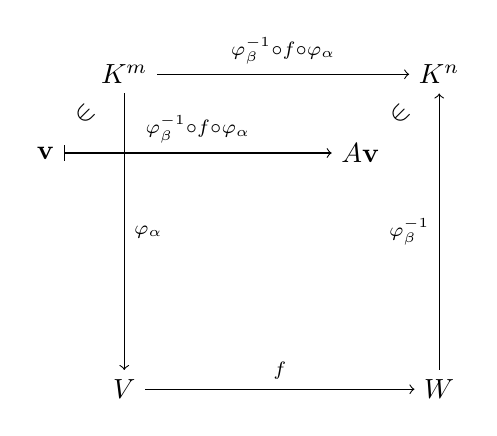
\begin{tikzpicture}[auto] 

    \node (a) at (1, 0) {$V$};
    \node (b) at (5, 0) {$W$};
    \node (c) at (1, 4) {$K^m $};
    \node (d) at (5, 4) {$K^n $};
    \node (e) at (0, 3) {${\bf v} $};
    \node (f) at (4, 3) {$A{\bf v} $};
    \node (g) at (0.5, 3.5) {\rotatebox{45}{$\in $} };
    \node (h) at (4.5, 3.5) {\rotatebox{45}{$\in $} };
    
    \draw [->] (c) to node {$\scriptstyle \varphi_{\beta}^{-1} \circ f\circ \varphi_{\alpha} $} (d);
    \draw [|->] (e) to node {$\scriptstyle \varphi_{\beta}^{-1} \circ f\circ \varphi_{\alpha} $} (f);
    \draw [->] (c) to node {$\scriptstyle \varphi_{\alpha} $} (a);
    \draw [->] (a) to node {$\scriptstyle f$} (b);
    \draw [->] (b) to node {$\scriptstyle \varphi_{\beta}^{-1} $} (d);
    
  \end{tikzpicture} 
\end{center}
\end{thm}
\begin{dfn}
この行列$A$、即ち、線形写像$f:V \rightarrow W$が与えられたときの線形写像$\varphi_{\beta}^{- 1} \circ f \circ \varphi_{\alpha}$の行列$A$をそれらの基底たち$\alpha$、$\beta$に関するその写像$f$の表現行列といい$[ f]^{\beta}_{\alpha}$と書く。
\end{dfn}
\begin{proof}
体$K$上の$m$次元、$n$次元vector空間たち$V$、$W$の基底の1つがそれぞれ$\left\langle \mathbf{v}_{i} \right\rangle_{i \in \varLambda_{m}}$、$\left\langle \mathbf{w}_{i} \right\rangle_{i \in \varLambda_{n}}$でありこれらをそれぞれ$\alpha$、$\beta$とする。線形写像$f:V \rightarrow W$が与えられたとき、それらの基底たち$\alpha$、$\beta$に関する基底変換における線形同型写像たち$\varphi_{\alpha}:K^{m} \rightarrow V$、$\varphi_{\beta}:K^{n} \rightarrow W$は線形同型写像となるのであった。したがって、その逆写像$\varphi_{\beta}^{- 1}$も線形写像でその合成写像$\varphi_{\beta}^{- 1} \circ f \circ \varphi_{\alpha}$も線形写像となる。このとき、その写像$\varphi_{\beta}^{- 1} \circ f \circ \varphi_{\alpha}$の始集合、終集合がそれぞれ$K^{m}$、$K^{n}$であるから、定理\ref{2.1.4.7}よりこの写像$\varphi_{\beta}^{- 1} \circ f \circ \varphi_{\alpha}$に対応する行列$A$がその集合$M_{nm}(K)$に存在して、$\forall\mathbf{v} \in K^{m}$に対し、$\varphi_{\beta}^{- 1} \circ f \circ \varphi_{\alpha}\left( \mathbf{v} \right) = A\mathbf{v}$が成り立つ。
\end{proof}
\begin{thm}
\label{2.1.5.4}
体$K$上の$m$次元、$n$次元vector空間たち$V$、$W$の基底の1つがそれぞれ$\left\langle \mathbf{v}_{j} \right\rangle_{j \in \varLambda_{m}}$、$\left\langle \mathbf{w}_{i} \right\rangle_{i \in \varLambda_{n}}$であり、これらをそれぞれ$\alpha$、$\beta$とするとき、それらの基底たち$\alpha 、\beta$に関する線形写像$f:V \rightarrow W$の$[ f]^{\beta}_{\alpha} \in M_{nm}(K)$なる表現行列$[ f]^{\beta}_{\alpha}$の第$(i,j)$成分$a_{ij}$は、$\forall j \in \varLambda_{m}$に対し、次式を満たす。
\begin{align*}
f\left( \mathbf{v}_{j} \right) = \sum_{i \in \varLambda_{n}} {a_{ij}\mathbf{w}_{i}}
\end{align*}
逆に、$A_{nm} = \left( a_{ij} \right)_{(i,j) \in \varLambda_{n} \times \varLambda_{m}} \in M_{nm}(K)$なるある行列$A_{nm}$が上の式を満たすなら、その行列$A_{nm}$はそれらの基底たち$\alpha $、$\beta$に関する線形写像$f:V \rightarrow W$の表現行列となる。
\end{thm}
\begin{proof}
体$K$上の$m$次元、$n$次元vector空間たち$V$、$W$の基底の1つがそれぞれ$\left\langle \mathbf{v}_{j} \right\rangle_{j \in \varLambda_{m}}$、$\left\langle \mathbf{w}_{i} \right\rangle_{i \in \varLambda_{n}}$であり、これらをそれぞれ$\alpha$、$\beta$とする。また、vector空間たち$K^{m}$、$K^{n}$の標準直交基底をそれぞれ$\left\langle \mathbf{d}_{j} \right\rangle_{j \in \varLambda_{m}}$、$\left\langle \mathbf{e}_{i} \right\rangle_{i \in \varLambda_{n}}$とおく。\par
このとき、線形写像$f:V \rightarrow W$、それらの基底たち$\alpha$、$\beta$に関する基底変換における線形同型写像たち$\varphi_{\alpha}$、$\varphi_{\beta}$を用いて次式のように考えると、
\begin{center}
  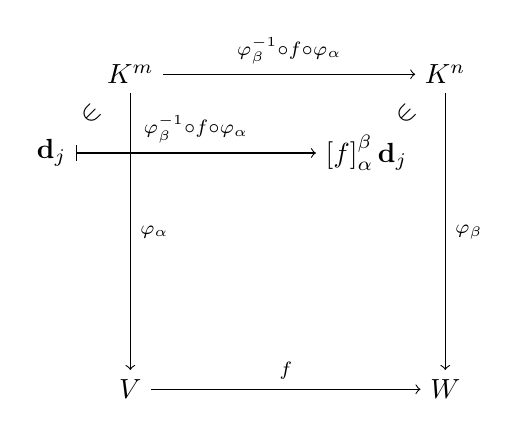
\begin{tikzpicture}[auto] 

    \node (a) at (1, 0) {$V$};
    \node (b) at (5, 0) {$W$};
    \node (c) at (1, 4) {$K^m $};
    \node (d) at (5, 4) {$K^n $};
    \node (e) at (0, 3) {${\bf d}_{j} $};
    \node (f) at (4, 3) {$\left[ f\right]^{\beta}_{\alpha} {\bf d}_{j} $};
    \node (g) at (0.5, 3.5) {\rotatebox{45}{$\in $} };
    \node (h) at (4.5, 3.5) {\rotatebox{45}{$\in $} };
    
    \draw [->] (c) to node {$\scriptstyle \varphi_{\beta}^{-1} \circ f\circ \varphi_{\alpha} $} (d);
    \draw [|->] (e) to node {$\scriptstyle \varphi_{\beta}^{-1} \circ f\circ \varphi_{\alpha} $} (f);
    \draw [->] (c) to node {$\scriptstyle \varphi_{\alpha} $} (a);
    \draw [->] (a) to node {$\scriptstyle f$} (b);
    \draw [->] (d) to node {$\scriptstyle \varphi_{\beta} $} (b);
    
    \end{tikzpicture} 
\end{center}
$\forall j \in \varLambda_{m}$に対し、次式が成り立つ。
\begin{align*}
f \circ \varphi_{\alpha}\left( \mathbf{d}_{j} \right) = f\left( \varphi_{\alpha}\left( \mathbf{d}_{j} \right) \right) = f\left( \mathbf{v}_{j} \right)
\end{align*}\par
一方で、それらの基底たち$\alpha$、$\beta$に関する線形写像$f:V \rightarrow W$の$[ f]^{\beta}_{\alpha} \in M_{nm}(K)$なる表現行列$[ f]^{\beta}_{\alpha}$が$\left( a_{ij} \right)_{(i,j) \in \varLambda_{n} \times \varLambda_{m}}$と成分表示されるとき、次のようになる。
\begin{align*}
f \circ \varphi_{\alpha}\left( \mathbf{d}_{j} \right) &= \varphi_{\beta} \circ \varphi_{\beta}^{- 1} \circ f \circ \varphi_{\alpha}\left( \mathbf{d}_{j} \right)\\
&= \varphi_{\beta}\left( \varphi_{\beta}^{- 1} \circ f \circ \varphi_{\alpha}\left( \mathbf{d}_{j} \right) \right)\\
&= \varphi_{\beta}\left( [ f]^{\beta}_{\alpha}\mathbf{d}_{j} \right)
\end{align*}
ここで、次のようになるので、
\begin{align*}
[ f]^{\beta}_{\alpha}\mathbf{d}_{j} &= \begin{pmatrix}
a_{11} & a_{12} & \cdots & a_{1j} & \cdots & a_{1m} \\
a_{21} & a_{22} & \cdots & a_{2j} & \cdots & a_{2m} \\
 \vdots & \vdots & \ddots & \vdots & \ddots & \vdots \\
a_{n1} & a_{n2} & \cdots & a_{nj} & \cdots & a_{nm} \\
\end{pmatrix}\begin{pmatrix}
0 \\
0 \\
 \vdots \\
1 \\
 \vdots \\
0 \\
\end{pmatrix} = \begin{pmatrix}
a_{1j} \\
a_{2j} \\
 \vdots \\
a_{nj} \\
\end{pmatrix}\\
&= \begin{pmatrix}
a_{1j} \\
0 \\
 \vdots \\
0 \\
\end{pmatrix} + \begin{pmatrix}
0 \\
a_{2j} \\
 \vdots \\
0 \\
\end{pmatrix} + \cdots + \begin{pmatrix}
0 \\
0 \\
 \vdots \\
a_{nj} \\
\end{pmatrix}\\
&= a_{1j}\begin{pmatrix}
1 \\
0 \\
 \vdots \\
0 \\
\end{pmatrix} + a_{2j}\begin{pmatrix}
0 \\
1 \\
 \vdots \\
0 \\
\end{pmatrix} + \cdots + a_{nj}\begin{pmatrix}
0 \\
0 \\
 \vdots \\
1 \\
\end{pmatrix}\\
&= \sum_{i \in \varLambda_{n}} {a_{ij}\mathbf{e}_{i}}
\end{align*}
したがって、次のようになる。
\begin{align*}
f \circ \varphi_{\alpha}\left( \mathbf{d}_{j} \right) &= \varphi_{\beta}\left( \sum_{i \in \varLambda_{n}} {a_{ij}\mathbf{e}_{i}} \right)\\
&= \sum_{i \in \varLambda_{n}} {a_{ij}\varphi_{\beta}\left( \mathbf{e}_{i} \right)} \\
&= \sum_{i \in \varLambda_{n}} {a_{ij}\mathbf{w}_{i}}
\end{align*}
以上より、次式が成り立つ。
\begin{align*}
f\left( \mathbf{v}_{j} \right) = f \circ \varphi_{\alpha}\left( \mathbf{d}_{j} \right) = \sum_{i \in \varLambda_{n}} {a_{ij}\mathbf{w}_{i}}
\end{align*}\par
逆に、$A_{nm} = \left( a_{ij} \right)_{(i,j) \in \varLambda_{n} \times \varLambda_{m}} \in M_{nm}(K)$なるある行列$A_{nm}$が上の式を満たすなら、$\forall j \in \varLambda_{m}$に対し、次のようになるので、
\begin{align*}
\varphi_{\beta}^{- 1} \circ f \circ \varphi_{\alpha}\left( \mathbf{d}_{j} \right) &= \varphi_{\beta}^{- 1} \circ f\left( \mathbf{v}_{j} \right)\\
&= \varphi_{\beta}^{- 1}\left( \sum_{i \in \varLambda_{n}} {a_{ij}\mathbf{w}_{i}} \right)\\
&= \sum_{i \in \varLambda_{n}} {a_{ij}\varphi_{\beta}^{- 1}\left( \mathbf{w}_{i} \right)}\\
&= \sum_{i \in \varLambda_{n}} {a_{ij}\mathbf{e}_{i}} = A_{nm}\mathbf{d}_{j}
\end{align*}
定理\ref{2.1.4.7}よりその写像$\varphi_{\beta}^{- 1} \circ f \circ \varphi_{\alpha}:K^{m} \rightarrow K^{n}$は線形写像となりその行列$A_{nm}$はそれらの基底たち$\alpha$、$\beta$に関する線形写像$f:V \rightarrow W$の表現行列となる。
\end{proof}
\begin{thm}
\label{2.1.5.5}
体$K$上の$m$次元、$n$次元vector空間たち$V$、$W$の基底の1つがそれぞれ$\left\langle \mathbf{v}_{j} \right\rangle_{j \in \varLambda_{m}}$、$\left\langle \mathbf{w}_{i} \right\rangle_{i \in \varLambda_{n}}$であり、これらをそれぞれ$\alpha$、$\beta$とし、$\forall\mathbf{v} \in V$に対し、$\mathbf{v} = \sum_{j \in \varLambda_{m}} {k_{j}\mathbf{v}_{j}}$のように書かれるとする。それらの基底たち$\alpha$、$\beta$に関する線形写像$f:V \rightarrow W$の$[ f]^{\beta}_{\alpha} \in M_{nm}(K)$なる表現行列$[ f]^{\beta}_{\alpha}$が$\left( a_{ij} \right)_{(i,j) \in \varLambda_{n} \times \varLambda_{m}}$と成分表示されるとき、次式が成り立つ。
\begin{align*}
f\left( \mathbf{v} \right) = \sum_{i \in \varLambda_{n}} {\sum_{j \in \varLambda_{m}} {a_{ij}k_{j}}\mathbf{w}_{i}}
\end{align*}
さらにいえば、そのvector$f\left( \mathbf{v} \right)$が$f\left( \mathbf{v} \right) = \sum_{i \in \varLambda_{n}} {l_{i}\mathbf{w}_{i}}$を満たすとき、次式が成り立つ。
\begin{align*}
\begin{pmatrix}
l_{1} \\
l_{2} \\
 \vdots \\
l_{n} \\
\end{pmatrix} = \begin{pmatrix}
a_{11} & a_{12} & \cdots & a_{1m} \\
a_{21} & a_{22} & \cdots & a_{2m} \\
 \vdots & \vdots & \ddots & \vdots \\
a_{n1} & a_{n2} & \cdots & a_{nm} \\
\end{pmatrix}\begin{pmatrix}
k_{1} \\
k_{2} \\
 \vdots \\
k_{m} \\
\end{pmatrix}
\end{align*}
このことは$\mathbf{k} = \begin{pmatrix}
k_{1} \\
k_{2} \\
 \vdots \\
k_{m} \\
\end{pmatrix}$、$\mathbf{l} = \begin{pmatrix}
l_{1} \\
l_{2} \\
 \vdots \\
l_{n} \\
\end{pmatrix}$としてそれらの基底たち$\alpha$、$\beta$に関する基底変換における線形同型写像たち$\varphi_{\alpha}$、$\varphi_{\beta}$を用いて次式のようにも書かれる。
\begin{center}
  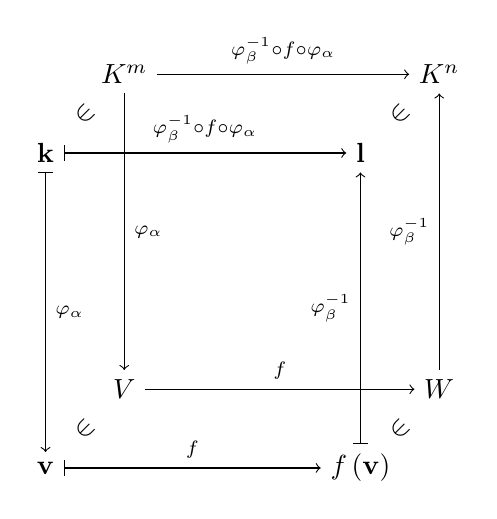
\begin{tikzpicture}[auto] 

    \node (a) at (1, 1) {$V$};
    \node (b) at (5, 1) {$W$};
    \node (c) at (1, 5) {$K^m $};
    \node (d) at (5, 5) {$K^n $};
    \node (e) at (0, 4) {${\bf k} $};
    \node (f) at (4, 4) {${\bf l} $};
    \node (g) at (0.5, 4.5) {\rotatebox{45}{$\in $} };
    \node (h) at (4.5, 4.5) {\rotatebox{45}{$\in $} };
    \node (i) at (0, 0) {${\bf v} $};
    \node (j) at (4, 0) {$f\left( {\bf v} \right) $};
    \node (k) at (0.5, 0.5) {\rotatebox{45}{$\in $} };
    \node (l) at (4.5, 0.5) {\rotatebox{45}{$\in $} };
    
    \draw [->] (c) to node {$\scriptstyle \varphi_{\beta}^{-1} \circ f\circ \varphi_{\alpha} $} (d);
    \draw [|->] (e) to node {$\scriptstyle \varphi_{\beta}^{-1} \circ f\circ \varphi_{\alpha} $} (f);
    \draw [->] (c) to node {$\scriptstyle \varphi_{\alpha} $} (a);
    \draw [|->] (e) to node {$\scriptstyle \varphi_{\alpha} $} (i);
    \draw [->] (a) to node {$\scriptstyle f$} (b);
    \draw [|->] (i) to node {$\scriptstyle f$} (j);
    \draw [->] (b) to node {$\scriptstyle \varphi_{\beta}^{-1} $} (d);
    \draw [|->] (j) to node {$\scriptstyle \varphi_{\beta}^{-1} $} (f);
    
  \end{tikzpicture} 
\end{center}
\end{thm}
\begin{proof}
体$K$上の$m$次元、$n$次元vector空間たち$V$、$W$の基底の1つがそれぞれ$\left\langle \mathbf{v}_{j} \right\rangle_{j \in \varLambda_{m}}$、$\left\langle \mathbf{w}_{i} \right\rangle_{i \in \varLambda_{n}}$であり、これらをそれぞれ$\alpha$、$\beta$とし、$\forall\mathbf{v} \in V$に対し、次式のように書かれるとする。
\begin{align*}
\mathbf{v} = \sum_{j \in \varLambda_{m}} {k_{j}\mathbf{v}_{j}}
\end{align*}
それらの基底たち$\alpha$、$\beta$に関する線形写像$f:V \rightarrow W$の$[ f]^{\beta}_{\alpha} \in M_{nm}(K)$なる表現行列$[ f]^{\beta}_{\alpha}$が$\left( a_{ij} \right)_{(i,j) \in \varLambda_{n} \times \varLambda_{m}}$と成分表示されるとき、定理\ref{2.1.5.4}より次のようになる。
\begin{align*}
f\left( \mathbf{v} \right) &= f\left( \sum_{j \in \varLambda_{m}} {k_{j}\mathbf{v}_{j}} \right)\\
&= \sum_{j \in \varLambda_{m}} {k_{j}f\left( \mathbf{v}_{j} \right)}\\
&= \sum_{j \in \varLambda_{m}} {k_{j}\sum_{i \in \varLambda_{n}} {a_{ij}\mathbf{w}_{i}}}\\
&= \sum_{j \in \varLambda_{m}} {\sum_{i \in \varLambda_{n}} {a_{ij}k_{j}\mathbf{w}_{i}}}\\
&= \sum_{i \in \varLambda_{n}} {\sum_{j \in \varLambda_{m}} {a_{ij}k_{j}}\mathbf{w}_{i}}
\end{align*}\par
さらにいえば、そのvector$f\left( \mathbf{v} \right)$が$f\left( \mathbf{v} \right) = \sum_{i \in \varLambda_{n}} {l_{i}\mathbf{w}_{i}}$を満たすとき、次のようになる。
\begin{align*}
\mathbf{0} &= \sum_{i \in \varLambda_{n}} {l_{i}\mathbf{w}_{i}} - \sum_{i \in \varLambda_{n}} {\sum_{j \in \varLambda_{m}} {a_{ij}k_{j}}\mathbf{w}_{i}}\\
&= \sum_{i \in \varLambda_{n}} {\left( l_{i} - \sum_{j \in \varLambda_{m}} {a_{ij}k_{j}} \right)\mathbf{w}_{i}}
\end{align*}
ここで、その組$\left\langle \mathbf{w}_{i} \right\rangle_{i \in \varLambda_{n}}$は基底であるから、次のようになる。
\begin{align*}
\forall i \in \varLambda_{n}\left[ l_{i} - \sum_{j \in \varLambda_{m}} {a_{ij}k_{j}} = 0 \right] &\Leftrightarrow \forall i \in \varLambda_{n}\left[ l_{i} = \sum_{j \in \varLambda_{m}} {a_{ij}k_{j}} \right]\\
&\Leftrightarrow \begin{pmatrix}
l_{1} \\
l_{2} \\
 \vdots \\
l_{n} \\
\end{pmatrix} = \begin{pmatrix}
a_{11}k_{1} + a_{12}k_{2} + \cdots + a_{1m}k_{m} \\
a_{21}k_{1} + a_{22}k_{2} + \cdots + a_{2m}k_{m} \\
 \vdots \\
a_{n1}k_{1} + a_{n2}k_{2} + \cdots + a_{nm}k_{m} \\
\end{pmatrix}\\
&\Leftrightarrow \begin{pmatrix}
l_{1} \\
l_{2} \\
 \vdots \\
l_{n} \\
\end{pmatrix} = \begin{pmatrix}
a_{11} & a_{12} & \cdots & a_{1m} \\
a_{21} & a_{22} & \cdots & a_{2m} \\
 \vdots & \vdots & \ddots & \vdots \\
a_{n1} & a_{n2} & \cdots & a_{nm} \\
\end{pmatrix}\begin{pmatrix}
k_{1} \\
k_{2} \\
 \vdots \\
k_{m} \\
\end{pmatrix}
\end{align*}
\end{proof}
\begin{thm}
\label{2.1.5.6}
体$K$上のvector空間たち$V$、$W$、線形写像たち$f:V \rightarrow W$、$g:V \rightarrow W$が与えられたとき、$\forall k,l \in K$に対し、その写像$kf + lg:V \rightarrow W$も線形写像であった。これらのvector空間たち$V$、$W$の基底の1つがそれぞれ$\alpha$、$\beta$としそれらの基底たち$\alpha$、$\beta$に関するそれらの線形写像たち$f:V \rightarrow W$、$g:V \rightarrow W$、$kf + lg:V \rightarrow W$の表現行列をそれぞれ$[ f]^{\beta}_{\alpha}$、$[ g]^{\beta}_{\alpha}$、$[ kf + lg]^{\beta}_{\alpha}$とおくと、$[ kf + lg]^{\beta}_{\alpha} = k[ f]^{\beta}_{\alpha} + l[ g]^{\beta}_{\alpha}$が成り立つ。
\end{thm}
\begin{proof}
体$K$上のvector空間たち$V$、$W$、線形写像たち$f:V \rightarrow W$、$g:V \rightarrow W$が与えられたとき、$\forall k,l \in K$に対し、その写像$kf + lg:V \rightarrow W$も線形写像であった。これらのvector空間たち$V$、$W$の基底の1つがそれぞれ$\alpha$、$\beta$としそれらの基底たち$\alpha$、$\beta$に関するそれらの線形写像たち$f:V \rightarrow W$、$g:V \rightarrow W$、$kf + lg:V \rightarrow W$の表現行列をそれぞれ$[ f]^{\beta}_{\alpha}$、$[ g]^{\beta}_{\alpha}$、$[ kf + lg]^{\beta}_{\alpha}$とおき、これらの表現行列たち$[ f]^{\beta}_{\alpha}$、$[ g]^{\beta}_{\alpha}$がそれぞれ$\left( a_{ij} \right)_{(i,j) \in \varLambda_{n} \times \varLambda_{m}}$、$\left( b_{ij} \right)_{(i,j) \in \varLambda_{n} \times \varLambda_{m}}$と成分表示されるとき、定理\ref{2.1.5.4}より$\forall j \in \varLambda_{m}$に対し、次式が成り立つ。
\begin{align*}
f\left( \mathbf{v}_{j} \right) = \sum_{i \in \varLambda_{n}} {a_{ij}\mathbf{w}_{i}},\ \ g\left( \mathbf{v}_{j} \right) = \sum_{i \in \varLambda_{n}} {b_{ij}\mathbf{w}_{i}}
\end{align*}
したがって、次のようになる。
\begin{align*}
\left( kf + lg \right)\left( \mathbf{v}_{j} \right) &= kf\left( \mathbf{v}_{j} \right) + lg\left( \mathbf{v}_{j} \right)\\
&= k\sum_{i \in \varLambda_{n}} {a_{ij}\mathbf{w}_{i}} + l\sum_{i \in \varLambda_{n}} {b_{ij}\mathbf{w}_{i}}\\
&= k\sum_{i \in \varLambda_{n}} {a_{ij}\mathbf{w}_{i}} + l\sum_{i \in \varLambda_{n}} {b_{ij}\mathbf{w}_{i}}\\
&= \sum_{i \in \varLambda_{n}} {\left( ka_{ij} + lb_{ij} \right)\mathbf{w}_{i}}
\end{align*}
このとき、定理\ref{2.1.5.4}よりそれらの基底たち$\alpha$、$\beta$に関する線形写像$kf + lg$の表現行列$[ kf + lg]^{\beta}_{\alpha}$は$\left( ka_{ij} + lb_{ij} \right)_{(i,j) \in \varLambda_{n} \times \varLambda_{m}}$のように成分表示され、したがって、次のようになる。
\begin{align*}
\left[ kf + lg \right]^{\beta}_{\alpha} &= \left( ka_{ij} + lb_{ij} \right)_{(i,j) \in \varLambda_{n} \times \varLambda_{m}}\\
&= k\left( a_{ij} \right)_{(i,j) \in \varLambda_{n} \times \varLambda_{m}} + l\left( b_{ij} \right)_{(i,j) \in \varLambda_{n} \times \varLambda_{m}}\\
&= k[ f]^{\beta}_{\alpha} + l[ g]^{\beta}_{\alpha}
\end{align*}
\end{proof}
\begin{thm}
\label{2.1.5.7}
体$K$上のvector空間たち$U$、$V$、$W$の基底の1つがそれぞれ$\alpha$、$\beta$、$\gamma$としそれらの基底たち$\alpha$、$\beta$に関する線形写像$f:U \rightarrow V$、それらの基底たち$\beta$、$\gamma$に関する線形写像$g:V \rightarrow W$、それらの基底たち$\alpha$、$\gamma$に関する線形写像$g \circ f:U \rightarrow W$の表現行列をそれぞれ$[ f]^{\beta}_{\alpha}$、$[ g]^{\gamma}_{\beta}$、$[ g \circ f]^{\gamma}_{\alpha}$とおくと、$[ g \circ f]^{\gamma}_{\alpha} = [ g]^{\gamma}_{\beta}[ f]^{\beta}_{\alpha}$が成り立つ。
\end{thm}
\begin{proof}
体$K$上の$m$次元、$n$次元、$o$次元vector空間たち$U$、$V$、$W$の基底の1つがそれぞれ$\alpha$、$\beta$、$\gamma$としそれらの基底たち$\alpha$、$\beta$に関する線形写像$f:U \rightarrow V$、それらの基底たち$\beta$、$\gamma$に関する線形写像$g:V \rightarrow W$、それらの基底たち$\alpha$、$\gamma$に関する線形写像$g \circ f:U \rightarrow W$の表現行列をそれぞれ$[ f]^{\beta}_{\alpha}$、$[ g]^{\gamma}_{\beta}$、$[ g \circ f]^{\gamma}_{\alpha}$とおくと、それらの基底たち$\alpha$、$\beta$、$\gamma$に関する基底変換における線形同型写像たち$\varphi_{\alpha}$、$\varphi_{\beta}$、$\varphi_{\gamma}$を用いて次式が成り立つ。
\begin{align*}
\varphi_{\gamma}^{- 1} \circ (g \circ f) \circ \varphi_{\alpha} &= \varphi_{\gamma}^{- 1} \circ g \circ \varphi_{\beta} \circ \varphi_{\beta}^{- 1} \circ f \circ \varphi_{\alpha}\\
&= \left( \varphi_{\gamma}^{- 1} \circ g \circ \varphi_{\beta} \right) \circ \left( \varphi_{\beta}^{- 1} \circ f \circ \varphi_{\alpha} \right)
\end{align*}
これは次のようになることを意味する。
\begin{center}
  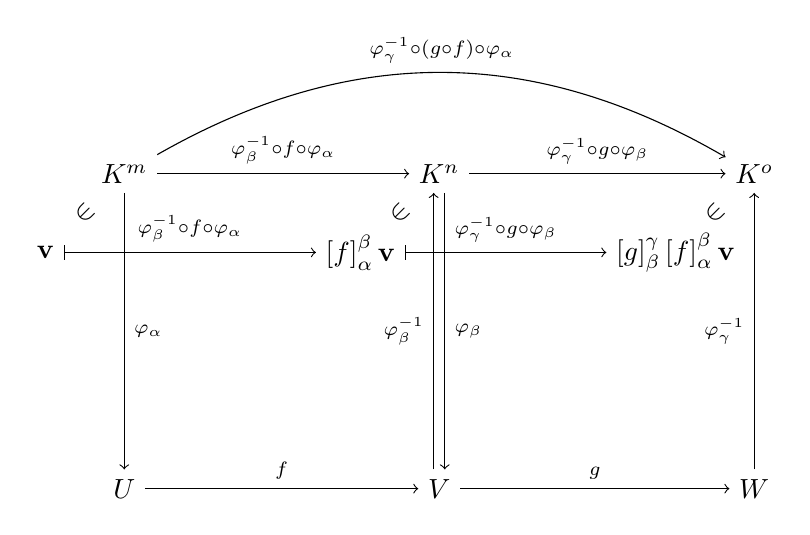
\begin{tikzpicture}[auto] 

    \node (a) at (1, 0) {$U$};
    \node (b) at (5, 0) {$V$};
    \node (c) at (1, 4) {$K^m $};
    \node (d) at (5, 4) {$K^n $};
    \node (e) at (0, 3) {${\bf v} $};
    \node (f) at (4, 3) {$\left[ f\right]^{\beta}_{\alpha} {\bf v} $};
    \node (g) at (0.5, 3.5) {\rotatebox{45}{$\in $} };
    \node (h) at (4.5, 3.5) {\rotatebox{45}{$\in $} };
    \node (i) at (9, 0) {$W$};
    \node (j) at (9, 4) {$K^o $};
    \node (k) at (8, 3) {$\left[ g\right]^{\gamma}_{\beta} \left[ f\right]^{\beta}_{\alpha} {\bf v} $};
    \node (l) at (8.5, 3.5) {\rotatebox{45}{$\in $} };
    
    \draw [->] (c) to node {$\scriptstyle \varphi_{\beta}^{-1} \circ f\circ \varphi_{\alpha} $} (d);
    \draw [|->] (e) to node {$\scriptstyle \varphi_{\beta}^{-1} \circ f\circ \varphi_{\alpha} $} (f);
    \draw [->] (c) to node {$\scriptstyle \varphi_{\alpha} $} (a);
    \draw [->] (a) to node {$\scriptstyle f$} (b);
    \draw [->, transform canvas={xshift=-2pt, yshift=0pt}] (b) to node {$\scriptstyle \varphi_{\beta}^{-1} $} (d);
    \draw [->] (d) to node {$\scriptstyle \varphi_{\gamma}^{-1} \circ g\circ \varphi_{\beta} $} (j);
    \draw [|->] (f) to node {$\scriptstyle \varphi_{\gamma}^{-1} \circ g\circ \varphi_{\beta} $} (k);
    \draw [->, transform canvas={xshift=2pt, yshift=0pt}] (d) to node {$\scriptstyle \varphi_{\beta} $} (b);
    \draw [->] (b) to node {$\scriptstyle g$} (i);
    \draw [->] (i) to node {$\scriptstyle \varphi_{\gamma}^{-1} $} (j);
    \draw [->] (c) to[bend left=30] node {$\scriptstyle \varphi_{\gamma}^{-1} \circ \left( g\circ f\right) \circ \varphi_{\alpha} $} (j);
    
    \end{tikzpicture} 
\end{center}
したがって、定義よりそれらの写像たち$\varphi_{\gamma}^{- 1} \circ g \circ \varphi_{\beta}$、$\varphi_{\beta}^{- 1} \circ f \circ \varphi_{\alpha}$の対応する行列がそれぞれ$[ f]^{\beta}_{\alpha}$、$[ g]^{\gamma}_{\beta}$と与えられることに注意すれば、その写像$\left( \varphi_{\gamma}^{- 1} \circ g \circ \varphi_{\beta} \right) \circ \left( \varphi_{\beta}^{- 1} \circ f \circ \varphi_{\alpha} \right)$の対応する行列が$[ g]^{\gamma}_{\beta}[ f]^{\beta}_{\alpha}$と与えられ、定義よりしたがって$[ g \circ f]^{\gamma}_{\alpha} = [ g]^{\gamma}_{\beta}[ f]^{\beta}_{\alpha}$が成り立つ。
\end{proof}
\begin{thm}
\label{2.1.5.8}
体$K$上の$m$次元、$n$次元vector空間たち$V$、$W$の基底の1つがそれぞれ$\alpha$、$\beta$とするとき、それらの基底たち$\alpha$、$\beta$に関する線形写像$f:V \rightarrow W$の表現行列$[ f]^{\beta}_{\alpha}$の階数${\mathrm{rank}}[ f]^{\beta}_{\alpha}$はそれらの基底たち$\alpha 、\beta$によらずその線形写像$f$の階数に等しい、即ち、${\mathrm{rank}}[ f]^{\beta}_{\alpha} = {\mathrm{rank}}f$が成り立つ。
\end{thm}
\begin{proof}
体$K$上の$m$次元、$n$次元vector空間たち$V$、$W$の基底の1つがそれぞれ$\alpha$、$\beta$とするとき、それらの基底たち$\alpha$、$\beta$に関する線形写像$f:V \rightarrow W$の表現行列$[ f]^{\beta}_{\alpha}$の階数${\mathrm{rank}}[ f]^{\beta}_{\alpha}$について考えよう。このとき、それらの基底たち$\alpha$、$\beta$に関する基底変換における線形同型写像たち$\varphi_{\alpha}$、$\varphi_{\beta}$を用いてその合成写像$\varphi_{\beta}^{- 1} \circ f \circ \varphi_{\alpha}$を$L_{[ f]^{\beta}_{\alpha}}$とおくと、次のようになり、
\begin{align*}
f &= I_{W} \circ f \circ I_{V}\\
&= \varphi_{\beta} \circ \varphi_{\beta}^{- 1} \circ f \circ \varphi_{\alpha} \circ \varphi_{\alpha}^{- 1}\\
&= \varphi_{\beta} \circ L_{[ f]^{\beta}_{\alpha}} \circ \varphi_{\alpha}^{- 1}
\end{align*}
定理\ref{2.1.2.16}より次式が成り立つ。
\begin{align*}
{\mathrm{rank}}{\varphi_{\beta}^{- 1} \circ f \circ \varphi_{\alpha}} &\leq {\mathrm{rank}}{f \circ \varphi_{\alpha}}\\
&\leq {\mathrm{rank}}f\\
&= {\mathrm{rank}}{\varphi_{\beta} \circ L_{[ f]^{\beta}_{\alpha}} \circ \varphi_{\alpha}^{- 1}}\\
&\leq {\mathrm{rank}}{L_{[ f]^{\beta}_{\alpha}} \circ \varphi_{\alpha}^{- 1}}\\
&\leq {\mathrm{rank}}L_{[ f]^{\beta}_{\alpha}}\\
&= {\mathrm{rank}}{\varphi_{\beta}^{- 1} \circ f \circ \varphi_{\alpha}}
\end{align*}
以上より${\mathrm{rank}}{\varphi_{\beta}^{- 1} \circ f \circ \varphi_{\alpha}} = {\mathrm{rank}}f$が成り立つ。ここで、定理\ref{2.1.4.12}より${\mathrm{rank}}L_{[ f]^{\beta}_{\alpha}} = {\mathrm{rank}}[ f]^{\beta}_{\alpha}$が成り立つので、その表現行列$[ f]^{\beta}_{\alpha}$の階数${\mathrm{rank}}[ f]^{\beta}_{\alpha}$はそれらの基底たち$\alpha$、$\beta$によらずその線形写像の階数${\mathrm{rank}}f$に等しい。
\end{proof}
%\hypertarget{ux57faux5e95ux5909ux63dbux884cux5217}{%
\subsubsection{基底変換行列}%\label{ux57faux5e95ux5909ux63dbux884cux5217}}
\begin{thm}
\label{2.1.5.9}
体$K$上の$n$次元vector空間$V$の2つの基底たち$\left\langle \mathbf{v}_{i} \right\rangle_{i \in \varLambda_{n}}$、$\left\langle \mathbf{w}_{i} \right\rangle_{i \in \varLambda_{n}}$が与えられこれらをそれぞれ$\alpha$、$\beta$とおく。このとき、それらの基底たち$\alpha$、$\beta$に関する基底変換における線形同型写像たち$\varphi_{\alpha}$、$\varphi_{\beta}$の合成写像$\varphi_{\beta}^{- 1} \circ \varphi_{\alpha}$に対応する$A \in M_{nn}(K)$なる行列$A$はそれらの基底たち$\alpha$、$\beta$に関する恒等写像$I_{V}:V \rightarrow V$の表現行列$\left[ I_{V} \right]^{\beta}_{\alpha}$に等しい、即ち、$A = \left[ I_{V} \right]^{\beta}_{\alpha}$が成り立つ。
\end{thm}
\begin{dfn}
このような行列$\left[ I_{V} \right]^{\beta}_{\alpha}$、即ち、線形写像$\varphi_{\beta}^{- 1} \circ \varphi_{\alpha}$の行列$\left[ I_{V} \right]^{\beta}_{\alpha}$をその基底$\alpha$からその基底$\beta$への基底変換行列という。
\end{dfn}
\begin{proof}
体$K$上の$n$次元vector空間$V$の2つの基底たち$\left\langle \mathbf{v}_{i} \right\rangle_{i \in \varLambda_{n}}$、$\left\langle \mathbf{w}_{i} \right\rangle_{i \in \varLambda_{n}}$が与えられこれらをそれぞれ$\alpha$、$\beta$とおく。このとき、次式のようにそれらの基底たち$\alpha$、$\beta$に関する基底変換における線形同型写像たち$\varphi_{\alpha}$、$\varphi_{\beta}$、恒等写像$I_{V}:V \rightarrow V$を用いて考えると、
\begin{center}
  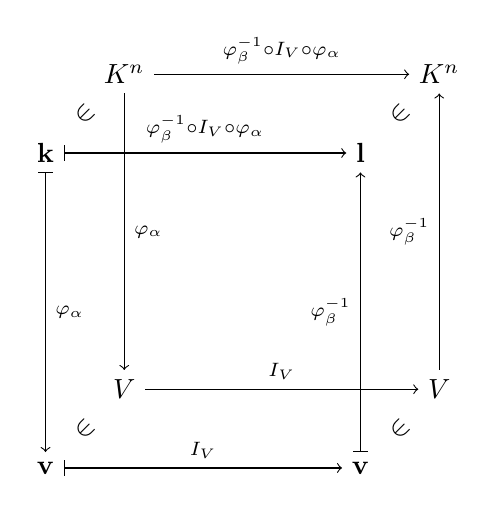
\begin{tikzpicture}[auto]

    \node (a) at (1, 1) {$V$};
    \node (b) at (5, 1) {$V$};
    \node (c) at (1, 5) {$K^n $};
    \node (d) at (5, 5) {$K^n $};
    \node (e) at (0, 4) {${\bf k} $};
    \node (f) at (4, 4) {${\bf l} $};
    \node (g) at (0.5, 4.5) {\rotatebox{45}{$\in $} };
    \node (h) at (4.5, 4.5) {\rotatebox{45}{$\in $} };
    \node (i) at (0, 0) {${\bf v} $};
    \node (j) at (4, 0) {${\bf v} $};
    \node (k) at (0.5, 0.5) {\rotatebox{45}{$\in $} };
    \node (l) at (4.5, 0.5) {\rotatebox{45}{$\in $} };
    
    \draw [->] (c) to node {$\scriptstyle \varphi_{\beta}^{-1} \circ I_V \circ \varphi_{\alpha} $} (d);
    \draw [|->] (e) to node {$\scriptstyle \varphi_{\beta}^{-1} \circ I_V \circ \varphi_{\alpha} $} (f);
    \draw [->] (c) to node {$\scriptstyle \varphi_{\alpha} $} (a);
    \draw [|->] (e) to node {$\scriptstyle \varphi_{\alpha} $} (i);
    \draw [->] (a) to node {$\scriptstyle I_V $} (b);
    \draw [|->] (i) to node {$\scriptstyle I_V $} (j);
    \draw [->] (b) to node {$\scriptstyle \varphi_{\beta}^{-1} $} (d);
    \draw [|->] (j) to node {$\scriptstyle \varphi_{\beta}^{-1} $} (f);
   
  \end{tikzpicture}
\end{center}
$\varphi_{\beta}^{- 1} \circ \varphi_{\alpha} = \varphi_{\beta}^{- 1} \circ I_{V} \circ \varphi_{\alpha}$が成り立つので、定義より明らかにその合成写像$\varphi_{\beta}^{- 1} \circ \varphi_{\alpha}$に対応する$A \in M_{nn}(K)$なる行列$A$はそれらの基底たち$\alpha$、$\beta$に関するその恒等写像$I_{V}:V \rightarrow V$の表現行列$\left[ I_{V} \right]^{\beta}_{\alpha}$に等しい。
\end{proof}
\begin{thm}
\label{2.1.5.10}
体$K$上の$n$次元vector空間$V$の2つの基底たち$\left\langle \mathbf{v}_{i} \right\rangle_{i \in \varLambda_{n}}$、$\left\langle \mathbf{w}_{i} \right\rangle_{i \in \varLambda_{n}}$が与えられこれらをそれぞれ$\alpha$、$\beta$とおく。このとき、その基底$\alpha$からその基底$\beta$への基底変換行列$\left[ I_{V} \right]^{\beta}_{\alpha}$は$\left[ I_{V} \right]^{\beta}_{\alpha} \in {\mathrm{GL}}_{n}(K)$を満たし$\left[ I_{V} \right]^{\alpha}_{\beta} = {\left[ I_{V} \right]^{\beta}_{\alpha}}^{- 1}$が成り立つ。\par
このことはそれらの基底たち$\alpha$、$\beta$に関する基底変換における線形同型写像たち$\varphi_{\alpha}$、$\varphi_{\beta}$を用いて次式のようにも書かれる。
\begin{center}
  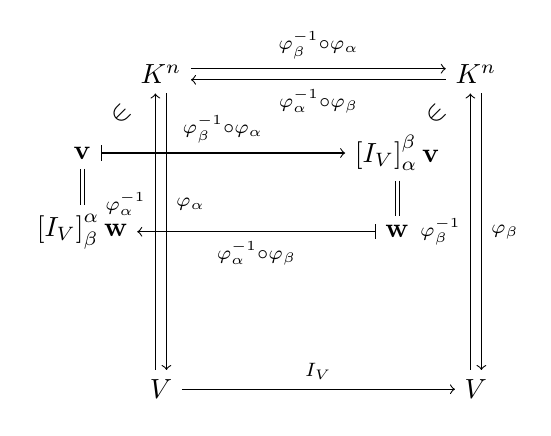
\begin{tikzpicture}[auto]

    \node (a) at (1, 0) {$V$};
    \node (b) at (5, 0) {$V$};
    \node (c) at (1, 4) {$K^n $};
    \node (d) at (5, 4) {$K^n $};
    \node (e) at (0, 3) {${\bf v} $};
    \node (f) at (4, 3) {$\left[ I_V\right]^{\beta}_{\alpha} {\bf v} $};
    \node (i) at (0, 2) {$\left[ I_V\right]^{\alpha}_{\beta} {\bf w} $};
    \node (j) at (4, 2) {${\bf w} $};
    \node (g) at (0.5, 3.5) {\rotatebox{45}{$\in $} };
    \node (h) at (4.5, 3.5) {\rotatebox{45}{$\in $} };
    
    \draw [->, transform canvas={xshift=0pt, yshift=2pt}] (c) to node {$\scriptstyle \varphi_{\beta}^{-1} \circ \varphi_{\alpha} $} (d);
    \draw [->, transform canvas={xshift=0pt, yshift=-2pt}] (d) to node {$\scriptstyle \varphi_{\alpha}^{-1} \circ \varphi_{\beta} $} (c);
    \draw [->, transform canvas={xshift=2pt, yshift=0pt}] (c) to node[xshift=0pt, yshift=10pt] {$\scriptstyle \varphi_{\alpha} $} (a);
    \draw [->, transform canvas={xshift=-2pt, yshift=0pt}] (a) to node[xshift=0pt, yshift=10pt] {$\scriptstyle \varphi_{\alpha}^{-1} $} (c);
    \draw [->] (a) to node {$\scriptstyle I_V $} (b);
    \draw [->, transform canvas={xshift=2pt, yshift=0pt}] (d) to node {$\scriptstyle \varphi_{\beta} $} (b);
    \draw [->, transform canvas={xshift=-2pt, yshift=0pt}] (b) to node {$\scriptstyle \varphi_{\beta}^{-1} $} (d);
    \draw [|->] (e) to node {$\scriptstyle \varphi_{\beta}^{-1} \circ \varphi_{\alpha} $} (f);
    \draw [|->] (j) to node {$\scriptstyle \varphi_{\alpha}^{-1} \circ \varphi_{\beta} $} (i);
    \draw [double distance=1pt] (e) to node {$\scriptstyle $} (i);
    \draw [double distance=1pt] (f) to node {$\scriptstyle $} (j);
    
    \end{tikzpicture}
\end{center}
\end{thm}
\begin{proof}
体$K$上の$n$次元vector空間$V$の2つの基底たち$\left\langle \mathbf{v}_{i} \right\rangle_{i \in \varLambda_{n}}$、$\left\langle \mathbf{w}_{i} \right\rangle_{i \in \varLambda_{n}}$が与えられこれらをそれぞれ$\alpha$、$\beta$とおく。このとき、それらの基底たち$\alpha$、$\beta$に関する基底変換における線形同型写像たち$\varphi_{\alpha}$、$\varphi_{\beta}$を用いてその基底$\alpha$からその基底$\beta$への基底変換行列$\left[ I_{V} \right]^{\beta}_{\alpha}$は定理\ref{2.1.5.9}よりその合成写像$\varphi_{\beta}^{- 1} \circ \varphi_{\alpha}$の対応する行列でもあり、それらの2つの写像たち$\varphi_{\alpha}$、$\varphi_{\beta}$は線形同型写像であったので、その合成写像$\varphi_{\beta}^{- 1} \circ \varphi_{\alpha}$も線形同型写像となる。このとき、定理\ref{2.1.4.14}よりその合成写像$\varphi_{\beta}^{- 1} \circ \varphi_{\alpha}$に対応する行列でもあるその基底$\alpha$からその基底$\beta$への基底変換行列$\left[ I_{V} \right]^{\beta}_{\alpha}$は正則行列で$\left[ I_{V} \right]^{\beta}_{\alpha} \in {\mathrm{GL}}_{n}(K)$を満たす。したがって、逆行列${\left[ I_{V} \right]^{\beta}_{\alpha}}^{- 1}$が存在しこれが対応する行列となるその写像はその写像$\varphi_{\beta}^{- 1} \circ \varphi_{\alpha}$の逆写像となる。このとき、次のようになるので、
\begin{align*}
I_{K^{n}} &= \varphi_{\alpha}^{- 1} \circ \varphi_{\alpha}\\
&= \varphi_{\alpha}^{- 1} \circ \left( \varphi_{\beta} \circ \varphi_{\beta}^{- 1} \right) \circ \varphi_{\alpha}\\
&= \left( \varphi_{\alpha}^{- 1} \circ \varphi_{\beta} \right) \circ \left( \varphi_{\beta}^{- 1} \circ \varphi_{\alpha} \right)\\
I_{K^{n}} &= \varphi_{\alpha} \circ \varphi_{\alpha}^{- 1}\\
&= \varphi_{\alpha} \circ \left( \varphi_{\beta}^{- 1} \circ \varphi_{\beta} \right) \circ \varphi_{\alpha}^{- 1}\\
&= \left( \varphi_{\alpha} \circ \varphi_{\beta}^{- 1} \right) \circ \left( \varphi_{\beta} \circ \varphi_{\alpha}^{- 1} \right)
\end{align*}
その合成写像$\varphi_{\alpha} \circ \varphi_{\beta}^{- 1}$は対応する行列が${\left[ I_{V} \right]^{\beta}_{\alpha}}^{- 1}$となるようなその合成写像$\varphi_{\beta}^{- 1} \circ \varphi_{\alpha}$の逆写像となりこれに対応する行列が上記の定理より$\left[ I_{V} \right]^{\alpha}_{\beta}$となるので、$\left[ I_{V} \right]^{\alpha}_{\beta} = {\left[ I_{V} \right]^{\beta}_{\alpha}}^{- 1}$が成り立つ。
\end{proof}\par
以上の議論により体$K$上の$n$次元vector空間$V$の2つの基底たち$\left\langle \mathbf{v}_{i} \right\rangle_{i \in \varLambda_{n}}$、$\left\langle \mathbf{w}_{i} \right\rangle_{i \in \varLambda_{n}}$が与えられこれらをそれぞれ$\alpha$、$\beta$とおく。$\forall\mathbf{v} \in V$に対し、次式のように書かれるとする。
\begin{align*}
\mathbf{v} = \sum_{i \in \varLambda_{n}} {k_{i}\mathbf{v}_{i}} = \sum_{i \in \varLambda_{n}} {l_{i}\mathbf{w}_{i}}
\end{align*}
その基底$\alpha$からその基底$\beta$への基底変換行列$\left[ I_{V} \right]^{\beta}_{\alpha}$が$\left( a_{ij} \right)_{(i,j) \in \varLambda_{n} \times \varLambda_{n}}$と成分表示されるとき、$\forall j \in \varLambda_{n}$に対し、次式が成り立つ。
\begin{align*}
\mathbf{v}_{j} = \sum_{i \in \varLambda_{n}} {a_{ij}\mathbf{w}_{i}}
\end{align*}
逆に、$A_{nn} = \left( a_{ij} \right)_{(i,j) \in \varLambda_{n} \times \varLambda_{n}} \in M_{nn}(K)$なるある行列$A_{nn}$が上の式を満たすなら、その行列$A_{nn}$はその基底$\alpha$からその基底$\beta$への基底変換行列となる。さらにいえば、次式が成り立つ。
\begin{align*}
\begin{pmatrix}
l_{1} \\
l_{2} \\
 \vdots \\
l_{n} \\
\end{pmatrix} = \begin{pmatrix}
a_{11} & a_{12} & \cdots & a_{1n} \\
a_{21} & a_{22} & \cdots & a_{2n} \\
 \vdots & \vdots & \ddots & \vdots \\
a_{n1} & a_{n2} & \cdots & a_{nn} \\
\end{pmatrix}\begin{pmatrix}
k_{1} \\
k_{2} \\
 \vdots \\
k_{n} \\
\end{pmatrix}
\end{align*}
このことは$\mathbf{k} = \begin{pmatrix}
k_{1} \\
k_{2} \\
 \vdots \\
k_{n} \\
\end{pmatrix}$、$\mathbf{l} = \begin{pmatrix}
l_{1} \\
l_{2} \\
 \vdots \\
l_{n} \\
\end{pmatrix}$として次式のようにも書かれる。
\begin{center}
  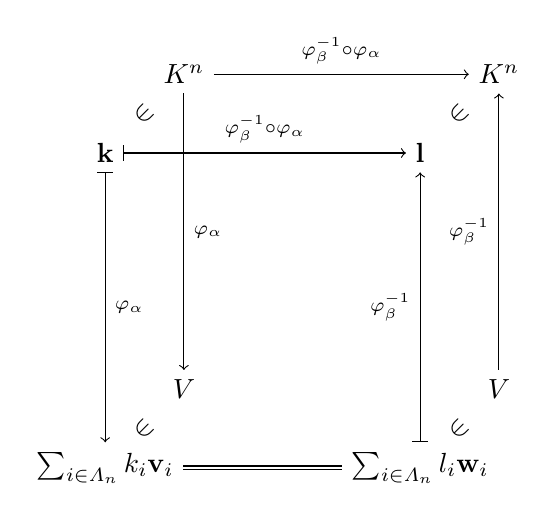
\begin{tikzpicture}[auto]

    \node (a) at (1, 1) {$V$};
    \node (b) at (5, 1) {$V$};
    \node (c) at (1, 5) {$K^n $};
    \node (d) at (5, 5) {$K^n $};
    \node (e) at (0, 4) {${\bf k} $};
    \node (f) at (4, 4) {${\bf l} $};
    \node (g) at (0.5, 4.5) {\rotatebox{45}{$\in $} };
    \node (h) at (4.5, 4.5) {\rotatebox{45}{$\in $} };
    \node (i) at (0, 0) {$\sum_{i\in \varLambda_{n} } k_i {\bf v}_i $};
    \node (j) at (4, 0) {$\sum_{i\in \varLambda_{n} } l_i {\bf w}_i $};
    \node (k) at (0.5, 0.5) {\rotatebox{45}{$\in $} };
    \node (l) at (4.5, 0.5) {\rotatebox{45}{$\in $} };
    
    \draw [->] (c) to node {$\scriptstyle \varphi_{\beta}^{-1} \circ \varphi_{\alpha} $} (d);
    \draw [|->] (e) to node {$\scriptstyle \varphi_{\beta}^{-1} \circ \varphi_{\alpha} $} (f);
    \draw [->] (c) to node {$\scriptstyle \varphi_{\alpha} $} (a);
    \draw [|->] (e) to node {$\scriptstyle \varphi_{\alpha} $} (i);
    
    
    \draw [->] (b) to node {$\scriptstyle \varphi_{\beta}^{-1} $} (d);
    \draw [|->] (j) to node {$\scriptstyle \varphi_{\beta}^{-1} $} (f);
    \draw [double distance=1pt] (i) to node {$\scriptstyle $} (j);
    
    \end{tikzpicture}
\end{center}
\begin{thm}
\label{2.1.5.11}
体$K$上の$n$次元vector空間$V$のある基底$\left\langle \mathbf{v}_{i} \right\rangle_{i \in \varLambda_{n}}$が与えられこれを$\alpha$とおく。このとき、$A \in {\mathrm{GL}}_{n}(K)$なる行列$A$がその基底$\alpha$からある基底$\beta$への基底変換行列となるようなその基底$\beta$が存在する。
\end{thm}
\begin{proof}
体$K$上の$n$次元vector空間$V$のある基底$\left\langle \mathbf{v}_{i} \right\rangle_{i \in \varLambda_{n}}$が与えられこれを$\alpha$とおく。このとき、$A \in {\mathrm{GL}}_{n}(K)$なる行列$A$がある写像$L_{A}:K^{n} \rightarrow K^{n}$に対応する行列となるようなその写像$L_{A}$の逆写像$L_{A}^{- 1}$は定理より明らかに線形同型写像でその基底$\alpha$に関する基底変換における線形同型写像$\varphi_{\alpha}$を用いて得られる合成写像$\varphi_{\alpha} \circ L_{A}^{- 1}:K^{n} \rightarrow V$は線形同型写像となり、次式のように考えれば、
\begin{center}
  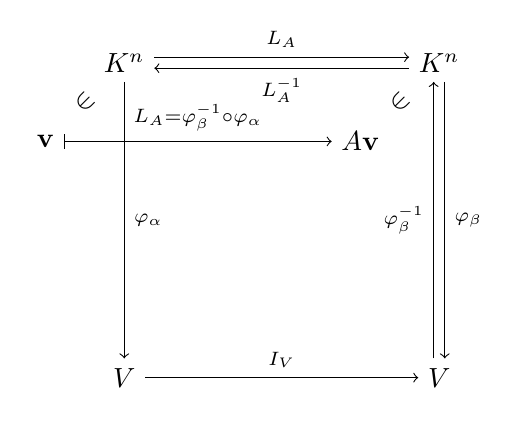
\begin{tikzpicture}[auto]

    \node (a) at (1, 1) {$V$};
    \node (b) at (5, 1) {$V$};
    \node (c) at (1, 5) {$K^n $};
    \node (d) at (5, 5) {$K^n $};
    \node (e) at (0, 4) {${\bf v} $};
    \node (f) at (4, 4) {$A{\bf v} $};
    \node (g) at (0.5, 4.5) {\rotatebox{45}{$\in $} };
    \node (h) at (4.5, 4.5) {\rotatebox{45}{$\in $} };
    
    \draw [->, transform canvas={xshift=0pt, yshift=2pt}] (c) to node {$\scriptstyle L_A $} (d);
    \draw [->, transform canvas={xshift=0pt, yshift=-2pt}] (d) to node {$\scriptstyle L_A^{-1} $} (c);
    \draw [|->] (e) to node {$\scriptstyle L_A =\varphi_{\beta}^{-1} \circ \varphi_{\alpha} $} (f);
    \draw [->] (c) to node {$\scriptstyle \varphi_{\alpha} $} (a);
    \draw [->] (a) to node {$\scriptstyle I_V $} (b);
    \draw [->, transform canvas={xshift=2pt, yshift=0pt}] (d) to node {$\scriptstyle \varphi_{\beta} $} (b);
    \draw [->, transform canvas={xshift=-2pt, yshift=0pt}] (b) to node {$\scriptstyle \varphi_{\beta}^{-1} $} (d);
    
  \end{tikzpicture} 
\end{center}
定理\ref{2.1.5.2}より、そのvector空間$K^{n}$の標準直交基底$\left\langle \mathbf{e}_{i} \right\rangle_{i \in \varLambda_{n}}$を用いたvectorsの組$\left\langle \varphi_{\alpha} \circ L_{A}^{- 1}\left( \mathbf{e}_{i} \right) \right\rangle_{i \in \varLambda_{n}}$はそのvector空間$V$の基底となり、これを$\beta$とおくと、$\varphi_{\alpha} \circ L_{A}^{- 1} = \varphi_{\beta}$が成り立つ。このとき、次のようになるので、
\begin{align*}
L_{A} &= \left( L_{A}^{- 1} \right)^{- 1}\\
&= \left( I_{K^{n}} \circ L_{A}^{- 1} \right)^{- 1}\\
&= \left( \varphi_{\alpha}^{- 1} \circ \varphi_{\alpha} \circ L_{A}^{- 1} \right)^{- 1}\\
&= \left( \varphi_{\alpha}^{- 1} \circ \varphi_{\beta} \right)^{- 1}\\
&= \varphi_{\beta}^{- 1} \circ \varphi_{\alpha}
\end{align*}
定義より明らかにその行列$A$がその基底$\alpha$からある基底$\beta$への基底変換行列となる。
\end{proof}
\begin{thm}
\label{2.1.5.12}
体$K$上の$m$次元、$n$次元vector空間たち$V$、$W$の基底の2つをそれぞれ$\alpha_{1}$、$\alpha_{2}$、$\beta_{1}$、$\beta_{2}$とするとき、それらの基底たちそれぞれ$\alpha_{1}$、$\beta_{1}$、$\alpha_{2}$、$\beta_{2}$に関する線形写像$f:V \rightarrow W$の表現行列たちそれぞれ$[ f]^{\beta_{1}}_{\alpha_{1}}$、$[ f]^{\beta_{2}}_{\alpha_{2}}$とそれらのvector空間$V$、$W$の基底変換行列たち$\left[ I_{V} \right]^{\alpha_{2}}_{\alpha_{1}}$、$\left[ I_{W} \right]^{\beta_{2}}_{\beta_{1}}$について、$\left[ I_{W} \right]^{\beta_{2}}_{\beta_{1}}[ f]^{\beta_{1}}_{\alpha_{1}} = [ f]^{\beta_{2}}_{\alpha_{2}}\left[ I_{V} \right]^{\alpha_{2}}_{\alpha_{1}}$が成り立つ。
\end{thm}
\begin{proof}
体$K$上の$m$次元、$n$次元vector空間たち$V$、$W$の基底の2つをそれぞれ$\alpha_{1}$、$\alpha_{2}$、$\beta_{1}$、$\beta_{2}$とするとき、それらの基底たちそれぞれ$\alpha_{1}$、$\beta_{1}$、$\alpha_{2}$、$\beta_{2}$に関する線形写像$f:V \rightarrow W$の表現行列たちそれぞれ$[ f]^{\beta_{1}}_{\alpha_{1}}$、$[ f]^{\beta_{2}}_{\alpha_{2}}$とそれらのvector空間$V$、$W$の基底変換行列たち$\left[ I_{V} \right]^{\alpha_{2}}_{\alpha_{1}}$、$\left[ I_{W} \right]^{\beta_{2}}_{\beta_{1}}$について、それらの基底たち$\alpha_{1}$、$\beta_{1}$、$\alpha_{2}$、$\beta_{2}$に関する基底変換における線形同型写像たち$\varphi_{\alpha_{1}}$、$\varphi_{\beta_{1}}$、$\varphi_{\alpha_{2}}$、$\varphi_{\beta_{2}}$を用いて次のようになり、
\begin{align*}
\left( \varphi_{\beta_{2}}^{- 1} \circ \varphi_{\beta_{1}} \right) \circ \left( \varphi_{\beta_{1}}^{- 1} \circ f \circ \varphi_{\alpha_{1}} \right) &= \varphi_{\beta_{2}}^{- 1} \circ \left( \varphi_{\beta_{1}} \circ \varphi_{\beta_{1}}^{- 1} \right) \circ f \circ \varphi_{\alpha_{1}}\\
&= \varphi_{\beta_{2}}^{- 1} \circ I_{W} \circ f \circ I_{V} \circ \varphi_{\alpha_{1}}\\
&= \varphi_{\beta_{2}}^{- 1} \circ f \circ \left( \varphi_{\alpha_{2}} \circ \varphi_{\alpha_{2}}^{- 1} \right) \circ \varphi_{\alpha_{1}}\\
&= \left( \varphi_{\beta_{2}}^{- 1} \circ f \circ \varphi_{\alpha_{2}} \right) \circ \left( \varphi_{\alpha_{2}}^{- 1} \circ \varphi_{\alpha_{1}} \right)
\end{align*}
次式より明らかに、
\begin{center}
  \begin{tikzpicture}[auto]

    \node (a) at (2, 6) {$K^m $};
    \node (b) at (7, 6) {$K^n $};
    \node (c) at (0, 5) {$K^m $};
    \node (d) at (5, 5) {$K^n $};
    \node (e) at (2, 1) {$V$};
    \node (f) at (7, 1) {$W$};
    \node (g) at (0, 0) {$V$};
    \node (h) at (5, 0) {$W$};
    \node (sb) at (10, 6) {$\ $};
    
    \draw [->] (a) to node {$\scriptstyle \varphi_{\beta_1 }^{-1} \circ f\circ \varphi_{\alpha_1 } $} (b);
    \draw [->] (c) to node[xshift=25pt, yshift=0pt] {$\scriptstyle \varphi_{\beta_2 }^{-1} \circ f\circ \varphi_{\alpha_2 } $} (d);
    \draw [>->>] (a) to node {$\scriptstyle \varphi_{\alpha_2 }^{-1} \circ \varphi_{\alpha_1 } $} (c);
    \draw [>->>] (b) to node {$\scriptstyle \varphi_{\beta_2 }^{-1} \circ \varphi_{\beta_1 } $} (d);
    \draw [>->>] (a) to node {$\scriptstyle \varphi_{\alpha_1 } $} (e);
    \draw [>->>] (b) to node {$\scriptstyle \varphi_{\beta_1 } $} (f);
    \draw [>->>] (c) to node {$\scriptstyle \varphi_{\alpha_2 } $} (g);
    \draw [>->>] (d) to node {$\scriptstyle \varphi_{\beta_2 } $} (h);
    \draw [->] (e) to node[xshift=-5pt, yshift=0pt] {$\scriptstyle f$} (f);
    \draw [->] (g) to node {$\scriptstyle f$} (h);
    \draw [>->>] (e) to node {$\scriptstyle I_V $} (g);
    \draw [>->>] (f) to node {$\scriptstyle I_W $} (h);
    
    \end{tikzpicture} 
    \begin{tikzpicture}[auto]
    
    \node (a) at (2, 6) {${\bf k} $};
    %\node (b) at (7, 6) {$\left[ f\right]^{\beta_1 }_{\alpha_1 } {\bf k} $};
    \node (c) at (0, 5) {$\left[ I_V\right]^{\alpha_2 }_{\alpha_1 } {\bf k} $};
    \node (d) at (5, 5) {$\left[ f\right]^{\beta_2 }_{\alpha_2 } \left[ I_V \right]^{\alpha_2 }_{\alpha_1 } {\bf k} $};
    \node (e) at (2, 1) {${\bf v} $};
    %\node (f) at (7, 1) {$f\left( {\bf v}\right) $};
    \node (g) at (0, 0) {${\bf v} $};
    \node (h) at (5, 0) {$f\left( {\bf v}\right) $};
    
    %\draw [|->] (a) to node {$\scriptstyle \varphi_{\beta_1 }^{-1} \circ f\circ \varphi_{\alpha_1 } $} (b);
    \draw [|->] (c) to node[xshift=0pt, yshift=-15pt] {$\scriptstyle \varphi_{\beta_2 }^{-1} \circ f\circ \varphi_{\alpha_2 } $} (d);
    \draw [|->] (a) to node {$\scriptstyle \varphi_{\alpha_2 }^{-1} \circ \varphi_{\alpha_1 } $} (c);
    %\draw [|->] (b) to node {$\scriptstyle \varphi_{\beta_2 }^{-1} \circ \varphi_{\beta_1 } $} (d);
    \draw [|->] (a) to node {$\scriptstyle \varphi_{\alpha_1 } $} (e);
    %\draw [|->] (b) to node {$\scriptstyle \varphi_{\beta_1 } $} (f);
    \draw [|->] (c) to node {$\scriptstyle \varphi_{\alpha_2 } $} (g);
    \draw [|->] (d) to node {$\scriptstyle \varphi_{\beta_2 } $} (h);
    %\draw [|->] (e) to node {$\scriptstyle f$} (f);
    \draw [|->] (g) to node {$\scriptstyle f$} (h);
    \draw [double distance=1pt] (e) to node {$\scriptstyle $} (g);
    %\draw [double distance=1pt] (f) to node {$\scriptstyle $} (h);
    
    %\end{tikzpicture} 
    
    %\vskip \baselineskip 
    
    %\begin{tikzpicture}[auto]
    
    \node (sa) at (5, 6) {${\bf k} $};
    \node (sb) at (10, 6) {$\left[ f\right]^{\beta_1 }_{\alpha_1 } {\bf k} $};
    %\node (sc) at (3, 5) {$\left[ I_V\right]^{\alpha_2 }_{\alpha_1 } {\bf k} $};
    \node (sd) at (8, 5) {$\left[ I_W \right]^{\beta_2 }_{\beta_1 } \left[ f\right]^{\beta_1 }_{\alpha_1 } {\bf k} $};
    \node (se) at (4.5, 1) {${\bf v} $};
    \node (sf) at (10, 1) {$f\left( {\bf v}\right) $};
    %\node (sg) at (3, 0) {${\bf v} $};
    \node (sh) at (8, 0) {$f\left( {\bf v}\right) $};
    
    \draw [|->] (sa) to node {$\scriptstyle \varphi_{\beta_1 }^{-1} \circ f\circ \varphi_{\alpha_1 } $} (sb);
    %\draw [|->] (sc) to node {$\scriptstyle \varphi_{\beta_2 }^{-1} \circ f\circ \varphi_{\alpha_2 } $} (sd);
    %\draw [|->] (sa) to node {$\scriptstyle \varphi_{\alpha_2 }^{-1} \circ \varphi_{\alpha_1 } $} (sc);
    \draw [|->] (sb) to node {$\scriptstyle \varphi_{\beta_2 }^{-1} \circ \varphi_{\beta_1 } $} (sd);
    %\draw [|->] (sa) to node {$\scriptstyle \varphi_{\alpha_1 } $} (se);
    \draw [|->] (sb) to node {$\scriptstyle \varphi_{\beta_1 } $} (sf);
    %\draw [|->] (sc) to node {$\scriptstyle \varphi_{\alpha_2 } $} (sg);
    %\draw [|->] (sd) to node {$\scriptstyle \varphi_{\beta_2 } $} (sh);
    \draw [|->] (se) to node {$\scriptstyle f$} (sf);
    %\draw [|->] (sg) to node {$\scriptstyle f$} (sh);
    %\draw [double distance=1pt] (se) to node {$\scriptstyle $} (sg);
    \draw [double distance=1pt] (sf) to node {$\scriptstyle $} (sh);
    \draw [double distance=1pt] (a) to node {$\scriptstyle $} (sa);
    \draw [double distance=1pt] (e) to node {$\scriptstyle $} (se);
    \draw [double distance=1pt] (d) to node {$\scriptstyle $} (sd);
    \draw [double distance=1pt] (h) to node {$\scriptstyle $} (sh);
    
    \end{tikzpicture} 
\end{center}
その写像$\varphi_{\beta_{2}}^{- 1} \circ \varphi_{\beta_{1}}:K^{n} \rightarrow K^{n}$に対応する行列がその基底$\beta_{1}$からその基底$\beta_{2}$へのその基底変換行列$\left[ I_{W} \right]^{\beta_{2}}_{\beta_{1}}$となるかつ、定義より明らかにその写像$\varphi_{\beta_{1}}^{- 1} \circ f \circ \varphi_{\alpha_{1}}:K^{m} \rightarrow K^{n}$に対応する行列がそれらの基底たちそれぞれ$\alpha_{1}$、$\beta_{1}$に関する線形写像$f:V \rightarrow W$の表現行列$[ f]^{\beta_{1}}_{\alpha_{1}}$となるので、その合成写像$\left( \varphi_{\beta_{2}}^{- 1} \circ \varphi_{\beta_{1}} \right) \circ \left( \varphi_{\beta_{1}}^{- 1} \circ f \circ \varphi_{\alpha_{1}} \right)$に対応する行列は$\left[ I_{W} \right]^{\beta_{2}}_{\beta_{1}}[ f]^{\beta_{1}}_{\alpha_{1}}$となる。同様にして、その合成写像$\left( \varphi_{\beta_{2}}^{- 1} \circ f \circ \varphi_{\alpha_{2}} \right) \circ \left( \varphi_{\alpha_{2}}^{- 1} \circ \varphi_{\alpha_{1}} \right)$に対応する行列は$[ f]^{\beta_{2}}_{\alpha_{2}}\left[ I_{V} \right]^{\alpha_{2}}_{\alpha_{1}}$となるので、$\left[ I_{W} \right]^{\beta_{2}}_{\beta_{1}}[ f]^{\beta_{1}}_{\alpha_{1}} = [ f]^{\beta_{2}}_{\alpha_{2}}\left[ I_{V} \right]^{\alpha_{2}}_{\alpha_{1}}$が成り立つ。
\end{proof}
\begin{thm}
\label{2.1.5.13}
体$K$上の$m$次元、$n$次元vector空間たち$V$、$W$の基底の1つがそれぞれ$\alpha$、$\beta$とするとき、それらの基底たち$\alpha 、\beta$に関する線形写像$f:V \rightarrow W$の表現行列$[ f]^{\beta}_{\alpha}$が${\mathrm{rank}}f = r$として次式のように書かれるようなそれらの基底たち$\alpha$、$\beta$が存在する。
\begin{align*}
[ f]^{\beta}_{\alpha} = \begin{pmatrix}
I_{r} & O \\
O & O \\
\end{pmatrix}
\end{align*}
\end{thm}
\begin{proof}
体$K$上の$m$次元、$n$次元vector空間たち$V$、$W$が与えられたとする。このとき、次元公式より線形写像$f:V \rightarrow W$の核$\ker f$は${\mathrm{rank}}f = r$として$m - r$次元でありこれの基底の1つを$\left\langle \mathbf{v}_{i} \right\rangle_{i \in \varLambda_{m} \setminus \varLambda_{r}}$とおきこれを拡張してそのvector空間$V$の基底を$\left\langle \mathbf{v}_{i} \right\rangle_{i \in \varLambda_{m}}$としこれを$\alpha$とおく。このとき、vectorの組$\left\langle f\left( \mathbf{v}_{i} \right) \right\rangle_{i \in \varLambda_{r}}$は定理\ref{2.1.2.13}よりその部分空間$V(f)$の基底となるのであった。そこで、これを、$\forall i \in \varLambda_{r}$に対し、$\mathbf{w}_{i} = f\left( \mathbf{v}_{i} \right)$となるように拡張したそのvector空間$W$の基底$\left\langle \mathbf{w}_{i} \right\rangle_{i \in \varLambda_{n}}$を$\beta$とおく。このとき、$\forall j \in \varLambda_{m}$に対し、$j \in \varLambda_{r}$のとき、次のようになるし、
\begin{align*}
f\left( \mathbf{v}_{j} \right) = \mathbf{w}_{j} = \sum_{i \in \varLambda_{n} \setminus \left\{ j \right\}} {0\mathbf{w}_{i}} + 1\mathbf{w}_{j} = \sum_{i \in \varLambda_{n}} {\delta_{ij}\mathbf{w}_{i}}
\end{align*}
$j \in \varLambda_{m} \setminus \varLambda_{r}$のとき、核の定義より次のようになる。
\begin{align*}
f\left( \mathbf{v}_{j} \right) = \mathbf{0} = \sum_{i \in \varLambda_{n}} {0\mathbf{w}_{i}}
\end{align*}
定理\ref{2.1.5.4}よりそれらの基底たち$\alpha 、\beta$に関する線形写像$f:V \rightarrow W$の表現行列$[ f]^{\beta}_{\alpha}$は次のようになる。
\begin{align*}
[ f]^{\beta}_{\alpha} &= \begin{pmatrix}
\delta_{11} & \delta_{12} & \cdots & \delta_{1r} & 0 & 0 & \cdots & 0 \\
\delta_{21} & \delta_{22} & \cdots & \delta_{2r} & 0 & 0 & \cdots & 0 \\
 \vdots & \vdots & \ddots & \vdots & \vdots & \vdots & \ddots & \vdots \\
\delta_{r1} & \delta_{r2} & \cdots & \delta_{rr} & 0 & 0 & \cdots & 0 \\
\delta_{r + 1,1} & \delta_{r + 1,2} & \cdots & \delta_{r + 1,r} & 0 & 0 & \cdots & 0 \\
\delta_{r + 2,1} & \delta_{r + 2,2} & \cdots & \delta_{r + 2,r} & 0 & 0 & \cdots & 0 \\
 \vdots & \vdots & \ddots & \vdots & \vdots & \vdots & \ddots & \vdots \\
\delta_{n1} & \delta_{n2} & \cdots & \delta_{nr} & 0 & 0 & \cdots & 0 \\
\end{pmatrix}\\
&= \begin{pmatrix}
1 & 0 & \cdots & 0 & 0 & 0 & \cdots & 0 \\
0 & 1 & \cdots & 0 & 0 & 0 & \cdots & 0 \\
 \vdots & \vdots & \ddots & \vdots & \vdots & \vdots & \ddots & \vdots \\
0 & 0 & \cdots & 1 & 0 & 0 & \cdots & 0 \\
0 & 0 & \cdots & 0 & 0 & 0 & \cdots & 0 \\
0 & 0 & \cdots & 0 & 0 & 0 & \cdots & 0 \\
 \vdots & \vdots & \ddots & \vdots & \vdots & \vdots & \ddots & \vdots \\
0 & 0 & \cdots & 0 & 0 & 0 & \cdots & 0 \\
\end{pmatrix}\\
&= \begin{pmatrix}
I_{r} & O \\
O & O \\
\end{pmatrix}
\end{align*}
\end{proof}
%\hypertarget{ux7ddaux5f62ux5199ux50cfux306eux884cux5217ux8868ux73fe}{%
\subsubsection{線形写像の行列表現}%\label{ux7ddaux5f62ux5199ux50cfux306eux884cux5217ux8868ux73fe}}
\begin{thm}
\label{2.1.5.14}
体$K$上の$m$次元、$n$次元vector空間たち$V$、$W$の基底の1つがそれぞれ$\left\langle \mathbf{v}_{j} \right\rangle_{j \in \varLambda_{m}}$、$\left\langle \mathbf{w}_{i} \right\rangle_{i \in \varLambda_{n}}$であり、これらをそれぞれ$\alpha$、$\beta$とすると、それらの基底たち$\alpha 、\beta$に関する線形写像$f:V \rightarrow W$の$[ f]^{\beta}_{\alpha} \in M_{nm}(K)$なる表現行列$[ f]^{\beta}_{\alpha}$を用いて次式のように定義される写像$F_{\alpha \rightarrow \beta}$はvector空間$L(V,W)$からvector空間$M_{nm}(K)$への線形同型写像である。なお、$L(V,W)$はそのvector空間$V$からそのvector空間$W$への線形写像全体の集合である。
\begin{align*}
F_{\alpha \rightarrow \beta}:L(V,W) \rightarrow M_{nm}(K);f \mapsto [ f]^{\beta}_{\alpha}
\end{align*}
\end{thm}
\begin{proof}
体$K$上の$m$次元、$n$次元vector空間たち$V$、$W$の基底の1つがそれぞれ$\left\langle \mathbf{v}_{j} \right\rangle_{j \in \varLambda_{m}}$、$\left\langle \mathbf{w}_{i} \right\rangle_{i \in \varLambda_{n}}$であり、これらをそれぞれ$\alpha$、$\beta$とする。それらの基底たち$\alpha$、$\beta$に関する線形写像$f:V \rightarrow W$の$[ f]^{\beta}_{\alpha} \in M_{nm}(K)$なる表現行列$[ f]^{\beta}_{\alpha}$を用いて次式のように定義される写像$F_{\alpha \rightarrow \beta}$を考えよう。
\begin{align*}
F_{\alpha \rightarrow \beta}:L(V,W) \rightarrow M_{nm}(K);f \mapsto [ f]^{\beta}_{\alpha}
\end{align*}\par
このとき、2つの集合たち$L(V,W)$、$M_{nm}(K)$はvector空間で、定理\ref{2.1.5.6}より$\forall f,g \in L(V,W)\forall k,l \in K$に対し、$kf + lg \in L(V,W)$が成り立ち、それらの基底たち$\alpha$、$\beta$に関する線形写像たち$f$、$g$、$kf + lg$の表現行列たち$[ f]^{\beta}_{\alpha}$、$[ g]^{\beta}_{\alpha}$、$[ kf + lg]^{\beta}_{\alpha}$が与えられたとき、次のようになるので、
\begin{align*}
F_{\alpha \rightarrow \beta}\left( kf + lg \right) &= \left[ kf + lg \right]^{\beta}_{\alpha}\\
&= k[ f]^{\beta}_{\alpha} + l[ g]^{\beta}_{\alpha}\\
&= kF_{\alpha \rightarrow \beta}(f) + lF_{\alpha \rightarrow \beta}(g)
\end{align*}
その写像$F_{\alpha \rightarrow \beta}$は線形的である。\par
また、定理\ref{2.1.5.4}より$A_{nm} = \left( a_{ij} \right)_{(i,j) \in \varLambda_{n} \times \varLambda_{m}} \in M_{nm}(K)$なるある行列$A_{nm}$が、$\forall j \in \varLambda_{m}$に対し、次式を満たすようにすれば、
\begin{align*}
f:V \rightarrow W;\mathbf{v}_{j} \mapsto \sum_{i \in \varLambda_{n}} {a_{ij}\mathbf{w}_{i}}
\end{align*}
その行列$A_{nm}$はそれらの基底たち$\alpha$、$\beta$に関する線形写像$f:V \rightarrow W$の表現行列となるので、逆写像が存在することから、その写像$F_{\alpha \rightarrow \beta}$は全単射となる。\par
以上より、その写像$F_{\alpha \rightarrow \beta}$は線形的であるかつ、全単射であるので、線形同型写像である。
\end{proof}
\begin{thm}
\label{2.1.5.15}
体$K$上の$n$次元vector空間$V$の基底の1つを$\alpha$とし、その基底$\alpha$に関する線形写像$f:V \rightarrow V$の$[ f]_{\alpha}^{\alpha} \in M_{nn}(K)$なる表現行列$[ f]_{\alpha}^{\alpha}$を用いて写像$F_{\alpha \rightarrow \alpha}$が次式のように定義されれば、
\begin{align*}
F_{\alpha \rightarrow \alpha}:L(V,W) \rightarrow M_{nn}(K);f \mapsto [ f]_{\alpha}^{\alpha}
\end{align*}
恒等写像$I_{V}:V \rightarrow V;\mathbf{v} \mapsto \mathbf{v}$について、$n$次単位行列$I_{n}$を用いて$\left[ I_{V} \right]_{\alpha}^{\alpha} = F_{\alpha \rightarrow \alpha}\left( I_{V} \right) = I_{n}$が成り立つ。
\end{thm}
\begin{proof}
体$K$上の$n$次元vector空間$V$の基底の1つを$\alpha$とし、その基底$\alpha$に関する線形写像$f:V \rightarrow V$の$[ f]_{\alpha}^{\alpha} \in M_{nn}(K)$なる表現行列$[ f]_{\alpha}^{\alpha}$を用いて写像$F_{\alpha \rightarrow \alpha}$が次式のように定義されれば、
\begin{align*}
F_{\alpha \rightarrow \alpha}:L(V,W) \rightarrow M_{nn}(K);f \mapsto [ f]_{\alpha}^{\alpha}
\end{align*}
恒等写像$I_{V}:V \rightarrow V;\mathbf{v} \mapsto \mathbf{v}$について、定理\ref{2.1.5.8}より次のようになり、
\begin{align*}
\left[ I_{V} \right]_{\alpha}^{\alpha} = F_{\alpha \rightarrow \alpha}\left( I_{V} \right) = F_{\alpha \rightarrow \alpha}\left( I_{V} \circ I_{V} \right) = \left[ I_{V} \circ I_{V} \right]_{\alpha}^{\alpha} = \left[ I_{V} \right]_{\alpha}^{\alpha}\left[ I_{V} \right]_{\alpha}^{\alpha}
\end{align*}
ここで、定理\ref{2.1.5.10}より$\left[ I_{V} \right]_{\alpha}^{\alpha} = {\left[ I_{V} \right]_{\alpha}^{\alpha}}^{- 1}$が成り立つので、$n$次単位行列$I_{n}$を用いてしたがって、次のようになる。
\begin{align*}
\left[ I_{V} \right]_{\alpha}^{\alpha} = F_{\alpha \rightarrow \alpha}\left( I_{V} \right) = \left[ I_{V} \right]_{\alpha}^{\alpha}\left[ I_{V} \right]_{\alpha}^{\alpha} = \left[ I_{V} \right]_{\alpha}^{\alpha}{\left[ I_{V} \right]_{\alpha}^{\alpha}}^{- 1} = I_{n}
\end{align*}
\end{proof}
\begin{thm}
\label{2.1.5.16}
体$K$上の$n$次元vector空間たち$V$、$W$の基底の1つをそれぞれ$\alpha$、$\beta$とし、それらの基底たち$\alpha 、\beta$に関する線形写像$f:V \rightarrow W$の$[ f]^{\beta}_{\alpha} \in M_{nn}(K)$なる表現行列$[ f]^{\beta}_{\alpha}$を用いて写像$F_{\alpha \rightarrow \beta}$が次式のように定義されれば、
\begin{align*}
F_{\alpha \rightarrow \beta}:L(V,W) \rightarrow M_{nn}(K);f \mapsto [ f]^{\beta}_{\alpha}
\end{align*}
$\forall f \in L(V,W)$に対し、次のことは同値である。
\begin{itemize}
\item
  その写像$f$は線形同型写像である。
\item
  その写像$f$は全射$f:V \twoheadrightarrow W$である。
\item
  その写像$f$は単射$f:V \rightarrowtail W$である。
\item
  $n = {\mathrm{rank}}f = \dim{V(f)}$が成り立つ。
\item
  ${\mathrm{nullity}}f = \dim{\ker f} = 0$が成り立つ。
\item
  それらの基底たち$\alpha$、$\beta$に関する線形写像$f:V \rightarrow W$の表現行列$[ f]^{\beta}_{\alpha}$は正則行列である、即ち、$[ f]^{\beta}_{\alpha} \in {\mathrm{GL}}_{n}(K)$が成り立つ。
\item
  その行列$F_{\alpha \rightarrow \beta}(f)$は正則行列である、即ち、$F_{\alpha \rightarrow \beta}(f) \in {\mathrm{GL}}_{n}(K)$が成り立つ。
\end{itemize}
このとき、次式が成り立つ。
\begin{align*}
f^{- 1} = F_{\beta \rightarrow \alpha}^{- 1}\left( {F_{\alpha \rightarrow \beta}(f)}^{- 1} \right):W \rightarrow V, \\
\left[ f^{- 1} \right]^{\alpha}_{\beta} = {[ f]^{\beta}_{\alpha}}^{- 1},\ \ F_{\beta \rightarrow \alpha}\left( f^{- 1} \right) = {F_{\alpha \rightarrow \beta}(f)}^{- 1}
\end{align*}\par
最後の2本の式は実は先に$F_{\alpha \rightarrow \beta}\left( f^{- 1} \right) = {F_{\alpha \rightarrow \alpha}(f)}^{- 1}$が成り立つことを示せば、次のようになることから、
\begin{align*}
f^{- 1} = F_{\beta \rightarrow \alpha}^{- 1} \circ F_{\beta \rightarrow \alpha}\left( f^{- 1} \right) = F_{\beta \rightarrow \alpha}^{- 1}\left( F_{\beta \rightarrow \alpha}\left( f^{- 1} \right) \right) = F_{\beta \rightarrow \alpha}^{- 1}\left( {F_{\beta \rightarrow \alpha}(f)}^{- 1} \right)
\end{align*}
明らかであるが、ここでは別の証明も与えておこう。
\end{thm}
\begin{proof}
体$K$上の$n$次元vector空間たち$V$、$W$の基底の1つをそれぞれ$\alpha$、$\beta$とし、それらの基底たち$\alpha 、\beta$に関する線形写像$f:V \rightarrow W$の$[ f]^{\beta}_{\alpha} \in M_{nn}(K)$なる表現行列$[ f]^{\beta}_{\alpha}$を用いて写像$F_{\alpha \rightarrow \beta}$が次式のように定義されよう。
\begin{align*}
F_{\alpha \rightarrow \beta}:L(V,W) \rightarrow M_{nn}(K);f \mapsto [ f]^{\beta}_{\alpha}
\end{align*}
$\forall f \in L(V,W)$に対し、定理\ref{2.1.2.15}より次のことは同値である。
\begin{itemize}
\item
  その写像$f$は線形同型写像である。
\item
  その写像$f$は全射$f:V \twoheadrightarrow W$である。
\item
  その写像$f$は単射$f:V \rightarrowtail W$である。
\item
  $n = {\mathrm{rank}}f = \dim{V(f)}$が成り立つ。
\item
  ${\mathrm{nullity}}f = \dim{\ker f} = 0$が成り立つ。
\end{itemize}
さらに、定理\ref{2.1.5.8}より${\mathrm{rank}}[ f]^{\beta}_{\alpha} = {\mathrm{rank}}f$が成り立つので、定理\ref{2.1.4.14}より次のことは同値である。
\begin{itemize}
\item
  $n = {\mathrm{rank}}f = \dim{V(f)}$が成り立つ。
\item
  それらの基底たち$\alpha$、$\beta$に関する線形写像$f:V \rightarrow W$の表現行列$[ f]^{\beta}_{\alpha}$は正則行列である、即ち、$[ f]^{\beta}_{\alpha} \in {\mathrm{GL}}_{n}(K)$が成り立つ。
\end{itemize}
$F_{\alpha \rightarrow \beta}(f) = [ f]^{\beta}_{\alpha}$なので明らかに次のことは同値である。
\begin{itemize}
\item
  それらの基底たち$\alpha$、$\beta$に関する線形写像$f:V \rightarrow W$の表現行列$[ f]^{\beta}_{\alpha}$は正則行列である、即ち、$[ f]^{\beta}_{\alpha} \in {\mathrm{GL}}_{n}(K)$が成り立つ。
\item
  その行列$F_{\alpha \rightarrow \beta}(f)$は正則行列である、即ち、$F_{\alpha \rightarrow \beta}(f) \in {\mathrm{GL}}_{n}(K)$が成り立つ。
\end{itemize}\par
このとき、その行列$F_{\alpha \rightarrow \beta}(f)$が正則行列であることから、これの逆行列${F_{\alpha \rightarrow \beta}(f)}^{- 1}$を用いて、定理\ref{2.1.5.15}より次のようになるので、
\begin{align*}
I_{V} &= F_{\beta \rightarrow \beta}^{- 1}\left( I_{n} \right)\\
&= F_{\beta \rightarrow \beta}^{- 1}\left( F_{\alpha \rightarrow \beta}(f){F_{\alpha \rightarrow \beta}(f)}^{- 1} \right)\\
&= F_{\beta \rightarrow \beta}^{- 1}\left( F_{\alpha \rightarrow \beta}(f)F_{\beta \rightarrow \alpha} \circ F_{\beta \rightarrow \alpha}^{- 1}\left( {F_{\alpha \rightarrow \beta}(f)}^{- 1} \right) \right)\\
&= F_{\beta \rightarrow \beta}^{- 1}\left( F_{\alpha \rightarrow \beta}(f)F_{\beta \rightarrow \alpha}\left( F_{\beta \rightarrow \alpha}^{- 1}\left( {F_{\alpha \rightarrow \beta}(f)}^{- 1} \right) \right) \right)\\
&= F_{\beta \rightarrow \beta}^{- 1}\left( [ f]^{\beta}_{\alpha}\left[ F_{\beta \rightarrow \alpha}^{- 1}\left( {F_{\alpha \rightarrow \beta}(f)}^{- 1} \right) \right]^{\alpha}_{\beta} \right)\\
&= F_{\beta \rightarrow \beta}^{- 1}\left( \left[ F_{\alpha \rightarrow \beta}^{- 1}\left( f \circ F_{\beta \rightarrow \alpha}^{- 1}\left( {F_{\alpha \rightarrow \beta}(f)}^{- 1} \right) \right) \right]_{\beta}^{\beta} \right)\\
&= F_{\beta \rightarrow \beta}^{- 1}\left( F_{\beta \rightarrow \beta}\left( f \circ F_{\beta \rightarrow \alpha}^{- 1}\left( {F_{\alpha \rightarrow \beta}(f)}^{- 1} \right) \right) \right)\\
&= F_{\beta \rightarrow \beta}^{- 1} \circ F_{\beta \rightarrow \beta}\left( f \circ F_{\beta \rightarrow \alpha}^{- 1}\left( {F_{\alpha \rightarrow \beta}(f)}^{- 1} \right) \right)\\
&= f \circ F_{\beta \rightarrow \alpha}^{- 1}\left( {F_{\alpha \rightarrow \beta}(f)}^{- 1} \right)\\
I_{V} &= F_{\alpha \rightarrow \alpha}^{- 1}\left( I_{n} \right)\\
&= F_{\alpha \rightarrow \alpha}^{- 1}\left( {F_{\alpha \rightarrow \beta}(f)}^{- 1}F_{\alpha \rightarrow \beta}(f) \right)\\
&= F_{\alpha \rightarrow \alpha}^{- 1}\left( F_{\beta \rightarrow \alpha} \circ F_{\beta \rightarrow \alpha}^{- 1}\left( {F_{\alpha \rightarrow \beta}(f)}^{- 1} \right)F_{\alpha \rightarrow \beta}(f) \right)\\
&= F_{\alpha \rightarrow \alpha}^{- 1}\left( F_{\beta \rightarrow \alpha}\left( F_{\beta \rightarrow \alpha}^{- 1}\left( {F_{\alpha \rightarrow \beta}(f)}^{- 1} \right) \right)F_{\alpha \rightarrow \beta}(f) \right)\\
&= F_{\alpha \rightarrow \alpha}^{- 1}\left( \left[ F_{\beta \rightarrow \alpha}^{- 1}\left( {F_{\alpha \rightarrow \beta}(f)}^{- 1} \right) \right]^{\alpha}_{\beta}[ f]^{\beta}_{\alpha} \right)\\
&= F_{\alpha \rightarrow \alpha}^{- 1}\left( \left[ F_{\beta \rightarrow \alpha}^{- 1}\left( {F_{\alpha \rightarrow \beta}(f)}^{- 1} \right) \circ f \right]_{\alpha}^{\alpha} \right)\\
&= F_{\alpha \rightarrow \alpha}^{- 1}\left( F_{\alpha \rightarrow \alpha}\left( F_{\beta \rightarrow \alpha}^{- 1}\left( {F_{\alpha \rightarrow \beta}(f)}^{- 1} \right) \circ f \right) \right)\\
&= F_{\alpha \rightarrow \alpha}^{- 1} \circ F_{\alpha \rightarrow \alpha}\left( F_{\beta \rightarrow \alpha}^{- 1}\left( {F_{\alpha \rightarrow \beta}(f)}^{- 1} \right) \circ f \right)\\
&= F_{\beta \rightarrow \alpha}^{- 1}\left( {F_{\alpha \rightarrow \beta}(f)}^{- 1} \right) \circ f
\end{align*}
その写像$f$の逆写像$f^{- 1}$が存在し$f^{- 1} = F_{\beta \rightarrow \alpha}^{- 1}\left( {F_{\alpha \rightarrow \beta}(f)}^{- 1} \right)$と与えられる。\par
また、これの逆写像$f^{- 1}$が存在し$I_{V} = f^{- 1} \circ f = f \circ f^{- 1}$が成り立つので、定理\ref{2.1.5.15}より次のようになる。
\begin{align*}
I_{n} &= F_{\alpha \rightarrow \alpha}\left( I_{V} \right)\\
&= F_{\alpha \rightarrow \alpha}\left( f^{- 1} \circ f \right)\\
&= \left[ f^{- 1} \circ f \right]_{\alpha}^{\alpha}\\
&= \left[ f^{- 1} \right]^{\alpha}_{\beta}[ f]^{\beta}_{\alpha}\\
&= F_{\beta \rightarrow \alpha}\left( f^{- 1} \right)F_{\alpha \rightarrow \beta}(f)\\
I_{n} &= F_{\beta \rightarrow \beta}\left( I_{V} \right)\\
&= F_{\beta \rightarrow \beta}\left( f \circ f^{- 1} \right)\\
&= \left[ f \circ f^{-1} \right]_{\beta}^{\beta}\\
&= [ f]^{\beta}_{\alpha}\left[ f^{- 1} \right]^{\alpha}_{\beta}\\
&= F_{\alpha \rightarrow \beta}(f)F_{\beta \rightarrow \alpha}\left( f^{- 1} \right)
\end{align*}
逆行列の定義より$\left[ f^{- 1} \right]^{\alpha}_{\beta} = {[ f]^{\beta}_{\alpha}}^{- 1}$、$F_{\beta \rightarrow \alpha}\left( f^{- 1} \right) = {F_{\alpha \rightarrow \beta}(f)}^{- 1}$が成り立つ。
\end{proof}
\begin{thebibliography}{50}
  \bibitem{1}
    松坂和夫, 線型代数入門, 岩波書店, 1980. 新装版第2刷 p196-215 ISBN978-4-00-029872-8
\end{thebibliography}
\end{document}

\clearpage
\documentclass[dvipdfmx]{jsarticle}
\setcounter{section}{1}
\setcounter{subsection}{5}
\usepackage{xr}
\externaldocument{2.1.3}
\externaldocument{2.1.4}
\externaldocument{2.1.5}
\usepackage{amsmath,amsfonts,amssymb,array,comment,mathtools,url,docmute}
\usepackage{longtable,booktabs,dcolumn,tabularx,mathtools,multirow,colortbl,xcolor}
\usepackage[dvipdfmx]{graphics}
\usepackage{bmpsize}
\usepackage{amsthm}
\usepackage{enumitem}
\setlistdepth{20}
\renewlist{itemize}{itemize}{20}
\setlist[itemize]{label=•}
\renewlist{enumerate}{enumerate}{20}
\setlist[enumerate]{label=\arabic*.}
\setcounter{MaxMatrixCols}{20}
\setcounter{tocdepth}{3}
\newcommand{\rotin}{\text{\rotatebox[origin=c]{90}{$\in $}}}
\newcommand{\amap}[6]{\text{\raisebox{-0.7cm}{\begin{tikzpicture} 
  \node (a) at (0, 1) {$\textstyle{#2}$};
  \node (b) at (#6, 1) {$\textstyle{#3}$};
  \node (c) at (0, 0) {$\textstyle{#4}$};
  \node (d) at (#6, 0) {$\textstyle{#5}$};
  \node (x) at (0, 0.5) {$\rotin $};
  \node (x) at (#6, 0.5) {$\rotin $};
  \draw[->] (a) to node[xshift=0pt, yshift=7pt] {$\textstyle{\scriptstyle{#1}}$} (b);
  \draw[|->] (c) to node[xshift=0pt, yshift=7pt] {$\textstyle{\scriptstyle{#1}}$} (d);
\end{tikzpicture}}}}
\newcommand{\twomaps}[9]{\text{\raisebox{-0.7cm}{\begin{tikzpicture} 
  \node (a) at (0, 1) {$\textstyle{#3}$};
  \node (b) at (#9, 1) {$\textstyle{#4}$};
  \node (c) at (#9+#9, 1) {$\textstyle{#5}$};
  \node (d) at (0, 0) {$\textstyle{#6}$};
  \node (e) at (#9, 0) {$\textstyle{#7}$};
  \node (f) at (#9+#9, 0) {$\textstyle{#8}$};
  \node (x) at (0, 0.5) {$\rotin $};
  \node (x) at (#9, 0.5) {$\rotin $};
  \node (x) at (#9+#9, 0.5) {$\rotin $};
  \draw[->] (a) to node[xshift=0pt, yshift=7pt] {$\textstyle{\scriptstyle{#1}}$} (b);
  \draw[|->] (d) to node[xshift=0pt, yshift=7pt] {$\textstyle{\scriptstyle{#2}}$} (e);
  \draw[->] (b) to node[xshift=0pt, yshift=7pt] {$\textstyle{\scriptstyle{#1}}$} (c);
  \draw[|->] (e) to node[xshift=0pt, yshift=7pt] {$\textstyle{\scriptstyle{#2}}$} (f);
\end{tikzpicture}}}}
\renewcommand{\thesection}{第\arabic{section}部}
\renewcommand{\thesubsection}{\arabic{section}.\arabic{subsection}}
\renewcommand{\thesubsubsection}{\arabic{section}.\arabic{subsection}.\arabic{subsubsection}}
\everymath{\displaystyle}
\allowdisplaybreaks[4]
\usepackage{vtable}
\theoremstyle{definition}
\newtheorem{thm}{定理}[subsection]
\newtheorem*{thm*}{定理}
\newtheorem{dfn}{定義}[subsection]
\newtheorem*{dfn*}{定義}
\newtheorem{axs}[dfn]{公理}
\newtheorem*{axs*}{公理}
\renewcommand{\headfont}{\bfseries}
\makeatletter
  \renewcommand{\section}{%
    \@startsection{section}{1}{\z@}%
    {\Cvs}{\Cvs}%
    {\normalfont\huge\headfont\raggedright}}
\makeatother
\makeatletter
  \renewcommand{\subsection}{%
    \@startsection{subsection}{2}{\z@}%
    {0.5\Cvs}{0.5\Cvs}%
    {\normalfont\LARGE\headfont\raggedright}}
\makeatother
\makeatletter
  \renewcommand{\subsubsection}{%
    \@startsection{subsubsection}{3}{\z@}%
    {0.4\Cvs}{0.4\Cvs}%
    {\normalfont\Large\headfont\raggedright}}
\makeatother
\makeatletter
\renewenvironment{proof}[1][\proofname]{\par
  \pushQED{\qed}%
  \normalfont \topsep6\p@\@plus6\p@\relax
  \trivlist
  \item\relax
  {
  #1\@addpunct{.}}\hspace\labelsep\ignorespaces
}{%
  \popQED\endtrivlist\@endpefalse
}
\makeatother
\renewcommand{\proofname}{\textbf{証明}}
\usepackage{tikz,graphics}
\usepackage[dvipdfmx]{hyperref}
\usepackage{pxjahyper}
\hypersetup{
 setpagesize=false,
 bookmarks=true,
 bookmarksdepth=tocdepth,
 bookmarksnumbered=true,
 colorlinks=false,
 pdftitle={},
 pdfsubject={},
 pdfauthor={},
 pdfkeywords={}}
\begin{document}
%\hypertarget{ux884cux5217ux306eux5bfeux7b49}{%
\subsection{行列の対等}%\label{ux884cux5217ux306eux5bfeux7b49}}
%\hypertarget{ux884cux5217ux306eux5bfeux7b49-1}{%
\subsubsection{行列の対等}%\label{ux884cux5217ux306eux5bfeux7b49-1}}
\begin{dfn}
可換環$R$上の$A_{mn},B_{mn} \in M_{mn}(R)$なる行列たち$A_{mn}$、$B_{mn}$が与えられたとき、$P_{mm}A_{mn} = B_{mn}Q_{nn}$が成り立つような行列たち$P_{mm}$、$Q_{nn}$がそれぞれ集合${\mathrm{GL}}_{m}(R)$、${\mathrm{GL}}_{n}(R)$に存在するとき、その行列$B_{mn}$はその行列$A_{mn}$に対等であるといい$A_{mn} \sim B_{mn}$などと書く。
\end{dfn}
\begin{thm}\label{2.1.6.1}
この関係$\sim$は同値関係となる。
\end{thm}
\begin{proof}
可換環$R$が与えられたとき、$\forall A_{mn} \in M_{mn}(R)$に対し、$m$次単位行列$I_{m}$、$n$次単位行列$I_{n}$を用いれば$I_{m}A_{mn} = A_{mn}I_{n}$が成り立つので、$A_{mn} \sim A_{mn}$が成り立つ。\par
$\forall A_{mn},B_{mn} \in M_{mn}(R)$に対し、$A_{mn} \sim B_{mn}$が成り立つなら、$P_{mm}A_{mn} = B_{mn}Q_{nn}$が成り立つような行列たち$P_{mm}$、$Q_{nn}$がそれぞれ集合${\mathrm{GL}}_{m}(R)$、${\mathrm{GL}}_{n}(R)$に存在することになり、したがって、次のようになるので、
\begin{align*}
A_{mn}Q_{nn}^{- 1} &= P_{mm}^{- 1}P_{mm}A_{mn}Q_{nn}^{- 1}\\
&= P_{mm}^{- 1}B_{mn}Q_{nn}Q_{nn}^{- 1}\\
&= P_{mm}^{- 1}B_{mn}
\end{align*}
$B_{mn} \sim A_{mn}$が成り立つ。\par
$\forall A_{mn},B_{mn},C_{mn} \in M_{mn}(R)$に対し、$A_{mn} \sim B_{mn}$かつ$B_{mn} \sim C_{mn}$が成り立つなら、$P_{mm}A_{mn} = B_{mn}Q_{nn}$かつ$R_{mm}B_{mn} = C_{mn}S_{nn}$が成り立つような行列たち$P_{mm}$、$Q_{nn}$、$R_{mm}$、$S_{nn}$がそれぞれ集合${\mathrm{GL}}_{m}(R)$、${\mathrm{GL}}_{n}(R)$、${\mathrm{GL}}_{m}(R)$、${\mathrm{GL}}_{n}(R)$に存在することになり、したがって、$R_{mm}P_{mm}A_{mn} = R_{mm}B_{mn}Q_{nn} = C_{mn}S_{nn}Q_{nn}$が成り立つので、$R_{mm}P_{mm} \in {\mathrm{GL}}_{m}(R)$かつ$S_{nn}Q_{nn} \in {\mathrm{GL}}_{n}(R)$が成り立つことにより$A_{mn} \sim C_{mn}$が成り立つ。\par
以上より、その関係$\sim$は同値関係となる。
\end{proof}
\begin{dfn}
可換環$R$上の$A_{nn},B_{nn} \in M_{nn}(R)$なる行列たち$A_{nn}$、$B_{nn}$が与えられたとき、$P_{nn}A_{nn} = B_{nn}P_{nn}$が成り立つような行列$P$が集合${\mathrm{GL}}_{n}(R)$に存在するとき、その行列$B_{nn}$はその行列$A_{nn}$に相似であるといい$A_{nn} \approx B_{nn}$などと書く。
\end{dfn}\par
もちろん、その行列$B_{nn}$はその行列$A_{nn}$に相似であるなら、その行列$B_{nn}$はその行列$A_{nn}$に対等である。
\begin{thm}\label{2.1.6.2}
この関係$\approx$は同値関係となる。
\end{thm}
\begin{proof}
可換環$R$が与えられたとき、$\forall A_{nn} \in M_{nn}(R)$に対し、$n$次単位行列$I_{n}$を用いれば、$I_{n}A_{nn} = A_{nn}I_{n}$が成り立つので、$A_{nn} \approx A_{nn}$が成り立つ。\par
$\forall A_{nn},B_{nn} \in M_{nn}(R)$に対し、$A_{nn} \approx B_{nn}$が成り立つなら、$P_{nn}A_{nn} = B_{nn}P_{nn}$が成り立つような行列$P_{nn}$が集合${\mathrm{GL}}_{n}(R)$に存在することになり、したがって、次のようになるので、
\begin{align*}
A_{nn}P_{nn}^{- 1} &= P_{nn}^{- 1}P_{nn}A_{nn}P_{nn}^{- 1}\\
&= P_{nn}^{- 1}B_{nn}P_{nn}P_{nn}^{- 1}\\
&= P_{nn}^{- 1}B_{nn}
\end{align*}
$B_{nn} \approx A_{nn}$が成り立つ。\par
$\forall A_{nn},B_{nn},C_{nn} \in M_{nn}(R)$に対し、$A_{nn} \approx B_{nn}$かつ$B_{nn} \approx C_{nn}$が成り立つなら、$P_{nn}A_{mn} = B_{mn}P_{nn}$かつ$Q_{nn}B_{mn} = C_{mn}Q_{nn}$が成り立つような行列たち$P_{nn}$、$Q_{nn}$が集合${\mathrm{GL}}_{n}(R)$に存在することになり、したがって、$Q_{nn}P_{nn}A_{nn} = Q_{nn}B_{nn}P_{nn} = C_{nn}Q_{nn}P_{nn}$が成り立つので、$Q_{nn}P_{nn} \in {\mathrm{GL}}_{n}(R)$が成り立つことにより$A_{nn} \approx C_{nn}$が成り立つ。\par
以上より、その関係$\approx$は同値関係となる。
\end{proof}
%\hypertarget{ux884cux5217ux306eux5bfeux7b49ux3068ux8868ux73feux884cux5217}{%
\subsubsection{行列の対等と表現行列}%\label{ux884cux5217ux306eux5bfeux7b49ux3068ux8868ux73feux884cux5217}}
\begin{thm}\label{2.1.6.3}
体$K$上の有限次元のvector空間たち$V$、$W$の基底の2つをそれぞれ$\alpha_{1}$、$\alpha_{2}$、$\beta_{1}$、$\beta_{2}$とするとき、それらの基底たちそれぞれ$\alpha_{1}$、$\beta_{1}$、$\alpha_{2}$、$\beta_{2}$に関する線形写像$f:V \rightarrow W$の表現行列たち$[ f]^{\beta_{1}}_{\alpha_{1}}$、$[ f]^{\beta_{2}}_{\alpha_{2}}$は対等である。
\end{thm}
\begin{proof}
体$K$上の$m$次元、$n$次元vector空間たち$V$、$W$の基底の2つをそれぞれ$\alpha_{1}$、$\alpha_{2}$、$\beta_{1}$、$\beta_{2}$とするとき、それらの基底たちそれぞれ$\alpha_{1}$、$\beta_{1}$、$\alpha_{2}$、$\beta_{2}$に関する線形写像$f:V \rightarrow W$の表現行列たちそれぞれ$[ f]^{\beta_{1}}_{\alpha_{1}}$、$[ f]^{\beta_{2}}_{\alpha_{2}}$とそれらのvector空間$V$、$W$の基底変換行列たち$\left[ I_{V} \right]^{\alpha_{2}}_{\alpha_{1}}$、$\left[ I_{W} \right]^{\beta_{2}}_{\beta_{1}}$について、定理\ref{2.1.5.12}より$\left[ I_{W} \right]^{\beta_{2}}_{\beta_{1}}[ f]^{\beta_{1}}_{\alpha_{1}} = [ f]^{\beta_{2}}_{\alpha_{2}}\left[ I_{V} \right]^{\alpha_{2}}_{\alpha_{1}}$が成り立つ。定理\ref{2.1.5.10}よりこれらの基底変換行列たち$\left[ I_{V} \right]^{\alpha_{2}}_{\alpha_{1}}$、$\left[ I_{W} \right]^{\beta_{2}}_{\beta_{1}}$は$\left[ I_{V} \right]^{\alpha_{2}}_{\alpha_{1}},\left[ I_{W} \right]^{\beta_{2}}_{\beta_{1}} \in {\mathrm{GL}}_{n}(K)$を満たすので、これらの表現行列たち$[ f]^{\beta_{1}}_{\alpha_{1}}$、$[ f]^{\beta_{2}}_{\alpha_{2}}$は対等である。
\end{proof}
\begin{thm}\label{2.1.6.4}
体$K$上の有限次元のvector空間$V$の2つの基底を$\alpha$、$\beta$とするとき、それらの基底たちそれぞれ$\alpha$、$\alpha$、$\beta$、$\beta$に関する線形写像$f:V \rightarrow W$の表現行列たち$[ f]^{\alpha}_{\alpha}$、$[ f]^{\beta}_{\beta}$は相似である。
\end{thm}
\begin{proof}
体$K$上の$n$次元vector空間$V$の2つの基底を$\alpha$、$\beta$とするとき、それらの基底たちそれぞれ$\alpha$、$\alpha$、$\beta$、$\beta$に関する線形写像$f:V \rightarrow W$の表現行列たち$[ f]_{\alpha}^{\alpha}$、$[ f]_{\beta}^{\beta}$と基底変換行列$\left[ I_{V} \right]^{\beta}_{\alpha}$について、定理\ref{2.1.5.12}より$\left[ I_{V} \right]^{\beta}_{\alpha}[ f]_{\alpha}^{\alpha} = [ f]_{\beta}^{\beta}\left[ I_{V} \right]^{\beta}_{\alpha}$が成り立つ。定理\ref{2.1.5.10}よりこれらの基底変換行列$\left[ I_{V} \right]^{\beta}_{\alpha}$は$\left[ I_{V} \right]^{\beta}_{\alpha} \in {\mathrm{GL}}_{n}(K)$を満たすので、これらの表現行列たち$[ f]_{\alpha}^{\alpha}$、$[ f]_{\beta}^{\beta}$は相似である。
\end{proof}
\begin{thm}\label{2.1.6.5}
体$K$上の有限次元のvector空間たち$V$、$W$の基底の1つをそれぞれ$\alpha$、$\beta$とするとき、${\mathrm{rank}}f = r$としてそれらの基底たちそれぞれ$\alpha$、$\beta$に関する線形写像$f:V \rightarrow W$の表現行列$[ f]^{\beta}_{\alpha}$は行列$\begin{pmatrix}
I_{r} & O \\
O & O \\
\end{pmatrix}$と対等である。
\end{thm}
\begin{proof}
体$K$上の$m$次元、$n$次元vector空間たち$V$、$W$の基底の1つをそれぞれ$\alpha$、$\beta$とするとき、${\mathrm{rank}}f = r$として定理\ref{2.1.5.13}よりあるvector空間たち$V$、$W$の基底たち$\alpha'$、$\beta'$が存在して、それらの基底たちそれぞれ$\alpha$、$\beta$に関する線形写像$f:V \rightarrow W$の表現行列$[ f]^{\beta'}_{\alpha'}$が次式のように書かれることができる。
\begin{align*}
[ f]^{\beta'}_{\alpha'} = \begin{pmatrix}
I_{r} & O \\
O & O \\
\end{pmatrix}
\end{align*}
定理\ref{2.1.6.5}よりこれらの表現行列たち$[ f]^{\beta}_{\alpha}$、$[ f]^{\beta'}_{\alpha'}$は対等であるので、よって、表現行列$[ f]^{\beta}_{\alpha}$は行列$\begin{pmatrix}
I_{r} & O \\
O & O \\
\end{pmatrix}$と対等である。
\end{proof}
%\hypertarget{ux884cux5217ux306eux6a19ux6e96ux5f62}{%
\subsubsection{行列の標準形}%\label{ux884cux5217ux306eux6a19ux6e96ux5f62}}
\begin{thm}[行列の標準形]\label{2.1.6.6}
体$K$上で$\forall A_{mn} \in M_{mn}(K)$に対し、${\mathrm{rank}}A_{mn} = r$としてその行列$A_{mn}$は行列$\begin{pmatrix}
I_{r} & O \\
O & O \\
\end{pmatrix}$と対等である。
\end{thm}
\begin{dfn}
体$K$上の$A_{mn} \in M_{mn}(K)$なる行列$A_{mn}$が与えられたとき、${\mathrm{rank}}A_{mn} = r$としてその行列$\begin{pmatrix}
I_{r} & O \\
O & O \\
\end{pmatrix}$をその行列$A_{mn}$の標準形という。
\end{dfn}
\begin{proof}
体$K$上で$\forall A_{mn} \in M_{mn}(K)$に対し、${\mathrm{rank}}A_{mn} = r$として定理\ref{2.1.5.13}より線形写像$L_{A_{mn}}:K^{n} \rightarrow K^{m};\mathbf{v} \mapsto A_{mn}\mathbf{v}$が考えられれば、定理\ref{2.1.4.12}より${\mathrm{rank}}L_{A_{mn}} = {\mathrm{rank}}A_{mn}$で、定理\ref{2.1.5.13}よりあるvector空間たち$K^{n}$、$K^{m}$の基底たち$\alpha$、$\beta$が存在して、それらの基底たち$\alpha 、\beta$に関する線形写像$L_{A_{mn}}:K^{n} \rightarrow K^{m}$の表現行列$\left[ L_{A_{mn}} \right]^{\beta}_{\alpha}$が次式のように書かれることができる。
\begin{align*}
\left[ L_{A_{mn}} \right]^{\beta}_{\alpha} = \begin{pmatrix}
I_{r} & O \\
O & O \\
\end{pmatrix}
\end{align*}
このとき、これらのvector空間たち$K^{n}$、$K^{m}$の標準直交基底たち$\delta$、$\varepsilon$を用いれば、定理\ref{2.1.4.7}と定理\ref{2.1.5.4}より$\left[ L_{A_{mn}} \right]^{\varepsilon}_{\delta} = A_{mn}$が成り立つので、定理\ref{2.1.6.3}よりその行列$A_{mn}$は行列$\begin{pmatrix}
I_{r} & O \\
O & O \\
\end{pmatrix}$と対等である。
\end{proof}
\begin{thm}\label{2.1.6.7}
$\forall A_{mn},B_{mn} \in M_{mn}(K)$に対し、これらの行列たち$A_{mn}$、$B_{mn}$が対等であるならそのときに限り、これらの行列たち$A_{mn}$、$B_{mn}$の階数が等しい、即ち、${\mathrm{rank}}A_{mn} = {\mathrm{rank}}B_{mn}$が成り立つ。
\end{thm}
\begin{proof}
$\forall A_{mn},B_{mn} \in M_{mn}(K)$に対し、これらの行列たち$A_{mn}$、$B_{mn}$が対等であるなら、$\exists P_{mm} \in {\mathrm{GL}}_{m}(K)\exists Q_{nn} \in {\mathrm{GL}}_{n}(K)$に対し、$P_{mm}A_{mn} = B_{mn}Q_{nn}$が成り立つので、定理\ref{2.1.4.15}より次のようになる。
\begin{align*}
{\mathrm{rank}}A_{mn} &= {\mathrm{rank}}{P_{mm}^{- 1}P_{mm}A_{mn}}\\
&= {\mathrm{rank}}{P_{mm}^{- 1}B_{mn}Q_{nn}}\\
&\leq {\mathrm{rank}}B_{mn}\\
&= {\mathrm{rank}}{B_{mn}Q_{nn}Q_{nn}^{- 1}}\\
&= {\mathrm{rank}}{P_{mm}A_{mn}Q_{nn}^{- 1}}\\
&\leq {\mathrm{rank}}A_{mn}
\end{align*}
以上の議論により、${\mathrm{rank}}A_{mn} = {\mathrm{rank}}B_{mn}$が成り立つ。\par
逆に、${\mathrm{rank}}A_{mn} = {\mathrm{rank}}B_{mn}$が成り立つなら、$r = {\mathrm{rank}}A_{mn} = {\mathrm{rank}}B_{mn}$として定理\ref{2.1.6.6}よりそれらの行列たち$A_{mn}$、$B_{mn}$は行列$\begin{pmatrix}
I_{r} & O \\
O & O \\
\end{pmatrix}$と対等であるので、それらの行列たち$A_{mn}$、$B_{mn}$が対等である。
\end{proof}
\begin{thm}\label{2.1.6.8}
体$K$上で$\forall A_{nn} \in M_{nn}(K)$に対し、vector空間$K^{n}$の1つの基底$\left\langle \mathbf{p}_{i} \right\rangle_{i \in \varLambda_{n}}$が与えられたとしその基底を$\alpha$とおく。このとき、線形写像$L_{A_{nn}}:K^{n} \rightarrow K^{n};\mathbf{v} \mapsto A_{nn}\mathbf{v}$のその基底$\alpha$における表現行列$\left[ L_{A_{nn}} \right]_{\alpha}^{\alpha}$は$P_{nn} = \left( \mathbf{p}_{j} \right)_{j \in \varLambda_{n}}$として$P_{nn}\left[ L_{A_{nn}} \right]_{\alpha}^{\alpha} = A_{nn}P_{nn}$を満たす。
\end{thm}\par
ちなみに、$\left( \mathbf{p}_{i} \right)_{i \in \varLambda_{n}} \in {\mathrm{GL}}_{n}(K)$が成り立つことに注意されたい。
\begin{proof}
体$K$上で$\forall A_{nn} \in M_{nn}(K)$に対し、vector空間$K^{n}$の1つの基底$\left\langle \mathbf{p}_{i} \right\rangle_{i \in \varLambda_{n}}$が与えられたとしその基底を$\alpha$とおき、さらに、そのvector空間$K^{n}$の標準直交基底$\left\langle \mathbf{e}_{i} \right\rangle_{i \in \varLambda_{n}}$を$\varepsilon$とおく。このとき、線形写像$L_{A_{nn}}:K^{n} \rightarrow K^{n};\mathbf{v} \mapsto A_{nn}\mathbf{v}$のそれらの基底たち$\alpha$、$\varepsilon$に関する表現行列をそれぞれ$\left[ L_{A_{nn}} \right]_{\alpha}^{\alpha}$、$\left[ L_{A_{nn}} \right]_{\varepsilon}^{\varepsilon}$としその基底$\alpha$からその基底$\varepsilon$への基底変換行列を$\left[ I_{K^{n}} \right]^{\varepsilon}_{\alpha}$とおくと、定理\ref{2.1.5.12}より次式が成り立つ。
\begin{align*}
\left[ I_{K^{n}} \right]^{\varepsilon}_{\alpha}\left[ L_{A_{nn}} \right]_{\alpha}^{\alpha} = \left[ L_{A_{nn}} \right]_{\varepsilon}^{\varepsilon}\left[ I_{K^{n}} \right]^{\varepsilon}_{\alpha}
\end{align*}
ここで、定理\ref{2.1.4.7}と定理\ref{2.1.5.4}より$\left[ L_{A_{nn}} \right]_{\varepsilon}^{\varepsilon} = A_{nn}$が成り立つので、次式が成り立つ。
\begin{align*}
\left[ I_{K^{n}} \right]^{\varepsilon}_{\alpha}\left[ L_{A_{nn}} \right]_{\alpha}^{\alpha} = A_{nn}\left[ I_{K^{n}} \right]^{\varepsilon}_{\alpha}
\end{align*}
ここで、$\forall j \in \varLambda_{n}$に対し、$\mathbf{p}_{j} = \sum_{i \in \varLambda_{n}} {p_{ij}\mathbf{e}_{i}}$と成分表示されるとすると、$P_{nn} = \left( p_{ij} \right)_{(i,j) \in \varLambda_{n}^{2}}$として定理\ref{2.1.5.4}よりこのような行列$P_{nn}$はその基底$\alpha$からその基底$\varepsilon$への基底変換行列$\left[ I_{K^{n}} \right]^{\varepsilon}_{\alpha}$となるのであったので、次のようになる。
\begin{align*}
\left[ I_{K^{n}} \right]^{\varepsilon}_{\alpha} = P_{nn} = \left( p_{ij} \right)_{(i,j) \in \varLambda_{n}^{2}} = \left( \mathbf{p}_{j} \right)_{j \in \varLambda_{n}}
\end{align*}
したがって、$P_{nn}\left[ L_{A_{nn}} \right]_{\alpha}^{\alpha} = A_{nn}P_{nn}$が得られる。
\end{proof}
%\hypertarget{ux884cux5217ux306eux76f8ux4f3cux3068ux8de1}{%
\subsubsection{行列の相似と跡}%\label{ux884cux5217ux306eux76f8ux4f3cux3068ux8de1}}
\begin{thm}\label{2.1.6.9}
可換環$R$上で$\forall A_{nn},B_{nn} \in M_{nn}(R)$に対し、これらの行列たち$A_{nn}$、$B_{nn}$が相似であるなら、${\mathrm{tr}}A_{nn} = {\mathrm{tr}}B_{nn}$が成り立つ。
\end{thm}
\begin{proof}
可換環$R$上で$\forall A_{nn},B_{nn} \in M_{nn}(R)$に対し、これらの行列たち$A_{nn}$、$B_{nn}$が相似であるなら、$P_{nn}A_{nn} = B_{nn}P_{nn}$が成り立つような行列$P$が集合${\mathrm{GL}}_{n}(R)$に存在するので、定理\ref{2.1.3.7}より次のようになる。
\begin{align*}
{\mathrm{tr}}A_{nn} = {\mathrm{tr}}{P_{nn}^{- 1}P_{nn}A_{nn}} = {\mathrm{tr}}{P_{nn}^{- 1}B_{nn}P_{nn}} = {\mathrm{tr}}B_{nn}
\end{align*}
\end{proof}
\begin{thebibliography}{50}
  \bibitem{1}
    松坂和夫, 線型代数入門, 岩波書店, 1980. 新装版第2刷 p203-215 ISBN978-4-00-029872-8
\end{thebibliography}
\end{document}

\clearpage
\documentclass[dvipdfmx]{jsarticle}
\setcounter{section}{1}
\setcounter{subsection}{6}
\usepackage{xr}
\externaldocument{2.1.4}
\externaldocument{2.1.6}
\usepackage{amsmath,amsfonts,amssymb,array,comment,mathtools,url,docmute}
\usepackage{longtable,booktabs,dcolumn,tabularx,mathtools,multirow,colortbl,xcolor}
\usepackage[dvipdfmx]{graphics}
\usepackage{bmpsize}
\usepackage{amsthm}
\usepackage{enumitem}
\setlistdepth{20}
\renewlist{itemize}{itemize}{20}
\setlist[itemize]{label=•}
\renewlist{enumerate}{enumerate}{20}
\setlist[enumerate]{label=\arabic*.}
\setcounter{MaxMatrixCols}{20}
\setcounter{tocdepth}{3}
\newcommand{\rotin}{\text{\rotatebox[origin=c]{90}{$\in $}}}
\newcommand{\amap}[6]{\text{\raisebox{-0.7cm}{\begin{tikzpicture} 
  \node (a) at (0, 1) {$\textstyle{#2}$};
  \node (b) at (#6, 1) {$\textstyle{#3}$};
  \node (c) at (0, 0) {$\textstyle{#4}$};
  \node (d) at (#6, 0) {$\textstyle{#5}$};
  \node (x) at (0, 0.5) {$\rotin $};
  \node (x) at (#6, 0.5) {$\rotin $};
  \draw[->] (a) to node[xshift=0pt, yshift=7pt] {$\textstyle{\scriptstyle{#1}}$} (b);
  \draw[|->] (c) to node[xshift=0pt, yshift=7pt] {$\textstyle{\scriptstyle{#1}}$} (d);
\end{tikzpicture}}}}
\newcommand{\twomaps}[9]{\text{\raisebox{-0.7cm}{\begin{tikzpicture} 
  \node (a) at (0, 1) {$\textstyle{#3}$};
  \node (b) at (#9, 1) {$\textstyle{#4}$};
  \node (c) at (#9+#9, 1) {$\textstyle{#5}$};
  \node (d) at (0, 0) {$\textstyle{#6}$};
  \node (e) at (#9, 0) {$\textstyle{#7}$};
  \node (f) at (#9+#9, 0) {$\textstyle{#8}$};
  \node (x) at (0, 0.5) {$\rotin $};
  \node (x) at (#9, 0.5) {$\rotin $};
  \node (x) at (#9+#9, 0.5) {$\rotin $};
  \draw[->] (a) to node[xshift=0pt, yshift=7pt] {$\textstyle{\scriptstyle{#1}}$} (b);
  \draw[|->] (d) to node[xshift=0pt, yshift=7pt] {$\textstyle{\scriptstyle{#2}}$} (e);
  \draw[->] (b) to node[xshift=0pt, yshift=7pt] {$\textstyle{\scriptstyle{#1}}$} (c);
  \draw[|->] (e) to node[xshift=0pt, yshift=7pt] {$\textstyle{\scriptstyle{#2}}$} (f);
\end{tikzpicture}}}}
\renewcommand{\thesection}{第\arabic{section}部}
\renewcommand{\thesubsection}{\arabic{section}.\arabic{subsection}}
\renewcommand{\thesubsubsection}{\arabic{section}.\arabic{subsection}.\arabic{subsubsection}}
\everymath{\displaystyle}
\allowdisplaybreaks[4]
\usepackage{vtable}
\theoremstyle{definition}
\newtheorem{thm}{定理}[subsection]
\newtheorem*{thm*}{定理}
\newtheorem{dfn}{定義}[subsection]
\newtheorem*{dfn*}{定義}
\newtheorem{axs}[dfn]{公理}
\newtheorem*{axs*}{公理}
\renewcommand{\headfont}{\bfseries}
\makeatletter
  \renewcommand{\section}{%
    \@startsection{section}{1}{\z@}%
    {\Cvs}{\Cvs}%
    {\normalfont\huge\headfont\raggedright}}
\makeatother
\makeatletter
  \renewcommand{\subsection}{%
    \@startsection{subsection}{2}{\z@}%
    {0.5\Cvs}{0.5\Cvs}%
    {\normalfont\LARGE\headfont\raggedright}}
\makeatother
\makeatletter
  \renewcommand{\subsubsection}{%
    \@startsection{subsubsection}{3}{\z@}%
    {0.4\Cvs}{0.4\Cvs}%
    {\normalfont\Large\headfont\raggedright}}
\makeatother
\makeatletter
\renewenvironment{proof}[1][\proofname]{\par
  \pushQED{\qed}%
  \normalfont \topsep6\p@\@plus6\p@\relax
  \trivlist
  \item\relax
  {
  #1\@addpunct{.}}\hspace\labelsep\ignorespaces
}{%
  \popQED\endtrivlist\@endpefalse
}
\makeatother
\renewcommand{\proofname}{\textbf{証明}}
\usepackage{tikz,graphics}
\usepackage[dvipdfmx]{hyperref}
\usepackage{pxjahyper}
\hypersetup{
 setpagesize=false,
 bookmarks=true,
 bookmarksdepth=tocdepth,
 bookmarksnumbered=true,
 colorlinks=false,
 pdftitle={},
 pdfsubject={},
 pdfauthor={},
 pdfkeywords={}}
\begin{document}
%\hypertarget{ux884cux5217ux306eux57faux672cux5909ux5f62}{%
\subsection{行列の基本変形}%\label{ux884cux5217ux306eux57faux672cux5909ux5f62}}
%\hypertarget{ux57faux672cux884cux5217}{%
\subsubsection{基本行列}%\label{ux57faux672cux884cux5217}}
\begin{dfn}
可換環$R$上で$\forall i',j' \in \varLambda_{n}\forall k \in R$に対し、$i' \neq j'$が成り立つとき、集合$M_{nn}(R)$に属する3つの行列たち$P_{n}\left( i',k \right)$、$Q_{n}\left( i',j',k \right)$、$R_{n}\left( i',j' \right)$を次式のように定義する。このような行列たちを基本行列などという\footnote{block行列や行列の成分表示では$i' < j'$と仮定されている。以下同様である。}。
\begin{align*}
P_{n}\left( i',k \right) &= \begin{pmatrix}
I_{i' - 1} & \  & O \\
\  & k & \  \\
O & \  & I_{n - i'} \\
\end{pmatrix}\ \mathrm{if}\ \exists\frac{1}{k} \in R\left[ k\frac{1}{k} = \frac{1}{k}k = 1 \right]\\
Q_{n}\left( i',j',k \right) &= \begin{pmatrix}
I_{i' - 1} & \  & \  & \  & O \\
\  & 1 & \  & k & \  \\
\  & \  & I_{j' - i' - 1} & \  & \  \\
\  & \  & \  & 1 & \  \\
O & \  & \  & \  & I_{n - j'} \\
\end{pmatrix}\\
R_{n}\left( i',j' \right) &= \begin{pmatrix}
I_{i' - 1} & \  & \  & \  & O \\
\  & 0 & \  & 1 & \  \\
\  & \  & I_{j' - i' - 1} & \  & \  \\
\  & 1 & \  & 0 & \  \\
O & \  & \  & \  & I_{n - j'} \\
\end{pmatrix}
\end{align*}
\end{dfn}
\begin{thm}\label{2.1.7.1}
基本行列について、次式が成り立つ。
\begin{align*}
{P_{n}\left( i',k \right)}^{- 1} &= P_{n}\left( i',\frac{1}{k} \right)\\
{Q_{n}\left( i',j',k \right)}^{- 1} &= Q_{n}\left( i',j', - k \right)\\
{R_{n}\left( i',j' \right)}^{- 1} &= R_{n}\left( i',j' \right)
\end{align*}
\end{thm}\par
これにより、基本行列は可逆行列である。
\begin{proof}
可換環$R$上で$\forall i',j' \in \varLambda_{n}\forall k \in R$に対し、$i' \neq j'$が成り立つとき、集合$M_{nn}(R)$に属する3つの基本行列たち$P_{n}\left( i',k \right)$、$Q_{n}\left( i',j',k \right)$、$R_{n}\left( i',j' \right)$が与えられ、行列$P_{n}\left( i',k \right)$について、次のようになる。
\begin{align*}
P_{n}\left( i',k \right)P_{n}\left( i',\frac{1}{k} \right) &= \begin{pmatrix}
I_{i' - 1} & \  & O \\
\  & k & \  \\
O & \  & I_{n - i'} \\
\end{pmatrix}\begin{pmatrix}
I_{i' - 1} & \  & O \\
\  & \frac{1}{k} & \  \\
O & \  & I_{n - i'} \\
\end{pmatrix}\\
&= \begin{pmatrix}
I_{i' - 1}I_{i' - 1} & O & O \\
O & k\frac{1}{k} & O \\
O & O & I_{n - i'}I_{n - i'} \\
\end{pmatrix}\\
&= \begin{pmatrix}
I_{i' - 1} & \  & O \\
\  & 1 & \  \\
O & \  & I_{n - i'} \\
\end{pmatrix} = I_{n}
\end{align*}
同様にして、次式が得られる。
\begin{align*}
P_{n}\left( i',\frac{1}{k} \right)P_{n}\left( i',k \right) = I_{n}
\end{align*}
以上より次式が成り立ち、その行列$P_{n}\left( i',k \right)$の逆行列は行列$P_{n}\left( i',\frac{1}{k} \right)$である。
\begin{align*}
P_{n}\left( i',k \right)P_{n}\left( i',\frac{1}{k} \right) = P_{n}\left( i',\frac{1}{k} \right)P_{n}\left( i',k \right) = I_{n}
\end{align*}\par
また、行列$Q_{n}\left( i',j',k \right)$について、次のようになる。
\begin{align*}
Q_{n}\left( i',j',k \right)Q_{n}\left( i',j', - k \right) &= \begin{pmatrix}
I_{i' - 1} & \  & \  & \  & O \\
\  & 1 & \  & k & \  \\
\  & \  & I_{j' - i' - 1} & \  & \  \\
\  & \  & \  & 1 & \  \\
O & \  & \  & \  & I_{n - j'} \\
\end{pmatrix}\begin{pmatrix}
I_{i' - 1} & \  & \  & \  & O \\
\  & 1 & \  & - k & \  \\
\  & \  & I_{j' - i' - 1} & \  & \  \\
\  & \  & \  & 1 & \  \\
O & \  & \  & \  & I_{n - j'} \\
\end{pmatrix}\\
&= \begin{pmatrix}
I_{i' - 1}I_{i' - 1} & O & O & O & O \\
O & 1 & O & - k + k & O \\
O & O & I_{j' - i' - 1}I_{j' - i' - 1} & O & O \\
O & O & O & - 0k + 1 & O \\
O & O & O & O & I_{n - j'}I_{n - j'} \\
\end{pmatrix}\\
&= \begin{pmatrix}
I_{i' - 1} & \  & \  & \  & \  \\
\  & 1 & \  & 0 & \  \\
\  & \  & I_{j' - i' - 1} & \  & \  \\
\  & \  & \  & 1 & \  \\
O & \  & \  & \  & I_{n - j'} \\
\end{pmatrix} = I_{n}
\end{align*}
同様にして、次式が得られる。
\begin{align*}
Q_{n}\left( i',j', - k \right)Q_{n}\left( i',j',k \right) = I_{n}
\end{align*}
以上より次式が成り立ち、その行列$Q_{n}\left( i',j' \right)$の逆行列は行列$Q_{n}\left( i',j', - k \right)$である。
\begin{align*}
Q_{n}\left( i',j',k \right)Q_{n}\left( i',j', - k \right) = Q_{n}\left( i',j', - k \right)Q_{n}\left( i',j',k \right) = I_{n}
\end{align*}\par
また、行列$R_{n}\left( i',j' \right)$について、次のようになる。
\begin{align*}
R_{n}\left( i',j' \right)R_{n}\left( i',j' \right) &= \begin{pmatrix}
I_{i' - 1} & \  & \  & \  & O \\
\  & 0 & \  & 1 & \  \\
\  & \  & I_{j' - i' - 1} & \  & \  \\
\  & 1 & \  & 0 & \  \\
O & \  & \  & \  & I_{n - j'} \\
\end{pmatrix} \begin{pmatrix}
I_{i' - 1} & \  & \  & \  & O \\
\  & 0 & \  & 1 & \  \\
\  & \  & I_{j' - i' - 1} & \  & \  \\
\  & 1 & \  & 0 & \  \\
O & \  & \  & \  & I_{n - j'} \\
\end{pmatrix}\\
&= \begin{pmatrix}
I_{i' - 1}I_{i' - 1} & O & O & O & O \\
O & 1 & O & O & O \\
O & O & I_{j' - i' - 1}I_{j' - i' - 1} & O & O \\
O & O & O & 1 & O \\
O & O & O & O & I_{n - j'}I_{n - j'} \\
\end{pmatrix}\\
&= \begin{pmatrix}
I_{i' - 1} & \  & \  & \  & O \\
\  & 1 & \  & \  & \  \\
\  & \  & I_{j' - i' - 1} & \  & \  \\
\  & \  & \  & 1 & \  \\
O & \  & \  & \  & I_{n - j'} \\
\end{pmatrix} = I_{n}
\end{align*}
以上より次式が成り立ち、その行列$R_{n}\left( i',j' \right)$の逆行列はその行列$R_{n}\left( i',j' \right)$自身である。
\begin{align*}
R_{n}\left( i',j' \right)R_{n}\left( i',j' \right) = I_{n}
\end{align*}
\end{proof}
%\hypertarget{ux884cux5217ux306eux57faux672cux5909ux5f62-1}{%
\subsubsection{行列の基本変形}%\label{ux884cux5217ux306eux57faux672cux5909ux5f62-1}}
\begin{dfn}
可換環$R$上で$\forall i',j' \in \varLambda_{n}\forall k \in R$に対し、$i' \neq j'$が成り立つとき、次のような写像たちを考えられることができる。
\begin{align*}
(\mathrm{C1})\left( n,i',k \right)&:M_{mn}(R) \rightarrow M_{mn}(R);A_{mn} \mapsto A_{mn}P_{n}\left( i',k \right)\ \mathrm{if}\ \exists\frac{1}{k} \in R\left[ k\frac{1}{k} = \frac{1}{k}k = 1 \right]\\
(\mathrm{C2})\left( n,i',j',k \right)&:M_{mn}(R) \rightarrow M_{mn}(R);A_{mn} \mapsto A_{mn}Q_{n}\left( i',j',k \right)\\
(\mathrm{C3})\left( n,i',j' \right)&:M_{mn}(R) \rightarrow M_{mn}(R);A_{mn} \mapsto A_{mn}R_{n}\left( i',j' \right)\\
(\mathrm{R1})\left( m,i',k \right)&:M_{mn}(R) \rightarrow M_{mn}(R);A_{mn} \mapsto P_{m}\left( i',k \right)A_{mn}\ \mathrm{if}\ \exists\frac{1}{k} \in R\left[ k\frac{1}{k} = \frac{1}{k}k = 1 \right]\\
(\mathrm{R2})\left( m,i',j',k \right)&:M_{mn}(R) \rightarrow M_{mn}(R);A_{mn} \mapsto Q_{m}\left( i',j',k \right)A_{mn}\\
(\mathrm{R3})\left( m,i',j' \right)&:M_{mn}(R) \rightarrow M_{mn}(R);A_{mn} \mapsto R_{m}\left( i',j' \right)A_{mn}
\end{align*}
\end{dfn}
\begin{thm}\label{2.1.7.2}
可換環$R$上でこれらの写像たちは全単射で次のような逆写像たちが存在する。
\begin{align*}
{(\mathrm{C1})\left( n,i',k \right)}^{- 1}&:M_{mn}(R) \rightarrow M_{mn}(R);A_{mn} \mapsto A_{mn}P_{n}\left( i',\frac{1}{k} \right)\\
{(\mathrm{C2})\left( n,i',j',k \right)}^{- 1}&:M_{mn}(R) \rightarrow M_{mn}(R);A_{mn} \mapsto A_{mn}Q_{n}\left( i',j', - k \right)\\
{(\mathrm{C3})\left( n,i',j' \right)}^{- 1}&:M_{mn}(R) \rightarrow M_{mn}(R);A_{mn} \mapsto A_{mn}R_{n}\left( i',j' \right)\\
{(\mathrm{R1})\left( m,i',k \right)}^{- 1}&:M_{mn}(R) \rightarrow M_{mn}(R);A_{mn} \mapsto P_{m}\left( i',\frac{1}{k} \right)A_{mn}\\
{(\mathrm{R2})\left( m,i',j',k \right)}^{- 1}&:M_{mn}(R) \rightarrow M_{mn}(R);A_{mn} \mapsto Q_{m}\left( i',j', - k \right)A_{mn}\\
{(\mathrm{R3})\left( m,i',j' \right)}^{- 1}&:M_{mn}(R) \rightarrow M_{mn}(R);A_{mn} \mapsto R_{m}\left( i',j' \right)A_{mn}
\end{align*}
\end{thm}
\begin{proof} ほとんど明らかである。
\end{proof}
\begin{thm}\label{2.1.7.3}
可換環$R$上で、$\forall A_{mn} \in M_{mn}(R)$に対し、$A_{mn} = \left( a_{ij} \right)_{(i,j) \in \varLambda_{m} \times \varLambda_{n}}$とおかれれば、次式が成り立つ。
\begin{align*}
(\mathrm{C1})\left( n,i',k \right)\left( A_{mn} \right) &= A_{mn}P_{n}\left( i',k \right) = \begin{pmatrix}
a_{11} & \cdots & ka_{1i'} & \cdots & a_{1n} \\
 \vdots & \ddots & \vdots & \ddots & \vdots \\
a_{m1} & \cdots & ka_{mi'} & \cdots & a_{mn} \\
\end{pmatrix}\\
(\mathrm{C2})\left( n,i',j',k \right)\left( A_{mn} \right) &= A_{mn}Q_{n}\left( i',j',k \right) = \begin{pmatrix}
a_{11} & \cdots & a_{1i'} & \cdots & a_{1j'} + ka_{1i'} & \cdots & a_{1n} \\
 \vdots & \ddots & \vdots & \ddots & \vdots & \ddots & \vdots \\
a_{m1} & \cdots & a_{mi'} & \cdots & a_{mj'} + ka_{mi'} & \cdots & a_{mn} \\
\end{pmatrix}\\
(\mathrm{C3})\left( n,i',j' \right)\left( A_{mn} \right) &= A_{mn}R_{n}\left( i',j' \right) = \begin{pmatrix}
a_{11} & \cdots & a_{1j'} & \cdots & a_{1i'} & \cdots & a_{1n} \\
 \vdots & \ddots & \vdots & \ddots & \vdots & \ddots & \vdots \\
a_{m1} & \cdots & a_{mj'} & \cdots & a_{mi'} & \cdots & a_{mn} \\
\end{pmatrix}\\
(\mathrm{R1})\left( m,i',k \right)\left( A_{mn} \right) &= P_{m}\left( i',k \right)A_{mn} = \begin{pmatrix}
a_{11} & \cdots & a_{1n} \\
 \vdots & \ddots & \vdots \\
ka_{i'1} & \cdots & ka_{i'n} \\
 \vdots & \ddots & \vdots \\
a_{m1} & \cdots & a_{mn} \\
\end{pmatrix}\\
(\mathrm{R2})\left( m,i',j',k \right)\left( A_{mn} \right) &= Q_{m}\left( i',j',k \right)A_{mn} = \begin{pmatrix}
a_{11} & \cdots & a_{1n} \\
 \vdots & \ddots & \vdots \\
a_{i'1} & \cdots & a_{i'n} \\
 \vdots & \ddots & \vdots \\
a_{j'1} + ka_{i'1} & \cdots & a_{j'n} + ka_{i'n} \\
 \vdots & \ddots & \vdots \\
a_{m1} & \cdots & a_{mn} \\
\end{pmatrix}\\
(\mathrm{R3})\left( m,i',j' \right)\left( A_{mn} \right) &= R_{m}\left( i',j' \right)A_{mn} = \begin{pmatrix}
a_{11} & \cdots & a_{1n} \\
 \vdots & \ddots & \vdots \\
a_{j'1} & \cdots & a_{j'n} \\
 \vdots & \ddots & \vdots \\
a_{i'1} & \cdots & a_{i'n} \\
 \vdots & \ddots & \vdots \\
a_{m1} & \cdots & a_{mn} \\
\end{pmatrix}
\end{align*}
\end{thm}
\begin{proof}
成分表示して計算すればよい。
\end{proof}\par
これにより、次のことがわかる。
\begin{itemize}
\item
  行列$A_{mn}$が写像$(\mathrm{C1})\left( n,i',k \right)$によってうつされると、即ち、その行列$A_{mn}$の右に行列$P_{n}\left( i',k \right)$との積をとると、その行列$A_{mn}$の第$i'$列の各成分が$k$倍される。
\item
  行列$A_{mn}$が写像$(\mathrm{C2})\left( n,i',j',k \right)$によってうつされると、即ち、その行列$A_{mn}$の右に行列$Q_{n}\left( i',j' \right)$との積をとると、その行列$A_{mn}$の第$j'$列の各成分に$k$倍されたその第$i'$列の同じ行ごとの各成分が加わる。
\item
  行列$A_{mn}$が写像$(\mathrm{C3})\left( n,i',j' \right)$によってうつされると、即ち、その行列$A_{mn}$の右に行列$R_{n}\left( i',j' \right)$との積をとると、その行列$A_{mn}$の第$i'列と第j'$列が互いに入れ替わる。
\item
  行列$A_{mn}$が写像$(\mathrm{R1})\left( m,i',k \right)$によってうつされると、即ち、その行列$A_{mn}$の左に行列$P_{m}\left( i',k \right)$との積をとると、その行列$A_{mn}$の第$i'$行の各成分が$k$倍される。
\item
  行列$A_{mn}$が写像$(\mathrm{R2})\left( m,i',j',k \right)$によってうつされると、即ち、その行列$A_{mn}$の左に行列$Q_{m}\left( i',j' \right)$との積をとると、その行列$A_{mn}$の第$j'$行の各成分に$k$倍されたその第$i'$行の同じ列ごとの各成分が加わる。
\item
  行列$A_{mn}$が写像$(\mathrm{R3})\left( m,i',j' \right)$によってうつされると、即ち、その行列$A_{mn}$の左に行列$R_{m}\left( i',j' \right)$とのをとると、その行列$A_{mn}$の第$i'行と第j'$行が互いに入れ替わる。
\end{itemize}
\begin{dfn}
可換環$R$上の行列に関して、写像たち$(\mathrm{C1})$、$(\mathrm{C2})$、$(\mathrm{C3})$を用いた次の操作を列基本変形といい、これらを組み合わせたものを列変形という。
\begin{itemize}
\item
  ある2つの列々を入れかえる。
\item
  $\forall k \in R$に対し、その元$k$が可逆元であるなら、ある1つの列の成分全体を$k$倍する。
\item
  $\forall k \in R$に対し、ある1つの列の各成分の$k$倍を別の1つの列の対応する各成分に加える。
\end{itemize}
同様にして、写像たち$(\mathrm{R1})$、$(\mathrm{R2})$、$(\mathrm{R3})$を用いた次の操作を行基本変形といい、これらを組み合わせたものを行変形という
\begin{itemize}
\item
  ある2つの行々を入れかえる。
\item
  $\forall k \in R$に対し、その元$k$が可逆元であるなら、ある1つの行の成分全体を$k$倍する。
\item
  $\forall k \in R$に対し、ある1つの行の各成分の$k$倍を別の1つの行の対応する各成分に加える。
\end{itemize}
以上の列基本変形、行基本変形合わせて行列の基本変形、または単に、基本変形といい、これらを組み合わせたものを行列の変形という。\par
$A_{mn} \in M_{mn}(R)$なる行列$A_{mn}$に写像$f$による行列の変形を行った後の行列を$A_{mn}'$とおくと、この関係は次式のように書かれることが多い。
\begin{align*}
A_{mn} \rightarrow A_{mn}',\ \ A_{mn}\overset{f}{\rightarrow}A_{mn}'
\end{align*}
\end{dfn}
%\hypertarget{ux4f53kux4e0aux306eux884cux5217ux306eux6a19ux6e96ux5f62}{%
\subsubsection{体$K$上の行列の標準形}%\label{ux4f53kux4e0aux306eux884cux5217ux306eux6a19ux6e96ux5f62}}
\begin{thm}\label{2.1.7.3}
体$K$上で、$\forall A_{mn} \in M_{mn}(K)$に対し、その行列$A_{mn}$が行列の基本変形をされたとしても、その行列の階数は一定である。\par
このことは行列の基本変形が右あるいは左から基本行列をかけているだけにすぎないことと定理\ref{2.1.6.7}より明らかであるが、別の証明も与えておこう。
\end{thm}
\begin{proof}
まず、列基本変形の場合を示そう。体$K$上で、$\forall A_{mn} \in M_{mn}(K)$に対し、$A_{mn} = \left( \mathbf{a}_{j} \right)_{j \in \varLambda_{n}}$とおかれると、その行列の列空間${\mathrm{span}}\left\{ \mathbf{a}_{j} \right\}_{j \in \varLambda_{n}}$は$\forall j \in \varLambda_{n}$に対するvectors$\mathbf{a}_{j}$によって生成される集合$K^{m}$の部分空間である。したがって、次式が成り立つ。
\begin{align*}
{\mathrm{span}}\left\{ \mathbf{a}_{j} \right\}_{j \in \varLambda_{n}} = \left\{ \mathbf{v} \in K^{n} \middle| \mathbf{v} = \sum_{j \in \varLambda_{n}} {k_{j}\mathbf{a}_{j}} \right\}
\end{align*}\par
ここで、$\forall k \in K \setminus \left\{ 0 \right\}$なる元$k$を用いてある第$j'$列の成分全体を$k$倍したとしても、されたあとの行列の列空間${\mathrm{span}}\left\{ \mathbf{a}_{j}' \right\}_{j \in \varLambda_{n}}$について、次のようになり
\begin{align*}
\mathbf{v} &= \sum_{j \in \varLambda_{n}} {k_{j}\mathbf{a}_{j}'}\\
&= \sum_{j \in \varLambda_{n} \setminus \left\{ j' \right\}} {k_{j}\mathbf{a}_{j}'} + k_{j'}\mathbf{a}_{j'}'\\
&= \sum_{j \in \varLambda_{n} \setminus \left\{ j' \right\}} {k_{j}\mathbf{a}_{j}} + k_{j'}k\mathbf{a}_{j'}
\end{align*}
${\mathrm{span}}\left\{ \mathbf{a}_{j}' \right\}_{j \in \varLambda_{n}} = {\mathrm{span}}\left\{ \mathbf{a}_{j} \right\}_{j \in \varLambda_{n}}$が成り立つので、その行列の階数は一定である。\par
また、ある第$i'$列の各成分の$k$倍を別の第$j'$行の対応する各成分に加えたとしても、されたあとの行列の列空間${\mathrm{span}}\left\{ \mathbf{a}_{j}' \right\}_{j \in \varLambda_{n}}$について、次のようになり
\begin{align*}
\mathbf{v} &= \sum_{j \in \varLambda_{n}} {k_{j}\mathbf{a}_{j}'}\\
&= \sum_{j \in \varLambda_{n} \setminus \left\{ i',j' \right\}} {k_{j}\mathbf{a}_{j}'} + k_{i'}\mathbf{a}_{i'}' + k_{j'}\mathbf{a}_{j'}'\\
&= \sum_{j \in \varLambda_{n} \setminus \left\{ i',j' \right\}} {k_{j}\mathbf{a}_{j}} + k_{i'}\mathbf{a}_{i'} + k_{j'}\left( \mathbf{a}_{j'} + k\mathbf{a}_{i'} \right)\\
&= \sum_{j \in \varLambda_{n} \setminus \left\{ i',j' \right\}} {k_{j}\mathbf{a}_{j}} + k_{i'}\mathbf{a}_{i'} + k_{j'}\mathbf{a}_{j'} + k_{j'}k\mathbf{a}_{i'}\\
&= \sum_{j \in \varLambda_{n} \setminus \left\{ i',j' \right\}} {k_{j}\mathbf{a}_{j}} + \left( k_{i'} + k_{j'}k \right)\mathbf{a}_{i'} + k_{j'}\mathbf{a}_{j'}
\end{align*}
${\mathrm{span}}\left\{ \mathbf{a}_{j}' \right\}_{j \in \varLambda_{n}} = {\mathrm{span}}\left\{ \mathbf{a}_{j} \right\}_{j \in \varLambda_{n}}$が成り立つので、その行列の階数は一定である。\par
その行列$A_{mn}$のある2つの列々を入れかえたとしても、されたあとの行列の列空間は${\mathrm{span}}\left\{ \mathbf{a}_{j} \right\}_{j \in \varLambda_{n}}$に等しいので、その行列の階数は一定である。\par
以上より、その行列$A_{mn}$に列基本変形を行ったとしても、その列空間は一定であるので、その行列$A_{mn}$の階数も一定である。\par
同様にして、その行列$A_{mn}$に行基本変形を行ったとしても、その行空間は一定であるので、その行列$A_{mn}$の階数も一定である。
\end{proof}
\begin{thm}\label{2.1.7.4}
体$K$上で、$\forall A_{mn} \in M_{mn}(K)$に対し、その行列$A_{mn}$は行列の基本変形を有限回くり返すと、${\mathrm{rank}}A_{mn} = r$として次のその行列$A_{mn}$の標準形に変形できる。
\begin{align*}
A_{mn} \rightarrow \begin{pmatrix}
I_{r} & O \\
O & O \\
\end{pmatrix} = \begin{pmatrix}
1 & \cdots & 0 & 0 & \cdots & 0 \\
 \vdots & \ddots & \vdots & \vdots & \ddots & \vdots \\
0 & \cdots & 1 & 0 & \cdots & 0 \\
0 & \cdots & 0 & 0 & \cdots & 0 \\
 \vdots & \ddots & \vdots & \vdots & \ddots & \vdots \\
0 & \cdots & 0 & 0 & \cdots & 0 \\
\end{pmatrix}
\end{align*}
後述する証明の議論から分かるように、この変形は次のalgorithmに従う。
\begin{enumerate}
\item
  $\forall k \in \varLambda_{\min\left\{ m,n \right\}}$に対し次式のように表されたとする。
\begin{align*}
A_{mn} \rightarrow \begin{pmatrix}
1 & \cdots & 0 & 0 & \cdots & 0 \\
 \vdots & \ddots & \vdots & \vdots & \ddots & \vdots \\
0 & \cdots & 1 & 0 & \cdots & 0 \\
0 & \cdots & 0 & a_{kk} & \cdots & a_{kn} \\
 \vdots & \ddots & \vdots & \vdots & \ddots & \vdots \\
0 & \cdots & 0 & a_{mk} & \cdots & a_{mn} \\
\end{pmatrix}
\end{align*}
\item
  行列$\begin{pmatrix}
  a_{kk} & \cdots & a_{kn} \\
   \vdots & \ddots & \vdots \\
  a_{mk} & \cdots & a_{mn} \\
  \end{pmatrix}$の各成分がすべて0であれば、9. へ進む。
\item
  そうでないならば、0でない成分$a_{i'j'}$が存在することになりある2つの行々を入れかえる操作とある2つの列々を入れかえる操作でその成分$a_{i'j'}$を第$(k,k)$成分とすることができる。
\item
  このときの第$(i,j)$成分を$a_{ij}'$とおき$\forall i \in \varLambda_{m} \setminus \left\{ k \right\} に対し第k$行の成分全体を$- \frac{a_{ij'}'}{a_{i'j'}}$倍しその各成分を第$i$行の対応する各成分に加える。
\item
  このときの第$(i,j)$成分を$a_{ij}''$とおき$\forall j \in \varLambda_{n} \setminus \left\{ k \right\} に対し第k$列の成分全体を$- \frac{a_{i'j}''}{a_{i'j'}}$倍しその各成分を第$j$列の対応する各成分に加える。
\item
  第$k$行の成分全体を$\frac{1}{a_{i'j'}}$倍する。そうすると、$\forall i \in \varLambda_{m} \setminus \left\{ k \right\} に対し第(i,k)$成分は0と、$\forall j \in \varLambda_{n} \setminus \left\{ k \right\}$に対し第$(k,j)$成分は0と、第$(k,k)$成分は1となる。
\item
  $k = \min\left\{ m,n \right\}$が成り立つなら、9. へ進む。
\item
  そうでないならば、1. へ戻る。
\item
  このalgorithmは終了する。
\end{enumerate}
\end{thm}
\begin{proof}
体$K$上で、$\forall A_{mn} \in M_{mn}(K)$に対し、$A_{mn} = \left( a_{ij} \right)_{(i,j) \in \varLambda_{m} \times \varLambda_{n}}$とおかれると、その各成分が0であれば、この行列$A_{mn}$は零行列$O$でありその行列$A_{mn}$の階数${\mathrm{rank}}A_{mn}$は0であるから、明らかである。\par
0でないその行列$A_{mn}$の成分$a_{i'j'}$が存在すれば、ある2つの行々を入れかえる操作とある2つの列々を入れかえる操作でその成分を第$(1,1)$成分とすることができる。
\begin{align*}
\quad A_{mn} = \begin{pmatrix}
a_{11} & \cdots & a_{1j'} & \cdots & a_{1n} \\
 \vdots & \ddots & \vdots & \ddots & \vdots \\
a_{i'1} & \cdots & a_{i'j'} & \cdots & a_{i'n} \\
 \vdots & \ddots & \vdots & \ddots & \vdots \\
a_{m1} & \cdots & a_{mj'} & \cdots & a_{mn} \\
\end{pmatrix} &\rightarrow \begin{pmatrix}
a_{i'1} & \cdots & a_{i'j'} & \cdots & a_{i'n} \\
 \vdots & \ddots & \vdots & \ddots & \vdots \\
a_{11} & \cdots & a_{1j'} & \cdots & a_{1n} \\
 \vdots & \ddots & \vdots & \ddots & \vdots \\
a_{m1} & \cdots & a_{mj'} & \cdots & a_{mn} \\
\end{pmatrix}\\
&\rightarrow \begin{pmatrix}
a_{i'j'} & \cdots & a_{i'1} & \cdots & a_{i'n} \\
 \vdots & \ddots & \vdots & \ddots & \vdots \\
a_{1j'} & \cdots & a_{11} & \cdots & a_{1n} \\
 \vdots & \ddots & \vdots & \ddots & \vdots \\
a_{mj'} & \cdots & a_{m1} & \cdots & a_{mn} \\
\end{pmatrix}
\end{align*}
このときの第$(i,j)$成分を$a_{ij}'$とおき$\forall i \in \varLambda_{m} \setminus \left\{ 1 \right\}$に対し第1行の成分全体を$- \frac{a_{ij'}'}{a_{i'j'}}$倍しその各成分を第$i$行の対応する各成分に加えると、$\forall i \in \varLambda_{m} \setminus \left\{ 1 \right\}$に対し第$(i,1)$成分は0となる。
\begin{align*}
A_{mn} &\rightarrow \begin{pmatrix}
a_{i'j'} & \cdots & a_{i'1} & \cdots & a_{i'n} \\
 \vdots & \ddots & \vdots & \ddots & \vdots \\
a_{1j'} - \frac{a_{1j'}}{a_{i'j'}}a_{i'j'} & \cdots & a_{11} - \frac{a_{kj'}}{a_{i'j'}}a_{i'1} & \cdots & a_{1n} - \frac{a_{1j'}}{a_{i'j'}}a_{i'n} \\
 \vdots & \ddots & \vdots & \ddots & \vdots \\
a_{mj'} - \frac{a_{mj'}}{a_{i'j'}}a_{i'j'} & \cdots & a_{m1} - \frac{a_{mj'}}{a_{i'j'}}a_{i'1} & \cdots & a_{mn} - \frac{a_{mj'}}{a_{i'j'}}a_{i'n} \\
\end{pmatrix}\\
&\rightarrow \begin{pmatrix}
a_{i'j'} & \cdots & a_{i'1} & \cdots & a_{i'n} \\
 \vdots & \ddots & \vdots & \ddots & \vdots \\
0 & \cdots & a_{11} - \frac{a_{kj'}}{a_{i'j'}}a_{i'1} & \cdots & a_{1n} - \frac{a_{1j'}}{a_{i'j'}}a_{i'n} \\
 \vdots & \ddots & \vdots & \ddots & \vdots \\
0 & \cdots & a_{m1} - \frac{a_{mj'}}{a_{i'j'}}a_{i'1} & \cdots & a_{mn} - \frac{a_{mj'}}{a_{i'j'}}a_{i'n} \\
\end{pmatrix}
\end{align*}
このときの第$(i,j)$成分を$a_{i,j}''$とおき$\forall j \in \varLambda_{n} \setminus \left\{ 1 \right\}$に対し第1列の成分全体を$- \frac{a_{i'j}''}{a_{i'j'}}$倍しその各成分を第$j$列の対応する各成分に加えると、$\forall j \in \varLambda_{n} \setminus \left\{ 1 \right\}$に対し第$(1,j)$成分は0となる。
\begin{align*}
A_{mn} &\rightarrow \begin{pmatrix}
a_{i'j'} & \cdots & a_{i'1} - \frac{a_{i'1}}{a_{i'j'}}a_{i'j'} & \cdots & a_{i'n} - \frac{a_{i'n}}{a_{i'j'}}a_{i'j'} \\
 \vdots & \ddots & \vdots & \ddots & \vdots \\
0 & \cdots & a_{11} - \frac{a_{kj'}}{a_{i'j'}}a_{i'1} & \cdots & a_{1n} - \frac{a_{1j'}}{a_{i'j'}}a_{i'n} \\
 \vdots & \ddots & \vdots & \ddots & \vdots \\
0 & \cdots & a_{m1} - \frac{a_{mj'}}{a_{i'j'}}a_{i'1} & \cdots & a_{mn} - \frac{a_{mj'}}{a_{i'j'}}a_{i'n} \\
\end{pmatrix}\\
&\rightarrow \begin{pmatrix}
a_{i'j'} & \cdots & 0 & \cdots & 0 \\
 \vdots & \ddots & \vdots & \ddots & \vdots \\
0 & \cdots & a_{11} - \frac{a_{kj'}}{a_{i'j'}}a_{i'1} & \cdots & a_{1n} - \frac{a_{1j'}}{a_{i'j'}}a_{i'n} \\
 \vdots & \ddots & \vdots & \ddots & \vdots \\
0 & \cdots & a_{m1} - \frac{a_{mj'}}{a_{i'j'}}a_{i'1} & \cdots & a_{mn} - \frac{a_{mj'}}{a_{i'j'}}a_{i'n} \\
\end{pmatrix}
\end{align*}
第1行の成分全体を$\frac{1}{a_{i'j'}}$倍すると、次の行列が得られる。
\begin{align*}
A_{mn} \rightarrow \begin{pmatrix}
1 & \cdots & 0 & \cdots & 0 \\
 \vdots & \ddots & \vdots & \ddots & \vdots \\
0 & \cdots & a_{11} - \frac{a_{kj'}}{a_{i'j'}}a_{i'1} & \cdots & a_{1n} - \frac{a_{1j'}}{a_{i'j'}}a_{i'n} \\
 \vdots & \ddots & \vdots & \ddots & \vdots \\
0 & \cdots & a_{m1} - \frac{a_{mj'}}{a_{i'j'}}a_{i'1} & \cdots & a_{mn} - \frac{a_{mj'}}{a_{i'j'}}a_{i'n} \\
\end{pmatrix}
\end{align*}
$k \in \varLambda_{\min\left\{ m,n \right\}}$に対し次式のように表されたとする。このとき、行列$\begin{pmatrix}
a_{kk} & \cdots & a_{kn} \\
 \vdots & \ddots & \vdots \\
a_{mk} & \cdots & a_{mn} \\
\end{pmatrix}$の各成分がすべて$0$であるなら、その行列$A_{mn}$は$\begin{pmatrix}
I_{k} & O \\
O & O \\
\end{pmatrix}$と変形されており、その行列$\begin{pmatrix}
I_{k} & O_{k,n - k} \\
\end{pmatrix}$の行vectorsはその行列$\begin{pmatrix}
I_{k} & O \\
O & O \\
\end{pmatrix}$の行空間を張り線形独立でありその行空間の基底をなしそれらの行vectorsが$k$つあるから、その行列$\begin{pmatrix}
I_{k} & O \\
O & O \\
\end{pmatrix}$の階数${\mathrm{rank}}\begin{pmatrix}
I_{k} & O \\
O & O \\
\end{pmatrix}$は$k$に等しい。ここで、ある行列に行列の基本変形を行ったとしても、その行列の階数は一定であったので、その行列$A_{mn}$の階数${\mathrm{rank}}A_{mn}$は$k$に等しい。\par
逆に、0でないその行列$\begin{pmatrix}
a_{kk} & \cdots & a_{kn} \\
 \vdots & \ddots & \vdots \\
a_{mk} & \cdots & a_{mn} \\
\end{pmatrix}$の成分$a_{i'j'}$が存在すれば、ある2つの行々を入れかえる操作とある2つの列々を入れかえる操作でその成分を第$(k,k)$成分とすることができる。
\begin{align*}
A_{mn} &\rightarrow \begin{pmatrix}
1 & \cdots & 0 & 0 & \cdots & 0 & \cdots & 0 \\
 \vdots & \ddots & \vdots & \vdots & \ddots & \vdots & \ddots & \vdots \\
0 & \cdots & 1 & 0 & \cdots & 0 & \cdots & 0 \\
0 & \cdots & 0 & a_{kk} & \cdots & a_{kj'} & \cdots & a_{kn} \\
 \vdots & \ddots & \vdots & \vdots & \ddots & \vdots & \ddots & \vdots \\
0 & \cdots & 0 & a_{i'k} & \cdots & a_{i'j'} & \cdots & a_{i'n} \\
 \vdots & \ddots & \vdots & \vdots & \ddots & \vdots & \ddots & \vdots \\
0 & \cdots & 0 & a_{mk} & \cdots & a_{mj'} & \cdots & a_{mn} \\
\end{pmatrix}\\
&\rightarrow \begin{pmatrix}
1 & \cdots & 0 & 0 & \cdots & 0 & \cdots & 0 \\
 \vdots & \ddots & \vdots & \vdots & \ddots & \vdots & \ddots & \vdots \\
0 & \cdots & 1 & 0 & \cdots & 0 & \cdots & 0 \\
0 & \cdots & 0 & a_{i'k} & \cdots & a_{i'j'} & \cdots & a_{i'n} \\
 \vdots & \ddots & \vdots & \vdots & \ddots & \vdots & \ddots & \vdots \\
0 & \cdots & 0 & a_{kk} & \cdots & a_{kj'} & \cdots & a_{kn} \\
 \vdots & \ddots & \vdots & \vdots & \ddots & \vdots & \ddots & \vdots \\
0 & \cdots & 0 & a_{mk} & \cdots & a_{mj'} & \cdots & a_{mn} \\
\end{pmatrix}\\
&\rightarrow \begin{pmatrix}
1 & \cdots & 0 & 0 & \cdots & 0 & \cdots & 0 \\
 \vdots & \ddots & \vdots & \vdots & \ddots & \vdots & \ddots & \vdots \\
0 & \cdots & 1 & 0 & \cdots & 0 & \cdots & 0 \\
0 & \cdots & 0 & a_{i'j'} & \cdots & a_{i'k} & \cdots & a_{i'n} \\
 \vdots & \ddots & \vdots & \vdots & \ddots & \vdots & \ddots & \vdots \\
0 & \cdots & 0 & a_{kj'} & \cdots & a_{kk} & \cdots & a_{kn} \\
 \vdots & \ddots & \vdots & \vdots & \ddots & \vdots & \ddots & \vdots \\
0 & \cdots & 0 & a_{mj'} & \cdots & a_{mk} & \cdots & a_{mn} \\
\end{pmatrix}
\end{align*}
このときの第$(i,j)$成分を$a_{ij}'$とおき$\forall i \in \varLambda_{m} \setminus \left\{ k \right\}$に対し第$k$行の成分全体を$- \frac{a_{ij'}'}{a_{i'j'}}$倍しその各成分を第$i$行の対応する各成分に加えると、$\forall i \in \varLambda_{m} \setminus \left\{ k \right\}$に対し第$(i,k)$成分は0となる。
\begin{align*}
A_{mn} &\rightarrow \begin{pmatrix}
1 & \cdots & 0 & 0 & \cdots & 0 & \cdots & 0 \\
 \vdots & \ddots & \vdots & \vdots & \ddots & \vdots & \ddots & \vdots \\
0 & \cdots & 1 & 0 & \cdots & 0 & \cdots & 0 \\
0 & \cdots & 0 & a_{i'j'} & \cdots & a_{i'k} & \cdots & a_{i'n} \\
 \vdots & \ddots & \vdots & \vdots & \ddots & \vdots & \ddots & \vdots \\
0 & \cdots & 0 & a_{kj'} - \frac{a_{kj'}}{a_{i'j'}}a_{i'j'} & \cdots & a_{kk} - \frac{a_{kj'}}{a_{i'j'}}a_{i'k} & \cdots & a_{kn} - \frac{a_{kj'}}{a_{i'j'}}a_{i'n} \\
 \vdots & \ddots & \vdots & \vdots & \ddots & \vdots & \ddots & \vdots \\
0 & \cdots & 0 & a_{mj'} - \frac{a_{mj'}}{a_{i'j'}}a_{i'j'} & \cdots & a_{mk} - \frac{a_{mj'}}{a_{i'j'}}a_{i'k} & \cdots & a_{mn} - \frac{a_{mj'}}{a_{i'j'}}a_{i'n} \\
\end{pmatrix}\\
&\rightarrow \begin{pmatrix}
1 & \cdots & 0 & 0 & \cdots & 0 & \cdots & 0 \\
 \vdots & \ddots & \vdots & \vdots & \ddots & \vdots & \ddots & \vdots \\
0 & \cdots & 1 & 0 & \cdots & 0 & \cdots & 0 \\
0 & \cdots & 0 & a_{i'j'} & \cdots & a_{i'k} & \cdots & a_{i'n} \\
 \vdots & \ddots & \vdots & \vdots & \ddots & \vdots & \ddots & \vdots \\
0 & \cdots & 0 & 0 & \cdots & a_{kk} - \frac{a_{kj'}}{a_{i'j'}}a_{i'k} & \cdots & a_{kn} - \frac{a_{kj'}}{a_{i'j'}}a_{i'n} \\
 \vdots & \ddots & \vdots & \vdots & \ddots & \vdots & \ddots & \vdots \\
0 & \cdots & 0 & 0 & \cdots & a_{mk} - \frac{a_{mj'}}{a_{i'j'}}a_{i'k} & \cdots & a_{mn} - \frac{a_{mj'}}{a_{i'j'}}a_{i'n} \\
\end{pmatrix}
\end{align*}
このときの第$(i,j)$成分を$a_{i,j}'$とおき$\forall j \in \varLambda_{n} \setminus \left\{ k \right\}$に対し第$k$列の成分全体を$- \frac{a_{i',j}'}{a_{i',j'}}$倍しその各成分を第$j$列の対応する各成分に加えると、$\forall j \in \varLambda_{n} \setminus \left\{ k \right\}$に対し第$(k,j)$成分は0となる。
\begin{align*}
A_{mn} &\rightarrow \begin{pmatrix}
1 & \cdots & 0 & 0 & \cdots & 0 & \cdots & 0 \\
 \vdots & \ddots & \vdots & \vdots & \ddots & \vdots & \ddots & \vdots \\
0 & \cdots & 1 & 0 & \cdots & 0 & \cdots & 0 \\
0 & \cdots & 0 & a_{i'j'} & \cdots & a_{i'k} - \frac{a_{i'k}}{a_{i'j'}}a_{i'j'} & \cdots & a_{i'n} - \frac{a_{i'n}}{a_{i'j'}}a_{i'j'} \\
 \vdots & \ddots & \vdots & \vdots & \ddots & \vdots & \ddots & \vdots \\
0 & \cdots & 0 & 0 & \cdots & a_{kk} - \frac{a_{kj'}}{a_{i'j'}}a_{i'k} & \cdots & a_{kn} - \frac{a_{kj'}}{a_{i'j'}}a_{i'n} \\
 \vdots & \ddots & \vdots & \vdots & \ddots & \vdots & \ddots & \vdots \\
0 & \cdots & 0 & 0 & \cdots & a_{mk} - \frac{a_{mj'}}{a_{i'j'}}a_{i'k} & \cdots & a_{mn} - \frac{a_{mj'}}{a_{i'j'}}a_{i'n} \\
\end{pmatrix}\\
&\rightarrow \begin{pmatrix}
1 & \cdots & 0 & 0 & \cdots & 0 & \cdots & 0 \\
 \vdots & \ddots & \vdots & \vdots & \ddots & \vdots & \ddots & \vdots \\
0 & \cdots & 1 & 0 & \cdots & 0 & \cdots & 0 \\
0 & \cdots & 0 & a_{i'j'} & \cdots & 0 & \cdots & 0 \\
 \vdots & \ddots & \vdots & \vdots & \ddots & \vdots & \ddots & \vdots \\
0 & \cdots & 0 & 0 & \cdots & a_{kk} - \frac{a_{kj'}}{a_{i'j'}}a_{i'k} & \cdots & a_{kn} - \frac{a_{kj'}}{a_{i'j'}}a_{i'n} \\
 \vdots & \ddots & \vdots & \vdots & \ddots & \vdots & \ddots & \vdots \\
0 & \cdots & 0 & 0 & \cdots & a_{mk} - \frac{a_{mj'}}{a_{i'j'}}a_{i'k} & \cdots & a_{mn} - \frac{a_{mj'}}{a_{i'j'}}a_{i'n} \\
\end{pmatrix}
\end{align*}
第$k$行の成分全体を$\frac{1}{a_{i',j'}}$倍すると、次の行列が得られる。
\begin{align*}
A_{mn} \rightarrow \begin{pmatrix}
1 & \cdots & 0 & 0 & \cdots & 0 & \cdots & 0 \\
 \vdots & \ddots & \vdots & \vdots & \ddots & \vdots & \ddots & \vdots \\
0 & \cdots & 1 & 0 & \cdots & 0 & \cdots & 0 \\
0 & \cdots & 0 & 1 & \cdots & 0 & \cdots & 0 \\
 \vdots & \ddots & \vdots & \vdots & \ddots & \vdots & \ddots & \vdots \\
0 & \cdots & 0 & 0 & \cdots & a_{kk} - \frac{a_{kj'}}{a_{i'j'}}a_{i'k} & \cdots & a_{kn} - \frac{a_{kj'}}{a_{i'j'}}a_{i'n} \\
 \vdots & \ddots & \vdots & \vdots & \ddots & \vdots & \ddots & \vdots \\
0 & \cdots & 0 & 0 & \cdots & a_{mk} - \frac{a_{mj'}}{a_{i'j'}}a_{i'k} & \cdots & a_{mn} - \frac{a_{mj'}}{a_{i'j'}}a_{i'n} \\
\end{pmatrix}
\end{align*}\par
以上より数学的帰納法によって示すべきことは示された。
\end{proof}
\begin{thm}\label{2.1.7.5}
$A_{mn} \in M_{mn}(K)$なる行列$A_{mn}$は、列基本変形とある2つの行々を入れかえる操作を有限回くり返すと、${\mathrm{rank}}A_{mn} = r$として次の形に変形できる。この形をその行列$A_{mn}$の列標準形という。
\begin{align*}
\begin{pmatrix}
I_{r} & O \\
* & O \\
\end{pmatrix} = \begin{pmatrix}
1 & \cdots & 0 & 0 & \cdots & 0 \\
 \vdots & \ddots & \vdots & \vdots & \ddots & \vdots \\
0 & \cdots & 1 & 0 & \cdots & 0 \\
a_{r + 1,1}' & \cdots & a_{r + 1,r}' & 0 & \cdots & 0 \\
 \vdots & \ddots & \vdots & \vdots & \ddots & \vdots \\
a_{m1}' & \cdots & a_{mr}' & 0 & \cdots & 0 \\
\end{pmatrix}
\end{align*}\par
同様に、行基本変形とある2つの列々を入れかえる操作を有限回くり返すと、次の形に変形できる。この形をその行列$A_{mn}$の行標準形という。
\begin{align*}
\begin{pmatrix}
I_{r} & * \\
O & O \\
\end{pmatrix} = \begin{pmatrix}
1 & \cdots & 0 & a_{1,r + 1}' & \cdots & a_{1n}' \\
 \vdots & \ddots & \vdots & \vdots & \ddots & \vdots \\
0 & \cdots & 1 & a_{r,r + 1}' & \cdots & a_{rn}' \\
0 & \cdots & 0 & 0 & \cdots & 0 \\
 \vdots & \ddots & \vdots & \vdots & \ddots & \vdots \\
0 & \cdots & 0 & 0 & \cdots & 0 \\
\end{pmatrix}
\end{align*}
これらの操作は第$(i,j)$成分と第$(j,i)$成分とを逆にすればよいだけなので、行標準形のほうのみで議論することにしよう。後述する証明の議論から分かるように、この変形は次のalgorithmに従う。
\begin{enumerate}
\item
  $\forall k \in \varLambda_{\min\left\{ m,n \right\}}$に対し次式のように表されたとする。
\begin{align*}
A_{mn} \rightarrow \begin{pmatrix}
1 & \cdots & 0 & 0 & \cdots & 0 \\
 \vdots & \ddots & \vdots & \vdots & \ddots & \vdots \\
0 & \cdots & 1 & 0 & \cdots & 0 \\
0 & \cdots & 0 & a_{kk} & \cdots & a_{kn} \\
 \vdots & \ddots & \vdots & \vdots & \ddots & \vdots \\
0 & \cdots & 0 & a_{mk} & \cdots & a_{mn} \\
\end{pmatrix}
\end{align*}
\item
  行列$\begin{pmatrix}
  a_{kk} & \cdots & a_{kn} \\
   \vdots & \ddots & \vdots \\
  a_{mk} & \cdots & a_{mn} \\
  \end{pmatrix}$の各成分がすべて0であれば、9. へ進む。
\item
  そうでないならば、0でない成分$a_{i'j'}$が存在することになりある2つの行々を入れかえる操作とある2つの列々を入れかえる操作でその成分$a_{i'j'}$を第$(k,k)$成分とすることができる。
\item
  このときの第$(i,j)$成分を$a_{ij}'$とおき$\forall i \in \varLambda_{m} \setminus \left\{ k \right\} に対し第k$行の成分全体を$- \frac{a_{ij'}'}{a_{i'j'}}$倍しその各成分を第$i$行の対応する各成分に加える。
\item
  第$k$行の成分全体を$\frac{1}{a_{i'j'}}$倍する。
\item
  そうすると、$\forall i \in \varLambda_{m} \setminus \left\{ k \right\} に対し第(i,k)$成分は0と、第$(k,k)$成分は1となる。
\item
  $k = \min\left\{ m,n \right\}$が成り立つなら、9. へ進む。
\item
  そうでないならば、1. へ戻る。
\item
  このalgorithmは終了する。
\end{enumerate}
\end{thm}
\begin{proof}
$A_{mn} \in M_{mn}(K)$なる行列$A_{mn} = \left( a_{ij} \right)_{(i,j) \in \varLambda_{m} \times \varLambda_{n}}$を考える。その各成分が0であれば、この行列$A_{mn}$は零行列でありその行列$A_{mn}$の階数${\mathrm{rank}}A_{mn}$は0であるから、明らかである。\par
0でないその行列$A_{mn}$の成分$a_{i'j'}$が存在すれば、ある2つの行々を入れかえる操作とある2つの列々を入れかえる操作でその成分を第$(1,1)$成分とすることができる。
\begin{align*}
A_{mn} = \begin{pmatrix}
a_{11} & \cdots & a_{1j'} & \cdots & a_{1n} \\
 \vdots & \ddots & \vdots & \ddots & \vdots \\
a_{i'1} & \cdots & a_{i'j'} & \cdots & a_{i'n} \\
 \vdots & \ddots & \vdots & \ddots & \vdots \\
a_{m1} & \cdots & a_{mj'} & \cdots & a_{mn} \\
\end{pmatrix} &\rightarrow \begin{pmatrix}
a_{i'1} & \cdots & a_{i'j'} & \cdots & a_{i'n} \\
 \vdots & \ddots & \vdots & \ddots & \vdots \\
a_{11} & \cdots & a_{1j'} & \cdots & a_{1n} \\
 \vdots & \ddots & \vdots & \ddots & \vdots \\
a_{m1} & \cdots & a_{mj'} & \cdots & a_{mn} \\
\end{pmatrix}\\
&\rightarrow \begin{pmatrix}
a_{i'j'} & \cdots & a_{i'1} & \cdots & a_{i'n} \\
 \vdots & \ddots & \vdots & \ddots & \vdots \\
a_{1j'} & \cdots & a_{11} & \cdots & a_{1n} \\
 \vdots & \ddots & \vdots & \ddots & \vdots \\
a_{mj'} & \cdots & a_{m1} & \cdots & a_{mn} \\
\end{pmatrix}
\end{align*}
このときの第$(i,j)$成分を$a_{ij}'$とおき$\forall i \in \varLambda_{m} \setminus \left\{ 1 \right\}$に対し第1行の成分全体を$- \frac{a_{ij'}'}{a_{i'j'}}$倍しその各成分を第$i$行の対応する各成分に加えると、$\forall i \in \varLambda_{m} \setminus \left\{ 1 \right\}$に対し第$(i,1)$成分は0となる。
\begin{align*}
A_{mn} &\rightarrow \begin{pmatrix}
a_{i'j'} & \cdots & a_{i'1} & \cdots & a_{i'n} \\
 \vdots & \ddots & \vdots & \ddots & \vdots \\
a_{1j'} - \frac{a_{1j'}}{a_{i'j'}}a_{i'j'} & \cdots & a_{11} - \frac{a_{kj'}}{a_{i'j'}}a_{i'1} & \cdots & a_{1n} - \frac{a_{1j'}}{a_{i'j'}}a_{i'n} \\
 \vdots & \ddots & \vdots & \ddots & \vdots \\
a_{mj'} - \frac{a_{mj'}}{a_{i'j'}}a_{i'j'} & \cdots & a_{m1} - \frac{a_{mj'}}{a_{i'j'}}a_{i'1} & \cdots & a_{mn} - \frac{a_{mj'}}{a_{i'j'}}a_{i'n} \\
\end{pmatrix}\\
&\rightarrow \begin{pmatrix}
a_{i'j'} & \cdots & a_{i'1} & \cdots & a_{i'n} \\
 \vdots & \ddots & \vdots & \ddots & \vdots \\
0 & \cdots & a_{11} - \frac{a_{kj'}}{a_{i'j'}}a_{i'1} & \cdots & a_{1n} - \frac{a_{1j'}}{a_{i'j'}}a_{i'n} \\
 \vdots & \ddots & \vdots & \ddots & \vdots \\
0 & \cdots & a_{m1} - \frac{a_{mj'}}{a_{i'j'}}a_{i'1} & \cdots & a_{mn} - \frac{a_{mj'}}{a_{i'j'}}a_{i'n} \\
\end{pmatrix}
\end{align*}
第1行の成分全体を$\frac{1}{a_{i'j'}}$倍すると、次の行列が得られる。
\begin{align*}
A_{mn} \rightarrow \begin{pmatrix}
1 & \cdots & \frac{a_{i'1}}{a_{i'j'}} & \cdots & \frac{a_{i'n}}{a_{i'j'}} \\
 \vdots & \ddots & \vdots & \ddots & \vdots \\
0 & \cdots & a_{11} - \frac{a_{kj'}}{a_{i'j'}}a_{i'1} & \cdots & a_{1n} - \frac{a_{1j'}}{a_{i'j'}}a_{i'n} \\
 \vdots & \ddots & \vdots & \ddots & \vdots \\
0 & \cdots & a_{m1} - \frac{a_{mj'}}{a_{i'j'}}a_{i'1} & \cdots & a_{mn} - \frac{a_{mj'}}{a_{i'j'}}a_{i'n} \\
\end{pmatrix}
\end{align*}
$k \in \varLambda_{\min\left\{ m,n \right\}}$に対し次式のように表されたとする。このとき、行列$\begin{pmatrix}
a_{kk} & \cdots & a_{kn} \\
 \vdots & \ddots & \vdots \\
a_{mk} & \cdots & a_{mn} \\
\end{pmatrix}$の各成分がすべて0であるなら、その行列$A_{mn}$は$\begin{pmatrix}
I_{k} & * \\
O & O \\
\end{pmatrix}$と変形されており、その行列$\begin{pmatrix}
I_{k} & * \\
\end{pmatrix}$の行vectorsはその行列$\begin{pmatrix}
I_{k} & * \\
O & O \\
\end{pmatrix}$の行空間を張り線形独立でありその行空間の基底をなしそれらの行vectorsが$k$つあるから、その行列$\begin{pmatrix}
I_{k} & * \\
O & O \\
\end{pmatrix}$の階数${\mathrm{rank}} \begin{pmatrix}
I_{k} & * \\
O & O \\
\end{pmatrix}$は$k$に等しい。ここで、ある行列に行列の基本変形を行ったとしても、その行列の階数は一定であったので、その行列$A_{mn}$の階数${\mathrm{rank}}A_{mn}$は$k$に等しい。\par
逆に、0でないその行列$\begin{pmatrix}
a_{kk} & \cdots & a_{kn} \\
 \vdots & \ddots & \vdots \\
a_{mk} & \cdots & a_{mn} \\
\end{pmatrix}$の成分$a_{i'j'}$が存在すれば、ある2つの行々を入れかえる操作とある2つの列々を入れかえる操作でその成分を第$(k,k)$成分とすることができる。
\begin{align*}
A_{mn} &\rightarrow \begin{pmatrix}
1 & \cdots & 0 & a_{1k} & \cdots & a_{1j'} & \cdots & a_{1n} \\
 \vdots & \ddots & \vdots & \vdots & \ddots & \vdots & \ddots & \vdots \\
0 & \cdots & 1 & a_{k - 1,k} & \cdots & a_{k - 1,j'} & \cdots & a_{k - 1,n} \\
0 & \cdots & 0 & a_{kk} & \cdots & a_{kj'} & \cdots & a_{kn} \\
 \vdots & \ddots & \vdots & \vdots & \ddots & \vdots & \ddots & \vdots \\
0 & \cdots & 0 & a_{i'k} & \cdots & a_{i'j'} & \cdots & a_{i'n} \\
 \vdots & \ddots & \vdots & \vdots & \ddots & \vdots & \ddots & \vdots \\
0 & \cdots & 0 & a_{mk} & \cdots & a_{mj'} & \cdots & a_{mn} \\
\end{pmatrix}\\
&\rightarrow \begin{pmatrix}
1 & \cdots & 0 & a_{1k} & \cdots & a_{1j'} & \cdots & a_{1n} \\
 \vdots & \ddots & \vdots & \vdots & \ddots & \vdots & \ddots & \vdots \\
0 & \cdots & 1 & a_{k - 1,k} & \cdots & a_{k - 1,j'} & \cdots & a_{k - 1,n} \\
0 & \cdots & 0 & a_{i'k} & \cdots & a_{i'j'} & \cdots & a_{i'n} \\
 \vdots & \ddots & \vdots & \vdots & \ddots & \vdots & \ddots & \vdots \\
0 & \cdots & 0 & a_{kk} & \cdots & a_{kj'} & \cdots & a_{kn} \\
 \vdots & \ddots & \vdots & \vdots & \ddots & \vdots & \ddots & \vdots \\
0 & \cdots & 0 & a_{mk} & \cdots & a_{mj'} & \cdots & a_{mn} \\
\end{pmatrix}\\
&\rightarrow \begin{pmatrix}
1 & \cdots & 0 & a_{1j'} & \cdots & a_{1k} & \cdots & a_{1n} \\
 \vdots & \ddots & \vdots & \vdots & \ddots & \vdots & \ddots & \vdots \\
0 & \cdots & 1 & a_{k - 1,j'} & \cdots & a_{k - 1,k} & \cdots & a_{k - 1,n} \\
0 & \cdots & 0 & a_{i'j'} & \cdots & a_{i'k} & \cdots & a_{i'n} \\
 \vdots & \ddots & \vdots & \vdots & \ddots & \vdots & \ddots & \vdots \\
0 & \cdots & 0 & a_{kj'} & \cdots & a_{kk} & \cdots & a_{kn} \\
 \vdots & \ddots & \vdots & \vdots & \ddots & \vdots & \ddots & \vdots \\
0 & \cdots & 0 & a_{mj'} & \cdots & a_{mk} & \cdots & a_{mn} \\
\end{pmatrix}
\end{align*}
このときの第$(i,j)$成分を$a_{ij}'$とおき$\forall i \in \varLambda_{m} \setminus \left\{ k \right\}$に対し第$k$行の成分全体を$- \frac{a_{ij'}'}{a_{i'j'}}$倍しその各成分を第$i$行の対応する各成分に加えると、$\forall i \in \varLambda_{m} \setminus \left\{ k \right\}$に対し第$(i,k)$成分は0となる。
\begin{align*}
A_{mn} &\rightarrow \begin{pmatrix}
1 & \cdots & 0 & a_{1j'} & \cdots & a_{1k} & \cdots & a_{1n} \\
 \vdots & \ddots & \vdots & \vdots & \ddots & \vdots & \ddots & \vdots \\
0 & \cdots & 1 & a_{k - 1,j'} & \cdots & a_{k - 1,k} & \cdots & a_{k - 1,n} \\
0 & \cdots & 0 & a_{i'j'} & \cdots & a_{i'k} & \cdots & a_{i'n} \\
 \vdots & \ddots & \vdots & \vdots & \ddots & \vdots & \ddots & \vdots \\
0 & \cdots & 0 & a_{kj'} - \frac{a_{kj'}}{a_{i'j'}}a_{i'j'} & \cdots & a_{kk} - \frac{a_{kj'}}{a_{i'j'}}a_{i'k} & \cdots & a_{kn} - \frac{a_{kj'}}{a_{i'j'}}a_{i'n} \\
 \vdots & \ddots & \vdots & \vdots & \ddots & \vdots & \ddots & \vdots \\
0 & \cdots & 0 & a_{mj'} - \frac{a_{mj'}}{a_{i'j'}}a_{i'j'} & \cdots & a_{mk} - \frac{a_{mj'}}{a_{i'j'}}a_{i'k} & \cdots & a_{mn} - \frac{a_{mj'}}{a_{i'j'}}a_{i'n} \\
\end{pmatrix}\\
&\rightarrow \begin{pmatrix}
1 & \cdots & 0 & a_{1j'} & \cdots & a_{1k} & \cdots & a_{1n} \\
 \vdots & \ddots & \vdots & \vdots & \ddots & \vdots & \ddots & \vdots \\
0 & \cdots & 1 & a_{k - 1,j'} & \cdots & a_{k - 1,k} & \cdots & a_{k - 1,n} \\
0 & \cdots & 0 & a_{i'j'} & \cdots & a_{i'k} & \cdots & a_{i'n} \\
 \vdots & \ddots & \vdots & \vdots & \ddots & \vdots & \ddots & \vdots \\
0 & \cdots & 0 & 0 & \cdots & a_{kk} - \frac{a_{kj'}}{a_{i'j'}}a_{i'k} & \cdots & a_{kn} - \frac{a_{kj'}}{a_{i'j'}}a_{i'n} \\
 \vdots & \ddots & \vdots & \vdots & \ddots & \vdots & \ddots & \vdots \\
0 & \cdots & 0 & 0 & \cdots & a_{mk} - \frac{a_{mj'}}{a_{i'j'}}a_{i'k} & \cdots & a_{mn} - \frac{a_{mj'}}{a_{i'j'}}a_{i'n} \\
\end{pmatrix}
\end{align*}
第$k$行の成分全体を$\frac{1}{a_{i'j'}}$倍すると、次の行列が得られる。
\begin{align*}
A_{mn} \rightarrow \begin{pmatrix}
1 & \cdots & 0 & a_{1j'} & \cdots & a_{1k} & \cdots & a_{1n} \\
 \vdots & \ddots & \vdots & \vdots & \ddots & \vdots & \ddots & \vdots \\
0 & \cdots & 1 & a_{k - 1,j'} & \cdots & a_{k - 1,k} & \cdots & a_{k - 1,n} \\
0 & \cdots & 0 & a_{i'j'} & \cdots & \frac{a_{i'k}}{a_{i'j'}} & \cdots & \frac{a_{i'n}}{a_{i'j'}} \\
 \vdots & \ddots & \vdots & \vdots & \ddots & \vdots & \ddots & \vdots \\
0 & \cdots & 0 & 0 & \cdots & a_{kk} - \frac{a_{kj'}}{a_{i'j'}}a_{i'k} & \cdots & a_{kn} - \frac{a_{kj'}}{a_{i'j'}}a_{i'n} \\
 \vdots & \ddots & \vdots & \vdots & \ddots & \vdots & \ddots & \vdots \\
0 & \cdots & 0 & 0 & \cdots & a_{mk} - \frac{a_{mj'}}{a_{i'j'}}a_{i'k} & \cdots & a_{mn} - \frac{a_{mj'}}{a_{i'j'}}a_{i'n} \\
\end{pmatrix}
\end{align*}\par
以上より数学的帰納法によって示すべきことは示された。\par
同様にして、列基本変形とある2つの行々を入れかえる操作を有限回くり返すと、列標準形に変形できる。
\end{proof}
\begin{thm}\label{2.1.7.6}
体$K$上で$\forall A_{nn} \in M_{nn}(K)$に対し、その行列$A_{nn}$が正則行列であるならそのときに限り、その標準形が単位行列である。
\end{thm}
\begin{proof}
体$K$上で$\forall A_{nn} \in M_{nn}(K)$に対し、その行列$A_{nn}$が正則行列であるなら、定理\ref{2.1.4.14}、定理\ref{2.1.7.4}よりその標準形$I$が与えられたとき、その標準形$I$は単位行列そのものである。\par
逆に、その標準形が単位行列であるなら、$\exists P_{nn},Q_{nn} \in {\mathrm{GL}}_{n}(K)$に対し、$P_{nn}A_{nn}Q_{nn} = I_{n}$が成り立つので、次のようになる。
\begin{align*}
A_{nn}Q_{nn}P_{nn} &= P_{nn}^{- 1}P_{nn}A_{nn}Q_{nn}P_{nn}\\
&= P_{nn}^{- 1}I_{n}P_{nn}\\
&= P_{nn}^{- 1}P_{nn} = I_{n}\\
Q_{nn}P_{nn}A_{nn} &= Q_{nn}P_{nn}A_{nn}Q_{nn}Q_{nn}^{- 1}\\
&= Q_{nn}I_{n}Q_{nn}^{- 1}\\
&= Q_{nn}Q_{nn}^{- 1} = I_{n}
\end{align*}
以上より、$A_{nn}^{- 1} = Q_{nn}P_{nn}$が成り立つので、その行列$A_{nn}$は正則行列である。
\end{proof}
\begin{thm}\label{2.1.7.7}
体$K$上で$\forall A_{nn} \in {\mathrm{GL}}_{n}(K)$に対し、その行列$A_{nn}$は基本行列の積で表されることができる。
\end{thm}
\begin{proof} 体$K$上で$\forall A_{nn} \in {\mathrm{GL}}_{n}(K)$に対し、定理\ref{2.1.7.6}より$\exists P_{nn},Q_{nn} \in {\mathrm{GL}}_{n}(K)$に対し、$P_{nn}A_{nn}Q_{nn} = I_{n}$が成り立つので、次のようになる。
\begin{align*}
A_{nn}Q_{nn}P_{nn} &= P_{nn}^{- 1}P_{nn}A_{nn}Q_{nn}P_{nn}\\
&= P_{nn}^{- 1}I_{n}P_{nn}\\
&= P_{nn}^{- 1}P_{nn} = I_{n}\\
Q_{nn}P_{nn}A_{nn} &= Q_{nn}P_{nn}A_{nn}Q_{nn}Q_{nn}^{- 1}\\
&= Q_{nn}I_{n}Q_{nn}^{- 1}\\
&= Q_{nn}Q_{nn}^{- 1} = I_{n}
\end{align*}
以上より、$A_{nn}^{- 1} = Q_{nn}P_{nn}$が成り立つので、$A_{nn} = P_{nn}^{- 1}Q_{nn}^{- 1}$が成り立つ。これにより、その行列$A_{nn}$は基本行列の積で表されることができる。
\end{proof}
\begin{thm}\label{2.1.7.8}
体$K$上で$\forall A_{nn} \in {\mathrm{GL}}_{n}(K)$に対し、その行列$A_{nn}$は列変形あるいは行変形だけで単位行列に変形されることができる。
\end{thm}
\begin{proof} 体$K$上で$\forall A_{nn} \in {\mathrm{GL}}_{n}(K)$に対し、定理\ref{2.1.7.6}より$\exists P_{nn},Q_{nn} \in {\mathrm{GL}}_{n}(K)$に対し、$P_{nn}A_{nn}Q_{nn} = I_{n}$が成り立つので、次のようになる。
\begin{align*}
A_{nn}Q_{nn}P_{nn} &= P_{nn}^{- 1}P_{nn}A_{nn}Q_{nn}P_{nn}\\
&= P_{nn}^{- 1}I_{n}P_{nn}\\
&= P_{nn}^{- 1}P_{nn} = I_{n}\\
Q_{nn}P_{nn}A_{nn} &= Q_{nn}P_{nn}A_{nn}Q_{nn}Q_{nn}^{- 1}\\
&= Q_{nn}I_{n}Q_{nn}^{- 1}\\
&= Q_{nn}Q_{nn}^{- 1} = I_{n}
\end{align*}
よって、その行列$A_{nn}$は列変形あるいは行変形だけで単位行列に変形されることができる。
\end{proof}
\begin{thm}\label{2.1.7.9}
体$K$上で$\forall A_{mn},B_{mn} \in M_{mn}(K)$に対し、その行列$A_{nn}$が行列の変形でその行列$B_{nn}$に変形されることができるならそのときに限り、これらの行列たち$A_{mn}$、$B_{mn}$は対等である。
\end{thm}
\begin{proof}
体$K$上で$\forall A_{mn},B_{mn} \in M_{mn}(K)$に対し、その行列$A_{mn}$が行列の変形でその行列$B_{mn}$に変形されることができるなら、$\exists P_{mm},Q_{nn} \in {\mathrm{GL}}_{n}(K)$に対し、$A_{mn} = P_{mm}B_{mn}Q_{nn}$が成り立つので、$P_{mm}^{- 1}A_{mn} = B_{mn}Q_{nn}$が得られる。したがって、これらの行列たち$A_{mn}$、$B_{mn}$は対等である。\par
逆に、これが成り立つなら、$\exists P_{mm},Q_{nn} \in {\mathrm{GL}}_{n}(K)$に対し、$P_{mm}A_{mn} = B_{mn}Q_{nn}$が成り立つので、$A_{mn} = P_{mm}^{- 1}B_{mn}Q_{nn}$が得られる。定理\ref{2.1.7.7}より、これらの行列たち$P_{mm}$、$Q_{nn}$は基本行列の積で表されることができることにより、その行列$A_{nn}$が行列の変形でその行列$B_{nn}$に変形されることができる。
\end{proof}
\begin{thebibliography}{50}
  \bibitem{1}
    松坂和夫, 線型代数入門, 岩波書店, 1980. 新装版第2刷 p113-p118,196-215 ISBN978-4-00-029872-8
  \bibitem{2}
    対馬龍司, 線形代数学講義, 共立出版, 2007. 改訂版8刷 p104-113 ISBN978-4-320-11097-7
\end{thebibliography}
\end{document}

\clearpage
\documentclass[dvipdfmx]{jsarticle}
\setcounter{section}{1}
\setcounter{subsection}{7}
\usepackage{xr}
\externaldocument{2.1.1}
\externaldocument{2.1.7}
\usepackage{amsmath,amsfonts,amssymb,array,comment,mathtools,url,docmute}
\usepackage{longtable,booktabs,dcolumn,tabularx,mathtools,multirow,colortbl,xcolor}
\usepackage[dvipdfmx]{graphics}
\usepackage{bmpsize}
\usepackage{amsthm}
\usepackage{enumitem}
\setlistdepth{20}
\renewlist{itemize}{itemize}{20}
\setlist[itemize]{label=•}
\renewlist{enumerate}{enumerate}{20}
\setlist[enumerate]{label=\arabic*.}
\setcounter{MaxMatrixCols}{20}
\setcounter{tocdepth}{3}
\newcommand{\rotin}{\text{\rotatebox[origin=c]{90}{$\in $}}}
\newcommand{\amap}[6]{\text{\raisebox{-0.7cm}{\begin{tikzpicture} 
  \node (a) at (0, 1) {$\textstyle{#2}$};
  \node (b) at (#6, 1) {$\textstyle{#3}$};
  \node (c) at (0, 0) {$\textstyle{#4}$};
  \node (d) at (#6, 0) {$\textstyle{#5}$};
  \node (x) at (0, 0.5) {$\rotin $};
  \node (x) at (#6, 0.5) {$\rotin $};
  \draw[->] (a) to node[xshift=0pt, yshift=7pt] {$\textstyle{\scriptstyle{#1}}$} (b);
  \draw[|->] (c) to node[xshift=0pt, yshift=7pt] {$\textstyle{\scriptstyle{#1}}$} (d);
\end{tikzpicture}}}}
\newcommand{\twomaps}[9]{\text{\raisebox{-0.7cm}{\begin{tikzpicture} 
  \node (a) at (0, 1) {$\textstyle{#3}$};
  \node (b) at (#9, 1) {$\textstyle{#4}$};
  \node (c) at (#9+#9, 1) {$\textstyle{#5}$};
  \node (d) at (0, 0) {$\textstyle{#6}$};
  \node (e) at (#9, 0) {$\textstyle{#7}$};
  \node (f) at (#9+#9, 0) {$\textstyle{#8}$};
  \node (x) at (0, 0.5) {$\rotin $};
  \node (x) at (#9, 0.5) {$\rotin $};
  \node (x) at (#9+#9, 0.5) {$\rotin $};
  \draw[->] (a) to node[xshift=0pt, yshift=7pt] {$\textstyle{\scriptstyle{#1}}$} (b);
  \draw[|->] (d) to node[xshift=0pt, yshift=7pt] {$\textstyle{\scriptstyle{#2}}$} (e);
  \draw[->] (b) to node[xshift=0pt, yshift=7pt] {$\textstyle{\scriptstyle{#1}}$} (c);
  \draw[|->] (e) to node[xshift=0pt, yshift=7pt] {$\textstyle{\scriptstyle{#2}}$} (f);
\end{tikzpicture}}}}
\renewcommand{\thesection}{第\arabic{section}部}
\renewcommand{\thesubsection}{\arabic{section}.\arabic{subsection}}
\renewcommand{\thesubsubsection}{\arabic{section}.\arabic{subsection}.\arabic{subsubsection}}
\everymath{\displaystyle}
\allowdisplaybreaks[4]
\usepackage{vtable}
\theoremstyle{definition}
\newtheorem{thm}{定理}[subsection]
\newtheorem*{thm*}{定理}
\newtheorem{dfn}{定義}[subsection]
\newtheorem*{dfn*}{定義}
\newtheorem{axs}[dfn]{公理}
\newtheorem*{axs*}{公理}
\renewcommand{\headfont}{\bfseries}
\makeatletter
  \renewcommand{\section}{%
    \@startsection{section}{1}{\z@}%
    {\Cvs}{\Cvs}%
    {\normalfont\huge\headfont\raggedright}}
\makeatother
\makeatletter
  \renewcommand{\subsection}{%
    \@startsection{subsection}{2}{\z@}%
    {0.5\Cvs}{0.5\Cvs}%
    {\normalfont\LARGE\headfont\raggedright}}
\makeatother
\makeatletter
  \renewcommand{\subsubsection}{%
    \@startsection{subsubsection}{3}{\z@}%
    {0.4\Cvs}{0.4\Cvs}%
    {\normalfont\Large\headfont\raggedright}}
\makeatother
\makeatletter
\renewenvironment{proof}[1][\proofname]{\par
  \pushQED{\qed}%
  \normalfont \topsep6\p@\@plus6\p@\relax
  \trivlist
  \item\relax
  {
  #1\@addpunct{.}}\hspace\labelsep\ignorespaces
}{%
  \popQED\endtrivlist\@endpefalse
}
\makeatother
\renewcommand{\proofname}{\textbf{証明}}
\usepackage{tikz,graphics}
\usepackage[dvipdfmx]{hyperref}
\usepackage{pxjahyper}
\hypersetup{
 setpagesize=false,
 bookmarks=true,
 bookmarksdepth=tocdepth,
 bookmarksnumbered=true,
 colorlinks=false,
 pdftitle={},
 pdfsubject={},
 pdfauthor={},
 pdfkeywords={}}
\begin{document}
%\hypertarget{ux6383ux304dux51faux3057ux8a08ux7b97}{%
\subsection{掃き出し計算}%\label{ux6383ux304dux51faux3057ux8a08ux7b97}}
%\hypertarget{ux6383ux304dux51faux3057ux8a08ux7b97-1}{%
\subsubsection{掃き出し計算}%\label{ux6383ux304dux51faux3057ux8a08ux7b97-1}}
\begin{dfn}
体$K$上の$m$次元vector空間$V$の基底を$\left\langle \mathbf{v}_{i} \right\rangle_{i \in \varLambda_{m}}$としそのvector空間$V$の零vector$\mathbf{0}$でないものが存在するような族$\left\{ \mathbf{w}_{j}\right\}_{j \in \varLambda_{n}} $の$n$つの元々$\mathbf{w}_{j}$が$\sum_{i \in \varLambda_{m}} {a_{ij}\mathbf{v}_{i}}$と書かれることができる、即ち、組$\left\langle \mathbf{v}_{i} \right\rangle_{i \in \varLambda_{m}}$を基底としたときのそれらのvectors$\mathbf{w}_{j}$の座標が$\left( a_{ij} \right)_{i \in \varLambda_{m}}$であるとき、その組$\left\langle \mathbf{v}_{i} \right\rangle_{i \in \varLambda_{m}}$が基底とするときの$\forall i \in \varLambda_{m}\forall j \in \varLambda_{n}$に対しそれらのvectors$\mathbf{v}_{i}$とそれらのvectors$\mathbf{w}_{j}$の座標たちを並べて得られる$(m,m + n)$型の行列$A_{m,m + n}$について考えると、その行列$A_{m,m + n}$は次式のように表される。
\begin{align*}
A_{m,m + n} = \begin{pmatrix}
\left( \mathbf{v}_{i} \right)_{i \in \varLambda_{m}} & \left( \mathbf{w}_{j} \right)_{j \in \varLambda_{n}} \\
\end{pmatrix} = \begin{pmatrix}
1 & 0 & \cdots & 0 & a_{11} & a_{12} & \cdots & a_{1n} \\
0 & 1 & \cdots & 0 & a_{21} & a_{22} & \cdots & a_{2n} \\
 \vdots & \vdots & \ddots & \vdots & \vdots & \vdots & \ddots & \vdots \\
0 & 0 & \cdots & 1 & a_{m1} & a_{m2} & \cdots & a_{mn} \\
\end{pmatrix}
\end{align*}
ここで、$\forall j \in \varLambda_{n}$に対し$n$つのそれらのvectors$\mathbf{w}_{j}$のうちその行列$\left( a_{ij} \right)_{(i,j) \in \varLambda_{m} \times \varLambda_{n}}$の各成分のうち0でないものが存在するので、これを第$\left( i',j' \right)$成分とし$a$とおくと、その行列$A_{m,m + n}$は次式のように表される。
%\begin{comment}
\begin{align*}
  A_{m,m + n} &= \left( \begin{matrix}
  1 & 0 & \cdots & 0 & \cdots & 0 & a_{11} & a_{12} & \cdots & a_{1j'} & \cdots & a_{1n} \\
  0 & 1 & \cdots & 0 & \cdots & 0 & a_{21} & a_{22} & \cdots & a_{2j'} & \cdots & a_{2n} \\
   \vdots & \vdots & \ddots & \vdots & \ddots & \vdots & \vdots & \vdots & \ddots & \vdots & \ddots & \vdots \\
  0 & 0 & \cdots & 1 & \cdots & 0 & a_{i'1} & a_{i'2} & \cdots & a & \cdots & a_{i'n} \\
   \vdots & \vdots & \ddots & \vdots & \ddots & \vdots & \vdots & \vdots & \ddots & \vdots & \ddots & \vdots \\
  0 & 0 & \cdots & 0 & \cdots & 1 & a_{m1} & a_{m2} & \cdots & a_{mj'} & \cdots & a_{mn} \\
  \end{matrix} \right)
\end{align*}
%\end{comment}
\begin{comment}
\begin{align*}
A_{m,m + n} &= \left( \begin{matrix}
1 & 0 & \cdots & 0 & \cdots & 0 \\
0 & 1 & \cdots & 0 & \cdots & 0 \\
 \vdots & \vdots & \ddots & \vdots & \ddots & \vdots \\
0 & 0 & \cdots & 1 & \cdots & 0 \\
 \vdots & \vdots & \ddots & \vdots & \ddots & \vdots \\
0 & 0 & \cdots & 0 & \cdots & 1 \\
\end{matrix} \ \begin{matrix}
a_{11} & a_{12} & \cdots & a_{1j'} & \cdots & a_{1n} \\
a_{21} & a_{22} & \cdots & a_{2j'} & \cdots & a_{2n} \\
 \vdots & \vdots & \ddots & \vdots & \ddots & \vdots \\
a_{i'1} & a_{i'2} & \cdots & a & \cdots & a_{i'n} \\
 \vdots & \vdots & \ddots & \vdots & \ddots & \vdots \\
a_{m1} & a_{m2} & \cdots & a_{mj'} & \cdots & a_{mn} \\
\end{matrix} \right)
\end{align*}
\end{comment}
ここで、$\forall i \in \varLambda_{m} \setminus \left\{ i' \right\}$に対し第$i'$行の成分全体を$- \frac{a_{ij'}}{a}$倍しその各成分を第$i$行の対応する各成分に加えると、
\begin{align*}
A_{m,m + n} &\rightarrow \begin{pmatrix}
1 & \cdots & - \frac{a_{1j'}}{a} & \cdots & 0 & a_{11} - \frac{a_{1j'}}{a}a_{i'1} & \cdots & a_{1j'} - \frac{a_{1j'}}{a}a & \cdots & a_{1n} - \frac{a_{1j'}}{a_{i'j'}}a_{i'n} \\
 \vdots & \ddots & \vdots & \ddots & \vdots & \vdots & \ddots & \vdots & \ddots & \vdots \\
0 & \cdots & 1 & \cdots & 0 & a_{i',1} & \cdots & a & \cdots & a_{i'n} \\
 \vdots & \ddots & \vdots & \ddots & \vdots & \vdots & \ddots & \vdots & \ddots & \vdots \\
0 & \cdots & - \frac{a_{mj'}}{a} & \cdots & 1 & a_{m1} - \frac{a_{mj'}}{a}a_{i'1} & \cdots & a_{mj'} - \frac{a_{mj'}}{a}a & \cdots & a_{mn} - \frac{a_{mj'}}{a_{i'j'}}a_{i'n} \\
\end{pmatrix}\\
&\rightarrow \begin{pmatrix}
1 & \cdots & - \frac{a_{1j'}}{a} & \cdots & 0 & a_{11} - \frac{a_{1j'}}{a}a_{i'1} & \cdots & 0 & \cdots & a_{1n} - \frac{a_{1j'}}{a}a_{i'n} \\
 \vdots & \ddots & \vdots & \ddots & \vdots & \vdots & \ddots & \vdots & \ddots & \vdots \\
0 & \cdots & 1 & \cdots & 0 & a_{i'1} & \cdots & a & \cdots & a_{i'n} \\
 \vdots & \ddots & \vdots & \ddots & \vdots & \vdots & \ddots & \vdots & \ddots & \vdots \\
0 & \cdots & - \frac{a_{mj'}}{a} & \cdots & 1 & a_{m1} - \frac{a_{mj'}}{a}a_{i'1} & \cdots & 0 & \cdots & a_{mn} - \frac{a_{mj'}}{a}a_{i'n} \\
\end{pmatrix}
\end{align*}
第$i'$行の成分全体を$\frac{1}{a}$倍すると、次の行列が得られる。ここで、この行列を$A_{m,m + n}'$とおく。
\begin{align*}
A_{m,m + n} \rightarrow A_{m,m + n}' = \begin{pmatrix}
1 & \cdots & - \frac{a_{1j'}}{a} & \cdots & 0 & a_{11} - \frac{a_{1j'}}{a}a_{i'1} & \cdots & 0 & \cdots & a_{1n} - \frac{a_{1j'}}{a}a_{i'n} \\
 \vdots & \ddots & \vdots & \ddots & \vdots & \vdots & \ddots & \vdots & \ddots & \vdots \\
0 & \cdots & \frac{1}{a} & \cdots & 0 & \frac{a_{i'1}}{a} & \cdots & 1 & \cdots & \frac{a_{i'n}}{a} \\
 \vdots & \ddots & \vdots & \ddots & \vdots & \vdots & \ddots & \vdots & \ddots & \vdots \\
0 & \cdots & - \frac{a_{mj'}}{a} & \cdots & 1 & a_{m1} - \frac{a_{mj'}}{a}a_{i'1} & \cdots & 0 & \cdots & a_{mn} - \frac{a_{mj'}}{a}a_{i'n} \\
\end{pmatrix}\end{align*}
ここで、定理\ref{2.1.1.24}よりこの行列$A_{m,m + n}'$は組$\left\langle \left\{ \begin{matrix}
\mathbf{w}_{j'} & \mathrm{if} & i = i' \\
\mathbf{v}_{i} & \mathrm{if} & i \neq i' \\
\end{matrix} \right.\  \right\rangle_{i \in \varLambda_{n}}$を基底としたとき、$\forall i \in \varLambda_{m}\forall j \in \varLambda_{n}$に対し、それらのvectors$\mathbf{v}_{i}$とそれらのvectors$\mathbf{w}_{j}$の座標たちを並べて得られる$(m,m + n)$型の行列である。したがって、次のような写像$G_{a}$が定義されることができ、この写像$G_{a}$で行列をうつすことをその元$a$をかなめとする掃き出し計算、とりかえ計算、Gauss-Jordan消去法などという。
\begin{align*}
G_{a}:M_{m,m + n}(K) \rightarrow M_{m,m + n}(K);A_{m,m + n} \mapsto A_{m,m + n}'
\end{align*}
\end{dfn}
%\hypertarget{blockux884cux5217ux306bux95a2ux3059ux308bux4e8cux5b9aux7406}{%
\subsubsection{block行列に関する二定理}%\label{blockux884cux5217ux306bux95a2ux3059ux308bux4e8cux5b9aux7406}}
\begin{thm}\label{2.1.8.1}
$\forall A_{mn} \in M_{mn}(K)\forall\mathbf{b} \in K^{m}$に対し、$P_{\mathrm{R}} \in {\mathrm{GL}}_{m}(K)$、$P_{\mathrm{C}} \in {\mathrm{GL}}_{n}(K)$なる行列たちを用いて行基本変形と列の入れ替えによって次のように変形できるとき、
\begin{align*}
A_{mn} \rightarrow P_{\mathrm{R}}A_{mn}P_{\mathrm{C}}
\end{align*}
行列$\begin{pmatrix}
A_{mn} & \mathbf{b} \\
\end{pmatrix}$は次のように変形できる。
\begin{align*}
\begin{pmatrix}
A_{mn} & \mathbf{b} \\
\end{pmatrix} \rightarrow P_{\mathrm{R}}\begin{pmatrix}
A_{mn} & \mathbf{b} \\
\end{pmatrix}\begin{pmatrix}
P_{\mathrm{C}} & O \\
O & 1 \\
\end{pmatrix} = \begin{pmatrix}
P_{\mathrm{R}}A_{mn}P_{\mathrm{C}} & P_{\mathrm{R}}\mathbf{b} \\
\end{pmatrix}
\end{align*}
\end{thm}
\begin{proof}
$\forall A_{mn} \in M_{mn}(K)\forall\mathbf{b} \in K^{m}$に対し、$P_{\mathrm{R}} \in {\mathrm{GL}}_{m}(K)$、$P_{\mathrm{C}} \in {\mathrm{GL}}_{n}(K)$なる行列たちを用いて行基本変形と列の入れ替えによって次のように変形できるとき、
\begin{align*}
A_{mn} \rightarrow P_{\mathrm{R}}A_{mn}P_{\mathrm{C}}
\end{align*}
したがって、次のようになる。
\begin{align*}
\begin{pmatrix}
A_{mn} & \mathbf{b} \\
\end{pmatrix} \rightarrow P_{\mathrm{R}}\begin{pmatrix}
A_{mn} & \mathbf{b} \\
\end{pmatrix}\begin{pmatrix}
P_{\mathrm{C}} & O \\
O & 1 \\
\end{pmatrix} &= \begin{pmatrix}
P_{\mathrm{R}}A_{mn} & P_{\mathrm{R}}\mathbf{b} \\
\end{pmatrix}\begin{pmatrix}
P_{\mathrm{C}} & O \\
O & 1 \\
\end{pmatrix}\\
&= \begin{pmatrix}
P_{\mathrm{R}}A_{mn}P_{\mathrm{C}} + P_{\mathrm{R}}\mathbf{b}O & P_{\mathrm{R}}A_{mn}O + P_{\mathrm{R}}\mathbf{b}1 \\
\end{pmatrix}\\
&= \begin{pmatrix}
P_{\mathrm{R}}A_{mn}P_{\mathrm{C}} & P_{\mathrm{R}}\mathbf{b} \\
\end{pmatrix}
\end{align*}
\end{proof}
\begin{thm}\label{2.1.8.2}
$\forall A_{mm} \in M_{mm}(K)\forall B_{nn} \in M_{nn}(K)$に対し、$A_{mm} \in {\mathrm{GL}}_{m}(K)$かつ$B_{nn} \in {\mathrm{GL}}_{n}(K)$が成り立つならそのときに限り、その行列$\begin{pmatrix}
A_{mm} & O \\
O & B_{nn} \\
\end{pmatrix}$の逆行列$\begin{pmatrix}
A_{mm} & O \\
O & B_{nn} \\
\end{pmatrix}^{- 1}$が存在し$\begin{pmatrix}
A_{mm}^{- 1} & O \\
O & B_{nn}^{- 1} \\
\end{pmatrix}$となる。これにより、その行列$\begin{pmatrix}
A_{mm} & O \\
O & B_{nn} \\
\end{pmatrix}$は正則行列となる。
\end{thm}\begin{proof}
$\forall A_{mm} \in M_{mm}(K)\forall B_{nn} \in M_{nn}(K)$に対し、$A_{mm} \in {\mathrm{GL}}_{m}(K)$かつ$B_{nn} \in {\mathrm{GL}}_{n}(K)$が成り立つなら、これらの逆行列たちが存在し$A_{mm}^{- 1} \in {\mathrm{GL}}_{m}(K)$、$B_{nn}^{- 1} \in {\mathrm{GL}}_{n}(K)$となる。ここで、次のようになる。
\begin{align*}
\begin{pmatrix}
A_{mm} & O \\
O & B_{nn} \\
\end{pmatrix}\begin{pmatrix}
A_{mm}^{- 1} & O \\
O & B_{nn}^{- 1} \\
\end{pmatrix} &= \begin{pmatrix}
A_{mm}A_{mm}^{- 1} + O & A_{mm}O + OB_{nn}^{- 1} \\
OA_{mm}^{- 1} + B_{nn}O & O + B_{nn}B_{nn}^{- 1} \\
\end{pmatrix}\\
&= \begin{pmatrix}
I_{m} & O \\
O & I_{n} \\
\end{pmatrix} = I_{m + n}\\
\begin{pmatrix}
A_{mm}^{- 1} & O \\
O & B_{nn}^{- 1} \\
\end{pmatrix}\begin{pmatrix}
A_{mm} & O \\
O & B_{nn} \\
\end{pmatrix} &= \begin{pmatrix}
A_{mm}^{- 1}A_{mm} + O & A_{mm}O + OB_{nn} \\
OA_{mm} + B_{nn}^{- 1}O & O + B_{nn}^{- 1}B_{nn} \\
\end{pmatrix}\\
&= \begin{pmatrix}
I_{m} & O \\
O & I_{n} \\
\end{pmatrix} = I_{m + n}
\end{align*}
したがって、その行列$\begin{pmatrix}
A_{mm} & O \\
O & B_{nn} \\
\end{pmatrix}$の逆行列$\begin{pmatrix}
A_{mm} & O \\
O & B_{nn} \\
\end{pmatrix}^{- 1}$が存在し$\begin{pmatrix}
A_{mm}^{- 1} & O \\
O & B_{nn}^{- 1} \\
\end{pmatrix}$となる。\par
逆に、その行列$\begin{pmatrix}
A_{mm} & O \\
O & B_{nn} \\
\end{pmatrix}$の逆行列$\begin{pmatrix}
A_{mm} & O \\
O & B_{nn} \\
\end{pmatrix}^{- 1}$が存在するとすると、その逆行列$\begin{pmatrix}
A_{mm} & O \\
O & B_{nn} \\
\end{pmatrix}^{- 1}$を$X_{11} \in M_{mm}(K)$、$X_{12} \in M_{mn}(K)$、$X_{21} \in M_{nm}(K)$、$X_{22} \in M_{nn}(K)$として$\begin{pmatrix}
X_{11} & X_{12} \\
X_{21} & X_{22} \\
\end{pmatrix}$とおくと、次のようになる。
\begin{align*}
\begin{pmatrix}
A_{mm} & O \\
O & B_{nn} \\
\end{pmatrix}\begin{pmatrix}
X_{11} & X_{12} \\
X_{21} & X_{22} \\
\end{pmatrix} &= \begin{pmatrix}
A_{mm}X_{11} + OX_{21} & A_{mm}X_{12} + OX_{22} \\
OX_{11} + B_{nn}X_{21} & OX_{12} + B_{nm}X_{22} \\
\end{pmatrix}\\
&= \begin{pmatrix}
A_{mm}X_{11} & A_{mm}X_{12} \\
B_{nn}X_{21} & B_{nm}X_{22} \\
\end{pmatrix}\\
&= I_{m + n} = \begin{pmatrix}
I_{m} & O \\
O & I_{n} \\
\end{pmatrix}
\end{align*}
また、次のようになり、
\begin{align*}
\begin{pmatrix}
X_{11} & X_{12} \\
X_{21} & X_{22} \\
\end{pmatrix}\begin{pmatrix}
A_{mm} & O \\
O & B_{nn} \\
\end{pmatrix} &= \begin{pmatrix}
X_{11}A_{mm} + X_{12}O & X_{11}O + X_{12}B_{nn} \\
X_{21}A_{mm} + X_{22}O & X_{21}O + X_{22}B_{nn} \\
\end{pmatrix}\\
&= \begin{pmatrix}
X_{11}A_{mm} & X_{12}B_{nn} \\
X_{21}A_{mm} & X_{22}B_{nn} \\
\end{pmatrix}\\
&= I_{m + n} = \begin{pmatrix}
I_{m} & O \\
O & I_{n} \\
\end{pmatrix}
\end{align*}
成分を比較すると、次式が成り立つことになる。
\begin{align*}
A_{mm}X_{11} = X_{11}A_{mm} = I_{m},\ \ B_{nm}X_{22} = X_{12}B_{nn} = I_{n}
\end{align*}
これにより、それらの行列たち$A_{mm}$、$B_{nn}$の逆行列が存在することになる。したがって、$A_{mm} \in {\mathrm{GL}}_{m}(K)$かつ$B_{nn} \in {\mathrm{GL}}_{n}(K)$が成り立つ。
\end{proof}
%\hypertarget{ux9023ux7acb1ux6b21ux65b9ux7a0bux5f0f}{%
\subsubsection{連立1次方程式}%\label{ux9023ux7acb1ux6b21ux65b9ux7a0bux5f0f}}
\begin{dfn}
体$K$上で$a_{ij},b_{i},x_{j} \in K$として次式のように書かれる式を$n$元連立1次方程式という。
\begin{align*}
\left\{ \begin{matrix}
a_{11}x_{1} + a_{12}x_{2} + \cdots + a_{1n}x_{n} = b_{1} \\
a_{21}x_{1} + a_{22}x_{2} + \cdots + a_{2n}x_{n} = b_{2} \\
 \vdots \\
a_{m1}x_{1} + a_{m2}x_{2} + \cdots + a_{mn}x_{n} = b_{m} \\
\end{matrix} \right.
\end{align*}
この式に対し、$n$元連立1次方程式$\left\{ \begin{matrix}
a_{11}x_{1} + a_{12}x_{2} + \cdots + a_{1n}x_{n} = 0 \\
a_{21}x_{1} + a_{22}x_{2} + \cdots + a_{2n}x_{n} = 0 \\
 \vdots \\
a_{m1}x_{1} + a_{m2}x_{2} + \cdots + a_{mn}x_{n} = 0 \\
\end{matrix} \right.\ $も考えられることができ、これをこの式$\left\{ \begin{matrix}
a_{11}x_{1} + a_{12}x_{2} + \cdots + a_{1n}x_{n} = b_{1} \\
a_{21}x_{1} + a_{22}x_{2} + \cdots + a_{2n}x_{n} = b_{2} \\
 \vdots \\
a_{m1}x_{1} + a_{m2}x_{2} + \cdots + a_{mn}x_{n} = b_{m} \\
\end{matrix} \right.\ $に随伴する$n$元連立1次方程式という。また、$n$元連立1次方程式$\left\{ \begin{matrix}
a_{11}x_{1} + a_{12}x_{2} + \cdots + a_{1n}x_{n} = 0 \\
a_{21}x_{1} + a_{22}x_{2} + \cdots + a_{2n}x_{n} = 0 \\
 \vdots \\
a_{m1}x_{1} + a_{m2}x_{2} + \cdots + a_{mn}x_{n} = 0 \\
\end{matrix} \right.\ $を満たす組$\left( x_{j} \right)_{j \in \varLambda_{n}}$あるいはその体$K$の元々$x_{j}$をその式の解といい、特に、$x_{j} = 0$なる解を自明な解といい、これらの組$\left( x_{j} \right)_{j \in \varLambda_{n}}$全体の集合を解空間という。このような元々$x_{j}$が存在するとき、その式は解をもつという。
\end{dfn}
\begin{thm}\label{2.1.8.3}
$n$元連立1次方程式$\left\{ \begin{matrix}
a_{11}x_{1} + a_{12}x_{2} + \cdots + a_{1n}x_{n} = b_{1} \\
a_{21}x_{1} + a_{22}x_{2} + \cdots + a_{2n}x_{n} = b_{2} \\
 \vdots \\
a_{m1}x_{1} + a_{m2}x_{2} + \cdots + a_{mn}x_{n} = b_{m} \\
\end{matrix} \right.\ $は次のように書き換えられることができる。
\begin{align*}
\left\{ \begin{matrix}
a_{11}x_{1} + a_{12}x_{2} + \cdots + a_{1n}x_{n} = b_{1} \\
a_{21}x_{1} + a_{22}x_{2} + \cdots + a_{2n}x_{n} = b_{2} \\
 \vdots \\
a_{m1}x_{1} + a_{m2}x_{2} + \cdots + a_{mn}x_{n} = b_{m} \\
\end{matrix} \right.\  &\Leftrightarrow \begin{pmatrix}
a_{11} & a_{12} & \cdots & a_{1n} \\
a_{21} & a_{22} & \cdots & a_{2n} \\
 \vdots & \vdots & \ddots & \vdots \\
a_{m1} & a_{m2} & \cdots & a_{mn} \\
\end{pmatrix}\begin{pmatrix}
x_{1} \\
x_{2} \\
 \vdots \\
x_{n} \\
\end{pmatrix} = \begin{pmatrix}
b_{1} \\
b_{2} \\
 \vdots \\
b_{m} \\
\end{pmatrix}\\
&\Leftrightarrow \begin{pmatrix}
a_{11} & a_{12} & \cdots & a_{1n} & b_{1} \\
a_{21} & a_{22} & \cdots & a_{2n} & b_{2} \\
 \vdots & \vdots & \ddots & \vdots & \vdots \\
a_{m1} & a_{m2} & \cdots & a_{mn} & b_{m} \\
\end{pmatrix}\begin{pmatrix}
x_{1} \\
x_{2} \\
 \vdots \\
x_{n} \\
 - 1 \\
\end{pmatrix} = \begin{pmatrix}
0 \\
0 \\
 \vdots \\
0 \\
\end{pmatrix}
\end{align*}
また、$b_{i} = 0$のとき、次のようにおくと、
\begin{align*}
A_{mn} = \begin{pmatrix}
a_{11} & a_{12} & \cdots & a_{1n} \\
a_{21} & a_{22} & \cdots & a_{2n} \\
 \vdots & \vdots & \ddots & \vdots \\
a_{m1} & a_{m2} & \cdots & a_{mn} \\
\end{pmatrix}\end{align*}
その解空間はそのvector空間$K^{n}$の部分空間でその次元は$n - {\mathrm{rank}}A_{mn}$に等しい。
\end{thm}
\begin{proof}
次式のような$n$元連立1次方程式を考えよう。
\begin{align*}
\left\{ \begin{matrix}
a_{11}x_{1} + a_{12}x_{2} + \cdots + a_{1n}x_{n} = b_{1} \\
a_{21}x_{1} + a_{22}x_{2} + \cdots + a_{2n}x_{n} = b_{2} \\
 \vdots \\
a_{m1}x_{1} + a_{m2}x_{2} + \cdots + a_{mn}x_{n} = b_{m} \\
\end{matrix} \right.
\end{align*}
このとき、次のようになり、
\begin{align*}
\left\{ \begin{matrix}
a_{11}x_{1} + a_{12}x_{2} + \cdots + a_{1n}x_{n} = b_{1} \\
a_{21}x_{1} + a_{22}x_{2} + \cdots + a_{2n}x_{n} = b_{2} \\
 \vdots \\
a_{m1}x_{1} + a_{m2}x_{2} + \cdots + a_{mn}x_{n} = b_{m} \\
\end{matrix} \right. &\Leftrightarrow \forall i \in \varLambda_{m}\left\lbrack a_{i1}x_{1} + a_{i2}x_{2} + \cdots + a_{in}x_{n} = b_{i} \right\rbrack\\
&\Leftrightarrow \forall i \in \varLambda_{m}\left\lbrack \sum_{h \in \varLambda_{n}} {a_{ih}x_{h}} = b_{i} \right\rbrack\\
&\Leftrightarrow \left( \sum_{h \in \varLambda_{n}} {a_{ih}x_{h}} \right)_{i \in \varLambda_{m}} = \left( b_{i} \right)_{i \in \varLambda_{m}}\\
&\Leftrightarrow \left( a_{ij} \right)_{(i,j) \in \varLambda_{m} \times \varLambda_{n}}\left( x_{i} \right)_{i \in \varLambda_{n}} = \left( b_{i} \right)_{i \in \varLambda_{m}}\\
&\Leftrightarrow \begin{pmatrix}
a_{11} & a_{12} & \cdots & a_{1n} \\
a_{21} & a_{22} & \cdots & a_{2n} \\
 \vdots & \vdots & \ddots & \vdots \\
a_{m1} & a_{m2} & \cdots & a_{mn} \\
\end{pmatrix}\begin{pmatrix}
x_{1} \\
x_{2} \\
 \vdots \\
x_{n} \\
\end{pmatrix} = \begin{pmatrix}
b_{1} \\
b_{2} \\
 \vdots \\
b_{m} \\
\end{pmatrix}
\end{align*}
また、次のようになる。
\begin{align*}
\left\{ \begin{matrix}
a_{11}x_{1} + a_{12}x_{2} + \cdots + a_{1n}x_{n} = b_{1} \\
a_{21}x_{1} + a_{22}x_{2} + \cdots + a_{2n}x_{n} = b_{2} \\
 \vdots \\
a_{m1}x_{1} + a_{m2}x_{2} + \cdots + a_{mn}x_{n} = b_{m} \\
\end{matrix} \right. &\Leftrightarrow \left\{ \begin{matrix}
a_{11}x_{1} + a_{12}x_{2} + \cdots + a_{1n}x_{n} - b_{1} = 0 \\
a_{21}x_{1} + a_{22}x_{2} + \cdots + a_{2n}x_{n} - b_{2} = 0 \\
 \vdots \\
a_{m1}x_{1} + a_{m2}x_{2} + \cdots + a_{mn}x_{n} - b_{m} = 0 \\
\end{matrix} \right.\ \\
&\Leftrightarrow \forall i \in \varLambda_{m}\left\lbrack a_{i1}x_{1} + a_{i2}x_{2} + \cdots + a_{in}x_{n} - b_{i} = 0 \right\rbrack\\
&\Leftrightarrow \forall i \in \varLambda_{m}\left\lbrack \sum_{h \in \varLambda_{n}} {a_{ih}x_{h}} - b_{i} = 0 \right\rbrack\\
&\Leftrightarrow \left( \sum_{h \in \varLambda_{n}} {a_{ih}x_{h}} - b_{i} \right)_{i \in \varLambda_{m}} = (0)_{i \in \varLambda_{m}}\\
&\Leftrightarrow \begin{pmatrix}
\left( a_{ij} \right)_{(i,j) \in \varLambda_{m} \times \varLambda_{n}} & \left( b_{i} \right)_{i \in \varLambda_{m}} \\
\end{pmatrix}\begin{pmatrix}
\left( x_{i} \right)_{i \in \varLambda_{n}} \\
 - 1 \\
\end{pmatrix} = (0)_{i \in \varLambda_{m}}\\
&\Leftrightarrow \begin{pmatrix}
a_{11} & a_{12} & \cdots & a_{1n} & b_{1} \\
a_{21} & a_{22} & \cdots & a_{2n} & b_{2} \\
 \vdots & \vdots & \ddots & \vdots & \vdots \\
a_{m1} & a_{m2} & \cdots & a_{mn} & b_{m} \\
\end{pmatrix}\begin{pmatrix}
x_{1} \\
x_{2} \\
 \vdots \\
x_{n} \\
 - 1 \\
\end{pmatrix} = \begin{pmatrix}
0 \\
0 \\
 \vdots \\
0 \\
\end{pmatrix}
\end{align*}\par
また、$b_{i} = 0$のとき、次のようにおくと、
\begin{align*}
A_{mn} = \begin{pmatrix}
a_{11} & a_{12} & \cdots & a_{1n} \\
a_{21} & a_{22} & \cdots & a_{2n} \\
 \vdots & \vdots & \ddots & \vdots \\
a_{m1} & a_{m2} & \cdots & a_{mn} \\
\end{pmatrix}
\end{align*}
その解空間は線形写像$L_{A_{mn}}:K^{n} \rightarrow K^{m};\mathbf{v} \mapsto A_{mn}\mathbf{v}$の核$\ker L_{A_{mn}}$に等しいので、その解空間はそのvector空間$K^{n}$の部分空間である。ここで次元公式より次のようになる。
\begin{align*}
\dim{\ker L_{A_{mn}}} = {\mathrm{nullity}}L_{A_{mn}} = \dim K^{n} - {\mathrm{rank}}L_{A_{mn}} = n - {\mathrm{rank}}A_{mn}
\end{align*}
\end{proof}
\begin{dfn}
この定理によって、この式$\left\{ \begin{matrix}
a_{11}x_{1} + a_{12}x_{2} + \cdots + a_{1n}x_{n} = b_{1} \\
a_{21}x_{1} + a_{22}x_{2} + \cdots + a_{2n}x_{n} = b_{2} \\
 \vdots \\
a_{m1}x_{1} + a_{m2}x_{2} + \cdots + a_{mn}x_{n} = b_{m} \\
\end{matrix} \right.\ $は$A_{mn} = \left( a_{ij} \right)_{(i,j) \in \varLambda_{m} \times \varLambda_{n}}$、$\mathbf{x} = \left( x_{i} \right)_{i \in \varLambda_{n}}$、$\mathbf{b} = \left( b_{i} \right)_{i \in \varLambda_{m}}$とすれば、$A_{mn}\mathbf{x} = \mathbf{b}$または$\begin{pmatrix}
A_{mn} & \mathbf{b} \\
\end{pmatrix}\begin{pmatrix}
\mathbf{x} \\
 - 1 \\
\end{pmatrix} = \mathbf{0}$のように書き換えられることができる。ここで、この行列$A_{mn}$をその連立1次方程式の係数行列、このvector$\mathbf{b}$をその連立1次方程式の定数項vectorという。さらに、その定数項vector$\mathbf{b}$が零vector$\mathbf{0}$であるとき、その連立1次方程式は同次である、そうでないとき、その連立1次方程式は非同次であるといい、その連立1次方程式を考えたとき、その定数項vector$\mathbf{b}$を零vector$\mathbf{0}$に置き換えた式をその連立1次方程式に随伴する式という。
\end{dfn}
%\hypertarget{ux540cux6b21ux306aux9023ux7acb1ux6b21ux65b9ux7a0bux5f0f}{%
\subsubsection{同次な連立1次方程式}%\label{ux540cux6b21ux306aux9023ux7acb1ux6b21ux65b9ux7a0bux5f0f}}
\begin{thm}\label{2.1.8.4}
$\forall A_{mn} \in M_{mn}(K)\forall\mathbf{b} \in K^{m}$に対し、$A_{mn} = \begin{pmatrix}
a_{11} & a_{12} & \cdots & a_{1n} \\
a_{21} & a_{22} & \cdots & a_{2n} \\
 \vdots & \vdots & \ddots & \vdots \\
a_{m1} & a_{m2} & \cdots & a_{mn} \\
\end{pmatrix}$、$\mathbf{b} = \begin{pmatrix}
b_{1} \\
b_{2} \\
 \vdots \\
b_{m} \\
\end{pmatrix}$としてvectors$\mathbf{x} = \begin{pmatrix}
x_{1} \\
x_{2} \\
 \vdots \\
x_{n} \\
\end{pmatrix}$を用いた連立方程式$A_{mn}\mathbf{x} = \mathbf{b}$に随伴する連立方程式$A_{mn}\mathbf{x} = \mathbf{0}$は、次の方法にしたがって式変形されれば、必ずその解をもつことがわかる。この式$A_{mn}\mathbf{x} = \mathbf{0}$を解こう。この方法は次のようになる。
\begin{enumerate}
\item
  行基本変形と列の入れ替えによって${\mathrm{rank}}A_{mn} = r$として次のような行標準形に変形する。
\begin{align*}
A_{mn} \rightarrow \begin{pmatrix}
1 & \cdots & 0 & a_{1,r + 1}' & \cdots & a_{1n}' \\
 \vdots & \ddots & \vdots & \vdots & \ddots & \vdots \\
0 & \cdots & 1 & a_{r,r + 1}' & \cdots & a_{rn}' \\
0 & \cdots & 0 & 0 & \cdots & 0 \\
 \vdots & \ddots & \vdots & \vdots & \ddots & \vdots \\
0 & \cdots & 0 & 0 & \cdots & 0 \\
\end{pmatrix}
\end{align*}
\item
  $P_{\mathrm{R}} \in {\mathrm{GL}}_{m}(K)$、$P_{\mathrm{C}} \in {\mathrm{GL}}_{n}(K)$なる行列たちそれぞれ$P_{\mathrm{R}}$、$P_{\mathrm{C}}$を用いると、行標準形にされたその行列は$P_{\mathrm{R}}A_{mn}P_{\mathrm{C}}$と書かれることができるのであった。そのvector$P_{\mathrm{C}}^{- 1}\mathbf{x}$はそのvector$\mathbf{x}$の成分の順序を入れ替えたものになることに注意すると、このvector$P_{\mathrm{C}}^{- 1}\mathbf{x}$は、ある全単射な写像$p:\varLambda_{n}\overset{\sim}{\rightarrow}\varLambda_{n}$が存在して、次式のように書かれることができる。
\begin{align*}
\mathbf{x}' = \begin{pmatrix}
x_{p(1)} \\
x_{p(2)} \\
 \vdots \\
x_{p(n)} \\
\end{pmatrix}
\end{align*}
\item
  したがって、次式が成り立つ。
\begin{align*}
\begin{pmatrix}
x_{p(1)} \\
 \vdots \\
x_{p(r)} \\
x_{p(r + 1)} \\
 \vdots \\
x_{p(n)} \\
\end{pmatrix} = \begin{pmatrix}
 - a_{1,r + 1}'x_{p(r + 1)} - \cdots - a_{1n}'x_{p(n)} \\
 \vdots \\
 - a_{r,r + 1}'x_{p(r + 1)} - \cdots - a_{rn}'x_{p(n)} \\
x_{p(r + 1)} \\
 \vdots \\
x_{p(n)} \\
\end{pmatrix}
\end{align*}
\item
  $\forall j \in \varLambda_{n} \setminus \varLambda_{r}$に対し、$t_{j - r} = x_{p(j)} \in K$とおくと、$\forall\begin{pmatrix}
  t_{1} \\
  t_{2} \\
   \vdots \\
  t_{n - r} \\
  \end{pmatrix} \in K^{n - r}$に対し、次式が成り立つ。
\begin{align*}
\begin{pmatrix}
x_{p(1)} \\
 \vdots \\
x_{p(r)} \\
x_{p(r + 1)} \\
 \vdots \\
x_{p(n)} \\
\end{pmatrix} = t_{1}\begin{pmatrix}
 - a_{1,r + 1}' \\
 \vdots \\
 - a_{r,r + 1}' \\
1 \\
 \vdots \\
0 \\
\end{pmatrix} + \cdots + t_{n - r}\begin{pmatrix}
 - a_{1n}' \\
 \vdots \\
 - a_{rn}' \\
0 \\
 \vdots \\
1 \\
\end{pmatrix}
\end{align*}
\item
  これにより、その連立1次方程式$A_{mn}\mathbf{x} = \mathbf{0}$の解空間$\ker L_{A_{mn}}$は次のようになる。
\begin{align*}
\begin{pmatrix}
x_{p(1)} \\
 \vdots \\
x_{p(r)} \\
x_{p(r + 1)} \\
 \vdots \\
x_{p(n)} \\
\end{pmatrix} \in \ker L_{A_{mn}} = {\mathrm{span} }\left\{ \begin{pmatrix}
 - a_{1,r + 1}' \\
 \vdots \\
 - a_{r,r + 1}' \\
1 \\
 \vdots \\
0 \\
\end{pmatrix},\cdots,\begin{pmatrix}
 - a_{1n}' \\
 \vdots \\
 - a_{rn}' \\
0 \\
 \vdots \\
1 \\
\end{pmatrix} \right\}
\end{align*}
\end{enumerate}
\end{thm}\par
\begin{dfn}
なお、それらのvectors$\begin{pmatrix}
 - a_{1,r + 1}' \\
 \vdots \\
 - a_{r,r + 1}' \\
1 \\
 \vdots \\
0 \\
\end{pmatrix}$、$\cdots$、$\begin{pmatrix}
 - a_{1n}' \\
 \vdots \\
 - a_{rn}' \\
0 \\
 \vdots \\
1 \\
\end{pmatrix}$をその式$A_{mn}\mathbf{x} = \mathbf{0}$の基本解という。このようにしても、連立1次方程式$A_{mn}\mathbf{x} = \mathbf{0}$の解空間の次元は$n - r$に、即ち、$n - {\mathrm{rank}}A_{mn}$に等しいことがわかる。また、$n = r = {\mathrm{rank}}A_{mn}$が成り立つなら、明らかに解空間$\ker L_{A_{mn}}は\left\{ \begin{pmatrix}
0 \\
0 \\
 \vdots \\
0 \\
\end{pmatrix} \right\}$となる。この方法を詳しく述べたものを証明としよう。
\end{dfn}
\begin{proof}
$\forall A_{mn} \in M_{mn}(K)\forall\mathbf{b} \in K^{m}$に対し、$A_{mn} = \begin{pmatrix}
a_{11} & a_{12} & \cdots & a_{1n} \\
a_{21} & a_{22} & \cdots & a_{2n} \\
 \vdots & \vdots & \ddots & \vdots \\
a_{m1} & a_{m2} & \cdots & a_{mn} \\
\end{pmatrix}$、$\mathbf{b} = \begin{pmatrix}
b_{1} \\
b_{2} \\
 \vdots \\
b_{m} \\
\end{pmatrix}$としてvectors$\mathbf{x} = \begin{pmatrix}
x_{1} \\
x_{2} \\
 \vdots \\
x_{n} \\
\end{pmatrix}$を用いた連立方程式$A_{mn}\mathbf{x} = \mathbf{b}$に随伴する連立方程式$A_{mn}\mathbf{x} = \mathbf{0}$を解こう。このとき、行基本変形と列の入れ替えによって${\mathrm{rank}}A_{mn} = r$として次のように変形できるのであった。なお、$P_{\mathrm{R}}$、$P_{\mathrm{C}}$はそれぞれ$P_{\mathrm{R}} \in {\mathrm{GL}}_{m}(K)$、$P_{\mathrm{C}} \in {\mathrm{GL}}_{n}(K)$なる行列たちである。
\begin{align*}
A_{mn} \rightarrow \begin{pmatrix}
I_{r} & * \\
O & O \\
\end{pmatrix} = P_{\mathrm{R}}A_{mn}P_{\mathrm{C}}
\end{align*}
$P_{\mathrm{C}}^{- 1}\mathbf{x} \in K^{n}$よりvector$P_{\mathrm{C}}^{- 1}\mathbf{x}$を$\mathbf{x}'$とおくと、したがって、次のようになる。
\begin{align*}
A_{mn}\mathbf{x} = \mathbf{0} &\Leftrightarrow P_{\mathrm{R}}A_{mn}P_{\mathrm{C}}P_{\mathrm{C}}^{- 1}\mathbf{x} = \mathbf{0}\\
&\Leftrightarrow \begin{pmatrix}
I_{r} & * \\
O & O \\
\end{pmatrix}\mathbf{x}' = \mathbf{0}
\end{align*}
ここで、その基本行列$P_{\mathrm{C}}$は行列$A_{mn}$の列の入れ替えを行っているのであったので、その逆行列$P_{\mathrm{C}}^{- 1}$はそのvector$\mathbf{x}$を行列とみなしたとき、その行列$\mathbf{x}$の行の入れ替えを行うことになるので、そのvector$\mathbf{x}'$はそのvector$\mathbf{x}$の成分の順序を入れ替えたものになることに注意すると、このvector$\mathbf{x}'$は、ある全単射な写像$p:\varLambda_{n}\overset{\sim}{\rightarrow}\varLambda_{n}$が存在して、次式のように書かれることができる。
\begin{align*}
\mathbf{x}' = \begin{pmatrix}
x_{p(1)} \\
x_{p(2)} \\
 \vdots \\
x_{p(n)} \\
\end{pmatrix}
\end{align*}
したがって、その行列$\begin{pmatrix}
I_{r} & * \\
O & O \\
\end{pmatrix}$が次式のように成分表示されたらば、
\begin{align*}
\begin{pmatrix}
I_{r} & * \\
O & O \\
\end{pmatrix} = \begin{pmatrix}
1 & \cdots & 0 & a_{1,r + 1}' & \cdots & a_{1n}' \\
 \vdots & \ddots & \vdots & \vdots & \ddots & \vdots \\
0 & \cdots & 1 & a_{r,r + 1}' & \cdots & a_{rn}' \\
0 & \cdots & 0 & 0 & \cdots & 0 \\
 \vdots & \ddots & \vdots & \vdots & \ddots & \vdots \\
0 & \cdots & 0 & 0 & \cdots & 0 \\
\end{pmatrix}
\end{align*}
その式$\begin{pmatrix}
I_{r} & * \\
O & O \\
\end{pmatrix}\mathbf{x}' = \mathbf{0}$は次のようになる。
\begin{align*}
\begin{pmatrix}
1 & \cdots & 0 & a_{1,r + 1}' & \cdots & a_{1n}' \\
 \vdots & \ddots & \vdots & \vdots & \ddots & \vdots \\
0 & \cdots & 1 & a_{r,r + 1}' & \cdots & a_{rn}' \\
0 & \cdots & 0 & 0 & \cdots & 0 \\
 \vdots & \ddots & \vdots & \vdots & \ddots & \vdots \\
0 & \cdots & 0 & 0 & \cdots & 0 \\
\end{pmatrix}\begin{pmatrix}
x_{p(1)} \\
 \vdots \\
x_{p(r)} \\
x_{p(r + 1)} \\
 \vdots \\
x_{p(n)} \\
\end{pmatrix} = \begin{pmatrix}
0 \\
 \vdots \\
0 \\
0 \\
 \vdots \\
0 \\
\end{pmatrix}\end{align*}
したがって、次のようになる。
\begin{align*}
&\quad \begin{pmatrix}
x_{p(1)} + a_{1,r + 1}'x_{p(r + 1)} + \cdots + a_{1n}'x_{p(n)} \\
 \vdots \\
x_{p(r)} + a_{r,r + 1}'x_{p(r + 1)} + \cdots + a_{rn}'x_{p(n)} \\
0 \\
 \vdots \\
0 \\
\end{pmatrix} = \begin{pmatrix}
0 \\
 \vdots \\
0 \\
0 \\
 \vdots \\
0 \\
\end{pmatrix}\\
&\Leftrightarrow \begin{pmatrix}
x_{p(1)} + a_{1,r + 1}'x_{p(r + 1)} + \cdots + a_{1n}'x_{p(n)} \\
 \vdots \\
x_{p(r)} + a_{r,r + 1}'x_{p(r + 1)} + \cdots + a_{rn}'x_{p(n)} \\
\end{pmatrix} = \begin{pmatrix}
0 \\
 \vdots \\
0 \\
\end{pmatrix}\\
&\Leftrightarrow \begin{pmatrix}
x_{p(1)} \\
 \vdots \\
x_{p(r)} \\
\end{pmatrix} = \begin{pmatrix}
 - a_{1,r + 1}'x_{p(r + 1)} - \cdots - a_{1n}'x_{p(n)} \\
 \vdots \\
 - a_{r,r + 1}'x_{p(r + 1)} - \cdots - a_{rn}'x_{p(n)} \\
\end{pmatrix}\\
&\Leftrightarrow \begin{pmatrix}
x_{p(1)} \\
 \vdots \\
x_{p(r)} \\
x_{p(r + 2)} \\
 \vdots \\
x_{p(n)} \\
\end{pmatrix} = \begin{pmatrix}
 - a_{1,r + 1}'x_{p(r + 1)} - \cdots - a_{1n}'x_{p(n)} \\
 \vdots \\
 - a_{r,r + 1}'x_{p(r + 1)} - \cdots - a_{rn}'x_{p(n)} \\
x_{p(r + 1)} \\
 \vdots \\
x_{p(n)} \\
\end{pmatrix}\\
&\Leftrightarrow \begin{pmatrix}
x_{p(1)} \\
 \vdots \\
x_{p(r)} \\
x_{p(r + 1)} \\
 \vdots \\
x_{p(n)} \\
\end{pmatrix} = x_{p(r + 1)}\begin{pmatrix}
 - a_{1,r + 1}' \\
 \vdots \\
 - a_{r,r + 1}' \\
1 \\
 \vdots \\
0 \\
\end{pmatrix} + \cdots + x_{p(n)}\begin{pmatrix}
 - a_{1n}' \\
 \vdots \\
 - a_{rn}' \\
0 \\
 \vdots \\
1 \\
\end{pmatrix}
\end{align*}
ここで、$\forall j \in \varLambda_{n} \setminus \varLambda_{r}$に対し、$t_{j - r} = x_{p(j)} \in K$とおくと、$j \in \varLambda_{n} \setminus \varLambda_{r}$なるそれらの係数たち$t_{j - r}$は任意で、$\forall\begin{pmatrix}
t_{1} \\
t_{2} \\
 \vdots \\
t_{n - r} \\
\end{pmatrix} \in K^{n - r}$に対し、次式が成り立つ。
\begin{align*}
\begin{pmatrix}
x_{p(1)} \\
 \vdots \\
x_{p(r)} \\
x_{p(r + 1)} \\
 \vdots \\
x_{p(n)} \\
\end{pmatrix} = t_{1}\begin{pmatrix}
 - a_{1,r + 1}' \\
 \vdots \\
 - a_{r,r + 1}' \\
1 \\
 \vdots \\
0 \\
\end{pmatrix} + \cdots + t_{n - r}\begin{pmatrix}
 - a_{1n}' \\
 \vdots \\
 - a_{rn}' \\
0 \\
 \vdots \\
1 \\
\end{pmatrix}
\end{align*}
これにより、その連立1次方程式$A_{mn}\mathbf{x} = \mathbf{0}$の解空間$\ker L_{A_{mn}}$は次のようになる。
\begin{align*}
\begin{pmatrix}
x_{p(1)} \\
 \vdots \\
x_{p(r)} \\
x_{p(r + 1)} \\
 \vdots \\
x_{p(n)} \\
\end{pmatrix} \in \ker L_{A_{mn}} = {\mathrm{span} }\left\{ \begin{pmatrix}
 - a_{1,r + 1}' \\
 \vdots \\
 - a_{r,r + 1}' \\
1 \\
 \vdots \\
0 \\
\end{pmatrix},\cdots,\begin{pmatrix}
 - a_{1n}' \\
 \vdots \\
 - a_{rn}' \\
0 \\
 \vdots \\
1 \\
\end{pmatrix} \right\}
\end{align*}
このようにしても、連立1次方程式$A_{mn}\mathbf{x} = \mathbf{0}$の解空間の次元は$n - r$に、即ち、$n - {\mathrm{rank}}A_{mn}$に等しいことがわかる。
\end{proof}
%\hypertarget{ux975eux540cux6b21ux306aux9023ux7acb1ux6b21ux65b9ux7a0bux5f0f}{%
\subsubsection{非同次な連立1次方程式}%\label{ux975eux540cux6b21ux306aux9023ux7acb1ux6b21ux65b9ux7a0bux5f0f}}
\begin{thm}[有解条件]\label{2.1.8.5}
$\forall A_{mn} \in M_{mn}(K)\forall\mathbf{b} \in K^{m}$に対し、$A_{mn} = \begin{pmatrix}
a_{11} & a_{12} & \cdots & a_{1n} \\
a_{21} & a_{22} & \cdots & a_{2n} \\
 \vdots & \vdots & \ddots & \vdots \\
a_{m1} & a_{m2} & \cdots & a_{mn} \\
\end{pmatrix}$、$\mathbf{b} = \begin{pmatrix}
b_{1} \\
b_{2} \\
 \vdots \\
b_{m} \\
\end{pmatrix}$としてvectors$\mathbf{x} = \begin{pmatrix}
x_{1} \\
x_{2} \\
 \vdots \\
x_{n} \\
\end{pmatrix}$を用いた連立方程式$A_{mn}\mathbf{x} = \mathbf{b}$について考えよう。ここで、次のことは同値である。
\begin{itemize}
\item
  $A_{mn}\mathbf{x} = \mathbf{b}$がその解をもつ、即ち、$\exists\mathbf{x} \in K^{n}$に対し、$A_{mn}\mathbf{x} = \mathbf{b}$が成り立つ。
\item
  ${\mathrm{rank}}A_{mn} = {\mathrm{rank}}\begin{pmatrix}
  A_{mn} & \mathbf{b} \\
  \end{pmatrix}$が成り立つ。
\item
  $P_{\mathrm{R}} \in {\mathrm{GL}}_{m}(K)$、$P_{\mathrm{C}} \in {\mathrm{GL}}_{n}(K)$なる行列たち$P_{\mathrm{R}}$、$P_{\mathrm{C}}$を用いて行基本変形と列の入れ替えによって${\mathrm{rank}}A_{mn} = r$として次のように変形されたとき、
\begin{align*}
A_{mn} \rightarrow \begin{pmatrix}
I_{r} & * \\
O & O \\
\end{pmatrix} = P_{\mathrm{R}}A_{mn}P_{\mathrm{C}}
\end{align*}
$P_{\mathrm{R}}\mathbf{b} = \begin{pmatrix}
\mathbf{b}^{*} \\
\mathbf{b}_{*} \\
\end{pmatrix}$、$\mathbf{b}^{*} \in K^{r}$とおくと、$\mathbf{b}_{*} = \mathbf{0}$が成り立つ。
\end{itemize}
この定理を有解条件という。
\end{thm}
\begin{proof}
$\forall A_{mn} \in M_{mn}(K)\forall\mathbf{b} \in K^{m}$に対し、$A_{mn} = \begin{pmatrix}
a_{11} & a_{12} & \cdots & a_{1n} \\
a_{21} & a_{22} & \cdots & a_{2n} \\
 \vdots & \vdots & \ddots & \vdots \\
a_{m1} & a_{m2} & \cdots & a_{mn} \\
\end{pmatrix}$、$\mathbf{b} = \begin{pmatrix}
b_{1} \\
b_{2} \\
 \vdots \\
b_{m} \\
\end{pmatrix}$としてvectors$\mathbf{x} = \begin{pmatrix}
x_{1} \\
x_{2} \\
 \vdots \\
x_{n} \\
\end{pmatrix}$を用いた連立方程式$A_{mn}\mathbf{x} = \mathbf{b}$が与えられたとする。\par
ここで、$A_{mn}\mathbf{x} = \mathbf{b}$がその解をもつ、即ち、$\exists\mathbf{x} \in K^{n}$に対し、$A_{mn}\mathbf{x} = \mathbf{b}$が成り立つとき、定理\ref{2.1.7.4}より$P_{\mathrm{R}} \in {\mathrm{GL}}_{m}(K)$、$P_{\mathrm{C}} \in {\mathrm{GL}}_{n}(K)$なる行列たち$P_{\mathrm{R}}$、$P_{\mathrm{C}}$を用いて行基本変形と列の入れ替えによって${\mathrm{rank}}A_{mn} = r$として次のように変形できる。
\begin{align*}
A_{mn} \rightarrow \begin{pmatrix}
I_{r} & * \\
O & O \\
\end{pmatrix} = P_{\mathrm{R}}A_{mn}P_{\mathrm{C}}
\end{align*}
ここで、$P_{\mathrm{R}}\mathbf{b} = \begin{pmatrix}
\mathbf{b}^{*} \\
\mathbf{b}_{*} \\
\end{pmatrix}$、$\mathbf{b}^{*} \in K^{r}$とおくと、定理\ref{2.1.8.1}より次のようになることから、
\begin{align*}
P_{\mathrm{R}}\begin{pmatrix}
A_{mn} & \mathbf{b} \\
\end{pmatrix}\begin{pmatrix}
P_{\mathrm{C}} & O \\
O & 1 \\
\end{pmatrix} &= \begin{pmatrix}
\begin{pmatrix}
I_{r} & * \\
O & O \\
\end{pmatrix} & P_{\mathrm{R}}\mathbf{b} \\
\end{pmatrix}\\
&= \begin{pmatrix}
\begin{pmatrix}
I_{r} & * \\
O & O \\
\end{pmatrix} & \begin{pmatrix}
\mathbf{b}^{*} \\
\mathbf{b}_{*} \\
\end{pmatrix} \\
\end{pmatrix}\\
&= \begin{pmatrix}
I_{r} & * & \mathbf{b}^{*} \\
O & O & \mathbf{b}_{*} \\
\end{pmatrix}
\end{align*}
定理\ref{2.1.8.2}よりその行列$\begin{pmatrix}
P_{\mathrm{C}} & O \\
O & 1 \\
\end{pmatrix}$の逆行列$\begin{pmatrix}
P_{\mathrm{C}} & O \\
O & 1 \\
\end{pmatrix}^{- 1}$が存在でき$\begin{pmatrix}
P_{\mathrm{C}}^{- 1} & O \\
O & 1 \\
\end{pmatrix}$となるので、$\begin{pmatrix}
P_{\mathrm{C}} & O \\
O & 1 \\
\end{pmatrix}^{- 1}\begin{pmatrix}
\mathbf{x} \\
 - 1 \\
\end{pmatrix} \in K^{n + 1}$よりvector$P_{\mathrm{C}}^{- 1}\mathbf{x}$を$\mathbf{x}'$とおくと、定理\ref{2.1.8.3}よりしたがって、次のようになる。
\begin{align*}
\mathbf{0} &= P_{\mathrm{R}}\begin{pmatrix}
A_{mn} & \mathbf{b} \\
\end{pmatrix}\begin{pmatrix}
\mathbf{x} \\
 - 1 \\
\end{pmatrix}\\
&= P_{\mathrm{R}}\begin{pmatrix}
A_{mn} & \mathbf{b} \\
\end{pmatrix}\begin{pmatrix}
P_{\mathrm{C}} & O \\
O & 1 \\
\end{pmatrix}\begin{pmatrix}
P_{\mathrm{C}} & O \\
O & 1 \\
\end{pmatrix}^{- 1}\begin{pmatrix}
\mathbf{x} \\
 - 1 \\
\end{pmatrix}\\
&= \begin{pmatrix}
I_{r} & * & \mathbf{b}^{*} \\
O & O & \mathbf{b}_{*} \\
\end{pmatrix}\begin{pmatrix}
\mathbf{x}' \\
 - 1 \\
\end{pmatrix} = \begin{pmatrix}
* \\
 - \mathbf{b}_{*} \\
\end{pmatrix}
\end{align*}
ゆえに、$\mathbf{b}_{*} = \mathbf{0}$が成り立つ。\par
また、$\mathbf{b}_{*} = \mathbf{0}$が成り立つなら、上記の議論により次のようになるので、
\begin{align*}
P_{\mathrm{R}}\begin{pmatrix}
A_{mn} & \mathbf{b} \\
\end{pmatrix}\begin{pmatrix}
P_{\mathrm{C}} & O \\
O & 1 \\
\end{pmatrix} &= \begin{pmatrix}
I_{r} & * & \mathbf{b}^{*} \\
O & O & \mathbf{b}_{*} \\
\end{pmatrix}\\
&= \begin{pmatrix}
I_{r} & * & \mathbf{b}^{*} \\
O & O & \mathbf{0} \\
\end{pmatrix}
\end{align*}
${\mathrm{rank}}\begin{pmatrix}
A_{mn} & \mathbf{b} \\
\end{pmatrix} = r$が成り立つ、即ち、${\mathrm{rank}}A_{mn} = {\mathrm{rank}}\begin{pmatrix}
A_{mn} & \mathbf{b} \\
\end{pmatrix}$が成り立つ。\par
${\mathrm{rank}}A_{mn} = {\mathrm{rank}}\begin{pmatrix}
A_{mn} & \mathbf{b} \\
\end{pmatrix}$が成り立つなら、次式が成り立つので、
\begin{align*}
{\mathrm{rank}}\begin{pmatrix}
a_{11} & a_{12} & \cdots & a_{1n} \\
a_{21} & a_{22} & \cdots & a_{2n} \\
 \vdots & \vdots & \ddots & \vdots \\
a_{m1} & a_{m2} & \cdots & a_{mn} \\
\end{pmatrix} = {\mathrm{rank}}\begin{pmatrix}
a_{11} & a_{12} & \cdots & a_{1n} & b_{1} \\
a_{21} & a_{22} & \cdots & a_{2n} & b_{2} \\
 \vdots & \vdots & \ddots & \vdots & \vdots \\
a_{m1} & a_{m2} & \cdots & a_{mn} & b_{m} \\
\end{pmatrix}
\end{align*}
次式が成り立つ。
\begin{align*}
\dim{{\mathrm{span} }\left\{ \begin{pmatrix}
a_{11} \\
a_{21} \\
 \vdots \\
a_{m1} \\
\end{pmatrix},\begin{pmatrix}
a_{12} \\
a_{22} \\
 \vdots \\
a_{m2} \\
\end{pmatrix},\cdots,\begin{pmatrix}
a_{1n} \\
a_{2n} \\
 \vdots \\
a_{mn} \\
\end{pmatrix} \right\}} = \dim{{\mathrm{span} }\left\{ \begin{pmatrix}
a_{11} \\
a_{21} \\
 \vdots \\
a_{m1} \\
\end{pmatrix},\begin{pmatrix}
a_{12} \\
a_{22} \\
 \vdots \\
a_{m2} \\
\end{pmatrix},\cdots,\begin{pmatrix}
a_{1n} \\
a_{2n} \\
 \vdots \\
a_{mn} \\
\end{pmatrix},\begin{pmatrix}
b_{1} \\
b_{2} \\
 \vdots \\
b_{m} \\
\end{pmatrix} \right\}}
\end{align*}
ここで、次式が成り立つので、
\begin{align*}
{\mathrm{span} }\left\{ \begin{pmatrix}
a_{11} \\
a_{21} \\
 \vdots \\
a_{m1} \\
\end{pmatrix},\begin{pmatrix}
a_{12} \\
a_{22} \\
 \vdots \\
a_{m2} \\
\end{pmatrix},\cdots,\begin{pmatrix}
a_{1n} \\
a_{2n} \\
 \vdots \\
a_{mn} \\
\end{pmatrix} \right\} \subseteq {\mathrm{span} }\left\{ \begin{pmatrix}
a_{11} \\
a_{21} \\
 \vdots \\
a_{m1} \\
\end{pmatrix},\begin{pmatrix}
a_{12} \\
a_{22} \\
 \vdots \\
a_{m2} \\
\end{pmatrix},\cdots,\begin{pmatrix}
a_{1n} \\
a_{2n} \\
 \vdots \\
a_{mn} \\
\end{pmatrix},\begin{pmatrix}
b_{1} \\
b_{2} \\
 \vdots \\
b_{m} \\
\end{pmatrix} \right\}
\end{align*}
次元が等しいことから、次式が成り立つ。
\begin{align*}
{\mathrm{span} }\left\{ \begin{pmatrix}
a_{11} \\
a_{21} \\
 \vdots \\
a_{m1} \\
\end{pmatrix},\begin{pmatrix}
a_{12} \\
a_{22} \\
 \vdots \\
a_{m2} \\
\end{pmatrix},\cdots,\begin{pmatrix}
a_{1n} \\
a_{2n} \\
 \vdots \\
a_{mn} \\
\end{pmatrix} \right\} = {\mathrm{span} }\left\{ \begin{pmatrix}
a_{11} \\
a_{21} \\
 \vdots \\
a_{m1} \\
\end{pmatrix},\begin{pmatrix}
a_{12} \\
a_{22} \\
 \vdots \\
a_{m2} \\
\end{pmatrix},\cdots,\begin{pmatrix}
a_{1n} \\
a_{2n} \\
 \vdots \\
a_{mn} \\
\end{pmatrix},\begin{pmatrix}
b_{1} \\
b_{2} \\
 \vdots \\
b_{m} \\
\end{pmatrix} \right\}
\end{align*}
ゆえに、そのvector$\begin{pmatrix}
b_{1} \\
b_{2} \\
 \vdots \\
b_{m} \\
\end{pmatrix}$が$i \in \varLambda_{n}$なるそれらのvectors$\begin{pmatrix}
a_{1i} \\
a_{2i} \\
 \vdots \\
a_{mi} \\
\end{pmatrix}$の線形結合であり次のようになるので、
\begin{align*}
\begin{pmatrix}
b_{1} \\
b_{2} \\
 \vdots \\
b_{m} \\
\end{pmatrix} &= x_{1}\begin{pmatrix}
a_{11} \\
a_{21} \\
 \vdots \\
a_{m1} \\
\end{pmatrix} + x_{2}\begin{pmatrix}
a_{12} \\
a_{22} \\
 \vdots \\
a_{m2} \\
\end{pmatrix} + \cdots + x_{n}\begin{pmatrix}
a_{1n} \\
a_{2n} \\
 \vdots \\
a_{mn} \\
\end{pmatrix}\\
&= \begin{pmatrix}
a_{11} & a_{12} & \cdots & a_{1n} \\
a_{21} & a_{22} & \cdots & a_{2n} \\
 \vdots & \vdots & \ddots & \vdots \\
a_{m1} & a_{m2} & \cdots & a_{mn} \\
\end{pmatrix}\begin{pmatrix}
x_{1} \\
x_{2} \\
 \vdots \\
x_{n} \\
\end{pmatrix}\end{align*}
$\exists\mathbf{x} \in K^{n}$に対し、$A_{mn}\mathbf{x} = \mathbf{b}$が成り立つ。\par
以上の議論により、次のことは同値である。
\begin{itemize}
\item
  $A_{mn}\mathbf{x} = \mathbf{b}$がその解をもつ、即ち、$\exists\mathbf{x} \in K^{n}$に対し、$A_{mn}\mathbf{x} = \mathbf{b}$が成り立つ。
\item
  ${\mathrm{rank}}A_{mn} = {\mathrm{rank}}\begin{pmatrix}
  A_{mn} & \mathbf{b} \\
  \end{pmatrix}$が成り立つ。
\item
  $P_{\mathrm{R}} \in {\mathrm{GL}}_{m}(K)$、$P_{\mathrm{C}} \in {\mathrm{GL}}_{n}(K)$なる行列たち$P_{\mathrm{R}}$、$P_{\mathrm{C}}$を用いて行基本変形と列の入れ替えによって${\mathrm{rank}}A_{mn} = r$として次のように変形されたとき、
\begin{align*}
A_{mn} \rightarrow \begin{pmatrix}
I_{r} & * \\
O & O \\
\end{pmatrix} = P_{\mathrm{R}}A_{mn}P_{\mathrm{C}}
\end{align*}
$P_{\mathrm{R}}\mathbf{b} = \begin{pmatrix}
\mathbf{b}^{*} \\
\mathbf{b}_{*} \\
\end{pmatrix}$、$\mathbf{b}^{*} \in K^{r}$とおくと、$\mathbf{b}_{*} = \mathbf{0}$が成り立つ。
\end{itemize}
\end{proof}
\begin{thm}\label{2.1.8.6}
さて、その連立方程式$A_{mn}\mathbf{x} = \mathbf{b}$を解こう。この方法は次のようになる。
\begin{enumerate}
\item
  この式$A_{mn}\mathbf{x} = \mathbf{b}$は定理\ref{2.1.8.3}より次のように変形できる。
\begin{align*}
\begin{pmatrix}
A_{mn} & \mathbf{b} \\
\end{pmatrix}\begin{pmatrix}
\mathbf{x} \\
 - 1 \\
\end{pmatrix} = \mathbf{0}
\end{align*}
\item
  $P_{\mathrm{R}} \in {\mathrm{GL}}_{m}(K)$、$P_{\mathrm{C}} \in {\mathrm{GL}}_{n}(K)$なる行列たちを用いて行基本変形と列の入れ替えによって${\mathrm{rank}}A_{mn} = r$として次のように変形できるとき、
\begin{align*}
A_{mn} \rightarrow \begin{pmatrix}
I_{r} & * \\
O & O \\
\end{pmatrix} = P_{\mathrm{R}}A_{mn}P_{\mathrm{C}}
\end{align*}
行列$\begin{pmatrix}
A_{mn} & \mathbf{b} \\
\end{pmatrix}$は次のように変形できる。
\begin{align*}
\begin{pmatrix}
A_{mn} & \mathbf{b} \\
\end{pmatrix} \rightarrow P_{\mathrm{R}}\begin{pmatrix}
A_{mn} & \mathbf{b} \\
\end{pmatrix}\begin{pmatrix}
P_{\mathrm{C}} & O \\
O & 1 \\
\end{pmatrix} = \begin{pmatrix}
\begin{pmatrix}
I_{r} & * \\
O & O \\
\end{pmatrix} & P_{\mathrm{R}}\mathbf{b} \\
\end{pmatrix}
\end{align*}
\item
  その行列$\begin{pmatrix}
  P_{\mathrm{C}} & O \\
  O & I_{1} \\
  \end{pmatrix}$の逆行列が$\begin{pmatrix}
  P_{\mathrm{C}}^{- 1} & O \\
  O & I_{1} \\
  \end{pmatrix}$となるので、vector$P_{\mathrm{C}}^{- 1}\mathbf{x}$を$\mathbf{x}'$とおくと、次式が成り立つ。
\begin{align*}
\begin{pmatrix}
\begin{pmatrix}
I_{r} & * \\
O & O \\
\end{pmatrix} & P_{\mathrm{R}}\mathbf{b} \\
\end{pmatrix}\begin{pmatrix}
\mathbf{x}' \\
 - 1 \\
\end{pmatrix} = \mathbf{0}
\end{align*}
\item
  ここで、そのvector$\mathbf{x}'$はそのvector$\mathbf{x}$の成分の順序を入れ替えたものになることに注意すると、このvector$\mathbf{x}'$は、ある全単射な写像$p:\varLambda_{n}\overset{\sim}{\rightarrow}\varLambda_{n}$が存在して、次式のように書かれることができる。
\begin{align*}
\mathbf{x}' = \begin{pmatrix}
x_{p(1)} \\
x_{p(2)} \\
 \vdots \\
x_{p(n)} \\
\end{pmatrix}
\end{align*}
\item
  また、次式のように成分表示されることができる。
\begin{align*}
\begin{pmatrix}
I_{r} & * \\
O & O \\
\end{pmatrix} = \begin{pmatrix}
1 & \cdots & 0 & a_{1,r + 1}' & \cdots & a_{1n}' \\
 \vdots & \ddots & \vdots & \vdots & \ddots & \vdots \\
0 & \cdots & 1 & a_{r,r + 1}' & \cdots & a_{rn}' \\
0 & \cdots & 0 & 0 & \cdots & 0 \\
 \vdots & \ddots & \vdots & \vdots & \ddots & \vdots \\
0 & \cdots & 0 & 0 & \cdots & 0 \\
\end{pmatrix},\ \ P_{\mathrm{R}}\mathbf{b} = \begin{pmatrix}
b_{1}' \\
b_{2}' \\
 \vdots \\
b_{m}' \\
\end{pmatrix}
\end{align*}
\item
  4. と5. よりその式$A_{mn}\mathbf{x} = \mathbf{b}$は次のようになる。
\begin{align*}
\begin{pmatrix}
1 & \cdots & 0 & a_{1,r + 1}' & \cdots & a_{1n}' & b_{1}' \\
 \vdots & \ddots & \vdots & \vdots & \ddots & \vdots & \vdots \\
0 & \cdots & 1 & a_{r,r + 1}' & \cdots & a_{rn}' & b_{r}' \\
0 & \cdots & 0 & 0 & \cdots & 0 & b_{r + 1}' \\
 \vdots & \ddots & \vdots & \vdots & \ddots & \vdots & \vdots \\
0 & \cdots & 0 & 0 & \cdots & 0 & b_{m}' \\
\end{pmatrix}\begin{pmatrix}
x_{p(1)} \\
 \vdots \\
x_{p(r)} \\
x_{p(r + 1)} \\
 \vdots \\
x_{p(n)} \\
 - 1 \\
\end{pmatrix} = \begin{pmatrix}
0 \\
 \vdots \\
0 \\
0 \\
 \vdots \\
0 \\
\end{pmatrix}
\end{align*}
\item
  $\exists i \in \varLambda_{m} \setminus \varLambda_{r}$に対し、$b_{i}' \neq 0$が成り立つなら、その式$A_{mn}\mathbf{x} = \mathbf{b}$はその解をもたない。
\item
  $\forall i \in \varLambda_{m} \setminus \varLambda_{r}$に対し、$b_{i}' = 0$が成り立つなら、その式$A_{mn}\mathbf{x} = \mathbf{b}$はその解をもつ。
\item
  8. のとき、$t_{j - r} = x_{p(j)} \in K$とおくと、$\forall\begin{pmatrix}
  t_{1} \\
  t_{2} \\
   \vdots \\
  t_{n - r} \\
  \end{pmatrix} \in K^{n - r}$に対し、次式が成り立つ。
\begin{align*}
\begin{pmatrix}
x_{p(1)} \\
 \vdots \\
x_{p(r)} \\
x_{p(r + 1)} \\
 \vdots \\
x_{p(n)} \\
\end{pmatrix} = t_{1}\begin{pmatrix}
 - a_{1,r + 1}' \\
 \vdots \\
 - a_{r,r + 1}' \\
1 \\
 \vdots \\
0 \\
\end{pmatrix} + \cdots + t_{n - r}\begin{pmatrix}
 - a_{1n}' \\
 \vdots \\
 - a_{rn}' \\
0 \\
 \vdots \\
1 \\
\end{pmatrix} + \begin{pmatrix}
b_{1}' \\
 \vdots \\
b_{r}' \\
0 \\
 \vdots \\
0 \\
\end{pmatrix}\end{align*}
\item
  これにより、写像$L_{A_{mn}}':K^{n} \rightarrow K^{m};\mathbf{x} \mapsto A_{mn}\mathbf{x} - \mathbf{b}$を考えることで、連立1次方程式$A_{mn}\mathbf{x} = \mathbf{b}$の解空間$\ker L_{A_{mn}}'$は次のようになる。
\begin{align*}
\begin{pmatrix}
x_{p(1)} \\
 \vdots \\
x_{p(r)} \\
x_{p(r + 1)} \\
 \vdots \\
x_{p(n)} \\
\end{pmatrix} \in \ker L_{A_{mn}}' = {\mathrm{span} }\left\{ \begin{pmatrix}
 - a_{1,r + 1}' \\
 \vdots \\
 - a_{r,r + 1}' \\
1 \\
 \vdots \\
0 \\
\end{pmatrix},\cdots,\begin{pmatrix}
 - a_{1n}' \\
 \vdots \\
 - a_{rn}' \\
0 \\
 \vdots \\
1 \\
\end{pmatrix} \right\} + \begin{pmatrix}
b_{1}' \\
 \vdots \\
b_{r}' \\
0 \\
 \vdots \\
0 \\
\end{pmatrix}
\end{align*}
\end{enumerate}
\end{thm}\par
なお、そのvector$\begin{pmatrix}
b_{1}' \\
 \vdots \\
b_{r}' \\
0 \\
 \vdots \\
0 \\
\end{pmatrix}$をその式$A_{mn}\mathbf{x} = \mathbf{b}$の特殊解という。このようにしても、その式$A_{mn}\mathbf{x} = \mathbf{b}$がその解をもつならそのときに限り、${\mathrm{rank}}A_{mn} = {\mathrm{rank}}\begin{pmatrix}
A_{mn} & \mathbf{b} \\
\end{pmatrix}$が成り立つことがわかる。また、$n = r = {\mathrm{rank}}A_{mn}$が成り立ちその式$A_{mn}\mathbf{x} = \mathbf{b}$が解をもつなら、明らかに解空間$\ker L_{A_{mn}}'は\left\{ \begin{pmatrix}
b_{1}' \\
b_{2}' \\
 \vdots \\
b_{n}' \\
\end{pmatrix} \right\}$となる。\par
このように、その式$A_{mn}\mathbf{x} = \mathbf{b}$の解は次のように3通りに分類されることができる。
\begin{longtable}[c]{|c|c|c|}
\hline
\multirow{2}{*}{名称} & 解空間$\ker L_{A_{mn}}'$ & \multirow{2}{*}{有解条件} \\ \cline{2-2}
& 解$\mathbf{x}'$ & \\
\hline \hline
\multirow{2}{*}{その解は不能である} & $\emptyset$ &
\multirow{2}{*}{${\mathrm{rank}}A_{mn} \neq {\mathrm{rank}}\begin{pmatrix}
A_{mn} & \mathbf{b} \\
\end{pmatrix}$} \\ \cline{2-2}
& $\mathrm{nothing} $ & \\
\hline
\multirow{2}{*}{その解は不定である} & ${\mathrm{span} }\left\{ \begin{pmatrix}
 - a_{1,r + 1}' \\
 \vdots \\
 - a_{r,r + 1}' \\
1 \\
 \vdots \\
0 \\
\end{pmatrix},\cdots,\begin{pmatrix}
 - a_{1n}' \\
 \vdots \\
 - a_{rn}' \\
0 \\
 \vdots \\
1 \\
\end{pmatrix} \right\} + \begin{pmatrix}
b_{1}' \\
 \vdots \\
b_{r}' \\
0 \\
 \vdots \\
0 \\
\end{pmatrix}$ & \multirow{2}{*}{$\begin{matrix}
{\mathrm{rank}}A_{mn} = {\mathrm{rank}}\begin{pmatrix}
A_{mn} & \mathbf{b} \\ 
\end{pmatrix} \\ 
\land {\mathrm{rank}}A_{mn} \neq n
\end{matrix}$} \\ \cline{2-2}
& \begin{tabular}{c}
$\forall\begin{pmatrix}
t_{1} \\
t_{2} \\
 \vdots \\
t_{n - r} \\
\end{pmatrix} \in K^{n - r}\left[ \begin{pmatrix}
x_{p(1)} \\
 \vdots \\
x_{p(r)} \\
x_{p(r + 1)} \\
 \vdots \\
x_{p(n)} \\
\end{pmatrix} = t_{1}\begin{pmatrix}
 - a_{1,r + 1}' \\
 \vdots \\
 - a_{r,r + 1}' \\
1 \\
 \vdots \\
0 \\
\end{pmatrix} \right. $\\
$\left. + \cdots + t_{n - r}\begin{pmatrix}
 - a_{1n}' \\
 \vdots \\
 - a_{rn}' \\
0 \\
 \vdots \\
1 \\
\end{pmatrix} + \begin{pmatrix}
b_{1}' \\
 \vdots \\
b_{r}' \\
0 \\
 \vdots \\
0 \\
\end{pmatrix} \right] $ \end{tabular} & \\ \hline
\multirow{2}{*}{} & $\left\{ \begin{pmatrix}
b_{1}' \\
b_{2}' \\
 \vdots \\
b_{n}' \\
\end{pmatrix} \right\}$ & \multirow{2}{*}{$\begin{matrix}
  {\mathrm{rank}}A_{mn} = {\mathrm{rank}}\begin{pmatrix}
  A_{mn} & \mathbf{b} \\ 
  \end{pmatrix} \\ 
  \land {\mathrm{rank}}A_{mn} = n
  \end{matrix}$} \\ \cline{2-2}
& $\begin{pmatrix}
b_{1}' \\
b_{2}' \\
 \vdots \\
b_{n}' \\
\end{pmatrix}$ & \\
\hline
\end{longtable}
この方法を詳しく述べたものを証明としよう。
\begin{proof}
$\forall A_{mn} \in M_{mn}(K)\forall\mathbf{b} \in K^{m}$に対し、$A_{mn} = \begin{pmatrix}
a_{11} & a_{12} & \cdots & a_{1n} \\
a_{21} & a_{22} & \cdots & a_{2n} \\
 \vdots & \vdots & \ddots & \vdots \\
a_{m1} & a_{m2} & \cdots & a_{mn} \\
\end{pmatrix}$、$\mathbf{b} = \begin{pmatrix}
b_{1} \\
b_{2} \\
 \vdots \\
b_{m} \\
\end{pmatrix}$としてvectors$\mathbf{x} = \begin{pmatrix}
x_{1} \\
x_{2} \\
 \vdots \\
x_{n} \\
\end{pmatrix}$を用いた連立方程式$A_{mn}\mathbf{x} = \mathbf{b}$は定理\ref{2.1.8.3}より次のように変形できる。
\begin{align*}
\begin{pmatrix}
A_{mn} & \mathbf{b} \\
\end{pmatrix}\begin{pmatrix}
\mathbf{x} \\
 - 1 \\
\end{pmatrix} = \mathbf{0}
\end{align*}
$P_{\mathrm{R}} \in {\mathrm{GL}}_{m}(K)$、$P_{\mathrm{C}} \in {\mathrm{GL}}_{n}(K)$なる行列たちを用いて行基本変形と列の入れ替えによって${\mathrm{rank}}A_{mn} = r$として次のように変形できるのであった。
\begin{align*}
A_{mn} \rightarrow \begin{pmatrix}
I_{r} & * \\
O & O \\
\end{pmatrix} = P_{\mathrm{R}}A_{mn}P_{\mathrm{C}}
\end{align*}
このとき、定理\ref{2.1.8.1}より行列$\begin{pmatrix}
A_{mn} & \mathbf{b} \\
\end{pmatrix}$は次のように変形できる。
\begin{align*}
\begin{pmatrix}
A_{mn} & \mathbf{b} \\
\end{pmatrix} \rightarrow P_{\mathrm{R}}\begin{pmatrix}
A_{mn} & \mathbf{b} \\
\end{pmatrix}\begin{pmatrix}
P_{\mathrm{C}} & O \\
O & 1 \\
\end{pmatrix} = \begin{pmatrix}
\begin{pmatrix}
I_{r} & * \\
O & O \\
\end{pmatrix} & P_{\mathrm{R}}\mathbf{b} \\
\end{pmatrix}
\end{align*}
ここで、定理\ref{2.1.8.2}よりその行列$\begin{pmatrix}
P_{\mathrm{C}} & O \\
O & 1 \\
\end{pmatrix}$の逆行列$\begin{pmatrix}
P_{\mathrm{C}} & O \\
O & 1 \\
\end{pmatrix}^{- 1}$が存在でき$\begin{pmatrix}
P_{\mathrm{C}}^{- 1} & O \\
O & 1 \\
\end{pmatrix}$となるので、$\begin{pmatrix}
P_{\mathrm{C}} & O \\
O & 1 \\
\end{pmatrix}^{- 1}\begin{pmatrix}
\mathbf{x} \\
 - 1 \\
\end{pmatrix} \in K^{n + 1}$よりvector$P_{\mathrm{C}}^{- 1}\mathbf{x}$を$\mathbf{x}'$とおくと、定理\ref{2.1.8.3}よりしたがって、次のようになる。
\begin{align*}
\mathbf{0} &= P_{\mathrm{R}}\begin{pmatrix}
A_{mn} & \mathbf{b} \\
\end{pmatrix}\begin{pmatrix}
\mathbf{x} \\
 - 1 \\
\end{pmatrix}\\
&= P_{\mathrm{R}}\begin{pmatrix}
A_{mn} & \mathbf{b} \\
\end{pmatrix}\begin{pmatrix}
P_{\mathrm{C}} & O \\
O & 1 \\
\end{pmatrix}\begin{pmatrix}
P_{\mathrm{C}} & O \\
O & 1 \\
\end{pmatrix}^{- 1}\begin{pmatrix}
\mathbf{x} \\
 - 1 \\
\end{pmatrix}\\
&= \begin{pmatrix}
\begin{pmatrix}
I_{r} & * \\
O & O \\
\end{pmatrix} & P_{\mathrm{R}}\mathbf{b} \\
\end{pmatrix}\begin{pmatrix}
\mathbf{x}' \\
 - 1 \\
\end{pmatrix}
\end{align*}
ここで、その基本行列$P_{\mathrm{C}}$は行列$A_{mn}$の列の入れ替えを行っているのであった。その逆行列$P_{\mathrm{C}}^{- 1}$はそのvector$\mathbf{x}$を行列とみなしたとき、その行列$\mathbf{x}$の行の入れ替えを行うことになるので、そのvector$\mathbf{x}'$はそのvector$\mathbf{x}$の成分の順序を入れ替えたものになることに注意すると、このvector$\mathbf{x}'$は、ある全単射な写像$p:\varLambda_{n}\overset{\sim}{\rightarrow}\varLambda_{n}$が存在して、次式のように書かれることができる。
\begin{align*}
\mathbf{x}' = \begin{pmatrix}
x_{p(1)} \\
x_{p(2)} \\
 \vdots \\
x_{p(n)} \\
\end{pmatrix}
\end{align*}
したがって、$P_{\mathrm{R}}\mathbf{b} \in K^{m}$が成り立つことに注意して、その行列$\begin{pmatrix}
I_{r} & * \\
O & O \\
\end{pmatrix}$、そのvector$P_{\mathrm{R}}\mathbf{b}$が次式のように成分表示されたらば、
\begin{align*}
\begin{pmatrix}
I_{r} & * \\
O & O \\
\end{pmatrix} = \begin{pmatrix}
1 & \cdots & 0 & a_{1,r + 1}' & \cdots & a_{1n}' \\
 \vdots & \ddots & \vdots & \vdots & \ddots & \vdots \\
0 & \cdots & 1 & a_{r,r + 1}' & \cdots & a_{rn}' \\
0 & \cdots & 0 & 0 & \cdots & 0 \\
 \vdots & \ddots & \vdots & \vdots & \ddots & \vdots \\
0 & \cdots & 0 & 0 & \cdots & 0 \\
\end{pmatrix},\ \ P_{\mathrm{R}}\mathbf{b} = \begin{pmatrix}
b_{1}' \\
b_{2}' \\
 \vdots \\
b_{m}' \\
\end{pmatrix}\end{align*}
その式$A_{mn}\mathbf{x} = \mathbf{b}$は次のようになる。
\begin{align*}
\begin{pmatrix}
1 & \cdots & 0 & a_{1,r + 1}' & \cdots & a_{1n}' & b_{1}' \\
 \vdots & \ddots & \vdots & \vdots & \ddots & \vdots & \vdots \\
0 & \cdots & 1 & a_{r,r + 1}' & \cdots & a_{rn}' & b_{r}' \\
0 & \cdots & 0 & 0 & \cdots & 0 & b_{r + 1}' \\
 \vdots & \ddots & \vdots & \vdots & \ddots & \vdots & \vdots \\
0 & \cdots & 0 & 0 & \cdots & 0 & b_{m}' \\
\end{pmatrix}\begin{pmatrix}
x_{p(1)} \\
 \vdots \\
x_{p(r)} \\
x_{p(r + 1)} \\
 \vdots \\
x_{p(n)} \\
 - 1 \\
\end{pmatrix} = \begin{pmatrix}
0 \\
0 \\
 \vdots \\
0 \\
0 \\
 \vdots \\
0 \\
\end{pmatrix}
\end{align*}
したがって、次のようになる。
\begin{align*}
\begin{pmatrix}
x_{p(1)} + a_{1,r + 1}'x_{p(r + 1)} + \cdots + a_{1n}'x_{p(n)} - b_{1}' \\
 \vdots \\
x_{p(r)} + a_{r,r + 1}'x_{p(r + 1)} + \cdots + a_{rn}'x_{p(n)} - b_{r}' \\
 - b_{r + 1}' \\
 \vdots \\
 - b_{m}' \\
\end{pmatrix} = \begin{pmatrix}
0 \\
 \vdots \\
0 \\
0 \\
 \vdots \\
0 \\
\end{pmatrix}
\end{align*}
ここで、有解条件より$\exists i \in \varLambda_{m} \setminus \varLambda_{r}$に対し、$b_{i}' \neq 0$が成り立つなら、$A_{mn}\mathbf{x} = \mathbf{b}$の解はもたない。\par
一方で有解条件より、$\forall i \in \varLambda_{m} \setminus \varLambda_{r}$に対し、$b_{i}' = 0$が成り立つなら、明らかにその式$A_{mn}\mathbf{x} = \mathbf{b}$も成り立つ。なお、その式$\begin{pmatrix}
1 & \cdots & 0 & a_{1,r + 1}' & \cdots & a_{1n}' & b_{1}' \\
 \vdots & \ddots & \vdots & \vdots & \ddots & \vdots & \vdots \\
0 & \cdots & 1 & a_{r,r + 1}' & \cdots & a_{rn}' & b_{r}' \\
0 & \cdots & 0 & 0 & \cdots & 0 & b_{r + 1}' \\
 \vdots & \ddots & \vdots & \vdots & \ddots & \vdots & \vdots \\
0 & \cdots & 0 & 0 & \cdots & 0 & b_{m}' \\
\end{pmatrix}\begin{pmatrix}
x_{p(1)} \\
 \vdots \\
x_{p(r)} \\
x_{p(r + 1)} \\
 \vdots \\
x_{p(n)} \\
 - 1 \\
\end{pmatrix} = \begin{pmatrix}
0 \\
 \vdots \\
0 \\
0 \\
 \vdots \\
0 \\
\end{pmatrix}$はその行列$\begin{pmatrix}
A_{mn} & \mathbf{b} \\
\end{pmatrix}$が変形された行標準形になっており${\mathrm{rank}}\begin{pmatrix}
A_{mn} & \mathbf{b} \\
\end{pmatrix} = r = {\mathrm{rank}}A_{mn}$が成り立っている。したがって、次のようになる。
\begin{align*}
&\quad \begin{pmatrix}
x_{p(1)} + a_{1,r + 1}'x_{p(r + 1)} + \cdots + a_{1n}'x_{p(n)} - b_{1}' \\
 \vdots \\
x_{p(r)} + a_{r,r + 1}'x_{p(r + 1)} + \cdots + a_{rn}'x_{p(n)} - b_{r}' \\
 - b_{r + 1}' \\
 \vdots \\
 - b_{m}' \\
\end{pmatrix} = \begin{pmatrix}
0 \\
 \vdots \\
0 \\
0 \\
 \vdots \\
0 \\
\end{pmatrix}\\
&\Leftrightarrow \begin{pmatrix}
x_{p(1)} + a_{1,r + 1}'x_{p(r + 1)} + \cdots + a_{1n}'x_{p(n)} - b_{1}' \\
 \vdots \\
x_{p(r)} + a_{r,r + 1}'x_{p(r + 1)} + \cdots + a_{rn}'x_{p(n)} - b_{r}' \\
\end{pmatrix} = \begin{pmatrix}
0 \\
 \vdots \\
0 \\
\end{pmatrix}\\
&\Leftrightarrow \begin{pmatrix}
x_{p(1)} \\
 \vdots \\
x_{p(r)} \\
\end{pmatrix} = \begin{pmatrix}
 - a_{1,r + 1}'x_{p(r + 1)} - \cdots - a_{1n}'x_{p(n)} + b_{1}' \\
 \vdots \\
 - a_{r,r + 1}'x_{p(r + 1)} - \cdots - a_{rn}'x_{p(n)} + b_{r}' \\
\end{pmatrix}\\
&\Leftrightarrow \begin{pmatrix}
x_{p(1)} \\
 \vdots \\
x_{p(r)} \\
x_{p(r + 1)} \\
 \vdots \\
x_{p(n)} \\
\end{pmatrix} = \begin{pmatrix}
 - a_{1,r + 1}'x_{p(r + 1)} - \cdots - a_{1n}'x_{p(n)} + b_{1}' \\
 \vdots \\
 - a_{r,r + 1}'x_{p(r + 1)} - \cdots - a_{rn}'x_{p(n)} + b_{r}' \\
x_{p(r + 1)} \\
 \vdots \\
x_{p(n)} \\
\end{pmatrix}\\
&\Leftrightarrow \begin{pmatrix}
x_{p(1)} \\
x_{p(2)} \\
 \vdots \\
x_{p(r)} \\
x_{p(r + 1)} \\
x_{p(r + 2)} \\
 \vdots \\
x_{p(n)} \\
\end{pmatrix} = x_{p(r + 1)}\begin{pmatrix}
 - a_{1,r + 1}' \\
 \vdots \\
 - a_{r,r + 1}' \\
1 \\
 \vdots \\
0 \\
\end{pmatrix} + \cdots + x_{p(n)}\begin{pmatrix}
 - a_{1n}' \\
 \vdots \\
 - a_{rn}' \\
0 \\
 \vdots \\
1 \\
\end{pmatrix} + \begin{pmatrix}
b_{1}' \\
 \vdots \\
b_{r}' \\
0 \\
 \vdots \\
0 \\
\end{pmatrix}
\end{align*}
ここで、$\forall j \in \varLambda_{n} \setminus \varLambda_{r}$に対し、$t_{j - r} = x_{p(j)} \in K$とおくと、$j \in \varLambda_{n} \setminus \varLambda_{r}$なるそれらの係数たち$t_{j - r}$は任意で、$\forall\begin{pmatrix}
t_{1} \\
t_{2} \\
 \vdots \\
t_{n - r} \\
\end{pmatrix} \in K^{n - r}$に対し、次式が成り立つ。
\begin{align*}
\begin{pmatrix}
x_{p(1)} \\
 \vdots \\
x_{p(r)} \\
x_{p(r + 1)} \\
 \vdots \\
x_{p(n)} \\
\end{pmatrix} = t_{1}\begin{pmatrix}
 - a_{1,r + 1}' \\
 \vdots \\
 - a_{r,r + 1}' \\
1 \\
 \vdots \\
0 \\
\end{pmatrix} + \cdots + t_{n - r}\begin{pmatrix}
 - a_{1n}' \\
 \vdots \\
 - a_{rn}' \\
0 \\
 \vdots \\
1 \\
\end{pmatrix} + \begin{pmatrix}
b_{1}' \\
 \vdots \\
b_{r}' \\
0 \\
 \vdots \\
0 \\
\end{pmatrix}
\end{align*}
これにより、写像$L_{A_{mn}}':K^{n} \rightarrow K^{m};\mathbf{x} \mapsto A_{mn}\mathbf{x} - \mathbf{b}$を考えることで、連立1次方程式$A_{mn}\mathbf{x} = \mathbf{b}$の解空間$\ker L_{A_{mn}}'$は次のようになる。
\begin{align*}
\ker L_{A_{mn}}' = {\mathrm{span} }\left\{ \begin{pmatrix}
 - a_{1,r + 1}' \\
 \vdots \\
 - a_{r,r + 1}' \\
1 \\
 \vdots \\
0 \\
\end{pmatrix},\cdots,\begin{pmatrix}
 - a_{1n}' \\
 \vdots \\
 - a_{rn}' \\
0 \\
 \vdots \\
1 \\
\end{pmatrix} \right\} + \begin{pmatrix}
b_{1}' \\
 \vdots \\
b_{r}' \\
0 \\
 \vdots \\
0 \\
\end{pmatrix}
\end{align*}
このようにしても、その式$A_{mn}\mathbf{x} = \mathbf{b}$が解をもつならそのときに限り、${\mathrm{rank}}A_{mn} = {\mathrm{rank}}\begin{pmatrix}
A_{mn} & \mathbf{b} \\
\end{pmatrix}$が成り立つことがわかる。
\end{proof}
\begin{thm}\label{2.1.8.7}
その式$A_{mn}\mathbf{x} = \mathbf{b}$の特殊解$\mathbf{x}_{0}$が与えられたら、これに随伴する式$A_{mn}\mathbf{x} = \mathbf{0}$の解を$\mathbf{x}_{1}$とおいてvector$\mathbf{x}_{0} + \mathbf{x}_{1}$もその式$A_{mn}\mathbf{x} = \mathbf{b}$の解となる。
\end{thm}
\begin{proof}
$\forall A_{mn} \in M_{mn}(K)\forall\mathbf{b} \in K^{m}$に対し、vectors$\mathbf{x}$を用いた連立方程式$A_{mn}\mathbf{x} = \mathbf{b}$を考えよう。その式$A_{mn}\mathbf{x} = \mathbf{b}$の特殊解$\mathbf{x}_{0}$が与えられたら、これに随伴する式$A_{mn}\mathbf{x} = \mathbf{0}$の解を$\mathbf{x}_{1}$とおくと、
\begin{align*}
A_{mn}\mathbf{x}_{0} = \mathbf{b} \land A_{mn}\mathbf{x}_{1} = \mathbf{0} &\Rightarrow A_{mn}\mathbf{x}_{0} + A_{mn}\mathbf{x}_{1} = \mathbf{b}\\
&\Leftrightarrow A_{mn}\left( \mathbf{x}_{0} + \mathbf{x}_{1} \right) = \mathbf{b}
\end{align*}
よって、vector$\mathbf{x}_{0} + \mathbf{x}_{1}$もその式$A_{mn}\mathbf{x} = \mathbf{b}$の解となる。
\end{proof}
\begin{thm}\label{2.1.8.8}
このことを用いれば、その式$A_{mn}\mathbf{x} = \mathbf{b}$がその解をもつとき、その式$A_{mn}\mathbf{x} = \mathbf{b}$に随伴する式$A_{mn}\mathbf{x} = \mathbf{0}$の解が$\mathbf{x}_{1}$と求まっており${\mathrm{rank}}A_{mn} = r$として$P_{\mathrm{R}} \in {\mathrm{GL}}_{m}(K)$、$P_{\mathrm{C}} \in {\mathrm{GL}}_{n}(K)$なる行列たち$P_{\mathrm{R}}$、$P_{\mathrm{C}}$を用いて次のようにその行列$A_{mn}$の行標準形に変形できたとき、
\begin{align*}
A_{mn} \rightarrow \begin{pmatrix}
I_{r} & * \\
O & O \\
\end{pmatrix} = P_{\mathrm{R}}A_{mn}P_{\mathrm{C}}
\end{align*}
その式は次のようにして求めることができる。
\begin{enumerate}
\item
  その行列$A_{mn}$がされた行基本変形でそのvector$\mathbf{b}$を変形する。
\begin{align*}
\mathbf{b} \rightarrow P_{\mathrm{R}}\mathbf{b}
\end{align*}
\item
  vector$P_{\mathrm{C}}^{- 1}\mathbf{x}$を$\mathbf{x}'$とおくと、そのvector$\mathbf{x}'はそのvector\mathbf{x}$の成分の順序を入れ替えたものになることに注意すれば、このvector$\mathbf{x}'$は、ある全単射な写像$p:\varLambda_{n}\overset{\sim}{\rightarrow}\varLambda_{n}$が存在して、次式のように書かれることができる。
\begin{align*}
\mathbf{x}' = \begin{pmatrix}
x_{p(1)} \\
x_{p(2)} \\
 \vdots \\
x_{p(n)} \\
\end{pmatrix}
\end{align*}
\item
  その式$A_{mn}\mathbf{x} = \mathbf{0}$の解空間$\ker A_{mn}$を用いて写像$L_{A_{mn}}':K^{n} \rightarrow K^{m};\mathbf{x} \mapsto A_{mn}\mathbf{x} - \mathbf{b}$を考えることで、そのvector$\mathbf{x}'$が属するその式$A_{mn}\mathbf{x} = \mathbf{b}$の解空間$\ker L_{A_{mn}}'$は次のようになる。
\begin{align*}
\ker L_{A_{mn}}' = \ker L_{A_{mn}} + P_{\mathrm{R}}\mathbf{b}
\end{align*}
\end{enumerate}
\end{thm}\par
この方法を詳しく述べたものを証明としよう。
\begin{proof}
$\forall A_{mn} \in M_{mn}(K)\forall\mathbf{b} \in K^{m}$に対し、$A_{mn} = \begin{pmatrix}
a_{11} & a_{12} & \cdots & a_{1n} \\
a_{21} & a_{22} & \cdots & a_{2n} \\
 \vdots & \vdots & \ddots & \vdots \\
a_{m1} & a_{m2} & \cdots & a_{mn} \\
\end{pmatrix}$、$\mathbf{b} = \begin{pmatrix}
b_{1} \\
b_{2} \\
 \vdots \\
b_{m} \\
\end{pmatrix}$としてvectors$\mathbf{x} = \begin{pmatrix}
x_{1} \\
x_{2} \\
 \vdots \\
x_{n} \\
\end{pmatrix}$を用いた連立方程式$A_{mn}\mathbf{x} = \mathbf{b}$を考えよう。その式$A_{mn}\mathbf{x} = \mathbf{b}$がその解をもつとき、その式$A_{mn}\mathbf{x} = \mathbf{b}$に随伴する式$A_{mn}\mathbf{x} = \mathbf{0}$の解が$\mathbf{x}_{1}$と求まっており${\mathrm{rank}}A_{mn} = r$として$P_{\mathrm{R}} \in {\mathrm{GL}}_{m}(K)$、$P_{\mathrm{C}} \in {\mathrm{GL}}_{n}(K)$なる行列たち$P_{\mathrm{R}}$、$P_{\mathrm{C}}$を用いて次のようにその行列$A_{mn}$の行標準形に変形でき、
\begin{align*}
A_{mn} \rightarrow \begin{pmatrix}
I_{r} & * \\
O & O \\
\end{pmatrix} = P_{\mathrm{R}}A_{mn}P_{\mathrm{C}}
\end{align*}
この行列$\begin{pmatrix}
I_{r} & * \\
O & O \\
\end{pmatrix}$とこのvector$P_{\mathrm{R}}\mathbf{b}$を次のように成分表示されたとき、
\begin{align*}
\begin{pmatrix}
I_{r} & * \\
O & O \\
\end{pmatrix} = \begin{pmatrix}
1 & \cdots & 0 & a_{1,r + 1}' & \cdots & a_{1n}' \\
 \vdots & \ddots & \vdots & \vdots & \ddots & \vdots \\
0 & \cdots & 1 & a_{r,r + 1}' & \cdots & a_{rn}' \\
0 & \cdots & 0 & 0 & \cdots & 0 \\
 \vdots & \ddots & \vdots & \vdots & \ddots & \vdots \\
0 & \cdots & 0 & 0 & \cdots & 0 \\
\end{pmatrix},\ \ P_{\mathrm{R}}\mathbf{b} = \begin{pmatrix}
b_{1}' \\
b_{2}' \\
 \vdots \\
b_{m}' \\
\end{pmatrix}
\end{align*}
vector$P_{\mathrm{C}}^{- 1}\mathbf{x}$を$\mathbf{x}'$とおくと、その基本行列$P_{\mathrm{C}}$は行列$A_{mn}$の列の入れ替えを行っているのであったので、その逆行列$P_{\mathrm{C}}^{- 1}$はそのvector$\mathbf{x}$を行列とみなしたとき、その行列$\mathbf{x}$の行の入れ替えを行うことになるので、そのvector$\mathbf{x}'$はそのvector$\mathbf{x}$の成分の順序を入れ替えたものになることに注意すると、このvector$\mathbf{x}'$は、ある全単射な写像$p:\varLambda_{n}\overset{\sim}{\rightarrow}\varLambda_{n}$が存在して、次式のように書かれることができる。
\begin{align*}
\mathbf{x}' = \begin{pmatrix}
x_{p(1)} \\
x_{p(2)} \\
 \vdots \\
x_{p(n)} \\
\end{pmatrix}
\end{align*}
上の議論よりそのvector$\mathbf{x}'$が属するその式$A_{mn}\mathbf{x} = \mathbf{0}$の解空間$\ker L_{A_{mn}}$は次のようになり、
\begin{align*}
\ker L_{A_{mn}} = {\mathrm{span} }\left\{ \begin{pmatrix}
 - a_{1,r + 1}' \\
 \vdots \\
 - a_{r,r + 1}' \\
1 \\
 \vdots \\
0 \\
\end{pmatrix},\cdots,\begin{pmatrix}
 - a_{1n}' \\
 \vdots \\
 - a_{rn}' \\
0 \\
 \vdots \\
1 \\
\end{pmatrix} \right\}
\end{align*}
上と同様な議論により、写像$L_{A_{mn}}':K^{n} \rightarrow K^{m};\mathbf{x} \mapsto A_{mn}\mathbf{x} - \mathbf{b}$を考えることで、そのvector$\mathbf{x}'$が属するその式$A_{mn}\mathbf{x} = \mathbf{b}$の解空間$\ker L_{A_{mn}}'$は次のようになる。
\begin{align*}
\ker L_{A_{mn}}' = {\mathrm{span} }\left\{ \begin{pmatrix}
 - a_{1,r + 1}' \\
 \vdots \\
 - a_{r,r + 1}' \\
1 \\
 \vdots \\
0 \\
\end{pmatrix},\cdots,\begin{pmatrix}
 - a_{1n}' \\
 \vdots \\
 - a_{rn}' \\
0 \\
 \vdots \\
1 \\
\end{pmatrix} \right\} + \begin{pmatrix}
b_{1}' \\
 \vdots \\
b_{r}' \\
0 \\
 \vdots \\
0 \\
\end{pmatrix}
\end{align*}
それらの解空間たち$\ker L_{A_{mn}}$、$\ker L_{A_{mn}}'$とそのvector$P_{\mathrm{R}}\mathbf{b}$を比較することにより次式が成り立つ。
\begin{align*}
\ker L_{A_{mn}}' = \ker L_{A_{mn}} + P_{\mathrm{R}}\mathbf{b}
\end{align*}
\end{proof}
%\hypertarget{ux751fux6210ux3055ux308cux305fux90e8ux5206ux7a7aux9593ux306eux57faux5e95ux3092ux6c42ux3081ux3088ux3046}{%
\subsubsection{生成された部分空間の基底を求めよう}%\label{ux751fux6210ux3055ux308cux305fux90e8ux5206ux7a7aux9593ux306eux57faux5e95ux3092ux6c42ux3081ux3088ux3046}}
\begin{thm}\label{2.1.8.9}
$\mathbf{a}_{j} \in K^{n}$なるvectors$\mathbf{a}_{j} = \begin{pmatrix}
a_{1j} \\
a_{2j} \\
 \vdots \\
a_{mj} \\
\end{pmatrix}$を用いた部分空間${\mathrm{span} }\left\{ \mathbf{a}_{j} \right\}_{j \in \varLambda_{n}}$の基底を求めよう。これは次のようにして求められることができる。
\begin{enumerate}
\item
  $A_{mn} = \left( \mathbf{a}_{j} \right)_{j \in \varLambda_{n}} = \begin{pmatrix}
  a_{11} & a_{12} & \cdots & a_{1n} \\
  a_{21} & a_{22} & \cdots & a_{2n} \\
   \vdots & \vdots & \ddots & \vdots \\
  a_{m1} & a_{m2} & \cdots & a_{mn} \\
  \end{pmatrix} \in M_{mn}(K)$なる行列$A_{mn}$と$\mathbf{x} = \begin{pmatrix}
  c_{1} \\
  c_{2} \\
   \vdots \\
  c_{m} \\
  \end{pmatrix}$なるvector$\mathbf{x}$を用いて考えよう。
\item
  その行列$A_{mn}$は行基本変形と列の入れ替えによって次のように変形できるのであった。なお、$P_{\mathrm{R}}$、$P_{\mathrm{C}}$はそれぞれ$P_{\mathrm{R}} \in {\mathrm{GL}}_{m}(K)$、$P_{\mathrm{C}} \in {\mathrm{GL}}_{n}(K)$なる行列たちで${\mathrm{rank}}A_{mn} = r$とした。
\begin{align*}
A_{mn} \rightarrow \begin{pmatrix}
1 & \cdots & 0 & a_{1,r + 1}' & \cdots & a_{1n}' \\
 \vdots & \ddots & \vdots & \vdots & \ddots & \vdots \\
0 & \cdots & 1 & a_{r,r + 1}' & \cdots & a_{rn}' \\
0 & \cdots & 0 & 0 & \cdots & 0 \\
 \vdots & \ddots & \vdots & \vdots & \ddots & \vdots \\
0 & \cdots & 0 & 0 & \cdots & 0 \\
\end{pmatrix} = P_{\mathrm{R}}A_{mn}P_{\mathrm{C}}
\end{align*}
\item
  そのvector$P_{\mathrm{C}}^{- 1}\mathbf{x}$はそのvector$\mathbf{x}$の成分の順序を入れ替えたものになることに注意すると、このvector$P_{\mathrm{C}}^{- 1}\mathbf{x}$は、ある全単射な写像$p:\varLambda_{n}\overset{\sim}{\rightarrow}\varLambda_{n}$が存在して、次式のように書かれることができる。
\begin{align*}
P_{\mathrm{C}}^{- 1}\mathbf{x} = \begin{pmatrix}
c_{p(1)} \\
c_{p(2)} \\
 \vdots \\
c_{p(n)} \\
\end{pmatrix}
\end{align*}
\item
  次の組$\left\langle \mathbf{a}_{p(j)} \right\rangle_{j \in \varLambda_{r}}$がその部分空間${\mathrm{span} }\left\{ \mathbf{a}_{j} \right\}_{j \in \varLambda_{n}}$の基底となる。
\begin{align*}
\left\langle \mathbf{a}_{p(j)} \right\rangle_{j \in \varLambda_{r}} = \left\langle \begin{pmatrix}
a_{1p(1)} \\
a_{2p(1)} \\
 \vdots \\
a_{mp(1)} \\
\end{pmatrix},\begin{pmatrix}
a_{1p(2)} \\
a_{2p(2)} \\
 \vdots \\
a_{mp(2)} \\
\end{pmatrix},\cdots,\begin{pmatrix}
a_{1p(r)} \\
a_{2p(r)} \\
 \vdots \\
a_{mp(r)} \\
\end{pmatrix} \right\rangle
\end{align*}
\end{enumerate}
\end{thm}\par
この方法を詳しく述べたものを証明としよう。
\begin{proof}
$\mathbf{a}_{j} \in K^{n}$なるvectors$\mathbf{a}_{j} = \begin{pmatrix}
a_{1j} \\
a_{2j} \\
 \vdots \\
a_{mj} \\
\end{pmatrix}$を用いた部分空間${\mathrm{span} }\left\{ \mathbf{a}_{j} \right\}_{j \in \varLambda_{n}}$の基底を求めよう。このとき、$c_{i} \in K$なる体の元々$c_{i}$を用いて次式を考えよう。
\begin{align*}
c_{1}\begin{pmatrix}
a_{11} \\
a_{21} \\
 \vdots \\
a_{m1} \\
\end{pmatrix} + c_{2}\begin{pmatrix}
a_{12} \\
a_{22} \\
 \vdots \\
a_{m2} \\
\end{pmatrix} + \cdots + c_{n}\begin{pmatrix}
a_{1n} \\
a_{2n} \\
 \vdots \\
a_{mn} \\
\end{pmatrix} = \begin{pmatrix}
0 \\
0 \\
 \vdots \\
0 \\
\end{pmatrix}
\end{align*}
これは$A_{mn} = \left( \mathbf{a}_{j} \right)_{j \in \varLambda_{n}} = \begin{pmatrix}
a_{11} & a_{12} & \cdots & a_{1n} \\
a_{21} & a_{22} & \cdots & a_{2n} \\
 \vdots & \vdots & \ddots & \vdots \\
a_{m1} & a_{m2} & \cdots & a_{mn} \\
\end{pmatrix} \in M_{mn}(K)$なる行列$A_{mn}$と$\mathbf{x} = \begin{pmatrix}
c_{1} \\
c_{2} \\
 \vdots \\
c_{m} \\
\end{pmatrix}$なるvector$\mathbf{x}$を用いた次式に書き換えられることができる。
\begin{align*}
\begin{pmatrix}
a_{11} & a_{12} & \cdots & a_{1n} \\
a_{21} & a_{22} & \cdots & a_{2n} \\
 \vdots & \vdots & \ddots & \vdots \\
a_{m1} & a_{m2} & \cdots & a_{mn} \\
\end{pmatrix}\begin{pmatrix}
c_{1} \\
c_{2} \\
 \vdots \\
c_{m} \\
\end{pmatrix} = \begin{pmatrix}
0 \\
0 \\
 \vdots \\
0 \\
\end{pmatrix}
\end{align*}
ここで、その連立1次方程式を解こう。その行列$A_{mn}$は行基本変形と列の入れ替えによって次のように変形できるのであった。なお、$P_{\mathrm{R}}$、$P_{\mathrm{C}}$はそれぞれ$P_{\mathrm{R}} \in {\mathrm{GL}}_{m}(K)$、$P_{\mathrm{C}} \in {\mathrm{GL}}_{n}(K)$なる行列たちで${\mathrm{rank}}A_{mn} = r$とした。
\begin{align*}
A_{mn} \rightarrow \begin{pmatrix}
1 & \cdots & 0 & a_{1,r + 1}' & \cdots & a_{1n}' \\
 \vdots & \ddots & \vdots & \vdots & \ddots & \vdots \\
0 & \cdots & 1 & a_{r,r + 1}' & \cdots & a_{rn}' \\
0 & \cdots & 0 & 0 & \cdots & 0 \\
 \vdots & \ddots & \vdots & \vdots & \ddots & \vdots \\
0 & \cdots & 0 & 0 & \cdots & 0 \\
\end{pmatrix} = P_{\mathrm{R}}A_{mn}P_{\mathrm{C}}
\end{align*}
そのvector$P_{\mathrm{C}}^{- 1}\mathbf{x}$はそのvector$\mathbf{x}$の成分の順序を入れ替えたものになることに注意すると、このvector$P_{\mathrm{C}}^{- 1}\mathbf{x}$は、ある全単射な写像$p:\varLambda_{n}\overset{\sim}{\rightarrow}\varLambda_{n}$が存在して、次式のように書かれることができる。
\begin{align*}
P_{\mathrm{C}}^{- 1}\mathbf{x} = \begin{pmatrix}
c_{p(1)} \\
c_{p(2)} \\
 \vdots \\
c_{p(n)} \\
\end{pmatrix}
\end{align*}
したがって、$\forall j \in \varLambda_{n - r}$に対し、$t_{j} = c_{p(r + j)} \in K$とおくと、$\forall j \in \varLambda_{n - r}$なるそれらの係数たち$t_{j}$は任意で、$\forall\begin{pmatrix}
t_{1} \\
t_{2} \\
 \vdots \\
t_{n - r} \\
\end{pmatrix} \in K^{n - r}$に対し、次式が成り立つ。
\begin{align*}
\begin{pmatrix}
c_{p(1)} \\
 \vdots \\
c_{p(r)} \\
c_{p(r + 1)} \\
 \vdots \\
c_{p(n)} \\
\end{pmatrix} = t_{1}\begin{pmatrix}
 - a_{1,r + 1}' \\
 \vdots \\
 - a_{r,r + 1}' \\
1 \\
 \vdots \\
0 \\
\end{pmatrix} + \cdots + t_{n - r}\begin{pmatrix}
 - a_{1n}' \\
 \vdots \\
 - a_{rn}' \\
0 \\
 \vdots \\
1 \\
\end{pmatrix}
\end{align*}
これにより、その連立1次方程式$A_{mn}\mathbf{x} = \mathbf{0}$の解空間$\ker L_{A_{mn}}$は次のようになる。
\begin{align*}
\begin{pmatrix}
c_{p(1)} \\
 \vdots \\
c_{p(r)} \\
c_{p(r + 1)} \\
 \vdots \\
c_{p(n)} \\
\end{pmatrix} \in \ker L_{A_{mn}} = {\mathrm{span} }\left\{ \begin{pmatrix}
 - a_{1,r + 1}' \\
 \vdots \\
 - a_{r,r + 1}' \\
1 \\
 \vdots \\
0 \\
\end{pmatrix},\cdots,\begin{pmatrix}
 - a_{1n}' \\
 \vdots \\
 - a_{rn}' \\
0 \\
 \vdots \\
1 \\
\end{pmatrix} \right\}
\end{align*}\par
ここで、$\forall j' \in \varLambda_{n} \setminus \varLambda_{r}$に対し、$t_{j} = \delta_{j' - r,j}$とすれば、次式が成り立ち、
\begin{align*}
\begin{pmatrix}
c_{p(1)} \\
 \vdots \\
c_{p(r)} \\
c_{p(r + 1)} \\
 \vdots \\
c_{p(j)} \\
 \vdots \\
c_{p(n)} \\
\end{pmatrix} = \begin{pmatrix}
 - a_{1,r + j'}' \\
 \vdots \\
 - a_{r,r + j'}' \\
0 \\
 \vdots \\
1 \\
 \vdots \\
0 \\
\end{pmatrix}
\end{align*}
したがって、次のようになる。
\begin{align*}
- a_{1j'}'\begin{pmatrix}
a_{1p(1)} \\
a_{2p(1)} \\
 \vdots \\
a_{mp(1)} \\
\end{pmatrix} - a_{2j'}'\begin{pmatrix}
a_{1p(2)} \\
a_{2p(2)} \\
 \vdots \\
a_{mp(2)} \\
\end{pmatrix} + \cdots - a_{rj'}'\begin{pmatrix}
a_{1p(r)} \\
a_{2p(r)} \\
 \vdots \\
a_{mp(r)} \\
\end{pmatrix} + \begin{pmatrix}
a_{1p\left( j' \right)} \\
a_{2p\left( j' \right)} \\
 \vdots \\
a_{mp\left( j' \right)} \\
\end{pmatrix} = \begin{pmatrix}
0 \\
0 \\
 \vdots \\
0 \\
\end{pmatrix}
\end{align*}
これにより次式が成り立つので、
\begin{align*}
\begin{pmatrix}
a_{1p\left( j' \right)} \\
a_{2p\left( j' \right)} \\
 \vdots \\
a_{mp\left( j' \right)} \\
\end{pmatrix} = a_{1j'}'\begin{pmatrix}
a_{1p(1)} \\
a_{2p(1)} \\
 \vdots \\
a_{mp(1)} \\
\end{pmatrix} + a_{2j'}'\begin{pmatrix}
a_{1p(2)} \\
a_{2p(2)} \\
 \vdots \\
a_{mp(2)} \\
\end{pmatrix} + \cdots + a_{rj'}'\begin{pmatrix}
a_{1p(r)} \\
a_{2p(r)} \\
 \vdots \\
a_{mp(r)} \\
\end{pmatrix}
\end{align*}
$\forall j \in \varLambda_{n} \setminus \varLambda_{r}$に対し、そのvector$\mathbf{a}_{p(j)}$は族$\left\{ \mathbf{a}_{p\left( j'\right) } \right\}_{j' \in \varLambda_{r} } $の線形結合となる。\par
一方で、$A^{*} = \begin{pmatrix}
a_{1p(1)} & a_{1p(2)} & \cdots & a_{1p(r)} \\
a_{2p(1)} & a_{2p(2)} & \cdots & a_{2p(r)} \\
 \vdots & \vdots & \ddots & \vdots \\
a_{mp(1)} & a_{mp(2)} & \cdots & a_{mp(r)} \\
\end{pmatrix}$、$\mathbf{c}^{*} = \begin{pmatrix}
c_{p(1)} \\
c_{p(2)} \\
 \vdots \\
c_{p(r)} \\
\end{pmatrix}$とし$A_{mn}P_{\mathrm{C}} = \begin{pmatrix}
A^{*} & A_{*} \\
\end{pmatrix}$、$P_{\mathrm{C}}^{- 1}\mathbf{x} = \begin{pmatrix}
\mathbf{c}^{*} \\
\mathbf{c}_{*} \\
\end{pmatrix}$とおくと、次のようになるので、
\begin{align*}
\begin{pmatrix}
I_{r} & * \\
O & O \\
\end{pmatrix} &= P_{\mathrm{R}}A_{mn}P_{\mathrm{C}}\\
&= P_{\mathrm{R}}\begin{pmatrix}
A^{*} & A_{*} \\
\end{pmatrix}\\
&= \begin{pmatrix}
P_{\mathrm{R}}A^{*} & P_{\mathrm{R}}A_{*} \\
\end{pmatrix}
\end{align*}
$P_{\mathrm{R}}A^{*} = \begin{pmatrix}
I_{r} \\
O \\
\end{pmatrix}$が成り立つ。このことに注意すれば、次式が成り立つなら、
\begin{align*}
c_{p(1)}\begin{pmatrix}
a_{1p(1)} \\
a_{2p(1)} \\
 \vdots \\
a_{mp(1)} \\
\end{pmatrix} + c_{p(2)}\begin{pmatrix}
a_{1p(2)} \\
a_{2p(2)} \\
 \vdots \\
a_{mp(2)} \\
\end{pmatrix} + \cdots + c_{p(r)}\begin{pmatrix}
a_{1p(r)} \\
a_{2p(r)} \\
 \vdots \\
a_{mp(r)} \\
\end{pmatrix} = \begin{pmatrix}
0 \\
0 \\
 \vdots \\
0 \\
\end{pmatrix}
\end{align*}
次のようになるので、
\begin{align*}
\begin{pmatrix}
0 \\
0 \\
 \vdots \\
0 \\
\end{pmatrix} &= c_{p(1)}\begin{pmatrix}
a_{1p(1)} \\
a_{2p(1)} \\
 \vdots \\
a_{mp(1)} \\
\end{pmatrix} + c_{p(2)}\begin{pmatrix}
a_{1p(2)} \\
a_{2p(2)} \\
 \vdots \\
a_{mp(2)} \\
\end{pmatrix} + \cdots + c_{p(r)}\begin{pmatrix}
a_{1p(r)} \\
a_{2p(r)} \\
 \vdots \\
a_{mp(r)} \\
\end{pmatrix}\\
&= \begin{pmatrix}
a_{1p(1)} & a_{1p(2)} & \cdots & a_{1p(r)} \\
a_{2p(1)} & a_{2p(2)} & \cdots & a_{2p(r)} \\
 \vdots & \vdots & \ddots & \vdots \\
a_{mp(1)} & a_{mp(2)} & \cdots & a_{mp(r)} \\
\end{pmatrix}\begin{pmatrix}
c_{p(1)} \\
c_{p(2)} \\
 \vdots \\
c_{p(r)} \\
\end{pmatrix}
\end{align*}
左から行列$P_{\mathrm{R}}$をかければ、次のようになる。
\begin{align*}
\begin{pmatrix}
0 \\
0 \\
 \vdots \\
0 \\
\end{pmatrix} = \begin{pmatrix}
1 & 0 & \cdots & 0 \\
0 & 1 & \cdots & 0 \\
 \vdots & \vdots & \ddots & \vdots \\
0 & 0 & \cdots & 1 \\
0 & 0 & \cdots & 0 \\
0 & 0 & \cdots & 0 \\
 \vdots & \vdots & \ddots & \vdots \\
0 & 0 & \cdots & 0 \\
\end{pmatrix}\begin{pmatrix}
c_{p(1)} \\
c_{p(2)} \\
 \vdots \\
c_{p(r)} \\
\end{pmatrix} = \begin{pmatrix}
c_{p(1)} \\
c_{p(2)} \\
 \vdots \\
c_{p(r)} \\
\end{pmatrix}
\end{align*}
$\forall j \in \varLambda_{r}$に対し、$c_{p(j)} = 0$が成り立つ。ゆえに、族$\left\{ \mathbf{a}_{p(j)} \right\}_{j \in \varLambda_{r} } $は線形独立である。\par
基底の定義よりその部分空間${\mathrm{span} }\left\{ \mathbf{a}_{j} \right\}_{j \in \varLambda_{n}}$を生成するそれらのvectors$\mathbf{a}_{j}$のうち線形独立なものが基底となるのであったので、よって、その組$\left\langle \mathbf{a}_{p(j)} \right\rangle_{j \in \varLambda_{r}}$がその部分空間${\mathrm{span} }\left\{ \mathbf{a}_{j} \right\}_{j \in \varLambda_{n}}$の基底となる。
\end{proof}
%\hypertarget{ux9006ux884cux5217ux3092ux6c42ux3081ux3088ux3046}{%
\subsubsection{逆行列を求めよう}%\label{ux9006ux884cux5217ux3092ux6c42ux3081ux3088ux3046}}
\begin{thm}\label{2.1.8.10}
体$K$上で$\forall A_{nn} \in {\mathrm{GL}}_{n}(K)$に対し、その行列$A_{nn}$の逆行列を求めよう。
\begin{enumerate}
\item
  その行列$A_{nn}$を用いた行列$\begin{pmatrix}
  A_{nn} & I_{n} \\
  \end{pmatrix}$を考えこれを、その行列$A_{nn}$が単位行列$I_{n}$となるように、行基本変形をする。
\item
  1. で行基本変形をされた行列$\begin{pmatrix}
  I_{n} & X_{nn} \\
  \end{pmatrix}$に用いられるその行列$X_{nn}$はその行列$A_{nn}$の逆行列となる。
\end{enumerate}
\end{thm}\par
この方法を詳しく述べたものを証明としよう。
\begin{proof}
体$K$上で$\forall A_{nn} \in {\mathrm{GL}}_{n}(K)$に対し、定理\ref{2.1.7.8}より行基本変形だけで$I_{n}$に変形できるのであった。なお、$P_{\mathrm{R}}$は$P_{\mathrm{R}} \in {\mathrm{GL}}_{n}(K)$なる行列である。
\begin{align*}
A_{nn} \rightarrow I_{n} = P_{\mathrm{R}}A_{nn}
\end{align*}
ここで、その行列$P_{\mathrm{R}}$について、これの逆行列が存在するのであったので、$P_{\mathrm{R}}A_{nn} = I_{n}$が成り立つことに注意すると、次のようになる。
\begin{align*}
A_{nn}P_{\mathrm{R}} = P_{\mathrm{R}}^{- 1}P_{\mathrm{R}}A_{nn}P_{\mathrm{R}} = P_{\mathrm{R}}^{- 1}I_{n}P_{\mathrm{R}} = P_{\mathrm{R}}^{- 1}P_{\mathrm{R}} = I_{n}
\end{align*}
また、明らかに、$P_{\mathrm{R}}A_{nn} = I_{n}$が成り立つ。したがって、逆行列の定義よりその行列$P_{\mathrm{R}}$がその行列$A_{nn}$の逆行列となる。\par
ここで、行列$\begin{pmatrix}
A_{nn} & I_{n} \\
\end{pmatrix}$もその行列$A_{nn}$と同じような行基本変形で変形されると、次のようになる。
\begin{align*}
\begin{pmatrix}
A_{nn} & I_{n} \\
\end{pmatrix} \rightarrow P_{\mathrm{R}}\begin{pmatrix}
A_{nn} & I_{n} \\
\end{pmatrix} = \begin{pmatrix}
P_{\mathrm{R}}A_{nn} & P_{\mathrm{R}}I_{n} \\
\end{pmatrix} = \begin{pmatrix}
I_{n} & P_{\mathrm{R}} \\
\end{pmatrix}
\end{align*}
このとき、その行列$A_{nn}$が単位行列$I_{n}$となるように、その行列$\begin{pmatrix}
A_{nn} & I_{n} \\
\end{pmatrix}$が行列$\begin{pmatrix}
I_{n} & X_{nn} \\
\end{pmatrix}$に変形されたとき、右側のその行列$X_{nn}$はその行列$P_{\mathrm{R}}$に一致しこれがその行列$A_{nn}$の逆行列となる。
\end{proof}
%\hypertarget{ux751fux6210ux3055ux308cux305fux90e8ux5206ux7a7aux9593ux3068ux89e3ux7a7aux9593}{%
\subsubsection{生成された部分空間と解空間}%\label{ux751fux6210ux3055ux308cux305fux90e8ux5206ux7a7aux9593ux3068ux89e3ux7a7aux9593}}
\begin{thm}\label{2.1.8.11}
体$K$上のvector空間$V$の部分空間${\mathrm{span} }\left\{ \mathbf{a}_{j} \right\}_{j \in \varLambda_{n}}$が与えられたとき、$A_{mn} = \left( \mathbf{a}_{j} \right)_{j \in \varLambda_{n}}$、${\mathrm{rank}}A_{mn} = r$として$P_{\mathrm{R}} \in {\mathrm{GL}}_{m}(K)$、$P_{\mathrm{C}} \in {\mathrm{GL}}_{n}(K)$なる行列たちを用いて行基本変形と列の入れ替えによって次のように変形されることができるとき、
\begin{align*}
A_{mn} \rightarrow \begin{pmatrix}
I_{r} & * \\
O & O \\
\end{pmatrix} = P_{\mathrm{R}}A_{mn}P_{\mathrm{C}}
\end{align*}
$P_{\mathrm{R}}^{*} \in M_{m - r,m}(K)$として$P_{\mathrm{R}} = \begin{pmatrix}
* \\
P_{\mathrm{R}}^{*} \\
\end{pmatrix}$とおくと、その部分空間${\mathrm{span} }\left\{ \mathbf{a}_{j} \right\}_{j \in \varLambda_{n}}$は次式のように書き換えられることができる。
\begin{align*}
{\mathrm{span} }\left\{ \mathbf{a}_{j} \right\}_{j \in \varLambda_{n}} = \left\{ \mathbf{v} \in K^{m} \middle| P_{\mathrm{R}}^{*}\mathbf{v} = \mathbf{0} \right\}
\end{align*}
\end{thm}\par
これはその部分空間${\mathrm{span} }\left\{ \mathbf{a}_{j} \right\}_{j \in \varLambda_{n}}$は連立1次方程式$P_{\mathrm{R}}^{*}\mathbf{v} = \mathbf{0}$の解空間に一致することを表している。
\begin{proof}
体$K$上のvector空間$V$の部分空間${\mathrm{span} }\left\{ \mathbf{a}_{j} \right\}_{j \in \varLambda_{n}}$が与えられたとき、$A_{mn} = \left( \mathbf{a}_{j} \right)_{j \in \varLambda_{n}}$、${\mathrm{rank}}A_{mn} = r$として$P_{\mathrm{R}} \in {\mathrm{GL}}_{m}(K)$、$P_{\mathrm{C}} \in {\mathrm{GL}}_{n}(K)$なる行列たちを用いて行基本変形と列の入れ替えによって次のように変形されることができるとき、
\begin{align*}
A_{mn} \rightarrow \begin{pmatrix}
I_{r} & * \\
O & O \\
\end{pmatrix} = P_{\mathrm{R}}A_{mn}P_{\mathrm{C}}
\end{align*}
定義より$k_{j} \in K$なる元々$k_{j}$を用いて$\forall\mathbf{v} \in K^{m}$に対し、$\mathbf{v} \in {\mathrm{span} }\left\{ \mathbf{a}_{j} \right\}_{j \in \varLambda_{n}}$が成り立つなら、$\mathbf{v} = \sum_{j \in \varLambda_{n}} {k_{j}\mathbf{a}_{j}}$のように書かれることができる。ここで、$\mathbf{k} = \begin{pmatrix}
k_{1} \\
k_{2} \\
 \vdots \\
k_{n} \\
\end{pmatrix}$とおくと、次のようになる。
\begin{align*}
\mathbf{v} &= \sum_{j \in \varLambda_{n}} {k_{j}\mathbf{a}_{j}} \\
&= k_{1}\mathbf{a}_{1} + k_{2}\mathbf{a}_{2} + \cdots + k_{n}\mathbf{a}_{n} \\
&= \begin{pmatrix}
\mathbf{a}_{1} & \mathbf{a}_{2} & \cdots & \mathbf{a}_{n} \\
\end{pmatrix}\begin{pmatrix}
k_{1} \\
k_{2} \\
 \vdots \\
k_{n} \\
\end{pmatrix}\\
&= A_{mn}\mathbf{k}
\end{align*}
$P_{\mathrm{R}}^{*} \in M_{m - r,m}(K)$として$P_{\mathrm{R}} = \begin{pmatrix}
* \\
P_{\mathrm{R}}^{*} \\
\end{pmatrix}$とおくと、有解条件より$P_{\mathrm{R}}^{*}\mathbf{v} = \mathbf{0}$が得られる。したがって、次式が成り立つ。
\begin{align*}
{\mathrm{span} }\left\{ \mathbf{a}_{j} \right\}_{j \in \varLambda_{n}} \subseteq \left\{ \mathbf{v} \in K^{m} \middle| P_{\mathrm{R}}^{*}\mathbf{v} = \mathbf{0} \right\}
\end{align*}\par
逆に、$P_{\mathrm{R}}^{*}\mathbf{v} = \mathbf{0}$が成り立つなら、有解条件より$\exists\mathbf{k} \in K^{n}$に対し、$A_{mn}\mathbf{k} = \mathbf{v}$が成り立つので、$\mathbf{k} = \begin{pmatrix}
k_{1} \\
k_{2} \\
 \vdots \\
k_{n} \\
\end{pmatrix}$とおくと、次のようになる。
\begin{align*}
\mathbf{v} &= A_{mn}\mathbf{k} \\
&= \begin{pmatrix}
\mathbf{a}_{1} & \mathbf{a}_{2} & \cdots & \mathbf{a}_{n} \\
\end{pmatrix}\begin{pmatrix}
k_{1} \\
k_{2} \\
 \vdots \\
k_{n} \\
\end{pmatrix}\\
&= k_{1}\mathbf{a}_{1} + k_{2}\mathbf{a}_{2} + \cdots + k_{n}\mathbf{a}_{n} \\
&= \sum_{j \in \varLambda_{n}} {k_{j}\mathbf{a}_{j}}
\end{align*}
したがって、$\mathbf{v} \in {\mathrm{span} }\left\{ \mathbf{a}_{j} \right\}_{j \in \varLambda_{n}}$が成り立つので、次式が成り立つ。
\begin{align*}
{\mathrm{span} }\left\{ \mathbf{a}_{j} \right\}_{j \in \varLambda_{n}} \supseteq \left\{ \mathbf{v} \in K^{m} \middle| P_{\mathrm{R}}^{*}\mathbf{v} = \mathbf{0} \right\}
\end{align*}\par
よって、その部分空間${\mathrm{span} }\left\{ \mathbf{a}_{j} \right\}_{j \in \varLambda_{n}}$は次式のように書き換えられることができる。
\begin{align*}
{\mathrm{span} }\left\{ \mathbf{a}_{j} \right\}_{j \in \varLambda_{n}} = \left\{ \mathbf{v} \in K^{m} \middle| P_{\mathrm{R}}^{*}\mathbf{v} = \mathbf{0} \right\}
\end{align*}
\end{proof}
\begin{thebibliography}{50}
  \bibitem{1}
    松坂和夫, 線型代数入門, 岩波書店, 1980. 新装版第2刷 p118-131 ISBN978-4-00-029872-8
  \bibitem{2}
    対馬龍司, 線形代数学講義, 共立出版, 2007. 改訂版8刷 p114-128 ISBN978-4-320-11097-7
\end{thebibliography}
\end{document}
\clearpage
\documentclass[dvipdfmx]{jsarticle}
\setcounter{section}{1}
\setcounter{subsection}{8}
\usepackage{xr}
\externaldocument{2.1.8}
\usepackage{amsmath,amsfonts,amssymb,array,comment,mathtools,url,docmute}
\usepackage{longtable,booktabs,dcolumn,tabularx,mathtools,multirow,colortbl,xcolor}
\usepackage[dvipdfmx]{graphics}
\usepackage{bmpsize}
\usepackage{amsthm}
\usepackage{enumitem}
\setlistdepth{20}
\renewlist{itemize}{itemize}{20}
\setlist[itemize]{label=•}
\renewlist{enumerate}{enumerate}{20}
\setlist[enumerate]{label=\arabic*.}
\setcounter{MaxMatrixCols}{20}
\setcounter{tocdepth}{3}
\newcommand{\rotin}{\text{\rotatebox[origin=c]{90}{$\in $}}}
\newcommand{\amap}[6]{\text{\raisebox{-0.7cm}{\begin{tikzpicture} 
  \node (a) at (0, 1) {$\textstyle{#2}$};
  \node (b) at (#6, 1) {$\textstyle{#3}$};
  \node (c) at (0, 0) {$\textstyle{#4}$};
  \node (d) at (#6, 0) {$\textstyle{#5}$};
  \node (x) at (0, 0.5) {$\rotin $};
  \node (x) at (#6, 0.5) {$\rotin $};
  \draw[->] (a) to node[xshift=0pt, yshift=7pt] {$\textstyle{\scriptstyle{#1}}$} (b);
  \draw[|->] (c) to node[xshift=0pt, yshift=7pt] {$\textstyle{\scriptstyle{#1}}$} (d);
\end{tikzpicture}}}}
\newcommand{\twomaps}[9]{\text{\raisebox{-0.7cm}{\begin{tikzpicture} 
  \node (a) at (0, 1) {$\textstyle{#3}$};
  \node (b) at (#9, 1) {$\textstyle{#4}$};
  \node (c) at (#9+#9, 1) {$\textstyle{#5}$};
  \node (d) at (0, 0) {$\textstyle{#6}$};
  \node (e) at (#9, 0) {$\textstyle{#7}$};
  \node (f) at (#9+#9, 0) {$\textstyle{#8}$};
  \node (x) at (0, 0.5) {$\rotin $};
  \node (x) at (#9, 0.5) {$\rotin $};
  \node (x) at (#9+#9, 0.5) {$\rotin $};
  \draw[->] (a) to node[xshift=0pt, yshift=7pt] {$\textstyle{\scriptstyle{#1}}$} (b);
  \draw[|->] (d) to node[xshift=0pt, yshift=7pt] {$\textstyle{\scriptstyle{#2}}$} (e);
  \draw[->] (b) to node[xshift=0pt, yshift=7pt] {$\textstyle{\scriptstyle{#1}}$} (c);
  \draw[|->] (e) to node[xshift=0pt, yshift=7pt] {$\textstyle{\scriptstyle{#2}}$} (f);
\end{tikzpicture}}}}
\renewcommand{\thesection}{第\arabic{section}部}
\renewcommand{\thesubsection}{\arabic{section}.\arabic{subsection}}
\renewcommand{\thesubsubsection}{\arabic{section}.\arabic{subsection}.\arabic{subsubsection}}
\everymath{\displaystyle}
\allowdisplaybreaks[4]
\usepackage{vtable}
\theoremstyle{definition}
\newtheorem{thm}{定理}[subsection]
\newtheorem*{thm*}{定理}
\newtheorem{dfn}{定義}[subsection]
\newtheorem*{dfn*}{定義}
\newtheorem{axs}[dfn]{公理}
\newtheorem*{axs*}{公理}
\renewcommand{\headfont}{\bfseries}
\makeatletter
  \renewcommand{\section}{%
    \@startsection{section}{1}{\z@}%
    {\Cvs}{\Cvs}%
    {\normalfont\huge\headfont\raggedright}}
\makeatother
\makeatletter
  \renewcommand{\subsection}{%
    \@startsection{subsection}{2}{\z@}%
    {0.5\Cvs}{0.5\Cvs}%
    {\normalfont\LARGE\headfont\raggedright}}
\makeatother
\makeatletter
  \renewcommand{\subsubsection}{%
    \@startsection{subsubsection}{3}{\z@}%
    {0.4\Cvs}{0.4\Cvs}%
    {\normalfont\Large\headfont\raggedright}}
\makeatother
\makeatletter
\renewenvironment{proof}[1][\proofname]{\par
  \pushQED{\qed}%
  \normalfont \topsep6\p@\@plus6\p@\relax
  \trivlist
  \item\relax
  {
  #1\@addpunct{.}}\hspace\labelsep\ignorespaces
}{%
  \popQED\endtrivlist\@endpefalse
}
\makeatother
\renewcommand{\proofname}{\textbf{証明}}
\usepackage{tikz,graphics}
\usepackage[dvipdfmx]{hyperref}
\usepackage{pxjahyper}
\hypersetup{
 setpagesize=false,
 bookmarks=true,
 bookmarksdepth=tocdepth,
 bookmarksnumbered=true,
 colorlinks=false,
 pdftitle={},
 pdfsubject={},
 pdfauthor={},
 pdfkeywords={}}
\begin{document}
%\hypertarget{ux548cux7a7aux9593ux3068ux4ea4ux7a7aux9593}{%
\subsection{和空間と交空間}%\label{ux548cux7a7aux9593ux3068ux4ea4ux7a7aux9593}}
%\hypertarget{ux548cux7a7aux9593}{%
\subsubsection{和空間}%\label{ux548cux7a7aux9593}}
\begin{dfn}
体$K$上のvector空間$V$の部分空間たち$U$、$W$を用いた次式のような集合$U + W$を考える。この集合$U + W$をそれらの部分空間たち$U$、$W$の和空間という。
\begin{align*}
U + W = \left\{ \mathbf{u} + \mathbf{w} \in V \middle| \mathbf{u} \in U,\ \ \mathbf{w} \in W \right\}
\end{align*}
\end{dfn}
\begin{thm}\label{2.1.9.1}
体$K$上のvector空間$V$の部分空間たち$U$、$W$の和空間$U + W$もそのvector空間$V$の部分空間である。
\end{thm}\par
また、これより明らかにそれらの部分空間たち$U$、$W$はその和空間$U + W$の部分空間でもある。
\begin{proof}
体$K$上のvector空間$V$の部分空間たち$U$、$W$を用いた次式のような集合$U + W$を考える。
\begin{align*}
U + W = \left\{ \mathbf{u} + \mathbf{w} \in V \middle| \mathbf{u} \in U,\ \ \mathbf{w} \in W \right\}
\end{align*}
このとき、定義より明らかにその集合$U + W$は空集合ではなく、$\forall\mathbf{v},\mathbf{w} \in U + W$に対し定義より$\mathbf{v}_{U},\mathbf{w}_{U} \in U$かつ$\mathbf{v}_{W},\mathbf{w}_{W} \in W$かつ$\mathbf{v} = \mathbf{v}_{U} + \mathbf{v}_{W}$かつ$\mathbf{w} = \mathbf{w}_{U} + \mathbf{w}_{W}$なるvectors$\mathbf{v}_{U}$、$\mathbf{w}_{U}$、$\mathbf{v}_{W}$、$\mathbf{w}_{W}$が存在する。ここで、$\forall k,l \in K$に対しそれらの集合たち$U$、$W$はそのvector空間$V$の部分空間であったので、次式が成り立つ。
\begin{align*}
k\mathbf{v}_{U} + l\mathbf{w}_{U} \in U,\ \ k\mathbf{v}_{W} + l\mathbf{w}_{W} \in W
\end{align*}
したがって、次のようになる。
\begin{align*}
k\mathbf{v} + l\mathbf{w} &= k\left( \mathbf{v}_{U} + \mathbf{v}_{W} \right) + l\left( \mathbf{w}_{U} + \mathbf{w}_{W} \right)\\
&= k\mathbf{v}_{U} + k\mathbf{v}_{W} + l\mathbf{w}_{U} + l\mathbf{w}_{W}\\
&= \left( k\mathbf{v}_{U} + l\mathbf{w}_{U} \right) + \left( k\mathbf{v}_{W} + l\mathbf{w}_{W} \right) \in U + W
\end{align*}
\end{proof}
\begin{thm}\label{2.1.9.2}
体$K$上のvector空間$V$の部分空間たち${\mathrm{span}}\left\{ \mathbf{v}_{i} \right\}_{i \in \varLambda_{m}}$、${\mathrm{span}}\left\{ \mathbf{w}_{j} \right\}_{j \in \varLambda_{n}}$が与えられたとき、次式が成り立つ。
\begin{align*}
{\mathrm{span}}\left\{ \mathbf{v}_{i} \right\}_{i \in \varLambda_{m}} + {\mathrm{span}}\left\{ \mathbf{w}_{j} \right\}_{j \in \varLambda_{n}} = {\mathrm{span}}\left\{ \mathbf{v}_{i},\mathbf{w}_{j} \right\}_{(i,j) \in \varLambda_{m} \times \varLambda_{n}}
\end{align*}
\end{thm}
\begin{proof}
体$K$上のvector空間$V$の部分空間たち${\mathrm{span}}\left\{ \mathbf{v}_{i} \right\}_{i \in \varLambda_{m}}$、${\mathrm{span}}\left\{ \mathbf{w}_{j} \right\}_{j \in \varLambda_{n}}$が与えられたとき、$\forall\mathbf{u} \in {\mathrm{span}}\left\{ \mathbf{v}_{i} \right\}_{i \in \varLambda_{m}} + {\mathrm{span}}\left\{ \mathbf{w}_{j} \right\}_{j \in \varLambda_{n}}$に対し、$\mathbf{u} = \mathbf{v} + \mathbf{w}$かつ$\mathbf{v} \in {\mathrm{span}}\left\{ \mathbf{v}_{i} \right\}_{i \in \varLambda_{m}}$かつ$\mathbf{w} \in {\mathrm{span}}\left\{ \mathbf{w}_{j} \right\}_{j \in \varLambda_{n}}$なるvectors$\mathbf{v}$、$\mathbf{w}$が存在し定義より$\forall i \in \varLambda_{m}\forall j \in \varLambda_{n}$に対し$k_{i},l_{j} \in K$なる元々$k_{i}$、$l_{j}$を用いて次式のように書かれることができる。
\begin{align*}
\mathbf{v} = \sum_{i \in \varLambda_{m}} {k_{i}\mathbf{v}_{i}},\ \ \mathbf{w} = \sum_{j \in \varLambda_{n}} {l_{j}\mathbf{w}_{j}}
\end{align*}
したがって、次式が成り立ち
\begin{align*}
\mathbf{u} = \mathbf{v} + \mathbf{w} = \sum_{i \in \varLambda_{m}} {k_{i}\mathbf{v}_{i}} + \sum_{j \in \varLambda_{n}} {l_{j}\mathbf{w}_{j}}
\end{align*}
$\mathbf{v} \in {\mathrm{span}}\left\{ \mathbf{v}_{i},\mathbf{w}_{j} \right\}_{(i,j) \in \varLambda_{m} \times \varLambda_{n}}$が成り立つので、次式が成り立つ。
\begin{align*}
{\mathrm{span}}\left\{ \mathbf{v}_{i} \right\}_{i \in \varLambda_{m}} + {\mathrm{span}}\left\{ \mathbf{w}_{j} \right\}_{j \in \varLambda_{n}} \subseteq {\mathrm{span}}\left\{ \mathbf{v}_{i},\mathbf{w}_{j} \right\}_{(i,j) \in \varLambda_{m} \times \varLambda_{n}}
\end{align*}\par
一方で、$\forall\mathbf{v} \in {\mathrm{span}}\left\{ \mathbf{v}_{i},\mathbf{w}_{j} \right\}_{(i,j) \in \varLambda_{m} \times \varLambda_{n}}$に対しそのvector$\mathbf{v}$は$\forall i \in \varLambda_{m}\forall j \in \varLambda_{n}$に対し$k_{i},l_{j} \in K$なる元々$k_{i}$、$l_{j}$を用いて次式のように書かれることができる。
\begin{align*}
\mathbf{v} = \sum_{i \in \varLambda_{m}} {k_{i}\mathbf{v}_{i}} + \sum_{j \in \varLambda_{n}} {l_{j}\mathbf{w}_{j}}
\end{align*}
ここで、明らかに$\sum_{i \in \varLambda_{m}} {k_{i}\mathbf{v}_{i}} \in {\mathrm{span}}\left\{ \mathbf{v}_{i} \right\}_{i \in \varLambda_{m}}$かつ$\sum_{j \in \varLambda_{n}} {l_{j}\mathbf{w}_{j}} \in {\mathrm{span}}\left\{ \mathbf{w}_{j} \right\}_{j \in \varLambda_{n}}$が成り立つので、$\mathbf{v} \in {\mathrm{span}}\left\{ \mathbf{v}_{i} \right\}_{i \in \varLambda_{m}} + {\mathrm{span}}\left\{ \mathbf{w}_{j} \right\}_{j \in \varLambda_{n}}$が成り立つ。したがって、次式が成り立つ。
\begin{align*}
{\mathrm{span}}\left\{ \mathbf{v}_{i} \right\}_{i \in \varLambda_{m}} + {\mathrm{span}}\left\{ \mathbf{w}_{j} \right\}_{j \in \varLambda_{n}} \supseteq {\mathrm{span}}\left\{ \mathbf{v}_{i},\mathbf{w}_{j} \right\}_{(i,j) \in \varLambda_{m} \times \varLambda_{n}}
\end{align*}
\end{proof}
%\hypertarget{ux4ea4ux7a7aux9593}{%
\subsubsection{交空間}%\label{ux4ea4ux7a7aux9593}}
\begin{dfn}
体$K$上のvector空間$V$の部分空間たち$U$、$W$を用いた次式のような集合$U \cap W$を考える。この集合$U \cap W$をそれらの部分空間たち$U$、$W$の交空間という。
\begin{align*}
U\text{∩}W = \left\{ \mathbf{v} \in V \middle| \mathbf{v} \in U,\ \ \mathbf{v} \in W \right\}
\end{align*}
\end{dfn}
\begin{thm}\label{2.1.9.3}
体$K$上のvector空間$V$の部分空間たち$U$、$W$の交空間$U \cap W$もそのvector空間$V$の部分空間である。
\end{thm}\par
また、これより明らかに、その交空間$U \cap W$はそれらの部分空間たち$U$、$W$の部分空間でもある。ちなみに、その集合$U \cup W$は必ずしも部分空間にならないことに注意されたい。
\begin{proof}
体$K$上のvector空間$V$の部分空間たち$U$、$W$を用いた次式のような集合$U \cap W$を考える。
\begin{align*}
U\text{∩}W = \left\{ \mathbf{v} \in V \middle| \mathbf{v} \in U,\ \ \mathbf{v} \in W \right\}
\end{align*}
このとき、定義より明らかにその集合$U \cap W$は空集合ではなく、$\forall\mathbf{v},\mathbf{w} \in U \cap W$に対し定義より$\mathbf{v},\mathbf{w} \in U$かつ$\mathbf{v},\mathbf{w} \in W$が成り立ち、$\forall k,l \in K$に対しそれらの集合たち$U$、$W$はそのvector空間$V$の部分空間であったので、$k\mathbf{v} + l\mathbf{w} \in U$かつ$k\mathbf{v} + l\mathbf{w} \in W$が成り立ち、したがって、$k\mathbf{v} + l\mathbf{w} \in U \cap W$が成り立つ。
\end{proof}
\begin{thm}\label{2.1.9.4}
体$K$上の$n$次元vector空間$V$の$A_{ln} \in M_{ln}(K)$、$B_{mn} \in M_{mn}(K)$なる行列たち$A_{ln}$、$B_{mn}$を用いた部分空間たち$\left\{ \mathbf{v} \in V \middle| A_{ln}\mathbf{v} = \mathbf{b} \right\}$、$\left\{ \mathbf{v} \in V \middle| B_{mn}\mathbf{v} = \mathbf{c} \right\}$が与えられたとき、次式が成り立つ。
\begin{align*}
\left\{ \mathbf{v} \in V \middle| A_{ln}\mathbf{v} = \mathbf{b} \right\} \cap \left\{ \mathbf{v} \in V \middle| B_{mn}\mathbf{v} = \mathbf{c} \right\} = \left\{ \mathbf{v} \in V \middle| \begin{pmatrix}
A_{ln} \\
B_{mn} \\
\end{pmatrix}\mathbf{v} = \begin{pmatrix}
\mathbf{b} \\
\mathbf{c} \\
\end{pmatrix} \right\}
\end{align*}
\end{thm}
\begin{proof}
体$K$上のvector空間$V$の$A_{ln} \in M_{ln}(K)$、$B_{mn} \in M_{mn}(K)$なる行列たち$A_{ln}$、$B_{mn}$を用いた部分空間たち$\left\{ \mathbf{v} \in V \middle| A_{ln}\mathbf{v} = \mathbf{b} \right\}$、$\left\{ \mathbf{v} \in V \middle| B_{mn}\mathbf{v} = \mathbf{c} \right\}$が与えられたとき、
\begin{align*}
\left\{ \mathbf{v} \in V \middle| A_{ln}\mathbf{v} = \mathbf{b} \right\} \cap \left\{ \mathbf{v} \in V \middle| B_{mn}\mathbf{v} = \mathbf{c} \right\} &= \left\{ \mathbf{v} \in V \middle| A_{ln}\mathbf{v} = \mathbf{b},\ \ B_{mn}\mathbf{v} = \mathbf{c} \right\}\\
&= \left\{ \mathbf{v} \in V \middle| \begin{pmatrix}
A_{ln}\mathbf{v} \\
B_{mn}\mathbf{v} \\
\end{pmatrix} = \begin{pmatrix}
\mathbf{b} \\
\mathbf{c} \\
\end{pmatrix} \right\}\\
&= \left\{ \mathbf{v} \in V \middle| \begin{pmatrix}
A_{ln} \\
B_{mn} \\
\end{pmatrix}\mathbf{v} = \begin{pmatrix}
\mathbf{b} \\
\mathbf{c} \\
\end{pmatrix} \right\}
\end{align*}
\end{proof}
%\hypertarget{ux3064ux306eux90e8ux5206ux7a7aux9593ux305fux3061ux306eux6b21ux5143ux305fux3061ux306eux548c}{%
\subsubsection{2つの部分空間たちの次元たちの和}%\label{ux3064ux306eux90e8ux5206ux7a7aux9593ux305fux3061ux306eux6b21ux5143ux305fux3061ux306eux548c}}
\begin{thm}\label{2.1.9.5}
体$K$上のvector空間$V$の部分空間たち$U$、$W$が与えられたとし、これらの交空間$U \cap W$を考え、これの基底を$\left\langle \mathbf{v}_{i} \right\rangle_{i \in \varLambda_{r}}$とおき、それらの部分空間たち$U$、$W$の基底をそれぞれ$\left\langle \begin{matrix}
\left( \mathbf{v}_{i} \right)_{i \in \varLambda_{r}} & \left( \mathbf{u}_{i} \right)_{i \in \varLambda_{r_{U} - r}} \\
\end{matrix} \right\rangle$、$\left\langle \begin{matrix}
\left( \mathbf{v}_{i} \right)_{i \in \varLambda_{r}} & \left( \mathbf{w}_{i} \right)_{i \in \varLambda_{r_{W} - r}} \\
\end{matrix} \right\rangle$とおく。このとき、その和空間$U + W$の基底の1つは$\left\langle \begin{matrix}
\left( \mathbf{v}_{i} \right)_{i \in \varLambda_{r}} & \left( \mathbf{u}_{i} \right)_{i \in \varLambda_{r_{U} - r}} & \left( \mathbf{w}_{i} \right)_{i \in \varLambda_{r_{W} - r}} \\
\end{matrix} \right\rangle$となり次式が成り立つ。
\begin{align*}
\dim{U \cap W} + \dim{U + W} = \dim U + \dim W
\end{align*}
\end{thm}
\begin{proof}
体$K$上のvector空間$V$の部分空間たち$U$、$W$が与えられたとし、これらの交空間$U \cap W$を考え、これの基底を$\left\langle \mathbf{v}_{i} \right\rangle_{i \in \varLambda_{r}}$とおく。なお、その次元$\dim{U \cap W}$を$r$とおいた。このとき、その交空間$U \cap W$はそれらの部分空間たち$U$、$W$いずれの部分空間となるので、それらの部分空間たち$U$、$W$の基底は、その組$\left\langle \mathbf{v}_{i} \right\rangle_{i \in \varLambda_{r}}$に適切なvectorsが追加されれば、得られるのであったので、それぞれ$\left\langle \begin{matrix}
\left( \mathbf{v}_{i} \right)_{i \in \varLambda_{r}} & \left( \mathbf{u}_{i} \right)_{i \in \varLambda_{r_{U} - r}} \\
\end{matrix} \right\rangle$、$\left\langle \begin{matrix}
\left( \mathbf{v}_{i} \right)_{i \in \varLambda_{r}} & \left( \mathbf{w}_{i} \right)_{i \in \varLambda_{r_{W} - r}} \\
\end{matrix} \right\rangle$とおく。なお、それらの次元たち$\dim U$、$\dim W$をそれぞれ$r_{U}$、$r_{W}$とおいた。このとき、それらの部分空間たち$U$、$W$の和空間$U + W$を考え、$\forall i \in \varLambda_{r}$に対し$k_{i},l_{i} \in K$、$\forall i \in \varLambda_{r_{U} - r}$に対し$u_{i} \in K$、$\forall i \in \varLambda_{r_{W} - r}$に対し$w_{i} \in K$なる元々$k_{i}$、$l_{i}$、$u_{i}$、$w_{i}$を用いれば、$\forall\mathbf{v} \in U + W$に対し次式が成り立つ。
\begin{align*}
\mathbf{v} = \sum_{i \in \varLambda_{r}} {k_{i}\mathbf{v}_{i}} + \sum_{i \in \varLambda_{r_{U} - r}} {u_{i}\mathbf{u}_{i}} + \sum_{i \in \varLambda_{r}} {l_{i}\mathbf{v}_{i}} + \sum_{i \in \varLambda_{r_{W} - r}} {w_{i}\mathbf{w}_{i}}
\end{align*}
したがって、次式が成り立つので、
\begin{align*}
\mathbf{v} = \sum_{i \in \varLambda_{r}} {\left( k_{i} + l_{i} \right)\mathbf{v}_{i}} + \sum_{i \in \varLambda_{r_{U} - r}} {u_{i}\mathbf{u}_{i}} + \sum_{i \in \varLambda_{r_{W} - r}} {w_{i}\mathbf{w}_{i}}
\end{align*}
次式が成り立つ。
\begin{align*}
U + W = {\mathrm{span}}\left( \left\{ \mathbf{v}_{i} \right\}_{i \in \varLambda_{r}} \cup \left\{ \mathbf{u}_{i} \right\}_{i \in \varLambda_{r_{U} - r}} \cup \left\{ \mathbf{w}_{i} \right\}_{i \in \varLambda_{r_{W} - r}} \right)
\end{align*}
ここで、$\forall i \in \varLambda_{r}$に対し、$c_{i} \in K$、$\forall i \in \varLambda_{r_{U} - r}$に対し、$d_{i} \in K$、$\forall i \in \varLambda_{r_{W} - r}$に対し$e_{i} \in K$なる元々$c_{i}$、$d_{i}$、$e_{i}$を用いて次式を考えよう。
\begin{align*}
\sum_{i \in \varLambda_{r}} {c_{i}\mathbf{v}_{i}} + \sum_{i \in \varLambda_{r_{U} - r}} {d_{i}\mathbf{u}_{i}} + \sum_{i \in \varLambda_{r_{W} - r}} {e_{i}\mathbf{w}_{i}} = \mathbf{0}
\end{align*}
したがって、次のようになる。
\begin{align*}
\sum_{i \in \varLambda_{r}} {c_{i}\mathbf{v}_{i}} + \sum_{i \in \varLambda_{r_{U} - r}} {d_{i}\mathbf{u}_{i}} = - \sum_{i \in \varLambda_{r_{W} - r}} {e_{i}\mathbf{w}_{i}} = \sum_{i \in \varLambda_{r_{W} - r}} {\left( - e_{i} \right)\mathbf{w}_{i}}
\end{align*}
ここで、このvector$\sum_{i \in \varLambda_{r}} {c_{i}\mathbf{v}_{i}} + \sum_{i \in \varLambda_{r_{U} - r}} {d_{i}\mathbf{u}_{i}}$を$\mathbf{w}$とおくと、そのvector$\mathbf{w}$はvectors$\mathbf{v}_{i}$とvectors$\mathbf{u}_{i}$によって生成されているので、その部分空間$U$に属し、そのvector$\mathbf{w}$はvectors$\mathbf{w}_{i}$によって生成されているので、その部分空間$W$に属する。したがって、そのvector$\mathbf{w}$はその交空間$U \cap W$に属することになり、その交空間$U \cap W$の基底がその組$\left\langle \mathbf{v}_{i} \right\rangle_{i \in \varLambda_{r}}$であったので、$\forall i \in \varLambda_{r}$に対し$c_{i}' \in K$なる元々$c_{i}'$を用いて$\mathbf{w} = \sum_{i \in \varLambda_{r}} {c_{i}'\mathbf{v}_{i}}$が成り立つ。したがって、次のようになる。
\begin{align*}
\sum_{i \in \varLambda_{r}} {c_{i}'\mathbf{v}_{i}} + \sum_{i \in \varLambda_{r_{W} - r}} {e_{i}\mathbf{w}_{i}} = \mathbf{0}
\end{align*}
ここで、その組$\left\langle \begin{matrix}
\left( \mathbf{v}_{i} \right)_{i \in \varLambda_{r}} & \left( \mathbf{w}_{i} \right)_{i \in \varLambda_{r_{W} - r}} \\
\end{matrix} \right\rangle$はその部分空間$W$の基底であったので、$i \in \varLambda_{r}$なるvectors$\mathbf{v}_{i}$と$i \in \varLambda_{r_{W} - r}$なるvectors$\mathbf{w}_{i}$は線形独立となる。したがって、$\forall i \in \varLambda_{r}$に対し、$c_{i}' = 0$が成り立つかつ、$\forall i \in \varLambda_{r_{W} - r}$に対し、$e_{i} = 0$が成り立つ。これにより、次のようになる。
\begin{align*}
\mathbf{w} = \sum_{i \in \varLambda_{r}} {c_{i}\mathbf{v}_{i}} + \sum_{i \in \varLambda_{r_{U} - r}} {d_{i}\mathbf{u}_{i}} = - \sum_{i \in \varLambda_{r_{W} - r}} {e_{i}\mathbf{w}_{i}} = - 0\sum_{i \in \varLambda_{r_{W} - r}} \mathbf{w}_{i} = \mathbf{0}
\end{align*}
したがって、次式が得られる。
\begin{align*}
\sum_{i \in \varLambda_{r}} {c_{i}\mathbf{v}_{i}} + \sum_{i \in \varLambda_{r_{U} - r}} {d_{i}\mathbf{u}_{i}} = \mathbf{0}
\end{align*}
ここで、その組$\left\langle \begin{matrix}
\left( \mathbf{v}_{i} \right)_{i \in \varLambda_{r}} & \left( \mathbf{u}_{i} \right)_{i \in \varLambda_{r_{U} - r}} \\
\end{matrix} \right\rangle$はその部分空間$U$の基底であったので、$i \in \varLambda_{r}$なるvectors$\mathbf{v}_{i}$と$i \in \varLambda_{r_{U} - r}$なるvectors$\mathbf{u}_{i}$は線形独立となる。したがって、$\forall i \in \varLambda_{r}$に対し、$c_{i} = 0$が成り立つかつ、$\forall i \in \varLambda_{r_{U} - r}$に対し、$d_{i} = 0$が成り立つ。以上より$i \in \varLambda_{r}$なるvectors$\mathbf{v}_{i}$と$i \in \varLambda_{r_{U} - r}$なるvectors$\mathbf{u}_{i}$と$i \in \varLambda_{r_{W} - r}$なるvectors$\mathbf{w}_{i}$は線形独立となる。\par
したがって、その組$\left\langle \begin{matrix}
\left( \mathbf{v}_{i} \right)_{i \in \varLambda_{r}} & \left( \mathbf{u}_{i} \right)_{i \in \varLambda_{r_{U} - r}} & \left( \mathbf{w}_{i} \right)_{i \in \varLambda_{r_{W} - r}} \\
\end{matrix} \right\rangle$はその和空間$U + W$の基底となり次式が成り立つ。
\begin{align*}
\dim{U + W} = r + \left( r_{U} - r \right) + \left( r_{W} - r \right)
\end{align*}
以上より、次のようになる。
\begin{align*}
\dim{U \cap W} + \dim{U + W} &= r + r + \left( r_{U} - r \right) + \left( r_{W} - r \right)\\
&= r_{U} + r_{W} + r - r + r - r\\
&= r_{U} + r_{W}\\
&= \dim U + \dim W
\end{align*}
\end{proof}
%\hypertarget{ux548cux7a7aux9593ux3068ux4ea4ux7a7aux9593ux3067ux4fbfux5229ux305dux3046ux306aux5b9aux7406ux305fux3061}{%
\subsubsection{和空間と交空間で便利そうな定理たち}%\label{ux548cux7a7aux9593ux3068ux4ea4ux7a7aux9593ux3067ux4fbfux5229ux305dux3046ux306aux5b9aux7406ux305fux3061}}\par
以上のような和空間と交空間について議論するときに便利そうな定理たちを次に3つ述べよう。
\begin{thm*}[定理\ref{2.1.8.4}の再掲]
  $\forall A_{mn} \in M_{mn}(K)\forall\mathbf{b} \in K^{m}$に対し、$A_{mn} = \begin{pmatrix}
    a_{11} & a_{12} & \cdots & a_{1n} \\
    a_{21} & a_{22} & \cdots & a_{2n} \\
     \vdots & \vdots & \ddots & \vdots \\
    a_{m1} & a_{m2} & \cdots & a_{mn} \\
    \end{pmatrix}$、$\mathbf{b} = \begin{pmatrix}
    b_{1} \\
    b_{2} \\
     \vdots \\
    b_{m} \\
    \end{pmatrix}$としてvectors$\mathbf{x} = \begin{pmatrix}
    x_{1} \\
    x_{2} \\
     \vdots \\
    x_{n} \\
    \end{pmatrix}$を用いた連立方程式$A_{mn}\mathbf{x} = \mathbf{b}$に随伴する連立方程式$A_{mn}\mathbf{x} = \mathbf{0}$は、次の方法にしたがって式変形されれば、必ずその解をもつことがわかる。この式$A_{mn}\mathbf{x} = \mathbf{0}$を解こう。この方法は次のようになる。
    \begin{enumerate}
    \item
      行基本変形と列の入れ替えによって${\mathrm{rank}}A_{mn} = r$として次のような行標準形に変形する。
    \begin{align*}
    A_{mn} \rightarrow \begin{pmatrix}
    1 & \cdots & 0 & a_{1,r + 1}' & \cdots & a_{1n}' \\
     \vdots & \ddots & \vdots & \vdots & \ddots & \vdots \\
    0 & \cdots & 1 & a_{r,r + 1}' & \cdots & a_{rn}' \\
    0 & \cdots & 0 & 0 & \cdots & 0 \\
     \vdots & \ddots & \vdots & \vdots & \ddots & \vdots \\
    0 & \cdots & 0 & 0 & \cdots & 0 \\
    \end{pmatrix}
    \end{align*}
    \item
      $P_{\mathrm{R}} \in {\mathrm{GL}}_{m}(K)$、$P_{\mathrm{C}} \in {\mathrm{GL}}_{n}(K)$なる行列たちそれぞれ$P_{\mathrm{R}}$、$P_{\mathrm{C}}$を用いると、行標準形にされたその行列は$P_{\mathrm{R}}A_{mn}P_{\mathrm{C}}$と書かれることができるのであった。そのvector$P_{\mathrm{C}}^{- 1}\mathbf{x}$はそのvector$\mathbf{x}$の成分の順序を入れ替えたものになることに注意すると、このvector$P_{\mathrm{C}}^{- 1}\mathbf{x}$は、ある全単射な写像$p:\varLambda_{n}\overset{\sim}{\rightarrow}\varLambda_{n}$が存在して、次式のように書かれることができる。
    \begin{align*}
    \mathbf{x}' = \begin{pmatrix}
    x_{p(1)} \\
    x_{p(2)} \\
     \vdots \\
    x_{p(n)} \\
    \end{pmatrix}
    \end{align*}
    \item
      したがって、次式が成り立つ。
    \begin{align*}
    \begin{pmatrix}
    x_{p(1)} \\
     \vdots \\
    x_{p(r)} \\
    x_{p(r + 1)} \\
     \vdots \\
    x_{p(n)} \\
    \end{pmatrix} = \begin{pmatrix}
     - a_{1,r + 1}'x_{p(r + 1)} - \cdots - a_{1n}'x_{p(n)} \\
     \vdots \\
     - a_{r,r + 1}'x_{p(r + 1)} - \cdots - a_{rn}'x_{p(n)} \\
    x_{p(r + 1)} \\
     \vdots \\
    x_{p(n)} \\
    \end{pmatrix}
    \end{align*}
    \item
      $\forall j \in \varLambda_{n} \setminus \varLambda_{r}$に対し、$t_{j - r} = x_{p(j)} \in K$とおくと、$\forall\begin{pmatrix}
      t_{1} \\
      t_{2} \\
       \vdots \\
      t_{n - r} \\
      \end{pmatrix} \in K^{n - r}$に対し、次式が成り立つ。
    \begin{align*}
    \begin{pmatrix}
    x_{p(1)} \\
     \vdots \\
    x_{p(r)} \\
    x_{p(r + 1)} \\
     \vdots \\
    x_{p(n)} \\
    \end{pmatrix} = t_{1}\begin{pmatrix}
     - a_{1,r + 1}' \\
     \vdots \\
     - a_{r,r + 1}' \\
    1 \\
     \vdots \\
    0 \\
    \end{pmatrix} + \cdots + t_{n - r}\begin{pmatrix}
     - a_{1n}' \\
     \vdots \\
     - a_{rn}' \\
    0 \\
     \vdots \\
    1 \\
    \end{pmatrix}
    \end{align*}
    \item
      これにより、その連立1次方程式$A_{mn}\mathbf{x} = \mathbf{0}$の解空間$\ker L_{A_{mn}}$は次のようになる。
    \begin{align*}
    \begin{pmatrix}
    x_{p(1)} \\
     \vdots \\
    x_{p(r)} \\
    x_{p(r + 1)} \\
     \vdots \\
    x_{p(n)} \\
    \end{pmatrix} \in \ker L_{A_{mn}} = {\mathrm{span} }\left\{ \begin{pmatrix}
     - a_{1,r + 1}' \\
     \vdots \\
     - a_{r,r + 1}' \\
    1 \\
     \vdots \\
    0 \\
    \end{pmatrix},\cdots,\begin{pmatrix}
     - a_{1n}' \\
     \vdots \\
     - a_{rn}' \\
    0 \\
     \vdots \\
    1 \\
    \end{pmatrix} \right\}
    \end{align*}
    \end{enumerate}
\end{thm*}
\begin{thm*}[定理\ref{2.1.8.9}の再掲]
    $\mathbf{a}_{j} \in K^{n}$なるvectors$\mathbf{a}_{j} = \begin{pmatrix}
    a_{1j} \\
    a_{2j} \\
     \vdots \\
    a_{mj} \\
    \end{pmatrix}$を用いた部分空間${\mathrm{span} }\left\{ \mathbf{a}_{j} \right\}_{j \in \varLambda_{n}}$の基底を求めよう。これは次のようにして求められることができる。
    \begin{enumerate}
    \item
      $A_{mn} = \left( \mathbf{a}_{j} \right)_{j \in \varLambda_{n}} = \begin{pmatrix}
      a_{11} & a_{12} & \cdots & a_{1n} \\
      a_{21} & a_{22} & \cdots & a_{2n} \\
       \vdots & \vdots & \ddots & \vdots \\
      a_{m1} & a_{m2} & \cdots & a_{mn} \\
      \end{pmatrix} \in M_{mn}(K)$なる行列$A_{mn}$と$\mathbf{x} = \begin{pmatrix}
      c_{1} \\
      c_{2} \\
       \vdots \\
      c_{m} \\
      \end{pmatrix}$なるvector$\mathbf{x}$を用いて考えよう。
    \item
      その行列$A_{mn}$は行基本変形と列の入れ替えによって次のように変形できるのであった。なお、$P_{\mathrm{R}}$、$P_{\mathrm{C}}$はそれぞれ$P_{\mathrm{R}} \in {\mathrm{GL}}_{m}(K)$、$P_{\mathrm{C}} \in {\mathrm{GL}}_{n}(K)$なる行列たちで${\mathrm{rank}}A_{mn} = r$とした。
    \begin{align*}
    A_{mn} \rightarrow \begin{pmatrix}
    1 & \cdots & 0 & a_{1,r + 1}' & \cdots & a_{1n}' \\
     \vdots & \ddots & \vdots & \vdots & \ddots & \vdots \\
    0 & \cdots & 1 & a_{r,r + 1}' & \cdots & a_{rn}' \\
    0 & \cdots & 0 & 0 & \cdots & 0 \\
     \vdots & \ddots & \vdots & \vdots & \ddots & \vdots \\
    0 & \cdots & 0 & 0 & \cdots & 0 \\
    \end{pmatrix} = P_{\mathrm{R}}A_{mn}P_{\mathrm{C}}
    \end{align*}
    \item
      そのvector$P_{\mathrm{C}}^{- 1}\mathbf{x}$はそのvector$\mathbf{x}$の成分の順序を入れ替えたものになることに注意すると、このvector$P_{\mathrm{C}}^{- 1}\mathbf{x}$は、ある全単射な写像$p:\varLambda_{n}\overset{\sim}{\rightarrow}\varLambda_{n}$が存在して、次式のように書かれることができる。
    \begin{align*}
    P_{\mathrm{C}}^{- 1}\mathbf{x} = \begin{pmatrix}
    c_{p(1)} \\
    c_{p(2)} \\
     \vdots \\
    c_{p(n)} \\
    \end{pmatrix}
    \end{align*}
    \item
      次の組$\left\langle \mathbf{a}_{p(j)} \right\rangle_{j \in \varLambda_{r}}$がその部分空間${\mathrm{span} }\left\{ \mathbf{a}_{j} \right\}_{j \in \varLambda_{n}}$の基底となる。
    \begin{align*}
    \left\langle \mathbf{a}_{p(j)} \right\rangle_{j \in \varLambda_{r}} = \left\langle \begin{pmatrix}
    a_{1p(1)} \\
    a_{2p(1)} \\
     \vdots \\
    a_{mp(1)} \\
    \end{pmatrix},\begin{pmatrix}
    a_{1p(2)} \\
    a_{2p(2)} \\
     \vdots \\
    a_{mp(2)} \\
    \end{pmatrix},\cdots,\begin{pmatrix}
    a_{1p(r)} \\
    a_{2p(r)} \\
     \vdots \\
    a_{mp(r)} \\
    \end{pmatrix} \right\rangle
    \end{align*}
    \end{enumerate}
\end{thm*}
\begin{thm*}[定理\ref{2.1.8.11}の再掲]
  体$K$上のvector空間$V$の部分空間${\mathrm{span} }\left\{ \mathbf{a}_{j} \right\}_{j \in \varLambda_{n}}$が与えられたとき、$A_{mn} = \left( \mathbf{a}_{j} \right)_{j \in \varLambda_{n}}$、${\mathrm{rank}}A_{mn} = r$として$P_{\mathrm{R}} \in {\mathrm{GL}}_{m}(K)$、$P_{\mathrm{C}} \in {\mathrm{GL}}_{n}(K)$なる行列たちを用いて行基本変形と列の入れ替えによって次のように変形されることができるとき、
  \begin{align*}
  A_{mn} \rightarrow \begin{pmatrix}
  I_{r} & * \\
  O & O \\
  \end{pmatrix} = P_{\mathrm{R}}A_{mn}P_{\mathrm{C}}
  \end{align*}
  $P_{\mathrm{R}}^{*} \in M_{m - r,m}(K)$として$P_{\mathrm{R}} = \begin{pmatrix}
  * \\
  P_{\mathrm{R}}^{*} \\
  \end{pmatrix}$とおくと、その部分空間${\mathrm{span} }\left\{ \mathbf{a}_{j} \right\}_{j \in \varLambda_{n}}$は次式のように書き換えられることができる。
  \begin{align*}
  {\mathrm{span} }\left\{ \mathbf{a}_{j} \right\}_{j \in \varLambda_{n}} = \left\{ \mathbf{v} \in K^{m} \middle| P_{\mathrm{R}}^{*}\mathbf{v} = \mathbf{0} \right\}
  \end{align*}
\end{thm*}\par
これはその部分空間${\mathrm{span}}\left\{ \mathbf{a}_{j} \right\}_{j \in \varLambda_{n}}$は連立1次方程式$P_{\mathrm{R}}^{*}\mathbf{v} = \mathbf{0}$の解空間に一致することを表している。
\begin{thebibliography}{50}
  \bibitem{1}
    対馬龍司, 線形代数学講義, 共立出版, 2007. 改訂版8刷 p129-133 ISBN978-4-320-11097-7
\end{thebibliography}
\end{document}

\clearpage
\documentclass[dvipdfmx]{jsarticle}
\setcounter{section}{1}
\setcounter{subsection}{9}
\usepackage{amsmath,amsfonts,amssymb,array,comment,mathtools,url,docmute}
\usepackage{longtable,booktabs,dcolumn,tabularx,mathtools,multirow,colortbl,xcolor}
\usepackage[dvipdfmx]{graphics}
\usepackage{bmpsize}
\usepackage{amsthm}
\usepackage{enumitem}
\setlistdepth{20}
\renewlist{itemize}{itemize}{20}
\setlist[itemize]{label=•}
\renewlist{enumerate}{enumerate}{20}
\setlist[enumerate]{label=\arabic*.}
\setcounter{MaxMatrixCols}{20}
\setcounter{tocdepth}{3}
\newcommand{\rotin}{\text{\rotatebox[origin=c]{90}{$\in $}}}
\newcommand{\amap}[6]{\text{\raisebox{-0.7cm}{\begin{tikzpicture} 
  \node (a) at (0, 1) {$\textstyle{#2}$};
  \node (b) at (#6, 1) {$\textstyle{#3}$};
  \node (c) at (0, 0) {$\textstyle{#4}$};
  \node (d) at (#6, 0) {$\textstyle{#5}$};
  \node (x) at (0, 0.5) {$\rotin $};
  \node (x) at (#6, 0.5) {$\rotin $};
  \draw[->] (a) to node[xshift=0pt, yshift=7pt] {$\textstyle{\scriptstyle{#1}}$} (b);
  \draw[|->] (c) to node[xshift=0pt, yshift=7pt] {$\textstyle{\scriptstyle{#1}}$} (d);
\end{tikzpicture}}}}
\newcommand{\twomaps}[9]{\text{\raisebox{-0.7cm}{\begin{tikzpicture} 
  \node (a) at (0, 1) {$\textstyle{#3}$};
  \node (b) at (#9, 1) {$\textstyle{#4}$};
  \node (c) at (#9+#9, 1) {$\textstyle{#5}$};
  \node (d) at (0, 0) {$\textstyle{#6}$};
  \node (e) at (#9, 0) {$\textstyle{#7}$};
  \node (f) at (#9+#9, 0) {$\textstyle{#8}$};
  \node (x) at (0, 0.5) {$\rotin $};
  \node (x) at (#9, 0.5) {$\rotin $};
  \node (x) at (#9+#9, 0.5) {$\rotin $};
  \draw[->] (a) to node[xshift=0pt, yshift=7pt] {$\textstyle{\scriptstyle{#1}}$} (b);
  \draw[|->] (d) to node[xshift=0pt, yshift=7pt] {$\textstyle{\scriptstyle{#2}}$} (e);
  \draw[->] (b) to node[xshift=0pt, yshift=7pt] {$\textstyle{\scriptstyle{#1}}$} (c);
  \draw[|->] (e) to node[xshift=0pt, yshift=7pt] {$\textstyle{\scriptstyle{#2}}$} (f);
\end{tikzpicture}}}}
\renewcommand{\thesection}{第\arabic{section}部}
\renewcommand{\thesubsection}{\arabic{section}.\arabic{subsection}}
\renewcommand{\thesubsubsection}{\arabic{section}.\arabic{subsection}.\arabic{subsubsection}}
\everymath{\displaystyle}
\allowdisplaybreaks[4]
\usepackage{vtable}
\theoremstyle{definition}
\newtheorem{thm}{定理}[subsection]
\newtheorem*{thm*}{定理}
\newtheorem{dfn}{定義}[subsection]
\newtheorem*{dfn*}{定義}
\newtheorem{axs}[dfn]{公理}
\newtheorem*{axs*}{公理}
\renewcommand{\headfont}{\bfseries}
\makeatletter
  \renewcommand{\section}{%
    \@startsection{section}{1}{\z@}%
    {\Cvs}{\Cvs}%
    {\normalfont\huge\headfont\raggedright}}
\makeatother
\makeatletter
  \renewcommand{\subsection}{%
    \@startsection{subsection}{2}{\z@}%
    {0.5\Cvs}{0.5\Cvs}%
    {\normalfont\LARGE\headfont\raggedright}}
\makeatother
\makeatletter
  \renewcommand{\subsubsection}{%
    \@startsection{subsubsection}{3}{\z@}%
    {0.4\Cvs}{0.4\Cvs}%
    {\normalfont\Large\headfont\raggedright}}
\makeatother
\makeatletter
\renewenvironment{proof}[1][\proofname]{\par
  \pushQED{\qed}%
  \normalfont \topsep6\p@\@plus6\p@\relax
  \trivlist
  \item\relax
  {
  #1\@addpunct{.}}\hspace\labelsep\ignorespaces
}{%
  \popQED\endtrivlist\@endpefalse
}
\makeatother
\renewcommand{\proofname}{\textbf{証明}}
\usepackage{tikz,graphics}
\usepackage[dvipdfmx]{hyperref}
\usepackage{pxjahyper}
\hypersetup{
 setpagesize=false,
 bookmarks=true,
 bookmarksdepth=tocdepth,
 bookmarksnumbered=true,
 colorlinks=false,
 pdftitle={},
 pdfsubject={},
 pdfauthor={},
 pdfkeywords={}}
\begin{document}
%\hypertarget{ux7f6eux63db}{%
\subsection{置換}%\label{ux7f6eux63db}}
%\hypertarget{ux7f6eux63db-1}{%
\subsubsection{置換}%\label{ux7f6eux63db-1}}
\begin{dfn}
添数集合$\varLambda_{n}$について考えよう。次のような写像$p$をその添数集合$\varLambda_{n}$の置換といい$\begin{pmatrix}
(i)_{i \in \varLambda_{n}} \\
\left( p(i) \right)_{i \in \varLambda_{n}} \\
\end{pmatrix}$とも書く。
\begin{align*}
p:\varLambda_{n}\overset{\sim}{\rightarrow}\varLambda_{n};i \mapsto p(i)
\end{align*}
2つの置換たち$p$、$p'$が与えられたとき、その置換$p$を$\begin{pmatrix}
\left( p'(i) \right)_{i \in \varLambda_{n}} \\
\left( p \circ p'(i) \right)_{i \in \varLambda_{n}} \\
\end{pmatrix}$と書いてもよい。また、添数集合$\varLambda_{n}$の置換全体の集合$\mathfrak{S}_{n}$を置換群という。
\end{dfn}
\begin{thm}\label{2.1.10.1}
置換群$\mathfrak{S}_{n}$について、${\#}\mathfrak{S}_{n} = n!$が成り立つ。
\end{thm}
\begin{proof}
置換群$\mathfrak{S}_{n}$について、$n = 1$のときは明らかに${\#}\mathfrak{S}_{1} = 1!$が成り立つ。\par
ここで、$n = k$のとき、${\#}\mathfrak{S}_{k} = k!$が成り立つと仮定しよう。$n = k + 1$のとき、残りの元々の集合$\varLambda_{k + 1} \setminus \left\{ k + 1 \right\}$は添数集合$\varLambda_{k}$に等しく写像$p|\varLambda_{k}:\varLambda_{k}\overset{\sim}{\rightarrow}\varLambda_{k + 1} \setminus \left\{ p(k + 1) \right\}$を考えよう。$\forall i' \in \varLambda_{k}$に対し、次式のように集合たち$\mathfrak{F}$、$\mathfrak{R}_{i'}$と
\begin{align*}
\mathfrak{F} &= \left\{ p|\varLambda_{k}\in \mathfrak{F}\left( \varLambda_{k},\varLambda_{k + 1} \setminus \left\{ p(k + 1) \right\} \right) \middle| p:\varLambda_{k + 1}\overset{\sim}{\rightarrow}\varLambda_{k + 1} \right\}\\
&\mathfrak{R}_{i'} = \left\{ p \in \mathfrak{F}\left( \varLambda_{k + 1},\varLambda_{k + 1} \right) \middle| p(k + 1) = i' \right\}
\end{align*}
次式のような写像$\mathfrak{p}(p)$が定められよう。
\begin{align*}
\mathfrak{p:}\mathfrak{R}_{i'}\mathfrak{\rightarrow F;}p \mapsto \mathfrak{p}(p) = p|\varLambda_{k}:\varLambda_{k} \rightarrow \varLambda_{k + 1} \setminus \left\{ p(k + 1) \right\};i \mapsto p(i)
\end{align*}
定義より$\mathfrak{p}(p) = \mathfrak{p}(q)$が成り立つなら、明らかに$p = q$が成り立つかつ、$p' \in \mathfrak{S}_{k} \setminus V\left( \mathfrak{p} \right)$なる写像$p'$が存在したと仮定すると、次のように写像$p''$を考えれば、
\begin{align*}
p'':\varLambda_{k + 1} \rightarrow \varLambda_{k + 1};i \mapsto \left\{ \begin{matrix}
i' & \mathrm{if} & i = k + 1 \\
p'(i) & \mathrm{if} & i \neq k + 1 \\
\end{matrix} \right.\ 
\end{align*}
写像$\mathfrak{p}\left( p'' \right)$は次のようになる。
\begin{align*}
\mathfrak{p}\left( p'' \right) = p''|\varLambda_{k}:\varLambda_{k} \rightarrow \varLambda_{k + 1} \setminus \left\{ p''(k + 1) \right\};i \mapsto p''(i)
\end{align*}
ここで、$\forall i \in D\left( \mathfrak{p}\left( p'' \right) \right) = \varLambda_{k}$に対し、次のようになるが、
\begin{align*}
\mathfrak{p}\left( p'' \right)(i) = p''(i) = p'(i)
\end{align*}
これは$p' \in \mathfrak{S}_{k} \setminus V\left( \mathfrak{p} \right)$が成り立つことに矛盾する。したがって、その写像$\mathfrak{p}$は全単射である。ゆえに、その自然数$i'$によらず${\#}\mathfrak{R}_{i'} = {\#}\mathfrak{F}$が成り立つ。また、その写像$p$は単射であるから、次式のような写像$\mathfrak{p}'$が考えられることができる。
\begin{align*}
\mathfrak{p}'\mathfrak{:F \rightarrow}\mathfrak{S}_{k};p \mapsto \mathfrak{p}(p):\varLambda_{k}\overset{\sim}{\rightarrow}\varLambda_{k};i \mapsto \left\{ \begin{matrix}
p(k + 1) & \mathrm{if} & p(i) = k + 1 \\
p(i) & \mathrm{if} & p(i) \neq k + 1 \\
\end{matrix} \right.\ 
\end{align*}
定義より$\mathfrak{p}'(p) = \mathfrak{p}'(q)$が成り立つなら、明らかに$p = q$が成り立つかつ、$p' \in \mathfrak{S}_{k} \setminus V\left( \mathfrak{p}' \right)$なる写像$p'$が存在したと仮定すると、$i' \in \varLambda_{k}$なる自然数$i'$を選んで次のように写像$p''$を考えれば、
\begin{align*}
p'':\varLambda_{k + 1}\overset{\sim}{\rightarrow}\varLambda_{k + 1};i \mapsto \left\{ \begin{matrix}
k + 1 & \mathrm{if} & i = i' \\
p'\left( i' \right) & \mathrm{if} & i = k + 1 \\
p'(i) & \mathrm{if} & i \neq i' \land i \neq k + 1 \\
\end{matrix} \right.\ 
\end{align*}
写像$\mathfrak{p}'\left( p'' \right)$は次のようになり
\begin{align*}
\mathfrak{p}'\left( p'' \right):\varLambda_{k}\overset{\sim}{\rightarrow}\varLambda_{k};i \mapsto \left\{ \begin{matrix}
p''(k + 1) & \mathrm{if} & p''(i) = k + 1 \\
p''(i) & \mathrm{if} & p''(i) \neq k + 1 \\
\end{matrix} \right.\ 
\end{align*}
ここで、$\forall i \in D\left( \mathfrak{p}'\left( p'' \right) \right) = \varLambda_{k}$に対し、次のようになるが、
\begin{align*}
\mathfrak{p}'\left( p'' \right)(i) &= \left\{ \begin{matrix}
p''(k + 1) & \mathrm{if} & p''(i) = k + 1 \\
p''(i) & \mathrm{if} & p''(i) \neq k + 1 \\
\end{matrix} \right.\ \\
&= \left\{ \begin{matrix}
p'\left( i' \right) & \mathrm{if} & i = i' \\
p'(i) & \mathrm{if} & i \neq i' \\
\end{matrix} \right. = p'(i)
\end{align*}
これは$p' \in \mathfrak{S}_{k} \setminus V\left( \mathfrak{p}' \right)$が成り立つことに矛盾する。したがって、その写像$\mathfrak{p}'$は全単射である。ゆえに、${\#}\mathfrak{F} = {\#}\mathfrak{S}_{k} = k!$が成り立つ。以上の関係が図式で表されると、次のようになる。
\begin{center}
  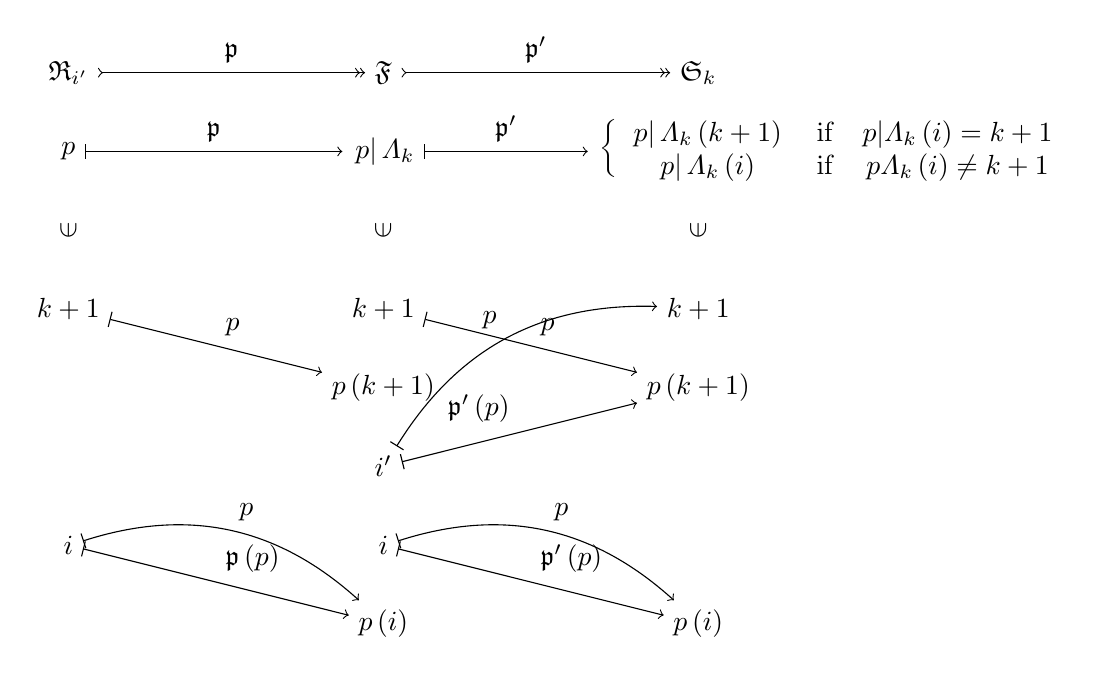
\begin{tikzpicture}[auto]

    \node (a) at (0, 7) {${\mathfrak R}_{i'} $};
    \node (b) at (4, 7) {${\mathfrak F} $};
    \node (c) at (8, 7) {${\mathfrak S}_k $};
    \node (d) at (0, 6) {$p$};
    \node (e) at (4, 6) {$\left. p\right|{\varLambda_k } $};
    \node (f) at (8, 6) {$\left\{ \begin{array}{c} \left. p\right|{\varLambda_k } \left( k+1\right) \\ \left. p\right|{\varLambda_k } \left( i\right) \end{array} \right. $};
    \node (f') at (11, 6) {$\begin{array}{cc} {\rm if} & p| \varLambda_k \left( i\right) =k+1\\ {\rm if} & p \varLambda_k \left( i\right) \neq k+1 \end{array} $};
    \draw [>->>] (a) to node {${\mathfrak p} $} (b);
    \draw [>->>] (b) to node {${\mathfrak p}' $} (c);
    \draw [|->] (d) to node {${\mathfrak p} $} (e);
    \draw [|->] (e) to node {${\mathfrak p}' $} (f);

    \node (x) at (0, 5) {\rotatebox{90}{$\in $}};
    \node (x) at (4, 5) {\rotatebox{90}{$\in $}};
    \node (x) at (8, 5) {\rotatebox{90}{$\in $}};

    \node (a) at (0, 1) {$i$};
    \node (b) at (4, 0) {$p\left( i\right) $};
    \node (c) at (8, 0) {$p\left( i\right) $};
    \node (d) at (4, 1) {$i$};
    \node (e) at (4, 2) {$i'$};
    \node (f) at (4, 3) {$p\left( k+1\right) $};
    \node (g) at (8, 3) {$p\left( k+1\right) $};
    \node (h) at (0, 4) {$k+1$};
    \node (i) at (4, 4) {$k+1$};
    \node (j) at (8, 4) {$k+1$};
    \draw [|->] (a) to[bend left=30] node {$p$} (b);
    \draw [|->] (a) to node {${\mathfrak p}\left( p\right) $} (b);
    \draw [|->] (d) to[bend left=30] node {$p$} (c);
    \draw [|->] (d) to node {${\mathfrak p}'\left( p\right) $} (c);
    \draw [|->] (e) to[bend left=30] node {$p$} (j);
    \draw [|->] (e) to node {${\mathfrak p}'\left( p\right) $} (g);
    \draw [|->] (h) to node {$p$} (f);
    \draw [|->] (i) to node {$p$} (g);

  \end{tikzpicture} 
\end{center}
また、その置換群$\mathfrak{S}_{k + 1}$は$\mathfrak{S}_{k + 1} = \bigsqcup_{i \in \varLambda_{k + 1}} \mathfrak{R}_{i}$のように書き換えられることができるので、したがって、次のようになる。
\begin{align*}
{\#}\mathfrak{S}_{k + 1} &= {\#}{\bigsqcup_{i \in \varLambda_{k + 1}} \mathfrak{R}_{i}}\\
&= {\#}\varLambda_{k + 1}{\#}\mathfrak{F}\\
&= {\#}\varLambda_{k + 1}{\#}\mathfrak{S}_{k}\\
&= (k + 1)k!\\
&= (k + 1)!
\end{align*}
よって、数学的帰納法によって${\#}\mathfrak{S}_{n} = n!$が成り立つことが示された。
\end{proof}
\begin{thm}\label{2.1.10.2}
定義より次のような恒等写像$I_{\varLambda_{n}}$もまたその添数集合$\varLambda_{n}$の置換となるかつ、
\begin{align*}
I_{\varLambda_{n}}:\varLambda_{n} \rightarrow \varLambda_{n};i \mapsto i
\end{align*}
$\forall p \in \mathfrak{S}_{n}$に対し、その置換$p$は全単射であるから、これの逆写像$p^{- 1}$が存在することに注意すれば、組$\left( \mathfrak{S}_{n}, \circ \right)$は群をなす。
\end{thm}
\begin{dfn}
置換の合成写像のことを置換の積、このときの恒等写像$I_{\varLambda_{n}}$のことを恒等置換、置換の逆写像のことを逆置換という。
\end{dfn}
\begin{proof}
置換群$\mathfrak{S}_{n}$について、置換同士の合成写像も置換であり、その集合$\mathfrak{S}_{n}$の元々は写像であるので、$\forall p,q,r \in \mathfrak{S}_{n}$に対し、次式が成り立つ。
\begin{align*}
(p \circ q) \circ r = p \circ (q \circ r)
\end{align*}
また、$\forall p \in \mathfrak{S}_{n}$に対し、次のような恒等写像$I_{\varLambda_{n}}$もまたその添数集合$\varLambda_{n}$の置換となるので、
\begin{align*}
I_{\varLambda_{n}}:\varLambda_{n} \rightarrow \varLambda_{n};i \mapsto i
\end{align*}
次式が成り立つような写像$I_{\varLambda_{n}}$がその置換群$\mathfrak{S}_{n}$に存在する。
\begin{align*}
I_{\varLambda_{n}} \circ p = p \circ I_{\varLambda_{n}} = p
\end{align*}
$\forall p \in \mathfrak{S}_{n}$に対し、その置換$p$は全単射でありこれの逆写像$p^{- 1}$が存在するので、次式が成り立つようなその写像$p$の逆元$p^{- 1}$が存在する。
\begin{align*}
p \circ p^{- 1} = p^{- 1} \circ p = I_{\varLambda_{n}}
\end{align*}
\end{proof}
\begin{dfn}
$n \geq 2$のとき、置換群$\mathfrak{S}_{n}$について、$i',j' \in \varLambda_{n}$なる互いに異なる元々$i'$、$j'$を選びその置換群$\mathfrak{S}_{n}$に属し次式が成り立つような置換$\tau$を考えよう。
\begin{align*}
\tau:\varLambda_{n} \rightarrow \varLambda_{n};i \mapsto \left\{ \begin{matrix}
j' & \mathrm{if} & i = j' \\
i' & \mathrm{if} & i = i' \\
i & \mathrm{if} & i \neq i' \land i \neq j' \\
\end{matrix} \right.\ 
\end{align*}
このような置換$\tau$をその添数集合$\varLambda_{n}$の互換といい$\begin{pmatrix}
i' & j' \\
\end{pmatrix}$などと書く。また、その添数集合$\varLambda_{n}$の互換$\tau$全体の集合を$\mathfrak{T}_{n}$とおく。
\end{dfn}\par
このとき、明らかに$\tau^{- 1} = \tau$が成り立つ。
\begin{thm}\label{2.1.10.3}
$n \geq 2$が成り立つなら、置換群$\mathfrak{S}_{n}$について、$\forall p \in \mathfrak{S}_{n}$に対し$\forall i \in \varLambda_{s}$に対し$\tau_{i} \in \mathfrak{T}_{k}$なる互換たち$\tau_{i}$を用いて次式のように表されることができる。\begin{align*}
p = \tau_{s} \circ \cdots \circ \tau_{2} \circ \tau_{1}
\end{align*}
\end{thm}\par
ただし、この表し方は一意的でないことに注意されたい。
\begin{proof}
置換群$\mathfrak{S}_{n}$について、$\forall p \in \mathfrak{S}_{n}$に対し$n = 2$のときその置換$p$自身が互換となる。\par
$n = k$のとき、$i \in \varLambda_{s}$なる互換たち$\tau_{i}$を用いて次式のように表されることができると仮定しよう。
\begin{align*}
p = \tau_{s} \circ \cdots \circ \tau_{2} \circ \tau_{1}
\end{align*}
$n = k + 1$のとき、$p(k + 1) = k + 1$が成り立つなら、その置換$p$を用いれば、次式のような写像$p'$が得られることができる。
\begin{align*}
p':\varLambda_{k} \rightarrow \varLambda_{k};i \mapsto p(i)
\end{align*}
その写像$p'$は明らかに$p' \in \mathfrak{S}_{k}$が成り立つので、仮定より$\forall i \in \varLambda_{s}$に対し$\tau_{i} \in \mathfrak{T}_{k + 1}$なる互換たち$\tau_{i}$を用いて次式のように表されることができる。
\begin{align*}
p' = \tau_{s} \circ \cdots \circ \tau_{2} \circ \tau_{1}
\end{align*}
このとき、次のような写像$\mathfrak{t}$を考えよう。
\begin{align*}
\mathfrak{t:}\mathfrak{T}_{k} \rightarrow \mathfrak{T}_{k + 1};\tau \mapsto \mathfrak{t}(\tau):\varLambda_{k + 1} \rightarrow \varLambda_{k + 1};i \mapsto \left\{ \begin{matrix}
k + 1 & \mathrm{if} & i = k + 1 \\
\tau(i) & \mathrm{if} & i \neq k + 1 \\
\end{matrix} \right.\ 
\end{align*}
このとき、$\forall i \in \varLambda_{k}$に対し$\tau(i) = \mathfrak{t}(\tau)(i)$が成り立つかつ、$\forall\tau \in \mathfrak{T}_{k}$に対し$\mathfrak{t}(\tau)(k + 1) = k + 1$が成り立つので、次のようになる。
\begin{align*}
p(i) &= \left\{ \begin{matrix}
k + 1 & \mathrm{if} & i = k + 1 \\
p'(i) & \mathrm{if} & i \neq k + 1 \\
\end{matrix} \right.\ \\
&= \left\{ \begin{matrix}
k + 1 & \mathrm{if} & i = k + 1 \\
\tau_{s} \circ \cdots \circ \tau_{2} \circ \tau_{1}(i) & \mathrm{if} & i \neq k + 1 \\
\end{matrix} \right.\ \\
&= \left\{ \begin{matrix}
\mathfrak{t}\left( \tau_{s} \right)\mathfrak{\circ \cdots \circ t}\left( \tau_{2} \right)\mathfrak{\circ t}\left( \tau_{1} \right)(k + 1) & \mathrm{if} & i = k + 1 \\
\mathfrak{t}\left( \tau_{s} \right)\mathfrak{\circ \cdots \circ t}\left( \tau_{2} \right)\mathfrak{\circ t}\left( \tau_{1} \right)(i) & \mathrm{if} & i \neq k + 1 \\
\end{matrix} \right.\ \\
& = \mathfrak{t}\left( \tau_{s} \right)\mathfrak{\circ \cdots \circ t}\left( \tau_{2} \right)\mathfrak{\circ t}\left( \tau_{1} \right)(i)
\end{align*}
一方、$p(k + 1) \neq k + 1$が成り立つなら、互換$\tau' = \begin{pmatrix}
p(k + 1) & k + 1 \\
\end{pmatrix}$を用いると、写像$\tau' \circ p$はその添数集合$\varLambda_{k + 1}$の置換であるかつ、次のようになるので、
\begin{align*}
\tau' \circ p(k + 1) = \tau'\left( p(k + 1) \right) = k + 1
\end{align*}
$p(k + 1) = k + 1$が成り立つ場合に帰着できる。したがって、$\forall i \in \varLambda_{s}$に対し$\tau_{i} \in \mathfrak{T}_{k + 1}$なる互換たち$\tau_{i}$を用いて次式のように表されることができる。
\begin{align*}
\tau' \circ p = \tau_{s} \circ \cdots \circ \tau_{2} \circ \tau_{1}
\end{align*}
したがって、${\tau'}^{- 1} = \tau' \in \mathfrak{T}_{k + 1}$が成り立ち次のようになる。
\begin{align*}
p = {\tau'}^{- 1} \circ \tau' \circ p = {\tau'}^{- 1} \circ \tau_{s} \circ \cdots \circ \tau_{2} \circ \tau_{1}
\end{align*}
以上より$n = k + 1$のときでもこれは成り立つ。\par
数学的帰納法によって示すべきことは示された。
\end{proof}
%\hypertarget{ux5deeux7a4d}{%
\subsubsection{差積}%\label{ux5deeux7a4d}}
\begin{dfn}
$n \geq 2$が成り立つとき、置換群$\mathfrak{S}_{n}$について、$\forall p \in \mathfrak{S}_{n}$に対し$\forall i \in \varLambda_{s}$に対し$\tau_{i} \in \mathfrak{T}_{n}$なる互換たち$\tau_{i}$を用いて次式のように表されることができるのであった。
\begin{align*}
p = \tau_{s} \circ \cdots \circ \tau_{2} \circ \tau_{1}
\end{align*}
このとき、集合$\mathfrak{D}$を次のように定め
\begin{align*}
\mathfrak{D} =\left\{ (i,j) \in \varLambda_{n}^{2} \middle| i < j \right\}
\end{align*}
次のような写像$\varDelta$を考えよう。このような写像$\varDelta$を差積などという。
\begin{align*}
\varDelta:\mathfrak{S}_{n} \rightarrow \mathbb{Q};p \mapsto \frac{\prod_{(i,j)\in \mathfrak{D} \left( p(j) - p(i) \right)}}{\prod_{(i,j)\in \mathfrak{D} } (j - i)}
\end{align*}
\end{dfn}
\begin{thm}\label{2.1.10.4}
置換群$\mathfrak{S}_n $について、$\forall p \in \mathfrak{S}_{n}$に対し$\forall i \in \varLambda_{s}$に対し$\tau_{i} \in \mathfrak{T}_{n}$なる互換たち$\tau_{i}$を用いて次式のように表されることができるとき、
\begin{align*}
  p = \tau_{s} \circ \cdots \circ \tau_{2} \circ \tau_{1}
\end{align*}
$\varDelta (p)=\left( -1\right)^s $が成り立つ。
\end{thm}\par
なお、$\forall(i,j)\in \mathfrak{D}$に対し$j - i \neq 0$が成り立つので、$\prod_{(i,j)\in \mathfrak{D} } (j - i) \neq 0$となっているかつ、その写像$p$は単射であるので、$p(i) \neq p(j)$が成り立ち$\prod_{(i,j)\in \mathfrak{D} } \left( p(j) - p(i) \right) \neq 0$となっていることに注意されたい。このことは数学的帰納法によって示される。
\begin{proof}
$n \geq 2$が成り立つとき、置換群$\mathfrak{S}_{n}$について、集合$\mathfrak{D}$を次のように定め
\begin{align*}
\mathfrak{D} =\left\{ (i,j) \in \varLambda_{n}^{2} \middle| i < j \right\}
\end{align*}
次のような写像$\varDelta$を考えよう。
\begin{align*}
\varDelta&:\mathfrak{S}_{n} \rightarrow \mathbb{Q};p \mapsto \frac{\prod_{(i,j)\in \mathfrak{D} } \left( p(j) - p(i) \right)}{\prod_{(i,j)\in \mathfrak{D}} (j - i)}\\
\mathfrak{D}_{<}&:\mathfrak{S}_{n}\mathfrak{\rightarrow P}\left( \varLambda_{n}^{2} \right);p \mapsto \left\{ (i,j) \in \varLambda_{n}^{2} \middle| i < j \land p(i) < p(j) \right\}\\
\mathfrak{D}_{>}&:\mathfrak{S}_{n}\mathfrak{\rightarrow P}\left( \varLambda_{n}^{2} \right);p \mapsto \left\{ (i,j) \in \varLambda_{n}^{2} \middle| i < j \land p(i) > p(j) \right\}
\end{align*}
なお、$\forall(i,j)\in \mathfrak{D}$に対し$j - i \neq 0$が成り立つので、$\prod_{(i,j)\in \mathfrak{D} } (j - i) \neq 0$となっているかつ、その写像$p$は単射であるので、$p(i) \neq p(j)$が成り立ち$\prod_{(i,j)\in \mathfrak{D} } \left( p(j) - p(i) \right) \neq 0$となる。さらに、$\forall(i,j)\in \mathfrak{D}$に対し$p\left( i_{1} \right) \neq p\left( i_{2} \right)$が成り立つので、次のようになる。
\begin{align*}
\mathfrak{D} &= \left\{ (i,j) \in \varLambda_{n}^{2} \middle| i < j \right\}\\
&= \left\{ (i,j) \in \varLambda_{n}^{2} \middle| i < j \land p(i) \neq p(j) \right\}\\
&= \left\{ (i,j) \in \varLambda_{n}^{2} \middle| i < j \land \left( p(i) < p(j) \vee p(i) > p(j) \right) \right\}\\
&= \left\{ (i,j) \in \varLambda_{n}^{2} \middle| \left( i < j \land p(i) < p(j) \right) \vee \left( i < j \land p(i) > p(j) \right) \right\}\\
&= \left\{ (i,j) \in \varLambda_{n}^{2} \middle| i < j \land p(i) < p(j) \right\} \cup \left\{ (i,j) \in \varLambda_{n}^{2} \middle| i < j \land p(i) > p(j) \right\}\\
&= \mathfrak{D}_{<}(p) \cup \mathfrak{D}_{>}(p)
\end{align*}
また、次のようになり、
\begin{align*}
\mathfrak{D}_{<}(p) \cap \mathfrak{D}_{<}(p) &= \left\{ (i,j) \in \varLambda_{n}^{2} \middle| i < j \land p(i) < p(j) \right\} \cap \left\{ (i,j) \in \varLambda_{n}^{2} \middle| i < j \land p(i) > p(j) \right\}\\
&= \left\{ (i,j) \in \varLambda_{n}^{2} \middle| i < j \land p(i) < p(j) \land i < j \land p(i) > p(j) \right\}\\
&= \left\{ (i,j) \in \varLambda_{n}^{2} \middle| i < j \land \bot \right\} = \emptyset
\end{align*}
以上より、次式が成り立つ。
\begin{align*}
\mathfrak{D} =\mathfrak{D}_{<}(p) \sqcup \mathfrak{D}_{>}(p)
\end{align*}\par
このとき、$\forall p \in \mathfrak{S}_{n}$に対し$\forall i \in \varLambda_{s}$に対し$\tau_{i} \in \mathfrak{T}_{n}$なる互換たち$\tau_{i}$を用いて次式のように表されることができるのであった。
\begin{align*}
p = \tau_{s} \circ \cdots \circ \tau_{2} \circ \tau_{1}
\end{align*}\par
$s = 1$のとき、その互換$\tau_{1}$を$\left( i',j' \right)\mathfrak\in {D}$として$\tau_{1} = \begin{pmatrix}
i' & j' \\
\end{pmatrix} \in \mathfrak{T}_{n}$とおくと、
\begin{align*}
\varDelta(p) &= \varDelta\left( \tau_{1} \right) = \frac{\prod_{(i,j)\in \mathfrak{D}} \left( \tau_{1}(j) - \tau_{1}(i) \right)}{\prod_{(i,j)\in \mathfrak{D} } (j - i)} \\
&= \frac{\left( \tau_{1}\left( j' \right) - \tau_{1}\left( i' \right) \right)\prod_{(i,j)\in \mathfrak{D} \setminus \left\{ \left( i',j' \right) \right\} } \left( \tau_{1}(j) - \tau_{1}(i) \right)}{\prod_{(i,j)\in \mathfrak{D} } (j - i)}\\
&= \frac{\left( i' - j' \right)\prod_{(i,j)\in \mathfrak{D} \setminus\left\{ \left( i',j' \right) \right\} } (j - i)}{\prod_{(i,j)\in \mathfrak{D}} (j - i)}\\
&= - \frac{\left( j' - i' \right)\prod_{(i,j)\in \mathfrak{D} \setminus \left\{ \left( i',j' \right) \right\} } (j - i)}{\prod_{(i,j)\in \mathfrak{D} } (j - i)}\\
&= - \frac{\prod_{(i,j)\in \mathfrak{D} } (j - i)}{\prod_{(i,j)\in \mathfrak{D} } (j - i)} = - 1
\end{align*}\par
$s = k$のとき、$\varDelta(p) = ( - 1)^{k}$が成り立つと仮定しよう。$s = k + 1$のとき、$\forall i \in \varLambda_{k + 1}$に対し$\tau_{i} \in \mathfrak{T}_{n}$なる互換たち$\tau_{i}$を用いて次式のように表され
\begin{align*}
p = \tau_{k + 1} \circ \tau_{k} \circ \cdots \circ \tau_{2} \circ \tau_{1}
\end{align*}
次式のように写像$p'$を定める。
\begin{align*}
p' = \tau_{k} \circ \cdots \circ \tau_{2} \circ \tau_{1}
\end{align*}
このとき、次のようになり、
\begin{align*}
\varDelta(p) &= \frac{\prod_{(i,j)\in \mathfrak{D} } \left( p(j) - p(i) \right)}{\prod_{(i,j)\in \mathfrak{D} } (j - i)}\\
&= \frac{\prod_{(i,j)\in \mathfrak{D} } \left( \tau_{k + 1} \circ p'(j) - \tau_{k + 1} \circ p'(i) \right)}{\prod_{(i,j)\in \mathfrak{D} } (j - i)}\\
&= \frac{\prod_{(i,j)\in \mathfrak{D} } \left( \tau_{k + 1} \circ p'(j) - \tau_{k + 1} \circ p'(i) \right)}{\prod_{(i,j)\in \mathfrak{D} } \left( p'\left( i_{1} \right) - p'(i) \right)}\frac{\prod_{(i,j)\in \mathfrak{D} } \left( p'(j) - p'(i) \right)}{\prod_{(i,j)\in \mathfrak{D} } (j - i)}\\
&= \frac{\prod_{(i,j) \in \mathfrak{D}_{<}(p) \sqcup \mathfrak{D}_{>}(p) } \left( \tau_{k + 1} \circ p'(j) - \tau_{k + 1} \circ p'(i) \right)}{\prod_{(i,j) \in \mathfrak{D}_{<}(p) \sqcup \mathfrak{D}_{>}(p) } \left( p'(j) - p'(i) \right)}\frac{\prod_{(i,j)\in \mathfrak{D} } \left( p'(j) - p'(i) \right)}{\prod_{(i,j)\in \mathfrak{D} } (j - i)}\\
&= \frac{\prod_{(i,j) \in \mathfrak{D}_{<}(p) } \left( \tau_{k + 1} \circ p'(j) - \tau_{k + 1} \circ p'(i) \right)}{\prod_{(i,j) \in \mathfrak{D}_{<}(p) } \left( p'(j) - p'(i) \right)} \\
&\quad \frac{\prod_{(i,j) \in \mathfrak{D}_{>}(p) } \left( \tau_{k + 1} \circ p'(j) - \tau_{k + 1} \circ p'(i) \right)}{\prod_{(i,j) \in \mathfrak{D}_{>}(p) } \left( p'(j) - p'(i) \right)}\frac{\prod_{(i,j)\in \mathfrak{D} } \left( p'(j) - p'(i) \right)}{\prod_{(i,j)\in \mathfrak{D} } (j - i)}\\
&= \frac{\prod_{(i,j) \in \mathfrak{D}_{<}(p) } \left( \tau_{k + 1} \circ p'(j) - \tau_{k + 1} \circ p'(i) \right)}{\prod_{(i,j) \in \mathfrak{D}_{<}(p) } \left( p'(j) - p'(i) \right)} \\
&\quad \frac{\prod_{(i,j) \in \mathfrak{D}_{>}(p) } {( - 1)\left( \tau_{k + 1} \circ p'(i) - \tau_{k + 1} \circ p'(j) \right)}}{\prod_{(i,j) \in \mathfrak{D}_{>}(p) } {( - 1)\left( p'(i) - p'(j) \right)}}\frac{\prod_{(i,j)\in \mathfrak{D} } \left( p'(j) - p'(i) \right)}{\prod_{(i,j)\in \mathfrak{D} } (j - i)}\\
&= \frac{\prod_{(i,j) \in \mathfrak{D}_{<}(p) } \left( \tau_{k + 1} \circ p'(j) - \tau_{k + 1} \circ p'(i) \right)}{\prod_{(i,j) \in \mathfrak{D}_{<}(p) } \left( p'(j) - p'(i) \right)}\frac{\prod_{(i,j) \in \mathfrak{D}_{>}(p) } \left( \tau_{k + 1} \circ p'(i) - \tau_{k + 1} \circ p'(j) \right)}{\prod_{(i,j) \in \mathfrak{D}_{>}(p) } \left( p'(i) - p'(j) \right)} \\
&\quad \frac{\prod_{(i,j) \in \mathfrak{D}_{>}(p) } ( - 1)}{\prod_{(i,j) \in \mathfrak{D}_{>}(p) } ( - 1)}\frac{\prod_{(i,j)\in \mathfrak{D} } \left( p'(j) - p'(i) \right)}{\prod_{(i,j)\in \mathfrak{D} } (j - i)}\\
&= \frac{\prod_{\left( p(i),p(j) \right)\in \mathfrak{D} } \left( \tau_{k + 1} \circ p'(j) - \tau_{k + 1} \circ p'(i) \right)}{\prod_{\left( p(i),p(j) \right)\in \mathfrak{D} } \left( p'(j) - p'(i) \right)}\frac{\prod_{(i,j)\in \mathfrak{D} } \left( p'(j) - p'(i) \right)}{\prod_{(i,j)\in \mathfrak{D} } (j - i)}\\
&= \varDelta\left( \tau_{k + 1} \right)\varDelta\left( p' \right) = ( - 1)( - 1)^{k} = ( - 1)^{k + 1}
\end{align*}
以上より数学的帰納法によって$\forall p \in \mathfrak{S}_{n}$に対し$\forall i \in \varLambda_{s}$に対し$\tau_{i} \in \mathfrak{T}_{n}$なる互換たち$\tau_{i}$を用いて次式のように表されるとき、
\begin{align*}
p = \tau_{s} \circ \cdots \circ \tau_{2} \circ \tau_{1}
\end{align*}
$\varDelta(p) = ( - 1)^{s}$が成り立つ。
\end{proof}
\begin{thm}\label{2.1.10.5}
$n \geq 2$が成り立つとき、置換群$\mathfrak{S}_{n}$について、$\forall p \in \mathfrak{S}_{n}$に対し、$\forall i \in \varLambda_{s}$、$\sigma_{i} \in \mathfrak{T}_{n}$なる互換たち$\tau_{i}$と$\forall j \in \varLambda_{t}$、$\tau_{j} \in \mathfrak{T}_{n}$なる互換たち$\tau_{j}$を用いて次式のように表されるとき、
\begin{align*}
p = \sigma_{s} \circ \cdots \circ \sigma_{2} \circ \sigma_{1} = \tau_{t} \circ \cdots \circ \tau_{2} \circ \tau_{1}
\end{align*}
その自然数たち$s、t$の偶奇が一意的である、即ち、$s,t \in 2\mathbb{N}$または$s,t \in 2\mathbb{N} - 1$が成り立つ。
\end{thm}\par
このことは上記の差積$\varDelta$を用いて背理法によって示される。
\begin{dfn}
置換$p$が偶数の個数の互換たちの積で表されるとき、即ち、$\varDelta(p) = 1$が成り立つとき、その置換は偶置換といい、奇数の個数の互換たちの積で表されるとき、即ち、$\varDelta(p) = - 1$が成り立つとき、その置換は奇置換という。
\end{dfn}
\begin{proof}
$n \geq 2$が成り立つとき、置換群$\mathfrak{S}_{n}$について、集合$\mathfrak{D}$を次のように定め
\begin{align*}
\mathfrak{D} = \left\{ (i,j) \in \varLambda_{n}^{2} \middle| i < j \right\}
\end{align*}
次のような写像たち$\varDelta$を考えよう。
\begin{align*}
\varDelta:\mathfrak{S}_{n} \rightarrow \mathbb{Q};p \mapsto \frac{\prod_{(i,j) \in \mathfrak{D} \left( p(j) - p(i) \right)}}{\prod_{(i,j)\in \mathfrak{D} (j - i)}}
\end{align*}
このとき、$\forall p \in \mathfrak{S}_{n}$に対し$\forall i \in \varLambda_{s}$に対し$\tau_{i} \in \mathfrak{T}_{n}$なる互換たち$\tau_{i}$を用いて次式のように表されるとき、
\begin{align*}
p = \tau_{s} \circ \cdots \circ \tau_{2} \circ \tau_{1}
\end{align*}
次式が成り立つのであった。
\begin{align*}
\varDelta(p) = ( - 1)^{s}
\end{align*}
ここで、$\forall p \in \mathfrak{S}_{n}$に対し、$\forall i \in \varLambda_{s}$、$\sigma_{i} \in \mathfrak{T}_{n}$なる互換たち$\tau_{i}$と$\forall j \in \varLambda_{t}$、$\tau_{j} \in \mathfrak{T}_{n}$なる互換たち$\tau_{j}$を用いて次式のように表されるとき、
\begin{align*}
p = \sigma_{s} \circ \cdots \circ \sigma_{2} \circ \sigma_{1} = \tau_{t} \circ \cdots \circ \tau_{2} \circ \tau_{1}
\end{align*}
次式が成り立つ。
\begin{align*}
\varDelta(p) = ( - 1)^{s} = ( - 1)^{t}
\end{align*}\par
ここで、$s \in 2\mathbb{N}$かつ$t \in 2\mathbb{N} - 1$と仮定しよう。このとき、$t + 1 \in 2\mathbb{N}$が成り立つので、自然数たち$m$、$n$を用いて$s = 2m$かつ$t + 1 = 2n$と書かれることができ、したがって、次のようになる。
\begin{align*}
( - 1)^{s} &= ( - 1)^{2m} = \left( ( - 1)^{2} \right)^{m} = 1^{m} = 1\\
( - 1)^{t} &= ( - 1)^{- 1}( - 1)^{t + 1} = - ( - 1)^{2n} = - \left( ( - 1)^{2} \right)^{n} = - 1^{n} = - 1
\end{align*}
となり$( - 1)^{s} = ( - 1)^{t}$に矛盾する。$t \in 2\mathbb{N}$かつ$s \in 2\mathbb{N} - 1$と仮定しても同様に矛盾する。\par
したがって、次のようになる。
\begin{align*}
&\quad \neg\left( s \in 2\mathbb{N} \land t \in 2\mathbb{N} - 1 \right) \land \neg\left( t \in 2\mathbb{N} \land s \in 2\mathbb{N} - 1 \right)\\
&\Leftrightarrow \left( s \notin 2\mathbb{N} \vee t \notin 2\mathbb{N} - 1 \right) \land \left( t \notin 2\mathbb{N} \vee s \notin 2\mathbb{N} - 1 \right)\\
&\Leftrightarrow \left( s \in 2\mathbb{N} - 1 \vee t \in 2\mathbb{N} \right) \land \left( t \in 2\mathbb{N} - 1 \vee s \in 2\mathbb{N} \right)\\
&\Leftrightarrow \left( s \in 2\mathbb{N} \land t \in 2\mathbb{N} \right) \vee \left( s \in 2\mathbb{N} - 1 \land t \in 2\mathbb{N} - 1 \right) \\
&\quad \vee \left( s \in 2\mathbb{N} \land s \in 2\mathbb{N} - 1 \right) \vee \left( t \in 2\mathbb{N} \land t \in 2\mathbb{N} - 1 \right)\\
&\Leftrightarrow \left( s \in 2\mathbb{N} \land t \in 2\mathbb{N} \right) \vee \left( s \in 2\mathbb{N} - 1 \land t \in 2\mathbb{N} - 1 \right) \vee \bot \vee \bot\\
&\Leftrightarrow s,t \in 2\mathbb{N} \vee s,t \in 2\mathbb{N} - 1
\end{align*}
\end{proof}
\begin{thm}\label{2.1.10.6}
$n \geq 2$のとき、置換群$\mathfrak{S}_{n}$のうち偶置換、奇置換全体の集合がそれぞれ$\mathfrak{S}_{\mathrm{even}}$、$\mathfrak{S}_{\mathrm{odd}}$とおかれると、$\mathfrak{S}_{n} = \mathfrak{S}_{\mathrm{even}} \sqcup \mathfrak{S}_{\mathrm{odd}}$が成り立つ。さらに、その集合$\mathfrak{S}_{n}$のうち偶置換、奇置換がどちらも$\frac{n!}{2}$つ存在する。
\end{thm}
\begin{proof}
$n \geq 2$が成り立つとき、置換群$\mathfrak{S}_{n}$のうち偶置換、奇置換全体の集合がそれぞれ$\mathfrak{S}_{\mathrm{even}}$、$\mathfrak{S}_{\mathrm{odd}}$とおかれると、即ち、集合たち$\mathfrak{S}_{\mathrm{even}}$、$\mathfrak{S}_{\mathrm{odd}}$を次のように定めると、
\begin{align*}
\mathfrak{S}_{\mathrm{even}} &= \left\{ p \in \mathfrak{S}_{n} \middle| \varDelta(p) = 1 \right\}\\
\mathfrak{S}_{\mathrm{odd}} &= \left\{ p \in \mathfrak{S}_{n} \middle| \varDelta(p) = - 1 \right\}
\end{align*}
次のようになるかつ、
\begin{align*}
\mathfrak{S}_{n} &= \left\{ p \in \mathfrak{S}_{n} \middle| p \in \mathfrak{S}_{n} \right\}\\
&= \left\{ p \in \mathfrak{S}_{n} \middle| \varDelta(p) = \pm 1 \right\}\\
&= \left\{ p \in \mathfrak{S}_{n} \middle| \varDelta(p) = 1 \right\} \cup \left\{ p \in \mathfrak{S}_{n} \middle| \varDelta(p) = - 1 \right\}\\
&= \mathfrak{S}_{\mathrm{even}} \cup \mathfrak{S}_{\mathrm{odd}}
\end{align*}
次のようになるので、
\begin{align*}
\mathfrak{S}_{\mathrm{even}} \cap \mathfrak{S}_{\mathrm{odd}} &= \left\{ p \in \mathfrak{S}_{n} \middle| \varDelta(p) = 1 \right\} \cap \left\{ p \in \mathfrak{S}_{n} \middle| \varDelta(p) = - 1 \right\}\\
&= \left\{ p \in \mathfrak{S}_{n} \middle| \varDelta(p) = 1 \land \varDelta(p) = - 1 \right\} = \emptyset
\end{align*}
$\mathfrak{S}_{n} = \mathfrak{S}_{\mathrm{even}} \sqcup \mathfrak{S}_{\mathrm{odd}}$が成り立つ。\par
さらに、添数集合$\varLambda_{n}$の互換全体の集合を$\mathfrak{T}_{n}$とし$\tau \in \mathfrak{T}_{n}$なる互換$\tau$を選んで次のような写像$\mathfrak{t}$を考えよう。
\begin{align*}
\mathfrak{t:}\mathfrak{S}_{\mathrm{even}} \rightarrow \mathfrak{S}_{\mathrm{odd}};p \mapsto \tau \circ p
\end{align*}
このとき、その互換$\tau$は全単射でこれの逆写像$\tau^{- 1}$が存在しこれはその互換$\tau$自身となるので、この写像$\mathfrak{t}$の逆写像$\mathfrak{t}^{- 1}$が次式のように存在する。
\begin{align*}
\mathfrak{t}^{- 1}:\mathfrak{S}_{\mathrm{odd}} \rightarrow \mathfrak{S}_{\mathrm{even}};p \mapsto \tau^{- 1} \circ p = \tau \circ p
\end{align*}
これにより、その写像$\mathfrak{t}$は全単射となり${\#}\mathfrak{S}_{\mathrm{even}} = {\#}\mathfrak{S}_{\mathrm{odd}}$が成り立つ。したがって、定理\ref{2.1.10.1}より${\#}\mathfrak{S}_{n} = n!$が成り立つので、次のようになる。
\begin{align*}
{\#}\mathfrak{S}_{n} &= {\#}{\mathfrak{S}_{\mathrm{even}} \sqcup \mathfrak{S}_{\mathrm{odd}}}\\
&= {\#}\mathfrak{S}_{\mathrm{even}} + {\#}\mathfrak{S}_{\mathrm{odd}}\\
&= 2{\#}\mathfrak{S}_{\mathrm{even}} = 2{\#}\mathfrak{S}_{\mathrm{odd}}
\end{align*}
よって、次式が得られる。
\begin{align*}
{\#}\mathfrak{S}_{\mathrm{even}} = {\#}\mathfrak{S}_{\mathrm{odd}} = \frac{{\#}\mathfrak{S}_{n}}{2} = \frac{n!}{2}
\end{align*}
\end{proof}
\begin{dfn}
置換群$\mathfrak{S}_{n}$について、次のような写像$\mathrm{sgn} $を考える
\begin{align*}
\mathrm{sgn} :\mathfrak{S}_{n} \rightarrow \left\{ - 1,1 \right\};p \mapsto \left\{ \begin{matrix}
1 & \mathrm{if} & n = 1 \\
\varDelta(p) & \mathrm{if} & n \geq 2 \\
\end{matrix} \right.\ 
\end{align*}
この写像$\mathrm{sgn} $を置換の符号という。
\end{dfn}
\begin{thm}\label{2.1.10.7}
置換群$\mathfrak{S}_{n}$について、$\forall p,q \in \mathfrak{S}_{n}$に対し、${\mathrm{sgn} }{q \circ p} = {\mathrm{sgn} }p{\mathrm{sgn} }q$が成り立つ。
\end{thm}
\begin{proof}
置換群$\mathfrak{S}_{n}$について、$\forall p,q \in \mathfrak{S}_{n}$に対し、$n = 1$のとき、$\forall p'\in \mathfrak{F}\left( \varLambda_{1},\varLambda_{1} \right)$に対しその写像$p'$は恒等写像となり置換であるので、明らかに示すべきことが成り立つ。\par
$n \geq 2$のとき、$\forall i \in \varLambda_{s}$に対し$\sigma_{i} \in \mathfrak{T}_{n}$なる互換たち$\sigma_{i}$と$\forall j \in \varLambda_{t}$に対し$\tau_{j} \in \mathfrak{T}_{n}$なる互換たち$\tau_{j}$を用いて次式のように表されるとき、
\begin{align*}
p = \sigma_{s} \circ \cdots \circ \sigma_{2} \circ \sigma_{1},\ \ q = \tau_{t} \circ \cdots \circ \tau_{2} \circ \tau_{1}
\end{align*}
次式が成り立つ。
\begin{align*}
q \circ p = \tau_{t} \circ \cdots \circ \tau_{2} \circ \tau_{1} \circ \sigma_{s} \circ \cdots \circ \sigma_{2} \circ \sigma_{1}
\end{align*}
このとき、次のようになる。
\begin{align*}
{\mathrm{sgn} }{q \circ p} &= \varDelta(q \circ p)\\
&= ( - 1)^{s + t}\\
&= ( - 1)^{s}( - 1)^{t}\\
&= \varDelta(p)\varDelta(q)\\
&= {\mathrm{sgn} }p{\mathrm{sgn} }q
\end{align*}
\end{proof}
\begin{thm}\label{2.1.10.8}
置換群$\mathfrak{S}_{n}$について、$\forall p \in \mathfrak{S}_{n}$に対し、${\mathrm{sgn} }p^{- 1} = {\mathrm{sgn} }p$が成り立つ。
\end{thm}
\begin{proof}
置換群$\mathfrak{S}_{n}$について、$\forall p \in \mathfrak{S}_{n}$に対し、$n = 1$のとき、$\forall p'\in \mathfrak{F}\left( \varLambda_{1},\varLambda_{1} \right)$に対しその写像$p'$は恒等写像となり置換であるので、${\mathrm{sgn} }p^{- 1} = {\mathrm{sgn} }p$が成り立つ。\par
$n \geq 2$のとき、$\forall i \in \varLambda_{s}$に対し$\tau_{i} \in \mathfrak{T}_{n}$なる互換たち$\tau_{i}$を用いて次式のように表されるとき、
\begin{align*}
p = \tau_{s} \circ \cdots \circ \tau_{2} \circ \tau_{1} 
\end{align*}
次のようになるので、
\begin{align*}
p^{- 1} &= \tau_{1}^{- 1} \circ \tau_{2}^{- 1} \circ \cdots \circ \tau_{s}^{- 1}
\end{align*}
したがって、次のようになる。
\begin{align*}
{\mathrm{sgn} }p = \varDelta(p) = ( - 1)^{s} = \varDelta\left( p^{- 1} \right) = {\mathrm{sgn} }p^{- 1}
\end{align*}
\end{proof}
%\hypertarget{ux8f9eux66f8ux5f0fux9806ux5e8f}{%
\subsubsection{辞書式順序}%\label{ux8f9eux66f8ux5f0fux9806ux5e8f}}
\begin{thm}\label{2.1.10.9}
置換群$\mathfrak{S}_{n}$について、$\forall\left( \alpha_{i} \right)_{i \in \varLambda_{n}} \in \varLambda_{m}^{n}\exists p \in \mathfrak{S}_{n}\forall k,l \in \varLambda_{n}$に対し、$k \leq l$が成り立つなら、$\alpha_{p(k)} \leq \alpha_{p(l)}$が成り立つようにすることができる。このような置換$p$を辞書式順序という。
\end{thm}
\begin{proof}
置換群$\mathfrak{S}_{n}$について、$n = 1$のときは明らかである。$n = 2$のとき、$\forall\begin{pmatrix}
\alpha_{1} & \alpha_{2} \\
\end{pmatrix} \in \varLambda_{m}^{2}$に対し、$\alpha_{1} \leq \alpha_{2}$のとき、恒等置換で考えればよいし、$\alpha_{1} > \alpha_{2}$のとき、置換$\begin{pmatrix}
1 & 2 \\
2 & 1 \\
\end{pmatrix}$で考えればよい。そこで、$n = j$のとき、$\forall\left( \alpha_{i} \right)_{i \in \varLambda_{j}} \in \varLambda_{m}^{j}\exists p \in \mathfrak{S}_{j}\forall k,l \in \varLambda_{j}$に対し、$k \leq l$が成り立つなら、$\alpha_{p(k)} \leq \alpha_{p(l)}$が成り立つようにすることができると仮定しよう。$n = j + 1$のとき、$\forall\left( \alpha_{i} \right)_{i \in \varLambda_{n}} \in \varLambda_{m}^{j + 1}$に対し、仮定よりある$p' \in \mathfrak{S}_{j}$なる置換$p'$が存在して、$\forall k,l \in \varLambda_{j}$に対し、$k \leq l$が成り立つなら、$\alpha_{p'(k)} \leq \alpha_{p'(l)}$が成り立つようにすることができる。そこで、次式のような集合$\mathfrak{D}$が考えられると、
\begin{align*}
\mathfrak{D}=\left\{ \alpha_{k} \in \varLambda_{m} \middle| \alpha_{k} \leq \alpha_{j + 1} \right\},\ \ \mathfrak{M}=\left\{ M \in \varLambda_{j} \middle| \max\mathfrak{D} = \alpha_{p'(M)} \right\}
\end{align*}
$\mathfrak{D} = \emptyset$のとき、$\max{V\left( p'\mathfrak{|M} \right)} = 0$とすることにして、次のような置換$p$で考えられれば、
\begin{align*}
p:\varLambda_{j + 1}\overset{\sim}{\rightarrow}\varLambda_{j + 1};k \mapsto p(k) = \left\{ \begin{matrix}
p'(k - 1) & \mathrm{if} & \max{V\left( p'\mathfrak{|M} \right)} + 1 < k \\
j + 1 & \mathrm{if} & k = \max{V\left( p'\mathfrak{|M} \right)} + 1 \\
p'(k) & \mathrm{if} & k \leq \max{V\left( p'\mathfrak{|M} \right)} \\
\end{matrix} \right.\ 
\end{align*}
$\forall k,l \in \varLambda_{j + 1}$に対し、$k \leq l$が成り立つなら、次のようになることから、
\begin{longtable}[c]{|c|c|l|c|}
\hline
条件1 & 条件2 & 理由 & 結論 \\
\hline \hline
\begin{tabular}{c}
  $\max{V\left( p'\mathfrak{|M} \right)} + 1 < k $ \\
  $\max{V\left( p'\mathfrak{|M} \right)} + 1 < l $
\end{tabular} & & \begin{minipage}{0.4\textwidth}
  $k - 1 \leq l - 1$が成り立つことからその置換$p'$のおき方による。\end{minipage} & $\alpha_{p(k)} \leq \alpha_{p(l)}$ \\
\hline
\begin{tabular}{c}
  $\max{V\left( p'\mathfrak{|M} \right)} + 1 < k $\\
  $l = \max{V\left( p'\mathfrak{|M} \right)} + 1 $
\end{tabular} & & 仮定に矛盾している。 & \\
\hline
\begin{tabular}{c}
  $\max{V\left( p'\mathfrak{|M} \right)} + 1 < k $\\
  $l \leq \max{V\left( p'\mathfrak{|M} \right)} $
\end{tabular} & & 仮定に矛盾している。 & \\
\hline
\begin{tabular}{c}
  $k = \max{V\left( p'\mathfrak{|M} \right)} + 1 $\\
  $\max{V\left( p'\mathfrak{|M} \right)} + 1 < l $
\end{tabular} & & 仮定に矛盾している。 & \\
\hline
\begin{tabular}{c}
  $k = \max{V\left( p'\mathfrak{|M} \right)} + 1 $\\
  $l = \max{V\left( p'\mathfrak{|M} \right)} + 1 $
\end{tabular} & & $k = l$より明らかである。 & $\alpha_{p(k)} = \alpha_{p(l)}$ \\
\hline
\begin{tabular}{c}
  $k = \max{V\left( p'\mathfrak{|M} \right)} + 1 $\\
  $l \leq \max{V\left( p'\mathfrak{|M} \right)}$ 
\end{tabular} & & 仮定に矛盾している。 & \\
\hline
\multirow{3}{*}{
\begin{tabular}{c}
  $k \leq \max{V\left( p'\mathfrak{|M} \right)} $\\
  $\max{V\left( p'\mathfrak{|M} \right)} + 1 < l $
\end{tabular} } & $\mathfrak{D} = \emptyset$ & ありえない。 & \\ \cline{2-4}
& \begin{tabular}{c}
  $\mathfrak{D} \neq \emptyset $\\
  $\alpha_{j + 1} \leq \alpha_{p'(l - 1)} $
\end{tabular} & \begin{minipage}{0.4\textwidth} $\alpha_{p'(k)} \leq \alpha_{j + 1} \leq \alpha_{p'(l - 1)}$が成り立つことによる。\end{minipage} & $\alpha_{p(k)} \leq \alpha_{p(l)}$ \\ \cline{2-4}
& \begin{tabular}{c}
  $\mathfrak{D} \neq \emptyset $\\
  $\alpha_{p'(l - 1)} < \alpha_{j + 1} $
\end{tabular} & \begin{minipage}{0.4\textwidth} $\alpha_{p'(k)} \leq \alpha_{j + 1}$が成り立つ。そこで、$\alpha_{p'(l - 1)} < \alpha_{j + 1}$が成り立つとすれば、$l - 1 \leq \max{V\left( p'\mathfrak{|M} \right)}$が成り立つことになるが、これは仮定に矛盾している。したがって、$\alpha_{j + 1} \leq \alpha_{p'(l - 1)}$が得られる。\end{minipage} & $\alpha_{p(k)} \leq \alpha_{p(l)}$ \\
\hline 
\multirow{2}{*}{
  \begin{tabular}{c}
  $k \leq \max{V\left( p'\mathfrak{|M} \right)} $\\
  $l = \max{V\left( p'\mathfrak{|M} \right)} + 1 $ \end{tabular} } & $\mathfrak{D} =\emptyset$ & ありえない。 & \\ \cline{2-4}
& $\mathfrak{D} \neq \emptyset$ & \begin{minipage}{0.4\textwidth} $\alpha_{p'(k)} \leq \alpha_{j + 1} = \alpha_{p(l)}$が成り立つことによる。\end{minipage} & $\alpha_{p(k)} \leq \alpha_{p(l)}$ \\
\hline
\multirow{2}{*}{
  \begin{tabular}{c}
  $k \leq \max{V\left( p'|\mathfrak{M} \right)} $\\
  $l \leq \max{V\left( p'|\mathfrak{M} \right)} $ \end{tabular} } & $\mathfrak{D} = \emptyset$ & ありえない。 & \\ \cline{2-4}
& $\mathfrak{D} \neq \emptyset$ & その置換$p'$のおき方による。 & $\alpha_{p(k)} = \alpha_{p(l)}$ \\ \hline
\end{longtable}
$\forall k,l \in \varLambda_{n}$に対し、$k \leq l$が成り立つなら、$\alpha_{p(k)} \leq \alpha_{p(l)}$が成り立つ。\par
以上より、数学的帰納法によって、$\forall\left( \alpha_{i} \right)_{i \in \varLambda_{n}} \in \varLambda_{m}^{n}\exists p \in \mathfrak{S}_{n}\forall k,l \in \varLambda_{n}$に対し、$k \leq l$が成り立つなら、$\alpha_{p(k)} \leq \alpha_{p(l)}$が成り立つようにすることができる。
\end{proof}
\begin{thm}\label{2.1.10.10}
$\forall k,l \in \varLambda_{n}$に対し、$k \leq l$が成り立つなら、$\alpha_{k} \leq \alpha_{l}$が成り立つような$\left( \alpha_{i} \right)_{i \in \varLambda_{n}} \in \varLambda_{m}^{n}$なる組$\left( \alpha_{i} \right)_{i \in \varLambda_{n}}$はすべて$\frac{(m + n - 1)!}{n!(m - 1)!}$つある。
\end{thm}
\begin{proof}
$\forall k,l \in \varLambda_{n}$に対し、$k \leq l$が成り立つなら、$\alpha_{k} \leq \alpha_{l}$が成り立つような$\left( \alpha_{i} \right)_{i \in \varLambda_{n}} \in \varLambda_{m}^{n}$なる組$\left( \alpha_{i} \right)_{i \in \varLambda_{n}}$について、$m = n = 1$のとき、その個数は明らかに$1$つある。そこで、$m + n - 1 = p$のとき、その個数が$\frac{(m + n - 1)!}{n!(m - 1)!}$つあると仮定しよう。$m + n - 1 = p + 1$のとき、$\forall k,l \in \varLambda_{n}$に対し、$k \leq l$が成り立つなら、$\alpha_{k} \leq \alpha_{l}$が成り立つような$\left( \alpha_{i} \right)_{i \in \varLambda_{n}} \in \varLambda_{p + 1}^{n}$なる組$\left( \alpha_{i} \right)_{i \in \varLambda_{n}}$のうち、その族$\left\{ \alpha_{i} \right\}_{i \in \varLambda_{n}}$に自然数$m$が含まれないようなものの個数が$\frac{(m + n - 1)!}{n!(m - 1)!}$つある。一方で、その族$\left\{ \alpha_{i} \right\}_{i \in \varLambda_{n}}$に自然数$m$が含まれるようなものの個数は、族$\left\{ \alpha_{i} \right\}_{i \in \varLambda_{n - 1}}$とその自然数$m$との和集合がとられればよいので、$\frac{(m + 1 + n - 1 - 1)!}{(n - 1)!(m + 1 - 1)!}$つある。以上より、その個数は$\frac{(m + n - 1)!}{n!(m - 1)!} + \frac{(m + 1 + n - 1 - 1)!}{(n - 1)!(m + 1 - 1)!}$に等しいので、次のようになる。
\begin{align*}
\frac{(m + n - 1)!}{n!(m - 1)!} + \frac{(m + 1 + n - 1 - 1)!}{(n - 1)!(m + 1 - 1)!} &= \frac{(m + n - 1)!}{n!(m - 1)!} + \frac{(m + n - 1)!}{(n - 1)!m!}\\
&= \frac{m(m + n - 1)!}{n!m!} + \frac{n(m + n - 1)!}{n!m!}\\
&= \frac{(m - n)(m + n - 1)!}{n!m!} = \frac{(m - n)!}{n!m!}
\end{align*}
よって、数学的帰納法により、$\forall k,l \in \varLambda_{n}$に対し、$k \leq l$が成り立つなら、$\alpha_{k} \leq \alpha_{l}$が成り立つような$\left( \alpha_{i} \right)_{i \in \varLambda_{n}} \in \varLambda_{m}^{n}$なる組$\left( \alpha_{i} \right)_{i \in \varLambda_{n}}$はすべて$\frac{(m + n - 1)!}{n!(m - 1)!}$つあることが示された。
\end{proof}
\begin{thm}\label{2.1.10.11}
置換群$\mathfrak{S}_{n}$について、$\forall\left( \alpha_{i} \right)_{i \in \varLambda_{n}} \in \varLambda_{m}^{n}$に対し、$\forall k,l \in \varLambda_{n}$に対し、$k \neq l$が成り立つなら、$\alpha_{k} \neq \alpha_{l}$が成り立つとき、$\exists p \in \mathfrak{S}_{n}\forall k,l \in \varLambda_{n}$に対し、$k < l$が成り立つなら、$\alpha_{p(k)} < \alpha_{p(l)}$が成り立つようにすることができる。
\end{thm}
\begin{proof}
置換群$\mathfrak{S}_{n}$について、$\forall\left( \alpha_{i} \right)_{i \in \varLambda_{n}} \in \varLambda_{m}^{n}$に対し、$\forall k,l \in \varLambda_{n}$に対し、$k \neq l$が成り立つなら、$\alpha_{k} \neq \alpha_{l}$が成り立つとき、定理\ref{2.1.10.9}より次のようになることから、
\begin{align*}
&\quad \forall k,l \in \varLambda_{n}\left[ k \neq l \Rightarrow \alpha_{k} \neq \alpha_{l} \right] \land \exists p \in \mathfrak{S}_{n}\forall k,l \in \varLambda_{n}\left[ k \leq l \Rightarrow \alpha_{p(k)} \leq \alpha_{p(l)} \right]\\
&\Leftrightarrow \forall k,l \in \varLambda_{n}\left[ p(k) \neq p(l) \Rightarrow \alpha_{p(k)} \neq \alpha_{p(l)} \right] \\
&\quad \land \exists p \in \mathfrak{S}_{n}\forall k,l \in \varLambda_{n}\left[ \left( k \leq l \Rightarrow \alpha_{p(k)} \leq \alpha_{p(l)} \right) \land \left( k \neq l \Rightarrow p(k) \neq p(l) \right) \right]\\
&\Leftrightarrow \exists p \in \mathfrak{S}_{n}\forall k,l \in \varLambda_{n}\left[ \left( p(k) \neq p(l) \Rightarrow \alpha_{p(k)} \neq \alpha_{p(l)} \right) \right. \\
&\quad \left. \land \left( k \leq l \Rightarrow \alpha_{p(k)} \leq \alpha_{p(l)} \right) \land \left( k \neq l \Rightarrow p(k) \neq p(l) \right) \right]\\
&\Rightarrow \exists p \in \mathfrak{S}_{n}\forall k,l \in \varLambda_{n}\left[ \left( k \neq l \Rightarrow \alpha_{p(k)} \neq \alpha_{p(l)} \right) \land \left( k \leq l \Rightarrow \alpha_{p(k)} \leq \alpha_{p(l)} \right) \right]\\
&\Leftrightarrow \exists p \in \mathfrak{S}_{n}\forall k,l \in \varLambda_{n}\left[ \left( k \neq l \Rightarrow \alpha_{p(k)} \neq \alpha_{p(l)} \right) \land \left( k < l \vee k = l \Rightarrow \alpha_{p(k)} \leq \alpha_{p(l)} \right) \right]\\
&\Leftrightarrow \exists p \in \mathfrak{S}_{n}\forall k,l \in \varLambda_{n}\left[ \left( k \neq l \Rightarrow \alpha_{p(k)} \neq \alpha_{p(l)} \right) \land \left( (\neg k < l \land \neg k = l) \vee \alpha_{p(k)} \leq \alpha_{p(l)} \right) \right]\\
&\Leftrightarrow \exists p \in \mathfrak{S}_{n}\forall k,l \in \varLambda_{n}\left[ \left( k \neq l \Rightarrow \alpha_{p(k)} \neq \alpha_{p(l)} \right) \right. \\
&\quad \left. \land \left( k < l \Rightarrow \alpha_{p(k)} \leq \alpha_{p(l)} \right) \land \left( k = l \Rightarrow \alpha_{p(k)} \leq \alpha_{p(l)} \right) \right]\\
&\Leftrightarrow \exists p \in \mathfrak{S}_{n}\forall k,l \in \varLambda_{n}\left[ \left( k \neq l \Rightarrow \alpha_{p(k)} \neq \alpha_{p(l)} \right) \right. \\
&\quad \left. \land \left( k < l \Rightarrow \alpha_{p(k)} \leq \alpha_{p(l)} \right) \land \top \land (k < l \Rightarrow k \neq l) \right]\\
&\Leftrightarrow \exists p \in \mathfrak{S}_{n}\forall k,l \in \varLambda_{n}\left[ \left( k < l \Rightarrow \alpha_{p(k)} \leq \alpha_{p(l)} \right) \land \left( k < l \Rightarrow \alpha_{p(k)} \neq \alpha_{p(l)} \right) \right]\\
&\Leftrightarrow \exists p \in \mathfrak{S}_{n}\forall k,l \in \varLambda_{n}\left[ \left( \neg k < l \vee \alpha_{p(k)} \leq \alpha_{p(l)} \right) \land \left( \neg k < l \vee \alpha_{p(k)} \neq \alpha_{p(l)} \right) \right]\\
&\Leftrightarrow \exists p \in \mathfrak{S}_{n}\forall k,l \in \varLambda_{n}\left[ k < l \Rightarrow \alpha_{p(k)} \leq \alpha_{p(l)} \land \alpha_{p(k)} \neq \alpha_{p(l)} \right]\\
&\Leftrightarrow \exists p \in \mathfrak{S}_{n}\forall k,l \in \varLambda_{n}\left[ k < l \Rightarrow \alpha_{p(k)} < \alpha_{p(l)} \right]
\end{align*}
$\forall\left( \alpha_{i} \right)_{i \in \varLambda_{n}} \in \varLambda_{m}^{n}$に対し、$\forall k,l \in \varLambda_{n}$に対し、$k \neq l$が成り立つなら、$\alpha_{k} \neq \alpha_{l}$が成り立つとき、$\exists p \in \mathfrak{S}_{n}\forall k,l \in \varLambda_{n}$に対し、$k < l$が成り立つなら、$\alpha_{p(k)} < \alpha_{p(l)}$が成り立つようにすることができる。
\end{proof}
\begin{thm}\label{2.1.10.12}
$\forall k,l \in \varLambda_{n}$に対し、$k < l$が成り立つなら、$\alpha_{k} < \alpha_{l}$が成り立つような$\left( \alpha_{i} \right)_{i \in \varLambda_{n}} \in \varLambda_{m}^{n}$なる組$\left( \alpha_{i} \right)_{i \in \varLambda_{n}}$の個数は、$0 \leq n \leq m$のとき、すべて$\frac{m!}{n!(m - n)!}$つ、$m < n$のとき、すべて$0$つある。
\end{thm}
\begin{proof}
$\forall k,l \in \varLambda_{n}$に対し、$k < l$が成り立つなら、$\alpha_{k} < \alpha_{l}$が成り立つような$\left( \alpha_{i} \right)_{i \in \varLambda_{n}} \in \varLambda_{m}^{n}$なる組$\left( \alpha_{i} \right)_{i \in \varLambda_{n}}$について、$0 \leq n \leq m$のとき、$m + n - 1 = 1$のときは明らかであるから、$m + n - 1 = p$のとき、その個数は$\frac{m!}{n!(m - n)!}$つあると仮定すると、$m + n + 1 = p + 1$のとき、$\forall k,l \in \varLambda_{n}$に対し、$k < l$が成り立つなら、$\alpha_{k} < \alpha_{l}$が成り立つような$\left( \alpha_{i} \right)_{i \in \varLambda_{n}} \in \varLambda_{p + 1}^{n}$なる組$\left( \alpha_{i} \right)_{i \in \varLambda_{n}}$のうち、その族$\left\{ \alpha_{i} \right\}_{i \in \varLambda_{n}}$に自然数$m$が含まれないようなものの個数が$\frac{(m - 1)!}{n!(m - 1 - n)!}$つある。一方で、その族$\left\{ \alpha_{i} \right\}_{i \in \varLambda_{n}}$に自然数$m$が含まれるようなものの個数は、$\left\{ \alpha_{i} \right\}_{i \in \varLambda_{n - 1}} \subseteq \varLambda_{m - 1}$なる族$\left\{ \alpha_{i} \right\}_{i \in \varLambda_{n - 1}}$で考えられればよいので、$\frac{(m - 1)!}{(n - 1)!\left( (m - 1) - (n - 1) \right)!}$つある。以上より、その個数は$\frac{(m - 1)!}{n!(m - 1 - n)!} + \frac{(m - 1)!}{(n - 1)!\left( (m - 1) - (n - 1) \right)!}$に等しいので、次のようになる。
\begin{align*}
\frac{(m - 1)!}{n!(m - 1 - n)!} + \frac{(m - 1)!}{(n - 1)!\left( (m - 1) - (n - 1) \right)!} &= \frac{(m - 1)!}{n!(m - n - 1)!} + \frac{(m - 1)!}{(n - 1)!(m - n)!}\\
&= \frac{(m - n)m!}{mn!(m - n)!} + \frac{nm!}{mn!(m - n)!}\\
&= \left( \frac{m - n + n}{m} \right)\frac{m!}{n!(m - n)!} = \frac{m!}{n!(m - n)!}
\end{align*}
よって、数学的帰納法により、$\forall k,l \in \varLambda_{n}$に対し、$k < l$が成り立つなら、$\alpha_{k} < \alpha_{l}$が成り立つような$\left( \alpha_{i} \right)_{i \in \varLambda_{n}} \in \varLambda_{m}^{n}$なる組$\left( \alpha_{i} \right)_{i \in \varLambda_{n}}$はすべて$\frac{m!}{n!(m - n)!}$つあることが示された。\par
$m < n$のとき、$\left( \alpha_{i} \right)_{i \in \varLambda_{n}} \in \varLambda_{m}^{n}$なる組$\left( \alpha_{i} \right)_{i \in \varLambda_{n}}$を写像$\left( \alpha_{i} \right)_{i \in \varLambda_{n}}:\varLambda_{n} \rightarrow \varLambda_{m}$とみなせば、これは単射でありえない。しかしながら、これは仮定に矛盾している。ゆえに、その個数は$0$つである。
\end{proof}
\begin{thebibliography}{50}
\bibitem{1}
  松坂和夫, 線型代数入門, 岩波書店, 1980. 新装版第2刷 p167-171 ISBN978-4-00-029872-8
\bibitem{2}
  対馬龍司, 線形代数学講義, 共立出版, 2007. 改訂版8刷 p65-68 ISBN978-4-320-11097-7
\bibitem{3}
  佐武一郎, 線型代数学, 裳華房, 1958. 第53刷 p68 ISBN4-7853-1301-3
\bibitem{4}
  Wikipedia. "重複組合せ". Wikipedia. \url{https://ja.wikipedia.org/wiki/%E9%87%8D%E8%A4%87%E7%B5%84%E5%90%88%E3%81%9B} (2022-2-15 5:01 閲覧)
\bibitem{5}
  Wikipedia. "組合せ". Wikipedia. \url{https://ja.wikipedia.org/wiki/%E7%B5%84%E5%90%88%E3%81%9B_(%E6%95%B0%E5%AD%A6)} (2022-2-16 6:22 閲覧)
\end{thebibliography}
\end{document}

\clearpage
\documentclass[dvipdfmx]{jsarticle}
\setcounter{section}{1}
\setcounter{subsection}{10}
\usepackage{xr}
\externaldocument{2.1.4}
\usepackage{amsmath,amsfonts,amssymb,array,comment,mathtools,url,docmute}
\usepackage{longtable,booktabs,dcolumn,tabularx,mathtools,multirow,colortbl,xcolor}
\usepackage[dvipdfmx]{graphics}
\usepackage{bmpsize}
\usepackage{amsthm}
\usepackage{enumitem}
\setlistdepth{20}
\renewlist{itemize}{itemize}{20}
\setlist[itemize]{label=•}
\renewlist{enumerate}{enumerate}{20}
\setlist[enumerate]{label=\arabic*.}
\setcounter{MaxMatrixCols}{20}
\setcounter{tocdepth}{3}
\newcommand{\rotin}{\text{\rotatebox[origin=c]{90}{$\in $}}}
\newcommand{\amap}[6]{\text{\raisebox{-0.7cm}{\begin{tikzpicture} 
  \node (a) at (0, 1) {$\textstyle{#2}$};
  \node (b) at (#6, 1) {$\textstyle{#3}$};
  \node (c) at (0, 0) {$\textstyle{#4}$};
  \node (d) at (#6, 0) {$\textstyle{#5}$};
  \node (x) at (0, 0.5) {$\rotin $};
  \node (x) at (#6, 0.5) {$\rotin $};
  \draw[->] (a) to node[xshift=0pt, yshift=7pt] {$\textstyle{\scriptstyle{#1}}$} (b);
  \draw[|->] (c) to node[xshift=0pt, yshift=7pt] {$\textstyle{\scriptstyle{#1}}$} (d);
\end{tikzpicture}}}}
\newcommand{\twomaps}[9]{\text{\raisebox{-0.7cm}{\begin{tikzpicture} 
  \node (a) at (0, 1) {$\textstyle{#3}$};
  \node (b) at (#9, 1) {$\textstyle{#4}$};
  \node (c) at (#9+#9, 1) {$\textstyle{#5}$};
  \node (d) at (0, 0) {$\textstyle{#6}$};
  \node (e) at (#9, 0) {$\textstyle{#7}$};
  \node (f) at (#9+#9, 0) {$\textstyle{#8}$};
  \node (x) at (0, 0.5) {$\rotin $};
  \node (x) at (#9, 0.5) {$\rotin $};
  \node (x) at (#9+#9, 0.5) {$\rotin $};
  \draw[->] (a) to node[xshift=0pt, yshift=7pt] {$\textstyle{\scriptstyle{#1}}$} (b);
  \draw[|->] (d) to node[xshift=0pt, yshift=7pt] {$\textstyle{\scriptstyle{#2}}$} (e);
  \draw[->] (b) to node[xshift=0pt, yshift=7pt] {$\textstyle{\scriptstyle{#1}}$} (c);
  \draw[|->] (e) to node[xshift=0pt, yshift=7pt] {$\textstyle{\scriptstyle{#2}}$} (f);
\end{tikzpicture}}}}
\renewcommand{\thesection}{第\arabic{section}部}
\renewcommand{\thesubsection}{\arabic{section}.\arabic{subsection}}
\renewcommand{\thesubsubsection}{\arabic{section}.\arabic{subsection}.\arabic{subsubsection}}
\everymath{\displaystyle}
\allowdisplaybreaks[4]
\usepackage{vtable}
\theoremstyle{definition}
\newtheorem{thm}{定理}[subsection]
\newtheorem*{thm*}{定理}
\newtheorem{dfn}{定義}[subsection]
\newtheorem*{dfn*}{定義}
\newtheorem{axs}[dfn]{公理}
\newtheorem*{axs*}{公理}
\renewcommand{\headfont}{\bfseries}
\makeatletter
  \renewcommand{\section}{%
    \@startsection{section}{1}{\z@}%
    {\Cvs}{\Cvs}%
    {\normalfont\huge\headfont\raggedright}}
\makeatother
\makeatletter
  \renewcommand{\subsection}{%
    \@startsection{subsection}{2}{\z@}%
    {0.5\Cvs}{0.5\Cvs}%
    {\normalfont\LARGE\headfont\raggedright}}
\makeatother
\makeatletter
  \renewcommand{\subsubsection}{%
    \@startsection{subsubsection}{3}{\z@}%
    {0.4\Cvs}{0.4\Cvs}%
    {\normalfont\Large\headfont\raggedright}}
\makeatother
\makeatletter
\renewenvironment{proof}[1][\proofname]{\par
  \pushQED{\qed}%
  \normalfont \topsep6\p@\@plus6\p@\relax
  \trivlist
  \item\relax
  {
  #1\@addpunct{.}}\hspace\labelsep\ignorespaces
}{%
  \popQED\endtrivlist\@endpefalse
}
\makeatother
\renewcommand{\proofname}{\textbf{証明}}
\usepackage{tikz,graphics}
\usepackage[dvipdfmx]{hyperref}
\usepackage{pxjahyper}
\hypersetup{
 setpagesize=false,
 bookmarks=true,
 bookmarksdepth=tocdepth,
 bookmarksnumbered=true,
 colorlinks=false,
 pdftitle={},
 pdfsubject={},
 pdfauthor={},
 pdfkeywords={}}
\begin{document}
%\hypertarget{ux884cux5217ux5f0f}{%
\subsection{行列式}%\label{ux884cux5217ux5f0f}}
%\hypertarget{ux884cux5217ux5f0f-1}{%
\subsubsection{行列式}%\label{ux884cux5217ux5f0f-1}}
\begin{axs}[行列式写像の公理]
可換環$R$上に次の性質を満たすような写像$\det:M_{nn}(R) \rightarrow R$を$n$次行列式写像といい、$A_{nn} = \left( a_{ij} \right)_{(i,j) \in \varLambda_{n}^{2}} \in M_{nn}(R)$なる行列$A_{nn}$のその写像$\det$による像$\det\left( A_{nn} \right)$を$\det A_{nn}$、$\left| A_{nn} \right|$、$\left| a_{ij} \right|_{(i,j) \in \varLambda_{n}^{2}}$などと書きその行列$A_{nn}$の行列式という。
\begin{itemize}
\item
  $\left( \mathbf{a}_{j} \right)_{j \in \varLambda_{n}} \in M_{nn}(R)$なる行列$\left( \mathbf{a}_{j} \right)_{j \in \varLambda_{n}}$を考え$\forall j' \in \varLambda_{n}$に対し$k,l \in R$なる元々$k$、$l$を用いて$\mathbf{a}_{j'} = k\mathbf{b} + l\mathbf{c}$とおくとき、次式が成り立つ。
\begin{align*}
\det\begin{pmatrix}
\mathbf{a}_{1} & \cdots & k\mathbf{b} + l\mathbf{c} & \cdots & \mathbf{a}_{n} \\
\end{pmatrix} = k\det\begin{pmatrix}
\mathbf{a}_{1} & \cdots & \mathbf{b} & \cdots & \mathbf{a}_{n} \\
\end{pmatrix} + l\det\begin{pmatrix}
\mathbf{a}_{1} & \cdots & \mathbf{c} & \cdots & \mathbf{a}_{n} \\
\end{pmatrix}
\end{align*}
この性質を$n$重線形性という。
\item
  $n \geq 2$のとき、$\mathbf{a}_{j'} = \mathbf{a}_{j' + 1}$なる元々$j'$がその添数集合$\varLambda_{n - 1}$に存在するなら、即ち、その行列$\left( \mathbf{a}_{j} \right)_{j \in \varLambda_{n}}$の隣り合う2つの列々が等しいようなものがあれば、$\det\left( \mathbf{a}_{j} \right)_{j \in \varLambda_{n}} = 0$が成り立つ。
\item
  $n$次単位行列について$\det I_{n} = 1$が成り立つ。
\end{itemize}
\end{axs}
\begin{thm}[行列式写像の存在性]\label{2.1.11.1}
このとき、その写像$\det$は存在する。
\end{thm}
\begin{proof}
可換環$R$上で$n$次行列式写像$\det:M_{nn}(R) \rightarrow R$を考えよう。$n = 1$のとき、$\det:M_{11}(R) \rightarrow R;\left( a_{11} \right) \mapsto a_{11}$とすれば、明らかであろう。\par
$n = 2$のとき、$\det:M_{22}(R) \rightarrow R;\begin{pmatrix}
a_{11} & a_{12} \\
a_{21} & a_{22} \\
\end{pmatrix} \mapsto a_{11}a_{22} - a_{12}a_{21}$とすれば、$k_{1},k_{2} \in R$なる元々$k_{1}$、$k_{2}$を用いて$\begin{pmatrix}
a_{11} \\
a_{21} \\
\end{pmatrix} = k\begin{pmatrix}
b_{1} \\
b_{2} \\
\end{pmatrix} + l\begin{pmatrix}
c_{1} \\
c_{2} \\
\end{pmatrix}$とすれば、第1列について、
\begin{align*}
\det\begin{pmatrix}
a_{11} & a_{12} \\
a_{21} & a_{22} \\
\end{pmatrix} &= \det\begin{pmatrix}
kb_{1} + lc_{1} & a_{12} \\
kb_{2} + lc_{2} & a_{22} \\
\end{pmatrix}\\
&= \left( kb_{1} + lc_{1} \right)a_{22} - a_{12}\left( kb_{2} + lc_{2} \right)\\
&= kb_{1}a_{22} + lc_{1}a_{22} - ka_{12}b_{2} - la_{12}c_{2}\\
&= k\left( b_{1}a_{22} - a_{12}b_{2} \right) + l\left( c_{1}a_{22} - a_{12}c_{2} \right)\\
&= k\det\begin{pmatrix}
b_{1} & a_{12} \\
b_{2} & a_{22} \\
\end{pmatrix} + l\det\begin{pmatrix}
c_{1} & a_{12} \\
c_{2} & a_{22} \\
\end{pmatrix}
\end{align*}
第2列についても同様にして示される。$\begin{pmatrix}
a_{11} \\
a_{21} \\
\end{pmatrix} = \begin{pmatrix}
a_{12} \\
a_{22} \\
\end{pmatrix}$とすれば、次のようになり、
\begin{align*}
\det\begin{pmatrix}
a_{11} & a_{12} \\
a_{21} & a_{22} \\
\end{pmatrix} = \det\begin{pmatrix}
a_{11} & a_{11} \\
a_{21} & a_{21} \\
\end{pmatrix} = a_{11}a_{21} - a_{11}a_{21} = 0
\end{align*}
また、次のようになる。
\begin{align*}
\det\begin{pmatrix}
1 & 0 \\
0 & 1 \\
\end{pmatrix} = 1 \cdot 1 - 0 \cdot 0 = 1
\end{align*}
以上より、$n = 2$のときも行列式写像が存在する。\par
$n = m$のときも行列式写像が存在するとしよう。$n = m + 1$のとき、$A_{m + 1,m + 1} = \left( a_{ij} \right)_{(i,j) \in \varLambda_{m + 1}^{2}} \in M_{m + 1,m + 1}(R)$なる行列$A_{m + 1,m + 1}$を考え、$\forall\left( i',j' \right) \in \varLambda_{m + 1}^{2}$に対し次のような写像$\mathfrak{s}_{\left( i',j' \right)}$を定義する。
\begin{align*}
\mathfrak{s}_{\left( i',j' \right)}&:M_{m + 1,m + 1}(R) \rightarrow M_{mm}(R);A_{m + 1,m + 1} \mapsto \left( a_{ij} \right)_{(i,j) \in \left( \varLambda_{m + 1} \setminus \left\{ i' \right\} \right) \times \left( \varLambda_{m + 1} \setminus \left\{ j' \right\} \right)} \\
&= \begin{pmatrix}
a_{11} & a_{12} & \cdots & a_{1,j' - 1} & a_{1,j' + 1} & \cdots & a_{1,m + 1} \\
a_{21} & a_{22} & \cdots & a_{2,j' - 1} & a_{2,j' + 1} & \cdots & a_{2,m + 1} \\
 \vdots & \vdots & \ddots & \vdots & \vdots & \ddots & \vdots \\
a_{i' - 1,1} & a_{i' - 1,2} & \cdots & a_{i' - 1,j' - 1} & a_{i' - 1,j' + 1} & \cdots & a_{i' - 1,m + 1} \\
a_{i' + 1,1} & a_{i' + 1,2} & \cdots & a_{i' + 1,j' - 1} & a_{i' + 1,j' + 1} & \cdots & a_{i' + 1,m + 1} \\
 \vdots & \vdots & \ddots & \vdots & \vdots & \ddots & \vdots \\
a_{m + 1,2} & a_{m + 1,2} & \cdots & a_{m + 1,j' - 1} & a_{m + 1,j' + 1} & \cdots & a_{m + 1,m + 1} \\
\end{pmatrix}
\end{align*}
このとき、$\mathfrak{s}_{\left( i',j' \right)}\left( A_{m + 1,m + 1} \right) \in M_{mm}(R)$が成り立つので、その写像$\det$が定義されている。\par
さて、$\forall i' \in \varLambda_{m + 1}$に対し次式のように写像$D$を定める。
\begin{align*}
D:M_{m + 1,m + 1}(R) \rightarrow R;A \mapsto \sum_{j \in \varLambda_{m + 1}} {( - 1)^{i' + j}a_{i'j}\det{\mathfrak{s}_{\left( i',j' \right)}\left( A_{m + 1,m + 1} \right)}}
\end{align*}
このとき、$\forall j' \in \varLambda_{m + 1}$に対し次のようにおき、
\begin{align*}
\begin{pmatrix}
a_{1j'} \\
a_{2j'} \\
 \vdots \\
a_{m + 1,j'} \\
\end{pmatrix} &= k\begin{pmatrix}
b_{1} \\
b_{2} \\
 \vdots \\
b_{m + 1} \\
\end{pmatrix} + l\begin{pmatrix}
c_{1} \\
c_{2} \\
 \vdots \\
c_{m + 1} \\
\end{pmatrix},\\
B_{\left( i',j' \right)} &= \begin{pmatrix}
a_{11} & a_{12} & \cdots & a_{1,j' - 1} & a_{1,j' + 1} & \cdots & b_{1} & \cdots & a_{1,m + 1} \\
a_{21} & a_{22} & \cdots & a_{2,j' - 1} & a_{2,j' + 1} & \cdots & b_{2} & \cdots & a_{2,m + 1} \\
 \vdots & \vdots & \ddots & \vdots & \vdots & \ddots & \vdots & \ddots & \vdots \\
a_{i' - 1,1} & a_{i' - 1,2} & \cdots & a_{i' - 1,j' - 1} & a_{i' - 1,j' + 1} & \cdots & b_{i' - 1} & \cdots & a_{i' - 1,m + 1} \\
a_{i' + 1,1} & a_{i' + 1,2} & \cdots & a_{i' + 1,j' - 1} & a_{i' + 1,j' + 1} & \cdots & b_{i' + 1} & \cdots & a_{i' + 1,m + 1} \\
 \vdots & \vdots & \ddots & \vdots & \vdots & \ddots & \vdots & \ddots & \vdots \\
a_{m + 1,2} & a_{m + 1,2} & \cdots & a_{m + 1,j' - 1} & a_{m + 1,j' + 1} & \cdots & b_{m + 1} & \cdots & a_{m + 1,m + 1} \\
\end{pmatrix},\\
C_{\left( i',j' \right)} &= \begin{pmatrix}
a_{11} & a_{12} & \cdots & a_{1,j' - 1} & a_{1,j' + 1} & \cdots & c_{1} & \cdots & a_{1,m + 1} \\
a_{21} & a_{22} & \cdots & a_{2,j' - 1} & a_{2,j' + 1} & \cdots & c_{2} & \cdots & a_{2,m + 1} \\
 \vdots & \vdots & \ddots & \vdots & \vdots & \ddots & \vdots & \ddots & \vdots \\
a_{i' - 1,1} & a_{i' - 1,2} & \cdots & a_{i' - 1,j' - 1} & a_{i' - 1,j' + 1} & \cdots & c_{i' - 1} & \cdots & a_{i' - 1,m + 1} \\
a_{i' + 1,1} & a_{i' + 1,2} & \cdots & a_{i' + 1,j' - 1} & a_{i' + 1,j' + 1} & \cdots & c_{i' + 1} & \cdots & a_{i' + 1,m + 1} \\
 \vdots & \vdots & \ddots & \vdots & \vdots & \ddots & \vdots & \ddots & \vdots \\
a_{m + 1,2} & a_{m + 1,2} & \cdots & a_{m + 1,j' - 1} & a_{m + 1,j' + 1} & \cdots & c_{m + 1} & \cdots & a_{m + 1,m + 1} \\
\end{pmatrix}
\end{align*}
可換環$R$の元$D\left( A_{m + 1,m + 1} \right)$について、次のようになり、
\begin{align*}
D\left( A_{m + 1,m + 1} \right) &= \sum_{j \in \varLambda_{m + 1}} {( - 1)^{i' + j}a_{i'j}\det{\mathfrak{s}_{\left( i',j \right)}\left( A_{m + 1,m + 1} \right)}}\\
&= \sum_{j \in \varLambda_{m + 1} \setminus \left\{ j' \right\}} {( - 1)^{i' + j}a_{i'j}\det{\mathfrak{s}_{\left( i',j \right)}\left( A_{m + 1,m + 1} \right)}} \\
&\quad + ( - 1)^{i' + j'}a_{i'j'}\det{\mathfrak{s}_{\left( i',j' \right)}\left( A_{m + 1,m + 1} \right)}\\
&= \sum_{j \in \varLambda_{m + 1} \setminus \left\{ j' \right\}} {( - 1)^{i' + j}a_{i'j}\left( k\det B_{\left( i',j' \right)} + l\det C_{\left( i',j' \right)} \right)} \\
&\quad + ( - 1)^{i' + j'}\left( kb_{i'} + lc_{i'} \right)\det{\mathfrak{s}_{\left( i',j' \right)}\left( A_{m + 1,m + 1} \right)}\\
&= k\sum_{j \in \varLambda_{m + 1} \setminus \left\{ j' \right\}} {( - 1)^{i' + j}a_{i'j}\det B_{\left( i',j' \right)}} \\
&\quad + l\sum_{j \in \varLambda_{m + 1} \setminus \left\{ j' \right\}} {( - 1)^{i' + j}a_{i'j}\det C_{\left( i',j' \right)}} \\
&\quad + k( - 1)^{i' + j'}b_{i'}\det B_{\left( i',j' \right)} + l( - 1)^{i' + j'}c_{i'}\det C_{\left( i',j' \right)}\\
&= k\left( \sum_{j \in \varLambda_{m + 1} \setminus \left\{ j' \right\}} {( - 1)^{i' + j}a_{i'j}\det B_{\left( i',j' \right)}} + ( - 1)^{i' + j'}b_{i'}\det B_{\left( i',j' \right)} \right) \\
&\quad + l\left( \sum_{j \in \varLambda_{m + 1} \setminus \left\{ j' \right\}} {( - 1)^{i' + j}a_{i'j}\det C_{\left( i',j' \right)}} + ( - 1)^{i' + j'}c_{i'}\det C_{\left( i',j' \right)} \right)\\
&= k\sum_{j \in \varLambda_{m + 1}}  ( - 1)^{i' + j} \left\{ \begin{matrix}
b_{i'} & \mathrm{if} & j = j' \\
a_{i'j} & \mathrm{if} & j \neq j' \\
\end{matrix} \right. \det B_{\left( i',j' \right)} \\
&\quad + l\sum_{j \in \varLambda_{m + 1}}  {( - 1)^{i' + j}\left\{ \begin{matrix}
c_{i'} & \mathrm{if} & j = j' \\
a_{i'j} & \mathrm{if} & j \neq j' \\
\end{matrix} \right. \det C_{\left( i',j' \right)}}\\
&= kD\left( B_{\left( i',j' \right)} \right) + lD\left( C_{\left( i',j' \right)} \right)
\end{align*}
また、$\forall j' \in \varLambda_{m}$に対し次のように定め、
\begin{align*}
\begin{pmatrix}
a_{1j'} \\
a_{2j'} \\
 \vdots \\
a_{m + 1,j'} \\
\end{pmatrix} = \begin{pmatrix}
a_{1,j' + 1} \\
a_{2,j' + 1} \\
 \vdots \\
a_{m + 1,j' + 1} \\
\end{pmatrix}
\end{align*}
可換環$R$の元$D\left( A_{m + 1,m + 1} \right)$について、仮定より次のようになる。
\begin{align*}
D\left( A_{m + 1,m + 1} \right) &= \sum_{j \in \varLambda_{m + 1}} {( - 1)^{i' + j}a_{i'j}\det{\mathfrak{s}_{\left( i',j \right)}\left( A_{m + 1,m + 1} \right)}}\\
&= \sum_{j \in \varLambda_{m + 1} \setminus \left\{ j',j' + 1 \right\}} {( - 1)^{i' + j}a_{i'j}\det{\mathfrak{s}_{\left( i',j \right)}\left( A_{m + 1,m + 1} \right)}} \\
&\quad + ( - 1)^{i' + j'}a_{i'j'}\det{\mathfrak{s}_{\left( i',j' \right)}\left( A_{m + 1,m + 1} \right)} \\
&\quad + ( - 1)^{i' + j' + 1}a_{i',j' + 1}\det{\mathfrak{s}_{\left( i',j' + 1 \right)}\left( A_{m + 1,m + 1} \right)}\\
&= \sum_{j \in \varLambda_{m + 1} \setminus \left\{ j',j' + 1 \right\}} {( - 1)^{i' + j}a_{i'j}0} \\
&\quad + ( - 1)^{i' + j'}a_{i'j'}\det{\mathfrak{s}_{\left( i',j' \right)}\left( A_{m + 1,m + 1} \right)} \\
&\quad + ( - 1)^{i' + j' + 1}a_{i',j' + 1}\det{\mathfrak{s}_{\left( i',j' + 1 \right)}\left( A_{m + 1,m + 1} \right)} \\
&= ( - 1)^{i' + j'}a_{i'j'}\det{\mathfrak{s}_{\left( i',j' \right)}\left( A_{m + 1,m + 1} \right)} \\
&\quad + ( - 1)^{i' + j' + 1} a_{i',j' + 1}\det{\mathfrak{s}_{\left( i',j' + 1 \right)}\left( A_{m + 1,m + 1} \right)}
\end{align*}
ここで、$\begin{pmatrix}
a_{1j'} \\
a_{2j'} \\
 \vdots \\
a_{m + 1,j'} \\
\end{pmatrix} = \begin{pmatrix}
a_{1,j' + 1} \\
a_{2,j' + 1} \\
 \vdots \\
a_{m + 1,j' + 1} \\
\end{pmatrix}$が成り立つので、したがって、次のようになる。
\begin{align*}
D\left( A_{m + 1,m + 1} \right) &= ( - 1)^{i' + j'}a_{i'j'}\det{\mathfrak{s}_{\left( i',j' \right)}\left( A_{m + 1,m + 1} \right)} \\
&\quad + ( - 1)^{i' + j' + 1}a_{i',j' + 1}\det{\mathfrak{s}_{\left( i',j' + 1 \right)}\left( A_{m + 1,m + 1} \right)}\\
&= ( - 1)^{i' + j'}a_{i'j'}\det{\mathfrak{s}_{\left( i',j' \right)}\left( A_{m + 1,m + 1} \right)} \\
&\quad - ( - 1)^{i' + j'}a_{i'j'}\det{\mathfrak{s}_{\left( i',j' \right)}\left( A_{m + 1,m + 1} \right)} = 0
\end{align*}
可換環$R$の元$D\left( I_{m + 1} \right)$について、$\forall\left( i',j' \right) \in \varLambda_{m + 1}^{2}$に対し、$\mathfrak{s}_{\left( i',j' \right)}\left( I_{m + 1} \right) = I_{m}$が成り立つので、次のようになり、
\begin{align*}
D\left( I_{m + 1} \right) &= \sum_{j \in \varLambda_{m + 1}} {( - 1)^{i' + j}\delta_{i'j}\det{\mathfrak{s}_{\left( i',j' \right)}\left( I_{m + 1} \right)}}\\
&= \sum_{j \in \varLambda_{m + 1} \setminus \left\{ i' \right\}} {( - 1)^{i' + j}0\det I_{m}} + ( - 1)^{i' + i'}1\det I_{m}\\
&= \left( ( - 1)^{2} \right)^{i'} = 1^{i'} = 1
\end{align*}
以上より、$n = m + 1$のときでもその写像$\det $が存在する。\par
数学的帰納法によってその写像$\det$が存在することが示された。
\end{proof}
\begin{thm}\label{2.1.11.2}
$n \geq 2$のとき、可換環$R$上で$\left( \mathbf{a}_{j} \right)_{j \in \varLambda_{n}} \in M_{nn}(R)$なる行列$\left( \mathbf{a}_{j} \right)_{j \in \varLambda_{n}}$、添数集合$\varLambda_{n}の互換\tau = \begin{pmatrix}
j' & k' \\
\end{pmatrix}$を用いれば、$\det\left( \mathbf{a}_{\tau(j)} \right)_{j \in \varLambda_{n}} = - \det\left( \mathbf{a}_{j} \right)_{j \in \varLambda_{n}}$が成り立つ。この性質を交代性などという。
\end{thm}
\begin{proof}
可換環$R$上で$n$次行列式写像$\det:M_{nn}(R) \rightarrow R$を考えよう。$n \geq 2$のとき、$\forall j' \in \varLambda_{n - 1}$に対し$d \in \varLambda_{n - j' + 1}$なる自然数$d$について、$1 \leq j' \leq n - 1$かつ$1 \leq d \leq n - j'$が成り立つので、$2 \leq j' + d$と$n \leq 2n - j' - 1$より$2 \leq j' + d \leq n$が成り立つ。これにより、$j' \in \varLambda_{n - 1}$、$d \in \varLambda_{n - j'}$なる自然数たち$j'$、$j' + d$を用いて$\tau = \begin{pmatrix}
j' & j' + d \\
\end{pmatrix}$とおくことができる。$\forall j \in \varLambda_{n}$に対し、$\left( \mathbf{a}_{j} \right)_{j \in \varLambda_{n}} = \left( a_{ij} \right)_{(i,j) \in \varLambda_{n}^{2}} \in M_{nn}(R)$なる行列$\left( \mathbf{a}_{j} \right)_{j \in \varLambda_{n}}$、$\tau = \begin{pmatrix}
j' & j' + d \\
\end{pmatrix}$なる添数集合$\varLambda_{n}$の互換$\tau$を用いた行列$\left( \mathbf{a}_{\tau(j)} \right)_{j \in \varLambda_{n}}$について考えよう。\par
$d = 1$のとき、行列$A_{nn}'$を次式のように定める。
\begin{align*}
A_{nn}' = \begin{pmatrix}
\mathbf{a}_{1} & \cdots & \mathbf{a}_{j'} + \mathbf{a}_{j' + 1} & \mathbf{a}_{j'} + \mathbf{a}_{j' + 1} & \cdots & \mathbf{a}_{n} \\
\end{pmatrix}
\end{align*}
このとき、その行列$A_{nn}'$に隣り合う2つの列々が等しいようなものがあるので、$\det A_{nn}' = 0$が成り立つ。一方で、次のようになり、
\begin{align*}
\det A_{nn}' &= \det\begin{pmatrix}
\mathbf{a}_{1} & \cdots & \mathbf{a}_{j'} + \mathbf{a}_{j' + 1} & \mathbf{a}_{j'} + \mathbf{a}_{j' + 1} & \cdots & \mathbf{a}_{n} \\
\end{pmatrix}\\
&= \det\begin{pmatrix}
\mathbf{a}_{1} & \cdots & \mathbf{a}_{j'} & \mathbf{a}_{j'} + \mathbf{a}_{j' + 1} & \cdots & \mathbf{a}_{n} \\
\end{pmatrix} \\
&\quad + \det\begin{pmatrix}
\mathbf{a}_{1} & \cdots & \mathbf{a}_{j' + 1} & \mathbf{a}_{j'} + \mathbf{a}_{j' + 1} & \cdots & \mathbf{a}_{n} \\
\end{pmatrix}\\
&= \det\begin{pmatrix}
\mathbf{a}_{1} & \cdots & \mathbf{a}_{j'} & \mathbf{a}_{j'} & \cdots & \mathbf{a}_{n} \\
\end{pmatrix} \\
&\quad + \det\begin{pmatrix}
\mathbf{a}_{1} & \cdots & \mathbf{a}_{j'} & \mathbf{a}_{j' + 1} & \cdots & \mathbf{a}_{n} \\
\end{pmatrix} \\
&\quad + \det\begin{pmatrix}
\mathbf{a}_{1} & \cdots & \mathbf{a}_{j' + 1} & \mathbf{a}_{j'} & \cdots & \mathbf{a}_{n} \\
\end{pmatrix} \\
&\quad + \det\begin{pmatrix}
\mathbf{a}_{1} & \cdots & \mathbf{a}_{j' + 1} & \mathbf{a}_{j' + 1} & \cdots & \mathbf{a}_{n} \\
\end{pmatrix}
\end{align*}
ここで、隣り合う2つの列々が等しいようなものがある行列の行列式は0になるので、次のようになり、
\begin{align*}
\det A_{nn}' &= \det\begin{pmatrix}
\mathbf{a}_{1} & \cdots & \mathbf{a}_{j'} & \mathbf{a}_{j' + 1} & \cdots & \mathbf{a}_{n} \\
\end{pmatrix} \\
&\quad + \det\begin{pmatrix}
\mathbf{a}_{1} & \cdots & \mathbf{a}_{j' + 1} & \mathbf{a}_{j'} & \cdots & \mathbf{a}_{n} \\
\end{pmatrix}\\
&= \det\begin{pmatrix}
\mathbf{a}_{1} & \cdots & \mathbf{a}_{j'} & \mathbf{a}_{j' + 1} & \cdots & \mathbf{a}_{n} \\
\end{pmatrix} \\
&\quad + \det\begin{pmatrix}
\mathbf{a}_{1} & \cdots & \mathbf{a}_{\tau\left( j' \right)} & \mathbf{a}_{\tau\left( j' + 1 \right)} & \cdots & \mathbf{a}_{n} \\
\end{pmatrix}\\
&= \det\left( \mathbf{a}_{j} \right)_{j \in \varLambda_{n}} + \det\left( \mathbf{a}_{\tau(j)} \right)_{j \in \varLambda_{n}}
\end{align*}
以上より、次式が成り立つ。
\begin{align*}
\det\left( \mathbf{a}_{j} \right)_{j \in \varLambda_{n}} + \det\left( \mathbf{a}_{\tau(j)} \right)_{j \in \varLambda_{n}} = \det A_{nn}' = 0
\end{align*}
したがって、$\det\left( \mathbf{a}_{\tau(j)} \right)_{j \in \varLambda_{n}} = - \det\left( \mathbf{a}_{j} \right)_{j \in \varLambda_{n}}$が成り立つ。\par
$d = k$のとき、$\det\left( \mathbf{a}_{\tau(j)} \right)_{j \in \varLambda_{n}} = - \det\left( \mathbf{a}_{j} \right)_{j \in \varLambda_{n}}$が成り立つと仮定しよう。$d = k + 1$のとき、次のように互換を定める。
\begin{align*}
\tau = \begin{pmatrix}
j' & j' + d \\
\end{pmatrix} = \begin{pmatrix}
j' & j' + k + 1 \\
\end{pmatrix}
\end{align*}
このとき、互換たち$\begin{pmatrix}
j' + k & j' + k + 1 \\
\end{pmatrix}$、$\begin{pmatrix}
j' & j' + k \\
\end{pmatrix}$をそれぞれ$\upsilon$、$\sigma$とおくと、$\tau = \upsilon \circ \sigma \circ \upsilon$が成り立つ。したがって、次のようになり、
\begin{align*}
\det\left( \mathbf{a}_{\tau(j)} \right)_{j \in \varLambda_{n}} &= \det\left( \mathbf{a}_{\upsilon \circ \sigma \circ \upsilon(j)} \right)_{j \in \varLambda_{n}}\\
&= \det\left( \mathbf{a}_{\upsilon\left( \sigma \circ \upsilon(j) \right)} \right)_{\sigma \circ \upsilon(j) \in \varLambda_{n}}\\
&= - \det\left( \mathbf{a}_{\sigma \circ \upsilon(j)} \right)_{\sigma \circ \upsilon(j) \in \varLambda_{n}}\\
&= - \det\left( \mathbf{a}_{\sigma\left( \upsilon(j) \right)} \right)_{\upsilon(j) \in \varLambda_{n}}\\
&= - \left( - \det\left( \mathbf{a}_{\upsilon(j)} \right)_{\upsilon(j) \in \varLambda_{n}} \right)\\
&= \det\left( \mathbf{a}_{\upsilon(j)} \right)_{j \in \varLambda_{n}} = - \det\left( \mathbf{a}_{j} \right)_{j \in \varLambda_{n}}
\end{align*}
以上より、$d = k + 1$のときも成り立つ。\par
よって、数学的帰納法によって示すべきことは示された。
\end{proof}
\begin{thm}\label{2.1.11.3}
可換環$R$上で$\left( \mathbf{a}_{j} \right)_{j \in \varLambda_{n}} \in M_{nn}(R)$なる行列$\left( \mathbf{a}_{j} \right)_{j \in \varLambda_{n}}$が与えられたとき、$\forall p \in \mathfrak{S}_{n}$に対し、$\det\left( \mathbf{a}_{p(j)} \right)_{j \in \varLambda_{n}} = {\mathrm{sgn} }p\det\left( \mathbf{a}_{j} \right)_{j \in \varLambda_{n}}$が成り立つ。
\end{thm}
\begin{proof}
可換環$R$上で$n$次行列式写像$\det:M_{nn}(R) \rightarrow R$を考えよう。$\left( \mathbf{a}_{j} \right)_{j \in \varLambda_{n}} \in M_{nn}(R)$なる行列$\left( \mathbf{a}_{j} \right)_{j \in \varLambda_{n}}$が与えられたとき、$\forall p \in \mathfrak{S}_{n}$に対し、その置換$p$を用いた行列$\left( \mathbf{a}_{p(j)} \right)_{j \in \varLambda_{n}}$について考えよう。$n = 1$のとき、$\forall p'\in \mathfrak{F}\left( \varLambda_{1},\varLambda_{1} \right)$に対しその写像$p'$は恒等写像となり置換であるので、明らかに$\det\left( \mathbf{a}_{p(j)} \right)_{j \in \varLambda_{1}} = {\mathrm{sgn} }p\det\left( \mathbf{a}_{j} \right)_{j \in \varLambda_{1}}$が成り立つ。\par
$n \geq 2$のとき、$\forall i \in \varLambda_{s}$、$\tau_{i} \in \mathfrak{T}_{k}$なる互換たち$\tau_{i}$を用いて次式のように表されることができるのであった。
\begin{align*}
p = \tau_{s} \circ \cdots \circ \tau_{2} \circ \tau_{1}
\end{align*}
したがって、$s = 1$のとき、その置換$p$は互換となり、その互換$p$を用いると、$\det\left( \mathbf{a}_{p(j)} \right)_{j \in \varLambda_{n}} = - \det\left( \mathbf{a}_{j} \right)_{j \in \varLambda_{n}}$が成り立つのであった。ここで、${\mathrm{sgn} }p = \Delta(p) = ( - 1)^{1} = - 1$より$\det\left( \mathbf{a}_{p(j)} \right)_{j \in \varLambda_{n}} = {\mathrm{sgn} }p\det\left( \mathbf{a}_{j} \right)_{j \in \varLambda_{n}}$が成り立つ。\par
$s = k$のとき、$\det\left( \mathbf{a}_{p(j)} \right)_{j \in \varLambda_{n}} = {\mathrm{sgn} }p\det\left( \mathbf{a}_{j} \right)_{j \in \varLambda_{n}}$が成り立つと仮定しよう。$s = k + 1$のとき、次のように置換$p'$を定める。
\begin{align*}
p' = \tau_{k} \circ \cdots \circ \tau_{2} \circ \tau_{1}
\end{align*}
このとき、仮定より次のようになり、
\begin{align*}
\det\left( \mathbf{a}_{p(j)} \right)_{j \in \varLambda_{n}} &= \det\left( \mathbf{a}_{\tau_{k + 1} \circ p'(j)} \right)_{j \in \varLambda_{n}}\\
&= \det\left( \mathbf{a}_{\tau_{k + 1} \circ p'(j)} \right)_{p'(j) \in \varLambda_{n}}\\
&= - \det\left( \mathbf{a}_{p'(j)} \right)_{p'(j) \in \varLambda_{n}}\\
&= - \det\left( \mathbf{a}_{p'(j)} \right)_{j \in \varLambda_{n}}\\
&= - {\mathrm{sgn} }(p)\det\left( \mathbf{a}_{j} \right)_{j \in \varLambda_{n}}\\
&= ( - 1)\Delta(p)\det\left( \mathbf{a}_{j} \right)_{j \in \varLambda_{n}}\\
&= ( - 1)^{k + 1}\det\left( \mathbf{a}_{j} \right)_{j \in \varLambda_{n}}\\
&= \Delta(p)\det\left( \mathbf{a}_{j} \right)_{j \in \varLambda_{n}}\\
&= {\mathrm{sgn} }p\det\left( \mathbf{a}_{j} \right)_{j \in \varLambda_{n}}
\end{align*}
$s = k + 1$のときも成り立つ。\par
以上より、数学的帰納法によって示すべきことは示された。
\end{proof}
\begin{thm}\label{2.1.11.4}
$n \geq 2$のとき、可換環$R$上で$\left( \mathbf{a}_{j} \right)_{j \in \varLambda_{n}} \in M_{nn}(R)$なる行列$\left( \mathbf{a}_{j} \right)_{j \in \varLambda_{n}}$が与えられたとき、$\mathbf{a}_{j'} = \mathbf{a}_{k'}$なる互いに異なる元々$j'$、$k'$がその添数集合$\varLambda_{n}$に存在するなら、即ち、その行列$\left( \mathbf{a}_{j} \right)_{j \in \varLambda_{n}}$の2つの列々が等しいようなものがあれば、$\det\left( \mathbf{a}_{j} \right)_{j \in \varLambda_{n}} = 0$が成り立つ。
\end{thm}
\begin{proof}
$n \geq 2$のとき、可換環$R$上で$\left( \mathbf{a}_{j} \right)_{j \in \varLambda_{n}} \in M_{nn}(R)$なる行列$\left( \mathbf{a}_{j} \right)_{j \in \varLambda_{n}}$が与えられたとき、$\mathbf{a}_{j'} = \mathbf{a}_{k'}$なる元々$j'$、$k'$がその添数集合$\varLambda_{n}$に存在するなら、即ち、その行列$\left( \mathbf{v}_{j} \right)_{j \in \varLambda_{n}}$の2つの列々が等しいようなものがあれば、$j' \leq n - 1$のとき、$\tau = \begin{pmatrix}
j' + 1 & k' \\
\end{pmatrix} \in \mathfrak{T}_{n}$、$j' = n$のとき、$\tau = \begin{pmatrix}
j' - 1 & k' \\
\end{pmatrix} \in \mathfrak{T}_{n}$なる互換$\tau$を用いて$j \in \varLambda_{n}\mathfrak{\setminus A}$が成り立つときのその行列$\left( \mathbf{a}_{j} \right)_{j \in \varLambda_{n}}$を次のように書き換えれば、$\det\left( \mathbf{a}_{j} \right)_{j \in \varLambda_{n}} = - \det\left( \mathbf{a}_{\tau(j)} \right)_{j \in \varLambda_{n}}$が成り立つ。$j' \leq n - 1$のとき、次のようになり、
\begin{align*}
\det\left( \mathbf{a}_{j} \right)_{j \in \varLambda_{n}} &= - \det\begin{pmatrix}
\mathbf{a}_{\tau(1)} & \cdots & \mathbf{a}_{\tau\left( j' \right)} & \mathbf{a}_{\tau\left( j' + 1 \right)} & \cdots & \mathbf{a}_{\tau(n)} \\
\end{pmatrix}\\
&= - \det\begin{pmatrix}
\mathbf{a}_{1} & \cdots & \mathbf{a}_{j'} & \mathbf{a}_{k'} & \cdots & \mathbf{a}_{n} \\
\end{pmatrix}\\
&= - \det\begin{pmatrix}
\mathbf{a}_{1} & \cdots & \mathbf{a}_{j'} & \mathbf{a}_{j' + 1} & \cdots & \mathbf{a}_{n} \\
\end{pmatrix}
\end{align*}
$j' = n$のとき、次のようになり、
\begin{align*}
\det\left( \mathbf{a}_{j} \right)_{j \in \varLambda_{n}} &= - \det\begin{pmatrix}
\mathbf{a}_{\tau(1)} & \cdots & \mathbf{a}_{\tau(n - 1)} & \mathbf{a}_{\tau(n)} \\
\end{pmatrix}\\
&= - \det\begin{pmatrix}
\mathbf{a}_{1} & \cdots & \mathbf{a}_{k'} & \mathbf{a}_{j'} \\
\end{pmatrix}\\
&= - \det\begin{pmatrix}
\mathbf{a}_{1} & \cdots & \mathbf{a}_{j'} & \mathbf{a}_{j'} \\
\end{pmatrix}
\end{align*}
その行列$\left( \mathbf{a}_{\tau(j)} \right)_{j \in \varLambda_{n}}$に隣り合う2つの列々が等しいようなものがあるので、次式が成り立つ。
\begin{align*}
\det\left( \mathbf{a}_{j} \right)_{j \in \varLambda_{n}} = - \det\left( \mathbf{a}_{\tau(j)} \right)_{j \in \varLambda_{n}} = 0
\end{align*}
\end{proof}
\begin{thm}[行列式写像の一意性]\label{2.1.11.5}
可換環$R$上で行列式写像$\det$は一意的に存在し$\forall A_{nn} = \left( a_{ij} \right)_{(i,j) \in \varLambda_{n}^{2}} \in M_{nn}(R)$に対し次式が成り立つ。
\begin{align*}
\det A_{nn} = \sum_{p \in \mathfrak{S}_{n}} {{\mathrm{sgn} }p\prod_{j \in \varLambda_{n}} a_{p(j),j}}
\end{align*}
\end{thm}
\begin{proof}
可換環$R$上で$n$次行列式写像$\det:M_{nn}(R) \rightarrow R$を考えよう。$\mathbf{e}_{j} = \left( \delta_{ij} \right)_{i \in \varLambda_{n}} \in R^{n}$、$A_{nn} = \left( \mathbf{a}_{j} \right)_{j \in \varLambda_{n}} = \left( a_{ij} \right)_{(i,j) \in \varLambda_{n}^{2}} \in M_{nn}(R)$なる行列たち$\mathbf{e}_{j}$、$A_{nn}$を考えると、次のようになり、
\begin{align*}
A_{nn} = \left( \mathbf{a}_{j} \right)_{j \in \varLambda_{n}} = \left( \sum_{i \in \varLambda_{n}} {a_{ij}\mathbf{e}_{i}} \right)_{j \in \varLambda_{n}}
\end{align*}
したがって、次のようになる。
\begin{align*}
\det A_{nn} = \det\left( \sum_{i \in \varLambda_{n}} {a_{ij}\mathbf{e}_{i}} \right)_{j \in \varLambda_{n}}
\end{align*}
ここで、$j = 1$のとき、次のようになる。
\begin{align*}
\det A_{nn} &= \det\left( \sum_{i_{j} \in \varLambda_{n}} {a_{i_{j}j}\mathbf{e}_{i_{j}}} \right)_{j \in \varLambda_{n}}\\
&= \det\begin{pmatrix}
\sum_{i_{1} \in \varLambda_{n}} {a_{i_{1}1}\mathbf{e}_{i_{1}}} & \sum_{i_{2} \in \varLambda_{n}} {a_{i_{2}2}\mathbf{e}_{i_{2}}} & \cdots & \sum_{i_{n} \in \varLambda_{n}} {a_{i_{n}n}\mathbf{e}_{i_{n}}} \\
\end{pmatrix}\\
&= \sum_{i_{1} \in \varLambda_{n}} {a_{i_{1}1}\det\begin{pmatrix}
\mathbf{e}_{i_{1}} & \sum_{i_{2} \in \varLambda_{n}} {a_{i_{2}2}\mathbf{e}_{i_{2}}} & \cdots & \sum_{i_{n} \in \varLambda_{n}} {a_{i_{n}n}\mathbf{e}_{i_{n}}} \\
\end{pmatrix}}\\
&= \sum_{\forall j \in \varLambda_{1}\left[ i_{1} \in \varLambda_{n} \right]} {a_{i_{1}1}\det\begin{pmatrix}
\mathbf{e}_{i_{1}} & \sum_{i_{2} \in \varLambda_{n}} {a_{i_{2}2}\mathbf{e}_{i_{2}}} & \cdots & \sum_{i_{n} \in \varLambda_{n}} {a_{i_{n}n}\mathbf{e}_{i_{n}}} \\
\end{pmatrix}}
\end{align*}\par
$n = 1$のとき、$\det:M_{11}(R) \rightarrow R;\left( a_{11} \right) \mapsto a_{11}$とすれば、明らかに成り立つので、$n \geq 2$のときを考えよう。$j = k \leq n - 1$のとき、次式が成り立つと仮定しよう。
\begin{align*}
\det A_{nn} = \sum_{\forall j \in \varLambda_{k}\left[ i_{j} \in \varLambda_{n} \right]} {\prod_{i' \in \varLambda_{k}} a_{i_{i'}i'}\det\begin{pmatrix}
\mathbf{e}_{i_{1}} & \cdots & \mathbf{e}_{i_{k}} & \sum_{i_{k + 1} \in \varLambda_{n}} {a_{i_{k + 1},k + 1}\mathbf{e}_{i_{k + 1}}} & \cdots & \sum_{i_{n} \in \varLambda_{n}} {a_{i_{n}n}\mathbf{e}_{i_{n}}} \\
\end{pmatrix}}
\end{align*}
$j = k + 1 \leq n$のとき、次のようになり、
\begin{align*}
\det A_{nn} &= \sum_{\forall j \in \varLambda_{k}\left[ i_{j} \in \varLambda_{n} \right]} {\prod_{i' \in \varLambda_{k}} a_{i_{i'}i'}\det\begin{pmatrix}
\mathbf{e}_{i_{1}} & \cdots & \mathbf{e}_{i_{k}} & \sum_{i_{k + 1} \in \varLambda_{n}} {a_{i_{k + 1},k + 1}\mathbf{e}_{i_{k + 1}}} & \cdots & \sum_{i_{n} \in \varLambda_{n}} {a_{i_{n}n}\mathbf{e}_{i_{n}}} \\
\end{pmatrix}}\\
&= \sum_{\forall j \in \varLambda_{k}\left[ i_{j} \in \varLambda_{n} \right]} {\prod_{i' \in \varLambda_{k}} a_{i_{i'}i'}\sum_{i_{k + 1} \in \varLambda_{n}} {a_{i_{k + 1},k + 1}\det\begin{pmatrix}
\mathbf{e}_{i_{1}} & \cdots & \mathbf{e}_{i_{k}} & \mathbf{e}_{i_{k + 1}} & \cdots & \sum_{i_{n} \in \varLambda_{n}} {a_{i_{n}n}\mathbf{e}_{i_{n}}} \\
\end{pmatrix}}}\\
&= \sum_{\forall j \in \varLambda_{k}\left[ i_{j} \in \varLambda_{n} \right]} {\sum_{i_{k + 1} \in \varLambda_{n}} {\prod_{i' \in \varLambda_{k}} a_{i_{i'}i'}a_{i_{k + 1},k + 1}\det\begin{pmatrix}
\mathbf{e}_{i_{1}} & \cdots & \mathbf{e}_{i_{k}} & \mathbf{e}_{i_{k + 1}} & \cdots & \sum_{i_{n} \in \varLambda_{n}} {a_{i_{n}n}\mathbf{e}_{i_{n}}} \\
\end{pmatrix}}}\\
&= \sum_{\forall j \in \varLambda_{k + 1}\left[ i_{j} \in \varLambda_{n} \right]} {\prod_{i' \in \varLambda_{k + 1}} a_{i_{i'}i'}\det\begin{pmatrix}
\mathbf{e}_{i_{1}} & \cdots & \mathbf{e}_{i_{k}} & \mathbf{e}_{i_{k + 1}} & \cdots & \sum_{i_{n} \in \varLambda_{n}} {a_{i_{n}n}\mathbf{e}_{i_{n}}} \\
\end{pmatrix}}
\end{align*}
以上より、$n = k + 1$のときも成り立つので、数学的帰納法によって、$\forall j' \in \varLambda_{n}$に対し次式が成り立つことが示された。
\begin{align*}
\det A_{nn} = \sum_{\forall j \in \varLambda_{j'}\left[ i_{j} \in \varLambda_{n} \right]} {\prod_{i' \in \varLambda_{j'}} a_{i_{i'}i'}\det\begin{pmatrix}
\mathbf{e}_{i_{1}} & \cdots & \mathbf{e}_{i_{j'}} & \sum_{i_{j' + 1} \in \varLambda_{n}} {a_{i_{j' + 1},j' + 1}\mathbf{e}_{i_{j' + 1}}} & \cdots & \sum_{i_{n} \in \varLambda_{n}} {a_{i_{n}n}\mathbf{e}_{i_{n}}} \\
\end{pmatrix}}
\end{align*}\par
$j' = n$とすれば、
\begin{align*}
\det A_{nn} &= \sum_{\forall j \in \varLambda_{n}\left[ i_{j} \in \varLambda_{n} \right]} {\prod_{i' \in \varLambda_{n}} a_{i_{i'}i'}\det\begin{pmatrix}
\mathbf{e}_{i_{1}} & \cdots & \mathbf{e}_{i_{n}} \\
\end{pmatrix}}\\
&= \sum_{\forall j \in \varLambda_{n}\left[ i_{j} \in \varLambda_{n} \right]} {\prod_{i' \in \varLambda_{n}} a_{i_{i'}i'}\det\left( \mathbf{e}_{i_{j}} \right)_{j \in \varLambda_{n}}}
\end{align*}
ここで、次式のように集合$\mathfrak{A}$を定めると、
\begin{align*}
\mathfrak{A} =\left\{ j \in \varLambda_{n} \middle| \exists p \in \mathfrak{S}_{n}\left[ p(j) = i_{j} \right] \right\}
\end{align*}
次のようになる。
\begin{align*}
\det A_{nn} &= \sum_{\forall j \in \left( \varLambda_{n}\mathfrak{\setminus A} \right)\mathfrak{\sqcup A}\left[ i_{j} \in \varLambda_{n} \right]} {\prod_{i' \in \varLambda_{n}} a_{i_{i'}i'}\det\left( \mathbf{e}_{i_{j}} \right)_{j \in \varLambda_{n}}}\\
&= \sum_{\forall j \in \varLambda_{n}\mathfrak{\setminus A}\left[ i_{j} \in \varLambda_{n} \right]} {\prod_{i' \in \varLambda_{n}} a_{i_{i'}i'}\det\left( \mathbf{e}_{i_{j}} \right)_{j \in \varLambda_{n}}} + \sum_{\forall j \in \mathfrak{A}\left[ i_{j} \in \varLambda_{n} \right]} {\prod_{i' \in \varLambda_{n}} a_{i_{i'}i'}\det\left( \mathbf{e}_{i_{j}} \right)_{j \in \varLambda_{n}}}
\end{align*}
ここで、$n = 1$のとき、写像$p:\varLambda_{1} \rightarrow \varLambda_{1};j \mapsto i_{j}$は集合$\mathfrak{F}\left( \varLambda_{1},\varLambda_{1} \right)$に属し、$\forall p'\in \mathfrak{F}\left( \varLambda_{1},\varLambda_{1} \right)$に対し、その写像$p'$は恒等写像となり置換であるので、
\begin{align*}
\varLambda_{1} \setminus \mathfrak{A} &= \left\{ j \in \varLambda_{1} \middle| \neg\left( \exists p \in \mathfrak{S}_{1}\left[ p(j) = i_{j} \right] \right) \right\}\\
&= \left\{ j \in \varLambda_{1} \middle| \forall p \in \mathfrak{S}_{1}\left[ p(j) \neq i_{j} \right] \right\}\\
&= \left\{ j \in \varLambda_{1} \middle| \bot \right\} = \emptyset
\end{align*}
したがって、次式が成り立つ。
\begin{align*}
\det A_{11} = \sum_{\forall j \in \mathfrak{A}\left[ i_{j} \in \varLambda_{1} \right]} {\prod_{i' \in \varLambda_{1}} a_{i_{i'}i'}\det\left( \mathbf{e}_{i_{j}} \right)_{j \in \varLambda_{1}}}
\end{align*}\par
$n \geq 2$が成り立つとき、$j \in \mathfrak{A}$が成り立つなら、$i_{j} = p(j)$なる置換$p$が存在しその置換$p$は単射であったので、$\forall j,k \in \varLambda_{n}$に対し、$j \neq k$が成り立つなら、$p(j) \neq p(k)$が成り立ち、したがって、$i_{j} \neq i_{k}$が成り立つ。逆に、$j \notin \mathfrak{A}$が成り立つなら、置換の定義より写像$p':\varLambda_{n} \rightarrow \varLambda_{n};j \mapsto i_{j}$は全射でないか単射でないことになり、その写像$p'$が単射であると仮定すると、その写像$p'$は全射でないことになる。\par
ここで、$n = 2$のとき、その写像$p'$は次の通りが考えられる。
\begin{align*}
1 \mapsto 1,2 \mapsto 2 \\
1 \mapsto 1,2 \mapsto 1 \\
1 \mapsto 2,2 \mapsto 2 \\
1 \mapsto 2,2 \mapsto 1
\end{align*}
その写像$p'$は全射でないので、次のようになる。
\begin{align*}
1 \mapsto 1,2 \mapsto 1 \\
1 \mapsto 2,2 \mapsto 2
\end{align*}
このとき、その写像$p'$は単射でない。\par
$n = k$のとき、その写像$p'$が全射でないなら、その写像$p'$は単射でないと仮定しよう。$n = k + 1$のとき、写像$p'|\varLambda_{k}$が全射であるなら、$\forall i' \in \varLambda_{k}$に対し$i' = p'|\varLambda_{k}\left( j' \right)$なる自然数$j'$がその集合$\varLambda_{k} = D\left( p'|\varLambda_{k} \right)$に存在する。$p'(k + 1) = k + 1$が成り立つなら、$\forall i' \in \varLambda_{k + 1}$に対し、$i' \in \varLambda_{k}$が成り立つなら、上記の議論より$i' = p'|\varLambda_{k}\left( j' \right) = p'\left( j' \right)$なる自然数$j'$がその集合$\varLambda_{k + 1} = D\left( p' \right)$に存在し、$i' = k + 1$が成り立つなら、$k + 1 = p'\left( j' \right)$なる自然数$j'$が$k + 1$でその集合$\varLambda_{k + 1} = D\left( p' \right)$に存在するので、その写像$p'$が全射となり仮定よりその写像$p'$が全射でないことに矛盾する。$p'(k + 1) \neq k + 1$が成り立つなら、$p'(k + 1) \in \varLambda_{k}$が成り立つことになり、その写像$p'|\varLambda_{k}$が全射であったので、$\varLambda_{k} = V\left( p'|\varLambda_{k} \right)$となり$p'\left( j' \right) = p'|\varLambda_{k}\left( j' \right) = p'(k + 1)$なる自然数$j'$がその集合$\varLambda_{k} = D\left( p'|\varLambda_{k} \right)$に存在する。これにより、$j' \neq k + 1$が成り立つかつ、$p'\left( j' \right) = p'(k + 1)$が成り立つので、その写像$p'$は単射でない。写像$p'|\varLambda_{k}$が全射でないなら、仮定よりその写像$p'|\varLambda_{k}$は単射でないことになり、$j' \neq k'$が成り立つかつ、$p'|\varLambda_{k}\left( j' \right) = p'|\varLambda_{k}\left( k' \right)$が成り立つような自然数$j'$、$k'$が添数集合$\varLambda_{k}$に存在する。これは、$j' \neq k'$が成り立つかつ、$p'\left( j' \right) = p'\left( k' \right)$が成り立つような自然数$j'$、$k'$が集合$\varLambda_{k + 1}$に存在するともいえ、したがって、$j' \neq k'$が成り立つかつ、$p'\left( j' \right) = p'\left( k' \right)$が成り立つような自然数$j'$、$k'$が集合$\varLambda_{k + 1}$に存在する。\par
以上より数学的帰納法によって、その写像$p'$が全射でないなら、その写像$p'$は単射でないことが示された。しかしながら、このことは仮定のその写像$p'$が単射であるという仮定に矛盾する。したがって、その写像$p'$は単射でないことになり、$j' = k'$が成り立つかつ、$i_{j'} = i_{k'}$が成り立つ。\par
これにより、$n \geq 2$が成り立つとき、$j \in \mathfrak{A}$が成り立つならそのときに限り、$\forall j,k \in \varLambda_{n}$に対し$j \neq k$が成り立つなら、$i_{j} \neq i_{k}$が成り立つ。したがって、$j \in \varLambda_{n}\mathfrak{\setminus A}$が成り立つならそのときに限り、$j \neq k$が成り立つかつ、$i_{j} = i_{k}$が成り立つような自然数たち$j$、$k$が存在することになり、$j \in \varLambda_{n}\mathfrak{\setminus A}$が成り立つときのその行列$\left( \mathbf{e}_{i_{j}} \right)_{j \in \varLambda_{n}}$に2つの列々が等しいようなものがあるので、$\det\left( \mathbf{e}_{i_{j}} \right)_{j \in \varLambda_{n}} = 0$が成り立つ。したがって、次式のようになり
\begin{align*}
\sum_{\forall j \in \varLambda_{n}\mathfrak{\setminus A}\left[ i_{j} \in \varLambda_{n} \right]} {\prod_{i' \in \varLambda_{n}} a_{i_{i'}i'}\det\left( \mathbf{e}_{i_{j}} \right)_{j \in \varLambda_{n}}} = 0
\end{align*}
次式のようになる。
\begin{align*}
\det A_{nn} = \sum_{\forall j \in \mathfrak{A}\left[ i_{j} \in \varLambda_{n} \right]} {\prod_{i' \in \varLambda_{n}} a_{i_{i'}i'}\det\left( \mathbf{e}_{i_{j}} \right)_{j \in \varLambda_{n}}}
\end{align*}\par
ここで、その集合$\mathfrak{A}$の定義より$p(j) = i_{j}$なる置換$p$が存在するので、次のように書き換えられることができる。
\begin{align*}
\det A_{nn} &= \sum_{\forall j \in \mathfrak{A}\left[ i_{j} \in \varLambda_{n} \land \exists p \in \mathfrak{S}_{n}\left[ p(j) = i_{j} \right] \right]} {\prod_{i' \in \varLambda_{n}} a_{i_{i'}i'}\det\left( \mathbf{e}_{i_{j}} \right)_{j \in \varLambda_{n}}}\\
&= \sum_{\forall j \in \mathfrak{A}\left[ p(j) = i_{j} \in \varLambda_{n} \right] \land p \in \mathfrak{S}_{n}} {\prod_{i' \in \varLambda_{n}} a_{i_{i'}i'}\det\left( \mathbf{e}_{i_{j}} \right)_{j \in \varLambda_{n}}}\\
&= \sum_{\scriptsize \begin{matrix}
p \in \mathfrak{S}_{n} \\
\forall j \in \varLambda_{n}\left[ p(j) \in \varLambda_{n} \right] \\
\end{matrix}} {\prod_{j \in \varLambda_{n}} a_{p(j),j}\det\left( \mathbf{e}_{p(j)} \right)_{j \in \varLambda_{n}}}\\
&= \sum_{p \in \mathfrak{S}_{n}} {\prod_{j \in \varLambda_{n}} a_{p(j),j}\det\left( \mathbf{e}_{p(j)} \right)_{j \in \varLambda_{n}}}
\end{align*}
ここで、$\det\left( \mathbf{e}_{p(j)} \right)_{j \in \varLambda_{n}} = {\mathrm{sgn} }p\det\left( \mathbf{e}_{j} \right)_{j \in \varLambda_{n}}$が成り立つので、次のようになり、
\begin{align*}
\det A_{nn} &= \sum_{p \in \mathfrak{S}_{n}} {\prod_{j \in \varLambda_{n}} a_{p(j),j}{\mathrm{sgn} }p\det\left( \mathbf{e}_{j} \right)_{j \in \varLambda_{n}}}\\
&= \sum_{p \in \mathfrak{S}_{n}} {{\mathrm{sgn} }p\prod_{j \in \varLambda_{n}} a_{p(j),j}\det I_{n}}
\end{align*}
ここで、$\det I_{n} = 1$が成り立つので、次式が成り立つ。
\begin{align*}
\det A_{nn} = \sum_{p \in \mathfrak{S}_{n}} {{\mathrm{sgn} }p\prod_{j \in \varLambda_{n}} a_{p(j),j}}
\end{align*}
これにより、その写像$\det$は一意的に存在する。
\end{proof}
\begin{thm}\label{2.1.11.6}
$n \geq 2$のとき、$\left( \mathbf{a}_{j} \right)_{j \in \varLambda_{n}} \in M_{nn}(R)$のようにその列vectorたちが$\mathbf{a}_{j}$となるような行列$\left( \mathbf{a}_{j} \right)_{j \in \varLambda_{n}}$を考え$\forall j',k' \in \varLambda_{n}$に対し、$j' \neq k'$が成り立つなら、$\forall k \in R$に対し次式が成り立つ、即ち、その行列$\left( \mathbf{a}_{j} \right)_{j \in \varLambda_{n}}$の1つの列の各成分に対応する他の列の$k$倍を加えた各成分を加えた行列の行列式はもとの行列の行列式に等しい。
\begin{align*}
\det\begin{pmatrix}
\mathbf{a}_{1} & \cdots & \mathbf{a}_{j'} + k\mathbf{a}_{k'} & \cdots & \mathbf{a}_{n} \\
\end{pmatrix} = \det\begin{pmatrix}
\mathbf{a}_{1} & \cdots & \mathbf{a}_{j'} & \cdots & \mathbf{a}_{n} \\
\end{pmatrix}
\end{align*}
\end{thm}
\begin{proof}
$n \geq 2$のとき、$\left( \mathbf{a}_{j} \right)_{j \in \varLambda_{n}} \in M_{nn}(R)$のようにその列vectorたちが$\mathbf{a}_{j}$となるような行列$\left( \mathbf{a}_{j} \right)_{j \in \varLambda_{n}}$を考え$\forall j',k' \in \varLambda_{n}$に対し、$j' \neq k'$が成り立つなら、次のようになり、
\begin{align*}
&\quad \det\begin{pmatrix}
\mathbf{a}_{1} & \cdots & \mathbf{a}_{j'} + k\mathbf{a}_{k'} & \cdots & \mathbf{a}_{n} \\
\end{pmatrix}\\
&= \det\begin{pmatrix}
\mathbf{a}_{1} & \cdots & \mathbf{a}_{j'} & \cdots & \mathbf{a}_{n} \\
\end{pmatrix} + k\det\begin{pmatrix}
\mathbf{a}_{1} & \cdots & \mathbf{a}_{k'} & \cdots & \mathbf{a}_{n} \\
\end{pmatrix}\\
&= \det\begin{pmatrix}
\mathbf{a}_{1} & \cdots & \mathbf{a}_{j'} & \cdots & \mathbf{a}_{n} \\
\end{pmatrix} + k\det\begin{pmatrix}
\mathbf{a}_{1} & \cdots & \mathbf{a}_{k'} & \cdots & \mathbf{a}_{k'} & \cdots & \mathbf{a}_{n} \\
\end{pmatrix}
\end{align*}
ここで、その行列$\left( \mathbf{a}_{j} \right)_{j \in \varLambda_{n}}$の2つの列々が等しいようなものがあるので、次式が成り立つ。
\begin{align*}
\det\begin{pmatrix}
\mathbf{a}_{1} & \cdots & \mathbf{a}_{j'} + k\mathbf{a}_{k'} & \cdots & \mathbf{a}_{n} \\
\end{pmatrix} = \det\begin{pmatrix}
\mathbf{a}_{1} & \cdots & \mathbf{a}_{j'} & \cdots & \mathbf{a}_{n} \\
\end{pmatrix}
\end{align*}
\end{proof}
\begin{thm}\label{2.1.11.7}
体$K$上で、$\forall A_{nn} \in M_{nn}(K)$に対し、その行列$A_{nn}$が正則行列でないなら、$\det A_{nn} = 0$が成り立つ。
\end{thm}
\begin{proof}
体$K$上で、$\forall\left( \mathbf{a}_{j} \right)_{j \in \varLambda_{n}} \in M_{nn}(K)$に対し、その行列$\left( \mathbf{a}_{j} \right)_{j \in \varLambda_{n}}$が正則行列でないなら、次式が成り立つので、次のようになり、
\begin{align*}
{\mathrm{rank}}\left( \mathbf{a}_{j} \right)_{j \in \varLambda_{n}} = \dim{{\mathrm{span}}\left\{ \mathbf{a}_{j} \right\}_{j \in \varLambda_{n}}} \neq n
\end{align*}
これらのvectors$\left\{ \mathbf{a}_{j} \right\}_{j\in \varLambda_n } $は線形従属であることになり$\sum_{j \in \varLambda_{n}} {c_{j}\mathbf{a}_{j}} = \mathbf{0}$かつ、$\exists j \in \varLambda_{n}$に対し、$c_{j} \neq 0$が成り立つ。ここで、$c_{j} \neq 0$となるような自然数$j$を$j'$とおくと、次のようになり、
\begin{align*}
\sum_{j \in \varLambda_{n}} {c_{j}\mathbf{a}_{j}} = \mathbf{0} &\Leftrightarrow \sum_{j \in \varLambda_{n} \setminus \left\{ j' \right\}} {c_{j}\mathbf{a}_{j}} + c_{j'}\mathbf{a}_{j'} = \mathbf{0}\\
&\Leftrightarrow c_{j'}\mathbf{a}_{j'} = - \sum_{j \in \varLambda_{n} \setminus \left\{ j' \right\}} {c_{j}\mathbf{a}_{j}} = \sum_{j \in \varLambda_{n} \setminus \left\{ j' \right\}} {\left( - c_{j} \right)\mathbf{a}_{j}}\\
&\Leftrightarrow \mathbf{a}_{j'} = \frac{1}{c_{j'}}\sum_{j \in \varLambda_{n} \setminus \left\{ j' \right\}} {\left( - c_{j} \right)\mathbf{a}_{j}} = \sum_{j \in \varLambda_{n} \setminus \left\{ j' \right\}} {\left( - \frac{c_{j}}{c_{j'}} \right)\mathbf{a}_{j}}
\end{align*}
したがって、次のようになる。
\begin{align*}
\det\left( \mathbf{a}_{j} \right)_{j \in \varLambda_{n}} &= \det\begin{pmatrix}
\mathbf{a}_{1} & \cdots & \mathbf{a}_{j'} & \cdots & \mathbf{a}_{n} \\
\end{pmatrix}\\
&= \det\begin{pmatrix}
\mathbf{a}_{1} & \cdots & \sum_{i \in \varLambda_{n} \setminus \left\{ j' \right\}} {\left( - \frac{c_{i}}{c_{j'}} \right)\mathbf{a}_{i}} & \cdots & \mathbf{a}_{n} \\
\end{pmatrix}\\
&= \sum_{i \in \varLambda_{n} \setminus \left\{ j' \right\}} {\left( - \frac{c_{i}}{c_{j'}} \right)\det\begin{pmatrix}
\mathbf{a}_{1} & \cdots & \mathbf{a}_{i} & \cdots & \mathbf{a}_{n} \\
\end{pmatrix}}\\
&= \sum_{i \in \varLambda_{n} \setminus \left\{ j' \right\}} {\left( - \frac{c_{i}}{c_{j'}} \right)\det\begin{pmatrix}
\mathbf{a}_{1} & \cdots & \mathbf{a}_{i} & \cdots & \mathbf{a}_{i} & \cdots & \mathbf{a}_{n} \\
\end{pmatrix}}
\end{align*}
ここで、$\forall i \in \varLambda_{n} \setminus \left\{ j' \right\}$に対し、その行列$\begin{pmatrix}
\mathbf{a}_{1} & \cdots & \mathbf{a}_{i} & \cdots & \mathbf{a}_{i} & \cdots & \mathbf{a}_{n} \\
\end{pmatrix}$の2つの列々が等しいようなものがあるので、次式が成り立ち、
\begin{align*}
\det\begin{pmatrix}
\mathbf{a}_{1} & \cdots & \mathbf{a}_{i} & \cdots & \mathbf{a}_{i} & \cdots & \mathbf{a}_{n} \\
\end{pmatrix} = 0
\end{align*}
したがって、次式が成り立つ。
\begin{align*}
\det\left( \mathbf{a}_{j} \right)_{j \in \varLambda_{n}} = \sum_{i \in \varLambda_{n} \setminus \left\{ j' \right\}} {\left( - \frac{c_{i}}{c_{j'}} \right)0} = 0
\end{align*}
\end{proof}
\begin{thm}\label{2.1.11.8}
体$K$上で、$\forall A_{nn} \in M_{nn}(K)$に対し、$\det A_{nn} \neq 0$が成り立つなら、その行列$A_{nn}$は正則行列である\footnote{後述しますが、一般に、可換環$R$での行列式を用いた行列の正則性の判定法があります!}。
\end{thm}
\begin{proof} 定理\ref{2.1.11.7}に対偶律をとっただけにすぎない。
\end{proof}
\begin{thm}\label{2.1.11.9}
可換環$R$上で、$\forall A_{nn} \in M_{nn}(R)$に対し、その行列$A_{nn}$の行列式とこれの転置行列$^{t}A_{nn}$の行列式は等しい、即ち、$\det A_{nn} = \det{^{t}A_{nn}}$が成り立つ。
\end{thm}
\begin{proof}
可換環$R$上で、$\forall A_{nn} \in M_{nn}(R)$に対し、$A_{nn} = \left( a_{ij} \right)_{(i,j) \in \varLambda_{n}^{2}}$とおくと、$^{t}A_{nn} = \left( a_{ji} \right)_{(i,j) \in \varLambda_{n}^{2}}$が成り立つので、添数集合$\varLambda_{n}$の置換全体の集合を$\mathfrak{S}_{n}$とおくと、次のようになる。
\begin{align*}
\det A_{nn} &= \sum_{p \in \mathfrak{S}_{n}} {{\mathrm{sgn} }p\prod_{j \in \varLambda_{n}} a_{p(j),j}}\\
&= \sum_{p \in \mathfrak{S}_{n}} {{\mathrm{sgn} }p\prod_{p(j) \in \varLambda_{n}} a_{p(j),p^{- 1} \circ p(j)}}\\
&= \sum_{p^{- 1} \in \mathfrak{S}_{n}} {{\mathrm{sgn} }p^{- 1}\prod_{p(j) \in \varLambda_{n}} a_{p(j),p^{- 1} \circ p(j)}}\\
&= \sum_{p \in \mathfrak{S}_{n}} {{\mathrm{sgn} }p\prod_{j \in \varLambda_{n}} a_{j,p(j)}} = \det{^{t}A_{nn}}
\end{align*}
\end{proof}
\begin{thm}\label{2.1.11.10}
可換環$R$上で、$\forall A_{mm} \in M_{mm}(R)\forall B_{nn} \in M_{nn}(R)$に対し、次式が成り立つ。
\begin{align*}
\det\begin{pmatrix}
A_{mm} & O \\
* & B_{nn} \\
\end{pmatrix} = \det A_{mm}\det B_{nn}
\end{align*}
\end{thm}
\begin{proof}
可換環$R$上で、$\forall A_{mm} \in M_{mm}(R)\forall B_{nn} \in M_{nn}(R)$に対し、それらの行列たちが次のように成分表示され、
\begin{align*}
A_{mm} = \left( a_{ij} \right)_{(i,j) \in \varLambda_{m}^{2}},\ \ B_{nn} = \left( b_{ij} \right)_{(i,j) \in \varLambda_{n}^{2}}
\end{align*}
$\begin{pmatrix}
A_{mm} & O \\
* & B_{nn} \\
\end{pmatrix} \in M_{m + n,m + n}(R)$なる行列$\begin{pmatrix}
A_{mm} & O \\
* & B_{nn} \\
\end{pmatrix}$を$\begin{pmatrix}
A_{mm} & O \\
* & B_{nn} \\
\end{pmatrix} = \left( a_{ij}' \right)_{(i,j) \in \varLambda_{m + n}^{2}}$とおくと、次のようになる。
\begin{align*}
\begin{pmatrix}
A_{mm} & O \\
* & B_{nn} \\
\end{pmatrix} = \begin{pmatrix}
a_{11} & \cdots & a_{1m} & 0 & \cdots & 0 \\
 \vdots & \ddots & \vdots & \vdots & \ddots & \vdots \\
a_{m1} & \cdots & a_{mm} & 0 & \cdots & 0 \\
a_{m + 1,1}' & \cdots & a_{m + 1,m}' & b_{11} & \cdots & b_{1n} \\
 \vdots & \ddots & \vdots & \vdots & \ddots & \vdots \\
a_{m + n,1}' & \cdots & a_{m + n,m}' & b_{n1} & \cdots & b_{nn} \\
\end{pmatrix}
\end{align*}
したがって、次のようになり、
\begin{align*}
\det\begin{pmatrix}
A_{mm} & O \\
* & B_{nn} \\
\end{pmatrix} &= \sum_{p \in \mathfrak{S}_{m + n}} {{\mathrm{sgn} }p\prod_{j \in \varLambda_{m + n}} a_{p(j),j}'}\\
&= \sum_{p \in \mathfrak{S}_{m + n}} {{\mathrm{sgn} }p\prod_{j \in \varLambda_{m}} a_{p(j),j}'\prod_{j \in \varLambda_{m + n} \setminus \varLambda_{m}} a_{p(j),j}'}
\end{align*}
ここで、次のような集合$\mathfrak{s}_{m + n}$を考えよう。
\begin{align*}
\mathfrak{s}_{m + n} = \left\{ p \in \mathfrak{S}_{m + n} \middle| V\left( \left. \ p \right|_{\varLambda_{m}} \right) = \varLambda_{m} \right\}
\end{align*}
このとき、$\forall p \in \mathfrak{s}_{m + n}\forall j \in \varLambda_{m}$に対し、$p(j) \in \varLambda_{m}$が成り立ち、$\forall p \in \mathfrak{s}_{m + n}$に対し、$p\left( j' \right) \in \varLambda_{m}$なる自然数$j'$が集合$\varLambda_{m + n} \setminus \varLambda_{m}$に存在するなら、$p\left( j' \right) = p\left( k' \right)$なる自然数がその添数集合$\varLambda_{m}$に存在し、$j' \neq k'$が成り立つが、これはその写像$p$が単射であることに矛盾する。したがって、$\forall p \in \mathfrak{s}_{m + n}\forall j \in \varLambda_{m + n} \setminus \varLambda_{m}$に対し、$p(j) \notin \varLambda_{m}$が成り立つ、即ち、$p(j) \in \varLambda_{m + n} \setminus \varLambda_{m}$が成り立つ。\par
一方で、$\forall p \in \mathfrak{S}_{m + n} \setminus \mathfrak{s}_{m + n}$に対し、$p\left( j' \right) \notin \varLambda_{m + n} \setminus \varLambda_{m}$なる自然数$j'$がその添数集合$\varLambda_{m + n} \setminus \varLambda_{m}$に存在することになりこのような自然数$j'$全体の集合を$O$とおくと、したがって、次のようになり、
\begin{align*}
\det\begin{pmatrix}
A_{mm} & O \\
* & B_{nn} \\
\end{pmatrix} &= \sum_{p \in \mathfrak{s}_{m + n} \sqcup \mathfrak{S}_{m + n} \setminus \mathfrak{s}_{m + n}} {{\mathrm{sgn} }p\prod_{j \in \varLambda_{m}} a_{p(j),j}'\prod_{j \in \varLambda_{m + n} \setminus \varLambda_{m}} a_{p(j),j}'}\\
&= \sum_{p \in \mathfrak{s}_{m + n}} {{\mathrm{sgn} }p\prod_{j \in \varLambda_{m}} a_{p(j),j}'\prod_{j \in \varLambda_{m + n} \setminus \varLambda_{m}} a_{p(j),j}'} \\
&\quad + \sum_{p \in \mathfrak{S}_{m + n} \setminus \mathfrak{s}_{m + n}} {{\mathrm{sgn} }p\prod_{j \in \varLambda_{m}} a_{p(j),j}'\prod_{j \in O \sqcup \left( \varLambda_{m + n} \setminus \varLambda_{m} \right) \setminus O} a_{p(j),j}'}\\
&= \sum_{p \in \mathfrak{s}_{m + n}} {{\mathrm{sgn} }p\prod_{j \in \varLambda_{m}} a_{p(j),j}'\prod_{j \in \varLambda_{m + n} \setminus \varLambda_{m}} a_{p(j),j}'} \\
&\quad + \sum_{p \in \mathfrak{S}_{m + n} \setminus \mathfrak{s}_{m + n}} {{\mathrm{sgn} }p\prod_{j \in \varLambda_{m}} a_{p(j),j}'\prod_{j \in O} a_{p(j),j}'\prod_{j \in \left( \varLambda_{m + n} \setminus \varLambda_{m} \right) \setminus O} a_{p(j),j}'}\\
&= \sum_{p \in \mathfrak{s}_{m + n}} {{\mathrm{sgn} }p\prod_{j \in \varLambda_{m}} a_{p(j),j}\prod_{j \in \varLambda_{m + n} \setminus \varLambda_{m}} b_{- m + p(j), - m + j}} \\
&\quad + \sum_{p \in \mathfrak{S}_{m + n} \setminus \mathfrak{s}_{m + n}} {{\mathrm{sgn} }p\prod_{j \in \varLambda_{m}} a_{p(j),j}'\prod_{j \in O} a_{p(j),j}'\prod_{j \in \left( \varLambda_{m + n} \setminus \varLambda_{m} \right) \setminus O} a_{p(j),j}'}\\
&= \sum_{p \in \mathfrak{s}_{m + n}} {{\mathrm{sgn} }p\prod_{j \in \varLambda_{m}} a_{p(j),j}\prod_{j \in \varLambda_{n}} b_{p(j),j}} \\
&\quad + \sum_{p \in \mathfrak{S}_{m + n} \setminus \mathfrak{s}_{m + n}} {{\mathrm{sgn} }p\prod_{j \in \varLambda_{m}} 0\prod_{j \in \varLambda_{m + n} \setminus \varLambda_{m}} a_{p(j),j}'}\\
&= \sum_{p \in \mathfrak{s}_{m + n}} {{\mathrm{sgn} }p\prod_{j \in \varLambda_{m}} a_{p(j),j}\prod_{j \in \varLambda_{n}} b_{p(j),j}}
\end{align*}
ここで、$\forall p \in \mathfrak{s}_{m + n}$に対し次のような置換たち$\sigma$、$\tau$を考えると、次のようになり、
\begin{align*}
\sigma&:\varLambda_{m + n} \rightarrow \varLambda_{m + n};j \mapsto \left\{ \begin{matrix}
p(j) & \mathrm{if} & j \in \varLambda_{m} \\
j & \mathrm{if} & j \in \varLambda_{m + n} \setminus \varLambda_{m} \\
\end{matrix} \right.\ \\
\tau&:\varLambda_{m + n} \rightarrow \varLambda_{m + n};j \mapsto \left\{ \begin{matrix}
j & \mathrm{if} & j \in \varLambda_{m} \\
p(j) & \mathrm{if} & j \in \varLambda_{m + n} \setminus \varLambda_{m} \\
\end{matrix} \right.\ 
\end{align*}
$\forall p \in \mathfrak{s}_{m + n}$に対し、次式が成り立つので、
\begin{align*}
\forall j \in \varLambda_{m}\left[ p(j) \in \varLambda_{m} \right] \land \forall j \in \varLambda_{m + n} \setminus \varLambda_{m}\left[ p(j) \in \varLambda_{m + n} \setminus \varLambda_{m} \right]
\end{align*}
$\sigma,\tau \in \mathfrak{s}_{m + n}$が成り立つ。また、$\forall j \in \varLambda_{m + n}$に対し、次のようになる。
\begin{align*}
\sigma \circ \tau(j) &= \sigma\left( \tau(j) \right)\\
&= \sigma\left( \left\{ \begin{matrix}
j & \mathrm{if} & j \in \varLambda_{m} \\
p(j) & \mathrm{if} & j \in \varLambda_{m + n} \setminus \varLambda_{m} \\
\end{matrix} \right.\  \right)\\
&= \left\{ \begin{matrix}
p(j) & \mathrm{if} & j \in \varLambda_{m} \\
p(j) & \mathrm{if} & j \in \varLambda_{m + n} \setminus \varLambda_{m} \\
\end{matrix} \right.\  = p(j)
\end{align*}
これにより、$p = \sigma \circ \tau$が成り立つ。したがって、次のようになる。
\begin{align*}
\det\begin{pmatrix}
A_{mm} & O \\
* & B_{nn} \\
\end{pmatrix} &= \sum_{\sigma,\tau \in \mathfrak{s}_{m + n}} {{\mathrm{sgn} }{\sigma \circ \tau}\prod_{j \in \varLambda_{m}} a_{\sigma(j),j}\prod_{j \in \varLambda_{n}} b_{\tau(j),j}}\\
&= \sum_{\sigma \in \mathfrak{s}_{m + n}} {\sum_{\tau \in \mathfrak{s}_{m + n}} {{\mathrm{sgn} }\sigma{\mathrm{sgn} }\tau\prod_{j \in \varLambda_{m}} a_{\sigma(j),j}\prod_{j \in \varLambda_{n}} b_{\tau(j),j}}}\\
&= \left( \sum_{\sigma \in \mathfrak{s}_{m + n}} {{\mathrm{sgn} }\sigma\prod_{j \in \varLambda_{m}} a_{\sigma(j),j}} \right)\left( \sum_{\tau \in \mathfrak{s}_{m + n}} {{\mathrm{sgn} }\tau\prod_{j \in \varLambda_{n}} b_{\tau(j),j}} \right)
\end{align*}
ここで、$\forall p \in \mathfrak{S}_{m + n}$に対し、$\forall i \in \varLambda_{s}$、$\tau_{i} \in \mathfrak{T}_{m + n}$なる互換たち$\tau_{i}$を用いて次式のように表されることができるのであった。
\begin{align*}
p = \tau_{s} \circ \cdots \circ \tau_{2} \circ \tau_{1}
\end{align*}
したがって、写像$\sigma|\varLambda_{m}$について、次式が成り立つので、
\begin{align*}
\sigma|\varLambda_{m} = p|\varLambda_{m} = \tau_{s}|\varLambda_{m} \circ \cdots \circ \tau_{2}|\varLambda_{m} \circ \tau_{1}|\varLambda_{m}
\end{align*}
次式が成り立つ。
\begin{align*}
{\mathrm{sgn} }\left( \sigma|\varLambda_{m} \right) = \Delta\left( \sigma|\varLambda_{m} \right) = s = \Delta(\sigma) = {\mathrm{sgn} }\sigma
\end{align*}
また、$\forall p \in \mathfrak{s}_{m + n}$に対し、$\forall j \in \varLambda_{m}$に対し、$p(j) \in \varLambda_{m}$が成り立つかつ、次式のように逆写像$\left( p|\varLambda_{m} \right)^{- 1}$が定義されることができるので、
\begin{align*}
\left( p|\varLambda_{m} \right)^{- 1}:\varLambda_{m} \rightarrow \varLambda_{m};i \mapsto p^{- 1}(i)
\end{align*}
その写像$p|\varLambda_{m}$は全単射となり$p|\varLambda_{m} \in \mathfrak{s}_{m}$が成り立つ。\par
これにより、次のように集合$\mathfrak{s}'$を定め
\begin{align*}
\mathfrak{s}' = \left\{ p \in \mathfrak{s}_{m + n} \middle| \forall j \in \varLambda_{m + n} \setminus \varLambda_{m}\left[ p(j) = j \right] \right\}
\end{align*}
次のような写像$\mathfrak{r}$を考えると、
\begin{align*}
\mathfrak{r:}\mathfrak{s}' \rightarrow \mathfrak{S}_{m};p \mapsto p|\varLambda_{m}
\end{align*}
定義より明らかに$\sigma \in \mathfrak{s}'$が成り立ち明らかにその写像$\mathfrak{r}$は単射で$\sigma' \in \mathfrak{S}_{m} \setminus V\left( \mathfrak{r} \right)$なる写像$\sigma'$が存在すると仮定し、次のような写像$\sigma''$を考えると、
\begin{align*}
\sigma'':\varLambda_{m + n} \rightarrow \varLambda_{m + n};j \mapsto \left\{ \begin{matrix}
\sigma'(j) & \mathrm{if} & j \in \varLambda_{m} \\
j & \mathrm{if} & j \in \varLambda_{m + n} \setminus \varLambda_{m} \\
\end{matrix} \right.\ 
\end{align*}
次のように逆写像${\sigma''}^{- 1}$が定められることができるので、
\begin{align*}
{\sigma''}^{- 1}:\varLambda_{m + n} \rightarrow \varLambda_{m + n};i \mapsto \left\{ \begin{matrix}
{\sigma'}^{- 1}(j) & \mathrm{if} & j \in \varLambda_{m} \\
j & \mathrm{if} & j \in \varLambda_{m + n} \setminus \varLambda_{m} \\
\end{matrix} \right.\ 
\end{align*}
明らかに$\sigma'' \in \mathfrak{s}'$が成り立ち、したがって、次式が成り立つが、
\begin{align*}
\mathfrak{r}\left( \sigma'' \right):\varLambda_{m + n} \rightarrow \varLambda_{m + n};j \mapsto \sigma'(j)
\end{align*}
これは仮定$\sigma' \in \mathfrak{S}_{m} \setminus V\left( \mathfrak{r} \right)$に矛盾するので、その写像$\mathfrak{r}$は全単射となる。\par
これにより、次式が成り立つ。
\begin{align*}
\sigma \in \mathfrak{s}_{m + n} \Leftrightarrow \sigma \in \mathfrak{s}'\mathfrak{\Leftrightarrow r}(\sigma) = \sigma|\varLambda_{m} \in \mathfrak{S}_{m}
\end{align*}
同様にして、次式たちも成り立つ。
\begin{align*}
{\mathrm{sgn} }{\tau|\varLambda_{n}} = {\mathrm{sgn} }\tau,\ \ \tau \in \mathfrak{s}_{m + n} \Leftrightarrow \tau|\varLambda_{n} \in \mathfrak{S}_{n}
\end{align*}
したがって、次のようになる。
\begin{align*}
\det\begin{pmatrix}
A_{mm} & O \\
* & B_{nn} \\
\end{pmatrix} &= \left( \sum_{\sigma|\varLambda_{m} \in \mathfrak{S}_{m}} {{\mathrm{sgn} }{\sigma|\varLambda_{m}}\prod_{j \in \varLambda_{m}} a_{\sigma(j),j}} \right)\left( \sum_{\tau|\varLambda_{n} \in \mathfrak{S}_{n}} {{\mathrm{sgn} }{\tau|\varLambda_{n}}\prod_{j \in \varLambda_{n}} b_{\tau(j),j}} \right)\\
&= \left( \sum_{p \in \mathfrak{S}_{m}} {{\mathrm{sgn} }p\prod_{j \in \varLambda_{m}} a_{p(j),j}} \right)\left( \sum_{p \in \mathfrak{S}_{n}} {{\mathrm{sgn} }p\prod_{j \in \varLambda_{n}} b_{p(j),j}} \right)\\
&= \det A_{mm}\det B_{nn}
\end{align*}
\end{proof}
\begin{thm}[行列式の展開]\label{2.1.11.11}
可換環$R$上で、$\forall A_{nn} = \left( a_{ij} \right)_{(i,j) \in \varLambda_{n}^{2}} \in M_{nn}(R)$なる行列$A_{nn}$について$n \geq 2$のとき、$\forall j' \in \varLambda_{n}$に対し、次式が成り立つ。
\begin{align*}
\det A_{nn} = \sum_{i \in \varLambda_{n}} {( - 1)^{i + j'}a_{ij'}\det{\mathfrak{s}_{\left( i,j' \right)}\left( A_{nn} \right)}}
\end{align*}
なお、$\mathfrak{s}_{\left( i',j' \right)}$は、$\forall\left( i',j' \right) \in \varLambda_{n}^{2}$に対し、次式のように定義される写像である。
\begin{align*}
\mathfrak{s}_{\left( i',j' \right)}&:M_{nn}(R) \rightarrow M_{n - 1,n - 1}(R);A_{nn} \mapsto \left( a_{ij} \right)_{(i,j) \in \left( \varLambda_{n} \setminus \left\{ i' \right\} \right) \times \left( \varLambda_{n} \setminus \left\{ j' \right\} \right)} \\ 
&= \begin{pmatrix}
a_{11} & a_{12} & \cdots & a_{1,j' - 1} & a_{1,j' + 1} & \cdots & a_{1n} \\
a_{21} & a_{22} & \cdots & a_{2,j' - 1} & a_{2,j' + 1} & \cdots & a_{2n} \\
 \vdots & \vdots & \ddots & \vdots & \vdots & \ddots & \vdots \\
a_{i' - 1,1} & a_{i' - 1,2} & \cdots & a_{i' - 1,j' - 1} & a_{i' - 1,j' + 1} & \cdots & a_{i' - 1,n} \\
a_{i' + 1,1} & a_{i' + 1,2} & \cdots & a_{i' + 1,j' - 1} & a_{i' + 1,j' + 1} & \cdots & a_{i' + 1,n} \\
 \vdots & \vdots & \ddots & \vdots & \vdots & \ddots & \vdots \\
a_{n1} & a_{n2} & \cdots & a_{n,j' - 1} & a_{n,j' + 1} & \cdots & a_{nn} \\
\end{pmatrix}
\end{align*}
この式をその行列式$\det A_{nn}$の第$j'$列に関する展開という。
\end{thm}
\begin{proof}
可換環$R$上で$A_{nn} = \left( a_{ij} \right)_{(i,j) \in \varLambda_{n}^{2}} \in M_{nn}(R)$なる行列$A_{nn}$について$n \geq 2$のとき、$\forall\left( i',j' \right) \in \varLambda_{n}^{2}$に対し、次式のように写像$\mathfrak{s}_{\left( i',j' \right)}$を定めると、
\begin{align*}
\mathfrak{s}_{\left( i',j' \right)}&:M_{nn}(R) \rightarrow M_{n - 1,n - 1}(R);A_{nn} \mapsto \left( a_{ij} \right)_{(i,j) \in \left( \varLambda_{n} \setminus \left\{ i' \right\} \right) \times \left( \varLambda_{n} \setminus \left\{ j' \right\} \right)} \\
&= \begin{pmatrix}
a_{11} & a_{12} & \cdots & a_{1,j' - 1} & a_{1,j' + 1} & \cdots & a_{1n} \\
a_{21} & a_{22} & \cdots & a_{2,j' - 1} & a_{2,j' + 1} & \cdots & a_{2n} \\
 \vdots & \vdots & \ddots & \vdots & \vdots & \ddots & \vdots \\
a_{i' - 1,1} & a_{i' - 1,2} & \cdots & a_{i' - 1,j' - 1} & a_{i' - 1,j' + 1} & \cdots & a_{i' - 1,n} \\
a_{i' + 1,1} & a_{i' + 1,2} & \cdots & a_{i' + 1,j' - 1} & a_{i' + 1,j' + 1} & \cdots & a_{i' + 1,n} \\
 \vdots & \vdots & \ddots & \vdots & \vdots & \ddots & \vdots \\
a_{n1} & a_{n2} & \cdots & a_{n,j' - 1} & a_{n,j' + 1} & \cdots & a_{nn} \\
\end{pmatrix}
\end{align*}
$\forall j' \in \varLambda_{n}$に対し、次のようになる。
\begin{align*}
\det A_{nn} &= \left| \begin{matrix}
a_{11} & a_{12} & \cdots & a_{1,j - 1} & a_{1j'} & a_{1,j + 1} & \cdots & a_{1n} \\
a_{21} & a_{22} & \cdots & a_{2,j - 1} & a_{2j'} & a_{2,j + 1} & \cdots & a_{2n} \\
 \vdots & \vdots & \ddots & \vdots & \vdots & \vdots & \ddots & \vdots \\
a_{n1} & a_{n2} & \cdots & a_{n,j - 1} & a_{nj'} & a_{n,j + 1} & \cdots & a_{nn} \\
\end{matrix} \right|\\
&= \sum_{i \in \varLambda_{n}} {a_{ij'}\left| \begin{matrix}
a_{11} & a_{12} & \cdots & a_{1,j' - 1} & 0 & a_{1,j' + 1} & \cdots & a_{1n} \\
a_{21} & a_{22} & \cdots & a_{2,j' - 1} & 0 & a_{2,j' + 1} & \cdots & a_{2n} \\
 \vdots & \vdots & \ddots & \vdots & \vdots & \vdots & \ddots & \vdots \\
a_{i - 1,1} & a_{i - 1,2} & \cdots & a_{i - 1,j' - 1} & 0 & a_{i - 1,j' + 1} & \cdots & a_{i - 1,n} \\
a_{i1} & a_{i2} & \cdots & a_{i,j' - 1} & 1 & a_{i,j' + 1} & \cdots & a_{in} \\
a_{i + 1,1} & a_{i + 1,2} & \cdots & a_{i + 1,j' - 1} & 0 & a_{i + 1,j' + 1} & \cdots & a_{i + 1,n} \\
 \vdots & \vdots & \ddots & \vdots & \vdots & \vdots & \ddots & \vdots \\
a_{n1} & a_{n2} & \cdots & a_{n,j' - 1} & 0 & a_{n,j' + 1} & \cdots & a_{nn} \\
\end{matrix} \right|}
\end{align*}
数学的帰納法によって明らかに、次のようになる。
\begin{align*}
\det A_{nn} &= \sum_{i \in \varLambda_{n}} {a_{ij'}( - 1)^{j' - 1}\left| \begin{matrix}
0 & a_{11} & a_{12} & \cdots & a_{1,j' - 1} & a_{1,j' + 1} & \cdots & a_{1n} \\
0 & a_{21} & a_{22} & \cdots & a_{2,j' - 1} & a_{2,j' + 1} & \cdots & a_{2n} \\
 \vdots & \vdots & \vdots & \ddots & \vdots & \vdots & \ddots & \vdots \\
0 & a_{i - 1,1} & a_{i - 1,2} & \cdots & a_{i - 1,j' - 1} & a_{i - 1,j' + 1} & \cdots & a_{i - 1,n} \\
1 & a_{i1} & a_{i2} & \cdots & a_{i,j' - 1} & a_{i,j' + 1} & \cdots & a_{in} \\
0 & a_{i + 1,1} & a_{i + 1,2} & \cdots & a_{i + 1,j' - 1} & a_{i + 1,j' + 1} & \cdots & a_{i + 1,n} \\
 \vdots & \vdots & \vdots & \ddots & \vdots & \vdots & \ddots & \vdots \\
0 & a_{n1} & a_{n2} & \cdots & a_{n,j' - 1} & a_{n,j' + 1} & \cdots & a_{nn} \\
\end{matrix} \right|}\\
&= \sum_{i \in \varLambda_{n}} {a_{ij'}( - 1)^{j' - 1}\left| \begin{matrix}
0 & 0 & \cdots & 0 & 1 & 0 & \cdots & 0 \\
a_{11} & a_{21} & \cdots & a_{i - 1,1} & a_{i1} & a_{i + 1,1} & \cdots & a_{n1} \\
a_{12} & a_{22} & \cdots & a_{i - 1,1} & a_{i2} & a_{i + 1,2} & \cdots & a_{n2} \\
 \vdots & \vdots & \ddots & \vdots & \vdots & \vdots & \ddots & \vdots \\
a_{1,j' - 1} & a_{2,j' - 1} & \cdots & a_{i - 1,j' - 1} & a_{i,j' - 1} & a_{i + 1,j' - 1} & \cdots & a_{n,j' - 1} \\
a_{1,j' + 1} & a_{2,j' + 1} & \cdots & a_{i - 1,j' + 1} & a_{i,j' + 1} & a_{i + 1,j' + 1} & \cdots & a_{n,j' + 1} \\
 \vdots & \vdots & \ddots & \vdots & \vdots & \vdots & \ddots & \vdots \\
a_{1n} & a_{2n} & \cdots & a_{i - 1,n} & a_{in} & a_{i + 1,n} & \cdots & a_{nn} \\
\end{matrix} \right|}\\
&= \sum_{i \in \varLambda_{n}} {a_{ij'}( - 1)^{j' - 1}( - 1)^{i - 1} \cdot \left| \begin{matrix}
1 & 0 & 0 & \cdots & 0 & 0 & \cdots & 0 \\
a_{i1} & a_{11} & a_{21} & \cdots & a_{i - 1,1} & a_{i + 1,1} & \cdots & a_{n1} \\
a_{i2} & a_{12} & a_{22} & \cdots & a_{i - 1,1} & a_{i + 1,2} & \cdots & a_{n2} \\
 \vdots & \vdots & \vdots & \ddots & \vdots & \vdots & \ddots & \vdots \\
a_{i,j' - 1} & a_{1,j' - 1} & a_{2,j' - 1} & \cdots & a_{i - 1,j' - 1} & a_{i + 1,j' - 1} & \cdots & a_{n,j' - 1} \\
a_{i,j' + 1} & a_{1,j' + 1} & a_{2,j' + 1} & \cdots & a_{i - 1,j' + 1} & a_{i + 1,j' + 1} & \cdots & a_{n,j' + 1} \\
 \vdots & \vdots & \vdots & \ddots & \vdots & \vdots & \ddots & \vdots \\
a_{in} & a_{1n} & a_{2n} & \cdots & a_{i - 1,n} & a_{i + 1,n} & \cdots & a_{nn} \\
\end{matrix} \right|}\\
&= \sum_{i \in \varLambda_{n}} {a_{ij'}( - 1)^{j' - 1}( - 1)^{i - 1}\left| \begin{matrix}
1 & a_{i1} & a_{i2} & \cdots & a_{i,j' - 1} & a_{i,j' + 1} & \cdots & a_{in} \\
0 & a_{11} & a_{12} & \cdots & a_{1,j' - 1} & a_{1,j' + 1} & \cdots & a_{1n} \\
0 & a_{21} & a_{22} & \cdots & a_{2,j' - 1} & a_{2,j' + 1} & \cdots & a_{2n} \\
 \vdots & \vdots & \vdots & \ddots & \vdots & \vdots & \ddots & \vdots \\
0 & a_{i - 1,1} & a_{i - 1,2} & \cdots & a_{i - 1,j' - 1} & a_{i - 1,j' + 1} & \cdots & a_{i - 1,n} \\
0 & a_{i + 1,1} & a_{i + 1,2} & \cdots & a_{i + 1,j' - 1} & a_{i + 1,j' + 1} & \cdots & a_{i + 1,n} \\
 \vdots & \vdots & \vdots & \ddots & \vdots & \vdots & \ddots & \vdots \\
0 & a_{n1} & a_{n2} & \cdots & a_{n,j' - 1} & a_{n,j' + 1} & \cdots & a_{nn} \\
\end{matrix} \right|}\\
&= \sum_{i \in \varLambda_{n}} {a_{ij'}\frac{( - 1)^{i + j'}}{( - 1)^{2}}\det\left| \begin{matrix}
a_{i1} & a_{i2} & a_{i,j' - 1} & a_{i,j' + 1} & \cdots & a_{in} \\
a_{11} & a_{12} & a_{1,j' - 1} & a_{1,j' + 1} & \cdots & a_{1n} \\
a_{21} & a_{22} & a_{2,j' - 1} & a_{2,j' + 1} & \cdots & a_{2n} \\
 \vdots & \vdots & \vdots & \vdots & \ddots & \vdots \\
a_{i - 1,1} & a_{i - 1,2} & a_{i - 1,j' - 1} & a_{i - 1,j' + 1} & \cdots & a_{i - 1,n} \\
a_{i + 1,1} & a_{i + 1,2} & a_{i + 1,j' - 1} & a_{i + 1,j' + 1} & \cdots & a_{i + 1,n} \\
 \vdots & \vdots & \vdots & \vdots & \ddots & \vdots \\
a_{n1} & a_{n2} & a_{n,j' - 1} & a_{n,j' + 1} & \cdots & a_{nn} \\
\end{matrix} \right|}\\
&= \sum_{i \in \varLambda_{n}} {( - 1)^{i + j'}a_{ij'}\det{\mathfrak{s}_{\left( i,j' \right)}\left( A_{nn} \right)}}\\
&= \sum_{i \in \varLambda_{n}} {( - 1)^{i + j'}a_{ij'}\det{\mathfrak{s}_{\left( i,j' \right)}\left( A_{nn} \right)}}
\end{align*}
\end{proof}
\begin{thm}\label{2.1.11.12}
可換環$R$上で、$\forall A_{nn},B_{nn} \in M_{nn}(R)$に対し、$\det\left( A_{nn}B_{nn} \right) = \det A_{nn}\det B_{nn}$が成り立つ。\end{thm}\par
これにより、行列式写像$\det$は積との順序の交換ができる。
\begin{proof}
可換環$R$上で、$\forall A_{nn},B_{nn} \in M_{nn}(R)$に対し、その行列$A_{nn}$の第$j$列vectorを$\mathbf{a}_{j}$とおき、これらが次のように成分表示されたとする。
\begin{align*}
A_{nn} = \left( a_{ij} \right)_{(i,j) \in \varLambda_{n}^{2}} = \left( \mathbf{a}_{j} \right)_{j \in \varLambda_{n}},\ \ B_{nn} = \left( b_{ij} \right)_{(i,j) \in \varLambda_{n}}
\end{align*}
このとき、次のようになる。
\begin{align*}
\det\left( A_{nn}B_{nn} \right) = \det\left( \left( \mathbf{a}_{j} \right)_{j \in \varLambda_{n}}\left( b_{ij} \right)_{(i,j) \in \varLambda_{n}} \right) = \det\left( \sum_{i_{j} \in \varLambda_{n}} {b_{i_{j}j}\mathbf{a}_{i_{j}}} \right)_{j \in \varLambda_{n}}
\end{align*}\par
ここで、$j = 1$のとき、明らかに、次式が成り立つ。
\begin{align*}
\det\left( \sum_{i_{j} \in \varLambda_{n}} {b_{i_{j}j}\mathbf{a}_{i_{j}}} \right)_{j \in \varLambda_{n}} &= \det\begin{pmatrix}
\sum_{i_{1} \in \varLambda_{n}} {b_{i_{1}1}\mathbf{a}_{i_{1}}} & \sum_{i_{2} \in \varLambda_{n}} {b_{i_{2}2}\mathbf{a}_{i_{2}}} & \cdots & \sum_{i_{n} \in \varLambda_{n}} {b_{i_{n}n}\mathbf{a}_{i_{n}}} \\
\end{pmatrix}\\
&= \sum_{i_{1} \in \varLambda_{n}} b_{i_{1}1}\det\begin{pmatrix}
\mathbf{a}_{i_{1}} & \sum_{i_{2} \in \varLambda_{n}} {b_{i_{2}2}\mathbf{a}_{i_{2}}} & \cdots & \sum_{i_{n} \in \varLambda_{n}} {b_{i_{n}n}\mathbf{a}_{i_{n}}} \\
\end{pmatrix}
\end{align*}\par
$j = k$のとき、次式が成り立つと仮定しよう。
\begin{align*}
&\quad \det\left( \sum_{i_{j} \in \varLambda_{n}} {b_{i_{j}j}\mathbf{a}_{i_{j}}} \right)_{j \in \varLambda_{n}} \\
&= \sum_{\forall j \in \varLambda_{k}\left[ i_{j} \in \varLambda_{n} \right]} {\prod_{i' \in \varLambda_{k}} b_{i_{i'}i'}\det\begin{pmatrix}
\mathbf{a}_{i_{1}} & \cdots & \mathbf{a}_{i_{k}} & \sum_{i_{k + 1} \in \varLambda_{n}} {b_{i_{k + 1},k + 1}\mathbf{a}_{i_{k + 1}}} & \cdots & \sum_{i_{n} \in \varLambda_{n}} {b_{i_{n}n}\mathbf{a}_{i_{n}}} \\
\end{pmatrix}}
\end{align*}
$j = k + 1$のとき、次のようになる。
\begin{align*}
&\quad \det\left( \sum_{i_{j} \in \varLambda_{n}} {b_{i_{j}j}\mathbf{a}_{i_{j}}} \right)_{j \in \varLambda_{n}}\\
&= \sum_{\forall j \in \varLambda_{k}\left[ i_{j} \in \varLambda_{n} \right]} {\prod_{i' \in \varLambda_{k}} b_{i_{i'}i'}\det\begin{pmatrix}
\mathbf{a}_{i_{1}} & \cdots & \mathbf{a}_{i_{k}} & \sum_{i_{k + 1} \in \varLambda_{n}} {b_{i_{k + 1},k + 1}\mathbf{a}_{i_{k + 1}}} & \cdots & \sum_{i_{n} \in \varLambda_{n}} {b_{i_{n}n}\mathbf{a}_{i_{n}}} \\
\end{pmatrix}}\\
&= \sum_{\forall j \in \varLambda_{k}\left[ i_{j} \in \varLambda_{n} \right]} {\prod_{i' \in \varLambda_{k}} b_{i_{i'}i'}\sum_{i_{k + 1} \in \varLambda_{n}} {b_{i_{k + 1},k + 1}\det\begin{pmatrix}
\mathbf{a}_{i_{1}} & \cdots & \mathbf{a}_{i_{k}} & \mathbf{a}_{i_{k + 1}} & \cdots & \sum_{i_{n} \in \varLambda_{n}} {b_{i_{n}n}\mathbf{a}_{i_{n}}} \\
\end{pmatrix}}}\\
&= \sum_{\forall j \in \varLambda_{k}\left[ i_{j} \in \varLambda_{n} \right]} {\sum_{i_{k + 1} \in \varLambda_{n}} {\prod_{i' \in \varLambda_{k}} b_{i_{i'}i'}b_{i_{k + 1},k + 1}\det\begin{pmatrix}
\mathbf{a}_{i_{1}} & \cdots & \mathbf{a}_{i_{k}} & \mathbf{a}_{i_{k + 1}} & \cdots & \sum_{i_{n} \in \varLambda_{n}} {b_{i_{n}n}\mathbf{a}_{i_{n}}} \\
\end{pmatrix}}}\\
&= \sum_{\forall j \in \varLambda_{k + 1}\left[ i_{j} \in \varLambda_{n} \right]} {\prod_{i' \in \varLambda_{k + 1}} b_{i_{i'}i'}\det\begin{pmatrix}
\mathbf{a}_{i_{1}} & \cdots & \mathbf{a}_{i_{k}} & \mathbf{a}_{i_{k + 1}} & \cdots & \sum_{i_{n} \in \varLambda_{n}} {b_{i_{n}n}\mathbf{a}_{i_{n}}} \\
\end{pmatrix}}
\end{align*}
ゆえに、$j = k + 1$のときも成り立つ。\par
以上より数学的帰納法によって、次式が成り立つ。
\begin{align*}
&\quad \det\left( \sum_{i_{j} \in \varLambda_{n}} {b_{i_{j}j}\mathbf{a}_{i_{j}}} \right)_{j \in \varLambda_{n}} \\
&= \sum_{\forall j \in \varLambda_{j'}\left[ i_{j} \in \varLambda_{n} \right]} {\prod_{i' \in \varLambda_{j'}} b_{i_{i'}i'}\det\begin{pmatrix}
\mathbf{a}_{i_{1}} & \cdots & \mathbf{a}_{i_{j'}} & \sum_{i_{j' + 1} \in \varLambda_{n}} {b_{i_{j' + 1},j' + 1}\mathbf{a}_{i_{j' + 1}}} & \cdots & \sum_{i_{n} \in \varLambda_{n}} {b_{i_{n}n}\mathbf{a}_{i_{n}}} \\
\end{pmatrix}}
\end{align*}
ここで、$j' = n$とおくと、次のようになる。
\begin{align*}
\det\left( A_{nn}B_{nn} \right) = \det\left( \sum_{i_{j} \in \varLambda_{n}} {b_{i_{j}j}\mathbf{a}_{i_{j}}} \right)_{j \in \varLambda_{n}} = \sum_{\forall j \in \varLambda_{n}\left[ i_{j} \in \varLambda_{n} \right]} {\prod_{i' \in \varLambda_{n}} b_{i_{i'}i'}\det\left( \mathbf{a}_{i_{j}} \right)_{j \in \varLambda_{n}}}
\end{align*}
ここで、次のように集合$\mathfrak{A}$を定めると、
\begin{align*}
\mathfrak{A} =\left\{ j \in \varLambda_{n} \middle| \exists p \in \mathfrak{S}_{n}\left[ p(j) = i_{j} \right] \right\}
\end{align*}
次のようになる。
\begin{align*}
\det\left( A_{nn}B_{nn} \right) &= \sum_{\forall j \in \left( \varLambda_{n}\mathfrak{\setminus A} \right)\mathfrak{\sqcup A}\left[ i_{j} \in \varLambda_{n} \right]} {\prod_{i' \in \varLambda_{n}} b_{i_{i'}i'}\det\left( \mathbf{a}_{i_{j}} \right)_{j \in \varLambda_{n}}}\\
&= \sum_{\forall j \in \varLambda_{n}\mathfrak{\setminus A}\left[ i_{j} \in \varLambda_{n} \right]} {\prod_{i' \in \varLambda_{n}} b_{i_{i'}i'}\det\left( \mathbf{a}_{i_{j}} \right)_{j \in \varLambda_{n}}} + \sum_{\forall j \in \mathfrak{A}\left[ i_{j} \in \varLambda_{n} \right]} {\prod_{i' \in \varLambda_{n}} b_{i_{i'}i'}\det\left( \mathbf{a}_{i_{j}} \right)_{j \in \varLambda_{n}}}
\end{align*}
ここで、$n = 1$のとき、写像$p:\varLambda_{1} \rightarrow \varLambda_{1};j \mapsto i_{j}$は集合$\mathfrak{F}\left( \varLambda_{1},\varLambda_{1} \right)$に属し、$\forall p'\in \mathfrak{F}\left( \varLambda_{1},\varLambda_{1} \right)$に対し、その写像$p'$は恒等写像となり置換であるので、次のようになる。
\begin{align*}
\varLambda_{n}\mathfrak{\setminus A} &= \left\{ j \in \varLambda_{n} \middle| \neg\left( \exists p \in \mathfrak{S}_{n}\left[ p(j) = i_{j} \right] \right) \right\}\\
&= \left\{ j \in \varLambda_{n} \middle| \forall p \in \mathfrak{S}_{n}\left[ p(j) \neq i_{j} \right] \right\}\\
&= \left\{ j \in \varLambda_{n} \middle| \bot \right\} = \emptyset
\end{align*}
したがって、次式が成り立つ。
\begin{align*}
\det\left( A_{nn}B_{nn} \right) = \sum_{\forall j \in \mathfrak{A}\left[ i_{j} \in \varLambda_{n} \right]} {\prod_{i' \in \varLambda_{n}} b_{i_{i'}i'}\det\left( \mathbf{a}_{i_{j}} \right)_{j \in \varLambda_{n}}}
\end{align*}\par
$n \geq 2$が成り立つとき、$j \in \mathfrak{A}$が成り立つなら、$i_{j} = p(j)$なる置換$p$が存在しその置換$p$は単射であったので、$\forall j,k \in \varLambda_{n}$に対し、$j \neq k$が成り立つなら、$p(j) \neq p(k)$が成り立ち、したがって、$i_{j} \neq i_{k}$が成り立つ。\par
逆に、$j \notin \mathfrak{A}$が成り立つなら、置換の定義より写像$p':\varLambda_{n} \rightarrow \varLambda_{n};j \mapsto i_{j}$は全射でないか単射でないことになり、その写像$p'$が単射であると仮定すると、その写像$p'$は全射でないことになる。\par
ここで、$n = 2$のとき、その写像$p'$は次の通りが考えられる。
\begin{align*}
1 \mapsto 1,2 \mapsto 2 \\
1 \mapsto 1,2 \mapsto 1 \\
1 \mapsto 2,2 \mapsto 2 \\
1 \mapsto 2,2 \mapsto 1 \\
\end{align*}
その写像$p'$は全射でないので、次のようになる。
\begin{align*}
1 \mapsto 1,2 \mapsto 1 \\
1 \mapsto 2,2 \mapsto 2 \\
\end{align*}
このとき、その写像$p'$は単射でない。\par
$n = k$のとき、その写像$p'$が全射でないなら、その写像$p'$は単射でないと仮定しよう。$n = k + 1$のとき、写像$p'|\varLambda_{k}$が全射であるなら、$\forall i' \in \varLambda_{k}$に対し$i' = p'|\varLambda_{k}\left( j' \right)$なる自然数$j'$がその集合$\varLambda_{k} = D\left( p'|\varLambda_{k} \right)$に存在する。$p'(k + 1) = k + 1$が成り立つなら、$\forall i' \in \varLambda_{k + 1}$に対し$i' \in \varLambda_{k}$が成り立つなら、上記の議論より$i' = p'|\varLambda_{k}\left( j' \right) = p'\left( j' \right)$なる自然数$j'$がその集合$\varLambda_{k + 1} = D\left( p' \right)$に存在し、$i' = k + 1$が成り立つなら、$k + 1 = p'\left( j' \right)$なる自然数$j'$が$k + 1$でその集合$\varLambda_{k + 1} = D\left( p' \right)$に存在するので、その写像$p'$が全射となり仮定よりその写像$p'$が全射でないことに矛盾する。$p'(k + 1) \neq k + 1$が成り立つなら、$p'(k + 1) \in \varLambda_{k}$が成り立つことになり、その写像$\left. \ p' \right|_{\varLambda_{k}}$が全射であったので、$\varLambda_{k} = V\left( p'|\varLambda_{k} \right)$となり$p'\left( j' \right) = p'|\varLambda_{k}\left( j' \right) = p'(k + 1)$なる自然数$j'$がその集合$\varLambda_{k} = D\left( p'|\varLambda_{k} \right)$に存在する。これにより、$j' \neq k + 1$が成り立つかつ、$p'\left( j' \right) = p'(k + 1)$が成り立つので、その写像$p'$は単射でない。写像$p'|\varLambda_{k}$が全射でないなら、仮定よりその写像$p'|\varLambda_{k}$は単射でないことになり、$j' \neq k'$が成り立つなら、$p'|\varLambda_{k}\left( j' \right) = p'|\varLambda_{k}\left( k' \right)$が成り立つような自然数$j'$、$k'$が添数集合$\varLambda_{k}$に存在する。これは、$j' \neq k'$が成り立つなら、$p'\left( j' \right) = p'\left( k' \right)$が成り立つような自然数$j'$、$k'$が集合$\varLambda_{k + 1}$に存在するともいえ、したがって、$j' \neq k'$が成り立つなら、$p'\left( j' \right) = p'\left( k' \right)$が成り立つような自然数$j'$、$k'$が集合$\varLambda_{k + 1}$に存在する。\par
以上より数学的帰納法によって、その写像$p'$が全射でないなら、その写像$p'$は単射でないことが示された。しかしながら、このことは仮定のその写像$p'$が単射であるという仮定に矛盾する。したがって、その写像$p'$は単射でないことになり、$j' = k'$が成り立つかつ、$i_{j'} = i_{k'}$が成り立つ。\par
これにより、$n \geq 2$が成り立つとき、$j \in \mathfrak{A}$が成り立つならそのときに限り、$\forall j,k \in \varLambda_{n}$に対し、$j \neq k$が成り立つなら、$i_{j} \neq i_{k}$が成り立つ。したがって、$j \in \varLambda_{n}\mathfrak{\setminus A}$が成り立つならそのときに限り、$j \neq k$が成り立つかつ、$i_{j} = i_{k}$が成り立つような自然数たち$j$、$k$が存在することになり、$j \in \varLambda_{n}\mathfrak{\setminus A}$が成り立つときのその行列$\left( \mathbf{a}_{i_{j}} \right)_{j \in \varLambda_{n}}$に2つの列々が等しいようなものがあるので、次式が成り立つ。
\begin{align*}
\det\left( \mathbf{a}_{i_{j}} \right)_{j \in \varLambda_{n}} = 0
\end{align*}
したがって、次式のようになり
\begin{align*}
\sum_{\forall j \in \mathfrak{A}\left[ i_{j} \in \varLambda_{n} \right]} {\prod_{i' \in \varLambda_{n}} b_{i_{i'}i'}\det\left( \mathbf{a}_{i_{j}} \right)_{j \in \varLambda_{n}}} = 0
\end{align*}
次式のようになる。
\begin{align*}
\det\left( A_{nn}B_{nn} \right) = \sum_{\forall j \in \mathfrak{A}\left[ i_{j} \in \varLambda_{n} \right]} {\prod_{i' \in \varLambda_{n}} b_{i_{i'}i'}\det\left( \mathbf{a}_{i_{j}} \right)_{j \in \varLambda_{n}}}
\end{align*}
ここで、その集合$\mathfrak{A}$の定義より$p(j) = i_{j}$なる置換$p$が存在するので、次のように書き換えられることができる。
\begin{align*}
\det\left( A_{nn}B_{nn} \right) &= \sum_{\forall j \in \mathfrak{A}\left[ i_{j} \in \varLambda_{n} \land \exists p \in \mathfrak{S}_{n}\left[ p(j) = i_{j} \right] \right]} {\prod_{i' \in \varLambda_{n}} b_{i_{i'}i'}\det\left( \mathbf{a}_{i_{j}} \right)_{j \in \varLambda_{n}}}\\
&= \sum_{\forall j \in \mathfrak{A}\left[ p(j) = i_{j} \in \varLambda_{n} \right] \land p \in \mathfrak{S}_{n}} {\prod_{i' \in \varLambda_{n}} b_{i_{i'}i'}\det\left( \mathbf{a}_{i_{j}} \right)_{j \in \varLambda_{n}}}\\
&= \sum_{\scriptsize \begin{matrix}
p \in \mathfrak{S}_{n} \\
\forall j \in \mathfrak{A}\left[ p(j) = i_{j} \in \varLambda_{n} \right] \\
\end{matrix}} {\prod_{j \in \varLambda_{n}} b_{p(j),j}\det\left( \mathbf{a}_{p(j)} \right)_{j \in \varLambda_{n}}}\\
&= \sum_{\scriptsize \begin{matrix}
p \in \mathfrak{S}_{n} \\
\end{matrix}} {\prod_{j \in \varLambda_{n}} b_{p(j),j}\det\left( \mathbf{a}_{p(j)} \right)_{j \in \varLambda_{n}}}
\end{align*}
ここで、$\det\left( \mathbf{a}_{p(j)} \right)_{j \in \varLambda_{n}} = {\mathrm{sgn} }p\det\left( \mathbf{a}_{j} \right)_{j \in \varLambda_{n}}$が成り立つので、次のようになる。
\begin{align*}
\det\left( A_{nn}B_{nn} \right) &= \sum_{\scriptsize \begin{matrix}
p \in \mathfrak{S}_{n} \\
\end{matrix}} {\prod_{j \in \varLambda_{n}} b_{p(j),j}{\mathrm{sgn} }p\det\left( \mathbf{a}_{j} \right)_{j \in \varLambda_{n}}}\\
&= \det\left( \mathbf{a}_{j} \right)_{j \in \varLambda_{n}}\sum_{\scriptsize \begin{matrix}
p \in \mathfrak{S}_{n} \\
\end{matrix}} {{\mathrm{sgn} }p\prod_{j \in \varLambda_{n}} b_{p(j),j}}\\
&= \det\left( \mathbf{a}_{j} \right)_{j \in \varLambda_{n}}\det\left( b_{ij} \right)_{(i,j) \in \varLambda_{n}}\\
&= \det A_{nn}\det B_{nn}
\end{align*}
\end{proof}
\begin{thm}\label{2.1.11.13}
体$K$上で、$\forall A_{nn} \in M_{nn}(K)$に対し、その行列$A_{nn}$が正則行列であるならそのときに限り、$\det A_{nn} \neq 0$が成り立つ。さらに、このとき、$\det A_{nn}^{- 1} = \frac{1}{\det A_{nn}}$が成り立つ。
\end{thm}
\begin{proof}
体$K$上で、$\forall A_{nn} \in M_{nn}(K)$に対し、$\det A_{nn} \neq 0$が成り立つなら、その行列$A_{nn}$は正則行列であることはすでに示されているのであった。逆に、その行列$A_{nn}$が正則行列であるならそのときに限り、その行列$A_{nn}$の逆行列$A_{nn}^{- 1}$が存在するのであった。したがって、次のようになる。
\begin{align*}
1 = \det I_{nn} = \det{A_{nn}A_{nn}^{- 1}} = \det A_{nn}\det A_{nn}^{- 1}
\end{align*}
これにより、$\det A_{nn} \neq 0$かつ$\det A_{nn}^{- 1} \neq 0$が成り立つ。以上より、その行列$A_{nn}$が正則行列であるなら、$\det A_{nn} \neq 0$が成り立つことが示された。\par
また、次式たちが成り立つことにより、
\begin{align*}
\det A_{nn}\det A_{nn}^{- 1} = 1,\ \ \det A_{nn} \neq 0,\ \ \det A_{nn}^{- 1} \neq 0
\end{align*}
したがって、$\det A_{nn}^{- 1} = \frac{1}{\det A_{nn}}$が成り立つ。
\end{proof}
\begin{thm}\label{2.1.11.14}
体$K$上で、$\forall A_{nn} \in M_{nn}(K)$に対し、連立1次方程式$A_{nn}\mathbf{x} = \mathbf{0}$が自明な解$\mathbf{x} = \mathbf{0}$のみもつならそのときに限り、$\det A_{nn} \neq 0$が成り立つ。
\end{thm}
\begin{proof}
体$K$上で、$\forall A_{nn} \in M_{nn}(K)$に対し、連立1次方程式$A_{nn}\mathbf{x} = \mathbf{0}$が自明な解$\mathbf{x} = \mathbf{0}$のみもつならそのときに限り、その解空間の次元が$0$になるので、線形写像$L_{A_{nn}}:K^{n} \rightarrow K^{n};\mathbf{v} \mapsto A_{nn}\mathbf{v}$について、次元公式より${\mathrm{rank}}A_{nn} = \dim{V\left( L_{A_{nn}} \right)} = n$となりその行列$A_{nn}$は正則行列となる。ここで、その行列$A_{nn}$が正則行列であるならそのときに限り、$\det A_{nn} \neq 0$が成り立つので、示すべきことは示された。
\end{proof}
\begin{thm}\label{2.1.11.15}
体$K$上で、$\forall A_{nn} \in M_{nn}(K)$に対し、次のことは同値である。
\begin{itemize}
\item
  その行列$A_{nn}$は正則行列である、即ち、$A_{nn} \in \mathrm{GL}_{n}(K)$が成り立つ。
\item
  線形写像$L_{A_{nn}}:K^{n} \rightarrow K^{n};\mathbf{v} \mapsto A_{nn}\mathbf{v}$が全単射である。
\item
  ${\mathrm{rank}}A_{nn} = n$が成り立つ。
\item
  $A_{nn} = \left( \mathbf{a}_{j} \right)_{j \in \varLambda_{n}}$とおくと、族$\left\{ \mathbf{a}_j \right\}_{j \in \varLambda_{n} } $が線形独立である。
\item
  $A_{nn} = \left(^{t}\mathbf{b}_{i} \right)_{i \in \varLambda_{n}}$とおくと、族$\left\{ \mathbf{b}_i \right\}_{j \in \varLambda_{n} } $が線形独立である。
\item
  $\exists X_{nn} \in M_{nn}(K)$に対し、$A_{nn}X_{nn} = X_{nn}A_{nn} = I_{n}$が成り立つ。
\item
  $\ker L_{A_{mn}} = \left\{ \mathbf{0} \right\}$が成り立つ。
\item
  $\forall\mathbf{v} \in K^{n}$に対し、$A_{nn}\mathbf{v} = \mathbf{0}$が成り立つならそのときに限り、$\mathbf{v} = \mathbf{0}$が成り立つ。
\item
  連立1次方程式$A_{nn}\mathbf{x} = \mathbf{0}$が自明な解$\mathbf{x} = \mathbf{0}$のみもつ。
\item
  $\det A_{nn} \neq 0$が成り立つ。
\end{itemize}
\end{thm}
\begin{proof}
体$K$上で、$\forall A_{nn} \in M_{nn}(K)$に対し、定理\ref{2.1.4.14}より次のことは同値である。
\begin{itemize}
\item
  その行列$A_{nn}$は正則行列である、即ち、$A_{nn} \in \mathrm{GL}_{n}(K)$が成り立つ。
\item
  線形写像$L_{A_{nn}}:K^{n} \rightarrow K^{n};\mathbf{v} \mapsto A_{nn}\mathbf{v}$が全単射である。
\item
  ${\mathrm{rank}}A_{nn} = n$が成り立つ。
\item
  $A_{nn} = \left( \mathbf{a}_{j} \right)_{j \in \varLambda_{n}}$とおくと、族$\left\{ \mathbf{a}_j \right\}_{j \in \varLambda_{n} } $が線形独立である。
\item
  $A_{nn} = \left(^{t}\mathbf{b}_{i} \right)_{i \in \varLambda_{n}}$とおくと、族$\left\{ \mathbf{b}_i \right\}_{i \in \varLambda_{n} } $が線形独立である。
\item
  $\exists A_{nn}^{- 1} \in M_{nn}(K)$に対し、$A_{nn}A_{nn}^{- 1} = A_{nn}^{- 1}A_{nn} = I_{n}$が成り立つ。
\item
  $\ker L_{A_{mn}} = \left\{ \mathbf{0} \right\}$が成り立つ。
\item
  $\forall\mathbf{v} \in K^{n}$に対し、$A_{nn}\mathbf{v} = \mathbf{0}$が成り立つならそのときに限り、$\mathbf{v} = \mathbf{0}$が成り立つ。
\end{itemize}
また、定理\ref{2.1.11.13}より次のことは同値である。
\begin{itemize}
\item
  その行列$A_{nn}$は正則行列である、即ち、$A_{nn} \in \mathrm{GL}_{n}(K)$が成り立つ。
\item
  $\det A_{nn} \neq 0$が成り立つ。
\end{itemize}
定理\ref{2.1.11.14}より次のことは同値である。
\begin{itemize}
\item
  連立1次方程式$A_{nn}\mathbf{x} = \mathbf{0}$が自明な解$\mathbf{x} = \mathbf{0}$のみもつ。
\item
  $\det A_{nn} \neq 0$が成り立つ。
\end{itemize}
以上より示すべきことが示された。
\end{proof}
%\hypertarget{cramerux306eux516cux5f0f}{%
\subsubsection{Cramerの公式}%\label{cramerux306eux516cux5f0f}}
\begin{thm}[Cramerの公式]\label{2.1.11.16}
体$K$上で$\forall A_{nn} \in M_{nn}(K)\forall\mathbf{b} \in K^{n}$に対し、$A_{nn} = \left( \mathbf{a}_{j} \right)_{j \in \varLambda_{n}}$とおき$\det A_{nn} \neq 0$とする。このとき、$\mathbf{x} = \begin{pmatrix}
x_{1} \\
x_{2} \\
 \vdots \\
x_{n} \\
\end{pmatrix} \in K^{n}$とした連立1次方程式$A_{nn}\mathbf{x} = \mathbf{b}$の解は、$\forall i \in \varLambda_{n}$に対し、次のようになる。
\begin{align*}
x_{i} = \frac{\det\begin{pmatrix}
\mathbf{a}_{1} & \cdots & \mathbf{b} & \cdots & \mathbf{a}_{n} \\
\end{pmatrix}}{\det\begin{pmatrix}
\mathbf{a}_{1} & \cdots & \mathbf{a}_{i} & \cdots & \mathbf{a}_{n} \\
\end{pmatrix}}
\end{align*}
この式をCramerの公式という。
\end{thm}\par
実際、連立1次方程式が解かれるとき、$\det A_{nn} \neq 0$となる条件を確かめ公式をあてはめるのにその計算量が多くなりやすいので、あまり実用的ではなかろう。
\begin{proof}
体$K$上で$\forall A_{nn} \in M_{nn}(K)\forall\mathbf{b} \in K^{n}$に対し、$A_{nn} = \left( \mathbf{a}_{j} \right)_{j \in \varLambda_{n}}$とおき$\det A_{nn} \neq 0$とする。このとき、$\mathbf{x} = \begin{pmatrix}
x_{1} \\
x_{2} \\
 \vdots \\
x_{n} \\
\end{pmatrix} \in K^{n}$とした連立1次方程式$A_{nn}\mathbf{x} = \mathbf{b}$は次のように変形できる。
\begin{align*}
\sum_{j \in \varLambda_{n}} {x_{j}\mathbf{a}_{j}} = \mathbf{b}
\end{align*}
したがって、$\det A_{nn} \neq 0$より$\forall i \in \varLambda_{n}$に対し、次のようになる。
\begin{align*}
&\quad \frac{\det\begin{pmatrix}
\mathbf{a}_{1} & \cdots & \mathbf{b} & \cdots & \mathbf{a}_{n} \\
\end{pmatrix}}{\det\begin{pmatrix}
\mathbf{a}_{1} & \cdots & \mathbf{a}_{i} & \cdots & \mathbf{a}_{n} \\
\end{pmatrix}} \\
&= \frac{\det\begin{pmatrix}
\mathbf{a}_{1} & \cdots & \sum_{j \in \varLambda_{n}} {x_{j}\mathbf{a}_{j}} & \cdots & \mathbf{a}_{n} \\
\end{pmatrix}}{\det\begin{pmatrix}
\mathbf{a}_{1} & \cdots & \mathbf{a}_{i} & \cdots & \mathbf{a}_{n} \\
\end{pmatrix}}\\
&= \sum_{j \in \varLambda_{n}} {x_{j}\frac{\det\begin{pmatrix}
\mathbf{a}_{1} & \cdots & \mathbf{a}_{j} & \cdots & \mathbf{a}_{n} \\
\end{pmatrix}}{\det\begin{pmatrix}
\mathbf{a}_{1} & \cdots & \mathbf{a}_{i} & \cdots & \mathbf{a}_{n} \\
\end{pmatrix}}}\\
&= \sum_{j \in \varLambda_{n} \setminus \left\{ i \right\}} {x_{j}\frac{\det\begin{pmatrix}
\mathbf{a}_{1} & \cdots & \mathbf{a}_{j} & \cdots & \mathbf{a}_{n} \\
\end{pmatrix}}{\det\begin{pmatrix}
\mathbf{a}_{1} & \cdots & \mathbf{a}_{i} & \cdots & \mathbf{a}_{n} \\
\end{pmatrix}}} \\
&\quad + x_{i}\frac{\det\begin{pmatrix}
\mathbf{a}_{1} & \cdots & \mathbf{a}_{i} & \cdots & \mathbf{a}_{n} \\
\end{pmatrix}}{\det\begin{pmatrix}
\mathbf{a}_{1} & \cdots & \mathbf{a}_{i} & \cdots & \mathbf{a}_{n} \\
\end{pmatrix}}\\
&= \sum_{j \in \varLambda_{n} \setminus \left\{ i \right\}} {x_{j}\frac{\det\begin{pmatrix}
\mathbf{a}_{1} & \cdots & \mathbf{a}_{j} & \cdots & \mathbf{a}_{j} & \cdots & \mathbf{a}_{n} \\
\end{pmatrix}}{\det\begin{pmatrix}
\mathbf{a}_{1} & \cdots & \mathbf{a}_{i} & \cdots & \mathbf{a}_{n} \\
\end{pmatrix}}} \\
&\quad + x_{i}\frac{\det\begin{pmatrix}
\mathbf{a}_{1} & \cdots & \mathbf{a}_{i} & \cdots & \mathbf{a}_{n} \\
\end{pmatrix}}{\det\begin{pmatrix}
\mathbf{a}_{1} & \cdots & \mathbf{a}_{i} & \cdots & \mathbf{a}_{n} \\
\end{pmatrix}}
\end{align*}
ここで、$\forall i \in \varLambda_{n}$に対し、その行列$\begin{pmatrix}
\mathbf{a}_{1} & \cdots & \mathbf{a}_{j} & \cdots & \mathbf{a}_{j} & \cdots & \mathbf{a}_{n} \\
\end{pmatrix}$の2つの列々が等しいようなものがあるので、次式が成り立ち、
\begin{align*}
\det\begin{pmatrix}
\mathbf{a}_{1} & \cdots & \mathbf{a}_{j} & \cdots & \mathbf{a}_{j} & \cdots & \mathbf{a}_{n} \\
\end{pmatrix} = 0
\end{align*}
したがって、次のようになる。
\begin{align*}
\frac{\det\begin{pmatrix}
\mathbf{a}_{1} & \cdots & \mathbf{b} & \cdots & \mathbf{a}_{n} \\
\end{pmatrix}}{\det\begin{pmatrix}
\mathbf{a}_{1} & \cdots & \mathbf{a}_{i} & \cdots & \mathbf{a}_{n} \\
\end{pmatrix}} = \sum_{j \in \varLambda_{n} \setminus \left\{ i \right\}} {x_{j}\frac{0}{\det\begin{pmatrix}
\mathbf{a}_{1} & \cdots & \mathbf{a}_{i} & \cdots & \mathbf{a}_{n} \\
\end{pmatrix}}} + x_{i} = x_{i}
\end{align*}
\end{proof}
%\hypertarget{ux4f59ux56e0ux5b50ux884cux5217}{%
\subsubsection{2.1.11.3 余因子行列}%\label{ux4f59ux56e0ux5b50ux884cux5217}}
\begin{dfn}
可換環$R$上で、$n \geq 2$のとき、$\forall\left( i',j' \right) \in \varLambda_{n}^{2}$に対し、次式のように写像$\mathfrak{s}_{\left( i',j' \right)}$が定義されたとき、
\begin{align*}
\mathfrak{s}_{\left( i',j' \right)}&:M_{nn}(R) \rightarrow M_{n - 1,n - 1}(R);\\
&A_{nn} = \begin{pmatrix}
a_{11} & a_{12} & \cdots & a_{1n} \\
a_{21} & a_{22} & \cdots & a_{2n} \\
 \vdots & \vdots & \ddots & \vdots \\
a_{n1} & a_{n2} & \cdots & a_{nn} \\
\end{pmatrix} \\
&\mapsto \begin{pmatrix}
a_{11} & a_{12} & \cdots & a_{1,j' - 1} & a_{1,j' + 1} & \cdots & a_{1n} \\
a_{21} & a_{22} & \cdots & a_{2,j' - 1} & a_{2,j' + 1} & \cdots & a_{2n} \\
 \vdots & \vdots & \ddots & \vdots & \vdots & \ddots & \vdots \\
a_{i' - 1,1} & a_{i' - 1,2} & \cdots & a_{i' - 1,j' - 1} & a_{i' - 1,j' + 1} & \cdots & a_{i' - 1,n} \\
a_{i' + 1,1} & a_{i' + 1,2} & \cdots & a_{i' + 1,j' - 1} & a_{i' + 1,j' + 1} & \cdots & a_{i' + 1,n} \\
 \vdots & \vdots & \ddots & \vdots & \vdots & \ddots & \vdots \\
a_{n1} & a_{n2} & \cdots & a_{n,j' - 1} & a_{n,j' + 1} & \cdots & a_{nn} \\
\end{pmatrix}
\end{align*}
この像$\mathfrak{s}_{\left( i',j' \right)}\left( A_{nn} \right)$をその行列$A_{nn}$の$\left( i',j' \right)$小行列などという。
\end{dfn}
\begin{dfn}
可換環$R$上で、$n \geq 2$のとき、$\forall\left( i',j' \right) \in \varLambda_{n}^{2}$に対し、次のような写像$\mathfrak{c}_{\left( i',j' \right)}$が定義されたとき、
\begin{align*}
\mathfrak{c}_{\left( i',j' \right)}:M_{nn}(R) \rightarrow R;A_{nn} \mapsto ( - 1)^{i' + j'}\det{\mathfrak{s}_{\left( i',j' \right)}\left( A_{nn} \right)}
\end{align*}
この像$\mathfrak{c}_{\left( i',j' \right)}\left( A_{nn} \right)$をその行列$A_{nn}$の$\left( i',j' \right)$余因子、$a_{i'j'}$の余因子などという。
\end{dfn}
\begin{thm}\label{2.1.11.17}
可換環$R$上で、$n \geq 2$のとき、$\forall A_{nn} \in M_{nn}(R)\forall\left( i',j' \right) \in \varLambda_{n}^{2}$に対し、次式が成り立つ。
\begin{align*}
\sum_{k \in \varLambda_{n}} {a_{i'k}\mathfrak{c}_{\left( j',k \right)}\left( A_{nn} \right)} = \sum_{k \in \varLambda_{n}} {a_{kj'}\mathfrak{c}_{\left( k,i' \right)}\left( A_{nn} \right)} = \delta_{i'j'}\det A_{nn}
\end{align*}
\end{thm}
\begin{proof}
可換環$R$上で、$n \geq 2$のとき、$\forall A_{nn} \in M_{nn}(R)\forall\left( i',j' \right) \in \varLambda_{n}^{2}$に対し、次のような写像$\mathfrak{c}_{\left( i',j' \right)}$が定義されたとする。
\begin{align*}
\mathfrak{c}_{\left( i',j' \right)}:M_{nn}(R) \rightarrow R;A_{nn} \mapsto ( - 1)^{i' + j'}\det{\mathfrak{s}_{\left( i',j' \right)}\left( A_{nn} \right)}
\end{align*}\par
$i' = j'$のとき、次のようになる。
\begin{align*}
\sum_{k \in \varLambda_{n}} {a_{i'k}\mathfrak{c}_{\left( j',k \right)}\left( A_{nn} \right)} &= \sum_{k \in \varLambda_{n}} {a_{i'k}( - 1)^{k + j'}\det{\mathfrak{s}_{\left( j',k \right)}\left( A_{nn} \right)}}\\
&= \sum_{k \in \varLambda_{n}} {( - 1)^{i' + k}a_{i'k}\det{\mathfrak{s}_{\left( i',k \right)}\left( A_{nn} \right)}}
\end{align*}
この式はその行列式$\det A_{nn}$の第$i'$行に関する展開であるので、次式が成り立つ。
\begin{align*}
\sum_{k \in \varLambda_{n}} {a_{i'k}\mathfrak{c}_{\left( j',k \right)}\left( A_{nn} \right)} = \det A_{nn}
\end{align*}\par
一方で、$i' \neq j'$のとき、次式のように定義される行列$A_{nn}'$を考えると、
\begin{align*}
A_{nn}' = \left( a_{ij} \right)_{(i,j) \in \varLambda_{n}^{2}},\ \ a_{ij}' = \left\{ \begin{matrix}
a_{i'j} & \mathrm{if} & i = j' \\
a_{ij} & otherwise & \  \\
\end{matrix} \right.\ 
\end{align*}
その行列$A_{nn}'$に2つの列々が等しいようなものがあるので、$\det A_{nn}' = 0$が成り立つ。\par
一方で、その行列式$\det A_{nn}'$を第$j'$行に関して展開すれば、次のようになる。
\begin{align*}
\det A_{nn}' &= \sum_{k \in \varLambda_{n}} {( - 1)^{j' + k}a_{j'k}' \cdot \det{\mathfrak{s}_{\left( j',k \right)}\left( A_{nn}' \right)}}\\
&= \sum_{k \in \varLambda_{n}} {( - 1)^{j' + k}a_{i'k}\det{\mathfrak{s}_{\left( j',k \right)}\left( A_{nn} \right)}}\\
&= \sum_{k \in \varLambda_{n}} {a_{i'k}( - 1)^{k + j'}\det{\mathfrak{s}_{\left( j',k \right)}\left( A_{nn} \right)}}\\
&= \sum_{k \in \varLambda_{n}} {a_{i'k}\mathfrak{c}_{\left( j',k \right)}\left( A_{nn} \right)}
\end{align*}\par
よって、次式が成り立つ。
\begin{align*}
\sum_{k \in \varLambda_{n}} {a_{i'k}\mathfrak{c}_{\left( j',k \right)}\left( A_{nn} \right)} = \delta_{i'j'}\det A_{nn}
\end{align*}
あとは同様にして示される。
\end{proof}
\begin{dfn}
可換環$R$上で、$n \geq 2$のとき、写像$\mathfrak{a}$が次のように定義されたとき、
\begin{align*}
\mathfrak{a:}M_{nn}(R) \rightarrow M_{nn}(R);A_{nn} \mapsto \left( \mathfrak{c}_{(j,i)}\left( A_{nn} \right) \right)_{(i,j) \in \varLambda_{n}^{2}}
\end{align*}
この写像$\mathfrak{a}$によるその行列$A_{nn}$の像$\mathfrak{a}\left( A_{nn} \right)$をその行列$A_{nn}$の余因子行列などといい$\widetilde{A_{nn}}$と書くことが多い。
\end{dfn}
\begin{thm}\label{2.1.11.18}
可換環$R$上で、$n \geq 2$のとき、$\forall A_{nn} \in M_{nn}(R)$に対し、次式が成り立つ。
\begin{align*}
A_{nn}\widetilde{A_{nn}} = \widetilde{A_{nn}}A_{nn} = \left( \det A_{nn} \right)I_{n}
\end{align*}
\end{thm}
\begin{proof}
可換環$R$上で、$n \geq 2$のとき、$\forall A_{nn} \in M_{nn}(R)$に対し、その行列$A_{nn}$の余因子行列$\widetilde{A_{nn}}$は次のように成分表示される。
\begin{align*}
\widetilde{A_{nn}} = \left( \mathfrak{c}_{(j,i)}\left( A_{nn} \right) \right)_{(i,j) \in \varLambda_{n}^{2}}
\end{align*}
このとき、定理\ref{2.1.11.17}より次のようになる。
\begin{align*}
A_{nn}\widetilde{A_{nn}} &= \left( a_{ij} \right)_{(i,j) \in \varLambda_{n}^{2}}\left( \mathfrak{c}_{(j,i)}\left( A_{nn} \right) \right)_{(i,j) \in \varLambda_{n}^{2}}\\
&= \left( \sum_{k \in \varLambda_{n}} {a_{ik}\mathfrak{c}_{(j,k)}\left( A_{nn} \right)} \right)_{(i,j) \in \varLambda_{n}^{2}}\\
&= \left( \delta_{ij}\det A_{nn} \right)_{(i,j) \in \varLambda_{n}^{2}}\\
&= \left( \det A_{nn} \right)\left( \delta_{ij} \right)_{(i,j) \in \varLambda_{n}^{2}} = \left( \det A_{nn} \right)I_{n}
\end{align*}\par
また、同様にして、次式が得られる。
\begin{align*}
\widetilde{A_{nn}}A_{nn} = \left( \det A_{nn} \right)I_{n}
\end{align*}
\end{proof}
\begin{thm}\label{2.1.11.19}
可換環$R$上で、$\forall A_{nn} \in M_{nn}(R)$に対し、その行列$A_{nn}$が可逆行列であるならそのときに限り、その行列式$\det A_{nn}$は可逆元である。\par
さらに、$n \geq 2$のとき、その行列$A_{nn}$が可逆行列であるとき、次式が成り立ち、
\begin{align*}
A_{nn}^{- 1} = \frac{{\widetilde{A}}_{nn}}{\det A_{nn}}
\end{align*}
$\forall n \in \mathbb{N}$に対し、次式が成り立つ。
\begin{align*}
\det A_{nn}^{- 1} = \frac{1}{\det A_{nn}}
\end{align*}
\end{thm}
\begin{proof}
可換環$R$上で、$\forall A_{nn} \in M_{nn}(R)$に対し、その行列$A_{nn}$が可逆行列であるなら、$n = 1$のときは明らかであるから、$n \geq 2$のとき、逆行列$A_{nn}^{- 1}$が存在して、次のようになる。
\begin{align*}
\det A_{nn}\det A_{nn}^{- 1} = \det\left( A_{nn}A_{nn}^{- 1} \right) = \det I_{n} = 1
\end{align*}
これにより、その行列式$\det A_{nn}$は可逆元である。\par
逆に、その行列式$\det A_{nn}$が可逆元であるなら、定理\ref{2.1.11.19}より次式が成り立つ。
\begin{align*}
A_{nn}\widetilde{A_{nn}} = \widetilde{A_{nn}}A_{nn} = \left( \det A_{nn} \right)I_{n}
\end{align*}
したがって、次式のようになり、
\begin{align*}
A_{nn}\frac{\widetilde{A_{nn}}}{\det A_{nn}} = \frac{\widetilde{A_{nn}}}{\det A_{nn}}A_{nn} = I_{n}
\end{align*}
ここで、逆行列の定義とこれが一意的に存在することより次式が成り立つ。
\begin{align*}
A_{nn}^{- 1} = \frac{\widetilde{A_{nn}}}{\det A_{nn}}
\end{align*}
よって、その行列$A_{nn}$は可逆行列である。\par
また、次式たちが成り立つことにより、
\begin{align*}
\det A_{nn}\det A_{nn}^{- 1} = \det\left( A_{nn}A_{nn}^{- 1} \right) = \det I_{n} = 1
\end{align*}
その行列式$\det A_{nn}$が可逆元であることに注意すれば、したがって、次式が成り立つ。
\begin{align*}
\det A_{nn}^{- 1} = \frac{1}{\det A_{nn}}
\end{align*}
\end{proof}
\begin{thm}\label{2.1.11.20}
可換環$R$上で、$\forall A_{nn},B_{nn} \in M_{nn}(R)$に対し、これらの行列たち$A_{nn}$、$B_{nn}$が相似であるなら、$\det A_{nn} = \det B_{nn}$が成り立つ。
\end{thm}
\begin{proof}
可換環$R$上で、$\forall A_{nn},B_{nn} \in M_{nn}(R)$に対し、これらの行列たち$A_{nn}$、$B_{nn}$が相似であるなら、$P_{nn}A_{nn} = B_{nn}P_{nn}$が成り立つような行列$P_{nn}$が集合$\mathrm{GL}_{n}(R)$に存在することになり、したがって、$A_{nn} = P_{nn}^{- 1}B_{nn}P_{nn}$が成り立つことになり、したがって、次のようになる。
\begin{align*}
\det A_{nn} &= \det\left( P_{nn}^{- 1}B_{nn}P_{nn} \right)\\
&= \det P_{nn}^{- 1}\det B_{nn}\det P_{nn}\\
&= \frac{1}{\det P_{nn}}\det B_{nn}\det P_{nn}\\
&= \det B_{nn}
\end{align*}
\end{proof}
%\hypertarget{ux5c0fux884cux5217ux5f0f}{%
\subsubsection{小行列式}%\label{ux5c0fux884cux5217ux5f0f}}
\begin{dfn}
可換環$R$上の$A_{mn} = \left( a_{ij} \right)_{(i,j) \in \varLambda_{m} \times \varLambda_{n}} \in M_{mn}(R)$なる行列$A_{nn}$と$p \in \varLambda_{m} \cap \varLambda_{n}$なる自然数$p$について、$\varLambda \subseteq \varLambda_{m}$かつ$M \subseteq A_{n}$かつ${\#}\varLambda = {\#}M = p$なる集合たち$\varLambda$、$M$を用いた行列、即ち、その行列$A_{mn}$のうち$p$つの行々と列々だけ順序を変えずに取り出して得られる行列の行列式$\det\left( a_{ij} \right)_{(i,j) \in \varLambda \times M}$をその行列$A_{mn}$の$p$次小行列式などという。
\end{dfn}
\begin{thm}\label{2.1.11.21}
体$K$上で、$\forall A_{mn} \in M_{mn}(K)$に対し、その行列$A_{mn}$の階数はその行列$A_{mn}$の$0$でない$p$次小行列式の正の整数$p$のうち最大なものに等しい、即ち、$r = {\mathrm{rank}}A_{mn}$としてその行列$A_{mn}$の$r$次小行列式のうち$0$でないものが存在し、$r < p$なる$p$次小行列式が存在すれば、これは$0$となる。
\end{thm}
\begin{proof}
体$K$上で、$\forall A_{mn} \in M_{mn}(K)$に対し、$r = {\mathrm{rank}}A_{mn}$、$A_{mn} = \left(^{t}\mathbf{b}_{i} \right)_{i \in \varLambda_{m}} = \left( a_{ij} \right)_{(i,j) \in \varLambda_{m} \times \varLambda_{n}}$とおくとき、その行列$A_{mn}$の$r$次小行列式のうち$0$でないものが存在することを示そう。階数の定義より行vectors$\mathbf{b}_{i}$のうち線形独立なものが$r$つだけあることになる。このような行vectorをもつような行全体の集合を$\varLambda$とおき、$\forall k \in \varLambda_{r}$に対し、$i_{k} \in \varLambda$かつ、$\forall k \in \varLambda_{r - 1}$に対し、$i_{k} < i_{k + 1}$とすると、次のような行列$A_{rn}'$の階数も$r$となる。
\begin{align*}
A_{rn}' = \left( a_{i_{k}j} \right)_{(k,j) \in \varLambda_{r} \times \varLambda_{n}} = \left( \mathbf{a}_{j}' \right)_{j \in \varLambda_{n}} \in M_{rn}(K)
\end{align*}
このとき、階数の定義よりその行列$A_{rn}'$の$n$つの列vector$\mathbf{a}_{j}'$のうち線形独立なものが$r$つだけあることになる。このような列vectorをもつような列全体の集合を$M$とおき、$\forall l \in \varLambda_{r}$に対し、$j_{l} \in M$かつ、$\forall l \in \varLambda_{r - 1}$に対し、$j_{l} < j_{l + 1}$とすると、次のような行列$A_{rr}''$の階数も$r$となる。
\begin{align*}
A_{rr}'' = \left( a_{i_{k}j_{l}} \right)_{(k,l) \in \varLambda_{r}^{2}} \in M_{rr}(K)
\end{align*}
このとき、${\mathrm{rank}}A_{rr}'' = {\mathrm{rank}}A_{mn} = r$が成り立つので、定理\ref{2.1.11.15}より$\det A_{rr}'' \neq 0$が成り立つ。これにより、その行列$A_{mn}$の$r$次小行列式のうち$0$でないものが存在することが示された。\par
次に、$r < p$なる$p$次小行列式が存在すれば、これは$0$となることを示そう。$\varLambda \subseteq \varLambda_{m}$かつ$M \subseteq A_{n}$なる集合たち$\varLambda$、$M$を用いた行列$\left( a_{ij} \right)_{(i,j) \in \varLambda \times M}$の階数は階数に定義より$r$以下となる。ここで、$\forall k \in \left( \varLambda_{m} \cap \varLambda_{n} \right) \setminus \varLambda_{r}$に対し、その行列$A_{mn}$のうち$k$つの行々と列々だけ順序を変えずに取り出して得られる行列を$A_{kk}'''$とすると、これは$k$次正方行列であり上の議論より${\mathrm{rank}}A_{kk}''' \leq r < k$が成り立つことになるので、定理\ref{2.1.11.15}よりその行列$A_{kk}'''$は正則行列でない。したがって、$\det A_{kk}''' = 0$が成り立つ。よって、$r < p$なる$p$次小行列式が存在すれば、これは$0$となることが示された。
\end{proof}
\begin{thebibliography}{50}
  \bibitem{1}
    松坂和夫, 線型代数入門, 岩波書店, 1980. 新装版第2刷 p157-167,171-189 ISBN978-4-00-029872-8
  \bibitem{2}
    対馬龍司, 線形代数学講義, 共立出版, 2007. 改訂版8刷 p69-87 ISBN978-4-320-11097-7
  \bibitem{3}
    佐武一郎, 線型代数学, 裳華房, 1958. 第53刷 p68 ISBN4-7853-1301-3
  \bibitem{4}
    理系のための備忘録. "零行列を含むブロック行列の行列式を簡単に求める方法". 理系のための備忘録. \url{https://science-log.com/%E6%95%B0%E5%AD%A6/%E9%9B%B6%E8%A1%8C%E5%88%97%E3%82%92%E5%90%AB%E3%82%80%E3%83%96%E3%83%AD%E3%83%83%E3%82%AF%E8%A1%8C%E5%88%97%E3%81%AE%E8%A1%8C%E5%88%97%E5%BC%8F%E3%82%92%E7%B0%A1%E5%8D%98%E3%81%AB%E6%B1%82%E3%82%81/} (2021-2-13 5:00 閲覧)
  \bibitem{5}
    対馬龍司. "3.3 行列式の積". 明治大学. \url{https://www.isc.meiji.ac.jp/~tsushima/senkei/%E7%AC%AC%EF%BC%91%EF%BC%93%E5%9B%9E.pdf} (2021-2-13 20:00 閲覧)
  \end{thebibliography}
\end{document}

\clearpage
\documentclass[a4paper]{jsarticle}
\setcounter{section}{1}
\usepackage{amsmath,amsfonts,amssymb,array,comment,mathtools,url,docmute}
\usepackage{longtable,booktabs,dcolumn,tabularx,mathtools,multirow,colortbl,xcolor}
\usepackage[dvipdfmx]{graphics}
\usepackage{bmpsize}
\usepackage{amsthm}
\usepackage{enumitem}
\setlistdepth{20}
\renewlist{itemize}{itemize}{20}
\setlist[itemize]{label=•}
\renewlist{enumerate}{enumerate}{20}
\setlist[enumerate]{label=\arabic*.}
\setcounter{MaxMatrixCols}{20}
\setcounter{tocdepth}{3}
\newcommand{\rotin}{\text{\rotatebox[origin=c]{90}{$\in $}}}
\newcommand{\amap}[6]{\text{\raisebox{-0.7cm}{\begin{tikzpicture} 
  \node (a) at (0, 1) {$\textstyle{#2}$};
  \node (b) at (#6, 1) {$\textstyle{#3}$};
  \node (c) at (0, 0) {$\textstyle{#4}$};
  \node (d) at (#6, 0) {$\textstyle{#5}$};
  \node (x) at (0, 0.5) {$\rotin $};
  \node (x) at (#6, 0.5) {$\rotin $};
  \draw[->] (a) to node[xshift=0pt, yshift=7pt] {$\textstyle{\scriptstyle{#1}}$} (b);
  \draw[|->] (c) to node[xshift=0pt, yshift=7pt] {$\textstyle{\scriptstyle{#1}}$} (d);
\end{tikzpicture}}}}
\newcommand{\twomaps}[9]{\text{\raisebox{-0.7cm}{\begin{tikzpicture} 
  \node (a) at (0, 1) {$\textstyle{#3}$};
  \node (b) at (#9, 1) {$\textstyle{#4}$};
  \node (c) at (#9+#9, 1) {$\textstyle{#5}$};
  \node (d) at (0, 0) {$\textstyle{#6}$};
  \node (e) at (#9, 0) {$\textstyle{#7}$};
  \node (f) at (#9+#9, 0) {$\textstyle{#8}$};
  \node (x) at (0, 0.5) {$\rotin $};
  \node (x) at (#9, 0.5) {$\rotin $};
  \node (x) at (#9+#9, 0.5) {$\rotin $};
  \draw[->] (a) to node[xshift=0pt, yshift=7pt] {$\textstyle{\scriptstyle{#1}}$} (b);
  \draw[|->] (d) to node[xshift=0pt, yshift=7pt] {$\textstyle{\scriptstyle{#2}}$} (e);
  \draw[->] (b) to node[xshift=0pt, yshift=7pt] {$\textstyle{\scriptstyle{#1}}$} (c);
  \draw[|->] (e) to node[xshift=0pt, yshift=7pt] {$\textstyle{\scriptstyle{#2}}$} (f);
\end{tikzpicture}}}}
\renewcommand{\thesection}{第\arabic{section}部}
\renewcommand{\thesubsection}{\arabic{section}.\arabic{subsection}}
\renewcommand{\thesubsubsection}{\arabic{section}.\arabic{subsection}.\arabic{subsubsection}}
\everymath{\displaystyle}
\allowdisplaybreaks[4]
\usepackage{vtable}
\theoremstyle{definition}
\newtheorem{thm}{定理}[subsection]
\newtheorem*{thm*}{定理}
\newtheorem{dfn}{定義}[subsection]
\newtheorem*{dfn*}{定義}
\newtheorem{axs}[dfn]{公理}
\newtheorem*{axs*}{公理}
\renewcommand{\headfont}{\bfseries}
\makeatletter
  \renewcommand{\section}{%
    \@startsection{section}{1}{\z@}%
    {\Cvs}{\Cvs}%
    {\normalfont\huge\headfont\raggedright}}
\makeatother
\makeatletter
  \renewcommand{\subsection}{%
    \@startsection{subsection}{2}{\z@}%
    {0.5\Cvs}{0.5\Cvs}%
    {\normalfont\LARGE\headfont\raggedright}}
\makeatother
\makeatletter
  \renewcommand{\subsubsection}{%
    \@startsection{subsubsection}{3}{\z@}%
    {0.4\Cvs}{0.4\Cvs}%
    {\normalfont\Large\headfont\raggedright}}
\makeatother
\makeatletter
\renewenvironment{proof}[1][\proofname]{\par
  \pushQED{\qed}%
  \normalfont \topsep6\p@\@plus6\p@\relax
  \trivlist
  \item\relax
  {
  #1\@addpunct{.}}\hspace\labelsep\ignorespaces
}{%
  \popQED\endtrivlist\@endpefalse
}
\makeatother
\renewcommand{\proofname}{\textbf{証明}}
\usepackage{tikz,graphics}
\usepackage[dvipdfmx]{hyperref}
\usepackage{pxjahyper}
\hypersetup{
 setpagesize=false,
 bookmarks=true,
 bookmarksdepth=tocdepth,
 bookmarksnumbered=true,
 colorlinks=false,
 pdftitle={},
 pdfsubject={},
 pdfauthor={},
 pdfkeywords={}}
\begin{document}
\section{固有値問題}
固有値問題とは、線形写像$f$が与えられたとき、$f(\mathbf{v} )=\lambda \mathbf{v} $をみたす$\mathbf{0}$でないvector$\mathbf{v}$が存在するようなその係数$\lambda$とそのvector$\mathbf{v}$を求める問題でありその係数$\lambda$は固有値と呼ばれる。これは微分方程式や2次形式の研究から生じた概念であり微分方程式の解を求めるのに、あるいは、2次形式の標準形を求めるのに重要となってくる。ここでは、まず、直和空間を述べ固有値問題を多項式環の観点からも考え対角化可能性を議論し最終的にはJordan標準形というものを扱うことにしよう。
\end{document}
\documentclass[dvipdfmx]{jsarticle}
\setcounter{section}{2}
\setcounter{subsection}{0}
\usepackage{xr}
\externaldocument{2.1.1}
\externaldocument{2.1.9}
\usepackage{amsmath,amsfonts,amssymb,array,comment,mathtools,url,docmute}
\usepackage{longtable,booktabs,dcolumn,tabularx,mathtools,multirow,colortbl,xcolor}
\usepackage[dvipdfmx]{graphics}
\usepackage{bmpsize}
\usepackage{amsthm}
\usepackage{enumitem}
\setlistdepth{20}
\renewlist{itemize}{itemize}{20}
\setlist[itemize]{label=•}
\renewlist{enumerate}{enumerate}{20}
\setlist[enumerate]{label=\arabic*.}
\setcounter{MaxMatrixCols}{20}
\setcounter{tocdepth}{3}
\newcommand{\rotin}{\text{\rotatebox[origin=c]{90}{$\in $}}}
\newcommand{\amap}[6]{\text{\raisebox{-0.7cm}{\begin{tikzpicture} 
  \node (a) at (0, 1) {$\textstyle{#2}$};
  \node (b) at (#6, 1) {$\textstyle{#3}$};
  \node (c) at (0, 0) {$\textstyle{#4}$};
  \node (d) at (#6, 0) {$\textstyle{#5}$};
  \node (x) at (0, 0.5) {$\rotin $};
  \node (x) at (#6, 0.5) {$\rotin $};
  \draw[->] (a) to node[xshift=0pt, yshift=7pt] {$\textstyle{\scriptstyle{#1}}$} (b);
  \draw[|->] (c) to node[xshift=0pt, yshift=7pt] {$\textstyle{\scriptstyle{#1}}$} (d);
\end{tikzpicture}}}}
\newcommand{\twomaps}[9]{\text{\raisebox{-0.7cm}{\begin{tikzpicture} 
  \node (a) at (0, 1) {$\textstyle{#3}$};
  \node (b) at (#9, 1) {$\textstyle{#4}$};
  \node (c) at (#9+#9, 1) {$\textstyle{#5}$};
  \node (d) at (0, 0) {$\textstyle{#6}$};
  \node (e) at (#9, 0) {$\textstyle{#7}$};
  \node (f) at (#9+#9, 0) {$\textstyle{#8}$};
  \node (x) at (0, 0.5) {$\rotin $};
  \node (x) at (#9, 0.5) {$\rotin $};
  \node (x) at (#9+#9, 0.5) {$\rotin $};
  \draw[->] (a) to node[xshift=0pt, yshift=7pt] {$\textstyle{\scriptstyle{#1}}$} (b);
  \draw[|->] (d) to node[xshift=0pt, yshift=7pt] {$\textstyle{\scriptstyle{#2}}$} (e);
  \draw[->] (b) to node[xshift=0pt, yshift=7pt] {$\textstyle{\scriptstyle{#1}}$} (c);
  \draw[|->] (e) to node[xshift=0pt, yshift=7pt] {$\textstyle{\scriptstyle{#2}}$} (f);
\end{tikzpicture}}}}
\renewcommand{\thesection}{第\arabic{section}部}
\renewcommand{\thesubsection}{\arabic{section}.\arabic{subsection}}
\renewcommand{\thesubsubsection}{\arabic{section}.\arabic{subsection}.\arabic{subsubsection}}
\everymath{\displaystyle}
\allowdisplaybreaks[4]
\usepackage{vtable}
\theoremstyle{definition}
\newtheorem{thm}{定理}[subsection]
\newtheorem*{thm*}{定理}
\newtheorem{dfn}{定義}[subsection]
\newtheorem*{dfn*}{定義}
\newtheorem{axs}[dfn]{公理}
\newtheorem*{axs*}{公理}
\renewcommand{\headfont}{\bfseries}
\makeatletter
  \renewcommand{\section}{%
    \@startsection{section}{1}{\z@}%
    {\Cvs}{\Cvs}%
    {\normalfont\huge\headfont\raggedright}}
\makeatother
\makeatletter
  \renewcommand{\subsection}{%
    \@startsection{subsection}{2}{\z@}%
    {0.5\Cvs}{0.5\Cvs}%
    {\normalfont\LARGE\headfont\raggedright}}
\makeatother
\makeatletter
  \renewcommand{\subsubsection}{%
    \@startsection{subsubsection}{3}{\z@}%
    {0.4\Cvs}{0.4\Cvs}%
    {\normalfont\Large\headfont\raggedright}}
\makeatother
\makeatletter
\renewenvironment{proof}[1][\proofname]{\par
  \pushQED{\qed}%
  \normalfont \topsep6\p@\@plus6\p@\relax
  \trivlist
  \item\relax
  {
  #1\@addpunct{.}}\hspace\labelsep\ignorespaces
}{%
  \popQED\endtrivlist\@endpefalse
}
\makeatother
\renewcommand{\proofname}{\textbf{証明}}
\usepackage{tikz,graphics}
\usepackage[dvipdfmx]{hyperref}
\usepackage{pxjahyper}
\hypersetup{
 setpagesize=false,
 bookmarks=true,
 bookmarksdepth=tocdepth,
 bookmarksnumbered=true,
 colorlinks=false,
 pdftitle={},
 pdfsubject={},
 pdfauthor={},
 pdfkeywords={}}
\begin{document}
%\hypertarget{ux76f4ux548cux7a7aux9593}{%
\subsection{直和空間}%\label{ux76f4ux548cux7a7aux9593}}
%\hypertarget{ux76f4ux548cux7a7aux9593-1}{%
\subsubsection{直和空間}%\label{ux76f4ux548cux7a7aux9593-1}}
\begin{dfn}
体$K$上のvector空間$V$の部分空間たちの添数集合$\varLambda_{n}$によって添数づけられた族$\left\{ W_{i} \right\}_{i \in \varLambda_{n}}$が与えられたとき、集合$\sum_{i \in \varLambda_{n}} W_{i}$が次式のように定義される。
\begin{align*}
\sum_{i \in \varLambda_{n}} W_{i} = \left\{ \sum_{i \in \varLambda_{n}} \mathbf{w}_{i} \in V \middle| \forall i \in \varLambda_{n}\left[ \mathbf{w}_{i} \in W_{i} \right] \right\}
\end{align*}
この集合$\sum_{i \in \varLambda_{n}} W_{i}$をその族$\left\{ W_{i} \right\}_{i \in \varLambda_{n}}$の和空間という。特に、$n = 2$のとき、$W_{1} + W_{2}$とも書かれる。
\end{dfn}
\begin{thm}\label{2.2.1.1}
その族$\left\{ W_{i} \right\}_{i \in \varLambda_{n}}$の和空間はそのvector空間$V$の部分空間で、$\forall\mathbf{z} \in \sum_{i \in \varLambda_{n}} W_{i}$に対し、$\mathbf{z} = \sum_{i \in \varLambda_{n}} \mathbf{w}_{i}$なるその直積$\prod_{i \in \varLambda_{n}} W_{i}$の元$\left( \mathbf{w}_{i} \right)_{i \in \varLambda_{n}}$が存在する。
\end{thm}\par
しかしながら、その直積$\prod_{i \in \varLambda_{n}} W_{i}$のそのような元は一意的でない。例えば、1つの部分空間$W$が与えられたとき、$\mathbf{z} = W + W$とおくと、$\mathbf{z} = \mathbf{z} + \mathbf{0}$あるいは$\mathbf{z} = \mathbf{0} + \mathbf{z}$といった2通りの組々$\left( \mathbf{z},\mathbf{0} \right)$、$\left( \mathbf{0},\mathbf{z} \right)$が考えられることができる。
\begin{proof} 部分空間と和空間の定義、定理\ref{2.1.9.1}より明らかである。
\end{proof}
\begin{dfn}
体$K$上のvector空間$V$の部分空間たちの添数集合$\varLambda_{n}$によって添数づけられた族$\left\{ W_{i} \right\}_{i \in \varLambda_{n}}$が与えられたとき、$\forall\mathbf{z} \in \sum_{i \in \varLambda_{n}} W_{i}$に対し、$\mathbf{z} = \sum_{i \in \varLambda_{n}} \mathbf{w}_{i}$なるその直積$\prod_{i \in \varLambda_{n}} W_{i}$の元$\left( \mathbf{w}_{i} \right)_{i \in \varLambda_{n}}$が一意的に存在するようなその和空間$\sum_{i \in \varLambda_{n}} W_{i}$をその族$\left\{ W_{i} \right\}_{i \in \varLambda_{n}}$の直和空間といい$\bigoplus_{i \in \varLambda_{n}} W_{i}$と書く。特に、$n = 2$のとき、$W_{1} \oplus W_{2}$とも書かれる。また、$\mathbf{z} = \sum_{i \in \varLambda_{n}} \mathbf{w}_{i}$、$\mathbf{w}_{i} \in W_{i}$なる元$\mathbf{z}$を$\mathbf{z} = \bigoplus_{i \in \varLambda_{n}} \mathbf{w}_{i}$と書くこともある。
\end{dfn}
\begin{thm}\label{2.2.1.2}
体$K$上のvector空間$V$の部分空間たちの添数集合$\varLambda_{n}$によって添数づけられた族$\left\{ W_{i} \right\}_{i \in \varLambda_{n}}$が与えられたとき、次のことは同値
\begin{itemize}
\item
  その族$\left\{ W_{i} \right\}_{i \in \varLambda_{n}}$の和空間$\sum_{i \in \varLambda_{n}} W_{i}$は直和空間$\bigoplus_{i \in \varLambda_{n}} W_{i}$でもある。
\item
  $\forall i' \in \varLambda_{n}$に対し、$\sum_{i \in \varLambda_{n} \setminus \left\{ i' \right\}} W_{i} \cap W_{i'} = \left\{ \mathbf{0} \right\}$が成り立つ。
\item
  $\forall i' \in \varLambda_{n} \setminus \left\{ 1 \right\}$に対し、$\sum_{i \in \varLambda_{i' - 1}} W_{i} \cap W_{i'} = \left\{ \mathbf{0} \right\}$が成り立つ。
\end{itemize}
\end{thm}
\begin{proof}
体$K$上のvector空間$V$の部分空間たちの添数集合$\varLambda_{n}$によって添数づけられた族$\left\{ W_{i} \right\}_{i \in \varLambda_{n}}$が与えられたとき、その族$\left\{ W_{i} \right\}_{i \in \varLambda_{n}}$の和空間$\sum_{i \in \varLambda_{n}} W_{i}$は直和空間$\bigoplus_{i \in \varLambda_{n}} W_{i}$でもあるとする。$\forall i' \in \varLambda_{n}$に対し、$\sum_{i \in \varLambda_{n} \setminus \left\{ i' \right\}} W_{i} \cap W_{i'} = \left\{ \mathbf{0} \right\}$が成り立たない、即ち、その集合$\sum_{i \in \varLambda_{n} \setminus \left\{ i' \right\}} W_{i} \cap W_{i'}$に属する零vectorでないvector$\mathbf{z}$が存在するとき、$\mathbf{z} = \bigoplus_{i \in \varLambda_{n} \setminus \left\{ i' \right\}} \mathbf{w}_{i}$とおける。このとき、そのvector$\mathbf{z}$はその和空間$\sum_{i \in \varLambda_{n}} W_{i}$に属しており、さらに、その部分空間$W_{i'}$にも属するので、$\mathbf{z} = \sum_{i \in \varLambda_{n}} \mathbf{w}_{i}'$としたとき、次のように2通り存在することになり、
\begin{align*}
\mathbf{w}_{i}' = \left\{ \begin{matrix}
\mathbf{w}_{i} & \mathrm{if} & i \neq i' \\
\mathbf{0} & \mathrm{if} & i = i' \\
\end{matrix} \right.\ ,\ \ \mathbf{w}_{i}' = \left\{ \begin{matrix}
\mathbf{0} & \mathrm{if} & i \neq i' \\
\mathbf{z} & \mathrm{if} & i = i' \\
\end{matrix} \right.\ 
\end{align*}
これはその族$\left\{ W_{i} \right\}_{i \in \varLambda_{n}}$の和空間$\sum_{i \in \varLambda_{n}} W_{i}$は直和空間$\bigoplus_{i \in \varLambda_{n}} W_{i}$でもあることに矛盾する。したがって、$\forall i' \in \varLambda_{n}$に対し、$\sum_{i \in \varLambda_{n} \setminus \left\{ i' \right\}} W_{i} \cap W_{i'} = \left\{ \mathbf{0} \right\}$が成り立つ。\par
$\forall i' \in \varLambda_{n}$に対し、$\sum_{i \in \varLambda_{n} \setminus \left\{ i' \right\}} W_{i} \cap W_{i'} = \left\{ \mathbf{0} \right\}$が成り立つなら、$\forall i' \in \varLambda_{n} \setminus \left\{ 1 \right\}$に対し、$\sum_{i \in \varLambda_{i' - 1}} W_{i} \subseteq \sum_{i \in \varLambda_{n} \setminus \left\{ i' \right\}} W_{i}$が成り立つので、$\sum_{i \in \varLambda_{i' - 1}} W_{i} \cap W_{i'} \subseteq \left\{ \mathbf{0} \right\}$が成り立つ。一方で、その集合$\sum_{i \in \varLambda_{i' - 1}} W_{i} \cap W_{i'}$は部分空間の定義より零vector$\mathbf{0}$に属されているので、よって、$\sum_{i \in \varLambda_{i' - 1}} W_{i} \cap W_{i'} = \left\{ \mathbf{0} \right\}$が成り立つ\par
$\forall i' \in \varLambda_{n} \setminus \left\{ 1 \right\}$に対し、$\sum_{i \in \varLambda_{i' - 1}} W_{i} \cap W_{i'} = \left\{ \mathbf{0} \right\}$が成り立つなら、$\forall\mathbf{z} \in \sum_{i \in \varLambda_{n}} W_{i}$に対し、$\mathbf{z} = \sum_{i \in \varLambda_{n}} \mathbf{w}_{i}' = \sum_{i \in \varLambda_{n}} \mathbf{w}_{i}''$、$\mathbf{w}_{i}',\mathbf{w}_{i}'' \in W_{i}$とおくと、次のようになる。
\begin{align*}
\sum_{i \in \varLambda_{n}} \mathbf{w}_{i}' = \sum_{i \in \varLambda_{n}} \mathbf{w}_{i}'' &\Leftrightarrow \sum_{i \in \varLambda_{n - 1}} \mathbf{w}_{i}' + \mathbf{w}_{n}' = \sum_{i \in \varLambda_{n - 1}} \mathbf{w}_{i}'' + \mathbf{w}_{n}''\\
&\Leftrightarrow \sum_{i \in \varLambda_{n - 1}} \mathbf{w}_{i}' - \sum_{i \in \varLambda_{n - 1}} \mathbf{w}_{i}'' = \mathbf{w}_{n}'' - \mathbf{w}_{n}'\\
&\Leftrightarrow \sum_{i \in \varLambda_{n - 1}} \left( \mathbf{w}_{i}' - \mathbf{w}_{i}'' \right) = \mathbf{w}_{n}'' - \mathbf{w}_{n}'
\end{align*}
ここで、$\sum_{i \in \varLambda_{n - 1}} \left( \mathbf{w}_{i}' - \mathbf{w}_{i}'' \right) \in \sum_{i \in \varLambda_{n - 1}} W_{i}$かつ$\mathbf{w}_{n}'' - \mathbf{w}_{n}' \in W_{n}$が成り立つので、次式が得られる。
\begin{align*}
\sum_{i \in \varLambda_{n - 1}} \left( \mathbf{w}_{i}' - \mathbf{w}_{i}'' \right) = \mathbf{w}_{n}'' - \mathbf{w}_{n}' \in \sum_{i \in \varLambda_{n - 1}} W_{i} \cap W_{n} = \left\{ \mathbf{0} \right\}
\end{align*}
したがって、$\mathbf{w}_{n}' = \mathbf{w}_{n}''$が得られる。\par
$n - i' + 1 = k \leq n - 1$のとき、$\forall n - i' + 1 \in \varLambda_{k}$に対し、$\mathbf{w}_{n - i' + 1}' = \mathbf{w}_{n - i' + 1}''$が成り立つと仮定しよう。$n - i' + 1 = k + 1 \leq n$のとき、次のようになる。
\begin{align*}
\sum_{i \in \varLambda_{n}} \mathbf{w}_{i}' = \sum_{i \in \varLambda_{n}} \mathbf{w}_{i}'' &\Leftrightarrow \sum_{i \in \varLambda_{i' - 1}} \mathbf{w}_{i}' + \sum_{i \in \varLambda_{n} \setminus \varLambda_{i' - 1}} \mathbf{w}_{i}' = \sum_{i \in \varLambda_{i' - 1}} \mathbf{w}_{i}'' + \sum_{i \in \varLambda_{n} \setminus \varLambda_{i' - 1}} \mathbf{w}_{i}''\\
&\Leftrightarrow \sum_{i \in \varLambda_{n - (k + 1)}} \mathbf{w}_{i}' + \sum_{i \in \varLambda_{n} \setminus \varLambda_{n - (k + 1)}} \mathbf{w}_{i}' = \sum_{i \in \varLambda_{n - (k + 1)}} \mathbf{w}_{i}'' + \sum_{i \in \varLambda_{n} \setminus \varLambda_{n - (k + 1)}} \mathbf{w}_{i}''\\
&\Leftrightarrow \sum_{i \in \varLambda_{n - (k + 1)}} \mathbf{w}_{i}' + \sum_{i \in \varLambda_{k + 1}} \mathbf{w}_{n - i + 1}' = \sum_{i \in \varLambda_{n - (k + 1)}} \mathbf{w}_{i}'' + \sum_{i \in \varLambda_{k + 1}} \mathbf{w}_{n - i + 1}'\\
&\Leftrightarrow \sum_{i \in \varLambda_{n - (k + 1)}} \mathbf{w}_{i}' + \sum_{i \in \varLambda_{k}} \mathbf{w}_{n - i + 1}' + \mathbf{w}_{n - k}' = \sum_{i \in \varLambda_{n - (k + 1)}} \mathbf{w}_{i}'' + \sum_{i \in \varLambda_{k}} \mathbf{w}_{n - i + 1}' + \mathbf{w}_{n - k}''\\
&\Leftrightarrow \sum_{i \in \varLambda_{n - (k + 1)}} \mathbf{w}_{i}' - \sum_{i \in \varLambda_{n - (k + 1)}} \mathbf{w}_{i}'' = \sum_{i \in \varLambda_{k}} \mathbf{w}_{n - i + 1}'' - \sum_{i \in \varLambda_{k}} \mathbf{w}_{n - i + 1}' + \mathbf{w}_{n - k}'' - \mathbf{w}_{n - k}'\\
&\Leftrightarrow \sum_{i \in \varLambda_{n - (k + 1)}} \left( \mathbf{w}_{i}' - \mathbf{w}_{i}'' \right) = \sum_{i \in \varLambda_{k}} \left( \mathbf{w}_{n - i + 1}'' - \mathbf{w}_{n - i + 1}' \right) + \mathbf{w}_{n - k}'' - \mathbf{w}_{n - k}'\\
&\Leftrightarrow \sum_{i \in \varLambda_{n - (k + 1)}} \left( \mathbf{w}_{i}' - \mathbf{w}_{i}'' \right) = \sum_{i \in \varLambda_{k}} \mathbf{0} + \mathbf{w}_{n - k}'' - \mathbf{w}_{n - k}'\\
&\Leftrightarrow \sum_{i \in \varLambda_{n - (k + 1)}} \left( \mathbf{w}_{i}' - \mathbf{w}_{i}'' \right) = \mathbf{w}_{n - k}'' - \mathbf{w}_{n - k}'
\end{align*}
ここで、$\sum_{i \in \varLambda_{n - (k + 1)}} \left( \mathbf{w}_{i}' - \mathbf{w}_{i}'' \right) \in \sum_{i \in \varLambda_{n - (k + 1)}} W_{i}$かつ$\mathbf{w}_{n}'' - \mathbf{w}_{n}' \in W_{n - k}$が成り立つので、次式が得られる。
\begin{align*}
\sum_{i \in \varLambda_{n - (k + 1)}} \left( \mathbf{w}_{i}' - \mathbf{w}_{i}'' \right) = \mathbf{w}_{n - k}'' - \mathbf{w}_{n - k}' \in \sum_{i \in \varLambda_{n - (k + 1) + 1 - 1}} W_{i} \cap W_{n - (k + 1) + 1} = \left\{ \mathbf{0} \right\}
\end{align*}
したがって、$\mathbf{w}_{n - k}' = \mathbf{w}_{n - k}''$が得られる。\par
以上より数学的帰納法によって$\forall n - i' + 1 \in \varLambda_{n}$に対し、$\mathbf{w}_{n - i' + 1}' = \mathbf{w}_{n - i' + 1}''$が成り立つことになり、したがって、$\left( \mathbf{w}_{i}' \right)_{i \in \varLambda_{n}} = \left( \mathbf{w}_{i}'' \right)_{i \in \varLambda_{n}}$が成り立つ。これにより、その族$\left\{ W_{i} \right\}_{i \in \varLambda_{n}}$の和空間$\sum_{i \in \varLambda_{n}} W_{i}$は直和空間$\bigoplus_{i \in \varLambda_{n}} W_{i}$でもあることが示された。
\end{proof}
\begin{thm}\label{2.2.1.3}
体$K$上のvector空間$V$の有限次元な部分空間たちの添数集合$\varLambda_{n}$によって添数づけられた族$\left\{ W_{i} \right\}_{i \in \varLambda_{n}}$が与えられたとき、次式が成り立つ。
\begin{align*}
\dim{\sum_{i \in \varLambda_{n}} W_{i}} \leq \sum_{i \in \varLambda_{n}} {\dim W_{i}}
\end{align*}
特に、次式が成り立つ。
\begin{align*}
\dim{\bigoplus_{i \in \varLambda_{n}} W_{i}} = \sum_{i \in \varLambda_{n}} {\dim W_{i}}
\end{align*}
\end{thm}
\begin{proof}
体$K$上のvector空間$V$の有限次元な部分空間たちの添数集合$\varLambda_{n}$によって添数づけられた族$\left\{ W_{i} \right\}_{i \in \varLambda_{n}}$が与えられたとき、$n = 2$のとき、定理\ref{2.1.9.5}より次式が成り立つ。
\begin{align*}
\dim{W_{1} + W_{2}} = \dim W_{1} + \dim W_{2} - \dim{W_{1} \cap W_{2}} \leq \dim W_{1} + \dim W_{2}
\end{align*}\par
$n = k$のとき、$\dim{\sum_{i \in \varLambda_{k}} W_{i}} \leq \sum_{i \in \varLambda_{k}} {\dim W_{i}}$が成り立つと仮定すると、$n = k + 1$のとき、定理\ref{2.1.9.5}より次のようになる。
\begin{align*}
\dim{\sum_{i \in \varLambda_{k + 1}} W_{i}} &= \dim{\sum_{i \in \varLambda_{k}} W_{i} + W_{k + 1}}\\
&= \dim{\sum_{i \in \varLambda_{k}} W_{i}} + \dim W_{k + 1} - \dim{\sum_{i \in \varLambda_{k}} W_{i} \cap W_{k + 1}}\\
&\leq \dim{\sum_{i \in \varLambda_{k}} W_{i}} + \dim W_{k + 1}\\
&\leq \sum_{i \in \varLambda_{k}} {\dim W_{i}} + \dim W_{k + 1}\\
&= \sum_{i \in \varLambda_{k + 1}} {\dim W_{i}}
\end{align*}\par
以上より、数学的帰納法によって$\forall n \in \mathbb{N}$に対し、$\dim{\sum_{i \in \varLambda_{n}} W_{i}} \leq \sum_{i \in \varLambda_{n}} {\dim W_{i}}$が成り立つ。\par
特に、その族$\left\{ W_{i} \right\}_{i \in \varLambda_{n}}$の和空間$\sum_{i \in \varLambda_{n}} W_{i}$は直和空間$\bigoplus_{i \in \varLambda_{n}} W_{i}$でもあるなら、$n = 2$のとき、定理\ref{2.1.9.5}より次式が成り立つ。
\begin{align*}
\dim{W_{1} + W_{2}} = \dim W_{1} + \dim W_{2} - \dim{W_{1} \cap W_{2}}
\end{align*}
ここで、定理\ref{2.2.1.2}より$W_{1} \cap W_{2} = \left\{ \mathbf{0} \right\}$が成り立つので、次のようになる。
\begin{align*}
\dim{W_{1} \oplus W_{2}} &= \dim W_{1} + \dim W_{2} - \dim\left\{ \mathbf{0} \right\}\\
&= \dim W_{1} + \dim W_{2} - 0\\
&= \dim W_{1} + \dim W_{2}
\end{align*}\par
$n = k$のとき、$\dim{\bigoplus_{i \in \varLambda_{k}} W_{i}} = \sum_{i \in \varLambda_{k}} {\dim W_{i}}$が成り立つと仮定すると、$n = k + 1$のとき、定理\ref{2.1.9.5}より次のようになる。
\begin{align*}
\dim{\bigoplus_{i \in \varLambda_{k + 1}} W_{i}} &= \dim{\bigoplus_{i \in \varLambda_{k}} W_{i} \oplus W_{k + 1}}\\
&= \dim{\bigoplus_{i \in \varLambda_{k}} W_{i}} + \dim W_{k + 1} - \dim{\sum_{i \in \varLambda_{k}} W_{i} \cap W_{k + 1}}
\end{align*}
ここで、定理\ref{2.2.1.2}より$\sum_{i \in \varLambda_{k}} W_{i} \cap W_{k + 1} = \left\{ \mathbf{0} \right\}$が成り立つので、
\begin{align*}
\dim{\bigoplus_{i \in \varLambda_{k + 1}} W_{i}} &= \dim{\bigoplus_{i \in \varLambda_{k}} W_{i}} + \dim W_{k + 1} - \dim\left\{ \mathbf{0} \right\}\\
&= \dim{\bigoplus_{i \in \varLambda_{k}} W_{i}} + \dim W_{k + 1} - 0\\
&= \dim{\bigoplus_{i \in \varLambda_{k}} W_{i}} + \dim W_{k + 1}\\
&= \sum_{i \in \varLambda_{k}} {\dim W_{i}} + \dim W_{k + 1}\\
&= \sum_{i \in \varLambda_{k + 1}} {\dim W_{i}}
\end{align*}\par
以上より、数学的帰納法によって$\forall n \in \mathbb{N}$に対し、$\dim{\bigoplus_{i \in \varLambda_{n}} W_{i}} = \sum_{i \in \varLambda_{n}} {\dim W_{i}}$が成り立つ。
\end{proof}
\begin{thm}\label{2.2.1.4}
体$K$上のvector空間$V$の有限次元な部分空間たちの添数集合$\varLambda_{n}$によって添数づけられた族$\left\{ W_{i} \right\}_{i \in \varLambda_{n}}$が与えられたとき、$\dim{\sum_{i \in \varLambda_{n}} W_{i}} = \sum_{i \in \varLambda_{n}} {\dim W_{i}}$が成り立つなら、$\sum_{i \in \varLambda_{n}} W_{i} = \bigoplus_{i \in \varLambda_{n}} W_{i}$が成り立つ。
\end{thm}
\begin{proof}
体$K$上のvector空間$V$の有限次元な部分空間たちの添数集合$\varLambda_{n}$によって添数づけられた族$\left\{ W_{i} \right\}_{i \in \varLambda_{n}}$が与えられたとき、$\dim{\sum_{i \in \varLambda_{n}} W_{i}} = \sum_{i \in \varLambda_{n}} {\dim W_{i}}$が成り立つなら、$i \in \varLambda_{n}$なる部分空間たち$W_{i}$の基底の1つを$\dim W_{i} = n_{i}$として$\left\langle \mathbf{w}_{ij} \right\rangle_{j \in \varLambda_{n_{i}}}$とおくとする。$\sum_{i \in \varLambda_{n} \setminus \left\{ i' \right\}} W_{i} \cap W_{i'} = \left\{ \mathbf{0} \right\}$が成り立たないような添数$i'$が存在すると仮定すると、それらの集合たち$\sum_{i \in \varLambda_{n} \setminus \left\{ i' \right\}} W_{i}$、$W_{i'}$いづれもそのvector空間$V$の部分空間であるから、$i \in \varLambda_{n}$なる基底たち$\left\langle \mathbf{w}_{ij} \right\rangle_{j \in \varLambda_{n_{i}}}$のうち$\mathbf{w}' \in \sum_{i \in \varLambda_{n} \setminus \left\{ i' \right\}} W_{i} \cap W_{i'}$なるvector$\mathbf{w}'$が存在する。$\exists j' \in \varLambda_{n} \setminus \left\{ i' \right\}$に対し、$\mathbf{w}' \in W_{j'}$が成り立つので、$\mathbf{w}' \in W_{i'} \cap W_{j'}$が成り立ち、定理\ref{2.1.9.5}より$\dim{W_{i'} + W_{j'}} > \dim W_{i'} + \dim W_{j'}$が成り立つことになる。このとき、定理\ref{2.2.1.3}より次のようになる。
\begin{align*}
\dim{\sum_{i \in \varLambda_{n}} W_{i}} &= \dim\left( \sum_{i \in \varLambda_{n} \setminus \left\{ i',j' \right\}} W_{i} + W_{i'} + W_{j'} \right)\\
&\geq \sum_{i \in \varLambda_{n} \setminus \left\{ i',j' \right\}} {\dim W_{i}} + \dim{W_{i'} + W_{j'}}\\
&> \sum_{i \in \varLambda_{n} \setminus \left\{ i',j' \right\}} {\dim W_{i}} + \dim W_{i'} + \dim W_{j'}\\
&= \sum_{i \in \varLambda_{n}} {\dim W_{i}}
\end{align*}
しかしながら、これは$\dim{\sum_{i \in \varLambda_{n}} W_{i}} = \sum_{i \in \varLambda_{n}} {\dim W_{i}}$が成り立つことに矛盾する。したがって、$\forall i' \in \varLambda_{n}$に対し、$\sum_{i \in \varLambda_{n} \setminus \left\{ i' \right\}} W_{i} \cap W_{i'} = \left\{ \mathbf{0} \right\}$が成り立ち、定理\ref{2.2.1.2}より$\sum_{i \in \varLambda_{n}} W_{i} = \bigoplus_{i \in \varLambda_{n}} W_{i}$が成り立つ。
\end{proof}
\begin{thm}\label{2.2.1.5}
体$K$上のvector空間$V$の有限次元な部分空間たちの添数集合$\varLambda_{n}$によって添数づけられた族$\left\{ W_{i} \right\}_{i \in \varLambda_{n}}$が与えられたとき、$i \in \varLambda_{n}$なる部分空間たち$W_{i}$の基底の1つを$\dim W_{i} = n_{i}$として$\left\langle \mathbf{w}_{ij} \right\rangle_{j \in \varLambda_{n_{i}}}$とおくと、その直和空間$\bigoplus_{i \in \varLambda_{n}} W_{i}$の基底は$\left\langle \mathbf{w}_{ij} \right\rangle_{(i,j) \in \varLambda_{n} \times \varLambda_{n_{i}}}$と与えられる。
\end{thm}
\begin{proof}
体$K$上のvector空間$V$の有限次元な部分空間たちの添数集合$\varLambda_{n}$によって添数づけられた族$\left\{ W_{i} \right\}_{i \in \varLambda_{n}}$が与えられたとき、$i \in \varLambda_{n}$なる部分空間たち$W_{i}$の基底の1つを$\dim W_{i} = n_{i}$として$\left\langle \mathbf{w}_{ij} \right\rangle_{j \in \varLambda_{n_{i}}}$とおく。\par
ある互いに異なる添数たち$i'$、$j'$に対し、それらの部分空間たち$W_{i'}$、$W_{j'}$どちらの基底をもなすvectorが存在すると仮定しよう。このようなvectorを$\mathbf{w}'$とおくと、このvectorは零vectorでなく$\mathbf{w}' \in W_{i'} \cap W_{j'}$が成り立つ。一方で、定理\ref{2.2.1.2}より$\sum_{i \in \varLambda_{n} \setminus \left\{ j' \right\}} W_{i} \cap W_{j'} = \left\{ \mathbf{0} \right\}$が成り立つので、$W_{i'} \subseteq \sum_{i \in \varLambda_{n} \setminus \left\{ j' \right\}} W_{i}$が成り立つことに注意すれば、$W_{i'} \cap W_{j'} \subseteq \sum_{i \in \varLambda_{n} \setminus \left\{ j' \right\}} W_{i} \cap W_{j'} = \left\{ \mathbf{0} \right\}$が成り立つかつ、零vectorはその部分空間$W_{i'} \cap W_{j'}$に属するので、$W_{i'} \cap W_{j'} = \left\{ \mathbf{0} \right\}$が成り立つ。しかしながら、これは$\mathbf{w}' \in W_{i'} \cap W_{j'}$が成り立つことに矛盾する。したがって、$\forall i',j' \in \varLambda_{n}$に対し、それらの添数たち$i'$、$j'$が互いに異なるなら、それらの部分空間たち$W_{i'}$、$W_{j'}$どちらの基底をもなすvectorが存在しないことになる。\par
これにより、$\forall\mathbf{z} \in \bigoplus_{i \in \varLambda_{n}} W_{i}$に対し、$\mathbf{z} = \sum_{i \in \varLambda_{n}} \mathbf{w}_{i}$なるその直積$\prod_{i \in \varLambda_{n}} W_{i}$の元$\left( \mathbf{w}_{i} \right)_{i \in \varLambda_{n}}$が一意的に存在し、ここで、$\forall i \in \varLambda_{n}$に対し、$\mathbf{w}_{i} = \sum_{j \in \varLambda_{n_{i}}} {c_{ij}\mathbf{w}_{ij}}$と一意的に書かれるので、$\mathbf{z} = \sum_{i \in \varLambda_{n}} {\sum_{j \in \varLambda_{n_{i}}} {c_{ij}\mathbf{w}_{ij}}}$と一意的に書かれることができ、したがって、その直和空間$\bigoplus_{i \in \varLambda_{n}} W_{i}$の基底は$\left\langle \mathbf{w}_{ij} \right\rangle_{(i,j) \in \varLambda_{n} \times \varLambda_{n_{i}}}$となる。
\end{proof}
\begin{thm}\label{2.2.1.6}
体$K$上の有限次元なvector空間$V$の基底$\alpha$をいくつかに互いに交わらないように$\alpha_{1}$、$\alpha_{2}$、$\cdots$、$\alpha_{n}$と分割し$i \in \varLambda_{n}$なるその組$\alpha_{i}$で張られる部分空間を$W_{i}$とおくと、$V = \bigoplus_{i \in \varLambda_{n}} W_{i}$が成り立つ。
\end{thm}
\begin{proof}
体$K$上の$m$次元vector空間$V$の基底$\alpha$をいくつかに互いに交わらないように$\alpha_{1}$、$\alpha_{2}$、$\cdots$、$\alpha_{n}$と分割し$i \in \varLambda_{n}$なるその組$\alpha_{i}$で張られる部分空間を$W_{i}$とおく。このとき、$\sum_{i \in \varLambda_{n} \setminus \left\{ i' \right\}} W_{i} \cap W_{i'} = \left\{ \mathbf{0} \right\}$が成り立たないような添数$i'$が存在すると仮定すると、その集合$\sum_{i \in \varLambda_{n} \setminus \left\{ i' \right\}} W_{i} \cap W_{i'}$はそのvector空間$V$の部分空間であるから、$\mathbf{w}' \in \sum_{i \in \varLambda_{n} \setminus \left\{ i' \right\}} W_{i} \cap W_{i'}$が成り立つような零vectorでないvector$\mathbf{w}'$が存在する。ここで、$\alpha = \left\langle \mathbf{w}_{i} \right\rangle_{i \in \varLambda_{m}}$とおくと、$\mathbf{w}' = \sum_{i \in \varLambda_{m}} {c_{i}\mathbf{w}_{i}}$が成り立つような体$K$の元$c_{i}$が存在し、さらに、$c_{j'} \neq 0$なる添数$j'$が存在する。したがって、$\mathbf{w}_{j'} \in \sum_{i \in \varLambda_{n} \setminus \left\{ i' \right\}} W_{i}$かつ$\mathbf{w}_{j'} \in W_{i'}$が成り立つ。このとき、$\mathbf{w}_{j'} \in W_{k'}$なる部分空間$W_{k'}$が存在することになるので、そのvector$\mathbf{w}_{j'}$はそれらの基底たち$\alpha_{i'}$、$\alpha_{k'}$をなすことになる。しかしながら、これは仮定に矛盾する。したがって、$\forall i' \in \varLambda_{n}$に対し、$\sum_{i \in \varLambda_{n} \setminus \left\{ i' \right\}} W_{i} \cap W_{i'} = \left\{ \mathbf{0} \right\}$が成り立ち、定理\ref{2.2.1.2}よりよって、その和空間$\sum_{i \in \varLambda_{n}} W_{i}$は直和空間$\bigoplus_{i \in \varLambda_{n}} W_{i}$でもあり、基底の定義より$V = \sum_{i \in \varLambda_{n}} W_{i}$が成り立つので、$V = \bigoplus_{i \in \varLambda_{n}} W_{i}$が得られる。
\end{proof}
\begin{thm}\label{2.2.1.7}
体$K$上の有限次元なvector空間$V$の添数集合$\varLambda_{n}$によって添数づけられた零vectorでない元の族$\left\{ \mathbf{v}_{i} \right\}_{i \in \varLambda_{n}}$が与えられたとき、その組$\left\langle \mathbf{v}_{i} \right\rangle_{i \in \varLambda_{n}}$がそのvector空間$V$の基底をなすならそのときに限り、$V = \bigoplus_{i \in \varLambda_{n}} {{\mathrm{span} }\left\{ \mathbf{v}_{i} \right\}}$が成り立つ。
\end{thm}
\begin{proof}
体$K$上の有限次元なvector空間$V$の添数集合$\varLambda_{n}$によって添数づけられた零vectorでない元の族$\left\{ \mathbf{v}_{i} \right\}_{i \in \varLambda_{n}}$が与えられたとき、その組$\left\langle \mathbf{v}_{i} \right\rangle_{i \in \varLambda_{n}}$がそのvector空間$V$の基底をなすなら、$\forall k \in K\forall i' \in \varLambda_{n}$に対し、$k \neq 0$なら、そのvector$k\mathbf{v}_{i'}$は族$\left\{ \mathbf{v}_i \right\}_{i \in \varLambda_{n} \setminus \left\{ i' \right\} } $の線形結合でないので、${\mathrm{span} }\left\{ \mathbf{v}_{i} \right\}_{i \in \varLambda_{n} \setminus \left\{ i' \right\}} \cap {\mathrm{span} }\left\{ \mathbf{v}_{i'} \right\} = \left\{ \mathbf{0} \right\}$が成り立つ。ここで、$\forall\mathbf{z} \in {\mathrm{span} }\left\{ \mathbf{v}_{i} \right\}_{i \in \varLambda_{n} \setminus \left\{ i' \right\}}$に対し、$i \in \varLambda_{n} \setminus \left\{ i' \right\}$なるその体$K$のある元々$k_{i}$を用いて$\mathbf{z} = \sum_{i \in \varLambda_{n} \setminus \left\{ i' \right\}} {k_{i}\mathbf{v}_{i}}$が成り立つので、$\mathbf{z} \in \sum_{i \in \varLambda_{n} \setminus \left\{ i' \right\}} {{\mathrm{span} }\left\{ \mathbf{v}_{i} \right\}}$が成り立つ。以上より、${\mathrm{span} }\left\{ \mathbf{v}_{i} \right\}_{i \in \varLambda_{n} \setminus \left\{ i' \right\}} = \sum_{i \in \varLambda_{n} \setminus \left\{ i' \right\}} {{\mathrm{span} }\left\{ \mathbf{v}_{i} \right\}}$が得られ、したがって、$\sum_{i \in \varLambda_{n} \setminus \left\{ i' \right\}} {{\mathrm{span} }\left\{ \mathbf{v}_{i} \right\}} \cap {\mathrm{span} }\left\{ \mathbf{v}_{i'} \right\} = \left\{ \mathbf{0} \right\}$が成り立ち、定理\ref{2.2.1.2}より$\sum_{i \in \varLambda_{n}} {{\mathrm{span} }\left\{ \mathbf{v}_{i} \right\}} = \bigoplus_{i \in \varLambda_{n}} {{\mathrm{span} }\left\{ \mathbf{v}_{i} \right\}}$が得られる。上記と同様にして、$V = {\mathrm{span} }\left\{ \mathbf{v}_{i} \right\}_{i \in \varLambda_{n}} = \sum_{i \in \varLambda_{n}} {{\mathrm{span} }\left\{ \mathbf{v}_{i} \right\}}$が成り立つことが示され、よって、$V = \bigoplus_{i \in \varLambda_{n}} {{\mathrm{span} }\left\{ \mathbf{v}_{i} \right\}}$が成り立つ。\par
逆に、$V = \bigoplus_{i \in \varLambda_{n}} {{\mathrm{span} }\left\{ \mathbf{v}_{i} \right\}}$が成り立つなら、上記と同様にして、$V = {\mathrm{span} }\left\{ \mathbf{v}_{i} \right\}_{i \in \varLambda_{n}}$が成り立つことが示される。ここで、$\sum_{i \in \varLambda_{n}} {c_{i}\mathbf{v}_{i}} = \mathbf{0}$が成り立つかつ、$c_{i'} \neq 0$なる添数$i'$が存在すると仮定すると、次のようになる。
\begin{align*}
\sum_{i \in \varLambda_{n}} {c_{i}\mathbf{v}_{i}} = \mathbf{0} &\Leftrightarrow \sum_{i \in \varLambda_{n} \setminus \left\{ i' \right\}} {c_{i}\mathbf{v}_{i}} + c_{i'}\mathbf{v}_{i'} = \mathbf{0}\\
&\Leftrightarrow c_{i'}\mathbf{v}_{i'} = - \sum_{i \in \varLambda_{n} \setminus \left\{ i' \right\}} {c_{i}\mathbf{v}_{i}}\\
&\Leftrightarrow \mathbf{v}_{i'} = - \sum_{i \in \varLambda_{n} \setminus \left\{ i' \right\}} {\frac{c_{i}}{c_{i'}}\mathbf{v}_{i}}
\end{align*}
これにより、${\mathrm{span} }\left\{ \mathbf{v}_{i'} \right\} \subseteq {\mathrm{span} }\left\{ \mathbf{v}_{i} \right\}_{i \in \varLambda_{n} \setminus \left\{ i' \right\}} = \sum_{i \in \varLambda_{n} \setminus \left\{ i' \right\}} {{\mathrm{span} }\left\{ \mathbf{v}_{i} \right\}}$が成り立つことになる。このとき、零vectorでないvector$\mathbf{v}_{i'}$は$\mathbf{v}_{i'} \in \sum_{i \in \varLambda_{n} \setminus \left\{ i' \right\}} {{\mathrm{span} }\left\{ \mathbf{v}_{i} \right\}} \cap {\mathrm{span} }\left\{ \mathbf{v}_{i'} \right\}$を満たすので、$\sum_{i \in \varLambda_{n} \setminus \left\{ i' \right\}} {{\mathrm{span} }\left\{ \mathbf{v}_{i} \right\}} \cap {\mathrm{span} }\left\{ \mathbf{v}_{i'} \right\} = \left\{ \mathbf{0} \right\}$が成り立たないような添数$i'$が存在することになる。しかしながら、定理\ref{2.2.1.2}より$\forall i' \in \varLambda_{n}$に対し、$\sum_{i \in \varLambda_{n} \setminus \left\{ i' \right\}} W_{i} \cap W_{i'} = \left\{ \mathbf{0} \right\}$が成り立つことに矛盾する。したがって、その族$\left\{ \mathbf{v}_i \right\}_{i \in \varLambda_{n} } $は線形独立であり、$V = {\mathrm{span} }\left\{ \mathbf{v}_{i} \right\}_{i \in \varLambda_{n}}$が成り立つのであったので、基底の定義よりその組$\left\langle \mathbf{v}_{i} \right\rangle_{i \in \varLambda_{n}}$がそのvector空間$V$の基底をなす。
\end{proof}
%\hypertarget{ux5c04ux5f71ux5b50}{%
\subsubsection{射影子}%\label{ux5c04ux5f71ux5b50}}
\begin{dfn}
体$K$上のvector空間$V$の部分空間たちの添数集合$\varLambda_{n}$によって添数づけられた族$\left\{ W_{i} \right\}_{i \in \varLambda_{n}}$が$V = \bigoplus_{i \in \varLambda_{n}} W_{i}$を満たすとき、そのvector空間$V$はその族$\left\{ W_{i} \right\}_{i \in \varLambda_{n}}$に直和分解される、その族$\left\{ W_{i} \right\}_{i \in \varLambda_{n}}$の直和に分解されるなどといい、その族$\left\{ W_{i} \right\}_{i \in \varLambda_{n}}$に属する各部分空間たちをそのvector空間$V$の直和因子という。
\end{dfn}
\begin{dfn}
体$K$上のvector空間$V$がこれの部分空間たちの添数集合$\varLambda_{n}$によって添数づけられた族$\left\{ W_{i} \right\}_{i \in \varLambda_{n}}$に直和分解されるとき、$\forall\mathbf{v} \in V$に対し、$\mathbf{v} = \bigoplus_{i \in \varLambda_{n}} \mathbf{w}_{i}$とおくと、$\forall i \in \varLambda_{n}$に対し、次式のように写像$P_{i}$が定義され、その写像$P_{i}$をそのvector空間$V$からその直和因子$W_{i}$への直和分解から定まる射影という。
\begin{align*}
P_{i}:V \rightarrow V;\mathbf{v} \mapsto \mathbf{w}_{i}
\end{align*}
\end{dfn}
\begin{dfn}
体$K$上のvector空間$V$を用いた線形写像$f:V \rightarrow V$のうち$f \circ f = f$が成り立つとき、その線形写像$f$をそのvector空間$V$の射影子という。
\end{dfn}
\begin{thm}\label{2.2.1.8}
体$K$上のvector空間$V$がこれの部分空間たちの添数集合$\varLambda_{n}$によって添数づけられた族$\left\{ W_{i} \right\}_{i \in \varLambda_{n}}$に直和分解されるとき、次のことが成り立つ。
\begin{itemize}
\item
  $\forall i \in \varLambda_{n}$に対し、そのvector空間$V$からその直和因子$W_{i}$への直和分解から定まる射影$P_{i}$はそのvector空間$V$の射影子である。
\item
  $\forall i \in \varLambda_{n}$に対し、そのvector空間$V$からその直和因子$W_{i}$への直和分解から定まる射影$P_{i}$について、$V\left( P_{i} \right) = W_{i}$が成り立つ。
\item
  $\forall i,j \in \varLambda_{n}$に対し、$i \neq j$が成り立つなら、そのvector空間$V$からその直和因子$W_{i}$、$W_{j}$への直和分解から定まる射影たちそれぞれ$P_{i}$、$P_{j}$について、$P_{j} \circ P_{i} = 0$が成り立つ。
\item
  $i \in \varLambda_{n}$なるそのvector空間$V$からその直和因子$W_{i}$への直和分解から定まる射影たち$P_{i}$について、そのvector空間$V$の恒等写像$I_{V}$を用いて$\sum_{i \in \varLambda_{n}} P_{i} = I_{V}$が成り立つ。
\item
  $\forall i' \in \varLambda_{n}$に対し、そのvector空間$V$からその直和因子$W_{i'}$への直和分解から定まる射影$P_{i'}$について、$\ker P_{i'} = \bigoplus_{i \in \varLambda_{n} \setminus \left\{ i' \right\}} W_{i}$が成り立つ。
\end{itemize}
\end{thm}
\begin{proof}
体$K$上のvector空間$V$がこれの部分空間たちの添数集合$\varLambda_{n}$によって添数づけられた族$\left\{ W_{i} \right\}_{i \in \varLambda_{n}}$に直和分解されるとき、$\forall\mathbf{v} \in V$に対し、$\mathbf{v} = \bigoplus_{i \in \varLambda_{n}} \mathbf{w}_{i}$とおくと、$\forall i \in \varLambda_{n}$に対し、そのvector空間$V$からその直和因子$W_{i}$への直和分解から定まる射影$P_{i}$について、次のようになるので、
\begin{align*}
P_{i} \circ P_{i}\left( \mathbf{v} \right) = P_{i}\left( \mathbf{w}_{i} \right) = \mathbf{w}_{i} = P_{i}\left( \mathbf{v} \right)
\end{align*}
その射影$P_{i}$はそのvector空間$V$の射影子である。\par
また、その射影$P_{i}$について、定義より$V\left( P_{i} \right) \subseteq W_{i}$が成り立ち、また、$\forall\mathbf{w}_{i} \in W_{i}$に対し、$P_{i}\left( \mathbf{w}_{i} \right) = \mathbf{w}_{i}$が成り立つので、$\mathbf{w}_{i} \in V\left( P_{i} \right)$が得られ、したがって、$V\left( P_{i} \right) = W_{i}$が成り立つ。\par
$\forall i,j \in \varLambda_{n}$に対し、$i \neq j$が成り立つなら、そのvector空間$V$からその直和因子$W_{i}$、$W_{j}$への直和分解から定まる射影たちそれぞれ$P_{i}$、$P_{j}$について、$\mathbf{w}_{i} \neq \mathbf{0}$のとき、$P_{i}\left( \mathbf{v} \right) = \mathbf{w}_{i} \notin W_{j}$が成り立つので、次のようになる。
\begin{align*}
P_{j} \circ P_{i}\left( \mathbf{v} \right) &= P_{j}\left( P_{i}\left( \mathbf{v} \right) \right)\\
&= P_{j}\left( \mathbf{w}_{i} \right) = \mathbf{0}
\end{align*}
よって、$P_{j} \circ P_{i} = 0$が成り立つ。\par
また、$i \in \varLambda_{n}$なるそのvector空間$V$からその直和因子$W_{i}$への直和分解から定まる射影たち$P_{i}$について、次のようになるので、
\begin{align*}
\left( \sum_{i \in \varLambda_{n}} P_{i} \right)\left( \mathbf{v} \right) &= \sum_{i \in \varLambda_{n}} {P_{i}\left( \mathbf{v} \right)}\\
&= \sum_{i \in \varLambda_{n}} \mathbf{w}_{i} = \mathbf{v}
\end{align*}
そのvector空間$V$の恒等写像$I_{V}$を用いて$\sum_{i \in \varLambda_{n}} P_{i} = I_{V}$が成り立つ。\par
最後に、$\forall i' \in \varLambda_{n}$に対し、そのvector空間$V$からその直和因子$W_{i'}$への直和分解から定まる射影$P_{i'}$について、$\mathbf{v} \in \ker P_{i'}$が成り立つかつ、$\mathbf{v} \notin \bigoplus_{i \in \varLambda_{n} \setminus \left\{ i' \right\}} W_{i}$が成り立つようなその核$\ker P_{i'}$の元$\mathbf{v}$が存在すると仮定しよう。このとき、$\mathbf{v} = \mathbf{0}$なら、その集合$\bigoplus_{i \in \varLambda_{n} \setminus \left\{ i' \right\}} W_{i}$もそのvector空間の部分空間でもあり、$\mathbf{0} \in \bigoplus_{i \in \varLambda_{n} \setminus \left\{ i' \right\}} W_{i}$が成り立つことになるので、そのvector$\mathbf{v}$は零vectorでない。このとき、$\mathbf{v} \notin \bigoplus_{i \in \varLambda_{n} \setminus \left\{ i' \right\}} W_{i}$が成り立つかつ、$V = W_{i'} \oplus \bigoplus_{i \in \varLambda_{n} \setminus \left\{ i' \right\}} W_{i}$が成り立つことにより、$\mathbf{v} \in W_{i'}$が成り立つことになる。このとき、$P_{i'}\left( \mathbf{v} \right) = \mathbf{v} \neq \mathbf{0}$が得られ$\mathbf{v} \in \ker P_{i'}$が成り立つことに矛盾する。したがって、$\forall\mathbf{v} \in \ker P_{i'}$に対し、$\mathbf{v} \in \ker P_{i'}$が成り立つなら、$\mathbf{v} \notin \bigoplus_{i \in \varLambda_{n} \setminus \left\{ i' \right\}} W_{i}$が成り立つので、$\ker P_{i'} \subseteq \bigoplus_{i \in \varLambda_{n} \setminus \left\{ i' \right\}} W_{i}$が成り立つ。一方で、$\forall\sum_{i \in \varLambda_{n} \setminus \left\{ i' \right\}} \mathbf{w}_{i} \in \bigoplus_{i \in \varLambda_{n} \setminus \left\{ i' \right\}} W_{i}$に対し、その射影$P_{i'}$の定義より$P_{i'}\left( \sum_{i \in \varLambda_{n} \setminus \left\{ i' \right\}} \mathbf{w}_{i} \right) = \mathbf{0}$が成り立つので、$\sum_{i \in \varLambda_{n} \setminus \left\{ i' \right\}} \mathbf{w}_{i} \in \ker P_{i'}$が成り立つ。したがって、$\ker P_{i'} \supseteq \bigoplus_{i \in \varLambda_{n} \setminus \left\{ i' \right\}} W_{i}$が得られ、以上より、$\ker P_{i'} = \bigoplus_{i \in \varLambda_{n} \setminus \left\{ i' \right\}} W_{i}$が成り立つ。
\end{proof}
\begin{thm}\label{2.2.1.9}
体$K$上のvector空間$V$の線形写像$P_{i}:V \rightarrow V$の添数集合$\varLambda_{n}$によって添数づけられた族$\left\{ P_{i} \right\}_{i \in \varLambda_{n}}$が与えられたとき、次のことを満たすなら、
\begin{itemize}
\item
  $\forall i,j \in \varLambda_{n}$に対し、$i \neq j$が成り立つなら、$P_{j} \circ P_{i} = 0$が成り立つ。
\item
  $i \in \varLambda_{n}$なるそれらの線形写像たち$P_{i}$について、そのvector空間$V$の恒等写像$I_{V}$を用いて$\sum_{i \in \varLambda_{n}} P_{i} = I_{V}$が成り立つ。
\end{itemize}
$\forall i \in \varLambda_{n}$に対し、その線形写像$P_{i}$はそのvector空間$V$の射影子でもある。
\end{thm}
\begin{proof}
体$K$上のvector空間$V$の線形写像$P_{i}:V \rightarrow V$の添数集合$\varLambda_{n}$によって添数づけられた族$\left\{ P_{i} \right\}_{i \in \varLambda_{n}}$が与えられたとき、次のことを満たすなら、
\begin{itemize}
\item
  $\forall i,j \in \varLambda_{n}$に対し、$i \neq j$が成り立つなら、$P_{j} \circ P_{i} = 0$が成り立つ。
\item
  $i \in \varLambda_{n}$なるそれらの線形写像たち$P_{i}$について、そのvector空間$V$の恒等写像$I_{V}$を用いて$\sum_{i \in \varLambda_{n}} P_{i} = I_{V}$が成り立つ。
\end{itemize}
$\forall i' \in \varLambda_{n}\forall\mathbf{v} \in V$に対し、$P_{i'}\left( \mathbf{v} \right) \in V$が成り立つので、次のようになる。
\begin{align*}
\left( \sum_{i \in \varLambda_{n}} P_{i} \right)\left( P_{i'}\left( \mathbf{v} \right) \right) &= \sum_{i \in \varLambda_{n}} {P_{i}\left( P_{i'}\left( \mathbf{v} \right) \right)}\\
&= \sum_{i \in \varLambda_{n}} {P_{i} \circ P_{i'}\left( \mathbf{v} \right)}\\
&= \sum_{i \in \varLambda_{n} \setminus \left\{ i' \right\}} {P_{i} \circ P_{i'}\left( \mathbf{v} \right)} + P_{i'} \circ P_{i'}\left( \mathbf{v} \right)
\end{align*}
ここで、仮定より$i \neq i'$が成り立つなら、$\forall\mathbf{v} \in V$に対し、$P_{i} \circ P_{i'}\left( \mathbf{v} \right) = \mathbf{0}$が成り立つのであったので、次のようになる。
\begin{align*}
\left( \sum_{i \in \varLambda_{n}} P_{i} \right)\left( P_{i'}\left( \mathbf{v} \right) \right) &= \sum_{i \in \varLambda_{n} \setminus \left\{ i' \right\}} \mathbf{0} + P_{i'} \circ P_{i'}\left( \mathbf{v} \right)\\
&= P_{i'} \circ P_{i'}\left( \mathbf{v} \right)
\end{align*}
ここで、$i \in \varLambda_{n}$なるその線形写像たち$P_{i}$について、そのvector空間$V$の恒等写像$I_{V}$を用いて$\sum_{i \in \varLambda_{n}} P_{i} = I_{V}$が成り立つのであったので、次式が成り立ち、
\begin{align*}
\left( \sum_{i \in \varLambda_{n}} P_{i} \right)\left( P_{i'}\left( \mathbf{v} \right) \right) &= I_{V}\left( P_{i'}\left( \mathbf{v} \right) \right)\\
&= P_{i'}\left( \mathbf{v} \right)\\
&= P_{i'} \circ P_{i'}\left( \mathbf{v} \right)
\end{align*}
したがって、その線形写像$P_{i'}$はそのvector空間$V$の射影子でもある。
\end{proof}
\begin{thm}\label{2.2.1.10}
体$K$上のvector空間$V$の線形写像$P_{i}:V \rightarrow V$の添数集合$\varLambda_{n}$によって添数づけられた族$\left\{ P_{i} \right\}_{i \in \varLambda_{n}}$が与えられたとき、次のことを満たすなら、
\begin{itemize}
\item
  $\forall i,j \in \varLambda_{n}$に対し、$i \neq j$が成り立つなら、$P_{j} \circ P_{i} = 0$が成り立つ。
\item
  $i \in \varLambda_{n}$なるそれらの線形写像たち$P_{i}$について、そのvector空間$V$の恒等写像$I_{V}$を用いて$\sum_{i \in \varLambda_{n}} P_{i} = I_{V}$が成り立つ。
\end{itemize}
次式が成り立ち、
\begin{align*}
V = \bigoplus_{i \in \varLambda_{n}} {V\left( P_{i} \right)}
\end{align*}
さらに、$\forall i \in \varLambda_{n}$に対し、その線形写像$P_{i}$はいづれもそのvector空間$V$からその直和因子$V\left( P_{i} \right)$への直和分解から定まる射影でもある。
\end{thm}
\begin{proof}
体$K$上のvector空間$V$の線形写像$P_{i}:V \rightarrow V$の添数集合$\varLambda_{n}$によって添数づけられた族$\left\{ P_{i} \right\}_{i \in \varLambda_{n}}$が与えられたとき、次のことを満たすなら、
\begin{itemize}
\item
  $\forall i,j \in \varLambda_{n}$に対し、$i \neq j$が成り立つなら、$P_{j} \circ P_{i} = 0$が成り立つ。
\item
  $i \in \varLambda_{n}$なるそれらの線形写像たち$P_{i}$について、そのvector空間$V$の恒等写像$I_{V}$を用いて$\sum_{i \in \varLambda_{n}} P_{i} = I_{V}$が成り立つ。
\end{itemize}
ここで、$i \in \varLambda_{n}$なる値域たち$V\left( P_{i} \right)$はいづれもそのvector空間$V$の部分空間でもあるから、$i \in \varLambda_{n}$なる部分空間たち$W_{i}$の基底の1つを$\dim W_{i} = n_{i}$として$\left\langle \mathbf{w}_{ij} \right\rangle_{j \in \varLambda_{n_{i}}}$とおくとする。$\sum_{i \in \varLambda_{n} \setminus \left\{ i' \right\}} {V\left( P_{i} \right)} \cap V\left( P_{i'} \right) = \left\{ \mathbf{0} \right\}$が成り立たないような添数$i'$が存在すると仮定すると、それらの集合たち$\sum_{i \in \varLambda_{n} \setminus \left\{ i' \right\}} {V\left( P_{i} \right)}$、$V\left( P_{i'} \right)$いづれもそのvector空間$V$の部分空間であるから、$i \in \varLambda_{n}$なる基底たち$\left\langle \mathbf{w}_{ij} \right\rangle_{j \in \varLambda_{n_{i}}}$のうち$\mathbf{w}' \in \sum_{i \in \varLambda_{n} \setminus \left\{ i' \right\}} {V\left( P_{i} \right)} \cap V\left( P_{i'} \right)$なるvector$\mathbf{w}'$が存在する。$\exists j' \in \varLambda_{n} \setminus \left\{ i' \right\}$に対し、$\mathbf{w}' \in V\left( P_{j'} \right)$が成り立つので、$\mathbf{w}' \in V\left( P_{i'} \right) \cap V\left( P_{j'} \right)$が成り立ち、$P_{i'}\left( \mathbf{v}_{i'} \right) = P_{j'}\left( \mathbf{v}_{j'} \right) = \mathbf{w}'$なるvectors$\mathbf{v}_{i'}$、$\mathbf{v}_{j'}$がそのvector空間$V$に存在する。ここで、仮定より$P_{j'} \circ P_{i'}\left( \mathbf{v}' \right) = \mathbf{0}$が成り立つかつ、定理\ref{2.2.1.9}よりそれらの線形写像たち$P_{i'}$、$P_{j'}$は射影子でもあるので、次のようになる。
\begin{align*}
P_{j'} \circ P_{i'}\left( \mathbf{v}_{i'} \right) &= P_{j'}\left( P_{i'}\left( \mathbf{v}_{i'} \right) \right)\\
&= P_{j'}\left( P_{j'}\left( \mathbf{v}_{j'} \right) \right)\\
&= P_{j'} \circ P_{j'}\left( \mathbf{v}_{j'} \right)\\
&= P_{j'}\left( \mathbf{v}_{j'} \right) = \mathbf{w}'
\end{align*}
以上より、$\mathbf{w}' = \mathbf{0}$が成り立つことになるが、そのvector$\mathbf{w}'$が零vectorでないことに矛盾する。したがって、$\forall i' \in \varLambda_{n}$に対し、$\sum_{i \in \varLambda_{n} \setminus \left\{ i' \right\}} W_{i} \cap W_{i'} = \left\{ \mathbf{0} \right\}$が成り立ち、定理\ref{2.2.1.2}より$\sum_{i \in \varLambda_{n}} {V\left( P_{i} \right)} = \bigoplus_{i \in \varLambda_{n}} {V\left( P_{i} \right)}$が成り立つ。\par
ここで、その族$\left\{ P_{i} \right\}_{i \in \varLambda_{n}}$の定義より$V \supseteq \bigoplus_{i \in \varLambda_{n}} {V\left( P_{i} \right)}$が成り立つかつ、仮定より$\forall\mathbf{v} \in V$に対し、次のようになるので、
\begin{align*}
\mathbf{v} &= I_{V}\left( \mathbf{v} \right)\\
&= \left( \sum_{i \in \varLambda_{n}} P_{i} \right)\left( \mathbf{v} \right)\\
&= \sum_{i \in \varLambda_{n}} {P_{i}\left( \mathbf{v} \right)}
\end{align*}
$\mathbf{v} \in \bigoplus_{i \in \varLambda_{n}} {V\left( P_{i} \right)}$が得られ、したがって、$V \subseteq \bigoplus_{i \in \varLambda_{n}} {V\left( P_{i} \right)}$が成り立つので、$V = \bigoplus_{i \in \varLambda_{n}} {V\left( P_{i} \right)}$が成り立つ。\par
さらに、$\forall i \in \varLambda_{n}$に対し、直和空間の定義より$\forall\mathbf{z} \in \bigoplus_{i \in \varLambda_{n}} {V\left( P_{i} \right)}$に対し、$\mathbf{z} = \bigoplus_{i \in \varLambda_{n}} {P_{i}\left( \mathbf{v}_{i} \right)}$とおくと、$\forall i' \in \varLambda_{n}$に対し、次のようになる。
\begin{align*}
P_{i'}\left( \mathbf{z} \right) &= P_{i'}\left( \sum_{i \in \varLambda_{n}} {P_{i}\left( \mathbf{v}_{i} \right)} \right)\\
&= \sum_{i \in \varLambda_{n}} {P_{i'} \circ P_{i}\left( \mathbf{v}_{i} \right)}\\
&= \sum_{i \in \varLambda_{n} \setminus \left\{ i' \right\}} {P_{i'} \circ P_{i}\left( \mathbf{v}_{i} \right)} + P_{i'} \circ P_{i'}\left( \mathbf{v}_{i'} \right)\\
&= \sum_{i \in \varLambda_{n} \setminus \left\{ i' \right\}} \mathbf{0} + P_{i'} \circ P_{i'}\left( \mathbf{v}_{i'} \right)\\
&= P_{i'} \circ P_{i'}\left( \mathbf{v}_{i'} \right)
\end{align*}
定理\ref{2.2.1.9}よりその線形写像$P_{i'}$は射影子でもあるので、次のようになる。
\begin{align*}
P_{i'}\left( \mathbf{z} \right) &= P_{i'}\left( \sum_{i \in \varLambda_{n}} {P_{i}\left( \mathbf{v}_{i} \right)} \right)\\
&= P_{i'} \circ P_{i'}\left( \mathbf{v}_{i'} \right)\\
&= P_{i'}\left( \mathbf{v}_{i'} \right)
\end{align*}
よって、$\forall i \in \varLambda_{n}$に対し、その線形写像$P_{i}$はいづれもそのvector空間$V$からその直和因子$V\left( P_{i} \right)$への直和分解から定まる射影でもある。
\end{proof}
%\hypertarget{ux88dcux7a7aux9593}{%
\subsubsection{補空間}%\label{ux88dcux7a7aux9593}}
\begin{dfn}
体$K$上のvector空間$V$の部分空間たちが$U$、$W$と与えられたとき、$V = U \oplus W$が成り立つなら、その部分空間$W$はそのvector空間$V$におけるその部分空間$U$の補空間という。
\end{dfn}
\begin{thm}\label{2.2.1.11}
体$K$上の$n$次元vector空間$V$の部分空間$W$が与えられたとき、そのvector空間$V$におけるその部分空間$W$の補空間は存在する。
\end{thm}\par
ただし、その存在は一意的でない。例えば、次式が成り立つ。
\begin{align*}
\mathbb{R}^{2} &= {\mathrm{span} }\left\{ \begin{pmatrix}
1 \\
1 \\
\end{pmatrix} \right\} \oplus {\mathrm{span} }\left\{ \begin{pmatrix}
1 \\
0 \\
\end{pmatrix} \right\}\\
&= {\mathrm{span} }\left\{ \begin{pmatrix}
1 \\
1 \\
\end{pmatrix} \right\} \oplus {\mathrm{span} }\left\{ \begin{pmatrix}
0 \\
1 \\
\end{pmatrix} \right\}
\end{align*}
\begin{proof}
体$K$上の$n$次元vector空間$V$の部分空間$W$が与えられたとき、その$r$次元部分空間$W$の基底を$\left\langle \mathbf{u}_{i} \right\rangle_{i \in \varLambda_{r}}$とすると、そのvector空間$V$の基底が$\left\langle \mathbf{u}_{i} \right\rangle_{i \in \varLambda_{n}}$と与えられることができるのであった。このとき、集合${\mathrm{span} }\left\{ \mathbf{u}_{i}' \right\}_{i \in \varLambda_{n - r}}$について、定理\ref{2.2.1.6}より次のようになる。
\begin{align*}
V &= \bigoplus_{i \in \varLambda_{r}} {{\mathrm{span} }\left\{ \mathbf{u}_{i} \right\}} \oplus \bigoplus_{i \in \varLambda_{n - r}} {{\mathrm{span} }\left\{ \mathbf{u}_{i}' \right\}}\\
&= W \oplus {\mathrm{span} }\left\{ \mathbf{u}_{i}' \right\}_{i \in \varLambda_{n - r}}
\end{align*}
よって、そのvector空間$V$におけるその部分空間$W$の1つの補空間が${\mathrm{span} }\left\{ \mathbf{u}_{i}' \right\}_{i \in \varLambda_{n - r}}$で与えられる。
\end{proof}
\begin{thm}\label{2.2.1.12}
体$K$上の$n$次元vector空間$V$の線形写像$f:V \rightarrow V$が与えられたとき、次のことは同値である。
\begin{itemize}
\item
  $V = \ker f \oplus V(f)$が成り立つ。
\item
  $\ker f \cap V(f) = \left\{ \mathbf{0} \right\}$が成り立つ。
\item
  $\ker{f \circ f} = \ker f$が成り立つ。
\item
  $V(f \circ f) = V(f)$が成り立つ。
\end{itemize}
\end{thm}
\begin{proof}
体$K$上の$n$次元vector空間$V$の線形写像$f:V \rightarrow V$が与えられたとき、$V = \ker f \oplus V(f)$が成り立つなら、次元公式と定理\ref{2.2.1.2}より$\ker f \cap V(f) = \left\{ \mathbf{0} \right\}$が成り立つ。\par
$\ker f \cap V(f) = \left\{ \mathbf{0} \right\}$が成り立つなら、$\forall\mathbf{v} \in \ker{f \circ f}$に対し、$f \circ f\left( \mathbf{v} \right) = \mathbf{0}$が成り立つことになるので、$f\left( \mathbf{v} \right) \in \ker f$が成り立つかつ、$f\left( \mathbf{v} \right) \in V(f)$が成り立つ。これにより、$f\left( \mathbf{v} \right) = 0$となり、したがって、$\mathbf{v} \in \ker f$が成り立つ。逆に、$\forall\mathbf{v} \in \ker f$に対し、$\mathbf{v} \in \ker f$が成り立つなら、$f\left( \mathbf{v} \right) = \mathbf{0}$が成り立ち、その写像$f$は線形的であるから、したがって、$f \circ f\left( \mathbf{v} \right) = \mathbf{0}$が成り立つ。これにより、$\mathbf{v} \in \ker{f \circ f}$が得られる。以上より、$\ker{f \circ f} = \ker f$が得られる。\par
$\ker{f \circ f} = \ker f$が成り立つなら、その核$\ker f$の基底を$\dim{\ker f} = r$として$\left\langle \mathbf{w}_{i} \right\rangle_{i \in \varLambda_{r}}$とおくと、そのvector空間$V$の基底は定理\ref{2.1.1.22}より$\left\langle \mathbf{w}_{i} \right\rangle_{i \in \varLambda_{n}}$とおかれることができ、次元公式より次式が成り立ち、
\begin{align*}
\dim{\ker f} + \dim{V(f)} = \dim{\ker{f \circ f}} + \dim{V(f \circ f)} = \dim V
\end{align*}
したがって、$\dim{V(f \circ f)} = \dim{V(f)}$が成り立つことになる。$\forall\mathbf{v} \in V(f \circ f)$に対し、$f \circ f\left( \mathbf{v}' \right) = \mathbf{v}$なるvector$\mathbf{v}'$がそのvector空間$V$に存在することになり、したがって、$f\left( \mathbf{v}' \right) \in V$が成り立つので、$\mathbf{v} \in V(f)$が成り立つ。これにより、$V(f \circ f) \subseteq V(f)$が得られ、定義よりその集合$V(f \circ f)$はその集合$V(f)$の部分空間であるから、定理\ref{2.1.1.22}より$V(f \circ f) = V(f)$が成り立つ。\par
$V(f \circ f) = V(f)$が成り立つなら、明らかに$V \supseteq \ker f + V(f)$が成り立つ。一方で、$\forall\mathbf{v} \in V$に対し、$f\left( \mathbf{v} \right) = f \circ f\left( \mathbf{v}' \right)$なるvector$\mathbf{v}'$がそのvector空間$V$に存在し次のようになるので、
\begin{align*}
f\left( \mathbf{v} - f\left( \mathbf{v}' \right) \right) = f\left( \mathbf{v} \right) - f \circ f\left( \mathbf{v}' \right) = f\left( \mathbf{v} \right) - f\left( \mathbf{v} \right) = \mathbf{0}
\end{align*}
$\mathbf{v} - f\left( \mathbf{v}' \right) \in \ker f$が得られ、$\mathbf{v} = \left( \mathbf{v} - f\left( \mathbf{v}' \right) \right) + f\left( \mathbf{v}' \right)$が成り立つことにより、$V \subseteq \ker f + V(f)$が成り立つ。以上より、$V = \ker f + V(f)$が得られる。また、次元公式と定理\ref{2.2.1.4}より$V = \ker f \oplus V(f)$が成り立つ。
\end{proof}
\begin{thm}\label{2.2.1.13}
体$K$上のvector空間$V$の恒等写像$I_{V}$を用いて$f \circ f = I_{V}$なる線形写像$f:V \rightarrow V$が与えられたとき、集合たち$\left\{ \mathbf{v} \in V \middle| f\left( \mathbf{v} \right) = \mathbf{v} \right\}$、$\left\{ \mathbf{v} \in V \middle| f\left( \mathbf{v} \right) = - \mathbf{v} \right\}$はいづれもそのvector空間$V$の部分空間たちで次式が成り立つ。
\begin{align*}
V = \left\{ \mathbf{v} \in V \middle| f\left( \mathbf{v} \right) = \mathbf{v} \right\} \oplus \left\{ \mathbf{v} \in V \middle| f\left( \mathbf{v} \right) = - \mathbf{v} \right\}
\end{align*}
これにより、例えば、次のようなものが挙げられる。
\begin{itemize}
\item
  その集合$M_{mn}(K)$の恒等写像$I_{M_{mn}(K)}$について、$M_{mn}(K) = M_{mn}(K) \oplus \left\{ O_{mn} \right\}$が成り立つ。
\item
  共役複素数へうつす写像について、$\mathbb{C} = \mathbb{R} \oplus i\mathbb{R}$が成り立つ。
\item
  転置行列へうつす写像$^{t} \bullet$について、$M_{nn}(K) = {\mathrm{Sym}}_{n}(K) \oplus {\mathrm{skew}}{{\mathrm{Sym}}_{n}(K)}$が成り立つ。
\item
  複素共役行列へうつす写像について、$M_{nn}\left( \mathbb{C} \right) = M_{nn}\left( \mathbb{R} \right) \oplus iM_{nn}\left( \mathbb{R} \right)$が成り立つ。
\item
  随伴行列へうつす写像について、$M_{nn}\left( \mathbb{C} \right) = H_{n} \oplus {\mathrm{skew}}H_{n}$が成り立つ。
\end{itemize}
\end{thm}
\begin{proof}
体$K$上のvector空間$V$の恒等写像$I_{V}$を用いて$f \circ f = I_{V}$なる線形写像$f:V \rightarrow V$が与えられたとき、$\forall k,l \in K\forall\mathbf{v},\mathbf{w} \in \left\{ \mathbf{v} \in V \middle| f\left( \mathbf{v} \right) = \mathbf{v} \right\}$に対し、$f\left( \mathbf{0} \right) = \mathbf{0}$が成り立つかつ、次のようになるので、
\begin{align*}
f\left( k\mathbf{v} + l\mathbf{w} \right) = kf\left( \mathbf{v} \right) + lf\left( \mathbf{w} \right) = k\mathbf{v} + l\mathbf{w}
\end{align*}
定義よりその集合$\left\{ \mathbf{v} \in V \middle| f\left( \mathbf{v} \right) = \mathbf{v} \right\}$はそのvector空間$V$の部分空間である。同様にして、その集合$\left\{ \mathbf{v} \in V \middle| f\left( \mathbf{v} \right) = - \mathbf{v} \right\}$もそのvector空間$V$の部分空間であることが示される。\par
ここで、$\forall\mathbf{v} \in V$に対し、次式のようなvectors$\mathbf{u}$、$\mathbf{w}$が考えられるとする。
\begin{align*}
\mathbf{u} = \frac{\mathbf{v} + f\left( \mathbf{v} \right)}{2},\ \ \mathbf{w} = \frac{\mathbf{v} - f\left( \mathbf{v} \right)}{2}
\end{align*}
このとき、次のようになるので、
\begin{align*}
f\left( \mathbf{u} \right) &= f\left( \frac{\mathbf{v} + f\left( \mathbf{v} \right)}{2} \right)\\
&= \frac{f\left( \mathbf{v} \right) + f\left( f\left( \mathbf{v} \right) \right)}{2}\\
&= \frac{f \circ f\left( \mathbf{v} \right) + f\left( \mathbf{v} \right)}{2}\\
&= \frac{\mathbf{v} + f\left( \mathbf{v} \right)}{2} = \mathbf{u}\\
f\left( \mathbf{w} \right) &= f\left( \frac{\mathbf{v} - f\left( \mathbf{v} \right)}{2} \right)\\
&= \frac{f\left( \mathbf{v} \right) - f\left( f\left( \mathbf{v} \right) \right)}{2}\\
&= - \frac{f \circ f\left( \mathbf{v} \right) - f\left( \mathbf{v} \right)}{2}\\
&= - \frac{\mathbf{v} - f\left( \mathbf{v} \right)}{2} = - \mathbf{w}
\end{align*}
それらのvectors$\mathbf{u}$、$\mathbf{w}$はそれぞれそれらの集合たち$\left\{ \mathbf{v} \in V \middle| f\left( \mathbf{v} \right) = \mathbf{v} \right\}$、$\left\{ \mathbf{v} \in V \middle| f\left( \mathbf{v} \right) = - \mathbf{v} \right\}$に属する。\par
さらに、次のようになるので、
\begin{align*}
\mathbf{v} &= \frac{2\mathbf{v}}{2}\\
&= \frac{\mathbf{v} + f\left( \mathbf{v} \right) + \mathbf{v} - f\left( \mathbf{v} \right)}{2}\\
&= \frac{\mathbf{v} + f\left( \mathbf{v} \right)}{2} + \frac{\mathbf{v} - f\left( \mathbf{v} \right)}{2}\\
&= \mathbf{u} + \mathbf{w}
\end{align*}
そのvector$\mathbf{v}$はそれらのvectors$\mathbf{u}$、$\mathbf{w}$の和として表されることができる。\par
最後に、そのvector$\mathbf{v}$はそれらの集合たち$\left\{ \mathbf{v} \in V \middle| f\left( \mathbf{v} \right) = \mathbf{v} \right\}$、$\left\{ \mathbf{v} \in V \middle| f\left( \mathbf{v} \right) = - \mathbf{v} \right\}$の元々$\mathbf{u}$、$\mathbf{w}$の和として表されることができるとき、次のようになるので、
\begin{align*}
f\left( \mathbf{v} \right) &= f\left( \mathbf{u} + \mathbf{w} \right)\\
&= f\left( \mathbf{u} \right) + f\left( \mathbf{w} \right)\\
&= \mathbf{u} - \mathbf{w}
\end{align*}
$\mathbf{v} = \mathbf{u} + \mathbf{w}$かつ$f\left( \mathbf{v} \right) = \mathbf{u} - \mathbf{w}$が得られる。これにより、次のようになるので、
\begin{align*}
\left\{ \begin{matrix}
\mathbf{v} = \mathbf{u} + \mathbf{w} \\
f\left( \mathbf{v} \right) = \mathbf{u} - \mathbf{w} \\
\end{matrix} \right.\  &\Leftrightarrow \left\{ \begin{matrix}
\mathbf{v} + f\left( \mathbf{v} \right) = 2\mathbf{u} \\
\mathbf{v} - f\left( \mathbf{v} \right) = 2\mathbf{w} \\
\end{matrix} \right.\ \\
&\Leftrightarrow \left\{ \begin{matrix}
\mathbf{u} = \frac{\mathbf{v} + f\left( \mathbf{v} \right)}{2} \\
\mathbf{w} = \frac{\mathbf{v} - f\left( \mathbf{v} \right)}{2} \\
\end{matrix} \right.
\end{align*}
そのvector$\mathbf{v}$はそれらのvectors$\mathbf{u}$、$\mathbf{w}$の和として一意的に表されることができる。以上より、次式が成り立つ。
\begin{align*}
V = \left\{ \mathbf{v} \in V \middle| f\left( \mathbf{v} \right) = \mathbf{v} \right\} \oplus \left\{ \mathbf{v} \in V \middle| f\left( \mathbf{v} \right) = - \mathbf{v} \right\}
\end{align*}
\end{proof}
\begin{thm}\label{2.2.1.14}
体$K$上の有限次元なvector空間$V$の恒等写像$I_{V}$を用いて$f \circ f = I_{V}$なる線形写像$f:V \rightarrow V$が与えられたとき、次式が成り立つ。
\begin{align*}
\dim{V\left( f - I_{V} \right)} + \dim{V\left( f + I_{V} \right)} = \dim V
\end{align*}
\end{thm}
\begin{proof}
体$K$上の有限次元なvector空間$V$の恒等写像$I_{V}$を用いて$f \circ f = I_{V}$なる線形写像$f:V \rightarrow V$が与えられたとき、定理\ref{2.2.1.13}より次式が成り立つ。
\begin{align*}
V = \left\{ \mathbf{v} \in V \middle| f\left( \mathbf{v} \right) = \mathbf{v} \right\} \oplus \left\{ \mathbf{v} \in V \middle| f\left( \mathbf{v} \right) = - \mathbf{v} \right\}
\end{align*}
定理\ref{2.2.1.4}より次のようになる。
\begin{align*}
\dim V &= \dim{\left\{ \mathbf{v} \in V \middle| f\left( \mathbf{v} \right) = \mathbf{v} \right\} \oplus \left\{ \mathbf{v} \in V \middle| f\left( \mathbf{v} \right) = - \mathbf{v} \right\}}\\
&= \dim\left\{ \mathbf{v} \in V \middle| f\left( \mathbf{v} \right) = \mathbf{v} \right\} + \dim\left\{ \mathbf{v} \in V \middle| f\left( \mathbf{v} \right) = - \mathbf{v} \right\}\\
&= \dim\left\{ \mathbf{v} \in V \middle| f\left( \mathbf{v} \right) - \mathbf{v} = \mathbf{0} \right\} + \dim\left\{ \mathbf{v} \in V \middle| f\left( \mathbf{v} \right) + \mathbf{v} = \mathbf{0} \right\}\\
&= \dim\left\{ \mathbf{v} \in V \middle| \left( f - I_{V} \right)\left( \mathbf{v} \right) = \mathbf{0} \right\} + \dim\left\{ \mathbf{v} \in V \middle| \left( f + I_{V} \right)\left( \mathbf{v} \right) = \mathbf{0} \right\}\\
&= \dim{\ker\left( f - I_{V} \right)} + \dim{\ker\left( f - I_{V} \right)}
\end{align*}
ここで、次元公式より次のようになる。
\begin{align*}
\dim V &= \dim V - \dim{V\left( f - I_{V} \right)} + \dim V - \dim{V\left( f + I_{V} \right)}\\
&= 2\dim V - \dim{V\left( f - I_{V} \right)} - \dim{V\left( f + I_{V} \right)}
\end{align*}
よって、次式が成り立つ。
\begin{align*}
\dim{V\left( f - I_{V} \right)} + \dim{V\left( f + I_{V} \right)} = \dim V
\end{align*}
\end{proof}
\begin{dfn}
体$K$上の線形写像$f:M_{mn}(K) \rightarrow M_{mn}(K)$がその集合$M_{mn}(K)$の恒等写像$I_{M_{mn}(K)}$を用いて$f \circ f = I_{M_{mn}(K)}$を満たすとき、ここでは、$f\left( A_{mn} \right) = A_{mn}$を満たすような行列$A_{mn}$をその線形写像$f$について対称な行列、$f\left( A_{mn} \right) = - A_{mn}$を満たすような行列$A_{mn}$をその線形写像$f$について歪対称な行列ということにし、このような行列全体の集合をそれぞれ${\mathrm{sym} }_{mn}(f,K)$、${\mathrm{skew}}{{\mathrm{sym} }_{mn}(f,K)}$とおくことにする。
\end{dfn}
\begin{thm}\label{2.2.1.15}
$f \circ f = I_{M_{mn}(K)}$なる体$K$上の線形写像$f:M_{mn}(K) \rightarrow M_{mn}(K)$について、$M_{mn}(K) = {\mathrm{sym} }_{mn}(f,K) \oplus {\mathrm{skew}}{{\mathrm{sym} }_{mn}(f,K)}$が成り立つ。
\end{thm}
\begin{proof} 定義と行列もまたvectorでもあることに注意すれば、定理\ref{2.2.1.13}そのものである。
\end{proof}
\begin{thm}\label{2.2.1.16}
$f \circ f = I_{M_{nn}(K)}$かつ$\forall A_{nn},B_{nn} \in M_{nn}(K)$に対し、$f\left( A_{nn}B_{nn} \right) = f\left( A_{nn} \right)f\left( B_{nn} \right)$なる体$K$上の線形写像$f:M_{nn}(K) \rightarrow M_{nn}(K)$について対称な、あるいは、歪対称な行列たち$A_{nn}$、$B_{nn}$が与えられたとき、行列$A_{nn}B_{nn}$はその線形写像$f$について対称な行列である。
\end{thm}
\begin{proof}
$f \circ f = I_{M_{nn}(K)}$かつ$\forall A_{nn},B_{nn} \in M_{nn}(K)$に対し、$f\left( A_{nn}B_{nn} \right) = f\left( A_{nn} \right)f\left( B_{nn} \right)$なる体$K$上の線形写像$f:M_{nn}(K) \rightarrow M_{nn}(K)$について対称な行列たち$A_{nn}$、$B_{nn}$が与えられたとき、行列$A_{nn}B_{nn}$について次のようになるので、
\begin{align*}
f\left( A_{nn}B_{nn} \right) = f\left( A_{nn} \right)f\left( B_{nn} \right) = A_{nn}B_{nn}
\end{align*}
その行列$A_{nn}B_{nn}$はその線形写像$f$について対称な行列である。その線形写像$f$について歪対称な行列たち$A_{nn}$、$B_{nn}$が与えられたときも同様にして示される。
\end{proof}
\begin{thm}\label{2.2.1.17}
$f \circ f = I_{M_{nn}(K)}$かつ$\forall A_{nn},B_{nn} \in M_{nn}(K)$に対し、$f\left( A_{nn}B_{nn} \right) = f\left( B_{nn} \right)f\left( A_{nn} \right)$なる体$K$上の線形写像$f:M_{nn}(K) \rightarrow M_{nn}(K)$について対称な、あるいは、歪対称な行列たち$A_{nn}$、$B_{nn}$が与えられたとき、行列$A_{nn}B_{nn}$がその線形写像$f$について対称な行列であるならそのときに限り、$A_{nn}B_{nn} = B_{nn}A_{nn}$が成り立つ。
\end{thm}
\begin{proof}
$f \circ f = I_{M_{nn}(K)}$かつ$\forall A_{nn},B_{nn} \in M_{nn}(K)$に対し、$f\left( A_{nn}B_{nn} \right) = f\left( B_{nn} \right)f\left( A_{nn} \right)$なる体$K$上の線形写像$f:M_{nn}(K) \rightarrow M_{nn}(K)$について対称な行列たち$A_{nn}$、$B_{nn}$が与えられたとき、その行列$A_{nn}B_{nn}$がその線形写像$f$について対称な行列であるならそのときに限り、$f\left( A_{nn}B_{nn} \right) = A_{nn}B_{nn}$が成り立つ。ここで、次式が成り立つことにより、
\begin{align*}
f\left( A_{nn}B_{nn} \right) = f\left( B_{nn} \right)f\left( A_{nn} \right) = B_{nn}A_{nn}
\end{align*}
これが成り立つならそのときに限り、$A_{nn}B_{nn} = B_{nn}A_{nn}$が成り立つ。その線形写像$f$について歪対称な行列たち$A_{nn}$、$B_{nn}$が与えられたときも同様にして示される。
\end{proof}
\begin{thebibliography}{50}
  \bibitem{1}
    松坂和夫, 線型代数入門, 岩波書店, 1980. 新装版第2刷 p215-226 ISBN978-4-00-029872-8
  \bibitem{2}
    対馬龍司, 線形代数学講義, 共立出版, 2007. 改訂版8刷 p48-52 ISBN978-4-320-11097-7
  \bibitem{3}
    福井敏純. "線形代数学講義ノート". 埼玉大学. \url{http://www.rimath.saitama-u.ac.jp/lab.jp/Fukui/lectures/Linear_algebra.pdf} (2021-7-30 17:25 取得)
  \bibitem{4}
    大和田拓. "付録1 人には聞けない線形代数の基礎". 京都大学. \url{https://fd.kuaero.kyoto-u.ac.jp/sites/default/files/linear_algebra.pdf} (2022-3-18 8:15 閲覧)
  \bibitem{5}
    桂田祐史. "3.1.1 代数的直和、代数的補空間、代数的射影作用素". 明治大学. \url{http://nalab.mind.meiji.ac.jp/~mk/labo/text/functional-analysis-3/node16.html} (2022-3-18 8:05 閲覧)
\end{thebibliography}
\end{document}

\clearpage
\documentclass[dvipdfmx]{jsarticle}
\setcounter{section}{2}
\setcounter{subsection}{1}
\usepackage{xr}
\externaldocument{2.1.2}
\externaldocument{2.1.5}
\externaldocument{2.1.6}
\externaldocument{2.1.11}
\usepackage{amsmath,amsfonts,amssymb,array,comment,mathtools,url,docmute}
\usepackage{longtable,booktabs,dcolumn,tabularx,mathtools,multirow,colortbl,xcolor}
\usepackage[dvipdfmx]{graphics}
\usepackage{bmpsize}
\usepackage{amsthm}
\usepackage{enumitem}
\setlistdepth{20}
\renewlist{itemize}{itemize}{20}
\setlist[itemize]{label=•}
\renewlist{enumerate}{enumerate}{20}
\setlist[enumerate]{label=\arabic*.}
\setcounter{MaxMatrixCols}{20}
\setcounter{tocdepth}{3}
\newcommand{\rotin}{\text{\rotatebox[origin=c]{90}{$\in $}}}
\newcommand{\amap}[6]{\text{\raisebox{-0.7cm}{\begin{tikzpicture} 
  \node (a) at (0, 1) {$\textstyle{#2}$};
  \node (b) at (#6, 1) {$\textstyle{#3}$};
  \node (c) at (0, 0) {$\textstyle{#4}$};
  \node (d) at (#6, 0) {$\textstyle{#5}$};
  \node (x) at (0, 0.5) {$\rotin $};
  \node (x) at (#6, 0.5) {$\rotin $};
  \draw[->] (a) to node[xshift=0pt, yshift=7pt] {$\textstyle{\scriptstyle{#1}}$} (b);
  \draw[|->] (c) to node[xshift=0pt, yshift=7pt] {$\textstyle{\scriptstyle{#1}}$} (d);
\end{tikzpicture}}}}
\newcommand{\twomaps}[9]{\text{\raisebox{-0.7cm}{\begin{tikzpicture} 
  \node (a) at (0, 1) {$\textstyle{#3}$};
  \node (b) at (#9, 1) {$\textstyle{#4}$};
  \node (c) at (#9+#9, 1) {$\textstyle{#5}$};
  \node (d) at (0, 0) {$\textstyle{#6}$};
  \node (e) at (#9, 0) {$\textstyle{#7}$};
  \node (f) at (#9+#9, 0) {$\textstyle{#8}$};
  \node (x) at (0, 0.5) {$\rotin $};
  \node (x) at (#9, 0.5) {$\rotin $};
  \node (x) at (#9+#9, 0.5) {$\rotin $};
  \draw[->] (a) to node[xshift=0pt, yshift=7pt] {$\textstyle{\scriptstyle{#1}}$} (b);
  \draw[|->] (d) to node[xshift=0pt, yshift=7pt] {$\textstyle{\scriptstyle{#2}}$} (e);
  \draw[->] (b) to node[xshift=0pt, yshift=7pt] {$\textstyle{\scriptstyle{#1}}$} (c);
  \draw[|->] (e) to node[xshift=0pt, yshift=7pt] {$\textstyle{\scriptstyle{#2}}$} (f);
\end{tikzpicture}}}}
\renewcommand{\thesection}{第\arabic{section}部}
\renewcommand{\thesubsection}{\arabic{section}.\arabic{subsection}}
\renewcommand{\thesubsubsection}{\arabic{section}.\arabic{subsection}.\arabic{subsubsection}}
\everymath{\displaystyle}
\allowdisplaybreaks[4]
\usepackage{vtable}
\theoremstyle{definition}
\newtheorem{thm}{定理}[subsection]
\newtheorem*{thm*}{定理}
\newtheorem{dfn}{定義}[subsection]
\newtheorem*{dfn*}{定義}
\newtheorem{axs}[dfn]{公理}
\newtheorem*{axs*}{公理}
\renewcommand{\headfont}{\bfseries}
\makeatletter
  \renewcommand{\section}{%
    \@startsection{section}{1}{\z@}%
    {\Cvs}{\Cvs}%
    {\normalfont\huge\headfont\raggedright}}
\makeatother
\makeatletter
  \renewcommand{\subsection}{%
    \@startsection{subsection}{2}{\z@}%
    {0.5\Cvs}{0.5\Cvs}%
    {\normalfont\LARGE\headfont\raggedright}}
\makeatother
\makeatletter
  \renewcommand{\subsubsection}{%
    \@startsection{subsubsection}{3}{\z@}%
    {0.4\Cvs}{0.4\Cvs}%
    {\normalfont\Large\headfont\raggedright}}
\makeatother
\makeatletter
\renewenvironment{proof}[1][\proofname]{\par
  \pushQED{\qed}%
  \normalfont \topsep6\p@\@plus6\p@\relax
  \trivlist
  \item\relax
  {
  #1\@addpunct{.}}\hspace\labelsep\ignorespaces
}{%
  \popQED\endtrivlist\@endpefalse
}
\makeatother
\renewcommand{\proofname}{\textbf{証明}}
\usepackage{tikz,graphics}
\usepackage[dvipdfmx]{hyperref}
\usepackage{pxjahyper}
\hypersetup{
 setpagesize=false,
 bookmarks=true,
 bookmarksdepth=tocdepth,
 bookmarksnumbered=true,
 colorlinks=false,
 pdftitle={},
 pdfsubject={},
 pdfauthor={},
 pdfkeywords={}}
\begin{document}
%\hypertarget{ux56faux6709ux5024}{%
\subsection{固有値}%\label{ux56faux6709ux5024}}
%\hypertarget{ux56faux6709ux5024-1}{%
\subsubsection{固有値}%\label{ux56faux6709ux5024-1}}
\begin{dfn}
以下、体$K$上のvector空間$K^{n}$において、線形写像$f:K^{n} \rightarrow K^{n}$が$f:K^{n} \rightarrow K^{n};\mathbf{v} \mapsto A_{nn}\mathbf{v}$と与えられたとき、その線形写像$f$を$L_{A_{nn}}$とおくことにする。
\end{dfn}
\begin{dfn}
体$K$上のvector空間$V$において、線形写像$f:V \rightarrow V$が与えられたとする。$f\left( \mathbf{v} \right) = \lambda\mathbf{v}$が成り立つような零vectorでないそのvector空間$V$のvector$\mathbf{v}$とその体$K$の元$\lambda$が存在するとき、その元$\lambda$をその線形写像$f$の固有値といい、そのvector$\mathbf{v}$をその線形写像$f$のその固有値$\lambda$に対する固有vectorという。
\end{dfn}
\begin{thm}\label{2.2.2.1}
体$K$上のvector空間$V$において、線形写像$f:V \rightarrow V$の固有値$\alpha$が与えられたとき、vector$\mathbf{v}$がその固有値$\lambda$に対する固有vectorであるなら、$\forall k \in K$に対し、そのvector$k\mathbf{v}$もその固有値$\lambda$に対する固有vectorである。
\end{thm}
\begin{proof}
体$K$上のvector空間$V$において、線形写像$f:V \rightarrow V$の固有値$\lambda$が与えられたとき、vector$\mathbf{v}$がその固有値$\lambda$に対する固有vectorであるなら、$\forall k \in K$に対し、そのvector$k\mathbf{v}$は次のことを満たすので、
\begin{align*}
f\left( k\mathbf{v} \right) = kf\left( \mathbf{v} \right) = k\left( \lambda\mathbf{v} \right) = \lambda\left( k\mathbf{v} \right)
\end{align*}
そのvector$k\mathbf{v}$もその固有値$\lambda$に対する固有vectorである。
\end{proof}
\begin{thm}\label{2.2.2.2}
体$K$上のvector空間$V$において、線形写像$f:V \rightarrow V$が与えられたとき、$\exists\lambda \in K$に対し、その元$\lambda$がその線形写像$f$の固有値であるならそのときに限り、そのvector空間$V$の恒等写像$I_{V}$を用いて線形写像$\lambda I_{V} - f$の核$\ker\left( \lambda I_{V} - f \right)$が零vector以外の元を含む、即ち、$\ker\left( \lambda I_{V} - f \right) \supset \left\{ \mathbf{0} \right\}$が成り立つ。このとき、そのvector空間$V$の元$\mathbf{v}$がその固有値$\lambda$に対する固有vectorであるならそのときに限り、そのvector$\mathbf{v}$はその集合$\ker\left( \lambda I_{V} - f \right) \setminus \left\{ \mathbf{0} \right\}$の元である。
\end{thm}
\begin{proof}
体$K$上のvector空間$V$において、線形写像$f:V \rightarrow V$が与えられたとき、$\exists\lambda \in K$に対し、その元$\lambda$がその線形写像$f$の固有値であるなら、$f\left( \mathbf{v} \right) = \lambda\mathbf{v}$が成り立つような零vectorでないそのvector空間$V$のvector$\mathbf{v}$が存在する。ここで、そのvector空間$V$の恒等写像$I_{V}$を用いて次のようになるので、
\begin{align*}
\mathbf{0} &= f\left( \mathbf{v} \right) - f\left( \mathbf{v} \right)\\
&= \lambda\mathbf{v} - f\left( \mathbf{v} \right)\\
&= \lambda I_{V}\left( \mathbf{v} \right) - f\left( \mathbf{v} \right)\\
&= \left( \lambda I_{V} - f \right)\left( \mathbf{v} \right)
\end{align*}
$\mathbf{v} \in \ker\left( \lambda I_{V} - f \right)$が成り立つ。これにより、線形写像$\lambda I_{V} - f$の核$\ker\left( \lambda I_{V} - f \right)$が零vector以外の元を含む、即ち、$\ker\left( \lambda I_{V} - f \right) \supset \left\{ \mathbf{0} \right\}$が成り立つ。\par
逆に、これが成り立つなら、その核$\ker\left( \lambda I_{V} - f \right)$は空集合でないので、$\mathbf{v} \in \ker\left( \lambda I_{V} - f \right)$なる零vectorでないvector$\mathbf{v}$が存在する。したがって、$\left( \lambda I_{V} - f \right)\left( \mathbf{v} \right) = \mathbf{0}$が成り立つ。これにより、次のようになるので、
\begin{align*}
f\left( \mathbf{v} \right) &= f\left( \mathbf{v} \right) - \lambda I_{V}\left( \mathbf{v} \right) + \lambda I_{V}\left( \mathbf{v} \right)\\
&= - \left( \lambda I_{V}\left( \mathbf{v} \right) - f\left( \mathbf{v} \right) \right) + \lambda I_{V}\left( \mathbf{v} \right)\\
&= - \left( \lambda I_{V} - f \right)\left( \mathbf{v} \right) + \lambda I_{V}\left( \mathbf{v} \right)\\
&= \lambda I_{V}\left( \mathbf{v} \right) = \lambda\mathbf{v}
\end{align*}
そのvector$\mathbf{v}$はまさしくその線形写像$f$のその固有値$\lambda$に対する固有vectorである。\par
このとき、そのvector空間$V$の元$\mathbf{v}$がその固有値$\lambda$に対する固有vectorであるならそのときに限り、そのvector$\mathbf{v}$は零vectorでないかつ、$f\left( \mathbf{v} \right) = \lambda\mathbf{v}$が成り立つ。ここで、次のようになるので、
\begin{align*}
f\left( \mathbf{v} \right) = \lambda\mathbf{v} &\Leftrightarrow \lambda I_{V}\left( \mathbf{v} \right) = f\left( \mathbf{v} \right)\\
&\Leftrightarrow \lambda I_{V}\left( \mathbf{v} \right) - f\left( \mathbf{v} \right) = \mathbf{0}\\
&\Leftrightarrow \left( \lambda I_{V} - f \right)\left( \mathbf{v} \right) = \mathbf{0}\\
&\Leftrightarrow \mathbf{v} \in \ker\left( \lambda I_{V} - f \right)
\end{align*}
これが成り立つならそのときに限り、$\mathbf{v} \in \ker\left( \lambda I_{V} - f \right) \setminus \left\{ \mathbf{0} \right\}$が成り立つ。
\end{proof}
\begin{thm}\label{2.2.2.3}
体$K$上のvector空間$V$において、線形写像$f:V \rightarrow V$が与えられたとき、$\exists\lambda \in K$に対し、その元$\lambda$がその線形写像$f$の固有値であるならそのときに限り、その線形写像$\lambda I_{V} - f$が全単射でない。
\end{thm}\par
なお、線形写像が全単射であるかどうかの判定については次の定理が有用であろう。
\begin{thm*}[定理\ref{2.1.5.16}の再掲]
体$K$上の$n$次元vector空間たち$V$、$W$の基底の1つをそれぞれ$\alpha$、$\beta$とし、それらの基底たち$\alpha 、\beta$に関する線形写像$f:V \rightarrow W$の$[ f]^{\beta}_{\alpha} \in M_{nn}(K)$なる表現行列$[ f]^{\beta}_{\alpha}$を用いて写像$F_{\alpha \rightarrow \beta}$が次式のように定義されれば、
\begin{align*}
F_{\alpha \rightarrow \beta}:L(V,W) \rightarrow M_{nn}(K);f \mapsto [ f]^{\beta}_{\alpha}
\end{align*}
$\forall f \in L(V,W)$に対し、次のことは同値である。
\begin{itemize}
\item
  その写像$f$は線形同型写像である。
\item
  その写像$f$は全射$f:V \twoheadrightarrow W$である。
\item
  その写像$f$は単射$f:V \rightarrowtail W$である。
\item
  $n = {\mathrm{rank} }f = \dim{V(f)}$が成り立つ。
\item
  ${\mathrm{nullity} }f = \dim{\ker f} = 0$が成り立つ。
\item
  それらの基底たち$\alpha$、$\beta$に関する線形写像$f:V \rightarrow W$の表現行列$[ f]^{\beta}_{\alpha}$は正則行列である、即ち、$[ f]^{\beta}_{\alpha} \in {\mathrm{GL} }_{n}(K)$が成り立つ。
\item
  その行列$F_{\alpha \rightarrow \beta}(f)$は正則行列である、即ち、$F_{\alpha \rightarrow \beta}(f) \in {\mathrm{GL} }_{n}(K)$が成り立つ。
\end{itemize}
\end{thm*}
\begin{proof}
体$K$上のvector空間$V$において、線形写像$f:V \rightarrow V$が与えられたとき、$\exists\lambda \in K$に対し、その元$\lambda$がその線形写像$f$の固有値であるならそのときに限り、定理\ref{2.2.2.2}よりそのvector空間$V$の恒等写像$I_{V}$を用いて線形写像$\lambda I_{V} - f$の核$\ker\left( \lambda I_{V} - f \right)$が零vector以外の元を含む、即ち、${\mathrm{nullity} }\left( \lambda I_{V} - f \right) \neq 0$が成り立つ。これが成り立つならそのときに限り、定理\ref{2.1.5.16}よりその線形写像$\lambda I_{V} - f$が線形同型写像でない、即ち、全単射でない。
\end{proof}
%\hypertarget{ux56faux6709ux591aux9805ux5f0f}{%
\subsubsection{固有多項式}%\label{ux56faux6709ux591aux9805ux5f0f}}
\begin{thm}\label{2.2.2.4}
体$K$上の2つの基底たち$\alpha$、$\beta$をもつ$n$次元vector空間$V$において、線形写像$f:V \rightarrow V$が与えられたとき、$\forall a \in K$に対し、そのvector空間$V$の恒等写像$I_{V}$、その基底$\alpha$、$\beta$に関するその線形写像$aI_{V} - f$の表現行列それぞれ$\left[ aI_{V} - f \right]_{\alpha}^{\alpha}$、$\left[ aI_{V} - f \right]_{\beta}^{\beta}$を用いると、次式が成り立つ。
\begin{align*}
\det\left[ aI_{V} - f \right]_{\alpha}^{\alpha} = \det\left[ aI_{V} - f \right]_{\beta}^{\beta}
\end{align*}
\end{thm}
\begin{proof}
体$K$上の2つの基底たち$\alpha$、$\beta$をもつ$n$次元vector空間$V$において、線形写像$f:V \rightarrow V$が与えられたとき、$\forall a \in K$に対し、そのvector空間$V$の恒等写像$I_{V}$、その基底$\alpha$からその基底$\beta$への基底変換行列$\left[ I_{V} \right]^{\beta}_{\alpha}$、その基底$\alpha$に関するその線形写像$f$の表現行列$[ f]_{\alpha}^{\alpha}$、その基底$\beta$に関するその線形写像$f$の表現行列$[ f]_{\beta}^{\beta}$、$n$次単位行列$I_{n}$を用いると、定理\ref{2.1.5.10}より次のようになる。
\begin{align*}
\det\left[ aI_{V} - f \right]_{\alpha}^{\alpha} &= \det\left( a\left[ I_{V} \right]_{\alpha}^{\alpha} - [ f]_{\alpha}^{\alpha} \right)\\
&= \det\left( a\left[ I_{V} \circ I_{V} \circ I_{V} \right]_{\alpha}^{\alpha} - \left[ I_{V} \circ f \circ I_{V} \right]_{\alpha}^{\alpha} \right)\\
&= \det\left( a\left[ I_{V} \right]_{\beta}^{\alpha}\left[ I_{V} \right]_{\beta}^{\beta}\left[ I_{V} \right]_{\alpha}^{\beta} - \left[ I_{V} \right]_{\beta}^{\alpha}[ f]_{\beta}^{\beta}\left[ I_{V} \right]_{\alpha}^{\beta} \right)\\
&= \det\left( a{\left[ I_{V} \right]^{\beta}_{\alpha}}^{- 1}\left[ I_{V} \right]_{\beta}^{\beta}\left[ I_{V} \right]^{\beta}_{\alpha} - {\left[ I_{V} \right]_{\alpha}^{\beta}}^{- 1}[ f]_{\beta}^{\beta}\left[ I_{V} \right]_{\alpha}^{\beta} \right)\\
&= \det\left( {\left[ I_{V} \right]_{\alpha}^{\beta}}^{- 1}a\left[ I_{V} \right]_{\beta}^{\beta}\left[ I_{V} \right]_{\alpha}^{\beta} - {\left[ I_{V} \right]^{\beta}_{\alpha}}^{- 1}[ f]_{\beta}^{\beta}\left[ I_{V} \right]_{\alpha}^{\beta} \right)\\
&= \det\left( {\left[ I_{V} \right]_{\alpha}^{\beta}}^{- 1}\left( a\left[ I_{V} \right]_{\beta}^{\beta} - [ f]_{\beta}^{\beta} \right)\left[ I_{V} \right]_{\alpha}^{\beta} \right)\\
&= \det\left( {\left[ I_{V} \right]_{\alpha}^{\beta}}^{- 1}\left[ aI_{V} - f \right]_{\beta}^{\beta}\left[ I_{V} \right]_{\alpha}^{\beta} \right)\\
&= \det{\left[ I_{V} \right]_{\alpha}^{\beta}}^{- 1}\det\left[ aI_{V} - f \right]_{\beta}^{\beta}\det\left[ I_{V} \right]_{\alpha}^{\beta}\\
&= \frac{1}{\det\left[ I_{V} \right]_{\alpha}^{\beta}}\det\left[ I_{V} \right]_{\alpha}^{\beta}\det\left[ aI_{V} - f \right]_{\beta}^{\beta}\\
&= \det\left[ aI_{V} - f \right]_{\beta}^{\beta}
\end{align*}
\end{proof}
\begin{dfn}
体$K$上の基底$\alpha$をもつ$n$次元vector空間$V$において、線形写像$f:V \rightarrow V$が与えられたとき、そのvector空間$V$の恒等写像$I_{V}$、その基底$\alpha$に関するその線形写像$aI_{V} - f$の表現行列$\left[ aI_{V} - f \right]_{\alpha}^{\alpha}$、$n$次元単位行列$I_{n}$を用いて次式のように写像$\varPhi_{f}$を考える。
\begin{align*}
\varPhi_{f}:K \rightarrow K;a \mapsto \det\left[ aI_{V} - f \right]_{\alpha}^{\alpha}
\end{align*}
この写像$\varPhi_{f}$を固有多項式写像という。
\end{dfn}\par
上記の定理\ref{2.2.2.4}よりその写像$\varPhi_{f}$はそのvector空間$V$の基底に依らないことが分かるであろう。
\begin{thm}\label{2.2.2.5}
体$K$上の基底$\alpha$をもつ$n$次元vector空間$V$において、線形写像$f:V \rightarrow V$の固有多項式写像$\varPhi_{f}$は多項式写像である、即ち、固有多項式$\varPhi_{f}(a)$は$i \in \varLambda_{n} \cup \left\{ 0 \right\}$なるある体の元々$k_{i}$を用いて次式のように表されることができる。
\begin{align*}
\varPhi_{f}(a) = \sum_{i \in \varLambda_{n} \cup \left\{ 0 \right\}} {k_{i}a^{i}}
\end{align*}
これにより、これが定められる多項式環$K[ X]$の多項式$\varPhi_{f}$をその線形写像$f$の固有多項式という。さらに、その固有多項式の$n$次係数$k_{n}$、$n - 1$次係数$k_{n - 1}$、定数項$k_{0}$について、その基底$\alpha$に関するその線形写像$f$の表現行列$[ f]_{\alpha}^{\alpha}$を用いると、次のようになる。
\begin{align*}
k_{n} = 1,\ \ k_{n - 1} = - {\mathrm{tr} }[ f]_{\alpha}^{\alpha},\ \ k_{0} = ( - 1)^{n}\det[ f]_{\alpha}^{\alpha}
\end{align*}
\end{thm}\par
なお、その他の元々$k_{i}$を求めるのは証明の議論についてこれば分かるように困難である。
\begin{proof}
体$K$上の基底$\alpha$をもつ$n$次元vector空間$V$において、線形写像$f:V \rightarrow V$の固有多項式$\varPhi_{f}(a)$は、定義よりそのvector空間$V$の恒等写像$I_{V}$、その基底$\alpha$に関するその線形写像$f$の表現行列$[ f]_{\alpha}^{\alpha}$、$n$次単位行列$I_{n}$を用いると、次式を満たす。
\begin{align*}
\varPhi_{f}(a) = \det\left[ aI_{V} - f \right]_{\alpha}^{\alpha} = \det\left( a\left[ I_{V} \right]_{\alpha}^{\alpha} - [ f]_{\alpha}^{\alpha} \right) = \det\left( aI_{n} - [ f]_{\alpha}^{\alpha} \right)
\end{align*}
ここで、$[ f]_{\alpha}^{\alpha} = \left( a_{ij} \right)_{(i,j) \in \varLambda_{n}^{2}}$と、添数集合$\varLambda_{n}$の置換全体の集合を$\mathfrak{S}_{n}$とおくと、定理\ref{2.1.11.5}より次式が成り立つ。
\begin{align*}
\varPhi_{f}(a) = \det\left( aI_{n} - [ f]_{\alpha}^{\alpha} \right) = \sum_{p \in \mathfrak{S}_{n}} {{\mathrm{sgn} }p\prod_{j \in \varLambda_{n}} \left( a\delta_{p(j)j} - a_{p(j)j} \right)}
\end{align*}
したがって、次のようになる。
\begin{align*}
\varPhi_{f}(a) = \sum_{p \in \mathfrak{S}_{n}} {{\mathrm{sgn} }p\prod_{\scriptsize \begin{matrix} j \in \varLambda_{n} \\ p(j) \neq j \end{matrix}} \left( - a_{p(j)j} \right)\prod_{\scriptsize \begin{matrix} j \in \varLambda_{n} \\ p(j) = j \end{matrix}} \left( a - a_{p(j)j} \right)}
\end{align*}\par
ここで、$j \in \varLambda_{n}$かつ$p(j) = j$が成り立つような添数$j$全体の集合を$\varLambda_{p}'$とおくと、$\# \varLambda_{p}' = L$として、$i \in \varLambda_{L} \cup \left\{ 0 \right\}$なるある体の元々$k_{i}'$を用いて次式を満たすかつ$k_{L}' = 1$かつ$k_{L - 1}' = - \sum_{i \in \varLambda_{p}'} a_{ii}$が成り立つことを示そう。
\begin{align*}
\prod_{\scriptsize \begin{matrix} j \in \varLambda_{n}\\ p(j) = j \\ \end{matrix}} \left( a - a_{p(j)j} \right) = \prod_{j \in \varLambda_{p}'} \left( a - a_{jj} \right) = \sum_{i \in \varLambda_{L} \cup \left\{ 0 \right\}} {k_{i}'a^{i}}
\end{align*}
このとき、$\# \varLambda_{L} \leq \# \varLambda_{n} = n$が成り立つことに注意すれば、$L = 1$のとき、$j' \in \varLambda_{L}$なる添数$j'$を用いれば明らかに$\prod_{j \in \varLambda_{p}'} \left( a - a_{jj} \right) = a - a_{j'j'}$が成り立つ。\par
$1 \leq L = k \leq n - 1$のとき、$\prod_{j \in \varLambda_{p}'} \left( a - a_{jj} \right) = \sum_{i \in \varLambda_{L} \cup \left\{ 0 \right\}} {k_{i}'a^{i}}$が成り立つかつ$k_{k}' = 1$かつ$k_{k - 1}' = - \sum_{i \in \varLambda_{p}'} a_{ii}$が成り立つと仮定しよう。\par
$2 \leq L = k + 1 \leq 1$のとき、あるその集合$\varLambda_{L}$の添数$j'$を用いると、$\# \left( \varLambda_{p}' \setminus \left\{ j' \right\} \right) = k$が成り立つことに注意すれば、仮定より次のようになる。
\begin{align*}
\prod_{j \in \varLambda_{p}'} \left( a - a_{jj} \right) &= \left( a - a_{j'j'} \right)\prod_{j \in \varLambda_{p}' \setminus \left\{ j' \right\}} \left( a - a_{jj} \right)\\
&= \left( a - a_{j'j'} \right)\sum_{i \in \varLambda_{k} \cup \left\{ 0 \right\}} {k_{i}'a^{i}}\\
&= \left( a - a_{j'j'} \right)\left( k_{k}'a^{k} + k_{k - 1}'a^{k - 1} + \sum_{i \in \left( \varLambda_{k} \cup \left\{ 0 \right\} \right) \setminus \left\{ k,k - 1 \right\}} {k_{i}'a^{i}} \right)\\
&= \left( a - a_{j'j'} \right)\left( a^{k} - \sum_{i \in \varLambda_{p}' \setminus \left\{ j' \right\}} a_{ii}a^{k - 1} + \sum_{i \in \left( \varLambda_{k} \cup \left\{ 0 \right\} \right) \setminus \left\{ k,k - 1 \right\}} {k_{i}'a^{i}} \right)\\
&= a^{k + 1} - \sum_{i \in \varLambda_{p}' \setminus \left\{ j' \right\}} a_{ii}a^{k} + \sum_{i \in \left( \varLambda_{k} \cup \left\{ 0 \right\} \right) \setminus \left\{ k,k - 1 \right\}} {k_{i}'a^{i + 1}} - a_{j'j'}a^{k} \\
&\quad + a_{j'j'}\sum_{i \in \varLambda_{p}' \setminus \left\{ j' \right\}} a_{ii}a^{k - 1} - a_{j'j'}\sum_{i \in \left( \varLambda_{k} \cup \left\{ 0 \right\} \right) \setminus \left\{ k,k - 1 \right\}} {k_{i}'a^{i}}\\
&= a^{k + 1} - \sum_{i \in \varLambda_{p}'} a_{ii}a^{k} + \sum_{i \in \left( \varLambda_{k} \cup \left\{ 0 \right\} \right) \setminus \left\{ k,k - 1 \right\}} {k_{i}'a^{i + 1}} \\
&\quad + a_{j'j'}\sum_{i \in \varLambda_{p}' \setminus \left\{ j' \right\}} a_{ii}a^{k - 1} - a_{j'j'}\sum_{i \in \left( \varLambda_{k} \cup \left\{ 0 \right\} \right) \setminus \left\{ k,k - 1 \right\}} {k_{i}'a^{i}}\\
&= a^{k + 1} - \sum_{i \in \varLambda_{p}'} a_{ii}a^{k} + \sum_{i \in \varLambda_{k - 1}} {k_{i - 1}'a^{i}} \\
&\quad + a_{j'j'}\sum_{i \in \varLambda_{p}' \setminus \left\{ j' \right\}} a_{ii}a^{k - 1} - a_{j'j'}\sum_{i \in \varLambda_{k - 1}} {k_{i - 1}'a^{i - 1}}
\end{align*}
以上より、数学的帰納法によって$i \in \varLambda_{L} \cup \left\{ 0 \right\}$なるある体の元々$k_{i}'$を用いて次式を満たすかつ、$k_{\varLambda_{L}}' = 1$かつ$k_{\varLambda_{L} - 1}' = - \sum_{i \in \varLambda_{p}'} a_{ii}$が成り立つことが示された。
\begin{align*}
\prod_{\scriptsize \begin{matrix} j \in \varLambda_{n} \\ p(j) = j \end{matrix}} \left( a - a_{p(j),j} \right) = \prod_{j \in \varLambda_{p}'} \left( a - a_{jj} \right) = \sum_{i \in \varLambda_{L} \cup \left\{ 0 \right\}} {k_{i}'a^{i}}
\end{align*}\par
したがって、次のようになる。
\begin{align*}
\varPhi_{f}(a) &= \sum_{p \in \mathfrak{S}_{n}} {{\mathrm{sgn} }p\prod_{j \in \varLambda_{n} \setminus \varLambda_{p}'} \left( - a_{p(j),j} \right)\sum_{i \in \varLambda_{L} \cup \left\{ 0 \right\}} {k_{i}'a^{i}}}\\
&= \sum_{l \in \varLambda_{n}} {\sum_{\scriptsize \begin{matrix} p \in \mathfrak{S}_{n} \\ L = l \\\end{matrix}} {{\mathrm{sgn} }p\prod_{j \in \varLambda_{n} \setminus \varLambda_{p}' ,\ } \left( - a_{p(j),j} \right)\sum_{i \in \varLambda_{L} \cup \left\{ 0 \right\}} {k_{i}'a^{i}}}}\\
&= \sum_{\scriptsize \begin{matrix} p \in \mathfrak{S}_{n} \\ L = n\\\end{matrix}} {{\mathrm{sgn} }p\prod_{j \in \varLambda_{n} \setminus \varLambda_{p}' ,\ } \left( - a_{p(j),j} \right)\sum_{i \in \varLambda_{L} \cup \left\{ 0 \right\}} {k_{i}'a^{i}}} \\
&\quad + \sum_{l \in \varLambda_{n - 1}} {\sum_{\scriptsize \begin{matrix} p \in \mathfrak{S}_{n} \\ L = l \\\end{matrix}} {{\mathrm{sgn} }p\prod_{j \in \varLambda_{n} \setminus \varLambda_{p}' } \left( - a_{p(j),j} \right)\sum_{i \in \varLambda_{l} \cup \left\{ 0 \right\}} {k_{i}'a^{i}}}}
\end{align*}
ここで、次のようになるので、
\begin{align*}
\sum_{\scriptsize \begin{matrix} p \in \mathfrak{S}_{n} \\ L = n\\\end{matrix}} {{\mathrm{sgn} }p\prod_{j \in \varLambda_{n} \setminus \varLambda_{p}' } \left( - a_{p(j),j} \right)\sum_{i \in \varLambda_{L} \cup \left\{ 0 \right\}} {k_{i}'a^{i}}} &= \sum_{p = I_{\varLambda_{n}}} {{\mathrm{sgn} }p\prod_{j \in \varLambda_{n} \setminus \varLambda_{p}' } \left( - a_{p(j),j} \right)\sum_{i \in \varLambda_{L} \cup \left\{ 0 \right\}} {k_{i}'a^{i}}}\\
&= \sum_{p = I_{\varLambda_{n}}} {{\mathrm{sgn} }I_{\varLambda_{n}}\prod_{j \in \varLambda_{n} \setminus \varLambda_{I_{\varLambda_{n}}}' } \left( - a_{p(j),j} \right)\sum_{i \in \varLambda_{n} \cup \left\{ 0 \right\}} {k_{i}'a^{i}}}\\
&= \prod_{j \in \emptyset } \left( - a_{p(j),j} \right)\sum_{i \in \varLambda_{n} \cup \left\{ 0 \right\}} {k_{i}'a^{i}} = \sum_{i \in \varLambda_{n} \cup \left\{ 0 \right\}} {k_{i}'a^{i}}
\end{align*}
したがって、次のようになる。
\begin{align*}
\varPhi_{f}(a) = \sum_{i \in \varLambda_{n} \cup \left\{ 0 \right\}} {k_{i}'a^{i}} + \sum_{l \in \varLambda_{n - 1}} {\sum_{\scriptsize \begin{matrix} p \in \mathfrak{S}_{n} \\ L = l \\\end{matrix}} {{\mathrm{sgn} }p\prod_{j \in \varLambda_{n} \setminus \varLambda_{p}' } \left( - a_{p(j),j} \right)\sum_{i \in \varLambda_{l} \cup \left\{ 0 \right\}} {k_{i}'a^{i}}}}
\end{align*}\par
ここで、$L = n - 1$なる置換$p$が存在すると仮定すると、ある1つの添数$j'$に対してのみ$p\left( j' \right) \neq j'$が成り立ちその添数$j'$以外の添数$j$では$p(j) = j$が成り立つことになる。このとき、その置換は全単射なので、逆写像$p^{- 1}$が存在して$p^{- 1}\left( p\left( j' \right) \right) = j'$が成り立つかつ、$p\left( j'' \right) = p\left( j' \right)$なるその添数$j'$とは異なる添数$j''$が存在して$p\left( j' \right) = j''$が成り立つことになる。したがって、次のようになる。
\begin{align*}
j' = p^{- 1}\left( p\left( j' \right) \right) = p^{- 1}\left( j'' \right) = j''
\end{align*}
しかしながら、これは仮定に矛盾する。\par
したがって、$L = n - 1$なる置換$p$が存在しないことになるので、次のようになる。
\begin{align*}
\varPhi_{f}(a) &= \sum_{i \in \varLambda_{n} \cup \left\{ 0 \right\}} {k_{i}'a^{i}} + \sum_{l \in \varLambda_{n - 2}} {\sum_{\scriptsize \begin{matrix} p \in \mathfrak{S}_{n} \\ L = l \\\end{matrix}} {{\mathrm{sgn} }p\prod_{j \in \varLambda_{n} \setminus \varLambda_{p}' } \left( - a_{p(j),j} \right)\sum_{i \in \varLambda_{l} \cup \left\{ 0 \right\}} {k_{i}'a^{i}}}}\\
&= k_{n}'a^{n} + k_{n - 1}'a^{n - 1} + \sum_{i \in \left( \varLambda_{n} \cup \left\{ 0 \right\} \right) \setminus \left\{ n,n - 1 \right\}} {k_{i}'a^{i}} \\
&\quad + \sum_{l \in \varLambda_{n - 2}} {\sum_{\scriptsize \begin{matrix} p \in \mathfrak{S}_{n} \\ L = l \\\end{matrix}} {{\mathrm{sgn} }p\prod_{j \in \varLambda_{n} \setminus \varLambda_{p}' } \left( - a_{p(j),j} \right)\sum_{i \in \varLambda_{l} \cup \left\{ 0 \right\}} {k_{i}'a^{i}}}}\\
&= k_{n}'a^{n} + k_{n - 1}'a^{n - 1} + \sum_{i \in \varLambda_{n - 2} \cup \left\{ 0 \right\}} {k_{i}'a^{i}} \\
&\quad + \sum_{l \in \varLambda_{n - 2}} {\sum_{\scriptsize \begin{matrix} p \in \mathfrak{S}_{n}\\ L = l \end{matrix}} {{\mathrm{sgn} }p\prod_{j \in \varLambda_{n} \setminus \varLambda_{p}' } \left( - a_{p(j),j} \right)\sum_{i \in \varLambda_{l} \cup \left\{ 0 \right\}} {k_{i}'a^{i}}}}
\end{align*}
ここで、$i \in \varLambda_{n} \cup \left\{ 0 \right\}$なるある体の元々$k_{i}$を用いれば、$k_{n} = k_{n}' = 1$かつ$k_{n - 1} = k_{n - 1}' = - \sum_{i \in \varLambda_{n}} a_{ii}$かつ次式を満たすので、
\begin{align*}
\sum_{i \in \varLambda_{n - 2} \cup \left\{ 0 \right\}} {k_{i}'a^{i}} + \sum_{l \in \varLambda_{n - 2}} {\sum_{\scriptsize \begin{matrix} p \in \mathfrak{S}_{n}\\ L = l \\\end{matrix}} {{\mathrm{sgn} }p\prod_{j \in \varLambda_{n} \setminus \varLambda_{p}' } \left( - a_{p(j),j} \right)\sum_{i \in \varLambda_{l} \cup \left\{ 0 \right\}} {k_{i}'a^{i}}}} = \sum_{i \in \varLambda_{n - 2} \cup \left\{ 0 \right\}} {k_{i}a^{i}}
\end{align*}
次式が得られる。
\begin{align*}
\varPhi_{f}(a) = \sum_{i \in \varLambda_{n} \cup \left\{ 0 \right\}} {k_{i}a^{i}}
\end{align*}
さらに、それらの元々$k_{n}$、$k_{n - 1}$は次式を満たす。
\begin{align*}
k_{n} = 1,\ \ k_{n - 1} = - \sum_{i \in \varLambda_{n}} a_{ii} = - {\mathrm{tr} }[ f]_{\alpha}^{\alpha}
\end{align*}\par
また、その線形写像$f$の固有多項式写像$\varPhi_{f}$の0による像について考えよう。このとき、その基底$\alpha$に関するその線形写像$f$の表現行列$[ f]_{\alpha}^{\alpha}$を用いて次のようになるかつ、
\begin{align*}
\varPhi_{f}(0) = \det\left[ 0I_{V} - f \right]_{\alpha}^{\alpha} = \det\left( - [ f]_{\alpha}^{\alpha} \right) = ( - 1)^{n}\det[ f]_{\alpha}^{\alpha}
\end{align*}
上記の議論により$i \in \varLambda_{n} \cup \left\{ 0 \right\}$なるある体の元々$k_{i}$を用いて次式を満たすので、
\begin{align*}
\varPhi_{f}(a) = \sum_{i \in \varLambda_{n} \cup \left\{ 0 \right\}} {k_{i}a^{i}} = \sum_{i \in \varLambda_{n}} {k_{i}a^{i}} + k_{0}
\end{align*}
次のようになる。
\begin{align*}
\varPhi_{f}(0) = \sum_{i \in \varLambda_{n}} {k_{i}0^{i}} + k_{0} = k_{0}
\end{align*}
以上より、$k_{0} = ( - 1)^{n}\det[ f]_{\alpha}^{\alpha}$が得られる。
\end{proof}
\begin{thm}\label{2.2.2.6}
体$K$上の$n$次元vector空間$V$において、線形写像$f:V \rightarrow V$が与えられたとき、$\exists\lambda \in K$に対し、その元$\lambda$がその線形写像$f$の固有値であるならそのときに限り、その元$\lambda$がその線形写像$f$の固有多項式の根である。
\end{thm}\par
ここで、例えば、$K = \mathbb{R}$が成り立つとき、$\varPhi_{f}(\lambda) = 0$が成り立つようなその元$\lambda$は実数でなければならないことになることに注意されたい。
\begin{proof}
体$K$上の$n$次元vector空間$V$において、線形写像$f:V \rightarrow V$が与えられたとき、$\exists\lambda \in K$に対し、その元$\lambda$がその線形写像$f$の固有値であるならそのときに限り、定理\ref{2.1.11.15}、定理\ref{2.1.5.16}、定理\ref{2.2.2.3}よりその線形写像$\lambda I_{V} - f$の表現行列$\left[ \lambda I_{V} - f \right]_{\alpha}^{\alpha}$について、$\det\left[ \lambda I_{V} - f \right]_{\alpha}^{\alpha} = 0$が成り立つ。これは定義よりその線形写像$f$の固有多項式写像$\varPhi_{f}$のその元$\lambda$による像が0に等しい、即ち、その元$\lambda$がその線形写像$f$の固有多項式の根であることと同値である。
\end{proof}
\begin{thm}\label{2.2.2.7}
$A_{nn} \in M_{nn}(K)$なる体$K$上の行列$A_{nn}$が次式を満たすなら、
\begin{align*}
A_{nn} = \begin{pmatrix}
a_{11} & a_{12} & \cdots & a_{1n} \\
\  & a_{22} & \cdots & a_{2n} \\
\  & \  & \ddots & \vdots \\
O & \  & \  & a_{nn} \\
\end{pmatrix}
\end{align*}
体$K$上の$n$次元vector空間$V$において、そのvector空間$V$の基底$\alpha$に関する線形写像$f:V \rightarrow V$の表現行列が$A_{nn}$であるようなその線形写像$f$の固有多項式$\varPhi_{f}$について、次式が成り立つ。
\begin{align*}
\varPhi_{f} = \prod_{i \in \varLambda_{n}} \left( X - a_{ii} \right)
\end{align*}
\end{thm}
\begin{proof}
$A_{nn} \in M_{nn}(K)$なる体$K$上の行列$A_{nn}$が次式を満たすなら、
\begin{align*}
A_{nn} = \begin{pmatrix}
a_{11} & a_{12} & \cdots & a_{1n} \\
\  & a_{22} & \cdots & a_{2n} \\
\  & \  & \ddots & \vdots \\
O & \  & \  & a_{nn} \\
\end{pmatrix}
\end{align*}
体$K$上の$n$次元vector空間$V$において、そのvector空間$V$の基底$\alpha$に関する線形写像$f:V \rightarrow V$の表現行列が$A_{nn}$であるようなその線形写像$f$の固有多項式写像$\varPhi_{f}$について、$\forall a \in K$に対し、定義よりそのvector空間$V$の恒等写像$I_{V}$、$n$次単位行列$I_{n}$を用いて次のようになる。
\begin{align*}
\varPhi_{f}(a) &= \det\left[ aI_{V} - f \right]_{\alpha}^{\alpha}\\
&= \det\left( a\left[ I_{V} \right]_{\alpha}^{\alpha} - [ f]_{\alpha}^{\alpha} \right)\\
&= \det\left( aI_{n} - A_{nn} \right)\\
&= \left| \begin{matrix}
a - a_{11} & a_{12} & \cdots & a_{1n} \\
\  & a - a_{22} & \cdots & a_{2n} \\
\  & \  & \ddots & \vdots \\
O & \  & \  & a - a_{nn} \\
\end{matrix} \right|
\end{align*}
ここで、定理\ref{2.1.11.9}と定理\ref{2.1.11.10}より次式が得られる。
\begin{align*}
\varPhi_{f} = \prod_{i \in \varLambda_{n}} \left( X - a_{ii} \right)
\end{align*}
\end{proof}
\begin{thm}\label{2.2.2.8}
$A_{nn} \in M_{nn}(K)$なる体$K$上の行列$A_{nn}$が$A' \in M_{rr}(K)$、$A'' \in M_{n - r,n - r}(K)$なる行列たち$A_{rr}$、$A_{n - r,n - r}$を用いて次式のうちいづれかを満たすなら、
\begin{align*}
A_{nn} = \begin{pmatrix}
A' & * \\
O & A'' \\
\end{pmatrix},\ \ A_{nn} = \begin{pmatrix}
A' & O \\
* & A'' \\
\end{pmatrix}
\end{align*}
その体$K$上の$n$次元vector空間$V$において、そのvector空間$V$の基底$\alpha$に関する線形写像$f:V \rightarrow V$の表現行列が$A_{nn}$であるようなその線形写像$f$の固有多項式$\varPhi_{f}$について、$\varPhi_{f} = \varPhi_{L_{A'}}\varPhi_{L_{A''}}$が成り立つ。
\end{thm}
\begin{proof}
$A_{nn} \in M_{nn}(K)$なる体$K$上の行列$A_{nn}$が$A' \in M_{rr}(K)$、$A'' \in M_{n - r,n - r}(K)$なる行列たち$A'$、$A''$を用いて次式を満たすなら、
\begin{align*}
A_{nn} = \begin{pmatrix}
A' & * \\
O & A'' \\
\end{pmatrix}
\end{align*}
その体$K$上の$n$次元vector空間$V$において、そのvector空間$V$の基底$\alpha$に関する線形写像$f:V \rightarrow V$の表現行列が$A_{nn}$であるようなその線形写像$f$の固有多項式写像$\varPhi_{f}$について、$\forall a \in K$に対し、定義より$n$次単位行列$I_{n}$、$r$次単位行列$I_{r}$、$n - r$次単位行列$I_{n - r}$を用いて定理\ref{2.1.11.9}と定理\ref{2.1.11.10}より次式が成り立つ。
\begin{align*}
\varPhi_{f}(a) &= \det\left[ aI_{V} - f \right]_{\alpha}^{\alpha}\\
&= \det\left( a\left[ I_{V} \right]_{\alpha}^{\alpha} - [ f]_{\alpha}^{\alpha} \right)\\
&= \det\left( aI_{n} - A_{nn} \right)\\
&= \det\left( a\begin{pmatrix}
I_{r} & O \\
O & I_{n - r} \\
\end{pmatrix} - \begin{pmatrix}
A' & * \\
O & A'' \\
\end{pmatrix} \right)\\
&= \det\begin{pmatrix}
aI_{r} - A' & * \\
O & aI_{n - r} - A'' \\
\end{pmatrix}\\
&= \det\left( aI_{r} - A' \right)\det\left( aI_{n - r} - A'' \right)
\end{align*}
ここで、標準直交基底$\varepsilon$、線形写像たち$L_{A'}$、$L_{A''}$を用いれば、次のようになる。
\begin{align*}
\varPhi_{f}(a) &= \det\left( aI_{r} - A' \right)\det\left( aI_{n - r} - A'' \right)\\
&= \det\left( a\left[ I_{K^{r}} \right]_{\varepsilon}^{\varepsilon} - \left[ L_{A'} \right]_{\varepsilon}^{\varepsilon} \right)\det\left( a\left[ I_{K^{n - r}} \right]_{\varepsilon}^{\varepsilon} - \left[ L_{A''} \right]_{\varepsilon}^{\varepsilon} \right)\\
&= \det\left[ aI_{K^{r}} - L_{A'} \right]_{\varepsilon}^{\varepsilon}\det\left[ aI_{K^{r}} - L_{A''} \right]_{\varepsilon}^{\varepsilon}\\
&= \varPhi_{L_{A'}}(a)\varPhi_{L_{A''}}(a)
\end{align*}\par
$A_{nn} \in M_{nn}(K)$なる体$K$上の行列$A_{nn}$が$A' \in M_{rr}(K)$、$A'' \in M_{n - r,n - r}(K)$なる行列たち$A'$、$A''$を用いて次式を満たすときも同様にして示される。
\begin{align*}
A_{nn} = \begin{pmatrix}
A' & O \\
* & A'' \\
\end{pmatrix}
\end{align*}\par
よって、$\varPhi_{f} = \varPhi_{L_{A'}}\varPhi_{L_{A''}}$が成り立つ。
\end{proof}
\begin{thm}\label{2.2.2.9}
体$K$上の$n$次元vector空間たち$V$、$W$において、線形写像たち$f:V \rightarrow V$、$g:W \rightarrow V$が与えられたとする。その線形写像$g$が線形同型写像であるとき、$\varPhi_{g^{- 1} \circ f \circ g} = \varPhi_{f}$が成り立つ。
\end{thm}
\begin{proof}
体$K$上の$n$次元vector空間たち$V$、$W$において、そのvector空間$V$の基底$\alpha$に関する線形写像たち$f:V \rightarrow V$、$g:W \rightarrow V$が与えられたとする。その線形写像$g$が線形同型写像であるとき、$\forall a \in K$に対し、そのvector空間たち$V$、$W$の恒等写像たち$I_{V}$、$I_{W}$、そのvector空間$V$の基底$\alpha$、そのvector空間の基底$\beta$が与えられたとき、次のようになる。
\begin{align*}
\varPhi_{g^{- 1} \circ f \circ g}(a) &= \det\left[ aI_{W} - g^{- 1} \circ f \circ g \right]_{\beta}^{\beta}\\
&= \det\left[ ag^{- 1} \circ I_{V} \circ g - g^{- 1} \circ f \circ g \right]_{\beta}^{\beta}\\
&= \det\left( a\left[ g^{- 1} \circ I_{V} \circ g \right]_{\beta}^{\beta} - \left[ g^{- 1} \circ f \circ g \right]_{\beta}^{\beta} \right)\\
&= \det\left( a\left[ g^{- 1} \right]^{\beta}_{\alpha}\left[ I_{V} \right]_{\alpha}^{\alpha}[ g]^{\alpha}_{\beta} - \left[ g^{- 1} \right]^{\beta}_{\alpha}[ f]_{\alpha}^{\alpha}[ g]^{\alpha}_{\beta} \right)\\
&= \det{\left[ g^{- 1} \right]^{\beta}_{\alpha}\left( a\left[ I_{V} \right]_{\alpha}^{\alpha} - [ f]_{\alpha}^{\alpha} \right)[ g]^{\alpha}_{\beta}}\\
&= \det\left[ g^{- 1} \right]^{\beta}_{\alpha}\det\left( a\left[ I_{V} \right]_{\alpha}^{\alpha} - [ f]_{\alpha}^{\alpha} \right)\det[ g]^{\alpha}_{\beta}\\
&= \det{[ g]^{\alpha}_{\beta}}^{- 1}\det\left[ aI_{V} - f \right]_{\alpha}^{\alpha}\det[ g]^{\alpha}_{\beta}\\
&= \frac{1}{\det[ g]^{\alpha}_{\beta}}\det[ g]^{\alpha}_{\beta}\det\left[ aI_{V} - f \right]_{\alpha}^{\alpha}\\
&= \det\left[ aI_{V} - f \right]_{\alpha}^{\alpha} = \varPhi_{f}(a)
\end{align*}
よって、$\varPhi_{g^{- 1} \circ f \circ g} = \varPhi_{f}$が成り立つ。
\end{proof}
\begin{thm}\label{2.2.2.10}
体$K$上の$n$次元vector空間$V$において、そのvector空間$V$の線形写像たち$f:V \rightarrow V$、$g:V \rightarrow V$の合成写像たち$g \circ f$、$f \circ g$の固有多項式たちそれぞれ$\varPhi_{g \circ f}$、$\varPhi_{f \circ g}$について、$\varPhi_{g \circ f} = \varPhi_{f \circ g}$が成り立つ。
\end{thm}
\begin{proof}
体$K$上の$n$次元vector空間$V$において、そのvector空間$V$の基底$\alpha$に関する線形写像たち$f:V \rightarrow V$、$g:V \rightarrow V$の合成写像たち$g \circ f$、$f \circ g$の固有多項式写像たちそれぞれ$\varPhi_{g \circ f}$、$\varPhi_{f \circ g}$について、そのvector空間$V$の基底$\alpha$に関するそれらの線形写像たち$f$、$g$の表現行列たちそれぞれ$[ f]_{\alpha}^{\alpha}$、$[ g]_{\alpha}^{\alpha}$とおく。定理\ref{2.1.6.6}より$\exists P,Q \in {\mathrm{GL} }_{n}(K)$に対し、${\mathrm{rank} }[ g]_{\alpha}^{\alpha} = r$とおくと、$r$次単位行列$I_{r}$を用いて次式が成り立つ。
\begin{align*}
P[ g]_{\alpha}^{\alpha}Q^{- 1} = \begin{pmatrix}
I_{r} & O \\
O & O \\
\end{pmatrix}
\end{align*}
このとき、その行列$P[ g]_{\alpha}^{\alpha}Q^{- 1}$、行列$Q[ f]_{\alpha}^{\alpha}P^{- 1}$をそれぞれ$A$、$B$とおくと、定理\ref{2.1.5.1}よりその基底$\alpha$に関する基底変換における線形同型写像$\varphi_{\alpha}:K^{n} \rightarrow V$は全単射で次式のようになる。
\begin{center}
  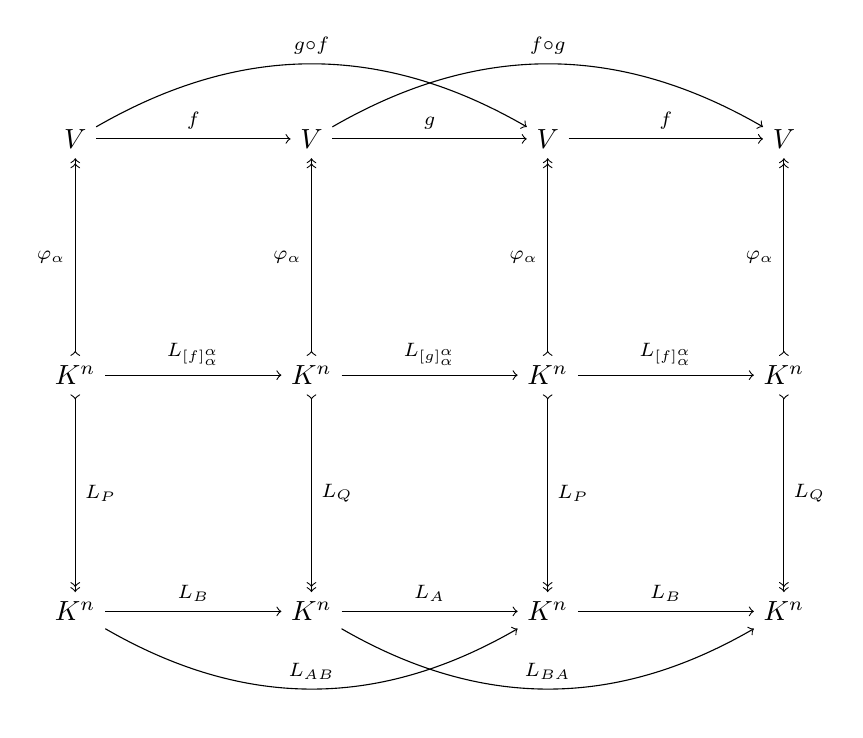
\begin{tikzpicture}[auto]

    \node (a) at (0, 0) {$K^n $};
    \node (b) at (3, 0) {$K^n $};
    \node (c) at (6, 0) {$K^n $};
    \node (d) at (9, 0) {$K^n $};
    \node (e) at (0, 3) {$K^n $};
    \node (f) at (3, 3) {$K^n $};
    \node (g) at (6, 3) {$K^n $};
    \node (h) at (9, 3) {$K^n $};
    \node (i) at (0, 6) {$V$};
    \node (j) at (3, 6) {$V$};
    \node (k) at (6, 6) {$V$};
    \node (l) at (9, 6) {$V$};
    
    \draw [->] (a) to node {$\scriptstyle L_B $} (b);
    \draw [->] (b) to node {$\scriptstyle L_A $} (c);
    \draw [->] (c) to node {$\scriptstyle L_B $} (d);
    \draw [>->>] (e) to node {$\scriptstyle L_P $} (a);
    \draw [>->>] (f) to node {$\scriptstyle L_Q $} (b);
    \draw [>->>] (g) to node {$\scriptstyle L_P $} (c);
    \draw [>->>] (h) to node {$\scriptstyle L_Q $} (d);
    \draw [->] (e) to node {$\scriptstyle L_{\left[ f\right]_{\alpha }^{\alpha }} $} (f);
    \draw [->] (f) to node {$\scriptstyle L_{\left[ g\right]_{\alpha }^{\alpha }} $} (g);
    \draw [->] (g) to node {$\scriptstyle L_{\left[ f\right]_{\alpha }^{\alpha }} $} (h);
    \draw [>->>] (e) to node {$\scriptstyle \varphi_{\alpha } $} (i);
    \draw [>->>] (f) to node {$\scriptstyle \varphi_{\alpha } $} (j);
    \draw [>->>] (g) to node {$\scriptstyle \varphi_{\alpha } $} (k);
    \draw [>->>] (h) to node {$\scriptstyle \varphi_{\alpha } $} (l);
    \draw [->] (i) to node {$\scriptstyle f$} (j);
    \draw [->] (j) to node {$\scriptstyle g$} (k);
    \draw [->] (k) to node {$\scriptstyle f$} (l);
    \draw [->] (a) to [bend right=30] node {$\scriptstyle L_{AB} $} (c);
    \draw [->] (b) to [bend right=30] node {$\scriptstyle L_{BA} $} (d);
    \draw [->] (i) to [bend left=30] node {$\scriptstyle g\circ f$} (k);
    \draw [->] (j) to [bend left=30] node {$\scriptstyle f\circ g$} (l);
  
  \end{tikzpicture}
\end{center}
したがって、次のようになるので、
\begin{align*}
L_{AB} &= L_{P[ g]_{\alpha}^{\alpha}Q^{- 1}Q[ f]_{\alpha}^{\alpha}P^{- 1}}\\
&= L_{P[ g]_{\alpha}^{\alpha}[ f]_{\alpha}^{\alpha}P^{- 1}}\\
&= L_{P[ g \circ f]_{\alpha}^{\alpha}P^{- 1}}\\
&= L_{P} \circ L_{[ g \circ f]_{\alpha}^{\alpha}} \circ L_{P^{- 1}}\\
&= L_{P} \circ L_{[ g \circ f]_{\alpha}^{\alpha}} \circ L_{P}^{- 1}\\
&= L_{P} \circ \varphi_{\alpha}^{- 1} \circ g \circ f \circ \varphi_{\alpha} \circ L_{P}^{- 1}\\
&= \left( L_{P} \circ \varphi_{\alpha}^{- 1} \right) \circ (g \circ f) \circ \left( L_{P} \circ \varphi_{\alpha}^{- 1} \right)^{- 1}, \\
L_{BA} &= L_{Q[ f]_{\alpha}^{\alpha}P^{- 1}P[ g]_{\alpha}^{\alpha}Q^{- 1}}\\
&= L_{Q[ f]_{\alpha}^{\alpha}[ g]_{\alpha}^{\alpha}Q^{- 1}}\\
&= L_{Q[ f \circ g]_{\alpha}^{\alpha}Q^{- 1}}\\
&= L_{Q} \circ L_{[ f \circ g]_{\alpha}^{\alpha}} \circ L_{Q^{- 1}}\\
&= L_{Q} \circ L_{[ f \circ g]_{\alpha}^{\alpha}} \circ L_{Q}^{- 1}\\
&= L_{Q} \circ \varphi_{\alpha}^{- 1} \circ f \circ g \circ \varphi_{\alpha} \circ L_{Q}^{- 1}\\
&= \left( L_{Q} \circ \varphi_{\alpha}^{- 1} \right) \circ (f \circ g) \circ \left( L_{Q} \circ \varphi_{\alpha}^{- 1} \right)^{- 1}
\end{align*}
次式が成り立つ。
\begin{align*}
\varPhi_{L_{AB}} = \varPhi_{\left( L_{P} \circ \varphi_{\alpha}^{- 1} \right) \circ (g \circ f) \circ \left( L_{P} \circ \varphi_{\alpha}^{- 1} \right)^{- 1}},\ \ \varPhi_{L_{BA}} = \varPhi_{\left( L_{Q} \circ \varphi_{\alpha}^{- 1} \right) \circ (f \circ g) \circ \left( L_{Q} \circ \varphi_{\alpha}^{- 1} \right)^{- 1}}
\end{align*}
これは多項式とみても成り立つ。ここで、定理\ref{2.2.2.9}より次のようになる。
\begin{align*}
\varPhi_{L_{AB}} = \varPhi_{g \circ f},\ \ \varPhi_{L_{BA}} = \varPhi_{f \circ g}
\end{align*}\par
また、$B' \in M_{rr}(K)$として行列$B$を次式のようにおくと、
\begin{align*}
B = \begin{pmatrix}
B' & * \\
* & * \\
\end{pmatrix}
\end{align*}
したがって、次のようになる。
\begin{align*}
AB &= \begin{pmatrix}
I_{r} & O \\
O & O \\
\end{pmatrix}\begin{pmatrix}
B' & * \\
* & * \\
\end{pmatrix} = \begin{pmatrix}
B' & * \\
O & O \\
\end{pmatrix}, \\
BA &= \begin{pmatrix}
B' & * \\
* & * \\
\end{pmatrix}\begin{pmatrix}
I_{r} & O \\
O & O \\
\end{pmatrix} = \begin{pmatrix}
B' & O \\
* & O \\
\end{pmatrix}
\end{align*}
ここで、定理\ref{2.2.2.8}より次のようになる。
\begin{align*}
\varPhi_{g \circ f} &= \varPhi_{L_{AB}} = \varPhi_{L_{B'}}\varPhi_{L_{O}}, \\
\varPhi_{f \circ g} &= \varPhi_{L_{BA}} = \varPhi_{L_{B'}}\varPhi_{L_{O}}
\end{align*}
以上より、次式が得られる。
\begin{align*}
\varPhi_{g \circ f} = \varPhi_{L_{B'}}\varPhi_{L_{O}} = \varPhi_{f \circ g}
\end{align*}
\end{proof}
%\hypertarget{ux884cux5217ux306eux5bfeux89d2ux5316}{%
\subsubsection{行列の対角化}%\label{ux884cux5217ux306eux5bfeux89d2ux5316}}
\begin{dfn}
体$K$上の有限次元なvector空間$V$の線形写像$f:V \rightarrow V$のある基底$\mathcal{B}$が存在してこれに関するその線形写像$f$の表現行列$[ f]_{\mathcal{B}}^{\mathcal{B}}$が対角行列となるとき、その線形写像$f$はその基底$\mathcal{B}$で対角化可能であるという。特に、$K = \mathbb{C}$のとき、線形写像$f:\mathbb{C} \rightarrow \mathbb{C}$がその基底$\mathcal{B}$で対角化可能であるとき、その線形写像$f$はその基底$\mathcal{B}$で半単純であるともいう。
\end{dfn}
\begin{thm}\label{2.2.2.11}
体$K$上の$n$次元vector空間$V$の線形写像$f:V \rightarrow V$が対角化可能であるならそのときに限り、任意のそのvector空間$V$の基底$\alpha$に対し、$\exists P \in {\mathrm{GL} }_{n}(K)$に対し、その基底$\alpha$に関するその線形写像$f$の表現行列$[ f]_{\alpha}^{\alpha}$を用いた行列$P^{- 1}[ f]_{\alpha}^{\alpha}P$も対角行列となる。
\end{thm}
\begin{proof}
体$K$上の$n$次元vector空間$V$の線形写像$f:V \rightarrow V$が対角化可能であるなら、定義よりその線形写像$f:V \rightarrow V$のある基底$\mathcal{B}$が存在してこれに関するその線形写像$f$の表現行列$[ f]_{\mathcal{B}}^{\mathcal{B}}$が対角行列となるのであった。ここで、定理\ref{2.1.5.1}よりその基底$\mathcal{B}$に関する基底変換における線形同型写像$\varphi_{\mathcal{B}}:K^{n} \rightarrow V$は全単射であり、任意のそのvector空間$V$の基底$\alpha$に対し、同様に定理\ref{2.1.5.1}よりその基底$\alpha$に関する基底変換における線形同型写像$\varphi_{\alpha}:K^{n} \rightarrow V$は全単射であるので、次式が成り立つ。
\begin{center}
  \begin{tikzpicture}[auto]

    \node (a) at (0, 0) {$K^n $};
    \node (b) at (4.5, 0) {$K^n $};
    \node (c) at (3, 1.5) {$K^n $};
    \node (d) at (7.5, 1.5) {$K^n $};
    \node (e) at (1.5, 4.5) {$V$};
    \node (f) at (6, 4.5) {$V$};
    
    \draw [->] (a) to node {$\scriptstyle L_{\left[ f\right] _{\mathcal B}^{\mathcal B} } $} (b);
    \draw [->] (c) to node[xshift=-15pt, yshift=0pt] {$\scriptstyle L_{\left[ f\right] _{\alpha }^{\alpha } } $} (d);
    \draw [->] (e) to node {$\scriptstyle f$} (f);
    \draw [>->>] (a) to node {$\scriptstyle \varphi_{\mathcal B} $} (e);
    \draw [>->>] (b) to node {$\scriptstyle \varphi_{\mathcal B} $} (f);
    \draw [>->>] (c) to node {$\scriptstyle \varphi_{\alpha } $} (e);
    \draw [>->>] (d) to node {$\scriptstyle \varphi_{\alpha } $} (f);
    
  \end{tikzpicture} 
\end{center}
ここで、次式のように合成写像$\varphi_{\alpha}^{- 1} \circ \varphi_{\mathcal{B}}:K^{n} \rightarrow K^{n}$をおくと、
\begin{center}
  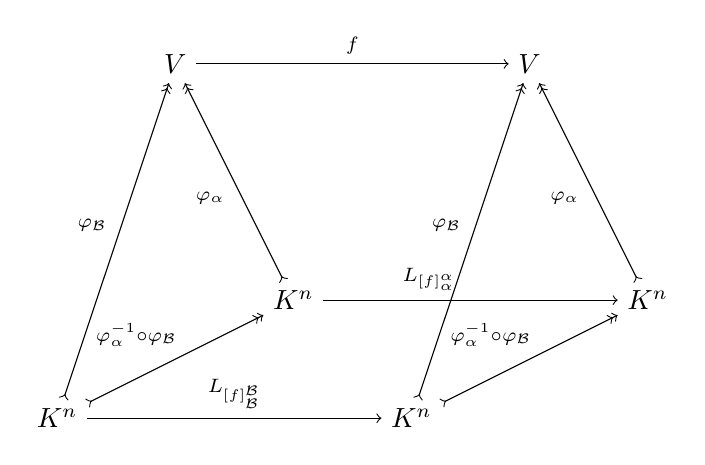
\begin{tikzpicture}[auto] 

    \node (a) at (0, 0) {$K^n $};
    \node (b) at (4.5, 0) {$K^n $};
    \node (c) at (3, 1.5) {$K^n $};
    \node (d) at (7.5, 1.5) {$K^n $};
    \node (e) at (1.5, 4.5) {$V$};
    \node (f) at (6, 4.5) {$V$};
    
    \draw [->] (a) to node {$\scriptstyle L_{\left[ f\right] _{\mathcal B}^{\mathcal B} } $} (b);
    \draw [->] (c) to node[xshift=-15pt, yshift=0pt] {$\scriptstyle L_{\left[ f\right] _{\alpha }^{\alpha } } $} (d);
    \draw [->] (e) to node {$\scriptstyle f$} (f);
    \draw [>->>] (a) to node {$\scriptstyle \varphi_{\mathcal B} $} (e);
    \draw [>->>] (b) to node {$\scriptstyle \varphi_{\mathcal B} $} (f);
    \draw [>->>] (c) to node {$\scriptstyle \varphi_{\alpha } $} (e);
    \draw [>->>] (d) to node {$\scriptstyle \varphi_{\alpha } $} (f);
    \draw [>->>] (a) to node[xshift=4pt, yshift=1pt] {$\scriptstyle \varphi_{\alpha }^{-1} \circ \varphi_{\mathcal B} $} (c);
    \draw [>->>] (b) to node[xshift=4pt, yshift=1pt] {$\scriptstyle \varphi_{\alpha }^{-1} \circ \varphi_{\mathcal B} $} (d);
    
  \end{tikzpicture} 
\end{center}
その写像$\varphi_{\alpha}^{- 1} \circ \varphi_{\mathcal{B}}$も線形同型写像であり、これに対応する行列を$P$とおくと、その行列$P$は正則行列であり次式のようになる。
\begin{center}
  \begin{tikzpicture}[auto] 

    \node (a) at (0, 0) {$K^n $};
    \node (b) at (4.5, 0) {$K^n $};
    \node (c) at (3, 1.5) {$K^n $};
    \node (d) at (7.5, 1.5) {$K^n $};
    \node (e) at (1.5, 4.5) {$V$};
    \node (f) at (6, 4.5) {$V$};
    
    \draw [->] (a) to node {$\scriptstyle L_{\left[ f\right] _{\mathcal B}^{\mathcal B} } $} (b);
    \draw [->] (c) to node[xshift=-15pt, yshift=0pt] {$\scriptstyle L_{\left[ f\right] _{\alpha }^{\alpha } } $} (d);
    \draw [->] (e) to node {$\scriptstyle f$} (f);
    \draw [>->>] (a) to node {$\scriptstyle \varphi_{\mathcal B} $} (e);
    \draw [>->>] (b) to node {$\scriptstyle \varphi_{\mathcal B} $} (f);
    \draw [>->>] (c) to node {$\scriptstyle \varphi_{\alpha } $} (e);
    \draw [>->>] (d) to node {$\scriptstyle \varphi_{\alpha } $} (f);
    \draw [>->>] (a) to node[xshift=4pt, yshift=1pt] {$\scriptstyle L_P $} (c);
    \draw [>->>] (b) to node[xshift=4pt, yshift=1pt] {$\scriptstyle L_P $} (d);
    
  \end{tikzpicture} 
\end{center}
これにより、次のようになる。
\begin{align*}
L_{[ f]_{\mathcal{B}}^{\mathcal{B}}} = L_{P}^{- 1} \circ L_{[ f]_{\alpha}^{\alpha}} \circ L_{P} = L_{P^{- 1}[ f]_{\alpha}^{\alpha}P}
\end{align*}
よって、その基底$\alpha$に関するその線形写像$f$の表現行列$[ f]_{\alpha}^{\alpha}$を用いた行列$P^{- 1}[ f]_{\alpha}^{\alpha}P$も対角行列となる。\par
逆に、任意のそのvector空間$V$の基底$\alpha$に対し、$\exists P \in {\mathrm{GL} }_{n}(K)$に対し、その基底$\alpha$に関するその線形写像$f$の表現行列$[ f]_{\alpha}^{\alpha}$を用いた行列$P^{- 1}[ f]_{\alpha}^{\alpha}P$も対角行列となるとき、次式のようになる。
\begin{center}
  \begin{tikzpicture}[auto] 

    \node (a) at (0, 0) {$K^n $};
    \node (b) at (4.5, 0) {$K^n $};
    \node (c) at (3, 1.5) {$K^n $};
    \node (d) at (7.5, 1.5) {$K^n $};
    \node (e) at (1.5, 4.5) {$V$};
    \node (f) at (6, 4.5) {$V$};
    
    \draw [->] (a) to node {$\scriptstyle L_{P^{-1} \left[ f\right] _{\alpha }^{\alpha } P} $} (b);
    \draw [->] (c) to node[xshift=-15pt, yshift=0pt] {$\scriptstyle L_{\left[ f\right] _{\alpha }^{\alpha } } $} (d);
    \draw [->] (e) to node {$\scriptstyle f$} (f);
    \draw [>->>] (c) to node {$\scriptstyle \varphi_{\alpha } $} (e);
    \draw [>->>] (d) to node {$\scriptstyle \varphi_{\alpha } $} (f);
    \draw [>->>] (a) to node[xshift=4pt, yshift=1pt] {$\scriptstyle L_P $} (c);
    \draw [>->>] (b) to node[xshift=4pt, yshift=1pt] {$\scriptstyle L_P $} (d);
    
  \end{tikzpicture} 
\end{center}
ここで、合成写像$\varphi_{\alpha} \circ L_{P}:K^{n} \rightarrow V$を$\varphi_{\mathcal{B}}$とおくと、定理\ref{2.1.5.1}より次式のようになり、
\begin{center}
  \begin{tikzpicture}[auto] 

    \node (a) at (0, 0) {$K^n $};
    \node (b) at (4.5, 0) {$K^n $};
    \node (c) at (3, 1.5) {$K^n $};
    \node (d) at (7.5, 1.5) {$K^n $};
    \node (e) at (1.5, 4.5) {$V$};
    \node (f) at (6, 4.5) {$V$};
    
    \draw [->] (a) to node {$\scriptstyle L_{\left[ f\right] _{\mathcal B}^{\mathcal B} } $} (b);
    \draw [->] (c) to node[xshift=-15pt, yshift=0pt] {$\scriptstyle L_{\left[ f\right] _{\alpha }^{\alpha } } $} (d);
    \draw [->] (e) to node {$\scriptstyle f$} (f);
    \draw [>->>] (a) to node {$\scriptstyle \varphi_{\mathcal B} $} (e);
    \draw [>->>] (b) to node {$\scriptstyle \varphi_{\mathcal B} $} (f);
    \draw [>->>] (c) to node {$\scriptstyle \varphi_{\alpha } $} (e);
    \draw [>->>] (d) to node {$\scriptstyle \varphi_{\alpha } $} (f);
    \draw [>->>] (a) to node[xshift=4pt, yshift=1pt] {$\scriptstyle L_P $} (c);
    \draw [>->>] (b) to node[xshift=4pt, yshift=1pt] {$\scriptstyle L_P $} (d);
    
  \end{tikzpicture} 
\end{center}
よって、そのvector空間$V$の線形写像$f:V \rightarrow V$のある基底$\mathcal{B}$が存在してこれに関するその線形写像$f$の表現行列$[ f]_{\mathcal{B}}^{\mathcal{B}}$が対角行列となるので、その線形写像$f$は対角化可能である。
\end{proof}
\begin{thm}\label{2.2.2.12}
体$K$上の$n$次元vector空間$V$の線形写像$f:V \rightarrow V$がその基底$\mathcal{B}$で対角化可能であるならそのときに限り、$\forall i \in \varLambda_{n}$に対し、その基底$\mathcal{B}$をなすvector$\mathbf{v}_{i}$がいずれもその線形写像$f$の固有値$\lambda_{i}$に対する固有vectorsである。このとき、その基底$\mathcal{B}$に関するその線形写像$f$の表現行列$[ f]_{\mathcal{B}}^{\mathcal{B}}$が次式のように与えられる。
\begin{align*}
[ f]_{\mathcal{B}}^{\mathcal{B}} = \begin{pmatrix}
\lambda_{1} & \  & \  & O \\
\  & \lambda_{2} & \  & \  \\
\  & \  & \ddots & \  \\
O & \  & \  & \lambda_{n} \\
\end{pmatrix}
\end{align*}
\end{thm}
\begin{proof}
体$K$上の$n$次元vector空間$V$の線形写像$f:V \rightarrow V$がその基底$\mathcal{B}$で対角化可能であるなら、その線形写像$f$のその基底$\mathcal{B}$に関する表現行列$[ f]_{\mathcal{B}}^{\mathcal{B}}$が対角行列であり、次式のようにおき
\begin{align*}
[ f]_{\mathcal{B}}^{\mathcal{B}} = \begin{pmatrix}
\lambda_{1} & \  & \  & O \\
\  & \lambda_{2} & \  & \  \\
\  & \  & \ddots & \  \\
O & \  & \  & \lambda_{n} \\
\end{pmatrix}
\end{align*}
$\mathcal{B} =\left\langle \mathbf{v}_{i} \right\rangle_{i \in \varLambda_{n}}$とおくと、定理\ref{2.1.5.1}よりその基底$\mathcal{B}$に関する基底変換における線形同型写像$\varphi_{\mathcal{B}}:K^{n} \rightarrow V$は線形同型写像であり次式が成り立つので、
\begin{center}
  \begin{tikzpicture}[auto]

    \node (a) at (0, 0) {$K^n $};
    \node (b) at (3, 0) {$K^n $};
    \node (c) at (0, 3) {$V$};
    \node (d) at (3, 3) {$V$};
    
    \draw [->] (a) to node {$\scriptstyle L_{\left[ f\right]_{\mathcal B}^{\mathcal B}} $} (b);
    \draw [->] (c) to node {$\scriptstyle f$} (d);
    \draw [>->>] (a) to node {$\scriptstyle \varphi_{\mathcal B} $} (c);
    \draw [>->>] (b) to node {$\scriptstyle \varphi_{\mathcal B} $} (d);
    
  \end{tikzpicture} 
\end{center}
$\forall i \in \varLambda_{n}$に対し、vector空間$K^{n}$の正規直交基底を$\left\langle \mathbf{e}_{i} \right\rangle_{i \in \varLambda_{n}}$とおくと、次のようになる。
\begin{align*}
f\left( \mathbf{v}_{i} \right) &= \varphi_{\mathcal{B}} \circ L_{[ f]_{\mathcal{B}}^{\mathcal{B}}} \circ \varphi_{\mathcal{B}}^{- 1}\left( \mathbf{v}_{i} \right)\\
&= \varphi_{\mathcal{B}}\left( L_{[ f]_{\mathcal{B}}^{\mathcal{B}}}\left( \varphi_{\mathcal{B}}^{- 1}\left( \mathbf{v}_{i} \right) \right) \right)\\
&= \varphi_{\mathcal{B}}\left( L_{[ f]_{\mathcal{B}}^{\mathcal{B}}}\left( \mathbf{e}_{i} \right) \right)\\
&= \varphi_{\mathcal{B}}\left( [ f]_{\mathcal{B}}^{\mathcal{B}}\mathbf{e}_{i} \right)\\
&= \varphi_{\mathcal{B}}\left( \begin{pmatrix}
\lambda_{1} & \  & \  & \  & \  & O \\
\  & \lambda_{2} & \  & \  & \  & \  \\
\  & \  & \ddots & \  & \  & \  \\
\  & \  & \  & \lambda_{i} & \  & \  \\
\  & \  & \  & \  & \ddots & \  \\
O & \  & \  & \  & \  & \lambda_{n} \\
\end{pmatrix}\begin{pmatrix}
0 \\
0 \\
 \vdots \\
1 \\
 \vdots \\
0 \\
\end{pmatrix} \right)\\
&= \varphi_{\mathcal{B}}\begin{pmatrix}
0 \\
0 \\
 \vdots \\
\lambda_{i} \\
 \vdots \\
0 \\
\end{pmatrix}\\
&= \varphi_{\mathcal{B}}\left( \lambda_{i}\mathbf{e}_{i} \right)\\
&= \lambda_{i}\varphi_{\mathcal{B}}\left( \mathbf{e}_{i} \right) = \lambda_{i}\mathbf{v}_{i}
\end{align*}
よって、その基底$\mathcal{B}$をなすvectorsがいずれもその線形写像$f$の固有vectorsである。\par
逆に、$\forall i \in \varLambda_{n}$に対し、その基底$\mathcal{B}$をなすvector$\mathbf{v}_{i}$がいずれもその線形写像$f$の固有値$\lambda_{i}$に対する固有vectorsであるなら、$f\left( \mathbf{v}_{i} \right) = \lambda_{i}\mathbf{v}_{i}$が成り立つことになる。ここで、定理\ref{2.1.5.1}よりその基底$\mathcal{B}$に関する基底変換における線形同型写像$\varphi_{\mathcal{B}}:K^{n} \rightarrow V$について、次式が成り立つので、
\begin{center}
  \begin{tikzpicture}[auto]

    \node (a) at (0, 0) {$K^n $};
    \node (b) at (3, 0) {$K^n $};
    \node (c) at (0, 3) {$V$};
    \node (d) at (3, 3) {$V$};
    
    \draw [->] (a) to node {$\scriptstyle L_{\left[ f\right]_{\mathcal B}^{\mathcal B}} $} (b);
    \draw [->] (c) to node {$\scriptstyle f$} (d);
    \draw [>->>] (a) to node {$\scriptstyle \varphi_{\mathcal B} $} (c);
    \draw [>->>] (b) to node {$\scriptstyle \varphi_{\mathcal B} $} (d);
    
  \end{tikzpicture} 
\end{center}
$\forall\sum_{i \in \varLambda_{n}} {a_{i}\mathbf{e}_{i}} \in K^{n}$に対し、次のようになる。
\begin{align*}
L_{[ f]_{\mathcal{B}}^{\mathcal{B}}}\left( \sum_{i \in \varLambda_{n}} {a_{i}\mathbf{e}_{i}} \right) &= \sum_{i \in \varLambda_{n}} {a_{i}f\left( \mathbf{e}_{i} \right)}\\
&= \sum_{i \in \varLambda_{n}} {a_{i}\varphi_{\mathcal{B}}^{- 1} \circ f \circ \varphi_{\mathcal{B}}\left( \mathbf{e}_{i} \right)}\\
&= \sum_{i \in \varLambda_{n}} {a_{i}\varphi_{\mathcal{B}}^{- 1}\left( f\left( \varphi_{\mathcal{B}}\left( \mathbf{e}_{i} \right) \right) \right)}\\
&= \sum_{i \in \varLambda_{n}} {a_{i}\varphi_{\mathcal{B}}^{- 1}\left( f\left( \mathbf{v}_{i} \right) \right)}\\
&= \sum_{i \in \varLambda_{n}} {a_{i}\varphi_{\mathcal{B}}^{- 1}\left( \lambda_{i}\mathbf{v}_{i} \right)}\\
&= \sum_{i \in \varLambda_{n}} {a_{i}\lambda_{i}\mathbf{e}_{i}}\\
&= \sum_{i \in \varLambda_{n}} \begin{pmatrix}
0 \\
0 \\
 \vdots \\
a_{i}\lambda_{i} \\
 \vdots \\
0 \\
\end{pmatrix}\\
&= \begin{pmatrix}
\lambda_{1}\mathbf{e}_{1} & \lambda_{2}\mathbf{e}_{2} & \cdots & \lambda_{n}\mathbf{e}_{n} \\
\end{pmatrix}\begin{pmatrix}
a_{1} \\
a_{2} \\
 \vdots \\
a_{n} \\
\end{pmatrix}\\
&= \begin{pmatrix}
\lambda_{1} & \  & \  & O \\
\  & \lambda_{2} & \  & \  \\
\  & \  & \ddots & \  \\
O & \  & \  & \lambda_{n} \\
\end{pmatrix}\begin{pmatrix}
a_{1} \\
a_{2} \\
 \vdots \\
a_{n} \\
\end{pmatrix}
\end{align*}
よって、その基底$\mathcal{B}$に関するその線形写像$f$の表現行列$[ f]_{\mathcal{B}}^{\mathcal{B}}$が次式のように対角行列となるので、
\begin{align*}
[ f]_{\mathcal{B}}^{\mathcal{B}} = \begin{pmatrix}
\lambda_{1} & \  & \  & O \\
\  & \lambda_{2} & \  & \  \\
\  & \  & \ddots & \  \\
O & \  & \  & \lambda_{n} \\
\end{pmatrix}
\end{align*}
その線形写像$f$はその基底$\mathcal{B}$で対角化可能である。
\end{proof}
\begin{thm}\label{2.2.2.13}
体$K$上の有限次元なvector空間$V$の線形写像$f:V \rightarrow V$の添数集合$\varLambda_{n}$によって添数づけられた互いに異なる固有値たちからなる族$\left\{ \lambda_{i} \right\}_{i \in \varLambda_{n}}$が与えられたとき、$\forall i \in \varLambda_{n}$に対し、その固有値$\lambda_{i}$に対する固有vectorのうち1つを$\mathbf{v}_{i}$とおくと、その族$\left\{ \mathbf{v}_i \right\}_{i \in \varLambda_{n} }$は線形独立である。
\end{thm}
\begin{proof}
体$K$上の有限次元なvector空間$V$の線形写像$f:V \rightarrow V$の添数集合$\varLambda_{n}$によって添数づけられた互いに異なる固有値たちからなる族$\left\{ \lambda_{i} \right\}_{i \in \varLambda_{n}}$が与えられたとき、$\forall i \in \varLambda_{n}$に対し、その固有値$\lambda_{i}$に対する固有vectorのうち1つを$\mathbf{v}_{i}$とおくと、$n = 1$のときは明らかにであるから、$n = k$のとき、その族$\left\{ \mathbf{v}_i \right\}_{i \in \varLambda_{k}}$は線形独立であると仮定しよう。$n = k + 1$のとき、$i \in \varLambda_{k + 1}$なる体$K$の元々$c_{i}$を用いて次式が成り立つとすれば、
\begin{align*}
\sum_{i \in \varLambda_{k + 1}} {c_{i}\mathbf{v}_{i}} = \mathbf{0}
\end{align*}
次のようになる。
\begin{align*}
\sum_{i \in \varLambda_{k + 1}} {c_{i}\mathbf{v}_{i}} = \mathbf{0} &\Leftrightarrow \sum_{i \in \varLambda_{k + 1}} {c_{i}\mathbf{v}_{i}} = \mathbf{0} \land f\left( \sum_{i \in \varLambda_{k + 1}} {c_{i}\mathbf{v}_{i}} \right) = f\left( \mathbf{0} \right)\\
&\Leftrightarrow \sum_{i \in \varLambda_{k + 1}} {c_{i}\mathbf{v}_{i}} = \mathbf{0} \land \sum_{i \in \varLambda_{k + 1}} {c_{i}f\left( \mathbf{v}_{i} \right)} = \mathbf{0}\\
&\Leftrightarrow \sum_{i \in \varLambda_{k + 1}} {c_{i}\lambda_{k + 1}\mathbf{v}_{i}} = \mathbf{0} \land \sum_{i \in \varLambda_{k + 1}} {c_{i}\lambda_{i}\left( \mathbf{v}_{i} \right)} = \mathbf{0}\\
&\Leftrightarrow \sum_{i \in \varLambda_{k}} {c_{i}\lambda_{k + 1}\mathbf{v}_{i}} + c_{k + 1}\lambda_{k + 1}\mathbf{v}_{k + 1} = \mathbf{0} \land \sum_{i \in \varLambda_{k}} {c_{i}\lambda_{i}\left( \mathbf{v}_{i} \right)} + c_{k + 1}\lambda_{k + 1}\mathbf{v}_{k + 1} = \mathbf{0}\\
&\Rightarrow \left( \sum_{i \in \varLambda_{k}} {c_{i}\lambda_{k + 1}\mathbf{v}_{i}} + c_{k + 1}\lambda_{k + 1}\mathbf{v}_{k + 1} \right) - \left( \sum_{i \in \varLambda_{k}} {c_{i}\lambda_{i}\left( \mathbf{v}_{i} \right)} + c_{k + 1}\lambda_{k + 1}\mathbf{v}_{k + 1} \right) = \mathbf{0}\\
&\Leftrightarrow \sum_{i \in \varLambda_{k}} {c_{i}\lambda_{k + 1}\mathbf{v}_{i}} + c_{k + 1}\lambda_{k + 1}\mathbf{v}_{k + 1} - \sum_{i \in \varLambda_{k}} {c_{i}\lambda_{i}\left( \mathbf{v}_{i} \right)} - c_{k + 1}\lambda_{k + 1}\mathbf{v}_{k + 1} = \mathbf{0}\\
&\Leftrightarrow \sum_{i \in \varLambda_{k}} {c_{i}\left( \lambda_{k + 1} - \lambda_{i} \right)\mathbf{v}_{i}} = \mathbf{0}
\end{align*}
ここで、仮定より$\forall i \in \varLambda_{k}$に対し、$c_{i}\left( \lambda_{k + 1} - \lambda_{i} \right) = 0$が成り立つので、$c_{i} = 0$または$\lambda_{i} = \lambda_{k + 1}$が成り立ち、仮定より$c_{i} = 0$が成り立つ。これにより、次のようになる。
\begin{align*}
\sum_{i \in \varLambda_{k + 1}} {c_{i}\mathbf{v}_{i}} &= \sum_{i \in \varLambda_{k}} {c_{i}\mathbf{v}_{i}} + c_{k + 1}\mathbf{v}_{k + 1}\\
&= \sum_{i \in \varLambda_{k}} \mathbf{0} + c_{k + 1}\mathbf{v}_{k + 1}\\
&= c_{k + 1}\mathbf{v}_{k + 1} = \mathbf{0}
\end{align*}
ここで、そのvector$\mathbf{v}_{k + 1}$は固有vectorの定義より零vectorでないので、$c_{k + 1} = 0$が成り立つ。\par
以上より、数学的帰納法によって$\forall i \in \varLambda_{n}$に対し、$c_{i} = 0$が成り立ち、その族$\left\{ \mathbf{v}_i \right\}_{i \in \varLambda_{n} } $に対するvectors$\mathbf{v}_{i}$は線形独立である。
\end{proof}
%\hypertarget{ux56faux6709ux7a7aux9593}{%
\subsubsection{固有空間}%\label{ux56faux6709ux7a7aux9593}}
\begin{dfn} 定理\ref{2.2.2.2}より体$K$上のvector空間$V$の元$\mathbf{v}$が線形写像$f:V \rightarrow V$の固有値$\lambda$に対する固有vectorであるならそのときに限り、そのvector$\mathbf{v}$はその集合$\ker\left( \lambda I_{V} - f \right) \setminus \left\{ \mathbf{0} \right\}$の元であるのであった。ここで、次式のように集合$W_{f}(\lambda)$が定義され、その集合$W_{f}(\lambda)$をその固有値$\lambda$に対する固有空間という。
\begin{align*}
W_{f}(\lambda) = \ker\left( \lambda I_{V} - f \right)
\end{align*}
\end{dfn}
\begin{thm}\label{2.2.2.14}
体$K$上のvector空間$V$の線形写像$f:V \rightarrow V$の固有値$\lambda$に対する固有空間$W_{f}(\lambda)$はそのvector空間$V$の部分空間である。
\end{thm}
\begin{proof} 固有空間の定義と定理\ref{2.1.2.11}より直ちに示される。
\end{proof}
\begin{thm}\label{2.2.2.15}
体$K$上の有限次元なvector空間$V$の線形写像$f:V \rightarrow V$の添数集合$\varLambda_{n}$によって添数づけられた互いに異なる固有値たちからなる族$\left\{ \lambda_{i} \right\}_{i \in \varLambda_{n}}$が与えられたとき、添数集合$\varLambda_{n}$によって添数づけられたそれらの固有値たち$\lambda_{i}$に対する固有空間$W_{f}\left( \lambda_{i} \right)$の族$\left\{ W_{f}\left( \lambda_{i} \right) \right\}_{i \in \varLambda_{n}}$の和空間$\sum_{i \in \varLambda_{n}} {W_{f}\left( \lambda_{i} \right)}$は直和空間$\bigoplus_{i \in \varLambda_{n}} {W_{f}\left( \lambda_{i} \right)}$でもある。
\end{thm}
\begin{proof}
体$K$上の有限次元なvector空間$V$の線形写像$f:V \rightarrow V$の添数集合$\varLambda_{n}$によって添数づけられた互いに異なる固有値たちからなる族$\left\{ \lambda_{i} \right\}_{i \in \varLambda_{n}}$が与えられたとき、添数集合$\varLambda_{n}$によって添数づけられたそれらの固有値たち$\lambda_{i}$に対する固有空間$W_{f}\left( \lambda_{i} \right)$の族$\left\{ W_{f}\left( \lambda_{i} \right) \right\}_{i \in \varLambda_{n}}$の和空間$\sum_{i \in \varLambda_{n}} {W_{f}\left( \lambda_{i} \right)}$について、$\forall\mathbf{z} \in \sum_{i \in \varLambda_{n}} {W_{f}\left( \lambda_{i} \right)}$に対し、$\mathbf{z} = \sum_{i \in \varLambda_{n}} \mathbf{v}_{i} = \sum_{i \in \varLambda_{n}} \mathbf{v}_{i}'$なるその集合$\prod_{i \in \varLambda_{n}} {W_{f}\left( \lambda_{i} \right)}$の互いに異なる元々$\left( \mathbf{v}_{i} \right)_{i \in \varLambda_{n}}$、$\left( \mathbf{v}_{i}' \right)_{i \in \varLambda_{n}}$が存在すると仮定すると、次のようになる。
\begin{align*}
\sum_{i \in \varLambda_{n}} \left( \mathbf{v}_{i} - \mathbf{v}_{i}' \right) &= \sum_{i \in \varLambda_{n}} \mathbf{v}_{i} - \sum_{i \in \varLambda_{n}} \mathbf{v}_{i}'\\
&= \mathbf{z} - \mathbf{z} = \mathbf{0}
\end{align*}
ここで、$\mathbf{v}_{i} - \mathbf{v}_{i}' \in W_{f}\left( \lambda_{i} \right)$が成り立ち、定理\ref{2.2.2.13}より$\forall i \in \varLambda_{n}$に対し、その固有値$\lambda_{i}$に対する固有vectors$\mathbf{v}_{i}$は線形独立であるので、$\forall i \in \varLambda_{n}$に対し、それらのvectors$\mathbf{v}_{i} - \mathbf{v}_{i}'$は固有vectorでないことになる。したがって、それらのvectors$\mathbf{v}_{i} - \mathbf{v}_{i}'$は零vectorsであり、$\forall i \in \varLambda_{n}$に対し、$\mathbf{v}_{i} = \mathbf{v}_{i}'$が成り立つ。しかしながら、これは仮定に矛盾する。したがって、$\forall\mathbf{z} \in \sum_{i \in \varLambda_{n}} {W_{f}\left( \lambda_{i} \right)}$に対し、$\mathbf{z} = \sum_{i \in \varLambda_{n}} \mathbf{v}_{i}$なるその集合$\prod_{i \in \varLambda_{n}} {W_{f}\left( \lambda_{i} \right)}$の元$\left( \mathbf{v}_{i} \right)_{i \in \varLambda_{n}}$が一意的に存在することになり、直和空間の定義よりその和空間$\sum_{i \in \varLambda_{n}} {W_{f}\left( \lambda_{i} \right)}$は直和空間$\bigoplus_{i \in \varLambda_{n}} {W_{f}\left( \lambda_{i} \right)}$でもある。
\end{proof}
\begin{thebibliography}{50}
  \bibitem{1}
    松坂和夫, 線型代数入門, 岩波書店, 1980. 新装版第2刷 p226-246 ISBN978-4-00-029872-8
  \bibitem{2}
    対馬龍司, 線形代数学講義, 共立出版, 2007. 改訂版8刷 p155-164 ISBN978-4-320-11097-7
\end{thebibliography}
\end{document}

\clearpage
\documentclass[dvipdfmx]{jsarticle}
\setcounter{section}{2}
\setcounter{subsection}{2}
\usepackage{xr}
\externaldocument{2.2.1}
\externaldocument{2.1.2}
\externaldocument{2.2.2}
\usepackage{amsmath,amsfonts,amssymb,array,comment,mathtools,url,docmute}
\usepackage{longtable,booktabs,dcolumn,tabularx,mathtools,multirow,colortbl,xcolor}
\usepackage[dvipdfmx]{graphics}
\usepackage{bmpsize}
\usepackage{amsthm}
\usepackage{enumitem}
\setlistdepth{20}
\renewlist{itemize}{itemize}{20}
\setlist[itemize]{label=•}
\renewlist{enumerate}{enumerate}{20}
\setlist[enumerate]{label=\arabic*.}
\setcounter{MaxMatrixCols}{20}
\setcounter{tocdepth}{3}
\newcommand{\rotin}{\text{\rotatebox[origin=c]{90}{$\in $}}}
\newcommand{\amap}[6]{\text{\raisebox{-0.7cm}{\begin{tikzpicture} 
  \node (a) at (0, 1) {$\textstyle{#2}$};
  \node (b) at (#6, 1) {$\textstyle{#3}$};
  \node (c) at (0, 0) {$\textstyle{#4}$};
  \node (d) at (#6, 0) {$\textstyle{#5}$};
  \node (x) at (0, 0.5) {$\rotin $};
  \node (x) at (#6, 0.5) {$\rotin $};
  \draw[->] (a) to node[xshift=0pt, yshift=7pt] {$\textstyle{\scriptstyle{#1}}$} (b);
  \draw[|->] (c) to node[xshift=0pt, yshift=7pt] {$\textstyle{\scriptstyle{#1}}$} (d);
\end{tikzpicture}}}}
\newcommand{\twomaps}[9]{\text{\raisebox{-0.7cm}{\begin{tikzpicture} 
  \node (a) at (0, 1) {$\textstyle{#3}$};
  \node (b) at (#9, 1) {$\textstyle{#4}$};
  \node (c) at (#9+#9, 1) {$\textstyle{#5}$};
  \node (d) at (0, 0) {$\textstyle{#6}$};
  \node (e) at (#9, 0) {$\textstyle{#7}$};
  \node (f) at (#9+#9, 0) {$\textstyle{#8}$};
  \node (x) at (0, 0.5) {$\rotin $};
  \node (x) at (#9, 0.5) {$\rotin $};
  \node (x) at (#9+#9, 0.5) {$\rotin $};
  \draw[->] (a) to node[xshift=0pt, yshift=7pt] {$\textstyle{\scriptstyle{#1}}$} (b);
  \draw[|->] (d) to node[xshift=0pt, yshift=7pt] {$\textstyle{\scriptstyle{#2}}$} (e);
  \draw[->] (b) to node[xshift=0pt, yshift=7pt] {$\textstyle{\scriptstyle{#1}}$} (c);
  \draw[|->] (e) to node[xshift=0pt, yshift=7pt] {$\textstyle{\scriptstyle{#2}}$} (f);
\end{tikzpicture}}}}
\renewcommand{\thesection}{第\arabic{section}部}
\renewcommand{\thesubsection}{\arabic{section}.\arabic{subsection}}
\renewcommand{\thesubsubsection}{\arabic{section}.\arabic{subsection}.\arabic{subsubsection}}
\everymath{\displaystyle}
\allowdisplaybreaks[4]
\usepackage{vtable}
\theoremstyle{definition}
\newtheorem{thm}{定理}[subsection]
\newtheorem*{thm*}{定理}
\newtheorem{dfn}{定義}[subsection]
\newtheorem*{dfn*}{定義}
\newtheorem{axs}[dfn]{公理}
\newtheorem*{axs*}{公理}
\renewcommand{\headfont}{\bfseries}
\makeatletter
  \renewcommand{\section}{%
    \@startsection{section}{1}{\z@}%
    {\Cvs}{\Cvs}%
    {\normalfont\huge\headfont\raggedright}}
\makeatother
\makeatletter
  \renewcommand{\subsection}{%
    \@startsection{subsection}{2}{\z@}%
    {0.5\Cvs}{0.5\Cvs}%
    {\normalfont\LARGE\headfont\raggedright}}
\makeatother
\makeatletter
  \renewcommand{\subsubsection}{%
    \@startsection{subsubsection}{3}{\z@}%
    {0.4\Cvs}{0.4\Cvs}%
    {\normalfont\Large\headfont\raggedright}}
\makeatother
\makeatletter
\renewenvironment{proof}[1][\proofname]{\par
  \pushQED{\qed}%
  \normalfont \topsep6\p@\@plus6\p@\relax
  \trivlist
  \item\relax
  {
  #1\@addpunct{.}}\hspace\labelsep\ignorespaces
}{%
  \popQED\endtrivlist\@endpefalse
}
\makeatother
\renewcommand{\proofname}{\textbf{証明}}
\usepackage{tikz,graphics}
\usepackage[dvipdfmx]{hyperref}
\usepackage{pxjahyper}
\hypersetup{
 setpagesize=false,
 bookmarks=true,
 bookmarksdepth=tocdepth,
 bookmarksnumbered=true,
 colorlinks=false,
 pdftitle={},
 pdfsubject={},
 pdfauthor={},
 pdfkeywords={}}
\begin{document}
%\hypertarget{hamilton-cayleyux306eux5b9aux7406}{%
\subsection{Hamilton-Cayleyの定理}%\label{hamilton-cayleyux306eux5b9aux7406}}
%\hypertarget{ux884cux5217ux306eux4e09ux89d2ux5316}{%
\subsubsection{行列の三角化}%\label{ux884cux5217ux306eux4e09ux89d2ux5316}}
\begin{thm}\label{2.2.3.1}
代数的閉体$K$上の$n$次元vector空間$V$が与えられたとき、$f:V \rightarrow V$なる任意の線形写像$f$の固有多項式$\varPhi_{f}$はあるその体$K$の元々$\lambda_{i}$を用いて次式のように変形されることができる。
\begin{align*}
\varPhi_{f} = \prod_{i \in \varLambda_{n}} \left( X - \lambda_{i} \right)
\end{align*}
\end{thm}
その証明は残念ながら代数学の多項式環の知識をかなり要求するので、多項式環の書籍にゆずることにする。
\begin{thm}[代数学の基本定理]\label{2.2.3.2}
体$\mathbb{C}$上の$n$次元vector空間$V$が与えられたとき、$f:V \rightarrow V$なる任意の線形写像$f$の固有多項式$\varPhi_{f}$の任意の複素数$z$による像$\varPhi_{f}(z)$がある複素数たち$\lambda_{i}$を用いて次式のように変形されることができる。
\begin{align*}
\varPhi_{f}(z) = \prod_{i \in \varLambda_{n}} \left( z - \lambda_{i} \right)
\end{align*}
\end{thm}
その証明は代数学の基本定理による\footnote{そんなに代数学の基本定理って感じなのかなぁ…? 代数学に複素数とか実数を持ち込むのもなんだかなぁ…。}。
\begin{thm}[三角化定理]\label{2.2.3.3}
代数的閉体$K$上の$n$次元vector空間$V$、線型写像$f:V \rightarrow V$、これの$n$つの固有値たち$\lambda_{i}$が与えられたとき、ある基底$\mathcal{B}$が存在してその線形写像$f$のその基底$\mathcal{B}$に関する表現行列$[ f]_{\mathcal{B}}^{\mathcal{B}}$は次式のように上三角行列で表されることができる。
\begin{align*}
[ f]_{\mathcal{B}}^{\mathcal{B}} = \begin{pmatrix}
\lambda_{1} & \  & \  & * \\
\  & \lambda_{2} & \  & \  \\
\  & \  & \ddots & \  \\
O & \  & \  & \lambda_{n} \\
\end{pmatrix}
\end{align*}\par
同様にして、ある基底$\mathcal{C}$が存在してその線形写像$f$のその基底$\mathcal{C}$に関する表現行列$[ f]_{\mathcal{C}}^{\mathcal{C}}$は次式のように下三角行列で表されることができる。
\begin{align*}
[ f]_{\mathcal{C}}^{\mathcal{C}} = \begin{pmatrix}
\lambda_{1} & \  & \  & O \\
\  & \lambda_{2} & \  & \  \\
\  & \  & \ddots & \  \\
* & \  & \  & \lambda_{n} \\
\end{pmatrix}
\end{align*}
この定理を三角化定理という。
\end{thm}\par
ここでは、上の主張どちらも同様にして示されるので、下三角行列の場合のみ証明を与えることにしておこう。
\begin{proof}
代数的閉体$K$上の$n$次元vector空間$V$、線型写像$f:V \rightarrow V$、これの$n$つの固有値たち$\lambda_{i}$が与えられたとする。$n = 1$のときでは明らかであるから、$n = k$のとき、ある基底が存在してその線形写像$f$のその基底に関する表現行列が上三角行列で表されることができると仮定しよう。$n = k + 1$のとき、その体$K$は代数的閉体なので、これの1つの固有vector$\mathbf{v}_{k + 1}$を含むvectorsの組$\left\langle \mathbf{v}_{i} \right\rangle_{i \in \varLambda_{k + 1}}$がそのvector空間$V$の基底となるようにとられるとする。$\lambda_{*} = \lambda_{k + 1}$、$\mathbf{v}_{*} = \mathbf{v}_{k + 1}$、$W = \mathrm{span}\left\{ \mathbf{v}_{i} \right\}_{i \in \varLambda_{k}}$として定理\ref{2.2.1.6}より次のようになるかつ、
\begin{align*}
V = W \oplus \mathrm{span}\left\{ \mathbf{v}_{*} \right\}
\end{align*}
$\forall\mathbf{v} \in W$に対し、$f\left( \mathbf{v} \right) \in V$が成り立つので、次式のようなその体$K$の元$c$とvector$\widetilde{\mathbf{v}}$が一意的に存在する。
\begin{align*}
f\left( \mathbf{v} \right) = \widetilde{\mathbf{v}} \oplus c\mathbf{v}_{*}
\end{align*}\par
また、その集合$W$はその代数的閉体$K$上のそのvector空間$V$の部分空間である。これにより、次式のような写像$f_{*}$が定義されると、
\begin{align*}
f_{*}:W \rightarrow W;\mathbf{v} \mapsto \widetilde{\mathbf{v}}
\end{align*}
$f_{*}\left( \mathbf{v} \right) = f\left( \mathbf{v} \right) - c\mathbf{v}_{*}$が成り立つ。ここで、$\forall k,l \in K\forall\mathbf{v},\mathbf{w} \in W$に対し、次のようにおくと、
\begin{align*}
f_{*}\left( \mathbf{v} \right) = f\left( \mathbf{v} \right) - c\mathbf{v}_{*},\ \ f_{*}\left( \mathbf{w} \right) = f\left( \mathbf{w} \right) - d\mathbf{v}_{*}
\end{align*}
次のようになり、
\begin{align*}
f_{*}\left( k\mathbf{v} + l\mathbf{w} \right) &= f\left( k\mathbf{v} + l\mathbf{w} \right) - C\mathbf{v}_{*}\\
&= kf\left( \mathbf{v} \right) + lf\left( \mathbf{w} \right) - C\mathbf{v}_{*}\\
&= k\left( c\mathbf{v}_{*} + f_{*}\left( \mathbf{v} \right) \right) + l\left( d\mathbf{v}_{*} + f_{*}\left( \mathbf{w} \right) \right) - C\mathbf{v}_{*}\\
&= kc\mathbf{v}_{*} + kf_{*}\left( \mathbf{v} \right) + ld\mathbf{v}_{1} + lf_{*}\left( \mathbf{w} \right) - C\mathbf{v}_{*}\\
&= kf_{*}\left( \mathbf{v} \right) + lf_{*}\left( \mathbf{w} \right) + (kc + ld - C)\mathbf{v}_{*}\\
&= \left( kf_{*}\left( \mathbf{v} \right) + lf_{*}\left( \mathbf{w} \right) \right) \oplus (kc + ld - C)\mathbf{v}_{*}
\end{align*}
次式が成り立つので、
\begin{align*}
f_{*}\left( k\mathbf{v} + l\mathbf{w} \right),kf_{*}\left( \mathbf{v} \right) + lf_{*}\left( \mathbf{w} \right) \in W,\ \ (kc + ld - C)\mathbf{v}_{*} \in \mathrm{span}\left\{ \mathbf{v}_{*} \right\}
\end{align*}
$kc + ld - C = 0$が成り立つことになる。したがって、次のようになる。
\begin{align*}
f_{*}\left( k\mathbf{v} + l\mathbf{w} \right) = kf_{*}\left( \mathbf{v} \right) + lf_{*}\left( \mathbf{w} \right)
\end{align*}
これにより、その写像$f_{*}$は線形的であることが分かった。\par
ここで、その基底$\left\langle \mathbf{v}_{i} \right\rangle_{i \in \varLambda_{k + 1}}$を$\mathcal{C}$、その基底$\left\langle \mathbf{v}_{i} \right\rangle_{i \in \varLambda_{k}}$を$\mathcal{C}_{*}$とおかれると、これらに関するそれらの線形写像たち$f$、$f_{*}$の表現行列たち$[ f]_{\mathcal{C}}^{\mathcal{C}}$、$\left[ f_{*} \right]_{\mathcal{C}_{*}}^{\mathcal{C}_{*}}$を用いて考えられれば、固有vectorの定義より$f\left( \mathbf{v}_{*} \right) = \lambda_{*}\mathbf{v}_{*}$が成り立ち、そのvector空間$K^{k + 1}$の標準直交基底を$\left\langle \mathbf{e}_{i} \right\rangle_{i \in \varLambda_{k + 1}}$とおけば、その基底$\mathcal{C}$に関する基底変換における線形同型写像$\varphi_{\mathcal{C}}$を用いて$\mathbf{e}_{*} = \mathbf{e}_{k + 1}$として$\varphi_{\mathcal{C}}\left( \mathbf{v}_{*} \right) = \mathbf{e}_{*}$が成り立つかつ、次式が成り立つことから、
\begin{center}
  \begin{tikzpicture}[auto]

    \node (a) at (1, 1) {$V$};
    \node (b) at (5, 1) {$V$};
    \node (c) at (1, 5) {$K^{k+1} $};
    \node (d) at (5, 5) {$K^{k+1} $};
    \node (e) at (0, 4) {${\bf e}_* $};
    \node (f) at (4, 4) {$\lambda_* {\bf e}_* $};
    \node (g) at (0.5, 4.5) {\rotatebox{45}{$\in $} };
    \node (h) at (4.5, 4.5) {\rotatebox{45}{$\in $} };
    \node (i) at (0, 0) {${\bf v}_* $};
    \node (j) at (4, 0) {$\lambda_* {\bf v}_* $};
    \node (k) at (0.5, 0.5) {\rotatebox{45}{$\in $} };
    \node (l) at (4.5, 0.5) {\rotatebox{45}{$\in $} };
    
    \draw [->] (c) to node {$\scriptstyle \varphi_{\mathcal C}^{-1} \circ f \circ \varphi_{\mathcal C} $} (d);
    \draw [|->] (e) to node {$\scriptstyle \varphi_{\mathcal C}^{-1} \circ f \circ \varphi_{\mathcal C} $} (f);
    \draw [>->>] (c) to node {$\scriptstyle \varphi_{\mathcal C} $} (a);
    \draw [|->] (e) to node {$\scriptstyle \varphi_{\mathcal C} $} (i);
    \draw [->] (a) to node {$\scriptstyle f$} (b);
    \draw [|->] (i) to node {$\scriptstyle f$} (j);
    \draw [>->>] (b) to node {$\scriptstyle \varphi_{\mathcal C}^{-1} $} (d);
    \draw [|->] (j) to node {$\scriptstyle \varphi_{\mathcal C}^{-1} $} (f);

\end{tikzpicture}
\end{center}
その表現行列$[ f]_{\mathcal{C}}^{\mathcal{C}}$の第$k + 1$列は$\begin{pmatrix}
O \\
\lambda_{*} \\
\end{pmatrix}$という形になることが分かる。さらに、$\forall\mathbf{v} \oplus l_{*}\mathbf{v}_{*} \in V = W \oplus \mathrm{span}\left\{ \mathbf{v}_{*} \right\}$に対し、$\mathbf{v} = \sum_{i \in \varLambda_{k}} {l_{i}\mathbf{v}_{i}}$、$f_{*}\left( \mathbf{v} \right) = \sum_{i \in \varLambda_{k}} {\widetilde{l_{i}}\mathbf{v}_{i}}$、$\mathbf{l} = \begin{pmatrix}
l_{1} \\
 \vdots \\
l_{k} \\
\end{pmatrix}$、$\widetilde{\mathbf{l}} = \begin{pmatrix}
\widetilde{l_{1}} \\
 \vdots \\
\widetilde{l_{k + 1}} \\
c \\
\end{pmatrix}$とすると、次式のようになることから、
\begin{center}
  \begin{tikzpicture}[auto]
    \node (a) at (1, 1) {$V$};
    \node (b) at (5, 1) {$V$};
    \node (c) at (1, 5) {$K^{k+1} $};
    \node (d) at (5, 5) {$K^{k+1} $};
    \node (e) at (-0.25, 4) {$\left( \begin{array}{c} {\bf l} \\ 0 \end{array} \right) $};
    \node (f) at (3.75, 4) {$\left( \begin{array}{c} \widetilde{{\bf l} } \\ c \end{array} \right) $};
    \node (g) at (0.5, 4.5) {\rotatebox{45}{$\in $} };
    \node (h) at (4.5, 4.5) {\rotatebox{45}{$\in $} };
    \node (i) at (-0.25, 0) {${\bf v} $};
    \node (j) at (3.75, 0) {$f_* \left( {\bf v} \right) \oplus c{\bf v}_* $};
    \node (k) at (0.5, 0.5) {\rotatebox{45}{$\in $} };
    \node (l) at (4.5, 0.5) {\rotatebox{45}{$\in $} };
    
    \draw [->] (c) to node {$\scriptstyle \varphi_{\mathcal C}^{-1} \circ f \circ \varphi_{\mathcal C} $} (d);
    \draw [|->] (e) to node {$\scriptstyle \varphi_{\mathcal C}^{-1} \circ f \circ \varphi_{\mathcal C} $} (f);
    \draw [>->>] (c) to node {$\scriptstyle \varphi_{\mathcal C} $} (a);
    \draw [|->] (e) to node {$\scriptstyle \varphi_{\mathcal C} $} (i);
    \draw [->] (a) to node {$\scriptstyle f$} (b);
    \draw [|->] (i) to node {$\scriptstyle f$} (j);
    \draw [>->>] (b) to node {$\scriptstyle \varphi_{\mathcal C}^{-1} $} (d);
    \draw [|->] (j) to node {$\scriptstyle \varphi_{\mathcal C}^{-1} $} (f);
    
\end{tikzpicture}
\end{center}
次のようになる。
\begin{align*}
[ f]_{\mathcal{C}}^{\mathcal{C}}\begin{pmatrix}
\mathbf{l} \\
l_{*} \\
\end{pmatrix} &= [ f]_{\mathcal{C}}^{\mathcal{C}}\begin{pmatrix}
\mathbf{l} \\
0 \\
\end{pmatrix} + [ f]_{\mathcal{C}}^{\mathcal{C}}\begin{pmatrix}
\mathbf{0} \\
l_{*} \\
\end{pmatrix}\\
&= \begin{pmatrix}
\widetilde{\mathbf{l}} \\
c \\
\end{pmatrix} + \begin{pmatrix}
* & O \\
* & \lambda_{*} \\
\end{pmatrix}\begin{pmatrix}
\mathbf{0} \\
l_{*} \\
\end{pmatrix}\\
&= \begin{pmatrix}
\left[ f_{*} \right]_{\mathcal{C}_{*}}^{\mathcal{C}_{*}}\mathbf{l} \\
c \\
\end{pmatrix} + \begin{pmatrix}
\mathbf{0} \\
\lambda_{*}l_{*} \\
\end{pmatrix}\\
&= \begin{pmatrix}
\left[ f_{*} \right]_{\mathcal{C}_{*}}^{\mathcal{C}_{*}}\mathbf{l} \\
c + \lambda_{*}l_{*} \\
\end{pmatrix}\\
&= \begin{pmatrix}
\left[ f_{*} \right]_{\mathcal{C}_{*}}^{\mathcal{C}_{*}} & O \\
* & \lambda_{*} \\
\end{pmatrix}\begin{pmatrix}
\mathbf{l} \\
l_{*} \\
\end{pmatrix}
\end{align*}
したがって、$[ f]_{\mathcal{C}}^{\mathcal{C}} = \begin{pmatrix}
\left[ f_{*} \right]_{\mathcal{C}_{*}}^{\mathcal{C}_{*}} & O \\
* & \lambda_{*} \\
\end{pmatrix}$が成り立つ。ここで、仮定より予め基底$\mathcal{C}_{*}$を上手く選んでおけば、その線形写像$f_{*}$のその基底$\mathcal{C}_{*}$に関する表現行列$\left[ f_{*} \right]_{\mathcal{C}_{*}}^{\mathcal{C}_{*}}$は次式のように下三角行列で表されることができるので、
\begin{align*}
\left[ f_{*} \right]_{\mathcal{C}_{*}}^{\mathcal{C}_{*}} = \begin{pmatrix}
\lambda_{1} & \  & O \\
\  & \ddots & \  \\
* & \  & \lambda_{k} \\
\end{pmatrix}
\end{align*}
次式が得られる。
\begin{align*}
[ f]_{\mathcal{C}}^{\mathcal{C}} &= \begin{pmatrix}
\begin{pmatrix}
\lambda_{1} & \  & O \\
\  & \ddots & \  \\
* & \  & \lambda_{k} \\
\end{pmatrix} & O \\
* & \lambda_{k + 1} \\
\end{pmatrix}\\
&= \begin{pmatrix}
\lambda_{1} & \  & \  & O \\
\  & \lambda_{2} & \  & \  \\
\  & \  & \ddots & \  \\
* & \  & \  & \lambda_{k + 1} \\
\end{pmatrix}
\end{align*}
\end{proof}
%\hypertarget{frobeniusux306eux5b9aux7406}{%
\subsubsection{Frobeniusの定理}%\label{frobeniusux306eux5b9aux7406}}
\begin{dfn}
体$K$上の$n$次元vector空間$V$、多項式環$K[ X]$の$\rho = \sum_{i \in \varLambda_{r} \cup \left\{ 0 \right\}} {k_{i}X^{i}}$なる多項式$\rho$が与えられたとき、$f:V \rightarrow V$なる線形写像$f$を用いて、線形写像$f^{0}$、合成$\circ$をそれぞれ恒等写像$I_{V}$、積とみなすことにすると、次式のような写像$\rho(f)$をその多項式$\rho$の変数$X$にその線形写像$f$を代入した写像という。
\begin{align*}
\rho(f) = \sum_{i \in \varLambda_{r} \cup \left\{ 0 \right\}} {k_{i}f^{i}} = k_{0}I_{V} + k_{1}f + k_{2}f \circ f + \cdots + k_{r}{\underbrace{f \circ \cdots \circ f}_{r\ \mathrm{times}}}:V \rightarrow V
\end{align*}
\end{dfn}
\begin{thm}\label{2.2.3.4}
体$K$上の$n$次元vector空間$V$が与えられたとき、多項式環$K[ X]$の多項式$\rho$の変数$X$に線形写像$f:V \rightarrow V$を代入した写像$\rho(f)$も線形的である。
\end{thm}
\begin{proof}
体$K$上の$n$次元vector空間$V$が与えられたとき、多項式環$K[ X]$の$\rho = \sum_{i \in \varLambda_{r} \cup \left\{ 0 \right\}} {k_{i}X^{i}}$なる多項式$\rho$の変数$X$に線形写像$f:V \rightarrow V$を代入した写像$\rho(f)$において、$\forall k,l \in K\forall\mathbf{v},\mathbf{w} \in V$に対し、次のようになる。
\begin{align*}
\rho(f)\left( k\mathbf{v} + l\mathbf{w} \right) &= \left( \sum_{i \in \varLambda_{r} \cup \left\{ 0 \right\}} {k_{i}f^{i}} \right)\left( k\mathbf{v} + l\mathbf{w} \right)\\
&= \sum_{i \in \varLambda_{r} \cup \left\{ 0 \right\}} {k_{i}f^{i}\left( k\mathbf{v} + l\mathbf{w} \right)}\\
&= \sum_{i \in \varLambda_{r} \cup \left\{ 0 \right\}} {k_{i}\left( kf^{i}\left( \mathbf{v} \right) + lf^{i}\left( \mathbf{w} \right) \right)}\\
&= \sum_{i \in \varLambda_{r} \cup \left\{ 0 \right\}} \left( k_{i}kf^{i}\left( \mathbf{v} \right) + k_{i}lf^{i}\left( \mathbf{w} \right) \right)\\
&= k\sum_{i \in \varLambda_{r} \cup \left\{ 0 \right\}} {k_{i}f^{i}\left( \mathbf{v} \right)} + l\sum_{i \in \varLambda_{r} \cup \left\{ 0 \right\}} {k_{i}f^{i}\left( \mathbf{w} \right)}\\
&= k\left( \sum_{i \in \varLambda_{r} \cup \left\{ 0 \right\}} {k_{i}f^{i}} \right)\left( \mathbf{v} \right) + l\left( \sum_{i \in \varLambda_{r} \cup \left\{ 0 \right\}} {k_{i}f^{i}} \right)\left( \mathbf{w} \right)\\
&= k\rho(f)\left( \mathbf{v} \right) + l\rho(f)\left( \mathbf{w} \right)
\end{align*}
よって、その多項式$\rho$の変数$X$にその線形写像$f$を代入した写像$\rho(f)$も線形的である。
\end{proof}
\begin{thm}\label{2.2.3.5}
体$K$上の$n$次元vector空間$V$、次式のような多項式環$K[ X]$の多項式たち$\rho$、$\sigma$が与えられたとき、
\begin{align*}
\rho = \sum_{i \in \varLambda_{r} \cup \left\{ 0 \right\}} {k_{i}X^{i}},\ \ \sigma = \sum_{i \in \varLambda_{s} \cup \left\{ 0 \right\}} {l_{i}X^{i}}
\end{align*}
それらの多項式たち$\rho$、$\sigma$の変数$X$に線形写像$f:V \rightarrow V$を代入した写像たち$\rho(f)$、$\sigma(f)$について、$\sigma(f) \circ \rho(f) = \rho(f) \circ \sigma(f)$が成り立つ。
\end{thm}
\begin{proof}
体$K$上の$n$次元vector空間$V$、次式のような多項式環$K[ X]$の多項式たち$\rho$、$\sigma$が与えられたとき、
\begin{align*}
\rho = \sum_{i \in \varLambda_{r} \cup \left\{ 0 \right\}} {k_{i}X^{i}},\ \ \sigma = \sum_{i \in \varLambda_{s} \cup \left\{ 0 \right\}} {l_{i}X^{i}}
\end{align*}
それらの多項式たち$\rho$、$\sigma$の変数$X$に線形写像$f:V \rightarrow V$を代入した写像たち$\rho(f)$、$\sigma(f)$について、定理\ref{2.1.2.10}より次のようになる。
\begin{align*}
\sigma(f) \circ \rho(f) &= \left( \sum_{i \in \varLambda_{r} \cup \left\{ 0 \right\}} {k_{i}f^{i}} \right) \circ \left( \sum_{i \in \varLambda_{s} \cup \left\{ 0 \right\}} {l_{i}f^{i}} \right)\\
&= \sum_{(i,j) \in \left( \varLambda_{r} \cup \left\{ 0 \right\} \right) \times \left( \varLambda_{s} \cup \left\{ 0 \right\} \right)} {k_{i}f^{i} \circ l_{j}f^{j}}\\
&= \sum_{(i,j) \in \left( \varLambda_{r} \cup \left\{ 0 \right\} \right) \times \left( \varLambda_{s} \cup \left\{ 0 \right\} \right)} {k_{i}l_{j}f^{i + j}}\\
&= \sum_{(i,j) \in \left( \varLambda_{s} \cup \left\{ 0 \right\} \right) \times \left( \varLambda_{r} \cup \left\{ 0 \right\} \right)} {l_{i}f^{i} \circ k_{j}f^{j}}\\
&= \left( \sum_{i \in \varLambda_{s} \cup \left\{ 0 \right\}} {l_{i}f^{i}} \right) \circ \left( \sum_{i \in \varLambda_{r} \cup \left\{ 0 \right\}} {k_{i}f^{i}} \right) = \rho(f) \circ \sigma(f)
\end{align*}
\end{proof}
\begin{thm}\label{2.2.3.6}
上三角行列たち$\begin{pmatrix}
\alpha_{1} & \  & \  & * \\
\  & \alpha_{2} & \  & \  \\
\  & \  & \ddots & \  \\
O & \  & \  & \alpha_{n} \\
\end{pmatrix}$、$\begin{pmatrix}
\beta_{1} & \  & \  & * \\
\  & \beta_{2} & \  & \  \\
\  & \  & \ddots & \  \\
O & \  & \  & \beta_{n} \\
\end{pmatrix}$が与えられたとき、次式のようになる。
\begin{align*}
\begin{pmatrix}
\alpha_{1} & \  & \  & * \\
\  & \alpha_{2} & \  & \  \\
\  & \  & \ddots & \  \\
O & \  & \  & \alpha_{n} \\
\end{pmatrix}\begin{pmatrix}
\beta_{1} & \  & \  & * \\
\  & \beta_{2} & \  & \  \\
\  & \  & \ddots & \  \\
O & \  & \  & \beta_{n} \\
\end{pmatrix} = \begin{pmatrix}
\alpha_{1}\beta_{1} & \  & \  & * \\
\  & \alpha_{2}\beta_{2} & \  & \  \\
\  & \  & \ddots & \  \\
O & \  & \  & \alpha_{n}\beta_{n} \\
\end{pmatrix}
\end{align*}
同様に、下三角行列たち$\begin{pmatrix}
\alpha_{1} & \  & \  & O \\
\  & \alpha_{2} & \  & \  \\
\  & \  & \ddots & \  \\
* & \  & \  & \alpha_{n} \\
\end{pmatrix}$、$\begin{pmatrix}
\beta_{1} & \  & \  & O \\
\  & \beta_{2} & \  & \  \\
\  & \  & \ddots & \  \\
* & \  & \  & \beta_{n} \\
\end{pmatrix}$が与えられたとき、次式のようになる。
\begin{align*}
\begin{pmatrix}
\alpha_{1} & \  & \  & O \\
\  & \alpha_{2} & \  & \  \\
\  & \  & \ddots & \  \\
* & \  & \  & \alpha_{n} \\
\end{pmatrix}\begin{pmatrix}
\beta_{1} & \  & \  & O \\
\  & \beta_{2} & \  & \  \\
\  & \  & \ddots & \  \\
* & \  & \  & \beta_{n} \\
\end{pmatrix} = \begin{pmatrix}
\alpha_{1}\beta_{1} & \  & \  & O \\
\  & \alpha_{2}\beta_{2} & \  & \  \\
\  & \  & \ddots & \  \\
* & \  & \  & \alpha_{n}\beta_{n} \\
\end{pmatrix}
\end{align*}
\end{thm}
\begin{proof} $n$次正方行列でもある上三角行列たち$\begin{pmatrix}
\alpha_{1} & \  & \  & * \\
\  & \alpha_{2} & \  & \  \\
\  & \  & \ddots & \  \\
O & \  & \  & \alpha_{n} \\
\end{pmatrix}$、$\begin{pmatrix}
\beta_{1} & \  & \  & * \\
\  & \beta_{2} & \  & \  \\
\  & \  & \ddots & \  \\
O & \  & \  & \beta_{n} \\
\end{pmatrix}$が与えられたとき、これらを$\left( a_{ij} \right)_{(i,j) \in \varLambda_{n}^{2}}$、$\left( b_{ij} \right)_{(i,j) \in \varLambda_{n}^{2}}$とおくと、次のようになることから、
\begin{align*}
\sum_{k \in \varLambda_{n}} {a_{ik}b_{kj}} &= \left\{ \begin{matrix}
\sum_{k \in \varLambda_{n}} {a_{ik}b_{kj}} & \mathrm{if} & i < j \\
a_{ii}b_{ii} + \sum_{\scriptsize \begin{matrix}
k \in \varLambda_{n} \setminus \left\{ i \right\} \\
k < i \\
\end{matrix}} {a_{ik}b_{kj}} + \sum_{\scriptsize \begin{matrix}
k \in \varLambda_{n} \setminus \left\{ i \right\} \\
k > i \\
\end{matrix}} {a_{ik}b_{kj}} & \mathrm{if} & i = j \\
\sum_{\scriptsize \begin{matrix}
k \in \varLambda_{n} \\
k \leq j \\
\end{matrix}} {a_{ik}b_{kj}} + \sum_{\scriptsize \begin{matrix}
k \in \varLambda_{n} \\
j < k < i \\
\end{matrix}} {a_{ik}b_{kj}}\sum_{\scriptsize \begin{matrix}
k \in \varLambda_{n} \\
i \leq k \\
\end{matrix}} {a_{ik}b_{kj}} & \mathrm{if} & i > j \\
\end{matrix} \right.\ \\
&= \left\{ \begin{matrix}
\sum_{k \in \varLambda_{n}} {a_{ik}b_{kj}} & \mathrm{if} & i < j \\
a_{ii}b_{ii} + \sum_{\scriptsize \begin{matrix}
k \in \varLambda_{n} \setminus \left\{ i \right\} \\
k < i \\
\end{matrix}} {0b_{kj}} + \sum_{\scriptsize \begin{matrix}
k \in \varLambda_{n} \setminus \left\{ i \right\} \\
k > i \\
\end{matrix}} {a_{ik}0} & \mathrm{if} & i = j \\
\sum_{\scriptsize \begin{matrix}
k \in \varLambda_{n} \\
k \leq j \\
\end{matrix}} {0b_{kj}} + \sum_{\scriptsize \begin{matrix}
k \in \varLambda_{n} \\
j < k < i \\
\end{matrix}} 0 + \sum_{\scriptsize \begin{matrix}
k \in \varLambda_{n} \\
i \leq k \\
\end{matrix}} {a_{ik}0} & \mathrm{if} & i > j \\
\end{matrix} \right.\ \\
&= \left\{ \begin{matrix}
\sum_{k \in \varLambda_{n}} {a_{ik}b_{kj}} & \mathrm{if} & i < j \\
a_{ii}b_{ii} + 0 & \mathrm{if} & i = j \\
0 & \mathrm{if} & i > j \\
\end{matrix} \right.\ \\
&= \left\{ \begin{matrix}
\sum_{k \in \varLambda_{n}} {a_{ik}b_{kj}} & \mathrm{if} & i < j \\
\alpha_{i}\beta_{i} & \mathrm{if} & i = j \\
0 & \mathrm{if} & i > j \\
\end{matrix} \right.\ 
\end{align*}
次式のようになる。
\begin{align*}
\begin{pmatrix}
\alpha_{1} & \  & \  & * \\
\  & \alpha_{2} & \  & \  \\
\  & \  & \ddots & \  \\
O & \  & \  & \alpha_{n} \\
\end{pmatrix}\begin{pmatrix}
\beta_{1} & \  & \  & * \\
\  & \beta_{2} & \  & \  \\
\  & \  & \ddots & \  \\
O & \  & \  & \beta_{n} \\
\end{pmatrix} = \begin{pmatrix}
\alpha_{1}\beta_{1} & \  & \  & * \\
\  & \alpha_{2}\beta_{2} & \  & \  \\
\  & \  & \ddots & \  \\
O & \  & \  & \alpha_{n}\beta_{n} \\
\end{pmatrix}
\end{align*}
下三角行列についても同様にして示される。
\end{proof}
\begin{thm}[Frobeniusの定理]\label{2.2.3.7}
代数的閉体$K$上の$n$次元vector空間$V$、線型写像$f:V \rightarrow V$、これの$\forall i \in \varLambda_{n}$に対する固有値たち$\lambda_{i}$、多項式環$K[ X]$の多項式$\rho$が与えられたとき、その多項式$\rho$の変数$X$にその線形写像$f$を代入した写像$\rho(f)$の固有値たちは、$\forall i \in \varLambda_{n}$に対し、$\rho\left( \lambda_{i} \right)$と与えられる、即ち、それらの線形写像たち$f$、$\rho(f)$の固有多項式$\varPhi_{f}$、$\varPhi_{\rho(f)}$について、定理\ref{2.2.3.1}より次式のように与えられることができ、そうしたらば、
\begin{align*}
\varPhi_{f} = \prod_{i \in \varLambda_{n}} \left( X - \lambda_{i} \right)
\end{align*}
次のようになる。
\begin{align*}
\varPhi_{\rho(f)} = \prod_{i \in \varLambda_{n}} \left( X - \rho\left( \lambda_{i} \right) \right)
\end{align*}
この定理をFrobeniusの定理という。
\end{thm}
\begin{proof}
代数的閉体$K$上の$n$次元vector空間$V$、線型写像$f:V \rightarrow V$、これの$\forall i \in \varLambda_{n}$に対する固有値たち$\lambda_{i}$、$\rho = \sum_{i \in \varLambda_{r} \cup \left\{ 0 \right\}} {k_{i}X^{i}}$なる多項式環$K[ X]$の多項式$\rho$が与えられたとき、三角化定理よりある基底$\mathcal{B}$に関するその線形写像$f$の表現行列$[ f]_{\mathcal{B}}^{\mathcal{B}}$は次式のように表されることができる。
\begin{align*}
[ f]_{\mathcal{B}}^{\mathcal{B}} = \begin{pmatrix}
\lambda_{1} & \  & \  & * \\
\  & \lambda_{2} & \  & \  \\
\  & \  & \ddots & \  \\
O & \  & \  & \lambda_{n} \\
\end{pmatrix}
\end{align*}
したがって、定理\ref{2.2.3.6}より次のようになる。
\begin{align*}
\left[ \rho(f) \right]_{\mathcal{B}}^{\mathcal{B}} &= \left[ \sum_{i \in \varLambda_{r} \cup \left\{ 0 \right\}} {k_{i}f^{i}} \right]_{\mathcal{B}}^{\mathcal{B}}\\
&= \sum_{i \in \varLambda_{r} \cup \left\{ 0 \right\}} {k_{i}\left[ f^{i} \right]_{\mathcal{B}}^{\mathcal{B}}}\\
&= \sum_{i \in \varLambda_{r} \cup \left\{ 0 \right\}} {k_{i}{[ f]_{\mathcal{B}}^{\mathcal{B}}}^{i}}\\
&= \sum_{i \in \varLambda_{r} \cup \left\{ 0 \right\}} {k_{i}\begin{pmatrix}
\lambda_{1} & \  & \  & * \\
\  & \lambda_{2} & \  & \  \\
\  & \  & \ddots & \  \\
O & \  & \  & \lambda_{n} \\
\end{pmatrix}^{i}}\\
&= \sum_{i \in \varLambda_{r} \cup \left\{ 0 \right\}} {k_{i}\begin{pmatrix}
\lambda_{1}^{i} & \  & \  & * \\
\  & \lambda_{2}^{i} & \  & \  \\
\  & \  & \ddots & \  \\
O & \  & \  & \lambda_{n}^{i} \\
\end{pmatrix}}\\
&= \begin{pmatrix}
\sum_{i \in \varLambda_{r} \cup \left\{ 0 \right\}} {k_{i}\lambda_{1}^{i}} & \  & \  & * \\
\  & \sum_{i \in \varLambda_{r} \cup \left\{ 0 \right\}} {k_{i}\lambda_{2}^{i}} & \  & \  \\
\  & \  & \ddots & \  \\
O & \  & \  & \sum_{i \in \varLambda_{r} \cup \left\{ 0 \right\}} {k_{i}\lambda_{n}^{i}} \\
\end{pmatrix}\\
&= \begin{pmatrix}
\rho\left( \lambda_{1} \right) & \  & \  & * \\
\  & \rho\left( \lambda_{2} \right) & \  & \  \\
\  & \  & \ddots & \  \\
O & \  & \  & \rho\left( \lambda_{n} \right) \\
\end{pmatrix}
\end{align*}
定理\ref{2.2.2.9} 、定理\ref{2.2.3.1}より、それらの線形写像たち$f$、$\rho(f)$の固有多項式$\varPhi_{f}$、$\varPhi_{\rho(f)}$について、次式のように与えられることができ、そうしたらば、
\begin{align*}
\varPhi_{f} = \prod_{i \in \varLambda_{n}} \left( X - \lambda_{i} \right)
\end{align*}
次のようになる。
\begin{align*}
\varPhi_{\rho(f)} = \prod_{i \in \varLambda_{n}} \left( X - \rho\left( \lambda_{i} \right) \right)
\end{align*}
よって、その多項式$\rho$の変数$X$にその線形写像$f$を代入した写像$\rho(f)$の固有値たちは、$\forall i \in \varLambda_{n}$に対し、$\rho\left( \lambda_{i} \right)$と与えられる。
\end{proof}
\begin{thm}\label{2.2.3.8}
代数的閉体$K$上の$n$次元vector空間$V$、線型写像$f:V \rightarrow V$、これの固有値$\lambda$、これの固有vector$\mathbf{v}$、多項式環$K[ X]$の多項式$\rho$が与えられたとき、その多項式$\rho$の変数$X$にその線形写像$f$を代入した写像$\rho(f)$の固有値$\rho(\lambda)$の固有vectorはそのvector$\mathbf{v}$である。
\end{thm}
\begin{proof}
代数的閉体$K$上の$n$次元vector空間$V$、線型写像$f:V \rightarrow V$、これの固有値$\lambda$、これの固有vector$\mathbf{v}$、$\rho = \sum_{i \in \varLambda_{r} \cup \left\{ 0 \right\}} {k_{i}X^{i}}$なる多項式環$K[ X]$の多項式$\rho$が与えられたとき、$f\left( \mathbf{v} \right) = \lambda\mathbf{v}$が成り立つのであった。このとき、次のようになるので、
\begin{align*}
\rho(f)\left( \mathbf{v} \right) &= \left( \sum_{i \in \varLambda_{r} \cup \left\{ 0 \right\}} {k_{i}f^{i}} \right)\left( \mathbf{v} \right)\\
&= \sum_{i \in \varLambda_{r} \cup \left\{ 0 \right\}} {k_{i}f^{i}\left( \mathbf{v} \right)}\\
&= \sum_{i \in \varLambda_{r} \cup \left\{ 0 \right\}} {k_{i}\lambda^{i}\mathbf{v}}\\
&= \left( \sum_{i \in \varLambda_{r} \cup \left\{ 0 \right\}} {k_{i}\lambda^{i}} \right)\left( \mathbf{v} \right) = \rho(\lambda)\mathbf{v}
\end{align*}
その多項式$\rho$の変数$X$にその線形写像$f$を代入した写像$\rho(f)$の固有値$\rho(\lambda)$の固有vectorはそのvector$\mathbf{v}$である。
\end{proof}
%\hypertarget{hamilton-cayleyux306eux5b9aux7406-1}{%
\subsubsection{Hamilton-Cayleyの定理}%\label{hamilton-cayleyux306eux5b9aux7406-1}}
\begin{thm}[Hailiton-Cayleyの定理]\label{2.2.3.9}
代数的閉体$K$上の$n$次元vector空間$V$、線型写像$f:V \rightarrow V$、固有多項式$\varPhi_{f}$が与えられたとき、その多項式$\varPhi_{f}$の変数$X$にその線形写像$f$を代入した写像$\varPhi_{f}(f)$は零写像である、即ち、次式のようになる。
\begin{align*}
\varPhi_{f}(f):V \rightarrow V;\mathbf{v} \mapsto \mathbf{0}
\end{align*}
この定理をHailiton-Cayleyの定理という。
\end{thm}
\begin{proof}
代数的閉体$K$上の$n$次元vector空間$V$、線型写像$f:V \rightarrow V$、固有多項式$\varPhi_{f}$が与えられたとき、定理\ref{2.2.3.1}より次式のように与えられることができ、そうしたらば、
\begin{align*}
\varPhi_{f} = \prod_{i \in \varLambda_{n}} \left( X - \lambda_{i} \right)
\end{align*}
次式が成り立つ。
\begin{align*}
\varPhi_{f}(f) = \prod_{i \in \varLambda_{n}} \left( f - \lambda_{i}I_{V} \right)
\end{align*}
ここで、三角化定理よりそのvector空間$V$のある基底$\left\langle \mathbf{v}_{i} \right\rangle_{i \in \varLambda_{n}}$が存在して、これを$\mathcal{B}$とおくと、これに関するその線形写像$f$の表現行列$[ f]_{\mathcal{B}}^{\mathcal{B}}$は次式のように表されることができる。
\begin{align*}
[ f]_{\mathcal{B}}^{\mathcal{B}} = \begin{pmatrix}
\lambda_{1} & \  & \  & * \\
\  & \lambda_{2} & \  & \  \\
\  & \  & \ddots & \  \\
O & \  & \  & \lambda_{n} \\
\end{pmatrix}
\end{align*}\par
$f\left( \mathbf{v}_{1} \right) = \lambda_{1}\mathbf{v}_{1}$が成り立つので、次のようになる。
\begin{align*}
\left( f - \lambda_{1}I_{V} \right)\left( \mathbf{v}_{1} \right) &= f\left( \mathbf{v}_{1} \right) - \lambda_{1}I_{V}\left( \mathbf{v}_{1} \right)\\
&= f\left( \mathbf{v}_{1} \right) - \lambda_{1}\mathbf{v}_{1} = \mathbf{0}
\end{align*}
$m = k$のとき、$\forall m' \in \varLambda_{k}$に対し、$\prod_{i \in \varLambda_{k}} \left( f - \lambda_{i}I_{V} \right)\left( \mathbf{v}_{m'} \right) = \mathbf{0}$が成り立つと仮定しよう。$m = k + 1$のとき、$\forall i \in \varLambda_{k}$に対し、写像の合成$\circ$は、その線形写像$f$自身か恒等写像$I_{V}$に対してのみ移すので、可換的であり次のようになる。
\begin{align*}
\prod_{i \in \varLambda_{k + 1}} \left( f - \lambda_{i}I_{V} \right)\left( \mathbf{v}_{m'} \right) &= \left( f - \lambda_{k + 1}I_{V} \right) \circ \prod_{i \in \varLambda_{k}} \left( f - \lambda_{i}I_{V} \right)\left( \mathbf{v}_{m'} \right)\\
&= \left( f - \lambda_{k + 1}I_{V} \right)\left( \prod_{i \in \varLambda_{k}} \left( f - \lambda_{i}I_{V} \right)\left( \mathbf{v}_{m'} \right) \right)\\
&= \left( f - \lambda_{k + 1}I_{V} \right)\left( \mathbf{0} \right) = \mathbf{0}
\end{align*}
また、その表現行列$[ f]_{\mathcal{B}}^{\mathcal{B}}$の第$k + 1$列は$\begin{pmatrix}
* \\
\lambda_{k + 1} \\
O \\
\end{pmatrix}$と表されるので、その基底$\mathcal{B}$に関する基底変換における線形同型写像$\varphi_{\mathcal{B}}$を用いて第$k$成分のみ$1$でこれ以外の成分が$0$であるような$n$-vector$\mathbf{e}_{k}$を用いて次式のように考えられれば、
\begin{center}
  \begin{tikzpicture}[auto]

    \node (a) at (1.5, 5) {$K^n $};
    \node (b) at (5.5, 5) {$K^n $};
    \node (c) at (1.5, 1) {$V$};
    \node (d) at (5.5, 1) {$V$};
    \node (e) at (0, 4) {${\bf e}_k $};
    \node (f) at (4, 4) {${\small \left( \begin{array}{c} *\\ \lambda_{k+1} \\ O \end{array} \right) } $};
    \node (g) at (0.75, 4.5) {\rotatebox{45}{$\in $} };
    \node (h) at (5, 4.5) {\rotatebox{45}{$\in $} };
    \node (i) at (0, 0) {${\bf v}_{k+1} $};
    \node (j) at (4, 0) {$f\left( {\bf v}_{k+1} \right) $};
    \node (k) at (0.75, 0.5) {\rotatebox{45}{$\in $} };
    \node (l) at (4.75, 0.5) {\rotatebox{45}{$\in $} };
    
    \draw [->] (a) to node {$\scriptstyle \varphi_{\mathcal B}^{-1} \circ f \circ \varphi_{\mathcal B} $} (b);
    \draw [|->] (e) to node[xshift=10pt, yshift=0pt] {$\scriptstyle \varphi_{\mathcal B}^{-1} \circ f \circ \varphi_{\mathcal B} $} (f);
    \draw [>->>] (b) to node {$\scriptstyle \varphi_{\mathcal B} $} (d);
    \draw [|->] (f) to node {$\scriptstyle \varphi_{\mathcal B} $} (j);
    \draw [->] (c) to node {$\scriptstyle f$} (d);
    \draw [|->] (i) to node {$\scriptstyle f$} (j);
    \draw [>->>] (c) to node {$\scriptstyle \varphi_{\mathcal B}^{-1} $} (a);
    \draw [|->] (i) to node {$\scriptstyle \varphi_{\mathcal B}^{-1} $} (e);
    
\end{tikzpicture}
\end{center}
あるその体$K$の元々$k_{i}$を用いて次式のように表されることができるので、
\begin{align*}
f\left( \mathbf{v}_{k + 1} \right) = \sum_{i \in \varLambda_{k}} {k_{i}\mathbf{v}_{i}} + \lambda_{k + 1}\mathbf{v}_{k + 1}
\end{align*}
定理\ref{2.2.3.5}より次のようになる。
\begin{align*}
\prod_{i \in \varLambda_{k + 1}} \left( f - \lambda_{i}I_{V} \right)\left( \mathbf{v}_{k + 1} \right) &= \prod_{i \in \varLambda_{k}} \left( f - \lambda_{i}I_{V} \right) \circ \left( f - \lambda_{k + 1}I_{V} \right)\left( \mathbf{v}_{k + 1} \right)\\
&= \prod_{i \in \varLambda_{k}} \left( f - \lambda_{i}I_{V} \right)\left( f\left( \mathbf{v}_{k + 1} \right) - \lambda_{k + 1}I_{V}\left( \mathbf{v}_{k + 1} \right) \right)\\
&= \prod_{i \in \varLambda_{k}} \left( f - \lambda_{i}I_{V} \right)\left( \sum_{j \in \varLambda_{k}} {k_{j}\mathbf{v}_{j}} + \lambda_{k + 1}\mathbf{v}_{k + 1} - \lambda_{k + 1}\mathbf{v}_{k + 1} \right)\\
&= \prod_{i \in \varLambda_{k}} \left( f - \lambda_{i}I_{V} \right)\left( \sum_{j \in \varLambda_{k}} {k_{j}\mathbf{v}_{j}} \right)\\
&= \sum_{j \in \varLambda_{k}} {k_{j}\prod_{i \in \varLambda_{k}} \left( f - \lambda_{i}I_{V} \right)\left( \mathbf{v}_{j} \right)}\\
&= \sum_{j \in \varLambda_{k}} {k_{j}\prod_{i \in \varLambda_{k} \setminus \left\{ j \right\}} \left( f - \lambda_{i}I_{V} \right) \circ \left( f - \lambda_{j}I_{V} \right)\left( \mathbf{v}_{j} \right)}\\
&= \sum_{j \in \varLambda_{k}} {k_{j}\prod_{i \in \varLambda_{k} \setminus \left\{ j \right\}} \left( f - \lambda_{i}I_{V} \right)\left( f\left( \mathbf{v}_{j} \right) - \lambda_{j}I_{V}\left( \mathbf{v}_{j} \right) \right)}\\
&= \sum_{j \in \varLambda_{k}} {k_{j}\prod_{i \in \varLambda_{k} \setminus \left\{ j \right\}} \left( f - \lambda_{i}I_{V} \right)\left( \lambda_{j}\mathbf{v}_{j} - \lambda_{j}\mathbf{v}_{j} \right)}\\
&= \sum_{j \in \varLambda_{k}} {k_{j}\prod_{i \in \varLambda_{k} \setminus \left\{ j \right\}} \left( f - \lambda_{i}I_{V} \right)\left( \mathbf{0} \right)}\\
&= \sum_{j \in \varLambda_{k}} {k_{j}\mathbf{0}} = \mathbf{0}
\end{align*}
以上、数学的帰納法によって、$\forall m \in \varLambda_{n}$に対し、$\prod_{i \in \varLambda_{n}} \left( f - \lambda_{i}I_{V} \right)\left( \mathbf{v}_{m} \right) = \mathbf{0}$が成り立つ、即ち、$\forall i \in \varLambda_{n}$に対し、$\varPhi_{f}(f)\left( \mathbf{v}_{i} \right) = \mathbf{0}$が成り立ち、$\forall\mathbf{v} \in V$に対し、$\varPhi_{f}(f)\left( \mathbf{v} \right) = \mathbf{0}$が成り立つので、よって、その多項式$\varPhi_{f}$の変数$X$にその線形写像$f$を代入した写像$\varPhi_{f}(f)$は零写像である。
\end{proof}
\begin{thebibliography}{50}
  \bibitem{1}
    松坂和夫, 線型代数入門, 岩波書店, 1980. 新装版第2刷 p257-264 ISBN978-4-00-029872-8
  \bibitem{2}
    松坂和夫, 代数系入門, 岩波書店, 1976. 新装版第2刷 p156-158 ISBN978-4-00-029873-5
  \bibitem{3}
    対馬龍司, 線形代数学講義, 共立出版, 2007. 改訂版8刷 p155-164 ISBN978-4-320-11097-7
\end{thebibliography}
\end{document}

\clearpage
\documentclass[dvipdfmx]{jsarticle}
\setcounter{section}{2}
\setcounter{subsection}{3}
\usepackage{xr}
\externaldocument{2.1.1}
\externaldocument{2.1.2}
\externaldocument{2.1.5}
\externaldocument{2.2.1}
\externaldocument{2.2.2}
\externaldocument{2.2.3}
\usepackage{amsmath,amsfonts,amssymb,array,comment,mathtools,url,docmute}
\usepackage{longtable,booktabs,dcolumn,tabularx,mathtools,multirow,colortbl,xcolor}
\usepackage[dvipdfmx]{graphics}
\usepackage{bmpsize}
\usepackage{amsthm}
\usepackage{enumitem}
\setlistdepth{20}
\renewlist{itemize}{itemize}{20}
\setlist[itemize]{label=•}
\renewlist{enumerate}{enumerate}{20}
\setlist[enumerate]{label=\arabic*.}
\setcounter{MaxMatrixCols}{20}
\setcounter{tocdepth}{3}
\newcommand{\rotin}{\text{\rotatebox[origin=c]{90}{$\in $}}}
\newcommand{\amap}[6]{\text{\raisebox{-0.7cm}{\begin{tikzpicture} 
  \node (a) at (0, 1) {$\textstyle{#2}$};
  \node (b) at (#6, 1) {$\textstyle{#3}$};
  \node (c) at (0, 0) {$\textstyle{#4}$};
  \node (d) at (#6, 0) {$\textstyle{#5}$};
  \node (x) at (0, 0.5) {$\rotin $};
  \node (x) at (#6, 0.5) {$\rotin $};
  \draw[->] (a) to node[xshift=0pt, yshift=7pt] {$\textstyle{\scriptstyle{#1}}$} (b);
  \draw[|->] (c) to node[xshift=0pt, yshift=7pt] {$\textstyle{\scriptstyle{#1}}$} (d);
\end{tikzpicture}}}}
\newcommand{\twomaps}[9]{\text{\raisebox{-0.7cm}{\begin{tikzpicture} 
  \node (a) at (0, 1) {$\textstyle{#3}$};
  \node (b) at (#9, 1) {$\textstyle{#4}$};
  \node (c) at (#9+#9, 1) {$\textstyle{#5}$};
  \node (d) at (0, 0) {$\textstyle{#6}$};
  \node (e) at (#9, 0) {$\textstyle{#7}$};
  \node (f) at (#9+#9, 0) {$\textstyle{#8}$};
  \node (x) at (0, 0.5) {$\rotin $};
  \node (x) at (#9, 0.5) {$\rotin $};
  \node (x) at (#9+#9, 0.5) {$\rotin $};
  \draw[->] (a) to node[xshift=0pt, yshift=7pt] {$\textstyle{\scriptstyle{#1}}$} (b);
  \draw[|->] (d) to node[xshift=0pt, yshift=7pt] {$\textstyle{\scriptstyle{#2}}$} (e);
  \draw[->] (b) to node[xshift=0pt, yshift=7pt] {$\textstyle{\scriptstyle{#1}}$} (c);
  \draw[|->] (e) to node[xshift=0pt, yshift=7pt] {$\textstyle{\scriptstyle{#2}}$} (f);
\end{tikzpicture}}}}
\renewcommand{\thesection}{第\arabic{section}部}
\renewcommand{\thesubsection}{\arabic{section}.\arabic{subsection}}
\renewcommand{\thesubsubsection}{\arabic{section}.\arabic{subsection}.\arabic{subsubsection}}
\everymath{\displaystyle}
\allowdisplaybreaks[4]
\usepackage{vtable}
\theoremstyle{definition}
\newtheorem{thm}{定理}[subsection]
\newtheorem*{thm*}{定理}
\newtheorem{dfn}{定義}[subsection]
\newtheorem*{dfn*}{定義}
\newtheorem{axs}[dfn]{公理}
\newtheorem*{axs*}{公理}
\renewcommand{\headfont}{\bfseries}
\makeatletter
  \renewcommand{\section}{%
    \@startsection{section}{1}{\z@}%
    {\Cvs}{\Cvs}%
    {\normalfont\huge\headfont\raggedright}}
\makeatother
\makeatletter
  \renewcommand{\subsection}{%
    \@startsection{subsection}{2}{\z@}%
    {0.5\Cvs}{0.5\Cvs}%
    {\normalfont\LARGE\headfont\raggedright}}
\makeatother
\makeatletter
  \renewcommand{\subsubsection}{%
    \@startsection{subsubsection}{3}{\z@}%
    {0.4\Cvs}{0.4\Cvs}%
    {\normalfont\Large\headfont\raggedright}}
\makeatother
\makeatletter
\renewenvironment{proof}[1][\proofname]{\par
  \pushQED{\qed}%
  \normalfont \topsep6\p@\@plus6\p@\relax
  \trivlist
  \item\relax
  {
  #1\@addpunct{.}}\hspace\labelsep\ignorespaces
}{%
  \popQED\endtrivlist\@endpefalse
}
\makeatother
\renewcommand{\proofname}{\textbf{証明}}
\usepackage{tikz,graphics}
\usepackage[dvipdfmx]{hyperref}
\usepackage{pxjahyper}
\hypersetup{
 setpagesize=false,
 bookmarks=true,
 bookmarksdepth=tocdepth,
 bookmarksnumbered=true,
 colorlinks=false,
 pdftitle={},
 pdfsubject={},
 pdfauthor={},
 pdfkeywords={}}
\begin{document}
%\hypertarget{ux5206ux89e3ux5b9aux7406}{%
\subsection{分解定理}%\label{ux5206ux89e3ux5b9aux7406}}
%\hypertarget{ux5e83ux7fa9ux306eux56faux6709ux7a7aux9593}{%
\subsubsection{広義の固有空間}%\label{ux5e83ux7fa9ux306eux56faux6709ux7a7aux9593}}
\begin{dfn}\label{広義の固有vector}
体$K$上のvector空間$V$、線形写像$f:V \rightarrow V$が与えられたとき、その線形写像$f$の固有値の1つ$\lambda$、恒等写像$I_{V}:V \rightarrow V$を用いて、$\exists l \in \mathbb{N}$に対し、$\left( \lambda I_{V} - f \right)^{l}\left( \mathbf{v} \right) = \mathbf{0}$が成り立つとき、そのvector$\mathbf{v}$をその線形写像$f$のその固有値$\lambda$に対する広義の固有vectorという。
\end{dfn}
\begin{thm}
\label{2.2.4.1}
体$K$上のvector空間$V$、線形写像$f:V \rightarrow V$が与えられたとき、恒等写像$I_{V}:V \rightarrow V$を用いた次式のようなその線形写像$f$の1つの固有値$\lambda$に対する広義の固有vector$\mathbf{v}$全体の集合と零vectorとの和集合$\widetilde{W_{f}}(\lambda)$はそのvector空間$V$の部分空間をなす。
\begin{align*}
\widetilde{W_{f}}(\lambda) = \bigcup_{l \in \mathbb{N}} {\ker\left( \lambda I_{V} - f \right)^{l}}
\end{align*}
さらに、その固有値$\lambda$に対する固有空間$W_{f}(\lambda)$はその集合$\widetilde{W_{f}}(\lambda)$に含まれる。
\end{thm}
\begin{dfn}\label{広義の固有空間}
上の式で定義された集合$\widetilde{W_{f}}(\lambda)$をその固有値$\lambda$に対する広義の固有空間という。
\end{dfn}
\begin{proof}
体$K$上のvector空間$V$、線形写像$f:V \rightarrow V$が与えられたとき、その線形写像$f$の1つの固有値$\lambda$に対する広義の固有vector$\mathbf{v}$全体の集合と零vectorとの和集合$\widetilde{W_{f}}(\lambda)$について、恒等写像$I_{V}:V \rightarrow V$を用いた写像$\lambda I_{V} - f$も線形写像であり、線形写像同士の合成写像もまた線形写像であるから、定義と定理\ref{2.1.2.11}より恒等写像$I_{V}:V \rightarrow V$と自然数$l$を用いた集合$\ker\left( \lambda I_{V} - f \right)^{l}$はそのvector空間$V$の部分空間をなす。さらに、$\forall\mathbf{v},\mathbf{w} \in \bigcup_{l' \in \mathbb{N}} {\ker\left( \lambda I_{V} - f \right)^{l'}}\forall k,l \in K$に対し、ある自然数たち$l_{\mathbf{v}}$、$l_{\mathbf{w}}$が存在して、次式が成り立つ。
\begin{align*}
\mathbf{v} \in \ker\left( \lambda I_{V} - f \right)^{l_{\mathbf{v}}},\ \ \mathbf{w} \in \ker\left( \lambda I_{V} - f \right)^{l_{\mathbf{w}}}
\end{align*}
このとき、次のようになることから、
\begin{align*}
\left( \lambda I_{V} - f \right)^{l_{\mathbf{v}} + l_{\mathbf{w}}}\left( k\mathbf{v} + l\mathbf{w} \right) &= k\left( \lambda I_{V} - f \right)^{l_{\mathbf{v}} + l_{\mathbf{w}}}\left( \mathbf{v} \right) + l\left( \lambda I_{V} - f \right)^{l_{\mathbf{v}} + l_{\mathbf{w}}}\left( \mathbf{w} \right)\\
&= k\left( \lambda I_{V} - f \right)^{l_{\mathbf{w}}} \circ \left( \lambda I_{V} - f \right)^{l_{\mathbf{v}}}\left( \mathbf{v} \right) \\
&\quad + l\left( \lambda I_{V} - f \right)^{l_{\mathbf{v}}} \circ \left( \lambda I_{V} - f \right)^{l_{\mathbf{w}}}\left( \mathbf{w} \right)\\
&= k\left( \lambda I_{V} - f \right)^{l_{\mathbf{w}}}\left( \mathbf{0} \right) + l\left( \lambda I_{V} - f \right)^{l_{\mathbf{v}}}\left( \mathbf{0} \right) = \mathbf{0}
\end{align*}
$k\mathbf{v} + l\mathbf{w} \in \ker\left( \lambda I_{V} - f \right)^{l_{\mathbf{v}} + l_{\mathbf{w}}}$が成り立つので、$k\mathbf{v} + l\mathbf{w} \in \bigcup_{l' \in \mathbb{N}} {\ker\left( \lambda I_{V} - f \right)^{l'}}$が成り立つ。したがって、これらの和集合$\bigcup_{l' \in \mathbb{N}} {\ker\left( \lambda I_{V} - f \right)^{l'}}$もそのvector空間$V$の部分空間をなす。\par
よって、その線形写像$f$の1つの固有値$\lambda$に対する広義の固有vector$\mathbf{v}$全体の集合と零vectorとの和集合$\widetilde{W_{f}}(\lambda)$はそのvector空間$V$の部分空間をなす。
\begin{align*}
\widetilde{W_{f}}(\lambda) = \bigcup_{l \in \mathbb{N}} {\ker\left( \lambda I_{V} - f \right)^{l}}
\end{align*}\par
さらに、その固有値$\lambda$に対する固有空間$W_{f}(\lambda)$はまさしく$\ker\left( \lambda I_{V} - f \right)$に等しいので、その集合$\widetilde{W_{f}}(\lambda)$に含まれる。
\end{proof}
\begin{thm}
\label{2.2.4.2}
体$K$上のvector空間$V$、線形写像たち$f:V \rightarrow V$、$g:V \rightarrow V$が与えられたとき、$g \circ f = f \circ g$が成り立ち、$\forall\mathbf{v} \in V\exists l,m \in \mathbb{N}$に対し、$f^{l}\left( \mathbf{v} \right) = g^{m}\left( \mathbf{v} \right) = \mathbf{0}$が成り立つなら、$\exists t \in \mathbb{N}$に対し、$(f + g)^{t}\left( \mathbf{v} \right) = \mathbf{0}$が成り立つ。
\end{thm}
\begin{proof}
体$K$上のvector空間$V$、線形写像たち$f:V \rightarrow V$、$g:V \rightarrow V$が与えられたとき、$g \circ f = f \circ g$が成り立ち、$\forall\mathbf{v} \in V\exists l,m \in \mathbb{N}$に対し、$f^{l}\left( \mathbf{v} \right) = g^{m}\left( \mathbf{v} \right) = \mathbf{0}$が成り立つなら、$l + m - 1 = t$なる自然数$t$を用いて考えれば、二項定理より次のようになる。
\begin{align*}
(f + g)^{t} &= \sum_{i \in \varLambda_{t} \cup \left\{ 0 \right\}} {\frac{t!}{i!(t - i)!}f^{i} \circ g^{t - i}}\\
&= \sum_{i \in \varLambda_{t} \setminus \varLambda_{l - 1} } {\frac{t!}{i!(t - i)!}f^{i} \circ g^{t - i}} + \sum_{i \in \varLambda_{l - 1} \cup \left\{ 0 \right\} } {\frac{t!}{i!(t - i)!}f^{i} \circ g^{t - i}}\\
&= \sum_{i \in \varLambda_{t} \setminus \varLambda_{l - 1} } {\frac{t!}{i!(t - i)!}f^{i - l} \circ f^{l} \circ g^{t - i}} + \sum_{i \in \varLambda_{l - 1} \cup \left\{ 0 \right\} } {\frac{t!}{i!(t - i)!}f^{i} \circ g^{t - i - m} \circ g^{m}}\\
&= \sum_{i \in \varLambda_{t} \setminus \varLambda_{l - 1} } {\frac{t!}{i!(t - i)!}f^{i - l} \circ g^{t - i} \circ f^{l}} + \sum_{i \in \varLambda_{l - 1} \cup \left\{ 0 \right\} } {\frac{t!}{i!(t - i)!}f^{i} \circ g^{l - 1 - i} \circ g^{m}}
\end{align*}
したがって、次のようになる。
\begin{align*}
(f + g)^{t}\left( \mathbf{v} \right) &= \left( \sum_{i \in \varLambda_{t} \setminus \varLambda_{l - 1}} {\frac{t!}{i!(t - i)!}f^{i - l} \circ g^{t - i} \circ f^{l}} \right. \\
&\quad \left.+ \sum_{i \in \varLambda_{l - 1} \cup \left\{ 0 \right\}} {\frac{t!}{i!(t - i)!}f^{i} \circ g^{l - 1 - i} \circ g^{m}} \right)\left( \mathbf{v} \right)\\
&= \left( \sum_{i \in \varLambda_{t} \setminus \varLambda_{l - 1}} {\frac{t!}{i!(t - i)!}f^{i - l} \circ g^{t - i} \circ f^{l}} \right)\left( \mathbf{v} \right) \\
&\quad + \left( \sum_{i \in \varLambda_{l - 1} \cup \left\{ 0 \right\}} {\frac{t!}{i!(t - i)!}f^{i} \circ g^{l - 1 - i} \circ g^{m}} \right)\left( \mathbf{v} \right)\\
&= \sum_{i \in \varLambda_{t} \setminus \varLambda_{l - 1}} {\frac{t!}{i!(t - i)!}f^{i - l} \circ g^{t - i} \circ f^{l}\left( \mathbf{v} \right)} \\
&\quad + \sum_{i \in \varLambda_{l - 1} \cup \left\{ 0 \right\}} {\frac{t!}{i!(t - i)!}f^{i} \circ g^{l - 1 - i} \circ g^{m}\left( \mathbf{v} \right)}\\
&= \sum_{i \in \varLambda_{t} \setminus \varLambda_{l - 1}} {\frac{t!}{i!(t - i)!}f^{i - l} \circ g^{t - i}\left( f^{l}\left( \mathbf{v} \right) \right)} \\
&\quad + \sum_{i \in \varLambda_{l - 1} \cup \left\{ 0 \right\}} {\frac{t!}{i!(t - i)!}f^{i} \circ g^{l - 1 - i}\left( g^{m}\left( \mathbf{v} \right) \right)}\\
&= \sum_{i \in \varLambda_{t} \setminus \varLambda_{l - 1}} {\frac{t!}{i!(t - i)!}f^{i - l} \circ g^{t - i}\left( \mathbf{0} \right)} \\
&\quad + \sum_{i \in \varLambda_{l - 1} \cup \left\{ 0 \right\}} {\frac{t!}{i!(t - i)!}f^{i} \circ g^{l - 1 - i}\left( \mathbf{0} \right)}\\
&= \sum_{i \in \varLambda_{t} \setminus \varLambda_{l - 1}} {\frac{t!}{i!(t - i)!}\mathbf{0}} + \sum_{i \in \varLambda_{l - 1} \cup \left\{ 0 \right\}} {\frac{t!}{i!(t - i)!}\mathbf{0}} = \mathbf{0}
\end{align*}
よって、$\exists t \in \mathbb{N}$に対し、$(f + g)^{t}\left( \mathbf{v} \right) = \mathbf{0}$が成り立つ。
\end{proof}
\begin{thm}
\label{2.2.4.3}
体$K$上のvector空間$V$、線形写像$f:V \rightarrow V$が与えられたとき、$\forall m \in \mathbb{N}\forall k \in K$に対し、恒等写像$I_{V}:V \rightarrow V$を用いたその線形写像$f$の1つの固有値$\lambda$に対する広義の固有vector$\mathbf{v}$の写像$\left( kI_{V} - f \right)^{m}$による像も、$k \neq \lambda$が成り立つなら、その固有値$\lambda$に対する広義の固有vectorである。
\end{thm}
\begin{proof}
体$K$上のvector空間$V$、線形写像$f:V \rightarrow V$が与えられたとき、$\forall m \in \mathbb{N}\forall k \in K$に対し、恒等写像$I_{V}:V \rightarrow V$を用いたその線形写像$f$の1つの固有値$\lambda$に対する広義の固有vector$\mathbf{v}$の写像$\left( kI_{V} - f \right)^{m}$による像$\left( kI_{V} - f \right)^{m}\left( \mathbf{v} \right)$について、$k \neq \lambda$が成り立つなら、その写像$\left( kI_{V} - f \right)^{m}$も線形写像であることに注意すれば、$\exists l \in \mathbb{N}$に対し、$\left( \lambda I_{V} - f \right)^{l}\left( \mathbf{v} \right) = \mathbf{0}$が成り立つので、次のようになる。
\begin{align*}
\left( \lambda I_{V} - f \right)^{l}\left( \left( kI_{V} - f \right)^{m}\left( \mathbf{v} \right) \right) &= \left( \lambda I_{V} - f \right)^{l} \circ \left( kI_{V} - f \right)^{m}\left( \mathbf{v} \right)\\
&= \left( kI_{V} - f \right)^{m} \circ \left( \lambda I_{V} - f \right)^{l}\left( \mathbf{v} \right)\\
&= \left( kI_{V} - f \right)^{m}\left( \left( \lambda I_{V} - f \right)^{l}\left( \mathbf{v} \right) \right)\\
&= \left( kI_{V} - f \right)^{m}\left( \mathbf{0} \right) = \mathbf{0}
\end{align*}\par
ここで、$\left( kI_{V} - f \right)^{m}\left( \mathbf{v} \right) = \mathbf{0}$が成り立つとすれば、これらの線形写像たち$f - \lambda I_{V}$、$kI_{V} - f$の合成は交換律が成り立つので、定理\ref{2.2.4.2}より$\exists t \in \mathbb{N}$に対し、次式が成り立つ。
\begin{align*}
\left( \left( f - \lambda I_{V} \right) + \left( kI_{V} - f \right) \right)^{t}\left( \mathbf{v} \right) = \mathbf{0}
\end{align*}
一方で、次のようになることから、
\begin{align*}
\left( \left( f - \lambda I_{V} \right) + \left( kI_{V} - f \right) \right)^{t}\left( \mathbf{v} \right) &= \left( kI_{V} - \lambda I_{V} \right)^{t}\left( \mathbf{v} \right)\\
&= \left( (k - \lambda)I_{V} \right)^{t}\left( \mathbf{v} \right)\\
&= (k - \lambda)^{t}I_{V}^{t}\left( \mathbf{v} \right)\\
&= (k - \lambda)^{t}\mathbf{v}
\end{align*}
ここで、$k - \lambda \neq 0$かつ$\mathbf{v} \neq \mathbf{0}$が成り立つので、$\left( \left( f - \lambda I_{V} \right) + \left( kI_{V} - f \right) \right)^{t}\left( \mathbf{v} \right) \neq \mathbf{0}$が成り立つ。これは先ほどの定理\ref{2.2.4.2}の結果と矛盾するので、$\left( kI_{V} - f \right)^{m}\left( \mathbf{v} \right) \neq \mathbf{0}$が成り立つ。\par
よって、広義の固有vector$\mathbf{v}$の写像$\left( kI_{V} - f \right)^{m}$による像もその固有値$\lambda$に対する広義の固有vectorである。
\end{proof}
\begin{thm}
\label{2.2.4.4}
体$K$上のvector空間$V$、線形写像$f:V \rightarrow V$が与えられたとき、$i \in \varLambda_{n}$なるその線形写像$f$の互いに異なる固有値たち$\lambda_{i}$に対する広義の固有vectors$\mathbf{v}_{i}$は線形独立である。
\end{thm}
\begin{proof}
体$K$上のvector空間$V$、線形写像$f:V \rightarrow V$が与えられたとき、$i \in \varLambda_{n}$なるその線形写像$f$の互いに異なる固有値たち$\lambda_{i}$に対する広義の固有vectors$\mathbf{v}_{i}$について、$n = 1$のときは明らかであるから、$2 \leq n$とする。$n = k$のとき、$i \in \varLambda_{k}$なるその線形写像$f$の互いに異なる固有値たち$\lambda_{i}$に対する広義の固有vectors$\mathbf{v}_{i}$は線形独立であると仮定すると、$n = k + 1$のとき、$\sum_{i \in \varLambda_{k + 1}} {c_{i}\mathbf{v}_{i}} = \mathbf{0}$が成り立つとすれば、そのvector$\mathbf{v}_{k + 1}$はその固有値$\lambda_{k + 1}$に対する広義の固有vectorであるから、$\exists l \in \mathbb{N}$に対し、恒等写像$I_{V}:V \rightarrow V$を用いた$\left( \lambda_{k + 1}I_{V} - f \right)^{l}\left( \mathbf{v}_{k + 1} \right) = \mathbf{0}$が成り立つ。このとき、その写像$\left( \lambda_{k + 1}I_{V} - f \right)^{l}$は線形写像であるから、次のようになる。
\begin{align*}
\mathbf{0} &= \left( \lambda_{k + 1}I_{V} - f \right)^{l}\left( \sum_{i \in \varLambda_{k + 1}} {c_{i}\mathbf{v}_{i}} \right)\\
&= \sum_{i \in \varLambda_{k + 1}} {c_{i}\left( \lambda_{k + 1}I_{V} - f \right)^{l}\left( \mathbf{v}_{i} \right)}\\
&= \sum_{i \in \varLambda_{k}} {c_{i}\left( \lambda_{k + 1}I_{V} - f \right)^{l}\left( \mathbf{v}_{i} \right)} + c_{k + 1}\left( \lambda_{k + 1}I_{V} - f \right)^{l}\left( \mathbf{v}_{k + 1} \right)\\
&= \sum_{i \in \varLambda_{k}} {c_{i}\left( \lambda_{k + 1}I_{V} - f \right)^{l}\left( \mathbf{v}_{i} \right)} + \mathbf{0}\\
&= \sum_{i \in \varLambda_{k}} {c_{i}\left( \lambda_{k + 1}I_{V} - f \right)^{l}\left( \mathbf{v}_{i} \right)}
\end{align*}
ここで、$\forall i \in \varLambda_{k}$に対し、$\lambda_{i} \neq \lambda_{k + 1}$が成り立つので、定理\ref{2.2.4.3}よりその族$\left\{ \left( \lambda_{k + 1}I_{V} - f \right)^{l}\left( \mathbf{v}_{i} \right) \right\}_{i \in \varLambda_{k}} $もまたそれらの互いに異なる固有値たち$\lambda_{i}$に対する広義の固有vectorsでもあり、仮定より$\forall i \in \varLambda_{k}$に対し、$c_{i} = 0$が成り立つ。このとき、次のようになることから、
\begin{align*}
\sum_{i \in \varLambda_{k + 1}} {c_{i}\mathbf{v}_{i}} &= \sum_{i \in \varLambda_{k}} {c_{i}\mathbf{v}_{i}} + c_{k + 1}\mathbf{v}_{k + 1}\\
&= \mathbf{0} + c_{k + 1}\mathbf{v}_{k + 1}\\
&= c_{k + 1}\mathbf{v}_{k + 1} = \mathbf{0}
\end{align*}
$\mathbf{v}_{k + 1} \neq 0$より$c_{k + 1} = 0$が成り立つ。以上より、$i \in \varLambda_{k + 1}$なるその線形写像$f$の互いに異なる固有値たち$\lambda_{i}$に対する広義の固有vectors$\mathbf{v}_{i}$は線形独立であることになる。\par
よって、$i \in \varLambda_{n}$なるその線形写像$f$の互いに異なる固有値たち$\lambda_{i}$に対する広義の固有vectors$\mathbf{v}_{i}$は線形独立である。
\end{proof}
\begin{thm}
\label{2.2.4.5}
体$K$上のvector空間$V$、線形写像$f:V \rightarrow V$が与えられたとき、$i \in \varLambda_{n}$なるその線形写像$f$の互いに異なる固有値たち$\lambda_{i}$に対する広義の固有空間たち$\widetilde{W_{f}}\left( \lambda_{i} \right)$の和空間$\sum_{i \in \varLambda_{n}} {\widetilde{W_{f}}\left( \lambda_{i} \right)}$は直和空間$\bigoplus_{i \in \varLambda_{n}} {\widetilde{W_{f}}\left( \lambda_{i} \right)}$でもある。
\end{thm}
\begin{proof}
体$K$上のvector空間$V$、線形写像$f:V \rightarrow V$が与えられたとき、$i \in \varLambda_{n}$なるその線形写像$f$の互いに異なる固有値たち$\lambda_{i}$に対する広義の固有空間たち$\widetilde{W_{f}}\left( \lambda_{i} \right)$の和空間$\sum_{i \in \varLambda_{n}} {\widetilde{W_{f}}\left( \lambda_{i} \right)}$について、$\forall\mathbf{v},\mathbf{w} \in \sum_{i \in \varLambda_{n}} {\widetilde{W_{f}}\left( \lambda_{i} \right)}$に対し、$\mathbf{v} = \sum_{i \in \varLambda_{n}} \mathbf{v}_{i}$、$\mathbf{w} = \sum_{i \in \varLambda_{n}} \mathbf{w}_{i}$、$\mathbf{v}_{i},\mathbf{w}_{i} \in \widetilde{W_{f}}\left( \lambda_{i} \right)$とすれば、$\sum_{i \in \varLambda_{n}} \mathbf{v}_{i} = \sum_{i \in \varLambda_{n}} \mathbf{w}_{i}$が成り立つなら、次のようになり、
\begin{align*}
\mathbf{0} = \sum_{i \in \varLambda_{n}} \mathbf{v}_{i} - \sum_{i \in \varLambda_{n}} \mathbf{w}_{i} = \sum_{i \in \varLambda_{n}} \left( \mathbf{v}_{i} - \mathbf{w}_{i} \right)
\end{align*}
ここで、$\forall i \in \varLambda_{n}$に対し、$\mathbf{v}_{i} - \mathbf{w}_{i} \in \widetilde{W_{f}}\left( \lambda_{i} \right)$が成り立つことから、定理\ref{2.2.4.4}と対偶律より$\forall i \in \varLambda_{n}$に対し、$\mathbf{v}_{i} = \mathbf{w}_{i}$が成り立つ。これにより、その和空間$\sum_{i \in \varLambda_{n}} {\widetilde{W_{f}}\left( \lambda_{i} \right)}$は直和空間$\bigoplus_{i \in \varLambda_{n}} {\widetilde{W_{f}}\left( \lambda_{i} \right)}$でもある。
\end{proof}
\begin{thm}
\label{2.2.4.6}
体$K$上の有限次元vector空間$V$、線形写像たちの族$\left\{ f_{i}:V \rightarrow V \right\}_{i \in \varLambda_{s}}$が与えられたとき、次式が成り立つ。
\begin{align*}
{\mathrm{nullity}}{f_{s} \circ \cdots \circ f_{2} \circ f_{1}} \leq \sum_{i \in \varLambda_{s}} {{\mathrm{nullity}}f_{i}}
\end{align*}
\end{thm}
\begin{proof}
体$K$上の有限次元vector空間$V$、線形写像たちの族$\left\{ f_{i}:V \rightarrow V \right\}_{i \in \varLambda_{s}}$が与えられたとき、$s = 1$のときは明らかであるから、$2 \leq s$とし、$s = k$のとき、次式が成り立つと仮定しよう。
\begin{align*}
{\mathrm{nullity}}{f_{k} \circ \cdots \circ f_{2} \circ f_{1}} \leq \sum_{i \in \varLambda_{k}} {{\mathrm{nullity}}f_{i}}
\end{align*}
$s = k + 1$のとき、$f_{k} \circ \cdots \circ f_{2} \circ f_{1} = f$とおかれると、線形写像$f_{k + 1}|V(f):V(f) \rightarrow V$について、次元公式より次のようになる。
\begin{align*}
{\mathrm{rank}}f &= \dim{V(f)}\\
&= {\mathrm{rank}}{f_{k + 1}|V(f)} + {\mathrm{nullity}}{f_{k + 1}|V(f)}\\
&= \dim{V\left( f_{k + 1}|V(f) \right)} + {\mathrm{nullity}}{f_{k + 1}|V(f)}\\
&= \dim{V\left( f_{k + 1} \circ f \right)} + {\mathrm{nullity}}{f_{k + 1}|V(f)}\\
&= {\mathrm{rank}}{f_{k + 1} \circ f} + {\mathrm{nullity}}{f_{k + 1}|V(f)}
\end{align*}
また、その線形写像たち$f:V \rightarrow V$、$f_{k + 1} \circ f:V \rightarrow V$について、次元公式より次式が成り立つので、
\begin{align*}
{\mathrm{rank}}f + {\mathrm{nullity}}f = \dim V = {\mathrm{rank}}{f_{k + 1} \circ f} + {\mathrm{nullity}}{f_{k + 1} \circ f}
\end{align*}
次のようになる。
\begin{align*}
{\mathrm{nullity}}{f_{k + 1} \circ f_{k} \circ \cdots \circ f_{2} \circ f_{1}} &= {\mathrm{nullity}}{f_{k + 1} \circ f}\\
&= \dim{V\left( f_{k + 1} \circ f \right)} + \dim{\ker{f_{k + 1} \circ f}} \\
&\quad - {\mathrm{rank}}{f_{k + 1} \circ f}\\
&= {\mathrm{rank}}f + {\mathrm{nullity}}f - {\mathrm{rank}}{f_{k + 1} \circ f}\\
&= {\mathrm{rank}}{f_{k + 1} \circ f} + {\mathrm{nullity}}{f_{k + 1}|V(f)} \\
&\quad + {\mathrm{nullity}}f - {\mathrm{rank}}{f_{k + 1} \circ f}\\
&= {\mathrm{nullity}}f + {\mathrm{nullity}}{f_{k + 1}|V(f)}\\
&= {\mathrm{nullity}}f + \dim{\ker{f_{k + 1}|V(f)}}
\end{align*}
ここで、$\forall\mathbf{v} \in V$に対し、$\mathbf{v} \in \ker{f_{k + 1}|V(f)}$が成り立つなら、$\mathbf{v} \in V(f) \subseteq V$なので、次のようになる。
\begin{align*}
f_{k + 1}|V(f)\left( \mathbf{v} \right) = f_{k + 1}\left( \mathbf{v} \right) = \mathbf{0}
\end{align*}
ゆえに、$\mathbf{v} \in \ker f_{k + 1}$が成り立ち、したがって、$\ker{f_{k + 1}|V(f)} \subseteq \ker f_{k + 1}$が成り立つことから、次のようになる。
\begin{align*}
{\mathrm{nullity}}{f_{k + 1} \circ f_{k} \circ \cdots \circ f_{2} \circ f_{1}} &\leq {\mathrm{nullity}}f + \dim{\ker f_{k + 1}}\\
&\leq \sum_{i \in \varLambda_{k}} {{\mathrm{nullity}}f_{i}} + {\mathrm{nullity}}f_{k + 1}\\
&= \sum_{i \in \varLambda_{k + 1}} {{\mathrm{nullity}}f_{i}}
\end{align*}
以上より、数学的帰納法によって線形写像たちの族$\left\{ f_{i}:V \rightarrow V \right\}_{i \in \varLambda_{s}}$が与えられたとき、次式が成り立つ。
\begin{align*}
{\mathrm{nullity}}{f_{s} \circ \cdots \circ f_{2} \circ f_{1}} \leq \sum_{i \in \varLambda_{s}} {{\mathrm{nullity}}f_{i}}
\end{align*}
\end{proof}
\begin{thm}
\label{2.2.4.7}
体$K$上の有限次元vector空間$V$、線形写像たちの族$\left\{ f_{i}:V \rightarrow V \right\}_{i \in \varLambda_{s}}$が与えられたとき、$f_{s} \circ \cdots \circ f_{2} \circ f_{1} = 0$が成り立つなら、次式が成り立つ。
\begin{align*}
n \leq \sum_{i \in \varLambda_{s}} {{\mathrm{nullity}}f_{i}}
\end{align*}
\end{thm}
\begin{proof}
体$K$上の有限次元vector空間$V$、線形写像たちの族$\left\{ f_{i}:V \rightarrow V \right\}_{i \in \varLambda_{s}}$が与えられたとき、$f_{s} \circ \cdots \circ f_{2} \circ f_{1} = 0$が成り立つなら、定理\ref{2.2.4.6}より次のようになる。
\begin{align*}
\dim{\ker{f_{s} \circ \cdots \circ f_{2} \circ f_{1}}} \leq \sum_{i \in \varLambda_{s}} {{\mathrm{nullity}}f_{i}}
\end{align*}
ここで、次元公式より次のようになるので、
\begin{align*}
\dim V &= {\mathrm{rank}}{f_{s} \circ \cdots \circ f_{2} \circ f_{1}} + {\mathrm{nullity}}{f_{s} \circ \cdots \circ f_{2} \circ f_{1}}\\
&= {\mathrm{rank}}0 + {\mathrm{nullity}}{f_{s} \circ \cdots \circ f_{2} \circ f_{1}}\\
&= 0 + {\mathrm{nullity}}{f_{s} \circ \cdots \circ f_{2} \circ f_{1}}\\
&= {\mathrm{nullity}}{f_{s} \circ \cdots \circ f_{2} \circ f_{1}}
\end{align*}
次式が成り立つ。
\begin{align*}
\dim V \leq \sum_{i \in \varLambda_{s}} {{\mathrm{nullity}}f_{i}}
\end{align*}
\end{proof}
%\hypertarget{f-ux4e0dux5909}{%
\subsubsection{$f$-不変}%\label{f-ux4e0dux5909}}
\begin{dfn}\label{f-不変の定義}
体$K$上のvector空間$V$の部分空間$W$、線形写像$f:V \rightarrow V$が与えられたとき、$V\left( f|W \right) \subseteq W$が成り立つなら、その部分空間$W$は$f$-不変であるという。
\end{dfn}
\begin{thm}
\label{2.2.4.8}
体$K$上のvector空間$V$、線形写像$f:V \rightarrow V$が与えられたとき、その値域$V(f)$と核$\ker f$は$f$-不変である。
\end{thm}
\begin{proof}
体$K$上のvector空間$V$、線形写像$f:V \rightarrow V$が与えられたとき、$V\left( f|V(f) \right) \subseteq V(f)$が成り立つかつ、$V\left( f|\ker f \right) = \left\{ \mathbf{0} \right\} \subseteq \ker f$が成り立つので、その値域$V(f)$と核$\ker f$は$f$-不変である。
\end{proof}
\begin{thm}
\label{2.2.4.9}
体$K$上のvector空間$V$、線形写像$f:V \rightarrow V$が与えられたとする。$\forall\mathbf{v} \in V$に対し、そのvector$\mathbf{v}$がその線形写像$f$の固有vectorであるならそのときに限り、$\mathbf{v} \neq \mathbf{0}$が成り立つかつ、そのvector$\mathbf{v}$から生成されるそのvector空間$V$の部分空間${\mathrm{span}}\left\{ \mathbf{v} \right\}$が$f$-不変である。
\end{thm}
\begin{proof}
体$K$上のvector空間$V$、線形写像$f:V \rightarrow V$が与えられたとする。$\forall\mathbf{v} \in V$に対し、そのvector$\mathbf{v}$がその線形写像$f$の固有vectorであるなら、$\mathbf{v} \neq \mathbf{0}$が成り立ち、さらに、その線形写像$f$のある固有値$\lambda$が存在して$f\left( \mathbf{v} \right) = \lambda\mathbf{v}$が成り立つ。このとき、$\forall k\mathbf{v} \in {\mathrm{span}}\left\{ \mathbf{v} \right\}$に対し、次のようになるので、
\begin{align*}
f\left( k\mathbf{v} \right) = \lambda k\mathbf{v} \in {\mathrm{span}}\left\{ \mathbf{v} \right\}
\end{align*}
そのvector$\mathbf{v}$から生成されるそのvector空間$V$の部分空間${\mathrm{span}}\left\{ \mathbf{v} \right\}$が$f$-不変である。\par
逆に、$\mathbf{v} \neq \mathbf{0}$が成り立つかつ、そのvector$\mathbf{v}$から生成されるそのvector空間$V$の部分空間${\mathrm{span}}\left\{ \mathbf{v} \right\}$が$f$-不変であるなら、$\forall k\mathbf{v} \in {\mathrm{span}}\left\{ \mathbf{v} \right\}$に対し、あるその体$K$の元$l$が存在して$f\left( k\mathbf{v} \right) = kf\left( \mathbf{v} \right) = l\mathbf{v}$が成り立つので、$k \neq 0$のとき、$f\left( \mathbf{v} \right) = \frac{l}{k}\mathbf{v}$が成り立つ。よって、そのvector$\mathbf{v}$がその線形写像$f$の固有vectorである。
\end{proof}
\begin{thm}
\label{2.2.4.10}
体$K$上のvector空間$V$、線形写像$f:V \rightarrow V$が与えられたとき、その線形写像$f$の1つの固有値$\lambda$に対する固有空間$W_{f}(\lambda)$、広義の固有空間$\widetilde{W_{f}}(\lambda)$は$f$-不変である。
\end{thm}
\begin{proof}
体$K$上のvector空間$V$、線形写像$f:V \rightarrow V$が与えられたとき、その線形写像$f$の1つの固有値$\lambda$に対する固有空間$W_{f}(\lambda)$、広義の固有空間$\widetilde{W_{f}}(\lambda)$について、$\forall\mathbf{v} \in W_{f}(\lambda)$に対し、$\lambda = 0$のとき、恒等写像$I_{V}:V \rightarrow V$を用いて次のようになることから、
\begin{align*}
\left( \lambda I_{V} - f \right)\left( \mathbf{v} \right) = ( - f)\left( \mathbf{v} \right) = - f\left( \mathbf{v} \right) = \mathbf{0}
\end{align*}
次のようになるので、
\begin{align*}
\left( \lambda I_{V} - f \right)\left( f\left( \mathbf{v} \right) \right) &= ( - f)\left( f\left( \mathbf{v} \right) \right)\\
&= - f \circ f\left( \mathbf{v} \right)\\
&= f\left( - f\left( \mathbf{v} \right) \right)\\
&= f\left( \mathbf{0} \right) = \mathbf{0}
\end{align*}
したがって、$f\left( \mathbf{v} \right) \in W_{f}(\lambda)$が成り立つ。$\lambda \neq 0$のとき、定理\ref{2.2.4.3}より次のようになるので、
\begin{align*}
\left( \lambda I_{V} - f \right)\left( f\left( \mathbf{v} \right) \right) &= - \left( \lambda I_{V} - f \right)\left( - f\left( \mathbf{v} \right) \right)\\
&= - \left( \lambda I_{V} - f \right)\left( ( - f)\left( \mathbf{v} \right) \right)\\
&= - \mathbf{0} = \mathbf{0}
\end{align*}
$f\left( \mathbf{v} \right) \in W_{f}(\lambda)$が成り立つ。いづれにしても、$V\left( f|W_{f}(\lambda) \right) \subseteq W_{f}(\lambda)$が成り立つので、その広義の固有空間$W_{f}(\lambda)$は$f$-不変である。\par
$\forall\mathbf{v} \in \widetilde{W_{f}}(\lambda)$に対し、$\lambda = 0$のとき、$\exists l \in \mathbb{N}$に対し、恒等写像$I_{V}:V \rightarrow V$を用いて次のようになることから、
\begin{align*}
\left( \lambda I_{V} - f \right)^{l}\left( \mathbf{v} \right) &= ( - f)^{l}\left( \mathbf{v} \right)\\
&= ( - 1)^{l}f^{l}\left( \mathbf{v} \right) = \mathbf{0}
\end{align*}
次のようになるので、
\begin{align*}
\left( \lambda I_{V} - f \right)^{l}\left( f\left( \mathbf{v} \right) \right) &= ( - f)^{l}\left( f\left( \mathbf{v} \right) \right)\\
&= ( - 1)^{l}f^{l} \circ f\left( \mathbf{v} \right)\\
&= f\left( ( - 1)^{l}f^{l}\left( \mathbf{v} \right) \right)\\
&= f\left( \mathbf{0} \right) = \mathbf{0}
\end{align*}
したがって、$f\left( \mathbf{v} \right) \in \widetilde{W_{f}}(\lambda)$が成り立つ。$\lambda \neq 0$のとき、定理\ref{2.2.4.3}より次のようになるので、
\begin{align*}
\left( \lambda I_{V} - f \right)^{l}\left( f\left( \mathbf{v} \right) \right) &= - \left( \lambda I_{V} - f \right)^{l}\left( - f\left( \mathbf{v} \right) \right)\\
&= - \left( \lambda I_{V} - f \right)^{l}\left( ( - f)\left( \mathbf{v} \right) \right)\\
&= - \mathbf{0} = \mathbf{0}
\end{align*}
$f\left( \mathbf{v} \right) \in \widetilde{W_{f}}(\lambda)$が成り立つ。いづれにしても、$V\left( f|\widetilde{W_{f}}(\lambda) \right) \subseteq \widetilde{W_{f}}(\lambda)$が成り立つので、その広義の固有空間$\widetilde{W_{f}}(\lambda)$は$f$-不変である。
\end{proof}
\begin{thm}
\label{2.2.4.11}
体$K$上のvector空間$V$が与えられたとき、多項式環$K[ X]$の多項式$\rho$の変数$X$に線形写像$f:V \rightarrow V$を代入した写像$\rho(f)$の値域$V\left( \rho(f) \right)$と核$\ker{\rho(f)}$も$f$-不変である。
\end{thm}
\begin{proof}
体$K$上のvector空間$V$が与えられたとき、$\rho = \sum_{i \in \varLambda_{r} \cup \left\{ 0 \right\}} {k_{i}X^{i}}$なる多項式環$K[ X]$の多項式$\rho$の変数$X$に線形写像$f:V \rightarrow V$を代入した写像$\rho(f)$の値域$V\left( \rho(f) \right)$と核$\ker{\rho(f)}$について、$\forall f\left( \mathbf{v} \right) \in V\left( f|V\left( \rho(f) \right) \right)$に対し、$\mathbf{v} \in V\left( \rho(f) \right)$が成り立つことから、$\exists\mathbf{w} \in V$に対し、$\rho(f)\left( \mathbf{w} \right) = \mathbf{v}$が成り立つ。このとき、定理\ref{2.1.2.10}より次のようになることから、
\begin{align*}
f\left( \mathbf{v} \right) &= f\left( \rho(f)\left( \mathbf{w} \right) \right)\\
&= f \circ \left( \sum_{i \in \varLambda_{r} \cup \left\{ 0 \right\}} {k_{i}f^{i}} \right)\left( \mathbf{w} \right)\\
&= \left( \sum_{i \in \varLambda_{r} \cup \left\{ 0 \right\}} {k_{i}f \circ f^{i}} \right)\left( \mathbf{w} \right)\\
&= \left( \sum_{i \in \varLambda_{r} \cup \left\{ 0 \right\}} {k_{i}f^{i} \circ f} \right)\left( \mathbf{w} \right)\\
&= \left( \sum_{i \in \varLambda_{r} \cup \left\{ 0 \right\}} {k_{i}f^{i}} \right) \circ f\left( \mathbf{w} \right)\\
&= \rho(f)\left( f\left( \mathbf{w} \right) \right)
\end{align*}
$f\left( \mathbf{v} \right) \in V\left( \rho(f) \right)$が成り立つ。したがって、その値域$V\left( \rho(f) \right)$は$f$-不変である。\par
一方で、$\forall f\left( \mathbf{v} \right) \in V\left( f|\ker{\rho(f)} \right)$に対し、$\mathbf{v} \in \ker{\rho(f)}$が成り立つことから、$\rho(f)\left( \mathbf{v} \right) = \mathbf{0}$が成り立つ。したがって、次のようになることから、
\begin{align*}
\rho(f)\left( f\left( \mathbf{v} \right) \right) &= \left( \sum_{i \in \varLambda_{r} \cup \left\{ 0 \right\}} {k_{i}f^{i}} \right) \circ f\left( \mathbf{v} \right)\\
&= \left( \sum_{i \in \varLambda_{r} \cup \left\{ 0 \right\}} {k_{i}f^{i} \circ f} \right)\left( \mathbf{v} \right)\\
&= \left( \sum_{i \in \varLambda_{r} \cup \left\{ 0 \right\}} {k_{i}f \circ f^{i}} \right)\left( \mathbf{v} \right)\\
&= f \circ \left( \sum_{i \in \varLambda_{r} \cup \left\{ 0 \right\}} {k_{i}f^{i}} \right)\left( \mathbf{w} \right)\\
&= f\left( \rho(f)\left( \mathbf{v} \right) \right)\\
&= f\left( \mathbf{0} \right) = \mathbf{0}
\end{align*}
$f\left( \mathbf{v} \right) \in \ker{\rho(f)}$が成り立つ。したがって、その核$\ker{\rho(f)}$は$f$-不変である。
\end{proof}
\begin{thm}
\label{2.2.4.12}
体$K$上の$n$次元vector空間$V$、線形写像$f:V \rightarrow V$が与えられたとき、$V = \bigoplus_{i \in \varLambda_{s}} W_{i}$を満たすかつ、$f$-不変な$i \in \varLambda_{s}$なるそのvector空間$V$の部分空間たち$W_{i}$の基底$\alpha_{i}$に関するその線形写像$f|W_{i}$の表現行列が$A_{i}$とおかれれば、そのvector空間$V$の基底$\left\langle \alpha_{i} \right\rangle_{i \in \varLambda_{s}}$に関するその線形写像$f$の表現行列$A$は次式のように与えられる。
\begin{align*}
A = \begin{pmatrix}
A_{1} & \  & \  & O \\
\  & A_{2} & \  & \  \\
\  & \  & \ddots & \  \\
O & \  & \  & A_{s} \\
\end{pmatrix}
\end{align*}
もちろん、その行列たち$A_{i}$の次数は$\dim W_{i}$に等しい。さらに、その線形写像$f$の固有多項式$\varPhi_{f}$は次式を満たす。
\begin{align*}
\varPhi_{f} = \prod_{i \in \varLambda_{s}} {\varPhi_{f|W_{i}}} = \varPhi_{f|W_{1}}\varPhi_{f|W_{2}}\cdots\varPhi_{f|W_{s}}
\end{align*}
\end{thm}
\begin{proof}
体$K$上の$n$次元vector空間$V$、線形写像$f:V \rightarrow V$が与えられたとき、$V = \bigoplus_{i \in \varLambda_{s}} W_{i}$を満たすかつ、$f$-不変な$i \in \varLambda_{s}$なるそのvector空間$V$の部分空間たち$W_{i}$の基底$\alpha_{i}$に関するその線形写像$f|W_{i}$の表現行列が$A_{i}$とおかれれば、$\forall\mathbf{v} \in K^{n}$に対し、$\left\langle \alpha_{i} \right\rangle_{i \in \varLambda_{s}} = \alpha$とおくと、その基底$\alpha$についてのその線形写像$f$の表現行列$[ f]_{\alpha}^{\alpha}$を$A = [ f]_{\alpha}^{\alpha}$とおくと、線形写像$L_{A}:K^{n} \rightarrow K^{n};\mathbf{v} \mapsto A\mathbf{v}$とその基底$\alpha$に関する基底変換における線形同型写像$\varphi_{\alpha}$を用いれば、次式が成り立つことから、
\begin{center}
  \begin{tikzpicture}[auto]

    \node (a) at (1, 5) {$K^n $};
    \node (b) at (5, 5) {$K^n $};
    \node (c) at (1, 1) {$V$};
    \node (d) at (5, 1) {$V$};
    \node (e) at (0, 4) {${\bf v} $};
    \node (f) at (4, 4) {$A{\bf v} $};
    \node (g) at (0.5, 4.5) {\rotatebox{45}{$\in $} };
    \node (h) at (4.5, 4.5) {\rotatebox{45}{$\in $} };
    \node (i) at (0, 0) {$\varphi_{\alpha } \left( {\bf v} \right) $};
    \node (j) at (4, 0) {$f\circ \varphi_{\alpha } \left( {\bf v} \right) $};
    \node (k) at (0.5, 0.5) {\rotatebox{45}{$\in $} };
    \node (l) at (4.5, 0.5) {\rotatebox{45}{$\in $} };
    
    \draw [->] (a) to node {$\scriptstyle L_A $} (b);
    \draw [|->] (e) to node {$\scriptstyle L_A $} (f);
    \draw [>->>] (d) to node {$\scriptstyle \varphi_{\alpha }^{-1} $} (b);
    \draw [|->] (j) to node {$\scriptstyle \varphi_{\alpha }^{-1} $} (f);
    \draw [->] (c) to node {$\scriptstyle f$} (d);
    \draw [|->] (i) to node {$\scriptstyle f$} (j);
    \draw [>->>] (a) to node {$\scriptstyle \varphi_{\alpha } $} (c);
    \draw [|->] (e) to node {$\scriptstyle \varphi_{\alpha } $} (i);

\end{tikzpicture}
\end{center}
$\varphi_{\alpha}\left( \mathbf{v} \right) = \bigoplus_{i \in \varLambda_{s}} \mathbf{w}_{i}$と一意的に表されることができてその基底$\alpha_{i}$に関する基底変換における線形同型写像$\varphi_{\alpha_{i}}$を用いて次のようになる。
\begin{align*}
A\mathbf{v} &= \varphi_{\alpha}^{- 1} \circ f \circ \varphi_{\alpha}\left( \mathbf{v} \right)\\
&= \varphi_{\alpha}^{- 1} \circ f\left( \bigoplus_{i \in \varLambda_{s}} \mathbf{w}_{i} \right)\\
&= \sum_{i \in \varLambda_{s}} {\varphi_{\alpha}^{- 1} \circ f\left( \mathbf{w}_{i} \right)}\\
&= \sum_{i \in \varLambda_{s}} {\varphi_{\alpha}^{- 1} \circ \varphi_{\alpha_{i}} \circ \varphi_{\alpha_{i}}^{- 1} \circ f|W_{i}\left( \mathbf{w}_{i} \right)}
\end{align*}
ここで、定理\ref{2.1.5.1}、定理\ref{2.1.5.3}より$n_{i} = \dim W_{i}$とおき線形写像$L_{A_{i}}:K^{n_{i}} \rightarrow K^{n_{i}};\mathbf{v} \mapsto A_{i}\mathbf{v}$を用いれば、次式が成り立つので、
\begin{center}
  \begin{tikzpicture}[auto]

    \node (a) at (1, 5) {$K^{n_i } $};
    \node (b) at (5, 5) {$K^{n_i } $};
    \node (c) at (1, 1) {$W_i $};
    \node (d) at (5, 1) {$W_i $};
    \node (e) at (0, 4) {$\varphi_{\alpha_i }^{-1} \left( {\bf w}_i \right) $};
    \node (f) at (4, 4) {$A_i \varphi_{\alpha_i }^{-1} \left( {\bf w}_i \right) $};
    \node (g) at (0.5, 4.5) {\rotatebox{45}{$\in $} };
    \node (h) at (4.5, 4.5) {\rotatebox{45}{$\in $} };
    \node (i) at (0, 0) {${\bf w}_i $};
    \node (j) at (4, 0) {$f|W_i \left( {\bf w}_i \right) $};
    \node (k) at (0.5, 0.5) {\rotatebox{45}{$\in $} };
    \node (l) at (4.5, 0.5) {\rotatebox{45}{$\in $} };
    
    \draw [->] (a) to node {$\scriptstyle L_{A_i } $} (b);
    \draw [|->] (e) to node {$\scriptstyle L_{A_i } $} (f);
    \draw [>->>] (d) to node {$\scriptstyle \varphi_{\alpha_i }^{-1} $} (b);
    \draw [|->] (j) to node {$\scriptstyle \varphi_{\alpha_i }^{-1} $} (f);
    \draw [->] (c) to node {$\scriptstyle f|W_i $} (d);
    \draw [|->] (i) to node {$\scriptstyle f|W_i $} (j);
    \draw [>->>] (c) to node {$\scriptstyle \varphi_{\alpha_i }^{-1} $} (a);
    \draw [|->] (i) to node {$\scriptstyle \varphi_{\alpha_i }^{-1} $} (e);

\end{tikzpicture}
\end{center}
次のようになる。
\begin{align*}
A\mathbf{v} &= \sum_{i \in \varLambda_{s}} {\varphi_{\alpha}^{- 1} \circ \varphi_{\alpha_{i}} \circ L_{A_{i}} \circ \varphi_{\alpha_{i}}^{- 1}\left( \mathbf{w}_{i} \right)}\\
&= \sum_{i \in \varLambda_{s}} {\varphi_{\alpha}^{- 1} \circ \varphi_{\alpha_{i}}\left( A_{i}\varphi_{\alpha_{i}}^{- 1}\left( \mathbf{w}_{i} \right) \right)}\\
&= \begin{pmatrix}
A_{1}\varphi_{\alpha_{1}}^{- 1}\left( \mathbf{w}_{1} \right) \\
A_{2}\varphi_{\alpha_{2}}^{- 1}\left( \mathbf{w}_{2} \right) \\
 \vdots \\
A_{s}\varphi_{\alpha_{s}}^{- 1}\left( \mathbf{w}_{s} \right) \\
\end{pmatrix}\\
&= \begin{pmatrix}
A_{1} & \  & \  & O \\
\  & A_{2} & \  & \  \\
\  & \  & \ddots & \  \\
O & \  & \  & A_{s} \\
\end{pmatrix}\begin{pmatrix}
\varphi_{\alpha_{1}}^{- 1}\left( \mathbf{w}_{1} \right) \\
\varphi_{\alpha_{2}}^{- 1}\left( \mathbf{w}_{2} \right) \\
 \vdots \\
\varphi_{\alpha_{s}}^{- 1}\left( \mathbf{w}_{s} \right) \\
\end{pmatrix}
\end{align*}
ここで、次のようになることから、
\begin{align*}
\begin{pmatrix}
\varphi_{\alpha_{1}}^{- 1}\left( \mathbf{w}_{1} \right) \\
\varphi_{\alpha_{2}}^{- 1}\left( \mathbf{w}_{2} \right) \\
 \vdots \\
\varphi_{\alpha_{s}}^{- 1}\left( \mathbf{w}_{s} \right) \\
\end{pmatrix} &= \begin{pmatrix}
\varphi_{\alpha_{1}}^{- 1}\left( \mathbf{w}_{1} \right) \\
0 \\
 \vdots \\
0 \\
\end{pmatrix} + \begin{pmatrix}
0 \\
\varphi_{\alpha_{2}}^{- 1}\left( \mathbf{w}_{2} \right) \\
 \vdots \\
0 \\
\end{pmatrix} + \cdots + \begin{pmatrix}
0 \\
0 \\
 \vdots \\
\varphi_{\alpha_{s}}^{- 1}\left( \mathbf{w}_{s} \right) \\
\end{pmatrix}\\
&= \varphi_{\alpha}^{- 1}\left( \mathbf{w}_{1} \right) + \varphi_{\alpha}^{- 1}\left( \mathbf{w}_{2} \right) + \cdots + \varphi_{\alpha}^{- 1}\left( \mathbf{w}_{s} \right)\\
&= \sum_{i \in \varLambda_{s}} {\varphi_{\alpha}^{- 1}\left( \mathbf{w}_{i} \right)}\\
&= \varphi_{\alpha}^{- 1}\left( \bigoplus_{i \in \varLambda_{s}} \mathbf{w}_{i} \right)\\
&= \varphi_{\alpha}^{- 1} \circ \varphi_{\alpha}\left( \mathbf{v} \right) = \mathbf{v}
\end{align*}
よって、その表現行列$A$は次式のように与えられる。
\begin{align*}
A = \begin{pmatrix}
A_{1} & \  & \  & O \\
\  & A_{2} & \  & \  \\
\  & \  & \ddots & \  \\
O & \  & \  & A_{s} \\
\end{pmatrix}
\end{align*}
もちろん、その行列たち$A_{i}$の次数は$n_{i}$に等しい。\par
さらに、その線形写像$f$の固有多項式$\varPhi_{f}$について、次式が成り立つことから、
\begin{align*}
[ f]_{\alpha}^{\alpha} = A = \begin{pmatrix}
A_{1} & \  & \  & O \\
\  & A_{2} & \  & \  \\
\  & \  & \ddots & \  \\
O & \  & \  & A_{s} \\
\end{pmatrix},\ \ \left[ f|W_{i} \right]_{\alpha_{i}}^{\alpha_{i}} = A_{i}
\end{align*}
$\forall a \in K$に対し、恒等写像$I_{V}:V \rightarrow V$を用いれば、$n_{i}$次正方行列$I_{n_{i}}$を用いて次のようになる。
\begin{align*}
\det\left[ aI_{V} - f \right]_{\alpha}^{\alpha} &= \det\left( a\left[ I_{V} \right]_{\alpha}^{\alpha} - [ f]_{\alpha}^{\alpha} \right) = \det\left( aI_{n} - A \right)\\
&= \left| a\begin{pmatrix}
I_{n_{1}} & \  & \  & O \\
\  & I_{n_{2}} & \  & \  \\
\  & \  & \ddots & \  \\
O & \  & \  & I_{n_{s}} \\
\end{pmatrix} - \begin{pmatrix}
A_{1} & \  & \  & O \\
\  & A_{2} & \  & \  \\
\  & \  & \ddots & \  \\
O & \  & \  & A_{s} \\
\end{pmatrix} \right|\\
&= \left| \begin{matrix}
aI_{n_{1}} - A_{1} & \  & \  & O \\
\  & aI_{n_{2}} - A_{2} & \  & \  \\
\  & \  & \ddots & \  \\
O & \  & \  & aI_{n_{s}} - A_{s} \\
\end{matrix} \right|\\
&= \prod_{i \in \varLambda_{s}} {\det\left( aI_{n_{i}} - A_{i} \right)}\\
&= \prod_{i \in \varLambda_{s}} {\det\left( a\left[ I_{V}|W_{i} \right]_{\alpha_{i}}^{\alpha_{i}} - \left[ f|W_{i} \right]_{\alpha_{i}}^{\alpha_{i}} \right)}\\
&= \prod_{i \in \varLambda_{s}} {\det\left[ aI_{V}\left| W_{i} - f \right|W_{i} \right]_{\alpha_{i}}^{\alpha_{i}}}
\end{align*}
したがって、その線形写像$f$の固有多項式$\varPhi_{f}$は次式を満たす。
\begin{align*}
\varPhi_{f} = \prod_{i \in \varLambda_{s}} {\varPhi_{f|W_{i}}} = \varPhi_{f|W_{1}}\varPhi_{f|W_{2}}\cdots\varPhi_{f|W_{s}}
\end{align*}
\end{proof}
%\hypertarget{ux5206ux89e3ux5b9aux7406-1}{%
\subsubsection{分解定理}%\label{ux5206ux89e3ux5b9aux7406-1}}
\begin{thm}[分解定理]
\label{2.2.4.13}
代数的閉体$K$上の$n$次元vector空間$V$、線形写像$f:V \rightarrow V$が与えられたとき、定理\ref{2.2.3.1}よりその線形写像$f$の固有多項式$\varPhi_{f}$がその線形写像$f$の互いに異なる$s$つの固有値たち$\lambda_{i}$を用いて次式のように表されることができるので、そうするなら、
\begin{align*}
\varPhi_{f} = \prod_{i \in \varLambda_{s}} \left( X - \lambda_{i} \right)^{n_{i}},\ \ \sum_{i \in \varLambda_{s}} n_{i} = n
\end{align*}
次のことが成り立つ。
\begin{itemize}
\item
  その固有値$\lambda_{i}$に対する広義の固有空間たち$\widetilde{W_{f}}\left( \lambda_{i} \right)$すべての和空間は直和空間でこれはそのvector空間$V$に等しい、即ち、そのvector空間$V$は次式を満たす。
\begin{align*}
V = \bigoplus_{i \in \varLambda_{s}} {\widetilde{W_{f}}\left( \lambda_{i} \right)}
\end{align*}
\item
  $\forall i \in \varLambda_{s}$に対し、その固有値$\lambda_{i}$に対する広義の固有空間$\widetilde{W_{f}}\left( \lambda_{i} \right)$は恒等写像$I_{V}:V \rightarrow V$を用いて次式を満たす。
\begin{align*}
\widetilde{W_{f}}\left( \lambda_{i} \right) = \ker\left( \lambda_{i}I_{V} - f \right)^{n_{i}}
\end{align*}
\item
  $\forall i \in \varLambda_{s}$に対し、その固有値$\lambda_{i}$に対する広義の固有空間$\widetilde{W_{f}}\left( \lambda_{i} \right)$の次元は自然数$n_{i}$に等しい、即ち、次式を満たす。
\begin{align*}
\dim{\widetilde{W_{f}}\left( \lambda_{i} \right)} = {\mathrm{nullity}}\left( \lambda_{i}I_{V} - f \right)^{n_{i}} = n_{i}
\end{align*}
\end{itemize}
この定理を分解定理という。
\end{thm}
\begin{proof}
代数的閉体$K$上の$n$次元vector空間$V$、線形写像$f:V \rightarrow V$が与えられたとき、定理\ref{2.2.3.1}よりその線形写像$f$の固有多項式$\varPhi_{f}$がその線形写像$f$の互いに異なる$s$つの固有値たち$\lambda_{i}$を用いて次式のように表されることができる。
\begin{align*}
\varPhi_{f} = \prod_{i \in \varLambda_{s}} \left( X - \lambda_{i} \right)^{n_{i}},\ \ \sum_{i \in \varLambda_{s}} n_{i} = n
\end{align*}
このとき、Hamilton-Cayleyの定理より恒等写像$I_{V}:V \rightarrow V$を用いて次式が成り立ち、
\begin{align*}
\varPhi_{f}(f) = \left( \lambda_{1}I_{V} - f \right)^{n_{1}} \circ \left( \lambda_{2}I_{V} - f \right)^{n_{2}} \circ \cdots \circ \left( \lambda_{s}I_{V} - f \right)^{n_{s}} = 0
\end{align*}
さらに、$\ker\left( \lambda_{i}I_{V} - f \right)^{n_{i}} \subseteq \widetilde{W_{f}}\left( \lambda_{i} \right) \subseteq V$が成り立つので、定理\ref{2.2.1.4}、定理\ref{2.2.4.5}、定理\ref{2.2.4.7}より次のようになる。
\begin{align*}
n &\leq \sum_{i \in \varLambda_{s}} {{\mathrm{nullity}}\left( \lambda_{i}I_{V} - f \right)^{n_{i}}}\\
&= \sum_{i \in \varLambda_{s}} {\dim{\ker\left( \lambda_{i}I_{V} - f \right)^{n_{i}}}}\\
&\leq \sum_{i \in \varLambda_{s}} {\dim{\widetilde{W_{f}}\left( \lambda_{i} \right)}}\\
&= \dim{\bigoplus_{i \in \varLambda_{s}} {\widetilde{W_{f}}\left( \lambda_{i} \right)}}\\
&\leq \dim V = n
\end{align*}
したがって、$\dim{\bigoplus_{i \in \varLambda_{s}} {\widetilde{W_{f}}\left( \lambda_{i} \right)}} = n$が成り立ち、定理\ref{2.1.1.22}よりしたがって、次のことが成り立つ。
\begin{itemize}
\item
  その固有値$\lambda_{i}$に対する広義の固有空間たち$\widetilde{W_{f}}\left( \lambda_{i} \right)$すべての和空間は直和空間でこれはそのvector空間$V$に等しい、即ち、そのvector空間$V$は次式を満たす。
\begin{align*}
V = \bigoplus_{i \in \varLambda_{s}} {\widetilde{W_{f}}\left( \lambda_{i} \right)}
\end{align*}\par
\end{itemize}
また、$\exists i \in \varLambda_{s}$に対し、$\widetilde{W_{f}}\left( \lambda_{i} \right) \supset \ker\left( \lambda_{i}I_{V} - f \right)^{n_{i}}$が成り立つと仮定すれば、$\dim{\ker\left( \lambda_{i}I_{V} - f \right)^{n_{i}}} < \dim{\widetilde{W_{f}}\left( \lambda_{i} \right)}$が成り立つことから、上と同様にして、定理\ref{2.2.1.4}、定理\ref{2.2.4.5}、定理\ref{2.2.4.7}より次のようになる。
\begin{align*}
n &\leq \sum_{i \in \varLambda_{s}} {{\mathrm{nullity}}\left( \lambda_{i}I_{V} - f \right)^{n_{i}}}\\
&= \sum_{i \in \varLambda_{s}} {\dim{\ker\left( \lambda_{i}I_{V} - f \right)^{n_{i}}}}\\
&< \sum_{i \in \varLambda_{s}} {\dim{\widetilde{W_{f}}\left( \lambda_{i} \right)}}\\
&= \dim{\bigoplus_{i \in \varLambda_{s}} {\widetilde{W_{f}}\left( \lambda_{i} \right)}}\\
&= \dim V = n
\end{align*}
しかしながら、これは矛盾している。よって、次のことが成り立つ。
\begin{itemize}
\item
  $\forall i \in \varLambda_{s}$に対し、その固有値$\lambda_{i}$に対する広義の固有空間$\widetilde{W_{f}}\left( \lambda_{i} \right)$は恒等写像$I_{V}:V \rightarrow V$を用いて次式を満たす。
\begin{align*}
\widetilde{W_{f}}\left( \lambda_{i} \right) = \ker\left( \lambda_{i}I_{V} - f \right)^{n_{i}}
\end{align*}\par
\end{itemize}
また、定理\ref{2.2.4.10}より$\forall i \in \varLambda_{s}$に対し、その広義の固有空間$\widetilde{W_{f}}\left( \lambda_{i} \right)$は$f$-不変で定理\ref{2.2.4.12}より次式が成り立つ。
\begin{align*}
\varPhi_{f} = \prod_{i \in \varLambda_{s}} \varPhi_{f|\widetilde{W_{f}}\left( \lambda_{i} \right)}
\end{align*}
定理\ref{2.2.4.3}より$\forall i \in \varLambda_{s}\forall\mu_{i} \in K$に対し、$\lambda_{i} \neq \mu_{i}$が成り立つなら、$\forall\mathbf{v} \in \widetilde{W_{f}}\left( \lambda_{i} \right)$に対し、$\mathbf{v} \neq \mathbf{0}$が成り立つなら、そのvector$\left( \mu_{i}I_{V} - f|\widetilde{W_{f}}\left( \lambda_{i} \right) \right)\left( \mathbf{v} \right)$もその固有値$\lambda_{i}$に対する広義の固有vectorであるから、次式が成り立つ。
\begin{align*}
\left( \mu_{i}I_{V} - f|\widetilde{W_{f}}\left( \lambda_{i} \right) \right)\left( \mathbf{v} \right) \neq \mathbf{0}
\end{align*}
これにより、その線形写像$f|\widetilde{W_{f}}\left( \lambda_{i} \right)$はその体$K$の元$\lambda_{i}$以外に固有値をもたないことになる。したがって、次式が成り立つことになる。
\begin{align*}
\varPhi_{f|\widetilde{W_{f}}\left( \lambda_{i} \right)} = \left( X - \lambda_{i} \right)^{\dim{\widetilde{W_{f}}\left( \lambda_{i} \right)}}
\end{align*}
これにより、次式が成り立つ。
\begin{align*}
\varPhi_{f} &= \prod_{i \in \varLambda_{s}} \left( X - \lambda_{i} \right)^{n_{i}}\\
&= \prod_{i \in \varLambda_{s}} \left( X - \lambda_{i} \right)^{\dim{\widetilde{W_{f}}\left( \lambda_{i} \right)}}
\end{align*}
$\widetilde{W_{f}}\left( \lambda_{i} \right) = \ker\left( \lambda_{i}I_{V} - f \right)^{n_{i}}$よりよって、次のことが成り立つ。
\begin{itemize}
\item
  $\forall i \in \varLambda_{s}$に対し、その固有値$\lambda_{i}$に対する広義の固有空間$\widetilde{W_{f}}\left( \lambda_{i} \right)$の次元は自然数$n_{i}$に等しい、即ち、次式を満たす。
\end{itemize}
\begin{align*}
\dim{\widetilde{W_{f}}\left( \lambda_{i} \right)} = {\mathrm{nullity}}\left( \lambda_{i}I_{V} - f \right)^{n_{i}} = n_{i}
\end{align*}
\end{proof}
\begin{thm}[分解定理の拡張]
\label{2.2.4.14}
体$K$上の$n$次元vector空間$V$、線形写像$f:V \rightarrow V$が与えられたとき、$\forall\rho \in K[ X]$に対し、その多項式$\rho$の変数$X$にその線形写像$f$を代入した写像$\rho(f)$が$\rho(f) = 0$を満たすかつ、定理\ref{2.1.2.10}と素元分解の基本定理よりその多項式$\rho$は$\rho = \prod_{i \in \varLambda_{s}} {\pi_{i}}$と素元分解できるので、そうすると、これらの既約多項式たち$\pi_{i}$から定まる多項式写像$\pi_{i}$を用いて$V = \bigoplus_{i \in \varLambda_{s}} {\ker\pi_{i}}$が成り立つ。\par
この定理を分解定理の拡張という。
\end{thm}
\begin{proof}
体$K$上の$n$次元vector空間$V$、線形写像$f:V \rightarrow V$が与えられたとき、$\forall\rho \in K[ X]$に対し、その多項式$\rho$の変数$X$にその線形写像$f$を代入した写像$\rho(f)$が$\rho(f) = 0$を満たすかつ、その多項式環$K[ X]$が単項ideal整域であることと素元分解の基本定理よりその多項式$\rho$は$\rho = \prod_{i \in \varLambda_{s}} {\pi_{i}}$と素元分解できるので、そうするとする。このとき、その族$\left\{ \prod_{i' \in \varLambda_{s} \setminus \left\{ i \right\}} {\pi_{i'}} \right\}_{i \in \varLambda_{s}}$の最大公約元は単位元と同伴であることになる。したがって、その多項式環$K[ X]$が単項ideal整域であることにより次式が成り立つ。
\begin{align*}
K[ X] = \sum_{i \in \varLambda_{s}} {K[ X]\prod_{i' \in \varLambda_{s} \setminus \left\{ i \right\}} {\pi_{i'}}}
\end{align*}
これにより、その多項式環$K[ X]$の族$\left\{ \kappa_{i} \right\}_{i \in \varLambda_{s}}$が存在して、$\kappa_{i}\prod_{i' \in \varLambda_{s} \setminus \left\{ i \right\}} {\pi_{i'}} = \sigma_{i}$とおかれると、次式が成り立つ。
\begin{align*}
\overline{1} = \sum_{i \in \varLambda_{s}} {\kappa_{i}\prod_{i' \in \varLambda_{s} \setminus \left\{ i \right\}} {\pi_{i'}}} = \sum_{i \in \varLambda_{s}} {\sigma_{i}}
\end{align*}
$\forall i,j \in \varLambda_{s}$に対し、$i \neq j$のとき、$\rho = \prod_{i \in \varLambda_{s}} {\pi_{i}}$が成り立つので、次のようになる。
\begin{align*}
\sigma_{j}\sigma_{i} &= \kappa_{j}\prod_{i' \in \varLambda_{s} \setminus \left\{ j \right\}} {\pi_{i'}}\kappa_{i}\prod_{i' \in \varLambda_{s} \setminus \left\{ i \right\}} {\pi_{i'}}\\
&= \kappa_{j}\prod_{i' \in \varLambda_{s} \setminus \left\{ i,j \right\}} {\pi_{i'}}\kappa_{i}\prod_{i \in \varLambda_{s}} {\pi_{i}}\\
&= \kappa_{j}\prod_{i' \in \varLambda_{s} \setminus \left\{ i,j \right\}} {\pi_{i'}}\kappa_{i}\rho
\end{align*}\par
ここで、これらの既約多項式たち$\pi_{i}$から定まる多項式写像たちが$\pi_{i}:K \rightarrow K$と、それらの多項式たち$\kappa_{i}$から定まる多項式写像たちが$\kappa_{i}:K \rightarrow K$と、それらの多項式たち$\sigma_{i}$から定まる多項式写像たちが$\sigma_{i}:K \rightarrow K$とおかれると、次のようになるかつ、
\begin{align*}
\sigma_{j}(f) \circ \sigma_{i}(f) &= \kappa_{j}(f) \circ \prod_{i' \in \varLambda_{s} \setminus \left\{ i,j \right\}} {\pi_{i'}(f)} \circ \kappa_{i}(f) \circ \rho(f)\\
&= \kappa_{j}(f) \circ \prod_{i' \in \varLambda_{s} \setminus \left\{ i,j \right\}} {\pi_{i'}(f)} \circ \kappa_{i}(f) \circ 0 = 0
\end{align*}
恒等写像$I_{K}:K \rightarrow K$を用いて$I_{K} = \sum_{i \in \varLambda_{s}} \sigma_{i}$が成り立つことになるので、恒等写像$I_{V}:V \rightarrow V$を用いて$I_{V} = \sum_{i \in \varLambda_{s}} {\sigma_{i}(f)}$のようになる。\par
以上より、線形写像$\sigma_{i}(f):V \rightarrow V$の族$\left\{ \sigma_{i}(f) \right\}_{i \in \varLambda_{s}}$が与えられたとき、次のことを満たし、
\begin{itemize}
\item
  $\forall i,j \in \varLambda_{s}$に対し、$i \neq j$が成り立つなら、$\sigma_{j}(f) \circ \sigma_{i}(f) = 0$が成り立つ。
\item
  $i \in \varLambda_{s}$なるそれらの線形写像たち$\sigma_{i}(f)$について、$\sum_{i \in \varLambda_{s}} {\sigma_{i}(f)} = I_{V}$が成り立つ。
\end{itemize}
定理\ref{2.2.1.10}よりしたがって、次式が成り立つ。
\begin{align*}
V = \bigoplus_{i \in \varLambda_{n}} {V\left( \sigma_{i}(f) \right)}
\end{align*}\par
このとき、$\forall i \in \varLambda_{s}$に対し、次のようになることから、
\begin{align*}
\kappa_{i}\rho &= \kappa_{i}\prod_{i' \in \varLambda_{s}} {\pi_{i'}}\\
&= \kappa_{i}\prod_{i' \in \varLambda_{s} \setminus \left\{ i \right\}} {\pi_{i'}}\pi_{i}\\
&= \sigma_{i}\pi_{i}\\
&= \pi_{i}\sigma_{i}
\end{align*}
次のようになり、
\begin{align*}
\pi_{i}(f) \circ \sigma_{i}(f) &= \kappa_{i}(f) \circ \rho(f)\\
&= \kappa_{i}(f) \circ 0 = 0
\end{align*}
$\forall\mathbf{v} \in V$に対し、$\sigma_{i}(f)\left( \mathbf{v} \right) \in \ker{\pi_{i}(f)}$が成り立つので、$V\left( \sigma_{i}(f) \right) \subseteq \ker{\pi_{i}(f)}$が成り立つ。逆に、$\forall\mathbf{v} \in V$に対し、$\mathbf{v} \in \ker{\pi_{i}(f)}$が成り立つ、即ち、$\pi_{i}(f)\left( \mathbf{v} \right) = \mathbf{0}$が成り立つかつ、$\forall j \in \varLambda_{s}$に対し、$i \neq j$が成り立つなら、次のようになることから、
\begin{align*}
\sigma_{j} &= \kappa_{j}\prod_{i' \in \varLambda_{s} \setminus \left\{ j \right\}} {\pi_{i'}}\\
&= \kappa_{j}\prod_{i' \in \varLambda_{s} \setminus \left\{ i,j \right\}} {\pi_{i'}}\pi_{i}
\end{align*}
次のようになり、
\begin{align*}
\sigma_{j}(f)\left( \mathbf{v} \right) &= \kappa_{j}(f) \circ \prod_{i' \in \varLambda_{s} \setminus \left\{ i,j \right\}} {\pi_{i'}(f)} \circ \pi_{i}(f)\left( \mathbf{v} \right)\\
&= \kappa_{j}(f) \circ \prod_{i' \in \varLambda_{s} \setminus \left\{ i,j \right\}} {\pi_{i'}(f)}\left( \pi_{i}(f)\left( \mathbf{v} \right) \right)\\
&= \kappa_{j}(f) \circ \prod_{i' \in \varLambda_{s} \setminus \left\{ i,j \right\}} {\pi_{i'}(f)}\left( \mathbf{0} \right) = \mathbf{0}
\end{align*}
$\sum_{i' \in \varLambda_{s}} {\sigma_{i'}(f)} = I_{V}$よりしたがって、次のようになる。
\begin{align*}
\mathbf{v} &= \left( \sum_{i' \in \varLambda_{s}} {\sigma_{i'}(f)} \right)\left( \mathbf{v} \right)\\
&= \sum_{i' \in \varLambda_{s}} {\sigma_{i'}(f)\left( \mathbf{v} \right)}\\
&= \sum_{i' \in \varLambda_{s} \setminus \left\{ i \right\}} {\sigma_{i'}(f)\left( \mathbf{v} \right)} + \sigma_{i}(f)\left( \mathbf{v} \right)\\
&= \sum_{i' \in \varLambda_{s} \setminus \left\{ i \right\}} \mathbf{0} + \sigma_{i}(f)\left( \mathbf{v} \right)\\
&= \sigma_{i}(f)\left( \mathbf{v} \right) \in V\left( \sigma_{i}(f) \right)
\end{align*}
これにより、$\ker{\pi_{i}(f)} \subseteq V\left( \sigma_{i}(f) \right)$が成り立つ。以上より、$V\left( \sigma_{i}(f) \right) = \ker{\pi_{i}(f)}$が成り立つので、次式が成り立つ。
\begin{align*}
V = \bigoplus_{i \in \varLambda_{n}} {\ker{\pi_{i}(f)}}
\end{align*}
\end{proof}
\begin{thm}[対角化条件]
\label{2.2.4.15}
代数的閉体$K$上の$n$次元vector空間$V$、線形写像$f:V \rightarrow V$が与えられたとき、定理\ref{2.2.3.1}よりその線形写像$f$の固有多項式$\varPhi_{f}$がその線形写像$f$の互いに異なる$s$つの固有値たち$\lambda_{i}$を用いて次式のように表されることができるので、そうするなら、
\begin{align*}
\varPhi_{f} = \prod_{i \in \varLambda_{s}} \left( X - \lambda_{i} \right)^{n_{i}},\ \ \sum_{i \in \varLambda_{s}} n_{i} = n
\end{align*}
次のことは同値
\begin{itemize}
\item
  その線形写像$f$は対角化可能である。
\item
  そのvector空間$V$はその固有値$\lambda_{i}$に対する固有空間$W_{f}\left( \lambda_{i} \right)$を用いて次式が成り立つ。
\begin{align*}
V = \bigoplus_{i \in \varLambda_{s}} {W_{f}\left( \lambda_{i} \right)}
\end{align*}
\item
  その固有値$\lambda_{i}$に対する固有空間$W_{f}\left( \lambda_{i} \right)$の次元はその自然数$n_{i}$に等しい、即ち、次式が成り立つ。
\begin{align*}
\dim{W\left( \lambda_{i} \right)} = n_{i}
\end{align*}
\end{itemize}
\end{thm}
\begin{proof}
代数的閉体$K$上の$n$次元vector空間$V$、線形写像$f:V \rightarrow V$が与えられたとき、定理\ref{2.2.3.1}よりその線形写像$f$の固有多項式$\varPhi_{f}$がその線形写像$f$の互いに異なる$s$つの固有値たち$\lambda_{i}$を用いて次式のように表されることができるので、そうするなら、
\begin{align*}
\varPhi_{f} = \prod_{i \in \varLambda_{s}} \left( X - \lambda_{i} \right)^{n_{i}},\ \ \sum_{i \in \varLambda_{s}} n_{i} = n
\end{align*}
その固有値$\lambda_{i}$に対する固有空間$W_{f}\left( \lambda_{i} \right)$に属する$\dim{W_{f}\left( \lambda_{i} \right)}$つの線形独立なその線形写像$f$の固有vectorsが存在して、定理\ref{2.2.1.15}より和空間$\sum_{i \in \varLambda_{n}} {W_{f}\left( \lambda_{i} \right)}$は直和空間$\bigoplus_{i \in \varLambda_{n}} {W_{f}\left( \lambda_{i} \right)}$でもあるから、定理\ref{2.2.1.3}より次のようになり、
\begin{align*}
\dim{\sum_{i \in \varLambda_{s}} {W_{f}\left( \lambda_{i} \right)}} = \dim{\bigoplus_{i \in \varLambda_{s}} {W_{f}\left( \lambda_{i} \right)}} = \sum_{i \in \varLambda_{s}} {\dim{W_{f}\left( \lambda_{i} \right)}}
\end{align*}
したがって、そのvector空間$V$に属する$\sum_{i \in \varLambda_{s}} {\dim{W_{f}\left( \lambda_{i} \right)}}$つの線形独立な固有vectorsが存在し、さらに、これらのvectorsはその直和空間$\bigoplus_{i \in \varLambda_{s}} {W_{f}\left( \lambda_{i} \right)}$の基底でもある。ここで、定理\ref{2.2.2.12}よりその線形写像$f$は対角化可能であるならそのときに限り、そのvector空間$V$の基底をなすvectorsがいづれも固有vectorであるから、$V \subseteq \bigoplus_{i \in \varLambda_{s}} {W_{f}\left( \lambda_{i} \right)}$が成り立つことにより、したがって、次のことは同値
\begin{itemize}
\item
  その線形写像$f$は対角化可能である。
\item
  そのvector空間$V$はその固有値$\lambda_{i}$に対する固有空間$W_{f}\left( \lambda_{i} \right)$を用いて次式が成り立つ。
\begin{align*}
V = \bigoplus_{i \in \varLambda_{s}} {W_{f}\left( \lambda_{i} \right)}
\end{align*}
\end{itemize}
\par
また、分解定理より$\dim{W_{f}\left( \lambda_{i} \right)} \leq \dim{\widetilde{W_{f}}\left( \lambda_{i} \right)} = n_{i}$が成り立つので、そのvector空間$V$はその固有値$\lambda_{i}$に対する固有空間$W_{f}\left( \lambda_{i} \right)$を用いて次式が成り立つなら、
\begin{align*}
V = \bigoplus_{i \in \varLambda_{s}} {W_{f}\left( \lambda_{i} \right)}
\end{align*}
次のようになる。
\begin{align*}
n &= \dim V\\
&= \dim{\bigoplus_{i \in \varLambda_{s}} {W_{f}\left( \lambda_{i} \right)}}\\
&= \sum_{i \in \varLambda_{s}} {\dim{W_{f}\left( \lambda_{i} \right)}}\\
&\leq \sum_{i \in \varLambda_{s}} n_{i} = n
\end{align*}
したがって、$\sum_{i \in \varLambda_{s}} {\dim{W_{f}\left( \lambda_{i} \right)}} = \sum_{i \in \varLambda_{s}} n_{i}$が成り立つ。そこで、$\exists i \in \varLambda_{s}$に対し、$\dim{W_{f}\left( \lambda_{i} \right)} < n_{i}$が成り立つとすれば、次のようになるので、
\begin{align*}
\sum_{i \in \varLambda_{s}} n_{i} = \sum_{i \in \varLambda_{s}} {\dim{W_{f}\left( \lambda_{i} \right)}} < \sum_{i \in \varLambda_{s}} n_{i}
\end{align*}
矛盾している。これにより、$\dim{W_{f}\left( \lambda_{i} \right)} = n_{i}$が成り立つ。逆に、その固有値$\lambda_{i}$に対する固有空間$W_{f}\left( \lambda_{i} \right)$の次元がその自然数$n_{i}$に等しいなら、分解定理と定理\ref{2.2.1.4}より次のようになることから、
\begin{align*}
\dim V &= n = \sum_{i \in \varLambda_{s}} n_{i}\\
&= \sum_{i \in \varLambda_{s}} {\dim{W_{f}\left( \lambda_{i} \right)}}\\
&= \dim{\bigoplus_{i \in \varLambda_{s}} {W_{f}\left( \lambda_{i} \right)}}
\end{align*}
$V = \bigoplus_{i \in \varLambda_{s}} {W_{f}\left( \lambda_{i} \right)}$が成り立つ。以上より、次のことは同値である。
\begin{itemize}
\item
  そのvector空間$V$はその固有値$\lambda_{i}$に対する固有空間$W_{f}\left( \lambda_{i} \right)$を用いて次式が成り立つ。
\begin{align*}
V = \bigoplus_{i \in \varLambda_{s}} {W_{f}\left( \lambda_{i} \right)}
\end{align*}
\item
  その固有値$\lambda_{i}$に対する固有空間$W_{f}\left( \lambda_{i} \right)$の次元はその自然数$n_{i}$に等しい、即ち、次式が成り立つ。
\begin{align*}
\dim{W\left( \lambda_{i} \right)} = n_{i}
\end{align*}
\end{itemize}
\end{proof}
\begin{thebibliography}{50}
  \bibitem{1}
    松坂和夫, 線型代数入門, 岩波書店, 1980. 新装版第2刷 p247-248,265-275 ISBN978-4-00-029872-8
\end{thebibliography}
\end{document}

\clearpage
\documentclass[dvipdfmx]{jsarticle}
\setcounter{section}{2}
\setcounter{subsection}{4}
\usepackage{xr}
\externaldocument{2.2.1}
\externaldocument{2.2.2}
\externaldocument{2.2.4}
\usepackage{amsmath,amsfonts,amssymb,array,comment,mathtools,url,docmute}
\usepackage{longtable,booktabs,dcolumn,tabularx,mathtools,multirow,colortbl,xcolor}
\usepackage[dvipdfmx]{graphics}
\usepackage{bmpsize}
\usepackage{amsthm}
\usepackage{enumitem}
\setlistdepth{20}
\renewlist{itemize}{itemize}{20}
\setlist[itemize]{label=•}
\renewlist{enumerate}{enumerate}{20}
\setlist[enumerate]{label=\arabic*.}
\setcounter{MaxMatrixCols}{20}
\setcounter{tocdepth}{3}
\newcommand{\rotin}{\text{\rotatebox[origin=c]{90}{$\in $}}}
\newcommand{\amap}[6]{\text{\raisebox{-0.7cm}{\begin{tikzpicture} 
  \node (a) at (0, 1) {$\textstyle{#2}$};
  \node (b) at (#6, 1) {$\textstyle{#3}$};
  \node (c) at (0, 0) {$\textstyle{#4}$};
  \node (d) at (#6, 0) {$\textstyle{#5}$};
  \node (x) at (0, 0.5) {$\rotin $};
  \node (x) at (#6, 0.5) {$\rotin $};
  \draw[->] (a) to node[xshift=0pt, yshift=7pt] {$\textstyle{\scriptstyle{#1}}$} (b);
  \draw[|->] (c) to node[xshift=0pt, yshift=7pt] {$\textstyle{\scriptstyle{#1}}$} (d);
\end{tikzpicture}}}}
\newcommand{\twomaps}[9]{\text{\raisebox{-0.7cm}{\begin{tikzpicture} 
  \node (a) at (0, 1) {$\textstyle{#3}$};
  \node (b) at (#9, 1) {$\textstyle{#4}$};
  \node (c) at (#9+#9, 1) {$\textstyle{#5}$};
  \node (d) at (0, 0) {$\textstyle{#6}$};
  \node (e) at (#9, 0) {$\textstyle{#7}$};
  \node (f) at (#9+#9, 0) {$\textstyle{#8}$};
  \node (x) at (0, 0.5) {$\rotin $};
  \node (x) at (#9, 0.5) {$\rotin $};
  \node (x) at (#9+#9, 0.5) {$\rotin $};
  \draw[->] (a) to node[xshift=0pt, yshift=7pt] {$\textstyle{\scriptstyle{#1}}$} (b);
  \draw[|->] (d) to node[xshift=0pt, yshift=7pt] {$\textstyle{\scriptstyle{#2}}$} (e);
  \draw[->] (b) to node[xshift=0pt, yshift=7pt] {$\textstyle{\scriptstyle{#1}}$} (c);
  \draw[|->] (e) to node[xshift=0pt, yshift=7pt] {$\textstyle{\scriptstyle{#2}}$} (f);
\end{tikzpicture}}}}
\renewcommand{\thesection}{第\arabic{section}部}
\renewcommand{\thesubsection}{\arabic{section}.\arabic{subsection}}
\renewcommand{\thesubsubsection}{\arabic{section}.\arabic{subsection}.\arabic{subsubsection}}
\everymath{\displaystyle}
\allowdisplaybreaks[4]
\usepackage{vtable}
\theoremstyle{definition}
\newtheorem{thm}{定理}[subsection]
\newtheorem*{thm*}{定理}
\newtheorem{dfn}{定義}[subsection]
\newtheorem*{dfn*}{定義}
\newtheorem{axs}[dfn]{公理}
\newtheorem*{axs*}{公理}
\renewcommand{\headfont}{\bfseries}
\makeatletter
  \renewcommand{\section}{%
    \@startsection{section}{1}{\z@}%
    {\Cvs}{\Cvs}%
    {\normalfont\huge\headfont\raggedright}}
\makeatother
\makeatletter
  \renewcommand{\subsection}{%
    \@startsection{subsection}{2}{\z@}%
    {0.5\Cvs}{0.5\Cvs}%
    {\normalfont\LARGE\headfont\raggedright}}
\makeatother
\makeatletter
  \renewcommand{\subsubsection}{%
    \@startsection{subsubsection}{3}{\z@}%
    {0.4\Cvs}{0.4\Cvs}%
    {\normalfont\Large\headfont\raggedright}}
\makeatother
\makeatletter
\renewenvironment{proof}[1][\proofname]{\par
  \pushQED{\qed}%
  \normalfont \topsep6\p@\@plus6\p@\relax
  \trivlist
  \item\relax
  {
  #1\@addpunct{.}}\hspace\labelsep\ignorespaces
}{%
  \popQED\endtrivlist\@endpefalse
}
\makeatother
\renewcommand{\proofname}{\textbf{証明}}
\usepackage{tikz,graphics}
\usepackage[dvipdfmx]{hyperref}
\usepackage{pxjahyper}
\hypersetup{
 setpagesize=false,
 bookmarks=true,
 bookmarksdepth=tocdepth,
 bookmarksnumbered=true,
 colorlinks=false,
 pdftitle={},
 pdfsubject={},
 pdfauthor={},
 pdfkeywords={}}
\begin{document}
%\hypertarget{ux51aaux96f6ux5909ux63db}{%
\subsection{冪零変換}%\label{ux51aaux96f6ux5909ux63db}}
%\hypertarget{ux51aaux96f6ux5909ux63db-1}{%
\subsubsection{冪零変換}%\label{ux51aaux96f6ux5909ux63db-1}}
\begin{dfn}
代数的閉体$K$上のvector空間$V$、線形写像$f:V \rightarrow V$が与えられたとき、$\exists l \in \mathbb{N}$に対し、$f^{l} = 0$が成り立つようなその線形写像$f$をそのvector空間$V$の冪零変換という。
\end{dfn}
\begin{thm}\label{2.2.5.1}
代数的閉体$K$上の$n$次元vector空間$V$の線形写像$f$が与えられたとき、その線形写像$f$がそのvector空間$V$の冪零変換であるならそのときに限り、その線形写像$f$の固有多項式$\varPhi_{f}$が次式のように与えられる。
\begin{align*}
\varPhi_{f} = X^{n}
\end{align*}
\end{thm}
\begin{proof}
代数的閉体$K$上の$n$次元vector空間$V$の線形写像$f$が与えられたとき、その線形写像$f$がそのvector空間$V$の冪零変換であるなら、$\exists l \in \mathbb{N}$に対し、$f^{l} = 0$が成り立つことになる。ここで、その線形写像$f$の表現行列の1つを$A$とし、線形写像$L_{A}:K^{n} \rightarrow K^{n};\mathbf{v} \mapsto A\mathbf{v}$の任意の固有値$\lambda$に対するその線形写像$L_{A}$の固有vector$\mathbf{w}$が与えられれば、$\forall n \in \mathbb{N}$に対し、Frobeniusの定理より$A^{n}\mathbf{w} = L_{A}^{n}\left( \mathbf{w} \right) = \lambda^{n}\mathbf{w}$が成り立つ。$n = l$のとき、定理\ref{2.1.5.1}より線形同型写像$\varphi:K^{n} \rightarrow V$が存在して$L_{A} = \varphi^{- 1} \circ f \circ \varphi$が成り立つので、数学的帰納法により次のようになり、
\begin{align*}
L_{A}^{l}\left( \mathbf{w} \right) &= \left( \varphi^{- 1} \circ f \circ \varphi \right)^{l}\left( \mathbf{w} \right)\\
&= \left( \varphi^{- 1} \circ f^{l} \circ \varphi \right)\left( \mathbf{w} \right)\\
&= \varphi^{- 1}\left( f^{l}\left( \varphi\left( \mathbf{w} \right) \right) \right)\\
&= \varphi^{- 1}\left( \mathbf{0} \right) = \mathbf{0}
\end{align*}
したがって、その行列$A$は零行列である。これにより、$\lambda^{l}\mathbf{w} = \mathbf{0}$が成り立つ。ここで、そのvector$\mathbf{w}$は固有vectorであるから、$\lambda = 0$が成り立つ。$L_{A} = \varphi^{- 1} \circ f \circ \varphi$が成り立つことに注意すれば、したがって、その線形写像$L_{A}$の固有多項式$\varPhi_{L_{A}}$は$n$次単位行列$I_{n}$を用いて定理\ref{2.2.2.5}、定理\ref{2.2.2.9}より次式のように与えられる。
\begin{align*}
\varPhi_{f} = \varPhi_{L_{A}} = X^{n}
\end{align*}\par
逆に、その線形写像$f$の固有多項式$\varPhi_{f}$が次式のように与えられたらば、
\begin{align*}
\varPhi_{f} = X^{n}
\end{align*}
Hamilton-Cayleyの定理より次のようになる。
\begin{align*}
\varPhi_{f}(f) = f^{n} = 0
\end{align*}
これにより、その線形写像$f$がそのvector空間$V$の冪零変換である。
\end{proof}
\begin{dfn}
代数的閉体$K$上の$n$次元vector空間$V$の冪零変換$f$が与えられたとき、$f^{l} = 0$なる自然数のうちもっとも小さいものをその冪零変換$f$の指数という。
\end{dfn}
%\hypertarget{halmosux306eux5b9aux7406}{%
\subsubsection{Halmosの定理}%\label{halmosux306eux5b9aux7406}}
\begin{thm}[Halmosの定理]\label{2.2.5.2}
体$K$上の$n$次元vector空間$V$の指数$q$の冪零変換$f$が与えられたとき、$f^{q - 1}\left( \mathbf{v}_{*} \right) \neq \mathbf{0}$なるvector$\mathbf{v}_{*}$を用いれば、次のことが成り立つ。
\begin{itemize}
\item
  この族$\left\{ f^{i - 1}\left( \mathbf{v}_{*} \right)\right\}_{i\in \varLambda_q } $は線形独立である。
\item
  部分空間${\mathrm{span}}\left\{ f^{i - 1}\left( \mathbf{v}_{*} \right) \right\}_{i \in \varLambda_{q}}$は$f$-不変である。
\item
  $V = {\mathrm{span}}\left\{ f^{i - 1}\left( \mathbf{v}_{*} \right) \right\}_{i \in \varLambda_{q}} \oplus W$なるそのvector空間$V$の$f$-不変な部分空間$W$が存在する。
\end{itemize}
この定理をHalmosの定理という\footnote{ただし、要出典ですね(?)}。
\end{thm}
\begin{proof}
体$K$上の$n$次元vector空間$V$の指数$q$の冪零変換$f$が与えられたとき、$f^{q - 1}\left( \mathbf{v}_{*} \right) \neq 0$なるvector$\mathbf{v}_{*}$を用いて$\sum_{i \in \varLambda_{q}} {c_{i}f^{i - 1}\left( \mathbf{v}_{*} \right)} = \mathbf{0}$とおかれれば、したがって、次のようになる。
\begin{align*}
f^{q - 1}\left( \sum_{i \in \varLambda_{q}} {c_{i}f^{i - 1}\left( \mathbf{v}_{*} \right)} \right) &= \sum_{i \in \varLambda_{q}} {c_{i}f^{q + i - 2}\left( \mathbf{v}_{*} \right)}\\
&= \sum_{i \in \varLambda_{q - 1} \cup \left\{ 0 \right\}} {c_{i + 1}f^{q + i - 1}\left( \mathbf{v}_{*} \right)}\\
&= c_{1}f^{q - 1}\left( \mathbf{v}_{*} \right) + \sum_{i \in \varLambda_{q - 1}} {c_{i}f^{i - 1} \circ f^{q}\left( \mathbf{v}_{*} \right)}\\
&= c_{1}f^{q - 1}\left( \mathbf{v}_{*} \right) = \mathbf{0}
\end{align*}
ここで、$f^{q - 1}\left( \mathbf{v}_{*} \right) \neq \mathbf{0}$が成り立つので、$c_{1} = 0$が成り立つ。$\forall i \in \varLambda_{k}$に対し、$c_{i} = 0$が成り立つとすれば、次のようになる。
\begin{align*}
f^{q - (k + 1)}\left( \sum_{i \in \varLambda_{q}} {c_{i}f^{i - 1}\left( \mathbf{v}_{*} \right)} \right) &= f^{q - (k + 1)}\left( \sum_{i \in \varLambda_{q} \setminus \varLambda_{k}} {c_{i}f^{i - 1}\left( \mathbf{v}_{*} \right)} \right)\\
&= \sum_{i \in \varLambda_{q} \setminus \varLambda_{k}} {c_{i}f^{q + i - k - 2}\left( \mathbf{v}_{*} \right)}\\
&= \sum_{i \in \varLambda_{q - (k + 1)} \cup \left\{ 0 \right\}} {c_{i + k + 1}f^{q + i - 1}\left( \mathbf{v}_{*} \right)}\\
&= c_{k + 1}f^{q - 1}\left( \mathbf{v}_{*} \right) + \sum_{i \in \varLambda_{q - (k + 1)}} {c_{i + k + 1}f^{i - 1} \circ f^{q}\left( \mathbf{v}_{*} \right)}\\
&= c_{k + 1}f^{q - 1}\left( \mathbf{v}_{*} \right) = \mathbf{0}
\end{align*}
ここで、$f^{q - 1}\left( \mathbf{v}_{*} \right) \neq \mathbf{0}$が成り立つので、$c_{k + 1} = 0$が成り立つ。以上より、数学的帰納法により$\forall i \in \varLambda_{q}$に対し、$c_{i} = 0$が成り立つ。ゆえに、この族$\left\{ f^{i-1} \left( \mathbf{v}_{*} \right) \right\}_{i \in \varLambda_{q} }$は線形独立である。\par
$f^{q - 1}\left( \mathbf{v}_{*} \right) \neq 0$なるvector$\mathbf{v}_{*}$を用いた部分空間${\mathrm{span}}\left\{ f^{i - 1}\left( \mathbf{v}_{*} \right) \right\}_{i \in \varLambda_{q}}$が与えられたとき、$\forall\sum_{i \in \varLambda_{q}} {k_{i}f^{i - 1}\left( \mathbf{v}_{*} \right)} \in {\mathrm{span}}\left\{ f^{i - 1}\left( \mathbf{v}_{*} \right) \right\}_{i \in \varLambda_{q}}$に対し、次のようになることから、
\begin{align*}
f\left( \sum_{i \in \varLambda_{q}} {k_{i}f^{i - 1}\left( \mathbf{v}_{*} \right)} \right) &= \sum_{i \in \varLambda_{q}} {k_{i}f^{i}\left( \mathbf{v}_{*} \right)}\\
&= \sum_{i \in \varLambda_{q - 1}} {k_{i}f^{i}\left( \mathbf{v}_{*} \right)} + k_{q}f^{q}\left( \mathbf{v}_{*} \right)\\
&= \sum_{i \in \varLambda_{q - 1}} {k_{i}f^{i}\left( \mathbf{v}_{*} \right)}\\
&= \sum_{i \in \varLambda_{q} \setminus \left\{ 1 \right\}} {k_{i - 1}f^{i - 1}\left( \mathbf{v}_{*} \right)} \in {\mathrm{span}}\left\{ f^{i - 1}\left( \mathbf{v}_{*} \right) \right\}_{i \in \varLambda_{q}}
\end{align*}
その部分空間${\mathrm{span}}\left\{ f^{i - 1}\left( \mathbf{v}_{*} \right) \right\}_{i \in \varLambda_{q}}$は$f$-不変である。\par
$q = 1$のとき、その線形写像$f$は零変換であるから、その部分空間${\mathrm{span}}\left\{ \mathbf{v}_{*} \right\}$の補空間$W$が定理\ref{2.2.1.11}より存在する。このとき、$\forall\mathbf{v} \in W$に対し、$f\left( \mathbf{v} \right) = 0\left( \mathbf{v} \right) = \mathbf{0} \in W$が成り立つので、その部分空間$W$は$f$-不変である。\par
$q = k$のとき、示すべきことが成り立つと仮定すると、$q = k + 1$のとき、定理\ref{2.2.4.8}よりその値域$V(f)$は$f$-不変で、$\forall\mathbf{v} \in V$に対し、$f^{k + 1}\left( \mathbf{v} \right) = \mathbf{0}$が成り立つので、$\forall f\left( \mathbf{v} \right) \in V(f)$に対し、$\left( f|V(f) \right)^{k} \circ f\left( \mathbf{v} \right) = f^{k} \circ f\left( \mathbf{v} \right) = f^{k + 1}\left( \mathbf{v} \right) = \mathbf{0}$が成り立つことによりその線形写像$f|V(f)$は指数$k$の冪零変換である。ここで、これを$f':V(f) \rightarrow V(f)$とおき、さらに、$f\left( \mathbf{v}_{*} \right) = \mathbf{w}_{*}$とおき、次式のように集合$U$が定義されると、
\begin{align*}
U = V\left( f|{\mathrm{span}}\left\{ f^{i - 1}\left( \mathbf{v}_{*} \right) \right\}_{i \in \varLambda_{k + 1}} \right) \subseteq V(f)
\end{align*}
もちろん、$\mathbf{w}_{*} = f\left( \mathbf{v}_{*} \right) \in V(f)$が成り立つかつ、仮定より次のようになるかつ、
\begin{align*}
f^{k - 1}\left( \mathbf{w}_{*} \right) &= f^{k - 1}\left( f\left( \mathbf{v}_{*} \right) \right)\\
&= f^{k}\left( \mathbf{v}_{*} \right)\\
&= f^{k + 1 - 1}\left( \mathbf{v}_{*} \right) \neq \mathbf{0}
\end{align*}
$\forall\mathbf{v} \in V$に対し、$\mathbf{v} \in U$が成り立つならそのときに限り、あるvector$\mathbf{w}$がその部分空間${\mathrm{span}}\left\{ f^{i - 1}\left( \mathbf{v}_{*} \right) \right\}_{i \in \varLambda_{k + 1}}$に存在して、$\mathbf{v} = f\left( \mathbf{w} \right)$が成り立つ。そこで、$\mathbf{w} \in {\mathrm{span}}\left\{ f^{i - 1}\left( \mathbf{v}_{*} \right) \right\}_{i \in \varLambda_{k + 1}}$より$\mathbf{w} = \sum_{i \in \varLambda_{k + 1}} {k_{i}'f^{i - 1}\left( \mathbf{v}_{*} \right)}$とおくことができて次のようになる。
\begin{align*}
\mathbf{v} &= f\left( \sum_{i \in \varLambda_{k + 1}} {k_{i}'f^{i - 1}\left( \mathbf{v}_{*} \right)} \right)\\
&= \sum_{i \in \varLambda_{k + 1}} {k_{i}'f^{i}\left( \mathbf{v}_{*} \right)}\\
&= \sum_{i \in \varLambda_{k}} {k_{i}'f^{i}\left( \mathbf{v}_{*} \right)} + k_{k + 1}'f^{k + 1}\left( \mathbf{v}_{*} \right)\\
&= \sum_{i \in \varLambda_{k}} {k_{i}'f^{i}\left( \mathbf{v}_{*} \right)}\\
&= \sum_{i \in \varLambda_{k}} {k_{i}'f^{i - 1}\left( f\left( \mathbf{v}_{*} \right) \right)}\\
&= \sum_{i \in \varLambda_{k}} {k_{i}'f^{i - 1}\left( \mathbf{w}_{*} \right)}
\end{align*}
ゆえに、$\mathbf{v} \in {\mathrm{span}}\left\{ f^{i - 1}\left( \mathbf{w}_{*} \right) \right\}_{i \in \varLambda_{k}}$が成り立つ。これにより、$U \subseteq {\mathrm{span}}\left\{ f^{i - 1}\left( \mathbf{w}_{*} \right) \right\}_{i \in \varLambda_{k}}$が得られる。逆も同様にして示され、$U = {\mathrm{span}}\left\{ f^{i - 1}\left( \mathbf{w}_{*} \right) \right\}_{i \in \varLambda_{k}}$が成り立つ。仮定より$V(f) = U \oplus W'$なるその値域$V(f)$の$f$-不変な部分空間$W'$が存在する。このとき、$\forall\mathbf{v} \in V(f)$に対し、$\mathbf{v} \in U$が成り立つとすれば、$U = {\mathrm{span}}\left\{ f^{i - 1}\left( \mathbf{w}_{*} \right) \right\}_{i \in \varLambda_{k}}$より$\mathbf{v} = \sum_{i \in \varLambda_{k}} {k_{i}f^{i - 1}\left( \mathbf{w}_{*} \right)}$とおいて次のようになるかつ、
\begin{align*}
\sum_{i \in \varLambda_{k}} {k_{i}f^{i - 1}\left( \mathbf{w}_{*} \right)} \in U &= {\mathrm{span}}\left\{ f^{i - 1}\left( \mathbf{w}_{*} \right) \right\}_{i \in \varLambda_{k}}\\
&\subseteq {\mathrm{span}}\left\{ f^{i - 1}\left( \mathbf{w}_{*} \right) \right\}_{i \in \varLambda_{k} \cup \left\{ 0 \right\}}\\
&= {\mathrm{span}}\left\{ f^{i}\left( \mathbf{v}_{*} \right) \right\}_{i \in \varLambda_{k} \cup \left\{ 0 \right\}}\\
&= {\mathrm{span}}\left\{ f^{i - 1}\left( \mathbf{v}_{*} \right) \right\}_{i \in \varLambda_{k + 1}}
\end{align*}
次のようになるので、
\begin{align*}
\sum_{i \in \varLambda_{k}} {k_{i}f^{i - 1}\left( \mathbf{w}_{*} \right)} &= \sum_{i \in \varLambda_{k}} {k_{i}f^{i}\left( \mathbf{v}_{*} \right)}\\
&= f\left( \sum_{i \in \varLambda_{k}} {k_{i}f^{i - 1}\left( \mathbf{v}_{*} \right)} \right)\\
&= f\left( \sum_{i \in \varLambda_{k - 1} \cup \left\{ 0 \right\}} {k_{i + 1}f^{i}\left( \mathbf{v}_{*} \right)} \right) \in V(f)
\end{align*}
次式が成り立つ。
\begin{align*}
U \subseteq {\mathrm{span}}\left\{ f^{i - 1}\left( \mathbf{v}_{*} \right) \right\}_{i \in \varLambda_{k + 1}} \cap V(f)
\end{align*}
逆に、$\forall\mathbf{v} \in V(f)$に対し、$\mathbf{v} \in {\mathrm{span}}\left\{ f^{i - 1}\left( \mathbf{v}_{*} \right) \right\}_{i \in \varLambda_{k + 1}} \cap V(f)$が成り立つとすれば、$\mathbf{v} = \sum_{i \in \varLambda_{k + 1}} {k_{i}f^{i - 1}\left( \mathbf{v}_{*} \right)}$とおいて$1 \leq i - 1$が成り立つことになるので、$2 \leq i$が成り立ち、このとき、$k_{1} = 0$が成り立つ。したがって、次のようになるので、
\begin{align*}
\sum_{i \in \varLambda_{k + 1}} {k_{i}f^{i - 1}\left( \mathbf{v}_{*} \right)} &= \sum_{i \in \varLambda_{k}} {k_{i + 1}f^{i}\left( \mathbf{v}_{*} \right)}\\
&= \sum_{i \in \varLambda_{k}} {k_{i + 1}f^{i - 1}\left( \mathbf{w}_{*} \right)} \in {\mathrm{span}}\left\{ f^{i - 1}\left( \mathbf{w}_{*} \right) \right\}_{i \in \varLambda_{k}} = U
\end{align*}
次式が成り立つ。
\begin{align*}
U \supseteq {\mathrm{span}}\left\{ f^{i - 1}\left( \mathbf{v}_{*} \right) \right\}_{i \in \varLambda_{k + 1}} \cap V(f)
\end{align*}
以上、$U = {\mathrm{span}}\left\{ f^{i - 1}\left( \mathbf{v}_{*} \right) \right\}_{i \in \varLambda_{k + 1}} \cap V(f)$が成り立つかつ、定理\ref{2.2.2.2}より$U \cap W' = \left\{ \mathbf{0} \right\}$が成り立つので、次のようになる。
\begin{align*}
{\mathrm{span}}\left\{ f^{i - 1}\left( \mathbf{v}_{*} \right) \right\}_{i \in \varLambda_{k + 1}} \cap W' &= {\mathrm{span}}\left\{ f^{i - 1}\left( \mathbf{v}_{*} \right) \right\}_{i \in \varLambda_{k + 1}} \cap V(f) \cap W'\\
&= U \cap W' = \left\{ \mathbf{0} \right\}
\end{align*}\par
ここで、$W' \subseteq V(f)$が成り立つことにより、逆対応$f^{- 1}$の値域$V\left( f^{- 1}|W' \right)$について、$\mathbf{0} = f\left( \mathbf{0} \right) \in W'$が成り立つので、$\mathbf{0} \in V\left( f^{- 1}|W' \right)$が成り立つかつ、$\forall\mathbf{v},\mathbf{w} \in V\left( f^{- 1}|W' \right)$に対し、$f\left( \mathbf{v} \right),f\left( \mathbf{w} \right) \in W'$が成り立つので、$\forall k,l \in K$に対し、$f\left( k\mathbf{v} + l\mathbf{w} \right) = kf\left( \mathbf{v} \right) + lf\left( \mathbf{w} \right) \in W'$が成り立ち、したがって、$k\mathbf{v} + l\mathbf{w} \in V\left( f^{- 1}|W' \right)$が成り立つ。ゆえに、その値域$V\left( f^{- 1}|W' \right)$はそのvector空間$V$の部分空間である。\par
ここで、$\forall\mathbf{v} \in V$に対し、$V(f) = U \oplus W'$が成り立つので、$f\left( \mathbf{v} \right) = \mathbf{u} \oplus \mathbf{w}$とおくと、その集合$U$の定義より$\mathbf{u} = f\left( \mathbf{u}' \right)$なる元$\mathbf{u}'$がその部分空間${\mathrm{span}}\left\{ f^{i - 1}\left( \mathbf{v}_{*} \right) \right\}_{i \in \varLambda_{k + 1}}$に存在することになり、したがって、次のようになる。
\begin{align*}
\mathbf{w} &= \mathbf{u} + \mathbf{w} - \mathbf{u} \\
&= f\left( \mathbf{v} \right) - \mathbf{u} \\
&= f\left( \mathbf{v} \right) - f\left( \mathbf{u}' \right) \\
&= f\left( \mathbf{v} - \mathbf{u}' \right)
\end{align*}
これにより、$\mathbf{v} - \mathbf{u}' \in V\left( f^{- 1}|W' \right)$が成り立ち、したがって、$V = {\mathrm{span}}\left\{ f^{i - 1}\left( \mathbf{v}_{*} \right) \right\}_{i \in \varLambda_{k + 1}} + V\left( f^{- 1}|W' \right)$が得られる。\par
ここで、その部分空間$W'$は$f$-不変であるから、$\forall\mathbf{w} \in W'$に対し、$\mathbf{w} \in V\left( f^{- 1}|W' \right)$が成り立つので、$W' \subseteq V\left( f^{- 1}|W' \right)$が成り立つ。これにより、部分空間たち${\mathrm{span}}\left\{ f^{i - 1}\left( \mathbf{v}_{*} \right) \right\}_{i \in \varLambda_{k + 1}} \cap V\left( f^{- 1}|W' \right)$、$W'$はいづれもその部分空間$V\left( f^{- 1}|W' \right)$の部分空間であるが、上記の議論により${\mathrm{span}}\left\{ f^{i - 1}\left( \mathbf{v}_{*} \right) \right\}_{i \in \varLambda_{k + 1}} \cap W' = \left\{ \mathbf{0} \right\}$が成り立つので、定理\ref{2.2.1.2}よりこれらの部分空間たち${\mathrm{span}}\left\{ f^{i - 1}\left( \mathbf{v}_{*} \right) \right\}_{i \in \varLambda_{k + 1}} \cap V\left( f^{- 1}|W' \right)$、$W'$の和空間は直和空間である。定理\ref{2.2.1.11}よりその部分空間$V\left( f^{- 1}|W' \right)$の直和空間$\left( {\mathrm{span}}\left\{ f^{i - 1}\left( \mathbf{v}_{*} \right) \right\}_{i \in \varLambda_{k + 1}} \cap V\left( f^{- 1}|W' \right) \right) \oplus W'$の補空間を$W''$とおくと、次式が成り立つ。
\begin{align*}
V\left( f^{- 1}|W' \right) = \left( {\mathrm{span}}\left\{ f^{i - 1}\left( \mathbf{v}_{*} \right) \right\}_{i \in \varLambda_{k + 1}} \cap V\left( f^{- 1}|W' \right) \right) \oplus W' \oplus W''
\end{align*}\par
ここで、$W = W' \oplus W''$とおかれると、定理\ref{2.2.1.2}より次式が成り立ち、
\begin{align*}
{\mathrm{span}}\left\{ f^{i - 1}\left( \mathbf{v}_{*} \right) \right\}_{i \in \varLambda_{k + 1}} \cap V\left( f^{- 1}|W' \right) \cap W = \left\{ \mathbf{0} \right\}
\end{align*}
ここで、$W \subseteq V\left( f^{- 1}|W' \right)$が成り立つので、次式が成り立つ。
\begin{align*}
{\mathrm{span}}\left\{ f^{i - 1}\left( \mathbf{v}_{*} \right) \right\}_{i \in \varLambda_{k + 1}} \cap W = \left\{ \mathbf{0} \right\}
\end{align*}
次に、$V = {\mathrm{span}}\left\{ f^{i - 1}\left( \mathbf{v}_{*} \right) \right\}_{i \in \varLambda_{k + 1}} + V\left( f^{- 1}|W' \right)$が成り立つことにより、次のようになる。
\begin{align*}
V &= {\mathrm{span}}\left\{ f^{i - 1}\left( \mathbf{v}_{*} \right) \right\}_{i \in \varLambda_{k + 1}} + V\left( f^{- 1}|W' \right)\\
&= {\mathrm{span}}\left\{ f^{i - 1}\left( \mathbf{v}_{*} \right) \right\}_{i \in \varLambda_{k + 1}} + \left( {\mathrm{span}}\left\{ f^{i - 1}\left( \mathbf{v}_{*} \right) \right\}_{i \in \varLambda_{k + 1}} \cap V\left( f^{- 1}|W' \right) \right) + W\\
&\subseteq {\mathrm{span}}\left\{ f^{i - 1}\left( \mathbf{v}_{*} \right) \right\}_{i \in \varLambda_{k + 1}} + {\mathrm{span}}\left\{ f^{i - 1}\left( \mathbf{v}_{*} \right) \right\}_{i \in \varLambda_{k + 1}} + W\\
&= {\mathrm{span}}\left\{ f^{i - 1}\left( \mathbf{v}_{*} \right) \right\}_{i \in \varLambda_{k + 1}} + W \subseteq V
\end{align*}
ゆえに、$V = {\mathrm{span}}\left\{ f^{i - 1}\left( \mathbf{v}_{*} \right) \right\}_{i \in \varLambda_{k + 1}} + W$が成り立つ。ここで、上記の議論により${\mathrm{span}}\left\{ f^{i - 1}\left( \mathbf{v}_{*} \right) \right\}_{i \in \varLambda_{k + 1}} \cap W = \left\{ \mathbf{0} \right\}$が成り立つので、定理\ref{2.2.1.2}より$V = {\mathrm{span}}\left\{ f^{i - 1}\left( \mathbf{v}_{*} \right) \right\}_{i \in \varLambda_{k + 1}} \oplus W$が成り立つ。\par
ここで、$\forall\mathbf{w} \in W$に対し、$W \subseteq V\left( f^{- 1}|W' \right)$が成り立つので、$\mathbf{w} \in V\left( f^{- 1}|W' \right)$が成り立つ。このとき、$f\left( \mathbf{w} \right) \in W' \subseteq W' \oplus W'' = W$が成り立つので、その部分空間$W$は$f$-不変である。以上より、$V = {\mathrm{span}}\left\{ f^{i - 1}\left( \mathbf{v}_{0} \right) \right\}_{i \in \varLambda_{q}} \oplus W$なるそのvector空間$V$の$f$-不変な部分空間$W$が存在する。
\end{proof}
%\hypertarget{ux51aaux96f6ux5909ux63dbux306eux4e0dux5909ux7cfb}{%
\subsubsection{冪零変換の不変系}%\label{ux51aaux96f6ux5909ux63dbux306eux4e0dux5909ux7cfb}}
\begin{thm}[冪零変換の不変系の存在性]\label{2.2.5.3}
体$K$上の$n$次元vector空間$V$の指数$q$の冪零変換$f$が与えられたとき、次のことを満たすそのvector空間$V$の元の列$\left( \mathbf{v}_{i} \right)_{i \in \varLambda_{r}}$と自然数の列$\left( q_{i} \right)_{i \in \varLambda_{r}}$が存在する。
\begin{itemize}
\item
  $q_{1} = q$が成り立つかつ、$\forall i \in \varLambda_{r - 1}$に対し、$q_{i + 1} \leq q_{i}$が成り立つ。
\item
  $\sum_{i \in \varLambda_{r}} q_{i} = n$が成り立つ。
\item
  次式のような$n$つのvectorsの組$\mathcal{B}$はそのvector空間$V$の基底をなす。
\begin{align*}
\mathcal{B} =\left\langle \begin{matrix}
\mathbf{v}_{1} & \mathbf{v}_{2} & \cdots & \mathbf{v}_{r} \\
f\left( \mathbf{v}_{1} \right) & f\left( \mathbf{v}_{2} \right) & \cdots & f\left( \mathbf{v}_{r} \right) \\
 \vdots & \vdots & \ddots & \vdots \\
f^{q_{1} - 1}\left( \mathbf{v}_{1} \right) & f^{q_{2} - 1}\left( \mathbf{v}_{2} \right) & \cdots & f^{q_{r} - 1}\left( \mathbf{v}_{r} \right) \\
\end{matrix} \right\rangle
\end{align*}
\item
  $\forall i \in \varLambda_{r}$に対し、$f^{q_{i}}\left( \mathbf{v}_{i} \right) = \mathbf{0}$が成り立つ。
\end{itemize}
\end{thm}
\begin{dfn}
このような体$K$上の$n$次元vector空間$V$における冪零変換$f:V \rightarrow V$に対する自然数の列$\left( q_{i} \right)_{i \in \varLambda_{r}}$をその冪零変換$f$の不変系という。
\end{dfn}\par
実は後に述べるように任意の冪零変換$f$に対し、これの不変系が一意的に決まる。
\begin{proof}
体$K$上の$n$次元vector空間$V$の指数$q$の冪零変換$f$が与えられたとき、$V = W_{1}$、$q = q_{1}$とおくと、$f^{q_{1} - 1}\left( \mathbf{v}_{1} \right) \neq 0$なるvector$\mathbf{v}_{1}$を用いてHalmosの定理より次式のような$f$-不変な部分空間$W_{2}$が存在して$W_{2} \subset W_{1}$が成り立ち、さらに、その族$\left\{ f^{i - 1}\left( \mathbf{v}_{1} \right)\right\}_{i \in \varLambda_{q_{1}} } $は線形独立である。
\begin{align*}
W_{1} = {\mathrm{span}}\left\{ f^{i - 1}\left( \mathbf{v}_{1} \right) \right\}_{i \in \varLambda_{q_{1}}} \oplus W_{2}
\end{align*}
ここで、線形写像$f|W_{2}$が考えられると、$\left( f|W_{2} \right)^{q_{1}} = 0$が成り立つので、その線形写像$f|W_{2}$は冪零変換であり、これの指数が$q_{2}$とおかれると、$q_{2} \leq q_{1}$が成り立つ。$f$-不変なそのvector空間$V$の部分空間$W_{k}$が存在して冪零変換$f|W_{k}$の指数が$q_{k}$とおかれると、$\left( f|W_{k} \right)^{q_{k} - 1}\left( \mathbf{v}_{k} \right) \neq 0$なるvector$\mathbf{v}_{k}$を用いてHalmosの定理より次式のような$f$-不変な部分空間$W_{k + 1}$が存在して$W_{k + 1} \subset W_{k}$が成り立ち、さらに、その族$\left\{ f^{i - 1}\left( \mathbf{v}_{k + 1} \right)\right\}_{i \in \varLambda_{q_{k + 1}}}$は線形独立である。
\begin{align*}
W_{k} = {\mathrm{span}}\left\{ f^{i - 1}\left( \mathbf{v}_{k} \right) \right\}_{i \in \varLambda_{q_{k}}} \oplus W_{k + 1}
\end{align*}
ここで、線形写像$f|W_{k + 1}$が考えられると、$\left( f|W_{k + 1} \right)^{q_{k}} = 0$が成り立つので、その線形写像$f|W_{k + 1}$は冪零変換であり、これの指数が$q_{k + 1}$とおかれると、$q_{k + 1} \leq q_{k}$が成り立つ。以上、帰納的にそれらの部分空間たち$W_{i}$が得られる。ここで、任意の自然数$i$に対し、$\dim W_{i + 1} < \dim W_{i}$が成り立つので、$\dim W_{i} = 0$なる自然数$i$が存在する。これのうち最も小さいものを$r$とすると、定理\ref{2.2.1.7}とHalmosの定理より次のようになる。
\begin{align*}
V = \bigoplus_{j \in \varLambda_{r}} {{\mathrm{span}}\left\{ f^{i - 1}\left( \mathbf{v}_{j} \right) \right\}_{i \in \varLambda_{q_{j}}}} = \bigoplus_{j \in \varLambda_{r}} {\bigoplus_{i \in \varLambda_{q_{j}}} {{\mathrm{span}}\left\{ f^{i - 1}\left( \mathbf{v}_{j} \right) \right\}}}
\end{align*}
ここで、定理\ref{2.2.1.7}より次式のようなvectorsの組$\mathcal{B}$はそのvector空間$V$の基底をなす。
\begin{align*}
\mathcal{B} =\left\langle \begin{matrix}
\mathbf{v}_{1} & \mathbf{v}_{2} & \cdots & \mathbf{v}_{r} \\
f\left( \mathbf{v}_{1} \right) & f\left( \mathbf{v}_{2} \right) & \cdots & f\left( \mathbf{v}_{r} \right) \\
 \vdots & \vdots & \ddots & \vdots \\
f^{q_{1} - 1}\left( \mathbf{v}_{1} \right) & f^{q_{2} - 1}\left( \mathbf{v}_{2} \right) & \cdots & f^{q_{r} - 1}\left( \mathbf{v}_{r} \right) \\
\end{matrix} \right\rangle
\end{align*}
さらに、次式が成り立つ。
\begin{align*}
n &= \dim V\\
&= \sum_{j \in \varLambda_{r}} {\sum_{i \in \varLambda_{q_{j}}} {\dim{{\mathrm{span}}\left\{ f^{i - 1}\left( \mathbf{v}_{j} \right) \right\}}}}\\
&= \sum_{j \in \varLambda_{r}} {\sum_{i \in \varLambda_{q_{j}}} 1}\\
&= \sum_{j \in \varLambda_{r}} q_{j} = \sum_{i \in \varLambda_{r}} q_{i}
\end{align*}
以上より、次のことを満たすそのvector空間$V$の元の列$\left( \mathbf{v}_{i} \right)_{i \in \varLambda_{r}}$と自然数の列$\left( q_{i} \right)_{i \in \varLambda_{r}}$が存在する。
\begin{itemize}
\item
  $q_{1} = q$が成り立つかつ、$\forall i \in \varLambda_{r - 1}$に対し、$q_{i + 1} \leq q_{i}$が成り立つ。
\item
  $\sum_{i \in \varLambda_{r}} q_{i} = n$が成り立つ。
\item
  次式のような$n$つのvectorsの組$\mathcal{B}$はそのvector空間$V$の基底をなす。
\begin{align*}
\mathcal{B} =\left\langle \begin{matrix}
\mathbf{v}_{1} & \mathbf{v}_{2} & \cdots & \mathbf{v}_{r} \\
f\left( \mathbf{v}_{1} \right) & f\left( \mathbf{v}_{2} \right) & \cdots & f\left( \mathbf{v}_{r} \right) \\
 \vdots & \vdots & \ddots & \vdots \\
f^{q_{1} - 1}\left( \mathbf{v}_{1} \right) & f^{q_{2} - 1}\left( \mathbf{v}_{2} \right) & \cdots & f^{q_{r} - 1}\left( \mathbf{v}_{r} \right) \\
\end{matrix} \right\rangle
\end{align*}
\item
  $\forall i \in \varLambda_{r}$に対し、$f^{q_{i}}\left( \mathbf{v}_{i} \right) = \mathbf{0}$が成り立つ。
\end{itemize}
\end{proof}
\begin{thm}\label{2.2.5.4}
体$K$上の$n$次元vector空間$V$の指数$q$の冪零変換$f$が与えられたとき、$I_{V} = f^{0}$とすれば、$\forall i \in \varLambda_{q - 1}$に対し、${\mathrm{nullity}}f^{i} < {\mathrm{nullity}}f^{i + 1}$が成り立つかつ、$0 < {\mathrm{nullity}}f$かつ${\mathrm{nullity}}f^{q} = n$も成り立つ。ここで、$\forall i \in \varLambda_{q - 1}$に対し、${\mathrm{nullity}}f^{i + 1} - {\mathrm{nullity}}f^{i} \leq {\mathrm{nullity}}f^{i} - {\mathrm{nullity}}f^{i - 1}$が成り立つ。
\end{thm}
\begin{proof}
体$K$上の$n$次元vector空間$V$の指数$q$の冪零変換$f$が与えられたとき、$\forall i \in \varLambda_{q - 1}\forall\mathbf{v} \in \ker f^{i}$に対し、$f^{i}\left( \mathbf{v} \right) = \mathbf{0}$が成り立つことから、$f^{i + 1}\left( \mathbf{v} \right) = f \circ f^{i}\left( \mathbf{v} \right) = f\left( \mathbf{0} \right) = \mathbf{0}$も成り立つので、$\ker f^{i} \subseteq \ker f^{i + 1}$が成り立つ。ここで、定理\ref{2.2.5.3}より次のことを満たすそのvector空間$V$の元の列$\left( \mathbf{v}_{i} \right)_{i \in \varLambda_{r}}$と自然数の列$\left( q_{i} \right)_{i \in \varLambda_{r}}$が存在する。
\begin{itemize}
\item
  $q_{1} = q$が成り立つかつ、$\forall i \in \varLambda_{r - 1}$に対し、$q_{i + 1} \leq q_{i}$が成り立つ。
\item
  $\sum_{i \in \varLambda_{r}} q_{i} = n$が成り立つ。
\item
  次式のような$n$つのvectorsの組$\mathcal{B}$はそのvector空間$V$の基底をなす。
\end{itemize}
\begin{align*}
\mathcal{B} =\left\langle \begin{matrix}
\mathbf{v}_{1} & \mathbf{v}_{2} & \cdots & \mathbf{v}_{r} \\
f\left( \mathbf{v}_{1} \right) & f\left( \mathbf{v}_{2} \right) & \cdots & f\left( \mathbf{v}_{r} \right) \\
 \vdots & \vdots & \ddots & \vdots \\
f^{q_{1} - 1}\left( \mathbf{v}_{1} \right) & f^{q_{2} - 1}\left( \mathbf{v}_{2} \right) & \cdots & f^{q_{r} - 1}\left( \mathbf{v}_{r} \right) \\
\end{matrix} \right\rangle
\end{align*}
\begin{itemize}
\item
  $\forall i \in \varLambda_{r}$に対し、$f^{q_{i}}\left( \mathbf{v}_{i} \right) = \mathbf{0}$が成り立つ。
\end{itemize}
このとき、次の表のように考えられれば、明らかに陰影部分はその核$\ker f^{i}$の元々を表し、定理\ref{2.2.5.3}よりこれらは線形独立でもある。
\begin{longtable}[c]{c|cccc}
&1&2&$\cdots $&$r$ \\
\hline
$q_{1}$ & $\mathbf{v}_{1}$ & & & \\
$\vdots$ & $\vdots$ & $\vdots$ & $\ddots$ & \\
$i + 1$ & $f^{q_{1} - (i + 1)}\left( \mathbf{v}_{1} \right)$ & $f^{q_{2} - (i + 1)}\left( \mathbf{v}_{2} \right)$ & $\cdots$ & \\
$i$ & \cellcolor{lightgray} $f^{q_{1} - i}\left( \mathbf{v}_{1} \right)$ & \cellcolor{lightgray} $f^{q_{2} - i}\left( \mathbf{v}_{2} \right)$ & \cellcolor{lightgray} $\cdots$ & \\
$i - 1$ & \cellcolor{lightgray} $f^{q_{1} - (i - 1)}\left( \mathbf{v}_{1} \right)$ & \cellcolor{lightgray} $f^{q_{2} - (i - 1)}\left( \mathbf{v}_{2} \right)$ & \cellcolor{lightgray} $\cdots$ & \\
$\vdots$ & \cellcolor{lightgray} $\vdots$ & \cellcolor{lightgray} $\vdots$ & \cellcolor{lightgray} $\ddots$ & \cellcolor{lightgray} $\vdots$ \\
$1$ & \cellcolor{lightgray} $f^{q_{1} - 1}\left( \mathbf{v}_{1} \right)$ & \cellcolor{lightgray} $f^{q_{2} - 1}\left( \mathbf{v}_{2} \right)$ & \cellcolor{lightgray} $\cdots$ & \cellcolor{lightgray} $f^{q_{r} - 1}\left( \mathbf{v}_{r} \right)$ \\
\end{longtable}
そこで、$\forall j \in \varLambda_{r}$に対し、$i + 1 \leq q_{j}$が成り立つなら、vector$f^{q_{j} - (i + 1)}\left( \mathbf{v}_{j} \right)$はそのvector空間$V$に存在して、仮定より$f^{i + 1}\left( f^{q_{j} - (i + 1)}\left( \mathbf{v}_{j} \right) \right) = f^{i + 1} \circ f^{q_{j} - (i + 1)}\left( \mathbf{v}_{j} \right) = f^{q_{j}}\left( \mathbf{v}_{j} \right) = \mathbf{0}$が成り立つので、$f^{q_{j} - (i + 1)}\left( \mathbf{v}_{j} \right) \in \ker f^{i + 1}$が成り立つ。一方で、その組$\mathcal{B}$はそのvector空間$V$の基底をなすので、$f^{q_{j} - 1}\left( \mathbf{v}_{j} \right) \neq \mathbf{0}$が成り立つことに注意すれば、$f^{i} \circ f^{q_{j} - (i + 1)}\left( \mathbf{v}_{j} \right) = f^{q_{j} - 1}\left( \mathbf{v}_{j} \right) \neq \mathbf{0}$が成り立つので、$f^{q_{j} - (i + 1)}\left( \mathbf{v}_{j} \right) \in \ker f^{i}$が成り立たない。これにより、$\ker f^{i} \subset \ker f^{i + 1}$が成り立ち、したがって、${\mathrm{nullity}}f^{i} < {\mathrm{nullity}}f^{i + 1}$が成り立つ。以上より、次の表のように考えられれば、陰影部分はその核$\ker f^{i + 1}$の元々であるかつ、その核$\ker f^{i}$の元々でないものを表す。
\begin{longtable}[c]{c|cccc}
&1&2&$\cdots$&$r$ \\
\hline
$q_{1}$ & $\mathbf{v}_{1}$ & & & \\
$\vdots$ & $\vdots$ & $\vdots$ & $\ddots$ & \\
$i + 1$ & \cellcolor{lightgray} $f^{q_{1} - (i + 1)}\left( \mathbf{v}_{1} \right)$ & \cellcolor{lightgray} $f^{q_{2} - (i + 1)}\left( \mathbf{v}_{2} \right)$ & \cellcolor{lightgray} $\cdots$ & \\
$i$ & $f^{q_{1} - i}\left( \mathbf{v}_{1} \right)$ & $f^{q_{2} - i}\left( \mathbf{v}_{2} \right)$ & $\cdots$ & \\
$i - 1$ & $f^{q_{1} - (i - 1)}\left( \mathbf{v}_{1} \right)$ & $f^{q_{2} - (i - 1)}\left( \mathbf{v}_{2} \right)$ & $\cdots$ & \\
$\vdots$ & $\vdots$ & $\vdots$ & $\ddots$ & $\vdots$ \\
$1$ & $f^{q_{1} - 1}\left( \mathbf{v}_{1} \right)$ & $f^{q_{2} - 1}\left( \mathbf{v}_{2} \right)$ & $\cdots$ &
$f^{q_{r} - 1}\left( \mathbf{v}_{r} \right)$ \\
\end{longtable}\par
さらに、その線形写像$f$が全単射であるとすれば、$V(f) = V$が成り立つことにより、$V\left( f^{q} \right) = V$が成り立つが、その線形写像$f$は指数$q$の冪零変換なので、$V\left( f^{q} \right) = \left\{ \mathbf{0} \right\}$でないことになり、したがって、これは矛盾している。ゆえに、その線形写像$f$は全単射でないことになる。したがって、定理\ref{2.1.2.15}より$0 < {\mathrm{nullity}}f$が成り立つ。また、先ほどの議論により${\mathrm{rank}}f^{q} = 0$が成り立つので、次元公式より${\mathrm{nullity}}f^{q} = \dim V = n$が成り立つ。\par
ここで、$I_{V} = f^{0}$とすれば、その線形写像$I_{V}$は全単射であるから、定理\ref{2.1.3.20}より$0 = {\mathrm{nullity}}I_{V} < {\mathrm{nullity}}f$が成り立つ。このとき、$\forall i \in \varLambda_{q - 1}$に対し、$i - 1 \leq q_{j}$、$i \leq q_{j}$、$i + 1 \leq q_{j}$なる自然数たち$j$が必ず存在し\footnote{例えば、自然数$1$が挙げられます。}これらのうち最も小さいものがそれぞれ$j'$、$j''$、$j'''$とおかれると、もちろん、$j' \geq j'' \geq j'''$が成り立つので、$\forall i \in \varLambda_{q - 1}$に対し、上記の議論と同じように、$\forall j \in \varLambda_{r}$に対し、$j \leq j''$が成り立つなら、vectors$f^{q_{j} - (i - 1)}\left( \mathbf{v}_{j} \right)$がその核$\ker f^{i}$の元々であるかつ、その核$\ker f^{i - 1}$の元々でないことになり、この個数$j''$は、定理\ref{2.2.5.3}よりこれらのvectors$f^{q_{j} - (i - 1)}\left( \mathbf{v}_{j} \right)$は線形独立であるから、自然数${\mathrm{nullity}}f^{i} - {\mathrm{nullity}}f^{i - 1}$に等しい即ち、次の表の陰影部分がそれらのvectors$f^{q_{j} - (i - 1)}\left( \mathbf{v}_{j} \right)$にあたる。
\begin{longtable}[c]{c|ccccccccc}
&1&$\cdots$&$j'''$&$\cdots$&$j''$&$\cdots$&$j'$&$\cdots$&$r$ \\
\hline
$q_{1}$ & $\mathbf{v}_{1}$ & & & & & & & & \\
$\vdots$ & $\vdots$ & $\ddots$ & & & & & & & \\
$i + 1$ & $f^{q_{1} - (i + 1)}\left( \mathbf{v}_{1} \right)$ & $\cdots$ & $f^{q_{j'''} - (i + 1)}\left( \mathbf{v}_{j'''} \right)$ & & & & & & \\
$i$ & \cellcolor{lightgray} $f^{q_{1} - i}\left( \mathbf{v}_{1} \right)$ & \cellcolor{lightgray} $\cdots$ & \cellcolor{lightgray} $f^{q_{j'''} - i}\left( \mathbf{v}_{j'''} \right)$ & \cellcolor{lightgray} $\cdots$ & \cellcolor{lightgray} $f^{q_{j''} - i}\left( \mathbf{v}_{j''} \right)$ & & & & \\
$i - 1$ & $f^{q_{1} - (i - 1)}\left( \mathbf{v}_{1} \right)$ & $\cdots$ & $f^{q_{j'''} - (i - 1)}\left( \mathbf{v}_{j'''} \right)$ & $\cdots$ & $f^{q_{j''} - (i - 1)}\left( \mathbf{v}_{j''} \right)$ & $\cdots$ &
$f^{q_{j'} - (i - 1)}\left( \mathbf{v}_{j'} \right)$ & & \\
$\vdots$ & $\vdots$ & $\ddots$ & $\vdots$ & $\ddots$ & $\vdots$ & $\ddots$ & $\vdots$ & $\ddots$ & $\vdots$ \\
$1$ & $f^{q_{1} - 1}\left( \mathbf{v}_{1} \right)$ & $\cdots$ & $f^{q_{j'''} - 1}\left( \mathbf{v}_{j'''} \right)$ & $\cdots$ & $f^{q_{j''} - 1}\left( \mathbf{v}_{j''} \right)$ & $\cdots$ & $f^{q_{j'} - 1}\left( \mathbf{v}_{j'} \right)$ & $\cdots$ & $f^{q_{r} - 1}\left( \mathbf{v}_{r} \right)$ \\
\end{longtable}
同様にして、この個数$j'''$は自然数$\dim{\ker f^{i + 1}} - \dim{\ker f^{i}}$に等しい、即ち、次の表の陰影部分がその核$\ker f^{i}$の元々であるかつ、その核$\ker f^{i - 1}$の元々でないvectorsである。
\begin{longtable}[c]{c|ccccccccc}
&1&$\cdots$&$j'''$&$\cdots$&$j''$&$\cdots$&$j'$&$\cdots$&$r$ \\
\hline
$q_{1}$ & $\mathbf{v}_{1}$ & & & & & & & & \\
$\vdots$ & $\vdots$ & $\ddots$ & & & & & & & \\
$i + 1$ & \cellcolor{lightgray} $f^{q_{1} - (i + 1)}\left( \mathbf{v}_{1} \right)$ & \cellcolor{lightgray} $\cdots$ & \cellcolor{lightgray} $f^{q_{j'''} - (i + 1)}\left( \mathbf{v}_{j'''} \right)$ & & & & & & \\
$i$ & $f^{q_{1} - i}\left( \mathbf{v}_{1} \right)$ & $\cdots$ & $f^{q_{j'''} - i}\left( \mathbf{v}_{j'''} \right)$ & $\cdots$ & $f^{q_{j''} - i}\left( \mathbf{v}_{j''} \right)$ & & & & \\
$i - 1$ & $f^{q_{1} - (i - 1)}\left( \mathbf{v}_{1} \right)$ & $\cdots$ & $f^{q_{j'''} - (i - 1)}\left( \mathbf{v}_{j'''} \right)$ & $\cdots$ & $f^{q_{j''} - (i - 1)}\left( \mathbf{v}_{j''} \right)$ & $\cdots$ & $f^{q_{j'} - (i - 1)}\left( \mathbf{v}_{j'} \right)$ & & \\
$\vdots$ & $\vdots$ & $\ddots$ & $\vdots$ & $\ddots$ & $\vdots$ & $\ddots$ & $\vdots$ & $\ddots$ & $\vdots$ \\
$1$ & $f^{q_{1} - 1}\left( \mathbf{v}_{1} \right)$ & $\cdots$ & $f^{q_{j'''} - 1}\left( \mathbf{v}_{j'''} \right)$ & $\cdots$ & $f^{q_{j''} - 1}\left( \mathbf{v}_{j''} \right)$ & $\cdots$ & $f^{q_{j'} - 1}\left( \mathbf{v}_{j'} \right)$ & $\cdots$ & $f^{q_{r} - 1}\left( \mathbf{v}_{r} \right)$ \\
\end{longtable}
以上より、$\forall i \in \varLambda_{q - 1}$に対し、$\dim{\ker f^{i + 1}} - \dim{\ker f^{i}} \leq \dim{\ker f^{i}} - \dim{\ker f^{i - 1}}$が成り立つ。
\end{proof}
\begin{thm}\label{2.2.5.5}
体$K$上の$n$次元vector空間$V$の指数$q$の冪零変換$f$が与えられたとき、次式のように自然数$\varepsilon_{j}$が、$\forall j \in \varLambda_{q}$に対し、定義されると、
\begin{align*}
\varepsilon_{j} = 2{\mathrm{nullity}}f^{j} - {\mathrm{nullity}}f^{j + 1} - {\mathrm{nullity}}f^{j - 1}
\end{align*}
その冪零変換$f$の不変系$\left( q_{i} \right)_{i \in \varLambda_{r}}$の中に含まれる自然数$j$の個数は先ほどの自然数$\varepsilon_{j}$に等しい。
\end{thm}
\begin{proof}
体$K$上の$n$次元vector空間$V$の指数$q$の冪零変換$f$が与えられたとき、次式のように自然数$\varepsilon_{j}$が、$\forall j \in \varLambda_{q}$に対し、定義されると、
\begin{align*}
\varepsilon_{j} = 2{\mathrm{nullity}}f^{j} - {\mathrm{nullity}}f^{j + 1} - {\mathrm{nullity}}f^{j - 1}
\end{align*}
その冪零変換$f$の不変系$\left( q_{i} \right)_{i \in \varLambda_{r}}$の中に含まれる自然数$j$において、定理\ref{2.2.5.4}の証明より$j \leq q_{j}$、$j + 1 \leq q_{j}$なる自然数たち$j$のうち最も小さいものがそれぞれ$j''$、$j'''$とおかれると、仮定より$j'' \leq j'''$が成り立ち、このとき、$j'' = \dim{\ker f^{j}} - \dim{\ker f^{j - 1}}$、$j''' = \dim{\ker f^{j + 1}} - \dim{\ker f^{j}}$が成り立ち、さらに、それらの自然数たち$j''$、$j'''$がそれぞれその核$\ker f^{i}$の元々であるかつ、その核$\ker f^{i - 1}$の元々でないvectors、その核$\ker f^{i + 1}$の元々であるかつ、その核$\ker f^{i}$の元々でないvectorsの個数に等しい。\par
$j = q_{j''}$のとき、次の表のように考えれば、
\begin{longtable}[c]{c|cccccccc}
&1&$\cdots$&$j'''$&$\cdots$&$j''$&$\cdots$&$r$ \\
\hline
$q_{1}$ & $\mathbf{v}_{1}$ & & & & & & \\
$\vdots$ & $\vdots$ & $\ddots$ & & & & & \\
$j + 1$ & $f^{q_{1} - (j + 1)}\left( \mathbf{v}_{1} \right)$ & $\cdots$ & $f^{q_{j'''} - (j + 1)}\left( \mathbf{v}_{j'''} \right)$ & & & & \\
$j$ & $f^{q_{1} - j}\left( \mathbf{v}_{1} \right)$ & $\cdots$ & $f^{q_{j'''} - j}\left( \mathbf{v}_{j'''} \right)$ & \cellcolor{lightgray} $\cdots$ & \cellcolor{lightgray} $f^{q_{j''} - j}\left( \mathbf{v}_{j''} \right)$ & & \\
$\vdots$ & $\vdots$ & $\ddots$ & $\vdots$ & $\ddots$ & $\vdots$ & $\ddots$ & $\vdots$ \\
$1$ & $f^{q_{1} - 1}\left( \mathbf{v}_{1} \right)$ & $\cdots$ & $f^{q_{j'''} - 1}\left( \mathbf{v}_{j'''} \right)$ & $\cdots$ & $f^{q_{j''} - 1}\left( \mathbf{v}_{j''} \right)$ & $\cdots$ & $f^{q_{r} - 1}\left( \mathbf{v}_{r} \right)$ \\
\end{longtable}
$j + 1 = q_{j''} + 1 > q_{j''}$より$j'' > j'''$が成り立ち、その自然数$q_{j''}$の個数は$j'' - j'''$に等しい。したがって、次のようになる。
\begin{align*}
j'' - j''' &= \left( {\mathrm{nullity}}f^{j} - {\mathrm{nullity}}f^{j - 1} \right) - \left( {\mathrm{nullity}}f^{j + 1} - {\mathrm{nullity}}f^{j} \right)\\
&= 2{\mathrm{nullity}}f^{j} - {\mathrm{nullity}}f^{j + 1} - {\mathrm{nullity}}f^{j - 1} = \varepsilon_{j}
\end{align*}\par
$j < q_{j''}$のとき、次の表のように考えれば、
\begin{longtable}[c]{c|cccccccc}
&1&$\cdots$&$j'''$&$\cdots$&$j''$&$\cdots$&$r$ \\
\hline
$q_{1}$ & $\mathbf{v}_{1}$ & & & & & & \\
$\vdots$ & $\vdots$ & $\ddots$ & & & & & \\
$j + 1$ & $f^{q_{1} - (j + 1)}\left( \mathbf{v}_{1} \right)$ &
$\cdots$ &
$f^{q_{j'''} - (j + 1)}\left( \mathbf{v}_{j'''} \right)$ &
$\cdots$ &
$f^{q_{j''} - (j + 1)}\left( \mathbf{v}_{j''} \right)$ & & \\
$j$ & $f^{q_{1} - j}\left( \mathbf{v}_{1} \right)$ & $\cdots$ &
$f^{q_{j'''} - j}\left( \mathbf{v}_{j'''} \right)$ & $\cdots$
& $f^{q_{j''} - j}\left( \mathbf{v}_{j''} \right)$ & & \\
$\vdots$ & $\vdots$ & $\ddots$ & $\vdots$ & $\ddots$ &
$\vdots$ & $\ddots$ & $\vdots$ \\
$1$ & $f^{q_{1} - 1}\left( \mathbf{v}_{1} \right)$ & $\cdots$ &
$f^{q_{j'''} - 1}\left( \mathbf{v}_{j'''} \right)$ & $\cdots$
& $f^{q_{j''} - 1}\left( \mathbf{v}_{j''} \right)$ & $\cdots$
& $f^{q_{r} - 1}\left( \mathbf{v}_{r} \right)$ \\
\end{longtable}
$\forall i \in \varLambda_{r}$に対し、$i > j''$が成り立つとき、仮定より$i \leq j = q_{j''''}$なる自然数たち$j''''$のうち最も小さいものが存在しないので、自然数の列$\left( q_{i} \right)_{i \in \varLambda_{r}}$の中に含まれる自然数$j$の個数は$0$である。このとき、$j + 1 \leq q_{j''}$より$j'' = j'''$が成り立つので、次のようになる。
\begin{align*}
0 &= j'' - j'''\\
&= \left( {\mathrm{nullity}}f^{j} - {\mathrm{nullity}}f^{j - 1} \right) - \left( {\mathrm{nullity}}f^{j + 1} - {\mathrm{nullity}}f^{j} \right)\\
&= 2{\mathrm{nullity}}f^{j} - {\mathrm{nullity}}f^{j + 1} - {\mathrm{nullity}}f^{j - 1} = \varepsilon_{j}
\end{align*}\par
いづれにしても、その冪零変換$f$の不変系$\left( q_{i} \right)_{i \in \varLambda_{r}}$の中に含まれる自然数$j$の個数は先ほどの自然数$\varepsilon_{j}$に等しい。
\end{proof}
\begin{thm}[冪零変換の不変系の一意性]\label{2.2.5.6}
体$K$上の$n$次元vector空間$V$の指数$q$の冪零変換$f$が与えられたとき、その冪零変換$f$の不変系$\left( q_{i} \right)_{i \in \varLambda_{r}}$はその冪零変換$f$に対し一意的に決まる。
\end{thm}
\begin{proof}
体$K$上の$n$次元vector空間$V$の指数$q$の冪零変換$f$が与えられたとき、定理\ref{2.2.5.5}における自然数たち$\varepsilon_{j}$は与えられた冪零変換$f$に対し、一意的に決まる。ここで、このような自然数たち$\varepsilon_{j}$のうち$0$でないもののうち、大きいもの$\varepsilon_{j}$から$\varepsilon_{j}$回だけ繰り返して自然数をふると、自然数の列$\left( q_{i} \right)_{i \in \varLambda_{r}}$が構成される。このとき、定理\ref{2.2.5.5}よりこれがその冪零変換$f$の不変系となる。
\end{proof}
\begin{thm}\label{2.2.5.7}
体$K$上の$n$次元vector空間$V$における冪零変換$f:V \rightarrow V$の不変系$\left( q_{i} \right)_{i \in \varLambda_{r}}$における添数集合$\varLambda_{r}$の元の個数$r$はその核$\ker f$の次元に等しい、即ち、次式が成り立つ。
\begin{align*}
r = {\mathrm{nullity}}f
\end{align*}
特に、その冪零変換$f$の指数が$n$であるならそのときに限り、${\mathrm{nullity}}f = 1$が成り立つ。
\end{thm}
\begin{proof}
体$K$上の$n$次元vector空間$V$における冪零変換$f:V \rightarrow V$の不変系$\left( q_{i} \right)_{i \in \varLambda_{r}}$における添数集合$\varLambda_{r}$の元の個数$r$は定理\ref{2.2.5.3}よりそのvector空間$V$の元の列$\left( \mathbf{v}_{i} \right)_{i \in \varLambda_{r}}$を用いて次式のような$n$つのvectorsの組$\mathcal{B}$はそのvector空間$V$の基底をなすかつ、
\begin{align*}
\mathcal{B} = \left\langle \begin{matrix}
\mathbf{v}_{1} & \mathbf{v}_{2} & \cdots & \mathbf{v}_{r} \\
f\left( \mathbf{v}_{1} \right) & f\left( \mathbf{v}_{2} \right) & \cdots & f\left( \mathbf{v}_{r} \right) \\
 \vdots & \vdots & \ddots & \vdots \\
f^{q_{1} - 1}\left( \mathbf{v}_{1} \right) & f^{q_{2} - 1}\left( \mathbf{v}_{2} \right) & \cdots & f^{q_{r} - 1}\left( \mathbf{v}_{r} \right) \\
\end{matrix} \right\rangle
\end{align*}
$\forall i \in \varLambda_{r}$に対し、$f^{q_{i}}\left( \mathbf{v}_{i} \right) = \mathbf{0}$が成り立つ。ここで、$\forall i \in \varLambda_{r}$に対し、$f^{q_{i}}\left( \mathbf{v}_{i} \right) = f \circ f^{q_{i} - 1}\left( \mathbf{v}_{i} \right) = f\left( f^{q_{i} - 1}\left( \mathbf{v}_{i} \right) \right) = \mathbf{0}$が成り立つので、$f^{q_{i} - 1}\left( \mathbf{v}_{i} \right) \in \ker f$が成り立つ。一方で、$\forall j \in \varLambda_{q_{i}} \setminus \left\{ 1 \right\}$に対し、$f \circ f^{q_{i} - j}\left( \mathbf{v}_{i} \right) = f^{q_{i} - j + 1}\left( \mathbf{v}_{i} \right) = f^{q_{i} - (j - 1)}\left( \mathbf{v}_{i} \right)$が成り立ち、このとき、$q_{i} - (j - 1) < q_{i}$が成り立つので、$f \circ f^{q_{i} - j}\left( \mathbf{v}_{i} \right) \neq \mathbf{0}$が成り立ち、したがって、$f^{q_{i} - j}\left( \mathbf{v}_{i} \right) \notin \ker f$が成り立つ。ここで、その核$\ker f$はそのvector空間の部分空間なので、その核$\ker f$の基底をなすvectorsはその基底$\mathcal{B}$の中に含まれるvectorsの線形結合でないといけなくて、その基底$\mathcal{B}$をなすvectorsのうちその核$\ker f$の基底をなすものがその族$\left\{ f^{q_{i} - 1}\left( \mathbf{v}_{i} \right)\right\}_{i \in \varLambda_{r}} $である。したがって、その添数集合$\varLambda_{r}$の元の個数$r$はその核$\ker f$の次元に等しい。\par
特に、その冪零変換$f$の指数が$n$であるならそのときに限り、定理\ref{2.2.5.3}より$q_{1} = n$が成り立つかつ、$\forall i \in \varLambda_{r - 1}$に対し、$q_{i + 1} \leq q_{i}$が成り立つかつ、$\sum_{i \in \varLambda_{r}} q_{i} = n$が成り立つので、$\forall i \in \varLambda_{r} \setminus \left\{ 1 \right\}$に対し、自然数$q_{i}$が存在できない。したがって、これが成り立つならそのときに限り、$\emptyset = \varLambda_{r} \setminus \left\{ 1 \right\}$が成り立つ、即ち、$r = 1$が成り立つ。ここで、上記の議論により$\dim{\ker f} = 1$が成り立つ。
\end{proof}
%\hypertarget{ux51aaux96f6ux5909ux63dbux306eux8868ux73feux884cux5217}{%
\subsubsection{冪零変換の表現行列}%\label{ux51aaux96f6ux5909ux63dbux306eux8868ux73feux884cux5217}}
\begin{dfn}\label{Jordan細胞の定義}
体$K$の元$k$を用いて$A_{nn} \in M_{nn}(K)$なる行列$A_{nn}$が次式のように表されるとき、その行列$A_{nn}$をその元$k$のJordan細胞、$k$細胞などといい$J(k,n)$と書く。
\end{dfn}
\begin{align*}
A_{nn} = \begin{pmatrix}
k & 1 & \  & \  & O \\
\  & k & 1 & \  & \  \\
\  & \  & k & \ddots & \  \\
\  & \  & \  & \ddots & 1 \\
O & \  & \  & \  & k \\
\end{pmatrix}
\end{align*}
\begin{thm}\label{2.2.5.8}
体$K$上の$n$次元vector空間$V$における指数$q$の冪零変換$f:V \rightarrow V$が与えられたとき、Halmosの定理より$f^{q - 1}\left( \mathbf{v}_{*} \right) \neq \mathbf{0}$なるvector$\mathbf{v}_{*}$を用いたそのvector空間$V$の部分空間${\mathrm{span}}\left\{ f^{i - 1}\left( \mathbf{v}_{*} \right) \right\}_{i \in \varLambda_{q}}$は$f$-不変でこれの基底が$\left\langle f^{q - i}\left( \mathbf{v}_{*} \right) \right\rangle_{i \in \varLambda_{q}}$とおかれることができる。これを$\mathcal{B}$とおくと、これに関する表現行列$[ f]_{\mathcal{B}}^{\mathcal{B}}$、即ち、$\forall i \in \varLambda_{q}$に対し、その基底$\mathcal{B}$に関する自然な線形同型写像$\varphi_{\mathcal{B}}:K^{q} \rightarrow {\mathrm{span}}\left\{ f^{i - 1}\left( \mathbf{v}_{*} \right) \right\}_{i \in \varLambda_{q}}$を用いた線形写像$\varphi^{- 1} \circ f \circ \varphi:K^{q} \rightarrow K^{q}$に対する行列$[ f]_{\mathcal{B}}^{\mathcal{B}}$は$[ f]_{\mathcal{B}}^{\mathcal{B}} = J(0,q)$を満たす。
\end{thm}
\begin{proof}
体$K$上の$n$次元vector空間$V$における指数$q$の冪零変換$f:V \rightarrow V$が与えられたとき、Halmosの定理より$f^{q - 1}\left( \mathbf{v}_{*} \right) \neq \mathbf{0}$なるvector$\mathbf{v}_{*}$を用いたそのvector空間$V$の部分空間${\mathrm{span}}\left\{ f^{i - 1}\left( \mathbf{v}_{*} \right) \right\}_{i \in \varLambda_{q}}$は$f$-不変でこれの基底が$\left\langle f^{q - i}\left( \mathbf{v}_{*} \right) \right\rangle_{i \in \varLambda_{q}}$とおかれることができる。これを$\mathcal{B}$とおくと、これに関する表現行列$[ f]_{\mathcal{B}}^{\mathcal{B}}$、即ち、$\forall i \in \varLambda_{q}$に対し、その基底$\mathcal{B}$に関する自然な線形同型写像$\varphi_{\mathcal{B}}:K^{q} \rightarrow {\mathrm{span}}\left\{ f^{i - 1}\left( \mathbf{v}_{*} \right) \right\}_{i \in \varLambda_{q}}$を用いた線形写像$\varphi^{- 1} \circ f \circ \varphi:K^{q} \rightarrow K^{q}$に対する行列$[ f]_{\mathcal{B}}^{\mathcal{B}}$について、$\forall\mathbf{k} \in K^{q}$に対し、$\mathbf{k} = \begin{pmatrix}
k_{1} \\
k_{2} \\
 \vdots \\
k_{q} \\
\end{pmatrix}$とおかれれば、$f = \left( {\mathrm{span}}\left\{ f^{i - 1}\left( \mathbf{v}_{*} \right) \right\}_{i \in \varLambda_{q}} \rightarrow {\mathrm{span}}\left\{ f^{i - 1}\left( \mathbf{v}_{*} \right) \right\}_{i \in \varLambda_{q}};\mathbf{w} \mapsto f\left( \mathbf{w} \right) \right)$と同一視すると、次式が成り立つので、
\begin{center}
  \begin{tikzpicture}[auto]

    \node (a) at (1, 1) {${\rm span} \left\{ f^{i-1} \left( {\bf v}_* \right) \right\}_{i\in \varLambda _q } $};
    \node (b) at (5, 1) {${\rm span} \left\{ f^{i-1} \left( {\bf v}_* \right) \right\}_{i\in \varLambda _q } $};
    \node (c) at (1, 5) {$K^q $};
    \node (d) at (5, 5) {$K^q $};
    \node (e) at (0, 4) {${\bf k} $};
    \node (f) at (4, 4) {$\left[ f\right]_{\mathcal B}^{\mathcal B} {\bf k} $};
    \node (g) at (0.5, 4.5) {\rotatebox{45}{$\scriptsize \in $} };
    \node (h) at (4.5, 4.5) {\rotatebox{45}{$\scriptsize \in $} };
    \node (i) at (0, 0) {$\varphi_{\mathcal B} \left( {\bf k} \right) $};
    \node (j) at (4, 0) {$f\circ \varphi_{\mathcal B} \left( {\bf k} \right) $};
    \node (k) at (0.5, 0.5) {\rotatebox{45}{$\in $} };
    \node (l) at (4.5, 0.5) {\rotatebox{45}{$\in $} };
    
    \draw [->] (c) to node {$\scriptstyle \varphi^{-1}_{\mathcal B} \circ f\circ \varphi_{\mathcal B} $} (d);
    \draw [|->] (e) to node {$\scriptstyle \varphi^{-1}_{\mathcal B} \circ f\circ \varphi_{\mathcal B} $} (f);
    \draw [>->>] (c) to node {$\scriptstyle \varphi_{\mathcal B} $} (a);
    \draw [|->] (e) to node {$\scriptstyle \varphi_{\mathcal B} $} (i);
    \draw [->] (a) to node {$\scriptstyle f$} (b);
    \draw [|->] (i) to node {$\scriptstyle f$} (j);
    \draw [>->>] (b) to node {$\scriptstyle \varphi_{\mathcal B}^{-1} $} (d);
    \draw [|->] (j) to node {$\scriptstyle \varphi_{\mathcal B}^{-1} $} (f);
    
  \end{tikzpicture} 
\end{center}
次のようになる。
\begin{align*}
\varphi_{\mathcal{B}}^{- 1} \circ f \circ \varphi_{\mathcal{B}}\left( \mathbf{k} \right) &= \varphi_{\mathcal{B}}^{- 1} \circ f\left( \sum_{i \in \varLambda_{q}} {k_{i}f^{q - i}\left( \mathbf{v}_{*} \right)} \right)\\
&= \varphi_{\mathcal{B}}^{- 1}\left( \sum_{i \in \varLambda_{q}} {k_{i}f^{q - i + 1}\left( \mathbf{v}_{*} \right)} \right)\\
&= \varphi_{\mathcal{B}}^{- 1}\left( k_{1}f^{q}\left( \mathbf{v}_{*} \right) + \sum_{i \in \varLambda_{q} \setminus \left\{ 1 \right\}} {k_{i}f^{q - i + 1}\left( \mathbf{v}_{*} \right)} \right)\\
&= \varphi_{\mathcal{B}}^{- 1}\left( \sum_{i \in \varLambda_{q} \setminus \left\{ 1 \right\}} {k_{i}f^{q - i + 1}\left( \mathbf{v}_{*} \right)} \right)\\
&= \sum_{i \in \varLambda_{q} \setminus \left\{ 1 \right\}} {k_{i}\varphi_{\mathcal{B}}^{- 1}\left( f^{q - i + 1}\left( \mathbf{v}_{*} \right) \right)}\\
&= k_{1}\mathbf{0} + \sum_{i \in \varLambda_{q} \setminus \left\{ 1 \right\}} {k_{i}\varphi_{\mathcal{B}}^{- 1}\left( f^{q - i + 1}\left( \mathbf{v}_{*} \right) \right)}\\
&= k_{1}\begin{pmatrix}
0 \\
0 \\
 \vdots \\
0 \\
0 \\
\end{pmatrix} + k_{2}\begin{pmatrix}
1 \\
0 \\
 \vdots \\
0 \\
0 \\
\end{pmatrix} + k_{3}\begin{pmatrix}
0 \\
1 \\
 \vdots \\
0 \\
0 \\
\end{pmatrix} + \cdots + k_{q}\begin{pmatrix}
0 \\
0 \\
 \vdots \\
1 \\
0 \\
\end{pmatrix}\\
&= \begin{pmatrix}
0 & 1 & \  & \  & O \\
\  & 0 & 1 & \  & \  \\
\  & \  & 0 & \ddots & \  \\
\  & \  & \  & \ddots & 1 \\
O & \  & \  & \  & 0 \\
\end{pmatrix}\begin{pmatrix}
k_{1} \\
k_{2} \\
k_{3} \\
 \vdots \\
k_{q} \\
\end{pmatrix}\\
&= J(0,q)\mathbf{k}
\end{align*}
したがって、その行列$[ f]_{\mathcal{B}}^{\mathcal{B}}$は$[ f]_{\mathcal{B}}^{\mathcal{B}} = J(0,q)$を満たす。
\end{proof}
\begin{thm}\label{2.2.5.9}
体$K$上の$n$次元vector空間$V$における指数$q$の冪零変換$f:V \rightarrow V$が与えられたとき、その冪零変換$f$の不変系$\left( q_{i} \right)_{i \in \varLambda_{r}}$を用いれば、ある基底$\mathcal{B}$が存在してこれに関するその冪零変換$f$の表現行列$[ f]_{\mathcal{B}}^{\mathcal{B}}$が次式のように表されることができる。
\begin{align*}
[ f]_{\mathcal{B}}^{\mathcal{B}} = \begin{pmatrix}
J\left( 0,q_{1} \right) & \  & \  & O \\
\  & J\left( 0,q_{2} \right) & \  & \  \\
\  & \  & \ddots & \  \\
O & \  & \  & J\left( 0,q_{r} \right) \\
\end{pmatrix}
\end{align*}
さらに、このときの基底$\mathcal{B}$は、$\forall i \in \varLambda_{r}$に対し、$f^{q_{i}}\mathbf{v}_{i} = \mathbf{0}$かつ$f^{q_{i} - 1}\left( \mathbf{v}_{i} \right) \neq \mathbf{0}$なるvectors$\mathbf{v}_{i}$を用いて次式のように表される。
\begin{align*}
\mathcal{B} =\left\langle \begin{matrix}
\mathbf{v}_{1} & \mathbf{v}_{2} & \cdots & \mathbf{v}_{r} \\
f\left( \mathbf{v}_{1} \right) & f\left( \mathbf{v}_{2} \right) & \cdots & f\left( \mathbf{v}_{r} \right) \\
 \vdots & \vdots & \ddots & \vdots \\
f^{q_{1} - 1}\left( \mathbf{v}_{1} \right) & f^{q_{2} - 1}\left( \mathbf{v}_{2} \right) & \cdots & f^{q_{r} - 1}\left( \mathbf{v}_{r} \right) \\
\end{matrix} \right\rangle
\end{align*}
逆に、このような基底$\mathcal{B}$が存在するようなそのvector空間$V$における線形写像$f:V \rightarrow V$は不変系$\left( q_{i} \right)_{i \in \varLambda_{r}}$の冪零変換である。
\end{thm}
\begin{proof}
体$K$上の$n$次元vector空間$V$における指数$q$の冪零変換$f:V \rightarrow V$が与えられたとき、その冪零変換$f$の不変系$\left( q_{i} \right)_{i \in \varLambda_{r}}$を用いれば、定理\ref{2.2.1.6}、定理\ref{2.2.5.3}より次式が成り立つ。
\begin{align*}
V = \bigoplus_{j \in \varLambda_{r}} {{\mathrm{span}}\left\{ f^{i - 1}\left( \mathbf{v}_{j} \right) \right\}_{i \in \varLambda_{q_{j}}}}
\end{align*}
定理\ref{2.2.5.8}よりそれらの部分空間たち${\mathrm{span}}\left\{ f^{i - 1}\left( \mathbf{v}_{j} \right) \right\}_{i \in \varLambda_{q_{j}}}$は$f$-不変でこれの基底$\mathcal{B}_{j}$が$\left\langle f^{q_{j} - i}\left( \mathbf{v}_{j} \right) \right\rangle_{i \in \varLambda_{q_{j}}}$とおかれると、これに関する表現行列$[ f]_{\mathcal{B}_{j}}^{\mathcal{B}_{j}}$は$[ f]_{\mathcal{B}_{j}}^{\mathcal{B}_{j}} = J\left( 0,q_{j} \right)$を満たす。このとき、$\forall\mathbf{k} \in V$に対し、基底$\left\langle \mathcal{B}_{j} \right\rangle_{j \in \varLambda_{r}}$が$\mathcal{B}$とおかれその基底$\mathcal{B}$に関する基底変換における線形同型写像$\varphi_{\mathcal{B}}:K^{n} \rightarrow V$を用いて$\varphi_{\mathcal{B}}^{- 1}\left( \mathbf{k} \right) = \bigoplus_{j \in \varLambda_{r}} \mathbf{w}_{j}$とおくと、これに関する表現行列$[ f]_{\mathcal{B}}^{\mathcal{B}}$について、次のようになる。
\begin{center}
  \begin{tikzpicture}[auto]

    \node (a) at (1, 1) {$V$};
    \node (b) at (5, 1) {$V$};
    \node (c) at (1, 5) {$K^n $};
    \node (d) at (5, 5) {$K^n $};
    \node (e) at (0, 4) {${\bf k} $};
    \node (f) at (4, 4) {$\left[ f\right] _{\mathcal B}^{\mathcal B} {\bf k} $};
    \node (g) at (0.5, 4.5) {\rotatebox{45}{$\scriptsize \in $} };
    \node (h) at (4.5, 4.5) {\rotatebox{45}{$\scriptsize \in $} };
    \node (i) at (0, 0) {$\varphi_{\mathcal B} \left( {\bf k} \right) $};
    \node (j) at (4, 0) {$f\circ \varphi_{\mathcal B} \left( {\bf k} \right) $};
    \node (k) at (0.5, 0.5) {\rotatebox{45}{$\in $} };
    \node (l) at (4.5, 0.5) {\rotatebox{45}{$\in $} };
    
    \draw [->] (c) to node {$\scriptstyle \varphi_{\mathcal B}^{-1} \circ f\circ \varphi_{\mathcal B} $} (d);
    \draw [|->] (e) to node {$\scriptstyle \varphi_{\mathcal B}^{-1} \circ f\circ \varphi_{\mathcal B} $} (f);
    \draw [>->>] (c) to node {$\scriptstyle \varphi_{\mathcal B} $} (a);
    \draw [|->] (e) to node {$\scriptstyle \varphi_{\mathcal B} $} (i);
    \draw [->] (a) to node {$\scriptstyle f $} (b);
    \draw [|->] (i) to node {$\scriptstyle f $} (j);
    \draw [>->>] (b) to node {$\scriptstyle \varphi_{\mathcal B}^{-1} $} (d);
    \draw [|->] (j) to node {$\scriptstyle \varphi_{\mathcal B}^{-1} $} (f);
    
  \end{tikzpicture} 
\end{center}
したがって、次のようになる。
\begin{align*}
\varphi_{\mathcal{B}}^{- 1} \circ f \circ \varphi_{\mathcal{B}}\left( \mathbf{k} \right) &= \varphi_{\mathcal{B}}^{- 1} \circ f\left( \bigoplus_{j \in \varLambda_{r}} \mathbf{w}_{j} \right)\\
&= \sum_{j \in \varLambda_{r}} {\varphi_{\mathcal{B}}^{- 1} \circ f\left( \mathbf{w}_{j} \right)}\\
&= \begin{pmatrix}
\varphi_{\mathcal{B}_{1}}^{- 1} \circ f\left( \mathbf{w}_{1} \right) \\
\mathbf{0} \\
 \vdots \\
\mathbf{0} \\
\end{pmatrix} + \begin{pmatrix}
\mathbf{0} \\
\varphi_{\mathcal{B}_{2}}^{- 1} \circ f\left( \mathbf{w}_{2} \right) \\
 \vdots \\
\mathbf{0} \\
\end{pmatrix} + \cdots + \begin{pmatrix}
\mathbf{0} \\
\mathbf{0} \\
 \vdots \\
\varphi_{\mathcal{B}_{r}}^{- 1} \circ f\left( \mathbf{w}_{r} \right) \\
\end{pmatrix}\\
&= \begin{pmatrix}
\varphi_{\mathcal{B}_{1}}^{- 1} \circ f \circ \varphi_{\mathcal{B}_{1}} \circ \varphi_{\mathcal{B}_{1}}^{- 1}\left( \mathbf{w}_{1} \right) \\
\mathbf{0} \\
 \vdots \\
\mathbf{0} \\
\end{pmatrix} + \begin{pmatrix}
\mathbf{0} \\
\varphi_{\mathcal{B}_{2}}^{- 1} \circ f \circ \varphi_{\mathcal{B}_{2}} \circ \varphi_{\mathcal{B}_{2}}^{- 1}\left( \mathbf{w}_{2} \right) \\
 \vdots \\
\mathbf{0} \\
\end{pmatrix} + \cdots + \begin{pmatrix}
\mathbf{0} \\
\mathbf{0} \\
 \vdots \\
\varphi_{\mathcal{B}_{r}}^{- 1} \circ f \circ \varphi_{\mathcal{B}_{r}} \circ \varphi_{\mathcal{B}_{r}}^{- 1}\left( \mathbf{w}_{r} \right) \\
\end{pmatrix}\\
&= \begin{pmatrix}
[ f]_{\mathcal{B}_{1}}^{\mathcal{B}_{1}}\varphi_{\mathcal{B}_{1}}^{- 1}\left( \mathbf{w}_{1} \right) \\
\mathbf{0} \\
 \vdots \\
\mathbf{0} \\
\end{pmatrix} + \begin{pmatrix}
\mathbf{0} \\
[ f]_{\mathcal{B}_{2}}^{\mathcal{B}_{2}}\varphi_{\mathcal{B}_{2}}^{- 1}\left( \mathbf{w}_{2} \right) \\
 \vdots \\
\mathbf{0} \\
\end{pmatrix} + \cdots + \begin{pmatrix}
\mathbf{0} \\
\mathbf{0} \\
 \vdots \\
[ f]_{\mathcal{B}_{r}}^{\mathcal{B}_{r}}\varphi_{\mathcal{B}_{r}}^{- 1}\left( \mathbf{w}_{r} \right) \\
\end{pmatrix}\\
&= \begin{pmatrix}
[ f]_{\mathcal{B}_{1}}^{\mathcal{B}_{1}} \\
O \\
 \vdots \\
O \\
\end{pmatrix}\varphi_{\mathcal{B}_{1}}^{- 1}\left( \mathbf{w}_{1} \right) + \begin{pmatrix}
O \\
[ f]_{\mathcal{B}_{2}}^{\mathcal{B}_{2}} \\
 \vdots \\
O \\
\end{pmatrix}\varphi_{\mathcal{B}_{2}}^{- 1}\left( \mathbf{w}_{2} \right) + \cdots + \begin{pmatrix}
O \\
O \\
 \vdots \\
[ f]_{\mathcal{B}_{r}}^{\mathcal{B}_{r}} \\
\end{pmatrix}\varphi_{\mathcal{B}_{r}}^{- 1}\left( \mathbf{w}_{r} \right)\\
&= \begin{pmatrix}
J\left( 0,q_{1} \right) \\
O \\
 \vdots \\
O \\
\end{pmatrix}\varphi_{\mathcal{B}_{1}}^{- 1}\left( \mathbf{w}_{1} \right) + \begin{pmatrix}
O \\
J\left( 0,q_{2} \right) \\
 \vdots \\
O \\
\end{pmatrix}\varphi_{\mathcal{B}_{2}}^{- 1}\left( \mathbf{w}_{2} \right) + \cdots + \begin{pmatrix}
O \\
O \\
 \vdots \\
J\left( 0,q_{r} \right) \\
\end{pmatrix}\varphi_{\mathcal{B}_{r}}^{- 1}\left( \mathbf{w}_{r} \right)\\
&= \begin{pmatrix}
J\left( 0,q_{1} \right) & \  & \  & O \\
\  & J\left( 0,q_{2} \right) & \  & \  \\
\  & \  & \ddots & \  \\
O & \  & \  & J\left( 0,q_{r} \right) \\
\end{pmatrix}\begin{pmatrix}
\varphi_{\mathcal{B}_{1}}^{- 1}\left( \mathbf{w}_{1} \right) \\
\varphi_{\mathcal{B}_{2}}^{- 1}\left( \mathbf{w}_{2} \right) \\
 \vdots \\
\varphi_{\mathcal{B}_{r}}^{- 1}\left( \mathbf{w}_{r} \right) \\
\end{pmatrix}
\end{align*}
ここで、次のようになるので、
\begin{align*}
\begin{pmatrix}
\varphi_{\mathcal{B}_{1}}^{- 1}\left( \mathbf{w}_{1} \right) \\
\varphi_{\mathcal{B}_{2}}^{- 1}\left( \mathbf{w}_{2} \right) \\
 \vdots \\
\varphi_{\mathcal{B}_{r}}^{- 1}\left( \mathbf{w}_{r} \right) \\
\end{pmatrix} &= \begin{pmatrix}
\varphi_{\mathcal{B}_{1}}^{- 1}\left( \mathbf{w}_{1} \right) \\
\mathbf{0} \\
 \vdots \\
\mathbf{0} \\
\end{pmatrix} + \begin{pmatrix}
\mathbf{0} \\
\varphi_{\mathcal{B}_{2}}^{- 1}\left( \mathbf{w}_{2} \right) \\
 \vdots \\
\mathbf{0} \\
\end{pmatrix} + \cdots + \begin{pmatrix}
\mathbf{0} \\
\mathbf{0} \\
 \vdots \\
\varphi_{\mathcal{B}_{r}}^{- 1}\left( \mathbf{w}_{r} \right) \\
\end{pmatrix}\\
&= \varphi_{\mathcal{B}}^{- 1}\left( \mathbf{w}_{1} \right) + \varphi_{\mathcal{B}}^{- 1}\left( \mathbf{w}_{2} \right) + \cdots + \varphi_{\mathcal{B}}^{- 1}\left( \mathbf{w}_{r} \right)\\
&= \varphi_{\mathcal{B}}^{- 1}\left( \bigoplus_{j \in \varLambda_{r}} \mathbf{w}_{j} \right)\\
&= \varphi_{\mathcal{B}}^{- 1}\left( \mathbf{v} \right) = \mathbf{k}
\end{align*}
次のようになる。
\begin{align*}
\varphi_{\mathcal{B}}^{- 1} \circ f \circ \varphi_{\mathcal{B}}\left( \mathbf{k} \right) = \begin{pmatrix}
J\left( 0,q_{1} \right) & \  & \  & O \\
\  & J\left( 0,q_{2} \right) & \  & \  \\
\  & \  & \ddots & \  \\
O & \  & \  & J\left( 0,q_{r} \right) \\
\end{pmatrix}\mathbf{k}
\end{align*}
ゆえに、ある基底$\mathcal{B}$が存在してこれに関するその冪零変換$f$の表現行列$[ f]_{\mathcal{B}}^{\mathcal{B}}$が次式のように表されることができる。
\begin{align*}
[ f]_{\mathcal{B}}^{\mathcal{B}} = \begin{pmatrix}
J\left( 0,q_{1} \right) & \  & \  & O \\
\  & J\left( 0,q_{2} \right) & \  & \  \\
\  & \  & \ddots & \  \\
O & \  & \  & J\left( 0,q_{r} \right) \\
\end{pmatrix}
\end{align*}\par
さらに、このときの基底$\mathcal{B}$は上記の議論により、$\forall i \in \varLambda_{r}$に対し、$f^{q_{i}}\mathbf{v}_{i} = \mathbf{0}$かつ$f^{q_{i} - 1}\left( \mathbf{v}_{i} \right) \neq \mathbf{0}$なるvectors$\mathbf{v}_{i}$を用いて次式のように表される。
\begin{align*}
\mathcal{B} &= \left\langle \mathcal{B}_{j} \right\rangle_{j \in \varLambda_{r}}\\
&= \left\langle f^{q_{j} - i}\left( \mathbf{v}_{j} \right) \right\rangle_{(i,j) \in \varLambda_{q_{j}} \times \varLambda_{r}}\\
&= \left\langle \begin{matrix}
\mathbf{v}_{1} & \mathbf{v}_{2} & \cdots & \mathbf{v}_{r} \\
f\left( \mathbf{v}_{1} \right) & f\left( \mathbf{v}_{2} \right) & \cdots & f\left( \mathbf{v}_{r} \right) \\
 \vdots & \vdots & \ddots & \vdots \\
f^{q_{1} - 1}\left( \mathbf{v}_{1} \right) & f^{q_{2} - 1}\left( \mathbf{v}_{2} \right) & \cdots & f^{q_{r} - 1}\left( \mathbf{v}_{r} \right) \\
\end{matrix} \right\rangle
\end{align*}\par
逆に、ある基底$\mathcal{B}$が存在して、$\forall j \in \varLambda_{r - 1}$に対し、$q_{j + 1} \leq q_{j}$が成り立つかつ、これに関する線形写像$f:V \rightarrow V$の表現行列$[ f]_{\mathcal{B}}^{\mathcal{B}}$が次式のように表されることができるなら、
\begin{align*}
[ f]_{\mathcal{B}}^{\mathcal{B}} = \begin{pmatrix}
J\left( 0,q_{1} \right) & \  & \  & O \\
\  & J\left( 0,q_{2} \right) & \  & \  \\
\  & \  & \ddots & \  \\
O & \  & \  & J\left( 0,q_{r} \right) \\
\end{pmatrix}
\end{align*}
定理\ref{2.2.1.6}より$\mathcal{B} =\left\langle \mathcal{B}_{j} \right\rangle_{j \in \varLambda_{r}}$なる基底$\mathcal{B}_{j}$をもつ$q_{j}$次元のそのvector空間$V$の部分空間たち$W_{j}$を用いて次式が成り立つのであった。
\begin{align*}
V = \bigoplus_{j \in \varLambda_{r}} W_{j}
\end{align*}
このとき、$\forall j \in \varLambda_{r}$に対し、その部分空間$W_{j}$の基底$\mathcal{B}_{j}$が$\left\langle \mathbf{w}_{ij} \right\rangle_{i \in \varLambda_{q_{j}}}$とおかれると、次のようになることにより、
\begin{center}
  \begin{tikzpicture}[auto]

    \node (a) at (1, 1) {$V$};
    \node (b) at (6, 1) {$V$};
    \node (c) at (1, 6) {$K^n $};
    \node (d) at (6, 6) {$K^n $};
    \node (e) at (0, 5) {$\varphi_{\mathcal B}^{-1} \left( {\bf v} \right) $};
    \node (f) at (5, 5) {$\left[ f\right] _{\mathcal B}^{\mathcal B} \varphi_{\mathcal B}^{-1} \left( {\bf v} \right) $};
    \node (g) at (0.5, 5.5) {\rotatebox{45}{$\scriptsize \in $} };
    \node (h) at (5.5, 5.5) {\rotatebox{45}{$\scriptsize \in $} };
    \node (i) at (0, 0) {${\bf v} $};
    \node (j) at (5, 0) {$f\left( {\bf v} \right) $};
    \node (k) at (0.5, 0.5) {\rotatebox{45}{$\in $} };
    \node (l) at (5.5, 0.5) {\rotatebox{45}{$\in $} };
    
    \draw [->] (c) to node {$\scriptstyle \varphi_{\mathcal B}^{-1} \circ f\circ \varphi_{\mathcal B} $} (d);
    \draw [|->] (e) to node {$\scriptstyle \varphi_{\mathcal B}^{-1} \circ f\circ \varphi_{\mathcal B} $} (f);
    \draw [>->>] (a) to node {$\scriptstyle \varphi_{\mathcal B}^{-1} $} (c);
    \draw [|->] (i) to node {$\scriptstyle \varphi_{\mathcal B}^{-1} $} (e);
    \draw [->] (a) to node {$\scriptstyle f $} (b);
    \draw [|->] (i) to node {$\scriptstyle f $} (j);
    \draw [>->>] (d) to node {$\scriptstyle \varphi_{\mathcal B} $} (b);
    \draw [|->] (f) to node {$\scriptstyle \varphi_{\mathcal B} $} (j);
    
  \end{tikzpicture} 
\end{center}
次のようになり、
\begin{align*}
f\left( \mathbf{w}_{ij} \right) &= \varphi_{\mathcal{B}} \circ \varphi_{\mathcal{B}}^{- 1} \circ f \circ \varphi_{\mathcal{B}} \circ \varphi_{\mathcal{B}}^{- 1}\left( \mathbf{w}_{ij} \right)\\
&= \varphi_{\mathcal{B}}\left( [ f]_{\mathcal{B}}^{\mathcal{B}}\varphi_{\mathcal{B}}^{- 1}\left( \mathbf{w}_{ij} \right) \right)\\
&= \varphi_{\mathcal{B}}\left( \begin{pmatrix}
J\left( 0,q_{1} \right) & \  & \  & \  & O \\
\  & \ddots & \  & \  & \  \\
\  & \  & J\left( 0,q_{j} \right) & \  & \  \\
\  & \  & \  & \ddots & \  \\
O & \  & \  & \  & J\left( 0,q_{r} \right) \\
\end{pmatrix}\begin{pmatrix}
\mathbf{0} \\
 \vdots \\
\varphi_{\mathcal{B}_{j}}^{- 1}\left( \mathbf{w}_{ij} \right) \\
 \vdots \\
\mathbf{0} \\
\end{pmatrix} \right)\\
&= \varphi_{\mathcal{B}}\begin{pmatrix}
\mathbf{0} \\
 \vdots \\
J\left( 0,q_{j} \right)\varphi_{\mathcal{B}_{j}}^{- 1}\left( \mathbf{w}_{ij} \right) \\
 \vdots \\
\mathbf{0} \\
\end{pmatrix}
\end{align*}
ここで、$i = 1$のとき、次のようになるかつ、
\begin{align*}
J\left( 0,q_{j} \right)\varphi_{\mathcal{B}_{j}}^{- 1}\left( \mathbf{w}_{1j} \right) = \begin{pmatrix}
0 & 1 & \  & \  & O \\
\  & 0 & 1 & \  & \  \\
\  & \  & 0 & \ddots & \  \\
\  & \  & \  & \ddots & 1 \\
O & \  & \  & \  & 0 \\
\end{pmatrix}\begin{pmatrix}
1 \\
0 \\
0 \\
 \vdots \\
0 \\
\end{pmatrix} = \begin{pmatrix}
0 \\
0 \\
0 \\
 \vdots \\
0 \\
\end{pmatrix} = \varphi_{\mathcal{B}_{j}}^{- 1}\left( \mathbf{0} \right)
\end{align*}
$i > 1$のとき、次のようになることから、
\begin{align*}
J\left( 0,q_{j} \right)\varphi_{\mathcal{B}_{j}}^{- 1}\left( \mathbf{w}_{ij} \right) = \begin{pmatrix}
0 & \ddots & \  & \  & \  & O \\
\  & \ddots & 1 & \  & \  & \  \\
\  & \  & 0 & 1 & \  & \  \\
\  & \  & \  & 0 & \ddots & \  \\
\  & \  & \  & \  & \ddots & 1 \\
O & \  & \  & \  & \  & 0 \\
\end{pmatrix}\begin{pmatrix}
0 \\
 \vdots \\
0 \\
1 \\
 \vdots \\
0 \\
\end{pmatrix} = \begin{pmatrix}
0 \\
 \vdots \\
1 \\
0 \\
 \vdots \\
0 \\
\end{pmatrix} = \varphi_{\mathcal{B}_{j}}^{- 1}\left( \mathbf{w}_{i - 1,j} \right)
\end{align*}
次式が成り立つ。
\begin{align*}
f\left( \mathbf{w}_{ij} \right) &= \left\{ \begin{matrix}
\varphi_{\mathcal{B}}\begin{pmatrix}
\mathbf{0} \\
 \vdots \\
\varphi_{\mathcal{B}_{j}}^{- 1}\left( \mathbf{0} \right) \\
 \vdots \\
\mathbf{0} \\
\end{pmatrix} & \mathrm{if} & i = 1 \\
\varphi_{\mathcal{B}}\begin{pmatrix}
\mathbf{0} \\
 \vdots \\
\varphi_{\mathcal{B}_{j}}^{- 1}\left( \mathbf{w}_{i - 1,j} \right) \\
 \vdots \\
\mathbf{0} \\
\end{pmatrix} & \mathrm{if} & i > 1 \\
\end{matrix} \right.\ \\
&= \left\{ \begin{matrix}
\varphi_{\mathcal{B}} \circ \varphi_{\mathcal{B}}^{- 1}\left( \mathbf{0} \right) & \mathrm{if} & i = 1 \\
\varphi_{\mathcal{B}} \circ \varphi_{\mathcal{B}}^{- 1}\begin{pmatrix}
\mathbf{w}_{i - 1,j} \\
\end{pmatrix} & \mathrm{if} & i > 1 \\
\end{matrix} \right.\ \\
&= \left\{ \begin{matrix}
\mathbf{0} & \mathrm{if} & i = 1 \\
\mathbf{w}_{i - 1,j} & \mathrm{if} & i > 1 \\
\end{matrix} \right.\ 
\end{align*}
このとき、数学的帰納法により、$f^{q_{j}}\left( \mathbf{w}_{q_{j}j} \right) = \mathbf{0}$、$i > 1$のとき、$f^{q_{j} - i + 1}\left( \mathbf{w}_{q_{j}j} \right) = \mathbf{w}_{i - 1,j}$が成り立つので、$q_{j} \leq q_{1}$より$q = q_{1}$とおかれると、その線形写像$f$は指数$q$の冪零変換であり、さらに、その部分空間$W_{j}$の基底が$\left\langle f^{q_{j} - i + 1}\left( \mathbf{w}_{q_{j}j} \right) \right\rangle_{i \in \varLambda_{q_{j} + 1} \setminus \left\{ 1 \right\}}$、即ち、$\left\langle f^{q_{j} - i}\left( \mathbf{w}_{q_{j}j} \right) \right\rangle_{i \in \varLambda_{q_{j}}}$と与えられる。以上、次のことを満たすそのvector空間$V$の元の列$\left( \mathbf{v}_{j} \right)_{j \in \varLambda_{r}}$と自然数の列$\left( q_{j} \right)_{j \in \varLambda_{r}}$が存在する。
\begin{itemize}
\item
  $q_{1} = q$が成り立つかつ、$\forall j \in \varLambda_{r - 1}$に対し、$q_{j + 1} \leq q_{j}$が成り立つ。
\item
  $\sum_{j \in \varLambda_{r}} q_{j} = n$が成り立つ。
\item
  次式のような$n$つのvectorsの組$\mathcal{B}$はそのvector空間$V$の基底をなす。
\begin{align*}
\alpha = \left\langle \begin{matrix}
\mathbf{v}_{1} & \mathbf{v}_{2} & \cdots & \mathbf{v}_{r} \\
f\left( \mathbf{v}_{1} \right) & f\left( \mathbf{v}_{2} \right) & \cdots & f\left( \mathbf{v}_{r} \right) \\
 \vdots & \vdots & \ddots & \vdots \\
f^{q_{1} - 1}\left( \mathbf{v}_{1} \right) & f^{q_{2} - 1}\left( \mathbf{v}_{2} \right) & \cdots & f^{q_{r} - 1}\left( \mathbf{v}_{r} \right) \\
\end{matrix} \right\rangle
\end{align*}
\item
  $\forall j \in \varLambda_{r}$に対し、$f^{q_{j}}\left( \mathbf{v}_{j} \right) = \mathbf{0}$が成り立つ。
\end{itemize}
よって、このような基底$\mathcal{B}$が存在するようなそのvector空間$V$における線形写像$f:V \rightarrow V$は不変系$\left( q_{i} \right)_{i \in \varLambda_{r}}$の冪零変換である。
\end{proof}
\begin{thebibliography}{50}
  \bibitem{1}
    松坂和夫, 線型代数入門, 岩波書店, 1980. 新装版第2刷 p276-288 ISBN978-4-00-029872-8
\end{thebibliography}
\end{document}

\clearpage
\documentclass[dvipdfmx]{jsarticle}
\setcounter{section}{2}
\setcounter{subsection}{5}
\usepackage{xr}
\externaldocument{2.2.3}
\externaldocument{2.2.4}
\externaldocument{2.2.5}
\usepackage{amsmath,amsfonts,amssymb,array,comment,mathtools,url,docmute}
\usepackage{longtable,booktabs,dcolumn,tabularx,mathtools,multirow,colortbl,xcolor}
\usepackage[dvipdfmx]{graphics}
\usepackage{bmpsize}
\usepackage{amsthm}
\usepackage{enumitem}
\setlistdepth{20}
\renewlist{itemize}{itemize}{20}
\setlist[itemize]{label=•}
\renewlist{enumerate}{enumerate}{20}
\setlist[enumerate]{label=\arabic*.}
\setcounter{MaxMatrixCols}{20}
\setcounter{tocdepth}{3}
\newcommand{\rotin}{\text{\rotatebox[origin=c]{90}{$\in $}}}
\newcommand{\amap}[6]{\text{\raisebox{-0.7cm}{\begin{tikzpicture} 
  \node (a) at (0, 1) {$\textstyle{#2}$};
  \node (b) at (#6, 1) {$\textstyle{#3}$};
  \node (c) at (0, 0) {$\textstyle{#4}$};
  \node (d) at (#6, 0) {$\textstyle{#5}$};
  \node (x) at (0, 0.5) {$\rotin $};
  \node (x) at (#6, 0.5) {$\rotin $};
  \draw[->] (a) to node[xshift=0pt, yshift=7pt] {$\textstyle{\scriptstyle{#1}}$} (b);
  \draw[|->] (c) to node[xshift=0pt, yshift=7pt] {$\textstyle{\scriptstyle{#1}}$} (d);
\end{tikzpicture}}}}
\newcommand{\twomaps}[9]{\text{\raisebox{-0.7cm}{\begin{tikzpicture} 
  \node (a) at (0, 1) {$\textstyle{#3}$};
  \node (b) at (#9, 1) {$\textstyle{#4}$};
  \node (c) at (#9+#9, 1) {$\textstyle{#5}$};
  \node (d) at (0, 0) {$\textstyle{#6}$};
  \node (e) at (#9, 0) {$\textstyle{#7}$};
  \node (f) at (#9+#9, 0) {$\textstyle{#8}$};
  \node (x) at (0, 0.5) {$\rotin $};
  \node (x) at (#9, 0.5) {$\rotin $};
  \node (x) at (#9+#9, 0.5) {$\rotin $};
  \draw[->] (a) to node[xshift=0pt, yshift=7pt] {$\textstyle{\scriptstyle{#1}}$} (b);
  \draw[|->] (d) to node[xshift=0pt, yshift=7pt] {$\textstyle{\scriptstyle{#2}}$} (e);
  \draw[->] (b) to node[xshift=0pt, yshift=7pt] {$\textstyle{\scriptstyle{#1}}$} (c);
  \draw[|->] (e) to node[xshift=0pt, yshift=7pt] {$\textstyle{\scriptstyle{#2}}$} (f);
\end{tikzpicture}}}}
\renewcommand{\thesection}{第\arabic{section}部}
\renewcommand{\thesubsection}{\arabic{section}.\arabic{subsection}}
\renewcommand{\thesubsubsection}{\arabic{section}.\arabic{subsection}.\arabic{subsubsection}}
\everymath{\displaystyle}
\allowdisplaybreaks[4]
\usepackage{vtable}
\theoremstyle{definition}
\newtheorem{thm}{定理}[subsection]
\newtheorem*{thm*}{定理}
\newtheorem{dfn}{定義}[subsection]
\newtheorem*{dfn*}{定義}
\newtheorem{axs}[dfn]{公理}
\newtheorem*{axs*}{公理}
\renewcommand{\headfont}{\bfseries}
\makeatletter
  \renewcommand{\section}{%
    \@startsection{section}{1}{\z@}%
    {\Cvs}{\Cvs}%
    {\normalfont\huge\headfont\raggedright}}
\makeatother
\makeatletter
  \renewcommand{\subsection}{%
    \@startsection{subsection}{2}{\z@}%
    {0.5\Cvs}{0.5\Cvs}%
    {\normalfont\LARGE\headfont\raggedright}}
\makeatother
\makeatletter
  \renewcommand{\subsubsection}{%
    \@startsection{subsubsection}{3}{\z@}%
    {0.4\Cvs}{0.4\Cvs}%
    {\normalfont\Large\headfont\raggedright}}
\makeatother
\makeatletter
\renewenvironment{proof}[1][\proofname]{\par
  \pushQED{\qed}%
  \normalfont \topsep6\p@\@plus6\p@\relax
  \trivlist
  \item\relax
  {
  #1\@addpunct{.}}\hspace\labelsep\ignorespaces
}{%
  \popQED\endtrivlist\@endpefalse
}
\makeatother
\renewcommand{\proofname}{\textbf{証明}}
\usepackage{tikz,graphics}
\usepackage[dvipdfmx]{hyperref}
\usepackage{pxjahyper}
\hypersetup{
 setpagesize=false,
 bookmarks=true,
 bookmarksdepth=tocdepth,
 bookmarksnumbered=true,
 colorlinks=false,
 pdftitle={},
 pdfsubject={},
 pdfauthor={},
 pdfkeywords={}}
\begin{document}
%\hypertarget{jordanux6a19ux6e96ux5f62}{%
\subsection{Jordan標準形}%\label{jordanux6a19ux6e96ux5f62}}
%\hypertarget{jordanux6a19ux6e96ux5f62-1}{%
\subsubsection{Jordan標準形}%\label{jordanux6a19ux6e96ux5f62-1}}
\begin{dfn*}[定義\ref{Jordan細胞の定義}の再掲]
体$K$の元$k$を用いて$A_{nn} \in M_{nn}(K)$なる行列$A_{nn}$が次式のように表されるとき、その行列$A_{nn}$をその元$k$のJordan細胞、$k$細胞などといい$J(k,n)$と書く。
\begin{align*}
A_{nn} = \begin{pmatrix}
k & 1 & \  & \  & O \\
\  & k & 1 & \  & \  \\
\  & \  & k & \ddots & \  \\
\  & \  & \  & \ddots & 1 \\
O & \  & \  & \  & k \\
\end{pmatrix}
\end{align*}
\end{dfn*}
\begin{thm}\label{2.2.6.1}
代数的閉体$K$上の$n$次元vector空間$V$における線形写像$f:V \rightarrow V$の固有多項式$\varPhi_{f}$が互いに異なるその体$K$の元々$\lambda_{i}$を用いて$\sum_{i \in \varLambda_{s}} n_{i} = n$として次式のように表されることができるので、そうするとき、次のことが成り立つ。
\begin{align*}
\varPhi_{f} = \prod_{i \in \varLambda_{s}} \left( X - \lambda_{i} \right)^{n_{i}}
\end{align*}
\begin{itemize}
\item
  $\forall i \in \varLambda_{s}$に対し、線形写像$\lambda_{i}I_{V} - f$は核$\ker\left( \lambda_{i}I_{V} - f \right)^{n_{i}}$における冪零変換である。
\item
  $\forall i \in \varLambda_{s}$に対し、その核$\ker\left( \lambda_{i}I_{V} - f \right)^{n_{i}}$は$f$-不変である。
\item
  $\forall i \in \varLambda_{s}$に対し、その核$\ker\left( \lambda_{i}I_{V} - f \right)^{n_{i}}$における冪零変換$\lambda_{i}I_{V} - f$の不変系$Q_{i}$が$Q_{i} = \left( q_{ij} \right)_{j \in \varLambda_{r_{i}}}$と与えられたらば、その核$\ker\left( \lambda_{i}I_{V} - f \right)^{n_{i}}$の次式のようなある基底$\mathcal{B}_{i}$が存在して、
\begin{align*}
\mathcal{B}_{i} = \left\langle \begin{matrix}
\mathbf{v}_{i1} & \mathbf{v}_{i2} & \cdots & \mathbf{v}_{ir_{i}} \\
\left( f - \lambda_{i}I_{V} \right)\left( \mathbf{v}_{i1} \right) & \left( f - \lambda_{i}I_{V} \right)\left( \mathbf{v}_{i2} \right) & \cdots & \left( f - \lambda_{i}I_{V} \right)\left( \mathbf{v}_{ir_{i}} \right) \\
 \vdots & \vdots & \ddots & \vdots \\
\left( f - \lambda_{i}I_{V} \right)^{q_{i1} - 1}\left( \mathbf{v}_{i1} \right) & \left( f - \lambda_{i}I_{V} \right)^{q_{i2} - 1}\left( \mathbf{v}_{i2} \right) & \cdots & \left( f - \lambda_{i}I_{V} \right)^{q_{ir_{i}} - 1}\left( \mathbf{v}_{ir_{i}} \right) \\
\end{matrix} \right\rangle
\end{align*}
これに関する線形写像$f|\ker\left( \lambda_{i}I_{V} - f \right)^{n_{i}}$の表現行列$\left[ f|\ker\left( \lambda_{i}I_{V} - f \right)^{n_{i}} \right]_{\mathcal{B}_{i}}^{\mathcal{B}_{i}}$が次式のように一意的に表されることができる。
\begin{align*}
\left[ f|\ker\left( \lambda_{i}I_{V} - f \right)^{n_{i}} \right]_{\mathcal{B}_{i}}^{\mathcal{B}_{i}} = \begin{pmatrix}
J\left( \lambda_{i},q_{i1} \right) & \  & \  & O \\
\  & J\left( \lambda_{i},q_{i2} \right) & \  & \  \\
\  & \  & \ddots & \  \\
O & \  & \  & J\left( \lambda_{i},q_{ir_{i}} \right) \\
\end{pmatrix}
\end{align*}
\end{itemize}
\end{thm}
\begin{dfn}\label{Jordan block}
このときの固有値$\lambda_{i}$に対する表現行列$\left[ f|\ker\left( \lambda_{i}I_{V} - f \right)^{n_{i}} \right]_{\mathcal{B}_{i}}^{\mathcal{B}_{i}}$をその固有値$\lambda_{i}$に対するJordan block、Jordan塊といい、ここでは、$J\left( \lambda_{i};Q_{i} \right)$と書くことにする。
\end{dfn}
\begin{proof}
代数的閉体$K$上の$n$次元vector空間$V$における線形写像$f:V \rightarrow V$の固有多項式$\varPhi_{f}$が互いに異なるその体$K$の元々$\lambda_{i}$を用いて$\sum_{i \in \varLambda_{s}} n_{i} = n$として次式のように表されることができるので、そうするとき、
\begin{align*}
\varPhi_{f} = \prod_{i \in \varLambda_{s}} \left( X - \lambda_{i} \right)^{n_{i}}
\end{align*}
$\forall i \in \varLambda_{s}\forall\mathbf{v} \in \ker\left( \lambda_{i}I_{V} - f \right)^{n_{i}}$に対し、$\left( \lambda_{i}I_{V} - f \right)^{n_{i}}\left( \mathbf{v} \right) = \mathbf{0}$が成り立つので、線形写像$\lambda_{i}I_{V} - f$は核$\ker\left( \lambda_{i}I_{V} - f \right)^{n_{i}}$における冪零変換である。\par
さらに、$\forall i \in \varLambda_{s}\forall\mathbf{v} \in \ker\left( \lambda_{i}I_{V} - f \right)^{n_{i}}$に対し、定理\ref{2.2.3.5}より次のようになることから、
\begin{align*}
\left( \lambda_{i}I_{V} - f \right)^{n_{i}}\left( f\left( \mathbf{v} \right) \right) &= \left( \lambda_{i}I_{V} - f \right)^{n_{i}} \circ f\left( \mathbf{v} \right)\\
&= f \circ \left( \lambda_{i}I_{V} - f \right)^{n_{i}}\left( \mathbf{v} \right)\\
&= f\left( \left( \lambda_{i}I_{V} - f \right)^{n_{i}}\left( \mathbf{v} \right) \right)\\
&= f\left( \mathbf{0} \right) = \mathbf{0}
\end{align*}
$f\left( \mathbf{v} \right) \in \ker\left( \lambda_{i}I_{V} - f \right)^{n_{i}}$が成り立ち、したがって、その核$\ker\left( \lambda_{i}I_{V} - f \right)^{n_{i}}$は$f$-不変である。\par
$\forall i \in \varLambda_{s}$に対し、その核$\ker\left( \lambda_{i}I_{V} - f \right)^{n_{i}}$における冪零変換$\lambda_{i}I_{V} - f$の不変系$Q_{i}$が$Q_{i} = \left( q_{ij} \right)_{j \in \varLambda_{r_{i}}}$と与えられたらば、分解定理よりその核$\ker\left( \lambda_{i}I_{V} - f \right)^{n_{i}}$の次元はその自然数$n_{i}$に等しく、定理\ref{2.2.5.3}より次式のような$n_{i}$つのvectorsの組$\mathcal{C}_{i}$はその核$\ker\left( \lambda_{i}I_{V} - f \right)^{n_{i}}$の基底をなす。
\begin{align*}
\mathcal{C}_{i} = \left\langle \begin{matrix}
\mathbf{v}_{i1} & \mathbf{v}_{i2} & \cdots & \mathbf{v}_{ir_{i}} \\
\left( \lambda_{i}I_{V} - f \right)\left( \mathbf{v}_{i1} \right) & \left( \lambda_{i}I_{V} - f \right)\left( \mathbf{v}_{i2} \right) & \cdots & \left( \lambda_{i}I_{V} - f \right)\left( \mathbf{v}_{ir_{i}} \right) \\
 \vdots & \vdots & \ddots & \vdots \\
\left( \lambda_{i}I_{V} - f \right)^{q_{i1} - 1}\left( \mathbf{v}_{i1} \right) & \left( \lambda_{i}I_{V} - f \right)^{q_{i2} - 1}\left( \mathbf{v}_{i2} \right) & \cdots & \left( \lambda_{i}I_{V} - f \right)^{q_{ir_{i}} - 1}\left( \mathbf{v}_{ir_{i}} \right) \\
\end{matrix} \right\rangle
\end{align*}
このとき、線形写像$f - \lambda_{i}I_{V}$も定理\ref{2.2.5.3}、定理\ref{2.2.5.6}より不変系$Q_{i}$のその核$\ker\left( \lambda_{i}I_{V} - f \right)^{n_{i}}$における冪零変換でもあるので、定理\ref{2.2.5.9}より次式のようなある基底$\mathcal{B}_{i}$が存在して、
\begin{align*}
\mathcal{B}_{i} = \left\langle \begin{matrix}
\mathbf{v}_{i1} & \mathbf{v}_{i2} & \cdots & \mathbf{v}_{ir_{i}} \\
\left( f - \lambda_{i}I_{V} \right)\left( \mathbf{v}_{i1} \right) & \left( f - \lambda_{i}I_{V} \right)\left( \mathbf{v}_{i2} \right) & \cdots & \left( f - \lambda_{i}I_{V} \right)\left( \mathbf{v}_{ir_{i}} \right) \\
 \vdots & \vdots & \ddots & \vdots \\
\left( f - \lambda_{i}I_{V} \right)^{q_{i1} - 1}\left( \mathbf{v}_{i1} \right) & \left( f - \lambda_{i}I_{V} \right)^{q_{i2} - 1}\left( \mathbf{v}_{i2} \right) & \cdots & \left( f - \lambda_{i}I_{V} \right)^{q_{ir_{i}} - 1}\left( \mathbf{v}_{ir_{i}} \right) \\
\end{matrix} \right\rangle
\end{align*}
これに関するその冪零変換$f - \lambda_{i}I_{V}$の表現行列$\left[ f - \lambda_{i}I_{V} \right]_{\mathcal{B}_{i}}^{\mathcal{B}_{i}}$が次式のように表されることができる。
\begin{align*}
\left[ f - \lambda_{i}I_{V} \right]_{\mathcal{B}_{i}}^{\mathcal{B}_{i}} = \begin{pmatrix}
J\left( 0,q_{i1} \right) & \  & \  & O \\
\  & J\left( 0,q_{i2} \right) & \  & \  \\
\  & \  & \ddots & \  \\
O & \  & \  & J\left( 0,q_{ir_{i}} \right) \\
\end{pmatrix}
\end{align*}
これにより、$q$次単位行列$I_{q}$を用いて次のようになる。
\begin{align*}
\left[ f|\ker\left( \lambda_{i}I_{V} - f \right)^{n_{i}} \right]_{\mathcal{B}_{i}}^{\mathcal{B}_{i}} &= [ f]_{\mathcal{B}_{i}}^{\mathcal{B}_{i}} - \left[ \lambda_{i}I_{V} \right]_{\mathcal{B}_{i}}^{\mathcal{B}_{i}} + \left[ \lambda_{i}I_{V} \right]_{\mathcal{B}_{i}}^{\mathcal{B}_{i}}\\
&= \left[ f - \lambda_{i}I_{V} \right]_{\mathcal{B}_{i}}^{\mathcal{B}_{i}} + \lambda_{i}\left[ I_{V} \right]_{\mathcal{B}_{i}}^{\mathcal{B}_{i}}\\
&= \begin{pmatrix}
J\left( 0,q_{i1} \right) & \  & \  & O \\
\  & J\left( 0,q_{i2} \right) & \  & \  \\
\  & \  & \ddots & \  \\
O & \  & \  & J\left( 0,q_{ir_{i}} \right) \\
\end{pmatrix} + \lambda_{i}\begin{pmatrix}
I_{q_{i1}} & \  & \  & O \\
\  & I_{q_{i2}} & \  & \  \\
\  & \  & \ddots & \  \\
O & \  & \  & I_{ir_{i}} \\
\end{pmatrix}\\
&= \begin{pmatrix}
J\left( 0,q_{i1} \right) + \lambda_{i}I_{q_{i1}} & \  & \  & O \\
\  & J\left( 0,q_{i2} \right) + \lambda_{i}I_{q_{i2}} & \  & \  \\
\  & \  & \ddots & \  \\
O & \  & \  & J\left( 0,q_{ir_{i}} \right) + \lambda_{i}I_{q_{ir_{1}}} \\
\end{pmatrix}\\
&= \begin{pmatrix}
J\left( \lambda_{i},q_{i1} \right) & \  & \  & O \\
\  & J\left( \lambda_{i},q_{i2} \right) & \  & \  \\
\  & \  & \ddots & \  \\
O & \  & \  & J\left( \lambda_{i},q_{ir_{i}} \right) \\
\end{pmatrix}
\end{align*}\par
このとき、その固有値$\lambda_{i}$に対し、冪零変換$\lambda_{i}I_{V} - f$が一意的に存在し、定理\ref{2.2.5.6}より冪零変換$\lambda_{i}I_{V} - f$の不変系が$Q_{i}$と一意的に与えられるので、その基底$\mathcal{B}_{i}$に関する線形写像$f|\ker\left( \lambda_{i}I_{V} - f \right)^{n_{i}}$の上記の形の表現行列$\left[ f|\ker\left( \lambda_{i}I_{V} - f \right)^{n_{i}} \right]_{\mathcal{B}_{i}}^{\mathcal{B}_{i}}$が一意的に表されることができる。
\end{proof}
\begin{thm}\label{2.2.6.2}
代数的閉体$K$上の$n$次元vector空間$V$における線形写像$f:V \rightarrow V$の固有多項式$\varPhi_{f}$が互いに異なるその体$K$の元々$\lambda_{i}$を用いて$\sum_{i \in \varLambda_{s}} n_{i} = n$として次式のように表されることができるので、そうするとき、
\begin{align*}
\varPhi_{f} = \prod_{i \in \varLambda_{s}} \left( X - \lambda_{i} \right)^{n_{i}}
\end{align*}
$\forall i \in \varLambda_{s}$に対し、定理\ref{2.2.6.1}
よりその核$\ker\left( \lambda_{i}I_{V} - f \right)^{n_{i}}$における冪零変換$\lambda_{i}I_{V} - f$の不変系$Q_{i}$が$Q_{i} = \left( q_{ij} \right)_{j \in \varLambda_{r_{i}}}$と与えられたらば、そのvector空間$V$の次式のようなある基底$\left\langle \mathcal{B}_{i} \right\rangle_{i \in \varLambda_{s}}$が存在して、
\begin{align*}
\mathcal{B}_{i} = \left\langle \begin{matrix}
\mathbf{v}_{i1} & \mathbf{v}_{i2} & \cdots & \mathbf{v}_{ir_{i}} \\
\left( f - \lambda_{i}I_{V} \right)\left( \mathbf{v}_{i1} \right) & \left( f - \lambda_{i}I_{V} \right)\left( \mathbf{v}_{i2} \right) & \cdots & \left( f - \lambda_{i}I_{V} \right)\left( \mathbf{v}_{ir_{i}} \right) \\
 \vdots & \vdots & \ddots & \vdots \\
\left( f - \lambda_{i}I_{V} \right)^{q_{i1} - 1}\left( \mathbf{v}_{i1} \right) & \left( f - \lambda_{i}I_{V} \right)^{q_{i2} - 1}\left( \mathbf{v}_{i2} \right) & \cdots & \left( f - \lambda_{i}I_{V} \right)^{q_{ir_{i}} - 1}\left( \mathbf{v}_{ir_{i}} \right) \\
\end{matrix} \right\rangle
\end{align*}
これが$\mathcal{B}$とおかれると、これに関する線形写像$f$の表現行列$[ f]_{\mathcal{B}}^{\mathcal{B}}$が次式のように表されることができる。
\begin{align*}
[ f]_{\mathcal{B}}^{\mathcal{B}} = \begin{pmatrix}
J\left( \lambda_{1};Q_{1} \right) & \  & \  & O \\
\  & J\left( \lambda_{2};Q_{2} \right) & \  & \  \\
\  & \  & \ddots & \  \\
O & \  & \  & J\left( \lambda_{s};Q_{s} \right) \\
\end{pmatrix}
\end{align*}
しかも、その表現行列$[ f]_{\mathcal{B}}^{\mathcal{B}}$の中に含まれるJordan塊たちの順序を除けば、その表現行列$[ f]_{\mathcal{B}}^{\mathcal{B}}$はその線形写像$f$に対し一意的に決まる。
\end{thm}
\begin{dfn}
このときの線形写像$f$に対する表現行列$[ f]_{\mathcal{B}}^{\mathcal{B}}$をJordan標準形といい、このような形の行列をJordan行列、この基底$\mathcal{B}$をJordan基底という。
\end{dfn}
\begin{proof}
代数的閉体$K$上の$n$次元vector空間$V$における線形写像$f:V \rightarrow V$の固有多項式$\varPhi_{f}$が互いに異なるその体$K$の元々$\lambda_{i}$を用いて$\sum_{i \in \varLambda_{s}} n_{i} = n$として次式のように表されることができるので、そうするとき、
\begin{align*}
\varPhi_{f} = \prod_{i \in \varLambda_{s}} \left( X - \lambda_{i} \right)^{n_{i}}
\end{align*}
$\forall i \in \varLambda_{s}$に対し、定理\ref{2.2.6.1}よりその核$\ker\left( \lambda_{i}I_{V} - f \right)^{n_{i}}$における冪零変換$\lambda_{i}I_{V} - f$の不変系$Q_{i}$が$Q_{i} = \left( q_{ij} \right)_{j \in \varLambda_{r_{i}}}$と与えられたらば、その核$\ker\left( \lambda_{i}I_{V} - f \right)^{n_{i}}$のある基底$\mathcal{B}_{i}$が存在してこれに関する線形写像$f|\ker\left( \lambda_{i}I_{V} - f \right)^{n_{i}}$の表現行列$\left[ f|\ker\left( \lambda_{i}I_{V} - f \right)^{n_{i}} \right]_{\mathcal{B}_{i}}^{\mathcal{B}_{i}}$が次式のように表されることができる。
\begin{align*}
\left[ f|\ker\left( \lambda_{i}I_{V} - f \right)^{n_{i}} \right]_{\mathcal{B}_{i}}^{\mathcal{B}_{i}} = J\left( \lambda_{i};Q_{i} \right)
\end{align*}
このとき、分解定理よりその固有値$\lambda_{i}$に対する広義の固有空間$\widetilde{W_{f}}\left( \lambda_{i} \right)$は$\widetilde{W_{f}}\left( \lambda_{i} \right) = \ker\left( \lambda_{i}I_{V} - f \right)^{n_{i}}$を満たすかつ、次式が成り立つかつ、
\begin{align*}
V = \bigoplus_{i \in \varLambda_{s}} {\widetilde{W_{f}}\left( \lambda_{i} \right)} = \bigoplus_{i \in \varLambda_{s}} {\ker\left( \lambda_{i}I_{V} - f \right)^{n_{i}}}
\end{align*}
その固有値$\lambda_{i}$に対する広義の固有空間$\widetilde{W_{f}}\left( \lambda_{i} \right)$の次元は自然数$n_{i}$に等しい。ここで、そのvector空間$V$のある基底$\left\langle \mathcal{B}_{i} \right\rangle_{i \in \varLambda_{s}}$が$\mathcal{B}$とおかれると、その基底$\mathcal{B}$に関する基底変換における線形同型写像$\varphi_{\mathcal{B}}$とその核$\ker\left( \lambda_{i}I_{V} - f \right)$の元々$\mathbf{w}_{i}$を用いて、$\forall\mathbf{k} \in K^{n}$に対し、$\varphi_{\mathcal{B}}\left( \mathbf{k} \right) = \bigoplus_{i \in \varLambda_{s}} \mathbf{w}_{i}$と一意的に表されることができる。ここで、$f = \left( \ker\left( \lambda_{i}I_{V} - f \right)^{n_{i}} \rightarrow \ker\left( \lambda_{i}I_{V} - f \right)^{n_{i}};\mathbf{v} \mapsto f\left( \mathbf{v} \right) \right)$と同一視すると、その基底$\mathcal{B}_{i}$に関する基底変換における線形同型写像$\varphi_{\mathcal{B}_{i}}:K^{n_{i}} \rightarrow \ker\left( \lambda_{i}I_{V} - f \right)^{n_{i}}$を用いて次式が成り立つので、
\begin{center}
  \begin{tikzpicture}[auto]

    \node (a) at (1, 1) {${\rm ker} \left( \lambda_i I_V -f\right) ^{n_i } $};
    \node (b) at (5, 1) {${\rm ker} \left( \lambda_i I_V -f\right) ^{n_i } $};
    \node (c) at (1, 5) {$K^{n_i } $};
    \node (d) at (5, 5) {$K^{n_i } $};
    \node (e) at (0, 4) {$\varphi_{{\mathcal B}_i }^{-1} \left( {\bf w}_i \right) $};
    \node (f) at (4, 4) {$J\left( \lambda_i ;Q_i \right) \varphi_{{\mathcal B}_i }^{-1} \left( {\bf w}_i \right) $};
    \node (g) at (0.5, 4.5) {\rotatebox{45}{$\scriptsize \in $} };
    \node (h) at (4.5, 4.5) {\rotatebox{45}{$\scriptsize \in $} };
    \node (i) at (0, 0) {${\bf w}_i $};
    \node (j) at (4, 0) {$f \left( {\bf w}_i \right) $};
    \node (k) at (0.5, 0.5) {\rotatebox{45}{$\in $} };
    \node (l) at (4.5, 0.5) {\rotatebox{45}{$\in $} };
    
    \draw [->] (c) to node {$\scriptstyle \varphi_{{\mathcal B}_i }^{-1} \circ f\circ \varphi_{{\mathcal B}_i } $} (d);
    \draw [|->] (e) to node {$\scriptstyle \varphi_{{\mathcal B}_i }^{-1} \circ f\circ \varphi_{{\mathcal B}_i } $} (f);
    \draw [>->>] (a) to node {$\scriptstyle \varphi_{{\mathcal B}_i }^{-1} $} (c);
    \draw [|->] (i) to node {$\scriptstyle \varphi_{{\mathcal B}_i }^{-1} $} (e);
    \draw [->] (a) to node {$\scriptstyle f$} (b);
    \draw [|->] (i) to node {$\scriptstyle f$} (j);
    \draw [>->>] (d) to node {$\scriptstyle \varphi_{{\mathcal B}_i } $} (b);
    \draw [|->] (f) to node {$\scriptstyle \varphi_{{\mathcal B}_i } $} (j);
    
  \end{tikzpicture} 
\end{center}
したがって、次のようになり、
\begin{center}
  \begin{tikzpicture}[auto]

    \node (a) at (1, 1) {$V$};
    \node (b) at (5, 1) {$V$};
    \node (c) at (1, 5) {$K^n $};
    \node (d) at (5, 5) {$K^n $};
    \node (e) at (0, 4) {${\bf k} $};
    \node (f) at (4, 4) {$\left[ f\right]_{\mathcal B}^{\mathcal B} {\bf k} $};
    \node (g) at (0.5, 4.5) {\rotatebox{45}{$\scriptsize \in $} };
    \node (h) at (4.5, 4.5) {\rotatebox{45}{$\scriptsize \in $} };
    \node (i) at (0, 0) {$\varphi_{\mathcal B} \left( {\bf k} \right) $};
    \node (j) at (4, 0) {$f\circ \varphi_{\mathcal B} \left( {\bf k} \right) $};
    \node (k) at (0.5, 0.5) {\rotatebox{45}{$\in $} };
    \node (l) at (4.5, 0.5) {\rotatebox{45}{$\in $} };
    
    \draw [->] (c) to node {$\scriptstyle \varphi_{\mathcal B}^{-1} \circ f\circ \varphi_{\mathcal B} $} (d);
    \draw [|->] (e) to node {$\scriptstyle \varphi_{\mathcal B}^{-1} \circ f\circ \varphi_{\mathcal B} $} (f);
    \draw [>->>] (c) to node {$\scriptstyle \varphi_{\mathcal B} $} (a);
    \draw [|->] (e) to node {$\scriptstyle \varphi_{\mathcal B} $} (i);
    \draw [->] (a) to node {$\scriptstyle f$} (b);
    \draw [|->] (i) to node {$\scriptstyle f$} (j);
    \draw [>->>] (b) to node {$\scriptstyle \varphi_{\mathcal B}^{-1} $} (d);
    \draw [|->] (j) to node {$\scriptstyle \varphi_{\mathcal B}^{-1} $} (f);
    
  \end{tikzpicture} 
\end{center}  
したがって、次のようになる。
\begin{align*}
\varphi_{\mathcal{B}}^{- 1} \circ f \circ \varphi_{\mathcal{B}}\left( \mathbf{k} \right) &= \varphi_{\mathcal{B}}^{- 1} \circ f\left( \bigoplus_{i \in \varLambda_{s}} \mathbf{w}_{i} \right)\\
&= \sum_{i \in \varLambda_{s}} {\varphi_{\mathcal{B}}^{- 1} \circ f\left( \mathbf{w}_{i} \right)}\\
&= \sum_{i \in \varLambda_{s}} {\varphi_{\mathcal{B}}^{- 1} \circ \varphi_{\mathcal{B}_{i}}\left( J\left( \lambda_{i};Q_{i} \right)\varphi_{\mathcal{B}_{i}}^{- 1}\left( \mathbf{w}_{i} \right) \right)}\\
&= \varphi_{\mathcal{B}}^{- 1} \circ \varphi_{\mathcal{B}_{1}}\left( J\left( \lambda_{1};Q_{1} \right)\varphi_{\mathcal{B}_{1}}^{- 1}\left( \mathbf{w}_{1} \right) \right) + \varphi_{\mathcal{B}}^{- 1} \circ \varphi_{\mathcal{B}_{2}}\left( J\left( \lambda_{2};Q_{2} \right)\varphi_{\mathcal{B}_{2}}^{- 1}\left( \mathbf{w}_{2} \right) \right) + \cdots + \varphi_{\mathcal{B}}^{- 1} \circ \varphi_{\mathcal{B}_{s}}\left( J\left( \lambda_{s};Q_{s} \right)\varphi_{\mathcal{B}_{s}}^{- 1}\left( \mathbf{w}_{s} \right) \right)\\
&= \begin{pmatrix}
J\left( \lambda_{1};Q_{1} \right)\varphi_{\mathcal{B}_{1}}^{- 1}\left( \mathbf{w}_{1} \right) \\
\mathbf{0} \\
 \vdots \\
\mathbf{0} \\
\end{pmatrix} + \begin{pmatrix}
\mathbf{0} \\
J\left( \lambda_{2};Q_{2} \right)\varphi_{\mathcal{B}_{2}}^{- 1}\left( \mathbf{w}_{2} \right) \\
 \vdots \\
\mathbf{0} \\
\end{pmatrix} + \cdots + \begin{pmatrix}
\mathbf{0} \\
\mathbf{0} \\
 \vdots \\
J\left( \lambda_{s};Q_{s} \right)\varphi_{\mathcal{B}_{s}}^{- 1}\left( \mathbf{w}_{s} \right) \\
\end{pmatrix}\\
&= \begin{pmatrix}
J\left( \lambda_{1};Q_{1} \right) \\
O \\
 \vdots \\
O \\
\end{pmatrix}\varphi_{\mathcal{B}_{1}}^{- 1}\left( \mathbf{w}_{1} \right) + \begin{pmatrix}
O \\
J\left( \lambda_{2};Q_{2} \right) \\
 \vdots \\
O \\
\end{pmatrix}\varphi_{\mathcal{B}_{2}}^{- 1}\left( \mathbf{w}_{2} \right) + \cdots + \begin{pmatrix}
O \\
O \\
 \vdots \\
J\left( \lambda_{s};Q_{s} \right) \\
\end{pmatrix}\varphi_{\mathcal{B}_{s}}^{- 1}\left( \mathbf{w}_{s} \right)\\
&= \begin{pmatrix}
J\left( \lambda_{1};Q_{1} \right) & \  & \  & O \\
\  & J\left( \lambda_{2};Q_{2} \right) & \  & \  \\
\  & \  & \ddots & \  \\
O & \  & \  & J\left( \lambda_{s};Q_{s} \right) \\
\end{pmatrix}\begin{pmatrix}
\varphi_{\mathcal{B}_{1}}^{- 1}\left( \mathbf{w}_{1} \right) \\
\varphi_{\mathcal{B}_{2}}^{- 1}\left( \mathbf{w}_{2} \right) \\
 \vdots \\
\varphi_{\mathcal{B}_{s}}^{- 1}\left( \mathbf{w}_{s} \right) \\
\end{pmatrix}
\end{align*}
ここで、次のようになるので、
\begin{align*}
\begin{pmatrix}
\varphi_{\mathcal{B}_{1}}^{- 1}\left( \mathbf{w}_{1} \right) \\
\varphi_{\mathcal{B}_{2}}^{- 1}\left( \mathbf{w}_{2} \right) \\
 \vdots \\
\varphi_{\mathcal{B}_{s}}^{- 1}\left( \mathbf{w}_{s} \right) \\
\end{pmatrix} &= \begin{pmatrix}
\varphi_{\mathcal{B}_{1}}^{- 1}\left( \mathbf{w}_{1} \right) \\
\mathbf{0} \\
 \vdots \\
\mathbf{0} \\
\end{pmatrix} + \begin{pmatrix}
\mathbf{0} \\
\varphi_{\mathcal{B}_{2}}^{- 1}\left( \mathbf{w}_{2} \right) \\
 \vdots \\
\mathbf{0} \\
\end{pmatrix} + \cdots + \begin{pmatrix}
\mathbf{0} \\
\mathbf{0} \\
 \vdots \\
\varphi_{\mathcal{B}_{s}}^{- 1}\left( \mathbf{w}_{s} \right) \\
\end{pmatrix}\\
&= \varphi_{\mathcal{B}}^{- 1}\left( \mathbf{w}_{1} \right) + \varphi_{\mathcal{B}}^{- 1}\left( \mathbf{w}_{2} \right) + \cdots + \varphi_{\mathcal{B}}^{- 1}\left( \mathbf{w}_{s} \right)\\
&= \varphi_{\mathcal{B}}^{- 1}\left( \bigoplus_{j \in \varLambda_{s}} \mathbf{w}_{j} \right)\\
&= \varphi_{\mathcal{B}}^{- 1} \circ \varphi_{\mathcal{B}}\left( \mathbf{k} \right) = \mathbf{k}
\end{align*}
次のようになる。
\begin{align*}
\varphi_{\mathcal{B}}^{- 1} \circ f \circ \varphi_{\mathcal{B}}\left( \mathbf{k} \right) = \begin{pmatrix}
J\left( \lambda_{1};Q_{1} \right) & \  & \  & O \\
\  & J\left( \lambda_{2};Q_{2} \right) & \  & \  \\
\  & \  & \ddots & \  \\
O & \  & \  & J\left( \lambda_{s};Q_{s} \right) \\
\end{pmatrix}\mathbf{k}
\end{align*}
以上より、その表現行列$[ f]_{\mathcal{B}}^{\mathcal{B}}$が次式のように表されることができる。
\begin{align*}
[ f]_{\mathcal{B}}^{\mathcal{B}} = \begin{pmatrix}
J\left( \lambda_{1};Q_{1} \right) & \  & \  & O \\
\  & J\left( \lambda_{2};Q_{2} \right) & \  & \  \\
\  & \  & \ddots & \  \\
O & \  & \  & J\left( \lambda_{s};Q_{s} \right) \\
\end{pmatrix}
\end{align*}\par
ここで、行列たち$J\left( \lambda_{i};Q_{i} \right)$は定理\ref{2.2.6.1}より1つの固有値$\lambda_{i}$に対し一意的に決まるので、固有値$\lambda_{i}$の順序を除けば、即ち、その表現行列$[ f]_{\mathcal{B}}^{\mathcal{B}}$の中に入っているJordan塊たちの順序を除けば、その表現行列$[ f]_{\mathcal{B}}^{\mathcal{B}}$はその線形写像$f$に対し一意的に決まる。
\end{proof}
\begin{thm}\label{2.2.6.3}
代数的閉体$K$上の$n$次元vector空間$V$における線形写像$f:V \rightarrow V$の固有多項式$\varPhi_{f}$が互いに異なるその体$K$の元々$\lambda_{i}$を用いて$\sum_{i \in \varLambda_{s}} n_{i} = n$として次式のように表されることができるので、そうするとき、
\begin{align*}
\varPhi_{f} = \prod_{i \in \varLambda_{s}} \left( X - \lambda_{i} \right)^{n_{i}}
\end{align*}
次のことが成り立つ。
\begin{itemize}
\item
  $\forall i \in \varLambda_{s}$に対し、その線形写像$f$のJordan標準形に入っている固有値$\lambda_{i}$に対するJordan細胞$J\left( \lambda_{i},q_{ij} \right)$の個数$r_{i}$は冪零変換$\lambda_{i}I_{V} - f$の核の次元、即ち、その固有値$\lambda_{i}$に対する固有空間$W\left( \lambda_{i} \right)$の次元に等しい、即ち、次式が成り立つ。
\begin{align*}
r_{i} = {\mathrm{nullity}}\left( \lambda_{i}I_{V} - f \right) = \dim{W\left( \lambda_{i} \right)}
\end{align*}
\item
  $q_{i} = q_{i1}$として$\forall i \in \varLambda_{s}\forall j \in \varLambda_{q_{i}}$に対し、その線形写像$f$のJordan標準形に入っている固有値$\lambda_{i}$に対するJordan細胞$J\left( \lambda_{i},j \right)$の個数$\varepsilon_{ij}$は次式を満たす。
\begin{align*}
\varepsilon_{ij} &= 2{\mathrm{nullity}}\left( \lambda_{i}I_{V} - f \right)^{j} - {\mathrm{nullity}}\left( \lambda_{i}I_{V} - f \right)^{j + 1} - {\mathrm{nullity}}\left( \lambda_{i}I_{V} - f \right)^{j - 1}\\
&= {\mathrm{rank}}\left( \lambda_{i}I_{V} - f \right)^{j + 1} + {\mathrm{rank}}\left( \lambda_{i}I_{V} - f \right)^{j - 1} - 2{\mathrm{rank}}\left( \lambda_{i}I_{V} - f \right)^{j}
\end{align*}
\item
  $q_{i} = q_{i1}$として$\forall i \in \varLambda_{s}\forall j \in \varLambda_{q_{i}}$に対し、その線形写像$f$のJordan標準形に入っている固有値$\lambda_{i}$に対する$j \leq k$なるJordan細胞$J\left( \lambda_{i},k \right)$の個数$E_{ij}$は次式を満たす。
\begin{align*}
E_{ij} = {\mathrm{rank}}\left( \lambda_{i}I_{V} - f \right)^{j - 1} - {\mathrm{rank}}\left( \lambda_{i}I_{V} - f \right)^{j}
\end{align*}
\end{itemize}
\end{thm}
\begin{proof}
代数的閉体$K$上の$n$次元vector空間$V$における線形写像$f:V \rightarrow V$の固有多項式$\varPhi_{f}$が互いに異なるその体$K$の元々$\lambda_{i}$を用いて$\sum_{i \in \varLambda_{s}} n_{i} = n$として次式のように表されることができるので、そうするとき、
\begin{align*}
\varPhi_{f} = \prod_{i \in \varLambda_{s}} \left( X - \lambda_{i} \right)^{n_{i}}
\end{align*}
$\forall i \in \varLambda_{s}$に対し、定理\ref{2.2.6.1}よりその核$\ker\left( \lambda_{i}I_{V} - f \right)^{n_{i}}$における冪零変換$\lambda_{i}I_{V} - f$の不変系$Q_{i}$が$Q_{i} = \left( q_{ij} \right)_{j \in \varLambda_{r_{i}}}$と与えられたらば、定理\ref{2.2.6.2}よりそのvector空間$V$のある基底$\left\langle \mathcal{B}_{i} \right\rangle_{i \in \varLambda_{s}}$が存在して、これが$\mathcal{B}$とおかれると、これに関する線形写像$f$の表現行列$[ f]_{\mathcal{B}}^{\mathcal{B}}$が次式のように表されることができる。
\begin{align*}
[ f]_{\mathcal{B}}^{\mathcal{B}} = \begin{pmatrix}
J\left( \lambda_{1};Q_{1} \right) & \  & \  & O \\
\  & J\left( \lambda_{2};Q_{2} \right) & \  & \  \\
\  & \  & \ddots & \  \\
O & \  & \  & J\left( \lambda_{s};Q_{s} \right) \\
\end{pmatrix}
\end{align*}
このとき、その線形写像$f$のJordan標準形に入っている固有値$\lambda_{i}$に対するJordan細胞$J\left( \lambda_{i},q_{ij} \right)$の個数$r_{i}$は定理\ref{2.2.5.7}よりその核$\ker\left( \lambda_{i}I_{V} - f \right)$の次元に等しい、特に、固有空間の定義よりその固有値$\lambda_{i}$に対する固有空間$W\left( \lambda_{i} \right)$の次元に等しい、即ち、次式が成り立つ。
\begin{align*}
r_{i} = {\mathrm{nullity}}\left( \lambda_{i}I_{V} - f \right) = \dim{W\left( \lambda_{i} \right)}
\end{align*}\par
$q_{i} = q_{i1}$として$\forall i \in \varLambda_{s}\forall j \in \varLambda_{q_{i}}$に対し、その線形写像$f$のJordan標準形に入っている固有値$\lambda_{i}$に対するJordan細胞$J\left( \lambda_{i},j \right)$の個数$\varepsilon_{ij}$について、定理\ref{2.2.6.2}よりその個数$\varepsilon_{ij}$はその冪零変換$\lambda_{i}I_{V} - f$の不変系$Q_{i}$の値域$\left\{ q_{ij} \right\}_{j \in \varLambda_{r_{i}}}$のうち自然数$j$が含まれる個数に等しいので、定理\ref{2.2.5.5}より次式が成り立つ。
\begin{align*}
\varepsilon_{ij} = 2{\mathrm{nullity}}\left( \lambda_{i}I_{V} - f \right)^{j} - {\mathrm{nullity}}\left( \lambda_{i}I_{V} - f \right)^{j + 1} - {\mathrm{nullity}}\left( \lambda_{i}I_{V} - f \right)^{j - 1}
\end{align*}
ここで、それらの線形写像たち$\left( \lambda_{i}I_{V} - f \right)^{j}$に関する次元公式より次のようになることから、
\begin{align*}
\varepsilon_{ij} &= 2{\mathrm{nullity}}\left( \lambda_{i}I_{V} - f \right)^{j} - {\mathrm{nullity}}\left( \lambda_{i}I_{V} - f \right)^{j + 1} - {\mathrm{nullity}}\left( \lambda_{i}I_{V} - f \right)^{j - 1}\\
&= 2\left( {\mathrm{rank}}\left( \lambda_{i}I_{V} - f \right)^{j} + {\mathrm{nullity}}\left( \lambda_{i}I_{V} - f \right)^{j} - {\mathrm{rank}}\left( \lambda_{i}I_{V} - f \right)^{j} \right) \\
&\quad - \left( {\mathrm{rank}}\left( \lambda_{i}I_{V} - f \right)^{j + 1} + {\mathrm{nullity}}\left( \lambda_{i}I_{V} - f \right)^{j + 1} - {\mathrm{rank}}\left( \lambda_{i}I_{V} - f \right)^{j + 1} \right) \\
&\quad - \left( {\mathrm{rank}}\left( \lambda_{i}I_{V} - f \right)^{j - 1} + {\mathrm{nullity}}\left( \lambda_{i}I_{V} - f \right)^{j - 1} - {\mathrm{rank}}\left( \lambda_{i}I_{V} - f \right)^{j - 1} \right)\\
&= 2\left( n - {\mathrm{rank}}\left( \lambda_{i}I_{V} - f \right)^{j} \right) - \left( n - {\mathrm{rank}}\left( \lambda_{i}I_{V} - f \right)^{j + 1} \right) - \left( n - {\mathrm{rank}}\left( \lambda_{i}I_{V} - f \right)^{j - 1} \right)\\
&= 2n - 2{\mathrm{rank}}\left( \lambda_{i}I_{V} - f \right)^{j} - n + {\mathrm{rank}}\left( \lambda_{i}I_{V} - f \right)^{j + 1} - n + {\mathrm{rank}}\left( \lambda_{i}I_{V} - f \right)^{j - 1}\\
&= {\mathrm{rank}}\left( \lambda_{i}I_{V} - f \right)^{j + 1} + {\mathrm{rank}}\left( \lambda_{i}I_{V} - f \right)^{j - 1} - 2{\mathrm{rank}}\left( \lambda_{i}I_{V} - f \right)^{j}
\end{align*}
次式が得られる。
\begin{align*}
\varepsilon_{ij} &= 2{\mathrm{nullity}}\left( \lambda_{i}I_{V} - f \right)^{j} - {\mathrm{nullity}}\left( \lambda_{i}I_{V} - f \right)^{j + 1} - {\mathrm{nullity}}\left( \lambda_{i}I_{V} - f \right)^{j - 1}\\
&= {\mathrm{rank}}\left( \lambda_{i}I_{V} - f \right)^{j + 1} + {\mathrm{rank}}\left( \lambda_{i}I_{V} - f \right)^{j - 1} - 2{\mathrm{rank}}\left( \lambda_{i}I_{V} - f \right)^{j}
\end{align*}\par
$q_{i} = q_{i1}$として$\forall i \in \varLambda_{s}\forall j \in \varLambda_{q_{i}}$に対し、その線形写像$f$のJordan標準形に入っている固有値$\lambda_{i}$に対する$j \leq k$なるJordan細胞$J\left( \lambda_{i},k \right)$の個数$E_{ij}$について、上記の議論により、次のようになる。
\begin{align*}
E_{ij} &= \sum_{k \in \varLambda_{q_{i}} \setminus \varLambda_{j - 1}} \varepsilon_{ik}\\
&= \sum_{k \in \varLambda_{q_{i}} \setminus \varLambda_{j - 1}} \left( {\mathrm{rank}}\left( \lambda_{i}I_{V} - f \right)^{k + 1} + {\mathrm{rank}}\left( \lambda_{i}I_{V} - f \right)^{k - 1} - 2{\mathrm{rank}}\left( \lambda_{i}I_{V} - f \right)^{k} \right)\\
&= \sum_{k \in \varLambda_{q_{i}} \setminus \varLambda_{j - 1}} \left( \left( {\mathrm{rank}}\left( \lambda_{i}I_{V} - f \right)^{k + 1} - {\mathrm{rank}}\left( \lambda_{i}I_{V} - f \right)^{k} \right) \right. \\
&\quad \left. - \left( {\mathrm{rank}}\left( \lambda_{i}I_{V} - f \right)^{k} - {\mathrm{rank}}\left( \lambda_{i}I_{V} - f \right)^{k - 1} \right) \right)\\
&= \sum_{k \in \varLambda_{q_{i}} \setminus \varLambda_{j - 1}} \left( {\mathrm{rank}}\left( \lambda_{i}I_{V} - f \right)^{k + 1} - {\mathrm{rank}}\left( \lambda_{i}I_{V} - f \right)^{k} \right) \\
&\quad - \sum_{k \in \varLambda_{q_{i}} \setminus \varLambda_{j - 1}} \left( {\mathrm{rank}}\left( \lambda_{i}I_{V} - f \right)^{k} - {\mathrm{rank}}\left( \lambda_{i}I_{V} - f \right)^{k - 1} \right)\\
&= \left( {\mathrm{rank}}\left( \lambda_{i}I_{V} - f \right)^{q_{i} + 1} - {\mathrm{rank}}\left( \lambda_{i}I_{V} - f \right)^{q_{i}} \right) \\
&\quad + \sum_{k \in \varLambda_{q_{i} - 1} \setminus \varLambda_{j - 1}} \left( {\mathrm{rank}}\left( \lambda_{i}I_{V} - f \right)^{k + 1} - {\mathrm{rank}}\left( \lambda_{i}I_{V} - f \right)^{k} \right) \\
&\quad - \sum_{k \in \varLambda_{q_{i}} \setminus \varLambda_{j}} \left( {\mathrm{rank}}\left( \lambda_{i}I_{V} - f \right)^{k} - {\mathrm{rank}}\left( \lambda_{i}I_{V} - f \right)^{k - 1} \right) \\
&\quad - \left( {\mathrm{rank}}\left( \lambda_{i}I_{V} - f \right)^{j} - {\mathrm{rank}}\left( \lambda_{i}I_{V} - f \right)^{j - 1} \right)\\
&= {\mathrm{rank}}\left( \lambda_{i}I_{V} - f \right)^{j - 1} - {\mathrm{rank}}\left( \lambda_{i}I_{V} - f \right)^{j} \\
&\quad + {\mathrm{rank}}\left( \lambda_{i}I_{V} - f \right)^{q_{i} + 1} - {\mathrm{rank}}\left( \lambda_{i}I_{V} - f \right)^{q_{i}} \\
&\quad + \sum_{k \in \varLambda_{q_{i}} \setminus \varLambda_{j}} \left( {\mathrm{rank}}\left( \lambda_{i}I_{V} - f \right)^{k} - {\mathrm{rank}}\left( \lambda_{i}I_{V} - f \right)^{k - 1} \right) \\
&\quad - \sum_{k \in \varLambda_{q_{i}} \setminus \varLambda_{j}} \left( {\mathrm{rank}}\left( \lambda_{i}I_{V} - f \right)^{k} - {\mathrm{rank}}\left( \lambda_{i}I_{V} - f \right)^{k - 1} \right)\\
&= {\mathrm{rank}}\left( \lambda_{i}I_{V} - f \right)^{j - 1} - {\mathrm{rank}}\left( \lambda_{i}I_{V} - f \right)^{j} \\
&\quad + {\mathrm{rank}}\left( \lambda_{i}I_{V} - f \right)^{q_{i} + 1} - {\mathrm{rank}}\left( \lambda_{i}I_{V} - f \right)^{q_{i}}\\
&= {\mathrm{rank}}\left( \lambda_{i}I_{V} - f \right)^{j - 1} - {\mathrm{rank}}\left( \lambda_{i}I_{V} - f \right)^{j} + {\mathrm{rank}}0 - {\mathrm{rank}}0\\
&= {\mathrm{rank}}\left( \lambda_{i}I_{V} - f \right)^{j - 1} - {\mathrm{rank}}\left( \lambda_{i}I_{V} - f \right)^{j}
\end{align*}
\end{proof}
\begin{thm}\label{2.2.6.4}
代数的閉体$K$上の$n$次元vector空間$V$における線形写像たち$f:V \rightarrow V$、$g:V \rightarrow V$の固有多項式たち$\varPhi_{f}$、$\varPhi_{g}$が互いに異なるその体$K$の元々$\lambda_{i}$、互いに異なるその体$K$の元々$\mu_{i}$を用いて$\sum_{i \in \varLambda_{s}} m_{i} = \sum_{i \in \varLambda_{t}} n_{i} = n$として次式のように表されることができるので、そうするとき、
\begin{align*}
\varPhi_{f} = \prod_{i \in \varLambda_{s}} \left( X - \lambda_{i} \right)^{m_{i}},\ \ \varPhi_{g} = \prod_{i \in \varLambda_{t}} \left( X - \mu_{i} \right)^{n_{i}}
\end{align*}
任意の基底たち$\alpha$、$\beta$に関するそれらの線形写像たち$f$、$g$の表現行列たち$[ f]_{\alpha}^{\alpha}$、$[ g]_{\beta}^{\beta}$が互いに相似であるならそのときに限り、それらの線形写像たち$f$、$g$のJordan標準形がこれに入っているJordan blockの順序の違いを除けば一致する。
\end{thm}
\begin{proof}
代数的閉体$K$上の$n$次元vector空間$V$における線形写像たち$f:V \rightarrow V$、$g:V \rightarrow V$の固有多項式たち$\varPhi_{f}$、$\varPhi_{g}$が互いに異なるその体$K$の元々$\lambda_{i}$、互いに異なるその体$K$の元々$\mu_{i}$を用いて$\sum_{i \in \varLambda_{s}} m_{i} = \sum_{i \in \varLambda_{t}} n_{i} = n$として次式のように表されることができるので、そうするとき、
\begin{align*}
\varPhi_{f} = \prod_{i \in \varLambda_{s}} \left( X - \lambda_{i} \right)^{m_{i}},\ \ \varPhi_{g} = \prod_{i \in \varLambda_{t}} \left( X - \mu_{i} \right)^{n_{i}}
\end{align*}
任意の基底たち$\alpha$、$\beta$に関するそれらの線形写像たち$f$、$g$の表現行列たち$[ f]_{\alpha}^{\alpha}$、$[ g]_{\beta}^{\beta}$が相似であるならそのときに限り、ある正則行列$P$が存在して$P[ f]_{\alpha}^{\alpha} = [ g]_{\beta}^{\beta}P$が成り立つ。このとき、対応する$n$次正方行列が$A$であるようなそのvector空間$K^{n}$間の線形写像が$L_{A}:K^{n} \rightarrow K^{n}$、それらの基底たち$\alpha$、$\beta$に関する基底変換における線形同型写像たち$\varphi_{\alpha}$、$\varphi_{\beta}$を用いて次式が成り立ち、
\begin{center}
  \begin{tikzpicture}[auto]

    \node (a) at (1, 1) {$V$};
    \node (b) at (5, 1) {$V$};
    \node (c) at (1, 5) {$K^n $};
    \node (d) at (5, 5) {$K^n $};
    \node (e) at (0, 4) {$\varphi_{\alpha }^{-1} \left( {\bf v} \right) $};
    \node (f) at (4, 4) {$\left[ f\right]_{\alpha }^{\alpha } \varphi_{\alpha }^{-1} \left( {\bf v} \right) $};
    \node (g) at (0.5, 4.5) {\rotatebox{45}{$\scriptsize \in $} };
    \node (h) at (4.5, 4.5) {\rotatebox{45}{$\scriptsize \in $} };
    \node (i) at (0, 0) {${\bf v} $};
    \node (j) at (4, 0) {$f \left( {\bf v} \right) $};
    \node (k) at (0.5, 0.5) {\rotatebox{45}{$\in $} };
    \node (l) at (4.5, 0.5) {\rotatebox{45}{$\in $} };
    
    \draw [->] (c) to node {$\scriptstyle L_{\left[ f\right]_{\alpha }^{\alpha } } $} (d);
    \draw [|->] (e) to node {$\scriptstyle L_{\left[ f\right]_{\alpha }^{\alpha } } $} (f);
    \draw [>->>] (a) to node {$\scriptstyle \varphi_{\alpha }^{-1} $} (c);
    \draw [|->] (i) to node {$\scriptstyle \varphi_{\alpha }^{-1} $} (e);
    \draw [->] (a) to node {$\scriptstyle f$} (b);
    \draw [|->] (i) to node {$\scriptstyle f$} (j);
    \draw [>->>] (d) to node {$\scriptstyle \varphi_{\alpha } $} (b);
    \draw [|->] (f) to node {$\scriptstyle \varphi_{\alpha } $} (j);

    \node (a) at (8, 1) {$V$};
    \node (b) at (12, 1) {$V$};
    \node (c) at (8, 5) {$K^n $};
    \node (d) at (12, 5) {$K^n $};
    \node (e) at (7, 4) {$\varphi_{\beta }^{-1} \left( {\bf v} \right) $};
    \node (f) at (11, 4) {$\left[ g\right]_{\beta }^{\beta } \varphi_{\beta }^{-1} \left( {\bf v} \right) $};
    \node (g) at (7.5, 4.5) {\rotatebox{45}{$\scriptsize \in $} };
    \node (h) at (11.5, 4.5) {\rotatebox{45}{$\scriptsize \in $} };
    \node (i) at (7, 0) {${\bf v} $};
    \node (j) at (11, 0) {$g \left( {\bf v} \right) $};
    \node (k) at (7.5, 0.5) {\rotatebox{45}{$\in $} };
    \node (l) at (11.5, 0.5) {\rotatebox{45}{$\in $} };
    
    \draw [->] (c) to node {$\scriptstyle L_{\left[ g\right]_{\beta }^{\beta } } $} (d);
    \draw [|->] (e) to node {$\scriptstyle L_{\left[ g\right]_{\beta }^{\beta } } $} (f);
    \draw [>->>] (a) to node {$\scriptstyle \varphi_{\beta }^{-1} $} (c);
    \draw [|->] (i) to node {$\scriptstyle \varphi_{\beta }^{-1} $} (e);
    \draw [->] (a) to node {$\scriptstyle g $} (b);
    \draw [|->] (i) to node {$\scriptstyle g $} (j);
    \draw [>->>] (d) to node {$\scriptstyle \varphi_{\beta } $} (b);
    \draw [|->] (f) to node {$\scriptstyle \varphi_{\beta } $} (j);
    
  \end{tikzpicture} 
\end{center}
これにより、$[ f]_{\alpha}^{\alpha} = P^{- 1}[ g]_{\beta}^{\beta}P$が成り立つことになり、線形同型写像$L_{P}$を用いて次式が成り立つ。
\begin{align*}
L_{[ f]_{\alpha}^{\alpha}} &= L_{P^{- 1}[ g]_{\beta}^{\beta}P}\\
&= L_{P^{- 1}} \circ L_{[ g]_{\beta}^{\beta}} \circ L_{P}\\
&= L_{P}^{- 1} \circ L_{[ g]_{\beta}^{\beta}} \circ L_{P}
\end{align*}
したがって、次式が成り立つ。
\begin{center}
  \begin{tikzpicture}[auto]

    \node (a) at (1, 1) {$K^n $};
    \node (b) at (5, 1) {$K^n $};
    \node (c) at (1, 5) {$K^n $};
    \node (d) at (5, 5) {$K^n $};
    \node (e) at (0, 4) {${\bf v} $};
    \node (f) at (4, 4) {$\left[ f\right]_{\alpha }^{\alpha } {\bf v} $};
    \node (g) at (0.5, 4.5) {\rotatebox{45}{$\scriptsize \in $} };
    \node (h) at (4.5, 4.5) {\rotatebox{45}{$\scriptsize \in $} };
    \node (i) at (0, 0) {$P{\bf v} $};
    \node (j) at (4, 0) {$\left[ g\right]_{\beta }^{\beta } P{\bf v} $};
    \node (k) at (0.5, 0.5) {\rotatebox{45}{$\in $} };
    \node (l) at (4.5, 0.5) {\rotatebox{45}{$\in $} };
    
    \draw [->] (c) to node {$\scriptstyle L_{\left[ f\right]_{\alpha }^{\alpha } } $} (d);
    \draw [|->] (e) to node {$\scriptstyle L_{\left[ f\right]_{\alpha }^{\alpha } } $} (f);
    \draw [>->>] (c) to node {$\scriptstyle L_P $} (a);
    \draw [|->] (e) to node {$\scriptstyle L_P $} (i);
    \draw [->] (a) to node {$\scriptstyle L_{\left[ g\right]_{\beta }^{\beta } } $} (b);
    \draw [|->] (i) to node {$\scriptstyle L_{\left[ g\right]_{\beta }^{\beta } } $} (j);
    \draw [>->>] (b) to node {$\scriptstyle L_P^{-1} $} (d);
    \draw [|->] (j) to node {$\scriptstyle L_P^{-1} $} (f);
    
  \end{tikzpicture} 
\end{center}
これにより、次式が成り立つ。
\begin{center}
  \begin{tikzpicture}[auto]

    \node (e) at (0, 0) {$V$};
    \node (f) at (4, 0) {$V$};
    \node (g) at (2, 1) {$V$};
    \node (h) at (6, 1) {$V$};
    \node (i) at (0, 4) {$K^n $};
    \node (j) at (4, 4) {$K^n $};
    \node (k) at (2, 5) {$K^n $};
    \node (l) at (6, 5) {$K^n $};
    
    \draw [->] (e) to node[xshift=0pt, yshift=0pt] {$\scriptstyle f$} (f);
    \draw [->] (g) to node[xshift=5pt, yshift=0pt] {$\scriptstyle g$} (h);
    \draw [->] (i) to node[xshift=10pt, yshift=0pt] {$\scriptstyle L_{\left[ f\right]_{\alpha }^{\alpha } } $} (j);
    \draw [->] (k) to node {$\scriptstyle L_{\left[ g\right]_{\beta }^{\beta } } $} (l);
    \draw [>->>] (i) to node {$\scriptstyle \varphi_{\alpha } $} (e);
    \draw [>->>] (j) to node {$\scriptstyle \varphi_{\alpha } $} (f);
    \draw [>->>] (k) to node {$\scriptstyle \varphi_{\beta } $} (g);
    \draw [>->>] (l) to node {$\scriptstyle \varphi_{\beta } $} (h);
    \draw [>->>] (i) to node {$\scriptstyle L_P $} (k);
    \draw [>->>] (j) to node {$\scriptstyle L_P $} (l);
    
    \node (e) at (8, 0) {${\bf v} $};
    \node (f) at (12, 0) {$f\left( {\bf v} \right) $};
    \node (g) at (10, 1) {${\bf w} $};
    \node (h) at (14, 1) {$g\left( {\bf w} \right) $};
    \node (i) at (8, 4) {$\varphi_{\alpha }^{-1} \left( {\bf v} \right) $};
    \node (j) at (12, 4) {$\left[ f\right]_{\alpha }^{\alpha } \varphi_{\alpha }^{-1} \left( {\bf v} \right) $};
    \node (k) at (10, 5) {$\varphi_{\beta }^{-1} \left( {\bf w} \right) $};
    \node (l) at (14, 5) {$\left[ g\right]_{\beta }^{\beta } \varphi_{\beta }^{-1} \left( {\bf w} \right) $};
    
    \draw [|->] (e) to node[xshift=-2pt, yshift=0pt] {$\scriptstyle f$} (f);
    \draw [|->] (g) to node[xshift=-2pt, yshift=0pt] {$\scriptstyle g$} (h);
    \draw [|->] (i) to node[xshift=15pt, yshift=0pt] {$\scriptstyle L_{\left[ f\right]_{\alpha }^{\alpha } } $} (j);
    \draw [|->] (k) to node {$\scriptstyle L_{\left[ g\right]_{\beta }^{\beta } } $} (l);
    \draw [|->] (i) to node {$\scriptstyle \varphi_{\alpha } $} (e);
    \draw [|->] (j) to node {$\scriptstyle \varphi_{\alpha } $} (f);
    \draw [|->] (k) to node {$\scriptstyle \varphi_{\beta } $} (g);
    \draw [|->] (l) to node {$\scriptstyle \varphi_{\beta } $} (h);
    \draw [|->] (i) to node {$\scriptstyle L_P $} (k);
    \draw [|->] (j) to node {$\scriptstyle L_P $} (l);
    
  \end{tikzpicture} 
\end{center}
$\forall i \in \varLambda_{s}$に対し、定理\ref{2.2.6.1}よりその核$\ker\left( \lambda_{i}I_{V} - f \right)^{n_{i}}$における冪零変換$\lambda_{i}I_{V} - f$の不変系$Q_{i}$が$Q_{i} = \left( q_{ij} \right)_{j \in \varLambda_{r_{i}}}$と与えられたらば、定理\ref{2.2.6.2}よりそのvector空間$V$のある基底$\left\langle \mathcal{B}_{i} \right\rangle_{i \in \varLambda_{s}}$が存在して、これが$\mathcal{B}$とおかれると、これに関する線形写像$f$の表現行列$[ f]_{\mathcal{B}}^{\mathcal{B}}$が次式のように表されることができる。
\begin{align*}
[ f]_{\mathcal{B}}^{\mathcal{B}} = \begin{pmatrix}
J\left( \lambda_{1};Q_{1} \right) & \  & \  & O \\
\  & J\left( \lambda_{2};Q_{2} \right) & \  & \  \\
\  & \  & \ddots & \  \\
O & \  & \  & J\left( \lambda_{s};Q_{s} \right) \\
\end{pmatrix}
\end{align*}
このとき、その基底$\mathcal{B}$に関する基底変換における線形同型写像$\varphi_{\mathcal{B}}$を用いて次式が成り立つ。
\begin{center}
  \begin{tikzpicture}[auto]

    \node (a) at (1, 1) {$V$};
    \node (b) at (5, 1) {$V$};
    \node (c) at (1, 5) {$K^n $};
    \node (d) at (5, 5) {$K^n $};
    \node (e) at (0, 4) {$\varphi_{{\mathcal B} }^{-1} \left( {\bf v} \right) $};
    \node (f) at (4, 4) {$\left[ f\right]_{{\mathcal B} }^{{\mathcal B} } \varphi_{{\mathcal B} }^{-1} \left( {\bf v} \right) $};
    \node (g) at (0.5, 4.5) {\rotatebox{45}{$\scriptsize \in $} };
    \node (h) at (4.5, 4.5) {\rotatebox{45}{$\scriptsize \in $} };
    \node (i) at (0, 0) {${\bf v} $};
    \node (j) at (4, 0) {$f \left( {\bf v} \right) $};
    \node (k) at (0.5, 0.5) {\rotatebox{45}{$\in $} };
    \node (l) at (4.5, 0.5) {\rotatebox{45}{$\in $} };
    
    \draw [->] (c) to node {$\scriptstyle L_{\left[ f\right]_{{\mathcal B} }^{{\mathcal B} } } $} (d);
    \draw [|->] (e) to node {$\scriptstyle L_{\left[ f\right]_{{\mathcal B} }^{{\mathcal B} } } $} (f);
    \draw [>->>] (a) to node {$\scriptstyle \varphi_{{\mathcal B} }^{-1} $} (c);
    \draw [|->] (i) to node {$\scriptstyle \varphi_{{\mathcal B} }^{-1} $} (e);
    \draw [->] (a) to node {$\scriptstyle f $} (b);
    \draw [|->] (i) to node {$\scriptstyle f $} (j);
    \draw [>->>] (d) to node {$\scriptstyle \varphi_{{\mathcal B} } $} (b);
    \draw [|->] (f) to node {$\scriptstyle \varphi_{{\mathcal B} } $} (j);
    
  \end{tikzpicture}
\end{center}
以上より、次式が成り立つ。
\begin{center}
  \begin{tikzpicture}[auto]

    \node (a) at (0, 0) {$K^n $};
    \node (b) at (4, 0) {$K^n $};
    \node (e) at (0, 4) {$V$};
    \node (f) at (4, 4) {$V$};
    \node (g) at (2, 5) {$V$};
    \node (h) at (6, 5) {$V$};
    \node (i) at (0, 8) {$K^n $};
    \node (j) at (4, 8) {$K^n $};
    \node (k) at (2, 9) {$K^n $};
    \node (l) at (6, 9) {$K^n $};
    
    \draw [->] (a) to node {$\scriptstyle L_{\left[ f\right]_{\mathcal B}^{\mathcal B} } $} (b);
    \draw [->] (e) to node[xshift=0pt, yshift=0pt] {$\scriptstyle f$} (f);
    \draw [->] (g) to node[xshift=5pt, yshift=0pt] {$\scriptstyle g$} (h);
    \draw [->] (i) to node[xshift=10pt, yshift=0pt] {$\scriptstyle L_{\left[ f\right]_{\alpha }^{\alpha } } $} (j);
    \draw [->] (k) to node {$\scriptstyle L_{\left[ g\right]_{\beta }^{\beta } } $} (l);
    \draw [>->>] (a) to node {$\scriptstyle \varphi_{\mathcal B} $} (e);
    \draw [>->>] (b) to node {$\scriptstyle \varphi_{\mathcal B} $} (f);
    \draw [>->>] (i) to node {$\scriptstyle \varphi_{\alpha } $} (e);
    \draw [>->>] (j) to node {$\scriptstyle \varphi_{\alpha } $} (f);
    \draw [>->>] (k) to node {$\scriptstyle \varphi_{\beta } $} (g);
    \draw [>->>] (l) to node {$\scriptstyle \varphi_{\beta } $} (h);
    \draw [>->>] (i) to node {$\scriptstyle L_P $} (k);
    \draw [>->>] (j) to node {$\scriptstyle L_P $} (l);
    
    \node (a) at (8, 0) {$\varphi_{{\mathcal B} }^{-1} \left( {\bf v} \right) $};
    \node (b) at (12, 0) {$\left[ f\right]_{\mathcal B}^{\mathcal B} \varphi_{{\mathcal B} }^{-1} \left( {\bf v} \right) $};
    \node (e) at (8, 4) {${\bf v} $};
    \node (f) at (12, 4) {$f\left( {\bf v} \right) $};
    \node (g) at (10, 5) {${\bf w} $};
    \node (h) at (14, 5) {$g\left( {\bf w} \right) $};
    \node (i) at (8, 8) {$\varphi_{\alpha }^{-1} \left( {\bf v} \right) $};
    \node (j) at (12, 8) {$\left[ f\right]_{\alpha }^{\alpha } \varphi_{\alpha }^{-1} \left( {\bf v} \right) $};
    \node (k) at (10, 9) {$\varphi_{\beta }^{-1} \left( {\bf w} \right) $};
    \node (l) at (14, 9) {$\left[ g\right]_{\beta }^{\beta } \varphi_{\beta }^{-1} \left( {\bf w} \right) $};
    
    \draw [|->] (a) to node {$\scriptstyle L_{\left[ f\right]_{\mathcal B}^{\mathcal B} } $} (b);
    \draw [|->] (e) to node[xshift=0pt, yshift=0pt] {$\scriptstyle f$} (f);
    \draw [|->] (g) to node[xshift=-2pt, yshift=0pt] {$\scriptstyle g$} (h);
    \draw [|->] (i) to node[xshift=15pt, yshift=0pt] {$\scriptstyle L_{\left[ f\right]_{\alpha }^{\alpha } } $} (j);
    \draw [|->] (k) to node {$\scriptstyle L_{\left[ g\right]_{\beta }^{\beta } } $} (l);
    \draw [|->] (a) to node {$\scriptstyle \varphi_{\mathcal B} $} (e);
    \draw [|->] (b) to node {$\scriptstyle \varphi_{\mathcal B} $} (f);
    \draw [|->] (i) to node {$\scriptstyle \varphi_{\alpha } $} (e);
    \draw [|->] (j) to node {$\scriptstyle \varphi_{\alpha } $} (f);
    \draw [|->] (k) to node {$\scriptstyle \varphi_{\beta } $} (g);
    \draw [|->] (l) to node {$\scriptstyle \varphi_{\beta } $} (h);
    \draw [|->] (i) to node {$\scriptstyle L_P $} (k);
    \draw [|->] (j) to node {$\scriptstyle L_P $} (l);
    
  \end{tikzpicture} 
\end{center}
ここで、合成写像$\varphi_{\beta} \circ L_{P} \circ \varphi_{\alpha}^{- 1} \circ \varphi_{\mathcal{B}}$は線形同型写像であるから、この写像によるそのvector空間$K^{n}$の直交標準基底の像々はそのvector空間$V$の基底をなし、これが$\mathcal{C}$とおかれると、その基底$\mathcal{C}$に関する基底変換における線形同型写像$\varphi_{\mathcal{C}}$を用いて次式が成り立つ。
\begin{center}
  \begin{tikzpicture}[auto]

    \node (a) at (0, 0) {$K^n $};
    \node (b) at (4, 0) {$K^n $};
    \node (c) at (2, 1) {$K^n $};
    \node (d) at (6, 1) {$K^n $};
    \node (e) at (0, 4) {$V$};
    \node (f) at (4, 4) {$V$};
    \node (g) at (2, 5) {$V$};
    \node (h) at (6, 5) {$V$};
    \node (i) at (0, 8) {$K^n $};
    \node (j) at (4, 8) {$K^n $};
    \node (k) at (2, 9) {$K^n $};
    \node (l) at (6, 9) {$K^n $};
    
    \draw [->] (a) to node {$\scriptstyle L_{\left[ f\right]_{\mathcal B}^{\mathcal B} } $} (b);
    \draw [->] (c) to node[xshift=-10pt, yshift=0pt] {$\scriptstyle L_{\left[ g\right]_{\mathcal C}^{\mathcal C} } $} (d);
    \draw [->] (e) to node[xshift=5pt, yshift=0pt] {$\scriptstyle f$} (f);
    \draw [->] (g) to node[xshift=5pt, yshift=0pt] {$\scriptstyle g$} (h);
    \draw [->] (i) to node[xshift=10pt, yshift=0pt] {$\scriptstyle L_{\left[ f\right]_{\alpha }^{\alpha } } $} (j);
    \draw [->] (k) to node {$\scriptstyle L_{\left[ g\right]_{\beta }^{\beta } } $} (l);
    \draw [>->>] (a) to node {$\scriptstyle \varphi_{\mathcal B} $} (e);
    \draw [>->>] (b) to node {$\scriptstyle \varphi_{\mathcal B} $} (f);
    \draw [>->>] (c) to node {$\scriptstyle \varphi_{\mathcal C} $} (g);
    \draw [>->>] (d) to node {$\scriptstyle \varphi_{\mathcal C} $} (h);
    \draw [>->>] (i) to node {$\scriptstyle \varphi_{\alpha } $} (e);
    \draw [>->>] (j) to node {$\scriptstyle \varphi_{\alpha } $} (f);
    \draw [>->>] (k) to node {$\scriptstyle \varphi_{\beta } $} (g);
    \draw [>->>] (l) to node {$\scriptstyle \varphi_{\beta } $} (h);
    \draw [>->>] (i) to node {$\scriptstyle L_P $} (k);
    \draw [>->>] (j) to node {$\scriptstyle L_P $} (l);
    \draw [double distance=1pt] (a) to node {} (c);
    \draw [double distance=1pt] (b) to node {} (d);
    
    \node (a) at (8, 0) {$\varphi_{{\mathcal B} }^{-1} \left( {\bf v} \right) $};
    \node (b) at (12, 0) {$\left[ f\right]_{\mathcal B}^{\mathcal B} \varphi_{{\mathcal B} }^{-1} \left( {\bf v} \right) $};
    \node (c) at (10, 1) {$\varphi_{{\mathcal B} }^{-1} \left( {\bf v} \right) $};
    \node (d) at (14, 1) {$\left[ g\right]_{\mathcal C}^{\mathcal C} \varphi_{{\mathcal B} }^{-1} \left( {\bf v} \right) $};
    \node (e) at (8, 4) {${\bf v} $};
    \node (f) at (12, 4) {$f\left( {\bf v} \right) $};
    \node (g) at (10, 5) {${\bf w} $};
    \node (h) at (14, 5) {$g\left( {\bf w} \right) $};
    \node (i) at (8, 8) {$\varphi_{\alpha }^{-1} \left( {\bf v} \right) $};
    \node (j) at (12, 8) {$\left[ f\right]_{\alpha }^{\alpha } \varphi_{\alpha }^{-1} \left( {\bf v} \right) $};
    \node (k) at (10, 9) {$\varphi_{\beta }^{-1} \left( {\bf w} \right) $};
    \node (l) at (14, 9) {$\left[ g\right]_{\beta }^{\beta } \varphi_{\beta }^{-1} \left( {\bf w} \right) $};
    
    \draw [|->] (a) to node {$\scriptstyle L_{\left[ f\right]_{\mathcal B}^{\mathcal B} } $} (b);
    \draw [|->] (c) to node[xshift=-7pt, yshift=0pt] {$\scriptstyle L_{\left[ g\right]_{\mathcal C}^{\mathcal C} } $} (d);
    \draw [|->] (e) to node[xshift=-2pt, yshift=0pt] {$\scriptstyle f$} (f);
    \draw [|->] (g) to node[xshift=-2pt, yshift=0pt] {$\scriptstyle g$} (h);
    \draw [|->] (i) to node[xshift=15pt, yshift=0pt] {$\scriptstyle L_{\left[ f\right]_{\alpha }^{\alpha } } $} (j);
    \draw [|->] (k) to node {$\scriptstyle L_{\left[ g\right]_{\beta }^{\beta } } $} (l);
    \draw [|->] (a) to node {$\scriptstyle \varphi_{\mathcal B} $} (e);
    \draw [|->] (b) to node {$\scriptstyle \varphi_{\mathcal B} $} (f);
    \draw [|->] (c) to node {$\scriptstyle \varphi_{\mathcal C} $} (g);
    \draw [|->] (d) to node {$\scriptstyle \varphi_{\mathcal C} $} (h);
    \draw [|->] (i) to node {$\scriptstyle \varphi_{\alpha } $} (e);
    \draw [|->] (j) to node {$\scriptstyle \varphi_{\alpha } $} (f);
    \draw [|->] (k) to node {$\scriptstyle \varphi_{\beta } $} (g);
    \draw [|->] (l) to node {$\scriptstyle \varphi_{\beta } $} (h);
    \draw [|->] (i) to node {$\scriptstyle L_P $} (k);
    \draw [|->] (j) to node {$\scriptstyle L_P $} (l);
    \draw [double distance=1pt] (a) to node {} (c);
    \draw [double distance=1pt] (b) to node {} (d);
    
  \end{tikzpicture} 
\end{center}
これにより、その基底$\mathcal{C}$に関するその線形写像$g$の表現行列$[ g]_{\mathcal{C}}^{\mathcal{C}}$について、$[ f]_{\mathcal{B}}^{\mathcal{B}} = [ g]_{\mathcal{C}}^{\mathcal{C}}$が成り立つ。これにより、それらの線形写像たち$f$、$g$のJordan標準形がこれに入っているJordan blockの順序の違いを除けば一致する。\par
逆に、それらの線形写像たち$f$、$g$のJordan標準形がこれに入っているJordan blockの順序の違いを除けば一致するなら、任意の基底たち$\alpha$、$\beta$に関するそれらの線形写像たち$f$、$g$の表現行列たち$[ f]_{\alpha}^{\alpha}$、$[ g]_{\beta}^{\beta}$を用いて次式が成り立つ。
\begin{center}
  \begin{tikzpicture}[auto]

    \node (a) at (0, 0) {$K^n $};
    \node (b) at (4, 0) {$K^n $};
    \node (c) at (2, 1) {$K^n $};
    \node (d) at (6, 1) {$K^n $};
    \node (e) at (0, 4) {$V$};
    \node (f) at (4, 4) {$V$};
    \node (g) at (2, 5) {$V$};
    \node (h) at (6, 5) {$V$};
    \node (i) at (0, 8) {$K^n $};
    \node (j) at (4, 8) {$K^n $};
    \node (k) at (2, 9) {$K^n $};
    \node (l) at (6, 9) {$K^n $};
    
    \draw [->] (a) to node {$\scriptstyle L_{\left[ f\right]_{\mathcal B}^{\mathcal B} } $} (b);
    \draw [->] (e) to node[xshift=5pt, yshift=0pt] {$\scriptstyle f$} (f);
    \draw [->] (g) to node[xshift=5pt, yshift=0pt] {$\scriptstyle g$} (h);
    \draw [->] (i) to node[xshift=10pt, yshift=0pt] {$\scriptstyle L_{\left[ f\right]_{\alpha }^{\alpha } } $} (j);
    \draw [->] (k) to node {$\scriptstyle L_{\left[ g\right]_{\beta }^{\beta } } $} (l);
    \draw [>->>] (a) to node {$\scriptstyle \varphi_{\mathcal B} $} (e);
    \draw [>->>] (b) to node {$\scriptstyle \varphi_{\mathcal B} $} (f);
    \draw [>->>] (c) to node {$\scriptstyle \varphi_{\mathcal C} $} (g);
    \draw [>->>] (d) to node {$\scriptstyle \varphi_{\mathcal C} $} (h);
    \draw [>->>] (i) to node {$\scriptstyle \varphi_{\alpha } $} (e);
    \draw [>->>] (j) to node {$\scriptstyle \varphi_{\alpha } $} (f);
    \draw [>->>] (k) to node {$\scriptstyle \varphi_{\beta } $} (g);
    \draw [>->>] (l) to node {$\scriptstyle \varphi_{\beta } $} (h);
    \draw [double distance=1pt] (a) to node {} (c);
    \draw [double distance=1pt] (b) to node {} (d);
    
    \node (a) at (8, 0) {$\varphi_{{\mathcal B} }^{-1} \left( {\bf v} \right) $};
    \node (b) at (12, 0) {$\left[ f\right]_{\mathcal B}^{\mathcal B} \varphi_{{\mathcal B} }^{-1} \left( {\bf v} \right) $};
    \node (c) at (10, 1) {$\varphi_{{\mathcal C} }^{-1} \left( {\bf w} \right) $};
    \node (d) at (14, 1) {$\left[ f\right]_{\mathcal B}^{\mathcal B} \varphi_{{\mathcal C} }^{-1} \left( {\bf w} \right) $};
    \node (e) at (8, 4) {${\bf v} $};
    \node (f) at (12, 4) {$f\left( {\bf v} \right) $};
    \node (g) at (10, 5) {${\bf w} $};
    \node (h) at (14, 5) {$g\left( {\bf w} \right) $};
    \node (i) at (8, 8) {$\varphi_{\alpha }^{-1} \left( {\bf v} \right) $};
    \node (j) at (12, 8) {$\left[ f\right]_{\alpha }^{\alpha } \varphi_{\alpha }^{-1} \left( {\bf v} \right) $};
    \node (k) at (10, 9) {$\varphi_{\beta }^{-1} \left( {\bf w} \right) $};
    \node (l) at (14, 9) {$\left[ g\right]_{\beta }^{\beta } \varphi_{\beta }^{-1} \left( {\bf w} \right) $};
    
    \draw [|->] (a) to node {$\scriptstyle L_{\left[ f\right]_{\mathcal B}^{\mathcal B} } $} (b);
    \draw [|->] (e) to node[xshift=-2pt, yshift=0pt] {$\scriptstyle f$} (f);
    \draw [|->] (g) to node[xshift=-2pt, yshift=0pt] {$\scriptstyle g$} (h);
    \draw [|->] (i) to node[xshift=15pt, yshift=0pt] {$\scriptstyle L_{\left[ f\right]_{\alpha }^{\alpha } } $} (j);
    \draw [|->] (k) to node {$\scriptstyle L_{\left[ g\right]_{\beta }^{\beta } } $} (l);
    \draw [|->] (a) to node {$\scriptstyle \varphi_{\mathcal B} $} (e);
    \draw [|->] (b) to node {$\scriptstyle \varphi_{\mathcal B} $} (f);
    \draw [|->] (c) to node {$\scriptstyle \varphi_{\mathcal C} $} (g);
    \draw [|->] (d) to node {$\scriptstyle \varphi_{\mathcal C} $} (h);
    \draw [|->] (i) to node {$\scriptstyle \varphi_{\alpha } $} (e);
    \draw [|->] (j) to node {$\scriptstyle \varphi_{\alpha } $} (f);
    \draw [|->] (k) to node {$\scriptstyle \varphi_{\beta } $} (g);
    \draw [|->] (l) to node {$\scriptstyle \varphi_{\beta } $} (h);
    \draw [double distance=1pt] (a) to node {} (c);
    \draw [double distance=1pt] (b) to node {} (d);
    
    \end{tikzpicture} 
\end{center}
ここで、合成写像$\varphi_{\beta}^{- 1} \circ \varphi_{\mathcal{C}} \circ \varphi_{\mathcal{B}}^{- 1} \circ \varphi_{\alpha}$は線形同型写像であるから、これに対応する行列が$P$とおかれると、この行列$P$は正則行列で次式が成り立つ。
\begin{center}
  \begin{tikzpicture}[auto]

    \node (a) at (0, 0) {$K^n $};
    \node (b) at (4, 0) {$K^n $};
    \node (c) at (2, 1) {$K^n $};
    \node (d) at (6, 1) {$K^n $};
    \node (e) at (0, 4) {$V$};
    \node (f) at (4, 4) {$V$};
    \node (g) at (2, 5) {$V$};
    \node (h) at (6, 5) {$V$};
    \node (i) at (0, 8) {$K^n $};
    \node (j) at (4, 8) {$K^n $};
    \node (k) at (2, 9) {$K^n $};
    \node (l) at (6, 9) {$K^n $};
    
    \draw [->] (a) to node {$\scriptstyle L_{\left[ f\right]_{\mathcal B}^{\mathcal B} } $} (b);
    \draw [->] (e) to node[xshift=5pt, yshift=0pt] {$\scriptstyle f$} (f);
    \draw [->] (g) to node[xshift=5pt, yshift=0pt] {$\scriptstyle g$} (h);
    \draw [->] (i) to node[xshift=10pt, yshift=0pt] {$\scriptstyle L_{\left[ f\right]_{\alpha }^{\alpha } } $} (j);
    \draw [->] (k) to node {$\scriptstyle L_{\left[ g\right]_{\beta }^{\beta } } $} (l);
    \draw [>->>] (a) to node {$\scriptstyle \varphi_{\mathcal B} $} (e);
    \draw [>->>] (b) to node {$\scriptstyle \varphi_{\mathcal B} $} (f);
    \draw [>->>] (c) to node {$\scriptstyle \varphi_{\mathcal C} $} (g);
    \draw [>->>] (d) to node {$\scriptstyle \varphi_{\mathcal C} $} (h);
    \draw [>->>] (i) to node {$\scriptstyle \varphi_{\alpha } $} (e);
    \draw [>->>] (j) to node {$\scriptstyle \varphi_{\alpha } $} (f);
    \draw [>->>] (k) to node {$\scriptstyle \varphi_{\beta } $} (g);
    \draw [>->>] (l) to node {$\scriptstyle \varphi_{\beta } $} (h);
    \draw [>->>] (i) to node {$\scriptstyle L_P $} (k);
    \draw [>->>] (j) to node {$\scriptstyle L_P $} (l);
    \draw [double distance=1pt] (a) to node {} (c);
    \draw [double distance=1pt] (b) to node {} (d);
    
    \node (a) at (8, 0) {$\varphi_{{\mathcal B} }^{-1} \left( {\bf v} \right) $};
    \node (b) at (12, 0) {$\left[ f\right]_{\mathcal B}^{\mathcal B} \varphi_{{\mathcal B} }^{-1} \left( {\bf v} \right) $};
    \node (c) at (10, 1) {$\varphi_{{\mathcal C} }^{-1} \left( {\bf w} \right) $};
    \node (d) at (14, 1) {$\left[ f\right]_{\mathcal B}^{\mathcal B} \varphi_{{\mathcal C} }^{-1} \left( {\bf w} \right) $};
    \node (e) at (8, 4) {${\bf v} $};
    \node (f) at (12, 4) {$f\left( {\bf v} \right) $};
    \node (g) at (10, 5) {${\bf w} $};
    \node (h) at (14, 5) {$g\left( {\bf w} \right) $};
    \node (i) at (8, 8) {$\varphi_{\alpha }^{-1} \left( {\bf v} \right) $};
    \node (j) at (12, 8) {$\left[ f\right]_{\alpha }^{\alpha } \varphi_{\alpha }^{-1} \left( {\bf v} \right) $};
    \node (k) at (10, 9) {$\varphi_{\beta }^{-1} \left( {\bf w} \right) $};
    \node (l) at (14, 9) {$\left[ g\right]_{\beta }^{\beta } \varphi_{\beta }^{-1} \left( {\bf w} \right) $};
    
    \draw [|->] (a) to node {$\scriptstyle L_{\left[ f\right]_{\mathcal B}^{\mathcal B} } $} (b);
    \draw [|->] (e) to node[xshift=-2pt, yshift=0pt] {$\scriptstyle f$} (f);
    \draw [|->] (g) to node[xshift=-2pt, yshift=0pt] {$\scriptstyle g$} (h);
    \draw [|->] (i) to node[xshift=15pt, yshift=0pt] {$\scriptstyle L_{\left[ f\right]_{\alpha }^{\alpha } } $} (j);
    \draw [|->] (k) to node {$\scriptstyle L_{\left[ g\right]_{\beta }^{\beta } } $} (l);
    \draw [|->] (a) to node {$\scriptstyle \varphi_{\mathcal B} $} (e);
    \draw [|->] (b) to node {$\scriptstyle \varphi_{\mathcal B} $} (f);
    \draw [|->] (c) to node {$\scriptstyle \varphi_{\mathcal C} $} (g);
    \draw [|->] (d) to node {$\scriptstyle \varphi_{\mathcal C} $} (h);
    \draw [|->] (i) to node {$\scriptstyle \varphi_{\alpha } $} (e);
    \draw [|->] (j) to node {$\scriptstyle \varphi_{\alpha } $} (f);
    \draw [|->] (k) to node {$\scriptstyle \varphi_{\beta } $} (g);
    \draw [|->] (l) to node {$\scriptstyle \varphi_{\beta } $} (h);
    \draw [|->] (i) to node {$\scriptstyle L_P $} (k);
    \draw [|->] (j) to node {$\scriptstyle L_P $} (l);
    \draw [double distance=1pt] (a) to node {} (c);
    \draw [double distance=1pt] (b) to node {} (d);
    
  \end{tikzpicture} 
\end{center}
したがって、次式が成り立つ。
\begin{align*}
L_{[ f]_{\alpha}^{\alpha}} &= L_{P}^{- 1} \circ L_{[ g]_{\beta}^{\beta}} \circ L_{P}\\
&= L_{P^{- 1}} \circ L_{[ g]_{\beta}^{\beta}} \circ L_{P}\\
&= L_{P^{- 1}[ g]_{\beta}^{\beta}P}
\end{align*}
これにより、$[ f]_{\alpha}^{\alpha} = P^{- 1}[ g]_{\beta}^{\beta}P$が成り立つことになり、したがって、$P[ f]_{\alpha}^{\alpha} = [ g]_{\beta}^{\beta}P$が成り立つので、任意の基底たち$\alpha$、$\beta$に関するそれらの線形写像たち$f$、$g$の表現行列たち$[ f]_{\alpha}^{\alpha}$、$[ g]_{\beta}^{\beta}$は相似である。
\end{proof}
%\hypertarget{ux6700ux5c0fux591aux9805ux5f0f}{%
\subsubsection{最小多項式}%\label{ux6700ux5c0fux591aux9805ux5f0f}}
\begin{dfn}
Hamilton-Cayleyの定理より体$K$上の多項式環$K[ X]$の多項式$\rho$のうち、これに体$K$上の$n$次元vector空間$V$における線形写像$f:V \rightarrow V$を代入した写像$\rho(f)$が$\rho(f) = 0$を満たすものが存在するのであった。このようにその線形写像$f:V \rightarrow V$に対し、これを代入した写像が$0:V \rightarrow V$となるような多項式たちのうちもとの定数でない多項式の次数が最小で最高次の係数が$1$であるようなものをその線形写像$f$の最小多項式、これから定められる多項式写像をその線形写像$f$の最小多項式写像といい、ここでは、どちらも$\varphi_{f}$と書くことにする。
\end{dfn}
\begin{thm}\label{2.2.6.5}
体$K$上の多項式環$K[ X]$の元$\rho$の変数$X$にその体$K$上の$n$次元vector空間$V$における線形写像$f:V \rightarrow V$を代入した写像$\rho(f)$が$\rho(f) = 0$となるならそのときに限り、その線形写像$f$の最小多項式$\varphi_{f}$でその多項式$\rho$が割り切れる。
\end{thm}
\begin{proof}
体$K$上の多項式環$K[ X]$の元$\rho$の変数$X$にその体$K$上の$n$次元vector空間$V$における線形写像$f:V \rightarrow V$を代入した写像$\rho(f)$が$\rho(f) = 0$となるとき、その線形写像$f$の最小多項式$\varphi_{f}$でその多項式$\rho$が割られると、除法の定理より$\exists q,r \in K[ X]$に対し、$\rho = q\varphi_{f} + r$かつ$\deg{r} < \deg{\varphi_{f}}$が成り立つ。このとき、それらの多項式たち$q$、$r$から定義される多項式写像たち$q$、$r$を用いて$\rho = q\varphi_{f} + r$が成り立つ。したがって、次のようになる。
\begin{align*}
0 = \rho(f) = q(f) \circ \varphi_{f}(f) + r(f) = r(f)
\end{align*}
ここで、$0 < \deg{r}$とすれば、$\deg{r} < \deg{\varphi_{f}}$が成り立つかつ、$r(f) = 0$が成り立つので、その多項式$\varphi_{f}$がその線形写像$f$の最小多項式でないことになるが、これは仮定に矛盾する。さらに、$r \neq \overline{0}$とすれば、$r(f) \neq 0$が成り立ち、$r(f) = 0$が成り立つことに矛盾するので、$r = \overline{0}$が成り立つ。このとき、$\rho = q\varphi_{f}$が成り立つことになるので、その多項式$\varphi_{f}$でその多項式$\rho$が割り切れる。\par
逆に、その線形写像$f$の最小多項式$\varphi_{f}$でその多項式$\rho$が割り切れるなら、$\exists q \in K[ X]$に対し、$\rho = q\varphi_{f}$が成り立つので、$\rho = q\varphi_{f}$が成り立つ。ここで、$\varphi_{f}(f) = 0$が成り立つので、次のようになる。
\begin{align*}
\rho(f) = q(f) \circ \varphi_{f}(f) = 0
\end{align*}
\end{proof}
\begin{thm}\label{2.2.6.6}
体$K$上の$n$次元vector空間$V$における線形写像$f:V \rightarrow V$の最小多項式は一意的に存在する。
\end{thm}
\begin{proof}
体$K$上の$n$次元vector空間$V$における線形写像$f:V \rightarrow V$の最小多項式が$\varphi_{f}$、$\chi_{f}$と与えられたとする。定理\ref{2.2.6.5}より$\exists q,r \in K[ X]$に対し、$\varphi_{f} = q\chi_{f}$かつ$\chi_{f} = r\varphi_{f}$が成り立つ。このとき、$\deg{\varphi_{f}} = \deg{\chi_{f}}$が成り立つことにより、$\deg{q} = \deg{r} = 0$が成り立つので、$\exists a,b \in K$に対し、$q = \overline{a}$かつ$r = \overline{b}$が成り立つことになる。ここで、$a \neq 1$とすれば、次のようになることから、
\begin{align*}
\varphi_{f} &= q\chi_{f}\\
&= \overline{a}\sum_{i \in \varLambda_{\deg{\chi_{f}}} \cup \left\{ 0 \right\}} {\chi_{f}(i)X^{i}}\\
&= \sum_{i \in \varLambda_{\deg{\chi_{f}}} \cup \left\{ 0 \right\}} {\overline{a}\overline{\chi_{f}(i)}X^{i}}\\
&= \sum_{i \in \varLambda_{\deg{\chi_{f}}} \cup \left\{ 0 \right\}} {\overline{a\chi_{f}(i)}X^{i}}\\
&= \sum_{i \in \varLambda_{\deg{q\chi_{f}}} \cup \left\{ 0 \right\}} {\overline{\left( q\chi_{f} \right)(i)}X^{i}}
\end{align*}
その多項式$q\chi_{f}$の最高次の係数$\overline{\left( q\chi_{f} \right)\left( \deg{q\chi_{f}} \right)}$が$\overline{a\chi_{f}\left( \deg{\chi_{f}} \right)}$に等しいので、その最高次の係数は$\overline{1}$でないことになるが、$\varphi_{f} = q\chi_{f}$が成り立つことにより最小多項式写像の定義に矛盾する。したがって、$a = 1$が成り立つ。同様にして、$b = 1$が成り立つ。このとき、$\varphi_{f} = \chi_{f}$が成り立つので、その線形写像$f:V \rightarrow V$の最小多項式は一意的に存在する。
\end{proof}
\begin{thm}\label{2.2.6.7}
体$K$上の$n$次元vector空間$V$における線形写像$f:V \rightarrow V$の固有多項式$\varPhi_{f}$はその線形写像$f:V \rightarrow V$の最小多項式$\varphi_{f}$で割り切れる。
\end{thm}
\begin{proof}
体$K$上の$n$次元vector空間$V$における線形写像$f:V \rightarrow V$の固有多項式$\varPhi_{f}$はHamilton-Cayleyの定理より$\varPhi_{f}(f) = 0$を満たす。ここで、定理\ref{2.2.6.5}よりその多項式$\varPhi_{f}$はその線形写像$f:V \rightarrow V$の最小多項式$\varphi_{f}$で割り切れる。
\end{proof}
\begin{thm}\label{2.2.6.8}
体$K$の部分体$K'$上の$A \in M_{nn}\left( K' \right)$なる行列$A$を用いた線形写像$L_{A}':{K'}^{n} \rightarrow {K'}^{n};\mathbf{w} \mapsto A\mathbf{w}$の最小多項式$\varphi_{L_{A}'}$は線形写像$L_{A}:K^{n} \rightarrow K^{n};\mathbf{w} \mapsto A\mathbf{w}$の最小多項式$\varphi_{L_{A}}$に等しい。特に、この定理は$K = \mathbb{C}$、$K' = \mathbb{R}$のときに便利である。
\end{thm}
\begin{proof}
体$K$の部分体$K'$上の$A \in M_{nn}\left( K' \right)$なる行列$A$を用いた線形写像$L_{A}:K^{n} \rightarrow K^{n};\mathbf{w} \mapsto A\mathbf{w}$の最小多項式$\varphi_{L_{A}}$、線形写像$L_{A}':{K'}^{n} \rightarrow {K'}^{n};\mathbf{w} \mapsto A\mathbf{w}$の最小多項式$\varphi_{L_{A}'}$が与えられたとき、定理\ref{2.2.6.5}より$\exists q \in K[ X]$に対し、$\varphi_{L_{A}'} = q\varphi_{L_{A}}$が成り立つので、$\deg{\varphi_{L_{A}}} \leq \deg{\varphi_{L_{A}'}}$が成り立つ。\par
一方で、$d = \deg{\varphi_{L_{A}}}$としてHamilton-Cayleyの定理より次のようになることから、
\begin{align*}
\varphi_{L_{A}}\left( L_{A} \right) &= \sum_{i \in \varLambda_{d} \cup \left\{ 0 \right\}} {\varphi_{L_{A}}(i)L_{A}^{i}}\\
&= \sum_{i \in \varLambda_{d} \cup \left\{ 0 \right\}} {\varphi_{L_{A}}(i)L_{A^{i}}}\\
&= L_{\sum_{i \in \varLambda_{d} \cup \left\{ 0 \right\}} {\varphi_{L_{A}}(i)A^{i}}}\\
&= L_{\varphi_{L_{A}}(A)} = 0
\end{align*}
したがって、$\varphi_{L_{A}}(A) = O_{nn}$が成り立つ。これにより、それらのvectors$A^{i}$はその体$K$で線形従属である。\par
ここで、$M_{nn}\left( K' \right) = {K'}^{n^{2}}$が成り立つとみなして、$i \in \varLambda_{m}$なるそのvector空間$M_{nn}\left( K' \right)$の元々$A_{i}$が線形独立であるなら、$m \leq n^{2}$が成り立って$i \in \varLambda_{n^{2}} \setminus \varLambda_{m}$なるそのvector空間$M_{nn}\left( K' \right)$の元々$A_{i}$を用いて組$\left\langle A_{i} \right\rangle_{i \in \varLambda_{n^{2}}}$がそのvector空間$M_{nn}\left( K' \right)$の基底となるようにすることができる。このとき、そのvector空間$M_{nn}\left( K' \right)$の標準直交基底$\left\langle \mathbf{e}_{i} \right\rangle_{i \in \varLambda_{n^{2}}}$をなすvectors$\mathbf{e}_{i}$はいづれもそれらのvectors$A_{i}$の線形結合である。ここで、$\forall A' \in M_{nn}(K)$に対し、その行列$A'$はそれらのvectors$\mathbf{e}_{i}$の線形結合であるから、それらのvectors$A_{i}$の線形結合でもある。したがって、その組$\left\langle A_{i} \right\rangle_{i \in \varLambda_{n^{2}}}$はそのvector空間$M_{nn}(K)$の基底でもある。したがって、$i \in \varLambda_{m}$なるそのvector空間$M_{nn}(K)$の元々$A_{i}$も線形独立である。\par
対偶律よりしたがって、それらのvectors$A^{i}$はその体$K'$で線形従属である。これにより、$i \in \varLambda_{d} \cup \left\{ 0 \right\}$なる全てが$0$でない体$K'$の元々$k_{i}$を用いて次式が成り立つ。
\begin{align*}
\sum_{i \in \varLambda_{d} \cup \left\{ 0 \right\}} {k_{i}A^{i}} = O
\end{align*}
このとき、多項式環$K'[ X]$における$P = \sum_{i \in \varLambda_{d} \cup \left\{ 0 \right\}} {k_{i}X^{i}}$なる多項式$P$は定数でなくこれから定義される多項式写像$P$に対し、次のようになることから、
\begin{align*}
P\left( L_{A} \right) = \sum_{i \in \varLambda_{d} \cup \left\{ 0 \right\}} {k_{i}L_{A}^{i}} = \sum_{i \in \varLambda_{d} \cup \left\{ 0 \right\}} {k_{i}L_{A^{i}}} = L_{P(A)} = L_{O} = 0
\end{align*}
定理\ref{2.2.6.5}よりその多項式$P$はその多項式$\varphi_{L_{A}'}$で割り切れるので、次式が成り立つ。
\begin{align*}
\deg{\varphi_{L_{A}'}} \leq \deg{P} = d = \deg{\varphi_{L_{A}}}
\end{align*}\par
以上より、$\deg{\varphi_{L_{A}}} = \deg{\varphi_{L_{A}'}}$が成り立つことになり、ここで、$P = r\varphi_{L_{A}'}$とおかれると、$\deg{q} = \deg{r} = 0$が成り立つので、$\exists a,b \in K$に対し、$q = \overline{a}$かつ$r = \overline{b}$が成り立つことになる。ここで、$a \neq 1$、$d' = \deg{q\varphi_{L_{A}}}$とすれば、次のようになることから、
\begin{align*}
\varphi_{L_{A}'} &= q\varphi_{L_{A}}\\
&= \overline{a}\sum_{i \in \varLambda_{d} \cup \left\{ 0 \right\}} {\varphi_{L_{A}}(i)X^{i}}\\
&= \sum_{i \in \varLambda_{d} \cup \left\{ 0 \right\}} {\overline{a}\overline{\varphi_{L_{A}}(i)}X^{i}}\\
&= \sum_{i \in \varLambda_{d} \cup \left\{ 0 \right\}} {\overline{a\varphi_{L_{A}}(i)}X^{i}}\\
&= \sum_{i \in \varLambda_{d'} \cup \left\{ 0 \right\}} {\overline{\left( q\varphi_{L_{A}} \right)(i)}X^{i}}
\end{align*}
その多項式$q\varphi_{L_{A}}$の最高次の係数$\overline{\left( q\varphi_{L_{A}} \right)\left( d' \right)}$が$\overline{a\varphi(d)}$に等しいので、その最高次の係数は$\overline{1}$でないことになるが、$\varphi_{L_{A}'} = q\varphi_{L_{A}}$が成り立つことにより最小多項式写像の定義に矛盾する。したがって、$a = 1$が成り立つ。同様にして、$b = 1$が成り立つので、よって、$\varphi_{L_{A}} = \varphi_{L_{A}'}$が成り立つ、即ち、その最小多項式$\varphi_{L_{A}'}$はその最小多項式$\varphi_{L_{A}}$に等しい。
\end{proof}
\begin{thm}\label{2.2.6.9}
代数的閉体$K$上の$n$次元vector空間$V$における線形写像$f:V \rightarrow V$の最小多項式$\varphi_{f}$について、その体$K$の元$\lambda$がその線形写像$f$の固有値であるなら、$\varphi_{f}(\lambda) = 0$が成り立つ。
\end{thm}
\begin{proof}
代数的閉体$K$上の$n$次元vector空間$V$における線形写像$f:V \rightarrow V$の最小多項式$\varphi_{f}$について、その体$K$の元$\lambda$がその線形写像$f$の固有値であるなら、Frobeniusの定理より体$K$の元$\varphi_{f}(\lambda)$はその線形写像$\varphi_{f}(f)$の固有値である。ここで、Hamilton-Cayleyの定理より$\varphi_{f}(f) = 0$が成り立つので、そのvector空間$V$の1つの基底$\alpha$を用いて次のようになる。
\begin{align*}
\varPhi_{\varphi_{f}(f)}\left( \varphi_{f}(\lambda) \right) &= \det\left[ \varphi_{f}(\lambda)I_{V} - \varphi_{f}(f) \right]_{\alpha}^{\alpha}\\
&= \det\left[ \varphi_{f}(\lambda)I_{V} \right]_{\alpha}^{\alpha}\\
&= \varphi_{f}(\lambda)\det\left[ I_{V} \right]_{\alpha}^{\alpha}\\
&= \varphi_{f}(\lambda)\det I_{n}\\
&= \varphi_{f}(\lambda) = 0
\end{align*}
以上より、$\varphi_{f}(\lambda) = 0$が成り立つ。
\end{proof}
\begin{thm}\label{2.2.6.10}
代数的閉体$K$上の$n$次元vector空間$V$における線形写像$f:V \rightarrow V$の固有多項式$\varPhi_{f}$と最小多項式$\varphi_{f}$について互いに異なるその体$K$の元々$\lambda_{i}$を用いて$\sum_{i \in \varLambda_{s}} n_{i} = n$として次式のように表されることができるので、そうするとき、
\begin{align*}
\varPhi_{f} = \prod_{i \in \varLambda_{s}} \left( X - \lambda_{i} \right)^{n_{i}}
\end{align*}
$\forall i \in \varLambda_{s}\exists\nu_{i} \in \varLambda_{n_{i}}$に対し、次式が成り立つ。
\begin{align*}
\varphi_{f} = \prod_{i \in \varLambda_{s}} \left( X - \lambda_{i} \right)^{\nu_{i}}
\end{align*}
\end{thm}\par
これにより、固有多項式の因数分解の形が知られているのであれば、その自然数たち$\nu_{i}$の値を1つ1つたしかめることで最小多項式が求められることができる。
\begin{proof}
代数的閉体$K$上の$n$次元vector空間$V$における線形写像$f:V \rightarrow V$の固有多項式$\varPhi_{f}$と最小多項式$\varphi_{f}$について互いに異なるその体$K$の元々$\lambda_{i}$を用いて$\sum_{i \in \varLambda_{s}} n_{i} = n$として次式のように表されることができるので、そうするとき、
\begin{align*}
\varPhi_{f} = \prod_{i \in \varLambda_{s}} \left( X - \lambda_{i} \right)^{n_{i}}
\end{align*}
定理\ref{2.2.6.7}より$\exists q \in K[ X]$に対し、$\varPhi_{f} = q\varphi_{f}$が成り立つので、$\forall i \in \varLambda_{s}\exists\nu_{i} \in \varLambda_{n_{i}} \cup \left\{ 0 \right\}$に対し、次式が成り立つ。
\begin{align*}
\varphi_{f} = \prod_{i \in \varLambda_{s}} \left( X - \overline{\lambda_{i}} \right)^{\nu_{i}}
\end{align*}
一方で、定理\ref{2.2.6.9}より$\forall i \in \varLambda_{s}$に対し、その体の元$\lambda_{i}$がその多項式$\varphi_{f}$の根であるから、因数定理より$\nu_{i} \neq 0$が成り立つ。以上より、$\forall i \in \varLambda_{s}\exists\nu_{i} \in \varLambda_{n_{i}}$に対し、次式が成り立つ。
\begin{align*}
\varphi_{f} = \prod_{i \in \varLambda_{s}} \left( X - \overline{\lambda_{i}} \right)^{\nu_{i}}
\end{align*}
\end{proof}
\begin{thm}\label{2.2.6.11}
代数的閉体$K$上の$n$次元vector空間$V$における線形写像$f:V \rightarrow V$の最小多項式$\varphi_{f}$について、分解定理と定理\ref{2.2.6.1}より$i \in \varLambda_{s}$なるその線形写像$f$の互いに異なる固有値たち$\lambda_{i}$を用いた線形写像たち$\lambda_{i}I_{V} - f$はいずれもその固有値$\lambda_{i}$に対する広義の固有空間$\widetilde{W_{f}}\left( \lambda_{i} \right)$における冪零変換でこれの指数が$q_{i}$とおかれると、次式が成り立つ。
\begin{align*}
\varphi_{f} = \prod_{i \in \varLambda_{s}} \left( X - \lambda_{i} \right)^{q_{i}}
\end{align*}
\end{thm}
\begin{proof}
代数的閉体$K$上の$n$次元vector空間$V$における線形写像$f:V \rightarrow V$の最小多項式$\varphi_{f}$について、分解定理と定理\ref{2.2.6.1}より$i \in \varLambda_{s}$なるその線形写像$f$の互いに異なる固有値たち$\lambda_{i}$を用いた線形写像たち$\lambda_{i}I_{V} - f$はいずれもその固有値$\lambda_{i}$に対する広義の固有空間$\widetilde{W_{f}}\left( \lambda_{i} \right)$における冪零変換でこれの指数が$q_{i}$とおかれるとする。多項式環$K[ X]$の次式のような元$\widetilde{\varphi}$について、
\begin{align*}
\widetilde{\varphi} = \prod_{i \in \varLambda_{s}} \left( X - \lambda_{i} \right)^{q_{i}}
\end{align*}
$\forall i \in \varLambda_{s}$に対し、$P_{i} = \left( X - \lambda_{i} \right)^{q_{i}}$なる多項式$P_{i}$から定義される多項式写像$P_{i}$とその多項式$P_{i}$の変数$X$にその広義の固有空間$\widetilde{W_{f}}\left( \lambda_{i} \right)$におけるその線形写像$f$を代入した写像$P_{i}(f)$は$P_{i}(f) = \left( f - \lambda_{i}I_{V} \right)^{q_{i}} = ( - 1)^{q_{i}}\left( \lambda_{i}I_{V} - f \right)^{q_{i}} = 0$を満たす。さらに、$\forall q \in \varLambda_{q_{i} - 1}$に対し、$\left( \lambda_{i}I_{V} - f \right)^{q} \neq 0$が成り立つので、その多項式$P_{i}$がその広義の固有空間$\widetilde{W_{f}}\left( \lambda_{i} \right)$における線形写像$f$の最小多項式となる。ここで、それらの広義の固有空間たち$\widetilde{W_{f}}\left( \lambda_{i} \right)$においても$\varphi_{f}(f) = 0$が成り立つので、その最小多項式$\varphi_{f}$はその多項式$\left( X - \lambda_{i} \right)^{q_{i}}$で割り切れる。このことは全ての添数$i$に対してもいえるので、その最小多項式$\varphi_{f}$はその多項式$\widetilde{\varphi}$で割り切れ、$\exists q \in K[ X]$に対し、$\varphi_{f} = q\widetilde{\varphi}$が成り立つ。\par
逆に、その多項式$\widetilde{\varphi}$から定義される多項式写像$\widetilde{\varphi}$について、$\forall i \in \varLambda_{s}$に対し、その広義の固有空間$\widetilde{W_{f}}\left( \lambda_{i} \right)$においても次のようになることから、
\begin{align*}
\widetilde{\varphi}(f) &= \prod_{i' \in \varLambda_{s}} \left( f - \lambda_{i'}I_{V} \right)^{q_{i'}}\\
&= \prod_{i' \in \varLambda_{s}} {( - 1)^{q_{i'}}\left( \lambda_{i'}I_{V} - f \right)^{q_{i'}}}\\
&= ( - 1)^{q_{i}}\left( \lambda_{i}I_{V} - f \right)^{q_{i}} \circ \prod_{i' \in \varLambda_{s} \setminus \left\{ i \right\}} {( - 1)^{q_{i'}}\left( \lambda_{i'}I_{V} - f \right)^{q_{i'}}}\\
&= ( - 1)^{q_{i}}0 \circ \prod_{i' \in \varLambda_{s} \setminus \left\{ i \right\}} {( - 1)^{q_{i'}}\left( \lambda_{i'}I_{V} - f \right)^{q_{i'}}} = 0
\end{align*}
分解定理より$V = \bigoplus_{i \in \varLambda_{s}} {\widetilde{W_{f}}\left( \lambda_{i} \right)}$が成り立ち、したがって、$\forall\mathbf{v} \in V$に対し、それらの広義の固有空間$\widetilde{W_{f}}\left( \lambda_{i} \right)$の元々$\mathbf{w}_{i}$を用いて$\mathbf{v} = \bigoplus_{i \in \varLambda_{s}} \mathbf{w}_{i}$と一意的に表されることができるので、次のようになる。
\begin{align*}
\widetilde{\varphi}(f)\left( \mathbf{v} \right) &= \widetilde{\varphi}(f)\left( \bigoplus_{i \in \varLambda_{s}} \mathbf{w}_{i} \right)\\
&= \sum_{i \in \varLambda_{s}} {\widetilde{\varphi}(f)\left( \mathbf{w}_{i} \right)}\\
&= \sum_{i \in \varLambda_{s}} \mathbf{0} = \mathbf{0}
\end{align*}
したがって、$\widetilde{\varphi}(f) = 0$が成り立つので、定理\ref{2.2.6.5}よりその多項式$\widetilde{\varphi}$はその多項式$\varphi_{f}$で割り切れ、$\exists r \in K[ X]$に対し、$\varphi_{f} = r\widetilde{\varphi}$が成り立つ。\par
以上より、$\deg{\varphi_{f}} = \deg{\widetilde{\varphi}}$が成り立つことになり、$\deg{q} = \deg{r} = 0$が成り立つので、$\exists a,b \in K$に対し、$q = \overline{a}$かつ$r = \overline{b}$が成り立つことになる。ここで、$a \neq 1$とすれば、$d = \deg{\varphi_{f}}$、$d' = \deg{q\varphi_{f}}$として次のようになることから、
\begin{align*}
\widetilde{\varphi} &= q\varphi_{f}\\
&= \overline{a}\sum_{i \in \varLambda_{d} \cup \left\{ 0 \right\}} {\varphi_{f}(i)X^{i}}\\
&= \sum_{i \in \varLambda_{d} \cup \left\{ 0 \right\}} {\overline{a}\overline{\varphi_{f}(i)}X^{i}}\\
&= \sum_{i \in \varLambda_{d} \cup \left\{ 0 \right\}} {\overline{a\varphi_{f}(i)}X^{i}}\\
&= \sum_{i \in \varLambda_{d'} \cup \left\{ 0 \right\}} {\overline{\left( q\varphi_{f} \right)(i)}X^{i}}
\end{align*}
その多項式$q\varphi_{f}$の最高次の係数$\overline{\left( q\varphi_{f} \right)\left( d' \right)}$が$\overline{a\varphi_{f}(d)}$に等しいので、その最高次の係数は$\overline{1}$でないことになるが、$\widetilde{\varphi} = q\varphi_{f}$が成り立つことによりその多項式$\widetilde{\varphi}$の定義に矛盾する。したがって、$a = 1$が成り立つ。同様にして、$b = 1$が成り立つので、よって、$\varphi_{f} = \widetilde{\varphi}$が成り立つので、次式が成り立つ。
\begin{align*}
\varphi_{f} = \widetilde{\varphi} = \prod_{i \in \varLambda_{s}} \left( X - \lambda_{i} \right)^{q_{i}}
\end{align*}
\end{proof}
%\hypertarget{ux5bfeux89d2ux5316ux6761ux4ef6}{%
\subsubsection{対角化条件}%\label{ux5bfeux89d2ux5316ux6761ux4ef6}}
\begin{thm}[対角化条件]\label{2.2.6.12}
代数的閉体$K$上の$n$次元vector空間$V$における線形写像$f:V \rightarrow V$の最小多項式$\varphi_{f}$が$i \in \varLambda_{s}$なるその線形写像$f$の互いに異なる固有値たち$\lambda_{i}$を用いて次式を満たすならそのときに限り、
\begin{align*}
\varphi_{f} = \prod_{i \in \varLambda_{s}} \left( X - \lambda_{i} \right)
\end{align*}
その線形写像$f$は対角化可能である\footnote{ぜひ定理\ref{2.2.4.15}と比較してみてください。}。
\end{thm}
\begin{proof}
代数的閉体$K$上の$n$次元vector空間$V$における線形写像$f:V \rightarrow V$の最小多項式$\varphi_{f}$が$i \in \varLambda_{s}$なるその線形写像$f$の互いに異なる固有値たち$\lambda_{i}$を用いて次式を満たすならそのときに限り、
\begin{align*}
\varphi_{f} = \prod_{i \in \varLambda_{s}} \left( X - \lambda_{i} \right)
\end{align*}
分解定理と定理\ref{2.2.6.1}、定理\ref{2.2.6.11}より$i \in \varLambda_{s}$なるその線形写像$f$の互いに異なる固有値たち$\lambda_{i}$を用いた線形写像たち$\lambda_{i}I_{V} - f$はいずれもそれらの固有値たち$\lambda_{i}$に対する広義の固有空間$\widetilde{W_{f}}\left( \lambda_{i} \right)$における指数$1$の冪零変換である。これが成り立つならそのときに限り、$\forall i \in \varLambda_{s}$に対し、$Q_{i} = \left( q_{ij} \right)_{j \in \varLambda_{r_{i}}}$なるその冪零変換$\lambda_{i}I_{V} - f$の不変系$Q_{i}$をなす自然数たちがいづれも$1$であるから、その線形写像$f$のJordan標準形$[ f]_{\mathcal{B}}^{\mathcal{B}}$が次のようになり、
\begin{align*}
[ f]_{\mathcal{B}}^{\mathcal{B}} = \begin{pmatrix}
J\left( \lambda_{1};Q_{1} \right) & \  & \  & O \\
\  & J\left( \lambda_{2};Q_{2} \right) & \  & \  \\
\  & \  & \ddots & \  \\
O & \  & \  & J\left( \lambda_{s};Q_{s} \right) \\
\end{pmatrix}
\end{align*}
これに入っているJordan塊$J\left( \lambda_{i};Q_{1} \right)$が次式のように表される。
\begin{align*}
J\left( \lambda_{i};Q_{i} \right) &= \begin{pmatrix}
J\left( \lambda_{i},q_{i1} \right) & \  & \  & O \\
\  & J\left( \lambda_{i},q_{i2} \right) & \  & \  \\
\  & \  & \ddots & \  \\
O & \  & \  & J\left( \lambda_{i},q_{ir_{i}} \right) \\
\end{pmatrix}\\
&= \begin{pmatrix}
J\left( \lambda_{i},1 \right) & \  & \  & O \\
\  & J\left( \lambda_{i},1 \right) & \  & \  \\
\  & \  & \ddots & \  \\
O & \  & \  & J\left( \lambda_{i},1 \right) \\
\end{pmatrix}\\
&= \begin{pmatrix}
\lambda_{i} & \  & \  & O \\
\  & \lambda_{i} & \  & \  \\
\  & \  & \ddots & \  \\
O & \  & \  & \lambda_{i} \\
\end{pmatrix}
\end{align*}
これにより、$\forall i \in \varLambda_{s}$に対し、その冪零変換$\lambda_{i}I_{V} - f$の不変系$Q_{i}$をなす自然数たちがいづれも$1$であるならそのときに限り、定理\ref{2.2.6.11}よりその冪零変換$\lambda_{i}I_{V} - f$の指数が$1$となりその線形写像$f$は対角化可能である。
\end{proof}
\begin{thebibliography}{50}
  \bibitem{1}
    松坂和夫, 線型代数入門, 岩波書店, 1980. 新装版第2刷 p287-296 ISBN978-4-00-029872-8
\end{thebibliography}
\end{document}

\clearpage
\documentclass[dvipdfmx]{jsarticle}
\setcounter{section}{2}
\setcounter{subsection}{6}
\usepackage{xr}
\externaldocument{2.1.2}
\externaldocument{2.2.1}
\externaldocument{2.2.2}
\externaldocument{2.2.4}
\externaldocument{2.2.5}
\externaldocument{2.2.6}
\usepackage{amsmath,amsfonts,amssymb,array,comment,mathtools,url,docmute}
\usepackage{longtable,booktabs,dcolumn,tabularx,mathtools,multirow,colortbl,xcolor}
\usepackage[dvipdfmx]{graphics}
\usepackage{bmpsize}
\usepackage{amsthm}
\usepackage{enumitem}
\setlistdepth{20}
\renewlist{itemize}{itemize}{20}
\setlist[itemize]{label=•}
\renewlist{enumerate}{enumerate}{20}
\setlist[enumerate]{label=\arabic*.}
\setcounter{MaxMatrixCols}{20}
\setcounter{tocdepth}{3}
\newcommand{\rotin}{\text{\rotatebox[origin=c]{90}{$\in $}}}
\newcommand{\amap}[6]{\text{\raisebox{-0.7cm}{\begin{tikzpicture} 
  \node (a) at (0, 1) {$\textstyle{#2}$};
  \node (b) at (#6, 1) {$\textstyle{#3}$};
  \node (c) at (0, 0) {$\textstyle{#4}$};
  \node (d) at (#6, 0) {$\textstyle{#5}$};
  \node (x) at (0, 0.5) {$\rotin $};
  \node (x) at (#6, 0.5) {$\rotin $};
  \draw[->] (a) to node[xshift=0pt, yshift=7pt] {$\textstyle{\scriptstyle{#1}}$} (b);
  \draw[|->] (c) to node[xshift=0pt, yshift=7pt] {$\textstyle{\scriptstyle{#1}}$} (d);
\end{tikzpicture}}}}
\newcommand{\twomaps}[9]{\text{\raisebox{-0.7cm}{\begin{tikzpicture} 
  \node (a) at (0, 1) {$\textstyle{#3}$};
  \node (b) at (#9, 1) {$\textstyle{#4}$};
  \node (c) at (#9+#9, 1) {$\textstyle{#5}$};
  \node (d) at (0, 0) {$\textstyle{#6}$};
  \node (e) at (#9, 0) {$\textstyle{#7}$};
  \node (f) at (#9+#9, 0) {$\textstyle{#8}$};
  \node (x) at (0, 0.5) {$\rotin $};
  \node (x) at (#9, 0.5) {$\rotin $};
  \node (x) at (#9+#9, 0.5) {$\rotin $};
  \draw[->] (a) to node[xshift=0pt, yshift=7pt] {$\textstyle{\scriptstyle{#1}}$} (b);
  \draw[|->] (d) to node[xshift=0pt, yshift=7pt] {$\textstyle{\scriptstyle{#2}}$} (e);
  \draw[->] (b) to node[xshift=0pt, yshift=7pt] {$\textstyle{\scriptstyle{#1}}$} (c);
  \draw[|->] (e) to node[xshift=0pt, yshift=7pt] {$\textstyle{\scriptstyle{#2}}$} (f);
\end{tikzpicture}}}}
\renewcommand{\thesection}{第\arabic{section}部}
\renewcommand{\thesubsection}{\arabic{section}.\arabic{subsection}}
\renewcommand{\thesubsubsection}{\arabic{section}.\arabic{subsection}.\arabic{subsubsection}}
\everymath{\displaystyle}
\allowdisplaybreaks[4]
\usepackage{vtable}
\theoremstyle{definition}
\newtheorem{thm}{定理}[subsection]
\newtheorem*{thm*}{定理}
\newtheorem{dfn}{定義}[subsection]
\newtheorem*{dfn*}{定義}
\newtheorem{axs}[dfn]{公理}
\newtheorem*{axs*}{公理}
\renewcommand{\headfont}{\bfseries}
\makeatletter
  \renewcommand{\section}{%
    \@startsection{section}{1}{\z@}%
    {\Cvs}{\Cvs}%
    {\normalfont\huge\headfont\raggedright}}
\makeatother
\makeatletter
  \renewcommand{\subsection}{%
    \@startsection{subsection}{2}{\z@}%
    {0.5\Cvs}{0.5\Cvs}%
    {\normalfont\LARGE\headfont\raggedright}}
\makeatother
\makeatletter
  \renewcommand{\subsubsection}{%
    \@startsection{subsubsection}{3}{\z@}%
    {0.4\Cvs}{0.4\Cvs}%
    {\normalfont\Large\headfont\raggedright}}
\makeatother
\makeatletter
\renewenvironment{proof}[1][\proofname]{\par
  \pushQED{\qed}%
  \normalfont \topsep6\p@\@plus6\p@\relax
  \trivlist
  \item\relax
  {
  #1\@addpunct{.}}\hspace\labelsep\ignorespaces
}{%
  \popQED\endtrivlist\@endpefalse
}
\makeatother
\renewcommand{\proofname}{\textbf{証明}}
\usepackage{tikz,graphics}
\usepackage[dvipdfmx]{hyperref}
\usepackage{pxjahyper}
\hypersetup{
 setpagesize=false,
 bookmarks=true,
 bookmarksdepth=tocdepth,
 bookmarksnumbered=true,
 colorlinks=false,
 pdftitle={},
 pdfsubject={},
 pdfauthor={},
 pdfkeywords={}}
\begin{document}
%\hypertarget{jordanux5206ux89e3}{%
\subsection{Jordan分解}%\label{jordanux5206ux89e3}}
%\hypertarget{jordanux5206ux89e3-1}{%
\subsubsection{Jordan分解}%\label{jordanux5206ux89e3-1}}
\begin{thm}[Jordan分解]\label{2.2.7.1}
代数的閉体$K$上の$n$次元vector空間$V$における任意の線形写像$f:V \rightarrow V$に対し、対角化可能な線形写像$R:V \rightarrow V$と冪零変換$G:V \rightarrow V$が存在して$f = R + G$が成り立つかつ、$R \circ G = G \circ R$が成り立つ。\par
この定理をJordan分解という。
\end{thm}\par
より詳しくいえば、そのような線形写像$R$の一例として\footnote{ホントは後述するようにコレしかないんですけどね…汗}、分解定理よりその線形写像$f$の互いに異なる固有値の族$\left\{ \lambda_{i} \right\}_{i \in \varLambda_{s}}$が与えられたらば、これらの広義の固有空間たち$\widetilde{W_{f}}\left( \lambda_{i} \right)$を用いて$V = \bigoplus_{i \in \varLambda_{s}} {\widetilde{W_{f}}\left( \lambda_{i} \right)}$が成り立つので、そのvector空間$V$からその広義の固有空間$\widetilde{W_{f}}\left( \lambda_{i} \right)$への直和分解から定まる射影$P_{i}$を用いて$R = \sum_{i \in \varLambda_{s}} {\lambda_{i}P_{i}}$が成り立つ。この定理を$S + N$分解ともいう\footnote{半単純 : semi-simple、冪零 : nilpotentが語源だそうです。}。
\begin{dfn}
上記の定理における線形写像たち$R$、$G$をそれぞれその線形写像$f$の半単純部分、冪零部分という。
\end{dfn}
\begin{proof}
代数的閉体$K$上の$n$次元vector空間$V$における任意の線形写像$f:V \rightarrow V$に対し、これの固有多項式$\varPhi_{f}$が互いに異なるその体$K$の元々$\lambda_{i}$を用いて$\sum_{i \in \varLambda_{s}} n_{i} = n$として次式のように表されることができるので、そうするとき、
\begin{align*}
\varPhi_{f} = \prod_{i \in \varLambda_{s}} \left( X - \lambda_{i} \right)^{n_{i}}
\end{align*}
分解定理より$\forall i \in \varLambda_{s}$に対し、その線形写像$f$の固有値$\lambda_{i}$の広義の固有空間$\widetilde{W_{f}}\left( \lambda_{i} \right)$は$\widetilde{W_{f}}\left( \lambda_{i} \right) = \ker\left( \lambda_{i}I_{V} - f \right)^{n_{i}}$を満たす。このとき、この広義の固有空間$\widetilde{W_{f}}\left( \lambda_{i} \right)$における線形写像$\lambda_{i}I_{V} - f$は冪零変換であり、その広義の固有空間$\widetilde{W_{f}}\left( \lambda_{i} \right)$においてそれらの線形写像たち$\lambda_{i}I_{V}$、$f - \lambda_{i}I_{V}$と一致するような線形写像たち$R$、$G$が与えられたらば、$\forall\mathbf{v} \in V$に対し、分解定理より$V = \bigoplus_{i \in \varLambda_{s}} {\widetilde{W_{f}}\left( \lambda_{i} \right)}$が成り立つので、それらの広義の固有空間たち$\widetilde{W_{f}}\left( \lambda_{i} \right)$の元$\mathbf{w}_{i}$を用いて$\mathbf{v} = \bigoplus_{i \in \varLambda_{s}} \mathbf{w}_{i}$と一意的に表されることができて次のようになる。
\begin{align*}
f\left( \mathbf{v} \right) &= f\left( \bigoplus_{i \in \varLambda_{s}} \mathbf{w}_{i} \right) \\
&= \left( \lambda_{i}I_{V} + f - \lambda_{i}I_{V} \right)\left( \bigoplus_{i \in \varLambda_{s}} \mathbf{w}_{i} \right) \\
&= \lambda_{i}I_{V}\left( \bigoplus_{i \in \varLambda_{s}} \mathbf{w}_{i} \right) + \left( f - \lambda_{i}I_{V} \right)\left( \bigoplus_{i \in \varLambda_{s}} \mathbf{w}_{i} \right) \\
&= \sum_{i \in \varLambda_{s}} {\lambda_{i}I_{V}\left( \mathbf{w}_{i} \right)} + \sum_{i \in \varLambda_{s}} {\left( f - \lambda_{i}I_{V} \right)\left( \mathbf{w}_{i} \right)} \\
&= \sum_{i \in \varLambda_{s}} {R\left( \mathbf{w}_{i} \right)} + \sum_{i \in \varLambda_{s}} {G\left( \mathbf{w}_{i} \right)} \\
&= R\left( \bigoplus_{i \in \varLambda_{s}} \mathbf{w}_{i} \right) + G\left( \bigoplus_{i \in \varLambda_{s}} \mathbf{w}_{i} \right) \\
&= (R + G)\left( \bigoplus_{i \in \varLambda_{s}} \mathbf{w}_{i} \right) \\
&= (R + G)\left( \mathbf{v} \right) \\
R \circ G\left( \mathbf{v} \right) &= R \circ G\left( \bigoplus_{i \in \varLambda_{s}} \mathbf{w}_{i} \right) \\
&= \sum_{i \in \varLambda_{s}} {R \circ G\left( \mathbf{w}_{i} \right)} \\
&= \sum_{i \in \varLambda_{s}} {\left( \lambda_{i}I_{V} \right) \circ \left( f - \lambda_{i}I_{V} \right)\left( \mathbf{w}_{i} \right)} \\
&= \sum_{i \in \varLambda_{s}} {\left( f - \lambda_{i}I_{V} \right) \circ \left( \lambda_{i}I_{V} \right)\left( \mathbf{w}_{i} \right)} \\
&= \sum_{i \in \varLambda_{s}} {G \circ R\left( \mathbf{w}_{i} \right)} \\
&= G \circ R\left( \bigoplus_{i \in \varLambda_{s}} \mathbf{w}_{i} \right) \\
&= G \circ R\left( \mathbf{v} \right)
\end{align*}
したがって、$f = R + G$が成り立つかつ、$R \circ G = G \circ R$が成り立つ。\par
さらに、$\forall i \in \varLambda_{s}$に対し、分解定理、定理\ref{2.2.6.1}よりその線形写像$f - \lambda_{i}I_{V}$はその広義の固有空間$\widetilde{W_{f}}\left( \lambda_{i} \right)$で冪零変換であるから、これの指数が$q_{i}$とおかれると、$q_{i} \leq \max\left\{ q_{i} \right\}_{i \in \varLambda_{s}}$が成り立ち、$\forall\mathbf{v} \in V$に対し、分解定理より$V = \bigoplus_{i \in \varLambda_{s}} {\widetilde{W_{f}}\left( \lambda_{i} \right)}$が成り立つので、それらの広義の固有空間たち$\widetilde{W_{f}}\left( \lambda_{i} \right)$の元$\mathbf{w}_{i}$を用いて$\mathbf{v} = \bigoplus_{i \in \varLambda_{s}} \mathbf{w}_{i}$と一意的に表されることができて$q = \max\left\{ q_{i} \right\}_{i \in \varLambda_{s}}$とおくと、次のようになる。
\begin{align*}
G^{q}\left( \mathbf{v} \right) &= G^{q}\left( \bigoplus_{i \in \varLambda_{s}} \mathbf{w}_{i} \right) \\
&= \sum_{i \in \varLambda_{s}} {G^{q}\left( \mathbf{w}_{i} \right)} \\
&= \sum_{i \in \varLambda_{s}} {\left( f - \lambda_{i}I_{V} \right)^{q}\left( \mathbf{w}_{i} \right)} \\
&= \sum_{i \in \varLambda_{s}} {\left( f - \lambda_{i}I_{V} \right)^{q - q_{i}} \circ \left( f - \lambda_{i}I_{V} \right)^{q_{i}}\left( \mathbf{w}_{i} \right)} \\
&= \sum_{i \in \varLambda_{s}} {\left( f - \lambda_{i}I_{V} \right)^{q - q_{i}}\left( \mathbf{0} \right)} \\
&= \sum_{i \in \varLambda_{s}} \mathbf{0} = \mathbf{0}
\end{align*}
ゆえに、その線形写像$G$は冪零変換である。\par
最後に、そのvector空間$V$のある基底$\mathcal{B}$が存在してその線形写像$f$のJordan標準形$[f]_{\mathcal{B}}^{\mathcal{B}}$が次式のように表されるとき、$\forall i \in \varLambda_{s}$に対し、その冪零変換$\lambda_{i}I_{V} - f$の不変系$Q_{i}$が$Q_{i} = \left( q_{ij} \right)_{j \in \varLambda_{r_{i}}}$と与えられたなら、その線形写像$f$のJordan標準形$[f]_{\mathcal{B}}^{\mathcal{B}}$が次のようになる。
\begin{align*}
[f]_{\mathcal{B}}^{\mathcal{B}} = \begin{pmatrix}
J\left( \lambda_{1};Q_{1} \right) & \  & \  & O \\
\  & J\left( \lambda_{2};Q_{2} \right) & \  & \  \\
\  & \  & \ddots & \  \\
O & \  & \  & J\left( \lambda_{s};Q_{s} \right) \\
\end{pmatrix}
\end{align*}
$\forall i \in \varLambda_{s}$に対し、分解定理よりその広義の固有空間$\widetilde{W_{f}}\left( \lambda_{i} \right)$の次元はその自然数$n_{i}$に等しく、定理\ref{2.2.5.3}より次式のような$n_{i}$つのvectorsの組$\mathcal{C}_{i}$はその広義の固有空間$\widetilde{W_{f}}\left( \lambda_{i} \right)$の基底をなす。
\begin{align*}
\mathcal{C}_{i} = \left\langle \begin{matrix}
\mathbf{v}_{i1} & \mathbf{v}_{i2} & \cdots & \mathbf{v}_{ir_{i}} \\
\left( \lambda_{i}I_{V} - f \right)\left( \mathbf{v}_{i1} \right) & \left( \lambda_{i}I_{V} - f \right)\left( \mathbf{v}_{i2} \right) & \cdots & \left( \lambda_{i}I_{V} - f \right)\left( \mathbf{v}_{ir_{i}} \right) \\
 \vdots & \vdots & \ddots & \vdots \\
\left( \lambda_{i}I_{V} - f \right)^{q_{i1} - 1}\left( \mathbf{v}_{1} \right) & \left( \lambda_{i}I_{V} - f \right)^{q_{i2} - 1}\left( \mathbf{v}_{i2} \right) & \cdots & \left( \lambda_{i}I_{V} - f \right)^{q_{ir_{i}} - 1}\left( \mathbf{v}_{ir_{i}} \right) \\
\end{matrix} \right\rangle
\end{align*}
このとき、次式のような$n_{i}$つのvectorsの組$\mathcal{C}_{i}'$はその広義の固有空間$\widetilde{W_{f}}\left( \lambda_{i} \right)$の基底をなし、
\begin{align*}
\mathcal{C}_{i}' = \left\langle \begin{matrix}
\mathbf{v}_{i1} & \mathbf{v}_{i2} & \cdots & \mathbf{v}_{ir_{i}} \\
\left( f - \lambda_{i}I_{V} \right)\left( \mathbf{v}_{i1} \right) & \left( f - \lambda_{i}I_{V} \right)\left( \mathbf{v}_{i2} \right) & \cdots & \left( f - \lambda_{i}I_{V} \right)\left( \mathbf{v}_{ir_{i}} \right) \\
 \vdots & \vdots & \ddots & \vdots \\
\left( f - \lambda_{i}I_{V} \right)^{q_{i1} - 1}\left( \mathbf{v}_{1} \right) & \left( f - \lambda_{i}I_{V} \right)^{q_{i2} - 1}\left( \mathbf{v}_{i2} \right) & \cdots & \left( f - \lambda_{i}I_{V} \right)^{q_{ir_{i}} - 1}\left( \mathbf{v}_{ir_{i}} \right) \\
\end{matrix} \right\rangle
\end{align*}
線形写像$f - \lambda_{i}I_{V}$も定理\ref{2.2.5.3}、定理\ref{2.2.5.6}より不変系$Q_{i}$のその広義の固有空間$\widetilde{W_{f}}\left( \lambda_{i} \right)$における冪零変換でもあるので、定理\ref{2.2.5.3}、定理\ref{2.2.5.9}より$\forall i \in \varLambda_{s}$に対し、$q_{i} = q_{i1}$が成り立つかつ、ある基底$\mathcal{B}_{i}$が存在してこれに関するその冪零変換$f - \lambda_{i}I_{V}$の表現行列$\left[f - \lambda_{i}I_{V} \right]_{\mathcal{B}_{i}}^{\mathcal{B}_{i}}$が次式のように表されることができる。
\begin{align*}
\left[f - \lambda_{i}I_{V} \right]_{\mathcal{B}_{i}}^{\mathcal{B}_{i}} = J\left( 0;Q_{i} \right) = \begin{pmatrix}
J\left( 0,q_{i1} \right) & \  & \  & O \\
\  & J\left( 0,q_{i2} \right) & \  & \  \\
\  & \  & \ddots & \  \\
O & \  & \  & J\left( 0,q_{ir_{i}} \right) \\
\end{pmatrix}
\end{align*}
このとき、その基底$\mathcal{B}_{i}$に関する基底変換における線形同型写像$\varphi_{\mathcal{B}_{i}}:K^{n_{i}} \rightarrow \widetilde{W_{f}}\left( \lambda_{i} \right)$を用いれば、次式が成り立つかつ、
\begin{center}
  \begin{tikzpicture}[auto]

    \node (a) at (1, 1) {$\widetilde{W_f } \left( \lambda_i \right) $};
    \node (b) at (5, 1) {$\widetilde{W_f } \left( \lambda_i \right) $};
    \node (c) at (1, 5) {$K^{n_i } $};
    \node (d) at (5, 5) {$K^{n_i } $};
    \node (e) at (0, 4) {$\varphi_{{\mathcal B}_i }^{-1} \left( {\bf w}_i \right) $};
    \node (f) at (4, 4) {$\left[ f-\lambda_i I_V \right]_{{\mathcal B}_i }^{{\mathcal B}_i } \varphi_{{\mathcal B}_i }^{-1} \left( {\bf w}_i \right) $};
    \node (g) at (0.5, 4.5) {\rotatebox{45}{$\scriptsize \in $} };
    \node (h) at (4.5, 4.5) {\rotatebox{45}{$\scriptsize \in $} };
    \node (i) at (0, 0) {${\bf w}_i $};
    \node (j) at (4, 0) {$\left( f-\lambda_i I_V \right) \left( {\bf w}_i \right) $};
    \node (k) at (0.5, 0.5) {\rotatebox{45}{$\in $} };
    \node (l) at (4.5, 0.5) {\rotatebox{45}{$\in $} };
    
    \draw [->] (c) to node {$\scriptstyle \varphi_{{\mathcal B}_i }^{-1} \circ \left( f-\lambda_i I_V \right) \circ \varphi_{{\mathcal B}_i } $} (d);
    \draw [|->] (e) to node[xshift=10pt, yshift=3pt] {$\scriptstyle \varphi_{{\mathcal B}_i }^{-1} \circ \left( f-\lambda_i I_V \right) \circ \varphi_{{\mathcal B}_i } $} (f);
    \draw [>->>] (a) to node {$\scriptstyle \varphi_{{\mathcal B}_i }^{-1} $} (c);
    \draw [|->] (i) to node {$\scriptstyle \varphi_{{\mathcal B}_i }^{-1} $} (e);
    \draw [->] (a) to node {$\scriptstyle f-\lambda_i I_V $} (b);
    \draw [|->] (i) to node {$\scriptstyle f-\lambda_i I_V $} (j);
    \draw [>->>] (d) to node {$\scriptstyle \varphi_{{\mathcal B}_i } $} (b);
    \draw [|->] (f) to node {$\scriptstyle \varphi_{{\mathcal B}_i } $} (j);
    
  \end{tikzpicture} 
\end{center}
例えば、$\mathcal{B} =\left\langle \mathcal{B}_{i} \right\rangle_{i \in \varLambda_{s}}$とおくと、その基底$\mathcal{B}$に関する基底変換における線形同型写像$\varphi_{\mathcal{B}}:K^{n} \rightarrow V$を用いれば、$\forall\mathbf{k} \in K^{n}$に対し、それらの広義の固有空間たち$\widetilde{W_{f}}\left( \lambda_{i} \right)$の元$\mathbf{w}_{i}$を用いて$\varphi_{\mathcal{B}}\left( \mathbf{k} \right) = \bigoplus_{i \in \varLambda_{s}} \mathbf{w}_{i}$と一意的に表されることができて次のようになることから、
\begin{center}
  \begin{tikzpicture}[auto]

    \node (a) at (1, 1) {$V$};
    \node (b) at (5, 1) {$V$};
    \node (c) at (1, 5) {$K^n $};
    \node (d) at (5, 5) {$K^n $};
    \node (e) at (0, 4) {${\bf k} $};
    \node (f) at (4, 4) {$\left[ G\right]_{{\mathcal B} }^{{\mathcal B} } {\bf k} $};
    \node (g) at (0.5, 4.5) {\rotatebox{45}{$\scriptsize \in $} };
    \node (h) at (4.5, 4.5) {\rotatebox{45}{$\scriptsize \in $} };
    \node (i) at (0, 0) {$\varphi_{\mathcal B} \left( {\bf k} \right) $};
    \node (j) at (4, 0) {$f\circ \varphi_{\mathcal B} \left( {\bf k} \right) $};
    \node (k) at (0.5, 0.5) {\rotatebox{45}{$\in $} };
    \node (l) at (4.5, 0.5) {\rotatebox{45}{$\in $} };
    
    \draw [->] (c) to node {$\scriptstyle \varphi_{{\mathcal B} }^{-1} \circ G\circ \varphi_{{\mathcal B} } $} (d);
    \draw [|->] (e) to node {$\scriptstyle \varphi_{{\mathcal B} }^{-1} \circ G\circ \varphi_{{\mathcal B} } $} (f);
    \draw [>->>] (c) to node {$\scriptstyle \varphi_{{\mathcal B} } $} (a);
    \draw [|->] (e) to node {$\scriptstyle \varphi_{{\mathcal B} } $} (i);
    \draw [->] (a) to node {$\scriptstyle G $} (b);
    \draw [|->] (i) to node {$\scriptstyle G $} (j);
    \draw [>->>] (b) to node {$\scriptstyle \varphi_{{\mathcal B} } $} (d);
    \draw [|->] (j) to node {$\scriptstyle \varphi_{{\mathcal B} } $} (f);
    
  \end{tikzpicture} 
\end{center}
次のようになる。
\begin{align*}
\varphi_{\mathcal{B}}^{- 1} \circ G \circ \varphi_{\mathcal{B}}\left( \mathbf{k} \right) &= \varphi_{\mathcal{B}}^{- 1} \circ G\left( \bigoplus_{i \in \varLambda_{s}} \mathbf{w}_{i} \right) \\
&= \sum_{i \in \varLambda_{s}} {\varphi_{\mathcal{B}}^{- 1} \circ G\left( \mathbf{w}_{i} \right)} \\
&= \sum_{i \in \varLambda_{s}} {\varphi_{\mathcal{B}}^{- 1} \circ \varphi_{\mathcal{B}_{i}} \circ \varphi_{\mathcal{B}_{i}}^{- 1} \circ G \circ \varphi_{\mathcal{B}_{i}} \circ \varphi_{\mathcal{B}_{i}}^{- 1}\left( \mathbf{w}_{i} \right)} \\
&= \sum_{i \in \varLambda_{s}} {\varphi_{\mathcal{B}}^{- 1} \circ \varphi_{\mathcal{B}_{i}} \circ \varphi_{\mathcal{B}_{i}}^{- 1} \circ \left( f - \lambda_{i}I_{V} \right) \circ \varphi_{\mathcal{B}_{i}} \circ \varphi_{\mathcal{B}_{i}}^{- 1}\left( \mathbf{w}_{i} \right)} \\
&= \sum_{i \in \varLambda_{s}} {\varphi_{\mathcal{B}}^{- 1} \circ \varphi_{\mathcal{B}_{i}}\left( \left[f - \lambda_{i}I_{V} \right]_{\mathcal{B}_{i}}^{\mathcal{B}_{i}}\varphi_{\mathcal{B}_{i}}^{- 1}\left( \mathbf{w}_{i} \right) \right)} \\
&= \begin{pmatrix}
\left[f - \lambda_{1}I_{V} \right]_{\mathcal{B}_{1}}^{\mathcal{B}_{1}}\varphi_{\mathcal{B}_{1}}^{- 1}\left( \mathbf{w}_{1} \right) \\
\mathbf{0} \\
 \vdots \\
\mathbf{0} \\
\end{pmatrix} + \begin{pmatrix}
\mathbf{0} \\
\left[f - \lambda_{2}I_{V} \right]_{\mathcal{B}_{2}}^{\mathcal{B}_{2}}\varphi_{\mathcal{B}_{2}}^{- 1}\left( \mathbf{w}_{2} \right) \\
 \vdots \\
\mathbf{0} \\
\end{pmatrix} + \cdots + \begin{pmatrix}
\mathbf{0} \\
\mathbf{0} \\
 \vdots \\
\left[f - \lambda_{s}I_{V} \right]_{\mathcal{B}_{s}}^{\mathcal{B}_{s}}\varphi_{\mathcal{B}_{s}}^{- 1}\left( \mathbf{w}_{s} \right) \\
\end{pmatrix} \\
&= \begin{pmatrix}
J\left( 0;Q_{1} \right)\varphi_{\mathcal{B}_{1}}^{- 1}\left( \mathbf{w}_{1} \right) \\
\mathbf{0} \\
 \vdots \\
\mathbf{0} \\
\end{pmatrix} + \begin{pmatrix}
\mathbf{0} \\
J\left( 0;Q_{2} \right)\varphi_{\mathcal{B}_{2}}^{- 1}\left( \mathbf{w}_{2} \right) \\
 \vdots \\
\mathbf{0} \\
\end{pmatrix} + \cdots + \begin{pmatrix}
\mathbf{0} \\
\mathbf{0} \\
 \vdots \\
J\left( 0;Q_{s} \right)\varphi_{\mathcal{B}_{s}}^{- 1}\left( \mathbf{w}_{s} \right) \\
\end{pmatrix} \\
&= \begin{pmatrix}
J\left( 0;Q_{1} \right) \\
O \\
 \vdots \\
O \\
\end{pmatrix}\varphi_{\mathcal{B}_{1}}^{- 1}\left( \mathbf{w}_{1} \right) + \begin{pmatrix}
O \\
J\left( 0;Q_{2} \right) \\
 \vdots \\
O \\
\end{pmatrix}\varphi_{\mathcal{B}_{2}}^{- 1}\left( \mathbf{w}_{2} \right) + \cdots + \begin{pmatrix}
O \\
O \\
 \vdots \\
J\left( 0;Q_{s} \right) \\
\end{pmatrix}\varphi_{\mathcal{B}_{s}}^{- 1}\left( \mathbf{w}_{s} \right) \\
&= \begin{pmatrix}
J\left( 0;Q_{1} \right) & \  & \  & O \\
\  & J\left( 0;Q_{2} \right) & \  & \  \\
\  & \  & \ddots & \  \\
O & \  & \  & J\left( 0;Q_{s} \right) \\
\end{pmatrix}\begin{pmatrix}
\varphi_{\mathcal{B}_{1}}^{- 1}\left( \mathbf{w}_{1} \right) \\
\varphi_{\mathcal{B}_{2}}^{- 1}\left( \mathbf{w}_{2} \right) \\
 \vdots \\
\varphi_{\mathcal{B}_{s}}^{- 1}\left( \mathbf{w}_{s} \right) \\
\end{pmatrix}
\end{align*}
ここで、次のようになるので、
\begin{align*}
\begin{pmatrix}
\varphi_{\mathcal{B}_{1}}^{- 1}\left( \mathbf{w}_{1} \right) \\
\varphi_{\mathcal{B}_{2}}^{- 1}\left( \mathbf{w}_{2} \right) \\
 \vdots \\
\varphi_{\mathcal{B}_{s}}^{- 1}\left( \mathbf{w}_{s} \right) \\
\end{pmatrix} &= \begin{pmatrix}
\varphi_{\mathcal{B}_{1}}^{- 1}\left( \mathbf{w}_{1} \right) \\
\mathbf{0} \\
 \vdots \\
\mathbf{0} \\
\end{pmatrix} + \begin{pmatrix}
\mathbf{0} \\
\varphi_{\mathcal{B}_{2}}^{- 1}\left( \mathbf{w}_{2} \right) \\
 \vdots \\
\mathbf{0} \\
\end{pmatrix} + \cdots + \begin{pmatrix}
\mathbf{0} \\
\mathbf{0} \\
 \vdots \\
\varphi_{\mathcal{B}_{s}}^{- 1}\left( \mathbf{w}_{s} \right) \\
\end{pmatrix} \\
&= \varphi_{\mathcal{B}}^{- 1}\left( \mathbf{w}_{1} \right) + \varphi_{\mathcal{B}}^{- 1}\left( \mathbf{w}_{2} \right) + \cdots + \varphi_{\mathcal{B}}^{- 1}\left( \mathbf{w}_{s} \right) \\
&= \varphi_{\mathcal{B}}^{- 1}\left( \bigoplus_{j \in \varLambda_{s}} \mathbf{w}_{j} \right) \\
&= \varphi_{\mathcal{B}}^{- 1} \circ \varphi_{\mathcal{B}}\left( \mathbf{k} \right) = \mathbf{k}
\end{align*}
次のようになる。
\begin{align*}
\varphi_{\mathcal{B}}^{- 1} \circ G \circ \varphi_{\mathcal{B}}\left( \mathbf{k} \right) = \begin{pmatrix}
J\left( 0;Q_{1} \right) & \  & \  & O \\
\  & J\left( 0;Q_{2} \right) & \  & \  \\
\  & \  & \ddots & \  \\
O & \  & \  & J\left( 0;Q_{s} \right) \\
\end{pmatrix}\mathbf{k}
\end{align*}
以上より、次式が成り立つ。
\begin{align*}
[G]_{\mathcal{B}}^{\mathcal{B}} = \begin{pmatrix}
J\left( 0;Q_{1} \right) & \  & \  & O \\
\  & J\left( 0;Q_{2} \right) & \  & \  \\
\  & \  & \ddots & \  \\
O & \  & \  & J\left( 0;Q_{s} \right) \\
\end{pmatrix}
\end{align*}
これにより、次のようになる。
\begin{align*}
[R]_{\mathcal{B}}^{\mathcal{B}} &= [G + R - G]_{\mathcal{B}}^{\mathcal{B}} \\
&= [G + R]_{\mathcal{B}}^{\mathcal{B}} - [G]_{\mathcal{B}}^{\mathcal{B}} \\
&= [f]_{\mathcal{B}}^{\mathcal{B}} - [G]_{\mathcal{B}}^{\mathcal{B}} \\
&= \begin{pmatrix}
J\left( \lambda_{1};Q_{1} \right) & \  & \  & O \\
\  & J\left( \lambda_{2};Q_{2} \right) & \  & \  \\
\  & \  & \ddots & \  \\
O & \  & \  & J\left( \lambda_{s};Q_{s} \right) \\
\end{pmatrix} - \begin{pmatrix}
J\left( 0;Q_{1} \right) & \  & \  & O \\
\  & J\left( 0;Q_{2} \right) & \  & \  \\
\  & \  & \ddots & \  \\
O & \  & \  & J\left( 0;Q_{s} \right) \\
\end{pmatrix} \\
&= \begin{pmatrix}
\lambda_{1}I_{n_{1}} & \  & \  & O \\
\  & \lambda_{2}I_{n_{2}} & \  & \  \\
\  & \  & \ddots & \  \\
O & \  & \  & \lambda_{s}I_{n_{s}} \\
\end{pmatrix}
\end{align*}
したがって、その線形写像$R$は対角化可能である。\par
よって、対角化可能な線形写像$R:V \rightarrow V$と冪零変換$G:V \rightarrow V$が存在して$f = R + G$が成り立つかつ、$R \circ G = G \circ R$が成り立つ。\par
より詳しくいえば、分解定理より$V = \bigoplus_{i \in \varLambda_{s}} {\widetilde{W_{f}}\left( \lambda_{i} \right)}$が成り立つので、そのvector空間$V$からその広義の固有空間$\widetilde{W_{f}}\left( \lambda_{i} \right)$への直和分解から定まる射影$P_{i}$を用いて$\forall\mathbf{v} \in V$に対し、それらの広義の固有空間たち$\widetilde{W_{f}}\left( \lambda_{i} \right)$の元$\mathbf{w}_{i}$を用いて$\mathbf{v} = \bigoplus_{i \in \varLambda_{s}} \mathbf{w}_{i}$と一意的に表されることができて次のようになる。
\begin{align*}
R\left( \mathbf{v} \right) &= R\left( \bigoplus_{i \in \varLambda_{s}} \mathbf{w}_{i} \right) \\
&= \sum_{i \in \varLambda_{s}} {R\left( \mathbf{w}_{i} \right)} \\
&= \sum_{i \in \varLambda_{s}} {\lambda_{i}I_{V}\left( \mathbf{w}_{i} \right)} \\
&= \sum_{i \in \varLambda_{s}} {\lambda_{i}\mathbf{w}_{i}} \\
&= \sum_{i \in \varLambda_{s}} {\lambda_{i}P_{i}\left( \bigoplus_{j \in \varLambda_{s}} \mathbf{w}_{j} \right)} \\
&= \sum_{i \in \varLambda_{s}} {\lambda_{i}P_{i}\left( \mathbf{v} \right)} \\
&= \left( \sum_{i \in \varLambda_{s}} {\lambda_{i}P_{i}} \right)\left( \mathbf{v} \right)
\end{align*}
したがって、$R = \sum_{i \in \varLambda_{s}} {\lambda_{i}P_{i}}$が成り立つ。
\end{proof}
%\hypertarget{ux540cux6642ux5bfeux89d2ux5316}{%
\subsubsection{同時対角化}%\label{ux540cux6642ux5bfeux89d2ux5316}}
\begin{thm}\label{2.2.7.2}
代数的閉体$K$上の$n$次元vector空間$V$における対角化可能な線形写像$R:V \rightarrow V$、$R$-不変なそのvector空間$V$の部分空間$W$が与えられたとき、線形写像$R|W:W \rightarrow W$も対角化可能である。
\end{thm}
\begin{proof}
代数的閉体$K$上の$n$次元vector空間$V$における対角化可能な線形写像$R:V \rightarrow V$、$R$-不変なそのvector空間$V$の部分空間$W$が与えられたとき、定理\ref{2.2.6.12}よりその線形写像$R$の最小多項式$\varphi_{R}$がその線形写像$R$の$i \in \varLambda_{s}$なる互いに異なる固有値たち$\lambda_{i}$を用いて次式を満たすかつ、
\begin{align*}
\varphi_{R} = \prod_{i \in \varLambda_{s}} \left( X - \lambda_{i} \right)
\end{align*}
Hamilton-Cayleyの定理より$\varphi_{R}(R) = 0$が成り立つので、もちろん、$\varphi_{R}\left( R|W \right) = 0$が成り立つ。したがって、その線形写像$R$の最小多項式$\varphi_{R}$、その線形写像$R|W$の最小多項式$\varphi_{R|W}$において、定理\ref{2.2.6.7}よりその多項式$\varphi_{R}$はその多項式$\varphi_{R|W}$で割り切れる。ゆえに、その集合$\varLambda_{s}$の部分集合$\varLambda'$を用いて次式が成り立つ。
\begin{align*}
\varphi_{R|W} = \prod_{i \in \varLambda'} \left( X - \lambda_{i} \right)
\end{align*}
これにより、定理\ref{2.2.6.12}よりその線形写像$R|W$もその部分空間$W$で対角化可能である。
\end{proof}
\begin{thm}[同時対角化]\label{2.2.7.3}
代数的閉体$K$上の$n$次元vector空間$V$における対角化可能な線形写像たち$R:V \rightarrow V$、$S:V \rightarrow V$が与えられたとき、$S \circ R = R \circ S$が成り立つなら、そのvector空間$V$のある基底$\mathcal{B}$が存在してこれに関するそれらの線形写像たち$R$、$S$の表現行列たち$[R]_{\mathcal{B}}^{\mathcal{B}}$、$[S]_{\mathcal{B}}^{\mathcal{B}}$が対角行列となる。\par
この定理での基底$\mathcal{B}$をとること、あるいは、この定理を同時対角化という。このことから明らかに、$\forall k,l \in K$に対し、線形写像$kR + lS$もその基底$\mathcal{B}$で対角化可能である。
\end{thm}
\begin{proof}
代数的閉体$K$上の$n$次元vector空間$V$における対角化可能な線形写像たち$R:V \rightarrow V$、$S:V \rightarrow V$が与えられたとき、$S \circ R = R \circ S$が成り立つなら、その線形写像$R$の互いに異なる$i \in \varLambda_{s}$なる固有値たち$\lambda_{i}$を用いれば、その線形写像$R$は対角化可能であるから、その固有値$\lambda_{i}$に対する固有空間$W_{R}\left( \lambda_{i} \right)$を用いれば、定理\ref{2.2.4.15}より$V = \bigoplus_{i \in \varLambda_{s}} {W_{R}\left( \lambda_{i} \right)}$が成り立つ。ここで、$\forall i \in \varLambda_{s}$に対し、その固有空間$W_{R}\left( \lambda_{i} \right)$は定理\ref{2.2.5.9}より$R$-不変で、$\forall\mathbf{w} \in W_{R}\left( \lambda_{i} \right)$に対し、次のようになることから、
\begin{align*}
R\left( S\left( \mathbf{w} \right) \right) &= R \circ S\left( \mathbf{w} \right) \\
&= S \circ R\left( \mathbf{w} \right) \\
&= S\left( R\left( \mathbf{w} \right) \right) \\
&= S\left( \lambda_{i}\mathbf{w} \right) = \lambda_{i}S\left( \mathbf{w} \right)
\end{align*}
$S\left( \mathbf{w} \right) \in W_{R}\left( \lambda_{i} \right)$が成り立つので、その固有空間$W_{R}\left( \lambda_{i} \right)$は$S$-不変でもある。ここで、その線形写像$S$は対角化可能なので、定理\ref{2.2.7.2}より線形写像$S|W_{R}\left( \lambda_{i} \right)$も対角化可能である。したがって、あるその固有空間$W_{R}\left( \lambda_{i} \right)$の基底$\mathcal{B}_{i}$が存在して、これに関するその線形写像$S|W_{R}\left( \lambda_{i} \right)$の表現行列$\left[S|W_{R}\left( \lambda_{i} \right) \right]_{\mathcal{B}_{i}}^{\mathcal{B}_{i}}$は対角行列である。ここで、$\mathcal{B} =\left\langle \mathcal{B}_{i} \right\rangle_{i \in \varLambda_{s}}$とおかれれば、その基底$\mathcal{B}$に関する基底変換における線形同型写像$\varphi_{\mathcal{B}}:K^{n} \rightarrow V$を用いれば、次のようになることから、
\begin{center}
  \begin{tikzpicture}[auto]

    \node (a) at (1, 1) {$V$};
    \node (b) at (5, 1) {$V$};
    \node (c) at (1, 5) {$K^n $};
    \node (d) at (5, 5) {$K^n $};
    \node (e) at (0, 4) {${\bf k} $};
    \node (f) at (4, 4) {$\left[ S\right]_{{\mathcal B} }^{{\mathcal B} } {\bf k} $};
    \node (g) at (0.5, 4.5) {\rotatebox{45}{$\scriptsize \in $} };
    \node (h) at (4.5, 4.5) {\rotatebox{45}{$\scriptsize \in $} };
    \node (i) at (0, 0) {$\varphi_{\mathcal B} \left( {\bf k} \right) $};
    \node (j) at (4, 0) {$S\circ \varphi_{\mathcal B} \left( {\bf k} \right) $};
    \node (k) at (0.5, 0.5) {\rotatebox{45}{$\in $} };
    \node (l) at (4.5, 0.5) {\rotatebox{45}{$\in $} };
    
    \draw [->] (c) to node {$\scriptstyle \varphi_{{\mathcal B} }^{-1} \circ S \circ \varphi_{{\mathcal B} } $} (d);
    \draw [|->] (e) to node {$\scriptstyle \varphi_{{\mathcal B} }^{-1} \circ S \circ \varphi_{{\mathcal B} } $} (f);
    \draw [>->>] (c) to node {$\scriptstyle \varphi_{{\mathcal B} } $} (a);
    \draw [|->] (e) to node {$\scriptstyle \varphi_{{\mathcal B} } $} (i);
    \draw [->] (a) to node {$\scriptstyle S$} (b);
    \draw [|->] (i) to node {$\scriptstyle S$} (j);
    \draw [>->>] (b) to node {$\scriptstyle \varphi_{{\mathcal B} }^{-1} $} (d);
    \draw [|->] (j) to node {$\scriptstyle \varphi_{{\mathcal B} }^{-1} $} (f);
    
  \end{tikzpicture} 
\end{center}
$\forall\mathbf{k} \in K^{n}$に対し、その固有空間$W_{R}\left( \lambda_{i} \right)$の元$\mathbf{w}_{i}$を用いて$\mathbf{v} = \bigoplus_{i \in \varLambda_{s}} \mathbf{w}_{i}$と一意的に表されることができるので、$S|W_{R}\left( \lambda_{i} \right) = \left( W_{R}\left( \lambda_{i} \right) \rightarrow W_{R}\left( \lambda_{i} \right);\mathbf{v} \mapsto S\left( \mathbf{v} \right) \right)$と同一視すると次のようになる。
\begin{align*}
\varphi_{\mathcal{B}}^{- 1} \circ S \circ \varphi_{\mathcal{B}}\left( \mathbf{k} \right) &= \varphi_{\mathcal{B}}^{- 1} \circ S\left( \bigoplus_{i \in \varLambda_{s}} \mathbf{w}_{i} \right) \\
&= \sum_{i \in \varLambda_{s}} {\varphi_{\mathcal{B}}^{- 1} \circ S\left( \mathbf{w}_{i} \right)} \\
&= \sum_{i \in \varLambda_{s}} {\varphi_{\mathcal{B}}^{- 1} \circ \varphi_{\mathcal{B}_{i}} \circ \varphi_{\mathcal{B}_{i}}^{- 1} \circ S|W_{R}\left( \lambda_{i} \right) \circ \varphi_{\mathcal{B}_{i}} \circ \varphi_{\mathcal{B}_{i}}^{- 1}\left( \mathbf{w}_{i} \right)} \\
&= \sum_{i \in \varLambda_{s}} {\varphi_{\mathcal{B}}^{- 1} \circ \varphi_{\mathcal{B}_{i}}\left( \left[S|W_{R}\left( \lambda_{i} \right) \right]_{\mathcal{B}_{i}}^{\mathcal{B}_{i}}\varphi_{\mathcal{B}_{i}}^{- 1}\left( \mathbf{w}_{i} \right) \right)} \\
&= \begin{pmatrix}
\left[S|W_{R}\left( \lambda_{1} \right) \right]_{\mathcal{B}_{1}}^{\mathcal{B}_{1}}\varphi_{\mathcal{B}_{1}}^{- 1}\left( \mathbf{w}_{1} \right) \\
\mathbf{0} \\
 \vdots \\
\mathbf{0} \\
\end{pmatrix} + \begin{pmatrix}
\mathbf{0} \\
\left[S|W_{R}\left( \lambda_{2} \right) \right]_{\mathcal{B}_{2}}^{\mathcal{B}_{2}}\varphi_{\mathcal{B}_{2}}^{- 1}\left( \mathbf{w}_{2} \right) \\
 \vdots \\
\mathbf{0} \\
\end{pmatrix} + \cdots + \begin{pmatrix}
\mathbf{0} \\
\mathbf{0} \\
 \vdots \\
\left[S|W_{R}\left( \lambda_{s} \right) \right]_{\mathcal{B}_{s}}^{\mathcal{B}_{s}}\varphi_{\mathcal{B}_{s}}^{- 1}\left( \mathbf{w}_{s} \right) \\
\end{pmatrix} \\
&= \begin{pmatrix}
\left[S|W_{R}\left( \lambda_{1} \right) \right]_{\mathcal{B}_{1}}^{\mathcal{B}_{1}} & \  & \  & O \\
\  & \left[S|W_{R}\left( \lambda_{2} \right) \right]_{\mathcal{B}_{2}}^{\mathcal{B}_{2}} & \  & \  \\
\  & \  & \ddots & \  \\
O & \  & \  & \left[S|W_{R}\left( \lambda_{s} \right) \right]_{\mathcal{B}_{s}}^{\mathcal{B}_{s}} \\
\end{pmatrix}\begin{pmatrix}
\varphi_{\mathcal{B}_{1}}^{- 1}\left( \mathbf{w}_{1} \right) \\
\varphi_{\mathcal{B}_{2}}^{- 1}\left( \mathbf{w}_{2} \right) \\
 \vdots \\
\varphi_{\mathcal{B}_{s}}^{- 1}\left( \mathbf{w}_{s} \right) \\
\end{pmatrix}
\end{align*}
ここで、次のようになるので、
\begin{align*}
\begin{pmatrix}
\varphi_{\mathcal{B}_{1}}^{- 1}\left( \mathbf{w}_{1} \right) \\
\varphi_{\mathcal{B}_{2}}^{- 1}\left( \mathbf{w}_{2} \right) \\
 \vdots \\
\varphi_{\mathcal{B}_{s}}^{- 1}\left( \mathbf{w}_{s} \right) \\
\end{pmatrix} &= \begin{pmatrix}
\varphi_{\mathcal{B}_{1}}^{- 1}\left( \mathbf{w}_{1} \right) \\
\mathbf{0} \\
 \vdots \\
\mathbf{0} \\
\end{pmatrix} + \begin{pmatrix}
\mathbf{0} \\
\varphi_{\mathcal{B}_{2}}^{- 1}\left( \mathbf{w}_{2} \right) \\
 \vdots \\
\mathbf{0} \\
\end{pmatrix} + \cdots + \begin{pmatrix}
\mathbf{0} \\
\mathbf{0} \\
 \vdots \\
\varphi_{\mathcal{B}_{s}}^{- 1}\left( \mathbf{w}_{s} \right) \\
\end{pmatrix} \\
&= \varphi_{\mathcal{B}}^{- 1}\left( \mathbf{w}_{1} \right) + \varphi_{\mathcal{B}}^{- 1}\left( \mathbf{w}_{2} \right) + \cdots + \varphi_{\mathcal{B}}^{- 1}\left( \mathbf{w}_{s} \right) \\
&= \varphi_{\mathcal{B}}^{- 1}\left( \bigoplus_{j \in \varLambda_{s}} \mathbf{w}_{j} \right) \\
&= \varphi_{\mathcal{B}}^{- 1} \circ \varphi_{\mathcal{B}}\left( \mathbf{k} \right) = \mathbf{k}
\end{align*}
次のようになる。
\begin{align*}
\varphi_{\mathcal{B}}^{- 1} \circ S \circ \varphi_{\mathcal{B}}\left( \mathbf{k} \right) = \begin{pmatrix}
\left[S|W_{R}\left( \lambda_{1} \right) \right]_{\mathcal{B}_{1}}^{\mathcal{B}_{1}} & \  & \  & O \\
\  & \left[S|W_{R}\left( \lambda_{2} \right) \right]_{\mathcal{B}_{2}}^{\mathcal{B}_{2}} & \  & \  \\
\  & \  & \ddots & \  \\
O & \  & \  & \left[S|W_{R}\left( \lambda_{s} \right) \right]_{\mathcal{B}_{s}}^{\mathcal{B}_{s}} \\
\end{pmatrix}\mathbf{k}
\end{align*}
したがって、次式が成り立つので、
\begin{align*}
[S]_{\mathcal{B}}^{\mathcal{B}} = \begin{pmatrix}
\left[S|W_{R}\left( \lambda_{1} \right) \right]_{\mathcal{B}_{1}}^{\mathcal{B}_{1}} & \  & \  & O \\
\  & \left[S|W_{R}\left( \lambda_{2} \right) \right]_{\mathcal{B}_{2}}^{\mathcal{B}_{2}} & \  & \  \\
\  & \  & \ddots & \  \\
O & \  & \  & \left[S|W_{R}\left( \lambda_{s} \right) \right]_{\mathcal{B}_{s}}^{\mathcal{B}_{s}} \\
\end{pmatrix}
\end{align*}
その線形写像$S$のその基底$\mathcal{B}$に関する表現行列$[S]_{\mathcal{B}}^{\mathcal{B}}$は対角行列となり、このとき、その基底$\mathcal{B}$をなすvectorsはいづれもその線形写像$R$の固有vectorであるから、定理\ref{2.2.2.14}よりその線形写像$R$のその基底$\mathcal{B}$に関する表現行列$[R]_{\mathcal{B}}^{\mathcal{B}}$も対角行列となる。よって、そのvector空間$V$のある基底$\mathcal{B}$が存在してこれに関するそれらの線形写像たち$R$、$S$の表現行列たち$[R]_{\mathcal{B}}^{\mathcal{B}}$、$[S]_{\mathcal{B}}^{\mathcal{B}}$が対角行列となる。\par
これにより、$\forall k,l \in K$に対し、$[kR + lS]_{\mathcal{B}}^{\mathcal{B}} = k[R]_{\mathcal{B}}^{\mathcal{B}} + l[S]_{\mathcal{B}}^{\mathcal{B}}$が成り立つことから、行列$[kR + lS]_{\mathcal{B}}^{\mathcal{B}}$も対角行列となり、したがって、線形写像$kR + lS$もその基底$\mathcal{B}$で対角化可能である。
\end{proof}
\begin{thm}\label{2.2.7.4}
代数的閉体$K$上の$n$次元vector空間$V$における冪零変換たち$G:V \rightarrow V$、$H:V \rightarrow V$が与えられたとき、$H \circ G = G \circ H$が成り立つなら、$\forall k,l \in K$に対し、線形写像$kG + lH$も冪零変換である。
\end{thm}
\begin{proof}
代数的閉体$K$上の$n$次元vector空間$V$における指数それぞれ$p$、$q$の冪零変換たち$G:V \rightarrow V$、$H:V \rightarrow V$が与えられたとき、$H \circ G = G \circ H$が成り立つなら、$\forall k,l \in K$に対し、定理\ref{2.1.2.10}と二項定理より$j = p + q - 1$とおいて次のようになる。
\begin{align*}
(kG + lH)^{j} &= \sum_{i \in \varLambda_{j} \cup \left\{ 0 \right\}} {\frac{j!}{i!(j - i)!}(kG)^{i} \circ (lH)^{j - i}} \\
&= \sum_{\scriptsize \begin{matrix} i \in \varLambda_{j} \cup \left\{ 0 \right\} \\p \leq i \\\end{matrix}} {\frac{j!}{i!(j - i)!}(kG)^{i} \circ (lH)^{j - i}} + \sum_{\scriptsize \begin{matrix} i \in \varLambda_{j} \cup \left\{ 0 \right\} \\i < p \\\end{matrix}} {\frac{j!}{i!(j - i)!}(kG)^{i} \circ (lH)^{j - i}} \\
&= \sum_{\scriptsize \begin{matrix} i \in \varLambda_{j} \cup \left\{ 0 \right\} \\p \leq i \\\end{matrix}} {\frac{j!}{i!(j - i)!}(kG)^{i} \circ (lH)^{j - i}} + \sum_{\scriptsize \begin{matrix} i \in \varLambda_{j} \cup \left\{ 0 \right\} \\q \leq j - i \\\end{matrix}} {\frac{j!}{i!(j - i)!}(kG)^{i} \circ (lH)^{j - i}} \\
&= \sum_{\scriptsize \begin{matrix} i \in \varLambda_{j} \cup \left\{ 0 \right\} \\p \leq i \\\end{matrix}} {\frac{j!}{i!(j - i)!}k^{i}l^{j - i}H^{j - i} \circ G^{i}} + \sum_{\scriptsize \begin{matrix} i \in \varLambda_{j} \cup \left\{ 0 \right\} \\q \leq j - i \\\end{matrix}} {\frac{j!}{i!(j - i)!}k^{i}l^{j - i}G^{i} \circ H^{j - i}} \\
&= \sum_{\scriptsize \begin{matrix} i \in \varLambda_{j} \cup \left\{ 0 \right\} \\p \leq i \\\end{matrix}} {\frac{j!}{i!(j - i)!}k^{i}l^{j - i}H^{j - i} \circ G^{i - p} \circ G^{p}} \\
&\quad + \sum_{\scriptsize \begin{matrix}  \in \varLambda_{j} \cup \left\{ 0 \right\} \\q \leq j - i \\\end{matrix}} {\frac{j!}{i!(j - i)!}k^{i}l^{j - i}G^{i} \circ H^{j - i - q} \circ H^{q}} \\
&= \sum_{\scriptsize \begin{matrix} i \in \varLambda_{j} \cup \left\{ 0 \right\} \\p \leq i \\\end{matrix}} {\frac{j!}{i!(j - i)!}k^{i}l^{j - i}H^{j - i} \circ G^{i - p} \circ 0} \\
&\quad + \sum_{\scriptsize \begin{matrix} i \in \varLambda_{j} \cup \left\{ 0 \right\} \\q \leq j - i \\\end{matrix}} {\frac{j!}{i!(j - i)!}k^{i}l^{j - i}G^{i} \circ H^{j - i - q} \circ 0} \\
&= \sum_{\scriptsize \begin{matrix} i \in \varLambda_{j} \cup \left\{ 0 \right\} \\ p \leq i \\\end{matrix}} 0 + \sum_{i \in \varLambda_{j} \cup \left\{ 0 \right\} ,q \leq j - i } 0 = 0
\end{align*}
よって、その線形写像$kG + lH$も冪零変換である。
\end{proof}
%\hypertarget{jordanux5206ux89e3ux306eux4e00ux610fux6027}{%
\subsubsection{Jordan分解の一意性}%\label{jordanux5206ux89e3ux306eux4e00ux610fux6027}}
\begin{thm}\label{2.2.7.5}
代数的閉体$K$上の$n$次元vector空間$V$における線形写像$T:V \rightarrow V$が対角化可能であるかつ、冪零変換であるなら、$T = 0$が成り立つ。
\end{thm}
\begin{proof}
代数的閉体$K$上の$n$次元vector空間$V$における線形写像$T:V \rightarrow V$が対角化可能であるかつ、冪零変換であるなら、その線形写像$T$の固有値たち$\lambda_{i}$を用いてある基底$\mathcal{B}$が存在してこれに関するその線形写像$T$の表現行列$[T]_{\mathcal{B}}^{\mathcal{B}}$が次式のように表される。
\begin{align*}
[T]_{\mathcal{B}}^{\mathcal{B}} = \begin{pmatrix}
\lambda_{1} & \  & \  & O \\
\  & \lambda_{2} & \  & \  \\
\  & \  & \ddots & \  \\
O & \  & \  & \lambda_{n} \\
\end{pmatrix}
\end{align*}
ここで、定理\ref{2.2.2.6}、定理\ref{2.2.5.1}より$\forall i \in \varLambda_{n}$に対し、$\lambda_{i} = 0$が成り立つことになる。したがって、$[T]_{\mathcal{B}}^{\mathcal{B}} = 0$が成り立つので、$T = 0$が成り立つ。
\end{proof}
\begin{thm}[Jordan分解の一意性]\label{2.2.7.6}
代数的閉体$K$上の$n$次元vector空間$V$における任意の線形写像$f:V \rightarrow V$が$S + N$分解により対角化可能な線形写像$R:V \rightarrow V$と冪零変換$G:V \rightarrow V$を用いて$G \circ R = R \circ G$が成り立つかつ、$f = R + G$と表されることができるとき、このような線形写像たち$R$、$G$はただ1つ存在する。この定理をJoedan分解の一意性という。
\end{thm}
\begin{proof}
代数的閉体$K$上の$n$次元vector空間$V$における任意の線形写像$f:V \rightarrow V$がJordan分解により対角化可能な線形写像たち$R:V \rightarrow V$、$S:V \rightarrow V$と冪零変換たち$G:V \rightarrow V$、$H:V \rightarrow V$を用いて$G \circ R = R \circ G$、$H \circ S = S \circ H$が成り立つかつ、$f = R + G = S + H$と表されることができるとする。さらに、その線形写像$f$の互いに異なる固有値の族$\left\{ \lambda_{i} \right\}_{i \in \varLambda_{s}}$が与えられたとする。\par
その線形写像$f$の固有多項式$\varPhi_{f}$の変数$X$にその線形写像$f$を代入した写像$\varPhi_{f}(f)$がHamilton-Cayleyの定理より$\varPhi_{f}(f) = 0$を満たすかつ、その多項式環$K[X]$が単項ideal整域をなすことと素元分解の基本定理よりその固有多項式$\varPhi_{f}$はその多項式環$K[X]$の多項式であるので、$\varPhi_{f} = \prod_{i \in \varLambda_{s}} \left( X - \overline{\lambda_{i}} \right)^{n_{i}}$と表されることができる。$\pi_{i} = \left( X - \overline{\lambda_{i}} \right)^{n_{i}}$とおくと、これらの多項式たち$\pi_{i}$から定まる多項式写像$\pi_{i}$を用いれば、その族$\left\{ \prod_{i' \in \varLambda_{s} \setminus \left\{ i \right\}} {\pi_{i'}} \right\}_{i \in \varLambda_{s}}$の最大公約元は単位元と同伴であることになるので、したがって、次式が成り立つ。
\begin{align*}
K[X] = \sum_{i \in \varLambda_{s}} {K[X]\prod_{i' \in \varLambda_{s} \setminus \left\{ i \right\}} {\pi_{i'}}}
\end{align*}
これにより、その多項式環$K[X]$の族$\left\{ \kappa_{i} \right\}_{i \in \varLambda_{s}}$が存在して次式が成り立つ。
\begin{align*}
\overline{1} = \sum_{i \in \varLambda_{s}} {\kappa_{i}\prod_{i' \in \varLambda_{s} \setminus \left\{ i \right\}} {\pi_{i'}}}
\end{align*}
ここで、それらの多項式たち$\kappa_{i}$から定まる多項式写像たちが$\kappa_{i}:K \rightarrow K$とおかれると、恒等写像$I_{V}:V \rightarrow V$を用いて$I_{K} = \sum_{i \in \varLambda_{s}} {\kappa_{i}\prod_{i' \in \varLambda_{s} \setminus \left\{ i \right\}} \pi_{i'}}$が成り立つことになる。ここで、$\kappa_{i}\prod_{i' \in \varLambda_{s} \setminus \left\{ i \right\}} {\pi_{i'}} = p_{i}$とおかれると、$\overline{1} = \sum_{i \in \varLambda_{s}} {p_{i}}$が成り立つかつ、$\forall i,j \in \varLambda_{s}$に対し、$i \neq j$のとき、次のようになる。
\begin{align*}
p_{j}(f) \circ p_{i}(f) &= \kappa_{j}(f) \circ \prod_{i' \in \varLambda_{s} \setminus \left\{ j \right\}} {\pi_{i'}(f)} \circ \kappa_{i}(f) \circ \prod_{i' \in \varLambda_{s} \setminus \left\{ i \right\}} {\pi_{i'}(f)} \\
&= \kappa_{j}(f) \circ \prod_{i' \in \varLambda_{s} \setminus \left\{ i,j \right\}} {\pi_{i'}(f)} \circ \kappa_{i}(f) \circ \left( \prod_{i \in \varLambda_{s}} \pi_{i} \right)(f)
\end{align*}
ここで、$\varPhi_{f} = \prod_{i \in \varLambda_{s}} {\pi_{i}}$が成り立つので、次のようになる。
\begin{align*}
p_{j}(f) \circ p_{i}(f) &= \kappa_{j}(f) \circ \prod_{i' \in \varLambda_{s} \setminus \left\{ i,j \right\}} {\pi_{i'}(f)} \circ \kappa_{i}(f) \circ \varPhi_{f}(f) \\
&= \kappa_{j}(f) \circ \prod_{i' \in \varLambda_{s} \setminus \left\{ i,j \right\}} {\pi_{i'}(f)} \circ \kappa_{i}(f) \circ 0 = 0
\end{align*}
以上より、$P_{i} = p_{i}(f)$とおいて線形写像$P_{i}:V \rightarrow V$の族$\left\{ P_{i} \right\}_{i \in \varLambda_{s}}$が与えられたとき、次のことを満たし、
\begin{itemize}
\item
  $\forall i,j \in \varLambda_{s}$に対し、$i \neq j$が成り立つなら、$P_{j} \circ P_{i} = 0$が成り立つ。
\item
  $i \in \varLambda_{s}$なるそれらの線形写像たち$P_{i}$について、そのvector空間$V$の恒等写像$I_{V}$を用いて$\sum_{i \in \varLambda_{s}} P_{i} = I_{V}$が成り立つ。
\end{itemize}
定理\ref{2.2.1.10}よりしたがって、その線形写像$P_{i}$がそのvector空間$V$からその部分空間$V\left( P_{i} \right)$への射影で次式が成り立つ。
\begin{align*}
V = \bigoplus_{i \in \varLambda_{n}} {V\left( P_{i} \right)}
\end{align*}\par
このとき、$\forall i \in \varLambda_{s}$に対し、次式が成り立つことから、
\begin{align*}
\kappa_{i}\varPhi_{f} &= \kappa_{i}\prod_{i' \in \varLambda_{s}} {\pi_{i'}} \\
&= \kappa_{i}\prod_{i' \in \varLambda_{s} \setminus \left\{ i \right\}} {\pi_{i'}}\pi_{i} \\
&= p_{i}\pi_{i} \\
&= \pi_{i}p_{i}
\end{align*}
次のようになる。
\begin{align*}
\pi_{i}(f) \circ P_{i} = \pi_{i}(f) \circ p_{i}(f) = \kappa_{i}(f) \circ \varPhi_{f}(f) = 0
\end{align*}
これにより、$\forall\mathbf{v} \in V$に対し、$\mathbf{v} \in V\left( P_{i} \right)$が成り立つなら、$\exists\mathbf{w} \in V$に対し、$\mathbf{v} = P_{i}\left( \mathbf{w} \right)$が成り立つので、$\pi_{i}\left( \mathbf{v} \right) = \pi_{i}(f) \circ P_{i}\left( \mathbf{w} \right) = \mathbf{0}$より次のようになる。
\begin{align*}
\mathbf{v} \in \ker{\pi_{i}(f)} = \ker\left( f - \lambda_{i}I_{V} \right)^{n_{i}} = \ker\left( \lambda_{i}I_{V} - f \right)^{n_{i}}
\end{align*}
したがって、$V\left( P_{i} \right) \subseteq \ker\left( \lambda_{i}I_{V} - f \right)^{n_{i}}$が成り立つ。逆に、$\forall\mathbf{v} \in V$に対し、$\mathbf{v} \in \ker\left( \lambda_{i}I_{V} - f \right)^{n_{i}}$が成り立つなら、$\pi_{i}(f)\left( \mathbf{v} \right) = \mathbf{0}$が成り立つかつ、$\forall j \in \varLambda_{s}$に対し、$i \neq j$が成り立つなら、次のようになり、
\begin{align*}
P_{j}\left( \mathbf{v} \right) &= \kappa_{j}(f) \circ \prod_{i' \in \varLambda_{s} \setminus \left\{ j \right\}} {\pi_{i'}(f)}\left( \mathbf{v} \right) \\
&= \kappa_{j}(f) \circ \prod_{i' \in \varLambda_{s} \setminus \left\{ i,j \right\}} {\pi_{i'}(f)} \circ \pi_{i}(f)\left( \mathbf{v} \right) \\
&= \kappa_{j}(f) \circ \prod_{i' \in \varLambda_{s} \setminus \left\{ i,j \right\}} {\pi_{i'}(f)}\left( \pi_{i}(f)\left( \mathbf{v} \right) \right) \\
&= \kappa_{j}(f) \circ \prod_{i' \in \varLambda_{s} \setminus \left\{ i,j \right\}} {\pi_{i'}(f)}\left( \mathbf{0} \right) = \mathbf{0}
\end{align*}
したがって、次のようになる。
\begin{align*}
\mathbf{v} &= \left( \sum_{i' \in \varLambda_{s}} P_{i'} \right)\left( \mathbf{v} \right) \\
&= \sum_{i' \in \varLambda_{s}} {P_{i'}\left( \mathbf{v} \right)} \\
&= \sum_{i' \in \varLambda_{s} \setminus \left\{ i \right\}} {P_{i'}\left( \mathbf{v} \right)} + P_{i}\left( \mathbf{v} \right) \\
&= \sum_{i' \in \varLambda_{s} \setminus \left\{ i \right\}} \mathbf{0} + P_{i}\left( \mathbf{v} \right) = P_{i}\left( \mathbf{v} \right) \in V\left( P_{i} \right)
\end{align*}
これにより、$\ker\left( \lambda_{i}I_{V} - f \right)^{n_{i}} \subseteq V\left( P_{i} \right)$が成り立つ。以上より、$V\left( P_{i} \right) = \ker\left( \lambda_{i}I_{V} - f \right)^{n_{i}}$が成り立つので、次式が成り立つ。
\begin{align*}
V = \bigoplus_{i \in \varLambda_{n}} {\ker\left( \lambda_{i}I_{V} - f \right)^{n_{i}}}
\end{align*}\par
ここで、分解定理より、これらの広義の固有空間たち$\widetilde{W_{f}}\left( \lambda_{i} \right)$を用いて$V = \bigoplus_{i \in \varLambda_{s}} {\widetilde{W_{f}}\left( \lambda_{i} \right)}$が成り立ち、その線形写像$P_{i}$はそのvector空間$V$からその広義の固有空間$\widetilde{W_{f}}\left( \lambda_{i} \right)$への直和分解から定まる射影でもある。このとき、定理\ref{2.2.7.1}より$S = \sum_{i \in \varLambda_{s}} {\lambda_{i}P_{i}}$とおかれるとすると、次のようになることから、
\begin{align*}
\sum_{i \in \varLambda_{s}} {\overline{\lambda_{i}}p_{i}} &= \sum_{i \in \varLambda_{s}} {\overline{\lambda_{i}}\kappa_{i}\prod_{i' \in \varLambda_{s} \setminus \left\{ i \right\}} {\pi_{i'}}} \\
&= \sum_{i \in \varLambda_{s}} {\overline{\lambda_{i}}\kappa_{i}\prod_{i' \in \varLambda_{s} \setminus \left\{ i \right\}} \left( X - \overline{\lambda_{i'}} \right)^{n_{i'}}}
\end{align*}
次のようになるので、
\begin{align*}
S &= \sum_{i \in \varLambda_{s}} {\lambda_{i}P_{i}} \\
&= \sum_{i \in \varLambda_{s}} {\lambda_{i}p_{i}(f)} \\
&= \sum_{i \in \varLambda_{s}} {\lambda_{i}\kappa_{i}(f)\prod_{i' \in \varLambda_{s} \setminus \left\{ i \right\}} \left( f - \lambda_{i'}I_{V} \right)^{n_{i'}}}
\end{align*}
その線形写像$S$は多項式環$K[X]$の多項式$\sum_{i \in \varLambda_{s}} {\overline{\lambda_{i}}\kappa_{i}\prod_{i' \in \varLambda_{s} \setminus \left\{ i \right\}} \left( X - \overline{\lambda_{i'}} \right)^{n_{i'}}}$から定義される多項式写像のその線形写像$f$による像でもあり、したがって、$\sigma = \sum_{j \in \varLambda_{\nu_{i}} \cup \left\{ 0 \right\}} {\overline{p_{ij}}X^{j}}$、$\nu_{i} = \deg{\sum_{i \in \varLambda_{s}} {\overline{\lambda_{i}}\kappa_{i}\prod_{i' \in \varLambda_{s} \setminus \left\{ i \right\}} \left( X - \overline{\lambda_{i'}} \right)^{n_{i'}}}}$とおかれると、次のようになるので、
\begin{align*}
f \circ R &= (R + G) \circ R \\
&= R \circ R + G \circ R \\
&= R \circ R + R \circ G \\
&= R \circ (R + G) \\
&= R \circ f
\end{align*}
したがって、次のようになる。
\begin{align*}
S \circ R &= \sigma(f) \circ R \\
&= \sum_{j \in \varLambda_{\nu_{i}} \cup \left\{ 0 \right\}} {p_{ij}f^{j}} \circ R \\
&= \sum_{j \in \varLambda_{\nu_{i}} \cup \left\{ 0 \right\}} {p_{ij}f^{j} \circ R} \\
&= \sum_{j \in \varLambda_{\nu_{i}} \cup \left\{ 0 \right\}} {p_{ij}R \circ f^{j}} \\
&= R \circ \sum_{j \in \varLambda_{\nu_{i}} \cup \left\{ 0 \right\}} {p_{ij}f^{j}} \\
&= R \circ \sigma(f) \\
&= R \circ S
\end{align*}
このとき、次のようになる。
\begin{align*}
H \circ G &= (f - S) \circ (f - R) \\
&= f \circ f - f \circ R - S \circ f + S \circ R \\
&= f \circ f - f \circ S - R \circ f + R \circ S \\
&= (f - R) \circ (f - S) \\
&= G \circ H
\end{align*}
ここで、定理\ref{2.2.7.3}、定理\ref{2.2.7.4}より線形写像たち$R - S$、$H - G$はそれぞれ対角化可能な線形写像、冪零変換である。ここで、仮定の$f = R + G = S + H$が成り立つことにより、$R - S = H - G$が成り立つので、それらの線形写像たち$R - S$、$H - G$は対角化可能であるかつ、冪零変換でもある。ここで、定理\ref{2.2.7.5}より$R - S = H - G = 0$が成り立つので、$R = S$かつ$G = H$が成り立つ。よって、その線形写像$f:V \rightarrow V$がJordan分解により対角化可能な線形写像$R:V \rightarrow V$と冪零変換$G:V \rightarrow V$を用いて$G \circ R = R \circ G$が成り立つかつ、$f = R + G$と表されることができるとき、このような線形写像たち$R$、$G$はただ1つ存在する。
\end{proof}
\begin{thebibliography}{50}
  \bibitem{1}
    松坂和夫, 線型代数入門, 岩波書店, 1980. 新装版第2刷 p299-307 ISBN978-4-00-029872-8
\end{thebibliography}
\end{document}

\clearpage
\documentclass[dvipdfmx]{jsarticle}
\setcounter{section}{2}
\setcounter{subsection}{7}
\usepackage{xr}
\externaldocument{2.1.11}
\externaldocument{2.2.2}
\externaldocument{2.2.3}
\externaldocument{2.2.4}
\externaldocument{2.2.6}
\usepackage{amsmath,amsfonts,amssymb,array,comment,mathtools,url,docmute}
\usepackage{longtable,booktabs,dcolumn,tabularx,mathtools,multirow,colortbl,xcolor}
\usepackage[dvipdfmx]{graphics}
\usepackage{bmpsize}
\usepackage{amsthm}
\usepackage{enumitem}
\setlistdepth{20}
\renewlist{itemize}{itemize}{20}
\setlist[itemize]{label=•}
\renewlist{enumerate}{enumerate}{20}
\setlist[enumerate]{label=\arabic*.}
\setcounter{MaxMatrixCols}{20}
\setcounter{tocdepth}{3}
\newcommand{\rotin}{\text{\rotatebox[origin=c]{90}{$\in $}}}
\newcommand{\amap}[6]{\text{\raisebox{-0.7cm}{\begin{tikzpicture} 
  \node (a) at (0, 1) {$\textstyle{#2}$};
  \node (b) at (#6, 1) {$\textstyle{#3}$};
  \node (c) at (0, 0) {$\textstyle{#4}$};
  \node (d) at (#6, 0) {$\textstyle{#5}$};
  \node (x) at (0, 0.5) {$\rotin $};
  \node (x) at (#6, 0.5) {$\rotin $};
  \draw[->] (a) to node[xshift=0pt, yshift=7pt] {$\textstyle{\scriptstyle{#1}}$} (b);
  \draw[|->] (c) to node[xshift=0pt, yshift=7pt] {$\textstyle{\scriptstyle{#1}}$} (d);
\end{tikzpicture}}}}
\newcommand{\twomaps}[9]{\text{\raisebox{-0.7cm}{\begin{tikzpicture} 
  \node (a) at (0, 1) {$\textstyle{#3}$};
  \node (b) at (#9, 1) {$\textstyle{#4}$};
  \node (c) at (#9+#9, 1) {$\textstyle{#5}$};
  \node (d) at (0, 0) {$\textstyle{#6}$};
  \node (e) at (#9, 0) {$\textstyle{#7}$};
  \node (f) at (#9+#9, 0) {$\textstyle{#8}$};
  \node (x) at (0, 0.5) {$\rotin $};
  \node (x) at (#9, 0.5) {$\rotin $};
  \node (x) at (#9+#9, 0.5) {$\rotin $};
  \draw[->] (a) to node[xshift=0pt, yshift=7pt] {$\textstyle{\scriptstyle{#1}}$} (b);
  \draw[|->] (d) to node[xshift=0pt, yshift=7pt] {$\textstyle{\scriptstyle{#2}}$} (e);
  \draw[->] (b) to node[xshift=0pt, yshift=7pt] {$\textstyle{\scriptstyle{#1}}$} (c);
  \draw[|->] (e) to node[xshift=0pt, yshift=7pt] {$\textstyle{\scriptstyle{#2}}$} (f);
\end{tikzpicture}}}}
\renewcommand{\thesection}{第\arabic{section}部}
\renewcommand{\thesubsection}{\arabic{section}.\arabic{subsection}}
\renewcommand{\thesubsubsection}{\arabic{section}.\arabic{subsection}.\arabic{subsubsection}}
\everymath{\displaystyle}
\allowdisplaybreaks[4]
\usepackage{vtable}
\theoremstyle{definition}
\newtheorem{thm}{定理}[subsection]
\newtheorem*{thm*}{定理}
\newtheorem{dfn}{定義}[subsection]
\newtheorem*{dfn*}{定義}
\newtheorem{axs}[dfn]{公理}
\newtheorem*{axs*}{公理}
\renewcommand{\headfont}{\bfseries}
\makeatletter
  \renewcommand{\section}{%
    \@startsection{section}{1}{\z@}%
    {\Cvs}{\Cvs}%
    {\normalfont\huge\headfont\raggedright}}
\makeatother
\makeatletter
  \renewcommand{\subsection}{%
    \@startsection{subsection}{2}{\z@}%
    {0.5\Cvs}{0.5\Cvs}%
    {\normalfont\LARGE\headfont\raggedright}}
\makeatother
\makeatletter
  \renewcommand{\subsubsection}{%
    \@startsection{subsubsection}{3}{\z@}%
    {0.4\Cvs}{0.4\Cvs}%
    {\normalfont\Large\headfont\raggedright}}
\makeatother
\makeatletter
\renewenvironment{proof}[1][\proofname]{\par
  \pushQED{\qed}%
  \normalfont \topsep6\p@\@plus6\p@\relax
  \trivlist
  \item\relax
  {
  #1\@addpunct{.}}\hspace\labelsep\ignorespaces
}{%
  \popQED\endtrivlist\@endpefalse
}
\makeatother
\renewcommand{\proofname}{\textbf{証明}}
\usepackage{tikz,graphics}
\usepackage[dvipdfmx]{hyperref}
\usepackage{pxjahyper}
\hypersetup{
 setpagesize=false,
 bookmarks=true,
 bookmarksdepth=tocdepth,
 bookmarksnumbered=true,
 colorlinks=false,
 pdftitle={},
 pdfsubject={},
 pdfauthor={},
 pdfkeywords={}}
\begin{document}
%\hypertarget{ux5358ux56e0ux5b50}{%
\subsection{単因子}%\label{ux5358ux56e0ux5b50}}
%\hypertarget{x-ux884cux5217}{%
\subsubsection{$X$-行列}%\label{x-ux884cux5217}}
\begin{dfn}
体$K$上の多項式環$K[ X]$を成分とする行列、即ち、2つの添数集合たち$\varLambda_{m}$、$\varLambda_{n}$を用いた次式のような写像$A_{mn}$を体$K$上の$X$-行列という。
\begin{align*}
A_{mn}:\varLambda_{m} \times \varLambda_{n} \rightarrow K[ X];(i,j) \mapsto f_{ij}
\end{align*}
\end{dfn}
\begin{thm}\label{2.2.8.1}
体$K$上の$X$-行列$A_{nn}$が可逆行列であるならそのときに限り、その行列式$\det{A_{nn}}$が次数$0$の多項式となる、即ち、$0$でない定数となる。
\end{thm}
\begin{proof}
定理\ref{2.1.11.19}と、$\forall f \in K[ X]$に対し、その多項式$f$がその多項式環$K[ X]$の可逆元であるならそのときに限り、$\deg f = 0$が成り立つことより明らかである。
\end{proof}
%\hypertarget{ux5358ux56e0ux5b50ux6a19ux6e96ux5f62}{%
\subsubsection{単因子標準形}%\label{ux5358ux56e0ux5b50ux6a19ux6e96ux5f62}}
\begin{thm}[単因子標準形の存在性]\label{2.2.8.2}
体$K$上で$\forall A_{nn} \in M_{nn}\left( K[ X] \right)$に対し、この$X$-行列$A_{nn}$は次式を満たす、
\begin{align*}
A_{nn} \rightarrow \begin{pmatrix}
e_{1} & \  & \  & \  & O \\
\  & e_{2} & \  & \  & \  \\
\  & \  & \ddots & \  & \  \\
\  & \  & \  & e_{r} & \  \\
O & \  & \  & \  & O \\
\end{pmatrix}
\end{align*}
即ち、任意の$X$-行列$A_{nn}$は行列の変形によって上の行列に変形されることができる\footnote{これって一般化するとどう化けるんだろうなと気になったそこのあなた! 気になりますよね! 実は、単項ideal整域$R$版のvector(?)みたいなものである加群$M$に対してもこの定理やのちのJordan標準形に関する定理が成り立つんです。でも、ここで述べるにしては、圏論の知識があったほうがよく少し長くなるので、割愛させていただきます。興味のある方はぜひ松坂和夫「代数系入門」など代数学の書籍を参照してみてください。}。ただし、その多項式環$K[ X]$の族$\left\{ e_{i} \right\}_{i \in \varLambda_{r}}$は次の条件を満たす。
\begin{itemize}
\item
  $\forall i \in \varLambda_{r}$に対し、多項式$e_{i}$はmonicである。
\item
  $\forall i \in \varLambda_{r - 1}$に対し、多項式$e_{i + 1}$は多項式$e_{i}$で割り切れる。
\end{itemize}
この上の形の行列を単因子標準形、または、単に標準形などといい、その族$\left\{ e_{i} \right\}_{i \in \varLambda_{r}}$をその$X$-行列の単因子という。
\end{thm}\par
これは次のようにして示される。
\begin{enumerate}
\item
  体$K$上で$\forall A_{nn} \in M_{nn}\left( K[ X] \right)$に対し、$n = 1$のときは明らかである。
\item
  $n = k$のとき、その$X$-行列$A_{kk}'$は単因子標準形に変形されることができると仮定する。
\item
  $n = k + 1$のとき、$A_{k + 1,k + 1} \neq O$が成り立つとしてもよいことに注意する。
\item
  その行列$A_{k + 1,k + 1}$と対等で第$(1,1)$成分が$\overline{0}$でない行列のうち、第$(1,1)$成分の次数が最小のものが存在して、このような行列の第1行全体が第$(1,1)$成分の最高次項の係数で割られれることで得られた行列を$A_{k + 1,k + 1}'$、これの第$(1,1)$成分を$e_{1}$とする。
\item
  $X$-行列$A_{k + 1,k + 1}'$の第1行、第1列の全ての成分たちはその多項式$e_{1}$で割り切れるので、行列の変形で第$(1,1)$成分以外の第1行、第1列の全ての成分たちを$\overline{0}$にする。
\item
  ここで、次式のようにおかれれば、
\begin{align*}
A_{k + 1,k + 1}'' &= \begin{pmatrix}
e_{1} & \overline{0} & \cdots & \overline{0} \\
\overline{0} & a_{22}'' & \cdots & a_{2,k + 1}'' \\
 \vdots & \vdots & \ddots & \vdots \\
\overline{0} & a_{k + 1,2}'' & \cdots & a_{k + 1,k + 1}'' \\
\end{pmatrix}\\
A_{kk}'' &= \begin{pmatrix}
a_{22}'' & \cdots & a_{2,k + 1}'' \\
 \vdots & \ddots & \vdots \\
a_{k + 1,2}'' & \cdots & a_{k + 1,k + 1}'' \\
\end{pmatrix}
\end{align*}
仮定より、ある可逆行列$P_{kk}$、$Q_{kk}$が存在して次式が成り立つ。
\begin{align*}
P_{kk}A_{kk}''Q_{kk} = \begin{pmatrix}
e_{2} & \  & \  & O \\
\  & \ddots & \  & \  \\
\  & \  & e_{r} & \  \\
O & \  & \  & O \\
\end{pmatrix}
\end{align*}
\item
  このとき、次式が成り立つ。
\begin{align*}
\begin{pmatrix}
\overline{1} & O \\
O & P_{kk} \\
\end{pmatrix}A_{k + 1,k + 1}''\begin{pmatrix}
\overline{1} & O \\
O & Q_{kk} \\
\end{pmatrix} = \begin{pmatrix}
e_{1} & \  & \  & \  & O \\
\  & e_{2} & \  & \  & \  \\
\  & \  & \ddots & \  & \  \\
\  & \  & \  & e_{r} & \  \\
O & \  & \  & \  & O \\
\end{pmatrix}
\end{align*}
\item
  また、その多項式$e_{2}$はその多項式$e_{1}$で割り切れる。
\item
  以上、数学的帰納法によって示すべきことは示される。
\end{enumerate}
\begin{proof}
体$K$上で$\forall A_{nn} \in M_{nn}\left( K[ X] \right)$に対し、$n = 1$のときでは、その$X$-行列$A_{nn}$の最高次項の係数で割られればよいので、明らかである。\par
$n = k$のとき、$\forall A_{kk}' \in M_{kk}\left( K[ X] \right)$に対し、その$X$-行列$A_{kk}'$は単因子標準形に変形されることができると仮定する。$n = k + 1$のとき、$\forall A_{k + 1,k + 1} \in M_{k + 1,k + 1}\left( K[ X] \right)$に対し、$A_{k + 1,k + 1} = O$が成り立つなら、すでにその行列$A_{k + 1,k + 1}$は単因子標準形となっているので、$A_{k + 1,k + 1} \neq O$が成り立つとしてもよい。このとき、その行列$A_{k + 1,k + 1}$の成分たちのうち$\overline{0}$でないものが存在するので、このような成分が第$(1,1)$成分になるように行と列の入れ替えで変形することで、その行列$A_{k + 1,k + 1}$から行列の変形で変形されることができて第$(1,1)$成分が$\overline{0}$でない行列が存在できる。これらのうち、第$(1,1)$成分の次数が最小のものが存在して、このような行列の第1行全体が第$(1,1)$成分の最高次項の係数で割られれることで得られた行列を$A_{k + 1,k + 1}'$とすると、次式が成り立つ。
\begin{align*}
A_{k + 1,k + 1} \sim A_{k + 1,k + 1}' = \begin{pmatrix}
e_{1} & a_{12}' & \cdots & a_{1,k + 1}' \\
a_{21}' & a_{22}' & \cdots & a_{2,k + 1}' \\
 \vdots & \vdots & \ddots & \vdots \\
a_{k + 1,1}' & a_{k + 1,2}' & \cdots & a_{k + 1,k + 1}' \\
\end{pmatrix}
\end{align*}\par
ここで、$X$-行列$A_{k + 1,k + 1}'$の第1行のうちその多項式$e_{1}$で割り切れない成分$a_{1j'}'$が存在するとすれば、除法の定理より$\exists q,r \in K[ X]$に対し、$a_{1j'}' = qe_{1} + r$かつ$0 \leq \deg r < \deg e_{1}$が成り立つ。このとき、次のように行列$A_{k + 1,k + 1}'$が変形されれば、
\begin{align*}
&\quad \begin{pmatrix}
e_{1} & a_{12}' & \cdots & a_{1j'}' & \cdots & a_{1,k + 1}' \\
a_{21}' & a_{22}' & \cdots & a_{2j'}' & \cdots & a_{2,k + 1}' \\
 \vdots & \vdots & \ddots & \vdots & \ddots & \vdots \\
a_{k + 1,1}' & a_{k + 1,2}' & \cdots & a_{k + 1,j'}' & \cdots & a_{k + 1,k + 1}' \\
\end{pmatrix}\\
&\rightarrow \begin{pmatrix}
e_{1} & a_{12}' & \cdots & qe_{1} + r - qe_{1} & \cdots & a_{1,k + 1}' \\
a_{21}' & a_{22}' & \cdots & a_{2j'}' - qa_{21}' & \cdots & a_{2,k + 1}' \\
 \vdots & \vdots & \ddots & \vdots & \ddots & \vdots \\
a_{k + 1,1}' & a_{k + 1,2}' & \cdots & a_{k + 1,j'}' - qa_{k + 1,1}' & \cdots & a_{k + 1,k + 1}' \\
\end{pmatrix}\\
&\rightarrow \begin{pmatrix}
e_{1} & a_{12}' & \cdots & r & \cdots & a_{1,k + 1}' \\
a_{21}' & a_{22}' & \cdots & a_{2j'}' - qa_{21}' & \cdots & a_{2,k + 1}' \\
 \vdots & \vdots & \ddots & \vdots & \ddots & \vdots \\
a_{k + 1,1}' & a_{k + 1,2}' & \cdots & a_{k + 1,j'}' - qa_{k + 1,1}' & \cdots & a_{k + 1,k + 1}' \\
\end{pmatrix}\\
&\rightarrow \begin{pmatrix}
r & a_{12}' & \cdots & e_{1} & \cdots & a_{1,k + 1}' \\
a_{2j'}' - qa_{21}' & a_{22}' & \cdots & a_{21}' & \cdots & a_{2,k + 1}' \\
 \vdots & \vdots & \ddots & \vdots & \ddots & \vdots \\
a_{k + 1,j'}' - qa_{k + 1,1}' & a_{k + 1,2}' & \cdots & a_{k + 1,1}' & \cdots & a_{k + 1,k + 1}' \\
\end{pmatrix}
\end{align*}
上の行列はその行列$A_{k + 1,k + 1}$から行列の変形で変形されることができて第$(1,1)$成分が$\overline{0}$でない行列の1つであるが、これはその行列$A_{k + 1,k + 1}'$がその行列$A_{k + 1,k + 1}$と対等で第$(1,1)$成分が$\overline{0}$でない行列のうち、第$(1,1)$成分の次数が最小のものであることに矛盾する。したがって、$X$-行列$A_{k + 1,k + 1}'$の第1行の全ての成分たちはその多項式$e_{1}$で割り切れる。このことは第1列についても同様である。\par
ゆえに、$\forall j \in \varLambda_{r}\exists q_{j} \in K[ X]$に対し、$a_{1j}' = q_{j}e_{1}$が成り立つので、次のように行列$A_{k + 1,k + 1}'$が変形されることで、
\begin{align*}
&\quad \begin{pmatrix}
e_{1} & a_{12}' & \cdots & a_{1j}' & \cdots & a_{1,k + 1}' \\
a_{21}' & a_{22}' & \cdots & a_{2j}' & \cdots & a_{2,k + 1}' \\
 \vdots & \vdots & \ddots & \vdots & \ddots & \vdots \\
a_{k + 1,1}' & a_{k + 1,2}' & \cdots & a_{k + 1,j}' & \cdots & a_{k + 1,k + 1}' \\
\end{pmatrix}\\
&\rightarrow \begin{pmatrix}
e_{1} & a_{12}' & \cdots & q_{j}e_{1} - q_{j}e_{1} & \cdots & a_{1,k + 1}' \\
a_{21}' & a_{22}' & \cdots & a_{2j}' - q_{j}a_{21}' & \cdots & a_{2,k + 1}' \\
 \vdots & \vdots & \ddots & \vdots & \ddots & \vdots \\
a_{k + 1,1}' & a_{k + 1,2}' & \cdots & a_{k + 1,j}' - q_{j}a_{k + 1,1}' & \cdots & a_{k + 1,k + 1}' \\
\end{pmatrix}\\
&\rightarrow \begin{pmatrix}
e_{1} & a_{12}' & \cdots & \overline{0} & \cdots & a_{1,k + 1}' \\
a_{21}' & a_{22}' & \cdots & a_{2j}' - q_{j}a_{21}' & \cdots & a_{2,k + 1}' \\
 \vdots & \vdots & \ddots & \vdots & \ddots & \vdots \\
a_{k + 1,1}' & a_{k + 1,2}' & \cdots & a_{k + 1,j}' - q_{j}a_{k + 1,1}' & \cdots & a_{k + 1,k + 1}' \\
\end{pmatrix}
\end{align*}
次のように行列$A_{k + 1,k + 1}'$が変形されることができる。
\begin{align*}
\begin{pmatrix}
e_{1} & a_{12}' & \cdots & a_{1,k + 1}' \\
a_{21}' & a_{22}' & \cdots & a_{2,k + 1}' \\
 \vdots & \vdots & \ddots & \vdots \\
a_{k + 1,1}' & a_{k + 1,2}' & \cdots & a_{k + 1,k + 1}' \\
\end{pmatrix} \rightarrow \begin{pmatrix}
e_{1} & \overline{0} & \cdots & \overline{0} \\
a_{21}' & a_{22}'' & \cdots & a_{2,k + 1}'' \\
 \vdots & \vdots & \ddots & \vdots \\
a_{k + 1,1}' & a_{k + 1,2}'' & \cdots & a_{k + 1,k + 1}'' \\
\end{pmatrix}
\end{align*}
第1列についても同様にして、次のように行列$A_{k + 1,k + 1}'$が変形されることができる。
\begin{align*}
\begin{pmatrix}
e_{1} & a_{12}' & \cdots & a_{1,k + 1}' \\
a_{21}' & a_{22}' & \cdots & a_{2,k + 1}' \\
 \vdots & \vdots & \ddots & \vdots \\
a_{k + 1,1}' & a_{k + 1,2}' & \cdots & a_{k + 1,k + 1}' \\
\end{pmatrix} \rightarrow \begin{pmatrix}
e_{1} & \overline{0} & \cdots & \overline{0} \\
\overline{0} & a_{22}'' & \cdots & a_{2,k + 1}'' \\
 \vdots & \vdots & \ddots & \vdots \\
\overline{0} & a_{k + 1,2}'' & \cdots & a_{k + 1,k + 1}'' \\
\end{pmatrix}
\end{align*}
このとき、次式のようにおかれれば、
\begin{align*}
A_{k + 1,k + 1}'' &= \begin{pmatrix}
e_{1} & \overline{0} & \cdots & \overline{0} \\
\overline{0} & a_{22}'' & \cdots & a_{2,k + 1}'' \\
 \vdots & \vdots & \ddots & \vdots \\
\overline{0} & a_{k + 1,2}'' & \cdots & a_{k + 1,k + 1}'' \\
\end{pmatrix}\\
A_{kk}'' &= \begin{pmatrix}
a_{22}'' & \cdots & a_{2,k + 1}'' \\
 \vdots & \ddots & \vdots \\
a_{k + 1,2}'' & \cdots & a_{k + 1,k + 1}'' \\
\end{pmatrix}
\end{align*}
$A_{kk}'' \in M_{kk}\left( K[ X] \right)$が成り立ち、仮定より、その$X$-行列$A_{kk}''$は単因子標準形に変形されることができる、即ち、ある可逆行列$P_{kk}$、$Q_{kk}$が存在して次式が成り立つので、
\begin{align*}
P_{kk}A_{kk}''Q_{kk} = \begin{pmatrix}
e_{2} & \  & \  & O \\
\  & \ddots & \  & \  \\
\  & \  & e_{r} & \  \\
O & \  & \  & O \\
\end{pmatrix}
\end{align*}
行列たち$\begin{pmatrix}
\overline{1} & O \\
O & P_{kk} \\
\end{pmatrix}$、$\begin{pmatrix}
\overline{1} & O \\
O & Q_{kk} \\
\end{pmatrix}$も可逆行列で次のようになる。
\begin{align*}
\begin{pmatrix}
\overline{1} & O \\
O & P_{kk} \\
\end{pmatrix}A_{k + 1,k + 1}''\begin{pmatrix}
\overline{1} & O \\
O & Q_{kk} \\
\end{pmatrix} &= \begin{pmatrix}
\overline{1} & O \\
O & P_{kk} \\
\end{pmatrix}\begin{pmatrix}
e_{1} & O \\
O & A_{kk}'' \\
\end{pmatrix}\begin{pmatrix}
\overline{1} & O \\
O & Q_{kk} \\
\end{pmatrix}\\
&= \begin{pmatrix}
\overline{1} & O \\
O & P_{kk} \\
\end{pmatrix}\begin{pmatrix}
e_{1} & O \\
O & A_{kk}''Q_{kk} \\
\end{pmatrix}\\
&= \begin{pmatrix}
e_{1} & O \\
O & P_{kk}A_{kk}''Q_{kk} \\
\end{pmatrix}\\
&= \begin{pmatrix}
e_{1} & \  & \  & \  & O \\
\  & e_{2} & \  & \  & \  \\
\  & \  & \ddots & \  & \  \\
\  & \  & \  & e_{r} & \  \\
O & \  & \  & \  & O \\
\end{pmatrix}
\end{align*}
以上より、次式が成り立つ。
\begin{align*}
A_{k + 1,k + 1} \rightarrow A_{k + 1,k + 1}' \rightarrow A_{k + 1,k + 1}'' \rightarrow \begin{pmatrix}
e_{1} & \  & \  & \  & O \\
\  & e_{2} & \  & \  & \  \\
\  & \  & \ddots & \  & \  \\
\  & \  & \  & e_{r} & \  \\
O & \  & \  & \  & O \\
\end{pmatrix}
\end{align*}\par
ここで、その多項式$e_{2}$がその多項式$e_{1}$で割り切れられなければ、除法の定理より$\exists q,r \in K[ X]$に対し、$e_{2} = qe_{1} + r$かつ$0 \leq \deg r < \deg e_{1}$が成り立つ。このとき、上の行列が次のように変形されれば、
\begin{align*}
\begin{pmatrix}
e_{1} & \  & \  & \  & O \\
\  & e_{2} & \  & \  & \  \\
\  & \  & \ddots & \  & \  \\
\  & \  & \  & e_{r} & \  \\
O & \  & \  & \  & O \\
\end{pmatrix} &\rightarrow \begin{pmatrix}
e_{1} & \  & \  & \  & O \\
e_{1} & qe_{1} + r & \  & \  & \  \\
\  & \  & \ddots & \  & \  \\
\  & \  & \  & e_{r} & \  \\
O & \  & \  & \  & O \\
\end{pmatrix}\\
&\rightarrow \begin{pmatrix}
e_{1} & - qe_{1} & \  & \  & O \\
e_{1} & qe_{1} + r - qe_{1} & \  & \  & \  \\
\  & \  & \ddots & \  & \  \\
\  & \  & \  & e_{r} & \  \\
O & \  & \  & \  & O \\
\end{pmatrix}\\
&\rightarrow \begin{pmatrix}
e_{1} & r & \  & \  & O \\
e_{1} & - qe_{1} & \  & \  & \  \\
\  & \  & \ddots & \  & \  \\
\  & \  & \  & e_{r} & \  \\
O & \  & \  & \  & O \\
\end{pmatrix}\\
&\rightarrow \begin{pmatrix}
r & e_{1} & \  & \  & O \\
 - qe_{1} & e_{1} & \  & \  & \  \\
\  & \  & \ddots & \  & \  \\
\  & \  & \  & e_{r} & \  \\
O & \  & \  & \  & O \\
\end{pmatrix}
\end{align*}
上の行列はその行列$A_{k + 1,k + 1}$と対等で第$(1,1)$成分が$\overline{0}$でない行列の1つであるが、これはその行列$A_{k + 1,k + 1}'$がその行列$A_{k + 1,k + 1}$と対等で第$(1,1)$成分が$\overline{0}$でない行列のうち、第$(1,1)$成分の次数が最小のものであることに矛盾する。したがって、その多項式$e_{2}$はその多項式$e_{1}$で割り切れる。したがって、$\forall A_{k + 1,k + 1}' \in M_{k + 1,k + 1}\left( K[ X] \right)$に対し、その$X$-行列$A_{k + 1,k + 1}'$は単因子標準形と対等である。\par
以上、数学的帰納法によって、任意の$X$-行列$A_{nn}$は行列の変形で単因子標準形に変形されることができることが示された。
\end{proof}
\begin{dfn}
体$K$上で$\forall A_{nn} \in M_{nn}\left( K[ X] \right)$に対し、次式が成り立つ、
\begin{align*}
A_{nn} \rightarrow \begin{pmatrix}
e_{1} & \  & \  & \  & O \\
\  & e_{2} & \  & \  & \  \\
\  & \  & \ddots & \  & \  \\
\  & \  & \  & e_{r} & \  \\
O & \  & \  & \  & O \\
\end{pmatrix}
\end{align*}
即ち、任意の$X$-行列$A_{nn}$が上の単因子標準形に変形されることができるとき、その自然数$r$をその$X$-行列の階数といい、${\mathrm{rank}}{A_{nn}}$とかく。また、$\forall p \in \varLambda_{r}$に対し、その$X$-行列$A_{nn}$の全ての$p$次小行列式たちの最大公約元のmonicは一意的なので、これをその$X$-行列$A_{mn}$の$p$次行列式因子といい、$d_{p}$とかく。
\end{dfn}
\begin{thm}\label{2.2.8.3}
体$K$上で$\forall A_{nn},B_{nn} \in M_{nn}\left( K[ X] \right)$に対し、その$X$-行列$A_{nn}$が行列の変形でその$X$-行列$B_{nn}$に変形されることができるなら、これらの$X$-行列たち$A_{nn}$、$B_{nn}$の階数は一致する。
\end{thm}
\begin{proof}
体$K$上で$\forall A_{nn},B_{nn} \in M_{nn}\left( K[ X] \right)$に対し、その$X$-行列$A_{nn}$が行列の変形でその$X$-行列$B_{nn}$に変形されることができるなら、単因子標準形を用いて次式が成り立つことにより、
\begin{align*}
A_{nn} \rightarrow B_{nn} \rightarrow \begin{pmatrix}
e_{1} & \  & \  & \  & O \\
\  & e_{2} & \  & \  & \  \\
\  & \  & \ddots & \  & \  \\
\  & \  & \  & e_{r} & \  \\
O & \  & \  & \  & O \\
\end{pmatrix}
\end{align*}
これらの$X$-行列たち$A_{nn}$、$B_{nn}$の階数は一致する。
\end{proof}
\begin{thm}\label{2.2.8.4}
体$K$上で$A_{nn} \in M_{nn}\left( K[ X] \right)$なる$X$-行列$A_{nn}$の階数はその$X$-行列$A_{nn}$の$0$でない$p$次小行列式のうちその自然数$p$の最大に等しい、即ち、${\mathrm{rank}}{A_{nn}} = r$としてその$X$-行列$A_{nn}$の$r$次小行列式のうち$0$でないものが存在し、$r < p$なる自然数$p$を用いて$p$次小行列式が存在すれば、これは$0$となる。
\end{thm}
\begin{proof}
定理\ref{2.1.11.21}と同様にして、示される。
\end{proof}
\begin{thm}\label{2.2.8.5}
体$K$上で$\forall A_{nn},B_{nn} \in M_{nn}\left( K[ X] \right)$に対し、その$X$-行列$A_{nn}$が行列の変形でその$X$-行列$B_{nn}$に変形されることができるなら、これらの$X$-行列たち$A_{nn}$、$B_{nn}$の行列式因子は一致する。
\end{thm}
\begin{proof}
体$K$上で$\forall A_{nn},B_{nn} \in M_{nn}\left( K[ X] \right)$に対し、その$X$-行列$A_{nn}$が行列の変形でその$X$-行列$B_{nn}$に変形されることができるなら、$\forall f \in K[ X]$に対し、その多項式$f$が可逆元であるときの、ある行の成分全体の$f$倍、2つの行々の入れ替えによる行基本変形によってその$X$-行列$A_{nn}$が変形されたときでも、行列式写像の定義、定理\ref{2.1.11.3}よりその$X$-行列$A_{nn}$の小行列式たちはいづれも可逆元倍なので、その行列式因子は一致している。\par
そこで、$\forall f \in K[ X]$に対し、その$X$-行列$A_{nn}$の第$i$行の$f$倍された成分全体を第$j$行に加えたものを$A_{nn}'$、これらの$X$-行列たち$A_{nn}$、$A_{nn}'$の$p$次行列式因子をそれぞれ$d_{p}$、$d_{p}'$、この$X$-行列$A_{nn}$の$p$次小行列式の1つを$D$、これに対応する成分をもつ$X$-行列$A_{nn}'$の$p$次小行列式を$D'$とおく。その$p$次小行列式$D$が第$j$行を含まないとき、明らかに$D = D'$が成り立つ。その$p$次小行列式$D$が第$i$行、第$j$行どちらも含むとき、定理\ref{2.1.11.6}より$D = D'$が成り立つ。その$p$次小行列式$D$が第$i$行を含まず第$j$行を含むとき、その$p$次小行列式$D$に含まれるその$X$-行列$A_{nn}$の第$j$行を第$i$行で置き換えたものを$D''$とすると、行列式写像の定義より次式が成り立つ。
\begin{align*}
D' = D + fD''
\end{align*}
仮定よりこれらの多項式たち$D$、$D''$はその行列式因子$d_{p}$で割り切れる、即ち、$\exists q,q'' \in K[ X]$に対し、$D = qd_{p}$かつ$D'' = q''d_{p}$が成り立つので、次のようになる。
\begin{align*}
D' &= D + fD''\\
&= qd_{p} + fq''d_{p}\\
&= \left( q + fq'' \right)d_{p}
\end{align*}
これにより、その多項式$D'$もその行列式因子$d_{p}$で割り切れる。以上、これに対応する成分をもつ$X$-行列$A_{nn}'$の任意の$p$次小行列式$D'$はその行列式因子$d_{p}$で割り切れる。\par
ここで、その$X$-行列$A_{nn}'$の全ての$p$次小行列式たち全体の族$\left\{ D_{i}' \right\}_{i \in \varLambda}$を用いて$D_{i}' = q_{i}'d_{p}$とおくと、多項式環$K[ X]$がEuclid整域であることと除法の定理より次式が成り立つ。
\begin{align*}
K[ X] d_{p}' &= \sum_{i \in \varLambda} {K[ X] D_{i}'}\\
&= \sum_{i \in \varLambda} {K[ X] q_{i}'d_{p}}\\
&= \left( \sum_{i \in \varLambda} {K[ X] q_{i}'} \right)d_{p}
\end{align*}
これにより、ある多項式環$K[ X]$の族$\left\{ f_{i} \right\}_{i \in \varLambda}$が存在して次式が成り立つ。
\begin{align*}
d_{p}' = \left( \sum_{i \in \varLambda} {f_{i}q_{i}'} \right)d_{p}
\end{align*}
ゆえに、その行列式因子$d_{p}'$はその行列式因子$d_{p}$で割り切れる。\par
同様にして、その行列式因子$d_{p}$はその行列式因子$d_{p}'$で割り切れることが示される。さらに、これらの行列式因子たちどちらもmonicなので、$d_{p} = d_{p}'$が成り立つ。\par
このことは列基本変形に対しても同様にして示されるので、行列の基本変形によってその$X$-行列$A_{nn}$が変形されたときでも、その行列式因子は一致している。以上より、行列の基本変形を繰り返せば、これらの$X$-行列たち$A_{nn}$、$B_{nn}$の行列式因子は一致する。
\end{proof}
\begin{thm}[単因子定理]\label{2.2.8.6}
体$K$上で$\forall A_{nn} \in M_{nn}\left( K[ X] \right)$に対し、次式が成り立つ、
\begin{align*}
A_{nn} \rightarrow \begin{pmatrix}
e_{1} & \  & \  & \  & O \\
\  & e_{2} & \  & \  & \  \\
\  & \  & \ddots & \  & \  \\
\  & \  & \  & e_{r} & \  \\
O & \  & \  & \  & O \\
\end{pmatrix}
\end{align*}
即ち、任意の$X$-行列$A_{nn}$が上の単因子標準形に変形されることができるとき、その$X$-行列$A_{nn}$の$i$次行列式因子$d_{i}$を用いて次式が成り立つ。
\begin{align*}
e_{1} = d_{1},\ \ d_{i + 1} = e_{i + 1}d_{i}
\end{align*}
これにより、その$X$-行列$A_{nn}$の単因子、単因子標準形は一意的である。この定理と定理\ref{2.2.8.2}を合わせて単因子定理という。
\end{thm}
\begin{proof}
体$K$上で$\forall A_{nn} \in M_{nn}\left( K[ X] \right)$に対し、次式が成り立つ、
\begin{align*}
A_{nn} \rightarrow \begin{pmatrix}
e_{1} & \  & \  & \  & O \\
\  & e_{2} & \  & \  & \  \\
\  & \  & \ddots & \  & \  \\
\  & \  & \  & e_{r} & \  \\
O & \  & \  & \  & O \\
\end{pmatrix}
\end{align*}
即ち、任意の$X$-行列$A_{nn}$が上の単因子標準形に変形されることができるとき、定理\ref{2.2.8.5}よりその$X$-行列$A_{nn}$の$p$次行列式因子$d_{p}$はその上の単因子標準形の行列式因子でもあり、その単因子標準形の任意の$p$次小行列式に対し、これがこれに含まれる単因子すべての積に等しく定理\ref{2.2.8.2}より多項式$\prod_{i \in \varLambda_{p}} e_{i}$で割り切れるかつ、これより次数の大きい最大公約元が存在したとすれば、これでは$p$次小行列式$\left| \begin{matrix}
e_{1} & \  & \  & O \\
\  & e_{2} & \  & \  \\
\  & \  & \ddots & \  \\
O & \  & \  & e_{p} \\
\end{matrix} \right|$が割り切られなくなり矛盾する。したがって、その多項式$\prod_{i \in \varLambda_{p}} e_{i}$が任意の$p$次小行列式の最大公約元であるかつ、monicでもあるので、その多項式$\prod_{i \in \varLambda_{p}} e_{i}$が$p$次行列式因子である。したがって、次式が成り立つ。
\begin{align*}
e_{1} = d_{1},\ \ d_{i + 1} = e_{i + 1}d_{i}
\end{align*}
これにより、その$X$-行列$A_{nn}$の単因子、単因子標準形は一意的である。
\end{proof}
\begin{thm}\label{2.2.8.7}
体$K$上で$\forall A_{nn},B_{nn} \in M_{nn}\left( K[ X] \right)$に対し、その$X$-行列$A_{nn}$が行列の変形でその$X$-行列$B_{nn}$に変形されることができるならそのときに限り、これらの単因子標準形が等しい。
\end{thm}
\begin{proof}
体$K$上で$\forall A_{nn},B_{nn} \in M_{nn}\left( K[ X] \right)$に対し、その$X$-行列$A_{nn}$が行列の変形でその$X$-行列$B_{nn}$に変形されることができるなら、定理\ref{2.2.8.2}よりその$X$-行列$A_{nn}$が行列の変形で単因子標準形に変形されることができるかつ、その$X$-行列$B_{nn}$が行列の変形でその$X$-行列$A_{nn}$に変形されることができるので、その$X$-行列$B_{nn}$はその$X$-行列$A_{nn}$の単因子標準形に変形されることができる。定理\ref{2.2.8.6}よりゆえに、これらの単因子標準形が等しい。\par
逆に、これらの単因子標準形が等しいなら、定理\ref{2.2.8.2}よりその$X$-行列$A_{nn}$がその単因子標準形に変形されることができるかつ、その単因子標準形はその$X$-行列$B_{nn}$に変形されることができるので、その$X$-行列$A_{nn}$が行列の変形でその$X$-行列$B_{nn}$に変形されることができる。
\end{proof}
\begin{thm}\label{2.2.8.8}
体$K$上で次のことが成り立つ。
\begin{itemize}
\item
  $\forall A_{nn} \in M_{nn}\left( K[ X] \right)$に対し、その$X$-行列$A_{nn}$が可逆行列であるならそのときに限り、その単因子標準形が単位行列である。
\item
  $\forall A_{nn} \in {\mathrm{GL}}_{n}\left( K[ X] \right)$に対し、その$X$-行列$A_{nn}$は基本行列の積で表されることができる。
\item
  $\forall A_{nn} \in {\mathrm{GL}}_{n}\left( K[ X] \right)$に対し、その$X$-行列$A_{nn}$は行変形あるいは列変形だけで単位行列に変形されることができる。
\item
  $\forall A_{nn},B_{nn} \in M_{nn}\left( K[ X] \right)$に対し、その$X$-行列$A_{nn}$が行列の変形でその$X$-行列$B_{nn}$に変形されることができるならそのときに限り、$A_{nn} \sim B_{nn}$が成り立つ。
\end{itemize}
\end{thm}
\begin{proof}
体$K$上で$\forall A_{nn} \in M_{nn}\left( K[ X] \right)$に対し、その$X$-行列$A_{nn}$が可逆行列であるなら、定理\ref{2.2.8.2}よりその単因子標準形$I$が与えられたとき、$\exists P_{nn},Q_{nn} \in {\mathrm{GL}}_{n}\left( K[ X] \right)$に対し、$P_{nn}A_{nn}Q_{nn} = I$が成り立つので、次式のようになる。
\begin{align*}
\det{P_{nn}A_{nn}Q_{nn}} = \det{P_{nn}}\det{A_{nn}}\det{Q_{nn}} = \det I
\end{align*}
ここで、定理\ref{2.2.8.1}よりその行列式$\det I$は$\overline{0}$でない定数であり、その$X$-行列$A_{nn}$の階数が自然数$n$より小さいなら、$\det I = \overline{0}$が成り立つことになり矛盾するし、その$X$-行列の単因子のうちに次数が1以上の多項式が含まれるのであれば、その行列式$\det I$の次数も1以上になりこれも定理\ref{2.2.8.1}に矛盾する。したがって、それらの単因子たちはいづれも$\overline{0}$でない定数で、これらがmonicであるから、それらの単因子たちはいづれも$\overline{1}$となり、したがって、その単因子標準形$I$は単位行列そのものである。逆に、その単因子標準形が単位行列であるなら、$\exists P_{nn},Q_{nn} \in {\mathrm{GL}}_{n}\left( K[ X] \right)$に対し、$P_{nn}A_{nn}Q_{nn} = I_{n}$が成り立つことにより次のようになる。
\begin{align*}
A_{nn}Q_{nn}P_{nn} &= {P_{nn}}^{- 1}P_{nn}A_{nn}Q_{nn}P_{nn}\\
&= {P_{nn}}^{- 1}I_{n}P_{nn}\\
&= {P_{nn}}^{- 1}P_{nn} = I_{n}
\end{align*}
同様にして、$Q_{nn}P_{nn}A_{nn} = I_{n}$が得られる。以上より、行列$Q_{nn}P_{nn}$がその$X$-行列$A_{nn}$の逆行列にあたるので、その$X$-行列$A_{nn}$は可逆行列である。\par
$\forall A_{nn} \in {\mathrm{GL}}_{n}\left( K[ X] \right)$に対し、その$X$-行列$A_{nn}$は上記の議論と同様にして、$\exists P_{nn},Q_{nn} \in {\mathrm{GL}}_{n}\left( K[ X] \right)$に対し、$A_{nn}Q_{nn}P_{nn} = I_{n}$かつ$Q_{nn}P_{nn}A_{nn} = I_{n}$が成り立つので、以上より、行列$Q_{nn}P_{nn}$がその$X$-行列$A_{nn}$の逆行列にあたり、さらに、$A_{nn} = {P_{nn}}^{- 1}{Q_{nn}}^{- 1}$が成り立つ。これにより、その$X$-行列$A_{nn}$は基本行列の積で表されることができる。\par
$\forall A_{nn} \in {\mathrm{GL}}_{n}\left( K[ X] \right)$に対し、その$X$-行列$A_{nn}$は上記の議論と同様にして、$\exists P_{nn},Q_{nn} \in {\mathrm{GL}}_{n}\left( K[ X] \right)$に対し、$A_{nn}Q_{nn}P_{nn} = I_{n}$かつ$Q_{nn}P_{nn}A_{nn} = I_{n}$が成り立つので、その$X$-行列$A_{nn}$は行変形あるいは列変形だけで単位行列に変形されることができる。\par
$\forall A_{nn},B_{nn} \in M_{nn}\left( K[ X] \right)$に対し、その$X$-行列$A_{nn}$が行列の変形でその$X$-行列$B_{nn}$に変形されることができるなら、$A_{nn} \sim B_{nn}$が成り立つことは明らかであろう。逆に、$A_{nn} \sim B_{nn}$が成り立つなら、$\exists P_{nn},Q_{nn} \in {\mathrm{GL}}_{n}\left( K[ X] \right)$に対し、$A_{nn} = P_{nn}B_{nn}Q_{nn}$が成り立つので、上記の議論により、これらの行列たち$P_{nn}$、$Q_{nn}$は基本行列の積で表されることができることにより、その$X$-行列$A_{nn}$が行列の変形でその$X$-行列$B_{nn}$に変形されることができる。
\end{proof}
%\hypertarget{ux7279ux6027x-ux884cux5217}{%
\subsubsection{特性$X$-行列}%\label{ux7279ux6027x-ux884cux5217}}
\begin{thm}\label{2.2.8.9}
体$K$上の任意の$X$-行列$A_{nn}$に対し、ある集合$M_{nn}(K)$の族$\left\{ A_{i} \right\}_{i \in \varLambda_{k} \cup \left\{ 0 \right\}}$が存在して次式が成り立つ。
\begin{align*}
A_{nn} = \sum_{i \in \varLambda_{k} \cup \left\{ 0 \right\}} {A_{i}X^{i}}
\end{align*}
この自然数$k$をその$X$-行列$A_{nn}$の冪指数という。
\end{thm}
\begin{proof}
体$K$上の任意の$X$-行列$A_{nn}$に対し、$\left( f_{ij} \right)_{(i,j) \in \varLambda_{n}^{2}}$と成分表示されたらば、$(i,j) \in \varLambda_{n}^{2}$なる次数$\deg f_{ij}$を$d_{ij}$とおき、次式のようになる。
\begin{align*}
A_{nn} = \left( f_{ij} \right)_{(i,j) \in \varLambda_{n}^{2}} = \left( \sum_{h \in \varLambda_{d_{ij}} \cup \left\{ 0 \right\}} {\overline{f_{ij}(h)}X^{h}} \right)_{(i,j) \in \varLambda_{n}^{2}}
\end{align*}
ここで、$(i,j) \in \varLambda_{n}^{2}$なる次数$\deg f_{ij}$のうち最も大きいものを$k$とおき、$\forall(i,j) \in \varLambda_{n}^{2}$に対し、次のようにその体$K$の元${a_{h}}_{ij}$がおかれれば、
\begin{align*}
{a_{h}}_{ij} = \left\{ \begin{matrix}
f_{ij}(h) & \mathrm{if} & h \leq d_{ij} \\
0 & \mathrm{if} & d_{ij} < h \\
\end{matrix} \right.\ ,\ \ A_{h} = \left( \overline{{a_{h}}_{ij}} \right)_{(i,j) \in \varLambda_{n}^{2}}
\end{align*}
次のようになる。
\begin{align*}
A_{nn} &= \left( \sum_{h \in \varLambda_{d_{ij}} \cup \left\{ 0 \right\}} {\overline{f_{ij}(h)}X^{h}} + \sum_{h \in \varLambda_{k} \setminus \varLambda_{d_{ij}}} {\overline{0}X^{h}} \right)_{(i,j) \in \varLambda_{n}^{2}}\\
&= \left( \sum_{h \in \varLambda_{d_{ij}} \cup \left\{ 0 \right\}} {\overline{{a_{h}}_{ij}}X^{h}} + \sum_{h \in \varLambda_{k} \setminus \varLambda_{d_{ij}}} {\overline{{a_{h}}_{ij}}X^{h}} \right)_{(i,j) \in \varLambda_{n}^{2}}\\
&= \left( \sum_{h \in \varLambda_{k} \cup \left\{ 0 \right\}} {\overline{{a_{h}}_{ij}}X^{h}} \right)_{(i,j) \in \varLambda_{n}^{2}}\\
&= \sum_{h \in \varLambda_{k} \cup \left\{ 0 \right\}} {\left( \overline{{a_{h}}_{ij}} \right)_{(i,j) \in \varLambda_{n}^{2}}X^{h}}\\
&= \sum_{h \in \varLambda_{k} \cup \left\{ 0 \right\}} {A_{h}X^{h}}\\
&= \sum_{i \in \varLambda_{k} \cup \left\{ 0 \right\}} {A_{i}X^{i}}
\end{align*}
\end{proof}
\begin{dfn}
体$K$上で、$\forall A_{nn} \in M_{nn}(K)$に対し、$X$-行列$XI_{n} - A_{nn}$をその行列$A_{nn}$の特性$X$-行列という。なお、行列$I_{n}$は$n$次単位行列である。
\end{dfn}
\begin{thm}\label{2.2.8.10}
体$K$上で、$\forall A_{nn} \in M_{nn}\left( K[ X] \right)\forall B_{nn} \in M_{nn}(K)$に対し、次のことが成り立つ。
\begin{itemize}
\item
  $\exists P_{nn} \in M_{nn}\left( K[ X] \right)\exists R_{nn} \in M_{nn}(K)$に対し、$A_{nn} = \left( XI_{n} - B_{nn} \right)P_{nn} + R_{nn}$が成り立つ。
\item
  $\exists Q_{nn} \in M_{nn}\left( K[ X] \right)\exists S_{nn} \in M_{nn}(K)$に対し、$A_{nn} = Q_{nn}\left( XI_{n} - B_{nn} \right) + S_{nn}$が成り立つ。
\end{itemize}
\end{thm}
\begin{proof}
体$K$上で、$\forall A_{nn} \in M_{nn}\left( K[ X] \right)\forall B_{nn} \in M_{nn}(K)$に対し、その行列$A_{nn}$の冪指数が0のときでは、$P_{nn} = O_{nn}$、$R_{nn} = A_{nn}$とおかれればよい。その行列$A_{nn}$の冪指数が1のとき、$\exists A_{0},A_{1} \in M_{nn}(K)$に対し、次式が成り立つので、
\begin{align*}
A_{nn} = A_{1}X + A_{0}
\end{align*}
次のようになる。
\begin{align*}
A_{nn} &= A_{1}X + A_{1}B_{nn} - A_{1}B_{nn} + A_{0}\\
&= A_{1}\left( XI_{n} - B_{nn} \right) + A_{1}B_{nn} + A_{0}
\end{align*}
冪指数が$k$の任意の行列$A_{nn}'$が与えられたとき、示すべきことが成り立つと仮定すると、その行列$A_{nn}$の冪指数が$k + 1$のとき、定理\ref{2.2.8.9}よりその集合$M_{nn}(K)$のある族$\left\{ A_{i} \right\}_{i \in \varLambda_{k + 1} \cup \left\{ 0 \right\}}$が存在して、次のようになる。
\begin{align*}
A_{nn} &= \sum_{i \in \varLambda_{k + 1} \cup \left\{ 0 \right\}} {A_{i}X^{i}}\\
&= A_{k + 1}X^{k + 1} + \sum_{i \in \varLambda_{k} \cup \left\{ 0 \right\}} {A_{i}X^{i}}\\
&= A_{k + 1}X^{k + 1} + \sum_{i \in \varLambda_{k} \cup \left\{ 0 \right\}} {A_{i}X^{i}} + A_{k + 1}B_{nn}X^{k} - A_{k + 1}B_{nn}X^{k}\\
&= A_{k + 1}X^{k}\left( XI_{n} - B_{nn} \right) + \sum_{i \in \varLambda_{k} \cup \left\{ 0 \right\}} {A_{i}X^{i}} + A_{k + 1}B_{nn}X^{k}
\end{align*}
ここで、仮定より$\exists P_{nn}' \in M_{nn}\left( K[ X] \right)\exists R_{nn}' \in M_{nn}(K)$に対し、次のようになる。
\begin{align*}
A_{nn} &= A_{k + 1}X^{k}\left( XI_{n} - B_{nn} \right) + \left( XI_{n} - B_{nn} \right)P_{nn}' + R_{nn}'\\
&= \left( A_{k + 1}X^{k} + P_{nn}' \right)\left( XI_{n} - B_{nn} \right) + R_{nn}'
\end{align*}
以上より、数学的帰納法によって、$\exists P_{nn} \in M_{nn}\left( K[ X] \right)\exists R_{nn} \in M_{nn}(K)$に対し、$A_{nn} = \left( XI_{n} - B_{nn} \right)P_{nn} + R_{nn}$が成り立つことが示された。$\exists Q_{nn} \in M_{nn}\left( K[ X] \right)\exists S_{nn} \in M_{nn}(K)$に対し、$A_{nn} = Q_{nn}\left( XI_{n} - B_{nn} \right) + S_{nn}$が成り立つことも同様にして示される。
\end{proof}
\begin{thm}\label{2.2.8.11}
体$K$上で、$\forall A_{nn},B_{nn} \in M_{nn}(K)$に対し、$A_{nn} \approx B_{nn}$が成り立つならそのときに限り、$XI_{n} - A_{nn} \sim XI_{n} - B_{nn}$が成り立つ。
\end{thm}
\begin{proof}
体$K$上で、$\forall A_{nn},B_{nn} \in M_{nn}(K)$に対し、$A_{nn} \approx B_{nn}$が成り立つなら、$\exists P_{nn} \in {\mathrm{GL}}_{n}(K)$に対し、$B_{nn} = P_{nn}^{- 1}A_{nn}P_{nn}$が成り立ち、したがって、次のようになるので、
\begin{align*}
XI_{n} - B_{nn} = P_{nn}^{- 1}XI_{n}P_{nn} - P_{nn}^{- 1}A_{nn}P_{nn} = P_{nn}^{- 1}\left( XI_{n} - A_{nn} \right)P_{nn}
\end{align*}
定理\ref{2.2.8.8}より$XI_{n} - A_{nn} \sim XI_{n} - B_{nn}$が成り立つ。\par
逆に、$XI_{n} - A_{nn} \sim XI_{n} - B_{nn}$が成り立つなら、$\exists P_{nn},Q_{nn} \in {\mathrm{GL}}_{n}\left( K[ X] \right)$に対し、$XI_{n} - B_{nn} = P_{nn}\left( XI_{n} - A_{nn} \right)Q_{nn}$が成り立つ。ここで、定理\ref{2.2.8.10}より、$\exists D_{nn},E_{nn} \in M_{nn}\left( K[ X] \right)\exists R_{nn},S_{nn} \in M_{nn}(K)$に対し、次式が成り立ち、
\begin{align*}
P_{nn} = \left( XI_{n} - B_{nn} \right)D_{nn} + R_{nn},\ \ {Q_{nn}}^{- 1} = E_{nn}\left( XI_{n} - B_{nn} \right) + S_{nn}
\end{align*}
したがって、次のようになる。
\begin{align*}
&\quad \left( XI_{n} - B_{nn} \right)\left( D_{nn} - E_{nn} \right)\left( XI_{n} - A_{nn} \right)\\
&= \left( XI_{n} - B_{nn} \right)D_{nn}\left( XI_{n} - A_{nn} \right) - \left( XI_{n} - B_{nn} \right)E_{nn}\left( XI_{n} - A_{nn} \right)\\
&= \left( \left( XI_{n} - B_{nn} \right)D_{nn} + R_{nn} - R_{nn} \right)\left( XI_{n} - A_{nn} \right) - \left( XI_{n} - B_{nn} \right)\left( E_{nn}\left( XI_{n} - A_{nn} \right) + S_{nn} - S_{nn} \right)\\
&= \left( P_{nn} - R_{nn} \right)\left( XI_{n} - A_{nn} \right) - \left( XI_{n} - B_{nn} \right)\left( {Q_{nn}}^{- 1} - S_{nn} \right)\\
&= P_{nn}\left( XI_{n} - A_{nn} \right) - R_{nn}\left( XI_{n} - A_{nn} \right) - \left( XI_{n} - B_{nn} \right){Q_{nn}}^{- 1} + \left( XI_{n} - B_{nn} \right)S_{nn}\\
&= \left( XI_{n} - B_{nn} \right)S_{nn} - R_{nn}\left( XI_{n} - A_{nn} \right) + P\left( XI_{n} - A_{nn} \right)Q_{nn}{Q_{nn}}^{- 1} - \left( XI_{n} - B_{nn} \right){Q_{nn}}^{- 1}\\
&= \left( XI_{n} - B_{nn} \right)S_{nn} - R_{nn}\left( XI_{n} - A_{nn} \right) + \left( XI_{n} - B_{nn} \right){Q_{nn}}^{- 1} - \left( XI_{n} - B_{nn} \right){Q_{nn}}^{- 1}\\
&= \left( XI_{n} - B_{nn} \right)S_{nn} - R_{nn}\left( XI_{n} - A_{nn} \right)
\end{align*}
ここで、$D_{nn} \neq E_{nn}$が成り立つなら、その行列$\left( XI_{n} - B_{nn} \right)\left( D_{nn} - E_{nn} \right)\left( XI_{n} - A_{nn} \right)$は零行列でなくこれの冪指数が2以上となるが、その行列$\left( XI_{n} - B_{nn} \right)S_{nn} - R_{nn}\left( XI_{n} - A_{nn} \right)$の冪指数が1以下であり冪指数が揃わなくなり矛盾する。したがって、$D_{nn} = E_{nn}$が成り立つ。このとき、次のようになる。
\begin{align*}
\left( S_{nn} - R_{nn} \right)X + \left( R_{nn}A_{nn} - B_{nn}S_{nn} \right) &= S_{nn}X - R_{nn}X + R_{nn}A_{nn} - B_{nn}S_{nn}\\
&= S_{nn}X - B_{nn}S_{nn} - R_{nn}X + R_{nn}A_{nn}\\
&= \left( XI_{n} - B_{nn} \right)S_{nn} - R_{nn}\left( XI_{n} - A_{nn} \right)\\
&= \left( XI_{n} - B_{nn} \right)\left( D_{nn} - E_{nn} \right)\left( XI_{n} - A_{nn} \right)\\
&= O_{nn}
\end{align*}
したがって、$R_{nn} = S_{nn}$が成り立つので、$B_{nn}R_{nn} = B_{nn}S_{nn} = R_{nn}A_{nn}$が成り立つ。\par
ここで、定理\ref{2.2.8.10}より$\exists S_{nn} \in M_{nn}\left( K[ X] \right)\exists T_{nn} \in M_{nn}(K)$に対し、${P_{nn}}^{- 1} = \left( XI_{n} - A_{nn} \right)S_{nn} + T_{nn}$が成り立つ。したがって、次のようになる。
\begin{align*}
&\quad \left( XI_{n} - B_{nn} \right)\left( D_{nn}{P_{nn}}^{- 1} + S_{nn}S_{nn} \right)\\
&= \left( XI_{n} - B_{nn} \right)D_{nn}{P_{nn}}^{- 1} + \left( XI_{n} - B_{nn} \right)S_{nn}S_{nn}\\
&= \left( XI_{n} - B_{nn} \right)D_{nn}{P_{nn}}^{- 1} + R_{nn}\left( XI_{n} - A_{nn} \right)S_{nn} + R_{nn}T_{nn} - R_{nn}T_{nn}\\
&= \left( XI_{n} - B_{nn} \right)D_{nn}{P_{nn}}^{- 1} + R_{nn}\left( \left( XI_{n} - A_{nn} \right)S_{nn} + T_{nn} \right) - R_{nn}T_{nn}\\
&= \left( XI_{n} - B_{nn} \right)D_{nn}{P_{nn}}^{- 1} + R_{nn}{P_{nn}}^{- 1} - R_{nn}T_{nn}\\
&= \left( \left( XI_{n} - B_{nn} \right)D_{nn} + R_{nn} \right){P_{nn}}^{- 1} - R_{nn}T_{nn}\\
&= P_{nn}{P_{nn}}^{- 1} - R_{nn}T_{nn}\\
&= I_{n} - R_{nn}T_{nn}
\end{align*}
ここで、$D_{nn}{P_{nn}}^{- 1} + S_{nn}S_{nn} \neq O_{nn}$が成り立つなら、その行列$\left( XI_{n} - B_{nn} \right)\left( D_{nn}{P_{nn}}^{- 1} + S_{nn}S_{nn} \right)$は零行列でなくこれの冪指数が1以上となるが、その行列$I_{n} - R_{nn}T_{nn}$の冪指数が0であり冪指数が揃わなくなり矛盾する。したがって、$D_{nn}{P_{nn}}^{- 1} + S_{nn}S_{nn} = O_{nn}$が成り立つ。したがって、$R_{nn}T_{nn} = I_{n}$が得られる。また、同様にして、$T_{nn}R_{nn} = I_{n}$が得られるので、その行列$R_{nn}$は正則行列である。\par
以上より、$A_{nn} = R_{nn}^{- 1}B_{nn}R_{nn}$が得られるので、$A_{nn} \approx B_{nn}$が成り立つ。
\end{proof}
\begin{thm}\label{2.2.8.12}
代数的閉体$K$上で、$\forall A_{nn} \in M_{nn}(K)$に対し、これの特性$X$-行列$XI_{n} - A_{nn}$の階数は$n$である。
\end{thm}
\begin{proof}
代数的閉体$K$上で、$\forall A_{nn} \in M_{nn}(K)$に対し、これの特性$X$-行列$XI_{n} - A_{nn}$の行列式はまさしくその行列$A_{nn}$が対応する行列であるような線形写像$L_{A_{nn}}$の固有多項式である。このとき、定理\ref{2.2.2.5}よりその固有多項式、即ち、これの特性$X$-行列$XI_{n} - A_{nn}$の行列式の次数が$n$となっているので、これの特性$X$-行列$XI_{n} - A_{nn}$の$n$次行列式因子$d_{n}$は$\overline{0}$でないことになり、定理\ref{2.2.8.6}よりしたがって、その特性$X$-行列の階数は$n$である。
\end{proof}
%\hypertarget{jordanux6a19ux6e96ux5f62}{%
\subsubsection{Jordan標準形}%\label{jordanux6a19ux6e96ux5f62}}\par
Jordan標準形について次のことが成り立つのであった。
\begin{dfn*}[定義\ref{Jordan細胞の定義}の再掲]
体$K$の元$k$を用いて$A_{nn} \in M_{nn}(K)$なる行列$A_{nn}$が次式のように表されるとき、その行列$A_{nn}$をその元$k$のJordan細胞、$k$細胞などといい$J(k,n)$と書く。
\begin{align*}
A_{nn} = \begin{pmatrix}
k & 1 & \  & \  & O \\
\  & k & 1 & \  & \  \\
\  & \  & k & \ddots & \  \\
\  & \  & \  & \ddots & 1 \\
O & \  & \  & \  & k \\
\end{pmatrix}
\end{align*}
\end{dfn*}
\begin{thm*}[定理\ref{2.2.6.1}の再掲]
代数的閉体$K$上の$n$次元vector空間$V$における線形写像$f:V \rightarrow V$の固有多項式$\varPhi_{f}$が互いに異なるその体$K$の元々$\lambda_{i}$を用いて$\sum_{i \in \varLambda_{s}} n_{i} = n$として次式のように表されることができるので、そうするとき、次のことが成り立つ。
\begin{align*}
\varPhi_{f} = \prod_{i \in \varLambda_{s}} \left( X - \lambda_{i} \right)^{n_{i}}
\end{align*}
\begin{itemize}
\item
  $\forall i \in \varLambda_{s}$に対し、線形写像$\lambda_{i}I_{V} - f$は核$\ker\left( \lambda_{i}I_{V} - f \right)^{n_{i}}$における冪零変換である。
\item
  $\forall i \in \varLambda_{s}$に対し、その核$\ker\left( \lambda_{i}I_{V} - f \right)^{n_{i}}$は$f$-不変である。
\item
  $\forall i \in \varLambda_{s}$に対し、その核$\ker\left( \lambda_{i}I_{V} - f \right)^{n_{i}}$における冪零変換$\lambda_{i}I_{V} - f$の不変系$Q_{i}$が$Q_{i} = \left( q_{ij} \right)_{j \in \varLambda_{r_{i}}}$と与えられたらば、その核$\ker\left( \lambda_{i}I_{V} - f \right)^{n_{i}}$の次式のようなある基底$\mathcal{B}_{i}$が存在して、
\begin{align*}
\mathcal{B}_{i} = \left\langle \begin{matrix}
\mathbf{v}_{i1} & \mathbf{v}_{i2} & \cdots & \mathbf{v}_{ir_{i}} \\
\left( f - \lambda_{i}I_{V} \right)\left( \mathbf{v}_{i1} \right) & \left( f - \lambda_{i}I_{V} \right)\left( \mathbf{v}_{i2} \right) & \cdots & \left( f - \lambda_{i}I_{V} \right)\left( \mathbf{v}_{ir_{i}} \right) \\
  \vdots & \vdots & \ddots & \vdots \\
\left( f - \lambda_{i}I_{V} \right)^{q_{i1} - 1}\left( \mathbf{v}_{i1} \right) & \left( f - \lambda_{i}I_{V} \right)^{q_{i2} - 1}\left( \mathbf{v}_{i2} \right) & \cdots & \left( f - \lambda_{i}I_{V} \right)^{q_{ir_{i}} - 1}\left( \mathbf{v}_{ir_{i}} \right) \\
\end{matrix} \right\rangle
\end{align*}
これに関する線形写像$f|\ker\left( \lambda_{i}I_{V} - f \right)^{n_{i}}$の表現行列$\left[ f|\ker\left( \lambda_{i}I_{V} - f \right)^{n_{i}} \right]_{\mathcal{B}_{i}}^{\mathcal{B}_{i}}$が次式のように一意的に表されることができる。
\begin{align*}
\left[ f|\ker\left( \lambda_{i}I_{V} - f \right)^{n_{i}} \right]_{\mathcal{B}_{i}}^{\mathcal{B}_{i}} = \begin{pmatrix}
J\left( \lambda_{i},q_{i1} \right) & \  & \  & O \\
\  & J\left( \lambda_{i},q_{i2} \right) & \  & \  \\
\  & \  & \ddots & \  \\
O & \  & \  & J\left( \lambda_{i},q_{ir_{i}} \right) \\
\end{pmatrix}
\end{align*}
\end{itemize}
\end{thm*}
\begin{dfn*}[定義\ref{Jordan block}の再掲]
このときの固有値$\lambda_{i}$に対する表現行列$\left[ f|\ker\left( \lambda_{i}I_{V} - f \right)^{n_{i}} \right]_{\mathcal{B}_{i}}^{\mathcal{B}_{i}}$をその固有値$\lambda_{i}$に対するJordan block、Jordan塊といい、ここでは、$J\left( \lambda_{i};Q_{i} \right)$と書くことにする。
\end{dfn*}
\begin{thm*}[定理\ref{2.2.6.2}の再掲]
代数的閉体$K$上の$n$次元vector空間$V$における線形写像$f:V \rightarrow V$の固有多項式$\varPhi_{f}$が互いに異なるその体$K$の元々$\lambda_{i}$を用いて$\sum_{i \in \varLambda_{s}} n_{i} = n$として次式のように表されることができるので、そうするとき、
\begin{align*}
\varPhi_{f} = \prod_{i \in \varLambda_{s}} \left( X - \lambda_{i} \right)^{n_{i}}
\end{align*}
$\forall i \in \varLambda_{s}$に対し、定理\ref{2.2.6.1}よりその核$\ker\left( \lambda_{i}I_{V} - f \right)^{n_{i}}$における冪零変換$\lambda_{i}I_{V} - f$の不変系$Q_{i}$が$Q_{i} = \left( q_{ij} \right)_{j \in \varLambda_{r_{i}}}$と与えられたらば、そのvector空間$V$の次式のようなある基底$\left\langle \mathcal{B}_{i} \right\rangle_{i \in \varLambda_{s}}$が存在して、
\begin{align*}
\mathcal{B}_{i} = \left\langle \begin{matrix}
\mathbf{v}_{i1} & \mathbf{v}_{i2} & \cdots & \mathbf{v}_{ir_{i}} \\
\left( f - \lambda_{i}I_{V} \right)\left( \mathbf{v}_{i1} \right) & \left( f - \lambda_{i}I_{V} \right)\left( \mathbf{v}_{i2} \right) & \cdots & \left( f - \lambda_{i}I_{V} \right)\left( \mathbf{v}_{ir_{i}} \right) \\
 \vdots & \vdots & \ddots & \vdots \\
\left( f - \lambda_{i}I_{V} \right)^{q_{i1} - 1}\left( \mathbf{v}_{i1} \right) & \left( f - \lambda_{i}I_{V} \right)^{q_{i2} - 1}\left( \mathbf{v}_{i2} \right) & \cdots & \left( f - \lambda_{i}I_{V} \right)^{q_{ir_{i}} - 1}\left( \mathbf{v}_{ir_{i}} \right) \\
\end{matrix} \right\rangle
\end{align*}
これが$\mathcal{B}$とおかれると、これに関する線形写像$f$の表現行列$[ f]_{\mathcal{B}}^{\mathcal{B}}$が次式のように表されることができる。
\begin{align*}
[ f]_{\mathcal{B}}^{\mathcal{B}} = \begin{pmatrix}
J\left( \lambda_{1};Q_{1} \right) & \  & \  & O \\
\  & J\left( \lambda_{2};Q_{2} \right) & \  & \  \\
\  & \  & \ddots & \  \\
O & \  & \  & J\left( \lambda_{s};Q_{s} \right) \\
\end{pmatrix}
\end{align*}
しかも、その表現行列$[ f]_{\mathcal{B}}^{\mathcal{B}}$の中に含まれるJordan塊たちの順序を除けば、その表現行列$[ f]_{\mathcal{B}}^{\mathcal{B}}$はその線形写像$f$に対し一意的に決まる。
\end{thm*}
\begin{dfn*}[定義\ref{Jordan細胞の定義}の再掲]
このときの線形写像$f$に対する表現行列$[ f]_{\mathcal{B}}^{\mathcal{B}}$をJordan標準形といい、このような形の行列をJordan行列、この基底$\mathcal{B}$をJordan基底という。
\end{dfn*}\par
これらのJordan標準形に関する定理たちは代数的閉体$K$上の$n$次元vector空間$V$における一般的な線形写像$f$に対し成り立ちこれをもとにAlgorismが見いだされるが、行列の対角化や冪零変換、分解定理などといった証明の議論が煩雑すぎて初学者や数学そのものに興味がないが道具として線形代数学を扱わなければならなくなった学習者には敷居が高い\footnote{だったら、なんで先にこっちを書かなかったんだよって感じですが、あれは単に某数学書の流れに身を任せてしまったら、そうなっちゃっただけです…(すごく苦しい言い訳)}かつ、実際に計算するのに手間がかかってしまうため、手で計算するのにあまり得策ではないという欠点がある。ここで、先ほどの議論で扱われた単因子を用いて代数的閉体$K$上の$n$次元vector空間$K^{n}$における線形写像$f$に対するJordan標準形に関して議論していこう。
\begin{thm}\label{2.2.8.13}
$\forall k \in K$に対し、その元$k$のJordan細胞$J(k,n)$の特性$X$-行列$XI_{n} - J(k,n)$の単因子標準形は次のように与えられる。
\begin{align*}
XI_{n} - J(k,n) \sim \begin{pmatrix}
I_{n - 1} & O \\
O & \left( X - \overline{k} \right)^{n} \\
\end{pmatrix}
\end{align*}
\end{thm}
\begin{proof}
$\forall k \in K$に対し、その元$k$のJordan細胞$J(k,n)$の特性$X$-行列$XI_{n} - J(k,n)$の$n$次行列式因子$d_{n}$は定理\ref{2.1.11.10}より次のようになる。
\begin{align*}
d_{n} &= \det\left( XI_{n} - J(k,n) \right)\\
&= \left| \begin{matrix}
X - \overline{k} & - \overline{1} & \  & \  & O \\
\  & X - \overline{k} & - \overline{1} & \  & \  \\
\  & \  & X - \overline{k} & \ddots & \  \\
\  & \  & \  & \ddots & - \overline{1} \\
O & \  & \  & \  & X - \overline{k} \\
\end{matrix} \right| = \left( X - \overline{k} \right)^{n}
\end{align*}
一方で、その特性$X$-行列$XI_{n} - J(k,n)$の第1列と第$n$行を除いた$n - 1$次小行列式については定理\ref{2.1.11.10}より次のとおりであるから、
\begin{align*}
\left| \begin{matrix}
 - \overline{1} & \  & \  & O \\
X - \overline{k} & - \overline{1} & \  & \  \\
\  & X - \overline{k} & \ddots & \  \\
O & \  & \ddots & - \overline{1} \\
\end{matrix} \right| = \left( - \overline{1} \right)^{n - 1}
\end{align*}
その特性$X$-行列$XI_{n} - J(k,n)$の$n$次行列式因子$d_{n - 1}$は$\overline{1}$となる。ゆえに、定理\ref{2.2.8.6}より次のようになる。
\begin{align*}
XI_{n} - J(k,n) \sim \begin{pmatrix}
I_{n - 1} & O \\
O & \left( X - \overline{k} \right)^{n} \\
\end{pmatrix}
\end{align*}
\end{proof}
\begin{thm}\label{2.2.8.14}
体$K$上で$\forall f,g \in K[ X]$に対し、その体$K$上の$X$-行列たち$A_{mm}$、$B_{nn}$が次式のように与えられたとき、
\begin{align*}
A_{mm} = \begin{pmatrix}
I_{m - 1} & O \\
O & f \\
\end{pmatrix},\ \ B_{nn} = \begin{pmatrix}
I_{n - 1} & O \\
O & g \\
\end{pmatrix}
\end{align*}
次のことが成り立つ。
\begin{itemize}
\item
  次式が成り立つ。
\begin{align*}
\begin{pmatrix}
A_{mm} & O \\
O & B_{nn} \\
\end{pmatrix} \sim \begin{pmatrix}
B_{nn} & O \\
O & A_{mm} \\
\end{pmatrix} \sim \begin{pmatrix}
I_{m + n - 2} & \  & O \\
\  & f & \  \\
O & \  & g \\
\end{pmatrix}
\end{align*}
  特に、それらの多項式たち$f$、$g$がmonicでその多項式$g$がその多項式$f$で割り切れるとき、その$X$-行列$\begin{pmatrix}
I_{m + n - 2} & \  & O \\
\  & f & \  \\
O & \  & g \\
\end{pmatrix}$は単因子標準形となっている。
\item
  それらの多項式たち$f$、$g$の最大公約元が$\overline{1}$であるとき、次式が成り立つ。
\begin{align*}
\begin{pmatrix}
A_{mm} & O \\
O & B_{nn} \\
\end{pmatrix} \sim \begin{pmatrix}
B_{nn} & O \\
O & A_{mm} \\
\end{pmatrix} \sim \begin{pmatrix}
I_{m + n - 1} & O \\
O & fg \\
\end{pmatrix}
\end{align*}
  特に、それらの多項式たち$f$、$g$がmonicであるとき、その$X$-行列$\begin{pmatrix}
I_{m + n - 2} & \  & O \\
\  & f & \  \\
O & \  & g \\
\end{pmatrix}$は単因子標準形となっている。
\end{itemize}
\end{thm}
\begin{proof}
体$K$上で$\forall f,g \in K[ X]$に対し、その体$K$上の$X$-行列たち$A_{mm}$、$B_{nn}$が次式のように与えられたとき、
\begin{align*}
A_{mm} = \begin{pmatrix}
I_{m - 1} & O \\
O & f \\
\end{pmatrix},\ \ B_{nn} = \begin{pmatrix}
I_{n - 1} & O \\
O & g \\
\end{pmatrix}
\end{align*}
行と列の入れ替えによって、明らかに次式が成り立つ。
\begin{align*}
\begin{pmatrix}
A_{mm} & O \\
O & B_{nn} \\
\end{pmatrix} \sim \begin{pmatrix}
B_{nn} & O \\
O & A_{mm} \\
\end{pmatrix} \sim \begin{pmatrix}
I_{m + n - 2} & \  & O \\
\  & f & \  \\
O & \  & g \\
\end{pmatrix}
\end{align*}
特に、それらの多項式たち$f$、$g$がmonicでその多項式$g$がその多項式$f$で割り切れるとき、その$X$-行列$\begin{pmatrix}
I_{m + n - 2} & \  & O \\
\  & f & \  \\
O & \  & g \\
\end{pmatrix}$は単因子標準形となっている。\par
それらの多項式たち$f$、$g$の最大公約元が$\overline{1}$であるとき、除法の定理より多項式環$K[ X]$がEuclid整域であるかつ単項ideal整域でもあることにより次式が成り立つ。
\begin{align*}
K[ X] = K[ X] f + K[ X] g
\end{align*}
これにより、$\exists u,v \in K[ X]$に対し、$uf + vg = \overline{1}$が成り立つ。ここで、上記の議論により、次式が成り立つ。
\begin{align*}
\begin{pmatrix}
A_{mm} & O \\
O & B_{nn} \\
\end{pmatrix} \sim \begin{pmatrix}
B_{nn} & O \\
O & A_{mm} \\
\end{pmatrix} \sim \begin{pmatrix}
I_{m + n - 2} & \  & O \\
\  & f & \  \\
O & \  & g \\
\end{pmatrix}
\end{align*}
ここで、行列たち$\begin{pmatrix}
I_{m + n - 2} & \  & O \\
\  & \overline{1} & v \\
O & -g & uf \\
\end{pmatrix}$、$\begin{pmatrix}
I_{m + n - 2} & \  & O \\
\  & u & - vg \\
O & \overline{1} & f \\
\end{pmatrix}$について、次式のようになり、
\begin{align*}
\left| \begin{matrix}
I_{m + n - 2} & \  & O \\
\  & \overline{1} & v \\
O & - g & uf \\
\end{matrix} \right| &= \left| \begin{matrix}
\overline{1} & v \\
 - g & uf \\
\end{matrix} \right| = uf + vg = \overline{1}\\
\left| \begin{matrix}
I_{m + n - 2} & \  & O \\
\  & u & - vg \\
O & \overline{1} & f \\
\end{matrix} \right| &= \left| \begin{matrix}
u & - vg \\
\overline{1} & f \\
\end{matrix} \right| = uf + vg = \overline{1}
\end{align*}
定理\ref{2.2.8.1}より$\begin{pmatrix}
I_{m + n - 2} & \  & O \\
\  & \overline{1} & v \\
O & - g & uf \\
\end{pmatrix},\begin{pmatrix}
I_{m + n - 2} & \  & O \\
\  & u & - vg \\
O & \overline{1} & f \\
\end{pmatrix} \in {\mathrm{GL}}_{m + n}\left( K[ X] \right)$が成り立つ。このとき、次のようになるので、
\begin{align*}
&\quad \begin{pmatrix}
I_{m + n - 2} & \  & O \\
\  & \overline{1} & v \\
O & - g & uf \\
\end{pmatrix}\begin{pmatrix}
I_{m + n - 2} & \  & O \\
\  & f & \  \\
O & \  & g \\
\end{pmatrix}\begin{pmatrix}
I_{m + n - 2} & \  & O \\
\  & u & - vg \\
O & \overline{1} & f \\
\end{pmatrix}\\
&= \begin{pmatrix}
I_{m + n - 2} & O \\
O & \begin{pmatrix}
\overline{1} & v \\
 - g & uf \\
\end{pmatrix}\begin{pmatrix}
f & \overline{0} \\
\overline{0} & g \\
\end{pmatrix}\begin{pmatrix}
u & - vg \\
\overline{1} & f \\
\end{pmatrix} \\
\end{pmatrix}\\
&= \begin{pmatrix}
I_{m + n - 2} & O \\
O & \begin{pmatrix}
\overline{1} & v \\
 - g & uf \\
\end{pmatrix}\begin{pmatrix}
uf & - vfg \\
g & fg \\
\end{pmatrix} \\
\end{pmatrix}\\
&= \begin{pmatrix}
I_{m + n - 2} & \  & O \\
\  & uf + vg & - vfg + vfg \\
O & - ufg + ufg & vfg^{2} + uf^{2}g \\
\end{pmatrix}\\
&= \begin{pmatrix}
I_{m + n - 2} & \  & O \\
\  & \overline{1} & \overline{0} \\
O & \overline{0} & fg(uf + vg) \\
\end{pmatrix}\\
&= \begin{pmatrix}
I_{m + n - 2} & \  & O \\
\  & \overline{1} & \overline{0} \\
O & \overline{0} & fg \\
\end{pmatrix}\\
&= \begin{pmatrix}
I_{m + n - 1} & O \\
O & fg \\
\end{pmatrix}
\end{align*}
次式が成り立つ。
\begin{align*}
\begin{pmatrix}
A_{mm} & O \\
O & B_{nn} \\
\end{pmatrix} \sim \begin{pmatrix}
B_{nn} & O \\
O & A_{mm} \\
\end{pmatrix} \sim \begin{pmatrix}
I_{m + n - 1} & O \\
O & fg \\
\end{pmatrix}
\end{align*}
特に、それらの多項式たち$f$、$g$がmonicであるとき、その$X$-行列$\begin{pmatrix}
I_{m + n - 2} & \  & O \\
\  & f & \  \\
O & \  & g \\
\end{pmatrix}$は単因子標準形となっている。
\end{proof}
\begin{thm}\label{2.2.8.15}
代数的閉体$K$上で、$\forall A_{nn} \in M_{nn}(K)$に対し、あるJordan標準形$J$が存在して、$A_{nn} \approx J$が成り立つ。
\end{thm}\par
ただし、この定理ではJordan標準形の一意性については述べられていないことに注意されたい。これは次のようにして示される。
\begin{enumerate}
\item
  その特性$X$-行列$XI_{n} - A_{nn}$の単因子$\left\{ e_{i} \right\}_{i \in \varLambda_{n}}$について、$\exists p \in \varLambda_{n}$に対し、$i < p$のとき、$e_{i} = \overline{1}$が成り立ち、$p \leq i$のとき、$\deg e_{i} > 0$が成り立つ。
\item
  また、定理\ref{2.2.8.1}より$\det\left( XI_{n} - A_{nn} \right) = \prod_{i \in \varLambda_{n}} e_{i}$が成り立つかつ、定理\ref{2.2.2.5}に注意すれば、$n = \sum_{i \in \varLambda_{n} \setminus \varLambda_{p - 1}} {\deg e_{i}}$が成り立つので、次式のように$\deg e_{i}$次$X$-行列$A_{i}'$が定義されることができる。
\begin{align*}
A_{i}' = \begin{pmatrix}
I_{\deg e_{i} - 1} & O \\
O & e_{i} \\
\end{pmatrix}
\end{align*}
\item
  このとき、行と列の入れ替えにより次式が成り立つ。
\begin{align*}
XI_{n} - A_{nn} \sim \begin{pmatrix}
e_{1} & \  & \  & O \\
\  & e_{2} & \  & \  \\
\  & \  & \ddots & \  \\
O & \  & \  & e_{n} \\
\end{pmatrix} \sim \begin{pmatrix}
A_{p}' & \  & \  & O \\
\  & A_{p + 1}' & \  & \  \\
\  & \  & \ddots & \  \\
O & \  & \  & A_{n}' \\
\end{pmatrix}
\end{align*}
\item
  また、4. によりその行列$A_{nn}$の固有値たちはその特性$X$-行列$XI_{n} - A_{nn}$の行列式の根であり、その体$K$が代数的閉体であるから、$\forall i \in \varLambda_{n} \setminus \varLambda_{p - 1}$に対し、その行列$A_{nn}$の互いに異なる固有値たちの族が$\left\{ \lambda_{j} \right\}_{j \in \varLambda_{r}}$とおかれると、その集合$\varLambda_{\deg e_{i}} \cup \left\{ 0 \right\}$の族$\left\{ \alpha_{ij} \right\}_{j \in \varLambda_{r}}$が存在して次式が成り立つ。
\begin{align*}
e_{i} = \prod_{j \in \varLambda_{r}} \left( X - \lambda_{j} \right)^{\alpha_{ij}},\ \ \sum_{j \in \varLambda_{r}} \alpha_{ij} = \deg e_{i}
\end{align*}
\item
  さらに、$\forall(i,j) \in \varLambda_{n} \setminus \varLambda_{p - 1} \times \varLambda_{r}$に対し、次のように$\alpha_{ij}$次$X$-行列$B_{ij}$が与えられたとき、
\begin{align*}
B_{ij} = \begin{pmatrix}
I_{\alpha_{ij} - 1} & O \\
O & \left( X - \lambda_{j} \right)^{\alpha_{ij}} \\
\end{pmatrix}
\end{align*}
行列式因子に関する議論により、次式が成り立つ。
\begin{align*}
\begin{pmatrix}
B_{i1} & \  & \  & O \\
\  & B_{i2} & \  & \  \\
\  & \  & \ddots & \  \\
O & \  & \  & B_{ir} \\
\end{pmatrix} \sim \begin{pmatrix}
I_{\deg e_{i} - 1} & O \\
O & e_{i} \\
\end{pmatrix} = A_{i}'
\end{align*}
\item
  定理\ref{2.2.8.13}より$\forall(i,j) \in \varLambda_{n} \setminus \varLambda_{p - 1} \times \varLambda_{r}$に対し、$XI_{\alpha_{ij}} - J\left( \lambda_{j},\alpha_{ij} \right) \sim B_{ij}$が成り立つ。
\item
  $\alpha_{j} = \left( \alpha_{ij} \right)_{i \in \varLambda_{n} \setminus \varLambda_{p - 1}}$として行と列の入れ替えにより$j \in \varLambda_{r}$なる$X$-行列たち$J\left( \lambda_{j};\alpha_{j} \right)$を対角成分とする対角行列$J$はまさしくJordan標準形であるから、次式が成り立つ。
\begin{align*}
XI_{n} - J \sim \begin{pmatrix}
A_{p}' & \  & \  & O \\
\  & A_{p + 1}' & \  & \  \\
\  & \  & \ddots & \  \\
O & \  & \  & A_{n}' \\
\end{pmatrix}
\end{align*}
\item
  4. 、6. 、定理\ref{2.2.8.11}より$A_{nn} \approx J$が成り立つ。
\end{enumerate}\par
この定理についてより詳しくいえば、代数的閉体$K$上で、$\forall A_{nn} \in M_{nn}(K)$に対し、その特性$X$-行列$XI_{n} - A_{nn}$の単因子標準形が次のように与えられることができて、
\begin{align*}
XI_{n} - A_{nn} \sim \begin{pmatrix}
e_{1} & \  & \  & O \\
\  & e_{2} & \  & \  \\
\  & \  & \ddots & \  \\
O & \  & \  & e_{n} \\
\end{pmatrix}
\end{align*}
$\exists p \in \varLambda_{n}$に対し、$p \leq i$のとき、$\deg e_{i} > 0$が成り立つとすれば、その行列$A_{nn}$の互いに異なる固有値たちの族が$\left\{ \lambda_{j} \right\}_{j \in \varLambda_{r}}$とおかれると、$\forall i \in \varLambda_{n} \setminus \varLambda_{p - 1}$に対し、その集合$\varLambda_{\deg e_{i}} \cup \left\{ 0 \right\}$の族$\left\{ \alpha_{ij} \right\}_{j \in \varLambda_{r}}$が存在して次式が成り立ち、
\begin{align*}
e_{i} = \prod_{j \in \varLambda_{r}} \left( X - \lambda_{j} \right)^{\alpha_{ij}},\ \ \sum_{j \in \varLambda_{r}} \alpha_{ij} = {\deg }e_{i},\ \ n = \sum_{i \in \varLambda_{n} \setminus \varLambda_{p - 1}} {\deg e_{i}}
\end{align*}
これにより、$j \in \varLambda_{r}$なる$X$-行列たち$J\left( \lambda_{j};\alpha_{j} \right)$を対角成分とする対角行列$J$がJordan標準形である。例えば、次のような対応関係が得られる。
\begin{longtable}[c]{|c|c|}
\hline
特性$X$-行列$XI_{n} - A_{nn}$の単因子標準形 & 行列$A_{nn}$のJordan標準形 \\
\hline \hline 
$\begin{pmatrix}
1 & 0 & 0 \\
0 & 1 & 0 \\
0 & 0 & \left( X - \lambda_{1} \right)^{3} \\
\end{pmatrix}$ & $\begin{pmatrix}
\lambda_{1} & 1 & 0 \\
0 & \lambda_{1} & 1 \\
0 & 0 & \lambda_{1} \\
\end{pmatrix}$ \\
\hline
$\begin{pmatrix}
1 & 0 & 0 \\
0 & X - \lambda_{1} & 0 \\
0 & 0 & \left( X - \lambda_{2} \right)^{2} \\
\end{pmatrix}$ & $\begin{pmatrix}
\lambda_{1} & 0 & 0 \\
0 & \lambda_{2} & 1 \\
0 & 0 & \lambda_{2} \\
\end{pmatrix}$ \\
\hline
$\begin{pmatrix}
1 & 0 & 0 \\
0 & X - \lambda_{1} & 0 \\
0 & 0 & \left( X - \lambda_{1} \right)\left( X - \lambda_{2} \right) \\
\end{pmatrix}$ & $\begin{pmatrix}
\lambda_{1} & 0 & 0 \\
0 & \lambda_{1} & 0 \\
0 & 0 & \lambda_{2} \\
\end{pmatrix}$ \\
\hline
$\begin{pmatrix}
1 & 0 & 0 \\
0 & 1 & 0 \\
0 & 0 & \left( X - \lambda_{1} \right)^{2}\left( X - \lambda_{2} \right) \\
\end{pmatrix}$ & $\begin{pmatrix}
\lambda_{1} & 1 & 0 \\
0 & \lambda_{1} & 0 \\
0 & 0 & \lambda_{2} \\
\end{pmatrix}$ \\
\hline
\end{longtable}
\begin{proof}
代数的閉体$K$上で、$\forall A_{nn} \in M_{nn}(K)$に対し、定理\ref{2.2.8.12}よりその特性$X$-行列$XI_{n} - A_{nn}$の階数は$n$であるから、定理\ref{2.2.8.2}、定理\ref{2.2.8.6}よりその特性$X$-行列$XI_{n} - A_{nn}$は次のように変形されることができる。
\begin{align*}
XI_{n} - A_{nn} \rightarrow \begin{pmatrix}
e_{1} & \  & \  & O \\
\  & e_{2} & \  & \  \\
\  & \  & \ddots & \  \\
O & \  & \  & e_{n} \\
\end{pmatrix}
\end{align*}
ここで、$\forall i \in \varLambda_{n - 1}$に対し、その多項式$e_{i + 1}$はその多項式$e_{i}$で割り切れるので、$\exists p \in \varLambda_{n}$に対し、$i < p$のとき、$e_{i} = \overline{1}$が成り立ち、$p \leq i$のとき、$\deg e_{i} > 0$が成り立つ。\par
また、$\exists P_{nn},Q_{nn} \in {\mathrm{GL}}_{n}\left( K[ X] \right)$に対し、次式が成り立つので、
\begin{align*}
P_{nn}\left( XI_{n} - A_{nn} \right)Q_{nn} = \begin{pmatrix}
e_{1} & \  & \  & O \\
\  & e_{2} & \  & \  \\
\  & \  & \ddots & \  \\
O & \  & \  & e_{n} \\
\end{pmatrix}
\end{align*}
次のようになる。
\begin{align*}
\det\left( XI_{n} - A_{nn} \right) &= \frac{1}{\det{P_{nn}}}\det{P_{nn}}\det\left( XI_{n} - A_{nn} \right)\det{Q_{nn}}\frac{1}{\det{Q_{nn}}}\\
&= \frac{1}{\det{P_{nn}Q_{nn}}}\det{P_{nn}\left( XI_{n} - A_{nn} \right)Q_{nn}}\\
&= \frac{1}{\det{P_{nn}Q_{nn}}}\det{P_{nn}\left( XI_{n} - A_{nn} \right)Q_{nn}}\\
&= \frac{1}{\det{P_{nn}Q_{nn}}}\det\begin{pmatrix}
e_{1} & \  & \  & O \\
\  & e_{2} & \  & \  \\
\  & \  & \ddots & \  \\
O & \  & \  & e_{n} \\
\end{pmatrix}
\end{align*}
ここで、その多項式$\det{P_{nn}Q_{nn}}$は$\overline{0}$でない定数である。そこで、単因子標準形の行列式は多項式$\prod_{i \in \varLambda_{n}} e_{i}$に等しくmonicでもあるかつ、その特性$X$-行列$XI_{n} - A_{nn}$の行列式から誘導される多項式写像はその行列$A_{nn}$が対応する行列であるような線形写像$L_{A_{nn}}$の固有多項式写像で定理\ref{2.2.2.5}よりその固有多項式写像を誘導する多項式、即ち、これの特性$X$-行列$XI_{n} - A_{nn}$の行列式はmonicとなっているので、その多項式$\det{P_{nn}Q_{nn}}$は$\overline{1}$に等しい。したがって、次のようになる。
\begin{align*}
\det\left( XI_{n} - A_{nn} \right) = \det\begin{pmatrix}
e_{1} & \  & \  & O \\
\  & e_{2} & \  & \  \\
\  & \  & \ddots & \  \\
O & \  & \  & e_{n} \\
\end{pmatrix} = \prod_{i \in \varLambda_{n}} e_{i}
\end{align*}
ここで、その特性$X$-行列$XI_{n} - A_{nn}$の行列式から誘導される多項式写像はその行列$A_{nn}$が対応する行列であるような線形写像$L_{A_{nn}}$の固有多項式写像で定理\ref{2.2.2.5}よりその多項式$\det\left( XI_{n} - A_{nn} \right)$の次数は$n$である。ゆえに、次のようになる。
\begin{align*}
n = \deg{\det\left( XI_{n} - A_{nn} \right)} = \deg{\prod_{i \in \varLambda_{n}} e_{i}} = \sum_{i \in \varLambda_{n}} {\deg e_{i}} = \sum_{i \in \varLambda_{n} \setminus \varLambda_{p - 1}} {\deg e_{i}}
\end{align*}\par
ここで、$\deg e_{i} = d_{i}$として、$\forall i \in \varLambda_{n} \setminus \varLambda_{p - 1}$に対し、次のように$d_{i}$次$X$-行列$A_{i}'$をおくと、
\begin{align*}
A_{i}' = \begin{pmatrix}
I_{d_{i} - 1} & O \\
O & e_{i} \\
\end{pmatrix}
\end{align*}
その単因子標準形は次のように変形されることができ、
\begin{align*}
\begin{pmatrix}
e_{1} & \  & \  & O \\
\  & e_{2} & \  & \  \\
\  & \  & \ddots & \  \\
O & \  & \  & e_{n} \\
\end{pmatrix} \rightarrow \begin{pmatrix}
A_{p}' & \  & \  & O \\
\  & A_{p + 1}' & \  & \  \\
\  & \  & \ddots & \  \\
O & \  & \  & A_{n}' \\
\end{pmatrix}
\end{align*}
このとき、次式が成り立つ。
\begin{align*}
XI_{n} - A_{nn} \sim \begin{pmatrix}
e_{1} & \  & \  & O \\
\  & e_{2} & \  & \  \\
\  & \  & \ddots & \  \\
O & \  & \  & e_{n} \\
\end{pmatrix} \sim \begin{pmatrix}
A_{p}' & \  & \  & O \\
\  & A_{p + 1}' & \  & \  \\
\  & \  & \ddots & \  \\
O & \  & \  & A_{n}' \\
\end{pmatrix}
\end{align*}
ここで、その特性$X$-行列$XI_{n} - A_{nn}$の行列式から誘導される多項式写像はその行列$A_{nn}$が対応する行列であるような線形写像$L_{A_{nn}}$の固有多項式写像であることに注意すれば、その行列$A_{nn}$の固有値たちはその特性$X$-行列$XI_{n} - A_{nn}$の行列式の根であるから、その多項式$\prod_{i \in \varLambda_{n}} e_{i}$の根でもあり、さらに、定理\ref{2.2.8.6}よりその行列$A_{nn}$の固有値たちはその多項式$e_{n}$の根でもある。ここで、その体$K$が代数的閉体であるから、$\forall i \in \varLambda_{n} \setminus \varLambda_{p - 1}$に対し、その行列$A_{nn}$の互いに異なる固有値たちの族が$\left\{ \lambda_{j} \right\}_{j \in \varLambda_{r}}$とおかれると、その集合$\varLambda_{d_{i}} \cup \left\{ 0 \right\}$の族$\left\{ \alpha_{ij} \right\}_{j \in \varLambda_{r}}$が存在して次式が成り立つ。
\begin{align*}
e_{i} = \prod_{j \in \varLambda_{r}} \left( X - \lambda_{j} \right)^{\alpha_{ij}},\ \ \sum_{j \in \varLambda_{r}} \alpha_{ij} = d_{i}
\end{align*}\par
さらに、$\forall(i,j) \in \varLambda_{n} \setminus \varLambda_{p - 1} \times \varLambda_{r}$に対し、次のように$\alpha_{ij}$次$X$-行列$B_{ij}$が与えられたとき、
\begin{align*}
B_{ij} = \begin{pmatrix}
I_{\alpha_{ij} - 1} & O \\
O & \left( X - \lambda_{j} \right)^{\alpha_{ij}} \\
\end{pmatrix}
\end{align*}
$X$-行列$\begin{pmatrix}
B_{i1} & \  & \  & O \\
\  & B_{i2} & \  & \  \\
\  & \  & \ddots & \  \\
O & \  & \  & B_{ir} \\
\end{pmatrix}$の成分$\left( X - \lambda_{j'} \right)^{\alpha_{i'j'}}$が含まれる行と列を除いた$d_{i} - 1$次小行列式は定理\ref{2.1.11.10}より多項式$\prod_{j \in \varLambda_{r} \setminus \left\{ j' \right\}} \left( X - \lambda_{j} \right)^{\alpha_{i'j}}$に等しく、ここで、固有値たちのおき方により族$\left\{ \prod_{j \in \varLambda_{r} \setminus \left\{ j' \right\}} \left( X - \lambda_{j} \right)^{\alpha_{i'j}} \right\}_{j' \in \varLambda_{r}}$の最大公約元は$\overline{1}$であるから、その$X$-行列$\begin{pmatrix}
B_{i1} & \  & \  & O \\
\  & B_{i2} & \  & \  \\
\  & \  & \ddots & \  \\
O & \  & \  & B_{ir} \\
\end{pmatrix}$の$d_{i} - 1$次行列式因子$d_{d_{i} - 1}$は$\overline{1}$となる。ここで、その$X$-行列$\begin{pmatrix}
B_{i1} & \  & \  & O \\
\  & B_{i2} & \  & \  \\
\  & \  & \ddots & \  \\
O & \  & \  & B_{ir} \\
\end{pmatrix}$の$d_{i}$次行列式因子$d_{d_{i}}$は次式を満たすので、
\begin{align*}
d_{d_{i}} &= \left| \begin{matrix}
B_{i1} & \  & \  & O \\
\  & B_{i2} & \  & \  \\
\  & \  & \ddots & \  \\
O & \  & \  & B_{ir} \\
\end{matrix} \right|\\
&= \prod_{j \in \varLambda_{r}} {\det{B_{ij}}} = \prod_{j \in \varLambda_{r}} {\det\left( X - \lambda_{j} \right)^{\alpha_{ij}}} = e_{i}
\end{align*}
定理\ref{2.2.8.6}よりそのその$X$-行列$\begin{pmatrix}
B_{i1} & \  & \  & O \\
\  & B_{i2} & \  & \  \\
\  & \  & \ddots & \  \\
O & \  & \  & B_{ir} \\
\end{pmatrix}$の単因子標準形は次のように与えられる。
\begin{align*}
\begin{pmatrix}
B_{i1} & \  & \  & O \\
\  & B_{i2} & \  & \  \\
\  & \  & \ddots & \  \\
O & \  & \  & B_{ir} \\
\end{pmatrix} \sim \begin{pmatrix}
I_{d_{i} - 1} & O \\
O & e_{i} \\
\end{pmatrix} = A_{i}'
\end{align*}\par
ここで、定理\ref{2.2.8.13}より$\forall(i,j) \in \varLambda_{n} \setminus \varLambda_{p - 1} \times \varLambda_{r}$に対し、$XI_{\alpha_{ij}} - J\left( \lambda_{j},\alpha_{ij} \right) \sim B_{ij}$が成り立つので、次式が成り立ち、
\begin{align*}
\begin{pmatrix}
XI_{\alpha_{i1}} - J\left( \lambda_{1},\alpha_{i1} \right) & \  & \  & O \\
\  & XI_{\alpha_{i2}} - J\left( \lambda_{2},\alpha_{i2} \right) & \  & \  \\
\  & \  & \ddots & \  \\
O & \  & \  & XI_{\alpha_{ir}} - J\left( \lambda_{r},\alpha_{ir} \right) \\
\end{pmatrix} \sim \begin{pmatrix}
B_{i1} & \  & \  & O \\
\  & B_{i2} & \  & \  \\
\  & \  & \ddots & \  \\
O & \  & \  & B_{ir} \\
\end{pmatrix}
\end{align*}
$\alpha_{j} = \left( \alpha_{ij} \right)_{i \in \varLambda_{n} \setminus \varLambda_{p - 1}}$として行と列の入れ替えにより$j \in \varLambda_{r}$なる$X$-行列たち$J\left( \lambda_{j};\alpha_{j} \right)$を対角成分とする対角行列$J$はまさしくJordan標準形であり上記で次式が成り立つことにより
\begin{align*}
\begin{pmatrix}
B_{i1} & \  & \  & O \\
\  & B_{i2} & \  & \  \\
\  & \  & \ddots & \  \\
O & \  & \  & B_{ir} \\
\end{pmatrix} \sim A_{i}'
\end{align*}
次式が成り立つ。
\begin{align*}
XI_{n} - J \sim \begin{pmatrix}
A_{p}' & \  & \  & O \\
\  & A_{p + 1}' & \  & \  \\
\  & \  & \ddots & \  \\
O & \  & \  & A_{n}' \\
\end{pmatrix}
\end{align*}\par
以上より、次式が成り立つので、
\begin{align*}
XI_{n} - A_{nn} \sim \begin{pmatrix}
A_{p}' & \  & \  & O \\
\  & A_{p + 1}' & \  & \  \\
\  & \  & \ddots & \  \\
O & \  & \  & A_{n}' \\
\end{pmatrix} \sim Xi_{n} - J
\end{align*}
定理\ref{2.2.8.11}より$A_{nn} \approx J$が成り立つ。
\end{proof}
\begin{thm}\label{2.2.8.16}
代数的閉体$K$上で、$\forall A_{nn} \in M_{nn}(K)$に対し、あるJordan標準形$J$がJordan細胞の順序の違いを除いて一意的に存在して、$A_{nn} \approx J$が成り立つ。これは次のようにして示される。
\begin{enumerate}
\item
  そのJordan標準形$J$で1つの固有値$\lambda_{j}$に対するJordan細胞が対角成分上で連続して並んでいるとしてもよい。
\item
  $\forall j \in \varLambda_{r}$に対し、その固有値$\lambda_{j}$に対するJordan細胞$J\left( \lambda_{j},\alpha_{ij} \right)$の最大次数が$l_{j}$と、その固有値$\lambda_{j}$に対する$1 \leq p \leq l_{j}$なる$p$次Jordan細胞の個数が$s_{jp}$とおかれるとき、その固有値$\lambda_{j}$に対するJordan細胞が対角成分上に並べられた行列を$A\left( \lambda_{j} \right)$とおき、その次数を$n_{j}$とおくと、次式が成り立つ。
\begin{align*}
n_{j} = \sum_{p \in \varLambda_{l_{j}}} {ps_{jp}}
\end{align*}
\item
  以上の議論により、次式が成り立つ。
\begin{align*}
A_{nn} \approx J \approx \begin{pmatrix}
A\left( \lambda_{1} \right) & \  & \  & O \\
\  & A\left( \lambda_{2} \right) & \  & \  \\
\  & \  & \ddots & \  \\
O & \  & \  & A\left( \lambda_{r} \right) \\
\end{pmatrix}
\end{align*}
\item
  $n_{j} - {\mathrm{rank}}\left( A\left( \lambda_{j} \right) - \lambda_{j}I_{n_{j}} \right) = \sum_{p \in \varLambda_{l_{j}}} s_{jp}$が成り立つかつ、${\mathrm{rank}}\left( A\left( \lambda_{j'} \right) - \lambda_{j}I_{n_{j'}} \right) = n_{j'}$が成り立つので、次式が成り立つ。
\begin{align*}
n - {\mathrm{rank}}\left( A_{nn} - \lambda_{j}I_{n} \right) = \sum_{p \in \varLambda_{l_{j}}} s_{jp}
\end{align*}
\item
  次に、$\forall q \in \varLambda_{l_{j} + 1} \setminus \varLambda_{1}\forall p \in \varLambda_{l_{j} + 1} \setminus \varLambda_{q - 1}$に対し、$\left( J\left( \lambda_{j},p \right) - \lambda_{j}I_{p} \right)^{q} \sim \begin{pmatrix}
  I_{p - q} & O \\
  O & O \\
  \end{pmatrix}$が成り立つので、次式が成り立つ。
\begin{align*}
n_{j} - {\mathrm{rank}}\left( A\left( \lambda_{j} \right) - \lambda_{j}I_{n_{j}} \right)^{q} = \sum_{p \in \varLambda_{q - 1}} {s_{jp}p} + \sum_{p \in \varLambda_{l_{j}} \setminus \varLambda_{q - 1}} {s_{jp}q}
\end{align*}
\item
  以上より、次式が成り立つ。
\begin{align*}
q\left( n - {\mathrm{rank}}\left( A_{nn} - \lambda_{j}I_{n} \right) \right) - \left( n_{j} - {\mathrm{rank}}\left( A\left( \lambda_{j} \right) - \lambda_{j}I_{n_{j}} \right)^{q} \right) = \sum_{p \in \varLambda_{q - 1}} {s_{jp}(q - p)}
\end{align*}
\item
  この式からJordan標準形のとり方に依らず族$\left\{ s_{jp} \right\}_{p \in \varLambda_{l_{j}}}$が得られる。これをもとにすれば、そのJordan標準形$J$がJordan細胞の順序の違いを除いて一意的に得られる。
\end{enumerate}
\end{thm}
\begin{proof}
代数的閉体$K$上で、$\forall A_{nn} \in M_{nn}(K)$に対し、その行列$A_{nn}$の互いに異なる固有値たちの族が$\left\{ \lambda_{j} \right\}_{j \in \varLambda_{r}}$と、$\forall j \in \varLambda_{r}$に対し、そのJordan標準形$J$のその固有値$\lambda_{j}$に対するJordan細胞$J\left( \lambda_{j},\alpha_{ij} \right)$の最大次数が$l_{j}$と、その固有値$\lambda_{j}$に対する$1 \leq p \leq l_{j}$なる$p$次Jordan細胞の個数が$s_{jp}$とおかれると、行と列の入れ替えにより対角成分上でJordan細胞の順序を入れかえられることができるので、1つの固有値$\lambda_{j}$に対するJordan細胞が対角成分上で連続して並んでいるとしてもよい。このとき、その固有値$\lambda_{j}$に対するJordan細胞が対角成分上に並べられた行列を$A\left( \lambda_{j} \right)$とおき、その次数を$n_{j}$とおくと、次式が成り立つ。
\begin{align*}
n_{j} = \sum_{p \in \varLambda_{l_{j}}} {ps_{jp}}
\end{align*}
以上の議論により、次式が成り立つ。
\begin{align*}
A_{nn} \approx J \approx \begin{pmatrix}
A\left( \lambda_{1} \right) & \  & \  & O \\
\  & A\left( \lambda_{2} \right) & \  & \  \\
\  & \  & \ddots & \  \\
O & \  & \  & A\left( \lambda_{r} \right) \\
\end{pmatrix}
\end{align*}\par
ここで、行と列の入れ替えにより次のようになるので、
\begin{align*}
J\left( \lambda_{j},\alpha_{ij} \right) - \lambda_{j}I_{\alpha_{ij}} = J\left( 0,\alpha_{ij} \right) = \begin{pmatrix}
0 & 1 & \  & \  & O \\
\  & 0 & 1 & \  & \  \\
\  & \  & 0 & \ddots & \  \\
\  & \  & \  & \ddots & 1 \\
O & \  & \  & \  & 0 \\
\end{pmatrix} \sim \begin{pmatrix}
1 & \  & \  & \  & O \\
\  & 1 & \  & \  & \  \\
\  & \  & \ddots & \  & \  \\
\  & \  & \  & 1 & \  \\
O & \  & \  & \  & 0 \\
\end{pmatrix}
\end{align*}
次式が成り立つ。
\begin{align*}
n_{j} - {\mathrm{rank}}\left( A\left( \lambda_{j} \right) - \lambda_{j}I_{n_{j}} \right) &= \sum_{p \in \varLambda_{l_{j}}} {ps_{jp}} - \sum_{p \in \varLambda_{l_{j}}} {s_{jp}{\mathrm{rank}}\left( J\left( \lambda_{j},p \right) - \lambda_{j}I_{p} \right)}\\
&= \sum_{p \in \varLambda_{l_{j}}} {s_{jp}\left( p - {\mathrm{rank}}\left( J\left( \lambda_{j},p \right) - \lambda_{j}I_{p} \right) \right)}\\
&= \sum_{p \in \varLambda_{l_{j}}} {s_{jp}(p - p + 1)} = \sum_{p \in \varLambda_{l_{j}}} s_{jp}
\end{align*}
ここで、$\forall j' \in \varLambda_{r} \setminus \left\{ j \right\}$に対し、行列$A\left( \lambda_{j'} \right) - \lambda_{j}I_{n_{j'}}$の行列式が定理\ref{2.1.11.10}と固有値たちのおき方によりより0でないので、定理\ref{2.1.11.15}よりその行列$A\left( \lambda_{j'} \right) - \lambda_{j}I_{n_{j'}}$は正則行列であり、したがって、${\mathrm{rank}}\left( A\left( \lambda_{j'} \right) - \lambda_{j}I_{n_{j'}} \right) = n_{j'}$が成り立つ。これにより、次のようになる。
\begin{align*}
n - {\mathrm{rank}}\left( A_{nn} - \lambda_{j}I_{n} \right) &= n - {\mathrm{rank}}\left( J - \lambda_{j}I_{n} \right)\\
&= \sum_{j' \in \varLambda_{r}} n_{j'} - \sum_{j' \in \varLambda_{r}} {{\mathrm{rank}}\left( A\left( \lambda_{j'} \right) - \lambda_{j}I_{n_{j'}} \right)}\\
&= \sum_{j' \in \varLambda_{r}} \left( n_{j'} - {\mathrm{rank}}\left( A\left( \lambda_{j'} \right) - \lambda_{j}I_{n_{j'}} \right) \right)\\
&= \sum_{j' \in \varLambda_{r} \setminus \left\{ j \right\}} \left( n_{j'} - {\mathrm{rank}}\left( A\left( \lambda_{j'} \right) - \lambda_{j}I_{n_{j'}} \right) \right) \\
&\quad + n_{j} - {\mathrm{rank}}\left( A\left( \lambda_{j} \right) - \lambda_{j}I_{n_{j}} \right)\\
&= \sum_{j' \in \varLambda_{r} \setminus \left\{ j \right\}} 0 + \sum_{p \in \varLambda_{l_{j}}} s_{jp} = \sum_{p \in \varLambda_{l_{j}}} s_{jp}
\end{align*}\par
次に、$\forall q \in \varLambda_{l_{j} + 1} \setminus \varLambda_{1}\forall p \in \varLambda_{l_{j} + 1} \setminus \varLambda_{q - 1}$に対し、数学的帰納法と行と列の入れ替えにより次のようになるので、
\begin{align*}
\left( J\left( \lambda_{j},p \right) - \lambda_{j}I_{p} \right)^{q} &= {J(0,p)}^{q}\\
&= \begin{pmatrix}
0 & \  & \  & 1 & \  & \  & O \\
\  & 0 & \  & \  & 1 & \  & \  \\
\  & \  & 0 & \  & \  & \ddots & \  \\
\  & \  & \  & 0 & \  & \  & 1 \\
\  & \  & \  & \  & 0 & \  & \  \\
\  & \  & \  & \  & \  & \ddots & \  \\
O & \  & \  & \  & \  & \  & 0 \\
\end{pmatrix}\\
&= \begin{pmatrix}
O & I_{p - q} \\
O & O \\
\end{pmatrix} \sim \begin{pmatrix}
I_{p - q} & O \\
O & O \\
\end{pmatrix}
\end{align*}
次式が成り立つ。
\begin{align*}
n_{j} - {\mathrm{rank}}\left( A\left( \lambda_{j} \right) - \lambda_{j}I_{n_{j}} \right)^{q} &= \sum_{p \in \varLambda_{l_{j}}} {ps_{jp}} - \sum_{p \in \varLambda_{l_{j}}} {s_{jp}{\mathrm{rank}}\left( J\left( \lambda_{j},p \right) - \lambda_{j}I_{p} \right)^{q}}\\
&= \sum_{p \in \varLambda_{l_{j}}} {s_{jp}\left( p - {\mathrm{rank}}\left( J\left( \lambda_{j},p \right) - \lambda_{j}I_{p} \right)^{q} \right)}\\
&= \sum_{p \in \varLambda_{q - 1}} {s_{jp}\left( p - {\mathrm{rank}}\left( J\left( \lambda_{j},p \right) - \lambda_{j}I_{p} \right)^{q} \right)} \\
&\quad + \sum_{p \in \varLambda_{l_{j}} \setminus \varLambda_{q - 1}} {s_{jp}\left( p - {\mathrm{rank}}\left( J\left( \lambda_{j},p \right) - \lambda_{j}I_{p} \right)^{q} \right)}\\
&= \sum_{p \in \varLambda_{q - 1}} {s_{jp}\left( p - {\mathrm{rank}}O \right)} \\
&\quad + \sum_{p \in \varLambda_{l_{j}} \setminus \varLambda_{q - 1}} {s_{jp}\left( p - {\mathrm{rank}}\begin{pmatrix}
I_{p - q} & O \\
O & O \\
\end{pmatrix} \right)}\\
&= \sum_{p \in \varLambda_{q - 1}} {s_{jp}p} + \sum_{p \in \varLambda_{l_{j}} \setminus \varLambda_{q - 1}} {s_{jp}(p - p + q)}\\
&= \sum_{p \in \varLambda_{q - 1}} {s_{jp}p} + \sum_{p \in \varLambda_{l_{j}} \setminus \varLambda_{q - 1}} {s_{jp}q}
\end{align*}\par
以上より、次式が成り立つ。
\begin{align*}
&\quad q\left( n - {\mathrm{rank}}\left( A_{nn} - \lambda_{j}I_{n} \right) \right) - \left( n_{j} - {\mathrm{rank}}\left( A\left( \lambda_{j} \right) - \lambda_{j}I_{n_{j}} \right)^{q} \right) \\
&= \sum_{p \in \varLambda_{l_{j}}} {s_{jp}q} - \sum_{p \in \varLambda_{q - 1}} {s_{jp}p} - \sum_{p \in \varLambda_{l_{j}} \setminus \varLambda_{q - 1}} {s_{jp}q}\\
&= \sum_{p \in \varLambda_{q - 1}} {s_{jp}q} + \sum_{p \in \varLambda_{l_{j}} \setminus \varLambda_{q - 1}} {s_{jp}q} - \sum_{p \in \varLambda_{q - 1}} {s_{jp}p} - \sum_{p \in \varLambda_{l_{j}} \setminus \varLambda_{q - 1}} {s_{jp}q}\\
&= \sum_{p \in \varLambda_{q - 1}} {s_{jp}(q - p)}
\end{align*}
この式からこの式の$q$に1つずつ代入していけば、数学的帰納法によりJordan標準形のとり方に依らず族$\left\{ s_{jp} \right\}_{p \in \varLambda_{l_{j}}}$が得られる。これをもとにすれば、その固有値$\lambda_{j}$に対するJordan細胞$J\left( \lambda_{j},\alpha_{ij} \right)$の最大次数$l_{j}$とその固有値$\lambda_{j}$に対する$1 \leq p \leq l_{j}$なる$p$次Jordan細胞の個数$s_{jp}$がそのJordan標準形のとり方に依らず得られるので、その行列$A_{nn}$のJordan標準形がJordan細胞の順序の違いを除いて一意的に存在する。
\end{proof}
\begin{thm}\label{2.2.8.17}
代数的閉体$K$上で、$\forall A_{nn} \in M_{nn}(K)$に対し、その行列$A_{nn}$が対角化可能であるならそのときに限り、その行列$A_{nn}$の互いに異なる固有値たちの族が$\left\{ \lambda_{j} \right\}_{j \in \varLambda_{r}}$とおかれると、その特性$X$-行列$XI_{n} - A_{nn}$の単因子に含まれる多項式$e_{n}$が次式を満たす。
\begin{align*}
e_{n} = \prod_{j \in \varLambda_{r}} \left( X - \lambda_{j} \right)
\end{align*}
\end{thm}
\begin{proof}
定理\ref{2.2.8.15}の注意から明らかである。実際、代数的閉体$K$上で、$\forall A_{nn} \in M_{nn}(K)$に対し、その特性$X$-行列$XI_{n} - A_{nn}$の単因子標準形が次のように与えられることができて、
\begin{align*}
XI_{n} - A_{nn} \sim \begin{pmatrix}
e_{1} & \  & \  & O \\
\  & e_{2} & \  & \  \\
\  & \  & \ddots & \  \\
O & \  & \  & e_{n} \\
\end{pmatrix}
\end{align*}
$\exists p \in \varLambda_{n}$に対し、$p \leq i$のとき、$\deg e_{i} > 0$が成り立つとすれば、その行列$A_{nn}$の互いに異なる固有値たちの族が$\left\{ \lambda_{j} \right\}_{j \in \varLambda_{r}}$とおかれると、$\forall i \in \varLambda_{n} \setminus \varLambda_{p - 1}$に対し、その集合$\left\{ 0,1 \right\}$の族$\left\{ \alpha_{ij} \right\}_{j \in \varLambda_{r}}$が存在して次式が成り立ち、
\begin{align*}
e_{i} = \prod_{j \in \varLambda_{r}} \left( X - \lambda_{j} \right)^{\alpha_{ij}},\ \ \sum_{j \in \varLambda_{r}} \alpha_{ij} = \deg e_{i},\ \ n = \sum_{i \in \varLambda_{n} \setminus \varLambda_{p - 1}} {\deg e_{i}}
\end{align*}
これにより、$j \in \varLambda_{r}$なる$X$-行列たち$J\left( \lambda_{j};\left( \alpha_{ij} \right)_{i \in \varLambda_{n} \setminus \varLambda_{p - 1}} \right)$を対角成分とする対角行列$J$がJordan標準形である。このとき、$\forall i \in \varLambda_{n} \setminus \varLambda_{p - 1}$に対し、整数$\alpha_{ij}$は$0$か$1$しかとらないので、そのJordan標準形は対角行列である。
\end{proof}
%\hypertarget{ux5358ux56e0ux5b50ux3068ux6700ux5c0fux591aux9805ux5f0f}{%
\subsubsection{単因子と最小多項式}%\label{ux5358ux56e0ux5b50ux3068ux6700ux5c0fux591aux9805ux5f0f}}\par
ここで、まず広義の固有空間に関する定理たちが述べられよう。なお、分かりやすくするため、若干内容が変えられてある。
\begin{dfn*}[定義\ref{広義の固有vector}の再掲]
体$K$上のvector空間$K^{n}$、線形写像$L_{A_{nn}}:K^{n} \rightarrow K^{n};\mathbf{v} \mapsto A_{nn}\mathbf{v}$が与えられたとき、その線形写像$L_{A_{nn}}$の固有値の1つ$\lambda$、$n$次単位行列$I_{n}$を用いてある自然数$l$が存在して$\left( \lambda I_{n} - A_{nn} \right)^{l}\mathbf{v} = \mathbf{0}$が成り立つとき、そのvector$\mathbf{v}$をその線形写像$L_{A_{nn}}$のその固有値$\lambda$に対する広義の固有vectorという。
\end{dfn*}
\begin{thm*}[定理\ref{2.2.4.1}の再掲]
体$K$上のvector空間$K^{n}$、線形写像$L_{A_{nn}}:K^{n} \rightarrow K^{n};\mathbf{v} \mapsto A_{nn}\mathbf{v}$が与えられたとき、$n$次単位行列$I_{n}$と自然数$l$を用いた次式のようなその線形写像$L_{A_{nn}}$の1つの固有値$\lambda$に対する広義の固有vector$\mathbf{v}$全体の集合と零vectorとの和集合$\widetilde{W_{L_{A_{nn}}}}(\lambda)$はそのvector空間$K^{n}$の部分空間をなす。
\begin{align*}
\widetilde{W_{L_{A_{nn}}}}(\lambda) = \bigcup_{l \in \mathbb{N}} {\ker\left( \lambda I_{n} - A_{nn} \right)^{l}}
\end{align*}
さらに、その固有値$\lambda$に対する固有空間$W_{L_{A_{nn}}}(\lambda)$はその集合$\widetilde{W_{L_{A_{nn}}}}(\lambda)$に含まれる。
\end{thm*}
\begin{dfn*}[定義\ref{広義の固有空間}の再掲]
上の式で定義された集合$\widetilde{W_{L_{A_{nn}}}}(\lambda)$をその固有値$\lambda$に対する広義の固有空間という。
\end{dfn*}
\begin{thm*}[定理\ref{2.2.4.4}の再掲]
体$K$上のvector空間$K^{n}$、線形写像$L_{A_{nn}}:K^{n} \rightarrow K^{n};\mathbf{v} \mapsto A_{nn}\mathbf{v}$が与えられたとき、$i \in \varLambda_{m}$なるその線形写像$L_{A_{nn}}$の互いに異なる固有値たち$\lambda_{i}$に対する広義の固有vectors$\mathbf{v}_{i}$は線形独立である。
\end{thm*}
\begin{thm*}[定理\ref{2.2.4.5}の再掲]
体$K$上のvector空間$K^{n}$、線形写像$L_{A_{nn}}:K^{n} \rightarrow K^{n};\mathbf{v} \mapsto A_{nn}\mathbf{v}$が与えられたとき、$i \in \varLambda_{m}$なるその線形写像$f$の互いに異なる固有値たち$\lambda_{i}$に対する広義の固有空間たち$\widetilde{W_{L_{A_{nn}}}}\left( \lambda_{i} \right)$の和空間$\sum_{i \in \varLambda_{m}} {\widetilde{W_{L_{A_{nn}}}}\left( \lambda_{i} \right)}$は直和空間$\bigoplus_{i \in \varLambda_{m}} {\widetilde{W_{L_{A_{nn}}}}\left( \lambda_{i} \right)}$でもある。
\end{thm*}
\begin{thm*}[分解定理\ref{2.2.4.1}の再掲]
代数的閉体$K$上のvector空間$K^{n}$、線形写像$L_{A_{nn}}:K^{n} \rightarrow K^{n};\mathbf{v} \mapsto A_{nn}\mathbf{v}$が与えられたとき、定理\ref{2.2.3.1}よりその線形写像$f$の固有多項式$\varPhi_{L_{A_{nn}}}$がその線形写像$L_{A_{nn}}$の互いに異なる$s$つの固有値たち$\lambda_{i}$を用いて次式のように表されることができるので、そうするなら、
\begin{align*}
\varPhi_{L_{A_{nn}}} = \prod_{i \in \varLambda_{s}} \left( X - \lambda_{i} \right)^{n_{i}},\ \ \sum_{i \in \varLambda_{s}} n_{i} = n
\end{align*}
次のことが成り立つ。
\begin{itemize}
\item
  その固有値$\lambda_{i}$に対する広義の固有空間たち$\widetilde{W_{L_{A_{nn}}}}\left( \lambda_{i} \right)$すべての和空間は直和空間でこれはそのvector空間$K^{n}$に等しい、即ち、そのvector空間$V$は次式を満たす。
\begin{align*}
V = \bigoplus_{i \in \varLambda_{s}} {\widetilde{W_{L_{A_{nn}}}}\left( \lambda_{i} \right)}
\end{align*}
\item
  $\forall i \in \varLambda_{s}$に対し、その固有値$\lambda_{i}$に対する広義の固有空間$\widetilde{W_{L_{A_{nn}}}}\left( \lambda_{i} \right)$は恒等写像$I_{K^{n}}:K^{n} \rightarrow K^{n}$を用いて次式を満たす。
\begin{align*}
\widetilde{W_{L_{A_{nn}}}}\left( \lambda_{i} \right) = \ker\left( \lambda_{i}I_{V} - L_{A_{nn}} \right)^{n_{i}}
\end{align*}
\item
  $\forall i \in \varLambda_{s}$に対し、その固有値$\lambda_{i}$に対する広義の固有空間$\widetilde{W_{L_{A_{nn}}}}\left( \lambda_{i} \right)$の次元は自然数$n_{i}$に等しい、即ち、次式を満たす。
\begin{align*}
\dim{\widetilde{W_{L_{A_{nn}}}}\left( \lambda_{i} \right)} = {\mathrm{nullity}}\left( \lambda_{i}I_{V} - L_{A_{nn}} \right)^{n_{i}} = n_{i}
\end{align*}
\end{itemize}
この定理を分解定理という。
\end{thm*}
\begin{thm*}[定理\ref{2.2.6.3}の再掲]
代数的閉体$K$上のvector空間$K^{n}$における線形写像$L_{A_{nn}}:K^{n} \rightarrow K^{n}$の固有多項式$\varPhi_{L_{A_{nn}}}$が互いに異なるその体$K$の元々$\lambda_{i}$を用いて$\sum_{i \in \varLambda_{s}} n_{i} = n$として次式のように表されることができるので、そうするとき、
\begin{align*}
\varPhi_{L_{A_{nn}}} = \prod_{i \in \varLambda_{s}} \left( X - \lambda_{i} \right)^{n_{i}}
\end{align*}
$\forall i \in \varLambda_{s}$に対し、その線形写像$L_{A_{nn}}$のJordan標準形に入っている固有値$\lambda_{i}$に対するJordan細胞$J\left( \lambda_{i},q_{ij} \right)$の個数$r_{i}$は冪零変換$\lambda_{i}I_{K^{n}} - L_{A_{nn}}$の核の次元、即ち、その固有値$\lambda_{i}$に対する固有空間$W\left( \lambda_{i} \right)$の次元に等しい、即ち、次式が成り立つ。
\begin{align*}
r_{i} = {\mathrm{nullity}}\left( \lambda_{i}I_{K^{n}} - L_{A_{nn}} \right) = \dim{W\left( \lambda_{i} \right)}
\end{align*}
\end{thm*}
\begin{thm}\label{2.2.8.18}
体$K$上の2つの正方行列たち$A_{*}$、$B_{*}$が与えられたとき、行列$\begin{pmatrix}
A_{*} & O \\
O & B_{*} \\
\end{pmatrix}$を$A$とおくと、これが対応する行列であるような線形写像$L_{A}$の最小多項式$\varphi_{L_{A}}$はそれらの行列たち$A_{*}$、$B_{*}$が対応する行列であるような線形写像たち$L_{A_{*}}$、$L_{B_{*}}$の最小多項式たち$\varphi_{L_{A_{*}}}$、$\varphi_{L_{B_{*}}}$どちらともの倍元のうち最も次数が低いものである。
\end{thm}
\begin{proof}
体$K$上の2つの正方行列たち$A_{*}$、$B_{*}$が与えられたとき、行列$\begin{pmatrix}
A_{*} & O \\
O & B_{*} \\
\end{pmatrix}$を$A$とおくと、その行列$A$が対応する行列であるような線形写像$L_{A}$の最小多項式$\varphi_{L_{A}}$の変数$X$にその線形写像$L_{A}$を代入した写像$\varphi_{L_{A}}\left( L_{A} \right)$は、$\deg{\varphi_{L_{A}}} = d$とおくと、次のようになる。
\begin{align*}
\varphi_{L_{A}}\left( L_{A} \right) &= \sum_{i \in \varLambda_{d} \cup \left\{ 0 \right\}} {\varphi_{L_{A}}(i)L_{A}^{i}}\\
&= \sum_{i\varLambda_{d} \cup \left\{ 0 \right\}} {\varphi_{L_{A}}(i)L_{A^{i}}}\\
&= L_{\sum_{i \in \varLambda_{d} \cup \left\{ 0 \right\}} {\varphi_{L_{A}}(i)A^{i}}} = 0
\end{align*}
これに対応する行列$A'$は次のようになる。
\begin{align*}
A' &= \sum_{i \in \varLambda_{d} \cup \left\{ 0 \right\}} {\varphi_{L_{A}}(i)A^{i}}\\
&= \sum_{i \in \varLambda_{d} \cup \left\{ 0 \right\}} {\varphi_{L_{A}}(i)\begin{pmatrix}
A_{*} & O \\
O & B_{*} \\
\end{pmatrix}^{i}}\\
&= \sum_{i \in \varLambda_{d} \cup \left\{ 0 \right\}} {\varphi_{L_{A}}(i)\begin{pmatrix}
A_{*}^{i} & O \\
O & B_{*}^{i} \\
\end{pmatrix}}\\
&= \begin{pmatrix}
\sum_{i \in \varLambda_{d} \cup \left\{ 0 \right\}} {\varphi_{L_{A}}(i)A_{*}^{i}} & O \\
O & \sum_{i \in \varLambda_{d} \cup \left\{ 0 \right\}} {\varphi_{L_{A}}(i)B_{*}^{i}} \\
\end{pmatrix} = O
\end{align*}
このとき、成分が比較されることで、次式が成り立つ。
\begin{align*}
\sum_{i \in \varLambda_{d} \cup \left\{ 0 \right\}} {\varphi_{L_{A}}(i)A_{*}^{i}} = O,\ \ \sum_{i \in \varLambda_{d} \cup \left\{ 0 \right\}} {\varphi_{L_{A}}(i)B_{*}^{i}} = O
\end{align*}
これらはその最小多項式$\varphi_{L_{A}}$の変数$X$にそれらの行列たち$A_{*}$、$B_{*}$が対応する行列であるような線形写像たち$L_{A_{*}}$、$L_{B_{*}}$を代入した写像$\varphi_{L_{A}}\left( L_{A_{*}} \right)$、$\varphi_{L_{A}}\left( L_{B_{*}} \right)$が零写像となる。したがって、定理\ref{2.2.6.5}よりその最小多項式$\varphi_{L_{A}}$はそれらの線形写像たち$L_{A_{*}}$、$L_{B_{*}}$の最小多項式たちどちらでも割り切れられることができる、即ち、その最小多項式$\varphi_{L_{A}}$はそれらの最小多項式たち$\varphi_{L_{A_{*}}}$、$\varphi_{L_{B_{*}}}$どちらともの倍元である。\par
それらの最小多項式たち$\varphi_{L_{A_{*}}}$、$\varphi_{L_{B_{*}}}$どちらともの倍元のうち最も次数が低いものが、その多項式環$K[ X]$が単項ideal整域でもあることと単項ideal整域が一意分解整域であることに注意すれば、存在することが容易に分かる\footnote{実際、多項式環$K[ X]$の多項式たち$f$、$g$が素元分解されて、素元の族$\left\{ p_{i} \right\}_{i \in \varLambda_{r}}$、$\left\{ q_{i} \right\}_{i \in \varLambda_{s}}$とおけば、多項式$\prod_{} {\left\{ p_{i} \right\}_{i \in \varLambda_{r}} \cup \left\{ q_{i} \right\}_{i \in \varLambda_{s}}}$がそれらの多項式たち$f$、$g$の倍元のうち次数が最も小さいものになります。}。そこで、その最小多項式$\varphi_{L_{A}}$がそれらの最小多項式たち$\varphi_{L_{A_{*}}}$、$\varphi_{L_{B_{*}}}$どちらともの倍元のうち最も次数が低いものでないとすると、それらの最小多項式たち$\varphi_{L_{A_{*}}}$、$\varphi_{L_{B_{*}}}$どちらともの倍元のうち最も次数が低いものを$c$とおくと、その多項式$c$の変数$X$にその線形写像$L_{A}$を代入した写像$c\left( L_{A} \right)$は零写像となるが、これは最小多項式の定義に矛盾する。よって、その最小多項式$\varphi_{L_{A}}$はそれらの最小多項式たち$\varphi_{L_{A_{*}}}$、$\varphi_{L_{B_{*}}}$どちらともの倍元のうち最も次数が低いものである。
\end{proof}
\begin{thm}\label{2.2.8.19}
体$K$上の$n$次正方行列$A_{nn}$が対応する行列であるような線形写像$L_{A_{nn}}$の最小多項式$\varphi_{L_{A_{nn}}}$はその行列$A_{nn}$の特性$X$-行列$XI_{n} - A_{nn}$の単因子のうち最後の多項式$e_{n}$、即ち、これの単因子標準形の第$(n,n)$成分に等しい。
\end{thm}
\begin{proof}
体$K$上の$n$次正方行列$A_{nn}$のJordan標準形$J$はある可逆行列$P$を用いて$P^{- 1}A_{nn}P$と表されることができる。ここで、その行列$A_{nn}$が対応する行列であるような線形写像$L_{A_{nn}}$の最小多項式$\varphi_{L_{A_{nn}}}$について、その行列$J$が対応する行列であるような線形写像$L_{J}$の最小多項式$\varphi_{L_{J}}$もまたその線形写像$L_{A_{nn}}$の最小多項式でもあるので、定理\ref{2.2.6.6}より$\varphi_{L_{A_{nn}}} = \varphi_{L_{J}}$が成り立つ。ここで、その線形写像$L_{A_{nn}}$の互いに異なる固有値の族$\left\{ \lambda_{i} \right\}_{i \in \varLambda_{r}}$が与えられたとき、分解定理と定理\ref{2.2.6.1}より$i \in \varLambda_{s}$なるその線形写像$L_{A_{nn}}$の互いに異なる固有値たち$\lambda_{i}$を用いた線形写像たち$\lambda_{i}I_{K^{n}} - L_{A_{nn}}$はいずれもその固有値$\lambda_{i}$に対する広義の固有空間$\widetilde{W_{L_{A_{nn}}}}\left( \lambda_{i} \right)$における冪零変換でこれの指数が$q_{i}$とおかれると、定理\ref{2.2.6.11}より次式が成り立つ。
\begin{align*}
\varphi_{L_{A_{nn}}} = \prod_{i \in \varLambda_{s}} \left( X - \lambda_{i} \right)^{q_{i}}
\end{align*}\par
ここで、定理\ref{2.2.8.12}と定理\ref{2.2.8.15}の注意よりその行列$A_{nn}$の特性$X$-行列$XI_{n} - A_{nn}$の単因子標準形が次のように与えられることができて、
\begin{align*}
XI_{n} - A_{nn} \sim \begin{pmatrix}
e_{1} & \  & \  & O \\
\  & e_{2} & \  & \  \\
\  & \  & \ddots & \  \\
O & \  & \  & e_{n} \\
\end{pmatrix}
\end{align*}
$\exists p \in \varLambda_{n}$に対し、$p \leq i$のとき、$\deg e_{i} > 0$が成り立つとすれば、$\forall i \in \varLambda_{n} \setminus \varLambda_{p - 1}$に対し、その集合$\varLambda_{\deg e_{i}} \cup \left\{ 0 \right\}$の族$\left\{ \alpha_{ij} \right\}_{j \in \varLambda_{r}}$が存在して次式が成り立ち、
\begin{align*}
e_{i} = \prod_{j \in \varLambda_{r}} \left( X - \lambda_{j} \right)^{\alpha_{ij}},\ \ \sum_{j \in \varLambda_{r}} \alpha_{ij} = \deg e_{i},\ \ n = \sum_{i \in \varLambda_{n} \setminus \varLambda_{p - 1}} {\deg e_{i}}
\end{align*}
これにより、$j \in \varLambda_{r}$なる$X$-行列たち$J\left( \lambda_{j};\left( \alpha_{ij} \right)_{i \in \varLambda_{n} \setminus \varLambda_{p - 1}} \right)$を対角成分とする対角行列$J$がJordan標準形である。\par
ここで、定理\ref{2.2.6.2}、単因子定理と比較してJordan標準形の一意性より、$\forall i \in \varLambda_{r}$に対し、$q_{i} = \alpha_{ni}$が成り立つので、$\varphi_{L_{A_{nn}}} = e_{n}$が成り立つ。よって、その線形写像$L_{A_{nn}}$の最小多項式$\varphi_{L_{A_{nn}}}$はその行列$A_{nn}$の特性$X$-行列$XI_{n} - A_{nn}$の単因子のうち最後の多項式$e_{n}$、即ち、これの単因子標準形の第$(n,n)$成分に等しい。
\end{proof}\par
ここで、定理\ref{2.2.8.17}、定理\ref{2.2.8.19}より次の定理が直ちに別の方法として示されることができる。なお、分かりやすくするため、若干内容が変えられてある。
\begin{thm*}[定理\ref{2.2.6.12}の再掲]
代数的閉体$K$上の$n$次正方行列$A_{nn}$が対応する行列であるような線形写像$L_{A_{nn}}$の最小多項式$\varphi_{L_{A_{nn}}}$が$i \in \varLambda_{s}$なるその線形写像$L_{A_{nn}}$の互いに異なる固有値たち$\lambda_{i}$を用いて次式を満たすならそのときに限り、
\begin{align*}
\varphi_{L_{A_{nn}}} = \prod_{i \in \varLambda_{s}} \left( X - \lambda_{i} \right)
\end{align*}
その線形写像$L_{A_{nn}}$は対角化可能である。
\end{thm*}
%\hypertarget{ux5909ux63dbux884cux5217}{%
\subsubsection{変換行列}%\label{ux5909ux63dbux884cux5217}}\par
定理\ref{2.2.8.15}、定理\ref{2.2.8.16}より代数的閉体$K$上の$n$次正方行列$A_{nn}$のJordan標準形$J$が与えられたとき、ある正則行列$P$が存在して$P^{- 1}A_{nn}P = J$が成り立つのであった。ここでは、その正則行列をそのJordan標準形$J$の変換行列ということにする。そのJordan標準形$J$の変換行列$P$の求め方について、議論していこう。そこで、定理\ref{2.2.6.2}を行列で言い換えれば次のようになる。
\begin{thm}\label{2.2.6.2}
代数的閉体$K$上の$n$次正方行列$A_{nn}$が対応する行列であるような線形写像$L_{A_{nn}}:K^{n} \rightarrow K^{n}$の固有多項式$\varPhi_{L_{A_{nn}}}$が互いに異なるその体$K$の元々$\lambda_{i}$を用いて$\sum_{i \in \varLambda_{s}} n_{i} = n$として次式のように表されることができるので、そうするとき、
\begin{align*}
\varPhi_{L_{A_{nn}}} = \prod_{i \in \varLambda_{s}} \left( X - \lambda_{i} \right)^{n_{i}}
\end{align*}
$\forall i \in \varLambda_{s}$に対し、定理\ref{2.2.6.1}よりその核$\ker\left( \lambda_{i}I_{V} - L_{A_{nn}} \right)^{n_{i}}$における冪零変換$\lambda_{i}I_{V} - L_{A_{nn}}$の不変系$Q_{i}$が$Q_{i} = \left( q_{ij} \right)_{j \in \varLambda_{r_{i}}}$と与えられたらば、そのvector空間$V$の次式のようなある基底$\left\langle \mathcal{B}_{i} \right\rangle_{i \in \varLambda_{s}}$が存在して、
\begin{align*}
\mathcal{B}_{i} = \left\langle \begin{matrix}
\mathbf{v}_{i1} & \mathbf{v}_{i2} & \cdots & \mathbf{v}_{ir_{i}} \\
\left( A_{nn} - \lambda_{i}I_{n} \right)\mathbf{v}_{i1} & \left( A_{nn} - \lambda_{i}I_{n} \right)\mathbf{v}_{i2} & \cdots & \left( A_{nn} - \lambda_{i}I_{n} \right)\mathbf{v}_{ir_{i}} \\
 \vdots & \vdots & \ddots & \vdots \\
\left( A_{nn} - \lambda_{i}I_{n} \right)^{q_{i1} - 1}\mathbf{v}_{i1} & \left( A_{nn} - \lambda_{i}I_{n} \right)^{q_{i2} - 1}\mathbf{v}_{i2} & \cdots & \left( A_{nn} - \lambda_{i}I_{n} \right)^{q_{ir_{i}} - 1}\mathbf{v}_{ir_{i}} \\
\end{matrix} \right\rangle
\end{align*}
これが$\mathcal{B}$とおかれると、これに関する線形写像$L_{A_{nn}}$の表現行列$\left[ L_{A_{nn}} \right]_{\mathcal{B}}^{\mathcal{B}}$が次式のように表されることができる。
\begin{align*}
\left[ L_{A_{nn}} \right]_{\mathcal{B}}^{\mathcal{B}} = \begin{pmatrix}
J\left( \lambda_{1};Q_{1} \right) & \  & \  & O \\
\  & J\left( \lambda_{2};Q_{2} \right) & \  & \  \\
\  & \  & \ddots & \  \\
O & \  & \  & J\left( \lambda_{s};Q_{s} \right) \\
\end{pmatrix}
\end{align*}
しかも、その表現行列$\left[ L_{A_{nn}} \right]_{\mathcal{B}}^{\mathcal{B}}$の中に含まれるJordan塊たちの順序を除けば、その表現行列$\left[ L_{A_{nn}} \right]_{\mathcal{B}}^{\mathcal{B}}$はその線形写像$L_{A_{nn}}$に対し一意的に決まる。
\end{thm}
\begin{thm}\label{2.2.8.20}
代数的閉体$K$上で、$\forall A_{nn} \in M_{nn}(K)$に対し、あるJordan標準形$J$が存在して、$A_{nn} \approx J$が成り立つのであった。ここで、その$n$次正方行列$A_{nn}$が対応する行列であるような線形写像$L_{A_{nn}}:K^{n} \rightarrow K^{n}$の固有多項式$\varPhi_{L_{A_{nn}}}$が互いに異なるその体$K$の元々$\lambda_{i}$を用いて$\sum_{i \in \varLambda_{s}} n_{i} = n$として次式のように表されることができるので、そうするとき、
\begin{align*}
\varPhi_{L_{A_{nn}}} = \prod_{i \in \varLambda_{s}} \left( X - \lambda_{i} \right)^{n_{i}}
\end{align*}
$\forall i \in \varLambda_{s}$に対し、定理\ref{2.2.6.1}よりその核$\ker\left( \lambda_{i}I_{V} - L_{A_{nn}} \right)^{n_{i}}$における冪零変換$\lambda_{i}I_{V} - L_{A_{nn}}$の不変系$q_{i}$が$q_{i} = \left( q_{ij} \right)_{j \in \varLambda_{r_{i}}}$と与えられたらば、そのvector空間$V$のある基底$\mathcal{B}$が存在して、これに関する線形写像$L_{A_{nn}}$の表現行列$\left[ L_{A_{nn}} \right]_{\mathcal{B}}^{\mathcal{B}}$が次式を満たすのであった。
\begin{align*}
J = \left[ L_{A_{nn}} \right]_{\mathcal{B}}^{\mathcal{B}}
\end{align*}
このとき、$\forall i \in \varLambda_{s}\forall j \in \varLambda_{r_{i}}$に対し、$\left( A_{nn} - \lambda_{i}I_{n} \right)^{q_{ij}}\mathbf{v}_{ij} = \mathbf{0}$かつ$\left( A_{nn} - \lambda_{i}I_{n} \right)^{q_{ij} - 1}\mathbf{v}_{ij} \neq \mathbf{0}$なるvector$\mathbf{v}_{ij}$を用いて次式のように行列$P$が定義されれば、
\begin{align*}
P = \begin{pmatrix}
P_{1} & P_{2} & \cdots & P_{s} \\
\end{pmatrix},\ \ P_{i} = \begin{pmatrix}
Q_{1} & Q_{2} & \cdots & Q_{r_{i}} \\
\end{pmatrix},\\
Q_{j} = \begin{pmatrix}
\mathbf{v}_{ij} & \left( A_{nn} - \lambda_{i}I_{n} \right)\mathbf{v}_{ij} & \cdots & \left( A_{nn} - \lambda_{i}I_{n} \right)^{q_{ir_{i}} - 1}\mathbf{v}_{ij} \\
\end{pmatrix}
\end{align*}
即ち、$\forall i \in \varLambda_{s}\forall j \in \varLambda_{r_{i}}\forall k \in \varLambda_{q_{ij} - 1}$に対し、$\left( A_{nn} - \lambda_{i}I_{n} \right)^{q_{ij}}\mathbf{v}_{ij} = \mathbf{0}$かつ$\left( A_{nn} - \lambda_{i}I_{n} \right)^{q_{ij} - 1}\mathbf{v}_{ij} \neq \mathbf{0}$なるvector$\mathbf{v}_{ij}$を用いて、$\mathbf{p}_{ijk} = \left( A_{nn} - \lambda_{i}I_{n} \right)^{k}\mathbf{v}_{ij}$とおいて、次式のように行列$P$が定義されれば、
\begin{align*}
P = \begin{pmatrix}
P_{1} & P_{2} & \cdots & P_{s} \\
\end{pmatrix},\ \ P_{i} = \begin{pmatrix}
Q_{1} & Q_{2} & \cdots & Q_{r_{i}} \\
\end{pmatrix},\\
Q_{j} = \begin{pmatrix}
\mathbf{p}_{ij1} & \mathbf{p}_{ij2} & \cdots & \mathbf{p}_{ij,q_{ij} - 1} \\
\end{pmatrix}
\end{align*}
次式が成り立つ。
\begin{align*}
P^{- 1}A_{nn}P = J
\end{align*}
さらに、これは、$\forall i \in \varLambda_{s}\forall j \in \varLambda_{r_{i}}$に対し、次式のような連立1次方程式と同値である。
\begin{align*}
\left\{ \begin{matrix}
\left( A_{nn} - \lambda_{i}I_{n} \right)\mathbf{p}_{ij1} = \mathbf{0} \\
\left( A_{nn} - \lambda_{i}I_{n} \right)\mathbf{p}_{ij2} = \mathbf{p}_{ij1} \\
 \vdots \\
\left( A_{nn} - \lambda_{i}I_{n} \right)\mathbf{p}_{ij,q_{ij} - 1} = \mathbf{p}_{ij,q_{ij} - 2} \\
\end{matrix} \right.\ 
\end{align*}
\end{thm}
\begin{proof}
上の仮定の下で、$\forall j \in \varLambda_{s}\forall i \in \varLambda_{r_{i}}$に対し、$\left( A_{nn} - \lambda_{i}I_{n} \right)^{q_{ij}}\left( \mathbf{v}_{ij} \right) = \mathbf{0}$かつ$\left( A_{nn} - \lambda_{i}I_{n} \right)^{q_{ij} - 1}\left( \mathbf{v}_{ij} \right) \neq \mathbf{0}$なるvector$\mathbf{v}_{ij}$を用いて次式のように行列$P$が定義されれば、
\begin{align*}
P = \begin{pmatrix}
P_{1} & P_{2} & \cdots & P_{s} \\
\end{pmatrix},\ \ P_{i} = \begin{pmatrix}
Q_{1} & Q_{2} & \cdots & Q_{r_{i}} \\
\end{pmatrix},\\
Q_{j} = \begin{pmatrix}
\mathbf{v}_{ij} & \left( A_{nn} - \lambda_{i}I_{n} \right)\left( \mathbf{v}_{ij} \right) & \cdots & \left( A_{nn} - \lambda_{i}I_{n} \right)^{q_{ir_{i}} - 1}\left( \mathbf{v}_{ij} \right) \\
\end{pmatrix}
\end{align*}
即ち、$\forall i \in \varLambda_{s}\forall j \in \varLambda_{r_{i}}\forall k \in \varLambda_{q_{ij} - 1}$に対し、$\left( A_{nn} - \lambda_{i}I_{n} \right)^{q_{ij}}\mathbf{v}_{ij} = \mathbf{0}$かつ$\left( A_{nn} - \lambda_{i}I_{n} \right)^{q_{ij} - 1}\mathbf{v}_{ij} \neq \mathbf{0}$なるvector$\mathbf{v}_{ij}$を用いて、$\mathbf{p}_{ijk} = \left( A_{nn} - \lambda_{i}I_{n} \right)^{k}\mathbf{v}_{ij}$とおいて、次式のように行列$P$が定義されれば、
\begin{align*}
P = \begin{pmatrix}
P_{1} & P_{2} & \cdots & P_{s} \\
\end{pmatrix},\ \ P_{i} = \begin{pmatrix}
Q_{1} & Q_{2} & \cdots & Q_{r_{i}} \\
\end{pmatrix},\\
Q_{j} = \begin{pmatrix}
\mathbf{p}_{ij1} & \mathbf{p}_{ij2} & \cdots & \mathbf{p}_{ijq_{ij}} \\
\end{pmatrix}
\end{align*}
そのJordan標準形$J$が対応する行列であるような線形写像$L_{J}$を用いて次式が成り立つことから、
\begin{center}
  \begin{tikzpicture}[auto]

    \node (a) at (1, 1) {$K^n $};
    \node (b) at (5, 1) {$K^n $};
    \node (c) at (1, 5) {$K^n $};
    \node (d) at (5, 5) {$K^n $};
    \node (e) at (0, 4) {${\bf v} $};
    \node (f) at (4, 4) {$J {\bf v} $};
    \node (g) at (0.5, 4.5) {\rotatebox{45}{$\scriptsize \in $} };
    \node (h) at (4.5, 4.5) {\rotatebox{45}{$\scriptsize \in $} };
    \node (i) at (0, 0) {${\bf w} $};
    \node (j) at (4, 0) {$A_{nn} {\bf w} $};
    \node (k) at (0.5, 0.5) {\rotatebox{45}{$\in $} };
    \node (l) at (4.5, 0.5) {\rotatebox{45}{$\in $} };
    
    \draw [->] (c) to node {$\scriptstyle L_J $} (d);
    \draw [|->] (e) to node {$\scriptstyle L_J $} (f);
    \draw [>->>] (c) to node {$\scriptstyle \varphi_{{\mathcal B} } $} (a);
    \draw [|->] (e) to node {$\scriptstyle \varphi_{{\mathcal B} } $} (i);
    \draw [->] (a) to node {$\scriptstyle A_{nn} $} (b);
    \draw [|->] (i) to node {$\scriptstyle A_{nn} $} (j);
    \draw [>->>] (d) to node {$\scriptstyle \varphi_{{\mathcal B} } $} (b);
    \draw [|->] (f) to node {$\scriptstyle \varphi_{{\mathcal B} } $} (j);
    
  \end{tikzpicture} 
\end{center}
その基底$\mathcal{B}$に関する基底変換における線形同型写像$\varphi_{\mathcal{B}}$がまさしくその行列$P$が対応する行列であるような線形写像である。ここで、正規直交基底を$\varepsilon$とおけば次のようになる。
\begin{align*}
J &= \left[ L_{A_{nn}} \right]_{\mathcal{B}}^{\mathcal{B}}\\
&= \left[ \varphi_{\mathcal{B}}^{- 1} \circ L_{J} \circ \varphi_{\mathcal{B}} \right]_{\mathcal{B}}^{\mathcal{B}}\\
&= \left[ \varphi_{\mathcal{B}}^{- 1} \right]_{\mathcal{B}}^{\varepsilon}\left[ L_{A_{nn}} \right]_{\varepsilon}^{\varepsilon}\left[ \varphi_{\mathcal{B}} \right]_{\varepsilon}^{\mathcal{B}}\\
&= {\left[ \varphi_{\mathcal{B}} \right]_{\varepsilon}^{\mathcal{B}}}^{- 1}\left[ L_{A_{nn}} \right]_{\varepsilon}^{\varepsilon}\left[ \varphi_{\mathcal{B}} \right]_{\varepsilon}^{\mathcal{B}}\\
&= P^{- 1}A_{nn}P
\end{align*}\par
ここで、そのJordan標準形$J$は次式のように表されることができるので、
\begin{align*}
J = \begin{pmatrix}
J\left( \lambda_{1};q_{1} \right) & \  & \  & O \\
\  & J\left( \lambda_{2};q_{2} \right) & \  & \  \\
\  & \  & \ddots & \  \\
O & \  & \  & J\left( \lambda_{s};q_{s} \right) \\
\end{pmatrix}
\end{align*}
次のようになる、
\begin{align*}
\begin{pmatrix}
A_{nn}P_{1} & A_{nn}P_{2} & \cdots & A_{nn}P_{s} \\
\end{pmatrix} &= A_{nn}\begin{pmatrix}
P_{1} & P_{2} & \cdots & P_{s} \\
\end{pmatrix}\\
&= A_{nn}P\\
&= PP^{- 1}A_{nn}P\\
&= PJ\\
&= \begin{pmatrix}
P_{1} & P_{2} & \cdots & P_{s} \\
\end{pmatrix}\begin{pmatrix}
J\left( \lambda_{1};q_{1} \right) & \  & \  & O \\
\  & J\left( \lambda_{2};q_{2} \right) & \  & \  \\
\  & \  & \ddots & \  \\
O & \  & \  & J\left( \lambda_{s};q_{s} \right) \\
\end{pmatrix}\\
&= \begin{pmatrix}
P_{1}J\left( \lambda_{1};q_{1} \right) & P_{2}J\left( \lambda_{2};q_{2} \right) & \cdots & P_{s}J\left( \lambda_{s};q_{s} \right) \\
\end{pmatrix}
\end{align*}
即ち、$\forall i \in \varLambda_{s}$に対し、$A_{nn}P_{i} = P_{i}J\left( \lambda_{i};q_{i} \right)$が成り立つ。これが成り立つならそのときに限り、次のようになる、
\begin{align*}
\begin{pmatrix}
A_{nn}Q_{1} & A_{nn}Q_{2} & \cdots & A_{nn}Q_{r_{i}} \\
\end{pmatrix} &= A_{nn}\begin{pmatrix}
Q_{1} & Q_{2} & \cdots & Q_{r_{i}} \\
\end{pmatrix}\\
&= A_{nn}P_{i}\\
&= P_{i}J\left( \lambda_{i};q_{i} \right)\\
&= \begin{pmatrix}
Q_{1} & Q_{2} & \cdots & Q_{r_{i}} \\
\end{pmatrix} \cdot \begin{pmatrix}
J\left( \lambda_{i},q_{i1} \right) & \  & \  & O \\
\  & J\left( \lambda_{i},q_{i2} \right) & \  & \  \\
\  & \  & \ddots & \  \\
O & \  & \  & J\left( \lambda_{i},q_{ir_{i}} \right) \\
\end{pmatrix}\\
&= \begin{pmatrix}
Q_{1}J\left( \lambda_{i},q_{i1} \right) & Q_{2}J\left( \lambda_{i},q_{i2} \right) & \cdots & Q_{r_{i}}J\left( \lambda_{i},q_{ir_{i}} \right) \\
\end{pmatrix}
\end{align*}
即ち、$\forall i \in \varLambda_{s}\forall j \in \varLambda_{r_{i}}$に対し、$A_{nn}Q_{j} = Q_{j}J\left( \lambda_{i},q_{ij} \right)$が成り立つ。これが成り立つならそのときに限り、次のようになる、
\begin{align*}
\begin{pmatrix}
A_{nn}\mathbf{p}_{ij1} & A_{nn}\mathbf{p}_{ij2} & \cdots & A_{nn}\mathbf{p}_{ijq_{ij}} \\
\end{pmatrix} &= A_{nn}\begin{pmatrix}
\mathbf{p}_{ij1} & \mathbf{p}_{ij2} & \cdots & \mathbf{p}_{ijq_{ij}} \\
\end{pmatrix}\\
&= A_{nn}Q_{j}\\
&= Q_{j}J\left( \lambda_{i},q_{ij} \right)\\
&= \begin{pmatrix}
\mathbf{p}_{ij1} & \mathbf{p}_{ij2} & \cdots & \mathbf{p}_{ijq_{ij}} \\
\end{pmatrix}\begin{pmatrix}
\lambda_{i} & 1 & \  & \  & O \\
\  & \lambda_{i} & 1 & \  & \  \\
\  & \  & \lambda_{i} & \ddots & \  \\
\  & \  & \  & \ddots & 1 \\
O & \  & \  & \  & \lambda_{i} \\
\end{pmatrix}\\
&= \begin{pmatrix}
\lambda_{i}\mathbf{p}_{ij1} & \mathbf{p}_{ij1} + \lambda_{i}\mathbf{p}_{ij2} & \cdots & \mathbf{p}_{ij,q_{ij} - 1} + \lambda_{i}\mathbf{p}_{ijq_{ij}} \\
\end{pmatrix}
\end{align*}
即ち、次式が得られる。
\begin{align*}
\left\{ \begin{matrix}
\left( A_{nn} - \lambda_{i}I_{n} \right)\mathbf{p}_{ij1} = \mathbf{0} \\
\left( A_{nn} - \lambda_{i}I_{n} \right)\mathbf{p}_{ij2} = \mathbf{p}_{ij1} \\
 \vdots \\
\left( A_{nn} - \lambda_{i}I_{n} \right)\mathbf{p}_{ijq_{ij}} = \mathbf{p}_{ij,q_{ij} - 1} \\
\end{matrix} \right.\ 
\end{align*}
\end{proof}\par
この定理により、その変換行列$P$を求めるのに、上の連立1次方程式を求めることに帰着できる。そこで、$\forall i \in \varLambda_{s}\forall j \in \varLambda_{r_{i}}\forall k \in \varLambda_{q_{ij} - 1}$に対し、$\mathbf{p}_{ijk} \neq \mathbf{0}$が成り立つことから、次のような2通りの求め方がある。
\begin{itemize}
\item
  1つ目は、$\forall i \in \varLambda_{s}\forall j \in \varLambda_{r_{i}}$に対し、$\left( A_{nn} - \lambda_{i}I_{n} \right)^{q_{ij}}\mathbf{v}_{ij} = \mathbf{0}$かつ$\left( A_{nn} - \lambda_{i}I_{n} \right)^{q_{ij} - 1}\mathbf{v}_{ij} \neq \mathbf{0}$なるvector$\mathbf{v}_{ij}$をまず求め、次のように順次vectors$\mathbf{p}_{ijk}$を求めていく方法である。
\begin{align*}
\mathbf{v}_{ij} &= \mathbf{p}_{ijq_{ij}}\\
\left( A_{nn} - \lambda_{i}I_{n} \right)\mathbf{p}_{ijq_{ij}} &= \mathbf{p}_{ij,q_{ij} - 1}\\
&\vdots \\
\left( A_{nn} - \lambda_{i}I_{n} \right)\mathbf{p}_{ij2} &= \mathbf{p}_{ij1}
\end{align*}
なお、ここで、$i \in \varLambda_{s}$、$j \in \varLambda_{r_{i}}$なるvectors$\mathbf{v}_{ij}$が線形独立となるようにとることに注意されたい。
\item
  2つ目は、$\forall i \in \varLambda_{s}\forall j \in \varLambda_{r_{i}}$に対し、$\mathbf{p}_{ij0} = \mathbf{0}$として、$\forall k \in \varLambda_{q_{ij}} \setminus \left\{ 1 \right\}$に対し、vector$\mathbf{p}_{ij,k - 1}$が得られたとき、有解条件より連立1次方程式$\left( A_{nn} - \lambda_{i}I_{n} \right)\mathbf{x} = \mathbf{b}$が解をもつようなvector$\mathbf{b}$の条件$p(\mathbf{b})$を求めておき、連立1次方程式$\left( A_{nn} - \lambda_{i}I_{n} \right)\mathbf{x} = \mathbf{p}_{ij,k - 1}$なる非自明な解$\mathbf{x}$を含む解空間$K_{k}$を求めその解空間$K_{k}$の元$\mathbf{b}$のうちこの条件$p\left( \mathbf{b} \right)$を満たすようなvector$\mathbf{x}$を選びこれを$\mathbf{x} = \mathbf{p}_{ijk}$とおく方法である。ただし、vector$\mathbf{p}_{ijq_{ij}}$はこの条件$p\left( \mathbf{b} \right)$を満たす必要はないことに注意されたい。さらに、$i \in \varLambda_{s}$、$j \in \varLambda_{r_{i}}$なるvectors$\mathbf{p}_{ij1}$が線形独立となるようにとることに注意されたい。
\end{itemize}\par
例えば、次の行列$A$のJordan標準形$J$とその変換行列$P$を求めよう。
\begin{align*}
A = \begin{pmatrix}
0 & - 1 & - 1 & 1 \\
 - 1 & - 2 & - 2 & 2 \\
 - 1 & - 1 & 0 & 1 \\
 - 3 & - 7 & - 5 & 6 \\
\end{pmatrix}
\end{align*}
この特性$X$-行列$XI - A$の単因子標準形を求めよう。したがって、次のようになる。
\begin{align*}
XI - A &= \begin{pmatrix}
X & 1 & 1 & - 1 \\
1 & X + 2 & 2 & - 2 \\
1 & 1 & X & - 1 \\
3 & 7 & 5 & X - 6 \\
\end{pmatrix} \rightarrow \begin{pmatrix}
1 & 1 & X & - 1 \\
 - 1 & - X - 2 & - 2 & 2 \\
 - 3 & - 7 & - 5 & - X + 6 \\
 - X & - 1 & - 1 & 1 \\
\end{pmatrix}\\
&\rightarrow \begin{pmatrix}
1 & 1 & X & - 1 \\
0 & - X - 1 & X - 2 & 1 \\
0 & - 4 & 3X - 5 & - X + 3 \\
0 & X - 1 & X^{2} - 1 & X + 1 \\
\end{pmatrix}\\
&\rightarrow \begin{pmatrix}
1 & 0 & 0 & 0 \\
0 & 4 & - 3X + 5 & X - 3 \\
0 & - 4X - 4 & 4X - 8 & 4 \\
0 & - 4X + 4 & - 4X^{2} + 4 & - 4X - 4 \\
\end{pmatrix}\\
&\rightarrow \begin{pmatrix}
1 & 0 & 0 & 0 \\
0 & 1 & 0 & 0 \\
0 & 0 & - 3X^{2} + 6X - 3 & X^{2} - 2X + 1 \\
0 & 0 & - 7X^{2} + 8X - 1 & X^{2} - 1 \\
\end{pmatrix}\\
&\rightarrow \begin{pmatrix}
1 & 0 & 0 & 0 \\
0 & 1 & 0 & 0 \\
0 & 0 & X - 1 & - 2X^{2} + X + 1 \\
0 & 0 & X^{2} - 1 & - 7X^{2} + 8X - 1 \\
\end{pmatrix}\\
&\rightarrow \begin{pmatrix}
1 & 0 & 0 & 0 \\
0 & 1 & 0 & 0 \\
0 & 0 & X - 1 & - 2X^{2} + X + 1 \\
0 & 0 & 0 & 2X^{3} - 6X^{2} + 6X - 2 \\
\end{pmatrix}\\
&\rightarrow \begin{pmatrix}
1 & 0 & 0 & 0 \\
0 & 1 & 0 & 0 \\
0 & 0 & X - 1 & - (2X + 1)(X - 1) \\
0 & 0 & 0 & (X - 1)^{3} \\
\end{pmatrix}\\
&\rightarrow \begin{pmatrix}
1 & 0 & 0 & 0 \\
0 & 1 & 0 & 0 \\
0 & 0 & X - 1 & 0 \\
0 & 0 & 0 & (X - 1)^{3} \\
\end{pmatrix}
\end{align*}
したがって、求めるJordan標準形$J$は次のように与えられる。
\begin{align*}
J = \begin{pmatrix}
1 & 0 & 0 & 0 \\
0 & 1 & 1 & 0 \\
0 & 0 & 1 & 1 \\
0 & 0 & 0 & 1 \\
\end{pmatrix}
\end{align*}\par
ここで、$J = P^{- 1}AP$が成り立つことから、$P = \begin{pmatrix}
\mathbf{p}_{1} & \mathbf{p}_{2} & \mathbf{p}_{3} & \mathbf{p}_{4} \\
\end{pmatrix}$とおかれれば、次のようになる。
\begin{align*}
J = P^{- 1}AP &\Leftrightarrow AP = PJ\\
&\Leftrightarrow A\begin{pmatrix}
\mathbf{p}_{1} & \mathbf{p}_{2} & \mathbf{p}_{3} & \mathbf{p}_{4} \\
\end{pmatrix} = \begin{pmatrix}
\mathbf{p}_{1} & \mathbf{p}_{2} & \mathbf{p}_{3} & \mathbf{p}_{4} \\
\end{pmatrix}J\\
&\Leftrightarrow \begin{pmatrix}
A\mathbf{p}_{1} & A\mathbf{p}_{2} & A\mathbf{p}_{3} & A\mathbf{p}_{4} \\
\end{pmatrix} = \begin{pmatrix}
\mathbf{p}_{1} & \mathbf{p}_{2} & \mathbf{p}_{3} & \mathbf{p}_{4} \\
\end{pmatrix}\begin{pmatrix}
1 & 0 & 0 & 0 \\
0 & 1 & 1 & 0 \\
0 & 0 & 1 & 1 \\
0 & 0 & 0 & 1 \\
\end{pmatrix}\\
&\Leftrightarrow \begin{pmatrix}
A\mathbf{p}_{1} & A\mathbf{p}_{2} & A\mathbf{p}_{3} & A\mathbf{p}_{4} \\
\end{pmatrix} = \begin{pmatrix}
\mathbf{p}_{1} & \mathbf{p}_{2} & \mathbf{p}_{2} + \mathbf{p}_{3} & \mathbf{p}_{3} + \mathbf{p}_{4} \\
\end{pmatrix}\\
&\Leftrightarrow \left\{ \begin{matrix}
(A - I)\mathbf{p}_{1} = \mathbf{0} \\
(A - I)\mathbf{p}_{2} = \mathbf{0} \\
(A - I)\mathbf{p}_{3} = \mathbf{p}_{2} \\
(A - I)\mathbf{p}_{4} = \mathbf{p}_{3} \\
\end{matrix} \right.
\end{align*}
ここで、$(A - I)^{3} = O$はもちろん成り立つことに注意すると、次のようになることから、
\begin{align*}
(A - I)^{2} = \begin{pmatrix}
 - 1 & - 1 & - 1 & 1 \\
 - 1 & - 3 & - 2 & 2 \\
 - 1 & - 1 & - 1 & 1 \\
 - 3 & - 7 & - 5 & 5 \\
\end{pmatrix}^{2} = \begin{pmatrix}
0 & - 2 & - 1 & 1 \\
0 & - 2 & - 1 & 1 \\
0 & - 2 & - 1 & 1 \\
0 & - 6 & - 3 & 3 \\
\end{pmatrix}
\end{align*}
$(A - I)^{3}\mathbf{v} = \mathbf{0}$かつ$(A - I)^{2}\mathbf{v} \neq \mathbf{0}$なるvector$\mathbf{v}$として、次式のようにおくと、
\begin{align*}
\mathbf{p}_{4} = \begin{pmatrix}
0 \\
1 \\
0 \\
0 \\
\end{pmatrix}
\end{align*}
次のようになる。
\begin{align*}
\mathbf{p}_{3} &= (A - I)\mathbf{p}_{4} = \begin{pmatrix}
 - 1 & - 1 & - 1 & 1 \\
 - 1 & - 3 & - 2 & 2 \\
 - 1 & - 1 & - 1 & 1 \\
 - 3 & - 7 & - 5 & 5 \\
\end{pmatrix}\begin{pmatrix}
0 \\
1 \\
0 \\
0 \\
\end{pmatrix} = \begin{pmatrix}
 - 1 \\
 - 3 \\
 - 1 \\
 - 7 \\
\end{pmatrix}\\
\mathbf{p}_{2} &= (A - I)\mathbf{p}_{3} = \begin{pmatrix}
 - 1 & - 1 & - 1 & 1 \\
 - 1 & - 3 & - 2 & 2 \\
 - 1 & - 1 & - 1 & 1 \\
 - 3 & - 7 & - 5 & 5 \\
\end{pmatrix}\begin{pmatrix}
 - 1 \\
 - 3 \\
 - 1 \\
 - 7 \\
\end{pmatrix} = \begin{pmatrix}
 - 2 \\
 - 2 \\
 - 2 \\
 - 6 \\
\end{pmatrix}
\end{align*}\par
次に、$(A - I)\mathbf{v} = \mathbf{0}$かつ$(A - I)^{0}\mathbf{v} = \mathbf{v} \neq \mathbf{0}$なるなるvector$\mathbf{v}$として、次式のようにおくと、
\begin{align*}
\mathbf{p}_{1} = \begin{pmatrix}
 - 1 \\
 - 1 \\
2 \\
0 \\
\end{pmatrix}
\end{align*}
これらのvectors$\mathbf{p}_{1}$、$\mathbf{p}_{2}$、$\mathbf{p}_{3}$、$\mathbf{p}_{4}$は線形独立である。したがって、求める行列$P$は次のように与えられる。
\begin{align*}
P = \begin{pmatrix}
 - 1 & - 2 & - 1 & 0 \\
 - 1 & - 2 & - 3 & 1 \\
2 & - 2 & - 1 & 0 \\
0 & - 6 & - 7 & 0 \\
\end{pmatrix}
\end{align*}
したがって、次のようになる。
\begin{align*}
\begin{pmatrix}
1 & 0 & 0 & 0 \\
0 & 1 & 1 & 0 \\
0 & 0 & 1 & 1 \\
0 & 0 & 0 & 1 \\
\end{pmatrix} = \begin{pmatrix}
 - 1 & - 2 & - 1 & 0 \\
 - 1 & - 2 & - 3 & 1 \\
2 & - 2 & - 1 & 0 \\
0 & - 6 & - 7 & 0 \\
\end{pmatrix}^{- 1}\begin{pmatrix}
0 & - 1 & - 1 & 1 \\
 - 1 & - 2 & - 2 & 2 \\
 - 1 & - 1 & 0 & 1 \\
 - 3 & - 7 & - 5 & 6 \\
\end{pmatrix}\begin{pmatrix}
 - 1 & - 2 & - 1 & 0 \\
 - 1 & - 2 & - 3 & 1 \\
2 & - 2 & - 1 & 0 \\
0 & - 6 & - 7 & 0 \\
\end{pmatrix}
\end{align*}\par
別の方法でその行列$P$を求めよう。まずは、連立1次方程式$(A - I)\mathbf{x} = \mathbf{b}$が解をもつようなvector$\mathbf{b}$の条件$p(\mathbf{b})$を求めよう。次のようにおかれれば、
\begin{align*}
\mathbf{b} = \begin{pmatrix}
x \\
y \\
z \\
w \\
\end{pmatrix}
\end{align*}
$(A - I)\mathbf{x} = \mathbf{b}$と$\begin{pmatrix}
A - I & \mathbf{b} \\
\end{pmatrix}\begin{pmatrix}
\mathbf{x} \\
 - 1 \\
\end{pmatrix} = \mathbf{0}$とは同値である。したがって、次のようになることから、
\begin{align*}
\begin{pmatrix}
A - I & \mathbf{b} \\
\end{pmatrix} &= \begin{pmatrix}
 - 1 & - 1 & - 1 & 1 & x \\
 - 1 & - 3 & - 2 & 2 & y \\
 - 1 & - 1 & - 1 & 1 & z \\
 - 3 & - 7 & - 5 & 5 & w \\
\end{pmatrix} \rightarrow \begin{pmatrix}
 - 1 & - 1 & - 1 & 1 & x \\
0 & - 2 & - 1 & 1 & y - x \\
0 & 0 & 0 & 0 & z - x \\
0 & - 4 & - 2 & 2 & w - 3x \\
\end{pmatrix}\\
&\rightarrow \begin{pmatrix}
 - 1 & - 1 & - 1 & 1 & x \\
0 & 2 & 1 & - 1 & x - y \\
0 & 0 & 0 & 0 & z - x \\
0 & 0 & 0 & 0 & (w - 3x) + 2(x - y) \\
\end{pmatrix}\\
&\rightarrow \begin{pmatrix}
2 & 2 & 2 & - 2 & - 2x \\
0 & 2 & 1 & - 1 & x - y \\
0 & 0 & 0 & 0 & - x + z \\
0 & 0 & 0 & 0 & - x - 2y + w \\
\end{pmatrix}\\
&\rightarrow \begin{pmatrix}
2 & 0 & 1 & - 1 & - 3x + y \\
0 & 2 & 1 & - 1 & x - y \\
0 & 0 & 0 & 0 & - x + z \\
0 & 0 & 0 & 0 & - x - 2y + w \\
\end{pmatrix}\\
&\rightarrow \begin{pmatrix}
1 & 0 & \frac{1}{2} & - \frac{1}{2} & - \frac{3x}{2} + \frac{y}{2} \\
0 & 1 & \frac{1}{2} & - \frac{1}{2} & \frac{x}{2} - \frac{y}{2} \\
0 & 0 & 0 & 0 & - x + z \\
0 & 0 & 0 & 0 & - x - 2y + w \\
\end{pmatrix}
\end{align*}
有解条件より${\mathrm{rank}}(A - I) = {\mathrm{rank}}\begin{pmatrix}
A - I & \mathbf{b} \\
\end{pmatrix}$が成り立つならそのときに限り、その連立1次方程式$(A - I)\mathbf{x} = \mathbf{b}$が解をもつので、$- x + z = 0$かつ$- x - 2y + w = 0$が成り立つ。\par
次に、連立$1$次方程式$(A - I)\mathbf{x} = \mathbf{0}$の解空間$K_{2}$を求めよう。上記と同様にして次のようになることから、
\begin{align*}
A - I = \begin{pmatrix}
 - 1 & - 1 & - 1 & 1 \\
 - 1 & - 3 & - 2 & 2 \\
 - 1 & - 1 & - 1 & 1 \\
 - 3 & - 7 & - 5 & 5 \\
\end{pmatrix} \rightarrow \begin{pmatrix}
1 & 0 & \frac{1}{2} & - \frac{1}{2} \\
0 & 1 & \frac{1}{2} & - \frac{1}{2} \\
0 & 0 & 0 & 0 \\
0 & 0 & 0 & 0 \\
\end{pmatrix}
\end{align*}
次式が成り立つ。
\begin{align*}
K_{2} = {\mathrm{span}}\left\{ \begin{pmatrix}
 - 1 \\
 - 1 \\
2 \\
0 \\
\end{pmatrix},\begin{pmatrix}
1 \\
1 \\
0 \\
2 \\
\end{pmatrix} \right\},\ \ \mathbf{x} = \begin{pmatrix}
 - s + t \\
 - s + t \\
2s \\
2t \\
\end{pmatrix}
\end{align*}
これのうち、その連立1次方程式$(A - I)\mathbf{x}' = \mathbf{x}$が解をもつならそのときに限り、上記の議論により$- ( - s + t) + 2s = 0$かつ$- ( - s + t) - 2( - s + t) + 2t = 0$が成り立つことになる。これにより、$3s = t$が成り立つようなvector$\mathbf{x}$として次のようにおく。
\begin{align*}
\mathbf{x} = \begin{pmatrix}
2 \\
2 \\
2 \\
6 \\
\end{pmatrix} = \mathbf{p}_{2}
\end{align*}\par
このときの連立$1$次方程式$(A - I)\mathbf{x} = \mathbf{p}_{2}$の解空間$K_{3}$を求めよう。上記と同様にして次のようになることから、
\begin{align*}
\begin{pmatrix}
A - I & \mathbf{b} \\
\end{pmatrix} = \begin{pmatrix}
 - 1 & - 1 & - 1 & 1 & 2 \\
 - 1 & - 3 & - 2 & 2 & 2 \\
 - 1 & - 1 & - 1 & 1 & 2 \\
 - 3 & - 7 & - 5 & 5 & 6 \\
\end{pmatrix} \rightarrow \begin{pmatrix}
1 & 0 & \frac{1}{2} & - \frac{1}{2} & - 2 \\
0 & 1 & \frac{1}{2} & - \frac{1}{2} & 0 \\
0 & 0 & 0 & 0 & 0 \\
0 & 0 & 0 & 0 & 0 \\
\end{pmatrix}
\end{align*}
次式が成り立つ。
\begin{align*}
K_{3} = {\mathrm{span}}\left\{ \begin{pmatrix}
 - 1 \\
 - 1 \\
2 \\
0 \\
\end{pmatrix},\begin{pmatrix}
1 \\
1 \\
0 \\
2 \\
\end{pmatrix} \right\} + \begin{pmatrix}
 - 2 \\
0 \\
0 \\
0 \\
\end{pmatrix},\ \ \mathbf{x} = \begin{pmatrix}
 - s + t - 2 \\
 - s + t \\
2s \\
2t \\
\end{pmatrix}
\end{align*}
これのうち、その連立1次方程式$(A - I)\mathbf{x}' = \mathbf{x}$が解をもつならそのときに限り、上記の議論により$- ( - s + t - 2) + 2s = 0$かつ$- ( - s + t - 2) - 2( - s + t) + 2t = 0$が成り立つことになる。これにより、$3s + 2 = t$が成り立つようなvector$\mathbf{x}$として次のようにおく。
\begin{align*}
\mathbf{x} = \begin{pmatrix}
2 \\
4 \\
2 \\
10 \\
\end{pmatrix} = \mathbf{p}_{3}
\end{align*}\par
このときの連立$1$次方程式$(A - I)\mathbf{x} = \mathbf{p}_{3}$の解空間$K_{4}$を求めよう。上記と同様にして次のようになることから、
\begin{align*}
\begin{pmatrix}
A - I & \mathbf{b} \\
\end{pmatrix} = \begin{pmatrix}
 - 1 & - 1 & - 1 & 1 & 2 \\
 - 1 & - 3 & - 2 & 2 & 4 \\
 - 1 & - 1 & - 1 & 1 & 2 \\
 - 3 & - 7 & - 5 & 5 & 10 \\
\end{pmatrix} \rightarrow \begin{pmatrix}
1 & 0 & \frac{1}{2} & - \frac{1}{2} & - 2 \\
0 & 1 & \frac{1}{2} & - \frac{1}{2} & 0 \\
0 & 0 & 0 & 0 & 0 \\
0 & 0 & 0 & 0 & 0 \\
\end{pmatrix}
\end{align*}
次式が成り立つ。
\begin{align*}
K_{3} = {\mathrm{span}}\left\{ \begin{pmatrix}
 - 1 \\
 - 1 \\
2 \\
0 \\
\end{pmatrix},\begin{pmatrix}
1 \\
1 \\
0 \\
2 \\
\end{pmatrix} \right\} + \begin{pmatrix}
 - 1 \\
 - 1 \\
0 \\
0 \\
\end{pmatrix},\ \ \mathbf{x} = \begin{pmatrix}
 - s + t - 1 \\
 - s + t - 1 \\
2s \\
2t \\
\end{pmatrix}
\end{align*}
これにより、次のようにおく。
\begin{align*}
\mathbf{p}_{4} = \begin{pmatrix}
 - 1 \\
 - 1 \\
2 \\
2 \\
\end{pmatrix}
\end{align*}\par
最後に、$(A - I)\mathbf{x} = \mathbf{0}$の解空間$K_{1}$を求めよう。これはすでに次のように与えられている。
\begin{align*}
K_{1} = {\mathrm{span}}\left\{ \begin{pmatrix}
 - 1 \\
 - 1 \\
2 \\
0 \\
\end{pmatrix},\begin{pmatrix}
1 \\
1 \\
0 \\
2 \\
\end{pmatrix} \right\},\ \ \mathbf{x} = \begin{pmatrix}
 - s + t \\
 - s + t \\
2s \\
2t \\
\end{pmatrix}
\end{align*}
これにより、次のようにおく。
\begin{align*}
\mathbf{p}_{1} = \begin{pmatrix}
0 \\
0 \\
2 \\
2 \\
\end{pmatrix}
\end{align*}
これらのvectors$\mathbf{p}_{1}$、$\mathbf{p}_{2}$、$\mathbf{p}_{3}$、$\mathbf{p}_{4}$は線形独立である。したがって、求める行列$P$は次のように与えられる。
\begin{align*}
P = \begin{pmatrix}
0 & 2 & 2 & - 1 \\
0 & 2 & 4 & - 1 \\
2 & 2 & 2 & 2 \\
2 & 6 & 10 & 2 \\
\end{pmatrix}
\end{align*}
したがって、次のようになる。
\begin{align*}
\begin{pmatrix}
1 & 0 & 0 & 0 \\
0 & 1 & 1 & 0 \\
0 & 0 & 1 & 1 \\
0 & 0 & 0 & 1 \\
\end{pmatrix} = \begin{pmatrix}
0 & 2 & 2 & - 1 \\
0 & 2 & 4 & - 1 \\
2 & 2 & 2 & 2 \\
2 & 6 & 10 & 2 \\
\end{pmatrix}^{- 1}\begin{pmatrix}
0 & - 1 & - 1 & 1 \\
 - 1 & - 2 & - 2 & 2 \\
 - 1 & - 1 & 0 & 1 \\
 - 3 & - 7 & - 5 & 6 \\
\end{pmatrix}\begin{pmatrix}
0 & 2 & 2 & - 1 \\
0 & 2 & 4 & - 1 \\
2 & 2 & 2 & 2 \\
2 & 6 & 10 & 2 \\
\end{pmatrix}
\end{align*}
\begin{thebibliography}{50}
\bibitem{1}
  対馬龍司, 線形代数学講義, 共立出版, 2007. 改訂版8刷 p208-229 ISBN978-4-320-11097-7
\bibitem{2}
  齋藤正彦, 線型代数入門, 東京大学出版会, 1966. 第21刷 p173-191 ISBN978-4-13-062001-7
\bibitem{3}
  桂田祐史. "線形代数ノート 桂田祐史". 明治大学. \url{http://nalab.mind.meiji.ac.jp/~mk/note/linear-algebra.pdf} (2021-10-8 14:00 取得)
\end{thebibliography}
\end{document}

\clearpage
\documentclass[a4paper]{jsarticle}
\setcounter{section}{2}
\usepackage{amsmath,amsfonts,amssymb,array,comment,mathtools,url,docmute}
\usepackage{longtable,booktabs,dcolumn,tabularx,mathtools,multirow,colortbl,xcolor}
\usepackage[dvipdfmx]{graphics}
\usepackage{bmpsize}
\usepackage{amsthm}
\usepackage{enumitem}
\setlistdepth{20}
\renewlist{itemize}{itemize}{20}
\setlist[itemize]{label=•}
\renewlist{enumerate}{enumerate}{20}
\setlist[enumerate]{label=\arabic*.}
\setcounter{MaxMatrixCols}{20}
\setcounter{tocdepth}{3}
\newcommand{\rotin}{\text{\rotatebox[origin=c]{90}{$\in $}}}
\newcommand{\amap}[6]{\text{\raisebox{-0.7cm}{\begin{tikzpicture} 
  \node (a) at (0, 1) {$\textstyle{#2}$};
  \node (b) at (#6, 1) {$\textstyle{#3}$};
  \node (c) at (0, 0) {$\textstyle{#4}$};
  \node (d) at (#6, 0) {$\textstyle{#5}$};
  \node (x) at (0, 0.5) {$\rotin $};
  \node (x) at (#6, 0.5) {$\rotin $};
  \draw[->] (a) to node[xshift=0pt, yshift=7pt] {$\textstyle{\scriptstyle{#1}}$} (b);
  \draw[|->] (c) to node[xshift=0pt, yshift=7pt] {$\textstyle{\scriptstyle{#1}}$} (d);
\end{tikzpicture}}}}
\newcommand{\twomaps}[9]{\text{\raisebox{-0.7cm}{\begin{tikzpicture} 
  \node (a) at (0, 1) {$\textstyle{#3}$};
  \node (b) at (#9, 1) {$\textstyle{#4}$};
  \node (c) at (#9+#9, 1) {$\textstyle{#5}$};
  \node (d) at (0, 0) {$\textstyle{#6}$};
  \node (e) at (#9, 0) {$\textstyle{#7}$};
  \node (f) at (#9+#9, 0) {$\textstyle{#8}$};
  \node (x) at (0, 0.5) {$\rotin $};
  \node (x) at (#9, 0.5) {$\rotin $};
  \node (x) at (#9+#9, 0.5) {$\rotin $};
  \draw[->] (a) to node[xshift=0pt, yshift=7pt] {$\textstyle{\scriptstyle{#1}}$} (b);
  \draw[|->] (d) to node[xshift=0pt, yshift=7pt] {$\textstyle{\scriptstyle{#2}}$} (e);
  \draw[->] (b) to node[xshift=0pt, yshift=7pt] {$\textstyle{\scriptstyle{#1}}$} (c);
  \draw[|->] (e) to node[xshift=0pt, yshift=7pt] {$\textstyle{\scriptstyle{#2}}$} (f);
\end{tikzpicture}}}}
\renewcommand{\thesection}{第\arabic{section}部}
\renewcommand{\thesubsection}{\arabic{section}.\arabic{subsection}}
\renewcommand{\thesubsubsection}{\arabic{section}.\arabic{subsection}.\arabic{subsubsection}}
\everymath{\displaystyle}
\allowdisplaybreaks[4]
\usepackage{vtable}
\theoremstyle{definition}
\newtheorem{thm}{定理}[subsection]
\newtheorem*{thm*}{定理}
\newtheorem{dfn}{定義}[subsection]
\newtheorem*{dfn*}{定義}
\newtheorem{axs}[dfn]{公理}
\newtheorem*{axs*}{公理}
\renewcommand{\headfont}{\bfseries}
\makeatletter
  \renewcommand{\section}{%
    \@startsection{section}{1}{\z@}%
    {\Cvs}{\Cvs}%
    {\normalfont\huge\headfont\raggedright}}
\makeatother
\makeatletter
  \renewcommand{\subsection}{%
    \@startsection{subsection}{2}{\z@}%
    {0.5\Cvs}{0.5\Cvs}%
    {\normalfont\LARGE\headfont\raggedright}}
\makeatother
\makeatletter
  \renewcommand{\subsubsection}{%
    \@startsection{subsubsection}{3}{\z@}%
    {0.4\Cvs}{0.4\Cvs}%
    {\normalfont\Large\headfont\raggedright}}
\makeatother
\makeatletter
\renewenvironment{proof}[1][\proofname]{\par
  \pushQED{\qed}%
  \normalfont \topsep6\p@\@plus6\p@\relax
  \trivlist
  \item\relax
  {
  #1\@addpunct{.}}\hspace\labelsep\ignorespaces
}{%
  \popQED\endtrivlist\@endpefalse
}
\makeatother
\renewcommand{\proofname}{\textbf{証明}}
\usepackage{tikz,graphics}
\usepackage[dvipdfmx]{hyperref}
\usepackage{pxjahyper}
\hypersetup{
 setpagesize=false,
 bookmarks=true,
 bookmarksdepth=tocdepth,
 bookmarksnumbered=true,
 colorlinks=false,
 pdftitle={},
 pdfsubject={},
 pdfauthor={},
 pdfkeywords={}}
\begin{document}
\section{内積空間論}
ここからは、実数や複素数というものを認めてnorm空間、内積空間について議論していこう。これはvector空間に長さや角度という性質を付加させたものである。係数体が実数や複素数のように完備で長さ、即ち、距離が付加されれば、本来vector空間にはなかった幾何学の距離空間論でお馴染みの極限という操作が許されることになる。これの応用として関数をvectorと考えることで関数の値の距離ならぬ"関数そのものの距離"が定義される。さらに、角度が付加されれば、後述するように距離も定義され上に述べたことができる上にこれまでのvector空間にはなかった興味深い性質も帯びることになる。これも、"関数そのものの角度"が定義される。なお、距離空間論に関する知識は欠かせないので、これを仮定しておき可分性に関する話題は省き難しい議論を可能な限り避けておいたが、やはりいくらか初学者にとって困難な箇所はあると思われる。意欲のある読者は是非とも位相空間論と距離空間論に関する書籍を先に読んでみてほしい。
\end{document}
\documentclass[dvipdfmx]{jsarticle}
\setcounter{section}{3}
\setcounter{subsection}{0}
\usepackage{amsmath,amsfonts,amssymb,array,comment,mathtools,url,docmute}
\usepackage{longtable,booktabs,dcolumn,tabularx,mathtools,multirow,colortbl,xcolor}
\usepackage[dvipdfmx]{graphics}
\usepackage{bmpsize}
\usepackage{amsthm}
\usepackage{enumitem}
\setlistdepth{20}
\renewlist{itemize}{itemize}{20}
\setlist[itemize]{label=•}
\renewlist{enumerate}{enumerate}{20}
\setlist[enumerate]{label=\arabic*.}
\setcounter{MaxMatrixCols}{20}
\setcounter{tocdepth}{3}
\newcommand{\rotin}{\text{\rotatebox[origin=c]{90}{$\in $}}}
\newcommand{\amap}[6]{\text{\raisebox{-0.7cm}{\begin{tikzpicture} 
  \node (a) at (0, 1) {$\textstyle{#2}$};
  \node (b) at (#6, 1) {$\textstyle{#3}$};
  \node (c) at (0, 0) {$\textstyle{#4}$};
  \node (d) at (#6, 0) {$\textstyle{#5}$};
  \node (x) at (0, 0.5) {$\rotin $};
  \node (x) at (#6, 0.5) {$\rotin $};
  \draw[->] (a) to node[xshift=0pt, yshift=7pt] {$\textstyle{\scriptstyle{#1}}$} (b);
  \draw[|->] (c) to node[xshift=0pt, yshift=7pt] {$\textstyle{\scriptstyle{#1}}$} (d);
\end{tikzpicture}}}}
\newcommand{\twomaps}[9]{\text{\raisebox{-0.7cm}{\begin{tikzpicture} 
  \node (a) at (0, 1) {$\textstyle{#3}$};
  \node (b) at (#9, 1) {$\textstyle{#4}$};
  \node (c) at (#9+#9, 1) {$\textstyle{#5}$};
  \node (d) at (0, 0) {$\textstyle{#6}$};
  \node (e) at (#9, 0) {$\textstyle{#7}$};
  \node (f) at (#9+#9, 0) {$\textstyle{#8}$};
  \node (x) at (0, 0.5) {$\rotin $};
  \node (x) at (#9, 0.5) {$\rotin $};
  \node (x) at (#9+#9, 0.5) {$\rotin $};
  \draw[->] (a) to node[xshift=0pt, yshift=7pt] {$\textstyle{\scriptstyle{#1}}$} (b);
  \draw[|->] (d) to node[xshift=0pt, yshift=7pt] {$\textstyle{\scriptstyle{#2}}$} (e);
  \draw[->] (b) to node[xshift=0pt, yshift=7pt] {$\textstyle{\scriptstyle{#1}}$} (c);
  \draw[|->] (e) to node[xshift=0pt, yshift=7pt] {$\textstyle{\scriptstyle{#2}}$} (f);
\end{tikzpicture}}}}
\renewcommand{\thesection}{第\arabic{section}部}
\renewcommand{\thesubsection}{\arabic{section}.\arabic{subsection}}
\renewcommand{\thesubsubsection}{\arabic{section}.\arabic{subsection}.\arabic{subsubsection}}
\everymath{\displaystyle}
\allowdisplaybreaks[4]
\usepackage{vtable}
\theoremstyle{definition}
\newtheorem{thm}{定理}[subsection]
\newtheorem*{thm*}{定理}
\newtheorem{dfn}{定義}[subsection]
\newtheorem*{dfn*}{定義}
\newtheorem{axs}[dfn]{公理}
\newtheorem*{axs*}{公理}
\renewcommand{\headfont}{\bfseries}
\makeatletter
  \renewcommand{\section}{%
    \@startsection{section}{1}{\z@}%
    {\Cvs}{\Cvs}%
    {\normalfont\huge\headfont\raggedright}}
\makeatother
\makeatletter
  \renewcommand{\subsection}{%
    \@startsection{subsection}{2}{\z@}%
    {0.5\Cvs}{0.5\Cvs}%
    {\normalfont\LARGE\headfont\raggedright}}
\makeatother
\makeatletter
  \renewcommand{\subsubsection}{%
    \@startsection{subsubsection}{3}{\z@}%
    {0.4\Cvs}{0.4\Cvs}%
    {\normalfont\Large\headfont\raggedright}}
\makeatother
\makeatletter
\renewenvironment{proof}[1][\proofname]{\par
  \pushQED{\qed}%
  \normalfont \topsep6\p@\@plus6\p@\relax
  \trivlist
  \item\relax
  {
  #1\@addpunct{.}}\hspace\labelsep\ignorespaces
}{%
  \popQED\endtrivlist\@endpefalse
}
\makeatother
\renewcommand{\proofname}{\textbf{証明}}
\usepackage{tikz,graphics}
\usepackage[dvipdfmx]{hyperref}
\usepackage{pxjahyper}
\hypersetup{
 setpagesize=false,
 bookmarks=true,
 bookmarksdepth=tocdepth,
 bookmarksnumbered=true,
 colorlinks=false,
 pdftitle={},
 pdfsubject={},
 pdfauthor={},
 pdfkeywords={}}
\begin{document}
%\hypertarget{normux7a7aux9593}{%
\subsection{norm空間}%\label{normux7a7aux9593}}\par
%\hypertarget{normux7a7aux9593-1}{%
\subsubsection{norm空間}%\label{normux7a7aux9593-1}}
\begin{axs}[norm空間の公理]
$K \subseteq \mathbb{C}$なる体$K$上のvector空間$V$が与えられたとき、次のことを満たすような写像$\varphi:V \rightarrow \mathbb{R}$をそのvector空間$V$上のnormといい、その組$(V,\varphi)$をnorm空間という。
\begin{itemize}
\item
  $\forall\mathbf{v} \in V$に対し、$0 \leq \varphi\left( \mathbf{v} \right)$が成り立つ。
\item
  $\forall\mathbf{v} \in V$に対し、$\varphi\left( \mathbf{v} \right) = 0$が成り立つならそのときに限り、$\mathbf{v} = \mathbf{0}$が成り立つ。
\item
  $\forall k \in K\forall\mathbf{v} \in V$に対し、$\varphi\left( k\mathbf{v} \right) = |k|\varphi\left( \mathbf{v} \right)$が成り立つ。
\item
  $\forall\mathbf{v},\mathbf{w} \in V$に対し、$\varphi\left( \mathbf{v} + \mathbf{w} \right) \leq \varphi\left( \mathbf{v} \right) + \varphi\left( \mathbf{w} \right)$が成り立つ。
\end{itemize}
\end{axs}\par
norm空間の例として、$\left( \mathbb{C},| \bullet | \right)$、$\left( \mathbb{R},| \bullet | \right)$、$\left( \mathbb{Q},| \bullet | \right)$などがあげられる。
\begin{thm}\label{2.3.1.1}
norm空間$(V,\varphi)$が与えられたとき、次式のように写像$d_{\varphi}$が定義されれば、
\begin{align*}
d_{\varphi}:V \times V \rightarrow \mathbb{R};\left( \mathbf{v},\mathbf{w} \right) \mapsto \varphi\left( \mathbf{v} - \mathbf{w} \right)
\end{align*}
その組$\left( V,d_{\varphi} \right)$は距離空間をなす。
\end{thm}
\begin{dfn}
norm空間$(V,\varphi)$が与えられたとき、その距離空間$\left( V,d_{\varphi} \right)$をそのnorm空間$(V,\varphi)$から誘導される距離空間という。
\end{dfn}
\begin{proof}
norm空間$(V,\varphi)$が与えられたとき、次式のように写像$d_{\varphi}$が定義されれば、
\begin{align*}
d_{\varphi}:V \times V \rightarrow \mathbb{R};\left( \mathbf{v},\mathbf{w} \right) \mapsto \varphi\left( \mathbf{v} - \mathbf{w} \right)
\end{align*}
$\forall\mathbf{v},\mathbf{w} \in V$に対し、$\mathbf{v} - \mathbf{w} \in V$が成り立つので、normの定義より$0 \leq \varphi\left( \mathbf{v} - \mathbf{w} \right) = d_{\varphi}\left( \mathbf{v},\mathbf{w} \right)$が成り立つ。\par
$\forall\mathbf{v},\mathbf{w} \in V$に対し、その写像$d_{\varphi}$の定義より$d_{\varphi}\left( \mathbf{v},\mathbf{w} \right) = 0$が成り立つならそのときに限り、$\varphi\left( \mathbf{v} - \mathbf{w} \right) = 0$が成り立つ。normの定義よりこれが成り立つならそのときに限り、$\mathbf{v} - \mathbf{w} = \mathbf{0}$が成り立つ。したがって、これが成り立つならそのときに限り、$\mathbf{v} = \mathbf{w}$が成り立つ。\par
$\forall\mathbf{v},\mathbf{w} \in V$に対し、その写像$d_{\varphi}$とnorm$\varphi$の定義より次のようになる。
\begin{align*}
d_{\varphi}\left( \mathbf{v},\mathbf{w} \right) &= \varphi\left( \mathbf{v} - \mathbf{w} \right)\\
&= \varphi\left( - \left( \mathbf{w} - \mathbf{v} \right) \right)\\
&= | - 1|\varphi\left( \mathbf{w} - \mathbf{v} \right)\\
&= \varphi\left( \mathbf{w} - \mathbf{v} \right)\\
&= d_{\varphi}\left( \mathbf{w},\mathbf{v} \right)
\end{align*}
したがって、$d_{\varphi}\left( \mathbf{v},\mathbf{w} \right) = d_{\varphi}\left( \mathbf{w},\mathbf{v} \right)$が成り立つ。\par
$\forall\mathbf{u,v},\mathbf{w} \in V$に対し、その写像$d_{\varphi}$とnorm$\varphi$の定義より次のようになる。
\begin{align*}
d_{\varphi}\left( \mathbf{u},\mathbf{w} \right) &= \varphi\left( \mathbf{u - w} \right)\\
&= \varphi\left( \mathbf{u - v + v - w} \right)\\
&\leq \varphi\left( \mathbf{u} - \mathbf{v} \right) + \varphi\left( \mathbf{v} - \mathbf{w} \right)\\
&= d_{\varphi}\left( \mathbf{u,v} \right) + d_{\varphi}\left( \mathbf{v,w} \right)
\end{align*}
したがって、$d_{\varphi}\left( \mathbf{u},\mathbf{w} \right) \leq d_{\varphi}\left( \mathbf{u,v} \right) + d_{\varphi}\left( \mathbf{v,w} \right)$が成り立つ。\par
以上より、その組$\left( V,d_{\varphi} \right)$は距離空間をなす。
\end{proof}
\begin{thm}\label{2.3.1.2}
norm空間$(V,\varphi)$が与えられたとき、そのnorm空間$(V,\varphi)$から誘導される距離空間$\left( V,d_{\varphi} \right)$において、次のことが成り立つ。
\begin{itemize}
\item
  $\forall\mathbf{u},\mathbf{v},\mathbf{w} \in V$に対し、$d_{\varphi}\left( \mathbf{v + u,w + u} \right) = d_{\varphi}\left( \mathbf{v,w} \right)$が成り立つ。
\item
  $\forall\mathbf{v,w} \in V\forall k \in K$に対し、$d_{\varphi}\left( k\mathbf{v},k\mathbf{w} \right) = |k|d_{\varphi}\left( \mathbf{v,w} \right)$が成り立つ。
\end{itemize}
\end{thm}
\begin{proof}
norm空間$(V,\varphi)$が与えられたとき、そのnorm空間$(V,\varphi)$から誘導される距離空間$\left( V,d_{\varphi} \right)$において、$\forall\mathbf{u},\mathbf{v},\mathbf{w} \in V$に対し、次のようになる。
\begin{align*}
d_{\varphi}\left( \mathbf{v + u,}\mathbf{w +}\mathbf{u} \right) &= \varphi\left( \left( \mathbf{w + u} \right) - \left( \mathbf{v + u} \right) \right)\\
&= \varphi\left( \mathbf{w + u} - \mathbf{v - u} \right)\\
&= \varphi\left( \mathbf{w} - \mathbf{v} \right)\\
&= d_{\varphi}\left( \mathbf{v,w} \right)
\end{align*}\par
$\forall\mathbf{v,w} \in V\forall k \in K$に対し、次のようになる。
\begin{align*}
d_{\varphi}\left( k\mathbf{v},k\mathbf{w} \right) &= \varphi\left( k\mathbf{w} - k\mathbf{v} \right)\\
&= \varphi\left( k\left( \mathbf{w} - \mathbf{v} \right) \right)\\
&= |k|\varphi\left( \mathbf{w} - \mathbf{v} \right)\\
&= |k|d_{\varphi}\left( \mathbf{v,w} \right)
\end{align*}
\end{proof}
\begin{thm}\label{2.3.1.3}
$K \subseteq \mathbb{C}$なる体$K$上のvector空間$V$を用いた次のことを満たすような距離空間$(V,d)$が与えられたとき、
\begin{itemize}
\item
  $\forall\mathbf{u},\mathbf{v},\mathbf{w} \in V$に対し、$d\left( \mathbf{v + u,w + u} \right) = d\left( \mathbf{v,w} \right)$が成り立つ。
\item
  $\forall\mathbf{v,w} \in V\forall k \in K$に対し、$d\left( k\mathbf{v},k\mathbf{w} \right) = |k|d\left( \mathbf{v,w} \right)$が成り立つ。
\end{itemize}
次式のように写像$\varphi_{d}$が定義されれば、
\begin{align*}
\varphi_{d}:V \rightarrow \mathbb{R};\mathbf{v} \mapsto d\left( 0,\mathbf{v} \right)
\end{align*}
その組$\left( V,\varphi_{d} \right)$はnorm空間をなす。さらに、そのnorm空間$\left( V,\varphi_{d} \right)$から誘導される距離空間はその距離空間$(V,d)$である。
\end{thm}
\begin{proof}
$K \subseteq \mathbb{C}$なる体$K$上のvector空間$V$を用いた次のことを満たすような距離空間$(V,d)$が与えられたとき、
\begin{itemize}
\item
  $\forall\mathbf{u},\mathbf{v},\mathbf{w} \in V$に対し、$d\left( \mathbf{v + u,w + u} \right) = d\left( \mathbf{v,w} \right)$が成り立つ。
\item
  $\forall\mathbf{v,w} \in V\forall k \in K$に対し、$d\left( k\mathbf{v},k\mathbf{w} \right) = |k|d\left( \mathbf{v,w} \right)$が成り立つ。
\end{itemize}
次式のように写像$\varphi_{d}$が定義されれば、
\begin{align*}
\varphi_{d}:V \rightarrow \mathbb{R};\mathbf{v} \mapsto d\left( \mathbf{0},\mathbf{v} \right)
\end{align*}
距離空間の定義より$\forall\mathbf{v} \in V$に対し、$0 \leq \varphi_{d}\left( \mathbf{v} \right)$が成り立つ。また、$\forall\mathbf{v} \in V$に対し、$\varphi_{d}\left( \mathbf{v} \right) = 0$が成り立つならそのときに限り、$\varphi_{d}\left( \mathbf{v} \right) = d\left( \mathbf{0},\mathbf{v} \right)$かつ距離空間の定義より$\mathbf{v} = \mathbf{0}$が成り立つ。さらに、$\forall k \in K\forall\mathbf{v} \in V$に対し、次のようになる。
\begin{align*}
\varphi_{d}\left( k\mathbf{v} \right) &= d\left( 0,k\mathbf{v} \right)\\
&= d\left( k\mathbf{0},k\mathbf{v} \right)\\
&= |k|d\left( \mathbf{0},\mathbf{v} \right)\\
&= |k|\varphi_{d}\left( \mathbf{v} \right)
\end{align*}
最後に、$\forall\mathbf{v},\mathbf{w} \in V$に対し、次のようになる。
\begin{align*}
\varphi_{d}\left( \mathbf{v} + \mathbf{w} \right) &= d\left( \mathbf{0},\mathbf{v} + \mathbf{w} \right)\\
&= d\left( - \mathbf{v},\mathbf{v} + \mathbf{w} - \mathbf{v} \right)\\
&= d\left( - \mathbf{v},\mathbf{w} \right)\\
&\leq d\left( - \mathbf{v},\mathbf{0} \right) + d\left( \mathbf{0},\mathbf{w} \right)\\
&= d\left( \mathbf{- 0}, - \mathbf{v} \right) + d\left( \mathbf{0},\mathbf{w} \right)\\
&= d\left( \mathbf{0},\mathbf{v} \right) + d\left( \mathbf{0},\mathbf{w} \right)\\
&= \varphi_{d}\left( \mathbf{v} \right) + \varphi_{d}\left( \mathbf{w} \right)
\end{align*}\par
さらに、そのnorm空間$\left( V,\varphi_{d} \right)$から誘導される距離空間$\left( V,d_{\varphi_{d}} \right)$において、$\forall\mathbf{v},\mathbf{w} \in V$に対し、次のようになる。
\begin{align*}
d_{\varphi_{d}}\left( \mathbf{v},\mathbf{w} \right) &= \varphi_{d}\left( \mathbf{w} - \mathbf{v} \right)\\
&= d\left( 0,\mathbf{w} - \mathbf{v} \right)\\
&= d\left( \mathbf{v},\mathbf{w} - \mathbf{v} + \mathbf{v} \right)\\
&= d\left( \mathbf{v},\mathbf{w} \right)
\end{align*}
よって、$d_{\varphi_{d}} = d$が成り立つので、そのnorm空間$\left( V,\varphi_{d} \right)$から誘導される距離空間はその距離空間$(V,d)$である。
\end{proof}
%\hypertarget{minkowskiux306eux4e0dux7b49ux5f0f}{%
\subsubsection{Minkowskiの不等式}%\label{minkowskiux306eux4e0dux7b49ux5f0f}}
\begin{thm}[相加相乗平均の不等式]\label{2.3.1.4}
$\forall n \in \mathbb{N}$に対し、$n$つの非負実数たち$a_{i}$が与えられたとき、次式が成り立つ。
\begin{align*}
\left( \prod_{i \in \varLambda_{n}} a_{i} \right)^{\frac{1}{n}} \leq \frac{1}{n}\sum_{i \in \varLambda_{n}} a_{i}
\end{align*}
また、$\forall i,j \in \varLambda_{n}$に対し、$a_{i} = a_{j}$が成り立つなら、次式が成り立つ。
\begin{align*}
\left( \prod_{i \in \varLambda_{n}} a_{i} \right)^{\frac{1}{n}} = \frac{1}{n}\sum_{i \in \varLambda_{n}} a_{i}
\end{align*}
この不等式を相加相乗平均の不等式という。
\end{thm}
\begin{proof}
$\forall n \in \mathbb{N}$に対し、$n$つの非負実数たち$a_{i}$が与えられたとき、$n = 1$のときは明らかである。$n = 2$のとき、当然ながら$0 \leq \left( \sqrt{a_{1}} - \sqrt{a_{2}} \right)^{2}$が成り立つので、次のようになる。
\begin{align*}
0 \leq \left( \sqrt{a_{1}} - \sqrt{a_{2}} \right)^{2} = a_{1} - 2\sqrt{a_{1}a_{2}} + a_{2} \Leftrightarrow 2\sqrt{a_{1}a_{2}} \leq a_{1} + a_{2} \Leftrightarrow \left( a_{1}a_{2} \right)^{\frac{1}{2}} \leq \frac{1}{2}\left( a_{1} + a_{2} \right)
\end{align*}\par
$n = k$のとき、次式が成り立つと仮定しよう。
\begin{align*}
\left( \prod_{i \in \varLambda_{k}} a_{i} \right)^{\frac{1}{k}} \leq \frac{1}{k}\sum_{i \in \varLambda_{k}} a_{i}
\end{align*}
$n = 2k$のとき、次のようになる。
\begin{align*}
\left( \prod_{i \in \varLambda_{2k}} a_{i} \right)^{\frac{1}{2k}} &= \left( \left( \prod_{i \in \varLambda_{2k}} a_{i} \right)^{\frac{1}{k}} \right)^{\frac{1}{2}}\\
&= \left( \left( \prod_{i \in \varLambda_{k}} a_{i} \right)^{\frac{1}{k}}\left( \prod_{i \in \varLambda_{2k} \setminus \varLambda_{k}} a_{i} \right)^{\frac{1}{k}} \right)^{\frac{1}{2}}\\
&\leq \frac{1}{2}\left( \left( \prod_{i \in \varLambda_{k}} a_{i} \right)^{\frac{1}{k}} + \left( \prod_{i \in \varLambda_{2k} \setminus \varLambda_{k}} a_{i} \right)^{\frac{1}{k}} \right)\\
&= \frac{1}{2}\left( \prod_{i \in \varLambda_{k}} a_{i} \right)^{\frac{1}{k}} + \frac{1}{2}\left( \prod_{i \in \varLambda_{2k} \setminus \varLambda_{k}} a_{i} \right)^{\frac{1}{k}}\\
&\leq \frac{1}{2}\frac{1}{k}\sum_{i \in \varLambda_{k}} a_{i} + \frac{1}{2}\frac{1}{k}\sum_{i \in \varLambda_{2k} \setminus \varLambda_{k}} a_{i}\\
&= \frac{1}{2k}\left( \sum_{i \in \varLambda_{k}} a_{i} + \sum_{i \in \varLambda_{2k} \setminus \varLambda_{k}} a_{i} \right) = \frac{1}{2k}\sum_{i \in \varLambda_{2k}} a_{i}
\end{align*}\par
$2 \leq k$として$n = k - 1$のとき、$a_{k} = \frac{1}{k - 1}\sum_{i \in \varLambda_{k - 1}} a_{i}$とおくと、次のようになる。
\begin{align*}
\left( \prod_{i \in \varLambda_{k}} a_{i} \right)^{\frac{1}{k}} \leq \frac{1}{k}\sum_{i \in \varLambda_{k}} a_{i} &\Leftrightarrow \left( \left( \prod_{i \in \varLambda_{k - 1}} a_{i} \right)\frac{1}{k - 1}\sum_{i \in \varLambda_{k - 1}} a_{i} \right)^{\frac{1}{k}} \leq \frac{1}{k}\left( \sum_{i \in \varLambda_{k - 1}} a_{i} + \frac{1}{k - 1}\sum_{i \in \varLambda_{k - 1}} a_{i} \right)\\
&\Leftrightarrow \left( \left( \prod_{i \in \varLambda_{k - 1}} a_{i} \right)\frac{1}{k - 1}\sum_{i \in \varLambda_{k - 1}} a_{i} \right)^{\frac{1}{k}} \leq \frac{1}{k}\sum_{i \in \varLambda_{k - 1}} a_{i} + \frac{1}{k}\frac{1}{k - 1}\sum_{i \in \varLambda_{k - 1}} a_{i} \\
&\quad \leq \frac{1}{k}\frac{1}{k - 1}\sum_{i \in \varLambda_{k - 1}} a_{i} \leq \frac{1}{k - 1}\sum_{i \in \varLambda_{k - 1}} a_{i}\\
&\Leftrightarrow \left( \prod_{i \in \varLambda_{k - 1}} a_{i} \right)\frac{1}{k - 1}\sum_{i \in \varLambda_{k - 1}} a_{i} \leq \left( \frac{1}{k - 1}\sum_{i \in \varLambda_{k - 1}} a_{i} \right)^{k}\\
&\Leftrightarrow \prod_{i \in \varLambda_{k - 1}} a_{i} \leq \left( \frac{1}{k - 1}\sum_{i \in \varLambda_{k - 1}} a_{i} \right)^{k - 1}\\
&\Leftrightarrow \left( \prod_{i \in \varLambda_{k - 1}} a_{i} \right)^{\frac{1}{k - 1}} \leq \frac{1}{k - 1}\sum_{i \in \varLambda_{k - 1}} a_{i}
\end{align*}
以上より、$\forall n \in \mathbb{N}$に対し、$n$つの非負実数たち$a_{i}$が与えられたとき、次式が成り立つ。
\begin{align*}
\left( \prod_{i \in \varLambda_{n}} a_{i} \right)^{\frac{1}{n}} \leq \frac{1}{n}\sum_{i \in \varLambda_{n}} a_{i}
\end{align*}\par
また、$\forall i,j \in \varLambda_{n}$に対し、$a_{i} = a_{j}$が成り立つなら、$a_{i} = a$とおけば、次のようになる。
\begin{align*}
\left( \prod_{i \in \varLambda_{n}} a_{i} \right)^{\frac{1}{n}} = \left( a^{n} \right)^{\frac{1}{n}} = a = \frac{na}{n} = \frac{1}{n}\sum_{i \in \varLambda_{n}} a_{i}
\end{align*}
\end{proof}
\begin{thm}[重み付き相加相乗平均の不等式]\label{2.3.1.5}
$\forall n \in \mathbb{N}$に対し、$n$つの非負実数たち$a_{i}$と次式を満たす$n$つの正の非負実数たち$w_{i}$が与えられたとき、
\begin{align*}
\sum_{i \in \varLambda_{n}} w_{i} = 1
\end{align*}
次式が成り立つ。
\begin{align*}
\prod_{i \in \varLambda_{n}} a_{i}^{w_{i}} \leq \sum_{i \in \varLambda_{n}} {w_{i}a_{i}}
\end{align*}
この不等式を重み付き相加相乗平均の不等式という。
\end{thm}
\begin{proof}
$\forall n \in \mathbb{N}$に対し、$n$つの非負実数たち$a_{i}$と次式を満たす$n$つの正の非負実数たち$w_{i}$が与えられたとき、
\begin{align*}
\sum_{i \in \varLambda_{n}} w_{i} = 1
\end{align*}
$w_{i} \in \mathbb{Q}$のとき、$\exists p_{i},q \in \mathbb{N}$に対し、$w_{i} = \frac{p_{i}}{q}$とおくことができるので、そうすると、次式が成り立つ。
\begin{align*}
\sum_{i \in \varLambda_{n}} p_{i} = q\sum_{i \in \varLambda_{n}} \frac{p_{i}}{q} = q\sum_{i \in \varLambda_{n}} w_{i} = q
\end{align*}
これに注意すれば、定理\ref{2.3.1.4}、即ち、相加相乗平均の不等式より次のようになる。
\begin{align*}
\prod_{i \in \varLambda_{n}} a_{i}^{w_{i}} &= \prod_{i \in \varLambda_{n}} a_{i}^{\frac{p_{i}}{q}}\\
&= \left( \prod_{i \in \varLambda_{n}} a_{i}^{p_{i}} \right)^{\frac{1}{q}}\\
&\leq \frac{1}{q}\sum_{i \in \varLambda_{n}} {p_{i}a_{i}}\\
&= \sum_{i \in \varLambda_{n}} {\frac{p_{i}}{q}a_{i}}\\
&= \sum_{i \in \varLambda_{n}} {w_{i}a_{i}}
\end{align*}\par
$w_{i} \in \mathbb{R}$のとき、ある有理数列$\left( q_{in} \right)_{n \in \mathbb{N}}$が存在して、$\lim_{n \rightarrow \infty}q_{in} = w_{i}$が成り立つので、$\forall n \in \mathbb{N}$に対し、上記の議論により次式が成り立つ。
\begin{align*}
\prod_{i \in \varLambda_{n}} a_{i}^{q_{in}} \leq \sum_{i \in \varLambda_{n}} {q_{in}a_{i}}
\end{align*}
したがって、$n \rightarrow \infty$とすれば、次式が成り立つ。
\begin{align*}
\prod_{i \in \varLambda_{n}} a_{i}^{w_{i}} \leq \sum_{i \in \varLambda_{n}} {w_{i}a_{i}}
\end{align*}
\end{proof}
\begin{thm}[積の抑え込みに関するYoungの不等式]\label{2.3.1.6}
$\forall a,b,p,q \in \mathbb{R}$に対し、$1 < p$かつ$1 < q$かつ$0 \leq a$かつ$0 \leq b$が成り立つかつ、次式が成り立つとき、
\begin{align*}
\frac{1}{p} + \frac{1}{q} = 1
\end{align*}
次の不等式が成り立つ。
\begin{align*}
ab \leq \frac{a^{p}}{p} + \frac{b^{q}}{q}
\end{align*}
この不等式を積の抑え込みに関するYoungの不等式という。
\end{thm}
\begin{proof}
$\forall a,b,p,q \in \mathbb{R}$に対し、$1 < p$かつ$1 < q$かつ$0 \leq a$かつ$0 \leq b$が成り立つかつ、次式が成り立つとき、
\begin{align*}
\frac{1}{p} + \frac{1}{q} = 1
\end{align*}
\ref{2.3.1.5}、即ち、重み付きの相加相乗平均の不等式より次のようになる。
\begin{align*}
ab = \left( a^{p} \right)^{\frac{1}{p}}\left( b^{q} \right)^{\frac{1}{q}} \leq \frac{a^{p}}{p} + \frac{b^{q}}{q}
\end{align*}
\end{proof}
\begin{thm}\label{2.3.1.7}
norm空間の族$\left\{ \left( V_{i},\varphi_{i} \right) \right\}_{i \in \varLambda_{n}}$が与えられたとき、$\forall\mathbf{v}_{i} \in V_{i}\forall p \in \mathbb{R}$に対し、$1 \leq p$が成り立つとする。このとき、$\forall i \in \varLambda_{n}$に対し、$\mathbf{v}_{i} = \mathbf{0}$が成り立つならそのときに限り、$\left( \sum_{i \in \varLambda_{n}} {\varphi_{i}\left( \mathbf{v}_{i} \right)}^{p} \right)^{\frac{1}{p}} = 0$が成り立つ。
\end{thm}
\begin{proof}
norm空間の族$\left\{ \left( V_{i},\varphi_{i} \right) \right\}_{i \in \varLambda_{n}}$が与えられたとき、$\forall\mathbf{v}_{i} \in V_{i}\forall p \in \mathbb{R}$に対し、$1 \leq p$が成り立つとする。このとき、$\forall i \in \varLambda_{n}$に対し、$\mathbf{v}_{i} = \mathbf{0}$が成り立つなら、次のようになる。
\begin{align*}
\forall i \in \varLambda_{n}\left[ \mathbf{v}_{i} = \mathbf{0} \right] &\Leftrightarrow \forall i \in \varLambda_{n}\left[ \varphi_{i}\left( \mathbf{v}_{i} \right) = {\varphi_{i}\left( \mathbf{v}_{i} \right)}^{p} = 0 \right]\\
&\Rightarrow \sum_{i \in \varLambda_{n}} {\varphi_{i}\left( \mathbf{v}_{i} \right)}^{p} = 0\\
&\Leftrightarrow \left( \sum_{i \in \varLambda_{n}} {\varphi_{i}\left( \mathbf{v}_{i} \right)}^{p} \right)^{\frac{1}{p}} = 0
\end{align*}\par
逆に、$\forall\mathbf{v}_{i} \in V_{i}$に対し、$\left( \sum_{i \in \varLambda_{n}} {\varphi_{i}\left( \mathbf{v}_{i} \right)}^{p} \right)^{\frac{1}{p}} = 0$が成り立つなら、次のようになる。
\begin{align*}
\left( \sum_{i \in \varLambda_{n}} {\varphi_{i}\left( \mathbf{v}_{i} \right)}^{p} \right)^{\frac{1}{p}} = 0 &\Leftrightarrow \forall i \in \varLambda_{n}\left[ 0 \leq {\varphi_{i}\left( \mathbf{v}_{i} \right)}^{p} \leq \sum_{i \in \varLambda_{n}} {\varphi_{i}\left( \mathbf{v}_{i} \right)}^{p} = 0 \right]\\
&\Rightarrow \forall i \in \varLambda_{n}\left[ 0 \leq \varphi_{i}\left( \mathbf{v}_{i} \right) \leq 0 \right]\\
&\Leftrightarrow \forall i \in \varLambda_{n}\left[ \varphi_{i}\left( \mathbf{v}_{i} \right) = 0 \right]\\
&\Leftrightarrow \forall i \in \varLambda_{n}\left[ \mathbf{v}_{i} = \mathbf{0} \right]
\end{align*}\par
以上より、$\forall i \in \varLambda_{n}$に対し、$\mathbf{v}_{i} = \mathbf{0}$が成り立つならそのときに限り、$\left( \sum_{i \in \varLambda_{n}} {\varphi_{i}\left( \mathbf{v}_{i} \right)}^{p} \right)^{\frac{1}{p}} = 0$が成り立つ。
\end{proof}
\begin{thm}[Hölderの不等式]\label{2.3.1.8}
$K \subseteq \mathbb{C}$なる体$K$が与えられたとき、$\forall n \in \mathbb{N}\forall\left( a_{i} \right)_{i \in \varLambda_{n}},\left( b_{i} \right)_{i \in \varLambda_{n}} \in K^{n}\forall p,q \in \mathbb{R}$に対し、$1 < p$かつ$1 < q$が成り立つかつ、次式が成り立つとき、
\begin{align*}
\frac{1}{p} + \frac{1}{q} = 1
\end{align*}
次の不等式が成り立つ。この不等式をHölderの不等式という。
\begin{align*}
\sum_{i \in \varLambda_{n}} \left| a_{i}b_{i} \right| \leq \left( \sum_{i \in \varLambda_{n}} \left| a_{i} \right|^{p} \right)^{\frac{1}{p}}\left( \sum_{i \in \varLambda_{n}} \left| b_{i} \right|^{q} \right)^{\frac{1}{q}}
\end{align*}
\end{thm}
\begin{proof}
$K \subseteq \mathbb{C}$なる体$K$が与えられたとき、$\forall n \in \mathbb{N}\forall\left( a_{i} \right)_{i \in \varLambda_{n}},\left( b_{i} \right)_{i \in \varLambda_{n}} \in K^{n}\forall p,q \in \mathbb{R}$に対し、$1 < p$かつ$1 < q$が成り立つかつ、次式が成り立つとき、
\begin{align*}
\frac{1}{p} + \frac{1}{q} = 1
\end{align*}
$\left( a_{i} \right)_{i \in \varLambda_{n}} = (0)_{i \in \varLambda_{n}}$または$\left( b_{i} \right)_{i \in \varLambda_{n}} = (0)_{i \in \varLambda_{n}}$のときは定理\ref{2.3.1.7}より明らかである。そうでないとき、定理\ref{2.3.1.6}、即ち、積の抑え込みに関するYoungの不等式と定理\ref{2.3.1.7}より$\forall i \in \varLambda_{n}$に対し、次のようになる。
\begin{align*}
\left| a_{i}b_{i} \right| &= \left( \sum_{i \in \varLambda_{n}} \left| a_{i} \right|^{p} \right)^{\frac{1}{p}}\left( \sum_{i \in \varLambda_{n}} \left| b_{i} \right|^{q} \right)^{\frac{1}{q}}\frac{\left| a_{i} \right|}{\left( \sum_{i \in \varLambda_{n}} \left| a_{i} \right|^{p} \right)^{\frac{1}{p}}}\frac{\left| b_{i} \right|}{\left( \sum_{i \in \varLambda_{n}} \left| b_{i} \right|^{q} \right)^{\frac{1}{q}}}\\
&\leq \left( \sum_{i \in \varLambda_{n}} \left| a_{i} \right|^{p} \right)^{\frac{1}{p}}\left( \sum_{i \in \varLambda_{n}} \left| b_{i} \right|^{q} \right)^{\frac{1}{q}}\\ 
&\quad \left( \frac{1}{p}\left( \frac{\left| a_{i} \right|}{\left( \sum_{i \in \varLambda_{n}} \left| a_{i} \right|^{p} \right)^{\frac{1}{p}}} \right)^{p} + \frac{1}{q}\left( \frac{\left| b_{i} \right|}{\left( \sum_{i \in \varLambda_{n}} \left| b_{i} \right|^{q} \right)^{\frac{1}{q}}} \right)^{q} \right)\\
&= \left( \sum_{i \in \varLambda_{n}} \left| a_{i} \right|^{p} \right)^{\frac{1}{p}}\left( \sum_{i \in \varLambda_{n}} \left| b_{i} \right|^{q} \right)^{\frac{1}{q}}\left( \frac{1}{p}\frac{\left| a_{i} \right|^{p}}{\sum_{i \in \varLambda_{n}} \left| a_{i} \right|^{p}} + \frac{1}{q}\frac{\left| b_{i} \right|^{q}}{\sum_{i \in \varLambda_{n}} \left| b_{i} \right|^{q}} \right)
\end{align*}
したがって、次のようになる。
\begin{align*}
\sum_{i \in \varLambda_{n}} \left| a_{i}b_{i} \right| &\leq \sum_{i \in \varLambda_{n}} \left( \sum_{i \in \varLambda_{n}} \left| a_{i} \right|^{p} \right)^{\frac{1}{p}}\left( \sum_{i \in \varLambda_{n}} \left| b_{i} \right|^{q} \right)^{\frac{1}{q}}\\
&\quad \left( \frac{1}{p}\frac{\left| a_{i} \right|^{p}}{\sum_{i \in \varLambda_{n}} \left| a_{i} \right|^{p}} + \frac{1}{q}\frac{\left| b_{i} \right|^{q}}{\sum_{i \in \varLambda_{n}} \left| b_{i} \right|^{q}} \right)\\
&= \left( \sum_{i \in \varLambda_{n}} \left| a_{i} \right|^{p} \right)^{\frac{1}{p}}\left( \sum_{i \in \varLambda_{n}} \left| b_{i} \right|^{q} \right)^{\frac{1}{q}}\\
&\quad \left( \frac{1}{p}\frac{\sum_{i \in \varLambda_{n}} \left| a_{i} \right|^{p}}{\sum_{i \in \varLambda_{n}} \left| a_{i} \right|^{p}} + \frac{1}{q}\frac{\sum_{i \in \varLambda_{n}} \left| b_{i} \right|^{q}}{\sum_{i \in \varLambda_{n}} \left| b_{i} \right|^{q}} \right)\\
&= \left( \sum_{i \in \varLambda_{n}} \left| a_{i} \right|^{p} \right)^{\frac{1}{p}}\left( \sum_{i \in \varLambda_{n}} \left| b_{i} \right|^{q} \right)^{\frac{1}{q}}\left( \frac{1}{p} + \frac{1}{q} \right)\\
&= \left( \sum_{i \in \varLambda_{n}} \left| a_{i} \right|^{p} \right)^{\frac{1}{p}}\left( \sum_{i \in \varLambda_{n}} \left| b_{i} \right|^{q} \right)^{\frac{1}{q}}
\end{align*}
\end{proof}
\begin{thm}[Minkowskiの不等式]\label{2.3.1.9}
norm空間の族$\left\{ \left( V_{i},\varphi_{i} \right) \right\}_{i \in \varLambda_{n}}$が与えられたとき、$\forall\mathbf{v}_{i},\mathbf{w}_{i} \in V_{i}\forall p \in \mathbb{R}$に対し、$1 \leq p$が成り立つとき、次の不等式が成り立つ。この不等式をMinkowskiの不等式という。
\begin{align*}
\left( \sum_{i \in \varLambda_{n}} {\varphi_{i}\left( \mathbf{v}_{i} + \mathbf{w}_{i} \right)}^{p} \right)^{\frac{1}{p}} \leq \left( \sum_{i \in \varLambda_{n}} {\varphi_{i}\left( \mathbf{v}_{i} \right)}^{p} \right)^{\frac{1}{p}} + \left( \sum_{i \in \varLambda_{n}} {\varphi_{i}\left( \mathbf{w}_{i} \right)}^{p} \right)^{\frac{1}{p}}
\end{align*}
\end{thm}
\begin{proof}
norm空間の族$\left\{ \left( V_{i},\varphi_{i} \right) \right\}_{i \in \varLambda_{n}}$が与えられたとき、$\forall\mathbf{v}_{i},\mathbf{w}_{i} \in V_{i}\forall p \in \mathbb{R}$に対し、$1 \leq p$が成り立つとき、$p = 1$のときはnormの定義より明らかである。$\forall i \in \varLambda_{n}$に対し、$\mathbf{v}_{i} = \mathbf{0}$が成り立つ、または、$\forall i \in \varLambda_{n}$に対し、$\mathbf{w}_{i} = \mathbf{0}$が成り立つときは定理\ref{2.3.1.7}より明らかである。以下、$1 < p$が成り立つかつ、$\exists i \in \varLambda_{n}$に対し、$\mathbf{v}_{i} \neq \mathbf{0}$が成り立つかつ、$\exists i \in \varLambda_{n}$に対し、$\mathbf{w}_{i} \neq \mathbf{0}$が成り立つときで議論する。したがって、$\forall i \in \varLambda_{n}$に対し、次のようになる。
\begin{align*}
{\varphi_{i}\left( \mathbf{v}_{i} + \mathbf{w}_{i} \right)}^{p} = {\varphi_{i}\left( \mathbf{v}_{i} + \mathbf{w}_{i} \right)}^{p - 1}\varphi_{i}\left( \mathbf{v}_{i} + \mathbf{w}_{i} \right) \leq {\varphi_{i}\left( \mathbf{v}_{i} + \mathbf{w}_{i} \right)}^{p - 1}\varphi_{i}\left( \mathbf{v}_{i} \right) + {\varphi_{i}\left( \mathbf{v}_{i} + \mathbf{w}_{i} \right)}^{p - 1}\varphi_{i}\left( \mathbf{w}_{i} \right)
\end{align*}
したがって、次のようになる。
\begin{align*}
\sum_{i \in \varLambda_{n}} {\varphi_{i}\left( \mathbf{v}_{i} + \mathbf{w}_{i} \right)}^{p} \leq \sum_{i \in \varLambda_{n}} {{\varphi_{i}\left( \mathbf{v}_{i} + \mathbf{w}_{i} \right)}^{p - 1}\varphi_{i}\left( \mathbf{v}_{i} \right)} + \sum_{i \in \varLambda_{n}} {{\varphi_{i}\left( \mathbf{v}_{i} + \mathbf{w}_{i} \right)}^{p - 1}\varphi_{i}\left( \mathbf{w}_{i} \right)}
\end{align*}
そこで、定理\ref{2.3.1.8}、即ち、Hölderの不等式より次のようになる。
\begin{align*}
\sum_{i \in \varLambda_{n}} {{\varphi_{i}\left( \mathbf{v}_{i} + \mathbf{w}_{i} \right)}^{p - 1}\varphi_{i}\left( \mathbf{v}_{i} \right)} &\leq \left( \sum_{i \in \varLambda_{n}} \left( {\varphi_{i}\left( \mathbf{v}_{i} + \mathbf{w}_{i} \right)}^{p - 1} \right)^{\frac{p}{p - 1}} \right)^{\frac{p - 1}{p}}\left( \sum_{i \in \varLambda_{n}} {\varphi_{i}\left( \mathbf{v}_{i} \right)}^{p} \right)^{\frac{1}{p}}\\
&= \left( \sum_{i \in \varLambda_{n}} {\varphi_{i}\left( \mathbf{v}_{i} + \mathbf{w}_{i} \right)}^{p} \right)^{\frac{p - 1}{p}}\left( \sum_{i \in \varLambda_{n}} {\varphi_{i}\left( \mathbf{v}_{i} \right)}^{p} \right)^{\frac{1}{p}}\\
\sum_{i \in \varLambda_{n}} {{\varphi_{i}\left( \mathbf{v}_{i} + \mathbf{w}_{i} \right)}^{p - 1}\varphi_{i}\left( \mathbf{w}_{i} \right)} &\leq \left( \sum_{i \in \varLambda_{n}} \left( {\varphi_{i}\left( \mathbf{v}_{i} + \mathbf{w}_{i} \right)}^{p - 1} \right)^{\frac{p}{p - 1}} \right)^{\frac{p - 1}{p}}\left( \sum_{i \in \varLambda_{n}} {\varphi_{i}\left( \mathbf{w}_{i} \right)}^{p} \right)^{\frac{1}{p}}\\
&= \left( \sum_{i \in \varLambda_{n}} {\varphi_{i}\left( \mathbf{v}_{i} + \mathbf{w}_{i} \right)}^{p} \right)^{\frac{p - 1}{p}}\left( \sum_{i \in \varLambda_{n}} {\varphi_{i}\left( \mathbf{w}_{i} \right)}^{p} \right)^{\frac{1}{p}} \\
\left( \sum_{i \in \varLambda_{n}} {\varphi_{i}\left( \mathbf{v}_{i} + \mathbf{w}_{i} \right)}^{p} \right)^{\frac{1}{p}} &= \left( \sum_{i \in \varLambda_{n}} {\varphi_{i}\left( \mathbf{v}_{i} + \mathbf{w}_{i} \right)}^{p} \right)^{- \frac{p - 1}{p}}\sum_{i \in \varLambda_{n}} {\varphi_{i}\left( \mathbf{v}_{i} + \mathbf{w}_{i} \right)}^{p}\\
&\leq \left( \sum_{i \in \varLambda_{n}} {\varphi_{i}\left( \mathbf{v}_{i} + \mathbf{w}_{i} \right)}^{p} \right)^{- \frac{p - 1}{p}} \left( \left( \sum_{i \in \varLambda_{n}} {\varphi_{i}\left( \mathbf{v}_{i} + \mathbf{w}_{i} \right)}^{p} \right)^{\frac{p - 1}{p}}\left( \sum_{i \in \varLambda_{n}} {\varphi_{i}\left( \mathbf{v}_{i} \right)}^{p} \right)^{\frac{1}{p}} \right. \\
&\quad \left.+ \left( \sum_{i \in \varLambda_{n}} {\varphi_{i}\left( \mathbf{v}_{i} + \mathbf{w}_{i} \right)}^{p} \right)^{\frac{p - 1}{p}}\left( \sum_{i \in \varLambda_{n}} {\varphi_{i}\left( \mathbf{w}_{i} \right)}^{p} \right)^{\frac{1}{p}} \right)\\
&= \left( \sum_{i \in \varLambda_{n}} {\varphi_{i}\left( \mathbf{v}_{i} \right)}^{p} \right)^{\frac{1}{p}} + \left( \sum_{i \in \varLambda_{n}} {\varphi_{i}\left( \mathbf{w}_{i} \right)}^{p} \right)^{\frac{1}{p}}
\end{align*}
\end{proof}
%\hypertarget{normux7a7aux9593ux306eux751fux6210}{%
\subsubsection{norm空間の生成}%\label{normux7a7aux9593ux306eux751fux6210}}
\begin{thm}\label{2.3.1.10}
norm空間の族$\left\{ \left( V_{i},\varphi_{i} \right) \right\}_{i \in \varLambda_{n}}$が与えられたとき、$\sum_{i \in \varLambda_{n}} V_{i} = \bigoplus_{i \in \varLambda_{n}} V_{i}$が成り立つなら、$\forall p \in \mathbb{R}$に対し、$1 \leq p$が成り立つなら、$\mathbf{v}_{i} \in V_{i}$として次のように写像$\varphi_{p}$が定義されれば、
\begin{align*}
\varphi_{p}:\bigoplus_{i \in \varLambda_{n}} V_{i} \rightarrow \mathbb{R};\sum_{i \in \varLambda_{n}} \mathbf{v}_{i} \mapsto \left( \sum_{i \in \varLambda_{n}} {\varphi_{i}\left( \mathbf{v}_{i} \right)}^{p} \right)^{\frac{1}{p}}
\end{align*}
その組$\left( \bigoplus_{i \in \varLambda_{n}} V_{i},\varphi_{p} \right)$はnorm空間をなす。
\end{thm}
\begin{proof}
norm空間の族$\left\{ \left( V_{i},\varphi_{i} \right) \right\}_{i \in \varLambda_{n}}$が与えられたとき、$\sum_{i \in \varLambda_{n}} V_{i} = \bigoplus_{i \in \varLambda_{n}} V_{i}$が成り立つなら、$\forall p \in \mathbb{R}$に対し、$1 \leq p$が成り立つなら、$\mathbf{v}_{i} \in V_{i}$として次のように写像$\varphi_{p}$が定義されれば、
\begin{align*}
\varphi_{p}:\bigoplus_{i \in \varLambda_{n}} V_{i} \rightarrow \mathbb{R};\sum_{i \in \varLambda_{n}} \mathbf{v}_{i} \mapsto \left( \sum_{i \in \varLambda_{n}} {\varphi_{i}\left( \mathbf{v}_{i} \right)}^{p} \right)^{\frac{1}{p}}
\end{align*}
定義より直ちに$\forall\sum_{i \in \varLambda_{n}} \mathbf{v}_{i} \in \bigoplus_{i \in \varLambda_{n}} V_{i}$に対し、$0 \leq \varphi_{p}\left( \sum_{i \in \varLambda_{n}} \mathbf{v}_{i} \right)$が成り立つ。\par
$\forall\sum_{i \in \varLambda_{n}} \mathbf{v}_{i} \in \bigoplus_{i \in \varLambda_{n}} V_{i}$に対し、$\mathbf{v}_{i} \in V_{i}$として$\varphi_{p}\left( \sum_{i \in \varLambda_{n}} \mathbf{v}_{i} \right) = 0$が成り立つなら、次のようになる。
\begin{align*}
\varphi_{p}\left( \sum_{i \in \varLambda_{n}} \mathbf{v}_{i} \right) = 0 &\Leftrightarrow \sum_{i \in \varLambda_{n}} {\varphi_{i}\left( \mathbf{v}_{i} \right)}^{p} = 0\\
&\Leftrightarrow \forall i \in \varLambda_{n}\left[ 0 \leq {\varphi_{i}\left( \mathbf{v}_{i} \right)}^{p} \leq \sum_{i \in \varLambda_{n}} {\varphi_{i}\left( \mathbf{v}_{i} \right)}^{p} = 0 \right]\\
&\Rightarrow \forall i \in \varLambda_{n}\left[ 0 \leq \varphi_{i}\left( \mathbf{v}_{i} \right) \leq 0 \right]\\
&\Leftrightarrow \forall i \in \varLambda_{n}\left[ \varphi_{i}\left( \mathbf{v}_{i} \right) = 0 \right]
\end{align*}
ここで、normの定義より$\mathbf{v}_{i} = \mathbf{0}$が成り立つので、$\sum_{i \in \varLambda_{n}} \mathbf{v}_{i} = \mathbf{0}$が成り立つ。逆に、$\sum_{i \in \varLambda_{n}} \mathbf{v}_{i} = \mathbf{0}$が成り立つなら、$\sum_{i \in \varLambda_{n}} V_{i} = \bigoplus_{i \in \varLambda_{n}} V_{i}$より$\mathbf{v}_{i} = \mathbf{0}$が成り立つことになるので、あとは明らかであろう。\par
$\forall k \in K\forall\sum_{i \in \varLambda_{n}} \mathbf{v}_{i} \in \bigoplus_{i \in \varLambda_{n}} V_{i}$に対し、$\mathbf{v}_{i} \in V_{i}$として次のようになる。
\begin{align*}
\varphi_{p}\left( k\sum_{i \in \varLambda_{n}} \mathbf{v}_{i} \right) &= \varphi_{p}\left( \sum_{i \in \varLambda_{n}} {k\mathbf{v}_{i}} \right) = \left( \sum_{i \in \varLambda_{n}} {\varphi_{i}\left( k\mathbf{v}_{i} \right)}^{p} \right)^{\frac{1}{p}} = \left( \sum_{i \in \varLambda_{n}} \left( |k|\varphi_{i}\left( \mathbf{v}_{i} \right) \right)^{p} \right)^{\frac{1}{p}}\\
&= \left( |k|^{p}\sum_{i \in \varLambda_{n}} {\varphi_{i}\left( \mathbf{v}_{i} \right)}^{p} \right)^{\frac{1}{p}} = |k|\left( \sum_{i \in \varLambda_{n}} {\varphi_{i}\left( \mathbf{v}_{i} \right)}^{p} \right)^{\frac{1}{p}} = |k|\varphi_{p}\left( \sum_{i \in \varLambda_{n}} \mathbf{v}_{i} \right)
\end{align*}\par
$\forall\sum_{i \in \varLambda_{n}} \mathbf{v}_{i},\sum_{i \in \varLambda_{n}} \mathbf{w}_{i} \in \bigoplus_{i \in \varLambda_{n}} V_{i}$に対し、$\mathbf{v}_{i},\mathbf{w}_{i} \in V_{i}$として次のようになる。
\begin{align*}
\varphi_{p}\left( \sum_{i \in \varLambda_{n}} \mathbf{v}_{i} + \sum_{i \in \varLambda_{n}} \mathbf{w}_{i} \right) = \varphi_{p}\left( \sum_{i \in \varLambda_{n}} \left( \mathbf{v}_{i} + \mathbf{w}_{i} \right) \right) = \left( \sum_{i \in \varLambda_{n}} {\varphi_{i}\left( \mathbf{v}_{i} + \mathbf{w}_{i} \right)}^{p} \right)^{\frac{1}{p}}
\end{align*}
ここで、定理\ref{2.3.1.9}、即ち、Mikowskiの不等式より次のようになる。
\begin{align*}
\varphi_{p}\left( \sum_{i \in \varLambda_{n}} \mathbf{v}_{i} + \sum_{i \in \varLambda_{n}} \mathbf{w}_{i} \right) &\leq \left( \sum_{i \in \varLambda_{n}} {\varphi_{i}\left( \mathbf{v}_{i} \right)}^{p} \right)^{\frac{1}{p}} + \left( \sum_{i \in \varLambda_{n}} {\varphi_{i}\left( \mathbf{w}_{i} \right)}^{p} \right)^{\frac{1}{p}}\\
&= \varphi_{p}\left( \sum_{i \in \varLambda_{n}} \mathbf{v}_{i} \right) + \varphi_{p}\left( \sum_{i \in \varLambda_{n}} \mathbf{w}_{i} \right)
\end{align*}\par
以上より、その組$\left( \bigoplus_{i \in \varLambda_{n}} V_{i},\varphi_{p} \right)$はnorm空間をなす。
\end{proof}
\begin{thm}\label{2.3.1.11}
norm空間の族$\left\{ \left( V_{i},\varphi_{i} \right) \right\}_{i \in \varLambda_{n}}$が与えられたとき、$\forall p \in \mathbb{R}$に対し、$1 \leq p$が成り立つなら、$\mathbf{v}_{i} \in V_{i}$として次のように写像$\varphi_{p}$が定義されれば、
\begin{align*}
\varphi_{p}:\prod_{i \in \varLambda_{n}} V_{i} \rightarrow \mathbb{R};\left( \mathbf{v}_{i} \right)_{i \in \varLambda_{n}} \mapsto \left( \sum_{i \in \varLambda_{n}} {\varphi_{i}\left( \mathbf{v}_{i} \right)}^{p} \right)^{\frac{1}{p}}
\end{align*}
その組$\left( \prod_{i \in \varLambda_{n}} V_{i},\varphi_{p} \right)$はnorm空間をなす。
\end{thm}
\begin{proof}
norm空間の族$\left\{ \left( V_{i},\varphi_{i} \right) \right\}_{i \in \varLambda_{n}}$が与えられたとき、$\forall p \in \mathbb{R}$に対し、$1 \leq p$が成り立つなら、$\mathbf{v}_{i} \in V_{i}$として次のように写像$\varphi_{p}$が定義されれば、
\begin{align*}
\varphi_{p}:\prod_{i \in \varLambda_{n}} V_{i} \rightarrow \mathbb{R};\left( \mathbf{v}_{i} \right)_{i \in \varLambda_{n}} \mapsto \left( \sum_{i \in \varLambda_{n}} {\varphi_{i}\left( \mathbf{v}_{i} \right)}^{p} \right)^{\frac{1}{p}}
\end{align*}
定義より直ちに$\forall\left( \mathbf{v}_{i} \right)_{i \in \varLambda_{n}} \in \prod_{i \in \varLambda_{n}} V_{i}$に対し、$0 \leq \varphi_{p}\left( \mathbf{v}_{i} \right)_{i \in \varLambda_{n}}$が成り立つ。\par
$\forall\left( \mathbf{v}_{i} \right)_{i \in \varLambda_{n}} \in \prod_{i \in \varLambda_{n}} V_{i}$に対し、$\varphi_{p}\left( \mathbf{v}_{i} \right)_{i \in \varLambda_{n}} = 0$が成り立つなら、次のようになる。
\begin{align*}
\varphi_{p}\left( \mathbf{v}_{i} \right)_{i \in \varLambda_{n}} = 0 &\Leftrightarrow \sum_{i \in \varLambda_{n}} {\varphi_{i}\left( \mathbf{v}_{i} \right)}^{p} = 0\\
&\Leftrightarrow \forall i \in \varLambda_{n}\left[ 0 \leq {\varphi_{i}\left( \mathbf{v}_{i} \right)}^{p} \leq \sum_{i \in \varLambda_{n}} {\varphi_{i}\left( \mathbf{v}_{i} \right)}^{p} = 0 \right]\\
&\Rightarrow \forall i \in \varLambda_{n}\left[ 0 \leq {\varphi_{i}\left( \mathbf{v}_{i} \right)}^{p} \leq 0 \right]\\
&\Leftrightarrow \forall i \in \varLambda_{n}\left[ \varphi_{i}\left( \mathbf{v}_{i} \right) = 0 \right]
\end{align*}
ここで、normの定義より$\mathbf{v}_{i} = \mathbf{0}$が成り立つので、$\left( \mathbf{v}_{i} \right)_{i \in \varLambda_{n}} = \left( \mathbf{0} \right)_{i \in \varLambda_{n}}$が成り立つ。逆に、$\left( \mathbf{v}_{i} \right)_{i \in \varLambda_{n}} = \left( \mathbf{0} \right)_{i \in \varLambda_{n}}$が成り立つなら、$\mathbf{v}_{i} = \mathbf{0}$が成り立つことになるので、あとは明らかであろう。\par
$\forall k \in K\forall\left( \mathbf{v}_{i} \right)_{i \in \varLambda_{n}} \in \prod_{i \in \varLambda_{n}} V_{i}$に対し、次のようになる。
\begin{align*}
\varphi_{p}\left( k\left( \mathbf{v}_{i} \right)_{i \in \varLambda_{n}} \right) &= \varphi_{p}\left( k\mathbf{v}_{i} \right)_{i \in \varLambda_{n}}\\
&= \left( \sum_{i \in \varLambda_{n}} {\varphi_{i}\left( k\mathbf{v}_{i} \right)}^{p} \right)^{\frac{1}{p}}\\
&= \left( \sum_{i \in \varLambda_{n}} \left( |k|\varphi_{i}\left( \mathbf{v}_{i} \right) \right)^{p} \right)^{\frac{1}{p}}\\
&= \left( |k|^{p}\sum_{i \in \varLambda_{n}} {\varphi_{i}\left( \mathbf{v}_{i} \right)}^{p} \right)^{\frac{1}{p}}\\
&= |k|\left( \sum_{i \in \varLambda_{n}} {\varphi_{i}\left( \mathbf{v}_{i} \right)}^{p} \right)^{\frac{1}{p}}\\
&= |k|\varphi_{p}\left( \mathbf{v}_{i} \right)_{i \in \varLambda_{n}}
\end{align*}\par
$\forall\left( \mathbf{v}_{i} \right)_{i \in \varLambda_{n}},\left( \mathbf{w}_{i} \right)_{i \in \varLambda_{n}} \in \prod_{i \in \varLambda_{n}} V_{i}$に対し、次のようになる。
\begin{align*}
\varphi_{p}\left( \left( \mathbf{v}_{i} \right)_{i \in \varLambda_{n}} + \left( \mathbf{w}_{i} \right)_{i \in \varLambda_{n}} \right) = \varphi_{p}\left( \mathbf{v}_{i} + \mathbf{w}_{i} \right)_{i \in \varLambda_{n}} = \left( \sum_{i \in \varLambda_{n}} {\varphi_{i}\left( \mathbf{v}_{i} + \mathbf{w}_{i} \right)}^{p} \right)^{\frac{1}{p}}
\end{align*}
ここで、定理\ref{2.3.1.9}、即ち、Mikowskiの不等式より次のようになる。
\begin{align*}
\varphi_{p}\left( \sum_{i \in \varLambda_{n}} \mathbf{v}_{i} + \sum_{i \in \varLambda_{n}} \mathbf{w}_{i} \right) &\leq \left( \sum_{i \in \varLambda_{n}} {\varphi_{i}\left( \mathbf{v}_{i} \right)}^{p} \right)^{\frac{1}{p}} + \left( \sum_{i \in \varLambda_{n}} {\varphi_{i}\left( \mathbf{w}_{i} \right)}^{p} \right)^{\frac{1}{p}}\\
&= \varphi_{p}\left( \mathbf{v}_{i} \right)_{i \in \varLambda_{n}} + \varphi_{p}\left( \mathbf{w}_{i} \right)_{i \in \varLambda_{n}}
\end{align*}\par
以上より、その組$\left( \prod_{i \in \varLambda_{n}} V_{i},\varphi_{p} \right)$はnorm空間をなす。
\end{proof}
%\hypertarget{banachux7a7aux9593}{%
\subsubsection{Banach空間}%\label{banachux7a7aux9593}}\par
この節を述べる前に幾何学の距離空間論に関する概念をいくつか述べておこう。
\begin{dfn}[Cauchy列]
距離空間$(S,d)$とその集合$S$の元の列$\left( a_{n} \right)_{n \in \mathbb{N}}$が与えられたとき、$\forall\varepsilon \in \mathbb{R}^{+}\exists n_{0} \in \mathbb{N}\forall m,n \in \mathbb{N}$に対し、$n_{0} < m$かつ$n_{0} < n$が成り立つなら、$d\left( a_{m},a_{n} \right) < \varepsilon$が成り立つようなその元の列$\left( a_{n} \right)_{n \in \mathbb{N}}$をその距離空間$(S,d)$におけるCauchy列、基本点列などという。
\end{dfn}
\begin{thm}[収束列はCauchy列である]
距離空間$(S,d)$におけるその集合$S$の元の列$\left( a_{n} \right)_{n \in \mathbb{N}}$が収束するとき、その元の列$\left( a_{n} \right)_{n \in \mathbb{N}}$はCauchy列である。
\end{thm}\par
ここで、任意のCauchy列は収束するとは限らないことに注意されたい。
\begin{dfn}[完備距離空間]
距離空間$(S,d)$において任意のCauchy列$\left( a_{n} \right)_{n \in \mathbb{N}}$が収束するとき、その距離空間$(S,d)$は完備であるといい、そのような距離空間$(S,d)$を完備距離空間という。
\end{dfn}\par
さて、下準備が終わったので、本題を述べよう。
\begin{dfn}[Banach空間]
norm空間$(V,\varphi)$が与えられたとき、そのnorm空間$(V,\varphi)$から誘導される距離空間$\left( V,d_{\varphi} \right)$が完備であるとき、そのnorm空間$(V,\varphi)$をBanach空間という。
\end{dfn}
\begin{thm}\label{2.3.1.12}
Banach空間の族$\left\{ \left( V_{i},\varphi_{i} \right) \right\}_{i \in \varLambda_{n}}$が与えられたとき、$\sum_{i \in \varLambda_{n}} V_{i} = \bigoplus_{i \in \varLambda_{n}} V_{i}$が成り立つなら、$\forall p \in \mathbb{R}$に対し、$1 \leq p$が成り立つなら、$\mathbf{v}_{i} \in V_{i}$として次のように写像$\varphi_{p}$が定義されれば、
\begin{align*}
\varphi_{p}:\bigoplus_{i \in \varLambda_{n}} V_{i} \rightarrow \mathbb{R};\sum_{i \in \varLambda_{n}} \mathbf{v}_{i} \mapsto \left( \sum_{i \in \varLambda_{n}} {\varphi_{i}\left( \mathbf{v}_{i} \right)}^{p} \right)^{\frac{1}{p}}
\end{align*}
その組$\left( \bigoplus_{i \in \varLambda_{n}} V_{i},\varphi_{p} \right)$はBanach空間をなす。
\end{thm}
\begin{proof}
Banach空間の族$\left\{ \left( V_{i},\varphi_{i} \right) \right\}_{i \in \varLambda_{n}}$が与えられたとき、$\sum_{i \in \varLambda_{n}} V_{i} = \bigoplus_{i \in \varLambda_{n}} V_{i}$が成り立つなら、$\forall p \in \mathbb{R}$に対し、$1 \leq p$が成り立つなら、$\mathbf{v}_{i} \in V_{i}$として次のように写像$\varphi_{p}$が定義されれば、
\begin{align*}
\varphi_{p}:\bigoplus_{i \in \varLambda_{n}} V_{i} \rightarrow \mathbb{R};\sum_{i \in \varLambda_{n}} \mathbf{v}_{i} \mapsto \left( \sum_{i \in \varLambda_{n}} {\varphi_{i}\left( \mathbf{v}_{i} \right)}^{p} \right)^{\frac{1}{p}}
\end{align*}
その組$\left( \bigoplus_{i \in \varLambda_{n}} V_{i},\varphi_{p} \right)$がnorm空間をなすことはすでに定理\ref{2.3.1.10}
でみた。\par
直和空間$\bigoplus_{i \in \varLambda_{n}} V_{i}$の任意のCauchy列$\left( \sum_{i \in \varLambda_{n}} \mathbf{v}_{im} \right)_{m \in \mathbb{N}}$が$\mathbf{v}_{im} \in V_{i}$として与えられたとき、仮定よりそのnorm空間$\left( \bigoplus_{i \in \varLambda_{n}} V_{i},\varphi_{p} \right)$から誘導される距離空間$\left( \bigoplus_{i \in \varLambda_{n}} V_{i},d_{\varphi_{p}} \right)$が考えられれば、$\forall\varepsilon \in \mathbb{R}^{+}\exists m_{0} \in \mathbb{N}\forall l,m \in \mathbb{N}$に対し、$m_{0} \leq l$かつ$m_{0} \leq m$が成り立つなら、$d_{\varphi_{p}}\left( \sum_{i \in \varLambda_{n}} \mathbf{v}_{il},\sum_{i \in \varLambda_{n}} \mathbf{v}_{im} \right) < \varepsilon$が成り立つ。したがって、そのBanach空間$\left( V_{i},\varphi_{i} \right)$から誘導される距離空間$\left( V_{i},d_{\varphi_{i}} \right)$が考えられれば、$\forall i \in \varLambda_{n}$に対し、次のようになる。
\begin{align*}
d_{\varphi_{i}}\left( \mathbf{v}_{il},\mathbf{v}_{im} \right) &= \varphi_{i}\left( \mathbf{v}_{im} - \mathbf{v}_{il} \right)\\
&= \left( {\varphi_{i}\left( \mathbf{v}_{im} - \mathbf{v}_{il} \right)}^{p} \right)^{\frac{1}{p}}\\
&\leq \left( \sum_{i \in \varLambda_{n}} {\varphi_{i}\left( \mathbf{v}_{im} - \mathbf{v}_{il} \right)}^{p} \right)^{\frac{1}{p}}\\
&= \varphi_{p}\left( \sum_{i \in \varLambda_{n}} \left( \mathbf{v}_{im} - \mathbf{v}_{il} \right) \right)\\
&= \varphi_{p}\left( \sum_{i \in \varLambda_{n}} \mathbf{v}_{im} - \sum_{i \in \varLambda_{n}} \mathbf{v}_{il} \right)\\
&= d_{\varphi_{p}}\left( \sum_{i \in \varLambda_{n}} \mathbf{v}_{il},\sum_{i \in \varLambda_{n}} \mathbf{v}_{im} \right) < \varepsilon
\end{align*}
ゆえに、$\forall i \in \varLambda_{n}$に対し、そのvector空間$V_{i}$の元の列$\left( \mathbf{v}_{im} \right)_{m \in \mathbb{N}}$もCauchy列である。\par
ここで、仮定より$\forall i \in \varLambda_{n}$に対し、その元の列$\left( \mathbf{v}_{im} \right)_{m \in \mathbb{N}}$はその距離空間$\left( V_{i},d_{\varphi_{i}} \right)$の意味で収束することになりその極限を$\mathbf{a}_{i}$とおく。このとき、$\forall\varepsilon \in \mathbb{R}^{+}\exists m_{0} \in \mathbb{N}\forall m \in \mathbb{N}$に対し、$m_{0} \leq m$が成り立つなら、$d_{\varphi_{i}}\left( \mathbf{v}_{im},\mathbf{a}_{i} \right) < \varepsilon$が成り立つ。したがって、次のようになる。
\begin{align*}
d_{\varphi_{p}}\left( \sum_{i \in \varLambda_{n}} \mathbf{v}_{im},\sum_{i \in \varLambda_{n}} \mathbf{a}_{i} \right) &= \varphi_{p}\left( \sum_{i \in \varLambda_{n}} \mathbf{a}_{i} - \sum_{i \in \varLambda_{n}} \mathbf{v}_{im} \right)\\
&= \varphi_{p}\left( \sum_{i \in \varLambda_{n}} \left( \mathbf{a}_{i} - \mathbf{v}_{im} \right) \right)\\
&= \left( \sum_{i \in \varLambda_{n}} {\varphi_{i}\left( \mathbf{a}_{i} - \mathbf{v}_{im} \right)}^{p} \right)^{\frac{1}{p}}\\
&= \left( \sum_{i \in \varLambda_{n}} {d_{\varphi_{i}}\left( \mathbf{v}_{im},\mathbf{a}_{i} \right)}^{p} \right)^{\frac{1}{p}}\\
&< \left( \sum_{i \in \varLambda_{n}} \varepsilon^{p} \right)^{\frac{1}{p}} = \left( n\varepsilon^{p} \right)^{\frac{1}{p}} = n^{\frac{1}{p}}\varepsilon
\end{align*}
以上より、その元の列$\left( \sum_{i \in \varLambda_{n}} \mathbf{v}_{im} \right)_{m \in \mathbb{N}}$はその距離空間$\left( \bigoplus_{i \in \varLambda_{n}} V_{i},d_{\varphi_{p}} \right)$の意味でvector
$\sum_{i \in \varLambda_{n}} \mathbf{a}_{i}$に収束することになる。これはその距離空間$\left( \bigoplus_{i \in \varLambda_{n}} V_{i},d_{\varphi_{p}} \right)$が完備であることになる。よって、その組$\left( \bigoplus_{i \in \varLambda_{n}} V_{i},\varphi_{p} \right)$はBanach空間をなす。
\end{proof}
\begin{thm}\label{2.3.1.13}
Banach空間の族$\left\{ \left( V_{i},\varphi_{i} \right) \right\}_{i \in \varLambda_{n}}$が与えられたとき、$\forall p \in \mathbb{R}$に対し、$1 \leq p$が成り立つなら、$\mathbf{v}_{i} \in V_{i}$として次のように写像$\varphi_{p}$が定義されれば、
\begin{align*}
\varphi_{p}:\prod_{i \in \varLambda_{n}} V_{i} \rightarrow \mathbb{R};\left( \mathbf{v}_{i} \right)_{i \in \varLambda_{n}} \mapsto \left( \sum_{i \in \varLambda_{n}} {\varphi_{i}\left( \mathbf{v}_{i} \right)}^{p} \right)^{\frac{1}{p}}
\end{align*}
その組$\left( \prod_{i \in \varLambda_{n}} V_{i},\varphi_{p} \right)$はBanach空間をなす。
\end{thm}
\begin{proof}
Banach空間の族$\left\{ \left( V_{i},\varphi_{i} \right) \right\}_{i \in \varLambda_{n}}$が与えられたとき、$\forall p \in \mathbb{R}$に対し、$1 \leq p$が成り立つなら、$\mathbf{v}_{i} \in V_{i}$として次のように写像$\varphi_{p}$が定義されれば、
\begin{align*}
\varphi_{p}:\prod_{i \in \varLambda_{n}} V_{i} \rightarrow \mathbb{R};\left( \mathbf{v}_{i} \right)_{i \in \varLambda_{n}} \mapsto \left( \sum_{i \in \varLambda_{n}} {\varphi_{i}\left( \mathbf{v}_{i} \right)}^{p} \right)^{\frac{1}{p}}
\end{align*}
その組$\left( \prod_{i \in \varLambda_{n}} V_{i},\varphi_{p} \right)$がnorm空間をなすことはすでに定理\ref{2.3.1.11}でみた。\par
直積$\prod_{i \in \varLambda_{n}} V_{i}$の任意のCauchy列$\left( \left( \mathbf{v}_{im} \right)_{i \in \varLambda_{n}} \right)_{m \in \mathbb{N}}$が与えられたとき、仮定よりそのnorm空間$\left( \prod_{i \in \varLambda_{n}} V_{i},\varphi_{p} \right)$から誘導される距離空間$\left( \prod_{i \in \varLambda_{n}} V_{i},d_{\varphi_{p}} \right)$が考えられれば、$\forall\varepsilon \in \mathbb{R}^{+}\exists m_{0} \in \mathbb{N}\forall l,m \in \mathbb{N}$に対し、$m_{0} \leq l$かつ$m_{0} \leq m$が成り立つなら、$d_{\varphi_{p}}\left( \left( \mathbf{v}_{il} \right)_{i \in \varLambda_{n}},\ \ \left( \mathbf{v}_{im} \right)_{i \in \varLambda_{n}} \right) < \varepsilon$が成り立つ。したがって、そのBanach空間$\left( V_{i},\varphi_{i} \right)$から誘導される距離空間$\left( V_{i},d_{\varphi_{i}} \right)$が考えられれば、$\forall i \in \varLambda_{n}$に対し、次のようになる。
\begin{align*}
d_{\varphi_{i}}\left( \mathbf{v}_{il},\mathbf{v}_{im} \right) &= \varphi_{i}\left( \mathbf{v}_{im} - \mathbf{v}_{il} \right)\\
&= \left( {\varphi_{i}\left( \mathbf{v}_{im} - \mathbf{v}_{il} \right)}^{p} \right)^{\frac{1}{p}}\\
&\leq \left( \sum_{i \in \varLambda_{n}} {\varphi_{i}\left( \mathbf{v}_{im} - \mathbf{v}_{il} \right)}^{p} \right)^{\frac{1}{p}}\\
&= \varphi_{p}\left( \mathbf{v}_{im} - \mathbf{v}_{il} \right)_{i \in \varLambda_{n}}\\
&= \varphi_{p}\left( \left( \mathbf{v}_{im} \right)_{i \in \varLambda_{n}} - \left( \mathbf{v}_{il} \right)_{i \in \varLambda_{n}} \right)\\
&= d_{\varphi_{p}}\left( \left( \mathbf{v}_{il} \right)_{i \in \varLambda_{n}},\left( \mathbf{v}_{im} \right)_{i \in \varLambda_{n}} \right) < \varepsilon
\end{align*}
ゆえに、$\forall i \in \varLambda_{n}$に対し、そのvector空間$V_{i}$の元の列$\left( \mathbf{v}_{im} \right)_{m \in \mathbb{N}}$もCauchy列である。\par
ここで、仮定より$\forall i \in \varLambda_{n}$に対し、その元の列$\left( \mathbf{v}_{im} \right)_{m \in \mathbb{N}}$はその距離空間$\left( V_{i},d_{\varphi_{i}} \right)$の意味で収束することになりその極限を$\mathbf{a}_{i}$とおく。このとき、$\forall\varepsilon \in \mathbb{R}^{+}\exists m_{0} \in \mathbb{N}\forall m \in \mathbb{N}$に対し、$m_{0} \leq m$が成り立つなら、$d_{\varphi_{i}}\left( \mathbf{v}_{im},\mathbf{a}_{i} \right) < \varepsilon$が成り立つ。したがって、次のようになる。
\begin{align*}
d_{\varphi_{p}}\left( \left( \mathbf{v}_{im} \right)_{i \in \varLambda_{n}},\left( \mathbf{a}_{i} \right)_{i \in \varLambda_{n}} \right) &= \varphi_{p}\left( \left( \mathbf{a}_{i} \right)_{i \in \varLambda_{n}} - \left( \mathbf{v}_{im} \right)_{i \in \varLambda_{n}} \right)\\
&= \varphi_{p}\left( \mathbf{a}_{i} - \mathbf{v}_{im} \right)_{i \in \varLambda_{n}}\\
&= \left( \sum_{i \in \varLambda_{n}} {\varphi_{i}\left( \mathbf{a}_{i} - \mathbf{v}_{im} \right)}^{p} \right)^{\frac{1}{p}}\\
&= \left( \sum_{i \in \varLambda_{n}} {d_{\varphi_{i}}\left( \mathbf{v}_{im},\mathbf{a}_{i} \right)}^{p} \right)^{\frac{1}{p}}\\
&< \left( \sum_{i \in \varLambda_{n}} \varepsilon^{p} \right)^{\frac{1}{p}} = \left( n\varepsilon^{p} \right)^{\frac{1}{p}} = n^{\frac{1}{p}}\varepsilon
\end{align*}
以上より、その元の列$\left( \left( \mathbf{v}_{im} \right)_{i \in \varLambda_{n}} \right)_{m \in \mathbb{N}}$はその距離空間$\left( \prod_{i \in \varLambda_{n}} V_{i},d_{\varphi_{p}} \right)$の意味でvector$\left( \mathbf{a}_{i} \right)_{i \in \varLambda_{n}}$に収束することになる。これはその距離空間$\left( \prod_{i \in \varLambda_{n}} V_{i},d_{\varphi_{p}} \right)$が完備であることになる。よって、その組$\left( \prod_{i \in \varLambda_{n}} V_{i},\varphi_{p} \right)$はBanach空間をなす。
\end{proof}
\begin{thebibliography}{50}
  \bibitem{1}
  松坂和夫, 集合・位相入門, 岩波書店, 1968. 新装版第2刷 p111,275-285 ISBN978-4-00-029871-1
  \bibitem{2}
  受験の月. "n変数の相加平均と相乗平均の関係の証明(特殊な数学的帰納法)". 受験の月. \url{https://examist.jp/mathematics/expression-proof/n-soukasoujyou-syoumei/} (2021-12-28 18:34 閲覧)
  \bibitem{3}
  らっこ. "重みつき相加相乗平均の不等式 - 思考力を鍛える数学". 思考力を鍛える数学. \url{http://www.mathlion.jp/article/ar127.html} (2021-12-28 18:32 閲覧)
  \bibitem{4}
  難波博之. "ヤングの不等式の3通りの証明 - 高校数学の美しい物語". 高校数学の美しい物語. \url{https://manabitimes.jp/math/715} (2021-12-28 18:35 閲覧)
  \bibitem{5}
  伊藤健一. "関数解析学 講義スライド 担当教員:伊藤健一". 東京大学. \url{https://www.ms.u-tokyo.ac.jp/~ito/notes\_functional\_analysis\_20180511.pdf} (2021-12-29 15:39 取得)
\end{thebibliography}
\end{document}

\clearpage
\documentclass[dvipdfmx]{jsarticle}
\setcounter{section}{3}
\setcounter{subsection}{1}
\usepackage{xr}
\externaldocument{2.3.1}
\usepackage{amsmath,amsfonts,amssymb,array,comment,mathtools,url,docmute}
\usepackage{longtable,booktabs,dcolumn,tabularx,mathtools,multirow,colortbl,xcolor}
\usepackage[dvipdfmx]{graphics}
\usepackage{bmpsize}
\usepackage{amsthm}
\usepackage{enumitem}
\setlistdepth{20}
\renewlist{itemize}{itemize}{20}
\setlist[itemize]{label=•}
\renewlist{enumerate}{enumerate}{20}
\setlist[enumerate]{label=\arabic*.}
\setcounter{MaxMatrixCols}{20}
\setcounter{tocdepth}{3}
\newcommand{\rotin}{\text{\rotatebox[origin=c]{90}{$\in $}}}
\newcommand{\amap}[6]{\text{\raisebox{-0.7cm}{\begin{tikzpicture} 
  \node (a) at (0, 1) {$\textstyle{#2}$};
  \node (b) at (#6, 1) {$\textstyle{#3}$};
  \node (c) at (0, 0) {$\textstyle{#4}$};
  \node (d) at (#6, 0) {$\textstyle{#5}$};
  \node (x) at (0, 0.5) {$\rotin $};
  \node (x) at (#6, 0.5) {$\rotin $};
  \draw[->] (a) to node[xshift=0pt, yshift=7pt] {$\textstyle{\scriptstyle{#1}}$} (b);
  \draw[|->] (c) to node[xshift=0pt, yshift=7pt] {$\textstyle{\scriptstyle{#1}}$} (d);
\end{tikzpicture}}}}
\newcommand{\twomaps}[9]{\text{\raisebox{-0.7cm}{\begin{tikzpicture} 
  \node (a) at (0, 1) {$\textstyle{#3}$};
  \node (b) at (#9, 1) {$\textstyle{#4}$};
  \node (c) at (#9+#9, 1) {$\textstyle{#5}$};
  \node (d) at (0, 0) {$\textstyle{#6}$};
  \node (e) at (#9, 0) {$\textstyle{#7}$};
  \node (f) at (#9+#9, 0) {$\textstyle{#8}$};
  \node (x) at (0, 0.5) {$\rotin $};
  \node (x) at (#9, 0.5) {$\rotin $};
  \node (x) at (#9+#9, 0.5) {$\rotin $};
  \draw[->] (a) to node[xshift=0pt, yshift=7pt] {$\textstyle{\scriptstyle{#1}}$} (b);
  \draw[|->] (d) to node[xshift=0pt, yshift=7pt] {$\textstyle{\scriptstyle{#2}}$} (e);
  \draw[->] (b) to node[xshift=0pt, yshift=7pt] {$\textstyle{\scriptstyle{#1}}$} (c);
  \draw[|->] (e) to node[xshift=0pt, yshift=7pt] {$\textstyle{\scriptstyle{#2}}$} (f);
\end{tikzpicture}}}}
\renewcommand{\thesection}{第\arabic{section}部}
\renewcommand{\thesubsection}{\arabic{section}.\arabic{subsection}}
\renewcommand{\thesubsubsection}{\arabic{section}.\arabic{subsection}.\arabic{subsubsection}}
\everymath{\displaystyle}
\allowdisplaybreaks[4]
\usepackage{vtable}
\theoremstyle{definition}
\newtheorem{thm}{定理}[subsection]
\newtheorem*{thm*}{定理}
\newtheorem{dfn}{定義}[subsection]
\newtheorem*{dfn*}{定義}
\newtheorem{axs}[dfn]{公理}
\newtheorem*{axs*}{公理}
\renewcommand{\headfont}{\bfseries}
\makeatletter
  \renewcommand{\section}{%
    \@startsection{section}{1}{\z@}%
    {\Cvs}{\Cvs}%
    {\normalfont\huge\headfont\raggedright}}
\makeatother
\makeatletter
  \renewcommand{\subsection}{%
    \@startsection{subsection}{2}{\z@}%
    {0.5\Cvs}{0.5\Cvs}%
    {\normalfont\LARGE\headfont\raggedright}}
\makeatother
\makeatletter
  \renewcommand{\subsubsection}{%
    \@startsection{subsubsection}{3}{\z@}%
    {0.4\Cvs}{0.4\Cvs}%
    {\normalfont\Large\headfont\raggedright}}
\makeatother
\makeatletter
\renewenvironment{proof}[1][\proofname]{\par
  \pushQED{\qed}%
  \normalfont \topsep6\p@\@plus6\p@\relax
  \trivlist
  \item\relax
  {
  #1\@addpunct{.}}\hspace\labelsep\ignorespaces
}{%
  \popQED\endtrivlist\@endpefalse
}
\makeatother
\renewcommand{\proofname}{\textbf{証明}}
\usepackage{tikz,graphics}
\usepackage[dvipdfmx]{hyperref}
\usepackage{pxjahyper}
\hypersetup{
 setpagesize=false,
 bookmarks=true,
 bookmarksdepth=tocdepth,
 bookmarksnumbered=true,
 colorlinks=false,
 pdftitle={},
 pdfsubject={},
 pdfauthor={},
 pdfkeywords={}}
\begin{document}
%\hypertarget{nux6b21ux5143l_p-normux7a7aux9593}{%
\subsection{$n$次元$l_{p}$-norm空間}%\label{nux6b21ux5143l_p-normux7a7aux9593}}
%\hypertarget{nux6b21ux5143l_p-normux7a7aux9593-1}{%
\subsubsection{$n$次元$l_{p}$-norm空間}%\label{nux6b21ux5143l_p-normux7a7aux9593-1}}
\begin{thm}\label{2.3.2.1}
$K \subseteq \mathbb{C}$なる体$K$上の$n$次元vector空間$K^{n}$が与えられたとき、$\forall p \in \mathbb{R}$に対し、$1 \leq p$のとき、次式のように写像$\varphi_{p}$が定義されれば、
\begin{align*}
\varphi_{p}:K^{n} \rightarrow \mathbb{R};\mathbf{a} = \left( a_{i} \right)_{i \in \varLambda_{n}} \mapsto \left( \sum_{i \in \varLambda_{n}} \left| a_{i} \right|^{p} \right)^{\frac{1}{p}}
\end{align*}
その組$\left( K^{n},\varphi_{p} \right)$はnorm空間をなす。
\end{thm}
\begin{dfn}
上で定義されたnorm空間$\left( K^{n},\varphi_{p} \right)$をその体$K$上の$n$次元vector空間$K^{n}$から誘導される$n$次元$l_{p}$-norm空間という。
\end{dfn}
\begin{proof}
$K \subseteq \mathbb{C}$なる体$K$上の$n$次元vector空間$K^{n}$が与えられたとき、$\forall p \in \mathbb{R}$に対し、$1 \leq p$のとき、次式のように写像$\varphi_{p}$が定義されれば、
\begin{align*}
\varphi_{p}:K^{n} \rightarrow \mathbb{R};\mathbf{a} = \left( a_{i} \right)_{i \in \varLambda_{n}} \mapsto \left( \sum_{i \in \varLambda_{n}} \left| a_{i} \right|^{p} \right)^{\frac{1}{p}}
\end{align*}
$\forall\mathbf{a} \in K^{n}$に対し、$\mathbf{a} = \left( a_{i} \right)_{i \in \varLambda_{n}}$とおくと、$0 \leq \left| a_{i} \right|$が成り立つので、$1 \leq p$に注意すれば、次のようになる。
\begin{align*}
\forall i \in \varLambda_{n}\left[ 0 \leq \left| a_{i} \right| \right] &\Leftrightarrow \forall i \in \varLambda_{n}\left[ 0 \leq \left| a_{i} \right|^{p} \right]\\
&\Rightarrow 0 \leq \sum_{i \in \varLambda_{n}} \left| a_{i} \right|^{p}\\
&\Leftrightarrow 0 \leq \left( \sum_{i \in \varLambda_{n}} \left| a_{i} \right|^{p} \right)^{\frac{1}{p}}
\end{align*}
よって、$0 \leq \varphi_{p}\left( \mathbf{a} \right)$が成り立つ。\par
$\forall\mathbf{a} \in K^{n}$に対し、定理\ref{2.3.1.7}より$\varphi_{p}\left( \mathbf{a} \right) = 0$が成り立つならそのときに限り、$\mathbf{a} = \mathbf{0}$が成り立つ。\par
$\forall k \in K\forall\mathbf{a} \in K^{n}$に対し、$\mathbf{a} = \left( a_{i} \right)_{i \in \varLambda_{n}}$とおくと、次のようになる。
\begin{align*}
\varphi_{p}\left( k\mathbf{a} \right) &= \left( \sum_{i \in \varLambda_{n}} \left| ka_{i} \right|^{p} \right)^{\frac{1}{p}}\\
&= \left( |k|^{p}\sum_{i \in \varLambda_{n}} \left| a_{i} \right|^{p} \right)^{\frac{1}{p}}\\
&= |k|\left( \sum_{i \in \varLambda_{n}} \left| a_{i} \right|^{p} \right)^{\frac{1}{p}}\\
&= |k|\varphi_{p}\left( \mathbf{a} \right)
\end{align*}
したがって、$\varphi_{p}\left( k\mathbf{a} \right) = |k|\varphi_{p}\left( \mathbf{a} \right)$が成り立つ。\par
$\forall\mathbf{a},\mathbf{b} \in K^{n}$に対し、$\mathbf{a} = \left( a_{i} \right)_{i \in \varLambda_{n}}$、$\mathbf{b} = \left( b_{i} \right)_{i \in \varLambda_{n}}$とおくと、定理\ref{2.3.1.9}、即ち、Minkowskiの不等式より次のようになる。
\begin{align*}
\varphi_{p}\left( \mathbf{a} + \mathbf{b} \right) &= \left( \sum_{i \in \varLambda_{n}} \left| a_{i} + b_{i} \right|^{p} \right)^{\frac{1}{p}}\\
&\leq \left( \sum_{i \in \varLambda_{n}} \left| a_{i} \right|^{p} \right)^{\frac{1}{p}} + \left( \sum_{i \in \varLambda_{n}} \left| b_{i} \right|^{p} \right)^{\frac{1}{p}}\\
&= \varphi_{p}\left( \mathbf{a} \right) + \varphi_{p}\left( \mathbf{b} \right)
\end{align*}
したがって、$\varphi_{p}\left( \mathbf{a} + \mathbf{b} \right) \leq \varphi_{p}\left( \mathbf{a} \right) + \varphi_{p}\left( \mathbf{b} \right)$が成り立つ。
\end{proof}
\begin{thm}\label{2.3.2.2}
$n$次元数空間$\mathbb{R}^{n}$における$n$次元$l_{2}$-norm空間から誘導される距離空間$\left( \mathbb{R}^{n},d_{\varphi_{2}} \right)$は$n$次元Euclid空間$E^{n}$となる。
\end{thm}
\begin{proof}
定理\ref{2.3.2.1}のnormの定め方により直ちにわかる。
\end{proof}
\begin{thm}\label{2.3.2.3}
$K \subseteq \mathbb{C}$なる体$K$上の$n$次元vector空間$K^{n}$が与えられたとき、$\forall p,q \in \mathbb{R}$に対し、$1 \leq p \leq q$のとき、$\varphi_{q} \leq \varphi_{p}$が成り立つ。
\end{thm}
\begin{proof}
$K \subseteq \mathbb{C}$なる体$K$上の$n$次元vector空間$K^{n}$が与えられたとき、$\forall p,q \in \mathbb{R}$に対し、$1 \leq p \leq q$が成り立つとすると、$\forall a \in \mathbb{R}$に対し、$0 \leq a \leq 1$が成り立つなら、$a^{q} \leq a^{p}$が成り立つので、$\forall\mathbf{a} \in K^{n}$に対し、$\mathbf{a} = \left( a_{i} \right)_{i \in \varLambda_{n}}$とおくと、次式が成り立つことに注意すれば、
\begin{align*}
\left| a_{i} \right| = \left( \left| a_{i} \right|^{p} \right)^{\frac{1}{p}} \leq \left( \sum_{i \in \varLambda_{n}} \left| a_{i} \right|^{p} \right)^{\frac{1}{p}}
\end{align*}
次のようになる。
\begin{align*}
\left( \frac{\left| a_{i} \right|}{\left( \sum_{i \in \varLambda_{n}} \left| a_{i} \right|^{p} \right)^{\frac{1}{p}}} \right)^{q} \leq \left( \frac{\left| a_{i} \right|}{\left( \sum_{i \in \varLambda_{n}} \left| a_{i} \right|^{p} \right)^{\frac{1}{p}}} \right)^{p} &\Leftrightarrow \frac{\left| a_{i} \right|^{q}}{\left( \sum_{i \in \varLambda_{n}} \left| a_{i} \right|^{p} \right)^{\frac{q}{p}}} \leq \frac{\left| a_{i} \right|^{p}}{\sum_{i \in \varLambda_{n}} \left| a_{i} \right|^{p}}\\
&\Rightarrow \frac{\sum_{i \in \varLambda_{n}} \left| a_{i} \right|^{q}}{\left( \sum_{i \in \varLambda_{n}} \left| a_{i} \right|^{p} \right)^{\frac{q}{p}}} \leq \frac{\sum_{i \in \varLambda_{n}} \left| a_{i} \right|^{p}}{\sum_{i \in \varLambda_{n}} \left| a_{i} \right|^{p}} = 1\\
&\Leftrightarrow \sum_{i \in \varLambda_{n}} \left| a_{i} \right|^{q} \leq \left( \sum_{i \in \varLambda_{n}} \left| a_{i} \right|^{p} \right)^{\frac{q}{p}}\\
&\Leftrightarrow \left( \sum_{i \in \varLambda_{n}} \left| a_{i} \right|^{q} \right)^{\frac{1}{q}} \leq \left( \sum_{i \in \varLambda_{n}} \left| a_{i} \right|^{p} \right)^{\frac{1}{p}}\\
&\Leftrightarrow \varphi_{q}\left( \mathbf{a} \right) \leq \varphi_{p}\left( \mathbf{a} \right)
\end{align*}
よって、$\varphi_{q} \leq \varphi_{p}$が成り立つ。
\end{proof}
\subsubsection{一様norm空間}
\begin{dfn}
$K \subseteq \mathbb{C}$なる体$K$上の$n$次元vector空間$K^{n}$が与えられたとき、次式のような写像$\varphi_{C}$をここではその$n$次元vector空間$K^{n}$における一様normということにする。
\end{dfn}
\begin{align*}
\varphi_{C}:K^{n} \rightarrow \mathbb{R};\mathbf{a} = \left( a_{i} \right)_{i \in \varLambda_{n}} \mapsto \max\left\{ \left| a_{i} \right| \right\}_{i \in \varLambda_{n}}
\end{align*}
\begin{thm}\label{2.3.2.4}
$K \subseteq \mathbb{C}$なる体$K$上の$n$次元vector空間$K^{n}$が与えられたとき、これにおける一様norm$\varphi_{C}$を用いた組$\left( K^{n},\varphi_{C} \right)$はnorm空間をなす。
\end{thm}
\begin{dfn}
$K \subseteq \mathbb{C}$なる体$K$上の$n$次元vector空間$K^{n}$が与えられたとき、norm空間$\left( K^{n},\varphi_{D_{C}} \right)$が構成されることができる。このようにして得られたnorm空間$\left( K^{n},\varphi_{C} \right)$をここではその$n$次元vector空間$K^{n}$における一様norm空間ということにする。
\end{dfn}
\begin{proof}
$K \subseteq \mathbb{C}$なる体$K$上の$n$次元vector空間$K^{n}$が与えられたとき、これにおける一様norm$\varphi_{C}$を用いた組$\left( K^{n},\varphi_{C} \right)$において、$\forall\mathbf{a} \in K^{n}$に対し、$\mathbf{a} = \left( a_{i} \right)_{i \in \varLambda_{n}}$とおくと、定義より直ちに$0 \leq \varphi_{C}\left( \mathbf{a} \right)$が成り立つことがわかる。\par
$\forall\mathbf{a} \in K^{n}$に対し、$\mathbf{a} = \left( a_{i} \right)_{i \in \varLambda_{n}}$とおくと、$\varphi_{C}\left( \mathbf{a} \right) = 0$が成り立つなら、$\forall i \in \varLambda_{n}$に対し、$\left| a_{i} \right| = 0$が成り立つ、即ち、$a_{i} = 0$が成り立つので、$\mathbf{a} = \mathbf{0}$が成り立つ。逆は明らかである。\par
$\forall\mathbf{a} \in K^{n}\forall k \in K$に対し、$\mathbf{a} = \left( a_{i} \right)_{i \in \varLambda_{n}}$とおくと、次のようになる。
\begin{align*}
\varphi_{C}\left( k\mathbf{a} \right) &= \max\left\{ \left| ka_{i} \right| \right\}_{i \in \varLambda_{n}}\\
&= |k|\max\left\{ \left| a_{i} \right| \right\}_{i \in \varLambda_{n}}\\
&= |k|\varphi_{C}\left( \mathbf{a} \right)
\end{align*}\par
$\forall\mathbf{a},\mathbf{b} \in K^{n}$に対し、$\mathbf{a} = \left( a_{i} \right)_{i \in \varLambda_{n}}$、$\mathbf{b} = \left( b_{i} \right)_{i \in \varLambda_{n}}$とおくと、次のようになり、
\begin{align*}
\varphi_{C}\left( \mathbf{a} + \mathbf{b} \right) = \max\left\{ \left| a_{i} + b_{i} \right| \right\}_{i \in \varLambda_{n}}
\end{align*}
ここで、$\forall i \in \varLambda_{n}$に対し、次式が成り立つので、
\begin{align*}
\left| a_{i} + b_{i} \right| \leq \left| a_{i} \right| + \left| b_{i} \right|
\end{align*}
次のようになる。
\begin{align*}
\varphi_{C}\left( \mathbf{a} + \mathbf{b} \right) &= \max\left\{ \left| a_{i} + b_{i} \right| \right\}_{i \in \varLambda_{n}}\\
&\leq \max\left\{ \left| a_{i} \right| \right\}_{i \in \varLambda_{n}} + \max\left\{ \left| b_{i} \right| \right\}_{i \in \varLambda_{n}}\\
&= \varphi_{C}\left( \mathbf{a} \right) + \varphi_{C}\left( \mathbf{b} \right)
\end{align*}\par
よって、その組$\left( K^{n},\varphi_{C} \right)$はnorm空間をなす。
\end{proof}
\begin{dfn}
$K \subseteq \mathbb{C}$なる体$K$上の$n$次元vector空間$K^{n}$が与えられたとき、これにおける一様norm空間$\left( K^{n},\varphi_{C} \right)$から誘導される距離空間$\left( K^{n},d_{\varphi_{C}} \right)$をその$n$次元vector空間$K^{n}$におけるChebyshev距離空間という。また、その距離関数$d_{\varphi_{C}}$をその$n$次元vector空間$K^{n}$におけるChebyshev距離関数という。
\end{dfn}
\begin{thm}\label{2.3.2.5}
$K \subseteq \mathbb{C}$なる体$K$上の$n$次元vector空間$K^{n}$を用いた一様norm空間$\left( K^{n},\varphi_{C} \right)$が与えられたとき、$\forall p \in \mathbb{R}$に対し、$1 \leq p$が成り立つなら、その体$K$上の$n$次元vector空間$K^{n}$における$n$次元$l_{p}$-norm空間$\left( K^{n},\varphi_{p} \right)$において、$\varphi_{C} \leq \varphi_{p}$が成り立つ。
\end{thm}
\begin{proof}
$K \subseteq \mathbb{C}$なる体$K$上の$n$次元vector空間$K^{n}$を用いた一様norm空間$\left( K^{n},\varphi_{C} \right)$が与えられたとき、$\forall p \in \mathbb{R}$に対し、$1 \leq p$が成り立つなら、その体$K$上の$n$次元vector空間$K^{n}$における$n$次元$l_{p}$-norm空間$\left( K^{n},\varphi_{p} \right)$において、$\forall\mathbf{a} \in K^{n}$に対し、$\mathbf{a} = \left( a_{i} \right)_{i \in \varLambda_{n}}$とおくと、次のようになる。
\begin{align*}
\varphi_{C}\left( \mathbf{a} \right) &= \max\left\{ \left| a_{i} \right| \right\}_{i \in \varLambda_{n}}\\
&= \left( \max\left\{ \left| a_{i} \right|^{p} \right\}_{i \in \varLambda_{n}} \right)^{\frac{1}{p}}\\
&\leq \left( \sum_{i \in \varLambda_{n}} \left| a_{i} \right|^{p} \right)^{\frac{1}{p}}\\
&= \varphi_{p}\left( \mathbf{a} \right)
\end{align*}
よって、$\varphi_{C} \leq \varphi_{p}$が成り立つ。
\end{proof}
\begin{thm}\label{2.3.2.6}
$K \subseteq \mathbb{C}$なる体$K$上の$n$次元vector空間$K^{n}$を用いた一様norm空間$\left( K^{n},\varphi_{C} \right)$が与えられたとき、その体$K$上の$n$次元vector空間$K^{n}$における$n$次元$l_{p}$-norm空間$\left( K^{n},\varphi_{p} \right)$において、$\lim_{p \rightarrow \infty}\varphi_{p} = \varphi_{C}$が成り立つ。
\end{thm}
\begin{proof}
$K \subseteq \mathbb{C}$なる体$K$上の$n$次元vector空間$K^{n}$を用いた一様norm空間$\left( K^{n},\varphi_{C} \right)$が与えられたとき、その体$K$上の$n$次元vector空間$K^{n}$における$n$次元$l_{p}$-norm空間$\left( K^{n},\varphi_{p} \right)$において、$\forall\mathbf{a} \in K^{n}$に対し、$\mathbf{a} = \left( a_{i} \right)_{i \in \varLambda_{n}}$とおくと、定理\ref{2.3.2.5}より次のようになる。
\begin{align*}
\varphi_{C}\left( \mathbf{a} \right) &\leq \varphi_{p}\left( \mathbf{a} \right)\\
&= \left( \sum_{i \in \varLambda_{n}} \left| a_{i} \right|^{p} \right)^{\frac{1}{p}}\\
&\leq \left( \sum_{i \in \varLambda_{n}} \left( \max\left\{ \left| a_{i} \right| \right\}_{i \in \varLambda_{n}} \right)^{p} \right)^{\frac{1}{p}}\\
&= \left( {n\left( \max\left\{ \left| a_{i} \right| \right\}_{i \in \varLambda_{n}} \right)}^{p} \right)^{\frac{1}{p}}\\
&= n^{\frac{1}{p}}\max\left\{ \left| a_{i} \right| \right\}_{i \in \varLambda_{n}}\\
&= n^{\frac{1}{p}}\varphi_{C}\left( \mathbf{a} \right)
\end{align*}
ここで、はさみうちの原理より$p \rightarrow \infty$のとき、$n^{\frac{1}{p}} \rightarrow 1$となるので、$\varphi_{C}\left( \mathbf{a} \right) = \varphi_{p}\left( \mathbf{a} \right)$が成り立つ。
\end{proof}
\begin{thm}\label{2.3.2.7}
$K \subseteq \mathbb{C}$なる体$K$上の$n$次元vector空間$K^{n}$を用いたChebyshev距離空間$\left( K^{n},d_{\varphi_{C}} \right)$が与えられたとき、$\forall p \in \mathbb{R}$に対し、$1 \leq p$が成り立つなら、その体$K$上の$n$次元vector空間$K^{n}$における$n$次元$l_{p}$-norm空間$\left( K^{n},\varphi_{p} \right)$から誘導される距離空間$\left( K^{n},d_{\varphi_{p}} \right)$において、そのvector空間$K^{n}$の任意の元の列$\left( \mathbf{a}_{m} \right)_{m \in \mathbb{N}}$に対し、$\lim_{m \rightarrow \infty}{d_{\varphi_{p}}\left( \mathbf{a}_{m},\mathbf{a} \right)} = 0$が成り立つならそのときに限り、$\lim_{m \rightarrow \infty}{d_{\varphi_{C}}\left( \mathbf{a}_{m},\mathbf{a} \right)} = 0$が成り立つ。
\end{thm}
\begin{proof}
$K \subseteq \mathbb{C}$なる体$K$上の$n$次元vector空間$K^{n}$を用いたChebyshev距離空間$\left( K^{n},d_{\varphi_{C}} \right)$が与えられたとき、$\forall p \in \mathbb{R}$に対し、$1 \leq p$が成り立つなら、その体$K$上の$n$次元vector空間$K^{n}$における$n$次元$l_{p}$-norm空間$\left( K^{n},\varphi_{p} \right)$から誘導される距離空間$\left( K^{n},d_{\varphi_{p}} \right)$において、そのvector空間$K^{n}$の任意の元の列$\left( \mathbf{a}_{m} \right)_{m \in \mathbb{N}}$に対し、$\lim_{m \rightarrow \infty}{d_{\varphi_{p}}\left( \mathbf{a}_{m},\mathbf{a} \right)} = 0$が成り立つなら、$\forall\varepsilon \in \mathbb{R}^{+}\exists m_{0} \in \mathbb{N}\forall m \in \mathbb{N}$に対し、$m_{0} \leq m$が成り立つなら、$d_{\varphi_{p}}\left( \mathbf{a}_{m},\mathbf{a} \right) < \varepsilon$が成り立つ。ここで、定理\ref{2.3.2.5}より次のようになる。
\begin{align*}
d_{\varphi_{p}}\left( \mathbf{a}_{m},\mathbf{a} \right) < \varepsilon &\Leftrightarrow \varphi_{p}\left( \mathbf{a} - \mathbf{a}_{m} \right) < \varepsilon\\
&\Leftrightarrow \varphi_{C}\left( \mathbf{a} - \mathbf{a}_{m} \right) \leq \varphi_{p}\left( \mathbf{a} - \mathbf{a}_{m} \right) < \varepsilon\\
&\Rightarrow \varphi_{C}\left( \mathbf{a} - \mathbf{a}_{m} \right) < \varepsilon\\
&\Leftrightarrow d_{\varphi_{C}}\left( \mathbf{a}_{m},\mathbf{a} \right) < \varepsilon
\end{align*}
よって、$\lim_{m \rightarrow \infty}{d_{\varphi_{C}}\left( \mathbf{a}_{m},\mathbf{a} \right)} = 0$が成り立つ。\par
逆に、$\lim_{m \rightarrow \infty}{d_{\varphi_{C}}\left( \mathbf{a}_{m},\mathbf{a} \right)} = 0$が成り立つなら、$\forall\varepsilon \in \mathbb{R}^{+}\exists m_{0} \in \mathbb{N}\forall m \in \mathbb{N}$に対し、$m_{0} \leq m$が成り立つなら、$d_{\varphi_{C}}\left( \mathbf{a}_{m},\mathbf{a} \right) < \varepsilon$が成り立つ。$\mathbf{a}_{m} = \left( a_{im} \right)_{i \in \varLambda_{n}}$、$\mathbf{a} = \left( a_{i} \right)_{i \in \varLambda_{n}}$とおくと、したがって、次のようになる。
\begin{align*}
d_{\varphi_{p}}\left( \mathbf{a}_{m},\mathbf{a} \right) &= \varphi_{p}\left( \mathbf{a} - \mathbf{a}_{m} \right)\\
&= \left( \sum_{i \in \varLambda_{n}} \left| a_{i} - a_{im} \right|^{p} \right)^{\frac{1}{p}}\\
&\leq \left( \sum_{i \in \varLambda_{n}} \left( \max\left\{ \left| a_{i} - a_{im} \right| \right\}_{i \in \varLambda_{n}} \right)^{p} \right)^{\frac{1}{p}}\\
&= \left( n\left( \max\left\{ \left| a_{i} - a_{im} \right| \right\}_{i \in \varLambda_{n}} \right)^{p} \right)^{\frac{1}{p}}\\
&= n^{\frac{1}{p}}\max\left\{ \left| a_{i} - a_{im} \right| \right\}_{i \in \varLambda_{n}} < n^{\frac{1}{p}}\varepsilon
\end{align*}
よって、$\lim_{m \rightarrow \infty}{d_{\varphi_{p}}\left( \mathbf{a}_{m},\mathbf{a} \right)} = 0$が成り立つ。
\end{proof}
\begin{thm}\label{2.3.2.8}
$K \subseteq \mathbb{C}$なる体$K$上の$n$次元vector空間$K^{n}$が与えられたとき、$\forall p,q \in \mathbb{R}$に対し、$1 \leq p$かつ$1 \leq q$が成り立つなら、その体$K$上の$n$次元vector空間$K^{n}$における$n$次元$l_{p}$-norm空間$\left( K^{n},\varphi_{p} \right)$から誘導される距離空間$\left( K^{n},d_{\varphi_{p}} \right)$、$n$次元$l_{q}$-norm空間$\left( K^{n},\varphi_{q} \right)$から誘導される距離空間$\left( K^{n},d_{\varphi_{q}} \right)$において、そのvector空間$K^{n}$の任意の元の列$\left( \mathbf{a}_{m} \right)_{m \in \mathbb{N}}$に対し、$\lim_{m \rightarrow \infty}{d_{\varphi_{p}}\left( \mathbf{a}_{m},\mathbf{a} \right)} = 0$が成り立つならそのときに限り、$\lim_{m \rightarrow \infty}{d_{\varphi_{q}}\left( \mathbf{a}_{m},\mathbf{a} \right)} = 0$が成り立つ。
\end{thm}
\begin{proof}
定理\ref{2.3.2.7}より直ちにわかる。
\end{proof}
%\hypertarget{nux6b21ux5143l_p-normux7a7aux9593ux3068banachux7a7aux9593}{%
\subsubsection{$n$次元$l_{p}$-norm空間とBanach空間}%\label{nux6b21ux5143l_p-normux7a7aux9593ux3068banachux7a7aux9593}}\par
これから述べる$\forall p \in \mathbb{R}$に対し、$1 \leq p$が成り立つなら、$n$次元数空間$\mathbb{R}^{n}$における$n$次元$l_{p}$-norm空間$\left( \mathbb{R}^{n},\varphi_{p} \right)$はBanach空間であることを示すのに必要な概念たちや定理たちをまず挙げておこう。
\begin{dfn}[一様連続写像]
2つの距離空間たち$(S,d)$、$(T,e)$とこれらの間の写像$f:S \rightarrow T$が与えられたとする。$\forall\varepsilon \in \mathbb{R}^{+}\exists\delta \in \mathbb{R}^{+}\forall a,b \in S$に対し、$d(a,b) < \delta$が成り立つなら、$e\left( f(a),f(b) \right) < \varepsilon$が成り立つとき、その写像$f$はその距離空間$(S,d)$からその距離空間$(T,e)$へ一様連続であるといいこのような写像を一様連続写像という。
\end{dfn}
\begin{dfn}[一様同相写像]
2つの距離空間たち$(S,d)$、$(T,e)$とこれらの間の写像$f:S \rightarrow T$が与えられたとする。この写像$f$が全単射であるかつ、それらの写像たち$f$、$f^{- 1}$がどちらも一様連続であるとき、その写像$f$をその距離空間$(S,d)$からその距離空間$(T,e)$への一様同相写像、一様位相写像などという。
\end{dfn}
\begin{dfn}[一様同相]
2つの距離空間たち$(S,d)$、$(T,e)$が与えられたとき、これらの間に一様同相写像が存在するとき、これらの距離空間たち$(S,d)$、$(T,e)$は一様同相である、一様同位相であるなどといい、ここでは、$(S,d) \approx_{U}(T,e)$と書くことにする。
\end{dfn}
\begin{thm}
その関係$\approx_{U}$は同値関係である、即ち、次のことが成り立つ。
\begin{itemize}
\item
  その関係$\approx_{U}$は反射的である、即ち、$(S,d) \approx_{U}(S,d)$が成り立つ。
\item
  その関係$\approx_{U}$は対称的である、即ち、$(S,d) \approx_{U}(T,e)$が成り立つなら、$(T,e) \approx_{U}(S,d)$が成り立つ。
\item
  その関係$\approx_{U}$は推移的である、即ち、$(R,c) \approx_{U}(S,d)$が成り立つかつ、$(S,d) \approx_{U}(T,e)$が成り立つなら、$(R,c) \approx_{U}(T,e)$が成り立つ。
\end{itemize}
\end{thm}
\begin{thm}
完備距離空間$\left( S^{*},d^{*} \right)$に一様同相な距離空間$(S,d)$は完備である。
\end{thm}\par
ここで、同相であるのみの場合では、成り立たない場合があることに注意されたい。
\begin{thm}\label{8.2.5.9}
$n$次元Euclid空間$E^{n}$は完備である。
\end{thm}\par
さて、下準備が終わったので、本題を述べよう。
\begin{thm}\label{2.3.2.9}
$\forall p \in \mathbb{R}$に対し、$1 \leq p$が成り立つなら、$n$次元数空間$\mathbb{R}^{n}$における$n$次元$l_{p}$-norm空間$\left( \mathbb{R}^{n},\varphi_{p} \right)$から誘導される距離空間$\left( \mathbb{R}^{n},d_{\varphi_{p}} \right)$とその$n$次元数空間$\mathbb{R}^{n}$を用いたChebyshev距離空間$\left( K^{n},d_{\varphi_{C}} \right)$は一様同相である。
\end{thm}
\begin{proof}
$\forall p \in \mathbb{R}$に対し、$1 \leq p$が成り立つなら、$n$次元数空間$\mathbb{R}^{n}$における$n$次元$l_{p}$-norm空間$\left( \mathbb{R}^{n},\varphi_{p} \right)$から誘導される距離空間$\left( \mathbb{R}^{n},d_{\varphi_{p}} \right)$とその$n$次元数空間$\mathbb{R}^{n}$を用いたChebyshev距離空間$\left( \mathbb{R}^{n},d_{\varphi_{C}} \right)$において、$\forall\varepsilon \in \mathbb{R}^{+}$に対し、$\delta = \varepsilon$とおけば、たしかに、正の実数$\delta$が存在して、$\forall\mathbf{a},\mathbf{b} \in \mathbb{R}^{n}$に対し、$\mathbf{a} = \left( a_{i} \right)_{i \in \varLambda_{n}}$、$\mathbf{b} = \left( b_{i} \right)_{i \in \varLambda_{n}}$とおくと、$d_{\varphi_{p}}\left( \mathbf{a},\mathbf{b} \right) < \delta$が成り立つなら、次のようになる。
\begin{align*}
d_{\varphi_{p}}\left( \mathbf{a},\mathbf{b} \right) < \delta &\Leftrightarrow \left( \sum_{i \in \varLambda_{n}} \left| b_{i} - a_{i} \right|^{p} \right)^{\frac{1}{p}} < \delta\\
&\Leftrightarrow {\max\left\{ \left| b_{i} - a_{i} \right| \right\}}^{p} \leq \sum_{i \in \varLambda_{n}} \left| b_{i} - a_{i} \right|^{p} < \delta^{p}\\
&\Rightarrow \max\left\{ \left| b_{i} - a_{i} \right| \right\} < \delta\\
&\Leftrightarrow d_{\varphi_{C}}\left( \mathbf{a},\mathbf{b} \right) < \delta = \varepsilon
\end{align*}
以上より、その恒等写像$I_{\mathbb{R}^{n}}$はその距離空間$\left( \mathbb{R}^{n},d_{\varphi_{p}} \right)$からその距離空間$\left( \mathbb{R}^{n},d_{\varphi_{C}} \right)$へ一様連続である。\par
逆に、$\forall\varepsilon \in \mathbb{R}^{+}$に対し、$\delta = n^{- \frac{1}{p}}\varepsilon$とおけば、たしかに、正の実数$\delta$が存在して、$\forall\mathbf{a},\mathbf{b} \in \mathbb{R}^{n}$に対し、$\mathbf{a} = \left( a_{i} \right)_{i \in \varLambda_{n}}$、$\mathbf{b} = \left( b_{i} \right)_{i \in \varLambda_{n}}$とおくと、$d_{\varphi_{C}}\left( \mathbf{a},\mathbf{b} \right) < \delta$が成り立つなら、$\forall i \in \varLambda_{n}$に対し、次のようになる。
\begin{align*}
d_{\varphi_{C}}\left( \mathbf{a},\mathbf{b} \right) < \delta &\Leftrightarrow \left| b_{i} - a_{i} \right| \leq \max\left\{ \left| b_{i} - a_{i} \right| \right\} < \delta\\
&\Rightarrow \left| b_{i} - a_{i} \right|^{p} < \delta^{p}\\
&\Rightarrow \sum_{i \in \varLambda_{n}} \left| b_{i} - a_{i} \right|^{p} < \sum_{i \in \varLambda_{n}} \delta^{p} = n\delta^{p}\\
&\Leftrightarrow \left( \sum_{i \in \varLambda_{n}} \left| b_{i} - a_{i} \right|^{p} \right)^{\frac{1}{p}} < n^{\frac{1}{p}}\delta\\
&\Leftrightarrow d_{\varphi_{p}}\left( \mathbf{a},\mathbf{b} \right) < n^{\frac{1}{p}}\delta = \varepsilon
\end{align*}
以上より、その恒等写像$I_{\mathbb{R}^{n}}$はその距離空間$\left( \mathbb{R}^{n},d_{\varphi_{C}} \right)$からその距離空間$\left( \mathbb{R}^{n},d_{\varphi_{p}} \right)$へ一様連続である。\par
これにより、その恒等写像$I_{\mathbb{R}^{n}}$はその距離空間$\left( \mathbb{R}^{n},d_{\varphi_{p}} \right)$からその距離空間$\left( \mathbb{R}^{n},d_{\varphi_{C}} \right)$への一様同相写像なので、これらの距離空間たち$\left( \mathbb{R}^{n},d_{\varphi_{p}} \right)$、$\left( \mathbb{R}^{n},d_{\varphi_{C}} \right)$は一様同相である。
\end{proof}
\begin{thm}\label{2.3.2.10}
$n$次元Euclid空間$E^{n}$とその$n$次元数空間$\mathbb{R}^{n}$を用いたChebyshev距離空間$\left( K^{n},d_{\varphi_{C}} \right)$は一様同相である。
\end{thm}
\begin{proof}
定理\ref{2.3.2.2}と定理\ref{2.3.2.9}より明らかである。
\end{proof}
\begin{thm}\label{2.3.2.11}
$n$次元数空間$\mathbb{R}^{n}$における一様norm空間$\left( \mathbb{R}^{n},\varphi_{C} \right)$はBanach空間である。
\end{thm}
\begin{proof}
$n$次元Euclid空間$E^{n}$は完備であるので、完備距離空間$\left( S^{*},d^{*} \right)$に一様同相な距離空間$(S,d)$は完備であることにより、その$n$次元Euclid空間$E^{n}$に一様同相な距離空間は完備となる。したがって、定理\ref{2.3.2.10}よりその$n$次元数空間$\mathbb{R}^{n}$における一様norm空間$\left( \mathbb{R}^{n},\varphi_{C} \right)$はBanach空間である。
\end{proof}
\begin{thm}\label{2.3.2.12}
$\forall p \in \mathbb{R}$に対し、$1 \leq p$が成り立つなら、$n$次元数空間$\mathbb{R}^{n}$における$n$次元$l_{p}$-norm空間$\left( \mathbb{R}^{n},\varphi_{p} \right)$はBanach空間である。
\end{thm}
\begin{proof}
完備距離空間$\left( S^{*},d^{*} \right)$に一様同相な距離空間$(S,d)$は完備であることにより、そのその$n$次元数空間$\mathbb{R}^{n}$を用いたChebyshev距離空間$\left( K^{n},d_{\varphi_{C}} \right)$に一様同相な距離空間は完備となる。あとは、定理\ref{2.3.2.9}による。
\end{proof}
\begin{thm}\label{2.3.2.13}
集合$\mathbb{C}^{n}$における一様norm空間$\left( \mathbb{C}^{n},\varphi_{C} \right)$はBanach空間である。
\end{thm}
\begin{proof}
$\mathbb{C} = \mathbb{R}^{2}$とみればよい。
\end{proof}
\begin{thm}\label{2.3.2.14}
$\forall p \in \mathbb{R}$に対し、$1 \leq p$が成り立つなら、集合$\mathbb{C}^{n}$における$n$次元$l_{p}$-norm空間$\left( \mathbb{C}^{n},\varphi_{p} \right)$はBanach空間である。
\end{thm}
\begin{proof}
$\mathbb{C} = \mathbb{R}^{2}$とみればよい。
\end{proof}
\begin{thebibliography}{50}
  \bibitem{1}
  松坂和夫, 集合・位相入門, 岩波書店, 1968. 新装版第2刷 p111,275-285 ISBN978-4-00-029871-1
\end{thebibliography}
\end{document}

\clearpage
\documentclass[dvipdfmx]{jsarticle}
\setcounter{section}{3}
\setcounter{subsection}{2}
\usepackage{xr}
\externaldocument{2.1.1}
\externaldocument{2.3.1}
\externaldocument{2.3.2}
\usepackage{amsmath,amsfonts,amssymb,array,comment,mathtools,url,docmute}
\usepackage{longtable,booktabs,dcolumn,tabularx,mathtools,multirow,colortbl,xcolor}
\usepackage[dvipdfmx]{graphics}
\usepackage{bmpsize}
\usepackage{amsthm}
\usepackage{enumitem}
\setlistdepth{20}
\renewlist{itemize}{itemize}{20}
\setlist[itemize]{label=•}
\renewlist{enumerate}{enumerate}{20}
\setlist[enumerate]{label=\arabic*.}
\setcounter{MaxMatrixCols}{20}
\setcounter{tocdepth}{3}
\newcommand{\rotin}{\text{\rotatebox[origin=c]{90}{$\in $}}}
\newcommand{\amap}[6]{\text{\raisebox{-0.7cm}{\begin{tikzpicture} 
  \node (a) at (0, 1) {$\textstyle{#2}$};
  \node (b) at (#6, 1) {$\textstyle{#3}$};
  \node (c) at (0, 0) {$\textstyle{#4}$};
  \node (d) at (#6, 0) {$\textstyle{#5}$};
  \node (x) at (0, 0.5) {$\rotin $};
  \node (x) at (#6, 0.5) {$\rotin $};
  \draw[->] (a) to node[xshift=0pt, yshift=7pt] {$\textstyle{\scriptstyle{#1}}$} (b);
  \draw[|->] (c) to node[xshift=0pt, yshift=7pt] {$\textstyle{\scriptstyle{#1}}$} (d);
\end{tikzpicture}}}}
\newcommand{\twomaps}[9]{\text{\raisebox{-0.7cm}{\begin{tikzpicture} 
  \node (a) at (0, 1) {$\textstyle{#3}$};
  \node (b) at (#9, 1) {$\textstyle{#4}$};
  \node (c) at (#9+#9, 1) {$\textstyle{#5}$};
  \node (d) at (0, 0) {$\textstyle{#6}$};
  \node (e) at (#9, 0) {$\textstyle{#7}$};
  \node (f) at (#9+#9, 0) {$\textstyle{#8}$};
  \node (x) at (0, 0.5) {$\rotin $};
  \node (x) at (#9, 0.5) {$\rotin $};
  \node (x) at (#9+#9, 0.5) {$\rotin $};
  \draw[->] (a) to node[xshift=0pt, yshift=7pt] {$\textstyle{\scriptstyle{#1}}$} (b);
  \draw[|->] (d) to node[xshift=0pt, yshift=7pt] {$\textstyle{\scriptstyle{#2}}$} (e);
  \draw[->] (b) to node[xshift=0pt, yshift=7pt] {$\textstyle{\scriptstyle{#1}}$} (c);
  \draw[|->] (e) to node[xshift=0pt, yshift=7pt] {$\textstyle{\scriptstyle{#2}}$} (f);
\end{tikzpicture}}}}
\renewcommand{\thesection}{第\arabic{section}部}
\renewcommand{\thesubsection}{\arabic{section}.\arabic{subsection}}
\renewcommand{\thesubsubsection}{\arabic{section}.\arabic{subsection}.\arabic{subsubsection}}
\everymath{\displaystyle}
\allowdisplaybreaks[4]
\usepackage{vtable}
\theoremstyle{definition}
\newtheorem{thm}{定理}[subsection]
\newtheorem*{thm*}{定理}
\newtheorem{dfn}{定義}[subsection]
\newtheorem*{dfn*}{定義}
\newtheorem{axs}[dfn]{公理}
\newtheorem*{axs*}{公理}
\renewcommand{\headfont}{\bfseries}
\makeatletter
  \renewcommand{\section}{%
    \@startsection{section}{1}{\z@}%
    {\Cvs}{\Cvs}%
    {\normalfont\huge\headfont\raggedright}}
\makeatother
\makeatletter
  \renewcommand{\subsection}{%
    \@startsection{subsection}{2}{\z@}%
    {0.5\Cvs}{0.5\Cvs}%
    {\normalfont\LARGE\headfont\raggedright}}
\makeatother
\makeatletter
  \renewcommand{\subsubsection}{%
    \@startsection{subsubsection}{3}{\z@}%
    {0.4\Cvs}{0.4\Cvs}%
    {\normalfont\Large\headfont\raggedright}}
\makeatother
\makeatletter
\renewenvironment{proof}[1][\proofname]{\par
  \pushQED{\qed}%
  \normalfont \topsep6\p@\@plus6\p@\relax
  \trivlist
  \item\relax
  {
  #1\@addpunct{.}}\hspace\labelsep\ignorespaces
}{%
  \popQED\endtrivlist\@endpefalse
}
\makeatother
\renewcommand{\proofname}{\textbf{証明}}
\usepackage{tikz,graphics}
\usepackage[dvipdfmx]{hyperref}
\usepackage{pxjahyper}
\hypersetup{
 setpagesize=false,
 bookmarks=true,
 bookmarksdepth=tocdepth,
 bookmarksnumbered=true,
 colorlinks=false,
 pdftitle={},
 pdfsubject={},
 pdfauthor={},
 pdfkeywords={}}
\begin{document}
%\hypertarget{ux6570ux5217ux7a7aux9593}{%
\subsection{数列空間}%\label{ux6570ux5217ux7a7aux9593}}
%\hypertarget{ux6570ux5217ux7a7aux9593-1}{%
\subsubsection{数列空間}%\label{ux6570ux5217ux7a7aux9593-1}}
\begin{thm}\label{2.3.3.1}
$K \subseteq \mathbb{C}$なる体$K$が与えられたとき、写像$\left( a_{n} \right)_{n \in \mathbb{N}}$全体の集合$\mathfrak{F}\left( \mathbb{N},K \right)$において、次のように定義されれば、
\begin{itemize}
\item
  $\forall k,l \in K\forall\left( a_{n} \right)_{n \in \mathbb{N}},\left( b_{n} \right)_{n \in \mathbb{N}}\in \mathfrak{F}\left( \mathbb{N},K \right)$に対し、$k\left( a_{n} \right)_{n \in \mathbb{N}} + l\left( b_{n} \right)_{n \in \mathbb{N}} = \left( ka_{n} + lb_{n} \right)_{n \in \mathbb{N}}$が成り立つ。
\end{itemize}
その集合$\mathfrak{F}\left( \mathbb{N},K \right)$はvector空間をなす。
\end{thm}
\begin{dfn}
$K \subseteq \mathbb{C}$なる体$K$が与えられたとき、vector空間$\mathfrak{F}\left( \mathbb{N},K \right)$をその体$K$上の数列空間という。
\end{dfn}
\begin{proof}
$K \subseteq \mathbb{C}$なる体$K$が与えられたとき、写像$\left( a_{n} \right)_{n \in \mathbb{N}}$全体の集合$\mathfrak{F}\left( \mathbb{N},K \right)$において、次のように定義されれば、
\begin{itemize}
\item
  $\forall k,l \in K\forall\left( a_{n} \right)_{n \in \mathbb{N}},\left( b_{n} \right)_{n \in \mathbb{N}}\in \mathfrak{F}\left( \mathbb{N},K \right)$に対し、$k\left( a_{n} \right)_{n \in \mathbb{N}} + l\left( b_{n} \right)_{n \in \mathbb{N}} = \left( ka_{n} + lb_{n} \right)_{n \in \mathbb{N}}$が成り立つ。
\end{itemize}
$\forall\left( a_{n} \right)_{n \in \mathbb{N}},\left( b_{n} \right)_{n \in \mathbb{N}},\left( c_{n} \right)_{n \in \mathbb{N}}\in \mathfrak{F}\left( \mathbb{N},K \right)$に対し、次のことが成り立つかつ、
\begin{align*}
\left( \left( a_{n} \right)_{n \in \mathbb{N}} + \left( b_{n} \right)_{n \in \mathbb{N}} \right) + \left( c_{n} \right)_{n \in \mathbb{N}} &= \left( a_{n} + b_{n} \right)_{n \in \mathbb{N}} + \left( c_{n} \right)_{n \in \mathbb{N}} \\
&= \left( \left( a_{n} + b_{n} \right) + c_{n} \right)_{n \in \mathbb{N}}\\
&= \left( a_{n} + \left( b_{n} + c_{n} \right) \right)_{n \in \mathbb{N}} \\
&= \left( a_{n} \right)_{n \in \mathbb{N}} + \left( b_{n} + c_{n} \right)_{n \in \mathbb{N}}\\
&= \left( a_{n} \right)_{n \in \mathbb{N}} + \left( \left( b_{n} \right)_{n \in \mathbb{N}} + \left( c_{n} \right)_{n \in \mathbb{N}} \right)
\end{align*}
$\exists(0)_{n \in \mathbb{N}}\in \mathfrak{F}\left( \mathbb{N},K \right)\forall\left( a_{n} \right)_{n \in \mathbb{N}}\in \mathfrak{F}\left( \mathbb{N},K \right)$に対し、次のことが成り立つかつ、
\begin{align*}
\left( a_{n} \right)_{n \in \mathbb{N}} + (0)_{n \in \mathbb{N}} &= \left( a_{n} + 0 \right)_{n \in \mathbb{N}} = \left( a_{n} \right)_{n \in \mathbb{N}}\\
(0)_{n \in \mathbb{N}} + \left( a_{n} \right)_{n \in \mathbb{N}} &= \left( 0 + a_{n} \right)_{n \in \mathbb{N}} = \left( a_{n} \right)_{n \in \mathbb{N}}
\end{align*}
$\forall\left( a_{n} \right)_{n \in \mathbb{N}}\in \mathfrak{F}\left( \mathbb{N},K \right)\exists\left( - a_{n} \right)_{n \in \mathbb{N}}\in \mathfrak{F}\left( \mathbb{N},K \right)$に対し、次のことが成り立つので、
\begin{align*}
\left( a_{n} \right)_{n \in \mathbb{N}} + \left( - a_{n} \right)_{n \in \mathbb{N}} &= \left( a_{n} - a_{n} \right)_{n \in \mathbb{N}} = (0)_{n \in \mathbb{N}}\\
\left( - a_{n} \right)_{n \in \mathbb{N}} + \left( a_{n} \right)_{n \in \mathbb{N}} &= \left( - a_{n} + a_{n} \right)_{n \in \mathbb{N}} = (0)_{n \in \mathbb{N}}
\end{align*}
その集合$\mathfrak{F}\left( \mathbb{N},K \right)$は加法について可換群$\left( \mathfrak{F}\left( \mathbb{N},K \right), + \right)$をなす。\par
もちろん、$\forall k \in K\forall\left( a_{n} \right)_{n \in \mathbb{N}}\in \mathfrak{F}\left( \mathbb{N},K \right)$に対し、scalar倍が定義されており、$\forall k \in K\forall\left( a_{n} \right)_{n \in \mathbb{N}},\left( b_{n} \right)_{n \in \mathbb{N}}\in \mathfrak{F}\left( \mathbb{N},K \right)$に対し、次のようになる。
\begin{align*}
k\left( \left( a_{n} \right)_{n \in \mathbb{N}} + \left( b_{n} \right)_{n \in \mathbb{N}} \right) &= k\left( a_{n} + b_{n} \right)_{n \in \mathbb{N}} = \left( k\left( a_{n} + b_{n} \right) \right)_{n \in \mathbb{N}} = \left( ka_{n} + kb_{n} \right)_{n \in \mathbb{N}}\\
&= \left( ka_{n} \right)_{n \in \mathbb{N}} + \left( kb_{n} \right)_{n \in \mathbb{N}} = k\left( a_{n} \right)_{n \in \mathbb{N}} + k\left( b_{n} \right)_{n \in \mathbb{N}}
\end{align*}\par
$\forall k,l \in K\forall\left( a_{n} \right)_{n \in \mathbb{N}}\in \mathfrak{F}\left( \mathbb{N},K \right)$に対し、次のようになる。
\begin{align*}
(k + l)\left( a_{n} \right)_{n \in \mathbb{N}} &= \left( (k + l)a_{n} \right)_{n \in \mathbb{N}} = \left( ka_{n} + la_{n} \right)_{n \in \mathbb{N}}\\
&= \left( ka_{n} \right)_{n \in \mathbb{N}} + \left( la_{n} \right)_{n \in \mathbb{N}} = k\left( a_{n} \right)_{n \in \mathbb{N}} + l\left( a_{n} \right)_{n \in \mathbb{N}}
\end{align*}\par
$\forall k,l \in K\forall\left( a_{n} \right)_{n \in \mathbb{N}}\in \mathfrak{F}\left( \mathbb{N},K \right)$に対し、次のようになる。
\begin{align*}
(kl)\left( a_{n} \right)_{n \in \mathbb{N}} = \left( (kl)a_{n} \right)_{n \in \mathbb{N}} = \left( k\left( la_{n} \right) \right)_{n \in \mathbb{N}} = k\left( la_{n} \right)_{n \in \mathbb{N}} = k\left( l\left( a_{n} \right)_{n \in \mathbb{N}} \right)
\end{align*}\par
$\exists 1 \in K\forall\left( a_{n} \right)_{n \in \mathbb{N}}\in \mathfrak{F}\left( \mathbb{N},K \right)$に対し、次のようになる。
\begin{align*}
1\left( a_{n} \right)_{n \in \mathbb{N}} = \left( 1a_{n} \right)_{n \in \mathbb{N}} = \left( a_{n} \right)_{n \in \mathbb{N}}
\end{align*}
以上より、その集合$\mathfrak{F}\left( \mathbb{N},K \right)$はvector空間をなす。
\end{proof}
\begin{thm}\label{2.3.3.2}
$K \subseteq \mathbb{C}$なる体$K$が与えられたとき、その体$K$上の数列空間$\mathfrak{F}\left( \mathbb{N},K \right)$の元のうちnorm空間$\left( K,| \bullet | \right)$から誘導される距離空間の意味で収束するもの全体$c_{K}$はその数列空間$\mathfrak{F}\left( \mathbb{N},K \right)$の部分空間である。
\end{thm}
\begin{proof}
$\subseteq \mathbb{C}$なる体$K$が与えられたとき、その体$K$上の数列空間$\mathfrak{F}\left( \mathbb{N},K \right)$の元のうちnorm空間$\left( K,| \bullet | \right)$から誘導される距離空間の意味で収束するもの全体$c_{K}$は明らかにその数列空間$\mathfrak{F}\left( \mathbb{N},K \right)$の部分集合である。そこで、もちろん、$(0)_{n \in \mathbb{N}} \in c_{K}$が成り立つかつ、$\forall k,l \in K\forall\left( a_{n} \right)_{n \in \mathbb{N}},\left( b_{n} \right)_{n \in \mathbb{N}} \in c_{K}$に対し、定義よりあるその体の元々$\alpha$、$\beta$が存在して、$\forall\varepsilon \in \mathbb{R}^{+}\exists n_{0} \in \mathbb{N}\forall n \in \mathbb{N}$に対し、$n_{0} \leq n$が成り立つなら、$\left| a_{n} - \alpha \right| < \varepsilon$かつ$\left| b_{n} - \beta \right| < \varepsilon$が成り立つとしてもよい。このとき、次のようになる。
\begin{align*}
\left| \left( ka_{n} + lb_{n} \right) - (k\alpha + l\beta) \right| &= \left| k\left( a_{n} - \alpha \right) + l\left( b_{n} - \beta \right) \right|\\
&\leq \left| k\left( a_{n} - \alpha \right) \right| + \left| l\left( b_{n} - \beta \right) \right|\\
&= |k|\left| a_{n} - \alpha \right| + |l|\left| b_{n} - \beta \right|\\
&< |k|\varepsilon + |l|\varepsilon\\
&= \left( |k| + |l| \right)\varepsilon
\end{align*}
よって、その元の列$k\left( a_{n} \right)_{n \in \mathbb{N}} + l\left( b_{n} \right)_{n \in \mathbb{N}}$はその体$K$の元$k\alpha + l\beta$に収束するので、$k\left( a_{n} \right)_{n \in \mathbb{N}} + l\left( b_{n} \right)_{n \in \mathbb{N}} \in c_{K}$が成り立つ。以上、定理\ref{2.1.1.9}よりその集合$c_{K}$はその数列空間$\mathfrak{F}\left( \mathbb{N},K \right)$の部分空間である。
\end{proof}
%\hypertarget{l_p-normux7a7aux9593}{%
\subsubsection{$l_{p}$-norm空間}%\label{l_p-normux7a7aux9593}}
\begin{dfn}
$K \subseteq \mathbb{C}$なる体$K$が与えられたとき、$\forall p \in \mathbb{R}$に対し、$1 \leq p$として次式のように定義される集合$l_{p}$をその体$K$上の$l_{p}$空間という。
\begin{align*}
l_{p} = \left\{ \left( a_{n} \right)_{n \in \mathbb{N}}\in \mathfrak{F}\left( \mathbb{N},K \right) \middle| \sum_{n \in \mathbb{N}} \left| a_{n} \right|^{p} < \infty \right\}
\end{align*}
\end{dfn}
\begin{thm}\label{2.3.3.3}
$K \subseteq \mathbb{C}$なる体$K$が与えられたとき、$\forall p \in \mathbb{R}$に対し、$1 \leq p$としてその体$K$上の$l_{p}$空間は集合$c_{K}$の部分空間であり、さらに、$\forall\left( a_{n} \right)_{n \in \mathbb{N}} \in l_{p}$に対し、$\lim_{n \rightarrow \infty}a_{n} = 0$が成り立つ。
\end{thm}
\begin{proof}
$K \subseteq \mathbb{C}$なる体$K$が与えられたとき、$\forall p \in \mathbb{R}$に対し、$1 \leq p$としてその体$K$上の$l_{p}$空間において、$\forall\left( a_{n} \right)_{n \in \mathbb{N}} \in l_{p}$に対し、$\sum_{n \in \mathbb{N}} \left| a_{n} \right|^{p} < \infty$が成り立つので、実数列$\left( \sum_{i \in \varLambda_{n}} \left| a_{i} \right|^{p} \right)_{n \in \mathbb{N}}$はよりCauchy列でないといけない\footnote{距離空間$(S,d)$におけるその集合$S$の元の列$\left( a_{n} \right)_{n \in \mathbb{N}}$が収束するとき、その元の列$\left( a_{n} \right)_{n \in \mathbb{N}}$はCauchy列であるということを主張するという定理です。}。したがって、$\forall\varepsilon \in \mathbb{R}^{+}\exists n_{0} \in \mathbb{N}\forall m,n \in \mathbb{N}$に対し、$n_{0} \leq m$かつ$n_{0} \leq n$が成り立つなら、$\left| \sum_{i \in \varLambda_{n}} \left| a_{i} \right|^{p} - \sum_{i \in \varLambda_{m}} \left| a_{i} \right|^{p} \right| < \varepsilon$が成り立つ。したがって、$\forall\varepsilon \in \mathbb{R}^{+}\exists n_{0} \in \mathbb{N}\forall n \in \mathbb{N}$に対し、$n_{0} \leq n < n + 1$が成り立つなら、次のようになる。
\begin{align*}
\left| a_{n + 1} \right|^{p} &= \left| \left| a_{n + 1} \right|^{p} \right|\\
&= \left| \left| a_{n + 1} \right|^{p} + \sum_{i \in \varLambda_{n}} \left| a_{i} \right|^{p} - \sum_{i \in \varLambda_{n}} \left| a_{i} \right|^{p} \right|\\
&= \left| \sum_{i \in \varLambda_{n + 1}} \left| a_{i} \right|^{p} - \sum_{i \in \varLambda_{n}} \left| a_{i} \right|^{p} \right| < \varepsilon
\end{align*}
これにより、$\left| a_{n + 1} \right| < \varepsilon^{\frac{1}{p}}$が成り立つので、$\lim_{n \rightarrow \infty}a_{n} = 0$が成り立つ。ゆえに、$l_{p} \subseteq c_{K}$が成り立つ。\par
一方で、もちろん、$(0)_{n \in \mathbb{N}} \in l_{p}$が成り立つかつ、$\forall k,l \in K\forall\left( a_{n} \right)_{n \in \mathbb{N}},\left( b_{n} \right)_{n \in \mathbb{N}} \in l_{p}$に対し、次式が成り立つことに注意すれば、
\begin{align*}
\left| ka_{i} + lb_{i} \right| \leq \left| ka_{i} \right| + \left| lb_{i} \right| \leq 2\max\left\{ \left| ka_{i} \right|,\left| lb_{i} \right| \right\}
\end{align*}
次のようになる。
\begin{align*}
\sum_{i \in \varLambda_{n}} \left| ka_{i} + lb_{i} \right|^{p} &\leq \sum_{i \in \varLambda_{n}} \left( 2\max\left\{ \left| ka_{i} \right|,\left| lb_{i} \right| \right\} \right)^{p}\\
&= 2^{p}\sum_{i \in \varLambda_{n}} {\max\left\{ \left| ka_{i} \right|,\left| lb_{i} \right| \right\}}^{p}\\
&\leq 2^{p}\sum_{i \in \varLambda_{n}} \left( \left| ka_{i} \right|^{p} + \left| lb_{i} \right|^{p} \right)\\
&= 2^{p}\left( \sum_{i \in \varLambda_{n}} \left| ka_{i} \right|^{p} + \sum_{i \in \varLambda_{n}} \left| lb_{i} \right|^{p} \right)\\
&= 2^{p}|k|^{p}\sum_{i \in \varLambda_{n}} \left| a_{i} \right|^{p} + 2^{p}|l|^{p}\sum_{i \in \varLambda_{n}} \left| b_{i} \right|^{p} < \infty
\end{align*}
したがって、$k\left( a_{n} \right)_{n \in \mathbb{N}} + l\left( b_{n} \right)_{n \in \mathbb{N}} \in l_{p}$が成り立つので、定理\ref{2.1.1.9}よりその$l_{p}$空間はその集合$c_{K}$の部分空間である。
\end{proof}
\begin{thm}\label{2.3.3.4}
$K \subseteq \mathbb{C}$なる体$K$が与えられたとき、$\forall p \in \mathbb{R}$に対し、$1 \leq p$としてその体$K$上の$l_{p}$空間が与えられたとき、次式のように写像$\varphi_{p}$が定義されれば、
\begin{align*}
\varphi_{p}:K^{n} \rightarrow \mathbb{R};\left( a_{n} \right)_{n \in \mathbb{N}} \mapsto \left( \sum_{n \in \mathbb{N}} \left| a_{n} \right|^{p} \right)^{\frac{1}{p}}
\end{align*}
その組$\left( l_{p},\varphi_{p} \right)$はnorm空間をなす。
\end{thm}
\begin{dfn}
上で定義されたnorm空間$\left( l_{p},\varphi_{p} \right)$をその体$K$上の$l_{p}$-norm空間という。
\end{dfn}
\begin{proof}
$K \subseteq \mathbb{C}$なる体$K$が与えられたとき、$\forall p \in \mathbb{R}$に対し、$1 \leq p$としてその体$K$上の$l_{p}$空間が与えられたとき、次式のように写像$\varphi_{p}$が定義されれば、
\begin{align*}
\varphi_{p}:K^{n} \rightarrow \mathbb{R};\left( a_{n} \right)_{n \in \mathbb{N}} \mapsto \left( \sum_{n \in \mathbb{N}} \left| a_{n} \right|^{p} \right)^{\frac{1}{p}}
\end{align*}
定義より直ちに$\forall\left( a_{n} \right)_{n \in \mathbb{N}} \in l_{p}$に対し、$0 \leq \varphi_{p}\left( a_{n} \right)_{n \in \mathbb{N}}$が成り立つことがわかる。\par
$\forall\left( a_{n} \right)_{n \in \mathbb{N}} \in l_{p}$に対し、$\varphi_{p}\left( a_{n} \right)_{n \in \mathbb{N}} = 0$が成り立つなら、$\forall n \in \mathbb{N}$に対し、次のようになる。
\begin{align*}
\varphi_{p}\left( a_{n} \right)_{n \in \mathbb{N}} = \left( \sum_{n \in \mathbb{N}} \left| a_{n} \right|^{p} \right)^{\frac{1}{p}} = 0 &\Leftrightarrow 0 \leq \left| a_{n} \right|^{p} \leq \sum_{n \in \mathbb{N}} \left| a_{n} \right|^{p} = 0\\
&\Rightarrow 0 \leq \left| a_{n} \right| \leq 0 \Leftrightarrow a_{n} = \left| a_{n} \right| = 0
\end{align*}
したがって、$\left( a_{n} \right)_{n \in \mathbb{N}} = (0)_{n \in \mathbb{N}}$が得られる。逆に、$\left( a_{n} \right)_{n \in \mathbb{N}} = (0)_{n \in \mathbb{N}}$が成り立つなら、直ちに$\varphi_{p}\left( a_{n} \right)_{n \in \mathbb{N}} = 0$が成り立つことがわかる。\par
$\forall k \in K\forall\left( a_{n} \right)_{n \in \mathbb{N}} \in l_{p}$に対し、次のようになる。
\begin{align*}
\varphi_{p}\left( k\left( a_{n} \right)_{n \in \mathbb{N}} \right) &= \varphi_{p}\left( ka_{n} \right)_{n \in \mathbb{N}}\\
&= \left( \sum_{n \in \mathbb{N}} \left| ka_{n} \right|^{p} \right)^{\frac{1}{p}}\\
&= \left( |k|^{p}\sum_{n \in \mathbb{N}} \left| a_{n} \right|^{p} \right)^{\frac{1}{p}}\\
&= |k|\left( \sum_{n \in \mathbb{N}} \left| a_{n} \right|^{p} \right)^{\frac{1}{p}}\\
&= |k|\varphi_{p}\left( a_{n} \right)_{n \in \mathbb{N}}
\end{align*}
したがって、$\varphi_{p}\left( k\left( a_{n} \right)_{n \in \mathbb{N}} \right) = |k|\varphi\left( a_{n} \right)_{n \in \mathbb{N}}$が成り立つ。\par
$\forall\left( a_{n} \right)_{n \in \mathbb{N}}、\left( b_{n} \right)_{n \in \mathbb{N}} \in l_{p}$に対し、定理\ref{2.3.1.9}、即ち、Mikowskiの不等式より次のようになる。
\begin{align*}
\left( \sum_{i \in \varLambda_{n}} \left| a_{i} + b_{i} \right|^{p} \right)^{\frac{1}{p}} \leq \left( \sum_{i \in \varLambda_{n}} \left| a_{i} \right|^{p} \right)^{\frac{1}{p}} + \left( \sum_{i \in \varLambda_{n}} \left| b_{i} \right|^{p} \right)^{\frac{1}{p}}
\end{align*}
あとは、$n \rightarrow \infty$とすれば、$l_{p}$空間の定義に注意すれば、次式のようになるので、
\begin{align*}
\left( \sum_{n \in \mathbb{N}} \left| a_{n} + b_{n} \right|^{p} \right)^{\frac{1}{p}} \leq \left( \sum_{n \in \mathbb{N}} \left| a_{n} \right|^{p} \right)^{\frac{1}{p}} + \left( \sum_{n \in \mathbb{N}} \left| b_{n} \right|^{p} \right)^{\frac{1}{p}}
\end{align*}
$\varphi_{p}\left( \left( a_{n} \right)_{n \in \mathbb{N}} + \left( b_{n} \right)_{n \in \mathbb{N}} \right) \leq \varphi\left( a_{n} \right)_{n \in \mathbb{N}} + \varphi\left( b_{n} \right)_{n \in \mathbb{N}}$が成り立つ。\par
ゆえに、その組$\left( l_{p},\varphi_{p} \right)$はnorm空間をなす。
\end{proof}
%\hypertarget{l_p-normux7a7aux9593ux3068banachux7a7aux9593}{%
\subsubsection{$l_{p}$-norm空間とBanach空間}%\label{l_p-normux7a7aux9593ux3068banachux7a7aux9593}}
\begin{thm}\label{2.3.3.4}
$\forall p \in \mathbb{R}$に対し、$1 \leq p$として集合$\mathbb{R}$上の$l_{p}$-norm空間$\left( l_{p},\varphi_{p} \right)$はBanach空間である。
\end{thm}
\begin{proof}
$\forall p \in \mathbb{R}$に対し、$1 \leq p$として集合$\mathbb{R}$上の$l_{p}$-norm空間$\left( l_{p},\varphi_{p} \right)$が与えられたとき、その$l_{p}$空間の任意のCauchy列$\left( \left( a_{mn} \right)_{n \in \mathbb{N}} \right)_{m \in \mathbb{N}}$に対し、Cauchy列の定義より$\forall\varepsilon \in \mathbb{R}^{+}\exists m_{0} \in \mathbb{N}\forall l,m \in \mathbb{N}$に対し、$m_{0} \leq l$かつ$m_{0} \leq m$が成り立つなら、次式が成り立つ。
\begin{align*}
d_{\varphi_{p}}\left( \left( a_{\ln} \right)_{n \in \mathbb{N}},\left( a_{mn} \right)_{n \in \mathbb{N}} \right) < \varepsilon
\end{align*}
したがって、$\forall n \in \mathbb{N}$に対し、次のようになる。
\begin{align*}
\left( \left| a_{mn} - a_{\ln} \right|^{p} \right)^{\frac{1}{p}} &\leq \left( \sum_{n \in \mathbb{N}} \left| a_{mn} - a_{\ln} \right|^{p} \right)^{\frac{1}{p}}\\
&= \varphi_{p}\left( a_{mn} - a_{\ln} \right)_{n \in \mathbb{N}}\\
&= \varphi_{p}\left( \left( a_{mn} \right)_{n \in \mathbb{N}} - \left( a_{\ln} \right)_{n \in \mathbb{N}} \right)\\
&= d_{\varphi_{p}}\left( \left( a_{\ln} \right)_{n \in \mathbb{N}},\left( a_{mn} \right)_{n \in \mathbb{N}} \right) < \varepsilon
\end{align*}
これにより、集合$\mathbb{R}$上の$L_{p}$-norm空間$\left( \mathbb{R},\varphi_{p} \right)$が考えられれば、これから誘導される距離空間$\left( \mathbb{R},d_{\varphi_{p}} \right)$の意味で$\forall\varepsilon \in \mathbb{R}^{+}\exists m_{0} \in \mathbb{N}\forall l,m \in \mathbb{N}$に対し、$m_{0} \leq l$かつ$m_{0} \leq m$が成り立つなら、次のようになるので、
\begin{align*}
d_{\varphi_{p}}\left( a_{\ln},a_{mn} \right) = \varphi_{p}\left( a_{mn} - a_{\ln} \right) = \left( \left| a_{mn} - a_{\ln} \right|^{p} \right)^{\frac{1}{p}} < \varepsilon
\end{align*}
その元の列$\left( a_{mn} \right)_{m \in \mathbb{N}}$はCauchy列である。\par
そこで、定理\ref{2.3.2.12}よりそのnorm空間$\left( \mathbb{R},\varphi_{p} \right)$はBanach空間であるから、これから誘導される距離空間$\left( \mathbb{R},d_{\varphi_{p}} \right)$は完備である、即ち、その距離空間$\left( \mathbb{R},d_{\varphi_{p}} \right)$の意味で任意のCauchy列は収束するので、先ほどの元の列$\left( a_{mn} \right)_{m \in \mathbb{N}}$はその距離空間$\left( \mathbb{R},d_{\varphi_{p}} \right)$の意味で収束することになる。以下、その極限を$a_{n}$とおく。\par
$\forall\varepsilon \in \mathbb{R}^{+}\exists m_{0} \in \mathbb{N}\forall l,m \in \mathbb{N}$に対し、$m_{0} \leq l$かつ$m_{0} \leq m$が成り立つなら、仮定より次のようになる。
\begin{align*}
d_{\varphi_{p}}\left( \left( a_{\ln} \right)_{n \in \mathbb{N}},\left( a_{mn} \right)_{n \in \mathbb{N}} \right) &= \varphi_{p}\left( \left( a_{mn} \right)_{n \in \mathbb{N}} - \left( a_{\ln} \right)_{n \in \mathbb{N}} \right)\\
&= \varphi_{p}\left( a_{mn} - a_{\ln} \right)_{n \in \mathbb{N}}\\
&= \left( \sum_{n \in \mathbb{N}} \left| a_{mn} - a_{\ln} \right|^{p} \right)^{\frac{1}{p}} < \varepsilon
\end{align*}
したがって、$\forall h \in \mathbb{N}$に対し、次のようになる。
\begin{align*}
\sum_{i \in \varLambda_{h}} \left| a_{mi} - a_{li} \right|^{p} \leq \sum_{n \in \mathbb{N}} \left| a_{mn} - a_{\ln} \right|^{p} < \varepsilon^{p}
\end{align*}
ここで、$l \rightarrow \infty$とすれば、$\lim_{l \rightarrow \infty}a_{li} = a_{i}$が成り立つので、次のようになる。
\begin{align*}
\lim_{l \rightarrow \infty}{\sum_{i \in \varLambda_{h}} \left| a_{mi} - a_{li} \right|^{p}} &= \sum_{i \in \varLambda_{h}} {\lim_{l \rightarrow \infty}\left| a_{mi} - a_{li} \right|^{p}}\\
&= \sum_{i \in \varLambda_{h}} \left| a_{mi} - \lim_{l \rightarrow \infty}a_{li} \right|^{p}\\
&= \sum_{i \in \varLambda_{h}} \left| a_{mi} - a_{i} \right|^{p} \leq \varepsilon^{p}
\end{align*}
そこで、$h \rightarrow \infty$とすれば、次のようになる。
\begin{align*}
\lim_{h \rightarrow \infty}{\sum_{i \in \varLambda_{h}} \left| a_{mi} - a_{i} \right|^{p}} = \sum_{n \in \mathbb{N}} \left| a_{mn} - a_{n} \right|^{p} \leq \varepsilon^{p}
\end{align*}
$\forall n \in \mathbb{N}$に対し、次のようになることから、
\begin{align*}
\left| a_{n} \right|^{p} &= \left| a_{mn} - a_{mn} + a_{n} \right|^{p}\\
&= \left| a_{mn} - \left( a_{mn} - a_{n} \right) \right|^{p}\\
&\leq \left( \left| a_{mn} \right| + \left| a_{mn} - a_{n} \right| \right)^{p}\\
&\leq \left( 2\max\left\{ \left| a_{mn} \right|,\left| a_{mn} - a_{n} \right| \right\} \right)^{p}\\
&= 2^{p}{\max\left\{ \left| a_{mn} \right|,\left| a_{mn} - a_{n} \right| \right\}}^{p}\\
&\leq 2^{p}\left| a_{mn} \right|^{p} + 2^{p}\left| a_{mn} - a_{n} \right|^{p}\\
&= 2^{p}\left( \left| a_{mn} \right|^{p} + \left| a_{mn} - a_{n} \right|^{p} \right)
\end{align*}
$\left( a_{mn} \right)_{n \in \mathbb{N}} \in l_{p}$が成り立つことに注意すれば、$\sum_{n \in \mathbb{N}} \left| a_{mn} \right|^{p} < \infty$が成り立つので、次のようになる。
\begin{align*}
\sum_{n \in \mathbb{N}} \left| a_{n} \right|^{p} &\leq \sum_{n \in \mathbb{N}} \left( 2^{p}\left| a_{mn} \right|^{p} + 2^{p}\left| a_{mn} - a_{n} \right|^{p} \right)\\
&= 2^{p}\sum_{n \in \mathbb{N}} \left| a_{mn} \right|^{p} + 2^{p}\sum_{n \in \mathbb{N}} \left| a_{mn} - a_{n} \right|^{p}\\
&< 2^{p}\sum_{n \in \mathbb{N}} \left| a_{mn} \right|^{p} + 2^{p}\varepsilon^{p} < \infty
\end{align*}
これにより、$\left( a_{n} \right)_{n \in \mathbb{N}} \in l_{p}$が成り立つ。\par
さらに、上記の議論により次のようになるので、
\begin{align*}
d_{\varphi_{p}}\left( \left( a_{mn} \right)_{n \in \mathbb{N}},\left( a_{n} \right)_{n \in \mathbb{N}} \right) &= \varphi_{p}\left( \left( a_{n} \right)_{n \in \mathbb{N}} - \left( a_{mn} \right)_{n \in \mathbb{N}} \right)\\
&= \varphi_{p}\left( a_{mn} - a_{n} \right)_{n \in \mathbb{N}}\\
&= \left( \sum_{n \in \mathbb{N}} \left| a_{mn} - a_{n} \right|^{p} \right)^{\frac{1}{p}}\\
&\leq \left( \varepsilon^{p} \right)^{\frac{1}{p}} = \varepsilon
\end{align*}
$\lim_{m \rightarrow \infty}{d_{\varphi_{p}}\left( \left( a_{mn} \right)_{n \in \mathbb{N}},\left( a_{n} \right)_{n \in \mathbb{N}} \right)} = 0$が成り立つ、即ち、その$l_{p}$-norm空間$\left( l_{p},\varphi_{p} \right)$から誘導される距離空間$\left( l_{p},d_{\varphi_{p}} \right)$の意味で$\lim_{m \rightarrow \infty}\left( a_{mn} \right)_{n \in \mathbb{N}} = \left( a_{n} \right)_{n \in \mathbb{N}}$が成り立つ。\par
これにより、その距離空間$\left( l_{p},d_{\varphi_{p}} \right)$の任意のCauchy列は収束することになるので、その$l_{p}$-norm空間$\left( l_{p},\varphi_{p} \right)$はBanach空間である。
\end{proof}\par
次の定理を述べる前に必要となる次の定理をまず述べておこう。
\begin{thm}[距離空間の極限による特徴づけ]
距離空間$(S,d)$が与えられたとき、$\forall a \in S\forall M \in \mathfrak{P}(S)$に対し、次のことが成り立つ。
\begin{itemize}
\item
  その元$a$がその部分集合$M$の触点である、即ち、$a \in {\mathrm{cl}}M$が成り立つならそのときに限り、その元$a$がその集合$M$のある元の列$\left( a_{n} \right)_{n \in \mathbb{N}}$が存在してこれの極限となる。\footnote{この定理と位相空間論における閉包作用子による位相空間の特徴づけにより、距離空間$(S,d)$が与えられたとき、$\forall M \in \mathfrak{P}(S)$に対し、その集合$M$の元の列$\left( a_{n} \right)_{n \in \mathbb{N}}$の極限全体の集合を${\mathrm{cl}}M$とおき、写像$\mathrm{cl}\mathfrak{:P}(S)\mathfrak{\rightarrow P}(S);M \mapsto {\mathrm{cl}}M$が与えられれば、その写像$\mathrm{cl}$を閉包作用子とする位相が構成されることができます! }
\item
  その元$a$がその部分集合$M$の内点である、即ち、$a \in \mathrm{int}M$が成り立つならそのときに限り、その元$a$が極限であるようなその集合$S$の任意の元の列$\left( a_{n} \right)_{n \in \mathbb{N}}$に対し、ある自然数$n_{0}$が存在して、任意の自然数$n$に対し、$n_{0} < n$が成り立つなら、$a_{n} \in M$が成り立つ。
\item
  その元$a$がその部分集合$M$の集積点であるならそのときに限り、任意の自然数$n$に対し、$a_{n} \neq a$なるその集合$M$のある元の列$\left( a_{n} \right)_{n \in \mathbb{N}}$の極限がその元$a$である。
\item
  その元$a$がその部分集合$M$の孤立点であるならそのときに限り、その元$a$が極限であるようなその集合$M$の任意の元の列$\left( a_{n} \right)_{n \in \mathbb{N}}$に対し、ある自然数$n_{0}$が存在して、任意の自然数$n$に対し、$n_{0} < n$が成り立つなら、$a_{n} = a$が成り立つ。
\end{itemize}
\end{thm}
このことは幾何学の距離空間論の議論のみによって示されることができる。\par
さて、本題を述べよう。
\begin{thm}\label{2.3.3.5}
$\forall p \in \mathbb{R}$に対し、$1 \leq p$として集合$\mathbb{R}$上の$l_{p}$-norm空間$\left( l_{p},\varphi_{p} \right)$から誘導される距離空間$\left( l_{p},d_{\varphi_{p}} \right)$から誘導される位相空間$\left( l_{p},\mathfrak{O}_{d_{\varphi_{p}}} \right)$は可分である。
\end{thm}
\begin{proof}
$\forall p \in \mathbb{R}$に対し、$1 \leq p$として集合$\mathbb{R}$上の$l_{p}$-norm空間$\left( l_{p},\varphi_{p} \right)$から誘導される距離空間$\left( l_{p},d_{\varphi_{p}} \right)$から誘導される位相空間$\left( l_{p},\mathfrak{O}_{d_{\varphi_{p}}} \right)$において、次のように集合$M$が定義されよう。
\begin{align*}
M = \left\{ \left( a_{n} \right)_{n \in \mathbb{N}} \in l_{p} \middle| a_{n} \in \mathbb{Q} \land \exists n_{0} \in \mathbb{N}\forall n \in \mathbb{N}\left[ n_{0} < n \Rightarrow a_{n} = 0 \right] \right\}
\end{align*}
このとき、そのような集合$M$はたかだか可算でもちろん${\mathrm{cl}}M \subseteq {\mathrm{cl}}l_{p} = l_{p}$が成り立つ。\par
逆に、$\exists\left( a_{n} \right)_{n \in \mathbb{N}} \in l_{p}$に対し、ある正の実数$\varepsilon$が存在して、$\forall n_{0} \in \mathbb{N}$に対し、次式が成り立つと仮定すると、
\begin{align*}
\varepsilon \leq \left( \sum_{n \in \mathbb{N} \setminus \varLambda_{n_{0}}} \left| a_{n} \right|^{p} \right)^{\frac{1}{p}}
\end{align*}
次のようになる。
\begin{align*}
\varepsilon^{p} \leq \sum_{n \in \mathbb{N} \setminus \varLambda_{n_{0}}} \left| a_{n} \right|^{p} = \sum_{n \in \mathbb{N}} \left| a_{n} \right|^{p} - \sum_{n \in \varLambda_{n_{0}}} \left| a_{n} \right|^{p}
\end{align*}
ここで、$n_{0} \rightarrow \infty$とすれば、次式のようになるが、
\begin{align*}
0 &< \varepsilon^{p} = \lim_{n_{0} \rightarrow \infty}\left( \sum_{n \in \mathbb{N}} \left| a_{n} \right|^{p} - \sum_{n \in \varLambda_{n_{0}}} \left| a_{n} \right|^{p} \right)\\
&= \sum_{n \in \mathbb{N}} \left| a_{n} \right|^{p} - \lim_{n_{0} \rightarrow \infty}{\sum_{n \in \varLambda_{n_{0}}} \left| a_{n} \right|^{p}}\\
&= \sum_{n \in \mathbb{N}} \left| a_{n} \right|^{p} - \sum_{n \in \mathbb{N}} \left| a_{n} \right|^{p} = 0
\end{align*}
これは矛盾している。ゆえに、$\forall\left( a_{n} \right)_{n \in \mathbb{N}} \in l_{p}\forall\varepsilon \in \mathbb{R}^{+}$に対し、ある自然数$n_{0}$が存在して、次式が成り立つ。
\begin{align*}
\left( \sum_{n \in \mathbb{N} \setminus \varLambda_{n_{0}}} \left| a_{n} \right|^{p} \right)^{\frac{1}{p}} < \varepsilon
\end{align*}\par
そこで、$\forall n \in \mathbb{N}$に対し、$n \leq n_{0}$が成り立つなら、$a_{n}' = a_{n}$が成り立ち、$n_{0} < n$が成り立つなら、$a_{n}' = 0$が成り立つような元の列$\left( a_{n}' \right)_{n \in \mathbb{N}}$が考えられれば、もちろん、次式が成り立つので、
\begin{align*}
\sum_{n \in \mathbb{N}} \left| a_{n}' \right|^{p} = \sum_{i \in \varLambda_{n_{0}}} \left| a_{i} \right|^{p} \leq \sum_{n \in \mathbb{N}} \left| a_{n} \right|^{p} < \infty
\end{align*}
$\left( a_{n}' \right)_{n \in \mathbb{N}} \in l_{p}$が成り立つ。さらに、$\forall\varepsilon \in \mathbb{R}^{+}\forall n \in N$に対し、有理数の稠密性よりある集合$\mathbb{Q}$の元の列$\left( q_{n} \right)_{n \in \mathbb{N}}$が存在して、$\forall n \in \mathbb{N}$に対し、$n_{0} < n$が成り立つなら、$q_{n} = 0$となるようにされるかつ、$\left| q_{n} - a_{n}' \right| < \varepsilon$が成り立つようにすることができるので、次のようになる。
\begin{align*}
\left( \sum_{n \in \mathbb{N}} \left| q_{n} - a_{n}' \right|^{p} \right)^{\frac{1}{p}} &= \left( \sum_{n \in \varLambda_{n_{0}}} \left| q_{n} - a_{n}' \right|^{p} \right)^{\frac{1}{p}}\\
&< \left( \sum_{n \in \varLambda_{n_{0}}} \varepsilon^{p} \right)^{\frac{1}{p}} = \left( n_{0}\varepsilon^{p} \right)^{\frac{1}{p}} = n_{0}^{\frac{1}{p}}\varepsilon
\end{align*}
さらに、上記の議論により$\sum_{n \in \mathbb{N}} \left| a_{n}' \right|^{p} < \infty$が成り立つので、もちろん、次のようになる。
\begin{align*}
\sum_{n \in \mathbb{N}} \left| q_{n} \right|^{p} &= \sum_{n \in \mathbb{N}} \left| q_{n} - a_{n}' + a_{n}' \right|^{p}\\
&\leq \sum_{n \in \mathbb{N}} \left| q_{n} - a_{n}' \right|^{p} + \sum_{n \in \mathbb{N}} \left| a_{n}' \right|^{p}\\
&< \left( n_{0}^{\frac{1}{p}}\varepsilon \right)^{p} + \sum_{n \in \mathbb{N}} \left| a_{n}' \right|^{p}\\
&= n_{0}\varepsilon^{p} + \sum_{n \in \mathbb{N}} \left| a_{n}' \right|^{p} < \infty
\end{align*}
これにより、$\left( q_{n} \right)_{n \in \mathbb{N}} \in M$が成り立つ。\par
以上より、$\forall\left( a_{n} \right)_{n \in \mathbb{N}} \in l_{p}\forall\varepsilon \in \mathbb{R}^{+}$に対し、ある自然数$n_{0}$が存在して、これを用いたその$l_{p}$空間の元$\left( a_{n}' \right)_{n \in \mathbb{N}}$が考えられれば、その集合$M$に元$\left( q_{n} \right)_{n \in \mathbb{N}}$が存在して、次のようになる。
\begin{align*}
d_{\varphi_{p}}\left( \left( a_{n} \right)_{n \in \mathbb{N}},\left( q_{n} \right)_{n \in \mathbb{N}} \right) &\leq d_{\varphi_{p}}\left( \left( a_{n} \right)_{n \in \mathbb{N}},\left( a_{n}' \right)_{n \in \mathbb{N}} \right) + d_{\varphi_{p}}\left( \left( a_{n}' \right)_{n \in \mathbb{N}},\left( q_{n} \right)_{n \in \mathbb{N}} \right)\\
&= \varphi_{p}\left( \left( a_{n}' \right)_{n \in \mathbb{N}} - \left( a_{n} \right)_{n \in \mathbb{N}} \right) + \varphi_{p}\left( \left( q_{n} \right)_{n \in \mathbb{N}} - \left( a_{n}' \right)_{n \in \mathbb{N}} \right)\\
&= \varphi_{p}\left( a_{n}' - a_{n} \right)_{n \in \mathbb{N}} + \varphi_{p}\left( q_{n} - a_{n}' \right)_{n \in \mathbb{N}}\\
&= \left( \sum_{n \in \mathbb{N}} \left| a_{n}' - a_{n} \right|^{p} \right)^{\frac{1}{p}} + \left( \sum_{n \in \mathbb{N}} \left| q_{n} - a_{n}' \right|^{p} \right)^{\frac{1}{p}}\\
&= \left( \sum_{n \in \varLambda_{n_{0}}} \left| a_{n}' - a_{n} \right|^{p} + \sum_{n \in \mathbb{N} \setminus \varLambda_{n_{0}}} \left| a_{n}' - a_{n} \right|^{p} \right)^{\frac{1}{p}} + \left( \sum_{n \in \mathbb{N}} \left| q_{n} - a_{n}' \right|^{p} \right)^{\frac{1}{p}}\\
&= \left( \sum_{n \in \varLambda_{n_{0}}} \left| a_{n} - a_{n} \right|^{p} + \sum_{n \in \mathbb{N} \setminus \varLambda_{n_{0}}} \left| 0 - a_{n} \right|^{p} \right)^{\frac{1}{p}} + \left( \sum_{n \in \mathbb{N}} \left| q_{n} - a_{n}' \right|^{p} \right)^{\frac{1}{p}}\\
&= \left( \sum_{n \in \mathbb{N} \setminus \varLambda_{n_{0}}} \left| a_{n} \right|^{p} \right)^{\frac{1}{p}} + \left( \sum_{n \in \mathbb{N}} \left| q_{n} - a_{n}' \right|^{p} \right)^{\frac{1}{p}}\\
&< \varepsilon + n_{0}^{\frac{1}{p}}\varepsilon = \left( 1 + n_{0}^{\frac{1}{p}} \right)\varepsilon
\end{align*}
これにより、その元の列$\left( q_{n} \right)_{n \in \mathbb{N}}$ごとに自然数を割り当てることで、その元$\left( a_{n} \right)_{n \in \mathbb{N}}$がその集合$M$のある元の列$\left( \left( q_{mn} \right)_{n \in \mathbb{N}} \right)_{m \in \mathbb{N}}$が存在してこれの極限となる。そこで、先に述べた定理より\footnote{距離空間の極限による特徴づけのことです。}その元$\left( a_{n} \right)_{n \in \mathbb{N}}$がその部分集合$M$の触点である、即ち、$\left( a_{n} \right)_{n \in \mathbb{N}} \in {\mathrm{cl}}M$が成り立つならそのときに限り、その元$\left( a_{n} \right)_{n \in \mathbb{N}}$がその集合$M$のある元の列が存在してこれの極限となるので、$\forall\left( a_{n} \right)_{n \in \mathbb{N}} \in l_{p}$に対し、$\left( a_{n} \right)_{n \in \mathbb{N}} \in {\mathrm{cl}}M$が成り立つ。\par
これで、$l_{p} \subseteq {\mathrm{cl}}M$が成り立つことがいえたので、$l_{p} = {\mathrm{cl}}M$が成り立つことになる。これにより、その$l_{p}$空間において稠密であるかつ、たかだか可算集合である集合$M$が存在するので、その位相空間$\left( l_{p},\mathfrak{O}_{d_{\varphi_{p}}} \right)$は可分である。
\end{proof}
\begin{thebibliography}{50}
  \bibitem{1}
  松坂和夫, "集合・位相入門", 岩波書店, 1968. 新装版第2刷 p111,275-285 ISBN978-4-00-029871-1
\bibitem{2}
  harlekin. "Showing the inequality $|\alpha +\beta |^p\le2^{p-1}(|\alpha |^p+|\beta |^p ) $". StackExchange. \url{https://math.stackexchange.com/questions/143173/showing-the-inequality-alpha-betap-leq-2p-1-alphap-betap} (2021-12-30 1:17 閲覧)
\bibitem{3}
  倉田和浩. "解析学概論(1)(解析学特別講義I) 倉田 和浩 2019.4.15(第
  2 回講義ノート)". 東京都立大学. \url{https://www.comp.tmu.ac.jp/tmu-kurata/lectures/fun19/note-2.pdf} (2021-12-30 21:59 取得)
\end{thebibliography}
\end{document}

\clearpage
\documentclass[dvipdfmx]{jsarticle}
\setcounter{section}{3}
\setcounter{subsection}{3}
\usepackage{xr}
\externaldocument{2.1.1}
\usepackage{amsmath,amsfonts,amssymb,array,comment,mathtools,url,docmute}
\usepackage{longtable,booktabs,dcolumn,tabularx,mathtools,multirow,colortbl,xcolor}
\usepackage[dvipdfmx]{graphics}
\usepackage{bmpsize}
\usepackage{amsthm}
\usepackage{enumitem}
\setlistdepth{20}
\renewlist{itemize}{itemize}{20}
\setlist[itemize]{label=•}
\renewlist{enumerate}{enumerate}{20}
\setlist[enumerate]{label=\arabic*.}
\setcounter{MaxMatrixCols}{20}
\setcounter{tocdepth}{3}
\newcommand{\rotin}{\text{\rotatebox[origin=c]{90}{$\in $}}}
\newcommand{\amap}[6]{\text{\raisebox{-0.7cm}{\begin{tikzpicture} 
  \node (a) at (0, 1) {$\textstyle{#2}$};
  \node (b) at (#6, 1) {$\textstyle{#3}$};
  \node (c) at (0, 0) {$\textstyle{#4}$};
  \node (d) at (#6, 0) {$\textstyle{#5}$};
  \node (x) at (0, 0.5) {$\rotin $};
  \node (x) at (#6, 0.5) {$\rotin $};
  \draw[->] (a) to node[xshift=0pt, yshift=7pt] {$\textstyle{\scriptstyle{#1}}$} (b);
  \draw[|->] (c) to node[xshift=0pt, yshift=7pt] {$\textstyle{\scriptstyle{#1}}$} (d);
\end{tikzpicture}}}}
\newcommand{\twomaps}[9]{\text{\raisebox{-0.7cm}{\begin{tikzpicture} 
  \node (a) at (0, 1) {$\textstyle{#3}$};
  \node (b) at (#9, 1) {$\textstyle{#4}$};
  \node (c) at (#9+#9, 1) {$\textstyle{#5}$};
  \node (d) at (0, 0) {$\textstyle{#6}$};
  \node (e) at (#9, 0) {$\textstyle{#7}$};
  \node (f) at (#9+#9, 0) {$\textstyle{#8}$};
  \node (x) at (0, 0.5) {$\rotin $};
  \node (x) at (#9, 0.5) {$\rotin $};
  \node (x) at (#9+#9, 0.5) {$\rotin $};
  \draw[->] (a) to node[xshift=0pt, yshift=7pt] {$\textstyle{\scriptstyle{#1}}$} (b);
  \draw[|->] (d) to node[xshift=0pt, yshift=7pt] {$\textstyle{\scriptstyle{#2}}$} (e);
  \draw[->] (b) to node[xshift=0pt, yshift=7pt] {$\textstyle{\scriptstyle{#1}}$} (c);
  \draw[|->] (e) to node[xshift=0pt, yshift=7pt] {$\textstyle{\scriptstyle{#2}}$} (f);
\end{tikzpicture}}}}
\renewcommand{\thesection}{第\arabic{section}部}
\renewcommand{\thesubsection}{\arabic{section}.\arabic{subsection}}
\renewcommand{\thesubsubsection}{\arabic{section}.\arabic{subsection}.\arabic{subsubsection}}
\everymath{\displaystyle}
\allowdisplaybreaks[4]
\usepackage{vtable}
\theoremstyle{definition}
\newtheorem{thm}{定理}[subsection]
\newtheorem*{thm*}{定理}
\newtheorem{dfn}{定義}[subsection]
\newtheorem*{dfn*}{定義}
\newtheorem{axs}[dfn]{公理}
\newtheorem*{axs*}{公理}
\renewcommand{\headfont}{\bfseries}
\makeatletter
  \renewcommand{\section}{%
    \@startsection{section}{1}{\z@}%
    {\Cvs}{\Cvs}%
    {\normalfont\huge\headfont\raggedright}}
\makeatother
\makeatletter
  \renewcommand{\subsection}{%
    \@startsection{subsection}{2}{\z@}%
    {0.5\Cvs}{0.5\Cvs}%
    {\normalfont\LARGE\headfont\raggedright}}
\makeatother
\makeatletter
  \renewcommand{\subsubsection}{%
    \@startsection{subsubsection}{3}{\z@}%
    {0.4\Cvs}{0.4\Cvs}%
    {\normalfont\Large\headfont\raggedright}}
\makeatother
\makeatletter
\renewenvironment{proof}[1][\proofname]{\par
  \pushQED{\qed}%
  \normalfont \topsep6\p@\@plus6\p@\relax
  \trivlist
  \item\relax
  {
  #1\@addpunct{.}}\hspace\labelsep\ignorespaces
}{%
  \popQED\endtrivlist\@endpefalse
}
\makeatother
\renewcommand{\proofname}{\textbf{証明}}
\usepackage{tikz,graphics}
\usepackage[dvipdfmx]{hyperref}
\usepackage{pxjahyper}
\hypersetup{
 setpagesize=false,
 bookmarks=true,
 bookmarksdepth=tocdepth,
 bookmarksnumbered=true,
 colorlinks=false,
 pdftitle={},
 pdfsubject={},
 pdfauthor={},
 pdfkeywords={}}
\begin{document}
%\hypertarget{ux53ccux7ddaux5f62ux5f62ux5f0f}{%
\subsection{双線形形式}%\label{ux53ccux7ddaux5f62ux5f62ux5f0f}}
%\hypertarget{ux53ccux7ddaux5f62ux5f62ux5f0f-1}{%
\subsubsection{双線形形式}%\label{ux53ccux7ddaux5f62ux5f62ux5f0f-1}}
\begin{axs}[双線形形式の公理]
体$K$上のvector空間$V$が与えられたとき、次のことを満たすような写像$B:V \times V \rightarrow K$をそのvector空間$V$上の双線形形式、双1次形式という。
\begin{itemize}
\item
  $\forall a,b \in K\forall\mathbf{u},\mathbf{v},\mathbf{w} \in V$に対し、$B\left( a\mathbf{u} + b\mathbf{v},\mathbf{w} \right) = aB\left( \mathbf{u},\mathbf{w} \right) + bB\left( \mathbf{v},\mathbf{w} \right)$が成り立つ。
\item
  $\forall a,b \in K\forall\mathbf{u},\mathbf{v},\mathbf{w} \in V$に対し、$B\left( \mathbf{u},a\mathbf{v} + b\mathbf{w} \right) = aB\left( \mathbf{u},\mathbf{v} \right) + bB\left( \mathbf{u},\mathbf{w} \right)$が成り立つ。
\end{itemize}
\end{axs}
\begin{dfn}
体$K$上のvector空間$V$が与えられたとき、双線形形式$B:V \times V \rightarrow K$が次のことを満たすとき、その双線形形式$B$を対称双線形形式という。
\begin{itemize}
\item
  $\forall\mathbf{v},\mathbf{w} \in V$に対し、$B\left( \mathbf{v},\mathbf{w} \right) = B\left( \mathbf{w},\mathbf{v} \right)$が成り立つ。
\end{itemize}
\end{dfn}
\begin{dfn}
$K \subseteq \mathbb{C}$なる体$K$上のvector空間$V$が与えられたとき、次のことを満たすような写像$B:V \times V \rightarrow K$をそのvector空間$V$上の共役双線形形式、共役双1次形式という。
\begin{itemize}
\item
  $\forall a,b \in K\forall\mathbf{u},\mathbf{v},\mathbf{w} \in V$に対し、$B\left( a\mathbf{u} + b\mathbf{v},\mathbf{w} \right) = \overline{a}B\left( \mathbf{u},\mathbf{w} \right) + \overline{b}B\left( \mathbf{v},\mathbf{w} \right)$が成り立つ。
\item
  $\forall a,b \in K\forall\mathbf{u},\mathbf{v},\mathbf{w} \in V$に対し、$B\left( \mathbf{u},a\mathbf{v} + b\mathbf{w} \right) = aB\left( \mathbf{u},\mathbf{v} \right) + bB\left( \mathbf{u},\mathbf{w} \right)$が成り立つ。
\end{itemize}
\end{dfn}
\begin{dfn}
体$\mathbb{C}$上のvector空間$V$が与えられたとき、双線形形式$B:V \times V \rightarrow K$が次のことを満たすとき、その双線形形式$B$をHermite双線形形式、歪対称双線形形式という。
\begin{itemize}
\item
  $\forall\mathbf{v},\mathbf{w} \in V$に対し、$B\left( \mathbf{v},\mathbf{w} \right) = \overline{B\left( \mathbf{w},\mathbf{v} \right)}$が成り立つ。
\end{itemize}
\end{dfn}\par
ここで、体$K$が$K \subseteq \mathbb{R}$を満たすとき、双線形形式と共役双線形形式とは一致することに注意されたい。
\begin{thm}\label{2.3.4.1}
体$K$上のvector空間$V$上の任意の双線形形式$B$が与えられたとき、その体$K$の任意の族々$\left\{ a_{i} \right\}_{i \in \varLambda_{m}}$、$\left\{ b_{i} \right\}_{i \in \varLambda_{m}}$、そのvector空間の任意の族々$\left\{ \mathbf{v}_{i} \right\}_{i \in \varLambda_{m}}$、$\left\{ \mathbf{w}_{i} \right\}_{i \in \varLambda_{m}}$に対し、次式が成り立つ。
\begin{align*}
B\left( \sum_{i \in \varLambda_{m}} {a_{i}\mathbf{v}_{i}},\sum_{i \in \varLambda_{n}} {b_{i}\mathbf{w}_{i}} \right) = \sum_{(i,j) \in \varLambda_{m} \times \varLambda_{n}} {a_{i}b_{j}B\left( \mathbf{v}_{i},\mathbf{w}_{j} \right)}
\end{align*}
このとき、$\forall\mathbf{v} \in V$に対し、$B\left( \mathbf{v},\mathbf{0} \right) = B\left( \mathbf{0},\mathbf{v} \right) = 0$が成り立つ。
\end{thm}
\begin{proof}
体$K$上のvector空間$V$上の任意の双線形形式$B$が与えられたとき、これ上の任意の双線形形式$B$、その体$K$の任意の族々$\left\{ a_{i} \right\}_{i \in \varLambda_{m}}$、$\left\{ b_{i} \right\}_{i \in \varLambda_{n}}$、そのvector空間の任意の族々$\left\{ \mathbf{v}_{i} \right\}_{i \in \varLambda_{m}}$、$\left\{ \mathbf{w}_{i} \right\}_{i \in \varLambda_{n}}$に対し、数学的帰納法により直ちにわかるように次のようになる。
\begin{align*}
B\left( \sum_{i \in \varLambda_{m}} {a_{i}\mathbf{v}_{i}},\sum_{i \in \varLambda_{n}} {b_{i}\mathbf{w}_{i}} \right) &= \sum_{i \in \varLambda_{m}} {a_{i}B\left( \mathbf{v}_{i},\sum_{j \in \varLambda_{n}} {b_{j}\mathbf{w}_{j}} \right)}\\
&= \sum_{i \in \varLambda_{m}} {\sum_{j \in \varLambda_{n}} {a_{i}b_{j}B\left( \mathbf{v}_{i},\mathbf{w}_{j} \right)}}\\
&= \sum_{(i,j) \in \varLambda_{m} \times \varLambda_{n}} {a_{i}b_{j}B\left( \mathbf{v}_{i},\mathbf{w}_{j} \right)}
\end{align*}\par
このとき、$\forall\mathbf{v} \in V$に対し、次のようになるので、
\begin{align*}
B\left( \mathbf{v},\mathbf{0} \right) &= B\left( \mathbf{v},0\mathbf{v} \right) = 0B\left( \mathbf{v},\mathbf{v} \right) = 0\\
B\left( \mathbf{0},\mathbf{v} \right) &= B\left( 0\mathbf{v},\mathbf{v} \right) = 0B\left( \mathbf{v},\mathbf{v} \right) = 0
\end{align*}
$B\left( \mathbf{v},\mathbf{0} \right) = B\left( \mathbf{0},\mathbf{v} \right) = 0$が成り立つ
\end{proof}
\begin{thm}\label{2.3.4.2}
$K \subseteq \mathbb{C}$なる体$K$上のvector空間$V$上の任意の共役双線形形式$B$が与えられたとき、その体$K$の任意の族々$\left\{ a_{i} \right\}_{i \in \varLambda_{m}}$、$\left\{ b_{i} \right\}_{i \in \varLambda_{m}}$、そのvector空間の任意の族々$\left\{ \mathbf{v}_{i} \right\}_{i \in \varLambda_{m}}$、$\left\{ \mathbf{w}_{i} \right\}_{i \in \varLambda_{m}}$に対し、次式が成り立つ。
\begin{align*}
B\left( \sum_{i \in \varLambda_{m}} {a_{i}\mathbf{v}_{i}},\sum_{i \in \varLambda_{n}} {b_{i}\mathbf{w}_{i}} \right) = \sum_{(i,j) \in \varLambda_{m} \times \varLambda_{n}} {\overline{a_{i}}b_{j}B\left( \mathbf{v}_{i},\mathbf{w}_{j} \right)}
\end{align*}
このとき、$\forall\mathbf{v} \in V$に対し、$B\left( \mathbf{v},\mathbf{0} \right) = B\left( \mathbf{0},\mathbf{v} \right) = 0$が成り立つ。
\end{thm}
\begin{proof}
定理\ref{2.3.4.1}と同様にして示される。
\end{proof}
\begin{thm}\label{2.3.4.3}
$K \subseteq \mathbb{C}$なる体$K$上のvector空間$V$上の任意のHermite双線形形式$B$が与えられたとき、$\forall\mathbf{v} \in V$に対し、$B\left( \mathbf{v},\mathbf{v} \right) \in \mathbb{R}$が成り立つ。
\end{thm}
\begin{proof}
$K \subseteq \mathbb{C}$なる体$K$上のvector空間$V$上の任意のHermite双線形形式$B$が与えられたとき、$\forall\mathbf{v} \in V$に対し、定義より$B\left( \mathbf{v},\mathbf{v} \right) = \overline{B\left( \mathbf{v},\mathbf{v} \right)}$が成り立つので、$B\left( \mathbf{v},\mathbf{v} \right) = \alpha + \beta i$、$\alpha,\beta \in \mathbb{R}$とおくと、$\alpha + \beta i = \alpha - \beta i$が成り立つことになり、即ち、$\beta = - \beta$が成り立つ。ゆえに、$\beta = 0$が得られるので、$B\left( \mathbf{v},\mathbf{v} \right) = \alpha \in \mathbb{R}$が成り立つ。
\end{proof}
\begin{thm}\label{2.3.4.4}
体$K$上のvector空間$V$上の任意の双線形形式たち$B$、$C$が与えられたとき、$\forall k,l \in K$に対し、写像$kB + lC:V \times V \rightarrow K$もそのvector空間$V$の双線形形式である。
\end{thm}
\begin{proof}
体$K$上のvector空間$V$上の任意の双線形形式たち$B$、$C$が与えられたとき、$\forall k,l \in K$に対し、写像$kB + lC:V \times V \rightarrow K$において、$\forall a,b \in K\forall\mathbf{u},\mathbf{v},\mathbf{w} \in V$に対し、次のようになる。
\begin{align*}
(kB + lC)\left( a\mathbf{u} + b\mathbf{v},\mathbf{w} \right) &= kB\left( a\mathbf{u} + b\mathbf{v},\mathbf{w} \right) + lC\left( a\mathbf{u} + b\mathbf{v},\mathbf{w} \right)\\
&= k\left( aB\left( \mathbf{u},\mathbf{w} \right) + bB\left( \mathbf{v},\mathbf{w} \right) \right) + l\left( aC\left( \mathbf{u},\mathbf{w} \right) + bC\left( \mathbf{v},\mathbf{w} \right) \right)\\
&= akB\left( \mathbf{u},\mathbf{w} \right) + bkB\left( \mathbf{v},\mathbf{w} \right) + alC\left( \mathbf{u},\mathbf{w} \right) + blC\left( \mathbf{v},\mathbf{w} \right)\\
&= a\left( kB\left( \mathbf{u},\mathbf{w} \right) + lC\left( \mathbf{u},\mathbf{w} \right) \right) + b\left( kB\left( \mathbf{v},\mathbf{w} \right) + lC\left( \mathbf{v},\mathbf{w} \right) \right)\\
&= a(kB + lC)\left( \mathbf{u},\mathbf{w} \right) + b(kB + lC)\left( \mathbf{v},\mathbf{w} \right)\\
(kB + lC)\left( \mathbf{u},a\mathbf{v} + b\mathbf{w} \right) &= kB\left( \mathbf{u},a\mathbf{v} + b\mathbf{w} \right) + lC\left( \mathbf{u},a\mathbf{v} + b\mathbf{w} \right)\\
&= k\left( aB\left( \mathbf{u},\mathbf{v} \right) + bB\left( \mathbf{u},\mathbf{w} \right) \right) + l\left( aC\left( \mathbf{u},\mathbf{v} \right) + bC\left( \mathbf{u},\mathbf{w} \right) \right)\\
&= akB\left( \mathbf{u},\mathbf{v} \right) + bkB\left( \mathbf{u},\mathbf{w} \right) + alC\left( \mathbf{u},\mathbf{v} \right) + blC\left( \mathbf{u},\mathbf{w} \right)\\
&= a\left( kB\left( \mathbf{u},\mathbf{v} \right) + lC\left( \mathbf{u},\mathbf{v} \right) \right) + b\left( kB\left( \mathbf{u},\mathbf{w} \right) + lC\left( \mathbf{u},\mathbf{w} \right) \right)\\
&= a(kB + lC)\left( \mathbf{u},\mathbf{v} \right) + b(kB + lC)\left( \mathbf{u},\mathbf{w} \right)
\end{align*}
よって、その写像$kB + lC:V \times V \rightarrow K$もそのvector空間$V$の双線形形式である。
\end{proof}
\begin{thm}\label{2.3.4.5}
$K \subseteq \mathbb{C}$なる体$K$上のvector空間$V$上の任意の共役双線形形式たち$B$、$C$が与えられたとき、$\forall k,l \in K$に対し、写像$kB + lC:V \times V \rightarrow K$もそのvector空間$V$の共役双線形形式である。
\end{thm}
\begin{proof} 定理\ref{2.3.4.4}と同様にして示される。
\end{proof}
\begin{thm}\label{2.3.4.6}
体$K$上のvector空間$V$上の任意の双線形形式$B$が与えられたとき、次式のように写像$C$が定義されると、
\begin{align*}
C:V \times V \rightarrow K;\left( \mathbf{v},\mathbf{w} \right) \mapsto B\left( \mathbf{w},\mathbf{v} \right)
\end{align*}
その写像$C$もそのvector空間$V$上の双線形形式で、さらに、その写像$B + C$はそのvector空間$V$上の対称双線形形式である。
\end{thm}
\begin{proof}
体$K$上のvector空間$V$上の任意の双線形形式$B$が与えられたとき、次式のように写像$C$が定義されると、
\begin{align*}
C:V \times V \rightarrow K;\left( \mathbf{v},\mathbf{w} \right) \mapsto B\left( \mathbf{w},\mathbf{v} \right)
\end{align*}
$\forall a,b \in K\forall\mathbf{u},\mathbf{v},\mathbf{w} \in V$に対し、次のようになる。
\begin{align*}
C\left( a\mathbf{u} + b\mathbf{v},\mathbf{w} \right) &= B\left( \mathbf{w},a\mathbf{u} + b\mathbf{v} \right)\\
&= aB\left( \mathbf{w},\mathbf{u} \right) + bB\left( \mathbf{w},\mathbf{v} \right)\\
&= aC\left( \mathbf{u},\mathbf{w} \right) + bC\left( \mathbf{v},\mathbf{w} \right)\\
C\left( \mathbf{u},a\mathbf{v} + b\mathbf{w} \right) &= B\left( a\mathbf{v} + b\mathbf{w},\mathbf{u} \right)\\
&= aB\left( \mathbf{v},\mathbf{u} \right) + bB\left( \mathbf{w},\mathbf{u} \right)\\
&= aC\left( \mathbf{u},\mathbf{v} \right) + bC\left( \mathbf{u},\mathbf{w} \right)
\end{align*}
よって、その写像$C$もそのvector空間$V$の双線形形式である。\par
さらに、定理\ref{2.3.4.4}よりその写像$B + C$もそのvector空間$V$の双線形形式であり、さらに、$\forall\mathbf{v},\mathbf{w} \in V$に対し、次のようになる。
\begin{align*}
(B + C)\left( \mathbf{v},\mathbf{w} \right) &= B\left( \mathbf{v},\mathbf{w} \right) + C\left( \mathbf{v},\mathbf{w} \right)\\
&= C\left( \mathbf{w},\mathbf{v} \right) + B\left( \mathbf{w},\mathbf{v} \right)\\
&= B\left( \mathbf{w},\mathbf{v} \right) + C\left( \mathbf{w},\mathbf{v} \right)\\
&= (B + C)\left( \mathbf{w},\mathbf{v} \right)
\end{align*}
よって、その写像$B + C$はそのvector空間$V$上の対称双線形形式である。
\end{proof}
\begin{thm}\label{2.3.4.7}
$K \subseteq \mathbb{C}$なる体$K$上のvector空間$V$上の任意の共役双線形形式$B$が与えられたとき、次式のように写像$C$が定義されると、
\begin{align*}
C:V \times V \rightarrow K;\left( \mathbf{v},\mathbf{w} \right) \mapsto B\left( \mathbf{w},\mathbf{v} \right)
\end{align*}
その写像$C$もそのvector空間$V$上の共役双線形形式で、さらに、その写像$B + C$はそのvector空間$V$上のHermite双線形形式である。
\end{thm}
\begin{proof} 定理\ref{2.3.4.6}と同様にして示される。
\end{proof}
%\hypertarget{ux53ccux7ddaux5f62ux5f62ux5f0fux306eux8868ux73feux884cux5217}{%
\subsubsection{双線形形式の表現行列}%\label{ux53ccux7ddaux5f62ux5f62ux5f0fux306eux8868ux73feux884cux5217}}
\begin{dfn}
体$K$上の$n$次元vector空間$V$上の任意の双線形形式$B$が与えられたとき、$\alpha = \left\langle \mathbf{v}_{i} \right\rangle_{i \in \varLambda_{n}}$なるそのvector空間$V$の基底$\alpha$がとられれば、次式のように定義されるその集合$M_{nn}(K)$における行列$A_{nn}$をその双線形形式$B$のその基底$\alpha$に関する表現行列、表現などといい、
\begin{align*}
A_{nn} = \left( B\left( \mathbf{v}_{i},\mathbf{v}_{j} \right) \right)_{(i,j) \in \varLambda_{n}^{2}}
\end{align*}
以下、その行列$A_{nn}$を$[ B]_{\alpha}$とかく。
\end{dfn}
\begin{dfn}
$K \subseteq \mathbb{C}$なる体$K$上の$n$次元vector空間$V$上の任意の共役双線形形式$B$が与えられたとき、$\alpha = \left\langle \mathbf{v}_{i} \right\rangle_{i \in \varLambda_{n}}$なるそのvector空間$V$の基底$\alpha$がとられれば、次式のように定義されるその集合$M_{nn}(K)$における行列$A_{nn}$をその共役双線形形式$B$のその基底$\alpha$に関する表現行列、表現などといい、
\begin{align*}
A_{nn} = \left( B\left( \mathbf{v}_{i},\mathbf{v}_{j} \right) \right)_{(i,j) \in \varLambda_{n}^{2}}
\end{align*}
以下、その行列$A_{nn}$を$[ B]_{\alpha}$とかく。
\end{dfn}
\begin{thm}\label{2.3.4.8}
体$K$上の$n$次元vector空間$V$上の任意の双線形形式$B$が与えられたとき、$\alpha = \left\langle \mathbf{v}_{i} \right\rangle_{i \in \varLambda_{n}}$なるそのvector空間$V$の基底$\alpha$がとられ、さらに、その双線形形式$B$のその基底$\alpha$に関する表現行列$[ B]_{\alpha}$が$[ B]_{\alpha} = \left( B_{ij} \right)_{(i,j) \in \varLambda_{n}^{2}}$と成分表示されれば、$\forall\mathbf{v},\mathbf{w} \in V$に対し、その体$K$の族々$\left\{ a_{i} \right\}_{i \in \varLambda_{n}}$、$\left\{ b_{i} \right\}_{i \in \varLambda_{n}}$を用いて次のようにおくと、
\begin{align*}
\mathbf{v} = \sum_{i \in \varLambda_{n}} {a_{i}\mathbf{v}_{i}},\ \ \mathbf{w} = \sum_{i \in \varLambda_{n}} {b_{i}\mathbf{v}_{i}}
\end{align*}
その基底$\alpha$に関する基底変換における線形同型写像$\varphi_{\alpha}$を用いれば、次式が成り立つ。
\begin{align*}
B\left( \mathbf{v},\mathbf{w} \right) = \sum_{i,j \in \varLambda_{n}} {a_{i}b_{j}B_{ij}} ={}^{t}\varphi_{\alpha}^{- 1}\left( \mathbf{v} \right)[ B]_{\alpha}\varphi_{\alpha}^{- 1}\left( \mathbf{w} \right)
\end{align*}
\end{thm}
\begin{proof}
体$K$上の$n$次元vector空間$V$上の任意の双線形形式$B$が与えられたとき、$\alpha = \left\langle \mathbf{v}_{i} \right\rangle_{i \in \varLambda_{n}}$なるそのvector空間$V$の基底$\alpha$がとられ、さらに、その双線形形式$B$のその基底$\alpha$に関する表現行列$[ B]_{\alpha}$が$[ B]_{\alpha} = \left( B_{ij} \right)_{(i,j) \in \varLambda_{n}^{2}}$と成分表示されれば、$\forall\mathbf{v},\mathbf{w} \in V$に対し、その体$K$の族々$\left\{ a_{i} \right\}_{i \in \varLambda_{n}}$、$\left\{ b_{i} \right\}_{i \in \varLambda_{n}}$を用いて次のようにおくと、
\begin{align*}
\mathbf{v} = \sum_{i \in \varLambda_{n}} {a_{i}\mathbf{v}_{i}},\ \ \mathbf{w} = \sum_{i \in \varLambda_{n}} {b_{i}\mathbf{v}_{i}}
\end{align*}
定理\ref{2.3.4.1}より次のようになる。
\begin{align*}
B\left( \mathbf{v},\mathbf{w} \right) = B\left( \sum_{i \in \varLambda_{n}} {a_{i}\mathbf{v}_{i}},\sum_{i \in \varLambda_{n}} {b_{i}\mathbf{v}_{i}} \right) = \sum_{i,j \in \varLambda_{n}} {a_{i}b_{j}B\left( \mathbf{v}_{i},\mathbf{v}_{j} \right)}
\end{align*}
そこで、双線形形式の表現行列の定義より$B\left( \mathbf{v}_{i},\mathbf{v}_{j} \right) = B_{ij}$が成り立つので、次のようになる。
\begin{align*}
B\left( \mathbf{v},\mathbf{w} \right) = \sum_{i,j \in \varLambda_{n}} {a_{i}b_{j}B_{ij}}
\end{align*}\par
また、その基底$\alpha$に関する基底変換における線形同型写像$\varphi_{\alpha}$を用いれば、次のようになるので、
\begin{align*}
\varphi_{\alpha}^{- 1}\left( \mathbf{v} \right) = \begin{pmatrix}
a_{1} \\
a_{2} \\
 \vdots \\
a_{n} \\
\end{pmatrix},\ \ \varphi_{\alpha}^{- 1}\left( \mathbf{w} \right) = \begin{pmatrix}
b_{1} \\
b_{2} \\
 \vdots \\
b_{n} \\
\end{pmatrix}
\end{align*}
したがって、次のようになる。
\begin{align*}
{}^{t}\varphi_{\alpha}^{- 1}\left( \mathbf{v} \right)[ B]_{\alpha}\varphi_{\alpha}^{- 1}\left( \mathbf{w} \right) &={}^{t}\begin{pmatrix}
a_{1} \\
a_{2} \\
 \vdots \\
a_{n} \\
\end{pmatrix}\begin{pmatrix}
B_{11} & B_{12} & \cdots & B_{1n} \\
B_{21} & B_{22} & \cdots & B_{2n} \\
 \vdots & \vdots & \ddots & \vdots \\
B_{n1} & B_{n2} & \cdots & B_{nn} \\
\end{pmatrix}\begin{pmatrix}
b_{1} \\
b_{2} \\
 \vdots \\
b_{n} \\
\end{pmatrix}\\
&= \begin{pmatrix}
a_{1} & a_{2} & \cdots & a_{n} \\
\end{pmatrix}\begin{pmatrix}
B_{11} & B_{12} & \cdots & B_{1n} \\
B_{21} & B_{22} & \cdots & B_{2n} \\
 \vdots & \vdots & \ddots & \vdots \\
B_{n1} & B_{n2} & \cdots & B_{nn} \\
\end{pmatrix}\begin{pmatrix}
b_{1} \\
b_{2} \\
 \vdots \\
b_{n} \\
\end{pmatrix}\\
&= \begin{pmatrix}
a_{1} & a_{2} & \cdots & a_{n} \\
\end{pmatrix}\begin{pmatrix}
\sum_{j \in \varLambda_{n}} {b_{j}B_{1j}} \\
\sum_{j \in \varLambda_{n}} {b_{j}B_{2j}} \\
 \vdots \\
\sum_{j \in \varLambda_{n}} {b_{j}B_{nj}} \\
\end{pmatrix}\\
&= \sum_{i \in \varLambda_{n}} {\sum_{j \in \varLambda_{n}} {a_{i}b_{j}B_{ij}}} = \sum_{i,j \in \varLambda_{n}} {a_{i}b_{j}B_{ij}}
\end{align*}
よって、次式が成り立つ。
\begin{align*}
B\left( \mathbf{v},\mathbf{w} \right) = \sum_{i,j \in \varLambda_{n}} {a_{i}b_{j}B_{ij}} ={}^{t}\varphi_{\alpha}^{- 1}\left( \mathbf{v} \right)[ B]_{\alpha}\varphi_{\alpha}^{- 1}\left( \mathbf{w} \right)
\end{align*}
\end{proof}
\begin{thm}\label{2.3.4.9}
$K \subseteq \mathbb{C}$なる体$K$上の$n$次元vector空間$V$上の任意の共役双線形形式$B$が与えられたとき、$\alpha = \left\langle \mathbf{v}_{i} \right\rangle_{i \in \varLambda_{n}}$なるそのvector空間$V$の基底$\alpha$がとられ、さらに、その共役双線形形式$B$のその基底$\alpha$に関する表現行列$[ B]_{\alpha}$が$[ B]_{\alpha} = \left( B_{ij} \right)_{(i,j) \in \varLambda_{n}^{2}}$と成分表示されれば、$\forall\mathbf{v},\mathbf{w} \in V$に対し、その体$K$の族々$\left\{ a_{i} \right\}_{i \in \varLambda_{n}}$、$\left\{ b_{i} \right\}_{i \in \varLambda_{n}}$を用いて次のようにおくと、
\begin{align*}
\mathbf{v} = \sum_{i \in \varLambda_{n}} {a_{i}\mathbf{v}_{i}},\ \ \mathbf{w} = \sum_{i \in \varLambda_{n}} {b_{i}\mathbf{v}_{i}}
\end{align*}
その基底$\alpha$に関する基底変換における線形同型写像$\varphi_{\alpha}$を用いれば、次式が成り立つ。
\begin{align*}
B\left( \mathbf{v},\mathbf{w} \right) = \sum_{i,j \in \varLambda_{n}} {\overline{a_{i}}b_{j}B_{ij}} ={}^{t}\overline{\varphi_{\alpha}^{- 1}\left( \mathbf{v} \right)}[ B]_{\alpha}\varphi_{\alpha}^{- 1}\left( \mathbf{w} \right)
\end{align*}
\end{thm}
\begin{proof} 定理\ref{2.3.4.8}と同様にして示される。
\end{proof}
\begin{thm}\label{2.3.4.10}
体$K$上の$n$次元vector空間$V$が与えられたとき、$\alpha = \left\langle \mathbf{v}_{i} \right\rangle_{i \in \varLambda_{n}}$なるそのvector空間$V$の基底$\alpha$がとられて、$\forall A_{nn} \in M_{nn}(K)$に対し、その基底$\alpha$に関する基底変換における線形同型写像$\varphi_{\alpha}$を用いて次式のような写像$B_{A_{nn}}$を考えよう。
\begin{align*}
B_{A_{nn}}:V \times V \rightarrow K;\left( \mathbf{v},\mathbf{w} \right) \mapsto{}^{t}\varphi_{\alpha}^{- 1}\left( \mathbf{v} \right)A_{nn}\varphi_{\alpha}^{- 1}\left( \mathbf{w} \right)
\end{align*}
このとき、次のことが成り立つ。
\begin{itemize}
\item
  その写像$B_{A_{nn}}$はそのvector空間$V$上の双線形形式である。
\item
  $A_{nn} = \left( a_{ij} \right)_{(i,j) \in \varLambda_{n}^{2}}$とおかれれば、$\forall i,j \in \varLambda_{n}$に対し、$B_{A_{nn}}\left( \mathbf{v}_{i},\mathbf{v}_{j} \right) = a_{ij}$が成り立つ。
\item
  $\left[ B_{A_{nn}} \right]_{\alpha} = A_{nn}$が成り立つ。
\end{itemize}
\end{thm}
\begin{proof}
体$K$上の$n$次元vector空間$V$が与えられたとき、$\alpha = \left\langle \mathbf{v}_{i} \right\rangle_{i \in \varLambda_{n}}$なるそのvector空間$V$の基底$\alpha$がとられれば、$\forall A_{nn} \in M_{nn}(K)$に対し、その基底$\alpha$に関する基底変換における線形同型写像$\varphi_{\alpha}$を用いて次式のような写像$B_{A_{nn}}$を考えよう。
\begin{align*}
B_{A_{nn}}:V \times V \rightarrow K;\left( \mathbf{v},\mathbf{w} \right) \mapsto{}^{t}\varphi_{\alpha}^{- 1}\left( \mathbf{v} \right)A_{nn}\varphi_{\alpha}^{- 1}\left( \mathbf{w} \right)
\end{align*}
このとき、$\forall a,b \in K\forall\mathbf{u},\mathbf{v},\mathbf{w} \in V$に対し、次のようになる。
\begin{align*}
B_{A_{nn}}\left( a\mathbf{u} + b\mathbf{v},\mathbf{w} \right) &={}^{t}\varphi_{\alpha}^{- 1}\left( a\mathbf{u} + b\mathbf{v} \right)A_{nn}\varphi_{\alpha}^{- 1}\left( \mathbf{w} \right)\\
&= \left( a{}^{t}\varphi_{\alpha}^{- 1}\left( \mathbf{u} \right) + b{}^{t}\varphi_{\alpha}^{- 1}\left( \mathbf{v} \right) \right)A_{nn}\varphi_{\alpha}^{- 1}\left( \mathbf{w} \right)\\
&= a{}^{t}\varphi_{\alpha}^{- 1}\left( \mathbf{u} \right)A_{nn}\varphi_{\alpha}^{- 1}\left( \mathbf{w} \right) + b{}^{t}\varphi_{\alpha}^{- 1}\left( \mathbf{v} \right)A_{nn}\varphi_{\alpha}^{- 1}\left( \mathbf{w} \right)\\
&= aB_{A_{nn}}\left( \mathbf{u},\mathbf{w} \right) + bB_{A_{nn}}\left( \mathbf{v},\mathbf{w} \right)\\
B_{A_{nn}}\left( \mathbf{u},a\mathbf{v} + b\mathbf{w} \right) &={}^{t}\varphi_{\alpha}^{- 1}\left( \mathbf{u} \right)A_{nn}\varphi_{\alpha}^{- 1}\left( a\mathbf{v} + b\mathbf{w} \right)\\
&={}^{t}\varphi_{\alpha}^{- 1}\left( \mathbf{u} \right)A_{nn}\left( a\varphi_{\alpha}^{- 1}\left( \mathbf{v} \right) + b\varphi_{\alpha}^{- 1}\left( \mathbf{w} \right) \right)\\
&= a{}^{t}\varphi_{\alpha}^{- 1}\left( \mathbf{u} \right)A_{nn}\varphi_{\alpha}^{- 1}\left( \mathbf{v} \right) + b{}^{t}\varphi_{\alpha}^{- 1}\left( \mathbf{u} \right)A_{nn}\varphi_{\alpha}^{- 1}\left( \mathbf{w} \right)\\
&= aB_{A_{nn}}\left( \mathbf{u},\mathbf{v} \right) + bB_{A_{nn}}\left( \mathbf{u},\mathbf{w} \right)
\end{align*}
よって、その写像$B_{A_{nn}}$はそのvector空間$V$上の双線形形式である。\par
$A_{nn} = \left( a_{ij} \right)_{(i,j) \in \varLambda_{n}^{2}}$とおかれれば、$\forall i,j \in \varLambda_{n}$に対し、vector空間$K^{n}$の標準基底のうち第$i'$成分が$1$でこれ以外の成分が$0$であるようなvector$\mathbf{e}_{i'} = \left( \left\{ \begin{matrix}
1 & \mathrm{if} & i = i' \\
0 & \mathrm{if} & i \neq i' \\
\end{matrix} \right.\  \right)_{i \in \varLambda_{n}}$を用いて次のようになる。
\begin{align*}
B_{A_{nn}}\left( \mathbf{v}_{i},\mathbf{v}_{j} \right) &={}^{t}\varphi_{\alpha}^{- 1}\left( \mathbf{v}_{i} \right)A_{nn}\varphi_{\alpha}^{- 1}\left( \mathbf{v}_{j} \right)\\
&={}^{t}\mathbf{e}_{i}A_{nn}\mathbf{e}_{j}\\
&= \begin{pmatrix}
0 & \cdots & 1 & \cdots & 0 \\
\end{pmatrix}\begin{pmatrix}
a_{11} & \cdots & a_{1j} & \cdots & a_{1n} \\
 \vdots & \ddots & \vdots & \ddots & \vdots \\
a_{i1} & \cdots & a_{ij} & \cdots & a_{in} \\
 \vdots & \ddots & \vdots & \ddots & \vdots \\
a_{n1} & \cdots & a_{nj} & \cdots & a_{nn} \\
\end{pmatrix}\begin{pmatrix}
0 \\
 \vdots \\
1 \\
 \vdots \\
0 \\
\end{pmatrix}\\
&= \begin{pmatrix}
0 & \cdots & 1 & \cdots & 0 \\
\end{pmatrix}\begin{pmatrix}
a_{1j} \\
 \vdots \\
a_{ij} \\
 \vdots \\
a_{nj} \\
\end{pmatrix} = a_{ij}
\end{align*}\par
あとは、表現行列の定義より明らかに$\left[ B_{A_{nn}} \right]_{\alpha} = A_{nn}$が成り立つ。
\end{proof}
\begin{thm}\label{2.3.4.11}
$K \subseteq \mathbb{C}$なる体$K$上の$n$次元vector空間$V$が与えられたとき、$\alpha = \left\langle \mathbf{v}_{i} \right\rangle_{i \in \varLambda_{n}}$なるそのvector空間$V$の基底$\alpha$がとられて、$\forall A_{nn} \in M_{nn}(K)$に対し、その基底$\alpha$に関する基底変換における線形同型写像$\varphi_{\alpha}$を用いて次式のような写像$B_{A_{nn}}$を考えよう。
\begin{align*}
B_{A_{nn}}:V \times V \rightarrow K;\left( \mathbf{v},\mathbf{w} \right) \mapsto{}^{t}\overline{\varphi_{\alpha}^{- 1}\left( \mathbf{v} \right)}A_{nn}\varphi_{\alpha}^{- 1}\left( \mathbf{w} \right)
\end{align*}
このとき、次のことが成り立つ。
\begin{itemize}
\item
  その写像$B_{A_{nn}}$はそのvector空間$V$上の共役双線形形式である。
\item
  $A_{nn} = \left( a_{ij} \right)_{(i,j) \in \varLambda_{n}^{2}}$とおかれれば、$\forall i,j \in \varLambda_{n}$に対し、$B_{A_{nn}}\left( \mathbf{v}_{i},\mathbf{v}_{j} \right) = a_{ij}$が成り立つ。
\item
  $\left[ B_{A_{nn}} \right]_{\alpha} = A_{nn}$が成り立つ。
\end{itemize}
\end{thm}
\begin{proof} 定理\ref{2.3.4.10}と同様にして示される。
\end{proof}
\begin{thm}\label{2.3.4.12}
体$K$上の$n$次元vector空間$V$上の任意の双線形形式$B$が与えられたとき、$\alpha = \left\langle \mathbf{v}_{i} \right\rangle_{i \in \varLambda_{n}}$なるそのvector空間$V$の基底$\alpha$がとられれば、その双線形形式$B$が対称双線形形式となるならそのときに限り、その双線形形式$B$の基底$\alpha$に関する表現行列$[ B]_{\alpha}$が対称行列となる、即ち、$[ B]_{\alpha} ={}^{t}[ B]_{\alpha}$が成り立つ。
\end{thm}
\begin{proof}
体$K$上の$n$次元vector空間$V$上の任意の双線形形式$B$が与えられたとき、$\alpha = \left\langle \mathbf{v}_{i} \right\rangle_{i \in \varLambda_{n}}$なるそのvector空間$V$の基底$\alpha$がとられれば、その双線形形式$B$が対称双線形形式となるなら、$\forall i,j \in \varLambda_{n}$に対し、$B\left( \mathbf{v}_{i},\mathbf{v}_{j} \right) = B\left( \mathbf{v}_{j},\mathbf{v}_{i} \right)$が成り立つ。ここで、$[ B]_{\alpha} = \left( B_{ij} \right)_{(i,j) \in \varLambda_{n}^{2}}$と成分表示されれば、次のようになるので、
\begin{align*}
B_{ij} = B\left( \mathbf{v}_{i},\mathbf{v}_{j} \right) = B\left( \mathbf{v}_{j},\mathbf{v}_{i} \right) = B_{ji}
\end{align*}
次のようになる。
\begin{align*}
[ B]_{\alpha} &= \left( B_{ij} \right)_{(i,j) \in \varLambda_{n}^{2}}\\
&= \left( B_{ji} \right)_{(i,j) \in \varLambda_{n}^{2}}\\
&={}^{t}\left( B_{ji} \right)_{(i,j) \in \varLambda_{n}^{2}}\\
&={}^{t}[ B]_{\alpha}
\end{align*}\par
逆に、その双線形形式$B$の基底$\alpha$に関する表現行列$[ B]_{\alpha}$が対称行列となる、即ち、$[ B]_{\alpha} ={}^{t}[ B]_{\alpha}$が成り立つなら、その基底$\alpha$に関する基底変換における線形同型写像$\varphi_{\alpha}$を用いて、$\forall\mathbf{v},\mathbf{w} \in V$に対し、定理\ref{2.3.4.8}より次のようになる。
\begin{align*}
B\left( \mathbf{v},\mathbf{w} \right) &={}^{t}\varphi_{\alpha}^{- 1}\left( \mathbf{v} \right)[ B]_{\alpha}\varphi_{\alpha}^{- 1}\left( \mathbf{w} \right)\\
&={}^{t}\varphi_{\alpha}^{- 1}\left( \mathbf{v} \right){}^{t}{}^{t}[ B]_{\alpha}{}^{t}{}^{t}\varphi_{\alpha}^{- 1}\left( \mathbf{w} \right)\\
&={}^{t}\left({}^{t}\varphi_{\alpha}^{- 1}\left( \mathbf{w} \right){}^{t}[ B]_{\alpha}\varphi_{\alpha}^{- 1}\left( \mathbf{v} \right) \right)\\
&={}^{t}\left({}^{t}\varphi_{\alpha}^{- 1}\left( \mathbf{w} \right)[ B]_{\alpha}\varphi_{\alpha}^{- 1}\left( \mathbf{v} \right) \right)\\
&={}^{t}B\left( \mathbf{w},\mathbf{v} \right)\\
&= B\left( \mathbf{w},\mathbf{v} \right)
\end{align*}
\end{proof}
\begin{thm}\label{2.3.4.13}
$K \subseteq \mathbb{C}$なる体$K$上の$n$次元vector空間$V$上の任意の共役双線形形式$B$が与えられたとき、$\alpha = \left\langle \mathbf{v}_{i} \right\rangle_{i \in \varLambda_{n}}$なるそのvector空間$V$の基底$\alpha$がとられれば、その双線形形式$B$がHermite双線形形式となるならそのときに限り、その双線形形式$B$の基底$\alpha$に関する表現行列$[ B]_{\alpha}$がHermite行列となる、即ち、$[ B]_{\alpha} = [ B]_{\alpha}^{*}$が成り立つ。
\end{thm}
\begin{proof} 定理\ref{2.3.4.12}と同様にして示される。
\end{proof}
\begin{thm}\label{2.3.4.14}
体$K$上の$n$次元vector空間$V$上の任意の双線形形式$B$が与えられたとき、$\alpha = \left\langle \mathbf{v}_{i} \right\rangle_{i \in \varLambda_{n}}$、$\beta = \left\langle \mathbf{w}_{i} \right\rangle_{i \in \varLambda_{n}}$なるそのvector空間$V$の基底たち$\alpha$、$\beta$がとられれば、次式が成り立つ。
\begin{align*}
[ B]_{\alpha} ={}^{t}\left[ I_{V} \right]^{\beta}_{\alpha}[ B]_{\beta}\left[ I_{V} \right]^{\beta}_{\alpha}
\end{align*}
\end{thm}
\begin{proof}
体$K$上の$n$次元vector空間$V$上の任意の双線形形式$B$が与えられたとき、$\alpha = \left\langle \mathbf{v}_{i} \right\rangle_{i \in \varLambda_{n}}$、$\beta = \left\langle \mathbf{w}_{i} \right\rangle_{i \in \varLambda_{n}}$なるそのvector空間$V$の基底たち$\alpha$、$\beta$がとられれば、その基底$\alpha$に関する基底変換における線形同型写像$\varphi_{\alpha}$を用いて、$\forall\mathbf{v},\mathbf{w} \in V$に対し、定理\ref{2.3.4.8}より次のようになる。
\begin{align*}
B\left( \mathbf{v},\mathbf{w} \right) &={}^{t}\varphi_{\beta}^{- 1}\left( \mathbf{v} \right)[ B]_{\beta}\varphi_{\beta}^{- 1}\left( \mathbf{w} \right)\\
&={}^{t}\varphi_{\beta}^{- 1} \circ \varphi_{\alpha} \circ \varphi_{\alpha}^{- 1}\left( \mathbf{v} \right)[ B]_{\beta}\varphi_{\beta}^{- 1} \circ \varphi_{\alpha} \circ \varphi_{\alpha}^{- 1}\left( \mathbf{w} \right)\\
&={}^{t}\varphi_{\beta}^{- 1} \circ I_{V} \circ \varphi_{\alpha}\left( \varphi_{\alpha}^{- 1}\left( \mathbf{v} \right) \right)[ B]_{\beta}\varphi_{\beta}^{- 1} \circ I_{V} \circ \varphi_{\alpha}\left( \varphi_{\alpha}^{- 1}\left( \mathbf{w} \right) \right)\\
&={}^{t}\left( \left[ I_{V} \right]^{\beta}_{\alpha}\varphi_{\alpha}^{- 1}\left( \mathbf{v} \right) \right)[ B]_{\beta}\left( \left[ I_{V} \right]^{\beta}_{\alpha}\varphi_{\alpha}^{- 1}\left( \mathbf{w} \right) \right)\\
&={}^{t}\varphi_{\alpha}^{- 1}\left( \mathbf{v} \right){}^{t}\left[ I_{V} \right]^{\beta}_{\alpha}[ B]_{\beta}\left[ I_{V} \right]^{\beta}_{\alpha}\varphi_{\alpha}^{- 1}\left( \mathbf{w} \right)
\end{align*}
ここで、定理\ref{2.3.4.10}より次式が成り立つ。
\begin{align*}
[ B]_{\alpha} ={}^{t}\left[ I_{V} \right]^{\beta}_{\alpha}[ B]_{\beta}\left[ I_{V} \right]^{\beta}_{\alpha}
\end{align*}
\end{proof}
\begin{thm}\label{2.3.4.15}
$K \subseteq \mathbb{C}$なる体$K$上の$n$次元vector空間$V$上の任意の共役双線形形式$B$が与えられたとき、$\alpha = \left\langle \mathbf{v}_{i} \right\rangle_{i \in \varLambda_{n}}$、$\beta = \left\langle \mathbf{w}_{i} \right\rangle_{i \in \varLambda_{n}}$なるそのvector空間$V$の基底たち$\alpha$、$\beta$がとられれば、次式が成り立つ。
\begin{align*}
[ B]_{\alpha} = {\left[ I_{V} \right]^{\beta}_{\alpha}}^{*}[ B]_{\beta}\left[ I_{V} \right]^{\beta}_{\alpha}
\end{align*}
\end{thm}
\begin{proof} 定理\ref{2.3.4.14}と同様にして示される。
\end{proof}
\begin{thm}\label{2.3.4.16}
体$K$上のvector空間$V$上の任意の対称双線形形式$B$が与えられたとき、$\forall\mathbf{v},\mathbf{w} \in V$に対し、次式が成り立つ。
\begin{align*}
B\left( \mathbf{v},\mathbf{w} \right) = \frac{1}{2}\left( B\left( \mathbf{v} + \mathbf{w},\mathbf{v} + \mathbf{w} \right) - B\left( \mathbf{v},\mathbf{v} \right) - B\left( \mathbf{w},\mathbf{w} \right) \right)
\end{align*}
\end{thm}
\begin{proof}
体$K$上のvector空間$V$上の任意の対称双線形形式$B$が与えられたとき、$\forall\mathbf{v},\mathbf{w} \in V$に対し、次のようになることから、
\begin{align*}
B\left( \mathbf{v} + \mathbf{w},\mathbf{v} + \mathbf{w} \right) &= B\left( \mathbf{v},\mathbf{v} + \mathbf{w} \right) + B\left( \mathbf{w},\mathbf{v} + \mathbf{w} \right)\\
&= B\left( \mathbf{v},\mathbf{v} \right) + B\left( \mathbf{v},\mathbf{w} \right) + B\left( \mathbf{w},\mathbf{v} \right) + B\left( \mathbf{w},\mathbf{w} \right)\\
&= B\left( \mathbf{v},\mathbf{v} \right) + B\left( \mathbf{w},\mathbf{w} \right) + 2B\left( \mathbf{v},\mathbf{w} \right)
\end{align*}
次式が成り立つ。
\begin{align*}
B\left( \mathbf{v},\mathbf{w} \right) = \frac{1}{2}\left( B\left( \mathbf{v} + \mathbf{w},\mathbf{v} + \mathbf{w} \right) - B\left( \mathbf{v},\mathbf{v} \right) - B\left( \mathbf{w},\mathbf{w} \right) \right)
\end{align*}
\end{proof}
\begin{thm}\label{2.3.4.17}
$K \subseteq \mathbb{C}$なる体$K$上のvector空間$V$上の任意のHermite双線形形式$B$が与えられたとき、$\forall\mathbf{v},\mathbf{w} \in V$に対し、次式が成り立つ。
\begin{align*}
\mathrm{Re}{B\left( \mathbf{v},\mathbf{w} \right)} = \frac{1}{2}\left( B\left( \mathbf{v} + \mathbf{w},\mathbf{v} + \mathbf{w} \right) - B\left( \mathbf{v},\mathbf{v} \right) - B\left( \mathbf{w},\mathbf{w} \right) \right)
\end{align*}
\end{thm}
\begin{proof}
$\forall a \in \mathbb{C}$に対し、$a + \overline{a} = 2\mathrm{Re}a$が成り立つことに注意すれば、定理\ref{2.3.4.16}と同様にして示される。
\end{proof}
\subsubsection{2次形式とHermite形式}
\begin{dfn}
体$K$上のvector空間$V$上の任意の対称双線形形式$B$が与えられたとき、次式のように定義される写像$q$をその対称双線形形式$B$から定まるそのvector空間$V$上の2次形式という。
\begin{align*}
q:V \rightarrow K;\mathbf{v} \mapsto B\left( \mathbf{v},\mathbf{v} \right)
\end{align*}
逆に、その対称双線形形式$B$をその2次形式$q$の極形式という。
\end{dfn}
\begin{dfn}
$K \subseteq \mathbb{C}$なる体$K$上のvector空間$V$上の任意のHermite双線形形式$B$が与えられたとき、次式のように定義される写像$q$をそのHermite双線形形式$B$から定まるそのvector空間$V$上のHermite形式という。
\begin{align*}
q:V \rightarrow K;\mathbf{v} \mapsto B\left( \mathbf{v},\mathbf{v} \right)
\end{align*}
逆に、そのHermite双線形形式$B$をそのHermite形式$q$の極形式という。
\end{dfn}\par
もちろん、$K \subseteq \mathbb{R}$のときは2次形式とHermite形式とは一致する。
\begin{thm}\label{2.3.5.1}
体$K$上のvector空間$V$上の任意の2次形式$q$が与えられたとき、ある極形式、即ち、対称双線形形式$B$が一意的に存在して、その2次形式$q$がその極形式$B$から定まるそのvector空間$V$上の2次形式である。また、その極形式$B$は次のように与えられる。
\begin{align*}
B:V \times V \rightarrow K;\left( \mathbf{v},\mathbf{w} \right) \mapsto \frac{1}{2}\left( q\left( \mathbf{v} + \mathbf{w} \right) - q\left( \mathbf{v} \right) - q\left( \mathbf{w} \right) \right)
\end{align*}
\end{thm}
\begin{proof}
$K \subseteq \mathbb{C}$なる体$K$上のvector空間$V$上の任意の2次形式$q$が与えられたとき、定義よりそのvector空間$V$上のある対称双線形形式が存在して、次式が成り立つ。
\begin{align*}
q:V \rightarrow K;\mathbf{v} \mapsto B\left( \mathbf{v},\mathbf{v} \right)
\end{align*}
このとき、定理\ref{2.3.4.16}より$\forall\mathbf{v},\mathbf{w} \in V$に対し、次式が成り立つ。
\begin{align*}
B\left( \mathbf{v},\mathbf{w} \right) &= \frac{1}{2}\left( B\left( \mathbf{v} + \mathbf{w},\mathbf{v} + \mathbf{w} \right) - B\left( \mathbf{v},\mathbf{v} \right) - B\left( \mathbf{w},\mathbf{w} \right) \right)\\
&= \frac{1}{2}\left( q\left( \mathbf{v} + \mathbf{w} \right) - q\left( \mathbf{v} \right) - q\left( \mathbf{w} \right) \right)
\end{align*}
\end{proof}
\begin{thm}\label{2.3.5.2}
$K \subseteq \mathbb{C}$なる体$K$上のvector空間$V$上の任意のHermite形式$q$が与えられたとき、ある極形式、即ち、Hermite双線形形式$B$が一意的に存在して、そのHermite形式$q$がその極形式$B$から定まるそのvector空間$V$上のHermite形式である。また、その極形式$B$は次のように与えられる。
\begin{align*}
B:V \times V \rightarrow K;\left( \mathbf{v},\mathbf{w} \right) \mapsto \frac{1}{2}\left( q\left( \mathbf{v} + \mathbf{w} \right) - q\left( \mathbf{v} \right) - q\left( \mathbf{w} \right) + iq\left( i\mathbf{v} + \mathbf{w} \right) - iq\left( i\mathbf{v} \right) - iq\left( \mathbf{w} \right) \right)
\end{align*}
\end{thm}
\begin{proof}
$K \subseteq \mathbb{C}$なる体$K$上のvector空間$V$上の任意のHermite形式$q$が与えられたとき、定義よりそのvector空間$V$上のあるHermite双線形形式が存在して、次式が成り立つ。
\begin{align*}
q:V \rightarrow K;\mathbf{v} \mapsto B\left( \mathbf{v},\mathbf{v} \right)
\end{align*}
$K \subseteq \mathbb{R}$のとき、定理\ref{2.3.4.17}より$\forall\mathbf{v},\mathbf{w} \in V$に対し、次式が成り立つ。
\begin{align*}
B\left( \mathbf{v},\mathbf{w} \right) &= {\mathrm{Re}}{B\left( \mathbf{v},\mathbf{w} \right)}\\
&= \frac{1}{2}\left( B\left( \mathbf{v} + \mathbf{w},\mathbf{v} + \mathbf{w} \right) - B\left( \mathbf{v},\mathbf{v} \right) - B\left( \mathbf{w},\mathbf{w} \right) \right)\\
&= \frac{1}{2}\left( q\left( \mathbf{v} + \mathbf{w} \right) - q\left( \mathbf{v} \right) - q\left( \mathbf{w} \right) \right)
\end{align*}
一方で、$\mathbb{R} \subset K$のとき、定理\ref{2.3.4.17}より$\forall\mathbf{v},\mathbf{w} \in V$に対し、次式が成り立つかつ、
\begin{align*}
{\mathrm{Re}}{B\left( \mathbf{v},\mathbf{w} \right)} &= \frac{1}{2}\left( B\left( \mathbf{v} + \mathbf{w},\mathbf{v} + \mathbf{w} \right) - B\left( \mathbf{v},\mathbf{v} \right) - B\left( \mathbf{w},\mathbf{w} \right) \right)\\
&= \frac{1}{2}\left( q\left( \mathbf{v} + \mathbf{w} \right) - q\left( \mathbf{v} \right) - q\left( \mathbf{w} \right) \right)
\end{align*}
次のようになる。
\begin{align*}
{\mathrm{Im}}{B\left( \mathbf{v},\mathbf{w} \right)} &= {\mathrm{Re}}\left( - iB\left( \mathbf{v},\mathbf{w} \right) \right)\\
&= {\mathrm{Re}}{\overline{i}B\left( \mathbf{v},\mathbf{w} \right)}\\
&= {\mathrm{Re}}{B\left( i\mathbf{v},\mathbf{w} \right)}\\
&= \frac{1}{2}\left( B\left( i\mathbf{v} + \mathbf{w},i\mathbf{v} + \mathbf{w} \right) - B\left( i\mathbf{v},i\mathbf{v} \right) - B\left( \mathbf{w},\mathbf{w} \right) \right)\\
&= \frac{1}{2}\left( q\left( i\mathbf{v} + \mathbf{w} \right) - q\left( i\mathbf{v} \right) - q\left( \mathbf{w} \right) \right)
\end{align*}
以上より、$\forall\mathbf{v},\mathbf{w} \in V$に対し、次のようにおかれればよい。
\begin{align*}
B\left( \mathbf{v},\mathbf{w} \right) = \frac{1}{2}\left( q\left( \mathbf{v} + \mathbf{w} \right) - q\left( \mathbf{v} \right) - q\left( \mathbf{w} \right) + iq\left( i\mathbf{v} + \mathbf{w} \right) - iq\left( i\mathbf{v} \right) - iq\left( \mathbf{w} \right) \right)
\end{align*}
\end{proof}
%\hypertarget{ux6b21ux5f62ux5f0fux3068hermiteux5f62ux5f0fux306eux8868ux73feux884cux5217}{%
\subsubsection{2次形式とHermite形式の表現行列}%\label{ux6b21ux5f62ux5f0fux3068hermiteux5f62ux5f0fux306eux8868ux73feux884cux5217}}
\begin{dfn}
体$K$上の$n$次元vector空間$V$上の任意の2次形式$q$が与えられたとき、これの極形式を$B$とおくと、$\alpha = \left\langle \mathbf{v}_{i} \right\rangle_{i \in \varLambda_{n}}$なるそのvector空間$V$の基底$\alpha$がとられれば、次式のように定義されるその集合$M_{nn}(K)$における行列$A_{nn}$をその2次形式$q$のその基底$\alpha$に関する表現行列、表現などといい、
\begin{align*}
A_{nn} = \left( B\left( \mathbf{v}_{i},\mathbf{v}_{j} \right) \right)_{(i,j) \in \varLambda_{n}^{2}}
\end{align*}
以下、その行列$A_{nn}$を$[ q]_{\alpha}$とかく。
\end{dfn}
\begin{dfn}
$K \subseteq \mathbb{C}$なる体$K$上の$n$次元vector空間$V$上の任意のHermite形式$q$が与えられたとき、これの極形式を$B$とおくと、$\alpha = \left\langle \mathbf{v}_{i} \right\rangle_{i \in \varLambda_{n}}$なるそのvector空間$V$の基底$\alpha$がとられれば、次式のように定義されるその集合$M_{nn}(K)$における行列$A_{nn}$をそのHermite形式$q$のその基底$\alpha$に関する表現行列、表現などといい、
\begin{align*}
A_{nn} = \left( B\left( \mathbf{v}_{i},\mathbf{v}_{j} \right) \right)_{(i,j) \in \varLambda_{n}^{2}}
\end{align*}
以下、その行列$A_{nn}$を$[ q]_{\alpha}$とかく。
\end{dfn}
\begin{thm}\label{2.3.5.3}
体$K$上の$n$次元vector空間$V$上の任意の2次形式$q$が与えられたとき、$\alpha = \left\langle \mathbf{v}_{i} \right\rangle_{i \in \varLambda_{n}}$なるそのvector空間$V$の基底$\alpha$がとられ、さらに、その2次形式$q$のその基底$\alpha$に関する表現行列$[ q]_{\alpha}$が$[ q]_{\alpha} = \left( q_{ij} \right)_{(i,j) \in \varLambda_{n}^{2}}$と成分表示されれば、これは対称行列であり、$\forall\mathbf{v} \in V$に対し、その体$K$の族々$\left\{ a_{i} \right\}_{i \in \varLambda_{n}}$を用いて次のようにおくと、
\begin{align*}
\mathbf{v} = \sum_{i \in \varLambda_{n}} {a_{i}\mathbf{v}_{i}}
\end{align*}
その基底$\alpha$に関する基底変換における線形同型写像$\varphi_{\alpha}$を用いれば、次式が成り立つ。
\begin{align*}
q\left( \mathbf{v} \right) = \sum_{i,j \in \varLambda_{n}} {a_{i}a_{j}q_{ij}} =^{t}\varphi_{\alpha}^{- 1}\left( \mathbf{v} \right)[ q]_{\alpha}\varphi_{\alpha}^{- 1}\left( \mathbf{v} \right)
\end{align*}\par
逆に、$\forall A_{nn} \in M_{nn}(K)$に対し、その行列$A_{nn}$が対称行列であるとき、次式のような写像$q_{A_{nn}}$を考えよう。
\begin{align*}
q_{A_{nn}}:V \rightarrow K;\mathbf{v} \mapsto^{t}\varphi_{\alpha}^{- 1}\left( \mathbf{v} \right)A_{nn}\varphi_{\alpha}^{- 1}\left( \mathbf{v} \right)
\end{align*}
このとき、その写像$q_{A_{nn}}$はそのvector空間$V$上の2次形式である。
\end{thm}
\begin{proof}
体$K$上の$n$次元vector空間$V$上の任意の2次形式$q$が与えられたとき、$\alpha = \left\langle \mathbf{v}_{i} \right\rangle_{i \in \varLambda_{n}}$なるそのvector空間$V$の基底$\alpha$がとられ、さらに、その2次形式$q$のその基底$\alpha$に関する表現行列$[ q]_{\alpha}$が$[ q]_{\alpha} = \left( q_{ij} \right)_{(i,j) \in \varLambda_{n}^{2}}$と成分表示されれば、$\forall\mathbf{v} \in V$に対し、その体$K$の族々$\left\{ a_{i} \right\}_{i \in \varLambda_{n}}$を用いて次のようにおくと、
\begin{align*}
\mathbf{v} = \sum_{i \in \varLambda_{n}} {a_{i}\mathbf{v}_{i}}
\end{align*}
その基底$\alpha$に関する基底変換における線形同型写像$\varphi_{\alpha}$を用いれば、定義よりその2次形式$q$の極形式$B$を用いて定義より$[ q]_{\alpha} = [ B]_{\alpha}$が成り立つので、定理\ref{2.3.4.8}より次のようになる。
\begin{align*}
q\left( \mathbf{v} \right) &= B\left( \mathbf{v},\mathbf{v} \right)\\
&= \sum_{i,j \in \varLambda_{n}} {a_{i}a_{j}q_{ij}}\\
&=^{t}\varphi_{\alpha}^{- 1}\left( \mathbf{v} \right)[ q]_{\alpha}\varphi_{\alpha}^{- 1}\left( \mathbf{v} \right)
\end{align*}
さらに、定理\ref{2.3.4.12}よりその2次形式$q$のその基底$\alpha$に関する表現行列$[ q]_{\alpha}$は対称行列である。\par
逆に、$\forall A_{nn} \in M_{nn}(K)$に対し、その行列$A_{nn}$が対称行列であるとき、次式のような写像$q_{A_{nn}}$を考えよう。
\begin{align*}
q_{A_{nn}}:V \rightarrow K;\mathbf{v} \mapsto^{t}\varphi_{\alpha}^{- 1}\left( \mathbf{v} \right)A_{nn}\varphi_{\alpha}^{- 1}\left( \mathbf{v} \right)
\end{align*}
これの代わりに次式のような写像$B_{A_{nn}}$が考えられれば、
\begin{align*}
B_{A_{nn}}:V \times V \rightarrow K;\left( \mathbf{v},\mathbf{w} \right) \mapsto^{t}\varphi_{\alpha}^{- 1}\left( \mathbf{v} \right)A_{nn}\varphi_{\alpha}^{- 1}\left( \mathbf{w} \right)
\end{align*}
定理\ref{2.3.4.10}より次のことが成り立つ。
\begin{itemize}
\item
  その写像$B_{A_{nn}}$はそのvector空間$V$上の双線形形式である。
\item
  $A_{nn} = \left( a_{ij} \right)_{(i,j) \in \varLambda_{n}^{2}}$とおかれれば、$\forall i,j \in \varLambda_{n}$に対し、$B_{A_{nn}}\left( \mathbf{v}_{i},\mathbf{v}_{j} \right) = a_{ij}$が成り立つ。
\item
  $\left[ B_{A_{nn}} \right]_{\alpha} = A_{nn}$が成り立つ。
\end{itemize}
さらに、定理\ref{2.3.4.12}よりその双線形形式$B_{A_{nn}}$は対称双線形形式でもある。以上より、定義から直ちにその対称双線形形式$B_{A_{nn}}$から定まる2次形式がまさしく先ほどの写像$q_{A_{nn}}$となる。
\end{proof}
\begin{thm}\label{2.3.5.4}
$K \subseteq \mathbb{C}$なる体$K$上の$n$次元vector空間$V$上の任意のHermite形式$q$が与えられたとき、$\alpha = \left\langle \mathbf{v}_{i} \right\rangle_{i \in \varLambda_{n}}$なるそのvector空間$V$の基底$\alpha$がとられ、さらに、そのHermite形式$q$のその基底$\alpha$に関する表現行列$[ q]_{\alpha}$が$[ q]_{\alpha} = \left( q_{ij} \right)_{(i,j) \in \varLambda_{n}^{2}}$と成分表示されれば、これはHermite行列であり、$\forall\mathbf{v} \in V$に対し、その体$K$の族々$\left\{ a_{i} \right\}_{i \in \varLambda_{n}}$を用いて次のようにおくと、
\begin{align*}
\mathbf{v} = \sum_{i \in \varLambda_{n}} {a_{i}\mathbf{v}_{i}}
\end{align*}
その基底$\alpha$に関する基底変換における線形同型写像$\varphi_{\alpha}$を用いれば、次式が成り立つ。
\begin{align*}
q\left( \mathbf{v} \right) = \sum_{i,j \in \varLambda_{n}} {\overline{a_{i}}a_{j}q_{ij}} =^{t}\overline{\varphi_{\alpha}^{- 1}\left( \mathbf{v} \right)}[ q]_{\alpha}\varphi_{\alpha}^{- 1}\left( \mathbf{v} \right)
\end{align*}\par
逆に、$\forall A_{nn} \in M_{nn}(K)$に対し、その行列$A_{nn}$がHermite行列であるとき、次式のような写像$q_{A_{nn}}$を考えよう。
\begin{align*}
q_{A_{nn}}:V \rightarrow K;\mathbf{v} \mapsto^{t}\overline{\varphi_{\alpha}^{- 1}\left( \mathbf{v} \right)}A_{nn}\varphi_{\alpha}^{- 1}\left( \mathbf{v} \right)
\end{align*}
このとき、その写像$q_{A_{nn}}$はそのvector空間$V$上のHermite形式である。
\end{thm}
\begin{proof} 定理\ref{2.3.5.3}と同様にして示される。
\end{proof}
\begin{thm}\label{2.3.5.5}
体$K$上の$n$次元vector空間$V$が与えられたとき、$\alpha = \left\langle \mathbf{v}_{i} \right\rangle_{i \in \varLambda_{n}}$なるそのvector空間$V$の基底$\alpha$がとられ、さらに、$\forall A_{nn} \in M_{nn}(K)$に対し、その行列$A_{nn}$が対称行列であるとき、その基底$\alpha$に関する基底変換における線形同型写像$\varphi_{\alpha}$を用いた次式のような写像たち$q_{A_{nn}}$、$q_{B_{nn}}$が考えられれば、
\begin{align*}
q_{A_{nn}}&:V \rightarrow K;\mathbf{v} \mapsto^{t}\varphi_{\alpha}^{- 1}\left( \mathbf{v} \right)A_{nn}\varphi_{\alpha}^{- 1}\left( \mathbf{v} \right)\\
q_{B_{nn}}&:V \rightarrow K;\mathbf{v} \mapsto^{t}\varphi_{\alpha}^{- 1}\left( \mathbf{v} \right)B_{nn}\varphi_{\alpha}^{- 1}\left( \mathbf{v} \right)
\end{align*}
$q_{A_{nn}} = q_{B_{nn}}$が成り立つなら、$A_{nn} = B_{nn}$が成り立つ。
\end{thm}
\begin{proof}
体$K$上の$n$次元vector空間$V$が与えられたとき、$\alpha = \left\langle \mathbf{v}_{i} \right\rangle_{i \in \varLambda_{n}}$なるそのvector空間$V$の基底$\alpha$がとられ、さらに、$\forall A_{nn} \in M_{nn}(K)$に対し、その行列$A_{nn}$が対称行列であるとき、その基底$\alpha$に関する基底変換における線形同型写像$\varphi_{\alpha}$を用いた次式のような写像たち$q_{A_{nn}}$、$q_{B_{nn}}$が考えられれば、
\begin{align*}
q_{A_{nn}}&:V \rightarrow K;\mathbf{v} \mapsto^{t}\varphi_{\alpha}^{- 1}\left( \mathbf{v} \right)A_{nn}\varphi_{\alpha}^{- 1}\left( \mathbf{v} \right)\\
q_{B_{nn}}&:V \rightarrow K;\mathbf{v} \mapsto^{t}\varphi_{\alpha}^{- 1}\left( \mathbf{v} \right)B_{nn}\varphi_{\alpha}^{- 1}\left( \mathbf{v} \right)
\end{align*}
これらは定理\ref{2.3.5.3}よりそのvector空間$V$上の2次形式となり、$q_{A_{nn}} = q_{B_{nn}}$が成り立つなら、$\forall\mathbf{v} \in V$に対し、$q_{A_{nn}}\left( \mathbf{v} \right) = q_{B_{nn}}\left( \mathbf{v} \right)$が成り立つことになり、定理\ref{2.3.5.1}よりそれらの2次形式たち$q_{A_{nn}}$、$q_{B_{nn}}$の極形式$B_{A_{nn}}$、$B_{B_{nn}}$について、$\forall\left( \mathbf{v},\mathbf{w} \right) \in V \times V$に対し、次式が成り立つことから、
\begin{align*}
B_{A_{nn}}\left( \mathbf{v},\mathbf{w} \right) &= \frac{1}{2}\left( q_{A_{nn}}\left( \mathbf{v} + \mathbf{w} \right) - q_{A_{nn}}\left( \mathbf{v} \right) - q_{A_{nn}}\left( \mathbf{w} \right) \right)\\
&= \frac{1}{2}\left( q_{B_{nn}}\left( \mathbf{v} + \mathbf{w} \right) - q_{B_{nn}}\left( \mathbf{v} \right) - q_{B_{nn}}\left( \mathbf{w} \right) \right)\\
&= B_{B_{nn}}\left( \mathbf{v},\mathbf{w} \right)
\end{align*}
$B_{A_{nn}} = B_{B_{nn}}$が成り立つ。したがって、定義より次のようになるので、
\begin{align*}
A_{nn} &= \left( B_{A_{nn}}\left( \mathbf{v}_{i},\mathbf{v}_{j} \right) \right)_{(i,j) \in \varLambda_{n}^{2}}\\
&= \left( B_{B_{nn}}\left( \mathbf{v}_{i},\mathbf{v}_{j} \right) \right)_{(i,j) \in \varLambda_{n}^{2}}\\
&= B_{nn}
\end{align*}
$A_{nn} = B_{nn}$が得られる。
\end{proof}
\begin{thm}\label{2.3.5.6}
$K \subseteq \mathbb{C}$なる体$K$上の$n$次元vector空間$V$が与えられたとき、$\alpha = \left\langle \mathbf{v}_{i} \right\rangle_{i \in \varLambda_{n}}$なるそのvector空間$V$の基底$\alpha$がとられ、さらに、$\forall A_{nn} \in M_{nn}(K)$に対し、その行列$A_{nn}$がHermite行列であるとき、その基底$\alpha$に関する基底変換における線形同型写像$\varphi_{\alpha}$を用いた次式のような写像たち$q_{A_{nn}}$、$q_{B_{nn}}$が考えられれば、
\begin{align*}
q_{A_{nn}}&:V \rightarrow K;\mathbf{v} \mapsto^{t}\overline{\varphi_{\alpha}^{- 1}\left( \mathbf{v} \right)}A_{nn}\varphi_{\alpha}^{- 1}\left( \mathbf{v} \right)\\
q_{B_{nn}}&:V \rightarrow K;\mathbf{v} \mapsto^{t}\overline{\varphi_{\alpha}^{- 1}\left( \mathbf{v} \right)}B_{nn}\varphi_{\alpha}^{- 1}\left( \mathbf{v} \right)
\end{align*}
$q_{A_{nn}} = q_{B_{nn}}$が成り立つなら、$A_{nn} = B_{nn}$が成り立つ。
\end{thm}
\begin{proof} 定理\ref{2.3.5.5}と同様にして示される。
\end{proof}
\begin{thm}\label{2.3.5.7}
$K \subseteq \mathbb{C}$なる体$K$上のvector空間$V$が与えられたとき、これ上の任意の双線形形式$B$を用いて次式のように写像$q$が定義されれば、
\begin{align*}
q:V \rightarrow K;\mathbf{v} \mapsto B\left( \mathbf{v},\mathbf{v} \right)
\end{align*}
その写像$q$は2次形式であり、さらに、その極形式$C$は次式のように与えられる。
\begin{align*}
C:V \times V \rightarrow K;\left( \mathbf{v},\mathbf{w} \right) \mapsto \frac{1}{2}\left( B\left( \mathbf{v} + \mathbf{w},\mathbf{v} + \mathbf{w} \right) - B\left( \mathbf{v},\mathbf{v} \right) - B\left( \mathbf{w},\mathbf{w} \right) \right)
\end{align*}
\end{thm}
\begin{proof}
$K \subseteq \mathbb{C}$なる体$K$上のvector空間$V$が与えられたとき、これ上の任意の双線形形式$B$を用いて次式のように写像$q$が定義されよう。
\begin{align*}
q:V \rightarrow K;\mathbf{v} \mapsto B\left( \mathbf{v},\mathbf{v} \right)
\end{align*}
このとき、次式のような写像$C$が考えられれば、
\begin{align*}
C:V \times V \rightarrow K;\left( \mathbf{v},\mathbf{w} \right) \mapsto \frac{1}{2}\left( B\left( \mathbf{v} + \mathbf{w},\mathbf{v} + \mathbf{w} \right) - B\left( \mathbf{v},\mathbf{v} \right) - B\left( \mathbf{w},\mathbf{w} \right) \right)
\end{align*}
$\forall a,b \in K\forall\mathbf{u},\mathbf{v},\mathbf{w} \in V$に対し、次のようになるかつ、
\begin{align*}
C\left( a\mathbf{u} + b\mathbf{v},\mathbf{w} \right) &= \frac{1}{2}\left( B\left( a\mathbf{u} + b\mathbf{v} + \mathbf{w},a\mathbf{u} + b\mathbf{v} + \mathbf{w} \right) \right. \\
&\quad \left.- B\left( a\mathbf{u} + b\mathbf{v},a\mathbf{u} + b\mathbf{v} \right) - B\left( \mathbf{w},\mathbf{w} \right) \right)\\
&= \frac{1}{2}\left( a^{2}B\left( \mathbf{u},\mathbf{u} \right) + abB\left( \mathbf{u},\mathbf{v} \right) + aB\left( \mathbf{u},\mathbf{w} \right) + abB\left( \mathbf{v},\mathbf{u} \right) + b^{2}B\left( \mathbf{v},\mathbf{v} \right) \right. \\
&\quad + bB\left( \mathbf{v},\mathbf{w} \right) + aB\left( \mathbf{w},\mathbf{u} \right) + bB\left( \mathbf{w},\mathbf{v} \right) + B\left( \mathbf{w},\mathbf{w} \right) \\
&\quad \left. - a^{2}B\left( \mathbf{u},\mathbf{u} \right) - abB\left( \mathbf{u},\mathbf{v} \right) - abB\left( \mathbf{v},\mathbf{u} \right) - b^{2}B\left( \mathbf{v},\mathbf{v} \right) - B\left( \mathbf{w},\mathbf{w} \right) \right)\\
&= \frac{1}{2}\left( aB\left( \mathbf{u},\mathbf{w} \right) + bB\left( \mathbf{v},\mathbf{w} \right) + aB\left( \mathbf{w},\mathbf{u} \right) + bB\left( \mathbf{w},\mathbf{v} \right) \right)\\
&= \frac{1}{2}\left( aB\left( \mathbf{u},\mathbf{u} \right) + aB\left( \mathbf{u},\mathbf{w} \right) + aB\left( \mathbf{w},\mathbf{u} \right) + aB\left( \mathbf{w},\mathbf{w} \right) - aB\left( \mathbf{u},\mathbf{u} \right) - aB\left( \mathbf{w},\mathbf{w} \right) \right. \\
&\quad \left. + bB\left( \mathbf{v},\mathbf{v} \right) + bB\left( \mathbf{v},\mathbf{w} \right) + bB\left( \mathbf{w},\mathbf{v} \right) + bB\left( \mathbf{w},\mathbf{w} \right) - bB\left( \mathbf{v},\mathbf{v} \right) - bB\left( \mathbf{w},\mathbf{w} \right) \right)\\
&= \frac{1}{2}\left( aB\left( \mathbf{u} + \mathbf{w},\mathbf{u} + \mathbf{w} \right) - aB\left( \mathbf{u},\mathbf{u} \right) - aB\left( \mathbf{w},\mathbf{w} \right) \right. \\
&\quad \left. + bB\left( \mathbf{v} + \mathbf{w},\mathbf{v} + \mathbf{w} \right) - bB\left( \mathbf{v},\mathbf{v} \right) - bB\left( \mathbf{w},\mathbf{w} \right) \right)\\
&= a \cdot \frac{1}{2}\left( B\left( \mathbf{u} + \mathbf{w},\mathbf{u} + \mathbf{w} \right) - B\left( \mathbf{u},\mathbf{u} \right) - B\left( \mathbf{w},\mathbf{w} \right) \right) \\
&\quad + b \cdot \frac{1}{2}\left( B\left( \mathbf{v} + \mathbf{w},\mathbf{v} + \mathbf{w} \right) - B\left( \mathbf{v},\mathbf{v} \right) - B\left( \mathbf{w},\mathbf{w} \right) \right)\\
&= aC\left( \mathbf{u},\mathbf{w} \right) + bC\left( \mathbf{v},\mathbf{w} \right)
\end{align*}
$\forall a,b \in K\forall\mathbf{u},\mathbf{v},\mathbf{w} \in V$に対し、次のようになるので、
\begin{align*}
C\left( \mathbf{u},a\mathbf{v} + b\mathbf{w} \right) &= \frac{1}{2}\left( B\left( \mathbf{u} + a\mathbf{v} + b\mathbf{w},\mathbf{u} + a\mathbf{v} + b\mathbf{w} \right) - B\left( \mathbf{u},\mathbf{u} \right) - B\left( a\mathbf{v} + b\mathbf{w},a\mathbf{v} + b\mathbf{w} \right) \right)\\
&= \frac{1}{2}\left( B\left( \mathbf{u},\mathbf{u} \right) + aB\left( \mathbf{u},\mathbf{v} \right) + bB\left( \mathbf{u},\mathbf{w} \right) + aB\left( \mathbf{v},\mathbf{u} \right) \right. \\
&\quad + a^{2}B\left( \mathbf{v},\mathbf{v} \right) + abB\left( \mathbf{v},\mathbf{w} \right) + bB\left( \mathbf{w},\mathbf{u} \right) + abB\left( \mathbf{w},\mathbf{v} \right) + b^{2}B\left( \mathbf{w},\mathbf{w} \right) \\
&\quad \left. - B\left( \mathbf{u},\mathbf{u} \right) - a^{2}B\left( \mathbf{v},\mathbf{v} \right) - abB\left( \mathbf{v},\mathbf{w} \right) - abB\left( \mathbf{w},\mathbf{v} \right) - b^{2}B\left( \mathbf{w},\mathbf{w} \right) \right)\\
&= \frac{1}{2}\left( aB\left( \mathbf{u},\mathbf{v} \right) + bB\left( \mathbf{u},\mathbf{w} \right) + aB\left( \mathbf{v},\mathbf{u} \right) + bB\left( \mathbf{w},\mathbf{u} \right) \right)\\
&= \frac{1}{2}\left( aB\left( \mathbf{u},\mathbf{u} \right) + aB\left( \mathbf{u},\mathbf{v} \right) + aB\left( \mathbf{v},\mathbf{u} \right) + aB\left( \mathbf{v},\mathbf{v} \right) - aB\left( \mathbf{u},\mathbf{u} \right) - aB\left( \mathbf{v},\mathbf{v} \right) \right. \\
&\quad \left. + bB\left( \mathbf{u},\mathbf{u} \right) + bB\left( \mathbf{u},\mathbf{w} \right) + bB\left( \mathbf{w},\mathbf{u} \right) + bB\left( \mathbf{w},\mathbf{w} \right) - bB\left( \mathbf{u},\mathbf{u} \right) - bB\left( \mathbf{w},\mathbf{w} \right) \right)\\
&= \frac{1}{2}\left( aB\left( \mathbf{u} + \mathbf{v},\mathbf{u} + \mathbf{v} \right) - aB\left( \mathbf{u},\mathbf{u} \right) - aB\left( \mathbf{v},\mathbf{v} \right) \right. \\
&\quad \left. + bB\left( \mathbf{u} + \mathbf{w},\mathbf{u} + \mathbf{w} \right) - bB\left( \mathbf{u},\mathbf{u} \right) - bB\left( \mathbf{w},\mathbf{w} \right) \right)\\
&= a \cdot \frac{1}{2}\left( B\left( \mathbf{u} + \mathbf{v},\mathbf{u} + \mathbf{v} \right) - B\left( \mathbf{u},\mathbf{u} \right) - B\left( \mathbf{v},\mathbf{v} \right) \right) \\
&\quad + b \cdot \frac{1}{2}\left( B\left( \mathbf{u} + \mathbf{w},\mathbf{u} + \mathbf{w} \right) - B\left( \mathbf{u},\mathbf{u} \right) - B\left( \mathbf{w},\mathbf{w} \right) \right)\\
&= aC\left( \mathbf{u},\mathbf{v} \right) + bC\left( \mathbf{u},\mathbf{w} \right)
\end{align*}
その写像$C$は双線形形式である。\par
さらに、$\forall\mathbf{v},\mathbf{w} \in V$に対し、次のようになることから、
\begin{align*}
C\left( \mathbf{v},\mathbf{w} \right) &= \frac{1}{2}\left( B\left( \mathbf{v} + \mathbf{w},\mathbf{v} + \mathbf{w} \right) - B\left( \mathbf{v},\mathbf{v} \right) - B\left( \mathbf{w},\mathbf{w} \right) \right)\\
&= \frac{1}{2}\left( B\left( \mathbf{w} + \mathbf{v},\mathbf{w} + \mathbf{v} \right) - B\left( \mathbf{w},\mathbf{w} \right) - B\left( \mathbf{v},\mathbf{v} \right) \right)\\
&= C\left( \mathbf{w},\mathbf{v} \right)
\end{align*}
その双線形形式$C$は対称双線形形式でもある。\par
そこで、$\forall\mathbf{v} \in V$に対し、次のようになることから、
\begin{align*}
q\left( \mathbf{v} \right) &= B\left( \mathbf{v},\mathbf{v} \right)\\
&= \frac{1}{2} \cdot 2B\left( \mathbf{v},\mathbf{v} \right)\\
&= \frac{1}{2}\left( 4B\left( \mathbf{v},\mathbf{v} \right) - 2B\left( \mathbf{v},\mathbf{v} \right) \right)\\
&= \frac{1}{2}\left( B\left( \mathbf{v} + \mathbf{v},\mathbf{v} + \mathbf{v} \right) - B\left( \mathbf{v},\mathbf{v} \right) - B\left( \mathbf{v},\mathbf{v} \right) \right) = C\left( \mathbf{v},\mathbf{v} \right)
\end{align*}
その写像$q$はそのvector空間$V$上の2次形式となり、その対称双線形形式$C$がその2次形式の極形式である。
\end{proof}
\begin{thm}\label{2.3.5.8}
$K \subseteq \mathbb{C}$なる体$K$上のvector空間$V$が与えられたとき、これ上の任意の共役双線形形式$B$を用いて次式のように写像$q$が定義されれば、
\begin{align*}
q:V \rightarrow K;\mathbf{v} \mapsto B\left( \mathbf{v},\mathbf{v} \right)
\end{align*}
その写像$q$はHermite形式であり、さらに、その極形式$C$は次式のように与えられる。
\begin{align*}
C:V \times V \rightarrow K;\left( \mathbf{v},\mathbf{w} \right) \mapsto \frac{1}{2}\left( B\left( \mathbf{v} + \mathbf{w},\mathbf{v} + \mathbf{w} \right) - B\left( \mathbf{v},\mathbf{v} \right) - B\left( \mathbf{w},\mathbf{w} \right) + iB\left( i\mathbf{v} + \mathbf{w},i\mathbf{v} + \mathbf{w} \right) - iB\left( i\mathbf{v},i\mathbf{v} \right) - iB\left( \mathbf{w},\mathbf{w} \right) \right)
\end{align*}
\end{thm}
\begin{proof} 定理\ref{2.3.5.7}と同様にして示される。
\end{proof}
%\hypertarget{ux76f4ux4ea4ux57faux5e95}{%
\subsubsection{直交基底}%\label{ux76f4ux4ea4ux57faux5e95}}
\begin{dfn}
体$K$上のvector空間$V$上の対称双線形形式$B$が与えられたとき、$\mathbf{v},\mathbf{w} \in V$なるvectors$\mathbf{v}$、$\mathbf{w}$が$B\left( \mathbf{v},\mathbf{w} \right) = 0$を満たすとき、そのvecotrs$\mathbf{v}$、$\mathbf{w}$はその対称双線形形式$B$に関して直交するという。
\end{dfn}
\begin{dfn}
体$K$上のvector空間$V$上の対称双線形形式$B$が与えられたとき、そのvector空間$V$の基底$\mathcal{B}$に属するどの2つのvectorsがその対称双線形形式$B$に関して直交しているとき、その基底$\mathcal{B}$をそのvector空間$V$のその対称双線形形式$B$に関する直交基底という。
\end{dfn}
\begin{dfn}
$K \subseteq \mathbb{C}$なる体$K$上のvector空間$V$上のHermite双線形形式$B$が与えられたとき、$\mathbf{v},\mathbf{w} \in V$なるvectors$\mathbf{v}$、$\mathbf{w}$が$B\left( \mathbf{v},\mathbf{w} \right) = 0$を満たすとき、そのvecotrs$\mathbf{v}$、$\mathbf{w}$はそのHermite双線形形式$B$に関して直交するという。
\end{dfn}
\begin{dfn}
$K \subseteq \mathbb{C}$なる体$K$上のvector空間$V$上のHermite双線形形式$B$が与えられたとき、そのvector空間$V$の基底$\mathcal{B}$に属するどの2つのvectorsがそのHermite双線形形式$B$に関して直交しているとき、その基底$\mathcal{B}$をそのvector空間$V$のそのHermite双線形形式$B$に関する直交基底という。
\end{dfn}
\begin{thm}\label{2.3.5.9}
体$K$上の$n$次元vector空間$V$上の対称双線形形式$B$が与えられたとき、そのvector空間$V$の基底$\alpha$がその対称双線形形式$B$に関する直交基底であるならそのときに限り、$\alpha = \left\langle \mathbf{v}_{i} \right\rangle_{i \in \varLambda_{n}}$とおかれれば、その基底$\alpha$に関するその対称双線形形式$B$の表現行列$[ B]_{\alpha}$が次式のような対角行列である。
\begin{align*}
[ B]_{\alpha} = \begin{pmatrix}
B\left( \mathbf{v}_{1},\mathbf{v}_{1} \right) & \  & \  & O \\
\  & B\left( \mathbf{v}_{2},\mathbf{v}_{2} \right) & \  & \  \\
\  & \  & \ddots & \  \\
O & \  & \  & B\left( \mathbf{v}_{n},\mathbf{v}_{n} \right) \\
\end{pmatrix}
\end{align*}
\end{thm}
\begin{proof}
体$K$上の$n$次元vector空間$V$上の対称双線形形式$B$が与えられたとき、そのvector空間$V$の基底$\left\langle \mathbf{v}_{i} \right\rangle_{i \in \varLambda_{n}}$がその対称双線形形式$B$に関する直交基底であるなら、$\alpha = \left\langle \mathbf{v}_{i} \right\rangle_{i \in \varLambda_{n}}$とおかれ定理\ref{2.3.4.8}、定理\ref{2.3.4.10}よりその基底$\alpha$に関するその対称双線形形式$B$の表現行列$[ B]_{\alpha}$が$[ B]_{\alpha} = \left( B_{ij} \right)_{(i,j) \in \varLambda_{n}^{2}}$とおかれれば、$\forall i,j \in \varLambda_{n}$に対し、$B\left( \mathbf{v}_{i},\mathbf{v}_{j} \right) = B_{ij}$が成り立つ。そこで、$i \neq j$が成り立つなら、$B\left( \mathbf{v}_{i},\mathbf{v}_{j} \right) = 0$が成り立つかつ、$i = j$が成り立つなら、$B_{ij} = B\left( \mathbf{v}_{i},\mathbf{v}_{j} \right)$が成り立つので、その基底$\alpha$に関するその対称双線形形式$B$の表現行列$[ B]_{\alpha}$が次式のような対角行列である。
\begin{align*}
[ B]_{\alpha} = \begin{pmatrix}
B\left( \mathbf{v}_{1},\mathbf{v}_{1} \right) & \  & \  & O \\
\  & B\left( \mathbf{v}_{2},\mathbf{v}_{2} \right) & \  & \  \\
\  & \  & \ddots & \  \\
O & \  & \  & B\left( \mathbf{v}_{n},\mathbf{v}_{n} \right) \\
\end{pmatrix}
\end{align*}\par
逆に、その基底$\alpha$に関するその対称双線形形式$B$の表現行列$[ B]_{\alpha}$が次式のような対角行列であるなら、
\begin{align*}
[ B]_{\alpha} = \begin{pmatrix}
B\left( \mathbf{v}_{1},\mathbf{v}_{1} \right) & \  & \  & O \\
\  & B\left( \mathbf{v}_{2},\mathbf{v}_{2} \right) & \  & \  \\
\  & \  & \ddots & \  \\
O & \  & \  & B\left( \mathbf{v}_{n},\mathbf{v}_{n} \right) \\
\end{pmatrix}
\end{align*}
定理\ref{2.3.4.8}、定理\ref{2.3.4.10}より$\forall i,j \in \varLambda_{n}$に対し、$B\left( \mathbf{v}_{i},\mathbf{v}_{j} \right) = B_{ij}$が成り立ち、そこで、$i \neq j$が成り立つなら、$B\left( \mathbf{v}_{i},\mathbf{v}_{j} \right) = 0$が成り立つので、そのvector空間$V$の基底$\alpha$がその対称双線形形式$B$に関する直交基底である。
\end{proof}
\begin{thm}\label{2.3.5.10}
$K \subseteq \mathbb{C}$なる体$K$上の$n$次元vector空間$V$上のHermite双線形形式$B$が与えられたとき、そのvector空間$V$の基底$\alpha$がそのHermite双線形形式$B$に関する直交基底であるならそのときに限り、$\alpha = \left\langle \mathbf{v}_{i} \right\rangle_{i \in \varLambda_{n}}$とおかれれば、その基底$\alpha$に関するそのHermite双線形形式$B$の表現行列$[ B]_{\alpha}$が次式のような対角行列である。
\begin{align*}
[ B]_{\alpha} = \begin{pmatrix}
B\left( \mathbf{v}_{1},\mathbf{v}_{1} \right) & \  & \  & O \\
\  & B\left( \mathbf{v}_{2},\mathbf{v}_{2} \right) & \  & \  \\
\  & \  & \ddots & \  \\
O & \  & \  & B\left( \mathbf{v}_{n},\mathbf{v}_{n} \right) \\
\end{pmatrix}
\end{align*}
\end{thm}\par
なお、定理\ref{2.3.4.3}よりその対角行列の対角成分いづれも実数であることに注意しておこう。
\begin{proof} 定理\ref{2.3.5.9}と同様にして示される。
\end{proof}
\begin{thm}\label{2.3.5.11}
体$K$上の$n$次元vector空間$V$が与えられたとき、そのvector空間$V$上の任意の対称双線形形式$B$に関する直交基底が存在する。
\end{thm}
\begin{proof}
体$K$上の$n$次元vector空間$V$が与えられたとき、そのvector空間上の任意の対称双線形形式$B$に対し、$n = 1$のときは明らかである。$n = k$のとき、そのvector空間$V$上の任意の対称双線形形式$B$に関する直交基底が存在すると仮定しよう。$n = k + 1$のとき、$\forall\mathbf{v} \in V$に対し、$B\left( \mathbf{v},\mathbf{v} \right) = 0$が成り立つなら、$\forall\mathbf{v},\mathbf{w} \in V$に対し、定理\ref{2.3.4.16}より次のようになる。
\begin{align*}
B\left( \mathbf{v},\mathbf{w} \right) &= \frac{1}{2}\left( B\left( \mathbf{v} + \mathbf{w},\mathbf{v} + \mathbf{w} \right) - B\left( \mathbf{v},\mathbf{v} \right) - B\left( \mathbf{w},\mathbf{w} \right) \right)\\
&= \frac{1}{2}(0 - 0 - 0) = 0
\end{align*}
これにより、もちろん、そのvector空間$V$の基底がどのようにとられてもこれは直交基底となる。\par
$\exists\mathbf{v} \in V$に対し、$B\left( \mathbf{v},\mathbf{v} \right) \neq 0$が成り立つなら、その元が$\mathbf{v}'$とおかれ、さらに、次式のようにおかれれば、
\begin{align*}
W = \left\{ \mathbf{w} \in V \middle| B\left( \mathbf{v}',\mathbf{w} \right) = 0 \right\}
\end{align*}
もちろん、$\mathbf{0} \in W$が成り立つかつ、$\forall k,l \in K\forall\mathbf{v},\mathbf{w} \in W$に対し、次のようになることから、
\begin{align*}
B\left( \mathbf{v}',k\mathbf{v} + l\mathbf{w} \right) = kB\left( \mathbf{v}',\mathbf{v} \right) + lB\left( \mathbf{v}',\mathbf{w} \right) = 0
\end{align*}
$k\mathbf{v} + l\mathbf{w} \in W$が成り立つので、定理\ref{2.1.1.9}よりその集合$W$はそのvector空間$V$の部分空間である。そこで、$B\left( \mathbf{v}',\mathbf{v}' \right) \neq 0$が成り立つことに注意すれば、$\forall\mathbf{v} \in V$に対し、次のようになる。
\begin{align*}
B\left( \mathbf{v}',\mathbf{v} - \frac{B\left( \mathbf{v}',\mathbf{v} \right)}{B\left( \mathbf{v}',\mathbf{v}' \right)}\mathbf{v}' \right) &= B\left( \mathbf{v}',\mathbf{v} \right) - \frac{B\left( \mathbf{v}',\mathbf{v} \right)}{B\left( \mathbf{v}',\mathbf{v}' \right)}B\left( \mathbf{v}',\mathbf{v}' \right)\\
&= B\left( \mathbf{v}',\mathbf{v} \right) - B\left( \mathbf{v}',\mathbf{v} \right) = 0
\end{align*}
これにより、$\mathbf{v} - \frac{B\left( \mathbf{v}',\mathbf{v} \right)}{B\left( \mathbf{v}',\mathbf{v}' \right)}\mathbf{v}' \in W$が成り立つので、$\mathbf{v} \in {\mathrm{span}}\left\{ \mathbf{v}' \right\} + W$が得られる。これにより、$V \subseteq {\mathrm{span}}\left\{ \mathbf{v}' \right\} + W$が成り立つ。もちろん、${\mathrm{span}}\left\{ \mathbf{v}' \right\} + W \subseteq V$が成り立つので、$V = {\mathrm{span}}\left\{ \mathbf{v}' \right\} + W$が得られる。そこで、$B\left( \mathbf{v}',\mathbf{v}' \right) \neq 0$が成り立つので、$\mathbf{v}' \notin W$が成り立つことから、${\mathrm{span}}\left\{ \mathbf{v}' \right\} \cap W = \left\{ \mathbf{0} \right\}$が得られ、したがって、$V = {\mathrm{span}}\left\{ \mathbf{v}' \right\} \oplus W$が成り立つ。ゆえに、次のようになるので、
\begin{align*}
\dim W &= \dim{{\mathrm{span}}\left\{ \mathbf{v}' \right\}} + \dim W - \dim{{\mathrm{span}}\left\{ \mathbf{v}' \right\}}\\
&= \dim{{\mathrm{span}}\left\{ \mathbf{v}' \right\} \oplus W} - 1\\
&= \dim V - 1\\
&= k + 1 - 1 = k
\end{align*}
仮定よりそのvector空間$W$のその対称双線形形式$B$に関する直交基底$\mathcal{B}$が存在する。しかも、その基底に含まれる任意のvectorsはそのvector$\mathbf{v}'$とその対称双線形形式$B$と直交するので、その基底$\mathcal{B}$にそのvector$\mathbf{v}'$を付け加えたものがそのvector空間$V$の直交基底となる。\par
以上、いかなる場合でも、その$k + 1$次元vector空間$V$上の任意の対称双線形形式$B$に関する直交基底が存在するので、数学的帰納法により$n$次元vector空間$V$上の任意の対称双線形形式$B$に関する直交基底が存在することが示された。
\end{proof}
\begin{thm}\label{2.3.5.12}
$K \subseteq \mathbb{C}$なる体$K$上の$n$次元vector空間$V$が与えられたとき、そのvector空間$V$上の任意のHermite双線形形式$B$に関する直交基底が存在する。
\end{thm}
\begin{proof}
$K \subseteq \mathbb{C}$なる体$K$上の$n$次元vector空間$V$が与えられたとき、そのvector空間上の任意のHermite双線形形式$B$に対し、$n = 1$のときは明らかである。$n = k$のとき、そのvector空間$V$上の任意のHermite双線形形式$B$に関する直交基底が存在すると仮定しよう。$n = k + 1$のとき、$\forall\mathbf{v} \in V$に対し、$B\left( \mathbf{v},\mathbf{v} \right) = 0$が成り立つなら、$\forall\mathbf{v},\mathbf{w} \in V$に対し、定理\ref{2.3.4.17}より次のようになることから、
\begin{align*}
{\mathrm{Re}}{B\left( \mathbf{v},\mathbf{w} \right)} = \frac{1}{2}\left( B\left( \mathbf{v} + \mathbf{w},\mathbf{v} + \mathbf{w} \right) - B\left( \mathbf{v},\mathbf{v} \right) - B\left( \mathbf{w},\mathbf{w} \right) \right)
\end{align*}
次のようになる。
\begin{align*}
B\left( \mathbf{v},\mathbf{w} \right) &= {\mathrm{Re}}{B\left( \mathbf{v},\mathbf{w} \right)} + i{\mathrm{Im}}{B\left( \mathbf{v},\mathbf{w} \right)}\\
&= {\mathrm{Re}}{B\left( \mathbf{v},\mathbf{w} \right)} + i{\mathrm{Re}}\left( - iB\left( \mathbf{v},\mathbf{w} \right) \right)\\
&= {\mathrm{Re}}{B\left( \mathbf{v},\mathbf{w} \right)} + i{\mathrm{Re}}{B\left( i\mathbf{v},\mathbf{w} \right)}\\
&= \frac{1}{2}\left( B\left( \mathbf{v} + \mathbf{w},\mathbf{v} + \mathbf{w} \right) - B\left( \mathbf{v},\mathbf{v} \right) - B\left( \mathbf{w},\mathbf{w} \right) \right) \\
&\quad + \frac{i}{2}\left( B\left( i\mathbf{v} + \mathbf{w},i\mathbf{v} + \mathbf{w} \right) - B\left( i\mathbf{v},i\mathbf{v} \right) - B\left( \mathbf{w},\mathbf{w} \right) \right)\\
&= \frac{1}{2}(0 - 0 - 0) + \frac{i}{2}(0 - 0 - 0) = 0
\end{align*}
これにより、もちろん、そのvector空間$V$の基底がどのようにとられてもこれは直交基底となる。\par
$\exists\mathbf{v} \in V$に対し、$B\left( \mathbf{v},\mathbf{v} \right) \neq 0$が成り立つなら、その元が$\mathbf{v}'$とおかれ、さらに、次式のようにおかれれば、
\begin{align*}
W = \left\{ \mathbf{w} \in V \middle| B\left( \mathbf{v}',\mathbf{w} \right) = 0 \right\}
\end{align*}
もちろん、$\mathbf{0} \in W$が成り立つかつ、$\forall k,l \in K\forall\mathbf{v},\mathbf{w} \in W$に対し、次のようになることから、
\begin{align*}
B\left( \mathbf{v}',k\mathbf{v} + l\mathbf{w} \right) = kB\left( \mathbf{v}',\mathbf{v} \right) + lB\left( \mathbf{v}',\mathbf{w} \right) = 0
\end{align*}
$k\mathbf{v} + l\mathbf{w} \in W$が成り立つので、その集合$W$はそのvector空間$V$の部分空間である。そこで、$B\left( \mathbf{v}',\mathbf{v}' \right) \neq 0$が成り立つことに注意すれば、$\forall\mathbf{v} \in V$に対し、次のようになる。
\begin{align*}
B\left( \mathbf{v}',\mathbf{v} - \frac{B\left( \mathbf{v}',\mathbf{v} \right)}{B\left( \mathbf{v}',\mathbf{v}' \right)}\mathbf{v}' \right) &= B\left( \mathbf{v}',\mathbf{v} \right) - \frac{B\left( \mathbf{v}',\mathbf{v} \right)}{B\left( \mathbf{v}',\mathbf{v}' \right)}B\left( \mathbf{v}',\mathbf{v}' \right)\\
&= B\left( \mathbf{v}',\mathbf{v} \right) - B\left( \mathbf{v}',\mathbf{v} \right) = 0
\end{align*}
これにより、$\mathbf{v} - \frac{B\left( \mathbf{v}',\mathbf{v} \right)}{B\left( \mathbf{v}',\mathbf{v}' \right)}\mathbf{v}' \in W$が成り立つので、$\mathbf{v} \in {\mathrm{span}}\left\{ \mathbf{v}' \right\} + W$が得られる。これにより、$V \subseteq {\mathrm{span}}\left\{ \mathbf{v}' \right\} + W$が成り立つ。もちろん、${\mathrm{span}}\left\{ \mathbf{v}' \right\} + W \subseteq V$が成り立つので、$V = {\mathrm{span}}\left\{ \mathbf{v}' \right\} + W$が得られる。そこで、$B\left( \mathbf{v}',\mathbf{v}' \right) \neq 0$が成り立つので、$\mathbf{v}' \notin W$が成り立つことから、${\mathrm{span}}\left\{ \mathbf{v}' \right\} \cap W = \left\{ \mathbf{0} \right\}$が得られ、したがって、$V = {\mathrm{span}}\left\{ \mathbf{v}' \right\} \oplus W$が成り立つ。ゆえに、次のようになるので、
\begin{align*}
\dim W &= \dim{{\mathrm{span}}\left\{ \mathbf{v}' \right\}} + \dim W - \dim{{\mathrm{span}}\left\{ \mathbf{v}' \right\}}\\
&= \dim{{\mathrm{span}}\left\{ \mathbf{v}' \right\} \oplus W} - 1\\
&= \dim V - 1\\
&= k + 1 - 1 = k
\end{align*}
仮定よりそのvector空間$W$のそのHermite双線形形式$B$に関する直交基底$\mathcal{B}$が存在する。しかも、その基底に含まれる任意のvectorsはそのvector$\mathbf{v}'$とそのHermite双線形形式$B$と直交するので、その基底$\mathcal{B}$にそのvector$\mathbf{v}'$を付け加えたものがそのvector空間$V$の直交基底となる。\par
以上、いかなる場合でも、その$k + 1$次元vector空間$V$上の任意のHermite双線形形式$B$に関する直交基底が存在するので、数学的帰納法により$n$次元vector空間$V$上の任意のHermite双線形形式$B$に関する直交基底が存在することが示された。
\end{proof}
\begin{thm}\label{2.3.5.13}
体$K$上で$\forall A_{nn} \in M_{nn}(K)$に対し、その行列$A_{nn}$が対称行列であるとき、$\exists P \in {\mathrm{GL}}_{n}(K)$に対し、行列$^{t}PA_{nn}P$は対角行列となる。
\end{thm}
\begin{proof}
体$K$上で$\forall A_{nn} \in M_{nn}(K)$に対し、その行列$A_{nn}$が対称行列であるとき、次式のような写像$B_{A_{nn}}$を考えよう。
\begin{align*}
B_{A_{nn}}:K^{n} \times K^{n} \rightarrow K;\left( \mathbf{v},\mathbf{w} \right) \mapsto^{t}\mathbf{v}A_{nn}\mathbf{w}
\end{align*}
このとき、定理\ref{2.3.4.10}より次のことが成り立つ。
\begin{itemize}
\item
  その写像$B_{A_{nn}}$はそのvector空間$K^{n}$上の双線形形式である。
\item
  標準直交基底$\varepsilon$を用いた$\left[ B_{A_{nn}} \right]_{\varepsilon} = A_{nn}$が成り立つ。
\end{itemize}
そこで、定理\ref{2.3.4.12}よりその双線形形式$B_{A_{nn}}$が対称双線形形式となるならそのときに限り、その双線形形式$B_{A_{nn}}$の表現行列$\left[ B_{A_{nn}} \right]_{\varepsilon}$が対称行列となるのであったので、その双線形形式$B_{A_{nn}}$は対称双線形形式となる。そこで、定理\ref{2.3.5.11}よりそのvector空間$K^{n}$上のその対称双線形形式$B_{A_{nn}}$に関する直交基底が存在するので、これが$\mathcal{B}$とおかれると、定理\ref{2.3.5.9}よりその基底$\mathcal{B}$がその対称双線形形式$B_{A_{nn}}$に関する直交基底であるならそのときに限り、$\mathcal{B} =\left\langle \mathbf{v}_{i} \right\rangle_{i \in \varLambda_{n}}$とおかれれば、その基底$\mathcal{B}$に関するその対称双線形形式$B_{A_{nn}}$の表現行列$\left[ B_{A_{nn}} \right]_{\mathcal{B}}$が次式のような対角行列である。
\begin{align*}
\left[ B_{A_{nn}} \right]_{\mathcal{B}} = \begin{pmatrix}
B_{A_{nn}}\left( \mathbf{v}_{1},\mathbf{v}_{1} \right) & \  & \  & O \\
\  & B_{A_{nn}}\left( \mathbf{v}_{2},\mathbf{v}_{2} \right) & \  & \  \\
\  & \  & \ddots & \  \\
O & \  & \  & B_{A_{nn}}\left( \mathbf{v}_{n},\mathbf{v}_{n} \right) \\
\end{pmatrix}
\end{align*}
定理\ref{2.3.4.14}より次式が成り立つので、
\begin{align*}
\left[ B_{A_{nn}} \right]_{\mathcal{B}} =^{t}\left[ I_{K^{n}} \right]^{\varepsilon}_{\mathcal{B}}\left[ B_{A_{nn}} \right]_{\varepsilon}\left[ I_{K^{n}} \right]^{\varepsilon}_{\mathcal{B}}
\end{align*}
その行列$\left[ I_{K^{n}} \right]^{\varepsilon}_{\mathcal{B}}$が$\left[ I_{K^{n}} \right]^{\varepsilon}_{\mathcal{B}} \in {\mathrm{GL}}_{n}(K)$を満たす、即ち、正則行列であることに注意すれば、これを$P$とおくことで、次式が得られる。
\begin{align*}
^{t}PA_{nn}P = \begin{pmatrix}
B_{A_{nn}}\left( \mathbf{v}_{1},\mathbf{v}_{1} \right) & \  & \  & O \\
\  & B_{A_{nn}}\left( \mathbf{v}_{2},\mathbf{v}_{2} \right) & \  & \  \\
\  & \  & \ddots & \  \\
O & \  & \  & B_{A_{nn}}\left( \mathbf{v}_{n},\mathbf{v}_{n} \right) \\
\end{pmatrix}
\end{align*}
よって、$\exists P \in {\mathrm{GL}}_{n}(K)$に対し、その行列$^{t}PA_{nn}P$は対角行列となる。
\end{proof}
\begin{thm}\label{2.3.5.14}
$K \subseteq \mathbb{C}$なる体$K$上で$\forall A_{nn} \in M_{nn}(K)$に対し、その行列$A_{nn}$がHermite行列であるとき、$\exists P \in {\mathrm{GL}}_{n}(K)$に対し、行列$P^{*}A_{nn}P$は対角行列となる。
\end{thm}
\begin{proof} 定理\ref{2.3.5.13}と同様にして示される。
\end{proof}
\begin{thm}\label{2.3.5.15}
体$K$上の$n$次元vector空間$V$が与えられたとき、そのvector空間$V$上の任意の対称双線形形式$B$に関する直交基底$\mathcal{B}$が$\mathcal{B} =\left\langle \mathbf{v}_{i} \right\rangle_{i \in \varLambda_{n}}$とおかれると、$\forall\mathbf{v},\mathbf{w} \in V$に対し、次のようにおかれれば、
\begin{align*}
\mathbf{v} = \sum_{i \in \varLambda_{n}} {a_{i}\mathbf{v}_{i}},\ \ \mathbf{w} = \sum_{i \in \varLambda_{n}} {b_{i}\mathbf{v}_{i}}
\end{align*}
次式が成り立つ。
\begin{align*}
B\left( \mathbf{v},\mathbf{w} \right) = \sum_{i \in \varLambda_{n}} {a_{i}b_{i}B\left( \mathbf{v}_{i},\mathbf{v}_{i} \right)}
\end{align*}
特に、次式が成り立つ。
\begin{align*}
B\left( \mathbf{v},\mathbf{v} \right) = \sum_{i \in \varLambda_{n}} {a_{i}^{2}B\left( \mathbf{v}_{i},\mathbf{v}_{i} \right)}
\end{align*}
\end{thm}
\begin{proof}
体$K$上の$n$次元vector空間$V$が与えられたとき、そのvector空間$V$上の任意の対称双線形形式$B$に関する直交基底$\mathcal{B}$が$\mathcal{B} =\left\langle \mathbf{v}_{i} \right\rangle_{i \in \varLambda_{n}}$とおかれると、$\forall\mathbf{v},\mathbf{w} \in V$に対し、次のようにおかれれば、
\begin{align*}
\mathbf{v} = \sum_{i \in \varLambda_{n}} {a_{i}\mathbf{v}_{i}},\ \ \mathbf{w} = \sum_{i \in \varLambda_{n}} {b_{i}\mathbf{v}_{i}}
\end{align*}
$\forall(i,j) \in \varLambda_{n}^{2}$に対し、$i \neq j$が成り立つなら、$B\left( \mathbf{v}_{i},\mathbf{v}_{j} \right) = 0$が成り立つことに注意すれば、次のようになる。
\begin{align*}
B\left( \mathbf{v},\mathbf{w} \right) &= B\left( \sum_{i \in \varLambda_{n}} {a_{i}\mathbf{v}_{i}},\sum_{i \in \varLambda_{n}} {b_{i}\mathbf{v}_{i}} \right)\\
&= \sum_{i \in \varLambda_{n}} {\sum_{j \in \varLambda_{n}} {a_{i}b_{j}B\left( \mathbf{v}_{i},\mathbf{v}_{j} \right)}}\\
&= \sum_{(i,j) \in \varLambda_{n}^{2} ,i = j } {a_{i}b_{j}B\left( \mathbf{v}_{i},\mathbf{v}_{j} \right)} + \sum_{(i,j) \in \varLambda_{n}^{2} ,i \neq j } {a_{i}b_{j}B\left( \mathbf{v}_{i},\mathbf{v}_{j} \right)}\\
&= \sum_{(i,j) \in \varLambda_{n}^{2} ,i = j } {a_{i}b_{j}B\left( \mathbf{v}_{i},\mathbf{v}_{j} \right)} + \sum_{(i,j) \in \varLambda_{n}^{2} ,i \neq j } {a_{i}b_{j}0}\\
&= \sum_{i \in \varLambda_{n}} {a_{i}b_{i}B\left( \mathbf{v}_{i},\mathbf{v}_{i} \right)}
\end{align*}\par
特に、次式が成り立つ。
\begin{align*}
B\left( \mathbf{v},\mathbf{v} \right) = \sum_{i \in \varLambda_{n}} {a_{i}^{2}B\left( \mathbf{v}_{i},\mathbf{v}_{i} \right)}
\end{align*}
\end{proof}
\begin{thm}\label{2.3.5.16}
$K \subseteq \mathbb{C}$なる体$K$上の$n$次元vector空間$V$が与えられたとき、そのvector空間$V$上の任意のHermite双線形形式$B$に関する直交基底$\mathcal{B}$が$\mathcal{B} =\left\langle \mathbf{v}_{i} \right\rangle_{i \in \varLambda_{n}}$とおかれると、$\forall\mathbf{v},\mathbf{w} \in V$に対し、次のようにおかれれば、
\begin{align*}
\mathbf{v} = \sum_{i \in \varLambda_{n}} {a_{i}\mathbf{v}_{i}},\ \ \mathbf{w} = \sum_{i \in \varLambda_{n}} {b_{i}\mathbf{v}_{i}}
\end{align*}
次式が成り立つ。
\begin{align*}
B\left( \mathbf{v},\mathbf{w} \right) = \sum_{i \in \varLambda_{n}} {\overline{a_{i}}b_{i}B\left( \mathbf{v}_{i},\mathbf{v}_{i} \right)}
\end{align*}
特に、次式が成り立つ。
\begin{align*}
B\left( \mathbf{v},\mathbf{v} \right) = \sum_{i \in \varLambda_{n}} {\left| v_{i} \right|^{2}B\left( \mathbf{v}_{i},\mathbf{v}_{i} \right)}
\end{align*}
\end{thm}
\begin{proof} 定理\ref{2.3.5.15}と同様にして示される。
\end{proof}
\begin{thebibliography}{50}
  \bibitem{1}
  松坂和夫, 線型代数入門, 岩波書店, 1980. 新装版第2刷 p319-333 ISBN978-4-00-029872-8
\end{thebibliography}
\end{document}

\clearpage
\documentclass[dvipdfmx]{jsarticle}
\setcounter{section}{3}
\setcounter{subsection}{4}
\usepackage{xr}
\externaldocument{2.1.1}
\externaldocument{2.1.5}
\externaldocument{2.1.7}
\externaldocument{2.3.4}
\usepackage{amsmath,amsfonts,amssymb,array,comment,mathtools,url,docmute}
\usepackage{longtable,booktabs,dcolumn,tabularx,mathtools,multirow,colortbl,xcolor}
\usepackage[dvipdfmx]{graphics}
\usepackage{bmpsize}
\usepackage{amsthm}
\usepackage{enumitem}
\setlistdepth{20}
\renewlist{itemize}{itemize}{20}
\setlist[itemize]{label=•}
\renewlist{enumerate}{enumerate}{20}
\setlist[enumerate]{label=\arabic*.}
\setcounter{MaxMatrixCols}{20}
\setcounter{tocdepth}{3}
\newcommand{\rotin}{\text{\rotatebox[origin=c]{90}{$\in $}}}
\newcommand{\amap}[6]{\text{\raisebox{-0.7cm}{\begin{tikzpicture} 
  \node (a) at (0, 1) {$\textstyle{#2}$};
  \node (b) at (#6, 1) {$\textstyle{#3}$};
  \node (c) at (0, 0) {$\textstyle{#4}$};
  \node (d) at (#6, 0) {$\textstyle{#5}$};
  \node (x) at (0, 0.5) {$\rotin $};
  \node (x) at (#6, 0.5) {$\rotin $};
  \draw[->] (a) to node[xshift=0pt, yshift=7pt] {$\textstyle{\scriptstyle{#1}}$} (b);
  \draw[|->] (c) to node[xshift=0pt, yshift=7pt] {$\textstyle{\scriptstyle{#1}}$} (d);
\end{tikzpicture}}}}
\newcommand{\twomaps}[9]{\text{\raisebox{-0.7cm}{\begin{tikzpicture} 
  \node (a) at (0, 1) {$\textstyle{#3}$};
  \node (b) at (#9, 1) {$\textstyle{#4}$};
  \node (c) at (#9+#9, 1) {$\textstyle{#5}$};
  \node (d) at (0, 0) {$\textstyle{#6}$};
  \node (e) at (#9, 0) {$\textstyle{#7}$};
  \node (f) at (#9+#9, 0) {$\textstyle{#8}$};
  \node (x) at (0, 0.5) {$\rotin $};
  \node (x) at (#9, 0.5) {$\rotin $};
  \node (x) at (#9+#9, 0.5) {$\rotin $};
  \draw[->] (a) to node[xshift=0pt, yshift=7pt] {$\textstyle{\scriptstyle{#1}}$} (b);
  \draw[|->] (d) to node[xshift=0pt, yshift=7pt] {$\textstyle{\scriptstyle{#2}}$} (e);
  \draw[->] (b) to node[xshift=0pt, yshift=7pt] {$\textstyle{\scriptstyle{#1}}$} (c);
  \draw[|->] (e) to node[xshift=0pt, yshift=7pt] {$\textstyle{\scriptstyle{#2}}$} (f);
\end{tikzpicture}}}}
\renewcommand{\thesection}{第\arabic{section}部}
\renewcommand{\thesubsection}{\arabic{section}.\arabic{subsection}}
\renewcommand{\thesubsubsection}{\arabic{section}.\arabic{subsection}.\arabic{subsubsection}}
\everymath{\displaystyle}
\allowdisplaybreaks[4]
\usepackage{vtable}
\theoremstyle{definition}
\newtheorem{thm}{定理}[subsection]
\newtheorem*{thm*}{定理}
\newtheorem{dfn}{定義}[subsection]
\newtheorem*{dfn*}{定義}
\newtheorem{axs}[dfn]{公理}
\newtheorem*{axs*}{公理}
\renewcommand{\headfont}{\bfseries}
\makeatletter
  \renewcommand{\section}{%
    \@startsection{section}{1}{\z@}%
    {\Cvs}{\Cvs}%
    {\normalfont\huge\headfont\raggedright}}
\makeatother
\makeatletter
  \renewcommand{\subsection}{%
    \@startsection{subsection}{2}{\z@}%
    {0.5\Cvs}{0.5\Cvs}%
    {\normalfont\LARGE\headfont\raggedright}}
\makeatother
\makeatletter
  \renewcommand{\subsubsection}{%
    \@startsection{subsubsection}{3}{\z@}%
    {0.4\Cvs}{0.4\Cvs}%
    {\normalfont\Large\headfont\raggedright}}
\makeatother
\makeatletter
\renewenvironment{proof}[1][\proofname]{\par
  \pushQED{\qed}%
  \normalfont \topsep6\p@\@plus6\p@\relax
  \trivlist
  \item\relax
  {
  #1\@addpunct{.}}\hspace\labelsep\ignorespaces
}{%
  \popQED\endtrivlist\@endpefalse
}
\makeatother
\renewcommand{\proofname}{\textbf{証明}}
\usepackage{tikz,graphics}
\usepackage[dvipdfmx]{hyperref}
\usepackage{pxjahyper}
\hypersetup{
 setpagesize=false,
 bookmarks=true,
 bookmarksdepth=tocdepth,
 bookmarksnumbered=true,
 colorlinks=false,
 pdftitle={},
 pdfsubject={},
 pdfauthor={},
 pdfkeywords={}}
\begin{document}
%\hypertarget{sylvesterux306eux6163ux6027ux6cd5ux5247}{%
\subsection{Sylvesterの慣性法則}%\label{sylvesterux306eux6163ux6027ux6cd5ux5247}}
%\hypertarget{ux6b21ux5f62ux5f0fux3068hermiteux5f62ux5f0f}{%
\subsubsection{Sylvesterの慣性法則}%\label{sylvesterux306eux6163ux6027ux6cd5ux5247-1}}
\begin{dfn}
$K \subseteq \mathbb{R}$なる体$K$上の$n$次元vector空間$V$が与えられたとき、そのvector空間$V$上の任意の対称双線形形式$B$について、もちろん、$\forall\mathbf{v} \in V$に対し、$B\left( \mathbf{v},\mathbf{v} \right) \in \mathbb{R}$が成り立つので、次のように定義されよう\footnote{$\mathbb{R} \subset K$のときでは、$\forall a \in K$に対し、$0 \leq a^{2}$が成り立つとはいえないので、あまりうまく定義されない。なお、書籍によっては半正値、正値、半負値、負値をそれぞれ正値、真正値、負値、真負値としていることもある。}。
\begin{itemize}
\item
  $\forall\mathbf{v} \in V$に対し、$0 \leq B\left( \mathbf{v},\mathbf{v} \right)$が成り立つとき、その対称双線形形式$B$は半正値であるという。
\item
  $\forall\mathbf{v} \in V$に対し、$\mathbf{v} \neq \mathbf{0}$が成り立つなら、$0 < B\left( \mathbf{v},\mathbf{v} \right)$が成り立つとき、その対称双線形形式$B$は正値であるという。
\item
  $\forall\mathbf{v} \in V$に対し、$0 \geq B\left( \mathbf{v},\mathbf{v} \right)$が成り立つとき、その対称双線形形式$B$は半負値であるという。
\item
  $\forall\mathbf{v} \in V$に対し、$\mathbf{v} \neq \mathbf{0}$が成り立つなら、$0 > B\left( \mathbf{v},\mathbf{v} \right)$が成り立つとき、その対称双線形形式$B$は負値であるという。
\end{itemize}
\end{dfn}
\begin{dfn}
$K \subseteq \mathbb{C}$なる体$K$上の$n$次元vector空間$V$が与えられたとき、そのvector空間$V$上の任意のHermite双線形形式$B$について、定理\ref{2.3.4.3}より$\forall\mathbf{v} \in V$に対し、$B\left( \mathbf{v},\mathbf{v} \right) \in \mathbb{R}$が成り立つ。これにより、大小関係で比較できることになるので、次のように定義されよう\footnote{これも同様に、書籍によっては半正値、正値、半負値、負値をそれぞれ正値、真正値、負値、真負値としていることもある。}。
\begin{itemize}
\item
  $\forall\mathbf{v} \in V$に対し、$0 \leq B\left( \mathbf{v},\mathbf{v} \right)$が成り立つとき、そのHermite双線形形式$B$は半正値であるという。
\item
  $\forall\mathbf{v} \in V$に対し、$\mathbf{v} \neq \mathbf{0}$が成り立つなら、$0 < B\left( \mathbf{v},\mathbf{v} \right)$が成り立つとき、そのHermite双線形形式$B$は正値であるという。
\item
  $\forall\mathbf{v} \in V$に対し、$0 \geq B\left( \mathbf{v},\mathbf{v} \right)$が成り立つとき、そのHermite双線形形式$B$は半負値であるという。
\item
  $\forall\mathbf{v} \in V$に対し、$\mathbf{v} \neq \mathbf{0}$が成り立つなら、$0 > B\left( \mathbf{v},\mathbf{v} \right)$が成り立つとき、そのHermite双線形形式$B$は負値であるという。
\end{itemize}
\end{dfn}
\begin{thm}\label{2.3.5.17}
$K \subseteq \mathbb{R}$なる体$K$上の$n$次元vector空間$V$が与えられたとき、そのvector空間$V$上の任意の対称双線形形式$B$に関する直交基底$\mathcal{B}$が$\mathcal{B} =\left\langle \mathbf{v}_{i} \right\rangle_{i \in \varLambda_{n}}$とおかれると、次のことが成り立つ。
\begin{itemize}
\item
  その対称双線形形式$B$が半正値であるならそのときに限り、$\forall i \in \varLambda_{n}$に対し、$0 \leq B\left( \mathbf{v}_{i},\mathbf{v}_{i} \right)$が成り立つ。
\item
  その対称双線形形式$B$が正値であるならそのときに限り、$\forall i \in \varLambda_{n}$に対し、$0 < B\left( \mathbf{v}_{i},\mathbf{v}_{i} \right)$が成り立つ。
\item
  その対称双線形形式$B$が半負値であるならそのときに限り、$\forall i \in \varLambda_{n}$に対し、$0 \geq B\left( \mathbf{v}_{i},\mathbf{v}_{i} \right)$が成り立つ。
\item
  その対称双線形形式$B$が負値であるならそのときに限り、$\forall i \in \varLambda_{n}$に対し、$0 > B\left( \mathbf{v}_{i},\mathbf{v}_{i} \right)$が成り立つ。
\end{itemize}
\end{thm}
\begin{proof}
$K \subseteq \mathbb{R}$なる体$K$上の$n$次元vector空間$V$が与えられたとき、そのvector空間$V$上の任意の対称双線形形式$B$に関する直交基底$\mathcal{B}$が$\mathcal{B} =\left\langle \mathbf{v}_{i} \right\rangle_{i \in \varLambda_{n}}$とおかれると、その対称双線形形式$B$が半正値であるなら、もちろん、$\forall i \in \varLambda_{n}$に対し、$0 \leq B\left( \mathbf{v}_{i},\mathbf{v}_{i} \right)$が成り立つ。逆に、$\forall i \in \varLambda_{n}$に対し、$0 \leq B\left( \mathbf{v}_{i},\mathbf{v}_{i} \right)$が成り立つなら、$\forall\mathbf{v} \in V$に対し、次のようにおかれれば、
\begin{align*}
\mathbf{v} = \sum_{i \in \varLambda_{n}} {a_{i}\mathbf{v}_{i}}
\end{align*}
$\forall i \in \varLambda_{n}$に対し、$0 \leq a_{i}^{2}$が成り立つので、$0 \leq a_{i}^{2}B\left( \mathbf{v}_{i},\mathbf{v}_{i} \right)$が得られる。これにより、$0 \leq \sum_{i \in \varLambda_{n}} {a_{i}^{2}B\left( \mathbf{v}_{i},\mathbf{v}_{i} \right)}$が得られ、定理\ref{2.3.5.15}より次式が成り立つので、
\begin{align*}
B\left( \mathbf{v},\mathbf{v} \right) = \sum_{i \in \varLambda_{n}} {a_{i}^{2}B\left( \mathbf{v}_{i},\mathbf{v}_{i} \right)}
\end{align*}
$\forall\mathbf{v} \in V$に対し、$0 \leq B\left( \mathbf{v},\mathbf{v} \right)$が成り立つ、即ち、その対称双線形形式$B$は半正値である。\par
その対称双線形形式$B$が正値であるなら、$\forall i \in \varLambda_{n}$に対し、$\mathbf{v}_{i} \neq \mathbf{0}$が成り立つので、$0 < B\left( \mathbf{v}_{i},\mathbf{v}_{i} \right)$が成り立つ。逆に、$\forall i \in \varLambda_{n}$に対し、$0 < B\left( \mathbf{v}_{i},\mathbf{v}_{i} \right)$が成り立つなら、$\forall\mathbf{v} \in V$に対し、次のようにおかれれば、
\begin{align*}
\mathbf{v} = \sum_{i \in \varLambda_{n}} {a_{i}\mathbf{v}_{i}}
\end{align*}
$\forall i \in \varLambda_{n}$に対し、$0 \leq a_{i}^{2}$が成り立つので、$0 \leq a_{i}^{2}B\left( \mathbf{v}_{i},\mathbf{v}_{i} \right)$が得られる。$\mathbf{v} \neq \mathbf{0}$が成り立つなら、$\exists i \in \varLambda_{n}$に対し、$a_{i} \neq 0$が成り立つことに注意すると、$\exists i \in \varLambda_{n}$に対し、$0 < a_{i}^{2}B\left( \mathbf{v}_{i},\mathbf{v}_{i} \right)$が成り立つ。これにより、$0 < \sum_{i \in \varLambda_{n}} {a_{i}^{2}B\left( \mathbf{v}_{i},\mathbf{v}_{i} \right)}$が得られ、定理\ref{2.3.5.15}より次式が成り立つので、
\begin{align*}
B\left( \mathbf{v},\mathbf{v} \right) = \sum_{i \in \varLambda_{n}} {a_{i}^{2}B\left( \mathbf{v}_{i},\mathbf{v}_{i} \right)}
\end{align*}
$\forall\mathbf{v} \in V$に対し、$0 < B\left( \mathbf{v},\mathbf{v} \right)$が成り立つ、即ち、その対称双線形形式$B$は正値である。\par
以上の議論により、次のことが成り立つ。
\begin{itemize}
\item
  その対称双線形形式$B$が半正値であるならそのときに限り、$\forall i \in \varLambda_{n}$に対し、$0 \leq B\left( \mathbf{v}_{i},\mathbf{v}_{i} \right)$が成り立つ。
\item
  その対称双線形形式$B$が正値であるならそのときに限り、$\forall i \in \varLambda_{n}$に対し、$0 < B\left( \mathbf{v}_{i},\mathbf{v}_{i} \right)$が成り立つ。
\end{itemize}
同様にして、次のことが示される。
\begin{itemize}
\item
  その対称双線形形式$B$が半負値であるならそのときに限り、$\forall i \in \varLambda_{n}$に対し、$0 \geq B\left( \mathbf{v}_{i},\mathbf{v}_{i} \right)$が成り立つ。
\item
  その対称双線形形式$B$が負値であるならそのときに限り、$\forall i \in \varLambda_{n}$に対し、$0 > B\left( \mathbf{v}_{i},\mathbf{v}_{i} \right)$が成り立つ。
\end{itemize}
\end{proof}
\begin{thm}\label{2.3.5.18}
$K \subseteq \mathbb{C}$なる体$K$上の$n$次元vector空間$V$が与えられたとき、そのvector空間$V$上の任意のHermite双線形形式$B$に関する直交基底$\mathcal{B}$が$\mathcal{B} =\left\langle \mathbf{v}_{i} \right\rangle_{i \in \varLambda_{n}}$とおかれると、次のことが成り立つ。
\begin{itemize}
\item
  そのHermite双線形形式$B$が半正値であるならそのときに限り、$\forall i \in \varLambda_{n}$に対し、$0 \leq B\left( \mathbf{v}_{i},\mathbf{v}_{i} \right)$が成り立つ。
\item
  そのHermite双線形形式$B$が正値であるならそのときに限り、$\forall i \in \varLambda_{n}$に対し、$0 < B\left( \mathbf{v}_{i},\mathbf{v}_{i} \right)$が成り立つ。
\item
  そのHermite双線形形式$B$が半負値であるならそのときに限り、$\forall i \in \varLambda_{n}$に対し、$0 \geq B\left( \mathbf{v}_{i},\mathbf{v}_{i} \right)$が成り立つ。
\item
  そのHermite双線形形式$B$が負値であるならそのときに限り、$\forall i \in \varLambda_{n}$に対し、$0 > B\left( \mathbf{v}_{i},\mathbf{v}_{i} \right)$が成り立つ。
\end{itemize}
\end{thm}
\begin{proof} 定理\ref{2.3.5.17}と同様にして示される。
\end{proof}
\begin{thm}[Sylvesterの慣性法則]\label{2.3.5.19}
$K \subseteq \mathbb{R}$なる体$K$上の$n$次元vector空間$V$が与えられたとき、そのvector空間$V$上の任意の対称双線形形式$B$に関する直交基底$\mathcal{B}$が$\mathcal{B} =\left\langle \mathbf{v}_{i} \right\rangle_{i \in \varLambda_{n}}$とおかれると、$0 < B\left( \mathbf{v}_{i},\mathbf{v}_{i} \right)$、$0 = B\left( \mathbf{v}_{i},\mathbf{v}_{i} \right)$、$0 > B\left( \mathbf{v}_{i},\mathbf{v}_{i} \right)$なる添数$i$の個数がそれぞれ$\pi$、$\xi$、$\nu$と$\pi + \xi + \nu = n$が成り立つようにおかれれば、その組$(\pi,\xi,\nu)$は、その対称双線形形式$B$に関するものであるなら、その直交基底$\mathcal{B}$に依らず、その対称双線形形式$B$に対し、一意的に確定する。\par
この定理をSylvesterの慣性法則という。
\end{thm}
\begin{proof}
$K \subseteq \mathbb{R}$なる体$K$上の$n$次元vector空間$V$が与えられたとき、そのvector空間$V$上の任意の対称双線形形式$B$に関する直交基底たち$\mathcal{B}$、$\mathcal{C}$が$\mathcal{B} =\left\langle \mathbf{v}_{i} \right\rangle_{i \in \varLambda_{n}}$、$\mathcal{C} =\left\langle \mathbf{w}_{i} \right\rangle_{i \in \varLambda_{n}}$とおかれると、$0 < B\left( \mathbf{v}_{i},\mathbf{v}_{i} \right)$、$0 = B\left( \mathbf{v}_{i},\mathbf{v}_{i} \right)$、$0 > B\left( \mathbf{v}_{i},\mathbf{v}_{i} \right)$なる添数$i$の個数がそれぞれ$\pi_{\mathcal{B}}$、$\xi_{\mathcal{B}}$、$\nu_{\mathcal{B}}$と$\pi_{\mathcal{B}} + \xi_{\mathcal{B}} + \nu_{\mathcal{B}} = n$が成り立つように、$0 < B\left( \mathbf{w}_{i},\mathbf{w}_{i} \right)$、$0 = B\left( \mathbf{w}_{i},\mathbf{w}_{i} \right)$、$0 > B\left( \mathbf{w}_{i},\mathbf{w}_{i} \right)$なる添数$i$の個数がそれぞれ$\pi_{\mathcal{C}}$、$\xi_{\mathcal{C}}$、$\nu_{\mathcal{C}}$と$\pi_{\mathcal{C}} + \xi_{\mathcal{C}} + \nu_{\mathcal{C}} = n$が成り立つようにおかれ、必要があれば、添数を付け替えることで、$\forall i \in \varLambda_{\pi_{\mathcal{B}}}$に対し、$0 < B\left( \mathbf{v}_{i},\mathbf{v}_{i} \right)$、$\forall i \in \varLambda_{n} \setminus \varLambda_{\pi_{\mathcal{B}}}$に対し、$0 \geq B\left( \mathbf{v}_{i},\mathbf{v}_{i} \right)$、$\forall i \in \varLambda_{\pi_{\mathcal{C}}}$に対し、$0 < B\left( \mathbf{w}_{i},\mathbf{w}_{i} \right)$、$\forall i \in \varLambda_{n} \setminus \varLambda_{\pi_{\mathcal{C}}}$に対し、$0 \geq B\left( \mathbf{w}_{i},\mathbf{w}_{i} \right)$とおかれてもよいので、そうして、次式のようにおかれれば、
\begin{align*}
V_{\mathcal{B}} = {\mathrm{span}}\left\{ \mathbf{v}_{i} \right\}_{i \in \varLambda_{\pi_{\mathcal{B}}}},\ \ W_{\mathcal{C}} = {\mathrm{span}}\left\{ \mathbf{w}_{i} \right\}_{i \in \varLambda_{n} \setminus \varLambda_{\pi_{\mathcal{C}}}}
\end{align*}
その組$\left\langle \mathbf{v}_{i} \right\rangle_{i \in \varLambda_{\pi_{\mathcal{B}}}}$がそのvector空間$V_{\mathcal{B}}$上のその対称双線形形式$B$に関する直交基底をなしており、$\forall i \in \varLambda_{\pi_{\mathcal{B}}}$に対し、$0 < B\left( \mathbf{v}_{i},\mathbf{v}_{i} \right) = B|\left( V_{\mathcal{B}} \times V_{\mathcal{B}} \right)\left( \mathbf{v}_{i},\mathbf{v}_{i} \right)$が成り立つので、定理\ref{2.3.5.17}よりその対称双線形形式$B|\left( V_{\mathcal{B}} \times V_{\mathcal{B}} \right)$は正値である。同様に、その組$\left\langle \mathbf{w}_{i} \right\rangle_{i \in \varLambda_{n} \setminus \varLambda_{\pi_{\mathcal{C}}}}$がそのvector空間$W_{\mathcal{C}}$上のその対称双線形形式$B$に関する直交基底をなしており、$\forall i \in \varLambda_{n} \setminus \varLambda_{\pi_{\mathcal{C}}}$に対し、$0 \geq B\left( \mathbf{w}_{i},\mathbf{w}_{i} \right) = B|\left( W_{\mathcal{C}} \times W_{\mathcal{C}} \right)\left( \mathbf{v}_{i},\mathbf{v}_{i} \right)$が成り立つので、定理\ref{2.3.5.17}よりその対称双線形形式$B|\left( W_{\mathcal{C}} \times W_{\mathcal{C}} \right)$は半負値である。\par
このとき、$\forall\mathbf{v} \in V$に対し、$\mathbf{v} \in V_{\mathcal{B}} \cap W_{\mathcal{C}}$が成り立つかつ、$\mathbf{v} \neq \mathbf{0}$が成り立つと仮定すると、次のようになるかつ、
\begin{align*}
B\left( \mathbf{v},\mathbf{v} \right) = B|\left( V_{\mathcal{B}} \times V_{\mathcal{B}} \right)\left( \mathbf{v},\mathbf{v} \right) \geq 0
\end{align*}
次のようになるので、
\begin{align*}
B\left( \mathbf{v},\mathbf{v} \right) = B|\left( W_{\mathcal{C}} \times W_{\mathcal{C}} \right)\left( \mathbf{v},\mathbf{v} \right) < 0
\end{align*}
$0 \leq B\left( \mathbf{v},\mathbf{v} \right) \leq 0$が得られるが、これは矛盾している。したがって、$\mathbf{v} \in V_{\mathcal{B}} \cap W_{\mathcal{C}}$が成り立つなら、$\mathbf{v} = \mathbf{0}$が成り立つ。もちろん、$\left\{ \mathbf{0} \right\} \subseteq V_{\mathcal{B}} \cap W_{\mathcal{C}}$が成り立つので、$\left\{ \mathbf{0} \right\} = V_{\mathcal{B}} \cap W_{\mathcal{C}}$が成り立つ。したがって、$V_{\mathcal{B}} \oplus W_{\mathcal{C}} \subseteq V$が得られたので、次のようになる。
\begin{align*}
\pi_{\mathcal{B}} &= \pi_{\mathcal{B}} + n - n + \pi_{\mathcal{C}} - \pi_{\mathcal{C}}\\
&= \pi_{\mathcal{B}} + \left( n - \pi_{\mathcal{C}} \right) - n + \pi_{\mathcal{C}}\\
&= \dim V_{\mathcal{B}} + \dim W_{\mathcal{C}} - \dim V + \pi_{\mathcal{C}}\\
&= \dim{V_{\mathcal{B}} \oplus W_{\mathcal{C}}} - \dim V + \pi_{\mathcal{C}}\\
&\leq \dim V - \dim V + \pi_{\mathcal{C}} = \pi_{\mathcal{C}}
\end{align*}
これにより、$\pi_{\mathcal{B}} \leq \pi_{\mathcal{C}}$が得られる。\par
同様にして、$\pi_{\mathcal{C}} \leq \pi_{\mathcal{B}}$が得られるので、$\pi_{\mathcal{B}} = \pi_{\mathcal{C}}$が成り立つ。さらに、同様にして、$\nu_{\mathcal{B}} = \nu_{\mathcal{C}}$が得られるので、$\xi_{\mathcal{B}} = \xi_{\mathcal{C}}$も得られる。よって、その組$\left( \pi_{\mathcal{B}},\xi_{\mathcal{B}},\nu_{\mathcal{B}} \right)$は、その対称双線形形式$B$に関するものであるなら、その直交基底$\mathcal{B}$に依らず、その対称双線形形式$B$に対し、一意的に確定する。
\end{proof}
\begin{thm}[Sylvesterの慣性法則]\label{2.3.5.20}
$K \subseteq \mathbb{R}$なる体$K$上の$n$次元vector空間$V$が与えられたとき、そのvector空間$V$上の任意のHermite双線形形式$B$に関する直交基底$\mathcal{B}$が$\mathcal{B} =\left\langle \mathbf{v}_{i} \right\rangle_{i \in \varLambda_{n}}$とおかれると、$0 < B\left( \mathbf{v}_{i},\mathbf{v}_{i} \right)$、$0 = B\left( \mathbf{v}_{i},\mathbf{v}_{i} \right)$、$0 > B\left( \mathbf{v}_{i},\mathbf{v}_{i} \right)$なる添数$i$の個数がそれぞれ$\pi$、$\xi$、$\nu$と$\pi + \xi + \nu = n$が成り立つようにおかれれば、その組$(\pi,\xi,\nu)$は、そのHermite双線形形式$B$に関するものであるなら、その直交基底$\mathcal{B}$に依らず、そのHermite双線形形式$B$に対し、一意的に確定する。この定理もSylvesterの慣性法則という。
\end{thm}
\begin{proof} 定理\ref{2.3.5.19}と同様にして示される。
\end{proof}
\begin{dfn}
$K \subseteq \mathbb{R}$なる体$K$上の$n$次元vector空間$V$が与えられたとき、そのvector空間$V$上の任意の対称双線形形式$B$に関する直交基底$\mathcal{B}$が$\mathcal{B} =\left\langle \mathbf{v}_{i} \right\rangle_{i \in \varLambda_{n}}$とおかれ、$0 < B\left( \mathbf{v}_{i},\mathbf{v}_{i} \right)$、$0 = B\left( \mathbf{v}_{i},\mathbf{v}_{i} \right)$、$0 > B\left( \mathbf{v}_{i},\mathbf{v}_{i} \right)$なる添数$i$の個数がそれぞれ$\pi$、$\xi$、$\nu$と$\pi + \xi + \nu = n$が成り立つようにおかれたとき、その組$(\pi,\nu)$をその対称双線形形式$B$の符号という。
\end{dfn}
\begin{dfn}
$K \subseteq \mathbb{C}$なる体$K$上の$n$次元vector空間$V$が与えられたとき、そのvector空間$V$上の任意のHermite双線形形式$B$に関する直交基底$\mathcal{B}$が$\mathcal{B} =\left\langle \mathbf{v}_{i} \right\rangle_{i \in \varLambda_{n}}$とおかれ、$0 < B\left( \mathbf{v}_{i},\mathbf{v}_{i} \right)$、$0 = B\left( \mathbf{v}_{i},\mathbf{v}_{i} \right)$、$0 > B\left( \mathbf{v}_{i},\mathbf{v}_{i} \right)$なる添数$i$の個数がそれぞれ$\pi$、$\xi$、$\nu$と$\pi + \xi + \nu = n$が成り立つようにおかれたとき、その組$(\pi,\nu)$をそのHermite双線形形式$B$の符号という。
\end{dfn}
\begin{thm}\label{2.3.5.21}
$K \subseteq \mathbb{R}$なる体$K$上の$n$次元vector空間$V$が与えられたとき、そのvector空間$V$上の任意の対称双線形形式$B$に関する直交基底$\mathcal{B}$が$\mathcal{B} =\left\langle \mathbf{v}_{i} \right\rangle_{i \in \varLambda_{n}}$とおかれ、$0 < B\left( \mathbf{v}_{i},\mathbf{v}_{i} \right)$、$0 = B\left( \mathbf{v}_{i},\mathbf{v}_{i} \right)$、$0 > B\left( \mathbf{v}_{i},\mathbf{v}_{i} \right)$なる添数$i$の個数がそれぞれ$\pi$、$\xi$、$\nu$と$\pi + \xi + \nu = n$が成り立つようにおかれれば、次のことが成り立つ。
\begin{itemize}
\item
  その対称双線形形式$B$が半正値であるならそのときに限り、その対称双線形形式$B$の符号が$(\pi,0)$である。
\item
  その対称双線形形式$B$が正値であるならそのときに限り、その対称双線形形式$B$の符号が$(n,0)$である。
\item
  その対称双線形形式$B$が半負値であるならそのときに限り、その対称双線形形式$B$の符号が$(0,\nu)$である。
\item
  その対称双線形形式$B$が負値であるならそのときに限り、その対称双線形形式$B$の符号が$(0,n)$である。
\end{itemize}
\end{thm}
\begin{proof}
$K \subseteq \mathbb{R}$なる体$K$上の$n$次元vector空間$V$が与えられたとき、そのvector空間$V$上の任意の対称双線形形式$B$に関する直交基底$\mathcal{B}$が$\mathcal{B} =\left\langle \mathbf{v}_{i} \right\rangle_{i \in \varLambda_{n}}$とおかれ、$0 < B\left( \mathbf{v}_{i},\mathbf{v}_{i} \right)$、$0 = B\left( \mathbf{v}_{i},\mathbf{v}_{i} \right)$、$0 > B\left( \mathbf{v}_{i},\mathbf{v}_{i} \right)$なる添数$i$の個数がそれぞれ$\pi$、$\xi$、$\nu$と$\pi + \xi + \nu = n$が成り立つようにおかれれば、その対称双線形形式$B$が半正値であるなら、定理\ref{2.3.5.17}より$\forall i \in \varLambda_{n}$に対し、$0 \leq B\left( \mathbf{v}_{i},\mathbf{v}_{i} \right)$が成り立つ、即ち、$\nu = 0$が得られるので、その対称双線形形式$B$の符号が$(\pi,0)$である。逆に、その対称双線形形式$B$の符号が$(\pi,0)$であるなら、$\nu = 0$が成り立つので、$\forall i \in \varLambda_{n}$に対し、$0 \leq B\left( \mathbf{v}_{i},\mathbf{v}_{i} \right)$が成り立つ。そこで、定理\ref{2.3.5.17}よりその対称双線形形式$B$が半正値である。\par
また、その対称双線形形式$B$が正値であるなら、定理\ref{2.3.5.17}より$\forall i \in \varLambda_{n}$に対し、$\mathbf{v}_{i} \neq \mathbf{0}$が成り立つことに注意すれば、$0 < B\left( \mathbf{v}_{i},\mathbf{v}_{i} \right)$が成り立つ、即ち、$\pi = n$かつ$\nu = 0$が得られるので、その対称双線形形式$B$の符号が$(n,0)$である。逆に、その対称双線形形式$B$の符号が$(n,0)$であるなら、$\pi = n$かつ$\nu = 0$が成り立つので、$\forall i \in \varLambda_{n}$に対し、$0 < B\left( \mathbf{v}_{i},\mathbf{v}_{i} \right)$が成り立つ。そこで、定理\ref{2.3.5.17}よりその対称双線形形式$B$が正値である。\par
以上の議論により、次のことが成り立つ。
\begin{itemize}
\item
  その対称双線形形式$B$が半正値であるならそのときに限り、その対称双線形形式$B$の符号が$(\pi,0)$である。
\item
  その対称双線形形式$B$が正値であるならそのときに限り、その対称双線形形式$B$の符号が$(n,0)$である。
\end{itemize}
同様にして、次のことが示される。
\begin{itemize}
\item
  その対称双線形形式$B$が半負値であるならそのときに限り、その対称双線形形式$B$の符号が$(0,\nu)$である。
\item
  その対称双線形形式$B$が負値であるならそのときに限り、その対称双線形形式$B$の符号が$(0,n)$である。
\end{itemize}
\end{proof}
\begin{thm}\label{2.3.5.22}
$K \subseteq \mathbb{C}$なる体$K$上の$n$次元vector空間$V$が与えられたとき、そのvector空間$V$上の任意のHermite双線形形式$B$に関する直交基底$\mathcal{B}$が$\mathcal{B} =\left\langle \mathbf{v}_{i} \right\rangle_{i \in \varLambda_{n}}$とおかれ、$0 < B\left( \mathbf{v}_{i},\mathbf{v}_{i} \right)$、$0 = B\left( \mathbf{v}_{i},\mathbf{v}_{i} \right)$、$0 > B\left( \mathbf{v}_{i},\mathbf{v}_{i} \right)$なる添数$i$の個数がそれぞれ$\pi$、$\xi$、$\nu$と$\pi + \xi + \nu = n$が成り立つようにおかれれば、次のことが成り立つ。
\begin{itemize}
\item
  そのHermite双線形形式$B$が半正値であるならそのときに限り、そのHermite双線形形式$B$の符号が$(\pi,0)$である。
\item
  そのHermite双線形形式$B$が正値であるならそのときに限り、そのHermite双線形形式$B$の符号が$(n,0)$である。
\item
  そのHermite双線形形式$B$が半負値であるならそのときに限り、そのHermite双線形形式$B$の符号が$(0,\nu)$である。
\item
  そのHermite双線形形式$B$が負値であるならそのときに限り、そのHermite双線形形式$B$の符号が$(0,n)$である。
\end{itemize}
\end{thm}
\begin{proof} 定理\ref{2.3.5.21}と同様にして示される。
\end{proof}
\begin{dfn}
$K \subseteq \mathbb{R}$なる体$K$上の$n$次元vector空間$V$が与えられたとき、そのvector空間$V$上の任意の対称双線形形式$B$に関する直交基底$\mathcal{B}$が$\mathcal{B} =\left\langle \mathbf{v}_{i} \right\rangle_{i \in \varLambda_{n}}$とおかれ、$0 < B\left( \mathbf{v}_{i},\mathbf{v}_{i} \right)$、$0 = B\left( \mathbf{v}_{i},\mathbf{v}_{i} \right)$、$0 > B\left( \mathbf{v}_{i},\mathbf{v}_{i} \right)$なる添数$i$の個数がそれぞれ$\pi$、$\xi$、$\nu$と$\pi + \xi + \nu = n$が成り立つようにおかれたとき、自然数たち$\pi + \nu$、$\xi$をそれぞれその対称双線形形式$B$の階数、退化次数といい、それぞれ${\mathrm{rank}}B$、${\mathrm{nullity}}B$と書くことにする。
\end{dfn}
\begin{dfn}
$K \subseteq \mathbb{C}$なる体$K$上の$n$次元vector空間$V$が与えられたとき、そのvector空間$V$上の任意のHermite双線形形式$B$に関する直交基底$\mathcal{B}$が$\mathcal{B} =\left\langle \mathbf{v}_{i} \right\rangle_{i \in \varLambda_{n}}$とおかれ、$0 < B\left( \mathbf{v}_{i},\mathbf{v}_{i} \right)$、$0 = B\left( \mathbf{v}_{i},\mathbf{v}_{i} \right)$、$0 > B\left( \mathbf{v}_{i},\mathbf{v}_{i} \right)$なる添数$i$の個数がそれぞれ$\pi$、$\xi$、$\nu$と$\pi + \xi + \nu = n$が成り立つようにおかれたとき、自然数たち$\pi + \nu$、$\xi$をそれぞれそのHermite双線形形式$B$の階数、退化次数といい、それぞれ${\mathrm{rank}}B$、${\mathrm{nullity}}B$と書くことにする。
\end{dfn}
\begin{thm}\label{2.3.5.23}
$K \subseteq \mathbb{R}$なる体$K$上の$n$次元vector空間$V$が与えられたとき、そのvector空間$V$上の任意の対称双線形形式$B$について、次のことが成り立つ。
\begin{itemize}
\item
  その対称双線形形式$B$の任意の基底$\alpha$に関する表現行列$[ B]_{\alpha}$を用いて次のように線形写像$L_{[ B]_{\alpha}}$がおかれれば、
\begin{align*}
L_{[ B]_{\alpha}}:K^{n} \rightarrow K^{n};\mathbf{v} \mapsto [ B]_{\alpha}\mathbf{v}
\end{align*}
次式が成り立つ。
\begin{align*}
{\mathrm{nullity}}B = {\mathrm{nullity}}L_{[ B]_{\alpha}}
\end{align*}
\item
  その対称双線形形式$B$の任意の基底$\alpha$に関する表現行列$[ B]_{\alpha}$を用いれば、次式が成り立つ。
\begin{align*}
{\mathrm{rank}}B = {\mathrm{rank}}[ B]_{\alpha}
\end{align*}
\item
  ${\mathrm{nullity}}B = 0$が成り立つならそのときに限り、その対称双線形形式$B$の任意の基底$\alpha$に関する表現行列$[ B]_{\alpha}$が正則行列である。
\end{itemize}
\end{thm}
\begin{proof}
$K \subseteq \mathbb{R}$なる体$K$上の$n$次元vector空間$V$が与えられたとき、そのvector空間$V$上の任意の対称双線形形式$B$に関する直交基底$\mathcal{B}$が$\mathcal{B} =\left\langle \mathbf{v}_{i} \right\rangle_{i \in \varLambda_{n}}$とおかれ、$0 < B\left( \mathbf{v}_{i},\mathbf{v}_{i} \right)$、$0 = B\left( \mathbf{v}_{i},\mathbf{v}_{i} \right)$、$0 > B\left( \mathbf{v}_{i},\mathbf{v}_{i} \right)$なる添数$i$の個数がそれぞれ$\pi$、$\xi$、$\nu$と$\pi + \xi + \nu = n$が成り立つようにおかれることで、その対称双線形形式$B$のその基底$\mathcal{B}$に関する表現行列$[ B]_{\mathcal{B}}$を用いて次のように線形写像$L_{[ B]_{\mathcal{B}}}$が考えられよう。
\begin{align*}
L_{[ B]_{\mathcal{B}}}:K^{n} \rightarrow K^{n};\mathbf{v} \mapsto [ B]_{\mathcal{B}}\mathbf{v}
\end{align*}
$0 = B\left( \mathbf{v}_{i},\mathbf{v}_{i} \right)$なる任意の添数$i$に対するvector$\mathbf{v}_{i}$全体から生成される部分空間${\mathrm{span}}\left\{ \mathbf{v}_{i} \right\}_{\scriptsize \begin{matrix} i \in \varLambda_{n} \\0 = B\left( \mathbf{v}_{i},\mathbf{v}_{i} \right) \end{matrix}}$について、これの基底として$\left\langle \mathbf{v}_{i} \right\rangle_{\scriptsize \begin{matrix} i \in \varLambda_{n} \\0 = B\left( \mathbf{v}_{i},\mathbf{v}_{i} \right) \end{matrix}}$があげられるので、$\dim{{\mathrm{span}}\left\{ \mathbf{v}_{i} \right\}_{\scriptsize \begin{matrix} i \in \varLambda_{n} \\0 = B\left( \mathbf{v}_{i},\mathbf{v}_{i} \right) \end{matrix}}} = \xi = {\mathrm{nullity}}B$が成り立つ。その表現行列$[ B]_{\mathcal{B}}$が$[ B]_{\mathcal{B}} = \left( B_{ij} \right)_{(i,j) \in \varLambda_{n}^{2}}$と成分表示されれば、定理\ref{2.3.4.8}より$B\left( \mathbf{v}_{i},\mathbf{v}_{i} \right) = B_{ii} = 0$が成り立つ。さらに、その基底$\mathcal{B}$が直交基底なので、$\forall j \in \varLambda_{n}$に対し、$i \neq j$が成り立つなら、定理\ref{2.3.4.8}より$B\left( \mathbf{v}_{j},\mathbf{v}_{i} \right) = B_{ji} = 0$が成り立つ。その基底$\mathcal{B}$に関する基底変換における線形同型写像$\varphi_{\mathcal{B}}$を用いれば、組$\left\langle \varphi_{\mathcal{B}}^{- 1}\left( \mathbf{v}_{i} \right) \right\rangle_{i \in \varLambda_{n}}$もそのvector空間$K^{n}$の基底で次元公式より次式が成り立つので、
\begin{align*}
\dim{V\left( \varphi_{\mathcal{B}}^{- 1}|{\mathrm{span}}\left\{ \mathbf{v}_{i} \right\}_{\scriptsize \begin{matrix} i \in \varLambda_{n} \\0 = B\left( \mathbf{v}_{i},\mathbf{v}_{i} \right) \end{matrix}} \right)} &= \dim{{\mathrm{span}}\left\{ \mathbf{v}_{i} \right\}_{\scriptsize \begin{matrix} i \in \varLambda_{n} \\0 = B\left( \mathbf{v}_{i},\mathbf{v}_{i} \right) \end{matrix}}} \\
&\quad - \dim{\ker{\varphi_{\mathcal{B}}^{- 1}|{\mathrm{span}}\left\{ \mathbf{v}_{i} \right\}_{\scriptsize \begin{matrix} i \in \varLambda_{n} \\0 = B\left( \mathbf{v}_{i},\mathbf{v}_{i} \right) \end{matrix}}}}\\
&= \dim{{\mathrm{span}}\left\{ \mathbf{v}_{i} \right\}_{\scriptsize \begin{matrix} i \in \varLambda_{n} \\0 = B\left( \mathbf{v}_{i},\mathbf{v}_{i} \right) \end{matrix}}} - 0\\
&= \dim{{\mathrm{span}}\left\{ \mathbf{v}_{i} \right\}_{\scriptsize \begin{matrix} i \in \varLambda_{n} \\0 = B\left( \mathbf{v}_{i},\mathbf{v}_{i} \right) \end{matrix}}}\\
&= \xi = {\mathrm{nullity}}B
\end{align*}\par
$\forall\mathbf{v} \in K^{n}$に対し、$\mathbf{v} \in V\left( \varphi_{\mathcal{B}}^{- 1}|{\mathrm{span}}\left\{ \mathbf{v}_{i} \right\}_{\scriptsize \begin{matrix} i \in \varLambda_{n} \\0 = B\left( \mathbf{v}_{i},\mathbf{v}_{i} \right) \end{matrix}} \right)$が成り立つなら、次のようにおかれれば、
\begin{align*}
\mathbf{v} = \varphi_{\mathcal{B}}^{- 1}\left( \sum_{\scriptsize \begin{matrix} i \in \varLambda_{n} \\0 = B\left( \mathbf{v}_{i},\mathbf{v}_{i} \right) \end{matrix}} {a_{i}\mathbf{v}_{i}} \right)
\end{align*}
次のようになることから、
\begin{align*}
L_{[ B]_{\mathcal{B}}}\left( \mathbf{v} \right) &= L_{[ B]_{\mathcal{B}}}\left( \varphi_{\mathcal{B}}^{- 1}\left( \sum_{\scriptsize \begin{matrix} i \in \varLambda_{n} \\0 = B\left( \mathbf{v}_{i},\mathbf{v}_{i} \right) \end{matrix}} {a_{i}\mathbf{v}_{i}} \right) \right)\\
&= L_{[ B]_{\mathcal{B}}} \circ \varphi_{\mathcal{B}}^{- 1}\left( \sum_{\scriptsize \begin{matrix} i \in \varLambda_{n} \\0 = B\left( \mathbf{v}_{i},\mathbf{v}_{i} \right) \end{matrix}} {a_{i}\mathbf{v}_{i}} \right)\\
&= \sum_{\scriptsize \begin{matrix} i \in \varLambda_{n} \\0 = B\left( \mathbf{v}_{i},\mathbf{v}_{i} \right) \end{matrix}} {a_{i}L_{[ B]_{\mathcal{B}}} \circ \varphi_{\mathcal{B}}^{- 1}\left( \mathbf{v}_{i} \right)}\\
&= \sum_{\scriptsize \begin{matrix} i \in \varLambda_{n} \\0 = B\left( \mathbf{v}_{i},\mathbf{v}_{i} \right) \end{matrix}} {a_{i}L_{[ B]_{\mathcal{B}}}\left( \varphi_{\mathcal{B}}^{- 1}\left( \mathbf{v}_{i} \right) \right)}\\
&= \sum_{\scriptsize \begin{matrix} i \in \varLambda_{n} \\0 = B\left( \mathbf{v}_{i},\mathbf{v}_{i} \right) \end{matrix}} {a_{i}[ B]_{\mathcal{B}}\varphi_{\mathcal{B}}^{- 1}\left( \mathbf{v}_{i} \right)}\\
&= \sum_{\scriptsize \begin{matrix} i \in \varLambda_{n} \\0 = B\left( \mathbf{v}_{i},\mathbf{v}_{i} \right) \end{matrix}} {a_{i}\begin{pmatrix}
B_{11} & \cdots & B_{1i} & \cdots & B_{1n} \\
 \vdots & \ddots & \vdots & \ddots & \vdots \\
B_{i1} & \cdots & B_{ii} & \cdots & B_{in} \\
 \vdots & \ddots & \vdots & \ddots & \vdots \\
B_{n1} & \cdots & B_{ni} & \cdots & B_{nn} \\
\end{pmatrix}\begin{pmatrix}
0 \\
 \vdots \\
1 \\
 \vdots \\
0 \\
\end{pmatrix}}\\
&= \sum_{\scriptsize \begin{matrix} i \in \varLambda_{n} \\0 = B\left( \mathbf{v}_{i},\mathbf{v}_{i} \right) \end{matrix}} {a_{i}\begin{pmatrix}
B_{1i} \\
 \vdots \\
B_{ii} \\
 \vdots \\
B_{ni} \\
\end{pmatrix}}\\
&= \sum_{\scriptsize \begin{matrix} i \in \varLambda_{n} \\0 = B\left( \mathbf{v}_{i},\mathbf{v}_{i} \right) \end{matrix}} {a_{i}\begin{pmatrix}
0 \\
 \vdots \\
0 \\
 \vdots \\
0 \\
\end{pmatrix}} = \sum_{\scriptsize \begin{matrix} i \in \varLambda_{n} \\0 = B\left( \mathbf{v}_{i},\mathbf{v}_{i} \right) \end{matrix}} {a_{i}\mathbf{0}} = \mathbf{0}
\end{align*}
$V\left( \varphi_{\mathcal{B}}^{- 1}|{\mathrm{span}}\left\{ \mathbf{v}_{i} \right\}_{\scriptsize \begin{matrix} i \in \varLambda_{n} \\0 = B\left( \mathbf{v}_{i},\mathbf{v}_{i} \right) \end{matrix}} \right) \subseteq \ker L_{[ B]_{\mathcal{B}}}$が得られる。これにより、次のようになる。
\begin{align*}
{\mathrm{nullity}}B = \dim{V\left( \varphi_{\mathcal{B}}^{- 1}|{\mathrm{span}}\left\{ \mathbf{v}_{i} \right\}_{\scriptsize \begin{matrix} i \in \varLambda_{n} \\0 = B\left( \mathbf{v}_{i},\mathbf{v}_{i} \right) \end{matrix}} \right)} \leq \dim{\ker L_{[ B]_{\mathcal{B}}}} = {\mathrm{nullity}}L_{[ B]_{\mathcal{B}}}
\end{align*}\par
逆に、$\forall\mathbf{v} \in K^{n}$に対し、$\mathbf{v} \notin V\left( \varphi_{\mathcal{B}}^{- 1}|{\mathrm{span}}\left\{ \mathbf{v}_{i} \right\}_{\scriptsize \begin{matrix} i \in \varLambda_{n} \\0 = B\left( \mathbf{v}_{i},\mathbf{v}_{i} \right) \end{matrix}} \right)$が成り立つなら、$\mathbf{v} = \begin{pmatrix}
v_{1} \\
v_{2} \\
 \vdots \\
v_{n} \\
\end{pmatrix}$とおかれれば、次のようになり、
\begin{align*}
\begin{pmatrix}
v_{1} \\
v_{2} \\
 \vdots \\
v_{n} \\
\end{pmatrix} &= \varphi_{\mathcal{B}}^{- 1} \circ \varphi_{\mathcal{B}}\begin{pmatrix}
v_{1} \\
v_{2} \\
 \vdots \\
v_{n} \\
\end{pmatrix}\\
&= \varphi_{\mathcal{B}}^{- 1}\left( \varphi_{\mathcal{B}}\begin{pmatrix}
v_{1} \\
v_{2} \\
 \vdots \\
v_{n} \\
\end{pmatrix} \right)\\
&= \varphi_{\mathcal{B}}^{- 1}\left( \sum_{i \in \varLambda_{n}} {v_{i}\mathbf{v}_{i}} \right)
\end{align*}
$\sum_{i \in \varLambda_{n}} {v_{i}\mathbf{v}_{i}} \notin {\mathrm{span}}\left\{ \mathbf{v}_{i} \right\}_{\scriptsize \begin{matrix} i \in \varLambda_{n} \\0 = B\left( \mathbf{v}_{i},\mathbf{v}_{i} \right) \end{matrix}}$が得られる。\par
そこで、次のようになることから、
\begin{align*}
L_{[ B]_{\mathcal{B}}}\left( \mathbf{v} \right) &= [ B]_{\mathcal{B}}\mathbf{v} \\
&= \begin{pmatrix}
B_{11} & B_{12} & \cdots & B_{1n} \\
B_{21} & B_{22} & \cdots & B_{2n} \\
 \vdots & \vdots & \ddots & \vdots \\
B_{n1} & B_{n2} & \cdots & B_{nn} \\
\end{pmatrix}\begin{pmatrix}
v_{1} \\
v_{2} \\
 \vdots \\
v_{n} \\
\end{pmatrix}\\
&= \begin{pmatrix}
v_{1}B_{11} + v_{2}B_{12} + \cdots + v_{n}B_{1n} \\
v_{1}B_{21} + v_{2}B_{22} + \cdots + v_{n}B_{2n} \\
 \vdots \\
v_{1}B_{n1} + v_{2}B_{n2} + \cdots + v_{n}B_{nn} \\
\end{pmatrix}
\end{align*}
$\forall i \in \varLambda_{n}$に対し、定義より次のようになり、
\begin{align*}
v_{1}B_{i1} + v_{2}B_{i2} + \cdots + v_{n}B_{in} &= \sum_{j \in \varLambda_{n}} {v_{j}B_{ij}}\\
&= \sum_{\scriptsize \begin{matrix} j \in \varLambda_{n} \\i = j \end{matrix}} {v_{j}B_{ij}} + \sum_{\scriptsize \begin{matrix} j \in \varLambda_{n} \\i \neq j \end{matrix}} {v_{j}B_{ij}}\\
&= \sum_{\scriptsize \begin{matrix} j \in \varLambda_{n} \\i = j \end{matrix}} {v_{j}B\left( \mathbf{v}_{i},\mathbf{v}_{j} \right)} + \sum_{\scriptsize \begin{matrix} j \in \varLambda_{n} \\i \neq j \end{matrix}} {v_{j}B\left( \mathbf{v}_{i},\mathbf{v}_{j} \right)}
\end{align*}
上記のように、その基底$\mathcal{B}$が直交基底なので、$\forall j \in \varLambda_{n}$に対し、$i \neq j$が成り立つなら、$B\left( \mathbf{v}_{j},\mathbf{v}_{i} \right) = 0$が成り立つので、次のようになる。
\begin{align*}
v_{1}B_{i1} + v_{2}B_{i2} + \cdots + v_{n}B_{in} = \sum_{\scriptsize \begin{matrix} j \in \varLambda_{n} \\i = j \end{matrix}} {v_{j}B\left( \mathbf{v}_{i},\mathbf{v}_{j} \right)} = v_{i}B\left( \mathbf{v}_{i},\mathbf{v}_{i} \right)
\end{align*}\par
そこで、$\forall i \in \varLambda_{n}$に対し、$v_{i}B\left( \mathbf{v}_{i},\mathbf{v}_{i} \right) = 0$が成り立つと仮定しよう。このとき、次のようになることから、
\begin{align*}
v_{i}B\left( \mathbf{v}_{i},\mathbf{v}_{i} \right) = 0 &\Leftrightarrow v_{i} = 0 \vee B\left( \mathbf{v}_{i},\mathbf{v}_{i} \right) = 0\\
&\Leftrightarrow \left( v_{i} = 0 \vee B\left( \mathbf{v}_{i},\mathbf{v}_{i} \right) = 0 \right) \land \top\\
&\Leftrightarrow \left( v_{i} = 0 \vee B\left( \mathbf{v}_{i},\mathbf{v}_{i} \right) = 0 \right) \\
&\quad \land \left( B\left( \mathbf{v}_{i},\mathbf{v}_{i} \right) \neq 0 \vee B\left( \mathbf{v}_{i},\mathbf{v}_{i} \right) = 0 \right)\\
&\Leftrightarrow \left( v_{i} = 0 \land B\left( \mathbf{v}_{i},\mathbf{v}_{i} \right) \neq 0 \right) \vee B\left( \mathbf{v}_{i},\mathbf{v}_{i} \right) = 0\\
&\Leftrightarrow \left( v_{i} = 0 \land B\left( \mathbf{v}_{i},\mathbf{v}_{i} \right) \neq 0 \right) \vee \left( \top \land B\left( \mathbf{v}_{i},\mathbf{v}_{i} \right) = 0 \right)\\
&\Leftrightarrow \left( v_{i} = 0 \land B\left( \mathbf{v}_{i},\mathbf{v}_{i} \right) \neq 0 \right) \\
&\quad \vee \left( \left( v_{i} \neq 0 \vee v_{i} = 0 \right) \land B\left( \mathbf{v}_{i},\mathbf{v}_{i} \right) = 0 \right)\\
&\Leftrightarrow \left( v_{i} = 0 \land B\left( \mathbf{v}_{i},\mathbf{v}_{i} \right) \neq 0 \right) \\
&\quad \vee \left( v_{i} \neq 0 \land B\left( \mathbf{v}_{i},\mathbf{v}_{i} \right) = 0 \right) \\
&\quad \vee \left( v_{i} = 0 \land B\left( \mathbf{v}_{i},\mathbf{v}_{i} \right) = 0 \right)
\end{align*}
次のようになる。
\begin{align*}
\sum_{i \in \varLambda_{n}} {v_{i}\mathbf{v}_{i}} &= \sum_{\scriptsize \begin{matrix} i \in \varLambda_{n} \\v_{i} = 0 \land B\left( \mathbf{v}_{i},\mathbf{v}_{i} \right) \neq 0 \end{matrix}} {v_{i}\mathbf{v}_{i}} + \sum_{\scriptsize \begin{matrix} i \in \varLambda_{n} \\v_{i} \neq 0 \land B\left( \mathbf{v}_{i},\mathbf{v}_{i} \right) = 0 \end{matrix}} {v_{i}\mathbf{v}_{i}} + \sum_{i \in \varLambda_{n} ,v_{i} = 0 \land B\left( \mathbf{v}_{i},\mathbf{v}_{i} \right) = 0 } {v_{i}\mathbf{v}_{i}}\\
&= \sum_{\scriptsize \begin{matrix} i \in \varLambda_{n} \\v_{i} \neq 0 \land B\left( \mathbf{v}_{i},\mathbf{v}_{i} \right) = 0 \end{matrix}} {v_{i}\mathbf{v}_{i}} \in {\mathrm{span}}\left\{ \mathbf{v}_{i} \right\}_{\scriptsize \begin{matrix} i \in \varLambda_{n} \\0 = B\left( \mathbf{v}_{i},\mathbf{v}_{i} \right) \end{matrix}}
\end{align*}
しかしながら、これは$\sum_{i \in \varLambda_{n}} {v_{i}\mathbf{v}_{i}} \notin {\mathrm{span}}\left\{ \mathbf{v}_{i} \right\}_{\scriptsize \begin{matrix} i \in \varLambda_{n} \\0 = B\left( \mathbf{v}_{i},\mathbf{v}_{i} \right) \end{matrix}}$が成り立つことに矛盾している。\par
したがって、$\exists i \in \varLambda_{n}$に対し、$v_{i} = 0$かつ$B\left( \mathbf{v}_{i},\mathbf{v}_{i} \right) = 0$が成り立つことになる。ゆえに、$\exists i \in \varLambda_{n}$に対し、$v_{i}B\left( \mathbf{v}_{i},\mathbf{v}_{i} \right) \neq 0$が成り立つことになるので、
\begin{align*}
L_{[ B]_{\mathcal{B}}}\left( \mathbf{v} \right) &= \begin{pmatrix}
v_{1}B_{11} + v_{2}B_{12} + \cdots + v_{n}B_{1n} \\
v_{1}B_{21} + v_{2}B_{22} + \cdots + v_{n}B_{2n} \\
 \vdots \\
v_{1}B_{n1} + v_{2}B_{n2} + \cdots + v_{n}B_{nn} \\
\end{pmatrix}\\
&= \begin{pmatrix}
v_{1}B\left( \mathbf{v}_{1},\mathbf{v}_{1} \right) \\
v_{2}B\left( \mathbf{v}_{2},\mathbf{v}_{2} \right) \\
 \vdots \\
v_{n}B\left( \mathbf{v}_{n},\mathbf{v}_{n} \right) \\
\end{pmatrix} \neq \mathbf{0}
\end{align*}
$\mathbf{v} \notin \ker L_{[ B]_{\mathcal{B}}}$が得られ、したがって、$V\left( \varphi_{\mathcal{B}}^{- 1}|{\mathrm{span}}\left\{ \mathbf{v}_{i} \right\}_{\scriptsize \begin{matrix} i \in \varLambda_{n} \\0 = B\left( \mathbf{v}_{i},\mathbf{v}_{i} \right) \end{matrix}} \right) \supseteq \ker L_{[ B]_{\mathcal{B}}}$が得られる。これにより、次のようになる。
\begin{align*}
{\mathrm{nullity}}B &= \dim{V\left( \varphi_{\mathcal{B}}^{- 1}|{\mathrm{span}}\left\{ \mathbf{v}_{i} \right\}_{\scriptsize \begin{matrix} i \in \varLambda_{n} \\0 = B\left( \mathbf{v}_{i},\mathbf{v}_{i} \right) \end{matrix}} \right)}\\
&\geq \dim{\ker L_{[ B]_{\mathcal{B}}}}\\
&= {\mathrm{nullity}}L_{[ B]_{\mathcal{B}}}
\end{align*}
よって、${\mathrm{nullity}}B = {\mathrm{nullity}}L_{[ B]_{\mathcal{B}}}$が得られた。\par
そこで、そのvector空間$V$上の任意の基底$\alpha$に対し、定理\ref{2.3.4.14}より次式が成り立つ。
\begin{align*}
[ B]_{\mathcal{B}} =^{t}\left[ I_{V} \right]^{\alpha}_{\mathcal{B}}[ B]_{\alpha}\left[ I_{V} \right]^{\alpha}_{\mathcal{B}}
\end{align*}
そこで、その行列$\left[ I_{V} \right]^{\alpha}_{\mathcal{B}}$は定理\ref{2.1.5.9}よりその基底$\mathcal{B}$からその基底$\alpha$への基底変換行列そのものでありこれは正則行列である。さらに、その行列$^{t}\left[ I_{V} \right]^{\alpha}_{\mathcal{B}}$もまた正則行列である\footnote{手っ取り早い示し方としては、$\det{^{t}\left[ I_{V} \right]^{\alpha}_{\mathcal{B}}} = \det\left[ I_{V} \right]^{\alpha}_{\mathcal{B}} \neq 0$によるものがあげられます。}。また、定理\ref{2.1.7.9}よりある2つの正則行列たち$\left[ I_{V} \right]^{\alpha}_{\mathcal{B}}$、$^{t}\left[ I_{V} \right]^{\alpha}_{\mathcal{B}}$が存在して、$[ B]_{\mathcal{B}} =^{t}\left[ I_{V} \right]^{\alpha}_{\mathcal{B}}[ B]_{\alpha}\left[ I_{V} \right]^{\alpha}_{\mathcal{B}}$が成り立つならそのときに限り、その行列$[ B]_{\mathcal{B}}$が行列の変形でその行列$[ B]_{\alpha}$に変形されることができる。定理\ref{2.1.7.3}よりその行列$[ B]_{\mathcal{B}}$が行列の基本変形をされたとしても、その行列の階数は一定であるので、${\mathrm{rank}}[ B]_{\mathcal{B}} = {\mathrm{rank}}[ B]_{\alpha}$が得られる。したがって、次元公式より次式のような線形写像が考えられれば、
\begin{align*}
L_{[ B]_{\alpha}}:K^{n} \rightarrow K^{n};\mathbf{v} \mapsto [ B]_{\alpha}\mathbf{v}
\end{align*}
次のようになる。
\begin{align*}
{\mathrm{nullity}}B &= {\mathrm{nullity}}L_{[ B]_{\mathcal{B}}}\\
&= n - {\mathrm{rank}}L_{[ B]_{\mathcal{B}}}\\
&= n - {\mathrm{rank}}[ B]_{\mathcal{B}}\\
&= n - {\mathrm{rank}}[ B]_{\alpha}\\
&= n - {\mathrm{rank}}L_{[ B]_{\alpha}}\\
&= {\mathrm{nullity}}L_{[ B]_{\alpha}}
\end{align*}\par
また、次元公式より次のようになる。
\begin{align*}
{\mathrm{rank}}B &= \pi + \nu\\
&= \pi + \xi + \nu - \xi\\
&= n - \xi\\
&= n - {\mathrm{nullity}}L_{[ B]_{\alpha}}\\
&= {\mathrm{rank}}L_{[ B]_{\alpha}}\\
&= {\mathrm{rank}}[ B]_{\alpha}
\end{align*}\par
${\mathrm{nullity}}B = 0$が成り立つならそのときに限り、上記の議論により${\mathrm{nullity}}L_{[ B]_{\alpha}} = 0$が成り立つので、次元公式より次のようになる。
\begin{align*}
n = {\mathrm{rank}}L_{[ B]_{\alpha}} = {\mathrm{rank}}[ B]_{\alpha}
\end{align*}
これが成り立つならそのときに限り、その表現行列$[ B]_{\alpha}$は正則行列である。
\end{proof}
\begin{thm}\label{2.3.5.24}
$K \subseteq \mathbb{C}$なる体$K$上の$n$次元vector空間$V$が与えられたとき、そのvector空間$V$上の任意のHermite双線形形式$B$について、次のことが成り立つ。
\begin{itemize}
\item
  そのHermite双線形形式$B$の任意の基底$\alpha$に関する表現行列$[ B]_{\alpha}$を用いて次のように線形写像$L_{[ B]_{\alpha}}$がおかれれば、
\begin{align*}
L_{[ B]_{\alpha}}:K^{n} \rightarrow K^{n};\mathbf{v} \mapsto [ B]_{\alpha}\mathbf{v}
\end{align*}
次式が成り立つ。
\begin{align*}
{\mathrm{nullity}}B = {\mathrm{nullity}}L_{[ B]_{\alpha}}
\end{align*}
\item
  そのHermite双線形形式$B$のその基底$\alpha$に関する表現行列$[ B]_{\alpha}$を用いれば、次式が成り立つ。
\begin{align*}
{\mathrm{rank}}B = {\mathrm{rank}}[ B]_{\alpha}
\end{align*}
\item
  ${\mathrm{nullity}}B = 0$が成り立つならそのときに限り、そのHermite双線形形式$B$のその基底$\alpha$に関する表現行列$[ B]_{\alpha}$が正則行列である。
\end{itemize}
\end{thm}
\begin{proof} 定理\ref{2.3.5.23}と同様にして示される。
\end{proof}
\begin{dfn}
$K \subseteq \mathbb{R}$なる体$K$上の$n$次元vector空間$V$が与えられたとき、そのvector空間$V$上の任意の対称双線形形式$B$について、次式のような集合$\ker B$をその対称双線形形式$B$の核という。
\begin{align*}
\ker B = \left\{ \mathbf{w} \in V \middle| \forall\mathbf{v} \in V\left[ B\left( \mathbf{v},\mathbf{w} \right) = 0 \right] \right\}
\end{align*}
\end{dfn}
\begin{dfn}
$K \subseteq \mathbb{C}$なる体$K$上の$n$次元vector空間$V$が与えられたとき、そのvector空間$V$上の任意のHermite双線形形式$B$について、次式のような集合$\ker B$をそのHermite双線形形式$B$の核という。
\begin{align*}
\ker B = \left\{ \mathbf{w} \in V \middle| \forall\mathbf{v} \in V\left[ B\left( \mathbf{v},\mathbf{w} \right) = 0 \right] \right\}
\end{align*}
\end{dfn}
\begin{thm}\label{2.3.5.25}
$K \subseteq \mathbb{R}$なる体$K$上の$n$次元vector空間$V$が与えられたとき、そのvector空間$V$上の任意の対称双線形形式$B$について、その対称双線形形式$B$の核$\ker B$はそのvector空間$V$の部分空間であり、さらに、次式が成り立つ。
\begin{align*}
{\mathrm{nullity}}B = \dim{\ker B}
\end{align*}
\end{thm}
\begin{proof}
$K \subseteq \mathbb{R}$なる体$K$上の$n$次元vector空間$V$が与えられたとき、そのvector空間$V$上の任意の対称双線形形式$B$の核$\ker B$について、もちろん、$\forall\mathbf{v} \in V$に対し、$B\left( \mathbf{v},\mathbf{0} \right) = 0$が成り立つので、$\mathbf{0} \in \ker B$が成り立つ。$\forall k,l \in K\forall\mathbf{u},\mathbf{w} \in \ker B$に対し、次のようになることから、
\begin{align*}
\left\{ \begin{matrix}
\forall\mathbf{v} \in V\left[ B\left( \mathbf{v},\mathbf{u} \right) = 0 \right] \\
\forall\mathbf{v} \in V\left[ B\left( \mathbf{v},\mathbf{w} \right) = 0 \right] \\
\end{matrix} \right.\  &\Rightarrow \left\{ \begin{matrix}
\forall\mathbf{v} \in V\left[ kB\left( \mathbf{v},\mathbf{u} \right) = 0 \right] \\
\forall\mathbf{v} \in V\left[ lB\left( \mathbf{v},\mathbf{w} \right) = 0 \right] \\
\end{matrix} \right.\ \\
&\Leftrightarrow \left\{ \begin{matrix}
\forall\mathbf{v} \in V\left[ B\left( \mathbf{v},k\mathbf{u} \right) = 0 \right] \\
\forall\mathbf{v} \in V\left[ B\left( \mathbf{v},l\mathbf{w} \right) = 0 \right] \\
\end{matrix} \right.\ \\
&\Leftrightarrow \forall\mathbf{v} \in V\left[ B\left( \mathbf{v},k\mathbf{u} \right) = 0 \land B\left( \mathbf{v},l\mathbf{w} \right) = 0 \right]\\
&\Rightarrow \forall\mathbf{v} \in V\left[ B\left( \mathbf{v},k\mathbf{u} \right) + B\left( \mathbf{v},l\mathbf{w} \right) = 0 \right]\\
&\Leftrightarrow \forall\mathbf{v} \in V\left[ B\left( \mathbf{v},k\mathbf{u} + l\mathbf{w} \right) = 0 \right]
\end{align*}
$k\mathbf{u} + l\mathbf{w} \in \ker B$が成り立つ。定理\ref{2.1.1.9}よりその核$\ker B$はそのvector空間$V$の部分空間であることが示された。\par
その対称双線形形式$B$に関する直交基底$\mathcal{B}$が$\mathcal{B} =\left\langle \mathbf{v}_{i} \right\rangle_{i \in \varLambda_{n}}$と与えられたとき、その基底$\mathcal{B}$に関する基底変換における線形同型写像$\varphi_{\mathcal{B}}$を用いれば、組$\left\langle \varphi_{\mathcal{B}}^{- 1}\left( \mathbf{v}_{i} \right) \right\rangle_{i \in \varLambda_{n}}$もそのvector空間$K^{n}$の基底であるので、$\dim{\ker B} = \dim{V\left( \varphi_{\mathcal{B}}^{- 1}|\ker B \right)}$が得られる。\par
その対称双線形形式$B$のその基底$\mathcal{B}$に関する表現行列$[ B]_{\mathcal{B}}$を用いて次のように線形写像$L_{[ B]_{\mathcal{B}}}$が考えられよう。
\begin{align*}
L_{[ B]_{\mathcal{B}}}:K^{n} \rightarrow K^{n};\mathbf{v} \mapsto [ B]_{\mathcal{B}}\mathbf{v}
\end{align*}
$\forall\varphi_{\mathcal{B}}^{- 1}\left( \mathbf{w} \right) \in V\left( \varphi_{\mathcal{B}}^{- 1}|\ker B \right)$に対し、$\mathbf{w} \in \ker B$が成り立つので、$\forall\mathbf{v} \in V$に対し、$B\left( \mathbf{v},\mathbf{w} \right) = 0$が成り立ち、そこで、定理\ref{2.3.4.8}より$^{t}\varphi_{\mathcal{B}}^{- 1}\left( \mathbf{v} \right)[ B]_{\mathcal{B}}\varphi_{\mathcal{B}}^{- 1}\left( \mathbf{w} \right) = 0$が成り立つ。そこで、その線形写像$\varphi_{\mathcal{B}}^{- 1}$は線形同型写像であるので、$\forall\mathbf{v} \in K^{n}$に対し、$^{t}\mathbf{v}[ B]_{\mathcal{B}}\varphi_{\mathcal{B}}^{- 1}\left( \mathbf{w} \right) = 0$が成り立つ。ここで、$[ B]_{\mathcal{B}}\varphi_{\mathcal{B}}^{- 1}\left( \mathbf{w} \right) \neq \mathbf{0}$が成り立つと仮定すると、そのvector$[ B]_{\mathcal{B}}\varphi_{\mathcal{B}}^{- 1}\left( \mathbf{w} \right)$が$\left( b_{i} \right)_{i \in \varLambda_{n}}$と成分表示されれば、$\exists j \in \varLambda_{n}$に対し、$b_{j} \neq 0$が成り立つので、あるvector$\left( \delta_{ij} \right)_{i \in \varLambda_{n}}$が存在して、次式が成り立つ。
\begin{align*}
^{t}\left( \delta_{ij} \right)_{i \in \varLambda_{n}}[ B]_{\mathcal{B}}\varphi_{\mathcal{B}}^{- 1}\left( \mathbf{w} \right) = \begin{pmatrix}
0 & \cdots & 1 & \cdots & 0 \\
\end{pmatrix}\begin{pmatrix}
b_{1} \\
 \vdots \\
b_{j} \\
 \vdots \\
b_{n} \\
\end{pmatrix} = b_{j} \neq 0
\end{align*}
しかしながら、これは、$\forall\mathbf{v} \in K^{n}$に対し、$^{t}\mathbf{v}[ B]_{\mathcal{B}}\varphi_{\mathcal{B}}^{- 1}\left( \mathbf{w} \right) = 0$が成り立つことに矛盾している。したがって、$[ B]_{\mathcal{B}}\varphi_{\mathcal{B}}^{- 1}\left( \mathbf{w} \right) = \mathbf{0}$が成り立つ。このとき、次のようになっているので、
\begin{align*}
L_{[ B]_{\mathcal{B}}}\left( \varphi_{\mathcal{B}}^{- 1}\left( \mathbf{w} \right) \right) = [ B]_{\mathcal{B}}\varphi_{\mathcal{B}}^{- 1}\left( \mathbf{w} \right) = \mathbf{0}
\end{align*}
$\varphi_{\mathcal{B}}^{- 1}\left( \mathbf{w} \right) \in \ker L_{[ B]_{\mathcal{B}}}$が成り立つ。これにより、$V\left( \varphi_{\mathcal{B}}^{- 1}|\ker B \right) \subseteq \ker L_{[ B]_{\mathcal{B}}}$が得られる。\par
逆に、$\mathbf{w} \in \ker L_{[ B]_{\mathcal{B}}}$が成り立つなら、$\mathbf{w} = \varphi_{\mathcal{B}}^{- 1} \circ \varphi_{\mathcal{B}}\left( \mathbf{w} \right) = \varphi_{\mathcal{B}}^{- 1}\left( \varphi_{\mathcal{B}}\left( \mathbf{w} \right) \right)$が成り立つことにより次のようになっているので、
\begin{align*}
L_{[ B]_{\mathcal{B}}}\left( \mathbf{w} \right) = [ B]_{\mathcal{B}}\mathbf{w} = [ B]_{\mathcal{B}}\varphi_{\mathcal{B}}^{- 1}\left( \varphi_{\mathcal{B}}\left( \mathbf{w} \right) \right) = \mathbf{0}
\end{align*}
$\forall\mathbf{v} \in V$に対し、次のようになるので、
\begin{align*}
B\left( \mathbf{v},\varphi_{\mathcal{B}}\left( \mathbf{w} \right) \right) =^{t}\varphi_{\mathcal{B}}^{- 1}\left( \mathbf{v} \right)[ B]_{\mathcal{B}}\varphi_{\mathcal{B}}^{- 1}\left( \varphi_{\mathcal{B}}\left( \mathbf{w} \right) \right) = 0
\end{align*}
$\varphi_{\mathcal{B}}\left( \mathbf{w} \right) \in \ker B$が得られる。ゆえに、$\mathbf{w} \in V\left( \varphi_{\mathcal{B}}^{- 1}|\ker B \right)$が成り立つ。これにより、$V\left( \varphi_{\mathcal{B}}^{- 1}|\ker B \right) \supseteq \ker L_{[ B]_{\mathcal{B}}}$が得られる。\par
以上の議論により、$V\left( \varphi_{\mathcal{B}}^{- 1}|\ker B \right) = \ker L_{[ B]_{\mathcal{B}}}$が成り立つので、定理\ref{2.3.5.23}より次のようになる。
\begin{align*}
\dim{\ker B} = \dim{V\left( \varphi_{\mathcal{B}}^{- 1}|\ker B \right)} = {\mathrm{nullity}}L_{[ B]_{\mathcal{B}}} = {\mathrm{nullity}}B
\end{align*}
\end{proof}
\begin{thm}\label{2.3.5.26}
$K \subseteq \mathbb{C}$なる体$K$上の$n$次元vector空間$V$が与えられたとき、そのvector空間$V$上の任意のHermite双線形形式$B$について、そのHermite双線形形式$B$の核$\ker B$はそのvector空間$V$の部分空間であり、さらに、次式が成り立つ。
\begin{align*}
{\mathrm{nullity}}B = \dim{\ker B}
\end{align*}
\end{thm}
\begin{proof} 定理\ref{2.3.5.25}と同様にして示される。
\end{proof}
\begin{thebibliography}{50}
  \bibitem{1}
  松坂和夫, "線型代数入門", 岩波書店, 1980. 新装版第2刷 p333-336 ISBN978-4-00-029872-8
\end{thebibliography}
\end{document}

\clearpage
\documentclass[dvipdfmx]{jsarticle}
\setcounter{section}{3}
\setcounter{subsection}{5}
\usepackage{xr}
\externaldocument{2.1.1}
\externaldocument{2.1.8}
\externaldocument{2.3.1}
\externaldocument{2.3.4}
\usepackage{amsmath,amsfonts,amssymb,array,comment,mathtools,url,docmute}
\usepackage{longtable,booktabs,dcolumn,tabularx,mathtools,multirow,colortbl,xcolor}
\usepackage[dvipdfmx]{graphics}
\usepackage{bmpsize}
\usepackage{amsthm}
\usepackage{enumitem}
\setlistdepth{20}
\renewlist{itemize}{itemize}{20}
\setlist[itemize]{label=•}
\renewlist{enumerate}{enumerate}{20}
\setlist[enumerate]{label=\arabic*.}
\setcounter{MaxMatrixCols}{20}
\setcounter{tocdepth}{3}
\newcommand{\rotin}{\text{\rotatebox[origin=c]{90}{$\in $}}}
\newcommand{\amap}[6]{\text{\raisebox{-0.7cm}{\begin{tikzpicture} 
  \node (a) at (0, 1) {$\textstyle{#2}$};
  \node (b) at (#6, 1) {$\textstyle{#3}$};
  \node (c) at (0, 0) {$\textstyle{#4}$};
  \node (d) at (#6, 0) {$\textstyle{#5}$};
  \node (x) at (0, 0.5) {$\rotin $};
  \node (x) at (#6, 0.5) {$\rotin $};
  \draw[->] (a) to node[xshift=0pt, yshift=7pt] {$\textstyle{\scriptstyle{#1}}$} (b);
  \draw[|->] (c) to node[xshift=0pt, yshift=7pt] {$\textstyle{\scriptstyle{#1}}$} (d);
\end{tikzpicture}}}}
\newcommand{\twomaps}[9]{\text{\raisebox{-0.7cm}{\begin{tikzpicture} 
  \node (a) at (0, 1) {$\textstyle{#3}$};
  \node (b) at (#9, 1) {$\textstyle{#4}$};
  \node (c) at (#9+#9, 1) {$\textstyle{#5}$};
  \node (d) at (0, 0) {$\textstyle{#6}$};
  \node (e) at (#9, 0) {$\textstyle{#7}$};
  \node (f) at (#9+#9, 0) {$\textstyle{#8}$};
  \node (x) at (0, 0.5) {$\rotin $};
  \node (x) at (#9, 0.5) {$\rotin $};
  \node (x) at (#9+#9, 0.5) {$\rotin $};
  \draw[->] (a) to node[xshift=0pt, yshift=7pt] {$\textstyle{\scriptstyle{#1}}$} (b);
  \draw[|->] (d) to node[xshift=0pt, yshift=7pt] {$\textstyle{\scriptstyle{#2}}$} (e);
  \draw[->] (b) to node[xshift=0pt, yshift=7pt] {$\textstyle{\scriptstyle{#1}}$} (c);
  \draw[|->] (e) to node[xshift=0pt, yshift=7pt] {$\textstyle{\scriptstyle{#2}}$} (f);
\end{tikzpicture}}}}
\renewcommand{\thesection}{第\arabic{section}部}
\renewcommand{\thesubsection}{\arabic{section}.\arabic{subsection}}
\renewcommand{\thesubsubsection}{\arabic{section}.\arabic{subsection}.\arabic{subsubsection}}
\everymath{\displaystyle}
\allowdisplaybreaks[4]
\usepackage{vtable}
\theoremstyle{definition}
\newtheorem{thm}{定理}[subsection]
\newtheorem*{thm*}{定理}
\newtheorem{dfn}{定義}[subsection]
\newtheorem*{dfn*}{定義}
\newtheorem{axs}[dfn]{公理}
\newtheorem*{axs*}{公理}
\renewcommand{\headfont}{\bfseries}
\makeatletter
  \renewcommand{\section}{%
    \@startsection{section}{1}{\z@}%
    {\Cvs}{\Cvs}%
    {\normalfont\huge\headfont\raggedright}}
\makeatother
\makeatletter
  \renewcommand{\subsection}{%
    \@startsection{subsection}{2}{\z@}%
    {0.5\Cvs}{0.5\Cvs}%
    {\normalfont\LARGE\headfont\raggedright}}
\makeatother
\makeatletter
  \renewcommand{\subsubsection}{%
    \@startsection{subsubsection}{3}{\z@}%
    {0.4\Cvs}{0.4\Cvs}%
    {\normalfont\Large\headfont\raggedright}}
\makeatother
\makeatletter
\renewenvironment{proof}[1][\proofname]{\par
  \pushQED{\qed}%
  \normalfont \topsep6\p@\@plus6\p@\relax
  \trivlist
  \item\relax
  {
  #1\@addpunct{.}}\hspace\labelsep\ignorespaces
}{%
  \popQED\endtrivlist\@endpefalse
}
\makeatother
\renewcommand{\proofname}{\textbf{証明}}
\usepackage{tikz,graphics}
\usepackage[dvipdfmx]{hyperref}
\usepackage{pxjahyper}
\hypersetup{
 setpagesize=false,
 bookmarks=true,
 bookmarksdepth=tocdepth,
 bookmarksnumbered=true,
 colorlinks=false,
 pdftitle={},
 pdfsubject={},
 pdfauthor={},
 pdfkeywords={}}
\begin{document}
%\hypertarget{ux5185ux7a4dux7a7aux9593}{%
\subsection{内積空間}%\label{ux5185ux7a4dux7a7aux9593}}
%\hypertarget{ux5185ux7a4dux7a7aux9593-1}{%
\subsubsection{内積空間}%\label{ux5185ux7a4dux7a7aux9593-1}}
\begin{axs}[内積空間の公理]
$K \subseteq \mathbb{C}$なる体$K$上のvector空間$V$上の正値なHermite双線形形式$\varPhi$が与えられたとき、即ち、次のことをみたす写像$\varPhi :V\times V\to K$が与えられたとき、
\begin{itemize}
\item
  $\forall a,b \in K\forall\mathbf{u},\mathbf{v},\mathbf{w} \in V$に対し、$\varPhi\left( a\mathbf{u} + b\mathbf{v},\mathbf{w} \right) = \overline{a}\varPhi\left( \mathbf{u},\mathbf{w} \right) + \overline{b}\varPhi\left( \mathbf{v},\mathbf{w} \right)$が成り立つ。
\item
  $\forall a,b \in K\forall\mathbf{u},\mathbf{v},\mathbf{w} \in V$に対し、$\varPhi\left( \mathbf{u},a\mathbf{v} + b\mathbf{w} \right) = a\varPhi\left( \mathbf{u},\mathbf{v} \right) + b\varPhi\left( \mathbf{u},\mathbf{w} \right)$が成り立つ\footnote{実はこの主張はなくても大丈夫です。左辺が与えられたとき、次の3つ目の主張より共役複素数をとって上の1つ目の主張にしたがって式変形して再び次の3つ目の主張に基づけば右辺が得られます。}。
\item
  $\forall\mathbf{v},\mathbf{w} \in V$に対し、$\varPhi\left( \mathbf{v},\mathbf{w} \right) = \overline{\varPhi\left( \mathbf{w},\mathbf{v} \right)}$が成り立つ。
\item
  $\forall\mathbf{v} \in V$に対し、$\mathbf{v} \neq \mathbf{0}$が成り立つなら、$0 < \varPhi\left( \mathbf{v},\mathbf{v} \right)$が成り立つ。
\end{itemize}
その写像$\varPhi$をそのvector空間$V$上のHermite内積、または単に、内積といい、その組$(V,\varPhi)$をその体$K$上のそのvector空間$V$とその内積$\varPhi$からなる内積空間、計量vector空間などという。
\end{axs}\par
例えば、$K \subseteq \mathbb{C}$なる体$K$上のvector空間$K^{n}$に対し、$\mathbf{a} = \left( a_{i} \right)_{i \in \varLambda_{n}}$、$\mathbf{b} = \left( b_{i} \right)_{i \in \varLambda_{n}}$として、次のような写像$\varPhi$はそのvector空間$K^{n}$上の内積となる。
\begin{align*}
\varPhi:K^{n} \times K^{n} \rightarrow K;\left( \mathbf{a},\mathbf{b} \right) \mapsto \sum_{i \in \varLambda_{n}} {\overline{a_{i}}b_{i}}
\end{align*}
このような内積を特に標準内積、自然内積といい、値$\varPhi\left( \mathbf{a},\mathbf{b} \right)$を$\left\langle \mathbf{a} \middle| \mathbf{b} \right\rangle$などと書き、$K \subseteq \mathbb{R}$が成り立つとき、$\left( \mathbf{a} \middle| \mathbf{b} \right)$などと書く。さらに、そのvector空間$K^{n}$と標準内積$\left\langle \bullet \middle| \bullet \right\rangle$とを組にした内積空間$\left( K^{n},\left\langle \bullet \middle| \bullet \right\rangle \right)$をその体$K$上の標準内積空間ということにする。
\begin{thm}\label{2.3.6.1}
$K \subseteq \mathbb{C}$なる体$K$上のvector空間$V$が与えられたとき、写像$\varPhi:V \times V \rightarrow K$が内積であるならそのときに限り、その写像$\varPhi $はそのvector空間$V$上の正値なHermite双線形形式である。
\end{thm}
\begin{proof}
$K \subseteq \mathbb{C}$なる体$K$上のvector空間$V$が与えられたとき、写像$\varPhi:V \times V \rightarrow K$が内積であるなら、次の条件たちを満たすことになる。
\begin{itemize}
\item
  $\forall a,b \in K\forall\mathbf{u},\mathbf{v},\mathbf{w} \in V$に対し、$\varPhi\left( a\mathbf{u} + b\mathbf{v},\mathbf{w} \right) = \overline{a}\varPhi\left( \mathbf{u},\mathbf{w} \right) + \overline{b}\varPhi\left( \mathbf{v},\mathbf{w} \right)$が成り立つ。
\item
  $\forall a,b \in K\forall\mathbf{u},\mathbf{v},\mathbf{w} \in V$に対し、$\varPhi\left( \mathbf{u},a\mathbf{v} + b\mathbf{w} \right) = a\varPhi\left( \mathbf{u},\mathbf{v} \right) + b\varPhi\left( \mathbf{u},\mathbf{w} \right)$が成り立つ。
\item
  $\forall\mathbf{v},\mathbf{w} \in V$に対し、$\varPhi\left( \mathbf{v},\mathbf{w} \right) = \overline{\varPhi\left( \mathbf{w},\mathbf{v} \right)}$が成り立つ。
\item
  $\forall\mathbf{v} \in V$に対し、$\mathbf{v} \neq \mathbf{0}$が成り立つなら、$0 < \varPhi\left( \mathbf{v},\mathbf{v} \right)$が成り立つ。
\end{itemize}
次の条件たちにより
\begin{itemize}
\item
  $\forall a,b \in K\forall\mathbf{u},\mathbf{v},\mathbf{w} \in V$に対し、$\varPhi\left( a\mathbf{u} + b\mathbf{v},\mathbf{w} \right) = \overline{a}\varPhi\left( \mathbf{u},\mathbf{w} \right) + \overline{b}\varPhi\left( \mathbf{v},\mathbf{w} \right)$が成り立つ。
\item
  $\forall a,b \in K\forall\mathbf{u},\mathbf{v},\mathbf{w} \in V$に対し、$\varPhi\left( \mathbf{u},a\mathbf{v} + b\mathbf{w} \right) = a\varPhi\left( \mathbf{u},\mathbf{v} \right) + b\varPhi\left( \mathbf{u},\mathbf{w} \right)$が成り立つ。
\end{itemize}
その写像$\varPhi$が共役双線形形式であることが分かる。さらに、次の条件により
\begin{itemize}
\item
  $\forall\mathbf{v},\mathbf{w} \in V$に対し、$\varPhi\left( \mathbf{v},\mathbf{w} \right) = \overline{\varPhi\left( \mathbf{w},\mathbf{v} \right)}$が成り立つ。
\end{itemize}
その写像$\varPhi$がHermite双線形形式であることが分かる。さらに、次の条件により
\begin{itemize}
\item
  $\forall\mathbf{v} \in V$に対し、$\mathbf{v} \neq \mathbf{0}$が成り立つなら、$0 < \varPhi\left( \mathbf{v},\mathbf{v} \right)$が成り立つ。
\end{itemize}
その写像$\varPhi$が正値なHermite双線形形式であることが分かる。以上の議論により、その写像$\varPhi$が内積である。\par
逆に、その写像$\varPhi$が内積であるなら、その写像$\varPhi$は正値なHermite双線形形式であるから、次の条件たちを満たす。
\begin{itemize}
\item
  $\forall a,b \in K\forall\mathbf{u},\mathbf{v},\mathbf{w} \in V$に対し、$\varPhi\left( a\mathbf{u} + b\mathbf{v},\mathbf{w} \right) = \overline{a}\varPhi\left( \mathbf{u},\mathbf{w} \right) + \overline{b}\varPhi\left( \mathbf{v},\mathbf{w} \right)$が成り立つ。
\item
  $\forall a,b \in K\forall\mathbf{u},\mathbf{v},\mathbf{w} \in V$に対し、$\varPhi\left( \mathbf{u},a\mathbf{v} + b\mathbf{w} \right) = a\varPhi\left( \mathbf{u},\mathbf{v} \right) + b\varPhi\left( \mathbf{u},\mathbf{w} \right)$が成り立つ。
\item
  $\forall\mathbf{v},\mathbf{w} \in V$に対し、$\varPhi\left( \mathbf{v},\mathbf{w} \right) = \overline{\varPhi\left( \mathbf{w},\mathbf{v} \right)}$が成り立つ。
\item
  $\forall\mathbf{v} \in V$に対し、$\mathbf{v} \neq \mathbf{0}$が成り立つなら、$0 < \varPhi\left( \mathbf{v},\mathbf{v} \right)$が成り立つ。
\end{itemize}
よって、その写像$\varPhi $は内積である。
\end{proof}
\begin{thm}[Schwarzの不等式]\label{2.3.6.2}
$K \subseteq \mathbb{C}$なる体$K$上の内積空間$(V,\varPhi)$が与えられたとき、$\forall\mathbf{v},\mathbf{w} \in V$に対し、次式が成り立つ。
\begin{align*}
\left| \varPhi\left( \mathbf{v},\mathbf{w} \right) \right|^{2} \leq \varPhi\left( \mathbf{v},\mathbf{v} \right)\varPhi\left( \mathbf{w},\mathbf{w} \right)
\end{align*}
この不等式をSchwarzの不等式という。
\end{thm}
\begin{proof}
$K \subseteq \mathbb{C}$なる体$K$上の内積空間$(V,\varPhi)$が与えられたとき、$\forall\mathbf{v},\mathbf{w} \in V$に対し、$\mathbf{w} = \mathbf{0}$のときは明らかであるので、$\mathbf{w} \neq \mathbf{0}$のとき、$0 < \varPhi\left( \mathbf{w},\mathbf{w} \right)$が成り立つことに注意すれば、次のようになり、
\begin{align*}
0 &\leq \varPhi\left( \varPhi\left( \mathbf{w},\mathbf{w} \right)\mathbf{v} - \overline{\varPhi\left( \mathbf{v},\mathbf{w} \right)}\mathbf{w,}\varPhi\left( \mathbf{w},\mathbf{w} \right)\mathbf{v} - \overline{\varPhi\left( \mathbf{v},\mathbf{w} \right)}\mathbf{w} \right)\\
&= \varPhi\left( \mathbf{w},\mathbf{w} \right)\overline{\varPhi\left( \mathbf{w},\mathbf{w} \right)}\varPhi\left( \mathbf{v,v} \right) - \overline{\varPhi\left( \mathbf{v},\mathbf{w} \right)}\overline{\varPhi\left( \mathbf{w},\mathbf{w} \right)}\varPhi\left( \mathbf{v,w} \right) \\
&\quad - \varPhi\left( \mathbf{v},\mathbf{w} \right)\varPhi\left( \mathbf{w},\mathbf{w} \right)\varPhi\left( \mathbf{w,v} \right) + \varPhi\left( \mathbf{v},\mathbf{w} \right)\overline{\varPhi\left( \mathbf{v},\mathbf{w} \right)}\varPhi\left( \mathbf{w,w} \right)\\
&= {\varPhi\left( \mathbf{w},\mathbf{w} \right)}^{2}\varPhi\left( \mathbf{v,v} \right) - \left| \varPhi\left( \mathbf{v},\mathbf{w} \right) \right|^{2}\varPhi\left( \mathbf{w},\mathbf{w} \right) \\
&\quad - \left| \varPhi\left( \mathbf{v},\mathbf{w} \right) \right|^{2}\varPhi\left( \mathbf{w},\mathbf{w} \right) + \left| \varPhi\left( \mathbf{v},\mathbf{w} \right) \right|^{2}\varPhi\left( \mathbf{w},\mathbf{w} \right)\\
&= {\varPhi\left( \mathbf{w},\mathbf{w} \right)}^{2}\varPhi\left( \mathbf{v,v} \right) - \left| \varPhi\left( \mathbf{v},\mathbf{w} \right) \right|^{2}\varPhi\left( \mathbf{w},\mathbf{w} \right)\\
&= \varPhi\left( \mathbf{w},\mathbf{w} \right)\left( \varPhi\left( \mathbf{v,v} \right)\varPhi\left( \mathbf{w},\mathbf{w} \right) - \left| \varPhi\left( \mathbf{v},\mathbf{w} \right) \right|^{2} \right)
\end{align*}
これが成り立つならそのときに限り、$0 \leq \varPhi\left( \mathbf{v,v} \right)\varPhi\left( \mathbf{w},\mathbf{w} \right) - \left| \varPhi\left( \mathbf{v},\mathbf{w} \right) \right|^{2}$が得られる。よって、$\left| \varPhi\left( \mathbf{v},\mathbf{w} \right) \right|^{2} \leq \varPhi\left( \mathbf{v},\mathbf{v} \right)\varPhi\left( \mathbf{w},\mathbf{w} \right)$が得られた。
\end{proof}
\begin{thm}\label{2.3.6.3}
$K \subseteq \mathbb{C}$なる体$K$上の内積空間$(V,\varPhi)$が与えられたとき、次式のような写像$\varphi_{\varPhi}$が考えられよう。
\begin{align*}
\varphi_{\varPhi}:V \rightarrow K;\mathbf{v} \mapsto \sqrt{\varPhi\left( \mathbf{v},\mathbf{v} \right)}
\end{align*}
このとき、その写像$\varphi_{\varPhi}$がそのvector空間$V$上のnormとなり、したがって、その組$\left( V,\varphi_{\varPhi} \right)$はnorm空間をなす。
\end{thm}
\begin{dfn}
$K \subseteq \mathbb{C}$なる体$K$上の内積空間$(V,\varPhi)$が与えられたとき、次式のような写像$\varphi_{\varPhi}$をその内積$\varPhi$から誘導されるnormといい、
\begin{align*}
\varphi_{\varPhi}:V \rightarrow K;\mathbf{v} \mapsto \sqrt{\varPhi\left( \mathbf{v},\mathbf{v} \right)}
\end{align*}
さらに、そのnorm空間$\left( V,\varphi_{\varPhi} \right)$をその内積空間$(V,\varPhi)$から誘導されるnorm空間という。\par
特に、$K \subseteq \mathbb{C}$なる体$K$上の標準内積空間$\left( K^{n},\left\langle \bullet \middle| \bullet \right\rangle \right)$から誘導されるnormの値$\varphi_{\left\langle \bullet \middle| \bullet \right\rangle}\left( a_{i} \right)_{i \in \varLambda_{n}}$を$\left\| \left( a_{i} \right)_{i \in \varLambda_{n}} \right\|$、$\left\| a_{i} \right\|_{i \in \varLambda_{n}}$、$\left| a_{i} \right|_{i \in \varLambda_{n}}$と書くことがある。
\end{dfn}
\begin{proof}
$K \subseteq \mathbb{C}$なる体$K$上の内積空間$(V,\varPhi)$が与えられたとき、次式のような写像$\varphi_{\varPhi}$が考えられよう。
\begin{align*}
\varphi_{\varPhi}:V \rightarrow K;\mathbf{v} \mapsto \sqrt{\varPhi\left( \mathbf{v},\mathbf{v} \right)}
\end{align*}
$\forall\mathbf{v} \in V$に対し、内積は正値なHermite双線形形式なので、定理\ref{2.3.4.3}より$0 \leq \varPhi\left( \mathbf{v},\mathbf{v} \right)$が成り立つので、$0 \leq \sqrt{\varPhi\left( \mathbf{v},\mathbf{v} \right)} = \varphi_{\varPhi}\left( \mathbf{v} \right)$が得られる。\par
$\forall\mathbf{v} \in V$に対し、$\varphi_{\varPhi}\left( \mathbf{v} \right) = 0$が成り立つなら、内積が正値であることに注意すれば、$\mathbf{v} = \mathbf{0}$が成り立つ。逆に、$\mathbf{v} = \mathbf{0}$が成り立つなら、明らかに$\varphi_{\varPhi}\left( \mathbf{v} \right) = 0$が成り立つ。\par
$\forall k \in K\forall\mathbf{v} \in V$に対し、次のようになる。
\begin{align*}
\varphi_{\varPhi}\left( k\mathbf{v} \right) &= \sqrt{\varPhi\left( k\mathbf{v},k\mathbf{v} \right)}\\
&= \sqrt{k^{2}\varPhi\left( \mathbf{v},\mathbf{v} \right)}\\
&= |k|\sqrt{\varPhi\left( \mathbf{v},\mathbf{v} \right)}\\
&= |k|\varphi_{\varPhi}\left( \mathbf{v} \right)
\end{align*}\par
最後に、$\forall\mathbf{v},\mathbf{w} \in V$に対し、次のようになる。
\begin{align*}
\varphi_{\varPhi}\left( \mathbf{v} + \mathbf{w} \right) &= \sqrt{\varPhi\left( \mathbf{v} + \mathbf{w},\mathbf{v} + \mathbf{w} \right)}\\
&= \sqrt{\varPhi\left( \mathbf{v},\mathbf{v} \right) + \varPhi\left( \mathbf{v},\mathbf{w} \right) + \varPhi\left( \mathbf{w},\mathbf{v} \right) + \varPhi\left( \mathbf{w},\mathbf{w} \right)}\\
&= \sqrt{\varPhi\left( \mathbf{v},\mathbf{v} \right) + \varPhi\left( \mathbf{v},\mathbf{w} \right) + \overline{\varPhi\left( \mathbf{v},\mathbf{w} \right)} + \varPhi\left( \mathbf{w},\mathbf{w} \right)}\\
&= \sqrt{\varPhi\left( \mathbf{v},\mathbf{v} \right) + 2\mathrm{Re}{\varPhi\left( \mathbf{v},\mathbf{w} \right)} + \varPhi\left( \mathbf{w},\mathbf{w} \right)}
\end{align*}
ここで、Schwarzの不等式より次式が成り立つことに注意すれば、
\begin{align*}
{\mathrm{Re}{\varPhi\left( \mathbf{v},\mathbf{w} \right)}}^{2} \leq {\mathrm{Re}{\varPhi\left( \mathbf{v},\mathbf{w} \right)}}^{2} + {\mathrm{Im}{\varPhi\left( \mathbf{v},\mathbf{w} \right)}}^{2} = \left| \varPhi\left( \mathbf{v},\mathbf{w} \right) \right|^{2} \leq \varPhi\left( \mathbf{v},\mathbf{v} \right)\varPhi\left( \mathbf{w},\mathbf{w} \right)
\end{align*}
したがって、次のようになる。
\begin{align*}
\varphi_{\varPhi}\left( \mathbf{v} + \mathbf{w} \right) &\leq \sqrt{\varPhi\left( \mathbf{v},\mathbf{v} \right) + 2\sqrt{\varPhi\left( \mathbf{v},\mathbf{v} \right)\varPhi\left( \mathbf{w},\mathbf{w} \right)} + \varPhi\left( \mathbf{w},\mathbf{w} \right)}\\
&= \sqrt{\left( \sqrt{\varPhi\left( \mathbf{v},\mathbf{v} \right)} \right)^{2} + 2\sqrt{\varPhi\left( \mathbf{v},\mathbf{v} \right)}\sqrt{\varPhi\left( \mathbf{w},\mathbf{w} \right)} + \left( \sqrt{\varPhi\left( \mathbf{w},\mathbf{w} \right)} \right)^{2}}\\
&= \sqrt{\left( \sqrt{\varPhi\left( \mathbf{v},\mathbf{v} \right)} + \sqrt{\varPhi\left( \mathbf{w},\mathbf{w} \right)} \right)^{2}}\\
&= \sqrt{\varPhi\left( \mathbf{v},\mathbf{v} \right)} + \sqrt{\varPhi\left( \mathbf{w},\mathbf{w} \right)}\\
&= \varphi_{\varPhi}\left( \mathbf{v} \right) + \varphi_{\varPhi}\left( \mathbf{w} \right)
\end{align*}\par
以上の議論により、次のことが示されたので、
\begin{itemize}
\item
  $\forall\mathbf{v} \in V$に対し、$0 \leq \varphi_{\varPhi}\left( \mathbf{v} \right)$が成り立つ。
\item
  $\forall\mathbf{v} \in V$に対し、$\varphi_{\varPhi}\left( \mathbf{v} \right) = 0$が成り立つならそのときに限り、$\mathbf{v} = \mathbf{0}$が成り立つ。
\item
  $\forall k \in K\forall\mathbf{v} \in V$に対し、$\varphi_{\varPhi}\left( k\mathbf{v} \right) = |k|\varphi_{\varPhi}\left( \mathbf{v} \right)$が成り立つ。
\item
  $\forall\mathbf{v},\mathbf{w} \in V$に対し、$\varphi_{\varPhi}\left( \mathbf{v} + \mathbf{w} \right) \leq \varphi_{\varPhi}\left( \mathbf{v} \right) + \varphi_{\varPhi}\left( \mathbf{w} \right)$が成り立つ。
\end{itemize}
その写像$\varphi_{\varPhi}$がそのvector空間$V$上のnormとなり、したがって、その組$\left( V,\varphi_{\varPhi} \right)$はnorm空間をなす。
\end{proof}
\begin{thm}[Schwarzの不等式の系]\label{2.3.6.4}
$K \subseteq \mathbb{C}$なる体$K$上の内積空間$(V,\varPhi)$が与えられたとき、$\forall\mathbf{v},\mathbf{w} \in V$に対し、次式が成り立つ。
\begin{align*}
\left| \varPhi\left( \mathbf{v},\mathbf{w} \right) \right| \leq \varphi_{\varPhi}\left( \mathbf{v} \right)\varphi_{\varPhi}\left( \mathbf{w} \right)
\end{align*}
この不等式もSchwarzの不等式という。
\end{thm}
\begin{proof} 定理\ref{2.3.6.2}の式の両辺に平方根をとればよい。
\end{proof}
\begin{thm}\label{2.3.6.5}
$K \subseteq \mathbb{C}$なる体$K$上の内積空間$(V,\varPhi)$において、$\forall\mathbf{v} \in V$に対し、$\varPhi\left( \mathbf{v},\mathbf{w} \right) = 0$が成り立つなら、$\mathbf{w} = \mathbf{0}$が成り立つ。
\end{thm}
\begin{proof}
$K \subseteq \mathbb{C}$なる体$K$上の内積空間$(V,\varPhi)$において、$\forall\mathbf{v} \in V$に対し、$\varPhi\left( \mathbf{v},\mathbf{w} \right) = 0$が成り立つなら、特に、$\mathbf{w} = \mathbf{v}$とすれば、$\varPhi\left( \mathbf{w},\mathbf{w} \right) = 0$が得られるので、$\mathbf{w} = \mathbf{0}$が成り立つ。
\end{proof}
\begin{thm}[中線定理]\label{2.3.6.6}
$K \subseteq \mathbb{C}$なる体$K$上の内積空間$(V,\varPhi)$から誘導されるnorm空間$\left( V,\varphi_{\varPhi} \right)$が与えられたとき、$\forall\mathbf{v},\mathbf{w} \in V$に対し、次式が成り立つ。
\begin{align*}
{\varphi_{\varPhi}\left( \mathbf{v} + \mathbf{w} \right)}^{2} + {\varphi_{\varPhi}\left( \mathbf{v} - \mathbf{w} \right)}^{2} = 2\left( {\varphi_{\varPhi}\left( \mathbf{v} \right)}^{2} + {\varphi_{\varPhi}\left( \mathbf{w} \right)}^{2} \right)
\end{align*}
この定理を平行四辺形の法則、中線定理という。
\end{thm}
\begin{proof}
$K \subseteq \mathbb{C}$なる体$K$上の内積空間$(V,\varPhi)$から誘導されるnorm空間$\left( V,\varphi_{\varPhi} \right)$が与えられたとき、$\forall\mathbf{v},\mathbf{w} \in V$に対し、次のようになる。
\begin{align*}
{\varphi_{\varPhi}\left( \mathbf{v} + \mathbf{w} \right)}^{2} + {\varphi_{\varPhi}\left( \mathbf{v} - \mathbf{w} \right)}^{2} &= \varPhi\left( \mathbf{v} + \mathbf{w},\mathbf{v} + \mathbf{w} \right) + \varPhi\left( \mathbf{v} - \mathbf{w},\mathbf{v} - \mathbf{w} \right)\\
&= \varPhi\left( \mathbf{v},\mathbf{v} \right) + \varPhi\left( \mathbf{v},\mathbf{w} \right) + \varPhi\left( \mathbf{w},\mathbf{v} \right) + \varPhi\left( \mathbf{w},\mathbf{w} \right) + \varPhi\left( \mathbf{v},\mathbf{v} \right) - \varPhi\left( \mathbf{v},\mathbf{w} \right) - \varPhi\left( \mathbf{w},\mathbf{v} \right) + \varPhi\left( \mathbf{w},\mathbf{w} \right)\\
&= 2\varPhi\left( \mathbf{v},\mathbf{v} \right) + 2\varPhi\left( \mathbf{w},\mathbf{w} \right)\\
&= 2\left( \varPhi\left( \mathbf{v},\mathbf{v} \right) + \varPhi\left( \mathbf{w},\mathbf{w} \right) \right)\\
&= 2\left( {\varphi_{\varPhi}\left( \mathbf{v} \right)}^{2} + {\varphi_{\varPhi}\left( \mathbf{w} \right)}^{2} \right)
\end{align*}
よって、次式が成り立つ。
\begin{align*}
{\varphi_{\varPhi}\left( \mathbf{v} + \mathbf{w} \right)}^{2} + {\varphi_{\varPhi}\left( \mathbf{v} - \mathbf{w} \right)}^{2} = 2\left( {\varphi_{\varPhi}\left( \mathbf{v} \right)}^{2} + {\varphi_{\varPhi}\left( \mathbf{w} \right)}^{2} \right)
\end{align*}
\end{proof}
\begin{thm}\label{2.3.6.7}
$K \subseteq \mathbb{C}$なる体$K$上の内積空間$(V,\varPhi)$から誘導されるnorm空間$\left( V,\varphi_{\varPhi} \right)$が与えられたとき、$\forall\mathbf{v},\mathbf{w} \in V$に対し、次のことは同値である。
\begin{itemize}
\item
  $\mathbf{v} = \mathbf{w} = \mathbf{0}$が成り立つ、または、$\mathbf{v} \neq \mathbf{0}$が成り立って、$\exists k \in \mathbb{R}^{+} \cup \left\{ 0 \right\}$に対し、$\mathbf{w} = k\mathbf{v}$が成り立つ、または、$\mathbf{w} \neq \mathbf{0}$が成り立って、$\exists k \in \mathbb{R}^{+} \cup \left\{ 0 \right\}$に対し、$\mathbf{v} = k\mathbf{w}$が成り立つ。
\item
  $\varPhi\left( \mathbf{v},\mathbf{w} \right) = \varphi_{\varPhi}\left( \mathbf{v} \right)\varphi_{\varPhi}\left( \mathbf{w} \right)$が成り立つ。
\item
  $\varphi_{\varPhi}\left( \mathbf{v} + \mathbf{w} \right) = \varphi_{\varPhi}\left( \mathbf{v} \right) + \varphi_{\varPhi}\left( \mathbf{w} \right)$が成り立つ。
\end{itemize}
\end{thm}
\begin{proof}
$K \subseteq \mathbb{C}$なる体$K$上の内積空間$(V,\varPhi)$から誘導されるnorm空間$\left( V,\varphi_{\varPhi} \right)$が与えられたとき、$\forall\mathbf{v},\mathbf{w} \in V$に対し、$\mathbf{v} = \mathbf{w} = \mathbf{0}$が成り立つときは明らかである。$\mathbf{v} \neq \mathbf{0}$が成り立って、$\exists k \in \mathbb{R}^{+} \cup \left\{ 0 \right\}$に対し、$\mathbf{w} = k\mathbf{v}$が成り立つとき、次のようになる。
\begin{align*}
\varPhi\left( \mathbf{v},\mathbf{w} \right) = \varPhi\left( \mathbf{v},k\mathbf{v} \right) = k\varPhi\left( \mathbf{v},\mathbf{v} \right) = k{\varphi_{\varPhi}\left( \mathbf{v} \right)}^{2} = \varphi_{\varPhi}\left( \mathbf{v} \right)\varphi_{\varPhi}\left( k\mathbf{v} \right) = \varphi_{\varPhi}\left( \mathbf{v} \right)\varphi_{\varPhi}\left( \mathbf{w} \right)
\end{align*}
$\mathbf{w} \neq \mathbf{0}$が成り立って、$\exists k \in \mathbb{R}^{+} \cup \left\{ 0 \right\}$に対し、$\mathbf{v} = k\mathbf{w}$が成り立つときも同様にして示される。\par
逆に、$\mathbf{v} \neq \mathbf{0}$かつ$\mathbf{v} \neq \mathbf{0}$で、$\forall k \in \mathbb{R}^{+}$に対し、$\mathbf{w} \neq k\mathbf{v}$が成り立つなら、それらのvectors$\mathbf{v}$、$\mathbf{w}$は線形独立であるので、$\mathbf{v} \neq \mathbf{0}$かつ$\mathbf{w} \neq \mathbf{0}$が成り立つ。このとき、$0 < {\varphi_{\varPhi}\left( \mathbf{w} \right)}^{2}$が成り立つことに注意すれば、${\varphi_{\varPhi}\left( \mathbf{w} \right)}^{2}\mathbf{v} - \overline{\varPhi\left( \mathbf{v},\mathbf{w} \right)}\mathbf{w} \neq \mathbf{0}$が成り立つので、次のようになり、
\begin{align*}
0 &< \varPhi\left( {\varphi_{\varPhi}\left( \mathbf{w} \right)}^{2}\mathbf{v} - \overline{\varPhi\left( \mathbf{v},\mathbf{w} \right)}\mathbf{w,}{\varphi_{\varPhi}\left( \mathbf{w} \right)}^{2}\mathbf{v} - \overline{\varPhi\left( \mathbf{v},\mathbf{w} \right)}\mathbf{w} \right)\\
&= {\varphi_{\varPhi}\left( \mathbf{w} \right)}^{2}\overline{{\varphi_{\varPhi}\left( \mathbf{w} \right)}^{2}}\varPhi\left( \mathbf{v,v} \right) - \overline{\varPhi\left( \mathbf{v},\mathbf{w} \right)}\overline{{\varphi_{\varPhi}\left( \mathbf{w} \right)}^{2}}\varPhi\left( \mathbf{v,w} \right) \\
&\quad - \varPhi\left( \mathbf{v},\mathbf{w} \right){\varphi_{\varPhi}\left( \mathbf{w} \right)}^{2}\varPhi\left( \mathbf{w,v} \right) + \varPhi\left( \mathbf{v},\mathbf{w} \right)\overline{\varPhi\left( \mathbf{v},\mathbf{w} \right)}{\varphi_{\varPhi}\left( \mathbf{w} \right)}^{2}\\
&= {\varphi_{\varPhi}\left( \mathbf{w} \right)}^{4}\varPhi\left( \mathbf{v,v} \right) - \left| \varPhi\left( \mathbf{v},\mathbf{w} \right) \right|^{2}{\varphi_{\varPhi}\left( \mathbf{w} \right)}^{2} \\
&\quad - \left| \varPhi\left( \mathbf{v},\mathbf{w} \right) \right|^{2}{\varphi_{\varPhi}\left( \mathbf{w} \right)}^{2} + \left| \varPhi\left( \mathbf{v},\mathbf{w} \right) \right|^{2}{\varphi_{\varPhi}\left( \mathbf{w} \right)}^{2}\\
&= {\varphi_{\varPhi}\left( \mathbf{w} \right)}^{4}\varPhi\left( \mathbf{v,v} \right) - \left| \varPhi\left( \mathbf{v},\mathbf{w} \right) \right|^{2}{\varphi_{\varPhi}\left( \mathbf{w} \right)}^{2}\\
&= {\varphi_{\varPhi}\left( \mathbf{w} \right)}^{2}\left( \varPhi\left( \mathbf{v,v} \right){\varphi_{\varPhi}\left( \mathbf{w} \right)}^{2} - \left| \varPhi\left( \mathbf{v},\mathbf{w} \right) \right|^{2} \right)
\end{align*}
これが成り立つならそのときに限り、$0 < \varPhi\left( \mathbf{v,v} \right){\varphi_{\varPhi}\left( \mathbf{w} \right)}^{2} - \left| \varPhi\left( \mathbf{v},\mathbf{w} \right) \right|^{2}$が得られる。よって、$\varPhi\left( \mathbf{v},\mathbf{w} \right) \neq \varphi_{\varPhi}\left( \mathbf{v} \right)\varphi_{\varPhi}\left( \mathbf{w} \right)$が得られた。対偶律により$\varPhi\left( \mathbf{v},\mathbf{w} \right) = \varphi_{\varPhi}\left( \mathbf{v} \right)\varphi_{\varPhi}\left( \mathbf{w} \right)$が成り立つなら、$\exists k \in \mathbb{R}^{+}$に対し、$\mathbf{w} = k\mathbf{v}$が成り立つ。\par
$\varPhi\left( \mathbf{v},\mathbf{w} \right) = \varphi_{\varPhi}\left( \mathbf{v} \right)\varphi_{\varPhi}\left( \mathbf{w} \right)$が成り立つなら、次のようになる。
\begin{align*}
{\varphi_{\varPhi}\left( \mathbf{v} + \mathbf{w} \right)}^{2} &= \varPhi\left( \mathbf{v} + \mathbf{w},\mathbf{v} + \mathbf{w} \right)\\
&= \varPhi\left( \mathbf{v},\mathbf{v} \right) + \varPhi\left( \mathbf{v},\mathbf{w} \right) + \varPhi\left( \mathbf{w},\mathbf{v} \right) + \varPhi\left( \mathbf{w},\mathbf{w} \right)\\
&= \varPhi\left( \mathbf{v},\mathbf{v} \right) + \varPhi\left( \mathbf{v},\mathbf{w} \right) + \overline{\varPhi\left( \mathbf{v},\mathbf{w} \right)} + \varPhi\left( \mathbf{w},\mathbf{w} \right)\\
&= \varPhi\left( \mathbf{v},\mathbf{v} \right) + 2\mathrm{Re}{\varPhi\left( \mathbf{v},\mathbf{w} \right)} + \varPhi\left( \mathbf{w},\mathbf{w} \right)\\
&= \varPhi\left( \mathbf{v},\mathbf{v} \right) + 2\mathrm{Re}{\varphi_{\varPhi}\left( \mathbf{v} \right)\varphi_{\varPhi}\left( \mathbf{w} \right)} + \varPhi\left( \mathbf{w},\mathbf{w} \right)\\
&= \varPhi\left( \mathbf{v},\mathbf{v} \right) + 2\varphi_{\varPhi}\left( \mathbf{v} \right)\varphi_{\varPhi}\left( \mathbf{w} \right) + \varPhi\left( \mathbf{w},\mathbf{w} \right)\\
&= {\varphi_{\varPhi}\left( \mathbf{v} \right)}^{2} + 2\varphi_{\varPhi}\left( \mathbf{v} \right)\varphi_{\varPhi}\left( \mathbf{w} \right) + {\varphi_{\varPhi}\left( \mathbf{w} \right)}^{2}\\
&= \left( \varphi_{\varPhi}\left( \mathbf{v} \right) + \varphi_{\varPhi}\left( \mathbf{w} \right) \right)^{2}
\end{align*}
したがって、$\varphi_{\varPhi}\left( \mathbf{v} + \mathbf{w} \right) = \varphi_{\varPhi}\left( \mathbf{v} \right) + \varphi_{\varPhi}\left( \mathbf{w} \right)$が成り立つ。\par
逆に、$\varPhi\left( \mathbf{v},\mathbf{w} \right) \neq \varphi_{\varPhi}\left( \mathbf{v} \right)\varphi_{\varPhi}\left( \mathbf{w} \right)$が成り立つなら、Schwarzの不等式より次式が成り立つことに注意すれば、
\begin{align*}
{\mathrm{Re}{\varPhi\left( \mathbf{v},\mathbf{w} \right)}}^{2} \leq {\mathrm{Re}{\varPhi\left( \mathbf{v},\mathbf{w} \right)}}^{2} + {\mathrm{Im}{\varPhi\left( \mathbf{v},\mathbf{w} \right)}}^{2} = \left| \varPhi\left( \mathbf{v},\mathbf{w} \right) \right|^{2} < \varPhi\left( \mathbf{v},\mathbf{v} \right)\varPhi\left( \mathbf{w},\mathbf{w} \right) = {\varphi_{\varPhi}\left( \mathbf{v} \right)}^{2}{\varphi_{\varPhi}\left( \mathbf{w} \right)}^{2}
\end{align*}
次式が得られるので、
\begin{align*}
- \varphi_{\varPhi}\left( \mathbf{v} \right)\varphi_{\varPhi}\left( \mathbf{w} \right) < \mathrm{Re}{\varPhi\left( \mathbf{v},\mathbf{w} \right)} < \varphi_{\varPhi}\left( \mathbf{v} \right)\varphi_{\varPhi}\left( \mathbf{w} \right)
\end{align*}
次のようになる。
\begin{align*}
{\varphi_{\varPhi}\left( \mathbf{v} + \mathbf{w} \right)}^{2} &= \varPhi\left( \mathbf{v} + \mathbf{w},\mathbf{v} + \mathbf{w} \right)\\
&= \varPhi\left( \mathbf{v},\mathbf{v} \right) + \varPhi\left( \mathbf{v},\mathbf{w} \right) + \varPhi\left( \mathbf{w},\mathbf{v} \right) + \varPhi\left( \mathbf{w},\mathbf{w} \right)\\
&= \varPhi\left( \mathbf{v},\mathbf{v} \right) + \varPhi\left( \mathbf{v},\mathbf{w} \right) + \overline{\varPhi\left( \mathbf{v},\mathbf{w} \right)} + \varPhi\left( \mathbf{w},\mathbf{w} \right)\\
&= \varPhi\left( \mathbf{v},\mathbf{v} \right) + 2\mathrm{Re}{\varPhi\left( \mathbf{v},\mathbf{w} \right)} + \varPhi\left( \mathbf{w},\mathbf{w} \right)\\
&< \varPhi\left( \mathbf{v},\mathbf{v} \right) + 2\varphi_{\varPhi}\left( \mathbf{v} \right)\varphi_{\varPhi}\left( \mathbf{w} \right) + \varPhi\left( \mathbf{w},\mathbf{w} \right)\\
&= {\varphi_{\varPhi}\left( \mathbf{v} \right)}^{2} + 2\varphi_{\varPhi}\left( \mathbf{v} \right)\varphi_{\varPhi}\left( \mathbf{w} \right) + {\varphi_{\varPhi}\left( \mathbf{w} \right)}^{2}\\
&= \left( \varphi_{\varPhi}\left( \mathbf{v} \right) + \varphi_{\varPhi}\left( \mathbf{w} \right) \right)^{2}
\end{align*}
したがって、$\varphi_{\varPhi}\left( \mathbf{v} + \mathbf{w} \right) \neq \varphi_{\varPhi}\left( \mathbf{v} \right) + \varphi_{\varPhi}\left( \mathbf{w} \right)$が成り立つ。対偶律により$\varphi_{\varPhi}\left( \mathbf{v} + \mathbf{w} \right) = \varphi_{\varPhi}\left( \mathbf{v} \right) + \varphi_{\varPhi}\left( \mathbf{w} \right)$が成り立つなら、$\varPhi\left( \mathbf{v},\mathbf{w} \right) = \varphi_{\varPhi}\left( \mathbf{v} \right)\varphi_{\varPhi}\left( \mathbf{w} \right)$が成り立つ。
\end{proof}
\begin{thm}\label{2.3.6.8}
$K \subseteq \mathbb{C}$なる体$K$上の内積空間$(V,\varPhi)$から誘導されるnorm空間$\left( V,\varphi_{\varPhi} \right)$が与えられたとき、そのvector空間$V$の添数集合$\varLambda_{n}$によって添数づけられた族$\left\{ \mathbf{v}_{i} \right\}_{i \in \varLambda_{n}}$に対し、次式が成り立つ。
\begin{align*}
\varphi_{\varPhi}\left( \sum_{i \in \varLambda_{n}} \mathbf{v}_{i} \right) \leq \sum_{i \in \varLambda_{n}} {\varphi_{\varPhi}\left( \mathbf{v}_{i} \right)}
\end{align*}
また、$2 \leq n$のとき、次のことは同値である。
\begin{itemize}
\item
  $\varphi_{\varPhi}\left( \sum_{i \in \varLambda_{n}} \mathbf{v}_{i} \right) = \sum_{i \in \varLambda_{n}} {\varphi_{\varPhi}\left( \mathbf{v}_{i} \right)}$が成り立つ。
\item
  $\forall i \in \varLambda_{n}$に対し、$\mathbf{v}_{i} = \mathbf{0}$が成り立つ、または、$\exists i' \in \varLambda_{n}$に対し、$\mathbf{v}_{i'} \neq \mathbf{0}$が成り立ってこれ以外のすべてのvectors$\mathbf{v}_{i}$は、ある非負実数$k_{i}$が存在して、$\mathbf{v}_{i} = k_{i}\mathbf{v}_{i'}$を満たす。
\end{itemize}
\end{thm}
\begin{proof}
$K \subseteq \mathbb{C}$なる体$K$上の内積空間$(V,\varPhi)$から誘導されるnorm空間$\left( V,\varphi_{\varPhi} \right)$が与えられたとき、そのvector空間$V$の任意の添数集合$\varLambda_{n}$によって添数づけられた族$\left\{ \mathbf{v}_{i} \right\}_{i \in \varLambda_{n}}$に対し、$n = 1$のときでは明らかである。$n = 2$のときでは定理\ref{2.3.6.3}より直ちにわかる。$n = k$のとき、$\varphi_{\varPhi}\left( \sum_{i \in \varLambda_{k}} \mathbf{v}_{i} \right) \leq \sum_{i \in \varLambda_{k}} {\varphi_{\varPhi}\left( \mathbf{v}_{i} \right)}$が成り立つと仮定しよう。$n = k + 1$のとき、定理\ref{2.3.6.3}より次のようになるので、
\begin{align*}
\varphi_{\varPhi}\left( \sum_{i \in \varLambda_{k + 1}} \mathbf{v}_{i} \right) &\leq \varphi_{\varPhi}\left( \sum_{i \in \varLambda_{k}} \mathbf{v}_{i} \right) + \varphi_{\varPhi}\left( \mathbf{v}_{k + 1} \right)\\
&\leq \sum_{i \in \varLambda_{k}} {\varphi_{\varPhi}\left( \mathbf{v}_{i} \right)} + \varphi_{\varPhi}\left( \mathbf{v}_{k + 1} \right)\\
&= \sum_{i \in \varLambda_{k + 1}} {\varphi_{\varPhi}\left( \mathbf{v}_{i} \right)}
\end{align*}
数学的帰納法によりそのvector空間$V$の任意の添数集合$\varLambda_{n}$によって添数づけられた族$\left\{ \mathbf{v}_{i} \right\}_{i \in \varLambda_{n}}$に対し、次式が成り立つことが示された。
\begin{align*}
\varphi_{\varPhi}\left( \sum_{i \in \varLambda_{n}} \mathbf{v}_{i} \right) \leq \sum_{i \in \varLambda_{n}} {\varphi_{\varPhi}\left( \mathbf{v}_{i} \right)}
\end{align*}\par
そこで、$n = 2$のとき、定理\ref{2.3.6.7}より次のことは同値である。
\begin{itemize}
\item
  $\varphi_{\varPhi}\left( \mathbf{v}_{1} + \mathbf{v}_{2} \right) = \varphi_{\varPhi}\left( \mathbf{v}_{1} \right) + \varphi_{\varPhi}\left( \mathbf{v}_{2} \right)$が成り立つ。
\item
  $\mathbf{v}_{1} = \mathbf{v}_{2} = \mathbf{0}$が成り立つ、または、$\exists i \in \left\{ 1\text{,}2 \right\}$に対し、$\mathbf{v}_{i} \neq \mathbf{0}$が成り立ってこれ以外のvector$\mathbf{v}_{j}$は、ある非負実数$k$が存在して、$\mathbf{v}_{j} = k\mathbf{v}_{i}$を満たす。
\end{itemize}
$2 \leq n = k$のとき、次のことは同値であると仮定しよう。
\begin{itemize}
\item
  $\varphi_{\varPhi}\left( \sum_{i \in \varLambda_{k}} \mathbf{v}_{i} \right) = \sum_{i \in \varLambda_{k}} {\varphi_{\varPhi}\left( \mathbf{v}_{i} \right)}$が成り立つ。
\item
  $\forall i \in \varLambda_{k}$に対し、$\mathbf{v}_{i} = \mathbf{0}$が成り立つ、または、$\exists i' \in \varLambda_{k}$に対し、$\mathbf{v}_{i'} \neq \mathbf{0}$が成り立ってこれ以外のすべてのvectors$\mathbf{v}_{i}$は、ある非負実数$k_{i}$が存在して、$\mathbf{v}_{i} = k_{i}\mathbf{v}_{i'}$を満たす。
\end{itemize}
$n = k + 1$のとき、$\exists i \in \varLambda_{k + 1}$に対し、$\mathbf{v}_{i} \neq \mathbf{0}$が成り立つかつ、$\forall i \in \varLambda_{k + 1}$に対し、$\mathbf{v}_{i} = \mathbf{0}$が成り立つなら、あるvectorsと線形独立であるとする。\par
$\exists i \in \varLambda_{k}$に対し、$\mathbf{v}_{i} = \mathbf{0}$が成り立つとき、$\exists i \in \varLambda_{k}$に対し、$\mathbf{v}_{i} = \mathbf{0}$が成り立つかつ、$\forall i \in \varLambda_{k}$に対し、$\mathbf{v}_{i} = \mathbf{0}$が成り立つなら、あるvectorsと線形独立であることは成り立つので、数学的帰納法の仮定に対偶律を適用することで、$\varphi_{\varPhi}\left( \sum_{i \in \varLambda_{k}} \mathbf{v}_{i} \right) \neq \sum_{i \in \varLambda_{k}} {\varphi_{\varPhi}\left( \mathbf{v}_{i} \right)}$が成り立つ。したがって、上記の議論により次のようになるので、
\begin{align*}
\varphi_{\varPhi}\left( \sum_{i \in \varLambda_{k + 1}} \mathbf{v}_{i} \right) &\leq \varphi_{\varPhi}\left( \sum_{i \in \varLambda_{k}} \mathbf{v}_{i} \right) + \varphi_{\varPhi}\left( \mathbf{v}_{k + 1} \right)\\
&< \sum_{i \in \varLambda_{k}} {\varphi_{\varPhi}\left( \mathbf{v}_{i} \right)} + \varphi_{\varPhi}\left( \mathbf{v}_{k + 1} \right)\\
&= \sum_{i \in \varLambda_{k + 1}} {\varphi_{\varPhi}\left( \mathbf{v}_{i} \right)}
\end{align*}
$\varphi_{\varPhi}\left( \sum_{i \in \varLambda_{k + 1}} \mathbf{v}_{i} \right) \neq \sum_{i \in \varLambda_{k + 1}} {\varphi_{\varPhi}\left( \mathbf{v}_{i} \right)}$が成り立つ。\par
$\forall i \in \varLambda_{k}$に対し、$\mathbf{v}_{i} \neq \mathbf{0}$が成り立つとき、仮定より$\mathbf{v}_{k + 1} = \mathbf{0}$が成り立って、さらに、$\exists i' \in \varLambda_{k}$に対し、そのvector$\mathbf{v}_{i'}$と線形独立であることになる。したがって、定理\ref{2.3.6.7}に対偶律を適用することにより次のようになるので、
\begin{align*}
\varphi_{\varPhi}\left( \sum_{i \in \varLambda_{k + 1}} \mathbf{v}_{i} \right) &= \varphi_{\varPhi}\left( \sum_{i \in \varLambda_{k} \setminus \left\{ i' \right\}} \mathbf{v}_{i} + \mathbf{v}_{i'} + \mathbf{v}_{k + 1} \right)\\
&\leq \sum_{i \in \varLambda_{k} \setminus \left\{ i' \right\}} {\varphi_{\varPhi}\left( \mathbf{v}_{i} \right)} + \varphi_{\varPhi}\left( \mathbf{v}_{i'} + \mathbf{v}_{k + 1} \right)\\
&< \sum_{i \in \varLambda_{k} \setminus \left\{ i' \right\}} {\varphi_{\varPhi}\left( \mathbf{v}_{i} \right)} + \varphi_{\varPhi}\left( \mathbf{v}_{i'} \right) + \varphi_{\varPhi}\left( \mathbf{v}_{k + 1} \right)\\
&= \sum_{i \in \varLambda_{k + 1}} {\varphi_{\varPhi}\left( \mathbf{v}_{i} \right)}
\end{align*}
$\varphi_{\varPhi}\left( \sum_{i \in \varLambda_{k + 1}} \mathbf{v}_{i} \right) \neq \sum_{i \in \varLambda_{k + 1}} {\varphi_{\varPhi}\left( \mathbf{v}_{i} \right)}$が成り立つ。\par
いづれにせよ、$\varphi_{\varPhi}\left( \sum_{i \in \varLambda_{k + 1}} \mathbf{v}_{i} \right) \neq \sum_{i \in \varLambda_{k + 1}} {\varphi_{\varPhi}\left( \mathbf{v}_{i} \right)}$が成り立つので、対偶律により$\varphi_{\varPhi}\left( \sum_{i \in \varLambda_{k + 1}} \mathbf{v}_{i} \right) = \sum_{i \in \varLambda_{k + 1}} {\varphi_{\varPhi}\left( \mathbf{v}_{i} \right)}$が成り立つなら、$\forall i \in \varLambda_{k + 1}$に対し、$\mathbf{v}_{i} = \mathbf{0}$が成り立つ、または、$\exists i' \in \varLambda_{k + 1}$に対し、$\mathbf{v}_{i'} \neq \mathbf{0}$が成り立ってこれ以外のすべてのvectors$\mathbf{v}_{i}$は、ある非負実数$k_{i}$が存在して、$\mathbf{v}_{i} = k_{i}\mathbf{v}_{i'}$を満たす。\par
逆に、$\forall i \in \varLambda_{k + 1}$に対し、$\mathbf{v}_{i} = \mathbf{0}$が成り立つ、または、$\exists i' \in \varLambda_{k + 1}$に対し、$\mathbf{v}_{i'} \neq \mathbf{0}$が成り立ってこれ以外のすべてのvectors$\mathbf{v}_{i}$は、ある非負実数$k_{i}$が存在して、$\mathbf{v}_{i} = k_{i}\mathbf{v}_{i'}$を満たすなら、$\forall i \in \varLambda_{k + 1}$に対し、$\mathbf{v}_{i} = \mathbf{0}$が成り立つとき、明らかに$\varphi_{\varPhi}\left( \sum_{i \in \varLambda_{k + 1}} \mathbf{v}_{i} \right) = \sum_{i \in \varLambda_{k + 1}} {\varphi_{\varPhi}\left( \mathbf{v}_{i} \right)}$が成り立つので、$\exists i' \in \varLambda_{k + 1}$に対し、$\mathbf{v}_{i'} \neq \mathbf{0}$が成り立ってこれ以外のすべてのvectors$\mathbf{v}_{i}$は、ある非負実数$k_{i}$が存在して、$\mathbf{v}_{i} = k_{i}\mathbf{v}_{i'}$を満たすとしよう。このとき、$k_{i'} = 1$とおいて、$\left| \sum_{i \in \varLambda_{k + 1}} k_{i} \right| = \sum_{i \in \varLambda_{k + 1}} k_{i} = \sum_{i \in \varLambda_{k + 1}} \left| k_{i} \right|$が成り立つことに注意すれば、次のようになるので、
\begin{align*}
\varphi_{\varPhi}\left( \sum_{i \in \varLambda_{k + 1}} \mathbf{v}_{i} \right) &= \varphi_{\varPhi}\left( \sum_{i \in \varLambda_{k + 1}} {k_{i}\mathbf{v}_{i'}} \right)\\
&= \left| \sum_{i \in \varLambda_{k + 1}} k_{i} \right|\varphi_{\varPhi}\left( \mathbf{v}_{i'} \right)\\
&= \sum_{i \in \varLambda_{k + 1}} {\left| k_{i} \right|\varphi_{\varPhi}\left( \mathbf{v}_{i'} \right)}\\
&= \sum_{i \in \varLambda_{k + 1}} {\varphi_{\varPhi}\left( k_{i}\mathbf{v}_{i'} \right)}\\
&= \sum_{i \in \varLambda_{k + 1}} {\varphi_{\varPhi}\left( \mathbf{v}_{i} \right)}
\end{align*}
$\varphi_{\varPhi}\left( \sum_{i \in \varLambda_{k + 1}} \mathbf{v}_{i} \right) = \sum_{i \in \varLambda_{k + 1}} {\varphi_{\varPhi}\left( \mathbf{v}_{i} \right)}$が成り立つ。\par
以上の議論により、$n = k + 1$のときでも、成り立つので、数学的帰納法により示すべきことが示された。
\end{proof}
\begin{thm}\label{2.3.6.9}
$K \subseteq \mathbb{R}$なる体$K$上の内積空間$(V,\varPhi)$から誘導されるnorm空間$\left( V,\varphi_{\varPhi} \right)$について、$\forall\mathbf{v},\mathbf{w} \in V$に対し、$\mathbf{v} \neq \mathbf{0}$かつ$\mathbf{w} \neq \mathbf{0}$が成り立つなら、次式が成り立つ。
\begin{align*}
- 1 \leq \frac{\varPhi\left( \mathbf{v},\mathbf{w} \right)}{\varphi_{\varPhi}\left( \mathbf{v} \right)\varphi_{\varPhi}\left( \mathbf{w} \right)} \leq 1
\end{align*}
\end{thm}\par
なお、$\mathbb{R} \subset K$のときでは、必ずしも成り立たない。例えば、標準内積でvectors$\begin{pmatrix}
0 \\
1 \\
\end{pmatrix}$、$\begin{pmatrix}
0 \\
i \\
\end{pmatrix}$について考えれば、$\left\langle \begin{pmatrix}
0 \\
1 \\
\end{pmatrix} \middle| \begin{pmatrix}
0 \\
i \\
\end{pmatrix} \right\rangle = i$となり大小関係がそもそも定義できなくなっている。
\begin{dfn}
$K \subseteq \mathbb{R}$なる体$K$上の内積空間$(V,\varPhi)$から誘導されるnorm空間$\left( V,\varphi_{\varPhi} \right)$について、$\forall\mathbf{v},\mathbf{w} \in V$に対し、$\mathbf{v} \neq \mathbf{0}$かつ$\mathbf{w} \neq \mathbf{0}$が成り立つとき、実数$\mathrm{Arccos}\frac{\varPhi\left( \mathbf{v},\mathbf{w} \right)}{\varphi_{\varPhi}\left( \mathbf{v} \right)\varphi_{\varPhi}\left( \mathbf{w} \right)}$をそれらのvectors$\mathbf{v}$、$\mathbf{w}$のなす角という。逆余接関数の定義より次式が成り立つ。
\begin{align*}
0 \leq \mathrm{Arccos}\frac{\varPhi\left( \mathbf{v},\mathbf{w} \right)}{\varphi_{\varPhi}\left( \mathbf{v} \right)\varphi_{\varPhi}\left( \mathbf{w} \right)} \leq \pi
\end{align*}
\end{dfn}
\begin{proof}
$K \subseteq \mathbb{R}$なる体$K$上の内積空間$(V,\varPhi)$から誘導されるnorm空間$\left( V,\varphi_{\varPhi} \right)$について、$\forall\mathbf{v},\mathbf{w} \in V$に対し、$\mathbf{v} \neq \mathbf{0}$かつ$\mathbf{w} \neq \mathbf{0}$が成り立つなら、$\varphi_{\varPhi}\left( \mathbf{v} \right)\varphi_{\varPhi}\left( \mathbf{w} \right) \neq 0$が成り立つことに注意すれば、定理\ref{2.3.6.4}のSchwarzの不等式より次のようになる。
\begin{align*}
\left| \varPhi\left( \mathbf{v},\mathbf{w} \right) \right| \leq \varphi_{\varPhi}\left( \mathbf{v} \right)\varphi_{\varPhi}\left( \mathbf{w} \right) &\Leftrightarrow - \varphi_{\varPhi}\left( \mathbf{v} \right)\varphi_{\varPhi}\left( \mathbf{w} \right) \leq \varPhi\left( \mathbf{v},\mathbf{w} \right) \leq \varphi_{\varPhi}\left( \mathbf{v} \right)\varphi_{\varPhi}\left( \mathbf{w} \right)\\
&\Leftrightarrow - 1 \leq \frac{\varPhi\left( \mathbf{v},\mathbf{w} \right)}{\varphi_{\varPhi}\left( \mathbf{v} \right)\varphi_{\varPhi}\left( \mathbf{w} \right)} \leq 1
\end{align*}
\end{proof}
%\hypertarget{ux6b63ux898fux76f4ux4ea4ux57faux5e95}{%
\subsubsection{正規直交基底}%\label{ux6b63ux898fux76f4ux4ea4ux57faux5e95}}
\begin{dfn}
$K \subseteq \mathbb{C}$なる体$K$上の内積空間$(V,\varPhi)$が与えられたとき、そのvector空間の族$\left\{ \mathbf{v}_{\lambda} \right\}_{\lambda \in \varLambda}$について、$\forall\lambda \in \varLambda$に対し、$\mathbf{v}_{\lambda} \neq \mathbf{0}$が成り立つかつ、$\forall\lambda,\mu \in \varLambda$に対し、$\lambda \neq \mu$が成り立つなら、それらのvectors$\mathbf{v}_{\lambda}$、$\mathbf{v}_{\mu}$が直交するとき、即ち、$\varPhi\left( \mathbf{v}_{\lambda},\mathbf{v}_{\mu} \right) = 0$が成り立つとき、その集合$\left\{ \mathbf{v}_{\lambda} \right\}_{\lambda \in \varLambda}$をその内積空間$(V,\varPhi)$上の直交系といい、特に、$\forall\lambda \in \varLambda$に対し、その内積空間$(V,\varPhi)$から誘導されるnorm空間$\left( V,\varphi_{\varPhi} \right)$について、$\varphi_{\varPhi}\left( \mathbf{v}_{i} \right) = 1$が成り立つとき、その直交系をその内積空間$(V,\varPhi)$上の正規直交系という。
\end{dfn}
\begin{dfn}
$K \subseteq \mathbb{C}$なる体$K$上の内積空間$(V,\varPhi)$が与えられたとき、そのvector空間$V$の基底のうち、その内積空間$(V,\varPhi)$上の直交系、正規直交系であるものをそれぞれその内積空間$(V,\varPhi)$上の直交基底、正規直交基底という。
\end{dfn}\par
例えば、$K \subseteq \mathbb{C}$なる体$K$上の標準内積空間$\left( K^{n},\left\langle \bullet \middle| \bullet \right\rangle \right)$において、標準直交基底$\left\langle \left( \delta_{ij} \right)_{j \in \varLambda_{n}} \right\rangle_{i \in \varLambda_{n}}$は正規直交基底となっている。
\begin{thm}\label{2.3.6.10}
$K \subseteq \mathbb{C}$なる体$K$上の内積空間$(V,\varPhi)$上の直交系$\left\{ \mathbf{v}_{i} \right\}_{i \in \varLambda_{n}}$をなすvectors$\mathbf{v}_{i}$は線形独立である。
\end{thm}
\begin{proof}
$K \subseteq \mathbb{C}$なる体$K$上の内積空間$(V,\varPhi)$上の直交系$\left\{ \mathbf{v}_{i} \right\}_{i \in \varLambda_{n}}$をなすvectors$\mathbf{v}_{i}$において、$\sum_{i \in \varLambda_{n}} {c_{i}\mathbf{v}_{i}} = \mathbf{0}$が成り立つかつ、$\exists i \in \varLambda_{n}$に対し、$c_{i} \neq 0$が成り立つと仮定しよう。このような添数を$i'$とすると、次のようになることから、
\begin{align*}
\sum_{i \in \varLambda_{n}} {c_{i}\mathbf{v}_{i}} = \mathbf{0} &\Leftrightarrow \sum_{i \in \varLambda_{n} \setminus \left\{ i' \right\}} {c_{i}\mathbf{v}_{i}} + c_{i'}\mathbf{v}_{i'} = \mathbf{0}\\
&\Leftrightarrow c_{i'}\mathbf{v}_{i'} = - \sum_{i \in \varLambda_{n} \setminus \left\{ i' \right\}} {c_{i}\mathbf{v}_{i}}\\
&\Leftrightarrow \mathbf{v}_{i'} = \sum_{i \in \varLambda_{n} \setminus \left\{ i' \right\}} {\left( - \frac{c_{i}}{c_{i'}} \right)\mathbf{v}_{i}}
\end{align*}
次のようになる。
\begin{align*}
\varPhi\left( \mathbf{v}_{i'},\mathbf{v}_{i'} \right) &= \varPhi\left( \mathbf{v}_{i'},\sum_{i \in \varLambda_{n} \setminus \left\{ i' \right\}} {\left( - \frac{c_{i}}{c_{i'}} \right)\mathbf{v}_{i}} \right)\\
&= \sum_{i \in \varLambda_{n} \setminus \left\{ i' \right\}} {\left( - \frac{c_{i}}{c_{i'}} \right)\varPhi\left( \mathbf{v}_{i'},\mathbf{v}_{i} \right)}\\
&= \sum_{i \in \varLambda_{n} \setminus \left\{ i' \right\}} {\left( - \frac{c_{i}}{c_{i'}} \right) \cdot 0} = 0
\end{align*}
一方で、その族$\left\{ \mathbf{v}_{i} \right\}_{i \in \varLambda_{n}}$は直交系なので、$\mathbf{v}_{i'} \neq \mathbf{0}$が成り立つ。したがって、$\varPhi\left( \mathbf{v}_{i'},\mathbf{v}_{i'} \right)\text{≠}0$が成り立つことになるが、これは上記の議論に矛盾している。以上の議論により、$\sum_{i \in \varLambda_{n}} {c_{i}\mathbf{v}_{i}} = \mathbf{0}$が成り立つなら、$\forall i \in \varLambda_{n}$に対し、$c_{i} = 0$が成り立つ、即ち、その直交系$\left\{ \mathbf{v}_{i} \right\}_{i \in \varLambda_{n}}$をなすvectors$\mathbf{v}_{i}$は線形独立である。
\end{proof}
\begin{thm}[Gram-Schmidtの正規直交化法]\label{2.3.6.11}
$K \subseteq \mathbb{C}$なる体$K$上の$n$次元vector空間$V$上の内積空間$(V,\varPhi)$から誘導されるnorm空間$\left( V,\varphi_{\varPhi} \right)$、そのvector空間$V$の任意の基底$\left\langle \mathbf{v}_{i} \right\rangle_{i \in \varLambda_{n}}$が与えられたとき、$\forall i \in \varLambda_{n}$に対し、次のようにvector$\mathbf{o}_{i}$がおかれると、
\begin{align*}
\mathbf{o}_{i} = \frac{\mathbf{v}_{i} - \sum_{j \in \varLambda_{i - 1}} {\varPhi\left( \mathbf{v}_{j},\mathbf{v}_{i} \right)\mathbf{o}_{j}}}{\varphi_{\varPhi}\left( \mathbf{v}_{i} - \sum_{j \in \varLambda_{i - 1}} {\varPhi\left( \mathbf{v}_{j},\mathbf{v}_{i} \right)\mathbf{o}_{j}} \right)}
\end{align*}
即ち、次のようにおかれると、
\begin{longtable}[c]{cc}
\begin{tabular}{l}
$\mathbf{o}_{1}' = \mathbf{v}_{1}$\\
$\mathbf{o}_{2}' = \mathbf{v}_{2} - \varPhi\left( \mathbf{v}_{1},\mathbf{v}_{2} \right)\mathbf{o}_{1}$\\
$\mathbf{o}_{3}' = \mathbf{v}_{3} - \varPhi\left( \mathbf{v}_{1},\mathbf{v}_{3} \right)\mathbf{o}_{1} - \varPhi\left( \mathbf{v}_{2},\mathbf{v}_{3} \right)\mathbf{o}_{2}$\\
$\qquad \qquad \vdots $\\
$\mathbf{o}_{n}' = \mathbf{v}_{n} - \varPhi\left( \mathbf{v}_{1},\mathbf{v}_{n} \right)\mathbf{o}_{1} - \cdots - \varPhi\left( \mathbf{v}_{n - 1},\mathbf{v}_{n} \right)\mathbf{o}_{n - 1} $
\end{tabular} & \begin{tabular}{l}
$\mathbf{o}_{1} = {\mathbf{o}_{1}'}/{\varphi_{\varPhi}\left( \mathbf{o}_{1}' \right)}$\\
$\mathbf{o}_{2} = {\mathbf{o}_{2}'}/{\varphi_{\varPhi}\left( \mathbf{o}_{2}' \right)}$\\
$\mathbf{o}_{3} = {\mathbf{o}_{3}'}/{\varphi_{\varPhi}\left( \mathbf{o}_{3}' \right)}$\\
$\qquad \qquad \vdots $\\
$\mathbf{o}_{n} = {\mathbf{o}_{n}'}/{\varphi_{\varPhi}\left( \mathbf{o}_{n}' \right)}$
\end{tabular} \\
\end{longtable}
その組$\left\langle \mathbf{o}_{i} \right\rangle_{i \in \varLambda_{n}}$はその内積空間$(V,\varPhi)$上の正規直交基底をなす。さらに、$\forall k \in \varLambda_{n}$に対し、次式が成り立つ。
\begin{align*}
\mathrm{span}\left\{ \mathbf{v}_{i} \right\}_{i \in \varLambda_{k}} = \mathrm{span}\left\{ \mathbf{o}_{i} \right\}_{i \in \varLambda_{k}}
\end{align*}
この定理をGram-Schmidtの正規直交化法という。
\end{thm}\par
この定理は次の図のようにして考えられれば、心象しやすかろう。
\begin{center}
  \begin{tikzpicture}[auto]
    \draw[->] (0,0)--(1.3333,2.3094);
    \draw[->] (0,0)--(4,0);
    \node (11) at (1,1.7321) {$\bf{v}_1 $};
    \node (12) at (2,0) {$\bf{v}_2 $};
    \end{tikzpicture}
    \qquad 
    \begin{tikzpicture}[auto]
    \draw[->] (0,0)--(0.5,0.8660);
    \draw[dashed] (0,0)--(1.3333,2.3094);
    \draw[->] (0,0)--(4,0);
    \node (21) at (0.25,0.4330) {$\bf{o}_1 $};
    \node (12) at (2,0) {$\bf{v}_2 $};
    \end{tikzpicture}
    \vskip \baselineskip 
    \begin{tikzpicture}[auto]
    \draw[->] (0,0)--(0.5,0.8660);
    \draw[->] (0,0)--(1,1.7321);
    \draw[dashed] (0,0)--(1.3333,2.3094);
    \draw[->] (0,0)--(4,0);
    \draw[dashed] (4,0)--(1,1.7321);
    \node (21) at (0.25,0.4330) {$\bf{o}_1 $};
    \node (31) at (0.75,1.2990) {$\varPhi \left( \bf{o}_1 ,\bf{v}_2 \right) \bf{o}_1 $};
    \node (12) at (2,0) {$\bf{v}_2 $};
    \end{tikzpicture}
    \qquad
    \begin{tikzpicture}[auto]
    \draw[->] (0,0)--(0.5,0.8660);
    \draw[dashed] (0,0)--(1.3333,2.3094);
    \draw[->] (0,0)--(4,0);
    \draw[->] (1,1.7321)--(4,0);
    \node (21) at (0.25,0.4330) {$\bf{o}_1 $};
    \node (31) at (2.5,0.8660) {$\bf{v}_2 -\varPhi \left( \bf{o}_1 ,\bf{v}_2 \right) \bf{o}_1 $};
    \node (12) at (2,0) {$\bf{v}_2 $};
    \end{tikzpicture}
    \vskip \baselineskip 
    \begin{tikzpicture}[auto]
    \draw[->] (0,0)--(0.5,0.8660);
    \draw[dashed] (0,0)--(1.3333,2.3094);
    \draw[->] (0,0)--(4,0);
    \draw[dashed] (1,1.7321)--(4,0);
    \draw[->] (0,0)--(3,-1.7321);
    \draw[dashed] (3,-1.7321)--(4,0);
    \node (21) at (0.25,0.4330) {$\bf{o}_1 $};
    \node (32) at (1.5,-0.8660) {$\bf{o}_2'$};
    \node (12) at (2,0) {$\bf{v}_2 $};
    \end{tikzpicture}
    \qquad
    \begin{tikzpicture}[auto]
    \draw[->] (0,0)--(0.5,0.8660);
    \draw[->] (0,0)--(0.8660,-0.5);
    \draw[dashed] (0,0)--(1.3333,2.3094);
    \draw[dashed] (0,0)--(4,0);
    \draw[dashed] (1,1.7321)--(4,0);
    \draw[dashed] (0,0)--(3,-1.7321);
    \draw[dashed] (3,-1.7321)--(4,0);
    \node (21) at (0.25,0.4330) {$\bf{o}_1 $};
    \node (32) at (0.4330,-0.25) {$\bf{o}_2 $};
    \end{tikzpicture}
\end{center}
\begin{proof}
$K \subseteq \mathbb{C}$なる体$K$上の$n$次元vector空間$V$上の内積空間$(V,\varPhi)$から誘導されるnorm空間$\left( V,\varphi_{\varPhi} \right)$、そのvector空間$V$の任意の基底$\left\langle \mathbf{v}_{i} \right\rangle_{i \in \varLambda_{n}}$が与えられたとき、$\forall i \in \varLambda_{n}$に対し、次のようにvector$\mathbf{o}_{i}$がおかれると、
\begin{align*}
\mathbf{o}_{i} = \frac{\mathbf{v}_{i} - \sum_{j \in \varLambda_{i - 1}} {\varPhi\left( \mathbf{o}_{j},\mathbf{v}_{i} \right)\mathbf{o}_{j}}}{\varphi_{\varPhi}\left( \mathbf{v}_{i} - \sum_{j \in \varLambda_{i - 1}} {\varPhi\left( \mathbf{o}_{j},\mathbf{v}_{i} \right)\mathbf{o}_{j}} \right)}
\end{align*}
$n = 1$のときでは明らかなので、$2 \leq n = l$のとき、その組$\left\langle \mathbf{o}_{i} \right\rangle_{i \in \varLambda_{l}}$はその部分空間$\mathrm{span}\left\{ \mathbf{v}_{i} \right\}_{i \in \varLambda_{l}}$上の基底をなし、さらに、$\forall k \in \varLambda_{l}$に対し、次式が成り立つと仮定しよう。
\begin{align*}
\mathrm{span}\left\{ \mathbf{v}_{i} \right\}_{i \in \varLambda_{k}} = \mathrm{span}\left\{ \mathbf{o}_{i} \right\}_{i \in \varLambda_{k}}
\end{align*}\par
$n = l + 1$のとき、次のようにおかれると、
\begin{align*}
\mathbf{o}_{l + 1}' = \mathbf{v}_{l + 1} - \sum_{j \in \varLambda_{l}} {\varPhi\left( \mathbf{o}_{j},\mathbf{v}_{l + 1} \right)\mathbf{o}_{j}}
\end{align*}
次のようになるかつ、
\begin{align*}
\mathbf{o}_{l + 1}' &= \mathbf{v}_{l + 1} - \sum_{j \in \varLambda_{l}} {\varPhi\left( \mathbf{o}_{j},\mathbf{v}_{l + 1} \right)\mathbf{o}_{j}}\\
&= - \sum_{j \in \varLambda_{l}} {\varPhi\left( \mathbf{o}_{j},\mathbf{v}_{l + 1} \right)\mathbf{o}_{j}} + \mathbf{v}_{l + 1}
\end{align*}
次のようになるので、
\begin{align*}
\mathbf{v}_{l + 1} &= \mathbf{v}_{l + 1} - \sum_{j \in \varLambda_{l}} {\varPhi\left( \mathbf{o}_{j},\mathbf{v}_{l + 1} \right)\mathbf{o}_{j}} + \sum_{j \in \varLambda_{l}} {\varPhi\left( \mathbf{o}_{j},\mathbf{v}_{l + 1} \right)\mathbf{o}_{j}}\\
&= \sum_{j \in \varLambda_{l}} {\varPhi\left( \mathbf{o}_{j},\mathbf{v}_{l + 1} \right)\mathbf{o}_{j}} + \mathbf{o}_{l + 1}'
\end{align*}
次式が成り立つ。
\begin{align*}
\mathbf{o}_{l + 1}' \in \mathrm{span}{\left\{ \mathbf{o}_{j} \right\}_{j \in \varLambda_{l}} \cup \left\{ \mathbf{v}_{l + 1} \right\}},\ \ \mathbf{v}_{l + 1} \in \mathrm{span}{\left\{ \mathbf{o}_{j} \right\}_{j \in \varLambda_{l}} \cup \left\{ \mathbf{o}_{l + 1}' \right\}}
\end{align*}
これにより、$\forall\mathbf{v} \in V$に対し、$\mathbf{v} \in \mathrm{span}{\left\{ \mathbf{o}_{j} \right\}_{j \in \varLambda_{l}} \cup \left\{ \mathbf{v}_{l + 1} \right\}}$が成り立つなら、次のように表されることができるので、
\begin{align*}
\mathbf{v} = \sum_{j \in \varLambda_{l}} {a_{j}\mathbf{o}_{j}} + a_{l + 1}\mathbf{v}_{l + 1},\ \ \mathbf{v}_{l + 1} = \sum_{j \in \varLambda_{l}} {b_{j}\mathbf{o}_{j}} + b_{l + 1}\mathbf{o}_{l + 1}'
\end{align*}
次のようになり、
\begin{align*}
\mathbf{v} &= \sum_{j \in \varLambda_{l}} {a_{j}\mathbf{o}_{j}} + a_{l + 1}\mathbf{v}_{l + 1}\\
&= \sum_{j \in \varLambda_{l}} {a_{j}\mathbf{o}_{j}} + a_{l + 1}\left( \sum_{j \in \varLambda_{l}} {b_{j}\mathbf{o}_{j}} + b_{l + 1}\mathbf{o}_{l + 1}' \right)\\
&= \sum_{j \in \varLambda_{l}} {a_{j}\mathbf{o}_{j}} + \sum_{j \in \varLambda_{l}} {a_{l + 1}b_{j}\mathbf{o}_{j}} + a_{l + 1}b_{l + 1}\mathbf{o}_{l + 1}'\\
&= \sum_{j \in \varLambda_{l}} {\left( a_{j} + a_{l + 1}b_{j} \right)\mathbf{o}_{j}} + a_{l + 1}b_{l + 1}\mathbf{o}_{l + 1}'
\end{align*}
したがって、$\mathbf{v} \in \mathrm{span}{\left\{ \mathbf{o}_{j} \right\}_{j \in \varLambda_{l}} \cup \left\{ \mathbf{o}_{l + 1}' \right\}}$が得られるかつ、$\mathbf{v} \in \mathrm{span}{\left\{ \mathbf{o}_{j} \right\}_{j \in \varLambda_{l}} \cup \left\{ \mathbf{o}_{l + 1}' \right\}}$が成り立つなら、次のように表されることができるので、
\begin{align*}
\mathbf{v} = \sum_{j \in \varLambda_{l}} {a_{j}\mathbf{o}_{j}} + a_{l + 1}\mathbf{o}_{l + 1}',\ \ \mathbf{o}_{l + 1}' = \sum_{j \in \varLambda_{l}} {b_{j}\mathbf{o}_{j}} + b_{l + 1}\mathbf{v}_{l + 1}
\end{align*}
次のようになり、
\begin{align*}
\mathbf{v} &= \sum_{j \in \varLambda_{l}} {a_{j}\mathbf{o}_{j}} + a_{l + 1}\mathbf{o}_{l + 1}'\\
&= \sum_{j \in \varLambda_{l}} {a_{j}\mathbf{o}_{j}} + a_{l + 1}\left( \sum_{j \in \varLambda_{l}} {b_{j}\mathbf{o}_{j}} + b_{l + 1}\mathbf{v}_{l + 1} \right)\\
&= \sum_{j \in \varLambda_{l}} {a_{j}\mathbf{o}_{j}} + \sum_{j \in \varLambda_{l}} {a_{l + 1}b_{j}\mathbf{o}_{j}} + a_{l + 1}b_{l + 1}\mathbf{v}_{l + 1}\\
&= \sum_{j \in \varLambda_{l}} {\left( a_{j} + a_{l + 1}b_{j} \right)\mathbf{o}_{j}} + a_{l + 1}b_{l + 1}\mathbf{v}_{l + 1}
\end{align*}
したがって、$\mathbf{v} \in \mathrm{span}{\left\{ \mathbf{o}_{j} \right\}_{j \in \varLambda_{l}} \cup \left\{ \mathbf{v}_{l + 1} \right\}}$が得られる。これにより、次式が成り立つ。
\begin{align*}
\mathrm{span}{\left\{ \mathbf{o}_{j} \right\}_{j \in \varLambda_{l}} \cup \left\{ \mathbf{v}_{l + 1} \right\}} = \mathrm{span}{\left\{ \mathbf{o}_{j} \right\}_{j \in \varLambda_{l}} \cup \left\{ \mathbf{o}_{l + 1}' \right\}}
\end{align*}\par
さらに、$\sum_{j \in \varLambda_{l}} {c_{j}\mathbf{o}_{j}} + c_{l + 1}\mathbf{o}_{l + 1}' = \mathbf{0}$が成り立つなら、数学的帰納法の仮定より$\mathrm{span}\left\{ \mathbf{v}_{i} \right\}_{i \in \varLambda_{l}} = \mathrm{span}\left\{ \mathbf{o}_{i} \right\}_{i \in \varLambda_{l}}$が成り立つので、$\forall j \in \varLambda_{l}$に対し、$o_{l + 1,j} = 0$とおくと、次のように表されることができるので、
\begin{align*}
\mathbf{o}_{j} = \sum_{i \in \varLambda_{l + 1}} {o_{ij}\mathbf{v}_{i}},\ \ \mathbf{o}_{l + 1}' = \sum_{i \in \varLambda_{l + 1}} {o_{i,l + 1}\mathbf{v}_{i}}
\end{align*}
次のようになり、
\begin{align*}
\mathbf{0} &= \sum_{j \in \varLambda_{l}} {c_{j}\mathbf{o}_{j}} + c_{l + 1}\mathbf{o}_{l + 1}'\\
&= \sum_{j \in \varLambda_{l}} {c_{j}\sum_{i \in \varLambda_{l + 1}} {o_{ij}\mathbf{v}_{i}}} + c_{l + 1}\sum_{i \in \varLambda_{l + 1}} {o_{i,l + 1}\mathbf{v}_{i}}\\
&= \sum_{i \in \varLambda_{l + 1}} {\sum_{j \in \varLambda_{l}} {c_{j}o_{ij}\mathbf{v}_{i}}} + \sum_{i \in \varLambda_{l + 1}} {c_{l + 1}o_{i,l + 1}\mathbf{v}_{i}}\\
&= \sum_{i \in \varLambda_{l + 1}} {\sum_{j \in \varLambda_{l + 1}} {c_{j}o_{ij}\mathbf{v}_{i}}}
\end{align*}
これらのvectors$\mathbf{v}_{i}$は線形独立であるので、$\forall i \in \varLambda_{l + 1}$に対し、$\sum_{j \in \varLambda_{l + 1}} {c_{j}o_{ij}} = 0$が成り立つ。これにより、次のようになる。
\begin{align*}
\left\{ \begin{matrix}
\sum_{j \in \varLambda_{l + 1}} {c_{j}o_{1j}} = 0 \\
\sum_{j \in \varLambda_{l + 1}} {c_{j}o_{2j}} = 0 \\
 \vdots \\
\sum_{j \in \varLambda_{l + 1}} {c_{j}o_{lj}} = 0 \\
\sum_{j \in \varLambda_{l + 1}} {c_{j}o_{l + 1,j}} = 0 \\
\end{matrix} \right.\  &\Leftrightarrow \left\{ \begin{matrix}
c_{1}o_{11} + c_{2}o_{12} + \cdots + c_{l}o_{1l} + c_{l + 1}o_{1,l + 1} = 0 \\
c_{1}o_{21} + c_{2}o_{22} + \cdots + c_{l}o_{2l} + c_{l + 1}o_{2,l + 1} = 0 \\
 \vdots \\
c_{1}o_{l1} + c_{2}o_{l2} + \cdots + c_{l}o_{ll} + c_{l + 1}o_{l,l + 1} = 0 \\
c_{1}o_{l + 1,1} + c_{2}o_{l + 1,2} + \cdots + c_{l}o_{l + 1,1} + c_{l + 1}o_{l + 1,l + 1} = 0 \\
\end{matrix} \right.\ \\
&\Leftrightarrow \begin{pmatrix}
c_{1}o_{11} + c_{2}o_{12} + \cdots + c_{l}o_{1l} + c_{l + 1}o_{1,l + 1} \\
c_{1}o_{21} + c_{2}o_{22} + \cdots + c_{l}o_{2l} + c_{l + 1}o_{2,l + 1} \\
 \vdots \\
c_{1}o_{l1} + c_{2}o_{l2} + \cdots + c_{l}o_{ll} + c_{l + 1}o_{l,l + 1} \\
c_{1}o_{l + 1,1} + c_{2}o_{l + 1,2} + \cdots + c_{l}o_{l + 1,1} + c_{l + 1}o_{l + 1,l + 1} \\
\end{pmatrix} = \begin{pmatrix}
0 \\
0 \\
 \vdots \\
0 \\
0 \\
\end{pmatrix}\\
&\Leftrightarrow \begin{pmatrix}
o_{11} & o_{12} & \cdots & o_{1l} & o_{1,l + 1} \\
o_{21} & o_{22} & \cdots & o_{2l} & o_{2,l + 1} \\
 \vdots & \vdots & \ddots & \vdots & \vdots \\
o_{l1} & o_{l2} & \cdots & o_{ll} & o_{l,l + 1} \\
o_{l + 1,1} & o_{l + 1,2} & \cdots & o_{l + 1,l} & o_{l + 1,l + 1} \\
\end{pmatrix}\begin{pmatrix}
c_{1} \\
c_{2} \\
 \vdots \\
c_{l} \\
c_{l + 1} \\
\end{pmatrix} = \begin{pmatrix}
0 \\
0 \\
 \vdots \\
0 \\
0 \\
\end{pmatrix}\\
&\Leftrightarrow \begin{pmatrix}
o_{11} & o_{12} & \cdots & o_{1l} & 0 \\
o_{21} & o_{22} & \cdots & o_{2l} & 0 \\
 \vdots & \vdots & \ddots & \vdots & \vdots \\
o_{l1} & o_{l2} & \cdots & o_{ll} & 0 \\
o_{l + 1,1} & o_{l + 1,2} & \cdots & o_{l + 1,l} & o_{l + 1,l + 1} \\
\end{pmatrix}\begin{pmatrix}
c_{1} \\
c_{2} \\
 \vdots \\
c_{l} \\
c_{l + 1} \\
\end{pmatrix} = \begin{pmatrix}
0 \\
0 \\
 \vdots \\
0 \\
0 \\
\end{pmatrix}
\end{align*}
そこで、基底$\left\langle \mathbf{v}_{i} \right\rangle_{i \in \varLambda_{l}}$が$\alpha$とおかれると、$\forall j \in \varLambda_{l}$に対し、$f\left( \mathbf{v}_{j} \right) = \mathbf{o}_{j}$なる線形写像$f:\mathrm{span}\left\{ \mathbf{v}_{i} \right\}_{i \in \varLambda_{l}} \rightarrow \mathrm{span}\left\{ \mathbf{v}_{i} \right\}_{i \in \varLambda_{l}}$が考えられると、これは線形同型写像であり、基底変換における線形同型写像$\varphi_{\alpha}$を用いて線形写像$\varphi_{\alpha}^{- 1} \circ f \circ \varphi_{\alpha}:K^{l} \rightarrow K^{l}$が考えられれば、そのvector空間$K^{l}$の標準直交基底$\left\langle \mathbf{e}_{i} \right\rangle_{i \in \varLambda_{l}}$を用いて次のようになることから、
\begin{align*}
\varphi_{\alpha}^{- 1} \circ f \circ \varphi_{\alpha}\left( \mathbf{e}_{j} \right) &= \varphi_{\alpha}^{- 1}\left( f\left( \varphi_{\alpha}\left( \mathbf{e}_{j} \right) \right) \right)\\
&= \varphi_{\alpha}^{- 1}\left( f\left( \mathbf{v}_{j} \right) \right)\\
&= \varphi_{\alpha}^{- 1}\left( \mathbf{o}_{j} \right)\\
&= \varphi_{\alpha}^{- 1}\left( \sum_{i \in \varLambda_{l + 1}} {o_{ij}\mathbf{v}_{i}} \right)\\
&= \varphi_{\alpha}^{- 1}\left( \sum_{i \in \varLambda_{l}} {o_{ij}\mathbf{v}_{i}} + o_{l + 1,j}\mathbf{v}_{l + 1} \right)\\
&= \varphi_{\alpha}^{- 1}\left( \sum_{i \in \varLambda_{l}} {o_{ij}\mathbf{v}_{i}} \right)\\
&= \sum_{i \in \varLambda_{l}} {o_{ij}\varphi_{\alpha}^{- 1}\left( \mathbf{v}_{i} \right)}\\
&= \sum_{i \in \varLambda_{l}} {o_{ij}\mathbf{e}_{i}} = \begin{pmatrix}
o_{1j} \\
o_{2j} \\
 \vdots \\
o_{lj} \\
\end{pmatrix}
\end{align*}
その線形写像$f$のその基底$\alpha$に関する表現行列$[ f]_{\alpha}^{\alpha}$が次を満たす。
\begin{align*}
[ f]_{\alpha}^{\alpha} = \begin{pmatrix}
o_{11} & o_{12} & \cdots & o_{1l} \\
o_{21} & o_{22} & \cdots & o_{2l} \\
 \vdots & \vdots & \ddots & \vdots \\
o_{l1} & o_{l2} & \cdots & o_{ll} \\
\end{pmatrix}
\end{align*}
その線形写像$f$が線形同型写像となっているので、その行列$[ f]_{\alpha}^{\alpha}$は正則行列である。したがって、ある正則行列$P$が存在して、$P[ f]_{\alpha}^{\alpha} = I_{l}$が成り立つ。次のようにおかれると、
\begin{align*}
P = \begin{pmatrix}
p_{11} & p_{12} & \cdots & p_{1l} \\
p_{21} & p_{22} & \cdots & p_{2l} \\
 \vdots & \vdots & \ddots & \vdots \\
p_{l1} & p_{l2} & \cdots & p_{ll} \\
\end{pmatrix},\ \ \mathbf{c} = \begin{pmatrix}
o_{l + 1,1} & o_{l + 1,2} & \cdots & o_{l + 1,l} \\
\end{pmatrix},\ \ \mathbf{x} = \begin{pmatrix}
c_{1} \\
c_{2} \\
 \vdots \\
c_{l} \\
c_{l + 1} \\
\end{pmatrix}
\end{align*}
行列$\begin{pmatrix}
P & \  \\
\  & 1 \\
\end{pmatrix}$も正則行列となるので\footnote{逆行列が$\begin{pmatrix}
  P^{- 1} & \  \\
  \  & 1 \\
  \end{pmatrix}$と与えられることから分かる。}、次のようになる。
\begin{align*}
\left\{ \begin{matrix}
\sum_{j \in \varLambda_{l + 1}} {c_{j}o_{1j}} = 0 \\
\sum_{j \in \varLambda_{l + 1}} {c_{j}o_{2j}} = 0 \\
 \vdots \\
\sum_{j \in \varLambda_{l + 1}} {c_{j}o_{lj}} = 0 \\
\sum_{j \in \varLambda_{l + 1}} {c_{j}o_{l + 1,j}} = 0 \\
\end{matrix} \right. &\Leftrightarrow \begin{pmatrix}
o_{11} & o_{12} & \cdots & o_{1l} & 0 \\
o_{21} & o_{22} & \cdots & o_{2l} & 0 \\
 \vdots & \vdots & \ddots & \vdots & \vdots \\
o_{l1} & o_{l2} & \cdots & o_{ll} & 0 \\
o_{l + 1,1} & o_{l + 1,2} & \cdots & o_{l + 1,l} & o_{l + 1,l + 1} \\
\end{pmatrix}\begin{pmatrix}
c_{1} \\
c_{2} \\
 \vdots \\
c_{l} \\
c_{l + 1} \\
\end{pmatrix} = \begin{pmatrix}
0 \\
0 \\
 \vdots \\
0 \\
0 \\
\end{pmatrix}\\
&\Leftrightarrow \begin{pmatrix}
[ f]_{\alpha}^{\alpha} & \  \\
\mathbf{c} & o_{l + 1,l + 1} \\
\end{pmatrix}\mathbf{x} = \mathbf{0}\\
&\Leftrightarrow \begin{pmatrix}
P & \  \\
\  & 1 \\
\end{pmatrix}\begin{pmatrix}
[ f]_{\alpha}^{\alpha} & \  \\
\mathbf{c} & o_{l + 1,l + 1} \\
\end{pmatrix}\mathbf{x} = \mathbf{0}\\
&\Leftrightarrow \begin{pmatrix}
P[ f]_{\alpha}^{\alpha} & \  \\
\mathbf{c} & o_{l + 1,l + 1} \\
\end{pmatrix}\mathbf{x} = \mathbf{0}\\
&\Leftrightarrow \begin{pmatrix}
I_{l} & \  \\
\mathbf{c} & o_{l + 1,l + 1} \\
\end{pmatrix}\mathbf{x} = \mathbf{0}
\end{align*}
そこで、行の基本変形により$\begin{pmatrix}
I_{l} & \  \\
\mathbf{c} & o_{l + 1,l + 1} \\
\end{pmatrix} \rightarrow \begin{pmatrix}
I_{l} & \  \\
\mathbf{\ } & o_{l + 1,l + 1} \\
\end{pmatrix}$とすることができるので、そうすれば、次のようになる。
\begin{align*}
\left\{ \begin{matrix}
\sum_{j \in \varLambda_{l + 1}} {c_{j}o_{1j}} = 0 \\
\sum_{j \in \varLambda_{l + 1}} {c_{j}o_{2j}} = 0 \\
 \vdots \\
\sum_{j \in \varLambda_{l + 1}} {c_{j}o_{lj}} = 0 \\
\sum_{j \in \varLambda_{l + 1}} {c_{j}o_{l + 1,j}} = 0 \\
\end{matrix} \right. &\Leftrightarrow \begin{pmatrix}
I_{l} & \  \\
\mathbf{c} & o_{l + 1,l + 1} \\
\end{pmatrix}\mathbf{x} = \mathbf{0}\\
&\Leftrightarrow \begin{pmatrix}
I_{l} & \  \\
\mathbf{\ } & o_{l + 1,l + 1} \\
\end{pmatrix}\mathbf{x} = \mathbf{0}
\end{align*}\par
ここで、$o_{l + 1,l + 1} = 0$と仮定すると、$\mathbf{o}_{l + 1}' = \sum_{i \in \varLambda_{l + 1}} {o_{i,l + 1}\mathbf{v}_{i}} = \sum_{i \in \varLambda_{l}} {o_{i,l + 1}\mathbf{v}_{i}}$より$\mathbf{o}_{l + 1}' = \mathrm{span}\left\{ \mathbf{o}_{j} \right\}_{j \in \varLambda_{l}}$が得られる。そこで、$\mathbf{v}_{l + 1} \in \mathrm{span}{\left\{ \mathbf{o}_{j} \right\}_{j \in \varLambda_{l}} \cup \left\{ \mathbf{o}_{l + 1}' \right\}}$が成り立つかつ、数学的帰納法の仮定より$\mathrm{span}\left\{ \mathbf{v}_{i} \right\}_{i \in \varLambda_{l}} = \mathrm{span}\left\{ \mathbf{o}_{j} \right\}_{j \in \varLambda_{l}}$が成り立つので、$\mathbf{v}_{l + 1} \in \mathrm{span}\left\{ \mathbf{v}_{i} \right\}_{i \in \varLambda_{l}}$となってそのvector$\mathbf{v}_{l + 1}$は$i \in \varLambda_{l}$なるそれらのvectors$\mathbf{v}_{i}$の線形結合であり、したがって、$i \in \varLambda_{l + 1}$なるこれらのvectors$\mathbf{v}_{i}$は線形従属となるが、これはこれらのvectors$\mathbf{v}_{i}$がそのvector空間$V$の基底をなすことに矛盾している。\par
したがって、$o_{l + 1,l + 1} \neq 0$が成り立ち行の基本変形により次のようになるので、
\begin{align*}
\begin{pmatrix}
I_{l} & \  \\
\mathbf{\ } & o_{l + 1,l + 1} \\
\end{pmatrix} \rightarrow \begin{pmatrix}
I_{l} & \  \\
\mathbf{\ } & 1 \\
\end{pmatrix} = I_{l + 1}
\end{align*}
次のようになり、
\begin{align*}
\left\{ \begin{matrix}
\sum_{j \in \varLambda_{l + 1}} {c_{j}o_{1j}} = 0 \\
\sum_{j \in \varLambda_{l + 1}} {c_{j}o_{2j}} = 0 \\
 \vdots \\
\sum_{j \in \varLambda_{l + 1}} {c_{j}o_{lj}} = 0 \\
\sum_{j \in \varLambda_{l + 1}} {c_{j}o_{l + 1,j}} = 0 \\
\end{matrix} \right. &\Leftrightarrow \begin{pmatrix}
I_{l} & \  \\
\mathbf{\ } & o_{l + 1,l + 1} \\
\end{pmatrix}\mathbf{x} = \mathbf{0}\\
&\Leftrightarrow I_{l + 1}\mathbf{x} = \mathbf{x} = \mathbf{0}
\end{align*}
したがって、$\begin{pmatrix}
c_{1} \\
c_{2} \\
 \vdots \\
c_{l} \\
c_{l + 1} \\
\end{pmatrix} = \begin{pmatrix}
0 \\
0 \\
 \vdots \\
0 \\
0 \\
\end{pmatrix}$が得られる。これにより、$i \in \varLambda_{l}$なるそれらのvectors$\mathbf{o}_{i}$、$\mathbf{o}_{l + 1}'$は線形独立である。\par
したがって、$\mathbf{o}_{l + 1}' \neq \mathbf{0}$が成り立つので、$\varphi_{\varPhi}\left( \mathbf{o}_{l + 1}' \right) \neq 0$が得られる。そこで、$\mathbf{o}_{l + 1} = \frac{\mathbf{o}_{l + 1}'}{\varphi_{\varPhi}\left( \mathbf{o}_{l + 1}' \right)}$とおかれれば、もちろん、$\forall i \in \varLambda_{l + 1}$に対し、それらのvectors$\mathbf{o}_{i}$は線形独立であり、さらに、次のようになることから、
\begin{align*}
\mathrm{span}\left\{ \mathbf{v}_{i} \right\}_{i \in \varLambda_{l + 1}} &= \mathrm{span}\left\{ \mathbf{v}_{i} \right\}_{i \in \varLambda_{l}} \oplus \mathrm{span}\left\{ \mathbf{v}_{l + 1} \right\}\\
&= \mathrm{span}\left\{ \mathbf{o}_{j} \right\}_{j \in \varLambda_{l}} \oplus \mathrm{span}\left\{ \mathbf{v}_{l + 1} \right\}\\
&= \mathrm{span}{\left\{ \mathbf{o}_{j} \right\}_{j \in \varLambda_{l}} \cup \left\{ \mathbf{v}_{l + 1} \right\}}\\
&= \mathrm{span}{\left\{ \mathbf{o}_{j} \right\}_{j \in \varLambda_{l}} \cup \left\{ \mathbf{o}_{l + 1}' \right\}}\\
&= \mathrm{span}\left\{ \mathbf{o}_{j} \right\}_{j \in \varLambda_{l}} \oplus \mathrm{span}\left\{ \mathbf{o}_{l + 1}' \right\}\\
&= \mathrm{span}\left\{ \mathbf{o}_{j} \right\}_{j \in \varLambda_{l}} \oplus \mathrm{span}\left\{ \mathbf{o}_{l + 1} \right\}\\
&= \mathrm{span}{\left\{ \mathbf{o}_{j} \right\}_{j \in \varLambda_{l}} \cup \left\{ \mathbf{o}_{l + 1} \right\}}\\
&= \mathrm{span}\left\{ \mathbf{o}_{j} \right\}_{j \in \varLambda_{l + 1}}
\end{align*}
$j \in \varLambda_{l + 1}$なるこれらのvectors$\mathbf{o}_{j}$はその部分空間$\mathrm{span}\left\{ \mathbf{v}_{i} \right\}_{i \in \varLambda_{l + 1}}$を生成する。以上の議論により、その組$\left\langle \mathbf{o}_{j} \right\rangle_{j \in \varLambda_{l + 1}}$はその部分空間$\mathrm{span}\left\{ \mathbf{v}_{i} \right\}_{i \in \varLambda_{l + 1}}$の基底をなす。\par
また、$\forall i,j \in \varLambda_{l + 1}$に対し、次のようになることから、
\begin{align*}
i,j \in \varLambda_{l + 1} &\Leftrightarrow i \in \varLambda_{l + 1} \land j \in \varLambda_{l + 1}\\
&\Leftrightarrow \left( i \in \varLambda_{l} \vee i = l + 1 \right) \land \left( j \in \varLambda_{l} \vee j = l + 1 \right)\\
&\Leftrightarrow \left( i \in \varLambda_{l} \land j \in \varLambda_{l} \right) \vee \left( i \in \varLambda_{l} \land j = l + 1 \right) \vee \left( i = l + 1 \land j \in \varLambda_{l} \right) \vee (i = l + 1 \land j = l + 1)\\
&\Leftrightarrow i,j \in \varLambda_{l} \vee \left( i \in \varLambda_{l} \land j = l + 1 \right) \vee \left( i = l + 1 \land j \in \varLambda_{l} \right) \vee i = j = l + 1
\end{align*}
$i = j$のとき、$i \in \varLambda_{l}$かつ$j = l + 1$、あるいは、$i = l + 1$かつ$j \in \varLambda_{l}$が成り立つことはない。$i,j \in \varLambda_{l}$のとき、数学的帰納法の仮定により、$\varPhi\left( \mathbf{o}_{i},\mathbf{o}_{j} \right) = 1$が成り立っている。$i = j = l + 1$のとき、次のようになる。
\begin{align*}
\varPhi\left( \mathbf{o}_{i},\mathbf{o}_{j} \right) &= \varPhi\left( \mathbf{o}_{l + 1},\mathbf{o}_{l + 1} \right)\\
&= \varPhi\left( \frac{\mathbf{o}_{l + 1}'}{\varphi_{\varPhi}\left( \mathbf{o}_{l + 1}' \right)},\frac{\mathbf{o}_{l + 1}'}{\varphi_{\varPhi}\left( \mathbf{o}_{l + 1}' \right)} \right)\\
&= \frac{1}{{\varphi_{\varPhi}\left( \mathbf{o}_{l + 1}' \right)}^{2}}\varPhi\left( \mathbf{o}_{l + 1}',\mathbf{o}_{l + 1}' \right)\\
&= \frac{1}{{\varphi_{\varPhi}\left( \mathbf{o}_{l + 1}' \right)}^{2}}{\varphi_{\varPhi}\left( \mathbf{o}_{l + 1}' \right)}^{2} = 1
\end{align*}
$i \neq j$のとき、$i,j \in \varLambda_{l}$のとき、数学的帰納法の仮定により、$\varPhi\left( \mathbf{o}_{i},\mathbf{o}_{j} \right) = 0$が成り立っている。$i \in \varLambda_{l}$かつ$j = l + 1$のとき、次のようになる。
\begin{align*}
\varPhi\left( \mathbf{o}_{i},\mathbf{o}_{j} \right) &= \varPhi\left( \mathbf{o}_{i},\mathbf{o}_{l + 1} \right)\\
&= \varPhi\left( \mathbf{o}_{i},\frac{\mathbf{o}_{l + 1}'}{\varphi_{\varPhi}\left( \mathbf{o}_{l + 1}' \right)} \right)\\
&= \frac{1}{\varphi_{\varPhi}\left( \mathbf{o}_{l + 1}' \right)}\varPhi\left( \mathbf{o}_{i},\mathbf{o}_{l + 1}' \right)\\
&= \frac{1}{\varphi_{\varPhi}\left( \mathbf{o}_{l + 1}' \right)}\varPhi\left( \mathbf{o}_{i},\mathbf{v}_{l + 1} - \sum_{j \in \varLambda_{l}} {\varPhi\left( \mathbf{o}_{j},\mathbf{v}_{l + 1} \right)\mathbf{o}_{j}} \right)\\
&= \frac{1}{\varphi_{\varPhi}\left( \mathbf{o}_{l + 1}' \right)}\left( \varPhi\left( \mathbf{o}_{i},\mathbf{v}_{l + 1} \right) - \sum_{j \in \varLambda_{l}} {\varPhi\left( \mathbf{o}_{j},\mathbf{v}_{l + 1} \right)\varPhi\left( \mathbf{o}_{i},\mathbf{o}_{j} \right)} \right)\\
&= \frac{1}{\varphi_{\varPhi}\left( \mathbf{o}_{l + 1}' \right)}\left( \varPhi\left( \mathbf{o}_{i},\mathbf{v}_{l + 1} \right) - \sum_{\scriptsize \begin{matrix} j \in \varLambda_{l}\\i \neq j\\\end{matrix}} {\varPhi\left( \mathbf{o}_{j},\mathbf{v}_{l + 1} \right)\varPhi\left( \mathbf{o}_{i},\mathbf{o}_{j} \right)} - \varPhi\left( \mathbf{o}_{i},\mathbf{v}_{l + 1} \right)\varPhi\left( \mathbf{o}_{i},\mathbf{o}_{i} \right) \right)\\
&= \frac{1}{\varphi_{\varPhi}\left( \mathbf{o}_{l + 1}' \right)}\left( \varPhi\left( \mathbf{o}_{i},\mathbf{v}_{l + 1} \right) - \sum_{\scriptsize \begin{matrix} j \in \varLambda_{l}\\i \neq j\\\end{matrix}} {\varPhi\left( \mathbf{o}_{j},\mathbf{v}_{l + 1} \right) \cdot 0} - \varPhi\left( \mathbf{o}_{i},\mathbf{v}_{l + 1} \right) \cdot 1 \right)\\
&= \frac{1}{\varphi_{\varPhi}\left( \mathbf{o}_{l + 1}' \right)}\left( \varPhi\left( \mathbf{o}_{i},\mathbf{v}_{l + 1} \right) - \varPhi\left( \mathbf{o}_{i},\mathbf{v}_{l + 1} \right) \right) = 0
\end{align*}
$i = l + 1$かつ$j \in \varLambda_{l}$のときも同様にして示される。これにより、その組$\left\langle \mathbf{o}_{i} \right\rangle_{i \in \varLambda_{l + 1}}$はその部分空間$\mathrm{span}\left\{ \mathbf{v}_{i} \right\}_{i \in \varLambda_{l + 1}}$上の直交基底をなしている。\par
さらに、$\forall i \in \varLambda_{l + 1}$に対し、$i \in \varLambda_{l}$のとき、数学的帰納法の仮定より$\varphi_{\varPhi}\left( \mathbf{o}_{i} \right) = 1$が成り立つ。$i = l + 1$のとき、定義より次のようになる。
\begin{align*}
\varphi_{\varPhi}\left( \mathbf{o}_{l + 1} \right) &= \varphi_{\varPhi}\left( \frac{\mathbf{o}_{l + 1}'}{\varphi_{\varPhi}\left( \mathbf{o}_{l + 1}' \right)} \right)\\
&= \frac{1}{\varphi_{\varPhi}\left( \mathbf{o}_{l + 1}' \right)}\varphi_{\varPhi}\left( \mathbf{o}_{l + 1}' \right) = 1
\end{align*}
これにより、その組$\left\langle \mathbf{o}_{i} \right\rangle_{i \in \varLambda_{l + 1}}$はその部分空間$\mathrm{span}\left\{ \mathbf{v}_{i} \right\}_{i \in \varLambda_{l + 1}}$上の正規直交基底をなしている。\par
以上、数学的帰納法により、$\forall k \in \varLambda_{n}$に対し、その組$\left\langle \mathbf{o}_{i} \right\rangle_{i \in \varLambda_{k}}$はその部分空間$\mathrm{span}\left\{ \mathbf{v}_{i} \right\}_{i \in \varLambda_{k}}$上の正規直交基底をなし、さらに、次式が成り立つ。
\begin{align*}
\mathrm{span}\left\{ \mathbf{v}_{i} \right\}_{i \in \varLambda_{k}} = \mathrm{span}\left\{ \mathbf{o}_{i} \right\}_{i \in \varLambda_{k}}
\end{align*}
特に、$V = \mathrm{span}\left\{ \mathbf{v}_{i} \right\}_{i \in \varLambda_{n}}$が成り立つので、その組$\left\langle \mathbf{o}_{i} \right\rangle_{i \in \varLambda_{n}}$はそのvector空間$V$上の正規直交基底をなす。さらに、$\forall k \in \varLambda_{n}$に対し、次式が成り立つ。
\begin{align*}
\mathrm{span}\left\{ \mathbf{v}_{i} \right\}_{i \in \varLambda_{k}} = \mathrm{span}\left\{ \mathbf{o}_{i} \right\}_{i \in \varLambda_{k}}
\end{align*}
\end{proof}\par
例えば、体$\mathbb{R}$上のvector空間$\mathrm{span}\begin{Bmatrix}
\begin{pmatrix}
1 \\
1 \\
0 \\
1 \\
\end{pmatrix} & \begin{pmatrix}
1 \\
2 \\
1 \\
1 \\
\end{pmatrix} & \begin{pmatrix}
0 \\
1 \\
0 \\
0 \\
\end{pmatrix} & \begin{pmatrix}
1 \\
2 \\
0 \\
1 \\
\end{pmatrix} \\
\end{Bmatrix}$の標準内積空間$\left( \mathbb{R}^{n},\left( \bullet \middle| \bullet \right) \right)$における正規直交基底をGram-Schmidtの正規直交化法で求めよう。まず、そのvector空間$\mathrm{span}\begin{Bmatrix}
\begin{pmatrix}
1 \\
1 \\
0 \\
1 \\
\end{pmatrix} & \begin{pmatrix}
1 \\
2 \\
1 \\
1 \\
\end{pmatrix} & \begin{pmatrix}
0 \\
1 \\
0 \\
0 \\
\end{pmatrix} & \begin{pmatrix}
1 \\
2 \\
0 \\
1 \\
\end{pmatrix} \\
\end{Bmatrix}$の基底を求めよう。このとき、次のようになることから、
\begin{align*}
\begin{pmatrix}
1 & 1 & 0 & 1 \\
1 & 2 & 1 & 2 \\
0 & 1 & 0 & 0 \\
1 & 1 & 0 & 1 \\
\end{pmatrix} \rightarrow \begin{pmatrix}
1 & 1 & 0 & 1 \\
0 & 1 & 1 & 1 \\
0 & 1 & 0 & 0 \\
0 & 0 & 0 & 0 \\
\end{pmatrix} \rightarrow \begin{pmatrix}
1 & 1 & 0 & 1 \\
0 & 1 & 0 & 0 \\
0 & 1 & 1 & 1 \\
0 & 0 & 0 & 0 \\
\end{pmatrix} \rightarrow \begin{pmatrix}
1 & 0 & 0 & 1 \\
0 & 1 & 0 & 0 \\
0 & 0 & 1 & 1 \\
0 & 0 & 0 & 0 \\
\end{pmatrix}
\end{align*}
定理\ref{2.1.8.9}よりそのvector空間$\mathrm{span}\begin{Bmatrix}
\begin{pmatrix}
1 \\
1 \\
0 \\
1 \\
\end{pmatrix} & \begin{pmatrix}
1 \\
2 \\
1 \\
1 \\
\end{pmatrix} & \begin{pmatrix}
0 \\
1 \\
0 \\
0 \\
\end{pmatrix} & \begin{pmatrix}
1 \\
2 \\
0 \\
1 \\
\end{pmatrix} \\
\end{Bmatrix}$の基底が$\left\langle \begin{matrix}
\begin{pmatrix}
1 \\
1 \\
0 \\
1 \\
\end{pmatrix} & \begin{pmatrix}
1 \\
2 \\
1 \\
1 \\
\end{pmatrix} & \begin{pmatrix}
0 \\
1 \\
0 \\
0 \\
\end{pmatrix} \\
\end{matrix} \right\rangle$と与えられる。これから、Gram-Schmidtの正規直交化法により、次のようになるので、
\begin{align*}
\mathbf{o}_{1}' &= \begin{pmatrix}
  1 \\
  1 \\
  0 \\
  1 \\
\end{pmatrix}\\
\mathbf{o}_{1} &= \frac{\mathbf{o}_{1}'}{\left\| \mathbf{o}_{1}' \right\|} = \frac{\begin{pmatrix}
  1 \\
  1 \\
  0 \\
  1 \\
\end{pmatrix}}{\left\| \begin{pmatrix}
  1 \\
  1 \\
  0 \\
  1 \\
\end{pmatrix} \right\|} = \frac{\begin{pmatrix}
  1 \\
  1 \\
  0 \\
  1 \\
\end{pmatrix}}{\sqrt{\left( \begin{pmatrix}
  1 \\
  1 \\
  0 \\
  1 \\
\end{pmatrix} \middle| \begin{pmatrix}
  1 \\
  1 \\
  0 \\
  1 \\
\end{pmatrix} \right)}}\\
&= \frac{\begin{pmatrix}
  1 \\
  1 \\
  0 \\
  1 \\
\end{pmatrix}}{\sqrt{\begin{matrix}
  \  & 1 \cdot 1 \\
   + & 1 \cdot 1 \\
   + & 0 \cdot 0 \\
   + & 1 \cdot 1 \\
\end{matrix}}} = {1}/{\sqrt{3}}\begin{pmatrix}
  1 \\
  1 \\
  0 \\
  1 \\
\end{pmatrix} = \begin{pmatrix}
  {1}/{\sqrt{3}} \\
  {1}/{\sqrt{3}} \\
  0 \\
  {1}/{\sqrt{3}} \\
\end{pmatrix}\\
\mathbf{o}_{2}' &= \begin{pmatrix}
  1 \\
  2 \\
  1 \\
  1 \\
\end{pmatrix} - \left( \begin{pmatrix}
  {1}/{\sqrt{3}} \\
  {1}/{\sqrt{3}} \\
  0 \\
  {1}/{\sqrt{3}} \\
\end{pmatrix} \middle| \begin{pmatrix}
  1 \\
  2 \\
  1 \\
  1 \\
\end{pmatrix} \right)\begin{pmatrix}
  {1}/{\sqrt{3}} \\
  {1}/{\sqrt{3}} \\
  0 \\
  {1}/{\sqrt{3}} \\
\end{pmatrix}\\
&= \begin{pmatrix}
  1 \\
  2 \\
  1 \\
  1 \\
\end{pmatrix} - \begin{pmatrix}
  \  & \left( {1}/{\sqrt{3}} \right) \cdot 1 \\
   + & \left( {1}/{\sqrt{3}} \right) \cdot 2 \\
   + & 0 \cdot 1 \\
   + & \left( {1}/{\sqrt{3}} \right) \cdot 1 \\
\end{pmatrix}\begin{pmatrix}
  {1}/{\sqrt{3}} \\
  {1}/{\sqrt{3}} \\
  0 \\
  {1}/{\sqrt{3}} \\
\end{pmatrix}\\
&= \begin{pmatrix}
  1 \\
  2 \\
  1 \\
  1 \\
\end{pmatrix} - {4}/{\sqrt{3}}\begin{pmatrix}
  {1}/{\sqrt{3}} \\
  {1}/{\sqrt{3}} \\
  0 \\
  {1}/{\sqrt{3}} \\
\end{pmatrix} = \begin{pmatrix}
  1 \\
  2 \\
  1 \\
  1 \\
\end{pmatrix} - \begin{pmatrix}
  {4}/{3} \\
  {4}/{3} \\
  0 \\
  {4}/{3} \\
\end{pmatrix} = \begin{pmatrix}
   - {1}/{3} \\
  {2}/{3} \\
  1 \\
   - {1}/{3} \\
\end{pmatrix}\\
\mathbf{o}_{2} &= \frac{\mathbf{o}_{2}'}{\left\| \mathbf{o}_{2}' \right\|} = \frac{\begin{pmatrix}
   - {1}/{3} \\
  {2}/{3} \\
  1 \\
   - {1}/{3} \\
\end{pmatrix}}{\left\| \begin{pmatrix}
   - {1}/{3} \\
  {2}/{3} \\
  1 \\
   - {1}/{3} \\
\end{pmatrix} \right\|} = \frac{\begin{pmatrix}
   - {1}/{3} \\
  {2}/{3} \\
  1 \\
   - {1}/{3} \\
\end{pmatrix}}{\sqrt{\left( \begin{pmatrix}
   - {1}/{3} \\
  {2}/{3} \\
  1 \\
   - {1}/{3} \\
\end{pmatrix} \middle| \begin{pmatrix}
   - {1}/{3} \\
  {2}/{3} \\
  1 \\
   - {1}/{3} \\
\end{pmatrix} \right)}}\\
&= \frac{\begin{pmatrix}
   - {1}/{3} \\
  {2}/{3} \\
  1 \\
   - {1}/{3} \\
\end{pmatrix}}{\sqrt{\begin{matrix}
  \  & \left( - {1}/{3} \right) \cdot \left( - {1}/{3} \right) \\
   + & \left( {2}/{3} \right) \cdot \left( {2}/{3} \right) \\
   + & 1 \cdot 1 \\
   + & \left( - {1}/{3} \right) \cdot \left( - {1}/{3} \right) \\
\end{matrix}}} = \sqrt{{3}/{5}}\begin{pmatrix}
   - {1}/{3} \\
  {2}/{3} \\
  1 \\
   - {1}/{3} \\
\end{pmatrix} = \begin{pmatrix}
   - {1}/{\sqrt{15}} \\
  {2}/{\sqrt{15}} \\
  {3}/{\sqrt{15}} \\
   - {1}/{\sqrt{15}} \\
\end{pmatrix}\\
\mathbf{o}_{3}' &= \begin{pmatrix}
  0 \\
  1 \\
  0 \\
  0 \\
\end{pmatrix} - \left( \begin{pmatrix}
  {1}/{\sqrt{3}} \\
  {1}/{\sqrt{3}} \\
  0 \\
  {1}/{\sqrt{3}} \\
\end{pmatrix} \middle| \begin{pmatrix}
  0 \\
  1 \\
  0 \\
  0 \\
\end{pmatrix} \right)\begin{pmatrix}
  {1}/{\sqrt{3}} \\
  {1}/{\sqrt{3}} \\
  0 \\
  {1}/{\sqrt{3}} \\
\end{pmatrix} - \left( \begin{pmatrix}
   - {1}/{\sqrt{15}} \\
  {2}/{\sqrt{15}} \\
  {\sqrt{3}}/{\sqrt{5}} \\
   - {1}/{\sqrt{15}} \\
\end{pmatrix} \middle| \begin{pmatrix}
  0 \\
  1 \\
  0 \\
  0 \\
\end{pmatrix} \right)\begin{pmatrix}
   - {1}/{\sqrt{15}} \\
  {2}/{\sqrt{15}} \\
  {\sqrt{3}}/{\sqrt{5}} \\
   - {1}/{\sqrt{15}} \\
\end{pmatrix}\\
&= \begin{pmatrix}
  0 \\
  1 \\
  0 \\
  0 \\
\end{pmatrix} - \begin{pmatrix}
  \  & \left( {1}/{\sqrt{3}} \right) \cdot 0 \\
   + & \left( {1}/{\sqrt{3}} \right) \cdot 1 \\
   + & 0 \cdot 0 \\
   + & \left( {1}/{\sqrt{3}} \right) \cdot 0 \\
\end{pmatrix}\begin{pmatrix}
  {1}/{\sqrt{3}} \\
  {1}/{\sqrt{3}} \\
  0 \\
  {1}/{\sqrt{3}} \\
\end{pmatrix} - \begin{pmatrix}
  \left( - {1}/{\sqrt{15}} \right) \cdot 0 \\
   + \left( {2}/{\sqrt{15}} \right) \cdot 1 \\
   + \left( {\sqrt{3}}/{\sqrt{5}} \right) \cdot 0 \\
   + \left( - {1}/{\sqrt{15}} \right) \cdot 0 \\
\end{pmatrix}\begin{pmatrix}
   - {1}/{\sqrt{15}} \\
  {2}/{\sqrt{15}} \\
  {\sqrt{3}}/{\sqrt{5}} \\
   - {1}/{\sqrt{15}} \\
\end{pmatrix}\\
&= \begin{pmatrix}
  0 \\
  1 \\
  0 \\
  0 \\
\end{pmatrix} - {1}/{\sqrt{3}}\begin{pmatrix}
  {1}/{\sqrt{3}} \\
  {1}/{\sqrt{3}} \\
  0 \\
  {1}/{\sqrt{3}} \\
\end{pmatrix} - {2}/{\sqrt{15}}\begin{pmatrix}
   - {1}/{\sqrt{15}} \\
  {2}/{\sqrt{15}} \\
  {\sqrt{3}}/{\sqrt{5}} \\
   - {1}/{\sqrt{15}} \\
\end{pmatrix}\\
&= \begin{pmatrix}
  0 \\
  1 \\
  0 \\
  0 \\
\end{pmatrix} - \begin{pmatrix}
  {1}/{3} \\
  {1}/{3} \\
  0 \\
  {1}/{3} \\
\end{pmatrix} - \begin{pmatrix}
   - {2}/{15} \\
  {4}/{15} \\
  {2}/{5} \\
   - {2}/{15} \\
\end{pmatrix} = \begin{pmatrix}
   - {1}/{5} \\
  {2}/{5} \\
   - {2}/{5} \\
   - {1}/{5} \\
\end{pmatrix}\\
\mathbf{o}_{3} &= \frac{\mathbf{o}_{3}'}{\left\| \mathbf{o}_{3}' \right\|} = \frac{\begin{pmatrix}
   - {1}/{5} \\
  {2}/{5} \\
   - {2}/{5} \\
   - {1}/{5} \\
\end{pmatrix}}{\left\| \begin{pmatrix}
   - {1}/{5} \\
  {2}/{5} \\
   - {2}/{5} \\
   - {1}/{5} \\
\end{pmatrix} \right\|} = \frac{\begin{pmatrix}
   - {1}/{5} \\
  {2}/{5} \\
   - {2}/{5} \\
   - {1}/{5} \\
\end{pmatrix}}{\sqrt{\left( \begin{pmatrix}
   - {1}/{5} \\
  {2}/{5} \\
   - {2}/{5} \\
   - {1}/{5} \\
\end{pmatrix} \middle| \begin{pmatrix}
   - {1}/{5} \\
  {2}/{5} \\
   - {2}/{5} \\
   - {1}/{5} \\
\end{pmatrix} \right)}}\\
  &= \frac{\begin{pmatrix}
   - {1}/{5} \\
  {2}/{5} \\
   - {2}/{5} \\
   - {1}/{5} \\
\end{pmatrix}}{\sqrt{\begin{matrix}
  \  & \left( - {1}/{5} \right) \cdot \left( - {1}/{5} \right) \\
   + & \left( {2}/{5} \right) \cdot \left( {2}/{5} \right) \\
   + & \left( - {2}/{5} \right) \cdot \left( - {2}/{5} \right) \\
   + & \left( - {1}/{5} \right) \cdot \left( - {1}/{5} \right) \\
\end{matrix}}} = \sqrt{\frac{5}{2}}\begin{pmatrix}
   - {1}/{5} \\
  {2}/{5} \\
   - {2}/{5} \\
   - {1}/{5} \\
\end{pmatrix} = \begin{pmatrix}
   - {1}/{\sqrt{10}} \\
  {2}/{\sqrt{10}} \\
   - {2}/{\sqrt{10}} \\
   - {1}/{\sqrt{10}} \\
\end{pmatrix}
\end{align*}
求めるそのvector空間$\mathrm{span}\begin{Bmatrix}
\begin{pmatrix}
  1 \\
  1 \\
  0 \\
  1 \\
\end{pmatrix} & \begin{pmatrix}
  1 \\
  2 \\
  1 \\
  1 \\
\end{pmatrix} & \begin{pmatrix}
  0 \\
  1 \\
  0 \\
  0 \\
\end{pmatrix} & \begin{pmatrix}
  1 \\
  2 \\
  0 \\
  1 \\
\end{pmatrix} \\
\end{Bmatrix}$の正規直交基底が$\left\langle \begin{matrix}
\begin{pmatrix}
  {1}/{\sqrt{3}} \\
  {1}/{\sqrt{3}} \\
  0 \\
  {1}/{\sqrt{3}} \\
\end{pmatrix} & \begin{pmatrix}
   - {1}/{\sqrt{15}} \\
  {2}/{\sqrt{15}} \\
  {3}/{\sqrt{15}} \\
   - {1}/{\sqrt{15}} \\
\end{pmatrix} & \begin{pmatrix}
   - {1}/{\sqrt{10}} \\
  {2}/{\sqrt{10}} \\
   - {2}/{\sqrt{10}} \\
   - {1}/{\sqrt{10}} \\
\end{pmatrix} \\
\end{matrix} \right\rangle$と与えられる。
\begin{thm}\label{2.3.6.12}
$K \subseteq \mathbb{C}$なる体$K$上の$n$次元vector空間$V$上の内積空間$(V,\varPhi)$から誘導されるnorm空間$\left( V,\varphi_{\varPhi} \right)$、そのvector空間$V$の$r \leq n$なる正規直交系$\left\langle \mathbf{o}_{i} \right\rangle_{i \in \varLambda_{r}}$が与えられたとき、$i \in \varLambda_{n} \setminus \varLambda_{r}$なる適切な$n - r$つのvectors$\mathbf{o}_{i}$を付け加えた組$\left\langle \mathbf{o}_{i} \right\rangle_{i \in \varLambda_{n}}$がそのvector空間$V$の正規直交基底をなすようにすることができる。
\end{thm}
\begin{proof}
$K \subseteq \mathbb{C}$なる体$K$上の$n$次元vector空間$V$上の内積空間$(V,\varPhi)$から誘導されるnorm空間$\left( V,\varphi_{\varPhi} \right)$、そのvector空間$V$の$r \leq n$なる正規直交系$\left\langle \mathbf{o}_{i} \right\rangle_{i \in \varLambda_{r}}$が与えられたとき、定理\ref{2.3.6.10}よりそれらのvectors$\mathbf{o}_{i}$は線形独立であるので、その組$\left\langle \mathbf{o}_{i} \right\rangle_{i \in \varLambda_{r}}$はそれらのvectors$\mathbf{o}_{i}$から生成される部分空間$\mathrm{span}\left\{ \mathbf{o}_{i} \right\}_{i \in \varLambda_{r}}$のその内積$\varPhi$における正規直交基底をなす。したがって、$\mathbf{o}_{i} = \mathbf{v}_{i}$として定理\ref{2.1.1.22}よりその基底$\left\langle \mathbf{o}_{i} \right\rangle_{i \in \varLambda_{r}}$を拡大したそのvector空間$V$の基底$\left\langle \mathbf{o}_{i} \right\rangle_{i \in \varLambda_{n}}$が存在する。そこで、Gram-Schmidtの正規直交化法により、$\forall i \in \varLambda_{n}$に対し、次のようにvector$\mathbf{p}_{i}$がおかれると、
\begin{align*}
\mathbf{p}_{i} = \frac{\mathbf{v}_{i} - \sum_{j \in \varLambda_{i - 1}} {\varPhi\left( \mathbf{v}_{j},\mathbf{v}_{i} \right)\mathbf{p}_{j}}}{\varphi_{\varPhi}\left( \mathbf{v}_{i} - \sum_{j \in \varLambda_{i - 1}} {\varPhi\left( \mathbf{v}_{j},\mathbf{v}_{i} \right)\mathbf{p}_{j}} \right)}
\end{align*}
その組$\left\langle \mathbf{p}_{i} \right\rangle_{i \in \varLambda_{n}}$はその内積空間$(V,\varPhi)$上の正規直交基底をなす。ここで、$\forall i \in \varLambda_{r}$に対し、$\varphi_{\varPhi}\left( \mathbf{v}_{i} \right) = \varphi_{\varPhi}\left( \mathbf{o}_{i} \right) = 1$が成り立つかつ、$\forall j \in \varLambda_{i - 1}$に対し、$i \neq j$が成り立つので、$\varPhi\left( \mathbf{v}_{j},\mathbf{v}_{i} \right) = \varPhi\left( \mathbf{o}_{j},\mathbf{o}_{i} \right) = 0$が得られる。したがって、次のようになることから、
\begin{align*}
\mathbf{p}_{i} = \frac{\mathbf{v}_{i} - \sum_{j \in \varLambda_{i - 1}} {0\mathbf{p}_{j}}}{\varphi_{\varPhi}\left( \mathbf{v}_{i} - \sum_{j \in \varLambda_{i - 1}} {0\mathbf{p}_{j}} \right)} = \frac{\mathbf{v}_{i}}{\varphi_{\varPhi}\left( \mathbf{v}_{i} \right)} = \frac{\mathbf{o}_{i}}{\varphi_{\varPhi}\left( \mathbf{o}_{i} \right)} = \frac{\mathbf{o}_{i}}{1} = \mathbf{o}_{i}
\end{align*}
$\forall i \in \varLambda_{n} \setminus \varLambda_{r}$に対し、$\mathbf{o}_{i} = \mathbf{p}_{i}$とおけば、よって、$i \in \varLambda_{n} \setminus \varLambda_{r}$なる適切な$n - r$つのvectors$\mathbf{o}_{i}$を付け加えた組$\left\langle \mathbf{o}_{i} \right\rangle_{i \in \varLambda_{n}}$がそのvector空間$V$の正規直交基底をなすようにすることができる。
\end{proof}
%\hypertarget{ux3c0ux3c5ux3b8ux3b1ux3b3ux3ccux3c1ux3b1ux3c2ux306eux5b9aux7406}{%
\subsubsection{Pythagorasの定理}%\label{ux3c0ux3c5ux3b8ux3b1ux3b3ux3ccux3c1ux3b1ux3c2ux306eux5b9aux7406}}
\begin{thm}[Pythagorasの定理]\label{2.3.6.13}
$K \subseteq \mathbb{C}$なる体$K$上のvector空間$V$上の内積空間$(V,\varPhi)$から誘導されるnorm空間$\left( V,\varphi_{\varPhi} \right)$が与えられたとき、$\forall\mathbf{v},\mathbf{w} \in V$に対し、それらのvectors$\mathbf{v}$、$\mathbf{w}$が直交する、即ち、$\varPhi\left( \mathbf{v},\mathbf{w} \right) = 0$が成り立つなら、次式が成り立つ。
\begin{align*}
{\varphi_{\varPhi}\left( \mathbf{v} + \mathbf{w} \right)}^{2} = {\varphi_{\varPhi}\left( \mathbf{v} \right)}^{2} + {\varphi_{\varPhi}\left( \mathbf{w} \right)}^{2}
\end{align*}
この定理をPythagorasの定理という。
\end{thm}
\begin{proof}
$K \subseteq \mathbb{C}$なる体$K$上のvector空間$V$上の内積空間$(V,\varPhi)$から誘導されるnorm空間$\left( V,\varphi_{\varPhi} \right)$が与えられたとき、$\forall\mathbf{v},\mathbf{w} \in V$に対し、それらのvectors$\mathbf{v}$、$\mathbf{w}$が直交する、即ち、$\varPhi\left( \mathbf{v},\mathbf{w} \right) = 0$が成り立つなら、次のようになる。
\begin{align*}
{\varphi_{\varPhi}\left( \mathbf{v} + \mathbf{w} \right)}^{2} &= \varPhi\left( \mathbf{v} + \mathbf{w},\mathbf{v} + \mathbf{w} \right)\\
&= \varPhi\left( \mathbf{v},\mathbf{v} \right) + \varPhi\left( \mathbf{v},\mathbf{w} \right) + \varPhi\left( \mathbf{w},\mathbf{v} \right) + \varPhi\left( \mathbf{w},\mathbf{w} \right)\\
&= \varPhi\left( \mathbf{v},\mathbf{v} \right) + \varPhi\left( \mathbf{v},\mathbf{w} \right) + \overline{\varPhi\left( \mathbf{v},\mathbf{w} \right)} + \varPhi\left( \mathbf{w},\mathbf{w} \right)\\
&= \varPhi\left( \mathbf{v},\mathbf{v} \right) + 0 + \overline{0} + \varPhi\left( \mathbf{w},\mathbf{w} \right)\\
&= \varPhi\left( \mathbf{v},\mathbf{v} \right) + \varPhi\left( \mathbf{w},\mathbf{w} \right)\\
&= {\varphi_{\varPhi}\left( \mathbf{v} \right)}^{2} + {\varphi_{\varPhi}\left( \mathbf{w} \right)}^{2}
\end{align*}
\end{proof}
\begin{thm}[Pythagorasの定理の逆]\label{2.3.6.14}
$K \subseteq \mathbb{R}$なる体$K$上のvector空間$V$上の内積空間$(V,\varPhi)$から誘導されるnorm空間$\left( V,\varphi_{\varPhi} \right)$が与えられたとき、$\forall\mathbf{v},\mathbf{w} \in V$に対し、次式が成り立つなら、
\begin{align*}
{\varphi_{\varPhi}\left( \mathbf{v} + \mathbf{w} \right)}^{2} = {\varphi_{\varPhi}\left( \mathbf{v} \right)}^{2} + {\varphi_{\varPhi}\left( \mathbf{w} \right)}^{2}
\end{align*}
それらのvectors$\mathbf{v}$、$\mathbf{w}$が直交する、即ち、$\varPhi\left( \mathbf{v},\mathbf{w} \right) = 0$が成り立つ。この定理をPythagorasの定理の逆という。
\end{thm}\par
なお、$\mathbb{R} \subset K$のときでは必ずしも成り立たない。例えば、標準内積空間$\left( \mathbb{C}^{n},\left\langle \bullet \middle| \bullet \right\rangle \right)$でvectors$\begin{pmatrix}
0 \\
1 \\
\end{pmatrix}$、$\begin{pmatrix}
0 \\
i \\
\end{pmatrix}$について考えればよい。
\begin{proof}
$K \subseteq \mathbb{R}$なる体$K$上のvector空間$V$上の内積空間$(V,\varPhi)$から誘導されるnorm空間$\left( V,\varphi_{\varPhi} \right)$が与えられたとき、$\forall\mathbf{v},\mathbf{w} \in V$に対し、次式が成り立つなら、
\begin{align*}
{\varphi_{\varPhi}\left( \mathbf{v} + \mathbf{w} \right)}^{2} = {\varphi_{\varPhi}\left( \mathbf{v} \right)}^{2} + {\varphi_{\varPhi}\left( \mathbf{w} \right)}^{2}
\end{align*}
$\varPhi\left( \mathbf{v},\mathbf{w} \right) \in \mathbb{R}$が成り立つことに注意すれば、次のようになることから、
\begin{align*}
{\varphi_{\varPhi}\left( \mathbf{v} + \mathbf{w} \right)}^{2} &= \varPhi\left( \mathbf{v} + \mathbf{w},\mathbf{v} + \mathbf{w} \right)\\
&= \varPhi\left( \mathbf{v},\mathbf{v} \right) + \varPhi\left( \mathbf{v},\mathbf{w} \right) + \varPhi\left( \mathbf{w},\mathbf{v} \right) + \varPhi\left( \mathbf{w},\mathbf{w} \right)\\
&= \varPhi\left( \mathbf{v},\mathbf{v} \right) + \varPhi\left( \mathbf{v},\mathbf{w} \right) + \overline{\varPhi\left( \mathbf{v},\mathbf{w} \right)} + \varPhi\left( \mathbf{w},\mathbf{w} \right)\\
&= {\varphi_{\varPhi}\left( \mathbf{v} \right)}^{2} + 2\varPhi\left( \mathbf{v},\mathbf{w} \right) + {\varphi_{\varPhi}\left( \mathbf{w} \right)}^{2}
\end{align*}
${\varphi_{\varPhi}\left( \mathbf{v} \right)}^{2} + {\varphi_{\varPhi}\left( \mathbf{w} \right)}^{2} = {\varphi_{\varPhi}\left( \mathbf{v} \right)}^{2} + 2\varPhi\left( \mathbf{v},\mathbf{w} \right) + {\varphi_{\varPhi}\left( \mathbf{w} \right)}^{2}$が得られる。これにより、$\varPhi\left( \mathbf{v},\mathbf{w} \right) = 0$が成り立つので、それらのvectors$\mathbf{v}$、$\mathbf{w}$が直交する。
\end{proof}
\begin{thm}\label{2.3.6.15}
$K \subseteq \mathbb{C}$なる体$K$上のvector空間$V$上の内積空間$(V,\varPhi)$から誘導されるnorm空間$\left( V,\varphi_{\varPhi} \right)$が与えられたとき、$\forall\mathbf{v},\mathbf{w} \in V$に対し、それらのvectors$\mathbf{v} + \mathbf{w}$、$\mathbf{v} - \mathbf{w}$が直交するなら、$\varphi_{\varPhi}\left( \mathbf{v} \right) = \varphi_{\varPhi}\left( \mathbf{w} \right)$が成り立つ。
\end{thm}
\begin{proof}
$K \subseteq \mathbb{C}$なる体$K$上のvector空間$V$上の内積空間$(V,\varPhi)$から誘導されるnorm空間$\left( V,\varphi_{\varPhi} \right)$が与えられたとき、$\forall\mathbf{v},\mathbf{w} \in V$に対し、それらのvectors$\mathbf{v} + \mathbf{w}$、$\mathbf{v} - \mathbf{w}$が直交するなら、定理\ref{2.3.6.13}より次のようになるかつ、
\begin{align*}
{\varphi_{\varPhi}\left( \mathbf{v} + \mathbf{w} \right)}^{2} + {\varphi_{\varPhi}\left( \mathbf{v} - \mathbf{w} \right)}^{2} &= {\varphi_{\varPhi}\left( \mathbf{v} + \mathbf{w} + \mathbf{v} - \mathbf{w} \right)}^{2}\\
&= {\varphi_{\varPhi}\left( 2\mathbf{v} \right)}^{2} = 4{\varphi_{\varPhi}\left( \mathbf{v} \right)}^{2}
\end{align*}
$\varPhi\left( \mathbf{v} + \mathbf{w},\mathbf{w} - \mathbf{v} \right) = - \varPhi\left( \mathbf{v} + \mathbf{w},\mathbf{v} - \mathbf{w} \right) = 0$が成り立つことに注意すれば、次のようになるので、
\begin{align*}
{\varphi_{\varPhi}\left( \mathbf{v} + \mathbf{w} \right)}^{2} + {\varphi_{\varPhi}\left( \mathbf{w} - \mathbf{v} \right)}^{2} &= {\varphi_{\varPhi}\left( \mathbf{w} + \mathbf{v} + \mathbf{w} - \mathbf{v} \right)}^{2}\\
&= {\varphi_{\varPhi}\left( 2\mathbf{w} \right)}^{2} = 4{\varphi_{\varPhi}\left( \mathbf{w} \right)}^{2}
\end{align*}
${\varphi_{\varPhi}\left( \mathbf{v} - \mathbf{w} \right)}^{2} = {\varphi_{\varPhi}\left( \mathbf{w} - \mathbf{v} \right)}^{2}$が成り立つことにより$4{\varphi_{\varPhi}\left( \mathbf{v} \right)}^{2} = 4{\varphi_{\varPhi}\left( \mathbf{w} \right)}^{2}$が得られる。よって、$\varphi_{\varPhi}\left( \mathbf{v} \right) = \varphi_{\varPhi}\left( \mathbf{w} \right)$が成り立つ。
\end{proof}
\begin{thm}\label{2.3.6.16}
$K \subseteq \mathbb{R}$なる体$K$上のvector空間$V$上の内積空間$(V,\varPhi)$から誘導されるnorm空間$\left( V,\varphi_{\varPhi} \right)$が与えられたとき、$\forall\mathbf{v},\mathbf{w} \in V$に対し、$\varphi_{\varPhi}\left( \mathbf{v} \right) = \varphi_{\varPhi}\left( \mathbf{w} \right)$が成り立つなら、それらのvectors$\mathbf{v} + \mathbf{w}$、$\mathbf{v} - \mathbf{w}$が直交する。\par
なお、$\mathbb{R} \subset K$のときでは必ずしも成り立たない。例えば、標準内積空間$\left( \mathbb{C}^{n},\left\langle \bullet \middle| \bullet \right\rangle \right)$でvectors$\mathbf{v} = \begin{pmatrix}
1 \\
0 \\
\end{pmatrix}$、$\mathbf{w} = \begin{pmatrix}
i \\
0 \\
\end{pmatrix}$について考えればよい。
\end{thm}
\begin{proof}
$K \subseteq \mathbb{R}$なる体$K$上のvector空間$V$上の内積空間$(V,\varPhi)$から誘導されるnorm空間$\left( V,\varphi_{\varPhi} \right)$が与えられたとき、$\forall\mathbf{v},\mathbf{w} \in V$に対し、$\varphi_{\varPhi}\left( \mathbf{v} \right) = \varphi_{\varPhi}\left( \mathbf{w} \right)$が成り立つなら、$\varPhi\left( \mathbf{v},\mathbf{w} \right),\varPhi\left( \mathbf{v} + \mathbf{w},\mathbf{v} - \mathbf{w} \right) \in \mathbb{R}$が成り立つことに注意すれば、次のようになるので、
\begin{align*}
{\varphi_{\varPhi}\left( \mathbf{v} + \mathbf{w} + \mathbf{v} - \mathbf{w} \right)}^{2} &= \varPhi\left( \mathbf{v} + \mathbf{w} + \mathbf{v} - \mathbf{w},\mathbf{v} + \mathbf{w} + \mathbf{v} - \mathbf{w} \right)\\
&= \varPhi\left( \mathbf{v} + \mathbf{w},\mathbf{v} + \mathbf{w} \right) + \varPhi\left( \mathbf{v} + \mathbf{w},\mathbf{v} - \mathbf{w} \right) \\
&\quad + \varPhi\left( \mathbf{v} - \mathbf{w},\mathbf{v} + \mathbf{w} \right) + \varPhi\left( \mathbf{v} - \mathbf{w},\mathbf{v} - \mathbf{w} \right)\\
&= \varPhi\left( \mathbf{v} + \mathbf{w},\mathbf{v} + \mathbf{w} \right) + \varPhi\left( \mathbf{v} + \mathbf{w},\mathbf{v} - \mathbf{w} \right) \\
&\quad + \overline{\varPhi\left( \mathbf{v} + \mathbf{w},\mathbf{v} - \mathbf{w} \right)} + \varPhi\left( \mathbf{v} - \mathbf{w},\mathbf{v} - \mathbf{w} \right)\\
&= \varPhi\left( \mathbf{v} + \mathbf{w},\mathbf{v} + \mathbf{w} \right) + \varPhi\left( \mathbf{v} - \mathbf{w},\mathbf{v} - \mathbf{w} \right) \\
&\quad + 2\varPhi\left( \mathbf{v} + \mathbf{w},\mathbf{v} - \mathbf{w} \right)\\
&= \varPhi\left( \mathbf{v} + \mathbf{w},\mathbf{v} + \mathbf{w} \right) + \varPhi\left( \mathbf{v} - \mathbf{w},\mathbf{v} - \mathbf{w} \right) \\
&\quad + 2\left( \varPhi\left( \mathbf{v},\mathbf{v} \right) + \varPhi\left( \mathbf{v}, - \mathbf{w} \right) + \varPhi\left( \mathbf{w},\mathbf{v} \right) + \varPhi\left( \mathbf{w}, - \mathbf{w} \right) \right)\\
&= \varPhi\left( \mathbf{v} + \mathbf{w},\mathbf{v} + \mathbf{w} \right) + \varPhi\left( \mathbf{v} - \mathbf{w},\mathbf{v} - \mathbf{w} \right) \\
&\quad + 2\left( \varPhi\left( \mathbf{v},\mathbf{v} \right) - \varPhi\left( \mathbf{v},\mathbf{w} \right) + \overline{\varPhi\left( \mathbf{v},\mathbf{w} \right)} - \varPhi\left( \mathbf{w},\mathbf{w} \right) \right)\\
&= {\varphi_{\varPhi}\left( \mathbf{v} + \mathbf{w} \right)}^{2} + {\varphi_{\varPhi}\left( \mathbf{v} - \mathbf{w} \right)}^{2} \\
&\quad + 2\left( {\varphi_{\varPhi}\left( \mathbf{v} \right)}^{2} - {\varphi_{\varPhi}\left( \mathbf{w} \right)}^{2} + \varPhi\left( \mathbf{v},\mathbf{w} \right) - \varPhi\left( \mathbf{v},\mathbf{w} \right) \right)\\
&= {\varphi_{\varPhi}\left( \mathbf{v} + \mathbf{w} \right)}^{2} + {\varphi_{\varPhi}\left( \mathbf{v} - \mathbf{w} \right)}^{2} + 2 \cdot 0\\
&= {\varphi_{\varPhi}\left( \mathbf{v} + \mathbf{w} \right)}^{2} + {\varphi_{\varPhi}\left( \mathbf{v} - \mathbf{w} \right)}^{2}
\end{align*}
以上の議論により、次式が成り立つなら、
\begin{align*}
{\varphi_{\varPhi}\left( \mathbf{v} + \mathbf{w} + \mathbf{v} - \mathbf{w} \right)}^{2} = {\varphi_{\varPhi}\left( \mathbf{v} + \mathbf{w} \right)}^{2} + {\varphi_{\varPhi}\left( \mathbf{v} - \mathbf{w} \right)}^{2}
\end{align*}
定理\ref{2.3.6.14}、即ち、Pythagorasの定理の逆よりそれらのvectors$\mathbf{v} + \mathbf{w}$、$\mathbf{v} - \mathbf{w}$が直交する。
\end{proof}
%\hypertarget{ux5185ux7a4dux7a7aux9593ux3068ux6a19ux6e96ux5185ux7a4d}{%
\subsubsection{内積空間と標準内積}%\label{ux5185ux7a4dux7a7aux9593ux3068ux6a19ux6e96ux5185ux7a4d}}
\begin{thm}\label{2.3.6.17}
$K \subseteq \mathbb{C}$なる体$K$上の$n$次元vector空間$V$上の内積空間$(V,\varPhi)$、そのvector空間$V$の正規直交基底$\left\langle \mathbf{o}_{i} \right\rangle_{i \in \varLambda_{n}}$が与えられたとき、$\forall\mathbf{v} \in V$に対し、次のようにおかれると、
\begin{align*}
\mathbf{v} = \sum_{i \in \varLambda_{n}} {a_{i}\mathbf{o}_{i}}
\end{align*}
$\forall i \in \varLambda_{n}$に対し、次式が成り立つ。
\begin{align*}
a_{i} = \varPhi\left( \mathbf{o}_{i},\mathbf{v} \right)
\end{align*}
\end{thm}
\begin{proof}
$K \subseteq \mathbb{C}$なる体$K$上の$n$次元vector空間$V$上の内積空間$(V,\varPhi)$、そのvector空間$V$の正規直交基底$\left\langle \mathbf{o}_{i} \right\rangle_{i \in \varLambda_{n}}$が与えられたとき、$\forall\mathbf{v} \in V$に対し、次のようにおかれると、
\begin{align*}
\mathbf{v} = \sum_{i \in \varLambda_{n}} {a_{i}\mathbf{o}_{i}}
\end{align*}
$\forall i \in \varLambda_{n}$に対し、次のようになる。
\begin{align*}
\varPhi\left( \mathbf{o}_{i},\mathbf{v} \right) &= \varPhi\left( \mathbf{o}_{i},\sum_{j \in \varLambda_{n}} {a_{j}\mathbf{o}_{j}} \right)\\
&= \sum_{j \in \varLambda_{n}} {a_{j}\varPhi\left( \mathbf{o}_{i},\mathbf{o}_{j} \right)}\\
&= \sum_{\scriptsize \begin{matrix} j \in \varLambda_{n}\\i \neq j\\\end{matrix}} {a_{j}\varPhi\left( \mathbf{o}_{i},\mathbf{o}_{j} \right)} + a_{i}\varPhi\left( \mathbf{o}_{i},\mathbf{o}_{i} \right)\\
&= \sum_{\scriptsize \begin{matrix} j \in \varLambda_{n}\\i \neq j\\\end{matrix}} {a_{j} \cdot 0} + a_{i} \cdot 1 = a_{i}
\end{align*}
\end{proof}
\begin{thm}\label{2.3.6.18}
$K \subseteq \mathbb{C}$なる体$K$上の$n$次元vector空間$V$上の内積空間$(V,\varPhi)$、そのvector空間$V$の正規直交基底$\left\langle \mathbf{o}_{i} \right\rangle_{i \in \varLambda_{n}}$が与えられたとき、$\forall\mathbf{v},\mathbf{w} \in V$に対し、次のようにおかれると、
\begin{align*}
\mathbf{v} = \sum_{i \in \varLambda_{n}} {a_{i}\mathbf{o}_{i}},\ \ \mathbf{w} = \sum_{i \in \varLambda_{n}} {b_{i}\mathbf{o}_{i}}
\end{align*}
次式が成り立つ。
\begin{align*}
\varPhi\left( \mathbf{v},\mathbf{w} \right) = \begin{pmatrix}
\overline{a_{1}} & \overline{a_{2}} & \cdots & \overline{a_{n}} \\
\end{pmatrix}\begin{pmatrix}
b_{1} \\
b_{2} \\
 \vdots \\
b_{n} \\
\end{pmatrix}
\end{align*}
\end{thm}
\begin{proof}
$K \subseteq \mathbb{C}$なる体$K$上の$n$次元vector空間$V$上の内積空間$(V,\varPhi)$、そのvector空間$V$の正規直交基底$\left\langle \mathbf{o}_{i} \right\rangle_{i \in \varLambda_{n}}$が与えられたとき、$\forall\mathbf{v},\mathbf{w} \in V$に対し、次のようにおかれると、
\begin{align*}
\mathbf{v} = \sum_{i \in \varLambda_{n}} {a_{i}\mathbf{o}_{i}},\ \ \mathbf{w} = \sum_{i \in \varLambda_{n}} {b_{i}\mathbf{o}_{i}}
\end{align*}
次のようになる。
\begin{align*}
\varPhi\left( \mathbf{v},\mathbf{w} \right) &= \varPhi\left( \sum_{i \in \varLambda_{n}} {a_{i}\mathbf{o}_{i}},\sum_{j \in \varLambda_{n}} {b_{j}\mathbf{o}_{j}} \right)\\
&= \sum_{i \in \varLambda_{n}} {\sum_{j \in \varLambda_{n}} {\overline{a_{i}}b_{j}\varPhi\left( \mathbf{o}_{i},\mathbf{o}_{j} \right)}}\\
&= \sum_{i,j \in \varLambda_{n}} {\overline{a_{i}}b_{j}\varPhi\left( \mathbf{o}_{i},\mathbf{o}_{j} \right)}\\
&= \sum_{\scriptsize \begin{matrix} i,j \in \varLambda_{n}\\i \neq j\\\end{matrix}} {\overline{a_{i}}b_{j}\varPhi\left( \mathbf{o}_{i},\mathbf{o}_{j} \right)} + \sum_{\scriptsize \begin{matrix} i,j \in \varLambda_{n}\\i = j\\\end{matrix}} {\overline{a_{i}}b_{j}\varPhi\left( \mathbf{o}_{i},\mathbf{o}_{j} \right)}\\
&= \sum_{\scriptsize \begin{matrix} i,j \in \varLambda_{n}\\i \neq j\\\end{matrix}} {\overline{a_{i}}b_{j} \cdot 0} + \sum_{\scriptsize \begin{matrix} i,j \in \varLambda_{n}\\i = j\\\end{matrix}} {\overline{a_{i}}b_{j} \cdot 1}\\
&= \sum_{\scriptsize \begin{matrix} i,j \in \varLambda_{n}\\i = j\\\end{matrix}} {\overline{a_{i}}b_{j}}\\
&= \sum_{i \in \varLambda_{n}} {\overline{a_{i}}b_{j}}\\
&= \begin{pmatrix}
\overline{a_{1}} & \overline{a_{2}} & \cdots & \overline{a_{n}} \\
\end{pmatrix}\begin{pmatrix}
b_{1} \\
b_{2} \\
 \vdots \\
b_{n} \\
\end{pmatrix}
\end{align*}
\end{proof}
%\hypertarget{normux7a7aux9593ux304bux3089ux8a98ux5c0eux3055ux308cux308bux5185ux7a4dux7a7aux9593}{%
\subsubsection{norm空間から誘導される内積空間}%\label{normux7a7aux9593ux304bux3089ux8a98ux5c0eux3055ux308cux308bux5185ux7a4dux7a7aux9593}}
\begin{thm}\label{2.3.6.19}
$K \subseteq \mathbb{R}$なる体$K$上のvector空間$V$上の内積空間$(V,\varPhi)$から誘導されるnorm空間$\left( V,\varphi_{\varPhi} \right)$について、$\forall\mathbf{v},\mathbf{w} \in V$に対し、次式が成り立つ。
\begin{align*}
\varPhi\left( \mathbf{v},\mathbf{w} \right) = \frac{1}{4}{\varphi_{\varPhi}\left( \mathbf{v} + \mathbf{w} \right)}^{2} - \frac{1}{4}{\varphi_{\varPhi}\left( \mathbf{v} - \mathbf{w} \right)}^{2}
\end{align*}
\end{thm}
\begin{proof}
$K \subseteq \mathbb{R}$なる体$K$上のvector空間$V$上の内積空間$(V,\varPhi)$から誘導されるnorm空間$\left( V,\varphi_{\varPhi} \right)$について、$\forall\mathbf{v},\mathbf{w} \in V$に対し、$\varPhi\left( \mathbf{v},\mathbf{w} \right) \in \mathbb{R}$が成り立つことに注意すれば、次のようになることから、
\begin{align*}
{\varphi_{\varPhi}\left( \mathbf{v} + \mathbf{w} \right)}^{2} &= \varPhi\left( \mathbf{v} + \mathbf{w},\mathbf{v} + \mathbf{w} \right)\\
&= \varPhi\left( \mathbf{v},\mathbf{v} \right) + \varPhi\left( \mathbf{v},\mathbf{w} \right) + \varPhi\left( \mathbf{w},\mathbf{v} \right) + \varPhi\left( \mathbf{w},\mathbf{w} \right)\\
&= \varPhi\left( \mathbf{v},\mathbf{v} \right) + \varPhi\left( \mathbf{v},\mathbf{w} \right) + \overline{\varPhi\left( \mathbf{v},\mathbf{w} \right)} + \varPhi\left( \mathbf{w},\mathbf{w} \right)\\
&= {\varphi_{\varPhi}\left( \mathbf{v} \right)}^{2} + 2\varPhi\left( \mathbf{v},\mathbf{w} \right) + {\varphi_{\varPhi}\left( \mathbf{w} \right)}^{2}\\
{\varphi_{\varPhi}\left( \mathbf{v} - \mathbf{w} \right)}^{2} &= \varPhi\left( \mathbf{v} - \mathbf{w},\mathbf{v} - \mathbf{w} \right)\\
&= \varPhi\left( \mathbf{v},\mathbf{v} \right) + \varPhi\left( \mathbf{v}, - \mathbf{w} \right) + \varPhi\left( \mathbf{- w},\mathbf{v} \right) + \varPhi\left( \mathbf{- w}, - \mathbf{w} \right)\\
&= \varPhi\left( \mathbf{v},\mathbf{v} \right) - \varPhi\left( \mathbf{v},\mathbf{w} \right) - \overline{\varPhi\left( \mathbf{v},\mathbf{w} \right)} + \varPhi\left( \mathbf{w},\mathbf{w} \right)\\
&= {\varphi_{\varPhi}\left( \mathbf{v} \right)}^{2} - 2\varPhi\left( \mathbf{v},\mathbf{w} \right) + {\varphi_{\varPhi}\left( \mathbf{w} \right)}^{2}
\end{align*}
次のようになる。
\begin{align*}
{\varphi_{\varPhi}\left( \mathbf{v} + \mathbf{w} \right)}^{2} - {\varphi_{\varPhi}\left( \mathbf{v} - \mathbf{w} \right)}^{2} &= {\varphi_{\varPhi}\left( \mathbf{v} \right)}^{2} + 2\varPhi\left( \mathbf{v},\mathbf{w} \right) + {\varphi_{\varPhi}\left( \mathbf{w} \right)}^{2} - {\varphi_{\varPhi}\left( \mathbf{v} \right)}^{2} + 2\varPhi\left( \mathbf{v},\mathbf{w} \right) - {\varphi_{\varPhi}\left( \mathbf{w} \right)}^{2}\\
&= 2\varPhi\left( \mathbf{v},\mathbf{w} \right) + 2\varPhi\left( \mathbf{v},\mathbf{w} \right) + {\varphi_{\varPhi}\left( \mathbf{v} \right)}^{2} - {\varphi_{\varPhi}\left( \mathbf{v} \right)}^{2} + {\varphi_{\varPhi}\left( \mathbf{w} \right)}^{2} - {\varphi_{\varPhi}\left( \mathbf{w} \right)}^{2}\\
&= 4\varPhi\left( \mathbf{v},\mathbf{w} \right)
\end{align*}
よって、次式が成り立つ。
\begin{align*}
\varPhi\left( \mathbf{v},\mathbf{w} \right) = \frac{1}{4}{\varphi_{\varPhi}\left( \mathbf{v} + \mathbf{w} \right)}^{2} - \frac{1}{4}{\varphi_{\varPhi}\left( \mathbf{v} - \mathbf{w} \right)}^{2}
\end{align*}
\end{proof}
\begin{thm}\label{2.3.6.20}
$\mathbb{R} \subset K \subseteq \mathbb{C}$なる体$K$上のvector空間$V$上の内積空間$(V,\varPhi)$から誘導されるnorm空間$\left( V,\varphi_{\varPhi} \right)$について、$\forall\mathbf{v},\mathbf{w} \in V$に対し、次式が成り立つ。
\begin{align*}
\varPhi\left( \mathbf{v},\mathbf{w} \right) = \frac{1}{4}{\varphi_{\varPhi}\left( \mathbf{v} + \mathbf{w} \right)}^{2} - \frac{1}{4}{\varphi_{\varPhi}\left( \mathbf{v} - \mathbf{w} \right)}^{2} - \frac{i}{4}{\varphi_{\varPhi}\left( \mathbf{v} + i\mathbf{w} \right)}^{2} + \frac{i}{4}{\varphi_{\varPhi}\left( \mathbf{v} - i\mathbf{w} \right)}^{2}
\end{align*}
\end{thm}
\begin{proof}
$\mathbb{R} \subset K \subseteq \mathbb{C}$なる体$K$上のvector空間$V$上の内積空間$(V,\varPhi)$から誘導されるnorm空間$\left( V,\varphi_{\varPhi} \right)$について、$\forall\mathbf{v},\mathbf{w} \in V$に対し、$\varPhi\left( \mathbf{v},\mathbf{w} \right) \in \mathbb{R}$が成り立つことに注意すれば、次のようになることから、
\begin{align*}
{\varphi_{\varPhi}\left( \mathbf{v} + \mathbf{w} \right)}^{2} &= \varPhi\left( \mathbf{v} + \mathbf{w},\mathbf{v} + \mathbf{w} \right)\\
&= \varPhi\left( \mathbf{v},\mathbf{v} \right) + \varPhi\left( \mathbf{v},\mathbf{w} \right) + \varPhi\left( \mathbf{w},\mathbf{v} \right) + \varPhi\left( \mathbf{w},\mathbf{w} \right)\\
&= \varPhi\left( \mathbf{v},\mathbf{v} \right) + \varPhi\left( \mathbf{v},\mathbf{w} \right) + \overline{\varPhi\left( \mathbf{v},\mathbf{w} \right)} + \varPhi\left( \mathbf{w},\mathbf{w} \right)\\
&= {\varphi_{\varPhi}\left( \mathbf{v} \right)}^{2} + 2\mathrm{Re}{\varPhi\left( \mathbf{v},\mathbf{w} \right)} + {\varphi_{\varPhi}\left( \mathbf{w} \right)}^{2}\\
{\varphi_{\varPhi}\left( \mathbf{v} - \mathbf{w} \right)}^{2} &= \varPhi\left( \mathbf{v} - \mathbf{w},\mathbf{v} - \mathbf{w} \right)\\
&= \varPhi\left( \mathbf{v},\mathbf{v} \right) + \varPhi\left( \mathbf{v}, - \mathbf{w} \right) + \varPhi\left( \mathbf{- w},\mathbf{v} \right) + \varPhi\left( \mathbf{- w}, - \mathbf{w} \right)\\
&= \varPhi\left( \mathbf{v},\mathbf{v} \right) - \varPhi\left( \mathbf{v},\mathbf{w} \right) - \overline{\varPhi\left( \mathbf{v},\mathbf{w} \right)} + \varPhi\left( \mathbf{w},\mathbf{w} \right)\\
&= {\varphi_{\varPhi}\left( \mathbf{v} \right)}^{2} - 2\mathrm{Re}{\varPhi\left( \mathbf{v},\mathbf{w} \right)} + {\varphi_{\varPhi}\left( \mathbf{w} \right)}^{2}\\
{\varphi_{\varPhi}\left( \mathbf{v} + i\mathbf{w} \right)}^{2} &= \varPhi\left( \mathbf{v} + i\mathbf{w},\mathbf{v} + i\mathbf{w} \right)\\
&= \varPhi\left( \mathbf{v},\mathbf{v} \right) + \varPhi\left( \mathbf{v},i\mathbf{w} \right) + \varPhi\left( i\mathbf{w},\mathbf{v} \right) + \varPhi\left( i\mathbf{w},i\mathbf{w} \right)\\
&= \varPhi\left( \mathbf{v},\mathbf{v} \right) + i\varPhi\left( \mathbf{v},\mathbf{w} \right) - i\overline{\varPhi\left( \mathbf{v},\mathbf{w} \right)} + \varPhi\left( \mathbf{w},\mathbf{w} \right)\\
&= {\varphi_{\varPhi}\left( \mathbf{v} \right)}^{2} - 2\mathrm{Im}{\varPhi\left( \mathbf{v},\mathbf{w} \right)} + {\varphi_{\varPhi}\left( \mathbf{w} \right)}^{2}\\
{\varphi_{\varPhi}\left( \mathbf{v} - i\mathbf{w} \right)}^{2} &= \varPhi\left( \mathbf{v} - i\mathbf{w},\mathbf{v} - i\mathbf{w} \right)\\
&= \varPhi\left( \mathbf{v},\mathbf{v} \right) + \varPhi\left( \mathbf{v}, - i\mathbf{w} \right) + \varPhi\left( \mathbf{-}i\mathbf{w},\mathbf{v} \right) + \varPhi\left( \mathbf{-}i\mathbf{w}, - i\mathbf{w} \right)\\
&= \varPhi\left( \mathbf{v},\mathbf{v} \right) - i\varPhi\left( \mathbf{v},\mathbf{w} \right) + i\overline{\varPhi\left( \mathbf{v},\mathbf{w} \right)} + \varPhi\left( \mathbf{w},\mathbf{w} \right)\\
&= {\varphi_{\varPhi}\left( \mathbf{v} \right)}^{2} + 2\mathrm{Im}{\varPhi\left( \mathbf{v},\mathbf{w} \right)} + {\varphi_{\varPhi}\left( \mathbf{w} \right)}^{2}
\end{align*}
次のようになる。
\begin{align*}
{\varphi_{\varPhi}\left( \mathbf{v} + \mathbf{w} \right)}^{2} - {\varphi_{\varPhi}\left( \mathbf{v} - \mathbf{w} \right)}^{2} &= {\varphi_{\varPhi}\left( \mathbf{v} \right)}^{2} + 2\mathrm{Re}{\varPhi\left( \mathbf{v},\mathbf{w} \right)} + {\varphi_{\varPhi}\left( \mathbf{w} \right)}^{2} \\
&\quad - {\varphi_{\varPhi}\left( \mathbf{v} \right)}^{2} + 2\mathrm{Re}{\varPhi\left( \mathbf{v},\mathbf{w} \right)} - {\varphi_{\varPhi}\left( \mathbf{w} \right)}^{2}\\
&= 2\mathrm{Re}{\varPhi\left( \mathbf{v},\mathbf{w} \right)} + 2\mathrm{Re}{\varPhi\left( \mathbf{v},\mathbf{w} \right)} \\
&\quad + {\varphi_{\varPhi}\left( \mathbf{v} \right)}^{2} - {\varphi_{\varPhi}\left( \mathbf{v} \right)}^{2} + {\varphi_{\varPhi}\left( \mathbf{w} \right)}^{2} - {\varphi_{\varPhi}\left( \mathbf{w} \right)}^{2}\\
&= 4\mathrm{Re}{\varPhi\left( \mathbf{v},\mathbf{w} \right)}\\
&= {\varphi_{\varPhi}\left( \mathbf{v} + i\mathbf{w} \right)}^{2} - {\varphi_{\varPhi}\left( \mathbf{v} - i\mathbf{w} \right)}^{2}\\
&= {\varphi_{\varPhi}\left( \mathbf{v} \right)}^{2} - 2\mathrm{Im}{\varPhi\left( \mathbf{v},\mathbf{w} \right)} + {\varphi_{\varPhi}\left( \mathbf{w} \right)}^{2} \\
&\quad - {\varphi_{\varPhi}\left( \mathbf{v} \right)}^{2} - 2\mathrm{Im}{\varPhi\left( \mathbf{v},\mathbf{w} \right)} - {\varphi_{\varPhi}\left( \mathbf{w} \right)}^{2}\\
&= - 2\mathrm{Im}{\varPhi\left( \mathbf{v},\mathbf{w} \right)} - 2\mathrm{Im}{\varPhi\left( \mathbf{v},\mathbf{w} \right)} \\
&\quad + {\varphi_{\varPhi}\left( \mathbf{v} \right)}^{2} - {\varphi_{\varPhi}\left( \mathbf{v} \right)}^{2} + {\varphi_{\varPhi}\left( \mathbf{w} \right)}^{2} - {\varphi_{\varPhi}\left( \mathbf{w} \right)}^{2}\\
&= - 4\mathrm{Im}{\varPhi\left( \mathbf{v},\mathbf{w} \right)}
\end{align*}
これにより、次のようになる。
\begin{align*}
\varPhi\left( \mathbf{v},\mathbf{w} \right) &= \mathrm{Re}{\varPhi\left( \mathbf{v},\mathbf{w} \right)} + i\mathrm{Im}{\varPhi\left( \mathbf{v},\mathbf{w} \right)}\\
&= \frac{1}{4}\left( {\varphi_{\varPhi}\left( \mathbf{v} + \mathbf{w} \right)}^{2} - {\varphi_{\varPhi}\left( \mathbf{v} - \mathbf{w} \right)}^{2} \right) - \frac{i}{4}\left( {\varphi_{\varPhi}\left( \mathbf{v} + i\mathbf{w} \right)}^{2} - {\varphi_{\varPhi}\left( \mathbf{v} - i\mathbf{w} \right)}^{2} \right)\\
&= \frac{1}{4}{\varphi_{\varPhi}\left( \mathbf{v} + \mathbf{w} \right)}^{2} - \frac{1}{4}{\varphi_{\varPhi}\left( \mathbf{v} - \mathbf{w} \right)}^{2} - \frac{i}{4}{\varphi_{\varPhi}\left( \mathbf{v} + i\mathbf{w} \right)}^{2} + \frac{i}{4}{\varphi_{\varPhi}\left( \mathbf{v} - i\mathbf{w} \right)}^{2}
\end{align*}
\end{proof}
\begin{thm}\label{2.3.6.21}
$K \subseteq \mathbb{R}$なる体$K$上のvector空間$V$上のnorm空間$(V,\varphi)$について、$\forall\mathbf{v},\mathbf{w} \in V$に対し、次式が成り立つなら、
\begin{align*}
{\varphi\left( \mathbf{v} + \mathbf{w} \right)}^{2} + {\varphi\left( \mathbf{v} - \mathbf{w} \right)}^{2} = 2\left( {\varphi\left( \mathbf{v} \right)}^{2} + {\varphi\left( \mathbf{w} \right)}^{2} \right)
\end{align*}
次のように写像$\varPhi_{\varphi}$が定義されれば、
\begin{align*}
\varPhi_{\varphi}:V \times V \rightarrow K;\left( \mathbf{v},\mathbf{w} \right) \mapsto \frac{1}{4}{\varphi\left( \mathbf{v} + \mathbf{w} \right)}^{2} - \frac{1}{4}{\varphi\left( \mathbf{v} - \mathbf{w} \right)}^{2}
\end{align*}
その写像$\varPhi_{\varphi}$は内積となり、したがって、その組$\left( V,\varPhi_{\varphi} \right)$はそのvector空間$V$上の内積空間をなす。さらに、その内積空間$\left( V,\varPhi_{\varphi} \right)$から誘導されるnorm空間はそのnorm空間$(V,\varphi)$である。
\end{thm}
\begin{dfn}
$K \subseteq \mathbb{R}$なる体$K$上のvector空間$V$上のnorm空間$(V,\varphi)$について、$\forall\mathbf{v},\mathbf{w} \in V$に対し、次式が成り立つとき、
\begin{align*}
{\varphi\left( \mathbf{v} + \mathbf{w} \right)}^{2} + {\varphi\left( \mathbf{v} - \mathbf{w} \right)}^{2} = 2\left( {\varphi\left( \mathbf{v} \right)}^{2} + {\varphi\left( \mathbf{w} \right)}^{2} \right)
\end{align*}
次のような内積$\varPhi_{\varphi}$が定義される。
\begin{align*}
\varPhi_{\varphi}:V \times V \rightarrow K;\left( \mathbf{v},\mathbf{w} \right) \mapsto \frac{1}{4}{\varphi\left( \mathbf{v} + \mathbf{w} \right)}^{2} - \frac{1}{4}{\varphi\left( \mathbf{v} - \mathbf{w} \right)}^{2}
\end{align*}
その内積$\varPhi_{\varphi}$をそのnorm$\varphi$から誘導される内積、その内積空間$\left( V,\varPhi_{\varphi} \right)$をそのnorm空間$(V,\varphi)$から誘導される内積空間という。
\end{dfn}
\begin{proof}
$K \subseteq \mathbb{R}$なる体$K$上のvector空間$V$上のnorm空間$(V,\varphi)$について、$\forall\mathbf{v},\mathbf{w} \in V$に対し、次式が成り立つとき、
\begin{align*}
{\varphi\left( \mathbf{v} + \mathbf{w} \right)}^{2} + {\varphi\left( \mathbf{v} - \mathbf{w} \right)}^{2} = 2\left( {\varphi\left( \mathbf{v} \right)}^{2} + {\varphi\left( \mathbf{w} \right)}^{2} \right)
\end{align*}
次のように写像$\varPhi_{\varphi}$が定義されよう。
\begin{align*}
\varPhi_{\varphi}:V \times V \rightarrow K;\left( \mathbf{v},\mathbf{w} \right) \mapsto \frac{1}{4}{\varphi\left( \mathbf{v} + \mathbf{w} \right)}^{2} - \frac{1}{4}{\varphi\left( \mathbf{v} - \mathbf{w} \right)}^{2}
\end{align*}\par
まずは、$\forall\mathbf{v},\mathbf{w} \in V$に対し、次のことが成り立つことを示しておこう。
\begin{align*}
\varPhi_{\varphi}\left( \mathbf{v},\mathbf{v} \right) = {\varphi\left( \mathbf{v} \right)}^{2},\ \ \varPhi_{\varphi}\left( \mathbf{v},\mathbf{w} \right) = \varPhi_{\varphi}\left( \mathbf{w},\mathbf{v} \right),\ \ \varPhi_{\varphi}\left( \mathbf{v},\mathbf{0} \right) = 0,
\end{align*}
\begin{align*}
\varPhi_{\varphi}\left( \mathbf{v},\mathbf{w} \right) = \frac{1}{2}\varPhi_{\varphi}\left( \mathbf{v},2\mathbf{w} \right),\ \ \varPhi_{\varphi}\left( \mathbf{v}, - \mathbf{w} \right) = - \varPhi_{\varphi}\left( \mathbf{v},\mathbf{w} \right)
\end{align*}
実際、$\forall\mathbf{v},\mathbf{w} \in V$に対し、次式が成り立つことに注意すれば、
\begin{align*}
{\varphi\left( \mathbf{v} + \mathbf{w} \right)}^{2} + {\varphi\left( \mathbf{v} - \mathbf{w} \right)}^{2} = 2\left( {\varphi\left( \mathbf{v} \right)}^{2} + {\varphi\left( \mathbf{w} \right)}^{2} \right)
\end{align*}
その写像$\varPhi_{\varphi}$の定義より次のようになる。
\begin{align*}
\varPhi_{\varphi}\left( \mathbf{v},\mathbf{v} \right) &= \frac{1}{4}{\varphi\left( \mathbf{v} + \mathbf{v} \right)}^{2} - \frac{1}{4}{\varphi\left( \mathbf{v} - \mathbf{v} \right)}^{2}\\
&= \frac{1}{4}{\varphi\left( 2\mathbf{v} \right)}^{2} - \frac{1}{4}{\varphi\left( \mathbf{0} \right)}^{2}\\
&= \frac{1}{4} \cdot 4{\varphi\left( \mathbf{v} \right)}^{2} - \frac{1}{4} \cdot 0\\
&= {\varphi\left( \mathbf{v} \right)}^{2} - 0 = {\varphi\left( \mathbf{v} \right)}^{2}\\
\varPhi_{\varphi}\left( \mathbf{v},\mathbf{w} \right) &= \frac{1}{4}{\varphi\left( \mathbf{v} + \mathbf{w} \right)}^{2} - \frac{1}{4}{\varphi\left( \mathbf{v} - \mathbf{w} \right)}^{2}\\
&= \frac{1}{4}{\varphi\left( \mathbf{w} + \mathbf{v} \right)}^{2} - \frac{1}{4}{\varphi\left( - \left( \mathbf{w} - \mathbf{v} \right) \right)}^{2}\\
&= \frac{1}{4}{\varphi\left( \mathbf{w} + \mathbf{v} \right)}^{2} - \frac{1}{4}{\varphi\left( \mathbf{w} - \mathbf{v} \right)}^{2}\\
&= \varPhi_{\varphi}\left( \mathbf{w},\mathbf{v} \right)\\
\varPhi_{\varphi}\left( \mathbf{v},\mathbf{0} \right) &= \frac{1}{4}{\varphi\left( \mathbf{v} + \mathbf{0} \right)}^{2} - \frac{1}{4}{\varphi\left( \mathbf{v} - \mathbf{0} \right)}^{2}\\
&= \frac{1}{4}{\varphi\left( \mathbf{v} \right)}^{2} - \frac{1}{4}{\varphi\left( \mathbf{v} \right)}^{2} = 0 \\
\varPhi_{\varphi}\left( \mathbf{v},\mathbf{w} \right) &= \frac{1}{4}{\varphi\left( \mathbf{v} + \mathbf{w} \right)}^{2} - \frac{1}{4}{\varphi\left( \mathbf{v} - \mathbf{w} \right)}^{2}\\
&= \frac{1}{4}{\varphi\left( \mathbf{v} + \mathbf{w} \right)}^{2} - \frac{1}{4}{\varphi\left( \mathbf{v} - \mathbf{w} \right)}^{2} + \frac{1}{4}{\varphi\left( \mathbf{w} \right)}^{2} - \frac{1}{4}{\varphi\left( \mathbf{w} \right)}^{2}\\
&= \frac{1}{4}{\varphi\left( \mathbf{v} + \mathbf{w} \right)}^{2} - \frac{1}{4}{\varphi\left( \mathbf{v} - \mathbf{w} \right)}^{2} + \frac{1}{4}{\varphi\left( \mathbf{0} + \mathbf{w} \right)}^{2} - \frac{1}{4}{\varphi\left( \mathbf{0} - \mathbf{w} \right)}^{2}\\
&= \frac{1}{8} \cdot 2\left( {\varphi\left( \mathbf{v} + \mathbf{w} \right)}^{2} + {\varphi\left( \mathbf{0} + \mathbf{w} \right)}^{2} \right) - \frac{1}{8} \cdot 2\left( {\varphi\left( \mathbf{v} - \mathbf{w} \right)}^{2} + {\varphi\left( \mathbf{0} - \mathbf{w} \right)}^{2} \right)\\
&= \frac{1}{8} \cdot \left( {\varphi\left( \mathbf{v} + \mathbf{0} + 2\mathbf{w} \right)}^{2} + {\varphi\left( \mathbf{v} - \mathbf{0} \right)}^{2} \right) - \frac{1}{8} \cdot \left( {\varphi\left( \mathbf{v} + \mathbf{0} - 2\mathbf{w} \right)}^{2} + {\varphi\left( \mathbf{v} - \mathbf{0} \right)}^{2} \right)\\
&= \frac{1}{8}{\varphi\left( \mathbf{v} + \mathbf{0} + 2\mathbf{w} \right)}^{2} + \frac{1}{8}{\varphi\left( \mathbf{v} - \mathbf{0} \right)}^{2} - \frac{1}{8}{\varphi\left( \mathbf{v} + \mathbf{0} - 2\mathbf{w} \right)}^{2} - \frac{1}{8}{\varphi\left( \mathbf{v} - \mathbf{0} \right)}^{2}\\
&= \frac{1}{8}{\varphi\left( \mathbf{v} + \mathbf{0} + 2\mathbf{w} \right)}^{2} - \frac{1}{8}{\varphi\left( \mathbf{v} + \mathbf{0} - 2\mathbf{w} \right)}^{2}\\
&= \frac{1}{2}\left( \frac{1}{4}{\varphi\left( \mathbf{v} + \mathbf{0} + 2\mathbf{w} \right)}^{2} - \frac{1}{4}{\varphi\left( \mathbf{v} + \mathbf{0} - 2\mathbf{w} \right)}^{2} \right)\\
&= \frac{1}{2}\varPhi_{\varphi}\left( \mathbf{v} + \mathbf{0},2\mathbf{w} \right) = \frac{1}{2}\varPhi_{\varphi}\left( \mathbf{v},2\mathbf{w} \right) \\
\varPhi_{\varphi}\left( \mathbf{v}, - \mathbf{w} \right) &= \frac{1}{4}{\varphi\left( \mathbf{v} - \mathbf{w} \right)}^{2} - \frac{1}{4}{\varphi\left( \mathbf{v} + \mathbf{w} \right)}^{2}\\
&= - \frac{1}{4}{\varphi\left( \mathbf{v} + \mathbf{w} \right)}^{2} + \frac{1}{4}{\varphi\left( \mathbf{v} - \mathbf{w} \right)}^{2}\\
&= - \left( \frac{1}{4}{\varphi\left( \mathbf{v} + \mathbf{w} \right)}^{2} - \frac{1}{4}{\varphi\left( \mathbf{v} - \mathbf{w} \right)}^{2} \right)\\
&= - \varPhi_{\varphi}\left( \mathbf{v},\mathbf{w} \right)
\end{align*}\par
次に、$\forall\mathbf{u},\mathbf{v},\mathbf{w} \in V$に対し、$\varPhi_{\varphi}\left( \mathbf{u} + \mathbf{v},\mathbf{w} \right) = \varPhi_{\varphi}\left( \mathbf{u},\mathbf{w} \right) + \varPhi_{\varphi}\left( \mathbf{v},\mathbf{w} \right)$が成り立つことを示そう。$\forall\mathbf{v},\mathbf{w} \in V$に対し、次式が成り立つことに注意すれば、
\begin{align*}
{\varphi\left( \mathbf{v} + \mathbf{w} \right)}^{2} + {\varphi\left( \mathbf{v} - \mathbf{w} \right)}^{2} = 2\left( {\varphi\left( \mathbf{v} \right)}^{2} + {\varphi\left( \mathbf{w} \right)}^{2} \right)
\end{align*}
次のようになる。
\begin{align*}
\varPhi_{\varphi}\left( \mathbf{u},\mathbf{w} \right) + \varPhi_{\varphi}\left( \mathbf{v},\mathbf{w} \right) &= \frac{1}{4}{\varphi\left( \mathbf{u} + \mathbf{w} \right)}^{2} - \frac{1}{4}{\varphi\left( \mathbf{u} - \mathbf{w} \right)}^{2} \\
&\quad + \frac{1}{4}{\varphi\left( \mathbf{v} + \mathbf{w} \right)}^{2} - \frac{1}{4}{\varphi\left( \mathbf{v} - \mathbf{w} \right)}^{2}\\
&= \frac{1}{8} \cdot 2\left( {\varphi\left( \mathbf{u} + \mathbf{w} \right)}^{2} + {\varphi\left( \mathbf{v} + \mathbf{w} \right)}^{2} \right) \\
&\quad - \frac{1}{8} \cdot 2\left( {\varphi\left( \mathbf{u} - \mathbf{w} \right)}^{2} + {\varphi\left( \mathbf{v} - \mathbf{w} \right)}^{2} \right)\\
&= \frac{1}{8} \cdot \left( {\varphi\left( \mathbf{u} + \mathbf{v} + 2\mathbf{w} \right)}^{2} + {\varphi\left( \mathbf{u} - \mathbf{v} \right)}^{2} \right) \\
&\quad - \frac{1}{8} \cdot \left( {\varphi\left( \mathbf{u} + \mathbf{v} - 2\mathbf{w} \right)}^{2} + {\varphi\left( \mathbf{u} - \mathbf{v} \right)}^{2} \right)\\
&= \frac{1}{8}{\varphi\left( \mathbf{u} + \mathbf{v} + 2\mathbf{w} \right)}^{2} + \frac{1}{8}{\varphi\left( \mathbf{u} - \mathbf{v} \right)}^{2} \\
&\quad - \frac{1}{8}{\varphi\left( \mathbf{u} + \mathbf{v} - 2\mathbf{w} \right)}^{2} - \frac{1}{8}{\varphi\left( \mathbf{u} - \mathbf{v} \right)}^{2}\\
&= \frac{1}{8}{\varphi\left( \mathbf{u} + \mathbf{v} + 2\mathbf{w} \right)}^{2} - \frac{1}{8}{\varphi\left( \mathbf{u} + \mathbf{v} - 2\mathbf{w} \right)}^{2}\\
&= \frac{1}{2}\left( \frac{1}{4}{\varphi\left( \mathbf{u} + \mathbf{v} + 2\mathbf{w} \right)}^{2} - \frac{1}{4}{\varphi\left( \mathbf{u} + \mathbf{v} - 2\mathbf{w} \right)}^{2} \right)\\
&= \frac{1}{2}\varPhi_{\varphi}\left( \mathbf{u} + \mathbf{v},2\mathbf{w} \right) = \varPhi_{\varphi}\left( \mathbf{u} + \mathbf{v},\mathbf{w} \right)
\end{align*}\par
次に、$\forall m \in \mathbb{N}$に対し、数学的帰納法により次のようになる。
\begin{align*}
\varPhi_{\varphi}\left( \mathbf{v},m\mathbf{w} \right) = \varPhi_{\varphi}\left( m\mathbf{w},\mathbf{v} \right) = m\varPhi_{\varphi}\left( \mathbf{w},\mathbf{v} \right) = m\varPhi_{\varphi}\left( \mathbf{w},\mathbf{v} \right) = m\varPhi_{\varphi}\left( \mathbf{v},\mathbf{w} \right)
\end{align*}
したがって、$\forall r \in \mathbb{Q}$に対し、$r < 0$のとき、2つの自然数たち$m$、$n$を用いて$r = - \frac{m}{n}$とおかれることができるので、次のようになる。
\begin{align*}
\varPhi_{\varphi}\left( \mathbf{v},r\mathbf{w} \right) &= \varPhi_{\varphi}\left( \mathbf{v}, - \frac{m}{n}\mathbf{w} \right)\\
&= - \varPhi_{\varphi}\left( \mathbf{v},\frac{m}{n}\mathbf{w} \right)\\
&= - \frac{n}{n}\varPhi_{\varphi}\left( \mathbf{v},\frac{m}{n}\mathbf{w} \right)\\
&= - \frac{m}{n}\varPhi_{\varphi}\left( \mathbf{v},\frac{n}{n}\mathbf{w} \right)\\
&= - \frac{m}{n}\varPhi_{\varphi}\left( \mathbf{v},\mathbf{w} \right)\\
&= r\varPhi_{\varphi}\left( \mathbf{v},\mathbf{w} \right)
\end{align*}
$r = 0$のときでは明らかである。$0 < r$のとき、2つの自然数たち$m$、$n$を用いて$r = \frac{m}{n}$とおかれることができるので、次のようになる。
\begin{align*}
\varPhi_{\varphi}\left( \mathbf{v},r\mathbf{w} \right) &= \varPhi_{\varphi}\left( \mathbf{v},\frac{m}{n}\mathbf{w} \right)\\
&= \frac{n}{n}\varPhi_{\varphi}\left( \mathbf{v},\frac{m}{n}\mathbf{w} \right)\\
&= \frac{m}{n}\varPhi_{\varphi}\left( \mathbf{v},\frac{n}{n}\mathbf{w} \right)\\
&= \frac{m}{n}\varPhi_{\varphi}\left( \mathbf{v},\mathbf{w} \right)\\
&= r\varPhi_{\varphi}\left( \mathbf{v},\mathbf{w} \right)
\end{align*}
いづれにせよ、$\varPhi_{\varphi}\left( \mathbf{v},r\mathbf{w} \right) = r\varPhi_{\varphi}\left( \mathbf{v},\mathbf{w} \right)$が成り立つ。さらに、$\mathbb{Q} \subset K$のとき、$\forall a \in \mathbb{R}$に対し、その集合$\mathbb{Q}$のある元の列$\left( r_{n} \right)_{n \in \mathbb{N}}$が存在して、$\lim_{n \rightarrow \infty}r_{n} = a$が成り立ち、定理\ref{2.3.1.1}より次式のように写像$d_{\varphi}$が定義されれば、
\begin{align*}
d_{\varphi}:V \times V \rightarrow \mathbb{R};\left( \mathbf{v},\mathbf{w} \right) \mapsto \varphi\left( \mathbf{v} - \mathbf{w} \right)
\end{align*}
その組$\left( V,d_{\varphi} \right)$は距離空間をなすので、次のようになる\footnote{ここで、距離空間$(S,d)$が与えられたとき、その集合$S$の元の列たち$\left( a_{n} \right)_{n \in \mathbb{N}}$、$\left( b_{n} \right)_{n \in \mathbb{N}}$の極限が存在するとすれば、次式が成り立つという定理を用いました。
\begin{align*}
\lim_{n \rightarrow \infty}{d\left( a_{n},b_{n} \right)} = d\left( \lim_{n \rightarrow \infty}a_{n},\lim_{n \rightarrow \infty}b_{n} \right)
\end{align*}}。
\begin{align*}
\varPhi_{\varphi}\left( \mathbf{v},a\mathbf{w} \right) &= \varPhi_{\varphi}\left( \mathbf{v},\lim_{n \rightarrow \infty}r_{n}\mathbf{w} \right)\\
&= \frac{1}{4}{\varphi\left( \mathbf{v} + \lim_{n \rightarrow \infty}r_{n}\mathbf{w} \right)}^{2} - \frac{1}{4}{\varphi\left( \mathbf{v} - \lim_{n \rightarrow \infty}r_{n}\mathbf{w} \right)}^{2} \\
&\quad - \frac{i}{4}{\varphi\left( \mathbf{v} + i\lim_{n \rightarrow \infty}r_{n}\mathbf{w} \right)}^{2} + \frac{i}{4}{\varphi\left( \mathbf{v} - i\lim_{n \rightarrow \infty}r_{n}\mathbf{w} \right)}^{2}\\
&= \frac{1}{4}{d_{\varphi}\left( \mathbf{v}, - \lim_{n \rightarrow \infty}r_{n}\mathbf{w} \right)}^{2} - \frac{1}{4}{d_{\varphi}\left( \mathbf{v},\lim_{n \rightarrow \infty}r_{n}\mathbf{w} \right)}^{2} \\
&\quad - \frac{i}{4}{d_{\varphi}\left( \mathbf{v}, - i\lim_{n \rightarrow \infty}r_{n}\mathbf{w} \right)}^{2} + \frac{i}{4}{d_{\varphi}\left( \mathbf{v},i\lim_{n \rightarrow \infty}r_{n}\mathbf{w} \right)}^{2}\\
&= \frac{1}{4}{d_{\varphi}\left( \lim_{n \rightarrow \infty}\mathbf{v},\lim_{n \rightarrow \infty}\left( - r_{n}\mathbf{w} \right) \right)}^{2} - \frac{1}{4}{d_{\varphi}\left( \lim_{n \rightarrow \infty}\mathbf{v},\lim_{n \rightarrow \infty}{r_{n}\mathbf{w}} \right)}^{2} \\
&\quad - \frac{i}{4}{d_{\varphi}\left( \lim_{n \rightarrow \infty}\mathbf{v},\lim_{n \rightarrow \infty}\left( - ir_{n}\mathbf{w} \right) \right)}^{2} + \frac{i}{4}{d_{\varphi}\left( \lim_{n \rightarrow \infty}\mathbf{v},\lim_{n \rightarrow \infty}{ir_{n}\mathbf{w}} \right)}^{2}\\
&= \frac{1}{4}\left( \lim_{n \rightarrow \infty}{d_{\varphi}\left( \mathbf{v}, - r_{n}\mathbf{w} \right)} \right)^{2} - \frac{1}{4}\left( \lim_{n \rightarrow \infty}{d_{\varphi}\left( \mathbf{v},r_{n}\mathbf{w} \right)} \right)^{2} \\
&\quad - \frac{i}{4}\left( \lim_{n \rightarrow \infty}{d_{\varphi}\left( \mathbf{v}, - ir_{n}\mathbf{w} \right)} \right)^{2} + \frac{i}{4}\left( \lim_{n \rightarrow \infty}{d_{\varphi}\left( \mathbf{v},ir_{n}\mathbf{w} \right)} \right)^{2}\\
&= \lim_{n \rightarrow \infty}\left( \frac{1}{4}{d_{\varphi}\left( \mathbf{v}, - r_{n}\mathbf{w} \right)}^{2} - \frac{1}{4}{d_{\varphi}\left( \mathbf{v},r_{n}\mathbf{w} \right)}^{2} - \frac{i}{4}{d_{\varphi}\left( \mathbf{v}, - ir_{n}\mathbf{w} \right)}^{2} + \frac{i}{4}{d_{\varphi}\left( \mathbf{v},ir_{n}\mathbf{w} \right)}^{2} \right)\\
&= \lim_{n \rightarrow \infty}\left( \frac{1}{4}{\varphi\left( \mathbf{v} + r_{n}\mathbf{w} \right)}^{2} - \frac{1}{4}{\varphi\left( \mathbf{v} - r_{n}\mathbf{w} \right)}^{2} - \frac{i}{4}{\varphi\left( \mathbf{v} + ir_{n}\mathbf{w} \right)}^{2} + \frac{i}{4}{\varphi\left( \mathbf{v} - ir_{n}\mathbf{w} \right)}^{2} \right)\\
&= \lim_{n \rightarrow \infty}{\varPhi_{\varphi}\left( \mathbf{v},r_{n}\mathbf{w} \right)} = \lim_{n \rightarrow \infty}{r_{n}\varPhi_{\varphi}\left( \mathbf{v},\mathbf{w} \right)} = a\varPhi_{\varphi}\left( \mathbf{v},\mathbf{w} \right)
\end{align*}\par
以上の議論により、$\forall a,b \in K\forall\mathbf{u},\mathbf{v},\mathbf{w} \in V$に対し、次のようになるかつ、
\begin{align*}
\varPhi_{\varphi}\left( a\mathbf{u} + b\mathbf{v},\mathbf{w} \right) &= \varPhi_{\varphi}\left( a\mathbf{u},\mathbf{w} \right) + \varPhi_{\varphi}\left( b\mathbf{v},\mathbf{w} \right)\\
&= \varPhi_{\varphi}\left( \mathbf{w},a\mathbf{u} \right) + \varPhi_{\varphi}\left( \mathbf{w},b\mathbf{v} \right)\\
&= a\varPhi_{\varphi}\left( \mathbf{w},\mathbf{u} \right) + b\varPhi_{\varphi}\left( \mathbf{w},\mathbf{v} \right)\\
&= a\varPhi_{\varphi}\left( \mathbf{u},\mathbf{w} \right) + b\varPhi_{\varphi}\left( \mathbf{v},\mathbf{w} \right)
\end{align*}
$\forall a,b \in K\forall\mathbf{u},\mathbf{v},\mathbf{w} \in V$に対し、次のようになるかつ、
\begin{align*}
\varPhi_{\varphi}\left( \mathbf{u},a\mathbf{v} + b\mathbf{w} \right) &= \varPhi_{\varphi}\left( a\mathbf{v} + b\mathbf{w},\mathbf{u} \right)\\
&= \varPhi_{\varphi}\left( a\mathbf{v},\mathbf{u} \right) + \varPhi_{\varphi}\left( b\mathbf{w},\mathbf{u} \right)\\
&= \varPhi_{\varphi}\left( \mathbf{u},a\mathbf{v} \right) + \varPhi_{\varphi}\left( \mathbf{u},b\mathbf{w} \right)\\
&= a\varPhi_{\varphi}\left( \mathbf{u},\mathbf{v} \right) + b\varPhi_{\varphi}\left( \mathbf{u},\mathbf{w} \right)
\end{align*}
$\forall\mathbf{v},\mathbf{w} \in V$に対し、上記の議論により$\varPhi_{\varphi}\left( \mathbf{v},\mathbf{w} \right) = \varPhi_{\varphi}\left( \mathbf{w},\mathbf{v} \right)$が成り立つかつ、$\forall\mathbf{v} \in V$に対し、$\mathbf{v} \neq \mathbf{0}$が成り立つなら、$0 < \varphi\left( \mathbf{v} \right)$が成り立つので、$0 < {\varphi\left( \mathbf{v} \right)}^{2} = \varPhi_{\varphi}\left( \mathbf{v},\mathbf{v} \right)$が成り立つ。以上、定理\ref{2.3.6.1}よりその写像$\varPhi_{\varphi}$は内積となり、したがって、その組$\left( V,\varPhi_{\varphi} \right)$はそのvector空間$V$上の内積空間をなす。\par
さらに、その内積空間$\left( V,\varPhi_{\varphi} \right)$から誘導されるnorm空間$\left( V,\varphi_{\varPhi_{\varphi}} \right)$について、$\forall\mathbf{v} \in V$に対し、次のようになるので、
\begin{align*}
\varphi_{\varPhi_{\varphi}}\left( \mathbf{v} \right) = \sqrt{\varPhi_{\varphi}\left( \mathbf{v},\mathbf{v} \right)} = \sqrt{{\varphi\left( \mathbf{v} \right)}^{2}} = \varphi\left( \mathbf{v} \right)
\end{align*}
$\varphi_{\varPhi_{\varphi}} = \varphi$が得られ、よって、そのnorm空間$\left( V,\varphi_{\varPhi_{\varphi}} \right)$はそのnorm空間$(V,\varphi)$である。
\end{proof}
\begin{thm}\label{2.3.6.22}
$\mathbb{R} \subset K \subseteq \mathbb{C}$なる体$K$上のvector空間$V$上のnorm空間$(V,\varphi)$について、$\forall\mathbf{v},\mathbf{w} \in V$に対し、次式が成り立つなら、
\begin{align*}
{\varphi\left( \mathbf{v} + \mathbf{w} \right)}^{2} + {\varphi\left( \mathbf{v} - \mathbf{w} \right)}^{2} = 2\left( {\varphi\left( \mathbf{v} \right)}^{2} + {\varphi\left( \mathbf{w} \right)}^{2} \right)
\end{align*}
次のように写像$\varPhi_{\varphi}$が定義されれば、
\begin{align*}
\varPhi_{\varphi}:V \times V \rightarrow K;\left( \mathbf{v},\mathbf{w} \right) \mapsto \frac{1}{4}{\varphi\left( \mathbf{v} + \mathbf{w} \right)}^{2} - \frac{1}{4}{\varphi\left( \mathbf{v} - \mathbf{w} \right)}^{2} - \frac{i}{4}{\varphi\left( \mathbf{v} + i\mathbf{w} \right)}^{2} + \frac{i}{4}{\varphi\left( \mathbf{v} - i\mathbf{w} \right)}^{2}
\end{align*}
その写像$\varPhi_{\varphi}$は内積となり、したがって、その組$\left( V,\varPhi_{\varphi} \right)$はそのvector空間$V$上の内積空間をなす。さらに、その内積空間$\left( V,\varPhi_{\varphi} \right)$から誘導されるnorm空間はそのnorm空間$(V,\varphi)$である。
\end{thm}
\begin{dfn}
$\mathbb{R} \subset K \subseteq \mathbb{C}$なる体$K$上のvector空間$V$上のnorm空間$(V,\varphi)$について、$\forall\mathbf{v},\mathbf{w} \in V$に対し、次式が成り立つとき、
\begin{align*}
{\varphi\left( \mathbf{v} + \mathbf{w} \right)}^{2} + {\varphi\left( \mathbf{v} - \mathbf{w} \right)}^{2} = 2\left( {\varphi\left( \mathbf{v} \right)}^{2} + {\varphi\left( \mathbf{w} \right)}^{2} \right)
\end{align*}
次のような内積$\varPhi_{\varphi}$が定義される。
\begin{align*}
\varPhi_{\varphi}:V \times V \rightarrow K;\left( \mathbf{v},\mathbf{w} \right) \mapsto \frac{1}{4}{\varphi\left( \mathbf{v} + \mathbf{w} \right)}^{2} - \frac{1}{4}{\varphi\left( \mathbf{v} - \mathbf{w} \right)}^{2} - \frac{i}{4}{\varphi\left( \mathbf{v} + i\mathbf{w} \right)}^{2} + \frac{i}{4}{\varphi\left( \mathbf{v} - i\mathbf{w} \right)}^{2}
\end{align*}
その内積$\varPhi_{\varphi}$をそのnorm$\varphi$から誘導される内積、その内積空間$\left( V,\varPhi_{\varphi} \right)$をそのnorm空間$(V,\varphi)$から誘導される内積空間という。
\end{dfn}
\begin{proof}
$\mathbb{R} \subset K \subseteq \mathbb{C}$なる体$K$上のvector空間$V$上のnorm空間$(V,\varphi)$について、$\forall\mathbf{v},\mathbf{w} \in V$に対し、次式が成り立つとき、
\begin{align*}
{\varphi\left( \mathbf{v} + \mathbf{w} \right)}^{2} + {\varphi\left( \mathbf{v} - \mathbf{w} \right)}^{2} = 2\left( {\varphi\left( \mathbf{v} \right)}^{2} + {\varphi\left( \mathbf{w} \right)}^{2} \right)
\end{align*}
次のように写像$\varPhi_{\varphi}$が定義されよう。
\begin{align*}
\varPhi_{\varphi}:V \times V \rightarrow K;\left( \mathbf{v},\mathbf{w} \right) \mapsto \frac{1}{4}{\varphi\left( \mathbf{v} + \mathbf{w} \right)}^{2} - \frac{1}{4}{\varphi\left( \mathbf{v} - \mathbf{w} \right)}^{2} - \frac{i}{4}{\varphi\left( \mathbf{v} + i\mathbf{w} \right)}^{2} + \frac{i}{4}{\varphi\left( \mathbf{v} - i\mathbf{w} \right)}^{2}
\end{align*}\par
まずは、$\forall\mathbf{v},\mathbf{w} \in V$に対し、次のことが成り立つことを示しておこう。
\begin{align*}
\varPhi_{\varphi}\left( \mathbf{v},\mathbf{v} \right) = {\varphi\left( \mathbf{v} \right)}^{2},\ \ \varPhi_{\varphi}\left( \mathbf{v},\mathbf{w} \right) = \overline{\varPhi_{\varphi}\left( \mathbf{w},\mathbf{v} \right)},\ \ \varPhi_{\varphi}\left( \mathbf{v},\mathbf{0} \right) = 0, \\
\varPhi_{\varphi}\left( \mathbf{v},\mathbf{w} \right) = \frac{1}{2}\varPhi_{\varphi}\left( \mathbf{v},2\mathbf{w} \right),\ \ \varPhi_{\varphi}\left( \mathbf{v}, - \mathbf{w} \right) = - \varPhi_{\varphi}\left( \mathbf{v},\mathbf{w} \right),\ \ \varPhi_{\varphi}\left( \mathbf{v},i\mathbf{w} \right) = i\varPhi_{\varphi}\left( \mathbf{v},\mathbf{w} \right)
\end{align*}
実際、$\forall\mathbf{v},\mathbf{w} \in V$に対し、次式が成り立つことに注意すれば、
\begin{align*}
{\varphi\left( \mathbf{v} + \mathbf{w} \right)}^{2} + {\varphi\left( \mathbf{v} - \mathbf{w} \right)}^{2} = 2\left( {\varphi\left( \mathbf{v} \right)}^{2} + {\varphi\left( \mathbf{w} \right)}^{2} \right)
\end{align*}
その写像$\varPhi_{\varphi}$の定義より次のようになる。
\begin{align*}
\varPhi_{\varphi}\left( \mathbf{v},\mathbf{v} \right) &= \frac{1}{4}{\varphi\left( \mathbf{v} + \mathbf{v} \right)}^{2} - \frac{1}{4}{\varphi\left( \mathbf{v} - \mathbf{v} \right)}^{2} - \frac{i}{4}{\varphi\left( \mathbf{v} + i\mathbf{v} \right)}^{2} + \frac{i}{4}{\varphi\left( \mathbf{v} - i\mathbf{v} \right)}^{2}\\
&= \frac{1}{4}{\varphi\left( 2\mathbf{v} \right)}^{2} - \frac{1}{4}{\varphi\left( \mathbf{0} \right)}^{2} - \frac{i}{4}{\varphi\left( (1 + i)\mathbf{v} \right)}^{2} + \frac{i}{4}{\varphi\left( (1 - i)\mathbf{v} \right)}^{2}\\
&= \frac{1}{4} \cdot 4{\varphi\left( \mathbf{v} \right)}^{2} - \frac{1}{4} \cdot 0 - \frac{i}{4} \cdot 4{\varphi\left( \mathbf{v} \right)}^{2} + \frac{i}{4} \cdot 4{\varphi\left( \mathbf{v} \right)}^{2}\\
&= {\varphi\left( \mathbf{v} \right)}^{2} - 0 - i{\varphi\left( \mathbf{v} \right)}^{2} + i{\varphi\left( \mathbf{v} \right)}^{2} = {\varphi\left( \mathbf{v} \right)}^{2}\\
\varPhi_{\varphi}\left( \mathbf{v},\mathbf{w} \right) &= \frac{1}{4}{\varphi\left( \mathbf{v} + \mathbf{w} \right)}^{2} - \frac{1}{4}{\varphi\left( \mathbf{v} - \mathbf{w} \right)}^{2} - \frac{i}{4}{\varphi\left( \mathbf{v} + i\mathbf{w} \right)}^{2} + \frac{i}{4}{\varphi\left( \mathbf{v} - i\mathbf{w} \right)}^{2}\\
&= \frac{1}{4}{\varphi\left( \mathbf{w} + \mathbf{v} \right)}^{2} - \frac{1}{4}{\varphi\left( - \left( \mathbf{w} - \mathbf{v} \right) \right)}^{2} - \frac{i}{4}{\varphi\left( i\left( \mathbf{w} - i\mathbf{v} \right) \right)}^{2} + \frac{i}{4}{\varphi\left( - i\left( \mathbf{w} + i\mathbf{v} \right) \right)}^{2}\\
&= \frac{1}{4}{\varphi\left( \mathbf{w} + \mathbf{v} \right)}^{2} - \frac{1}{4}{\varphi\left( \mathbf{w} - \mathbf{v} \right)}^{2} + \frac{i}{4}{\varphi\left( \mathbf{w} + i\mathbf{v} \right)}^{2} - \frac{i}{4}{\varphi\left( \mathbf{w} - i\mathbf{v} \right)}^{2}\\
&= \overline{\frac{1}{4}{\varphi\left( \mathbf{w} + \mathbf{v} \right)}^{2} - \frac{1}{4}{\varphi\left( \mathbf{w} - \mathbf{v} \right)}^{2} - \frac{i}{4}{\varphi\left( \mathbf{w} + i\mathbf{v} \right)}^{2} + \frac{i}{4}{\varphi\left( \mathbf{w} - i\mathbf{v} \right)}^{2}}\\
&= \overline{\varPhi_{\varphi}\left( \mathbf{w},\mathbf{v} \right)}\\
\varPhi_{\varphi}\left( \mathbf{v},\mathbf{0} \right) &= \frac{1}{4}{\varphi\left( \mathbf{v} + \mathbf{0} \right)}^{2} - \frac{1}{4}{\varphi\left( \mathbf{v} - \mathbf{0} \right)}^{2} - \frac{i}{4}{\varphi\left( \mathbf{v} + i\mathbf{0} \right)}^{2} + \frac{i}{4}{\varphi\left( \mathbf{v} - i\mathbf{0} \right)}^{2}\\
&= \frac{1}{4}{\varphi\left( \mathbf{v} \right)}^{2} - \frac{1}{4}{\varphi\left( \mathbf{v} \right)}^{2} - \frac{i}{4}{\varphi\left( \mathbf{v} \right)}^{2} + \frac{i}{4}{\varphi\left( \mathbf{v} \right)}^{2} = 0\\
\varPhi_{\varphi}\left( \mathbf{v},\mathbf{w} \right) &= \frac{1}{4}{\varphi\left( \mathbf{v} + \mathbf{w} \right)}^{2} - \frac{1}{4}{\varphi\left( \mathbf{v} - \mathbf{w} \right)}^{2} - \frac{i}{4}{\varphi\left( \mathbf{v} + i\mathbf{w} \right)}^{2} + \frac{i}{4}{\varphi\left( \mathbf{v} - i\mathbf{w} \right)}^{2}\\
&= \frac{1}{4}{\varphi\left( \mathbf{v} + \mathbf{w} \right)}^{2} - \frac{1}{4}{\varphi\left( \mathbf{v} - \mathbf{w} \right)}^{2} - \frac{i}{4}{\varphi\left( \mathbf{v} + i\mathbf{w} \right)}^{2} + \frac{i}{4}{\varphi\left( \mathbf{v} - i\mathbf{w} \right)}^{2} \\
&\quad + \frac{1}{4}{\varphi\left( \mathbf{w} \right)}^{2} - \frac{1}{4}{\varphi\left( \mathbf{w} \right)}^{2} - \frac{i}{4}{\varphi\left( i\mathbf{w} \right)}^{2} + \frac{i}{4}{\varphi\left( i\mathbf{w} \right)}^{2}\\
&= \frac{1}{4}{\varphi\left( \mathbf{v} + \mathbf{w} \right)}^{2} - \frac{1}{4}{\varphi\left( \mathbf{v} - \mathbf{w} \right)}^{2} - \frac{i}{4}{\varphi\left( \mathbf{v} + i\mathbf{w} \right)}^{2} + \frac{i}{4}{\varphi\left( \mathbf{v} - i\mathbf{w} \right)}^{2} \\
&\quad + \frac{1}{4}{\varphi\left( \mathbf{0} + \mathbf{w} \right)}^{2} - \frac{1}{4}{\varphi\left( \mathbf{0} - \mathbf{w} \right)}^{2} - \frac{i}{4}{\varphi\left( \mathbf{0} + i\mathbf{w} \right)}^{2} + \frac{i}{4}{\varphi\left( \mathbf{0} - i\mathbf{w} \right)}^{2}\\
&= \frac{1}{8} \cdot 2\left( {\varphi\left( \mathbf{v} + \mathbf{w} \right)}^{2} + {\varphi\left( \mathbf{0} + \mathbf{w} \right)}^{2} \right) - \frac{1}{8} \cdot 2\left( {\varphi\left( \mathbf{v} - \mathbf{w} \right)}^{2} + {\varphi\left( \mathbf{0} - \mathbf{w} \right)}^{2} \right) \\
&\quad - \frac{i}{8} \cdot 2\left( {\varphi\left( \mathbf{v} + i\mathbf{w} \right)}^{2} + {\varphi\left( \mathbf{0} + i\mathbf{w} \right)}^{2} \right) + \frac{i}{8} \cdot 2\left( {\varphi\left( \mathbf{v} - i\mathbf{w} \right)}^{2} + {\varphi\left( \mathbf{0} - i\mathbf{w} \right)}^{2} \right)\\
&= \frac{1}{8} \cdot \left( {\varphi\left( \mathbf{v} + \mathbf{0} + 2\mathbf{w} \right)}^{2} + {\varphi\left( \mathbf{v} - \mathbf{0} \right)}^{2} \right) - \frac{1}{8} \cdot \left( {\varphi\left( \mathbf{v} + \mathbf{0} - 2\mathbf{w} \right)}^{2} + {\varphi\left( \mathbf{v} - \mathbf{0} \right)}^{2} \right) \\
&\quad - \frac{i}{8} \cdot \left( {\varphi\left( \mathbf{v} + \mathbf{0} + 2i\mathbf{w} \right)}^{2} + {\varphi\left( \mathbf{v} - \mathbf{0} \right)}^{2} \right) + \frac{i}{8} \cdot \left( {\varphi\left( \mathbf{v} + \mathbf{0} - 2i\mathbf{w} \right)}^{2} + {\varphi\left( \mathbf{v} - \mathbf{0} \right)}^{2} \right)\\
&= \frac{1}{8}{\varphi\left( \mathbf{v} + \mathbf{0} + 2\mathbf{w} \right)}^{2} + \frac{1}{8}{\varphi\left( \mathbf{v} - \mathbf{0} \right)}^{2} - \frac{1}{8}{\varphi\left( \mathbf{v} + \mathbf{0} - 2\mathbf{w} \right)}^{2} - \frac{1}{8}{\varphi\left( \mathbf{v} - \mathbf{0} \right)}^{2} \\
&\quad- \frac{i}{8}{\varphi\left( \mathbf{v} + \mathbf{0} + 2i\mathbf{w} \right)}^{2} - \frac{i}{8}{\varphi\left( \mathbf{v} - \mathbf{0} \right)}^{2} + \frac{i}{8}{\varphi\left( \mathbf{v} + \mathbf{0} - 2i\mathbf{w} \right)}^{2} + \frac{i}{8}{\varphi\left( \mathbf{v} - \mathbf{0} \right)}^{2}\\
&= \frac{1}{8}{\varphi\left( \mathbf{v} + \mathbf{0} + 2\mathbf{w} \right)}^{2} - \frac{1}{8}{\varphi\left( \mathbf{v} + \mathbf{0} - 2\mathbf{w} \right)}^{2} - \frac{i}{8}{\varphi\left( \mathbf{v} + \mathbf{0} + 2i\mathbf{w} \right)}^{2} + \frac{i}{8}{\varphi\left( \mathbf{v} + \mathbf{0} - 2i\mathbf{w} \right)}^{2}\\
&= \frac{1}{2}\left( \frac{1}{4}{\varphi\left( \mathbf{v} + \mathbf{0} + 2\mathbf{w} \right)}^{2} - \frac{1}{4}{\varphi\left( \mathbf{v} + \mathbf{0} - 2\mathbf{w} \right)}^{2} - \frac{i}{4}{\varphi\left( \mathbf{v} + \mathbf{0} + 2i\mathbf{w} \right)}^{2} + \frac{i}{4}{\varphi\left( \mathbf{v} + \mathbf{0} - 2i\mathbf{w} \right)}^{2} \right)\\
&= \frac{1}{2}\varPhi_{\varphi}\left( \mathbf{v} + \mathbf{0},2\mathbf{w} \right) = \frac{1}{2}\varPhi_{\varphi}\left( \mathbf{v},2\mathbf{w} \right) \\
\varPhi_{\varphi}\left( \mathbf{v}, - \mathbf{w} \right) &= \frac{1}{4}{\varphi\left( \mathbf{v} - \mathbf{w} \right)}^{2} - \frac{1}{4}{\varphi\left( \mathbf{v} + \mathbf{w} \right)}^{2} - \frac{i}{4}{\varphi\left( \mathbf{v} - i\mathbf{w} \right)}^{2} + \frac{i}{4}{\varphi\left( \mathbf{v} + i\mathbf{w} \right)}^{2}\\
&= - \frac{1}{4}{\varphi\left( \mathbf{v} + \mathbf{w} \right)}^{2} + \frac{1}{4}{\varphi\left( \mathbf{v} - \mathbf{w} \right)}^{2} + \frac{i}{4}{\varphi\left( \mathbf{v} + i\mathbf{w} \right)}^{2} - \frac{i}{4}{\varphi\left( \mathbf{v} - i\mathbf{w} \right)}^{2}\\
&= - \left( \frac{1}{4}{\varphi\left( \mathbf{v} + \mathbf{w} \right)}^{2} - \frac{1}{4}{\varphi\left( \mathbf{v} - \mathbf{w} \right)}^{2} - \frac{i}{4}{\varphi\left( \mathbf{v} + i\mathbf{w} \right)}^{2} + \frac{i}{4}{\varphi\left( \mathbf{v} - i\mathbf{w} \right)}^{2} \right)\\
&= - \varPhi_{\varphi}\left( \mathbf{v},\mathbf{w} \right)\\
\varPhi_{\varphi}\left( \mathbf{v},i\mathbf{w} \right) &= \frac{1}{4}{\varphi\left( \mathbf{v} + i\mathbf{w} \right)}^{2} - \frac{1}{4}{\varphi\left( \mathbf{v} - i\mathbf{w} \right)}^{2} - \frac{i}{4}{\varphi\left( \mathbf{v} + i^{2}\mathbf{w} \right)}^{2} + \frac{i}{4}{\varphi\left( \mathbf{v} - i^{2}\mathbf{w} \right)}^{2}\\
&= \frac{1}{4}{\varphi\left( \mathbf{v} + i\mathbf{w} \right)}^{2} - \frac{1}{4}{\varphi\left( \mathbf{v} - i\mathbf{w} \right)}^{2} - \frac{i}{4}{\varphi\left( \mathbf{v - w} \right)}^{2} + \frac{i}{4}{\varphi\left( \mathbf{v + w} \right)}^{2}\\
&= \frac{i}{4}{\varphi\left( \mathbf{v + w} \right)}^{2} - \frac{i}{4}{\varphi\left( \mathbf{v - w} \right)}^{2} - \frac{i^{2}}{4}{\varphi\left( \mathbf{v} + i\mathbf{w} \right)}^{2} + \frac{i^{2}}{4}{\varphi\left( \mathbf{v} - i\mathbf{w} \right)}^{2}\\
&= i\left( \frac{1}{4}{\varphi\left( \mathbf{v} + \mathbf{w} \right)}^{2} - \frac{1}{4}{\varphi\left( \mathbf{v} - \mathbf{w} \right)}^{2} - \frac{i}{4}{\varphi\left( \mathbf{v} + i\mathbf{w} \right)}^{2} + \frac{i}{4}{\varphi\left( \mathbf{v} - i\mathbf{w} \right)}^{2} \right)\\
&= i\varPhi_{\varphi}\left( \mathbf{v},\mathbf{w} \right)
\end{align*}\par
次に、$\forall\mathbf{u},\mathbf{v},\mathbf{w} \in V$に対し、$\varPhi_{\varphi}\left( \mathbf{u} + \mathbf{v},\mathbf{w} \right) = \varPhi_{\varphi}\left( \mathbf{u},\mathbf{w} \right) + \varPhi_{\varphi}\left( \mathbf{v},\mathbf{w} \right)$が成り立つことを示そう。$\forall\mathbf{v},\mathbf{w} \in V$に対し、次式が成り立つことに注意すれば、
\begin{align*}
{\varphi\left( \mathbf{v} + \mathbf{w} \right)}^{2} + {\varphi\left( \mathbf{v} - \mathbf{w} \right)}^{2} = 2\left( {\varphi\left( \mathbf{v} \right)}^{2} + {\varphi\left( \mathbf{w} \right)}^{2} \right)
\end{align*}
次のようになる。
\begin{align*}
\varPhi_{\varphi}\left( \mathbf{u},\mathbf{w} \right) + \varPhi_{\varphi}\left( \mathbf{v},\mathbf{w} \right) &= \frac{1}{4}{\varphi\left( \mathbf{u} + \mathbf{w} \right)}^{2} - \frac{1}{4}{\varphi\left( \mathbf{u} - \mathbf{w} \right)}^{2} - \frac{i}{4}{\varphi\left( \mathbf{u} + i\mathbf{w} \right)}^{2} + \frac{i}{4}{\varphi\left( \mathbf{u} - i\mathbf{w} \right)}^{2} \\
&\quad + \frac{1}{4}{\varphi\left( \mathbf{v} + \mathbf{w} \right)}^{2} - \frac{1}{4}{\varphi\left( \mathbf{v} - \mathbf{w} \right)}^{2} - \frac{i}{4}{\varphi\left( \mathbf{v} + i\mathbf{w} \right)}^{2} + \frac{i}{4}{\varphi\left( \mathbf{v} - i\mathbf{w} \right)}^{2}\\
&= \frac{1}{8} \cdot 2\left( {\varphi\left( \mathbf{u} + \mathbf{w} \right)}^{2} + {\varphi\left( \mathbf{v} + \mathbf{w} \right)}^{2} \right) - \frac{1}{8} \cdot 2\left( {\varphi\left( \mathbf{u} - \mathbf{w} \right)}^{2} + {\varphi\left( \mathbf{v} - \mathbf{w} \right)}^{2} \right) \\
&\quad - \frac{i}{8} \cdot 2\left( {\varphi\left( \mathbf{u} + i\mathbf{w} \right)}^{2} + {\varphi\left( \mathbf{v} + i\mathbf{w} \right)}^{2} \right) + \frac{i}{8} \cdot 2\left( {\varphi\left( \mathbf{u} - i\mathbf{w} \right)}^{2} + {\varphi\left( \mathbf{v} - i\mathbf{w} \right)}^{2} \right)\\
&= \frac{1}{8} \cdot \left( {\varphi\left( \mathbf{u} + \mathbf{v} + 2\mathbf{w} \right)}^{2} + {\varphi\left( \mathbf{u} - \mathbf{v} \right)}^{2} \right) - \frac{1}{8} \cdot \left( {\varphi\left( \mathbf{u} + \mathbf{v} - 2\mathbf{w} \right)}^{2} + {\varphi\left( \mathbf{u} - \mathbf{v} \right)}^{2} \right) \\
&\quad - \frac{i}{8} \cdot \left( {\varphi\left( \mathbf{u} + \mathbf{v} + 2i\mathbf{w} \right)}^{2} + {\varphi\left( \mathbf{u} - \mathbf{v} \right)}^{2} \right) + \frac{i}{8} \cdot \left( {\varphi\left( \mathbf{u} + \mathbf{v} - 2i\mathbf{w} \right)}^{2} + {\varphi\left( \mathbf{u} - \mathbf{v} \right)}^{2} \right)\\
&= \frac{1}{8}{\varphi\left( \mathbf{u} + \mathbf{v} + 2\mathbf{w} \right)}^{2} + \frac{1}{8}{\varphi\left( \mathbf{u} - \mathbf{v} \right)}^{2} - \frac{1}{8}{\varphi\left( \mathbf{u} + \mathbf{v} - 2\mathbf{w} \right)}^{2} - \frac{1}{8}{\varphi\left( \mathbf{u} - \mathbf{v} \right)}^{2} \\
&\quad - \frac{i}{8}{\varphi\left( \mathbf{u} + \mathbf{v} + 2i\mathbf{w} \right)}^{2} - \frac{i}{8}{\varphi\left( \mathbf{u} - \mathbf{v} \right)}^{2} + \frac{i}{8}{\varphi\left( \mathbf{u} + \mathbf{v} - 2i\mathbf{w} \right)}^{2} + \frac{i}{8}{\varphi\left( \mathbf{u} - \mathbf{v} \right)}^{2}\\
&= \frac{1}{8}{\varphi\left( \mathbf{u} + \mathbf{v} + 2\mathbf{w} \right)}^{2} - \frac{1}{8}{\varphi\left( \mathbf{u} + \mathbf{v} - 2\mathbf{w} \right)}^{2} - \frac{i}{8}{\varphi\left( \mathbf{u} + \mathbf{v} + 2i\mathbf{w} \right)}^{2} + \frac{i}{8}{\varphi\left( \mathbf{u} + \mathbf{v} - 2i\mathbf{w} \right)}^{2}\\
&= \frac{1}{2}\left( \frac{1}{4}{\varphi\left( \mathbf{u} + \mathbf{v} + 2\mathbf{w} \right)}^{2} - \frac{1}{4}{\varphi\left( \mathbf{u} + \mathbf{v} - 2\mathbf{w} \right)}^{2} - \frac{i}{4}{\varphi\left( \mathbf{u} + \mathbf{v} + 2i\mathbf{w} \right)}^{2} + \frac{i}{4}{\varphi\left( \mathbf{u} + \mathbf{v} - 2i\mathbf{w} \right)}^{2} \right)\\
&= \frac{1}{2}\varPhi_{\varphi}\left( \mathbf{u} + \mathbf{v},2\mathbf{w} \right) = \varPhi_{\varphi}\left( \mathbf{u} + \mathbf{v},\mathbf{w} \right)
\end{align*}\par
次に、$\forall m \in \mathbb{N}$に対し、数学的帰納法により次のようになる。
\begin{align*}
\varPhi_{\varphi}\left( \mathbf{v},m\mathbf{w} \right) &= \overline{\varPhi_{\varphi}\left( m\mathbf{w},\mathbf{v} \right)}\\
&= \overline{m\varPhi_{\varphi}\left( \mathbf{w},\mathbf{v} \right)}\\
&= m\overline{\varPhi_{\varphi}\left( \mathbf{w},\mathbf{v} \right)}\\
&= m\varPhi_{\varphi}\left( \mathbf{v},\mathbf{w} \right)
\end{align*}
したがって、$\forall r \in \mathbb{Q}$に対し、$r < 0$のとき、2つの自然数たち$m$、$n$を用いて$r = - \frac{m}{n}$とおかれることができるので、次のようになる。
\begin{align*}
\varPhi_{\varphi}\left( \mathbf{v},r\mathbf{w} \right) &= \varPhi_{\varphi}\left( \mathbf{v}, - \frac{m}{n}\mathbf{w} \right)\\
&= - \varPhi_{\varphi}\left( \mathbf{v},\frac{m}{n}\mathbf{w} \right)\\
&= - \frac{n}{n}\varPhi_{\varphi}\left( \mathbf{v},\frac{m}{n}\mathbf{w} \right)\\
&= - \frac{m}{n}\varPhi_{\varphi}\left( \mathbf{v},\frac{n}{n}\mathbf{w} \right)\\
&= - \frac{m}{n}\varPhi_{\varphi}\left( \mathbf{v},\mathbf{w} \right)\\
&= r\varPhi_{\varphi}\left( \mathbf{v},\mathbf{w} \right)
\end{align*}
$r = 0$のときでは明らかである。$0 < r$のとき、2つの自然数たち$m$、$n$を用いて$r = \frac{m}{n}$とおかれることができるので、次のようになる。
\begin{align*}
\varPhi_{\varphi}\left( \mathbf{v},r\mathbf{w} \right) &= \varPhi_{\varphi}\left( \mathbf{v},\frac{m}{n}\mathbf{w} \right)\\
&= \frac{n}{n}\varPhi_{\varphi}\left( \mathbf{v},\frac{m}{n}\mathbf{w} \right)\\
&= \frac{m}{n}\varPhi_{\varphi}\left( \mathbf{v},\frac{n}{n}\mathbf{w} \right)\\
&= \frac{m}{n}\varPhi_{\varphi}\left( \mathbf{v},\mathbf{w} \right)\\
&= r\varPhi_{\varphi}\left( \mathbf{v},\mathbf{w} \right)
\end{align*}
いづれにせよ、$\varPhi_{\varphi}\left( \mathbf{v},r\mathbf{w} \right) = r\varPhi_{\varphi}\left( \mathbf{v},\mathbf{w} \right)$が成り立つ。さらに、$\forall a \in \mathbb{R}$に対し、その集合$\mathbb{Q}$のある元の列$\left( r_{n} \right)_{n \in \mathbb{N}}$が存在して、$\lim_{n \rightarrow \infty}r_{n} = a$が成り立ち、定理\ref{2.3.1.1}より次式のように写像$d_{\varphi}$が定義されれば、
\begin{align*}
d_{\varphi}:V \times V \rightarrow \mathbb{R};\left( \mathbf{v},\mathbf{w} \right) \mapsto \varphi\left( \mathbf{v} - \mathbf{w} \right)
\end{align*}
その組$\left( V,d_{\varphi} \right)$は距離空間をなすので、次のようになる\footnote{ここで、距離空間$(S,d)$が与えられたとき、その集合$S$の元の列たち$\left( a_{n} \right)_{n \in \mathbb{N}}$、$\left( b_{n} \right)_{n \in \mathbb{N}}$の極限が存在するとすれば、次式が成り立つという定理を用いました。
\begin{align*}
\lim_{n \rightarrow \infty}{d\left( a_{n},b_{n} \right)} = d\left( \lim_{n \rightarrow \infty}a_{n},\lim_{n \rightarrow \infty}b_{n} \right)
\end{align*}}。
\begin{align*}
\varPhi_{\varphi}\left( \mathbf{v},a\mathbf{w} \right) &= \varPhi_{\varphi}\left( \mathbf{v},\lim_{n \rightarrow \infty}r_{n}\mathbf{w} \right)\\
&= \frac{1}{4}{\varphi\left( \mathbf{v} + \lim_{n \rightarrow \infty}r_{n}\mathbf{w} \right)}^{2} - \frac{1}{4}{\varphi\left( \mathbf{v} - \lim_{n \rightarrow \infty}r_{n}\mathbf{w} \right)}^{2} \\
&\quad - \frac{i}{4}{\varphi\left( \mathbf{v} + i\lim_{n \rightarrow \infty}r_{n}\mathbf{w} \right)}^{2} + \frac{i}{4}{\varphi\left( \mathbf{v} - i\lim_{n \rightarrow \infty}r_{n}\mathbf{w} \right)}^{2}\\
&= \frac{1}{4}{d_{\varphi}\left( \mathbf{v}, - \lim_{n \rightarrow \infty}r_{n}\mathbf{w} \right)}^{2} - \frac{1}{4}{d_{\varphi}\left( \mathbf{v},\lim_{n \rightarrow \infty}r_{n}\mathbf{w} \right)}^{2} \\
&\quad - \frac{i}{4}{d_{\varphi}\left( \mathbf{v}, - i\lim_{n \rightarrow \infty}r_{n}\mathbf{w} \right)}^{2} + \frac{i}{4}{d_{\varphi}\left( \mathbf{v},i\lim_{n \rightarrow \infty}r_{n}\mathbf{w} \right)}^{2}\\
&= \frac{1}{4}{d_{\varphi}\left( \lim_{n \rightarrow \infty}\mathbf{v},\lim_{n \rightarrow \infty}\left( - r_{n}\mathbf{w} \right) \right)}^{2} - \frac{1}{4}{d_{\varphi}\left( \lim_{n \rightarrow \infty}\mathbf{v},\lim_{n \rightarrow \infty}{r_{n}\mathbf{w}} \right)}^{2} \\
&\quad - \frac{i}{4}{d_{\varphi}\left( \lim_{n \rightarrow \infty}\mathbf{v},\lim_{n \rightarrow \infty}\left( - ir_{n}\mathbf{w} \right) \right)}^{2} + \frac{i}{4}{d_{\varphi}\left( \lim_{n \rightarrow \infty}\mathbf{v},\lim_{n \rightarrow \infty}{ir_{n}\mathbf{w}} \right)}^{2}\\
&= \frac{1}{4}\left( \lim_{n \rightarrow \infty}{d_{\varphi}\left( \mathbf{v}, - r_{n}\mathbf{w} \right)} \right)^{2} - \frac{1}{4}\left( \lim_{n \rightarrow \infty}{d_{\varphi}\left( \mathbf{v},r_{n}\mathbf{w} \right)} \right)^{2} \\
&\quad - \frac{i}{4}\left( \lim_{n \rightarrow \infty}{d_{\varphi}\left( \mathbf{v}, - ir_{n}\mathbf{w} \right)} \right)^{2} + \frac{i}{4}\left( \lim_{n \rightarrow \infty}{d_{\varphi}\left( \mathbf{v},ir_{n}\mathbf{w} \right)} \right)^{2}\\
&= \lim_{n \rightarrow \infty}\left( \frac{1}{4}{d_{\varphi}\left( \mathbf{v}, - r_{n}\mathbf{w} \right)}^{2} - \frac{1}{4}{d_{\varphi}\left( \mathbf{v},r_{n}\mathbf{w} \right)}^{2} - \frac{i}{4}{d_{\varphi}\left( \mathbf{v}, - ir_{n}\mathbf{w} \right)}^{2} + \frac{i}{4}{d_{\varphi}\left( \mathbf{v},ir_{n}\mathbf{w} \right)}^{2} \right)\\
&= \lim_{n \rightarrow \infty}\left( \frac{1}{4}{\varphi\left( \mathbf{v} + r_{n}\mathbf{w} \right)}^{2} - \frac{1}{4}{\varphi\left( \mathbf{v} - r_{n}\mathbf{w} \right)}^{2} - \frac{i}{4}{\varphi\left( \mathbf{v} + ir_{n}\mathbf{w} \right)}^{2} + \frac{i}{4}{\varphi\left( \mathbf{v} - ir_{n}\mathbf{w} \right)}^{2} \right)\\
&= \lim_{n \rightarrow \infty}{\varPhi_{\varphi}\left( \mathbf{v},r_{n}\mathbf{w} \right)} = \lim_{n \rightarrow \infty}{r_{n}\varPhi_{\varphi}\left( \mathbf{v},\mathbf{w} \right)} = a\varPhi_{\varphi}\left( \mathbf{v},\mathbf{w} \right)
\end{align*}
最後に、$\forall z \in K$に対し、実数たち$a$、$b$を用いて$z = a + ib$とおかれると、次のようになる。
\begin{align*}
\varPhi_{\varphi}\left( \mathbf{v},z\mathbf{w} \right) &= \varPhi_{\varphi}\left( \mathbf{v},(a + ib)\mathbf{w} \right)\\
&= \varPhi_{\varphi}\left( \mathbf{v},a\mathbf{w} + ib\mathbf{w} \right)\\
&= \overline{\varPhi_{\varphi}\left( a\mathbf{w} + ib\mathbf{w},\mathbf{v} \right)}\\
&= \overline{\varPhi_{\varphi}\left( a\mathbf{w},\mathbf{v} \right) + \varPhi_{\varphi}\left( ib\mathbf{w},\mathbf{v} \right)}\\
&= \overline{\varPhi_{\varphi}\left( a\mathbf{w},\mathbf{v} \right)} + \overline{\varPhi_{\varphi}\left( ib\mathbf{w},\mathbf{v} \right)}\\
&= \varPhi_{\varphi}\left( \mathbf{v},a\mathbf{w} \right) + \varPhi_{\varphi}\left( \mathbf{v},ib\mathbf{w} \right)\\
&= a\varPhi_{\varphi}\left( \mathbf{v},\mathbf{w} \right) + ib\varPhi_{\varphi}\left( \mathbf{v},\mathbf{w} \right)\\
&= (a + ib)\varPhi_{\varphi}\left( \mathbf{v},\mathbf{w} \right) = z\varPhi_{\varphi}\left( \mathbf{v},\mathbf{w} \right)
\end{align*}\par
以上の議論により、$\forall a,b \in K\forall\mathbf{u},\mathbf{v},\mathbf{w} \in V$に対し、次のようになるかつ、
\begin{align*}
\varPhi_{\varphi}\left( a\mathbf{u} + b\mathbf{v},\mathbf{w} \right) &= \varPhi_{\varphi}\left( a\mathbf{u},\mathbf{w} \right) + \varPhi_{\varphi}\left( b\mathbf{v},\mathbf{w} \right)\\
&= \overline{\varPhi_{\varphi}\left( \mathbf{w},a\mathbf{u} \right)} + \overline{\varPhi_{\varphi}\left( \mathbf{w},b\mathbf{v} \right)}\\
&= \overline{a\varPhi_{\varphi}\left( \mathbf{w},\mathbf{u} \right)} + \overline{b\varPhi_{\varphi}\left( \mathbf{w},\mathbf{v} \right)}\\
&= \overline{a}\varPhi_{\varphi}\left( \mathbf{u},\mathbf{w} \right) + \overline{b}\varPhi_{\varphi}\left( \mathbf{v},\mathbf{w} \right)
\end{align*}
$\forall a,b \in K\forall\mathbf{u},\mathbf{v},\mathbf{w} \in V$に対し、次のようになるかつ、
\begin{align*}
\varPhi_{\varphi}\left( \mathbf{u},a\mathbf{v} + b\mathbf{w} \right) &= \overline{\varPhi_{\varphi}\left( a\mathbf{v} + b\mathbf{w},\mathbf{u} \right)}\\
&= \overline{\varPhi_{\varphi}\left( a\mathbf{v},\mathbf{u} \right) + \varPhi_{\varphi}\left( b\mathbf{w},\mathbf{u} \right)}\\
&= \overline{\varPhi_{\varphi}\left( a\mathbf{v},\mathbf{u} \right)} + \overline{\varPhi_{\varphi}\left( b\mathbf{w},\mathbf{u} \right)}\\
&= \varPhi_{\varphi}\left( \mathbf{u},a\mathbf{v} \right) + \varPhi_{\varphi}\left( \mathbf{u},b\mathbf{w} \right)\\
&= a\varPhi_{\varphi}\left( \mathbf{u},\mathbf{v} \right) + b\varPhi_{\varphi}\left( \mathbf{u},\mathbf{w} \right)
\end{align*}
$\forall\mathbf{v},\mathbf{w} \in V$に対し、上記の議論により$\varPhi_{\varphi}\left( \mathbf{v},\mathbf{w} \right) = \overline{\varPhi_{\varphi}\left( \mathbf{w},\mathbf{v} \right)}$が成り立つかつ、$\forall\mathbf{v} \in V$に対し、$\mathbf{v} \neq \mathbf{0}$が成り立つなら、$0 < \varphi\left( \mathbf{v} \right)$が成り立つので、$0 < {\varphi\left( \mathbf{v} \right)}^{2} = \varPhi_{\varphi}\left( \mathbf{v},\mathbf{v} \right)$が成り立つ。以上、定理\ref{2.3.6.1}よりその写像$\varPhi_{\varphi}$は内積となり、したがって、その組$\left( V,\varPhi_{\varphi} \right)$はそのvector空間$V$上の内積空間をなす。\par
さらに、その内積空間$\left( V,\varPhi_{\varphi} \right)$から誘導されるnorm空間$\left( V,\varphi_{\varPhi_{\varphi}} \right)$について、$\forall\mathbf{v} \in V$に対し、次のようになるので、
\begin{align*}
\varphi_{\varPhi_{\varphi}}\left( \mathbf{v} \right) = \sqrt{\varPhi_{\varphi}\left( \mathbf{v},\mathbf{v} \right)} = \sqrt{{\varphi\left( \mathbf{v} \right)}^{2}} = \varphi\left( \mathbf{v} \right)
\end{align*}
$\varphi_{\varPhi_{\varphi}} = \varphi$が得られ、よって、そのnorm空間$\left( V,\varphi_{\varPhi_{\varphi}} \right)$はそのnorm空間$(V,\varphi)$である。
\end{proof}
\begin{thebibliography}{50}
\bibitem{1}
  松坂和夫, 線型代数入門, 岩波書店, 1980. 新装版第2刷 p336-347 ISBN978-4-00-029872-8
\bibitem{2}
  桂田祐史. "関数解析入門I 内積空間ノート". 明治大学. \url{http://nalab.mind.meiji.ac.jp/~mk/labo/text/functional-analysis-1.pdf} (2022-10-16 22:04 閲覧)
\bibitem{3}
  藤田博司. "ヒルベルト空間". 藤田博司. \url{http://tenasaku.com/academia/notes/hilbert-space-notes.pdf} (2022-10-16 22:06 閲覧)
\bibitem{4}
  平場誠示. "Analysis III Functional Analysis 解析学III 関数解析". 東京理科大学. \url{https://www.ma.noda.tus.ac.jp/u/sh/pdfdvi/13fa-s.pdf} (2022-10-16 22:08 閲覧)
\bibitem{5}
  渚勝. "1 Banach空間, Hilbert空間". 千葉大学. \url{http://www.math.s.chiba-u.ac.jp/~nagisa/siryo/nyuumon.pdf} (2022-10-16 22:10 閲覧)
\bibitem{6}
  伊東裕也. "§2 数学的準備". 電気通信大学. \url{http://www.ito.e-one.uec.ac.jp/lect17/signal/2.pdf} (2022-10-16 22:12 閲覧)
\bibitem{7}
  伊藤健一. "関数解析学 講義スライド". 東京大学. \url{https://www.ms.u-tokyo.ac.jp/~ito/notes_functional_analysis_20220224.pdf} (2022-10-16 22:14 閲覧)
\bibitem{8}
  倉田和浩. "解析学概論(1)(解析学特別講義I)". 東京都立大学. \url{https://www.comp.tmu.ac.jp/tmu-kurata/lectures/fun19/note-3.pdf} (2022-3-2 22:18 閲覧)
\bibitem{9}
  黒田成俊, 関数解析, 共立出版, 1980. 初版第18刷 p14-16 ISBN978-4-320-01106-9
\end{thebibliography}
\end{document}

\clearpage
\documentclass[dvipdfmx]{jsarticle}
\setcounter{section}{3}
\setcounter{subsection}{6}
\usepackage{xr}
\externaldocument{2.1.1}
\externaldocument{2.1.2}
\externaldocument{2.3.6}
\usepackage{amsmath,amsfonts,amssymb,array,comment,mathtools,url,docmute}
\usepackage{longtable,booktabs,dcolumn,tabularx,mathtools,multirow,colortbl,xcolor}
\usepackage[dvipdfmx]{graphics}
\usepackage{bmpsize}
\usepackage{amsthm}
\usepackage{enumitem}
\setlistdepth{20}
\renewlist{itemize}{itemize}{20}
\setlist[itemize]{label=•}
\renewlist{enumerate}{enumerate}{20}
\setlist[enumerate]{label=\arabic*.}
\setcounter{MaxMatrixCols}{20}
\setcounter{tocdepth}{3}
\newcommand{\rotin}{\text{\rotatebox[origin=c]{90}{$\in $}}}
\newcommand{\amap}[6]{\text{\raisebox{-0.7cm}{\begin{tikzpicture} 
  \node (a) at (0, 1) {$\textstyle{#2}$};
  \node (b) at (#6, 1) {$\textstyle{#3}$};
  \node (c) at (0, 0) {$\textstyle{#4}$};
  \node (d) at (#6, 0) {$\textstyle{#5}$};
  \node (x) at (0, 0.5) {$\rotin $};
  \node (x) at (#6, 0.5) {$\rotin $};
  \draw[->] (a) to node[xshift=0pt, yshift=7pt] {$\textstyle{\scriptstyle{#1}}$} (b);
  \draw[|->] (c) to node[xshift=0pt, yshift=7pt] {$\textstyle{\scriptstyle{#1}}$} (d);
\end{tikzpicture}}}}
\newcommand{\twomaps}[9]{\text{\raisebox{-0.7cm}{\begin{tikzpicture} 
  \node (a) at (0, 1) {$\textstyle{#3}$};
  \node (b) at (#9, 1) {$\textstyle{#4}$};
  \node (c) at (#9+#9, 1) {$\textstyle{#5}$};
  \node (d) at (0, 0) {$\textstyle{#6}$};
  \node (e) at (#9, 0) {$\textstyle{#7}$};
  \node (f) at (#9+#9, 0) {$\textstyle{#8}$};
  \node (x) at (0, 0.5) {$\rotin $};
  \node (x) at (#9, 0.5) {$\rotin $};
  \node (x) at (#9+#9, 0.5) {$\rotin $};
  \draw[->] (a) to node[xshift=0pt, yshift=7pt] {$\textstyle{\scriptstyle{#1}}$} (b);
  \draw[|->] (d) to node[xshift=0pt, yshift=7pt] {$\textstyle{\scriptstyle{#2}}$} (e);
  \draw[->] (b) to node[xshift=0pt, yshift=7pt] {$\textstyle{\scriptstyle{#1}}$} (c);
  \draw[|->] (e) to node[xshift=0pt, yshift=7pt] {$\textstyle{\scriptstyle{#2}}$} (f);
\end{tikzpicture}}}}
\renewcommand{\thesection}{第\arabic{section}部}
\renewcommand{\thesubsection}{\arabic{section}.\arabic{subsection}}
\renewcommand{\thesubsubsection}{\arabic{section}.\arabic{subsection}.\arabic{subsubsection}}
\everymath{\displaystyle}
\allowdisplaybreaks[4]
\usepackage{vtable}
\theoremstyle{definition}
\newtheorem{thm}{定理}[subsection]
\newtheorem*{thm*}{定理}
\newtheorem{dfn}{定義}[subsection]
\newtheorem*{dfn*}{定義}
\newtheorem{axs}[dfn]{公理}
\newtheorem*{axs*}{公理}
\renewcommand{\headfont}{\bfseries}
\makeatletter
  \renewcommand{\section}{%
    \@startsection{section}{1}{\z@}%
    {\Cvs}{\Cvs}%
    {\normalfont\huge\headfont\raggedright}}
\makeatother
\makeatletter
  \renewcommand{\subsection}{%
    \@startsection{subsection}{2}{\z@}%
    {0.5\Cvs}{0.5\Cvs}%
    {\normalfont\LARGE\headfont\raggedright}}
\makeatother
\makeatletter
  \renewcommand{\subsubsection}{%
    \@startsection{subsubsection}{3}{\z@}%
    {0.4\Cvs}{0.4\Cvs}%
    {\normalfont\Large\headfont\raggedright}}
\makeatother
\makeatletter
\renewenvironment{proof}[1][\proofname]{\par
  \pushQED{\qed}%
  \normalfont \topsep6\p@\@plus6\p@\relax
  \trivlist
  \item\relax
  {
  #1\@addpunct{.}}\hspace\labelsep\ignorespaces
}{%
  \popQED\endtrivlist\@endpefalse
}
\makeatother
\renewcommand{\proofname}{\textbf{証明}}
\usepackage{tikz,graphics}
\usepackage[dvipdfmx]{hyperref}
\usepackage{pxjahyper}
\hypersetup{
 setpagesize=false,
 bookmarks=true,
 bookmarksdepth=tocdepth,
 bookmarksnumbered=true,
 colorlinks=false,
 pdftitle={},
 pdfsubject={},
 pdfauthor={},
 pdfkeywords={}}
\begin{document}
%\hypertarget{ux7b49ux9577ux5199ux50cf}{%
\subsection{等長写像}%\label{ux7b49ux9577ux5199ux50cf}}
%\hypertarget{ux7b49ux9577ux5199ux50cf-1}{%
\subsubsection{等長写像}%\label{ux7b49ux9577ux5199ux50cf-1}}
\begin{axs}[等長写像の公理]
$K \subseteq \mathbb{C}$なる体$K$上の内積空間たち$(V,\varPhi )$、$(W,X)$が与えられたとする。写像$f:V \rightarrow W$のうち次のことを満たすとき、その写像をその内積空間$(V,\varPhi )$からその内積空間$(W,X)$への等長写像、計量同型写像、内積空間として線形同型写像、unitary写像などという。
\begin{itemize}
\item
  その写像$f$はそのvector空間$V$からそのvector空間$W$への線形同型写像である。
\item
  $\forall\mathbf{v},\mathbf{w} \in V$に対し、$X\left( f\left( \mathbf{v} \right),f\left( \mathbf{w} \right) \right) = \varPhi \left( \mathbf{v},\mathbf{w} \right)$が成り立つ。
\end{itemize}
\end{axs}
\begin{dfn}
$K \subseteq \mathbb{C}$なる体$K$上の内積空間たち$(V,\varPhi )$、$(W,X)$が与えられたとする。その内積空間$(V,\varPhi )$からその内積空間$(W,X)$への等長写像が存在するとき、これらの内積空間たち$(V,\varPhi )$、$(W,X)$は計量同型である、内積空間として同型であるなどといい、ここでは、$(V,\varPhi ) \cong_{\mathrm{isometry}}(W,X)$と書くことにする。
\end{dfn}
\begin{thm}\label{2.3.7.1}
$K \subseteq \mathbb{C}$なる体$K$上の内積空間たち$(U,\varPhi )$、$(V,X)$、$(W,\varPsi )$が与えられたとする。その内積空間$(U,\varPhi )$からその内積空間$(V,X)$への等長写像$f$、その内積空間$(V,X)$からその内積空間$(W,\varPsi )$への等長写像$g$との合成写像$g \circ f$もその内積空間$(U,\varPhi )$からその内積空間$(W,\varPsi )$への等長写像となる。
\end{thm}
\begin{proof}
$K \subseteq \mathbb{C}$なる体$K$上の内積空間たち$(U,\varPhi )$、$(V,X)$、$(W,\varPsi )$が与えられたとする。その内積空間$(U,\varPhi )$からその内積空間$(V,X)$への等長写像$f$、その内積空間$(V,X)$からその内積空間$(W,\varPsi )$への等長写像$g$との合成写像$g \circ f$について、もちろん、その写像$g \circ f$はそのvector空間$U$からそのvector空間$W$への線形同型写像である。そこで、$\forall\mathbf{v},\mathbf{w} \in U$に対し、次のようになることから、
\begin{align*}
\varPsi \left( g \circ f\left( \mathbf{v} \right),g \circ f\left( \mathbf{w} \right) \right) &= \varPsi \left( g\left( f\left( \mathbf{v} \right) \right),g\left( f\left( \mathbf{w} \right) \right) \right)\\
&= X\left( f\left( \mathbf{v} \right),f\left( \mathbf{w} \right) \right)\\
&= \varPhi \left( \mathbf{v},\mathbf{w} \right)
\end{align*}
その合成写像$g \circ f$もその内積空間$(U,\varPhi )$からその内積空間$(W,\varPsi )$への等長写像となる。
\end{proof}
\begin{thm}\label{2.3.7.2}
$K \subseteq \mathbb{C}$なる体$K$上の内積空間たち$(V,\varPhi )$、$(W,X)$が与えられたとする。その内積空間$(V,\varPhi )$からその内積空間$(W,X)$への等長写像$f$が存在するとき、これの逆写像$f^{- 1}$が存在して、これがその内積空間$(W,X)$からその内積空間$(V,\varPhi )$への等長写像となる。
\end{thm}
\begin{proof}
$K \subseteq \mathbb{C}$なる体$K$上の内積空間たち$(V,\varPhi )$、$(W,X)$が与えられたとする。その内積空間$(V,\varPhi )$からその内積空間$(W,X)$への等長写像$f$が存在するとき、その写像$f$は線形同型写像であるので、逆写像$f^{- 1}$が存在して、これも線形同型写像となる。さらに、$\forall\mathbf{v},\mathbf{w} \in W$に対し、次のようになることから、
\begin{align*}
\varPhi \left( f^{- 1}\left( \mathbf{v} \right),f^{- 1}\left( \mathbf{w} \right) \right) &= X\left( f\left( f^{- 1}\left( \mathbf{v} \right) \right),f\left( f^{- 1}\left( \mathbf{w} \right) \right) \right)\\
&= X\left( f \circ f^{- 1}\left( \mathbf{v} \right),f \circ f^{- 1}\left( \mathbf{w} \right) \right)\\
&= X\left( \mathbf{v},\mathbf{w} \right)
\end{align*}
その逆写像$f^{- 1}$がその内積空間$(W,X)$からその内積空間$(V,\varPhi )$への等長写像となる。
\end{proof}
\begin{thm}\label{2.3.7.3}
$K \subseteq \mathbb{C}$なる体$K$上の内積空間たちが与えられたとき、その関係$\cong_{\mathrm{isometry}}$は同値関係となる。
\end{thm}
\begin{proof}
$K \subseteq \mathbb{C}$なる体$K$上の内積空間$(V,\varPhi )$が与えられたとき、恒等写像$I_{V}$が考えられれば、$(V,\varPhi ) \cong_{\mathrm{isometry}}(V,\varPhi )$が成り立つ。内積空間たち$(V,\varPhi )$、$(W,X)$が与えられたとき、定理\ref{2.3.7.2}より$(V,\varPhi ) \cong_{\mathrm{isometry}}(W,X)$が成り立つなら、$(W,X) \cong_{\mathrm{isometry}}(V,\varPhi )$も成り立つ。内積空間たち$(U,\varPhi )$、$(V,X)$、$(W,\varPsi )$が与えられたとき、$(U,\varPhi ) \cong_{\mathrm{isometry}}(V,X)$かつ$(V,X) \cong_{\mathrm{isometry}}(W,\varPsi )$が成り立つなら、定理\ref{2.3.7.1}より$(U,\varPhi ) \cong_{\mathrm{isometry}}(W,\varPsi )$が成り立つ。以上の議論により、その関係$\cong_{\mathrm{isometry}}$は同値関係となる。
\end{proof}
\begin{thm}\label{2.3.7.4}
$K \subseteq \mathbb{C}$なる体$K$上の内積空間たち$(V,\varPhi )$、$(W,X)$、これらから誘導されるnorm空間たち$\left( V,\varphi_{\varPhi } \right)$、$\left( W,\varphi_{X} \right)$、線形写像$f:V \rightarrow W$が与えられ、さらに、$\dim V = \dim W = n$が成り立つとき、次のことは同値である。
\begin{itemize}
\item
  その写像$f$が等長写像である。
\item
  $\forall\mathbf{v},\mathbf{w} \in V$に対し、$\varPhi \left( \mathbf{v},\mathbf{w} \right) = X\left( f\left( \mathbf{v} \right),f\left( \mathbf{w} \right) \right)$が成り立つ。
\item
  $\varphi_{\varPhi } = \varphi_{X} \circ f$が成り立つ。
\item
  $\forall\mathbf{v} \in V$に対し、$\varphi_{\varPhi }\left( \mathbf{v} \right) = 1$が成り立つなら、$\varphi_{X} \circ f\left( \mathbf{v} \right) = 1$が成り立つ。
\end{itemize}
\end{thm}
\begin{proof}
$K \subseteq \mathbb{C}$なる体$K$上の内積空間たち$(V,\varPhi )$、$(W,X)$、これらから誘導されるnorm空間たち$\left( V,\varphi_{\varPhi } \right)$、$\left( W,\varphi_{X} \right)$、線形写像$f:V \rightarrow W$が与えられ、さらに、$\dim V = \dim W = n$が成り立つとき、その写像$f$が等長写像であるなら、定義より直ちに、$\forall\mathbf{v},\mathbf{w} \in V$に対し、$\varPhi \left( \mathbf{v},\mathbf{w} \right) = X\left( f\left( \mathbf{v} \right),f\left( \mathbf{w} \right) \right)$が成り立つ。\par
$\forall\mathbf{v},\mathbf{w} \in V$に対し、$\varPhi \left( \mathbf{v},\mathbf{w} \right) = X\left( f\left( \mathbf{v} \right),f\left( \mathbf{w} \right) \right)$が成り立つなら、$\forall\mathbf{v} \in V$に対し、次のようになることから、
\begin{align*}
\varphi_{\varPhi }\left( \mathbf{v} \right) = \sqrt{\varPhi \left( \mathbf{v},\mathbf{v} \right)} = \sqrt{X\left( f\left( \mathbf{v} \right),f\left( \mathbf{v} \right) \right)} = \varphi_{X}\left( f\left( \mathbf{v} \right) \right) = \varphi_{X} \circ f\left( \mathbf{v} \right)
\end{align*}
$\varphi_{\varPhi } = \varphi_{X} \circ f$が成り立つ。\par
逆に、$\varphi_{\varPhi } = \varphi_{X} \circ f$が成り立つなら、$\forall\mathbf{v},\mathbf{w} \in V$に対し、次のようになることから、
\begin{align*}
{\varphi_{\varPhi }\left( \mathbf{v} + \mathbf{w} \right)}^{2} &= \varPhi \left( \mathbf{v} + \mathbf{w},\mathbf{v} + \mathbf{w} \right)\\
&= \varPhi \left( \mathbf{v},\mathbf{v} \right) + \varPhi \left( \mathbf{v},\mathbf{w} \right) + \varPhi \left( \mathbf{w},\mathbf{v} \right) + \varPhi \left( \mathbf{w},\mathbf{w} \right)\\
&= \varPhi \left( \mathbf{v},\mathbf{v} \right) + \varPhi \left( \mathbf{v},\mathbf{w} \right) + \overline{\varPhi \left( \mathbf{v},\mathbf{w} \right)} + \varPhi \left( \mathbf{w},\mathbf{w} \right)\\
&= {\varphi_{\varPhi }\left( \mathbf{v} \right)}^{2} + 2\mathrm{Re}{\varPhi \left( \mathbf{v},\mathbf{w} \right)} + {\varphi_{\varPhi }\left( \mathbf{w} \right)}^{2}\\
{\varphi_{\varPhi }\left( \mathbf{v} + \mathbf{w} \right)}^{2} &= {\varphi_{X} \circ f\left( \mathbf{v} + \mathbf{w} \right)}^{2}\\
&= {\varphi_{X}\left( f\left( \mathbf{v} + \mathbf{w} \right) \right)}^{2}\\
&= {\varphi_{X}\left( f\left( \mathbf{v} \right) + f\left( \mathbf{w} \right) \right)}^{2}\\
&= X\left( f\left( \mathbf{v} \right) + f\left( \mathbf{w} \right),f\left( \mathbf{v} \right) + f\left( \mathbf{w} \right) \right)\\
&= X\left( f\left( \mathbf{v} \right),f\left( \mathbf{v} \right) \right) + X\left( f\left( \mathbf{v} \right),f\left( \mathbf{w} \right) \right) + X\left( f\left( \mathbf{w} \right),f\left( \mathbf{v} \right) \right) + X\left( f\left( \mathbf{w} \right),f\left( \mathbf{w} \right) \right)\\
&= X\left( f\left( \mathbf{v} \right),f\left( \mathbf{v} \right) \right) + X\left( f\left( \mathbf{v} \right),f\left( \mathbf{w} \right) \right) + \overline{X\left( f\left( \mathbf{v} \right),f\left( \mathbf{w} \right) \right)} + X\left( f\left( \mathbf{w} \right),f\left( \mathbf{w} \right) \right)\\
&= {\varphi_{X}\left( f\left( \mathbf{v} \right) \right)}^{2} + 2\mathrm{Re}{X\left( f\left( \mathbf{v} \right),f\left( \mathbf{w} \right) \right)} + {\varphi_{X}\left( f\left( \mathbf{w} \right) \right)}^{2}\\
&= {\varphi_{X} \circ f\left( \mathbf{v} \right)}^{2} + 2\mathrm{Re}{X\left( f\left( \mathbf{v} \right),f\left( \mathbf{w} \right) \right)} + {\varphi_{X} \circ f\left( \mathbf{w} \right)}^{2}\\
&= {\varphi_{\varPhi }\left( \mathbf{v} \right)}^{2} + 2\mathrm{Re}{X\left( f\left( \mathbf{v} \right),f\left( \mathbf{w} \right) \right)} + {\varphi_{\varPhi }\left( \mathbf{w} \right)}^{2}
\end{align*}
${\varphi_{\varPhi }\left( \mathbf{v} \right)}^{2} + 2\mathrm{Re}{\varPhi \left( \mathbf{v},\mathbf{w} \right)} + {\varphi_{\varPhi }\left( \mathbf{w} \right)}^{2} = {\varphi_{\varPhi }\left( \mathbf{v} \right)}^{2} + 2\mathrm{Re}{X\left( f\left( \mathbf{v} \right),f\left( \mathbf{w} \right) \right)} + {\varphi_{\varPhi }\left( \mathbf{w} \right)}^{2}$が得られ、したがって、$\mathrm{Re}{\varPhi \left( \mathbf{v},\mathbf{w} \right)} = \mathrm{Re}{X\left( f\left( \mathbf{v} \right),f\left( \mathbf{w} \right) \right)}$が成り立つ。$K \subseteq \mathbb{R}$のとき、次のようになる。
\begin{align*}
\varPhi \left( \mathbf{v},\mathbf{w} \right) = \mathrm{Re}{\varPhi \left( \mathbf{v},\mathbf{w} \right)} = \mathrm{Re}{X\left( f\left( \mathbf{v} \right),f\left( \mathbf{w} \right) \right)} = X\left( f\left( \mathbf{v} \right),f\left( \mathbf{w} \right) \right)
\end{align*}
$\mathbb{R} \subset K \subseteq \mathbb{C}$のとき、次のようになることから、
\begin{align*}
{\varphi_{\varPhi }\left( i\mathbf{v} + \mathbf{w} \right)}^{2} &= \varPhi \left( i\mathbf{v} + \mathbf{w},i\mathbf{v} + \mathbf{w} \right)\\
&= \varPhi \left( i\mathbf{v},i\mathbf{v} \right) + \varPhi \left( i\mathbf{v},\mathbf{w} \right) + \varPhi \left( \mathbf{w},i\mathbf{v} \right) + \varPhi \left( \mathbf{w},\mathbf{w} \right)\\
&= \varPhi \left( \mathbf{v},\mathbf{v} \right) + \varPhi \left( i\mathbf{v},\mathbf{w} \right) + \overline{\varPhi \left( i\mathbf{v},\mathbf{w} \right)} + \varPhi \left( \mathbf{w},\mathbf{w} \right)\\
&= {\varphi_{\varPhi }\left( \mathbf{v} \right)}^{2} + 2\mathrm{Re}{\varPhi \left( i\mathbf{v},\mathbf{w} \right)} + {\varphi_{\varPhi }\left( \mathbf{w} \right)}^{2}\\
&= {\varphi_{\varPhi }\left( \mathbf{v} \right)}^{2} + 2\mathrm{Re}\left( - i\varPhi \left( \mathbf{v},\mathbf{w} \right) \right) + {\varphi_{\varPhi }\left( \mathbf{w} \right)}^{2}\\
&= {\varphi_{\varPhi }\left( \mathbf{v} \right)}^{2} + 2\mathrm{Im}{\varPhi \left( \mathbf{v},\mathbf{w} \right)} + {\varphi_{\varPhi }\left( \mathbf{w} \right)}^{2}\\
{\varphi_{\varPhi }\left( i\mathbf{v} + \mathbf{w} \right)}^{2} &= {\varphi_{X} \circ f\left( i\mathbf{v} + \mathbf{w} \right)}^{2}\\
&= {\varphi_{X}\left( f\left( i\mathbf{v} + \mathbf{w} \right) \right)}^{2}\\
&= {\varphi_{X}\left( f\left( i\mathbf{v} \right) + f\left( \mathbf{w} \right) \right)}^{2}\\
&= X\left( f\left( i\mathbf{v} \right) + f\left( \mathbf{w} \right),f\left( i\mathbf{v} \right) + f\left( \mathbf{w} \right) \right)\\
&= X\left( f\left( i\mathbf{v} \right),f\left( i\mathbf{v} \right) \right) + X\left( f\left( i\mathbf{v} \right),f\left( \mathbf{w} \right) \right) + X\left( f\left( \mathbf{w} \right),f\left( i\mathbf{v} \right) \right) + X\left( f\left( \mathbf{w} \right),f\left( \mathbf{w} \right) \right)\\
&= X\left( \mathrm{if}\left( \mathbf{v} \right),\mathrm{if}\left( \mathbf{v} \right) \right) + X\left( \mathrm{if}\left( \mathbf{v} \right),f\left( \mathbf{w} \right) \right) + \overline{X\left( \mathrm{if}\left( \mathbf{v} \right),f\left( \mathbf{w} \right) \right)} + X\left( f\left( \mathbf{w} \right),f\left( \mathbf{w} \right) \right)\\
&= {\varphi_{X}\left( f\left( \mathbf{v} \right) \right)}^{2} + 2\mathrm{Re}{X\left( \mathrm{if}\left( \mathbf{v} \right),f\left( \mathbf{w} \right) \right)} + {\varphi_{X}\left( f\left( \mathbf{w} \right) \right)}^{2}\\
&= {\varphi_{X} \circ f\left( \mathbf{v} \right)}^{2} + 2\mathrm{Re}{X\left( - i\left( f\left( \mathbf{v} \right),f\left( \mathbf{w} \right) \right) \right)} + {\varphi_{X} \circ f\left( \mathbf{w} \right)}^{2}\\
&= {\varphi_{\varPhi }\left( \mathbf{v} \right)}^{2} + 2\mathrm{Im}{X\left( f\left( \mathbf{v} \right),f\left( \mathbf{w} \right) \right)} + {\varphi_{\varPhi }\left( \mathbf{w} \right)}^{2}
\end{align*}
${\varphi_{\varPhi }\left( \mathbf{v} \right)}^{2} + 2\mathrm{Im}{\varPhi \left( \mathbf{v},\mathbf{w} \right)} + {\varphi_{\varPhi }\left( \mathbf{w} \right)}^{2} = {\varphi_{\varPhi }\left( \mathbf{v} \right)}^{2} + 2\mathrm{Im}{X\left( f\left( \mathbf{v} \right),f\left( \mathbf{w} \right) \right)} + {\varphi_{\varPhi }\left( \mathbf{w} \right)}^{2}$が得られ、したがって、$\mathrm{Im}{\varPhi \left( \mathbf{v},\mathbf{w} \right)} = \mathrm{Im}{X\left( f\left( \mathbf{v} \right),f\left( \mathbf{w} \right) \right)}$が成り立つ。以上の議論により、次のようになる。
\begin{align*}
\varPhi \left( \mathbf{v},\mathbf{w} \right) &= \mathrm{Re}{\varPhi \left( \mathbf{v},\mathbf{w} \right)} + i\mathrm{Im}{\varPhi \left( \mathbf{v},\mathbf{w} \right)}\\
&= \mathrm{Re}{X\left( f\left( \mathbf{v} \right),f\left( \mathbf{w} \right) \right)} + i\mathrm{Im}{X\left( f\left( \mathbf{v} \right),f\left( \mathbf{w} \right) \right)}\\
&= X\left( f\left( \mathbf{v} \right),f\left( \mathbf{w} \right) \right)
\end{align*}\par
$\varphi_{\varPhi } = \varphi_{X} \circ f$が成り立つとき、直ちに、$\forall\mathbf{v} \in V$に対し、$\varphi_{\varPhi }\left( \mathbf{v} \right) = 1$が成り立つなら、$\varphi_{X} \circ f\left( \mathbf{v} \right) = 1$が成り立つ。\par
逆に、$\forall\mathbf{v} \in V$に対し、$\varphi_{\varPhi }\left( \mathbf{v} \right) = 1$が成り立つなら、$\varphi_{X} \circ f\left( \mathbf{v} \right) = 1$が成り立つとき、$\mathbf{v} = \mathbf{0}$のときでは明らかなので、$\mathbf{v} \neq \mathbf{0}$のとき、$\varphi_{\varPhi }\left( \mathbf{v} \right) \neq 0$が成り立つので、次のようになり、
\begin{align*}
\varphi_{\varPhi }\left( \frac{\mathbf{v}}{\varphi_{\varPhi }\left( \mathbf{v} \right)} \right) = \frac{1}{\varphi_{\varPhi }\left( \mathbf{v} \right)} \cdot \varphi_{\varPhi }\left( \mathbf{v} \right) = 1
\end{align*}
したがって、次のようになる。
\begin{align*}
\varphi_{X} \circ f\left( \mathbf{v} \right) &= \frac{\varphi_{\varPhi }\left( \mathbf{v} \right)}{\varphi_{\varPhi }\left( \mathbf{v} \right)}\varphi_{X} \circ f\left( \mathbf{v} \right)\\
&= \varphi_{\varPhi }\left( \mathbf{v} \right)\varphi_{X} \circ f\left( \frac{\mathbf{v}}{\varphi_{\varPhi }\left( \mathbf{v} \right)} \right)\\
&= \varphi_{\varPhi }\left( \mathbf{v} \right) \cdot 1 = \varphi_{\varPhi }\left( \mathbf{v} \right)
\end{align*}
これにより、$\varphi_{\varPhi } = \varphi_{X} \circ f$が得られる。\par
$\varphi_{\varPhi } = \varphi_{X} \circ f$が成り立つなら、$\forall\mathbf{v} \in V$に対し、$\mathbf{v} \neq \mathbf{0}$が成り立つなら、$0 \neq \varphi_{\varPhi }\left( \mathbf{v} \right) = \varphi_{X} \circ f\left( \mathbf{v} \right) = \varphi_{X}\left( f\left( \mathbf{v} \right) \right)$が得られるので、$f\left( \mathbf{v} \right) \neq \mathbf{0}$が成り立つ。対偶律により$\ker f = \left\{ \mathbf{0} \right\}$が得られるので、定理\ref{2.1.2.12}よりその線形写像$f$は単射である。そこで、$\dim V = \dim W$が成り立つので、定理\ref{2.1.2.15}よりその線形写像$f$は全単射である、即ち、線形同型写像である。これにより、その写像$f$は等長写像である。
\end{proof}
\begin{thm}\label{2.3.7.5}
$K \subseteq \mathbb{C}$なる体$K$上の内積空間たち$(V,\varPhi )$、$(W,X)$、線形写像$f:V \rightarrow W$、その内積空間$(V,\varPhi )$の正規直交基底$\mathcal{B}$が与えられ、さらに、$\mathcal{B} =\left\langle \mathbf{o}_{i} \right\rangle_{i \in \varLambda_{n}}$とおき、$\dim V = \dim W = n$が成り立つとき、次のことは同値である。
\begin{itemize}
\item
  その写像$f$が等長写像である。
\item
  その組$\left\langle f\left( \mathbf{o}_{i} \right) \right\rangle_{i \in \varLambda_{n}}$がその内積空間$(W,X)$の正規直交基底をなす。
\end{itemize}
\end{thm}
\begin{proof}
$K \subseteq \mathbb{C}$なる体$K$上の内積空間たち$(V,\varPhi )$、$(W,X)$、これらから誘導されるnorm空間たち$\left( V,\varphi_{\varPhi } \right)$、$\left( W,\varphi_{X} \right)$、線形写像$f:V \rightarrow W$、その内積空間$(V,\varPhi )$の正規直交基底$\mathcal{B}$が与えられ、さらに、$\mathcal{B} =\left\langle \mathbf{o}_{i} \right\rangle_{i \in \varLambda_{n}}$とおき、$\dim V = \dim W = n$が成り立つとき、その写像$f$が等長写像であるなら、定理\ref{2.3.7.4}より次のことは同値であるのであった。
\begin{itemize}
\item
  その写像$f$が等長写像である。
\item
  $\forall\mathbf{v},\mathbf{w} \in V$に対し、$\varPhi \left( \mathbf{v},\mathbf{w} \right) = X\left( f\left( \mathbf{v} \right),f\left( \mathbf{w} \right) \right)$が成り立つ。
\item
  $\varphi_{\varPhi } = \varphi_{X} \circ f$が成り立つ。
\end{itemize}
そこで、定理\ref{2.1.2.6}よりその等長写像$f$は線形同型写像でもあるので、その組$\left\langle f\left( \mathbf{o}_{i} \right) \right\rangle_{i \in \varLambda_{n}}$はそのvector空間$W$の基底をなす。さらに、$\forall i,j \in \varLambda_{n}$に対し、$i \neq j$が成り立つなら、次のようになることから、
\begin{align*}
X\left( f\left( \mathbf{o}_{i} \right),f\left( \mathbf{o}_{j} \right) \right) = \varPhi \left( \mathbf{o}_{i},\mathbf{o}_{j} \right) = 0
\end{align*}
その組$\left\langle f\left( \mathbf{o}_{i} \right) \right\rangle_{i \in \varLambda_{n}}$がその内積空間$(V,\varPhi )$の直交基底をなす。さらに、$\forall i \in \varLambda_{n}$に対し、次のようになることから、
\begin{align*}
\varphi_{X}\left( f\left( \mathbf{o}_{i} \right) \right) = \varphi_{X} \circ f\left( \mathbf{o}_{i} \right) = \varphi_{\varPhi }\left( \mathbf{o}_{i} \right) = 1
\end{align*}
その組$\left\langle f\left( \mathbf{o}_{i} \right) \right\rangle_{i \in \varLambda_{n}}$がその内積空間$(W,X)$の正規直交基底をなす。\par
逆に、その組$\left\langle f\left( \mathbf{o}_{i} \right) \right\rangle_{i \in \varLambda_{n}}$がその内積空間$(W,X)$の正規直交基底をなすなら、もちろん、その写像$f$は線形同型写像である。さらに、$\forall\mathbf{v},\mathbf{w} \in V$に対し、次のようにおかれると、
\begin{align*}
\mathbf{v} = \sum_{i \in \varLambda_{n}} {a_{i}\mathbf{o}_{i}},\ \ \mathbf{w} = \sum_{i \in \varLambda_{n}} {b_{i}\mathbf{o}_{i}}
\end{align*}
次のようになり、
\begin{align*}
f\left( \mathbf{v} \right) &= f\left( \sum_{i \in \varLambda_{n}} {a_{i}\mathbf{o}_{i}} \right) = \sum_{i \in \varLambda_{n}} {a_{i}f\left( \mathbf{o}_{i} \right)}\\
&f\left( \mathbf{w} \right) = f\left( \sum_{i \in \varLambda_{n}} {b_{i}\mathbf{o}_{i}} \right) = \sum_{i \in \varLambda_{n}} {b_{i}f\left( \mathbf{o}_{i} \right)}
\end{align*}
定理\ref{2.3.6.17}より次のようになることから、
\begin{align*}
\varPhi \left( \mathbf{v},\mathbf{w} \right) &= \begin{pmatrix}
\overline{a_{1}} & \overline{a_{2}} & \cdots & \overline{a_{n}} \\
\end{pmatrix}\begin{pmatrix}
b_{1} \\
b_{2} \\
 \vdots \\
b_{n} \\
\end{pmatrix}\\
X\left( f\left( \mathbf{v} \right),f\left( \mathbf{w} \right) \right) &= \begin{pmatrix}
\overline{a_{1}} & \overline{a_{2}} & \cdots & \overline{a_{n}} \\
\end{pmatrix}\begin{pmatrix}
b_{1} \\
b_{2} \\
 \vdots \\
b_{n} \\
\end{pmatrix}
\end{align*}
$X\left( f\left( \mathbf{v} \right),f\left( \mathbf{w} \right) \right) = \varPhi \left( \mathbf{v},\mathbf{w} \right)$が成り立つ。
\end{proof}
\begin{thm}\label{2.3.7.6}
$K \subseteq \mathbb{C}$なる体$K$上の$\dim V = \dim W$なる任意の内積空間たち$(V,\varPhi )$、$(W,X)$が与えられたとき、これらは計量同型である、即ち、$(V,\varPhi ) \cong_{\mathrm{isometry}}(W,X)$が成り立つ。
\end{thm}
\begin{proof}
$K \subseteq \mathbb{C}$なる体$K$上の$\dim V = \dim W = n$なる任意の内積空間たち$(V,\varPhi )$、$(W,X)$が与えられたとき、Gram-Schmidtの直交化法によりこれらの正規直交基底たち$\left\langle \mathbf{o}_{i} \right\rangle_{i \in \varLambda_{n}}$、$\left\langle \mathbf{p}_{i} \right\rangle_{i \in \varLambda_{n}}$が存在して、線形写像$f:V \rightarrow W$で、$\forall i \in \varLambda_{n}$に対し、$f\left( \mathbf{o}_{i} \right) = \mathbf{p}_{i}$とすれば、次式が成り立ち、
\begin{align*}
\left\langle \mathbf{p}_{i} \right\rangle_{i \in \varLambda_{n}} = \left\langle f\left( \mathbf{o}_{i} \right) \right\rangle_{i \in \varLambda_{n}}
\end{align*}
定理\ref{2.3.7.5}よりその写像$f$はその内積空間$(V,\varPhi )$からその内積空間$(W,X)$への等長写像である。
\end{proof}
\begin{thm}\label{2.3.7.7}
$K \subseteq \mathbb{C}$なる体$K$上の$\dim V = n$なる任意の内積空間$(V,\varPhi )$が与えられたとき、これは標準内積空間$\left( K^{n},\left\langle \bullet \middle| \bullet \right\rangle \right)$と計量同型である。さらに、等長写像として、その内積空間$(V,\varPhi )$の正規直交基底$\mathcal{B}$に関する基底変換における線形同型写像の逆写像$\varphi_{\mathcal{B}}^{- 1}:V \rightarrow K^{n}$があげられる。
\end{thm}
\begin{proof}
$K \subseteq \mathbb{C}$なる体$K$上の$\dim V = n$なる任意の内積空間$(V,\varPhi )$が与えられたとき、これは標準内積空間$\left( K^{n},\left\langle \bullet \middle| \bullet \right\rangle \right)$と計量同型であることは定理\ref{2.3.7.6}から直ちにわかる。$\forall\mathbf{v},\mathbf{w} \in V$に対し、次のようにおかれると、
\begin{align*}
\mathbf{v} = \sum_{i \in \varLambda_{n}} {a_{i}\mathbf{o}_{i}},\ \ \mathbf{w} = \sum_{i \in \varLambda_{n}} {b_{i}\mathbf{o}_{i}}
\end{align*}
定理\ref{2.3.6.18}より次のようになることから、
\begin{align*}
\varPhi \left( \mathbf{v},\mathbf{w} \right) = \begin{pmatrix}
\overline{a_{1}} & \overline{a_{2}} & \cdots & \overline{a_{n}} \\
\end{pmatrix}\begin{pmatrix}
b_{1} \\
b_{2} \\
 \vdots \\
b_{n} \\
\end{pmatrix} = \left\langle \begin{pmatrix}
a_{1} \\
a_{2} \\
 \vdots \\
a_{n} \\
\end{pmatrix} \middle| \begin{pmatrix}
b_{1} \\
b_{2} \\
 \vdots \\
b_{n} \\
\end{pmatrix} \right\rangle = \left\langle \varphi_{\mathcal{B}}\left( \mathbf{v} \right) \middle| \varphi_{\mathcal{B}}\left( \mathbf{w} \right) \right\rangle
\end{align*}
等長写像として、その内積空間$(V,\varPhi )$の正規直交基底$\mathcal{B}$に関する基底変換における線形同型写像の逆写像$\varphi_{\mathcal{B}}^{- 1}:V \rightarrow K^{n}$があげられる。
\end{proof}
\begin{thm}\label{2.3.7.8}
$K \subseteq \mathbb{C}$なる体$K$上の$\dim V = \dim W = n$なる任意の内積空間たち$(V,\varPhi )$、$(W,X)$が与えられたとき、写像$f:V \rightarrow W$が、$\forall\mathbf{v},\mathbf{w} \in V$に対し、$X\left( f\left( \mathbf{v} \right),f\left( \mathbf{w} \right) \right) = \varPhi \left( \mathbf{v},\mathbf{w} \right)$を満たすなら\footnote{その写像$f$が線形的であるという仮定は入ってないことに注意してね… 汗}、その写像$f$は等長写像である。
\end{thm}
\begin{proof}
$K \subseteq \mathbb{C}$なる体$K$上の$\dim V = \dim W = n$なる任意の内積空間たち$(V,\varPhi )$、$(W,X)$、これらから誘導されるnorm空間たち$\left( V,\varphi_{\varPhi } \right)$、$\left( W,\varphi_{X} \right)$が与えられたとき、写像$f:V \rightarrow W$が、$\forall\mathbf{v},\mathbf{w} \in V$に対し、$X\left( f\left( \mathbf{v} \right),f\left( \mathbf{w} \right) \right) = \varPhi \left( \mathbf{v},\mathbf{w} \right)$を満たすなら、そのvector空間$V$の正規直交基底$\mathcal{B}$が$\mathcal{B} =\left\langle \mathbf{o}_{i} \right\rangle_{i \in \varLambda_{n}}$と与えられたとき、$\forall i,j \in \varLambda_{n}$に対し、$i \neq j$が成り立つかつ、$f\left( \mathbf{o}_{i} \right) = f\left( \mathbf{o}_{j} \right)$が成り立つと仮定しよう。このとき、$\varPhi \left( \mathbf{o}_{i},\mathbf{o}_{j} \right) = 0$が成り立つので、次のようになる。
\begin{align*}
1 &= \varPhi \left( \mathbf{o}_{i},\mathbf{o}_{i} \right)\\
&= X\left( f\left( \mathbf{o}_{i} \right),f\left( \mathbf{o}_{i} \right) \right)\\
&= X\left( f\left( \mathbf{o}_{i} \right),f\left( \mathbf{o}_{j} \right) \right)\\
&= \varPhi \left( \mathbf{o}_{i},\mathbf{o}_{j} \right) = 0
\end{align*}
これは矛盾しているので、$i \neq j$が成り立つなら、$f\left( \mathbf{o}_{i} \right) \neq f\left( \mathbf{o}_{j} \right)$が成り立つ。さらに、$\forall i,j \in \varLambda_{n}$に対し、$i \neq j$が成り立つなら、$X\left( f\left( \mathbf{o}_{i} \right),f\left( \mathbf{o}_{j} \right) \right) = \varPhi \left( \mathbf{o}_{i},\mathbf{o}_{j} \right) = 0$が成り立つので、その族$\left\{ f\left( \mathbf{o}_{i} \right) \right\}_{i \in \varLambda_{n}}$は直交系をなす。定理\ref{2.3.6.9}より直交系$\left\{ f\left( \mathbf{o}_{i} \right) \right\}_{i \in \varLambda_{n}}$をなすこれらのvectors$f\left( \mathbf{o}_{i} \right)$は線形独立である。したがって、その組$\left\langle f\left( \mathbf{o}_{i} \right) \right\rangle_{i \in \varLambda_{n}}$はその部分空間$\mathrm{span}\left\{ f\left( \mathbf{o}_{i} \right) \right\}_{i \in \varLambda_{n}}$の基底をなし、$\mathrm{span}\left\{ f\left( \mathbf{o}_{i} \right) \right\}_{i \in \varLambda_{n}} \subseteq W$かつ$\dim{\mathrm{span}\left\{ f\left( \mathbf{o}_{i} \right) \right\}_{i \in \varLambda_{n}}} = n = \dim W$が成り立つので、$\mathrm{span}\left\{ f\left( \mathbf{o}_{i} \right) \right\}_{i \in \varLambda_{n}} = W$が得られる。これにより、その組$\left\langle f\left( \mathbf{o}_{i} \right) \right\rangle_{i \in \varLambda_{n}}$はそのvector空間$W$の基底をなす。特に、$\forall i,j \in \varLambda_{n}$に対し、$i \neq j$が成り立つなら、$X\left( f\left( \mathbf{o}_{i} \right),f\left( \mathbf{o}_{j} \right) \right) = \varPhi \left( \mathbf{o}_{i},\mathbf{o}_{j} \right) = 0$が成り立つかつ、$\forall i \in \varLambda_{n}$に対し、$\varphi_{X}\left( f\left( \mathbf{o}_{i} \right) \right) = \sqrt{X\left( f\left( \mathbf{o}_{i} \right),f\left( \mathbf{o}_{i} \right) \right)} = \sqrt{\varPhi \left( \mathbf{o}_{i},\mathbf{o}_{i} \right)} = 1$が成り立つので、その基底$\left\langle f\left( \mathbf{o}_{i} \right) \right\rangle_{i \in \varLambda_{n}}$はその内積空間$(W,X)$の正規直交基底をなす。\par
次に、$\forall\mathbf{v} \in W$に対し、次のようにおかれると、
\begin{align*}
\mathbf{v} = \sum_{i \in \varLambda_{n}} {b_{i}f\left( \mathbf{o}_{i} \right)}
\end{align*}
次のようになることから、
\begin{align*}
X\left( f\left( \sum_{i \in \varLambda_{n}} {a_{i}\mathbf{o}_{i}} \right) - \sum_{i \in \varLambda_{n}} {a_{i}f\left( \mathbf{o}_{i} \right)},\mathbf{v} \right) &= X\left( f\left( \sum_{i \in \varLambda_{n}} {a_{i}\mathbf{o}_{i}} \right) - \sum_{i \in \varLambda_{n}} {a_{i}f\left( \mathbf{o}_{i} \right)},\sum_{i \in \varLambda_{n}} {b_{i}f\left( \mathbf{o}_{i} \right)} \right)\\
&= X\left( f\left( \sum_{i \in \varLambda_{n}} {a_{i}\mathbf{o}_{i}} \right),\sum_{i \in \varLambda_{n}} {b_{i}f\left( \mathbf{o}_{i} \right)} \right) \\
&\quad - X\left( \sum_{i \in \varLambda_{n}} {a_{i}f\left( \mathbf{o}_{i} \right)},\sum_{i \in \varLambda_{n}} {b_{i}f\left( \mathbf{o}_{i} \right)} \right)\\
&= \sum_{j \in \varLambda_{n}} {b_{j}X\left( f\left( \sum_{i \in \varLambda_{n}} {a_{i}\mathbf{o}_{i}} \right),f\left( \mathbf{o}_{j} \right) \right)} \\
&\quad - \sum_{i \in \varLambda_{n}} {\sum_{j \in \varLambda_{n}} {\overline{a_{i}}b_{j}X\left( f\left( \mathbf{o}_{i} \right),f\left( \mathbf{o}_{j} \right) \right)}}\\
&= \sum_{j \in \varLambda_{n}} {b_{j}\varPhi \left( \sum_{i \in \varLambda_{n}} {a_{i}\mathbf{o}_{i}},\mathbf{o}_{j} \right)} - \sum_{j \in \varLambda_{n}} {\sum_{i \in \varLambda_{n}} {\overline{a_{i}}b_{j}\varPhi \left( \mathbf{o}_{i},\mathbf{o}_{j} \right)}}\\
&= \sum_{j \in \varLambda_{n}} {b_{j}\sum_{i \in \varLambda_{n}} {\overline{a_{i}}\varPhi \left( \mathbf{o}_{i},\mathbf{o}_{j} \right)}} - \sum_{j \in \varLambda_{n}} {\sum_{i \in \varLambda_{n}} {\overline{a_{i}}b_{j}\varPhi \left( \mathbf{o}_{i},\mathbf{o}_{j} \right)}}\\
&= \sum_{j \in \varLambda_{n}} {b_{j}\left( \sum_{i \in \varLambda_{n}} {\overline{a_{i}}\varPhi \left( \mathbf{o}_{i},\mathbf{o}_{j} \right)} - \sum_{i \in \varLambda_{n}} {\overline{a_{i}}\varPhi \left( \mathbf{o}_{i},\mathbf{o}_{j} \right)} \right)}\\
&= \sum_{j \in \varLambda_{n}} {b_{j} \cdot 0} = 0
\end{align*}
定理\ref{2.3.6.5}より$f\left( \sum_{i \in \varLambda_{n}} {a_{i}\mathbf{o}_{i}} \right) - \sum_{i \in \varLambda_{n}} {a_{i}f\left( \mathbf{o}_{i} \right)} = \mathbf{0}$が成り立つ。そこで、$\forall k,l \in K\forall\mathbf{v},\mathbf{w} \in V$に対し、次のようにおかれると、
\begin{align*}
\mathbf{v} = \sum_{i \in \varLambda_{n}} {a_{i}f\left( \mathbf{o}_{i} \right)},\ \ \mathbf{w} = \sum_{i \in \varLambda_{n}} {b_{i}f\left( \mathbf{o}_{i} \right)}
\end{align*}
次のようになることから、
\begin{align*}
f\left( k\mathbf{v} + l\mathbf{w} \right) &= f\left( k\sum_{i \in \varLambda_{n}} {a_{i}f\left( \mathbf{o}_{i} \right)} + l\sum_{i \in \varLambda_{n}} {b_{i}f\left( \mathbf{o}_{i} \right)} \right)\\
&= f\left( \sum_{i \in \varLambda_{n}} {\left( ka_{i} + lb_{i} \right)f\left( \mathbf{o}_{i} \right)} \right)\\
&= f\left( \sum_{i \in \varLambda_{n}} {\left( ka_{i} + lb_{i} \right)f\left( \mathbf{o}_{i} \right)} \right) \\
&\quad - \sum_{i \in \varLambda_{n}} {\left( ka_{i} + lb_{i} \right)f\left( \mathbf{o}_{i} \right)} + \sum_{i \in \varLambda_{n}} {\left( ka_{i} + lb_{i} \right)f\left( \mathbf{o}_{i} \right)}\\
&= \mathbf{0} + \sum_{i \in \varLambda_{n}} {\left( ka_{i} + lb_{i} \right)f\left( \mathbf{o}_{i} \right)}\\
&= \sum_{i \in \varLambda_{n}} {\left( ka_{i} + lb_{i} \right)f\left( \mathbf{o}_{i} \right)}\\
&= k\sum_{i \in \varLambda_{n}} {a_{i}f\left( \mathbf{o}_{i} \right)} + l\sum_{i \in \varLambda_{n}} {b_{i}f\left( \mathbf{o}_{i} \right)}\\
&= k\mathbf{v} + l\mathbf{w}
\end{align*}
その写像$f$は線形写像である。\par
以上の議論と定理\ref{2.3.7.4}よりその写像$f$は等長写像である。
\end{proof}
%\hypertarget{ux76f4ux4ea4ux7a7aux9593}{%
\subsubsection{直交空間}%\label{ux76f4ux4ea4ux7a7aux9593}}
\begin{dfn}
$K \subseteq \mathbb{C}$なる内積空間$(V,\varPhi )$、$S \neq \emptyset$なるそのvector空間$V$の部分集合$S$が与えられたとき、$\forall\mathbf{s} \in S$に対し、$\varPhi \left( \mathbf{s},\mathbf{v} \right) = 0$なるvector$\mathbf{v}$全体の集合を$S^{\bot}$とおく、即ち、次式のようにおく。
\begin{align*}
S^{\bot} = \left\{ \mathbf{v} \in V \middle| \forall\mathbf{s} \in S\left[ \varPhi \left( \mathbf{s},\mathbf{v} \right) = 0 \right] \right\}
\end{align*}
その集合$S^{\bot}$をその集合$S$のその内積空間$(V,\varPhi )$における直交空間という。
\end{dfn}
\begin{thm}\label{2.3.7.9}
$K \subseteq \mathbb{C}$なる内積空間$(V,\varPhi )$、$S \neq \emptyset$なるそのvector空間$V$の部分集合$S$が与えられたとき、その集合$S$のその内積空間$(V,\varPhi )$における直交空間$S^{\bot}$はそのvector空間$V$の部分空間をなす。
\end{thm}
\begin{proof}
$K \subseteq \mathbb{C}$なる内積空間$(V,\varPhi )$、$S \neq \emptyset$なるそのvector空間$V$の部分集合$S$が与えられたとき、その集合$S$のその内積空間$(V,\varPhi )$における直交空間$S^{\bot}$について、もちろん、$\mathbf{0} \in S^{\bot}$が成り立つ。さらに、$\forall k,l \in K\forall\mathbf{v},\mathbf{w} \in S^{\bot}$に対し、直交空間の定義より$\forall\mathbf{s} \in S$に対し、次のようになることから、
\begin{align*}
\varPhi \left( \mathbf{s},k\mathbf{v} + l\mathbf{w} \right) &= k\varPhi \left( \mathbf{s},\mathbf{w} \right) + l\varPhi \left( \mathbf{s},\mathbf{w} \right)\\
&= k \cdot 0 + l \cdot 0 = 0
\end{align*}
$k\mathbf{v} + l\mathbf{w} \in S^{\bot}$が成り立つ。定理\ref{2.1.1.9}よりその集合$S$のその内積空間$(V,\varPhi )$における直交空間$S^{\bot}$はそのvector空間$V$の部分空間をなす。
\end{proof}
\begin{thm}\label{2.3.7.10}
$K \subseteq \mathbb{C}$かつ$\dim V = n$なる内積空間$(V,\varPhi )$、$\dim W = r$なるそのvector空間$V$の部分空間$W$が与えられたとき、$V = W \oplus W^{\bot}$が成り立つ。さらに、次式が成り立つ。
\begin{align*}
\dim V = \dim W + \dim W^{\bot}
\end{align*}\par
この定理により$V = W \oplus W^{\bot}$が成り立つことから、その直交空間$W^{\bot}$はその部分空間$W$の補空間となっている。そのような意味でその直交空間$W^{\bot}$をその部分空間$W$の直交補空間ともいう。
\end{thm}
\begin{proof}
$K \subseteq \mathbb{C}$かつ$\dim V = n$なる内積空間$(V,\varPhi )$、$\dim W = r$なるそのvector空間$V$の部分空間$W$が与えられたとき、定理\ref{2.3.6.12}よりその部分空間$W$の正規直交基底$\left\langle \mathbf{o}_{i} \right\rangle_{i \in \varLambda_{r}}$が与えられれば、$i \in \varLambda_{n} \setminus \varLambda_{r}$なる適切な$n - r$つのvectors$\mathbf{o}_{i}$を付け加えた組$\left\langle \mathbf{o}_{i} \right\rangle_{i \in \varLambda_{n}}$がそのvector空間$V$の正規直交基底をなすようにすることができる。そこで、次式が成り立つことから、
\begin{align*}
V = \mathrm{span}\left\{ \mathbf{o}_{i} \right\}_{i \in \varLambda_{n}},\ \ W = \mathrm{span}\left\{ \mathbf{o}_{i} \right\}_{i \in \varLambda_{r}},\\
\mathrm{span}\left\{ \mathbf{o}_{i} \right\}_{i \in \varLambda_{n}} = \mathrm{span}\left\{ \mathbf{o}_{i} \right\}_{i \in \varLambda_{r}} \oplus \mathrm{span}\left\{ \mathbf{o}_{i} \right\}_{i \in \varLambda_{n} \setminus \varLambda_{r}}
\end{align*}
$W^{\bot} = \mathrm{span}\left\{ \mathbf{o}_{i} \right\}_{i \in \varLambda_{n} \setminus \varLambda_{r}}$が成り立つことを示せばよい。\par
実際、$\forall\mathbf{v} \in V$に対し、次のようにおかれると、
\begin{align*}
\mathbf{v} = \sum_{i \in \varLambda_{n}} {a_{i}\mathbf{o}_{i}}
\end{align*}
$\mathbf{v} \notin \mathrm{span}\left\{ \mathbf{o}_{i} \right\}_{i \in \varLambda_{n} \setminus \varLambda_{r}}$が成り立つなら、$\exists i \in \varLambda_{r}$に対し、$a_{i} \neq 0$が成り立つ。したがって、この添数を$i'$とすると、$\mathbf{o}_{i'} \in \mathrm{span}\left\{ \mathbf{o}_{i} \right\}_{i \in \varLambda_{r}}$が成り立つかつ、$\forall i,j \in \varLambda_{n}$に対し、$i \neq j$が成り立つなら、$\varPhi \left( \mathbf{o}_{i},\mathbf{o}_{j} \right) = 0$が成り立つかつ、$\forall i \in \varLambda_{n}$に対し、$\varPhi \left( \mathbf{v}_{i},\mathbf{v}_{i} \right) = 1$が成り立つことに注意すれば、次のようになることから、
\begin{align*}
\varPhi \left( \mathbf{o}_{i'},\mathbf{v} \right) &= \varPhi \left( \mathbf{o}_{i'},\sum_{i \in \varLambda_{n}} {a_{i}\mathbf{o}_{i}} \right)\\
&= \sum_{i \in \varLambda_{n}} {a_{i}\varPhi \left( \mathbf{o}_{i'},\mathbf{o}_{i} \right)}\\
&= \sum_{i \in \varLambda_{n} \setminus \left\{ i' \right\}} {a_{i}\varPhi \left( \mathbf{o}_{i'},\mathbf{o}_{i} \right)} + a_{i'}\varPhi \left( \mathbf{o}_{i'},\mathbf{o}_{i'} \right)\\
&= \sum_{i \in \varLambda_{n} \setminus \left\{ i' \right\}} {a_{i} \cdot 0} + a_{i'} \cdot 1 = a_{i'} \neq 0
\end{align*}
$\exists\mathbf{w} \in W$に対し、$\varPhi \left( \mathbf{w},\mathbf{v} \right) \neq 0$が成り立つので、$\mathbf{v} \notin W^{\bot}$が成り立つ。対偶律により、$W^{\bot} \subseteq \mathrm{span}\left\{ \mathbf{o}_{i} \right\}_{i \in \varLambda_{n} \setminus \varLambda_{r}}$が成り立つ。\par
逆に、$\forall\mathbf{v} \in V$に対し、$\mathbf{v} \in \mathrm{span}\left\{ \mathbf{o}_{i} \right\}_{i \in \varLambda_{n} \setminus \varLambda_{r}}$が成り立つなら、次のようにおかれると、
\begin{align*}
\mathbf{v} = \sum_{i \in \varLambda_{n} \setminus \varLambda_{r}} {a_{i}\mathbf{o}_{i}}
\end{align*}
$\forall\mathbf{w} \in W$に対し、$W = \mathrm{span}\left\{ \mathbf{o}_{i} \right\}_{i \in \varLambda_{r}}$が成り立つことに注意すれば、次のようにおかれると、
\begin{align*}
\mathbf{w} = \sum_{i \in \varLambda_{r}} {b_{i}\mathbf{o}_{i}}
\end{align*}
$\forall i,j \in \varLambda_{n}$に対し、$i \neq j$が成り立つなら、$\varPhi \left( \mathbf{o}_{i},\mathbf{o}_{j} \right) = 0$が成り立つことに注意すれば、次のようになるので、
\begin{align*}
\varPhi \left( \mathbf{w},\mathbf{v} \right) &= \varPhi \left( \sum_{i \in \varLambda_{r}} {b_{i}\mathbf{o}_{i}},\sum_{i \in \varLambda_{n} \setminus \varLambda_{r}} {a_{i}\mathbf{o}_{i}} \right)\\
&= \sum_{i \in \varLambda_{r}} {\sum_{j \in \varLambda_{n} \setminus \varLambda_{r}} {a_{j}\overline{b_{i}}\varPhi \left( \mathbf{o}_{i},\mathbf{o}_{j} \right)}}\\
&= \sum_{i \in \varLambda_{r}} {\sum_{j \in \varLambda_{n} \setminus \varLambda_{r}} {a_{j}\overline{b_{i}} \cdot 0}} = 0
\end{align*}
$\mathbf{v} \in W^{\bot}$が成り立つ。これにより、$\mathrm{span}\left\{ \mathbf{o}_{i} \right\}_{i \in \varLambda_{n} \setminus \varLambda_{r}} \subseteq W^{\bot}$が得られる。\par
以上の議論により、$W^{\bot} = \mathrm{span}\left\{ \mathbf{o}_{i} \right\}_{i \in \varLambda_{n} \setminus \varLambda_{r}}$が得られるので、次のようになる。
\begin{align*}
V &= \mathrm{span}\left\{ \mathbf{o}_{i} \right\}_{i \in \varLambda_{n}}\\
&= \mathrm{span}\left\{ \mathbf{o}_{i} \right\}_{i \in \varLambda_{r}} \oplus \mathrm{span}\left\{ \mathbf{o}_{i} \right\}_{i \in \varLambda_{n} \setminus \varLambda_{r}}\\
&= W \oplus W^{\bot}
\end{align*}\par
さらに、次のようになる。
\begin{align*}
\dim V = \dim{W \oplus W^{\bot}} = \dim W + \dim W^{\bot}
\end{align*}
\end{proof}
\begin{thm}\label{2.3.7.11}
$K \subseteq \mathbb{C}$かつ$\dim V = n$なる内積空間$(V,\varPhi )$、$\dim W = r$なるそのvector空間$V$の部分空間$W$が与えられたとき、$W^{\bot\bot} = W$が成り立つ。
\end{thm}
\begin{proof}
$K \subseteq \mathbb{C}$かつ$\dim V = n$なる内積空間$(V,\varPhi )$、$\dim W = r$なるそのvector空間$V$の部分空間$W$が与えられたとき、定理\ref{2.3.7.10}より$V = W \oplus W^{\bot}$が成り立つので、その直交空間$W^{\bot}$の直交補空間が$W$と与えられることから従う。
\end{proof}
\begin{thm}\label{2.3.7.12}
$K \subseteq \mathbb{C}$かつ$\dim V = n$なる内積空間$(V,\varPhi )$が与えられたとき、そのvector空間$V$の部分空間たち$U$、$W$について、$U \subseteq W$が成り立つなら、$W^{\bot} \subseteq U^{\bot}$が成り立つ。
\end{thm}
\begin{proof}
$K \subseteq \mathbb{C}$かつ$\dim V = n$なる内積空間$(V,\varPhi )$が与えられたとき、そのvector空間$V$の部分空間たち$U$、$W$について、$U \subseteq W$が成り立つなら、$\forall\mathbf{v} \in V$に対し、$\mathbf{v} \in W^{\bot}$が成り立つなら、$\forall\mathbf{w} \in W$に対し、$\varPhi \left( \mathbf{w},\mathbf{v} \right) = 0$が成り立つことになる。そこで、$\forall\mathbf{u} \in U$に対し、$\mathbf{u} \in U \subseteq W$が成り立つので、$\varPhi \left( \mathbf{u},\mathbf{v} \right) = 0$が成り立つ。よって、$\mathbf{v} \in U^{\bot}$が成り立つので、$W^{\bot} \subseteq U^{\bot}$が得られる。
\end{proof}
\begin{thm}\label{2.3.7.13}
$K \subseteq \mathbb{C}$かつ$\dim V = n$なる内積空間$(V,\varPhi )$が与えられたとき、そのvector空間$V$の部分空間たち$U$、$W$について、次式が成り立つ。
\begin{align*}
(U + W)^{\bot} &= U^{\bot} \cap W^{\bot}\\
(U \cap W)^{\bot} &= U^{\bot} + W^{\bot}
\end{align*}
\end{thm}
\begin{proof}
$K \subseteq \mathbb{C}$かつ$\dim V = n$なる内積空間$(V,\varPhi )$が与えられたとき、そのvector空間$V$の部分空間たち$U$、$W$について、もちろん、$U \subseteq U + W$が成り立つので、定理\ref{2.3.7.12}より$(U + W)^{\bot} \subseteq U^{\bot}$が成り立つ。同様にして、$(U + W)^{\bot} \subseteq W^{\bot}$が得られるので、次のようになる。
\begin{align*}
(U + W)^{\bot} = (U + W)^{\bot} \cap (U + W)^{\bot} \subseteq U^{\bot} \cap W^{\bot}
\end{align*}
逆に、$\forall\mathbf{v} \in V$に対し、$\mathbf{v} \in U^{\bot} \cap W^{\bot}$が成り立つなら、$\mathbf{u} \in U$、$\mathbf{w} \in W$として、$\forall\mathbf{u} + \mathbf{w} \in U + W$に対し、$\varPhi \left( \mathbf{u},\mathbf{v} \right) = \varPhi \left( \mathbf{w},\mathbf{v} \right) = 0$が成り立つので、次のようになる。
\begin{align*}
\varPhi \left( \mathbf{u} + \mathbf{w},\mathbf{v} \right) = \varPhi \left( \mathbf{u},\mathbf{v} \right) + \varPhi \left( \mathbf{w},\mathbf{v} \right) = 0 + 0 = 0
\end{align*}
ゆえに、$\mathbf{v} \in (U + W)^{\bot}$が成り立つので、$(U + W)^{\bot} = U^{\bot} \cap W^{\bot}$が得られる。\par
また、上記の議論により、$\left( U^{\bot} + W^{\bot} \right)^{\bot} = U^{\bot\bot} \cap W^{\bot\bot}$が成り立つので、定理\ref{2.3.7.11}より$(U \cap W)^{\bot} = U^{\bot} + W^{\bot}$が得られる。
\end{proof}
\begin{thm}[Bessel-Parsevalの不等式]\label{2.3.7.14}
$K \subseteq \mathbb{C}$かつ$\dim V = n$なる内積空間$(V,\varPhi )$から誘導されるnorm空間$\left( V,\varphi_{\varPhi } \right)$、この内積空間$(V,\varPhi )$における正規直交系$\left\{ \mathbf{o}_{i} \right\}_{i \in \varLambda_{r}}$が与えられたとき、$\forall\mathbf{v} \in V$に対し、次式が成り立つ。
\begin{align*}
\sum_{i \in \varLambda_{r}} \left| \varPhi \left( \mathbf{o}_{i},\mathbf{v} \right) \right|^{2} \leq {\varphi_{\varPhi }\left( \mathbf{v} \right)}^{2}
\end{align*}
さらに、その内積空間$(V,\varPhi )$の正規直交基底$\left\langle \mathbf{o}_{i} \right\rangle_{i \in \varLambda_{n}}$が与えられたとき、$\forall\mathbf{v} \in V$に対し、次式が成り立つ。
\begin{align*}
\sum_{i \in \varLambda_{n}} \left| \varPhi \left( \mathbf{o}_{i},\mathbf{v} \right) \right|^{2} = {\varphi_{\varPhi }\left( \mathbf{v} \right)}^{2}
\end{align*}
その不等式をBessel-Parsevalの不等式という。
\end{thm}
\begin{proof}
$K \subseteq \mathbb{C}$かつ$\dim V = n$なる内積空間$(V,\varPhi )$から誘導されるnorm空間$\left( V,\varphi_{\varPhi } \right)$、この内積空間$(V,\varPhi )$における正規直交系$\left\{ \mathbf{o}_{i} \right\}_{i \in \varLambda_{r}}$が与えられたとき、定理\ref{2.3.6.12}より$\i \in \varLambda_{n} \setminus \varLambda_{r}$なる適切な$n - r$つのvectors$\mathbf{o}_{i}$を付け加えた組$\left\langle \mathbf{o}_{i} \right\rangle_{i \in \varLambda_{n}}$がそのvector空間$V$の正規直交基底をなすようにすることができる。$\forall\mathbf{v} \in V$に対し、次のようにおかれると、
\begin{align*}
\mathbf{v} = \sum_{i \in \varLambda_{n}} {a_{i}\mathbf{o}_{i}}
\end{align*}
定理\ref{2.3.6.17}より$\forall i \in \varLambda_{n}$に対し、$v_{i} = \varPhi \left( \mathbf{o}_{i},\mathbf{v} \right)$が成り立つので、次式が得られる。
\begin{align*}
\sum_{i \in \varLambda_{r}} \left| \varPhi \left( \mathbf{o}_{i},\mathbf{v} \right) \right|^{2} \leq \sum_{i \in \varLambda_{r}} \left| \varPhi \left( \mathbf{o}_{i},\mathbf{v} \right) \right|^{2} + {\varphi_{\varPhi }\left( \mathbf{v} - \sum_{i \in \varLambda_{r}} {a_{i}\mathbf{o}_{i}} \right)}^{2}
\end{align*}
そこで、次のようになることから、
\begin{align*}
{\varphi_{\varPhi }\left( \mathbf{v} - \sum_{i \in \varLambda_{r}} {a_{i}\mathbf{o}_{i}} \right)}^{2} &= {\varphi_{\varPhi }\left( \mathbf{v} - \sum_{i \in \varLambda_{r}} {\varPhi \left( \mathbf{o}_{i},\mathbf{v} \right)\mathbf{o}_{i}} \right)}^{2}\\
&= \varPhi \left( \mathbf{v} - \sum_{i \in \varLambda_{r}} {\varPhi \left( \mathbf{o}_{i},\mathbf{v} \right)\mathbf{o}_{i}},\mathbf{v} - \sum_{i \in \varLambda_{r}} {\varPhi \left( \mathbf{o}_{i},\mathbf{v} \right)\mathbf{o}_{i}} \right)\\
&= \varPhi \left( \mathbf{v,v} \right) - \varPhi \left( \mathbf{v},\sum_{i \in \varLambda_{r}} {\varPhi \left( \mathbf{o}_{i},\mathbf{v} \right)\mathbf{o}_{i}} \right) - \varPhi \left( \sum_{i \in \varLambda_{r}} {\varPhi \left( \mathbf{o}_{i},\mathbf{v} \right)\mathbf{o}_{i}},\mathbf{v} \right) \\
&\quad + \varPhi \left( \sum_{i \in \varLambda_{r}} {\varPhi \left( \mathbf{o}_{i},\mathbf{v} \right)\mathbf{o}_{i}},\sum_{i \in \varLambda_{r}} {\varPhi \left( \mathbf{o}_{i},\mathbf{v} \right)\mathbf{o}_{i}} \right)\\
&= \varPhi \left( \mathbf{v,v} \right) - \sum_{i \in \varLambda_{r}} {\varPhi \left( \mathbf{o}_{i},\mathbf{v} \right)\varPhi \left( \mathbf{v},\mathbf{o}_{i} \right)} - \sum_{i \in \varLambda_{r}} {\overline{\varPhi \left( \mathbf{o}_{i},\mathbf{v} \right)}\varPhi \left( \mathbf{o}_{i},\mathbf{v} \right)} \\
&\quad + \sum_{i \in \varLambda_{r}} {\sum_{j \in \varLambda_{r}} {\overline{\varPhi \left( \mathbf{o}_{i},\mathbf{v} \right)}\varPhi \left( \mathbf{o}_{j},\mathbf{v} \right)\varPhi \left( \mathbf{o}_{i},\mathbf{o}_{j} \right)}}\\
&= \varPhi \left( \mathbf{v,v} \right) - \sum_{i \in \varLambda_{r}} {\varPhi \left( \mathbf{o}_{i},\mathbf{v} \right)\overline{\varPhi \left( \mathbf{o}_{i},\mathbf{v} \right)}} - \sum_{i \in \varLambda_{r}} {\varPhi \left( \mathbf{o}_{i},\mathbf{v} \right)\overline{\varPhi \left( \mathbf{o}_{i},\mathbf{v} \right)}} \\
&\quad + \sum_{i,j \in \varLambda_{r}} {\varPhi \left( \mathbf{o}_{j},\mathbf{v} \right)\overline{\varPhi \left( \mathbf{o}_{i},\mathbf{v} \right)}\varPhi \left( \mathbf{o}_{i},\mathbf{o}_{j} \right)}\\
&= \varPhi \left( \mathbf{v,v} \right) - 2\sum_{i \in \varLambda_{r}} \left| \varPhi \left( \mathbf{o}_{i},\mathbf{v} \right) \right|^{2} \\
&\quad + \sum_{\scriptsize \begin{matrix} i,j \in \varLambda_{r} \\i \neq j \\\end{matrix}} {\varPhi \left( \mathbf{o}_{j},\mathbf{v} \right)\overline{\varPhi \left( \mathbf{o}_{i},\mathbf{v} \right)}\varPhi \left( \mathbf{o}_{i},\mathbf{o}_{j} \right)} + \sum_{\scriptsize \begin{matrix} i,j \in \varLambda_{r} \\i = j \end{matrix}} {\varPhi \left( \mathbf{o}_{j},\mathbf{v} \right)\overline{\varPhi \left( \mathbf{o}_{i},\mathbf{v} \right)}\varPhi \left( \mathbf{o}_{i},\mathbf{o}_{j} \right)}\\
&= \varPhi \left( \mathbf{v,v} \right) - 2\sum_{i \in \varLambda_{r}} \left| \varPhi \left( \mathbf{o}_{i},\mathbf{v} \right) \right|^{2} \\
&\quad + \sum_{\scriptsize \begin{matrix} i,j \in \varLambda_{r} \\i \neq j \\\end{matrix}} {\varPhi \left( \mathbf{o}_{j},\mathbf{v} \right)\overline{\varPhi \left( \mathbf{o}_{i},\mathbf{v} \right)} \cdot 0} + \sum_{\scriptsize \begin{matrix} i,j \in \varLambda_{r} \\i = j \end{matrix}} {\varPhi \left( \mathbf{o}_{j},\mathbf{v} \right)\overline{\varPhi \left( \mathbf{o}_{i},\mathbf{v} \right)} \cdot 1}\\
&= \varPhi \left( \mathbf{v,v} \right) - 2\sum_{i \in \varLambda_{r}} \left| \varPhi \left( \mathbf{o}_{i},\mathbf{v} \right) \right|^{2} + \sum_{i \in \varLambda_{r}} \left| \varPhi \left( \mathbf{o}_{i},\mathbf{v} \right) \right|^{2}\\
&= \varPhi \left( \mathbf{v,v} \right) - \sum_{i \in \varLambda_{r}} \left| \varPhi \left( \mathbf{o}_{i},\mathbf{v} \right) \right|^{2}
\end{align*}
次のようになる。
\begin{align*}
\sum_{i \in \varLambda_{r}} \left| \varPhi \left( \mathbf{o}_{i},\mathbf{v} \right) \right|^{2} &\leq \sum_{i \in \varLambda_{r}} \left| \varPhi \left( \mathbf{o}_{i},\mathbf{v} \right) \right|^{2} + \varPhi \left( \mathbf{v,v} \right) - \sum_{i \in \varLambda_{r}} \left| \varPhi \left( \mathbf{o}_{i},\mathbf{v} \right) \right|^{2}\\
&= \varPhi \left( \mathbf{v,v} \right) = {\varphi_{\varPhi }\left( \mathbf{v} \right)}^{2}
\end{align*}
よって、次式が成り立つ。
\begin{align*}
\sum_{i \in \varLambda_{r}} \left| \varPhi \left( \mathbf{o}_{i},\mathbf{v} \right) \right|^{2} \leq {\varphi_{\varPhi }\left( \mathbf{v} \right)}^{2}
\end{align*}\par
さらに、その内積空間$(V,\varPhi )$の正規直交基底$\left\langle \mathbf{o}_{i} \right\rangle_{i \in \varLambda_{n}}$が与えられたとき、$\forall\mathbf{v} \in V$に対し、次のようにおかれると、
\begin{align*}
\mathbf{v} = \sum_{i \in \varLambda_{n}} {a_{i}\mathbf{o}_{i}}
\end{align*}
定理\ref{2.3.6.17}より$\forall i \in \varLambda_{n}$に対し、$v_{i} = \varPhi \left( \mathbf{o}_{i},\mathbf{v} \right)$が成り立つかつ、次のようになるので、
\begin{align*}
\varphi_{\varPhi }\left( \mathbf{v} - \sum_{i \in \varLambda_{n}} {a_{i}\mathbf{o}_{i}} \right) = \varphi_{\varPhi }\left( \mathbf{v} - \mathbf{v} \right) = \varphi_{\varPhi }\left( \mathbf{0} \right) = 0
\end{align*}
次式が得られる。
\begin{align*}
\sum_{i \in \varLambda_{n}} \left| \varPhi \left( \mathbf{o}_{i},\mathbf{v} \right) \right|^{2} = \sum_{i \in \varLambda_{n}} \left| \varPhi \left( \mathbf{o}_{i},\mathbf{v} \right) \right|^{2} + {\varphi_{\varPhi }\left( \mathbf{v} - \sum_{i \in \varLambda_{n}} {a_{i}\mathbf{o}_{i}} \right)}^{2}
\end{align*}
そこで、上記の議論により次のようになることから、
\begin{align*}
{\varphi_{\varPhi }\left( \mathbf{v} - \sum_{i \in \varLambda_{n}} {a_{i}\mathbf{o}_{i}} \right)}^{2} = \varPhi \left( \mathbf{v,v} \right) - \sum_{i \in \varLambda_{n}} \left| \varPhi \left( \mathbf{o}_{i},\mathbf{v} \right) \right|^{2}
\end{align*}
次のようになる。
\begin{align*}
\sum_{i \in \varLambda_{n}} \left| \varPhi \left( \mathbf{o}_{i},\mathbf{v} \right) \right|^{2} &= \sum_{i \in \varLambda_{n}} \left| \varPhi \left( \mathbf{o}_{i},\mathbf{v} \right) \right|^{2} + \varPhi \left( \mathbf{v,v} \right) - \sum_{i \in \varLambda_{n}} \left| \varPhi \left( \mathbf{o}_{i},\mathbf{v} \right) \right|^{2}\\
&= \varPhi \left( \mathbf{v,v} \right) = {\varphi_{\varPhi }\left( \mathbf{v} \right)}^{2}
\end{align*}
よって、次式が成り立つ。
\begin{align*}
\sum_{i \in \varLambda_{n}} \left| \varPhi \left( \mathbf{o}_{i},\mathbf{v} \right) \right|^{2} = {\varphi_{\varPhi }\left( \mathbf{v} \right)}^{2}
\end{align*}
\end{proof}
%\hypertarget{ux6b63ux5c04ux5f71}{%
\subsubsection{正射影}%\label{ux6b63ux5c04ux5f71}}
\begin{dfn}
$K \subseteq \mathbb{C}$かつ$\dim V = n$なる内積空間$(V,\varPhi )$、そのvector空間$V$の部分空間$W$が与えられたとき、$V = W \oplus W^{\bot}$が成り立つのであった。このとき、そのvector空間$V$からその直和因子$W$への直和分解から定まる射影をその直交空間$W^{\bot}$に沿うそのvector空間$V$からその部分空間$W$への正射影という。特に、射影子でもあるような正射影を正射影子という。以下ここでは、その正射影を$P_{W}$と書くことにする。
\end{dfn}
\begin{thm}\label{2.3.7.15}
$K \subseteq \mathbb{C}$かつ$\dim V = n$なる内積空間$(V,\varPhi )$が与えられたとき、$\forall\mathbf{p} \in V$に対し、$\mathbf{p} \neq \mathbf{0}$が成り立つなら、そのvector空間$V$からその部分空間$\mathrm{span}\left\{ \mathbf{p} \right\}$への正射影$P_{\mathrm{span}\left\{ \mathbf{p} \right\}}$について、$\forall\mathbf{v} \in V$に対し、次式が成り立つ。
\begin{align*}
P_{\mathrm{span}\left\{ \mathbf{p} \right\}}\left( \mathbf{v} \right) = \frac{\varPhi \left( \mathbf{p},\mathbf{v} \right)}{\varPhi \left( \mathbf{p},\mathbf{p} \right)}\mathbf{p}
\end{align*}
\end{thm}
\begin{proof}
$K \subseteq \mathbb{C}$かつ$\dim V = n$なる内積空間$(V,\varPhi )$から誘導されるnorm空間$\left( V,\varphi_{\varPhi } \right)$が与えられたとき、$\forall\mathbf{p} \in V$に対し、$\mathbf{p} \neq \mathbf{0}$が成り立つなら、$\varphi_{\varPhi }\left( \mathbf{p} \right) \neq 0$が成り立つので、そのvector空間$V$からその部分空間$\mathrm{span}\left\{ \mathbf{p} \right\}$への正射影$P_{\mathrm{span}\left\{ \mathbf{p} \right\}}$について、$\mathbf{o}_{1} = \frac{\mathbf{p}}{\varphi_{\varPhi }\left( \mathbf{p} \right)}$とおかれれば、その組$\left\langle \mathbf{o}_{1} \right\rangle$がその部分空間$\mathrm{span}\left\{ \mathbf{p} \right\}$の正規直交基底をなす。そこで、定理\ref{2.3.6.12}より$\i \in \varLambda_{n} \setminus \left\{ 1 \right\}$なる適切な$n - 1$つのvectors$\mathbf{o}_{i}$を付け加えた組$\left\langle \mathbf{o}_{i} \right\rangle_{i \in \varLambda_{n}}$がそのvector空間$V$の正規直交基底をなすようにすることができるので、次のようになる。
\begin{align*}
V &= \mathrm{span}\left\{ \mathbf{o}_{i} \right\}_{i \in \varLambda_{n}}\\
&= \mathrm{span}\left\{ \mathbf{o}_{1} \right\} \oplus \mathrm{span}\left\{ \mathbf{o}_{i} \right\}_{i \in \varLambda_{n} \setminus \left\{ 1 \right\}}\\
&= \mathrm{span}\left\{ \mathbf{p} \right\} \oplus \mathrm{span}\left\{ \mathbf{o}_{i} \right\}_{i \in \varLambda_{n} \setminus \left\{ 1 \right\}}
\end{align*}
そこで、$\forall\mathbf{v} \in V$に対し、次のようにおかれると、
\begin{align*}
\mathbf{v} = \sum_{i \in \varLambda_{n}} {a_{i}\mathbf{o}_{i}}
\end{align*}
次のようになる。
\begin{align*}
P_{\mathrm{span}\left\{ \mathbf{p} \right\}}\left( \mathbf{v} \right) &= P_{\mathrm{span}\left\{ \mathbf{p} \right\}}\left( \sum_{i \in \varLambda_{n}} {a_{i}\mathbf{o}_{i}} \right)\\
&= P_{\mathrm{span}\left\{ \mathbf{p} \right\}}\left( a_{1}\mathbf{o}_{1} + \sum_{i \in \varLambda_{n} \setminus \left\{ 1 \right\}} {a_{i}\mathbf{o}_{i}} \right)\\
&= P_{\mathrm{span}\left\{ \mathbf{p} \right\}}\left( \frac{a_{1}}{\varphi_{\varPhi }\left( \mathbf{p} \right)}\mathbf{p} + \sum_{i \in \varLambda_{n} \setminus \left\{ 1 \right\}} {a_{i}\mathbf{o}_{i}} \right)\\
&= \frac{a_{1}}{\varphi_{\varPhi }\left( \mathbf{p} \right)}\mathbf{\ p}
\end{align*}
そこで、定理\ref{2.3.6.17}より$\forall i \in \varLambda_{n}$に対し、$v_{i} = \varPhi \left( \mathbf{o}_{i},\mathbf{v} \right)$が成り立つので、次のようになる。
\begin{align*}
P_{\mathrm{span}\left\{ \mathbf{p} \right\}}\left( \mathbf{v} \right) &= \frac{\varPhi \left( \mathbf{o}_{1},\mathbf{v} \right)}{\varphi_{\varPhi }\left( \mathbf{p} \right)}\mathbf{p}\\
&= \frac{\varPhi \left( \frac{\mathbf{p}}{\varphi_{\varPhi }\left( \mathbf{p} \right)},\mathbf{v} \right)}{\varphi_{\varPhi }\left( \mathbf{p} \right)}\mathbf{p}\\
&= \frac{\varPhi \left( \mathbf{p},\mathbf{v} \right)}{{\varphi_{\varPhi }\left( \mathbf{p} \right)}^{2}}\mathbf{p}\\
&= \frac{\varPhi \left( \mathbf{p},\mathbf{v} \right)}{\varPhi \left( \mathbf{p},\mathbf{p} \right)}\mathbf{p}
\end{align*}
\end{proof}
\begin{thm}\label{2.3.7.16}
$K \subseteq \mathbb{C}$かつ$\dim V = n$なる内積空間$(V,\varPhi )$から誘導されるnorm空間$\left( V,\varphi_{\varPhi } \right)$が与えられたとき、そのvector空間$V$からそのvector空間$V$の部分空間$W$への正射影$P_{W}$において、次のことが成り立つ。
\begin{itemize}
\item
  $\varphi_{\varPhi } \circ P_{W} \leq \varphi_{\varPhi }$が成り立つ。
\item
  $\forall\mathbf{v} \in V\forall\mathbf{w} \in W$に対し、$\varphi_{\varPhi }\left( \mathbf{v} - P_{W}\left( \mathbf{v} \right) \right) \leq \varphi_{\varPhi }\left( \mathbf{v} - \mathbf{w} \right)$が成り立つ。
\item
  $\forall\mathbf{v} \in V\forall\mathbf{w} \in W$に対し、$\varphi_{\varPhi }\left( \mathbf{v} - P_{W}\left( \mathbf{v} \right) \right) = \varphi_{\varPhi }\left( \mathbf{v} - \mathbf{w} \right)$が成り立つならそのときに限り、$\mathbf{w} = P_{W}\left( \mathbf{v} \right)$が成り立つ。
\end{itemize}
\end{thm}
\begin{proof}
$K \subseteq \mathbb{C}$かつ$\dim V = n$なる内積空間$(V,\varPhi )$から誘導されるnorm空間$\left( V,\varphi_{\varPhi } \right)$が与えられたとき、そのvector空間$V$からそのvector空間$V$の部分空間$W$への正射影$P_{W}$において、定理\ref{2.3.6.12}よりその部分空間$W$の正規直交基底$\left\langle \mathbf{o}_{i} \right\rangle_{i \in \varLambda_{r}}$が与えられれば、$\i \in \varLambda_{n} \setminus \varLambda_{r}$なる適切な$n - r$つのvectors$\mathbf{o}_{i}$を付け加えた組$\left\langle \mathbf{o}_{i} \right\rangle_{i \in \varLambda_{n}}$がそのvector空間$V$の正規直交基底をなすようにすることができる。$\forall\mathbf{v} \in V$に対し、次のようにおかれると、
\begin{align*}
\mathbf{v} = \sum_{i \in \varLambda_{n}} {a_{i}\mathbf{o}_{i}}
\end{align*}
次式が成り立つことから、
\begin{align*}
V = \mathrm{span}\left\{ \mathbf{o}_{i} \right\}_{i \in \varLambda_{n}} = \mathrm{span}\left\{ \mathbf{o}_{i} \right\}_{i \in \varLambda_{r}} \oplus \mathrm{span}\left\{ \mathbf{o}_{i} \right\}_{i \in \varLambda_{n} \setminus \varLambda_{r}},\ \ W = \mathrm{span}\left\{ \mathbf{o}_{i} \right\}_{i \in \varLambda_{r}}
\end{align*}
次のようになる。
\begin{align*}
P_{W}\left( \mathbf{v} \right) &= P_{W}\left( \sum_{i \in \varLambda_{n}} {a_{i}\mathbf{o}_{i}} \right)\\
&= P_{W}\left( \sum_{i \in \varLambda_{r}} {a_{i}\mathbf{o}_{i}} + \sum_{i \in \varLambda_{n} \setminus \varLambda_{r}} {a_{i}\mathbf{o}_{i}} \right)\\
&= \sum_{i \in \varLambda_{r}} {a_{i}\mathbf{o}_{i}}
\end{align*}
したがって、定理\ref{2.3.6.17}より次のようになることから、
\begin{align*}
{\varphi_{\varPhi } \circ P_{W}\left( \mathbf{v} \right)}^{2} &= {\varphi_{\varPhi }\left( P_{W}\left( \mathbf{v} \right) \right)}^{2}\\
&= {\varphi_{\varPhi }\left( \sum_{i \in \varLambda_{r}} {a_{i}\mathbf{o}_{i}} \right)}^{2}\\
&= \varPhi \left( \sum_{i \in \varLambda_{r}} {a_{i}\mathbf{o}_{i}},\sum_{i \in \varLambda_{r}} {a_{i}\mathbf{o}_{i}} \right)\\
&= \begin{pmatrix}
\overline{a_{1}} & \cdots & \overline{a_{r}} & 0 & \cdots & 0 \\
\end{pmatrix}\begin{pmatrix}
a_{1} \\
 \vdots \\
a_{r} \\
0 \\
 \vdots \\
0 \\
\end{pmatrix}\\
&= \sum_{i \in \varLambda_{r}} \left| a_{i} \right|^{2}\\
&\leq \sum_{i \in \varLambda_{n}} \left| a_{i} \right|^{2}\\
&= \begin{pmatrix}
\overline{a_{1}} & \overline{a_{2}} & \cdots & \overline{a_{n}} \\
\end{pmatrix}\begin{pmatrix}
a_{1} \\
a_{2} \\
 \vdots \\
a_{n} \\
\end{pmatrix}\\
&= \varPhi \left( \sum_{i \in \varLambda_{n}} {a_{i}\mathbf{o}_{i}},\sum_{i \in \varLambda_{n}} {a_{i}\mathbf{o}_{i}} \right)\\
&= {\varphi_{\varPhi }\left( \sum_{i \in \varLambda_{n}} {a_{i}\mathbf{o}_{i}} \right)}^{2} = {\varphi_{\varPhi }\left( \mathbf{v} \right)}^{2}
\end{align*}
$\varphi_{\varPhi } \circ P_{W} \leq \varphi_{\varPhi }$が成り立つ。\par
さらに、$\forall\mathbf{v},\mathbf{w} \in V$に対し、次のようにおかれると、
\begin{align*}
\mathbf{v} = \sum_{i \in \varLambda_{n}} {a_{i}\mathbf{o}_{i}},\ \ \mathbf{w} = \sum_{i \in \varLambda_{r}} {b_{i}\mathbf{o}_{i}}
\end{align*}
定理\ref{2.3.6.17}より次のようになる。
\begin{align*}
{\varphi_{\varPhi }\left( \mathbf{v} - P_{W}\left( \mathbf{v} \right) \right)}^{2} &= {\varphi_{\varPhi }\left( \sum_{i \in \varLambda_{n}} {a_{i}\mathbf{o}_{i}} - P_{W}\left( \sum_{i \in \varLambda_{n}} {a_{i}\mathbf{o}_{i}} \right) \right)}^{2}\\
&= {\varphi_{\varPhi }\left( \sum_{i \in \varLambda_{n}} {a_{i}\mathbf{o}_{i}} - \sum_{i \in \varLambda_{r}} {a_{i}\mathbf{o}_{i}} \right)}^{2}\\
&= {\varphi_{\varPhi }\left( \sum_{i \in \varLambda_{r}} {a_{i}\mathbf{o}_{i}} + \sum_{i \in \varLambda_{n} \setminus \varLambda_{r}} {a_{i}\mathbf{o}_{i}} - \sum_{i \in \varLambda_{r}} {a_{i}\mathbf{o}_{i}} \right)}^{2}\\
&= {\varphi_{\varPhi }\left( \sum_{i \in \varLambda_{n} \setminus \varLambda_{r}} {a_{i}\mathbf{o}_{i}} \right)}^{2}\\
&= \varPhi \left( \sum_{i \in \varLambda_{n} \setminus \varLambda_{r}} {a_{i}\mathbf{o}_{i}},\sum_{i \in \varLambda_{n} \setminus \varLambda_{r}} {a_{i}\mathbf{o}_{i}} \right)\\
&= \begin{pmatrix}
0 & \cdots & 0 & \overline{a_{r + 1}} & \cdots & \overline{a_{n}} \\
\end{pmatrix}\begin{pmatrix}
0 \\
 \vdots \\
0 \\
a_{r + 1} \\
 \vdots \\
a_{n} \\
\end{pmatrix}\\
&= \sum_{i \in \varLambda_{n} \setminus \varLambda_{r}} \left| a_{i} \right|^{2}\\
&{\varphi_{\varPhi }\left( \mathbf{v} - \mathbf{w} \right)}^{2} = {\varphi_{\varPhi }\left( \sum_{i \in \varLambda_{n}} {a_{i}\mathbf{o}_{i}} - \sum_{i \in \varLambda_{r}} {b_{i}\mathbf{o}_{i}} \right)}^{2}\\
&= {\varphi_{\varPhi }\left( \sum_{i \in \varLambda_{r}} {a_{i}\mathbf{o}_{i}} - \sum_{i \in \varLambda_{r}} {b_{i}\mathbf{o}_{i}} + \sum_{i \in \varLambda_{n} \setminus \varLambda_{r}} {a_{i}\mathbf{o}_{i}} \right)}^{2}\\
&= {\varphi_{\varPhi }\left( \sum_{i \in \varLambda_{r}} {\left( a_{i} - b_{i} \right)\mathbf{o}_{i}} + \sum_{i \in \varLambda_{n} \setminus \varLambda_{r}} {a_{i}\mathbf{o}_{i}} \right)}^{2}\\
&= \varPhi \left( \sum_{i \in \varLambda_{r}} {\left( a_{i} - b_{i} \right)\mathbf{o}_{i}} + \sum_{i \in \varLambda_{n} \setminus \varLambda_{r}} {a_{i}\mathbf{o}_{i}},\sum_{i \in \varLambda_{r}} {\left( a_{i} - b_{i} \right)\mathbf{o}_{i}} + \sum_{i \in \varLambda_{n} \setminus \varLambda_{r}} {a_{i}\mathbf{o}_{i}} \right)\\
&= \begin{pmatrix}
\overline{a_{1} - b_{1}} & \cdots & \overline{a_{r} - b_{r}} & \overline{a_{r + 1}} & \cdots & \overline{a_{n}} \\
\end{pmatrix}\begin{pmatrix}
a_{1} - b_{1} \\
 \vdots \\
a_{r} - b_{r} \\
a_{r + 1} \\
 \vdots \\
a_{n} \\
\end{pmatrix}\\
&= \sum_{i \in \varLambda_{r}} \left| a_{i} - b_{i} \right|^{2} + \sum_{i \in \varLambda_{n} \setminus \varLambda_{r}} \left| a_{i} \right|^{2}
\end{align*}
ここで、$\forall i \in \varLambda_{r}$に対し、$0 \leq \left| a_{i} - b_{i} \right|^{2}$が成り立つことに注意すれば、次のようになるので、
\begin{align*}
{\varphi_{\varPhi }\left( \mathbf{v} - P_{W}\left( \mathbf{v} \right) \right)}^{2} &= \sum_{i \in \varLambda_{n} \setminus \varLambda_{r}} \left| a_{i} \right|^{2}\\
&\leq \sum_{i \in \varLambda_{r}} \left| a_{i} - b_{i} \right|^{2} + \sum_{i \in \varLambda_{n} \setminus \varLambda_{r}} \left| a_{i} \right|^{2}\\
&= {\varphi_{\varPhi }\left( \mathbf{v} - \mathbf{w} \right)}^{2}
\end{align*}
よって、$\varphi_{\varPhi }\left( \mathbf{v} - P_{W}\left( \mathbf{v} \right) \right) \leq \varphi_{\varPhi }\left( \mathbf{v} - \mathbf{w} \right)$が成り立つ。\par
さらに、$\mathbf{w} \neq P_{W}\left( \mathbf{v} \right)$が成り立つなら、次式が成り立つことから、
\begin{align*}
\mathbf{w} = \sum_{i \in \varLambda_{r}} {b_{i}\mathbf{o}_{i}},\ \ P_{W}\left( \mathbf{v} \right) = \sum_{i \in \varLambda_{r}} {a_{i}\mathbf{o}_{i}}
\end{align*}
係数を比較して、$\exists i \in \varLambda_{r}$に対し、$a_{i} \neq b_{i}$が成り立つことから、$0 < \left| a_{i} - b_{i} \right|^{2}$が成り立つ。したがって、上記の議論により次のようになることから、
\begin{align*}
{\varphi_{\varPhi }\left( \mathbf{v} - P_{W}\left( \mathbf{v} \right) \right)}^{2} = \sum_{i \in \varLambda_{n} \setminus \varLambda_{r}} \left| a_{i} \right|^{2} < \sum_{i \in \varLambda_{r}} \left| a_{i} - b_{i} \right|^{2} + \sum_{i \in \varLambda_{n} \setminus \varLambda_{r}} \left| a_{i} \right|^{2} = {\varphi_{\varPhi }\left( \mathbf{v} - \mathbf{w} \right)}^{2}
\end{align*}
$\varphi_{\varPhi }\left( \mathbf{v} - P_{W}\left( \mathbf{v} \right) \right) < \varphi_{\varPhi }\left( \mathbf{v} - \mathbf{w} \right)$が成り立つ。対偶律により$\varphi_{\varPhi }\left( \mathbf{v} - P_{W}\left( \mathbf{v} \right) \right) = \varphi_{\varPhi }\left( \mathbf{v} - \mathbf{w} \right)$が成り立つなら、$\mathbf{w} = P_{W}\left( \mathbf{v} \right)$が成り立つ。逆に、$\mathbf{w} = P_{W}\left( \mathbf{v} \right)$が成り立つなら、明らかに$\varphi_{\varPhi }\left( \mathbf{v} - P_{W}\left( \mathbf{v} \right) \right) = \varphi_{\varPhi }\left( \mathbf{v} - \mathbf{w} \right)$が成り立つので、よって、$\forall\mathbf{v} \in V\forall\mathbf{w} \in W$に対し、$\varphi_{\varPhi }\left( \mathbf{v} - P_{W}\left( \mathbf{v} \right) \right) = \varphi_{\varPhi }\left( \mathbf{v} - \mathbf{w} \right)$が成り立つならそのときに限り、$\mathbf{w} = P_{W}\left( \mathbf{v} \right)$が成り立つ。
\end{proof}
\begin{thebibliography}{50}
  \bibitem{1}
  松坂和夫, 線型代数入門, 岩波書店, 1980. 新装版第2刷 p347-353 ISBN978-4-00-029872-8
\bibitem{2}
  木村一輝. "ベッセルの不等式・パーセバルの等式とは:有限のケースで証明". 趣味の大学数学. \url{https://math-fun.net/20210625/15588/} (2022-3-4 19:24 閲覧)
\end{thebibliography}
\end{document}
  
\clearpage
\documentclass[dvipdfmx]{jsarticle}
\setcounter{section}{3}
\setcounter{subsection}{7}
\usepackage{xr}
\externaldocument{2.1.1}
\externaldocument{2.3.4}
\externaldocument{2.3.6}
\externaldocument{2.3.7}
\usepackage{amsmath,amsfonts,amssymb,array,comment,mathtools,url,docmute}
\usepackage{longtable,booktabs,dcolumn,tabularx,mathtools,multirow,colortbl,xcolor}
\usepackage[dvipdfmx]{graphics}
\usepackage{bmpsize}
\usepackage{amsthm}
\usepackage{enumitem}
\setlistdepth{20}
\renewlist{itemize}{itemize}{20}
\setlist[itemize]{label=•}
\renewlist{enumerate}{enumerate}{20}
\setlist[enumerate]{label=\arabic*.}
\setcounter{MaxMatrixCols}{20}
\setcounter{tocdepth}{3}
\newcommand{\rotin}{\text{\rotatebox[origin=c]{90}{$\in $}}}
\newcommand{\amap}[6]{\text{\raisebox{-0.7cm}{\begin{tikzpicture} 
  \node (a) at (0, 1) {$\textstyle{#2}$};
  \node (b) at (#6, 1) {$\textstyle{#3}$};
  \node (c) at (0, 0) {$\textstyle{#4}$};
  \node (d) at (#6, 0) {$\textstyle{#5}$};
  \node (x) at (0, 0.5) {$\rotin $};
  \node (x) at (#6, 0.5) {$\rotin $};
  \draw[->] (a) to node[xshift=0pt, yshift=7pt] {$\textstyle{\scriptstyle{#1}}$} (b);
  \draw[|->] (c) to node[xshift=0pt, yshift=7pt] {$\textstyle{\scriptstyle{#1}}$} (d);
\end{tikzpicture}}}}
\newcommand{\twomaps}[9]{\text{\raisebox{-0.7cm}{\begin{tikzpicture} 
  \node (a) at (0, 1) {$\textstyle{#3}$};
  \node (b) at (#9, 1) {$\textstyle{#4}$};
  \node (c) at (#9+#9, 1) {$\textstyle{#5}$};
  \node (d) at (0, 0) {$\textstyle{#6}$};
  \node (e) at (#9, 0) {$\textstyle{#7}$};
  \node (f) at (#9+#9, 0) {$\textstyle{#8}$};
  \node (x) at (0, 0.5) {$\rotin $};
  \node (x) at (#9, 0.5) {$\rotin $};
  \node (x) at (#9+#9, 0.5) {$\rotin $};
  \draw[->] (a) to node[xshift=0pt, yshift=7pt] {$\textstyle{\scriptstyle{#1}}$} (b);
  \draw[|->] (d) to node[xshift=0pt, yshift=7pt] {$\textstyle{\scriptstyle{#2}}$} (e);
  \draw[->] (b) to node[xshift=0pt, yshift=7pt] {$\textstyle{\scriptstyle{#1}}$} (c);
  \draw[|->] (e) to node[xshift=0pt, yshift=7pt] {$\textstyle{\scriptstyle{#2}}$} (f);
\end{tikzpicture}}}}
\renewcommand{\thesection}{第\arabic{section}部}
\renewcommand{\thesubsection}{\arabic{section}.\arabic{subsection}}
\renewcommand{\thesubsubsection}{\arabic{section}.\arabic{subsection}.\arabic{subsubsection}}
\everymath{\displaystyle}
\allowdisplaybreaks[4]
\usepackage{vtable}
\theoremstyle{definition}
\newtheorem{thm}{定理}[subsection]
\newtheorem*{thm*}{定理}
\newtheorem{dfn}{定義}[subsection]
\newtheorem*{dfn*}{定義}
\newtheorem{axs}[dfn]{公理}
\newtheorem*{axs*}{公理}
\renewcommand{\headfont}{\bfseries}
\makeatletter
  \renewcommand{\section}{%
    \@startsection{section}{1}{\z@}%
    {\Cvs}{\Cvs}%
    {\normalfont\huge\headfont\raggedright}}
\makeatother
\makeatletter
  \renewcommand{\subsection}{%
    \@startsection{subsection}{2}{\z@}%
    {0.5\Cvs}{0.5\Cvs}%
    {\normalfont\LARGE\headfont\raggedright}}
\makeatother
\makeatletter
  \renewcommand{\subsubsection}{%
    \@startsection{subsubsection}{3}{\z@}%
    {0.4\Cvs}{0.4\Cvs}%
    {\normalfont\Large\headfont\raggedright}}
\makeatother
\makeatletter
\renewenvironment{proof}[1][\proofname]{\par
  \pushQED{\qed}%
  \normalfont \topsep6\p@\@plus6\p@\relax
  \trivlist
  \item\relax
  {
  #1\@addpunct{.}}\hspace\labelsep\ignorespaces
}{%
  \popQED\endtrivlist\@endpefalse
}
\makeatother
\renewcommand{\proofname}{\textbf{証明}}
\usepackage{tikz,graphics}
\usepackage[dvipdfmx]{hyperref}
\usepackage{pxjahyper}
\hypersetup{
 setpagesize=false,
 bookmarks=true,
 bookmarksdepth=tocdepth,
 bookmarksnumbered=true,
 colorlinks=false,
 pdftitle={},
 pdfsubject={},
 pdfauthor={},
 pdfkeywords={}}
\begin{document}
%\hypertarget{ux7b49ux9577ux5909ux63db}{%
\subsection{等長変換}%\label{ux7b49ux9577ux5909ux63db}}
%\hypertarget{ux7b49ux9577ux5909ux63db-1}{%
\subsubsection{等長変換}%\label{ux7b49ux9577ux5909ux63db-1}}
\begin{dfn}
$K \subseteq \mathbb{C}$なる体$K$上の内積空間$(V,\varPhi)$が与えられたとする。その内積空間$(V,\varPhi)$からその内積空間$(V,\varPhi)$自身への等長写像を等長変換、unitary変換などという。
\end{dfn}
\begin{thm}\label{2.3.8.1}
$K \subseteq \mathbb{C}$なる体$K$上の標準内積空間$\left( K^{n},\left\langle \bullet \middle| \bullet \right\rangle \right)$、線形写像$L_{A_{nn}}:K^{n} \rightarrow K^{n}$、これの行列$A_{nn}$が与えられ、さらに、$A_{nn} = \begin{pmatrix}
\mathbf{a}_{1} & \mathbf{a}_{2} & \cdots & \mathbf{a}_{n} \\
\end{pmatrix}$とおくとき、次のことは同値。
\begin{itemize}
\item
  その写像$L_{A_{nn}}$が等長変換である。
\item
  その組$\left\langle \mathbf{a}_{i} \right\rangle_{i \in \varLambda_{n}}$がその内積空間$\left( K^{n},\left\langle \bullet \middle| \bullet \right\rangle \right)$の正規直交基底をなす。
\item
  その行列$A_{nn}$がunitary行列である、即ち、$A_{nn}^{- 1} = A_{nn}^{*}$が成り立つ。
\end{itemize}
\end{thm}
\begin{proof}
$K \subseteq \mathbb{C}$なる体$K$上の標準内積空間$\left( K^{n},\left\langle \bullet \middle| \bullet \right\rangle \right)$、線形写像$L_{A_{nn}}:K^{n} \rightarrow K^{n}$、これの行列$A_{nn}$が与えられ、さらに、$A_{nn} = \begin{pmatrix}
\mathbf{a}_{1} & \mathbf{a}_{2} & \cdots & \mathbf{a}_{n} \\
\end{pmatrix}$とおくとき、その内積空間$\left( K^{n},\left\langle \bullet \middle| \bullet \right\rangle \right)$における正規直交基底として標準直交基底$\left\langle \mathbf{e}_{i} \right\rangle_{i \in \varLambda_{n}}$があげられる。このとき、定理\ref{2.3.7.5}より次のことは同値である。
\begin{itemize}
\item
  その写像$L_{A_{nn}}$が等長変換である。
\item
  その組$\left\langle L_{A_{nn}}\left( \mathbf{e}_{i} \right) \right\rangle_{i \in \varLambda_{n}}$がその内積空間$\left( K^{n},\left\langle \bullet \middle| \bullet \right\rangle \right)$の正規直交基底をなす。
\end{itemize}
ここで、$\forall i \in \varLambda_{n}$に対し、$L_{A_{nn}}\left( \mathbf{e}_{i} \right) = \mathbf{a}_{i}$が成り立つので、次のことは同値
\begin{itemize}
\item
  その写像$L_{A_{nn}}$が等長変換である。
\item
  その組$\left\langle \mathbf{a}_{i} \right\rangle_{i \in \varLambda_{n}}$がその内積空間$\left( K^{n},\left\langle \bullet \middle| \bullet \right\rangle \right)$の正規直交基底をなす。
\end{itemize}\par
ここで、その組$\left\langle \mathbf{a}_{i} \right\rangle_{i \in \varLambda_{n}}$がその内積空間$\left( K^{n},\left\langle \bullet \middle| \bullet \right\rangle \right)$の正規直交基底をなすなら、次のようになるので、
\begin{align*}
A_{nn}^{*}A_{nn} &= \begin{pmatrix}
^{t}\overline{\mathbf{a}_{1}} \\
^{t}\overline{\mathbf{a}_{2}} \\
 \vdots \\
^{t}\overline{\mathbf{a}_{n}} \\
\end{pmatrix}\begin{pmatrix}
\mathbf{a}_{1} & \mathbf{a}_{2} & \cdots & \mathbf{a}_{n} \\
\end{pmatrix}\\
&= \begin{pmatrix}
^{t}\overline{\mathbf{a}_{1}}\mathbf{a}_{1} &^{t}\overline{\mathbf{a}_{1}}\mathbf{a}_{2} & \cdots &^{t}\overline{\mathbf{a}_{1}}\mathbf{a}_{n} \\
^{t}\overline{\mathbf{a}_{2}}\mathbf{a}_{1} &^{t}\overline{\mathbf{a}_{2}}\mathbf{a}_{2} & \cdots &^{t}\overline{\mathbf{a}_{2}}\mathbf{a}_{n} \\
 \vdots & \vdots & \ddots & \vdots \\
^{t}\overline{\mathbf{a}_{n}}\mathbf{a}_{1} &^{t}\overline{\mathbf{a}_{n}}\mathbf{a}_{2} & \cdots &^{t}\overline{\mathbf{a}_{n}}\mathbf{a}_{n} \\
\end{pmatrix}\\
&= \begin{pmatrix}
\left\langle \mathbf{a}_{1} \middle| \mathbf{a}_{1} \right\rangle & \left\langle \mathbf{a}_{1} \middle| \mathbf{a}_{2} \right\rangle & \cdots & \left\langle \mathbf{a}_{1} \middle| \mathbf{a}_{n} \right\rangle \\
\left\langle \mathbf{a}_{2} \middle| \mathbf{a}_{1} \right\rangle & \left\langle \mathbf{a}_{2} \middle| \mathbf{a}_{2} \right\rangle & \cdots & \left\langle \mathbf{a}_{2} \middle| \mathbf{a}_{n} \right\rangle \\
 \vdots & \vdots & \ddots & \vdots \\
\left\langle \mathbf{a}_{n} \middle| \mathbf{a}_{1} \right\rangle & \left\langle \mathbf{a}_{n} \middle| \mathbf{a}_{2} \right\rangle & \cdots & \left\langle \mathbf{a}_{n} \middle| \mathbf{a}_{n} \right\rangle \\
\end{pmatrix}\\
&= \begin{pmatrix}
1 & 0 & \cdots & 0 \\
0 & 1 & \cdots & 0 \\
 \vdots & \vdots & \ddots & \vdots \\
0 & 0 & \cdots & 1 \\
\end{pmatrix} = I_{n}
\end{align*}
$A_{nn}^{*}A_{nn} = I_{n}$が得られる。同様にして、$A_{nn}A_{nn}^{*} = I_{n}$も得られるので、その行列$A_{nn}$がunitary行列である、即ち、$A_{nn}^{- 1} = A_{nn}^{*}$が成り立つ。\par
逆に、$A_{nn}^{- 1} = A_{nn}^{*}$が成り立つなら、$A_{nn}^{*}A_{nn} = I_{n}$が成り立つので、上記の議論により次のようになる。
\begin{align*}
A_{nn}^{*}A_{nn} = \begin{pmatrix}
\left\langle \mathbf{a}_{1} \middle| \mathbf{a}_{1} \right\rangle & \left\langle \mathbf{a}_{1} \middle| \mathbf{a}_{2} \right\rangle & \cdots & \left\langle \mathbf{a}_{1} \middle| \mathbf{a}_{n} \right\rangle \\
\left\langle \mathbf{a}_{2} \middle| \mathbf{a}_{1} \right\rangle & \left\langle \mathbf{a}_{2} \middle| \mathbf{a}_{2} \right\rangle & \cdots & \left\langle \mathbf{a}_{2} \middle| \mathbf{a}_{n} \right\rangle \\
 \vdots & \vdots & \ddots & \vdots \\
\left\langle \mathbf{a}_{n} \middle| \mathbf{a}_{1} \right\rangle & \left\langle \mathbf{a}_{n} \middle| \mathbf{a}_{2} \right\rangle & \cdots & \left\langle \mathbf{a}_{n} \middle| \mathbf{a}_{n} \right\rangle \\
\end{pmatrix}
\end{align*}
これにより、その族$\left\{ \mathbf{a}_{i} \right\}_{i \in \varLambda_{n}}$は正規直交系をなす。このとき、定理\ref{2.3.6.10}よりその正規直交系$\left\{ \mathbf{a}_{i} \right\}_{i \in \varLambda_{n}}$をなすvectors$\mathbf{a}_{i}$は線形独立であるので、これらから生成される部分空間${\mathrm{span}}\left\{ \mathbf{a}_{i} \right\}_{i \in \varLambda_{n}}$の正規直交基底としてその組$\left\langle \mathbf{a}_{i} \right\rangle_{i \in \varLambda_{n}}$があげられる。このとき、次式が成り立つことから、
\begin{align*}
\dim K^{n} = n = \dim {\mathrm{span}}\left\{ \mathbf{a}_{i} \right\}_{i \in \varLambda_{n}}
\end{align*}
$K^{n} = {\mathrm{span}}\left\{ \mathbf{a}_{i} \right\}_{i \in \varLambda_{n}}$が得られ、したがって、その組$\left\langle \mathbf{a}_{i} \right\rangle_{i \in \varLambda_{n}}$がその内積空間$\left( K^{n},\left\langle \bullet \middle| \bullet \right\rangle \right)$の正規直交基底をなす。\par
以上の議論により、よって、次のことが同値であることが示された。
\begin{itemize}
\item
  その写像$L_{A_{nn}}$が等長変換である。
\item
  その組$\left\langle \mathbf{a}_{i} \right\rangle_{i \in \varLambda_{n}}$がその内積空間$\left( K^{n},\left\langle \bullet \middle| \bullet \right\rangle \right)$の正規直交基底をなす。
\item
  その行列$A_{nn}$がunitary行列である、即ち、$A_{nn}^{- 1} = A_{nn}^{*}$が成り立つ。
\end{itemize}
\end{proof}
\begin{thm}\label{2.3.8.2}
$K \subseteq \mathbb{C}$なる体$K$上の内積空間$(V,\varPhi)$、線形写像$f:V \rightarrow V$、その内積空間$(V,\varPhi)$の正規直交基底$\mathcal{B}$が与えられ、さらに、$\mathcal{B}=\left\langle \mathbf{o}_{i} \right\rangle_{i \in \varLambda_{n}}$とおくとき、次のことは同値である。
\begin{itemize}
\item
  その写像$f$が等長変換である。
\item
  その線形写像$f$のその基底$\mathcal{B}$に関する表現行列$[ f]_{\mathcal{B}}^{\mathcal{B}}$がunitary行列である、即ち、${[ f]_{\mathcal{B}}^{\mathcal{B}}}^{- 1} = {[ f]_{\mathcal{B}}^{\mathcal{B}}}^{*}$が成り立つ。
\end{itemize}
\end{thm}
\begin{proof}
$K \subseteq \mathbb{C}$なる体$K$上の内積空間$(V,\varPhi)$、線形写像$f:V \rightarrow V$、その内積空間$(V,\varPhi)$の正規直交基底$\mathcal{B}$が与えられ、さらに、$\mathcal{B}=\left\langle \mathbf{o}_{i} \right\rangle_{i \in \varLambda_{n}}$とおくとき、その基底$\mathcal{B}$に関する基底変換における線形同型写像$\varphi_{\mathcal{B}}$について考えると、もちろん、その写像$\varphi_{\mathcal{B}}$はそのvector空間$K^{n}$からそのvector空間$V$への線形同型写像である。さらに、$\forall\mathbf{v},\mathbf{w} \in K^{n}$に対し、そのvector空間$K^{n}$の標準直交基底$\left\langle \mathbf{e}_{i} \right\rangle_{i \in \varLambda_{n}}$を用いて次のようにおくと、
\begin{align*}
\mathbf{v} = \left( a_{i} \right)_{i \in \varLambda_{n}} = \begin{pmatrix}
a_{1} \\
a_{2} \\
 \vdots \\
a_{n} \\
\end{pmatrix},\ \ \mathbf{w} = \left( b_{i} \right)_{i \in \varLambda_{n}} = \begin{pmatrix}
b_{1} \\
b_{2} \\
 \vdots \\
b_{n} \\
\end{pmatrix}
\end{align*}
定理\ref{2.3.6.17}より次のようになるので、
\begin{align*}
\varPhi\left( \varphi_{\mathcal{B}}\left( \mathbf{v} \right),\varphi_{\mathcal{B}}\left( \mathbf{w} \right) \right) &= \varPhi\left( \varphi_{\mathcal{B}}\left( \sum_{i \in \varLambda_{n}} {a_{i}\mathbf{e}_{i}} \right),\varphi_{\mathcal{B}}\left( \sum_{i \in \varLambda_{n}} {b_{i}\mathbf{e}_{i}} \right) \right)\\
&= \varPhi\left( \sum_{i \in \varLambda_{n}} {a_{i}\varphi_{\mathcal{B}}\left( \mathbf{e}_{i} \right)},\sum_{i \in \varLambda_{n}} {b_{i}\varphi_{\mathcal{B}}\left( \mathbf{e}_{i} \right)} \right)\\
&= \varPhi\left( \sum_{i \in \varLambda_{n}} {a_{i}\mathbf{o}_{i}},\sum_{i \in \varLambda_{n}} {b_{i}\mathbf{o}_{i}} \right)\\
&= \begin{pmatrix}
\overline{a_{1}} & \overline{a_{2}} & \cdots & \overline{a_{n}} \\
\end{pmatrix}\begin{pmatrix}
b_{1} \\
b_{2} \\
 \vdots \\
b_{n} \\
\end{pmatrix}\\
&= \left\langle \begin{pmatrix}
a_{1} \\
a_{2} \\
 \vdots \\
a_{n} \\
\end{pmatrix} \middle| \begin{pmatrix}
b_{1} \\
b_{2} \\
 \vdots \\
b_{n} \\
\end{pmatrix} \right\rangle = \left\langle \mathbf{v} \middle| \mathbf{w} \right\rangle
\end{align*}
次のことが成り立つ。
\begin{itemize}
\item
  その写像$\varphi_{\mathcal{B}}$はそのvector空間$K^{n}$からそのvector空間$V$への線形同型写像である。
\item
  $\forall\mathbf{v},\mathbf{w} \in K^{n}$に対し、$\varPhi\left( \varphi_{\mathcal{B}}\left( \mathbf{v} \right),\varphi_{\mathcal{B}}\left( \mathbf{w} \right) \right) = \left\langle \mathbf{v} \middle| \mathbf{w} \right\rangle$が成り立つ。
\end{itemize}
これにより、その写像$\varphi_{\mathcal{B}}$はその内積空間$\left( K^{n},\left\langle \bullet \middle| \bullet \right\rangle \right)$からその内積空間$(V,\varPhi)$への等長写像となっている。\par
したがって、その写像$\varphi_{\mathcal{B}}^{- 1} \circ f \circ \varphi_{\mathcal{B}}$もその内積空間$\left( K^{n},\left\langle \bullet \middle| \bullet \right\rangle \right)$からその内積空間$\left( K^{n},\left\langle \bullet \middle| \bullet \right\rangle \right)$への等長写像となっているので、定理\ref{2.3.8.1}よりその線形写像$f$のその基底$\mathcal{B}$に関する表現行列$[ f]_{\mathcal{B}}^{\mathcal{B}}$がunitary行列である、即ち、${[ f]_{\mathcal{B}}^{\mathcal{B}}}^{- 1} = {[ f]_{\mathcal{B}}^{\mathcal{B}}}^{*}$が成り立つ。\par
逆に、その線形写像$f$のその基底$\mathcal{B}$に関する表現行列$[ f]_{\mathcal{B}}^{\mathcal{B}}$がunitary行列であるなら、上記の議論と同様にして、その写像$\varphi_{\mathcal{B}}$がその内積空間$\left( K^{n},\left\langle \bullet \middle| \bullet \right\rangle \right)$からその内積空間$(V,\varPhi)$への等長写像となっていることが示されることができることに注意すれば、次のようになるので、
\begin{align*}
f &= \left( \varphi_{\mathcal{B}} \circ \varphi_{\mathcal{B}}^{- 1} \right) \circ f \circ \left( \varphi_{\mathcal{B}} \circ \varphi_{\mathcal{B}}^{- 1} \right)\\
&= \varphi_{\mathcal{B}} \circ \left( \varphi_{\mathcal{B}}^{- 1} \circ f \circ \varphi_{\mathcal{B}} \right) \circ \varphi_{\mathcal{B}}^{- 1}
\end{align*}
その写像$f$は等長変換である。
\end{proof}
\begin{thm}\label{2.3.8.3}
$K \subseteq \mathbb{C}$なる体$K$上の内積空間$(V,\varPhi)$、等長変換$f:V \rightarrow V$が与えられたとき、その等長変換$f$の任意の固有値$\lambda$は、もしこれが存在するなら、$|\lambda| = 1$を満たす。
\end{thm}
\begin{proof}
$K \subseteq \mathbb{C}$なる体$K$上の内積空間$(V,\varPhi)$、等長変換$f:V \rightarrow V$が与えられたとき、その等長変換$f$の任意の固有値$\lambda$は、もしこれが存在するなら、ある$\mathbf{0}$でないそのvector空間$V$のvector$\mathbf{v}$が存在して、$f\left( \mathbf{v} \right) = \lambda\mathbf{v}$が成り立つ。このとき、その内積空間$(V,\varPhi)$から誘導されるnorm$\varphi_{\varPhi}$を用いて$\varphi_{\varPhi}\left( \mathbf{v} \right) \neq 0$が成り立つことに注意すれば、定理\ref{2.3.7.4}より$\varphi_{\varPhi} = \varphi_{\varPhi} \circ f$が成り立つので、次のようになり、
\begin{align*}
\varphi_{\varPhi}\left( f\left( \mathbf{v} \right) \right) &= \varphi_{\varPhi} \circ f\left( \mathbf{v} \right) = \varphi_{\varPhi}\left( \mathbf{v} \right)\\
\varphi_{\varPhi}\left( f\left( \mathbf{v} \right) \right) &= \varphi_{\varPhi}\left( \lambda\mathbf{v} \right) = |\lambda|\varphi_{\varPhi}\left( \mathbf{v} \right)
\end{align*}
したがって、$|\lambda| = 1$が得られる。
\end{proof}
%\hypertarget{ux968fux4f34ux5909ux63db}{%
\subsubsection{随伴変換}%\label{ux968fux4f34ux5909ux63db}}
\begin{thm}\label{2.3.8.4}
$K \subseteq \mathbb{C}$かつ$\dim V = n$なる内積空間$(V,\varPhi)$、この内積空間$(V,\varPhi)$における正規直交基底$\mathcal{B}$が与えられたとき、$\mathcal{B}=\left\langle \mathbf{o}_{i} \right\rangle_{i \in \varLambda_{n}}$とおかれると、そのvector空間$V$のある基底$\alpha$がその内積空間$(V,\varPhi)$の正規直交基底をなすならそのときに限り、その基底$\mathcal{B}$からその基底$\alpha$への基底変換行列$\left[ I_{V} \right]^{\alpha}_{\mathcal{B}}$がunitary行列である。
\end{thm}
\begin{proof}
$K \subseteq \mathbb{C}$かつ$\dim V = n$なる内積空間$(V,\varPhi)$から誘導されるnorm空間$\left( V,\varphi_{\varPhi} \right)$、この内積空間$(V,\varPhi)$における正規直交基底$\mathcal{B}$が与えられたとき、$\mathcal{B}=\left\langle \mathbf{o}_{i} \right\rangle_{i \in \varLambda_{n}}$、$\alpha = \left\langle \mathbf{v}_{i} \right\rangle_{i \in \varLambda_{n}}$とおかれると、そのvector空間$V$のある基底$\alpha$がその内積空間$(V,\varPhi)$の正規直交基底をなすなら、それらの基底たち$\mathcal{B}$、$\alpha$に関する基底変換における線形同型写像たち$\varphi_{\mathcal{B}}$、$\varphi_{\alpha}$を用いて考えれば、その線形写像$\varphi_{\alpha} \circ \varphi_{\mathcal{B}}^{- 1}$について、$\forall i \in \varLambda_{n}$に対し、$\varphi_{\alpha} \circ \varphi_{\mathcal{B}}^{- 1}\left( \mathbf{o}_{i} \right) = \mathbf{v}_{i}$が成り立つので、その組$\left\langle \varphi_{\alpha} \circ \varphi_{\mathcal{B}}^{- 1}\left( \mathbf{o}_{i} \right) \right\rangle_{i \in \varLambda_{n}}$がその内積空間$(V,\varPhi)$の正規直交基底をなすことになる。そこで、定理\ref{2.3.8.2}よりその線形写像$\varphi_{\alpha} \circ \varphi_{\mathcal{B}}^{- 1}$のその基底$\alpha$に関する表現行列$\left[ \varphi_{\alpha} \circ \varphi_{\mathcal{B}}^{- 1} \right]_{\alpha}^{\alpha}$がunitary行となるので、$A_{nn} \in M_{nn}(K)$なる行列$A_{nn}$が対応する行列となっている線形写像が$L_{A_{nn}}:K^{n} \rightarrow K^{n};\mathbf{v} \mapsto A_{nn}\mathbf{v}$とおかれると、次のようになる。
\begin{align*}
L_{\left[ \varphi_{\alpha} \circ \varphi_{\mathcal{B}}^{- 1} \right]_{\alpha}^{\alpha}} &= \varphi_{\alpha}^{- 1} \circ \varphi_{\alpha} \circ \varphi_{\mathcal{B}}^{- 1} \circ \varphi_{\alpha}\\
&= \varphi_{\mathcal{B}}^{- 1} \circ \varphi_{\alpha}\\
&= \varphi_{\mathcal{B}}^{- 1} \circ I_{V} \circ \varphi_{\alpha}\\
&= L_{\left[ I_{V} \right]^{\mathcal{B}}_{\alpha}}
\end{align*}
これにより、$\left[ \varphi_{\alpha} \circ \varphi_{\mathcal{B}}^{- 1} \right]_{\alpha}^{\alpha} = \left[ I_{V} \right]^{\mathcal{B}}_{\alpha}$が成り立つので、$\left[ I_{V} \right]^{\mathcal{B}}_{\alpha} = {\left[ I_{V} \right]^{\alpha}_{\mathcal{B}}}^{- 1}$が成り立つことに注意すれば、その基底$\mathcal{B}$からその基底$\alpha$への基底変換行列$\left[ I_{V} \right]^{\alpha}_{\mathcal{B}}$がunitary行列である。\par
逆に、その基底$\mathcal{B}$からその基底$\alpha$への基底変換行列$\left[ I_{V} \right]^{\alpha}_{\mathcal{B}}$がunitary行列であるなら、上記の議論によりその行列$\left[ \varphi_{\alpha} \circ \varphi_{\mathcal{B}}^{- 1} \right]_{\alpha}^{\alpha}$もunitary行列である。定理\ref{2.3.8.2}よりその組$\left\langle \varphi_{\alpha} \circ \varphi_{\mathcal{B}}^{- 1}\left( \mathbf{o}_{i} \right) \right\rangle_{i \in \varLambda_{n}}$がその内積空間$(V,\varPhi)$の正規直交基底をなすことになる。そこで、$\forall i \in \varLambda_{n}$に対し、$\varphi_{\alpha} \circ \varphi_{\mathcal{B}}^{- 1}\left( \mathbf{o}_{i} \right) = \mathbf{v}_{i}$が成り立つので、その$\alpha$がその内積空間$(V,\varPhi)$の正規直交基底をなす。
\end{proof}
\begin{thm}\label{2.3.8.5}
$K \subseteq \mathbb{C}$かつ$\dim V = n$なる内積空間$(V,\varPhi)$が与えられたとき、$\forall f \in L(V,V)$に対し、$g \in L(V,V)$なるある線形写像$g$が一意的に存在して、$\forall\mathbf{v},\mathbf{w} \in V$に対し、$\varPhi\left( g\left( \mathbf{v} \right),\mathbf{w} \right) = \varPhi\left( \mathbf{v},f\left( \mathbf{w} \right) \right)$が成り立つ。さらにいえば、その内積空間$(V,\varPhi)$の正規直交基底$\mathcal{B}$が与えられたとき、その線形写像$g$のその基底$\mathcal{B}$に関する表現行列$[ g]_{\mathcal{B}}^{\mathcal{B}}$は$[ g]_{\mathcal{B}}^{\mathcal{B}} = {[ f]_{\mathcal{B}}^{\mathcal{B}}}^{*}$を満たす。
\end{thm}
\begin{dfn}
$K \subseteq \mathbb{C}$かつ$\dim V = n$なる内積空間$(V,\varPhi)$が与えられたとき、$\forall f \in L(V,V)\forall\mathbf{v},\mathbf{w} \in V$に対し、$\varPhi\left( g\left( \mathbf{v} \right),\mathbf{w} \right) = \varPhi\left( \mathbf{v},f\left( \mathbf{w} \right) \right)$が成り立つようなその線形写像$g:V \rightarrow V$をその内積空間$(V,\varPhi)$におけるその線形写像$f$の随伴変換といい、以下これ$g$を$f^{*}$と書くことにする。
\end{dfn}
\begin{proof}
$K \subseteq \mathbb{C}$かつ$\dim V = n$なる内積空間$(V,\varPhi)$が与えられたとき、$\forall f \in L(V,V)$に対し、その内積空間$(V,\varPhi)$の正規直交基底$\mathcal{B}$が$\mathcal{B}=\left\langle \mathbf{o}_{i} \right\rangle_{i \in \varLambda_{n}}$とおかれると、その線形写像$f$のその正規直交基底$\mathcal{B}$に関する表現行列$[ f]_{\mathcal{B}}^{\mathcal{B}}$の随伴行列がある線形写像のその正規直交基底$\mathcal{B}$に関する表現行列となるようなその線形写像が$g:V \rightarrow V \in L(V,V)$とおかれよう。もちろん、${[ f]_{\mathcal{B}}^{\mathcal{B}}}^{*} = [ g]_{\mathcal{B}}^{\mathcal{B}}$が成り立つ。このとき、$\forall\mathbf{v},\mathbf{w} \in V$に対し、定理\ref{2.3.6.18}より標準内積空間$\left( K^{n},\left\langle \bullet \middle| \bullet \right\rangle \right)$とその基底$\mathcal{B}$に関する基底変換における線形同型写像$\varphi_{\mathcal{B}}$を用いて次のようになることから、
\begin{align*}
\varPhi\left( \mathbf{v},f\left( \mathbf{w} \right) \right) &= \left\langle \varphi_{\mathcal{B}}^{- 1}\left( \mathbf{v} \right) \middle| \varphi_{\mathcal{B}}^{- 1}\left( f\left( \mathbf{w} \right) \right) \right\rangle\\
&= \left\langle \varphi_{\mathcal{B}}^{- 1}\left( \mathbf{v} \right) \middle| \varphi_{\mathcal{B}}^{- 1} \circ f \circ \varphi_{\mathcal{B}} \circ \varphi_{\mathcal{B}}^{- 1}\left( \mathbf{w} \right) \right\rangle\\
&= \left\langle \varphi_{\mathcal{B}}^{- 1}\left( \mathbf{v} \right) \middle| \varphi_{\mathcal{B}}^{- 1} \circ f \circ \varphi_{\mathcal{B}}\left( \varphi_{\mathcal{B}}^{- 1}\left( \mathbf{w} \right) \right) \right\rangle\\
&= \left\langle \varphi_{\mathcal{B}}^{- 1}\left( \mathbf{v} \right) \middle| [ f]_{\mathcal{B}}^{\mathcal{B}}\varphi_{\mathcal{B}}^{- 1}\left( \mathbf{w} \right) \right\rangle\\
&=^{t}\overline{\varphi_{\mathcal{B}}^{- 1}\left( \mathbf{v} \right)}[ f]_{\mathcal{B}}^{\mathcal{B}}\varphi_{\mathcal{B}}^{- 1}\left( \mathbf{w} \right)\\
&=^{t}\overline{\varphi_{\mathcal{B}}^{- 1}\left( \mathbf{v} \right)}{}^{t}\overline{{[ f]_{\mathcal{B}}^{\mathcal{B}}}^{*}}\varphi_{\mathcal{B}}^{- 1}\left( \mathbf{w} \right)\\
&=^{t}\overline{[ g]_{\mathcal{B}}^{\mathcal{B}}\varphi_{\mathcal{B}}^{- 1}\left( \mathbf{v} \right)}\varphi_{\mathcal{B}}^{- 1}\left( \mathbf{w} \right)\\
&= \left\langle [ g]_{\mathcal{B}}^{\mathcal{B}}\varphi_{\mathcal{B}}^{- 1}\left( \mathbf{v} \right) \middle| \varphi_{\mathcal{B}}^{- 1}\left( \mathbf{w} \right) \right\rangle\\
&= \left\langle \varphi_{\mathcal{B}}^{- 1} \circ g \circ \varphi_{\mathcal{B}}\left( \varphi_{\mathcal{B}}^{- 1}\left( \mathbf{v} \right) \right) \middle| \varphi_{\mathcal{B}}^{- 1}\left( \mathbf{w} \right) \right\rangle\\
&= \left\langle \varphi_{\mathcal{B}}^{- 1} \circ g \circ \varphi_{\mathcal{B}} \circ \varphi_{\mathcal{B}}^{- 1}\left( \mathbf{v} \right) \middle| \varphi_{\mathcal{B}}^{- 1}\left( \mathbf{w} \right) \right\rangle\\
&= \left\langle \varphi_{\mathcal{B}}^{- 1}\left( g\left( \mathbf{v} \right) \right) \middle| \varphi_{\mathcal{B}}^{- 1}\left( \mathbf{w} \right) \right\rangle\\
&= \varPhi\left( g\left( \mathbf{v} \right),\mathbf{w} \right)
\end{align*}
$g \in L(V,V)$なるある線形写像$g$が存在して、$\forall\mathbf{v},\mathbf{w} \in V$に対し、$\varPhi\left( g\left( \mathbf{v} \right),\mathbf{w} \right) = \varPhi\left( \mathbf{v},f\left( \mathbf{w} \right) \right)$が成り立つことが示された。\par
このような線形写像$g$がほかに$g'$と与えられたとき、$\forall\mathbf{v},\mathbf{w} \in V$に対し、$\varPhi\left( g\left( \mathbf{v} \right),\mathbf{w} \right) = \varPhi\left( g'\left( \mathbf{v} \right),\mathbf{w} \right) = \varPhi\left( \mathbf{v},f\left( \mathbf{w} \right) \right)$が成り立つので、$\varPhi\left( g\left( \mathbf{v} \right) - g'\left( \mathbf{v} \right),\mathbf{w} \right) = 0$が得られる。定理\ref{2.3.6.5}より$g\left( \mathbf{v} \right) - g'\left( \mathbf{v} \right) = \mathbf{0}$が成り立つので、$g = g'$が得られる。よって、$g \in L(V,V)$なるある線形写像$g$が一意的に存在して、$\forall\mathbf{v},\mathbf{w} \in V$に対し、$\varPhi\left( g\left( \mathbf{v} \right),\mathbf{w} \right) = \varPhi\left( \mathbf{v},f\left( \mathbf{w} \right) \right)$が成り立つ。\par
さらにいえば、上記の議論により直ちにわかるようにその内積空間$(V,\varPhi)$の正規直交基底$\mathcal{B}$が与えられたとき、その線形写像$g$のその基底$\mathcal{B}$に関する表現行列$[ g]_{\mathcal{B}}^{\mathcal{B}}$は$[ g]_{\mathcal{B}}^{\mathcal{B}} = {[ f]_{\mathcal{B}}^{\mathcal{B}}}^{*}$を満たす。
\end{proof}
\begin{thm}\label{2.3.8.6}
$K \subseteq \mathbb{C}$かつ$\dim V = n$なる内積空間$(V,\varPhi)$が与えられたとき、次のことが成り立つ。
\begin{itemize}
\item
  $\forall f,g \in L(V,V)\forall a,b \in K$に対し、$(af + bg)^{*} = \overline{a}f^{*} + \overline{b}g^{*}$が成り立つ。
\item
  $\forall f,g \in L(V,V)$に対し、$(g \circ f)^{*} = f^{*} \circ g^{*}$が成り立つ。
\item
  $\forall f \in L(V,V)$に対し、$f^{**} = f$が成り立つ。
\item
  $\forall f \in L(V,V)$に対し、その線形写像$f$が線形同型写像であるなら、${f^{- 1}}^{*} = {f^{*}}^{- 1}$が成り立つ。
\end{itemize}
\end{thm}
\begin{proof}
$K \subseteq \mathbb{C}$かつ$\dim V = n$なる内積空間$(V,\varPhi)$、これにおける正規直交基底$\mathcal{B}$が与えられたとき、$\forall f,g \in L(V,V)\forall a,b \in K$に対し、$A_{nn} \in M_{nn}(K)$なる行列$A_{nn}$が対応する行列となっている線形写像が$L_{A_{nn}}:K^{n} \rightarrow K^{n};\mathbf{v} \mapsto A_{nn}\mathbf{v}$とおかれると、$\forall f,g \in L(V,V)\forall a,b \in K$に対し、次のようになる。
\begin{align*}
(af + bg)^{*} &= \varphi_{\mathcal{B}} \circ \varphi_{\mathcal{B}}^{- 1} \circ (af + bg)^{*} \circ \varphi_{\mathcal{B}} \circ \varphi_{\mathcal{B}}^{- 1}\\
&= \varphi_{\mathcal{B}} \circ L_{{[ af + bg]_{\mathcal{B}}^{\mathcal{B}}}^{*}} \circ \varphi_{\mathcal{B}}^{- 1}\\
&= \varphi_{\mathcal{B}} \circ L_{\left( a[ f]_{\mathcal{B}}^{\mathcal{B}} + b[ g]_{\mathcal{B}}^{\mathcal{B}} \right)^{*}} \circ \varphi_{\mathcal{B}}^{- 1}\\
&= \varphi_{\mathcal{B}} \circ L_{\overline{a}{[ f]_{\mathcal{B}}^{\mathcal{B}}}^{*} + \overline{b}{[ g]_{\mathcal{B}}^{\mathcal{B}}}^{*}} \circ \varphi_{\mathcal{B}}^{- 1}\\
&= \varphi_{\mathcal{B}} \circ \left( \overline{a}L_{{[ f]_{\mathcal{B}}^{\mathcal{B}}}^{*}} + \overline{b}L_{{[ g]_{\mathcal{B}}^{\mathcal{B}}}^{*}} \right) \circ \varphi_{\mathcal{B}}^{- 1}\\
&= \overline{a}\left( \varphi_{\mathcal{B}} \circ L_{{[ f]_{\mathcal{B}}^{\mathcal{B}}}^{*}} \circ \varphi_{\mathcal{B}}^{- 1} \right) + \overline{b}\left( \varphi_{\mathcal{B}} \circ L_{{[ g]_{\mathcal{B}}^{\mathcal{B}}}^{*}} \circ \varphi_{\mathcal{B}}^{- 1} \right)\\
&= \overline{a}\left( \varphi_{\mathcal{B}} \circ \varphi_{\mathcal{B}}^{- 1} \circ f^{*} \circ \varphi_{\mathcal{B}} \circ \varphi_{\mathcal{B}}^{- 1} \right) + \overline{b}\left( \varphi_{\mathcal{B}} \circ \varphi_{\mathcal{B}}^{- 1} \circ g^{*} \circ \varphi_{\mathcal{B}} \circ \varphi_{\mathcal{B}}^{- 1} \right)\\
&= \overline{a}f^{*} + \overline{b}g^{*}
\end{align*}\par
また、$\forall f,g \in L(V,V)$に対し、次のようになる。
\begin{align*}
(g \circ f)^{*} &= \varphi_{\mathcal{B}} \circ \varphi_{\mathcal{B}}^{- 1} \circ (g \circ f)^{*} \circ \varphi_{\mathcal{B}} \circ \varphi_{\mathcal{B}}^{- 1}\\
&= \varphi_{\mathcal{B}} \circ L_{{[ g \circ f]_{\mathcal{B}}^{\mathcal{B}}}^{*}} \circ \varphi_{\mathcal{B}}^{- 1}\\
&= \varphi_{\mathcal{B}} \circ L_{\left( [ g]_{\mathcal{B}}^{\mathcal{B}}[ f]_{\mathcal{B}}^{\mathcal{B}} \right)^{*}} \circ \varphi_{\mathcal{B}}^{- 1}\\
&= \varphi_{\mathcal{B}} \circ L_{{[ f]_{\mathcal{B}}^{\mathcal{B}}}^{*}{[ g]_{\mathcal{B}}^{\mathcal{B}}}^{*}} \circ \varphi_{\mathcal{B}}^{- 1}\\
&= \varphi_{\mathcal{B}} \circ L_{{[ f]_{\mathcal{B}}^{\mathcal{B}}}^{*}} \circ L_{{[ g]_{\mathcal{B}}^{\mathcal{B}}}^{*}} \circ \varphi_{\mathcal{B}}^{- 1}\\
&= \varphi_{\mathcal{B}} \circ L_{{[ f]_{\mathcal{B}}^{\mathcal{B}}}^{*}} \circ L_{{[ g]_{\mathcal{B}}^{\mathcal{B}}}^{*}} \circ \varphi_{\mathcal{B}}^{- 1}\\
&= \varphi_{\mathcal{B}} \circ \varphi_{\mathcal{B}}^{- 1} \circ f^{*} \circ \varphi_{\mathcal{B}} \circ \varphi_{\mathcal{B}}^{- 1} \circ g^{*} \circ \varphi_{\mathcal{B}} \circ \varphi_{\mathcal{B}}^{- 1}\\
&= f^{*} \circ g^{*}
\end{align*}\par
また、$\forall f \in L(V,V)$に対し、次のようになる。
\begin{align*}
f^{**} &= \varphi_{\mathcal{B}} \circ \varphi_{\mathcal{B}}^{- 1} \circ f^{**} \circ \varphi_{\mathcal{B}} \circ \varphi_{\mathcal{B}}^{- 1}\\
&= \varphi_{\mathcal{B}} \circ L_{{\left[ f^{*} \right]_{\mathcal{B}}^{\mathcal{B}}}^{*}} \circ \varphi_{\mathcal{B}}^{- 1}\\
&= \varphi_{\mathcal{B}} \circ L_{{[ f]_{\mathcal{B}}^{\mathcal{B}}}^{**}} \circ \varphi_{\mathcal{B}}^{- 1}\\
&= \varphi_{\mathcal{B}} \circ L_{[ f]_{\mathcal{B}}^{\mathcal{B}}} \circ \varphi_{\mathcal{B}}^{- 1}\\
&= \varphi_{\mathcal{B}} \circ \varphi_{\mathcal{B}}^{- 1} \circ f \circ \varphi_{\mathcal{B}} \circ \varphi_{\mathcal{B}}^{- 1}\\
&= f
\end{align*}\par
また、$\forall f \in L(V,V)$に対し、その線形写像$f$が線形同型写像であるなら、逆写像$f^{- 1}$が存在して、次のようになるので、
\begin{align*}
{f^{- 1}}^{*} &= \varphi_{\mathcal{B}} \circ \varphi_{\mathcal{B}}^{- 1} \circ {f^{- 1}}^{*} \circ \varphi_{\mathcal{B}} \circ \varphi_{\mathcal{B}}^{- 1}\\
&= \varphi_{\mathcal{B}} \circ L_{{\left[ f^{- 1} \right]_{\mathcal{B}}^{\mathcal{B}}}^{*}} \circ \varphi_{\mathcal{B}}^{- 1}\\
&= \varphi_{\mathcal{B}} \circ L_{{{[ f]_{\mathcal{B}}^{\mathcal{B}}}^{- 1}}^{*}} \circ \varphi_{\mathcal{B}}^{- 1}\\
&= \varphi_{\mathcal{B}} \circ L_{{{[ f]_{\mathcal{B}}^{\mathcal{B}}}^{*}}^{- 1}} \circ \varphi_{\mathcal{B}}^{- 1}\\
&= \varphi_{\mathcal{B}} \circ L_{{\left[ f^{*} \right]_{\mathcal{B}}^{\mathcal{B}}}^{- 1}} \circ \varphi_{\mathcal{B}}^{- 1}\\
&= \varphi_{\mathcal{B}} \circ L_{\left[ {f^{*}}^{- 1} \right]_{\mathcal{B}}^{\mathcal{B}}} \circ \varphi_{\mathcal{B}}^{- 1}\\
&= \varphi_{\mathcal{B}} \circ \varphi_{\mathcal{B}}^{- 1} \circ {f^{*}}^{- 1} \circ \varphi_{\mathcal{B}} \circ \varphi_{\mathcal{B}}^{- 1}\\
&= {f^{*}}^{- 1}
\end{align*}
\end{proof}
\begin{thm}\label{2.3.8.7}
$K \subseteq \mathbb{C}$なる体$K$上の内積空間$(V,\varPhi)$、線形写像$f:V \rightarrow V$、その内積空間$(V,\varPhi)$の正規直交基底$\mathcal{B}$が与えられ、さらに、$\mathcal{B}=\left\langle \mathbf{o}_{i} \right\rangle_{i \in \varLambda_{n}}$とおくとき、次のことは同値である。
\begin{itemize}
\item
  その写像$f$が等長変換である。
\item
  その組$\left\langle f\left( \mathbf{o}_{i} \right) \right\rangle_{i \in \varLambda_{n}}$がその内積空間$(V,\varPhi)$の正規直交基底をなす。
\item
  その線形写像$f$のその基底$\mathcal{B}$に関する表現行列$[ f]_{\mathcal{B}}^{\mathcal{B}}$がunitary行列である、即ち、${[ f]_{\mathcal{B}}^{\mathcal{B}}}^{- 1} = {[ f]_{\mathcal{B}}^{\mathcal{B}}}^{*}$が成り立つ。
\item
  $f^{*} = f^{- 1}$が成り立つ。
\end{itemize}
\end{thm}
\begin{proof}
$K \subseteq \mathbb{C}$なる体$K$上の内積空間$(V,\varPhi)$、線形写像$f:V \rightarrow V$、その内積空間$(V,\varPhi)$の正規直交基底$\mathcal{B}$が与えられ、さらに、$\mathcal{B}=\left\langle \mathbf{o}_{i} \right\rangle_{i \in \varLambda_{n}}$とおくとき、定理\ref{2.3.7.5}、定理\ref{2.3.8.2}より次のことは同値である。
\begin{itemize}
\item
  その写像$f$が等長変換である。
\item
  その組$\left\langle f\left( \mathbf{o}_{i} \right) \right\rangle_{i \in \varLambda_{n}}$がその内積空間$(V,\varPhi)$の正規直交基底をなす。
\item
  その線形写像$f$のその基底$\mathcal{B}$に関する表現行列$[ f]_{\mathcal{B}}^{\mathcal{B}}$がunitary行列である、即ち、${[ f]_{\mathcal{B}}^{\mathcal{B}}}^{- 1} = {[ f]_{\mathcal{B}}^{\mathcal{B}}}^{*}$が成り立つ。
\end{itemize}\par
このとき、$A_{nn} \in M_{nn}(K)$なる行列$A_{nn}$が対応する行列となっている線形写像が$L_{A_{nn}}:K^{n} \rightarrow K^{n};\mathbf{v} \mapsto A_{nn}\mathbf{v}$とおかれると、次のようになるので、
\begin{align*}
f^{*} &= \varphi_{\mathcal{B}} \circ \varphi_{\mathcal{B}}^{- 1} \circ f^{*} \circ \varphi_{\mathcal{B}} \circ \varphi_{\mathcal{B}}^{- 1}\\
&= \varphi_{\mathcal{B}} \circ L_{{[ f]_{\mathcal{B}}^{\mathcal{B}}}^{*}} \circ \varphi_{\mathcal{B}}^{- 1}\\
&= \varphi_{\mathcal{B}} \circ L_{{[ f]_{\mathcal{B}}^{\mathcal{B}}}^{- 1}} \circ \varphi_{\mathcal{B}}^{- 1}\\
&= \varphi_{\mathcal{B}} \circ L_{[ f]_{\mathcal{B}}^{\mathcal{B}}}^{- 1} \circ \varphi_{\mathcal{B}}^{- 1}\\
&= \varphi_{\mathcal{B}} \circ \left( \varphi_{\mathcal{B}}^{- 1} \circ f \circ \varphi_{\mathcal{B}} \right)^{- 1} \circ \varphi_{\mathcal{B}}^{- 1}\\
&= \varphi_{\mathcal{B}} \circ \left( \varphi_{\mathcal{B}}^{- 1} \circ f^{- 1} \circ \left( \varphi_{\mathcal{B}}^{- 1} \right)^{- 1} \right) \circ \varphi_{\mathcal{B}}^{- 1}\\
&= \varphi_{\mathcal{B}} \circ \varphi_{\mathcal{B}}^{- 1} \circ f^{- 1} \circ \varphi_{\mathcal{B}} \circ \varphi_{\mathcal{B}}^{- 1}\\
&= f^{- 1}
\end{align*}
$f^{*} = f^{- 1}$が成り立つ。\par
逆に、$f^{*} = f^{- 1}$が成り立つなら、次のようになるので、
\begin{align*}
L_{{[ f]_{\mathcal{B}}^{\mathcal{B}}}^{- 1}} &= L_{[ f]_{\mathcal{B}}^{\mathcal{B}}}^{- 1}\\
&= \left( \varphi_{\mathcal{B}}^{- 1} \circ f \circ \varphi_{\mathcal{B}} \right)^{- 1}\\
&= \varphi_{\mathcal{B}}^{- 1} \circ f^{- 1} \circ \left( \varphi_{\mathcal{B}}^{- 1} \right)^{- 1}\\
&= \varphi_{\mathcal{B}}^{- 1} \circ f^{- 1} \circ \varphi_{\mathcal{B}}\\
&= \varphi_{\mathcal{B}}^{- 1} \circ f^{*} \circ \varphi_{\mathcal{B}}\\
&= L_{{[ f]_{\mathcal{B}}^{\mathcal{B}}}^{*}}
\end{align*}
その線形写像$f$のその基底$\mathcal{B}$に関する表現行列$[ f]_{\mathcal{B}}^{\mathcal{B}}$がunitary行列である、即ち、${[ f]_{\mathcal{B}}^{\mathcal{B}}}^{- 1} = {[ f]_{\mathcal{B}}^{\mathcal{B}}}^{*}$が成り立つ。\par
以上の議論により、次のことは同値である。
\begin{itemize}
\item
  その線形写像$f$のその基底$\mathcal{B}$に関する表現行列$[ f]_{\mathcal{B}}^{\mathcal{B}}$がunitary行列である、即ち、${[ f]_{\mathcal{B}}^{\mathcal{B}}}^{- 1} = {[ f]_{\mathcal{B}}^{\mathcal{B}}}^{*}$が成り立つ。
\item
  $f^{*} = f^{- 1}$が成り立つ。
\end{itemize}
\end{proof}
\begin{thm}\label{2.3.8.8}
$K \subseteq \mathbb{C}$かつ$\dim V = n$なる内積空間$(V,\varPhi)$が与えられたとき、$\forall f \in L(V,V)$に対し、次式が成り立つ。
\begin{align*}
{V(f)}^{\bot} = \ker f^{*},\ \ \left( \ker f \right)^{\bot} = V\left( f^{*} \right)
\end{align*}
\end{thm}
\begin{proof}
$K \subseteq \mathbb{C}$かつ$\dim V = n$なる内積空間$(V,\varPhi)$が与えられたとき、$\forall f \in L(V,V)$に対し、その線形写像$f$の随伴変換$f^{*}$が定義され、$\forall\mathbf{v} \in V$に対し、定理\ref{2.3.4.1}、定理\ref{2.3.6.5}、随伴変換の定義より次のようになるので、
\begin{align*}
\mathbf{v} \in {V(f)}^{\bot} &\Leftrightarrow \mathbf{v} \in \left\{ \mathbf{v} \in V \middle| \forall f\left( \mathbf{w} \right) \in V(f)\left[ \varPhi\left( f\left( \mathbf{w} \right),\mathbf{v} \right) = 0 \right] \right\}\\
&\Leftrightarrow \mathbf{v} \in V \land \forall f\left( \mathbf{w} \right) \in V(f)\left[ \varPhi\left( \mathbf{v},f\left( \mathbf{w} \right) \right) = 0 \right]\\
&\Leftrightarrow \mathbf{v} \in V \land \forall\mathbf{w} \in V\left[ \varPhi\left( f^{*}\left( \mathbf{v} \right),\mathbf{w} \right) = 0 \right]\\
&\Leftrightarrow \mathbf{v} \in V \land f^{*}\left( \mathbf{v} \right) = \mathbf{0}\\
&\Leftrightarrow \mathbf{v} \in \left\{ \mathbf{v} \in V \middle| f^{*}\left( \mathbf{v} \right) = \mathbf{0} \right\}\\
&\Leftrightarrow \mathbf{v} \in \ker f^{*}
\end{align*}
${V(f)}^{\bot} = \ker f^{*}$が成り立つ。\par
あとは、上記の議論、定理\ref{2.3.7.11}、定理\ref{2.3.8.5}より次のようになる。
\begin{align*}
\left( \ker f \right)^{\bot} = \left( \ker f^{**} \right)^{\bot} = {V\left( f^{*} \right)}^{\bot\bot} = V\left( f^{*} \right)
\end{align*}
\end{proof}
%\hypertarget{hermiteux5909ux63db}{%
\subsubsection{Hermite変換}%\label{hermiteux5909ux63db}}
\begin{dfn}
$K \subseteq \mathbb{C}$かつ$\dim V = n$なる内積空間$(V,\varPhi)$が与えられたとき、$\forall f \in L(V,V)$に対し、$f^{*} = f$が成り立つような線形写像$f$をその内積空間$(V,\varPhi)$におけるHermite変換という。
\end{dfn}
\begin{thm}\label{2.3.8.9}
$K \subseteq \mathbb{C}$かつ$\dim V = n$なる内積空間$(V,\varPhi)$、その内積空間$(V,\varPhi)$の正規直交基底$\mathcal{B}$が与えられたとき、$\forall f \in L(V,V)$に対し、次のことは同値である。
\begin{itemize}
\item
  その写像$f$がHermite変換である。
\item
  $\forall\mathbf{v},\mathbf{w} \in V$に対し、$\varPhi\left( f\left( \mathbf{v} \right),\mathbf{w} \right) = \varPhi\left( \mathbf{v},f\left( \mathbf{w} \right) \right)$が成り立つ。
\item
  その線形写像$f$のその基底$\mathcal{B}$に関する表現行列$[ f]_{\mathcal{B}}^{\mathcal{B}}$がHermite行列である、即ち、${[ f]_{\mathcal{B}}^{\mathcal{B}}}^{*} = [ f]_{\mathcal{B}}^{\mathcal{B}}$が成り立つ。
\end{itemize}
\end{thm}
\begin{proof}
$K \subseteq \mathbb{C}$かつ$\dim V = n$なる内積空間$(V,\varPhi)$、その内積空間$(V,\varPhi)$の正規直交基底$\mathcal{B}$が与えられたとき、$\forall f \in L(V,V)$に対し、その写像$f$がHermite変換であるなら、$f^{*} = f$が成り立つので、これが成り立つならそのときに限り、随伴変換の定義から明らかに、$\forall\mathbf{v},\mathbf{w} \in V$に対し、$\varPhi\left( f\left( \mathbf{v} \right),\mathbf{w} \right) = \varPhi\left( \mathbf{v},f\left( \mathbf{w} \right) \right)$が成り立つ。\par
その写像$f$がHermite変換であるなら、$f^{*} = f$が成り立つ。$A_{nn} \in M_{nn}(K)$なる行列$A_{nn}$が対応する行列となっている線形写像が$L_{A_{nn}}:K^{n} \rightarrow K^{n};\mathbf{v} \mapsto A_{nn}\mathbf{v}$とおかれると、次のようになるので、
\begin{align*}
L_{{[ f]_{\mathcal{B}}^{\mathcal{B}}}^{*}} &= \varphi_{\mathcal{B}}^{- 1} \circ f^{*} \circ \varphi_{\mathcal{B}}\\
&= \varphi_{\mathcal{B}}^{- 1} \circ f \circ \varphi_{\mathcal{B}}\\
&= L_{[ f]_{\mathcal{B}}^{\mathcal{B}}}
\end{align*}
その線形写像$f$のその基底$\mathcal{B}$に関する表現行列$[ f]_{\mathcal{B}}^{\mathcal{B}}$がHermite行列である、即ち、${[ f]_{\mathcal{B}}^{\mathcal{B}}}^{*} = [ f]_{\mathcal{B}}^{\mathcal{B}}$が成り立つ。\par
逆に、その線形写像$f$のその基底$\mathcal{B}$に関する表現行列$[ f]_{\mathcal{B}}^{\mathcal{B}}$がHermite行列である、即ち、${[ f]_{\mathcal{B}}^{\mathcal{B}}}^{*} = [ f]_{\mathcal{B}}^{\mathcal{B}}$が成り立つなら、次のようになるので、
\begin{align*}
f^{*} &= \varphi_{\mathcal{B}} \circ \varphi_{\mathcal{B}}^{- 1} \circ f^{*} \circ \varphi_{\mathcal{B}} \circ \varphi_{\mathcal{B}}^{- 1}\\
&= \varphi_{\mathcal{B}} \circ L_{{[ f]_{\mathcal{B}}^{\mathcal{B}}}^{*}} \circ \varphi_{\mathcal{B}}^{- 1}\\
&= \varphi_{\mathcal{B}} \circ L_{[ f]_{\mathcal{B}}^{\mathcal{B}}} \circ \varphi_{\mathcal{B}}^{- 1}\\
&= \varphi_{\mathcal{B}} \circ \varphi_{\mathcal{B}}^{- 1} \circ f \circ \varphi_{\mathcal{B}} \circ \varphi_{\mathcal{B}}^{- 1}\\
&= f
\end{align*}
$f^{*} = f$が成り立つ。\par
以上の議論により、次のことは同値である。
\begin{itemize}
\item
  その写像$f$がHermite変換である。
\item
  $\forall\mathbf{v},\mathbf{w} \in V$に対し、$\varPhi\left( f\left( \mathbf{v} \right),\mathbf{w} \right) = \varPhi\left( \mathbf{v},f\left( \mathbf{w} \right) \right)$が成り立つ。
\item
  その線形写像$f$のその基底$\mathcal{B}$に関する表現行列$[ f]_{\mathcal{B}}^{\mathcal{B}}$がHermite行列である、即ち、${[ f]_{\mathcal{B}}^{\mathcal{B}}}^{*} = [ f]_{\mathcal{B}}^{\mathcal{B}}$が成り立つ。
\end{itemize}
\end{proof}
\begin{thm}\label{2.3.8.10}
$K \subseteq \mathbb{C}$かつ$\dim V = n$なる内積空間$(V,\varPhi)$が与えられたとき、$f \in L(V,V)$なる任意のHermite変換$f$の固有値はすべて実数である。特に、Hermite行列の固有値はすべて実数である。
\end{thm}
\begin{proof}
$K \subseteq \mathbb{C}$かつ$\dim V = n$なる内積空間$(V,\varPhi)$から誘導されるnorm空間$\left( V,\varphi_{\varPhi} \right)$が与えられたとき、$f \in L(V,V)$なる任意のHermite変換$f$の固有値、固有vectorの1つをそれぞれ$\lambda$、$\mathbf{v}$とおかれると、$f\left( \mathbf{v} \right) = \lambda\mathbf{v}$が成り立つ。したがって、次のようになるので、
\begin{align*}
\varPhi\left( f\left( \mathbf{v} \right),\mathbf{v} \right) &= \varPhi\left( \lambda\mathbf{v},\mathbf{v} \right) = \overline{\lambda}\varPhi\left( \mathbf{v},\mathbf{v} \right) = \overline{\lambda}{\varphi_{\varPhi}\left( \mathbf{v} \right)}^{2}\\
\varPhi\left( \mathbf{v},f\left( \mathbf{v} \right) \right) &= \varPhi\left( \mathbf{v},\lambda\mathbf{v} \right) = \lambda\varPhi\left( \mathbf{v},\mathbf{v} \right) = \lambda{\varphi_{\varPhi}\left( \mathbf{v} \right)}^{2}
\end{align*}
定理\ref{2.3.8.9}より$\lambda{\varphi_{\varPhi}\left( \mathbf{v} \right)}^{2} = \overline{\lambda}{\varphi_{\varPhi}\left( \mathbf{v} \right)}^{2}$が得られ、$\mathbf{v} \neq \mathbf{0}$が成り立つことに注意すれば、${\varphi_{\varPhi}\left( \mathbf{v} \right)}^{2} \neq 0$が成り立つので、$\lambda = \overline{\lambda}$が得られる。これにより、$\lambda \in \mathbb{R}$が得られ、よって、$f \in L(V,V)$なる任意のHermite変換$f$の固有値はすべて実数である。
\end{proof}
\begin{thm}\label{2.3.8.11}
$K \subseteq \mathbb{C}$かつ$\dim V = n$なる内積空間$(V,\varPhi)$が与えられたとき、そのvector空間$V$の部分空間$W$について、定理\ref{2.3.7.10}より$V = W \oplus W^{\bot}$が成り立つ。このとき、$\forall\mathbf{v} \in V$に対し、$\mathbf{u} \in W$、$\mathbf{u}' \in W^{\bot}$なるvectors$\mathbf{u}$、$\mathbf{u}'$を用いて$\mathbf{v} = \mathbf{u} + \mathbf{u}'$とおかれ、次のように写像$f$がおかれれば、
\begin{align*}
f:V \rightarrow V;\mathbf{v} \mapsto \mathbf{u} - \mathbf{u}'
\end{align*}
その写像$f$は線形写像であるどころが、等長変換でもあるかつ、Hermite変換でもある。
\end{thm}
\begin{proof}
$K \subseteq \mathbb{C}$かつ$\dim V = n$なる内積空間$(V,\varPhi)$が与えられたとき、そのvector空間$V$の部分空間$W$について、定理\ref{2.3.7.10}より$V = W \oplus W^{\bot}$が成り立つ。このとき、$\forall\mathbf{v} \in V$に対し、$\mathbf{u} \in W$、$\mathbf{u}' \in W^{\bot}$なるvectors$\mathbf{u}$、$\mathbf{u}'$を用いて$\mathbf{v} = \mathbf{u} + \mathbf{u}'$とおかれ、次のように写像$f$がおかれれば、
\begin{align*}
f:V \rightarrow V;\mathbf{v} \mapsto \mathbf{u} - \mathbf{u}'
\end{align*}
$\forall\mathbf{v},\mathbf{w} \in V$に対し、$\mathbf{t},\mathbf{u} \in W$、$\mathbf{t}',\mathbf{u}' \in W^{\bot}$なるvectors$\mathbf{t}$、$\mathbf{t}'$、$\mathbf{u}$、$\mathbf{u}'$を用いて$\mathbf{v} = \mathbf{t} + \mathbf{t}'$、$\mathbf{w} = \mathbf{u} + \mathbf{u}'$とおかれれば、直交空間の定義に注意して次のようになるので、
\begin{align*}
\varPhi\left( f\left( \mathbf{v} \right),f\left( \mathbf{w} \right) \right) &= \varPhi\left( \mathbf{t} - \mathbf{t}',\mathbf{u} - \mathbf{u}' \right)\\
&= \varPhi\left( \mathbf{t},\mathbf{u} \right) - \varPhi\left( \mathbf{t},\mathbf{u}' \right) - \varPhi\left( \mathbf{t}',\mathbf{u} \right) + \varPhi\left( \mathbf{t}',\mathbf{u}' \right)\\
&= \varPhi\left( \mathbf{t},\mathbf{u} \right) - \overline{\varPhi\left( \mathbf{u}',\mathbf{t} \right)} - \varPhi\left( \mathbf{t}',\mathbf{u} \right) + \varPhi\left( \mathbf{t}',\mathbf{u}' \right)\\
&= \varPhi\left( \mathbf{t},\mathbf{u} \right) + \varPhi\left( \mathbf{t}',\mathbf{u}' \right)\\
&= \varPhi\left( \mathbf{t},\mathbf{u} \right) + \overline{\varPhi\left( \mathbf{u}',\mathbf{t} \right)} + \varPhi\left( \mathbf{t}',\mathbf{u} \right) + \varPhi\left( \mathbf{t}',\mathbf{u}' \right)\\
&= \varPhi\left( \mathbf{t},\mathbf{u} \right) + \varPhi\left( \mathbf{t},\mathbf{u}' \right) + \varPhi\left( \mathbf{t}',\mathbf{u} \right) + \varPhi\left( \mathbf{t}',\mathbf{u}' \right)\\
&= \varPhi\left( \mathbf{t} + \mathbf{t}',\mathbf{u} + \mathbf{u}' \right)\\
&= \varPhi\left( \mathbf{v},\mathbf{w} \right)
\end{align*}
定理\ref{2.3.7.8}よりその写像$f$は線形写像であるどころが、等長変換でもある。\par
さらに、直交空間の定義に注意して次のようになるので、
\begin{align*}
\varPhi\left( f\left( \mathbf{v} \right),\mathbf{w} \right) &= \varPhi\left( \mathbf{t} - \mathbf{t}',\mathbf{u} + \mathbf{u}' \right)\\
&= \varPhi\left( \mathbf{t},\mathbf{u} \right) + \varPhi\left( \mathbf{t},\mathbf{u}' \right) - \varPhi\left( \mathbf{t}',\mathbf{u} \right) - \varPhi\left( \mathbf{t}',\mathbf{u}' \right)\\
&= \varPhi\left( \mathbf{t},\mathbf{u} \right) + \overline{\varPhi\left( \mathbf{u}',\mathbf{t} \right)} - \varPhi\left( \mathbf{t}',\mathbf{u} \right) - \varPhi\left( \mathbf{t}',\mathbf{u}' \right)\\
&= \varPhi\left( \mathbf{t},\mathbf{u} \right) - \varPhi\left( \mathbf{t}',\mathbf{u}' \right)\\
&= \varPhi\left( \mathbf{t},\mathbf{u} \right) - \overline{\varPhi\left( \mathbf{u}',\mathbf{t} \right)} + \varPhi\left( \mathbf{t}',\mathbf{u} \right) - \varPhi\left( \mathbf{t}',\mathbf{u}' \right)\\
&= \varPhi\left( \mathbf{t},\mathbf{u} \right) - \varPhi\left( \mathbf{t},\mathbf{u}' \right) + \varPhi\left( \mathbf{t}',\mathbf{u} \right) - \varPhi\left( \mathbf{t}',\mathbf{u}' \right)\\
&= \varPhi\left( \mathbf{t} + \mathbf{t}',\mathbf{u} - \mathbf{u}' \right)\\
&= \varPhi\left( \mathbf{v},f\left( \mathbf{w} \right) \right)
\end{align*}
定理\ref{2.3.8.9}よりその等長変換$f$はHermite変換でもある。
\end{proof}
\begin{thm}\label{2.3.8.12}
$K \subseteq \mathbb{C}$かつ$\dim V = n$なる内積空間$(V,\varPhi)$が与えられたとき、等長変換でもあるかつ、Hermite変換でもあるような線形写像$f:V \rightarrow V$について、次のように集合$W$がおかれれば、
\begin{align*}
W = \left\{ \frac{\mathbf{v} + f\left( \mathbf{v} \right)}{2} \in V \middle| \mathbf{v} \in V \right\},\ \ W' = \left\{ \frac{\mathbf{v} + f\left( \mathbf{v} \right)}{2} \in V \middle| \mathbf{v} \in V \right\}
\end{align*}
それらの集合たち$W$、$W'$はそのvector空間$V$の部分空間であり$V = W \oplus W'$が成り立つ。さらに、$W' = W^{\bot}$かつ$W = {W'}^{\bot}$が成り立つ。このとき、$\forall\mathbf{v} \in V$に対し、$\mathbf{u} \in W$、$\mathbf{u}' \in W'$なるvectors$\mathbf{u}$、$\mathbf{u}'$を用いて$\mathbf{v} = \mathbf{u} + \mathbf{u}'$とおかれれば、$f\left( \mathbf{v} \right) = \mathbf{u} - \mathbf{u}'$が成り立つ。
\end{thm}
\begin{proof}
$K \subseteq \mathbb{C}$かつ$\dim V = n$なる内積空間$(V,\varPhi)$が与えられたとき、等長変換でもあるかつ、Hermite変換でもあるような線形写像$f:V \rightarrow V$について、次のように集合$W$がおかれれば、
\begin{align*}
W = \left\{ \frac{\mathbf{v} + f\left( \mathbf{v} \right)}{2} \in V \middle| \mathbf{v} \in V \right\}
\end{align*}
もちろん、$\mathbf{0} \in W$が成り立つ。$\forall a,b \in K\forall\mathbf{t},\mathbf{u} \in W$に対し、$\mathbf{v},\mathbf{w} \in V$なるvectors$\mathbf{v}$、$\mathbf{w}$を用いて次のようにおかれれば、
\begin{align*}
\mathbf{t} = \frac{\mathbf{v} + f\left( \mathbf{v} \right)}{2},\ \ \mathbf{u} = \frac{\mathbf{w} + f\left( \mathbf{w} \right)}{2}
\end{align*}
次のようになるので、
\begin{align*}
a\mathbf{t} + b\mathbf{u} &= a\frac{\mathbf{v} + f\left( \mathbf{v} \right)}{2} + b\frac{\mathbf{w} + f\left( \mathbf{w} \right)}{2}\\
&= \frac{a\left( \mathbf{v} + f\left( \mathbf{v} \right) \right)\mathbf{+}b\left( \mathbf{w} + f\left( \mathbf{w} \right) \right)}{2}\\
&= \frac{a\mathbf{v}\mathbf{+}b\mathbf{w} + af\left( \mathbf{v} \right) + bf\left( \mathbf{w} \right)}{2}\\
&= \frac{\left( a\mathbf{v}\mathbf{+}b\mathbf{w} \right) + f\left( a\mathbf{v}\mathbf{+}b\mathbf{w} \right)}{2}
\end{align*}
$a\mathbf{t} + b\mathbf{u} \in W$が成り立つ。以上、定理\ref{2.1.1.9}よりその集合$W$はそのvector空間$V$の部分空間である。\par
次のように集合$W'$がおかれれば、
\begin{align*}
W' = \left\{ \frac{\mathbf{v} - f\left( \mathbf{v} \right)}{2} \in V \middle| \mathbf{v} \in V \right\}
\end{align*}
同様にして、その集合$W'$もそのvector空間$V$の部分空間であることが示される。\par
ここで、$\forall\mathbf{v} \in W\forall\mathbf{w} \in W'$に対し、次のようにおかれると、
\begin{align*}
\mathbf{v} = \frac{\mathbf{t} + f\left( \mathbf{t} \right)}{2},\ \ \mathbf{w} = \frac{\mathbf{u} - f\left( \mathbf{u} \right)}{2}
\end{align*}
その線形写像$f$は等長変換でもHermite変換でもあることに注意すれば、次式が成り立つので、
\begin{align*}
\varPhi\left( \mathbf{v},\mathbf{w} \right) &= \varPhi\left( \frac{\mathbf{t} + f\left( \mathbf{t} \right)}{2},\frac{\mathbf{u} - f\left( \mathbf{u} \right)}{2} \right)\\
&= \frac{1}{4}\varPhi\left( \mathbf{t} + f\left( \mathbf{t} \right),\mathbf{u} - f\left( \mathbf{u} \right) \right)\\
&= \frac{1}{4}\left( \varPhi\left( \mathbf{t},\mathbf{u} \right) - \varPhi\left( \mathbf{t},f\left( \mathbf{u} \right) \right) + \varPhi\left( f\left( \mathbf{t} \right),\mathbf{u} \right) - \varPhi\left( f\left( \mathbf{t} \right),f\left( \mathbf{u} \right) \right) \right)\\
&= \frac{1}{4}\left( \varPhi\left( \mathbf{t},\mathbf{u} \right) - \varPhi\left( f\left( \mathbf{t} \right),f\left( \mathbf{u} \right) \right) + \varPhi\left( f\left( \mathbf{t} \right),\mathbf{u} \right) - \varPhi\left( \mathbf{t},f\left( \mathbf{u} \right) \right) \right)\\
&= \frac{1}{4}\left( \varPhi\left( \mathbf{t},\mathbf{u} \right) - \varPhi\left( \mathbf{t},\mathbf{u} \right) + \varPhi\left( f\left( \mathbf{t} \right),\mathbf{u} \right) - \varPhi\left( f\left( \mathbf{t} \right),\mathbf{u} \right) \right)\\
&= \frac{1}{4} \cdot 0 = 0
\end{align*}
$\forall\mathbf{v} \in V$に対し、次のようになる。
\begin{align*}
\mathbf{v} \in W' &\Leftrightarrow \mathbf{v} \in \left\{ \frac{\mathbf{t} - f\left( \mathbf{t} \right)}{2} \in V \middle| \mathbf{t} \in V \right\}\\
&\Leftrightarrow \mathbf{v} =\frac{\mathbf{t} - f\left( \mathbf{t} \right)}{2} \in V \land \mathbf{t} \in V \land \forall\mathbf{w} \in W\left[ \varPhi\left( \mathbf{v},\mathbf{w} \right) = 0 \right]\\
&\Rightarrow \mathbf{v} \in V \land \forall\mathbf{w} \in W\left[ \varPhi\left( \mathbf{v},\mathbf{w} \right) = 0 \right]\\
&\Leftrightarrow \mathbf{v} \in \left\{ \mathbf{v} \in V \middle| \forall\mathbf{w} \in W\left[ \varPhi\left( \mathbf{v},\mathbf{w} \right) = 0 \right] \right\}\\
&\Leftrightarrow \mathbf{v} \in W^{\bot}
\end{align*}
これにより、$W' \subseteq W^{\bot}$が成り立つ。\par
もちろん、$W + W' \subseteq V$が成り立つ一方で、$\forall\mathbf{v} \in V$に対し、次のようになるので、
\begin{align*}
\mathbf{v} = \frac{2\mathbf{v}}{2} = \frac{\mathbf{v} + f\left( \mathbf{v} \right) + \mathbf{v} - f\left( \mathbf{v} \right)}{2} = \frac{\mathbf{v} + f\left( \mathbf{v} \right)}{2} + \frac{\mathbf{v} - f\left( \mathbf{v} \right)}{2}
\end{align*}
$V \subseteq W + W'$が得られる。これにより、$V = W + W'$が成り立つ。そこで、定理\ref{2.3.7.10}より$\left\{ \mathbf{0} \right\} \subseteq W \cap W' \subseteq W \cap W^{\bot} = \left\{ \mathbf{0} \right\}$が成り立つので、$W \cap W' = \left\{ \mathbf{0} \right\}$が得られ、したがって、$V = W \oplus W'$が成り立つ。\par
定理\ref{2.3.7.10}より$V = W \oplus W' = W \oplus W^{\bot}$が成り立つことにより、次のようになるので、
\begin{align*}
\dim W' &= \dim W + \dim W' - \dim W\\
&= \dim{W \oplus W'} - \dim W\\
&= \dim V - \dim W\\
&= \dim{W \oplus W^{\bot}} - \dim W\\
&= \dim W + \dim W^{\bot} - \dim W\\
&= \dim W^{\bot}
\end{align*}
$W' = W^{\bot}$が得られる。同様にして、$W = {W'}^{\bot}$が得られる。\par
このとき、$\forall\mathbf{v} \in V$に対し、$\mathbf{u} \in W$、$\mathbf{u}' \in W'$なるvectors$\mathbf{u}$、$\mathbf{u}'$を用いて$\mathbf{v} = \mathbf{u} + \mathbf{u}'$とおかれれば、次のようにおかれることができて、
\begin{align*}
\mathbf{u} = \frac{\mathbf{v} + f\left( \mathbf{v} \right)}{2},\ \ \mathbf{u}' = \frac{\mathbf{v} - f\left( \mathbf{v} \right)}{2}
\end{align*}
次のようになる。
\begin{align*}
f\left( \mathbf{v} \right) &= \frac{2f\left( \mathbf{v} \right)}{2} = \frac{f\left( \mathbf{v} \right) + f\left( \mathbf{v} \right)}{2}\\
&= \frac{\mathbf{v} + f\left( \mathbf{v} \right) - \mathbf{v} + f\left( \mathbf{v} \right)}{2}\\
&= \frac{\mathbf{v} + f\left( \mathbf{v} \right)}{2} - \frac{\mathbf{v} - f\left( \mathbf{v} \right)}{2}\\
&= \mathbf{u} - \mathbf{u}'
\end{align*}
\end{proof}
%\hypertarget{ux6b63ux898fux5909ux63db}{%
\subsubsection{正規変換}%\label{ux6b63ux898fux5909ux63db}}
\begin{dfn}
$K \subseteq \mathbb{C}$かつ$\dim V = n$なる内積空間$(V,\varPhi)$が与えられたとき、$\forall f \in L(V,V)$に対し、$f^{*} \circ f = f \circ f^{*}$が成り立つような線形写像$f$をその内積空間$(V,\varPhi)$における正規変換という。
\end{dfn}
\begin{thm}\label{2.3.8.13}
$K \subseteq \mathbb{C}$かつ$\dim V = n$なる内積空間$(V,\varPhi)$が与えられたとき、その内積空間$(V,\varPhi)$における等長変換やHermite変換は正規変換である。
\end{thm}
\begin{proof}
等長変換の場合、$f^{*} \circ f = f^{- 1} \circ f = I_{V}$、$f \circ f^{*} = f \circ f^{- 1} = I_{V}$、Hermite変換の場合、$f^{*} \circ f = f \circ f$、$f \circ f^{*} = f \circ f$と考えれば、明らかである。
\end{proof}
\begin{thm}\label{2.3.8.14}
$K \subseteq \mathbb{C}$かつ$\dim V = n$なる内積空間$(V,\varPhi)$から誘導されるnorm空間$\left( V,\varphi_{\varPhi} \right)$、その内積空間$(V,\varPhi)$の正規直交基底$\mathcal{B}$が与えられたとき、$\forall f \in L(V,V)$に対し、次のことは同値である。
\begin{itemize}
\item
  その写像$f$が正規変換である。
\item
  その線形写像$f$のその基底$\mathcal{B}$に関する表現行列$[ f]_{\mathcal{B}}^{\mathcal{B}}$が${[ f]_{\mathcal{B}}^{\mathcal{B}}}^{*}[ f]_{\mathcal{B}}^{\mathcal{B}} = [ f]_{\mathcal{B}}^{\mathcal{B}}{[ f]_{\mathcal{B}}^{\mathcal{B}}}^{*}$を満たす。
\item
  $\forall\mathbf{v},\mathbf{w} \in V$に対し、$\varPhi\left( f\left( \mathbf{v} \right),f\left( \mathbf{w} \right) \right) = \varPhi\left( f^{*}\left( \mathbf{v} \right),f^{*}\left( \mathbf{w} \right) \right)$が成り立つ。
\item
  $\varphi_{\varPhi} \circ f = \varphi_{\varPhi} \circ f^{*}$が成り立つ。
\end{itemize}
\end{thm}
\begin{proof}
$K \subseteq \mathbb{C}$かつ$\dim V = n$なる内積空間$(V,\varPhi)$、その内積空間$(V,\varPhi)$の正規直交基底$\mathcal{B}$が与えられたとき、$\forall f \in L(V,V)$に対し、その写像$f$が正規変換であるなら、$f^{*} \circ f = f \circ f^{*}$が成り立つ。そこで、その線形写像$f$のその基底$\mathcal{B}$に関する表現行列$[ f]_{\mathcal{B}}^{\mathcal{B}}$について、$A_{nn} \in M_{nn}(K)$なる行列$A_{nn}$が対応する行列となっている線形写像が$L_{A_{nn}}:K^{n} \rightarrow K^{n};\mathbf{v} \mapsto A_{nn}\mathbf{v}$とおかれると、次のようになるので、
\begin{align*}
L_{{[ f]_{\mathcal{B}}^{\mathcal{B}}}^{*}[ f]_{\mathcal{B}}^{\mathcal{B}}} &= L_{{[ f]_{\mathcal{B}}^{\mathcal{B}}}^{*}} \circ L_{[ f]_{\mathcal{B}}^{\mathcal{B}}}\\
&= \varphi_{\mathcal{B}}^{- 1} \circ f^{*} \circ \varphi_{\mathcal{B}} \circ \varphi_{\mathcal{B}}^{- 1} \circ f \circ \varphi_{\mathcal{B}}\\
&= \varphi_{\mathcal{B}}^{- 1} \circ f^{*} \circ f \circ \varphi_{\mathcal{B}}\\
&= \varphi_{\mathcal{B}}^{- 1} \circ f \circ f^{*} \circ \varphi_{\mathcal{B}}\\
&= \varphi_{\mathcal{B}}^{- 1} \circ f \circ \varphi_{\mathcal{B}} \circ \varphi_{\mathcal{B}}^{- 1} \circ f^{*} \circ \varphi_{\mathcal{B}}\\
&= L_{[ f]_{\mathcal{B}}^{\mathcal{B}}} \circ L_{{[ f]_{\mathcal{B}}^{\mathcal{B}}}^{*}}\\
&= L_{[ f]_{\mathcal{B}}^{\mathcal{B}}{[ f]_{\mathcal{B}}^{\mathcal{B}}}^{*}}
\end{align*}
${[ f]_{\mathcal{B}}^{\mathcal{B}}}^{*}[ f]_{\mathcal{B}}^{\mathcal{B}} = [ f]_{\mathcal{B}}^{\mathcal{B}}{[ f]_{\mathcal{B}}^{\mathcal{B}}}^{*}$が成り立つ。\par
逆に、${[ f]_{\mathcal{B}}^{\mathcal{B}}}^{*}[ f]_{\mathcal{B}}^{\mathcal{B}} = [ f]_{\mathcal{B}}^{\mathcal{B}}{[ f]_{\mathcal{B}}^{\mathcal{B}}}^{*}$が成り立つなら、次のようになるので、
\begin{align*}
f^{*} \circ f &= \varphi_{\mathcal{B}} \circ \varphi_{\mathcal{B}}^{- 1} \circ f^{*} \circ \varphi_{\mathcal{B}} \circ \varphi_{\mathcal{B}}^{- 1} \circ f \circ \varphi_{\mathcal{B}} \circ \varphi_{\mathcal{B}}^{- 1}\\
&= \varphi_{\mathcal{B}} \circ L_{{[ f]_{\mathcal{B}}^{\mathcal{B}}}^{*}} \circ L_{[ f]_{\mathcal{B}}^{\mathcal{B}}} \circ \varphi_{\mathcal{B}}^{- 1}\\
&= \varphi_{\mathcal{B}} \circ L_{{[ f]_{\mathcal{B}}^{\mathcal{B}}}^{*}[ f]_{\mathcal{B}}^{\mathcal{B}}} \circ \varphi_{\mathcal{B}}^{- 1}\\
&= \varphi_{\mathcal{B}} \circ L_{[ f]_{\mathcal{B}}^{\mathcal{B}}{[ f]_{\mathcal{B}}^{\mathcal{B}}}^{*}} \circ \varphi_{\mathcal{B}}^{- 1}\\
&= \varphi_{\mathcal{B}} \circ L_{[ f]_{\mathcal{B}}^{\mathcal{B}}} \circ L_{{[ f]_{\mathcal{B}}^{\mathcal{B}}}^{*}} \circ \varphi_{\mathcal{B}}^{- 1}\\
&= \varphi_{\mathcal{B}} \circ \varphi_{\mathcal{B}}^{- 1} \circ f \circ \varphi_{\mathcal{B}} \circ \varphi_{\mathcal{B}}^{- 1} \circ f^{*} \circ \varphi_{\mathcal{B}} \circ \varphi_{\mathcal{B}}^{- 1}\\
&= f \circ f^{*}
\end{align*}
$f^{*} \circ f = f \circ f^{*}$が成り立つ。よって、その写像$f$が正規変換である。\par
また、その写像$f$が正規変換であるなら、$f^{*} \circ f = f \circ f^{*}$が成り立つので、$\forall\mathbf{v},\mathbf{w} \in V$に対し、定理\ref{2.3.8.6}より次のようになる。
\begin{align*}
\varPhi\left( f\left( \mathbf{v} \right),f\left( \mathbf{w} \right) \right) &= \varPhi\left( \mathbf{v},f^{*} \circ f\left( \mathbf{w} \right) \right)\\
&= \varPhi\left( \mathbf{v},f \circ f^{*}\left( \mathbf{w} \right) \right)\\
&= \varPhi\left( \mathbf{v},f^{**} \circ f^{*}\left( \mathbf{w} \right) \right)\\
&= \varPhi\left( f^{*}\left( \mathbf{v} \right),f^{*}\left( \mathbf{w} \right) \right)
\end{align*}\par
$\forall\mathbf{v},\mathbf{w} \in V$に対し、$\varPhi\left( f\left( \mathbf{v} \right),f\left( \mathbf{w} \right) \right) = \varPhi\left( f^{*}\left( \mathbf{v} \right),f^{*}\left( \mathbf{w} \right) \right)$が成り立つなら、$\forall\mathbf{v} \in V$に対し、次のようになるので、
\begin{align*}
\varphi_{\varPhi} \circ f\left( \mathbf{v} \right) &= \varphi_{\varPhi}\left( f\left( \mathbf{v} \right) \right)\\
&= \sqrt{\varPhi\left( f\left( \mathbf{v} \right),f\left( \mathbf{v} \right) \right)}\\
&= \sqrt{\varPhi\left( f^{*}\left( \mathbf{v} \right),f^{*}\left( \mathbf{v} \right) \right)}\\
&= \varphi_{\varPhi}\left( f^{*}\left( \mathbf{v} \right) \right)\\
&= \varphi_{\varPhi} \circ f^{*}\left( \mathbf{v} \right)
\end{align*}
$\varphi_{\varPhi} \circ f = \varphi_{\varPhi} \circ f^{*}$が成り立つ。\par
$\varphi_{\varPhi} \circ f = \varphi_{\varPhi} \circ f^{*}$が成り立つなら、$\forall\mathbf{v} \in V$に対し、定理\ref{2.3.8.6}より次のようになるので、
\begin{align*}
\varPhi\left( \mathbf{v},\left( f^{*} \circ f - f \circ f^{*} \right)\left( \mathbf{v} \right) \right) &= \varPhi\left( \mathbf{v},f^{*} \circ f\left( \mathbf{v} \right) - f^{**} \circ f^{*}\left( \mathbf{v} \right) \right)\\
&= \varPhi\left( \mathbf{v},f^{*} \circ f\left( \mathbf{v} \right) \right) - \varPhi\left( \mathbf{v},f^{**} \circ f^{*}\left( \mathbf{v} \right) \right)\\
&= \varPhi\left( f\left( \mathbf{v} \right),f\left( \mathbf{v} \right) \right) - \varPhi\left( f^{*}\left( \mathbf{v} \right),f^{*}\left( \mathbf{v} \right) \right)\\
&= {\varphi_{\varPhi}\left( f\left( \mathbf{v} \right) \right)}^{2} - {\varphi_{\varPhi}\left( f^{*}\left( \mathbf{v} \right) \right)}^{2}\\
&= {\varphi_{\varPhi} \circ f\left( \mathbf{v} \right)}^{2} - {\varphi_{\varPhi} \circ f^{*}\left( \mathbf{v} \right)}^{2}\\
&= {\varphi_{\varPhi} \circ f\left( \mathbf{v} \right)}^{2} - {\varphi_{\varPhi} \circ f\left( \mathbf{v} \right)}^{2} = 0
\end{align*}
定理\ref{2.3.6.5}より$\left( f^{*} \circ f - f \circ f^{*} \right)\left( \mathbf{v} \right) = \mathbf{0}$が成り立つ。これにより、$f^{*} \circ f - f \circ f^{*} = 0$が成り立ち、したがって、$f^{*} \circ f = f \circ f^{*}$が得られる。よって、その線形写像$f$は正規変換である。
\end{proof}
\begin{thebibliography}{50}
\bibitem{1}
  松坂和夫, 線型代数入門, 岩波書店, 1980. 新装版第2刷 p354-363 ISBN978-4-00-029872-8
\end{thebibliography}
\end{document}

\clearpage
\documentclass[dvipdfmx]{jsarticle}
\setcounter{section}{3}
\setcounter{subsection}{8}
\usepackage{xr}
\externaldocument{2.2.1}
\externaldocument{2.2.2}
\externaldocument{2.2.3}
\externaldocument{2.2.4}
\externaldocument{2.3.6}
\externaldocument{2.3.7}
\externaldocument{2.3.8}
\usepackage{amsmath,amsfonts,amssymb,array,comment,mathtools,url,docmute}
\usepackage{longtable,booktabs,dcolumn,tabularx,mathtools,multirow,colortbl,xcolor}
\usepackage[dvipdfmx]{graphics}
\usepackage{bmpsize}
\usepackage{amsthm}
\usepackage{enumitem}
\setlistdepth{20}
\renewlist{itemize}{itemize}{20}
\setlist[itemize]{label=•}
\renewlist{enumerate}{enumerate}{20}
\setlist[enumerate]{label=\arabic*.}
\setcounter{MaxMatrixCols}{20}
\setcounter{tocdepth}{3}
\newcommand{\rotin}{\text{\rotatebox[origin=c]{90}{$\in $}}}
\newcommand{\amap}[6]{\text{\raisebox{-0.7cm}{\begin{tikzpicture} 
  \node (a) at (0, 1) {$\textstyle{#2}$};
  \node (b) at (#6, 1) {$\textstyle{#3}$};
  \node (c) at (0, 0) {$\textstyle{#4}$};
  \node (d) at (#6, 0) {$\textstyle{#5}$};
  \node (x) at (0, 0.5) {$\rotin $};
  \node (x) at (#6, 0.5) {$\rotin $};
  \draw[->] (a) to node[xshift=0pt, yshift=7pt] {$\textstyle{\scriptstyle{#1}}$} (b);
  \draw[|->] (c) to node[xshift=0pt, yshift=7pt] {$\textstyle{\scriptstyle{#1}}$} (d);
\end{tikzpicture}}}}
\newcommand{\twomaps}[9]{\text{\raisebox{-0.7cm}{\begin{tikzpicture} 
  \node (a) at (0, 1) {$\textstyle{#3}$};
  \node (b) at (#9, 1) {$\textstyle{#4}$};
  \node (c) at (#9+#9, 1) {$\textstyle{#5}$};
  \node (d) at (0, 0) {$\textstyle{#6}$};
  \node (e) at (#9, 0) {$\textstyle{#7}$};
  \node (f) at (#9+#9, 0) {$\textstyle{#8}$};
  \node (x) at (0, 0.5) {$\rotin $};
  \node (x) at (#9, 0.5) {$\rotin $};
  \node (x) at (#9+#9, 0.5) {$\rotin $};
  \draw[->] (a) to node[xshift=0pt, yshift=7pt] {$\textstyle{\scriptstyle{#1}}$} (b);
  \draw[|->] (d) to node[xshift=0pt, yshift=7pt] {$\textstyle{\scriptstyle{#2}}$} (e);
  \draw[->] (b) to node[xshift=0pt, yshift=7pt] {$\textstyle{\scriptstyle{#1}}$} (c);
  \draw[|->] (e) to node[xshift=0pt, yshift=7pt] {$\textstyle{\scriptstyle{#2}}$} (f);
\end{tikzpicture}}}}
\renewcommand{\thesection}{第\arabic{section}部}
\renewcommand{\thesubsection}{\arabic{section}.\arabic{subsection}}
\renewcommand{\thesubsubsection}{\arabic{section}.\arabic{subsection}.\arabic{subsubsection}}
\everymath{\displaystyle}
\allowdisplaybreaks[4]
\usepackage{vtable}
\theoremstyle{definition}
\newtheorem{thm}{定理}[subsection]
\newtheorem*{thm*}{定理}
\newtheorem{dfn}{定義}[subsection]
\newtheorem*{dfn*}{定義}
\newtheorem{axs}[dfn]{公理}
\newtheorem*{axs*}{公理}
\renewcommand{\headfont}{\bfseries}
\makeatletter
  \renewcommand{\section}{%
    \@startsection{section}{1}{\z@}%
    {\Cvs}{\Cvs}%
    {\normalfont\huge\headfont\raggedright}}
\makeatother
\makeatletter
  \renewcommand{\subsection}{%
    \@startsection{subsection}{2}{\z@}%
    {0.5\Cvs}{0.5\Cvs}%
    {\normalfont\LARGE\headfont\raggedright}}
\makeatother
\makeatletter
  \renewcommand{\subsubsection}{%
    \@startsection{subsubsection}{3}{\z@}%
    {0.4\Cvs}{0.4\Cvs}%
    {\normalfont\Large\headfont\raggedright}}
\makeatother
\makeatletter
\renewenvironment{proof}[1][\proofname]{\par
  \pushQED{\qed}%
  \normalfont \topsep6\p@\@plus6\p@\relax
  \trivlist
  \item\relax
  {
  #1\@addpunct{.}}\hspace\labelsep\ignorespaces
}{%
  \popQED\endtrivlist\@endpefalse
}
\makeatother
\renewcommand{\proofname}{\textbf{証明}}
\usepackage{tikz,graphics}
\usepackage[dvipdfmx]{hyperref}
\usepackage{pxjahyper}
\hypersetup{
 setpagesize=false,
 bookmarks=true,
 bookmarksdepth=tocdepth,
 bookmarksnumbered=true,
 colorlinks=false,
 pdftitle={},
 pdfsubject={},
 pdfauthor={},
 pdfkeywords={}}
\begin{document}
%\hypertarget{spectrumux5206ux89e3}{%
\subsection{spectrum分解}%\label{spectrumux5206ux89e3}}
%\hypertarget{toeplitzux306eux5b9aux7406}{%
\subsubsection{Toeplitzの定理}%\label{toeplitzux306eux5b9aux7406}}
\begin{dfn*}[定義\ref{f-不変の定義}の再掲]
体$K$上のvector空間$V$の部分空間$W$、線形写像$f:V \rightarrow V$が与えられたとき、$V\left( f|W \right) \subseteq W$が成り立つなら、その部分空間$W$は$f$-不変であるという。
\end{dfn*}
\begin{thm}\label{2.3.9.1}
体$\mathbb{C}$上の$1 \leq \dim V = n$なる内積空間$(V,\varPhi)$が与えられたとき、$\forall f,g \in L(V,V)$に対し、$g \circ f = f \circ g$が成り立つなら、$\exists\mathbf{v} \in V$に対し、そのvector$\mathbf{v}$がそれらの線形写像たち$f$、$g$どちらともの固有vectorとなる。
\end{thm}
\begin{proof}
体$\mathbb{C}$上の$1 \leq \dim V = n$なる内積空間$(V,\varPhi)$が与えられたとき、$\forall f,g \in L(V,V)$に対し、$g \circ f = f \circ g$が成り立つなら、定理\ref{2.2.2.5}、定理\ref{2.2.2.6}よりそれらの線形写像たち$f$、$g$どちらとも固有値たちと固有vectorを必ずもつ。その線形写像$f$の固有値$\lambda$に対する固有空間を$W_{f}(\lambda)$とおくと、$\left\{ \mathbf{0} \right\} \subset W_{f}(\lambda)$が成り立ち、$\forall\mathbf{v} \in W_{f}(\lambda)$に対し、次のようになるので、
\begin{align*}
\left( \lambda I_{V} - f \right)\left( g\left( \mathbf{v} \right) \right) &= \left( \lambda I_{V} - f \right) \circ g\left( \mathbf{v} \right)\\
&= \left( \lambda I_{V} \circ g - f \circ g \right)\left( \mathbf{v} \right)\\
&= \lambda g\left( \mathbf{v} \right) - f \circ g\left( \mathbf{v} \right)\\
&= \lambda g\left( \mathbf{v} \right) - g \circ f\left( \mathbf{v} \right)\\
&= \lambda g\left( \mathbf{v} \right) - g \circ \left( - \lambda I_{V} + f + \lambda I_{V} \right)\left( \mathbf{v} \right)\\
&= \lambda g\left( \mathbf{v} \right) + g \circ \left( \lambda I_{V} - f \right)\left( \mathbf{v} \right) - g \circ \lambda I_{V}\left( \mathbf{v} \right)\\
&= \lambda g\left( \mathbf{v} \right) + g\left( \left( \lambda I_{V} - f \right)\left( \mathbf{v} \right) \right) - g\left( \lambda I_{V}\left( \mathbf{v} \right) \right)\\
&= \lambda g\left( \mathbf{v} \right) + g\left( \mathbf{0} \right) - \lambda g\left( \mathbf{v} \right)\\
&= g\left( \mathbf{0} \right) = \mathbf{0}
\end{align*}
$V\left( g|W_{f}(\lambda) \right) \subseteq W_{f}(\lambda)$が成り立つ。ゆえに、その固有空間$W_{f}(\lambda)$は$g$-不変である。\par
これにより、定理\ref{2.2.2.5}、定理\ref{2.2.2.6}よりその線形写像$g|W_{f}(\lambda)$の固有vector$\mathbf{w}$が存在する。もちろん、その固有vector$\mathbf{w}$はその線形写像$g$の固有vectorでもあるし、さらにいえば、$\mathbf{w} \in W_{f}(\lambda)$が成り立つので、その固有vector$\mathbf{w}$はその線形写像$f$の固有vectorでもある。
\end{proof}
\begin{thm}\label{2.3.9.2}
体$\mathbb{C}$上の$1 \leq \dim V = n$なる内積空間$(V,\varPhi)$が与えられたとき、$\forall f,g \in L(V,V)$に対し、$g \circ f = f \circ g$が成り立つなら、そのvector空間$V$のある正規直交基底$\mathcal{B}$が存在して、これに関するそれらの線形写像たち$f$、$g$の表現行列たち$[ f]_{\mathcal{B}}^{\mathcal{B}}$、$[ g]_{\mathcal{B}}^{\mathcal{B}}$が上三角行列となる。
\end{thm}
\begin{proof}
体$\mathbb{C}$上の$1 \leq \dim V = n$なる内積空間$(V,\varPhi)$が与えられたとき、$\forall f,g \in L(V,V)$に対し、$g \circ f = f \circ g$が成り立つなら、$n = 1$のときでは明らかであるので、$n = k$のときそのvector空間$V$のある正規直交基底が存在して、これに関するそれらの線形写像たち$f$、$g$の表現行列たちが上三角行列となると仮定しよう。\par
$n = k + 1$のとき、次のようになるので、
\begin{align*}
g^{*} \circ f^{*} = (f \circ g)^{*} = (g \circ f)^{*} = f^{*} \circ g^{*}
\end{align*}
定理\ref{2.3.9.1}よりそれらの線形写像たち$f^{*}$、$g^{*}$どちらともの固有vector$\widetilde{\mathbf{v}}$が存在する。このとき、定理\ref{2.3.7.10}より$V = {\mathrm{span}}\left\{ \widetilde{\mathbf{v}} \right\} \oplus {{\mathrm{span}}\left\{ \widetilde{\mathbf{v}} \right\}}^{\bot}$が成り立つので、次のようになる。
\begin{align*}
\dim{{\mathrm{span}}\left\{ \widetilde{\mathbf{v}} \right\}}^{\bot} &= \dim{{\mathrm{span}}\left\{ \widetilde{\mathbf{v}} \right\}} + \dim{{\mathrm{span}}\left\{ \widetilde{\mathbf{v}} \right\}}^{\bot} - \dim{{\mathrm{span}}\left\{ \widetilde{\mathbf{v}} \right\}}\\
&= \dim{{\mathrm{span}}\left\{ \widetilde{\mathbf{v}} \right\} \oplus {{\mathrm{span}}\left\{ \widetilde{\mathbf{v}} \right\}}^{\bot}} - \dim{{\mathrm{span}}\left\{ \widetilde{\mathbf{v}} \right\}}\\
&= \dim V - \dim{{\mathrm{span}}\left\{ \widetilde{\mathbf{v}} \right\}}\\
&= k + 1 - 1 = k
\end{align*}\par
さらに、$\forall\mathbf{v} \in {{\mathrm{span}}\left\{ \widetilde{\mathbf{v}} \right\}}^{\bot}$に対し、その固有vector$\widetilde{\mathbf{v}}$に対する固有値を$\lambda$とおくと、次のようになるので、
\begin{align*}
\varPhi\left( \widetilde{\mathbf{v}},f\left( \mathbf{v} \right) \right) &= \varPhi\left( f^{*}\left( \widetilde{\mathbf{v}} \right),\mathbf{v} \right)\\
&= \varPhi\left( f^{*}\left( \widetilde{\mathbf{v}} \right),\mathbf{v} \right)\\
&= \varPhi\left( \lambda\widetilde{\mathbf{v}},\mathbf{v} \right)\\
&= \overline{\lambda}\varPhi\left( \widetilde{\mathbf{v}},\mathbf{v} \right)\\
&= \overline{\lambda} \cdot 0 = 0
\end{align*}
$V\left( f|{{\mathrm{span}}\left\{ \widetilde{\mathbf{v}} \right\}}^{\bot} \right) \subseteq {{\mathrm{span}}\left\{ \widetilde{\mathbf{v}} \right\}}^{\bot}$が成り立つ。ゆえに、その直交空間${{\mathrm{span}}\left\{ \widetilde{\mathbf{v}} \right\}}^{\bot}$は$f$-不変である。同様にして、その直交空間${{\mathrm{span}}\left\{ \widetilde{\mathbf{v}} \right\}}^{\bot}$は$g$-不変であることも示される。\par
これにより、線形写像たち$f|{{\mathrm{span}}\left\{ \widetilde{\mathbf{v}} \right\}}^{\bot}$、$g|{{\mathrm{span}}\left\{ \widetilde{\mathbf{v}} \right\}}^{\bot}$が考えられれば、$g \circ f = f \circ g$が成り立つかつ、$\dim{{\mathrm{span}}\left\{ \widetilde{\mathbf{v}} \right\}}^{\bot} = k$が成り立つので、仮定よりその部分空間${{\mathrm{span}}\left\{ \widetilde{\mathbf{v}} \right\}}^{\bot}$のある正規直交基底$\widetilde{\mathcal{B}}$が存在して、これに関するそれらの線形写像たち$f|{{\mathrm{span}}\left\{ \widetilde{\mathbf{v}} \right\}}^{\bot}$、$g|{{\mathrm{span}}\left\{ \widetilde{\mathbf{v}} \right\}}^{\bot}$の表現行列たち$\left[ f|{{\mathrm{span}}\left\{ \widetilde{\mathbf{v}} \right\}}^{\bot} \right]_{\widetilde{\mathcal{B}}}^{\widetilde{\mathcal{B}}}$、$\left[ g|{{\mathrm{span}}\left\{ \widetilde{\mathbf{v}} \right\}}^{\bot} \right]_{\widetilde{\mathcal{B}}}^{\widetilde{\mathcal{B}}}$が上三角行列となる。\par
そこで、$\widetilde{\mathbf{v}} \neq \mathbf{0}$が成り立つことに注意すれば、その内積空間$(V,\varPhi)$から誘導されるnorm空間$\left( V,\varphi_{\varPhi} \right)$において、$\mathcal{B} =\left\langle \begin{matrix}
\widetilde{\mathcal{B}} & \frac{\widetilde{\mathbf{v}}}{\varphi_{\varPhi}\left( \widetilde{\mathbf{v}} \right)} \\
\end{matrix} \right\rangle$、$\widetilde{\mathcal{B}} = \left\langle \mathbf{o}_{i} \right\rangle_{i \in \varLambda_{k}}$とおかれると、その組$\mathcal{B}$はそのvector空間$V$の基底で、$\forall i \in \varLambda_{k}$に対し、$\mathbf{o}_{i} \in {{\mathrm{span}}\left\{ \widetilde{\mathbf{v}} \right\}}^{\bot}$が成り立つことから次のようになるので、
\begin{align*}
\varPhi\left( \frac{\widetilde{\mathbf{v}}}{\varphi_{\varPhi}\left( \widetilde{\mathbf{v}} \right)},\mathbf{o}_{i} \right) = \frac{\varPhi\left( \widetilde{\mathbf{v}},\mathbf{o}_{i} \right)}{\varphi_{\varPhi}\left( \widetilde{\mathbf{v}} \right)} = \frac{0}{\varphi_{\varPhi}\left( \widetilde{\mathbf{v}} \right)} = 0,\ \ \varphi_{\varPhi}\left( \frac{\widetilde{\mathbf{v}}}{\varphi_{\varPhi}\left( \widetilde{\mathbf{v}} \right)} \right) = \frac{\varphi_{\varPhi}\left( \widetilde{\mathbf{v}} \right)}{\varphi_{\varPhi}\left( \widetilde{\mathbf{v}} \right)} = 1
\end{align*}
その基底$\mathcal{B}$はそのvector空間$V$の正規直交基底をなす。\par
さらに、$A_{nn} \in M_{nn}\left( \mathbb{C} \right)$なる行列$A_{nn}$が対応する行列となっている線形写像が$L_{A_{nn}}:\mathbb{C}^{n} \rightarrow \mathbb{C}^{n};\mathbf{v} \mapsto A_{nn}\mathbf{v}$とおかれ、$\forall\mathbf{v} \in \mathbb{C}^{k + 1}$に対し、$\mathbf{v} = \begin{pmatrix}
\mathbf{w} \\
v \\
\end{pmatrix}$とおかれると、そのvector空間$\mathbb{C}^{k + 1}$の標準直交基底を$\left\langle \mathbf{e}_{i} \right\rangle_{i \in \varLambda_{k + 1}}$として次のようになるので、
\begin{align*}
L_{[ f]_{\mathcal{B}}^{\mathcal{B}}}\left( \mathbf{v} \right) &= \varphi_{\mathcal{B}}^{- 1} \circ f \circ \varphi_{\mathcal{B}}\left( \mathbf{v} \right)\\
&= \varphi_{\mathcal{B}}^{- 1} \circ f \circ \varphi_{\mathcal{B}}\begin{pmatrix}
\mathbf{w} \\
v \\
\end{pmatrix}\\
&= \varphi_{\mathcal{B}}^{- 1} \circ f \circ \varphi_{\mathcal{B}}\left( \begin{pmatrix}
\mathbf{w} \\
0 \\
\end{pmatrix} + \begin{pmatrix}
\mathbf{0} \\
v \\
\end{pmatrix} \right)\\
&= \varphi_{\mathcal{B}}^{- 1} \circ f \circ \varphi_{\mathcal{B}}\begin{pmatrix}
\mathbf{w} \\
0 \\
\end{pmatrix} + \varphi_{\mathcal{B}}^{- 1} \circ f \circ \varphi_{\mathcal{B}}\begin{pmatrix}
\mathbf{0} \\
v \\
\end{pmatrix}\\
&= \varphi_{\mathcal{B}}^{- 1} \circ f\left( \varphi_{\mathcal{B}}\begin{pmatrix}
\mathbf{w} \\
0 \\
\end{pmatrix} \right) + v\varphi_{\mathcal{B}}^{- 1} \circ f \circ \varphi_{\mathcal{B}}\begin{pmatrix}
\mathbf{0} \\
1 \\
\end{pmatrix}\\
&= \varphi_{\mathcal{B}}^{- 1} \circ f\left( \varphi_{\widetilde{\mathcal{B}}}\left( \mathbf{w} \right) \right) + v\varphi_{\mathcal{B}}^{- 1} \circ f \circ \varphi_{\mathcal{B}}\begin{pmatrix}
\mathbf{0} \\
1 \\
\end{pmatrix}\\
&= \varphi_{\mathcal{B}}^{- 1} \circ f|{{\mathrm{span}}\left\{ \widetilde{\mathbf{v}} \right\}}^{\bot} \circ \varphi_{\widetilde{\mathcal{B}}}\left( \mathbf{w} \right) + v\varphi_{\mathcal{B}}^{- 1} \circ f \circ \varphi_{\mathcal{B}}\begin{pmatrix}
\mathbf{0} \\
1 \\
\end{pmatrix}\\
&= \varphi_{\mathcal{B}}^{- 1}\left( f|{{\mathrm{span}}\left\{ \widetilde{\mathbf{v}} \right\}}^{\bot} \circ \varphi_{\widetilde{\mathcal{B}}}\left( \mathbf{w} \right) \right) + v\varphi_{\mathcal{B}}^{- 1} \circ f \circ \varphi_{\mathcal{B}}\begin{pmatrix}
\mathbf{0} \\
1 \\
\end{pmatrix}\\
&= \begin{pmatrix}
\varphi_{\widetilde{\mathcal{B}}}^{- 1}\left( f|{{\mathrm{span}}\left\{ \widetilde{\mathbf{v}} \right\}}^{\bot} \circ \varphi_{\widetilde{\mathcal{B}}}\left( \mathbf{w} \right) \right) \\
0 \\
\end{pmatrix} + v\varphi_{\mathcal{B}}^{- 1} \circ f \circ \varphi_{\mathcal{B}}\begin{pmatrix}
\mathbf{0} \\
1 \\
\end{pmatrix}\\
&= \begin{pmatrix}
\varphi_{\widetilde{\mathcal{B}}}^{- 1} \circ f|{{\mathrm{span}}\left\{ \widetilde{\mathbf{v}} \right\}}^{\bot} \circ \varphi_{\widetilde{\mathcal{B}}}\left( \mathbf{w} \right) \\
0 \\
\end{pmatrix} + v\varphi_{\mathcal{B}}^{- 1} \circ f \circ \varphi_{\mathcal{B}}\begin{pmatrix}
\mathbf{0} \\
1 \\
\end{pmatrix}\\
&= \begin{pmatrix}
\left[ f|{{\mathrm{span}}\left\{ \widetilde{\mathbf{v}} \right\}}^{\bot} \right]_{\widetilde{\mathcal{B}}}^{\widetilde{\mathcal{B}}}\mathbf{w} \\
0 \\
\end{pmatrix} + v[ f]_{\mathcal{B}}^{\mathcal{B}}\begin{pmatrix}
\mathbf{0} \\
1 \\
\end{pmatrix}\\
&= \begin{pmatrix}
\begin{matrix}
\left[ f|{{\mathrm{span}}\left\{ \widetilde{\mathbf{v}} \right\}}^{\bot} \right]_{\widetilde{\mathcal{B}}}^{\widetilde{\mathcal{B}}} \\
O \\
\end{matrix} \\
\end{pmatrix}\mathbf{w} + [ f]_{\mathcal{B}}^{\mathcal{B}}\begin{pmatrix}
\mathbf{0} \\
1 \\
\end{pmatrix} \cdot 0 + \begin{pmatrix}
\left[ f|{{\mathrm{span}}\left\{ \widetilde{\mathbf{v}} \right\}}^{\bot} \right]_{\widetilde{\mathcal{B}}}^{\widetilde{\mathcal{B}}} \\
O \\
\end{pmatrix}\mathbf{0} + [ f]_{\mathcal{B}}^{\mathcal{B}}\begin{pmatrix}
\mathbf{0} \\
1 \\
\end{pmatrix}v\\
&= \begin{pmatrix}
\begin{matrix}
\left[ f|{{\mathrm{span}}\left\{ \widetilde{\mathbf{v}} \right\}}^{\bot} \right]_{\widetilde{\mathcal{B}}}^{\widetilde{\mathcal{B}}} \\
O \\
\end{matrix} & [ f]_{\mathcal{B}}^{\mathcal{B}}\begin{pmatrix}
\mathbf{0} \\
1 \\
\end{pmatrix} \\
\end{pmatrix}\begin{pmatrix}
\mathbf{w} \\
0 \\
\end{pmatrix} + \begin{pmatrix}
\begin{matrix}
\left[ f|{{\mathrm{span}}\left\{ \widetilde{\mathbf{v}} \right\}}^{\bot} \right]_{\widetilde{\mathcal{B}}}^{\widetilde{\mathcal{B}}} \\
O \\
\end{matrix} & [ f]_{\mathcal{B}}^{\mathcal{B}}\begin{pmatrix}
\mathbf{0} \\
1 \\
\end{pmatrix} \\
\end{pmatrix}\begin{pmatrix}
\mathbf{0} \\
v \\
\end{pmatrix}\\
&= \begin{pmatrix}
\begin{matrix}
\left[ f|{{\mathrm{span}}\left\{ \widetilde{\mathbf{v}} \right\}}^{\bot} \right]_{\widetilde{\mathcal{B}}}^{\widetilde{\mathcal{B}}} \\
O \\
\end{matrix} & [ f]_{\mathcal{B}}^{\mathcal{B}}\begin{pmatrix}
\mathbf{0} \\
1 \\
\end{pmatrix} \\
\end{pmatrix}\left( \begin{pmatrix}
\mathbf{w} \\
0 \\
\end{pmatrix} + \begin{pmatrix}
\mathbf{0} \\
v \\
\end{pmatrix} \right)\\
&= \begin{pmatrix}
\begin{matrix}
\left[ f|{{\mathrm{span}}\left\{ \widetilde{\mathbf{v}} \right\}}^{\bot} \right]_{\widetilde{\mathcal{B}}}^{\widetilde{\mathcal{B}}} \\
O \\
\end{matrix} & [ f]_{\mathcal{B}}^{\mathcal{B}}\begin{pmatrix}
\mathbf{0} \\
1 \\
\end{pmatrix} \\
\end{pmatrix}\begin{pmatrix}
\mathbf{w} \\
v \\
\end{pmatrix}\\
&= \begin{pmatrix}
\begin{matrix}
\left[ f|{{\mathrm{span}}\left\{ \widetilde{\mathbf{v}} \right\}}^{\bot} \right]_{\widetilde{\mathcal{B}}}^{\widetilde{\mathcal{B}}} \\
O \\
\end{matrix} & [ f]_{\mathcal{B}}^{\mathcal{B}}\begin{pmatrix}
\mathbf{0} \\
1 \\
\end{pmatrix} \\
\end{pmatrix}\mathbf{v}\\
&= L_{\scriptsize \begin{pmatrix}
\begin{matrix}
\left[ f|{{\mathrm{span}}\left\{ \widetilde{\mathbf{v}} \right\}}^{\bot} \right]_{\widetilde{\mathcal{B}}}^{\widetilde{\mathcal{B}}} \\
O \\
\end{matrix} & [ f]_{\mathcal{B}}^{\mathcal{B}}\begin{pmatrix}
\mathbf{0} \\
1 \\
\end{pmatrix} \\
\end{pmatrix}}\left( \mathbf{v} \right)
\end{align*}
$[ f]_{\mathcal{B}}^{\mathcal{B}} = \begin{pmatrix}
\begin{matrix}
\left[ f|{{\mathrm{span}}\left\{ \widetilde{\mathbf{v}} \right\}}^{\bot} \right]_{\widetilde{\mathcal{B}}}^{\widetilde{\mathcal{B}}} \\
O \\
\end{matrix} & [ f]_{\mathcal{B}}^{\mathcal{B}}\begin{pmatrix}
\mathbf{0} \\
1 \\
\end{pmatrix} \\
\end{pmatrix}$が得られる。ここで、その行列$\left[ f|{{\mathrm{span}}\left\{ \widetilde{\mathbf{v}} \right\}}^{\bot} \right]_{\widetilde{\mathcal{B}}}^{\widetilde{\mathcal{B}}}$は上三角行列であるので、その行列$[ f]_{\mathcal{B}}^{\mathcal{B}}$も上三角行列である。その線形写像$g$についても同様にして示される。\par
以上数学的帰納法により、$g \circ f = f \circ g$が成り立つなら、そのvector空間$V$のある正規直交基底$\mathcal{B}$が存在して、これに関するそれらの線形写像たち$f$、$g$の表現行列たち$[ f]_{\mathcal{B}}^{\mathcal{B}}$、$[ g]_{\mathcal{B}}^{\mathcal{B}}$が上三角行列となることが示された。
\end{proof}
\begin{thm}\label{2.3.9.3}
体$\mathbb{C}$上の$1 \leq \dim V = n$なる内積空間$(V,\varPhi)$が与えられたとき、$\forall f \in L(V,V)$に対し、そのvector空間$V$のある正規直交基底$\mathcal{B}$が存在して、これに関するそれらの線形写像$f$の表現行列$[ f]_{\mathcal{B}}^{\mathcal{B}}$が上三角行列となる。
\end{thm}
\begin{proof} 定理\ref{2.3.9.2}における線形写像$g$を$g = f$または$g = I_{V}$とおかれればよい。
\end{proof}
\begin{thm}[Toeplitzの定理]\label{2.3.9.4}
体$\mathbb{C}$上の$1 \leq \dim V = n$なる内積空間$(V,\varPhi)$が与えられたとき、$\forall f \in L(V,V)$に対し、そのvector空間$V$のある正規直交基底$\mathcal{B}$が存在して、これに関するその線形写像$f$の表現行列$[ f]_{\mathcal{B}}^{\mathcal{B}}$が対角行列となるならそのときに限り、その線形写像$f$が正規変換である。この定理をToeplitzの定理という。\par
\end{thm}
この主張を行列で考えられれば、$\forall A_{nn} \in M_{nn}\left( \mathbb{C} \right)$に対し、ある$n$次unitary行列$U_{nn}$が存在して、その行列$U_{nn}^{*}A_{nn}U_{nn}$が対角行列となるならそのときに限り、$A_{nn}^{*}A_{nn} = A_{nn}A_{nn}^{*}$が成り立つことになる。
\begin{proof}
体$\mathbb{C}$上の$1 \leq \dim V = n$なる内積空間$(V,\varPhi)$が与えられたとき、$\forall f \in L(V,V)$に対し、そのvector空間$V$のある正規直交基底$\mathcal{B}$が存在して、これに関するその線形写像$f$の表現行列$[ f]_{\mathcal{B}}^{\mathcal{B}}$が対角行列となるなら、定義より${[ f]_{\mathcal{B}}^{\mathcal{B}}}^{*} = \left[ f^{*} \right]_{\mathcal{B}}^{\mathcal{B}}$が成り立つので、その行列$\left[ f^{*} \right]_{\mathcal{B}}^{\mathcal{B}}$も対角行列となって$\left[ f^{*} \right]_{\mathcal{B}}^{\mathcal{B}}[ f]_{\mathcal{B}}^{\mathcal{B}} = [ f]_{\mathcal{B}}^{\mathcal{B}}\left[ f^{*} \right]_{\mathcal{B}}^{\mathcal{B}}$、即ち、${[ f]_{\mathcal{B}}^{\mathcal{B}}}^{*}[ f]_{\mathcal{B}}^{\mathcal{B}} = [ f]_{\mathcal{B}}^{\mathcal{B}}{[ f]_{\mathcal{B}}^{\mathcal{B}}}^{*}$が成り立つ。定理\ref{2.3.8.8}よりよって、その線形写像$f$が正規変換である。\par
逆に、その線形写像$f$が正規変換であるなら、$f^{*} \circ f = f \circ f^{*}$が成り立つので、定理\ref{2.3.9.2}よりそのvector空間$V$のある正規直交基底$\mathcal{B}$が存在して、これに関するそれらの線形写像たち$f$、$f^{*}$の表現行列たち$[ f]_{\mathcal{B}}^{\mathcal{B}}$、$\left[ f^{*} \right]_{\mathcal{B}}^{\mathcal{B}}$が上三角行列となる。このとき、定理\ref{2.3.8.5}より$[ f]_{\mathcal{B}}^{\mathcal{B}} = \left[ f^{**} \right]_{\mathcal{B}}^{\mathcal{B}} = {\left[ f^{*} \right]_{\mathcal{B}}^{\mathcal{B}}}^{*}$が成り立つので、その行列$[ f]_{\mathcal{B}}^{\mathcal{B}}$は下三角行列でもある。ゆえに、その行列$[ f]_{\mathcal{B}}^{\mathcal{B}}$は対角行列となる。
\end{proof}
\begin{thm}\label{2.3.9.5}
体$\mathbb{C}$上の$1 \leq \dim V = n$なる内積空間$(V,\varPhi)$が与えられたとき、$\forall f \in L(V,V)$に対し、その線形写像$f$が正規変換であるとき、その線形写像$f$の固有値たち$\lambda$がすべて$|\lambda| = 1$を満たすなら、その線形写像$f$は等長変換であり、その線形写像$f$の固有値たち$\lambda$がすべて$\lambda = \pm 1$を満たすなら、その線形写像$f$はHermite変換である。
\end{thm}
\begin{proof}
体$\mathbb{C}$上の$1 \leq \dim V = n$なる内積空間$(V,\varPhi)$が与えられたとき、$\forall f \in L(V,V)$に対し、その線形写像$f$が正規変換であるとき、その線形写像$f$の固有値たち$\lambda$がすべて$|\lambda| = 1$を満たすなら、定理\ref{2.3.9.4}、即ち、Toeplitzの定理よりそのvector空間$V$のある正規直交基底$\mathcal{B}$が存在して、これに関するそれらの線形写像$f$の表現行列$[ f]_{\mathcal{B}}^{\mathcal{B}}$が対角行列となるようにすることができる。そこで、定理\ref{2.2.2.12}よりその表現行列$[ f]_{\mathcal{B}}^{\mathcal{B}}$の対角成分がその線形写像$f$の固有値であるので、次のようにおかれれば、
\begin{align*}
[ f]_{\mathcal{B}}^{\mathcal{B}} = \begin{pmatrix}
\lambda_{1} & \  & \  & O \\
\  & \lambda_{2} & \  & \  \\
\  & \  & \ddots & \  \\
O & \  & \  & \lambda_{n} \\
\end{pmatrix}
\end{align*}
次のようになるので、
\begin{align*}
{[ f]_{\mathcal{B}}^{\mathcal{B}}}^{*}[ f]_{\mathcal{B}}^{\mathcal{B}} &= \begin{pmatrix}
\overline{\lambda_{1}} & \  & \  & O \\
\  & \overline{\lambda_{2}} & \  & \  \\
\  & \  & \ddots & \  \\
O & \  & \  & \overline{\lambda_{n}} \\
\end{pmatrix}\begin{pmatrix}
\lambda_{1} & \  & \  & O \\
\  & \lambda_{2} & \  & \  \\
\  & \  & \ddots & \  \\
O & \  & \  & \lambda_{n} \\
\end{pmatrix}\\
&= \begin{pmatrix}
\left| \lambda_{1} \right|^{2} & \  & \  & O \\
\  & \left| \lambda_{2} \right|^{2} & \  & \  \\
\  & \  & \ddots & \  \\
O & \  & \  & \left| \lambda_{n} \right|^{2} \\
\end{pmatrix}\\
&= \begin{pmatrix}
1 & \  & \  & O \\
\  & 1 & \  & \  \\
\  & \  & \ddots & \  \\
O & \  & \  & 1 \\
\end{pmatrix} = I_{n}\\
[ f]_{\mathcal{B}}^{\mathcal{B}}{[ f]_{\mathcal{B}}^{\mathcal{B}}}^{*} &= \begin{pmatrix}
\lambda_{1} & \  & \  & O \\
\  & \lambda_{2} & \  & \  \\
\  & \  & \ddots & \  \\
O & \  & \  & \lambda_{n} \\
\end{pmatrix}\begin{pmatrix}
\overline{\lambda_{1}} & \  & \  & O \\
\  & \overline{\lambda_{2}} & \  & \  \\
\  & \  & \ddots & \  \\
O & \  & \  & \overline{\lambda_{n}} \\
\end{pmatrix}\\
&= \begin{pmatrix}
\left| \lambda_{1} \right|^{2} & \  & \  & O \\
\  & \left| \lambda_{2} \right|^{2} & \  & \  \\
\  & \  & \ddots & \  \\
O & \  & \  & \left| \lambda_{n} \right|^{2} \\
\end{pmatrix}\\
&= \begin{pmatrix}
1 & \  & \  & O \\
\  & 1 & \  & \  \\
\  & \  & \ddots & \  \\
O & \  & \  & 1 \\
\end{pmatrix} = I_{n}
\end{align*}
その線形写像$f$のその基底$\mathcal{B}$に関する表現行列$[ f]_{\mathcal{B}}^{\mathcal{B}}$がunitary行列である、即ち、${[ f]_{\mathcal{B}}^{\mathcal{B}}}^{- 1} = {[ f]_{\mathcal{B}}^{\mathcal{B}}}^{*}$が成り立ち、定理\ref{2.3.8.6}よりしたがって、その線形写像$f$は等長変換である。\par
その線形写像$f$の固有値たち$\lambda$がすべて$\lambda = \pm 1$を満たすなら、その線形写像$f$のその基底$\mathcal{B}$に関する表現行列$[ f]_{\mathcal{B}}^{\mathcal{B}}$がHermite行列である、即ち、${[ f]_{\mathcal{B}}^{\mathcal{B}}}^{*} = [ f]_{\mathcal{B}}^{\mathcal{B}}$が成り立つので、定理\ref{2.3.8.8}よりしたがって、その線形写像$f$はHermite変換である。
\end{proof}
%\hypertarget{ux5185ux7a4dux7a7aux9593ux3068ux5bfeux89d2ux5316}{%
\subsubsection{内積空間と対角化}%\label{ux5185ux7a4dux7a7aux9593ux3068ux5bfeux89d2ux5316}}
\begin{thm}\label{2.3.9.6}
体$\mathbb{C}$上の$1 \leq \dim V = n$なる内積空間$(V,\varPhi)$、$f \in L(V,V)$なる正規変換$f$が与えられたとき、定理\ref{2.2.3.1}よりその線形写像$f$の固有多項式$\varPhi_{f}$がその線形写像$f$の互いに異なる$s$つの固有値たち$\lambda_{i}$を用いて次式のように表されることができるので、そうするなら、
\begin{align*}
\varPhi_{f} = \prod_{i \in \varLambda_{s}} \left( X - \lambda_{i} \right)^{n_{i}},\ \ \sum_{i \in \varLambda_{s}} n_{i} = n
\end{align*}
次のことが成り立つ。
\begin{itemize}
\item
  そのvector空間$V$のある正規直交基底$\mathcal{B}$が存在して、これに含まれる任意のvectorはある固有空間$W_{f}\left( \lambda_{i} \right)$に属し、さらに、その基底$\mathcal{B}$に関するその線形写像$f$の表現行列$[ f]_{\mathcal{B}}^{\mathcal{B}}$が対角行列となる。
\item
  その固有値$\lambda_{i}$に対する固有空間たち$W_{f}\left( \lambda_{i} \right)$すべての和空間は直和空間でこれはそのvector空間$V$に等しい、即ち、そのvector空間$V$は次式を満たす。
\begin{align*}
V = \bigoplus_{i \in \varLambda_{s}} {W_{f}\left( \lambda_{i} \right)}
\end{align*}
\item
  $\forall i,j \in \varLambda_{s}$に対し、$i \neq j$が成り立つなら、$\varPhi|W_{f}\left( \lambda_{i} \right) \times W_{f}\left( \lambda_{j} \right) = 0$が成り立つ。
\item
  次式が成り立ち、
\begin{align*}
{W_{f}\left( \lambda_{i} \right)}^{\bot} = \bigoplus_{i' \in \varLambda_s \setminus \left\{ i \right\}} {W_{f}\left( \lambda_{i'} \right)}
\end{align*}
したがって、上の直和分解から定まるそのvector空間$V$からその固有空間$W_{f}\left( \lambda_{i} \right)$への射影はそのvector空間$V$からその固有空間$W_{f}\left( \lambda_{i} \right)$への正射影である。
\end{itemize}
\end{thm}
\begin{proof}
体$\mathbb{C}$上の$1 \leq \dim V = n$なる内積空間$(V,\varPhi)$、$f \in L(V,V)$なる正規変換$f$が与えられたとき、定理\ref{2.2.3.1}よりその線形写像$f$の固有多項式$\varPhi_{f}$がその線形写像$f$の互いに異なる$s$つの固有値たち$\lambda_{i}$を用いて次式のように表されることができるので、そうするなら、
\begin{align*}
\varPhi_{f} = \prod_{i \in \varLambda_{s}} \left( X - \lambda_{i} \right)^{n_{i}},\ \ \sum_{i \in \varLambda_{s}} n_{i} = n
\end{align*}
定理\ref{2.3.9.4}、即ち、Toeplitzの定理より$\forall f \in L(V,V)$に対し、その線形写像$f$が正規変換であるならそのときに限り、そのvector空間$V$のある正規直交基底$\mathcal{B}$が存在して、これに関するそれらの線形写像$f$の表現行列$[ f]_{\mathcal{B}}^{\mathcal{B}}$が対角行列となる。そこで、その基底$\mathcal{B}$に関する基底変換における線形同型写像$\varphi_{\mathcal{B}}$、そのvector空間$\mathbb{C}^{n}$の標準直交基底$\left\langle \mathbf{e}_{i} \right\rangle_{i \in \varLambda_{n}}$、線形写像$L_{[ f]_{\mathcal{B}}^{\mathcal{B}}}:\mathbb{C}^{n} \rightarrow \mathbb{C}^{n};\mathbf{v} \mapsto [ f]_{\mathcal{B}}^{\mathcal{B}}\mathbf{v}$について、定理\ref{2.2.4.15}より$\dim{W_{f}\left( \lambda_{i} \right)} = n_{i}$が成り立つので、次の表のように$\forall i' \in \varLambda_{n}$に対し、$\sum_{j' \in \varLambda_{i}} n_{j'} < i' \leq \sum_{j' \in \varLambda_{i + 1}} n_{j'}$が成り立つような自然数$i$を用いて$j = i' - \sum_{j' \in \varLambda_{i}} n_{j'}$とおかれることで、その正規直交基底$\mathcal{B}$が$\mathcal{B} =\left\langle \mathbf{o}_{ij} \right\rangle_{(i,j) \in \varLambda_{s} \times \varLambda_{n_{i}}}$とおかれることができる。
\begin{longtable}[c]{|c|c|}
  \hline
  $(i,j)$ & $i'$ \\
  \hline \hline
  $(1,1)$ & $1$ \\
  \hline
  $(1,2)$ & $2$ \\
  \hline
  $\vdots$ & $\vdots$ \\
  \hline
  $\left( 1,n_{1} \right)$ & $n_{1}$ \\
  \hline
  $(2,1)$ & $n_{1} + 1$ \\
  \hline
  $(2,2)$ & $n_{1} + 2$ \\
  \hline
  $\vdots$ & $\vdots$ \\
  \hline
  $\left( 2,n_{2} \right)$ & $n_{1} + n_{2}$ \\
  \hline
  $\vdots$ & $\vdots$ \\
  \hline
  $(s,1)$ & $n_{1} + n_{2} + \cdots + n_{s - 1} + 1$ \\
  \hline
  $(s,2)$ & $n_{1} + n_{2} + \cdots + n_{s - 1} + 1$ \\
  \hline
  $\vdots$ & $\vdots$ \\
  \hline
  $\left( s,n_{s} \right)$ & $n_{1} + n_{2} + \cdots + n_{s - 1} + n_{s}$ \\
  \hline
\end{longtable}
このとき、定理\ref{2.2.2.12}よりその表現行列$[ f]_{\mathcal{B}}^{\mathcal{B}}$の対角成分がその線形写像$f$の固有値であるので、次のようになる。
\begin{align*}
\left( \lambda_{i}I_{V} - f \right)\left( \mathbf{o}_{ij} \right) &= \lambda_{i}I_{V}\left( \mathbf{o}_{ij} \right) - f\left( \mathbf{o}_{ij} \right)\\
&= \lambda_{i}\mathbf{o}_{ij} - \varphi_{\mathcal{B}} \circ \varphi_{\mathcal{B}}^{- 1} \circ f \circ \varphi_{\mathcal{B}} \circ \varphi_{\mathcal{B}}^{- 1}\left( \mathbf{o}_{ij} \right)\\
&= \lambda_{i}\mathbf{o}_{ij} - \varphi_{\mathcal{B}} \circ L_{[ f]_{\mathcal{B}}^{\mathcal{B}}} \circ \varphi_{\mathcal{B}}^{- 1}\left( \mathbf{o}_{ij} \right)\\
&= \lambda_{i}\mathbf{o}_{ij} - \varphi_{\mathcal{B}}\left( [ f]_{\mathcal{B}}^{\mathcal{B}}\varphi_{\mathcal{B}}^{- 1}\left( \mathbf{o}_{ij} \right) \right)\\
&= \lambda_{i}\mathbf{o}_{ij} - \varphi_{\mathcal{B}}\left( \lambda_{i}\varphi_{\mathcal{B}}^{- 1}\left( \mathbf{o}_{ij} \right) \right)\\
&= \lambda_{i}\mathbf{o}_{ij} - \lambda_{i}\varphi_{\mathcal{B}} \circ \varphi_{\mathcal{B}}^{- 1}\left( \mathbf{o}_{ij} \right)\\
&= \lambda_{i}\mathbf{o}_{ij} - \lambda_{i}\mathbf{o}_{ij} = \mathbf{0}
\end{align*}
これにより、$\mathbf{o}_{ij} \in \ker\left( \lambda_{i}I_{V} - f \right) \setminus \left\{ \mathbf{0} \right\} = W_{f}\left( \lambda_{i} \right)$が得られる。\par
また、定理\ref{2.2.4.15}より次のことは同値である。
\begin{itemize}
\item
  その線形写像$f$は対角化可能である。
\item
  そのvector空間$V$はその固有値$\lambda_{i}$に対する固有空間$W_{f}\left( \lambda_{i} \right)$を用いて次式が成り立つ。
\begin{align*}
V = \bigoplus_{i \in \varLambda_{s}} {W_{f}\left( \lambda_{i} \right)}
\end{align*}
\end{itemize}
これにより、その固有値$\lambda_{i}$に対する固有空間たち$W_{f}\left( \lambda_{i} \right)$すべての和空間は直和空間でこれはそのvector空間$V$に等しい、即ち、そのvector空間$V$は次式を満たす。
\begin{align*}
V = \bigoplus_{i \in \varLambda_{s}} {W_{f}\left( \lambda_{i} \right)}
\end{align*}\par
$\forall i,j \in \varLambda_{s}$に対し、$i \neq j$が成り立つなら、$\forall\left( \mathbf{v}_{i},\mathbf{v}_{j} \right) \in W_{f}\left( \lambda_{i} \right) \times W_{f}\left( \lambda_{j} \right)$に対し、上記の議論により次のようにおかれることができて、
\begin{align*}
\mathbf{v}_{i} = \sum_{k \in \varLambda_{n_{i}}} {v_{ik}\mathbf{o}_{ik}},\ \ \mathbf{v}_{j} = \sum_{l \in \varLambda_{n_{j}}} {v_{jl}\mathbf{o}_{jl}}
\end{align*}
次のようになる。
\begin{align*}
\varPhi|W_{f}\left( \lambda_{i} \right) \times W_{f}\left( \lambda_{j} \right)\left( \mathbf{v}_{i},\mathbf{v}_{j} \right) &= \varPhi\left( \mathbf{v}_{i},\mathbf{v}_{j} \right)\\
&= \varPhi\left( \sum_{k \in \varLambda_{n_{i}}} {v_{ik}\mathbf{o}_{ik}},\sum_{l \in \varLambda_{n_{j}}} {v_{jl}\mathbf{o}_{jl}} \right)\\
&= \sum_{k \in \varLambda_{n_{i}}} {\sum_{l \in \varLambda_{n_{j}}} {\overline{v_{ik}}v_{jl}\varPhi\left( \mathbf{o}_{ik},\mathbf{o}_{jl} \right)}}\\
&= \sum_{k \in \varLambda_{n_{i}}} {\sum_{l \in \varLambda_{n_{j}}} {\overline{v_{ik}}v_{jl} \cdot 0}} = 0
\end{align*}
よって、$\varPhi|W_{f}\left( \lambda_{i} \right) \times W_{f}\left( \lambda_{j} \right) = 0$が成り立つ。\par
上の直和分解から定まるそのvector空間$V$からその固有空間$W_{f}\left( \lambda_{i} \right)$への射影$P_{i}$について、$\forall\mathbf{v} \in W_{f}\left( \lambda_{i} \right)\forall\mathbf{w} \in \bigoplus_{i' \in \varLambda_s \setminus \left\{ i \right\}} {W_{f}\left( \lambda_{i'} \right)}$に対し、次のようにおかれることができて、
\begin{align*}
\mathbf{v} = \sum_{j \in \varLambda_{n_{i}}} {v_{ij}\mathbf{o}_{ij}},\ \ \mathbf{w} = \sum_{i' \in \varLambda_s \setminus \left\{ i \right\}} {\sum_{j' \in \varLambda_{n_{i'}}} {v_{i'j'}\mathbf{o}_{i'j'}}}
\end{align*}
次のようになるので、
\begin{align*}
\varPhi\left( \mathbf{v},\mathbf{w} \right) &= \varPhi\left( \sum_{j \in \varLambda_{n_{i}}} {v_{ij}\mathbf{o}_{ij}},\sum_{i' \in \varLambda_s \setminus \left\{ i \right\}} {\sum_{j' \in \varLambda_{n_{i'}}} {v_{i'j'}\mathbf{o}_{i'j'}}} \right)\\
&= \sum_{i' \in \varLambda_s \setminus \left\{ i \right\}} {\sum_{j' \in \varLambda_{n_{i'}}} {\sum_{j \in \varLambda_{n_{i}}} {\overline{v_{ij}}v_{i'j'}\varPhi\left( \mathbf{o}_{ij},\mathbf{o}_{i'j'} \right)}}}\\
&= \sum_{i' \in \varLambda_s \setminus \left\{ i \right\}} {\sum_{j' \in \varLambda_{n_{i'}}} {\sum_{j \in \varLambda_{n_{i}}} {\overline{v_{ij}}v_{i'j'} \cdot 0}}} = 0
\end{align*}
$\bigoplus_{i' \in \varLambda_s \setminus \left\{ i \right\}} {W_{f}\left( \lambda_{i'} \right)} \subseteq {W_{f}\left( \lambda_{i} \right)}^{\bot}$が成り立つ。そこで、定理\ref{2.3.7.10}より次式が成り立つことにより、
\begin{align*}
V = \bigoplus_{i \in \varLambda_{s}} {W_{f}\left( \lambda_{i} \right)} = W_{f}\left( \lambda_{i} \right) \oplus \bigoplus_{i' \in \varLambda_s \setminus \left\{ i \right\}} {W_{f}\left( \lambda_{i'} \right)},\ \ V = W_{f}\left( \lambda_{i} \right) \oplus {W_{f}\left( \lambda_{i} \right)}^{\bot}
\end{align*}
次のようになるので、
\begin{align*}
\dim{\bigoplus_{i' \in \varLambda_s \setminus \left\{ i \right\}} {W_{f}\left( \lambda_{i'} \right)}} &= \dim{W_{f}\left( \lambda_{i} \right)} + \dim{\bigoplus_{i' \in \varLambda_s \setminus \left\{ i \right\}} {W_{f}\left( \lambda_{i'} \right)}} - \dim{W_{f}\left( \lambda_{i} \right)}\\
&= \dim{W_{f}\left( \lambda_{i} \right) \oplus \bigoplus_{i' \in \varLambda_s \setminus \left\{ i \right\}} {W_{f}\left( \lambda_{i'} \right)}} - \dim{W_{f}\left( \lambda_{i} \right)}\\
&= \dim V - \dim{W_{f}\left( \lambda_{i} \right)}\\
&= \dim{W_{f}\left( \lambda_{i} \right) \oplus {W_{f}\left( \lambda_{i} \right)}^{\bot}} - \dim{W_{f}\left( \lambda_{i} \right)}\\
&= \dim{W_{f}\left( \lambda_{i} \right)} + \dim{W_{f}\left( \lambda_{i} \right)}^{\bot} - \dim{W_{f}\left( \lambda_{i} \right)}\\
&= \dim{W_{f}\left( \lambda_{i} \right)}^{\bot}
\end{align*}
$\bigoplus_{i' \in \varLambda_s \setminus \left\{ i \right\}} {W_{f}\left( \lambda_{i'} \right)} = {W_{f}\left( \lambda_{i} \right)}^{\bot}$が得られる。したがって、上の直和分解から定まるそのvector空間$V$からその固有空間$W_{f}\left( \lambda_{i} \right)$への射影はそのvector空間$V$からその固有空間$W_{f}\left( \lambda_{i} \right)$への正射影である。
\end{proof}
%\hypertarget{spectrumux5206ux89e3-1}{%
\subsubsection{spectrum分解}%\label{spectrumux5206ux89e3-1}}
\begin{thm}\label{2.3.9.7}
体$\mathbb{C}$上の$1 \leq \dim V = n$なる内積空間$(V,\varPhi)$が与えられたとき、そのvector空間$V$の部分空間$W$について、定理\ref{2.2.1.11}より$V = U \oplus W$とおかれれば、その直和分解から定まるそのvector空間$V$からその部分空間$W$への射影$P$が正射影であるならそのときに限り、その射影$P$がHermite変換である、即ち、$P = P^{*}$が成り立つ。
\end{thm}
\begin{proof}
体$\mathbb{C}$上の$1 \leq \dim V = n$なる内積空間$(V,\varPhi)$が与えられたとき、そのvector空間$V$の部分空間$W$について、定理\ref{2.2.1.11}より$V = U \oplus W$とおかれれば、その直和分解から定まるそのvector空間$V$からその部分空間$W$への射影$P$が正射影であるなら、$U = W^{\bot}$が成り立つことになり、$\forall\mathbf{v},\mathbf{w} \in V$に対し、$\mathbf{u}_{\mathbf{v}},\mathbf{u}_{\mathbf{w}} \in U$、$\mathbf{w}_{\mathbf{v}},\mathbf{w}_{\mathbf{w}} \in W$なるvectorsを用いて$\mathbf{v} = \mathbf{u}_{\mathbf{v}} \oplus \mathbf{w}_{\mathbf{v}}$、$\mathbf{w} = \mathbf{u}_{\mathbf{w}} \oplus \mathbf{w}_{\mathbf{w}}$とおかれれば、次のようになるので
\begin{align*}
\varPhi\left( P\left( \mathbf{v} \right),\mathbf{w} \right) &= \varPhi\left( P\left( \mathbf{u}_{\mathbf{v}} \oplus \mathbf{w}_{\mathbf{v}} \right),\mathbf{u}_{\mathbf{w}} \oplus \mathbf{w}_{\mathbf{w}} \right)\\
&= \varPhi\left( \mathbf{w}_{\mathbf{v}},\mathbf{u}_{\mathbf{w}} \oplus \mathbf{w}_{\mathbf{w}} \right)\\
&= \varPhi\left( \mathbf{w}_{\mathbf{v}},\mathbf{u}_{\mathbf{w}} \right) + \varPhi\left( \mathbf{w}_{\mathbf{v}},\mathbf{w}_{\mathbf{w}} \right)\\
&= \varPhi\left( \mathbf{w}_{\mathbf{v}},\mathbf{w}_{\mathbf{w}} \right)\\
\varPhi\left( \mathbf{v},P\left( \mathbf{w} \right) \right) &= \varPhi\left( \mathbf{u}_{\mathbf{v}} \oplus \mathbf{w}_{\mathbf{v}},P\left( \mathbf{u}_{\mathbf{w}} \oplus \mathbf{w}_{\mathbf{w}} \right) \right)\\
&= \varPhi\left( \mathbf{u}_{\mathbf{v}} \oplus \mathbf{w}_{\mathbf{v}},\mathbf{w}_{\mathbf{w}} \right)\\
&= \varPhi\left( \mathbf{u}_{\mathbf{v}},\mathbf{w}_{\mathbf{w}} \right) + \varPhi\left( \mathbf{w}_{\mathbf{v}},\mathbf{w}_{\mathbf{w}} \right)\\
&= \varPhi\left( \mathbf{w}_{\mathbf{v}},\mathbf{w}_{\mathbf{w}} \right)
\end{align*}
$\varPhi\left( P\left( \mathbf{v} \right),\mathbf{w} \right) = \varPhi\left( \mathbf{v},P\left( \mathbf{w} \right) \right)$が得られる。したがって、$\forall\mathbf{v},\mathbf{w} \in V$に対し、次のようになるので
\begin{align*}
\varPhi\left( \mathbf{v},\left( P - P^{*} \right)\left( \mathbf{w} \right) \right) &= \varPhi\left( \mathbf{v},P\left( \mathbf{w} \right) - P^{*}\left( \mathbf{w} \right) \right)\\
&= \varPhi\left( \mathbf{v},P\left( \mathbf{w} \right) \right) - \varPhi\left( \mathbf{v},P^{*}\left( \mathbf{w} \right) \right)\\
&= \varPhi\left( P\left( \mathbf{v} \right),\mathbf{w} \right) - \varPhi\left( P\left( \mathbf{v} \right),\mathbf{w} \right) = 0
\end{align*}
$\left( P - P^{*} \right)\left( \mathbf{w} \right) = \mathbf{0}$が成り立つ。そのvector$\mathbf{w}$の任意性により$P - P^{*} = 0$、即ち、$P = P^{*}$が成り立つ。これにより、その射影$P$はHermite変換である。\par
逆に、その射影$P$がHermite変換であるなら、$\forall\mathbf{u} \in U\forall\mathbf{w} \in W$に対し、定理\ref{2.3.8.5}より次のようになるので、
\begin{align*}
\varPhi\left( \mathbf{u},\mathbf{w} \right) &= \varPhi\left( \mathbf{u},P\left( \mathbf{w} \right) \right)\\
&= \varPhi\left( \mathbf{u},P^{**}\left( \mathbf{w} \right) \right)\\
&= \varPhi\left( P^{*}\left( \mathbf{u} \right),\mathbf{w} \right)\\
&= \varPhi\left( P\left( \mathbf{u} \right),\mathbf{w} \right)\\
&= \varPhi\left( \mathbf{0},\mathbf{w} \right) = 0
\end{align*}
$\mathbf{u} \in W^{\bot}$が得られ、したがって、$U \subseteq W^{\bot}$が成り立つ。そこで、定理\ref{2.3.7.10}より$V = U \oplus W = W \oplus W^{\bot}$が成り立つので、次のようになる。
\begin{align*}
\dim U &= \dim W + \dim U - \dim W\\
&= \dim{U \oplus W} - \dim W\\
&= \dim V - \dim W\\
&= \dim{W \oplus W^{\bot}} - \dim W\\
&= \dim W + \dim W^{\bot} - \dim W\\
&= \dim W^{\bot}
\end{align*}
これにより、$U = W^{\bot}$が得られ、その射影$P$はその直和分解から定まるそのvector空間$V$からその部分空間$W$への射影$P$が正射影である。
\end{proof}\par
ここで、次の定理を再掲しておこう。
\begin{thm*}[定理\ref{2.2.1.8}の再掲]
体$K$上のvector空間$V$がこれの部分空間たちの添数集合$\varLambda_{n}$によって添数づけられた族$\left\{ W_{i} \right\}_{i \in \varLambda_{n}}$に直和分解されるとき、次のことが成り立つ。
\begin{itemize}
\item
  $\forall i \in \varLambda_{n}$に対し、そのvector空間$V$からその直和因子$W_{i}$への直和分解から定まる射影$P_{i}$はそのvector空間$V$の射影子である。
\item
  $\forall i \in \varLambda_{n}$に対し、そのvector空間$V$からその直和因子$W_{i}$への直和分解から定まる射影$P_{i}$について、$V\left( P_{i} \right) = W_{i}$が成り立つ。
\item
  $\forall i,j \in \varLambda_{n}$に対し、$i \neq j$が成り立つなら、そのvector空間$V$からその直和因子$W_{i}$、$W_{j}$への直和分解から定まる射影たちそれぞれ$P_{i}$、$P_{j}$について、$P_{j} \circ P_{i} = 0$が成り立つ。
\item
  $i \in \varLambda_{n}$なるそのvector空間$V$からその直和因子$W_{i}$への直和分解から定まる射影たち$P_{i}$について、そのvector空間$V$の恒等写像$I_{V}$を用いて$\sum_{i \in \varLambda_{n}} P_{i} = I_{V}$が成り立つ。
\item
  $\forall i' \in \varLambda_{n}$に対し、そのvector空間$V$からその直和因子$W_{i'}$への直和分解から定まる射影$P_{i'}$について、$\ker P_{i'} = \bigoplus_{i \in \varLambda_s \setminus \left\{ i' \right\}} W_{i}$が成り立つ。
\end{itemize}
\end{thm*}
\begin{thm}[spectrum分解]\label{2.3.9.8}
体$\mathbb{C}$上の$1 \leq \dim V = n$なる内積空間$(V,\varPhi)$、$f \in L(V,V)$なる正規変換$f$が与えられたとき、定理\ref{2.2.3.1}よりその線形写像$f$の固有多項式$\varPhi_{f}$がその線形写像$f$の互いに異なる$s$つの固有値たち$\lambda_{i}$を用いて次式のように表されることができるので、そうするなら、
\begin{align*}
\varPhi_{f} = \prod_{i \in \varLambda_{s}} \left( X - \lambda_{i} \right)^{n_{i}},\ \ \sum_{i \in \varLambda_{s}} n_{i} = n
\end{align*}
定理\ref{2.3.9.6}よりその固有値$\lambda_{i}$に対する固有空間たち$W_{f}\left( \lambda_{i} \right)$すべての和空間は直和空間でこれはそのvector空間$V$に等しいのであった。このとき、その直和分解から定まるそのvector空間$V$からその固有空間$W_{f}\left( \lambda_{i} \right)$への射影$P_{i}$は正射影子$P_{W_{f}\left( \lambda_{i} \right)}$であって次式が成り立つ。
\begin{align*}
f = \sum_{i \in \varLambda_{s}} {\lambda_{i}P_{W_{f}\left( \lambda_{i} \right)}}
\end{align*}
上の式をその正規変換$f$のspectrum分解という。
\end{thm}
\begin{proof}
体$\mathbb{C}$上の$1 \leq \dim V = n$なる内積空間$(V,\varPhi)$、$f \in L(V,V)$なる正規変換$f$が与えられたとき、定理\ref{2.2.3.1}よりその線形写像$f$の固有多項式$\varPhi_{f}$がその線形写像$f$の互いに異なる$s$つの固有値たち$\lambda_{i}$を用いて次式のように表されることができるので、そうするなら、
\begin{align*}
\varPhi_{f} = \prod_{i \in \varLambda_{s}} \left( X - \lambda_{i} \right)^{n_{i}},\ \ \sum_{i \in \varLambda_{s}} n_{i} = n
\end{align*}
定理\ref{2.3.9.6}より次式のようにその固有値$\lambda_{i}$に対する固有空間たち$W_{f}\left( \lambda_{i} \right)$すべての和空間は直和空間で
\begin{align*}
V = \bigoplus_{i \in \varLambda_{s}} {W_{f}\left( \lambda_{i} \right)}
\end{align*}
これはそのvector空間$V$に等しいのであった。このとき、定理\ref{2.3.9.6}より次式が成り立ち、
\begin{align*}
{W_{f}\left( \lambda_{i} \right)}^{\bot} = \bigoplus_{i' \in \varLambda_s \setminus \left\{ i \right\}} {W_{f}\left( \lambda_{i'} \right)}
\end{align*}
したがって、上の直和分解から定まるそのvector空間$V$からその固有空間$W_{f}\left( \lambda_{i} \right)$への射影$P_{i}$はそのvector空間$V$からその固有空間$W_{f}\left( \lambda_{i} \right)$への正射影$P_{W_{f}\left( \lambda_{i} \right)}$である。さらに、定理\ref{2.2.1.8}よりその射影$P_{i}$はそのvector空間$V$の射影子でもあるので、その直和分解から定まるそのvector空間$V$からその固有空間$W_{f}\left( \lambda_{i} \right)$への射影$P_{i}$は正射影子$P_{W_{f}\left( \lambda_{i} \right)}$である。\par
また、$\forall\mathbf{v} \in V$に対し、$\mathbf{v} = \sum_{i \in \varLambda_{s}} \mathbf{w}_{i}$、$\mathbf{w}_{i} \in W_{f}\left( \lambda_{i} \right)$とおかれれば、$\left( \lambda_{i}I_{V} - f \right)\left( \mathbf{w}_{i} \right) = \mathbf{0}$が成り立つので、次のようになる。
\begin{align*}
f\left( \mathbf{v} \right) &= f\left( \sum_{i \in \varLambda_{s}} \mathbf{w}_{i} \right)\\
&= \sum_{i \in \varLambda_{s}} {f\left( \mathbf{w}_{i} \right)}\\
&= \sum_{i \in \varLambda_{s}} \left( \lambda_{i}I_{V}\left( \mathbf{w}_{i} \right) - \lambda_{i}I_{V}\left( \mathbf{w}_{i} \right) + f\left( \mathbf{w}_{i} \right) \right)\\
&= \sum_{i \in \varLambda_{s}} \left( \lambda_{i}I_{V}\left( \mathbf{w}_{i} \right) - \left( \lambda_{i}I_{V} - f \right)\left( \mathbf{w}_{i} \right) \right)\\
&= \sum_{i \in \varLambda_{s}} \left( \lambda_{i}\mathbf{w}_{i} - \mathbf{0} \right)\\
&= \sum_{i \in \varLambda_{s}} {\lambda_{i}P_{W_{f}\left( \lambda_{i} \right)}\left( \sum_{i \in \varLambda_{s}} \mathbf{w}_{i} \right)}\\
&= \sum_{i \in \varLambda_{s}} {\lambda_{i}P_{W_{f}\left( \lambda_{i} \right)}\left( \mathbf{v} \right)}\\
&= \left( \sum_{i \in \varLambda_{s}} {\lambda_{i}P_{W_{f}\left( \lambda_{i} \right)}} \right)\left( \mathbf{v} \right)
\end{align*}
よって、次式が成り立つ。
\begin{align*}
f = \sum_{i \in \varLambda_{s}} {\lambda_{i}P_{W_{f}\left( \lambda_{i} \right)}}
\end{align*}
\end{proof}\par
例えば、次の正規変換$A$の固有値、これを対角化させるunitary行列$U$、spectrum分解を求めよう。
\begin{align*}
A = \begin{pmatrix}
0 & i & - 1 \\
 - i & 0 & - i \\
 - 1 & i & 0 \\
\end{pmatrix}
\end{align*}
その行列の固有多項式$\varPhi_{A}$を求めると、次のようになる。
\begin{align*}
\varPhi_{A} &= |XI - A| = \left| \begin{matrix}
X & - i & 1 \\
i & X & i \\
1 & - i & X \\
\end{matrix} \right|\\
&= X^{3} + 1 + 1 - X - X - X\\
&= X^{3} - 3X + 2\\
&= (X + 2)(X - 1)^{2}
\end{align*}
定理\ref{2.2.2.6}よりその固有多項式$\varPhi_{A}$の根がその行列$A$の固有値なので、その行列$A$の固有値が$- 2$、$1$と挙げられる。\par
このとき、これらの固有空間たち$W_{A}( - 2)$、$W_{A}(1)$について、次のようになる。
\begin{align*}
W_{A}( - 2) &= \ker( - 2I - A) = \ker\begin{pmatrix}
 - 2 & - i & 1 \\
i & - 2 & i \\
1 & - i & - 2 \\
\end{pmatrix}\\
W_{A}(1) &= \ker(I - A) = \ker\begin{pmatrix}
1 & - i & 1 \\
i & 1 & i \\
1 & - i & 1 \\
\end{pmatrix}
\end{align*}
ここで、次のようになることから、
\begin{align*}
\begin{pmatrix}
 - 2 & - i & 1 \\
i & - 2 & i \\
1 & - i & - 2 \\
\end{pmatrix} &\rightarrow \begin{pmatrix}
1 & - i & - 2 \\
i & - 2 & i \\
 - 2 & - i & 1 \\
\end{pmatrix}\\
&\rightarrow \begin{pmatrix}
1 & - i & - 2 \\
0 & - 3 & 3i \\
0 & - 3i & - 3 \\
\end{pmatrix}\\
&\rightarrow \begin{pmatrix}
1 & - i & - 2 \\
0 & 1 & - i \\
0 & i & 1 \\
\end{pmatrix}\\
&\rightarrow \begin{pmatrix}
1 & 0 & - 1 \\
0 & 1 & - i \\
0 & 0 & 0 \\
\end{pmatrix}\\
\begin{pmatrix}
1 & - i & 1 \\
i & 1 & i \\
1 & - i & 1 \\
\end{pmatrix} &\rightarrow \begin{pmatrix}
1 & - i & 1 \\
0 & 0 & 0 \\
0 & 0 & 0 \\
\end{pmatrix}
\end{align*}
次のようになる。
\begin{align*}
W_{A}( - 2) &= \ker\begin{pmatrix}
 - 2 & - i & 1 \\
i & - 2 & i \\
1 & - i & - 2 \\
\end{pmatrix} = {\mathrm{span}}\left\{ \begin{pmatrix}
1 \\
i \\
1 \\
\end{pmatrix} \right\}\\
W_{A}(1) &= \ker\begin{pmatrix}
1 & - i & 1 \\
i & 1 & i \\
1 & - i & 1 \\
\end{pmatrix} = {\mathrm{span}}\left\{ \begin{pmatrix}
i \\
1 \\
0 \\
\end{pmatrix},\begin{pmatrix}
 - 1 \\
0 \\
1 \\
\end{pmatrix} \right\}
\end{align*}\par
そこで、その固有空間$W_{A}( - 2)$の基底として$\left\langle \begin{pmatrix}
1 \\
i \\
1 \\
\end{pmatrix} \right\rangle$が与えられるので、Gram-Schmidtの正規直交化法により次のようになるので、
\begin{align*}
\frac{\begin{pmatrix}
1 \\
i \\
1 \\
\end{pmatrix}}{\left\| \begin{pmatrix}
1 \\
i \\
1 \\
\end{pmatrix} \right\|} &= \frac{\begin{pmatrix}
1 \\
i \\
1 \\
\end{pmatrix}}{\sqrt{\left\langle \begin{pmatrix}
1 \\
i \\
1 \\
\end{pmatrix} \middle| \begin{pmatrix}
1 \\
i \\
1 \\
\end{pmatrix} \right\rangle}} = \frac{\begin{pmatrix}
1 \\
i \\
1 \\
\end{pmatrix}}{\sqrt{\begin{matrix}
\  & 1 \cdot 1 \\
 + & - i \cdot i \\
 + & i \cdot 1 \\
\end{matrix}}} = \frac{1}{\sqrt{3}} \begin{pmatrix}
1 \\
i \\
1 \\
\end{pmatrix} = \begin{pmatrix}
{1}/{\sqrt{3}} \\
{i}/{\sqrt{3}} \\
{1}/{\sqrt{3}} \\
\end{pmatrix}
\end{align*}
その固有空間$W_{A}( - 2)$の正規直交基底として$\left\langle \begin{pmatrix}
{1}/{\sqrt{3}} \\
{i}/{\sqrt{3}} \\
{1}/{\sqrt{3}} \\
\end{pmatrix} \right\rangle$が与えられる。\par
一方で、その固有空間$W_{A}(1)$の基底として$\left\langle \begin{pmatrix}
i \\
1 \\
0 \\
\end{pmatrix},\begin{pmatrix}
 - 1 \\
0 \\
1 \\
\end{pmatrix} \right\rangle$が与えられるので、Gram-Schmidtの正規直交化法により次のようになるので、
\begin{align*}
\frac{\begin{pmatrix}
i \\
1 \\
0 \\
\end{pmatrix}}{\left\| \begin{pmatrix}
i \\
1 \\
0 \\
\end{pmatrix} \right\|} &= \frac{\begin{pmatrix}
i \\
1 \\
0 \\
\end{pmatrix}}{\sqrt{\left\langle \begin{pmatrix}
i \\
1 \\
0 \\
\end{pmatrix} \middle| \begin{pmatrix}
i \\
1 \\
0 \\
\end{pmatrix} \right\rangle}} = \frac{\begin{pmatrix}
i \\
1 \\
0 \\
\end{pmatrix}}{\sqrt{\begin{matrix}
\  & - i \cdot i \\
 + & 1 \cdot 1 \\
 + & 0 \cdot 0 \\
\end{matrix}}} \\
&= \frac{1}{\sqrt{2}}\begin{pmatrix}
i \\
1 \\
0 \\
\end{pmatrix} = \begin{pmatrix}
{i}/{\sqrt{2}} \\
{1}/{\sqrt{2}} \\
0 \\
\end{pmatrix}\\
\begin{pmatrix}
 - 1 \\
0 \\
1 \\
\end{pmatrix} - \left\langle \begin{pmatrix}
{i}/{\sqrt{2}} \\
{1}/{\sqrt{2}} \\
0 \\
\end{pmatrix} \middle| \begin{pmatrix}
 - 1 \\
0 \\
1 \\
\end{pmatrix} \right\rangle\begin{pmatrix}
{i}/{\sqrt{2}} \\
{1}/{\sqrt{2}} \\
0 \\
\end{pmatrix} &= \begin{pmatrix}
 - 1 \\
0 \\
1 \\
\end{pmatrix} - \begin{pmatrix}
\  & \left( - {i}/{\sqrt{2}} \right) \cdot ( - 1) \\
 + & 1/\sqrt{2} \cdot 0 \\
 + & 0 \cdot 1 \\
\end{pmatrix}\begin{pmatrix}
{i}/{\sqrt{2}} \\
{1}/{\sqrt{2}} \\
0 \\
\end{pmatrix}\\
&= \begin{pmatrix}
 - 1 \\
0 \\
1 \\
\end{pmatrix} - \frac{i}{\sqrt{2}}\begin{pmatrix}
{i}/{\sqrt{2}} \\
{1}/{\sqrt{2}} \\
0 \\
\end{pmatrix}\\
&= \begin{pmatrix}
 - 1 \\
0 \\
1 \\
\end{pmatrix} + \begin{pmatrix}
{1}/{2} \\
 - {i}/{2} \\
0 \\
\end{pmatrix} = \begin{pmatrix}
 - {1}/{2} \\
 - {i}/{2} \\
1 \\
\end{pmatrix}\\
\frac{\begin{pmatrix}
 - {1}/{2} \\
 - {i}/{2} \\
1 \\
\end{pmatrix}}{\left\| \begin{pmatrix}
 - {1}/{2} \\
 - {i}/{2} \\
1 \\
\end{pmatrix} \right\|} &= \frac{\begin{pmatrix}
 - {1}/{2} \\
 - {i}/{2} \\
1 \\
\end{pmatrix}}{\sqrt{\left\langle \begin{pmatrix}
 - {1}/{2} \\
 - {i}/{2} \\
1 \\
\end{pmatrix} \middle| \begin{pmatrix}
 - {1}/{2} \\
 - {i}/{2} \\
1 \\
\end{pmatrix} \right\rangle}}\\
&= \frac{\begin{pmatrix}
 - {1}/{2} \\
 - {i}/{2} \\
1 \\
\end{pmatrix}}{\sqrt{\begin{matrix}
\  & \left( - {1}/{2} \right) \cdot \left( - {1}/{2} \right) \\
 + &  {i}/{2} \cdot \left( - {i}/{2} \right) \\
 + & 1 \cdot 1 \\
\end{matrix}}}\\
&= \frac{2}{\sqrt{6}}\begin{pmatrix}
 - {1}/{2} \\
 - {i}/{2} \\
1 \\
\end{pmatrix} = \begin{pmatrix}
 - {1}/{\sqrt{6}} \\
 - {i}/{\sqrt{6}} \\
{2}/{\sqrt{6}} \\
\end{pmatrix}
\end{align*}
その固有空間$W_{A}(1)$の正規直交基底として$\left\langle \begin{pmatrix}
{i}/{\sqrt{2}} \\
{1}/{\sqrt{2}} \\
0 \\
\end{pmatrix},\begin{pmatrix}
 - {1}/{\sqrt{6}} \\
 - {i}/{\sqrt{6}} \\
{2}/{\sqrt{6}} \\
\end{pmatrix} \right\rangle$が与えられる。\par
定理\ref{2.3.9.6}より$\mathbb{C}^{3} = W_{A}( - 2) \oplus W_{A}(1)$が成り立ち、そのvector空間$\mathbb{C}^{3}$の正規直交基底として$\left\langle \begin{pmatrix}
{1}/{\sqrt{3}} \\
{i}/{\sqrt{3}} \\
{1}/{\sqrt{3}} \\
\end{pmatrix},\begin{pmatrix}
{i}/{\sqrt{2}} \\
{1}/{\sqrt{2}} \\
0 \\
\end{pmatrix},\begin{pmatrix}
 - {1}/{\sqrt{6}} \\
 - {i}/{\sqrt{6}} \\
{2}/{\sqrt{6}} \\
\end{pmatrix} \right\rangle$が与えられる。定理\ref{2.3.8.6}より行列$\begin{pmatrix}
{1}/{\sqrt{3}} & {i}/{\sqrt{2}} & - {1}/{\sqrt{6}} \\
{i}/{\sqrt{3}} & {1}/{\sqrt{2}} & - {i}/{\sqrt{6}} \\
{1}/{\sqrt{3}} & 0 & {2}/{\sqrt{6}} \\
\end{pmatrix}$がunitary行列となって次のようになる。
\begin{align*}
&\quad \begin{pmatrix}
{1}/{\sqrt{3}} & {i}/{\sqrt{2}} & - {1}/{\sqrt{6}} \\
{i}/{\sqrt{3}} & {1}/{\sqrt{2}} & - {i}/{\sqrt{6}} \\
{1}/{\sqrt{3}} & 0 & {2}/{\sqrt{6}} \\
\end{pmatrix}^{- 1}\begin{pmatrix}
0 & i & - 1 \\
 - i & 0 & - i \\
 - 1 & i & 0 \\
\end{pmatrix}\begin{pmatrix}
{1}/{\sqrt{3}} & {i}/{\sqrt{2}} & - {1}/{\sqrt{6}} \\
{i}/{\sqrt{3}} & {1}/{\sqrt{2}} & - {i}/{\sqrt{6}} \\
{1}/{\sqrt{3}} & 0 & {2}/{\sqrt{6}} \\
\end{pmatrix}\\
&= \begin{pmatrix}
{1}/{\sqrt{3}} & {i}/{\sqrt{2}} & - {1}/{\sqrt{6}} \\
{i}/{\sqrt{3}} & {1}/{\sqrt{2}} & - {i}/{\sqrt{6}} \\
{1}/{\sqrt{3}} & 0 & {2}/{\sqrt{6}} \\
\end{pmatrix}^{- 1} \left( \begin{matrix}
\begin{pmatrix}
0 & i & - 1 \\
 - i & 0 & - i \\
 - 1 & i & 0 \\
\end{pmatrix}\begin{pmatrix}
{1}/{\sqrt{3}} \\
{i}/{\sqrt{3}} \\
{1}/{\sqrt{3}} \\
\end{pmatrix} \end{matrix} \right. \\
&\quad \left. \begin{matrix} \begin{pmatrix}
0 & i & - 1 \\
 - i & 0 & - i \\
 - 1 & i & 0 \\
\end{pmatrix}\begin{pmatrix}
{i}/{\sqrt{2}} \\
{1}/{\sqrt{2}} \\
0 \\
\end{pmatrix} & \begin{pmatrix}
0 & i & - 1 \\
 - i & 0 & - i \\
 - 1 & i & 0 \\
\end{pmatrix}\begin{pmatrix}
 - {1}/{\sqrt{6}} \\
 - {i}/{\sqrt{6}} \\
{2}/{\sqrt{6}} \\
\end{pmatrix} \\
\end{matrix} \right) \\
&= \begin{pmatrix}
{1}/{\sqrt{3}} & {i}/{\sqrt{2}} & - {1}/{\sqrt{6}} \\
{i}/{\sqrt{3}} & {1}/{\sqrt{2}} & - {i}/{\sqrt{6}} \\
{1}/{\sqrt{3}} & 0 & {2}/{\sqrt{6}} \\
\end{pmatrix}^{- 1}\begin{pmatrix}
 - 2\begin{pmatrix}
{1}/{\sqrt{3}} \\
{i}/{\sqrt{3}} \\
{1}/{\sqrt{3}} \\
\end{pmatrix} & 1\begin{pmatrix}
{i}/{\sqrt{2}} \\
{1}/{\sqrt{2}} \\
0 \\
\end{pmatrix} & 1\begin{pmatrix}
 - {1}/{\sqrt{6}} \\
 - {i}/{\sqrt{6}} \\
{2}/{\sqrt{6}} \\
\end{pmatrix} \\
\end{pmatrix}\\
&= \begin{pmatrix}
{1}/{\sqrt{3}} & {i}/{\sqrt{2}} & - {1}/{\sqrt{6}} \\
{i}/{\sqrt{3}} & {1}/{\sqrt{2}} & - {i}/{\sqrt{6}} \\
{1}/{\sqrt{3}} & 0 & {2}/{\sqrt{6}} \\
\end{pmatrix}^{- 1} \left( \begin{matrix} - 2\begin{pmatrix}
{1}/{\sqrt{3}} \\
{i}/{\sqrt{3}} \\
{1}/{\sqrt{3}} \\
\end{pmatrix} + 0\begin{pmatrix}
{i}/{\sqrt{2}} \\
{1}/{\sqrt{2}} \\
0 \\
\end{pmatrix} + 0\begin{pmatrix}
 - {1}/{\sqrt{6}} \\
 - {i}/{\sqrt{6}} \\
{2}/{\sqrt{6}} \\
\end{pmatrix} \end{matrix} \right.\\
&\quad \left. \begin{matrix} 0\begin{pmatrix}
{1}/{\sqrt{3}} \\
{i}/{\sqrt{3}} \\
{1}/{\sqrt{3}} \\
\end{pmatrix} + 1\begin{pmatrix}
{i}/{\sqrt{2}} \\
{1}/{\sqrt{2}} \\
0 \\
\end{pmatrix} + 0\begin{pmatrix}
 - {1}/{\sqrt{6}} \\
 - {i}/{\sqrt{6}} \\
{2}/{\sqrt{6}} \\
\end{pmatrix} & 0\begin{pmatrix}
{1}/{\sqrt{3}} \\
{i}/{\sqrt{3}} \\
{1}/{\sqrt{3}} \\
\end{pmatrix} + 0\begin{pmatrix}
{i}/{\sqrt{2}} \\
{1}/{\sqrt{2}} \\
0 \\
\end{pmatrix} + 1\begin{pmatrix}
 - {1}/{\sqrt{6}} \\
 - {i}/{\sqrt{6}} \\
{2}/{\sqrt{6}} \\
\end{pmatrix} \end{matrix} \right)\\
&= \begin{pmatrix}
{1}/{\sqrt{3}} & {i}/{\sqrt{2}} & - {1}/{\sqrt{6}} \\
{i}/{\sqrt{3}} & {1}/{\sqrt{2}} & - {i}/{\sqrt{6}} \\
{1}/{\sqrt{3}} & 0 & {2}/{\sqrt{6}} \\
\end{pmatrix}^{- 1}\begin{pmatrix}
{1}/{\sqrt{3}} & {i}/{\sqrt{2}} & - {1}/{\sqrt{6}} \\
{i}/{\sqrt{3}} & {1}/{\sqrt{2}} & - {i}/{\sqrt{6}} \\
{1}/{\sqrt{3}} & 0 & {2}/{\sqrt{6}} \\
\end{pmatrix}\begin{pmatrix}
 - 2 & \  & O \\
\  & 1 & \  \\
O & \  & 1 \\
\end{pmatrix}\\
&= \begin{pmatrix}
 - 2 & \  & O \\
\  & 1 & \  \\
O & \  & 1 \\
\end{pmatrix}
\end{align*}
よって、$U = \begin{pmatrix}
{1}/{\sqrt{3}} & {i}/{\sqrt{2}} & - {1}/{\sqrt{6}} \\
{i}/{\sqrt{3}} & {1}/{\sqrt{2}} & - {i}/{\sqrt{6}} \\
{1}/{\sqrt{3}} & 0 & {2}/{\sqrt{6}} \\
\end{pmatrix}$が得られる。\par
$\mathbb{C}^{3} = W_{A}( - 2) \oplus W_{A}(1)$よりそのvector空間$\mathbb{C}^{3}$からそれらの固有空間たち$W_{A}( - 2)$、$W_{A}(1)$への正射影子たちそれぞれを$P_{W_{A}( - 2)}$、$P_{W_{A}(1)}$とおくと、次のようになるので、
\begin{align*}
&\quad \left\{ \begin{matrix}
P_{W_{A}( - 2)}\begin{pmatrix}
{1}/{\sqrt{3}} \\
{i}/{\sqrt{3}} \\
{1}/{\sqrt{3}} \\
\end{pmatrix} = \begin{pmatrix}
{1}/{\sqrt{3}} \\
{i}/{\sqrt{3}} \\
{1}/{\sqrt{3}} \\
\end{pmatrix} \\
P_{W_{A}( - 2)}\begin{pmatrix}
{i}/{\sqrt{2}} \\
{1}/{\sqrt{2}} \\
0 \\
\end{pmatrix} = \begin{pmatrix}
0 \\
0 \\
0 \\
\end{pmatrix} \\
P_{W_{A}( - 2)}\begin{pmatrix}
 - {1}/{\sqrt{6}} \\
 - {i}/{\sqrt{6}} \\
{2}/{\sqrt{6}} \\
\end{pmatrix} = \begin{pmatrix}
0 \\
0 \\
0 \\
\end{pmatrix} \\
\end{matrix} \right.\ \\
&\Leftrightarrow P_{W_{A}( - 2)}\begin{pmatrix}
{1}/{\sqrt{3}} & {i}/{\sqrt{2}} & - {1}/{\sqrt{6}} \\
{i}/{\sqrt{3}} & {1}/{\sqrt{2}} & - {i}/{\sqrt{6}} \\
{1}/{\sqrt{3}} & 0 & {2}/{\sqrt{6}} \\
\end{pmatrix} \\
&\quad = \begin{pmatrix}
P_{W_{A}( - 2)}\begin{pmatrix}
{1}/{\sqrt{3}} \\
{i}/{\sqrt{3}} \\
{1}/{\sqrt{3}} \\
\end{pmatrix} & P_{W_{A}( - 2)}\begin{pmatrix}
{i}/{\sqrt{2}} \\
{1}/{\sqrt{2}} \\
0 \\
\end{pmatrix} & P_{W_{A}( - 2)}\begin{pmatrix}
 - {1}/{\sqrt{6}} \\
 - {i}/{\sqrt{6}} \\
{2}/{\sqrt{6}} \\
\end{pmatrix} \\
\end{pmatrix} = \begin{pmatrix}
{1}/{\sqrt{3}} & 0 & 0 \\
{i}/{\sqrt{3}} & 0 & 0 \\
{1}/{\sqrt{3}} & 0 & 0 \\
\end{pmatrix}\\
&\Leftrightarrow P_{W_{A}( - 2)} = P_{W_{A}( - 2)}\begin{pmatrix}
{1}/{\sqrt{3}} & {i}/{\sqrt{2}} & - {1}/{\sqrt{6}} \\
{i}/{\sqrt{3}} & {1}/{\sqrt{2}} & - {i}/{\sqrt{6}} \\
{1}/{\sqrt{3}} & 0 & {2}/{\sqrt{6}} \\
\end{pmatrix}\begin{pmatrix}
{1}/{\sqrt{3}} & {i}/{\sqrt{2}} & - {1}/{\sqrt{6}} \\
{i}/{\sqrt{3}} & {1}/{\sqrt{2}} & - {i}/{\sqrt{6}} \\
{1}/{\sqrt{3}} & 0 & {2}/{\sqrt{6}} \\
\end{pmatrix}^{*} \\
&\quad = \begin{pmatrix}
{1}/{\sqrt{3}} & 0 & 0 \\
{i}/{\sqrt{3}} & 0 & 0 \\
{1}/{\sqrt{3}} & 0 & 0 \\
\end{pmatrix}\begin{pmatrix}
{1}/{\sqrt{3}} & - {i}/{\sqrt{3}} & {1}/{\sqrt{3}} \\
 - {i}/{\sqrt{2}} & {1}/{\sqrt{2}} & 0 \\
 - {1}/{\sqrt{6}} & {i}/{\sqrt{6}} & {2}/{\sqrt{6}} \\
\end{pmatrix} = \begin{pmatrix}
{1}/{3} & - {i}/{3} & {1}/{3} \\
{i}/{3} & {1}/{3} & {i}/{3} \\
{1}/{3} & - {i}/{3} & {1}/{3} \\
\end{pmatrix}\\
&\quad \left\{ \begin{matrix}
P_{W_{A}(1)}\begin{pmatrix}
{1}/{\sqrt{3}} \\
{i}/{\sqrt{3}} \\
{1}/{\sqrt{3}} \\
\end{pmatrix} = \begin{pmatrix}
0 \\
0 \\
0 \\
\end{pmatrix} \\
P_{W_{A}(1)}\begin{pmatrix}
{i}/{\sqrt{2}} \\
{1}/{\sqrt{2}} \\
0 \\
\end{pmatrix} = \begin{pmatrix}
{i}/{\sqrt{2}} \\
{1}/{\sqrt{2}} \\
0 \\
\end{pmatrix} \\
P_{W_{A}(1)}\begin{pmatrix}
 - {1}/{\sqrt{6}} \\
 - {i}/{\sqrt{6}} \\
{2}/{\sqrt{6}} \\
\end{pmatrix} = \begin{pmatrix}
 - {1}/{\sqrt{6}} \\
 - {i}/{\sqrt{6}} \\
{2}/{\sqrt{6}} \\
\end{pmatrix} \\
\end{matrix} \right.\ \\
&\Leftrightarrow P_{W_{A}(1)}\begin{pmatrix}
{1}/{\sqrt{3}} & {i}/{\sqrt{2}} & - {1}/{\sqrt{6}} \\
{i}/{\sqrt{3}} & {1}/{\sqrt{2}} & - {i}/{\sqrt{6}} \\
{1}/{\sqrt{3}} & 0 & {2}/{\sqrt{6}} \\
\end{pmatrix} \\
&\quad = \begin{pmatrix}
P_{W_{A}(1)}\begin{pmatrix}
{1}/{\sqrt{3}} \\
{i}/{\sqrt{3}} \\
{1}/{\sqrt{3}} \\
\end{pmatrix} & P_{W_{A}(1)}\begin{pmatrix}
{i}/{\sqrt{2}} \\
{1}/{\sqrt{2}} \\
0 \\
\end{pmatrix} & P_{W_{A}(1)}\begin{pmatrix}
 - {1}/{\sqrt{6}} \\
 - {i}/{\sqrt{6}} \\
{2}/{\sqrt{6}} \\
\end{pmatrix} \\
\end{pmatrix} = \begin{pmatrix}
0 & {i}/{\sqrt{2}} & - {1}/{\sqrt{6}} \\
0 & {1}/{\sqrt{2}} & - {i}/{\sqrt{6}} \\
0 & 0 & {2}/{\sqrt{6}} \\
\end{pmatrix}\\
&\Leftrightarrow P_{W_{A}(1)} = P_{W_{A}(1)}\begin{pmatrix}
{1}/{\sqrt{3}} & {i}/{\sqrt{2}} & - {1}/{\sqrt{6}} \\
{i}/{\sqrt{3}} & {1}/{\sqrt{2}} & - {i}/{\sqrt{6}} \\
{1}/{\sqrt{3}} & 0 & {2}/{\sqrt{6}} \\
\end{pmatrix}\begin{pmatrix}
{1}/{\sqrt{3}} & {i}/{\sqrt{2}} & - {1}/{\sqrt{6}} \\
{i}/{\sqrt{3}} & {1}/{\sqrt{2}} & - {i}/{\sqrt{6}} \\
{1}/{\sqrt{3}} & 0 & {2}/{\sqrt{6}} \\
\end{pmatrix}^{*} \\
&\quad = \begin{pmatrix}
0 & {i}/{\sqrt{2}} & - {1}/{\sqrt{6}} \\
0 & {1}/{\sqrt{2}} & - {i}/{\sqrt{6}} \\
0 & 0 & {2}/{\sqrt{6}} \\
\end{pmatrix}\begin{pmatrix}
{1}/{\sqrt{3}} & - {i}/{\sqrt{3}} & {1}/{\sqrt{3}} \\
 - {i}/{\sqrt{2}} & {1}/{\sqrt{2}} & 0 \\
 - {1}/{\sqrt{6}} & {i}/{\sqrt{6}} & {2}/{\sqrt{6}} \\
\end{pmatrix} = \begin{pmatrix}
{2}/{3} & {i}/{3} & - {1}/{3} \\
 - {i}/{3} & {2}/{3} & - {i}/{3} \\
 - {1}/{3} & {i}/{3} & {2}/{3} \\
\end{pmatrix}
\end{align*}
spectrum分解により次式が成り立つ。
\begin{align*}
\begin{pmatrix}
0 & i & - 1 \\
 - i & 0 & - i \\
 - 1 & i & 0 \\
\end{pmatrix} = - 2\begin{pmatrix}
{1}/{3} & - {i}/{3} & {1}/{3} \\
{i}/{3} & {1}/{3} & {i}/{3} \\
{1}/{3} & - {i}/{3} & {1}/{3} \\
\end{pmatrix} + \begin{pmatrix}
{2}/{3} & {i}/{3} & - {1}/{3} \\
 - {i}/{3} & {2}/{3} & - {i}/{3} \\
 - {1}/{3} & {i}/{3} & {2}/{3} \\
\end{pmatrix}
\end{align*}
%\hypertarget{ux6b63ux898fux5909ux63dbux3068ux6b63ux5c04ux5f71ux5b50}{%
\subsubsection{正規変換と正射影子}%\label{ux6b63ux898fux5909ux63dbux3068ux6b63ux5c04ux5f71ux5b50}}
\begin{thm}\label{2.3.9.9}
体$\mathbb{C}$上の$1 \leq \dim V = n$なる内積空間$(V,\varPhi)$、$f \in L(V,V)$なる正規変換$f$について、その正規変換$f$の固有値$\lambda$が与えられたとき、その複素数$\overline{\lambda}$はその随伴変換$f^{*}$の固有値である。さらに、固有空間について、$W_{f}(\lambda) = W_{f^{*}}\left( \overline{\lambda} \right)$が成り立つ。
\end{thm}
\begin{proof}
体$\mathbb{C}$上の$1 \leq \dim V = n$なる内積空間$(V,\varPhi)$、$f \in L(V,V)$なる正規変換$f$について、その正規変換$f$の固有値$\lambda$が与えられたとき、$\forall\mathbf{v} \in W_{f}(\lambda)$に対し、$A_{nn} \in M_{nn}\left( \mathbb{C} \right)$なる行列$A_{nn}$が対応する行列となっている線形写像が$L_{A_{nn}}:\mathbb{C}^{n} \rightarrow \mathbb{C}^{n};\mathbf{v} \mapsto A_{nn}\mathbf{v}$とおかれれば、次式が成り立つので、
\begin{align*}
L_{\left[ I_{V} \right]_{\mathcal{B}}^{\mathcal{B}}} = \varphi_{\mathcal{B}}^{- 1} \circ I_{V} \circ \varphi_{\mathcal{B}} = \varphi_{\mathcal{B}}^{- 1} \circ \varphi_{\mathcal{B}} = I_{K^{n}}
\end{align*}
$\left[ I_{V} \right]_{\mathcal{B}}^{\mathcal{B}} = I_{n}$が成り立つ。これにより、$\left[ I_{V}^{*} \right]_{\mathcal{B}}^{\mathcal{B}} = {\left[ I_{V} \right]_{\mathcal{B}}^{\mathcal{B}}}^{*} = \left[ I_{V} \right]_{\mathcal{B}}^{\mathcal{B}} = I_{n}$が成り立つことになり、したがって、定理\ref{2.3.8.5}より$\left( \lambda I_{V} - f \right)^{*} = \overline{\lambda}I_{V}^{*} - f^{*} = \overline{\lambda}I_{V} - f^{*}$が成り立つ。\par
また、次のようになるので、
\begin{align*}
\left( \lambda I_{V} - f \right)^{*} \circ \left( \lambda I_{V} - f \right) &= \left( \overline{\lambda}I_{V} - f^{*} \right) \circ \left( \lambda I_{V} - f \right)\\
&= \overline{\lambda}I_{V} \circ \lambda I_{V} - \overline{\lambda}I_{V} \circ f - f^{*} \circ \lambda I_{V} - f^{*} \circ f\\
&= |\lambda|^{2}\lambda I_{V} - \overline{\lambda}f - \lambda f^{*} - f^{*} \circ f\\
&= |\lambda|^{2}\lambda I_{V} - \lambda f^{*} - \overline{\lambda}f - f \circ f^{*}\\
&= \lambda I_{V} \circ \overline{\lambda}I_{V} - \lambda I_{V} \circ f^{*} - f \circ \lambda I_{V} - f \circ f^{*}\\
&= \left( \lambda I_{V} - f \right) \circ \left( \overline{\lambda}I_{V} - f^{*} \right)\\
&= \left( \lambda I_{V} - f \right) \circ \left( \lambda I_{V} - f \right)^{*}
\end{align*}
その線形写像$\lambda I_{V} - f$は正規変換でもある。\par
そこで、定理\ref{2.3.8.8}よりその内積空間$(V,\varPhi)$から誘導されるnorm空間$\left( V,\varphi_{\varPhi} \right)$について、$\varphi_{\varPhi} \circ \left( \lambda I_{V} - f \right) = \varphi_{\varPhi} \circ \left( \lambda I_{V} - f \right)^{*}$が成り立つことになる。これにより、$\forall\mathbf{v} \in W_{f}(\lambda)$に対し、$\left( \lambda I_{V} - f \right)\left( \mathbf{v} \right) = \mathbf{0}$が成り立つので、次のようになる。
\begin{align*}
\varphi_{\varPhi}\left( \left( \overline{\lambda}I_{V} - f^{*} \right)\left( \mathbf{v} \right) \right) &= \varphi_{\varPhi}\left( \left( \lambda I_{V} - f \right)^{*}\left( \mathbf{v} \right) \right)\\
&= \varphi_{\varPhi} \circ \left( \lambda I_{V} - f \right)^{*}\left( \mathbf{v} \right)\\
&= \varphi_{\varPhi} \circ \left( \lambda I_{V} - f \right)\left( \mathbf{v} \right)\\
&= \varphi_{\varPhi}\left( \left( \lambda I_{V} - f \right)\left( \mathbf{v} \right) \right)\\
&= \varphi_{\varPhi}\left( \mathbf{0} \right) = 0
\end{align*}
これにより、$\left( \overline{\lambda}I_{V} - f^{*} \right)\left( \mathbf{v} \right) = \mathbf{0}$が成り立つので、その複素数$\overline{\lambda}$はその随伴変換$f^{*}$の固有値である。なお、$W_{f}(\lambda) \subseteq W_{f^{*}}\left( \overline{\lambda} \right)$が成り立つ。\par
一方で、$\forall\mathbf{v} \in W_{f^{*}}\left( \overline{\lambda} \right)$に対し、$\left( \lambda I_{V} - f \right)^{*}\left( \mathbf{v} \right) = \mathbf{0}$が成り立つので、次のようになる。
\begin{align*}
\varphi_{\varPhi}\left( \left( \lambda I_{V} - f \right)\left( \mathbf{v} \right) \right) &= \varphi_{\varPhi} \circ \left( \lambda I_{V} - f \right)\left( \mathbf{v} \right)\\
&= \varphi_{\varPhi} \circ \left( \lambda I_{V} - f \right)^{*}\left( \mathbf{v} \right)\\
&= \varphi_{\varPhi}\left( \left( \lambda I_{V} - f \right)^{*}\left( \mathbf{v} \right) \right)\\
&= \varphi_{\varPhi}\left( \mathbf{0} \right) = 0
\end{align*}
これにより、$\left( \lambda I_{V} - f \right)\left( \mathbf{v} \right) = \mathbf{0}$が成り立つので、$W_{f}(\lambda) \supseteq W_{f^{*}}\left( \overline{\lambda} \right)$が成り立つ。以上の議論により、$W_{f}(\lambda) = W_{f^{*}}\left( \overline{\lambda} \right)$が成り立つ。
\end{proof}
\begin{thm}\label{2.3.9.10}
体$\mathbb{C}$上の$1 \leq \dim V = n$なる内積空間$(V,\varPhi)$が与えられたとき、そのvector空間$V$の部分空間$W$について、$P \in L(V,V)$なる線形写像$P$がその部分空間$W$への正射影子であるならそのときに限り、その線形写像$P$の固有値が$0$か$1$のHermite変換である。
\end{thm}
\begin{proof}
体$\mathbb{C}$上の$1 \leq \dim V = n$なる内積空間$(V,\varPhi)$が与えられたとき、そのvector空間$V$の部分空間$W$について、$P \in L(V,V)$なる線形写像$P$がその部分空間$W$への正射影子であるなら、その線形写像$P$は正射影であるかつ、射影子でもある。定理\ref{2.3.9.7}よりその線形写像$P$が正射影であるならそのときに限り、その射影$P$がHermite変換である。一方で、定理\ref{2.2.1.11}よりある補空間$U$が存在して、$V = U \oplus W$が成り立つので、$\dim U = r$としこれらの部分空間たち$U$、$W$の基底をそれぞれ$\alpha$、$\beta$とおき、$\mathcal{B} =\left\langle \begin{matrix}
\alpha & \beta \\
\end{matrix} \right\rangle$とおかれると、定理\ref{2.2.1.5}よりこれはそのvector空間$V$の基底をなす。そこで、$\mathcal{B} =\left\langle \mathbf{v}_{i} \right\rangle_{i \in \varLambda_{n}}$とおかれると、そのvector空間$\mathbb{C}^{n}$の標準直交基底$\left\langle \mathbf{e}_{i} \right\rangle_{i \in \varLambda_{n}}$を用いて$A_{nn} \in M_{nn}\left( \mathbb{C} \right)$なる行列$A_{nn}$が対応する行列となっている線形写像が$L_{A_{nn}}:\mathbb{C}^{n} \rightarrow \mathbb{C}^{n};\mathbf{v} \mapsto A_{nn}\mathbf{v}$とおかれれば、その射影$P$の固有多項式$\varPhi_{P}$は次のようになる。
\begin{align*}
\varPhi_{P} &= \det\left[ XI_{V} - P \right]_{\mathcal{B}}^{\mathcal{B}}\\
&= \det\begin{pmatrix}
L_{\left[ XI_{V} - P \right]_{\mathcal{B}}^{\mathcal{B}}}\left( \mathbf{e}_{1} \right) & \cdots & L_{\left[ XI_{V} - P \right]_{\mathcal{B}}^{\mathcal{B}}}\left( \mathbf{e}_{r} \right) & L_{\left[ XI_{V} - P \right]_{\mathcal{B}}^{\mathcal{B}}}\left( \mathbf{e}_{r + 1} \right) & \cdots & L_{\left[ XI_{V} - P \right]_{\mathcal{B}}^{\mathcal{B}}}\left( \mathbf{e}_{n} \right) \\
\end{pmatrix}\\
&= \det\left( \begin{matrix}
\varphi_{\mathcal{B}}^{- 1} \circ \left( XI_{V} - P \right) \circ \varphi_{\mathcal{B}}\left( \mathbf{e}_{1} \right) & \cdots & \varphi_{\mathcal{B}}^{- 1} \circ \left( XI_{V} - P \right) \circ \varphi_{\mathcal{B}}\left( \mathbf{e}_{r} \right) \\
\end{matrix} \right.\\
&\quad \left. \begin{matrix}
\varphi_{\mathcal{B}}^{- 1} \circ \left( XI_{V} - P \right) \circ \varphi_{\mathcal{B}}\left( \mathbf{e}_{r + 1} \right) & \cdots & \varphi_{\mathcal{B}}^{- 1} \circ \left( XI_{V} - P \right) \circ \varphi_{\mathcal{B}}\left( \mathbf{e}_{n} \right) \\
\end{matrix} \right)\\
&= \det\left( \begin{matrix}
\varphi_{\mathcal{B}}^{- 1} \circ XI_{V} \circ \varphi_{\mathcal{B}}\left( \mathbf{e}_{1} \right) - \varphi_{\mathcal{B}}^{- 1} \circ P \circ \varphi_{\mathcal{B}}\left( \mathbf{e}_{1} \right) & \cdots \\
\end{matrix} \right.\\
&\quad \begin{matrix} \varphi_{\mathcal{B}}^{- 1} \circ XI_{V} \circ \varphi_{\mathcal{B}}\left( \mathbf{e}_{r} \right) - \varphi_{\mathcal{B}}^{- 1} \circ P \circ \varphi_{\mathcal{B}}\left( \mathbf{e}_{r} \right) \end{matrix} \\
&\quad \begin{matrix} \varphi_{\mathcal{B}}^{- 1} \circ XI_{V} \circ \varphi_{\mathcal{B}}\left( \mathbf{e}_{r + 1} \right) - \varphi_{\mathcal{B}}^{- 1} \circ P \circ \varphi_{\mathcal{B}}\left( \mathbf{e}_{r + 1} \right) \end{matrix} \\
&\quad \left. \begin{matrix}
\cdots & \varphi_{\mathcal{B}}^{- 1} \circ XI_{V} \circ \varphi_{\mathcal{B}}\left( \mathbf{e}_{n} \right) - \varphi_{\mathcal{B}}^{- 1} \circ P \circ \varphi_{\mathcal{B}}\left( \mathbf{e}_{n} \right) \\
\end{matrix} \right)\\
&= \det\left( \begin{matrix}
X\mathbf{e}_{1} - \varphi_{\mathcal{B}}^{- 1}\left( P\left( \mathbf{o}_{1} \right) \right) & \cdots & X\mathbf{e}_{r} - \varphi_{\mathcal{B}}^{- 1}\left( P\left( \mathbf{o}_{r} \right) \right) \\
\end{matrix} \right.\\
&\quad \left. \begin{matrix}
X\mathbf{e}_{r + 1} - \varphi_{\mathcal{B}}^{- 1}\left( P\left( \mathbf{o}_{r + 1} \right) \right) & \cdots & X\mathbf{e}_{n} - \varphi_{\mathcal{B}}^{- 1}\left( P\left( \mathbf{o}_{n} \right) \right) \\
\end{matrix} \right)\\
&= \det\begin{pmatrix}
X\mathbf{e}_{1} - \varphi_{\mathcal{B}}^{- 1}\left( \mathbf{0} \right) & \cdots & X\mathbf{e}_{r} - \varphi_{\mathcal{B}}^{- 1}\left( \mathbf{0} \right) & X\mathbf{e}_{r + 1} - \varphi_{\mathcal{B}}^{- 1}\left( \mathbf{o}_{r + 1} \right) & \cdots & X\mathbf{e}_{n} - \varphi_{\mathcal{B}}^{- 1}\left( \mathbf{o}_{n} \right) \\
\end{pmatrix}\\
&= \det\begin{pmatrix}
X\mathbf{e}_{1} - \mathbf{0} & \cdots & X\mathbf{e}_{r} - \mathbf{0} & X\mathbf{e}_{r + 1} - \mathbf{e}_{r + 1} & \cdots & X\mathbf{e}_{n} - \mathbf{e}_{n} \\
\end{pmatrix}\\
&= \det\begin{pmatrix}
X\mathbf{e}_{1} & \cdots & X\mathbf{e}_{r} & (X - 1)\mathbf{e}_{r + 1} & \cdots & (X - 1)\mathbf{e}_{n} \\
\end{pmatrix}\\
&= \left| \begin{matrix}
X & \  & \  & \  & \  & O \\
\  & \ddots & \  & \  & \  & \  \\
\  & \  & X & \  & \  & \  \\
\  & \  & \  & X - 1 & \  & \  \\
\  & \  & \  & \  & \ddots & \  \\
O & \  & \  & \  & \  & X - 1 \\
\end{matrix} \right| = X^{r}(X - 1)^{n - r}
\end{align*}
定理\ref{2.2.2.6}よりその線形写像$P$の固有値が$0$か$1$のみとなる。\par
逆に、$P \in L(V,V)$なる線形写像$P$がこれの固有値が$0$か$1$のHermite変換であるなら、定理\ref{2.3.9.7}よりその線形写像$P$がHermite変換であるならそのときに限り、その線形写像$P$が正射影である。これにより、そのvector空間$V$がそれらの部分空間たち$W$、$W^{\bot}$に直和分解されたとき、そのvector空間$V$からその部分空間$W$への正射影$P_{W}$がその線形写像$P$そのものである。さらに、定理\ref{2.2.1.8}よりその射影$P_{W}$は射影子でもある。よって、その線形写像$P$はその部分空間$W$への正射影子である。
\end{proof}
\begin{thm}\label{2.3.9.11}
体$\mathbb{C}$上の$1 \leq \dim V = n$なる内積空間$(V,\varPhi)$が与えられたとき、そのvector空間$V$の2つの正射影子たち$P$、$Q$について、次のことは同値である。
\begin{itemize}
\item
  $\varPhi|V(P) \times V(Q) = 0$が成り立つ。
\item
  $P \circ Q = 0$が成り立つ。
\item
  $Q \circ P = 0$が成り立つ。
\end{itemize}
\end{thm}
\begin{proof}
体$\mathbb{C}$上の$1 \leq \dim V = n$なる内積空間$(V,\varPhi)$が与えられたとき、そのvector空間$V$の2つの正射影子たち$P$、$Q$について、$\varPhi|V(P) \times V(Q) = 0$が成り立つなら、定理\ref{2.3.9.10}より$\forall P\left( \mathbf{v} \right) \in V(P)\forall Q\left( \mathbf{w} \right) \in V(Q)$に対し、次のようになる。
\begin{align*}
\varPhi|V(P) \times V(Q)\left( P\left( \mathbf{v} \right),Q\left( \mathbf{w} \right) \right) &= \varPhi\left( P\left( \mathbf{v} \right),Q\left( \mathbf{w} \right) \right)\\
&= \varPhi\left( \mathbf{v},P^{*} \circ Q\left( \mathbf{w} \right) \right)\\
&= \varPhi\left( \mathbf{v},P \circ Q\left( \mathbf{w} \right) \right) = 0
\end{align*}
これが成り立つならそのときに限り、$\forall\mathbf{v},\mathbf{w} \in V$に対し、$\varPhi\left( \mathbf{v},P \circ Q\left( \mathbf{w} \right) \right) = 0$が成り立つことになり、定理\ref{2.3.6.5}より$P \circ Q = 0$が成り立つ。\par
逆に、$P \circ Q = 0$が成り立つなら、$\forall P\left( \mathbf{v} \right) \in V(P)\forall Q\left( \mathbf{w} \right) \in V(Q)$に対し、定理\ref{2.3.9.10}より次のようになる。
\begin{align*}
\varPhi|V(P) \times V(Q)\left( P\left( \mathbf{v} \right),Q\left( \mathbf{w} \right) \right) &= \varPhi\left( P\left( \mathbf{v} \right),Q\left( \mathbf{w} \right) \right)\\
&= \varPhi\left( \mathbf{v},P^{*} \circ Q\left( \mathbf{w} \right) \right)\\
&= \varPhi\left( \mathbf{v},P \circ Q\left( \mathbf{w} \right) \right)\\
&= \varPhi\left( \mathbf{v},0\left( \mathbf{w} \right) \right)\\
&= \varPhi\left( \mathbf{v},\mathbf{0} \right) = 0
\end{align*}
よって、$\varPhi|V(P) \times V(Q) = 0$が成り立つ。\par
同様にして、$\varPhi|V(P) \times V(Q) = 0$が成り立つならそのときに限り、$Q \circ P = 0$が成り立つことも示される。
\end{proof}
\begin{thm}\label{2.3.9.12}
体$\mathbb{C}$上の$1 \leq \dim V = n$なる内積空間$(V,\varPhi)$が与えられたとき、vector空間$V$の正射影子$P_{i}:V \rightarrow V$の添数集合$\varLambda_{s}$によって添数づけられた族$\left\{ P_{i} \right\}_{i \in \varLambda_{s}}$が与えられたとき、次のことを満たすなら、
\begin{itemize}
\item
  $\forall i \in \varLambda_{s}$に対し、$P_{i} \neq 0$が成り立つ。
\item
  $\forall i,j \in \varLambda_{s}$に対し、$i \neq j$が成り立つなら、$P_{j} \circ P_{i} = 0$が成り立つ。
\item
  $i \in \varLambda_{s}$なるそれらの線形写像たち$P_{i}$について、そのvector空間$V$の恒等写像$I_{V}$を用いて$\sum_{i \in \varLambda_{s}} P_{i} = I_{V}$が成り立つ。
\end{itemize}
複素数たち$a_{i}$を用いた線形写像$\sum_{i \in \varLambda_{s}} {a_{i}P_{i}}$は正規変換である。さらに、その線形写像$\sum_{i \in \varLambda_{s}} {a_{i}P_{i}}$のspectrum分解がまさに$\sum_{i \in \varLambda_{s}} {a_{i}P_{i}}$のことである、即ち、それらの複素数たち$a_{i}$がその線形写像$\sum_{i \in \varLambda_{s}} {a_{i}P_{i}}$の固有値たちでその射影$P_{i}$がそのvector空間$V$からその固有空間$W_{\sum_{i \in \varLambda_{s}} {a_{i}P_{i}}}\left( a_{i} \right)$への正射影子である。
\end{thm}
\begin{proof}
体$\mathbb{C}$上の$1 \leq \dim V = n$なる内積空間$(V,\varPhi)$が与えられたとき、vector空間$V$の正射影子$P_{i}:V \rightarrow V$の添数集合$\varLambda_{s}$によって添数づけられた族$\left\{ P_{i} \right\}_{i \in \varLambda_{s}}$が与えられたとき、次のことを満たすなら、
\begin{itemize}
\item
  $\forall i \in \varLambda_{s}$に対し、$P_{i} \neq 0$が成り立つ。
\item
  $\forall i,j \in \varLambda_{s}$に対し、$i \neq j$が成り立つなら、$P_{j} \circ P_{i} = 0$が成り立つ。
\item
  $i \in \varLambda_{s}$なるそれらの線形写像たち$P_{i}$について、そのvector空間$V$の恒等写像$I_{V}$を用いて$\sum_{i \in \varLambda_{s}} P_{i} = I_{V}$が成り立つ。
\end{itemize}
定理\ref{2.3.9.10}よりそれらの線形写像たち$P_{i}$はこれの固有値が$0$か$1$のHermite変換である。したがって、複素数たち$a_{i}$を用いた線形写像$\sum_{i \in \varLambda_{s}} {a_{i}P_{i}}$が$f$とおかれると、次のようになるので、
\begin{align*}
f^{*} \circ f &= \left( \sum_{i \in \varLambda_{s}} {a_{i}P_{i}} \right)^{*} \circ \left( \sum_{i \in \varLambda_{s}} {a_{i}P_{i}} \right)\\
&= \left( \sum_{j \in \varLambda_{s}} {\overline{a_{j}}P_{j}^{*}} \right) \circ \left( \sum_{i \in \varLambda_{s}} {a_{i}P_{i}} \right)\\
&= \sum_{i,j \in \varLambda_{s}} {\overline{a_{j}}a_{i}P_{j}^{*} \circ P_{i}}\\
&= \sum_{i,j \in \varLambda_{s}} {\overline{a_{j}}a_{i}P_{j} \circ P_{i}}\\
&= \sum_{\scriptsize \begin{matrix} i,j \in \varLambda_{s} \\i = j \\\end{matrix}} {\overline{a_{j}}a_{i}P_{j} \circ P_{i}} + \sum_{\scriptsize \begin{matrix} i,j \in \varLambda_{s} \\i \neq j \\\end{matrix}} {\overline{a_{j}}a_{i}P_{j} \circ P_{i}}\\
&= \sum_{i \in \varLambda_{s} } {\overline{a_{i}}a_{i}P_{i} \circ P_{i}} + \sum_{\scriptsize \begin{matrix} i,j \in \varLambda_{s} \\i \neq j \\\end{matrix}} {\overline{a_{j}}a_{i}0}\\
&= \sum_{i \in \varLambda_{s} } {\overline{a_{i}}a_{i}P_{i} \circ P_{i}}\\
&= \sum_{i \in \varLambda_{s} } {\overline{a_{i}}a_{i}P_{i} \circ P_{i}} + \sum_{\scriptsize \begin{matrix} i,j \in \varLambda_{s} \\i \neq j \\\end{matrix}} {\overline{a_{j}}a_{i}0}\\
&= \sum_{\scriptsize \begin{matrix} i,j \in \varLambda_{s} \\i = j \\\end{matrix}} {\overline{a_{j}}a_{i}P_{i} \circ P_{j}} + \sum_{\scriptsize \begin{matrix} i,j \in \varLambda_{s} \\i \neq j \\\end{matrix}} {\overline{a_{j}}a_{i}P_{i} \circ P_{j}}\\
&= \sum_{i,j \in \varLambda_{s}} {\overline{a_{j}}a_{i}P_{i} \circ P_{j}}\\
&= \sum_{i,j \in \varLambda_{s}} {\overline{a_{j}}a_{i}P_{i} \circ P_{j}^{*}}\\
&= \left( \sum_{i \in \varLambda_{s}} {a_{i}P_{i}} \right) \circ \left( \sum_{j \in \varLambda_{s}} {\overline{a_{j}}P_{j}^{*}} \right)\\
&= \left( \sum_{i \in \varLambda_{s}} {a_{i}P_{i}} \right) \circ \left( \sum_{i \in \varLambda_{s}} {a_{i}P_{i}} \right)^{*}\\
&= f \circ f^{*}
\end{align*}
その線形写像$f$は正規変換である。\par
定理\ref{2.2.1.10}より次式が成り立ち、
\begin{align*}
V = \bigoplus_{i \in \varLambda_{s}} {V\left( P_{i} \right)}
\end{align*}
さらに、$\forall i \in \varLambda_{s}$に対し、その線形写像$P_{i}$はいづれもそのvector空間$V$からその直和因子$V\left( P_{i} \right)$への直和分解から定まる射影でもある。これらの部分空間たち$V\left( P_{i} \right)$の次元を$n_{i}$としこれの基底がそれぞれ$\left\langle \mathbf{v}_{ij} \right\rangle_{j \in \varLambda_{n_{i}}}$とおかれると、定理\ref{2.2.1.5}よりその組$\left\langle \mathbf{v}_{ij} \right\rangle_{(i,j) \in \varLambda_{s} \times \varLambda_{n_{i}}}$はそのvector空間$V$の基底をなす。そこで、これが$\mathcal{B}$とおかれると、$\forall P\left( \mathbf{v} \right) \in V\left( P_{i} \right)$に対し、仮定と定理\ref{2.2.1.8}より次のようになるので、
\begin{align*}
\left( a_{i}I_{V} - f \right)\left( P_{i}\left( \mathbf{v} \right) \right) &= \left( a_{i}I_{V} - \sum_{j \in \varLambda_{s}} {a_{j}P_{j}} \right) \circ P_{i}\left( \mathbf{v} \right)\\
&= \left( a_{i}I_{V} \circ P_{i} - \sum_{j \in \varLambda_{s}} {a_{j}P_{j} \circ P_{i}} \right)\left( \mathbf{v} \right)\\
&= \left( a_{i}I_{V} \circ P_{i} - \sum_{\scriptsize \begin{matrix} j \in \varLambda_{s} \\i \neq j \\\end{matrix}} {a_{j}P_{j} \circ P_{i}} - a_{i}P_{i} \circ P_{i} \right)\left( \mathbf{v} \right)\\
&= \left( a_{i}P_{i} - \sum_{\scriptsize \begin{matrix} j \in \varLambda_{s} \\i \neq j \\\end{matrix}} {a_{j}0} - a_{i}P_{i} \right)\left( \mathbf{v} \right)\\
&= - \sum_{\scriptsize \begin{matrix} j \in \varLambda_{s} \\i \neq j \\\end{matrix}} {a_{j}0}\left( \mathbf{v} \right) = - 0\left( \mathbf{v} \right) = \mathbf{0}
\end{align*}
$P\left( \mathbf{v} \right) \in W_{f}\left( a_{i} \right)$が成り立つ。これにより、$V\left( P_{i} \right) \subseteq W_{f}\left( a_{i} \right)$が成り立つかつ、それらの複素数たち$a_{i}$がその線形写像$f$の固有値たちとなっている。\par
逆に、$\forall\mathbf{v} \in W_{f}\left( a_{i} \right)$に対し、上記の議論によりその線形写像$f$は正規変換であるので、定理\ref{2.3.9.6}よりその固有値$a_{i}$に対する固有空間たち$W_{f}\left( a_{i} \right)$すべての和空間は直和空間であるから、$\mathbf{v} = \mathbf{0}$のとき、もちろん、$\mathbf{v} \in V\left( P_{i} \right)$が成り立つ。$\mathbf{v} \neq \mathbf{0}$のとき、$\left( a_{i}I_{V} - f \right)\left( \mathbf{v} \right) = \mathbf{0}$より$f\left( \mathbf{v} \right) = a_{i}\mathbf{v}$が成り立つことになり、上記の議論により$V = \bigoplus_{i \in \varLambda_{s}} {V\left( P_{i} \right)}$が成り立つので、$\mathbf{v} = \sum_{j \in \varLambda_{s}} {P_{j}\left( \mathbf{v}_{j} \right)}$とおかれることができる。したがって、仮定と定理\ref{2.2.1.8}より次のようになる。
\begin{align*}
\sum_{j \in \varLambda_{s}} {a_{i}P_{j}\left( \mathbf{v}_{j} \right)} &= a_{i}\sum_{j \in \varLambda_{s}} {P_{j}\left( \mathbf{v}_{j} \right)}\\
&= a_{i}\mathbf{v}\\
&= f\left( \mathbf{v} \right)\\
&= \left( \sum_{k \in \varLambda_{s}} {a_{k}P_{k}} \right)\left( \sum_{j \in \varLambda_{s}} {P_{j}\left( \mathbf{v}_{j} \right)} \right)\\
&= \sum_{j \in \varLambda_{s}} {\sum_{k \in \varLambda_{s}} {a_{k}P_{k} \circ P_{j}\left( \mathbf{v}_{j} \right)}}\\
&= \sum_{j \in \varLambda_{s}} \left( \sum_{\scriptsize \begin{matrix} k \in \varLambda_{s} \\j \neq k \\\end{matrix}} {a_{k}P_{k} \circ P_{j}\left( \mathbf{v}_{j} \right)} + a_{k}P_{k} \circ P_{k}\left( \mathbf{v}_{k} \right) \right)\\
&= \sum_{j \in \varLambda_{s}} \left( \sum_{\scriptsize \begin{matrix} k \in \varLambda_{s} \\j \neq k \\\end{matrix}} {a_{k}0\left( \mathbf{v}_{j} \right)} + a_{k}P_{k}\left( \mathbf{v}_{k} \right) \right)\\
&= \sum_{j \in \varLambda_{s}} {a_{j}P_{j}}\left( \mathbf{v}_{j} \right)
\end{align*}
したがって、$\sum_{j \in \varLambda_{s}} {\left( a_{i} - a_{j} \right)P_{j}\left( \mathbf{v}_{j} \right)} = \mathbf{0}$が得られ、直和の定義より$\forall j \in \varLambda_{s}$に対し、$\left( a_{i} - a_{j} \right)P_{j}\left( \mathbf{v}_{j} \right) = \mathbf{0}$が得られる。そこで、$\mathbf{v} \neq \mathbf{0}$より$\exists j' \in \varLambda_{s}$に対し、$P_{j'}\left( \mathbf{v}_{j'} \right) \neq \mathbf{0}$が成り立つので、$a_{i} = a_{j'}$が成り立つ。そこで、仮定より$i = j'$が成り立つかつ、$\forall j \in \varLambda_{s}$に対し、$j \neq j'$が成り立つなら、$a_{j} \neq a_{j'} = a_{i}$が成り立つので、$a_{i} - a_{j} \neq 0$が成り立つ。これにより、$P_{j}\left( \mathbf{v}_{j} \right) = \mathbf{0}$が成り立つ。したがって、次のようになるので、
\begin{align*}
\mathbf{v} &= \sum_{j \in \varLambda_{s}} {P_{j}\left( \mathbf{v}_{j} \right)} \\
&= \sum_{\scriptsize \begin{matrix} j \in \varLambda_{s} \\i \neq j \\\end{matrix}} {P_{j}\left( \mathbf{v}_{j} \right)} + P_{i}\left( \mathbf{v}_{i} \right) \\
&= \sum_{\scriptsize \begin{matrix} j \in \varLambda_{s} \\i \neq j \\\end{matrix}} \mathbf{0} + P_{i}\left( \mathbf{v}_{i} \right) \\
&= P_{i}\left( \mathbf{v}_{i} \right) \in V\left( P_{i} \right)
\end{align*}
$W_{f}\left( a_{i} \right) \subseteq V\left( P_{i} \right)$が成り立つ。\par
以上の議論により、$V\left( P_{i} \right) = W_{f}\left( a_{i} \right)$が成り立つので、その射影$P_{i}$はまさしくその直和分解におけるそのvector空間$V$からその固有空間$W_{f}\left( a_{i} \right)$への射影であるので、定理\ref{2.3.9.8}よりその射影$P_{i}$は正射影子$P_{W_{f}\left( a_{i} \right)}$であって次式が成り立つ。
\begin{align*}
f = \sum_{i \in \varLambda_{s}} {a_{i}P_{W_{f}\left( a_{i} \right)}}
\end{align*}
よって、その線形写像$f$のspectrum分解がまさに$\sum_{i \in \varLambda_{s}} {a_{i}P_{i}}$のことである、即ち、それらの複素数たち$a_{i}$がその線形写像$f$の固有値たちでその射影$P_{i}$がそのvector空間$V$からその固有空間$W_{f}\left( a_{i} \right)$への正射影子である。
\end{proof}
\begin{thebibliography}{50}
  \bibitem{1}
    松坂和夫, 線型代数入門, 岩波書店, 1980. 新装版第2刷 p363-372 ISBN978-4-00-029872-8
  \bibitem{2}
    八起数学塾. "射影子とスペクトル分解". 八起数学塾. \url{https://www.yaokisj.com/doc/PrjSpcRsl.pdf} (2022-3-19 13:11 閲覧)
\end{thebibliography}
\end{document}

\clearpage
\documentclass[dvipdfmx]{jsarticle}
\setcounter{section}{3}
\setcounter{subsection}{9}
\usepackage{xr}
\externaldocument{2.1.5}
\externaldocument{2.1.8}
\externaldocument{2.1.11}
\externaldocument{2.2.1}
\externaldocument{2.2.2}
\externaldocument{2.2.3}
\externaldocument{2.3.4}
\externaldocument{2.3.5}
\externaldocument{2.3.6}
\externaldocument{2.3.8}
\externaldocument{2.3.9}
\usepackage{amsmath,amsfonts,amssymb,array,comment,mathtools,url,docmute}
\usepackage{longtable,booktabs,dcolumn,tabularx,mathtools,multirow,colortbl,xcolor}
\usepackage[dvipdfmx]{graphics}
\usepackage{bmpsize}
\usepackage{amsthm}
\usepackage{enumitem}
\setlistdepth{20}
\renewlist{itemize}{itemize}{20}
\setlist[itemize]{label=•}
\renewlist{enumerate}{enumerate}{20}
\setlist[enumerate]{label=\arabic*.}
\setcounter{MaxMatrixCols}{20}
\setcounter{tocdepth}{3}
\newcommand{\rotin}{\text{\rotatebox[origin=c]{90}{$\in $}}}
\newcommand{\amap}[6]{\text{\raisebox{-0.7cm}{\begin{tikzpicture} 
  \node (a) at (0, 1) {$\textstyle{#2}$};
  \node (b) at (#6, 1) {$\textstyle{#3}$};
  \node (c) at (0, 0) {$\textstyle{#4}$};
  \node (d) at (#6, 0) {$\textstyle{#5}$};
  \node (x) at (0, 0.5) {$\rotin $};
  \node (x) at (#6, 0.5) {$\rotin $};
  \draw[->] (a) to node[xshift=0pt, yshift=7pt] {$\textstyle{\scriptstyle{#1}}$} (b);
  \draw[|->] (c) to node[xshift=0pt, yshift=7pt] {$\textstyle{\scriptstyle{#1}}$} (d);
\end{tikzpicture}}}}
\newcommand{\twomaps}[9]{\text{\raisebox{-0.7cm}{\begin{tikzpicture} 
  \node (a) at (0, 1) {$\textstyle{#3}$};
  \node (b) at (#9, 1) {$\textstyle{#4}$};
  \node (c) at (#9+#9, 1) {$\textstyle{#5}$};
  \node (d) at (0, 0) {$\textstyle{#6}$};
  \node (e) at (#9, 0) {$\textstyle{#7}$};
  \node (f) at (#9+#9, 0) {$\textstyle{#8}$};
  \node (x) at (0, 0.5) {$\rotin $};
  \node (x) at (#9, 0.5) {$\rotin $};
  \node (x) at (#9+#9, 0.5) {$\rotin $};
  \draw[->] (a) to node[xshift=0pt, yshift=7pt] {$\textstyle{\scriptstyle{#1}}$} (b);
  \draw[|->] (d) to node[xshift=0pt, yshift=7pt] {$\textstyle{\scriptstyle{#2}}$} (e);
  \draw[->] (b) to node[xshift=0pt, yshift=7pt] {$\textstyle{\scriptstyle{#1}}$} (c);
  \draw[|->] (e) to node[xshift=0pt, yshift=7pt] {$\textstyle{\scriptstyle{#2}}$} (f);
\end{tikzpicture}}}}
\renewcommand{\thesection}{第\arabic{section}部}
\renewcommand{\thesubsection}{\arabic{section}.\arabic{subsection}}
\renewcommand{\thesubsubsection}{\arabic{section}.\arabic{subsection}.\arabic{subsubsection}}
\everymath{\displaystyle}
\allowdisplaybreaks[4]
\usepackage{vtable}
\theoremstyle{definition}
\newtheorem{thm}{定理}[subsection]
\newtheorem*{thm*}{定理}
\newtheorem{dfn}{定義}[subsection]
\newtheorem*{dfn*}{定義}
\newtheorem{axs}[dfn]{公理}
\newtheorem*{axs*}{公理}
\renewcommand{\headfont}{\bfseries}
\makeatletter
  \renewcommand{\section}{%
    \@startsection{section}{1}{\z@}%
    {\Cvs}{\Cvs}%
    {\normalfont\huge\headfont\raggedright}}
\makeatother
\makeatletter
  \renewcommand{\subsection}{%
    \@startsection{subsection}{2}{\z@}%
    {0.5\Cvs}{0.5\Cvs}%
    {\normalfont\LARGE\headfont\raggedright}}
\makeatother
\makeatletter
  \renewcommand{\subsubsection}{%
    \@startsection{subsubsection}{3}{\z@}%
    {0.4\Cvs}{0.4\Cvs}%
    {\normalfont\Large\headfont\raggedright}}
\makeatother
\makeatletter
\renewenvironment{proof}[1][\proofname]{\par
  \pushQED{\qed}%
  \normalfont \topsep6\p@\@plus6\p@\relax
  \trivlist
  \item\relax
  {
  #1\@addpunct{.}}\hspace\labelsep\ignorespaces
}{%
  \popQED\endtrivlist\@endpefalse
}
\makeatother
\renewcommand{\proofname}{\textbf{証明}}
\usepackage{tikz,graphics}
\usepackage[dvipdfmx]{hyperref}
\usepackage{pxjahyper}
\hypersetup{
 setpagesize=false,
 bookmarks=true,
 bookmarksdepth=tocdepth,
 bookmarksnumbered=true,
 colorlinks=false,
 pdftitle={},
 pdfsubject={},
 pdfauthor={},
 pdfkeywords={}}
\begin{document}
%\hypertarget{hermiteux53ccux7ddaux5f62ux5f62ux5f0fux306eux6a19ux6e96ux5f62}{%
\subsection{Hermite双線形形式の標準形}%\label{hermiteux53ccux7ddaux5f62ux5f62ux5f0fux306eux6a19ux6e96ux5f62}}
%\hypertarget{ux5171ux5f79ux53ccux7ddaux5f62ux5f62ux5f0fux304bux3089ux8a98ux5c0eux3055ux308cux308bux7ddaux5f62ux5199ux50cf}{%
\subsubsection{共役双線形形式から誘導される線形写像}%\label{ux5171ux5f79ux53ccux7ddaux5f62ux5f62ux5f0fux304bux3089ux8a98ux5c0eux3055ux308cux308bux7ddaux5f62ux5199ux50cf}}
\begin{thm}\label{2.3.10.1}
$K \subseteq \mathbb{C}$なる体$K$上の$n$次元内積空間$(V,\varPhi)$、これの正規直交基底$\mathcal{B}$が与えられたとき、次のことが成り立つ。
\begin{itemize}
\item
  $\forall f \in L(V,V)$に対し、次のように写像$B_{f}$が定義されれば、
\begin{align*}
B_{f}:V \times V \rightarrow K;\left( \mathbf{v},\mathbf{w} \right) \mapsto \varPhi\left( \mathbf{v},f\left( \mathbf{w} \right) \right)
\end{align*}
その写像$B_{f}$はそのvector空間$V$上の共役双線形形式である。また、その基底$\mathcal{B}$に関するその線形写像$f$の表現行列$[ f]_{\mathcal{B}}^{\mathcal{B}}$、その共役双線形形式$B_{f}$の表現行列$\left[ B_{f} \right]_{\mathcal{B}}$について、次式が成り立つ。
\begin{align*}
[ f]_{\mathcal{B}}^{\mathcal{B}} = \left[ B_{f} \right]_{\mathcal{B}}
\end{align*}
\item
  そのvector空間$V$上の任意の共役双線形形式$B$が与えられたとき、ある線形写像$f_{B}:V \rightarrow V$が一意的に存在して、次式が成り立つ。
\begin{align*}
B:V \times V \rightarrow K;\left( \mathbf{v},\mathbf{w} \right) \mapsto \varPhi\left( \mathbf{v},f_{B}\left( \mathbf{w} \right) \right)
\end{align*}
また、その基底$\mathcal{B}$に関するその共役双線形形式$B$の表現行列$[ B]_{\mathcal{B}}$、その線形写像$f_{B}$の表現行列$\left[ f_{B} \right]_{\mathcal{B}}^{\mathcal{B}}$について、次式が成り立つ。
\begin{align*}
[ B]_{\mathcal{B}} = \left[ f_{B} \right]_{\mathcal{B}}^{\mathcal{B}}
\end{align*}
\end{itemize}
\end{thm}
\begin{dfn}
$K \subseteq \mathbb{C}$なる体$K$上の$n$次元内積空間$(V,\varPhi)$が与えられたとき、$\forall f \in L(V,V)$に対し、次のような共役双線形形式$B_{f}$をその線形写像$f$から誘導される共役双線形形式といい、
\begin{align*}
B_{f}:V \times V \rightarrow K;\left( \mathbf{v},\mathbf{w} \right) \mapsto \varPhi\left( \mathbf{v},f\left( \mathbf{w} \right) \right)
\end{align*}
そのvector空間$V$上の任意の共役双線形形式$B$が与えられたとき、次式が成り立つような線形写像$f_{B}:V \rightarrow V$をその共役双線形形式$B$から誘導される線形写像、線形変換などという。
\begin{align*}
B:V \times V \rightarrow K;\left( \mathbf{v},\mathbf{w} \right) \mapsto \varPhi\left( \mathbf{v},f_{B}\left( \mathbf{w} \right) \right)
\end{align*}
\end{dfn}
\begin{proof}
$K \subseteq \mathbb{C}$なる体$K$上の$n$次元内積空間$(V,\varPhi)$、これの正規直交基底$\mathcal{B}$が与えられたとき、$\forall f \in L(V,V)$に対し、次のように写像$B_{f}$が定義されれば、
\begin{align*}
B_{f}:V \times V \rightarrow K;\left( \mathbf{v},\mathbf{w} \right) \mapsto \varPhi\left( \mathbf{v},f\left( \mathbf{w} \right) \right)
\end{align*}
$\forall a,b \in \mathbb{C}\forall\mathbf{u},\mathbf{v},\mathbf{w} \in V$に対し、次のようになるかつ、
\begin{align*}
B_{f}\left( a\mathbf{u} + b\mathbf{v},\mathbf{w} \right) &= \varPhi\left( a\mathbf{u} + b\mathbf{v},f\left( \mathbf{w} \right) \right)\\
&= \overline{a}\varPhi\left( \mathbf{u},f\left( \mathbf{w} \right) \right) + \overline{b}\varPhi\left( \mathbf{v},f\left( \mathbf{w} \right) \right)\\
&= \overline{a}B_{f}\left( \mathbf{u},\mathbf{w} \right) + \overline{b}B_{f}\left( \mathbf{v},\mathbf{w} \right)
\end{align*}
$\forall a,b \in \mathbb{C}\forall\mathbf{u},\mathbf{v},\mathbf{w} \in V$に対し、次のようになるので、
\begin{align*}
B_{f}\left( \mathbf{u},a\mathbf{v} + b\mathbf{w} \right) &= \varPhi\left( \mathbf{u},f\left( a\mathbf{v} + b\mathbf{w} \right) \right)\\
&= \varPhi\left( \mathbf{u},af\left( \mathbf{v} \right) + bf\left( \mathbf{w} \right) \right)\\
&= a\varPhi\left( \mathbf{u},f\left( \mathbf{v} \right) \right) + b\varPhi\left( \mathbf{u},f\left( \mathbf{w} \right) \right)\\
&= aB_{f}\left( \mathbf{u},\mathbf{v} \right) + bB_{f}\left( \mathbf{u},\mathbf{w} \right)
\end{align*}
その写像$B_{f}$はそのvector空間$V$上の共役双線形形式である。\par
また、その基底$\mathcal{B}$に関するその線形写像$f$の表現行列$[ f]_{\mathcal{B}}^{\mathcal{B}}$、その共役双線形形式$B_{f}$の表現行列$\left[ B_{f} \right]_{\mathcal{B}}$について、そのvector空間$K^{n}$の標準直交基底$\left\langle \mathbf{e}_{i} \right\rangle_{i \in \varLambda_{n}}$、その基底$\mathcal{B}$に関する基底変換における線形同型写像$\varphi_{\mathcal{B}}$、$A_{nn} \in M_{nn}(K)$なる行列$A_{nn}$が対応する行列となっている線形写像$L_{A_{nn}}:K^{n} \rightarrow K^{n};\mathbf{v} \mapsto A_{nn}\mathbf{v}$を用いて、$\mathcal{B} =\left\langle \mathbf{o}_{i} \right\rangle_{i \in \varLambda_{n}}$とおかれれば、定理\ref{2.3.4.8}、定理\ref{2.3.6.18}より次のようになるので、
\begin{align*}
[ f]_{\mathcal{B}}^{\mathcal{B}} &= \begin{pmatrix}
L_{[ f]_{\mathcal{B}}^{\mathcal{B}}}\left( \mathbf{e}_{1} \right) & L_{[ f]_{\mathcal{B}}^{\mathcal{B}}}\left( \mathbf{e}_{2} \right) & \cdots & L_{[ f]_{\mathcal{B}}^{\mathcal{B}}}\left( \mathbf{e}_{n} \right) \\
\end{pmatrix}\\
&= \begin{pmatrix}
\varphi_{\mathcal{B}}^{- 1} \circ f \circ \varphi_{\mathcal{B}}\left( \mathbf{e}_{1} \right) & \varphi_{\mathcal{B}}^{- 1} \circ f \circ \varphi_{\mathcal{B}}\left( \mathbf{e}_{2} \right) & \cdots & \varphi_{\mathcal{B}}^{- 1} \circ f \circ \varphi_{\mathcal{B}}\left( \mathbf{e}_{n} \right) \\
\end{pmatrix}\\
&= \begin{pmatrix}
\varphi_{\mathcal{B}}^{- 1} \circ f\left( \mathbf{o}_{1} \right) & \varphi_{\mathcal{B}}^{- 1} \circ f\left( \mathbf{o}_{2} \right) & \cdots & \varphi_{\mathcal{B}}^{- 1} \circ f\left( \mathbf{o}_{n} \right) \\
\end{pmatrix}\\
&= \begin{pmatrix}
{}^{t}\mathbf{e}_{1}\varphi_{\mathcal{B}}^{- 1} \circ f\left( \mathbf{o}_{1} \right) &{}^{t}\mathbf{e}_{1}\varphi_{\mathcal{B}}^{- 1} \circ f\left( \mathbf{o}_{2} \right) & \cdots &{}^{t}\mathbf{e}_{1}\varphi_{\mathcal{B}}^{- 1} \circ f\left( \mathbf{o}_{n} \right) \\
{}^{t}\mathbf{e}_{2}\varphi_{\mathcal{B}}^{- 1} \circ f\left( \mathbf{o}_{1} \right) &{}^{t}\mathbf{e}_{2}\varphi_{\mathcal{B}}^{- 1} \circ f\left( \mathbf{o}_{2} \right) & \cdots &{}^{t}\mathbf{e}_{2}\varphi_{\mathcal{B}}^{- 1} \circ f\left( \mathbf{o}_{n} \right) \\
 \vdots & \vdots & \ddots & \vdots \\
{}^{t}\mathbf{e}_{n}\varphi_{\mathcal{B}}^{- 1} \circ f\left( \mathbf{o}_{1} \right) &{}^{t}\mathbf{e}_{n}\varphi_{\mathcal{B}}^{- 1} \circ f\left( \mathbf{o}_{2} \right) & \cdots &{}^{t}\mathbf{e}_{n}\varphi_{\mathcal{B}}^{- 1} \circ f\left( \mathbf{o}_{n} \right) \\
\end{pmatrix}\\
&= \begin{pmatrix}
{}^{t}\varphi_{\mathcal{B}}^{- 1}\left( \mathbf{o}_{1} \right)\varphi_{\mathcal{B}}^{- 1}\left( f\left( \mathbf{o}_{1} \right) \right) &{}^{t}\varphi_{\mathcal{B}}^{- 1}\left( \mathbf{o}_{1} \right)\varphi_{\mathcal{B}}^{- 1}\left( f\left( \mathbf{o}_{2} \right) \right) & \cdots &{}^{t}\varphi_{\mathcal{B}}^{- 1}\left( \mathbf{o}_{1} \right)\varphi_{\mathcal{B}}^{- 1}\left( f\left( \mathbf{o}_{n} \right) \right) \\
{}^{t}\varphi_{\mathcal{B}}^{- 1}\left( \mathbf{o}_{2} \right)\varphi_{\mathcal{B}}^{- 1}\left( f\left( \mathbf{o}_{1} \right) \right) &{}^{t}\varphi_{\mathcal{B}}^{- 1}\left( \mathbf{o}_{2} \right)\varphi_{\mathcal{B}}^{- 1}\left( f\left( \mathbf{o}_{2} \right) \right) & \cdots &{}^{t}\varphi_{\mathcal{B}}^{- 1}\left( \mathbf{o}_{2} \right)\varphi_{\mathcal{B}}^{- 1}\left( f\left( \mathbf{o}_{n} \right) \right) \\
 \vdots & \vdots & \ddots & \vdots \\
{}^{t}\varphi_{\mathcal{B}}^{- 1}\left( \mathbf{o}_{n} \right)\varphi_{\mathcal{B}}^{- 1}\left( f\left( \mathbf{o}_{1} \right) \right) &{}^{t}\varphi_{\mathcal{B}}^{- 1}\left( \mathbf{o}_{n} \right)\varphi_{\mathcal{B}}^{- 1}\left( f\left( \mathbf{o}_{2} \right) \right) & \cdots &{}^{t}\varphi_{\mathcal{B}}^{- 1}\left( \mathbf{o}_{n} \right)\varphi_{\mathcal{B}}^{- 1}\left( f\left( \mathbf{o}_{n} \right) \right) \\
\end{pmatrix}\\
&= \begin{pmatrix}
\varPhi\left( \mathbf{o}_{1},f\left( \mathbf{o}_{1} \right) \right) & \varPhi\left( \mathbf{o}_{1},f\left( \mathbf{o}_{2} \right) \right) & \cdots & \varPhi\left( \mathbf{o}_{1},f\left( \mathbf{o}_{n} \right) \right) \\
\varPhi\left( \mathbf{o}_{2},f\left( \mathbf{o}_{1} \right) \right) & \varPhi\left( \mathbf{o}_{2},f\left( \mathbf{o}_{2} \right) \right) & \cdots & \varPhi\left( \mathbf{o}_{2},f\left( \mathbf{o}_{n} \right) \right) \\
 \vdots & \vdots & \ddots & \vdots \\
\varPhi\left( \mathbf{o}_{n},f\left( \mathbf{o}_{1} \right) \right) & \varPhi\left( \mathbf{o}_{n},f\left( \mathbf{o}_{2} \right) \right) & \cdots & \varPhi\left( \mathbf{o}_{n},f\left( \mathbf{o}_{n} \right) \right) \\
\end{pmatrix}\\
&= \begin{pmatrix}
B_{f}\left( \mathbf{o}_{1},\mathbf{o}_{1} \right) & B_{f}\left( \mathbf{o}_{1},\mathbf{o}_{2} \right) & \cdots & B_{f}\left( \mathbf{o}_{1},\mathbf{o}_{n} \right) \\
B_{f}\left( \mathbf{o}_{2},\mathbf{o}_{1} \right) & B_{f}\left( \mathbf{o}_{2},\mathbf{o}_{2} \right) & \cdots & B_{f}\left( \mathbf{o}_{2},\mathbf{o}_{n} \right) \\
 \vdots & \vdots & \ddots & \vdots \\
B_{f}\left( \mathbf{o}_{n},\mathbf{o}_{1} \right) & B_{f}\left( \mathbf{o}_{n},\mathbf{o}_{2} \right) & \cdots & B_{f}\left( \mathbf{o}_{n},\mathbf{o}_{n} \right) \\
\end{pmatrix} = \left[ B_{f} \right]_{\mathcal{B}}
\end{align*}
$[ f]_{\mathcal{B}}^{\mathcal{B}} = \left[ B_{f} \right]_{\mathcal{B}}$が成り立つ。\par
また、その正規直交基底$\mathcal{B}$に関するその共役双線形形式$B$の表現行列$[ B]_{\mathcal{B}}$、線形写像$\varphi_{\mathcal{B}} \circ L_{[ B]_{\mathcal{B}}} \circ \varphi_{\mathcal{B}}^{- 1}$について、$\forall\mathbf{v},\mathbf{w} \in V$に対し、定理\ref{2.3.4.8}、定理\ref{2.3.6.18}より次のようになる。
\begin{align*}
B\left( \mathbf{v},\mathbf{w} \right) &={}^{t}\varphi_{\mathcal{B}}^{- 1}\left( \mathbf{v} \right)[ B]_{\mathcal{B}}\varphi_{\mathcal{B}}^{- 1}\left( \mathbf{w} \right)\\
&={}^{t}\varphi_{\mathcal{B}}^{- 1}\left( \mathbf{v} \right)L_{[ B]_{\mathcal{B}}}\left( \varphi_{\mathcal{B}}^{- 1}\left( \mathbf{w} \right) \right)\\
&={}^{t}\varphi_{\mathcal{B}}^{- 1}\left( \mathbf{v} \right)\varphi_{\mathcal{B}}^{- 1} \circ \varphi_{\mathcal{B}} \circ L_{[ B]_{\mathcal{B}}} \circ \varphi_{\mathcal{B}}^{- 1}\left( \mathbf{w} \right)\\
&= \varPhi\left( \mathbf{v},\varphi_{\mathcal{B}} \circ L_{[ B]_{\mathcal{B}}} \circ \varphi_{\mathcal{B}}^{- 1}\left( \mathbf{w} \right) \right)
\end{align*}
よって、ある線形写像$f_{B}:V \rightarrow V$が存在して、次式が成り立つ。
\begin{align*}
B:V \times V \rightarrow K;\left( \mathbf{v},\mathbf{w} \right) \mapsto \varPhi\left( \mathbf{v},f_{B}\left( \mathbf{w} \right) \right)
\end{align*}\par
このような線形写像が$f$、$g$と2つ与えられたらば、$\forall\mathbf{v},\mathbf{w} \in V$に対し、次のようになるので、
\begin{align*}
\varPhi\left( \mathbf{v},(f - g)\left( \mathbf{w} \right) \right) &= \varPhi\left( \mathbf{v},f\left( \mathbf{w} \right) - g\left( \mathbf{w} \right) \right)\\
&= \varPhi\left( \mathbf{v},f\left( \mathbf{w} \right) \right) - \varPhi\left( \mathbf{v},g\left( \mathbf{w} \right) \right)\\
&= B\left( \mathbf{v},\mathbf{w} \right) - B\left( \mathbf{v},\mathbf{w} \right) = 0
\end{align*}
定理\ref{2.3.6.5}より$(f - g)\left( \mathbf{w} \right) = \mathbf{0}$が成り立つ。これにより、$f = g$が得られ、そのような線形写像たち$f$、$g$が一意的に存在することが示された。\par
そこで、先ほどの線形写像$\varphi_{\mathcal{B}} \circ L_{[ B]_{\mathcal{B}}} \circ \varphi_{\mathcal{B}}^{- 1}$について、$f_{B} = \varphi_{\mathcal{B}} \circ L_{[ B]_{\mathcal{B}}} \circ \varphi_{\mathcal{B}}^{- 1}$が成り立つので、$[ B]_{\mathcal{B}} = \left[ f_{B} \right]_{\mathcal{B}}^{\mathcal{B}}$が成り立つ。
\end{proof}
\begin{thm}\label{2.3.10.2}
$K \subseteq \mathbb{C}$なる体$K$上の$n$次元内積空間$(V,\varPhi)$が与えられたとき、共役双線形形式$B$がHermite双線形形式であるならそのときに限り、その共役双線形形式$B$から誘導される線形写像$f_{B}:V \rightarrow V$がHermite変換である。
\end{thm}
\begin{proof}
$K \subseteq \mathbb{C}$なる体$K$上の$n$次元内積空間$(V,\varPhi)$が与えられたとき、共役双線形形式$B$がHermite双線形形式であるならそのときに限り、定理\ref{2.3.4.13}よりそのvector空間$V$の正規直交基底$\mathcal{B}$に関する表現行列$[ B]_{\mathcal{B}}$がHermite行列となる。これが成り立つならそのときに限り、定理\ref{2.3.10.1}よりその共役双線形形式$B$から誘導される線形写像$f_{B}:V \rightarrow V$のその基底$\mathcal{B}$に関する表現行列$\left[ f_{B} \right]_{\mathcal{B}}^{\mathcal{B}}$について、$[ B]_{\mathcal{B}} = \left[ f_{B} \right]_{\mathcal{B}}^{\mathcal{B}}$が成り立つので、その行列$\left[ f_{B} \right]_{\mathcal{B}}^{\mathcal{B}}$もHermite行列となる。これが成り立つならそのときに限り、定理\ref{2.3.8.9}よりその共役双線形形式$B$から誘導される線形写像$f_{B}:V \rightarrow V$がHermite変換である。
\end{proof}
\begin{thm}[Euclid幾何学の立場で標準的な正規直交基底の存在性]\label{2.3.10.3}
体$\mathbb{C}$上の$n$次元内積空間$(V,\varPhi)$が与えられたとき、任意のHermite双線形形式$B$に対し、次のことが成り立つようなそのvector空間$V$の基底$\mathcal{B}$が存在する。
\begin{itemize}
\item
  その基底$\mathcal{B}$はその内積空間$(V,\varPhi)$の正規直交基底である。
\item
  その基底$\mathcal{B}$に関するそのHermite双線形形式$B$から誘導される線形写像$f_{B}$の表現行列$\left[ f_{B} \right]_{\mathcal{B}}^{\mathcal{B}}$が対角行列となる。
\item
  その基底$\mathcal{B}$はそのHermite双線形形式に関する直交基底をなす。
\end{itemize}
\end{thm}
\begin{dfn}
このような基底$\mathcal{B}$を、ここでは、そのHermite双線形形式$B$から誘導されるその内積空間$(V,\varPhi)$のEuclid幾何学の立場で標準的な正規直交基底ということにする。
\end{dfn}
\begin{proof}
体$\mathbb{C}$上の$n$次元内積空間$(V,\varPhi)$が与えられたとき、任意のHermite双線形形式$B$に対し、定理\ref{2.3.8.13}、定理\ref{2.3.10.2}よりそのHermite双線形形式$B$から誘導される線形写像$f_{B}$は正規変換である。したがって、定理\ref{2.3.9.4}、即ち、Toeplitzの定理よりその内積空間$(V,\varPhi)$のある正規直交基底$\mathcal{B}$が存在して、これに関するその線形写像$f_{B}$の表現行列$\left[ f_{B} \right]_{\mathcal{B}}^{\mathcal{B}}$が対角行列となる。これにより、その表現行列$\left[ f_{B} \right]_{\mathcal{B}}^{\mathcal{B}}$の対角成分以外の成分はすべて$0$となる。その正規直交基底が$\mathcal{B} =\left\langle \mathbf{o}_{i} \right\rangle_{i \in \varLambda_{n}}$と与えられたらば、定理\ref{2.3.10.1}より$[ B]_{\mathcal{B}} = \left( B\left( \mathbf{o}_{i},\mathbf{o}_{j} \right) \right)_{(i,j) \in \varLambda_{n}^{2}} = \left[ f_{B} \right]_{\mathcal{B}}^{\mathcal{B}}$が成り立つので、$\forall i,j \in \varLambda_{n}$に対し、$i \neq j$が成り立つなら、$B\left( \mathbf{o}_{i},\mathbf{o}_{j} \right) = 0$が成り立つ。よって、その基底$\mathcal{B}$はそのHermite双線形形式に関する直交基底をなす。
\end{proof}
%\hypertarget{hermiteux53ccux7ddaux5f62ux5f62ux5f0fux306eux6a19ux6e96ux5f62-1}{%
\subsubsection{Hermite双線形形式の標準形}%\label{hermiteux53ccux7ddaux5f62ux5f62ux5f0fux306eux6a19ux6e96ux5f62-1}}
\begin{thm}[Euclid幾何学の立場での標準形]\label{2.3.10.4}
体$\mathbb{C}$上の$n$次元内積空間$(V,\varPhi)$が与えられたとき、任意のHermite双線形形式$B$から誘導されるHermite変換$f_{B}$の固有値たちからなる族を$\left\{ \lambda_{i} \right\}_{i \in \varLambda_{n}}$とおくと、そのHermite双線形形式$B$から誘導されるその内積空間$(V,\varPhi)$のEuclid幾何学の立場で標準的な正規直交基底$\mathcal{B}$に関する基底変換における線形同型写像$\varphi_{\mathcal{B}}$を用いて、$\forall\mathbf{v} \in V$に対し、$\varphi_{\mathcal{B}}^{- 1}\left( \mathbf{v} \right) = \left( x_{i} \right)_{i \in \varLambda_{n}}$とおかれると、そのHermite双線形形式から定まるHermite形式$q$は次式を満たす。
\begin{align*}
q\left( \mathbf{v} \right) = \sum_{i \in \varLambda_{n}} {\lambda_{i}\left| x_{i} \right|^{2}} = \lambda_{1}\left| x_{1} \right|^{2} + \lambda_{2}\left| x_{2} \right|^{2} + \cdots + \lambda_{n}\left| x_{n} \right|^{2}
\end{align*}\
\end{thm}
\begin{dfn}
上の式の形をそのHermite双線形形式$B$のEuclid幾何学の立場での標準形という。
\end{dfn}
\begin{proof}
体$\mathbb{C}$上の$n$次元内積空間$(V,\varPhi)$が与えられたとき、任意のHermite双線形形式$B$から誘導されるHermite変換$f_{B}$の固有値たちからなる族を$\left\{ \lambda_{i} \right\}_{i \in \varLambda_{n}}$とおくと、そのHermite双線形形式$B$から誘導されるその内積空間$(V,\varPhi)$のEuclid幾何学の立場で標準的な正規直交基底$\mathcal{B}$に関する基底変換における線形同型写像$\varphi_{\mathcal{B}}$を用いて、$\forall\mathbf{v} \in V$に対し、$\varphi_{\mathcal{B}}^{- 1}\left( \mathbf{v} \right) = \left( x_{i} \right)_{i \in \varLambda_{n}}$とおかれると、定理\ref{2.3.10.3}よりその基底$\mathcal{B}$に関するそのHermite双線形形式$B$から誘導される線形写像$f_{B}$の表現行列$\left[ f_{B} \right]_{\mathcal{B}}^{\mathcal{B}}$が対角行列となり定理\ref{2.2.2.12}より次式のように与えられるかつ、
\begin{align*}
\left[ f_{B} \right]_{\mathcal{B}}^{\mathcal{B}} = \begin{pmatrix}
\lambda_{1} & \  & \  & O \\
\  & \lambda_{2} & \  & \  \\
\  & \  & \ddots & \  \\
O & \  & \  & \lambda_{n} \\
\end{pmatrix}
\end{align*}
定理\ref{2.3.10.1}よりその基底$\mathcal{B}$に関するそのHermite双線形形式$B$の表現行列$[ B]_{\mathcal{B}}$について、$[ B]_{\mathcal{B}} = \left[ f_{B} \right]_{\mathcal{B}}^{\mathcal{B}}$が成り立つので、定理\ref{2.3.4.9}より次のようになる。
\begin{align*}
q\left( \mathbf{v} \right) = B\left( \mathbf{v},\mathbf{v} \right) &={}^{t}\overline{\varphi_{\mathcal{B}}^{- 1}\left( \mathbf{v} \right)}[ B]_{\mathcal{B}}\varphi_{\mathcal{B}}^{- 1}\left( \mathbf{v} \right)\\
&={}^{t}\overline{\varphi_{\mathcal{B}}^{- 1}\left( \mathbf{v} \right)}\left[ f_{B} \right]_{\mathcal{B}}^{\mathcal{B}}\varphi_{\mathcal{B}}^{- 1}\left( \mathbf{v} \right)\\
&= \begin{pmatrix}
\overline{x_{1}} & \overline{x_{2}} & \cdots & \overline{x_{n}} \\
\end{pmatrix}\begin{pmatrix}
\lambda_{1} & \  & \  & O \\
\  & \lambda_{2} & \  & \  \\
\  & \  & \ddots & \  \\
O & \  & \  & \lambda_{n} \\
\end{pmatrix}\begin{pmatrix}
x_{1} \\
x_{2} \\
 \vdots \\
x_{n} \\
\end{pmatrix}\\
&= \begin{pmatrix}
\overline{x_{1}} & \overline{x_{2}} & \cdots & \overline{x_{n}} \\
\end{pmatrix}\begin{pmatrix}
\lambda_{1}x_{1} \\
\lambda_{2}x_{2} \\
 \vdots \\
\lambda_{n}x_{n} \\
\end{pmatrix}\\
&= \overline{x_{1}}\lambda_{1}x_{1} + \overline{x_{2}}\lambda_{2}x_{2} + \cdots + \overline{x_{n}}\lambda_{n}x_{n}\\
&= \lambda_{1}\left| x_{1} \right|^{2} + \lambda_{2}\left| x_{2} \right|^{2} + \cdots + \lambda_{n}\left| x_{n} \right|^{2}
\end{align*}
\end{proof}
\begin{thm}\label{2.3.10.4s}
体$\mathbb{C}$上の$n$次元内積空間$(V,\varPhi)$が与えられたとき、任意のHermite双線形形式$B$から誘導されるHermite変換$f_{B}$の固有値たちからなる族を$\left\{ \lambda_{i} \right\}_{i \in \varLambda_{n}}$とおき、さらに、そのHermite双線形形式$B$の符号を$(\pi,\nu)$とおくと、これらの自然数たち$\pi$、$n - \pi - \nu$、$\nu$はそれぞれ$\lambda_{i} > 0$、$\lambda_{i} = 0$、$\lambda_{i} < 0$なる固有値たち$\lambda_{i}$の個数に等しい、即ち、次のことが成り立つ。
\begin{itemize}
\item
  そのHermite双線形形式$B$が半正値であるならそのときに限り、$\forall i \in \varLambda_{n}$に対し、$0 \leq \lambda_{i}$が成り立つ。
\item
  そのHermite双線形形式$B$が正値であるならそのときに限り、$\forall i \in \varLambda_{n}$に対し、$0 < \lambda_{i}$が成り立つ。
\item
  そのHermite双線形形式$B$が半負値であるならそのときに限り、$\forall i \in \varLambda_{n}$に対し、$0 \geq \lambda_{i}$が成り立つ。
\item
  そのHermite双線形形式$B$が正値であるならそのときに限り、$\forall i \in \varLambda_{n}$に対し、$0 > \lambda_{i}$が成り立つ。
\end{itemize}
\end{thm}
\begin{proof}
体$\mathbb{C}$上の$n$次元内積空間$(V,\varPhi)$が与えられたとき、任意のHermite双線形形式$B$から誘導されるHermite変換$f_{B}$の固有値たちからなる族を$\left\{ \lambda_{i} \right\}_{i \in \varLambda_{n}}$とおき、さらに、そのHermite双線形形式$B$の符号を$(\pi,\nu)$とおくと、そのHermite双線形形式$B$から誘導されるその内積空間$(V,\varPhi)$のEuclid幾何学の立場で標準的な正規直交基底$\mathcal{B}$が$\mathcal{B} =\left\langle \mathbf{o}_{i} \right\rangle_{i \in \varLambda_{n}}$とおかれれば、定義より$B\left( \mathbf{o}_{i},\mathbf{o}_{i} \right) > 0$、$B\left( \mathbf{o}_{i},\mathbf{o}_{i} \right) = 0$、$B\left( \mathbf{o}_{i},\mathbf{o}_{i} \right) < 0$となるようなvectors$\mathbf{o}_{i}$の個数がそれぞれ$\pi$、$n - \pi - \nu$、$\nu$と与えられる。そこで、定理\ref{2.2.2.12}、定理\ref{2.3.10.1}、定理\ref{2.3.10.4}より次式が成り立つので、
\begin{align*}
[ B]_{\mathcal{B}} = \begin{pmatrix}
\lambda_{1} & \  & \  & O \\
\  & \lambda_{2} & \  & \  \\
\  & \  & \ddots & \  \\
O & \  & \  & \lambda_{n} \\
\end{pmatrix}
\end{align*}
$B\left( \mathbf{o}_{i},\mathbf{o}_{i} \right) = \lambda_{i}$が成り立つ。よって、これらの自然数たち$\pi$、$n - \pi - \nu$、$\nu$はそれぞれ$\lambda_{i} > 0$、$\lambda_{i} = 0$、$\lambda_{i} < 0$なる固有値たち$\lambda_{i}$の個数に等しい、即ち、次のことが成り立つ。
\begin{itemize}
\item
  そのHermite双線形形式$B$が半正値であるならそのときに限り、$\forall i \in \varLambda_{n}$に対し、$0 \leq \lambda_{i}$が成り立つ。
\item
  そのHermite双線形形式$B$が正値であるならそのときに限り、$\forall i \in \varLambda_{n}$に対し、$0 < \lambda_{i}$が成り立つ。
\item
  そのHermite双線形形式$B$が半負値であるならそのときに限り、$\forall i \in \varLambda_{n}$に対し、$0 \geq \lambda_{i}$が成り立つ。
\item
  そのHermite双線形形式$B$が正値であるならそのときに限り、$\forall i \in \varLambda_{n}$に対し、$0 > \lambda_{i}$が成り立つ。
\end{itemize}
\end{proof}
\begin{thm}[affine幾何学の立場での標準形]\label{2.3.10.5}
体$\mathbb{C}$上の$n$次元内積空間$(V,\varPhi)$について、任意のHermite双線形形式$B$の符号が$(\pi,\nu)$と与えられたとき、ある直交基底$\mathcal{C}$が存在して、その基底$\mathcal{C}$に関する基底変換における線形同型写像$\varphi_{\mathcal{C}}$を用いて、$\forall\mathbf{v} \in V$に対し、$\varphi_{\mathcal{C}}^{- 1}\left( \mathbf{v} \right) = \left( x_{i} \right)_{i \in \varLambda_{n}}$とおかれると、そのHermite双線形形式から定まるHermite形式$q$は次式を満たす。
\begin{align*}
q\left( \mathbf{v} \right) = \sum_{i \in \varLambda_{\pi}} \left| x_{i} \right|^{2} - \sum_{i \in \varLambda_{\nu}} \left| x_{i} \right|^{2} = \left| x_{1} \right|^{2} + \left| x_{2} \right|^{2} + \cdots + \left| x_{\pi} \right|^{2} - \left| x_{\pi + 1} \right|^{2} - \left| x_{\pi + 2} \right|^{2} - \cdots - \left| x_{\pi + \nu} \right|^{2}
\end{align*}
\end{thm}
\begin{dfn}
上の式の形をそのHermite双線形形式$B$のaffine幾何学の立場での標準形という。
\end{dfn}
\begin{proof}
体$\mathbb{C}$上の$n$次元内積空間$(V,\varPhi)$について、任意のHermite双線形形式$B$の符号が$(\pi,\nu)$と与えられたとき、定理\ref{2.3.10.4}よりそのHermite双線形形式$B$から誘導されるHermite変換$f_{B}$の固有値たちからなる族を$\left\{ \lambda_{i} \right\}_{i \in \varLambda_{n}}$とおくと、そのHermite双線形形式$B$から誘導されるその内積空間$(V,\varPhi)$のEuclid幾何学の立場で標準的な正規直交基底$\mathcal{B}$に関する基底変換における線形同型写像$\varphi_{\mathcal{B}}$を用いて、$\forall\mathbf{v} \in V$に対し、$\varphi_{\mathcal{B}}^{- 1}\left( \mathbf{v} \right) = \left( y_{i} \right)_{i \in \varLambda_{n}}$とおかれると、そのHermite双線形形式から定まるHermite形式$q$は次式を満たす。
\begin{align*}
q\left( \mathbf{v} \right) = \sum_{i \in \varLambda_{n}} {\lambda_{i}\left| y_{i} \right|^{2}} = \lambda_{1}\left| y_{1} \right|^{2} + \lambda_{2}\left| y_{2} \right|^{2} + \cdots + \lambda_{n}\left| y_{n} \right|^{2}
\end{align*}\par
また、これらの自然数たち$\pi$、$n - \pi - \nu$、$\nu$はそれぞれ$\lambda_{i} > 0$、$\lambda_{i} = 0$、$\lambda_{i} < 0$なる固有値たち$\lambda_{i}$の個数に等しい。そこで、必要があれば、$\forall i \in \varLambda_{n}$に対し、$1 \leq i \leq \pi$のとき、$\lambda_{i} > 0$、$\pi + 1 \leq i \leq \pi + \nu$のとき、$\lambda_{i} < 0$、$\pi + \nu + 1 \leq i \leq n$のとき、$\lambda_{i} = 0$と添数をつけかえてもよい。そこで、$\mathcal{B} =\left\langle \mathbf{o}_{i} \right\rangle_{i \in \varLambda_{n}}$とおかれると、次のようにして組$\left( \mathbf{v}_{i} \right)_{i \in \varLambda_{n}}$が定義されれば、
\begin{align*}
\mathbf{v}_{i} = \left\{ \begin{matrix}
\frac{\mathbf{o}_{i}}{\sqrt{\lambda_{i}}} & \mathrm{if} & 1 \leq i \leq \pi \\
\frac{\mathbf{o}_{i}}{\sqrt{- \lambda_{i}}} & \mathrm{if} & \pi + 1 \leq i \leq \pi + \nu \\
\mathbf{o}_{i} & \mathrm{if} & \pi + \nu + 1 \leq i \leq n \\
\end{matrix} \right.\ 
\end{align*}
これらは直交基底をなす。したがって、$\mathcal{C}=\left\langle \mathbf{v}_{i} \right\rangle_{i \in \varLambda_{n}}$とおかれ、$\forall\mathbf{v} \in V$に対し、$\varphi_{\mathcal{C}}^{- 1}\left( \mathbf{v} \right) = \left( x_{i} \right)_{i \in \varLambda_{n}}$とおかれると、その基底$\mathcal{C}$に関する基底変換における線形同型写像$\varphi_{\mathcal{C}}$、その基底$\mathcal{C}$からその基底$\mathcal{B}$への基底変換行列$\left[ I_{V} \right]_{\mathcal{B}}^{\mathcal{C}}$を用いて、次のようになり、
\begin{align*}
\varphi_{\mathcal{B}}^{- 1}\left( \mathbf{v} \right) &= \varphi_{\mathcal{B}}^{- 1} \circ \varphi_{\mathcal{C}} \circ \varphi_{\mathcal{C}}^{- 1}\left( \mathbf{v} \right)\\
&= \varphi_{\mathcal{B}}^{- 1} \circ I_{V} \circ \varphi_{\mathcal{C}} \circ \varphi_{\mathcal{C}}^{- 1}\left( \mathbf{v} \right)\\
&= \left[ I_{V} \right]_{\mathcal{B}}^{\mathcal{C}}\varphi_{\mathcal{C}}^{- 1}\left( \mathbf{v} \right)
\end{align*}
そのvector空間$\mathbb{C}^{n}$の標準直交基底$\left\langle \mathbf{e}_{i} \right\rangle_{i \in \varLambda_{n}}$を用いれば、次のようになるので、
\begin{align*}
\left[ I_{V} \right]_{\mathcal{B}}^{\mathcal{C}} &= \begin{pmatrix}
\left[ I_{V} \right]_{\mathcal{B}}^{\mathcal{C}}\mathbf{e}_{1} & \cdots & \left[ I_{V} \right]_{\mathcal{B}}^{\mathcal{C}}\mathbf{e}_{\pi} & \left[ I_{V} \right]_{\mathcal{B}}^{\mathcal{C}}\mathbf{e}_{\pi + 1} & \cdots & \left[ I_{V} \right]_{\mathcal{B}}^{\mathcal{C}}\mathbf{e}_{\pi + \nu} & \left[ I_{V} \right]_{\mathcal{B}}^{\mathcal{C}}\mathbf{e}_{\pi + \nu + 1} & \cdots & \left[ I_{V} \right]_{\mathcal{B}}^{\mathcal{C}}\mathbf{e}_{n} \\
\end{pmatrix}\\
&= \left( \begin{matrix}
\varphi_{\mathcal{B}}^{- 1} \circ I_{V} \circ \varphi_{\mathcal{C}}\left( \mathbf{e}_{1} \right) & \cdots & \varphi_{\mathcal{B}}^{- 1} \circ I_{V} \circ \varphi_{\mathcal{C}}\left( \mathbf{e}_{\pi} \right) \\
\end{matrix} \right.\\
&\quad \begin{matrix}
\varphi_{\mathcal{B}}^{- 1} \circ I_{V} \circ \varphi_{\mathcal{C}}\left( \mathbf{e}_{\pi + 1} \right) & \cdots & \varphi_{\mathcal{B}}^{- 1} \circ I_{V} \circ \varphi_{\mathcal{C}}\left( \mathbf{e}_{\pi + \nu} \right) \\
\end{matrix} \\
&\quad \left. \begin{matrix}
\varphi_{\mathcal{B}}^{- 1} \circ I_{V} \circ \varphi_{\mathcal{C}}\left( \mathbf{e}_{\pi + \nu + 1} \right) & \cdots & \varphi_{\mathcal{B}}^{- 1} \circ I_{V} \circ \varphi_{\mathcal{C}}\left( \mathbf{e}_{n} \right) \\
\end{matrix} \right) \\
&= \left( \begin{matrix}
\varphi_{\mathcal{B}}^{- 1}\left( \varphi_{\mathcal{C}}\left( \mathbf{e}_{1} \right) \right) & \cdots & \varphi_{\mathcal{B}}^{- 1}\left( \varphi_{\mathcal{C}}\left( \mathbf{e}_{\pi} \right) \right) & \varphi_{\mathcal{B}}^{- 1}\left( \varphi_{\mathcal{C}}\left( \mathbf{e}_{\pi + 1} \right) \right) \\
\end{matrix} \right.\\
&\quad \left. \begin{matrix}
\cdots & \varphi_{\mathcal{B}}^{- 1}\left( \varphi_{\mathcal{C}}\left( \mathbf{e}_{\pi + \nu} \right) \right) & \varphi_{\mathcal{B}}^{- 1}\left( \varphi_{\mathcal{C}}\left( \mathbf{e}_{\pi + \nu + 1} \right) \right) & \cdots & \varphi_{\mathcal{B}}^{- 1}\left( \varphi_{\mathcal{C}}\left( \mathbf{e}_{n} \right) \right) \\
\end{matrix} \right)\\
&= \begin{pmatrix}
\varphi_{\mathcal{B}}^{- 1}\left( \mathbf{v}_{1} \right) & \cdots & \varphi_{\mathcal{B}}^{- 1}\left( \mathbf{v}_{\pi} \right) & \varphi_{\mathcal{B}}^{- 1}\left( \mathbf{v}_{\pi + 1} \right) & \cdots & \varphi_{\mathcal{B}}^{- 1}\left( \mathbf{v}_{\pi + \nu} \right) & \varphi_{\mathcal{B}}^{- 1}\left( \mathbf{v}_{\pi + \nu + 1} \right) & \cdots & \varphi_{\mathcal{B}}^{- 1}\left( \mathbf{v}_{n} \right) \\
\end{pmatrix}\\
&= \left( \begin{matrix}
\varphi_{\mathcal{B}}^{- 1}\left( \frac{\mathbf{o}_{1}}{\sqrt{\lambda_{1}}} \right) & \cdots & \varphi_{\mathcal{B}}^{- 1}\left( \frac{\mathbf{o}_{\pi}}{\sqrt{\lambda_{\pi}}} \right) & \varphi_{\mathcal{B}}^{- 1}\left( \frac{\mathbf{o}_{\pi + 1}}{\sqrt{- \lambda_{\pi + 1}}} \right) \\
\end{matrix} \right.\\
&\quad \left. \begin{matrix}
\cdots & \varphi_{\mathcal{B}}^{- 1}\left( \frac{\mathbf{o}_{\pi + \nu}}{\sqrt{- \lambda_{\pi + \nu}}} \right) & \varphi_{\mathcal{B}}^{- 1}\left( \mathbf{o}_{\pi + \nu + 1} \right) & \cdots & \varphi_{\mathcal{B}}^{- 1}\left( \mathbf{o}_{n} \right) \\
\end{matrix} \right)\\
&= \begin{pmatrix}
\frac{\varphi_{\mathcal{B}}^{- 1}\left( \mathbf{o}_{1} \right)}{\sqrt{\lambda_{1}}} & \cdots & \frac{\varphi_{\mathcal{B}}^{- 1}\left( \mathbf{o}_{\pi} \right)}{\sqrt{\lambda_{\pi}}} & \frac{\varphi_{\mathcal{B}}^{- 1}\left( \mathbf{o}_{\pi + 1} \right)}{\sqrt{- \lambda_{\pi + 1}}} & \cdots & \frac{\varphi_{\mathcal{B}}^{- 1}\left( \mathbf{o}_{\pi + \nu} \right)}{\sqrt{- \lambda_{\pi + \nu}}} & \varphi_{\mathcal{B}}^{- 1}\left( \mathbf{o}_{\pi + \nu + 1} \right) & \cdots & \varphi_{\mathcal{B}}^{- 1}\left( \mathbf{o}_{n} \right) \\
\end{pmatrix}\\
&= \begin{pmatrix}
\frac{\mathbf{e}_{1}}{\sqrt{\lambda_{1}}} & \cdots & \frac{\mathbf{e}_{\pi}}{\sqrt{\lambda_{\pi}}} & \frac{\mathbf{e}_{\pi + 1}}{\sqrt{- \lambda_{\pi + 1}}} & \cdots & \frac{\mathbf{e}_{\pi + \nu}}{\sqrt{- \lambda_{\pi + \nu}}} & \mathbf{e}_{\pi + \nu + 1} & \cdots & \mathbf{e}_{n} \\
\end{pmatrix}\\
&= \begin{pmatrix}
\frac{1}{\sqrt{\lambda_{1}}} & \  & \  & \  & \  & \  & \  & \  & O \\
\  & \ddots & \  & \  & \  & \  & \  & \  & \  \\
\  & \  & \frac{1}{\sqrt{\lambda_{\pi}}} & \  & \  & \  & \  & \  & \  \\
\  & \  & \  & \frac{1}{\sqrt{- \lambda_{\pi + 1}}} & \  & \  & \  & \  & \  \\
\  & \  & \  & \  & \ddots & \  & \  & \  & \  \\
\  & \  & \  & \  & \  & \frac{1}{\sqrt{- \lambda_{\pi + \nu}}} & \  & \  & \  \\
\  & \  & \  & \  & \  & \  & 1 & \  & \  \\
\  & \  & \  & \  & \  & \  & \  & \ddots & \  \\
O & \  & \  & \  & \  & \  & \  & \  & 1 \\
\end{pmatrix}
\end{align*}
次のようになる。
\begin{align*}
\varphi_{\mathcal{B}}^{- 1}\left( \mathbf{v} \right) &= \left[ I_{V} \right]_{\mathcal{B}}^{\mathcal{C}}\varphi_{\mathcal{C}}^{- 1}\left( \mathbf{v} \right)\\
&= \begin{pmatrix}
\frac{1}{\sqrt{\lambda_{1}}} & \  & \  & \  & \  & \  & \  & \  & O \\
\  & \ddots & \  & \  & \  & \  & \  & \  & \  \\
\  & \  & \frac{1}{\sqrt{\lambda_{\pi}}} & \  & \  & \  & \  & \  & \  \\
\  & \  & \  & \frac{1}{\sqrt{- \lambda_{\pi + 1}}} & \  & \  & \  & \  & \  \\
\  & \  & \  & \  & \ddots & \  & \  & \  & \  \\
\  & \  & \  & \  & \  & \frac{1}{\sqrt{- \lambda_{\pi + \nu}}} & \  & \  & \  \\
\  & \  & \  & \  & \  & \  & 1 & \  & \  \\
\  & \  & \  & \  & \  & \  & \  & \ddots & \  \\
O & \  & \  & \  & \  & \  & \  & \  & 1 \\
\end{pmatrix}\begin{pmatrix}
x_{1} \\
 \vdots \\
x_{\pi} \\
x_{\pi + 1} \\
 \vdots \\
x_{\pi + \nu} \\
x_{\pi + \nu + 1} \\
 \vdots \\
x_{n} \\
\end{pmatrix}\\
&= \begin{pmatrix}
\frac{x_{1}}{\sqrt{\lambda_{1}}} \\
 \vdots \\
\frac{x_{\pi}}{\sqrt{\lambda_{\pi}}} \\
\frac{x_{\pi + 1}}{\sqrt{- \lambda_{\pi + 1}}} \\
 \vdots \\
\frac{x_{\pi + \nu}}{\sqrt{- \lambda_{\pi + \nu}}} \\
x_{\pi + \nu + 1} \\
 \vdots \\
x_{n} \\
\end{pmatrix}
\end{align*}\par
したがって、そのHermite双線形形式から定まるHermite形式$q$は次のようになる。
\begin{align*}
q\left( \mathbf{v} \right) &= \sum_{i \in \varLambda_{n}} {\lambda_{i}\left| y_{i} \right|^{2}}\\
&= \lambda_{1}\left| y_{1} \right|^{2} + \cdots + \lambda_{\pi}\left| y_{\pi} \right|^{2} + \lambda_{\pi + 1}\left| y_{\pi + 1} \right|^{2} + \cdots \\
&\quad + \lambda_{\pi + \nu}\left| y_{\pi + \nu + 1} \right|^{2} + \lambda_{\pi + \nu + 1}\left| x_{\pi + \nu + 1} \right|^{2} + \cdots + \lambda_{n}\left| x_{n} \right|^{2}\\
&= \lambda_{1}\left| \frac{x_{1}}{\sqrt{\lambda_{1}}} \right|^{2} + \cdots + \lambda_{\pi}\left| \frac{x_{\pi}}{\sqrt{\lambda_{\pi}}} \right|^{2} + \lambda_{\pi + 1}\left| \frac{x_{\pi + 1}}{\sqrt{- \lambda_{\pi + 1}}} \right|^{2} + \cdots \\
&\quad + \lambda_{\pi + \nu}\left| \frac{x_{\pi + \nu}}{\sqrt{- \lambda_{\pi + \nu}}} \right|^{2} + \lambda_{\pi + \nu + 1}\left| x_{\pi + \nu + 1} \right|^{2} + \cdots + \lambda_{n}\left| x_{n} \right|^{2}\\
&= \frac{\lambda_{1}}{\lambda_{1}}\left| x_{1} \right|^{2} + \cdots + \frac{\lambda_{\pi}}{\lambda_{\pi}}\left| x_{\pi} \right|^{2} + \frac{\lambda_{\pi + 1}}{- \lambda_{\pi + 1}}\left| x_{\pi + 1} \right|^{2} + \cdots \\
&\quad + \frac{\lambda_{\pi + \nu}}{- \lambda_{\pi + \nu}}\left| x_{\pi + \nu} \right|^{2} + 0\left| x_{\pi + \nu + 1} \right|^{2} + \cdots + 0\left| x_{n} \right|^{2}\\
&= \left| x_{1} \right|^{2} + \cdots + \left| x_{\pi} \right|^{2} - \left| x_{\pi + 1} \right|^{2} - \cdots - \left| x_{\pi + \nu} \right|^{2}
\end{align*}
\end{proof}
%\hypertarget{hermiteux53ccux7ddaux5f62ux5f62ux5f0fux3068ux884cux5217ux5f0f}{%
\subsubsection{Hermite双線形形式と行列式}%\label{hermiteux53ccux7ddaux5f62ux5f62ux5f0fux3068ux884cux5217ux5f0f}}
\begin{dfn}
体$\mathbb{C}$上の行列$B$が$B = \left( B_{ij} \right)_{(i,j) \in \varLambda_{n}^{2}}$と与えられたとき、$\forall k \in \varLambda_{n}$に対し、次のような写像$P_{k}$によるその行列$B$の像を$k$次首座小行列という。
\begin{align*}
P_{k}:M_{nn}\left( \mathbb{C} \right) \rightarrow M_{kk}\left( \mathbb{C} \right);B \mapsto \left( B_{ij} \right)_{(i,j) \in \varLambda_{k}^{2}}
\end{align*}
\end{dfn}
\begin{thm}\label{2.3.10.6}
体$\mathbb{C}$上の$n$次元内積空間$(V,\varPhi)$が与えられたとき、そのvector空間$V$上の任意のHermite双線形形式$B$のそのvector空間$V$の基底$\alpha$に関する表現行列$[ B]_{\alpha}$が与えられたとき、次のことが成り立つ。
\begin{itemize}
\item
  そのHermite双線形形式$B$が半正値であるならそのときに限り、$\forall k \in \varLambda_{n}$に対し、$\det{P_{k}\left( [ B]_{\alpha} \right)} \geq 0$が成り立つ。
\item
  そのHermite双線形形式$B$が正値であるならそのときに限り、$\forall k \in \varLambda_{n}$に対し、$\det{P_{k}\left( [ B]_{\alpha} \right)} > 0$が成り立つ。
\item
  そのHermite双線形形式$B$が半負値であるならそのときに限り、$\forall k \in \varLambda_{n}$に対し、$( - 1)^{k}\det{P_{k}\left( [ B]_{\alpha} \right)} \geq 0$が成り立つ。
\item
  そのHermite双線形形式$B$が負値であるならそのときに限り、$\forall k \in \varLambda_{n}$に対し、$( - 1)^{k}\det{P_{k}\left( [ B]_{\alpha} \right)} > 0$が成り立つ。
\end{itemize}
\end{thm}
\begin{proof}
体$\mathbb{C}$上の$n$次元内積空間$(V,\varPhi)$が与えられたとき、そのvector空間$V$上の任意のHermite双線形形式$B$の$\alpha = \left\langle \mathbf{v}_{i} \right\rangle_{i \in \varLambda_{n}}$なるそのvector空間$V$の基底$\alpha$に関する表現行列$[ B]_{\alpha}$が$[ B]_{\alpha} = \left( B_{ij} \right)_{(i,j) \in \varLambda_{n}^{2}}$とおかれると、そのHermite双線形形式$B$が正値であるなら、$\forall k \in \varLambda_{n}$に対し、次のようにおかれれば、
\begin{align*}
V_{k} = \mathrm{span}\left\{ \mathbf{v}_{i} \right\}_{i \in \varLambda_{k}},\ \ \alpha_{k} = \left\langle \mathbf{v}_{i} \right\rangle_{i \in \varLambda_{k}}
\end{align*}
次のようになる。
\begin{align*}
\left[ B|V_{k} \times V_{k} \right]_{\alpha_{k}} = \left( B\left( \mathbf{v}_{i},\mathbf{v}_{j} \right) \right)_{(i,j) \in \varLambda_{k}^{2}} = P_{k}\left( [ B]_{\alpha} \right)
\end{align*}
もちろん、そのHermite双線形形式$B|V_{k} \times V_{k}$も正値であるから、$0 < B\left( \mathbf{v}_{i},\mathbf{v}_{i} \right)$、$0 = B\left( \mathbf{v}_{i},\mathbf{v}_{i} \right)$、$0 > B\left( \mathbf{v}_{i},\mathbf{v}_{i} \right)$なる添数$i$の個数がそれぞれ$\pi$、$\xi$、$\nu$と$\pi + \xi + \nu = k$が成り立つようにおかれれば、定理\ref{2.3.5.22}よりそのHermite双線形形式$B|V_{k} \times V_{k}$の符号が$(k,0)$である。そのHermite双線形形式$B|V_{k} \times V_{k}$から誘導されるHermite変換$f_{B|V_{k} \times V_{k}}$の固有値たちからなる族を$\left\{ \lambda_{i} \right\}_{i \in \varLambda_{k}}$とおくと、定理\ref{2.3.10.4}よりこれらの自然数たち$\pi$、$\xi$、$\nu$がそれぞれ$\lambda_{i} > 0$、$\lambda_{i} = 0$、$\lambda_{i} < 0$なる固有値たち$\lambda_{i}$の個数に等しい。定理\ref{2.3.10.1}より$\mathcal{B} =\left\langle \mathbf{o}_{i} \right\rangle_{i \in \varLambda_{n}}$なるその内積空間$(V,\varPhi)$のEuclid幾何学の立場で標準的な正規直交基底$\mathcal{B}$を用いれば、これに関するそれらのHermite双線形形式、Hermite形式の表現行列たちについて、$\forall k \in \varLambda_{n}$に対し、次のようにおかれれると、
\begin{align*}
\mathcal{B}_{k} = \left\langle \mathbf{o}_{i} \right\rangle_{i \in \varLambda_{n}}
\end{align*}
次式が成り立つ。
\begin{align*}
\left[ B|V_{k} \times V_{k} \right]_{\mathcal{B}_{k}} = \left[ f_{B|V_{k} \times V_{k}} \right]_{\mathcal{B}_{k}}^{\mathcal{B}_{k}}
\end{align*}
したがって、定理\ref{2.1.5.7}、定理\ref{2.1.5.9}、定理\ref{2.2.2.12}、定理\ref{2.3.4.15}、定理\ref{2.3.10.3}より次のようになるので、
\begin{align*}
0 &< \prod_{i \in \varLambda_{k}} \lambda_{i}\\
&= \det\left[ f_{B|V_{k} \times V_{k}} \right]_{\mathcal{B}_{k}}^{\mathcal{B}_{k}}\\
&= \det\left[ B|V_{k} \times V_{k} \right]_{\mathcal{B}_{k}}\\
&= \det{{\left[ I_{V_{k}} \right]_{\mathcal{B}_{k}}^{\alpha_{k}}}^{*}\left[ B|V_{k} \times V_{k} \right]_{\alpha_{k}}\left[ I_{V_{k}} \right]_{\mathcal{B}_{k}}^{\alpha_{k}}}\\
&= \det{\left[ I_{V_{k}} \right]_{\mathcal{B}_{k}}^{\alpha_{k}}}^{*}\det\left[ B|V_{k} \times V_{k} \right]_{\alpha_{k}}\det\left[ I_{V_{k}} \right]_{\mathcal{B}_{k}}^{\alpha_{k}}\\
&= \det{{}^{t}\overline{\left[ I_{V_{k}} \right]_{\mathcal{B}_{k}}^{\alpha_{k}}}}\det\left[ B|V_{k} \times V_{k} \right]_{\alpha_{k}}\det\left[ I_{V_{k}} \right]_{\mathcal{B}_{k}}^{\alpha_{k}}\\
&= \det\left[ I_{V_{k}} \right]_{\mathcal{B}_{k}}^{\alpha_{k}}\overline{\det\left[ I_{V_{k}} \right]_{\mathcal{B}_{k}}^{\alpha_{k}}}\det\left[ B|V_{k} \times V_{k} \right]_{\alpha_{k}}\\
&= \left| \det\left[ I_{V_{k}} \right]_{\mathcal{B}_{k}}^{\alpha_{k}} \right|^{2}\det\left[ B|V_{k} \times V_{k} \right]_{\alpha_{k}}
\end{align*}
$\forall k \in \varLambda_{n}$に対し、$\det{P_{k}\left( [ B]_{\alpha} \right)} > 0$が成り立つ。\par
逆に、$\forall k \in \varLambda_{n}$に対し、$\det{P_{k}\left( [ B]_{\alpha} \right)} > 0$が成り立つなら、$n = 1$のときでは明らかに$\det{P_{1}\left( [ B]_{\alpha} \right)} = \det[ B]_{\alpha} = B\left( \mathbf{v}_{1},\mathbf{v}_{1} \right)$が成り立つので、そのHermite双線形形式$B$が正値である。$n = l$のとき、そのHermite双線形形式$B$が正値であると仮定しよう。$n = l + 1$のとき、$\det[ B]_{\alpha} > 0$が成り立つので、定理\ref{2.3.10.1}より$[ B]_{\mathcal{B}} = \left[ f_{B} \right]_{\mathcal{B}}^{\mathcal{B}}$が成り立つことから、定理\ref{2.1.5.7}、定理\ref{2.1.5.9}、定理\ref{2.3.4.15}より次のようになる。
\begin{align*}
0 &< \det[ B]_{\alpha}\\
&= \det{{\left[ I_{V} \right]_{\alpha}^{\mathcal{B}}}^{*}[ B]_{\mathcal{B}}\left[ I_{V} \right]_{\alpha}^{\mathcal{B}}}\\
&= \det{\left[ I_{V} \right]_{\alpha}^{\mathcal{B}}}^{*}\det[ B]_{\mathcal{B}}\det\left[ I_{V} \right]_{\alpha}^{\mathcal{B}}\\
&= \det{{}^{t}\overline{\left[ I_{V} \right]_{\alpha}^{\mathcal{B}}}}\det[ B]_{\mathcal{B}}\det\left[ I_{V} \right]_{\alpha}^{\mathcal{B}}\\
&= \overline{\det\left[ I_{V} \right]_{\alpha}^{\mathcal{B}}}\det[ B]_{\mathcal{B}}\det\left[ I_{V} \right]_{\alpha}^{\mathcal{B}}\\
&= \left| \det\left[ I_{V} \right]_{\alpha}^{\mathcal{B}} \right|^{2}\det[ B]_{\mathcal{B}}\\
&= \left| \det\left[ I_{V} \right]_{\alpha}^{\mathcal{B}} \right|^{2}\det\left[ f_{B} \right]_{\mathcal{B}}^{\mathcal{B}}
\end{align*}
したがって、$\det\left[ f_{B} \right]_{\mathcal{B}}^{\mathcal{B}} \neq 0$が成り立つので、その線形写像$f_{B}$は線形同型写像でもある。また、$V = V_{l} \oplus V_{l}^{\bot}$が成り立つので、次のようになり、
\begin{align*}
\dim V_{l}^{\bot} &= \dim V_{l} + \dim V_{l}^{\bot} - \dim V_{l}\\
&= \dim{V_{l} \oplus V_{l}^{\bot}} - \dim V_{l}\\
&= \dim V - \dim V_{l}\\
&= l + 1 - l = 1
\end{align*}
したがって、$\exists\mathbf{v}_{l + 1}' \in V$に対し、$\mathbf{v}_{l + 1}' \neq \mathbf{0}$かつ$V_{l}^{\bot} = \mathrm{span}\left\{ \mathbf{v}_{l + 1}' \right\}$が成り立つ。さらに、その線形写像$f_{B}$が全単射なので、$\exists f_{B}^{- 1}\left( \mathbf{v}_{l + 1}' \right) \in V$に対し、$f_{B}^{- 1}\left( \mathbf{v}_{l + 1}' \right) \neq \mathbf{0}$かつ$f_{B}\left( f_{B}^{- 1}\left( \mathbf{v}_{l + 1}' \right) \right) = \mathbf{v}_{l + 1}'$が成り立つ。したがって、$\forall\mathbf{v} \in V_{l}$に対し、定理\ref{2.3.10.1}より次のようになる。
\begin{align*}
B\left( \mathbf{v},f_{B}^{- 1}\left( \mathbf{v}_{l + 1}' \right) \right) = \varPhi\left( \mathbf{v},f_{B}\left( f_{B}^{- 1}\left( \mathbf{v}_{l + 1}' \right) \right) \right) = \varPhi\left( \mathbf{v},\mathbf{v}_{l + 1}' \right) = 0
\end{align*}
これにより、$0 < B\left( \mathbf{v},f_{B}^{- 1}\left( \mathbf{v}_{l + 1}' \right) \right)$が成り立たないので、対偶律により$f_{B}^{- 1}\left( \mathbf{v}_{l + 1}' \right) \notin V_{l}$が成り立つ。したがって、$f_{B}^{- 1}\left( \mathbf{v}_{l + 1}' \right) \in V_{l}^{\bot}$が成り立ちその組$\left\langle \begin{matrix}
\alpha_{l} \\ f_{B}^{- 1}\left( \mathbf{v}_{l + 1}' \right) &
\end{matrix} \right\rangle$もそのvector空間$V$の基底をなす。以下、これが$\beta$とおかれよう。\par
そこで、$\forall i,j \in \varLambda_{l + 1}$に対し、$i,j \in \varLambda_{l}$が成り立つなら、$B\left( \mathbf{v}_{i},\mathbf{v}_{j} \right) = B_{ij}$、$i \in \varLambda_{l}$かつ$j = l + 1$が成り立つ、または、$i = l + 1$かつ$j \in \varLambda_{l}$が成り立つなら、$B\left( \mathbf{v}_{i},\mathbf{v}_{j} \right) = 0$が成り立つので、その基底$\beta$に関するそのHermite双線形形式$B$の表現行列$[ B]_{\beta}$は次のようになる。
\begin{align*}
[ B]_{\beta} = \begin{pmatrix}
\begin{matrix}
B_{11} & B_{12} & \cdots & B_{1l} \\
B_{21} & B_{22} & \cdots & B_{2l} \\
 \vdots & \vdots & \ddots & \vdots \\
B_{l1} & B_{l2} & \cdots & B_{ll} \\
\end{matrix} & O \\
O & B\left( f_{B}^{- 1}\left( \mathbf{v}_{l + 1}' \right),f_{B}^{- 1}\left( \mathbf{v}_{l + 1}' \right) \right) \\
\end{pmatrix}
\end{align*}
したがって、定理\ref{2.1.5.7}、定理\ref{2.1.5.9}、定理\ref{2.3.4.15}より次のようになるので、
\begin{align*}
0 &< \det[ B]_{\alpha}\\
&= \det{{\left[ I_{V} \right]_{\alpha}^{\beta}}^{*}[ B]_{\beta}\left[ I_{V} \right]_{\alpha}^{\beta}}\\
&= \det{\left[ I_{V} \right]_{\alpha}^{\beta}}^{*}\det[ B]_{\beta}\det\left[ I_{V} \right]_{\alpha}^{\beta}\\
&= \det{{}^{t}\overline{\left[ I_{V} \right]_{\alpha}^{\beta}}}\det[ B]_{\beta}\det\left[ I_{V} \right]_{\alpha}^{\beta}\\
&= \overline{\det\left[ I_{V} \right]_{\alpha}^{\beta}}\det[ B]_{\beta}\det\left[ I_{V} \right]_{\alpha}^{\beta}\\
&= \left| \det\left[ I_{V} \right]_{\alpha}^{\beta} \right|^{2}\det[ B]_{\beta}
\end{align*}
次式が成り立つ。
\begin{align*}
0 &< \left| \begin{matrix}
\begin{matrix}
B_{11} & B_{12} & \cdots & B_{1l} \\
B_{21} & B_{22} & \cdots & B_{2l} \\
 \vdots & \vdots & \ddots & \vdots \\
B_{l1} & B_{l2} & \cdots & B_{ll} \\
\end{matrix} & O \\
O & B\left( \mathbf{v}_{l + 1},\mathbf{v}_{l + 1} \right) \\
\end{matrix} \right|\\
&= B\left( f_{B}^{- 1}\left( \mathbf{v}_{l + 1}' \right),f_{B}^{- 1}\left( \mathbf{v}_{l + 1}' \right) \right)\left| \begin{matrix}
B_{11} & B_{12} & \cdots & B_{1l} \\
B_{21} & B_{22} & \cdots & B_{2l} \\
 \vdots & \vdots & \ddots & \vdots \\
B_{l1} & B_{l2} & \cdots & B_{ll} \\
\end{matrix} \right|
\end{align*}
$0 < \det\left( B_{ij} \right)_{(i,j) \in \varLambda_{l}}$が成り立つので、$0 < B\left( f_{B}^{- 1}\left( \mathbf{v}_{l + 1}' \right),f_{B}^{- 1}\left( \mathbf{v}_{l + 1}' \right) \right)$も成り立つ。\par
さて、$\forall\mathbf{v} \in V$に対し、$V = V_{l} \oplus V_{l}^{\bot}$が成り立つので、$\mathbf{w} \in V_{l}$かつ$a \in C$なる元々$\mathbf{w}$、$a$を用いて$\mathbf{v} = \mathbf{w} + af_{B}^{- 1}\left( \mathbf{v}_{l + 1}' \right)$と一意的に表されることができる。そこで、次のようになる。
\begin{align*}
B\left( \mathbf{v},\mathbf{v} \right) &= B\left( \mathbf{w} + af_{B}^{- 1}\left( \mathbf{v}_{l + 1}' \right),\mathbf{w} + af_{B}^{- 1}\left( \mathbf{v}_{l + 1}' \right) \right)\\
&= B\left( \mathbf{w},\mathbf{w} \right) + aB\left( \mathbf{w},f_{B}^{- 1}\left( \mathbf{v}_{l + 1}' \right) \right) + \overline{a}B\left( f_{B}^{- 1}\left( \mathbf{v}_{l + 1}' \right),\mathbf{w} \right) \\
&\quad + |a|^{2}B\left( f_{B}^{- 1}\left( \mathbf{v}_{l + 1}' \right),f_{B}^{- 1}\left( \mathbf{v}_{l + 1}' \right) \right)\\
&= B\left( \mathbf{w},\mathbf{w} \right) + a \cdot 0 + \overline{a} \cdot 0 + |a|^{2}B\left( f_{B}^{- 1}\left( \mathbf{v}_{l + 1}' \right),f_{B}^{- 1}\left( \mathbf{v}_{l + 1}' \right) \right)\\
&= B\left( \mathbf{w},\mathbf{w} \right) + |a|^{2}B\left( f_{B}^{- 1}\left( \mathbf{v}_{l + 1}' \right),f_{B}^{- 1}\left( \mathbf{v}_{l + 1}' \right) \right)
\end{align*}
$\mathbf{v} \neq \mathbf{0}$が成り立つなら、$\mathbf{w} \neq \mathbf{0}$または$a \neq 0$が成り立つので、$0 < B\left( \mathbf{w},\mathbf{w} \right)$または$0 < |a|^{2}$が成り立ち、$0 < B\left( f_{B}^{- 1}\left( \mathbf{v}_{l + 1}' \right),f_{B}^{- 1}\left( \mathbf{v}_{l + 1}' \right) \right)$が成り立つことに注意されれば、$0 < B\left( \mathbf{v},\mathbf{v} \right)$が成り立つ。よって、数学的帰納法によりそのHermite双線形形式$B$が正値であることが示された。\par
そのHermite双線形形式$B$が半正値であるなら、次のようになり、
\begin{align*}
\left[ B|V_{k} \times V_{k} \right]_{\alpha_{k}} = \left( B\left( \mathbf{v}_{i},\mathbf{v}_{j} \right) \right)_{(i,j) \in \varLambda_{k}^{2}} = P_{k}\left( [ B]_{\alpha} \right)
\end{align*}
もちろん、そのHermite双線形形式$B|V_{k} \times V_{k}$も半正値であるから、定理\ref{2.3.5.22}よりそのHermite双線形形式$B|V_{k} \times V_{k}$の符号が$(\pi,0)$である。定理\ref{2.3.10.4}よりこれらの自然数たち$\pi$、$\xi$、$\nu$がそれぞれ$\lambda_{i} > 0$、$\lambda_{i} = 0$、$\lambda_{i} < 0$なる固有値たち$\lambda_{i}$の個数に等しい。定理\ref{2.3.10.1}よりこれに関するそれらのHermite双線形形式、Hermite形式の表現行列たちについて、次式が成り立つ。
\begin{align*}
\left[ B|V_{k} \times V_{k} \right]_{\mathcal{B}_{k}} = \left[ f_{B|V_{k} \times V_{k}} \right]_{\mathcal{B}_{k}}^{\mathcal{B}_{k}}
\end{align*}
したがって、上記の議論と同様にして、$0 \leq \prod_{i \in \varLambda_{k}} \lambda_{i} = \left| \det\left[ I_{V_{k}} \right]_{\mathcal{B}_{k}}^{\alpha_{k}} \right|^{2}\det\left[ B|V_{k} \times V_{k} \right]_{\alpha_{k}}$が成り立つので、$\forall k \in \varLambda_{n}$に対し、$\det{P_{k}\left( [ B]_{\alpha} \right)} \geq 0$が成り立つ。\par
逆に、$\forall k \in \varLambda_{n}$に対し、$\det{P_{k}\left( [ B]_{\alpha} \right)} \geq 0$が成り立つなら、$n = 1$のときでは明らかに$\det{P_{1}\left( [ B]_{\alpha} \right)} = \det[ B]_{\alpha} = B\left( \mathbf{v}_{1},\mathbf{v}_{1} \right)$が成り立つので、そのHermite双線形形式$B$が半正値である。$n = l$のとき、そのHermite双線形形式$B$が正値であると仮定しよう。$n = l + 1$のとき、$\det[ B]_{\alpha} > 0$が成り立つなら、定理\ref{2.1.11.15}よりその行列$[ B]_{\alpha}$は正則行列なので、再び定理\ref{2.1.11.15}より$\mathrm{rank}[ B]_{\alpha} = l + 1$が成り立つ。定理\ref{2.1.11.19}より$\forall k \in \varLambda_{n}$に対し、$\det{P_{k}\left( [ B]_{\alpha} \right)} \neq 0$が成り立つので、$\det{P_{k}\left( [ B]_{\alpha} \right)} > 0$が成り立つ。上記の議論によりそのHermite双線形形式$B$は正値なので、これは半正値でもある。\par
$\det[ B]_{\alpha}= 0$が成り立つなら、$\mathrm{rank}{P_{k}\left( [ B]_{\alpha} \right)} < l + 1$が成り立つので、$r = \mathrm{rank}{P_{k}\left( [ B]_{\alpha} \right)}$とおかれると、$\forall k \in \varLambda_{r}$に対し、定理\ref{2.1.11.15}より$\det{P_{k}\left( [ B]_{\alpha} \right)} > 0$が成り立ち、上記の議論により、そのHermite双線形形式$B|V_{k} \times V_{k}$が正値である。さらに、$\forall k \in \varLambda_{l + 1} \setminus \varLambda_{r}$に対し、定理\ref{2.1.11.15}より$\det\left( B_{ij} \right)_{(i,j) \in \varLambda_{r} \cup \left\{ k \right\}} = 0$が成り立つ。$V = V_{r} \oplus V_{r}^{\bot}$が成り立ち、そこで、次のようになることから、
\begin{align*}
\dim V_{r}^{\bot} &= \dim V_{r} + \dim V_{r}^{\bot} - \dim V_{r}\\
&= \dim{V_{r} \oplus V_{r}^{\bot}} - \dim V_{r}\\
&= \dim V - \dim V_{r}\\
&= l + 1 - r = l - r + 1
\end{align*}
その直交空間$V_{r}^{\bot}$の直交基底$\left\langle \mathbf{w}_{i} \right\rangle_{i \in \varLambda_{l - r + 1}}$を用いて、$\beta = \left\langle \begin{matrix}
\alpha_{r} & \left\langle \mathbf{w}_{i} \right\rangle_{i \in \varLambda_{l - r + 1}} \\
\end{matrix} \right\rangle = \left\langle \mathbf{v}_{i}' \right\rangle_{i \in \varLambda_{l + 1}}$とおかれると、定理\ref{2.2.1.5}よりこれはそのvector空間$V$の基底で、$\forall i \in \varLambda_{r}\forall j \in \varLambda_{l + 1} \setminus \varLambda_{r}$に対し、$B\left( \mathbf{v}_{i}',\mathbf{v}_{j}' \right) = 0$が成り立ち、$\forall i \in \varLambda_{l + 1} \setminus \varLambda_{r}\forall j \in \varLambda_{r}$に対し、$B\left( \mathbf{v}_{i}',\mathbf{v}_{j}' \right) = 0$が成り立つので、$\forall k \in \varLambda_{l + 1} \setminus \varLambda_{r}$に対し、次のようにおかれれば、
\begin{align*}
[ B]_{\beta} = \left( B_{ij}' \right)_{(i,j) \in \varLambda_{l + 1}^{2}},\ \ V_{k}' = \mathrm{span}{\left\{ \mathbf{v}_{i}' \right\}_{i \in \varLambda_{r}} \cup \left\{ \mathbf{v}_{k}' \right\}},\ \ \alpha_{k}' = \left\langle \begin{matrix}
\alpha_{r} & \mathbf{v}_{k}' \\
\end{matrix} \right\rangle,\ \ \beta_{k}' = \left\langle \begin{matrix}
\alpha_{r} & \mathbf{v}_{k}' \\
\end{matrix} \right\rangle
\end{align*}
次のようになる。
\begin{align*}
0 &= \det\left( B_{ij} \right)_{(i,j) \in \varLambda_{r} \cup \left\{ k \right\}}\\
&= \det[ B]_{\alpha_{k}'}\\
&= \det{{\left[ I_{V_{k}'} \right]_{\alpha_{k}'}^{\beta_{k}'}}^{*}[ B]_{\beta_{k}'}\left[ I_{V_{k}'} \right]_{\alpha_{k}'}^{\beta_{k}'}}\\
&= \det{\left[ I_{V_{k}'} \right]_{\alpha_{k}'}^{\beta_{k}'}}^{*}\det[ B]_{\beta_{k}'}\det\left[ I_{V_{k}'} \right]_{\alpha_{k}'}^{\beta_{k}'}\\
&= \det{{}^{t}\overline{\left[ I_{V_{k}'} \right]_{\alpha_{k}'}^{\beta_{k}'}}}\det[ B]_{\beta_{k}'}\det\left[ I_{V_{k}'} \right]_{\alpha_{k}'}^{\beta_{k}'}\\
&= \overline{\det\left[ I_{V_{k}'} \right]_{\alpha_{k}'}^{\beta_{k}'}}\det[ B]_{\beta_{k}'}\det\left[ I_{V_{k}'} \right]_{\alpha_{k}'}^{\beta_{k}'}\\
&= \left| \det\left[ I_{V_{k}'} \right]_{\alpha_{k}'}^{\beta_{k}'} \right|^{2}\det[ B]_{\beta_{k}'}
\end{align*}
そこで、次のようになるので、
\begin{align*}
\det[ B]_{\beta_{k}'} &= \left| \begin{matrix}
B_{11}' & \cdots & B_{1r}' & B_{1k}' \\
 \vdots & \ddots & \vdots & \vdots \\
B_{r1}' & \cdots & B_{rr}' & B_{rk}' \\
B_{k1}' & \cdots & B_{kr}' & B_{kk}' \\
\end{matrix} \right|\\
&= \left| \begin{matrix}
B_{11} & \cdots & B_{1r} & 0 \\
 \vdots & \ddots & \vdots & \vdots \\
B_{r1} & \cdots & B_{rr} & 0 \\
0 & \cdots & 0 & B_{kk}' \\
\end{matrix} \right|\\
&= \left| \begin{matrix}
\begin{matrix}
B_{11} & \cdots & B_{1r} \\
 \vdots & \ddots & \vdots \\
B_{r1} & \cdots & B_{rr} \\
\end{matrix} & O \\
O & B_{kk}' \\
\end{matrix} \right|\\
&= B_{kk}'\left| \begin{matrix}
B_{11} & \cdots & B_{1r} \\
 \vdots & \ddots & \vdots \\
B_{r1} & \cdots & B_{rr} \\
\end{matrix} \right|
\end{align*}
次式が成り立つことに注意すれば、
\begin{align*}
0 < \left| \det\left[ I_{V} \right]_{\alpha}^{\beta} \right|^{2},\ \ 0 < \left| \begin{matrix}
B_{11} & \cdots & B_{1r} \\
 \vdots & \ddots & \vdots \\
B_{r1} & \cdots & B_{rr} \\
\end{matrix} \right|
\end{align*}
$B_{kk}' = B\left( \mathbf{v}_{k}',\mathbf{v}_{k}' \right) = 0$が成り立つので、$\forall\mathbf{w} \in V_{r}^{\bot}$に対し、$\mathbf{w} = \sum_{i \in \varLambda_{l - r + 1}} {a_{i}\mathbf{w}_{i}}$とおかれれば、次のようになる。
\begin{align*}
B\left( \mathbf{w},\mathbf{w} \right) &= B\left( \sum_{i \in \varLambda_{l - r + 1}} {a_{i}\mathbf{w}_{i}},\sum_{i \in \varLambda_{l - r + 1}} {a_{i}\mathbf{w}_{i}} \right)\\
&= \sum_{i,j \in \varLambda_{l - r + 1}} {\overline{a_{i}}a_{j}B\left( \mathbf{w}_{i},\mathbf{w}_{j} \right)}\\
&= \sum_{\scriptsize \begin{matrix} i,j \in \varLambda_{l - r + 1} \\i = j \\\end{matrix}} {\overline{a_{i}}a_{j}B\left( \mathbf{w}_{i},\mathbf{w}_{j} \right)} + \sum_{\scriptsize \begin{matrix} i,j \in \varLambda_{l - r + 1} \\i \neq j \\\end{matrix}} {\overline{a_{i}}a_{j}B\left( \mathbf{w}_{i},\mathbf{w}_{j} \right)}\\
&= \sum_{k \in \varLambda_{l + 1} \setminus \varLambda_{r}} {\left| a_{r + k} \right|^{2}B\left( \mathbf{v}_{k}',\mathbf{v}_{k}' \right)} + \sum_{\scriptsize \begin{matrix}i,j \in \varLambda_{l + 1} \setminus \varLambda_{r} \\
i \neq j \\\end{matrix}} {\overline{a_{r + i}}a_{r + j}B\left( \mathbf{v}_{i}',\mathbf{v}_{j}' \right)}\\
&= \sum_{k \in \varLambda_{l + 1} \setminus \varLambda_{r}} {\left| a_{r + k} \right|^{2} \cdot 0} + \sum_{\scriptsize \begin{matrix}i,j \in \varLambda_{l + 1} \setminus \varLambda_{r} \\
i \neq j \\\end{matrix}} {\overline{a_{r + i}}a_{r + j} \cdot 0} = 0
\end{align*}
したがって、$\forall\mathbf{v} \in V$に対し、$V = V_{r} \oplus V_{r}^{\bot}$が成り立つので、$\mathbf{u} \in V_{r}$、$\mathbf{w} \in V_{r}^{\bot}$なるvectors$\mathbf{u}$、$\mathbf{w}$を用いて$\mathbf{v} = \mathbf{u} + \mathbf{w}$と一意的に表されることができて次のようになる。
\begin{align*}
B\left( \mathbf{v},\mathbf{v} \right) &= B\left( \mathbf{u} + \mathbf{w},\mathbf{u} + \mathbf{w} \right)\\
&= B\left( \mathbf{u},\mathbf{u} \right) + B\left( \mathbf{u},\mathbf{w} \right) + B\left( \mathbf{w},\mathbf{u} \right) + B\left( \mathbf{w},\mathbf{w} \right)\\
&= B\left( \mathbf{u},\mathbf{u} \right) + 0 + 0 + B\left( \mathbf{w},\mathbf{w} \right)\\
&= B\left( \mathbf{u},\mathbf{u} \right) + B\left( \mathbf{w},\mathbf{w} \right)\\
&= B\left( \mathbf{u},\mathbf{u} \right)
\end{align*}
$\mathbf{v} \neq \mathbf{0}$が成り立つなら、$\mathbf{u} \neq \mathbf{0}$または$\mathbf{w} \neq \mathbf{0}$が成り立つので、$0 < B\left( \mathbf{u},\mathbf{u} \right)$または$0 = B\left( \mathbf{v},\mathbf{v} \right)$が成り立ち$0 \leq B\left( \mathbf{v},\mathbf{v} \right)$が成り立つ。よって、数学的帰納法によりそのHermite双線形形式$B$が半正値であることが示された。\par
そのHermite双線形形式$B$が負値であるならそのときに限り、そのHermite双線形形式$- B$が正値である。これが成り立つならそのときに限り、$\forall k \in \varLambda_{n}$に対し、$\det{P_{k}\left( - [ B]_{\alpha} \right)} > 0$が成り立つ。これが成り立つならそのときに限り、$\forall k \in \varLambda_{n}$に対し、$( - 1)^{k}\det{P_{k}\left( [ B]_{\alpha} \right)} > 0$が成り立つ。\par
そのHermite双線形形式$B$が半負値であるならそのときに限り、そのHermite双線形形式$- B$が半正値である。これが成り立つならそのときに限り、$\forall k \in \varLambda_{n}$に対し、$\det{P_{k}\left( - [ B]_{\alpha} \right)} \geq 0$が成り立つ。これが成り立つならそのときに限り、$\forall k \in \varLambda_{n}$に対し、$( - 1)^{k}\det{P_{k}\left( [ B]_{\alpha} \right)} \geq 0$が成り立つ。
\end{proof}
%\hypertarget{hermiteux53ccux7ddaux5f62ux5f62ux5f0fux306eux7b26ux53f7ux306bux95a2ux3059ux308bux5b9aux7406}{%
\subsubsection{Hermite双線形形式の符号に関する定理}%\label{hermiteux53ccux7ddaux5f62ux5f62ux5f0fux306eux7b26ux53f7ux306bux95a2ux3059ux308bux5b9aux7406}}\par
ここで、体$\mathbb{C}$上の$n$次元内積空間$(V,\varPhi)$が与えられたとき、そのvector空間$V$上の任意のHermite双線形形式$B$の符号に関する議論をまとめたものを定理として掲げておこう。
\begin{thm}[Hermite双線形形式の符号に関する定理]\label{2.3.10.7}
体$\mathbb{C}$上の$n$次元vector空間$V$が与えられたとき、そのvector空間$V$上の任意のHermite双線形形式$B$について、定理\ref{2.3.4.3}より$\forall\mathbf{v} \in V$に対し、$B\left( \mathbf{v},\mathbf{v} \right) \in \mathbb{R}$が成り立つ。このことに注意すれば、そのHermite双線形形式$B$に関する直交基底$\mathcal{B}$が$\mathcal{B}=\left\langle \mathbf{v}_{i} \right\rangle_{i \in \varLambda_{n}}$と、$0 < B\left( \mathbf{v}_{i},\mathbf{v}_{i} \right)$、$0 = B\left( \mathbf{v}_{i},\mathbf{v}_{i} \right)$、$0 > B\left( \mathbf{v}_{i},\mathbf{v}_{i} \right)$なる添数$i$の個数が$\pi + \xi + \nu = n$が成り立つようにそれぞれ$\pi$、$\xi$、$\nu$とおかれ、そのHermite双線形形式$B$から誘導されるHermite変換$f_{B}$の固有値たちからなる族が$\left\{ \lambda_{i} \right\}_{i \in \varLambda_{n}}$と、そのHermite双線形形式$B$のそのvector空間$V$の基底$\alpha$に関する表現行列が$[ B]_{\alpha}$とおかれれば、そのHermite双線形形式$B$の符号$(\pi,\nu)$について、これらの自然数たち$\pi$、$n - \pi - \nu$、$\nu$はそれぞれ$\lambda_{i} > 0$、$\lambda_{i} = 0$、$\lambda_{i} < 0$なる固有値たち$\lambda_{i}$の個数に等しく、さらに、次のことが成り立つ。
\begin{itemize}
\item
  次のことは同値である。
  \begin{itemize}
  \item
    そのHermite双線形形式$B$は半正値である。
  \item
    $\forall\mathbf{v} \in V$に対し、$0 \leq B\left( \mathbf{v},\mathbf{v} \right)$が成り立つ。
  \item
    $\forall i \in \varLambda_{n}$に対し、$0 \leq B\left( \mathbf{v}_{i},\mathbf{v}_{i} \right)$が成り立つ。
  \item
    そのHermite双線形形式$B$の符号が$(\pi,0)$である。
  \item
    $\forall i \in \varLambda_{n}$に対し、$0 \leq \lambda_{i}$が成り立つ。
  \item
    $\forall k \in \varLambda_{n}$に対し、$\det{P_{k}\left( [ B]_{\alpha} \right)} \geq 0$が成り立つ。
  \end{itemize}
\item
  次のことは同値である。
  \begin{itemize}
  \item
    そのHermite双線形形式$B$は正値である。
  \item
    $\forall\mathbf{v} \in V$に対し、$\mathbf{v} \neq \mathbf{0}$が成り立つなら、$0 < B\left( \mathbf{v},\mathbf{v} \right)$が成り立つ。
  \item
    $\forall i \in \varLambda_{n}$に対し、$0 < B\left( \mathbf{v}_{i},\mathbf{v}_{i} \right)$が成り立つ。
  \item
    そのHermite双線形形式$B$の符号が$(n,0)$である。
  \item
    $\forall i \in \varLambda_{n}$に対し、$0 < \lambda_{i}$が成り立つ。
  \item
    $\forall k \in \varLambda_{n}$に対し、$\det{P_{k}\left( [ B]_{\alpha} \right)} > 0$が成り立つ。
  \end{itemize}
\item
  次のことは同値である。
  \begin{itemize}
  \item
    そのHermite双線形形式$B$は半負値である。
  \item
    $\forall\mathbf{v} \in V$に対し、$0 \geq B\left( \mathbf{v},\mathbf{v} \right)$が成り立つ。
  \item
    $\forall i \in \varLambda_{n}$に対し、$0 \geq B\left( \mathbf{v}_{i},\mathbf{v}_{i} \right)$が成り立つ。
  \item
    そのHermite双線形形式$B$の符号が$(0,\nu)$である。
  \item
    $\forall i \in \varLambda_{n}$に対し、$0 \geq \lambda_{i}$が成り立つ。
  \item
    $\forall k \in \varLambda_{n}$に対し、$(-1)^{k} \det{P_{k}\left( [ B]_{\alpha} \right)} \geq 0$が成り立つ。
  \end{itemize}
\item
  次のことは同値である。
  \begin{itemize}
  \item
    そのHermite双線形形式$B$は負値である。
  \item
    $\forall\mathbf{v} \in V$に対し、$\mathbf{v} \neq \mathbf{0}$が成り立つなら、$0 > B\left( \mathbf{v},\mathbf{v} \right)$が成り立つ。
  \item
    $\forall i \in \varLambda_{n}$に対し、$0 > B\left( \mathbf{v}_{i},\mathbf{v}_{i} \right)$が成り立つ。
  \item
    そのHermite双線形形式$B$の符号が$(0,n)$である。
  \item
    $\forall i \in \varLambda_{n}$に対し、$0 > \lambda_{i}$が成り立つ。
  \item
    $\forall k \in \varLambda_{n}$に対し、$(-1)^{k} \det{P_{k}\left( [ B]_{\alpha} \right)} > 0$が成り立つ。
  \end{itemize}
\end{itemize}
\end{thm}
\begin{proof}
体$\mathbb{C}$上の$n$次元vector空間$V$が与えられたとき、そのvector空間$V$上の任意のHermite双線形形式$B$について、定理\ref{2.3.4.3}より$\forall\mathbf{v} \in V$に対し、$B\left( \mathbf{v},\mathbf{v} \right) \in \mathbb{R}$が成り立つ。このことに注意すれば、そのHermite双線形形式$B$に関する直交基底$\mathcal{B}$が$\mathcal{B} =\left\langle \mathbf{v}_{i} \right\rangle_{i \in \varLambda_{n}}$と、$0 < B\left( \mathbf{v}_{i},\mathbf{v}_{i} \right)$、$0 = B\left( \mathbf{v}_{i},\mathbf{v}_{i} \right)$、$0 > B\left( \mathbf{v}_{i},\mathbf{v}_{i} \right)$なる添数$i$の個数が$\pi + \xi + \nu = n$が成り立つようにそれぞれ$\pi$、$\xi$、$\nu$とおかれ、そのHermite双線形形式$B$から誘導されるHermite変換$f_{B}$の固有値たちからなる族が$\left\{ \lambda_{i} \right\}_{i \in \varLambda_{n}}$と、そのHermite双線形形式$B$のそのvector空間$V$の基底$\alpha$に関する表現行列が$[ B]_{\alpha}$とおかれれば、定理\ref{2.3.10.4s}よりそのHermite双線形形式$B$の符号$(\pi,\nu)$について、これらの自然数たち$\pi$、$n - \pi - \nu$、$\nu$はそれぞれ$\lambda_{i} > 0$、$\lambda_{i} = 0$、$\lambda_{i} < 0$なる固有値たち$\lambda_{i}$の個数に等しく、さらに、定義より次のことは同値である。
\begin{itemize}
\item
  そのHermite双線形形式$B$は半正値である。
\item
  $\forall\mathbf{v} \in V$に対し、$0 \leq B\left( \mathbf{v},\mathbf{v} \right)$が成り立つ。
\end{itemize}
さらに、定理\ref{2.3.5.18}より次のことは同値である。
\begin{itemize}
\item
  そのHermite双線形形式$B$は半正値である。
\item
  $\forall i \in \varLambda_{n}$に対し、$0 \leq B\left( \mathbf{v}_{i},\mathbf{v}_{i} \right)$が成り立つ。
\end{itemize}
定理\ref{2.3.5.22}より次のことは同値である。
\begin{itemize}
\item
  そのHermite双線形形式$B$は半正値である。
\item
  そのHermite双線形形式$B$の符号が$(\pi,0)$である。
\end{itemize}
定理\ref{2.3.10.4s}より次のことは同値である。
\begin{itemize}
\item
  そのHermite双線形形式$B$は半正値である。
\item
  $\forall i \in \varLambda_{n}$に対し、$0 \leq \lambda_{i}$が成り立つ。
\end{itemize}
定理\ref{2.3.10.6}より次のことは同値である。
\begin{itemize}
\item
  そのHermite双線形形式$B$は半正値である。
\item
  $\forall k \in \varLambda_{n}$に対し、$\det{P_{k}\left( [ B]_{\alpha} \right)} \geq 0$が成り立つ。
\end{itemize}
以上より次のことは同値である。
\begin{itemize}
\item
  そのHermite双線形形式$B$は半正値である。
\item
  $\forall\mathbf{v} \in V$に対し、$0 \leq B\left( \mathbf{v},\mathbf{v} \right)$が成り立つ。
\item
  $\forall i \in \varLambda_{n}$に対し、$0 \leq B\left( \mathbf{v}_{i},\mathbf{v}_{i} \right)$が成り立つ。
\item
  そのHermite双線形形式$B$の符号が$(\pi,0)$である。
\item
  $\forall i \in \varLambda_{n}$に対し、$0 \leq \lambda_{i}$が成り立つ。
\item
  $\forall k \in \varLambda_{n}$に対し、$\det{P_{k}\left( [ B]_{\alpha} \right)} \geq 0$が成り立つ。
\end{itemize}
他の場合も同様にして示される。
\end{proof}
\begin{thebibliography}{50}
  \bibitem{1}
    松坂和夫, 線型代数入門, 岩波書店, 1980. 新装版第2刷 p376-387 ISBN978-4-00-029872-8
\end{thebibliography}
\end{document}

\clearpage
\documentclass[dvipdfmx]{jsarticle}
\setcounter{section}{3}
\setcounter{subsection}{10}
\usepackage{xr}
\externaldocument{2.1.5}
\externaldocument{2.2.2}
\externaldocument{2.2.3}
\externaldocument{2.3.4}
\externaldocument{2.3.5}
\externaldocument{2.3.6}
\externaldocument{2.3.7}
\externaldocument{2.3.8}
\externaldocument{2.3.9}
\externaldocument{2.3.10}
\usepackage{amsmath,amsfonts,amssymb,array,comment,mathtools,url,docmute}
\usepackage{longtable,booktabs,dcolumn,tabularx,mathtools,multirow,colortbl,xcolor}
\usepackage[dvipdfmx]{graphics}
\usepackage{bmpsize}
\usepackage{amsthm}
\usepackage{enumitem}
\setlistdepth{20}
\renewlist{itemize}{itemize}{20}
\setlist[itemize]{label=•}
\renewlist{enumerate}{enumerate}{20}
\setlist[enumerate]{label=\arabic*.}
\setcounter{MaxMatrixCols}{20}
\setcounter{tocdepth}{3}
\newcommand{\rotin}{\text{\rotatebox[origin=c]{90}{$\in $}}}
\newcommand{\amap}[6]{\text{\raisebox{-0.7cm}{\begin{tikzpicture} 
  \node (a) at (0, 1) {$\textstyle{#2}$};
  \node (b) at (#6, 1) {$\textstyle{#3}$};
  \node (c) at (0, 0) {$\textstyle{#4}$};
  \node (d) at (#6, 0) {$\textstyle{#5}$};
  \node (x) at (0, 0.5) {$\rotin $};
  \node (x) at (#6, 0.5) {$\rotin $};
  \draw[->] (a) to node[xshift=0pt, yshift=7pt] {$\textstyle{\scriptstyle{#1}}$} (b);
  \draw[|->] (c) to node[xshift=0pt, yshift=7pt] {$\textstyle{\scriptstyle{#1}}$} (d);
\end{tikzpicture}}}}
\newcommand{\twomaps}[9]{\text{\raisebox{-0.7cm}{\begin{tikzpicture} 
  \node (a) at (0, 1) {$\textstyle{#3}$};
  \node (b) at (#9, 1) {$\textstyle{#4}$};
  \node (c) at (#9+#9, 1) {$\textstyle{#5}$};
  \node (d) at (0, 0) {$\textstyle{#6}$};
  \node (e) at (#9, 0) {$\textstyle{#7}$};
  \node (f) at (#9+#9, 0) {$\textstyle{#8}$};
  \node (x) at (0, 0.5) {$\rotin $};
  \node (x) at (#9, 0.5) {$\rotin $};
  \node (x) at (#9+#9, 0.5) {$\rotin $};
  \draw[->] (a) to node[xshift=0pt, yshift=7pt] {$\textstyle{\scriptstyle{#1}}$} (b);
  \draw[|->] (d) to node[xshift=0pt, yshift=7pt] {$\textstyle{\scriptstyle{#2}}$} (e);
  \draw[->] (b) to node[xshift=0pt, yshift=7pt] {$\textstyle{\scriptstyle{#1}}$} (c);
  \draw[|->] (e) to node[xshift=0pt, yshift=7pt] {$\textstyle{\scriptstyle{#2}}$} (f);
\end{tikzpicture}}}}
\renewcommand{\thesection}{第\arabic{section}部}
\renewcommand{\thesubsection}{\arabic{section}.\arabic{subsection}}
\renewcommand{\thesubsubsection}{\arabic{section}.\arabic{subsection}.\arabic{subsubsection}}
\everymath{\displaystyle}
\allowdisplaybreaks[4]
\usepackage{vtable}
\theoremstyle{definition}
\newtheorem{thm}{定理}[subsection]
\newtheorem*{thm*}{定理}
\newtheorem{dfn}{定義}[subsection]
\newtheorem*{dfn*}{定義}
\newtheorem{axs}[dfn]{公理}
\newtheorem*{axs*}{公理}
\renewcommand{\headfont}{\bfseries}
\makeatletter
  \renewcommand{\section}{%
    \@startsection{section}{1}{\z@}%
    {\Cvs}{\Cvs}%
    {\normalfont\huge\headfont\raggedright}}
\makeatother
\makeatletter
  \renewcommand{\subsection}{%
    \@startsection{subsection}{2}{\z@}%
    {0.5\Cvs}{0.5\Cvs}%
    {\normalfont\LARGE\headfont\raggedright}}
\makeatother
\makeatletter
  \renewcommand{\subsubsection}{%
    \@startsection{subsubsection}{3}{\z@}%
    {0.4\Cvs}{0.4\Cvs}%
    {\normalfont\Large\headfont\raggedright}}
\makeatother
\makeatletter
\renewenvironment{proof}[1][\proofname]{\par
  \pushQED{\qed}%
  \normalfont \topsep6\p@\@plus6\p@\relax
  \trivlist
  \item\relax
  {
  #1\@addpunct{.}}\hspace\labelsep\ignorespaces
}{%
  \popQED\endtrivlist\@endpefalse
}
\makeatother
\renewcommand{\proofname}{\textbf{証明}}
\usepackage{tikz,graphics}
\usepackage[dvipdfmx]{hyperref}
\usepackage{pxjahyper}
\hypersetup{
 setpagesize=false,
 bookmarks=true,
 bookmarksdepth=tocdepth,
 bookmarksnumbered=true,
 colorlinks=false,
 pdftitle={},
 pdfsubject={},
 pdfauthor={},
 pdfkeywords={}}
\begin{document}
%\hypertarget{ux7279ux7570ux5024ux5206ux89e3}{%
\subsection{特異値分解}%\label{ux7279ux7570ux5024ux5206ux89e3}}
%\hypertarget{ux7ddaux5f62ux540cux578bux5199ux50cfux306eux6975ux5206ux89e3}{%
\subsubsection{線形同型写像の極分解}%\label{ux7ddaux5f62ux540cux578bux5199ux50cfux306eux6975ux5206ux89e3}}
\begin{thm}\label{2.3.11.1}
$K \subseteq \mathbb{C}$なる体$K$上の$n$次元内積空間$(V,\varPhi)$が与えられたとき、任意の線形写像$f:V \rightarrow V$に対し、線形写像たち$f \circ f^{*}$、$f^{*} \circ f$はいづれもHermite変換であり、これらから誘導されるHermite双線形形式たち$B_{f \circ f^{*}}$、$B_{f^{*} \circ f}$はいづれも半正値である。特に、その線形写像$f$が線形同型写像であるなら、それらのHermite双線形形式たち$B_{f \circ f^{*}}$、$B_{f^{*} \circ f}$はいづれも正値である。
\end{thm}
\begin{proof}
$K \subseteq \mathbb{C}$なる体$K$上の$n$次元内積空間$(V,\varPhi)$が与えられたとき、任意の線形写像$f:V \rightarrow V$に対し、定理\ref{2.3.8.6}より次のようになる。
\begin{align*}
\left( f \circ f^{*} \right)^{*} &= f^{**} \circ f^{*} = f \circ f^{*}\\
\left( f^{*} \circ f \right)^{*} &= f^{*} \circ f^{**} = f^{*} \circ f
\end{align*}
よって、線形写像たち$f \circ f^{*}$、$f^{*} \circ f$はいづれもHermite変換である。このとき、これらから誘導される双線形形式たち$B_{f \circ f^{*}}$、$B_{f^{*} \circ f}$について、定理\ref{2.3.10.2}よりこれらはHermite双線形形式であり、その内積空間$(V,\varPhi)$から誘導されるnorm空間$\left( V,\varphi_{\varPhi} \right)$について、$\forall\mathbf{v} \in V$に対し、次式が成り立つことから、
\begin{align*}
\varPhi\left( \mathbf{v},f \circ f^{*}\left( \mathbf{v} \right) \right) &= \varPhi\left( f^{*}\left( \mathbf{v} \right),f^{*}\left( \mathbf{v} \right) \right) = {\varphi_{\varPhi}\left( f^{*}\left( \mathbf{v} \right) \right)}^{2} = {\varphi_{\varPhi} \circ f^{*}\left( \mathbf{v} \right)}^{2} \geq 0\\
\varPhi\left( \mathbf{v},f^{*} \circ f\left( \mathbf{v} \right) \right) &= \varPhi\left( f\left( \mathbf{v} \right),f\left( \mathbf{v} \right) \right) = {\varphi_{\varPhi}\left( f\left( \mathbf{v} \right) \right)}^{2} = {\varphi_{\varPhi} \circ f\left( \mathbf{v} \right)}^{2} \geq 0
\end{align*}
これらから誘導されるHermite双線形形式たち$B_{f \circ f^{*}}$、$B_{f^{*} \circ f}$はいづれも半正値である。\par
特に、その線形写像$f$が線形同型写像であるなら、その線形写像$f^{*}$も線形同型写像で$\ker f = \ker f^{*} = \left\{ \mathbf{0} \right\}$が成り立つことから、$\forall\mathbf{v} \in V$に対し、$\mathbf{v} \neq \mathbf{0}$が成り立つなら、$f\left( \mathbf{v} \right) \neq \mathbf{0}$かつ$f^{*}\left( \mathbf{v} \right) \neq \mathbf{0}$が成り立つので、次式が成り立つことから、
\begin{align*}
\varPhi\left( \mathbf{v},f \circ f^{*}\left( \mathbf{v} \right) \right) = {\varphi_{\varPhi}\left( f^{*}\left( \mathbf{v} \right) \right)}^{2} > 0,\ \ \varPhi\left( \mathbf{v},f^{*} \circ f\left( \mathbf{v} \right) \right) = {\varphi_{\varPhi}\left( f\left( \mathbf{v} \right) \right)}^{2} > 0
\end{align*}
これらから誘導されるHermite双線形形式たち$B_{f \circ f^{*}}$、$B_{f^{*} \circ f}$はいづれも正値である。
\end{proof}
\begin{thm}\label{2.3.11.2}
体$\mathbb{C}$上の$n$次元内積空間$(V,\varPhi)$が与えられたとき、任意のHermite変換$f:V \rightarrow V$に対し、$i \in \varLambda_{n}$なるその線形写像$f$の固有値たちが$\lambda_{i}$とおかれれば、次のことが成り立つ。
\begin{itemize}
\item
  これから誘導されるHermite双線形形式が半正値であるなら、あるHermite変換$g$が一意的に存在して、これから誘導されるHermite双線形形式が半正値で$i \in \varLambda_{n}$なるそのHermite変換$g$の固有値たちが$\sqrt{\lambda_{i}}$と与えられ$f = g \circ g$が成り立つ。
\item
  これから誘導されるHermite双線形形式が正値であるなら、あるHermite変換$g$が一意的に存在して、これから誘導されるHermite双線形形式が正値で$i \in \varLambda_{n}$なるそのHermite変換$g$の固有値たちが$\sqrt{\lambda_{i}}$と与えられ$f = g \circ g$が成り立つ。
\item
  これから誘導されるHermite双線形形式が半負値であるなら、あるHermite変換$g$が一意的に存在して、これから誘導されるHermite双線形形式が半負値で$i \in \varLambda_{n}$なるそのHermite変換$g$の固有値たちが$- \sqrt{- \lambda_{i}}$と与えられ$f = g \circ g$が成り立つ。
\item
  これから誘導されるHermite双線形形式が負値であるなら、あるHermite変換$g$が一意的に存在して、これから誘導されるHermite双線形形式が負値で$i \in \varLambda_{n}$なるそのHermite変換$g$の固有値たちが$- \sqrt{- \lambda_{i}}$と与えられ$f = g \circ g$が成り立つ。
\end{itemize}
\end{thm}
\begin{proof}
体$\mathbb{C}$上の$n$次元内積空間$(V,\varPhi)$が与えられたとき、任意のHermite変換$f:V \rightarrow V$に対し、$i \in \varLambda_{n}$なるその線形写像$f$の固有値たちが$\lambda_{i}$とおかれれば、これから誘導されるHermite双線形形式$B_{f}$が半正値であるなら、定理\ref{2.3.10.3}より次のことが成り立つようなそのvector空間$V$の基底$\mathcal{B}$が存在する。
\begin{itemize}
\item
  その基底$\mathcal{B}$はその内積空間$(V,\varPhi)$の正規直交基底である。
\item
  その基底$\mathcal{B}$に関するそのHermite変換$f$の表現行列$[ f]_{\mathcal{B}}^{\mathcal{B}}$が対角行列となる。
\item
  その基底$\mathcal{B}$はそのHermite双線形形式$B_{f}$に関する直交基底をなす。
\end{itemize}
そこで、第$(i,i)$成分が$\sqrt{\lambda_{i}}$の対角行列をその基底$\mathcal{B}$に関するあるHermite変換$g$の表現行列$[ g]_{\mathcal{B}}^{\mathcal{B}}$となるようなそのHermite変換$g$が考えられれば、定理\ref{2.3.10.4}よりこれから誘導されるHermite双線形形式$B_{g}$が半正値であり、$\forall\mathbf{v} \in V$に対し、その基底$\mathcal{B}$に関する基底変換における線形同型写像$\varphi_{\mathcal{B}}$を用いて次のようになることから、
\begin{align*}
f\left( \mathbf{v} \right) &= \varphi_{\mathcal{B}} \circ \varphi_{\mathcal{B}}^{- 1} \circ f \circ \varphi_{\mathcal{B}} \circ \varphi_{\mathcal{B}}^{- 1}\left( \mathbf{v} \right)\\
&= \varphi_{\mathcal{B}}\left( \varphi_{\mathcal{B}}^{- 1} \circ f \circ \varphi_{\mathcal{B}}\left( \varphi_{\mathcal{B}}^{- 1}\left( \mathbf{v} \right) \right) \right)\\
&= \varphi_{\mathcal{B}}\left( [ f]_{\mathcal{B}}^{\mathcal{B}}\left( \varphi_{\mathcal{B}}^{- 1}\left( \mathbf{v} \right) \right) \right)\\
&= \varphi_{\mathcal{B}}\left( [ g]_{\mathcal{B}}^{\mathcal{B}}[ g]_{\mathcal{B}}^{\mathcal{B}}\left( \varphi_{\mathcal{B}}^{- 1}\left( \mathbf{v} \right) \right) \right)\\
&= \varphi_{\mathcal{B}}\left( \varphi_{\mathcal{B}}^{- 1} \circ g \circ \varphi_{\mathcal{B}} \circ \varphi_{\mathcal{B}}^{- 1} \circ g \circ \varphi_{\mathcal{B}}\left( \varphi_{\mathcal{B}}^{- 1}\left( \mathbf{v} \right) \right) \right)\\
&= \varphi_{\mathcal{B}} \circ \varphi_{\mathcal{B}}^{- 1} \circ g \circ \varphi_{\mathcal{B}} \circ \varphi_{\mathcal{B}}^{- 1} \circ g \circ \varphi_{\mathcal{B}} \circ \varphi_{\mathcal{B}}^{- 1}\left( \mathbf{v} \right)\\
&= g \circ g\left( \mathbf{v} \right)
\end{align*}
$f = g \circ g$が成り立つ。また、定理\ref{2.2.2.12}よりそのHermite変換$g$の固有値たちが$\sqrt{\lambda_{i}}$と与えられる。\par
そこで、あるHermite変換たち$g$、$h$が存在して、これらから誘導されるHermite双線形形式が半正値で$f = g \circ g = h \circ h$が成り立つとすれば、定理\ref{2.3.8.13}よりこれらは正規変換であるので、定理\ref{2.3.9.8}より次のようにspectrum分解されることができる。
\begin{align*}
g = \sum_{i \in \varLambda_{s}} {\mu_{i}P_{W_{g}\left( \mu_{i} \right)}},\ \ h = \sum_{i \in \varLambda_{t}} {\nu_{i}P_{W_{h}\left( \nu_{i} \right)}}
\end{align*}
このとき、次のようになることから、
\begin{align*}
f &= g \circ g\\
&= \sum_{i \in \varLambda_{s}} {\mu_{i}P_{W_{g}\left( \mu_{i} \right)}} \circ \sum_{i \in \varLambda_{s}} {\mu_{i}P_{W_{g}\left( \mu_{i} \right)}}\\
&= \sum_{i,j \in \varLambda_{s}} {\mu_{i}\mu_{j}P_{W_{g}\left( \mu_{i} \right)} \circ P_{W_{g}\left( \mu_{j} \right)}}\\
&= \sum_{\scriptsize \begin{matrix} i,j \in \varLambda_{s} \\i = j \\\end{matrix}} {\mu_{i}\mu_{j}P_{W_{g}\left( \mu_{i} \right)} \circ P_{W_{g}\left( \mu_{j} \right)}} + \sum_{\scriptsize \begin{matrix} i,j \in \varLambda_{s} \\i \neq j \\\end{matrix}} {\mu_{i}\mu_{j}P_{W_{g}\left( \mu_{i} \right)} \circ P_{W_{g}\left( \mu_{j} \right)}}\\
&= \sum_{i \in \varLambda_{s} } {\mu_{i}^{2}P_{W_{g}\left( \mu_{i} \right)}}
\end{align*}
定理\ref{2.3.9.12}よりその線形写像$f$の固有値たち$\lambda_{i}$が$\mu_{i}^{2}$と与えられる。同様にして、その線形写像$f$の固有値たち$\lambda_{i}$が$\nu_{i}^{2}$とも与えられることが示される。そこで、固有値たちの順序に注意すれば、$\lambda_{i} = \mu_{i}^{2} = \nu_{i}^{2}$が成り立つとしてもよい。そのHermite変換たち$g$、$h$は半正値なので、定理\ref{2.3.10.4}より$\mu_{i} = \nu_{i}$が成り立つ。このとき、定理\ref{2.3.9.12}より次のようにspectrum分解されるなら、
\begin{align*}
g = \sum_{i \in \varLambda_{s}} {\mu_{i}P_{W_{g}\left( \mu_{i} \right)}},\ \ h = \sum_{i \in \varLambda_{t}} {\nu_{i}P_{W_{h}\left( \nu_{i} \right)}}
\end{align*}
$g = h$が成り立つ。\par
以下、同様に第$(i,i)$成分が$\sqrt{\lambda_{i}}$、$\sqrt{\lambda_{i}}$、$- \sqrt{- \lambda_{i}}$、$- \sqrt{- \lambda_{i}}$の対角行列をその基底$\mathcal{B}$に関するあるHermite変換$g$の表現行列$[ g]_{\mathcal{B}}^{\mathcal{B}}$となるようなそのHermite変換$g$が考えられれば、それぞれ次のことが成り立つことが示される。
\begin{itemize}
\item
  これから誘導されるHermite双線形形式が半正値であるなら、あるHermite変換$g$が一意的に存在して、これから誘導されるHermite双線形形式が半正値で$i \in \varLambda_{n}$なるそのHermite変換$g$の固有値たちが$\sqrt{\lambda_{i}}$と与えられ$f = g \circ g$が成り立つ。
\item
  これから誘導されるHermite双線形形式が正値であるなら、あるHermite変換$g$が一意的に存在して、これから誘導されるHermite双線形形式が正値で$i \in \varLambda_{n}$なるそのHermite変換$g$の固有値たちが$\sqrt{\lambda_{i}}$と与えられ$f = g \circ g$が成り立つ。
\item
  これから誘導されるHermite双線形形式が半負値であるなら、あるHermite変換$g$が一意的に存在して、これから誘導されるHermite双線形形式が半負値で$i \in \varLambda_{n}$なるそのHermite変換$g$の固有値たちが$- \sqrt{- \lambda_{i}}$と与えられ$f = g \circ g$が成り立つ。
\item
  これから誘導されるHermite双線形形式が負値であるなら、あるHermite変換$g$が一意的に存在して、これから誘導されるHermite双線形形式が負値で$i \in \varLambda_{n}$なるそのHermite変換$g$の固有値たちが$- \sqrt{- \lambda_{i}}$と与えられ$f = g \circ g$が成り立つ。
\end{itemize}
\end{proof}
\begin{thm}[左極分解]\label{2.3.11.3}
体$\mathbb{C}$上の$n$次元内積空間$(V,\varPhi)$が与えられたとき、任意の線形同型写像$f:V \rightarrow V$に対し、あるHermite変換$H$と等長変換$U$が一意的に存在して、そのHermite変換$H$から誘導されるHermite双線形形式が正値で$f = H \circ U$が成り立つ。\par
この定理をその線形同型写像$f$の左極分解という。
\end{thm}
\begin{proof}
体$\mathbb{C}$上の$n$次元内積空間$(V,\varPhi)$が与えられたとき、任意の線形同型写像$f:V \rightarrow V$に対し、定理\ref{2.3.11.1}よりその線形写像$f \circ f^{*}$はいづれもHermite変換であり、これらから誘導されるHermite双線形形式たち$B_{f \circ f^{*}}$は正値である。定理\ref{2.3.11.2}よりあるHermite変換$H$が一意的に存在して、これから誘導されるHermite双線形形式が正値で$f \circ f^{*} = H \circ H$が成り立つ。ここで、定理\ref{2.3.10.4}よりそのHermite変換の固有値たちいづれも正の実数なので、定理\ref{2.3.8.13}よりそのHermite変換$H$は正規変換で定理\ref{2.3.9.4}、即ち、Toeplitzの定理よりある正規直交基底$\mathcal{B}$が存在して、これに関する表現行列$[ H]_{\mathcal{B}}^{\mathcal{B}}$が対角行列となる。このとき、定理\ref{2.2.2.12}よりその対角行列$[ H]_{\mathcal{B}}^{\mathcal{B}}$の対角成分がそのHermite変換$H$の固有値でありいづれも正の実数なので、その対角行列の対角成分の逆数を対角成分とする対角行列が考えられれば、これがその対角行列$[ H]_{\mathcal{B}}^{\mathcal{B}}$の逆行列となるので、その対角行列$[ H]_{\mathcal{B}}^{\mathcal{B}}$の逆行列${[ H]_{\mathcal{B}}^{\mathcal{B}}}^{- 1}$が存在する。このとき、定理\ref{2.1.5.16}よりそのHermite変換$H$は線形同型写像となって$\left[ H^{- 1} \right]_{\mathcal{B}}^{\mathcal{B}} = {[ H]_{\mathcal{B}}^{\mathcal{B}}}^{- 1}$が成り立つので、$U = H^{- 1} \circ f$とおかれれば、定理\ref{2.3.8.6}より次式が成り立つ。
\begin{align*}
U \circ U^{*} &= H^{- 1} \circ f \circ \left( H^{- 1} \circ f \right)^{*}\\
&= H^{- 1} \circ \left( f \circ f^{*} \right) \circ {H^{- 1}}^{*}\\
&= H^{- 1} \circ (H \circ H) \circ {H^{*}}^{- 1}\\
&= H^{- 1} \circ H \circ H \circ H^{- 1} = I_{V}\\
U^{*} \circ U &= \left( H^{- 1} \circ f \right)^{*} \circ H^{- 1} \circ f\\
&= f^{*} \circ {H^{- 1}}^{*} \circ H^{- 1} \circ f\\
&= f^{*} \circ {H^{*}}^{- 1} \circ H^{- 1} \circ f\\
&= f^{*} \circ H^{- 1} \circ H^{- 1} \circ f\\
&= f^{*} \circ (H \circ H)^{- 1} \circ f\\
&= f^{*} \circ \left( f \circ f^{*} \right)^{- 1} \circ f\\
&= f^{*} \circ {f^{*}}^{- 1} \circ f^{- 1} \circ f = I_{V}
\end{align*}
このとき、定理\ref{2.3.8.7}よりその線形写像$U$は等長変換である。\par
さらに、$f = H \circ T = H \circ U$なる等長変換たち$T$、$U$が存在するなら、そのHermite変換$H$は線形同型写像でもあるので、次のようになる。
\begin{align*}
T &= H^{- 1} \circ H \circ T\\
&= H^{- 1} \circ f\\
&= H^{- 1} \circ H \circ U = U
\end{align*}
あるHermite変換$H$と等長変換$U$が一意的に存在して、そのHermite変換$H$から誘導されるHermite双線形形式が正値で$f = H \circ U$が成り立つ。
\end{proof}
\begin{thm}[右極分解]\label{2.3.11.4}
体$\mathbb{C}$上の$n$次元内積空間$(V,\varPhi)$が与えられたとき、任意の線形同型写像$f:V \rightarrow V$に対し、あるHermite変換$H$と等長変換$U$が一意的に存在して、そのHermite変換$H$から誘導されるHermite双線形形式が正値で$f = U \circ H$が成り立つ。\par
この定理をその線形同型写像$f$の右極分解という。
\end{thm}
\begin{proof}定理\ref{2.3.11.3}と同様にして示される。
\end{proof}
%\hypertarget{ux7ddaux5f62ux540cux578bux5199ux50cfux306eux6975ux5206ux89e3-1}{%
\subsubsection{線形同型写像の極分解}%\label{ux7ddaux5f62ux540cux578bux5199ux50cfux306eux6975ux5206ux89e3-1}}
\begin{thm}\label{2.3.11.5}
$K \subseteq \mathbb{C}$なる体$K$上の$n$次元内積空間$(V,\varPhi)$が与えられたとき、任意の線形写像$f:V \rightarrow V$に対し、$\ker{f^{*} \circ f} = \ker f$が成り立つ。
\end{thm}
\begin{proof}
$K \subseteq \mathbb{C}$なる体$K$上の$n$次元内積空間$(V,\varPhi)$が与えられたとき、任意の線形写像$f:V \rightarrow V$に対し、もちろん、$\ker f \subseteq \ker{f^{*} \circ f}$が成り立つ。一方で、$\forall\mathbf{v} \in \ker{f^{*} \circ f}$に対し、その内積空間$(V,\varPhi)$から誘導されるnorm空間$\left( V,\varphi_{\varPhi} \right)$について、次のようになることから、
\begin{align*}
\varphi_{\varPhi}\left( f\left( \mathbf{v} \right) \right) &= \sqrt{\varPhi\left( f\left( \mathbf{v} \right),f\left( \mathbf{v} \right) \right)}\\
&= \sqrt{\varPhi\left( f^{*} \circ f\left( \mathbf{v} \right),\mathbf{v} \right)}\\
&= \sqrt{\varPhi\left( \mathbf{0},\mathbf{v} \right)} = 0
\end{align*}
$f\left( \mathbf{v} \right) = 0$が成り立ち、したがって、$\mathbf{v} \in \ker f$が得られる。よって、$\ker{f^{*} \circ f} = \ker f$が成り立つ。
\end{proof}
\begin{thm}[左極分解]\label{2.3.11.6}
体$\mathbb{C}$上の$n$次元内積空間$(V,\varPhi)$が与えられたとき、任意の線形写像$f:V \rightarrow V$に対し、あるHermite変換$H$と等長変換$U$が存在して、そのHermite変換$H$から誘導されるHermite双線形形式が正値で$f = H \circ U$が成り立つ。\par
この定理をその線形写像$f$の左極分解という。
\end{thm}
\begin{proof}
体$\mathbb{C}$上の$n$次元内積空間$(V,\varPhi)$が与えられたとき、任意の線形写像$f:V \rightarrow V$に対し、定理\ref{2.3.11.1}よりその線形写像$f \circ f^{*}$はHermite変換であり、これらから誘導されるHermite双線形形式たち$B_{f \circ f^{*}}$は半正値である。このとき、定理\ref{2.3.11.2}よりあるHermite変換$H$が一意的に存在して、これから誘導されるHermite双線形形式が半正値で$f \circ f^{*} = H \circ H$が成り立つ。さらに、定理\ref{2.3.8.13}よりこのHermite変換$H$は正規変換であるので、定理\ref{2.3.9.4}、即ち、Toeplitzの定理よりある正規直交基底$\mathcal{B}$が存在して、これに関するそのHermite変換$H$の表現行列$[ H]_{\mathcal{B}}^{\mathcal{B}}$が対角行列となる。このとき、定理\ref{2.2.2.12}よりその対角行列$[ H]_{\mathcal{B}}^{\mathcal{B}}$の対角成分$\lambda_{i}$がそのHermite変換$H$の固有値であり定理\ref{2.3.10.4}よりいづれも非負実数なので、そのHermite双線形形式$B_{H}$の符号が定理\ref{2.3.5.22}より$(\pi,0)$と与えられたらば、$\forall i \in \varLambda_{\pi}$に対し、$0 < \lambda_{i}$、$\forall i \in \varLambda_{n} \setminus \varLambda_{\pi}$に対し、$0 = \lambda_{i}$と与えられるとしてもよい。以下、そのHermite変換$H$の互いに異なる固有値たちの族が$\left\{ \sqrt{\lambda_{i'}'} \right\}_{i' \in \varLambda_{s}}$と与えられよう。$f \circ f^{*} = H \circ H$が成り立つことから定理\ref{2.2.3.7}、即ち、Frobeniusの定理よりそのHermite変換$f \circ f^{*}$の互いに異なる固有値たちの族が$\left\{ \lambda_{i'}' \right\}_{i' \in \varLambda_{s}}$と与えられる。それらのHermite変換たち$f \circ f^{*}$、$H$は定理\ref{2.3.8.13}より正規変換であるので、定理\ref{2.3.9.8}より次のようにspectrum分解されることができる。
\begin{align*}
f \circ f^{*} = \sum_{i' \in \varLambda_{s}} {\lambda_{i'}'P_{W_{f \circ f^{*}}\left( \lambda_{i'}' \right)}},\ \ H = \sum_{i' \in \varLambda_{s}} {\sqrt{\lambda_{i'}'}P_{W_{H}\left( \sqrt{\lambda_{i'}'} \right)}}
\end{align*}\par
$\mathcal{B} =\left\langle \mathbf{o}_{i} \right\rangle_{i \in \varLambda_{n}}$とおかれれば、$\mathbf{o}_{i} \in W_{H}\left( \sqrt{\lambda_{i'}'} \right)$が成り立つようなその基底$\mathcal{B}$をなすvector$\mathbf{o}_{i}$について、$f \circ f^{*} = H \circ H$が成り立つことから定理\ref{2.2.3.8}より$\mathbf{o}_{i} \in W_{f \circ f^{*}}\left( \lambda_{i'}' \right)$が成り立つ。$\forall i \in \varLambda_{\pi}$に対し、$\mathbf{p}_{i} = \frac{f^{*}\left( \mathbf{o}_{i} \right)}{\sqrt{\lambda_{i}}}$とおかれれば、部分空間$\mathrm{span}\left\{ \mathbf{p}_{i} \right\}_{i \in \varLambda_{\pi}}$について、$\forall i,j \in \varLambda_{\pi}$に対し、$i \neq j$が成り立つなら、次のようになるかつ、
\begin{align*}
\varPhi\left( \mathbf{p}_{i},\mathbf{p}_{j} \right) &= \varPhi\left( \frac{f^{*}\left( \mathbf{o}_{i} \right)}{\sqrt{\lambda_{i}}},\frac{f^{*}\left( \mathbf{o}_{j} \right)}{\sqrt{\lambda_{j}}} \right)\\
&= \frac{\varPhi\left( f^{*}\left( \mathbf{o}_{i} \right),f^{*}\left( \mathbf{o}_{j} \right) \right)}{\sqrt{\lambda_{i}\lambda_{j}}}\\
&= \frac{\varPhi\left( \mathbf{o}_{i},f^{**} \circ f^{*}\left( \mathbf{o}_{j} \right) \right)}{\sqrt{\lambda_{i}\lambda_{j}}}\\
&= \frac{\varPhi\left( \mathbf{o}_{i},f \circ f^{*}\left( \mathbf{o}_{j} \right) \right)}{\sqrt{\lambda_{i}\lambda_{j}}}\\
&= \frac{\varPhi\left( \mathbf{o}_{i},\lambda_{j}\mathbf{o}_{j} \right)}{\sqrt{\lambda_{i}\lambda_{j}}}\\
&= \frac{\lambda_{j}\varPhi\left( \mathbf{o}_{i},\mathbf{o}_{j} \right)}{\sqrt{\lambda_{i}\lambda_{j}}} = 0
\end{align*}
$\forall i \in \varLambda_{\pi}$に対し、次のようになるので、
\begin{align*}
\varphi_{\varPhi}\left( \mathbf{p}_{i} \right) &= \sqrt{\varPhi\left( \frac{f^{*}\left( \mathbf{o}_{i} \right)}{\sqrt{\lambda_{i}}},\frac{f^{*}\left( \mathbf{o}_{i} \right)}{\sqrt{\lambda_{i}}} \right)}\\
&= \sqrt{\frac{\varPhi\left( f^{*}\left( \mathbf{o}_{i} \right),f^{*}\left( \mathbf{o}_{i} \right) \right)}{\lambda_{i}}}\\
&= \sqrt{\frac{\varPhi\left( \mathbf{o}_{i},f^{**} \circ f^{*}\left( \mathbf{o}_{i} \right) \right)}{\lambda_{i}}}\\
&= \sqrt{\frac{\varPhi\left( \mathbf{o}_{i},f \circ f^{*}\left( \mathbf{o}_{i} \right) \right)}{\lambda_{i}}}\\
&= \sqrt{\frac{\varPhi\left( \mathbf{o}_{i},\lambda_{i}\mathbf{o}_{i} \right)}{\lambda_{i}}}\\
&= \sqrt{\frac{\lambda_{i}\varPhi\left( \mathbf{o}_{i},\mathbf{o}_{i} \right)}{\lambda_{i}}}\\
&= \sqrt{\varPhi\left( \mathbf{o}_{i},\mathbf{o}_{i} \right)}\\
&= \varphi_{\varPhi}\left( \mathbf{o}_{i} \right) = 1
\end{align*}
その組$\left\langle \mathbf{p}_{i} \right\rangle_{i \in \varLambda_{\pi}}$はその部分空間$\mathrm{span}\left\{ \mathbf{p}_{i} \right\}_{i \in \varLambda_{\pi}}$の正規直交基底をなす。そこで、定理\ref{2.3.6.12}よりその組$\left\langle \mathbf{p}_{i} \right\rangle_{i \in \varLambda_{n}}$がそのvector空間$V$の正規直交基底をなすようにすることができる。これが$\mathcal{C}$とおかれよう。\par
このとき、それらの基底たち$\mathcal{B}$、$\mathcal{C}$に関する基底変換における線形同型写像たち$\varphi_{\mathcal{B}}$、$\varphi_{\mathcal{C}}$を用いれば、$\mathbf{p}_{i} = \varphi_{\mathcal{C}} \circ \varphi_{\mathcal{B}}^{- 1}\left( \mathbf{o}_{i} \right)$が成り立ち、定理\ref{2.3.7.5}よりその線形写像$\varphi_{\mathcal{C}} \circ \varphi_{\mathcal{B}}^{- 1}$は等長変換である。これが$U^{*}$とおかれよう。\par
$\mathbf{o}_{i} \in W_{H}\left( \sqrt{\lambda_{i'}'} \right)$が成り立つようなその基底$\mathcal{B}$をなすvector$\mathbf{o}_{i}$について、$f \circ f^{*} = H \circ H$が成り立つことから定理\ref{2.2.3.8}より$\mathbf{o}_{i} \in W_{f \circ f^{*}}\left( \lambda_{i'}' \right)$が成り立つ。$\lambda_{i}' \neq 0$のとき、次のようになり、
\begin{align*}
U^{*} \circ H\left( \mathbf{o}_{i} \right) &= U^{*} \circ \sum_{i \in \varLambda_{s}} {\sqrt{\lambda_{i}'}P_{W_{H}\left( \sqrt{\lambda_{i}'} \right)}}\left( \mathbf{o}_{i} \right)\\
&= U^{*}\left( \sum_{i \in \varLambda_{s}} {\sqrt{\lambda_{i}'}P_{W_{H}\left( \sqrt{\lambda_{i}'} \right)}}\left( \mathbf{o}_{i} \right) \right)\\
&= U^{*}\left( \sqrt{\lambda_{i}'}P_{W_{H}\left( \sqrt{\lambda_{i}'} \right)}\left( \mathbf{o}_{i} \right) \right)\\
&= U^{*}\left( \sqrt{\lambda_{i}'}\mathbf{o}_{i} \right)\\
&= \sqrt{\lambda_{i}'}U^{*}\left( \mathbf{o}_{i} \right)\\
&= \sqrt{\lambda_{i}'}\frac{f^{*}\left( \mathbf{o}_{i} \right)}{\sqrt{\lambda_{i}'}} = f^{*}\left( \mathbf{o}_{i} \right)
\end{align*}
$\lambda_{i}' = 0$のとき、次のようになることから、
\begin{align*}
W_{H}(0) &= \ker\left( 0I_{V} - H \right)\\
&= \ker H\\
&= \ker{H^{*} \circ H}\\
&= \ker{H \circ H}\\
&= \ker{f \circ f^{*}}\\
&= \ker{f^{**} \circ f^{*}}\\
&= \ker f^{*}
\end{align*}
$\mathbf{o}_{i} \in \ker f^{*}$が成り立つので、次のようになる。
\begin{align*}
U^{*} \circ H\left( \mathbf{o}_{i} \right) = U^{*}\left( 0\mathbf{o}_{i} \right) = \mathbf{0} = f^{*}\left( \mathbf{o}_{i} \right)
\end{align*}\par
以上の議論により、$\forall\mathbf{v} \in V$に対し、$\mathbf{v} = \sum_{i \in \varLambda_{n}} {a_{i}\mathbf{o}_{i}}$とおかれれば、次のようになることから、
\begin{align*}
U^{*} \circ H\left( \mathbf{v} \right) &= U^{*} \circ H\left( \sum_{i \in \varLambda_{n}} {a_{i}\mathbf{o}_{i}} \right)\\
&= \sum_{i \in \varLambda_{n}} {a_{i}U^{*} \circ H\left( \mathbf{o}_{i} \right)}\\
&= \sum_{i \in \varLambda_{n}} {a_{i}f^{*}\left( \mathbf{o}_{i} \right)}\\
&= f^{*}\left( \sum_{i \in \varLambda_{n}} {a_{i}\mathbf{o}_{i}} \right) = f^{*}\left( \mathbf{v} \right)
\end{align*}
次のようになる。
\begin{align*}
f = f^{**} = \left( U^{*} \circ H \right)^{*} = H^{*} \circ U^{**} = H \circ U
\end{align*}\par
定理\ref{2.3.8.7}より$U^{**} = {U^{*}}^{- 1}$が成り立つので、次のようになる。
\begin{align*}
U^{*} = U^{***} = {{U^{*}}^{- 1}}^{*} = {U^{- 1}}^{**} = U^{- 1}
\end{align*}
再び定理\ref{2.3.8.7}よりその線形写像$U$も等長変換である。よって、任意の線形写像$f:V \rightarrow V$に対し、あるHermite変換$H$と等長変換$U$が存在して、そのHermite変換$H$から誘導されるHermite双線形形式が正値で$f = H \circ U$が成り立つ。
\end{proof}
\begin{thm}[右極分解]\label{2.3.11.7}
体$\mathbb{C}$上の$n$次元内積空間$(V,\varPhi)$が与えられたとき、任意の線形写像$f:V \rightarrow V$に対し、あるHermite変換$H$と等長変換$U$が存在して、そのHermite変換$H$から誘導されるHermite双線形形式が正値で$f = U \circ H$が成り立つ。\par
この定理をその線形写像$f$の右極分解という。
\end{thm}
\begin{proof}
体$\mathbb{C}$上の$n$次元内積空間$(V,\varPhi)$が与えられたとき、任意の線形写像$f:V \rightarrow V$に対し、あるHermite変換$H$と等長変換$U^{*}$が存在して、そのHermite変換$H$から誘導されるHermite双線形形式が正値で$f^{*} = H \circ U^{*}$が成り立つ。したがって、次のようになる。
\begin{align*}
f = f^{**} = \left( H \circ U^{*} \right)^{*} = U^{**} \circ H^{*} = U \circ H
\end{align*}
定理\ref{2.3.8.7}より$U^{**} = {U^{*}}^{- 1}$が成り立つので、次のようになる。
\begin{align*}
U^{*} = U^{***} = {{U^{*}}^{- 1}}^{*} = {U^{- 1}}^{**} = U^{- 1}
\end{align*}
再び定理\ref{2.3.8.7}よりその線形写像$U$も等長変換である。よって、あるHermite変換$H$と等長変換$U$が存在して、そのHermite変換$H$から誘導されるHermite双線形形式が正値で$f = U \circ H$が成り立つ。
\end{proof}
%\hypertarget{ux7279ux7570ux5024ux5206ux89e3-1}{%
\subsubsection{特異値分解}%\label{ux7279ux7570ux5024ux5206ux89e3-1}}
\begin{thm}[特異値分解]\label{2.3.11.8}
体$\mathbb{C}$上の$n$次元内積空間$(V,\varPhi)$が与えられたとき、任意の線形写像$f:V \rightarrow V$に対し、ある等長写像たち$S:K^{n} \rightarrow V$、$T:K^{n} \rightarrow V$が存在して、線形写像$S^{- 1} \circ f \circ T:K^{n} \rightarrow K^{n}$に対応する行列が対角成分が非負実数の対角行列となる。\par
この定理をその線形写像$f$の特異値分解という。
\end{thm}
\begin{proof}
体$\mathbb{C}$上の$n$次元内積空間$(V,\varPhi)$が与えられたとき、任意の線形写像$f:V \rightarrow V$に対し、定理\ref{2.3.11.6}、即ち、左極分解よりあるHermite変換$H$と等長変換$U$が存在して、そのHermite変換$H$から誘導されるHermite双線形形式が正値で$f = H \circ U$が成り立つ。このとき、$H = f \circ U^{*}$が成り立ち、定理\ref{2.3.8.13}よりこのHermite変換$H$は正規変換であるので、定理\ref{2.3.9.4}、即ち、Toeplitzの定理よりある正規直交基底$\mathcal{B}$が存在して、これに関するそのHermite変換$H$の表現行列$[ H]_{\mathcal{B}}^{\mathcal{B}}$が対角行列となる。このとき、定理\ref{2.2.2.12}よりその対角行列$[ H]_{\mathcal{B}}^{\mathcal{B}}$の対角成分$\lambda_{i}$がそのHermite変換$H$の固有値であり定理\ref{2.3.10.4}よりいづれも非負実数となる。そこで、次式が成り立つことから、
\begin{align*}
\varphi_{\mathcal{B}}^{- 1} \circ H \circ \varphi_{\mathcal{B}} = \varphi_{\mathcal{B}}^{- 1} \circ f \circ U^{*} \circ \varphi_{\mathcal{B}}
\end{align*}
$S = \varphi_{\mathcal{B}}$、$T = U^{*} \circ \varphi_{\mathcal{B}}$とおかれれば、これらは線形同型写像でその線形写像$S^{- 1} \circ f \circ T:K^{n} \rightarrow K^{n}$に対応する行列がその行列$[ H]_{\mathcal{B}}^{\mathcal{B}}$であり対角成分が非負実数の対角行列となる。\par
そこで、標準内積空間$\left( \mathbb{C}^{n},\left\langle \bullet \middle| \bullet \right\rangle \right)$について、その基底$\mathcal{B}$に関するその内積$\varPhi$の表現行列が単位行列となっていることに注意すれば、$\forall\mathbf{v},\mathbf{w} \in V$に対し、定理\ref{2.3.4.8}、定理\ref{2.3.8.7}より次のようになるので、
\begin{align*}
\varPhi\left( S\left( \mathbf{v} \right),S\left( \mathbf{w} \right) \right) &= \varPhi\left( \varphi_{\mathcal{B}}\left( \mathbf{v} \right),\varphi_{\mathcal{B}}\left( \mathbf{w} \right) \right)\\
&=^{t}\overline{\varphi_{\mathcal{B}}^{- 1}\left( \varphi_{\mathcal{B}}\left( \mathbf{v} \right) \right)}[\varPhi]_{\mathcal{B}}\varphi_{\mathcal{B}}^{- 1}\left( \varphi_{\mathcal{B}}\left( \mathbf{w} \right) \right)\\
&=^{t}\overline{\varphi_{\mathcal{B}}^{- 1} \circ \varphi_{\mathcal{B}}\left( \mathbf{v} \right)}I_{n}\varphi_{\mathcal{B}}^{- 1} \circ \varphi_{\mathcal{B}}\left( \mathbf{w} \right)\\
&=^{t}\overline{\mathbf{v}}\mathbf{w}=\left\langle \mathbf{v} \middle| \mathbf{w} \right\rangle\\
\varPhi\left( T\left( \mathbf{v} \right),T\left( \mathbf{w} \right) \right) &= \varPhi\left( U^{*} \circ \varphi_{\mathcal{B}}\left( \mathbf{v} \right),U^{*} \circ \varphi_{\mathcal{B}}\left( \mathbf{w} \right) \right)\\
&= \varPhi\left( \varphi_{\mathcal{B}}\left( \mathbf{v} \right),U^{**} \circ U^{*} \circ \varphi_{\mathcal{B}}\left( \mathbf{w} \right) \right)\\
&= \varPhi\left( \varphi_{\mathcal{B}}\left( \mathbf{v} \right),U \circ U^{- 1} \circ \varphi_{\mathcal{B}}\left( \mathbf{w} \right) \right)\\
&= \varPhi\left( \varphi_{\mathcal{B}}\left( \mathbf{v} \right),\varphi_{\mathcal{B}}\left( \mathbf{w} \right) \right)\\
&=^{t}\overline{\varphi_{\mathcal{B}}^{- 1}\left( \varphi_{\mathcal{B}}\left( \mathbf{v} \right) \right)}[\varPhi]_{\mathcal{B}}\varphi_{\mathcal{B}}^{- 1}\left( \varphi_{\mathcal{B}}\left( \mathbf{w} \right) \right)\\
&=^{t}\overline{\varphi_{\mathcal{B}}^{- 1} \circ \varphi_{\mathcal{B}}\left( \mathbf{v} \right)}I_{n}\varphi_{\mathcal{B}}^{- 1} \circ \varphi_{\mathcal{B}}\left( \mathbf{w} \right)\\
&=^{t}\overline{\mathbf{v}}\mathbf{w}=\left\langle \mathbf{v} \middle| \mathbf{w} \right\rangle
\end{align*}
これらの線形同型写像たち$S$、$T$は等長写像である。
\end{proof}
\begin{thebibliography}{50}
  \bibitem{1}
    松坂和夫, 線型代数入門, 岩波書店, 1980. 新装版第2刷 p396-398 ISBN978-4-00-029872-8
  \bibitem{2}
    日野正訓. "解析学 I(Lebesgue 積分論)". 京都大学. \url{https://www.math.kyoto-u.ac.jp/~hino/jugyoufile/AnalysisI210710.pdf} (2022-4-4 4:05 取得)
  \bibitem{3}
    小川朋宏. "量子情報数理特論 (第 8 回) 部分トレース,極分解,特異値分解". 電気通信大学. \url{http://www.quest.lab.uec.ac.jp/ogawa/qmath2020/qmath20200701.pdf} (2022-4-10 4:55 取得)
  \bibitem{4}
    理数アラカルト. "行列の極分解". 理数アラカルト. \url{https://risalc.info/src/polar-decomposition.html}
    (2022-4-10 4:56 閲覧)
\end{thebibliography}
\end{document}

\clearpage
\documentclass[a4paper]{jsarticle}
\setcounter{section}{3}
\usepackage{amsmath,amsfonts,amssymb,array,comment,mathtools,url,docmute}
\usepackage{longtable,booktabs,dcolumn,tabularx,mathtools,multirow,colortbl,xcolor}
\usepackage[dvipdfmx]{graphics}
\usepackage{bmpsize}
\usepackage{amsthm}
\usepackage{enumitem}
\setlistdepth{20}
\renewlist{itemize}{itemize}{20}
\setlist[itemize]{label=•}
\renewlist{enumerate}{enumerate}{20}
\setlist[enumerate]{label=\arabic*.}
\setcounter{MaxMatrixCols}{20}
\setcounter{tocdepth}{3}
\newcommand{\rotin}{\text{\rotatebox[origin=c]{90}{$\in $}}}
\newcommand{\amap}[6]{\text{\raisebox{-0.7cm}{\begin{tikzpicture} 
  \node (a) at (0, 1) {$\textstyle{#2}$};
  \node (b) at (#6, 1) {$\textstyle{#3}$};
  \node (c) at (0, 0) {$\textstyle{#4}$};
  \node (d) at (#6, 0) {$\textstyle{#5}$};
  \node (x) at (0, 0.5) {$\rotin $};
  \node (x) at (#6, 0.5) {$\rotin $};
  \draw[->] (a) to node[xshift=0pt, yshift=7pt] {$\textstyle{\scriptstyle{#1}}$} (b);
  \draw[|->] (c) to node[xshift=0pt, yshift=7pt] {$\textstyle{\scriptstyle{#1}}$} (d);
\end{tikzpicture}}}}
\newcommand{\twomaps}[9]{\text{\raisebox{-0.7cm}{\begin{tikzpicture} 
  \node (a) at (0, 1) {$\textstyle{#3}$};
  \node (b) at (#9, 1) {$\textstyle{#4}$};
  \node (c) at (#9+#9, 1) {$\textstyle{#5}$};
  \node (d) at (0, 0) {$\textstyle{#6}$};
  \node (e) at (#9, 0) {$\textstyle{#7}$};
  \node (f) at (#9+#9, 0) {$\textstyle{#8}$};
  \node (x) at (0, 0.5) {$\rotin $};
  \node (x) at (#9, 0.5) {$\rotin $};
  \node (x) at (#9+#9, 0.5) {$\rotin $};
  \draw[->] (a) to node[xshift=0pt, yshift=7pt] {$\textstyle{\scriptstyle{#1}}$} (b);
  \draw[|->] (d) to node[xshift=0pt, yshift=7pt] {$\textstyle{\scriptstyle{#2}}$} (e);
  \draw[->] (b) to node[xshift=0pt, yshift=7pt] {$\textstyle{\scriptstyle{#1}}$} (c);
  \draw[|->] (e) to node[xshift=0pt, yshift=7pt] {$\textstyle{\scriptstyle{#2}}$} (f);
\end{tikzpicture}}}}
\renewcommand{\thesection}{第\arabic{section}部}
\renewcommand{\thesubsection}{\arabic{section}.\arabic{subsection}}
\renewcommand{\thesubsubsection}{\arabic{section}.\arabic{subsection}.\arabic{subsubsection}}
\everymath{\displaystyle}
\allowdisplaybreaks[4]
\usepackage{vtable}
\theoremstyle{definition}
\newtheorem{thm}{定理}[subsection]
\newtheorem*{thm*}{定理}
\newtheorem{dfn}{定義}[subsection]
\newtheorem*{dfn*}{定義}
\newtheorem{axs}[dfn]{公理}
\newtheorem*{axs*}{公理}
\renewcommand{\headfont}{\bfseries}
\makeatletter
  \renewcommand{\section}{%
    \@startsection{section}{1}{\z@}%
    {\Cvs}{\Cvs}%
    {\normalfont\huge\headfont\raggedright}}
\makeatother
\makeatletter
  \renewcommand{\subsection}{%
    \@startsection{subsection}{2}{\z@}%
    {0.5\Cvs}{0.5\Cvs}%
    {\normalfont\LARGE\headfont\raggedright}}
\makeatother
\makeatletter
  \renewcommand{\subsubsection}{%
    \@startsection{subsubsection}{3}{\z@}%
    {0.4\Cvs}{0.4\Cvs}%
    {\normalfont\Large\headfont\raggedright}}
\makeatother
\makeatletter
\renewenvironment{proof}[1][\proofname]{\par
  \pushQED{\qed}%
  \normalfont \topsep6\p@\@plus6\p@\relax
  \trivlist
  \item\relax
  {
  #1\@addpunct{.}}\hspace\labelsep\ignorespaces
}{%
  \popQED\endtrivlist\@endpefalse
}
\makeatother
\renewcommand{\proofname}{\textbf{証明}}
\usepackage{tikz,graphics}
\usepackage[dvipdfmx]{hyperref}
\usepackage{pxjahyper}
\hypersetup{
 setpagesize=false,
 bookmarks=true,
 bookmarksdepth=tocdepth,
 bookmarksnumbered=true,
 colorlinks=false,
 pdftitle={},
 pdfsubject={},
 pdfauthor={},
 pdfkeywords={}}
\begin{document}
\section{tensor空間論}
ここからは、tensor空間について述べていこう。これは与えられたvector空間から新たなvector空間を作り出す方法のうち最も基本的なものであるtensor積から得られるvector空間である。これの下準備として商vector空間や双対空間を導入し自然な線形同型という概念を用いてtensor積を議論し、最後に、これの応用として対称化作用素、交代化作用素や対称代数、外積代数も触れることにしよう。集合に関する概念がいくらか出てくるため、集合論に関する知識はある程度仮定したものの、norm空間や内積空間で仮定した実数や複素数、距離空間論の知識は仮定しておかないようにしておいた。
\end{document}
\documentclass[dvipdfmx]{jsarticle}
\setcounter{section}{4}
\setcounter{subsection}{0}
\usepackage{xr}
\externaldocument{2.1.2}
\usepackage{amsmath,amsfonts,amssymb,array,comment,mathtools,url,docmute}
\usepackage{longtable,booktabs,dcolumn,tabularx,mathtools,multirow,colortbl,xcolor}
\usepackage[dvipdfmx]{graphics}
\usepackage{bmpsize}
\usepackage{amsthm}
\usepackage{enumitem}
\setlistdepth{20}
\renewlist{itemize}{itemize}{20}
\setlist[itemize]{label=•}
\renewlist{enumerate}{enumerate}{20}
\setlist[enumerate]{label=\arabic*.}
\setcounter{MaxMatrixCols}{20}
\setcounter{tocdepth}{3}
\newcommand{\rotin}{\text{\rotatebox[origin=c]{90}{$\in $}}}
\newcommand{\amap}[6]{\text{\raisebox{-0.7cm}{\begin{tikzpicture} 
  \node (a) at (0, 1) {$\textstyle{#2}$};
  \node (b) at (#6, 1) {$\textstyle{#3}$};
  \node (c) at (0, 0) {$\textstyle{#4}$};
  \node (d) at (#6, 0) {$\textstyle{#5}$};
  \node (x) at (0, 0.5) {$\rotin $};
  \node (x) at (#6, 0.5) {$\rotin $};
  \draw[->] (a) to node[xshift=0pt, yshift=7pt] {$\textstyle{\scriptstyle{#1}}$} (b);
  \draw[|->] (c) to node[xshift=0pt, yshift=7pt] {$\textstyle{\scriptstyle{#1}}$} (d);
\end{tikzpicture}}}}
\newcommand{\twomaps}[9]{\text{\raisebox{-0.7cm}{\begin{tikzpicture} 
  \node (a) at (0, 1) {$\textstyle{#3}$};
  \node (b) at (#9, 1) {$\textstyle{#4}$};
  \node (c) at (#9+#9, 1) {$\textstyle{#5}$};
  \node (d) at (0, 0) {$\textstyle{#6}$};
  \node (e) at (#9, 0) {$\textstyle{#7}$};
  \node (f) at (#9+#9, 0) {$\textstyle{#8}$};
  \node (x) at (0, 0.5) {$\rotin $};
  \node (x) at (#9, 0.5) {$\rotin $};
  \node (x) at (#9+#9, 0.5) {$\rotin $};
  \draw[->] (a) to node[xshift=0pt, yshift=7pt] {$\textstyle{\scriptstyle{#1}}$} (b);
  \draw[|->] (d) to node[xshift=0pt, yshift=7pt] {$\textstyle{\scriptstyle{#2}}$} (e);
  \draw[->] (b) to node[xshift=0pt, yshift=7pt] {$\textstyle{\scriptstyle{#1}}$} (c);
  \draw[|->] (e) to node[xshift=0pt, yshift=7pt] {$\textstyle{\scriptstyle{#2}}$} (f);
\end{tikzpicture}}}}
\renewcommand{\thesection}{第\arabic{section}部}
\renewcommand{\thesubsection}{\arabic{section}.\arabic{subsection}}
\renewcommand{\thesubsubsection}{\arabic{section}.\arabic{subsection}.\arabic{subsubsection}}
\everymath{\displaystyle}
\allowdisplaybreaks[4]
\usepackage{vtable}
\theoremstyle{definition}
\newtheorem{thm}{定理}[subsection]
\newtheorem*{thm*}{定理}
\newtheorem{dfn}{定義}[subsection]
\newtheorem*{dfn*}{定義}
\newtheorem{axs}[dfn]{公理}
\newtheorem*{axs*}{公理}
\renewcommand{\headfont}{\bfseries}
\makeatletter
  \renewcommand{\section}{%
    \@startsection{section}{1}{\z@}%
    {\Cvs}{\Cvs}%
    {\normalfont\huge\headfont\raggedright}}
\makeatother
\makeatletter
  \renewcommand{\subsection}{%
    \@startsection{subsection}{2}{\z@}%
    {0.5\Cvs}{0.5\Cvs}%
    {\normalfont\LARGE\headfont\raggedright}}
\makeatother
\makeatletter
  \renewcommand{\subsubsection}{%
    \@startsection{subsubsection}{3}{\z@}%
    {0.4\Cvs}{0.4\Cvs}%
    {\normalfont\Large\headfont\raggedright}}
\makeatother
\makeatletter
\renewenvironment{proof}[1][\proofname]{\par
  \pushQED{\qed}%
  \normalfont \topsep6\p@\@plus6\p@\relax
  \trivlist
  \item\relax
  {
  #1\@addpunct{.}}\hspace\labelsep\ignorespaces
}{%
  \popQED\endtrivlist\@endpefalse
}
\makeatother
\renewcommand{\proofname}{\textbf{証明}}
\usepackage{tikz,graphics}
\usepackage[dvipdfmx]{hyperref}
\usepackage{pxjahyper}
\hypersetup{
 setpagesize=false,
 bookmarks=true,
 bookmarksdepth=tocdepth,
 bookmarksnumbered=true,
 colorlinks=false,
 pdftitle={},
 pdfsubject={},
 pdfauthor={},
 pdfkeywords={}}
\begin{document}
%\hypertarget{ux5546vectorux7a7aux9593}{%
\subsection{商vector空間}%\label{ux5546vectorux7a7aux9593}}\par
%\hypertarget{ux5546ux96c6ux5408}{%
\begin{comment}
\subsubsection{商集合}%\label{ux5546ux96c6ux5408}}
\begin{dfn}
集合たち$A$、$B$が与えられたとする。このとき、$R = (A,B,G):A \multimap B$なる対応$R$を考えると、その値域$V\left( R| \left\{ a \right\} \right)$が空集合でないとき、対応の定義より次式が成り立つような元$b$がその集合$B$に存在する。
\begin{align*}
b \in V\left( R \middle| \left\{ a \right\} \right) \subseteq B
\end{align*}
このことを$aRb$と書きその対応$R$をその集合$A$からその集合$B$への関係といい、これのgraph$G$をその関係$R$のgraphといい$G(R)$とも書く。特に、$A = B$のとき、その関係$R$はその集合$A$における関係という。
\end{dfn}\par
例えば、等号$=$、必要十分条件$\Leftrightarrow$などが挙げられる。
\begin{axs}{同値関係の公理}
次のことを満たすような関係$R:A \multimap A$をその集合$A$における同値関係という。
\begin{itemize}
\item
  その関係$R$は反射的である、即ち、$\forall a \in A$に対し、$aRa$が成り立つ。
\item
  その関係$R$は対称的である、即ち、$\forall a,b \in A$に対し、$aRb$が成り立つならそのときに限り、$bRa$が成り立つ。
\item
  その関係$R$は推移的である、即ち、$\forall a,b,c \in A$に対し、$aRb$かつ$bRc$が成り立つなら、$aRc$が成り立つ。
\end{itemize}
\end{axs}
\begin{dfn}
集合$A$における同値関係$R$が与えられたとき、$aRb$なるその集合$A$の2つの元々$a$、$b$はその同値関係$R$に関して同値であるという。
\end{dfn}
\begin{thm}\label{2.4.1.1}
集合$A$の2つの同値関係たち$R$、$S$が与えられたとき、$\forall a,b \in A$に対し、$aRb$ならそのときに限り、$aSb$が成り立つことが成り立つならそのときに限り、$R = S$が成り立つ。\par
なお、以下、定理\ref{2.4.1.7}まで証明を割愛させていただく。詳しくは集合論のほうに参照されたい\footnote{だって、量がすごいんだもん…(*\_*)}。
\end{thm}
\begin{dfn}
その集合$\mathfrak{M}$に属する集合たち全体の和集合$\bigcup_{} \mathfrak{M}$のうち、$\forall A,B \in \mathfrak{M}$に対し、$A \cap B = \emptyset$が成り立つようなものをその集合$\mathfrak{M}$に属する集合たち全体の直和、非交和などといい$\bigsqcup_{A \in \mathfrak{M}} A$、$\bigsqcup_{} \mathfrak{M}$、$\bigsqcup_{\mathfrak{M}} $などと書く。
\end{dfn}
\begin{dfn}
ここで、その集合$\mathfrak{M}$はその集合$\bigsqcup_{} \mathfrak{M}$の直和分割である、その集合$\bigsqcup_{} \mathfrak{M}$はその集合$\mathfrak{M}$に属する集合の直和であるなどともいう。
\end{dfn}
\begin{thm}\label{2.4.1.2}
$\forall a \in \bigsqcup_{} \mathfrak{M}$に対し、$a \in A$なる集合$A$がその集合$\mathfrak{M}$に一意的に存在する。
\end{thm}
\begin{thm}\label{2.4.1.3}
その集合$\bigsqcup_{} \mathfrak{M}$の元々$a$、$b$に対し、次式のように論理式$aR_{\mathfrak{M}}b$が定義されると、
\begin{align*}
aR_{\mathfrak{M}}b \Leftrightarrow a \in A \land b \in B \land A,B \in \mathfrak{M \land}A = B
\end{align*}
その集合$\bigsqcup_{} \mathfrak{M}$における関係$R_{\mathfrak{M}}$が得られこれは同値関係となる。
\end{thm}
\begin{dfn}
この関係$R_{\mathfrak{M}}$をその直和分割$\mathfrak{M}$に付随する同値関係という。
\end{dfn}\par
このことは次のようにして考えられればわかりやすかろう。
\begin{center}
  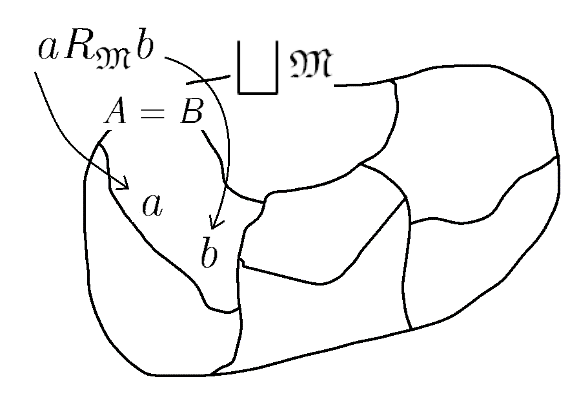
\includegraphics[width=160pt]{1.2.5.a.png}
\end{center}
\begin{dfn}
集合$A$の1つの同値関係$R$が与えられたとする。このとき、次式のような集合$C_{R}(a)$が定義されよう。
\begin{align*}
C_{R}(a) = \left\{ c \in A \middle| aRc \right\} \subseteq A
\end{align*}
この集合$C_{R}(a)$をその同値関係$R$によるその元$a$の同値類、または単に、類などといい$[ a]_{R}$、$\overline{a}$などとも書く。
\end{dfn}\par
このことは次のようにして考えられればわかりやすかろう。
\begin{center}
  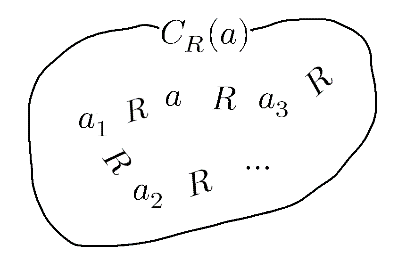
\includegraphics[width=160pt]{1.2.5.b.png}
\end{center}
\begin{thm}\label{2.4.1.4}
次のことが成り立つ。
\begin{itemize}
\item
  $\forall a \in A$に対し、$a \in C_{R}(a)$が成り立つ。
\item
  $\forall a,b \in A$に対し、$aRb$が成り立つならそのときに限り、$C_{R}(a) = C_{R}(b)$が成り立つ。
\item
  $\forall a,b \in A$に対し、$C_{R}(a) \neq C_{R}(b)$が成り立つなら、$C_{R}(a) \cap C_{R}(b) = \emptyset$が成り立つ。
\end{itemize}
\end{thm}
\begin{thm}\label{2.4.1.5}
集合$A$の1つの同値関係$R$が与えられたとする。次式のようにその同値関係$R$によるその元$a$の同値類全体の集合$\mathfrak{M}$が定義されると、
\begin{align*}
\mathfrak{M}=\left\{ C_{R}(a)\in \mathfrak{P}(A) \middle| C_{R}(a) = \left\{ c \in A \middle| aRc \right\} \right\}
\end{align*}
その集合$\mathfrak{M}$はその集合$A$の直和分割でこれに付随する同値関係$R_{\mathfrak{M}}$はその同値関係$R$に等しい。
\end{thm}\par
このことは次のようにして考えられればわかりやすかろう。
\begin{center}
    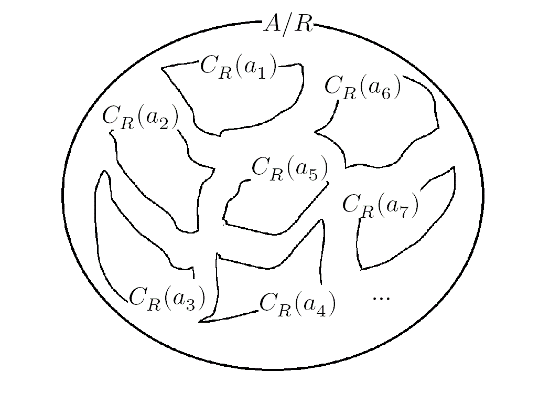
\includegraphics[width=160pt]{1.2.5.c.png}
\end{center}
\begin{dfn}
このようにして、その同値関係$R$からその集合$\mathfrak{M}$が定義されること、即ち、その集合$A$がその同値関係$R$によって得られる同値類たちの直和$\bigsqcup_{} \mathfrak{M}$とみなすことをその集合$A$のその同値関係$R$による類別、分類といいその集合$\mathfrak{M}$をその集合$A$のその同値関係による商集合といい$A/R$などと書く。
\end{dfn}
\begin{thm}\label{2.4.1.6}
ここで、写像$f:A \rightarrow B$が与えられたとする。このとき、その集合$A$の元々$a$、$b$に対し、次式のように論理式$aR(f)b$が定義されると、
\begin{align*}
aR(f)b \Leftrightarrow a,b \in A \land f(a) = f(b)
\end{align*}
その集合$A$における関係$R(f)$が得られこれは同値関係となる。
\end{thm}
\begin{dfn}
この関係$R(f)$をその写像$f$に付随する同値関係、その写像$f$の同値核などという。
\end{dfn}
\begin{thm}\label{2.4.1.7}
集合$A$の1つの同値関係$R$が与えられたとする。次式のように写像$C_{R}$が定義されるとき、
\begin{align*}
C_{R}:A \rightarrow A/R;a \mapsto C_{R}(a)
\end{align*}
その写像$C_{R}$は全射でありこれに付随する同値関係$R\left( C_{R} \right)$はその同値関係$R$に等しい。
\end{thm}
\begin{dfn}
このような写像$C_{R}$をその集合$A$からその集合$A/R$への標準的全射、自然な全射、商写像などという。
\end{dfn}
\end{comment}
%\hypertarget{ux5546vectorux7a7aux9593-1}{%
\subsubsection{商vector空間}%\label{ux5546vectorux7a7aux9593-1}}
\begin{dfn}
体$K$上のvector空間$V$の部分空間$W$が与えられたとき、$\mathbf{v},\mathbf{w} \in V$に対し、$\mathbf{v} - \mathbf{w} \in W$が成り立つことを$\mathbf{v} \equiv \mathbf{w}\ \mathrm{mod}W$と書くことにする。
\end{dfn}
\begin{thm}\label{2.4.1.8}
体$K$上のvector空間$V$の部分空間$W$が与えられたとき、上記の関係$\equiv \ \mathrm{mod}W$は同値関係である。
\end{thm}
\begin{proof}
体$K$上のvector空間$V$の部分空間$W$が与えられたとき、$\forall\mathbf{v} \in V$に対し、$\mathbf{0} = \mathbf{v} - \mathbf{v} \in W$が成り立つので、$\mathbf{v} \equiv \mathbf{v}\ \mathrm{mod}W$が成り立つ。$\forall\mathbf{v},\mathbf{w} \in W$に対し、$\mathbf{v} \equiv \mathbf{w}\ \mathrm{mod}W$が成り立つなら、$\mathbf{v} - \mathbf{w} \in W$が成り立ち、したがって、$\mathbf{w} - \mathbf{v} = - \mathbf{v} + \mathbf{w} = - \left( \mathbf{v} - \mathbf{w} \right) \in W$が成り立つので、$\mathbf{w} \equiv \mathbf{v}\ \mathrm{mod}W$が成り立つ。最後に、$\forall\mathbf{u},\mathbf{v},\mathbf{w} \in V$に対し、$\mathbf{u} \equiv \mathbf{v}\ \mathrm{mod}W$かつ$\mathbf{v} \equiv \mathbf{w}\ \mathrm{mod}W$が成り立つなら、$\mathbf{u} - \mathbf{v},\mathbf{v} - \mathbf{w} \in W$が成り立つので、$\mathbf{u} - \mathbf{w} = \mathbf{u} - \mathbf{v} + \mathbf{v} - \mathbf{w} = \left( \mathbf{u} - \mathbf{v} \right) + \left( \mathbf{v} - \mathbf{w} \right) \in W$が成り立つ。したがって、$\mathbf{u} \equiv \mathbf{w}\ \mathrm{mod}W$が成り立つ。以上より、その関係$\equiv \ \mathrm{mod}W$は同値関係である。
\end{proof}
\begin{thm}\label{2.4.1.9}
体$K$上のvector空間$V$の部分空間$W$が与えられたとき、$\forall k,l \in K$に対し、$k \neq 0$または$l \neq 0$が成り立つなら、$kW + lW = W$が成り立つ。
\end{thm}
\begin{proof}
体$K$上のvector空間$V$の部分空間$W$が与えられたとき、$\forall k,l \in K\forall\mathbf{v},\mathbf{w} \in W$に対し、$k \neq 0$または$l \neq 0$が成り立つなら、$k\mathbf{v} + l\mathbf{w} \in kW + lW$が成り立ち、これより明らかに、$k\mathbf{v} + l\mathbf{w} \in W$も成り立つので、$kW + lW \subseteq W$が成り立つ。一方で、$\forall\mathbf{v} \in W$に対し、$k \neq 0$としても一般性は失われなく、このとき、$\frac{1}{k}\mathbf{v} \in W$が成り立つので、$\mathbf{v} = k\frac{1}{k}\mathbf{v} + l\mathbf{0} \in kW + lW$が成り立つ。以上より、$kW + lW = W$が成り立つ。
\end{proof}
\begin{thm}\label{2.4.1.10}
体$K$上のvector空間$V$の部分空間$W$が与えられたとき、上記の議論により商集合${V}/{\equiv \ \mathrm{mod}W}$が定義される。このとき、$\forall C_{\equiv \ \mathrm{mod}W}\left( \mathbf{v} \right) \in {V}/{\equiv \ \mathrm{mod}W}$に対し、$C_{\equiv \ \mathrm{mod}W}\left( \mathbf{v} \right) = \mathbf{v} + W$が成り立つ。
\end{thm}
\begin{proof}
体$K$上のvector空間$V$の部分空間$W$が与えられたとき、上記の議論により商集合${V}/{\equiv \ \mathrm{mod}W}$が定義される。このとき、$\forall C_{\equiv \ \mathrm{mod}W}\left( \mathbf{v} \right) \in {V}/{\equiv \ \mathrm{mod}W}\forall\mathbf{w} \in C_{\equiv \ \mathrm{mod}W}\left( \mathbf{v} \right)$に対し、$\mathbf{v} \equiv \mathbf{w}\ \mathrm{mod}W$が成り立つので、$\mathbf{v} - \mathbf{w} \in W$が成り立つ。ここで、$- \mathbf{u} = \mathbf{v} - \mathbf{w}$とおかれると、$\mathbf{w} = \mathbf{v} + \mathbf{u}$が成り立つかつ、$\mathbf{u}, - \mathbf{u} \in W$が成り立つので、$\mathbf{w} \in \mathbf{v} + W$が成り立つ。逆に、$\forall\mathbf{v} + \mathbf{w} \in \mathbf{v} + W$に対し、$\mathbf{w} \in W$が成り立つので、$\mathbf{w} = \mathbf{v} + \mathbf{w} - \mathbf{v} = \left( \mathbf{v} + \mathbf{w} \right) - \mathbf{v} \in W$となり、したがって、$\mathbf{v} + \mathbf{w} \equiv \mathbf{v}\ \mathrm{mod}W$が成り立ち、これにより、$\mathbf{v} + \mathbf{w} \in C_{\equiv \ \mathrm{mod}W}\left( \mathbf{v} \right)$が成り立つ。以上より、$C_{\equiv \ \mathrm{mod}W}\left( \mathbf{v} \right) = \mathbf{v} + W$が成り立つ。
\end{proof}
\begin{thm}\label{2.4.1.11}
体$K$上のvector空間$V$の部分空間$W$が与えられたとき、$W = C_{\equiv \ \mathrm{mod}W}\left( \mathbf{0} \right) \in {V}/{\equiv \ \mathrm{mod}W}$が成り立つ。
\end{thm}
\begin{proof} $W = \mathbf{0} + W$が成り立つことによる。
\end{proof}
\begin{thm}\label{2.4.1.12}
体$K$上のvector空間$V$の部分空間$W$が与えられたとき、$\forall\mathbf{v},\mathbf{w} \in V$に対し、$\mathbf{v} \equiv \mathbf{w}\ \mathrm{mod}W$が成り立つなら、$\mathbf{v} + W = \mathbf{w} + W$が成り立ち、そうでないなら、$\mathbf{v} + W \cap \mathbf{w} + W = \emptyset$が成り立つ。
\end{thm}
\begin{proof}
体$K$上のvector空間$V$の部分空間$W$が与えられたとき、$\forall\mathbf{v},\mathbf{w} \in V$に対し、$\mathbf{v} \equiv \mathbf{w}\ \mathrm{mod}W$が成り立つなら、$\mathbf{v} \in C_{\equiv \ \mathrm{mod}W}\left( \mathbf{w} \right) = \mathbf{w} + W$が成り立つので、$\forall\mathbf{v} + \mathbf{u} \in \mathbf{v} + W$に対し、あるその部分空間$W$の元$\mathbf{u}'$が存在して$\mathbf{v} = \mathbf{w} + \mathbf{u}'$が成り立ち、したがって、$\mathbf{v} + \mathbf{u} = \mathbf{w} + \left( \mathbf{u}' + \mathbf{u} \right) \in \mathbf{w} + W$が成り立つ。ゆえに、$\mathbf{v} + W \subseteq \mathbf{w} + W$が成り立つ。同様にして、$\mathbf{v} + W \supseteq \mathbf{w} + W$が成り立つので、$\mathbf{v} + W = \mathbf{w} + W$が成り立つ。\par
$\mathbf{v} + W \cap \mathbf{w} + W \neq \emptyset$が成り立つなら、$\mathbf{u} \in \mathbf{v} + W \cap \mathbf{w} + W$なるその集合$\mathbf{v} + W \cap \mathbf{w} + W$の元$\mathbf{u}$が存在して、$\exists\mathbf{u}',\mathbf{u}'' \in W$に対し、$\mathbf{u} = \mathbf{v} + \mathbf{u}' = \mathbf{w} + \mathbf{u}''$が成り立つので、$\mathbf{u} - \mathbf{v},\mathbf{u} - \mathbf{w} \in W$が成り立つ。このとき、$\mathbf{u} \equiv \mathbf{v}\ \mathrm{mod}W$かつ$\mathbf{u} \equiv \mathbf{w}\ \mathrm{mod}W$が成り立つので、$\mathbf{v} \equiv \mathbf{w}\ \mathrm{mod}W$が成り立つ。対偶律より$\mathbf{v} \equiv \mathbf{w}\ \mathrm{mod}W$が成り立たないなら、$\mathbf{v} + W \cap \mathbf{w} + W = \emptyset$が成り立つ。
\end{proof}
\begin{thm}\label{2.4.1.13}
体$K$上のvector空間$V$の部分空間$W$が与えられたとき、上記の議論により商集合${V}/{\equiv \ \mathrm{mod}W}$が定義される。このとき、$\forall k \in K\forall C_{\equiv \ \mathrm{mod}W}\left( \mathbf{v} \right) \in {V}/{\equiv \ \mathrm{mod}W}$に対し、次式のように定義されると、
\begin{align*}
kC_{\equiv \ \mathrm{mod}W}\left( \mathbf{v} \right) = C_{\equiv \ \mathrm{mod}W}\left( k\mathbf{v} \right)
\end{align*}
その集合${V}/{\equiv \ \mathrm{mod}W}$は体$K$上のvector空間をなす。
\end{thm}
\begin{dfn}
このようにして構成されたvector空間${V}/{\equiv \ \mathrm{mod}W}$をそのvector空間$V$のその部分空間$W$による商vector空間、商線形空間、商空間といい、${V}/{W}$と書く。
\end{dfn}
\begin{proof}
体$K$上のvector空間$V$の部分空間$W$が与えられたとき、上記の議論により商集合${V}/{\equiv \ \mathrm{mod}W}$が定義される。このとき、$\forall k \in K\forall C_{\equiv \ \mathrm{mod}W}\left( \mathbf{v} \right) \in {V}/{\equiv \ \mathrm{mod}W}$に対し、次式のように定義されると、
\begin{align*}
kC_{\equiv \ \mathrm{mod}W}\left( \mathbf{v} \right) = C_{\equiv \ \mathrm{mod}W}\left( k\mathbf{v} \right)
\end{align*}
$\forall\mathbf{u},\mathbf{v},\mathbf{w} \in V$に対し、次のようになることから、
\begin{align*}
\left( C_{\equiv \ \mathrm{mod}W}\left( \mathbf{u} \right) + C_{\equiv \ \mathrm{mod}W}\left( \mathbf{v} \right) \right) + C_{\equiv \ \mathrm{mod}W}\left( \mathbf{w} \right) &= \left( \mathbf{u} + W + \mathbf{v} + W \right) + \mathbf{w} + W\\
&= \mathbf{u} + W + \left( \mathbf{v} + W + \mathbf{w} + W \right)\\
&= C_{\equiv \ \mathrm{mod}W}\left( \mathbf{u} \right) + \left( C_{\equiv \ \mathrm{mod}W}\left( \mathbf{v} \right) + C_{\equiv \ \mathrm{mod}W}\left( \mathbf{w} \right) \right)\\
C_{\equiv \ \mathrm{mod}W}\left( \mathbf{v} \right) + C_{\equiv \ \mathrm{mod}W}\left( \mathbf{0} \right) &= \mathbf{v} + W + \mathbf{0} + W = \mathbf{v} + W + W\\
&= \mathbf{v} + W = C_{\equiv \ \mathrm{mod}W}\left( \mathbf{v} \right)\\
C_{\equiv \ \mathrm{mod}W}\left( \mathbf{v} \right) + C_{\equiv \ \mathrm{mod}W}\left( - \mathbf{v} \right) &= \mathbf{v} + W - \mathbf{v} + W = \mathbf{v} - \mathbf{v} + W + W\\
&= \mathbf{0} + W = C_{\equiv \ \mathrm{mod}W}\left( \mathbf{0} \right)\\
C_{\equiv \ \mathrm{mod}W}\left( \mathbf{v} \right) + C_{\equiv \ \mathrm{mod}W}\left( \mathbf{w} \right) &= \mathbf{v} + W + \mathbf{w} + W\\
&= \mathbf{w} + W + \mathbf{v} + W\\
&= C_{\equiv \ \mathrm{mod}W}\left( \mathbf{w} \right) + C_{\equiv \ \mathrm{mod}W}\left( \mathbf{v} \right)
\end{align*}
その組$\left( {V}/{\equiv \ \mathrm{mod}W}, + \right)$は可換群をなす。\par
このとき、$\forall k,l \in K$に対し、次のようになることから、
\begin{align*}
k\left( C_{\equiv \ \mathrm{mod}W}\left( \mathbf{v} \right) + C_{\equiv \ \mathrm{mod}W}\left( \mathbf{w} \right) \right) &= k\left( \mathbf{v} + W + \mathbf{w} + W \right)\\
&= k\left( \mathbf{v} + \mathbf{w} + W \right)\\
&= kC_{\equiv \ \mathrm{mod}W}\left( \mathbf{v} + \mathbf{w} \right)\\
&= C_{\equiv \ \mathrm{mod}W}\left( k\left( \mathbf{v} + \mathbf{w} \right) \right)\\
&= C_{\equiv \ \mathrm{mod}W}\left( k\mathbf{v} + k\mathbf{w} \right)\\
&= k\mathbf{v} + k\mathbf{w} + W\\
&= k\mathbf{v} + W + k\mathbf{w} + W\\
&= C_{\equiv \ \mathrm{mod}W}\left( k\mathbf{v} \right) + C_{\equiv \ \mathrm{mod}W}\left( k\mathbf{w} \right)\\
&= kC_{\equiv \ \mathrm{mod}W}\left( \mathbf{v} \right) + kC_{\equiv \ \mathrm{mod}W}\left( \mathbf{w} \right)\\
(k + l)C_{\equiv \ \mathrm{mod}W}\left( \mathbf{v} \right) &= C_{\equiv \ \mathrm{mod}W}\left( (k + l)\mathbf{v} \right)\\
&= C_{\equiv \ \mathrm{mod}W}\left( k\mathbf{v} + l\mathbf{v} \right)\\
&= k\mathbf{v} + l\mathbf{v} + W\\
&= k\mathbf{v} + W + l\mathbf{v} + W\\
&= C_{\equiv \ \mathrm{mod}W}\left( k\mathbf{v} \right) + C_{\equiv \ \mathrm{mod}W}\left( l\mathbf{v} \right)\\
&= kC_{\equiv \ \mathrm{mod}W}\left( \mathbf{v} \right) + lC_{\equiv \ \mathrm{mod}W}\left( \mathbf{v} \right)\\
(kl)C_{\equiv \ \mathrm{mod}W}\left( \mathbf{v} \right) &= C_{\equiv \ \mathrm{mod}W}\left( (kl)\mathbf{v} \right)\\
&= C_{\equiv \ \mathrm{mod}W}\left( k\left( l\mathbf{v} \right) \right)\\
&= kC_{\equiv \ \mathrm{mod}W}\left( l\mathbf{v} \right)\\
1C_{\equiv \ \mathrm{mod}W}\left( \mathbf{v} \right) &= C_{\equiv \ \mathrm{mod}W}\left( 1\mathbf{v} \right)\\
&= C_{\equiv \ \mathrm{mod}W}\left( \mathbf{v} \right)
\end{align*}
その集合${V}/{\equiv \ \mathrm{mod}W}$は体$K$上のvector空間をなす。
\end{proof}
\begin{thm}\label{2.4.1.14}
体$K$上の有限次元vector空間$V$の部分空間$W$が与えられたとき、これの基底が$\left\langle \mathbf{v}_{i} \right\rangle_{i \in \varLambda_{r}}$とおかれれば、次のことは同値である。
\begin{itemize}
\item
  $i \in \varLambda_{n} \setminus \varLambda_{r}$なるvectors$\mathbf{v}_{i} + W$が線形独立である。
\item
  $i \in \varLambda_{n}$なるvectors$\mathbf{v}_{i}$が線形独立である。
\end{itemize}
\end{thm}
\begin{proof}
体$K$上の有限次元vector空間$V$の部分空間$W$が与えられたとき、これの基底が$\left\langle \mathbf{v}_{i} \right\rangle_{i \in \varLambda_{r}}$とおかれれば、$i \in \varLambda_{n} \setminus \varLambda_{r}$なるvectors$\mathbf{v}_{i} + W$が線形独立であるなら、$\sum_{i \in \varLambda_{n}} {c_{i}\mathbf{v}_{i}} = \mathbf{0}$とおくと、次のようになるので、
\begin{align*}
\sum_{i \in \varLambda_{n} \setminus \varLambda_{r}} {c_{i}\mathbf{v}_{i}} - \mathbf{0} &= \sum_{i \in \varLambda_{n} \setminus \varLambda_{r}} {c_{i}\mathbf{v}_{i}}\\
&= - \sum_{i \in \varLambda_{r}} {c_{i}\mathbf{v}_{i}} \in W
\end{align*}
次のようになる。
\begin{align*}
\sum_{i \in \varLambda_{n} \setminus \varLambda_{r}} {c_{i}\left( \mathbf{v}_{i} + W \right)} &= \sum_{i \in \varLambda_{n} \setminus \varLambda_{r}} {c_{i}\mathbf{v}_{i}} + W\\
&= \mathbf{0} + W = W
\end{align*}
ゆえに、$\forall i \in \varLambda_{n} \setminus \varLambda_{r}$に対し、$c_{i} = 0$が成り立つ。このとき、次のようになるので、
\begin{align*}
\sum_{i \in \varLambda_{r}} {c_{i}\mathbf{v}_{i}} &= \sum_{i \in \varLambda_{r}} {c_{i}\mathbf{v}_{i}} + \sum_{i \in \varLambda_{n} \setminus \varLambda_{r}} {c_{i}\mathbf{v}_{i}} - \sum_{i \in \varLambda_{n} \setminus \varLambda_{r}} {c_{i}\mathbf{v}_{i}}\\
&= \sum_{i \in \varLambda_{n}} {c_{i}\mathbf{v}_{i}} - \sum_{i \in \varLambda_{n} \setminus \varLambda_{r}} {0\mathbf{v}_{i}}\\
&= \mathbf{0} + \mathbf{0} = \mathbf{0}
\end{align*}
それらのvectors$\mathbf{v}_{i}$が線形独立であることにより$\forall i \in \varLambda_{r}$に対し、$c_{i} = 0$が成り立つ。以上の議論により、$i \in \varLambda_{n}$なるvectors$\mathbf{v}_{i}$が線形独立である。\par
逆に、$i \in \varLambda_{n}$なるvectors$\mathbf{v}_{i}$が線形独立であるなら、$\sum_{i \in \varLambda_{n} \setminus \varLambda_{r}} {c_{i}\left( \mathbf{v}_{i} + W \right)} = W$のとき、次のようになることから、
\begin{align*}
\sum_{i \in \varLambda_{n} \setminus \varLambda_{r}} {c_{i}\mathbf{v}_{i}} + W = \sum_{i \in \varLambda_{n} \setminus \varLambda_{r}} {c_{i}\left( \mathbf{v}_{i} + W \right)} = W
\end{align*}
$\sum_{i \in \varLambda_{n} \setminus \varLambda_{r}} {c_{i}\mathbf{v}_{i}} = \sum_{i \in \varLambda_{n} \setminus \varLambda_{r}} {c_{i}\mathbf{v}_{i}} - \mathbf{0} \in W$が成り立つ。ゆえに、$\sum_{i \in \varLambda_{n} \setminus \varLambda_{r}} {c_{i}\mathbf{v}_{i}} = \sum_{i \in \varLambda_{r}} {\left( - c_{i} \right)\mathbf{v}_{i}}$とおくことができて、次式が得られる。
\begin{align*}
\sum_{i \in \varLambda_{n}} {c_{i}\mathbf{v}_{i}} = \sum_{i \in \varLambda_{r}} {c_{i}\mathbf{v}_{i}} + \sum_{i \in \varLambda_{n} \setminus \varLambda_{r}} {c_{i}\mathbf{v}_{i}} = \mathbf{0}
\end{align*}
そこで、仮定より$\forall i \in \varLambda_{n}$に対し、$c_{i} = 0$が得られるので、特に、$\forall i \in \varLambda_{r}$に対し、$c_{i} = 0$が成り立つ。よって、$i \in \varLambda_{n} \setminus \varLambda_{r}$なるvectors$\mathbf{v}_{i} + W$が線形独立である。
\end{proof}
\begin{thm}\label{2.4.1.15}
体$K$上のvector空間$V$の部分空間$W$が与えられたとき、次式のような写像$\varphi$は全射な線形写像である。
\begin{align*}
\varphi:V \rightarrow {V}/{W};\mathbf{v} \mapsto \mathbf{v} + W
\end{align*}
\end{thm}
\begin{dfn}
上記のような線形写像$\varphi$をそのvector空間$V$からその部分空間$W$によるその商vector空間${V}/{W}$への自然な全射線形写像という。
\end{dfn}
\begin{proof}
体$K$上のvector空間$V$の部分空間$W$が与えられたとき、次式のような写像$\varphi$について、
\begin{align*}
\varphi:V \rightarrow {V}/{W};\mathbf{v} \mapsto \mathbf{v} + W
\end{align*}
$\forall\mathbf{v} + W \in {V}/{W}$に対し、定義よりそのvector空間$V$の元$\mathbf{v}$が存在して$\varphi\left( \mathbf{v} \right) = \mathbf{v} + W$が成り立つので、その写像$\varphi$は全射である。\par
このとき、$\forall k,l \in K\forall\mathbf{v},\mathbf{w} \in V$に対し、次のようになることから、
\begin{align*}
\varphi\left( k\mathbf{v} + l\mathbf{w} \right) &= \left( k\mathbf{v} + l\mathbf{w} \right) + W\\
&= k\mathbf{v} + W + l\mathbf{w} + W\\
&= k\left( \mathbf{v} + W \right) + l\left( \mathbf{w} + W \right)\\
&= k\varphi\left( \mathbf{v} \right) + l\varphi\left( \mathbf{w} \right)
\end{align*}
その写像$\varphi$は全射な線形写像である。
\end{proof}
\begin{thm}\label{2.4.1.16}
体$K$上のvector空間$V$の部分空間$W$が与えられたとき、そのvector空間$V$からその部分空間$W$によるその商vector空間${V}/{W}$への自然な全射線形写像$\varphi$の核$\ker\varphi$について、$\ker\varphi = W$が成り立つ。
\end{thm}
\begin{proof}
体$K$上のvector空間$V$の部分空間$W$が与えられたとき、そのvector空間$V$からその部分空間$W$によるその商vector空間${V}/{W}$への自然な全射線形写像$\varphi$の核$\ker\varphi$について、$\forall\mathbf{v} \in \ker\varphi$に対し、$\varphi\left( \mathbf{v} \right) = \mathbf{v} + W = W$が成り立つので、$\mathbf{v} \in W$が成り立つ。逆に、$\forall\mathbf{v} \in W$に対し、$\varphi\left( \mathbf{v} \right) = \mathbf{v} + W = W$が成り立つので、$\mathbf{v} \in \ker\varphi$が成り立つ。よって、$\ker\varphi = W$が成り立つ。
\end{proof}
\begin{thm}\label{2.4.1.17}
体$K$上のvector空間$V$の部分空間$W$が与えられたとき、次式が成り立つ。
\begin{align*}
\dim{V}/{W} = \dim V - \dim W
\end{align*}
\end{thm}
\begin{proof}
体$K$上のvector空間$V$の部分空間$W$が与えられたとき、そのvector空間$V$からその部分空間$W$によるその商vector空間${V}/{W}$への自然な全射線形写像$\varphi$について次元公式より次式が成り立つ。
\begin{align*}
\dim V = {\mathrm{rank}}\varphi + {\mathrm{nullity}}\varphi = \dim{V(\varphi)} + \dim{\ker\varphi}
\end{align*}
ここで、$V(\varphi) = {V}/{W}$が成り立つかつ、定理\ref{2.4.1.16}より次式が成り立つ。
\begin{align*}
\dim{V}/{W} = \dim V - \dim W
\end{align*}
\end{proof}
\begin{thm}[線形的な意味での準同型定理]\label{2.4.1.18}
体$K$上の2つのvector空間たち$V$、$W$の間の線形写像$f:V \rightarrow W$が与えられたとき、次式のような写像$g$は線形同型写像である。
\begin{align*}
g:{V}/{\ker f} \rightarrow V(f);\mathbf{v} + \ker f \mapsto f\left( \mathbf{v} \right)
\end{align*}
この定理を線形的な意味での準同型定理ということにする。
\end{thm}
\begin{proof}
体$K$上の2つのvector空間たち$V$、$W$の間の線形写像$f:V \rightarrow W$が与えられたとき、次式のような写像$g$について、
\begin{align*}
g:{V}/{\ker f} \rightarrow V(f);\mathbf{v} + \ker f \mapsto f\left( \mathbf{v} \right)
\end{align*}
$\forall k,l \in K\forall\mathbf{v} + \ker f,\mathbf{w} + \ker f \in {V}/{\ker f}$に対し、次のようになるので、
\begin{align*}
g\left( k\left( \mathbf{v} + \ker f \right) + l\left( \mathbf{w} + \ker f \right) \right) &= g\left( k\mathbf{v} + \ker f + l\mathbf{w} + \ker f \right)\\
&= g\left( k\mathbf{v} + l\mathbf{w} + \ker f \right)\\
&= f\left( k\mathbf{v} + l\mathbf{w} \right)\\
&= kf\left( \mathbf{v} \right) + lf\left( \mathbf{w} \right)\\
&= kg\left( \mathbf{v} + \ker f \right) + lg\left( \mathbf{w} + \ker f \right)
\end{align*}
その写像$g$は線形的である。ここで、$\forall f\left( \mathbf{v} \right) \in V(f)$に対し、そのvector空間$V$の元$\mathbf{v}$が存在して、これのそのvector空間$V$からその部分空間$W$によるその商vector空間${V}/{W}$への自然な全射線形写像$\varphi$による像が$\mathbf{v} + W$であるから、確かにその線形写像$g$は全射である。このとき、定理\ref{2.1.2.15}よりその線形写像$g$は線形同型写像でもある。
\end{proof}
\begin{thebibliography}{50}
  \bibitem{1}
  松坂和夫, 集合・位相入門, 岩波書店, 1968. 新装版第2刷 p52-59 ISBN978-4-00-029871-1
  \bibitem{2}
  松坂和夫, 代数系入門, 岩波書店, 1976. 新装版第1刷 p182-191 ISBN978-4-00-029873-5
  \bibitem{3}
  池田岳, テンソル代数と表現論, 東京大学出版会, 2022. 第2刷 p25-33 ISBN978-4-13-062929-4
\end{thebibliography}
\end{document}

\clearpage
\documentclass[dvipdfmx]{jsarticle}
\setcounter{section}{4}
\setcounter{subsection}{1}
\usepackage{xr}
\externaldocument{2.1.1}
\externaldocument{2.1.2}
\externaldocument{2.1.5}
\usepackage{amsmath,amsfonts,amssymb,array,comment,mathtools,url,docmute}
\usepackage{longtable,booktabs,dcolumn,tabularx,mathtools,multirow,colortbl,xcolor}
\usepackage[dvipdfmx]{graphics}
\usepackage{bmpsize}
\usepackage{amsthm}
\usepackage{enumitem}
\setlistdepth{20}
\renewlist{itemize}{itemize}{20}
\setlist[itemize]{label=•}
\renewlist{enumerate}{enumerate}{20}
\setlist[enumerate]{label=\arabic*.}
\setcounter{MaxMatrixCols}{20}
\setcounter{tocdepth}{3}
\newcommand{\rotin}{\text{\rotatebox[origin=c]{90}{$\in $}}}
\newcommand{\amap}[6]{\text{\raisebox{-0.7cm}{\begin{tikzpicture} 
  \node (a) at (0, 1) {$\textstyle{#2}$};
  \node (b) at (#6, 1) {$\textstyle{#3}$};
  \node (c) at (0, 0) {$\textstyle{#4}$};
  \node (d) at (#6, 0) {$\textstyle{#5}$};
  \node (x) at (0, 0.5) {$\rotin $};
  \node (x) at (#6, 0.5) {$\rotin $};
  \draw[->] (a) to node[xshift=0pt, yshift=7pt] {$\textstyle{\scriptstyle{#1}}$} (b);
  \draw[|->] (c) to node[xshift=0pt, yshift=7pt] {$\textstyle{\scriptstyle{#1}}$} (d);
\end{tikzpicture}}}}
\newcommand{\twomaps}[9]{\text{\raisebox{-0.7cm}{\begin{tikzpicture} 
  \node (a) at (0, 1) {$\textstyle{#3}$};
  \node (b) at (#9, 1) {$\textstyle{#4}$};
  \node (c) at (#9+#9, 1) {$\textstyle{#5}$};
  \node (d) at (0, 0) {$\textstyle{#6}$};
  \node (e) at (#9, 0) {$\textstyle{#7}$};
  \node (f) at (#9+#9, 0) {$\textstyle{#8}$};
  \node (x) at (0, 0.5) {$\rotin $};
  \node (x) at (#9, 0.5) {$\rotin $};
  \node (x) at (#9+#9, 0.5) {$\rotin $};
  \draw[->] (a) to node[xshift=0pt, yshift=7pt] {$\textstyle{\scriptstyle{#1}}$} (b);
  \draw[|->] (d) to node[xshift=0pt, yshift=7pt] {$\textstyle{\scriptstyle{#2}}$} (e);
  \draw[->] (b) to node[xshift=0pt, yshift=7pt] {$\textstyle{\scriptstyle{#1}}$} (c);
  \draw[|->] (e) to node[xshift=0pt, yshift=7pt] {$\textstyle{\scriptstyle{#2}}$} (f);
\end{tikzpicture}}}}
\renewcommand{\thesection}{第\arabic{section}部}
\renewcommand{\thesubsection}{\arabic{section}.\arabic{subsection}}
\renewcommand{\thesubsubsection}{\arabic{section}.\arabic{subsection}.\arabic{subsubsection}}
\everymath{\displaystyle}
\allowdisplaybreaks[4]
\usepackage{vtable}
\theoremstyle{definition}
\newtheorem{thm}{定理}[subsection]
\newtheorem*{thm*}{定理}
\newtheorem{dfn}{定義}[subsection]
\newtheorem*{dfn*}{定義}
\newtheorem{axs}[dfn]{公理}
\newtheorem*{axs*}{公理}
\renewcommand{\headfont}{\bfseries}
\makeatletter
  \renewcommand{\section}{%
    \@startsection{section}{1}{\z@}%
    {\Cvs}{\Cvs}%
    {\normalfont\huge\headfont\raggedright}}
\makeatother
\makeatletter
  \renewcommand{\subsection}{%
    \@startsection{subsection}{2}{\z@}%
    {0.5\Cvs}{0.5\Cvs}%
    {\normalfont\LARGE\headfont\raggedright}}
\makeatother
\makeatletter
  \renewcommand{\subsubsection}{%
    \@startsection{subsubsection}{3}{\z@}%
    {0.4\Cvs}{0.4\Cvs}%
    {\normalfont\Large\headfont\raggedright}}
\makeatother
\makeatletter
\renewenvironment{proof}[1][\proofname]{\par
  \pushQED{\qed}%
  \normalfont \topsep6\p@\@plus6\p@\relax
  \trivlist
  \item\relax
  {
  #1\@addpunct{.}}\hspace\labelsep\ignorespaces
}{%
  \popQED\endtrivlist\@endpefalse
}
\makeatother
\renewcommand{\proofname}{\textbf{証明}}
\usepackage{tikz,graphics}
\usepackage[dvipdfmx]{hyperref}
\usepackage{pxjahyper}
\hypersetup{
 setpagesize=false,
 bookmarks=true,
 bookmarksdepth=tocdepth,
 bookmarksnumbered=true,
 colorlinks=false,
 pdftitle={},
 pdfsubject={},
 pdfauthor={},
 pdfkeywords={}}
\begin{document}
%\hypertarget{ux53ccux5bfeux7a7aux9593}{%
\subsection{双対空間}%\label{ux53ccux5bfeux7a7aux9593}}
%\hypertarget{ux7ddaux5f62ux5199ux50cfux306eux4e3bux306aux5b9aux7406ux305fux3061}{%
\subsubsection{線形写像の主な定理たち}%\label{ux7ddaux5f62ux5199ux50cfux306eux4e3bux306aux5b9aux7406ux305fux3061}}\par
双対空間が述べられる前に代表的な定理が先に挙げておかれよう\footnote{ホントは「双対空間を述べる前に代表的な定理を先に挙げておこう」と言おうとしたけど、主語があやふやだったのが許せなくてきたから、無理やり受動態にしたらこうなった。}。
\begin{thm*}[定理\ref{2.1.2.3}の再掲]
体$K$上のvector空間$U$、$V$、$W$が与えられたとき、2つの線形写像$f:U \rightarrow V$、$g:V \rightarrow W$において、その合成写像$g \circ f:U \rightarrow W$もその体$K$上で線形的である。
\end{thm*}
\begin{thm*}[定理\ref{2.1.2.6}の再掲]
体$K$上の$\dim V = n$なる2つの任意のvector空間たち$V$、$W$に対し、次のことが成り立つ。
\begin{itemize}
\item
  $V \cong W$が成り立つなら、ある線形同型写像$f:V\overset{\sim}{\rightarrow}W$が存在して、そのvector空間$V$の基底$\left\langle \mathbf{v}_{i} \right\rangle_{i \in \varLambda_{n}}$を用いた組$\left\langle f\left( \mathbf{v}_{i} \right) \right\rangle_{i \in \varLambda_{n}}$がそのvector空間$W$の基底をなし、さらに、$\dim V = \dim W$が成り立つ。
\item
  $\dim V = \dim W$が成り立つなら、それらのvector空間たち$V$、$W$の基底たち$\left\langle \mathbf{v}_{i} \right\rangle_{i \in \varLambda_{n}}$、$\left\langle \mathbf{w}_{i} \right\rangle_{i \in \varLambda_{n}}$を用いて、$\forall i \in \varLambda_{n}$に対し、$f\left( \mathbf{v}_{i} \right) = \mathbf{w}_{i}$なる線形写像$f:V \rightarrow W$が定義されれば、その線形写像$f$は線形同型写像で、さらに、$V \cong W$が成り立つ。
\end{itemize}\par
これにより、体$K$上の任意の$n$次元のvector空間$V$において$V \cong K^{n}$が成り立つので、その体$K$上の任意の$m$次元のvector空間$V$から任意の$n$次元vector空間$W$への任意の線形写像$f:V \rightarrow W$は全て線形写像$f':K^{m} \rightarrow K^{n}$へ帰着できる。
\end{thm*}
\begin{dfn*}[定義\ref{線形写像の線形結合の定義}の再掲]
体$K$上の任意の2つのvector空間$V$、$W$が与えられたとき、そのvector空間$V$からそのvector空間$W$への線形写像全体の集合を$L(V,W)$とおき、ここで、$\forall k,l \in K\forall\mathbf{v} \in V\forall f,g \in L(V,W)$に対し、次のように定義する。
\begin{align*}
(kf + lg)\left( \mathbf{v} \right) = kf\left( \mathbf{v} \right) + lg\left( \mathbf{v} \right)
\end{align*}
\end{dfn*}
\begin{thm*}[定理\ref{2.1.2.7}の再掲]
体$K$上の任意の2つのvector空間$V$、$W$が与えられたとき、$\forall k,l \in K\forall\mathbf{v} \in V\forall f,g \in L(V,W)$に対し、写像$kf + lg$は線形的である。
\end{thm*}
\begin{thm*}[定理\ref{2.1.2.8}の再掲]
体$K$上の任意の2つのvector空間$V$、$W$が与えられたとき、その集合$L(V,W)$はその体$K$上のvector空間である。
\end{thm*}
\begin{thm*}[定理\ref{2.1.2.9}の再掲]
体$K$上の$m$次元vector空間$V$、$n$次元vector空間$W$が与えられたとき、$\dim{L(V,W)} = mn$が成り立つ。\par
さらにいえば、これらのvector空間たち$V$、$W$の基底として$\left\langle \mathbf{v}_{i} \right\rangle_{i \in \varLambda_{m}}$、$\left\langle \mathbf{w}_{j} \right\rangle_{j \in \varLambda_{n}}$が与えられたとき、組$\left\langle \varphi_{ij}:V \rightarrow W;\sum_{i' \in \varLambda_{m}} {k_{i'}\mathbf{v}_{i'}} \mapsto k_{i}\mathbf{w}_{j} \right\rangle_{(i,j) \in \varLambda_{m} \times \varLambda_{n}}$がそのvector空間$L(V,W)$の基底をなす。
\end{thm*}
\begin{thm*}[定理\ref{2.1.2.10}の再掲]
体$K$上の3つのvector空間たち$U$、$V$、$W$が与えられたとき、次のことが成り立つ。
\begin{itemize}
\item
  $\forall f,g \in L(U,V)\forall h \in L(V,W)$に対し、$h \circ (f + g) = h \circ f + h \circ g$が成り立つ。
\item
  $\forall f \in L(U,V)\forall g,h \in L(V,W)$に対し、$(g + h) \circ f = g \circ f + h \circ f$が成り立つ。
\item
  $\forall k \in K\forall f \in L(U,V)\forall g \in L(V,W)$に対し、$g \circ (kf) = (kg) \circ f = k(g \circ f)$が成り立つ。
\item
  $\exists I_{V} \in L(V,V)\exists I_{W} \in L(W,W)\forall f \in L(V,W)$に対し、$I_{W} \circ f = f \circ I_{V} = f$が成り立つ。
\end{itemize}
これにより、写像の乗法$\cdot$を写像の合成$\circ$とするとき、集合$L(V,V)$は環をなす。
\end{thm*}
\begin{thm*}[定理\ref{2.1.2.12}の再掲]
体$K$上の2つのvector空間$V$、$W$を用いて線形写像$f:V \rightarrow W$が与えられたとき、その写像$f$が単射であるならそのときに限り、$\ker f = \left\{ \mathbf{0} \right\}$が成り立つ。
\end{thm*}
\begin{thm*}[定理\ref{2.1.5.16}の再掲]
体$K$上の$n$次元vector空間たち$V$、$W$の基底の1つをそれぞれ$\alpha$、$\beta$とし、それらの基底たち$\alpha 、\beta$に関する線形写像$f:V \rightarrow W$の$[ f]^{\beta}_{\alpha} \in M_{nn}(K)$なる表現行列$[ f]^{\beta}_{\alpha}$を用いて写像$F_{\alpha \rightarrow \beta}$が次式のように定義されれば、
\begin{align*}
F_{\alpha \rightarrow \beta}:L(V,W) \rightarrow M_{nn}(K);f \mapsto [ f]^{\beta}_{\alpha}
\end{align*}
$\forall f \in L(V,W)$に対し、次のことは同値である。
\begin{itemize}
\item
  その写像$f$は線形同型写像である。
\item
  その写像$f$は全射$f:V \twoheadrightarrow W$である。
\item
  その写像$f$は単射$f:V \rightarrowtail W$である。
\item
  $n = \mathrm{rank}f = \dim{V(f)}$が成り立つ。
\item
  $\mathrm{nullity}f = \dim{\ker f} = 0$が成り立つ。
\item
  それらの基底たち$\alpha$、$\beta$に関する線形写像$f:V \rightarrow W$の表現行列$[ f]^{\beta}_{\alpha}$は正則行列である、即ち、$[ f]^{\beta}_{\alpha} \in \mathrm{GL}_{n}(K)$が成り立つ。
\item
  その行列$F_{\alpha \rightarrow \beta}(f)$は正則行列である、即ち、$F_{\alpha \rightarrow \beta}(f) \in \mathrm{GL}_{n}(K)$が成り立つ。
\end{itemize}
このとき、次式が成り立つ。
\begin{align*}
f^{- 1} = F_{\beta \rightarrow \alpha}^{- 1}\left( {F_{\alpha \rightarrow \beta}(f)}^{- 1} \right):W \rightarrow V,\\
\left[ f^{- 1} \right]_{\alpha}^{\beta} = {[ f]^{\beta}_{\alpha}}^{- 1},\ \ F_{\beta \rightarrow \alpha}\left( f^{- 1} \right) = {F_{\alpha \rightarrow \beta}(f)}^{- 1}
\end{align*}
\end{thm*}
%\hypertarget{ux7ddaux5f62ux74b0}{%
\subsubsection{線形環}%\label{ux7ddaux5f62ux74b0}}
\begin{dfn}
体$K$上のvector空間$A$が与えられたとき、積$\cdot :A \times A \rightarrow A;\left( \mathbf{v},\mathbf{w} \right) \mapsto \mathbf{vw}$が定義されていてその集合$A$が環をなすかつ、$\forall k \in K\forall\mathbf{v},\mathbf{w} \in A$に対し、次式が成り立つとき、
\begin{align*}
\left( k\mathbf{v} \right)\mathbf{w} = \mathbf{v}\left( k\mathbf{w} \right) = k\left( \mathbf{vw} \right)
\end{align*}
そのvector空間$A$をその体$K$上の線形環、多元環、代数などという。
\end{dfn}
\begin{thm}\label{2.4.2.1}
体$K$上のvector空間$V$における線形写像$f:V \rightarrow V$全体の集合$L(V,V)$は写像の合成$\circ$を積とすれば、その集合$L(V,V)$はその体$K$上の線形環である。
\end{thm}
\begin{proof}
体$K$上のvector空間$V$における線形写像$f:V \rightarrow V$全体の集合$L(V,V)$は写像の合成$\circ$を積とすれば、定理\ref{2.1.2.8}よりその集合$L(V,V)$はその体$K$上のvector空間であり、さらに、定理\ref{2.1.2.10}よりその集合$L(V,V)$は環でもある。ここで、$\forall k \in K\forall f,g \in L(V,V)\forall\mathbf{v} \in V$に対し、次のようになることから、
\begin{align*}
(kf)g\left( \mathbf{v} \right) &= (kf) \circ g\left( \mathbf{v} \right)\\
&= kf\left( g\left( \mathbf{v} \right) \right)\\
&= f\left( kg\left( \mathbf{v} \right) \right)\\
&= f \circ (kg)\left( \mathbf{v} \right)\\
&= f(kg)\left( \mathbf{v} \right)\\
(kf)g\left( \mathbf{v} \right) &= (kf) \circ g\left( \mathbf{v} \right)\\
&= kf\left( g\left( \mathbf{v} \right) \right)\\
&= k(f \circ g)\left( \mathbf{v} \right)\\
&= k(fg)\left( \mathbf{v} \right)
\end{align*}
$(kf)g = f(kg) = k(fg)$が成り立つ。よって、その集合$L(V,V)$はその体$K$上の線形環である。
\end{proof}
%\hypertarget{ux53ccux5bfeux7a7aux9593-1}{%
\subsubsection{双対空間}%\label{ux53ccux5bfeux7a7aux9593-1}}
\begin{dfn}
体$K$上のvector空間$V$における線形写像$f:V \rightarrow K$全体の集合$L(V,K)$、即ち、線形形式全体の集合をそのvector空間$V$の双対空間といい$V^{*}$と書き、これの元を線形形式、線形汎関数、共変vector、余vector、1次形式などという。
\end{dfn}
\begin{thm}\label{2.4.2.2}
体$K$上のvector空間$V$の双対空間$V^{*}$はその体$K$上のvector空間である。
\end{thm}
\begin{proof}
体$K$上のvector空間$V$が与えられたとき、その体$K$自身もその体$K$上のvector空間であるから、定理\ref{2.1.2.8}よりそのvector空間$V$の双対空間$V^{*}$もその体$K$上のvector空間である。
\end{proof}
\begin{thm}\label{2.4.2.3}
体$K$上の$n$次元vector空間$V$、これの基底$\left\langle \mathbf{v}_{i} \right\rangle_{i \in \varLambda_{n}}$が与えられたとき、$\forall\mathbf{a} \in K^{n}\forall i \in \varLambda_{n}$に対し、$\mathbf{a} = \left( a_{i} \right)_{i \in \varLambda_{n}}$とおくと、$\lambda_{\mathbf{a}}\left( \mathbf{v}_{i} \right) = a_{i}$なる線形形式$\lambda_{\mathbf{a}}:V \rightarrow K$について、次式のような写像$\varPhi$は線形同型写像である。
\begin{align*}
\varPhi:K^{n} \rightarrow V^{*};\mathbf{a} \mapsto \lambda_{\mathbf{a}}
\end{align*}
\end{thm}
\begin{dfn} 定理\ref{2.4.2.3}のような線形同型写像$\varPhi$を、ここでは、そのvector空間$V$の基底$\left\langle \mathbf{v}_{i} \right\rangle_{i \in \varLambda_{n}}$から誘導される線形同型写像ということにする。
\end{dfn}
\begin{proof}
体$K$上の$n$次元vector空間$V$、これの基底$\left\langle \mathbf{v}_{i} \right\rangle_{i \in \varLambda_{n}}$が与えられたとき、$\forall\mathbf{a} \in K^{n}\forall i \in \varLambda_{n}$に対し、$\lambda_{\mathbf{a}}\left( \mathbf{v}_{i} \right) = a_{i}$なる線形形式$\lambda_{\mathbf{a}}:V \rightarrow K$について、次式のような写像$\varPhi$について、
\begin{align*}
\varPhi:K^{n} \rightarrow V^{*};\mathbf{a} \mapsto \lambda_{\mathbf{a}}
\end{align*}
$\forall k,l \in K\forall\mathbf{a},\mathbf{b} \in K^{n}$に対し、$\mathbf{a} = \left( a_{i} \right)_{i \in \varLambda_{n}}$、$\mathbf{b} = \left( b_{i} \right)_{i \in \varLambda_{n}}$とおくと、次のようになり、
\begin{align*}
\varPhi\left( k\mathbf{a} + l\mathbf{b} \right) = \lambda_{k\mathbf{a} + l\mathbf{b}}
\end{align*}
ここで、$\forall\mathbf{v} \in V$に対し、$\mathbf{v} = \sum_{i \in \varLambda_{n}} {k_{i}\mathbf{v}_{i}}$とおかれると、次のようになることから、
\begin{align*}
\lambda_{k\mathbf{a} + l\mathbf{b}}\left( \mathbf{v} \right) &= \lambda_{k\mathbf{a} + l\mathbf{b}}\left( \sum_{i \in \varLambda_{n}} {k_{i}\mathbf{v}_{i}} \right)\\
&= \sum_{i \in \varLambda_{n}} {k_{i}\lambda_{k\mathbf{a} + l\mathbf{b}}\left( \mathbf{v}_{i} \right)}\\
&= \sum_{i \in \varLambda_{n}} {k_{i}\left( ka_{i} + lb_{i} \right)}\\
&= k\sum_{i \in \varLambda_{n}} {k_{i}a_{i}} + l\sum_{i \in \varLambda_{n}} {k_{i}b_{i}}\\
&= k\sum_{i \in \varLambda_{n}} {k_{i}\lambda_{\mathbf{a}}\left( \mathbf{v}_{i} \right)} + l\sum_{i \in \varLambda_{n}} {k_{i}\lambda_{\mathbf{b}}\left( \mathbf{v}_{i} \right)}\\
&= k\lambda_{\mathbf{a}}\left( \sum_{i \in \varLambda_{n}} {k_{i}\mathbf{v}_{i}} \right) + l\lambda_{\mathbf{b}}\left( \sum_{i \in \varLambda_{n}} {k_{i}\mathbf{v}_{i}} \right)\\
&= k\lambda_{\mathbf{a}}\left( \mathbf{v} \right) + l\lambda_{\mathbf{b}}\left( \mathbf{v} \right)\\
&= \left( k\lambda_{\mathbf{a}} + l\lambda_{\mathbf{b}} \right)\left( \mathbf{v} \right)
\end{align*}
次のようになる。
\begin{align*}
\varPhi\left( k\mathbf{a} + l\mathbf{b} \right) &= \lambda_{k\mathbf{a} + l\mathbf{b}}\\
&= k\lambda_{\mathbf{a}} + l\lambda_{\mathbf{b}}\\
&= k\varPhi\left( \mathbf{a} \right) + l\varPhi\left( \mathbf{b} \right)
\end{align*}
以上より、その写像$\varPhi$は線形写像である。\par
ここで、$\forall\mathbf{a},\mathbf{b} \in K^{n}$に対し、$\mathbf{a} = \left( a_{i} \right)_{i \in \varLambda_{n}}$、$\mathbf{b} = \left( b_{i} \right)_{i \in \varLambda_{n}}$とおくとき、$\mathbf{a} \neq \mathbf{b}$が成り立つなら、$\exists i \in \varLambda_{n}$に対し、$a_{i} \neq b_{i}$が成り立つ。ここで、このような添数$i$を$i'$とおくと、次のようになる。
\begin{align*}
\varPhi\left( \mathbf{a} \right)\left( \mathbf{v}_{i'} \right) = \lambda_{\mathbf{a}}\left( \mathbf{v}_{i'} \right) = a_{i'} \neq b_{i'} = \lambda_{\mathbf{b}}\left( \mathbf{v}_{i'} \right) = \varPhi\left( \mathbf{b} \right)\left( \mathbf{v}_{i'} \right)
\end{align*}
これにより、$\varPhi\left( \mathbf{a} \right) \neq \varPhi\left( \mathbf{b} \right)$が成り立つので、その写像$\varPhi$は単射である。よって、定理\ref{2.1.5.16}よりその写像$\varPhi$は線形同型写像となる。
\end{proof}
\begin{thm}\label{2.4.2.4}
体$K$上の$n$次元vector空間$V$の双対空間$V^{*}$が与えられたとき、$\dim V^{*} = \dim V = n$が成り立つかつ、$V \cong V^{*} \cong K^{n}$が成り立つ。
\end{thm}
\begin{proof}
体$K$上の$n$次元vector空間$V$の双対空間$V^{*}$が与えられたとき、定理\ref{2.4.2.3}より$V^{*} \cong K^{n}$が成り立つかつ、定理\ref{2.1.2.6}より$\dim V = n = \dim K^{n}$が成り立つので、定理\ref{2.1.2.6}より$\dim V^{*} = \dim V = n$が成り立つかつ、$V \cong V^{*} \cong K^{n}$が成り立つ。
\end{proof}
\begin{thm}\label{2.4.2.5}
体$K$上の$n$次元vector空間$V$の双対空間$V^{*}$が与えられたとき、vector空間$K^{n}$の標準直交基底$\left\langle \mathbf{e}_{i} \right\rangle_{i \in \varLambda_{n}}$のそのvector空間$V$の基底$\left\langle \mathbf{v}_{i} \right\rangle_{i \in \varLambda_{n}}$から誘導される線形同型写像$\varPhi$による像$\varPhi\left( \mathbf{e}_{i} \right) = \phi_{i}:V \rightarrow K$の組$\left\langle \phi_{i} \right\rangle_{i \in \varLambda_{n}}$はその双対空間$V^{*}$の基底となる。
\end{thm}
\begin{dfn}
このような体$K$上の$n$次元vector空間$V$の双対空間$V^{*}$のそのvector空間$V$の基底$\left\langle \mathbf{v}_{i} \right\rangle_{i \in \varLambda_{n}}$から誘導される線形同型写像$\varPhi$による像$\phi_{i}:V \rightarrow K$からなる基底$\left\langle \phi_{i} \right\rangle_{i \in \varLambda_{n}}$をその基底$\left\langle \mathbf{v}_{i} \right\rangle_{i \in \varLambda_{n}}$の双対基底という。
\end{dfn}
\begin{proof}
体$K$上の$n$次元vector空間$V$の双対空間$V^{*}$が与えられたとき、vector空間$K^{n}$の標準直交基底$\left\langle \mathbf{e}_{i} \right\rangle_{i \in \varLambda_{n}}$のそのvector空間$V$の基底$\left\langle \mathbf{v}_{i} \right\rangle_{i \in \varLambda_{n}}$から誘導される線形同型写像$\varPhi$による像$\varPhi\left( \mathbf{e}_{i} \right) = \phi_{i}:V \rightarrow K$の組$\left\langle \phi_{i} \right\rangle_{i \in \varLambda_{n}}$について、定理\ref{2.4.2.3}より$\forall f \in V^{*}\exists\mathbf{a} \in K^{n}$に対し、$\varPhi\left( \mathbf{a} \right) = f$が成り立つ。ここで、$\mathbf{a} = \sum_{i \in \varLambda_{n}} {a_{i}\mathbf{e}_{i}}$が成り立つので、次のようになる。
\begin{align*}
f &= \varPhi\left( \mathbf{a} \right)\\
&= \varPhi\left( \sum_{i \in \varLambda_{n}} {a_{i}\mathbf{e}_{i}} \right)\\
&= \sum_{i \in \varLambda_{n}} {a_{i}\varPhi\left( \mathbf{e}_{i} \right)}\\
&= \sum_{i \in \varLambda_{n}} {a_{i}\phi_{i}}
\end{align*}
その双対空間$V^{*}$は$i \in \varLambda_{n}$なるvectors$\phi_{i}$から生成される。\par
ここで、$0 = \sum_{i \in \varLambda_{n}} {c_{i}\phi_{i}} \in V^{*}$について、定理\ref{2.4.2.3}より逆写像$\varPhi^{- 1}:V^{*} \rightarrow K^{n}$が存在して線形同型写像でもあるので、次のようになる。
\begin{align*}
\mathbf{0} &= \varPhi^{- 1}(0)\\
&= \varPhi^{- 1}\left( \sum_{i \in \varLambda_{n}} {c_{i}\phi_{i}} \right)\\
&= \sum_{i \in \varLambda_{n}} {c_{i}\varPhi^{- 1}\left( \phi_{i} \right)}\\
&= \sum_{i \in \varLambda_{n}} {c_{i}\varPhi^{- 1} \circ \varPhi\left( \mathbf{e}_{i} \right)}\\
&= \sum_{i \in \varLambda_{n}} {c_{i}\mathbf{e}_{i}}
\end{align*}
このとき、$i \in \varLambda_{n}$なるvectors$\mathbf{e}_{i}$は線形独立なので、$\forall i \in \varLambda_{n}$に対し、$c_{i} = 0$が成り立つ。これにより、$i \in \varLambda_{n}$なるvectors$\lambda_{\mathbf{e}_{i}}$は互いに線形独立である。\par
以上より、vector空間$K^{n}$の標準直交基底$\left\langle \mathbf{e}_{i} \right\rangle_{i \in \varLambda_{n}}$のそのvector空間$V$の基底$\left\langle \mathbf{v}_{i} \right\rangle_{i \in \varLambda_{n}}$から誘導される線形同型写像$\varPhi$による像$\phi_{i}:V \rightarrow K$の組$\left\langle \phi_{i} \right\rangle_{i \in \varLambda_{n}}$はその双対空間$V^{*}$の基底となる。
\end{proof}
\begin{thm}\label{2.4.2.6}
体$K$上の$n$次元vector空間$V$の双対空間$V^{*}$が与えられたとき、$\forall i \in \varLambda_{n}$に対し、そのvector空間$V$の基底$\left\langle \mathbf{v}_{i} \right\rangle_{i \in \varLambda_{n}}$の双対基底$\left\langle \phi_{i} \right\rangle_{i \in \varLambda_{n}}$をなすvector$\phi_{i}$によるそのvector空間$V$の任意の元$\sum_{i \in \varLambda_{n}} {k_{i}\mathbf{v}_{i}}$の像は$\phi_{i}\left( \sum_{i \in \varLambda_{n}} {k_{i}\mathbf{v}_{i}} \right) = k_{i}$を満たす。特に、$\forall j \in \varLambda_{n}$に対し、$\phi_{i}\left( \mathbf{v}_{j} \right) = \delta_{ij}$が成り立つ。
\end{thm}
\begin{proof}
体$K$上の$n$次元vector空間$V$の双対空間$V^{*}$が与えられたとき、$\forall i \in \varLambda_{n}$に対し、そのvector空間$V$の基底$\left\langle \mathbf{v}_{i} \right\rangle_{i \in \varLambda_{n}}$の双対基底$\left\langle \phi_{i} \right\rangle_{i \in \varLambda_{n}}$をなすvector$\phi_{i}$によるそのvector空間$V$の任意の元$\sum_{i \in \varLambda_{n}} {k_{i}\mathbf{v}_{i}}$の像について、定義よりしたがって、次のようになる。
\begin{align*}
\phi_{i}\left( \sum_{i \in \varLambda_{n}} {k_{i}\mathbf{v}_{i}} \right) &= \sum_{i' \in \varLambda_{n}} {k_{i'}\phi_{i}\left( \mathbf{v}_{i'} \right)}\\
&= \sum_{i' \in \varLambda_{n} \setminus \left\{ i \right\}} {k_{i'}\phi_{i}\left( \mathbf{v}_{i'} \right)} + k_{i}\phi_{i}\left( \mathbf{v}_{i} \right)\\
&= \sum_{i' \in \varLambda_{n} \setminus \left\{ i \right\}} {k_{i'}\lambda_{\mathbf{e}_{i}}\left( \mathbf{v}_{i'} \right)} + k_{i}\lambda_{\mathbf{e}_{i}}\left( \mathbf{v}_{i} \right)\\
&= \sum_{i' \in \varLambda_{n} \setminus \left\{ i \right\}} {k_{i'}0} + k_{i}1 = k_{i}
\end{align*}
特に、$\forall j \in \varLambda_{n}$に対し、$\phi_{i}\left( \mathbf{v}_{j} \right) = \lambda_{\mathbf{e}_{i}}\left( \mathbf{v}_{j} \right) = \delta_{ij}$が成り立つ。
\end{proof}
\begin{thm}\label{2.4.2.7}
体$K$上の$n$次元vector空間$V$の双対空間$V^{*}$が与えられたとき、$\forall\mathbf{v} \in V$に対し、$\forall f \in V^{*}$に対し、$f\left( \mathbf{v} \right) = 0$が成り立つならそのときに限り、$\mathbf{v} = \mathbf{0}$が成り立つ。
\end{thm}
\begin{proof}
体$K$上の$n$次元vector空間$V$の双対空間$V^{*}$が与えられたとき、$\forall\mathbf{v} \in V$に対し、$\mathbf{v} \neq \mathbf{0}$が成り立つなら、そのvector空間$V$の基底$\left\langle \mathbf{v}_{i} \right\rangle_{i \in \varLambda_{n}}$の双対基底$\left\langle \phi_{i} \right\rangle_{i \in \varLambda_{n}}$を用いて$\mathbf{v} = \sum_{i \in \varLambda_{n}} {k_{i}\mathbf{v}_{i}}$とおかれると、$k_{i} \neq 0$なる添数$i$が存在するので、このような添数を$i'$とおくと、次のようになる。
\begin{align*}
\phi_{i'}\left( \mathbf{v} \right) = \phi_{i'}\left( \sum_{i \in \varLambda_{n}} {k_{i}\mathbf{v}_{i}} \right) = k_{i'} \neq 0
\end{align*}
これにより、$\exists f \in V^{*}$に対し、$f\left( \mathbf{v} \right) \neq 0$が成り立つ。対偶律より、$\forall f \in V^{*}$に対し、$f\left( \mathbf{v} \right) = 0$が成り立つなら、$\mathbf{v} = \mathbf{0}$が成り立つ。逆に、$\mathbf{v} = \mathbf{0}$が成り立つなら、$\forall f \in V^{*}$に対し、その写像$f$は線形的なので、$f\left( \mathbf{v} \right) = f\left( \mathbf{0} \right) = 0$が成り立つ。よって、$\forall\mathbf{v} \in V$に対し、$\forall f \in V^{*}$に対し、$f\left( \mathbf{v} \right) = 0$が成り立つならそのときに限り、$\mathbf{v} = \mathbf{0}$が成り立つ。
\end{proof}
%\hypertarget{ux518dux53ccux5bfeux7a7aux9593}{%
\subsubsection{再双対空間}%\label{ux518dux53ccux5bfeux7a7aux9593}}
\begin{dfn}
体$K$上のvector空間$V$の双対空間$V^{*}$の双対空間$V^{**}$をそのvector空間$V$の再双対空間という。
\end{dfn}
\begin{thm}\label{2.4.2.8}
体$K$上の$n$次元vector空間$V$の双対空間$V^{*}$、再双対空間$V^{**}$について、$\dim V = \dim V^{*} = \dim V^{**} = n$が成り立つ。
\end{thm}
\begin{proof}
体$K$上の$n$次元vector空間$V$の双対空間$V^{*}$、再双対空間$V^{**}$について、定理\ref{2.4.2.4}より$\dim V = \dim V^{*} = n$が成り立つかつ、$\dim V^{*} = \dim V^{**}$が成り立つので、$\dim V = \dim V^{*} = \dim V^{**} = n$が成り立つ。
\end{proof}
\begin{thm}\label{2.4.2.9}
体$K$上の$n$次元vector空間$V$の双対空間$V^{*}$、再双対空間$V^{**}$について、$\forall\mathbf{v} \in V$に対し、次式のような写像$\widehat{\mathbf{v}}$が定義されるとき、
\begin{align*}
\widehat{\mathbf{v}}:V^{*} \rightarrow K;f \mapsto f\left( \mathbf{v} \right)
\end{align*}
次式のような写像$\varphi$が考えられると、
\begin{align*}
\varphi:V \rightarrow V^{**};\mathbf{v} \mapsto \widehat{\mathbf{v}}
\end{align*}
その写像$\varphi$は線形同型写像である\footnote{この定理によりしばしば$V = V^{**}$が成り立つものとみなされるときもあります。}。
\end{thm}
\begin{dfn}
このような線形同型写像$\varphi$を再双対空間での自然な線形同型写像、再双対空間での標準的線形同型写像という\footnote{ここでいう自然とはその線形写像が特徴づけられるとき、あらかじめ始終集合となすvector空間の基底を選んでおく必要がないような意味だと思っていただければいいかと思います。}。
\end{dfn}
\begin{proof}
体$K$上の$n$次元vector空間$V$の双対空間$V^{*}$、再双対空間$V^{**}$について、$\forall\mathbf{v} \in V$に対し、次式のような写像$\widehat{\mathbf{v}}$が定義されるとき、
\begin{align*}
\widehat{\mathbf{v}}:V^{*} \rightarrow K;f \mapsto f\left( \mathbf{v} \right)
\end{align*}
次式のような写像$\varphi$が考えられると、
\begin{align*}
\varphi:V \rightarrow V^{**};\mathbf{v} \mapsto \widehat{\mathbf{v}}
\end{align*}
$\forall k,l \in K\forall\mathbf{v},\mathbf{w} \in V\forall f \in V^{*}$に対し、次のようになるので、
\begin{align*}
\varphi\left( k\mathbf{v} + l\mathbf{w} \right)(f) &= \widehat{k\mathbf{v} + l\mathbf{w}}(f)\\
&= f\left( k\mathbf{v} + l\mathbf{w} \right)\\
&= kf\left( \mathbf{v} \right) + lf\left( \mathbf{w} \right)\\
&= k\widehat{\mathbf{v}}(f) + l\widehat{\mathbf{w}}(f)\\
&= k\varphi\left( \mathbf{v} \right)(f) + l\varphi\left( \mathbf{w} \right)(f)\\
&= \left( k\varphi\left( \mathbf{v} \right) + l\varphi\left( \mathbf{w} \right) \right)(f)
\end{align*}
$\varphi\left( k\mathbf{v} + l\mathbf{w} \right) = k\varphi\left( \mathbf{v} \right) + l\varphi\left( \mathbf{w} \right)$が成り立つ。ゆえに、その写像$\varphi$は線形的である。\par
ここで、$\forall f \in V^{*}$に対し、次のようになるので、
\begin{align*}
\varphi\left( \mathbf{0} \right)(f) = \widehat{\mathbf{0}}(f) = f\left( \mathbf{0} \right) = 0
\end{align*}
$\left\{ \mathbf{0} \right\} \subseteq \ker\varphi$が成り立つ。一方で、$\forall\mathbf{v} \in \ker\varphi$に対し、$\varphi\left( \mathbf{v} \right) = 0$が成り立つので、$\forall f \in V^{*}$に対し、次のようになる。
\begin{align*}
\varphi\left( \mathbf{v} \right)(f) = \widehat{\mathbf{v}}(f) = f\left( \mathbf{v} \right) = 0
\end{align*}
定理\ref{2.4.2.7}より$\mathbf{v} = \mathbf{0}$が成り立つ。これにより、$\left\{ \mathbf{0} \right\} = \ker\varphi$が成り立つ。このとき、定理\ref{2.1.2.12}よりその線形写像$\varphi$は単射である。ここで、定理\ref{2.1.5.16}よりその線形写像$\varphi$は線形同型写像である。
\end{proof}
%\hypertarget{ux76f4ux4ea4ux7a7aux9593}{%
\subsubsection{直交空間}%\label{ux76f4ux4ea4ux7a7aux9593}}
\begin{dfn}
体$K$上の$n$次元vector空間$V$の部分空間$W$、双対空間$V^{*}$について、$\forall\mathbf{w} \in W$に対し、$f\left( \mathbf{w} \right) = 0$なるその線形形式$f$全体の集合をその部分空間$W$の直交空間といい$W^{\bot}$と書く。
\end{dfn}
\begin{thm}\label{2.4.2.10}
体$K$上の$n$次元vector空間$V$の部分空間$W$について、この部分空間$W$の直交空間$W^{\bot}$はその双対空間$V^{*}$の部分空間である。
\end{thm}
\begin{proof}
体$K$上の$n$次元vector空間$V$の部分空間$W$について、この部分空間$W$の直交空間$W^{\bot}$が与えられたとき、もちろん、$\forall\mathbf{w} \in W$に対し、$0\left( \mathbf{w} \right) = 0$が成り立つので、$0 \in W^{\bot}$が成り立つ。さらに、$\forall k,l \in K\forall f,g \in W^{\bot}\forall\mathbf{w} \in W$に対し、次のようになるので、
\begin{align*}
(kf + lg)\left( \mathbf{w} \right) = kf\left( \mathbf{w} \right) + lg\left( \mathbf{w} \right) = k0 + l0 = 0
\end{align*}
$kf + lg \in W^{\bot}$が成り立つ。以上、定理\ref{2.1.1.9}よりその直交空間$W^{\bot}$はその双対空間$V^{*}$の部分空間である。
\end{proof}
\begin{thm}\label{2.4.2.11}
体$K$上の$n$次元vector空間$V$の部分空間たち$U$、$W$について、$U \subseteq W$が成り立つなら、$W^{\bot} \subseteq U^{\bot}$が成り立つ。
\end{thm}
\begin{proof}
体$K$上の$n$次元vector空間$V$の部分空間たち$U$、$W$について、$U \subseteq W$が成り立つなら、そのvector空間$V$の双対空間$V^{*}$を用いて、$\forall f \in V^{*}$に対し、$f \in W^{\bot}$が成り立つなら、$\forall\mathbf{w} \in W$に対し、$f\left( \mathbf{w} \right) = 0$が成り立つことになる。そこで、$\forall\mathbf{u} \in U$に対し、$\mathbf{u} \in U \subseteq W$が成り立つので、$f\left( \mathbf{u} \right) = 0$が成り立つ。よって、$f \in U^{\bot}$が成り立つので、$W^{\bot} \subseteq U^{\bot}$が得られる。
\end{proof}
\begin{thm}\label{2.4.2.12}
体$K$上の$n$次元vector空間$V$の部分空間$W$が与えられたとき、次式が成り立つ。
\begin{align*}
\dim V = \dim W + \dim W^{\bot}
\end{align*}
\end{thm}
\begin{proof}
体$K$上の$n$次元vector空間$V$の部分空間$W$が与えられたとき、$r = \dim W$としてそのvector空間$W$の基底を$\left\langle \mathbf{v}_{i} \right\rangle_{i \in \varLambda_{r}}$とおかれれば、定理\ref{2.1.1.22}よりそのvector空間$V$の基底として$\left\langle \mathbf{v}_{i} \right\rangle_{i \in \varLambda_{n}}$とおくことができる。この基底$\left\langle \mathbf{v}_{i} \right\rangle_{i \in \varLambda_{n}}$の双対基底$\left\langle \phi_{i} \right\rangle_{i \in \varLambda_{n}}$を用いて、$\forall f \in V^{*}$に対し、$f = \sum_{i \in \varLambda_{n}} {k_{i}\phi_{i}}$とおくと、$f \in W^{\bot}$が成り立つならそのときに限り、$\forall\mathbf{w} \in W$に対し、$f\left( \mathbf{w} \right) = 0$が成り立つ。もちろん、これが成り立つなら、$\forall i \in \varLambda_{r}$に対し、$f\left( \mathbf{v}_{i} \right) = 0$が成り立つ。逆に、$\mathbf{w} = \sum_{i \in \varLambda_{r}} {l_{i}\mathbf{v}_{i}}$とおかれれば、$\forall i \in \varLambda_{n}$に対し、$f\left( \mathbf{v}_{i} \right) = 0$が成り立つなら、次のようになる。
\begin{align*}
f\left( \mathbf{w} \right) = f\left( \sum_{i \in \varLambda_{r}} {l_{i}\mathbf{v}_{i}} \right) = \sum_{i \in \varLambda_{r}} {l_{i}f\left( \mathbf{v}_{i} \right)} = \sum_{i \in \varLambda_{r}} {l_{i}0} = 0
\end{align*}
ゆえに、$\forall\mathbf{w} \in W$に対し、$f\left( \mathbf{w} \right) = 0$が成り立つことと、$\forall i \in \varLambda_{r}$に対し、$f\left( \mathbf{v}_{i} \right) = 0$が成り立つことは同値である。そこで、$\forall i \in \varLambda_{r}$に対し、$f\left( \mathbf{v}_{i} \right) = 0$が成り立つならそのときに限り、次のようになる。
\begin{align*}
f\left( \mathbf{v}_{i} \right) = \left( \sum_{i' \in \varLambda_{n}} {k_{i'}\phi_{i'}} \right)\left( \mathbf{v}_{i} \right) = \sum_{i' \in \varLambda_{n}} {k_{i'}\phi_{i'}\left( \mathbf{v}_{i} \right)} = k_{i}\phi_{i}\left( \mathbf{v}_{i} \right) = k_{i} = 0
\end{align*}
これにより、これが成り立つならそのときに限り、次式が成り立つ。
\begin{align*}
f = \sum_{i \in \varLambda_{n}} {k_{i}\phi_{i}} = \sum_{i \in \varLambda_{n} \setminus \varLambda_{r}} {k_{i}\phi_{i}} + \sum_{i \in \varLambda_{r}} {k_{i}\phi_{i}} = \sum_{i \in \varLambda_{n} \setminus \varLambda_{r}} {k_{i}\phi_{i}} \in \mathrm{span}\left\{ \phi_{i} \right\}_{i \in \varLambda_{n} \setminus \varLambda_{r}}
\end{align*}
ゆえに、その直交空間$W^{\bot}$の基底として$\left\langle \phi_{i} \right\rangle_{i \in \varLambda_{n} \setminus \varLambda_{r}}$があげられるので、$\dim W^{\bot} = n - r$が得られる。よって、$\dim V = \dim W + \dim W^{\bot}$が成り立つ。
\end{proof}
\begin{thm}\label{2.4.2.13}
体$K$上の$n$次元vector空間$V$の部分空間$W$が与えられたとき、$W^{**} = W^{\bot\bot}$が成り立つ\footnote{この定理により定理\ref{2.4.2.9}と合わせて、$W = W^{**} = W^{\bot\bot}$が成り立つとみなされるときもあります。}。
\end{thm}
\begin{proof}
体$K$上の$n$次元vector空間$V$の部分空間$W$が与えられたとき、定義より$W^{\bot\bot} \subseteq W^{**}$が成り立つ。あとは、$\dim W^{\bot\bot} = \dim W^{**}$が成り立つことを示せばよくて、実際、定理\ref{2.4.2.4}、定理\ref{2.4.2.13}より次のようになる。
\begin{align*}
\dim W^{\bot\bot} &= \dim V^{*} - \dim W^{\bot}\\
&= \dim V^{*} - \left( \dim V - \dim W \right)\\
&= \dim V - \dim V + \dim W\\
&= \dim W\\
&= \dim W^{*}\\
&= \dim W^{**}
\end{align*}
定理\ref{2.1.1.22}より、よって、$W^{**} = W^{\bot\bot}$が成り立つ。
\end{proof}
\begin{thm}\label{2.4.2.14}
体$K$上の$n$次元vector空間$V$の部分空間たち$U$、$W$が与えられたとき、次式が成り立つ\footnote{定理\ref{2.4.2.13}に従えば、次式が成り立つとみなされるときもあります。
\begin{align*}
(U \cap W)^{\bot} = U^{\bot} + W^{\bot}
\end{align*}}。
\begin{align*}
(U + W)^{\bot} &= U^{\bot} \cap W^{\bot}\\
\left( U^{**} \cap W^{**} \right)^{\bot} &= \left( U^{\bot} + W^{\bot} \right)^{**}
\end{align*}
\end{thm}
\begin{proof}
体$K$上の$n$次元vector空間$V$の部分空間たち$U$、$W$が与えられたとき、もちろん、$U \subseteq U + W$が成り立つので、定理\ref{2.4.2.11}より$(U + W)^{\bot} \subseteq U^{\bot}$が成り立つ。同様にして、$(U + W)^{\bot} \subseteq W^{\bot}$が得られるので、次のようになる。
\begin{align*}
(U + W)^{\bot} = (U + W)^{\bot} \cap (U + W)^{\bot} \subseteq U^{\bot} \cap W^{\bot}
\end{align*}
逆に、$\forall f \in V^{*}$に対し、$f \in U^{\bot} \cap W^{\bot}$が成り立つなら、$\mathbf{u} \in U$、$\mathbf{w} \in W$として、$\forall\mathbf{u} + \mathbf{w} \in U + W$に対し、$f\left( \mathbf{u} \right) = f\left( \mathbf{w} \right) = 0$が成り立つので、次のようになる。
\begin{align*}
f\left( \mathbf{u} + \mathbf{w} \right) = f\left( \mathbf{u} \right) + f\left( \mathbf{w} \right) = 0 + 0 = 0
\end{align*}
ゆえに、$f \in (U + W)^{\bot}$が成り立つので、$(U + W)^{\bot} = U^{\bot} \cap W^{\bot}$が得られる。\par
また、上記の議論により、$\left( U^{\bot} + W^{\bot} \right)^{\bot} = U^{\bot\bot} \cap W^{\bot\bot}$が成り立つので、定理\ref{2.4.2.13}より$\left( U^{**} \cap W^{**} \right)^{\bot} = \left( U^{\bot} + W^{\bot} \right)^{**}$が得られる。
\end{proof}
\begin{thebibliography}{50}
  \bibitem{1}
  松坂和夫, 集合・位相入門, 岩波書店, 1968. 新装版第2刷 p52-59 ISBN978-4-00-029871-1
  \bibitem{2}
  松坂和夫, 代数系入門, 岩波書店, 1976. 新装版第1刷 p182-191 ISBN978-4-00-029873-5
  \bibitem{3}
  佐武一郎, 線型代数学, 裳華房, 1958. 第53版 p193-197 ISBN4-7853-1301-3
\end{thebibliography}
\end{document}

\clearpage
\documentclass[dvipdfmx]{jsarticle}
\setcounter{section}{4}
\setcounter{subsection}{2}
\usepackage{xr}
\externaldocument{2.1.1}
\externaldocument{2.1.2}
\externaldocument{2.1.5}
\externaldocument{2.4.2}
\usepackage{amsmath,amsfonts,amssymb,array,comment,mathtools,url,docmute}
\usepackage{longtable,booktabs,dcolumn,tabularx,mathtools,multirow,colortbl,xcolor}
\usepackage[dvipdfmx]{graphics}
\usepackage{bmpsize}
\usepackage{amsthm}
\usepackage{enumitem}
\setlistdepth{20}
\renewlist{itemize}{itemize}{20}
\setlist[itemize]{label=•}
\renewlist{enumerate}{enumerate}{20}
\setlist[enumerate]{label=\arabic*.}
\setcounter{MaxMatrixCols}{20}
\setcounter{tocdepth}{3}
\newcommand{\rotin}{\text{\rotatebox[origin=c]{90}{$\in $}}}
\newcommand{\amap}[6]{\text{\raisebox{-0.7cm}{\begin{tikzpicture} 
  \node (a) at (0, 1) {$\textstyle{#2}$};
  \node (b) at (#6, 1) {$\textstyle{#3}$};
  \node (c) at (0, 0) {$\textstyle{#4}$};
  \node (d) at (#6, 0) {$\textstyle{#5}$};
  \node (x) at (0, 0.5) {$\rotin $};
  \node (x) at (#6, 0.5) {$\rotin $};
  \draw[->] (a) to node[xshift=0pt, yshift=7pt] {$\textstyle{\scriptstyle{#1}}$} (b);
  \draw[|->] (c) to node[xshift=0pt, yshift=7pt] {$\textstyle{\scriptstyle{#1}}$} (d);
\end{tikzpicture}}}}
\newcommand{\twomaps}[9]{\text{\raisebox{-0.7cm}{\begin{tikzpicture} 
  \node (a) at (0, 1) {$\textstyle{#3}$};
  \node (b) at (#9, 1) {$\textstyle{#4}$};
  \node (c) at (#9+#9, 1) {$\textstyle{#5}$};
  \node (d) at (0, 0) {$\textstyle{#6}$};
  \node (e) at (#9, 0) {$\textstyle{#7}$};
  \node (f) at (#9+#9, 0) {$\textstyle{#8}$};
  \node (x) at (0, 0.5) {$\rotin $};
  \node (x) at (#9, 0.5) {$\rotin $};
  \node (x) at (#9+#9, 0.5) {$\rotin $};
  \draw[->] (a) to node[xshift=0pt, yshift=7pt] {$\textstyle{\scriptstyle{#1}}$} (b);
  \draw[|->] (d) to node[xshift=0pt, yshift=7pt] {$\textstyle{\scriptstyle{#2}}$} (e);
  \draw[->] (b) to node[xshift=0pt, yshift=7pt] {$\textstyle{\scriptstyle{#1}}$} (c);
  \draw[|->] (e) to node[xshift=0pt, yshift=7pt] {$\textstyle{\scriptstyle{#2}}$} (f);
\end{tikzpicture}}}}
\renewcommand{\thesection}{第\arabic{section}部}
\renewcommand{\thesubsection}{\arabic{section}.\arabic{subsection}}
\renewcommand{\thesubsubsection}{\arabic{section}.\arabic{subsection}.\arabic{subsubsection}}
\everymath{\displaystyle}
\allowdisplaybreaks[4]
\usepackage{vtable}
\theoremstyle{definition}
\newtheorem{thm}{定理}[subsection]
\newtheorem*{thm*}{定理}
\newtheorem{dfn}{定義}[subsection]
\newtheorem*{dfn*}{定義}
\newtheorem{axs}[dfn]{公理}
\newtheorem*{axs*}{公理}
\renewcommand{\headfont}{\bfseries}
\makeatletter
  \renewcommand{\section}{%
    \@startsection{section}{1}{\z@}%
    {\Cvs}{\Cvs}%
    {\normalfont\huge\headfont\raggedright}}
\makeatother
\makeatletter
  \renewcommand{\subsection}{%
    \@startsection{subsection}{2}{\z@}%
    {0.5\Cvs}{0.5\Cvs}%
    {\normalfont\LARGE\headfont\raggedright}}
\makeatother
\makeatletter
  \renewcommand{\subsubsection}{%
    \@startsection{subsubsection}{3}{\z@}%
    {0.4\Cvs}{0.4\Cvs}%
    {\normalfont\Large\headfont\raggedright}}
\makeatother
\makeatletter
\renewenvironment{proof}[1][\proofname]{\par
  \pushQED{\qed}%
  \normalfont \topsep6\p@\@plus6\p@\relax
  \trivlist
  \item\relax
  {
  #1\@addpunct{.}}\hspace\labelsep\ignorespaces
}{%
  \popQED\endtrivlist\@endpefalse
}
\makeatother
\renewcommand{\proofname}{\textbf{証明}}
\usepackage{tikz,graphics}
\usepackage[dvipdfmx]{hyperref}
\usepackage{pxjahyper}
\hypersetup{
 setpagesize=false,
 bookmarks=true,
 bookmarksdepth=tocdepth,
 bookmarksnumbered=true,
 colorlinks=false,
 pdftitle={},
 pdfsubject={},
 pdfauthor={},
 pdfkeywords={}}
\begin{document}
%\hypertarget{ux53ccux5bfeux6027ux3092ux8868ux3059ux5185ux7a4d}{%
\subsection{双対性を表す内積}%\label{ux53ccux5bfeux6027ux3092ux8868ux3059ux5185ux7a4d}}
%\hypertarget{ux5f62ux5f0fux7684ux306aux53ccux7ddaux5f62ux5f62ux5f0f}{%
\subsubsection{形式的な双線形形式}%\label{ux5f62ux5f0fux7684ux306aux53ccux7ddaux5f62ux5f62ux5f0f}}
\begin{axs}
体$K$上の$m$次元vector空間$V$、$n$次元vector空間$W$が与えられたとき、写像$B:V \times W \rightarrow K$のうち次の性質を満たすものをそのvector空間$V$とそのvector空間$W$との形式的な双線形形式という。
\begin{itemize}
\item
  $\forall k,l \in K\forall\mathbf{u},\mathbf{v} \in V\forall\mathbf{w} \in W$に対し、$B\left( k\mathbf{u} + l\mathbf{v},\mathbf{w} \right) = kB\left( \mathbf{u},\mathbf{w} \right) + lB\left( \mathbf{v},\mathbf{w} \right)$が成り立つ。
\item
  $\forall k,l \in K\forall\mathbf{v} \in V\forall\mathbf{u},\mathbf{w} \in W$に対し、$B\left( \mathbf{v},k\mathbf{u} + l\mathbf{w} \right) = kB\left( \mathbf{v},\mathbf{u} \right) + lB\left( \mathbf{v},\mathbf{w} \right)$が成り立つ。
\end{itemize}
\end{axs}
\begin{dfn}
体$K$上の$n$次元vector空間$V$が与えられたとき、そのvector空間$V$とそのvector空間$V$との形式的な双線形形式$B:V \times V \rightarrow K$のうち次を満たすものを形式的な対称双線形形式という。
\begin{itemize}
\item
  $\forall\mathbf{v},\mathbf{w} \in W$に対し、$B\left( \mathbf{v},\mathbf{w} \right) = B\left( \mathbf{w},\mathbf{v} \right)$が成り立つ。
\end{itemize}
\end{dfn}
\begin{thm}\label{2.4.3.1}
体$K$上の$m$次元vector空間$V$と$n$次元vector空間$W$との形式的な双線形形式$B:V \times W \rightarrow K$が与えられたとき、その体$K$の任意の族々$\left\{ a_{i} \right\}_{i \in \varLambda_{r}}$、$\left\{ b_{i} \right\}_{i \in \varLambda_{s}}$、それらのvector空間たち$V$、$W$の任意の族々$\left\{ \mathbf{v}_{i} \right\}_{i \in \varLambda_{r}}$、$\left\{ \mathbf{w}_{i} \right\}_{i \in \varLambda_{s}}$に対し、次式が成り立つ。
\begin{align*}
B\left( \sum_{i \in \varLambda_{r}} {a_{i}\mathbf{v}_{i}},\sum_{i \in \varLambda_{s}} {b_{i}\mathbf{w}_{i}} \right) = \sum_{(i,j) \in \varLambda_{r} \times \varLambda_{s}} {a_{i}b_{j}B\left( \mathbf{v}_{i},\mathbf{w}_{j} \right)}
\end{align*}
\end{thm}
\begin{proof}
体$K$上の$m$次元vector空間$V$と$n$次元vector空間$W$との形式的な双線形形式$B:V \times W \rightarrow K$が与えられたとき、その体$K$の任意の族々$\left\{ a_{i} \right\}_{i \in \varLambda_{r}}$、$\left\{ b_{i} \right\}_{i \in \varLambda_{s}}$、それらのvector空間たち$V$、$W$の任意の族々$\left\{ \mathbf{v}_{i} \right\}_{i \in \varLambda_{r}}$、$\left\{ \mathbf{w}_{i} \right\}_{i \in \varLambda_{s}}$に対し、数学的帰納法により直ちにわかるように次のようになる。
\begin{align*}
B\left( \sum_{i \in \varLambda_{r}} {a_{i}\mathbf{v}_{i}},\sum_{i \in \varLambda_{s}} {b_{i}\mathbf{w}_{i}} \right) &= \sum_{i \in \varLambda_{r}} {a_{i}B\left( \mathbf{v}_{i},\sum_{j \in \varLambda_{s}} {b_{j}\mathbf{w}_{j}} \right)}\\
&= \sum_{i \in \varLambda_{r}} {\sum_{j \in \varLambda_{s}} {a_{i}b_{j}B\left( \mathbf{v}_{i},\mathbf{w}_{j} \right)}}\\
&= \sum_{(i,j) \in \varLambda_{r} \times \varLambda_{s}} {a_{i}b_{j}B\left( \mathbf{v}_{i},\mathbf{w}_{j} \right)}
\end{align*}
\end{proof}
\begin{thm}\label{2.4.3.2}
体$K$上の$m$次元vector空間$V$と$n$次元vector空間$W$との形式的な双線形形式たち$B:V \times W \rightarrow K$、$C:V \times W \rightarrow K$が与えられたとき、$\forall a,b \in K$に対し、写像$aB + bC:V \times W \rightarrow K$もそれらのvector空間たち$V$、$W$との形式的な双線形形式である。
\end{thm}
\begin{proof}
体$K$上の$m$次元vector空間$V$と$n$次元vector空間$W$との形式的な双線形形式たち$B:V \times W \rightarrow K$、$C:V \times W \rightarrow K$が与えられたとき、$\forall a,b \in K$に対し、写像$aB + bC:V \times W \rightarrow K$について、$\forall k,l \in K\forall\mathbf{u},\mathbf{v} \in V\forall\mathbf{w} \in W$に対し、次のようになる。
\begin{align*}
(aB + bC)\left( k\mathbf{u} + l\mathbf{v},\mathbf{w} \right) &= aB\left( k\mathbf{u} + l\mathbf{v},\mathbf{w} \right) + bC\left( k\mathbf{u} + l\mathbf{v},\mathbf{w} \right)\\
&= a\left( kB\left( \mathbf{u},\mathbf{w} \right) + lB\left( \mathbf{v},\mathbf{w} \right) \right) + b\left( kC\left( \mathbf{u},\mathbf{w} \right) + lC\left( \mathbf{v},\mathbf{w} \right) \right)\\
&= akB\left( \mathbf{u},\mathbf{w} \right) + alB\left( \mathbf{v},\mathbf{w} \right) + bkC\left( \mathbf{u},\mathbf{w} \right) + blC\left( \mathbf{v},\mathbf{w} \right)\\
&= k\left( aB\left( \mathbf{u},\mathbf{w} \right) + bC\left( \mathbf{u},\mathbf{w} \right) \right) + l\left( aB\left( \mathbf{v},\mathbf{w} \right) + bC\left( \mathbf{v},\mathbf{w} \right) \right)\\
&= k(aB + bC)\left( \mathbf{u},\mathbf{w} \right) + l(aB + bC)\left( \mathbf{v},\mathbf{w} \right)
\end{align*}
また、$\forall k,l \in K\forall\mathbf{v} \in V\forall\mathbf{u},\mathbf{w} \in W$に対し、次のようになる。
\begin{align*}
(aB + bC)\left( \mathbf{u},k\mathbf{v} + l\mathbf{w} \right) &= aB\left( \mathbf{u},k\mathbf{v} + l\mathbf{w} \right) + bC\left( \mathbf{u},k\mathbf{v} + l\mathbf{w} \right)\\
&= a\left( kB\left( \mathbf{u},\mathbf{v} \right) + lB\left( \mathbf{u},\mathbf{w} \right) \right) + b\left( kC\left( \mathbf{u},\mathbf{v} \right) + lC\left( \mathbf{u},\mathbf{w} \right) \right)\\
&= akB\left( \mathbf{u},\mathbf{v} \right) + alB\left( \mathbf{u},\mathbf{w} \right) + bkC\left( \mathbf{u},\mathbf{v} \right) + blC\left( \mathbf{u},\mathbf{w} \right)\\
&= k\left( aB\left( \mathbf{u},\mathbf{v} \right) + bC\left( \mathbf{u},\mathbf{v} \right) \right) + l\left( aB\left( \mathbf{u},\mathbf{w} \right) + bC\left( \mathbf{u},\mathbf{w} \right) \right)\\
&= k(aB + bC)\left( \mathbf{u},\mathbf{v} \right) + l(aB + bC)\left( \mathbf{u},\mathbf{w} \right)
\end{align*}
よって、その写像$kB + lC:V \times V \rightarrow K$もそれらのvector空間たち$V$、$W$との形式的な双線形形式である。
\end{proof}
\begin{dfn}
体$K$上の$m$次元vector空間$V$と$n$次元vector空間$W$との形式的な双線形形式$B:V \times W \rightarrow K$が与えられたとき、それらのvector空間たち$V$、$W$の$\alpha = \left\langle \mathbf{v}_{i} \right\rangle_{i \in \varLambda_{m}}$、$\beta = \left\langle \mathbf{w}_{i} \right\rangle_{i \in \varLambda_{n}}$なる基底たちそれぞれ$\alpha$、$\beta$がとられれば、次式のように定義されるその集合$M_{mn}(K)$における行列$A_{mn}$をその双線形形式$B$のその基底の組$(\alpha,\beta)$に関する表現行列、表現などといい、
\begin{align*}
A_{nn} = \left( B\left( \mathbf{v}_{i},\mathbf{w}_{j} \right) \right)_{(i,j) \in \varLambda_{m} \times \varLambda_{n}}
\end{align*}
以下、その行列$A_{nn}$を$[ B]_{(\alpha,\beta)}$とかく。
\end{dfn}
\begin{thm}\label{2.4.3.3}
体$K$上の$m$次元vector空間$V$と$n$次元vector空間$W$との形式的な双線形形式$B:V \times W \rightarrow K$が与えられたとき、それらのvector空間たち$V$、$W$の$\alpha = \left\langle \mathbf{v}_{i} \right\rangle_{i \in \varLambda_{m}}$、$\beta = \left\langle \mathbf{w}_{i} \right\rangle_{i \in \varLambda_{n}}$なる基底たちそれぞれ$\alpha$、$\beta$がとられ、さらに、その双線形形式$B$のその基底の組$(\alpha,\beta)$に関する表現行列$[ B]_{(\alpha,\beta)}$が$[ B]_{(\alpha,\beta)} = \left( B_{ij} \right)_{(i,j) \in \varLambda_{m} \times \varLambda_{n}}$と成分表示されれば、$\forall\mathbf{v},\mathbf{w} \in V$に対し、その体$K$の族々$\left\{ a_{i} \right\}_{i \in \varLambda_{m}}$、$\left\{ b_{i} \right\}_{i \in \varLambda_{n}}$を用いて次のようにおくと、
\begin{align*}
\mathbf{v} = \sum_{i \in \varLambda_{m}} {a_{i}\mathbf{v}_{i}},\ \ \mathbf{w} = \sum_{i \in \varLambda_{n}} {b_{i}\mathbf{v}_{i}}
\end{align*}
それらの基底たち$\alpha$、$\beta$に関する基底変換における線形同型写像たち$\varphi_{\alpha}$、$\varphi_{\beta}$を用いれば、次式が成り立つ。
\begin{align*}
B\left( \mathbf{v},\mathbf{w} \right) = \sum_{(i,j) \in \varLambda_{m} \times \varLambda_{n}} {a_{i}b_{j}B_{ij}} ={}^{t}\varphi_{\alpha}^{- 1}\left( \mathbf{v} \right)[ B]_{(\alpha,\beta)}\varphi_{\beta}^{- 1}\left( \mathbf{w} \right)
\end{align*}
\end{thm}
\begin{proof}
体$K$上の$m$次元vector空間$V$と$n$次元vector空間$W$との形式的な双線形形式$B:V \times W \rightarrow K$が与えられたとき、それらのvector空間たち$V$、$W$の$\alpha = \left\langle \mathbf{v}_{i} \right\rangle_{i \in \varLambda_{m}}$、$\beta = \left\langle \mathbf{w}_{i} \right\rangle_{i \in \varLambda_{n}}$なる基底たちそれぞれ$\alpha$、$\beta$がとられ、さらに、その双線形形式$B$のその基底の組$(\alpha,\beta)$に関する表現行列$[ B]_{(\alpha,\beta)}$が$[ B]_{(\alpha,\beta)} = \left( B_{ij} \right)_{(i,j) \in \varLambda_{m} \times \varLambda_{n}}$と成分表示されれば、$\forall\mathbf{v},\mathbf{w} \in V$に対し、その体$K$の族々$\left\{ a_{i} \right\}_{i \in \varLambda_{m}}$、$\left\{ b_{i} \right\}_{i \in \varLambda_{n}}$を用いて次のようにおくと、
\begin{align*}
\mathbf{v} = \sum_{i \in \varLambda_{m}} {a_{i}\mathbf{v}_{i}},\ \ \mathbf{w} = \sum_{i \in \varLambda_{n}} {b_{i}\mathbf{v}_{i}}
\end{align*}
定理\ref{2.4.3.1}より次のようになる。
\begin{align*}
B\left( \mathbf{v},\mathbf{w} \right) = B\left( \sum_{i \in \varLambda_{m}} {a_{i}\mathbf{v}_{i}},\sum_{i \in \varLambda_{n}} {b_{i}\mathbf{v}_{i}} \right) = \sum_{(i,j) \in \varLambda_{m} \times \varLambda_{n}} {a_{i}b_{j}B\left( \mathbf{v}_{i},\mathbf{v}_{j} \right)}
\end{align*}
そこで、双線形形式の表現行列の定義より$B\left( \mathbf{v}_{i},\mathbf{v}_{j} \right) = B_{ij}$が成り立つので、次のようになる。
\begin{align*}
B\left( \mathbf{v},\mathbf{w} \right) = \sum_{(i,j) \in \varLambda_{m} \times \varLambda_{n}} {a_{i}b_{j}B_{ij}}
\end{align*}\par
また、それらの基底たち$\alpha$、$\beta$に関する基底変換における線形同型写像たち$\varphi_{\alpha}$、$\varphi_{\beta}$を用いれば、次のようになるので、
\begin{align*}
\varphi_{\alpha}^{- 1}\left( \mathbf{v} \right) = \begin{pmatrix}
a_{1} \\
a_{2} \\
 \vdots \\
a_{m} \\
\end{pmatrix},\ \ \varphi_{\beta}^{- 1}\left( \mathbf{w} \right) = \begin{pmatrix}
b_{1} \\
b_{2} \\
 \vdots \\
b_{n} \\
\end{pmatrix}
\end{align*}
したがって、次のようになる。
\begin{align*}
{}^{t}\varphi_{\alpha}^{- 1}\left( \mathbf{v} \right)[ B]_{(\alpha,\beta)}\varphi_{\beta}^{- 1}\left( \mathbf{w} \right) &={}^{t}\begin{pmatrix}
a_{1} \\
a_{2} \\
 \vdots \\
a_{m} \\
\end{pmatrix}\begin{pmatrix}
B_{11} & B_{12} & \cdots & B_{1n} \\
B_{21} & B_{22} & \cdots & B_{2n} \\
 \vdots & \vdots & \ddots & \vdots \\
B_{m1} & B_{m2} & \cdots & B_{mn} \\
\end{pmatrix}\begin{pmatrix}
b_{1} \\
b_{2} \\
 \vdots \\
b_{n} \\
\end{pmatrix}\\
&= \begin{pmatrix}
a_{1} & a_{2} & \cdots & a_{m} \\
\end{pmatrix}\begin{pmatrix}
B_{11} & B_{12} & \cdots & B_{1n} \\
B_{21} & B_{22} & \cdots & B_{2n} \\
 \vdots & \vdots & \ddots & \vdots \\
B_{m1} & B_{m2} & \cdots & B_{mn} \\
\end{pmatrix}\begin{pmatrix}
b_{1} \\
b_{2} \\
 \vdots \\
b_{n} \\
\end{pmatrix}\\
&= \begin{pmatrix}
a_{1} & a_{2} & \cdots & a_{m} \\
\end{pmatrix}\begin{pmatrix}
\sum_{j \in \varLambda_{n}} {b_{j}B_{1j}} \\
\sum_{j \in \varLambda_{n}} {b_{j}B_{2j}} \\
 \vdots \\
\sum_{j \in \varLambda_{n}} {b_{j}B_{mj}} \\
\end{pmatrix}\\
&= \sum_{i \in \varLambda_{m}} {\sum_{j \in \varLambda_{n}} {a_{i}b_{j}B_{ij}}} = \sum_{(i,j) \in \varLambda_{m} \times \varLambda_{n}} {a_{i}b_{j}B_{ij}}
\end{align*}
よって、次式が成り立つ。
\begin{align*}
B\left( \mathbf{v},\mathbf{w} \right) = \sum_{(i,j) \in \varLambda_{m} \times \varLambda_{n}} {a_{i}b_{j}B_{ij}} ={}^{t}\varphi_{\alpha}^{- 1}\left( \mathbf{v} \right)[ B]_{(\alpha,\beta)}\varphi_{\beta}^{- 1}\left( \mathbf{w} \right)
\end{align*}
\end{proof}
\begin{thm}\label{2.4.3.4}
体$K$上の$m$次元vector空間$V$と$n$次元vector空間$W$との形式的な双線形形式$B:V \times W \rightarrow K$が与えられたとき、それらのvector空間たち$V$、$W$の$\alpha = \left\langle \mathbf{v}_{i} \right\rangle_{i \in \varLambda_{m}}$、$\beta = \left\langle \mathbf{w}_{i} \right\rangle_{i \in \varLambda_{n}}$なる基底たちそれぞれ$\alpha$、$\beta$がとられて、$\forall A_{mn} \in M_{mn}(K)$に対し、それらの基底たち$\alpha$、$\beta$に関する基底変換における線形同型写像たち$\varphi_{\alpha}$、$\varphi_{\beta}$を用いて次式のような写像$B_{A_{mn}}$を考えよう。
\begin{align*}
B_{A_{mn}}:V \times W \rightarrow K;\left( \mathbf{v},\mathbf{w} \right) \mapsto{}^{t}\varphi_{\alpha}^{- 1}\left( \mathbf{v} \right)A_{mn}\varphi_{\beta}^{- 1}\left( \mathbf{w} \right)
\end{align*}
このとき、次のことが成り立つ。
\begin{itemize}
\item
  その写像$B_{A_{mn}}$はそれらのvector空間たち$V$、$W$との形式的な双線形形式である。
\item
  $A_{mn} = \left( a_{ij} \right)_{(i,j) \in \varLambda_{m} \times \varLambda_{n}}$とおかれれば、$\forall i \in \varLambda_{m}\forall j \in \varLambda_{n}$に対し、$B_{A_{mn}}\left( \mathbf{v}_{i},\mathbf{v}_{j} \right) = a_{ij}$が成り立つ。
\item
  $\left[ B_{A_{mn}} \right]_{(\alpha,\beta)} = A_{mn}$が成り立つ。
\end{itemize}
\end{thm}
\begin{proof}
体$K$上の$m$次元vector空間$V$と$n$次元vector空間$W$との形式的な双線形形式$B:V \times W \rightarrow K$が与えられたとき、それらのvector空間たち$V$、$W$の$\alpha = \left\langle \mathbf{v}_{i} \right\rangle_{i \in \varLambda_{m}}$、$\beta = \left\langle \mathbf{w}_{i} \right\rangle_{i \in \varLambda_{n}}$なる基底たちそれぞれ$\alpha$、$\beta$がとられて、$\forall A_{mn} \in M_{mn}(K)$に対し、それらの基底たち$\alpha$、$\beta$に関する基底変換における線形同型写像たち$\varphi_{\alpha}$、$\varphi_{\beta}$を用いて次式のような写像$B_{A_{mn}}$を考えよう。
\begin{align*}
B_{A_{mn}}:V \times W \rightarrow K;\left( \mathbf{v},\mathbf{w} \right) \mapsto{}^{t}\varphi_{\alpha}^{- 1}\left( \mathbf{v} \right)A_{mn}\varphi_{\beta}^{- 1}\left( \mathbf{w} \right)
\end{align*}
このとき、$\forall k,l \in K\forall\mathbf{u},\mathbf{v} \in V\forall\mathbf{w} \in W$に対し、次のようになる。
\begin{align*}
B_{A_{mn}}\left( k\mathbf{u} + l\mathbf{v},\mathbf{w} \right) &={}^{t}\varphi_{\alpha}^{- 1}\left( k\mathbf{u} + l\mathbf{v} \right)A_{mn}\varphi_{\beta}^{- 1}\left( \mathbf{w} \right)\\
&= \left( k{}^{t}\varphi_{\alpha}^{- 1}\left( \mathbf{u} \right) + l{}^{t}\varphi_{\alpha}^{- 1}\left( \mathbf{v} \right) \right)A_{mn}\varphi_{\beta}^{- 1}\left( \mathbf{w} \right)\\
&= k{}^{t}\varphi_{\alpha}^{- 1}\left( \mathbf{u} \right)A_{mn}\varphi_{\beta}^{- 1}\left( \mathbf{w} \right) + l{}^{t}\varphi_{\alpha}^{- 1}\left( \mathbf{v} \right)A_{mn}\varphi_{\beta}^{- 1}\left( \mathbf{w} \right)\\
&= kB_{A_{mn}}\left( \mathbf{u},\mathbf{w} \right) + lB_{A_{mn}}\left( \mathbf{v},\mathbf{w} \right)
\end{align*}
また、$\forall k,l \in K\forall\mathbf{v} \in V\forall\mathbf{u},\mathbf{w} \in W$に対し、次のようになる。
\begin{align*}
B_{A_{mn}}\left( \mathbf{v},k\mathbf{u} + l\mathbf{w} \right) &={}^{t}\varphi_{\alpha}^{- 1}\left( \mathbf{v} \right)A_{mn}\varphi_{\beta}^{- 1}\left( k\mathbf{u} + l\mathbf{w} \right)\\
&={}^{t}\varphi_{\alpha}^{- 1}\left( \mathbf{v} \right)A_{mn}\left( k\varphi_{\beta}^{- 1}\left( \mathbf{u} \right) + l\varphi_{\beta}^{- 1}\left( \mathbf{w} \right) \right)\\
&= k{}^{t}\varphi_{\alpha}^{- 1}\left( \mathbf{v} \right)A_{mn}\varphi_{\beta}^{- 1}\left( \mathbf{u} \right) + l{}^{t}\varphi_{\alpha}^{- 1}\left( \mathbf{v} \right)A_{mn}\varphi_{\beta}^{- 1}\left( \mathbf{w} \right)\\
&= kB_{A_{mn}}\left( \mathbf{v},\mathbf{u} \right) + lB_{A_{mn}}\left( \mathbf{v},\mathbf{w} \right)
\end{align*}
よって、その写像$B_{A_{mn}}$はそのvector空間$V$上の双線形形式である。\par
$A_{mn} = \left( a_{ij} \right)_{(i,j) \in \varLambda_{m} \times \varLambda_{n}}$とおかれれば、$\forall i \in \varLambda_{m}\forall j \in \varLambda_{n}$に対し、vector空間$K^{m}$、$K^{n}$の標準基底のうち第$i'$成分が$1$でこれ以外の成分が$0$であるようなvectors$\mathbf{d}_{i'}$、$\mathbf{e}_{i'}$を用いて次のようになる。
\begin{align*}
B_{A_{mn}}\left( \mathbf{v}_{i},\mathbf{v}_{j} \right) &={}^{t}\varphi_{\alpha}^{- 1}\left( \mathbf{v}_{i} \right)A_{mn}\varphi_{\beta}^{- 1}\left( \mathbf{v}_{j} \right)\\
&={}^{t}\mathbf{d}_{i}A_{mn}\mathbf{e}_{j}\\
&= \begin{pmatrix}
0 & \cdots & 1 & \cdots & 0 \\
\end{pmatrix}\begin{pmatrix}
a_{11} & \cdots & a_{1j} & \cdots & a_{1n} \\
 \vdots & \ddots & \vdots & \ddots & \vdots \\
a_{i1} & \cdots & a_{ij} & \cdots & a_{in} \\
 \vdots & \ddots & \vdots & \ddots & \vdots \\
a_{m1} & \cdots & a_{mj} & \cdots & a_{mn} \\
\end{pmatrix}\begin{pmatrix}
0 \\
 \vdots \\
1 \\
 \vdots \\
0 \\
\end{pmatrix}\\
&= \begin{pmatrix}
0 & \cdots & 1 & \cdots & 0 \\
\end{pmatrix}\begin{pmatrix}
a_{1j} \\
 \vdots \\
a_{ij} \\
 \vdots \\
a_{mj} \\
\end{pmatrix} = a_{ij}
\end{align*}\par
あとは、表現行列の定義より明らかに$\left[ B_{A_{mn}} \right]_{(\alpha,\beta)} = A_{mn}$が成り立つ。
\end{proof}
\begin{thm}\label{2.4.3.5}
体$K$上の$n$次元vector空間$V$が与えられたとき、そのvector空間$V$とそのvector空間$V$との形式的な双線形形式$B:V \times V \rightarrow K$が与えられたとき、$\alpha = \left\langle \mathbf{v}_{i} \right\rangle_{i \in \varLambda_{n}}$なるそのvector空間$V$の基底$\alpha$がとられれば、その形式的な双線形形式$B$が形式的な対称双線形形式となるならそのときに限り、その双線形形式$B$のその基底の組$(\alpha,\alpha)$に関する表現行列$[ B]_{(\alpha,\alpha)}$が対称行列となる、即ち、$[ B]_{(\alpha,\alpha)} ={}^{t}[ B]_{(\alpha,\alpha)}$が成り立つ。
\end{thm}
\begin{proof}
体$K$上の$n$次元vector空間$V$が与えられたとき、そのvector空間$V$とそのvector空間$V$との形式的な双線形形式$B:V \times V \rightarrow K$が与えられたとき、$\alpha = \left\langle \mathbf{v}_{i} \right\rangle_{i \in \varLambda_{n}}$なるそのvector空間$V$の基底$\alpha$がとられれば、その形式的な双線形形式$B$が形式的な対称双線形形式となるなら、$\forall i,j \in \varLambda_{n}$に対し、$B\left( \mathbf{v}_{i},\mathbf{v}_{j} \right) = B\left( \mathbf{v}_{j},\mathbf{v}_{i} \right)$が成り立つ。ここで、$[ B]_{(\alpha,\alpha)} = \left( B_{ij} \right)_{(i,j) \in \varLambda_{n}^{2}}$と成分表示されれば、次のようになるので、
\begin{align*}
B_{ij} = B\left( \mathbf{v}_{i},\mathbf{v}_{j} \right) = B\left( \mathbf{v}_{j},\mathbf{v}_{i} \right) = B_{ji}
\end{align*}
次のようになる。
\begin{align*}
[ B]_{(\alpha,\alpha)} = \left( B_{ij} \right)_{(i,j) \in \varLambda_{n}^{2}} = \left( B_{ji} \right)_{(i,j) \in \varLambda_{n}^{2}} ={}^{t}\left( B_{ij} \right)_{(i,j) \in \varLambda_{n}^{2}} ={}^{t}[ B]_{(\alpha,\alpha)}
\end{align*}\par
逆に、その双線形形式$B$のその基底の組$(\alpha,\alpha)$に関する表現行列$[ B]_{(\alpha,\alpha)}$が対称行列となる、即ち、$[ B]_{(\alpha,\alpha)} ={}^{t}[ B]_{(\alpha,\alpha)}$が成り立つなら、その基底$\alpha$に関する基底変換における線形同型写像$\varphi_{\alpha}$を用いて、$\forall\mathbf{v},\mathbf{w} \in V$に対し、定理\ref{2.4.3.3}より次のようになる。
\begin{align*}
B\left( \mathbf{v},\mathbf{w} \right) &={}^{t}\varphi_{\alpha}^{- 1}\left( \mathbf{v} \right)[ B]_{(\alpha,\alpha)}\varphi_{\alpha}^{- 1}\left( \mathbf{w} \right)\\
&={}^{t}\varphi_{\alpha}^{- 1}\left( \mathbf{v} \right){}^{t}{}^{t}[ B]_{(\alpha,\alpha)}{}^{t}{}^{t}\varphi_{\alpha}^{- 1}\left( \mathbf{w} \right)\\
&={}^{t}\left({}^{t}\varphi_{\alpha}^{- 1}\left( \mathbf{w} \right){}^{t}[ B]_{(\alpha,\alpha)}\varphi_{\alpha}^{- 1}\left( \mathbf{v} \right) \right)\\
&={}^{t}\left({}^{t}\varphi_{\alpha}^{- 1}\left( \mathbf{w} \right)[ B]_{(\alpha,\alpha)}\varphi_{\alpha}^{- 1}\left( \mathbf{v} \right) \right)\\
&={}^{t}B\left( \mathbf{w},\mathbf{v} \right) = B\left( \mathbf{w},\mathbf{v} \right)
\end{align*}
\end{proof}
%\hypertarget{ux975eux9000ux5316ux306aux53ccux7ddaux5f62ux5f62ux5f0f}{%
\subsubsection{非退化な双線形形式}%\label{ux975eux9000ux5316ux306aux53ccux7ddaux5f62ux5f62ux5f0f}}
\begin{dfn}
体$K$上の$m$次元vector空間$V$と$n$次元vector空間$W$との形式的な双線形形式$B:V \times W \rightarrow K$が与えられたとき、これが次のことを満たすとき、その双線形形式$B$は非退化であるという\footnote{論理式に直すと、$\forall\mathbf{v} \in V\left[ B\left( \mathbf{v},\mathbf{w} \right) = 0 \right] \Rightarrow \mathbf{w} = \mathbf{0}$となっていることに注意されたい。}。
\begin{itemize}
\item
  $\forall\mathbf{v} \in V$に対し、$B\left( \mathbf{v},\mathbf{w} \right) = 0$が成り立つなら、$\mathbf{w} = \mathbf{0}$が成り立つ。
\item
  $\forall\mathbf{w} \in W$に対し、$B\left( \mathbf{v},\mathbf{w} \right) = 0$が成り立つなら、$\mathbf{v} = 0$が成り立つ。
\end{itemize}
\end{dfn}
\begin{dfn}
体$K$上の$m$次元vector空間$V$と$n$次元vector空間$W$との形式的な双線形形式$B:V \times W \rightarrow K$が与えられたとき、これから$\mathbf{v} \in V$、$\mathbf{w} \in W$を用いて次式のように定義される線形写像$\varPhi_{B,l}\left( \mathbf{w} \right)$、$\varPhi_{B,r}\left( \mathbf{v} \right)$を、ここでは、それぞれそのvector空間$V$上のその形式的な双線形形式$B$からそのvector$\mathbf{w}$によって誘導される左の線形形式、そのvector空間$W$上のその形式的な双線形形式$B$からそのvector$\mathbf{v}$によって誘導される右の線形形式ということにする。
\begin{align*}
\varPhi_{B,l}\left( \mathbf{w} \right)&:V \rightarrow K;\mathbf{v} \mapsto B\left( \mathbf{v},\mathbf{w} \right)\\
\varPhi_{B,r}\left( \mathbf{v} \right)&:V \rightarrow K;\mathbf{w} \mapsto B\left( \mathbf{v},\mathbf{w} \right)
\end{align*}
\end{dfn}
\begin{thm}\label{2.4.3.6}
体$K$上の$m$次元vector空間$V$と$n$次元vector空間$W$との形式的な双線形形式$B:V \times W \rightarrow K$が与えられたとき、$\forall\mathbf{v} \in V\forall\mathbf{w} \in W$に対し、そのvector空間$V$上のその形式的な双線形形式$B$からそのvector$\mathbf{w}$によって誘導される左の線形形式$\varPhi_{B,l}\left( \mathbf{w} \right)$、そのvector空間$W$上のその形式的な双線形形式$B$からそのvector$\mathbf{v}$によって誘導される右の線形形式$\varPhi_{B,r}\left( \mathbf{v} \right)$はいずれも線形写像である。これゆえに、$\forall\mathbf{v} \in V\forall\mathbf{w} \in W$に対し、$\varPhi_{B,l}\left( \mathbf{w} \right) \in V^{*}$かつ$\varPhi_{B,r}\left( \mathbf{v} \right) \in W^{*}$が成り立ちこのような呼び方でも混乱は生じなかろう。
\end{thm}
\begin{proof}
体$K$上の$m$次元vector空間$V$と$n$次元vector空間$W$との形式的な双線形形式$B:V \times W \rightarrow K$が与えられたとき、$\forall\mathbf{w} \in W$に対し、そのvector空間$V$上のその形式的な双線形形式$B$からそのvector$\mathbf{w}$によって誘導される左の線形形式$\varPhi_{B,l}\left( \mathbf{w} \right)$について、$\forall k,l \in K\forall\mathbf{u},\mathbf{v} \in V$に対し、次のようになる。
\begin{align*}
\varPhi_{B,l}\left( \mathbf{w} \right)\left( k\mathbf{u} + l\mathbf{v} \right) &= B\left( k\mathbf{u} + l\mathbf{v},\mathbf{w} \right)\\
&= kB\left( \mathbf{u},\mathbf{w} \right) + lB\left( \mathbf{v},\mathbf{w} \right)\\
&= k\varPhi_{B,l}\left( \mathbf{w} \right)\left( \mathbf{u} \right) + l\varPhi_{B,l}\left( \mathbf{w} \right)\left( \mathbf{v} \right)
\end{align*}\par
同様に、$\forall\mathbf{v} \in V$に対し、そのvector空間$W$上のその形式的な双線形形式$B$からそのvector$\mathbf{v}$によって誘導される右の線形形式$\varPhi_{B,r}\left( \mathbf{v} \right)$について、$\forall k,l \in K\forall\mathbf{u},\mathbf{w} \in W$に対し、次のようになる。
\begin{align*}
\varPhi_{B,r}\left( \mathbf{v} \right)\left( k\mathbf{u} + l\mathbf{w} \right) &= B\left( \mathbf{v},k\mathbf{u} + l\mathbf{w} \right)\\
&= kB\left( \mathbf{v},\mathbf{u} \right) + lB\left( \mathbf{v},\mathbf{w} \right)\\
&= k\varPhi_{B,r}\left( \mathbf{v} \right)\left( \mathbf{u} \right) + l\varPhi_{B,r}\left( \mathbf{v} \right)\left( \mathbf{w} \right)
\end{align*}
\end{proof}
\begin{dfn}
体$K$上の$m$次元vector空間$V$と$n$次元vector空間$W$との形式的な双線形形式$B:V \times W \rightarrow K$が与えられたとき、そのvector空間$V$上のその形式的な双線形形式$B$からそのvector$\mathbf{w}$によって誘導される左の線形形式$\varPhi_{B,l}\left( \mathbf{w} \right)$、そのvector空間$W$上のその形式的な双線形形式$B$からそのvector$\mathbf{v}$によって誘導される右の線形形式$\varPhi_{B,r}\left( \mathbf{v} \right)$を用いた次式のように定義される写像たち$\varPhi_{B,l}$、$\varPhi_{B,r}$をそれぞれその形式的な双線形形式$B$から左の線形形式に誘導する線形写像、その形式的な双線形形式$B$から右の線形形式に誘導する線形写像ということにする。
\begin{align*}
\varPhi_{B,l}&:W \rightarrow V^{*};\mathbf{w} \mapsto \left( \varPhi_{B,l}\left( \mathbf{w} \right):V \rightarrow K;\mathbf{v} \mapsto B\left( \mathbf{v},\mathbf{w} \right) \right)\\
\varPhi_{B,r}&:V \rightarrow W^{*};\mathbf{v} \mapsto \left( \varPhi_{B,r}\left( \mathbf{v} \right):W \rightarrow K;\mathbf{w} \mapsto B\left( \mathbf{v},\mathbf{w} \right) \right)
\end{align*}
\end{dfn}
\begin{thm}\label{2.4.3.7}
体$K$上の$m$次元vector空間$V$と$n$次元vector空間$W$との形式的な双線形形式$B:V \times W \rightarrow K$が与えられたとき、その形式的な双線形形式$B$から左の線形形式に誘導する線形写像$\varPhi_{B,l}$、その形式的な双線形形式$B$から右の線形形式に誘導する線形写像$\varPhi_{B,r}$いづれも線形写像である。これゆえに、このような呼び方でも混乱は生じなかろう。
\end{thm}
\begin{proof}
体$K$上の$m$次元vector空間$V$と$n$次元vector空間$W$との形式的な双線形形式$B:V \times W \rightarrow K$が与えられたとき、その形式的な双線形形式$B$から左の線形形式に誘導する線形写像$\varPhi_{B,l}$について、$\forall k,l \in K\forall\mathbf{u},\mathbf{w} \in W$に対し、そのvector空間$V$上のその形式的な双線形形式$B$からそのvector$k\mathbf{u} + l\mathbf{w}$によって誘導される左の線形形式$\varPhi_{B,l}\left( k\mathbf{u} + l\mathbf{w} \right)$が定義されて、$\forall\mathbf{v} \in V$に対し、次のようになる。
\begin{align*}
\varPhi_{B,l}\left( k\mathbf{u} + l\mathbf{w} \right)\left( \mathbf{v} \right) &= B\left( \mathbf{v},k\mathbf{u} + l\mathbf{w} \right)\\
&= kB\left( \mathbf{v},\mathbf{u} \right) + lB\left( \mathbf{v},\mathbf{w} \right)\\
&= k\varPhi_{B,l}\left( \mathbf{u} \right)\left( \mathbf{v} \right) + l\varPhi_{B,l}\left( \mathbf{w} \right)\left( \mathbf{v} \right)\\
&= \left( k\varPhi_{B,l}\left( \mathbf{u} \right) + l\varPhi_{B,l}\left( \mathbf{w} \right) \right)\left( \mathbf{v} \right)
\end{align*}
以上より、$\varPhi_{B,l}\left( k\mathbf{u} + l\mathbf{w} \right) = k\varPhi_{B,l}\left( \mathbf{u} \right) + l\varPhi_{B,l}\left( \mathbf{w} \right)$が得られたので、その形式的な双線形形式$B$から左の線形形式に誘導する線形写像$\varPhi_{B,l}$は線形写像である。\par
その形式的な双線形形式$B$から右の線形形式に誘導する線形写像$\varPhi_{B,r}$についても同様にして示される。
\end{proof}
\begin{thm}\label{2.4.3.8}
体$K$上の$m$次元vector空間$V$と$n$次元vector空間$W$との形式的な双線形形式$B:V \times W \rightarrow K$が与えられたとき、次のことは同値である。
\begin{itemize}
\item
  その双線形形式$B$が非退化である。
\item
  その形式的な双線形形式$B$から左の線形形式に誘導する線形写像$\varPhi_{B,l}$が線形同型写像である。
\item
  その形式的な双線形形式$B$から右の線形形式に誘導する線形写像$\varPhi_{B,r}$が線形同型写像である。
\end{itemize}
\end{thm}
\begin{proof}
体$K$上の$m$次元vector空間$V$と$n$次元vector空間$W$との形式的な双線形形式$B:V \times W \rightarrow K$が与えられたとき、その双線形形式$B$が非退化であるなら、その形式的な双線形形式$B$から左の線形形式に誘導する線形写像$\varPhi_{B,l}:W \rightarrow V^{*}$が定義されて、$\forall\mathbf{w} \in W$に対し、$\varPhi_{B,l}\left( \mathbf{w} \right) = \left( 0:V \rightarrow K;\mathbf{v} \mapsto 0 \right)$が成り立つとすれば、$\forall\mathbf{v} \in V$に対し、次のようになるので、
\begin{align*}
\varPhi_{B,l}\left( \mathbf{w} \right)\left( \mathbf{v} \right) = B\left( \mathbf{v},\mathbf{w} \right) = 0
\end{align*}
その双線形形式$B$が非退化なので、$\mathbf{w} = \mathbf{0}$が得られる。ゆえに、$\ker\varPhi_{B,l} = \left\{ \mathbf{0} \right\}$が成り立ち定理\ref{2.1.2.12}よりその線形写像$\varPhi_{B,l}$は単射であることになる。このとき、もちろん、$V\left( \varPhi_{B,l} \right) \subseteq V^{*}$が成り立つので、次元公式と定理\ref{2.4.2.4}より次のようになる。
\begin{align*}
\dim W = \mathrm{rank}\varPhi_{B,l} + \mathrm{nullity}\varPhi_{B,l} = \dim{V\left( \varPhi_{B,l} \right)} \leq \dim V^{*} = \dim V
\end{align*}\par
一方で、上と同様にしてその形式的な双線形形式$B$から右の線形形式に誘導する線形写像$\varPhi_{B,r}$が単射であることが示されるので、次元公式と定理\ref{2.1.2.12}、定理\ref{2.4.2.4}より次のようになる。
\begin{align*}
\dim V = \mathrm{rank}\varPhi_{B,r} + \mathrm{nullity}\varPhi_{B,r} = \dim{V\left( \varPhi_{B,r} \right)} \leq \dim W^{*} = \dim W
\end{align*}
以上の議論により$\dim V = \dim W$が得られたので、次式が成り立つ。
\begin{align*}
\dim V = \dim W = \dim{V\left( \varPhi_{B,l} \right)} \leq \dim V
\end{align*}
以上より、$\dim{V\left( \varPhi_{B,l} \right)} = \dim V = \dim V^{*}$が得られる。定理\ref{2.1.1.22}より$V\left( \varPhi_{B,l} \right) = V^{*}$が成り立つので、定理\ref{2.1.5.16}よりその線形写像$\varPhi_{B,l}$は線形同型写像である。\par
その形式的な双線形形式$B$から左の線形形式に誘導する線形写像$\varPhi_{B,l}$が線形同型写像であるとき、$\forall\mathbf{v} \in V$に対し、$B\left( \mathbf{v},\mathbf{w} \right) = 0$が成り立つなら、$\varPhi_{B,l}\left( \mathbf{w} \right)\left( \mathbf{v} \right) = 0$が成り立つことになり、$\varPhi_{B,l}\left( \mathbf{w} \right) = 0$が得られる。そこで、仮定よりその線形写像$\varPhi_{B,l}$は単射であるかつ、$\varPhi_{B,l}\left( \mathbf{0} \right) = 0$なので、$\mathbf{w} = \mathbf{0}$が成り立つ。ゆえに、その形式的な双線形形式$B$は非退化であることが分かる。\par
同様にして、その形式的な双線形形式$B$は非退化であるならそのときに限り、その形式的な双線形形式$B$から右の線形形式に誘導する線形写像$\varPhi_{B,r}$も線形同型写像であることが示される。
\end{proof}
\begin{thm}\label{2.4.3.9}
体$K$上の$m$次元vector空間$V$と$n$次元vector空間$W$との形式的な双線形形式$B:V \times W \rightarrow K$が与えられたとき、その双線形形式$B$が非退化であるなら、$m = n$が成り立つ。
\end{thm}
\begin{proof}
体$K$上の$m$次元vector空間$V$と$n$次元vector空間$W$との形式的な双線形形式$B:V \times W \rightarrow K$が与えられたとき、その双線形形式$B$が非退化であるなら、定理\ref{2.4.3.8}よりその形式的な双線形形式$B$から左の線形形式に誘導する線形写像$\varPhi_{B,l}$が線形同型写像であるので、$W \cong V^{*}$が成り立つ。そこで、定理\ref{2.4.2.4}より$\dim W = \dim V^{*} = \dim V$が成り立つので、$m = n$が成り立つ。
\end{proof}
%\hypertarget{ux53ccux5bfeux6027ux3092ux8868ux3059ux5185ux7a4d-1}{%
\subsubsection{双対性を表す内積}%\label{ux53ccux5bfeux6027ux3092ux8868ux3059ux5185ux7a4d-1}}
\begin{dfn}
体$K$上の$n$次元vector空間$V$の双対空間$V^{*}$について、次式のように定義される写像$D_{V}$をそのvector空間$V$とその双対空間$V^{*}$との双対性を表す内積、pairingなどという。
\begin{align*}
D_{V}:V \times V^{*} \rightarrow K;\left( \mathbf{v},f \right) \mapsto f\left( \mathbf{v} \right)
\end{align*}
\end{dfn}
\begin{thm}\label{2.4.3.10}
体$K$上の$n$次元vector空間$V$の双対空間$V^{*}$について、そのvector空間$V$とその双対空間$V^{*}$との双対性を表す内積$D_{V}$はそのvector空間$V$とその双対空間$V^{*}$との形式的な双線形形式でもある、即ち、次のことが成り立つ。
\begin{itemize}
\item
  $\forall k,l \in K\forall\mathbf{v},\mathbf{w} \in V\forall f \in V^{*}$に対し、$D_{V}\left( k\mathbf{v} + l\mathbf{w},f \right) = kD_{V}\left( \mathbf{v},f \right) + lD_{V}\left( \mathbf{w},f \right)$が成り立つ。
\item
  $\forall k,l \in K\forall\mathbf{v} \in V\forall f,g \in V^{*}$に対し、$D_{V}\left( \mathbf{v},kf + lg \right) = kD_{V}\left( \mathbf{v},f \right) + lD_{V}\left( \mathbf{v},g \right)$が成り立つ。
\end{itemize}
\end{thm}
\begin{proof}
体$K$上の$n$次元vector空間$V$の双対空間$V^{*}$について、そのvector空間$V$とその双対空間$V^{*}$との双対性を表す内積$D_{V}$が与えられたとき、$\forall k,l \in K\forall\mathbf{v},\mathbf{w} \in V\forall f \in V^{*}$に対し、次式が成り立つ。
\begin{align*}
D_{V}\left( k\mathbf{v} + l\mathbf{w},f \right) = f\left( k\mathbf{v} + l\mathbf{w} \right) = kf\left( \mathbf{v} \right) + lf\left( \mathbf{w} \right) = kD_{V}\left( \mathbf{v},f \right) + lD_{V}\left( \mathbf{w},f \right)
\end{align*}
同様に、$\forall k,l \in K\forall\mathbf{v} \in V\forall f,g \in V^{*}$に対し、次式が成り立つ。
\begin{align*}
D_{V}\left( \mathbf{v},kf + lg \right) = (kf + lg)\left( \mathbf{v} \right) = kf\left( \mathbf{v} \right) + lg\left( \mathbf{v} \right) = kD_{V}\left( \mathbf{v},f \right) + lD_{V}\left( \mathbf{v},g \right)
\end{align*}
以上より、そのvector空間$V$とその双対空間$V^{*}$との双対性を表す内積$D_{V}$はそのvector空間$V$とその双対空間$V^{*}$との形式的な双線形形式でもあることが示された。
\end{proof}
\begin{thm}\label{2.4.3.11}
体$K$上の$n$次元vector空間$V$の双対空間$V^{*}$について、そのvector空間$V$の基底$\left\langle \mathbf{v}_{i} \right\rangle_{i \in \varLambda_{n}}$、その双対空間$V^{*}$の基底$\left\langle \lambda_{i} \right\rangle_{i \in \varLambda_{n}}$が与えられたとき、これらを$\alpha = \left\langle \mathbf{v}_{i} \right\rangle_{i \in \varLambda_{n}}$、$\beta = \left\langle \lambda_{i} \right\rangle_{i \in \varLambda_{n}}$とおかれると、そのvector空間$V$とその双対空間$V^{*}$との双対性を表す内積$D_{V}$のその基底の組$(\alpha,\beta)$に関する表現行列$\left[ D_{V} \right]_{(\alpha,\beta)}$は$\left[ D_{V} \right]_{(\alpha,\beta)} = \left( \lambda_{j}\left( \mathbf{v}_{i} \right) \right)_{(i,j) \in \varLambda_{n}^{2}}$を満たす。
\end{thm}
\begin{proof}
定義より次のようになることから、
\begin{align*}
\left[ D_{V} \right]_{(\alpha,\beta)} = \left( D_{V}\left( \mathbf{v}_{i},\lambda_{j} \right) \right)_{(i,j) \in \varLambda_{n}^{2}} = \left( \lambda_{j}\left( \mathbf{v}_{i} \right) \right)_{(i,j) \in \varLambda_{n}^{2}}
\end{align*}
直ちにわかる。
\end{proof}
\begin{thm}\label{2.4.3.12}
体$K$上の$n$次元vector空間$V$の双対空間$V^{*}$について、そのvector空間$V$の基底$\left\langle \mathbf{v}_{i} \right\rangle_{i \in \varLambda_{n}}$、これのその双対空間$V^{*}$の双対基底$\left\langle \phi_{i} \right\rangle_{i \in \varLambda_{n}}$が与えられたとき、これらを$\alpha = \left\langle \mathbf{v}_{i} \right\rangle_{i \in \varLambda_{n}}$、$\alpha^{*} = \left\langle \phi_{i} \right\rangle_{i \in \varLambda_{n}}$とおかれると、そのvector空間$V$とその双対空間$V^{*}$との双対性を表す内積$D_{V}$のその基底の組$\left( \alpha,\alpha^{*} \right)$に関する表現行列$\left[ D_{V} \right]_{\left( \alpha,\alpha^{*} \right)}$は$\left[ D_{V} \right]_{\left( \alpha,\alpha^{*} \right)} = I_{n}$を満たす。\par
逆に、その双対空間$V^{*}$の基底$\left\langle \lambda_{i} \right\rangle_{i \in \varLambda_{n}}$が与えられたとき、$\beta = \left\langle \lambda_{i} \right\rangle_{i \in \varLambda_{n}}$とおくと、そのvector空間$V$とその双対空間$V^{*}$との双対性を表す内積$D_{V}$のその基底の組$(\alpha,\beta)$に関する表現行列$\left[ D_{V} \right]_{\left( \alpha,\alpha^{*} \right)}$が$\left[ D_{V} \right]_{\left( \alpha,\alpha^{*} \right)} = I_{n}$を満たすなら、その基底$\beta$はその基底$\alpha$の双対基底である。
\end{thm}
\begin{proof}
体$K$上の$n$次元vector空間$V$の双対空間$V^{*}$について、そのvector空間$V$の基底$\left\langle \mathbf{v}_{i} \right\rangle_{i \in \varLambda_{n}}$、これのその双対空間$V^{*}$の双対基底$\left\langle \phi_{i} \right\rangle_{i \in \varLambda_{n}}$が与えられたとき、これらを$\alpha = \left\langle \mathbf{v}_{i} \right\rangle_{i \in \varLambda_{n}}$、$\alpha^{*} = \left\langle \phi_{i} \right\rangle_{i \in \varLambda_{n}}$とおかれると、そのvector空間$V$とその双対空間$V^{*}$との双対性を表す内積$D_{V}$のその基底の組$\left( \alpha,\alpha^{*} \right)$に関する表現行列$\left[ D_{V} \right]_{\left( \alpha,\alpha^{*} \right)}$について、定理\ref{2.4.3.11}より次のようになる\footnote{$\delta_{ij}$はKroneckerのdelta、即ち、写像$\delta:\varLambda_{m} \times \varLambda_{n} \rightarrow R;(i,j) \mapsto \left\{ \begin{matrix}
  1 & \mathrm{if} & i = j \\
  0 & \mathrm{if} & i \neq j \\
  \end{matrix} \right.\ $の$(i,j)$による像ですね。すごく久しぶりに出た気がします。}。
\begin{align*}
\left[ D_{V} \right]_{\left( \alpha,\alpha^{*} \right)} = \left( D_{V}\left( \mathbf{v}_{i},\phi_{i} \right) \right)_{(i,j) \in \varLambda_{n}^{2}} = \left( \phi_{i}\left( \mathbf{v}_{i} \right) \right)_{(i,j) \in \varLambda_{n}^{2}} = \left( \delta_{ij} \right)_{(i,j) \in \varLambda_{n}^{2}} = I_{n}
\end{align*}\par
逆に、逆に、その双対空間$V^{*}$の基底$\left\langle \lambda_{i} \right\rangle_{i \in \varLambda_{n}}$が与えられたとき、$\beta = \left\langle \lambda_{i} \right\rangle_{i \in \varLambda_{n}}$とおくと、そのvector空間$V$とその双対空間$V^{*}$との双対性を表す内積$D_{V}$のその基底の組$(\alpha,\beta)$に関する表現行列$\left[ D_{V} \right]_{\left( \alpha,\alpha^{*} \right)}$が$\left[ D_{V} \right]_{\left( \alpha,\alpha^{*} \right)} = I_{n}$を満たすなら、定理\ref{2.4.3.11}より次のようになる。
\begin{align*}
\left[ D_{V} \right]_{\left( \alpha,\alpha^{*} \right)} = I_{n} &\Leftrightarrow \forall i,j \in \varLambda_{n}\left[ \lambda_{j}\left( \mathbf{v}_{i} \right) = \delta_{ij} \right]\\
&\Leftrightarrow \forall i,j \in \varLambda_{n}\left[ \lambda_{j}\left( \mathbf{v}_{i} \right) = \phi_{j}\left( \mathbf{v}_{i} \right) \right]
\end{align*}
そこで、$\forall\mathbf{v} \in V$に対し、$\mathbf{v} = \sum_{i \in \varLambda_{n}} {k_{i}\mathbf{v}_{i}}$とおかれると、$\forall j \in \varLambda_{n}$に対し、次のようになることから、
\begin{align*}
\lambda_{j}\left( \mathbf{v} \right) &= \lambda_{j}\left( \sum_{i \in \varLambda_{n}} {k_{i}\mathbf{v}_{i}} \right)\\
&= \sum_{i \in \varLambda_{n}} {k_{i}\lambda_{j}\left( \mathbf{v}_{i} \right)}\\
&= \sum_{i \in \varLambda_{n}} {k_{i}\phi_{j}\left( \mathbf{v}_{i} \right)}\\
&= \phi_{j}\left( \sum_{i \in \varLambda_{n}} {k_{i}\mathbf{v}_{i}} \right) = \phi_{j}\left( \mathbf{v} \right)
\end{align*}
$\forall j \in \varLambda_{n}$に対し、$\lambda_{j} = \phi_{j}$が成り立つ、即ち、その基底$\beta$はその基底$\alpha$の双対基底である。
\end{proof}
\begin{thm}\label{2.4.3.13}
体$K$上の$n$次元vector空間$V$の双対空間$V^{*}$について、そのvector空間$V$の基底たち$\left\langle \mathbf{v}_{i} \right\rangle_{i \in \varLambda_{n}}$、$\left\langle \mathbf{w}_{i} \right\rangle_{i \in \varLambda_{n}}$、これらのその双対空間$V^{*}$の双対基底たち$\left\langle \phi_{i} \right\rangle_{i \in \varLambda_{n}}$、$\left\langle \chi_{i} \right\rangle_{i \in \varLambda_{n}}$が与えられたとき、これらを$\alpha = \left\langle \mathbf{v}_{i} \right\rangle_{i \in \varLambda_{n}}$、$\beta = \left\langle \mathbf{w}_{i} \right\rangle_{i \in \varLambda_{n}}$、$\alpha^{*} = \left\langle \phi_{i} \right\rangle_{i \in \varLambda_{n}}$、$\beta^{*} = \left\langle \chi_{i} \right\rangle_{i \in \varLambda_{n}}$とおかれると、その基底$\alpha$からその基底$\beta$への基底変換行列$\left[ I_{V} \right]^{\beta}_{\alpha}$、その基底$\alpha^{*}$からその基底$\beta^{*}$への基底変換行列$\left[ I_{V^{*}} \right]^{\beta^{*}}_{\alpha^{*}}$は$\left[ I_{V^{*}} \right]^{\beta^{*}}_{\alpha^{*}}{}^{t}\left[ I_{V} \right]^{\beta}_{\alpha} = I_{n}$を満たす。
\end{thm}
\begin{proof}
体$K$上の$n$次元vector空間$V$の双対空間$V^{*}$について、そのvector空間$V$の基底たち$\left\langle \mathbf{v}_{i} \right\rangle_{i \in \varLambda_{n}}$、$\left\langle \mathbf{w}_{i} \right\rangle_{i \in \varLambda_{n}}$、これらのその双対空間$V^{*}$の双対基底たち$\left\langle \phi_{i} \right\rangle_{i \in \varLambda_{n}}$、$\left\langle \chi_{i} \right\rangle_{i \in \varLambda_{n}}$が与えられたとき、これらを$\alpha = \left\langle \mathbf{v}_{i} \right\rangle_{i \in \varLambda_{n}}$、$\beta = \left\langle \mathbf{w}_{i} \right\rangle_{i \in \varLambda_{n}}$、$\alpha^{*} = \left\langle \phi_{i} \right\rangle_{i \in \varLambda_{n}}$、$\beta^{*} = \left\langle \chi_{i} \right\rangle_{i \in \varLambda_{n}}$とおかれ、その基底$\alpha$からその基底$\beta$への基底変換行列$\left[ I_{V} \right]^{\beta}_{\alpha}$、その基底$\alpha^{*}$からその基底$\beta^{*}$への基底変換行列$\left[ I_{V^{*}} \right]^{\beta^{*}}_{\alpha^{*}}$について、次式のようにおかれると、
\begin{align*}
{\left[ I_{V} \right]^{\beta}_{\alpha}}^{- 1} = \left( p_{ij} \right)_{(i,j) \in \varLambda_{n}^{2}},\ \ {\left[ I_{V^{*}} \right]^{\beta^{*}}_{\alpha^{*}}}^{- 1} = \left( q_{ij} \right)_{(i,j) \in \varLambda_{n}^{2}},
\end{align*}
\begin{align*}
\mathbf{v} = \sum_{i \in \varLambda_{n}} {k_{i}\mathbf{v}_{i}} = \sum_{j \in \varLambda_{n}} {l_{j}\mathbf{w}_{j}} \in V,\ \ f = \sum_{i \in \varLambda_{n}} {k_{i}\phi_{i}} = \sum_{j \in \varLambda_{n}} {l_{j}\chi_{j}} \in V^{*}
\end{align*}
次式が成り立つことから、
\begin{center}
  \begin{tikzpicture}[auto]
    \node (a) at (0, 3) {$K^n $};
    \node (b) at (0, 0) {$V$};
    \node (c) at (3, 3) {$K^n $};
    \node (d) at (3, 0) {$V$};
    \draw [>->>] (a) to node {$\scriptstyle \varphi_{\beta }^{-1} \circ I_V \circ \varphi_{\alpha } $} (c);
    \draw [>->>] (a) to node {$\scriptstyle \varphi_{\alpha } $} (b);
    \draw [>->>] (c) to node {$\scriptstyle \varphi_{\beta } $} (d);
    \draw [>->>] (b) to node {$\scriptstyle I_V $} (d);
    \node (a) at (5, 3) {$K^n $};
    \node (b) at (5, 0) {$V^* $};
    \node (c) at (8, 3) {$K^n $};
    \node (d) at (8, 0) {$V^* $};
    \draw [>->>] (a) to node {$\scriptstyle \varphi_{\beta^* }^{-1} \circ I_{V^* } \circ \varphi_{\alpha^* } $} (c);
    \draw [>->>] (a) to node {$\scriptstyle \varphi_{\alpha^* } $} (b);
    \draw [>->>] (c) to node {$\scriptstyle \varphi_{\beta^* } $} (d);
    \draw [>->>] (b) to node {$\scriptstyle I_{V^* } $} (d);
  \end{tikzpicture}
\end{center}
標準直交基底を$\left\langle \mathbf{e}_{i} \right\rangle_{i \in \varLambda_{n}}$とおいて$\forall j \in \varLambda_{n}$に対し、次のようになる。
\begin{align*}
\mathbf{w}_{j} &= I_{V}\left( \mathbf{w}_{j} \right)\\
&= \varphi_{\alpha} \circ \varphi_{\alpha}^{- 1} \circ I_{V}^{- 1} \circ \varphi_{\beta} \circ \varphi_{\beta}^{- 1}\left( \mathbf{w}_{j} \right)\\
&= \varphi_{\alpha} \circ \left( \varphi_{\beta}^{- 1} \circ I_{V} \circ \varphi_{\alpha} \right)^{- 1} \circ \varphi_{\beta}^{- 1}\left( \mathbf{w}_{j} \right)\\
&= \varphi_{\alpha} \circ \left( \varphi_{\beta}^{- 1} \circ I_{V} \circ \varphi_{\alpha} \right)^{- 1}\left( \mathbf{e}_{j} \right)\\
&= \varphi_{\alpha}\left( {\left[ I_{V} \right]^{\beta}_{\alpha}}^{- 1}\mathbf{e}_{j} \right)\\
&= \varphi_{\alpha}\begin{pmatrix}
p_{11} & \cdots & p_{1j} & \cdots & p_{1n} \\
 \vdots & \ddots & \vdots & \ddots & \vdots \\
p_{j1} & \cdots & p_{jj} & \cdots & p_{jn} \\
 \vdots & \ddots & \vdots & \ddots & \vdots \\
p_{n1} & \cdots & p_{nj} & \cdots & p_{nn} \\
\end{pmatrix}\begin{pmatrix}
0 \\
 \vdots \\
1 \\
 \vdots \\
0 \\
\end{pmatrix}\\
&= \varphi_{\alpha}\begin{pmatrix}
p_{1j} \\
p_{2j} \\
 \vdots \\
p_{nj} \\
\end{pmatrix}\\
&= \varphi_{\alpha}\left( \sum_{i \in \varLambda_{n}} {p_{ij}\mathbf{e}_{i}} \right)\\
&= \sum_{i \in \varLambda_{n}} {p_{ij}\varphi_{\alpha}\left( \mathbf{e}_{i} \right)}\\
&= \sum_{i \in \varLambda_{n}} {p_{ij}\mathbf{v}_{i}}
\end{align*}
同様にして、$\forall j \in \varLambda_{n}$に対し、次式が得られる。
\begin{align*}
\chi_{j} = \sum_{i \in \varLambda_{n}} {q_{ij}\phi_{i}}
\end{align*}\par
したがって、次のようになる。
\begin{align*}
I_{n} &= \left( \delta_{ij} \right)_{(i,j) \in \varLambda_{n}^{2}}\\
&= \left( D_{V}\left( \mathbf{w}_{i},\chi_{j} \right) \right)_{(i,j) \in \varLambda_{n}^{2}}\\
&= \left( D_{V}\left( \sum_{k \in \varLambda_{n}} {p_{ki}\mathbf{v}_{k}},\sum_{l \in \varLambda_{n}} {q_{lj}\phi_{l}} \right) \right)_{(i,j) \in \varLambda_{n}^{2}}\\
&= \left( \sum_{k \in \varLambda_{n}} {\sum_{l \in \varLambda_{n}} {p_{ki}q_{lj}D_{V}\left( \mathbf{v}_{k},\phi_{l} \right)}} \right)_{(i,j) \in \varLambda_{n}^{2}}\\
&= \left( \sum_{k \in \varLambda_{n}} {\sum_{l \in \varLambda_{n}} {p_{ki}q_{lj}\delta_{kl}}} \right)_{(i,j) \in \varLambda_{n}^{2}}\\
&= \left( \sum_{k \in \varLambda_{n}} {p_{ki}q_{kj}} \right)_{(i,j) \in \varLambda_{n}^{2}}\\
&= \begin{pmatrix}
p_{11} & p_{21} & \cdots & p_{n1} \\
p_{12} & p_{22} & \cdots & p_{n2} \\
 \vdots & \vdots & \ddots & \vdots \\
p_{1n} & p_{2n} & \cdots & p_{nn} \\
\end{pmatrix}\begin{pmatrix}
q_{11} & q_{12} & \cdots & q_{1n} \\
q_{21} & q_{22} & \cdots & q_{2n} \\
 \vdots & \vdots & \ddots & \vdots \\
q_{n1} & q_{n2} & \cdots & q_{nn} \\
\end{pmatrix}\\
&={}^{t}\begin{pmatrix}
p_{11} & p_{12} & \cdots & p_{1n} \\
p_{21} & p_{22} & \cdots & p_{2n} \\
 \vdots & \vdots & \ddots & \vdots \\
p_{n1} & p_{n2} & \cdots & p_{nn} \\
\end{pmatrix}\begin{pmatrix}
q_{11} & q_{12} & \cdots & q_{1n} \\
q_{21} & q_{22} & \cdots & q_{2n} \\
 \vdots & \vdots & \ddots & \vdots \\
q_{n1} & q_{n2} & \cdots & q_{nn} \\
\end{pmatrix}\\
&={}^{t}{\left[ I_{V} \right]^{\beta}_{\alpha}}^{- 1}{\left[ I_{V^{*}} \right]^{\beta^{*}}_{\alpha^{*}}}^{- 1}\\
&= \left( \left[ I_{V^{*}} \right]^{\beta^{*}}_{\alpha^{*}}{}^{t}\left[ I_{V} \right]^{\beta}_{\alpha} \right)^{- 1}
\end{align*}
よって、$\left[ I_{V^{*}} \right]^{\beta^{*}}_{\alpha^{*}}{}^{t}\left[ I_{V} \right]^{\beta}_{\alpha} = I_{n}$が得られる。
\end{proof}
\begin{thm}\label{2.4.3.14}
体$K$上の$n$次元vector空間$V$の双対空間$V^{*}$について、そのvector空間$V$の基底たち$\left\langle \mathbf{v}_{i} \right\rangle_{i \in \varLambda_{n}}$、$\left\langle \mathbf{w}_{i} \right\rangle_{i \in \varLambda_{n}}$、これらのその双対空間$V^{*}$の双対基底たち$\left\langle \phi_{i} \right\rangle_{i \in \varLambda_{n}}$、$\left\langle \chi_{i} \right\rangle_{i \in \varLambda_{n}}$が与えられたとき、これらを$\alpha = \left\langle \mathbf{v}_{i} \right\rangle_{i \in \varLambda_{n}}$、$\beta = \left\langle \mathbf{w}_{i} \right\rangle_{i \in \varLambda_{n}}$、$\alpha^{*} = \left\langle \phi_{i} \right\rangle_{i \in \varLambda_{n}}$、$\beta^{*} = \left\langle \chi_{i} \right\rangle_{i \in \varLambda_{n}}$とおかれると、次のことは同値である。
\begin{itemize}
\item
  それらの基底たち$\alpha$、$\beta$、$\alpha^{*}$、$\beta^{*}$の基底変換における線形同型写像がそれぞれ$\varphi_{\alpha}$、$\varphi_{\beta}$、$\varphi_{\alpha^{*}}$、$\varphi_{\beta^{*}}$とおかれると、$\varphi_{\alpha^{*}} \circ \varphi_{\alpha}^{- 1} = \varphi_{\beta^{*}} \circ \varphi_{\beta}^{- 1}$が成り立つ。
\item
  その基底$\alpha$からその基底$\beta$への基底変換行列$\left[ I_{V} \right]^{\beta}_{\alpha}$、その基底$\alpha^{*}$からその基底$\beta^{*}$への基底変換行列$\left[ I_{V^{*}} \right]^{\beta^{*}}_{\alpha^{*}}$について、$\left[ I_{V} \right]^{\beta}_{\alpha} ={}^{t}{\left[ I_{V} \right]^{\beta}_{\alpha}}^{- 1}$が成り立つ。
\item
  その基底$\alpha$からその基底$\beta$への基底変換行列$\left[ I_{V} \right]^{\beta}_{\alpha}$、その基底$\alpha^{*}$からその基底$\beta^{*}$への基底変換行列$\left[ I_{V^{*}} \right]^{\beta^{*}}_{\alpha^{*}}$について、$\left[ I_{V^{*}} \right]^{\beta^{*}}_{\alpha^{*}} ={}^{t}{\left[ I_{V^{*}} \right]^{\beta^{*}}_{\alpha^{*}}}^{- 1}$が成り立つ。
\end{itemize}
\end{thm}
\begin{proof}
体$K$上の$n$次元vector空間$V$の双対空間$V^{*}$について、そのvector空間$V$の基底たち$\left\langle \mathbf{v}_{i} \right\rangle_{i \in \varLambda_{n}}$、$\left\langle \mathbf{w}_{i} \right\rangle_{i \in \varLambda_{n}}$、これらのその双対空間$V^{*}$の双対基底たち$\left\langle \phi_{i} \right\rangle_{i \in \varLambda_{n}}$、$\left\langle \chi_{i} \right\rangle_{i \in \varLambda_{n}}$が与えられたとき、これらを$\alpha = \left\langle \mathbf{v}_{i} \right\rangle_{i \in \varLambda_{n}}$、$\beta = \left\langle \mathbf{w}_{i} \right\rangle_{i \in \varLambda_{n}}$、$\alpha^{*} = \left\langle \phi_{i} \right\rangle_{i \in \varLambda_{n}}$、$\beta^{*} = \left\langle \chi_{i} \right\rangle_{i \in \varLambda_{n}}$、それらの基底たち$\alpha$、$\beta$、$\alpha^{*}$、$\beta^{*}$の基底変換における線形同型写像がそれぞれ$\varphi_{\alpha}$、$\varphi_{\beta}$、$\varphi_{\alpha^{*}}$、$\varphi_{\beta^{*}}$とおかれると、次式が成り立つことから、
\begin{center}
  \begin{tikzpicture}[auto]
    \node (a) at (0, 3) {$K^n $};
    \node (b) at (0, 0) {$V$};
    \node (c) at (3, 3) {$K^n $};
    \node (d) at (3, 0) {$V$};
    \draw [>->>] (a) to node {$\scriptstyle \varphi_{\beta }^{-1} \circ I_V \circ \varphi_{\alpha } $} (c);
    \draw [>->>] (a) to node {$\scriptstyle \varphi_{\alpha } $} (b);
    \draw [>->>] (c) to node {$\scriptstyle \varphi_{\beta } $} (d);
    \draw [>->>] (b) to node {$\scriptstyle I_V $} (d);
    \node (a) at (5, 3) {$K^n $};
    \node (b) at (5, 0) {$V^* $};
    \node (c) at (8, 3) {$K^n $};
    \node (d) at (8, 0) {$V^* $};
    \draw [>->>] (a) to node {$\scriptstyle \varphi_{\beta^* }^{-1} \circ I_{V^* } \circ \varphi_{\alpha^* } $} (c);
    \draw [>->>] (a) to node {$\scriptstyle \varphi_{\alpha^* } $} (b);
    \draw [>->>] (c) to node {$\scriptstyle \varphi_{\beta^* } $} (d);
    \draw [>->>] (b) to node {$\scriptstyle I_{V^* } $} (d);
  \end{tikzpicture}
\end{center}
次式が得られる。
\begin{center}
  \begin{tikzpicture}[auto]
    \node (a) at (0, 4) {$K^n $};
    \node (b) at (0, 0) {$V$};
    \node (c) at (4, 4) {$K^n $};
    \node (d) at (4, 0) {$V$};
    \node (e) at (2, 5) {$K^n $};
    \node (f) at (2, 1) {$V^* $};
    \node (g) at (6, 5) {$K^n $};
    \node (h) at (6, 1) {$V^* $};
    \draw [>->>] (a) to node[xshift=25pt, yshift=0pt] {$\scriptstyle \varphi_{\beta }^{-1} \circ I_V \circ \varphi_{\alpha } $} (c);
    \draw [>->>] (a) to node {$\scriptstyle \varphi_{\alpha } $} (b);
    \draw [>->>] (c) to node {$\scriptstyle \varphi_{\beta } $} (d);
    \draw [>->>] (b) to node {$\scriptstyle I_V $} (d);
    \draw [>->>] (e) to node {$\scriptstyle \varphi_{\beta^* }^{-1} \circ I_{V^* } \circ \varphi_{\alpha^* } $} (g);
    \draw [>->>] (e) to node {$\scriptstyle \varphi_{\alpha^* } $} (f);
    \draw [>->>] (g) to node {$\scriptstyle \varphi_{\beta^* } $} (h);
    \draw [>->>] (f) to node[xshift=-10pt, yshift=0pt] {$\scriptstyle I_{V^* } $} (h);
    \draw [>->>] (b) to node[xshift=15pt, yshift=0pt] {$\scriptstyle \varphi_{\alpha^* } \circ \varphi_{\alpha }^{-1} $} (f);
    \draw [>->>] (d) to node[xshift=10pt, yshift=0pt] {$\scriptstyle \varphi_{\beta^* } \circ \varphi_{\beta }^{-1} $} (h);
    \draw [>->>] (c) to node {$\scriptstyle I_{K^n } $} (g);
    \end{tikzpicture}
\end{center}
これにより、次式のようになる\footnote{愚直に計算するなら、次のようになる。
\begin{align*}
\varphi_{\beta^{*}} \circ \varphi_{\beta}^{- 1} &= \varphi_{\alpha^{*}} \circ \varphi_{\alpha^{*}}^{- 1} \circ \varphi_{\beta^{*}}^{- 1} \circ \varphi_{\beta} \circ \varphi_{\alpha} \circ \varphi_{\alpha}^{- 1} \\
&= I_{V^{*}} \circ \varphi_{\alpha^{*}} \circ \varphi_{\alpha^{*}}^{- 1} \circ I_{V^{*}}^{- 1} \circ \varphi_{\beta^{*}} \circ I_{K^{n}} \circ \varphi_{\beta}^{- 1} \circ I_{V} \circ \varphi_{\alpha} \circ \varphi_{\alpha}^{- 1} \circ I_{V}^{- 1} \\
&= I_{V^{*}} \circ \varphi_{\alpha^{*}} \circ \left( \varphi_{\beta^{*}}^{- 1} \circ I_{V^{*}} \circ \varphi_{\alpha^{*}} \right)^{- 1} \circ I_{K^{n}} \circ \left( \varphi_{\beta}^{- 1} \circ I_{V} \circ \varphi_{\alpha} \right) \circ \varphi_{\alpha}^{- 1} \circ I_{V}^{- 1}
\end{align*}}。
\begin{align*}
\varphi_{\beta^{*}} \circ \varphi_{\beta}^{- 1} &= I_{V^{*}} \circ \varphi_{\alpha^{*}} \circ \left( \varphi_{\beta^{*}}^{- 1} \circ I_{V^{*}} \circ \varphi_{\alpha^{*}} \right)^{- 1} \circ I_{K^{n}} \circ \left( \varphi_{\beta}^{- 1} \circ I_{V} \circ \varphi_{\alpha} \right) \circ \varphi_{\alpha}^{- 1} \circ I_{V}^{- 1}\\
&= \varphi_{\alpha^{*}} \circ \left( \varphi_{\beta^{*}}^{- 1} \circ I_{V^{*}} \circ \varphi_{\alpha^{*}} \right)^{- 1} \circ \left( \varphi_{\beta}^{- 1} \circ I_{V} \circ \varphi_{\alpha} \right) \circ \varphi_{\alpha}^{- 1}
\end{align*}\par
したがって、$\varphi_{\alpha^{*}} \circ \varphi_{\alpha}^{- 1} = \varphi_{\beta^{*}} \circ \varphi_{\beta}^{- 1}$が成り立つなら、上記の議論により次のようになる。
\begin{align*}
\varphi_{\beta}^{- 1} \circ I_{V} \circ \varphi_{\alpha} &= \left( \varphi_{\beta^{*}}^{- 1} \circ I_{V^{*}} \circ \varphi_{\alpha^{*}} \right) \circ \left( \varphi_{\beta^{*}}^{- 1} \circ I_{V^{*}} \circ \varphi_{\alpha^{*}} \right)^{- 1} \circ \left( \varphi_{\beta}^{- 1} \circ I_{V} \circ \varphi_{\alpha} \right)\\
&= \left( \varphi_{\beta^{*}}^{- 1} \circ I_{V^{*}} \circ \varphi_{\alpha^{*}} \right) \circ \left( \varphi_{\beta^{*}}^{- 1} \circ I_{V^{*}} \circ \varphi_{\alpha^{*}} \right)^{- 1} \circ \left( \varphi_{\beta}^{- 1} \circ I_{V} \circ \varphi_{\alpha} \right)\\
&= \left( \varphi_{\beta^{*}}^{- 1} \circ I_{V^{*}} \circ \varphi_{\alpha^{*}} \right) \circ \varphi_{\alpha^{*}}^{- 1} \circ \varphi_{\alpha^{*}} \circ \left( \varphi_{\beta^{*}}^{- 1} \circ I_{V^{*}} \circ \varphi_{\alpha^{*}} \right)^{- 1} \\
&\quad \circ \left( \varphi_{\beta}^{- 1} \circ I_{V} \circ \varphi_{\alpha} \right) \circ \varphi_{\alpha}^{- 1} \circ \varphi_{\alpha}\\
&= \left( \varphi_{\beta^{*}}^{- 1} \circ I_{V^{*}} \circ \varphi_{\alpha^{*}} \right) \circ \varphi_{\alpha^{*}}^{- 1} \circ \varphi_{\beta^{*}} \circ \varphi_{\beta}^{- 1} \circ \varphi_{\alpha}\\
&= \left( \varphi_{\beta^{*}}^{- 1} \circ I_{V^{*}} \circ \varphi_{\alpha^{*}} \right) \circ \varphi_{\alpha^{*}}^{- 1} \circ \varphi_{\alpha^{*}} \circ \varphi_{\alpha}^{- 1} \circ \varphi_{\alpha}\\
&= \varphi_{\beta^{*}}^{- 1} \circ I_{V^{*}} \circ \varphi_{\alpha^{*}}
\end{align*}
ゆえに、$\left[ I_{V} \right]^{\beta}_{\alpha} = \left[ I_{V^{*}} \right]^{\beta^{*}}_{\alpha^{*}}$が得られる。その写像$\varphi_{\beta^{*}}^{- 1} \circ I_{V^{*}} \circ \varphi_{\alpha^{*}}$が線形同型写像であることに注意すれば、定理\ref{2.4.3.13}より$\left[ I_{V^{*}} \right]^{\beta^{*}}_{\alpha^{*}} ={}^{t}{\left[ I_{V} \right]^{\beta}_{\alpha}}^{- 1}$が成り立つので、$\left[ I_{V} \right]^{\beta}_{\alpha} ={}^{t}{\left[ I_{V} \right]^{\beta}_{\alpha}}^{- 1}$が成り立つ。\par
逆に、$\left[ I_{V} \right]^{\beta}_{\alpha} ={}^{t}{\left[ I_{V} \right]^{\beta}_{\alpha}}^{- 1}$が成り立つなら、その写像$\varphi_{\beta^{*}}^{- 1} \circ I_{V^{*}} \circ \varphi_{\alpha^{*}}$が線形同型写像であることに注意すれば、定理\ref{2.4.3.13}より$\left[ I_{V^{*}} \right]^{\beta^{*}}_{\alpha^{*}} ={}^{t}{\left[ I_{V} \right]^{\beta}_{\alpha}}^{- 1} = \left[ I_{V} \right]^{\beta}_{\alpha}$が成り立つので、$\varphi_{\beta}^{- 1} \circ I_{V} \circ \varphi_{\alpha} = \varphi_{\beta^{*}}^{- 1} \circ I_{V^{*}} \circ \varphi_{\alpha^{*}}$が成り立つことにより次のようになる。
\begin{align*}
\varphi_{\alpha^{*}} \circ \varphi_{\alpha}^{- 1} &= \varphi_{\alpha^{*}} \circ \left( \varphi_{\beta}^{- 1} \circ I_{V} \circ \varphi_{\alpha} \right)^{- 1} \circ \left( \varphi_{\beta}^{- 1} \circ I_{V} \circ \varphi_{\alpha} \right) \circ \varphi_{\alpha}^{- 1}\\
&= \varphi_{\alpha^{*}} \circ \left( \varphi_{\beta^{*}}^{- 1} \circ I_{V^{*}} \circ \varphi_{\alpha^{*}} \right)^{- 1} \circ \left( \varphi_{\beta}^{- 1} \circ I_{V} \circ \varphi_{\alpha} \right) \circ \varphi_{\alpha}^{- 1}\\
&= \varphi_{\alpha^{*}} \circ \varphi_{\alpha^{*}}^{- 1} \circ I_{V^{*}}^{- 1} \circ \varphi_{\beta^{*}} \circ \varphi_{\beta}^{- 1} \circ I_{V} \circ \varphi_{\alpha} \circ \varphi_{\alpha}^{- 1}\\
&= \varphi_{\beta^{*}} \circ \varphi_{\beta}^{- 1}
\end{align*}\par
$\left[ I_{V^{*}} \right]^{\beta^{*}}_{\alpha^{*}} ={}^{t}{\left[ I_{V^{*}} \right]^{\beta^{*}}_{\alpha^{*}}}^{- 1}$が成り立つことについても同様にして示される。
\end{proof}
\begin{thebibliography}{50}
  \bibitem{1}
  松坂和夫, "線型代数入門", 岩波書店, 1980. 新装版第2刷 p319-333 ISBN978-4-00-029872-8
  \bibitem{2}
  佐武一郎, 線型代数学, 裳華房, 1958. 第53版 p193-197,200-202 ISBN4-7853-1301-3
\end{thebibliography}
\end{document}

\clearpage
\documentclass[dvipdfmx]{jsarticle}
\setcounter{section}{4}
\setcounter{subsection}{3}
\usepackage{xr}
\externaldocument{2.1.1}
\externaldocument{2.1.2}
\externaldocument{2.1.3}
\externaldocument{2.1.5}
\externaldocument{2.4.1}
\externaldocument{2.4.2}
\usepackage{amsmath,amsfonts,amssymb,array,comment,mathtools,url,docmute}
\usepackage{longtable,booktabs,dcolumn,tabularx,mathtools,multirow,colortbl,xcolor}
\usepackage[dvipdfmx]{graphics}
\usepackage{bmpsize}
\usepackage{amsthm}
\usepackage{enumitem}
\setlistdepth{20}
\renewlist{itemize}{itemize}{20}
\setlist[itemize]{label=•}
\renewlist{enumerate}{enumerate}{20}
\setlist[enumerate]{label=\arabic*.}
\setcounter{MaxMatrixCols}{20}
\setcounter{tocdepth}{3}
\newcommand{\rotin}{\text{\rotatebox[origin=c]{90}{$\in $}}}
\newcommand{\amap}[6]{\text{\raisebox{-0.7cm}{\begin{tikzpicture} 
  \node (a) at (0, 1) {$\textstyle{#2}$};
  \node (b) at (#6, 1) {$\textstyle{#3}$};
  \node (c) at (0, 0) {$\textstyle{#4}$};
  \node (d) at (#6, 0) {$\textstyle{#5}$};
  \node (x) at (0, 0.5) {$\rotin $};
  \node (x) at (#6, 0.5) {$\rotin $};
  \draw[->] (a) to node[xshift=0pt, yshift=7pt] {$\textstyle{\scriptstyle{#1}}$} (b);
  \draw[|->] (c) to node[xshift=0pt, yshift=7pt] {$\textstyle{\scriptstyle{#1}}$} (d);
\end{tikzpicture}}}}
\newcommand{\twomaps}[9]{\text{\raisebox{-0.7cm}{\begin{tikzpicture} 
  \node (a) at (0, 1) {$\textstyle{#3}$};
  \node (b) at (#9, 1) {$\textstyle{#4}$};
  \node (c) at (#9+#9, 1) {$\textstyle{#5}$};
  \node (d) at (0, 0) {$\textstyle{#6}$};
  \node (e) at (#9, 0) {$\textstyle{#7}$};
  \node (f) at (#9+#9, 0) {$\textstyle{#8}$};
  \node (x) at (0, 0.5) {$\rotin $};
  \node (x) at (#9, 0.5) {$\rotin $};
  \node (x) at (#9+#9, 0.5) {$\rotin $};
  \draw[->] (a) to node[xshift=0pt, yshift=7pt] {$\textstyle{\scriptstyle{#1}}$} (b);
  \draw[|->] (d) to node[xshift=0pt, yshift=7pt] {$\textstyle{\scriptstyle{#2}}$} (e);
  \draw[->] (b) to node[xshift=0pt, yshift=7pt] {$\textstyle{\scriptstyle{#1}}$} (c);
  \draw[|->] (e) to node[xshift=0pt, yshift=7pt] {$\textstyle{\scriptstyle{#2}}$} (f);
\end{tikzpicture}}}}
\renewcommand{\thesection}{第\arabic{section}部}
\renewcommand{\thesubsection}{\arabic{section}.\arabic{subsection}}
\renewcommand{\thesubsubsection}{\arabic{section}.\arabic{subsection}.\arabic{subsubsection}}
\everymath{\displaystyle}
\allowdisplaybreaks[4]
\usepackage{vtable}
\theoremstyle{definition}
\newtheorem{thm}{定理}[subsection]
\newtheorem*{thm*}{定理}
\newtheorem{dfn}{定義}[subsection]
\newtheorem*{dfn*}{定義}
\newtheorem{axs}[dfn]{公理}
\newtheorem*{axs*}{公理}
\renewcommand{\headfont}{\bfseries}
\makeatletter
  \renewcommand{\section}{%
    \@startsection{section}{1}{\z@}%
    {\Cvs}{\Cvs}%
    {\normalfont\huge\headfont\raggedright}}
\makeatother
\makeatletter
  \renewcommand{\subsection}{%
    \@startsection{subsection}{2}{\z@}%
    {0.5\Cvs}{0.5\Cvs}%
    {\normalfont\LARGE\headfont\raggedright}}
\makeatother
\makeatletter
  \renewcommand{\subsubsection}{%
    \@startsection{subsubsection}{3}{\z@}%
    {0.4\Cvs}{0.4\Cvs}%
    {\normalfont\Large\headfont\raggedright}}
\makeatother
\makeatletter
\renewenvironment{proof}[1][\proofname]{\par
  \pushQED{\qed}%
  \normalfont \topsep6\p@\@plus6\p@\relax
  \trivlist
  \item\relax
  {
  #1\@addpunct{.}}\hspace\labelsep\ignorespaces
}{%
  \popQED\endtrivlist\@endpefalse
}
\makeatother
\renewcommand{\proofname}{\textbf{証明}}
\usepackage{tikz,graphics}
\usepackage[dvipdfmx]{hyperref}
\usepackage{pxjahyper}
\hypersetup{
 setpagesize=false,
 bookmarks=true,
 bookmarksdepth=tocdepth,
 bookmarksnumbered=true,
 colorlinks=false,
 pdftitle={},
 pdfsubject={},
 pdfauthor={},
 pdfkeywords={}}
\begin{document}
%\hypertarget{ux5546vectorux7a7aux9593ux3068ux53ccux5bfeux7a7aux9593}{%
\subsection{商vector空間と双対空間}%\label{ux5546vectorux7a7aux9593ux3068ux53ccux5bfeux7a7aux9593}}
%\hypertarget{ux5546vectorux7a7aux9593ux304bux3089ux306eux81eaux7136ux306aux7ddaux5f62ux5199ux50cf}{%
\subsubsection{商vector空間からの自然な線形写像}%\label{ux5546vectorux7a7aux9593ux304bux3089ux306eux81eaux7136ux306aux7ddaux5f62ux5199ux50cf}}
\begin{thm}\label{2.4.4.1}
体$K$上の$m$次元vector空間$V$、$n$次元vector空間$U$、そのvector空間$V$の部分空間$W$、線形写像$f:V \rightarrow U$が与えられたとき、$W \subseteq \ker f$が成り立つとき、$\mathbf{v} \equiv \mathbf{w}\ \mathrm{mod}W$が成り立つなら、$f\left( \mathbf{v} \right) = f\left( \mathbf{w} \right)$が成り立つ。
\end{thm}
\begin{proof}
体$K$上の$m$次元vector空間$V$、$n$次元vector空間$U$、そのvector空間$V$の部分空間$W$、線形写像$f:V \rightarrow U$が与えられたとき、$W \subseteq \ker f$が成り立つとき、$\mathbf{v} \equiv \mathbf{w}\ \mathrm{mod}W$が成り立つなら、$\mathbf{v} - \mathbf{w} \in W$が成り立つ。そこで、$W \subseteq \ker f$が成り立つので、$f\left( \mathbf{v} - \mathbf{w} \right) = f\left( \mathbf{v} \right) - f\left( \mathbf{w} \right) = \mathbf{0}$が成り立つ。よって、$f\left( \mathbf{v} \right) = f\left( \mathbf{w} \right)$が得られる。
\end{proof}
\begin{thm}\label{2.4.4.2}
体$K$上の$m$次元vector空間$V$、$n$次元vector空間$U$、そのvector空間$V$の部分空間$W$、線形写像$f:V \rightarrow U$が与えられたとき、$W \subseteq \ker f$が成り立つなら、$\forall\mathbf{v} + W \in {V}/{W}\exists!\mathbf{u} \in U$に対し、$\mathbf{u} = f\left( \mathbf{v} \right)$が成り立つ。
\end{thm}
\begin{proof}
体$K$上の$m$次元vector空間$V$、$n$次元vector空間$U$、そのvector空間$V$の部分空間$W$、線形写像$f:V \rightarrow U$が与えられたとき、$W \subseteq \ker f$が成り立つなら、$\forall\mathbf{v} + W \in {V}/{W}\exists\mathbf{u} \in U$に対し、$\mathbf{u} = f\left( \mathbf{v} \right)$が成り立つのは明らかである。そこで、$\forall\mathbf{w} + W \in {V}/{W}$に対し、$\mathbf{v} + W = \mathbf{w} + W$が成り立つかつ、$f\left( \mathbf{v} \right) \neq f\left( \mathbf{w} \right)$が成り立つと仮定すると、$\mathbf{v} + W = \mathbf{w} + W$が成り立つならそのときに限り、$\mathbf{v} \equiv \mathbf{w}\ \mathrm{mod}W$が成り立つことになり、定理\ref{2.4.4.1}より$f\left( \mathbf{v} \right) = f\left( \mathbf{w} \right)$が得られるが、これは仮定に矛盾する。よって、このようなvector$f(\mathbf{v})$はそのvector空間$U$に一意的に存在する。
\end{proof}
\begin{dfn}
体$K$上の$m$次元vector空間$V$、$n$次元vector空間$U$、そのvector空間$V$の部分空間$W$、線形写像$f:V \rightarrow U$が与えられたとする。$W \subseteq \ker f$が成り立つとき、定理\ref{2.4.4.2}により次式のように写像$\psi_{W}(f)$が定義される。
\begin{align*}
\psi_{W}(f):{V}/{W} \rightarrow U;\mathbf{v} + W \mapsto f\left( \mathbf{v} \right)
\end{align*}
その写像$\psi_{W}(f)$をその線形写像$f$によるその部分空間$W$に関する商vector空間からの自然な線形写像という。
\end{dfn}
\begin{thm}\label{2.4.4.3}
体$K$上の$m$次元vector空間$V$、$n$次元vector空間$U$、そのvector空間$V$の部分空間$W$、線形写像$f:V \rightarrow U$が与えられたとする。$W \subseteq \ker f$が成り立つとき、その線形写像$f$によるその部分空間$W$に関する商vector空間からの自然な線形写像$\psi_{W}(f)$は線形写像である。この定理によりその写像$\psi_{W}(f)$を商vector空間からの自然な線形写像と呼んでも混乱は生じなかろう。
\end{thm}
\begin{proof}
体$K$上の$m$次元vector空間$V$、$n$次元vector空間$U$、そのvector空間$V$の部分空間$W$、線形写像$f:V \rightarrow U$が与えられたとする。$W \subseteq \ker f$が成り立つとき、その線形写像$f$によるその部分空間$W$に関する商vector空間からの自然な線形写像$\psi_{W}(f)$について、$\forall k,l \in K\forall\mathbf{v} + W,\mathbf{w} + W \in {V}/{W}$に対し、次のようになる。
\begin{align*}
\psi_{W}(f)\left( k\left( \mathbf{v} + W \right) + l\left( \mathbf{w} + W \right) \right) &= \psi_{W}(f)\left( k\mathbf{v} + l\mathbf{w} + W \right) = f\left( k\mathbf{v} + l\mathbf{w} \right)\\
&= kf\left( \mathbf{v} \right) + lf\left( \mathbf{w} \right) = k\psi_{W}(f)\left( \mathbf{v} + W \right) + l\psi_{W}(f)\left( \mathbf{w} + W \right)
\end{align*}
よって、その商vector空間からの自然な線形写像$\psi_{W}(f)$は線形写像である。
\end{proof}
\begin{thm}\label{2.4.4.4}
体$K$上の$m$次元vector空間$V$、$n$次元vector空間$U$、そのvector空間$V$の部分空間$W$、線形写像$f:V \rightarrow U$が与えられたとし、$W \subseteq \ker f$が成り立つとする。$W = \ker f$が成り立つならそのときに限り、その線形写像$f$によるその部分空間$W$に関する商vector空間からの自然な線形写像$\psi_{W}(f)$は単射である。
\end{thm}
\begin{proof}
体$K$上の$m$次元vector空間$V$、$n$次元vector空間$U$、そのvector空間$V$の部分空間$W$、線形写像$f:V \rightarrow U$が与えられたとし、$W \subseteq \ker f$が成り立つとする。$W = \ker f$が成り立つなら、その線形写像$f$によるその部分空間$W$に関する商vector空間からの自然な線形写像$\psi_{W}(f)$について、$\forall\mathbf{v} + W,\mathbf{w} + W \in {V}/{W}$に対し、$\mathbf{v} + W \neq \mathbf{w} + W$が成り立つなら、$\mathbf{v} \equiv \mathbf{w}\ \mathrm{mod}W$が成り立つ、即ち、$\mathbf{v} - \mathbf{w} \notin W$が成り立つことになり、したがって、$\ker f \subseteq W$が成り立つことと対偶律により$f\left( \mathbf{v} - \mathbf{w} \right) = f\left( \mathbf{v} \right) - f\left( \mathbf{w} \right) \neq \mathbf{0}$が成り立つ。よって、$f\left( \mathbf{v} \right) \neq f\left( \mathbf{w} \right)$が得られ、その線形写像$f$によるその部分空間$W$に関する商vector空間からの自然な線形写像$\psi_{W}(f)$は単射であることが示された。\par
逆に、その線形写像$f$によるその部分空間$W$に関する商vector空間からの自然な線形写像$\psi_{W}(f)$が単射であるなら、$\forall\mathbf{v} + W,\mathbf{w} + W \in {V}/{W}$に対し、$\mathbf{v} + W \neq \mathbf{w} + W$が成り立つなら、$\mathbf{v} - \mathbf{w} \notin W$が成り立つ。そこで、$\mathbf{v} - \mathbf{w} \in \ker f$が成り立つと仮定すると、$f\left( \mathbf{v} - \mathbf{w} \right) = f\left( \mathbf{v} \right) - f\left( \mathbf{w} \right) = \mathbf{0}$が成り立つことになり、したがって、$f\left( \mathbf{v} \right) = f\left( \mathbf{w} \right)$、即ち、$\psi_{W}(f)\left( \mathbf{v} + W \right) = \psi_{W}(f)\left( \mathbf{w} + W \right)$が成り立つことになるが、これはその線形写像$\psi_{W}(f)$が単射であることに矛盾する。したがって、$\mathbf{v} - \mathbf{w} \notin \ker f$が成り立つ。あとは、対偶律より$\ker f \subseteq W$が得られ、仮定よりよって、$W = \ker f$が成り立つ。
\end{proof}
\begin{thm}\label{2.4.4.5}
体$K$上の$m$次元vector空間$V$、$n$次元vector空間$U$、そのvector空間$V$の部分空間$W$、線形写像$f:V \rightarrow U$が与えられたとする。$W = \ker f$が成り立つなら、${V}/{\ker f} \cong V(f)$が成り立つ。
\end{thm}
\begin{proof}
体$K$上の$m$次元vector空間$V$、$n$次元vector空間$U$、そのvector空間$V$の部分空間$W$、線形写像$f:V \rightarrow U$が与えられたとする。$W = \ker f$が成り立つなら、その線形写像$f$によるその部分空間$W$に関する商vector空間からの自然な線形写像$\psi_{W}(f)$は単射である。そこで、その線形写像$\psi_{W}(f)$の終集合を$V\left( \psi_{W}(f) \right)$にしたものは線形同型写像であるので、${V}/{W} \cong V\left( \psi(f) \right)$が成り立つ。そこで、$\forall\mathbf{u} \in U$に対し、$\mathbf{u} \in V\left( \psi_{W}(f) \right)$が成り立つならそのときに限り、あるvector$\mathbf{v} + W$がその商vector空間${V}/{W}$に存在して、$\mathbf{u} = \psi_{W}(f)\left( \mathbf{v} + W \right) = f\left( \mathbf{v} \right)$が成り立つ。これが成り立つならそのときに限り、あるvector$\mathbf{v}$がそのvector空間$V$に存在して、$\mathbf{u} = \psi_{W}(f)\left( \mathbf{v} + W \right) = f\left( \mathbf{v} \right)$が成り立つ。これにより、$\mathbf{u} \in V(f)$が成り立つので、$V\left( \psi_{W}(f) \right) = V(f)$が得られる。よって、次式が成り立つ。
\begin{align*}
{V}/{\ker f} = {V}/{W} \cong V\left( \psi_{W}(f) \right) = V(f)
\end{align*}
\end{proof}
%\hypertarget{ux5546vectorux7a7aux9593ux304bux3089ux306eux81eaux7136ux306aux7ddaux5f62ux5199ux50cfux3092ux8a98ux5c0eux3059ux308bux5199ux50cf}{%
\subsubsection{商vector空間からの自然な線形写像を誘導する写像}%\label{ux5546vectorux7a7aux9593ux304bux3089ux306eux81eaux7136ux306aux7ddaux5f62ux5199ux50cfux3092ux8a98ux5c0eux3059ux308bux5199ux50cf}}
\begin{dfn}
体$K$上の$m$次元vector空間$V$、$n$次元vector空間$U$、そのvector空間$V$の部分空間$W$が与えられたとき、次式のようにおくと、
\begin{align*}
D\left( \psi_{W} \right) = \left\{ f \in L(V,U) \middle| W \subseteq \ker f \right\}
\end{align*}
次式のように写像$\psi_{W}$が定義される。
\begin{align*}
\psi_{W}:D\left( \psi_{W} \right) \rightarrow L\left( {V}/{W},U \right);f \mapsto \left( \psi_{W}(f):{V}/{W} \rightarrow U;\mathbf{v} + W \mapsto f\left( \mathbf{v} \right) \right)
\end{align*}
この写像$\psi_{W}$をそれらのvector空間たち$V$、$U$間のその部分空間$W$に関する商vector空間からの自然な線形写像を誘導する写像ということにする。
\end{dfn}
\begin{thm}\label{2.4.4.6}
体$K$上の$m$次元vector空間$V$、$n$次元vector空間$U$、そのvector空間$V$の部分空間$W$が与えられたとき、その集合$\left\{ f \in L(V,U) \middle| W \subseteq \ker f \right\}$はそのvector空間$L(V,U)$の部分空間をなす。
\end{thm}
\begin{proof}
体$K$上の$m$次元vector空間$V$、$n$次元vector空間$U$、そのvector空間$V$の部分空間$W$が与えられたとき、その集合$\left\{ f \in L(V,U) \middle| W \subseteq \ker f \right\}$において、そのvector空間$L(V,U)$の零vector$0:V \rightarrow U;\mathbf{v} \mapsto \mathbf{0}$はもちろん、$0 \in \left\{ f \in L(V,U) \middle| W \subseteq \ker f \right\}$を満たす。さらに、$\forall k,l \in K\forall f,g \in \left\{ f \in L(V,U) \middle| W \subseteq \ker f \right\}$に対し、写像$kf + lg$は$kf + lg \in L(V,U)$を満たすのであった。このとき、$\forall\mathbf{w} \in W$に対し、次のようになる。
\begin{align*}
(kf + lg)\left( \mathbf{w} \right) = kf\left( \mathbf{w} \right) + lg\left( \mathbf{w} \right) = k\mathbf{0} + l\mathbf{0} = \mathbf{0}
\end{align*}
ゆえに、$kf + lg \in \left\{ f \in L(V,U) \middle| W \subseteq \ker f \right\}$が得られる。よって、定理\ref{2.1.1.9}よりその集合$\left\{ f \in L(V,U) \middle| W \subseteq \ker f \right\}$はそのvector空間$L(V,U)$の部分空間をなす。
\end{proof}
\begin{thm}\label{2.4.4.7}
体$K$上の$m$次元vector空間$V$、$n$次元vector空間$U$、そのvector空間$V$の部分空間$W$が与えられたとき、それらのvector空間たち$V$、$U$間のその部分空間$W$に関する商vector空間からの自然な線形写像を誘導する写像$\psi_{W}$は線形写像である。
\end{thm}
\begin{proof}
体$K$上の$m$次元vector空間$V$、$n$次元vector空間$U$、そのvector空間$V$の部分空間$W$が与えられたとき、それらのvector空間たち$V$、$U$間のその部分空間$W$に関する商vector空間からの自然な線形写像を誘導する写像$\psi_{W}$について、定理\ref{2.4.4.6}に注意すれば、次式のようにおくと、
\begin{align*}
D\left( \psi_{W} \right) = \left\{ f \in L(V,U) \middle| W \subseteq \ker f \right\}
\end{align*}
$\forall k,l \in K\forall f,g \in D\left( \psi_{W} \right)$に対し、線形写像$\psi_{W}(kf + lg)$が定義されて、$\forall\mathbf{v} + W \in {V}/{W}$に対し、次のようになる。
\begin{align*}
\psi_{W}(kf + lg)\left( \mathbf{v} + W \right) &= (kf + lg)\left( \mathbf{v} \right) = kf\left( \mathbf{v} \right) + lg\left( \mathbf{v} \right)\\
&= k\psi_{W}(f)\left( \mathbf{v} + W \right) + l\psi_{W}(g)\left( \mathbf{v} + W \right)\\
&= \left( k\psi_{W}(f) + l\psi_{W}(g) \right)\left( \mathbf{v} + W \right)
\end{align*}
以上より、$\psi_{W}(kf + lg) = k\psi_{W}(f) + l\psi_{W}(g)$が得られたので、それらのvector空間たち$V$、$U$間のその部分空間$W$に関する商vector空間からの自然な線形写像を誘導する写像$\psi_{W}$は線形写像である。
\end{proof}
\begin{thm}\label{2.4.4.8}
体$K$上の$n$次元vector空間$V$の部分空間$W$、双対空間$V^{*}$が与えられたとする。$\forall f \in V^{*}$に対し、$f \in W^{\bot}$が成り立つなら、$W \subseteq \ker f$が成り立つ。
\end{thm}
\begin{proof}
体$K$上の$n$次元vector空間$V$の部分空間$W$、双対空間$V^{*}$が与えられたとする。$\forall f \in V^{*}$に対し、$f \in W^{\bot}$が成り立つなら、$\forall\mathbf{w} \in W$に対し、$f\left( \mathbf{w} \right) = 0$が成り立つ。ゆえに、$\mathbf{w} \in \ker f$が得られ、よって、$W \subseteq \ker f$が成り立つ。
\end{proof}
\begin{thm}\label{2.4.4.9}
体$K$上の$n$次元vector空間$V$の部分空間$W$、双対空間$V^{*}$が与えられたとする。それらのvector空間たち$V$、$U$間のその部分空間$W$に関する商vector空間からの自然な線形写像を誘導する写像$\psi_{W}$は次式のように与えられ、
\begin{align*}
\psi_{W}:W^{\bot} \rightarrow \left( {V}/{W} \right)^{*};f \mapsto \left( \psi_{W}(f):{V}/{W} \rightarrow K;\mathbf{v} + W \mapsto f\left( \mathbf{v} \right) \right)
\end{align*}
しかも、その写像$\psi_{W}$は線形同型写像であり$W^{\bot} \cong \left( {V}/{W} \right)^{*}$が成り立つ。
\end{thm}
\begin{proof}
体$K$上の$n$次元vector空間$V$の部分空間$W$、双対空間$V^{*}$が与えられたとする。それらのvector空間たち$V$、$U$間のその部分空間$W$に関する商vector空間からの自然な線形写像を誘導する写像$\psi_{W}$は、定義より次式のようにおくと、
\begin{align*}
D\left( \psi_{W} \right) = \left\{ f \in L(V,K) \middle| W \subseteq \ker f \right\}
\end{align*}
次式のように与えられる。
\begin{align*}
\psi_{W}:D\left( \psi_{W} \right) \rightarrow L\left( {V}/{W},K \right);f \mapsto \left( \psi_{W}(f):{V}/{W} \rightarrow K;\mathbf{v} + W \mapsto f\left( \mathbf{v} \right) \right)
\end{align*}
そこで、双対空間の定義より$L\left( {V}/{W},K \right) = \left( {V}/{W} \right)^{*}$が成り立つので、次式のようになる。
\begin{align*}
\psi_{W}:D\left( \psi_{W} \right) \rightarrow \left( {V}/{W} \right)^{*};f \mapsto \left( \psi_{W}(f):{V}/{W} \rightarrow K;\mathbf{v} + W \mapsto f\left( \mathbf{v} \right) \right)
\end{align*}
さらに、$L(V,K) = V^{*}$が成り立つことに注意すれば、$\forall f \in V^{*}$に対し、$f \in D\left( \psi_{W} \right)$が成り立つなら、$\forall\mathbf{w} \in W$に対し、$\mathbf{w} \in \ker f$が成り立つことから、$f\left( \mathbf{w} \right) = 0$が成り立つ。ゆえに、$f \in W^{\bot}$が得られる。逆に、$f \in W^{\bot}$が成り立つなら、$\forall\mathbf{w} \in W$に対し、$f\left( \mathbf{w} \right) = 0$が成り立つことから、$\mathbf{w} \in \ker f$が成り立つので、$W \subseteq \ker f$が得られる。以上より、$f \in D\left( \psi_{W} \right)$が成り立つ。これにより、$D\left( \psi_{W} \right) = W^{\bot}$が得られたので、次式のようになる。
\begin{align*}
\psi_{W}:W^{\bot} \rightarrow \left( {V}/{W} \right)^{*};f \mapsto \left( \psi_{W}(f):{V}/{W} \rightarrow K;\mathbf{v} + W \mapsto f\left( \mathbf{v} \right) \right)
\end{align*}\par
定理\ref{2.4.4.7}よりその写像$\psi_{W}$は線形写像であることが分かるので、あとはこれが全単射であることを示せばよい。もちろん、$V\left( \psi_{W} \right) \subseteq \left( {V}/{W} \right)^{*}$が成り立つので、定理\ref{2.4.2.4}、定理\ref{2.4.2.12}より次のようになる。
\begin{align*}
\dim\left( {V}/{W} \right)^{*} &= \dim{V}/{W}\\
&= \dim V - \dim W\\
&= \dim V - \left( \dim V - \dim W^{\bot} \right)\\
&= \dim V - \dim V + \dim W^{\bot}\\
&= \dim W^{\bot}
\end{align*}
そこで、次元公式より次のようになる。
\begin{align*}
\dim\left( {V}/{W} \right)^{*} &= \dim W^{\bot}\\
&= \mathrm{rank} \psi_{W} + \mathrm{nullity} \psi_{W}
\end{align*}
そこで、$\ker\psi_{W} = \left\{ 0:V \rightarrow K;\mathbf{v} \mapsto 0 \right\}$が成り立つことが示されれば、$\mathrm{nullity} \psi_{W} = 0$となり、$\dim\left( {V}/{W} \right)^{*} = \mathrm{rank} \psi_{W}$が示される。$\forall f,g \in W^{\bot}$に対し、$f \neq g$が成り立つなら、$\exists\mathbf{v} \in V$に対し、$f\left( \mathbf{v} \right) \neq g\left( \mathbf{v} \right)$が成り立つので、$f\left( \mathbf{v} \right) = \psi_{W}(f)\left( \mathbf{v} + W \right)$かつ$g\left( \mathbf{v} \right) = \psi_{W}(g)\left( \mathbf{v} + W \right)$が成り立つことから、$\exists\mathbf{v} + W \in {V}/{W}$に対し、$\psi_{W}(f)\left( \mathbf{v} + W \right) \neq \psi_{W}(g)\left( \mathbf{v} + W \right)$が得られる。これにより、$\psi_{W}(f) \neq \psi_{W}(g)$が成り立つので、その線形写像$\psi_{W}$は単射であることが示された\footnote{実はこれとは別の方法があることに注意しよう。次式が成り立つことに注意すれば、
  \begin{align*}
\dim W^{\bot} = \dim V - \dim W = \dim{V}/{W} = \dim\left( {V}/{W} \right)^{*}
\end{align*}
  次の定理\ref{2.1.5.16}より明らかだと思えるであろう。
  \begin{quote}
  体$K$上の$n$次元vector空間たち$V$、$W$の基底の1つをそれぞれ$\alpha$、$\beta$とし、それらの基底たち$\alpha 、\beta$に関する線形写像$f:V \rightarrow W$の$[ f]^{\beta}_{\alpha} \in M_{nn}(K)$なる表現行列$[ f]^{\beta}_{\alpha}$を用いて写像$F_{\alpha \rightarrow \beta}$が次式のように定義されれば、
  \begin{align*}
F_{\alpha \rightarrow \beta}:L(V,W) \rightarrow M_{nn}(K);f \mapsto [ f]^{\beta}_{\alpha}
\end{align*}
  $\forall f \in L(V,W)$に対し、次のことは同値である。
  \begin{itemize}
  \item
    その写像$f$は線形同型写像である。
  \item 
    その写像$f$は全射$f:V \twoheadrightarrow W$である。
  \item
    その写像$f$は単射$f:V \rightarrowtail W$である。
  \item
    $n = \mathrm{rank}f = \dim{V(f)}$が成り立つ。
  \item
    $\mathrm{nullity}f = \dim{\ker f} = 0$が成り立つ。
  \item
    それらの基底たち$\alpha$、$\beta$に関する線形写像$f:V \rightarrow W$の表現行列$[ f]^{\beta}_{\alpha}$は正則行列である、即ち、$[ f]^{\beta}_{\alpha} \in {\mathrm{GL}}_{n}(K)$が成り立つ。
  \item
    その行列$F_{\alpha \rightarrow \beta}(f)$は正則行列である、即ち、$F_{\alpha \rightarrow \beta}(f) \in {\mathrm{GL}}_{n}(K)$が成り立つ。
  \end{itemize}
\end{quote}
}。定理\ref{2.1.3.17}より$\ker\psi_{W} = \left\{ 0:V \rightarrow K;\mathbf{v} \mapsto 0 \right\}$が成り立つことが分かり、したがって、$\mathrm{nullity} \psi_{W} = 0$が得られ、$\dim\left( {V}/{W} \right)^{*} = \mathrm{rank} \psi_{W}$が成り立つ。ゆえに、定理\ref{2.1.1.24}より$V\left( \psi_{W} \right) = \left( {V}/{W} \right)^{*}$が成り立つ。これにより、その線形写像$\psi_{W}$も全射であることが分かり、よって、その線形写像$\psi_{W}$は線形同型写像であり$W^{\bot} \cong \left( {V}/{W} \right)^{*}$が成り立つ。
\end{proof}
\begin{thm}\label{2.4.4.10}
体$K$上の$n$次元vector空間$V$の部分空間$W$、双対空間$V^{*}$が与えられたとする。次式のようなそれらのvector空間たち$V$、$U$間のその部分空間$W$に関する商vector空間からの自然な線形写像を誘導する写像$\psi_{W}$は定理\ref{2.4.4.9}より線形同型写像であった。
\begin{align*}
\psi_{W}:W^{\bot} \rightarrow \left( {V}/{W} \right)^{*};f \mapsto \left( \psi_{W}(f):{V}/{W} \rightarrow K;\mathbf{v} + W \mapsto f\left( \mathbf{v} \right) \right)
\end{align*}
このとき、その集合$V$からその集合${V}/{W}$への商写像$C_{\equiv \ \mathrm{mod}W}$を用いてこれの逆写像$\psi_{W}^{- 1}$は次のように与えられる。
\begin{align*}
\psi_{W}^{- 1}:\left( {V}/{W} \right)^{*} \rightarrow W^{\bot};\varLambda \mapsto \varLambda \circ C_{\equiv \ \mathrm{mod}W}
\end{align*}
\end{thm}
\begin{proof}
体$K$上の$n$次元vector空間$V$の部分空間$W$、双対空間$V^{*}$が与えられたとする。次式のようなそれらのvector空間たち$V$、$U$間のその部分空間$W$に関する商vector空間からの自然な線形写像を誘導する写像$\psi_{W}$は定理\ref{2.4.4.9}より線形同型写像であった。
\begin{align*}
\psi_{W}:W^{\bot} \rightarrow \left( {V}/{W} \right)^{*};f \mapsto \left( \psi_{W}(f):{V}/{W} \rightarrow K;\mathbf{v} + W \mapsto f\left( \mathbf{v} \right) \right)
\end{align*}
このとき、その集合$V$からその集合${V}/{W}$への商写像$C_{\equiv \ \mathrm{mod}W}$を用いて次式のように写像$\psi'$が定義されると、
\begin{align*}
\psi':\left( {V}/{W} \right)^{*} \rightarrow W^{\bot};\varLambda \mapsto \varLambda \circ C_{\equiv \ \mathrm{mod}W}
\end{align*}
$\forall\varLambda \in \left( {V}/{W} \right)^{*}$に対し、定理\ref{2.4.1.10}より次のようになるかつ、
\begin{align*}
\psi_{W} \circ \psi'(\varLambda) &= \psi_{W}\left( \psi'(\varLambda) \right)\\
&= \psi_{W}\left( \varLambda \circ C_{\equiv \ \mathrm{mod}W} \right)\\
&= \psi_{W}\left( \varLambda \circ C_{\equiv \ \mathrm{mod}W}:V \rightarrow K;\mathbf{v} \mapsto \varLambda \circ C_{\equiv \ \mathrm{mod}W}\left( \mathbf{v} \right) \right)\\
&= \psi_{W}\left( \varLambda \circ C_{\equiv \ \mathrm{mod}W}:V \rightarrow K;\mathbf{v} \mapsto \varLambda\left( \mathbf{v} + W \right) \right)\\
&= \psi_{W}\left( \varLambda \circ C_{\equiv \ \mathrm{mod}W} \right):{V}/{W} \rightarrow K;\mathbf{v} + W \mapsto \varLambda\left( \mathbf{v} + W \right)\\
&= \varLambda
\end{align*}
$\forall f \in W^{\bot}$に対し、次のようになる。
\begin{align*}
\psi' \circ \psi_{W}(f) &= \psi'\left( \psi_{W}(f) \right)\\
&= \psi'\left( \psi_{W}\left( f:V \rightarrow K;\mathbf{v} \mapsto f\left( \mathbf{v} \right) \right) \right)\\
&= \psi'\left( \psi_{W}(f):{V}/{W} \rightarrow K;\mathbf{v} + W \mapsto f\left( \mathbf{v} \right) \right)\\
&= \psi'\left( \psi_{W}(f) \right)\\
&= \psi_{W}(f) \circ C_{\equiv \ \mathrm{mod}W}\\
&= \psi_{W}(f) \circ C_{\equiv \ \mathrm{mod}W}:V \rightarrow K;\mathbf{v} \mapsto \psi_{W}(f) \circ C_{\equiv \ \mathrm{mod}W}\left( \mathbf{v} \right)\\
&= \psi_{W}(f) \circ C_{\equiv \ \mathrm{mod}W}:V \rightarrow K;\mathbf{v} \mapsto \psi_{W}(f)\left( \mathbf{v} + W \right)\\
&= \psi_{W}(f) \circ C_{\equiv \ \mathrm{mod}W}:V \rightarrow K;\mathbf{v} \mapsto f\left( \mathbf{v} \right)\\
&= f
\end{align*}\par
よって、$\psi_{W} \circ \psi' = I_{\left( {V}/{W} \right)^{*}}$かつ$\psi' \circ \psi_{W} = I_{W^{\bot}}$が成り立つので、$\psi_{W}^{- 1} = \psi'$が得られる。
\end{proof}
\begin{thm}\label{2.4.4.11}
体$K$上の$n$次元vector空間$V$の部分空間$W$、双対空間$V^{*}$が与えられたとき、${V^{*}}/{W^{\bot}} \cong W^{*}$が成り立つ。
\end{thm}
\begin{proof}
体$K$上の$n$次元vector空間$V$の部分空間$W$、双対空間$V^{*}$が与えられたとき、定理\ref{2.4.2.4}、定理\ref{2.4.2.13}、定理\ref{2.4.4.9}より次のようになる。
\begin{align*}
{V^{*}}/{W^{\bot}} \cong \left( {V^{*}}/{W^{\bot}} \right)^{*} \cong W^{\bot\bot} = W^{**} \cong W^{*}
\end{align*}
\end{proof}
%\hypertarget{ux53ccux5bfeux5199ux50cf}{%
\subsubsection{双対写像}%\label{ux53ccux5bfeux5199ux50cf}}
\begin{dfn}
体$K$上の$m$次元vector空間$V$、$n$次元vector空間$W$が与えられたとき、線形写像$\varphi:V \rightarrow W$に対し、次式のように写像$\varphi^{*}$が定義される。
\begin{align*}
\varphi^{*}:W^{*} \rightarrow V^{*};f \mapsto f \circ \varphi
\end{align*}
その写像$\varphi^{*}$をその線形写像$\varphi$の双対写像という。
\end{dfn}
\begin{thm}\label{2.4.4.12}
体$K$上の$m$次元vector空間$V$、$n$次元vector空間$W$が与えられたとき、線形写像$\varphi:V \rightarrow W$の双対写像$\varphi^{*}$は線形写像である。
\end{thm}
\begin{proof}
体$K$上の$m$次元vector空間$V$、$n$次元vector空間$W$が与えられたとき、線形写像$\varphi:V \rightarrow W$の双対写像$\varphi^{*}$について、$\forall k,l \in K\forall\mathbf{v} \in V\forall f,g \in W^{*}$に対し、次のようになる。
\begin{align*}
\varphi^{*}(kf + lg)\left( \mathbf{v} \right) &= (kf + lg) \circ \varphi\left( \mathbf{v} \right)\\
&= (kf + lg)\left( \varphi\left( \mathbf{v} \right) \right)\\
&= kf\left( \varphi\left( \mathbf{v} \right) \right) + lg\left( \varphi\left( \mathbf{v} \right) \right)\\
&= kf \circ \varphi\left( \mathbf{v} \right) + lg \circ \varphi\left( \mathbf{v} \right)\\
&= k\varphi^{*}(f)\left( \mathbf{v} \right) + l\varphi^{*}(g)\left( \mathbf{v} \right)\\
&= \left( k\varphi^{*}(f) + l\varphi^{*}(g) \right)\left( \mathbf{v} \right)
\end{align*}
よって、$\varphi^{*}(kf + lg) = k\varphi^{*}(f) + l\varphi^{*}(g)$が成り立つ。ゆえに、線形写像$\varphi:V \rightarrow W$の双対写像$\varphi^{*}$は線形写像である。
\end{proof}
\begin{thm}\label{2.4.4.13}
体$K$上の$m$次元vector空間$V$、$n$次元vector空間$W$、線形写像$\varphi:V \rightarrow W$の双対写像$\varphi^{*}$が与えられたとき、そのvector空間$V$とその双対空間$V^{*}$との双対性を表す内積$D_{V}$とそのvector空間$W$とその双対空間$W^{*}$との双対性を表す内積$D_{W}$について、$\forall\mathbf{v} \in V\forall f \in W^{*}$に対し、$D_{W}\left( \varphi\left( \mathbf{v} \right),f \right) = D_{V}\left( \mathbf{v},\varphi^{*}(f) \right)$が成り立つ。
\end{thm}
\begin{proof}
体$K$上の$m$次元vector空間$V$、$n$次元vector空間$W$、線形写像$\varphi:V \rightarrow W$の双対写像$\varphi^{*}$が与えられたとき、そのvector空間$V$とその双対空間$V^{*}$との双対性を表す内積$D_{V}$とそのvector空間$W$とその双対空間$W^{*}$との双対性を表す内積$D_{W}$について、$\forall\mathbf{v} \in V\forall f \in W^{*}$に対し、次のようになる。
\begin{align*}
D_{W}\left( \varphi\left( \mathbf{v} \right),f \right) = f\left( \varphi\left( \mathbf{v} \right) \right) = f \circ \varphi\left( \mathbf{v} \right) = \varphi^{*}(f)\left( \mathbf{v} \right) = D_{V}\left( \mathbf{v},\varphi^{*}(f) \right)
\end{align*}
\end{proof}
\begin{thm}\label{2.4.4.14}
体$K$上の$m$次元vector空間$V$、$n$次元vector空間$W$、線形写像$\varphi:V \rightarrow W$が与えられたとき、再双対空間での自然な線形同型写像$\rho:V \rightarrow V^{**};\mathbf{v} \mapsto \left( \widetilde{\mathbf{v}}:V^{*} \rightarrow K;f \mapsto f\left( \mathbf{v} \right) \right)$、$\sigma:W \rightarrow W^{**};\mathbf{w} \mapsto \left( \widetilde{\mathbf{w}}:W^{*} \rightarrow K;f \mapsto f\left( \mathbf{w} \right) \right)$を用いれば$\sigma^{- 1} \circ \varphi^{**} \circ \rho = \varphi$が成り立つ。
\end{thm}
\begin{proof}
体$K$上の$m$次元vector空間$V$、$n$次元vector空間$W$、線形写像$\varphi:V \rightarrow W$が与えられたとき、再双対空間での自然な線形同型写像たち$\rho:V \rightarrow V^{**};\mathbf{v} \mapsto \left( \widetilde{\mathbf{v}}:V^{*} \rightarrow K;f \mapsto f\left( \mathbf{v} \right) \right)$、$\sigma:W \rightarrow W^{**};\mathbf{w} \mapsto \left( \widetilde{\mathbf{w}}:W^{*} \rightarrow K;f \mapsto f\left( \mathbf{w} \right) \right)$を用いれば、$\forall\mathbf{v} \in V$に対し、次のようになる。
\begin{align*}
\sigma^{- 1} \circ \varphi^{**} \circ \rho\left( \mathbf{v} \right) &= \sigma^{- 1}\left( \varphi^{**}\left( \rho\left( \mathbf{v} \right) \right) \right)\\
&= \sigma^{- 1}\left( \varphi^{**}\left( \widetilde{\mathbf{v}}:V^{*} \rightarrow K;f \mapsto f\left( \mathbf{v} \right) \right) \right)\\
&= \sigma^{- 1}\left( \left( \widetilde{\mathbf{v}}:V^{*} \rightarrow K;f \mapsto f\left( \mathbf{v} \right) \right) \circ \varphi^{*} \right)\\
&= \sigma^{- 1}\left( \widetilde{\mathbf{v}} \circ \varphi^{*}:W^{*} \rightarrow K;f \mapsto \widetilde{\mathbf{v}} \circ \varphi^{*}(f) \right)\\
&= \sigma^{- 1}\left( \widetilde{\mathbf{v}} \circ \varphi^{*}:W^{*} \rightarrow K;f \mapsto \widetilde{\mathbf{v}} \circ (f \circ \varphi) \right)\\
&= \sigma^{- 1}\left( \widetilde{\mathbf{v}} \circ \varphi^{*}:W^{*} \rightarrow K;f \mapsto (f \circ \varphi)\left( \mathbf{v} \right) \right)\\
&= \sigma^{- 1}\left( \widetilde{\mathbf{v}} \circ \varphi^{*}:W^{*} \rightarrow K;f \mapsto f\left( \varphi\left( \mathbf{v} \right) \right) \right)\\
&= \sigma^{- 1}\left( \sigma\left( \varphi\left( \mathbf{v} \right) \right):W^{*} \rightarrow K;f \mapsto \sigma\left( \varphi\left( \mathbf{v} \right) \right)(f) \right)\\
&= \sigma^{- 1}\left( \sigma\left( \varphi\left( \mathbf{v} \right) \right) \right) = \sigma^{- 1} \circ \sigma \circ \varphi\left( \mathbf{v} \right) = \varphi\left( \mathbf{v} \right)
\end{align*}
よって、$\sigma^{- 1} \circ \varphi^{**} \circ \rho = \varphi$が成り立つ。
\end{proof}
\begin{thm}\label{2.4.4.15}
体$K$上の$m$次元vector空間$V$、$n$次元vector空間$W$、線形写像$\varphi:V \rightarrow W$が与えられたとき、次式が成り立つ。
\begin{align*}
\ker\varphi^{*} &= {V(\varphi)}^{\bot}\\
V\left( \varphi^{*} \right)^{\bot\bot} &= {\ker\varphi^{**}}^{\bot}
\end{align*}
\end{thm}
\begin{proof}
体$K$上の$m$次元vector空間$V$、$n$次元vector空間$W$、線形写像$\varphi:V \rightarrow W$が与えられたとき、$\forall f \in W^{*}$に対し、次のようになることから、
\begin{align*}
f \in {V(\varphi)}^{\bot} &\Leftrightarrow \forall\varphi\left( \mathbf{v} \right) \in V(\varphi)\left[ f\left( \varphi\left( \mathbf{v} \right) \right) = 0 \right]\\
&\Leftrightarrow \forall\mathbf{v} \in V\left[ f \circ \varphi\left( \mathbf{v} \right) = \varphi^{*}(f)\left( \mathbf{v} \right) = 0 \right]\\
&\Leftrightarrow \varphi^{*}(f) = 0\\
&\Leftrightarrow f \in \ker\varphi^{*}
\end{align*}
$\ker\varphi^{*} = {V(\varphi)}^{\bot}$が成り立つ。これにより、次式が得られる。
\begin{align*}
{V\left( \varphi^{*} \right)}^{\bot\bot} &= \left( {V\left( \varphi^{*} \right)}^{\bot} \right)^{\bot}\\
&= \left( \ker\left( \varphi^{*} \right)^{*} \right)^{\bot}\\
&= {\ker\varphi^{**}}^{\bot}
\end{align*}
\end{proof}
\begin{thm}\label{2.4.4.16}
体$K$上の$m$次元vector空間$V$、$n$次元vector空間$W$、線形写像$\varphi:V \rightarrow W$が与えられたとき、その線形写像$\varphi:V \rightarrow W$の双対写像$\varphi^{*}$について、$\mathrm{rank} \varphi^{*} = \mathrm{rank} \varphi $が成り立つ。
\end{thm}
\begin{proof}
体$K$上の$m$次元vector空間$V$、$n$次元vector空間$W$、線形写像$\varphi:V \rightarrow W$が与えられたとき、その線形写像$\varphi:V \rightarrow W$の双対写像$\varphi^{*}$について、次元公式と定理\ref{2.4.2.4}、定理\ref{2.4.2.12}、定理\ref{2.4.4.15}より次のようになる。
\begin{align*}
\mathrm{rank} \varphi^{*} &= \dim V^{*} - \mathrm{nullity} \varphi^{*}\\
&= \dim V^{*} - \dim{\ker \varphi^{*}}\\
&= \dim V^{*} - \dim{V(\varphi)}^{\bot}\\
&= \dim V^{*} - \left( \dim V - \dim{V(\varphi)} \right)\\
&= \dim V^{*} - \dim V + \dim{V(\varphi)}\\
&= \dim V - \dim V + \mathrm{rank} \varphi \\
&= \mathrm{rank} \varphi 
\end{align*}
\end{proof}
\begin{thm}\label{2.4.4.17}
体$K$上の$m$次元vector空間$V$、$n$次元vector空間$W$、線形写像$\varphi:V \rightarrow W$が与えられたとき、次のことが成り立つ。
\begin{itemize}
\item
  その線形写像$\varphi$が全射であるならそのときに限り、その双対写像$\varphi^{*}$は単射である。
\item
  その線形写像$\varphi$が単射であるならそのときに限り、その双対写像$\varphi^{*}$は全射である。
\end{itemize}
\end{thm}
\begin{proof}
体$K$上の$m$次元vector空間$V$、$n$次元vector空間$W$、線形写像$\varphi:V \rightarrow W$が与えられたとき、その線形写像$\varphi$が全射であるなら、$V(\varphi) = W$が成り立つので、定理\ref{2.4.2.4}、定理\ref{2.4.4.16}より次のようになる。
\begin{align*}
\mathrm{rank} \varphi^{*}  &= \mathrm{rank} \varphi \\
&= \dim W\\
&= \dim W^{*}
\end{align*}
次元公式より$\mathrm{nullity} \varphi^{*} = 0$が得られるので、$\ker\varphi^{*} = \left\{ 0:W \rightarrow K;\mathbf{w} \mapsto 0 \right\}$が成り立つ。定理\ref{2.1.3.17}よりその双対写像$\varphi^{*}$は単射である。\par
逆に、その双対写像$\varphi^{*}$が単射であるなら、定理\ref{2.1.2.12}より$\ker\varphi^{*} = \left\{ 0:W \rightarrow K;\mathbf{w} \mapsto 0 \right\}$が成り立つ。$V(\varphi) \subseteq W$が成り立つのは明らかであるので、次元公式と定理\ref{2.4.2.4}、定理\ref{2.4.4.16}より次のようになる。
\begin{align*}
\mathrm{rank} \varphi &= \mathrm{rank} \varphi^{*} \\
&= \dim W^{*} - \mathrm{nullity} \varphi^{*} \\
&= \dim W^{*}\\
&= \dim W
\end{align*}
したがって、定理\ref{2.1.1.22}より$V(\varphi) = W$が成り立つので、その線形写像$\varphi$は全射である。\par
また、その線形写像$\varphi$が単射であるなら、定理\ref{2.1.2.12}より$\ker\varphi = \left\{ \mathbf{0} \right\}$が成り立つ。そこで、$V\left( \varphi^{*} \right) \subseteq V^{*}$が成り立つのは明らかであるので、次元公式と定理\ref{2.4.2.4}、定理\ref{2.4.4.16}より次のようになる。
\begin{align*}
\mathrm{rank} \varphi^{*} &= \mathrm{rank} \varphi \\
&= \dim V - \mathrm{nullity} \varphi \\
&= \dim V\\
&= \dim V^{*}
\end{align*}
したがって、定理\ref{2.1.1.22}より$V\left( \varphi^{*} \right) = V^{*}$が成り立つので、その双対写像$\varphi^{*}$は全射である。\par
逆に、その線形写像$\varphi^{*}$が全射であるなら、$V\left( \varphi^{*} \right) = V^{*}$が成り立つので、定理\ref{2.4.2.4}、定理\ref{2.4.4.16}より次のようになる。
\begin{align*}
\dim V = \dim V^{*} = \mathrm{rank} \varphi^{*} = \mathrm{rank} \varphi 
\end{align*}
次元公式より$\mathrm{nullity} \varphi = 0$が得られるので、$\ker\varphi = \left\{ \mathbf{0} \right\}$が成り立つ。定理\ref{2.1.2.12}よりその線形写像$\varphi$は単射である。
\end{proof}
\begin{thm}\label{2.4.4.18}
体$K$上の$m$次元vector空間$V$、$n$次元vector空間$W$、線形写像$\varphi:V \rightarrow W$が与えられたとき、次のことが成り立つ。
\begin{itemize}
\item
  そのvector空間$V$の部分空間$U$が与えられたとき、${V\left( \varphi|U \right)}^{\bot} = V\left( {\varphi^{*}}^{- 1}|U^{\bot} \right)$が成り立つ。
\item
  そのvector空間$W$の部分空間$U$が与えられたとき、${V\left( {\varphi^{**}}^{- 1}|U^{\bot\bot} \right)}^{\bot} = V\left( \varphi^{*}|U^{\bot} \right)^{\bot\bot}$が成り立つ。
\end{itemize}
\end{thm}
\begin{proof}
体$K$上の$m$次元vector空間$V$、$n$次元vector空間$W$、線形写像$\varphi:V \rightarrow W$が与えられたとき、$\forall f \in W^{*}$に対し、次のようになる。
\begin{align*}
f \in {V\left( \varphi|U \right)}^{\bot} &\Leftrightarrow \forall\varphi\left( \mathbf{u} \right) \in V\left( \varphi|U \right)\left[ f\left( \varphi\left( \mathbf{u} \right) \right) = f \circ \varphi\left( \mathbf{u} \right) = 0 \right]\\
&\Leftrightarrow \forall\mathbf{u} \in U\left[ \varphi^{*}(f)\left( \mathbf{u} \right) = 0 \right]\\
&\Leftrightarrow \varphi^{*}(f) \in U^{\bot} \Leftrightarrow \left\{ \varphi^{*}(f) \right\} \subseteq U^{\bot}\\
&\Rightarrow f \in V\left( {\varphi^{*}}^{- 1}|\left\{ \varphi^{*}(f) \right\} \right) \subseteq V\left( {\varphi^{*}}^{- 1}|U^{\bot} \right)\\
&\Rightarrow f \in V\left( {\varphi^{*}}^{- 1}|U^{\bot} \right)
\end{align*}\par
逆に、$f \in V\left( {\varphi^{*}}^{- 1}|U^{\bot} \right)$が成り立つなら、$\varphi^{*}(f) \in V\left( \varphi^{*}|V\left( {\varphi^{*}}^{- 1}|U^{\bot} \right) \right) \subseteq U^{\bot}$、即ち、$\left\{ \varphi^{*}(f) \right\} \subseteq U^{\bot}$が成り立つので、以上の議論により、$\forall f \in W^{*}$に対し、次のようになる。
\begin{align*}
f \in {V\left( \varphi|U \right)}^{\bot} &\Leftrightarrow \left\{ \varphi^{*}(f) \right\} \subseteq U^{\bot}\\
&\Leftrightarrow f \in V\left( {\varphi^{*}}^{- 1}|U^{\bot} \right)
\end{align*}
よって、${V\left( \varphi|U \right)}^{\bot} = V\left( {\varphi^{*}}^{- 1}|U^{\bot} \right)$が成り立つ。\par
一方で、上記の議論により直ちに${V\left( {\varphi^{**}}^{- 1}|U^{\bot\bot} \right)}^{\bot} = V\left( \varphi^{*}|U^{\bot} \right)^{\bot\bot}$が得られる。
\end{proof}
\begin{thebibliography}{50}
  \bibitem{1}
  松坂和夫, 代数系入門, 岩波書店, 1976. 新装版第1刷 p182-191 ISBN978-4-00-029873-5
  \bibitem{2}
  佐武一郎, 線型代数学, 裳華房, 1958. 第53版 p193-197 ISBN4-7853-1301-3
\end{thebibliography}
\end{document}

\clearpage
\documentclass[dvipdfmx]{jsarticle}
\setcounter{section}{4}
\setcounter{subsection}{4}
\usepackage{xr}
\externaldocument{2.1.2}
\externaldocument{2.1.5}
\usepackage{amsmath,amsfonts,amssymb,array,comment,mathtools,url,docmute}
\usepackage{longtable,booktabs,dcolumn,tabularx,mathtools,multirow,colortbl,xcolor}
\usepackage[dvipdfmx]{graphics}
\usepackage{bmpsize}
\usepackage{amsthm}
\usepackage{enumitem}
\setlistdepth{20}
\renewlist{itemize}{itemize}{20}
\setlist[itemize]{label=•}
\renewlist{enumerate}{enumerate}{20}
\setlist[enumerate]{label=\arabic*.}
\setcounter{MaxMatrixCols}{20}
\setcounter{tocdepth}{3}
\newcommand{\rotin}{\text{\rotatebox[origin=c]{90}{$\in $}}}
\newcommand{\amap}[6]{\text{\raisebox{-0.7cm}{\begin{tikzpicture} 
  \node (a) at (0, 1) {$\textstyle{#2}$};
  \node (b) at (#6, 1) {$\textstyle{#3}$};
  \node (c) at (0, 0) {$\textstyle{#4}$};
  \node (d) at (#6, 0) {$\textstyle{#5}$};
  \node (x) at (0, 0.5) {$\rotin $};
  \node (x) at (#6, 0.5) {$\rotin $};
  \draw[->] (a) to node[xshift=0pt, yshift=7pt] {$\textstyle{\scriptstyle{#1}}$} (b);
  \draw[|->] (c) to node[xshift=0pt, yshift=7pt] {$\textstyle{\scriptstyle{#1}}$} (d);
\end{tikzpicture}}}}
\newcommand{\twomaps}[9]{\text{\raisebox{-0.7cm}{\begin{tikzpicture} 
  \node (a) at (0, 1) {$\textstyle{#3}$};
  \node (b) at (#9, 1) {$\textstyle{#4}$};
  \node (c) at (#9+#9, 1) {$\textstyle{#5}$};
  \node (d) at (0, 0) {$\textstyle{#6}$};
  \node (e) at (#9, 0) {$\textstyle{#7}$};
  \node (f) at (#9+#9, 0) {$\textstyle{#8}$};
  \node (x) at (0, 0.5) {$\rotin $};
  \node (x) at (#9, 0.5) {$\rotin $};
  \node (x) at (#9+#9, 0.5) {$\rotin $};
  \draw[->] (a) to node[xshift=0pt, yshift=7pt] {$\textstyle{\scriptstyle{#1}}$} (b);
  \draw[|->] (d) to node[xshift=0pt, yshift=7pt] {$\textstyle{\scriptstyle{#2}}$} (e);
  \draw[->] (b) to node[xshift=0pt, yshift=7pt] {$\textstyle{\scriptstyle{#1}}$} (c);
  \draw[|->] (e) to node[xshift=0pt, yshift=7pt] {$\textstyle{\scriptstyle{#2}}$} (f);
\end{tikzpicture}}}}
\renewcommand{\thesection}{第\arabic{section}部}
\renewcommand{\thesubsection}{\arabic{section}.\arabic{subsection}}
\renewcommand{\thesubsubsection}{\arabic{section}.\arabic{subsection}.\arabic{subsubsection}}
\everymath{\displaystyle}
\allowdisplaybreaks[4]
\usepackage{vtable}
\theoremstyle{definition}
\newtheorem{thm}{定理}[subsection]
\newtheorem*{thm*}{定理}
\newtheorem{dfn}{定義}[subsection]
\newtheorem*{dfn*}{定義}
\newtheorem{axs}[dfn]{公理}
\newtheorem*{axs*}{公理}
\renewcommand{\headfont}{\bfseries}
\makeatletter
  \renewcommand{\section}{%
    \@startsection{section}{1}{\z@}%
    {\Cvs}{\Cvs}%
    {\normalfont\huge\headfont\raggedright}}
\makeatother
\makeatletter
  \renewcommand{\subsection}{%
    \@startsection{subsection}{2}{\z@}%
    {0.5\Cvs}{0.5\Cvs}%
    {\normalfont\LARGE\headfont\raggedright}}
\makeatother
\makeatletter
  \renewcommand{\subsubsection}{%
    \@startsection{subsubsection}{3}{\z@}%
    {0.4\Cvs}{0.4\Cvs}%
    {\normalfont\Large\headfont\raggedright}}
\makeatother
\makeatletter
\renewenvironment{proof}[1][\proofname]{\par
  \pushQED{\qed}%
  \normalfont \topsep6\p@\@plus6\p@\relax
  \trivlist
  \item\relax
  {
  #1\@addpunct{.}}\hspace\labelsep\ignorespaces
}{%
  \popQED\endtrivlist\@endpefalse
}
\makeatother
\renewcommand{\proofname}{\textbf{証明}}
\usepackage{tikz,graphics}
\usepackage[dvipdfmx]{hyperref}
\usepackage{pxjahyper}
\hypersetup{
 setpagesize=false,
 bookmarks=true,
 bookmarksdepth=tocdepth,
 bookmarksnumbered=true,
 colorlinks=false,
 pdftitle={},
 pdfsubject={},
 pdfauthor={},
 pdfkeywords={}}
\begin{document}
%\hypertarget{tensorux7a4d}{%
\subsection{tensor積}%\label{tensorux7a4d}}
%\hypertarget{ux53ccux7ddaux5f62ux5199ux50cf}{%
\subsubsection{双線形写像}%\label{ux53ccux7ddaux5f62ux5199ux50cf}}
\begin{axs}
体$K$上のvector空間たち$U$、$V$、$W$が与えられたとき、次のことを満たすような写像$\varPhi:U \times V \rightarrow W$をその直積$U \times V$からそのvector空間$W$への$K$-双線形写像、または単に、双線形写像という。
\begin{itemize}
\item
  $\forall k,l \in K\forall\mathbf{u},\mathbf{w} \in U\forall\mathbf{v} \in V$に対し、$\varPhi\left( k\mathbf{u} + l\mathbf{w},\mathbf{v} \right) = k\varPhi\left( \mathbf{u},\mathbf{v} \right) + l\varPhi\left( \mathbf{w},\mathbf{v} \right)$が成り立つ。
\item
  $\forall k,l \in K\forall\mathbf{u} \in U\forall\mathbf{v},\mathbf{w} \in V$に対し、$\varPhi\left( \mathbf{u},k\mathbf{v} + l\mathbf{w} \right) = k\varPhi\left( \mathbf{u},\mathbf{v} \right) + l\varPhi\left( \mathbf{u},\mathbf{w} \right)$が成り立つ。
\end{itemize}
さらに、このような写像全体の集合を以下、$L(U,V;W)$と書くことにする。
\end{axs}
\begin{thm}\label{2.4.5.1}
体$K$上のvector空間たち$U$、$V$、$W$が与えられたとき、その直積$U \times V$からそのvector空間$W$への双線形写像全体の集合$L(U,V;W)$は体$K$上のvector空間をなす。
\end{thm}
\begin{proof}
体$K$上のvector空間たち$U$、$V$、$W$が与えられたとき、その直積$U \times V$からそのvector空間$W$への双線形写像全体の集合$L(U,V;W)$について、$\forall\varPhi,X \in L(U,V;W)$に対し、$\varPhi + X:U \times V \rightarrow W$なる写像$\varPhi + X$が定義されて、$\forall k,l \in K\forall\mathbf{u},\mathbf{w} \in U\forall\mathbf{v} \in V$に対し、次のようになることから、
\begin{align*}
(\varPhi + X)\left( k\mathbf{u} + l\mathbf{w},\mathbf{v} \right) &= \varPhi\left( k\mathbf{u} + l\mathbf{w},\mathbf{v} \right) + X\left( k\mathbf{u} + l\mathbf{w},\mathbf{v} \right)\\
&= k\varPhi\left( \mathbf{u},\mathbf{v} \right) + l\varPhi\left( \mathbf{w},\mathbf{v} \right) + kX\left( \mathbf{u},\mathbf{v} \right) + lX\left( \mathbf{w},\mathbf{v} \right)\\
&= k(\varPhi + X)\left( \mathbf{u},\mathbf{v} \right) + l(\varPhi + X)\left( \mathbf{w},\mathbf{v} \right)\\
(\varPhi + X)\left( \mathbf{u},k\mathbf{v} + l\mathbf{w} \right) &= \varPhi\left( \mathbf{u},k\mathbf{v} + l\mathbf{w} \right) + X\left( \mathbf{u},k\mathbf{v} + l\mathbf{w} \right)\\
&= k\varPhi\left( \mathbf{u},\mathbf{v} \right) + l\varPhi\left( \mathbf{u},\mathbf{w} \right) + kX\left( \mathbf{u},\mathbf{v} \right) + lX\left( \mathbf{u},\mathbf{w} \right)\\
&= k(\varPhi + X)\left( \mathbf{u},\mathbf{v} \right) + l(\varPhi + X)\left( \mathbf{u},\mathbf{w} \right)
\end{align*}
二項演算$+ :L(U,V;W) \times L(U,V;W) \rightarrow L(U,V;W)$が定義されて、このとき、$\forall\left( \mathbf{u},\mathbf{v} \right) \in U \times V$に対し、次のような写像$0$が定義されることで、
\begin{align*}
0:U \times V \rightarrow W;\left( \mathbf{u},\mathbf{v} \right) \mapsto \mathbf{0}
\end{align*}
これは直ちに$0 \in L(U,V;W)$が成り立つことが分かり、$\forall\varPhi,X,\varPsi \in L(U,V;W)$に対し、次のようになるかつ、
\begin{align*}
\left( (\varPhi + X) + \varPsi \right)\left( \mathbf{u},\mathbf{v} \right) &= (\varPhi + X)\left( \mathbf{u},\mathbf{v} \right) + \varPsi\left( \mathbf{u},\mathbf{v} \right)\\
&= \left( \varPhi\left( \mathbf{u},\mathbf{v} \right) + X\left( \mathbf{u},\mathbf{v} \right) \right) + \varPsi\left( \mathbf{u},\mathbf{v} \right)\\
&= \varPhi\left( \mathbf{u},\mathbf{v} \right) + \left( X\left( \mathbf{u},\mathbf{v} \right) + \varPsi\left( \mathbf{u},\mathbf{v} \right) \right)\\
&= \varPhi\left( \mathbf{u},\mathbf{v} \right) + (X + \varPsi)\left( \mathbf{u},\mathbf{v} \right)\\
&= \left( \varPhi + (X + \varPsi) \right)\left( \mathbf{u},\mathbf{v} \right)
\end{align*}
$\forall\varPhi \in L(U,V;W)$に対し、次のようになるかつ、
\begin{align*}
(\varPhi + 0)\left( \mathbf{u},\mathbf{v} \right) &= \varPhi\left( \mathbf{u},\mathbf{v} \right) + 0\left( \mathbf{u},\mathbf{v} \right) = \varPhi\left( \mathbf{u},\mathbf{v} \right) + \mathbf{0} = \varPhi\left( \mathbf{u},\mathbf{v} \right)\\
(0 + \varPhi)\left( \mathbf{u},\mathbf{v} \right) &= 0\left( \mathbf{u},\mathbf{v} \right) + \varPhi\left( \mathbf{u},\mathbf{v} \right) = \mathbf{0} + \varPhi\left( \mathbf{u},\mathbf{v} \right) = \varPhi\left( \mathbf{u},\mathbf{v} \right)
\end{align*}
$\forall\varPhi \in L(U,V;W)$に対し、次式のように写像$- \varPhi$が定義されれば、
\begin{align*}
- \varPhi:U \times V \rightarrow W;\left( \mathbf{u},\mathbf{v} \right) \mapsto - \varPhi\left( \mathbf{u},\mathbf{v} \right)
\end{align*}
次のようになるかつ、
\begin{align*}
(\varPhi - \varPhi)\left( \mathbf{u},\mathbf{v} \right) &= \varPhi\left( \mathbf{u},\mathbf{v} \right) + ( - \varPhi)\left( \mathbf{u},\mathbf{v} \right) = \varPhi\left( \mathbf{u},\mathbf{v} \right) - \varPhi\left( \mathbf{u},\mathbf{v} \right) = \mathbf{0} = 0\left( \mathbf{u},\mathbf{v} \right)\\
( - \varPhi + \varPhi)\left( \mathbf{u},\mathbf{v} \right) &= ( - \varPhi)\left( \mathbf{u},\mathbf{v} \right) + \varPhi\left( \mathbf{u},\mathbf{v} \right) = - \varPhi\left( \mathbf{u},\mathbf{v} \right) + \varPhi\left( \mathbf{u},\mathbf{v} \right) = \mathbf{0} = 0\left( \mathbf{u},\mathbf{v} \right)
\end{align*}
$\forall\varPhi,X \in L(U,V;W)$に対し、次のようになるので、
\begin{align*}
(\varPhi + X)\left( \mathbf{u},\mathbf{v} \right) = \varPhi\left( \mathbf{u},\mathbf{v} \right) + X\left( \mathbf{u},\mathbf{v} \right) = X\left( \mathbf{u},\mathbf{v} \right) + \varPhi\left( \mathbf{u},\mathbf{v} \right) = (X + \varPhi)\left( \mathbf{u},\mathbf{v} \right)
\end{align*}
その組$\left( L(U,V;W), + \right)$は可換群をなす。\par
さらに、$\forall\alpha \in K\forall\varPhi \in L(U,V;W)$に対し、$\alpha\varPhi:U \times V \rightarrow W$なる写像$\alpha\varPhi$が定義されて、$\forall k,l \in K\forall\mathbf{u},\mathbf{w} \in U\forall\mathbf{v} \in V$に対し、次のようになることから、
\begin{align*}
(\alpha\varPhi)\left( k\mathbf{u} + l\mathbf{w},\mathbf{v} \right) &= \alpha\varPhi\left( k\mathbf{u} + l\mathbf{w},\mathbf{v} \right)\\
&= \alpha\left( k\varPhi\left( \mathbf{u},\mathbf{v} \right) + l\varPhi\left( \mathbf{w},\mathbf{v} \right) \right)\\
&= k(\alpha\varPhi)\left( \mathbf{u},\mathbf{v} \right) + l(\alpha\varPhi)\left( \mathbf{w},\mathbf{v} \right)\\
(\alpha\varPhi)\left( \mathbf{u},k\mathbf{v} + l\mathbf{w} \right) &= \alpha\varPhi\left( \mathbf{u},k\mathbf{v} + l\mathbf{w} \right)\\
&= \alpha\left( k\varPhi\left( \mathbf{u},\mathbf{v} \right) + l\varPhi\left( \mathbf{u},\mathbf{w} \right) \right)\\
&= k(\alpha\varPhi)\left( \mathbf{u},\mathbf{v} \right) + l(\alpha\varPhi)\left( \mathbf{u},\mathbf{w} \right)
\end{align*}
scalar倍$\cdot :K \times L(U,V;W) \rightarrow L(U,V;W)$が定義されている。\par
したがって、$\forall k \in K\forall\varPhi,X \in L(U,V;W)\forall\left( \mathbf{u},\mathbf{v} \right) \in U \times V$に対し、次のようになるかつ、
\begin{align*}
\left( k(\varPhi + X) \right)\left( \mathbf{u},\mathbf{v} \right)&=k(\varPhi + X)\left( \mathbf{u},\mathbf{v} \right)\\
&= k\left( \varPhi\left( \mathbf{u},\mathbf{v} \right) + X\left( \mathbf{u},\mathbf{v} \right) \right)\\
&= k\varPhi\left( \mathbf{u},\mathbf{v} \right) + kX\left( \mathbf{u},\mathbf{v} \right)\\
&= (k\varPhi)\left( \mathbf{u},\mathbf{v} \right) + (kX)\left( \mathbf{u},\mathbf{v} \right)\\
&= (k\varPhi + kX)\left( \mathbf{u},\mathbf{v} \right)
\end{align*}
$\forall k,l \in K\forall\varPhi \in L(U,V;W)\forall\left( \mathbf{u},\mathbf{v} \right) \in U \times V$に対し、次のようになるかつ、
\begin{align*}
\left( (k + l)\varPhi \right)\left( \mathbf{u},\mathbf{v} \right) &= (k + l)\varPhi\left( \mathbf{u},\mathbf{v} \right)\\
&= k\varPhi\left( \mathbf{u},\mathbf{v} \right) + l\varPhi\left( \mathbf{u},\mathbf{v} \right)\\
&= (k\varPhi)\left( \mathbf{u},\mathbf{v} \right) + (l\varPhi)\left( \mathbf{u},\mathbf{v} \right)\\
&= (k\varPhi + l\varPhi)\left( \mathbf{u},\mathbf{v} \right)
\end{align*}
$\forall k,l \in K\forall\varPhi \in L(U,V;W)\forall\left( \mathbf{u},\mathbf{v} \right) \in U \times V$に対し、次のようになるかつ、
\begin{align*}
\left( (kl)\varPhi \right)\left( \mathbf{u},\mathbf{v} \right) &= (kl)\varPhi\left( \mathbf{u},\mathbf{v} \right) = k\left( l\varPhi\left( \mathbf{u},\mathbf{v} \right) \right)\\
&= k(l\varPhi)\left( \mathbf{u},\mathbf{v} \right) = \left( k(l\varPhi) \right)\left( \mathbf{u},\mathbf{v} \right)
\end{align*}
$\exists 1 \in K\forall\varPhi \in L(U,V;W)$に対し、次のようになる。
\begin{align*}
(1\varPhi)\left( \mathbf{u},\mathbf{v} \right) = 1\varPhi\left( \mathbf{u},\mathbf{v} \right) = \varPhi\left( \mathbf{u},\mathbf{v} \right)
\end{align*}\par
以上より、その直積$U \times V$からそのvector空間$W$への双線形写像全体の集合$L(U,V;W)$は体$K$上のvector空間をなす。
\end{proof}
%\hypertarget{tensorux7a4d-1}{%
\subsubsection{tensor積}%\label{tensorux7a4d-1}}
\begin{axs}
体$K$上の$m$次元vector空間$V$、$n$次元vector空間$W$、vector空間$T$が与えられたとき、双線形写像$\varPhi:V \times W \rightarrow T$のうち次のことを満たすものを考えよう。
\begin{itemize}
\item
  そのvector空間$V$の有限集合である族$\left\{ \mathbf{v}_{i} \right\}_{i \in \varLambda_{r}}$が与えられたとする。それらのvectors$\mathbf{v}_{i}$が線形独立であるなら、そのvector空間$W$の有限集合である任意の族$\left\{ \mathbf{w}_{i} \right\}_{i \in \varLambda_{r}}$に対し、$\sum_{i \in \varLambda_{r}} {\varPhi\left( \mathbf{v}_{i},\mathbf{w}_{i} \right)} = \mathbf{0}$が成り立つなら、$\forall i \in \varLambda_{r}$に対し、$\mathbf{w}_{i} = \mathbf{0}$が成り立つ。
\item
  そのvector空間$W$の有限集合である族$\left\{ \mathbf{w}_{i} \right\}_{i \in \varLambda_{r}}$が与えられたとする。それらのvectors$\mathbf{w}_{i}$が線形独立であるなら、そのvector空間$V$の有限集合である任意の族$\left\{ \mathbf{v}_{i} \right\}_{i \in \varLambda_{r}}$に対し、$\sum_{i \in \varLambda_{r}} {\varPhi\left( \mathbf{v}_{i},\mathbf{w}_{i} \right)} = \mathbf{0}$が成り立つなら、$\forall i \in \varLambda_{r}$に対し、$\mathbf{v}_{i} = \mathbf{0}$が成り立つ。
\item
  そのvector空間$T$は$\mathbf{v} \in V$、$\mathbf{w} \in W$なるvector$\varPhi\left( \mathbf{v},\mathbf{w} \right)$によって生成される。
\end{itemize}
このような組$(T,\varPhi)$をそれらのvector空間たち$V$、$W$のtensor積、その双線形写像$\varPhi$をtensor積での自然な双線形写像などといい、これらが存在すれば、混乱の恐れがないとき、これらのうち1つを$T = V \otimes W$、$\varPhi\left( \mathbf{v},\mathbf{w} \right) = \mathbf{v} \otimes \mathbf{w}$、$\varPhi = \otimes$と書く。
\end{axs}
\begin{thm}\label{2.4.5.2}
体$K$上の$m$次元vector空間$V$、$n$次元vector空間$W$、vector空間$T$が与えられたとき、双線形写像$\varPhi:V \times W \rightarrow T$が次のことを満たすならそのときに限り、
\begin{itemize}
\item
  そのvector空間$V$の有限集合である族$\left\{ \mathbf{v}_{i} \right\}_{i \in \varLambda_{r}}$が与えられたとする。それらのvectors$\mathbf{v}_{i}$が線形独立であるなら、そのvector空間$W$の有限集合である任意の族$\left\{ \mathbf{w}_{i} \right\}_{i \in \varLambda_{r}}$に対し、$\sum_{i \in \varLambda_{r}} {\varPhi\left( \mathbf{v}_{i},\mathbf{w}_{i} \right)} = \mathbf{0}$が成り立つなら、$\forall i \in \varLambda_{r}$に対し、$\mathbf{w}_{i} = \mathbf{0}$が成り立つ。
\item
  そのvector空間$T$は$\mathbf{v} \in V$、$\mathbf{w} \in W$なるvector$\varPhi\left( \mathbf{v},\mathbf{w} \right)$によって生成される。
\end{itemize}
それらのvector空間たち$V$、$W$の基底がそれぞれ$\left\langle \mathbf{v}_{i} \right\rangle_{i \in \varLambda_{m}}$、$\left\langle \mathbf{w}_{j} \right\rangle_{j \in \varLambda_{n}}$と与えられたとき、その組$\left\langle \varPhi\left( \mathbf{v}_{i},\mathbf{w}_{j} \right) \right\rangle_{(i,j) \in \varLambda_{m} \times \varLambda_{n}}$がそのvector空間$T$の基底となる。\par
同様に、その双線形写像$\varPhi:V \times W \rightarrow T$が次のことを満たすならそのときに限り、
\begin{itemize}
\item
  そのvector空間$W$の有限集合である族$\left\{ \mathbf{w}_{i} \right\}_{i \in \varLambda_{r}}$が与えられたとする。それらのvectors$\mathbf{w}_{i}$が線形独立であるなら、そのvector空間$V$の有限集合である任意の族$\left\{ \mathbf{v}_{i} \right\}_{i \in \varLambda_{r}}$に対し、$\sum_{i \in \varLambda_{r}} {\varPhi\left( \mathbf{v}_{i},\mathbf{w}_{i} \right)} = \mathbf{0}$が成り立つなら、$\forall i \in \varLambda_{r}$に対し、$\mathbf{v}_{i} = \mathbf{0}$が成り立つ。
\item
  そのvector空間$T$は$\mathbf{v} \in V$、$\mathbf{w} \in W$なるvector$\varPhi\left( \mathbf{v},\mathbf{w} \right)$によって生成される。
\end{itemize}
それらのvector空間たち$V$、$W$の基底がそれぞれ$\left\langle \mathbf{v}_{i} \right\rangle_{i \in \varLambda_{m}}$、$\left\langle \mathbf{w}_{j} \right\rangle_{j \in \varLambda_{n}}$と与えられたとき、その組$\left\langle \varPhi\left( \mathbf{v}_{i},\mathbf{w}_{j} \right) \right\rangle_{(i,j) \in \varLambda_{m} \times \varLambda_{n}}$がそのvector空間$T$の基底となる。
\end{thm}
\begin{dfn}
体$K$上の$m$次元vector空間$V$、$n$次元vector空間$W$、それらのvector空間たち$V$、$W$の基底たち$\left\langle \mathbf{v}_{i} \right\rangle_{i \in \varLambda_{m}}$、$\left\langle \mathbf{w}_{j} \right\rangle_{j \in \varLambda_{n}}$、これらのvector空間たち$V$、$W$のtensor積$(T,\varPhi)$が与えられたとき、定理\ref{2.4.5.2}よりその組$\left\langle \varPhi\left( \mathbf{v}_{i},\mathbf{w}_{j} \right) \right\rangle_{(i,j) \in \varLambda_{m} \times \varLambda_{n}}$がそのvector空間$T$の基底となるのであった。そこで、これらの基底たち$\left\langle \mathbf{v}_{i} \right\rangle_{i \in \varLambda_{m}}$、$\left\langle \mathbf{w}_{j} \right\rangle_{j \in \varLambda_{n}}$がそれぞれ$\alpha$、$\beta$とおかれれば、このような基底$\left\langle \varPhi\left( \mathbf{v}_{i},\mathbf{w}_{j} \right) \right\rangle_{(i,j) \in \varLambda_{m} \times \varLambda_{n}}$をこれらの基底たち$\left\langle \mathbf{v}_{i} \right\rangle_{i \in \varLambda_{m}}$、$\left\langle \mathbf{w}_{j} \right\rangle_{j \in \varLambda_{n}}$からそのtensor積$(T,\varPhi)$によって誘導される基底ということにし、これらが存在すれば、混乱の恐れがないとき、これらのうち1つを$\left\langle \varPhi\left( \mathbf{v}_{i},\mathbf{w}_{j} \right) \right\rangle_{(i,j) \in \varLambda_{m} \times \varLambda_{n}} = \alpha \otimes \beta$と書くことにする\footnote{なお、$\forall\mathbf{t} \in V \otimes W$に対し、$\mathbf{t} = \mathbf{v} \otimes \mathbf{w}$と書かれることができるとは限らないことに注意してください。}。
\end{dfn}
\begin{proof}
体$K$上の$m$次元vector空間$V$、$n$次元vector空間$W$、vector空間$T$が与えられたとき、双線形写像$\varPhi:V \times W \rightarrow T$が次のことを満たすなら、
\begin{itemize}
\item
  そのvector空間$V$の有限集合である族$\left\{ \mathbf{v}_{i} \right\}_{i \in \varLambda_{r}}$が与えられたとする。それらのvectors$\mathbf{v}_{i}$が線形独立であるなら、そのvector空間$W$の有限集合である任意の族$\left\{ \mathbf{w}_{i} \right\}_{i \in \varLambda_{r}}$に対し、$\sum_{i \in \varLambda_{r}} {\varPhi\left( \mathbf{v}_{i},\mathbf{w}_{i} \right)} = \mathbf{0}$が成り立つなら、$\forall i \in \varLambda_{r}$に対し、$\mathbf{w}_{i} = \mathbf{0}$が成り立つ。
\item
  そのvector空間$T$は$\mathbf{v} \in V$、$\mathbf{w} \in W$なるvector$\varPhi\left( \mathbf{v},\mathbf{w} \right)$によって生成される。
\end{itemize}
それらのvector空間たち$V$、$W$の基底がそれぞれ$\left\langle \mathbf{v}_{i} \right\rangle_{i \in \varLambda_{m}}$、$\left\langle \mathbf{w}_{j} \right\rangle_{j \in \varLambda_{n}}$と与えられたとき、そのvector空間$T$はその族$\left\{ \varPhi\left( \mathbf{v}_{i},\mathbf{w}_{j} \right) \right\}_{(i,j) \in \varLambda_{m}\times \varLambda_{n}}$によって生成されることは直ちにわかるであろう。そこで、$\sum_{(i,j) \in \varLambda_{m} \times \varLambda_{n}} {\xi_{ij}\varPhi\left( \mathbf{v}_{i},\mathbf{w}_{j} \right)} = \mathbf{0}$が成り立つなら、次のようになり、
\begin{align*}
\sum_{(i,j) \in \varLambda_{m} \times \varLambda_{n}} {\xi_{ij}\varPhi\left( \mathbf{v}_{i},\mathbf{w}_{j} \right)} &= \sum_{i \in \varLambda_{m}} {\sum_{j \in \varLambda_{n}} {\xi_{ij}\varPhi\left( \mathbf{v}_{i},\mathbf{w}_{j} \right)}}\\
&= \sum_{i \in \varLambda_{m}} {\varPhi\left( \mathbf{v}_{i},\sum_{j \in \varLambda_{n}} {\xi_{in}\mathbf{w}_{j}} \right)} = \mathbf{0}
\end{align*}
そこで、それらの族々$\left\{ \mathbf{v}_{i} \right\}_{i \in \varLambda_{m}}$、$\left\{ \mathbf{w}_{j} \right\}_{j \in \varLambda_{n}}$が線形独立であるので、$\forall i \in \varLambda_{m}$に対し、$\sum_{j \in \varLambda_{n}} {\xi_{ij}\mathbf{w}_{j}} = \mathbf{0}$が成り立ち、したがって、$\forall(i,j) \in \varLambda_{m} \times \varLambda_{n}$に対し、$\xi_{ij} = 0$が成り立つ、即ち、その族$\left\{\varPhi\left( \mathbf{v}_{i},\mathbf{w}_{j} \right)\right\}_{(i,j) \in \varLambda_{m} \times \varLambda_{n}}$は線形独立である。ゆえに、その組$\left\langle \varPhi\left( \mathbf{v}_{i},\mathbf{w}_{j} \right) \right\rangle_{(i,j) \in \varLambda_{m} \times \varLambda_{n}}$がそのvector空間$T$の基底となる。\par
一方で、それらのvector空間たち$V$、$W$の基底がそれぞれ$\left\langle \mathbf{v}_{i} \right\rangle_{i \in \varLambda_{m}}$、$\left\langle \mathbf{w}_{j} \right\rangle_{j \in \varLambda_{n}}$と与えられたとき、その組$\left\langle \varPhi\left( \mathbf{v}_{i},\mathbf{w}_{j} \right) \right\rangle_{(i,j) \in \varLambda_{m} \times \varLambda_{n}}$がそのvector空間$T$の基底となるなら、そのvector空間$T$は$\mathbf{v} \in V$、$\mathbf{w} \in W$なるvector$\varPhi\left( \mathbf{v},\mathbf{w} \right)$によって生成されるのは明らかであろう。そのvector空間$V$の有限集合である族$\left\{ \mathbf{v}_{i}' \right\}_{i \in \varLambda_{r}}$が与えられたとする。それらのvectors$\mathbf{v}_{i}'$が線形独立であるなら、そのvector空間$W$の有限集合である任意の族$\left\{ \mathbf{w}_{i}' \right\}_{i \in \varLambda_{r}}$に対し、次式のようにおかれると、
\begin{align*}
\mathbf{v}_{i}' = \sum_{j \in \varLambda_{m}} {k_{ij}\mathbf{v}_{j}},\ \ \mathbf{w}_{i}' = \sum_{j \in \varLambda_{n}} {l_{ij}\mathbf{w}_{j}}
\end{align*}
$\sum_{i \in \varLambda_{r}} {\varPhi\left( \mathbf{v}_{i}',\mathbf{w}_{i}' \right)} = \mathbf{0}$が成り立つなら、その族$\left\{ \varPhi\left( \mathbf{v}_{i},\mathbf{w}_{j} \right) \right\}_{(i,j) \in \varLambda_{m} \times \varLambda_{n}}$は線形独立なので、次のようになる。
\begin{align*}
\mathbf{0} &= \sum_{i \in \varLambda_{r}} {\varPhi\left( \mathbf{v}_{i}',\mathbf{w}_{i}' \right)}\\
&= \sum_{h \in \varLambda_{r}} {\varPhi\left( \sum_{i \in \varLambda_{m}} {k_{hi}\mathbf{v}_{i}},\sum_{j \in \varLambda_{n}} {l_{hj}\mathbf{w}_{j}} \right)}\\
&= \sum_{h \in \varLambda_{r}} {\sum_{i \in \varLambda_{m}} {\sum_{j \in \varLambda_{n}} {k_{hi}l_{hj}\varPhi\left( \mathbf{v}_{i},\mathbf{w}_{j} \right)}}}\\
&= \sum_{(i,j) \in \varLambda_{m} \times \varLambda_{n}} {\sum_{h \in \varLambda_{r}} {k_{hi}l_{hj}}\varPhi\left( \mathbf{v}_{i},\mathbf{w}_{j} \right)}
\end{align*}
したがって、$\forall(i,j) \in \varLambda_{m} \times \varLambda_{n}$に対し、$\sum_{h \in \varLambda_{r}} {k_{hi}l_{hj}} = 0$が成り立つので、次のようになる。
\begin{align*}
&\quad \begin{pmatrix}
l_{11}\begin{pmatrix}
k_{11} \\
k_{12} \\
 \vdots \\
k_{1m} \\
\end{pmatrix} + \cdots + l_{r1}\begin{pmatrix}
k_{r1} \\
k_{r2} \\
 \vdots \\
k_{rm} \\
\end{pmatrix} & \cdots & l_{1n}\begin{pmatrix}
k_{11} \\
k_{12} \\
 \vdots \\
k_{1m} \\
\end{pmatrix} + \cdots + l_{rn}\begin{pmatrix}
k_{r1} \\
k_{r2} \\
 \vdots \\
k_{rm} \\
\end{pmatrix} \\
\end{pmatrix}\\
&= \begin{pmatrix}
k_{11} & k_{21} & \cdots & k_{r1} \\
k_{12} & k_{22} & \cdots & k_{r2} \\
 \vdots & \vdots & \ddots & \vdots \\
k_{1m} & k_{2m} & \cdots & k_{rm} \\
\end{pmatrix}\begin{pmatrix}
l_{11} & l_{12} & \cdots & l_{1n} \\
l_{21} & l_{22} & \cdots & l_{2n} \\
 \vdots & \vdots & \ddots & \vdots \\
l_{r1} & l_{r2} & \cdots & l_{rn} \\
\end{pmatrix}\\
&= \begin{pmatrix}
k_{11}l_{11} + \cdots + k_{r1}l_{r1} & \cdots & k_{11}l_{1n} + \cdots + k_{r1}l_{rn} \\
k_{12}l_{11} + \cdots + k_{r2}l_{r1} & \cdots & k_{12}l_{1n} + \cdots + k_{r2}l_{rn} \\
 \vdots & \ddots & \vdots \\
k_{1m}l_{11} + \cdots + k_{rm}l_{r1} & \cdots & k_{1m}l_{1n} + \cdots + k_{rm}l_{rn} \\
\end{pmatrix}\\
&= \begin{pmatrix}
0 & 0 & \cdots & 0 \\
0 & 0 & \cdots & 0 \\
 \vdots & \vdots & \ddots & \vdots \\
0 & 0 & \cdots & 0 \\
\end{pmatrix}
\end{align*}
$\forall j \in \varLambda_{n}$に対し、次式が成り立つ。
\begin{align*}
l_{1j}\begin{pmatrix}
k_{11} \\
k_{12} \\
 \vdots \\
k_{1m} \\
\end{pmatrix} + l_{2j}\begin{pmatrix}
k_{21} \\
k_{22} \\
 \vdots \\
k_{2m} \\
\end{pmatrix} + \cdots + l_{rj}\begin{pmatrix}
k_{r1} \\
k_{r2} \\
 \vdots \\
k_{rm} \\
\end{pmatrix} = \begin{pmatrix}
0 \\
0 \\
 \vdots \\
0 \\
\end{pmatrix}
\end{align*}
そこで、それらのvectors$\mathbf{v}_{i}'$が線形独立であるので、それらのvectors$\begin{pmatrix}
k_{h1} \\
k_{h2} \\
 \vdots \\
k_{hm} \\
\end{pmatrix}$も線形独立である。したがって、$\forall h \in \varLambda_{r}\forall j \in \varLambda_{n}$に対し、$l_{hj} = 0$が成り立つ。以上より、$\forall i \in \varLambda_{r}$に対し、$\mathbf{w}_{i}' = \mathbf{0}$が得られる。よって、次のことが成り立つ。
\begin{itemize}
\item
  そのvector空間$V$の有限集合である族$\left\{ \mathbf{v}_{i} \right\}_{i \in \varLambda_{r}}$が与えられたとする。それらのvectors$\mathbf{v}_{i}$が線形独立であるなら、そのvector空間$W$の有限集合である任意の族$\left\{ \mathbf{w}_{i} \right\}_{i \in \varLambda_{r}}$に対し、$\sum_{i \in \varLambda_{r}} {\varPhi\left( \mathbf{v}_{i},\mathbf{w}_{i} \right)} = \mathbf{0}$が成り立つなら、$\forall i \in \varLambda_{r}$に対し、$\mathbf{w}_{i} = \mathbf{0}$が成り立つ。
\item
  そのvector空間$T$は$\mathbf{v} \in V$、$\mathbf{w} \in W$なるvector$\varPhi\left( \mathbf{v},\mathbf{w} \right)$によって生成される。
\end{itemize}
\end{proof}
\begin{thm}\label{2.4.5.3}
体$K$上の$m$次元vector空間$V$、$n$次元vector空間$W$がどのように与えられたとしても、これらのvector空間たち$V$、$W$のtensor積$(T,\varPhi)$が必ず存在する、即ち、あるvector空間$T$とある双線形写像$\varPhi:V \times W \rightarrow T$が必ず存在して、次のことを満たす。
\begin{itemize}
\item
  そのvector空間$V$の有限集合である族$\left\{ \mathbf{v}_{i} \right\}_{i \in \varLambda_{r}}$が与えられたとする。それらのvectors$\mathbf{v}_{i}$が線形独立であるなら、そのvector空間$W$の有限集合である任意の族$\left\{ \mathbf{w}_{i} \right\}_{i \in \varLambda_{r}}$に対し、$\sum_{i \in \varLambda_{r}} {\varPhi\left( \mathbf{v}_{i},\mathbf{w}_{i} \right)} = \mathbf{0}$が成り立つなら、$\forall i \in \varLambda_{r}$に対し、$\mathbf{w}_{i} = \mathbf{0}$が成り立つ。
\item
  そのvector空間$W$の有限集合である族$\left\{ \mathbf{w}_{i} \right\}_{i \in \varLambda_{r}}$が与えられたとする。それらのvectors$\mathbf{w}_{i}$が線形独立であるなら、そのvector空間$V$の有限集合である任意の族$\left\{ \mathbf{v}_{i} \right\}_{i \in \varLambda_{r}}$に対し、$\sum_{i \in \varLambda_{r}} {\varPhi\left( \mathbf{v}_{i},\mathbf{w}_{i} \right)} = \mathbf{0}$が成り立つなら、$\forall i \in \varLambda_{r}$に対し、$\mathbf{v}_{i} = \mathbf{0}$が成り立つ。
\item
  そのvector空間$T$は$\mathbf{v} \in V$、$\mathbf{w} \in W$なるvector$\varPhi\left( \mathbf{v},\mathbf{w} \right)$によって生成される。
\end{itemize}
しかも、このような組$(T,\varPhi)$について、任意のvector空間$U$と任意の双線形写像$X:V \times W \rightarrow U$が与えられたとしても、ある線形写像$\rho:T \rightarrow U$が一意的に存在して、$X = \rho \circ \varPhi$が成り立つ。
\end{thm}
\begin{proof}
体$K$上の$m$次元vector空間$V$、$n$次元vector空間$W$が与えられたとき、これらの基底たちがそれぞれ$\left\langle \mathbf{v}_{i} \right\rangle_{i \in \varLambda_{m}}$、$\left\langle \mathbf{w}_{j} \right\rangle_{j \in \varLambda_{n}}$と任意の$mn$次元vector空間$T$の基底が$\left\langle \mathbf{t}_{ij} \right\rangle_{(i,j) \in \varLambda_{m} \times \varLambda_{n}}$と与えられたとすれば、次式のようにおかれると、
\begin{align*}
\mathbf{v} = \sum_{i \in \varLambda_{m}} {l_{i}\mathbf{v}_{i}},\ \ \mathbf{w} = \sum_{j \in \varLambda_{n}} {m_{j}\mathbf{w}_{j}}
\end{align*}
次の写像$\varPhi$を用いた組$(T,\varPhi)$が求める組である。
\begin{align*}
\varPhi:V \times W \rightarrow T;\left( \mathbf{v},\mathbf{w} \right) \mapsto \sum_{(i,j) \in \varLambda_{m} \times \varLambda_{n}} {l_{i}m_{j}\mathbf{t}_{ij}}
\end{align*}\par
実際、$\forall k,l \in K\forall\mathbf{u},\mathbf{v} \in V\forall\mathbf{w} \in W$に対し、$\mathbf{u} = \sum_{i \in \varLambda_{m}} {k_{i}\mathbf{v}_{i}}$とおかれれば、次のようになるし、
\begin{align*}
\varPhi\left( k\mathbf{u} + l\mathbf{v},\mathbf{w} \right) &= \sum_{(i,j) \in \varLambda_{m} \times \varLambda_{n}} {\left( kk_{i} + ll_{i} \right)m_{j}\mathbf{t}_{ij}}\\
&= k\sum_{(i,j) \in \varLambda_{m} \times \varLambda_{n}} {k_{i}l_{j}\mathbf{t}_{ij}} + l\sum_{(i,j) \in \varLambda_{m} \times \varLambda_{n}} {k_{i}l_{j}\mathbf{t}_{ij}}\\
&= k\varPhi\left( \mathbf{u},\mathbf{w} \right) + l\varPhi\left( \mathbf{v},\mathbf{w} \right)
\end{align*}
$\forall k,l \in K\forall\mathbf{v} \in V\forall\mathbf{u},\mathbf{w} \in W$に対し、$\mathbf{u} = \sum_{j \in \varLambda_{n}} {n_{j}\mathbf{w}_{j}}$とおかれれば、次のようになることから、
\begin{align*}
\varPhi\left( \mathbf{v},k\mathbf{w} + l\mathbf{u} \right) &= \sum_{(i,j) \in \varLambda_{m} \times \varLambda_{n}} {k_{i}\left( km_{j} + ln_{j} \right)\mathbf{t}_{ij}}\\
&= k\sum_{(i,j) \in \varLambda_{m} \times \varLambda_{n}} {k_{i}m_{j}\mathbf{t}_{ij}} + l\sum_{(i,j) \in \varLambda_{m} \times \varLambda_{n}} {k_{i}n_{j}\mathbf{t}_{ij}}\\
&= k\varPhi\left( \mathbf{v},\mathbf{w} \right) + l\varPhi\left( \mathbf{v},\mathbf{u} \right)
\end{align*}
その写像$\varPhi$は双線形写像である。\par
さらに、$\forall(i,j) \in \varLambda_{m} \times \varLambda_{n}$に対し、$\varPhi\left( \mathbf{v}_{i},\mathbf{w}_{j} \right) = \mathbf{t}_{ij}$が成り立つことから、その組$\left\langle \varPhi\left( \mathbf{v}_{i},\mathbf{w}_{j} \right) \right\rangle_{(i,j) \in \varLambda_{m} \times \varLambda_{n}}$がそのvector空間$T$の基底となっている。したがって、定理\ref{2.4.5.2}より次のことが成り立つ。
\begin{itemize}
\item
  そのvector空間$V$の有限集合である族$\left\{ \mathbf{v}_{i} \right\}_{i \in \varLambda_{r}}$が与えられたとする。それらのvectors$\mathbf{v}_{i}$が線形独立であるなら、そのvector空間$W$の有限集合である任意の族$\left\{ \mathbf{w}_{i} \right\}_{i \in \varLambda_{r}}$に対し、$\sum_{i \in \varLambda_{r}} {\varPhi\left( \mathbf{v}_{i},\mathbf{w}_{i} \right)} = \mathbf{0}$が成り立つなら、$\forall i \in \varLambda_{r}$に対し、$\mathbf{w}_{i} = \mathbf{0}$が成り立つ。
\item
  そのvector空間$W$の有限集合である族$\left\{ \mathbf{w}_{i} \right\}_{i \in \varLambda_{r}}$が与えられたとする。それらのvectors$\mathbf{w}_{i}$が線形独立であるなら、そのvector空間$V$の有限集合である任意の族$\left\{ \mathbf{v}_{i} \right\}_{i \in \varLambda_{r}}$に対し、$\sum_{i \in \varLambda_{r}} {\varPhi\left( \mathbf{v}_{i},\mathbf{w}_{i} \right)} = \mathbf{0}$が成り立つなら、$\forall i \in \varLambda_{r}$に対し、$\mathbf{v}_{i} = \mathbf{0}$が成り立つ。
\item
  そのvector空間$T$は$\mathbf{v} \in V$、$\mathbf{w} \in W$なるvector$\varPhi\left( \mathbf{v},\mathbf{w} \right)$によって生成される。
\end{itemize}
よって、これらのvector空間たち$V$、$W$のtensor積$(T,\varPhi)$が必ず存在する。逆に、このような条件を満たす組$(T,\varPhi)$はこのようにして得られる。\par
また、このような組$(T,\varPhi)$について、任意のvector空間$U$と任意の双線形写像$X:V \times W \rightarrow U$が与えられたとしても、$\mathbf{t} = \sum_{(i,j) \in \varLambda_{m} \times \varLambda_{n}} {\xi_{ij}\mathbf{t}_{ij}}$として線形写像$\rho$が次式を満たすようにとられ、
\begin{align*}
\rho:T \rightarrow U;\mathbf{t} \mapsto \sum_{(i,j) \in \varLambda_{m} \times \varLambda_{n}} {\xi_{ij}X\left( \mathbf{v}_{i},\mathbf{w}_{j} \right)}
\end{align*}
$\forall\mathbf{v} \in V\forall\mathbf{w} \in W$に対し、次式のようにおかれると、
\begin{align*}
\mathbf{v} = \sum_{i \in \varLambda_{m}} {k_{i}\mathbf{v}_{i}},\ \ \mathbf{w} = \sum_{j \in \varLambda_{n}} {l_{j}\mathbf{w}_{j}}
\end{align*}
次のようになることから、
\begin{align*}
X\left( \mathbf{v},\mathbf{w} \right) &= X\left( \sum_{i \in \varLambda_{m}} {k_{i}\mathbf{v}_{i}},\sum_{j \in \varLambda_{n}} {l_{j}\mathbf{w}_{j}} \right)\\
&= \sum_{(i,j) \in \varLambda_{m} \times \varLambda_{n}} {k_{i}l_{j}X\left( \mathbf{v}_{i},\mathbf{w}_{j} \right)}\\
&= \rho\left( \sum_{(i,j) \in \varLambda_{m} \times \varLambda_{n}} {k_{i}l_{j}\mathbf{t}_{ij}} \right)\\
&= \rho\left( \sum_{(i,j) \in \varLambda_{m} \times \varLambda_{n}} {k_{i}l_{j}\varPhi\left( \mathbf{v}_{i},\mathbf{w}_{j} \right)} \right)\\
&= \rho\left( \varPhi\left( \sum_{i \in \varLambda_{m}} {k_{i}\mathbf{v}_{i}},\sum_{j \in \varLambda_{n}} {l_{j}\mathbf{w}_{j}} \right) \right)\\
&= \rho\left( \varPhi\left( \mathbf{v},\mathbf{w} \right) \right) = \rho \circ \varPhi\left( \mathbf{v},\mathbf{w} \right)
\end{align*}
ある線形写像$\rho:T \rightarrow U$が存在して、$X = \rho \circ \varPhi$が成り立つ。さらに、このような線形写像$\rho$がほかに$\sigma$と与えられたとき、$\forall\mathbf{t} \in T$に対し、$\mathbf{t} = \sum_{(i,j) \in \varLambda_{m} \times \varLambda_{n}} {\xi_{ij}\mathbf{t}_{ij}}$として次のようになるので、
\begin{align*}
\rho\left( \mathbf{t} \right) = \sum_{(i,j) \in \varLambda_{m} \times \varLambda_{n}} {\xi_{ij}X\left( \mathbf{v}_{i},\mathbf{w}_{j} \right)} = \sigma\left( \mathbf{t} \right)
\end{align*}
$\rho = \sigma$が得られる。よって、ある線形写像$\rho:T \rightarrow U$が一意的に存在して、$X = \rho \circ \varPhi$が成り立つ。
\end{proof}
\begin{thm}\label{2.4.5.4}
体$K$上の$m$次元vector空間$V$、$n$次元vector空間$W$が与えられたとき、それらのvector空間たち$V$、$W$のtensor積が$(T,\varPhi)$、$(U,X)$と与えられて$X = \rho \circ \varPhi$、$\varPhi = \sigma \circ X$と与えられたとき、$\sigma = \rho^{- 1}$が成り立ち、さらに、$T \cong U$が成り立つ。\par
こういった議論により、先ほどのようにそれらのvector空間たち$V$、$W$のtensor積$(T,\varPhi)$を$T = V \otimes W$、$\varPhi\left( \mathbf{v},\mathbf{w} \right) = \mathbf{v} \otimes \mathbf{w}$、$\varPhi = \otimes$と書くことにしても、vector空間としての構造が保てるので、混乱は生じなかろう。
\end{thm}
\begin{proof}
体$K$上の$m$次元vector空間$V$、$n$次元vector空間$W$が与えられたとき、それらのvector空間たち$V$、$W$のtensor積が$(T,\varPhi)$、$(U,X)$と与えられて$X = \rho \circ \varPhi$、$\varPhi = \sigma \circ X$と与えられたとき、$\varPhi = \sigma \circ X = \sigma \circ \rho \circ \varPhi$が成り立つことから、$V(\varPhi) = T$より、それらのvector空間たち$V$、$W$の基底たちがそれぞれ$\left\langle \mathbf{v}_{i} \right\rangle_{i \in \varLambda_{m}}$、$\left\langle \mathbf{w}_{j} \right\rangle_{j \in \varLambda_{n}}$とおかれると、$\forall\mathbf{t} \in T$に対し、定理\ref{2.4.5.2}より$\mathbf{t} = \sum_{(i,j) \in \varLambda_{m} \times \varLambda_{n}} {\xi_{ij}\varPhi\left( \mathbf{v}_{i},\mathbf{w}_{j} \right)}$として次のようになる。
\begin{align*}
\mathbf{t} &= \sum_{(i,j) \in \varLambda_{m} \times \varLambda_{n}} {\xi_{ij}\varPhi\left( \mathbf{v}_{i},\mathbf{w}_{j} \right)}\\
&= \sum_{(i,j) \in \varLambda_{m} \times \varLambda_{n}} {\xi_{ij}\sigma \circ \rho \circ \varPhi\left( \mathbf{v}_{i},\mathbf{w}_{j} \right)}\\
&= \sum_{(i,j) \in \varLambda_{m} \times \varLambda_{n}} {\xi_{ij}\sigma \circ \rho\left( \varPhi\left( \mathbf{v}_{i},\mathbf{w}_{j} \right) \right)}\\
&= \sigma \circ \rho\left( \sum_{(i,j) \in \varLambda_{m} \times \varLambda_{n}} {\xi_{ij}\varPhi\left( \mathbf{v}_{i},\mathbf{w}_{j} \right)} \right) \\
&= \sigma \circ \rho\left( \mathbf{t} \right)
\end{align*}
ゆえに、$\sigma \circ \rho = I_{T}$が得られる。同様にして$\rho \circ \sigma = I_{U}$も得られるので、$\sigma = \rho^{- 1}$が成り立ち、その線形写像$\rho:T \rightarrow U$は線形同型写像なので、$T \cong U$が成り立つ。
\end{proof}
\begin{thm}\label{2.4.5.5}
体$K$上の$m$次元vector空間$V$、$n$次元vector空間$W$が与えられたとき、次式が成り立つ。
\begin{align*}
\dim{V \otimes W} = \dim V\dim W = mn
\end{align*}
\end{thm}
\begin{proof}
体$K$上の$m$次元vector空間$V$、$n$次元vector空間$W$が与えられたとき、定理\ref{2.4.5.3}の証明での議論によりこれらの基底たちがそれぞれ$\left\langle \mathbf{v}_{i} \right\rangle_{i \in \varLambda_{m}}$、$\left\langle \mathbf{w}_{j} \right\rangle_{j \in \varLambda_{n}}$と任意の$mn$次元vector空間$T$の基底が$\left\langle \mathbf{t}_{ij} \right\rangle_{(i,j) \in \varLambda_{m} \times \varLambda_{n}}$と与えられたとすれば、$\forall\mathbf{v} \in V\forall\mathbf{w} \in W$に対し、次式のようにおかれると、
\begin{align*}
\mathbf{v} = \sum_{i \in \varLambda_{m}} {k_{i}\mathbf{v}_{i}},\ \ \mathbf{w} = \sum_{j \in \varLambda_{n}} {l_{j}\mathbf{w}_{j}}
\end{align*}
次の写像$\varPhi$を用いた組$(T,\varPhi)$がそのtensor積である。
\begin{align*}
\varPhi:V \times W \rightarrow T;\left( \mathbf{v},\mathbf{w} \right) \mapsto \sum_{(i,j) \in \varLambda_{m} \times \varLambda_{n}} {k_{i}l_{j}\mathbf{t}_{ij}}
\end{align*}
さらに、定理\ref{2.4.5.4}に注意すれば、次式が成り立つ。
\begin{align*}
\dim{V \otimes W} = \dim V\dim W = mn
\end{align*}
\end{proof}
%\hypertarget{ux53ccux5bfeux7a7aux9593ux306eux7ddaux5f62ux5f62ux5f0fux306eux50cfux500d}{%
\subsubsection{双対空間の線形形式の像倍}%\label{ux53ccux5bfeux7a7aux9593ux306eux7ddaux5f62ux5f62ux5f0fux306eux50cfux500d}}
\begin{dfn}
体$K$上の$m$次元vector空間$V$、$n$次元vector空間$W$が与えられたとき、次式のような写像$\psi_{V,W}$をここではそのvector空間$W$のvectorのその双対空間$V^{*}$の線形形式の像倍へ写す双線形写像ということにし、これの像$\psi_{V,W}\left( \mathbf{w},f \right)$をそのvector空間$W$のvector$\mathbf{w}$のその双対空間$V^{*}$の線形形式の像倍ということにする。
\begin{align*}
\psi_{V,W}:W \times V^{*} \rightarrow L(V,W);\left( \mathbf{w},f \right) \mapsto \left( \psi_{V,W}\left( \mathbf{w},f \right):V \rightarrow W;\mathbf{v} \mapsto f\left( \mathbf{v} \right)\mathbf{w} \right)
\end{align*}
\end{dfn}
\begin{thm}\label{2.4.5.6}
体$K$上の$m$次元vector空間$V$、$n$次元vector空間$W$が与えられたとき、そのvector空間$W$のvectorのその双対空間$V^{*}$の線形形式の像倍へ写す双線形写像$\psi_{V,W}$は双線形写像である。これにより、その写像$\psi_{V,W}$をこのように呼んでも混乱は生じなかろう。
\end{thm}
\begin{proof}
体$K$上の$m$次元vector空間$V$、$n$次元vector空間$W$が与えられたとき、そのvector空間$W$のvectorのその双対空間$V^{*}$の線形形式の像倍へ写す双線形写像$\psi_{V,W}$について、$\forall k,l \in K\forall\mathbf{u},\mathbf{w} \in W\forall f \in V^{*}$に対し、線形写像$\psi_{V,W}\left( k\mathbf{u} + l\mathbf{w},f \right)$が定義されて、$\forall\mathbf{v} \in V$に対し、次のようになる。
\begin{align*}
\psi_{V,W}\left( k\mathbf{u} + l\mathbf{w},f \right)\left( \mathbf{v} \right) &= f\left( \mathbf{v} \right)\left( k\mathbf{u} + l\mathbf{w} \right)\\
&= kf\left( \mathbf{v} \right)\mathbf{u} + lf\left( \mathbf{v} \right)\mathbf{w}\\
& = k\psi_{V,W}\left( \mathbf{u},f \right)\left( \mathbf{v} \right) + l\psi_{V,W}\left( \mathbf{w},f \right)\left( \mathbf{v} \right)\\
& = \left( k\psi_{V,W}\left( \mathbf{u},f \right) + l\psi_{V,W}\left( \mathbf{w},f \right) \right)\left( \mathbf{v} \right)
\end{align*}
以上より、$\psi_{V,W}\left( k\mathbf{u} + l\mathbf{w},f \right) = k\psi_{V,W}\left( \mathbf{u},f \right) + l\psi_{V,W}\left( \mathbf{w},f \right)$が得られる。\par
$\forall k,l \in K\forall\mathbf{w} \in W\forall f,g \in V^{*}$に対し、線形写像$\psi_{V,W}\left( \mathbf{w},kf + lg \right)$が定義されて、$\forall\mathbf{v} \in V$に対し、次のようになる。
\begin{align*}
\psi_{V,W}\left( \mathbf{w},kf + lg \right)\left( \mathbf{v} \right) &= (kf + lg)\left( \mathbf{v} \right)\mathbf{w}\\
&= \left( kf\left( \mathbf{v} \right) + lg\left( \mathbf{v} \right) \right)\mathbf{w}\\
&= kf\left( \mathbf{v} \right)\mathbf{w} + lg\left( \mathbf{v} \right)\mathbf{w}\\
&= k\psi_{V,W}\left( \mathbf{w},f \right)\left( \mathbf{v} \right) + l\psi_{V,W}\left( \mathbf{w},g \right)\left( \mathbf{v} \right)\\
&= \left( k\psi_{V,W}\left( \mathbf{w},f \right) + l\psi_{V,W}\left( \mathbf{w},g \right) \right)\left( \mathbf{v} \right)
\end{align*}
以上より、$\psi_{V,W}\left( \mathbf{w},kf + lg \right) = k\psi_{V,W}\left( \mathbf{w},f \right) + l\psi_{V,W}\left( \mathbf{w},g \right)$が得られる。\par
よって、そのvector空間$W$のvectorのその双対空間$V^{*}$の線形形式の像倍へ写す双線形写像$\psi_{V,W}$は双線形写像である。
\end{proof}
\begin{thm}\label{2.4.5.7}
体$K$上の$m$次元vector空間$V$、$n$次元vector空間$W$が与えられたとき、そのvector空間$L(V,W)$とそのvector空間$W$のvectorのその双対空間$V^{*}$の線形形式の像倍へ写す双線形写像$\psi_{V,W}$との組$\left( L(V,W),\psi_{V,W} \right)$はそれらのvector空間たち$W$、$V^{*}$のtensor積である。さらに、次式が成り立つ。
\begin{align*}
L(V,W) \cong W \otimes V^{*}
\end{align*}
このとき、ある線形同型写像$\rho:W \otimes V^{*}\overset{\sim}{\rightarrow}L(V,W)$が存在して、$\psi_{V,W} = \rho \circ \otimes$が成り立ち、その線形写像$\rho$は$\rho\left( \mathbf{w} \otimes f \right):V \rightarrow W;\mathbf{v} \mapsto f\left( \mathbf{v} \right)\mathbf{w}$を満たす。
\end{thm}
\begin{proof}
体$K$上の$m$次元vector空間$V$、$n$次元vector空間$W$が与えられたとき、そのvector空間$L(V,W)$とそのvector空間$W$のvectorのその双対空間$V^{*}$の線形形式の像倍へ写す双線形写像$\psi_{V,W}$との組$\left( L(V,W),\psi_{V,W} \right)$について、その写像$\psi_{V,W}$は定理\ref{2.4.5.6}より双線形写像であった。\par
そこで、これらのvector空間たち$V$、$W$の基底たちがそれぞれ$\left\langle \mathbf{v}_{i} \right\rangle_{i \in \varLambda_{m}}$、$\left\langle \mathbf{w}_{j} \right\rangle_{j \in \varLambda_{n}}$、その双対空間$V^{*}$の基底がその基底$\left\langle \mathbf{v}_{i} \right\rangle_{i \in \varLambda_{m}}$の双対基底$\left\langle \phi_{i} \right\rangle_{i \in \varLambda_{m}}$と与えられたとき、これらの基底たち$\left\langle \mathbf{v}_{i} \right\rangle_{i \in \varLambda_{m}}$、$\left\langle \mathbf{w}_{j} \right\rangle_{j \in \varLambda_{n}}$がそれぞれ$\alpha$、$\beta$とおかれれば、$\forall i,k \in \varLambda_{m}\forall j \in \varLambda_{n}$に対し、その線形写像$\psi_{V,W}\left( \mathbf{w}_{j},\phi_{i} \right)$のそれらの基底たち$\alpha$、$\beta$に関する表現行列$\left[ \psi_{V,W}\left( \mathbf{w}_{j},\phi_{i} \right) \right]^{\beta}_{\alpha}$について、そのvector空間$K^{m}$の標準直交基底$\left\langle \mathbf{e}_{i} \right\rangle_{i \in \varLambda_{m}}$、そのvector空間$K^{n}$の標準直交基底$\left\langle \mathbf{e}_{i} \right\rangle_{i \in \varLambda_{n}}$、それらの基底たち$\alpha$、$\beta$に関する基底変換における線形同型写像$\varphi_{\alpha}:K^{m} \rightarrow V$、$\varphi_{\beta}:K^{n} \rightarrow W$を用いて次式が成り立つことにより
\begin{center}
  \begin{tikzpicture}[auto]
    \node (a) at (0, 3) {$K^m $};
    \node (b) at (0, 0) {$V$};
    \node (c) at (3, 3) {$K^n $};
    \node (d) at (3, 0) {$W$};
    \draw [->] (a) to node {$\scriptstyle \varphi_{\beta }^{-1} \circ \psi_{V,W} \left( {\bf w}_j ,\phi_i \right) \circ \varphi_{\alpha } $} (c);
    \draw [>->>] (a) to node {$\scriptstyle \varphi_{\alpha } $} (b);
    \draw [>->>] (c) to node {$\scriptstyle \varphi_{\beta } $} (d);
    \draw [->] (b) to node {$\scriptstyle \psi_{V,W} \left( {\bf w}_j ,\phi_i \right) $} (d);
  \end{tikzpicture} 
\end{center}
次のようになることから、
\begin{align*}
\varphi_{\beta}^{- 1} \circ \psi_{V,W}\left( \mathbf{w}_{j},\phi_{i} \right) \circ \varphi_{\alpha}\left( \mathbf{e}_{k} \right) &= \varphi_{\beta}^{- 1}\left( \psi_{V,W}\left( \mathbf{w}_{j},\phi_{i} \right)\left( \varphi_{\alpha}\left( \mathbf{e}_{k} \right) \right) \right)\\
&= \varphi_{\beta}^{- 1}\left( \psi_{V,W}\left( \mathbf{w}_{j},\phi_{i} \right)\left( \mathbf{v}_{k} \right) \right)\\
&= \varphi_{\beta}^{- 1}\left( \phi_{i}\left( \mathbf{v}_{k} \right)\mathbf{w}_{j} \right) = \varphi_{\beta}^{- 1}\left( \delta_{ik}\mathbf{w}_{j} \right)\\
&= \delta_{ik}\varphi_{\beta}^{- 1}\left( \mathbf{w}_{j} \right) = \delta_{ik}\mathbf{e}_{j} = \left( \delta_{ik}\delta_{jl} \right)_{l \in \varLambda_{n}}
\end{align*}
$\left[ \psi_{V,W}\left( \mathbf{w}_{j},\phi_{i} \right) \right]^{\beta}_{\alpha} = \left( \delta_{ik}\delta_{jl} \right)_{(k,l) \in \varLambda_{m} \times \varLambda_{n}}$が成り立つ。そこで、定理\ref{2.1.5.14}よりその表現行列$\left[ \psi_{V,W}\left( \mathbf{w}_{j},\phi_{i} \right) \right]^{\beta}_{\alpha}$を用いて次式のように定義される写像$F$はvector空間$L(V,W)$からvector空間$M_{nm}(K)$への線形同型写像であるので、
\begin{align*}
F:L(V,W)\overset{\sim}{\rightarrow}M_{nm}(K);\psi_{V,W}\left( \mathbf{w}_{j},\phi_{i} \right) \mapsto \left[ \psi_{V,W}\left( \mathbf{w}_{j},\phi_{i} \right) \right]_{\alpha}^{\beta}
\end{align*}
その行列$\left( \delta_{ik}\delta_{jl} \right)_{(k,l) \in \varLambda_{m} \times \varLambda_{n}}$はそのvector空間$M_{mn}(K)$の基底であることに注意すれば、定理\ref{2.1.5.2}よりその組$\left( \psi_{V,W}\left( \mathbf{w}_{j},\phi_{i} \right)\right)_{(i,j) \in \varLambda_{m} \times \varLambda_{n}}$はそのvector空間$L(V,W)$の基底をなす。\par
あとは定理\ref{2.4.5.2}より次のことが成り立つ。
\begin{itemize}
\item
  そのvector空間$W$の有限集合である族$\left\{ \mathbf{w}_{i} \right\}_{i \in \varLambda_{r}}$が与えられたとする。それらのvectors$\mathbf{w}_{i}$が線形独立であるなら、そのvector空間$V^{*}$の有限集合である任意の族$\left\{ f_{i} \right\}_{i \in \varLambda_{r}}$に対し、$\sum_{i \in \varLambda_{r}} {\psi_{V,W}\left( \mathbf{w}_{i},f_{i} \right)} = 0$が成り立つなら、$\forall i \in \varLambda_{r}$に対し、$f_{i} = 0$が成り立つ。
\item
  そのvector空間$V^{*}$の有限集合である族$\left\{ f_{i} \right\}_{i \in \varLambda_{r}}$が与えられたとする。それらのvectors$f_{i}$が線形独立であるなら、そのvector空間$W$の有限集合である任意の族$\left\{ \mathbf{w}_{i} \right\}_{i \in \varLambda_{r}}$に対し、$\sum_{i \in \varLambda_{r}} {\psi_{V,W}\left( \mathbf{w}_{i},f_{i} \right)} = 0$が成り立つなら、$\forall i \in \varLambda_{r}$に対し、$f_{i} = 0$が成り立つ。
\item
  そのvector空間$L(V,W)$は$\mathbf{w} \in W$、$f \in V^{*}$なるvector$\psi_{V,W}\left( \mathbf{w},f \right)$によって生成される。
\end{itemize}
これにより、そのvector空間$L(V,W)$とそのvector空間$W$のvectorのその双対空間$V^{*}$の線形形式の像倍へ写す双線形写像$\psi_{V,W}$との組$\left( L(V,W),\psi_{V,W} \right)$はそれらのvector空間たち$W$、$V^{*}$のtensor積である。\par
このとき、定理\ref{2.4.5.3}、定理\ref{2.4.5.4}よりある線形同型写像$\rho:W \otimes V^{*}\overset{\sim}{\rightarrow}L(V,W)$が存在して、$\psi_{V,W} = \rho \circ \otimes$が成り立ち、その線形写像$\rho$は$\rho\left( \mathbf{w} \otimes f \right):V \rightarrow W;\mathbf{v} \mapsto f\left( \mathbf{v} \right)\mathbf{w}$を満たす。したがって、$L(V,W) \cong W \otimes V^{*}$が成り立つ。
\end{proof}
\begin{thm}\label{2.4.5.8}
体$K$上の$m$次元vector空間$U$、$n$次元vector空間$V$、$o$次元vector空間$W$が与えられたとき、次のことが成り立つ。
\begin{itemize}
\item
  そのvector空間$W$のvectorのその双対空間$V^{*}$の線形形式の像倍へ写す双線形写像$\psi_{V,W}$について、$\forall\mathbf{w} \in W\forall f \in V^{*}$に対し、再双対空間$W^{**}$での自然な線形同型写像$\varphi$を用いて$\varphi\left( \mathbf{w} \right) = \widetilde{\mathbf{w}}$とおくと、$\psi_{V,W}^{*}\left( \mathbf{w},f \right) = \psi_{V,W}\left( f,\widetilde{\mathbf{w}} \right)$が成り立つ。
\item
  そのvector空間$V$のvectorのその双対空間$U^{*}$の線形形式の像倍へ写す双線形写像$\psi_{U,V}$、そのvector空間$W$のvectorのその双対空間$V^{*}$の線形形式の像倍へ写す双線形写像$\psi_{V,W}$が与えられたとき、$\forall\mathbf{v} \in V\forall\mathbf{w} \in W\forall f \in U^{*}\forall g \in V^{*}$に対し、$\psi_{V,W}\left( \mathbf{w},g \right) \circ \psi_{U,V}\left( \mathbf{v},f \right) = g\left( \mathbf{v} \right)\psi_{U,W}\left( \mathbf{w},f \right)$が成り立つ。
\item
  そのvector空間$V$のvectorのその双対空間$V^{*}$の線形形式の像倍へ写す双線形写像$\psi_{V,V}$について、そのvector空間の基底$\alpha$がどのように与えられても、$\forall\mathbf{v} \in V\forall f \in V^{*}$に対し、$\mathrm{tr}\left[ \psi_{V,V}\left( \mathbf{v},f \right) \right]_{\alpha}^{\alpha} = f\left( \mathbf{v} \right)$が成り立つ。
\end{itemize}
\end{thm}
\begin{proof}
体$K$上の$m$次元vector空間$U$、$n$次元vector空間$V$、$o$次元vector空間$W$が与えられたとき、そのvector空間$W$のvectorのその双対空間$V^{*}$の線形形式の像倍へ写す双線形写像$\psi_{V,W}$について、$\forall\mathbf{w} \in W\forall f \in V^{*}$に対し、再双対空間$W^{**}$での自然な線形同型写像$\varphi$を用いて$\varphi\left( \mathbf{w} \right) = \widetilde{\mathbf{w}}$とおくと、$\forall\mathbf{v} \in V\forall g \in W^{*}$に対し、次のようになる。
\begin{align*}
\psi_{V,W}^{*}\left( \mathbf{w},f \right)(g)\left( \mathbf{v} \right) &= g \circ \psi_{V,W}\left( \mathbf{w},f \right)\left( \mathbf{v} \right)\\
&= g\left( \psi_{V,W}\left( \mathbf{w},f \right)\left( \mathbf{v} \right) \right)\\
&= g\left( f\left( \mathbf{v} \right)\mathbf{w} \right)\\
&= f\left( \mathbf{v} \right)g\left( \mathbf{w} \right)\\
&= \widetilde{\mathbf{w}}(g)f\left( \mathbf{v} \right)\\
&= \left( \widetilde{\mathbf{w}}(g)f \right)\left( \mathbf{v} \right)\\
&= \psi_{V,W}\left( f,\widetilde{\mathbf{w}} \right)(g)\left( \mathbf{v} \right)
\end{align*}
以上より、$\psi_{V,W}^{*}\left( \mathbf{w},f \right) = \psi_{V,W}\left( f,\widetilde{\mathbf{w}} \right)$が成り立つ。\par
そのvector空間$V$のvectorのその双対空間$U^{*}$の線形形式の像倍へ写す双線形写像$\psi_{U,V}$、そのvector空間$W$のvectorのその双対空間$V^{*}$の線形形式の像倍へ写す双線形写像$\psi_{V,W}$が与えられたとき、$\forall\mathbf{v} \in V\forall\mathbf{w} \in W\forall f \in U^{*}\forall g \in V^{*}$に対し、その合成写像$\psi_{V,W}\left( \mathbf{w},g \right) \circ \psi_{U,V}\left( \mathbf{v},f \right)$が定義されて、$\forall\mathbf{u} \in U$に対し、次のようになる。
\begin{align*}
\psi_{V,W}\left( \mathbf{w},g \right) \circ \psi_{U,V}\left( \mathbf{v},f \right)\left( \mathbf{u} \right) &= \psi_{V,W}\left( \mathbf{w},g \right)\left( \psi_{U,V}\left( \mathbf{v},f \right)\left( \mathbf{u} \right) \right)\\
&= \psi_{V,W}\left( \mathbf{w},g \right)\left( f\left( \mathbf{u} \right)\mathbf{v} \right)\\
&= g\left( f\left( \mathbf{u} \right)\mathbf{v} \right)\mathbf{w}\\
&= f\left( \mathbf{u} \right)g\left( \mathbf{v} \right)\mathbf{w}\\
&= g\left( \mathbf{v} \right)\left( f\left( \mathbf{u} \right)\mathbf{w} \right)\\
&= g\left( \mathbf{v} \right)\psi_{U,W}\left( \mathbf{w},f \right)\left( \mathbf{u} \right)
\end{align*}
よって、$\psi_{V,W}\left( \mathbf{w},g \right) \circ \psi_{U,V}\left( \mathbf{v},f \right) = g\left( \mathbf{v} \right)\psi_{U,W}\left( \mathbf{w},f \right)$が得られる。\par
そのvector空間$V$のvectorのその双対空間$V^{*}$の線形形式の像倍へ写す双線形写像$\psi_{V,V}$について、そのvector空間の基底が$\alpha$と与えられたらば、$\forall\mathbf{v} \in V\forall f \in V^{*}$に対し、その基底$\alpha$に関する基底変換における線形同型写像$\varphi_{\alpha}$を用いて次式が成り立つので、
\begin{center}
  \begin{tikzpicture}[auto]
    \node (a) at (0, 3) {$K^n $};
    \node (b) at (0, 0) {$V$};
    \node (c) at (3, 3) {$K^n $};
    \node (d) at (3, 0) {$V$};
    \draw [->] (a) to node {$\scriptstyle \varphi_{\alpha }^{-1} \circ \psi_{V,V} \left( {\bf v} ,f \right) \circ \varphi_{\alpha } $} (c);
    \draw [>->>] (a) to node {$\scriptstyle \varphi_{\alpha } $} (b);
    \draw [>->>] (c) to node {$\scriptstyle \varphi_{\alpha } $} (d);
    \draw [->] (b) to node {$\scriptstyle \psi_{V,V} \left( {\bf v} ,f \right) $} (d);
  \end{tikzpicture} 
\end{center}
そのvector空間$K^{n}$の標準直交基底$\left\langle \mathbf{e}_{i} \right\rangle_{i \in \varLambda_{n}}$を用いて次式のようにおかれると、
\begin{align*}
\alpha = \left\langle \mathbf{v}_{i} \right\rangle_{i \in \varLambda_{n}},\ \ \mathbf{v} = \sum_{i \in \varLambda_{n}} {k_{i}\mathbf{v}_{i}}
\end{align*}
$\forall i \in \varLambda_{n}$に対し、次のようになる。
\begin{align*}
\varphi_{\alpha}^{- 1} \circ \psi_{V,V}\left( \mathbf{v},f \right) \circ \varphi_{\alpha}\left( \mathbf{e}_{i} \right) &= \varphi_{\alpha}^{- 1}\left( \psi_{V,V}\left( \mathbf{v},f \right)\left( \varphi_{\alpha}\left( \mathbf{e}_{i} \right) \right) \right)\\
&= \varphi_{\alpha}^{- 1}\left( \psi_{V,V}\left( \mathbf{v},f \right)\left( \mathbf{v}_{i} \right) \right)\\
&= \varphi_{\alpha}^{- 1}\left( f\left( \mathbf{v}_{i} \right)\mathbf{v} \right)\\
&= f\left( \mathbf{v}_{i} \right)\varphi_{\alpha}^{- 1}\left( \mathbf{v} \right)\\
&= f\left( \mathbf{v}_{i} \right)\varphi_{\alpha}^{- 1}\left( \sum_{j \in \varLambda_{n}} {k_{j}\mathbf{v}_{j}} \right)\\
&= \sum_{j \in \varLambda_{n}} {k_{j}f\left( \mathbf{v}_{i} \right)\varphi_{\alpha}^{- 1}\left( \mathbf{v}_{j} \right)}\\
&= \sum_{j \in \varLambda_{n}} {k_{j}f\left( \mathbf{v}_{i} \right)\mathbf{e}_{j}} = \begin{pmatrix}
k_{1}f\left( \mathbf{v}_{i} \right) \\
k_{2}f\left( \mathbf{v}_{i} \right) \\
 \vdots \\
k_{n}f\left( \mathbf{v}_{i} \right) \\
\end{pmatrix}
\end{align*}
以上より、その線形同型写像$\psi_{V,V}\left( \mathbf{v},f \right)$のその基底$\alpha$に関する表現行列$\left[ \psi_{V,V}\left( \mathbf{v},f \right) \right]_{\alpha}^{\alpha}$は、次のようになることから、
\begin{align*}
\left[ \psi_{V,V}\left( \mathbf{v},f \right) \right]_{\alpha}^{\alpha} = \begin{pmatrix}
k_{1}f\left( \mathbf{v}_{1} \right) & k_{1}f\left( \mathbf{v}_{2} \right) & \cdots & k_{1}f\left( \mathbf{v}_{n} \right) \\
k_{2}f\left( \mathbf{v}_{1} \right) & k_{2}f\left( \mathbf{v}_{2} \right) & \cdots & k_{2}f\left( \mathbf{v}_{n} \right) \\
 \vdots & \vdots & \ddots & \vdots \\
k_{n}f\left( \mathbf{v}_{1} \right) & k_{n}f\left( \mathbf{v}_{2} \right) & \cdots & k_{n}f\left( \mathbf{v}_{n} \right) \\
\end{pmatrix}
\end{align*}
次のようになる。
\begin{align*}
\mathrm{tr}\left[ \psi_{V,V}\left( \mathbf{v},f \right) \right]_{\alpha}^{\alpha} = \sum_{i \in \varLambda_{n}} {k_{i}f\left( \mathbf{v}_{i} \right)} = f\left( \sum_{i \in \varLambda_{n}} {k_{i}\mathbf{v}_{i}} \right) = f\left( \mathbf{v} \right)
\end{align*}
\end{proof}
%\hypertarget{ux7ddaux5f62ux5199ux50cfux306etensorux7a4d}{%
\subsubsection{線形写像のtensor積}%\label{ux7ddaux5f62ux5199ux50cfux306etensorux7a4d}}
\begin{thm}\label{2.4.5.9}
体$K$上の$m$次元vector空間$T$、$n$次元vector空間$U$、$o$次元vector空間$V$、$p$次元vector空間$W$が与えられたとき、$\forall\varphi \in L(T,V)\forall\chi \in L(U,W)$に対し、次式のような写像$\varPhi(\varphi,\chi)$は双線形写像である。
\begin{align*}
\varPhi(\varphi,\chi):T \times U \rightarrow V \otimes W;\left( \mathbf{t},\mathbf{u} \right) \mapsto \varphi\left( \mathbf{t} \right) \otimes \chi\left( \mathbf{u} \right)
\end{align*}
\end{thm}
\begin{proof}
体$K$上の$m$次元vector空間$T$、$n$次元vector空間$U$、$o$次元vector空間$V$、$p$次元vector空間$W$が与えられたとき、$\forall\varphi \in L(T,V)\forall\chi \in L(U,W)$に対し、次式のような写像$\varPhi(\varphi,\chi)$について、
\begin{align*}
\varPhi(\varphi,\chi):T \times U \rightarrow V \otimes W;\left( \mathbf{t},\mathbf{u} \right) \mapsto \varphi\left( \mathbf{t} \right) \otimes \chi\left( \mathbf{u} \right)
\end{align*}
$\forall k,l \in K\forall\mathbf{t},\mathbf{v} \in T\forall\mathbf{u} \in U$に対し、次のようになる。
\begin{align*}
\varPhi(\varphi,\chi)\left( k\mathbf{t} + l\mathbf{v},\mathbf{u} \right) &= \varphi\left( k\mathbf{t} + l\mathbf{v} \right) \otimes \chi\left( \mathbf{u} \right)\\
&= \left( k\varphi\left( \mathbf{t} \right) + l\varphi\left( \mathbf{v} \right) \right) \otimes \chi\left( \mathbf{u} \right)\\
&= k\varphi\left( \mathbf{t} \right) \otimes \chi\left( \mathbf{u} \right) + l\varphi\left( \mathbf{v} \right) \otimes \chi\left( \mathbf{u} \right)\\
&= k\varPhi(\varphi,\chi)\left( \mathbf{t},\mathbf{u} \right) + l\varPhi(\varphi,\chi)\left( \mathbf{v},\mathbf{u} \right)
\end{align*}
同様に、$\forall k,l \in K\forall\mathbf{t} \in T\forall\mathbf{u},\mathbf{v} \in U$に対し、次のようになる。
\begin{align*}
\varPhi(\varphi,\chi)\left( \mathbf{t},k\mathbf{u} + l\mathbf{v} \right) &= \varphi\left( \mathbf{t} \right) \otimes \chi\left( k\mathbf{u} + l\mathbf{v} \right)\\
&= \varphi\left( \mathbf{t} \right) \otimes \left( k\chi\left( \mathbf{u} \right) + l\chi\left( \mathbf{v} \right) \right)\\
&= k\varphi\left( \mathbf{t} \right) \otimes \chi\left( \mathbf{u} \right) + l\varphi\left( \mathbf{t} \right) \otimes \chi\left( \mathbf{v} \right)\\
&= k\varPhi(\varphi,\chi)\left( \mathbf{t},\mathbf{u} \right) + l\varPhi(\varphi,\chi)\left( \mathbf{t},\mathbf{v} \right)
\end{align*}
よって、$\forall\varphi \in L(T,V)\forall\chi \in L(U,W)$に対し、その写像$\varPhi(\varphi,\chi)$は双線形写像である。
\end{proof}
\begin{thm}\label{2.4.5.10}
体$K$上の$m$次元vector空間$T$、$n$次元vector空間$U$、$o$次元vector空間$V$、$p$次元vector空間$W$が与えられたとき、$\forall\varphi \in L(T,V)\forall\chi \in L(U,W)$に対し、次式のような双線形写像$\varPhi(\varphi,\chi)$について、
\begin{align*}
\varPhi(\varphi,\chi):T \times U \rightarrow V \otimes W;\left( \mathbf{t},\mathbf{u} \right) \mapsto \varphi\left( \mathbf{t} \right) \otimes \chi\left( \mathbf{u} \right)
\end{align*}
ある線形写像$\rho(\varphi,\chi):T \otimes U \rightarrow V \otimes W$が一意的に存在して、$\forall\left( \mathbf{t},\mathbf{u} \right) \in T \times U$に対し、次式が成り立つ。
\begin{align*}
\rho(\varphi,\chi)\left( \mathbf{t} \otimes \mathbf{u} \right) = \varphi\left( \mathbf{t} \right) \otimes \chi\left( \mathbf{u} \right)
\end{align*}
\end{thm}
\begin{proof}
体$K$上の$m$次元vector空間$T$、$n$次元vector空間$U$、$o$次元vector空間$V$、$p$次元vector空間$W$が与えられたとき、$\forall\varphi \in L(T,V)\forall\chi \in L(U,W)$に対し、次式のような双線形写像$\varPhi(\varphi,\chi)$について、
\begin{align*}
\varPhi(\varphi,\chi):T \times U \rightarrow V \otimes W;\left( \mathbf{t},\mathbf{u} \right) \mapsto \varphi\left( \mathbf{t} \right) \otimes \chi\left( \mathbf{u} \right)
\end{align*}
$\forall\left( \mathbf{t},\mathbf{u} \right) \in T \times U$に対し、$\rho(\varphi,\chi)\left( \mathbf{t} \otimes \mathbf{u} \right) = \varphi\left( \mathbf{t} \right) \otimes \chi\left( \mathbf{u} \right)$なる線形写像$\rho(\varphi,\chi):T \otimes U \rightarrow V \otimes W$が考えられそれらのvector空間たち$T$、$U$の基底たち$\left\langle \mathbf{t}_{i} \right\rangle_{i \in \varLambda_{m}}$、$\left\langle \mathbf{u}_{j} \right\rangle_{j \in \varLambda_{n}}$を用いて、$\forall(i,j) \in \varLambda_{m} \times \varLambda_{n}$に対し、次式のようにおかれれば、
\begin{align*}
\mathbf{t} = \sum_{i \in \varLambda_{m}} {t_{i}\mathbf{t}_{i}},\ \ \mathbf{u} = \sum_{j \in \varLambda_{n}} {u_{j}\mathbf{u}_{j}}
\end{align*}
次のようになることから、
\begin{align*}
\varPhi(\varphi,\chi)\left( \mathbf{t},\mathbf{u} \right) &= \varphi\left( \mathbf{t} \right) \otimes \chi\left( \mathbf{u} \right)\\
&= \varphi\left( \sum_{i \in \varLambda_{m}} {t_{i}\mathbf{t}_{i}} \right) \otimes \chi\left( \sum_{j \in \varLambda_{n}} {u_{j}\mathbf{u}_{j}} \right)\\
&= \sum_{j \in \varLambda_{n}} {t_{i}\varphi\left( \mathbf{t}_{i} \right)} \otimes \sum_{j \in \varLambda_{n}} {u_{j}\chi\left( \mathbf{u}_{j} \right)}\\
&= \sum_{i \in \varLambda_{m}} {\sum_{j \in \varLambda_{n}} {t_{i}u_{j}\varphi\left( \mathbf{t}_{i} \right) \otimes \chi\left( \mathbf{u}_{j} \right)}}\\
&= \sum_{i \in \varLambda_{m}} {\sum_{j \in \varLambda_{n}} {t_{i}u_{j}\rho(\varphi,\chi)\left( \mathbf{t}_{i} \otimes \mathbf{u}_{j} \right)}}\\
&= \rho(\varphi,\chi)\left( \sum_{i \in \varLambda_{m}} {\sum_{j \in \varLambda_{n}} {t_{i}u_{j}\mathbf{t}_{i} \otimes \mathbf{u}_{j}}} \right)\\
&= \rho(\varphi,\chi)\left( \sum_{i \in \varLambda_{m}} {t_{i}\mathbf{t}_{i}} \otimes \sum_{j \in \varLambda_{n}} {u_{j}\mathbf{u}_{j}} \right)\\
&= \rho(\varphi,\chi)\left( \mathbf{t} \otimes \mathbf{u} \right) = \rho(\varphi,\chi) \circ \otimes \left( \mathbf{t},\mathbf{u} \right)
\end{align*}
定理\ref{2.4.5.3}よりある線形写像$\rho(\varphi,\chi):T \otimes U \rightarrow V \otimes W$が一意的に存在して、$\varPhi(\varphi,\chi) = \rho(\varphi,\chi) \circ \otimes$が成り立つ。
\end{proof}
\begin{thm}\label{2.4.5.11}
体$K$上の$m$次元vector空間$T$、$n$次元vector空間$U$、$o$次元vector空間$V$、$p$次元vector空間$W$が与えられたとき、$\forall\varphi \in L(T,V)\forall\chi \in L(U,W)\forall\left( \mathbf{t},\mathbf{u} \right) \in T \times U$に対し、$\rho(\varphi,\chi)\left( \mathbf{t} \otimes \mathbf{u} \right) = \varphi\left( \mathbf{t} \right) \otimes \chi\left( \mathbf{u} \right)$なる線形写像$\rho(\varphi,\chi):T \otimes U \rightarrow V \otimes W$を用いた次式のような写像$\rho$は双線形写像である。
\begin{align*}
\rho:L(T,V) \times L(U,W) \rightarrow L(T \otimes U,V \otimes W);(\varphi,\chi) \mapsto \rho(\varphi,\chi)
\end{align*}
\end{thm}
\begin{proof}
体$K$上の$m$次元vector空間$T$、$n$次元vector空間$U$、$o$次元vector空間$V$、$p$次元vector空間$W$が与えられたとき、$\forall\varphi \in L(T,V)\forall\chi \in L(U,W)\forall\left( \mathbf{t},\mathbf{u} \right) \in T \times U$に対し、$\rho(\varphi,\chi)\left( \mathbf{t} \otimes \mathbf{u} \right) = \varphi\left( \mathbf{t} \right) \otimes \chi\left( \mathbf{u} \right)$なる線形写像$\rho(\varphi,\chi):T \otimes U \rightarrow V \otimes W$を用いた次式のような写像$\rho$について、
\begin{align*}
\rho:L(T,V) \times L(U,W) \rightarrow L(T \otimes U,V \otimes W);(\varphi,\chi) \mapsto \rho(\varphi,\chi)
\end{align*}
$\forall k,l \in K\forall\varphi,\psi \in L(T,V)\forall\chi \in L(U,W)$に対し、線形写像$\rho(k\varphi + l\psi,\chi)$が定義されて、$\forall\mathbf{T} \in T \otimes U$に対し、それらのvector空間たち$T$、$U$の基底たち$\left\langle \mathbf{t}_{i} \right\rangle_{i \in \varLambda_{m}}$、$\left\langle \mathbf{u}_{j} \right\rangle_{j \in \varLambda_{n}}$を用いて定理\ref{2.4.5.2}より$\mathbf{T} = \sum_{(i,j) \in \varLambda_{m} \times \varLambda_{n}} {\xi_{ij}\mathbf{t}_{i} \otimes \mathbf{u}_{j}} \in T \otimes U$とおかれると、次のようになるかつ、
\begin{align*}
\rho(k\varphi + l\psi,\chi)\left( \mathbf{T} \right) &= \rho(k\varphi + l\psi,\chi)\left( \sum_{(i,j) \in \varLambda_{m} \times \varLambda_{n}} {\xi_{ij}\mathbf{t}_{i} \otimes \mathbf{u}_{j}} \right)\\
&= \sum_{(i,j) \in \varLambda_{m} \times \varLambda_{n}} {\xi_{ij}\rho(k\varphi + l\psi,\chi)\left( \mathbf{t}_{i} \otimes \mathbf{u}_{j} \right)}\\
&= \sum_{(i,j) \in \varLambda_{m} \times \varLambda_{n}} {\xi_{ij}(k\varphi + l\psi)\left( \mathbf{t}_{i} \right) \otimes \chi\left( \mathbf{u}_{j} \right)}\\
&= \sum_{(i,j) \in \varLambda_{m} \times \varLambda_{n}} {\xi_{ij}\left( k\varphi\left( \mathbf{t}_{i} \right) + l\psi\left( \mathbf{t}_{i} \right) \right) \otimes \chi\left( \mathbf{u}_{j} \right)}\\
&= \sum_{(i,j) \in \varLambda_{m} \times \varLambda_{n}} {\xi_{ij}\left( k\varphi\left( \mathbf{t}_{i} \right) \otimes \chi\left( \mathbf{u}_{j} \right) + l\psi\left( \mathbf{t}_{i} \right) \otimes \chi\left( \mathbf{u}_{j} \right) \right)}\\
&= k\sum_{(i,j) \in \varLambda_{m} \times \varLambda_{n}} {\xi_{ij}\varphi\left( \mathbf{t}_{i} \right) \otimes \chi\left( \mathbf{u}_{j} \right)} + l\sum_{(i,j) \in \varLambda_{m} \times \varLambda_{n}} {\xi_{ij}\psi\left( \mathbf{t}_{i} \right) \otimes \chi\left( \mathbf{u}_{j} \right)}\\
&= k\sum_{(i,j) \in \varLambda_{m} \times \varLambda_{n}} {\xi_{ij}\rho(\varphi,\chi)\left( \mathbf{t}_{i} \otimes \mathbf{u}_{j} \right)} + l\sum_{(i,j) \in \varLambda_{m} \times \varLambda_{n}} {\xi_{ij}\rho(\psi,\chi)\left( \mathbf{t}_{i} \otimes \mathbf{u}_{j} \right)}\\
&= k\rho(\varphi,\chi)\left( \sum_{(i,j) \in \varLambda_{m} \times \varLambda_{n}} {\xi_{ij}\mathbf{t}_{i} \otimes \mathbf{u}_{j}} \right) + l\rho(\psi,\chi)\left( \sum_{(i,j) \in \varLambda_{m} \times \varLambda_{n}} {\xi_{ij}\mathbf{t}_{i} \otimes \mathbf{u}_{j}} \right)\\
&= k\rho(\varphi,\chi)\left( \mathbf{T} \right) + l\rho(\psi,\chi)\left( \mathbf{T} \right)\\
&= \left( k\rho(\varphi,\chi) + l\rho(\psi,\chi) \right)\left( \mathbf{T} \right)
\end{align*}
$\forall k,l \in K\forall\varphi \in L(T,V)\forall\chi,\psi \in L(U,W)$に対し、線形写像$\rho(\varphi,k\chi + l\psi)$が定義されて、$\forall\mathbf{T} \in T \otimes U$に対し、定理\ref{2.4.5.2}より$\mathbf{T} = \sum_{(i,j) \in \varLambda_{m} \times \varLambda_{n}} {\xi_{ij}\mathbf{t}_{i} \otimes \mathbf{u}_{j}} \in T \otimes U$とおかれると、次のようになるので、
\begin{align*}
\rho(\varphi,k\chi + l\psi)\left( \mathbf{T} \right) &= \rho(\varphi,k\chi + l\psi)\left( \sum_{(i,j) \in \varLambda_{m} \times \varLambda_{n}} {\xi_{ij}\mathbf{t}_{i} \otimes \mathbf{u}_{j}} \right)\\
&= \sum_{(i,j) \in \varLambda_{m} \times \varLambda_{n}} {\xi_{ij}\rho(\varphi,k\chi + l\psi)\left( \mathbf{t}_{i} \otimes \mathbf{u}_{j} \right)}\\
&= \sum_{(i,j) \in \varLambda_{m} \times \varLambda_{n}} {\xi_{ij}\varphi\left( \mathbf{t}_{i} \right) \otimes (k\chi + l\psi)\left( \mathbf{u}_{j} \right)}\\
&= \sum_{(i,j) \in \varLambda_{m} \times \varLambda_{n}} {\xi_{ij}\varphi\left( \mathbf{t}_{i} \right) \otimes \left( k\chi\left( \mathbf{u}_{j} \right) + l\psi\left( \mathbf{u}_{j} \right) \right)}\\
&= \sum_{(i,j) \in \varLambda_{m} \times \varLambda_{n}} {\xi_{ij}\left( k\varphi\left( \mathbf{t}_{i} \right) \otimes \chi\left( \mathbf{u}_{j} \right) + l\varphi\left( \mathbf{t}_{i} \right) \otimes \psi\left( \mathbf{u}_{j} \right) \right)}\\
&= k\sum_{(i,j) \in \varLambda_{m} \times \varLambda_{n}} {\xi_{ij}\varphi\left( \mathbf{t}_{i} \right) \otimes \chi\left( \mathbf{u}_{j} \right)} + l\sum_{(i,j) \in \varLambda_{m} \times \varLambda_{n}} {\xi_{ij}\varphi\left( \mathbf{t}_{i} \right) \otimes \psi\left( \mathbf{u}_{j} \right)}\\
&= k\sum_{(i,j) \in \varLambda_{m} \times \varLambda_{n}} {\xi_{ij}\rho(\varphi,\chi)\left( \mathbf{t}_{i} \otimes \mathbf{u}_{j} \right)} + l\sum_{(i,j) \in \varLambda_{m} \times \varLambda_{n}} {\xi_{ij}\rho(\varphi,\psi)\left( \mathbf{t}_{i} \otimes \mathbf{u}_{j} \right)}\\
&= k\rho(\varphi,\chi)\left( \sum_{(i,j) \in \varLambda_{m} \times \varLambda_{n}} {\xi_{ij}\mathbf{t}_{i} \otimes \mathbf{u}_{j}} \right) + l\rho(\varphi,\psi)\left( \sum_{(i,j) \in \varLambda_{m} \times \varLambda_{n}} {\xi_{ij}\mathbf{t}_{i} \otimes \mathbf{u}_{j}} \right)\\
&= k\rho(\varphi,\chi)\left( \mathbf{T} \right) + l\rho(\varphi,\psi)\left( \mathbf{T} \right)\\
&= \left( k\rho(\varphi,\chi) + l\rho(\varphi,\psi) \right)\left( \mathbf{T} \right)
\end{align*}
その写像$\rho$は双線形写像である。
\end{proof}
\begin{thm}\label{2.4.5.12}
体$K$上の$m$次元vector空間$T$、$n$次元vector空間$U$、$o$次元vector空間$V$、$p$次元vector空間$W$が与えられたとき、vector空間$L(T \otimes U,V \otimes W)$を用いた、$\forall\varphi \in L(T,V)\forall\chi \in L(U,W)\forall\left( \mathbf{t},\mathbf{u} \right) \in T \times U$に対し、$\rho(\varphi,\chi)\left( \mathbf{t} \otimes \mathbf{u} \right) = \varphi\left( \mathbf{t} \right) \otimes \chi\left( \mathbf{u} \right)$なる線形写像$\rho(\varphi,\chi):T \otimes U \rightarrow V \otimes W$を用いた次式のような写像$\rho$との組$\left( L(T \otimes U,V \otimes W),\rho \right)$はtensor積である。
\begin{align*}
\rho:L(T,V) \times L(U,W) \rightarrow L(T \otimes U,V \otimes W);(\varphi,\chi) \mapsto \rho(\varphi,\chi)
\end{align*}
\end{thm}
\begin{proof}
体$K$上の$m$次元vector空間$T$、$n$次元vector空間$U$、$o$次元vector空間$V$、$p$次元vector空間$W$が与えられたとき、vector空間$L(T \otimes U,V \otimes W)$を用いた、$\forall\varphi \in L(T,V)\forall\chi \in L(U,W)\forall\left( \mathbf{t},\mathbf{u} \right) \in T \times U$に対し、$\rho(\varphi,\chi)\left( \mathbf{t} \otimes \mathbf{u} \right) = \varphi\left( \mathbf{t} \right) \otimes \chi\left( \mathbf{u} \right)$なる線形写像$\rho(\varphi,\chi):T \otimes U \rightarrow V \otimes W$を用いた次式のような写像$\rho$との組$\left( L(T \otimes U,V \otimes W),\rho \right)$について、その写像$\rho$が双線形写像となるのはすでに定理\ref{2.4.5.11}でみた。\par
そこで、それらのvector空間たち$T$、$U$、$V$、$W$の基底たち$\left\langle \mathbf{t}_{i} \right\rangle_{i \in \varLambda_{m}}$、$\left\langle \mathbf{u}_{j} \right\rangle_{j \in \varLambda_{n}}$、$\left\langle \mathbf{v}_{i} \right\rangle_{i \in \varLambda_{o}}$、$\left\langle \mathbf{w}_{j} \right\rangle_{j \in \varLambda_{p}}$を用いれば、定理\ref{2.4.5.2}よりそれらの組々$\left\langle \mathbf{t}_{i} \otimes \mathbf{u}_{j} \right\rangle_{(i,j) \in \varLambda_{m} \times \varLambda_{n}}$、$\left\langle \mathbf{v}_{i} \otimes \mathbf{w}_{j} \right\rangle_{(i,j) \in \varLambda_{o} \times \varLambda_{p}}$はそれぞれそれらのvector空間たち$T \otimes U$、$V \otimes W$の基底となるので、$\forall e \in \varLambda_{m}\forall(i,j) \in \varLambda_{m} \times \varLambda_{o}$に対し、$\varphi_{ij}\left( \mathbf{t}_{e} \right) = \delta_{ie}\mathbf{v}_{j}$となる線形写像たち$\varphi_{ij}:T \rightarrow V$、$\forall g \in \varLambda_{n}\forall(k,l) \in \varLambda_{n} \times \varLambda_{p}$に対し、$\chi_{kl}\left( \mathbf{u}_{g} \right) = \delta_{kg}\mathbf{w}_{l}$となる線形写像たち$\chi_{kl}:U \rightarrow W$が考えられれば、$\left\langle \mathbf{t}_{i} \right\rangle_{i \in \varLambda_{m}} = \alpha$、$\left\langle \mathbf{u}_{j} \right\rangle_{j \in \varLambda_{n}} = \beta$、$\left\langle \mathbf{v}_{i} \right\rangle_{i \in \varLambda_{o}} = \gamma$、$\left\langle \mathbf{w}_{j} \right\rangle_{j \in \varLambda_{p}} = \delta$とおいて、vector空間たち$K^{m}$、$K^{n}$、$K^{o}$、$K^{p}$の標準直交基底たち$\left\langle \mathbf{d}_{e} \right\rangle_{e \in \varLambda_{m}}$、$\left\langle \mathbf{e}_{g} \right\rangle_{g \in \varLambda_{n}}$、$\left\langle \mathbf{f}_{f} \right\rangle_{f \in \varLambda_{o}}$、$\left\langle \mathbf{g}_{h} \right\rangle_{h \in \varLambda_{p}}$、それらの基底たち$\alpha$、$\beta$、$\gamma$、$\delta$の基底変換における線形同型写像たち$\varphi_{\alpha}$、$\varphi_{\beta}$、$\varphi_{\gamma}$、$\varphi_{\delta}$を用いて$\forall e \in \varLambda_{m}\forall g \in \varLambda_{n}$に対し、次のようになることから、
\begin{align*}
\varphi_{\gamma}^{- 1} \circ \varphi_{ij} \circ \varphi_{\alpha}\left( \mathbf{d}_{e} \right) &= \varphi_{\gamma}^{- 1}\left( \varphi_{ij}\left( \varphi_{\alpha}\left( \mathbf{d}_{e} \right) \right) \right)\\
&= \varphi_{\gamma}^{- 1}\left( \varphi_{ij}\left( \mathbf{t}_{e} \right) \right)\\
&= \varphi_{\gamma}^{- 1}\left( \delta_{ie}\mathbf{v}_{j} \right)\\
&= \delta_{ie}\varphi_{\gamma}^{- 1}\left( \mathbf{v}_{j} \right)\\
&= \delta_{ie}\mathbf{f}_{j}\\
&= \left( \delta_{ie}\delta_{jf} \right)_{f \in \varLambda_{o}}\\
\varphi_{\gamma}^{- 1} \circ \chi_{kl} \circ \varphi_{\alpha}\left( \mathbf{e}_{g} \right) &= \varphi_{\gamma}^{- 1}\left( \chi_{kl}\left( \varphi_{\alpha}\left( \mathbf{e}_{g} \right) \right) \right)\\
&= \varphi_{\gamma}^{- 1}\left( \chi_{kl}\left( \mathbf{u}_{g} \right) \right)\\
&= \varphi_{\gamma}^{- 1}\left( \delta_{kg}\mathbf{w}_{l} \right)\\
&= \delta_{kg}\varphi_{\gamma}^{- 1}\left( \mathbf{w}_{l} \right)\\
&= \delta_{kg}\mathbf{g}_{l}\\
&= \left( \delta_{kg}\delta_{lh} \right)_{h \in \varLambda_{p}}
\end{align*}
$\left[ \varphi_{ij} \right]^{\gamma}_{\alpha} = \left( \delta_{ie}\delta_{jf} \right)_{(e,f) \in \varLambda_{m} \times \varLambda_{o}}$、$\left[ \chi_{kl} \right]^{\delta}_{\beta} = \left( \delta_{kg}\delta_{lh} \right)_{(g,h) \in \varLambda_{n} \times \varLambda_{p}}$が成り立つ。そこで、これらの行列たちがそれぞれそれらのvector空間たち$M_{mo}(K)$、$M_{np}(K)$の基底たちであることに注意すれば、そのvector空間$T$からそのvector空間$V$への線形写像からそれらの基底たち$\alpha$、$\gamma$に関する表現行列へ写す写像、そのvector空間$U$からそのvector空間$W$への線形写像からそれらの基底たち$\beta$、$\delta$に関する表現行列へ写す写像がいづれも定理\ref{2.1.5.14}より線形同型写像となっているので、定理\ref{2.1.5.2}よりその組々$\left( \varphi_{ij} \right)_{(i,j) \in \varLambda_{m} \times \varLambda_{o}}$、$\left(\chi_{kl}\right)_{(k,l) \in \varLambda_{n} \times \varLambda_{p}}$はそれぞれvector空間たち$L(T,V)$、$L(U,W)$の基底をなす。\par
したがって、$\forall(i,j) \in \varLambda_{m} \times \varLambda_{o}\forall(k,l) \in \varLambda_{n} \times \varLambda_{p}\forall e \in \varLambda_{m}\forall g \in \varLambda_{n}$に対し、次のようになる。
\begin{align*}
\rho\left( \varphi_{ij},\chi_{kl} \right)\left( \mathbf{t}_{e} \otimes \mathbf{u}_{g} \right) &= \varphi_{ij}\left( \mathbf{t}_{e} \right) \otimes \chi_{kl}\left( \mathbf{u}_{g} \right)\\
&= \delta_{ie}\mathbf{v}_{j} \otimes \delta_{kg}\mathbf{w}_{l}\\
&= \delta_{ie}\delta_{kg}\mathbf{v}_{j} \otimes \mathbf{w}_{l}
\end{align*}
そこで、それらのvector空間たち$T \otimes U$、$V \otimes W$の基底たちそれぞれ$\alpha \otimes \beta$、$\gamma \otimes \delta$、これらの基底たち$\alpha \otimes \beta$、$\gamma \otimes \delta$に関する基底変換における線形同型写像たち$\varphi_{\alpha \otimes \beta}$、$\varphi_{\gamma \otimes \delta}$、それらのvector空間たち$K^{mn}$、$K^{op}$の標準直交基底たち$\left\langle \mathbf{d}_{eg} \right\rangle_{(e,g) \in \varLambda_{m} \times \varLambda_{n}}$、$\left\langle \mathbf{e}_{fh} \right\rangle_{(f,h) \in \varLambda_{o} \times \varLambda_{p}}$が用いられると、次のようになることから、
\begin{align*}
\varphi_{\gamma \otimes \delta}^{- 1} \circ \rho\left( \varphi_{ij},\chi_{kl} \right) \circ \varphi_{\alpha \otimes \beta}\left( \mathbf{d}_{eg} \right) &= \varphi_{\gamma \otimes \delta}^{- 1}\left( \rho\left( \varphi_{ij},\chi_{kl} \right)\left( \varphi_{\alpha \otimes \beta}\left( \mathbf{d}_{eg} \right) \right) \right)\\
&= \varphi_{\gamma \otimes \delta}^{- 1}\left( \rho\left( \varphi_{ij},\chi_{kl} \right)\left( \mathbf{t}_{e} \otimes \mathbf{u}_{g} \right) \right)\\
&= \varphi_{\gamma \otimes \delta}^{- 1}\left( \delta_{ie}\delta_{kg}\mathbf{v}_{j} \otimes \mathbf{w}_{l} \right)\\
&= \delta_{ie}\delta_{kg}\varphi_{\gamma \otimes \delta}^{- 1}\left( \mathbf{v}_{j} \otimes \mathbf{w}_{l} \right)\\
&= \delta_{ie}\delta_{kg}\mathbf{e}_{jl}\\
&= \left( \delta_{ie}\delta_{kg}\delta_{jf}\delta_{lh} \right)_{(f,h) \in \varLambda_{o} \times \varLambda_{p}}
\end{align*}
$\left[ \rho\left( \varphi_{ij},\chi_{kl} \right) \right]^{\gamma \otimes \delta}_{\alpha \otimes \beta} = \left( \delta_{ie}\delta_{kg}\delta_{jf}\delta_{lh} \right)_{(e,f,g,h) \in \varLambda_{m} \times \varLambda_{o} \times \varLambda_{n} \times \varLambda_{p}}$が成り立つ。そこで、これがそのvector空間$K^{m \times o \times n \times p}$の基底であることに注意すれば、そのvector空間$T \otimes U$からそのvector空間$V \otimes W$への線形写像からそれらの基底たち$\alpha \otimes \beta$、$\gamma \otimes \delta$に関する表現行列へ写す写像が定理\ref{2.1.5.14}より線形同型写像となっているので、定理\ref{2.1.5.2}よりその組$\left(\rho\left( \varphi_{ij},\chi_{kl} \right)\right)_{(i,j,k,l) \in \varLambda_{m} \times \varLambda_{o}\times \varLambda_{n} \times \varLambda_{p}}$はそのvector空間$L(T \otimes U,V \otimes W)$の基底をなす。\par
定理\ref{2.4.5.2}よりよって、その線形写像$\rho(\varphi,\chi):T \otimes U \rightarrow V \otimes W$を用いたその写像$\rho$との組$\left( L(T \otimes U,V \otimes W),\rho \right)$はtensor積である。
\end{proof}
\begin{thm}\label{2.4.5.13}
体$K$上の$m$次元vector空間$T$、$n$次元vector空間$U$、$o$次元vector空間$V$、$p$次元vector空間$W$が与えられたとき、次式が成り立つ。
\begin{align*}
L(T \otimes U,V \otimes W) \cong L(T,V) \otimes L(U,W)
\end{align*}
このとき、ある線形同型写像$\sigma:L(T,V) \otimes L(U,W)\overset{\sim}{\rightarrow}L(T \otimes U,V \otimes W)$が一意的に存在して、$\forall(\varphi,\chi) \in L(T,V) \times L(U,W)\forall\left( \mathbf{t},\mathbf{u} \right) \in T \times U$に対し、$\varphi\left( \mathbf{t} \right) \otimes \chi\left( \mathbf{u} \right) = \sigma(\varphi \otimes \chi)\left( \mathbf{t} \otimes \mathbf{u} \right)$が成り立つ。
\end{thm}
\begin{proof}
体$K$上の$m$次元vector空間$T$、$n$次元vector空間$U$、$o$次元vector空間$V$、$p$次元vector空間$W$が与えられたとき、定理\ref{2.4.5.12}よりvector空間$L(T \otimes U,V \otimes W)$を用いた、$\forall\varphi \in L(T,V)\forall\chi \in L(U,W)\forall\left( \mathbf{t},\mathbf{u} \right) \in T \times U$に対し、$\rho(\varphi,\chi)\left( \mathbf{t} \otimes \mathbf{u} \right) = \varphi\left( \mathbf{t} \right) \otimes \chi\left( \mathbf{u} \right)$なる線形写像$\rho(\varphi,\chi):T \otimes U \rightarrow V \otimes W$を用いた次式のような写像$\rho$との組$\left( L(T \otimes U,V \otimes W),\rho \right)$はtensor積である。そこで、定理\ref{2.4.5.4}より次式が成り立つ。
\begin{align*}
L(T \otimes U,V \otimes W) \cong L(T,V) \otimes L(U,W)
\end{align*}\par
また、定理\ref{2.4.5.3}、定理\ref{2.4.5.4}よりある線形同型写像$\sigma:L(T,V) \otimes L(U,W)\overset{\sim}{\rightarrow}L(T \otimes U,V \otimes W)$が一意的に存在して、$\rho = \sigma \circ \otimes$が成り立つので、$\forall(\varphi,\chi) \in L(T,V) \times L(U,W)\forall\left( \mathbf{t},\mathbf{u} \right) \in T \times U$に対し、次のようになる。
\begin{align*}
\varphi\left( \mathbf{t} \right) \otimes \chi\left( \mathbf{u} \right) &= \rho(\varphi,\chi)\left( \mathbf{t} \otimes \mathbf{u} \right)\\
&= \sigma \circ \otimes (\varphi,\chi)\left( \mathbf{t} \otimes \mathbf{u} \right)\\
&= \sigma(\varphi \otimes \chi)\left( \mathbf{t} \otimes \mathbf{u} \right)
\end{align*}
\end{proof}
%\hypertarget{tensorux7a4dux3068ux7ddaux5f62ux540cux578b}{%
\subsubsection{tensor積と線形同型}%\label{tensorux7a4dux3068ux7ddaux5f62ux540cux578b}}
\begin{thm}\label{2.4.5.14}
体$K$上の$m$次元vector空間$V$、$n$次元vector空間$W$が与えられたとき、次式が成り立つ。
\begin{align*}
(V \otimes W)^{*} \cong V^{*} \otimes W^{*}
\end{align*}
このとき、ある線形同型写像$\varSigma:V^{*} \otimes W^{*}\overset{\sim}{\rightarrow}(V \otimes W)^{*}$が存在して、$\forall(\varphi,\chi) \in V^{*} \times W^{*}\forall\left( \mathbf{v},\mathbf{w} \right) \in V \times W$に対し、$\varSigma(\varphi \otimes \chi)\left( \mathbf{v} \otimes \mathbf{w} \right) = \varphi\left( \mathbf{v} \right)\chi\left( \mathbf{w} \right)$が成り立つ。
\end{thm}
\begin{proof}
体$K$上の$m$次元vector空間$V$、$n$次元vector空間$W$が与えられたとき、定理\ref{2.4.5.13}より次式が成り立つ。
\begin{align*}
L(V \otimes W,K \otimes K) \cong L(V,K) \otimes L(W,K)
\end{align*}
そこで、$V^{*} = L(V,K)$、$W^{*} = L(W,K)$が成り立つことにより次式が成り立つ。
\begin{align*}
L(V \otimes W,K \otimes K) \cong V^{*} \otimes W^{*}
\end{align*}\par
ところで、組$(K, \cdot )$について、$\forall k,l \in K\forall\alpha,\beta,\gamma \in K$に対し、次のようになることから、
\begin{align*}
(k\alpha + l\gamma)\beta = k\alpha\beta + l\gamma\beta,\ \ \alpha(k\beta + l\gamma) = k\alpha\beta + l\alpha\gamma
\end{align*}
その写像$\cdot :K \times K \rightarrow K;(\alpha,\beta) \mapsto \alpha\beta$は双線形写像である。さらに、$\forall k \in K$に対し、$k \neq 0$のとき、$kl = lk = 0$が成り立つなら、$l = 0$が成り立つかつ、そのvector空間$K$はその双線形写像$\cdot$の値域と等しいので、その組$(K, \cdot )$はそれらのvector空間たち$K$のtensor積である。また、定理\ref{2.4.5.3}、定理\ref{2.4.5.4}より直ちにある線形同型写像$\sigma$が一意的に存在して、$\cdot = \sigma \circ \otimes$が成り立つ。\par
そこで、$\forall\mathbf{T} \in V \otimes W$に対し、$\dim{K \otimes K} = 1$に注意すれば、次のようになることから、
\begin{align*}
\sigma \circ f\left( \mathbf{T} \right) &= \sigma(k\alpha \otimes \beta)\\
&= k\sigma(\alpha \otimes \beta)\\
&= k\alpha\beta \in K
\end{align*}
次式のような写像$F$が考えられれば、
\begin{align*}
F:L(V \otimes W,K \otimes K) \rightarrow (V \otimes W)^{*};f \mapsto \sigma \circ f
\end{align*}
$\forall k,l \in K\forall f,g \in L(V \otimes W,K \otimes K)$に対し、$kf + lg \in L(V \otimes W,K \otimes K)$が成り立って、$\forall\mathbf{T} \in V \otimes W$に対し、次のようになる。
\begin{align*}
F(kf + lg)\left( \mathbf{T} \right) &= \sigma \circ (kf + lg)\left( \mathbf{T} \right)\\
&= \sigma\left( kf\left( \mathbf{T} \right) + lg\left( \mathbf{T} \right) \right)\\
&= k\sigma\left( f\left( \mathbf{T} \right) \right) + l\sigma\left( g\left( \mathbf{T} \right) \right)\\
&= k\sigma \circ f\left( \mathbf{T} \right) + l\sigma \circ g\left( \mathbf{T} \right)\\
&= kF(f)\left( \mathbf{T} \right) + lF(g)\left( \mathbf{T} \right)\\
&= \left( kF(f) + lF(g) \right)\left( \mathbf{T} \right)
\end{align*}
以上より、$F(kf + lg) = kF(f) + lF(g)$が得られたので、その写像$F$は線形写像である。\par
さらに、次式のような写像$F'$が考えられれば、
\begin{align*}
F':(V \otimes W)^{*} \rightarrow L(V \otimes W,K \otimes K);f \mapsto \sigma^{- 1} \circ f
\end{align*}
$\forall f \in L(V \otimes W,K \otimes K)$に対し、$F' \circ F(f) = \sigma^{- 1} \circ \sigma \circ f = f$が成り立つかつ、$\forall f \in (V \otimes W)^{*}$に対し、$F \circ F'(f) = \sigma \circ \sigma^{- 1} \circ f = f$が成り立つので、$F' = F^{- 1}$が成り立つ。ゆえに、その写像$F$は線形同型写像となるので、$L(V \otimes W,K \otimes K) \cong (V \otimes W)^{*}$が成り立つ。\par
以上より、次式が得られた。
\begin{align*}
(V \otimes W)^{*} \cong V^{*} \otimes W^{*}
\end{align*}\par
このとき、定理\ref{2.4.5.12}より$\forall(\varphi,\chi) \in V^{*} \times W^{*}\forall\left( \mathbf{v},\mathbf{w} \right) \in V \times W$に対し、$\rho(\varphi,\chi)\left( \mathbf{v} \otimes \mathbf{w} \right) = \varphi\left( \mathbf{v} \right) \otimes \chi\left( \mathbf{w} \right)$なる線形写像$\rho(\varphi,\chi):V \otimes W \rightarrow K \otimes K$を用いた次式のような写像$\rho$との組$\left( L(V \otimes W,K \otimes K),\rho \right)$はtensor積である。
\begin{align*}
\rho:V^{*} \times W^{*} \rightarrow L(V \otimes W,K \otimes K);(\varphi,\chi) \mapsto \rho(\varphi,\chi)
\end{align*}
定理\ref{2.4.5.3}、定理\ref{2.4.5.4}よりある線形同型写像$G$が存在して、$\rho = G \circ \otimes$が成り立つので、次式のように写像$\varSigma$がおかれると、
\begin{center}
  \begin{tikzpicture}[auto] 
    \node (a) at (0, 2.60) {$V^* \times W^* $};
    \node (b) at (1.5, 0) {$V^* \otimes W^* $};
    \node (c) at (3, 2.60) {$L\left( V\otimes W,K\otimes K \right) $};
    \node (d) at (4.5, 0) {$\left( V\otimes W\right)^* $};
    \draw [->] (a) to node {$\scriptstyle \otimes $} (b);
    \draw [->] (a) to node {$\scriptstyle \rho $} (c);
    \draw [>->>] (b) to node {$\scriptstyle G$} (c);
    \draw [->] (b) to node {$\scriptstyle \varSigma $} (d);
    \draw [>->>] (c) to node {$\scriptstyle F$} (d);
  \end{tikzpicture} 
\end{center}
即ち、$\varSigma = F \circ G$とおかれると、その写像$\varSigma$は線形同型写像であり、$\forall(\varphi,\chi) \in V^{*} \times W^{*}\forall\left( \mathbf{v},\mathbf{w} \right) \in V \times W$に対し、次のようになる。
\begin{align*}
\varSigma(\varphi \otimes \chi)\left( \mathbf{v} \otimes \mathbf{w} \right) &= (F \circ G)(\varphi \otimes \chi)\left( \mathbf{v} \otimes \mathbf{w} \right)\\
&= (F \circ G \circ \otimes )(\varphi,\chi)\left( \mathbf{v} \otimes \mathbf{w} \right)\\
&= (F \circ \rho)(\varphi,\chi)\left( \mathbf{v} \otimes \mathbf{w} \right)\\
&= F\left( \rho(\varphi,\chi) \right)\left( \mathbf{v} \otimes \mathbf{w} \right)\\
&= \left( \sigma \circ \rho(\varphi,\chi) \right)\left( \mathbf{v} \otimes \mathbf{w} \right)\\
&= \sigma\left( \rho(\varphi,\chi)\left( \mathbf{v} \otimes \mathbf{w} \right) \right)\\
&= \sigma\left( \varphi\left( \mathbf{v} \right) \otimes \chi\left( \mathbf{w} \right) \right)\\
&= \varphi\left( \mathbf{v} \right)\chi\left( \mathbf{w} \right)
\end{align*}
\end{proof}
\begin{thm}\label{2.4.5.15}
体$K$上の$n$次元vector空間$V$が与えられたとき、組$(V, \cdot )$はそれらのvector空間たち$K$、$V$のtensor積である。なお、$\cdot$はscalar倍である。さらに、ある線形同型写像$\rho:K \otimes V \rightarrow V$が一意的に存在して、$\cdot = \rho \circ \otimes$が成り立ち、その線形同型写像$\rho$は、$\forall\mathbf{v} \in V$に対し、$\rho\left( \alpha \otimes \mathbf{v} \right) = \alpha\mathbf{v}$を満たす。ゆえに、$K \otimes V \cong V$が成り立つ。
\end{thm}
\begin{proof}
体$K$上の$n$次元vector空間$V$が与えられたとき、$\forall k,l \in K\forall\alpha,\beta \in K\forall\mathbf{v} \in V$に対し、次のようになるかつ、
\begin{align*}
(k\alpha + l\beta)\mathbf{v} = k\alpha\mathbf{v} + l\beta\mathbf{v}
\end{align*}
$\forall k,l \in K\forall\alpha \in K\forall\mathbf{v},\mathbf{w} \in V$に対し、次のようになるので、
\begin{align*}
\alpha(kv + lw) = k\alpha\mathbf{v} + l\alpha\mathbf{w}
\end{align*}
scalar倍$\cdot :K \times V \rightarrow V$は双線形写像である。さらに、そのvector空間$V$の基底として$\left\langle \mathbf{v}_{i} \right\rangle_{i \in \varLambda_{n}}$、そのvector空間$K$の基底として$\alpha \neq 0$なるvector$\alpha$が考えられれば、$\sum_{i \in \varLambda_{n}} {c_{i}\alpha\mathbf{v}_{i}} = \mathbf{0}$が成り立つなら、両辺に$\alpha$で割ることで$\sum_{i \in \varLambda_{n}} {c_{i}\mathbf{v}_{i}} = \mathbf{0}$が得られる。仮定より$\forall i \in \varLambda_{n}$に対し、$c_{i} = 0$が得られるかつ、$\forall\mathbf{v} \in V$に対し、$\mathbf{v} = \sum_{i \in \varLambda_{n}} {v_{i}\mathbf{v}_{i}}$とおかれれば、$\alpha \neq 0$に注意して$\mathbf{v} = \sum_{i \in \varLambda_{n}} {\frac{v_{i}}{\alpha}\alpha\mathbf{v}_{i}}$が得られるので、その組$\left\langle \alpha\mathbf{v}_{i} \right\rangle_{i \in \varLambda_{n}}$もそのvector空間$V$の基底となる。定理\ref{2.4.5.2}よりその組$(V, \cdot )$はそれらのvector空間たち$K$、$V$のtensor積である。\par
さらに、$\forall\mathbf{v} \in V$に対し、$\rho\left( \alpha \otimes \mathbf{v} \right) = \alpha\mathbf{v}$を満たすような線形写像$\rho:K \otimes V \rightarrow V$が考えられれば、$\forall\left( k,\mathbf{v} \right) \in K \times V$に対し、$\mathbf{v} = \sum_{i \in \varLambda_{n}} {k_{i}\mathbf{v}_{i}}$とおかれれば、次のようになることから、
\begin{align*}
\cdot \left( k,\mathbf{v} \right) &= k\mathbf{v} = \frac{k}{\alpha}\alpha\sum_{i \in \varLambda_{n}} {k_{i}\mathbf{v}_{i}}\\
&= \sum_{i \in \varLambda_{n}} {\frac{kk_{i}}{\alpha}\alpha\mathbf{v}_{i}}\\
&= \sum_{i \in \varLambda_{n}} {\frac{kk_{i}}{\alpha}\rho\left( \alpha \otimes \mathbf{v}_{i} \right)}\\
&= \sum_{i \in \varLambda_{n}} {\rho\left( k \otimes k_{i}\mathbf{v}_{i} \right)}\\
&= \rho\left( k \otimes \sum_{i \in \varLambda_{n}} {k_{i}\mathbf{v}_{i}} \right)\\
&= \rho\left( k \otimes \mathbf{v} \right)\\
&= \rho \circ \otimes \left( k,\mathbf{v} \right)
\end{align*}
ある線形写像$\rho:K \otimes V \rightarrow V$が存在して、$\cdot = \rho \circ \otimes$が成り立つ。そこで、定理\ref{2.4.5.3}よりその線形写像$\rho$は線形同型写像でありその存在は一意的である。ゆえに、$K \otimes V \cong V$が成り立つ。
\end{proof}
\begin{thm}\label{2.4.5.16}
体$K$が与えられたとき、組$(K, \cdot )$はそれらのvector空間たち$K$同士のtensor積である。さらに、ある線形同型写像$\rho:K \otimes K\overset{\sim}{\rightarrow}K$が一意的に存在して、$\cdot = \rho \circ \otimes$が成り立ち、その線形同型写像$\rho$は$\rho(\alpha \otimes \beta) = \alpha\beta$を満たす。ゆえに、$K \otimes K \cong K$が成り立つ。
\end{thm}
\begin{proof} 定理\ref{2.4.5.15}より明らかである。
\end{proof}
\begin{thm}\label{2.4.5.17}
体$K$上の$m$次元vector空間$V$、$n$次元vector空間$W$が与えられたとき、ある線形同型写像$\rho:V \otimes W\overset{\sim}{\rightarrow}W \otimes V$が一意的に存在して、その線形同型写像$\rho$は、$\forall\left( \mathbf{v},\mathbf{w} \right) \in V \times W$に対し、$\rho\left( \mathbf{v} \otimes \mathbf{w} \right) = \mathbf{w} \otimes \mathbf{v}$を満たす。ゆえに、$V \otimes W \cong W \otimes V$が成り立つ。
\end{thm}
\begin{proof}
体$K$上の$m$次元vector空間$V$、$n$次元vector空間$W$、これらの基底たちそれぞれ$\left\langle \mathbf{v}_{i} \right\rangle_{i \in \varLambda_{m}}$、$\left\langle \mathbf{w}_{j} \right\rangle_{j \in \varLambda_{n}}$が与えられたとき、定理\ref{2.4.5.2}よりそれらのvector空間たち$V \otimes W$、$W \otimes V$の基底たちがそれぞれ$\left\langle \mathbf{v}_{i} \otimes \mathbf{w}_{j} \right\rangle_{(i,j) \in \varLambda_{m} \times \varLambda_{n}}$、$\left\langle \mathbf{w}_{j} \otimes \mathbf{v}_{i} \right\rangle_{(i,j) \in \varLambda_{m} \times \varLambda_{n}}$と与えられる。したがって、$\forall\left( \mathbf{v},\mathbf{w} \right) \in V \times W$に対し、$\rho\left( \mathbf{v} \otimes \mathbf{w} \right) = \mathbf{w} \otimes \mathbf{v}$を満たすような線形写像$\rho:V \otimes W \rightarrow W \otimes V$が考えられれば、$\forall\mathbf{v} \in V\forall\mathbf{w} \in W$に対し、$\mathbf{v} = \sum_{i \in \varLambda_{m}} {k_{i}\mathbf{v}_{i}}$、$\mathbf{w} = \sum_{j \in \varLambda_{n}} {l_{j}\mathbf{w}_{j}}$として、次のようになることから、
\begin{align*}
\mathbf{w} \otimes \mathbf{v} &= \sum_{j \in \varLambda_{n}} {l_{j}\mathbf{w}_{j}} \otimes \sum_{i \in \varLambda_{m}} {k_{i}\mathbf{v}_{i}}\\
&= \sum_{i \in \varLambda_{m}} {\sum_{j \in \varLambda_{n}} {k_{i}l_{j}\mathbf{w}_{j} \otimes \mathbf{v}_{i}}}\\
&= \sum_{i \in \varLambda_{m}} {\sum_{j \in \varLambda_{n}} {k_{i}l_{j}\rho\left( \mathbf{v}_{i} \otimes \mathbf{w}_{j} \right)}}\\
&= \rho\left( \sum_{i \in \varLambda_{m}} {k_{i}\mathbf{v}_{i}} \otimes \sum_{j \in \varLambda_{n}} {l_{j}\mathbf{w}_{j}} \right)\\
&= \rho\left( \mathbf{v} \otimes \mathbf{w} \right)
\end{align*}
定理\ref{2.4.5.3}よりその線形写像$\rho$は線形同型写像でありその存在は一意的である。ゆえに、$V \otimes W \cong W \otimes V$が成り立つ。
\end{proof}
\begin{thm}\label{2.4.5.18}
体$K$上の$m$次元vector空間$U$、$n$次元vector空間$V$、$o$次元vector空間$W$が与えられたとき、次式が成り立つ。
\begin{align*}
L(U,W;W) \cong L(U \otimes V,W)
\end{align*}
このとき、ある線形同型写像$\otimes^{*}:L(U \otimes V,W)\overset{\sim}{\rightarrow}L(U,W;W)$が存在して、$\otimes^{*}(\rho) = \rho \circ \otimes$が成り立ち、$\otimes^{*}(\rho):U \times V \rightarrow W;\left( \mathbf{u},\mathbf{v} \right) \mapsto \rho\left( \mathbf{u} \otimes \mathbf{v} \right)$が成り立つ。
\end{thm}
\begin{proof}
体$K$上の$m$次元vector空間$U$、$n$次元vector空間$V$、$o$次元vector空間$W$が与えられたとき、$\otimes^{*}(\rho) = \rho \circ \otimes$なる写像$\otimes^{*}:L(U \otimes V,W) \rightarrow L(U,W;W)$が考えられれば、$\forall k,l \in K\forall\rho,\sigma \in L(U \otimes V,W)\forall\left( \mathbf{u},\mathbf{v} \right) \in U \times V$に対し、次のようになる。
\begin{align*}
\otimes^{*}(k\rho + l\sigma)\left( \mathbf{u},\mathbf{v} \right) &= (k\rho + l\sigma) \circ \otimes \left( \mathbf{u},\mathbf{v} \right)\\
&= (k\rho + l\sigma)\left( \mathbf{u} \otimes \mathbf{v} \right)\\
&= k\rho\left( \mathbf{u} \otimes \mathbf{v} \right) + l\sigma\left( \mathbf{u} \otimes \mathbf{v} \right)\\
&= k\rho \circ \otimes \left( \mathbf{u},\mathbf{v} \right) + l\sigma \circ \otimes \left( \mathbf{u},\mathbf{v} \right)\\
&= k \otimes^{*}(\rho)\left( \mathbf{u},\mathbf{v} \right) + l \otimes^{*}(\rho)\left( \mathbf{u},\mathbf{v} \right)\\
&= \left( k \otimes^{*}(\rho) + l \otimes^{*}(\rho) \right)\left( \mathbf{u},\mathbf{v} \right)
\end{align*}
これにより、その写像$\otimes^{*}$は線形写像である。\par
一方で、$\forall\varPhi \in L(U,V;W)$に対し、定理\ref{2.4.5.3}よりある線形写像$\rho:U \otimes V \rightarrow W$が一意的に存在して、$\varPhi = \rho \circ \otimes$が成り立つので、写像$\otimes':L(U,W;W) \rightarrow L(U \otimes V,W);\varPhi \mapsto \rho$が定義されることができる。このとき、$\forall\varPhi \in L(U,V;W)$に対し、次のようになるかつ、
\begin{align*}
\otimes^{*} \circ \otimes'(\varPhi) = \otimes^{*}\left( \otimes'(\varPhi) \right) = \otimes^{*}(\rho) = \rho \circ \otimes = \varPhi
\end{align*}
$\forall\rho \in L(U \otimes V,W)$に対し、次のようになるので、
\begin{align*}
\otimes' \circ \otimes^{*}(\rho) = \otimes'\left( \otimes^{*}(\rho) \right) = \otimes'(\rho \circ \otimes ) = \rho
\end{align*}
$\otimes^{*} \circ \otimes' = I_{L(U,V;W)}$かつ$\otimes' \circ \otimes^{*} = I_{L(U \otimes V,W)}$が成り立つことになり、したがって、$\otimes' = {\otimes^{*}}^{- 1}$が得られる。これにより、その線形写像$\otimes^{*}$は線形同型写像である。
\end{proof}
\begin{thm}\label{2.4.5.19}
体$K$上の$m$次元vector空間$U$、$n$次元vector空間$V$、$o$次元vector空間$W$が与えられたとき、次式が成り立つ。
\begin{align*}
L(U,V;W) \cong \left( U^{*} \otimes V^{*} \right) \otimes W
\end{align*}
このとき、ある線形同型写像$\varSigma:\left( U^{*} \otimes V^{*} \right) \otimes W\overset{\sim}{\rightarrow}L(U,V;W)$が存在して、$\forall(f,g) \in U^{*} \times V^{*}\forall\left( \mathbf{u},\mathbf{v} \right) \in U \times V\forall\mathbf{w} \in W$に対し、$\varSigma\left( (f \otimes g) \otimes \mathbf{w} \right)\left( \mathbf{u},\mathbf{v} \right) = f\left( \mathbf{u} \right)g\left( \mathbf{v} \right)\mathbf{w}$が成り立つ。
\end{thm}
\begin{proof}
体$K$上の$m$次元vector空間$U$、$n$次元vector空間$V$、$o$次元vector空間$W$が与えられたとき、定理\ref{2.4.5.18}よりある線形同型写像$\otimes^{*}:L(U \otimes V,W)\overset{\sim}{\rightarrow}L(U,V;W)$が存在して、$\otimes^{*}(\rho) = \rho \circ \otimes$が成り立つ。また、定理\ref{2.4.5.7}よりそのvector空間$L(U \otimes V,W)$とそのvector空間$W$のvectorのその双対空間$(U \otimes V)^{*}$の線形形式の像倍へ写す双線形写像$\psi_{U \otimes V,W}$との組$\left( L(U \otimes V,W),\psi_{U \otimes V,W} \right)$はそれらのvector空間たち$W$、$(U \otimes V)^{*}$のtensor積であり、ある線形同型写像$\rho:W \otimes (U \otimes V)^{*}\overset{\sim}{\rightarrow}L(U \otimes V,W)$が存在して、$\psi_{U \otimes V,W} = \rho \circ \otimes$が成り立つ。そこで、定理\ref{2.4.5.17}よりある線形同型写像$\sigma:(U \otimes V)^{*} \otimes W\overset{\sim}{\rightarrow}W \otimes (U \otimes V)^{*}$が一意的に存在して、その線形同型写像$\sigma$は、$\forall\left( \tau,\mathbf{w} \right) \in (U \otimes V)^{*} \times W$に対し、$\sigma\left( \tau \otimes \mathbf{w} \right) = \mathbf{w} \otimes \tau$を満たす。以上の議論により、次のようになる。
\begin{center}
  \begin{tikzpicture}[auto] 
    %\node (f) at (8.50, 2.60) {$ $};
    \node (g) at (8.50,    0) {$\tau \otimes {\bf w} $};
    \node (h) at (10.0, 2.60) {${\bf w} \otimes \tau $};
    \node (i) at (11.5,    0) {$\psi_{U\otimes V,W} $};
    \node (j) at (13.0, 2.60) {$\psi_{U\otimes V,W} \circ \otimes $};
    %\draw [|->] (f) to node {$\scriptstyle $} (g);
    \draw [|->] (g) to node {$\scriptstyle \sigma $} (h);
    \draw [|->] (h) to node {$\scriptstyle \rho $} (i);
    \draw [|->] (i) to node {$\scriptstyle \otimes^* $} (j);
    %\node (a) at (0.00, 2.60) {$ $};
    \node (b) at (1.50,    0) {$\left( U\otimes V\right)^* \otimes W$};
    \node (c) at (3.00, 2.60) {$W\otimes \left( U\otimes V\right)^* $};
    \node (d) at (4.50,    0) {$L\left( U\otimes V,W\right) $};
    \node (e) at (6.00, 2.60) {$L\left( U,V;W\right) $};
    %\draw [>->>] (a) to node {$\scriptstyle $} (b);
    \draw [>->>] (b) to node {$\scriptstyle \sigma $} (c);
    \draw [>->>] (c) to node {$\scriptstyle \rho $} (d);
    \draw [>->>] (d) to node {$\scriptstyle \otimes^* $} (e);
  \end{tikzpicture} 
\end{center}
また、定理\ref{2.4.5.14}よりある線形同型写像$\varSigma':V^{*} \otimes W^{*}\overset{\sim}{\rightarrow}(V \otimes W)^{*}$が存在して、$\forall(\varphi,\chi) \in U^{*} \times V^{*}\forall\left( \mathbf{u},\mathbf{v} \right) \in U \times V$に対し、$\varSigma'(\varphi \otimes \chi)\left( \mathbf{u} \otimes \mathbf{v} \right) = \varphi\left( \mathbf{u} \right)\chi\left( \mathbf{v} \right)$が成り立つ。\par
そこで、$\forall(f,g) \in U^{*} \times V^{*}\forall\mathbf{w} \in W$に対し、$T\left( (f \otimes g) \otimes \mathbf{w} \right) = \varSigma'(f \otimes g) \otimes \mathbf{w}$が成り立つような写像$T:\left( U^{*} \otimes V^{*} \right) \otimes W \rightarrow (U \otimes V)^{*} \otimes W$が考えられよう。$\forall\left( \tau,\mathbf{w} \right) \in (U \otimes V)^{*} \times W$に対し、$\varUpsilon\left( \tau \otimes \mathbf{w} \right) = {\varSigma'}^{- 1}(\tau) \otimes \mathbf{w}$が成り立つような写像$\varUpsilon:(U \otimes V)^{*} \otimes W \rightarrow \left( U^{*} \otimes V^{*} \right) \otimes W$が考えられれば、$\forall\mathbf{T} \in \left( U^{*} \otimes V^{*} \right) \otimes W$に対し、それらのvector空間たち$U^{*}$、$V^{*}$、$W$の基底たちそれぞれ$\left\langle \lambda_{h} \right\rangle_{h \in \varLambda_{m}}$、$\left\langle \mu_{i} \right\rangle_{i \in \varLambda_{n}}$、$\left\langle \mathbf{w}_{j} \right\rangle_{j \in \varLambda_{o}}$を用いれば、定理\ref{2.4.5.2}よりその組$\left\langle \lambda_{h} \otimes \mu_{i} \right\rangle_{(h,i) \in \varLambda_{m} \times \varLambda_{n}}$がそのvector空間$U^{*} \otimes V^{*}$の基底をなすので、次のようにおかれることができて、
\begin{align*}
\mathbf{T} = \sum_{(h,i,j) \in \varLambda_{m} \times \varLambda_{n} \times \varLambda_{o}} {\xi_{hij}\left( \lambda_{h} \otimes \mu_{i} \right) \otimes \mathbf{w}_{j}}
\end{align*}
このとき、次のようになる。
\begin{align*}
\varUpsilon \circ T\left( \mathbf{T} \right) &= \varUpsilon \circ T\left( \sum_{(h,i,j) \in \varLambda_{m} \times \varLambda_{n} \times \varLambda_{o}} {\xi_{hij}\left( \lambda_{h} \otimes \mu_{i} \right) \otimes \mathbf{w}_{j}} \right)\\
&= \sum_{(h,i,j) \in \varLambda_{m} \times \varLambda_{n} \times \varLambda_{o}} {\xi_{hij}\varUpsilon \circ T\left( \left( \lambda_{h} \otimes \mu_{i} \right) \otimes \mathbf{w}_{j} \right)}\\
&= \sum_{(h,i,j) \in \varLambda_{m} \times \varLambda_{n} \times \varLambda_{o}} {\xi_{hij}\varUpsilon\left( T\left( \left( \lambda_{h} \otimes \mu_{i} \right) \otimes \mathbf{w}_{j} \right) \right)}\\
&= \sum_{(h,i,j) \in \varLambda_{m} \times \varLambda_{n} \times \varLambda_{o}} {\xi_{hij}\varUpsilon\left( \varSigma'\left( \lambda_{h} \otimes \mu_{i} \right) \otimes \mathbf{w}_{j} \right)}\\
&= \sum_{(h,i,j) \in \varLambda_{m} \times \varLambda_{n} \times \varLambda_{o}} {\xi_{hij}{\varSigma'}^{- 1} \circ \varSigma'\left( \lambda_{h} \otimes \mu_{i} \right) \otimes \mathbf{w}_{j}}\\
&= \sum_{(h,i,j) \in \varLambda_{m} \times \varLambda_{n} \times \varLambda_{o}} {\xi_{hij}\left( \lambda_{h} \otimes \mu_{i} \right) \otimes \mathbf{w}_{j}} = \mathbf{T}
\end{align*}
一方で、$\forall\mathbf{U} \in (U \otimes V)^{*} \otimes W$に対し、定理\ref{2.4.5.2}より次のようにおかれることができて、
\begin{align*}
\mathbf{U} = \sum_{(h,i,j) \in \varLambda_{m} \times \varLambda_{n} \times \varLambda_{o}} {o_{hij}\tau_{hi} \otimes \mathbf{w}_{j}}
\end{align*}
このとき、次のようになる。
\begin{align*}
T \circ \varUpsilon\left( \mathbf{U} \right) &= T \circ \varUpsilon\left( \sum_{(h,i,j) \in \varLambda_{m} \times \varLambda_{n} \times \varLambda_{o}} {o_{hij}\tau_{hi} \otimes \mathbf{w}_{j}} \right)\\
&= \sum_{(h,i,j) \in \varLambda_{m} \times \varLambda_{n} \times \varLambda_{o}} {o_{hij}T \circ \varUpsilon\left( \tau_{hi} \otimes \mathbf{w}_{j} \right)}\\
&= \sum_{(h,i,j) \in \varLambda_{m} \times \varLambda_{n} \times \varLambda_{o}} {o_{hij}T\left( \varUpsilon\left( \tau_{hi} \otimes \mathbf{w}_{j} \right) \right)}\\
&= \sum_{(h,i,j) \in \varLambda_{m} \times \varLambda_{n} \times \varLambda_{o}} {o_{hij}T\left( {\varSigma'}^{- 1}\left( \tau_{hi} \right) \otimes \mathbf{w}_{j} \right)}\\
&= \sum_{(h,i,j) \in \varLambda_{m} \times \varLambda_{n} \times \varLambda_{o}} {o_{hij}\varSigma' \circ {\varSigma'}^{- 1}\left( \tau_{hi} \right) \otimes \mathbf{w}_{j}}\\
&= \sum_{(h,i,j) \in \varLambda_{m} \times \varLambda_{n} \times \varLambda_{o}} {o_{hij}\tau_{hi} \otimes \mathbf{w}_{j}} = \mathbf{U}
\end{align*}
以上より、$\varUpsilon = T^{- 1}$が得られたので、その線形写像$T$は線形同型写像である。\par
以上の議論により次のようになる。
\begin{center}
  \begin{tikzpicture}[auto] 
    \node (f) at (8.50, 2.60) {$\left( f\otimes g\right) \otimes {\bf w} $};
    \node (g) at (10.0,    0) {$\varSigma' \left( f\otimes g\right) \otimes {\bf w} $};
    \node (h) at (11.5, 2.60) {${\bf w} \otimes \varSigma' \left( f\otimes g\right) $};
    \node (i) at (13.0,    0) {$\psi_{U\otimes V,W} $};
    \node (j) at (14.5, 2.60) {$\psi_{U\otimes V,W} \circ \otimes $};
    \draw [|->] (f) to node {$\scriptstyle T$} (g);
    \draw [|->] (g) to node {$\scriptstyle \sigma $} (h);
    \draw [|->] (h) to node {$\scriptstyle \rho $} (i);
    \draw [|->] (i) to node {$\scriptstyle \otimes^* $} (j);
    \node (a) at (0.00, 2.60) {$\left( U^* \otimes V^* \right) \otimes W$};
    \node (b) at (1.50,    0) {$\left( U\otimes V\right)^* \otimes W$};
    \node (c) at (3.00, 2.60) {$W\otimes \left( U\otimes V\right)^* $};
    \node (d) at (4.50,    0) {$L\left( U\otimes V,W\right) $};
    \node (e) at (6.00, 2.60) {$L\left( U,V;W\right) $};
    \draw [>->>] (a) to node {$\scriptstyle T $} (b);
    \draw [>->>] (b) to node {$\scriptstyle \sigma $} (c);
    \draw [>->>] (c) to node {$\scriptstyle \rho $} (d);
    \draw [>->>] (d) to node {$\scriptstyle \otimes^* $} (e);
  \end{tikzpicture} 
\end{center}
そこで、次式のように線形同型写像$\varSigma:\left( U^{*} \times V^{*} \right) \otimes W \rightarrow L(U,V;W)$がおかれ、
\begin{center}
  \begin{tikzpicture}[auto] 
    \node (a) at (1.50, 5.20) {$\left( U^* \otimes V^* \right) \otimes W$};
    \node (b) at (0.00, 2.60) {$\left( U\otimes V\right)^* \otimes W$};
    \node (c) at (3.00,    0) {$W\otimes \left( U\otimes V\right)^* $};
    \node (d) at (6.00, 2.60) {$L\left( U\otimes V,W\right) $};
    \node (e) at (4.50, 5.20) {$L\left( U,V;W\right) $};
    \draw [>->>] (a) to node {$\scriptstyle T $} (b);
    \draw [>->>] (b) to node {$\scriptstyle \sigma $} (c);
    \draw [>->>] (c) to node {$\scriptstyle \rho $} (d);
    \draw [>->>] (d) to node {$\scriptstyle \otimes^* $} (e);
    \draw [>->>] (a) to node {$\scriptstyle \varSigma $} (e);
  \end{tikzpicture} 
\end{center}
$\forall(f,g) \in U^{*} \times V^{*}\forall\left( \mathbf{u},\mathbf{v} \right) \in U \times V\forall\mathbf{w} \in W$に対し、次のようにおくと、
\begin{align*}
f = \sum_{h \in \varLambda_{m}} {k_{h}\lambda_{h}},\ \ g = \sum_{i \in \varLambda_{n}} {l_{i}\mu_{i}},\ \ \mathbf{w} = \sum_{j \in \varLambda_{o}} {m_{j}\mathbf{w}_{j}}
\end{align*}
$\forall h \in \varLambda_{m}\forall i \in \varLambda_{n}\forall j \in \varLambda_{o}\forall\left( \mathbf{u},\mathbf{v} \right) \in U \times V$に対し、次のようになるので、
\begin{align*}
\varSigma\left( \left( \lambda_{h} \otimes \mu_{i} \right) \otimes \mathbf{w}_{j} \right)\left( \mathbf{u},\mathbf{v} \right) &= \left( \otimes^{*} \circ \rho \circ \sigma \circ T \right)\left( \left( \lambda_{h} \otimes \mu_{i} \right) \otimes \mathbf{w}_{j} \right)\left( \mathbf{u},\mathbf{v} \right)\\
&= \otimes^{*}\left( \rho\left( \sigma\left( T\left( \left( \lambda_{h} \otimes \mu_{i} \right) \otimes \mathbf{w}_{j} \right) \right) \right) \right)\left( \mathbf{u},\mathbf{v} \right)\\
&= \otimes^{*}\left( \rho\left( \sigma\left( \varSigma'\left( \lambda_{h} \otimes \mu_{i} \right) \otimes \mathbf{w}_{j} \right) \right) \right)\left( \mathbf{u},\mathbf{v} \right)\\
&= \otimes^{*}\left( \rho\left( \mathbf{w}_{j} \otimes \varSigma'\left( \lambda_{h} \otimes \mu_{i} \right) \right) \right)\left( \mathbf{u},\mathbf{v} \right)\\
&= \otimes^{*}\left( \rho \circ \otimes \left( \mathbf{w}_{j},\varSigma'\left( \lambda_{h} \otimes \mu_{i} \right) \right) \right)\left( \mathbf{u},\mathbf{v} \right)\\
&= \otimes^{*}\left( \psi_{U \otimes V,W}\left( \mathbf{w}_{j},\varSigma'\left( \lambda_{h} \otimes \mu_{i} \right) \right) \right)\left( \mathbf{u},\mathbf{v} \right)\\
&= \left( \psi_{U \otimes V,W}\left( \mathbf{w}_{j},\varSigma'\left( \lambda_{h} \otimes \mu_{i} \right) \right) \right) \circ \otimes \left( \mathbf{u},\mathbf{v} \right)\\
&= \left( \psi_{U \otimes V,W}\left( \mathbf{w}_{j},\varSigma'\left( \lambda_{h} \otimes \mu_{i} \right) \right) \right)\left( \mathbf{u} \otimes \mathbf{v} \right)\\
&= \varSigma'\left( \lambda_{h} \otimes \mu_{i} \right)\left( \mathbf{u} \otimes \mathbf{v} \right)\mathbf{w}_{j}\\
&= \lambda_{h}\left( \mathbf{u} \right)\mu_{i}\left( \mathbf{v} \right)\mathbf{w}_{j}
\end{align*}
$\forall\left( \mathbf{u},\mathbf{v} \right) \in U \times V$に対し、次のようになる。
\begin{align*}
\varSigma\left( (f \otimes g) \otimes \mathbf{w} \right)\left( \mathbf{u},\mathbf{v} \right) &= \varSigma\left( \left( \sum_{h \in \varLambda_{m}} {k_{h}\lambda_{h}} \otimes \sum_{i \in \varLambda_{n}} {l_{i}\mu_{i}} \right) \otimes \sum_{j \in \varLambda_{o}} {m_{j}\mathbf{w}_{j}} \right)\left( \mathbf{u},\mathbf{v} \right)\\
&= \sum_{h \in \varLambda_{m}} {\sum_{i \in \varLambda_{n}} {\sum_{j \in \varLambda_{o}} {k_{h}l_{i}m_{j}\varSigma\left( \left( \lambda_{h} \otimes \mu_{i} \right) \otimes \mathbf{w}_{j} \right)\left( \mathbf{u},\mathbf{v} \right)}}}\\
&= \sum_{h \in \varLambda_{m}} {\sum_{i \in \varLambda_{n}} {\sum_{j \in \varLambda_{o}} {k_{h}l_{i}m_{j}\lambda_{h}\left( \mathbf{u} \right)\mu_{i}\left( \mathbf{v} \right)\mathbf{w}_{j}}}}\\
&= \sum_{h \in \varLambda_{m}} {k_{h}\lambda_{h}\left( \mathbf{u} \right)}\sum_{i \in \varLambda_{n}} {l_{i}\mu_{i}\left( \mathbf{v} \right)}\sum_{j \in \varLambda_{o}} {m_{j}\mathbf{w}_{j}}\\
&= f\left( \mathbf{u} \right)g\left( \mathbf{v} \right)\mathbf{w}
\end{align*}
よって、ある線形同型写像$\varSigma:\left( U^{*} \otimes V^{*} \right) \otimes W\overset{\sim}{\rightarrow}L(U,V;W)$が存在して、$\forall(f,g) \in U^{*} \times V^{*}\forall\left( \mathbf{u},\mathbf{v} \right) \in U \times V\forall\mathbf{w} \in W$に対し、$\varSigma\left( (f \otimes g) \otimes \mathbf{w} \right)\left( \mathbf{u},\mathbf{v} \right) = f\left( \mathbf{u} \right)g\left( \mathbf{v} \right)\mathbf{w}$が成り立つ。
\end{proof}
\begin{thm}\label{2.4.5.20}
体$K$上の$m$次元vector空間$U$、$n$次元vector空間$V$、$o$次元vector空間$W$が与えられたとき、次式が成り立つ。
\begin{align*}
L\left( U,L(V,W) \right) \cong \left( U^{*} \otimes V^{*} \right) \otimes W
\end{align*}
このとき、ある線形同型写像$\varSigma:\left( U^{*} \otimes V^{*} \right) \otimes W\overset{\sim}{\rightarrow}L\left( U,L(V,W) \right)$が存在して、$\forall(f,g) \in U^{*} \times V^{*}\forall\mathbf{u} \in U\forall\mathbf{w} \in W$に対し、$\varSigma\left( (f \otimes g) \otimes \mathbf{w} \right)\left( \mathbf{u} \right) = \left( V \rightarrow W;\mathbf{v} \mapsto f\left( \mathbf{u} \right)g\left( \mathbf{v} \right)\mathbf{w} \right)$が成り立つ。
\end{thm}
\begin{proof}
体$K$上の$m$次元vector空間$U$、$n$次元vector空間$V$、$o$次元vector空間$W$が与えられたとき、$\forall\left( f,g,\mathbf{w} \right) \in U^{*} \times V^{*} \times W$に対し、$T\left( (f \otimes g) \otimes \mathbf{w} \right) = \left( \mathbf{w} \otimes g \right) \otimes f$を満たすような線形写像$\rho:\left( U^{*} \otimes V^{*} \right) \otimes W \rightarrow \left( W \otimes V^{*} \right) \otimes U^{*}$が考えられれば、$\forall\mathbf{T} \in \left( W \otimes V^{*} \right) \otimes U^{*}$に対し、それらのvector空間たち$U^{*}$、$V^{*}$、$W$の基底たちそれぞれ$\left\langle \lambda_{h} \right\rangle_{h \in \varLambda_{m}}$、$\left\langle \mu_{i} \right\rangle_{i \in \varLambda_{n}}$、$\left\langle \mathbf{w}_{j} \right\rangle_{j \in \varLambda_{o}}$を用いれば、定理\ref{2.4.5.2}よりその組$\left\langle \left( \mathbf{w}_{j} \otimes \mu_{i} \right) \otimes \lambda_{h} \right\rangle_{(h,i,j) \in \varLambda_{m} \times \varLambda_{n} \times \varLambda_{o}}$がそのvector空間$\left( W \otimes V^{*} \right) \otimes U^{*}$の基底をなすので、次のようにおかれることができて、
\begin{align*}
\mathbf{T} = \sum_{(h,i,j) \in \varLambda_{m} \times \varLambda_{n} \times \varLambda_{o}} {\xi_{hij}\left( \mathbf{w}_{j} \otimes \mu_{i} \right) \otimes \lambda_{h}}
\end{align*}
このとき、次のようになる。
\begin{align*}
\mathbf{T} &= \sum_{(h,i,j) \in \varLambda_{m} \times \varLambda_{n} \times \varLambda_{o}} {\xi_{hij}\left( \mathbf{w}_{j} \otimes \mu_{i} \right) \otimes \lambda_{h}}\\
&= \sum_{(h,i,j) \in \varLambda_{m} \times \varLambda_{n} \times \varLambda_{o}} {\xi_{hij}T\left( \left( \lambda_{h} \otimes \mu_{i} \right) \otimes \mathbf{w}_{j} \right)}\\
&= T\left( \sum_{(h,i,j) \in \varLambda_{m} \times \varLambda_{n} \times \varLambda_{o}} {\xi_{hij}\left( \lambda_{h} \otimes \mu_{i} \right) \otimes \mathbf{w}_{j}} \right)
\end{align*}
ゆえに、その線形写像$T$は全射であり、さらに、次のようになるので、
\begin{align*}
\dim{\left( U^{*} \otimes V^{*} \right) \otimes W} &= \dim{U^{*} \otimes V^{*}}\dim W\\
&= \dim U^{*}\dim V^{*}\dim W\\
&= \dim W\dim V^{*}\dim U^{*}\\
&= \dim{W \otimes V^{*}}\dim U^{*}\\
&= \dim{\left( W \otimes V^{*} \right) \otimes U^{*}}
\end{align*}
定理\ref{2.1.5.16}よりその線形写像$T$は線形同型写像である。\par
定理\ref{2.4.5.7}よりある線形同型写像$\rho:W \otimes V^{*} \rightarrow L(V,W)$が存在して、$\forall\left( \mathbf{w},f \right) \in W \times V^{*}$に対し、$\rho\left( \mathbf{w} \otimes f \right):V \rightarrow W;\mathbf{v} \mapsto f\left( \mathbf{v} \right)\mathbf{w}$が成り立つ。そこで、$\forall\left( f,g,\mathbf{w} \right) \in U^{*} \times V^{*} \times W$に対し、$\varSigma'\left( \left( \mathbf{w} \otimes g \right) \otimes f \right) = \rho\left( \mathbf{w} \otimes g \right) \otimes f$を満たすような線形写像$\varSigma':\left( W \otimes V^{*} \right) \otimes U^{*} \rightarrow L(V,W) \otimes U^{*}$が考えられれば、$\forall\mathbf{T} \in L(V,W) \otimes U^{*}$に対し、定理\ref{2.1.2.9}よりそれらのvector空間たち$U^{*}$、$L(V,W)$の基底たちそれぞれ$\left\langle \lambda_{h} \right\rangle_{h \in \varLambda_{m}}$、$\left\langle \varphi_{ij}:V \rightarrow W \right\rangle_{(i,j) \in \varLambda_{n} \times \varLambda_{o}}$を用いれば、定理\ref{2.4.5.2}よりその組$\left\langle \varphi_{ij} \otimes \lambda_{h} \right\rangle_{(h,i,j) \in \varLambda_{m} \times \varLambda_{n} \times \varLambda_{o}}$がそのvector空間$L(V,W) \otimes U^{*}$の基底をなすので、次のようにおくことができる。
\begin{align*}
\mathbf{T} = \sum_{(h,i,j) \in \varLambda_{m} \times \varLambda_{n} \times \varLambda_{o}} {\xi_{hij}\varphi_{ij} \otimes \lambda_{h}}
\end{align*}
このとき、次のようになるので、
\begin{align*}
\mathbf{T} &= \sum_{(h,i,j) \in \varLambda_{m} \times \varLambda_{n} \times \varLambda_{o}} {\xi_{hij}\varphi_{ij} \otimes \lambda_{h}}\\
&= \sum_{(h,i,j) \in \varLambda_{m} \times \varLambda_{n} \times \varLambda_{o}} {\xi_{hij}\rho \circ \rho^{- 1}\left( \varphi_{ij} \right) \otimes \lambda_{h}}\\
&= \sum_{(h,i,j) \in \varLambda_{m} \times \varLambda_{n} \times \varLambda_{o}} {\xi_{hij}\varSigma'\left( \rho^{- 1}\left( \varphi_{ij} \right) \otimes \lambda_{h} \right)}\\
&= \varSigma'\left( \sum_{(h,i,j) \in \varLambda_{m} \times \varLambda_{n} \times \varLambda_{o}} {\xi_{hij}\rho^{- 1}\left( \varphi_{ij} \right) \otimes \lambda_{h}} \right)
\end{align*}
ゆえに、その線形写像$\varSigma'$は全射であり、さらに、次のようになるので、
\begin{align*}
\dim{\left( W \otimes V^{*} \right) \otimes U^{*}} &= \dim{W \otimes V^{*}}\dim U^{*}\\
&= \dim W\dim V^{*}\dim U^{*}\\
&= \dim V\dim W\dim U^{*}\\
&= \dim{L(V,W)}\dim U^{*}\\
&= \dim{L(V,W) \otimes U^{*}}
\end{align*}
定理\ref{2.1.5.16}よりその線形写像$\varSigma'$は線形同型写像である。\par
さらに、定理\ref{2.4.5.7}よりある線形同型写像$\sigma:L(V,W) \otimes U^{*} \rightarrow L\left( U,L(V,W) \right)$が存在して、$\forall(f,g) \in U^{*} \times L(V,W)$に対し、$\sigma(g \otimes f):U \rightarrow L(V,W);\mathbf{u} \mapsto f\left( \mathbf{u} \right)g$が成り立つので、次のようになる。
\begin{center}
  \begin{tikzpicture}[auto] 
    \node (a) at (2.00, 5.00) {$\left( U^* \otimes V^* \right) \otimes W$};
    \node (b) at (2.00, 1.00) {$\left( W\otimes V^* \right) \otimes U^* $};
    \node (c) at (6.00, 1.00) {$L\left( V,W\right) \otimes U^* $};
    \node (d) at (6.00, 5.00) {$L\left( U,L\left( V,W\right) \right) $};
    \draw [>->>] (a) to node {$\scriptstyle T $} (b);
    \draw [>->>] (b) to node {$\scriptstyle \varSigma' $} (c);
    \draw [>->>] (c) to node {$\scriptstyle \sigma $} (d);
    \node (e) at (0.00, 4.00) {$\left( f\otimes g\right) \otimes {\bf w} $};
    \node (f) at (0.00, 0.00) {$\left( {\bf w} \otimes g\right) \otimes f$};
    \node (g) at (4.00, 0.00) {$\rho \left( {\bf w} \otimes g\right) \otimes f$};
    \node (h) at (4.00, 4.00) {$\sigma \left( \rho \left( {\bf w} \otimes g\right) \otimes f\right) $};
    \draw [|->] (e) to node {$\scriptstyle T $} (f);
    \draw [|->] (f) to node {$\scriptstyle \varSigma' $} (g);
    \draw [|->] (g) to node {$\scriptstyle \sigma $} (h);
    \node (i) at (1.00, 0.50) {\rotatebox{45}{$\scriptsize \in $} };
    \node (i) at (5.00, 0.50) {\rotatebox{45}{$\scriptsize \in $} };
    \node (i) at (1.00, 4.50) {\rotatebox{45}{$\scriptsize \in $} };
    \node (i) at (5.00, 4.50) {\rotatebox{45}{$\scriptsize \in $} };
  \end{tikzpicture} 
\end{center}
そこで、次のように線形同型写像$\varSigma:\left( U^{*} \otimes V^{*} \right) \otimes W \rightarrow L\left( U,L(V,W) \right)$がおかれれば、
\begin{center}
  \begin{tikzpicture}[auto] 
    \node (a) at (0.00, 4.00) {$\left( U^* \otimes V^* \right) \otimes W$};
    \node (b) at (0.00, 0.00) {$\left( W\otimes V^* \right) \otimes U^* $};
    \node (c) at (4.00, 0.00) {$L\left( V,W\right) \otimes U^* $};
    \node (d) at (4.00, 4.00) {$L\left( U,L\left( V,W\right) \right) $};
    \draw [>->>] (a) to node {$\scriptstyle T $} (b);
    \draw [>->>] (b) to node {$\scriptstyle \varSigma' $} (c);
    \draw [>->>] (c) to node {$\scriptstyle \sigma $} (d);
    \draw [>->>] (a) to node {$\scriptstyle \varSigma $} (d);
  \end{tikzpicture} 
\end{center}
$\forall(f,g) \in U^{*} \times V^{*}\forall\mathbf{u} \in U\forall\mathbf{w} \in W$に対し、次のようになる。
\begin{align*}
\varSigma\left( (f \otimes g) \otimes \mathbf{w} \right)\left( \mathbf{u} \right) &= \left( \sigma \circ \varSigma' \circ T \right)\left( (f \otimes g) \otimes \mathbf{w} \right)\left( \mathbf{u} \right)\\
&= \sigma\left( \varSigma'\left( T\left( (f \otimes g) \otimes \mathbf{w} \right) \right) \right)\left( \mathbf{u} \right)\\
&= \sigma\left( \varSigma'\left( \left( \mathbf{w} \otimes g \right) \otimes f \right) \right)\left( \mathbf{u} \right)\\
&= \sigma\left( \rho\left( \mathbf{w} \otimes g \right) \otimes f \right)\left( \mathbf{u} \right)\\
&= \sigma\left( \rho\left( \mathbf{w} \otimes g \right) \otimes f \right)\left( \mathbf{u} \right)\\
&= \sigma\left( \left( V \rightarrow W;\mathbf{v} \mapsto f\left( \mathbf{v} \right)\mathbf{w} \right) \otimes f \right)\left( \mathbf{u} \right)\\
&= \left( V \rightarrow W;\mathbf{v} \mapsto f\left( \mathbf{u} \right)g\left( \mathbf{v} \right)\mathbf{w} \right)
\end{align*}
\end{proof}
\begin{thebibliography}{50}
  \bibitem{1}
  佐武一郎, 線型代数学, 裳華房, 1958. 第53版 p202-207 ISBN4-7853-1301-3
  \bibitem{2}
  土屋卓也. "1 ベクトル空間のテンソル積とテンソル空間". 愛媛大学. \url{http://daisy.math.sci.ehime-u.ac.jp/users/tsuchiya/math/fem/exterior/section1.pdf} (2022-2-11 14:37 取得)
  \bibitem{3}
  池田岳, テンソル代数と表現論, 東京大学出版会, 2022. 第2刷 p64-71 ISBN978-4-13-062929-4
\end{thebibliography}
\end{document}

\clearpage
\documentclass[dvipdfmx]{jsarticle}
\setcounter{section}{4}
\setcounter{subsection}{5}
\usepackage{xr}
\externaldocument{2.4.5}
\usepackage{amsmath,amsfonts,amssymb,array,comment,mathtools,url,docmute}
\usepackage{longtable,booktabs,dcolumn,tabularx,mathtools,multirow,colortbl,xcolor}
\usepackage[dvipdfmx]{graphics}
\usepackage{bmpsize}
\usepackage{amsthm}
\usepackage{enumitem}
\setlistdepth{20}
\renewlist{itemize}{itemize}{20}
\setlist[itemize]{label=•}
\renewlist{enumerate}{enumerate}{20}
\setlist[enumerate]{label=\arabic*.}
\setcounter{MaxMatrixCols}{20}
\setcounter{tocdepth}{3}
\newcommand{\rotin}{\text{\rotatebox[origin=c]{90}{$\in $}}}
\newcommand{\amap}[6]{\text{\raisebox{-0.7cm}{\begin{tikzpicture} 
  \node (a) at (0, 1) {$\textstyle{#2}$};
  \node (b) at (#6, 1) {$\textstyle{#3}$};
  \node (c) at (0, 0) {$\textstyle{#4}$};
  \node (d) at (#6, 0) {$\textstyle{#5}$};
  \node (x) at (0, 0.5) {$\rotin $};
  \node (x) at (#6, 0.5) {$\rotin $};
  \draw[->] (a) to node[xshift=0pt, yshift=7pt] {$\textstyle{\scriptstyle{#1}}$} (b);
  \draw[|->] (c) to node[xshift=0pt, yshift=7pt] {$\textstyle{\scriptstyle{#1}}$} (d);
\end{tikzpicture}}}}
\newcommand{\twomaps}[9]{\text{\raisebox{-0.7cm}{\begin{tikzpicture} 
  \node (a) at (0, 1) {$\textstyle{#3}$};
  \node (b) at (#9, 1) {$\textstyle{#4}$};
  \node (c) at (#9+#9, 1) {$\textstyle{#5}$};
  \node (d) at (0, 0) {$\textstyle{#6}$};
  \node (e) at (#9, 0) {$\textstyle{#7}$};
  \node (f) at (#9+#9, 0) {$\textstyle{#8}$};
  \node (x) at (0, 0.5) {$\rotin $};
  \node (x) at (#9, 0.5) {$\rotin $};
  \node (x) at (#9+#9, 0.5) {$\rotin $};
  \draw[->] (a) to node[xshift=0pt, yshift=7pt] {$\textstyle{\scriptstyle{#1}}$} (b);
  \draw[|->] (d) to node[xshift=0pt, yshift=7pt] {$\textstyle{\scriptstyle{#2}}$} (e);
  \draw[->] (b) to node[xshift=0pt, yshift=7pt] {$\textstyle{\scriptstyle{#1}}$} (c);
  \draw[|->] (e) to node[xshift=0pt, yshift=7pt] {$\textstyle{\scriptstyle{#2}}$} (f);
\end{tikzpicture}}}}
\renewcommand{\thesection}{第\arabic{section}部}
\renewcommand{\thesubsection}{\arabic{section}.\arabic{subsection}}
\renewcommand{\thesubsubsection}{\arabic{section}.\arabic{subsection}.\arabic{subsubsection}}
\everymath{\displaystyle}
\allowdisplaybreaks[4]
\usepackage{vtable}
\theoremstyle{definition}
\newtheorem{thm}{定理}[subsection]
\newtheorem*{thm*}{定理}
\newtheorem{dfn}{定義}[subsection]
\newtheorem*{dfn*}{定義}
\newtheorem{axs}[dfn]{公理}
\newtheorem*{axs*}{公理}
\renewcommand{\headfont}{\bfseries}
\makeatletter
  \renewcommand{\section}{%
    \@startsection{section}{1}{\z@}%
    {\Cvs}{\Cvs}%
    {\normalfont\huge\headfont\raggedright}}
\makeatother
\makeatletter
  \renewcommand{\subsection}{%
    \@startsection{subsection}{2}{\z@}%
    {0.5\Cvs}{0.5\Cvs}%
    {\normalfont\LARGE\headfont\raggedright}}
\makeatother
\makeatletter
  \renewcommand{\subsubsection}{%
    \@startsection{subsubsection}{3}{\z@}%
    {0.4\Cvs}{0.4\Cvs}%
    {\normalfont\Large\headfont\raggedright}}
\makeatother
\makeatletter
\renewenvironment{proof}[1][\proofname]{\par
  \pushQED{\qed}%
  \normalfont \topsep6\p@\@plus6\p@\relax
  \trivlist
  \item\relax
  {
  #1\@addpunct{.}}\hspace\labelsep\ignorespaces
}{%
  \popQED\endtrivlist\@endpefalse
}
\makeatother
\renewcommand{\proofname}{\textbf{証明}}
\usepackage{tikz,graphics}
\usepackage[dvipdfmx]{hyperref}
\usepackage{pxjahyper}
\hypersetup{
 setpagesize=false,
 bookmarks=true,
 bookmarksdepth=tocdepth,
 bookmarksnumbered=true,
 colorlinks=false,
 pdftitle={},
 pdfsubject={},
 pdfauthor={},
 pdfkeywords={}}
\begin{document}
%\hypertarget{tensorux7a7aux9593}{%
\subsection{tensor空間}%\label{tensorux7a7aux9593}}
%\hypertarget{tensorux7a4dux306eux7d50ux5408ux6cd5ux5247}{%
\subsubsection{tensor積の結合法則}%\label{tensorux7a4dux306eux7d50ux5408ux6cd5ux5247}}
\begin{thm}[tensor積の結合法則]\label{2.4.6.1}
体$K$上の$m$次元vector空間$U$、$n$次元vector空間$V$、$o$次元vector空間$W$が与えられたとき、ある線形同型写像$\rho:(V \otimes W) \otimes U\overset{\sim}{\rightarrow}U \otimes (V \otimes W)$が一意的に存在して、その線形同型写像$\rho$は、$\forall\left( \mathbf{u},\mathbf{v},\mathbf{w} \right) \in U \times V \times W$に対し、$\rho\left( \left( \mathbf{u} \otimes \mathbf{v} \right) \otimes \mathbf{w} \right) = \mathbf{u} \otimes \left( \mathbf{v} \otimes \mathbf{w} \right)$を満たす。ゆえに、$(V \otimes W) \otimes U \cong U \otimes (V \otimes W)$が成り立つ。\par
この定理をtensor積の結合法則という。
\end{thm}
\begin{proof}
体$K$上の$m$次元vector空間$U$、$n$次元vector空間$V$、$o$次元vector空間$W$が与えられたとき、$\forall\left( \mathbf{u},\mathbf{v},\mathbf{w} \right) \in U \times V \times W$に対し、$\rho\left( \left( \mathbf{u} \otimes \mathbf{v} \right) \otimes \mathbf{w} \right) = \mathbf{u} \otimes \left( \mathbf{v} \otimes \mathbf{w} \right)$を満たすような線形写像$\rho:(V \otimes W) \otimes U \rightarrow U \otimes (V \otimes W)$が考えられれば、同様に、$\forall\left( \mathbf{u},\mathbf{v},\mathbf{w} \right) \in U \times V \times W$に対し、$\sigma\left( \mathbf{u} \otimes \left( \mathbf{v} \otimes \mathbf{w} \right) \right) = \left( \mathbf{u} \otimes \mathbf{v} \right) \otimes \mathbf{w}$を満たすような線形写像$\sigma:V \otimes (W \otimes U) \rightarrow (U \otimes V) \otimes W$も考えられることで、これらのvector空間たち$U$、$V$、$W$の基底たちそれぞれ$\left\langle \mathbf{u}_{h} \right\rangle_{h \in \varLambda_{m}}$、$\left\langle \mathbf{v}_{i} \right\rangle_{i \in \varLambda_{n}}$、$\left\langle \mathbf{w}_{j} \right\rangle_{j \in \varLambda_{o}}$が与えられれば、定理\ref{2.4.5.1}よりそれらのvector空間たち$(V \otimes W) \otimes U$、$U \otimes (V \otimes W)$の基底たちそれぞれ$\left\langle \left( \mathbf{u}_{h} \otimes \mathbf{v}_{i} \right) \otimes \mathbf{w}_{j} \right\rangle_{(h,i,j) \in \varLambda_{m} \times \varLambda_{n} \times \varLambda_{o}}$、$\left\langle \mathbf{u}_{h} \otimes \left( \mathbf{v}_{i} \otimes \mathbf{w}_{j} \right) \right\rangle_{(h,i,j) \in \varLambda_{m} \times \varLambda_{n} \times \varLambda_{o}}$がとられることができることに注意すれば、$\forall\mathbf{T} \in (V \otimes W) \otimes U$に対し、$\mathbf{T} = \sum_{(h,i,j) \in \varLambda_{m} \times \varLambda_{n} \times \varLambda_{o}} {\xi_{hij}\left( \mathbf{u}_{h} \otimes \mathbf{v}_{i} \right) \otimes \mathbf{w}_{j}}$とおくことで、その合成写像$\sigma \circ \rho$も線形写像となって次のようになる。
\begin{align*}
\sigma \circ \rho\left( \mathbf{T} \right) &= \sigma \circ \rho\left( \sum_{(h,i,j) \in \varLambda_{m} \times \varLambda_{n} \times \varLambda_{o}} {\xi_{hij}\left( \mathbf{u}_{h} \otimes \mathbf{v}_{i} \right) \otimes \mathbf{w}_{j}} \right)\\
&= \sum_{(h,i,j) \in \varLambda_{m} \times \varLambda_{n} \times \varLambda_{o}} {\xi_{hij}\sigma \circ \rho\left( \left( \mathbf{u}_{h} \otimes \mathbf{v}_{i} \right) \otimes \mathbf{w}_{j} \right)}\\
&= \sum_{(h,i,j) \in \varLambda_{m} \times \varLambda_{n} \times \varLambda_{o}} {\xi_{hij}\sigma\left( \rho\left( \left( \mathbf{u}_{h} \otimes \mathbf{v}_{i} \right) \otimes \mathbf{w}_{j} \right) \right)}\\
&= \sum_{(h,i,j) \in \varLambda_{m} \times \varLambda_{n} \times \varLambda_{o}} {\xi_{hij}\sigma\left( \mathbf{u}_{h} \otimes \left( \mathbf{v}_{i} \otimes \mathbf{w}_{j} \right) \right)}\\
&= \sum_{(h,i,j) \in \varLambda_{m} \times \varLambda_{n} \times \varLambda_{o}} {\xi_{hij}\left( \mathbf{u}_{h} \otimes \mathbf{v}_{i} \right) \otimes \mathbf{w}_{j}} = \mathbf{T}
\end{align*}
同様にして、$\forall\mathbf{T} \in U \otimes (V \otimes W)$に対し、$\mathbf{T} = \sum_{(h,i,j) \in \varLambda_{m} \times \varLambda_{n} \times \varLambda_{o}} {\xi_{hij}\mathbf{u}_{h} \otimes \left( \mathbf{v}_{i} \otimes \mathbf{w}_{j} \right)}$とおくことで、その合成写像$\rho \circ \sigma$も線形写像となって次のようになる。
\begin{align*}
\rho \circ \sigma\left( \mathbf{T} \right) &= \rho \circ \sigma\left( \sum_{(h,i,j) \in \varLambda_{m} \times \varLambda_{n} \times \varLambda_{o}} {\xi_{hij}\mathbf{u}_{h} \otimes \left( \mathbf{v}_{i} \otimes \mathbf{w}_{j} \right)} \right)\\
&= \sum_{(h,i,j) \in \varLambda_{m} \times \varLambda_{n} \times \varLambda_{o}} {\xi_{hij}\rho \circ \sigma\left( \mathbf{u}_{h} \otimes \left( \mathbf{v}_{i} \otimes \mathbf{w}_{j} \right) \right)}\\
&= \sum_{(h,i,j) \in \varLambda_{m} \times \varLambda_{n} \times \varLambda_{o}} {\xi_{hij}\sigma\left( \rho\left( \mathbf{u}_{h} \otimes \left( \mathbf{v}_{i} \otimes \mathbf{w}_{j} \right) \right) \right)}\\
&= \sum_{(h,i,j) \in \varLambda_{m} \times \varLambda_{n} \times \varLambda_{o}} {\xi_{hij}\sigma\left( \left( \mathbf{u}_{h} \otimes \mathbf{v}_{i} \right) \otimes \mathbf{w}_{j} \right)}\\
&= \sum_{(h,i,j) \in \varLambda_{m} \times \varLambda_{n} \times \varLambda_{o}} {\xi_{hij}\mathbf{u}_{h} \otimes \left( \mathbf{v}_{i} \otimes \mathbf{w}_{j} \right)} = \mathbf{T}
\end{align*}
以上より、$\sigma = \rho^{- 1}$が得られたので、その線形写像$\rho$は線形同型写像である。\par
さらに、$\forall\left( \mathbf{u},\mathbf{v},\mathbf{w} \right) \in U \times V \times W$に対し、$\rho\left( \left( \mathbf{u} \otimes \mathbf{v} \right) \otimes \mathbf{w} \right) = \mathbf{u} \otimes \left( \mathbf{v} \otimes \mathbf{w} \right)$を満たすような線形写像$\rho:(V \otimes W) \otimes U \rightarrow U \otimes (V \otimes W)$がこれのほかに$\rho':(V \otimes W) \otimes U \rightarrow U \otimes (V \otimes W)$と与えられたらば、$\forall\mathbf{T} \in (V \otimes W) \otimes U$に対し、$\mathbf{T} = \sum_{(h,i,j) \in \varLambda_{m} \times \varLambda_{n} \times \varLambda_{o}} {\xi_{hij}\left( \mathbf{u}_{h} \otimes \mathbf{v}_{i} \right) \otimes \mathbf{w}_{j}}$とおくことで、次のようになる。
\begin{align*}
\rho\left( \mathbf{T} \right) &= \rho\left( \sum_{(h,i,j) \in \varLambda_{m} \times \varLambda_{n} \times \varLambda_{o}} {\xi_{hij}\left( \mathbf{u}_{h} \otimes \mathbf{v}_{i} \right) \otimes \mathbf{w}_{j}} \right)\\
&= \sum_{(h,i,j) \in \varLambda_{m} \times \varLambda_{n} \times \varLambda_{o}} {\xi_{hij}\rho\left( \left( \mathbf{u}_{h} \otimes \mathbf{v}_{i} \right) \otimes \mathbf{w}_{j} \right)}\\
&= \sum_{(h,i,j) \in \varLambda_{m} \times \varLambda_{n} \times \varLambda_{o}} {\xi_{hij}\mathbf{u}_{h} \otimes \left( \mathbf{v}_{i} \otimes \mathbf{w}_{j} \right)}\\
&= \sum_{(h,i,j) \in \varLambda_{m} \times \varLambda_{n} \times \varLambda_{o}} {\xi_{hij}\rho'\left( \left( \mathbf{u}_{h} \otimes \mathbf{v}_{i} \right) \otimes \mathbf{w}_{j} \right)}\\
&= \rho'\left( \sum_{(h,i,j) \in \varLambda_{m} \times \varLambda_{n} \times \varLambda_{o}} {\xi_{hij}\left( \mathbf{u}_{h} \otimes \mathbf{v}_{i} \right) \otimes \mathbf{w}_{j}} \right) = \rho'\left( \mathbf{T} \right)
\end{align*}
以上より、$\rho = \rho'$が得られる。\par
よって、ある線形同型写像$\rho:(V \otimes W) \otimes U\overset{\sim}{\rightarrow}U \otimes (V \otimes W)$が一意的に存在して、その線形同型写像$\rho$は、$\forall\left( \mathbf{u},\mathbf{v},\mathbf{w} \right) \in U \times V \times W$に対し、$\rho\left( \left( \mathbf{u} \otimes \mathbf{v} \right) \otimes \mathbf{w} \right) = \mathbf{u} \otimes \left( \mathbf{v} \otimes \mathbf{w} \right)$を満たす。ゆえに、$(V \otimes W) \otimes U \cong U \otimes (V \otimes W)$が成り立つ。
\end{proof}
%\hypertarget{ux91cdux7ddaux5f62ux5199ux50cf}{%
\subsubsection{重線形写像}%\label{ux91cdux7ddaux5f62ux5199ux50cf}}
\begin{axs}
$n$つの体$K$上$m_{i}$次元vector空間たち$V_{i}$、vector空間$W$が与えられたとき、写像$\varPhi:\prod_{i \in \varLambda_{n}} V_{i} \rightarrow W$が、$\forall i \in \varLambda_{n}\forall k,l \in K\forall\left( \mathbf{v}_{i'} \right)_{i' \in \varLambda_{n}} \in \prod_{i' \in \varLambda_{n}} V_{i'}\forall\mathbf{w}_{i} \in V_{i}$に対し、次式を満たすとき、
\begin{align*}
\varPhi\begin{pmatrix}
\mathbf{v}_{1} & \cdots & k\mathbf{v}_{i} + l\mathbf{w}_{i} & \cdots & \mathbf{v}_{n} \\
\end{pmatrix} = k\varPhi\begin{pmatrix}
\mathbf{v}_{1} & \cdots & \mathbf{v}_{i} & \cdots & \mathbf{v}_{n} \\
\end{pmatrix} + l\varPhi\begin{pmatrix}
\mathbf{v}_{1} & \cdots & \mathbf{w}_{i} & \cdots & \mathbf{v}_{n} \\
\end{pmatrix}
\end{align*}
その写像$\varPhi$を$n$重線形写像、または単に重線形写像という。\par
さらに、このような写像全体の集合を以下、$L\left( \left( V_{i} \right)_{i \in \varLambda_{n}};W \right)$と書くことにする。
\end{axs}
\begin{thm}\label{2.4.6.2}
$n$つの体$K$上$m_{i}$次元vector空間たち$V_{i}$、vector空間$W$が与えられたとき、重線形写像全体の集合$L\left( \left( V_{i} \right)_{i \in \varLambda_{n}};W \right)$は体$K$上のvector空間をなす。
\end{thm}
\begin{proof} 定理\ref{2.4.5.1}と同様にして示される。
\end{proof}
%\hypertarget{tensorux7a7aux9593-1}{%
\subsubsection{tensor空間}%\label{tensorux7a7aux9593-1}}
\begin{dfn}
$n$つの体$K$上$m_{i}$次元vector空間たち$V_{i}$が与えられたとき、次式のようにしてvector空間$\bigotimes_{i \in \varLambda_{n}} V_{i}$が定義される。そのvector空間$\bigotimes_{i \in \varLambda_{n}} V_{i}$をそれらのvector空間たち$V_{i}$からなるtensor空間ということにする。
\begin{align*}
\bigotimes_{i \in \varLambda_{n}} V_{i} = \left\{ \begin{matrix}
V_{1} & \mathrm{if} & n = 1 \\
\bigotimes_{i \in \varLambda_{n - 1}} V_{i} \otimes V_{n} & \mathrm{if} & 2 \leq n \\
\end{matrix} \right.\ 
\end{align*}
さらに、それらのvector空間たち$V_{i}$の基底たちが$\left\langle \mathbf{v}_{ij_{i}} \right\rangle_{j_{i} \in \varLambda_{m_{i}}}$と与えられたとき、これらを$\alpha_{i}$とおくと、このようにして得られたそのvector空間$\bigotimes_{i \in \varLambda_{n}} V_{i}$の基底として$\left\langle \bigotimes_{i} \mathbf{v}_{ij_{i}} \right\rangle_{\mathbf{j}\in \prod_{i} \varLambda_{m_{i}}}$があげられる。なお、$\mathbf{j}=\left( j_{i} \right)_{i} $としその添数$i$のとりうる範囲を$\varLambda_{n}$とした。これを$\bigotimes_{i \in \varLambda_{n}} \alpha_{i}$と書くことにする。
\end{dfn}
\begin{thm}\label{2.4.6.3}
$n$つの体$K$上$m_{i}$次元vector空間たち$V_{i}$、vector空間$W$が与えられたとき、任意の重線形写像$\varPhi:\prod_{i \in \varLambda_{n}} V_{i} \rightarrow W$に対し、ある線形写像$\rho:\bigotimes_{i \in \varLambda_{n}} V_{i} \rightarrow W$が一意的に存在して、$\varPhi = \rho \circ \otimes$が成り立つ。
\end{thm}
\begin{proof}
$n$つの体$K$上$m_{i}$次元vector空間たち$V_{i}$、vector空間$W$が与えられたとき、任意の重線形写像$\varPhi:\prod_{i \in \varLambda_{n}} V_{i} \rightarrow W$に対し、任意の重線形写像$\varPhi:\prod_{i \in \varLambda_{n}} V_{i} \rightarrow W$に対し、ある線形写像$\rho:\bigotimes_{i \in \varLambda_{n}} V_{i} \rightarrow W$が存在して、$\varPhi = \rho \circ \otimes$が成り立つとしよう。このような線形写像$\rho$がこれのほかに$\sigma$と与えられたとする。それらのvector空間たち$V_{i}$の基底たちが$\left\langle \mathbf{v}_{ij_{i}} \right\rangle_{j_{i} \in \varLambda_{m_{i}}}$と与えられたとき、このようにして得られたそのvector空間$\bigotimes_{i \in \varLambda_{n}} V_{i}$の基底として$\left\langle \bigotimes_{i} \mathbf{v}_{ij_{i}} \right\rangle_{\mathbf{j}\in \prod_{i} \varLambda_{m_{i}}}$があげられる。なお、$\mathbf{j}=\left( j_{i} \right)_{i} $としその添数$i$のとりうる範囲を$\varLambda_{n}$とした。このとき、$\forall\mathbf{T} \in \bigotimes_{i \in \varLambda_{n}} V_{i}$に対し、$\mathbf{T} = \sum_{\mathbf{j}\in \prod_{i} \varLambda_{m_{i}}} {\xi_{\mathbf{j}}\bigotimes_{i} \mathbf{v}_{ij_{i}}}$とおかれると、次のようになることから、
\begin{align*}
\rho\left( \mathbf{T} \right) &= \rho\left( \sum_{\mathbf{j}\in \prod_{i} \varLambda_{m_{i}}} {\xi_{\mathbf{j}}\bigotimes_{i} \mathbf{v}_{ij_{i}}} \right)\\
&= \sum_{\mathbf{j}\in \prod_{i} \varLambda_{m_{i}}} {\xi_{\mathbf{j}}\rho\left( \bigotimes_{i} \mathbf{v}_{ij_{i}} \right)}\\
&= \sum_{\mathbf{j}\in \prod_{i} \varLambda_{m_{i}}} {\xi_{\mathbf{j}}\rho \circ \otimes \left( \mathbf{v}_{ij_{i}} \right)_{i}}\\
&= \sum_{\mathbf{j}\in \prod_{i} \varLambda_{m_{i}}} {\xi_{\mathbf{j}}\varPhi\left( \mathbf{v}_{ij_{i}} \right)_{i}}\\
&= \sum_{\mathbf{j}\in \prod_{i} \varLambda_{m_{i}}} {\xi_{\mathbf{j}}\sigma \circ \otimes \left( \mathbf{v}_{ij_{i}} \right)_{i}}\\
&= \sum_{\mathbf{j}\in \prod_{i} \varLambda_{m_{i}}} {\xi_{\mathbf{j}}\sigma\left( \bigotimes_{i} \mathbf{v}_{ij_{i}} \right)}\\
&= \sigma\left( \sum_{\mathbf{j}\in \prod_{i} \varLambda_{m_{i}}} {\xi_{\mathbf{j}}\bigotimes_{i} \mathbf{v}_{ij_{i}}} \right) = \sigma\left( \mathbf{T} \right)
\end{align*}
$\rho = \sigma$が得られる。ゆえに、このような線形写像$\rho$が存在するのであれば、その存在は一意的である。\par
任意の重線形写像$\varPhi:\prod_{i \in \varLambda_{n}} V_{i} \rightarrow W$に対し、ある線形写像$\rho:\bigotimes_{i \in \varLambda_{n}} V_{i} \rightarrow W$が存在して、$\varPhi = \rho \circ \otimes$が成り立つことについて、$n = 1$のときは明らかで、$n = 2$のときは定理\ref{2.4.5.2}そのものである。\par
$n = m$のとき、ある線形写像$\rho:\bigotimes_{i \in \varLambda_{m}} V_{i} \rightarrow W$が存在して、$\varPhi = \rho \circ \otimes$が成り立つと仮定しよう。$n = m + 1$のとき、任意の重線形写像$\varPhi:\prod_{i \in \varLambda_{m + 1}} V_{i} \rightarrow W$に対し、$\forall\mathbf{v}_{m + 1} \in V_{m + 1}$に対し、次式のように写像$\varPhi_{\mathbf{v}_{m + 1}}$が定義されると、
\begin{align*}
\varPhi_{\mathbf{v}_{m + 1}}:\prod_{i \in \varLambda_{m}} V_{i} \rightarrow W;\left( \mathbf{v}_{i} \right)_{i \in \varLambda_{m}} \mapsto \varPhi\left( \mathbf{v}_{i} \right)_{i \in \varLambda_{m + 1}}
\end{align*}
これは明らかに重線形写像であり、ある線形写像$\rho_{\mathbf{v}_{m + 1}}:\bigotimes_{i \in \varLambda_{m}} V_{i} \rightarrow W$が存在して、$\varPhi_{\mathbf{v}_{m + 1}} = \rho_{\mathbf{v}_{m + 1}} \circ \otimes$が成り立つ。\par
そこで、次式のように写像$\varPsi$が定義されると、
\begin{align*}
\varPsi:\bigotimes_{i \in \varLambda_{m}} V_{i} \times V_{m + 1} \rightarrow W;\left( \mathbf{T},\mathbf{v}_{m + 1} \right) \mapsto \rho_{\mathbf{v}_{m + 1}}\left( \mathbf{T} \right)
\end{align*}
その写像$\rho_{\mathbf{v}_{m + 1}}$のおき方から、$\forall k,l \in K\forall\mathbf{T},\mathbf{U} \in \bigotimes_{i \in \varLambda_{m}} V_{i}$に対し、次のようになる。
\begin{align*}
\varPsi\begin{pmatrix}
k\mathbf{T} + l\mathbf{U} & \mathbf{v}_{m + 1} \\
\end{pmatrix} &= \rho_{\mathbf{v}_{m + 1}}\left( k\mathbf{T} + l\mathbf{U} \right)\\
&= k\rho_{\mathbf{v}_{m + 1}}\left( \mathbf{T} \right) + l\rho_{\mathbf{v}_{m + 1}}\left( \mathbf{U} \right)\\
&= k\varPsi\left( \mathbf{T},\mathbf{v}_{m + 1} \right) + l\varPsi\left( \mathbf{U},\mathbf{v}_{m + 1} \right)
\end{align*}
一方で、$\forall\mathbf{T} \in \bigotimes_{i \in \varLambda_{m}} V_{i}$に対し、その添数$i$のとりうる範囲を$\varLambda_{m}$として次式のようにおかれると、
\begin{align*}
\mathbf{T} = \sum_{\mathbf{j}\in \prod_{} \varLambda_{\dim V_{i}}} {\xi_{\mathbf{j}}\bigotimes_{i} \mathbf{v}_{ij_{i}}}
\end{align*}
$\forall k,l \in K\forall\mathbf{v}_{m + 1},\mathbf{w}_{m + 1} \in V_{m + 1}$に対し、次のようになることから、
\begin{align*}
\rho_{k\mathbf{v}_{m + 1} + l\mathbf{w}_{m + 1}}\left( \mathbf{T} \right) &= \rho_{k\mathbf{v}_{m + 1} + l\mathbf{w}_{m + 1}}\left( \sum_{\mathbf{j} \in \prod_{i} \varLambda_{m_{i}}} {\xi_{\mathbf{j}}\bigotimes_{i} \mathbf{v}_{ij_{i}}} \right)\\
&= \sum_{\mathbf{j} \in \prod_{i} \varLambda_{m_{i}}} {\xi_{\mathbf{j}}\rho_{k\mathbf{v}_{m + 1} + l\mathbf{w}_{m + 1}}\left( \bigotimes_{i} \mathbf{v}_{ij_{i}} \right)}\\
&= \sum_{\mathbf{j} \in \prod_{i} \varLambda_{m_{i}}} {\xi_{\mathbf{j}}\varPhi\left( \left( \mathbf{v}_{ij_{i}} \right)_{i},k\mathbf{v}_{m + 1} + l\mathbf{w}_{m + 1} \right)}\\
&= \sum_{\mathbf{j} \in \prod_{i} \varLambda_{m_{i}}} {\xi_{\mathbf{j}}\left( k\varPhi\left( \left( \mathbf{v}_{ij_{i}} \right)_{i},\mathbf{v}_{m + 1} \right) + l\varPhi\left( \left( \mathbf{v}_{ij_{i}} \right)_{i},\mathbf{w}_{m + 1} \right) \right)}\\
&= k\sum_{\mathbf{j} \in \prod_{i} \varLambda_{m_{i}}} {\xi_{\mathbf{j}}\varPhi\left( \left( \mathbf{v}_{ij_{i}} \right)_{i},\mathbf{v}_{m + 1} \right)} + l\sum_{\mathbf{j} \in \prod_{i} \varLambda_{m_{i}}} {\xi_{\mathbf{j}}\varPhi\left( \left( \mathbf{v}_{ij_{i}} \right)_{i},\mathbf{w}_{m + 1} \right)}\\
&= k\sum_{\mathbf{j} \in \prod_{i} \varLambda_{m_{i}}} {\xi_{\mathbf{j}}\rho_{\mathbf{v}_{m + 1}}\left( \bigotimes_{i} \mathbf{v}_{ij_{i}} \right)} + l\sum_{\mathbf{j} \in \prod_{i} \varLambda_{m_{i}}} {\xi_{\mathbf{j}}\rho_{\mathbf{w}_{m + 1}}\left( \bigotimes_{i} \mathbf{v}_{ij_{i}} \right)}\\
&= k\rho_{\mathbf{v}_{m + 1}}\left( \sum_{\mathbf{j} \in \prod_{i} \varLambda_{m_{i}}} {\xi_{\mathbf{j}}\bigotimes_{i} \mathbf{v}_{ij_{i}}} \right) + l\rho_{\mathbf{w}_{m + 1}}\left( \sum_{\mathbf{j} \in \prod_{i} \varLambda_{m_{i}}} {\xi_{\mathbf{j}}\bigotimes_{i} \mathbf{v}_{ij_{i}}} \right)\\
&= k\rho_{\mathbf{v}_{m + 1}}\left( \mathbf{T} \right) + l\rho_{\mathbf{w}_{m + 1}}\left( \mathbf{T} \right)\\
&= \left( k\rho_{\mathbf{v}_{m + 1}} + l\rho_{\mathbf{w}_{m + 1}} \right)\left( \mathbf{T} \right)
\end{align*}
$\rho_{k\mathbf{v}_{m + 1} + l\mathbf{w}_{m + 1}} = k\rho_{\mathbf{v}_{m + 1}} + l\rho_{\mathbf{w}_{m + 1}}$が成り立つ。以上の議論により、その写像$\varPsi$は双線形写像である。\par
したがって、定理\ref{2.4.5.3}よりある線形写像$\rho:\bigotimes_{i \in \varLambda_{m + 1}} V_{i} \rightarrow W$が一意的に存在して、$\varPsi = \rho \circ \otimes$が成り立つ。これにより、$\forall\left( \mathbf{v}_{ij_{i}} \right)_{i \in \varLambda_{m + 1}} \in \prod_{i \in \varLambda_{m + 1}} V_{i}$に対し、次のようになる。
\begin{align*}
\varPhi\left( \mathbf{v}_{ij_{i}} \right)_{i \in \varLambda_{m + 1}} &= \varPhi_{\mathbf{v}_{m + 1}}\left( \mathbf{v}_{ij_{i}} \right)_{i \in \varLambda_{m}}\\
&= \rho_{\mathbf{v}_{m + 1}} \circ \otimes \left( \mathbf{v}_{ij_{i}} \right)_{i \in \varLambda_{m}}\\
&= \rho_{\mathbf{v}_{m + 1}}\left( \bigotimes_{i \in \varLambda_{m}} \mathbf{v}_{ij_{i}} \right)\\
&= \varPsi\begin{pmatrix}
\bigotimes_{i \in \varLambda_{m}} \mathbf{v}_{ij_{i}} & \mathbf{v}_{m + 1} \\
\end{pmatrix}\\
&= \rho \circ \otimes \begin{pmatrix}
\bigotimes_{i \in \varLambda_{m}} \mathbf{v}_{ij_{i}} & \mathbf{v}_{m + 1} \\
\end{pmatrix}\\
&= \rho\left( \bigotimes_{i \in \varLambda_{m + 1}} \mathbf{v}_{ij_{i}} \right)\\
&= \rho \circ \otimes \left( \mathbf{v}_{ij_{i}} \right)_{i \in \varLambda_{m + 1}}
\end{align*}
以上より、$n = m + 1$のときでも、任意の重線形写像$\varPhi:\prod_{i \in \varLambda_{m + 1}} V_{i} \rightarrow W$に対し、ある線形写像$\rho:\bigotimes_{i \in \varLambda_{m + 1}} V_{i} \rightarrow W$が存在して、$\varPhi = \rho \circ \otimes$が成り立つ。その存在は上記の議論により一意的である。\par
よって、数学的帰納法により任意の重線形写像$\varPhi:\prod_{i \in \varLambda_{n}} V_{i} \rightarrow W$に対し、ある線形写像$\rho:\bigotimes_{i \in \varLambda_{n}} V_{i} \rightarrow W$が一意的に存在して、$\varPhi = \rho \circ \otimes$が成り立つことが示された。
\end{proof}
\begin{thm}\label{2.4.6.4}
$n$つの体$K$上$m_{i}$次元vector空間たち$V_{i}$が与えられたとき、次式が成り立つ。
\begin{align*}
\dim{\bigotimes_{i \in \varLambda_{n}} V_{i}} = \prod_{i \in \varLambda_{n}} {\dim V_{i}} = m_{1}\cdots m_{n}
\end{align*}
\end{thm}
\begin{proof} 定理\ref{2.4.5.5}と数学的帰納法により直ちにわかる。
\end{proof}
\begin{thm}\label{2.4.6.5}
$n$つの体$K$上$m_{i}$次元vector空間たち$V_{i}$が与えられたとき、次式が成り立つ。
\begin{align*}
\left( \bigotimes_{i \in \varLambda_{n}} V_{i} \right)^{*} \cong \bigotimes_{i \in \varLambda_{n}} V_{i}^{*}
\end{align*}
このとき、ある線形同型写像$\varSigma:\bigotimes_{i \in \varLambda_{n}} V_{i}^{*} \rightarrow \left( \bigotimes_{i \in \varLambda_{n}} V_{i} \right)^{*}$が存在して、$\forall\left( f_{i} \right)_{i \in \varLambda_{n}} \in \prod_{i \in \varLambda_{n}} V_{i}^{*}\forall\left( \mathbf{v}_{i} \right)_{i \in \varLambda_{n}} \in \prod_{i \in \varLambda_{n}} V_{i}$に対し、次式が成り立つ。
\begin{align*}
\varSigma\left( \bigotimes_{i \in \varLambda_{n}} f_{i} \right)\left( \bigotimes_{i \in \varLambda_{n}} \mathbf{v}_{i} \right) = \prod_{i \in \varLambda_{n}} {f_{i}\left( \mathbf{v}_{i} \right)}
\end{align*}
\end{thm}
\begin{proof} 定理\ref{2.4.5.14}と数学的帰納法により直ちにわかる。
\end{proof}
\begin{thm}\label{2.4.6.6}
体$K$が与えられたとき、次式が成り立つ。
\begin{align*}
\bigotimes_{i \in \varLambda_{n}} K \cong K
\end{align*}
\end{thm}
\begin{proof} 定理\ref{2.4.5.16}と数学的帰納法により直ちにわかる。
\end{proof}
\begin{thm}\label{2.4.6.7}
$n$つの体$K$上$m_{i}$次元vector空間たち$V_{i}$、$o$次元vector空間$W$が与えられたとき、次式が成り立つ。
\begin{align*}
L\left( \left( V_{i} \right)_{i \in \varLambda_{n}};W \right) \cong L\left( \bigotimes_{i \in \varLambda_{n}} V_{i},W \right)
\end{align*}
このとき、ある線形同型写像$\otimes^{*}:L\left( \bigotimes_{i \in \varLambda_{n}} V_{i},W \right)\overset{\sim}{\rightarrow}L\left( \left( V_{i} \right)_{i \in \varLambda_{n}};W \right)$が存在して、$\otimes^{*}(\rho) = \rho \circ \otimes$が成り立ち、$\forall\left( \mathbf{v}_{i} \right)_{i \in \varLambda_{n}} \in \prod_{i \in \varLambda_{n}} V_{i}$に対し、$\otimes^{*}(\rho)\left( \mathbf{v}_{i} \right)_{i \in \varLambda_{n}} = \rho\left( \bigotimes_{i \in \varLambda_{n}} \mathbf{v}_{i} \right)$が成り立つ。
\end{thm}
\begin{proof} 定理\ref{2.4.5.18}と数学的帰納法により直ちにわかる。
\end{proof}
\begin{thm}\label{2.4.6.8}
$n$つの体$K$上$m_{i}$次元vector空間たち$V_{i}$、$o$次元vector空間$W$が与えられたとき、次式が成り立つ。
\begin{align*}
L\left( \left( V_{i} \right)_{i \in \varLambda_{n}};W \right) \cong \bigotimes_{i \in \varLambda_{n}} V_{i}^{*} \otimes W
\end{align*}
このとき、ある線形同型写像$\varSigma:\bigotimes_{i \in \varLambda_{n}} V_{i}^{*} \otimes W\overset{\sim}{\rightarrow}L\left( \left( V_{i} \right)_{i \in \varLambda_{n}};W \right)$が存在して、$\forall\left( f_{i} \right)_{i \in \varLambda_{n}} \in \prod_{i \in \varLambda_{n}} V_{i}^{*}\forall\mathbf{w} \in W\forall\left( \mathbf{v}_{i} \right)_{i \in \varLambda_{n}} \in \prod_{i \in \varLambda_{n}} V_{i}$に対し、次式が成り立つ。
\begin{align*}
\varSigma\left( \bigotimes_{i \in \varLambda_{n}} f_{i} \otimes \mathbf{w}_{j} \right)\left( \mathbf{v}_{i} \right)_{i \in \varLambda_{n}} = \prod_{i \in \varLambda_{n}} {f_{i}\left( \mathbf{v}_{i} \right)}\mathbf{w}_{j}
\end{align*}
\end{thm}
\begin{proof} 定理\ref{2.4.5.19}と数学的帰納法により直ちにわかる。
\end{proof}
\begin{thebibliography}{50}
  \bibitem{1}
  佐武一郎, 線型代数学, 裳華房, 1958. 第53版 p208-211 ISBN4-7853-1301-3
\end{thebibliography}
\end{document}

\clearpage
\documentclass[dvipdfmx]{jsarticle}
\setcounter{section}{4}
\setcounter{subsection}{6}
\usepackage{xr}
\externaldocument{2.4.5}
\usepackage{amsmath,amsfonts,amssymb,array,comment,mathtools,url,docmute}
\usepackage{longtable,booktabs,dcolumn,tabularx,mathtools,multirow,colortbl,xcolor}
\usepackage[dvipdfmx]{graphics}
\usepackage{bmpsize}
\usepackage{amsthm}
\usepackage{enumitem}
\setlistdepth{20}
\renewlist{itemize}{itemize}{20}
\setlist[itemize]{label=•}
\renewlist{enumerate}{enumerate}{20}
\setlist[enumerate]{label=\arabic*.}
\setcounter{MaxMatrixCols}{20}
\setcounter{tocdepth}{3}
\newcommand{\rotin}{\text{\rotatebox[origin=c]{90}{$\in $}}}
\newcommand{\amap}[6]{\text{\raisebox{-0.7cm}{\begin{tikzpicture} 
  \node (a) at (0, 1) {$\textstyle{#2}$};
  \node (b) at (#6, 1) {$\textstyle{#3}$};
  \node (c) at (0, 0) {$\textstyle{#4}$};
  \node (d) at (#6, 0) {$\textstyle{#5}$};
  \node (x) at (0, 0.5) {$\rotin $};
  \node (x) at (#6, 0.5) {$\rotin $};
  \draw[->] (a) to node[xshift=0pt, yshift=7pt] {$\textstyle{\scriptstyle{#1}}$} (b);
  \draw[|->] (c) to node[xshift=0pt, yshift=7pt] {$\textstyle{\scriptstyle{#1}}$} (d);
\end{tikzpicture}}}}
\newcommand{\twomaps}[9]{\text{\raisebox{-0.7cm}{\begin{tikzpicture} 
  \node (a) at (0, 1) {$\textstyle{#3}$};
  \node (b) at (#9, 1) {$\textstyle{#4}$};
  \node (c) at (#9+#9, 1) {$\textstyle{#5}$};
  \node (d) at (0, 0) {$\textstyle{#6}$};
  \node (e) at (#9, 0) {$\textstyle{#7}$};
  \node (f) at (#9+#9, 0) {$\textstyle{#8}$};
  \node (x) at (0, 0.5) {$\rotin $};
  \node (x) at (#9, 0.5) {$\rotin $};
  \node (x) at (#9+#9, 0.5) {$\rotin $};
  \draw[->] (a) to node[xshift=0pt, yshift=7pt] {$\textstyle{\scriptstyle{#1}}$} (b);
  \draw[|->] (d) to node[xshift=0pt, yshift=7pt] {$\textstyle{\scriptstyle{#2}}$} (e);
  \draw[->] (b) to node[xshift=0pt, yshift=7pt] {$\textstyle{\scriptstyle{#1}}$} (c);
  \draw[|->] (e) to node[xshift=0pt, yshift=7pt] {$\textstyle{\scriptstyle{#2}}$} (f);
\end{tikzpicture}}}}
\renewcommand{\thesection}{第\arabic{section}部}
\renewcommand{\thesubsection}{\arabic{section}.\arabic{subsection}}
\renewcommand{\thesubsubsection}{\arabic{section}.\arabic{subsection}.\arabic{subsubsection}}
\everymath{\displaystyle}
\allowdisplaybreaks[4]
\usepackage{vtable}
\theoremstyle{definition}
\newtheorem{thm}{定理}[subsection]
\newtheorem*{thm*}{定理}
\newtheorem{dfn}{定義}[subsection]
\newtheorem*{dfn*}{定義}
\newtheorem{axs}[dfn]{公理}
\newtheorem*{axs*}{公理}
\renewcommand{\headfont}{\bfseries}
\makeatletter
  \renewcommand{\section}{%
    \@startsection{section}{1}{\z@}%
    {\Cvs}{\Cvs}%
    {\normalfont\huge\headfont\raggedright}}
\makeatother
\makeatletter
  \renewcommand{\subsection}{%
    \@startsection{subsection}{2}{\z@}%
    {0.5\Cvs}{0.5\Cvs}%
    {\normalfont\LARGE\headfont\raggedright}}
\makeatother
\makeatletter
  \renewcommand{\subsubsection}{%
    \@startsection{subsubsection}{3}{\z@}%
    {0.4\Cvs}{0.4\Cvs}%
    {\normalfont\Large\headfont\raggedright}}
\makeatother
\makeatletter
\renewenvironment{proof}[1][\proofname]{\par
  \pushQED{\qed}%
  \normalfont \topsep6\p@\@plus6\p@\relax
  \trivlist
  \item\relax
  {
  #1\@addpunct{.}}\hspace\labelsep\ignorespaces
}{%
  \popQED\endtrivlist\@endpefalse
}
\makeatother
\renewcommand{\proofname}{\textbf{証明}}
\usepackage{tikz,graphics}
\usepackage[dvipdfmx]{hyperref}
\usepackage{pxjahyper}
\hypersetup{
 setpagesize=false,
 bookmarks=true,
 bookmarksdepth=tocdepth,
 bookmarksnumbered=true,
 colorlinks=false,
 pdftitle={},
 pdfsubject={},
 pdfauthor={},
 pdfkeywords={}}
\begin{document}
%\hypertarget{kroneckerux7a4d}{%
\subsection{Kronecker積}%\label{kroneckerux7a4d}}
\subsubsection{Kronecker積}
\begin{dfn}
体$K$上の$A_{mn} \in M_{mn}(K)$、$B_{op} \in M_{op}(K)$なる行列たち$A_{mn}$、$B_{op}$が与えられたとき、$A_{mn} = \left( a_{ij} \right)_{(i,j) \in \varLambda_{m} \times \varLambda_{n}}$、$B_{op} = \left( b_{kl} \right)_{(k,l) \in \varLambda_{o} \times \varLambda_{p}}$と成分表示されれば、次式のように行列たち$A_{mn}$、$B_{op}$の二項演算$\otimes$が定義される。この二項演算$\otimes$をKronecker積という。
\begin{align*}
A_{mn} \otimes B_{op} = \begin{pmatrix}
a_{11}b_{11} & \cdots & a_{11}b_{1p} & \  & a_{1n}b_{11} & \cdots & a_{1n}b_{1p} \\
 \vdots & \ddots & \vdots & \cdots & \vdots & \ddots & \vdots \\
a_{11}b_{o1} & \cdots & a_{11}b_{op} & \  & a_{1n}b_{o1} & \cdots & a_{1n}b_{op} \\
\  & \vdots & \  & \ddots & \  & \vdots & \  \\
a_{m1}b_{11} & \cdots & a_{m1}b_{1p} & \  & a_{mn}b_{11} & \cdots & a_{mn}b_{1p} \\
 \vdots & \ddots & \vdots & \cdots & \vdots & \ddots & \vdots \\
a_{m1}b_{o1} & \cdots & a_{m1}b_{op} & \  & a_{mn}b_{o1} & \cdots & a_{mn}b_{op} \\
\end{pmatrix}
\end{align*}
\end{dfn}
\begin{thm}\label{2.4.7.1}
体$K$上の適切な行列たち$A_{mn}$、$B_{op}$、$C_{qr}$が与えられたとき、$\forall k \in K$に対し、次式が成り立つ。
\begin{align*}
A_{mn} \otimes \left( B_{op} + C_{op} \right) &= A_{mn} \otimes B_{op} + A_{mn} \otimes C_{op}\\
\left( A_{mn} + B_{mn} \right) \otimes C_{op} &= A_{mn} \otimes C_{op} + B_{mn} \otimes C_{op}\\
\left( kA_{mn} \right) \otimes B_{op} &= A_{mn} \otimes \left( kB_{op} \right) = kA_{mn} \otimes B_{op}\\
\left( A_{mn} \otimes B_{op} \right) \otimes C_{qr} &= A_{mn} \otimes \left( B_{op} \otimes C_{qr} \right)
\end{align*}
\end{thm}
\begin{proof}
体$K$上の適切な行列たち$A_{mn}$、$B_{op}$、$C_{qr}$が与えられたとき、$A_{mn} = \left( a_{ij} \right)_{(i,j) \in \varLambda_{m} \times \varLambda_{n}}$、$B_{op} = \left( b_{ij} \right)_{(i,j) \in \varLambda_{o} \times \varLambda_{p}}$、$C_{qr} = \left( c_{ij} \right)_{(i,j) \in \varLambda_{q} \times \varLambda_{r}}$と成分表示されれば、$\forall k \in K$に対し、次のようになる。
\begin{align*}
&\quad A_{mn} \otimes \left( B_{op} + C_{op} \right)\\
&= \begin{pmatrix}
a_{11}\left( b_{11} + c_{11} \right) & \cdots & a_{11}\left( b_{1p} + c_{1p} \right) & \  & a_{1n}\left( b_{11} + c_{11} \right) & \cdots & a_{1n}\left( b_{1p} + c_{1p} \right) \\
 \vdots & \ddots & \vdots & \cdots & \vdots & \ddots & \vdots \\
a_{11}\left( b_{o1} + c_{o1} \right) & \cdots & a_{11}\left( b_{op} + c_{op} \right) & \  & a_{1n}\left( b_{o1} + c_{o1} \right) & \cdots & a_{1n}\left( b_{op} + c_{op} \right) \\
\  & \vdots & \  & \ddots & \  & \vdots & \  \\
a_{m1}\left( b_{11} + c_{11} \right) & \cdots & a_{m1}\left( b_{1p} + c_{1p} \right) & \  & a_{mn}\left( b_{11} + c_{11} \right) & \cdots & a_{mn}\left( b_{1p} + c_{1p} \right) \\
 \vdots & \ddots & \vdots & \cdots & \vdots & \ddots & \vdots \\
a_{m1}\left( b_{o1} + c_{o1} \right) & \cdots & a_{m1}\left( b_{op} + c_{op} \right) & \  & a_{mn}\left( b_{o1} + c_{o1} \right) & \cdots & a_{mn}\left( b_{op} + c_{op} \right) \\
\end{pmatrix}\\
&= \begin{pmatrix}
a_{11}b_{11} + a_{11}c_{11} & \cdots & a_{11}b_{1p} + a_{11}c_{1p} & \  & a_{1n}b_{11} + a_{1n}c_{11} & \cdots & a_{1n}b_{1p} + a_{1n}c_{1p} \\
 \vdots & \ddots & \vdots & \cdots & \vdots & \ddots & \vdots \\
a_{11}b_{o1} + a_{11}c_{o1} & \cdots & a_{11}b_{op} + a_{11}c_{op} & \  & a_{1n}b_{o1} + a_{1n}c_{o1} & \cdots & a_{1n}b_{op} + a_{1n}c_{op} \\
\  & \vdots & \  & \ddots & \  & \vdots & \  \\
a_{m1}b_{11} + a_{m1}c_{11} & \cdots & a_{m1}b_{1p} + a_{m1}c_{1p} & \  & a_{mn}b_{11} + a_{mn}c_{11} & \cdots & a_{mn}b_{1p} + a_{mn}c_{1p} \\
 \vdots & \ddots & \vdots & \cdots & \vdots & \ddots & \vdots \\
a_{m1}b_{o1} + a_{m1}c_{o1} & \cdots & a_{m1}b_{op} + a_{m1}c_{op} & \  & a_{mn}b_{o1} + a_{mn}c_{o1} & \cdots & a_{mn}b_{op} + a_{mn}c_{op} \\
\end{pmatrix}\\
&= \begin{pmatrix}
a_{11}b_{11} & \cdots & a_{11}b_{1p} & \  & a_{1n}b_{11} & \cdots & a_{1n}b_{1p} \\
 \vdots & \ddots & \vdots & \cdots & \vdots & \ddots & \vdots \\
a_{11}b_{o1} & \cdots & a_{11}b_{op} & \  & a_{1n}b_{o1} & \cdots & a_{1n}b_{op} \\
\  & \vdots & \  & \ddots & \  & \vdots & \  \\
a_{m1}b_{11} & \cdots & a_{m1}b_{1p} & \  & a_{mn}b_{11} & \cdots & a_{mn}b_{1p} \\
 \vdots & \ddots & \vdots & \cdots & \vdots & \ddots & \vdots \\
a_{m1}b_{o1} & \cdots & a_{m1}b_{op} & \  & a_{mn}b_{o1} & \cdots & a_{mn}b_{op} \\
\end{pmatrix} + \begin{pmatrix}
a_{11}c_{11} & \cdots & a_{11}c_{1p} & \  & a_{1n}c_{11} & \cdots & a_{1n}c_{1p} \\
 \vdots & \ddots & \vdots & \cdots & \vdots & \ddots & \vdots \\
a_{11}c_{o1} & \cdots & a_{11}c_{op} & \  & a_{1n}c_{o1} & \cdots & a_{1n}c_{op} \\
\  & \vdots & \  & \ddots & \  & \vdots & \  \\
a_{m1}c_{11} & \cdots & a_{m1}c_{1p} & \  & a_{mn}c_{11} & \cdots & a_{mn}c_{1p} \\
 \vdots & \ddots & \vdots & \cdots & \vdots & \ddots & \vdots \\
a_{m1}c_{o1} & \cdots & a_{m1}c_{op} & \  & a_{mn}c_{o1} & \cdots & a_{mn}c_{op} \\
\end{pmatrix}\\
&= A_{mn} \otimes B_{op} + A_{mn} \otimes C_{op}\\
&\quad \left( A_{mn} + B_{mn} \right) \otimes C_{op}\\
&= \begin{pmatrix}
\left( a_{11} + b_{11} \right)c_{11} & \cdots & \left( a_{11} + b_{11} \right)c_{1p} & \  & \left( a_{1n} + b_{1n} \right)c_{11} & \cdots & \left( a_{1n} + b_{1n} \right)c_{1p} \\
 \vdots & \ddots & \vdots & \cdots & \vdots & \ddots & \vdots \\
\left( a_{11} + b_{11} \right)c_{o1} & \cdots & \left( a_{11} + b_{11} \right)c_{op} & \  & \left( a_{1n} + b_{1n} \right)c_{o1} & \cdots & \left( a_{1n} + b_{1n} \right)c_{op} \\
\  & \vdots & \  & \ddots & \  & \vdots & \  \\
\left( a_{m1} + b_{m1} \right)c_{11} & \cdots & \left( a_{m1} + b_{m1} \right)c_{1p} & \  & \left( a_{mn} + b_{mn} \right)c_{11} & \cdots & \left( a_{mn} + b_{mn} \right)c_{1p} \\
 \vdots & \ddots & \vdots & \cdots & \vdots & \ddots & \vdots \\
\left( a_{m1} + b_{m1} \right)c_{o1} & \cdots & \left( a_{m1} + b_{m1} \right)c_{op} & \  & \left( a_{mn} + b_{mn} \right)c_{o1} & \cdots & \left( a_{mn} + b_{mn} \right)c_{op} \\
\end{pmatrix}\\
&= \begin{pmatrix}
a_{11}c_{11} + b_{11}c_{11} & \cdots & a_{11}c_{1p} + b_{11}c_{1p} & \  & a_{1n}c_{11} + b_{1n}c_{11} & \cdots & a_{1n}c_{1p} + b_{1n}c_{1p} \\
 \vdots & \ddots & \vdots & \cdots & \vdots & \ddots & \vdots \\
a_{11}c_{o1} + b_{11}c_{o1} & \cdots & a_{11}c_{op} + b_{11}c_{op} & \  & a_{1n}c_{o1} + b_{1n}c_{o1} & \cdots & a_{1n}c_{op} + b_{1n}c_{op} \\
\  & \vdots & \  & \ddots & \  & \vdots & \  \\
a_{m1}c_{11} + b_{m1}c_{11} & \cdots & a_{m1}c_{1p} + b_{m1}c_{1p} & \  & a_{mn}c_{11} + b_{mn}c_{11} & \cdots & a_{mn}c_{1p} + b_{mn}c_{1p} \\
 \vdots & \ddots & \vdots & \cdots & \vdots & \ddots & \vdots \\
a_{m1}c_{o1} + b_{m1}c_{o1} & \cdots & a_{m1}c_{op} + b_{m1}c_{op} & \  & a_{mn}c_{o1} + b_{mn}c_{o1} & \cdots & a_{mn}c_{op} + b_{mn}c_{op} \\
\end{pmatrix}\\
&= \begin{pmatrix}
a_{11}c_{11} & \cdots & a_{11}c_{1p} & \  & a_{1n}c_{11} & \cdots & a_{1n}c_{1p} \\
 \vdots & \ddots & \vdots & \cdots & \vdots & \ddots & \vdots \\
a_{11}c_{o1} & \cdots & a_{11}c_{op} & \  & a_{1n}c_{o1} & \cdots & a_{1n}c_{op} \\
\  & \vdots & \  & \ddots & \  & \vdots & \  \\
a_{m1}c_{11} & \cdots & a_{m1}c_{1p} & \  & a_{mn}c_{11} & \cdots & a_{mn}c_{1p} \\
 \vdots & \ddots & \vdots & \cdots & \vdots & \ddots & \vdots \\
a_{m1}c_{o1} & \cdots & a_{m1}c_{op} & \  & a_{mn}c_{o1} & \cdots & a_{mn}c_{op} \\
\end{pmatrix} + \begin{pmatrix}
b_{11}c_{11} & \cdots & b_{11}c_{1p} & \  & b_{1n}c_{11} & \cdots & b_{1n}c_{1p} \\
 \vdots & \ddots & \vdots & \cdots & \vdots & \ddots & \vdots \\
b_{11}c_{o1} & \cdots & b_{11}c_{op} & \  & b_{1n}c_{o1} & \cdots & b_{1n}c_{op} \\
\  & \vdots & \  & \ddots & \  & \vdots & \  \\
b_{m1}c_{11} & \cdots & b_{m1}c_{1p} & \  & b_{mn}c_{11} & \cdots & b_{mn}c_{1p} \\
 \vdots & \ddots & \vdots & \cdots & \vdots & \ddots & \vdots \\
b_{m1}c_{o1} & \cdots & b_{m1}c_{op} & \  & b_{mn}c_{o1} & \cdots & b_{mn}c_{op} \\
\end{pmatrix}\\
&= A_{mn} \otimes C_{op} + B_{mn} \otimes C_{op}\\
&\quad \left( kA_{mn} \right) \otimes B_{op}\\
&= \begin{pmatrix}
ka_{11}b_{11} & \cdots & ka_{11}b_{1p} & \  & ka_{1n}b_{11} & \cdots & ka_{1n}b_{1p} \\
 \vdots & \ddots & \vdots & \cdots & \vdots & \ddots & \vdots \\
ka_{11}b_{o1} & \cdots & ka_{11}b_{op} & \  & ka_{1n}b_{o1} & \cdots & ka_{1n}b_{op} \\
\  & \vdots & \  & \ddots & \  & \vdots & \  \\
ka_{m1}b_{11} & \cdots & ka_{m1}b_{1p} & \  & ka_{mn}b_{11} & \cdots & ka_{mn}b_{1p} \\
 \vdots & \ddots & \vdots & \cdots & \vdots & \ddots & \vdots \\
ka_{m1}b_{o1} & \cdots & ka_{m1}b_{op} & \  & ka_{mn}b_{o1} & \cdots & ka_{mn}b_{op} \\
\end{pmatrix}\\
&= k\begin{pmatrix}
a_{11}b_{11} & \cdots & a_{11}b_{1p} & \  & a_{1n}b_{11} & \cdots & a_{1n}b_{1p} \\
 \vdots & \ddots & \vdots & \cdots & \vdots & \ddots & \vdots \\
a_{11}b_{o1} & \cdots & a_{11}b_{op} & \  & a_{1n}b_{o1} & \cdots & a_{1n}b_{op} \\
\  & \vdots & \  & \ddots & \  & \vdots & \  \\
a_{m1}b_{11} & \cdots & a_{m1}b_{1p} & \  & a_{mn}b_{11} & \cdots & a_{mn}b_{1p} \\
 \vdots & \ddots & \vdots & \cdots & \vdots & \ddots & \vdots \\
a_{m1}b_{o1} & \cdots & a_{m1}b_{op} & \  & a_{mn}b_{o1} & \cdots & a_{mn}b_{op} \\
\end{pmatrix}\\
&= kA_{mn} \otimes B_{op}\\
&\quad A_{mn} \otimes \left( kB_{op} \right)\\
&= \begin{pmatrix}
a_{11}kb_{11} & \cdots & a_{11}kb_{1p} & \  & a_{1n}kb_{11} & \cdots & a_{1n}kb_{1p} \\
 \vdots & \ddots & \vdots & \cdots & \vdots & \ddots & \vdots \\
a_{11}kb_{o1} & \cdots & a_{11}kb_{op} & \  & a_{1n}kb_{o1} & \cdots & a_{1n}kb_{op} \\
\  & \vdots & \  & \ddots & \  & \vdots & \  \\
a_{m1}kb_{11} & \cdots & a_{m1}kb_{1p} & \  & a_{mn}kb_{11} & \cdots & a_{mn}kb_{1p} \\
 \vdots & \ddots & \vdots & \cdots & \vdots & \ddots & \vdots \\
a_{m1}kb_{o1} & \cdots & a_{m1}kb_{op} & \  & a_{mn}kb_{o1} & \cdots & a_{mn}kb_{op} \\
\end{pmatrix}\\
&= k\begin{pmatrix}
a_{11}b_{11} & \cdots & a_{11}b_{1p} & \  & a_{1n}b_{11} & \cdots & a_{1n}b_{1p} \\
 \vdots & \ddots & \vdots & \cdots & \vdots & \ddots & \vdots \\
a_{11}b_{o1} & \cdots & a_{11}b_{op} & \  & a_{1n}b_{o1} & \cdots & a_{1n}b_{op} \\
\  & \vdots & \  & \ddots & \  & \vdots & \  \\
a_{m1}b_{11} & \cdots & a_{m1}b_{1p} & \  & a_{mn}b_{11} & \cdots & a_{mn}b_{1p} \\
 \vdots & \ddots & \vdots & \cdots & \vdots & \ddots & \vdots \\
a_{m1}b_{o1} & \cdots & a_{m1}b_{op} & \  & a_{mn}b_{o1} & \cdots & a_{mn}b_{op} \\
\end{pmatrix}\\
&= kA_{mn} \otimes B_{op}\\
&\quad \left( A_{mn} \otimes B_{op} \right) \otimes C_{qr}\\
&= \begin{pmatrix}
a_{11}b_{11} & \cdots & a_{11}b_{1p} & \  & a_{1n}b_{11} & \cdots & a_{1n}b_{1p} \\
 \vdots & \ddots & \vdots & \cdots & \vdots & \ddots & \vdots \\
a_{11}b_{o1} & \cdots & a_{11}b_{op} & \  & a_{1n}b_{o1} & \cdots & a_{1n}b_{op} \\
\  & \vdots & \  & \ddots & \  & \vdots & \  \\
a_{m1}b_{11} & \cdots & a_{m1}b_{1p} & \  & a_{mn}b_{11} & \cdots & a_{mn}b_{1p} \\
 \vdots & \ddots & \vdots & \cdots & \vdots & \ddots & \vdots \\
a_{m1}b_{o1} & \cdots & a_{m1}b_{op} & \  & a_{mn}b_{o1} & \cdots & a_{mn}b_{op} \\
\end{pmatrix} \otimes \begin{pmatrix}
c_{11} & \cdots & c_{1r} \\
 \vdots & \ddots & \vdots \\
c_{q1} & \cdots & c_{qr} \\
\end{pmatrix}\\
&= \left( \begin{matrix}
a_{11}b_{11}c_{11} & \cdots & a_{11}b_{11}c_{1r} & \cdots & a_{11}b_{1p}c_{11} & \cdots & a_{11}b_{1p}c_{1r} & \cdots \\
 \vdots & \ddots & \vdots & \ddots & \vdots & \ddots & \vdots & \ddots \\
a_{11}b_{11}c_{q1} & \cdots & a_{11}b_{11}c_{qr} & \cdots & a_{11}b_{1p}c_{q1} & \cdots & a_{11}b_{1p} & \cdots \\
 \vdots & \ddots & \vdots & \ddots & \vdots & \ddots & \vdots & \ddots \\
a_{11}b_{o1}c_{11} & \cdots & a_{11}b_{o1}c_{1r} & \cdots & a_{11}b_{op}c_{11} & \cdots & a_{11}b_{op}c_{1r} & \cdots \\
 \vdots & \ddots & \vdots & \ddots & \vdots & \ddots & \vdots & \ddots \\
a_{11}b_{o1}c_{q1} & \cdots & a_{11}b_{o1}c_{qr} & \cdots & a_{11}b_{op}c_{q1} & \cdots & a_{11}b_{op}c_{qr} & \cdots \\
 \vdots & \ddots & \vdots & \ddots & \vdots & \ddots & \vdots & \ddots \\
a_{m1}b_{11}c_{11} & \cdots & a_{m1}b_{11}c_{1r} & \cdots & a_{m1}b_{1p}c_{11} & \cdots & a_{m1}b_{1p}c_{1r} & \cdots \\
 \vdots & \ddots & \vdots & \ddots & \vdots & \ddots & \vdots & \ddots \\
a_{m1}b_{11}c_{q1} & \cdots & a_{m1}b_{11}c_{qr} & \cdots & a_{m1}b_{1p}c_{q1} & \cdots & a_{m1}b_{1p}c_{qr} & \cdots \\
 \vdots & \ddots & \vdots & \ddots & \vdots & \ddots & \vdots & \ddots \\
a_{m1}b_{o1}c_{11} & \cdots & a_{m1}b_{o1}c_{1r} & \cdots & a_{m1}b_{op}c_{11} & \cdots & a_{m1}b_{op}c_{1r} & \cdots \\
 \vdots & \ddots & \vdots & \ddots & \vdots & \ddots & \vdots & \ddots \\
a_{m1}b_{o1}c_{q1} & \cdots & a_{m1}b_{o1}c_{qr} & \cdots & a_{m1}b_{op}c_{q1} & \cdots & a_{m1}b_{op}c_{qr} & \cdots \\
\end{matrix} \right.\\
&\quad  \left. \begin{matrix}
a_{1n}b_{11}c_{11} & \cdots & a_{1n}b_{11}c_{1r} & \cdots & a_{1n}b_{1p}c_{11} & \cdots & a_{1n}b_{1p}c_{1r} \\
 \vdots & \ddots & \vdots & \ddots & \vdots & \ddots & \vdots \\
a_{1n}b_{11}c_{q1} & \cdots & a_{1n}b_{11}c_{qr} & \cdots & a_{1n}b_{1p}c_{q1} & \cdots & a_{1n}b_{1p}c_{qr} \\
 \vdots & \ddots & \vdots & \ddots & \vdots & \ddots & \vdots \\
a_{1n}b_{o1}c_{11} & \cdots & a_{1n}b_{o1}c_{1r} & \cdots & a_{1n}b_{op}c_{11} & \cdots & a_{1n}b_{op}c_{1r} \\
 \vdots & \ddots & \vdots & \ddots & \vdots & \ddots & \vdots \\
a_{1n}b_{o1}c_{q1} & \cdots & a_{1n}b_{o1}c_{qr} & \cdots & a_{1n}b_{op}c_{q1} & \cdots & a_{1n}b_{op}c_{qr} \\
 \vdots & \ddots & \vdots & \ddots & \vdots & \ddots & \vdots \\
a_{mn}b_{11}c_{11} & \cdots & a_{mn}b_{11}c_{1r} & \cdots & a_{mn}b_{1p}c_{11} & \cdots & a_{mn}b_{1p}c_{1r} \\
 \vdots & \ddots & \vdots & \ddots & \vdots & \ddots & \vdots \\
a_{mn}b_{11}c_{q1} & \cdots & a_{mn}b_{11}c_{qr} & \cdots & a_{mn}b_{1p}c_{q1} & \cdots & a_{mn}b_{1p}c_{qr} \\
 \vdots & \ddots & \vdots & \ddots & \vdots & \ddots & \vdots \\
a_{mn}b_{o1}c_{11} & \cdots & a_{mn}b_{o1}c_{1r} & \cdots & a_{mn}b_{op}c_{11} & \cdots & a_{mn}b_{op}c_{1r} \\
 \vdots & \ddots & \vdots & \ddots & \vdots & \ddots & \vdots \\
a_{mn}b_{o1}c_{q1} & \cdots & a_{mn}b_{o1}c_{qr} & \cdots & a_{mn}b_{op}c_{q1} & \cdots & a_{mn}b_{op}c_{qr} \\
\end{matrix} \right)\\
&= \begin{pmatrix}
a_{11} & \cdots & a_{1n} \\
 \vdots & \ddots & \vdots \\
a_{m1} & \cdots & a_{mn} \\
\end{pmatrix} \otimes \begin{pmatrix}
b_{11}c_{11} & \cdots & b_{11}c_{1r} & \  & b_{1p}c_{11} & \cdots & b_{1p}c_{1r} \\
 \vdots & \ddots & \vdots & \cdots & \vdots & \ddots & \vdots \\
b_{11}c_{q1} & \cdots & b_{11}c_{qr} & \  & b_{1p}c_{q1} & \cdots & b_{1p}c_{qr} \\
\  & \vdots & \  & \ddots & \  & \vdots & \  \\
b_{o1}c_{11} & \cdots & b_{o1}c_{1r} & \  & b_{op}c_{11} & \cdots & b_{op}c_{1r} \\
 \vdots & \ddots & \vdots & \cdots & \vdots & \ddots & \vdots \\
b_{o1}c_{q1} & \cdots & b_{o1}c_{qr} & \  & b_{op}c_{q1} & \cdots & b_{op}c_{qr} \\
\end{pmatrix}\\
&= A_{mn} \otimes \left( B_{op} \otimes C_{qr} \right)
\end{align*}
\end{proof}
\begin{dfn}
体$K$上の$A_{i} \in M_{m_{i}n_{i}}(K)$なる行列たち$A_{i}$が与えられたとき、次式のようにして$\bigotimes_{i \in \varLambda_{n}} A_{i} \in M_{\prod_{i \in \varLambda_{n}} m_{i}\prod_{i \in \varLambda_{n}} n_{i}}(K)$なる行列$\bigotimes_{i \in \varLambda_{n}} A_{i}$が定義される。その組$\left( A_{i} \right)_{i \in \varLambda_{n}}$からその行列$\bigotimes_{i \in \varLambda_{n}} A_{i}$へ写す写像を一般化されたKronecker積、または単に、Kronecker積ということにする。
\begin{align*}
\bigotimes_{i \in \varLambda_{n}} A_{i} = \left\{ \begin{matrix}
A_{1} & \mathrm{if} & n = 1 \\
\bigotimes_{i \in \varLambda_{n - 1}} A_{i} \otimes A_{n} & \mathrm{if} & 2 \leq n \\
\end{matrix} \right.\ 
\end{align*}
\end{dfn}
%\hypertarget{tensorux7a4dux3068kroneckerux7a4d}{%
\subsubsection{tensor積とKronecker積}%\label{tensorux7a4dux3068kroneckerux7a4d}}
\begin{thm}\label{2.4.7.2}
体$K$上の$m$次元vector空間$V$、$n$次元vector空間$W$、そのvector空間$V$の基底たち$\left\langle \mathbf{t}_{i} \right\rangle_{i \in \varLambda_{m}}$、$\left\langle \mathbf{v}_{i} \right\rangle_{i \in \varLambda_{m}}$、そのvector空間$W$の基底たち$\left\langle \mathbf{u}_{j} \right\rangle_{j \in \varLambda_{n}}$、$\left\langle \mathbf{w}_{j} \right\rangle_{j \in \varLambda_{n}}$が与えられたとき、これらの基底たちをそれぞれ$\alpha$、$\gamma$、$\beta$、$\delta$とおかれると、定理\ref{2.4.5.2}よりそのvector空間$V \otimes W$の基底として$\alpha \otimes \beta$、$\gamma \otimes \delta$があげられるのであった。このとき、そのvector空間$V \otimes W$のそれらの基底たち$\alpha \otimes \beta$、$\gamma \otimes \delta$に関する基底変換行列$\left[ I_{V \otimes W} \right]^{\gamma \otimes \delta}_{\alpha \otimes \beta}$は次式を満たす\footnote{なお、vector$\left( a_{ij} \right)_{(i,j) \in \varLambda_{m} \times \varLambda_{n}}$は$\begin{pmatrix}
  a_{11} & a_{12} & \cdots & a_{1n} \\
  a_{21} & a_{22} & \cdots & a_{2n} \\
   \vdots & \vdots & \ddots & \vdots \\
  a_{m1} & a_{m2} & \cdots & a_{mn} \\
  \end{pmatrix} = \begin{pmatrix}
  a_{11} \\
  a_{12} \\
   \vdots \\
  a_{1n} \\
  a_{21} \\
  a_{22} \\
   \vdots \\
  a_{2n} \\
   \vdots \\
  a_{m1} \\
  a_{m2} \\
   \vdots \\
  a_{mn} \\
  \end{pmatrix}$とみなしていることに注意されたい。もちろん、これは2つの添字の並べ方の問題なので、これが気に入らなければ各自好きな並べ方で議論されてもよいと思う。}。
\begin{align*}
\left[ I_{V \otimes W} \right]^{\gamma \otimes \delta}_{\alpha \otimes \beta} = \left[ I_{V} \right]^{\gamma}_{\alpha} \otimes \left[ I_{W} \right]^{\delta}_{\beta}
\end{align*}
\end{thm}
\begin{proof}
体$K$上の$m$次元vector空間$V$、$n$次元vector空間$W$、そのvector空間$V$の基底たち$\left\langle \mathbf{t}_{i} \right\rangle_{i \in \varLambda_{m}}$、$\left\langle \mathbf{v}_{i} \right\rangle_{i \in \varLambda_{m}}$、そのvector空間$W$の基底たち$\left\langle \mathbf{u}_{j} \right\rangle_{j \in \varLambda_{n}}$、$\left\langle \mathbf{w}_{j} \right\rangle_{j \in \varLambda_{n}}$が与えられたとき、これらの基底たちをそれぞれ$\alpha$、$\gamma$、$\beta$、$\delta$とおかれると、定理\ref{2.4.5.2}よりそのvector空間$V \otimes W$の基底として$\alpha \otimes \beta$、$\gamma \otimes \delta$があげられるのであった。このとき、そのvector空間$V \otimes W$のそれらの基底たち$\alpha \otimes \beta$、$\gamma \otimes \delta$に関する基底変換行列$\left[ I_{V \otimes W} \right]^{\gamma \otimes \delta}_{\alpha \otimes \beta}$について、vector空間たち$K^{m}$、$K^{n}$、$K^{mn}$の標準直交基底たちが$\left\langle \mathbf{d}_{i} \right\rangle_{i \in \varLambda_{m}}$、$\left\langle \mathbf{e}_{j} \right\rangle_{j \in \varLambda_{n}}$、$\left\langle \mathbf{f}_{ij} \right\rangle_{(i,j) \in \varLambda_{m} \times \varLambda_{n}}$、それらの基底たち$\alpha \otimes \beta$、$\gamma \otimes \delta$に関する基底変換における線形同型写像たちが$\varphi_{\alpha \otimes \beta}$、$\varphi_{\gamma \otimes \delta}$、それらの基底たち$\alpha$、$\gamma$に関する基底変換行列$\left[ I_{V} \right]^{\gamma}_{\alpha}$、それらの基底たち$\beta$、$\delta$に関する基底変換行列$\left[ I_{W} \right]^{\delta}_{\beta}$がそれぞれ$\left( a_{ij} \right)_{(i,j) \in \varLambda_{m}^{2}}$、$\left( b_{ij} \right)_{(i,j) \in \varLambda_{n}^{2}}$とおかれると、次のようになる。
\begin{align*}
\varphi_{\gamma \otimes \delta}^{- 1} \circ I_{V \otimes W} \circ \varphi_{\alpha \otimes \beta}\left( \mathbf{f}_{ij} \right) &= \varphi_{\gamma \otimes \delta}^{- 1}\left( \varphi_{\alpha \otimes \beta}\left( \mathbf{f}_{ij} \right) \right)\\
&= \varphi_{\gamma \otimes \delta}^{- 1}\left( \mathbf{t}_{i} \otimes \mathbf{u}_{j} \right)\\
&= \varphi_{\gamma \otimes \delta}^{- 1}\left( \varphi_{\gamma} \circ \varphi_{\gamma}^{- 1} \circ I_{V} \circ \varphi_{\alpha} \circ \varphi_{\alpha}^{- 1}\left( \mathbf{t}_{i} \right) \otimes \varphi_{\delta} \circ \varphi_{\delta}^{- 1} \circ I_{W} \circ \varphi_{\beta} \circ \varphi_{\beta}^{- 1}\left( \mathbf{u}_{j} \right) \right)\\
&= \varphi_{\gamma \otimes \delta}^{- 1}\left( \varphi_{\gamma}\left( \varphi_{\gamma}^{- 1} \circ I_{V} \circ \varphi_{\alpha}\left( \varphi_{\alpha}^{- 1}\left( \mathbf{t}_{i} \right) \right) \right) \otimes \varphi_{\delta}\left( \varphi_{\delta}^{- 1} \circ I_{W} \circ \varphi_{\beta}\left( \varphi_{\beta}^{- 1}\left( \mathbf{u}_{j} \right) \right) \right) \right)\\
&= \varphi_{\gamma \otimes \delta}^{- 1}\left( \varphi_{\gamma}\left( \varphi_{\gamma}^{- 1} \circ I_{V} \circ \varphi_{\alpha}\left( \mathbf{d}_{i} \right) \right) \otimes \varphi_{\delta}\left( \varphi_{\delta}^{- 1} \circ I_{W} \circ \varphi_{\beta}\left( \mathbf{e}_{j} \right) \right) \right)\\
&= \varphi_{\gamma \otimes \delta}^{- 1}\left( \varphi_{\gamma}\left( \left[ I_{V} \right]^{\gamma}_{\alpha}\mathbf{d}_{i} \right) \otimes \varphi_{\delta}\left( \left[ I_{W} \right]^{\delta}_{\beta}\mathbf{e}_{j} \right) \right)\\
&= \varphi_{\gamma \otimes \delta}^{- 1}\left( \varphi_{\gamma}\left( \sum_{k \in \varLambda_{m}} {a_{ki}\mathbf{d}_{k}} \right) \otimes \varphi_{\delta}\left( \sum_{l \in \varLambda_{n}} {b_{lj}\mathbf{e}_{l}} \right) \right)\\
&= \sum_{k \in \varLambda_{m}} {\sum_{l \in \varLambda_{n}} {a_{ki}b_{lj}\varphi_{\gamma \otimes \delta}^{- 1}\left( \varphi_{\gamma}\left( \mathbf{d}_{k} \right) \otimes \varphi_{\delta}\left( \mathbf{e}_{l} \right) \right)}}\\
&= \sum_{k \in \varLambda_{m}} {\sum_{l \in \varLambda_{n}} {a_{ki}b_{lj}\varphi_{\gamma \otimes \delta}^{- 1}\left( \mathbf{v}_{k} \otimes \mathbf{w}_{l} \right)}}\\
&= \sum_{k \in \varLambda_{m}} {\sum_{l \in \varLambda_{n}} {a_{ki}b_{lj}\mathbf{f}_{kl}}}\\
&= \sum_{k \in \varLambda_{m}} {\sum_{l \in \varLambda_{n}} {a_{ki}b_{lj}\left( \delta_{gk}\delta_{hl} \right)_{(g,h) \in \varLambda_{m} \times \varLambda_{n}}}}\\
&= \sum_{k \in \varLambda_{m}} {\sum_{l \in \varLambda_{n}} \begin{pmatrix}
\begin{pmatrix}
0 \\
 \vdots \\
0 \\
 \vdots \\
0 \\
\end{pmatrix} \\
 \vdots \\
\begin{pmatrix}
0 \\
 \vdots \\
a_{ki}b_{lj} \\
 \vdots \\
0 \\
\end{pmatrix} \\
 \vdots \\
\begin{pmatrix}
0 \\
 \vdots \\
0 \\
 \vdots \\
0 \\
\end{pmatrix} \\
\end{pmatrix}}\\
&= \begin{matrix}
\  & \begin{pmatrix}
\begin{pmatrix}
a_{1i}b_{1j} \\
 \vdots \\
0 \\
\end{pmatrix} \\
 \vdots \\
\begin{pmatrix}
0 \\
 \vdots \\
0 \\
\end{pmatrix} \\
\end{pmatrix} & + & \cdots & + & \begin{pmatrix}
\begin{pmatrix}
0 \\
 \vdots \\
a_{1i}b_{nj} \\
\end{pmatrix} \\
 \vdots \\
\begin{pmatrix}
0 \\
 \vdots \\
0 \\
\end{pmatrix} \\
\end{pmatrix} \\
\  & \  & \  & \cdots & \  & \  \\
 + & \begin{pmatrix}
\begin{pmatrix}
0 \\
 \vdots \\
0 \\
\end{pmatrix} \\
 \vdots \\
\begin{pmatrix}
a_{mi}b_{1j} \\
 \vdots \\
0 \\
\end{pmatrix} \\
\end{pmatrix} & + & \cdots & + & \begin{pmatrix}
\begin{pmatrix}
0 \\
 \vdots \\
0 \\
\end{pmatrix} \\
 \vdots \\
\begin{pmatrix}
0 \\
 \vdots \\
a_{mi}b_{nj} \\
\end{pmatrix} \\
\end{pmatrix} \\
\end{matrix}\\
&= \begin{pmatrix}
\begin{pmatrix}
a_{1i}b_{1j} \\
 \vdots \\
a_{1i}b_{nj} \\
\end{pmatrix} \\
 \vdots \\
\begin{pmatrix}
a_{mi}b_{1j} \\
 \vdots \\
a_{mi}b_{nj} \\
\end{pmatrix} \\
\end{pmatrix} = \begin{pmatrix}
a_{1i}b_{1j} \\
 \vdots \\
a_{1i}b_{nj} \\
 \vdots \\
a_{mi}b_{1j} \\
 \vdots \\
a_{mi}b_{nj} \\
\end{pmatrix}
\end{align*}
これにより、したがって、次のようになる。
\begin{align*}
\left[ I_{V \otimes W} \right]^{\gamma \otimes \delta}_{\alpha \otimes \beta} &= \begin{pmatrix}
a_{11}b_{11} & \cdots & a_{11}b_{1n} & \  & a_{1m}b_{11} & \cdots & a_{1m}b_{1n} \\
 \vdots & \ddots & \vdots & \cdots & \vdots & \ddots & \vdots \\
a_{11}b_{n1} & \cdots & a_{11}b_{nn} & \  & a_{1m}b_{n1} & \cdots & a_{1m}b_{nn} \\
\  & \vdots & \  & \ddots & \  & \vdots & \  \\
a_{m1}b_{11} & \cdots & a_{m1}b_{1n} & \  & a_{mm}b_{11} & \cdots & a_{mm}b_{1n} \\
 \vdots & \ddots & \vdots & \cdots & \vdots & \ddots & \vdots \\
a_{m1}b_{n1} & \cdots & a_{m1}b_{nn} & \  & a_{mm}b_{n1} & \cdots & a_{mm}b_{nn} \\
\end{pmatrix}\\
&= \begin{pmatrix}
a_{11} & \cdots & a_{1m} \\
 \vdots & \ddots & \vdots \\
a_{m1} & \cdots & a_{mm} \\
\end{pmatrix} \otimes \begin{pmatrix}
b_{11} & \cdots & b_{1n} \\
 \vdots & \ddots & \vdots \\
b_{n1} & \cdots & b_{nn} \\
\end{pmatrix} = \left[ I_{V} \right]^{\gamma}_{\alpha} \otimes \left[ I_{W} \right]^{\delta}_{\beta}
\end{align*}
\end{proof}
\begin{thm}\label{2.4.7.3}
$n$つの体$K$上$m_{i}$次元vector空間たち$V_{i}$、これらの基底たち$\left\langle \mathbf{v}_{ij_{i}} \right\rangle_{j_{i} \in \varLambda_{m_{i}}}$、$\left\langle \mathbf{w}_{ij_{i}} \right\rangle_{j_{i} \in \varLambda_{m_{i}}}$が与えられたとき、これらの基底たちをそれぞれ$\alpha_{i}$、$\beta_{i}$とおかれると、定理\ref{2.4.5.2}よりそのtensor空間$\bigotimes_{i \in \varLambda_{n}} V_{i}$の基底として$\bigotimes_{i \in \varLambda_{n}} \alpha_{i}$、$\bigotimes_{i \in \varLambda_{n}} \beta_{i}$があげられるのであった。このとき、そのtensor空間$\bigotimes_{i \in \varLambda_{n}} V_{i}$のそれらの基底たち$\bigotimes_{i \in \varLambda_{n}} \alpha_{i}$、$\bigotimes_{i \in \varLambda_{n}} \beta_{i}$に関する基底変換行列$\left[ I_{\bigotimes_{i \in \varLambda_{n}} V_{i}} \right]^{\bigotimes_{i \in \varLambda_{n}} \beta_{i}}_{\bigotimes_{i \in \varLambda_{n}} \alpha_{i}}$は次式を満たす。
\begin{align*}
\left[ I_{\bigotimes_{i \in \varLambda_{n}} V_{i}} \right]^{\bigotimes_{i \in \varLambda_{n}} \beta_{i}}_{\bigotimes_{i \in \varLambda_{n}} \alpha_{i}} = \bigotimes_{i \in \varLambda_{n}} \left[ I_{V_{i}} \right]^{\beta_{i}}_{\alpha_{i}}
\end{align*}
\end{thm}
\begin{proof} 定理\ref{2.4.7.2}と数学的帰納法により直ちにわかる。
\end{proof}
\begin{thm}\label{2.4.7.4}
体$K$上の$m$次元vector空間$T$、$n$次元vector空間$U$、$o$次元vector空間$V$、$p$次元vector空間$W$が与えられたとき、それらのvector空間たち$T$、$U$、$V$、$W$の基底がそれぞれ$\left\langle \mathbf{t}_{i} \right\rangle_{i \in \varLambda_{m}}$、$\left\langle \mathbf{u}_{j} \right\rangle_{j \in \varLambda_{n}}$、$\left\langle \mathbf{v}_{i} \right\rangle_{i \in \varLambda_{o}}$、$\left\langle \mathbf{w}_{j} \right\rangle_{j \in \varLambda_{p}}$と与えられたらば、$\left\langle \mathbf{t}_{i} \right\rangle_{i \in \varLambda_{m}} = \alpha$、$\left\langle \mathbf{u}_{j} \right\rangle_{j \in \varLambda_{n}} = \beta$、$\left\langle \mathbf{v}_{i} \right\rangle_{i \in \varLambda_{o}} = \gamma$、$\left\langle \mathbf{w}_{j} \right\rangle_{j \in \varLambda_{p}} = \delta$とおいて、vector空間$L(T \otimes U,V \otimes W)$と、$\forall\varphi \in L(T,V)\forall\chi \in L(U,W)\forall(i,j) \in \varLambda_{m} \times \varLambda_{n}$に対し、$\rho(\varphi,\chi)\left( \mathbf{t}_{i} \otimes \mathbf{u}_{j} \right) = \varphi\left( \mathbf{t}_{i} \right) \otimes \chi\left( \mathbf{u}_{j} \right)$なる線形写像$\rho(\varphi,\chi):T \otimes U \rightarrow V \otimes W$を用いた次式のような写像$\rho$との組$\left( L(T \otimes U,V \otimes W),\rho \right)$はtensor積であった。
\begin{align*}
\rho:L(T,V) \times L(U,W) \rightarrow L(T \otimes U,V \otimes W);(\varphi,\chi) \mapsto \rho(\varphi,\chi)
\end{align*}
そこで、それらの線形写像たち$\varphi$、$\chi$のそれらの基底たち$\alpha$、$\gamma$、$\beta$、$\delta$に関する表現行列たち$[\varphi]^{\gamma}_{\alpha}$、$[\chi]^{\delta}_{\beta}$とvector空間たち$T \otimes U$、$V \otimes W$の基底たち$\alpha \otimes \beta$、$\gamma \otimes \delta$に関するtensor積$\left( L(T \otimes U,V \otimes W),\rho \right)$で定義される線形写像$\rho(\varphi,\chi):T \otimes U \rightarrow V \otimes W$の表現行列$\left[ \rho(\varphi,\chi) \right]^{\gamma \otimes \delta}_{\alpha \otimes \beta}$について、次式が成り立つ。
\begin{align*}
\left[ \rho(\varphi,\chi) \right]^{\gamma \otimes \delta}_{\alpha \otimes \beta} = [\varphi]^{\gamma}_{\alpha} \otimes [\chi]^{\delta}_{\beta}
\end{align*}
\end{thm}
\begin{proof}
体$K$上の$m$次元vector空間$T$、$n$次元vector空間$U$、$o$次元vector空間$V$、$p$次元vector空間$W$が与えられたとき、それらのvector空間たち$T$、$U$、$V$、$W$の基底がそれぞれ$\left\langle \mathbf{t}_{i} \right\rangle_{i \in \varLambda_{m}}$、$\left\langle \mathbf{u}_{j} \right\rangle_{j \in \varLambda_{n}}$、$\left\langle \mathbf{v}_{i} \right\rangle_{i \in \varLambda_{o}}$、$\left\langle \mathbf{w}_{j} \right\rangle_{j \in \varLambda_{p}}$と与えられたらば、$\left\langle \mathbf{t}_{i} \right\rangle_{i \in \varLambda_{m}} = \alpha$、$\left\langle \mathbf{u}_{j} \right\rangle_{j \in \varLambda_{n}} = \beta$、$\left\langle \mathbf{v}_{i} \right\rangle_{i \in \varLambda_{o}} = \gamma$、$\left\langle \mathbf{w}_{j} \right\rangle_{j \in \varLambda_{p}} = \delta$とおいて、vector空間$L(T \otimes U,V \otimes W)$と、$\forall\varphi \in L(T,V)\forall\chi \in L(U,W)\forall(i,j) \in \varLambda_{m} \times \varLambda_{n}$に対し、$\rho(\varphi,\chi)\left( \mathbf{t}_{i} \otimes \mathbf{u}_{j} \right) = \varphi\left( \mathbf{t}_{i} \right) \otimes \chi\left( \mathbf{u}_{j} \right)$なる線形写像$\rho(\varphi,\chi):T \otimes U \rightarrow V \otimes W$を用いた次式のような写像$\rho$との組$\left( L(T \otimes U,V \otimes W),\rho \right)$はtensor積であった。
\begin{align*}
\rho:L(T,V) \times L(U,W) \rightarrow L(T \otimes U,V \otimes W);(\varphi,\chi) \mapsto \rho(\varphi,\chi)
\end{align*}
そこで、それらの線形写像たち$\varphi$、$\chi$のそれらの基底たち$\alpha$、$\gamma$、$\beta$、$\delta$に関する表現行列たち$[\varphi]^{\gamma}_{\alpha}$、$[\chi]^{\delta}_{\beta}$と、定理\ref{2.4.5.2}よりそれらの組々$\left\langle \mathbf{t}_{i} \otimes \mathbf{u}_{j} \right\rangle_{(i,j) \in \varLambda_{m} \times \varLambda_{n}}$、$\left\langle \mathbf{v}_{i} \otimes \mathbf{w}_{j} \right\rangle_{(i,j) \in \varLambda_{o} \times \varLambda_{p}}$はそれぞれvector空間たち$T \otimes U$、$V \otimes W$の基底となるので、vector空間たち$T \otimes U$、$V \otimes W$の基底たち$\alpha \otimes \beta$、$\gamma \otimes \delta$に関するtensor積$\left( L(T \otimes U,V \otimes W),\rho \right)$で定義される線形写像$\rho(\varphi,\chi):T \otimes U \rightarrow V \otimes W$の表現行列$\left[ \rho(\varphi,\chi) \right]^{\gamma \otimes \delta}_{\alpha \otimes \beta}$について、それらの表現行列たち$[\varphi]^{\gamma}_{\alpha}$、$[\chi]^{\delta}_{\beta}$がそれぞれ$[\varphi]^{\gamma}_{\alpha} = \left( a_{ij} \right)_{(i,j) \in \varLambda_{o} \times \varLambda_{m}}$、$[\chi]^{\delta}_{\beta} = \left( b_{ij} \right)_{(i,j) \in \varLambda_{p} \times \varLambda_{n}}$とおかれれば、それらのvector空間たち$T \otimes U$、$V \otimes W$の基底たち$\alpha \otimes \beta$、$\gamma \otimes \delta$に関するtensor積$\left( L(T \otimes U,V \otimes W),\rho \right)$で定義される線形写像$\rho(\varphi,\chi):T \otimes U \rightarrow V \otimes W$の表現行列$\left[ \rho(\varphi,\chi) \right]^{\gamma \otimes \delta}_{\alpha \otimes \beta}$について、vector空間たち$K^{m}$、$K^{n}$、$K^{o}$、$K^{p}$の標準直交基底たち$\left\langle \mathbf{d}_{k} \right\rangle_{k \in \varLambda_{m}}$、$\left\langle \mathbf{e}_{l} \right\rangle_{l \in \varLambda_{n}}$、$\left\langle \mathbf{f}_{i} \right\rangle_{i \in \varLambda_{o}}$、$\left\langle \mathbf{g}_{j} \right\rangle_{j \in \varLambda_{p}}$、それらの基底たち$\alpha \otimes \beta$、$\gamma \otimes \delta$に関する基底変換における線形同型写像たち$\varphi_{\alpha \otimes \beta}$、$\varphi_{\gamma \otimes \delta}$を用いて次のようになる。
\begin{align*}
\varphi_{\gamma \otimes \delta}^{- 1} \circ \rho(\varphi,\chi) \circ \varphi_{\alpha \otimes \beta}\left( \delta_{ik}\delta_{jl} \right)_{(i,j) \in \varLambda_{m} \times \varLambda_{n}} &= \varphi_{\gamma \otimes \delta}^{- 1}\left( \rho(\varphi,\chi)\left( \varphi_{\alpha \otimes \beta}\left( \delta_{ik}\delta_{jl} \right)_{(i,j) \in \varLambda_{m} \times \varLambda_{n}} \right) \right)\\
&= \varphi_{\gamma \otimes \delta}^{- 1}\left( \rho(\varphi,\chi)\left( \mathbf{t}_{k} \otimes \mathbf{u}_{l} \right) \right)\\
&= \varphi_{\gamma \otimes \delta}^{- 1}\left( \varphi\left( \mathbf{t}_{k} \right) \otimes \chi\left( \mathbf{u}_{l} \right) \right)\\
&= \varphi_{\gamma \otimes \delta}^{- 1}\left( \varphi_{\gamma}^{- 1} \circ \varphi_{\gamma} \circ \varphi \circ \varphi_{\alpha}^{- 1} \circ \varphi_{\alpha}\left( \mathbf{t}_{k} \right) \otimes \varphi_{\delta}^{- 1} \circ \varphi_{\delta} \circ \chi \circ \varphi_{\beta}^{- 1} \circ \varphi_{\beta}\left( \mathbf{u}_{l} \right) \right)\\
&= \varphi_{\gamma \otimes \delta}^{- 1}\left( \varphi_{\gamma}^{- 1}\left( \varphi_{\gamma} \circ \varphi \circ \varphi_{\alpha}^{- 1}\left( \varphi_{\alpha}\left( \mathbf{t}_{k} \right) \right) \right) \otimes \varphi_{\delta}^{- 1}\left( \varphi_{\delta} \circ \chi \circ \varphi_{\beta}^{- 1}\left( \varphi_{\beta}\left( \mathbf{u}_{l} \right) \right) \right) \right)\\
&= \varphi_{\gamma \otimes \delta}^{- 1}\left( \varphi_{\gamma}^{- 1}\left( \varphi_{\gamma} \circ \varphi \circ \varphi_{\alpha}^{- 1}\left( \mathbf{d}_{k} \right) \right) \otimes \varphi_{\delta}^{- 1}\left( \varphi_{\delta} \circ \chi \circ \varphi_{\beta}^{- 1}\left( \mathbf{e}_{l} \right) \right) \right)\\
&= \varphi_{\gamma \otimes \delta}^{- 1}\left( \varphi_{\gamma}^{- 1}\left( [\varphi]^{\gamma}_{\alpha}\mathbf{d}_{k} \right) \otimes \varphi_{\delta}^{- 1}\left( [\chi]^{\delta}_{\beta}\mathbf{e}_{l} \right) \right)\\
&= \varphi_{\gamma \otimes \delta}^{- 1}\left( \varphi_{\gamma}^{- 1}\left( \sum_{g \in \varLambda_{o}} {a_{gk}\mathbf{f}_{g}} \right) \otimes \varphi_{\delta}^{- 1}\left( \sum_{h \in \varLambda_{p}} {b_{hl}\mathbf{g}_{h}} \right) \right)\\
&= \varphi_{\gamma \otimes \delta}^{- 1}\left( \sum_{g \in \varLambda_{o}} {a_{gk}\varphi_{\gamma}^{- 1}\left( \mathbf{f}_{g} \right)} \otimes \sum_{h \in \varLambda_{p}} {b_{hl}\varphi_{\delta}^{- 1}\left( \mathbf{g}_{h} \right)} \right)\\
&= \varphi_{\gamma \otimes \delta}^{- 1}\left( \sum_{g \in \varLambda_{o}} {a_{gk}\mathbf{v}_{g}} \otimes \sum_{h \in \varLambda_{p}} {b_{hl}\mathbf{w}_{h}} \right)\\
&= \sum_{g \in \varLambda_{o}} {\sum_{h \in \varLambda_{p}} {a_{gk}b_{hl}\varphi_{\gamma \otimes \delta}^{- 1}\left( \mathbf{v}_{g} \otimes \mathbf{w}_{h} \right)}}\\
&= \sum_{g \in \varLambda_{o}} {\sum_{h \in \varLambda_{p}} {a_{gk}b_{hl}\left( \delta_{ig}\delta_{jh} \right)_{(i,j) \in \varLambda_{o} \times \varLambda_{p}}}}\\
&= \sum_{g \in \varLambda_{o}} {\sum_{h \in \varLambda_{p}} \begin{pmatrix}
\begin{pmatrix}
0 \\
 \vdots \\
0 \\
 \vdots \\
0 \\
\end{pmatrix} \\
 \vdots \\
\begin{pmatrix}
0 \\
 \vdots \\
a_{gk}b_{hl} \\
 \vdots \\
0 \\
\end{pmatrix} \\
 \vdots \\
\begin{pmatrix}
0 \\
 \vdots \\
0 \\
 \vdots \\
0 \\
\end{pmatrix} \\
\end{pmatrix}}\\
&= \begin{matrix}
\  & \begin{pmatrix}
\begin{pmatrix}
a_{1k}b_{1l} \\
 \vdots \\
0 \\
\end{pmatrix} \\
 \vdots \\
\begin{pmatrix}
0 \\
 \vdots \\
0 \\
\end{pmatrix} \\
\end{pmatrix} & + & \cdots & + & \begin{pmatrix}
\begin{pmatrix}
0 \\
 \vdots \\
a_{1k}b_{pl} \\
\end{pmatrix} \\
 \vdots \\
\begin{pmatrix}
0 \\
 \vdots \\
0 \\
\end{pmatrix} \\
\end{pmatrix} \\
\  & \  & \  & \cdots & \  & \  \\
 + & \begin{pmatrix}
\begin{pmatrix}
0 \\
 \vdots \\
0 \\
\end{pmatrix} \\
 \vdots \\
\begin{pmatrix}
a_{ok}b_{1l} \\
 \vdots \\
0 \\
\end{pmatrix} \\
\end{pmatrix} & + & \cdots & + & \begin{pmatrix}
\begin{pmatrix}
0 \\
 \vdots \\
0 \\
\end{pmatrix} \\
 \vdots \\
\begin{pmatrix}
0 \\
 \vdots \\
a_{ok}b_{pl} \\
\end{pmatrix} \\
\end{pmatrix} \\
\end{matrix}\\
&= \begin{pmatrix}
\begin{pmatrix}
a_{1k}b_{1l} \\
 \vdots \\
a_{1k}b_{pl} \\
\end{pmatrix} \\
 \vdots \\
\begin{pmatrix}
a_{ok}b_{1l} \\
 \vdots \\
a_{ok}b_{pl} \\
\end{pmatrix} \\
\end{pmatrix} = \begin{pmatrix}
a_{1k}b_{1l} \\
 \vdots \\
a_{1k}b_{pl} \\
 \vdots \\
a_{ok}b_{1l} \\
 \vdots \\
a_{ok}b_{pl} \\
\end{pmatrix}
\end{align*}
これにより、したがって、次のようになる。
\begin{align*}
\left[ \rho(\varphi,\chi) \right]^{\gamma \otimes \delta}_{\alpha \otimes \beta} &= \begin{pmatrix}
a_{11}b_{11} & \cdots & a_{11}b_{1n} & \  & a_{1m}b_{11} & \cdots & a_{1m}b_{1n} \\
 \vdots & \ddots & \vdots & \cdots & \vdots & \ddots & \vdots \\
a_{11}b_{p1} & \cdots & a_{11}b_{pn} & \  & a_{1m}b_{p1} & \cdots & a_{1m}b_{pn} \\
\  & \vdots & \  & \ddots & \  & \vdots & \  \\
a_{o1}b_{11} & \cdots & a_{o1}b_{1n} & \  & a_{om}b_{11} & \cdots & a_{om}b_{1n} \\
 \vdots & \ddots & \vdots & \cdots & \vdots & \ddots & \vdots \\
a_{o1}b_{p1} & \cdots & a_{o1}b_{pn} & \  & a_{om}b_{p1} & \cdots & a_{om}b_{pn} \\
\end{pmatrix}\\
&= \begin{pmatrix}
a_{11} & \cdots & a_{1m} \\
 \vdots & \ddots & \vdots \\
a_{o1} & \cdots & a_{om} \\
\end{pmatrix} \otimes \begin{pmatrix}
b_{11} & \cdots & b_{1n} \\
 \vdots & \ddots & \vdots \\
b_{p1} & \cdots & b_{pn} \\
\end{pmatrix} = [\varphi]^{\gamma}_{\alpha} \otimes [\chi]^{\delta}_{\beta}
\end{align*}
\end{proof}
\begin{thebibliography}{50}
  \bibitem{1}
  佐武一郎, 線型代数学, 裳華房, 1958. 第53版 p206-207 ISBN4-7853-1301-3
  \bibitem{2}
  Wikipedia. クロネッカー積. Wikipedia. \url{https://ja.wikipedia.org/wiki/%E3%82%AF%E3%83%AD%E3%83%8D%E3%83%83%E3%82%AB%E3%83%BC%E7%A9%8D} (2022-2-18 2:25 閲覧)
\end{thebibliography}
\end{document}

\clearpage
\documentclass[dvipdfmx]{jsarticle}
\setcounter{section}{4}
\setcounter{subsection}{7}
\usepackage{xr}
\externaldocument{2.1.1}
\externaldocument{2.1.10}
\externaldocument{2.4.5}
\externaldocument{2.4.6}
\externaldocument{2.4.7}
\usepackage{amsmath,amsfonts,amssymb,array,comment,mathtools,url,docmute}
\usepackage{longtable,booktabs,dcolumn,tabularx,mathtools,multirow,colortbl,xcolor}
\usepackage[dvipdfmx]{graphics}
\usepackage{bmpsize}
\usepackage{amsthm}
\usepackage{enumitem}
\setlistdepth{20}
\renewlist{itemize}{itemize}{20}
\setlist[itemize]{label=•}
\renewlist{enumerate}{enumerate}{20}
\setlist[enumerate]{label=\arabic*.}
\setcounter{MaxMatrixCols}{20}
\setcounter{tocdepth}{3}
\newcommand{\rotin}{\text{\rotatebox[origin=c]{90}{$\in $}}}
\newcommand{\amap}[6]{\text{\raisebox{-0.7cm}{\begin{tikzpicture} 
  \node (a) at (0, 1) {$\textstyle{#2}$};
  \node (b) at (#6, 1) {$\textstyle{#3}$};
  \node (c) at (0, 0) {$\textstyle{#4}$};
  \node (d) at (#6, 0) {$\textstyle{#5}$};
  \node (x) at (0, 0.5) {$\rotin $};
  \node (x) at (#6, 0.5) {$\rotin $};
  \draw[->] (a) to node[xshift=0pt, yshift=7pt] {$\textstyle{\scriptstyle{#1}}$} (b);
  \draw[|->] (c) to node[xshift=0pt, yshift=7pt] {$\textstyle{\scriptstyle{#1}}$} (d);
\end{tikzpicture}}}}
\newcommand{\twomaps}[9]{\text{\raisebox{-0.7cm}{\begin{tikzpicture} 
  \node (a) at (0, 1) {$\textstyle{#3}$};
  \node (b) at (#9, 1) {$\textstyle{#4}$};
  \node (c) at (#9+#9, 1) {$\textstyle{#5}$};
  \node (d) at (0, 0) {$\textstyle{#6}$};
  \node (e) at (#9, 0) {$\textstyle{#7}$};
  \node (f) at (#9+#9, 0) {$\textstyle{#8}$};
  \node (x) at (0, 0.5) {$\rotin $};
  \node (x) at (#9, 0.5) {$\rotin $};
  \node (x) at (#9+#9, 0.5) {$\rotin $};
  \draw[->] (a) to node[xshift=0pt, yshift=7pt] {$\textstyle{\scriptstyle{#1}}$} (b);
  \draw[|->] (d) to node[xshift=0pt, yshift=7pt] {$\textstyle{\scriptstyle{#2}}$} (e);
  \draw[->] (b) to node[xshift=0pt, yshift=7pt] {$\textstyle{\scriptstyle{#1}}$} (c);
  \draw[|->] (e) to node[xshift=0pt, yshift=7pt] {$\textstyle{\scriptstyle{#2}}$} (f);
\end{tikzpicture}}}}
\renewcommand{\thesection}{第\arabic{section}部}
\renewcommand{\thesubsection}{\arabic{section}.\arabic{subsection}}
\renewcommand{\thesubsubsection}{\arabic{section}.\arabic{subsection}.\arabic{subsubsection}}
\everymath{\displaystyle}
\allowdisplaybreaks[4]
\usepackage{vtable}
\theoremstyle{definition}
\newtheorem{thm}{定理}[subsection]
\newtheorem*{thm*}{定理}
\newtheorem{dfn}{定義}[subsection]
\newtheorem*{dfn*}{定義}
\newtheorem{axs}[dfn]{公理}
\newtheorem*{axs*}{公理}
\renewcommand{\headfont}{\bfseries}
\makeatletter
  \renewcommand{\section}{%
    \@startsection{section}{1}{\z@}%
    {\Cvs}{\Cvs}%
    {\normalfont\huge\headfont\raggedright}}
\makeatother
\makeatletter
  \renewcommand{\subsection}{%
    \@startsection{subsection}{2}{\z@}%
    {0.5\Cvs}{0.5\Cvs}%
    {\normalfont\LARGE\headfont\raggedright}}
\makeatother
\makeatletter
  \renewcommand{\subsubsection}{%
    \@startsection{subsubsection}{3}{\z@}%
    {0.4\Cvs}{0.4\Cvs}%
    {\normalfont\Large\headfont\raggedright}}
\makeatother
\makeatletter
\renewenvironment{proof}[1][\proofname]{\par
  \pushQED{\qed}%
  \normalfont \topsep6\p@\@plus6\p@\relax
  \trivlist
  \item\relax
  {
  #1\@addpunct{.}}\hspace\labelsep\ignorespaces
}{%
  \popQED\endtrivlist\@endpefalse
}
\makeatother
\renewcommand{\proofname}{\textbf{証明}}
\usepackage{tikz,graphics}
\usepackage[dvipdfmx]{hyperref}
\usepackage{pxjahyper}
\hypersetup{
 setpagesize=false,
 bookmarks=true,
 bookmarksdepth=tocdepth,
 bookmarksnumbered=true,
 colorlinks=false,
 pdftitle={},
 pdfsubject={},
 pdfauthor={},
 pdfkeywords={}}
\begin{document}
%\hypertarget{ux53cdux5909tensorux7a7aux9593}{%
\subsection{反変tensor空間}%\label{ux53cdux5909tensorux7a7aux9593}}
%\hypertarget{pux968eux53cdux5909qux968eux5171ux5909tensorux7a7aux9593}{%
\subsubsection{$p$階反変$q$階共変tensor空間}%\label{pux968eux53cdux5909qux968eux5171ux5909tensorux7a7aux9593}}
\begin{dfn}
体$K$上の$n$次元vector空間$V$が与えられたとき、$V_{i} \in \left\{ V,V^{*} \right\}$なるvector空間たち$V_{i}$を用いたtensor空間$\bigotimes_{i \in \varLambda_{r}} V_{i}$が考えられる。そこで、$V_{i} = V$なるvector空間$V_{i}$が$p$つ、$V_{i} = V^{*}$なるvector空間$V_{i}$が$q$つあって$p + q = r$となっているとき、そのtensor空間$\bigotimes_{i \in \varLambda_{r}} V_{i}$を$p$階反変$q$階共変tensor空間という。特に、$q = 0$、$p = 0$のとき、それぞれ$p$階反変tensor空間、$q$階共変tensor空間といい、$p = q = 0$のとき、$\bigotimes_{i \in \varLambda_{r}} V_{i} = K$とする。また、$p$階反変$q$階共変tensor空間の元を以下単に$r$階tensorということにする。
\end{dfn}
\begin{thm}\label{2.4.8.1}
体$K$上の$n$次元vector空間$V$、これの基底$\left\langle \mathbf{v}_{j} \right\rangle_{j \in \varLambda_{n}}$、これの双対基底$\left\langle \phi_{j} \right\rangle_{j \in \varLambda_{n}}$が与えられたとき、$p$階反変$q$階共変tensor空間$\bigotimes_{i \in \varLambda_{r}} V_{i}$について、そのvector空間$V_{i}$の基底$\left\langle \mathbf{v}_{ij} \right\rangle_{j \in \varLambda_{n}}$が次式のようにおかれれば、
\begin{align*}
\left\langle \mathbf{v}_{ij} \right\rangle_{j \in \varLambda_{n}} = \left\{ \begin{matrix}
\left\langle \mathbf{v}_{j} \right\rangle_{j \in \varLambda_{n}} & \mathrm{if} & V_{i} = V \\
\left\langle \phi_{j} \right\rangle_{j \in \varLambda_{n}} & \mathrm{if} & V_{i} = V^{*} \\
\end{matrix} \right.\ 
\end{align*}
その組$\left\langle \bigotimes_{i \in \varLambda_{r}} \mathbf{v}_{ij_{i}} \right\rangle_{\mathbf{j} \in \varLambda_{n}^{r}}$がその$p$階反変$q$階共変tensor空間$\bigotimes_{i \in \varLambda_{r}} V_{i}$の基底となる。なお、$\mathbf{j}=\left( j_{i} \right)_{i \in \varLambda_{r}}$とした。
\end{thm}
\begin{dfn}
体$K$上の$n$次元vector空間$V$、これの基底$\left\langle \mathbf{v}_{j} \right\rangle_{j \in \varLambda_{n}}$、これの双対基底$\left\langle \phi_{j} \right\rangle_{j \in \varLambda_{n}}$が与えられたとき、$p$階反変$q$階共変tensor空間$\bigotimes_{i \in \varLambda_{r}} V_{i}$について、そのような基底$\left\langle \bigotimes_{i \in \varLambda_{r}} \mathbf{v}_{ij_{i}} \right\rangle_{\mathbf{j} \in \varLambda_{n}^{r}}$を、ここでは、その基底$\left\langle \mathbf{v}_{j} \right\rangle_{j \in \varLambda_{n}}$から誘導されるそのtensor空間$\bigotimes_{i \in \varLambda_{r}} V_{i}$の自然な基底ということにする。なお、$\mathbf{j}=\left( j_{i} \right)_{i \in \varLambda_{r}}$とした。
\end{dfn}
\begin{proof} 定理\ref{2.4.5.2}より明らかである。
\end{proof}
\begin{thm}\label{2.4.8.2}
体$K$上の$n$次元vector空間$V$、これの基底たち$\left\langle \mathbf{v}_{j} \right\rangle_{j \in \varLambda_{n}}$、$\left\langle \mathbf{w}_{j} \right\rangle_{j \in \varLambda_{n}}$、これの双対基底たちそれぞれ$\left\langle \phi_{j} \right\rangle_{j \in \varLambda_{n}}$、$\left\langle \chi_{j} \right\rangle_{j \in \varLambda_{n}}$が与えられたとき、それらの基底たち$\left\langle \mathbf{v}_{j} \right\rangle_{j \in \varLambda_{n}}$、$\left\langle \mathbf{w}_{j} \right\rangle_{j \in \varLambda_{n}}$から誘導される$p$階反変$q$階共変tensor空間$\bigotimes_{i \in \varLambda_{r}} V_{i}$の自然な基底たちそれぞれ$\left\langle \bigotimes_{i \in \varLambda_{r}} \mathbf{v}_{ij_{i}} \right\rangle_{\mathbf{j} \in \varLambda_{n}^{r}}$、$\left\langle \bigotimes_{i \in \varLambda_{r}} \mathbf{w}_{ij_{i}} \right\rangle_{\mathbf{j} \in \varLambda_{n}^{r}}$について、$\mathbf{j}=\left( j_{i} \right)_{i \in \varLambda_{r}}$としてこれらの基底たちがそれぞれ次のようにおかれると、
\begin{align*}
\left\langle \mathbf{v}_{j} \right\rangle_{j \in \varLambda_{n}} = \alpha,\ \ \left\langle \mathbf{w}_{j} \right\rangle_{j \in \varLambda_{n}} = \beta,\ \ \left\langle \phi_{j} \right\rangle_{j \in \varLambda_{n}} = \alpha^{*},\ \ \left\langle \chi_{j} \right\rangle_{j \in \varLambda_{n}} = \beta^{*},\\
\left\langle \bigotimes_{i \in \varLambda_{r}} \mathbf{v}_{ij_{i}} \right\rangle_{\mathbf{j} \in \varLambda_{n}^{r}} = \bigotimes_{i \in \varLambda_{n}} \alpha_{i},\ \ \left\langle \bigotimes_{i \in \varLambda_{r}} \mathbf{w}_{ij_{i}} \right\rangle_{\mathbf{j} \in \varLambda_{n}^{r}} = \bigotimes_{i \in \varLambda_{n}} \beta_{i}
\end{align*}
行列たち$\left[ I_{V_{i}} \right]^{\beta_{i}}_{\alpha_{i}}$が次式のようにおかれれば、
\begin{align*}
\left[ I_{V_{i}} \right]^{\beta_{i}}_{\alpha_{i}} = \left\{ \begin{matrix}
\left[ I_{V} \right]^{\beta}_{\alpha} & \mathrm{if} & V_{i} = V \\
\left[ I_{V^{*}} \right]^{\beta^{*}}_{\alpha^{*}} & \mathrm{if} & V_{i} = V^{*} \\
\end{matrix} \right.\ 
\end{align*}
次式が成り立つ。
\begin{align*}
\left[ I_{\bigotimes_{i \in \varLambda_{n}} V_{i}} \right]^{\bigotimes_{i \in \varLambda_{n}} \beta_{i}}_{\bigotimes_{i \in \varLambda_{n}} \alpha_{i}} = \bigotimes_{i \in \varLambda_{n}} \left[ I_{V_{i}} \right]^{\beta_{i}}_{\alpha_{i}}
\end{align*}
\end{thm}
\begin{proof} 定理\ref{2.4.7.3}と定理\ref{2.4.8.1}より明らかである。
\end{proof}
%\hypertarget{ux5bfeux79f0tensorux3068ux4ea4ux4ee3tensor}{%
\subsubsection{対称tensorと交代tensor}%\label{ux5bfeux79f0tensorux3068ux4ea4ux4ee3tensor}}
\begin{dfn}
体$K$上の$n$次元vector空間$V$が与えられたとき、$r$階反変tensor空間$\bigotimes_{i \in \varLambda_{r}} V$を、以下、$T^{r}(V)$と書く。
\end{dfn}
\begin{dfn}
体$K$上の$n$次元vector空間$V$、これの基底$\left\langle \mathbf{v}_{i} \right\rangle_{i \in \varLambda_{n}}$が与えられたとき、置換群$\mathfrak{S}_{r}$の元$\sigma$を用いて、$\forall\mathbf{j} \in \varLambda_{n}^{r}$に対し、$P_{\sigma}\left( \bigotimes_{i \in \varLambda_{r}} \mathbf{v}_{j_{i}} \right) = \bigotimes_{i \in \varLambda_{r}} \mathbf{v}_{j_{\sigma(i)}}$なる線形写像$P_{\sigma}:T^{r}(V) \rightarrow T^{r}(V)$が考えられよう。その線形写像$P_{\sigma}$をここではその置換$\sigma$による基底の添数の付け替えの線形自己同型写像ということにする。なお、$\mathbf{j}=\left( j_{i} \right)_{i \in \varLambda_{r}}$とした。
\end{dfn}
\begin{thm}\label{2.4.8.3}
体$K$上の$n$次元vector空間$V$、これの基底$\left\langle \mathbf{v}_{i} \right\rangle_{i \in \varLambda_{n}}$が与えられたとき、$\forall\sigma \in \mathfrak{S}_{r}$に対し、その置換$\sigma$による基底の添数の付け替えの線形自己同型写像$P_{\sigma}:T^{r}(V) \rightarrow T^{r}(V)$の存在は、その置換$\sigma$が1つ与えられたらば、一意的である。
\end{thm}
\begin{proof}
体$K$上の$n$次元vector空間$V$、これの基底$\left\langle \mathbf{v}_{i} \right\rangle_{i \in \varLambda_{n}}$が与えられたとき、$\forall\sigma \in \mathfrak{S}_{r}$に対し、その置換$\sigma$による基底の添数の付け替えの線形自己同型写像$P_{\sigma}:T^{r}(V) \rightarrow T^{r}(V)$について、その置換$\sigma$が1つ与えられたとき、その線形写像$P_{\sigma}$以外に$\forall\mathbf{j} \in \varLambda_{n}^{r}$に対し、$\mathbf{j}=\left( j_{i} \right)_{i \in \varLambda_{r}}$として、$P_{\sigma}'\left( \bigotimes_{i \in \varLambda_{r}} \mathbf{v}_{j_{i}} \right) = \bigotimes_{i \in \varLambda_{r}} \mathbf{v}_{j_{\sigma(i)}}$なる線形写像$P_{\sigma}':T^{r}(V) \rightarrow T^{r}(V)$が存在したとしよう。$\forall\mathbf{T} \in T^{r}(V)$に対し、定理\ref{2.4.5.2}により次式のようにおかれると、
\begin{align*}
\mathbf{T} = \sum_{\mathbf{j} \in \varLambda_{n}^{r}} {\xi_{\mathbf{j}}\bigotimes_{i \in \varLambda_{r}} \mathbf{v}_{j_{i}}}
\end{align*}
次のようになることから、
\begin{align*}
P_{\sigma}\left( \mathbf{T} \right) &= P_{\sigma}\left( \sum_{\mathbf{j} \in \varLambda_{n}^{r}} {\xi_{\mathbf{j}}\bigotimes_{i \in \varLambda_{r}} \mathbf{v}_{j_{i}}} \right)\\
&= \sum_{\mathbf{j} \in \varLambda_{n}^{r}} {\xi_{\mathbf{j}}P_{\sigma}\left( \bigotimes_{i \in \varLambda_{r}} \mathbf{v}_{j_{i}} \right)}\\
&= \sum_{\mathbf{j} \in \varLambda_{n}^{r}} {\xi_{\mathbf{j}}\bigotimes_{i \in \varLambda_{r}} \mathbf{v}_{j_{\sigma(i)}}}\\
&= \sum_{\mathbf{j} \in \varLambda_{n}^{r}} {\xi_{\mathbf{j}}P_{\sigma}'\left( \bigotimes_{i \in \varLambda_{r}} \mathbf{v}_{j_{i}} \right)}\\
&= P_{\sigma}'\left( \sum_{\mathbf{j} \in \varLambda_{n}^{r}} {\xi_{\mathbf{j}}\bigotimes_{i \in \varLambda_{r}} \mathbf{v}_{j_{i}}} \right) = P_{\sigma}'\left( \mathbf{T} \right)
\end{align*}
$P_{\sigma} = P_{\sigma}'$が成り立つ。
\end{proof}
\begin{thm}\label{2.4.8.4}
体$K$上の$n$次元vector空間$V$、これの基底たち$\left\langle \mathbf{v}_{i} \right\rangle_{i \in \varLambda_{n}}$、$\left\langle \mathbf{w}_{i} \right\rangle_{i \in \varLambda_{n}}$が与えられたとき、$\forall\sigma \in \mathfrak{S}_{r}$に対し、$\forall\mathbf{j} \in \varLambda_{n}^{r}$に対し、$P_{\sigma}\left( \bigotimes_{i \in \varLambda_{r}} \mathbf{v}_{j_{i}} \right) = \bigotimes_{i \in \varLambda_{r}} \mathbf{v}_{j_{\sigma(i)}}$が成り立つようなその置換$\sigma$による基底の添数の付け替えの線形自己同型写像$P_{\sigma}:T^{r}(V) \rightarrow T^{r}(V)$は$P_{\sigma}\left( \bigotimes_{i \in \varLambda_{r}} \mathbf{w}_{j_{i}} \right) = \bigotimes_{i \in \varLambda_{r}} \mathbf{w}_{j_{\sigma(i)}}$も満たす。なお、$\mathbf{j}=\left( j_{i} \right)_{i \in \varLambda_{r}}$とした。これにより、その線形写像$P_{\sigma}$はそのvector空間$V$の基底に依らず定まることが分かる。
\end{thm}
\begin{proof}
体$K$上の$n$次元vector空間$V$、これの基底たち$\left\langle \mathbf{v}_{i} \right\rangle_{i \in \varLambda_{n}}$、$\left\langle \mathbf{w}_{i} \right\rangle_{i \in \varLambda_{n}}$が与えられたとき、$\forall\sigma \in \mathfrak{S}_{r}$に対し、$\forall\mathbf{j} \in \varLambda_{n}^{r}$に対し、$\mathbf{j}=\left( j_{i} \right)_{i \in \varLambda_{r}}$として$P_{\sigma}\left( \bigotimes_{i \in \varLambda_{r}} \mathbf{v}_{j_{i}} \right) = \bigotimes_{i \in \varLambda_{r}} \mathbf{v}_{j_{\sigma(i)}}$が成り立つようなその置換$\sigma$による基底の添数の付け替えの線形自己同型写像$P_{\sigma}:T^{r}(V) \rightarrow T^{r}(V)$について、$\forall i \in \varLambda_{n}$に対し、次式のようにおかれると、
\begin{align*}
\mathbf{w}_{i} = \sum_{j \in \varLambda_{n}} {v_{ij}\mathbf{v}_{j}}
\end{align*}
$\mathbf{h} =\left( h_{i} \right)_{i \in \varLambda_{r}}$として次のようになることから、
\begin{align*}
P_{\sigma}\left( \bigotimes_{i \in \varLambda_{r}} \mathbf{w}_{j_{i}} \right) &= P_{\sigma}\left( \bigotimes_{i \in \varLambda_{r}} {\sum_{h_{i} \in \varLambda_{n}} {v_{j_{i}h_{i}}\mathbf{v}_{h_{i}}}} \right)\\
&= P_{\sigma}\left( \sum_{\mathbf{h} \in \varLambda_{n}^{r}} {\prod_{i \in \varLambda_{r}} v_{j_{i}h_{i}}\bigotimes_{i \in \varLambda_{r}} \mathbf{v}_{h_{i}}} \right)\\
&= \sum_{\mathbf{h} \in \varLambda_{n}^{r}} {\prod_{i \in \varLambda_{r}} v_{j_{i}h_{i}}P_{\sigma}\left( \bigotimes_{i \in \varLambda_{r}} \mathbf{v}_{h_{i}} \right)}\\
&= \sum_{\mathbf{h} \in \varLambda_{n}^{r}} {\prod_{i \in \varLambda_{r}} v_{j_{i}h_{i}}\bigotimes_{i \in \varLambda_{r}} \mathbf{v}_{h_{\sigma(i)}}}\\
&= \sum_{\mathbf{h} \in \varLambda_{n}^{r}} {\prod_{i \in \varLambda_{r}} v_{j_{i}h_{i}}\bigotimes_{i \in \varLambda_{r}} \mathbf{v}_{h_{\sigma(i)}}}\\
&= \sum_{\left( h_{\sigma(i)} \right)_{\sigma(i) \in \varLambda_{r}} \in \varLambda_{n}^{r}} {\prod_{\sigma(i) \in \varLambda_{r}} v_{j_{\sigma(i)}h_{\sigma(i)}}\bigotimes_{\sigma(i) \in \varLambda_{r}} \mathbf{v}_{h_{\sigma(i)}}}\\
&= \sum_{\mathbf{h} \in \varLambda_{n}^{r}} {\prod_{i \in \varLambda_{r}} v_{j_{\sigma(i)}h_{i}}\bigotimes_{i \in \varLambda_{r}} \mathbf{v}_{h_{i}}}\\
&= \bigotimes_{i \in \varLambda_{r}} {\sum_{h_{i} \in \varLambda_{n}} {v_{j_{\sigma(i)}h_{i}}\mathbf{v}_{h_{i}}}} = \bigotimes_{i \in \varLambda_{r}} \mathbf{w}_{j_{\sigma(i)}}
\end{align*}
その線形写像$P_{\sigma}:T^{r}(V) \rightarrow T^{r}(V)$は$P_{\sigma}\left( \bigotimes_{i \in \varLambda_{r}} \mathbf{w}_{j_{i}} \right) = \bigotimes_{i \in \varLambda_{r}} \mathbf{w}_{j_{\sigma(i)}}$も満たす。
\end{proof}
\begin{thm}\label{2.4.8.5}
体$K$上の$n$次元vector空間$V$が与えられたとき、$\forall\sigma \in \mathfrak{S}_{r}$に対し、その置換$\sigma$による基底の添数の付け替えの線形自己同型写像$P_{\sigma}:T^{r}(V) \rightarrow T^{r}(V)$は名称通り線形同型写像で$P_{\sigma}^{- 1} = P_{\sigma^{- 1}}$が成り立つ。
\end{thm}
\begin{proof}
体$K$上の$n$次元vector空間$V$、これの基底$\left\langle \mathbf{v}_{i} \right\rangle_{i \in \varLambda_{n}}$が与えられたとき、$\forall\sigma \in \mathfrak{S}_{r}$に対し、その置換$\sigma$による基底の添数の付け替えの線形自己同型写像$P_{\sigma}:T^{r}(V) \rightarrow T^{r}(V)$について、置換群$\mathfrak{S}_{r}$の定義よりその置換$\sigma$の逆写像$\sigma^{- 1}$が存在して、その置換$\sigma^{- 1}$による基底の添数の付け替えの線形自己同型写像$P_{\sigma^{- 1}}:T^{r}(V) \rightarrow T^{r}(V)$が定義される。そこで、$\forall\mathbf{T} \in T^{r}(V)$に対し、定理\ref{2.4.5.2}により次式のようにおかれると、
\begin{align*}
\mathbf{T} = \sum_{\mathbf{j} \in \varLambda_{n}^{r}} {\xi_{\mathbf{j}}\bigotimes_{i \in \varLambda_{r}} \mathbf{v}_{j_{i}}}
\end{align*}
線形写像同士の合成写像も線形写像となることに注意して次のようになる。
\begin{align*}
P_{\sigma^{- 1}} \circ P_{\sigma}\left( \mathbf{T} \right) &= P_{\sigma^{- 1}} \circ P_{\sigma}\left( \sum_{\mathbf{j} \in \varLambda_{n}^{r}} {\xi_{\mathbf{j}}\bigotimes_{i \in \varLambda_{r}} \mathbf{v}_{j_{i}}} \right)\\
&= \sum_{\mathbf{j} \in \varLambda_{n}^{r}} {\xi_{\mathbf{j}}P_{\sigma^{- 1}} \circ P_{\sigma}\left( \bigotimes_{i \in \varLambda_{r}} \mathbf{v}_{j_{i}} \right)}\\
&= \sum_{\mathbf{j} \in \varLambda_{n}^{r}} {\xi_{\mathbf{j}}P_{\sigma^{- 1}}\left( P_{\sigma}\left( \bigotimes_{i \in \varLambda_{r}} \mathbf{v}_{j_{i}} \right) \right)}\\
&= \sum_{\mathbf{j} \in \varLambda_{n}^{r}} {\xi_{\mathbf{j}}P_{\sigma^{- 1}}\left( \bigotimes_{i \in \varLambda_{r}} \mathbf{v}_{j_{\sigma(i)}} \right)}\\
&= \sum_{\mathbf{j} \in \varLambda_{n}^{r}} {\xi_{\mathbf{j}}\bigotimes_{i \in \varLambda_{r}} \mathbf{v}_{j_{\sigma \circ \sigma^{- 1}(i)}}}\\
&= \sum_{\mathbf{j} \in \varLambda_{n}^{r}} {\xi_{\mathbf{j}}\bigotimes_{i \in \varLambda_{r}} \mathbf{v}_{j_{i}}} = \mathbf{T}\\
P_{\sigma} \circ P_{\sigma^{- 1}}\left( \mathbf{T} \right) &= P_{\sigma} \circ P_{\sigma^{- 1}}\left( \sum_{\mathbf{j} \in \varLambda_{n}^{r}} {\xi_{\mathbf{j}}\bigotimes_{i \in \varLambda_{r}} \mathbf{v}_{j_{i}}} \right)\\
&= \sum_{\mathbf{j} \in \varLambda_{n}^{r}} {\xi_{\mathbf{j}}P_{\sigma} \circ P_{\sigma^{- 1}}\left( \bigotimes_{i \in \varLambda_{r}} \mathbf{v}_{j_{i}} \right)}\\
&= \sum_{\mathbf{j} \in \varLambda_{n}^{r}} {\xi_{\mathbf{j}}P_{\sigma}\left( P_{\sigma^{- 1}}\left( \bigotimes_{i \in \varLambda_{r}} \mathbf{v}_{j_{i}} \right) \right)}\\
&= \sum_{\mathbf{j} \in \varLambda_{n}^{r}} {\xi_{\mathbf{j}}P_{\sigma}\left( \bigotimes_{i \in \varLambda_{r}} \mathbf{v}_{j_{\sigma^{- 1}(i)}} \right)}\\
&= \sum_{\mathbf{j} \in \varLambda_{n}^{r}} {\xi_{\mathbf{j}}\bigotimes_{i \in \varLambda_{r}} \mathbf{v}_{j_{\sigma^{- 1} \circ \sigma(i)}}}\\
&= \sum_{\mathbf{j} \in \varLambda_{n}^{r}} {\xi_{\mathbf{j}}\bigotimes_{i \in \varLambda_{r}} \mathbf{v}_{j_{i}}} = \mathbf{T}
\end{align*}\par
以上より、その線形写像$P_{\sigma}$の逆写像$P_{\sigma}^{- 1}$が構成されたので、その置換$\sigma$による基底の添数の付け替えの線形自己同型写像$P_{\sigma}:T^{r}(V) \rightarrow T^{r}(V)$は名称通り線形同型写像で$P_{\sigma}^{- 1} = P_{\sigma^{- 1}}$が成り立つ。
\end{proof}
\begin{thm}\label{2.4.8.6}
体$K$上の$n$次元vector空間$V$が与えられたとき、$\forall\sigma,\tau \in \mathfrak{S}_{r}$に対し、それらの置換たち$\sigma$、$\tau$による基底の添数の付け替えの線形自己同型写像たち$P_{\sigma}$、$P_{\tau}$の合成写像$P_{\tau} \circ P_{\sigma}$は$P_{\tau} \circ P_{\sigma} = P_{\sigma \circ \tau}$を満たす。
\end{thm}
\begin{proof}
体$K$上の$n$次元vector空間$V$、これの基底$\left\langle \mathbf{v}_{i} \right\rangle_{i \in \varLambda_{n}}$が与えられたとき、$\forall\sigma,\tau \in \mathfrak{S}_{r}$に対し、それらの置換たち$\sigma$、$\tau$による基底の添数の付け替えの線形自己同型写像たち$P_{\sigma}$、$P_{\tau}$の合成写像$P_{\tau} \circ P_{\sigma}$について、$\forall\mathbf{T} \in T^{r}(V)$に対し、定理\ref{2.4.5.2}により$\mathbf{j}=\left( j_{i} \right)_{i \in \varLambda_{r}}$として次式のようにおかれると、
\begin{align*}
\mathbf{T} = \sum_{\mathbf{j} \in \varLambda_{n}^{r}} {\xi_{\mathbf{j}}\bigotimes_{i \in \varLambda_{r}} \mathbf{v}_{j_{i}}}
\end{align*}
線形写像同士の合成写像も線形写像となることに注意して次のようになる。
\begin{align*}
P_{\tau} \circ P_{\sigma}\left( \mathbf{T} \right) &= P_{\tau} \circ P_{\sigma}\left( \sum_{\mathbf{j} \in \varLambda_{n}^{r}} {\xi_{\mathbf{j}}\bigotimes_{i \in \varLambda_{r}} \mathbf{v}_{j_{i}}} \right)\\
&= \sum_{\mathbf{j} \in \varLambda_{n}^{r}} {\xi_{\mathbf{j}}P_{\tau} \circ P_{\sigma}\left( \bigotimes_{i \in \varLambda_{r}} \mathbf{v}_{j_{i}} \right)}\\
&= \sum_{\mathbf{j} \in \varLambda_{n}^{r}} {\xi_{\mathbf{j}}P_{\tau}\left( P_{\sigma}\left( \bigotimes_{i \in \varLambda_{r}} \mathbf{v}_{j_{i}} \right) \right)}\\
&= \sum_{\mathbf{j} \in \varLambda_{n}^{r}} {\xi_{\mathbf{j}}P_{\tau}\left( \bigotimes_{i \in \varLambda_{r}} \mathbf{v}_{j_{\sigma(i)}} \right)}\\
&= \sum_{\mathbf{j} \in \varLambda_{n}^{r}} {\xi_{\mathbf{j}}P_{\tau}\left( \bigotimes_{i \in \varLambda_{r}} \mathbf{v}_{j_{\sigma \circ \tau(i)}} \right)}\\
&= \sum_{\mathbf{j} \in \varLambda_{n}^{r}} {\xi_{\mathbf{j}}P_{\sigma \circ \tau}\left( \bigotimes_{i \in \varLambda_{r}} \mathbf{v}_{j_{i}} \right)}\\
&= P_{\sigma \circ \tau}\left( \sum_{\mathbf{j} \in \varLambda_{n}^{r}} {\xi_{\mathbf{j}}\bigotimes_{i \in \varLambda_{r}} \mathbf{v}_{j_{i}}} \right)\\
&= P_{\sigma \circ \tau}\left( \mathbf{T} \right)
\end{align*}
よって、その合成写像$P_{\tau} \circ P_{\sigma}$は$P_{\tau} \circ P_{\sigma} = P_{\sigma \circ \tau}$を満たす。
\end{proof}
\begin{dfn}
体$K$が与えられたとする。$\forall n \in \mathbb{N}$に対し、$n1 = \overset{n}{\overbrace{1 + 1 + \cdots + 1}} \neq 0$が成り立つとき、その体$K$は標数$0$であるという。
\end{dfn}
\begin{dfn}
標数$0$の体$K$上の$n$次元vector空間$V$が与えられたとき、$r$階反変tensor空間$T^{r}(V)$の元$\mathbf{T}$が、$\mathbf{\forall}\sigma \in \mathfrak{S}_{r}$に対し、$P_{\sigma}\left( \mathbf{T} \right) = \mathbf{T}$を満たすとき、その元$\mathbf{T}$を対称tensorという。これ全体の集合を$S^{r}(V)$と書くことにする。
\end{dfn}
\begin{dfn}
標数$0$の体$K$上の$n$次元vector空間$V$が与えられたとき、$r$階反変tensor空間$T^{r}(V)$の元$\mathbf{T}$が、$\mathbf{\forall}\sigma \in \mathfrak{S}_{r}$に対し、$P_{\sigma}\left( \mathbf{T} \right) = \mathrm{sgn}\sigma\mathbf{T}$を満たすとき、その元$\mathbf{T}$を交代tensorという。これ全体の集合を$A^{r}(V)$と書くことにする。
\end{dfn}\par
もちろん、$r = 1$のとき、$T^{1}(V) = S^{1}(V) = A^{1}(V)$が成り立つことも注意しておこう。
\begin{thm}\label{2.4.8.7}
標数$0$の体$K$上の$n$次元vector空間$V$が与えられたとき、対称tensor全体$S^{r}(V)$は$r$階反変tensor空間$T^{r}(V)$の部分空間である。
\end{thm}
\begin{proof}
標数$0$の体$K$上の$n$次元vector空間$V$が与えられたとき、対称tensor全体$S^{r}(V)$において、もちろん、$\mathbf{0} \in S^{r}(V)$が成り立つ。さらに、$\forall k,l \in K\forall\mathbf{T},\mathbf{U} \in S^{r}(V)$に対し、$\mathbf{\forall}\sigma \in \mathfrak{S}_{r}$に対し、$P_{\sigma}\left( \mathbf{T} \right) = \mathbf{T}$かつ$P_{\sigma}\left( \mathbf{U} \right) = \mathbf{U}$が成り立つので、次のようになることから、
\begin{align*}
P_{\sigma}\left( k\mathbf{T} + l\mathbf{U} \right) = kP_{\sigma}\left( \mathbf{T} \right) + lP_{\sigma}\left( \mathbf{U} \right) = k\mathbf{T} + l\mathbf{U}
\end{align*}
$k\mathbf{T} + l\mathbf{U} \in S^{r}(V)$が成り立つ。これにより、対称tensor全体$S^{r}(V)$は$r$階反変tensor空間$T^{r}(V)$の部分空間である。
\end{proof}
\begin{thm}\label{2.4.8.8}
標数$0$の体$K$上の$n$次元vector空間$V$が与えられたとき、交代tensor全体$A^{r}(V)$は$r$階反変tensor空間$T^{r}(V)$の部分空間である。
\end{thm}
\begin{proof} 定理\ref{2.4.8.7}と同様にして示される。
\end{proof}
%\hypertarget{ux5bfeux79f0ux5316ux4f5cux7528ux7d20ux3068ux4ea4ux4ee3ux5316ux4f5cux7528ux7d20}{%
\subsubsection{対称化作用素と交代化作用素}%\label{ux5bfeux79f0ux5316ux4f5cux7528ux7d20ux3068ux4ea4ux4ee3ux5316ux4f5cux7528ux7d20}}
\begin{dfn}
標数$0$の体$K$上の$n$次元vector空間$V$が与えられたとき、線形写像$\mathcal{S}$が次式のように定義されよう\footnote{線形写像の線形結合もまた線形写像であった。}。
\begin{align*}
\mathcal{S}=\frac{1}{r!}\sum_{\sigma \in \mathfrak{S}_{r}} P_{\sigma}:T^{r}(V) \rightarrow T^{r}(V)
\end{align*}
この線形写像$\mathcal{S}$をそれぞれその$r$階反変tensor空間$T^{r}(V)$における対称化作用素という。
\end{dfn}
\begin{dfn}
標数$0$の体$K$上の$n$次元vector空間$V$が与えられたとき、線形写像$\mathcal{A}$が次式のように定義されよう。
\begin{align*}
\mathcal{A}=\frac{1}{r!}\sum_{\sigma \in \mathfrak{S}_{r}} {\mathrm{sgn}\sigma P_{\sigma}}:T^{r}(V) \rightarrow T^{r}(V)
\end{align*}
この線形写像$\mathcal{A}$をその$r$階反変tensor空間$T^{r}(V)$における交代化作用素という。
\end{dfn}
\begin{thm}\label{2.4.8.9}
標数$0$の体$K$上の$n$次元vector空間$V$が与えられたとき、$\forall\sigma \in \mathfrak{S}_{r}$に対し、次式が成り立つ。
\begin{align*}
P_{\sigma}\circ \mathcal{S} = \mathcal{S} \circ P_{\sigma} =\mathcal{S} \circ \mathcal{S} = \mathcal{S}
\end{align*}
\end{thm}
\begin{proof}
標数$0$の体$K$上の$n$次元vector空間$V$が与えられたとき、$\forall\sigma \in \mathfrak{S}_{r}$に対し、線形写像の乗法$\cdot$を線形写像の合成$\circ$とするとき、集合$L\left( T^{r}(V),T^{r}(V) \right)$は環をなすことに注意して定理\ref{2.4.8.6}より次のようになる。
\begin{align*}
P_{\sigma} \circ \mathcal{S} &= P_{\sigma} \circ \frac{1}{r!}\sum_{\tau \in \mathfrak{S}_{r}} P_{\tau}\\
&= \frac{1}{r!}\sum_{\tau \in \mathfrak{S}_{r}} \left( P_{\sigma} \circ P_{\tau} \right)\\
&= \frac{1}{r!}\sum_{\tau \in \mathfrak{S}_{r}} P_{\tau \circ \sigma}
\end{align*}
そこで、$\tau \in \mathfrak{S}_{r} \Leftrightarrow \tau \circ \sigma \in \mathfrak{S}_{r}$が成り立つことに注意すれば、次のようになる。
\begin{align*}
P_{\sigma}\mathcal{\circ S} &= \frac{1}{r!}\sum_{\tau \in \mathfrak{S}_{r}} P_{\tau \circ \sigma}\\
&= \frac{1}{r!}\sum_{\tau \circ \sigma \in \mathfrak{S}_{r}} P_{\tau \circ \sigma}\\
&= \frac{1}{r!}\sum_{\tau \in \mathfrak{S}_{r}} P_{\tau} = \mathcal{S}
\end{align*}\par
同様にして、$\forall\sigma \in \mathfrak{S}_{r}$に対し、定理\ref{2.4.8.6}より次のようになる。
\begin{align*}
\mathcal{S \circ}P_{\sigma} &= \frac{1}{r!}\sum_{\tau \in \mathfrak{S}_{r}} P_{\tau} \circ P_{\sigma}\\
&= \frac{1}{r!}\sum_{\tau \in \mathfrak{S}_{r}} \left( P_{\tau} \circ P_{\sigma} \right)\\
&= \frac{1}{r!}\sum_{\tau \in \mathfrak{S}_{r}} P_{\sigma \circ \tau}\\
&= \frac{1}{r!}\sum_{\sigma \circ \tau \in \mathfrak{S}_{r}} P_{\sigma \circ \tau}\\
&= \frac{1}{r!}\sum_{\tau \in \mathfrak{S}_{r}} P_{\tau}=\mathcal{S}
\end{align*}\par
最後に、上記の議論、定理\ref{2.1.10.1}より${\#}\mathfrak{S}_{r} = r!$が成り立つので、次のようになる。
\begin{align*}
\mathcal{S \circ S} &= \frac{1}{r!}\sum_{\sigma \in \mathfrak{S}_{r}} P_{\sigma}\mathcal{\circ S}\\
&= \frac{1}{r!}\sum_{\sigma \in \mathfrak{S}_{r}} \left( P_{\sigma}\mathcal{\circ S} \right)\\
&= \frac{1}{r!}\sum_{\sigma \in \mathfrak{S}_{r}} \mathcal{S}\\
&= \frac{1}{r!}r!\mathcal{S} = \mathcal{S}
\end{align*}
\end{proof}
\begin{thm}\label{2.4.8.10}
標数$0$の体$K$上の$n$次元vector空間$V$が与えられたとき、$\forall\sigma \in \mathfrak{S}_{r}$に対し、次式が成り立つ。
\begin{align*}
\mathrm{sgn}\sigma P_{\sigma}\circ \mathcal{A}=\mathrm{sgn}\sigma\mathcal{A}\circ P_{\sigma}=\mathcal{A} \circ \mathcal{A} = \mathcal{A}
\end{align*}
\end{thm}
\begin{proof}
標数$0$の体$K$上の$n$次元vector空間$V$が与えられたとき、$\forall\sigma \in \mathfrak{S}_{r}$に対し、定理\ref{2.1.10.7}、定理\ref{2.1.10.8}、定理\ref{2.4.8.6}より次のようになる。
\begin{align*}
\mathrm{sgn}\sigma P_{\sigma}\mathcal{\circ A} &= \mathrm{sgn}\sigma P_{\sigma} \circ \frac{1}{r!}\sum_{\tau \in \mathfrak{S}_{r}} {\mathrm{sgn}\tau P_{\tau}}\\
&= \mathrm{sgn}\sigma\frac{1}{r!}\sum_{\tau \in \mathfrak{S}_{r}} {\mathrm{sgn}\tau\left( P_{\sigma} \circ P_{\tau} \right)}\\
&= \mathrm{sgn}\sigma\frac{1}{r!}\sum_{\tau \in \mathfrak{S}_{r}} {\mathrm{sgn}{\tau \circ \sigma \circ \sigma^{- 1}}P_{\tau \circ \sigma}}\\
&= \mathrm{sgn}\sigma\frac{1}{r!}\sum_{\tau \in \mathfrak{S}_{r}} {\mathrm{sgn}{\tau \circ \sigma}\mathrm{sgn}\sigma^{- 1}P_{\tau \circ \sigma}}\\
&= \mathrm{sgn}\sigma\mathrm{sgn}\sigma^{- 1}\frac{1}{r!}\sum_{\tau \in \mathfrak{S}_{r}} {\mathrm{sgn}{\tau \circ \sigma}P_{\tau \circ \sigma}}\\
&= \mathrm{sgn}\sigma\mathrm{sgn}\sigma\frac{1}{r!}\sum_{\tau \circ \sigma \in \mathfrak{S}_{r}} {\mathrm{sgn}{\tau \circ \sigma}P_{\tau \circ \sigma}}\\
&= \frac{1}{r!}\sum_{\tau \in \mathfrak{S}_{r}} {\mathrm{sgn}\tau P_{\tau}}=\mathcal{A}
\end{align*}\par
同様にして、$\forall\sigma \in \mathfrak{S}_{r}$に対し、定理\ref{2.1.10.7}、定理\ref{2.1.10.8}、定理\ref{2.4.8.6}より次のようになる。
\begin{align*}
\mathrm{sgn}\sigma\mathcal{A} \circ P_{\sigma} &= \mathrm{sgn}\sigma\frac{1}{r!}\sum_{\tau \in \mathfrak{S}_{r}} {\mathrm{sgn}\tau P_{\tau}} \circ P_{\sigma}\\
&= \mathrm{sgn}\sigma\frac{1}{r!}\sum_{\tau \in \mathfrak{S}_{r}} {\mathrm{sgn}\tau\left( P_{\tau} \circ P_{\sigma} \right)}\\
&= \mathrm{sgn}\sigma\frac{1}{r!}\sum_{\tau \in \mathfrak{S}_{r}} {\mathrm{sgn}{\sigma^{- 1} \circ \sigma \circ \tau}P_{\sigma \circ \tau}}\\
&= \mathrm{sgn}\sigma\frac{1}{r!}\sum_{\tau \in \mathfrak{S}_{r}} {\mathrm{sgn}\sigma^{- 1}\mathrm{sgn}{\sigma \circ \tau}P_{\sigma \circ \tau}}\\
&= \mathrm{sgn}\sigma\mathrm{sgn}\sigma^{- 1}\frac{1}{r!}\sum_{\tau \in \mathfrak{S}_{r}} {\mathrm{sgn}{\sigma \circ \tau}P_{\sigma \circ \tau}}\\
&= \mathrm{sgn}\sigma\mathrm{sgn}\sigma\frac{1}{r!}\sum_{\sigma \circ \tau \in \mathfrak{S}_{r}} {\mathrm{sgn}{\sigma \circ \tau}P_{\sigma \circ \tau}}\\
&= \frac{1}{r!}\sum_{\tau \in \mathfrak{S}_{r}} {\mathrm{sgn}\tau P_{\tau}}=\mathcal{A}
\end{align*}\par
最後に、上記の議論、定理\ref{2.1.10.1}より${\#}\mathfrak{S}_{r} = r!$が成り立つので、次のようになる。
\begin{align*}
\mathcal{A \circ A} &= \frac{1}{r!}\sum_{\sigma \in \mathfrak{S}_{r}} {\mathrm{sgn}\sigma P_{\sigma}}\mathcal{\circ A}\\
&= \frac{1}{r!}\sum_{\sigma \in \mathfrak{S}_{r}} {\mathrm{sgn}\sigma P_{\sigma}\mathcal{\circ A}}\\
&= \frac{1}{r!}\sum_{\sigma \in \mathfrak{S}_{r}} \left( \mathrm{sgn}\sigma P_{\sigma}\mathcal{\circ A} \right)\\
&= \frac{1}{r!}\sum_{\sigma \in \mathfrak{S}_{r}} \mathcal{A} = \frac{1}{r!}r!\mathcal{A = A}
\end{align*}
\end{proof}
\begin{thm}\label{2.4.8.11}
標数$0$の体$K$上の$n$次元vector空間$V$が与えられたとき、$2 \leq r$のとき、次式が成り立つ。
\begin{align*}
\mathcal{S} \circ \mathcal{A} = \mathcal{A \circ S} = 0
\end{align*}
\end{thm}
\begin{proof}
標数$0$の体$K$上の$n$次元vector空間$V$が与えられたとき、$2 \leq r$のとき、定理\ref{2.4.8.10}より$P_{\sigma} \circ \mathcal{A} =\mathrm{sgn}\sigma\mathcal{A}$が成り立つので、次のようになる。
\begin{align*}
\mathcal{S \circ A} &= \frac{1}{r!}\sum_{\sigma \in \mathfrak{S}_{r}} P_{\sigma}\circ \mathcal{A}\\
&= \frac{1}{r!}\sum_{\sigma \in \mathfrak{S}_{r}} \left( P_{\sigma}\circ \mathcal{A} \right)\\
&= \frac{1}{r!}\sum_{\sigma \in \mathfrak{S}_{r}} {\mathrm{sgn}\sigma\mathcal{A}}
\end{align*}
そこで、定理\ref{2.1.10.6}より偶置換全体の集合、奇置換全体の集合がそれぞれ$\mathfrak{S}_{\mathrm{even}}$、$\mathfrak{S}_{\mathrm{odd}}$とおかれると、$\mathfrak{S}_{r} = \mathfrak{S}_{\mathrm{even}} \sqcup \mathfrak{S}_{\mathrm{odd}}$が成り立つので、次のようになる。
\begin{align*}
\mathcal{S \circ A} &= \frac{1}{r!}\sum_{\sigma \in \mathfrak{S}_{\mathrm{even}} \sqcup \mathfrak{S}_{\mathrm{odd}}} {\mathrm{sgn}\sigma\mathcal{A}}\\
&= \frac{1}{r!}\left( \sum_{\sigma \in \mathfrak{S}_{\mathrm{even}}} {\mathrm{sgn}\sigma\mathcal{A}} + \sum_{\sigma \in \mathfrak{S}_{\mathrm{odd}}} {\mathrm{sgn}\sigma\mathcal{A}} \right)\\
&= \frac{1}{r!}\left( \sum_{\sigma \in \mathfrak{S}_{\mathrm{even}}} \mathcal{A} - \sum_{\sigma \in \mathfrak{S}_{\mathrm{odd}}} \mathcal{A} \right)
\end{align*}
そこで、定理\ref{2.1.10.6}より${\#}\mathfrak{S}_{\mathrm{even}} = {\#}\mathfrak{S}_{\mathrm{odd}} = \frac{r!}{2}$が成り立つので、次のようになる。
\begin{align*}
\mathcal{S \circ A}=\frac{1}{r!}\left( \frac{r!}{2}\mathcal{A -}\frac{r!}{2}\mathcal{A} \right) = 0
\end{align*}\par
$\mathcal{A \circ S} = 0$が成り立つことも同様にして示される。
\end{proof}
\begin{thm}\label{2.4.8.12}
標数$0$の体$K$上の$n$次元vector空間$V$が与えられたとき、$r$階反変tensor空間$T^{r}(V)$について、$\forall\mathbf{T} \in T^{r}(V)$に対し、次のことは同値である。
\begin{itemize}
\item
  $\mathbf{T} \in S^{r}(V)$が成り立つ、即ち、その$r$階tensor$\mathbf{T}$は対称tensorである。
\item
  対称化作用素$\mathcal{S}$が$\mathcal{S}\left( \mathbf{T} \right) = \mathbf{T}$を満たす。
\end{itemize}
\end{thm}
\begin{proof}
標数$0$の体$K$上の$n$次元vector空間$V$が与えられたとき、$r$階反変tensor空間$T^{r}(V)$について、$\forall\mathbf{T} \in T^{r}(V)$に対し、$\mathbf{T} \in S^{r}(V)$が成り立つ、即ち、その$r$階tensor$\mathbf{T}$が対称tensorであるなら、対称化作用素$\mathcal{S}$について、定理\ref{2.1.10.1}より${\#}\mathfrak{S}_{r} = r!$が成り立つので、次のようになる。
\begin{align*}
\mathcal{S}\left( \mathbf{T} \right) &= \left( \frac{1}{r!}\sum_{\sigma \in \mathfrak{S}_{r}} P_{\sigma} \right)\left( \mathbf{T} \right)\\
&= \frac{1}{r!}\sum_{\sigma \in \mathfrak{S}_{r}} {P_{\sigma}\left( \mathbf{T} \right)}\\
&= \frac{1}{r!}\sum_{\sigma \in \mathfrak{S}_{r}} \mathbf{T}\\
&= \frac{1}{r!}r!\mathbf{T} = \mathbf{T}
\end{align*}
これにより、$\mathcal{S}\left( \mathbf{T} \right) = \mathbf{T}$が成り立つ。\par
逆に、$\mathcal{S}\left( \mathbf{T} \right) = \mathbf{T}$が成り立つなら、$\forall\sigma \in \mathfrak{S}_{r}$に対し、定理\ref{2.4.8.9}より$P_{\sigma}\circ \mathcal{S} = \mathcal{S}$が成り立つので、次のようになる。
\begin{align*}
P_{\sigma}\left( \mathbf{T} \right) &= P_{\sigma}\left( \mathcal{S}\left( \mathbf{T} \right) \right)\\
&= P_{\sigma}\circ \mathcal{S}\left( \mathbf{T} \right)\\
&= \mathcal{S}\left( \mathbf{T} \right) = \mathbf{T}
\end{align*}
これにより、$\mathbf{T} \in S^{r}(V)$が成り立つ、即ち、その$r$階tensor$\mathbf{T}$は対称tensorである。
\end{proof}
\begin{thm}\label{2.4.8.13}
標数$0$の体$K$上の$n$次元vector空間$V$が与えられたとき、$r$階反変tensor空間$T^{r}(V)$について、$\forall\mathbf{T} \in T^{r}(V)$に対し、次のことは同値である。
\begin{itemize}
\item
  $\mathbf{T} \in A^{r}(V)$が成り立つ、即ち、その$r$階tensor$\mathbf{T}$は交代tensorである。
\item
  交代化作用素$\mathcal{A}$が$\mathcal{A}\left( \mathbf{T} \right) = \mathbf{T}$を満たす。
\end{itemize}
\end{thm}
\begin{proof} 定理\ref{2.4.8.12}と同様にして示される。
\end{proof}
\begin{thm}\label{2.4.8.14}
標数$0$の体$K$上の$n$次元vector空間$V$、これの基底$\left\langle \mathbf{v}_{i} \right\rangle_{i \in \varLambda_{n}}$が与えられたとき、$r$階反変tensor空間$T^{r}(V)$について、$\forall k,l \in \varLambda_{r}$に対し、$k \leq l$が成り立つなら、$\mathbf{j}=\left( j_{i} \right)_{i \in \varLambda_{r}}$として$j_{k} \leq j_{l}$となるようにした組$\left\langle \mathcal{S}\left( \bigotimes_{i \in \varLambda_{r}} \mathbf{v}_{j_{i}} \right) \right\rangle_{\mathbf{j}:\mathrm{m.i.} }$が対称tensor全体の集合$S^{r}(V)$の基底となる。さらに、$S^{r}(V) = V\left( \mathcal{S} \right)$が成り立ち、次元について、次式が成り立つ。
\begin{align*}
\dim{S^{r}(V)} = \frac{(n + r - 1)!}{r!(n - 1)!} = \begin{pmatrix}
n + r - 1 \\
r \\
\end{pmatrix}
\end{align*}
\end{thm}
\begin{proof}
標数$0$の体$K$上の$n$次元vector空間$V$、これの基底$\left\langle \mathbf{v}_{i} \right\rangle_{i \in \varLambda_{n}}$が与えられたとき、$r$階反変tensor空間$T^{r}(V)$について、$\forall k,l \in \varLambda_{r}$に対し、$k \leq l$が成り立つなら、$\mathbf{j}=\left( j_{i} \right)_{i \in \varLambda_{r}}$として$j_{k} \leq j_{l}$となるようにした組$\left\langle \mathcal{S}\left( \bigotimes_{i \in \varLambda_{r}} \mathbf{v}_{j_{i}} \right) \right\rangle_{\mathbf{j}:\mathrm{m.i.} }$について、$\forall\mathbf{T} \in T^{r}(V)$に対し、定理\ref{2.4.5.1}により次式のようにおかれると、
\begin{align*}
\mathbf{T} = \sum_{\mathbf{j} \in \varLambda_{n}^{r}} {\xi_{\mathbf{j}}\bigotimes_{i \in \varLambda_{r}} \mathbf{v}_{j_{i}}}
\end{align*}
定理\ref{2.4.8.12}より$\mathbf{T} \in S^{r}(V)$が成り立つならそのときに限り、$\mathcal{S}\left( \mathbf{T} \right) = \mathbf{T}$が成り立つので、次のようになり
\begin{align*}
\mathbf{T} &= \mathcal{S}\left( \mathbf{T} \right)\\
&= \mathcal{S}\left( \sum_{\mathbf{j} \in \varLambda_{n}^{r}} {\xi_{\mathbf{j}}\bigotimes_{i \in \varLambda_{r}} \mathbf{v}_{j_{i}}} \right)\\
&= \sum_{\mathbf{j} \in \varLambda_{n}^{r}} {\xi_{\mathbf{j}}\mathcal{S}\left( \bigotimes_{i \in \varLambda_{r}} \mathbf{v}_{j_{i}} \right)}
\end{align*}
定理\ref{2.1.1.11}より対称tensor$\mathbf{T}$はその族$\left\{ \mathcal{S}\left( \bigotimes_{i \in \varLambda_{r}} \mathbf{v}_{j_{i}} \right) \right\}_{\mathbf{j} \in \varLambda_{n}^{r}}$によって生成されている。\par
そこで、その族$\left\{\mathcal{S}\left( \bigotimes_{i \in \varLambda_{r}} \mathbf{v}_{j_{i}} \right) \right\}_{\mathbf{j} \in \varLambda_{n}^{r}}$に属するvectorsのうち、$\forall k,l \in \varLambda_{r}$に対し、$k \leq l$が成り立つなら、定理\ref{2.1.10.9}よりある置換$\sigma$が存在して、$j_{\sigma(k)} \leq j_{\sigma(l)}$が成り立つようにすることができる。このとき、定理\ref{2.4.8.9}より次のようになることから、
\begin{align*}
\mathcal{S}\left( \bigotimes_{i \in \varLambda_{r}} \mathbf{v}_{j_{i}} \right) &= \mathcal{S}\circ P_{\sigma}\left( \bigotimes_{i \in \varLambda_{r}} \mathbf{v}_{j_{i}} \right)\\
&= \mathcal{S}\left( P_{\sigma}\left( \bigotimes_{i \in \varLambda_{r}} \mathbf{v}_{j_{i}} \right) \right)\\
&= \mathcal{S}\left( \bigotimes_{i \in \varLambda_{r}} \mathbf{v}_{j_{\sigma(i)}} \right)
\end{align*}
適切に係数をおくことで次のようになる。
\begin{align*}
\mathbf{T} &= \sum_{\mathbf{j} \in \varLambda_{n}^{r}} {\xi_{\mathbf{j}}\mathcal{S}\left( \bigotimes_{i \in \varLambda_{r}} \mathbf{v}_{j_{i}} \right)}\\
&= \sum_{\mathbf{j}:\mathrm{m.i.} } {\xi_{\mathbf{j}}'\mathcal{S}\left( \bigotimes_{i \in \varLambda_{r}} \mathbf{v}_{j_{i}} \right)}
\end{align*}\par
$\sum_{\mathbf{j}:\mathrm{m.i.} } {c_{\mathbf{j}}\mathcal{S}\left( \bigotimes_{i \in \varLambda_{r}} \mathbf{v}_{j_{i}} \right)} = \mathbf{0}$が成り立つとき、$\forall\mathbf{j},\mathbf{k} \in \varLambda_{n}^{r}$に対し、$\mathbf{j}=\left( j_i \right)_{i\in \varLambda_r }$、$\mathbf{k}=\left( k_i \right)_{i\in \varLambda_r }$として、$\mathbf{j} \neq \mathbf{k}$かつ、$\forall k,l \in \varLambda_{r}$に対し、$k \leq l \Rightarrow j_{k} \leq j_{l}$が成り立つなら、$\mathcal{S}\left( \bigotimes_{i \in \varLambda_{r}} \mathbf{v}_{j_{i}} \right)\mathcal{\neq S}\left( \bigotimes_{i \in \varLambda_{r}} \mathbf{v}_{k_{i}} \right)$が成り立つので、$\mathcal{S}\left( \mathbf{0} \right) = \mathbf{0}$に注意すれば、対偶律により次式が得られる。
\begin{align*}
\sum_{\mathbf{j}:\mathrm{m.i.} } {c_{\mathbf{j}}\bigotimes_{i \in \varLambda_{r}} \mathbf{v}_{j_{i}}} = \mathbf{0}
\end{align*}
これにより、$\forall k,l \in \varLambda_{r}$に対し、$k \leq l \Rightarrow j_{k} \leq j_{l}$が成り立つようなそれらのvectors$\mathcal{S}\left( \bigotimes_{i \in \varLambda_{r}} \mathbf{v}_{j_{i}} \right)$は線形独立である。\par
よって、$\forall k,l \in \varLambda_{r}$に対し、$k \leq l$が成り立つなら、$j_{k} \leq j_{l}$となるようにした組$\left\langle \mathcal{S}\left( \bigotimes_{i \in \varLambda_{r}} \mathbf{v}_{j_{i}} \right) \right\rangle_{\mathbf{j}:\mathrm{m.i.} }$が対称tensor全体の集合$S^{r}(V)$の基底となる。\par
また、$\forall\mathbf{T} \in S^{r}(V)$に対し、$\forall k,l \in \varLambda_{r}$に対し、$k \leq l$が成り立つなら、$j_{k} \leq j_{l}$となるようにした組$\left\langle \mathcal{S}\left( \bigotimes_{i \in \varLambda_{r}} \mathbf{v}_{j_{i}} \right) \right\rangle_{\mathbf{j}:\mathrm{m.i.} }$が対称tensor全体の集合$S^{r}(V)$の基底となるので、その対称化作用素$\mathcal{S}$が線形写像となっていることに注意すれば、$\mathbf{T} \in V\left( \mathcal{S} \right)$が成り立つ。逆に、$\mathcal{\forall S}\left( \mathbf{T} \right) \in V\left( \mathcal{S} \right)$に対し、定理\ref{2.4.8.9}より$\mathcal{S \circ S = S}$が成り立つので、$\mathcal{S}\left( \mathcal{S}\left( \mathbf{T} \right) \right) = \mathcal{S \circ S}\left( \mathbf{T} \right) = \mathcal{S}\left( \mathbf{T} \right)$が成り立つ。これにより、$\mathcal{S}\left( \mathbf{T} \right) \in S^{r}(V)$が成り立つ。以上の議論により、$S^{r}(V) = V\left( \mathcal{S} \right)$が成り立つ。\par
また、そのようなvectors$\mathcal{S}\left( \bigotimes_{i \in \varLambda_{r}} \mathbf{v}_{j_{i}} \right)$の個数は$\forall k,l \in \varLambda_{r}$に対し、$k \leq l \Rightarrow j_{k} \leq j_{l}$が成り立つような$\mathbf{j} \in \varLambda_{n}^{r}$なる組$\mathbf{j}$の個数に等しいので、これが辞書式順序の議論になっていることに注意すれば、定理\ref{2.1.10.9}よりその個数は$\frac{(n + r - 1)!}{r!(n - 1)!}$つになる。したがって、次式が成り立つ。
\begin{align*}
\dim{S^{r}(V)} = \frac{(n + r - 1)!}{r!(n - 1)!} = \begin{pmatrix}
n + r - 1 \\
r \\
\end{pmatrix}
\end{align*}
\end{proof}
\begin{thm}\label{2.4.8.15}
標数$0$の体$K$上の$n$次元vector空間$V$、これの基底$\left\langle \mathbf{v}_{i} \right\rangle_{i \in \varLambda_{n}}$が与えられたとき、$r$階反変tensor空間$T^{r}(V)$について、$0 \leq r \leq n$のとき、$\forall k,l \in \varLambda_{r}$に対し、$k < l$が成り立つなら、$\mathbf{j}=\left( j_{i} \right)_{i \in \varLambda_{r}}$として$j_{k} < j_{l}$となるようにした組$\left\langle \mathcal{A}\left( \bigotimes_{i \in \varLambda_{r}} \mathbf{v}_{j_{i}} \right) \right\rangle_{\mathbf{j}:\mathrm{n.m.i.} }$が交代tensor全体の集合$A^{r}(V)$の基底となる。さらに、$A^{r}(V) = V\left( \mathcal{A} \right)$が成り立ち、次元について、次式が成り立つ。
\begin{align*}
\dim{A^{r}(V)} = \left\{ \begin{matrix}
\frac{n!}{r!(n - r)!} = \begin{pmatrix}
n \\
r \\
\end{pmatrix} & \mathrm{if} & 0 \leq r \leq n \\
0 & \mathrm{if} & n < r \\
\end{matrix} \right.\ 
\end{align*}
\end{thm}
\begin{proof}
標数$0$の体$K$上の$n$次元vector空間$V$、これの基底$\left\langle \mathbf{v}_{i} \right\rangle_{i \in \varLambda_{n}}$が与えられたとき、$r$階反変tensor空間$T^{r}(V)$について、$\forall i,i' \in \varLambda_{r}$に対し、$i \leq i'$が成り立つなら、$\mathbf{j}=\left( j_{i} \right)_{i \in \varLambda_{r}}$として$j_{i} \leq j_{i'}$となるようにした組$\left\langle \mathcal{A}\left( \bigotimes_{i \in \varLambda_{r}} \mathbf{v}_{j_{i}} \right) \right\rangle_{\mathbf{j}:\mathrm{m.i.} }$について、$0 \leq r \leq n$のとき、$\forall\mathbf{T} \in T^{r}(V)$に対し、定理\ref{2.4.5.1}により次式のようにおかれると、
\begin{align*}
\mathbf{T} = \sum_{\mathbf{j} \in \varLambda_{n}^{r}} {\xi_{\mathbf{j}}\bigotimes_{i \in \varLambda_{r}} \mathbf{v}_{j_{i}}}
\end{align*}
定理\ref{2.4.8.13}より$\mathbf{T} \in A^{r}(V)$が成り立つならそのときに限り、$\mathcal{A}\left( \mathbf{T} \right) = \mathbf{T}$が成り立つので、次のようになり
\begin{align*}
\mathbf{T} &= \mathcal{A}\left( \mathbf{T} \right)\\
&= \mathcal{A}\left( \sum_{\mathbf{j} \in \varLambda_{n}^{r}} {\xi_{\mathbf{j}}\bigotimes_{i \in \varLambda_{r}} \mathbf{v}_{j_{i}}} \right)\\
&= \sum_{\mathbf{j} \in \varLambda_{n}^{r}} {\xi_{\mathbf{j}}\mathcal{A}\left( \bigotimes_{i \in \varLambda_{r}} \mathbf{v}_{j_{i}} \right)}
\end{align*}
定理\ref{2.1.1.11}より交代tensor$\mathbf{T}$はその族$\left\{ \mathcal{A}\left( \bigotimes_{i \in \varLambda_{r}} \mathbf{v}_{j_{i}} \right) \right\}_{\mathbf{j} \in \varLambda_{n}^{r}}$によって生成されている。\par
そこで、その族$\left\{ \mathcal{A}\left( \bigotimes_{i \in \varLambda_{r}} \mathbf{v}_{j_{i}} \right) \right\}_{\mathbf{j} \in \varLambda_{n}^{r}}$に属するvectorsのうち、$\forall k,l \in \varLambda_{r}$に対し、$k \leq l$が成り立つなら、定理\ref{2.1.10.9}よりある置換$\sigma$が存在して、$j_{\sigma(k)} \leq j_{\sigma(l)}$が成り立つようにすることができる。このとき、定理\ref{2.4.8.9}より次のようになる。
\begin{align*}
\mathcal{A}\left( \bigotimes_{i \in \varLambda_{r}} \mathbf{v}_{j_{i}} \right) &= \mathrm{sgn}\sigma\mathcal{A \circ}P_{\sigma}\left( \bigotimes_{i \in \varLambda_{r}} \mathbf{v}_{j_{i}} \right)\\
&= \mathrm{sgn}\sigma\mathcal{A}\left( P_{\sigma}\left( \bigotimes_{i \in \varLambda_{r}} \mathbf{v}_{j_{i}} \right) \right)\\
&= \mathrm{sgn}\sigma\mathcal{A}\left( \bigotimes_{i \in \varLambda_{r}} \mathbf{v}_{j_{\sigma(i)}} \right)
\end{align*}
そこで、$k < l$が成り立つなら、$j_{\sigma(k)} < j_{\sigma(l)}$または$j_{\sigma(k)} = j_{\sigma(l)}$が成り立つことになるので、$j_{\sigma(k)} = j_{\sigma(l)}$が成り立つとき、このような$k$と$l$を入れ替える互換$\tau$を用いて考えられれば、次のようになる。
\begin{align*}
\mathcal{A}\left( \bigotimes_{i \in \varLambda_{r}} \mathbf{v}_{j_{i}} \right) &= \mathrm{sgn}{\sigma \circ \tau}\mathcal{A \circ}P_{\sigma \circ \tau}\left( \bigotimes_{i \in \varLambda_{r}} \mathbf{v}_{j_{i}} \right)\\
&= \mathrm{sgn}{\sigma \circ \tau}\mathcal{A}\left( P_{\sigma \circ \tau}\left( \bigotimes_{i \in \varLambda_{r}} \mathbf{v}_{j_{i}} \right) \right)\\
&= \mathrm{sgn}{\sigma \circ \tau}\mathcal{A}\left( \bigotimes_{i \in \varLambda_{r}} \mathbf{v}_{j_{\sigma \circ \tau(i)}} \right)\\
&= \mathrm{sgn}{\sigma \circ \tau}\mathcal{A}\left( \bigotimes_{i \in \varLambda_{r}} \mathbf{v}_{j_{\sigma(i)}} \right)
\end{align*}
これにより、次式が得られ、
\begin{align*}
\mathrm{sgn}\sigma\mathcal{A}\left( \bigotimes_{i \in \varLambda_{r}} \mathbf{v}_{j_{\sigma(i)}} \right) = \mathrm{sgn}{\sigma \circ \tau}\mathcal{A}\left( \bigotimes_{i \in \varLambda_{r}} \mathbf{v}_{j_{\sigma(i)}} \right)
\end{align*}
定理\ref{2.1.10.7}より$\mathrm{sgn}{\sigma \circ \tau} = \mathrm{sgn}\sigma\mathrm{sgn}\tau = - \mathrm{sgn}\sigma$が成り立つので、次式が成り立つ。
\begin{align*}
\mathcal{A}\left( \bigotimes_{i \in \varLambda_{r}} \mathbf{v}_{j_{\sigma(i)}} \right) = \mathcal{- A}\left( \bigotimes_{i \in \varLambda_{r}} \mathbf{v}_{j_{\sigma(i)}} \right)
\end{align*}
これにより、$\mathcal{A}\left( \bigotimes_{i \in \varLambda_{r}} \mathbf{v}_{j_{\sigma(i)}} \right) = \mathbf{0}$が得られる。したがって、適切に係数をおくことで次のようになる。
\begin{align*}
\mathbf{T} &= \sum_{\mathbf{j} \in \varLambda_{n}^{r}} {\xi_{\mathbf{j}}\mathcal{A}\left( \bigotimes_{i \in \varLambda_{r}} \mathbf{v}_{j_{i}} \right)}\\
&= \sum_{\mathbf{j}:\mathrm{n.m.i.} } {\xi_{\mathbf{j}}'\mathcal{A}\left( \bigotimes_{i \in \varLambda_{r}} \mathbf{v}_{j_{i}} \right)}
\end{align*}\par
$\sum_{\mathbf{j}:\mathrm{n.m.i.} } {c_{\mathbf{j}}\mathcal{A}\left( \bigotimes_{i \in \varLambda_{r}} \mathbf{v}_{j_{i}} \right)} = \mathbf{0}$が成り立つとき、$\forall\mathbf{j},\mathbf{k} \in \varLambda_{n}^{r}$に対し、$\mathbf{j}=\left( j_i \right)_{i\in \varLambda_r }$、$\mathbf{k}=\left( k_i \right)_{i\in \varLambda_r }$として、$\mathbf{j} \neq \mathbf{k}$かつ、$\forall k,l \in \varLambda_{r}$に対し、$k < l \Rightarrow j_{k} < j_{l}$が成り立つなら、$\mathcal{A}\left( \bigotimes_{i \in \varLambda_{r}} \mathbf{v}_{j_{i}} \right)\mathcal{\neq A}\left( \bigotimes_{i \in \varLambda_{r}} \mathbf{v}_{k_{i}} \right)$が成り立つので、$\mathcal{A}\left( \mathbf{0} \right) = \mathbf{0}$に注意すれば、対偶律により次式が得られる。
\begin{align*}
\sum_{\mathbf{j}:\mathrm{n.m.i.} } {c_{\mathbf{j}}\bigotimes_{i \in \varLambda_{r}} \mathbf{v}_{j_{i}}} = \mathbf{0}
\end{align*}
これにより、$\forall k,l \in \varLambda_{r}$に対し、$k < l \Rightarrow j_{k} < j_{l}$が成り立つようなそれらのvectors$\mathcal{A}\left( \bigotimes_{i \in \varLambda_{r}} \mathbf{v}_{j_{i}} \right)$は線形独立である。\par
よって、$\forall k,l \in \varLambda_{r}$に対し、$k < l$が成り立つなら、$j_{k} < j_{l}$となるようにした組$\left\langle \mathcal{A}\left( \bigotimes_{i \in \varLambda_{r}} \mathbf{v}_{j_{i}} \right) \right\rangle_{\mathbf{j}:\mathrm{n.m.i.} }$が対称tensor全体の集合$A^{r}(V)$の基底となる。\par
また、$\forall\mathbf{T} \in A^{r}(V)$に対し、$\forall k,l \in \varLambda_{r}$に対し、$k < l$が成り立つなら、$j_{k} < j_{l}$となるようにした組$\left\langle \mathcal{A}\left( \bigotimes_{i \in \varLambda_{r}} \mathbf{v}_{j_{i}} \right) \right\rangle_{\mathbf{j}:\mathrm{n.m.i.} }$が交代tensor全体の集合$A^{r}(V)$の基底となるので、その交代化作用素$\mathcal{A}$が線形写像となっていることに注意すれば、$\mathbf{T} \in V\left( \mathcal{A} \right)$が成り立つ。逆に、$\mathcal{\forall A}\left( \mathbf{T} \right) \in V\left( \mathcal{A} \right)$に対し、定理\ref{2.4.8.9}より$\mathcal{A \circ A = A}$が成り立つので、$\mathcal{A}\left( \mathcal{A}\left( \mathbf{T} \right) \right) = \mathcal{A \circ A}\left( \mathbf{T} \right) = \mathcal{A}\left( \mathbf{T} \right)$が成り立つ。これにより、$\mathcal{A}\left( \mathbf{T} \right) \in A^{r}(V)$が成り立つ。以上の議論により、$A^{r}(V) = V\left( \mathcal{A} \right)$が成り立つ。\par
また、そのようなvectors$\mathcal{A}\left( \bigotimes_{i \in \varLambda_{r}} \mathbf{v}_{j_{i}} \right)$の個数は$\forall k,l \in \varLambda_{r}$に対し、$k < l \Rightarrow j_{k} < j_{l}$が成り立つような$\mathbf{j} \in \varLambda_{n}^{r}$なる組$\mathbf{j}$の個数に等しいので、これが辞書式順序の議論になっていることに注意すれば、定理\ref{2.1.10.12}よりその個数は$\frac{n!}{r!(n - r)!}$つになる。したがって、次式が成り立つ。
\begin{align*}
\dim{A^{r}(V)} = \frac{n!}{r!(n - r)!} = \begin{pmatrix}
n \\
r \\
\end{pmatrix}
\end{align*}\par
また、$n < r$のとき、$\mathbf{j} \in \varLambda_{n}^{r}$なる組$\mathbf{j}$を写像$\mathbf{j}:\varLambda_{r} \rightarrow \varLambda_{n}$とみなせば、これは単射でありえない。したがって、$\exists k,l \in \varLambda_{r}$に対し、$j_{k} = j_{l}$が成り立つことになるので、上記の議論により$\mathcal{A}\left( \bigotimes_{i \in \varLambda_{r}} \mathbf{v}_{j_{i}} \right) = \mathbf{0}$が得られる。したがって、次式が成り立つ。
\begin{align*}
\dim{A^{r}(V)} = 0
\end{align*}
\end{proof}
\begin{thm}\label{2.4.8.16}
標数$0$の体$K$上の$n$次元vector空間$V$、これの基底$\left\langle \mathbf{v}_{i} \right\rangle_{i \in \varLambda_{n}}$が与えられたとき、$\forall\sigma \in \mathfrak{S}_{r}$に対し、$r$階反変tensor空間$T^{r}(V)$におけるその置換$\sigma$による基底の添数の付け替えの線形自己同型写像$P_{\sigma}$、その双対空間$V^{*}$での$r$階反変tensor空間$T^{r}(V^{*})$におけるその置換$\sigma$による基底の添数の付け替えの線形自己同型写像$Q_{\sigma}$について、定理\ref{2.4.6.5}における、$\forall i \in \varLambda_{n}\forall\varphi_{i} \in V_{i}^{*}\forall j_{i} \in \varLambda_{m_{i}}$に対し、$\varSigma\left( \bigotimes_{i \in \varLambda_{n}} \varphi_{i} \right)\left( \bigotimes_{i \in \varLambda_{n}} \mathbf{v}_{j_{i}} \right) = \prod_{i \in \varLambda_{n}} {\varphi_{i}\left( \mathbf{v}_{ij_{i}} \right)}$が成り立つような線形同型写像$\varSigma:\bigotimes_{i \in \varLambda_{n}} V_{i}^{*}\overset{\sim}{\rightarrow}\left( \bigotimes_{i \in \varLambda_{n}} V_{i} \right)^{*}$を用いれば、次式が成り立つ。
\begin{align*}
Q_{\sigma} = \varSigma^{- 1} \circ \left( P_{\sigma}^{- 1} \right)^{*} \circ \varSigma
\end{align*}
\end{thm}
\begin{proof}
標数$0$の体$K$上の$n$次元vector空間$V$、これの基底$\left\langle \mathbf{v}_{i} \right\rangle_{i \in \varLambda_{n}}$、これの双対空間$V^{*}$の基底$\left\langle \lambda_{i} \right\rangle_{i \in \varLambda_{n}}$が与えられたとき、$\forall\sigma \in \mathfrak{S}_{r}$に対し、$r$階反変tensor空間$T^{r}(V)$におけるその置換$\sigma$による基底の添数の付け替えの線形自己同型写像$P_{\sigma}$、その双対空間$V^{*}$での$r$階反変tensor空間$T^{r}(V^{*})$におけるその置換$\sigma$による基底の添数の付け替えの線形自己同型写像$Q_{\sigma}$について、$\forall\mathbf{T} \in T^{r}(V)\forall f \in T^{r}\left( V^{*} \right)$に対し、定理\ref{2.4.5.2}により次式のようにおかれると、
\begin{align*}
\mathbf{T} = \sum_{\mathbf{j} \in \varLambda_{n}^{r}} {\xi_{\mathbf{j}}\bigotimes_{i \in \varLambda_{r}} \mathbf{v}_{j_{i}}},\ \ f = \sum_{\mathbf{k} \in \varLambda_{n}^{r}} {o_{\mathbf{k}}\bigotimes_{i \in \varLambda_{r}} \lambda_{k_{i}}}
\end{align*}
定理\ref{2.4.6.5}における、$\forall i \in \varLambda_{n}\forall\varphi_{i} \in V_{i}^{*}\forall j_{i} \in \varLambda_{m_{i}}$に対し、$\varSigma\left( \bigotimes_{i \in \varLambda_{n}} \varphi_{i} \right)\left( \bigotimes_{i \in \varLambda_{n}} \mathbf{v}_{j_{i}} \right) = \prod_{i \in \varLambda_{n}} {\varphi_{i}\left( \mathbf{v}_{ij_{i}} \right)}$が成り立つような線形同型写像$\varSigma:\bigotimes_{i \in \varLambda_{n}} V_{i}^{*}\overset{\sim}{\rightarrow}\left( \bigotimes_{i \in \varLambda_{n}} V_{i} \right)^{*}$を用いれば、次のようになる。
\begin{align*}
\left( \varSigma \circ Q_{\sigma} \right)(f)\left( \mathbf{T} \right) &= \left( \varSigma \circ Q_{\sigma} \right)\left( \sum_{\mathbf{k} \in \varLambda_{n}^{r}} {o_{\mathbf{k}}\bigotimes_{i \in \varLambda_{r}} \lambda_{k_{i}}} \right)\left( \sum_{\mathbf{j} \in \varLambda_{n}^{r}} {\xi_{\mathbf{j}}\bigotimes_{i \in \varLambda_{r}} \mathbf{v}_{j_{i}}} \right)\\
&= \sum_{\mathbf{j},\mathbf{k} \in \varLambda_{n}^{r}} {\xi_{\mathbf{j}}o_{\mathbf{k}}\left( \varSigma \circ Q_{\sigma} \right)\left( \bigotimes_{i \in \varLambda_{r}} \lambda_{k_{i}} \right)\left( \bigotimes_{i \in \varLambda_{r}} \mathbf{v}_{j_{i}} \right)}\\
&= \sum_{\mathbf{j},\mathbf{k} \in \varLambda_{n}^{r}} {\xi_{\mathbf{j}}o_{\mathbf{k}}\varSigma\left( Q_{\sigma}\left( \bigotimes_{i \in \varLambda_{r}} \lambda_{k_{i}} \right) \right)\left( \bigotimes_{i \in \varLambda_{r}} \mathbf{v}_{j_{i}} \right)}\\
&= \sum_{\mathbf{j},\mathbf{k} \in \varLambda_{n}^{r}} {\xi_{\mathbf{j}}o_{\mathbf{k}}\varSigma\left( \bigotimes_{i \in \varLambda_{r}} \lambda_{k_{\sigma(i)}} \right)\left( \bigotimes_{i \in \varLambda_{r}} \mathbf{v}_{j_{i}} \right)}\\
&= \sum_{\mathbf{j},\mathbf{k} \in \varLambda_{n}^{r}} {\xi_{\mathbf{j}}o_{\mathbf{k}}\prod_{i \in \varLambda_{n}} {\lambda_{k_{\sigma(i)}}\left( \mathbf{v}_{j_{i}} \right)}}\\
&= \sum_{\mathbf{j},\mathbf{k} \in \varLambda_{n}^{r}} {\xi_{\mathbf{j}}o_{\mathbf{k}}\prod_{\sigma^{- 1}(i) \in \varLambda_{n}} {\lambda_{k_{\sigma \circ \sigma^{- 1}(i)}}\left( \mathbf{v}_{j_{\sigma^{- 1}(i)}} \right)}}\\
&= \sum_{\mathbf{j},\mathbf{k} \in \varLambda_{n}^{r}} {\xi_{\mathbf{j}}o_{\mathbf{k}}\prod_{i \in \varLambda_{n}} {\lambda_{k_{i}}\left( \mathbf{v}_{j_{\sigma^{- 1}(i)}} \right)}}\\
&= \sum_{\mathbf{j},\mathbf{k} \in \varLambda_{n}^{r}} {\xi_{\mathbf{j}}o_{\mathbf{k}}\varSigma\left( \bigotimes_{i \in \varLambda_{r}} \lambda_{k_{i}} \right)\left( \bigotimes_{i \in \varLambda_{r}} \mathbf{v}_{j_{\sigma^{- 1}(i)}} \right)}\\
&= \sum_{\mathbf{j},\mathbf{k} \in \varLambda_{n}^{r}} {\xi_{\mathbf{j}}o_{\mathbf{k}}\varSigma\left( \bigotimes_{i \in \varLambda_{r}} \lambda_{k_{i}} \right) \circ P_{\sigma^{- 1}}\left( \bigotimes_{i \in \varLambda_{r}} \mathbf{v}_{j_{i}} \right)}\\
&= \sum_{\mathbf{j},\mathbf{k} \in \varLambda_{n}^{r}} {\xi_{\mathbf{j}}o_{\mathbf{k}}\left( \left( P_{\sigma}^{- 1} \right)^{*} \circ \varSigma \right)\left( \bigotimes_{i \in \varLambda_{r}} \lambda_{k_{i}} \right)\left( \bigotimes_{i \in \varLambda_{r}} \mathbf{v}_{j_{i}} \right)}\\
&= \left( \left( P_{\sigma}^{- 1} \right)^{*} \circ \varSigma \right)\left( \sum_{\mathbf{k} \in \varLambda_{n}^{r}} {o_{\mathbf{k}}\bigotimes_{i \in \varLambda_{r}} \lambda_{k_{i}}} \right)\left( \sum_{\mathbf{j} \in \varLambda_{n}^{r}} {\xi_{\mathbf{j}}\bigotimes_{i \in \varLambda_{r}} \mathbf{v}_{j_{i}}} \right)\\
&= \left( \left( P_{\sigma}^{- 1} \right)^{*} \circ \varSigma \right)(f)\left( \mathbf{T} \right)
\end{align*}
以上より、$\varSigma \circ Q_{\sigma} = \left( P_{\sigma}^{- 1} \right)^{*} \circ \varSigma$が得られるので、$Q_{\sigma} = \varSigma^{- 1} \circ \left( P_{\sigma}^{- 1} \right)^{*} \circ \varSigma$が成り立つ。
\end{proof}
\begin{thm}\label{2.4.8.17}
標数$0$の体$K$上の$n$次元vector空間$V$、これの基底$\left\langle \mathbf{v}_{i} \right\rangle_{i \in \varLambda_{n}}$が与えられたとき、$r$階反変tensor空間$T^{r}(V)$における対称化作用素$\mathcal{S}$、その双対空間$V^{*}$での$r$階反変tensor空間$T^{r}(V^{*})$における対称化作用素$\mathcal{T}$について、定理\ref{2.4.6.5}における、$\forall i \in \varLambda_{n}\forall\varphi_{i} \in V_{i}^{*}\forall j_{i} \in \varLambda_{m_{i}}$に対し、$\varSigma\left( \bigotimes_{i \in \varLambda_{n}} \varphi_{i} \right)\left( \bigotimes_{i \in \varLambda_{n}} \mathbf{v}_{j_{i}} \right) = \prod_{i \in \varLambda_{n}} {\varphi_{i}\left( \mathbf{v}_{ij_{i}} \right)}$が成り立つような線形同型写像$\varSigma:\bigotimes_{i \in \varLambda_{n}} V_{i}^{*}\overset{\sim}{\rightarrow}\left( \bigotimes_{i \in \varLambda_{n}} V_{i} \right)^{*}$を用いれば、次式が成り立つ。
\begin{align*}
\mathcal{T} =\varSigma^{- 1} \circ \mathcal{S}^{*} \circ \varSigma
\end{align*}
\end{thm}
\begin{proof}
標数$0$の体$K$上の$n$次元vector空間$V$、これの基底$\left\langle \mathbf{v}_{i} \right\rangle_{i \in \varLambda_{n}}$が与えられたとき、$r$階反変tensor空間$T^{r}(V)$における対称化作用素$\mathcal{S}$、その双対空間$V^{*}$での$r$階反変tensor空間$T^{r}(V^{*})$における対称化作用素$\mathcal{T}$について、定義より$\sigma \in \mathfrak{S}_{r}$なる$r$階反変tensor空間$T^{r}(V)$におけるその置換$\sigma$による基底の添数の付け替えの線形自己同型写像$P_{\sigma}$、その双対空間$V^{*}$での$r$階反変tensor空間$T^{r}(V^{*})$におけるその置換$\sigma$による基底の添数の付け替えの線形自己同型写像$Q_{\sigma}$を用いれば、次のようになる。
\begin{align*}
\mathcal{S}=\frac{1}{r!}\sum_{\sigma \in \mathfrak{S}_{r}} P_{\sigma},\ \ \mathcal{T}=\frac{1}{r!}\sum_{\sigma \in \mathfrak{S}_{r}} Q_{\sigma}
\end{align*}
したがって、定理\ref{2.4.6.5}における、$\forall i \in \varLambda_{n}\forall\varphi_{i} \in V_{i}^{*}\forall j_{i} \in \varLambda_{m_{i}}$に対し、$\varSigma\left( \bigotimes_{i \in \varLambda_{n}} \varphi_{i} \right)\left( \bigotimes_{i \in \varLambda_{n}} \mathbf{v}_{j_{i}} \right) = \prod_{i \in \varLambda_{n}} {\varphi_{i}\left( \mathbf{v}_{ij_{i}} \right)}$が成り立つような線形同型写像$\varSigma:\bigotimes_{i \in \varLambda_{n}} V_{i}^{*} \rightarrow \left( \bigotimes_{i \in \varLambda_{n}} V_{i} \right)^{*}$を用いて、定理\ref{2.4.8.5}、定理\ref{2.4.8.16}より、$\forall\mathbf{U} \in T^{r}\left( V^{*} \right)$に対し、その写像$\varSigma\left( \mathbf{U} \right)$が線形写像となっていることに注意すれば、次のようになる。
\begin{align*}
\mathcal{T}\left( \mathbf{U} \right) &= \frac{1}{r!}\sum_{\sigma \in \mathfrak{S}_{r}} Q_{\sigma}\left( \mathbf{U} \right)\\
&= \frac{1}{r!}\sum_{\sigma \in \mathfrak{S}_{r}} {\varSigma^{- 1} \circ \left( P_{\sigma}^{- 1} \right)^{*} \circ \varSigma\left( \mathbf{U} \right)}\\
&= \frac{1}{r!}\sum_{\sigma \in \mathfrak{S}_{r}} {\varSigma^{- 1}\left( \left( P_{\sigma}^{- 1} \right)^{*}\left( \varSigma\left( \mathbf{U} \right) \right) \right)}\\
&= \varSigma^{- 1}\left( \frac{1}{r!}\sum_{\sigma \in \mathfrak{S}_{r}} {\varSigma\left( \mathbf{U} \right) \circ P_{\sigma}^{- 1}} \right)\\
&= \varSigma^{- 1}\left( \varSigma\left( \mathbf{U} \right) \circ \frac{1}{r!}\sum_{\sigma \in \mathfrak{S}_{r}} P_{\sigma}^{- 1} \right)\\
&= \varSigma^{- 1}\left( \varSigma\left( \mathbf{U} \right) \circ \frac{1}{r!}\sum_{\sigma^{- 1} \in \mathfrak{S}_{r}} P_{\sigma^{- 1}} \right)\\
&= \varSigma^{- 1}\left( \varSigma\left( \mathbf{U} \right) \circ \frac{1}{r!}\sum_{\sigma \in \mathfrak{S}_{r}} P_{\sigma} \right)\\
&= \varSigma^{- 1}\left( \varSigma\left( \mathbf{U} \right)\mathcal{\circ S} \right)\\
&= \varSigma^{- 1}\left( \mathcal{S}^{*}\left( \varSigma\left( \mathbf{U} \right) \right) \right)\\
&= \left( \varSigma^{- 1} \circ \mathcal{S}^{*} \circ \varSigma \right)\left( \mathbf{U} \right)
\end{align*}
よって、$\mathcal{T} =\varSigma^{- 1} \circ \mathcal{S}^{*} \circ \varSigma$が成り立つ。
\end{proof}
\begin{thm}\label{2.4.8.18}
標数$0$の体$K$上の$n$次元vector空間$V$、これの基底$\left\langle \mathbf{v}_{i} \right\rangle_{i \in \varLambda_{n}}$が与えられたとき、$r$階反変tensor空間$T^{r}(V)$における交代化作用素$\mathcal{A}$、その双対空間$V^{*}$での$r$階反変tensor空間$T^{r}(V^{*})$における交代化作用素$\mathcal{B}$について、定理\ref{2.4.6.5}における、$\forall i \in \varLambda_{n}\forall\varphi_{i} \in V_{i}^{*}\forall j_{i} \in \varLambda_{m_{i}}$に対し、$\varSigma\left( \bigotimes_{i \in \varLambda_{n}} \varphi_{i} \right)\left( \bigotimes_{i \in \varLambda_{n}} \mathbf{v}_{j_{i}} \right) = \prod_{i \in \varLambda_{n}} {\varphi_{i}\left( \mathbf{v}_{ij_{i}} \right)}$が成り立つような線形同型写像$\varSigma:\bigotimes_{i \in \varLambda_{n}} V_{i}^{*} \rightarrow \left( \bigotimes_{i \in \varLambda_{n}} V_{i} \right)^{*}$を用いれば、次式が成り立つ。
\begin{align*}
\mathcal{B}=\varSigma^{- 1} \circ \mathcal{A}^{*} \circ \varSigma
\end{align*}
\end{thm}
\begin{proof} 定理\ref{2.4.8.17}と同様にして示される。
\end{proof}\begin{thebibliography}{50}
  \bibitem{1}
  佐武一郎, 線型代数学, 裳華房, 1958. 第53版 p213-219 ISBN4-7853-1301-3
\end{thebibliography}
\end{document}

\clearpage
\documentclass[dvipdfmx]{jsarticle}
\setcounter{section}{4}
\setcounter{subsection}{8}
\usepackage{xr}
\externaldocument{2.2.1}
\usepackage{amsmath,amsfonts,amssymb,array,comment,mathtools,url,docmute}
\usepackage{longtable,booktabs,dcolumn,tabularx,mathtools,multirow,colortbl,xcolor}
\usepackage[dvipdfmx]{graphics}
\usepackage{bmpsize}
\usepackage{amsthm}
\usepackage{enumitem}
\setlistdepth{20}
\renewlist{itemize}{itemize}{20}
\setlist[itemize]{label=•}
\renewlist{enumerate}{enumerate}{20}
\setlist[enumerate]{label=\arabic*.}
\setcounter{MaxMatrixCols}{20}
\setcounter{tocdepth}{3}
\newcommand{\rotin}{\text{\rotatebox[origin=c]{90}{$\in $}}}
\newcommand{\amap}[6]{\text{\raisebox{-0.7cm}{\begin{tikzpicture} 
  \node (a) at (0, 1) {$\textstyle{#2}$};
  \node (b) at (#6, 1) {$\textstyle{#3}$};
  \node (c) at (0, 0) {$\textstyle{#4}$};
  \node (d) at (#6, 0) {$\textstyle{#5}$};
  \node (x) at (0, 0.5) {$\rotin $};
  \node (x) at (#6, 0.5) {$\rotin $};
  \draw[->] (a) to node[xshift=0pt, yshift=7pt] {$\textstyle{\scriptstyle{#1}}$} (b);
  \draw[|->] (c) to node[xshift=0pt, yshift=7pt] {$\textstyle{\scriptstyle{#1}}$} (d);
\end{tikzpicture}}}}
\newcommand{\twomaps}[9]{\text{\raisebox{-0.7cm}{\begin{tikzpicture} 
  \node (a) at (0, 1) {$\textstyle{#3}$};
  \node (b) at (#9, 1) {$\textstyle{#4}$};
  \node (c) at (#9+#9, 1) {$\textstyle{#5}$};
  \node (d) at (0, 0) {$\textstyle{#6}$};
  \node (e) at (#9, 0) {$\textstyle{#7}$};
  \node (f) at (#9+#9, 0) {$\textstyle{#8}$};
  \node (x) at (0, 0.5) {$\rotin $};
  \node (x) at (#9, 0.5) {$\rotin $};
  \node (x) at (#9+#9, 0.5) {$\rotin $};
  \draw[->] (a) to node[xshift=0pt, yshift=7pt] {$\textstyle{\scriptstyle{#1}}$} (b);
  \draw[|->] (d) to node[xshift=0pt, yshift=7pt] {$\textstyle{\scriptstyle{#2}}$} (e);
  \draw[->] (b) to node[xshift=0pt, yshift=7pt] {$\textstyle{\scriptstyle{#1}}$} (c);
  \draw[|->] (e) to node[xshift=0pt, yshift=7pt] {$\textstyle{\scriptstyle{#2}}$} (f);
\end{tikzpicture}}}}
\renewcommand{\thesection}{第\arabic{section}部}
\renewcommand{\thesubsection}{\arabic{section}.\arabic{subsection}}
\renewcommand{\thesubsubsection}{\arabic{section}.\arabic{subsection}.\arabic{subsubsection}}
\everymath{\displaystyle}
\allowdisplaybreaks[4]
\usepackage{vtable}
\theoremstyle{definition}
\newtheorem{thm}{定理}[subsection]
\newtheorem*{thm*}{定理}
\newtheorem{dfn}{定義}[subsection]
\newtheorem*{dfn*}{定義}
\newtheorem{axs}[dfn]{公理}
\newtheorem*{axs*}{公理}
\renewcommand{\headfont}{\bfseries}
\makeatletter
  \renewcommand{\section}{%
    \@startsection{section}{1}{\z@}%
    {\Cvs}{\Cvs}%
    {\normalfont\huge\headfont\raggedright}}
\makeatother
\makeatletter
  \renewcommand{\subsection}{%
    \@startsection{subsection}{2}{\z@}%
    {0.5\Cvs}{0.5\Cvs}%
    {\normalfont\LARGE\headfont\raggedright}}
\makeatother
\makeatletter
  \renewcommand{\subsubsection}{%
    \@startsection{subsubsection}{3}{\z@}%
    {0.4\Cvs}{0.4\Cvs}%
    {\normalfont\Large\headfont\raggedright}}
\makeatother
\makeatletter
\renewenvironment{proof}[1][\proofname]{\par
  \pushQED{\qed}%
  \normalfont \topsep6\p@\@plus6\p@\relax
  \trivlist
  \item\relax
  {
  #1\@addpunct{.}}\hspace\labelsep\ignorespaces
}{%
  \popQED\endtrivlist\@endpefalse
}
\makeatother
\renewcommand{\proofname}{\textbf{証明}}
\usepackage{tikz,graphics}
\usepackage[dvipdfmx]{hyperref}
\usepackage{pxjahyper}
\hypersetup{
 setpagesize=false,
 bookmarks=true,
 bookmarksdepth=tocdepth,
 bookmarksnumbered=true,
 colorlinks=false,
 pdftitle={},
 pdfsubject={},
 pdfauthor={},
 pdfkeywords={}}
\begin{document}
%\hypertarget{ux76f4ux7a4dvectorux7a7aux9593}{%
\subsection{直積vector空間}%\label{ux76f4ux7a4dvectorux7a7aux9593}}
%\hypertarget{ux76f4ux7a4dvectorux7a7aux9593-1}{%
\subsubsection{直積vector空間}%\label{ux76f4ux7a4dvectorux7a7aux9593-1}}
\begin{dfn}
体$K$上のvector空間たち$V$、$W$が与えられたとき、その直積$V \times W$の元で次のように和とscalar倍を定義する。
\begin{itemize}
\item
  $\forall\left( \mathbf{t},\mathbf{u} \right),\left( \mathbf{v},\mathbf{w} \right) \in V \times W$に対し、$\left( \mathbf{t},\mathbf{u} \right) + \left( \mathbf{v},\mathbf{w} \right) = \left( \mathbf{t} + \mathbf{v},\mathbf{u} + \mathbf{w} \right)$が成り立つとする。
\item
  $\forall k \in K\forall\left( \mathbf{v},\mathbf{w} \right) \in V \times W$に対し、$k\left( \mathbf{v},\mathbf{w} \right) = \left( k\mathbf{v},k\mathbf{w} \right)$が成り立つとする。
\end{itemize}
このような集合$V \times W$をそれらのvector空間たち$V$、$W$の直和というが、ここでは、前述した直和との差異点を明確にしておきたいので、直積vector空間ということにする。
\end{dfn}
\begin{thm}\label{2.4.9.1}
体$K$上のvector空間たち$V$、$W$が与えられたとき、これらの直積vector空間$V \times W$は体$K$上のvector空間となる。
\end{thm}
\begin{proof}
体$K$上のvector空間たち$V$、$W$が与えられたとき、これらの直積vector空間$V \times W$について、二項演算$+ :(V \times W) \times (V \times W) \rightarrow V \times W$が定義されており、$\forall\left( \mathbf{r},\mathbf{s} \right),\left( \mathbf{t},\mathbf{u} \right),\ \ \left( \mathbf{v},\mathbf{w} \right) \in V \times W$に対し、次のようになるかつ、
\begin{align*}
\left( \left( \mathbf{r},\mathbf{s} \right) + \left( \mathbf{t},\mathbf{u} \right) \right) + \left( \mathbf{v},\mathbf{w} \right) &= \left( \mathbf{r} + \mathbf{t},\mathbf{s} + \mathbf{u} \right) + \left( \mathbf{v},\mathbf{w} \right)\\
&= \left( \left( \mathbf{r} + \mathbf{t} \right) + \mathbf{v},\left( \mathbf{s} + \mathbf{u} \right) + \mathbf{w} \right)\\
&= \left( \mathbf{r} + \left( \mathbf{t} + \mathbf{v} \right),\mathbf{s} + \left( \mathbf{u} + \mathbf{w} \right) \right)\\
&= \left( \mathbf{r},\mathbf{s} \right) + \left( \mathbf{t} + \mathbf{v},\mathbf{u} + \mathbf{w} \right)\\
&= \left( \mathbf{r},\mathbf{s} \right) + \left( \left( \mathbf{t},\mathbf{u} \right) + \left( \mathbf{v},\mathbf{w} \right) \right)
\end{align*}
$\forall\left( \mathbf{v},\mathbf{w} \right) \in V \times W$に対し、次のようになるかつ、
\begin{align*}
\left( \mathbf{v},\mathbf{w} \right) + \left( \mathbf{0},\mathbf{0} \right) &= \left( \mathbf{v} + \mathbf{0},\mathbf{w} + \mathbf{0} \right) = \left( \mathbf{v},\mathbf{w} \right)\\
\left( \mathbf{0},\mathbf{0} \right) + \left( \mathbf{v},\mathbf{w} \right) &= \left( \mathbf{0} + \mathbf{v},\mathbf{0} + \mathbf{w} \right) = \left( \mathbf{v},\mathbf{w} \right)
\end{align*}
$\forall\left( \mathbf{v},\mathbf{w} \right) \in V \times W$に対し、次のようになるかつ、
\begin{align*}
\left( \mathbf{v},\mathbf{w} \right) - \left( \mathbf{v},\mathbf{w} \right) &= \left( \mathbf{v} - \mathbf{v},\mathbf{w} - \mathbf{w} \right) = \left( \mathbf{0},\mathbf{0} \right)\\
- \left( \mathbf{v},\mathbf{w} \right) + \left( \mathbf{v},\mathbf{w} \right) &= \left( - \mathbf{v} + \mathbf{v}, - \mathbf{w} + \mathbf{w} \right) = \left( \mathbf{0},\mathbf{0} \right)
\end{align*}
$\forall\left( \mathbf{t},\mathbf{u} \right),\left( \mathbf{v},\mathbf{w} \right) \in V \times W$に対し、次のようになるかつ、
\begin{align*}
\left( \mathbf{t},\mathbf{u} \right) + \left( \mathbf{v},\mathbf{w} \right) = \left( \mathbf{t} + \mathbf{v},\mathbf{u} + \mathbf{w} \right) = \left( \mathbf{v} + \mathbf{t},\mathbf{w} + \mathbf{u} \right) = \left( \mathbf{v},\mathbf{w} \right) + \left( \mathbf{t},\mathbf{u} \right)
\end{align*}
その組$(V \times W, + )$は可換群をなす。\par
さらに、$\forall k \in K\forall\left( \mathbf{t},\mathbf{u} \right),\left( \mathbf{v},\mathbf{w} \right) \in V \times W$に対し、次のようになるかつ、
\begin{align*}
k\left( \left( \mathbf{t},\mathbf{u} \right) + \left( \mathbf{v},\mathbf{w} \right) \right)&=k\left( \mathbf{t} + \mathbf{v},\mathbf{u} + \mathbf{w} \right)\\
&= \left( k\left( \mathbf{t} + \mathbf{v} \right),k\left( \mathbf{u} + \mathbf{w} \right) \right)\\
&= \left( k\mathbf{t} + k\mathbf{v},k\mathbf{u} + k\mathbf{w} \right)\\
&= \left( k\mathbf{t},k\mathbf{u} \right) + \left( k\mathbf{v},k\mathbf{w} \right)\\
&= k\left( \mathbf{t},\mathbf{u} \right) + k\left( \mathbf{v},\mathbf{w} \right)
\end{align*}
$\forall k,l \in K\forall\left( \mathbf{v},\mathbf{w} \right) \in V \times W$に対し、次のようになるかつ、
\begin{align*}
(k + l)\left( \mathbf{v},\mathbf{w} \right) &= \left( (k + l)\mathbf{v},(k + l)\mathbf{w} \right)\\
&= \left( k\mathbf{v} + l\mathbf{v},k\mathbf{w} + l\mathbf{w} \right)\\
&= \left( k\mathbf{v},k\mathbf{w} \right) + \left( l\mathbf{v},l\mathbf{w} \right)\\
&= k\left( \mathbf{v},\mathbf{w} \right) + l\left( \mathbf{v},\mathbf{w} \right)
\end{align*}
$\forall k,l \in K\forall\left( \mathbf{v},\mathbf{w} \right) \in V \times W$に対し、次のようになるかつ、
\begin{align*}
(kl)\left( \mathbf{v},\mathbf{w} \right) &= \left( (kl)\mathbf{v},(kl)\mathbf{w} \right)\\
&= \left( k\left( l\mathbf{v} \right),k\left( l\mathbf{w} \right) \right)\\
&= k\left( l\mathbf{v},l\mathbf{w} \right)\\
&= k\left( l\left( \mathbf{v},\mathbf{w} \right) \right)
\end{align*}
$\exists 1 \in K\forall\left( \mathbf{v},\mathbf{w} \right) \in V \times W$に対し、次のようになる。
\begin{align*}
1\left( \mathbf{v},\mathbf{w} \right) = \left( 1\mathbf{v},1\mathbf{w} \right) = \left( \mathbf{v},\mathbf{w} \right)
\end{align*}\par
以上より、その直積$U \times V$は体$K$上のvector空間をなす。
\end{proof}
\begin{thm}\label{2.4.9.2}
体$K$上のvector空間たち$V$、$W$が与えられたとき、集合たち$V \times \left\{ \mathbf{0} \right\}$、$\left\{ \mathbf{0} \right\} \times W$はいづれもその直積vector空間$V \times W$の部分空間をなし、さらに、次式が成り立つ。
\begin{align*}
V \times W = \left( V \times \left\{ \mathbf{0} \right\} \right) \oplus \left( \left\{ \mathbf{0} \right\} \times W \right)
\end{align*}
\end{thm}
\begin{proof}
体$K$上のvector空間たち$V$、$W$が与えられたとき、集合$V \times \left\{ \mathbf{0} \right\}$について、もちろん、$\left( \mathbf{0},\mathbf{0} \right) \in V \times \left\{ \mathbf{0} \right\}$が成り立つ。さらに、$\forall k,l \in K\forall\left( \mathbf{v},\mathbf{0} \right),\left( \mathbf{w},\mathbf{0} \right) \in V \times \left\{ \mathbf{0} \right\}$に対し、$k\mathbf{v} + l\mathbf{w} \in V$が成り立つことにより、次のようになるので、
\begin{align*}
k\left( \mathbf{v},\mathbf{0} \right) + l\left( \mathbf{w},\mathbf{0} \right) &= \left( k\mathbf{v},k\mathbf{0} \right) + \left( l\mathbf{w},l\mathbf{0} \right)\\
&= \left( k\mathbf{v},\mathbf{0} \right) + \left( l\mathbf{w},\mathbf{0} \right)\\
&= \left( k\mathbf{v} + l\mathbf{w},\mathbf{0} \right) \in V \times \left\{ \mathbf{0} \right\}
\end{align*}
$k\left( \mathbf{v},\mathbf{0} \right) + l\left( \mathbf{w},\mathbf{0} \right) \in V \times \left\{ \mathbf{0} \right\}$が成り立つ。以上より、その集合$V \times \left\{ \mathbf{0} \right\}$はその直積vector空間$V \times W$の部分空間をなす。同様にして、その集合$\left\{ \mathbf{0} \right\} \times W$がその直積vector空間$V \times W$の部分空間をなすことも示される。\par
さらに、$\forall\left( \mathbf{v},\mathbf{w} \right) \in V \times W$に対し、$\left( \mathbf{v},\mathbf{w} \right) = \left( \mathbf{v},\mathbf{0} \right) + \left( \mathbf{0},\mathbf{w} \right)$が成り立つので、次式が成り立つ。
\begin{align*}
V \times W = \left( V \times \left\{ \mathbf{0} \right\} \right) + \left( \left\{ \mathbf{0} \right\} \times W \right)
\end{align*}
そこで、$\left( \mathbf{r},\mathbf{0} \right),\left( \mathbf{t},\mathbf{0} \right) \in V \times \left\{ \mathbf{0} \right\}$、$\left( \mathbf{0},\mathbf{s} \right),\left( \mathbf{0},\mathbf{u} \right) \in \left\{ \mathbf{0} \right\} \times W$なるvectors$\left( \mathbf{r},\mathbf{0} \right)$、$\left( \mathbf{t},\mathbf{0} \right)$、$\left( \mathbf{0},\mathbf{s} \right)$、$\left( \mathbf{0},\mathbf{u} \right)$を用いて次式のようにあらわされたとき、
\begin{align*}
\left( \mathbf{v},\mathbf{w} \right) = \left( \mathbf{r},\mathbf{0} \right) + \left( \mathbf{0},\mathbf{s} \right) = \left( \mathbf{t},\mathbf{0} \right) + \left( \mathbf{0},\mathbf{u} \right)
\end{align*}
次のようになることから、
\begin{align*}
\left( \mathbf{r},\mathbf{0} \right) + \left( \mathbf{0},\mathbf{s} \right) = \left( \mathbf{t},\mathbf{0} \right) + \left( \mathbf{0},\mathbf{u} \right) &\Leftrightarrow \left( \mathbf{r},\mathbf{s} \right) = \left( \mathbf{t},\mathbf{u} \right)\\
&\Leftrightarrow \left\{ \begin{matrix}
\mathbf{r} = \mathbf{t} \\
\mathbf{s} = \mathbf{u} \\
\end{matrix} \right.\ \\
&\Leftrightarrow \left\{ \begin{matrix}
\left( \mathbf{r},\mathbf{0} \right) = \left( \mathbf{t},\mathbf{0} \right) \\
\left( \mathbf{0},\mathbf{s} \right) = \left( \mathbf{0},\mathbf{u} \right) \\
\end{matrix} \right.\ 
\end{align*}
次式が成り立つ。
\begin{align*}
V \times W = \left( V \times \left\{ \mathbf{0} \right\} \right) \oplus \left( \left\{ \mathbf{0} \right\} \times W \right)
\end{align*}
\end{proof}
\begin{thm}\label{2.4.9.3}
体$K$上のvector空間たち$V$、$W$が与えられたとき、次式のような線形同型写像が考えられることで、
\begin{align*}
\varphi_{l,V}&:V\overset{\sim}{\rightarrow}V \times \left\{ \mathbf{0} \right\};\mathbf{v} \mapsto \left( \mathbf{v},\mathbf{0} \right)\\
\varphi_{r,W}&:W\overset{\sim}{\rightarrow}\left\{ \mathbf{0} \right\} \times W;\mathbf{w} \mapsto \left( \mathbf{0},\mathbf{w} \right)
\end{align*}
$V \cong V \times \left\{ \mathbf{0} \right\}$かつ$W \cong \left\{ \mathbf{0} \right\} \times W$が成り立つ\footnote{こういった議論のため、$V \times W = V \oplus W$とみなすこともしばしばあります。}。特に、それらのvector空間たち$V$、$W$がそれぞれ$m$次元vector空間、$n$次元vector空間であるとき、次式が成り立つ。
\begin{align*}
\dim{V \times W} = \dim V + \dim W = m + n
\end{align*}
\end{thm}
\begin{proof}
体$K$上のvector空間たち$V$、$W$が与えられたとき、次式のような写像が考えられれば、
\begin{align*}
\varphi_{l,V}&:V \rightarrow V \times \left\{ \mathbf{0} \right\};\mathbf{v} \mapsto \left( \mathbf{v},\mathbf{0} \right)\\
\varphi_{r,W}&:W \rightarrow \left\{ \mathbf{0} \right\} \times W;\mathbf{w} \mapsto \left( \mathbf{0},\mathbf{w} \right)
\end{align*}
これらが線形同型写像であることは直ちにわかる。したがって、$V \cong V \times \left\{ \mathbf{0} \right\}$かつ$W \cong \left\{ \mathbf{0} \right\} \times W$が成り立つ。\par
それらのvector空間たち$V$、$W$がそれぞれ$m$次元vector空間、$n$次元vector空間であるとき、定理\ref{2.4.9.2}より$V \times W = \left( V \times \left\{ \mathbf{0} \right\} \right) \oplus \left( \left\{ \mathbf{0} \right\} \times W \right)$が成り立ち、定理\ref{2.2.1.3}より$\dim{\left( V \times \left\{ \mathbf{0} \right\} \right) \oplus \left( \left\{ \mathbf{0} \right\} \times W \right)} = \dim{V \times \left\{ \mathbf{0} \right\}} + \dim{\left\{ \mathbf{0} \right\} \times W}$が成り立つので、次のようになる。
\begin{align*}
\dim{V \times W} &= \dim{\left( V \times \left\{ \mathbf{0} \right\} \right) \oplus \left( \left\{ \mathbf{0} \right\} \times W \right)}\\
&= \dim{V \times \left\{ \mathbf{0} \right\}} + \dim{\left\{ \mathbf{0} \right\} \times W}\\
&= \dim V + \dim W\\
&= m + n
\end{align*}
\end{proof}
\begin{thm}\label{2.4.9.4}
体$K$上の$m$次元vector空間$V$、$n$次元vector空間$W$が与えられたとき、これらの基底たちがそれぞれ$\left\langle \mathbf{v}_{i} \right\rangle_{i \in \varLambda_{m}}$、$\left\langle \mathbf{w}_{j} \right\rangle_{j \in \varLambda_{n}}$とおかれると、組$\left\langle \begin{matrix}
\left( \mathbf{v}_{i},\mathbf{0} \right)_{i \in \varLambda_{m}} & \left( \mathbf{0},\mathbf{w}_{j} \right)_{j \in \varLambda_{n}} \\
\end{matrix} \right\rangle$がその直積vector空間$V \times W$の基底をなす。
\end{thm}
\begin{proof}
体$K$上の$m$次元vector空間$V$、$n$次元vector空間$W$が与えられたとき、これらの基底たちがそれぞれ$\left\langle \mathbf{v}_{i} \right\rangle_{i \in \varLambda_{m}}$、$\left\langle \mathbf{w}_{j} \right\rangle_{j \in \varLambda_{n}}$とおかれると、$\forall\mathbf{v} \in V\forall\mathbf{w} \in W$に対し、次式のようにおかれることができるので、
\begin{align*}
\mathbf{v} = \sum_{i \in \varLambda_{m}} {k_{i}\mathbf{v}_{i}},\ \ \mathbf{w} = \sum_{j \in \varLambda_{n}} {l_{j}\mathbf{w}_{j}}
\end{align*}
次のようになる。
\begin{align*}
\left( \mathbf{v},\mathbf{w} \right) &= \left( \sum_{i \in \varLambda_{m}} {k_{i}\mathbf{v}_{i}},\sum_{j \in \varLambda_{n}} {l_{j}\mathbf{w}_{j}} \right)\\
&= \left( \sum_{i \in \varLambda_{m}} {k_{i}\mathbf{v}_{i}},\mathbf{0} \right) + \left( \mathbf{0},\sum_{j \in \varLambda_{n}} {l_{j}\mathbf{w}_{j}} \right)\\
&= \sum_{i \in \varLambda_{m}} {k_{i}\left( \mathbf{v}_{i},\mathbf{0} \right)} + \sum_{j \in \varLambda_{n}} {l_{j}\left( \mathbf{0},\mathbf{w}_{j} \right)}
\end{align*}
ゆえに、その組$\left\langle \begin{matrix}
\left( \mathbf{v}_{i},\mathbf{0} \right)_{i \in \varLambda_{m}} & \left( \mathbf{0},\mathbf{w}_{j} \right)_{j \in \varLambda_{n}} \\
\end{matrix} \right\rangle$がその直積vector空間$V \times W$を生成することが分かる。\par
一方で、次式がとすれば、
\begin{align*}
\sum_{i \in \varLambda_{m}} {c_{i}\left( \mathbf{v}_{i},\mathbf{0} \right)} + \sum_{j \in \varLambda_{n}} {d_{j}\left( \mathbf{0},\mathbf{w}_{j} \right)} = \left( \mathbf{0},\mathbf{0} \right)
\end{align*}
次のようになることから、
\begin{align*}
\sum_{i \in \varLambda_{m}} {c_{i}\left( \mathbf{v}_{i},\mathbf{0} \right)} + \sum_{j \in \varLambda_{n}} {d_{j}\left( \mathbf{0},\mathbf{w}_{j} \right)} &= \left( \sum_{i \in \varLambda_{m}} {c_{i}\mathbf{v}_{i}},\mathbf{0} \right) + \left( \mathbf{0},\sum_{j \in \varLambda_{n}} {d_{j}\mathbf{w}_{j}} \right)\\
&= \left( \sum_{i \in \varLambda_{m}} {c_{i}\mathbf{v}_{i}},\sum_{j \in \varLambda_{n}} {d_{j}\mathbf{w}_{j}} \right) = \left( \mathbf{0},\mathbf{0} \right)
\end{align*}
次式が得られ、
\begin{align*}
\sum_{i \in \varLambda_{m}} {c_{i}\mathbf{v}_{i}} = \mathbf{0},\ \ \sum_{j \in \varLambda_{n}} {d_{j}\mathbf{w}_{j}} = \mathbf{0}
\end{align*}
それらの組たち$\left\langle \mathbf{v}_{i} \right\rangle_{i \in \varLambda_{m}}$、$\left\langle \mathbf{w}_{j} \right\rangle_{j \in \varLambda_{n}}$をなすvectorsは線形独立であるので、$\forall(i,j) \in \varLambda_{m} \times \varLambda_{n}$に対し、$c_{i} = d_{j} = 0$が成り立つ。これにより、その組$\left\langle \begin{matrix}
\left( \mathbf{v}_{i},\mathbf{0} \right)_{i \in \varLambda_{m}} & \left( \mathbf{0},\mathbf{w}_{j} \right)_{j \in \varLambda_{n}} \\
\end{matrix} \right\rangle$をなすvectorsは線形独立である。\par
以上の議論により、それらの組$\left\langle \begin{matrix}
\left( \mathbf{v}_{i},\mathbf{0} \right)_{i \in \varLambda_{m}} & \left( \mathbf{0},\mathbf{w}_{j} \right)_{j \in \varLambda_{n}} \\
\end{matrix} \right\rangle$がその直積vector空間$V \times W$の基底をなす。
\end{proof}
\begin{thm}\label{2.4.9.5}
体$K$上のvector空間たち$V$、$W$が与えられたとき、次式のような線形同型写像が考えられることで、
\begin{align*}
\varphi:V \times W\overset{\sim}{\rightarrow}W \times V;\left( \mathbf{v},\mathbf{w} \right) \mapsto \left( \mathbf{w},\mathbf{v} \right)
\end{align*}
$V \times W \cong W \times V$が成り立つ。
\end{thm}
\begin{proof} 明らかである。
\end{proof}
\begin{thm}\label{2.4.9.6}
体$K$上のvector空間たち$V$、$W$が与えられたとき、次式のような線形同型写像が考えられることで、
\begin{align*}
\varphi:(V \times W)^{*}\overset{\sim}{\rightarrow}V^{*} \times W^{*};h \mapsto \left( V \rightarrow K;\mathbf{v} \mapsto h\left( \mathbf{v},\mathbf{0} \right),W \rightarrow K;\mathbf{w} \mapsto h\left( \mathbf{0},\mathbf{w} \right) \right)
\end{align*}
$(V \times W)^{*} \cong V^{*} \times W^{*}$が成り立つ。
\end{thm}
\begin{proof}
体$K$上のvector空間たち$V$、$W$が与えられたとき、次式のような写像たちが考えられれば、
\begin{align*}
\varphi:(V \times W)^{*} \rightarrow V^{*} \times W^{*};f \mapsto \left( V \rightarrow K;\mathbf{v} \mapsto h\left( \mathbf{v},\mathbf{0} \right),W \rightarrow K;\mathbf{w} \mapsto h\left( \mathbf{0},\mathbf{w} \right) \right),\\
\varphi':V^{*} \times W^{*} \rightarrow (V \times W)^{*};(f,g) \mapsto \left( V \times W \rightarrow K;\left( \mathbf{v},\mathbf{w} \right) \mapsto f\left( \mathbf{v} \right) + g\left( \mathbf{w} \right) \right)
\end{align*}
$\forall k,l \in K\forall f,g \in (V \times W)^{*}\forall\left( \mathbf{v},\mathbf{w} \right) \in V \times W$に対し、次のようになる。
\begin{align*}
\varphi(kf + lg)\left( \mathbf{v},\mathbf{w} \right) &= \left( (kf + lg)\left( \mathbf{v},\mathbf{0} \right),(kf + lg)\left( \mathbf{0},\mathbf{w} \right) \right)\\
&= \left( kf\left( \mathbf{v},\mathbf{0} \right) + lg\left( \mathbf{v},\mathbf{0} \right),kf\left( \mathbf{0},\mathbf{w} \right) + lg\left( \mathbf{0},\mathbf{w} \right) \right)\\
&= k\left( f\left( \mathbf{v},\mathbf{0} \right),f\left( \mathbf{0},\mathbf{w} \right) \right) + l\left( g\left( \mathbf{v},\mathbf{0} \right),g\left( \mathbf{0},\mathbf{w} \right) \right)\\
&= k\varphi(f)\left( \mathbf{v},\mathbf{w} \right) + l\varphi(g)\left( \mathbf{v},\mathbf{w} \right)
\end{align*}
以上より、その写像$\varphi$は線形写像である。\par
さらに、$\forall h \in (V \times W)^{*}$に対し、次のようになるかつ、
\begin{align*}
\varphi' \circ \varphi(h) &= \varphi'\left( \varphi(h:V \times W \rightarrow K) \right)\\
&= \varphi'\left( V \rightarrow K;\mathbf{v} \mapsto h\left( \mathbf{v},\mathbf{0} \right),W \rightarrow K;\mathbf{w} \mapsto h\left( \mathbf{0},\mathbf{w} \right) \right)\\
&= \left( V \times W \rightarrow K;\left( \mathbf{v},\mathbf{w} \right) \mapsto h\left( \mathbf{v},\mathbf{0} \right) + h\left( \mathbf{0},\mathbf{w} \right) \right)\\
&= \left( V \times W \rightarrow K;\left( \mathbf{v},\mathbf{w} \right) \mapsto h\left( \mathbf{v},\mathbf{w} \right) \right) = h
\end{align*}
$\forall(f,g) \in V^{*} \times W^{*}$に対し、次のようになることから、
\begin{align*}
\varphi \circ \varphi'(f,g) &= \varphi\left( \varphi'(f:V \rightarrow K,g:W \rightarrow K) \right)\\
&= \varphi\left( V \times W \rightarrow K;\left( \mathbf{v},\mathbf{w} \right) \mapsto f\left( \mathbf{v} \right) + g\left( \mathbf{w} \right) \right)\\
&= \left( V \rightarrow K;\mathbf{v} \mapsto f\left( \mathbf{v} \right) + g\left( \mathbf{0} \right),W \rightarrow K;\mathbf{w} \mapsto f\left( \mathbf{0} \right) + g\left( \mathbf{w} \right) \right)\\
&= \left( V \rightarrow K;\mathbf{v} \mapsto f\left( \mathbf{v} \right) + 0,W \rightarrow K;\mathbf{w} \mapsto 0 + g\left( \mathbf{w} \right) \right)\\
&= \left( V \rightarrow K;\mathbf{v} \mapsto f\left( \mathbf{v} \right),W \rightarrow K;\mathbf{w} \mapsto g\left( \mathbf{w} \right) \right) = (f,g)
\end{align*}
$\varphi' = \varphi^{- 1}$が成り立つ。\par
以上の議論により、その写像$\varphi$は線形同型写像であるので、$(V \times W)^{*} \cong V^{*} \times W^{*}$が成り立つ。
\end{proof}
\begin{thm}[tensor積の直積に関する分配法則]\label{2.4.9.7}
体$K$上の$m$次元vector空間$U$、$n$次元vector空間$V$、$o$次元vector空間$W$、これらの基底たちそれぞれ$\left\langle \mathbf{u}_{i} \right\rangle_{i \in \varLambda_{m}}$、$\left\langle \mathbf{v}_{j} \right\rangle_{j \in \varLambda_{n}}$、$\left\langle \mathbf{w}_{k} \right\rangle_{k \in \varLambda_{o}}$が与えられたとき、$\forall(i,j) \in \varLambda_{m} \times \varLambda_{n}$に対し、$\varphi\left( \mathbf{u}_{i} \otimes \left( \mathbf{v}_{j},\mathbf{0} \right) \right) = \left( \mathbf{u}_{i} \otimes \mathbf{v}_{j},\mathbf{u}_{i} \otimes \mathbf{0} \right)$、$\forall(i,k) \in \varLambda_{m} \times \varLambda_{o}$に対し、$\varphi\left( \mathbf{u}_{i} \otimes \left( \mathbf{0},\mathbf{w}_{k} \right) \right) = \left( \mathbf{u}_{i} \otimes \mathbf{0},\mathbf{u}_{i} \otimes \mathbf{w}_{k} \right)$が成り立つような線形同型写像$\varphi:U \otimes (V \times W)\overset{\sim}{\rightarrow}(U \otimes V) \times (U \otimes W)$が考えられることで、$U \otimes (V \times W) \cong (U \otimes V) \times (U \otimes W)$が成り立つ。\par
同様に、$\forall(i,k) \in \varLambda_{m} \times \varLambda_{o}$に対し、$\varphi\left( \left( \mathbf{u}_{i},\mathbf{0} \right) \otimes \mathbf{w}_{k} \right) = \left( \mathbf{u}_{i} \otimes \mathbf{w}_{k},\mathbf{0} \otimes \mathbf{w}_{k} \right)$、$\forall(j,k) \in \varLambda_{n} \times \varLambda_{o}$に対し、$\varphi\left( \left( \mathbf{0},\mathbf{v}_{j} \right) \otimes \mathbf{w}_{k} \right) = \left( \mathbf{0} \otimes \mathbf{w}_{k},\mathbf{v}_{j} \otimes \mathbf{w}_{k} \right)$が成り立つような線形同型写像$\varphi:(U \times V) \otimes W\overset{\sim}{\rightarrow}(U \otimes W) \times (V \otimes W)$が考えられることで、$(U \times V) \otimes W \cong (U \otimes W) \times (V \otimes W)$が成り立つ。\par
この定理をtensor積の直積に関する分配法則という。
\end{thm}
\begin{proof}
体$K$上の$m$次元vector空間$U$、$n$次元vector空間$V$、$o$次元vector空間$W$、これらの基底たちそれぞれ$\left\langle \mathbf{u}_{i} \right\rangle_{i \in \varLambda_{m}}$、$\left\langle \mathbf{v}_{j} \right\rangle_{j \in \varLambda_{n}}$、$\left\langle \mathbf{w}_{k} \right\rangle_{k \in \varLambda_{o}}$が与えられたとき、$\forall(i,j) \in \varLambda_{m} \times \varLambda_{n}$に対し、$\varphi\left( \mathbf{u}_{i} \otimes \left( \mathbf{v}_{j},\mathbf{0} \right) \right) = \left( \mathbf{u}_{i} \otimes \mathbf{v}_{j},\mathbf{u}_{i} \otimes \mathbf{0} \right)$、$\forall(i,k) \in \varLambda_{m} \times \varLambda_{o}$に対し、$\varphi\left( \mathbf{u}_{i} \otimes \left( \mathbf{0},\mathbf{w}_{k} \right) \right) = \left( \mathbf{u}_{i} \otimes \mathbf{0},\mathbf{u}_{i} \otimes \mathbf{w}_{k} \right)$が成り立つような線形写像$\varphi:U \otimes (V \times W) \rightarrow (U \otimes V) \times (U \otimes W)$、$\forall(i,j) \in \varLambda_{m} \times \varLambda_{n}$に対し、$\varphi'\left( \mathbf{u}_{i} \otimes \mathbf{v}_{j},\mathbf{0} \otimes \mathbf{0} \right) = \mathbf{u}_{i} \otimes \left( \mathbf{v}_{j},\mathbf{0} \right)$、$\forall(i,k) \in \varLambda_{m} \times \varLambda_{o}$に対し、$\varphi'\left( \mathbf{0} \otimes \mathbf{0},\mathbf{u}_{i} \otimes \mathbf{w}_{k} \right) = \mathbf{u}_{i} \otimes \left( \mathbf{0},\mathbf{w}_{k} \right)$が成り立つような線形写像$\varphi':U \otimes (V \times W) \rightarrow (U \otimes V) \times (U \otimes W)$が考えられれば、$\forall\mathbf{t} \in U \otimes (V \times W)$に対し、次のようにおかれれば、
\begin{align*}
\mathbf{t} = \sum_{(i,j) \in \varLambda_{m} \times \varLambda_{n}} {\xi_{ij}\mathbf{u}_{i} \otimes \left( \mathbf{v}_{j},\mathbf{0} \right)} + \sum_{(i,k) \in \varLambda_{m} \times \varLambda_{o}} {o_{ik}\mathbf{u}_{i} \otimes \left( \mathbf{0},\mathbf{w}_{k} \right)}
\end{align*}
次のようになり、
\begin{align*}
\varphi' \circ \varphi\left( \mathbf{t} \right) &= \varphi'\left( \varphi\left( \sum_{(i,j) \in \varLambda_{m} \times \varLambda_{n}} {\xi_{ij}\mathbf{u}_{i} \otimes \left( \mathbf{v}_{j},\mathbf{0} \right)} + \sum_{(i,k) \in \varLambda_{m} \times \varLambda_{o}} {o_{ik}\mathbf{u}_{i} \otimes \left( \mathbf{0},\mathbf{w}_{k} \right)} \right) \right)\\
&= \sum_{(i,j) \in \varLambda_{m} \times \varLambda_{n}} {\xi_{ij}\varphi'\left( \varphi\left( \mathbf{u}_{i} \otimes \left( \mathbf{v}_{j},\mathbf{0} \right) \right) \right)} + \sum_{(i,k) \in \varLambda_{m} \times \varLambda_{o}} {o_{ik}\varphi'\left( \varphi\left( \mathbf{u}_{i} \otimes \left( \mathbf{0},\mathbf{w}_{k} \right) \right) \right)}\\
&= \sum_{(i,j) \in \varLambda_{m} \times \varLambda_{n}} {\xi_{ij}\varphi'\left( \mathbf{u}_{i} \otimes \mathbf{v}_{j},\mathbf{u}_{i} \otimes \mathbf{0} \right)} + \sum_{(i,k) \in \varLambda_{m} \times \varLambda_{o}} {o_{ik}\varphi'\left( \mathbf{u}_{i} \otimes \mathbf{0},\mathbf{u}_{i} \otimes \mathbf{w}_{k} \right)}
\end{align*}
そこで、次のようになることから、
\begin{align*}
\mathbf{u}_{i} \otimes \mathbf{0} &= \mathbf{u}_{i} \otimes \mathbf{0} + \mathbf{u}_{i} \otimes \mathbf{0} - \mathbf{u}_{i} \otimes \mathbf{0}\\
&= \mathbf{u}_{i} \otimes \left( \mathbf{0} + \mathbf{0} \right) - \mathbf{u}_{i} \otimes \mathbf{0}\\
&= \mathbf{u}_{i} \otimes \mathbf{0} - \mathbf{u}_{i} \otimes \mathbf{0}\\
&= \left( \mathbf{u}_{i} - \mathbf{u}_{i} \right) \otimes \mathbf{0}\\
&= \mathbf{0} \otimes \mathbf{0}
\end{align*}
次のようになるかつ、
\begin{align*}
\varphi' \circ \varphi\left( \mathbf{t} \right) &= \sum_{(i,j) \in \varLambda_{m} \times \varLambda_{n}} {\xi_{ij}\varphi'\left( \mathbf{u}_{i} \otimes \mathbf{v}_{j},\mathbf{0} \otimes \mathbf{0} \right)} + \sum_{(i,k) \in \varLambda_{m} \times \varLambda_{o}} {o_{ik}\varphi'\left( \mathbf{0} \otimes \mathbf{0},\mathbf{u}_{i} \otimes \mathbf{w}_{k} \right)}\\
&= \sum_{(i,j) \in \varLambda_{m} \times \varLambda_{n}} {\xi_{ij}\mathbf{u}_{i} \otimes \left( \mathbf{v}_{j},\mathbf{0} \right)} + \sum_{(i,k) \in \varLambda_{m} \times \varLambda_{o}} {o_{ik}\mathbf{u}_{i} \otimes \left( \mathbf{0},\mathbf{w}_{k} \right)} = \mathbf{t}
\end{align*}
$\forall\left( \mathbf{r},\mathbf{s} \right) \in (U \otimes V) \times (U \otimes W)$に対し、次のようにおかれれば、
\begin{align*}
\mathbf{r} = \sum_{(i,j) \in \varLambda_{m} \times \varLambda_{n}} {\xi_{ij}\mathbf{u}_{i} \otimes \mathbf{v}_{j}},\ \ \mathbf{s} = \sum_{(i,k) \in \varLambda_{m} \times \varLambda_{o}} {o_{ik}\mathbf{u}_{i} \otimes \mathbf{w}_{k}}
\end{align*}
次のようになるので、
\begin{align*}
\varphi \circ \varphi'\left( \mathbf{r},\mathbf{s} \right) &= \varphi\left( \varphi'\left( \sum_{(i,j) \in \varLambda_{m} \times \varLambda_{n}} {\xi_{ij}\mathbf{u}_{i} \otimes \mathbf{v}_{j}},\sum_{(i,k) \in \varLambda_{m} \times \varLambda_{o}} {o_{ik}\mathbf{u}_{i} \otimes \mathbf{w}_{k}} \right) \right)\\
&= \varphi\left( \varphi'\left( \left( \sum_{(i,j) \in \varLambda_{m} \times \varLambda_{n}} {\xi_{ij}\mathbf{u}_{i} \otimes \mathbf{v}_{j}},\mathbf{0} \otimes \mathbf{0} \right) + \left( \mathbf{0} \otimes \mathbf{0},\sum_{(i,k) \in \varLambda_{m} \times \varLambda_{o}} {o_{ik}\mathbf{u}_{i} \otimes \mathbf{w}_{k}} \right) \right) \right)\\
&= \varphi\left( \varphi'\left( \sum_{(i,j) \in \varLambda_{m} \times \varLambda_{n}} {\xi_{ij}\left( \mathbf{u}_{i} \otimes \mathbf{v}_{j},\mathbf{0} \otimes \mathbf{0} \right)} + \sum_{(i,k) \in \varLambda_{m} \times \varLambda_{o}} {o_{ik}\left( \mathbf{0} \otimes \mathbf{0},\mathbf{u}_{i} \otimes \mathbf{w}_{k} \right)} \right) \right)\\
&= \sum_{(i,j) \in \varLambda_{m} \times \varLambda_{n}} {\xi_{ij}\varphi\left( \varphi'\left( \mathbf{u}_{i} \otimes \mathbf{v}_{j},\mathbf{0} \otimes \mathbf{0} \right) \right)} + \sum_{(i,k) \in \varLambda_{m} \times \varLambda_{o}} {o_{ik}\varphi\left( \varphi'\left( \mathbf{0} \otimes \mathbf{0},\mathbf{u}_{i} \otimes \mathbf{w}_{k} \right) \right)}\\
&= \sum_{(i,j) \in \varLambda_{m} \times \varLambda_{n}} {\xi_{ij}\varphi\left( \mathbf{u}_{i} \otimes \left( \mathbf{v}_{j},\mathbf{0} \right) \right)} + \sum_{(i,k) \in \varLambda_{m} \times \varLambda_{o}} {o_{ik}\varphi\left( \mathbf{u}_{i} \otimes \left( \mathbf{0},\mathbf{w}_{k} \right) \right)}\\
&= \sum_{(i,j) \in \varLambda_{m} \times \varLambda_{n}} {\xi_{ij}\left( \mathbf{u}_{i} \otimes \mathbf{v}_{j},\mathbf{u}_{i} \otimes \mathbf{0} \right)} + \sum_{(i,k) \in \varLambda_{m} \times \varLambda_{o}} {o_{ik}\left( \mathbf{u}_{i} \otimes \mathbf{0},\mathbf{u}_{i} \otimes \mathbf{w}_{k} \right)}\\
&= \sum_{(i,j) \in \varLambda_{m} \times \varLambda_{n}} {\xi_{ij}\left( \mathbf{u}_{i} \otimes \mathbf{v}_{j},\mathbf{0} \otimes \mathbf{0} \right)} + \sum_{(i,k) \in \varLambda_{m} \times \varLambda_{o}} {o_{ik}\left( \mathbf{0} \otimes \mathbf{0},\mathbf{u}_{i} \otimes \mathbf{w}_{k} \right)}\\
&= \left( \sum_{(i,j) \in \varLambda_{m} \times \varLambda_{n}} {\xi_{ij}\mathbf{u}_{i} \otimes \mathbf{v}_{j}},\mathbf{0} \otimes \mathbf{0} \right) + \left( \mathbf{0} \otimes \mathbf{0},\sum_{(i,k) \in \varLambda_{m} \times \varLambda_{o}} {o_{ik}\mathbf{u}_{i} \otimes \mathbf{w}_{k}} \right)\\
&= \left( \sum_{(i,j) \in \varLambda_{m} \times \varLambda_{n}} {\xi_{ij}\mathbf{u}_{i} \otimes \mathbf{v}_{j}},\sum_{(i,k) \in \varLambda_{m} \times \varLambda_{o}} {o_{ik}\mathbf{u}_{i} \otimes \mathbf{w}_{k}} \right) = \left( \mathbf{r},\mathbf{s} \right)
\end{align*}
$\varphi' = \varphi^{- 1}$が得られる。以上の議論により、その写像$\varphi$は線形同型写像であるので、$U \otimes (V \times W) \cong (U \otimes V) \times (U \otimes W)$が成り立つ。\par
同様にして、$\forall(i,k) \in \varLambda_{m} \times \varLambda_{o}$に対し、$\varphi\left( \left( \mathbf{u}_{i},\mathbf{0} \right) \otimes \mathbf{w}_{k} \right) = \left( \mathbf{u}_{i} \otimes \mathbf{w}_{k},\mathbf{0} \otimes \mathbf{w}_{k} \right)$、$\forall(j,k) \in \varLambda_{n} \times \varLambda_{o}$に対し、$\varphi\left( \left( \mathbf{0},\mathbf{v}_{j} \right) \otimes \mathbf{w}_{k} \right) = \left( \mathbf{0} \otimes \mathbf{w}_{k},\mathbf{v}_{j} \otimes \mathbf{w}_{k} \right)$が成り立つような線形同型写像$\varphi:(U \times V) \otimes W\overset{\sim}{\rightarrow}(U \otimes W) \times (V \otimes W)$が考えられることで、$(U \times V) \otimes W \cong (U \otimes W) \times (V \otimes W)$が成り立つことが示される。
\end{proof}
\begin{thm}\label{2.4.9.8}
体$K$上の$m$次元vector空間$U$、$n$次元vector空間$V$、$o$次元vector空間$W$が与えられたとき、次式のような線形同型写像が考えられることで、
\begin{align*}
\varphi:L(U \times V,W)\overset{\sim}{\rightarrow}L(U,W) \times L(V,W);h \mapsto \left( U \rightarrow W;\mathbf{u} \mapsto h\left( \mathbf{u},\mathbf{0} \right),V \rightarrow W;\mathbf{v} \mapsto h\left( \mathbf{0},\mathbf{v} \right) \right)
\end{align*}
$L(U \times V,W) \cong L(U,W) \times L(V,W)$が成り立つ。
\end{thm}
\begin{proof}
体$K$上の$m$次元vector空間$U$、$n$次元vector空間$V$、$o$次元vector空間$W$が与えられたとき、次式のような写像たちが考えられれば、
\begin{align*}
\varphi:L(U \times V,W) \rightarrow L(U,W) \times L(V,W);h \mapsto \left( U \rightarrow W;\mathbf{u} \mapsto h\left( \mathbf{u},\mathbf{0} \right),V \rightarrow W;\mathbf{v} \mapsto h\left( \mathbf{0},\mathbf{v} \right) \right)
\end{align*}
\begin{align*}
\varphi':L(U,W) \times L(V,W) \rightarrow L(U \times V,W);(f,g) \mapsto \left( V \times W \rightarrow K;\left( \mathbf{u},\mathbf{v} \right) \mapsto f\left( \mathbf{u} \right) + g\left( \mathbf{v} \right) \right)
\end{align*}
$\forall k,l \in K\forall f,g \in L(U \times V,W)\forall\left( \mathbf{u},\mathbf{v} \right) \in U \times V$に対し、次のようになる。
\begin{align*}
\varphi(kf + lg)\left( \mathbf{u},\mathbf{v} \right) &= \left( (kf + lg)\left( \mathbf{u},\mathbf{0} \right),(kf + lg)\left( \mathbf{0},\mathbf{v} \right) \right)\\
&= \left( kf\left( \mathbf{u},\mathbf{0} \right) + lg\left( \mathbf{u},\mathbf{0} \right),kf\left( \mathbf{0},\mathbf{v} \right) + lg\left( \mathbf{0},\mathbf{v} \right) \right)\\
&= k\left( f\left( \mathbf{u},\mathbf{0} \right),f\left( \mathbf{0},\mathbf{v} \right) \right) + l\left( g\left( \mathbf{u},\mathbf{0} \right),g\left( \mathbf{0},\mathbf{v} \right) \right)\\
&= k\varphi(f)\left( \mathbf{u},\mathbf{v} \right) + l\varphi(g)\left( \mathbf{u},\mathbf{v} \right)
\end{align*}
以上より、その写像$\varphi$は線形写像である。\par
さらに、$\forall h \in L(U \times V,W)$に対し、次のようになるかつ、
\begin{align*}
\varphi' \circ \varphi(h) &= \varphi'\left( \varphi(h:U \times V \rightarrow W) \right)\\
&= \varphi'\left( U \rightarrow W;\mathbf{u} \mapsto h\left( \mathbf{u},\mathbf{0} \right),V \rightarrow W;\mathbf{v} \mapsto h\left( \mathbf{0},\mathbf{v} \right) \right)\\
&= \left( U \times V \rightarrow W;\left( \mathbf{u},\mathbf{v} \right) \mapsto h\left( \mathbf{u},\mathbf{0} \right) + h\left( \mathbf{0},\mathbf{v} \right) \right)\\
&= \left( U \times V \rightarrow W;\left( \mathbf{u},\mathbf{v} \right) \mapsto h\left( \mathbf{u},\mathbf{v} \right) \right) = h
\end{align*}
$\forall(f,g) \in L(U,W) \times L(V,W)$に対し、次のようになることから、
\begin{align*}
\varphi \circ \varphi'(f,g) &= \varphi\left( \varphi'(f:U \rightarrow W,g:V \rightarrow W) \right)\\
&= \varphi\left( U \times V \rightarrow W;\left( \mathbf{u},\mathbf{v} \right) \mapsto f\left( \mathbf{u} \right) + g\left( \mathbf{v} \right) \right)\\
&= \left( U \rightarrow W;\mathbf{u} \mapsto f\left( \mathbf{u} \right) + g\left( \mathbf{0} \right),V \rightarrow W;\mathbf{v} \mapsto f\left( \mathbf{0} \right) + g\left( \mathbf{v} \right) \right)\\
&= \left( U \rightarrow W;\mathbf{u} \mapsto f\left( \mathbf{u} \right) + \mathbf{0},V \rightarrow W;\mathbf{v} \mapsto \mathbf{0} + g\left( \mathbf{v} \right) \right)\\
&= \left( U \rightarrow W;\mathbf{u} \mapsto f\left( \mathbf{u} \right),V \rightarrow W;\mathbf{v} \mapsto g\left( \mathbf{v} \right) \right) = (f,g)
\end{align*}
$\varphi' = \varphi^{- 1}$が成り立つ。\par
以上の議論により、その写像$\varphi$は線形同型写像であるので、$L(U \times V,W) \cong L(U,W) \times L(V,W)$が成り立つ。
\end{proof}
\begin{thm}\label{2.4.9.9}
体$K$上の$m$次元vector空間$U$、$n$次元vector空間$V$、$o$次元vector空間$W$が与えられたとき、第1成分、第2成分をそれぞれ第$l$成分、第$r$成分ということにして、次式のような線形同型写像が考えられることで、
\begin{align*}
\varphi:L(U,V \times W)\overset{\sim}{\rightarrow}L(U,V) \times L(U,W);h \mapsto \left( U \rightarrow V;\mathbf{u} \mapsto \mathrm{pr}_{l}{h\left( \mathbf{u} \right)},U \rightarrow W;\mathbf{u} \mapsto \mathrm{pr}_{r}{h\left( \mathbf{u} \right)} \right)
\end{align*}
$L(U,V \times W) \cong L(U,V) \times L(U,W)$が成り立つ。
\end{thm}
\begin{proof}
体$K$上の$m$次元vector空間$U$、$n$次元vector空間$V$、$o$次元vector空間$W$が与えられたとき、第1成分、第2成分をそれぞれ第$l$成分、第$r$成分ということにして、次式のような写像たちが考えられれば、
\begin{align*}
\varphi:L(U,V \times W)\overset{\sim}{\rightarrow}L(U,V) \times L(U,W);h \mapsto \left( U \rightarrow V;\mathbf{u} \mapsto \mathrm{pr}_{l}{h\left( \mathbf{u} \right)},U \rightarrow W;\mathbf{u} \mapsto \mathrm{pr}_{r}{h\left( \mathbf{u} \right)} \right)
\end{align*}
\begin{align*}
\varphi':L(U,V) \times L(U,W) \rightarrow L(U,V \times W);(f,g) \mapsto \left( U \rightarrow V \times W;\mathbf{u} \mapsto \left( f\left( \mathbf{u} \right),g\left( \mathbf{u} \right) \right) \right)
\end{align*}
$\forall k,l \in K\forall f,g \in L(U,V \times W)\forall\mathbf{u} \in U$に対し、次のようになる。
\begin{align*}
\varphi(kf + lg)\left( \mathbf{u} \right) &= \left( \mathrm{pr}_{l}{(kf + lg)\left( \mathbf{u} \right)},\mathrm{pr}_{r}{(kf + lg)\left( \mathbf{u} \right)} \right)\\
&= \left( k\mathrm{pr}_{l}{f\left( \mathbf{u} \right)} + l\mathrm{pr}_{l}{g\left( \mathbf{u} \right)},k\mathrm{pr}_{r}{f\left( \mathbf{u} \right)} + l\mathrm{pr}_{r}{g\left( \mathbf{u} \right)} \right)\\
&= k\left( \mathrm{pr}_{l}{f\left( \mathbf{u} \right)},\mathrm{pr}_{r}{f\left( \mathbf{u} \right)} \right) + l\left( \mathrm{pr}_{l}{g\left( \mathbf{u} \right)},\mathrm{pr}_{r}{g\left( \mathbf{u} \right)} \right)\\
&= k\varphi(f)\left( \mathbf{u} \right) + l\varphi(g)\left( \mathbf{u} \right)
\end{align*}
以上より、その写像$\varphi$は線形写像である。\par
さらに、$\forall h \in L(U,V \times W)$に対し、次のようになるかつ、
\begin{align*}
\varphi' \circ \varphi(h) &= \varphi'\left( \varphi(h:U \rightarrow V \times W) \right)\\
&= \varphi'\left( U \rightarrow V;\mathbf{u} \mapsto \mathrm{pr}_{l}{h\left( \mathbf{u} \right)},U \rightarrow W;\mathbf{u} \mapsto \mathrm{pr}_{r}{h\left( \mathbf{u} \right)} \right)\\
&= \left( U \rightarrow V \times W;\mathbf{u} \mapsto \left( \mathrm{pr}_{l}{h\left( \mathbf{u} \right)},\mathrm{pr}_{r}{h\left( \mathbf{u} \right)} \right) \right)\\
&= \left( U \rightarrow V \times W;\mathbf{u} \mapsto h\left( \mathbf{u} \right) \right) = h
\end{align*}
$\forall(f,g) \in L(U,V) \times L(U,W)$に対し、次のようになることから、
\begin{align*}
\varphi \circ \varphi'(f,g) &= \varphi\left( \varphi'(f:U \rightarrow V,g:U \rightarrow W) \right)\\
&= \varphi\left( U \rightarrow V \times W;\mathbf{u} \mapsto \left( f\left( \mathbf{u} \right),g\left( \mathbf{u} \right) \right) \right)\\
&= \left( U \rightarrow V;\mathbf{u} \mapsto \mathrm{pr}_{l}\left( f\left( \mathbf{u} \right),g\left( \mathbf{u} \right) \right),U \rightarrow W;\mathbf{u} \mapsto \mathrm{pr}_{r}\left( f\left( \mathbf{u} \right),g\left( \mathbf{u} \right) \right) \right)\\
&= \left( U \rightarrow V;\mathbf{u} \mapsto f\left( \mathbf{u} \right),U \rightarrow W;\mathbf{u} \mapsto g\left( \mathbf{u} \right) \right) = (f,g)
\end{align*}
$\varphi' = \varphi^{- 1}$が成り立つ。\par
以上の議論により、その写像$\varphi$は線形同型写像であるので、$L(U,V \times W) \cong L(U,V) \times L(U,W)$が成り立つ。
\end{proof}
%\hypertarget{ux4e00ux822cux5316ux3055ux308cux305fux76f4ux7a4dvectorux7a7aux9593}{%
\subsubsection{一般化された直積vector空間}%\label{ux4e00ux822cux5316ux3055ux308cux305fux76f4ux7a4dvectorux7a7aux9593}}
\begin{dfn}
$n$つの体$K$上のvector空間たち$V_{i}$が与えられたとき、その直積$\prod_{i \in \varLambda_{n}} V_{i}$の元で次のように和とscalar倍を定義する。
\begin{itemize}
\item
  $\forall\left( \mathbf{v}_{i} \right)_{i \in \varLambda_{n}},\left( \mathbf{w}_{i} \right)_{i \in \varLambda_{n}} \in \prod_{i \in \varLambda_{n}} V_{i}$に対し、$\left( \mathbf{v}_{i} \right)_{i \in \varLambda_{n}} + \left( \mathbf{w}_{i} \right)_{i \in \varLambda_{n}} = \left( \mathbf{v}_{i} + \mathbf{w}_{i} \right)_{i \in \varLambda_{n}}$が成り立つとする。
\item
  $\forall k \in K\forall\left( \mathbf{v}_{i} \right)_{i \in \varLambda_{n}} \in \prod_{i \in \varLambda_{n}} V_{i}$に対し、$k\left( \mathbf{v}_{i} \right)_{i \in \varLambda_{n}} = \left( k\mathbf{v}_{i} \right)_{i \in \varLambda_{n}}$が成り立つとする。
\end{itemize}
このような集合$\prod_{i \in \varLambda_{n}} V_{i}$を、ここでは、それらのvector空間たち$V_{i}$の一般化された直積vector空間、または単に、直積vector空間ということにする。
\end{dfn}
\begin{thm}\label{2.4.9.10}
$n$つの体$K$上のvector空間たち$V_{i}$が与えられたとき、これらの直積vector空間$\prod_{i \in \varLambda_{n}} V_{i}$は体$K$上のvector空間となる。
\end{thm}
\begin{proof} 定理\ref{2.4.9.1}と同様にして示される。
\end{proof}
\begin{thm}\label{2.4.9.11}
$n$つの体$K$上のvector空間たち$V_{i}$が与えられたとき、$\forall i \in \varLambda_{n}$なる集合たち$\left\{ \mathbf{0} \right\}^{i - 1} \times V_{i} \times \left\{ \mathbf{0} \right\}^{n - i}$はいづれもその直積vector空間$\prod_{i \in \varLambda_{n}} V_{i}$の部分空間をなし、さらに、次式が成り立つ。
\begin{align*}
\prod_{i \in \varLambda_{n}} V_{i} = \bigoplus_{i \in \varLambda_{n}} \left( \left\{ \mathbf{0} \right\}^{i - 1} \times V_{i} \times \left\{ \mathbf{0} \right\}^{n - i} \right)
\end{align*}
\end{thm}
\begin{proof} 定理\ref{2.4.9.2}と同様にして示される。
\end{proof}
\begin{thm}\label{2.4.9.12}
$n$つの体$K$上のvector空間たち$V_{i}$が与えられたとき、$\forall i \in \varLambda_{n}$なる次式のような線形同型写像が考えられることで、
\begin{align*}
\varphi_{i}:V_{i}\overset{\sim}{\rightarrow}\left\{ \mathbf{0} \right\}^{i - 1} \times V_{i} \times \left\{ \mathbf{0} \right\}^{n - i}&;\mathbf{v} \mapsto \begin{pmatrix}
\left( \mathbf{0} \right)_{j \in \varLambda_{i - 1}} & \mathbf{v} & \left( \mathbf{0} \right)_{j \in \varLambda_{n} \setminus \varLambda_{i}} \\
\end{pmatrix},\\
\dim{\prod_{i \in \varLambda_{n}} V_{i}} &= \sum_{i \in \varLambda_{n}} {\dim V_{i}} = \sum_{i \in \varLambda_{n}} m_{i}
\end{align*}
\end{thm}
\begin{proof} 定理\ref{2.4.9.3}と同様にして示される。
\end{proof}
\begin{thm}\label{2.4.9.13}
$n$つの体$K$上の$m_{i}$次元vector空間たち$V_{i}$が与えられたとき、これらの基底たちがそれぞれ$\left\langle \mathbf{v}_{ij_{i}} \right\rangle_{j_{i} \in \varLambda_{m_{i}}}$とおかれると、組$\left\langle \begin{pmatrix}
\left( \mathbf{0} \right)_{j \in \varLambda_{i - 1}} & \mathbf{v}_{ij_{i}} & \left( \mathbf{0} \right)_{j \in \varLambda_{n} \setminus \varLambda_{i}} \\
\end{pmatrix}_{j_{i} \in \varLambda_{m_{i}}} \right\rangle_{i \in \varLambda_{n}}$がその直積vector空間$\prod_{i \in \varLambda_{n}} V_{i}$の基底をなす。
\end{thm}
\begin{proof} 定理\ref{2.4.9.4}と同様にして示される。
\end{proof}
\begin{thm}\label{2.4.9.14}
$n$つの体$K$上のvector空間たち$V_{i}$が与えられたとき、次式のような線形同型写像が考えられることで、
\begin{align*}
\varphi:\left( \prod_{i \in \varLambda_{n}} V_{i} \right)^{*}\overset{\sim}{\rightarrow}\prod_{i \in \varLambda_{n}} V_{i}^{*};h \mapsto \left( V_{i} \rightarrow K;\mathbf{v} \mapsto h\begin{pmatrix}
\left( \mathbf{0} \right)_{j \in \varLambda_{i - 1}} & \mathbf{v} & \left( \mathbf{0} \right)_{j \in \varLambda_{n} \setminus \varLambda_{i}} \\
\end{pmatrix} \right)_{i \in \varLambda_{n}}
\end{align*}
$\left( \prod_{i \in \varLambda_{n}} V_{i} \right)^{*} \cong \prod_{i \in \varLambda_{n}} V_{i}^{*}$が成り立つ。
\end{thm}
\begin{proof} 定理\ref{2.4.9.6}と同様にして示される。
\end{proof}
\begin{thm}[tensor積の直積に関する分配法則]\label{2.4.9.15}
$n$つの体$K$上の$m_{i}$次元vector空間たち$V_{i}$、が与えられたとき、これらの基底たちがそれぞれ$\left\langle \mathbf{v}_{ij_{i}} \right\rangle_{j_{i} \in \varLambda_{m_{i}}}$とおかれると、$m$次元vector空間$W$、これの基底$\left\langle \mathbf{w}_{j} \right\rangle_{j \in \varLambda_{m}}$を用いて、$\forall i \in \varLambda_{n}\forall j_{i} \in \varLambda_{m_{i}}\forall j \in \varLambda_{m}$に対し、次式が成り立つような
\begin{align*}
\varphi\left( \mathbf{w}_{j} \otimes \begin{pmatrix}
\left( \mathbf{0} \right)_{j \in \varLambda_{i - 1}} & \mathbf{v}_{ij_{i}} & \left( \mathbf{0} \right)_{j \in \varLambda_{n} \setminus \varLambda_{i}} \\
\end{pmatrix} \right) = \begin{pmatrix}
\left( \mathbf{w}_{j} \otimes \mathbf{0} \right)_{j \in \varLambda_{i - 1}} & \mathbf{w}_{j} \otimes \mathbf{v}_{ij_{i}} & \left( \mathbf{w}_{j} \otimes \mathbf{0} \right)_{j \in \varLambda_{n} \setminus \varLambda_{i}} \\
\end{pmatrix}
\end{align*}
線形同型写像$\varphi:W \otimes \prod_{i \in \varLambda_{n}} V_{i}\overset{\sim}{\rightarrow}\prod_{i \in \varLambda_{n}} \left( W \otimes V_{i} \right)$が考えられることで、$W \otimes \prod_{i \in \varLambda_{n}} V_{i} \cong \prod_{i \in \varLambda_{n}} \left( W \otimes V_{i} \right)$が成り立つ。\par
同様に、$\forall i \in \varLambda_{n}\forall j_{i} \in \varLambda_{m_{i}}\forall j \in \varLambda_{m}$に対し、次式が成り立つような
\begin{align*}
\varphi\left( \begin{pmatrix}
\left( \mathbf{0} \right)_{j \in \varLambda_{i - 1}} & \mathbf{v}_{ij_{i}} & \left( \mathbf{0} \right)_{j \in \varLambda_{n} \setminus \varLambda_{i}} \\
\end{pmatrix} \otimes \mathbf{w}_{j} \right) = \begin{pmatrix}
\left( \mathbf{0} \otimes \mathbf{w}_{j} \right)_{j \in \varLambda_{i - 1}} & \mathbf{v}_{ij_{i}} \otimes \mathbf{w}_{j} & \left( \mathbf{0} \otimes \mathbf{w}_{j} \right)_{j \in \varLambda_{n} \setminus \varLambda_{i}} \\
\end{pmatrix}
\end{align*}
線形同型写像$\varphi:\prod_{i \in \varLambda_{n}} V_{i} \otimes W\overset{\sim}{\rightarrow}\prod_{i \in \varLambda_{n}} \left( V_{i} \otimes W \right)$が考えられることで、$\prod_{i \in \varLambda_{n}} V_{i} \otimes W \cong \prod_{i \in \varLambda_{n}} \left( V_{i} \otimes W \right)$が成り立つ。\par
この定理をtensor積の直積に関する分配法則という。
\end{thm}
\begin{proof} 定理\ref{2.4.9.7}と同様にして示される。
\end{proof}
\begin{thm}\label{2.4.9.16}
$n$つの体$K$上の$m_{i}$次元vector空間たち$V_{i}$、が与えられたとき、これらの基底たちがそれぞれ$\left\langle \mathbf{v}_{ij_{i}} \right\rangle_{j_{i} \in \varLambda_{m_{i}}}$とおかれると、$m$次元vector空間$W$、これの基底$\left\langle \mathbf{w}_{j} \right\rangle_{j \in \varLambda_{m}}$を用いて、次式のような線形同型写像が考えられることで、
\begin{align*}
\varphi:L\left( \prod_{i \in \varLambda_{n}} V_{i},W \right)\overset{\sim}{\rightarrow}\prod_{i \in \varLambda_{n}} {L\left( V_{i},W \right)};h \mapsto \left( V_{i} \rightarrow W;\mathbf{v}_{i} \mapsto h\begin{pmatrix}
\left( \mathbf{0} \right)_{j \in \varLambda_{i - 1}} & \mathbf{v}_{i} & \left( \mathbf{0} \right)_{j \in \varLambda_{n} \setminus \varLambda_{i}} \\
\end{pmatrix} \right)_{i \in \varLambda_{n}}
\end{align*}
$L\left( \prod_{i \in \varLambda_{n}} V_{i},W \right) \cong \prod_{i \in \varLambda_{n}} {L\left( V_{i},W \right)}$が成り立つ。
\end{thm}
\begin{proof} 定理\ref{2.4.9.8}と同様にして示される。
\end{proof}
\begin{thm}\label{2.4.9.17}
$n$つの体$K$上の$m_{i}$次元vector空間たち$V_{i}$、が与えられたとき、これらの基底たちがそれぞれ$\left\langle \mathbf{v}_{ij_{i}} \right\rangle_{j_{i} \in \varLambda_{m_{i}}}$とおかれると、$m$次元vector空間$W$、これの基底$\left\langle \mathbf{w}_{j} \right\rangle_{j \in \varLambda_{m}}$を用いて、次式のような線形同型写像が考えられることで、
\begin{align*}
\varphi:L\left( W,\prod_{i \in \varLambda_{n}} V_{i} \right)\overset{\sim}{\rightarrow}\prod_{i \in \varLambda_{n}} {L\left( W,V_{i} \right)};h \mapsto \left( W \rightarrow V:\mathbf{w} \mapsto \mathrm{pr}_{i}{h\left( \mathbf{w} \right)} \right)_{i \in \varLambda_{n}}
\end{align*}
$L\left( W,\prod_{i \in \varLambda_{n}} V_{i} \right) \cong \prod_{i \in \varLambda_{n}} {L\left( W,V_{i} \right)}$が成り立つ。
\end{thm}
\begin{proof} 定理\ref{2.4.9.9}と同様にして示される。
\end{proof}
\begin{thebibliography}{50}
  \bibitem{1}
  佐武一郎, 線型代数学, 裳華房, 1958. 第53版 p211-212 ISBN4-7853-1301-3
\end{thebibliography}
\end{document}

\clearpage
\documentclass[dvipdfmx]{jsarticle}
\setcounter{section}{4}
\setcounter{subsection}{9}
\usepackage{xr}
\externaldocument{2.4.9}
\usepackage{amsmath,amsfonts,amssymb,array,comment,mathtools,url,docmute}
\usepackage{longtable,booktabs,dcolumn,tabularx,mathtools,multirow,colortbl,xcolor}
\usepackage[dvipdfmx]{graphics}
\usepackage{bmpsize}
\usepackage{amsthm}
\usepackage{enumitem}
\setlistdepth{20}
\renewlist{itemize}{itemize}{20}
\setlist[itemize]{label=•}
\renewlist{enumerate}{enumerate}{20}
\setlist[enumerate]{label=\arabic*.}
\setcounter{MaxMatrixCols}{20}
\setcounter{tocdepth}{3}
\newcommand{\rotin}{\text{\rotatebox[origin=c]{90}{$\in $}}}
\newcommand{\amap}[6]{\text{\raisebox{-0.7cm}{\begin{tikzpicture} 
  \node (a) at (0, 1) {$\textstyle{#2}$};
  \node (b) at (#6, 1) {$\textstyle{#3}$};
  \node (c) at (0, 0) {$\textstyle{#4}$};
  \node (d) at (#6, 0) {$\textstyle{#5}$};
  \node (x) at (0, 0.5) {$\rotin $};
  \node (x) at (#6, 0.5) {$\rotin $};
  \draw[->] (a) to node[xshift=0pt, yshift=7pt] {$\textstyle{\scriptstyle{#1}}$} (b);
  \draw[|->] (c) to node[xshift=0pt, yshift=7pt] {$\textstyle{\scriptstyle{#1}}$} (d);
\end{tikzpicture}}}}
\newcommand{\twomaps}[9]{\text{\raisebox{-0.7cm}{\begin{tikzpicture} 
  \node (a) at (0, 1) {$\textstyle{#3}$};
  \node (b) at (#9, 1) {$\textstyle{#4}$};
  \node (c) at (#9+#9, 1) {$\textstyle{#5}$};
  \node (d) at (0, 0) {$\textstyle{#6}$};
  \node (e) at (#9, 0) {$\textstyle{#7}$};
  \node (f) at (#9+#9, 0) {$\textstyle{#8}$};
  \node (x) at (0, 0.5) {$\rotin $};
  \node (x) at (#9, 0.5) {$\rotin $};
  \node (x) at (#9+#9, 0.5) {$\rotin $};
  \draw[->] (a) to node[xshift=0pt, yshift=7pt] {$\textstyle{\scriptstyle{#1}}$} (b);
  \draw[|->] (d) to node[xshift=0pt, yshift=7pt] {$\textstyle{\scriptstyle{#2}}$} (e);
  \draw[->] (b) to node[xshift=0pt, yshift=7pt] {$\textstyle{\scriptstyle{#1}}$} (c);
  \draw[|->] (e) to node[xshift=0pt, yshift=7pt] {$\textstyle{\scriptstyle{#2}}$} (f);
\end{tikzpicture}}}}
\renewcommand{\thesection}{第\arabic{section}部}
\renewcommand{\thesubsection}{\arabic{section}.\arabic{subsection}}
\renewcommand{\thesubsubsection}{\arabic{section}.\arabic{subsection}.\arabic{subsubsection}}
\everymath{\displaystyle}
\allowdisplaybreaks[4]
\usepackage{vtable}
\theoremstyle{definition}
\newtheorem{thm}{定理}[subsection]
\newtheorem*{thm*}{定理}
\newtheorem{dfn}{定義}[subsection]
\newtheorem*{dfn*}{定義}
\newtheorem{axs}[dfn]{公理}
\newtheorem*{axs*}{公理}
\renewcommand{\headfont}{\bfseries}
\makeatletter
  \renewcommand{\section}{%
    \@startsection{section}{1}{\z@}%
    {\Cvs}{\Cvs}%
    {\normalfont\huge\headfont\raggedright}}
\makeatother
\makeatletter
  \renewcommand{\subsection}{%
    \@startsection{subsection}{2}{\z@}%
    {0.5\Cvs}{0.5\Cvs}%
    {\normalfont\LARGE\headfont\raggedright}}
\makeatother
\makeatletter
  \renewcommand{\subsubsection}{%
    \@startsection{subsubsection}{3}{\z@}%
    {0.4\Cvs}{0.4\Cvs}%
    {\normalfont\Large\headfont\raggedright}}
\makeatother
\makeatletter
\renewenvironment{proof}[1][\proofname]{\par
  \pushQED{\qed}%
  \normalfont \topsep6\p@\@plus6\p@\relax
  \trivlist
  \item\relax
  {
  #1\@addpunct{.}}\hspace\labelsep\ignorespaces
}{%
  \popQED\endtrivlist\@endpefalse
}
\makeatother
\renewcommand{\proofname}{\textbf{証明}}
\usepackage{tikz,graphics}
\usepackage[dvipdfmx]{hyperref}
\usepackage{pxjahyper}
\hypersetup{
 setpagesize=false,
 bookmarks=true,
 bookmarksdepth=tocdepth,
 bookmarksnumbered=true,
 colorlinks=false,
 pdftitle={},
 pdfsubject={},
 pdfauthor={},
 pdfkeywords={}}
\begin{document}
%\hypertarget{tensorux4ee3ux6570}{%
\subsection{tensor代数}%\label{tensorux4ee3ux6570}}
%\hypertarget{tensorux4ee3ux6570-1}{%
\subsubsection{tensor代数}%\label{tensorux4ee3ux6570-1}}
\begin{dfn}
体$K$上の$n$次元vector空間$V$が与えられたとき、次式のように定義される集合$T(V)$が考えられよう。
\begin{align*}
T(V) = \prod_{r \in \mathbb{N} \cup \left\{ 0 \right\}} {T^{r}(V)} = K \times V \times (V \otimes V) \times (V \otimes V \otimes V) \times \cdots
\end{align*}
その直積$T(V)$をtensor代数という。このとき、その集合$T(V)$の元で次のように和とscalar倍を定義する。
\begin{itemize}
\item
  $\forall\left( \mathbf{t}_{r} \right)_{r \in \mathbb{N} \cup \left\{ 0 \right\}},\left( \mathbf{u}_{r} \right)_{r \in \mathbb{N} \cup \left\{ 0 \right\}} \in T(V)$に対し、$\left( \mathbf{t}_{r} \right)_{r \in \mathbb{N} \cup \left\{ 0 \right\}} + \left( \mathbf{u}_{r} \right)_{r \in \mathbb{N} \cup \left\{ 0 \right\}} = \left( \mathbf{t}_{r} + \mathbf{u}_{r} \right)_{r \in \mathbb{N} \cup \left\{ 0 \right\}}$が成り立つとする。
\item
  $\forall k \in K\forall\left( \mathbf{t}_{r} \right)_{r \in \mathbb{N} \cup \left\{ 0 \right\}} \in T(V)$に対し、$k\left( \mathbf{t}_{r} \right)_{r \in \mathbb{N} \cup \left\{ 0 \right\}} = \left( k\mathbf{t}_{r} \right)_{r \in \mathbb{N} \cup \left\{ 0 \right\}}$が成り立つとする。
\end{itemize}
\end{dfn}
\begin{thm}\label{2.4.10.1}
体$K$上の$n$次元vector空間$V$が与えられたとき、そのtensor代数$T(V)$は体$K$上のvector空間となる。
\end{thm}
\begin{proof}
$\forall r \in \mathbb{N} \cup \left\{ 0 \right\}$に対し、反変tensor空間$T^{r}(V)$がvector空間をなすことに注意すれば、定理\ref{2.4.9.1}と同様にして示される。
\end{proof}
\begin{dfn}
体$K$上の$n$次元vector空間$V$が与えられたとき、$r \neq s$なら、$\mathbf{t}_{r} = \mathbf{0}$なるそのtensor代数$T(V)$の元$\left( \mathbf{t}_{r} \right)_{r \in \mathbb{N} \cup \left\{ 0 \right\}}$を斉$s$次の元という。
\end{dfn}
\begin{thm}\label{2.4.10.2}
体$K$上の$n$次元vector空間$V$が与えられたとき、$r \in \mathbb{N} \cup \left\{ 0 \right\}$なる集合たち$\left\{ \mathbf{0} \right\}^{r} \times T^{r}(V) \times \left\{ \mathbf{0} \right\}^{\infty - r}$はいづれもそのtensor代数$T(V)$の部分空間をなし、さらに、次式が成り立つ。
\begin{align*}
T(V) &= \bigoplus_{r \in \mathbb{N} \cup \left\{ 0 \right\}} \left( \left\{ \mathbf{0} \right\}^{r} \times T^{r}(V) \times \left\{ \mathbf{0} \right\}^{\infty - r} \right)\\
&= \begin{matrix}
\  & \left( K \times \left\{ \mathbf{0} \right\} \times \left\{ \mathbf{0} \right\} \times \left\{ \mathbf{0} \right\} \times \cdots \right) \\
 \oplus & \left( \left\{ 0 \right\} \times V \times \left\{ \mathbf{0} \right\} \times \left\{ \mathbf{0} \right\} \times \cdots \right) \\
 \oplus & \left( \left\{ 0 \right\} \times \left\{ \mathbf{0} \right\} \times (V \otimes V) \times \left\{ \mathbf{0} \right\} \times \cdots \right) \\
 \oplus & \left( \left\{ 0 \right\} \times \left\{ \mathbf{0} \right\} \times \left\{ \mathbf{0} \right\} \times (V \otimes V \otimes V) \times \cdots \right) \\
 \oplus & \cdots \\
\end{matrix}
\end{align*}
\end{thm}
\begin{proof} 定理\ref{2.4.9.2}と同様にして示される。
\end{proof}
\begin{thm}\label{2.4.10.3}
体$K$上の$n$次元vector空間$V$が与えられたとき、$s \in \mathbb{N} \cup \left\{ 0 \right\}$なる次式のような線形同型写像が考えられることで、
\begin{align*}
\varphi_{s}:T^{s}(V)\overset{\sim}{\rightarrow}\left\{ \mathbf{0} \right\}^{s} \times T^{s}(V) \times \left\{ \mathbf{0} \right\}^{\infty - s};\mathbf{t}_{s} \mapsto \begin{pmatrix}
\mathbf{0} \\
\mathbf{0} \\
\mathbf{0} \\
 \vdots \\
\mathbf{t}_{s} \\
 \vdots \\
\end{pmatrix}
\end{align*}
\end{thm}
\begin{proof} 定理\ref{2.4.9.3}と同様にして示される。
\end{proof}
\begin{dfn}
体$K$上の$n$次元vector空間$V$が与えられたとき、そのtensor代数$T(V)$の元$\left( \mathbf{t}_{r} \right)_{r \in \mathbb{N} \cup \left\{ 0 \right\}}$で、ある非負整数$s$が存在して、任意の非負整数$r$に対し、$s < r$が成り立つなら、$\mathbf{t}_{r} = \mathbf{0}$が成り立つとき、明らかに次式が成り立つ。
\begin{align*}
\left( \mathbf{t}_{r} \right)_{r \in \mathbb{N} \cup \left\{ 0 \right\}} = \begin{pmatrix}
\mathbf{t}_{0} \\
\mathbf{0} \\
\mathbf{0} \\
 \vdots \\
\mathbf{0} \\
 \vdots \\
\end{pmatrix} + \begin{pmatrix}
\mathbf{0} \\
\mathbf{t}_{1} \\
\mathbf{0} \\
 \vdots \\
\mathbf{0} \\
 \vdots \\
\end{pmatrix} + \begin{pmatrix}
\mathbf{0} \\
\mathbf{0} \\
\mathbf{t}_{2} \\
 \vdots \\
\mathbf{0} \\
 \vdots \\
\end{pmatrix} + \cdots + \begin{pmatrix}
\mathbf{0} \\
\mathbf{0} \\
\mathbf{0} \\
 \vdots \\
\mathbf{t}_{s} \\
 \vdots \\
\end{pmatrix}
\end{align*}
これに倣って、そのtensor代数$T(V)$の任意の元$\left( \mathbf{t}_{r} \right)_{r \in \mathbb{N} \cup \left\{ 0 \right\}}$に対し、次式のように定義されよう。
\begin{align*}
\left( \mathbf{t}_{r} \right)_{r \in \mathbb{N} \cup \left\{ 0 \right\}} = \begin{pmatrix}
\mathbf{t}_{0} \\
\mathbf{0} \\
\mathbf{0} \\
 \vdots \\
\end{pmatrix} + \begin{pmatrix}
\mathbf{0} \\
\mathbf{t}_{1} \\
\mathbf{0} \\
 \vdots \\
\end{pmatrix} + \begin{pmatrix}
\mathbf{0} \\
\mathbf{0} \\
\mathbf{t}_{2} \\
 \vdots \\
\end{pmatrix} + \cdots
\end{align*}
\end{dfn}
\begin{dfn}
体$K$上の$n$次元vector空間$V$が与えられたとき、そのtensor代数$T(V)$の任意の元々$\left( \mathbf{t}_{r} \right)_{r \in \mathbb{N} \cup \left\{ 0 \right\}}$、$\left( \mathbf{u}_{r} \right)_{r \in \mathbb{N} \cup \left\{ 0 \right\}}$に対し、次式のように積$\otimes$が定義されよう。
\begin{align*}
\left( \mathbf{t}_{r} \right)_{r \in \mathbb{N} \cup \left\{ 0 \right\}} \otimes \left( \mathbf{u}_{r} \right)_{r \in \mathbb{N} \cup \left\{ 0 \right\}} = \sum_{u \in \mathbb{N} \cup \left\{ 0 \right\}} {\sum_{s + t = u} \begin{pmatrix}
\left( \mathbf{0} \right)_{r \in \varLambda_{s + t}} \\
\mathbf{t}_{s} \otimes \mathbf{u}_{t} \\
\left( \mathbf{0} \right)_{r \in \mathbb{N} \setminus \varLambda_{s + t}} \\
\end{pmatrix}}
\end{align*}
\end{dfn}
\begin{thm}\label{2.4.10.4}
体$K$上の$n$次元vector空間$V$が与えられたとき、そのtensor代数$T(V)$で先ほどの積$\otimes$が定義され、さらに、tensor積について、次のことが成り立つとみなされれば、
\begin{itemize}
\item
  $\left( \mathbf{t} \otimes \mathbf{u} \right) \otimes \mathbf{v} = \mathbf{t} \otimes \left( \mathbf{u} \otimes \mathbf{v} \right)$が成り立つ、即ち、結合法則が成り立つ。
\item
  その体$K$の元$k$とのtensor積について、$k \otimes \mathbf{t} = \mathbf{t} \otimes k = k\mathbf{t}$が成り立つ、即ち、scalar倍になっている。
\end{itemize}
そのtensor代数$T(V)$は線形環をなす\footnote{結構気力なくしましたので、まあまあ雑な証明になってしまいました…。申し訳ありません…。}。
\end{thm}
\begin{proof}
体$K$上の$n$次元vector空間$V$が与えられたとき、そのtensor代数$T(V)$で先ほどの積$\otimes$が定義され、さらに、tensor積について、次のことが成り立つとみなされよう。
\begin{itemize}
\item
  $\left( \mathbf{t} \otimes \mathbf{u} \right) \otimes \mathbf{v} = \mathbf{t} \otimes \left( \mathbf{u} \otimes \mathbf{v} \right)$が成り立つ、即ち、結合法則が成り立つ。
\item
  その体$K$の元$k$とのtensor積について、$k \otimes \mathbf{t} = \mathbf{t} \otimes k = k\mathbf{t}$が成り立つ、即ち、scalar倍になっている。
\end{itemize}
このとき、その組$\left( T(V), + \right)$は明らかに可換群をなす。さらに、仮定より、その積$\otimes$について、結合的で、vector$\begin{pmatrix}
1 \\
\mathbf{0} \\
\mathbf{0} \\
 \vdots \\
\end{pmatrix}$が考えられれば、これがその積$\otimes$の単位元となっている。最後に、そのtensor積が双線形的であることに注意すれば、分配的であることもすぐわかる。
\end{proof}
\section*{工事中}
\begin{thebibliography}{50}
  \bibitem{1}
  佐武一郎, 線型代数学, 裳華房, 1958. 第53版 p219-220 ISBN4-7853-1301-3
\end{thebibliography}
\end{document}

\end{document}